\documentclass[twopage,twocolumn,10pt,openany]{memoir}


\setstocksize{9in}{6in}% 6in x 9in
\settrimmedsize{9in}{6in}{*}
\settrims{0in}{0in}


\quarkmarks


\usepackage{lipsum}
\usepackage{fixltx2e}
\usepackage{xspace}
\usepackage[usenames,dvipsnames,svgnames,table]{xcolor}
\usepackage{lettrine}
\usepackage{flushend}
\usepackage{fancyhdr}
\usepackage{hyperref}
\usepackage{microtype}
\usepackage[object=vectorian]{pgfornament}
\usepackage{fontspec}
\usepackage{ifpdf}
\usepackage{eso-pic}
\usepackage[british]{babel}
\usepackage{titlesec}
\usepackage{blindtext}
\usepackage{hyperref}
\usepackage{multicol}
\usepackage{xifthen}
\usepackage{csquotes}
\usepackage{ragged2e}
\usepackage{titletoc}
\usepackage{soul}
\usepackage{pdfpages}
\usepackage{graphicx}
\usepackage{enumitem}
\usepackage{scrextend}
\usepackage[stable,para,hang,perpage]{footmisc}

\setmainfont{frankrhuel}[
  % Files
  Path      = fonts/frankrhuel/ ,
  % Fonts
  UprightFont     = FrankRuehlCLM-Medium.ttf ,
  UprightFeatures = { SmallCapsFont = FrankRuehlCLM-Medium.ttf, } ,
  BoldFont        = FrankRuehlCLM-Bold.ttf,
  BoldFeatures    = { SmallCapsFont = FrankRuehlCLM-Bold.ttf } ,
  ItalicFont      = FrankRuehlCLM-MediumOblique.ttf ,
  BoldItalicFont  = FrankRuehlCLM-BoldOblique.ttf ,
  % Features
  Numbers = OldStyle ]


% old-style numbers don't look great as drop-caps
\newfontfamily{\lettrinefont}{AlegreyaSC}[
  % Files
  Path      = fonts/alegreya-sc/ ,
  % Fonts
  UprightFont     = *-Regular.ttf ,
  UprightFeatures = { SmallCapsFont = *-Regular.ttf } ,
  BoldFont        = *-Bold.ttf ,
  BoldFeatures    = { SmallCapsFont = *-Bold.ttf } ,
  ItalicFont      = *-Italic.ttf ,
  BoldItalicFont  = *-BoldItalic.ttf]



% old-style numbers don't look great as drop-caps
\newfontfamily{\headings}{AlegreyaSC}[
  % Files
  Path      = fonts/alegreya-sc/ ,
  % Fonts
  UprightFont     = *-Regular.ttf ,
  UprightFeatures = { SmallCapsFont = *-Regular.ttf } ,
  BoldFont        = *-Bold.ttf ,
  BoldFeatures    = { SmallCapsFont = *-Bold.ttf } ,
  ItalicFont      = *-Italic.ttf ,
  BoldItalicFont  = *-BoldItalic.ttf]

\setlength{\parskip}{\baselineskip}%

% book names font family and huge
\titleformat{\chapter}[display]{\Huge\headings\centering}{\chaptertitlename\ \thechapter}{20pt}{\Huge}
\titlespacing*{\chapter}{0pt}{0pt}{30pt}
\titleformat{\section}[display]{\Huge\headings\centering}{\sectiontitlename\ \thesection}{20pt}{\Huge}
\titlespacing*{\section}{0pt}{0pt}{0pt}
\titleformat{\subsection}[display]{\Large\headings}{\subsectiontitlename\ \thesubsection}{20pt}{\Large}
\titlespacing*{\subsection}{0pt}{0pt}{0pt}
\pagestyle{fancy}
\fancyhf{}


% the page number in the bottom centre of each page
\cfoot{\thepage}

% set the footnote font style
\renewcommand{\footnotelayout}{\small\frankrhuel}

% cause the footnotes to be listed inline rather than on new lines
\footglue=.25em plus.15em minus.15em

\renewcommand{\headrule}{\hbox to\headwidth{%
    \color{white}\leaders\hrule height 0 \hfill}}


\hypersetup{colorlinks=true, linkcolor=black, urlcolor=blue, urlbordercolor={0 1 1}}

\newcommand{\framesize}{\textwidth}
\setlength{\headwidth}{\textwidth}
\setlength{\columnseprule}{0pt}

% space below the page header
\setheaderspaces{*}{0mm}{*}
\clubpenalty10000
\widowpenalty10000


\iffalse
\newlength{\versespacing}
\setlength{\versespacing}{0pt}
\newcommand{\versespace}{\hspace{\versespacing}}
\frenchspacing
\fi


\newcommand\AtPageUpperRight[1]{\AtPageUpperLeft{%
 \put(\LenToUnit{\paperwidth},\LenToUnit{0\paperheight}){#1}%
 }}%
\newcommand\AtPageLowerRight[1]{\AtPageLowerLeft{%
 \put(\LenToUnit{\paperwidth},\LenToUnit{0\paperheight}){#1}%
 }}%

\newcommand{\sectionstyle}{\bfseries\raggedright\fontsize{11.5}{9}\selectfont\headings}
\setsecheadstyle{\sectionstyle}
\setbeforesecskip{0ex}
\setaftersecskip{0}

\newcommand{\subsectionstyle}{\bfseries\itshape\raggedright\fontsize{10}{9}\selectfont\headings}
\setsubsecheadstyle{\subsectionstyle}
\setbeforesubsecskip{0ex}
\setaftersubsecskip{0}

\makeatletter
\newcommand\versenumcolor{red}
\newcommand\footnotemarkercolor{darkgray}
\newcommand\chapnumcolor{red}
\newlength{\biblechapskip}
  \setlength{\biblechapskip}{0em plus .33em minus .2em}
\newcounter{biblechapter}
\newcounter{bibleverse}[biblechapter]
\renewcommand\chaptername{Book}
\newcommand{\customsection}[2][]{%
  \ifthenelse{\isempty{#1}}%
    % use the section title name for the TOC contents line
    {\section*{#2}\addcontentsline{toc}{part}{\headings{#2}}}
    % permit an override value to be used in TOC
    {\section*{#2}\addcontentsline{toc}{part}{\headings{#1}}}
}
\newcommand{\biblebook}[2][]{%
  \setcounter{biblechapter}{0}
  \ifthenelse{\isempty{#1}}%
    % use the section title name for the TOC contents line
    {\gdef\currbook{#2}\chapter*{#2}\addcontentsline{toc}{chapter}{\headings{#2}}}
    % permit an override value to be used in TOC
    {\gdef\currbook{#2}\chapter*{#2}\addcontentsline{toc}{chapter}{\headings{#1}}}
}

% our custom macro for footnotes
\newcommand{\lebnote}[1]{%
  %\footnote{\label{bibleverse}#1}
  \in@{:|NP|:}{#1}% ignore notes with a setting of "no print"
  \ifin@{}\else{\footnote{#1}%
  }
  \fi
}

% 20200217 - https://tex.stackexchange.com/questions/26693/change-the-color-of-footnote-marker-in-latex
\renewcommand\@makefnmark{\mbox{\@textsuperscript{\normalfont\color{\footnotemarkercolor}\@thefnmark}}\hspace{-2pt}}


\newcount\biblechap@svdopt
\newenvironment{biblechapter}[1][\thebiblechapter]
  {\biblechap@svdopt=#1
  \ifnum\c@biblechapter=\biblechap@svdopt\else
    \advance\biblechap@svdopt by -1\fi
  \setcounter{biblechapter}{\the\biblechap@svdopt}
  \stepcounter{biblechapter}
  \setbeforesecskip{0}\setbeforesubsecskip{0}
  \lettrine[lines=3,lhang=0,findent=2pt,nindent=0pt,loversize=0.25,lraise=0.4]{\lettrinefont\fontsize{30}{10}\selectfont\color{\chapnumcolor}\,\thebiblechapter\,}{}\ignorespaces}
  {\par\vspace{\biblechapskip}\setbeforesecskip{0ex}\setbeforesubsecskip{0ex}}
\newcommand{\@verse}{\fontsize{10.65pt}{10.65pt}\selectfont\stepcounter{bibleverse}\markright{{\scshape\currbook} \thebiblechapter:\thebibleverse}\hspace{0pt}}
\newcommand{\@showversenum}{\ifnum\c@bibleverse=1\else{~\color{\versenumcolor}{\thebibleverse\hspace{1.5pt}}}\fi\ignorespaces}
\renewcommand{\verse}{\@verse\@showversenum}
\newcommand{\verseWithHeading}[1]{%
  \@verse%
  \ifnum\c@bibleverse=1{\sectionstyle#1\newline}\else\vspace{5.2}\newline{\sectionstyle#1}\newline\fi\@showversenum}
\newcommand{\verseWithSubheading}[1]{%
  \@verse%
  \ifnum\c@bibleverse=1{\subsectionstyle#1\newline}\else\vspace{5.2}\newline{\subsectionstyle#1}\newline\fi\@showversenum}
\makeatother

\newcommand{\lebnote}[2][]{% add lower corner brackets to the word, that are references to footnotes. The second argument is the sequence identifier of the footnote (or omitted)
  \@#2% @TODO - footnotes
}

%\newcommand{\startornaments}{\AddToShipoutPictureBG{%
%  \checkoddpage%
%  \ifoddpage%
%   \AtPageUpperRight{\put(-100,-55){\pgfornament[width=1.75cm,symmetry=h,color=black]{195}}}%
%   \AtPageLowerRight{\put(-100,55){\pgfornament[width=1.75cm,symmetry=v,color=black]{194}}}%
% \else%
%   \AtPageUpperLeft{\put(10,-55){\pgfornament[width=1.75cm,symmetry=h,color=black]{194}}}%
%   \AtPageLowerLeft{\put(10,55){\pgfornament[width=1.75cm,symmetry=v,color=black]{195}}}
% \fi}}

\newcommand{\stopornaments}{\ClearShipoutPictureBG}

\renewcommand{\printparttitle}[1]{%
  \thispagestyle{empty}%
  \addcontentsline{toc}{part}{#1}%
  \vspace*{\fill}%
  \begin{tikzpicture}[transform shape,every node/.style={inner sep=0pt}]%
    \node[minimum size=\framesize](vecbox){};%
  \node[inner sep=6pt, color=black] (text) at (vecbox.center){%
    \HUGE \headings{\textsc{#1}}};%
  \node[anchor=north, color=Goldenrod] (base) at (text.south){%
    \pgfornament[width=0.5*\framesize]{88}};%
  \end{tikzpicture}%
  \vspace*{\fill}}

\makechapterstyle{dash-embiggened}{%
  \chapterstyle{default}
  \setlength{\beforechapskip}{5\onelineskip}
  \renewcommand*{\printchaptername}{}
  \renewcommand*{\chapternamenum}{}
  \renewcommand*{\chapnumfont}{\normalfont\Huge}
  \settoheight{\midchapskip}{\chapnumfont 1}
  \renewcommand*{\printchapternum}{\centering \chapnumfont
    \rule[0.5\midchapskip]{1em}{0.4pt} \thechapter\
    \rule[0.5\midchapskip]{1em}{0.4pt}}
  \renewcommand*{\afterchapternum}{\par\nobreak\vskip 0.5\onelineskip}
  \renewcommand*{\printchapternonum}{\centering
                 \vphantom{\chapnumfont 1}\afterchapternum}
  \renewcommand*{\chaptitlefont}{\normalfont\HUGE\scshape}
  \renewcommand*{\printchaptertitle}[1]{\centering \chaptitlefont ##1}
  \setlength{\afterchapskip}{2.5\onelineskip}}

\chapterstyle{dash-embiggened}

\newcommand{\columnbreak}{\pagebreak}

\newcommand{\LORD}{\textsc{\headings{Lord}}\xspace}
\newcommand{\LORDs}{\textsc{\headings{Lord's}}\xspace}

\begin{document}


\frontmatter

\setlrmarginsandblock{0.4375in}{0.3125in}{*}
\setulmarginsandblock{0.5in}{0.75in}{1}

\checkandfixthelayout 



\begin{titlingpage}

% a tribute to the cause for this publication.
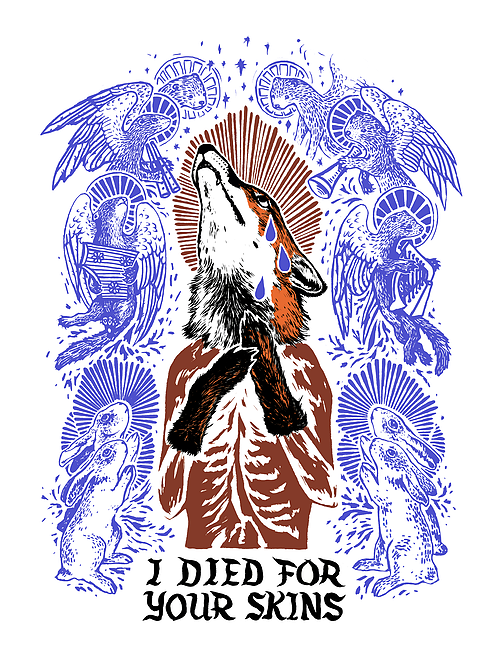
\includepdf{leb/content/pictures/sierra-foxtrot-idfys-white.png}

\end{titlingpage}








\begin{titlingpage}

\title{\Huge \headings{The Holy Bible}}
\date{}
\author{}


\setlrmarginsandblock{0.75in}{0.75in}{*}

\checkandfixthelayout 
\vspace*{\fill}

\begin{tikzpicture}[color=Gold,
    transform shape,
    every node/.style={inner sep=0pt}]
  \node[minimum size=\framesize,fill=Beige!10](vecbox){};
  \node[anchor=north west] at (vecbox.north west){%
    \pgfornament[width=0.2*\framesize]{131}};
  \node[anchor=north east] at (vecbox.north east){%
    \pgfornament[width=0.2*\framesize,symmetry=v]{131}};
  \node[anchor=south west] at (vecbox.south west){%
    \pgfornament[width=0.2*\framesize,symmetry=h]{131}};
  \node[anchor=south east] at (vecbox.south east){%
    \pgfornament[width=0.2*\framesize,symmetry=c]{131}};
  \node[anchor=north] at (vecbox.north){%
    \pgfornament[width=0.6*\framesize,symmetry=h]{85}};
  \node[anchor=south] at (vecbox.south){%
    \pgfornament[width=0.6*\framesize]{85}};
  \node[anchor=north,rotate=90] at (vecbox.west){%
    \pgfornament[width=0.6*\framesize,symmetry=h]{85}};
  \node[anchor=north,rotate=-90] at (vecbox.east){%
    \pgfornament[width=0.6*\framesize,symmetry=h]{85}};
  \node[inner sep=6pt, color=black] (text) at (vecbox.center){%
    \HUGE \textsc{\headings{The Holy Bible}}};
  \node[anchor=north, color=Goldenrod] (base) at (text.south){%
    \pgfornament[width=0.5*\framesize]{71}};
  \node[anchor=south, color=Goldenrod] at (text.north){%
    \pgfornament[width=0.5*\framesize,symmetry=h]{71}};
\end{tikzpicture}
\vspace*{\fill}
\end{titlingpage}




\onecolumn
\renewcommand{\contentsname}{\headings{Books of The Holy Bible}}


% toc font styles
\titlecontents{part}[3mm]{\normalsize\bfseries}{PART\space\thecontentslabel:\space\MakeUppercase}{}{\normalfont\dotfill\makebox[12mm][l]{\thecontentspage}}
\titlecontents{chapter}[3mm]{\vspace{-12pt}\normalsize}{}{}{\dotfill\makebox[12mm][l]{\thecontentspage}}


% some help from % https://tex.stackexchange.com/questions/389319/making-the-second-column-of-the-table-of-contents-clear-the-page-header
\makeatletter  
\singlespacing
\begingroup % start a TeX group
\color{colortoc}% or whatever color you wish to use
\chapter*{\contentsname
  \@mkboth{%
    \MakeUppercase\contentsname}{\MakeUppercase\contentsname}}
% If you want to turn off columns being forced to equal height, use the starred version \begin{multicols*}{2}.
\begin{multicols}{2}

  \@starttoc{toc}
\end{multicols}
\endgroup   % end of TeX group
\makeatother


\twocolumn




% a blank page on the back of the page - lext page on a new right-sided page
\newpage
\thispagestyle{empty}
\mbox{}

\onecolumn
\vspace{8mm}

\customsection[Preface]{The Lexham English Bible\\\large Fourth Edition}

\vspace{12mm}

With approximately one hundred different English translations of the Bible already published, the reader may well wonder 
why yet another English version has been produced. Those actually engaged in the work of translating the Bible might 
answer that the quest for increased accuracy, the incorporation of new scholarly discoveries in the fields of semantics, 
lexicography, linguistics, new archaeological discoveries, and the continuing evolution of the English language all 
contribute to the need for producing new translations. But in the case of the Lexham English Bible (LEB), the answer to 
this question is much simpler; in fact, it is merely twofold.\par

First, the LEB achieves an unparalleled level of transparency with the original language text because the LEB had as 
its starting point the Lexham Hebrew-English Interlinear Bible and the Lexham Greek-English Interlinear New Testament. 
It was produced with the specific purpose of being used alongside the original language text of the Bible. Existing 
translations, however excellent they may be in terms of English style and idiom, are frequently so far removed from 
the original language texts of Scripture that straightforward comparison is difficult for the average user. Of course 
distance between the original language text and the English translation is not a criticism of any modern English 
translation. To a large extent this distance is the result of the philosophy of translation chosen for a particular 
English version, and it is almost always the result of an attempt to convey the meaning of the original in a clearer 
and more easily understandable way to the contemporary reader. However, there are many readers, particularly those 
who have studied some biblical Hebrew, Aramaic, or Greek, who desire a translation that facilitates straightforward 
and easy comparisons between the translation and the original language text. The ability to make such comparisons 
easily in software formats like Logos Bible Software makes the need for an English translation specifically designed 
for such comparison even more acute.\par

Second, the LEB is designed from the beginning to make extensive use of the most up-to-date lexical reference works 
available. For the Old Testament this is primarily The Hebrew and Aramaic Lexicon of the Old Testament (HALOT), and for 
New Testament this is primarily the third edition of Walter Bauer's A Greek-English Lexicon of the New Testament and 
Other Early Christian Literature (BDAG). Users can be assured that the LEB as a translation is based on the best scholarly 
research available. The Hebrew text on which the LEB Old Testament is based is that of \textbf{Biblia Hebraica Stuttgartensia}. 
The Greek text on which the LEB New Testament is based is that of The Greek New Testament: \textbf{SBL Edition (SBLGNT)}, a new 
edition produced by Michael W. Holmes in conjunction with the Society of Biblical Literature and Logos Bible Software. 
In its evaluation of textual variation, the SBLGNT uses modern text-critical methodology along with guidance from the 
most recently available articles, monographs, and technical commentaries to establish the text of the Greek New Testament.\par

Naturally, when these two factors are taken into consideration, it should not be surprising that the character of the LEB 
as a translation is fairly literal. This is a necessary by-product of the desire to have the English translation correspond 
transparently to the original language text. Nevertheless, a serious attempt has been made within these constraints to produce 
a clear and readable English translation instead of a woodenly literal one.\par

There are three areas in particular that need to be addressed to make a translation like the LEB more accessible to readers 
today, while at the same time maintaining easy comparison with the original language text. First, differences in word order 
have to be addressed. In this regard, the LEB follows standard English word order, not the word order of biblical Hebrew, 
Aramaic, or Koiné Greek. Anyone who needs to see the word order of the original languages can readily consult the Lexham 
Hebrew-English Interlinear Bible or the Lexham Greek-English Interlinear New Testament, which contain a sequence line which 
gives this information. Second, some expressions in biblical languages are idiomatic, so that a literal translation would 
be meaningless or would miscommunicate the true meaning. The LEB uses \lebnote{lower corner brackets} to indicate such expressions, 
with a literal rendering given in a note. Third, words which have no equivalent in the original language text must sometimes 
be supplied in the English translation. Because the LEB is designed to be used alongside the original language texts of 
Scripture, these supplied words are indicated with \textit{[italics]}. In some cases the need for such supplied words is obvious, 
but in other cases where it is less clear a note has been included.\par
Finally, the reader should remember that any Bible translation, to be useful to the person using it, must actually be read. 
We encourage every user of the LEB, whether reading it alongside the original languages text or not, to remember that once 
we understand the meaning of a biblical text we are responsible to apply it first in our own lives, and then to share it 
with those around us.\par

\textit{The Editors}

\textquote[Heb 4:12, LEB]{\textit{For the word of God is living and active and sharper than any double-edged sword, and piercing as far as the division 
of soul and spirit, both joints and marrow, and able to judge the reflections and thoughts of the heart.}}

\begin{multicols}{2}
\vspace{-\topsep}
\begin{itemize}
\setlength{\parskip}{0pt} \setlength{\itemsep}{0pt plus 1pt}
    \item W. Hall Harris III
    \item Elliot Ritzema
    \item Rick Brannan
    \item Douglas Mangum
    \item John Dunham
    \item Jeffrey A. Reimer
    \item Micah Wierenga
    \item Translators
    \item W. Hall Harris III
    \item Michael S. Heiser
    \item Jeremy Penner
    \item David M. Fouts
    \item Eugene E. Carpenter
    \item Gordon H. Johnston
    \item H. Daniel Zacharias
    \item William D. Barrick
    \item Michael A. Grisanti
    \item Chip McDaniel
    \item Israel Loken
    \item Ken M. Penner
    \item Dorian G. Coover-Cox
    \item Amy L. Pfeister
\end{itemize}

\vspace{-\topsep}

\end{multicols}

\subsection*{License}
You can give away the Lexham English Bible, but you can't sell it on its own. If the LEB comprises less than 25% of the 
content of a larger work, you can sell it as part of that work.
If you give away the LEB for use with a commercial product, or sell a work containing more than 1,000 verses from the LEB, 
you must annually report the number of units sold, distributed, and/or downloaded.
You must always attribute quotations of the LEB.
If you quote less than 100 verses of the LEB in a single work you can attribute it by simply adding (LEB) after the quotation. 
Longer quotations, or use of 100 or more verses in a single work, must be accompanied by the following statement:
Scripture quotations marked (LEB) are from the Lexham English Bible. Copyright 2012 Logos Bible Software. Lexham is a 
registered trademark of Logos Bible Software.
In electronic use, link "LEB" and "Lexham English Bible" to http://lexhamenglishbible.com, and "Logos Bible Software" 
to http://logos.com. If all quotations are unmarked and from the LEB, you may remove "marked (LEB) are" from the statement.
In support of non-English Bible translation, non-profit organizations may use 50% as the maximum portion the LEB may 
comprise of a work offered for sale. (This specifically allows the creation and commercial sale of diglot Bibles.)


\subsection*{Trademarks}
Lexham is a registered trademark of Logos Bible Software. You may use LEB or Lexham English Bible to refer to the 
Lexham English Bible, but may not use the Lexham trademark as any part of the name of a larger work quoting or containing it.

\vfill
\centering{%
\noindent\normalsize\textbf\textcopyright{\superscript} The Lexham English Bible, Fourth Edition, Copyright 2010, 2012\\
Logos Bible Software, 1313 Commercial St., Bellingham, WA 98225\\
\url{http://www.logos.com}{http://www.logos.com}
}
\clearpage
\twocolumn
\justify











\mainmatter


\setlrmarginsandblock{0.4375in}{0.3125in}{*}

% the book name, chapter and verse number at the top of the page
\setcolsepandrule{0.25in}{0pt}
\fancyhead[RO,LE]{\textbf{\headings{\Large \rightmark}}}
\fancyhfoffset[RO]{1pt}

\setlength\textwidth{5.25in}
\setlength\columnwidth{2.5in}
\setlength\columnsep{0.25in}
\checkandfixthelayout 


\part*{\headings{The Old Testament}}

% a blank page on the back of the page - next page on a new right-sided page
\clearpage
\newpage
\thispagestyle{empty}
\mbox{}
\endpage
\newpage



\endpage
\newpage


\biblebook{Genesis}

\begin{biblechapter} % Genesis 1
\verseWithHeading{The Creation} In the beginning, God created the heavens and the earth—
\verse Now the earth was formless and empty, and darkness \textit{was} over the face of the deep. And the Spirit of God \textit{was} hovering over the surface of the waters.
\verse And God said, “Let there be light!” And there was light.
\verse And God saw the light, that \textit{it was} good, and God caused \textit{there to be} a separation between the light and between the darkness.
\verse And God called the light Day, and the darkness he called Night. And there was evening and there was morning, \textit{the} first day.
\verse And God said, “Let there be a vaulted dome in the midst of the waters, and \textit{let it cause a separation between the waters}.”
\verse So God made the vaulted dome, and he caused a separation between the waters which \textit{were} under the vaulted dome and between the waters which were over the vaulted dome. And it was so.
\verse And God called the vaulted dome “heaven.” And there was evening, and there was morning, a second day.
\verse And God said, “Let the waters under heaven be gathered to one place, and let the dry ground appear.” And it was so.
\verse And God called the dry ground “earth,” and he called the collection of the waters “seas.” And God saw that \textit{it was} good.
\verse And God said, “Let the earth produce green plants \textit{that will} bear seed—fruit trees bearing fruit \textit{in which there is seed}—according to its kind, on the earth.” And it was so.
\verse And the earth brought forth green plants bearing seed according to its kind, and trees bearing fruit \textit{in which there was seed} according to its kind. And God saw that \textit{it was} good.
\verse And there was evening and there was morning, a third day.
\verse And God said, “Let there be lights in the vaulted dome of heaven \textit{to separate day from night}, and let them be as signs and for appointed times, and for days and years,
\verse and they shall be as lights in the vaulted dome of heaven to give light on the earth.” And it \textit{was} so.
\verse And God made two lights, the greater light to rule the day and the smaller light to rule the night, and the stars.
\verse And God placed them in the vaulted dome of heaven to give light on the earth
\verse and to rule over the day and over the night, and to \textit{separate light from darkness}. And God saw that \textit{it was} good.
\verse And there was evening and there was morning, a fourth day.
\verse And God said, “Let the waters swarm \textit{with} swarms of living creatures, and let birds fly over the earth across the face of the vaulted dome of heaven.
\verse So God created the great sea creatures and every living creature \textit{that} moves, \textit{with} which the waters swarm, according to their kind, and every bird \textit{with} wings according to its kind. And God saw that \textit{it was} good.
\verse And God blessed them, saying, “Be fruitful and multiply, and fill the waters in the seas, and let the birds multiply on the earth.”
\verse And there was evening, and there was morning, a fifth day.
\verse And God said, “Let the earth bring forth living creatures according to their kind: cattle and moving things, and wild animals according to their kind.” And it was so.
\verse So God made wild animals according to their kind and the cattle according to their kind, and every creeping thing of the earth according to its kind. And God saw that \textit{it was} good.
\verse And God said, “Let us make humankind in our image and according to our likeness, and let them rule over the fish of the sea, and over the birds of heaven, and over the cattle, and over all the earth, and over every moving thing that moves upon the earth.”
\verse So God created humankind in his image, in the likeness of God he created him, male and female he created them.
\verse And God blessed them, and God said to them, “Be fruitful and multiply, and fill the earth and subdue it, and rule over the fish of the sea and the birds of heaven, and over every animal that moves upon the earth.”
\verse And God said, “Look—I am giving to you every plant \textit{that} bears seed which \textit{is} on the face of the whole earth, and every kind of tree \textit{that bears fruit}. They shall be yours as food.”
\verse And to every kind of animal of the earth and to every bird of heaven, and to everything that moves upon the earth in which \textit{there is} life \textit{I am giving} every green plant as food.” And it was so.
\verse And God saw everything that he had made and, behold, \textit{it was} very good. And there was evening, and there was morning, a sixth day.
\end{biblechapter}

\begin{biblechapter} % Genesis 2
\verse And heaven and earth and all their array were finished.
\verse And on the seventh day God finished his work that he had done, and he rested on the seventh day from all his work that he had done.
\verse And God blessed the seventh day, and he sanctified it, because on it he rested from all his work \textit{of creating that \textit{there was} to do}.
\verseWithHeading{The Generations of Heaven and Earth} These are the generations of heaven and earth when they were created, in the day \textit{that} Adonai made earth and heaven—
\verse \textit{before any plant of the field was} on earth, and \textit{before} \textit{any plant of the field} had sprung up, because Adonai had not caused it to rain upon the earth, and there was no human being to cultivate the ground,
\verse but a stream \textit{would} rise from the earth and water the whole face of the ground—
\verse when Adonai formed the man \textit{of} dust from the ground, and he blew into his nostrils the breath of life, and the man became a living creature.
\verse And Adonai planted a garden in Eden in the east, and there he put the man whom he had formed.
\verse And Adonai caused to grow every tree \textit{that} was pleasing to the sight and good for food. And the tree of life \textit{was} in the midst of the garden, \textit{along with} the tree of the knowledge of good and evil.
\verse Now a river flowed out from Eden that watered the garden, and from there it diverged and became four branches.
\verse The name of the first \textit{is} the Pishon. It went around all the land of Havilah, where \textit{there is} gold.
\verse (The gold of that land \textit{is} good; bdellium and onyx stones \textit{are} there.)
\verse And the name of the second \textit{is} Gihon. It went around all the land of Cush.
\verse And the name of the third \textit{is} Tigris. It flows east of Assyria. And the fourth river \textit{is} the Euphrates.
\verse And Adonai took the man and set him in the garden of Eden to cultivate it and to keep it.
\verse And Adonai commanded the man, saying, “From every tree of the garden \textit{you may freely eat},
\verse but from the tree of the knowledge of good and evil you shall not eat, for in the day \textit{that you eat} from it \textit{you shall surely die}.”
\verse Then Adonai said, “\textit{it is} not good \textit{that} the man is alone. I will make for him a helper \textit{as his counterpart}.”
\verse And out of the ground Adonai formed every beast of the field and every bird of the sky, and he brought \textit{each} to the man to see what he would call it. And whatever the man called that living creature \textit{was} its name.
\verse And the man \textit{gave names} to every domesticated animal and to the birds of heaven and to all the wild animals. But for \textit{the} man there was not found a helper \textit{as his counterpart}.
\verse And Adonai caused a deep sleep to fall upon the man. While he slept, he took one of his ribs, and closed up \textit{the flesh where it had been}.
\verse And Adonai fashioned the rib which he had taken from the man into a woman and brought her to the man.
\verse And the man said, “\textit{She is now} bone from my bones 
and flesh from my flesh; 
\textit{she} shall be called ‘Woman,’ 
for \textit{she was taken} from man.”
\verse Therefore a man shall leave his father and his mother and shall cling to his wife, and they shall be as one flesh.
\verse And the man and his wife, both of them, were naked, and they were not ashamed.
\end{biblechapter}

\begin{biblechapter} % Genesis 3
\verseWithHeading{The Fall} Now the serpent was more crafty than any other \textit{wild animal} which Adonai had made. He said to the woman, “Did God indeed say, ‘You shall not eat from any tree in the garden’?”
\verse The woman said to the serpent, “From the fruit of the trees of the garden we may eat,
\verse but from the tree that is in the midst of the garden, God said, ‘You shall not eat from it, nor shall you touch it, lest you die’.”
\verse But the serpent said to the woman, “You shall not surely die.
\verse For God knows that on the day you \textit{both} eat from it, then your eyes will be opened and you \textit{both} shall be like gods, knowing good and evil.”
\verse When the woman saw that the tree \textit{was} good for food and that it \textit{was} a delight to the eyes, and the tree was desirable to make \textit{one} wise, then she took from its fruit and she ate. And she gave \textit{it} also to her husband with her, and he ate.
\verse Then the eyes of both of them were opened, and they knew that they \textit{were} naked. And they sewed together fig leaves and they made for themselves coverings.
\verse Then they heard the sound of Adonai walking in the garden \textit{at the windy time of day}. And the man and his wife hid themselves from the presence of Adonai among the trees of the garden.
\verse And Adonai called to the man and said to him, “Where \textit{are} you?”
\verse And he replied, “I heard the sound of you in the garden, and I was afraid because I \textit{am} naked, so I hid myself.”
\verse Then he asked, “Who told you that you \textit{were} naked? Have you eaten from \textit{the tree from which I forbade you to eat}?”
\verse And the man replied, “The woman whom you gave \textit{to be} with me—she gave to me from the tree and I ate.”
\verse Then Adonai said to the woman, “What \textit{is} this you have done?” And the woman said, “The serpent deceived me, and I ate.”
\verse Then Adonai said to the serpent,
\verse “Because you have done this, 
you \textit{will be} cursed 
more than any domesticated animal 
and more than any wild animal. 
On your belly you shall go 
and dust you shall eat 
all the days of your life.
\verse To the woman he said, “I will greatly increase 
\textit{your pain in childbearing}; 
in pain you shall bear children. 
And to your husband \textit{shall be} your desire. 
And he shall rule over you.”
\verse And to Adam he said, “Because you listened to the voice of your wife and you ate from the tree \textit{from which I forbade you to eat},
\verse the ground \textit{shall be} cursed on your account. 
In pain you shall eat \textit{from} it 
all the days of your life.
\verse And thorns and thistles shall sprout for you, 
and you shall eat the plants of the field.
\verse And the man \textit{named} his wife Eve, because she was the mother of all life.
\verse And Adonai made for Adam and for his wife garments of skin, and he clothed them.
\verse And Adonai said, “Look—the man has become as one of us, to know good and evil. \textit{What if} he stretches out his hand and takes also from the tree of life and eats, and lives forever?”
\verse And Adonai sent him out from the garden of Eden, to till the ground from which he was taken.
\verse So he drove the man out, and placed cherubim east of the garden of Eden, and \textit{a flaming, turning sword} to guard the way to the tree of life.
\end{biblechapter}

\begin{biblechapter} % Genesis 4
\verseWithHeading{Cain and Abel} Now Adam knew Eve his wife, and she conceived and bore Cain. And she said, “I have given birth to a man with \textit{the help of} Adonai.”
\verse \textit{Then she bore} his brother Abel. And Abel became a keeper of sheep, and Cain became a tiller of the ground.
\verse And \textit{in the course of time} Cain brought an offering from the fruit of the ground to Adonai,
\verse and Abel also brought \textit{an offering} from \textit{the choicest firstlings of his flock}. And Adonai looked with favor to Abel and to his offering,
\verse but to Cain and to his offering he did not look with favor. And Cain became very angry, and his face fell.
\verse And Adonai said to Cain, “Why are you angry, and why is your face fallen?
\verse If you do well \textit{will I not accept you}? But if you do not do well, sin is crouching at the door. And its desire \textit{is} for you, but you must rule over it.”
\verse Then Cain said to his brother Abel, \textit{“Let us go out into the field.”} And when they were in the field, Cain rose up against his brother Abel and killed him.
\verse Then Adonai said to Cain, “Where \textit{is} Abel your brother?” And he said, “I do not know; am I my brother’s keeper?”
\verse And he said, “What have you done? The voice of your brother’s blood is crying out to me from the ground.
\verse So now you are cursed from the ground, which has opened its mouth to receive the blood of your brother from your hand.
\verse When you till the ground \textit{it shall no longer yield its strength to you}. You shall be a wanderer and a fugitive on the earth.”
\verse And Cain said to Adonai, “My punishment \textit{is} greater than \textit{I can} bear.
\verse Look, you have driven me out today from the face of the ground, and from your face I must hide. I will be a wanderer and a fugitive on the earth, and it will happen that whoever finds me will kill me.”
\verse Then Adonai said to him, “Therefore, whoever kills Cain will be avenged sevenfold.” Then Adonai put a sign on Cain so that whoever found him would not kill him.
\verse And Cain went out from the presence of Adonai, and he settled in the land of Nod, east of Eden.
\verse And Cain knew his wife, and she conceived and gave birth to Enoch. And when he built a city \textit{he named the city after his son, Enoch}.
\verse And to Enoch was born Irad, and Irad fathered Mehujael, and Mehujael fathered Methushael, and Methushael fathered Lamech.
\verse And Lamech took to himself two wives. The name of the first \textit{was} Adah, and the name of the second \textit{was} Zillah.
\verse And Adah gave birth to Jabal; he was the father of those who live in tents and \textit{those who have} livestock.
\verse And the name of his brother \textit{was} Jubal; he was the father of all who play stringed instruments and wind instruments.
\verse Then Zillah also gave birth to Tubal-Cain who forged all \textit{kinds of} tools of bronze and iron. And the sister of Tubal-Cain \textit{was} Naamah.
\verse Then Lamech said to his wives,
\verse “Adah and Zillah, listen to my voice; 
O wives of Lamech, hear my words. 
I have killed a man for wounding me, 
Even a young man for injuring me.
\verse Then Adam knew his wife again, and she gave birth to a son. And she called his name Seth, for \textit{she said} “God has appointed to me another child in the place of Abel, because Cain killed him.”
\verse And as for Seth, he also fathered a son, and he called his name Enosh. At that time he began to call on the name of Adonai.
\end{biblechapter}

\begin{biblechapter} % Genesis 5
\verseWithHeading{Adam’s Descendants to Noah} This is the record of the generations of Adam. When God created Adam, he made him in the likeness of God.
\verse Male and female he created them. And he blessed them. And he called their name “Humankind” when they were created.
\verse And when Adam had lived one hundred and thirty years, he fathered a child in his likeness, according to his image. And he called his name Seth.
\verse And the days of Adam after he fathered Seth were eight hundred years. And he fathered sons and daughters.
\verse And all the days of Adam which he lived were nine hundred and thirty years, and he died.
\verse When Seth had lived one hundred and five years, he fathered Enosh.
\verse And after Seth had fathered Enosh he lived eight hundred and seven years, and fathered sons and daughters.
\verse And all the days of Seth were nine hundred and twelve years, and he died.
\verse When Enosh lived ninety years, he fathered Kenan.
\verse And after Enosh fathered Kenan he lived eight hundred and fifteen years, and fathered sons and daughters.
\verse And all the days of Enosh were nine hundred and five years, and he died.
\verse When Kenan had lived seventy years, he fathered Mahalalel.
\verse And after Kenan had fathered Mahalalel, he lived eight hundred and forty years, and fathered sons and daughters.
\verse And all the days of Kenan were nine hundred and ten years, and he died.
\verse When Mahalalel had lived sixty-five years, he fathered Jared.
\verse And after Mahalalel had fathered Jared, he lived eight hundred and thirty years, and fathered sons and daughters.
\verse And all the days of Mahalalel were eight hundred and ninety-five years, and he died.
\verse When Jared had lived one hundred and sixty-two years, he fathered Enoch.
\verse And after Jared had fathered Enoch, he lived eight hundred years, and fathered sons and daughters.
\verse And all the days of Jared were nine hundred and sixty-two years, and he died.
\verse When Enoch had lived sixty-five years, he fathered Methuselah.
\verse And Enoch walked with God after he fathered Methuselah three hundred years, and fathered sons and daughters.
\verse And all the days of Enoch were three hundred and sixty-five years.
\verse And Enoch walked with God, and he was no more, for God took him.
\verse When Methuselah had lived one hundred and eighty-seven years, he fathered Lamech.
\verse And after Methuselah had fathered Lamech, he lived seven hundred and eighty-two years, and fathered sons and daughters.
\verse And all the days of Methuselah were nine hundred and sixty-nine years, and he died.
\verse When Lamech had lived one hundred and eighty-two years, he fathered a son.
\verse And he called his name Noah, saying, “This one \textit{shall relieve us} from our work, and from the hard labor of our hands, from the ground which Adonai had cursed.
\verse And after Lamech had fathered Noah he lived five hundred and ninety-five years, and he fathered sons and daughters.
\verse All the days of Lamech were seven hundred and seventy-seven years, and he died.
\verse When Noah \textit{was five hundred years old}, Noah fathered Shem, Ham, and Japheth.
\end{biblechapter}

\begin{biblechapter} % Genesis 6
\verseWithHeading{Prelude to the Flood} And it happened \textit{that}, when humankind began to multiply on the face of the ground, daughters were born to them.
\verse Then the sons of God saw the daughters of humankind, that they \textit{were} beautiful. And they took for themselves wives from all that they chose.
\verse And Adonai said, “My Spirit shall not abide with humankind forever in that he \textit{is} also flesh. And his days \textit{shall be} one hundred and twenty years.”
\verse The Nephilim \textit{were} upon the earth in those days, and also afterward, when the sons of God went into the daughters of humankind, and they bore children to them.
\verse And Adonai saw that the evil of humankind \textit{was} great upon the earth, and every inclination of the thoughts of his heart \textit{was} always only evil.
\verse And Adonai regretted that he had made humankind on the earth, and \textit{he was grieved in his heart}.
\verse And Adonai said, “I will destroy humankind whom I created from upon the face of the earth, from humankind, to animals, to creeping things, and to the birds of heaven, for I regret that I have made them.”
\verse But Noah found favor in the eyes of Adonai.
\verse These \textit{are} the generations of Noah. Noah \textit{was} a righteous man, without defect in his generations. Noah walked with God.
\verse And Noah fathered three sons: Shem, Ham, and Japheth.
\verse And the earth \textit{was} corrupted before God, and the earth was filled \textit{with} violence.
\verse And God saw the earth, and behold, it was corrupt, for all flesh had corrupted its way upon the earth.
\verse And God said to Noah, “The end of all flesh \textit{has} come before me, for the earth was filled \textit{with} violence because of them. Now, look, I \textit{am going} to destroy them \textit{along} with the earth.
\verse Make for yourself an ark of cypress wood; you must make the ark \textit{with} rooms, then you must cover it with pitch, inside and outside.
\verse And this \textit{is} how you must make it: the length of the ark, three hundred cubits; its width fifty cubits; its height, thirty cubits.
\verse You must make a roof for the ark, and \textit{finish it to a cubit above}. And \textit{as for} the door of the ark, you must put \textit{it} in its side. You must make it \textit{with} a lower, second, and a third \textit{deck}.
\verse And I, behold, I \textit{am} about to bring the flood waters over the earth to destroy all flesh in which \textit{is} the breath of life from under the heaven; everything that \textit{is} on the earth shall perish.
\verse And I will establish my covenant with you, and you must go into the ark—you, and your sons, and your wife, and the wives of your sons with you.
\verse And of every living thing, from all flesh, you must bring two from every \textit{kind} into the ark to keep \textit{them} alive with you; they shall be male and female.
\verse From the birds according to their kind, and from the animals according to their kind, from every creeping thing \textit{on} the ground according to its kind—two from every kind shall come to you to keep \textit{them} alive.
\verse And \textit{as for} you, take for yourself from every kind of food that is eaten. And you must gather \textit{it} to yourself. And it shall be for you and for them for food.”
\verse And Noah did according to all that God commanded him; thus he did.
\end{biblechapter}

\begin{biblechapter} % Genesis 7
\verse Then Adonai said to Noah, “Go—you and all your household—into the ark, for I have seen you \textit{are} righteous before me in this generation.
\verse From all the clean animals you must take for yourself \textit{seven pairs}, a male and its mate. And from the animals that \textit{are} not clean \textit{you must take} two, a male and its mate,
\verse as well as from the birds of heaven \textit{seven pairs}, male and female, \textit{to keep their kind alive} on the face of the earth.
\verse For \textit{within seven days} I will send rain upon the earth \textit{for} forty days and forty nights. And I will blot out all the living creatures that I have made from upon the face of the ground.”
\verse And Noah did according to all that Adonai commanded him.
\verseWithHeading{The Flood} Noah \textit{was six hundred years old} when the flood waters came upon the earth.
\verse And Noah and his sons and his wife, and the wives of his sons with him, went into the ark because of the waters of the flood.
\verse Of clean animals, and of animals which \textit{are} not clean, and of the birds, and everything that creeps upon the ground,
\verse \textit{two of each} went to Noah, into the ark, male and female, as God had commanded Noah.
\verse And it happened \textit{that} after seven days the waters of the flood came over the earth.
\verse In the six hundredth year of the life of Noah, in the second month, on the seventeenth day of the month—on that day all the springs of the great deep were split open, and the windows of heaven were opened.
\verse And the rain came upon the earth forty days and forty nights.
\verse On this same day, Noah, Shem, Ham, and Japheth, the sons of Noah, and the wife of Noah and the three wives of his sons with them, went into the ark,
\verse they and all the living creatures according to their kind, and all the domesticated animals according to their kind, and all the creatures that creep upon the earth according to their kind, all the birds according to their kind, every winged creature.
\verse And they came to Noah to the ark, \textit{two of each}, from every living thing in which \textit{was} the breath of life.
\verse And those that came, male and female, of every living thing, came as God had commanded him. And Adonai shut the door behind him.
\verse And the flood came forty days and forty nights upon the earth. And the waters increased, and lifted the ark, and it rose up from the earth.
\verse And the waters prevailed and increased greatly upon the earth. And the ark went upon the surface of the waters.
\verse And the waters prevailed \textit{overwhelmingly} upon the earth, and they covered all the high mountains which were under the entire heaven.
\verse \textit{The waters swelled fifteen cubits above the mountains, covering them}.
\verse And every living thing that moved on the earth perished—the birds, and the domesticated animals, and the wild animals, and everything that swarmed on the earth, and all humankind.
\verse Everything in whose nostrils \textit{was} \textit{the breath of life}, among all that \textit{was} on dry land, died.
\verse And he blotted out every living thing upon the surface of the ground, from humankind, to animals, to creeping things, and to the birds of heaven; they were blotted out from the earth. Only Noah and those who \textit{were} with him in the ark remained.
\verse And the waters prevailed over the earth one hundred and fifty days.
\end{biblechapter}

\begin{biblechapter} % Genesis 8
\verseWithHeading{The Flood Subsides} And God remembered Noah and all the wild animals, and all the domesticated animals that \textit{were} with him in the ark. And God caused a wind to blow over the earth, and the waters subsided.
\verse And the fountains of the deep and the windows of the heavens were closed, and the rain from the heavens was restrained.
\verse And the waters receded from the earth \textit{gradually}, and the waters abated at the end of one hundred and fifty days.
\verse And the ark came to rest in the seventh month, on the seventeenth day of the month, on the mountains of Ararat.
\verse And the waters \textit{continued to recede} to the tenth month; in the tenth month, on the first of the month, the tops of the mountains appeared.
\verse And it happened \textit{that} at the end of forty days Noah opened the window of the ark that he had made.
\verse And he sent out a raven; \textit{it went to and fro} until the waters were dried up from upon the earth.
\verse And \textit{he sent out a dove} to see \textit{whether} the waters had subsided from upon the ground.
\verse But the dove did not find a resting place for the sole of her foot, and she returned to him into the ark, for the waters \textit{were still} on the face of the earth. And he stretched out his hand and took her, and brought her to himself into the ark.
\verse And he waited another seven days, and \textit{again he sent out} the dove from the ark.
\verse And the dove came to him \textit{in the evening}, and behold, a freshly-picked olive tree leaf \textit{was} in her mouth. And Noah knew that the waters had subsided from upon the earth.
\verse And he waited \textit{seven more days}, and he sent out the dove. But it did not return again to him.
\verse And it happened that, in the six hundred and first year, in the first \textit{month}, on the first \textit{day} of the month, the waters dried up from upon the earth. And Noah removed the covering of the ark and looked. And behold, the face of the ground was dried up.
\verse And in the second month, on the twenty-seventh day of the month, the earth was dry.
\verse And God spoke to Noah, saying:
\verse “Go out from the ark, you and your wife, and your sons, and your sons’ wives with you.
\verse Bring out with you all the living things which \textit{are} with you, from all the living creatures—birds, and animals, and everything that creeps on the earth, and let them swarm on the earth and be fruitful and multiply on the earth.”
\verse So Noah went out, with his sons and his wife, and the wives of his sons with him.
\verse Every animal, every creeping thing, and every bird, \textit{and} everything \textit{that} moves upon the earth, according to its families, went out from the ark.
\verse And Noah built an altar to Adonai, and he took from all the clean animals and from all the clean birds, and offered burnt offerings on the altar.
\verse And Adonai smelled the soothing fragrance, and Adonai said \textit{to himself}, “\textit{Never again will I curse} the ground for the sake of humankind, because the inclination of the heart of humankind \textit{is} evil from his youth. \textit{Nor will I ever again destroy} all life as I have done.
\verse \textit{As long as the earth endures}, seed and harvest, cold and heat, summer and winter, day and night will not cease.
\end{biblechapter}

\begin{biblechapter} % Genesis 9
\verseWithHeading{God’s Covenant with Noah and Humankind} And God blessed Noah and his sons, and said to them, “Be fruitful and multiply, and fill the earth.
\verse And fear of you and dread of you shall be upon every animal of the earth, and on every bird of heaven, \textit{and} on everything that moves upon the ground, and on all the fish of the sea. Into your hand they shall be given.
\verse Every moving thing that lives shall be for you as food. As \textit{I gave} the green plants to you, I have \textit{now} given you everything.
\verse Only you shall not eat \textit{raw flesh with blood in it}.
\verse And \textit{your lifeblood} I will require; from \textit{every animal} I will require it. And from the hand of humankind, from the hand of \textit{each} man to his brother I will require the life of humankind.
\verse “\textit{As for} the one shedding the blood of humankind, 
by humankind his blood shall be shed, 
for God made humankind in his own image.
\verse “And you, be fruitful and multiply, swarm on the earth and multiply in it.”
\verse And God said to Noah and to his sons with him,
\verse “As for me, behold, I am establishing my covenant with you and with your seed after you,
\verse and with every living creature that \textit{is} with you—the birds, the animals, and every animal of the earth with you, from all \textit{that} came out of the ark to all the animals of the earth.
\verse I am establishing my covenant with you, that never again will all flesh be cut off by the waters of a flood, nor will there ever be a flood that destroys the earth.”
\verse And God said, “This \textit{is} the sign of the covenant that I am making between me and you, and between every living creature that \textit{is} with you for future generations.
\verse My bow I have set in the clouds, and it shall be for a sign of \textit{the} covenant between me and between the earth.
\verse And when I make clouds appear over the earth the bow shall be seen in the clouds.
\verse Then I will remember my covenant that \textit{is} between me and you, and between every living creature, with all flesh. And the waters of a flood will never again \textit{cause the destruction} of all flesh.
\verse The bow shall be in the clouds, and I will see it, so as to remember \textit{the} everlasting covenant between God and between every living creature, with all flesh that \textit{is} upon the earth.”
\verse And God said to Noah, “This \textit{is} the sign of the covenant which I am establishing between me and all flesh that \textit{is} upon the earth.
\verseWithHeading{Noah’s Descendants} Now the sons of Noah who came out of the ark \textit{were} Shem, Ham, and Japheth. (Ham \textit{was} the father of Canaan.)
\verse These three \textit{were} the sons of Noah, and from these \textit{the whole earth was populated}.
\verse And Noah began \textit{to be} a man of the ground, and he planted a vineyard.
\verse And he drank some of the wine and became drunk, and he exposed himself in the midst of his tent.
\verse And Ham, the father of Canaan, saw the nakedness of his father, and he told his two brothers outside.
\verse Then Shem and Japheth took a garment, and the two of them put \textit{it} on \textit{their} shoulders and, walking backward, they covered the nakedness of their father. And their faces \textit{were turned} backward, so that they did not see the nakedness of their father.
\verse Then Noah awoke from his drunkenness, and he knew what his youngest son had done to him.
\verse And he said, “Cursed \textit{be} Canaan, 
a slave of slaves he shall be to his brothers.”
\verse Then he said,
\verse “Blessed \textit{be} Adonai, the God of Shem, 
and let Canaan be a slave to them.
\verse And Noah lived three hundred and fifty years after the flood.
\verse And all the days of Noah were nine hundred and fifty years, and he died.
\end{biblechapter}

\begin{biblechapter} % Genesis 10
\verseWithHeading{The Descendants of the Sons of Noah} These \textit{are} the generations of the sons of Noah—Shem, Ham, and Japheth. Children were born to them after the flood.
\verse The sons of Japheth: Gomer, Magog, Madai, Javan, Tubal, Meshech, and Tiras.
\verse And the sons of Gomer: Ashkenaz, Riphath, and Togarmah.
\verse And the sons of Javan: Elishah, Tarshish, Kittim, and Dodanim.
\verse From these the coastland peoples spread out through their lands, each according to his own language by their own families, in their nations.
\verse And the sons of Ham: Cush, Egypt, Put, and Canaan.
\verse And the sons of Cush: Seba, Havilah, Sabtah, Raamah, and Sabteca. The sons of Raamah: Sheba and Dedan.
\verse And Cush fathered Nimrod. \textit{He was the first on earth to be a mighty warrior}.
\verse He was a mighty hunter before Adonai. Therefore it was said, “Like Nimrod a mighty hunter before Adonai.”
\verse Now, the beginning of his kingdom \textit{was} Babel, Erech, Akkad, and Calneh, in the land of Shinar.
\verse From that land he went out \textit{to} Assyria, and he built Nineveh, Rehoboth-Ir, Calah,
\verse Resen between Nineveh and Calah; that \textit{is} the great city.
\verse And Egypt fathered Ludim, Anamim, Lehabim, Naphtuhim,
\verse Pathrusim, and Casluhim (from whom the Philistines came), and Caphtorim.
\verse Canaan fathered Sidon, his firstborn, and Heth,
\verse and the Jebusites, the Amorites, the Girgashites,
\verse the Hivites, the Arkites, the Sinites,
\verse the Arvadites, the Zemarites, and the Hamathites. Afterward the families of the Canaanites were spread abroad.
\verse And the territory of the Canaanites \textit{was} from Sidon \textit{in the direction of} Gerar as far as Gaza, and \textit{in the direction of} Sodom, Gomorrah, Admah, and Zeboiim, as far as Lasha.
\verse These \textit{are} the descendants of Ham, according to their families and their languages, in their lands, and in their nations.
\verse And to Shem, the father of all the children of Eber, the older brother of Japheth, \textit{children} were also born.
\verse The sons of Shem: Elam, Asshur, Arphaxad, Lud, and Aram.
\verse And the sons of Aram: Uz, Hul, Gether, and Mash.
\verse And Arphaxad fathered Shelah, and Shelah fathered Eber.
\verse And to Eber two sons were born. The name of the one was Peleg, for in his days the earth was divided, and the name of his brother \textit{was} Joktan.
\verse And Joktan fathered Almodad, Sheleph, Hazarmaveth, Jerah,
\verse Hadoram, Uzal, Diklah,
\verse Obal, Abimael, Sheba,
\verse Ophir, Havilah, and Jobab. All these \textit{were} the sons of Joktan.
\verse And their dwelling \textit{place} \textit{extended from} Mesha \textit{in the direction of} Sephar \textit{to} the hill country of the east.
\verse These \textit{are} the sons of Shem, according to their families, according to their languages, in their lands, and according to their nations.
\verse These are the families of the sons of Noah, according to their generations \textit{and} in their nations. And from these the nations spread abroad on the earth after the flood.
\end{biblechapter}

\begin{biblechapter} % Genesis 11
\verseWithHeading{The Tower of Babel} Now the whole earth \textit{had} one language and the same words.
\verse And as people migrated from the east they found a plain in the land of Shinar and settled there.
\verse And they said \textit{to each other}, “Come, let us make bricks and \textit{burn them thoroughly}.” And they had brick for stone and they had tar for mortar.
\verse And they said, “Come, let us build ourselves a city and a tower whose top \textit{reaches to} the heavens. And let us make a name for ourselves, lest we be scattered over the face of the whole earth.”
\verse Then Adonai came down to see the city and the tower that \textit{humankind} was building.
\verse And Adonai said, “Behold, \textit{they are one people with one language}, and \textit{this is only the beginning of what they will do}. So now nothing that they intend to do will be impossible for them.
\verse Come, let us go down and confuse their language there, so that they will not understand \textit{each other’s language}.”
\verse So Adonai scattered them from there over the face of the whole earth, and they stopped building the city.
\verse Therefore its name was called Babel, for there Adonai confused the language of the whole earth, and there Adonai scattered them over the face of the whole earth.
\verseWithHeading{The Descendants of Shem} These are the generations of Shem. When Shem \textit{was one hundred years old}, he fathered Arphaxad, two years after the flood.
\verse And Shem lived five hundred years after he fathered Arphaxad, and he fathered \textit{other} sons and daughters.
\verse When Arphaxad had lived thirty-five years, he fathered Shelah.
\verse And Arphaxad lived four hundred and three years after he fathered Shelah, and he fathered \textit{other} sons and daughters.
\verse When Shelah had lived thirty years, he fathered Eber.
\verse And Shelah lived four hundred and three years after he fathered Eber, and he fathered \textit{other} sons and daughters.
\verse When Eber had lived thirty-four years, he fathered Peleg.
\verse And Eber lived four hundred and thirty years after he fathered Peleg, and he fathered \textit{other} sons and daughters.
\verse When Peleg had lived thirty years, he fathered Reu.
\verse And Peleg lived two hundred and nine years after he fathered Reu, and he fathered \textit{other} sons and daughters.
\verse When Reu had lived thirty-two years, he fathered Serug.
\verse And Reu lived two hundred and seven years after he fathered Serug, and he fathered \textit{other} sons and daughters.
\verse When Serug had lived thirty years, he fathered Nahor.
\verse And Serug lived two hundred years after he fathered Nahor, and he fathered \textit{other} sons and daughters.
\verse When Nahor had lived twenty-nine years, he fathered Terah.
\verse And Nahor lived one hundred and nineteen years after he fathered Terah, and he fathered \textit{other} sons and daughters.
\verse When Terah had lived seventy years, he fathered Abram, Nahor, and Haran.
\verseWithHeading{The Descendants of Terah} Now these are the generations of Terah. Terah fathered Abram, Nahor, and Haran, and Haran fathered Lot.
\verse And Haran died in the presence of Terah his father in the land of his birth, in Ur of the Chaldeans.
\verse And Abram and Nahor took wives for themselves. The name of the wife of Abram \textit{was} Sarai, and the name of the wife of Nahor \textit{was} Milcah, the daughter of Haran, the father of Milcah and Iscah.
\verse And Sarai was barren; she had no child.
\verse And Terah took Abram his son, and Lot, the son of Haran, \textit{his grandson}, and Sarai his daughter-in-law, the wife of Abram his son, and went out with them from Ur of the Chaldeans to go to the land of Canaan. And they went to Haran, and they settled there.
\verse And the days of Terah \textit{were} two hundred and five years, and Terah died in Haran.
\end{biblechapter}

\begin{biblechapter} % Genesis 12
\verseWithHeading{The Call of Abram} And Adonai said to Abram, “Go out from your land and from your relatives, and from the house of your father, to the land that I will show you.
\verse And I will make you a great nation, and I will bless you, and I will make your name great. And you will be a blessing.
\verse And I will bless those who bless you, and those who curse you I will curse. And all families of the earth will be blessed in you.”
\verseWithHeading{Abram’s Journey} And Abram went \textit{out} as Adonai had told him, and Lot went with him. Now Abram \textit{was seventy-five years old} when he went out from Haran.
\verse And Abram took Sarai his wife, and Lot \textit{his nephew}, and all their possessions that they had gathered, and all the persons that they had acquired in Haran, and they went out to go to the land of Canaan. And they went to the land of Canaan.
\verse And Abram traveled through the land up to the place of Shechem, to the Oak of Moreh. Now the Canaanites \textit{were} in the land at that time.
\verse And Adonai appeared to Abram and said, “To your offspring I will give this land.” And he built an altar there to Adonai, who had appeared to him.
\verse And he moved on from there to the hill country, east of Bethel. And he pitched his tent at Bethel on the west, and at Ai on the east. And he built an altar there to Adonai. And he called on the name of Adonai.
\verse \textit{And Abram kept moving on}, toward the Negev.
\verse And there was a famine in the land. And Abram went down to Egypt to dwell as an alien there, for the famine was severe in the land.
\verse And it happened \textit{that} as he drew near to enter into Egypt, he said to Sarai his wife, “Look now, I know that you are a woman beautiful of appearance,
\verse and it shall happen \textit{that}, if the Egyptians see you, then they will say, ‘This \textit{is} his wife,’ then they will kill me but let you live.
\verse Please say you are my sister so that it will go well for me on your account. \textit{Then I will live} on account of you.”
\verse And it happened \textit{that} as Abram came into Egypt, the Egyptians saw the woman, that she \textit{was} very beautiful.
\verse And the officials of Pharaoh saw her, and they praised her \textit{beauty} to Pharaoh. And the woman was taken to the house of Pharaoh.
\verse And he dealt well with Abram on account of her, and he had sheep, cattle, male donkeys, male servants, female servants, female donkeys, and camels.
\verse Then Adonai afflicted Pharaoh and his household with severe plagues on account of the matter of Sarai the wife of Abram.
\verse Then Pharaoh called for Abram and said, “What \textit{is} this you have done to me? Why did you not tell me that she \textit{was} your wife?
\verse Why did you say ‘She \textit{is} my sister,’ so that I took her to myself as a wife? Now then, here \textit{is} your wife. Take her and go.”
\verse And Pharaoh commanded his men concerning him, and then sent him and his wife and all that \textit{was} with him away.
\end{biblechapter}

\begin{biblechapter} % Genesis 13
\verseWithHeading{The Parting of Abram and Lot} Then Abram went up from Egypt, he and his wife and all that \textit{was} with him. And Lot \textit{went} with him to the Negev.
\verse Now Abram \textit{was} very wealthy in livestock, in silver, and in gold.
\verse And he went according to his journey from the Negev, then to Bethel, to the place where his tent was at the beginning, between Bethel and Ai,
\verse to the place where he had made an altar at the beginning. And Abram called on the name of Adonai there.
\verse And Lot, who went with Abram, also had herds and tents.
\verse And the land could not \textit{support them} \textit{so as} to live together, because their possessions were \textit{so} many that they were not able to live together.
\verse And there was a quarrel between the herdsmen of the livestock of Abram and the herdsmen of the livestock of Lot. Now at that time the Canaanites and the Perizzites were living in the land.
\verse Then Abram said to Lot, “Please, let there not be quarreling between me and you, and between my shepherds and your shepherds, for we men \textit{are} brothers.
\verse Is not the whole land before you? Separate yourself from me. If \textit{you want what is on} the left, then I will go right; if \textit{you want what is on} the right, I will go left.”
\verse And Lot lifted up his eyes and saw the whole plain of the Jordan, that all of it \textit{was} well-watered land—\textit{this was} before Adonai destroyed Sodom and Gomorrah—like the garden of Adonai, like the land of Egypt \textit{in the direction of} Zoar.
\verse So Lot chose for himself all the plain of the Jordan. And Lot journeyed from the east, and so they separated \textit{from each other}.
\verse Abram settled in the land of Canaan, and Lot settled in the cities of the plain. And he pitched his tent toward Sodom.
\verse Now the men of Sodom \textit{were extremely wicked sinners against Adonai}.
\verse And Adonai said to Abram after Lot had separated from him, “Now, lift up your eyes and look from the place where you \textit{are} to the north, and to the south, and to the east and to the west,
\verse for all the land which you see I will give to you, and to your descendants, forever.
\verse I will make your descendants like the dust of the earth which, if anyone were able to count the dust of the earth, your descendants would be \textit{so} counted.
\verse Arise, go through the length of the land and through its breadth, for I will give it to you.”
\verse So Abram pitched his tent, and he came and settled at the oaks of Mamre, which \textit{were} at Hebron. And there he built an altar to Adonai.
\end{biblechapter}

\begin{biblechapter} % Genesis 14
\verseWithHeading{Abram Rescues Lot} And it happened \textit{that} in the days of Amraphel, the king of Shinar, Arioch, the king of Ellasar, Kedorlaomer, the king of Elam, and Tidal, the king of Goiim,
\verse made war with Bera, the king of Sodom, and Birsha, the king of Gomorrah, Shinab, the king of Admah, and Shemeber, the king of Zeboiim, and the king of Bela (that \textit{is}, Zoar).
\verse All these joined forces at the valley of Siddim (that \textit{is}, the sea of the salt).
\verse Twelve years they had served Kedorlaomer, but in the thirteenth year they rebelled.
\verse In the fourteenth year Kedorlaomer and the kings who \textit{were} with him came and defeated the Rephaim in Ashteroth-Karnaim, and the Zuzim in Ham, and the Emim in Shaveh-Kiriathaim,
\verse And the Horites in their hill country of Seir, as far as El-Paran, which is at the wilderness.
\verse Then they turned back and came to En-Mishpat (that \textit{is}, Kadesh). And they defeated the whole territory of the Amalekites, and also the Amorites who were living in Hazazon-Tamar.
\verse Then the king of Sodom, the king of Gomorrah, the king of Admah, the king of Zeboiim, and the king of Bela (that \textit{is}, Zoar) went out, and \textit{they took up battle position} in the Valley of Siddim
\verse with Kedorlaomer, king of Elam, and Tidal, king of Goiim, and Amraphel, king of Shinar, and Arioch, king of Ellasar, four kings against five.
\verse Now the Valley of Siddim \textit{was full of tar pits}. And the kings of Sodom and Gomorrah fled and \textit{fell into them}, but the rest fled to the mountains.
\verse So they took all the possessions of Sodom and Gomorrah and all their provisions, and they left.
\verse And they took Lot, the son of the brother of Abram, and his possessions, and left. (Now he had been living in Sodom.)
\verse Then one who escaped came and told Abram the Hebrew. And he was living at the oaks of Mamre the Amorite, brother of Eshcol and brother of Aner. \textit{They were allies with Abram}.
\verse When Abram heard that his \textit{relative} was taken captive, he summoned his trained men, born in his house, three hundred and eighteen \textit{of them}, and he went in pursuit up to Dan.
\verse And he divided \textit{his trained men} against them at night, he and his servants. And he defeated them and pursued them to Hobah, which \textit{is} north of Damascus.
\verse And he brought back all the possessions. And he also brought back Lot, his \textit{relative}, and his possessions, and the women and the people as well.
\verseWithHeading{Abram Meets Melchizedek} After his return from defeating Kedorlaomer and the kings who \textit{were} with him, the king of Sodom went out to meet him at the Valley of Shaveh (that \textit{is}, the Valley of the King).
\verse And Melchizedek, the king of Salem, brought out bread and wine. (He was the priest of God Most High).
\verse And he blessed him and said,
\verse “Blessed \textit{be} Abram by God Most High, 
Maker of heaven and earth.
\verse And he gave to him a tenth of everything.
\verse And the king of Sodom said to Abram, “Give me the people, but the possessions take for yourself.”
\verse And Abram said to the king of Sodom, “I have raised my hand to Adonai, God Most High, Maker of heaven and earth,
\verse \textit{that neither a thread nor} a thong of a sandal would I take from all that \textit{belongs} to you, that you might not say, ‘I made Abram rich.’
\end{biblechapter}

\begin{biblechapter} % Genesis 15
\verseWithHeading{Adonai’s Covenant with Abram} After these things the word of Adonai came to Abram in a vision, saying: “Do not be afraid, Abram; I \textit{am} your shield, \textit{and} your reward \textit{shall be} very great.”
\verse Then Abram said, “O Adonai, my Lord, what will you give me? \textit{I continue to be} childless, and \textit{my heir} is Eliezer of Damascus.”
\verse And Abram said, “Look, you have not given me a descendant, and here, \textit{a member of my household} \textit{is} \textit{my heir}.”
\verse And behold, the word of Adonai \textit{came} to him saying, “This \textit{person} will not \textit{be your heir}, but \textit{your own son will be your heir}.”
\verse And he brought him outside and said, “Look toward the heavens and count the stars if you are able to count them.” And he said to him, “So shall your offspring be.”
\verse And he believed in Adonai, and he reckoned it to him \textit{as} righteousness.
\verse And he said to him, “I \textit{am} Adonai, who brought you out from Ur of the Chaldeans to give this land to you, to possess it.”
\verse And he said, “O Adonai, how shall I know \textit{that} I will possess it?”
\verse And he said to him, “Take for me a three-year-old heifer, and a three-year-old female goat, and a three-year-old ram, and a turtledove and a young pigeon.”
\verse And he took for him all these and cut them in pieces down the middle. And he put each piece opposite \textit{the other}, but the birds he did not cut.
\verse And the birds of prey came down on the carcasses, but Abram drove them away.
\verse And it happened, as the sun \textit{went down}, then a deep sleep fell upon Abram and, behold, a great terrifying darkness fell upon him.
\verse And he said to Abram, “\textit{You must surely know} that your descendants shall be \textit{as} aliens in a land \textit{not their own}. And they shall serve them and they shall oppress them four hundred years.
\verse And also the nation that they serve I will judge. Then afterward they shall go out with great possessions.
\verse And \textit{as for} you, you shall go to your ancestors in peace; you shall be buried in a good old age.
\verse And the fourth generation shall return here, for the guilt of the Amorites \textit{is not yet complete}.”
\verse And after the sun had gone down and it \textit{was} dusk, behold, a smoking firepot and a flaming torch passed between those half pieces.
\verse On that day Adonai \textit{made} a covenant with Abram saying, “To your offspring I will give this land, from the river of Egypt to the great river, the Euphrates river,
\verse \textit{the land of} the Kenites, the Kenizzites, the Kadmonites,
\verse the Hittites, the Perizzites, the Rephaim,
\verse the Amorites, the Canaanites, the Girgashites, and the Jebusites.”
\end{biblechapter}

\begin{biblechapter} % Genesis 16
\verseWithHeading{Sarai and Hagar} Now Sarai, the wife of Abram, had borne him no children. And she had a female Egyptian servant, and her name \textit{was} Hagar.
\verse And Sarai said to Abram, “Look, please, Adonai has prevented me from bearing children. Please go in to my servant; perhaps \textit{I will have children by her}.” And Abram listened to the voice of Sarai.
\verse Then Sarai, the wife of Abram, took Hagar, her Egyptian servant, after Abram had lived ten years in the land of Canaan, and gave her to Abram her husband as his wife.
\verse And he went in to Hagar, and she conceived. And \textit{when} she saw that she had conceived, then her mistress grew small in her eyes.
\verse And Sarai said to Abram, “may my harm \textit{be} upon you. \textit{I had my servant sleep with you}, and \textit{when} she saw that she had conceived, \textit{she no longer respected me}. May Adonai judge between me and you!”
\verse And Abram said to Sarai, “Look, your servant \textit{is} \textit{under your authority}. Do to her that which \textit{is} good in your eyes.” And Sarai mistreated her, and she fled from her presence.
\verseWithHeading{Hagar and the Angel of Adonai} And the angel of Adonai found her at a spring of water in the wilderness, at the spring by the road of Shur.
\verse And he said to Hagar, the servant of Sarai, “\textit{From where} have you come, and where are you going?” And she said, “I am fleeing from the presence of Sarai my mistress.”
\verse Then the angel of Adonai said to her, “Return to your mistress and submit yourself under \textit{her authority}.”
\verse And the angel of Adonai said to her, “\textit{I will greatly multiply} your offspring, so that they cannot be counted for \textit{their} abundance.”
\verse And the angel of Adonai said to her:
\verse “Behold, you are pregnant 
and shall have a son. 
And you shall call his name Ishmael, 
for Adonai has listened to your suffering.
\verse So she called the name of Adonai who spoke to her, “You \textit{are} El-Roi,” for she said, “Here I have seen after he who sees me.”
\verse Therefore the well was called Beer-Lahai-Roi; behold, it \textit{is} between Kadesh and Bered.
\verse And Hagar had a child for Abram, a son. And Abram called the name of his son whom Hagar bore to him, Ishmael.
\verse And Abram \textit{was} eighty-six years old when Hagar bore Ishmael to Abram.
\end{biblechapter}

\begin{biblechapter} % Genesis 17
\verseWithHeading{Abram and Circumcision, the Sign of the Covenant} When Abram \textit{was} ninety-nine years old Adonai appeared to Abram. And he said to him, “I \textit{am} El-Shaddai; walk before me and be blameless
\verse so that I may make my covenant between me and you, and may multiply you \textit{exceedingly}.”
\verse Then Abram fell upon his face and God spoke with him, saying,
\verse “\textit{As for} me, behold, my covenant \textit{shall be} with you, and you shall be the father of a multitude of nations.
\verse Your name shall no longer be called Abram, but your name shall be Abraham, for I will make you the father of a multitude of nations.
\verse And I will make you \textit{exceedingly} fruitful. I will make you a nation, and kings shall go out from you.
\verse And I will establish my covenant between me and you, and between your offspring after you, throughout their generations as an everlasting covenant to be as God for you and to your offspring after you.
\verse And I will give to you and to your offspring after you \textit{the land in which you are living as an alien}, all the land of Canaan, as an everlasting property. And I will be to them as God.”
\verse And God said to Abraham, “Now \textit{as for} you, you must keep my covenant, you and your offspring after you, throughout their generations.
\verse This \textit{is} my covenant which you shall keep, between me and you, and \textit{also} with your offspring after you: Every male among you shall be circumcised.
\verse And you shall circumcise the flesh of your foreskin, and it shall be a sign of the covenant between me and you.
\verse And \textit{at eight days of age} you shall yourselves circumcise every male \textit{belonging} to your generations \textit{and} \textit{the servant born in your house and the one bought from any foreigner} who is not from your offspring.
\verse \textit{You must certainly circumcise} \textit{the servant born in your house and the one bought from any foreigner}. And my covenant shall be with your flesh as an everlasting covenant.
\verse And \textit{as for any} uncircumcised male who has not circumcised the flesh of his foreskin, that person shall be cut off from his people. He has broken my covenant.
\verse And God said to Abraham, “\textit{as for} Sarai your wife, you shall not call her name Sarai, for Sarah \textit{shall be} her name.
\verse And I will bless her; moreover, I give to you from her a son. And I will bless her, and \textit{she shall give rise to nations}. Kings of peoples shall come from her.”
\verse And Abraham fell upon his face and laughed. And he said in his heart, “\textit{Can a child be born to a man a hundred years old}, or \textit{can Sarah bear a child at ninety}?”
\verse And Abraham said to God, “Oh that Ishmael might live before you!”
\verse And God said, “No, but Sarah your wife shall bear a son for you, and you shall call his name Isaac. And I will establish my covenant with him as an everlasting covenant to his offspring after him.
\verse And \textit{as for} Ishmael, I have heard you. Behold, I will bless him and I will make him fruitful, and I will multiply him \textit{exceedingly}. He shall father twelve princes, and I will make him a great nation.
\verse But my covenant I will establish with Isaac, whom Sarah shall bear to you at this appointed time next year.”
\verse When he finished speaking with him, God went up from Abraham.
\verse And Abraham took Ishmael his son and all who were born of his house, and all \textit{those} acquired by his money, every male among the men of Abraham’s house, and he circumcised the flesh of their foreskin on the same day that God spoke with him.
\verse Abraham \textit{was} ninety-nine years old when he circumcised the flesh of his foreskin.
\verse And Ishmael his son \textit{was} thirteen years old when he circumcised the flesh of his foreskin.
\verse Abraham and his son Ishmael \textit{were} circumcised on the same day.
\verse And all the men of his house, \textit{those born in the house, and those acquired by money from a foreigner}, were circumcised with him.
\end{biblechapter}

\begin{biblechapter} % Genesis 18
\verseWithHeading{Adonai Appears to Abraham as a Man} And Adonai appeared to him by the oaks of Mamre. And he was sitting in the doorway of the tent at the heat of the day.
\verse And he lifted up his eyes and saw, and behold, three men were standing near him. And he saw \textit{them} and ran from the doorway of the tent to meet them. And he bowed down to the ground.
\verse And he said, “My lord, if I have found favor in your eyes do not pass by your servant.
\verse Let a little water be brought and wash your feet, and rest under the tree.
\verse And let me bring a piece of bread, then refresh \textit{yourselves}. Afterward you can pass on, \textit{once} you have passed by with your servant.” Then they said, “Do so as you have said.”
\verse Then Abraham hastened into the tent to Sarah, and he said, “Quickly—make three seahs of fine flour for kneading and make bread cakes!”
\verse And Abraham ran to the cattle and took a \textit{calf}, tender and good, and gave it to the servant, and he made haste to prepare it.
\verse Then he took curds and milk, and the calf which he prepared, and set \textit{it} before them. And he was standing by them under the tree while they ate.
\verse And they said to him, “Where \textit{is} Sarah your wife?” And he said, “Here, in the tent.”
\verse And he said, “I will certainly return to you \textit{in the spring}, and look, Sarah your wife \textit{will have} a son.” Now Sarah \textit{was} listening at the doorway of the tent, and which \textit{was} behind him.
\verse Now Abraham and Sarah \textit{were} old, \textit{advanced in age}; \textit{the way of women} had ceased to be for Sarah.
\verse So Sarah laughed to herself saying, “After I am worn out and my husband is old, shall \textit{this} pleasure be to me?”
\verse Then Adonai said to Abraham, “What \textit{is} this \textit{that} Sarah laughed, saying, ‘Is it indeed true \textit{that} I will bear a child, now \textit{that} I have grown old?’
\verse Is anything too difficult for Adonai? At the appointed time I will return to you \textit{in the spring} and Sarah \textit{shall have} a son.”
\verse But Sarah denied \textit{it}, saying, “I did not laugh,” because she was afraid. He said, “No, but you did laugh.”
\verse Then the men set out from there, and they looked down upon Sodom. And Abraham went with them \textit{to send them on their way}.
\verse Then Adonai said, “Shall I conceal from Abraham what I \textit{am going} to do?
\verse Abraham will surely become a great and strong nation, and all the nations of the earth will be blessed on account of him.
\verse For I have chosen him, that he will command his children and his household after him that they will keep the way of Adonai, to do righteousness and justice, so that Adonai may bring upon Abraham that which he said to him.”
\verse Then Adonai said, “Because the outcry of Sodom and Gomorrah \textit{is} great and because their sin \textit{is} very \textit{serious},
\verse I will go down and I will see. Have they done altogether according to its cry of distress \textit{which} has come to me? If not, I will know.”
\verseWithHeading{Abraham Intercedes for Sodom} And the men turned from there and went toward Sodom. And Abraham \textit{was} still standing before Adonai.
\verse And Abraham drew near \textit{to Adonai} and said, “Will you also sweep away the righteous with the wicked?
\verse If perhaps there are fifty righteous in the midst of the city, will you also sweep \textit{them} away and not forgive the place on account of the fifty righteous in her midst?
\verse Far be it from you to do such a thing as this, to kill \textit{the} righteous with \textit{the} wicked, that the righteous would be as the wicked! Far be it from you! Will not the Judge of all the earth do justice?”
\verse And Adonai said, “If I find fifty righteous in Sodom, in the midst of the city, then I will forgive the whole place for their sake.”
\verse Then Abraham answered and said, “Look, please, I was bold to speak to my Lord, but I \textit{am} dust and ashes.
\verse Perhaps the fifty righteous are lacking five—will you destroy the whole city on account of the five?” And he answered, “I will not destroy \textit{it} if I find forty-five there.”
\verse And \textit{once again he spoke} to him and said, “What if forty are found there?” And he answered, “I will not do \textit{it} on account of the forty.”
\verse And he said, “Please, let not my Lord be angry, and I will speak. What if thirty be found there?” And he answered, “I will not do \textit{it} if I find thirty there.”
\verse And he said, “Please, now, I was bold to speak to my Lord. What if twenty be found there?” And he answered, “I will not destroy \textit{it} for the sake of the twenty.”
\verse And he said, “Please, let not my Lord be angry, and I will speak only once more. What if ten are found there?” And he answered, “I will not destroy \textit{it} for the sake of the ten.”
\verse Then Adonai left, as he finished speaking to Abraham, and Abraham returned to his place.
\end{biblechapter}

\begin{biblechapter} % Genesis 19
\verseWithHeading{The Rescue of Lot from Sodom} And the two angels came to Sodom in the evening. And Lot was sitting in the gateway of Sodom. Then Lot saw \textit{them} and stood up to meet them. And he bowed down \textit{with his} face to the ground.
\verse And he said, “Behold, my lords, please turn aside into the house of your servant and spend the night and wash your feet. Then you can rise early and go on your way.” And they said, “No, but we will spend the night in the square.”
\verse But \textit{he urged them strongly}, and they turned aside with him and came into his house. And he made a meal for them and baked unleavened bread, and they ate.
\verse Before they laid down, the men of the city, the men of Sodom, both young and old, all the people \textit{to the last man}, surrounded the house.
\verse And they called to Lot and said to him, “Where \textit{are} the men who came to you tonight? Bring them out to us so that we may know them.”
\verse But Lot went out to them at the entrance, and he shut the door behind him.
\verse And he said, “No, my brothers, please do not do \textit{such a} wrong \textit{thing}.
\verse Behold, I have two daughters who have not known a man. Please, let me bring them out to you; then do to them as \textit{it seems} good in your eyes. Only to these men do not do \textit{this} thing, since they came under\textit{ my roof} for protection.”
\verse But they said, “Step aside!” Then they said, “\textit{This fellow} came to dwell as a foreigner and he acts as a judge! Now we shall do worse to you than them!” And they pressed very hard against the man, against Lot, and they drew near to break the door.
\verse Then the men reached out \textit{with} their hands and brought Lot in to them, into the house, and they shut the door.
\verse And the men who \textit{were} at the entrance of the house they struck with blindness, both small and great, and they were unable to find the entrance.
\verse Then the men said to Lot, “Who \textit{is} here with you? Bring out from the place \textit{your} sons-in-law, and your sons and your daughters, and all who \textit{are} with you in the city.
\verse For we are \textit{about to} destroy this place, because their cry has become great before Adonai. Adonai sent us to destroy it.”
\verse Then Lot went out and spoke to his sons-in-law \textit{who were} taking his daughters and said, “Get up! Go out from this place, because Adonai \textit{is going} to destroy the city!” But \textit{it seemed like a joke} in the eyes of his sons-in-law.
\verse And as the dawn came up the angels urged Lot saying, “Get up, take your wife and your two daughters \textit{who are staying with you}, lest you be destroyed with the punishment of the city.”
\verse But \textit{when} he lingered, the men seized him by his hand and his wife’s hand, and his two daughters by hand, on account of the mercy of Adonai upon him. And they brought him out and set him outside of the city.
\verse And after bringing them outside \textit{one} said, “Flee for your life; do not look behind you, and do not stand anywhere in the plain. Flee to the mountains lest you be destroyed.”
\verse And Lot said to them, “No, please, my lords.
\verse Behold, your servant has found favor in your eyes and \textit{you have shown me great kindness} in saving my life. But I cannot flee to the mountains, lest the disaster overtake me and I die.
\verse Behold, this city \textit{is} near \textit{enough} to flee there, and it \textit{is a} little \textit{one}. Please, let me flee there. Is it not a little \textit{one}? Then my life shall be saved.”
\verse And he said to him, “Behold, \textit{I will grant this favor as well}; that I will not overthrow the city of which you have spoken.
\verse Escape there quickly, for I cannot do \textit{this} thing until you get there.” Therefore, there name of the city was called Zoar.
\verseWithHeading{The Destruction of Sodom} \textit{After} the sun \textit{had risen} upon the earth and Lot had entered Zoar,
\verse Adonai rained down from heaven upon Sodom and Gomorrah brimstone and fire from Adonai.
\verse And he overthrew those cities and the whole plain, and the inhabitants of the cities and the vegetation of the ground.
\verse But his wife looked \textit{back}, and she became a pillar of salt.
\verse And Abraham arose early in the morning \textit{and went} to the place where he had stood before Adonai.
\verse And he looked down upon the surface of Sodom and Gomorrah, and upon the whole surface of the land, the plain. And he saw that, behold, the smoke of the land went up like the smoke of a smelting furnace.
\verse So it was, when God destroyed the cities of the plain that God remembered Abraham and sent Lot out from the midst of the overthrow, when he overthrew the cities in which Lot lived.
\verseWithHeading{Lot and His Daughters} And Lot went out from Zoar and settled in the hill country with his two daughters, for he was afraid to stay in Zoar. So he lived in a cave, he and his two daughters.
\verse And the firstborn \textit{daughter} said to the younger one, “Our father is old, and there is no man in the land to come in to us according to the manner of all the land.
\verse Come, let us give our father wine to drink and let us lie with him that \textit{we may secure descendants through our father}.”
\verse And they gave their father wine to drink that night, and the firstborn went and lay with her father, but he did not know when she lay down or when she got up.
\verse And it happened \textit{that}, the next day the firstborn said to the younger one, “Look, I laid with my father last night. Let us give him wine to drink also tonight, then go and lie with him that \textit{we may secure descendants through our father}.”
\verse And they gave their father wine to drink again that night, and the younger got up and lay with him, but he did not know when she lay down or when she got up.
\verse And the two daughters of Lot became pregnant by their father.
\verse The firstborn gave birth to a son, and she called his name Moab. He \textit{is} the father of Moab until this day.
\verse And the younger, she also gave birth to a son, and she called his name Ben-Ammi. He \textit{is} the father of the \textit{Ammonites} until this day.
\end{biblechapter}

\begin{biblechapter} % Genesis 20
\verseWithHeading{Abraham and Abimelech} And Abraham journeyed from there to the land of the Negev, and he settled between Kadesh and Shur. And he dwelled as an alien in Gerar.
\verse And Abraham said about Sarah his wife, “She \textit{is} my sister.” And Abimelech king of Gerar sent and took Sarah.
\verse And God came to Abimelech in a dream at night. And he said to him, “Look, you \textit{are} a dead man on account of the woman you have taken. For she \textit{is} \textit{a married woman}.”
\verse Now Abimelech had not approached her, so he said, “my Lord, will you even kill a righteous people?”
\verse Did not he himself say to me, ‘She \textit{is} my sister’? And she herself said, ‘He \textit{is} my brother.’ With integrity of my heart and with cleanness of my hands I did this.”
\verse Then God said to him in the dream, “Yes, I know that in the integrity of your heart you did this, and I also \textit{kept you from sinning} against me. Therefore, I did not allow you to touch her.
\verse So now, return the wife of the man, for he \textit{is} a prophet, so that he will pray for you and you will live. And \textit{if you do not return her}, know that you will certainly die, and all that \textit{are} yours.”
\verse So Abimelech rose early in the morning. And he called all his servants and \textit{told them all these things}, and the men were very afraid.
\verse And Abimelech called for Abraham and said to him, “What have you done to us? And how have I sinned against you that you brought upon me and upon my kingdom a great sin? You have done things to me that should not be done.”
\verse And Abimelech said to Abraham, “\textit{What were you thinking} that you did this thing?”
\verse And Abraham said, “Because I thought, surely there is no fear of God in this place; they will kill me on account of the matter of my wife.
\verse \textit{Besides}, she \textit{is} my sister, the daughter of my father, but not the daughter of my mother. And she became my wife.
\verse And it happened \textit{that} as God caused me to wander from the house of my father I said to her, ‘This \textit{is} your loyal kindness that you must do for me at every place where we come: say concerning me, “He \textit{is} my brother.” ’ ”
\verse And Abimelech took sheep and cattle and male slaves and female slaves, and he gave \textit{them} to Abraham. And he returned Sarah his wife to him.
\verse And Abimelech said, “Here \textit{is} my land before you; settle \textit{where it pleases you}.”
\verse And to Sarah he said, “Look, I have given a thousand \textit{pieces of} silver to your brother. It \textit{shall be} \textit{an exoneration}. \textit{You are vindicated before all who are with you}.”
\verse And Abraham prayed to God, and God healed Abimelech and his wife and his female servants so that they \textit{could} bear children \textit{again}.
\verse For Adonai had completely closed up all the wombs of the house of Abimelech because of the matter of Sarah, the wife of Abraham.
\end{biblechapter}

\begin{biblechapter} % Genesis 21
\verseWithHeading{The Birth of Isaac} And Adonai visited Sarah as he had said. And Adonai did to Sarah as he had promised.
\verse And she conceived, and Sarah bore to Abraham a son in his old age at the appointed time that God had told him.
\verse And Abraham called the name of his son who was born to him, whom Sarah bore to him, Isaac.
\verse And Abraham circumcised Isaac his son \textit{when he was} eight days old, as God had commanded him.
\verse And Abraham \textit{was} one hundred years old when Isaac his son was born to him.
\verse And Sarah said, “God has made laughter for me; all who hear will laugh for me.”
\verse And she said, “Who would announce to Abraham \textit{that} Sarah would nurse children? Yet I have borne a son \textit{to Abraham} in his old age.”
\verseWithHeading{Hagar and Ishmael} And the child grew and was weaned. And Abraham made a great feast on the day Isaac was weaned.
\verse And Sarah saw the son of Hagar the Egyptian, whom she had borne Abraham, mocking.
\verse Then she said to Abraham, “Drive out this slave woman and her son, for the son of this slave woman will not be heir with my son, with Isaac.”
\verse And the matter \textit{displeased Abraham very much} on account of his son.
\verse Then God said to Abraham, “\textit{Do not be displeased} on account of the boy and on account of the slave woman. \textit{Listen to everything that Sarah said to you}, for through Isaac \textit{your} offspring will be named.
\verse And I will also make the son of the slave woman into a nation, for he is your offspring.”
\verse Then Abraham rose up early in the morning and took bread and a skin of water and gave \textit{it} to Hagar, putting \textit{it} on her shoulder. And he sent her away with the child, and she went, wandering about in the wilderness, in Beersheba.
\verse And when the water was finished from the skin, she put the child under one of the bushes.
\verse And she went and \textit{she sat a good distance away}, for she said, “Let me not see the child’s death.” So she sat away from him and lifted up her voice and wept.
\verse And God heard the cry of the boy and the angel of God called to Hagar from the heavens and said to her, “\textit{What is the matter} Hagar? Do not be afraid, for God has heard the cry of the boy \textit{from where he is}.
\verse Get up, take up the boy and take him with your hand, for I will make him a great nation.”
\verse And God opened her eyes, and she saw a well of water. And she went and filled the skin with water and gave a drink to the boy.
\verse And God was with the boy, and he grew and lived in the wilderness. And he became \textit{an expert with a bow}.
\verse And he lived in the wilderness of Paran. And his mother took a wife for him from the land of Egypt.
\verseWithHeading{The Covenant Between Abraham and Abimelech} And it happened \textit{that} at that time, Abimelech and Phicol, the commander of his army, said to Abraham, “God \textit{is} with you, in all that you do.
\verse So now, swear to me here by God \textit{that} you will not deal with me falsely, or with my descendants, or my posterity. According to the kindness that I have done to you, you shall \textit{pledge} to do with me and with the land where you have dwelled as an alien.”
\verse And Abraham said, “I swear.”
\verse Then Abraham complained to Abimelech on account of the well of water that servants of Abimelech had seized.
\verse And Abimelech said, “I do not know who did this thing, neither did you tell me, nor have I heard \textit{of it} except for today.”
\verse And Abraham took sheep and cattle and gave \textit{them} to Abimelech. And the two of them \textit{made} a covenant.
\verse Then Abraham set \textit{off} seven ewe-lambs of the flock by themselves.
\verse And Abimelech said to Abraham, “What \textit{is the meaning of} these seven ewe-lambs that you have set \textit{off} by themselves?”
\verse And he said, “You shall take the seven ewe-lambs from my hand \textit{as proof on my behalf} that I dug this well.”
\verse Therefore that place is called Beersheba, because there the two of them swore an oath.
\verse And they \textit{made} a covenant at Beersheba. And Abimelech, and Phicol his army commander stood and returned to the land of the Philistines.
\verse And he planted a tamarisk tree in Beersheba, and there he called on the name of Adonai, \textit{the everlasting God}.
\verse And Abraham dwelled as an alien in the land of the Philistines many days.
\end{biblechapter}

\begin{biblechapter} % Genesis 22
\verseWithHeading{God Tests Abraham} And it happened \textit{that} after these things, God tested Abraham. And he said to him, “Abraham!” And he said, “Here I \textit{am}.”
\verse And he said, “Take your son, your only child, Isaac, whom you love, and go to the land of Moriah, and offer him there as a burnt offering on one of the mountains where I will tell you.”
\verse And Abraham rose up early in the morning and saddled his donkey. And he took two of his servants with him, and Isaac his son. And he chopped wood for a burnt offering. And he got up and went to the place which God had told him.
\verse On the third day Abraham lifted up his eyes, and he saw the place at a distance.
\verse And Abraham said to his servants, “You stay here with the donkey, and I and the boy will go up there. We will worship, then we will return to you.”
\verse And Abraham took the wood of the burnt offering and placed \textit{it} on Isaac his son. And he took the fire in his hand and the knife, and the two of them went together.
\verse And Isaac said to Abraham his father, “My father!” And he said, “Here I \textit{am}, my son.” And he said, “Here is the fire and the wood, but where is the lamb for a burnt offering?”
\verse And Abraham said, “\textit{God will provide} the lamb for a burnt offering, my son.” And the two of them went together.
\verse And they came to the place that God had told him. And Abraham built an altar there and arranged the wood. Then he bound Isaac his son and placed him on the altar atop the wood.
\verse And Abraham stretched out his hand and took the knife to slaughter his son.
\verse And the angel of Adonai called to him from heaven and said, “Abraham! Abraham!” And he said, “Here I \textit{am}.”
\verse And he said, “Do not stretch out your hand against the boy; do not do anything to him. For now I know that you are \textit{one who fears} God, since you have not withheld your son, your only child, from me.”
\verse And Abraham lifted up his eyes and looked. And behold, a ram was caught in the thicket by his horns. And Abraham went and took the ram, and offered it as a burnt offering in place of his son.
\verse And Abraham called the name of that place “Adonai \textit{will provide},” \textit{for which reason} it is said today, “on the mountain of Adonai \textit{it shall be provided}.”
\verse And the angel of Adonai called to Abraham a second time from heaven.
\verse And he said, “I swear by myself, declares Adonai, that because you have done this thing and have not withheld your son, your only child,
\verse that I will certainly bless you and greatly multiply your offspring as the stars of heaven, and as the sand that is by the shore of the sea. And your offspring will take possession of the gate of his enemies.
\verse All the nations of the earth will be blessed through your offspring, because you have listened to my voice.”
\verse And Abraham returned to his servants, and they got up and went together to Beersheba. And Abraham lived in Beersheba.
\verse And it happened \textit{that} after these things, it was told to Abraham, “Look, Milcah has also borne children to your brother Nahor:
\verse Uz his firstborn and Buz his brother, and Kemuel the father of Aram,
\verse and Kesed, Hazo, Pildash, Jidlaph, and Bethuel.”
\verse (Now, Bethuel fathered Rebekah). These eight Milcah bore to Nahor, the brother of Abraham.
\verse And his concubine, whose name was Reumah, also bore Tebah, Gaham, Tahash, and Maacah.
\end{biblechapter}

\begin{biblechapter} % Genesis 23
\verseWithHeading{Sarah’s Death and Burial} And \textit{Sarah lived} one hundred and twenty-seven years; \textit{these were} the years of the life of Sarah.
\verse And Sarah died in Kiriath Arba; that \textit{is} Hebron, in the land of Canaan.
\verse And Abraham went to mourn for Sarah and to weep for her. And Abraham rose up from his dead, and he spoke to the Hittites \textit{and} said,
\verse “I \textit{am} a stranger and an alien among you; give to me \textit{my own burial site} among you so that I may bury my dead from before me.”
\verse And the Hittites answered Abraham \textit{and} said to him,
\verse “Hear us, my lord, you \textit{are} a mighty prince in our midst. Bury your dead in the choicest of our burial sites. None of us \textit{will withhold his burial site} from you \textit{for} burying your dead.”
\verse And Abraham rose up and bowed to the people of the land, to the Hittites.
\verse And he spoke with them, saying, “\textit{If you are willing} \textit{that} I bury my dead from before me, hear me and intercede for me with Ephron the son of Zohar,
\verse that he may sell to me the cave of Machpelah which \textit{belongs to him}, which \textit{is} at the end of his field. At full value let him sell \textit{it} to me in your midst as \textit{a burial site}.”
\verse Now Ephron was sitting among the Hittites. And Ephron the Hittite answered Abraham in the hearing of the Hittites with respect to all \textit{who were} entering the gate of his city, \textit{and} said,
\verse “No, my lord, hear me. I give you the field and the cave which \textit{is} in it, I \textit{also} give it to you in the sight of the children of my people I give it to you. Bury your dead.”
\verse And Abraham bowed before the people of the land.
\verse And he spoke to Ephron in the hearing of the people of the land, saying, “\textit{If only you will hear me}—I give the price of the field. Take \textit{it} from me that I may bury my dead there.”
\verse And Ephron answered Abraham, saying to him,
\verse “My lord, hear me. A \textit{piece of} land \textit{worth} four hundred shekels of silver—what \textit{is} that between me and you? Bury your dead.”
\verse Then Abraham listened to Ephron, and Abraham weighed for Ephron the silver that he had named in the hearing of the Hittites: four hundred shekels of silver \textit{at the merchants’ current rate}.
\verse So the field of Ephron which \textit{was} in the Machpelah, which \textit{was} near Mamre—the field and the cave which \textit{was} in it, with all the trees that \textit{were} in the field, which \textit{were} within all its surrounding boundaries—\textit{passed}
\verse to Abraham as a property in the presence of the Hittites, with respect to all \textit{who were} entering the gate of his city.
\verse And thus afterward Abraham buried Sarah his wife in the cave of the field of Machpelah near Mamre; that \textit{is} Hebron, in the land of Canaan.
\verse And the field and the cave which \textit{was} in it \textit{passed} to Abraham as \textit{a burial site} from the Hittites.
\end{biblechapter}

\begin{biblechapter} % Genesis 24
\verseWithHeading{Isaac and Rebekah} Now Abraham \textit{was} old, \textit{advanced in age}, and Adonai had blessed Abraham in everything.
\verse And Abraham said to his servant, the oldest of his house, who had charge of all he had, “Please put your hand under my thigh
\verse that I may make you swear by Adonai, the God of heaven and the God of earth, that you will not take a wife for my son from the daughters of the Canaanites in whose midst I am dwelling,
\verse but that you will go to my land and to my family, and take a wife for my son, for Isaac.”
\verse And the servant said to him, “Perhaps the woman will not be willing \textit{to follow} me to this land—must I then return your son to the land from whence you came?”
\verse Abraham said to him, “\textit{You must take care} that you do not return my son there.
\verse Adonai, the God of heaven who took me from the house of my father and from the land of my family, and who spoke to me and swore to me, saying, ‘to your offspring I will give this land,’ he will send his angel before you, and you shall take a wife for my son from there.
\verse And if the woman is not willing \textit{to follow} you, then you shall be released from this oath of mine—only you must not return my son there.”
\verse Then the servant put his hand under the thigh of Abraham his master, and he swore to him concerning this matter.
\verse And the servant took ten camels from his master’s camels, and he went with all \textit{kinds of} his master’s good things in his hand. And he arose and went to Aram-Naharaim, to the city of Nahor.
\verse And he made the camels kneel outside the city at the well of water, at the time of evening, toward the time \textit{the women} went out to draw water.
\verse And he said, “O Adonai, God of my master Abraham, please grant me success today and show loyal love to my master Abraham.
\verse Behold, I am standing by the spring of water, and the daughters of the men of the city are going out to draw water.
\verse And let it be \textit{that} the girl to whom I shall say, ‘Please, offer your jar that I may drink’ and \textit{who} says, ‘Drink—and I will also water your camels,’ she \textit{is the one} you have chosen for your servant, for Isaac. By her I will know that you have shown loyal love to my master.”
\verse And it happened \textit{that} before he had finished speaking, behold, Rebekah—who was born to Bethuel, son of Milcah, the wife of Nahor, the brother of Abraham—came out, and her jar \textit{was} on her shoulder.
\verse Now the girl \textit{was} very pleasing in appearance. \textit{She was} a virgin; no man had known her. And she went down to the spring, filled her jar, and came up.
\verse And the servant ran to meet her. And he said, “Please, let me drink a little of the water from your jar.”
\verse And she said, “Drink, my lord.” And she quickly lowered her jar in her hand and gave him a drink.
\verse When she finished giving him a drink she said, “I will also draw water for your camels until they finish drinking.”
\verse And she quickly emptied her jar into the trough and ran again to the well to draw water. And she drew water for all his camels.
\verse And the man \textit{was} gazing at her silently to know \textit{if} Adonai had made his journey successful or not.
\verse And it happened \textit{that} as the camels finished drinking the man took a gold ring of a half shekel in weight and two bracelets for her arms, ten shekels in weight,
\verse and said, “Please tell me, whose daughter \textit{are} you? Is there a place \textit{at} the house of your father for us to spend the night?”
\verse And she said to him, “I \textit{am} the daughter of Bethuel, son of Milcah, whom she bore to Nahor.”
\verse Then she said to him, “We have both straw and fodder in abundance, as well as a place to spend the night.”
\verse And the man knelt down and worshiped Adonai.
\verse And he said, “Blessed \textit{be} Adonai, God of my master Abraham, who has not withheld his loyal love and his faithfulness from my master. I \textit{was} on the way \textit{and} Adonai led me \textit{to} the house of my master’s brother.”
\verse Then the girl ran and reported these things to the household of her mother.
\verse Now Rebekah had a brother, and his name \textit{was} Laban. And Laban ran out to the man toward the spring.
\verse And when he saw the ring and the bracelets on the arms of his sister and heard the words of Rebekah his sister, \textit{who} said, “Thus the man spoke to me,” he went to the man. And behold, \textit{he was} standing with the camels at the spring.
\verse And he said, “Come, O blessed \textit{one} of Adonai. Why do you stand outside? Now I have prepared the house and a place for the camels.”
\verse And the man came to the house and unloaded the camels. And he gave straw and fodder to the camels, and water to wash his feet and the feet of the men who \textit{were} with him.
\verse \textit{And food was placed before him} to eat. And he said, “I will not eat until \textit{I have told my errand}.” And he said, “Speak.”
\verse And he said, “I \textit{am} the servant of Abraham.
\verse Now Adonai has blessed my master exceedingly, and he has become great. He has given to him sheep and cattle, silver and gold, male slaves and female slaves, and camels and donkeys.
\verse And Sarah, the wife of my master, has borne a son to my master after her old age. And he has given to him all that he has.
\verse And my master made me swear, saying, ‘Do not take a wife for my son from the daughters of the Canaanites in whose land I am living.
\verse But you shall go to the house of my father, and to my family, and you shall take a wife for my son.’
\verse And I said to my master, ‘Perhaps the woman will not \textit{follow} me.’
\verse And he said to me, ‘Adonai, before whom I have walked, shall send his angel with you and will make your journey successful. And you shall take a wife for my son from my family, and from the house of my father.
\verse Then you shall be released from my oath, when you come to my family. And if they will not give \textit{a woman} to you, then you will be released from my oath.’
\verse Then today I came to the spring, and I said, ‘O Adonai, God of my master Abraham, \textit{if you would please make my journey successful}, upon which I am going.
\verse Behold, I am standing by the spring of water. Let it be \textit{that} the young woman who comes out to draw water and to whom I say, “Please give me a little water to drink from your jar,”
\verse let her say to me, “Drink; I will also draw water for your camels,” she \textit{is} the woman whom Adonai has appointed for the son of my master.’
\verse I had not yet finished speaking to myself when, behold, Rebekah \textit{was} coming out with her jar on her shoulder. And she went down to the spring and drew water. And I said to her, ‘Please give me a drink.’
\verse And she hastened and let down her jar \textit{from her shoulder} and said, ‘Drink, and I will give a drink to your camels also.’ Then I drank and she gave a drink to the camels also.
\verse Then I asked her and said, ‘Whose daughter \textit{are} you?’ And she said, ‘The daughter of Bethuel, son of Nahor, whom Milcah bore to him.’ And I put the ring on her nose and the bracelets on her arms.
\verse And I knelt down and worshiped Adonai, and I praised Adonai, the God of my master Abraham, who led me on the right way, to take the daughter of the brother of my master for his son.
\verse So now, \textit{if you are going to deal loyally and truly} with my master, tell me. And if not, tell me, so that I may turn to \textit{the} right or to \textit{the} left.”
\verse Then Laban and Bethuel answered, and they said, “The matter has gone out from Adonai; we are not able to speak bad or good to you.
\verse Here \textit{is} Rebekah before you. Take \textit{her} and go; let her be a wife for the son of your master as Adonai has spoken.”
\verse And it happened \textit{that} when the servant of Abraham heard their words he bowed down to the ground to Adonai.
\verse And the servant brought out silver jewelry and gold jewelry, and garments, and he gave \textit{them} to Rebekah. And he gave precious gifts to her brother and to her mother.
\verse And he and the men who \textit{were} with him ate and drank, and they spent the night. And they got up in the morning, and he said, “Let me go to my master.”
\verse And her brother and her mother said, “Let the girl remain with us ten days \textit{or so}; after \textit{that} she may go.”
\verse And he said to them, “Do not delay me. Now, Adonai has made my journey successful. Let me go. I must go to my master.”
\verse And they said, “Let us call the girl and ask \textit{her opinion}.”
\verse And they called Rebekah and said to her, “Will you go with this man?” And she said, “I will go.”
\verse So they sent away Rebekah their sister, and her nurse, and the servant of Abraham and his men.
\verse And they blessed Rebekah and said to her, “You \textit{are} our sister; may you become countless thousands; and may your offspring take possession of the gate of his enemies.”
\verse And Rebekah and her maidservants arose, and they mounted the camels and \textit{followed} the man. And the servant took Rebekah and left.
\verse Now Isaac \textit{was} coming from the direction of Beer-Lahai-Roi. And he \textit{was} living in the land of the Negev.
\verse And Isaac went out to meditate in the field \textit{early in the evening}, and he lifted up his eyes and saw—behold, camels were coming.
\verse And Rebekah lifted up her eyes and saw Isaac. And she got down from the camel.
\verse And she said to the servant, “Who \textit{is} this man walking around in the field to meet us?” And the servant said, “That \textit{is} my master.” And she took her veil and covered herself.
\verse And the servant told Isaac all the things that he had done.
\verse And Isaac brought her to the tent of Sarah his mother. And he took Rebekah, and she became his wife. And Isaac loved her and was comforted after \textit{the death of} his mother.
\end{biblechapter}

\begin{biblechapter} % Genesis 25
\verseWithHeading{The Death and Descendants of Abraham} Now Abraham again took a wife, and her name \textit{was} Keturah.
\verse And she bore to him Zimran, Jokshan, Medan, Midian, Ishbak, and Shuah.
\verse And Jokshan fathered Sheba and Dedan. And the sons of Dedan were Asshurim and Letushim and Leummim.
\verse And the sons of Midian \textit{were} Ephah, Epher, Hanoch, Abidah, and Eldaah. All of these \textit{were} the children of Keturah.
\verse And Abraham gave all he had to Isaac.
\verse But to the sons of Abraham’s concubines Abraham gave gifts. And while he \textit{was} still living he sent them away eastward, \textit{away} from his son Isaac, to the land of the east.
\verse Now these \textit{are} the days of the years of \textit{the life of Abraham}: one hundred and seventy-five years.
\verse And Abraham passed away and died in a good old age, old and full of years. And he was gathered to his people.
\verse And Isaac and Ishmael his sons buried him in the cave of Machpelah, in the field of Ephron, son of Zohar the Hittite, that \textit{was} east of Mamre,
\verse the field that Abraham had bought from the Hittites. There Abraham was buried and Sarah his wife.
\verse And it happened \textit{that} after the death of Abraham God blessed Isaac his son, and Isaac settled at Beer-Lahai-Roi.
\verse Now these \textit{are} the generations of Ishmael, the son of Abraham, that Hagar the Egyptian, the maidservant of Sarah, bore to Abraham.
\verse And these are the names of the sons of Ishmael, by their names according to their family records. The firstborn of Ishmael \textit{was} Nebaioth, then Kedar, Adbeel, Mibsam,
\verse Mishma, Dumah, Massa,
\verse Hadad, Tema, Jetur, Naphish, and Kedemah.
\verse These \textit{are} the sons of Ishmael, and these \textit{are} their names by their villages and by their encampments—12 leaders according to their tribes.
\verse Now these \textit{are} the years of the life of Ishmael: 137 years. And he passed away and died, and was gathered to his people.
\verse They settled from Havilah to Shur, which \textit{was} opposite Egypt, going toward Asshur, opposite; he \textit{settled} opposite all his brothers.
\verseWithHeading{Jacob and Esau} Now these \textit{are} the generations of Isaac, the son of Abraham. Abraham fathered Isaac,
\verse And Isaac was \textit{forty years old} when he took Rebekah, the daughter of Bethuel the Aramean of Paddan-Aram, the sister of Laban the Aramean, as his wife.
\verse And Isaac prayed to Adonai on behalf of his wife, for she \textit{was} barren. And Adonai responded to his prayer, and Rebekah his wife conceived.
\verse And the children in her womb jostled each other, and she said, “\textit{If it is going to be like this, why be pregnant}?” And she went to inquire of Adonai.
\verse And Adonai said to her, “Two nations \textit{are} in your womb, and two peoples \textit{from birth} shall be divided. And \textit{one people shall be stronger than the other}. And \textit{the} elder shall serve \textit{the} younger.”
\verse And when her days to give birth were completed, then—behold—twins \textit{were} in her womb.
\verse And the first came out red, all \textit{his body} \textit{was} like a hairy coat, so they called his name Esau.
\verse And afterward his brother came out, and his hand grasped the heel of Esau, so his name was called Jacob. And Isaac \textit{was sixty years old} at their birth.
\verse And the boys grew up. And Esau \textit{was} a skilled hunter, a man of the field, but Jacob \textit{was} a peaceful man, living \textit{in} tents.
\verse And Isaac loved Esau because \textit{he could eat of his game}, but Rebekah loved Jacob.
\verse Once Jacob cooked a thick stew, and Esau came in from the field, and he was exhausted.
\verse And Esau said to Jacob, “Give me \textit{some of that red stuff} to gulp down, for I am exhausted!” (Therefore his name was called Edom).
\verse Then Jacob said, “Sell me your birthright \textit{first}.”
\verse And Esau said, “Look, I am going to die; now what \textit{is} this birthright to me?”
\verse Then Jacob said, “Swear to me \textit{first}.” And he swore to him, and sold his birthright to Jacob.
\verse Then Jacob gave Esau bread, and thick lentil stew, and he ate and drank. Then he got up and went away. So Esau despised his birthright.
\end{biblechapter}

\begin{biblechapter} % Genesis 26
\verseWithHeading{Isaac and Abimelech} And there was a famine in the land, besides the former famine which was in the days of Abraham. And Isaac went to Abimelech, king of the Philistines, to Gerar.
\verse And Adonai appeared to him and said, “Do not go down to Egypt; dwell in the land which I will show to you.
\verse Dwell as an alien in this land, and I will be with you, and will bless you, for I will give all these lands to you and to your descendants, and I will establish the oath that I swore to Abraham you father.
\verse And I will multiply your descendants like the stars of heaven, and I will give to your descendants all these lands. And all nations of the earth will be blessed through your offspring,
\verse because Abraham listened to my voice and kept my charge: my commandments, my statutes, and my laws.”
\verse So Isaac settled in Gerar.
\verse When the men of the place asked concerning his wife, he said, “She \textit{is} my sister,” for he was afraid to say, “my wife,” thinking “the men of the place will kill me on account of Rebekah, for \textit{she was beautiful}.”
\verse And it happened \textit{that}, \textit{when he had been there a long time}, Abimelech the king of the Philistines looked through the window, and saw—behold—Isaac \textit{was} fondling Rebekah his wife.
\verse And Abimelech called Isaac and said, “Surely she \textit{is} your wife. Now why did you say ‘She \textit{is} my sister’?” And Isaac said to him, “Because I thought I would die on account of her.”
\verse And Abimelech said, “What \textit{is} this you have done to us? One of the people might easily have slept with your wife! Then you would have brought guilt upon us!”
\verse Then Abimelech instructed all the people, saying, “The \textit{one who} touches this man or his wife shall certainly die.”
\verse And Isaac sowed in that land and reaped in that \textit{same} year a hundredfold, and Adonai blessed him.
\verse And the man \textit{became wealthier and wealthier} until he was exceedingly wealthy.
\verse And he possessed sheep and cattle and many servants, so that the Philistines envied him.
\verse And the Philistines stopped up all the wells that the servants of his father had dug in the days of Abraham his father. They filled them with earth.
\verse And Abimelech said to Isaac, “Go \textit{away} from us, for you have become much too powerful for us.”
\verse So Isaac departed from there and camped in the valley of Gerar, and settled there.
\verse And Isaac dug again the wells of water which they had dug in the days of his father Abraham, which the Philistines had stopped up after the death of Abraham. And he gave to them \textit{the same names} which his father had given them.
\verse And when the servants of Isaac dug in the valley, they found a well of fresh water there.
\verse Then the herdsmen of Gerar quarreled with the herdsmen of Isaac, saying, “The water is ours.” And he called the name of the well Esek, because they contended with him.
\verse And they dug another well, and they quarreled over it also. And he called its name Sitnah.
\verse Then he moved from there and dug another well, and they did not quarrel over it. And he called its name Rehoboth, and said, “Now Adonai has made room for us, and we shall be fruitful in the land.”
\verse And from there he went up to Beersheba.
\verse And Adonai appeared to him that night and said, “I \textit{am} the God of your father Abraham. Do not be afraid, for I \textit{am} with you, and I will bless you and make your descendants numerous for the sake of my servant Abraham.”
\verse And he built an altar there and called on the name of Adonai. And he pitched his tent there, and the servants of Isaac dug a well there.
\verse Then Abimelech went to him from Gerar with Ahuzzath his friend and Phicol his army commander.
\verse And Isaac said to them, “Why have you come to me? You hate me and sent me away from you.”
\verse And they said, “We see clearly that Adonai has been with you, so we thought let there be an oath between us—between us and you—and let us \textit{make} a covenant with you
\verse that you may not do us harm just as we have not touched you, but have only done good to you and sent you away in peace. You \textit{are} now blessed by Adonai.”
\verse So he made a meal for them, and they ate and drank.
\verse And they arose early in the morning and each one swore to the other, and Isaac sent them away. And they left him in peace.
\verse And it happened \textit{that} on that same day the servants of Isaac came and told him about the well that they had dug. And they said, “We have found water!”
\verse And he called it Sheba. Therefore the name of the city \textit{is} Beersheba unto this day.
\verse And \textit{when} Esau was forty years old he took as wife Judith, daughter of Beeri the Hittite, and Basemath, daughter of Elon the Hittite.
\verse And \textit{they made life bitter} for Isaac and Rebekah.
\end{biblechapter}

\begin{biblechapter} % Genesis 27
\verseWithHeading{Jacob Steals Esau’s Blessing} And it happened \textit{that} when Isaac \textit{was} old and \textit{his eyesight was weak}, he called Esau his older son and said to him, “My son.” And he said to him, “Here I \textit{am}.”
\verse And he said, “Look, I \textit{am} old; I do not know the day of my death.
\verse So now, take your weapons, your quiver and your bow, and go out to the field and hunt food for me.
\verse Then make for me tasty food like I love, and bring \textit{it} to me. And I will eat \textit{it} so that I can bless you before I die.
\verse Now Rebekah \textit{was} listening as Isaac spoke to Esau his son, and \textit{when} Esau went to the field to hunt wild game to bring \textit{back},
\verse Rebekah said to Jacob her son, “Look, I heard your father speaking to Esau your brother saying,
\verse ‘Bring wild game to me and prepare tasty food so I can eat \textit{it} and bless you before Adonai before my death.’
\verse So now, my son, listen to my voice, to what I command you.
\verse Go to the flock and take two good young goats from it for me, and I will prepare them \textit{as} tasty food for your father, just as he likes.
\verse Then you must take it to your father and he will eat \textit{it} so that he may bless you before his death.”
\verse Then Jacob said to his mother, “Behold, Esau my brother \textit{is} a hairy man, but I \textit{am} a smooth man.
\verse Perhaps my father will feel me and I will be in his eyes \textit{as} a mocker, and he will bring upon me a curse and not a blessing.”
\verse Then his mother said to him, “Your curse be upon me, my son, only listen to my voice—go and get \textit{them} for me.”
\verse So he went and took \textit{them}, and brought \textit{them} to his mother, and his mother prepared tasty food as his father liked.
\verse Then Rebekah took \textit{some of} her older son Esau’s best garments that \textit{were} with her in the house, and she put \textit{them} on Jacob her younger son.
\verse And she put the skins of the young goats over his hands and over the smooth \textit{part of} his neck.
\verse And she put the tasty food and the bread that she had made into the hand of Jacob, her son.
\verse And he went to his father and said, “My father.” And he said, “Here I \textit{am}. Who \textit{are} you, my son?”
\verse And Jacob said to his father, “I \textit{am} Esau, your firstborn. I have done as you told me. Please get up, sit up and eat from my wild game so that you may bless me.”
\verse Then Isaac said to his son, “\textit{How} did you find \textit{it} so quickly, my son?” And he said, “Because Adonai your God \textit{caused me to find it}.”
\verse Then Isaac said to Jacob, “Please, come near and let me feel you, my son. \textit{Are you really} my son Esau or not?”
\verse And Jacob drew near to Isaac his father. And he felt him and said, “The voice \textit{is} the voice of Jacob, but the hands \textit{are} the hands of Esau.”
\verse And he did not recognize him because his hands were hairy like the hands of Esau his brother. And he blessed him.
\verse And he said, “\textit{Are you really} my son Esau?” And he said, “I \textit{am}.”
\verse Then he said, “Bring \textit{it} near to me that I may eat from the game of my son, so that I may bless you.” And he brought \textit{it} to him, and he ate. And he brought wine to him, and he drank.
\verse Then his father Isaac said to him, “Come near and kiss me, my son.”
\verse And he drew near and kissed him. And he smelled the smell of his garments, and he blessed him and said,
\verse “Look, the smell of my son \textit{is} like the smell of a field that Adonai has blessed!
\verse May God give you of the dew of heaven 
and of the fatness of the earth, 
and abundance of grain and new wine.
\verse And as soon as Isaac had finished blessing Jacob, \textit{immediately after} Jacob had gone out from the presence of Isaac his father, Esau his brother came \textit{back} from his hunting.
\verse He too prepared tasty food and brought \textit{it} to his father. And he said to his father, “Let my father arise and eat from the wild game of his son, that you may bless me.”
\verse And Isaac his father said to him, “Who \textit{are} you?” And he said, “I \textit{am} your son, your firstborn, Esau.”
\verse Then Isaac \textit{trembled violently}. Then he said, “Who then \textit{was} he that hunted wild game and brought \textit{it} to me, and I ate \textit{it} all before you came, and I blessed him? Moreover, he will be blessed!”
\verse When Esau heard the words of his father he cried out \textit{with} a great and exceedingly bitter cry of distress. And he said to his father, “Bless me as well, my father!”
\verse And he said, “Your brother came in deceit and took your blessing.”
\verse Then he said, “\textit{Isn’t that why he is named Jacob}? He has deceived me these two times. He took my birthright and, look, now he has taken my blessing!” Then he said, “Have you not reserved a blessing for me?”
\verse Then Isaac answered and said to Esau, “Behold, I have made him lord over you and I have given him all his brothers as servants, and \textit{with} grain and wine I have sustained him. Now what can I do for you, my son?”
\verse And Esau said to his father, “Have you only one blessing, my father? Bless me also, my father!” And Esau lifted up his voice and wept.
\verse Then Isaac his father answered and said to him,
\verse “Your home shall be from the fatness of the land, 
and from the dew of heaven above.
\verse Then Esau held a grudge against Jacob on account of the blessing with which his father had blessed him. And Esau said in his heart, “The days of mourning for my father are coming, then I will kill Jacob my brother.”
\verse But the words of Esau her older son were told to Rebekah. And she sent and called for her younger son Jacob. And she said to him, “Look, Esau your brother \textit{is} consoling himself concerning you, \textit{intending} to kill you.
\verse Now then, my son, listen to my voice; arise and flee to Haran to Laban my brother.
\verse Stay with him a few days until the wrath of your brother has turned—
\verse until the anger of your brother turns from you and he has forgotten what you have done to him. Then I will send and bring you from there. Why should I lose the two of you in one day?”
\verse Then Rebekah said to Isaac, “I loathe my life because of the Hittite women. If Jacob takes a wife from Hittite women like these, from the \textit{native women}, \textit{what am I living for}?”
\end{biblechapter}

\begin{biblechapter} % Genesis 28
\verseWithHeading{Jacob Flees to Haran} Then Isaac called Jacob and blessed him. And he instructed him and said to him, “You must not take a wife from the daughters of Canaan.
\verse Arise, go to Paddan-Aram, to the house of Bethuel, your mother’s father, and take for yourself a wife from there, from the daughters of Laban your mother’s brother.
\verse Now, may El-Shaddai bless you, and make you fruitful, and multiply you, so that you become an assembly of peoples.
\verse And may he give you the blessing of Abraham, to you and to your descendants with you, that you may take possession of the land of your sojourning, which God gave to Abraham.”
\verse Then Isaac sent Jacob away, and he went to Paddan-Aram, to Laban the son of Bethuel the Aramean, the brother of Rebekah, the mother of Jacob and Esau.
\verse Now Esau saw that Isaac had blessed Jacob and sent him away to Paddan-Aram, to take for himself a wife from there, and he blessed him and instructed him, saying, “You must not take a wife from the daughters of Canaan,”
\verse and \textit{that} Jacob listened to his father and to his mother and went to Paddan-Aram.
\verse Then Esau saw that the daughters of Canaan \textit{were} evil in the eyes of Isaac his father,
\verse then Esau went to Ishmael and took Mahalath, the daughter of Ishmael, son of Abraham, sister of Nebaioth, as a wife, in addition to the wives he had.
\verseWithHeading{Jacob’s Dream} Then Jacob went out from Beersheba and went to Haran.
\verse And he arrived at a \textit{certain} place and spent the night there, because the sun had set. And he took \textit{one} of the stones of the place and put \textit{it} under his head and slept at that place.
\verse And he dreamed, and behold, a stairway was set on the earth, and its top touched the heavens. And behold, angels of God \textit{were} going up and going down on it.
\verse And behold, Adonai \textit{was} standing beside him, and he said, “I \textit{am} Adonai, the God of Abraham your father, and the God of Isaac. The ground on which you \textit{were} sleeping I will give to you and to your descendants.
\verse Your descendants shall be like the dust of the earth, and you will spread out to the west, and to the east, and to the north and to the south. And all the families of the earth will be blessed through you and through your descendants.
\verse Now behold, I \textit{am} with you, and I will keep you wherever you go. And I will bring you to this land, for I will not leave you until I have done what I have promised to you.”
\verse Then Jacob awoke from his sleep and said, “Surely Adonai \textit{is indeed} in this place and I did not know!”
\verse Then he was afraid and said, “How awesome \textit{is} this place! \textit{This is nothing else than the house of God}, and this is the gate of heaven!”
\verse And Jacob rose early in the morning, and he took the stone that he had put under his head and set it up \textit{as} a stone pillar, and poured oil on top of it.
\verse And he called the name of that place Bethel; however, the name of the city \textit{was} formerly Luz.
\verse And Jacob made a vow saying, “If God will be with me and protect me on this way that I am going, and gives me food to eat and clothing to wear,
\verse and \textit{if} I return in peace to the house of my father, then Adonai will become my God.
\verse And this stone that I have set up \textit{as} a pillar shall be the house of God, and \textit{of} all that you give to me I will certainly give a tenth to you.”
\end{biblechapter}

\begin{biblechapter} % Genesis 29
\verseWithHeading{Jacob Flees to Haran} And Jacob \textit{continued his journey} and went to the land of the Easterners.
\verse And he looked, and behold, \textit{there was} a well in the field, and behold, there \textit{were} three flocks of sheep lying beside it, for out of that well the flocks were watered. And the stone on the mouth of the well \textit{was} large.
\verse And \textit{when} all the flocks were gathered there, they rolled away the stone from the mouth of the well. And they watered the sheep and returned the stone upon the mouth of the well to its place.
\verse And Jacob said to them, “My brothers, where \textit{are} you from?” And they said, “We \textit{are} from Haran.”
\verse And he said to them, “Do you know Laban, son of Nahor?” And they said, “We know \textit{him}.”
\verse And he said to them, “\textit{Is he well}?” And they said, “\textit{He is} well. Now look, Rachel his daughter is coming with the sheep.”
\verse And he said, “Look, \textit{it is} still \textit{broad daylight}; it is not the time \textit{for} the livestock to be gathered. Give water to the sheep and go, pasture them.”
\verse And they said, “We are not able, until all the flocks are gathered. Then the stone is rolled away from the mouth of the well, and we water the sheep.”
\verse While he was speaking with them, Rachel came with the sheep which belonged to her father, for she was pasturing \textit{them}.
\verse And it happened \textit{that}, when Jacob saw Rachel, the daughter of Laban, his mother’s brother, and the sheep of Laban, his mother’s brother, Jacob drew near and rolled away the stone from the mouth of the well and watered the sheep of Laban, his mother’s brother.
\verse And Jacob kissed Rachel, and lifted up his voice and wept.
\verse And Jacob told Rachel that he \textit{was} the relative of her father, and that he \textit{was} the son of Rebekah. And she ran and told her father.
\verse And it happened \textit{that} when Laban heard the message about Jacob, the son of his sister, he ran to meet him. And he embraced him and kissed him, and brought him to his house. And he told Laban all these things.
\verse And Laban said to him, “Surely you \textit{are} my flesh and my bone!” And he stayed with him a month.
\verseWithHeading{Jacob’s Marriages} Then Laban said to Jacob, “\textit{Just} because you \textit{are} my brother should you work for me for nothing? Tell me what your wage \textit{should be}.”
\verse Now Laban had two daughters. The name of the older \textit{was} Leah, and the name of the younger \textit{was} Rachel.
\verse Now the eyes of Leah \textit{were} dull, but Rachel was beautiful in form and appearance.
\verse And Jacob loved Rachel and said, “I will serve you seven years for Rachel your younger daughter.”
\verse Then Laban said, “Better \textit{that} I give her to you than I give her to another man. Stay with me.”
\verse And Jacob worked for Rachel seven years, but they were as a few days in his eyes because he loved her.
\verse And Jacob said to Laban, “Give \textit{me} my wife, that I may go in to her, for \textit{my time} is completed.”
\verse So Laban gathered all the men of the place and prepared a feast.
\verse And it happened \textit{that} in the evening he took Leah his daughter and brought her to him, and he went in to her.
\verse And Laban gave Zilpah his female servant to her, to Leah his daughter \textit{as} a female servant.
\verse And it happened \textit{that} in the morning, behold, it \textit{was} Leah! And he said to Laban, “What \textit{is} this you have done to me? Did I not serve with you for Rachel? Now why did you deceive me?”
\verse Then Laban said, “\textit{It is not the custom} in our country to give the younger before the firstborn.
\verse Complete the week of this one, then I will also give you the other, \textit{on the condition that you will work for me} another seven years.”
\verse And Jacob did so. So he completed the week of this \textit{one}, then he gave Rachel his daughter to him as a wife.
\verse And Laban gave Bilhah his female servant to Rachel his daughter as a female servant.
\verse Then he also went in to Rachel, and he loved Rachel more than Leah. And he served with him yet another seven years.
\verseWithHeading{Jacob’s Children} When Adonai saw that Leah \textit{was} unloved he opened her womb, but Rachel \textit{was} barren.
\verse Then Leah conceived and gave birth to a son, and she called his name Reuben, for she said, “Because Adonai has noticed my misery, that I \textit{am} unloved. Now my husband will love me.”
\verse And she conceived again and gave birth to a son. And she said, “\textit{It is} because Adonai has heard that I \textit{am} unloved that he gave me this \textit{son} also.” And she called his name Simeon.
\verse And she conceived again and gave birth to a son. Then she said, “Now this time my husband will be joined to me, for I have borne him three sons.” Therefore, she called his name Levi.
\verse And she conceived again and gave birth to a son. And she said, “This time I will praise Adonai.” Therefore she called his name Judah. And she ceased bearing children.
\end{biblechapter}

\begin{biblechapter} % Genesis 30
\verseWithHeading{Jacob’s Children} When Rachel saw that she could not bear children to Jacob, Rachel envied her sister. And she said to Jacob, “Give me children—if not, I will die!”
\verse And Jacob \textit{became angry} with Rachel. And he said, “\textit{Am} I in the place of God, who has withheld from you the fruit of the womb?”
\verse Then she said, “Here \textit{is} my servant girl Bilhah; go in to her that she may bear children \textit{as my surrogate}. Then I will even \textit{have children} by her.”
\verse Then she gave him Bilhah, her female servant, as a wife, and Jacob went in to her
\verse And Bilhah conceived and gave birth to a son for Jacob.
\verse Then Rachel said, “God has judged me, and has also heard my voice, and has given me a son.” Therefore she called his name Dan.
\verse And Bilhah, Rachel’s servant, conceived again and bore a second son to Jacob.
\verse And Rachel said, “I have struggled a mighty struggle with my sister and have prevailed.” And she called his name Naphtali.
\verse When Leah saw that she had ceased bearing children, she took Zilpah her female servant and gave her to Jacob as a wife.
\verse And Zilpah, the female slave of Leah, bore a son to Jacob.
\verse Then Leah said, “Good fortune!” And she called his name Gad.
\verse And Zilpah, Leah’s female servant, bore a second son to Jacob.
\verse Then Leah said, “How happy \textit{am} I! For women have called me happy.” So she called his name Asher.
\verse And in the days of the wheat harvest, Reuben went and found mandrakes in the field and he brought them to Leah his mother. And Rachel said to Leah, “Please give me some of your son’s mandrakes.”
\verse And she said to her, “\textit{Is} your taking my husband \textit{such} a small \textit{thing} that you will also take the mandrakes of my son?” Then Rachel said, “Then he may sleep with you tonight in exchange for your son’s mandrakes.”
\verse When Jacob came in from the field in the evening, Leah went out to meet him. And she said, “Come in to me, for \textit{I have hired} you with my son’s mandrakes.” And he slept with her that night.
\verse And God listened to Leah and she conceived and gave birth to a fifth son for Jacob.
\verse Then Leah said, “God has given \textit{me} my wage since I gave my servant girl to my husband.” And she called his name Issachar.
\verse And Leah conceived again and gave birth to a sixth son for Jacob.
\verse And Leah said, “God has endowed me with a good gift. This time my husband will acknowledge me, because I bore him six sons.” And she called his name Zebulun.
\verse And afterward she gave birth to a daughter. And she called her name Dinah.
\verse Then God remembered Rachel and listened to her, and God opened her womb.
\verse And she conceived and gave birth to a son. And she said, “God has taken away my disgrace.”
\verse And she called his name Joseph, saying, “Adonai has added to me another son.”
\verseWithHeading{Jacob’s Prosperity} And it happened \textit{that} as soon as Rachel had given birth to Joseph, Jacob said to Laban, “Send me away that I may go to my place and my land.
\verse Give \textit{me} my wives and my children for which I have served you, and let me go. For you yourself know my service that I have rendered to you.”
\verse But Laban said to him, “Please, if I have found favor in your eyes, I have learned by divination that Adonai has blessed me because of you.”
\verse And he said, “Name your wage to me and I will give \textit{it}.”
\verse Then he said to him, “You yourself know how I have served you and how your livestock have been with me.
\verse For you had little before me, and it has increased abundantly. And Adonai has blessed you \textit{wherever I turned}. So then, when shall I provide for my own family also?”
\verse And he said, “What shall I give you?” And Jacob said, “Do not give me anything. If you will do this thing for me, I will again feed your flocks and keep \textit{them}.
\verse Let me pass through all your flocks today, removing all the speckled and spotted sheep from them, along with every dark-colored sheep among the sheep, and the spotted and speckled among the goats. That shall be my wages.
\verse And my righteousness will answer for me \textit{later} when you come concerning my wages before you. Every \textit{one} that \textit{is} not speckled or spotted among the goats, or dark-colored among the sheep shall be stolen \textit{if it is} with me.”
\verse Then Laban said, “Look! Very well. It shall be according to your word.”
\verse But that day he removed the streaked and spotted male goats and all the speckled and spotted female goats, all that \textit{had} white on it, and every dark-colored ram, and \textit{put them in the charge of his sons}.
\verse And he put a journey of three days between him and Jacob, and Jacob pastured the remainder of Laban’s flock.
\verse Then Jacob took fresh branches of poplar, almond, and plane trees and peeled white strips on them, exposing the white which \textit{was} on the branches.
\verse And he set the branches that he had peeled in front of the flocks, in the troughs \textit{and} in the water containers. And they were in heat when they came to drink.
\verse And the flocks mated by the branches, so the flocks bore streaked, speckled, and spotted.
\verse And Jacob separated the lambs and turned the faces of the flocks toward the streaked and all the dark-colored in Laban’s flocks. And he put his own herds apart, and did not put them with the flocks of Laban.
\verse And whenever any of the stronger of the flocks were in heat, Jacob put the branches \textit{in full view} of the flock in the troughs that they might mate among the branches.
\verse But with the more feeble of the flock he would not put \textit{them there}. So the feebler were Laban’s and the stronger \textit{were} Jacob’s.
\verse And the man became \textit{exceedingly} rich and had large flocks, female slaves, male slaves, camels, and donkeys.
\end{biblechapter}

\begin{biblechapter} % Genesis 31
\verseWithHeading{Jacob Flees from Laban} Now he heard the words of the sons of Laban, saying, “Jacob has taken all that our father has,” and “From that which \textit{was} our father’s he has gained all this wealth.”
\verse Then Jacob saw the face of Laban and, behold, \textit{it was not like it had been in the past}.
\verse And Adonai said to Jacob, “Return to the land of your ancestors and to your family, and I will be with you.”
\verse So Jacob sent and called Rachel and Leah to the field, to his flocks,
\verse and he said to them, “Look, I see the face of your father, that \textit{it is not like it has been toward me in the past}. But the God of my father is with me.
\verse Now you yourselves know that I have served your father with all my strength,
\verse and your father has cheated me and changed my wages ten times, but God has not allowed him to harm me.
\verse If thus he said, ‘Speckled shall be your wage,’ then all the flock bore speckled. And \textit{if} he said, ‘Streaked shall be your wage,’ then all the flock bore streaked.
\verse God has taken away your father’s livestock and given \textit{them} to me.
\verse Now it happened \textit{that} at the time of the mating of the flock I lifted up my eyes and saw in a dream, and behold, the rams mounting the flock \textit{were} streaked, speckled, and dappled.
\verse Then the angel of God said to me in the dream, ‘Jacob,’ and I said, ‘Here I \textit{am}.’
\verse And he said, ‘Lift up your eyes and see—all the rams mounting the flock \textit{are} streaked, speckled, and dappled, for I have seen all that Laban is doing to you.
\verse I \textit{am} the God of Bethel where you anointed a stone pillar, where you made a vow to me. Now get up, go out from this land and return to the land of your birth.’ ”
\verse Then Rachel and Leah answered and said to him, “\textit{Is there} yet a portion for us, and an inheritance in the house of our father?
\verse Are we not regarded \textit{as} foreigners by him, because he has sold us and completely consumed our money?
\verse For all the wealth that God has taken away from our father, it belongs to us and to our sons. So now, all that God has said to you, do.”
\verse Then Jacob got up and put his children and his wives on the camels.
\verse And he drove all his livestock and his possessions that he had acquired, the livestock of his possession that he had acquired in Paddan-Aram, in order to go to Isaac his father, to the land of Canaan.
\verse Now Laban had gone to shear his sheep, and Rachel stole the idols that belonged to her father.
\verse And Jacob \textit{tricked} Laban the Aramean by not telling him that he \textit{intended to} flee.
\verse Then he fled with all that he had, and arose and crossed the Euphrates and set his face toward the hill country of Gilead.
\verse And on the third day it was told to Laban that Jacob had fled.
\verse Then he took his kinsmen with him and pursued after him, a seven-day journey, and he caught up with him in the hill country of Gilead.
\verse And God came to Laban the Aramean in a dream at night and said to him, “\textit{Take care} that you not speak with Jacob, whether good or evil.”
\verse And Laban overtook Jacob. Now Jacob had pitched his tent in the hill country, and Laban and his kinsmen pitched \textit{their tents} in the hill country of Gilead.
\verse Then Laban said to Jacob, “What have you done that you \textit{tricked me} and have carried off my daughters like captives of the sword?
\verse Why did you hide \textit{your intention} to flee and \textit{trick me}, and did not tell me so that I would have sent you away with joy and song and tambourine and lyre?
\verse And \textit{why} did you not give me opportunity to kiss my grandsons and my daughters \textit{goodbye}? Now you have behaved foolishly \textit{by} doing \textit{this}.
\verse \textit{It is in my power} to do harm to you, but the God of your father spoke to me last night saying, ‘\textit{Take care} from speaking with Jacob, whether good or evil.’
\verse Now, you have surely gone because you desperately longed for the house of your father, \textit{but} why did you steal my gods?”
\verse Then Jacob answered and said to Laban, “Because I \textit{was} afraid, for I thought, ‘Lest you take your daughters from me by force.’
\verse \textit{But} with whomever you find your gods, he shall not live. In the presence of your kinsmen \textit{now} identify what \textit{is} with me \textit{that is} yours and take it.” Now Jacob did not know that Rachel had stolen them.
\verse Then Laban went into Jacob’s tent and Leah’s tent and the tent of the two female servants and did not find \textit{his gods}. And he came out of Leah’s tent and went into Rachel’s tent.
\verse Now Rachel had taken the idols and put them in the saddle bag of the camel and sat on them. And Jacob searched the whole tent thoroughly but did not find them.
\verse And she said to her father, “Let there not be anger in the eyes of my lord, for I am not able to rise before you, for the way of women \textit{is} with me. And he searched carefully and did not find the idols.
\verse Then Jacob became angry and quarreled with Laban. Jacob answered and said to Laban, “What \textit{is} my offense? What \textit{is} my sin that you pursued after me?
\verse For you have searched all my possessions and what did you find among all the possessions of my household? Set it before my kinsmen and your kinsmen that they may decide between the two of us!
\verse These twenty years I \textit{was} with you; your ewes and your female goats did not miscarry, and the rams of your flocks I did not eat.
\verse I brought no mangled carcass to you—I bore its loss. From my hand you sought it, whether stolen by day or stolen by night.
\verse \textit{There} I was, during the day the heat consumed me, and the cold by night, and my sleep fled from my eyes.
\verse These twenty years \textit{I have been} in your house. I served you fourteen years for your two daughters and six years for your flock, and you have changed my wages ten times.
\verse If the God of my father, the God of Abraham and the Fear of Isaac had not been with me, indeed now you would have sent me away empty-handed. God saw my misery and the labor of my hands and rebuked you last night.”
\verse Then Laban answered and said to Jacob, “The daughters \textit{are} my daughters and the grandsons \textit{are} my grandsons, and the flocks \textit{are} my flocks, and all that you see, it \textit{is} mine. Now, what can I do for these my daughters today, or for their children whom they have borne?
\verse So now, come, let us \textit{make} a covenant, you and I, and let it be a witness between me and you.”
\verse And Jacob took a stone and set it up \textit{as} a stone pillar.
\verse And Jacob said to his kinsmen, “Gather stones.” And they took stones and made a pile of stones, and they ate there by the pile of stones.
\verse And Laban called it Jegar Sahadutha, but Jacob called it Galeed.
\verse Then Laban said, “This pile of stones \textit{is} a witness between me and you today.” Therefore its name is called Galeed,
\verse and Mizpah, because he said, “Adonai watch between me and you when \textit{we are out of sight of each other}.
\verse If you mistreat my daughters, and if you take wives besides my daughters, \textit{when} there is no man with us, see—God \textit{is} a witness between me and you.”
\verse And Laban said to Jacob, “See, this pile of stones, and see the pillar that I have set up between me and you.
\verse This pile of stones \textit{is} a witness, and the pillar \textit{is} a witness, that I will not pass beyond this pile of stones to you, and that you will not pass beyond this pile of stones and this pillar to me intending harm.
\verse May the God of Abraham and the God of Nahor, the God of their father judge between us.” Then Jacob swore by the Fear of his father Isaac.
\verse And Jacob sacrificed a sacrifice on the hill, and he called his kinsmen to eat the meal. And they ate the meal and spent the night on the hill.
\verse  And Laban arose early in the morning and kissed his grandsons and his daughters, and blessed them. Then Laban departed and returned to his homeland.
\end{biblechapter}

\begin{biblechapter} % Genesis 32
\verseWithHeading{Jacob Fears Esau} And Jacob went on his way, and angels of God met him.
\verse And when he saw them, Jacob said, “This \textit{is} the camp of God!” And he called the name of that place Mahanaim.
\verse Then Jacob sent messengers before him to Esau his brother, to the land of Seir, the territory of Edom.
\verse And he instructed them, saying, “Thus you must say to my lord, to Esau, ‘Thus says your servant Jacob, I have dwelled as an alien with Laban, and I have remained \textit{there} until now.
\verse And I have acquired cattle, male donkeys, flocks, and male and female slaves, and I have sent to tell my lord, to find favor in your eyes.’ ”
\verse And the messengers returned to Jacob \textit{and} said, “We came to your brother, to Esau, and he is coming to meet you, and four hundred men \textit{are} with him.”
\verse Then Jacob was very frightened and distressed. So he divided the people, flocks, cattle, and camels that \textit{were} with him into two companies.
\verse And he thought, “If Esau comes to one company and destroys it, the remaining company will be \textit{able} to escape.”
\verse Then Jacob said, “O God of my father Abraham, and God of my father Isaac, O Adonai, who said to me, ‘Return to your land and to your family, and I will deal well with you.’
\verse \textit{I am not worthy} of all the loyal love and all the faithfulness that you have shown your servant, for with \textit{only} my staff I crossed this Jordan, and now I have become two camps.
\verse Please rescue me from the hand of my brother, from the hand of Esau, for I fear him, lest he come and attack mother and children \textit{alike}.
\verse Now you yourself said, ‘I will surely deal well with you and make your offspring as the sand of the sea that cannot be counted for abundance.’ ”
\verse And he lodged there that night. Then he took \textit{from what he had with him} a gift for Esau his brother:
\verse two hundred female goats, twenty male goats, two hundred ewes, twenty rams,
\verse thirty milk camels with their young, forty cows, ten bulls, twenty female donkeys, and ten male donkeys.
\verse And he put \textit{them} under the hand of his servants, \textit{herd by herd}, and said to his servants, “Cross on ahead before me, and put some distance \textit{between herds}.
\verse And he instructed the foremost, saying, “When Esau my brother comes upon you and asks you, saying, ‘Whose \textit{are} you and where are you going? To whom do these \textit{animals} belong ahead of you?’
\verse Then you must say, ‘To your servant, to Jacob. It \textit{is} a gift sent to my lord, to Esau. Now behold, he \textit{is} also \textit{coming} after us.’ ”
\verse And he also instructed the second \textit{servant} and the third, and everyone \textit{else} who \textit{was} behind the herds, saying, “You must speak to Esau according to this word when you find him.
\verse And moreover, you shall say, ‘Look, your servant Jacob \textit{is} behind us.’ ” For he thought, “\textit{Let me appease him} with the gift going before me, and afterward I will see his face. Perhaps he will \textit{show me favor}.”
\verse So the gift passed on before him, but he himself spent that night in the camp.
\verseWithHeading{Jacob Wrestles with God} That night he arose and took his two wives, his two female servants, and his eleven children and crossed the ford of the Jabbok.
\verse And he took them and sent them across the stream. Then he sent across all his possessions.
\verse And Jacob remained alone, and a man wrestled with him until the breaking of the dawn.
\verse And when he saw that he could not prevail against him, he struck his hip socket, so that Jacob’s hip socket was sprained as he wrestled with him.
\verse Then he said, “Let me go, for dawn is breaking.” But he answered, “I will not let you go unless you bless me.”
\verse Then he said to him, “What \textit{is} your name?” And he said, “Jacob.”
\verse And he said, “Your name shall no longer be called Jacob, but Israel, for you have struggled with God and with men and have prevailed.”
\verse Then Jacob asked and said, “Please tell me your name.” And he said, “Why do you ask this—for my name?” And he blessed him there.
\verse Then Jacob called the name of the place Peniel \textit{which means} “I have seen God face to face and my life was spared.”
\verse Then the sun rose upon him as he passed Penuel, and he was limping because of his hip.
\verse Therefore the \textit{Israelites} do not eat the sinew of the sciatic nerve that \textit{is} upon the socket of the hip unto this day, because he struck the socket of the thigh of Jacob at the sinew of the sciatic nerve.
\end{biblechapter}

\begin{biblechapter} % Genesis 33
\verseWithHeading{Jacob Meets Esau and Settles at Shechem} And Jacob lifted up his eyes and looked. And behold, Esau \textit{was} coming and four hundred men \textit{were} with him. And he divided the children among Leah and among Rachel, and among the two of his female servants.
\verse And he put the female slaves and their children first, then Leah and her children next, then Rachel with Joseph last.
\verse And he himself passed on before them and bowed down to the ground seven times until he came to his brother.
\verse But Esau ran to meet him, and embraced him, and fell upon his neck and kissed him, and they wept.
\verse Then Esau lifted up his eyes and saw the women and the children and said, “Who \textit{are} these with you?” And he said, “The children whom God has graciously given your servant.”
\verse Then the female servants drew near, they and their children, and they bowed down.
\verse Then Leah and her children drew near and bowed down, and afterward Joseph and Rachel drew near and they bowed down.
\verse And he said, “\textit{What do you mean by} all this company that I have met?” Then he said, “To find favor in the eyes of my lord.”
\verse Then Esau said, “\textit{I have enough} my brother; \textit{keep what you have}.”
\verse And Jacob said, “No, please, if I have found favor in your eyes, you must take my gift from my hand, for then I have seen your face \textit{which is} like seeing the face of God, and you have received me.
\verse Please take my gift which has been brought to you, for God has dealt graciously with me, and because \textit{I have enough}.” And he urged him, so he took \textit{it}.
\verse Then he said, “Let us journey and go \textit{on}, and I will go ahead of you.”
\verse But he said to him, “My lord knows that the children \textit{are} frail, and the flocks and the cattle \textit{which are} nursing \textit{are a concern} to me. Now \textit{if} they drove them hard for a day all the flocks would die.
\verse Let my lord pass on before his servant and I will move along slowly at the pace of the livestock that are ahead of me, and at the pace of the children until I come to my lord in Seir.”
\verse And Esau said, “Let me leave some of my people with you.” But he said, “\textit{What need is there}? Let me find favor in the eyes of my lord.”
\verse So Esau turned that day on his way to Seir.
\verse But Jacob traveled on to Succoth, and he built for himself a house, and he made shelters for his livestock. Therefore he called the name of the place Succoth.
\verse And Jacob came safely to the city of Shechem which \textit{is} in the land of Canaan, \textit{on his way} from Paddan-Aram. And he camped before the city.
\verse And he bought a piece of land where he pitched his tent for one hundred pieces of money from the hand of the sons of Hamor, father of Shechem.
\verse And there he erected an altar and called it “El Elohe Israel.”
\end{biblechapter}

\begin{biblechapter} % Genesis 34
\verseWithHeading{The Rape of Dinah and the Massacre at Shechem} Now Dinah the daughter of Leah, whom she had borne to Jacob, went out to see the daughters of the land.
\verse And Shechem, the son of Hamor the Hivite, the prince of the land, saw her. And he took her and lay with her and raped her.
\verse And his soul clung to Dinah, the daughter of Jacob, and he loved the girl and spoke \textit{tenderly} to the girl.
\verse So Shechem said to Hamor his father, saying, “Get this girl for me as a wife.”
\verse And Jacob heard that Dinah his daughter had been defiled, but his sons were with his flocks in the field. And Jacob kept silent until they came.
\verse And Hamor, father of Shechem, went out to Jacob to speak with him.
\verse And the sons of Jacob came in from the field when they heard \textit{it}. And the men were distressed and very angry because he had done a disgraceful thing in Israel by having sexual relations with the daughter of Jacob—\textit{something that} should not be done.
\verse And Hamor spoke with them saying, “Shechem my son \textit{is in love with} your daughter. Please give her to him for a wife.
\verse Make marriages with us. Give us your daughters and take our daughters for yourselves.
\verse You shall dwell with us and the land shall be before you; settle and trade in it, and acquire \textit{property} in it.”
\verse Then Shechem said to her father and to her brothers, “Let me find favor in your eyes, and whatever you say to me I will do.
\verse \textit{Make the bride price and gift as high as you like}; I will give what you say to me. But give me the girl as a wife.”
\verse Then the sons of Jacob answered Shechem and his father Hamor speaking deceitfully, because he had defiled Dinah their sister.
\verse And they said to them, “We cannot do this thing, to give our sister to a man who \textit{is} uncircumcised, for that \textit{is} a disgrace for us.
\verse Only on this \textit{condition} will we give consent to you; if you will become like us—every male among you to be circumcised.
\verse Then we will give our daughters to you, and we will take for ourselves your daughters, and we will live with you and become one family.
\verse But if you will not listen to us, to be circumcised, then we will take our daughters and we will go.”
\verse And their words were good in the eyes of Hamor and in the eyes of Shechem, the son of Hamor.
\verse And the young man did not delay to do the thing, for he wanted the daughter of Jacob. Now he \textit{was} the most honored of his father’s house.
\verse Then Hamor and his son Shechem came to the gate of their city, and they spoke to the men of their city, saying,
\verse “These men \textit{are} at peace with us. Let them dwell in the land and let them trade in it. Now, behold, the land is \textit{broad enough for them}. Let us take their daughters as wives, and let us give our daughters to them.
\verse Only on this \textit{condition} will they give consent to us, to live with us \textit{and} to become one family—when every male among us \textit{is} circumcised as they are circumcised.
\verse Will not their livestock and their property and all their animals \textit{be} ours? Only let us give consent to them so they will live among us.”
\verse And all those who went out of the gate of his city listened to Hamor and Shechem. Every male was circumcised, all those who went out of the gate of his city.
\verse And it happened \textit{that} on the third day, while they were in pain, two of the sons of Jacob, Simeon and Levi, the brothers of Dinah, each took his sword and came against the unsuspecting city and killed all the males.
\verse They killed Hamor and his son Shechem with the edge of the sword, and they took Dinah from the house of Shechem and went out.
\verse The \textit{other} sons of Jacob came upon the slain and plundered the city, because they had defiled their sister.
\verse They took their flocks and their cattle and their donkeys, and whatever \textit{was} in the field.
\verse They captured and plundered all that \textit{was} in the houses—all their wealth, their little ones, and their women.
\verse Then Jacob said to Simeon and Levi, “You have brought trouble on me, making me stink among the inhabitants of the land, among the Canaanites and the Perizzites! I \textit{am} few in number! If they gather against me and attack me, I will be destroyed—I and my household!”
\verse But they said, “Shall he treat our sister like a prostitute?”
\end{biblechapter}

\begin{biblechapter} % Genesis 35
\verseWithHeading{Jacob Goes Back to Bethel} And God said to Jacob, “Arise, go up to Bethel and dwell there, and make an altar to the God who appeared to you when you fled from before Esau your brother.”
\verse Then Jacob said to his household and to all who \textit{were} with him, “Get rid of the foreign gods that \textit{are} in your midst and purify yourselves and change your garments.
\verse Then let us make ready and let us go up to Bethel, so that I can make an altar there to the God who answered me in the day of my trouble, and who has been with me on the way that I have gone.”
\verse So they gave to Jacob all the foreign gods that \textit{were} in their hands, and the ornamental rings that \textit{were} in their ears. And Jacob buried them under the oak which \textit{was} near Shechem.
\verse Then they set out on their journey, and the terror of God was upon the cities that \textit{were} all around them, so that they did not pursue after the sons of Jacob.
\verse And Jacob came to Luz which \textit{was} in the land of Canaan (that \textit{is} Bethel), he and all the people that \textit{were} with him.
\verse And he built an altar there and called the place El-Bethel, for there God had appeared to him when he fled before his brother.
\verse And Deborah, the nurse of Rebekah, died. And she was buried below Bethel, under the oak. And its name was called Allon-Bacuth.
\verse And God appeared to Jacob again when he came from Paddan-Aram, and he blessed him.
\verse And God said to him, “Your name \textit{is} Jacob. Your name shall no longer be called Jacob, but Israel shall be your name.” Then his name was called Israel.
\verse And God said to him, “I \textit{am} El-Shaddai. Be fruitful and multiply. A nation and an assemblage of nations shall be from you, and kings shall go out from your loins.
\verse And \textit{as for} the land that I gave to Abraham and to Isaac, I will give it to you. And to your descendants after you I will give the land.
\verse And God went up from him at the place where he spoke with him.
\verse And Jacob set up a pillar at the place where God had spoken with him, a pillar of stone. And he poured out a drink offering upon it, and poured oil on it.
\verse And Jacob called the name of the place where God had spoken with him Bethel.
\verseWithHeading{The Death of Rachel} Then they journeyed from Bethel. And \textit{when they were still some distance} from Ephrath, Rachel went into labor. And she had hard labor.
\verse And \textit{when her labor was the most difficult} the midwife said to her, “Do not be afraid \textit{for you have another son}.”
\verse And it happened \textit{that} when her life was departing (for she was dying), she called his name Ben-Oni. But his father called him Benjamin.
\verse And Rachel died and she was buried on the way to Ephrath (that \textit{is}, Bethlehem).
\verse And Jacob erected a pillar at her burial site. That \textit{is} the pillar of the burial site of Rachel unto this day.
\verse And Israel journeyed \textit{on} and pitched his tent beyond the tower of Eder.
\verse And while Israel was living in that land Reuben went and had sexual relations with Bilhah, his father’s concubine. And Israel heard \textit{about it}.
\verseWithHeading{The Twelve Sons of Jacob} Now the sons of Jacob \textit{were} twelve.
\verse The sons of Leah: The firstborn of Jacob \textit{was} Reuben. Then Simeon, Levi, Judah, Issachar, and Zebulun.
\verse The sons of Rachel: Joseph and Benjamin.
\verse The sons of Bilhah, the female servant of Rachel: Dan and Naphtali.
\verseWithHeading{The Death of Isaac} And Jacob came to Isaac his father \textit{at} Mamre, \textit{or} Kiriath-Arba (that \textit{is}, Hebron), where Abraham and Isaac dwelled as aliens.
\verse Now the days of Isaac were one hundred and eighty years.
\verse And Isaac passed away and died, and was gathered to his people, old and full of days. And his sons Esau and Jacob buried him.
\end{biblechapter}

\begin{biblechapter} % Genesis 36
\verseWithHeading{The Descendants of Esau} Now these \textit{are} the descendants of Esau (that \textit{is}, Edom).
\verse Esau took his wives from the daughters of Canaan: Adah, daughter of Elon, the Hittite, and Oholibamah, daughter of Anah, the daughter of Zibeon, the Hivite,
\verse and Basemath, the daughter of Ishmael, the sister of Nebaioth.
\verse And Adah bore to Esau Eliphaz; and Basemath bore Reuel;
\verse and Oholibamah bore Jeush and Jalam, and Korah. These \textit{are} the sons of Esau who were born to him in the land of Canaan.
\verse And Esau took his wives and his sons and his daughters, and all the persons of his household, and his sheep and goats, and all his cattle, and all the goods that he had acquired in the land of Canaan, and went to a land away from his brother Jacob.
\verse For their possessions were \textit{too many to live together}, so that the land of their sojourning was not able to support them on account of their livestock.
\verse So Esau dwelled in the hill country of Seir (Esau, that \textit{is} Edom).
\verse Now these \textit{are} the descendants of Esau, the father of Edom, in the hill country of Seir.
\verse These \textit{are} the names of the sons of Esau: Eliphaz, the son of Adah, the wife of Esau; Reuel, the son of Basemath, the wife of Esau.
\verse The sons of Eliphaz were Teman, Omar, Zepho, Gatam, and Kenaz.
\verse (Now Timnah was the concubine of Eliphaz, the son of Esau. And she bore Amalek to Eliphaz.) These \textit{are} the sons of Adah, the wife of Esau.
\verse Now these \textit{are} the sons of Reuel: Nahath, Zerah, Shammah, and Mizzah. These \textit{are} the sons of Basemath, the wife of Esau.
\verse Now these \textit{are} the sons of Oholibamah, the daughter of Anah, daughter of Zibeon, the wife of Esau: She bore to Esau Jeush, Jalam, and Korah.
\verse These \textit{are} the chiefs of the sons of Esau. The sons of Eliphaz, the firstborn of Esau: the chiefs of Teman, Omar, Zepho, Kenaz,
\verse Korah, Gatam, and Amalek. These \textit{are} the chiefs of Eliphaz in the land of Edom. These \textit{are} the sons of Adah.
\verse Now these \textit{are} the sons Reuel, the son of Esau: the chiefs Nahath, Zerah, Shammah, and Mizzah. These \textit{are} the chiefs of Reuel in the land of Edom. These \textit{are} the sons of Basemath, the wife of Esau.
\verse Now these \textit{are} the sons of Oholibamah, the wife of Esau: the chiefs Jeush, Jalam, and Korah. These \textit{are} the chiefs born of Oholibamah, the daughter of Anah, the wife of Esau.
\verse These \textit{are} the sons of Esau, and these \textit{are} their chiefs (that \textit{is}, Edom).
\verse These \textit{are} the sons of Seir, the Horite, the inhabitants of the land: Lotan, Shobal, Zibeon, Anah,
\verse Dishon, Ezer, and Dishan. These \textit{are} the chiefs of the Horites, the sons of Seir in the land of Edom.
\verse And the sons of Lotan were Hori and Hemam. And Lotan’s sister \textit{was} Timna.
\verse Now these \textit{are} the sons of Shobal: Alvan, Manahath, Ebal, Shepho, and Onam.
\verse Now these \textit{are} the sons of Zibeon: Aiah and Anah—he \textit{is} Anah who found the hot springs in the desert while he pastured the donkeys of Zibeon his father.
\verse Now these \textit{are} the sons of Anah: Dishon and Oholibamah, the daughter of Anah.
\verse Now these \textit{are} the sons of Dishon: Hemdan, Eshban, Ithran, and Keran.
\verse These \textit{are} the sons of Ezer: Bilhan, Zaavan, and Akan.
\verse These \textit{are} the sons of Dishan: Uz and Aran.
\verse These \textit{are} the chiefs of the Horites: the chiefs Lotan, Shobal, Zibeon, Anah,
\verse Dishon, Ezer, and Dishan. These \textit{are} the chiefs of the Horites, according to their chiefs in the land of Seir.
\verseWithHeading{The Kings of Edom} Now these \textit{are} the kings who reigned in the land of Edom before any king ruled over the \textit{Israelites}.
\verse Bela the son of Beor reigned in Edom. And the name of his city \textit{was} Dinhabah.
\verse And Bela died, and Jobab, the son of Zerah from Bozrah, reigned in his place.
\verse And Jobab died, and Husham from the land of the Temanites reigned in his place.
\verse And Husham died, and Hadad, son of Bedad, who defeated Midian in the field of Moab reigned in his place. And the name of his city \textit{was} Avith.
\verse And Hadad died, and Samlah from Masrekah reigned in his place.
\verse And Samlah died, and Shaul from Rehoboth \textit{on} the Euphrates reigned in his place.
\verse And Shaul died, and Baal-Hanan, the son of Acbor, reigned in his place.
\verse And Baal-Hanan the son of Acbor died, and Hadar reigned in his place. And the name of his city \textit{was} Pau, and the name of his wife \textit{was} Mehetabel, the daughter of Matred, daughter of Mezahab.
\verse Now these \textit{are} the names of the chiefs of Esau according to their families, according to their dwelling places, by their names: the chiefs Timna, Alvah, Jetheth,
\verse Oholibamah, Elah, Pinon,
\verse Kenaz, Teman, Mibzar,
\verse Magdiel, and Iram. These \textit{are} the chiefs of Edom (that \textit{is}, Esau, the father of Edom) according to their settlements in the land of their possession.
\end{biblechapter}

\begin{biblechapter} % Genesis 37
\verseWithHeading{The Dreams of Joseph} And Jacob settled in the land of the sojourning of his father, in the land of Canaan.
\verse These \textit{are} the generations of Jacob. Joseph, \textit{being} seventeen years old, was shepherding the flock with his brothers. Now he \textit{was} a helper with the sons of Bilhah and the sons of Zilpah, the wives of his father. And Joseph brought a bad report of them to his father.
\verse Now Israel loved Joseph more than all his sons, for he \textit{was} a son of his old age. And he made a robe with long sleeves for him.
\verse When his brothers saw that their father loved him more than all his brothers, they hated him and were not able to speak peaceably to him.
\verse And Joseph dreamed a dream, and he told \textit{it} to his brothers. And \textit{they hated him even more}.
\verse And he said to them, “Listen now to this dream that I dreamed.
\verse Now behold, we were binding sheaves in the midst of the field and, behold, my sheaf stood up and it remained standing. Then behold, your sheaves gathered around and bowed down to my sheaf.”
\verse Then his brothers said to him, “Will you really rule over us?” And \textit{they hated him even more} on account of his dream and because of his words.
\verse Then he dreamed yet another dream and told it to his brothers. And he said, “Behold, I dreamed a dream again, and behold, the sun and the moon and eleven stars were bowing down to me.”
\verse And he told \textit{it} to his father and to his brothers. And his father rebuked him and said to him, “What \textit{is} this dream that you have dreamed? Will I and your mother and your brothers indeed come to bow down to the ground to you?”
\verse And his brothers were jealous of him, but his father kept the matter \textit{in mind}.
\verseWithHeading{Joseph Sold Into Slavery by his Brothers} Now his brothers went to pasture the flock of their father in Shechem.
\verse And Israel said to Joseph, “Are not your brothers pasturing in Shechem? Come, let me send you to them.” And he said, “Here I \textit{am}.”
\verse Then he said to him, “Go now, see \textit{if it goes well for your brothers and for the flock}, then return word to me.” And he sent him from the valley of Hebron, and he arrived at Shechem.
\verse And a man found him, and behold, he was wandering about in a field. And the man asked him, “What do you seek?”
\verse And he said, “I am seeking my brothers. Tell me, please, where they are pasturing.”
\verse And the man said, “They have moved on from here, for I heard \textit{them} saying, ‘Let us go to Dothan.’ ” Then Joseph went after his brothers and found them in Dothan.
\verse And they saw him from a distance. And before he drew near to them, they conspired against him to kill him.
\verse And each said to his brothers, “Look, this master of dreams is coming.
\verse Now then, come, let us kill him and throw him in one of the pits. Then we will say a wild animal devoured him. Then we will see what his dreams become.”
\verse And Reuben heard \textit{it} and delivered him from their hand and said, “We must not take his life.”
\verse And Reuben said to them, “You must not shed blood. Throw him into this pit that \textit{is} in the desert, but do not lay a hand on him”—so that he might rescue him from their hand to return him to his father.
\verse And it happened \textit{that} as Joseph came to his brothers they stripped Joseph of his robe, the robe with long sleeves, that \textit{was} upon him.
\verse And they took him and threw him into the pit (the pit \textit{was} empty; there was no water in it).
\verse Then they sat down to eat \textit{some} food. And they lifted up their eyes and looked, and behold, a caravan of Ishmaelites was coming from Gilead. And their camels were carrying aromatic gum and balm and spices \textit{on the way} to Egypt.
\verse Then Judah said to his brothers, “What profit \textit{is there} if we kill our brother and conceal his blood?
\verse Come, let us sell him to the Ishmaelites, but our hand shall not be against him, for he \textit{is} our brother, our own flesh.” And his brothers agreed.
\verse Then Midianite traders passed by. And they drew Joseph up and brought \textit{him} up from the pit, and they sold Joseph to the Ishmaelites for twenty \textit{pieces of} silver. And they brought Joseph to Egypt.
\verse Then Reuben returned to the pit and, behold, Joseph was not in the pit. And he tore his clothes.
\verse And he returned to his brothers and said, “The boy \textit{is gone}! Now I, \textit{what can I do}?”
\verse Then they took the robe of Joseph and slaughtered a goat, and dipped the robe in the blood.
\verse Then they sent the robe with long sleeves and they brought \textit{it} to their father and said, “We found this; please examine \textit{it}. \textit{Is} it the robe of your son or not?”
\verse And he recognized it and said, “The robe of my son! A wild animal has devoured him! Joseph \textit{is} surely torn to pieces!”
\verse And Jacob tore his clothes and put sackcloth on his loins and mourned for his son many days.
\verse And all his sons and daughters tried to console him, but he refused to be consoled. And he said, “No, I shall go down to my son, to Sheol, mourning.” And his father wept for him.
\verse And the Midianites sold him in Egypt to Potiphar, a court official of Pharaoh, a commander of the imperial guard.
\end{biblechapter}

\begin{biblechapter} % Genesis 38
\verseWithHeading{Judah and Tamar} And it happened \textit{that} at that time Judah went down from his brothers and pitched his tent near a certain Adullamite, whose name \textit{was} Hirah.
\verse And Judah saw the daughter of a certain Canaanite there whose name \textit{was} Shua. And he took her and went in to her.
\verse And she conceived and bore a son, and he called his name Er.
\verse And she conceived again and bore a son, and he called his name Onan.
\verse And once again she bore a son, and she called his name Shelah. And he was in Chezib when she bore him.
\verse And Judah took a wife for Er his firstborn, and her name \textit{was} Tamar.
\verse And Er, the firstborn of Judah, was evil in the eyes of Adonai, and Adonai killed him.
\verse Then Judah said to Onan, “Go in to the wife of your brother and perform the duty of a brother-in-law to her, and raise up offspring for your brother.”
\verse But Onan knew that the offspring would not be for him, so whenever he went in to the wife of his brother he would waste \textit{it} on the ground so as not to give offspring to his brother.
\verse And what he did was evil in the sight of Adonai, so he killed him also.
\verse Then Judah said to Tamar, his daughter-in-law, “Stay a widow in your father’s house until Shelah my son grows up,” for \textit{he feared he would also die} like his brother. So Tamar went and stayed in the house of her father.
\verse \textit{And in the course of time} the daughter of Shua, the wife of Judah, died. When Judah was consoled he went up to his sheepshearers, he and his friend Hirah the Adullamite, to Timnah.
\verse And it was told to Tamar, saying, “Look, your father-in-law is going up to Timnah to shear his sheep.”
\verse So she removed the clothes of her widowhood and covered \textit{herself} with the veil and disguised herself. And she sat at the entrance to Eynayim, which \textit{is} on the way to Timnah, for she saw that Shelah was grown but she had not been given to him as a wife.
\verse And Judah saw her and reckoned her to \textit{be} a prostitute, for she had covered her face.
\verse And he turned aside to her at the roadside and said, “Please come, let me come in to you,” for he did not know that she \textit{was} his daughter-in-law. And she said, “What will you give to me that you may come in to me?”
\verse And he said, “I will send a kid from the goats of the flock.” And she said, “\textit{Only} if you give a pledge until you send \textit{it}.”
\verse And he said, “What \textit{is} the pledge that I must give to you?” And she said, “your seal, your cord, and your staff that \textit{is} in your hand.” And he gave \textit{them} to her and went in to her. And she conceived by him.
\verse And she arose and left, and she removed her veil from herself and put on the garments of her widowhood.
\verse And Judah sent the kid from the goats by the hand of his friend the Adullamite to take \textit{back} the pledge from the hand of the woman, but he could not find her.
\verse So he asked the men of her place, saying, “Where \textit{is} that cult prostitute \textit{that was} at Eynayim by the roadside?” And they said, “There is no cult prostitute here.”
\verse Then he returned to Judah and said, “I could not find her. Morever, the men of the place said, ‘There is no cult prostitute here.’ ”
\verse And Judah said, “Let her take \textit{them} for herself, lest we be \textit{laughed at}. Behold, I sent this kid, but you could not find her.”
\verse And \textit{about three months later} it was told to Judah, “Tamar your daughter-in-law has played the whore, and now, behold, she has conceived by prostitution.” And Judah said, “Bring her out and let her be burned.”
\verse She was brought out, but she sent to her father-in-law saying, “By the man to whom these \textit{belong} I have conceived.” And she said, “Now discern to whom these \textit{belong}: the seal and cord and the staff.”
\verse Then Judah recognized \textit{them} and said, “She is more righteous than I, since I did not give her to my son Shelah.” And he did not know her again.
\verse And it happened \textit{that} at the time she gave birth that, behold, twins \textit{were} in her womb.
\verse And it happened \textit{that} at her labor one \textit{child} put out a hand. And the midwife took \textit{it} and tied a crimson thread on his hand saying, “This \textit{one} came out first.”
\verse Then his hand drew back and, behold, his brother came out, and she said, “What a breach you have made for yourself!” And she called his name Perez.
\verse And afterward his brother who \textit{had} the crimson thread on his hand came out. And his name was called Zerah.
\end{biblechapter}

\begin{biblechapter} % Genesis 39
\verseWithHeading{Joseph in Potiphar’s House} Now Joseph had been brought down to Egypt, and Potiphar, a court official of Pharaoh, commander of the guard, an Egyptian, bought him from the hand of the Ishmaelites who had brought him down there.
\verse And Adonai was with Joseph, and he became a successful man. And he was in the house of his master, the Egyptian.
\verse And his master observed that Adonai \textit{was} with him, and everything that \textit{was} in his hand to do Adonai made successful.
\verse And Joseph found favor in his eyes and he served him. Then he appointed him over his house and all that he owned he put into his hand.
\verse And it happened \textit{that} from the time he appointed him over his house and over all that he had, Adonai blessed the house of the Egyptian on account of Joseph. And the blessing of Adonai was upon all that he had in the house and in the field.
\verse And he left all that he had in the hand of Joseph, and \textit{he did not worry about anything} except the food that he ate. Now Joseph was \textit{well built and handsome}.
\verse And it happened \textit{that} after these things his master’s wife cast her eyes on Joseph, and she said, “Lie with me.”
\verse But he refused and said to his master’s wife, “Look, my master \textit{does not worry about} what \textit{is} in the house, and everything he owns he has put in my hand.
\verse He has no greater \textit{authority} in this house than me, and he has not withheld anything from me except you, since you \textit{are} his wife. Now how could I do this great wickedness and sin against God?”
\verse And it happened \textit{that} as she spoke to Joseph \textit{day after day}, he did not heed her to lie beside her or to be with her.
\verse \textit{But one particular day} he came into the house to do his work and none of the men of the house were there in the house,
\verse she seized him by his garment \textit{and} said, “Lie with me!” And he left his garment in her hand and fled, and he went outside.
\verse And it happened \textit{that} when she saw that he left his garment in her hand and fled outside,
\verse she called to the men of her house and said to them, “Look! He brought a Hebrew man to us to mock us! He came to me to lie with me, and I cried out with a loud voice.
\verse And when he heard \textit{me}, that I raised my voice and called out, he left his garment beside me and fled, and he went outside.”
\verse Then she put his garment beside her until his master came to his house.
\verse Then she spoke to him according to these words, saying, “The Hebrew slave that you brought to us came to me to make fun of me.
\verse And it happened \textit{that} as I raised my voice and called out, he left his garment beside me and fled outside.”
\verse And when his master heard the words of his wife that she spoke to him, “\textit{This is what your servant did to me},” \textit{he became very angry}.
\verse And Joseph’s master took him and put him into prison, the place that the king’s prisoners were confined. And he was there in prison.
\verse And Adonai was with Joseph, and showed loyal love to him, and gave him favor in the eyes of the chief of the prison.
\verse And the chief of the prison put all the prisoners that \textit{were} in the prison into the hand of Joseph. And everything that was done there, he \textit{was} the one who did \textit{it}.
\verse The chief of the prison \textit{did not worry about} anything in his hand, since Adonai \textit{was} with him. And whatever he did Adonai made \textit{it} successful.
\end{biblechapter}

\begin{biblechapter} % Genesis 40
\verseWithHeading{Joseph Interprets Dreams in Prison} And it happened \textit{that} after these things the cupbearer of the king of Egypt and \textit{his} baker did wrong against their lord, against the king of Egypt.
\verse And Pharaoh was angry with his two officials, with the chief cupbearer and chief baker.
\verse And he put them in custody in the house of the chief of the guard, into the prison where Joseph was confined.
\verse And the chief of the guard appointed Joseph \textit{to be} with them, and he attended them. And they were in custody \textit{many days}.
\verse And the two of them, the cupbearer and the baker of the king of Egypt, who \textit{were} confined in the prison, dreamed a dream, each his own dream, with its own interpretation.
\verse When Joseph came to them in the morning he looked at them, and behold, they were troubled.
\verse And he asked the court officials of Pharaoh that \textit{were} with him in the custody of his master’s house, “Why \textit{are} your faces sad today?”
\verse And they said to him, “We \textit{each} dreamed a dream, but there is no one to interpret it.” And Joseph said to them, “Do not interpretations belong to God? Please tell \textit{them} to me.”
\verse Then the chief cupbearer told his dream to Joseph, and he said to him, “In my dream, now behold, \textit{there was} a vine before me,
\verse and on the vine \textit{were} three branches. And as it budded, its blossoms came up, \textit{and} its clusters of grapes grew ripe.
\verse And the cup of Pharaoh \textit{was} in my hand, and I took the grapes and squeezed them into the cup of Pharaoh. Then I placed the cup into the hand of Pharaoh.”
\verse Then Joseph said to him, “This \textit{is} its interpretation: The three branches, they \textit{are} three days.
\verse In three days Pharaoh will lift up your head and will restore you to your office. And you shall put the cup of Pharaoh into his hand as \textit{was} formerly the custom, when you were his cupbearer.
\verse But remember me when it goes well with you, and please may you show kindness with respect to me, and mention me to Pharaoh, and bring me out of this house.
\verse For I was surely kidnapped from the land of the Hebrews, and here also I have done nothing that they should put me in this pit.”
\verse And when the chief baker saw that the interpretation \textit{was} good he said to Joseph, “I also \textit{dreamed}. In my dream, now behold, \textit{there were} three baskets of bread upon my head.
\verse And in the upper basket \textit{were} all sorts of baked foods for Pharaoh, but the birds were eating them out of the basket upon my head.”
\verse Then Joseph answered and said, “This \textit{is} its interpretation: The three baskets, they \textit{are} three days.
\verse In three days Pharaoh will lift your head from you and hang you on a pole, and the birds will eat your flesh from you.”
\verse And it happened \textit{that} on the third day, \textit{which was} Pharaoh’s birthday, he made a feast for all his servants. And he lifted up the head of the chief cupbearer and the head of the chief baker in the midst of his servants.
\verse And he restored the chief cupbearer to his cupbearing \textit{position}. And he placed the cup in the hand of Pharaoh.
\verse But the chief baker he hanged as Joseph had interpreted to them.
\verse But the chief cupbearer did not remember Joseph, but forgot him.
\end{biblechapter}

\begin{biblechapter} % Genesis 41
\verseWithHeading{Joseph Interprets Pharaoh’s Dreams} And it happened \textit{that} after \textit{two full years} Pharaoh dreamed, and behold, he was standing by the Nile.
\verse And behold, seven cows, \textit{well built and fat}, were coming up from the Nile, and they grazed among the reeds.
\verse And behold, seven other cows came up after them from the Nile, \textit{ugly and gaunt}, and they stood beside those cows on the bank of the Nile.
\verse And the \textit{ugly and gaunt} cows ate the seven \textit{well built and fat} cows. Then Pharaoh awoke.
\verse And he fell asleep and dreamed a second time, and behold, seven ears of grain, plump and good, were coming out of one stalk.
\verse And behold, seven thin ears of grain, scorched by the east wind, sprouted up after them.
\verse And the thin ears of grain swallowed up the seven plump and full ears of grain. Then Pharaoh awoke, and behold, \textit{it was} a dream.
\verse And it happened \textit{that} in the morning his spirit was troubled, and he sent and called all of the magicians of Egypt, and all its wise men, and Pharaoh told his dream to them. But \textit{they had no interpretation} for Pharaoh.
\verse Then the chief of the cupbearers spoke with Pharaoh, saying, “I remember my sins today.
\verse Pharaoh was angry with his servants, and he put me and the chief baker in the custody of the house of the chief of the guard.
\verse And we dreamed a dream one night, I and he, \textit{each with a dream that had a meaning}.
\verse And there with us \textit{was} a young man, a Hebrew servant of the chief of the guard, and we told him \textit{the dream}, and he interpreted our dreams for us, each according to his dream he interpreted.
\verse And it happened just as he interpreted to us, so it was. He restored me to my office, and him he hanged.”
\verse Then Pharaoh sent and called \textit{for} Joseph, and they brought him quickly from the prison. And he shaved and changed his clothing, and came to Pharaoh.
\verse Then Pharaoh said to Joseph, “I dreamed a dream, but there is none to interpret it. Now, I have heard concerning you \textit{that when} you hear a dream \textit{you can} interpret it.”
\verse Then Joseph answered Pharaoh saying, “\textit{It is not in my power}; God will answer \textit{concerning} the well-being of Pharaoh.”
\verse And Pharaoh said to Joseph, “\textit{Now} in my dream, behold, I was standing on the bank of the Nile,
\verse and behold, seven cows, \textit{well built and fat}, were coming up from the Nile, and they grazed among the reeds.
\verse And behold, seven other cows came up after them from the Nile, very \textit{ugly and gaunt}—never have I seen \textit{any} as them in all the land of Egypt for ugliness.
\verse And the thin and ugly cows ate the former seven healthy cows.
\verse But \textit{when} they went into their bellies it could not be known that they went into their bellies, for their appearance \textit{was} as ugly as at the beginning. Then I awoke.
\verse Then I saw in my dream and behold, seven ears of grain were coming out of one stalk, full and good.
\verse And behold, seven withered ears of grain, thin \textit{and} scorched by the east wind, sprouted up after them.
\verse And the thin ears of grain swallowed up the seven good ears of grain. And I told the magicians, but there was none to explain \textit{it} to me.”
\verse Then Joseph said to Pharaoh, “The dreams of Pharaoh \textit{are} one. God has revealed to Pharaoh what he is about to do.
\verse The seven good cows, they are seven years, and the seven good ears of grain, they \textit{are} seven years. The dreams \textit{are} one.
\verse And the seven thin and ugly cows coming up after them, they \textit{are} seven years, and the seven empty ears of grain, scorched by the east wind, they are \textit{also} seven years of famine.
\verse This \textit{is} the word that I have spoken to Pharaoh; God has shown Pharaoh what he is about to do.
\verse Behold, seven years of great abundance are coming throughout the whole land of Egypt.
\verse Then seven years of famine will arise after them, and all the abundance in the land of Egypt will be forgotten. The famine will consume the land.
\verse Abundance in the land will not be known because of the famine \textit{that follows}, for it will be very heavy.
\verse Now concerning the repetition of the dream twice to Pharaoh, \textit{it is} because the matter \textit{is} established by God, and God will do \textit{it} quickly.
\verse Now then, let Pharaoh select a man \textit{who is} discerning and wise, and let him set him over the land of Egypt.
\verse Let Pharaoh do \textit{this}, and let him appoint supervisors over the land, and let him take one-fifth from the land of Egypt in the seven years of abundance.
\verse Then let them gather all the food of these coming good years and let them pile up grain under the hand of Pharaoh \textit{for} food in the cities, and let them keep \textit{it}.
\verse Then the food shall be as a deposit for the land for the seven years of the famine that will be in the land of Egypt, that the land will not perish on account of the famine.”
\verseWithHeading{Joseph Rises to Power} And the plan was good in the eyes of Pharaoh and in the eyes of all his servants.
\verse Then Pharaoh said to his servants, “Can we find a man like this in whom is the spirit of God?”
\verse Then Pharaoh said to Joseph, “Since God has made all of this known to you there is no one as discerning and wise as you.
\verse You shall be over my house, and to your word all my people shall submit. Only \textit{with respect to} the throne will I be greater than you.”
\verse Then Pharaoh said to Joseph, “See, I have set you over all the land of Egypt.”
\verse Then Pharaoh removed his signet ring from his finger and put it on the finger of Joseph. And he clothed him with garments of fine linen, and he put a chain of gold around his neck.
\verse And he had him ride in his second chariot. And they cried out before him, “Kneel!” And Pharaoh set him over all the land of Egypt.
\verse Then Pharaoh said to Joseph, “I \textit{am} Pharaoh, but without your consent no one will lift his hand or his foot in all the land of Egypt.”
\verse And Pharaoh called the name of Joseph Zaphenath-paneah and gave him Asenath, the daughter of Potiphera, priest of On, as a wife. And Joseph went out over the land of Egypt.
\verse Now Joseph \textit{was thirty years old} when he stood before Pharaoh, the king of Egypt. And Joseph went out from the presence of Pharaoh and traveled through the whole land of Egypt.
\verse And the land produced a plenty in the seven years of abundance.
\verse And he gathered all the food of the seven years which \textit{occurred} in the land of Egypt. And he stored the food in the cities. The food of the field that surrounded \textit{each} city he stored in its midst.
\verse And Joseph piled up grain like the sand of the sea in great abundance until he stopped counting \textit{it}, for \textit{it could not be counted}.
\verse Before the years of famine came, Asenath, daughter of Potiphera priest of On, bore two sons to him.
\verse And Joseph called the name of the firstborn Manasseh, for \textit{he said}, “God has caused me to forget all my hardship and all my father’s house.”
\verse And the name of the second he called Ephraim, for \textit{he said}, “God has made me fruitful in the land of my misfortune.”
\verse And the seven years of abundance which \textit{were} in the land of Egypt came to an end.
\verse And the seven years of famine began to come as Joseph had said. And there was famine in all of the countries, but in the land of Egypt there was food.
\verse And when all the land of Egypt was hungry the people cried out to Pharaoh for food. And Pharaoh said to all the land of Egypt, “Go to Joseph; what he says to you, you must do.”
\verse And the famine was over the whole land, and Joseph opened all the storehouses and sold \textit{food} to the Egyptians. And the famine was severe in the land of Egypt.
\verse And every land came to Egypt to Joseph to buy grain, for the famine was severe in every land.
\end{biblechapter}

\begin{biblechapter} % Genesis 42
\verseWithHeading{Joseph’s Brothers Go to Egypt for Food} When Jacob realized that there was grain in Egypt, Jacob said to his sons, “Why do you look at one another?”
\verse Then he said, “Look, I have heard that there is grain in Egypt. Go down there and buy grain for us there that we may live and not die.”
\verse And the ten brothers of Joseph went down to buy grain from Egypt.
\verse But Jacob did not send Benjamin, the brother of Joseph, for \textit{he feared harm would come to him}.
\verse Then the sons of Israel went to buy grain amid those \textit{other people} who went \textit{as well}, for there was famine in the land of Canaan.
\verse Now Joseph was the governor over the land. He \textit{was} the one who sold \textit{food} to all the people of the land. And the brothers of Joseph came and bowed down to him with their faces to the ground.
\verse And Joseph saw his brothers and recognized them, but he pretended to be a stranger to them. And he spoke with them harshly and said to them, “From where have you come?” And they said, “From the land of Canaan to buy food.”
\verse And Joseph recognized his brothers, but they did not recognize him.
\verse And Joseph remembered the dreams which he had dreamed concerning them, and he said to them, “You are spies! You have come to see the nakedness of the land!”
\verse And they said to him, “No, my lord, but your servants have come to buy food.
\verse We all are sons of one man. We \textit{are} honest \textit{men}. We, your servants, are not spies.”
\verse Then he said to them, “No, but you have come to see the nakedness of the land.”
\verse Then they said, “We, your servants, \textit{are} twelve brothers, the sons of one man in the land of Canaan, but behold, the youngest \textit{is} with our father today, and one is no more.”
\verse But Joseph said to them, “It \textit{is} what I said to you—you \textit{are} spies.
\verse By this you shall be tested. By the life of Pharaoh you will not go out from here unless your youngest brother comes here.
\verse Send one of you, and let him bring your brother, but you will be kept in prison so that your words might be tested \textit{to see} if \textit{there is} truth with you. And if not, by the life of Pharaoh surely you \textit{are} spies.”
\verse Then he gathered them into the prison for three days.
\verse On the third day Joseph said to them, “Do this and you will live; I fear God.
\verse If you \textit{are} honest, let one of your brothers be kept in prison \textit{where you are now being kept}, but \textit{the rest of} you go, carry grain for the famine for your households.
\verse You must bring your youngest brother to me, and then your words will be confirmed and you will not die.” And they did so.
\verse Then each said to his brother, “Surely we \textit{are} guilty on account of our brother when we saw the anguish of his soul when he pleaded for mercy to us and we would not listen. Therefore this trouble has come to us.”
\verse Then Reuben answered them, saying, “Did I not say to you, do not sin against the boy? But you did not listen, and now, behold, his blood has been sought.”
\verse Now they did not know that Joseph understood, for the interpreter \textit{was} between them.
\verse And he turned away from them and wept. Then he returned to them and spoke to them, and took Simeon from them and tied him up in front of them.
\verse Then Joseph gave orders to fill their bags with grain and to return their money to each sack, and to give them provisions for the journey. Thus he did for them.
\verse Then they loaded their grain upon their donkeys and went \textit{away} from there.
\verse And one \textit{of them later} opened his sack to give fodder to his donkey at the lodging place and saw his money—behold, it \textit{was} in the mouth of his sack.
\verse And he said to his brothers, “My money was returned and moreover, behold, \textit{it is} in my sack!” Then \textit{their hearts failed them} and each of them trembled \textit{and} said, “What \textit{is} this God has done to us?”
\verse And when they came to Jacob their father in the land of Canaan they told him everything \textit{that} had happened to them, saying,
\verse “The man, the lord of the land, spoke harshly to us and treated us as \textit{if we were} spying out the land.
\verse But we said to him, ‘We \textit{are} honest; we are not spies.
\verse We \textit{are} twelve brothers, the sons of our father. One is no more and the youngest \textit{is} with our father now in the land of Canaan.’
\verse Then the man, the lord of the land, said to us, ‘By this I will know that you \textit{are} honest. Leave one \textit{brother} with me, and take \textit{food for} the famine in your households and go.
\verse And bring your youngest brother to me. Then I will know that you \textit{are} not spies but you \textit{are} honest. And I will give your brother \textit{back} to you, and you will trade in the land.’ ”
\verse And it happened \textit{that when} they emptied their sacks, behold, each one’s pouch of money \textit{was} in his sack. And when they and their father saw the pouches of their money, they were greatly distressed.
\verse And Jacob their father said to them, “You have bereaved me—Joseph is no more and Simeon is no more, and Benjamin you would take! All of this \textit{is} against me!
\verse Then Reuben said to his father, “You may kill my two sons if I do not bring him back to you. Put him in my hand and I myself will return him to you.”
\verse But he said, “My son shall not go down with you, for his brother is dead and he alone remains. \textit{If} harm meets him on the journey that you would take, you would bring down my gray head in sorrow to Sheol.”
\end{biblechapter}

\begin{biblechapter} % Genesis 43
\verseWithHeading{Joseph’s Brothers Return to Egypt} Now the famine in the land \textit{was} severe.
\verse And it happened \textit{that} as they finished eating the grain which they had brought from Egypt their father said to them, “Return and buy a little food for us.”
\verse Then Judah said to him, “The man solemnly admonished us, saying, ‘You shall not see my face unless your brother \textit{is} with you.’
\verse \textit{If you will send} our brother with us, we will go down and buy food for you,
\verse but \textit{if you will not send} \textit{him}, we will not go down, for the man said to us, ‘You shall not see my face unless your brother \textit{is} with you.’ ”
\verse Then Israel said, “Why did you bring trouble to me by telling the man you still had a brother?”
\verse And they said, “The man asked explicitly about us and about our family, saying, ‘Is your father still alive? Do you have a brother?’ And we answered him according to these words. How could we know that he would say, ‘Bring down your brother’?”
\verse Then Judah said to his father Israel, “Send the boy with me, and let us arise and go, so that we will live and not die—you, we, and our children.
\verse I myself will be surety for him. You may seek him from my hand. If I do not bring him back to you and present him before you, then I will stand guilty before you forever.
\verse Surely if we had not hesitated by this \textit{time} we would have returned twice.”
\verse Then their father Israel said to them, “If \textit{it must be} so then do this. Take some of the best products of the land in your bags and take them down to the man as a gift—a little balm and honey, aromatic gum and myrrh, and pistachios and almonds.
\verse And take double \textit{the} money in your hands. Take back the money that was returned in the mouth of your sacks. Perhaps it \textit{was} a mistake.
\verse And take your brother. Now arise and return to the man.
\verse And may El-Shaddai grant you compassion before the man that he may release your other brother to you and Benjamin. As for me, if I am bereaved, I am bereaved.”
\verse So the men took this gift, and they took double money in their hands, and Benjamin, and they rose up and went down to Egypt and stood before Joseph.
\verse When Joseph saw Benjamin with them he said to the one who \textit{was} over his household, “Bring the men into the house and slaughter and prepare \textit{an animal}, for the men shall eat with me at noon.”
\verse And the man did as Joseph had said, and the man brought the men into the house of Joseph.
\verse And the men were afraid when they were brought into the house of Joseph. And they said “We were brought \textit{here} on account of the money that was returned to our sacks the first time, that he might attack us and fall upon us to take us as slaves with our donkeys.”
\verse So they approached the man who \textit{was} over Joseph’s house and spoke to him at the doorway of the house.
\verse And they said, “Please, my lord, we surely came down once before to buy food,
\verse but when we came to the place of lodging and we opened our sacks, then behold, each one’s money \textit{was} in the mouth of his sack—our money in its \textit{full} weight—so we have returned \textit{with} it in our hands.
\verse Now, other money we have brought down in our hand to buy food. We do not know who put our money in our sacks.”
\verse And he said, “Peace to you; do not be afraid. Your God and the God of your father must have given you a treasure in your sacks; your money came to me.” And he brought Simeon out to them.
\verse Then the man brought the men into Joseph’s house and he gave them water and washed their feet, and gave fodder to their donkeys.
\verse Then they laid out the gift until Joseph came at noon, for they had heard that they were to eat food there.
\verse And when Joseph came into the house they brought the gift that \textit{was} in their hand into the house to him, and they bowed down before him to the ground.
\verse And \textit{he greeted them} and said, “Is your father well, the old man of whom you spoke? Is he still alive?”
\verse And they said, “Your servant our father \textit{is} well; he is still alive.” And they knelt and bowed down.
\verse Then he lifted up his eyes and saw Benjamin his brother, the son of his mother, and said, “Is this your youngest brother of whom you told me?” And he continued, “God be gracious to you, my son.”
\verse Then Joseph \textit{hurried away}, \textit{being overcome with emotion} toward his brother, and sought for \textit{a place} to cry. Then he went into a room and wept there.
\verse Then he washed his face and went out, now controlling himself, and said, “Serve the food.”
\verse And they served him by himself, and them by themselves, and the Egyptians who were eating with him by themselves, for Egyptians \textit{could not dine} with Hebrews, because that \textit{was} a detestable thing to Egyptians.
\verse And they were seated before him \textit{from} the firstborn according to his birthright \textit{to} the youngest according to his youth. And the men \textit{looked at one another} amazed.
\verse And portions were served to them from \textit{his table}, and the portion of Benjamin was five times greater than the portion of any of them. And they drank and became drunk with him.
\end{biblechapter}

\begin{biblechapter} % Genesis 44
\verseWithHeading{Joseph Tests His Brothers} Then he commanded \textit{the one} who \textit{was} over his household, saying, “Fill the sacks of the men \textit{with} food as much as they are able to carry, and put each one’s money in the mouth of his sack.
\verse And my cup—the cup of silver—you shall put into the mouth of the sack of the youngest, and the money for his grain. And he did according to the word of Joseph that he had commanded.
\verse \textit{When} the morning light \textit{came} the men were sent away, they and their donkeys.
\verse They went out of the city, \textit{and} had not gone far when Joseph said to \textit{the one} who \textit{was} over his house, “Arise! Pursue after the men and overtake them. Then you shall say to them, ‘Why have you repaid evil for good?
\verse Is this not that from which my master drinks? Now he himself certainly practices divination with it. You have done evil \textit{in} what you have done.’ ”
\verse When he overtook them he spoke these words to them.
\verse And they said to him, “Why has my lord spoken according to these words? Far be it from your servants to do such a thing!
\verse Behold, the money that we found in the mouth of our sacks we returned to you from the land of Canaan. Now why would we steal silver or gold from the house of my lord?
\verse Whoever is found with it from among your servants shall die. And moreover, we will become slaves to my lord.”
\verse Then he said, “Now also according to your words, thus will it be. He who is found with it shall be my slave, but you shall be innocent.”
\verse Then each man quickly brought down his sack to the ground, and each one opened his sack.
\verse And he searched, beginning with the oldest and finishing with the youngest. And the cup was found in the sack of Benjamin.
\verse Then they tore their clothes, and each one loaded his donkey and they returned to the city.
\verse And Judah and his brothers came to the house of Joseph—now he \textit{was} still there—they fell before him to the ground.
\verse Then Joseph said to them, “What is this deed that you have done? Did you not know that a man who \textit{is} like me surely practices divination?”
\verse And Judah said, “What can we say to my lord? What can we speak? Now how can we show ourselves innocent? God has found the guilt of your servants! Behold, we \textit{are} slaves to my lord, both we and also he in whose hand the cup was found.”
\verse But he said, “Far be it from me to do this! The man in whose hand the cup was found, he will become my slave. But as for you, go up in peace to your father.”
\verse But Judah drew near to him and said, “Please my lord, let your servant speak a word in the ears of my lord, and \textit{let not your anger burn} against your servant, for \textit{you are like Pharaoh himself}.
\verse My lord had asked his servants, saying, ‘Do you have a father or a brother?’
\verse And we said to my lord, ‘We have an aged father, and a younger \textit{brother}, the child of his old age, and his brother died, and he alone remains from his mother, and his father loves him.’
\verse Then you said to your servants, ‘Bring him down to me that I may set my eyes upon him.’
\verse Then we said to my lord, ‘The boy cannot leave his father; if he should leave his father, then he would die.’
\verse Then you said to your servants, ‘Unless your youngest brother comes down with you, you shall not again see my face.’
\verse And it happened \textit{that} we went up to your servant, my father, and told him the words of my lord.
\verse And when our father said, ‘Buy a little food for us,’
\verse then we said, ‘We cannot go down. If our youngest brother \textit{is} with us, then we shall go down. For we will not be able to see the face of the man unless our youngest brother \textit{is} with us.’
\verse Then your servant, my father, said to us, ‘You yourselves know that my wife bore two sons to me.
\verse One went out from me, and I said, “Surely he must have been torn to pieces,” and I have never seen him since.
\verse And if you take this one also from me, and he encounters harm, you will bring down my gray head in sorrow to Sheol.’
\verse So now, when I come to your servant, my father, and the boy is not with us—now his life is bound up with his life—
\verse it shall happen \textit{that} when he sees that the boy is gone, he will die. And your servants will bring down the gray head of your servant, our father, to Sheol with sorrow.
\verse For your servant is pledged as surety for the boy by my father, saying, If I do not bring him to you, then I shall be culpable to my father forever.
\verse So then, please let your servant remain in place of the boy as a slave to my lord, and let the boy go up with his brothers.
\verse For how can I go up to my father if the boy is not with me? \textit{I do not want to see} the misery which will find my father.”
\end{biblechapter}

\begin{biblechapter} % Genesis 45
\verseWithHeading{Joseph Reveals His Identity} Then Joseph was not able to control himself before all who were standing by him. And he cried out, “Make every man go out from me!” So no one stood with him when Joseph made himself known to his brothers.
\verse And \textit{he wept loudly}, so that the Egyptians heard \textit{it} and the household of Pharaoh heard \textit{it}.
\verse Then Joseph said to his brothers, “I \textit{am} Joseph! Is my father still alive?” And his brothers were unable to answer him, for they were dismayed at his presence.
\verse So Joseph said to his brothers, “Come near to me, please.” And they drew near. And he said, “I \textit{am} Joseph, your brother, whom you sold into Egypt.
\verse So now, do not be distressed and do not be angry \textit{with yourselves} that you sold me here, for God sent me as deliverance before you.
\verse For these two years the famine \textit{has been} in the midst of the land, but \textit{there will be} five more years where there is no plowing or harvest.
\verse And God sent me before you \textit{all} to preserve for you a remnant in the land and to keep alive among you many survivors.
\verse So now, you yourselves did not send me here, but God put me here as father to Pharaoh and as master of all his household, and a ruler over all the land of Egypt.
\verse Hurry, and go up to my father and say to him, ‘Thus says your son Joseph, God has made me lord of all Egypt. Come down to me and do not delay.
\verse You shall settle in the land of Goshen so that you will be near me, you and your children and your grandchildren, and your flocks and your herds and all that you have.
\verse And I will provide for you there, because \textit{there are} still five years of famine—lest you and your household and all that you have become destitute.’
\verse Now behold, your eyes see, and the eyes of my brother Benjamin see, that \textit{it is I} who am speaking to you.
\verse And you must tell my father of all my honor in Egypt and all that you have seen. Now hurry and bring my father here.”
\verse Then he fell upon the neck of his brother Benjamin and wept, and Benjamin wept upon his neck.
\verse And he kissed all his brothers and wept upon them. And afterward his brothers spoke with him.
\verse Then the report was heard \textit{in} the house of Pharaoh, saying, “Joseph’s brothers have come.” And it pleased Pharaoh and his servants.
\verse Then Pharaoh said to Joseph, “Say to your brothers: ‘Do this—load your donkeys and go back to the land of Canaan,
\verse and take your father and your households and come to me, and I will give you the best of the land of Egypt, and you shall eat the fat of the land.’
\verse And you \textit{Joseph}, are commanded \textit{to say} this: ‘Do this! Take wagons from the land of Egypt for your little ones and your wives, and bring your father and come!
\verse \textit{Do not worry} about your possessions, for the best of all the land of Egypt is yours.’ ”
\verse And the sons of Israel did so. And Joseph gave them wagons at the word of Pharaoh, and gave them provisions for the journey.
\verse To each and to all of them he gave sets of clothing, but to Benjamin he gave three hundred pieces of silver and five sets of clothing.
\verse And to his father he sent \textit{as follows}: ten donkeys carrying the best of Egypt, and ten donkeys carrying grain and food and provisions for his father for the journey.
\verse Then he sent his brothers away, and when they departed he said to them, “Do not be agitated on the journey.”
\verse So they went up from Egypt and came to the land of Canaan to Jacob their father.
\verse And they spoke to him, saying, “Joseph \textit{is} still alive, and he \textit{is} ruler over all the land of Egypt.” And his heart \textit{went numb}, because he did not believe him.
\verse Then they told him all the words of Joseph that he had spoken to them. And when he saw the wagons that Joseph had sent to carry him, then the spirit of Jacob their father revived.
\verse And Israel said, “\textit{It is} enough. Joseph my son \textit{is} still alive. I will go and see him before I die.”
\end{biblechapter}

\begin{biblechapter} % Genesis 46
\verseWithHeading{Jacob and His Offspring Go to Egypt} So Israel journeyed with all that he had, and he came to Beersheba and offered sacrifices to the God of his father, Isaac.
\verse And God spoke to Israel in visions of the night and said, “Jacob, Jacob.” And he said, “Here I \textit{am}.”
\verse Then he said, “I \textit{am} the God of your father. Do not be afraid to go down to Egypt, for I will make you a great nation there.
\verse I myself will go down with you to Egypt, and I myself will also bring you up. And Joseph will place his hand over your eyes.”
\verse So Jacob arose from Beersheba. And the sons of Israel carried their father Jacob, and their little ones and their wives in the wagons Pharaoh had sent to transport him.
\verse And they took their livestock and their possessions that they had acquired in the land of Canaan. And they came to Egypt, Jacob and all his offspring with him,
\verse his sons and his sons’ sons with him, his daughters and his daughters’ daughters with him, into Egypt.
\verse Now these \textit{are} the names of the sons of Israel, who came into Egypt, Jacob and his sons. Reuben, the firstborn of Jacob
\verse and the sons of Reuben: Enoch, Pallu, Hezron, and Carmi.
\verse The sons of Simeon: Jemuel, Jamin, Ohad, Jakin, Zohar, and Shaul, the son of a Canaanite woman.
\verse The sons of Levi: Gershon, Kohath, and Merari.
\verse The sons of Judah: Er, Onan, Shelah, Perez, and Zerah (but Er and Onan died in the land of Canaan). And the sons of Perez were Hezron and Hamul.
\verse The sons of Issachar: Tolah, Puvah, Iob, and Shimron.
\verse The sons of Zebulun: Sered, Elon, and Jahleel.
\verse These \textit{are} the sons of Leah that she bore to Jacob in Paddan-Aram, and Dinah his daughter. His sons and daughters \textit{were} thirty-three persons in all.
\verse The sons of Gad: Ziphion, Haggi, Shuni, Ezbon, Eri, Arodi, and Areli.
\verse The sons of Asher: Imnah, Ishvah, Ishvi, and Beriah, and their sister Serah. And the sons of Beriah: Heber and Malkiel.
\verse There \textit{are} the sons of Zilpah, whom Laban gave to Leah his daughter, and she bore these to Jacob—sixteen persons.
\verse The sons of Rachel, Jacob’s wife: Joseph and Benjamin.
\verse And Ephraim and Manasseh, whom Asenath, daughter of Potiphera, priest of On bore to him, were born to Joseph in the land of Egypt.
\verse The sons of Benjamin: Bela, Beker, Ashbel, Gera, Naaman, Ehi, Rosh, Muppim, Huppim, and Ard.
\verse These \textit{are} the sons of Rachel who were born to Jacob—fourteen persons in all.
\verse The sons of Dan: Hushim.
\verse The sons of Naphtali: Jahzeel, Guni, Jezer, and Shillem.
\verse These \textit{are} the sons of Bilhah whom Laban gave to Rachel his daughter, and she bore these to Jacob—seven persons in all.
\verse All the persons belonging to Jacob who came to Egypt \textit{who were his descendants}, not including the wives of the sons of Jacob \textit{were} sixty-six persons in all.
\verse And the sons of Joseph who were born to him in Egypt \textit{were} two persons. All the persons of the house of Jacob who came to Egypt \textit{were} seventy.
\verse He had sent Judah ahead of him to Joseph to appear before him in Goshen. And they came to the land of Goshen.
\verse Then Joseph harnessed his chariot and went up to meet Israel his father in Goshen. He presented himself to him and fell upon his neck and wept upon his neck a long time.
\verse Then Israel said to Joseph, “Now let me die since I have seen your face, for you are still alive.”
\verse Then Joseph said to his brothers and to his father’s household, “I will go up and report to Pharaoh, and I will say to him, ‘My brothers and my father’s household who \textit{were} in the land of Canaan have come to me.
\verse And the men \textit{are} shepherds, for they are men of livestock, and they have brought their flocks and their cattle and all that they have.’
\verse And it shall be \textit{that} when Pharaoh calls you he will say, ‘What \textit{is} your occupation?’
\verse Then you must say, ‘You servants \textit{are} men of livestock from our childhood until now, both we and also our ancestors,’ so that you may dwell in the land of Goshen, for every shepherd \textit{is} a detestable thing to Egyptians.”
\end{biblechapter}

\begin{biblechapter} % Genesis 47
\verseWithHeading{Jacob Settles in Goshen} So Joseph went and reported to Pharaoh. And he said, “My father and my brothers, with their flocks and their herds, and all that they have, have come from the land of Canaan. Now \textit{they are} here in the land of Goshen.”
\verse And from among his brothers he took five men and presented them before Pharaoh.
\verse And Pharaoh said to his brothers, “What \textit{is} your occupation?” And they said to Pharaoh, “Your servants \textit{are} keepers of sheep, both we and also our ancestors.”
\verse And they said to Pharaoh, “We have come to sojourn in the land, for there is no pasture for your servant’s flocks, for the famine \textit{is} severe in the land of Canaan. So now, please let your servants dwell in the land of Goshen.”
\verse Then Pharaoh said to Joseph, “Your father and your brothers have come to you.
\verse The land of Egypt \textit{is} before you. Settle your father and your brothers in the best of the land. Let them live in the land of Goshen, and if you know there is among them men of ability, then appoint them overseers of my own livestock.”
\verse Then Joseph brought his father Jacob and presented him before Pharaoh. And Jacob blessed Pharaoh.
\verse Then Pharaoh said to Jacob, “\textit{How old are you}?”
\verse And Jacob said to Pharaoh, “The days of the years of my sojourning \textit{are} one hundred and thirty years. Few and hard have been the days of the years of my life, and they have not reached the days of the years of the lives of my ancestors in the days of their sojourning.”
\verse And Jacob blessed Pharaoh, and he went out from the presence of Pharaoh.
\verse And Joseph settled his father and his brothers, and he gave them property in the land of Egypt in the best part of the land, in the land of Rameses, as Pharaoh had instructed.
\verse And Joseph provided his father and his brothers and all the household of his father with food, according to the number of their children.
\verseWithHeading{The Famine in Egypt Continues} Now there was no food in all the land, for the famine \textit{was} very severe. And the land of Egypt languished, with the land of Canaan, on account of the famine.
\verse And Joseph collected all the money found in the land of Egypt and in the land of Canaan in exchange for the grain that they were buying. And Joseph brought the money into the house of Pharaoh.
\verse And when the money was spent in the land of Egypt and from the land of Canaan, all of Egypt came to Joseph, saying, “Give us food! Why should we die before you? For the money is used up.”
\verse And Joseph said, “Give your livestock and I will give you \textit{food} in exchange for your livestock if \textit{your} money is used up.”
\verse So they brought their herds to Joseph, and Joseph gave food to them in exchange for horses, their flocks, and their cattle and donkeys. And he provided them with food in exchange for all their livestock that year.
\verse When that year ended, they came to him in the following year and said to him, “We cannot hide from my lord that \textit{our} money and livestock belong to my lord. Nothing remains before my lord except our bodies and our land.
\verse Why should we die in front of you, both we and our land? Buy us and our land in exchange for food, then we and our land will be servants to Pharaoh. Then give us seed and we shall live and not die, and the land will not become desolate.”
\verse So Joseph bought all the land of Egypt for Pharaoh, for each Egyptian sold his field, for the famine \textit{was} severe upon them. And the land became Pharaoh’s.
\verse As for the people, he transferred them to the cities, from one end of the territory of Egypt to the other.
\verse Only the land of the priests he did not buy, for \textit{there was} an allotment for the priests from Pharaoh, and they \textit{lived on} the allotment that Pharaoh gave to them. Therefore they did not sell their land.
\verse And Joseph said to the people, “Look, I have bought you and your land this day for Pharaoh. Here \textit{is} seed for you so you can sow the land.
\verse And it shall happen \textit{that} at the harvest, you must give a fifth to Pharaoh and four-fifths shall be yours, as seed for the field and for your food and for those who \textit{are} in your households, and as food for your little ones.”
\verse And they said, “You have saved our lives. \textit{If} we have found favor in the eyes of my lord, we will be servants to Pharaoh.”
\verse So Joseph made it a statute unto this day concerning the land of Egypt: one fifth to Pharaoh. Only the land of the priests alone did not belong to Pharaoh.
\verse So Israel settled in the land of Egypt, in the land of Goshen. And they acquired possessions in it and were fruitful and multiplied greatly.
\verse And Jacob lived in the land of Egypt seventeen years. And the days of Jacob, the years of his life, were one hundred and forty-seven years.
\verse When \textit{the time of Israel’s death drew near}, he called to his son, to Joseph. And he said to him, “If I have found favor in your eyes, please put your hand under my thigh, that you might \textit{vow} to deal kindly and faithfully with me. Please do not bury me in Egypt,
\verse but let me lie with my ancestors. Carry me out of Egypt and bury me in their burial site.” And he said, “I will do according to your word.”
\verse Then he said, “Swear to me.” And he swore to him. Then Israel bowed himself on the head of the bed.
\end{biblechapter}

\begin{biblechapter} % Genesis 48
\verseWithHeading{Jacob Blesses Ephraim and Manasseh} And it happened \textit{that} after these things, it was said to Joseph, “Behold, your father \textit{is} ill.” And he took his two sons with him, Ephraim and Manasseh.
\verse And it was told to Jacob, “Behold, your son Joseph has come to you.” Then Israel strengthened himself and he sat up in the bed.
\verse Then Jacob said to Joseph, “El-Shaddai appeared to me in Luz, in the land of Canaan, and blessed me,
\verse and said to me, ‘Behold, I will make you fruitful and make you numerous, and will make you a company of nations. And I will give this land to your offspring after you \textit{as} an everlasting possession.’
\verse And now, your two sons who were born to you in the land of Egypt before my coming to you in Egypt, are mine. Ephraim and Manasseh shall be mine as Reuben and Simeon \textit{are}.
\verse And your children whom you father after them shall be yours. By the name of their brothers they shall be called, with respect to their inheritance.
\verse As for me, when I came to Paddan-Aram Rachel died \textit{to my sorrow} in the land of Canaan on the way when \textit{there was} still some distance to go to Ephrath. And I buried her there on the way to Ephrath (that \textit{is}, Bethlehem).”
\verse When Israel saw the sons of Joseph he said, “Who \textit{are} these?”
\verse Then Joseph said to his father, “They \textit{are} my sons whom God has given me here.” And he said, “Please bring them to me that I may bless them.”
\verse Now the eyes of Israel were dim on account of old age; he was not able to see. So he brought them near to him, and he kissed them and embraced them.
\verse And Israel said to Joseph, “I did not expect to see your face and behold, God has also shown me your offspring.”
\verse Then Joseph removed them from his knees and bowed down with his face to the ground.
\verse And Joseph took the two of them, Ephraim at his right \textit{to} the left of Israel, and Manasseh at his left \textit{to} the right of Israel. And he brought them near to him.
\verse And Israel stretched out his right hand and put \textit{it} on the head of Ephraim (now he was the younger), and his left hand on the head of Manasseh, crossing his hands, for Manasseh \textit{was} the firstborn.
\verse And he blessed Joseph and said,
\verse “The God before whom my fathers, Abraham and Isaac, walked, 
The God who shepherded me \textit{all my life} unto this day,
\verse When Joseph saw that his father put his right hand on the head of Ephraim, he was displeased. And he took hold of his father’s hand to remove it from the head of Ephraim \textit{over} to the head of Manasseh.
\verse And Joseph said to his father, “Not so, my father; because this one \textit{is} the firstborn. Put your right \textit{hand} upon his head.”
\verse But his father refused and said, “I know, my son; I know. He also shall become a people, and he also shall be great, but his younger brother shall be greater than him, and his offspring shall become a multitude of nations.”
\verse So he blessed them that day, saying, Through you Israel shall pronounce blessing, saying, 
‘May God make you like Ephraim and like Manasseh.’ ”
\verse So he put Ephraim before Manasseh.
\verse And Israel said to Joseph, “Behold, I \textit{am about} to die, but God will be with you and will bring you back to the land of your ancestors.
\end{biblechapter}

\begin{biblechapter} % Genesis 49
\verseWithHeading{Jacob Blesses His Twelve Sons} Then Jacob called his sons and said, “Gather together so that I can tell you what will happen with you in \textit{days to come}.
\verse Assemble and hear, O sons of Jacob! 
Listen to Israel your father!
\verse Reuben, you \textit{are} my firstborn, 
my strength, and the firstfruit of my vigor, 
excelling in rank and excelling in power.
\verse Unstable as water, you shall not excel \textit{any longer}, 
for you went up upon the bed of your father, 
then defiled \textit{it}. You went up upon my couch!
\verse Simeon and Levi \textit{are} brothers; 
weapons of violence \textit{are} their swords. 
Let me not come into their council.
\verse Let not my person be joined to their company. 
For in their anger they killed men, 
and at their pleasure they hamstrung cattle.
\verse Cursed be their anger, for \textit{it is} fierce, 
and their wrath, for \textit{it is} cruel. 
I will divide them in Jacob, 
and I will scatter them in Israel.
\verse Judah, \textit{as for} you, your brothers shall praise you. 
Your hand \textit{shall be} on the neck of your enemies. 
The sons of your father shall bow down to you.
\verse Judah \textit{is} a lion’s cub. 
From the prey, my son, you have gone up. 
He bowed down; he crouched like a lion and as a lioness. 
Who shall rouse him?
\verse The scepter shall not depart from Judah, 
nor the ruler’s staff between his feet, 
until Shiloh comes. 
And to him shall be the obedience of nations.
\verse Binding his donkey to the vine 
and his donkey’s colt to the choice vine, 
he washes his clothing in the wine 
and his garment in the blood of grapes.
\verse The eyes \textit{are} darker than wine, 
and the teeth whiter than milk.
\verse Zebulun shall settle by the shore of the sea. 
He \textit{shall become} a haven for ships, 
and his border \textit{shall be} at Sidon.
\verse Issachar \textit{is} a strong donkey, 
crouching between the sheepfolds.
\verse He saw a resting place that \textit{was} good, 
and land that \textit{was} pleasant. 
So he bowed his shoulder to the burden 
and became a servant of forced labor.
\verse Dan shall judge his people 
as one of the tribes of Israel.
\verse Dan shall be a serpent on the way, 
a viper on the road 
that bites the heels of a horse, 
so that its rider falls backward.
\verse I wait for your salvation, O Adonai.
\verse Bandits shall attack Gad, 
but he shall attack \textit{their} heels.
\verse Asher’s food \textit{is} delicious, 
and he shall provide from the king’s delicacies.
\verse Naphtali \textit{is} a doe running free 
that puts forth beautiful words.
\verse Joseph \textit{is} the bough of a fruitful vine, 
a fruitful bough by a spring. 
His branches climb over the wall.
\verse \textit{The archers} fiercely attacked him. 
They shot arrows \textit{at him} and were hostile to him.
\verse But his bow remained in a steady position; 
\textit{his arms} were made agile 
by the hands of the Mighty One of Jacob. 
From there \textit{is} the Shepherd, the Rock of Israel.
\verse Because of the God of your father he will help you 
and \textit{by} Shaddai he will bless you 
with the blessings of heaven above, 
blessings of the deep that crouches beneath, 
blessings of the breasts and the womb.
\verse The blessings of your father 
are superior to the blessings of my ancestors, 
to the bounty of the everlasting hills. 
May they be on the head of Joseph, 
and on the forehead of the prince of his brothers.
\verse Benjamin \textit{is} a devouring wolf, 
devouring the prey in the morning, 
and dividing the plunder in the evening.
\verseWithHeading{The Death and Burial of Jacob} All these \textit{are} the twelve tribes of Israel, and this \textit{is} what their father said to them when he blessed them, each according to their blessing.
\verse Then he instructed them and said to them, “I am \textit{about to be} gathered to my people. Bury me among my ancestors in the cave that \textit{is} in the field of Ephron the Hittite,
\verse in the cave that \textit{is} in the field of Machpelah that \textit{is} before Mamre in the land of Canaan, which Abraham bought with the field from Ephron the Hittite as a burial site.
\verse There they buried Abraham and Sarah his wife. There they buried Isaac and Rebekah his wife. And there I buried Leah—
\verse the purchase of the field and the cave which \textit{was} in it from the Hittites.”
\verse When Jacob finished instructing his sons he drew his feet up to the bed. Then he took his last breath and was gathered to his people.
\end{biblechapter}

\begin{biblechapter} % Genesis 50
\verseWithHeading{Jacob’s Funeral and Joseph’s Remaining Time in Egypt} Then Joseph fell on the face of his father and wept upon him and kissed him.
\verse And Joseph instructed his servants the physicians to embalm his father. So the physicians embalmed Israel.
\verse Forty days \textit{were required for it}, for thus \textit{are} the days \textit{required for} embalming. And the Egyptians wept for him seventy days.
\verse When the days of his weeping had passed, Joseph spoke to the household of Pharaoh, saying, “If I have found favor in your eyes, please speak in the hearing of Pharaoh, saying,
\verse ‘My father made me swear, saying, “Behold, I \textit{am about} to die. In the tomb that I have hewed out for myself in the land of Canaan—there you must bury me.” So then, please let me go up and let me bury my father; then I will return.’ ”
\verse Then Pharaoh said, “Go up and bury your father as he made you swear.”
\verse So Joseph went up to bury his father. And all the servants of Pharaoh, the elders of his household, and all the elders of the land of Egypt, went up with him,
\verse with all the household of Joseph, his brothers, and the household of his father. They left only their little children and their flocks and their herds in the land of Goshen.
\verse And there also went up with him chariots and horsemen. The company \textit{was} very great.
\verse When they came to the threshing floor of Atad, which \textit{was} beyond the Jordan, they lamented there with a very great and sorrowful wailing. And he made a mourning ceremony for his father seven days.
\verse And when the Canaanites, the inhabitants of the land, saw the mourning ceremony at the threshing floor of Atad they said, “This \textit{is} a severe mourning for the Egyptians.” Therefore its name was called Abel-Mizraim, which \textit{is} beyond the Jordan.
\verse Thus his sons did to him just as he had instructed them.
\verse And his sons carried him to the land of Canaan and buried him in the cave of the field of Machpelah, which field Abraham had bought as a burial site from Ephron the Hittite before Mamre.
\verse And after burying his father, Joseph returned to Egypt, he and his brothers and all who had gone up with him to bury his father.
\verse And when the brothers of Joseph saw that their father \textit{was} dead, they said, “It may be \textit{that} Joseph will hold a grudge against us and pay us back dearly for all the evil that we did to him.”
\verse So they sent \textit{word} to Joseph saying, “Your father commanded \textit{us} before his death, saying,
\verse “Thus you must say to Joseph, ‘O, please now forgive the transgression of your brothers and their sin, for they did evil to you.’ So now, please forgive the transgression of the servants of the God of your father.” And Joseph wept when they spoke to him.
\verse Then his brothers went also and fell before him and said, “Behold, we \textit{are} your servants.”
\verse Then Joseph said to them, “Do not be afraid, for \textit{am} I in the place of God?
\verse As for you, you planned evil against me, \textit{but} God planned it for good, in order to do this—to keep many people alive—as \textit{it is} today.
\verse So then, do not be afraid. I myself will provide for you and your little ones. And he consoled them and \textit{spoke kindly} to them.
\verseWithHeading{The Death of Joseph} So Joseph remained in Egypt, he and the house of his father. And Joseph lived one hundred and ten years.
\verse And Joseph saw Ephraim’s children to the third generation. Moreover, the children of Makir, son of Manasseh, were born on the knees of Joseph.
\verse And Joseph said to his brothers, “I \textit{am about} to die, but God will certainly visit you and bring you up from this land to the land that he swore to Abraham, to Isaac, and to Jacob.”
\verse Then Joseph made the sons of Israel swear an oath, saying, “God will surely visit you, and you shall bring up my bones from here.”
\verse So Joseph died, \textit{being} one hundred and ten years old. They embalmed him and he was placed in a coffin in Egypt.
\end{biblechapter}

\flushcolsend
\biblebook{Exodus}

\begin{biblechapter} % Exodus 1
\verseWithHeading{Israel and Oppression in Egypt} And these are the names of the sons of Israel who came to Egypt; with Jacob, they each came with his \textit{family}:
\verse Reuben, Simeon, Levi, and Judah;
\verse Issachar, Zebulun, and Benjamin;
\verse Dan and Naphtali, Gad and Asher.
\verse And \textit{all those who descended from Jacob} were seventy individuals, and Joseph was in Egypt.
\verse And Joseph died and all of his brothers and all of that generation.
\verse And the \textit{Israelites} were fruitful and multiplied and were many and were very, very numerous, and the land was filled with them.
\verse And a new king rose over Egypt who did not know Joseph.
\verse And he said to his people, “Look, the people of the \textit{Israelites} are greater and more numerous than us.
\verse Come, we must deal shrewdly with them, lest they become many, and when war happens, they also will join our enemies and will fight against us and go up from the land.”
\verse And they appointed commanders of forced labor over them in order to oppress them with their \textit{forced labor}, and they built storage cities for Pharaoh—Pithom and Rameses.
\verse And as he oppressed them, so they became many, and so they spread out, and the Egyptians were afraid because of the presence of the \textit{Israelites}.
\verse And the Egyptians ruthlessly compelled the \textit{Israelites} to work.
\verse And they made their lives bitter with hard work with mortar and with bricks and with all sorts of work in the field—with all their work in which they ruthlessly enslaved them.
\verse And the king of Egypt said to the Hebrew midwives—of whom the name of the one was Shiphrah and the name of the second was Puah—
\verse and he said, “When you help the Hebrews give birth, you will look upon the pairs of testicles; if he is a son, you will put him to death, and if she is a daughter, she will live.”
\verse But the midwives feared God, and they did not do as the king of Egypt had said to them. They let the boys live.
\verse And the king of Egypt summoned the midwives, and he said to them, “Why have you done this thing and let the boys live?”
\verse And the midwives said to Pharaoh, “Because the Hebrew women are not like the Egyptian women, because they are vigorous; before the midwife comes to them, they have given birth.”
\verse And God did the midwives good, and the Israelite people became many and were very numerous.
\verse \textit{And so} because the midwives feared God, he gave them \textit{families}.
\verse And Pharaoh commanded all his people, saying, “Every son who is born you will throw into the Nile, and every daughter you will let live.”
\end{biblechapter}

\begin{biblechapter} % Exodus 2
\verseWithHeading{The Birth and Early Life of Moses} And a man from the \textit{family} of Levi went, and he took \textit{a descendent of Levi}.
\verse And the woman conceived, and she gave birth to a son, and she saw him, that he was a fine baby, and she hid him three months.
\verse But when she could no longer hide him, she got a papyrus basket for him, and she coated it with tar and with pitch, and she placed the boy in it, and she placed it among the reeds on the bank of the Nile.
\verse And his sister stood at a distance to know what would be done to him.
\verse And the daughter of Pharaoh went down to wash at the Nile, while her maidservants were walking alongside the Nile, and she saw the basket in the midst of the reeds, and she sent her slave woman for it and took it
\verse and opened it and saw him—the boy—and it was a lad weeping, and she had compassion for him and said, “This must be from the boys of the Hebrews.”
\verse And his sister said to the daughter of Pharaoh, “Shall I go and call for you a woman from the Hebrews who is nursing so that she will nurse the boy for you?”
\verse And the daughter of Pharaoh said to her, “Go.” And the girl went, and she called the mother of the boy.
\verse And the daughter of Pharaoh said, “Take this boy and nurse him for me, and I myself will give you wages, and the woman took the boy, and she nursed him.
\verse And the boy grew, and she brought him to the daughter of Pharaoh, and he became her son, and she called his name Moses, and she said, “Because I drew him out from the water.”
\verse \textit{And then} in those days when Moses had grown up, he went out to his brothers, and he saw their \textit{forced labor}, and he saw an Egyptian man striking a Hebrew man, one of his brothers.
\verse And he turned here and there, and he saw no one, and he struck the Egyptian, and he hid him in the sand.
\verse And he went out on the second day, and there were two Hebrew men fighting, and he said to the guilty one, “Why do you strike your neighbor?”
\verse And he said, “Who \textit{appointed you as a commander} and a judge over us? Are you intending to kill me like you killed the Egyptian?” And Moses was afraid, and he said, “Surely the matter has become known.”
\verse And Pharaoh heard this matter, and he sought to kill Moses, and Moses fled from Pharaoh, and he lived in the land of Midian, and he lived at \textit{a certain well}.
\verse Now the priest of Midian had seven daughters, and they came and drew water and filled the troughs to water their father’s flock.
\verse And the shepherds came and drove them away, but Moses stood up and came to their rescue and watered their flock.
\verse And they came to Reuel, their father, and he said, “\textit{Why have you come so quickly} today?”
\verse And they said, “An Egyptian man delivered us from the hand of the shepherds, and he even drew water for us and watered the flock.”
\verse And he said to his daughters, “Where is he? \textit{Why then} have you left the man? \textit{Call him so that he can eat some food}.”
\verse And Moses agreed to stay with the man, and he gave Zipporah his daughter to Moses.
\verse And she bore a son, and he called his name Gershom because he said, “I am an alien in a foreign land.”
\verse \textit{And then} during those many days, the king of Egypt died, and the \textit{Israelites} groaned because of the work, and they cried out, and their cry for help because of the work went up to God.
\verse And God heard their groaning, and God remembered his covenant with Abraham, with Isaac, and with Jacob,
\verse and God saw the \textit{Israelites}, and God took notice.
\end{biblechapter}

\begin{biblechapter} % Exodus 3
\verseWithHeading{Adonai’s Plan to Rescue the Israelites} And Moses was a shepherd with the flock of Jethro, his father-in-law, the priest of Midian, and he led the flock to the west of the desert, and he came to the mountain of God, to Horeb.
\verse And the angel of Adonai appeared to him in a flame of fire from the midst of a bush, and he looked, and there was the bush burning with fire, but the bush was not being consumed.
\verse And Moses said, “Let me turn aside and see this great sight. Why does the bush not burn up?”
\verse And Adonai saw that he turned aside to see, and God called to him from the midst of the bush, and he said, “Moses, Moses.” And he said, “Here I am.”
\verse And he said, “You must not come near to here. Take off your sandals from on your feet, because the place on which you are standing, it is holy ground.”
\verse And he said, “I am the God of your father, the God of Abraham, the God of Isaac, and the God of Jacob.” And Moses hid his face because he was afraid of looking at God.
\verse And Adonai said, “Surely I have seen the misery of my people who are in Egypt, and I have heard their cry of distress because of their oppressors, for I know their sufferings.
\verse And I have come down to deliver them from the hand of the Egyptians and to bring them up from this land to a good and wide land, to a land flowing with milk and honey, to the place of the Canaanites and the Hittites and the Amorites and the Perizzites and the Hivites and the Jebusites.
\verse And now, look, the cry of distress of the \textit{Israelites} has come to me, and also I see the oppression with which the Egyptians are oppressing them.
\verse And now come, and I will send you to Pharaoh, and you must bring my people, the \textit{Israelites}, out from Egypt.”
\verse But Moses said to God, “Who am I that I should go to Pharaoh and that I should bring the \textit{Israelites} out from Egypt?”
\verse And he said, “Because I am with you, and this will be the sign for you that I myself have sent you: When you bring the people out from Egypt, you will serve God on this mountain.”
\verse But Moses said to God, “Look, if I go to the \textit{Israelites} and I say to them, ‘The God of your ancestors has sent me to you,’ and they say to me, ‘What is his name?’ then what shall I say to them?”
\verse And God said to Moses, “I am that I am.” And he said, “So you must say to the \textit{Israelites}, ‘I am sent me to you.’ ”
\verse And God said again to Moses, “So you must say to the \textit{Israelites}, ‘Adonai, the God of your ancestors, the God of Abraham, the God of Isaac, and the God of Jacob, has sent me to you. This is my name forever, and this is my remembrance from generation to generation.’
\verse Go and gather the elders of Israel and say to them, ‘Adonai, the God of your ancestors, appeared to me, the God of Abraham, Isaac, and Jacob, saying, “I have carefully attended to you and what has been done to you in Egypt.”
\verse And I said, “I will bring you up from the misery of Egypt to the land of the Canaanites and the Hittites and the Amorites and the Perizzites and the Hivites and the Jebusites, to a land flowing with milk and honey.” ’
\verse And they will listen to your voice, and you will go, you and the elders of Israel, to the king of Egypt, and you will say to him, ‘Adonai, the God of the Hebrews has met with us, and now let us please go on a journey of three days into the desert, and let us sacrifice to Adonai our God.’
\verse But I myself know that the king of Egypt will not allow you to go \textit{unless compelled by a strong hand}.
\verse And I will stretch out my hand, and I will strike Egypt with all of my wonders that I will do in its midst, and \textit{afterward} he will release you.
\verse And I will give this people favor in the eyes of the Egyptians, \textit{and then} when you go, you will not go empty-handed.
\verse And a woman will ask from her neighbor and from the woman dwelling as an alien in her house for objects of silver and objects of gold and garments, and you will put them on your sons and on your daughters; and you will plunder Egypt.”
\end{biblechapter}

\begin{biblechapter} % Exodus 4
\verseWithHeading{Adonai Provides Signs and Help for Speaking} And Moses answered, and he said, “And if they do not believe me and they do not listen to my voice, but they say, ‘Adonai did not appear to you?’ ”
\verse And Adonai said to him, “What is this in your hand?” And he said, “A staff.”
\verse And he said, “Throw it onto the ground.” And he threw it onto the ground, and it became a snake, and Moses fled from it.
\verse And Adonai said to Moses, “Reach out your hand and grasp it by its tail”—” (And he reached out his hand and grabbed it, and it became a staff in his palm.)—
\verse “so that they may believe that Adonai, the God of their ancestors, appeared to you, the God of Abraham, the God of Isaac, and the God of Jacob.”
\verse And Adonai said to him again, “Put your hand into the fold of your garment.” And he put his hand into the fold of his garment, and he took it out, and, \textit{to his surprise}, his hand was afflicted with a skin disease, like snow.
\verse And he said, “Return your hand to the fold of your garment.” And he returned his hand to the fold of his garment, and he took it out from the fold of his garment, and, \textit{to his surprise}, it was restored like the rest of his body.
\verse “\textit{And} if they do not believe you and they will not listen to the voice of the former sign, then they will believe the voice of the latter sign.
\verse \textit{And} if they also do not believe the second of these signs and they will not listen to your voice, then you must take water from the Nile and pour it onto the dry ground, and the water that you take from the Nile will become blood on the dry ground.”
\verse And Moses said to Adonai, “Please, Lord, I am not a man of words, \textit{neither recently nor in the past nor since your speaking} to your servant, because I am heavy of mouth and of tongue.”
\verse And Adonai said to him, “Who gave a mouth to humankind, or who makes mute or deaf or sighted or blind? Is it not I, Adonai?
\verse So then go, and I myself will be with your mouth, and I will teach you what you must speak.”
\verse And he said, “Please, Lord, do send \textit{anyone else whom you wish to send}.”
\verse \textit{And Adonai was angry with} Moses and said, “Is there not Aaron your brother the Levite? I know that he certainly can speak, and also there he is coming out to meet you, and when he sees you, he will rejoice in his heart.
\verse And you will speak to him, and you will put words in his mouth, and I myself will be with your mouth and with his mouth, and I will teach you what you must do.
\verse And he will speak for you to the people, \textit{and then} he will be to you as a mouth, and you will be to him as a god.
\verse And you must take this staff in your hand, with which you will do the signs.”
\verseWithHeading{Moses Leaves Midian and Returns to Egypt} And Moses went, and he returned to Jethro his father-in-law, and he said to him, “Please let me go, and let me return to my brothers who are in Egypt, and let me see whether they are yet alive. And Jethro said to Moses, “Go in peace.”
\verse And Adonai said to Moses in Midian, “Go, return to Egypt because all the men have died who were seeking your life.”
\verse And Moses took his wife and his sons and had them ride on the donkey, and he returned to the land of Egypt, and Moses took the staff of God in his hand.
\verse And Adonai said to Moses, “When you go to return to Egypt, see all of the wonders that I have put in your hand, and do them before Pharaoh, and I myself will harden his heart, and he will not release the people.
\verse And you must say to Pharaoh, ‘Thus says Adonai, “Israel is my son, my firstborn.”
\verse And I said to you, “Release my son and let him serve me,” but you refused to release him. Look, I am about to kill your son, your firstborn.’ ”
\verse \textit{And} on the way, at the place of overnight lodging, Adonai encountered him and sought to kill him.
\verse But Zipporah took a flint knife, and she cut off the foreskin of her son, and she touched his feet, and she said, “Yes, you are a bridegroom of blood to me.”
\verse And he left him alone. At that time she said, “A bridegroom of blood,” because of the circumcision.
\verse And Adonai said to Aaron, “Go to the desert to meet Moses.” And he went and encountered him at the mountain of God and kissed him.
\verse And Moses told Aaron all the words of Adonai, who had sent him—and all the signs that he had commanded him.
\verse And Moses and Aaron went, and they gathered all of the elders of the \textit{Israelites}.
\verse And Aaron spoke all the words that Adonai had spoken to Moses, and he did the signs before the eyes of the people.
\verse And the people believed when they heard that Adonai had attended to the \textit{Israelites} and that he had seen their misery, and they knelt down and they worshiped.
\end{biblechapter}

\begin{biblechapter} % Exodus 5
\verseWithHeading{Pharaoh Rejects Adonai’s Authority and Makes Israel’s Troubles Worse} And afterward, Moses and Aaron went, and they said to Pharaoh, “Thus says Adonai the God of Israel, ‘Release my people so that they may hold a festival for me in the desert.’ ”
\verse And Pharaoh said, “Who is Adonai that I should listen to his voice to release Israel? I do not know Adonai, and also I will not release Israel.”
\verse And they said, “The God of the Hebrews has met with us. Please let us go on a three-day journey into the desert, and let us sacrifice to Adonai our God, lest he strike us with plague or with sword.”
\verse And the king of Egypt said, “Why, Moses and Aaron, do you take the people from their work? Go to your \textit{forced labor}!”
\verse And Pharaoh said, “Look, the people of the land are now many, and you want to stop them from their \textit{forced labor}.”
\verse And on that day Pharaoh commanded the slave drivers over the people and his foremen, saying,
\verse “You must no longer give straw to the people to make the bricks like \textit{before}. Let them go and gather straw for themselves.
\verse But the quota of the bricks that they were making \textit{before} \textit{you must require of them}. You must not reduce from it, because they are lazy. Therefore they are crying out, saying, ‘Let us go and sacrifice to our God.’
\verse Let the work be heavier on the men so that they will do it and not pay attention to words of deception.”
\verse And the slave drivers of the people and their foremen went out, and they spoke to the people, saying, “Thus says Pharaoh, ‘I am not giving you straw.
\verse You go, get straw for yourselves from whatever you find because not a thing is being reduced from your work.’ ”
\verse And the people spread out in all the land of Egypt to gather stubble for the straw.
\verse And the slave drivers were insisting, saying, “Finish your work \textit{for each day} on its day, as \textit{when there was straw}.”
\verse And the foremen of the \textit{Israelites}, whom Pharaoh’s slave drivers had appointed over them, were beaten by men who were saying, “Why have you not completed your portion of brickmaking \textit{as before, both yesterday and today}?”
\verseWithHeading{The Foremen Complain to Pharaoh and Moses, and Moses Complains to Adonai} And the foremen of the \textit{Israelites} came and cried out to Pharaoh, saying, “Why do you treat your servants like this?
\verse Straw is not being given to your servants, but they are saying to us, ‘Make bricks!’ and, look, your servants are being beaten, but it is the fault of your people.”
\verse And he said, “You are lazy, lazy! Therefore you are saying, ‘Let us go; let us sacrifice to Adonai.’
\verse And now go, work, but straw will not be given to you, and you must give the full quota of bricks.”
\verse And the foremen of the \textit{Israelites} saw they were in trouble \textit{with the saying}, “You will not reduce from your bricks \textit{for each day} on its day.”
\verse And they met Moses and Aaron, who were waiting to meet them when they were going out from Pharaoh.
\verse And they said to them, “May Adonai look upon you and judge because you have caused our fragrance to stink in the eyes of Pharaoh and in the eyes of his servants so as to put a sword into their hand to kill us.”
\verse And Moses returned to Adonai and said, “Lord, why have you brought trouble to this people? Why ever did you send me?
\verse And from the time I came to Pharaoh to speak in your name, he has brought trouble to this people, and you have certainly not delivered your people.”
\end{biblechapter}

\begin{biblechapter} % Exodus 6
\verseWithHeading{Adonai Discusses His Name and Israel’s Future} And Adonai said to Moses, “Now you will see what I will do to Pharaoh, because with a strong hand he will release them, and with a strong hand he will drive them out from his land.”
\verse And God spoke to Moses, and he said to him, “I am Adonai.
\verse And I appeared to Abraham, to Isaac, and to Jacob as God Shaddai, but by my name Adonai I was not known to them.
\verse And I not only established my covenant with them to give to them the land of Canaan, the land of their sojournings, in which they dwelt as aliens,
\verse but also I myself heard the groaning of the \textit{Israelites}, whom the Egyptians are making to work, and I remembered my covenant.
\verse Therefore say to the \textit{Israelites}, ‘I am Adonai, and I will bring you out from under the \textit{forced labor} of Egypt, and I will deliver you from their slavery, and I will redeem you with an outstretched arm and with great punishments.
\verse And I will take you \textit{as my people}, and I will be \textit{your God}, and you will know that I am Adonai your God, who brought you out from under the \textit{forced labor} of Egypt.
\verse And I will bring you to the land \textit{that I swore} to give to Abraham, to Isaac, and to Jacob, and I will give it to you as a possession. I am Adonai.”
\verse And Moses spoke thus to the \textit{Israelites}, but they did not listen to Moses, because of \textit{discouragement} and because of hard work.
\verse And Adonai spoke to Moses, saying,
\verse “Go, speak to Pharaoh, the king of Egypt, and let him release the \textit{Israelites} from his land.”
\verse And Moses spoke before Adonai, saying, “Look, the \textit{Israelites} do not listen to me, and how will Pharaoh listen to me, since I am \textit{a poor speaker}?”
\verse And Adonai spoke to Moses and to Aaron, and he commanded them to go to the \textit{Israelites} and to Pharaoh, the king of Egypt, to bring the \textit{Israelites} out from the land of Egypt.
\verseWithHeading{The Genealogy of Moses and Aaron} These are the heads of \textit{their families}. The sons of Reuben, the firstborn of Israel, are Enoch and Pallu, Hezron and Carmi. These are the clans of Reuben.
\verse And the sons of Simeon are Jemuel and Jamin and Ohad and Jakin and Zohar and Shaul the son of the Canaanitess. These are the clans of Simeon.
\verse And these are the names of the sons of Levi according to their genealogies: Gershon and Kohath and Merari, and the years of the life of Levi were \textit{one hundred and thirty-seven years}.
\verse The sons of Gershon are Libni and Shimei according to their clans.
\verse And the sons of Kohath are Amram and Izhar and Hebron and Uzziel, and the years of the life of Kohath were \textit{one hundred and thirty-three years}.
\verse And the sons of Merari are Mahli and Mushi. These are clans of the Levites according to their genealogies.
\verse And Amram took Jochebed his aunt for himself as a wife, and she bore for him Aaron and Moses, and the years of the life of Amram were \textit{one hundred and thirty-seven years}.
\verse And the sons of Izhar are Korah and Nepheg and Zikri.
\verse And the sons of Uzziel are Mishael and Elzaphan and Sithri.
\verse And Aaron took Elisheba the daughter of Amminadab, the sister of Nahshon, for himself as a wife, and she bore for him Nadab and Abihu, Eleazar and Ithamar.
\verse And the sons of Korah are Assir and Elkanah and Abiasaph. These are the clans of the Korahites.
\verse And Eleazar the son of Aaron took for himself one from the daughters of Putiel as a wife, and she bore for him Phinehas. These are the heads of the \textit{families} of the Levites according to their clans.
\verse It was that Aaron and Moses to whom Adonai said, “Bring the \textit{Israelites} out from the land of Egypt according to their divisions.”
\verse They were those who spoke to Pharaoh, the king of Egypt, in order to bring the \textit{Israelites} out from Egypt. It was that Moses and Aaron.
\verse \textit{And so it was on a certain day} Adonai spoke to Moses in the land of Egypt.
\verse And Adonai spoke to Moses, saying, “I am Adonai. Speak to Pharaoh, the king of Egypt, all that I am speaking to you.”
\verse And Moses said before Adonai, “Look, I am \textit{a poor speaker}. And how will Pharaoh listen to me?”
\end{biblechapter}

\begin{biblechapter} % Exodus 7
\verseWithHeading{Adonai Reviews Plans for Bringing the Israelites out of Egypt} And Adonai said to Moses, “See, I have made you as a god to Pharaoh, and Aaron your brother will be your prophet.
\verse You will speak all that I will command you, and Aaron your brother will speak to Pharaoh, and he will release the \textit{Israelites} from his land.
\verse And I myself will harden the heart of Pharaoh, and I will make my signs and my wonders numerous in the land of Egypt.
\verse And Pharaoh will not listen to you, and I will put my hand into Egypt and bring out my divisions, my people, the \textit{Israelites}, from the land of Egypt with great punishments.
\verse And the Egyptians will know that I am Adonai when I stretch out my hand over Egypt and bring the \textit{Israelites} out from their midst.”
\verse And Moses and Aaron did it; as Adonai commanded them, so they did.
\verse (And Moses was \textit{eighty years old}, and Aaron was \textit{eighty-three years old} when they spoke to Pharaoh.)
\verseWithHeading{Provision of a Wonder: Aaron’s Staff Becomes a Snake} And Adonai said to Moses and to Aaron, saying,
\verse “When Pharaoh speaks to you, saying, ‘Do a wonder for yourselves,’ you will say to Aaron, ‘Take your staff and throw it before Pharaoh, and it will become a snake.’ ”
\verse And Moses and Aaron came to Pharaoh, and they did so, as Adonai had commanded. And Aaron threw his staff before Pharaoh and before his servants, and it became a snake.
\verse And Pharaoh also called the wise men and the sorcerers, and they also, the magicians of Egypt, did likewise with their secret arts.
\verse Each threw down his staff, and they became snakes, and Aaron’s staff swallowed up their staffs.
\verse And Pharaoh’s heart was hard, and he did not listen to them, as Adonai had said.
\verseWithHeading{Plague One: Blood} And Adonai said to Moses, “Pharaoh’s heart is \textit{insensitive}; he refuses to release the people.
\verse Go to Pharaoh in the morning. Look, he is going out to the water, and you must wait to meet him on the bank of the Nile, and you must take in your hand the staff that was changed into a snake.
\verse And you must say to him, ‘Adonai, the God of the Hebrews, has sent me to you, saying, “Release my people that they may serve me in the desert, and, look, you have not listened until now.”
\verse Thus says Adonai, “By this you will know that I am Adonai. Look, I am about to strike with the staff that is in my hand the water that is in the Nile, and it will be changed to blood.
\verse And the fish that are in the Nile will die, and the Nile will stink, and the Egyptians will be unable to drink water from the Nile.” ’ ”
\verse And Adonai said to Moses, “Say to Aaron, ‘Take your staff and stretch your hand out over the waters of Egypt and over their rivers, over their canals, and over their pools and over all of their reservoirs of water, so that they become blood,’ and blood will be in all the land of Egypt and in vessels of wood and of stone.”
\verse And Moses and Aaron did so, as Adonai had commanded, and he raised the staff and struck the water that was in the Nile before the eyes of Pharaoh and before the eyes of his servants, and all of the water that was in the Nile was changed to blood.
\verse And the fish that were in the Nile died, and the Nile stank, and the Egyptians were not able to drink water from the Nile, and the blood was in all the land of Egypt.
\verse And the magicians of Egypt did likewise with their secret arts, and Pharaoh’s heart was hard, and he did not listen to them, as Adonai had spoken.
\verse And Pharaoh turned and went to his house, and \textit{he did not take also this to heart}.
\verse And all of the Egyptians dug around the Nile for water to drink, because they were unable to drink from the water of the Nile.
\verse And seven days passed after Adonai struck the Nile.
\end{biblechapter}

\begin{biblechapter} % Exodus 8
\verseWithHeading{Plague Two: Frogs}  And Adonai said to Moses, “Go to Pharaoh, and say to him, ‘Thus says Adonai, “Release my people so that they may serve me.”
\verse And if you are refusing to release, look, I am going to plague all of your territory with frogs.
\verse And the Nile will swarm with frogs, and they will go up and come into your house and into your \textit{bedroom} and onto your bed and into the house of your servants and among your people and into your ovens and into your kneading troughs.
\verse And the frogs will go up against you and against your people and against all of your servants.’ ”
\verse And Adonai said to Moses, “Say to Aaron, ‘Stretch out your hand with your staff over the rivers, over the canals, and over the pools, and bring up the frogs on the land of Egypt.’ ”
\verse And Aaron stretched out his hand over the waters of Egypt, and the frogs went up and covered the land of Egypt.
\verse And the magicians did likewise with their secret arts, and they brought up frogs over the land of Egypt.
\verse And Pharaoh called Moses and Aaron and said, “Pray to Adonai, and let him remove the frogs from me and from my people, and let me release the people so that they can sacrifice to Adonai.”
\verse And Moses said to Pharaoh, “\textit{I leave to you the honor} over me. When shall I pray for you and for your servants and for your people to cut off the frogs from you and from your houses? They will be left only in the Nile.”
\verse And he said, “Tomorrow.” And he said, “Let it be according to your word so that you will know that there is no one like Adonai our God.
\verse And the frogs will depart from you and from your house and from your servants. They will be left only in the Nile.”
\verse And Moses and Aaron went out from Pharaoh, and Moses cried out to Adonai over the matter of the frogs that he had brought on Pharaoh.
\verse And Adonai did according to the word of Moses, and the frogs died from the houses, from the courtyards, and from the fields.
\verse And they piled them in countless heaps, and the land stank.
\verse And Pharaoh saw that there was relief, and he made his heart \textit{insensitive}, and he did not listen to them, as Adonai had spoken.
\verseWithHeading{Plague Three: Gnats} And Adonai said to Moses, “Say to Aaron, ‘Stretch out your staff and strike the dust of the land, and it will become gnats in all the land of Egypt.’ ”
\verse And he did so, and Aaron stretched out his hand with his staff, and he struck the dust of the land, and it became gnats on the humans and on the animals; all of the dust of the land became gnats in all the land of Egypt.
\verse And the magicians did so with their secret arts to bring out the gnats, but they were not able, and the gnats were on the humans and on the animals.
\verse And the magicians said to Pharaoh, “It is the finger of God.” But the heart of Pharaoh was hard, and he did not listen to them, as Adonai had spoken.
\verseWithHeading{Plague Four: Flies} And Adonai said to Moses, “Start early in the morning and stand before Pharaoh. Look, he is going out to the water, and you must say to him, ‘Thus says Adonai, “Release my people so that they may serve me.”
\verse But if you are not about to release my people, look, I am about to send out flies among you and among your servants and among your people and in your houses; and the houses of Egypt will fill up with the flies and also the ground that they are on.
\verse But on that day I will distinguish the land of Goshen, where my people are staying, by there not being flies there, so that you will know that I am Adonai in the midst of the land.
\verse And I will put a distinction between my people and your people; this sign will be tomorrow.’ ”
\verse And Adonai did so, and a \textit{severe} swarm of flies came to the house of Pharaoh and the house of his servants and in all the land of Egypt; the land was ruined because of the flies.
\verse And Pharaoh called Moses and Aaron, and he said, “Go, sacrifice to your God in the land.”
\verse And Moses said, “To do so is not right, because we will sacrifice to Adonai our God a thing detestable to the Egyptians. Look, if we sacrifice before their eyes the thing detestable to the Egyptians, will they not stone us?
\verse We will go a journey of three days into the desert, and we will sacrifice to Adonai our God according to what he says to us.”
\verse And Pharaoh said, “I myself will release you, and you will sacrifice to Adonai your God in the desert. Only surely you must not go far. Pray for me.”
\verse And Moses said, “Look, I am going out from you, and I will pray to Adonai so that the flies depart from Pharaoh, from his servants, and from his people tomorrow. Only let not Pharaoh again deceive us by not releasing the people to sacrifice to Adonai.”
\verse And Moses went out from Pharaoh and prayed to Adonai.
\verse And Adonai did according to the word of Moses and removed the flies from Pharaoh, from his servants, and from his people; not one was left.
\verse And Pharaoh made his heart \textit{insensitive} also this time, and he did not release the people.
\end{biblechapter}

\begin{biblechapter} % Exodus 9
\verseWithHeading{Plague Five: Livestock Death} And Adonai said to Moses, “Go to Pharaoh and say to him, ‘Thus says Adonai, the God of the Hebrews, “Release my people so that they may serve me.”
\verse But if you are refusing to release and you still are keeping hold of them,
\verse look, the hand of Adonai is about to be present with a very \textit{severe} plague on your livestock that are in the field, on the horses, on the donkeys, on the camels, on the cattle, and on the sheep and goats.
\verse But Adonai will make a distinction between the livestock of Israel and the livestock of Egypt, and not a thing will die from all that belongs to the \textit{Israelites}.’ ”
\verse And Adonai set an appointed time, saying, “Tomorrow Adonai will do this thing in the land.”
\verse And Adonai did this thing the next day; all the livestock of Egypt died, but from the livestock of the \textit{Israelites} not one died.
\verse And Pharaoh sent to check, and \textit{it turned out} not even one from the livestock of Israel had died, but Pharaoh’s heart was \textit{insensitive}, and he did not release the people.
\verseWithHeading{Plague Six: Painful Sores} And Adonai said to Moses and to Aaron, “Take for yourselves full handfuls of soot from a smelting furnace, and let Moses sprinkle it toward the heavens before the eyes of Pharaoh.
\verse And it will become fine dust over all the land of Egypt, and it will become on humans and on animals a skin sore sprouting blisters in all the land of Egypt.”
\verse And they took the soot of the smelting furnace, and they stood before Pharaoh, and Moses sprinkled it toward the heavens, and it became skin sores sprouting blisters on humans and on animals.
\verse And the magicians were not able to stand before Moses because of the skin sores, for the skin sores were on the magicians and on all the Egyptians.
\verse And Adonai hardened Pharaoh’s heart, and he did not listen to them, as Adonai had spoken to Moses.
\verseWithHeading{Plague Seven: Hail} And Adonai said to Moses, “Start early in the morning and stand before Pharaoh. Look, he is going out to the water, and you must say to him, ‘Thus says Adonai, the God of the Hebrews, “Release my people so that they may serve me.
\verse For at this time I am sending all of my plagues \textit{to you personally} and among your servants and among your people so that you will know that there is no one like me in all the earth.
\verse For now I could have stretched out my hand, and I could have struck you and your people with the plague, and you would have perished from the earth.
\verse But for the sake of this I have caused you to stand—for the sake of showing you my strength and in order to proclaim my name in all the earth.
\verse Still you are behaving haughtily to my people by not releasing them.
\verse Look, about this time tomorrow, I am going to cause very severe hail to rain, the like of which has not been in Egypt from the day it was founded until now.
\verse And now send word; bring into safety your livestock and all that belongs to you in the field. The hail will come down on every human and animal that is found in the field and not gathered into the house, and they will die.” ’ ”
\verse Anyone from the servants of Pharaoh who feared the word of Adonai caused his servants and livestock to flee to the houses.
\verse But whoever did not \textit{give regard to} the word of Adonai abandoned his servants and his livestock in the field.
\verse And Adonai said to Moses, “Stretch out your hand to the heavens, and let there be hail in all the land of Egypt, on human and on animal and on all the vegetation of the field in the land of Egypt.”
\verse And Moses stretched out his staff to the heavens, and Adonai gave thunder and hail, and fire went to the earth, and Adonai caused hail to rain on the land of Egypt.
\verse And there was hail, and fire was flashing back and forth in the midst of the very severe hail, the like of which was not in all the land of Egypt since it had become a nation.
\verse And the hail struck in all the land of Egypt all that was in the field, from human to animal, and the hail struck all the vegetation of the field and smashed every tree of the field.
\verse Only in the land of Goshen, where the \textit{Israelites} were, there was no hail.
\verse And Pharaoh sent and called Moses and Aaron and said to them, “I have sinned this time. Adonai is the righteous one, and I and my people are the wicked ones.
\verse Pray to Adonai. The thunder of God and hail \textit{are enough}, and I will release you, and \textit{you will no longer have to stay}.”
\verse And Moses said to him, “At my leaving the city, I will spread out my hands to Adonai. The thunder will stop, and the hail will be no more, so that you will know that the earth belongs to Adonai.
\verse But as for you and your servants, I know that you do not yet fear the presence of Adonai.”
\verse And the flax and the barley were struck, because the barley was in the ear and the flax was in bud.
\verse But the wheat and the spelt were not struck, because they are late-ripening.
\verse And Moses went from Pharaoh out of the city, and he spread his hands to Adonai, and the thunder and the hail stopped, and rain did not pour on the earth.
\verse And Pharaoh saw that the rain and the hail and the thunder stopped, and \textit{he again sinned} and made his heart \textit{insensitive}, he and his servants.
\verse And Pharaoh’s heart was hard, and he did not release the \textit{Israelites}, as Adonai had said \textit{by the agency of Moses}.
\end{biblechapter}

\begin{biblechapter} % Exodus 10
\verseWithHeading{Plague Eight: Locusts} And Adonai said to Moses, “Go to Pharaoh, for I have made his heart \textit{insensitive} and the heart of his servants in order to put these signs of mine in his midst,
\verse so that you will tell in the ears of your child and \textit{your grandchild} that I dealt harshly with the Egyptians and so that you will tell about my signs that I have done among them, and so you will know that I am Adonai.”
\verse And Moses and Aaron came to Pharaoh, and they said to him, “Thus says Adonai, the God of the Hebrews, ‘Until when will you refuse to submit before me? Release my people so that they may serve me.
\verse But if you are refusing to release my people, look, I am about to bring locusts into your territory tomorrow.
\verse And they will cover the surface of the land, and no one will be able to see the land, and they will eat the remainder of what is left—what is left over for you from the hail—and they will eat every sprouting tree belonging to you from the field.
\verse And your houses will be full, and the houses of all your servants and the houses of all Egypt, something that your fathers and \textit{your grandfathers} never saw from the day they were on the earth until this day.’ ” And he turned and went out from Pharaoh.
\verse And the servants of Pharaoh said to him, “Until when will this be a snare for us? Release the men so that they may serve Adonai their God. Do you not yet know that Egypt is destroyed?”
\verse And Moses and Aaron were brought back to Pharaoh, and he said to them, “Serve Adonai your God. \textit{Who are the ones going}?
\verse And Moses said, “With our young and with our old we will go; with our sons and with our daughters, with our sheep and goats and with our cattle we will go because it is the feast of Adonai for us.”
\verse And he said to them, “Let Adonai be thus with you as soon as I release you and your dependents. See that evil is before your faces.
\verse \textit{No indeed}; just the men go and serve Adonai, since this is what you are seeking.” And he drove them out from the presence of Pharaoh.
\verse And Adonai said to Moses, “Stretch out your hand over the land of Egypt with the locusts so that they may come up over the land of Egypt, and let them eat all the vegetation of the land, all that the hail left behind.”
\verse And Moses stretched out his staff over the land of Egypt, and Adonai drove an east wind into the land all that day and all night. The morning came, and the east wind had brought the locusts.
\verse And the locusts went up over all the land of Egypt, and they settled in all the territory of Egypt, very \textit{severe}. Before it there were not locusts like them, nor will there be after it.
\verse And they covered the surface of all the land, and the land was dark with them, and they ate all the vegetation of the land and all the fruit of the trees that the hail had left, and no green was left in the trees nor in the vegetation of the field in all the land of Egypt.
\verse And Pharaoh hurried to call Moses and Aaron, and he said, “I have sinned against Adonai your God and against you.
\verse And now forgive my sin surely this time, and pray to Adonai your God so that he may only remove from me this death.”
\verse And he went out from Pharaoh, and he prayed to Adonai.
\verse And Adonai turned a very strong \textit{west wind} and lifted up the locusts and thrust them into the \textit{Red Sea}, and not one locust remained in all the territory of Egypt.
\verse And Adonai hardened Pharaoh’s heart, and he did not release the \textit{Israelites}.
\verseWithHeading{Plague Nine: Darkness} And Adonai said to Moses, “Stretch out your hand toward the heavens so that there may be darkness over the land of Egypt and so that a person can feel darkness.”
\verse And Moses stretched out his hand toward the heavens, and there was darkness of night in all the land of Egypt for three days.
\verse No one could see his brother, and \textit{because of it no one could move from where they were} for three days, but there was light for the \textit{Israelites} in their dwellings.
\verse And Pharaoh called Moses and said, “Go, serve Adonai. Only your sheep and goats and your cattle must be left behind. Your dependents may also go with you.”
\verse And Moses said, “Even if you yourself put into our hand sacrifices and burnt offerings and we offer them to Adonai our God,
\verse our livestock must also go with us. Not a hoof can be left because we must take from them to serve Adonai our God. And we will not know with what we are to serve Adonai until we come there.”
\verse And Adonai hardened Pharaoh’s heart, and he was not willing to release them.
\verse And Pharaoh said to him, “Go from me. \textit{Be careful} not to see my face again, because on the day of your seeing my face you will die.”
\verse And Moses said, “\textit{That is right}. \textit{I will not again see your face}.”
\end{biblechapter}

\begin{biblechapter} % Exodus 11
\verseWithHeading{Announcement of the Tenth Plague: Death of the Firstborn} And Adonai said to Moses, “Still one plague I will bring upon Pharaoh and upon Egypt; afterward he will release you from here. At the moment of his releasing, he will certainly drive you completely out from here.
\verse Speak in the ears of the people, and let them ask, a man from his neighbor and a woman from her neighbor, for objects of silver and objects of gold.”
\verse And Adonai gave the people favor in the eyes of Egypt. Also the man Moses was very great in the land of Egypt, in the eyes of the servants of Pharaoh and in the eyes of the people.
\verse And Moses said, “Thus says Adonai, ‘About the middle of the night I will go out through the midst of Egypt,
\verse and every firstborn in the land of Egypt will die, from the firstborn of Pharaoh who sits on his throne to the firstborn of the slave woman who is behind the pair of millstones and every firstborn animal.
\verse And there will be a great cry of distress in all the land of Egypt, the like of which has not been nor will be again.
\verse But against all the \textit{Israelites}, from a man to an animal, a dog will not even \textit{bark}, so that you will know that Adonai makes a distinction between Egypt and Israel.’
\verse And all of these your servants will come down to me and bow to me, saying, ‘Go out, you and all the people who are at your feet.’ And afterward I will go out.” And he went out from Pharaoh \textit{in great anger}.
\verse And Adonai said to Moses, “Pharaoh will not listen to you, \textit{so that my wonders may multiply} in the land of Egypt.”
\verse And Moses and Aaron did all these wonders before Pharaoh, and Adonai hardened Pharaoh’s heart, and he did not release the \textit{Israelites} from his land.
\end{biblechapter}

\begin{biblechapter} % Exodus 12
\verseWithHeading{Instructions for the Feast of Passover} And Adonai said to Moses and to Aaron in the land of Egypt, saying,
\verse “This month will be the beginning of months; it will be for you the first of the months of the year.
\verse Speak to all the community of Israel, saying, ‘On the tenth of this month, they will each take for themselves \textit{a lamb for the family}, a lamb for the household.
\verse And if the household is too small for a lamb, he and the neighbor nearest to his house will take one according to the number of persons; you will count out portions of the lamb \textit{according to how much each one can eat}.
\verse The lamb for you must be a male, without defect, in its first year; you will take it from the sheep or from the goats.
\verse “\textit{You will keep it} until the fourteenth day of this month, and all the assembly of the community of Israel will slaughter it \textit{at twilight}.
\verse And they will take some of the blood and put it on the two doorposts and on the lintel on the houses in which they eat it.
\verse And they will eat the meat on this night; they will eat it fire-roasted and with unleavened bread on \textit{bitter herbs}.
\verse You must not eat any of it raw or boiled, boiled in the water, but rather roasted with fire, its head with its legs and with its inner parts.
\verse And you must not leave any of it until morning; anything left from it until morning you must burn in the fire.
\verse And this is how you will eat it—with your waists fastened, your sandals on your feet, and your staff in your hand, and you will eat it in haste. It is Adonai’s Passover.
\verse “And I will go through the land of Egypt during this night, and I will strike all of the firstborn in the land of Egypt, from human to animal, and I will do punishments among all of the gods of Egypt. I am Adonai.
\verse And the blood will be a sign for you on the houses where you are, and I will see the blood, and I will pass over you, and there will not be a destructive plague among you when I strike the land of Egypt.
\verse “And this day will become a memorial for you, and you will celebrate it as a religious feast for Adonai throughout your generations; you will celebrate it as a lasting statute.
\verse You will eat unleavened bread for seven days. Surely on the first day you shall remove yeast from your houses, because anyone who eats food with yeast from the first day until the seventh day—that person will be cut off from Israel.
\verse It will be for you on the first day a holy assembly and on the seventh day a holy assembly; no work will be done on them; only what is eaten by every person, it alone will be prepared for you.
\verse “And you will keep the Feast of Unleavened Bread, because on this very day I brought out your divisions from the land of Egypt, and you will keep this day for your generations as a lasting statute.
\verse On the first day, on the fourteenth day of the month, in the evening, you will eat unleavened bread until the evening of the twenty-first day of the month.
\verse For seven days yeast must not be found in your houses, because \textit{anyone eating food with yeast} will be cut off from the community of Israel—whether an alien or a native of the land.
\verse You will eat no food with yeast; in all of your dwellings you will eat unleavened bread.”
\verse And Moses called all the elders of Israel, and he said to them, “Select and take for yourselves sheep for your clans and slaughter the Passover sacrifice.
\verse And take a bunch of hyssop and dip it into the blood that is in the basin and apply some of the blood that is in the basin to the lintel and the two doorposts. And you will not go out, anyone from the doorway of his house, until morning.
\verse And Adonai will go through to strike Egypt, and he will see the blood on the lintel and on the two doorposts, and Adonai will pass over the doorway and will not allow the destroyer to come to your houses to strike you.
\verse “And you will keep this event as a rule for you and for your children forever.
\verse \textit{And} when you come into the land that Adonai will give to you, as he said, you will keep this \textit{religious custom}.
\verse \textit{And} when your children say to you, ‘What is this \textit{religious custom} for you?’
\verse you will say, ‘It is a Passover sacrifice for Adonai, who passed over the houses of the \textit{Israelites} in Egypt when he struck Egypt; and he delivered our houses.’ ” And the people knelt down and they worshiped.
\verse And the \textit{Israelites} went, and they did as Adonai had commanded Moses and Aaron; so they did.
\verseWithHeading{Death of Firstborn and Deliverance from Egypt} \textit{And} in the middle of the night, Adonai struck all of the firstborn in the land of Egypt, from the firstborn of Pharaoh sitting on his throne to the firstborn of the captive who was in the prison house and every firstborn of an animal.
\verse And Pharaoh got up at night, he and all his servants and all Egypt, and a great cry of distress was in Egypt because there was not a house where there was no one dead.
\verse And he called Moses and Aaron at night, and he said, “Get up, go out from the midst of my people, both you as well as the \textit{Israelites}, and go, serve Adonai, as you have said.
\verse Take both your sheep and goats as well as your cattle, and go, and bless also me.”
\verse And the Egyptians urged the people in order to hurry their release from the land, because they said, “All of us will die!”
\verse And the people lifted up their dough before it had yeast; their kneading troughs were wrapped up in their cloaks on their shoulder.
\verse And the \textit{Israelites} did according to the word of Moses, and they asked from the Egyptians for objects of silver and objects of gold and for clothing.
\verse And Adonai gave the people favor in the eyes of the Egyptians, and they granted their requests, and they plundered the Egyptians.
\verse And the \textit{Israelites} set out from Rameses to Succoth; the men were about six hundred thousand on foot, besides dependents.
\verse And also a \textit{mixed multitude} went up with them and sheep and goats and cattle, very numerous livestock.
\verse And they baked the dough that they had brought out from Egypt as cakes, unleavened bread, because it had no yeast when they were driven out from Egypt, and they were not able to delay, and also they had not made provisions for themselves.
\verse And the period of dwelling of the \textit{Israelites} that they dwelled in Egypt was four hundred and thirty years.
\verse And at the end of four hundred and thirty years, on this exact day, all of Adonai’s divisions went out from the land of Egypt.
\verse It is a night of vigils belonging to Adonai for bringing them out from the land of Egypt; it is this night belonging to Adonai with vigils for all of the \textit{Israelites} throughout their generations.
\verse And Adonai said to Moses and Aaron, “This is the statute of the Passover: No foreigner may eat it.
\verse But any slave of a man, an acquisition by money, and you have circumcised him, then he may eat it.
\verse A temporary resident and a hired worker may not eat it.
\verse It will be eaten in one house; you will not bring part of the meat out from the house to the outside; and you will not break a bone of it.
\verse All of the community of Israel will prepare it.
\verse And when an alien dwells with you and he wants to prepare the Passover for Adonai, every male belonging to him must be circumcised, and then he may come near to prepare it, and he will be as the native of the land, but any uncircumcised man may not eat it.
\verse One law will be for the native and for the alien who is dwelling in your midst.”
\verse And all the \textit{Israelites} did as Adonai had commanded Moses and Aaron; so they did.
\verse And it was on exactly this day Adonai brought the \textit{Israelites} out from the land of Egypt by their divisions.
\end{biblechapter}

\begin{biblechapter} % Exodus 13
\verseWithHeading{Unleavened Bread and Dedication of Firstborn to Commemorate the Rescue from Egypt} And Adonai spoke to Moses, saying,
\verse “Consecrate to me every firstborn, the first offspring of every womb among the \textit{Israelites}, among humans and among domestic animals; \textit{it belongs to me}.”
\verse And Moses said to the people, “Remember this day when you went out from Egypt, from a house of slaves, because with strength of hand Adonai brought you out from here, and food with yeast will not be eaten.
\verse Today you are going out in the month of Abib.
\verse And when Adonai brings you to the land of the Canaanites and the Hittites and the Amorites and the Hivites and the Jebusites—which he swore to your ancestors to give to you, a land flowing with milk and honey—you will perform this service in this month.
\verse Seven days you will eat unleavened bread, and on the seventh day will be a feast for Adonai.
\verse Unleavened bread will be eaten the seven days; food with yeast will not be seen for you; and yeast will not be seen for you in all your territory.
\verse And you shall tell your son on that day, saying, ‘This is because of what Adonai did for me when I came out from Egypt.’
\verse And it will be as a sign on your hand and as a memorial between your eyes so that the law of Adonai will be in your mouth, that with a strong hand Adonai brought you out from Egypt.
\verse And you will keep this statute at its appointed time \textit{from year to year}.
\verse “And when Adonai brings you to the land of the Canaanite, as he swore to you and to your ancestors, and he gives it to you,
\verse you will hand over every first offspring of a womb to Adonai, and every first offspring dropped by a domestic animal that will belong to you, the males will be for Adonai.
\verse And every first offspring of a donkey you will redeem with small livestock, and if you will not redeem it, then you will break its neck, and every firstborn human among your sons you will redeem.
\verse And when your son asks you \textit{in the future}, saying, ‘What is this?’ you will say to him, ‘With strength of hand Adonai brought us out from Egypt, from a house of slaves.
\verse And when Pharaoh was stubborn to release us, Adonai killed every firstborn in the land of Egypt, from firstborn human to firstborn domestic animal. Therefore I am sacrificing to Adonai every first offspring of a womb, the males, and every firstborn of my sons I redeem.’
\verse And it will be as a sign on your hand and as symbolic ornaments between your eyes that with strength of hand Adonai brought us out from Egypt.”
\verseWithHeading{Summary of Travel} And when Pharaoh released the people, God did not lead them the way of the land of the Philistines, though it was nearer, because God said, “Lest the people change their mind when they see war and return to Egypt.”
\verse So God led the people around by the way of the desert to the \textit{Red Sea}, and the \textit{Israelites} went up in battle array from the land of Egypt.
\verse And Moses took the bones of Joseph with him because Joseph had made the \textit{Israelites} solemnly swear an oath, saying, “God will surely attend to you, and you will take up my bones from here with you.”
\verse And they set out from Succoth, and they encamped at Etham on the edge of the desert.
\verse And Adonai was going before them by day in a column of cloud to lead them on the way and by night in a column of fire to give light to them to go by day and night.
\verse The column of cloud by day and the column of fire by night did not depart from before the people.
\end{biblechapter}

\begin{biblechapter} % Exodus 14
\verseWithHeading{Adonai Rescues Israel at the Red Sea} And Adonai spoke to Moses, saying,
\verse “Speak to the \textit{Israelites} so that they turn and encamp before Pi-hahiroth, between Migdol \textit{and the sea}; before Baal Zephon, which is opposite it, you will camp by the sea.
\verse And Pharaoh will say of the \textit{Israelites}, ‘They are wandering around in the land. The desert has closed in on them.’
\verse And I will harden the heart of Pharaoh, and he will chase after them, and I will be glorified through Pharaoh and through all his army, and the Egyptians will know that I am Adonai.” And they did so.
\verse And it was told to the king of Egypt that the people fled, and the heart of Pharaoh was changed and that of his servants toward the people, and they said, “What is this we have done, that we have released Israel from serving us!”
\verse And he harnessed his chariot and took with him his people.
\verse And he took six hundred select chariots and all the chariots of Egypt and officers over all of them.
\verse And Adonai hardened the heart of Pharaoh the king of Egypt, and he chased after the \textit{Israelites}. (Now the \textit{Israelites} were going out \textit{boldly}.)
\verse And the Egyptians chased after them, and they overtook them encamped at the sea—all the horses of the chariots of Pharaoh and his charioteers and his army—at Pi-hahiroth before Baal Zephon.
\verse And Pharaoh approached, and the \textit{Israelites} lifted their eyes, and there were the Egyptians traveling after them! And they were very afraid, and the \textit{Israelites} cried out to Adonai.
\verse And they said to Moses, “Because there are no graves in Egypt? Is that why you have taken us to die in the desert? What is this you have done to us by bringing us out from Egypt!
\verse Isn’t this the word we spoke to you in Egypt, saying, ‘Leave us alone so that we can serve Egypt!’ because serving Egypt is better for us than our dying in the desert.”
\verse And Moses said to the people, “You must not be afraid. Stand still and see the salvation of Adonai, which he will accomplish for you today, because the Egyptians whom you see today you will see never again.
\verse Adonai will fight for you, and you must be quiet.”
\verse And Adonai said to Moses, “Why do you cry out to me? Speak to the \textit{Israelites} so that they set out.
\verse And you, lift up your staff and stretch out your hand over the sea and divide it so that the \textit{Israelites} can go in the middle of the sea on the dry land.
\verse And as for me, look, I am about to harden the heart of the Egyptians so that they come after them, and I will display my glory through Pharaoh and through all of his army, through his chariots and through his charioteers.
\verse And the Egyptians will know that I am Adonai when I display my glory through Pharaoh, through his chariots, and through his charioteers.”
\verse And the angel of God who was going before the camp of Israel set out and went behind them. And the column of cloud set out ahead of them, and it stood still behind them,
\verse so that it came between the camp of Egypt and the camp of Israel. And \textit{it was a dark cloud}, but it gave light to the night, so that \textit{neither approached the other} all night.
\verse And Moses stretched out his hand over the sea, and Adonai moved the sea with a strong east wind all night, and he made the sea become dry ground, and the waters were divided.
\verse And the \textit{Israelites} entered the middle of the sea on the dry land. The waters were a wall for them on their right and on their left.
\verse And the Egyptians gave chase and entered after them—all the horses of Pharaoh, his chariots, and his charioteers—into the middle of the sea.
\verse And during the morning watch, Adonai looked down to the Egyptian camp from in the column of fire and cloud, and he threw the Egyptian camp into a panic.
\verse And he removed the wheels of their chariots so that they drove them with difficulty, and the Egyptians said, “We must flee away from Israel because Adonai is fighting for them against Egypt.”
\verse And Adonai said to Moses, “Stretch out your hand over the sea, and let the waters return over the Egyptians, over their chariots, and over their charioteers.”
\verse And Moses stretched out his hand over the sea, and the sea returned \textit{at daybreak} to its normal level, and the Egyptians were fleeing \textit{because of it}, and Adonai swept the Egyptians into the middle of the sea.
\verse And the waters returned and covered the chariots and the charioteers—all the army of Pharaoh coming after them into the sea. Not \textit{even} one survived among them.
\verse But the \textit{Israelites} walked on the dry land in the middle of the sea. The waters were a wall for them on their right and on their left.
\verse And Adonai saved Israel on that day from the hand of Egypt, and Israel saw the Egyptians dead on the shore of the sea.
\verse And Israel saw the great hand that Adonai displayed against Egypt, and the people feared Adonai, and they believed in Adonai and in Moses his servant.
\end{biblechapter}

\begin{biblechapter} % Exodus 15
\verseWithHeading{Song of Victory at the Sea} Then Moses and the \textit{Israelites} sang this song to Adonai, \textit{and they said},
\verse “Let me sing to Adonai because he is highly exalted; 
the horse and its rider he hurled into the sea.
\verse Yah is my strength and song, and he has become my salvation; 
this is my God, and I will praise him—the God of my father—and I will exalt him.
\verse Adonai is a man of war; Adonai is his name.
\verse The chariots of Pharaoh and his army he cast into the sea, 
and his choice adjutants were sunk in the \textit{Red Sea}.
\verse The deep waters covered them; 
they went down into the depths like a stone.
\verse Adonai, your right hand is glorious in power; 
Adonai, your right hand destroyed the enemy.
\verse And in the greatness of your majesty you overthrew those standing up to you; 
you released your fierce anger, and it consumed them like stubble.
\verse And by the breath of your nostrils waters were piled up; 
waves stood like a heap; 
deep waters in the middle of the sea congealed.
\verse The enemy said, ‘I will pursue, I will overtake, I will divide plunder, 
my desire will be full of them, I will draw my sword, my hand will destroy them.’
\verse You blew with your breath; the sea covered them; 
they dropped like lead in the mighty waters.
\verse Who is like you among the gods, Adonai? 
Who is like you—glorious in holiness, awesome in praiseworthy actions, doing wonders?
\verse You stretched out your right hand; 
the earth swallowed them.
\verse In your loyal love you led the people whom you redeemed; 
in your strength you guided them to the abode of your holiness.
\verse Peoples heard; they trembled; 
anguish seized the inhabitants of Philistia.
\verse Then the chiefs of Edom were horrified; great distress seized the leaders of Moab; 
all of the inhabitants of Canaan melted away.
\verse Terror and dread fell on them; 
at the greatness of your arm they became silent like the stone, 
until your people passed by, Adonai, 
until the people whom you bought passed by.
\verse You brought them and planted them on the mountain of your inheritance, 
a place you made for yourself to inhabit, Adonai, 
a sanctuary, Lord, that your hands established.
\verse When the horses of Pharaoh came into the sea with his chariots and with his charioteers, Adonai brought back upon them the waters of the sea, and the \textit{Israelites} traveled on dry ground through the middle of the sea.
\verse And Miriam the prophetess, the sister of Aaron, took her tambourine in her hand, and all of the women went out after her with tambourines and with dances.
\verse And Miriam answered, “Sing to Adonai because he is highly exalted; the horse and its rider he hurled into the sea.”
\verseWithHeading{Adonai Provides Water at Marah} And Moses caused Israel to set out from the \textit{Red Sea}, and they went out into the desert of Shur, and they traveled three days in the desert, and they did not find water.
\verse And they came to Marah, and they were not able to drink water from Marah because it was bitter. Therefore \textit{it was named} Marah.
\verse And the people grumbled against Moses, saying, “What shall we drink?”
\verse And he cried out to Adonai, and Adonai showed him a piece of wood, and he threw it into the water, and the water became sweet. There he made a rule and regulation for them, and there he tested them.
\verse And he said, “If you carefully listen to the voice of Adonai your God and you do what is right in his eyes and give heed to his commands and you keep all his rules, then I will not bring about on you any of the diseases that I brought about on Egypt, because I am Adonai your healer.
\verse And they came to Elim, and twelve springs of water and seventy palm trees were there, and they encamped there at the water.
\end{biblechapter}

\begin{biblechapter} % Exodus 16
\verseWithHeading{Adonai Provides Food in the Desert} And they set out from Elim, and all the community of the \textit{Israelites} came to the desert of Sin, which is between Elim \textit{and Sinai}, in the fifteenth day of the second month of their going out from the land of Egypt.
\verse And all the community of the \textit{Israelites} grumbled against Moses and against Aaron in the desert.
\verse And the \textit{Israelites} said to them, “\textit{If only we had died} by the hand of Adonai in the land of Egypt, when we sat by the pots of meat, when we ate bread \textit{until we were full}, because you have brought us out to this desert to kill all of this assembly with hunger.”
\verse And Adonai said to Moses, “Look, I am going to rain down for you bread from the heavens, and the people will go out and gather enough for the day on its day; in that way I will test them: Will they go according to my law or not?
\verse And then on the sixth day, they will prepare what they bring, and it will be twice over what they will gather every other day.”
\verse And Moses and Aaron said to all the \textit{Israelites}, “In the evening, you will know that Adonai has brought you out from the land of Egypt,
\verse and in the morning, you will see the glory of Adonai, \textit{for he hears} your grumblings against Adonai, and what are we that you grumble against us?”
\verse And Moses said, “When in the evening Adonai gives you meat to eat and bread in the morning \textit{to fill up on}, \textit{for he hears} your grumblings that you grumble against him—and what are we? Your grumblings are not against us but against Adonai.”
\verse And Moses said to Aaron, “Say to all the community of the \textit{Israelites}, ‘Come near before Adonai because he has heard your grumblings.’ ”
\verse And at the moment of Aaron’s speaking to all the community of the \textit{Israelites}, they turned to the desert, \textit{and just then} the glory of Adonai appeared in the cloud.
\verse And Adonai spoke to Moses, saying,
\verse “I have heard the grumblings of the \textit{Israelites}. Speak to them, saying, ‘\textit{At twilight} you will eat meat, and in the morning you will be full with bread, and you will know that I am Adonai your God.’ ”
\verse And so it was, in the evening, the quail came up and covered the camp, and in the morning, a layer of dew was all around the camp.
\verse And the layer of dew came up, \textit{and there} on the face of the desert was a fine granular substance, fine like frost on the ground.
\verse And the \textit{Israelites} saw, and they said \textit{to each other}, “What is this?” because they did not know what it was. And Moses said to them, “That is the bread that Adonai has given to you as food.
\verse This is the word that Adonai commanded, ‘Gather from it, \textit{each according to what he can eat}, an omer per person according to the number of you. You each shall take enough for whoever is in his tent.’ ”
\verse And the \textit{Israelites} did so, and they gathered, some more and some less.
\verse And when they measured with the omer, the one gathering more had no surplus, and the one gathering less had no lack; they gathered \textit{each according to what he could eat}.
\verse And Moses said to them, “Let no one leave any of it until morning.”
\verse But they did not listen to Moses. Some people left some of it until morning, and it bred worms and stank. And Moses was angry with them.
\verse And they gathered it morning by morning, \textit{each according to what he could eat}, and it melted when the sun was hot.
\verse And when it was the sixth day, they gathered twice as much bread, two omers for one person, and all the leaders of the community came and told Moses.
\verse And he said to them, “This is what Adonai has said. Tomorrow is a rest period, a holy Sabbath for Adonai. Bake what you want to bake, and boil what you want to boil. Put aside all the surplus for yourselves for safekeeping until the morning.”
\verse And they put it aside until the morning, as Moses had commanded, and it did not make a stench, and not a maggot was in it.
\verse And Moses said, “Eat it today, because today is a Sabbath for Adonai. Today you will not find it in the field.
\verse Six days you will gather it, but on the seventh day, the Sabbath, it will not be present on it.”
\verse And on the seventh day some of the people went out to gather, and they did not find any.
\verse And Adonai said to Moses, “How long do you refuse to keep my commands and my laws?
\verse See, because Adonai has given to you the Sabbath, therefore he is giving to you on the sixth day bread for two days. Stay, \textit{each in his location}; let no one go from his place on the seventh day.”
\verse And the people rested on the seventh day.
\verse And the house of Israel called its name “manna.” And it was like coriander seed, white, and its taste was like a wafer with honey.
\verse And Moses said, “This is the word that Adonai has commanded. ‘A full omer of it is for safekeeping for your generations so that they will see the bread that I fed you in the desert when I brought you from the land of Egypt.’ ”
\verse And Moses said to Aaron, “Take one jar and put there a full omer of manna. Leave it before Adonai for safekeeping for your generations.”
\verse As Adonai had commanded Moses, so Aaron left it before the testimony for safekeeping.
\verse And the \textit{Israelites} ate the manna forty years, until their coming to an inhabited land; they ate the manna until their coming to the border of the land of Canaan.
\verse (And an omer is a tenth of an ephah.)
\end{biblechapter}

\begin{biblechapter} % Exodus 17
\verseWithHeading{Water from a Rock} And all the community of the \textit{Israelites} set out from the desert of Sin for their journeys according to the command of Adonai, and they camped in Rephidim, and there was no water for the people to drink.
\verse And the people quarreled with Moses, and they said, “Give us water so that we can drink.” And Moses said to them, “Why do you quarrel with me? Why do you test Adonai?”
\verse And the people thirsted for water, and the people grumbled against Moses and said, “Why \textit{ever} did you bring us up from Egypt to kill me and my sons and my cattle with thirst?”
\verse And Moses cried out to Adonai, saying, “What will I do with this people? A little longer and they will stone me.”
\verse And Adonai said to Moses, “Go on before the people and take with you some from the elders of Israel, and the staff with which you struck the Nile take in your hand, and go.
\verse Look, I will be standing before you there on the rock in Horeb, and you will strike the rock, and water will come out from it, and the people will drink.”
\verse And Moses did so before the eyes of the elders of Israel.
\verseWithHeading{Battle with the Amalekites} And Amalek came and fought with Israel at Rephidim.
\verse And Moses said to Joshua, “Choose men for us, and go out, fight against Amalek tomorrow. I will be standing on the top of the hill, and the staff of God will be in my hand.”
\verse And Joshua did as Moses had said to him to fight with Amalek. And Moses, Aaron, and Hur went up to the top of the hill.
\verse And when Moses raised his hand, Israel would prevail, but when he rested his hand, Amalek would prevail.
\verse But the hands of Moses were heavy, and they took a stone and placed it under him, and he sat on it; Aaron and Hur supported his hands, \textit{one on each side}, and his hands were steady until \textit{sundown}.
\verse And Joshua defeated Amalek and his people with the \textit{edge of the sword}.
\verse And Adonai said to Moses, “Write this as a memorial in the scroll and \textit{recite it in the hearing of} Joshua, because I will utterly blot out the remembrance of Amalek from under the heavens.”
\verse And Moses built an altar, and he called its name Adonai Is My Banner.
\verse And he said, “Because a hand was against the throne of Yah, a war will be for Adonai with Amalek from generation to generation.”
\end{biblechapter}

\begin{biblechapter} % Exodus 18
\verseWithHeading{Jethro’s Visit to Moses at the Mountain of God} And Jethro, the priest of Midian, the father-in-law of Moses, heard all that God had done for Moses and for Israel, his people, that Adonai had brought Israel out from Egypt.
\verse And Jethro, the father-in-law of Moses, took Zipporah the wife of Moses after her sending away,
\verse and her two sons—the one whose name was Gershom, for he had said, “I have been an alien in a foreign land,”
\verse and the one whose name was Eliezer, for “the God of my father was my help, and he delivered me from the sword of Pharaoh.”
\verse And Jethro, the father-in-law of Moses, came and his sons and his wife to Moses, to the desert where he was camping there at the mountain of God.
\verse And he said to Moses, “I, your father-in-law Jethro, am coming to you and your wife and her two sons with her.”
\verse And Moses went out to meet his father-in-law, and he bowed, and he kissed him, and \textit{they each asked about the other’s welfare}, and they came into the tent.
\verse And Moses told his father-in-law all that Adonai had done to Pharaoh and to Egypt on account of Israel, all the hardship that had found them on the way, and how Adonai delivered them.
\verse And Jethro rejoiced over all the good that Adonai had done for Israel when he delivered them from the hand of Egypt.
\verse And Jethro said, “Blessed be Adonai, who has delivered you from the hand of Egypt and from the hand of Pharaoh—who has delivered the people from under the hand of Egypt.
\verse Now I know that Adonai is greater than all the gods, \textit{even in the matter where they the Egyptians dealt arrogantly against the Israelites}.”
\verse And Jethro, the father-in-law of Moses, took a burnt offering and sacrifices for God, and Aaron and all the elders of Israel came to eat bread with the father-in-law of Moses before God.
\verse \textit{And} the next day, Moses sat to judge the people, and the people stood before Moses from the morning until the evening.
\verse And the father-in-law of Moses saw all that he was doing for the people, and he said, “What is this thing that you are doing for the people? Why are you sitting alone and all the people are standing by you from morning until evening?”
\verse And Moses said to his father-in-law, “Because the people come to me to seek God.
\verse When \textit{they have an issue}, it comes to me, and I judge between a man and his neighbor, and I make known God’s rule and his instructions.”
\verse And the father-in-law of Moses said to him, “The thing that you are doing is not good.
\verse Surely you will wear out, both you and this people who are with you, because the thing is too \textit{difficult} for you. You are not able to do it alone.
\verse Now listen to my voice; I will advise you, and may God be with you. You be for the people before God, and you bring the issues to God.
\verse And you warn them of the rules and the instructions, and you make known to them the way in which they must walk and the work that they must do.
\verse And you will select from all the people men of ability, fearers of God, trustworthy men, haters of dishonest gain, and you will appoint such men over them as commanders of thousands, commanders of hundreds, commanders of fifties, and commanders of tens.
\verse And let them judge the people all the time, \textit{and} every major issue they will bring to you, and every minor issue they will judge themselves. And so lighten it for yourself, and they will bear it with you.
\verse If you will do this thing and God will command you, then you will be able to endure, and also each of the people will go to his home in peace.”
\verse And Moses listened to the voice of his father-in-law, and he did all that he had said.
\verse And Moses chose men of ability from all Israel, and he appointed them as heads over the people, as commanders of thousands, commanders of hundreds, commanders of fifties, and commanders of tens.
\verse And they judged the people all the time; the difficult issues they would bring to Moses, and every minor issue they would judge themselves.
\verse And Moses let his father-in-law go, and he went to his land.
\end{biblechapter}

\begin{biblechapter} % Exodus 19
\verseWithHeading{Preparation for Receiving the Covenant at Mount Sinai} In the third month after the \textit{Israelites} went out from the land of Egypt, on this day they came to the Sinai desert.
\verse They set out from Rephidim, and they came to the desert of Sinai, and they camped in the desert, and Israel camped there in front of the mountain.
\verse And Moses went up to God, and Adonai called to him from the mountain, saying, “Thus you will say to the house of Jacob and you will tell the \textit{Israelites},
\verse ‘You yourselves have seen what I did to Egypt and how I bore you on eagles’ wings and I brought you to me.
\verse And now if you will carefully listen to my voice and keep my covenant, you will be a treasured possession for me out of all the peoples, \textit{for all the earth is mine},
\verse but you, you will belong to me as a kingdom of priests and a holy nation.’ These are the words that you will speak to the \textit{Israelites}.”
\verse And Moses came and called the elders of the people, and he placed before them all these words that Adonai had commanded him.
\verse And all the people together answered and said, “All that Adonai has spoken we will do.” And Moses brought back the words of the people to Adonai.
\verse And Adonai said to Moses, “Look, I am going to come to you in \textit{a thick cloud} in order that the people will hear when I speak with you and will also trust in you forever.” And Moses told the words of the people to Adonai.
\verse And Adonai said to Moses, “Go to the people and consecrate them today and tomorrow. They must wash their clothes,
\verse and they must be prepared for the third day, because on the third day, Adonai will go down on Mount Sinai before the eyes of all the people.
\verse And you must set limits for the people all around, saying, ‘Guard yourselves \textit{against} going up to the mountain and touching its edge. Anyone touching the mountain will certainly be put to death.
\verse Not a hand will touch it, because he will certainly be stoned or certainly be shot; whether an animal or a man, he will not live.’ At the blowing of the ram’s horn they may go up to the mountain.”
\verse And Moses went down from the mountain to the people, and he consecrated the people, and they washed their clothes.
\verse And he said to the people, “Be ready \textit{for the third day}. Do not go near to a woman.”
\verse \textit{And} on the third day, when it was morning, there was thunder and lightning, and a heavy cloud over the mountain and a very loud ram’s horn sound, and all the people who were in the camp trembled.
\verse And Moses brought the people out from the camp to meet God, and they took their stand at the foot of the mountain.
\verse And Mount Sinai was all wrapped in smoke because Adonai went down on it in the fire, and its smoke went up like the smoke of a smelting furnace, and the whole mountain trembled greatly.
\verse And the sound of the ram’s horn became \textit{louder and louder}, and Moses would speak, and God would answer him with a voice.
\verse And Adonai went down on Mount Sinai, to the top of the mountain, and Adonai called Moses to the top of the mountain, and Moses went up.
\verse And Adonai said to Moses, “Go down, warn the people, lest they break through to Adonai to see and many from them fall.
\verse And even the priests who come near Adonai must consecrate themselves, lest Adonai break out against them.”
\verse And Moses said to Adonai, “The people are not able to go up to Mount Sinai, because you yourself warned us, saying, ‘Set limits around the mountain and consecrate it.’ ”
\verse And Adonai said to him, “Go, go down, and come up, you and Aaron with you and the priests, but the people must not break through to go up to Adonai, lest he break out against them.”
\verse And Moses went down to the people, and he told them.
\end{biblechapter}

\begin{biblechapter} % Exodus 20
\verseWithHeading{Ten Commandments} And God spoke all these words, saying,
\verse “I am Adonai, your God, who brought you out from the land of Egypt, from the house of slaves.
\verse “There shall be for you no other gods before me.
\verse “You shall not make for yourself a divine image with any form that is in the heavens above or that is in the earth below or that is in the water below the earth.
\verse You will not bow down to them, and you will not serve them, because I am Adonai your God, a jealous God, punishing the guilt of the parents on the children on the third and on the fourth generations of those hating me,
\verse and showing loyal love to thousands of generations of those loving me and of those keeping my commandments.
\verse “You shall not \textit{misuse the name of Adonai your God}, because Adonai will not leave unpunished anyone who \textit{misuses his name}.
\verse “Remember the day of the Sabbath, to consecrate it.
\verse Six days you will work, and you will do all your work.
\verse But the seventh day is a Sabbath for Adonai your God; you will not do any work—you or your son or your daughter, your male slave or your female slave, or your animal, or your alien who is in your gates—
\verse because in six days Adonai made the heavens and the earth, the sea and all that is in them, and on the seventh day he rested. Therefore Adonai blessed the seventh day and consecrated it.
\verse “Honor your father and your mother, so that your days can be long on the land that Adonai your God is giving you.
\verse “You shall not murder.
\verse “You shall not commit adultery.
\verse “You shall not steal.
\verse “You shall not testify against your neighbor with a false witness.
\verse “You shall not covet the house of your neighbor; you will not covet the wife of your neighbor or his male servant or his female servant or his ox or his donkey or anything that is your neighbor’s.”
\verse And all the people were seeing the thunder and the lightning and the sound of the ram’s horn and the mountain smoking, and the people saw, and they trembled, and they stood at a distance.
\verse And they said to Moses, “You speak with us, and we will listen, but let not God speak with us, lest we die.”
\verse And Moses said to the people, “Do not be afraid. God has come to test you so that his fear will be before you so that you do not sin.”
\verse And the people stood at a distance, and Moses approached the very thick cloud where God was.
\verseWithHeading{Instructions for Building Altars} And Adonai said to Moses, “Thus you will say to the \textit{Israelites}, ‘You yourselves have seen that I have spoken to you from the heavens.
\verse You will not make alongside me gods of silver, and gods of gold you will not make for yourselves.
\verse An altar of earth you will make for me, and you will sacrifice on it your burnt offerings and your fellowship offerings, your sheep and your cattle. In every place where I cause my name to be remembered, I will come to you, and I will bless you.
\verse And if you make an altar of stones for me, you will not build them as hewn stone, because if you use your chisel on it, you have defiled it.
\verse You will not go up with steps onto my altar, that your nakedness not be exposed on it.’
\end{biblechapter}

\begin{biblechapter} % Exodus 21
\verseWithHeading{Regulations Regarding Hebrew Slaves} “And these are the regulations that you will set before them.
\verse ‘If you buy a Hebrew slave, he will serve six years, and in the seventh he will go out as free for nothing.
\verse If he comes in single, he will go out single. If he is the husband of a wife, his wife will go out with him.
\verse If his master gives him a wife and she bears for him sons or daughters, the wife and her children will belong to her master, and the slave will go out single.
\verse But if the slave explicitly says, “I love my master, my wife, and my children; I will not go out free,”
\verse his master will present him to God and bring him to the door or to the doorpost, and his master will pierce his ear with an awl, and he will serve him forever.
\verse “ ‘And if a man sells his daughter as a slave woman, she will not go out as male slaves go out.
\verse If \textit{she does not please her master} who selected her, he will allow her to be redeemed; he has no authority to sell her to foreign people, since he has dealt treacherously with her.
\verse And if he selects her for his son, he shall do for her according to the regulations for daughters.
\verse If he takes for himself another, he will not reduce her food, her clothing, or her right of cohabitation.
\verse And if he does not do for her these three, she shall go out for nothing; there will not be silver paid for her.
\verseWithHeading{Regulations Regarding Murder, Manslaughter, and Various Injuries} “ ‘\textit{Whoever strikes someone} and he dies will surely be put to death.
\verse But if he did not lie in wait \textit{and it was an accident}, I will appoint for you a place to which he may flee.
\verse But if a man schemes against his neighbor to kill him by treachery, you will take him from my altar to die.
\verse And \textit{whoever strikes} his father or his mother will surely be put to death.
\verse “ ‘And \textit{whoever kidnaps someone} and sells him, or he is found in his possession, he will surely be put to death.
\verse “ ‘And one who curses his father or his mother will surely be put to death.
\verse “ ‘And if men quarrel and a man strikes his neighbor with a stone or with a fist and he does not die, but \textit{he is confined to bed},
\verse if he stands and walks about in the outside on his staff, the striker will be unpunished; he will only pay for his inactivity \textit{toward his full recovery}.”
\verse And if a man strikes his male slave or his female slave with the rod and he dies under his hand, he will surely be avenged.
\verse Yet if he survives a day or two days, he will not be avenged, because he is his money.
\verse “ ‘And if men fight and they injure a pregnant woman, and her children go out and there is not serious injury, he will surely be fined as the woman’s husband demands concerning him \textit{and as the judges determine}.
\verse And if there is serious injury, you will give life in place of life,
\verse eye in place of eye, tooth in place of tooth, hand in place of hand, foot in place of foot,
\verse burn in place of burn, wound in place of wound, bruise in place of bruise.
\verse “ ‘And if a man strikes the eye of his male slave or the eye of his female slave and destroys it, he shall release him as free in place of his eye.
\verse And if he causes the tooth of his male slave or the tooth of his female slave to fall out, he will release him as free in place of his tooth.
\verse “ ‘And if an ox gores a man or a woman and he dies, the ox will surely be stoned, and its meat will not be eaten, and the owner of the ox is innocent.
\verse But if it was a goring ox \textit{before} and its owner was warned and did not restrain it and it kills a man or a woman, the ox will be stoned, and the owner also will be put to death.
\verse If a ransom is set on him, he will pay the redemption money for his life according to all that is set on him.
\verse If it gores a son or it gores a daughter, according to this regulation it shall be done to him.
\verse If the ox gores a male slave or a female slave, he will give thirty shekels of silver to his master, and the ox will be stoned.
\verse “ ‘If a man opens a pit or if a man digs a pit and he does not cover it and an ox or a donkey falls into it,
\verse the owner of the pit will pay restitution; he will pay silver to its owner, but the dead animal will be for him.
\verse And if a man’s ox injures the ox of his neighbor and it dies, they will sell the living ox and divide the \textit{money}, and they will also divide the dead one.
\verse Or if it was known that it was a goring ox \textit{before} and its owner did not restrain it, he will surely make restitution, an ox in place of the ox, and the dead one will be for him.
\end{biblechapter}

\begin{biblechapter} % Exodus 22
\verseWithHeading{Regulations Regarding Theft, Borrowing, and Accidental Damage or Loss}  “ ‘If a man steals an ox or small livestock and slaughters it or sells it, he will make restitution with five cattle in place of the ox and with four sheep or goats in place of the small livestock.
\verse “ ‘If a thief is found in the act of breaking in and he is struck and he dies, there is not bloodguilt for him.
\verse (If the sun has risen over him, there is bloodguilt for him. He will make full restitution. If \textit{he does not have enough}, he will be sold for his theft.
\verse If indeed the stolen item is found \textit{in his possession} alive, from ox to donkey to small livestock, he will make double restitution.
\verse “ ‘If a man grazes his livestock in a field or a vineyard and he releases his livestock and it grazes in the field of another, he will make restitution from the best of his field and the best of his vineyard.
\verse “ ‘If a fire is started and finds thorn bushes and a stack of sheaves or the standing grain or the field is consumed, the one who started the fire will surely make restitution.
\verse “ ‘If a man gives to his neighbor money or objects to watch over and it is stolen from the house of the man, if the thief is found, he will make double restitution.
\verse If the thief is not found, the owner of the house will be brought \textit{to the sanctuary} to learn whether or not he reached out his hand to his neighbor’s possession.
\verse Concerning every account of transgression—concerning an ox, concerning a donkey, concerning small livestock, concerning clothing, concerning all lost property—where someone says, “This belongs to me,” the matter of the two of them will come to God; whomever God declares guilty will make double restitution to his neighbor.
\verse “ ‘If a man gives to his neighbor a donkey or an ox or small livestock or any beast to watch over and it dies or is injured or is captured when there is no one who sees,
\verse the oath of Adonai will be between the two of them concerning whether or not he has reached out his hand to his neighbor’s possession, and its owner will accept this, and he will not make restitution.
\verse But if indeed it was stolen from him, he will make restitution to its owner.
\verse If indeed it was torn to pieces, he will bring it as evidence—the mangled carcass; he will not make restitution.
\verse “ ‘If a man borrows from his neighbor and it is injured or dies while its owner is not with it, he will make restitution.
\verse If its owner was with it, he will not make restitution; if it was hired, it came with its hiring fee.
\verseWithHeading{Regulations Regarding Various Offences} “ ‘If a man seduces a virgin who is not engaged and he lies with her, he surely will give her bride price \textit{to have her as his wife}.
\verse If her father absolutely refuses to give her to him, he will weigh out money according to the bride price for the virgin.
\verse “ ‘You will not let a witch live.
\verse “ ‘Anyone lying with an animal will surely be put to death.
\verse “ ‘Whoever sacrifices to the gods—not to Adonai, to him alone—will be destroyed.
\verseWithHeading{Regulations Regarding Foreigners and the Poor} “ ‘You will not mistreat an alien, and you will not oppress him, because you were aliens in the land of Egypt.
\verse “ ‘You will not afflict any widow or orphan.
\verse If you indeed afflict him, yes, if he cries out at all to me, I will certainly hear his cry of distress.
\verse And \textit{I will become angry}, and I will kill you with the sword, and your wives will be widows and your children orphans.
\verse “ ‘If you lend money to my people, to the needy with you, you will not be to him as a creditor; you will not \textit{charge him interest}.
\verse If indeed you require the cloak of your neighbor as a pledge, you will return it to him at sundown,
\verse because it is his only garment; it is his cloak for his skin. In what will he sleep? \textit{And} when he cries out to me, I will hear, because I am gracious.
\verseWithHeading{Regulations Regarding Tribute and Holiness} “ ‘You will not curse God, and you will not curse a leader among your people.
\verse “ ‘You will not delay the fullness of your harvest and the juice from your press; you will give me the firstborn of your sons.
\verse You will do likewise for your ox and for your sheep and goats; seven days it will be with its mother; on the eighth, you will give it to me.
\verse And you will be men of holiness for me; and you will not eat meat from a carcass mangled in the field; you will throw it to the dog.
\end{biblechapter}

\begin{biblechapter} % Exodus 23
\verseWithHeading{Regulations Regarding Justice} “ ‘You will not \textit{spread} a false report. Do not lift your hand with the wicked to be a malicious witness.
\verse You will not \textit{follow} a majority for evil, and you will not testify concerning a legal dispute to turn aside after a majority to pervert justice.
\verse You will not be partial to a powerless person in his legal dispute.
\verse “ ‘If you come upon the ox of your enemy or his donkey going astray, you will certainly bring it back to him.
\verse If you see the donkey of your enemy lying down under its burden, you will refrain from abandoning him. You will surely arrange it with him.
\verse “ ‘You will not pervert the justice of your poor in his legal dispute.
\verse You will stay far from a \textit{false charge}, and do not kill the innocent and the righteous, because I will not declare the wicked righteous.
\verse And you will not take a bribe, because the bribe makes the sighted blind and ruins the words of the righteous.
\verse And you will not oppress an alien; you yourselves know the feelings of the alien, because you were aliens in the land of Egypt.
\verseWithHeading{Regulations Regarding Work and Festivals} “ ‘And six years you will sow your land and gather its yield.
\verse But the seventh you will let it rest and leave it fallow, and the poor of your people will eat, and their remainder the animals of the field will eat. You will do likewise for your vineyard and for your olive trees.
\verse “ ‘Six days you will do your work, but on the seventh day you will stop so that your ox and your donkey will rest and the son of your slave woman and the alien will be refreshed.
\verse “ ‘And you will be attentive to all that I have said to you, and you will not \textit{profess} the name of other gods; it will not be heard in your mouth.
\verse “ ‘Three times in the year you will hold a festival for me.
\verse You will keep the Feast of Unleavened Bread; for seven days you will eat unleavened bread, as I commanded you at the appointed time, the month of Abib, because in it you came out from Egypt, and \textit{no one will} appear before me empty-handed.
\verse And you will keep the Feast of Harvest, with the firstfruits of your work, what you sow in the field. And you will keep the Feast of Harvest Gathering when the year goes out, when you gather your work from the field.
\verse Three times in the year all your men will appear before the Lord Adonai.
\verse “ ‘You will not sacrifice the blood of my sacrifice together with food with yeast, and you will not leave the fat of my feast overnight until morning.
\verse “ ‘The best of the firstfruits of your land you will bring to the house of Adonai your God. “ ‘You will not boil a young goat in its mother’s milk.
\verseWithHeading{Reasons for Loyal Obedience} “ ‘Look, I am about to send an angel before you to guard you on the way and to bring you to the place that I have prepared.
\verse Be attentive to him and listen to his voice; do not rebel against him, because he will not forgive your transgression, for my name is in him.
\verse But if you listen attentively to his voice and do all that I say, I will be an enemy to your enemies and a foe to your foes.
\verse When my angel goes before you and brings you to the Amorites and the Hittites and the Perizzites and the Canaanites and the Hivites and the Jebusites, I will wipe them out.
\verse “ ‘You will not bow to their gods, and you will not serve them, and you will not act according to their actions, because you will utterly demolish them, and you will utterly break their stone pillars.
\verse And you will serve Adonai your God, and he will bless your bread and your water, and I will remove sickness from among you.
\verse There will be no one suffering miscarriage or infertile in your land. I will make full the number of your days.
\verse “ ‘I will release my terror before you, and I will throw into confusion all the people against whom you come, and I will \textit{make all your enemies turn their back to you}.
\verse And I will send the hornet before you, and it will drive out the Hivites, the Canaanites, and the Hittites from before you.
\verse I will not drive them out from before you in one year, lest the land become a desolation and \textit{the wild animals} multiply against you.
\verse Little by little I will drive them out from before you until you are fruitful and take possession of the land.
\verse “ ‘And I will set your boundary from the \textit{Red Sea} and up to the sea of the Philistines and from the desert up to the river, because I will give the inhabitants of the land into your hand, and you will drive them out from before you.
\verse You will not make a covenant with them and with their gods.
\verse They will not live in your land, lest they cause you to sin against me when you serve their gods, for it will be a snare to you.’ ”
\end{biblechapter}

\begin{biblechapter} % Exodus 24
\verseWithHeading{Confirming the Covenant} And to Moses he said, “Go up to Adonai—you and Aaron, Nadab and Abihu, and seventy from the elders of Israel—and you will worship at a distance.
\verse And Moses \textit{alone} will come near to Adonai, and they will not come near, and the people will not go up with him.”
\verse And Moses came, and he told the people all the words of Adonai and all the regulations. And all the people answered with one voice, and they said, “All the words that Adonai has spoken we will do.”
\verse And Moses wrote all the words of Adonai, and he rose early in the morning, and he built an altar at the base of the mountain and set up twelve memorial stones for the twelve tribes of Israel.
\verse And he sent young men from the \textit{Israelites}, and they offered burnt offerings, and they sacrificed sacrifices as fellowship offerings to Adonai using bulls.
\verse And Moses took half of the blood, and he put it in bowls, and half of the blood he sprinkled on the altar.
\verse And he took the scroll of the covenant and read it in the hearing of the people, and they said, “All that Adonai has spoken we will do, and we will listen.”
\verse And Moses took the blood and sprinkled it on the people, and he said, “Look, the blood of the covenant that Adonai has made with you in accordance with all these words.”
\verse And Moses and Aaron, Nadab and Abihu, and seventy from the elders of Israel went up.
\verse And they saw the God of Israel, and what was under his feet was like sapphire tile work and like the very heavens for clearness.
\verse And toward the leaders of the \textit{Israelites} he did not stretch out his hand, and they beheld God, and they ate, and they drank.
\verseWithHeading{The Start of Forty Days and Nights on Mount Sinai} And Adonai said to Moses, “Come up to me on the mountain, and be there, and I will give you the tablets of stone and the law and the commandments that I have written to instruct them.”
\verse And Moses got up, and Joshua, his assistant, and Moses went up to the mountain of God.
\verse And to the elders he said, “Wait for us here until we return to you. And look, Aaron and Hur are with you. Whoever \textit{has a dispute} will bring it to you.”
\verse And Moses went up to the mountain, and the cloud covered the mountain.
\verse And the glory of Adonai settled on Mount Sinai, and the cloud covered it for six days, and he called to Moses on the seventh day from the midst of the cloud.
\verse And the appearance of the glory of Adonai was like a consuming fire on the top of the mountain to the eyes of the \textit{Israelites}.
\verse And Moses went into the midst of the cloud, and he went up the mountain, and Moses was on the mountain forty days and forty nights.
\end{biblechapter}

\begin{biblechapter} % Exodus 25
\verseWithHeading{Instruction to Collect Materials} And Adonai spoke to Moses, saying,
\verse “Speak to the \textit{Israelites}, and let them bring to me a contribution. You will receive my contribution from every man whose heart prompts him.
\verse And this is the contribution that you will receive from them—gold and silver and bronze,
\verse blue, purple, and crimson yarns, and fine linen and goat hair,
\verse and red-dyed ram skins, and fine leather, and acacia wood,
\verse oil for the lamp, balsam oils for the anointing oil and for the fragrant incense,
\verse onyx stones and stones for mountings on the ephod and the breast piece.
\verse And make a sanctuary for me, and I will dwell in the midst of them,
\verse according to all that I show you—the pattern of the tabernacle and the pattern of all its equipment—and so you will do.
\verseWithHeading{Instructions for Making the Ark of the Covenant} “And they will make an ark of acacia wood, two and a half cubits its length and a cubit and a half its width and a cubit and a half its height.
\verse And you will overlay it with pure gold, inside and outside you will overlay it, and you will make on it a gold molding all around.
\verse And you will cast for it four gold rings, and you will put them on its four feet, with two rings on its one side and two rings on its second side.
\verse And you will make poles of acacia wood, and you will overlay them with gold.
\verse And you will put the poles into the rings on the sides of the ark to carry the ark with them.
\verse In the rings of the ark will be the poles; they will not be removed from it.
\verse And you will put into the ark the testimony that I will give to you.
\verse “And you will make an atonement cover of pure gold, two and a half cubits its length and a cubit and a half its width.
\verse And you will make two cherubim of gold; you will make them of hammered work at the two ends of the atonement cover.
\verse And make one cherub \textit{at one end} and one cherub \textit{at the other end} of the atonement cover; you will make the cherubim on its two ends.
\verse And the cherubim will be with outspread wings above, covering with their wings over the atonement cover \textit{and facing each other}; the faces of the cherubim will be toward the atonement cover.
\verse And you will put the atonement cover above onto the ark, and into the ark you will put the testimony that I will give you.
\verse And I will meet you there, and I will speak with you from over the atonement cover, from between the two cherubim that are to be on the ark of the testimony—all that I will command you to the \textit{Israelites}.
\verseWithHeading{Instructions for Making a Table and a Lampstand} “And you will make a table of acacia wood, two cubits its length and a cubit its width and a cubit and a half its height.
\verse And you will overlay it with pure gold, and you will make for it a gold molding all around.
\verse And you will make for it a handbreadth rim all around, and you will make a gold molding for its rim all around.
\verse And you will make four gold rings for it, and you will put the rings on the four corners where its four \textit{legs} are.
\verse The rings will be near the rim as \textit{holders} for poles to carry the table.
\verse And you will make the poles of acacia wood and overlay them with gold, and the table will be carried with them.
\verse And you will make its plates and its ladles and its pitchers and its bowls with which libations will be poured; of pure gold you will make them.
\verse And you will put on the table the bread of presence to be before me continually.
\verse “And you will make a lampstand of pure gold; the lampstand will be made of hammered work—its base and its branch, its cups, its buds, and its blossoms will be from it.
\verse And six branches will be going out from its sides, three branches of the lampstand from its one side and three branches of the lampstand from its second side.
\verse Three almond-flower cups will be on the one branch with a bud and a blossom, and three almond-flower cups will be on the one branch with a bud and a blossom—likewise for the six branches going out from the lampstand.
\verse And on the lampstand will be four almond-flower cups, with its buds and its blossoms.
\verse And a bud will be under the two branches that come from it, and a bud under the two branches from it, and a bud under the two branches from it, likewise for the six branches coming out from the lampstand.
\verse Their buds and their branches will be from it, all of it one piece of pure gold hammered work.
\verse And you will make its seven lamps, and its lamps will be set up, and it will give light \textit{in the space in front of it}.
\verse And its snuffers and its fire pans will be pure gold.
\verse It will be made from a talent of pure gold, with all these pieces of equipment.
\verse And see and make all according to their pattern, which you were shown in the mountain.
\end{biblechapter}

\begin{biblechapter} % Exodus 26
\verseWithHeading{Instructions for Making the Tabernacle} “And the tabernacle you will make with ten curtains; you will make them of finely twisted linen and blue and purple and crimson yarns, with cherubim, the work of a skilled craftsman.
\verse The length of the one curtain will be twenty-eight cubits, and the width will be four cubits for the one curtain; one measure will be for all the curtains.
\verse Five curtains will be joined \textit{to one another}, and five curtains joined \textit{to one another}.
\verse And you will make loops of blue on the edge of the one curtain, at the end in the set; and you will do so on the edge of the end curtain in the second set.
\verse You will make fifty loops on the one curtain, and you will make fifty loops on the end of the curtain that is in the second set; the loops are to be opposite \textit{to one another}.
\verse And you will make fifty gold clasps and join the curtains \textit{to one another} with the clasps, so that the tabernacle will be one.
\verse “And you will make curtains of goat hair for a tent over the tabernacle; you will make them eleven curtains.
\verse The length of the one curtain will be thirty cubits, and the width will be four cubits for the one curtain; one measure will be for the eleven curtains.
\verse And you will join five curtains together and six curtains together, and you will fold double the sixth curtain at the front of the tent.
\verse And you will make fifty loops on the edge of the one curtain at the end of the first set and fifty loops on the edge of the curtain in the second set.
\verse And you will make fifty bronze clasps, and you will put the clasps in the loops and join the tent, so that it will be one.
\verse “And the surplus in the curtains of the tent will be an overhang; the surplus half curtain will hang over the back of the tabernacle.
\verse And a cubit \textit{from one side} and a cubit \textit{from the other side} in the surplus in the length of the curtains of the tent will be hung over the sides of the tabernacle \textit{equally} to cover it.
\verse “And you will make a covering for the tent of red-dyed ram skins and a covering of fine leather to go above.
\verse “And you will make the frames for the tabernacle of acacia wood as uprights.
\verse The length of the frame will be ten cubits, and the width of the one frame will be one and a half cubits.
\verse You will make two \textit{pegs} for the one frame for joining \textit{each to another} and likewise for all the frames of the tabernacle.
\verse And you will make the frames for the tabernacle with twenty frames for the \textit{south} side.
\verse And you will make forty silver bases under the twenty frames, with two bases under the one frame for its two \textit{pegs} and two bases under the \textit{next} frame for its two \textit{pegs}.
\verse And for the second side of the tabernacle, the north side, there will be twenty frames
\verse and their forty silver bases, with two bases under the one frame and two bases under the \textit{next} frame.
\verse “And for the rear of the tabernacle \textit{on the west} you will make six frames.
\verse And you will make two frames for the tabernacle corners at the rear.
\verse They will be double at the bottom, and they will be completely together on its top to the one ring; it will be likewise for the two of them; they will be for the two corners.
\verse And there will be eight frames and their silver bases, sixteen bases, with two bases under the one frame and two bases under the \textit{next} frame.
\verse “You will make five bars of acacia wood for the frames on the one side of the tabernacle,
\verse and five bars for the frames on the second side of the tabernacle, and five bars for the frames on the side of the tabernacle at the rear \textit{on the west}.
\verse And the bar in the middle, in the midst of the frames will run from end to end.
\verse And you will overlay the frames with gold, and you will make their rings of gold as \textit{holders} for the bars, and you will overlay the bars with gold.
\verse And you will erect the tabernacle according to its plan, which you have been shown on the mountain.
\verse “And you will make a curtain of blue and purple and crimson yarns and finely twisted linen, the work of a skilled craftsman; he will make it with cherubim.
\verse And you will put it on four acacia pillars overlaid with gold with their gold hooks on four silver bases.
\verse And you will put the curtain under the clasps, and you will bring the ark of the testimony there inside the curtain, and the curtain will separate for you between the holy and the \textit{most holy place}.
\verse And you will put the atonement cover on the ark of the testimony in the \textit{most holy place}.
\verse And you will place the table outside the curtain and the lampstand opposite the table on the south side of the tabernacle, and you will put the table on the north side.
\verse “And you will make for the entrance of the tent a screen of blue and purple and crimson yarns and finely twisted linen, the work of an embroiderer.
\verse And you will make for the screen five acacia pillars, and you will overlay them with gold with their gold hooks, and you will cast for them five bronze bases.
\end{biblechapter}

\begin{biblechapter} % Exodus 27
\verseWithHeading{Instructions for Making the Bronze Altar} “And you will make the altar of acacia wood, five cubits long and five cubits wide; the altar will be square, and its height will be three cubits.
\verse And you will make its horns on its four corners; its horns will be \textit{of one piece with it}, and you will overlay it with bronze.
\verse And you will make its pots for removing its fat-soaked ashes and its shovels and its sprinkling bowls and its forks and its fire pans; you will make all its equipment with bronze.
\verse And you will make for it a grating, a work of bronze network, and you will make on the network four bronze rings on its four ends.
\verse And you will put it under the ledge of the altar, below, and the network will be up to the middle of the altar.
\verse And you will make poles for the altar, poles of acacia wood, and you will overlay them with bronze.
\verse And the poles will be put into the rings, and the poles will be on the two sides of the altar when carrying it.
\verse You will make it hollow with boards. As it was shown you on the mountain, so they will do.
\verseWithHeading{Instructions for Making the Courtyard} “You will make the courtyard of the tabernacle; for the \textit{south} side will be hangings for the courtyard of finely twisted linen, one hundred cubits long for the one side.
\verse And its twenty pillars and their twenty bases will be bronze; the hooks of the pillars and their bands will be silver.
\verse And likewise for the north side along the length will be hangings one hundred cubits long; and its twenty pillars and their bases will be bronze; the hooks of the pillars and their bands will be silver.
\verse And the width of the courtyard for the west side will be hangings of fifty cubits, their ten pillars and their ten bases.
\verse And the width of the courtyard for the east side, toward sunrise, will be fifty cubits.
\verse And hangings for the shoulder will be fifteen cubits with their three pillars and their three bases.
\verse And fifteen cubits of hangings will be for the second shoulder with their three pillars and their three bases.
\verse And for the gate of the courtyard there will be a screen of twenty cubits of blue and purple and crimson yarns and finely twisted linen, the work of an embroiderer; with their four pillars and their four bases.
\verse “All the pillars of the courtyard all around will be banded with silver, and their hooks will be silver, and their bases will be bronze.
\verse The length of the courtyard will be one hundred cubits and the width fifty cubits and the height five cubits, of finely twisted linen, with their bronze bases.
\verse Bronze will be for all the equipment of the tabernacle in all its service and all its \textit{pegs} and all the \textit{pegs} of the courtyard.
\verseWithHeading{Instructions for Making Oil for the Lampstand} “And you will command the \textit{Israelites}, and they will bring to you pure, beaten olive oil for the light, to cause a lamp to burn continually.
\verse In the tent of assembly outside the curtain that is before the testimony, Aaron and his sons will arrange it, from evening until morning, before Adonai as a lasting statute throughout their generations from the \textit{Israelites}.
\end{biblechapter}

\begin{biblechapter} % Exodus 28
\verseWithHeading{Instructions for Making Garments for Priests} “And bring near to you Aaron, your brother, and his sons with him from the midst of the \textit{Israelites} to serve as priests for me—Aaron, Nadab and Abihu, Eleazar and Ithamar, the sons of Aaron.
\verse And you will make holy garments for Aaron, your brother, for glory and for splendor.
\verse And you will speak to all the skilled of heart, whom I have given \textit{a gift of skill}, and they will make the garments of Aaron to consecrate him for his serving as my priest.
\verse And these are the garments that they will make: A breast piece and an ephod and a robe and a tunic of specially woven fabric, a turban and a sash. And they will make holy garments for Aaron your brother, and for his sons to serve as priests for me.
\verse “And they will take the gold and the blue and the purple and the crimson yarns and the fine linen,
\verse and they will make the ephod of gold, blue and purple, and crimson yarns, and finely twisted linen, the work of a skilled craftsman.
\verse It will have two joining shoulder pieces at its two edges, so that it can be fastened.
\verse And the waistband of his ephod, which is on it, will be of like work to it—gold, blue, and purple and crimson yarns and finely twisted linen.
\verse “And you will take two onyx stones and engrave on them the names of the \textit{Israelites},
\verse with six of their names on the one stone and the remaining six on the second, according to their genealogies.
\verse As the work of a skilled stone craftsman, with seal engravings you will engrave on the two stones the names of the \textit{Israelites}; you will make them mounted in gold filigree settings.
\verse And you will set the two stones on the ephod’s shoulder pieces as stones of remembrance for the \textit{Israelites}, and Aaron will bear their names before Adonai on his two shoulder pieces for remembrance.
\verse “And you will make gold filigree settings.
\verse And you will make two braided chains of pure gold ornamental cord work, and you will put the chains of the ornamental cords on the filigree settings.
\verse And you will make a breast piece of judgment, a work of a skilled craftsman; you will make it like the work of the ephod; you will make it of gold, blue and purple and crimson yarns, and finely twisted linen.
\verse It will be squared, doubled, a span its length and a span its width.
\verse And you will fill it with stone mounting, four rows of stone, a row of carnelian, topaz, and emerald is the first row;
\verse and the second row is a malachite, a sapphire, and a moonstone;
\verse and the third row is a jacinth, an agate, and an amethyst;
\verse and the fourth row is a turquoise and an onyx and a jasper. Their settings will be woven with gold.
\verse The stones will be according to the names of the \textit{Israelites}, twelve according to their names, with seal engravings, each according to its name they will be for the twelve tribes.
\verse “And you will make on the breast piece braided chains, a work of pure gold ornamental cord.
\verse And you will make on the breast piece two gold rings, and you will put the two rings on the two edges of the breast piece.
\verse And you will put the two gold ornamental cords on the two rings on the edges of the breast piece.
\verse And you will put the two ends of the two ornamental cords on the two filigree settings, and you will put them on the shoulder pieces of the ephod at the front of it.
\verse And you will make two gold rings, and you will place them on the two ends of the breast piece, on its edge that is \textit{on the other side} of the ephod, \textit{to the inside}.
\verse And you will make two rings and put them on the two shoulder pieces of the ephod below at its front near its seam above the waistband of the ephod.
\verse And they will tie the breast piece by its rings to the rings of the ephod with a blue cord to be on the waistband of the ephod, and the breast piece will not come loose from the ephod.
\verse And Aaron will bear the names of the \textit{Israelites} in the breast piece of judgment on his heart, when he comes to the sanctuary, for a remembrance before Adonai continually.
\verse And you will put the Urim and the Thummim on the breast piece of judgment, and they will be on the heart of Aaron when he comes before Adonai, and Aaron will bear the judgment of the \textit{Israelites} on his heart before Adonai continually.
\verse “And you will make the robe of the ephod totally of blue yarn.
\verse And the opening for his head will be in the middle of it; its opening will have an edge all around, the work of a weaver; it will be like the opening of a sturdy garment for it, so that it will not be torn.
\verse And you will make on its hem pomegranates of blue and purple and crimson yarns on its hem all around and bells of gold in the midst of them all around,
\verse a gold bell and a pomegranate, a gold bell and a pomegranate, on the hem of the robe all around.
\verse And it will be on Aaron for serving, and its sound will be heard at his coming into the sanctuary before Adonai and at his going out, so that he will not die.
\verse “And you will make a pure gold rosette, and you will engrave on it with seal engravings: “A holy object for Adonai.”
\verse And you will place it on a blue cord, and it will be on the turban, at the front of the turban it will be.
\verse And it will be on the forehead of Aaron, and Aaron will bear the guilt of the holy objects that the \textit{Israelites} will consecrate for all their holy gifts, and it will be on his forehead continually for acceptance for them before Adonai.
\verse “And you will weave the tunic of fine linen, and you will make a turban of fine linen, and you will make a sash, the work of an embroiderer.
\verse And for the sons of Aaron you will make tunics, and you will make for them sashes and headdresses; you will make them for glory and for splendor.
\verse And you will clothe them—Aaron, your brother, and his sons with him—and you will anoint them and \textit{ordain them} and consecrate them, and they will serve as priests for me.
\verse And make for them undergarments of linen to cover naked flesh; they will be from loins to thigh.
\verse And they will be on Aaron and on his sons when they come to the tent of assembly or when they approach the altar to serve in the sanctuary, so that they will not bear guilt and die. It is a lasting statute for him and for his offspring after him.
\end{biblechapter}

\begin{biblechapter} % Exodus 29
\verseWithHeading{Instructions for Consecrating Aaron and His Sons} “And this is the thing that you will do for them to consecrate them to serve as a priest for me: Take \textit{one young bull} and two rams without defect
\verse and unleavened bread and unleavened, ring-shaped bread cakes mixed with oil, and wafers of unleavened breads smeared with oil. You will make them with finely milled wheat flour,
\verse and you will put them on one basket, and you will bring them on the basket and bring the bull and the two rams.
\verse And you will bring Aaron and his sons to the entrance of the tent of assembly, and you will wash them with water.
\verse And you will take the garments and clothe Aaron with the tunic and the robe of the ephod, and you will fasten to him the ephod and the breast piece with the waistband of the ephod.
\verse And you will set the turban on his head, and you will put the holy diadem on the turban.
\verse And you will take the anointing oil and pour it on his head and anoint him.
\verse And you will bring his sons and clothe them with tunics.
\verse And you will gird Aaron and his sons with sashes and wrap headdresses on them. And priesthood will be theirs as a lasting rule, and \textit{you will ordain Aaron and his sons.}
\verse “And you will bring the bull before the tent of assembly, and Aaron and his sons will lay their hands on the head of the bull.
\verse And you will slaughter the bull before Adonai at the entrance of the tent of assembly.
\verse And you will take some of the blood of the bull and with your finger put it on the horns of the altar, and you will pour out all the blood at the base of the altar.
\verse And you will take and turn into smoke on the altar all the fat covering the inner parts and the lobe on the liver and the two kidneys and the fat that is on them.
\verse And the flesh of the bull and its skin and its offal you will burn with fire outside the camp; it is a sin offering.
\verse “And you will take the one ram, and Aaron and his sons will lay their hands on the head of the ram.
\verse And you will slaughter the ram and take its blood and sprinkle it on the altar all around.
\verse And you will cut the ram into pieces and wash its inner parts, and you will put its legs with its pieces and with its head.
\verse And you will turn into smoke on the altar all of the ram; it is a burnt offering for Adonai; it is a smell of appeasement, an offering by fire for Adonai.
\verse “And you will take the second ram, and Aaron and his sons will lay their hands on the head of the ram.
\verse And you will slaughter the ram and take some of its blood and put it on Aaron’s right earlobe and on the right earlobe of his sons and on the thumb of their right hand and on \textit{the big toe} of their right foot, and you will sprinkle the blood at the base of the altar all around.
\verse And you will take some of the blood that is on the altar and some of the anointing oil, and you will spatter it on Aaron and on his garments and on his sons and on his sons’ garments with him, and he will be sacred, and his garments and his sons and his sons’ garments with him.
\verse And you will take from the ram the fat and the fat tail and the fat covering the inner parts and the lobe of the liver and the two kidneys and the fat that is on them and the right thigh, because it is the ram of ordination.
\verse “And one loaf of bread and one ring-shaped bread cake of oiled bread and one wafer from the basket of unleavened bread that is before Adonai—
\verse you will put them all on the palms of Aaron and on the palms of his sons, and you will wave them as a wave offering before Adonai.
\verse And you will take them from their hand and turn them to smoke on the altar beside the burnt offering as a fragrance of appeasement before Adonai; it is an offering made by fire before Adonai.
\verse “And you will take the breast section from the ram of ordination that is for Aaron, and you will wave it as a wave offering before Adonai. It will be your portion.
\verse And you will consecrate the wave offering breast section and the thigh of the contribution that was waved and that was presented from the ram of the ordination that is for Aaron and for his sons.
\verse And it will be for Aaron and for his sons as a lasting rule from the \textit{Israelites}, because it is a contribution, and it will be a contribution from the \textit{Israelites} from their sacrifices of fellowship, their contribution to Adonai.
\verse “And the holy garments that are for Aaron will be for his sons after him in which to anoint them and \textit{to ordain them}.
\verse Seven days the priest who replaces him from among his sons will wear them, who comes to the tent of assembly to serve in the sanctuary.
\verse And you will take the ram of ordination and boil its meat in a holy place.
\verse And Aaron and his sons will eat the meat of the ram and the bread that is in the basket at the entrance of the tent of assembly.
\verse And they will eat them—the things by which atonement was made for them to ordain them to consecrate them—and a stranger will not eat them because they are holy objects.
\verse If any remains until morning from the ordination meat or from the bread, you will burn the remainder in fire; it will not be eaten, because it is a holy object.
\verse And you will do so for Aaron and for his sons, according to all that I have commanded you; seven days you will ordain them.
\verseWithHeading{Instructions for Regular Offerings at the Tabernacle} “And you will offer a bull for a sin offering every day for the atonement; and you will offer a sin offering on the altar when you make atonement for it, and you will anoint it to consecrate it.
\verse Seven days you will make atonement for the altar, and you will consecrate it, and the altar will be \textit{a most holy thing}. \textit{Anyone who} touches the altar will be holy.
\verse “And this is what you shall offer on the altar: Two \textit{one-year-old} male lambs \textit{every day} continually.
\verse The first lamb you will offer in the morning, and the second lamb you will offer \textit{at twilight}.
\verse And a tenth of finely milled flour mixed with a fourth of a hin of beaten oil, and a fourth of a hin of wine as a libation with the first lamb.
\verse And the second lamb you will offer \textit{at twilight}; you will offer a grain offering and its libation like that of the morning for a fragrance of appeasement, an offering made by fire for Adonai.
\verse It will be a burnt offering of continuity throughout your generations at the entrance of the tent of assembly before Adonai, where I will meet with you to speak to you there.
\verse “And I will meet with the \textit{Israelites} there, and it will be consecrated by my glory.
\verse And I will consecrate the tent of assembly and the altar, and Aaron and his sons I will consecrate to serve as priests for me.
\verse And I will dwell in the midst of the \textit{Israelites}, and I will be their God.
\verse And they will know that I am Adonai, their God, who brought them out from the land of Egypt in order to dwell in their midst. I am Adonai their God.
\end{biblechapter}

\begin{biblechapter} % Exodus 30
\verseWithHeading{Instructions for Making the Incense Altar} “And you will make an altar for burning incense; you will make it of acacia wood,
\verse a cubit its length and a cubit its width—it will be square—and two cubits its height, its horns \textit{of one piece with it}.
\verse And you will overlay it with pure gold, its top and its sides all around and its horns, and you will make for it a gold molding all around.
\verse And you will make two gold rings for it; under its molding \textit{on two opposite sides} you will make them as \textit{holders} for poles to carry it with them.
\verse You will make the poles of acacia wood, and you will overlay them with gold.
\verse And you will put it before the curtain that is upon the ark of the testimony, before the atonement cover, which is on the testimony, there where I will meet with you.
\verse “And on it Aaron will turn fragrant incense into smoke; \textit{each morning} when he tends the lamps, he will turn it into smoke.
\verse And when Aaron sets up the lamps \textit{at twilight}, he will turn it into smoke—incense of continuity—before Adonai throughout your generations.
\verse You will not offer on it strange incense or a burnt offering or a grain offering, and you will not pour a libation on it.
\verse And Aaron will make atonement on its horns one time in the year from the blood of the sin offering of the atonement; one time in the year he will make atonement on it throughout your generations; it is a most holy thing for Adonai.”
\verseWithHeading{Instructions for Numbering the People} And Adonai spoke to Moses, saying,
\verse “\textit{When you take a census of} the \textit{Israelites} to count them, they will each give the ransom of his life for Adonai when counting them, and a plague will not be among them when counting them.
\verse This they will give, \textit{everyone who is counted}, the half shekel, according to the sanctuary shekel, which is twenty gerahs per shekel. The half shekel is a contribution for Adonai.
\verse \textit{Everyone who is counted} from \textit{twenty years old} and above will give the contribution of Adonai.
\verse The rich will not give more, and the poor will not give less than the half shekel to give the contribution of Adonai to make atonement for their lives.
\verse And you will take the atonement money from the \textit{Israelites} and give it to the service of the tent of assembly, and it will be as a memorial for the \textit{Israelites} before Adonai to make atonement for your lives.”
\verseWithHeading{Instructions for Making the Basin} And Adonai spoke to Moses, saying,
\verse “And you will make a basin of bronze and its bronze stand for washing, and you will put it between the tent of assembly and the altar, and you will put water there.
\verse And Aaron and his sons will wash their hands and their feet with it.
\verse When they come to the tent of assembly, they will wash with water so that they do not die, or when they approach the altar to serve by turning to smoke an offering made by fire to Adonai.
\verse And they will wash their hands and their feet so that they do not die, and it will be a lasting rule for them—to him and to his offspring throughout their generations.
\verseWithHeading{Instructions for Making Anointing Oil and Incense} And Adonai spoke to Moses, saying,
\verse “And take for yourself top quality balsam oils, five hundred shekels of flowing myrrh, half as much—two hundred and fifty shekels of fragrant cinnamon, and two hundred and fifty shekels of fragrant reed,
\verse and five hundred shekels of cassia, according to the sanctuary shekel, and a hin of olive oil.
\verse And you will make it into holy anointing oil, a spice blend of a fragrant ointment the work of a perfumer; it will be holy anointing oil.
\verse And you will anoint with it the tent of assembly and the ark of the testimony,
\verse and the table and all its equipment and the lampstand and its equipment and the incense altar,
\verse and the altar of burnt offering and all its equipment and the basin and its stand.
\verse And you will consecrate them, and they will be most holy things; \textit{anyone who} touches them will be holy.
\verse And you will anoint Aaron and his sons, and you will consecrate them to serve as priests for me.
\verse “And you will speak to the \textit{Israelites}, saying, ‘This will be my holy anointing oil throughout your generations.
\verse It will not be poured on human flesh, and with its measurements you will not make any like it; it is holy; it will be holy to you.
\verse Anyone who compounds perfume like it and who puts it on a stranger will be cut off from his people.’ ”
\verse And Adonai said to Moses, “Take for yourself fragrant perfumes—stacte resin and onycha and galbanum—fragrant perfumes and pure frankincense, \textit{an equal part of each},
\verse and make it into a compound of incense, the work of a perfumer, salted, pure, holy.
\verse And you will grind part of it to powder, and you will put part of it before the testimony in the tent of assembly where I will meet with you; it will be a most holy thing to you.
\verse And the incense that you will make with its measurements you will not make for yourselves; it will be holy to you for Adonai.
\verse Anyone who makes any like it to smell it will be cut off from his people.”
\end{biblechapter}

\begin{biblechapter} % Exodus 31
\verseWithHeading{Provision of Skilled People} And Adonai spoke to Moses, saying,
\verse “See, I have called by name Bezalel the son of Uri the son of Hur, from the tribe of Judah.
\verse And I have filled him with the Spirit of God, with wisdom and with skill and with knowledge and with every kind of craftsmanship,
\verse to devise designs, to work with gold and with silver and with bronze,
\verse and in stonecutting for setting and in cutting wood, for doing every kind of craftsmanship.
\verse And, look, I have given with him Oholiab the son of Ahisamach, from the tribe of Dan, and I have put skill in the heart of all the skilled of heart, and they will make all that I have commanded you—
\verse the tent of assembly and the ark of the testimony and the atonement cover that is on it and all the equipment of the tent,
\verse and the table and all its equipment, and the pure gold lampstand and all its equipment, and the incense altar,
\verse and the altar of burnt offering and all its equipment, and the basin and its stand,
\verse and the garments of woven material, and \textit{the garments of the sanctuary} for Aaron the priest and the garments of his sons to serve as priests,
\verse and the anointing oil and the fragrant incense for the sanctuary. According to all that I have commanded you, they will make it.
\verseWithHeading{Provision of Rest from Work} And Adonai spoke to Moses and said,
\verse “And you, speak to the \textit{Israelites}, saying, ‘Surely you must keep my Sabbaths, because it is a sign between me and you throughout your generations, in order to know that I am Adonai, who consecrates you.
\verse And you must keep the Sabbath, because it is holy for you; defilers of it will surely be put to death, because anyone who does work on it—that person will be cut off from among his people.
\verse On six days work can be done, and on the seventh \textit{is a Sabbath of complete rest}, \textit{a holy day} for Adonai; anyone doing work on the Sabbath day will surely be put to death.
\verse The \textit{Israelites} will pay attention to the Sabbath in order to fulfill the Sabbath throughout their generations as a lasting covenant.
\verse It is a sign between me and the \textit{Israelites} forever, because in six days Adonai made the heavens and the earth, and on the seventh he ceased and recovered.”
\verse And when he finished speaking with him on Mount Sinai, he gave to Moses the two tablets of the testimony, stone tablets, written with the finger of God.
\end{biblechapter}

\begin{biblechapter} % Exodus 32
\verseWithHeading{The Golden Calf} And the people saw that Moses delayed to come down from the mountain, and the people gathered opposite Aaron, and they said to him, “Come, make for us gods who will go before us, because this Moses, the man who brought us up from the land of Egypt, we do not know what has become of him.”
\verse And Aaron said to them, “Take off the rings of gold that are on the ears of your wives, your sons, and your daughters, and bring it to me.”
\verse And all the people took off the rings of gold that were on their ears and brought it to Aaron.
\verse And he took from their hand, and he shaped it with a tool, and he made it a cast-image bull calf, and they said, “These are your gods, Israel, who brought you up from the land of Egypt.”
\verse And Aaron saw, and he built an altar before it, and Aaron called, and he said, “A feast for Adonai tomorrow.”
\verse And they started early the next day, and they offered burnt offerings, and they presented fellowship offerings, and the people sat to eat and drink, and they rose up to revel.
\verse And Adonai spoke to Moses, “Go, go down because your people behave corruptly, whom you brought up from the land of Egypt.
\verse They have turned aside quickly from the way that I commanded them; they have made for themselves a cast-image bull calf, and they bowed to it, and they sacrificed to it, and they said, ‘These are your gods, Israel, who brought you up from the land of Egypt.’ ”
\verse And Adonai said to Moses, “I have seen this people, and, indeed, they are a stiff-necked people.
\verse And now leave me alone so that \textit{my anger may blaze} against them, and let me destroy them, and I will make you into a great nation.”
\verse And Moses \textit{implored Adonai} his God, and he said, “Why, Adonai, should \textit{your anger blaze} against your people whom you brought up from the land of Egypt with great power and with a strong hand?
\verse Why should the Egyptians \textit{say}, ‘With evil intent he brought them out to kill them in the mountains and wipe them from the face of the earth’? Turn from \textit{your fierce anger} and relent concerning the disaster for your people.
\verse Remember Abraham, Isaac, and Israel, your servants, to whom you swore by yourself, and you told them, ‘I will multiply your offspring like the stars of the heavens, and all this land that I promised I will give to your offspring, and they will inherit it forever.’ ”
\verse And Adonai relented concerning the disaster that he had \textit{threatened} to do to his people.
\verse And Moses turned and went down from the mountain, and the two tablets of the testimony were in his hand, tablets written on their two sides; \textit{on the front and on the back} they were written.
\verse And the tablets, they were the work of God; and the writing, it was the writing of God engraved on the tablets.
\verse And Joshua heard the sound of the people in their shouting, and he said to Moses, “A sound of war is in the camp.”
\verse But he said, “There is not a sound of shouting of victory, and there is not a sound of shouting of defeat. I hear a sound of singing.”
\verse \textit{And} as he came near to the camp, he saw the bull calf and dancing, and \textit{Moses became angry}, and he threw the tablets from his hand, and he broke them under the mountain.
\verse And he took the bull calf that they had made, and he burned it with the fire, and he crushed it until it became fine, and he scattered it on the surface of the water, and he made the \textit{Israelites} drink.
\verse And Moses said to Aaron, “What did this people do to you that you brought on them such a great sin?”
\verse And Aaron said, “\textit{Let not my lord become angry}. You yourself know the people, that \textit{they are intent on evil}.
\verse And they said to me, ‘Make for us gods who will go before us, because this Moses, the man who brought us up from the land of Egypt, we do not know what has become of him.’
\verse And I said to them, ‘Whoever has gold, take it off.’ And they gave it to me, and I threw it in the fire, and out came this bull calf.”
\verse And Moses saw the people, that they were running wild because Aaron had allowed them to run wild, for a laughingstock among \textit{their enemies}.
\verse And Moses stood at the entrance of the camp, and he said, “Whoever is for Adonai, to me.” And all the sons of Levi were gathered to him.
\verse And he said to them, “Thus says Adonai, the God of Israel, ‘Put each his sword on his side. Go \textit{back and forth} from gate to gate in the camp, and kill, each his brother and each his friend and each his close relative.’ ”
\verse And the sons of Levi did according to the word of Moses, and from the people on that day about three thousand persons fell.
\verse And Moses said, “\textit{You are ordained} today for Adonai, because each has been against his son and against his brother and so bringing on you today a blessing.”
\verse \textit{And} the next day Moses said to the people, “You have sinned a great sin. And now I will go up to Adonai. Perhaps I can make atonement for your sin.”
\verse And Moses returned to Adonai, and he said, “Alas, this people has sinned a great sin and made for themselves gods of gold.
\verse And now if you will forgive their sin—and if not, please blot me from your scroll that you have written.”
\verse And Adonai said to Moses, “Whoever has sinned against me I will blot him from my scroll.
\verse And now go, lead the people to where I spoke to you. Look, my angel will go before you, and on the day when I punish I will punish them for their sin.”
\verse And Adonai afflicted the people because they had made the bull calf that Aaron had made.
\end{biblechapter}

\begin{biblechapter} % Exodus 33
\verseWithHeading{Command to Resume Travel} And Adonai spoke to Moses, “Go, go up from here, you and the people whom you have brought up from the land of Egypt, to the land that I swore to Abraham, to Isaac, and to Jacob, saying, ‘I will give it to your offspring.’
\verse And I will send an angel before you, and I will drive out the Canaanites, the Amorites, and the Hittites and the Perizzites, the Hivites, and the Jebusites,
\verse Go to a land flowing with milk and honey, but I will not go up among you, because you are a stiff-necked people, lest I destroy you on the way.”
\verse And the people heard this troubling word, and they mourned, and they each did not put their ornaments on themselves.
\verse And Adonai said to Moses, “Say to the \textit{Israelites}, ‘You are a stiff-necked people; if one moment I were to go up among you, I would destroy you. And now take down your ornaments from on you, and I will \textit{decide} what I will do to you.”
\verse And the \textit{Israelites} stripped themselves of their ornaments from Mount Horeb onward.
\verseWithHeading{The Tent outside the Camp} And Moses took the tent and pitched it outside the camp far from the camp, and he called it the tent of assembly, \textit{and} all seeking Adonai would go out to the tent of assembly, which was outside the camp.
\verse \textit{And} at the going out of Moses to the tent, all the people would rise and stand, each at the opening of his tent, and gaze after Moses until his entering the tent.
\verse \textit{And} at the entering of Moses into the tent the column of cloud would descend and stand at the opening of the tent, and he would speak with Moses.
\verse And all the people would see the column of cloud standing at the opening of the tent, and all the people would rise and bow in worship, each at the opening of his tent.
\verse And Adonai would speak to Moses face to face, as a man speaks to his neighbor. And he would return to the camp, and his assistant Joshua the son of Nun, a young man, did not leave the middle of the tent.
\verseWithHeading{Presence and Glory} And Moses said to Adonai, “See, you are saying to me, ‘Take this people up.’ But you have not let me know whom you will send with me, and you yourself have said, ‘I know you by name, and you also have found favor in my eyes.’
\verse And now if I have found favor in your eyes, make known to me, please, your way, and so I may know you so that I can find favor in your eyes. And see that this nation is your people.”
\verse And he said, “My presence will go, and I will give you rest.”
\verse And he said to him, “If your presence is not going, do not bring us up from here.
\verse And by what will it be known then that I have found favor in your eyes, I and your people? Is it not by your going with us? And so we will be distinguished, I and your people, from all the people who are on the face of the ground.”
\verse And Adonai said to Moses, “Also I will do this thing that you have spoken, because you have found favor in my eyes and I have known you by name.”
\verse And he said, “Please show me your glory.”
\verse And he said, “I myself will cause all my goodness to pass over before you, and I will proclaim the name of Adonai before you, and I will be gracious to whom I will be gracious, and I will show compassion to whom I will show compassion.”
\verse But he said, “You are not able to see my face, because a human will not see me and live.”
\verse And Adonai said, “There is a place with me, and you will stand on the rock.
\verse \textit{And} when my glory passes over, I will put you in the rock’s crevice, and I will cover you with my hand until I pass over.
\verse And I will remove my hand, and you will see my back, but my face will not be visible.”
\end{biblechapter}

\begin{biblechapter} % Exodus 34
\verseWithHeading{Adonai’s Description of Himself} And Adonai said to Moses, “Cut for yourself two stone tablets like the first ones, and I will write on the tablets the words that were on the first tablets, which you broke.
\verse And be ready for the morning, and go up in the morning to Mount Sinai and present yourself to me there on the top of the mountain.
\verse And no one will go up with you, and neither let anyone be seen on all the mountain, nor let the sheep and goats and the cattle graze \textit{opposite} that mountain.”
\verse And Moses cut two stone tablets like the first ones, and he started early in the morning, and he went up to Mount Sinai, as Adonai had commanded him, and he took in his hand the two stone tablets.
\verse And Adonai descended in the cloud, and he stood with him there, and he proclaimed the name of Adonai.
\verse And Adonai passed over before him, and he proclaimed, “Adonai, Adonai, God, who is compassionate and gracious, \textit{slow to anger}, and abounding with loyal love and faithfulness,
\verse keeping loyal love to the thousands, forgiving iniquity and transgression and sin, and he does not leave utterly unpunished, punishing the guilt of fathers on sons and on sons of sons on third and fourth generations.”
\verse And Moses hurried and knelt down to the earth and worshiped.
\verse And he said, “Please, if I have found favor in your eyes, Lord, let my Lord, please, go among us—indeed it is a stiff-necked people—and forgive our iniquity and our sin and \textit{take us as your possession}.”
\verseWithHeading{Covenant Stipulations} And he said, “Look, I am about to make a covenant. In front of all your people I will do wonders that have not been created on all the earth and among all the nations, and all the people among whom you are will see Adonai’s work, because what I am about to do with you will be awesome.
\verse “Keep for yourself what I myself have commanded you today. Look, I am about to drive from before you the Amorites and the Canaanites and the Hittites and the Perizzites and the Hivites and the Jebusites.
\verse Be careful for yourself, lest you make a covenant with the inhabitants of the land to which you are going, lest it be a snare among you.
\verse Rather, you will tear down their altars, and you will break their stone pillars, and you will cut off their Asherah poles.
\verse For you will not bow in worship to another god, for ‘Adonai Is Jealous’ is his name, he is a jealous God,
\verse lest you make a covenant with the inhabitants of the land, and they prostitute themselves after their gods, and they sacrifice to their gods, and they invite you, and you eat their sacrifice,
\verse and you take from their daughters for your sons, and their daughters prostitute themselves after their gods, and they cause your sons to prostitute themselves after their gods.
\verse You will not make gods of cast metal for yourself.
\verse “You will keep the Feast of Unleavened Bread. Seven days you will eat unleavened bread, which I commanded you, at the appointed time of the month of Abib, for in the month of Abib you came out from Egypt.
\verse Every first offspring of a womb is for me—all of your male livestock, the first offspring of cattle and small livestock.
\verse But the first offspring of a donkey you will redeem with small livestock, and if you will not redeem it, you will break its neck. Every firstborn of your sons you will redeem, and you will not appear before me empty-handed.
\verse Six days you will work, and on the seventh day you will rest; in the time of plowing and in the time of harvest you will rest.
\verse And \textit{you yourself} will observe the Feast of Weeks—the firstfruits of the wheat harvest—and the Feast of Harvest Gathering at the turn of the year.
\verse Three times in the year all your males will appear before the Lord, Adonai, the God of Israel,
\verse because I will evict nations before you, and I will enlarge your territory, and no one will covet your land when you go up to appear before Adonai your God three times in the year.
\verse “You will not slaughter the blood of my sacrifice on food with yeast, and the sacrifice of the Feast of the Passover will not stay overnight to the morning.
\verse The beginning of the firstfruits of your land you will bring to the house of Adonai your God. You will not boil a young goat in its mother’s milk.”
\verse And Adonai said to Moses, “Write for yourself these words, because \textit{according to} these words I have made a covenant with you and with Israel.”
\verseWithHeading{The Shining Face of Moses} And he was there with Adonai forty days and forty nights. He ate no food and drank no water. And he wrote on the tablets the words of the covenant, the ten words.
\verse \textit{And} when Moses came down from Mount Sinai, the two tablets of the testimony were in the hand of Moses at his coming down from the mountain; and Moses did not know that the skin of his face shone because of his speaking with him.
\verse And Aaron and all the \textit{Israelites} saw Moses, and, \textit{to their amazement}, the skin of his face shone, and they were afraid of coming near to him.
\verse And Moses called to them, and Aaron and all the leaders of the community returned to him, and Moses spoke to them.
\verse And afterward all the \textit{Israelites} came near, and he commanded them all that Adonai had spoken with him on Mount Sinai.
\verse And Moses finished speaking with them, and he put a veil on his face.
\verse And when Moses came before Adonai to speak with him, he would remove the veil until he went out, and he would go out and would speak to the \textit{Israelites} what he had been commanded.
\verse And the \textit{Israelites} would see the face of Moses, that the skin of the face of Moses shone, and Moses would put back the veil on his face until his coming to speak with him.
\end{biblechapter}

\begin{biblechapter} % Exodus 35
\verseWithHeading{Preparation of Materials and People for Building} And Moses assembled all the community of the \textit{Israelites}, and he said to them, “These are the words that Adonai has commanded for us to do them.
\verse On six days work can be done, and on the seventh there will be for you a holy day, a \textit{Sabbath of complete rest}, for Adonai; anyone doing work on it will be put to death.
\verse You will not kindle a fire in any of your dwellings on the day of the Sabbath.”
\verse And Moses said to all the community of the \textit{Israelites}, saying, “This is the word that Adonai has commanded, saying,
\verse ‘Take from among you a contribution for Adonai, anyone willing of heart, let him bring Adonai’s contribution—gold and silver and bronze,
\verse and blue and purple and crimson yarns, and fine linen and goat hair,
\verse and red-dyed ram skins, and fine leather, and acacia wood,
\verse and oil for the lamp, balsam oils for the anointing oil and for the fragrant incense,
\verse onyx stones and stones for mountings on the ephod and the breast piece.
\verse “And let all the skilled of heart among you come and make all that Adonai has commanded:
\verse The tabernacle, its tent, and its covering; its clasps and its frames; its bars, its pillars, and its bases;
\verse the ark and its poles; the atonement cover and the curtain of the screen;
\verse the table and its poles and all its equipment; and the bread of the presence;
\verse and lampstand of the light and its equipment and its lamps and the oil for the light;
\verse and the altar of incense and its poles; and the anointing oil and the fragrant incense and the entrance curtain for the entrance of the tabernacle;
\verse the altar of the burnt offering and the bronze grating that is for it, its poles and all its equipment; the basin and its stand;
\verse the hangings of the courtyard, its pillars, and its bases, and the screen for the courtyard gate;
\verse the \textit{pegs} of the tabernacle and the \textit{pegs} of the courtyard and their cords;
\verse the woven garments for serving in the sanctuary—the holy garments for Aaron the priest and the garments of his sons to serve as priests.”
\verse And all the community of the \textit{Israelites} went out from before Moses.
\verse And they came—every man whose heart lifted him and every man whose spirit impelled him—they brought Adonai’s contribution for the work of the tent of assembly and for all its service and for the holy garments.
\verse And they came, the men in addition to the women, all who were willing of heart; they brought brooches and jewelry rings and signet rings and ornaments—every variety of gold object—every man who waved a wave offering of gold for Adonai,
\verse and every man with whom was found blue and purple and crimson yarns and fine linen and goat hair and red-dyed ram skins and fine leather brought it.
\verse All who were presenting a contribution of silver and bronze brought Adonai’s contribution, and all with whom was found acacia wood for all the work of service brought it.
\verse And every woman who was skilled of heart with her hands they spun, and they brought yarn—the blue and the purple, the crimson and the fine linen.
\verse And all the women whose heart lifted them with skill spun the goat hair.
\verse And the leaders brought the onyx stones and stones for mountings for the ephod and for the breast piece
\verse and the balsam oils and the oil for light and for the anointing oil and for the fragrant incense.
\verse Every man and woman whose heart impelled them to bring for all the work to be done that Adonai had commanded \textit{by the agency of} Moses—the \textit{Israelites} brought freely to Adonai.
\verse And Moses said to the \textit{Israelites}, “See, Adonai has called by name Bezalel the son of Uri the son of Hur, from the tribe of Judah.
\verse And he has filled him with the Spirit of God, with wisdom and with skill and with knowledge and with every kind of craftsmanship,
\verse and to devise designs, to work with the gold and with the silver and with the bronze,
\verse and in stonecutting for setting and in cutting wood, for doing every kind of design craftsmanship.
\verse And he has put it in his heart to teach—he and Oholiab the son of Ahisamach, from the tribe of Dan.
\verse He has filled them with skill of heart to do every work of a craftsman and a designer and an embroiderer with the blue and with the purple, with the crimson yarns and with the fine linen and a weaver; they are doers of every kind of craftsmanship and devisers of designs.
\end{biblechapter}

\begin{biblechapter} % Exodus 36
\verse And Bezalel and Oholiab and everyone who is skilled of heart in whom Adonai has put wisdom and skill to know and to do all the work for the service of the sanctuary—they will do it, according to all that Adonai has commanded.”
\verseWithHeading{Making the Tabernacle} And Moses called Bezalel and Oholiab and everyone skilled of heart, in whose heart Adonai had put skill, all whose heart lifted him to come near to the work in order to do it.
\verse And they took from Moses all the contributions that the \textit{Israelites} had brought for the work of the service for the sanctuary in order to do it, and they still brought to him voluntary offerings \textit{every morning}.
\verse And all the skilled workers who were doing all the work for the sanctuary came, \textit{each} from his work that they were doing.
\verse And they said to Moses, saying, “The people are \textit{bringing more} than enough for the service of the work that Adonai has commanded \textit{to be done}.”
\verse And Moses commanded, and they \textit{proclaimed the message} in the camp, saying, “Let no man or woman again make anything for the sanctuary contribution.” And so the people were restrained from bringing.
\verse And the material was enough for doing all the work, and it was left over.
\verse And all who were skilled of heart among the doers of the work made the tabernacle with ten curtains of finely twisted linen and blue and purple and crimson yarns, with cherubim; he made them, the work of a skilled craftsman.
\verse The length of the one curtain was twenty-eight cubits, and the width was four cubits for the one curtain; one measurement was for all the curtains.
\verse And he joined five of the curtains \textit{one to another}, and five curtains he joined \textit{one to another}.
\verse And he made loops of blue on the edge of the one curtain, at the end in the set; so he did on the edge of the end curtain in the second set.
\verse He made fifty loops on the one curtain, and he made fifty loops on the end of the curtain that was in the second set; the loops were opposite \textit{one to another}.
\verse And he made fifty gold clasps and joined the curtains \textit{one to another} with the clasps, so that the tabernacle was one.
\verse And he made curtains of goat hair for a tent over the tabernacle; he made them eleven curtains.
\verse The length of the one curtain was thirty cubits, and the width was four cubits for the one curtain; one measure was for the eleven curtains.
\verse And he joined five curtains together and six curtains together.
\verse And he made fifty loops on the edge of the end curtain in the set, and he made fifty loops on the edge of the curtain in the second set.
\verse And he made fifty bronze clasps for joining the tent to become one.
\verse And he made a covering for the tent of red-dyed ram skin and a covering of fine leather to go above.
\verse And he made the frames for the tabernacle of acacia wood as uprights.
\verse The length of the frame was ten cubits, and the width of the one frame was one and a half cubits.
\verse He made two \textit{pegs} for the one frame for joining \textit{one to another} and likewise for all the frames of the tabernacle.
\verse And he made the frames for the tabernacle with twenty frames for the south side.
\verse And he made forty silver bases under the twenty frames, with two bases under the one frame for its two \textit{pegs} and two bases under the \textit{next} frame for its two \textit{pegs}.
\verse And for the second side of the tabernacle, the north side, he made twenty frames
\verse and their forty silver bases, with two bases under the one frame and two bases under the \textit{next} frame.
\verse And for the rear of the tabernacle \textit{on the west} he made six frames.
\verse And he made two frames for the tabernacle corners at the rear.
\verse And they were double at the bottom, and they were completely together on its top to the one ring; he did likewise for the two of them, for the two corners.
\verse And there were eight frames and their sixteen silver bases, two bases, two bases under the one frame.
\verse And he made five bars of acacia wood for the frames on the one side of the tabernacle,
\verse and five bars for the frames on the second side of the tabernacle, and five bars for the frames at the rear \textit{on the west}.
\verse And he made the middle bar to run in the midst of the frames from end to end.
\verse And he overlaid the frames with gold, and he made their rings of gold as \textit{holders} for the bars, and he overlaid the bars with gold.
\verse And he made the curtain of blue and purple and crimson yarns and finely twisted linen, the work of a craftsman; he made it with cherubim.
\verse And he made for it four acacia pillars, and he overlaid them with gold, with their gold hooks, and he cast for them four silver bases.
\verse And he made for the entrance of the tent a screen of blue and purple and crimson yarns and finely twisted linen, the work of an embroiderer,
\verse and the five pillars and their hooks, and he overlaid their tops and their connections with gold, and their five bases were bronze.
\end{biblechapter}

\begin{biblechapter} % Exodus 37
\verseWithHeading{Making the Ark of the Covenant} And Bezalel made the ark of acacia wood, two and a half cubits its length and a cubit and a half its width and a cubit and a half its height.
\verse And he overlaid it with pure gold inside and outside, and he made for it a gold molding all around.
\verse And he cast for it four gold rings on its four feet; and two rings were on its one side, and two rings were on its second side.
\verse And he made poles of acacia wood, and he overlaid them with gold.
\verse And he put the poles into the rings on the sides of the ark to carry the ark.
\verse And he made an atonement cover of pure gold, two and a half cubits its length and a cubit and a half its width.
\verse And he made two cherubim of gold; he made them of hammered work at the two ends of the atonement cover.
\verse One cherub was \textit{at one end}, and one cherub was \textit{at the other end} of the atonement cover; he made the cherubim at its two ends.
\verse And the cherubim were with outspread wings above, covering with their wings over the atonement cover \textit{and facing each other}; the faces of the cherubim were toward the atonement cover.
\verseWithHeading{Making the Table and the Lampstand} And he made the table of acacia wood, two cubits its length and a cubit its width and a cubit and a half its height.
\verse And he overlaid it with pure gold, and he made for it a gold molding all around.
\verse And he made for it a handbreadth rim all around, and he made a gold molding for its rim all around.
\verse And he cast for it four gold rings, and he put the rings on the four corners where its four \textit{legs} were.
\verse The rings were near the rim as \textit{holders} for the poles to carry the table.
\verse And he made the poles of acacia wood, and he overlaid them with gold to carry the table.
\verse And he made the vessels that were on the table—its plates and its ladles, and its bowls and its pitchers with which libations were poured—of pure gold.
\verse And he made the lampstand of pure gold; he made the lampstand of hammered work—its base and its branch, its cups, its buds, and its blossoms were \textit{all part of it}.
\verse And six branches were going out from its sides, three branches of the lampstand from its one side and three branches of the lampstand from its second side.
\verse Three almond-flower cups were on the one branch with a bud and a blossom, and three almond-flower cups were on the one branch with a bud and a blossom—likewise for the six branches going out from the lampstand.
\verse And on the lampstand were four almond-flower cups, with its buds and its blossoms.
\verse And a bud was under the two branches that came from it, and a bud under the two branches from it, and a bud under the two branches from it, likewise for the six branches coming out from the lampstand.
\verse Their buds and their branches were from it, all of it one piece of pure gold, hammered work.
\verse And he made its seven lamps and its snuffers and its fire pans of pure gold.
\verse He made it from a talent of pure gold and all its pieces of equipment.
\verseWithHeading{Making the Incense Altar and Anointing Oil} And he made the incense altar of acacia wood, a cubit its length and a cubit its width—a square—and two cubits its height; its horns were \textit{of one piece with it}.
\verse And he overlaid it with pure gold—its top and its sides all around and its horns—and he made for it a gold molding all around.
\verse And he made for it two gold rings under its molding \textit{on two opposite sides} as \textit{holders} for poles to carry it with them.
\verse And he made the poles of acacia wood, and he overlaid them with gold.
\verse And he made the holy anointing oil and the pure fragrant incense—work of a perfumer.
\end{biblechapter}

\begin{biblechapter} % Exodus 38
\verseWithHeading{Making the Bronze Altar and the Basin} And he made the burnt-offering altar of acacia wood; its length was five cubits, and its width was five cubits—it was square—and its height was three cubits.
\verse And he made its horns on its four corners; its horns were \textit{of one piece with it}; and he overlaid it with bronze.
\verse And he made all the equipment of the altar—the pots and the shovels and the sprinkling bowls and the forks and the fire pans—all its equipment he made with bronze.
\verse And he made for the altar a grating, a work of bronze network under its ledge, below, up to its middle.
\verse And he cast four rings on the four ends of the bronze grating as \textit{holders} for the poles.
\verse And he made the poles of acacia wood, and he overlaid them with bronze.
\verse And he put the poles into the rings on the sides of the altar to carry it with them. He made it hollow with boards.
\verse And he made the basin of bronze and its stand of bronze from the mirrors of the serving women who served at the entrance of the tent of assembly.
\verseWithHeading{Making the Courtyard} And he made the courtyard; for the south side were the hangings of the court of finely twisted linen, one hundred cubits,
\verse with their twenty pillars and their twenty bases of bronze and with the hooks of the pillars and their bands of silver.
\verse And for the north side the hangings were one hundred cubits with their twenty pillars and their twenty bases of bronze and with the hooks of the pillars and their bands of silver.
\verse And for the \textit{west} side fifty cubits of hangings with their ten pillars and their ten bases and with the hooks of the pillars and their bands of silver.
\verse And for the eastward side, toward sunrise, fifty cubits;
\verse fifteen cubits of hangings were to the shoulder, with their three pillars and their three bases,
\verse and for the second shoulder \textit{on each side} of the gate of the courtyard were fifteen cubits of hangings, with their three pillars and their three bases.
\verse All the hangings of the courtyard all around were finely twisted linen,
\verse and the bases for the pillars were bronze, the hooks of the pillars and their bands were silver, and the overlay of their tops was silver, and all the pillars of the courtyard were banded with silver.
\verse And the screen of the gate of the courtyard was the work of an embroiderer, with blue and purple and crimson yarns and finely twisted linen; it was twenty cubits long and five cubits \textit{high}, like the hangings of the courtyard,
\verse and with their four pillars and their four bases of bronze, with their silver hooks and with their tops and their bands of silver.
\verse And all the \textit{pegs} for the tabernacle and for the courtyard all around were bronze.
\verseWithHeading{Amounts of Gold, Silver, and Bronze Used} These are the records of the tabernacle, the tabernacle of the testimony, which were recorded at the \textit{command of} Moses, the work of the Levites, in the hand of Ithamar the son of Aaron the priest.
\verse And Bezalel the son of Uri the son of Hur, of the tribe of Judah, did all that Adonai commanded Moses.
\verse And with him was Oholiab the son of Ahisamach of the tribe of Dan, a skilled craftsman and a designer and an embroiderer with the blue and with the purple and with the crimson yarns and with the linen.
\verse And all the gold used for the work, in the work of the sanctuary, it was the gold of the wave offering—twenty-nine talents and seven hundred and thirty shekels, according to the sanctuary shekel.
\verse And the silver recorded from the community was a hundred talents and a thousand seven hundred and seventy-five shekels, according to the sanctuary shekel.
\verse It was a bekah for the individual, the half shekel according to the sanctuary shekel, for \textit{everyone who was counted}, from \textit{twenty years old} and above, for six hundred and three thousand five hundred and fifty.
\verse And it was one hundred talents of the silver to cast the bases of the sanctuary and the bases of the curtain—one hundred bases for one hundred talents of silver, a talent for each base.
\verse And from the thousand seven hundred and seventy-five shekels he made hooks for the pillars, and he overlaid their tops, and he made bands for them.
\verse And the bronze of the wave offering was seventy talents and two thousand four hundred shekels.
\verse And he made with it the bases of the entrance of the tent of assembly and the bronze altar and the bronze grating that belonged to it and all the equipment of the altar
\verse and the bases of the courtyard all around and the bases of the gate of the courtyard and all the \textit{pegs} of the tabernacle and all the \textit{pegs} of the courtyard all around.
\end{biblechapter}

\begin{biblechapter} % Exodus 39
\verseWithHeading{Making Garments for Priests} And from the blue and the purple and the crimson yarns they made woven garments for serving in the sanctuary, and they made the holy garments that were for Aaron, as Adonai had commanded Moses.
\verse And he made the ephod of gold, blue, and purple and crimson yarns, and finely twisted linen.
\verse And he hammered out the leaves of gold, and he cut off cords to weave in the midst of the blue and in the midst of the purple and in the midst of the crimson and in the midst of the linen—the work of a skilled craftsman.
\verse They made joined shoulder pieces for it; it was joined on its two edges.
\verse And the waistband of his ephod, which \textit{was of one piece with it}, was of like work, gold, blue, and purple and crimson yarns, and finely twisted linen, as Adonai had commanded Moses.
\verse And they made onyx stones mounted in gold filigree settings, engraved with seal engravings according to the names of the \textit{Israelites}.
\verse And he set them on the ephod’s shoulder pieces as stones of remembrance for the \textit{Israelites}, as Adonai had commanded Moses.
\verse And he made the breast piece, the work of a skilled craftsman, like the work of the ephod, of gold, blue, and purple and crimson yarns, and finely twisted linen.
\verse It was squared; they made the breast piece doubled; its length was a span, and its width was a span when doubled.
\verse And they filled it with four rows of stone; a row of carnelian, topaz, and emerald was the first row;
\verse and the second row was a malachite, a sapphire, and a moonstone;
\verse and the third row was a jacinth, an agate, and an amethyst;
\verse and the fourth row was a turquoise, an onyx, and a jasper. They were set with gold filigree settings in their mountings.
\verse And the stones were according to the names of the \textit{Israelites}; they were twelve according to their names, with seal engravings, each according to its name for the twelve tribes.
\verse And they made on the breast piece braided chains, a work of pure gold ornamental cord.
\verse And they made two gold filigree settings and two gold rings, and they put the two rings on the two edges of the breast piece.
\verse And they put the two gold ornamental cords on the two rings on the edges of the breast piece.
\verse And they put the two ends of the two ornamental cords on the two filigree settings, and they put them on the shoulder pieces of the ephod at the front of it.
\verse And they made two gold rings, and they placed them on the two edges of the breast piece, on its lip that is on \textit{the other side} of the ephod, \textit{to the inside}.
\verse And they made two gold rings and put them on the ephod’s two shoulder pieces below, at its front near its seam above the waistband of the ephod.
\verse And they tied the breast piece by its rings to the rings of the ephod with a blue cord so that the breast piece would be on the waistband of the ephod and not come loose from the ephod, as Adonai had commanded Moses.
\verse And he made the robe of the ephod, weaver’s work, totally of blue yarn.
\verse And the opening of the robe in the middle of it was like the opening of a sturdy garment, with an edge for its opening all around so that it would not be torn.
\verse And they made on the hem of the robe pomegranates of finely twisted blue and purple and crimson.
\verse And they made pure gold bells and put the bells in the midst of the pomegranates on the hem of the robe all around in the midst of the pomegranates,
\verse a bell and a pomegranate, a bell and a pomegranate on the hem of the robe all around for serving, as Adonai had commanded Moses.
\verse And they made the tunics of fine linen, a weaver’s work, for Aaron and for his sons,
\verse and the turban of fine linen and the headdresses of the headbands of fine linen and undergarments of the linen cloth, finely twisted,
\verse and the sash of finely twisted linen and blue and purple and crimson yarns, the work of an embroiderer, as Adonai had commanded Moses.
\verse And they made the rosette of the holy diadem of pure gold, and they wrote on it with the writing of seal engravings: “A holy object for Adonai.”
\verse And they put a blue cord on it to put it above on the turban, as Adonai had commanded Moses.
\verseWithHeading{Preparations Complete} And all the work of the tabernacle of the tent of assembly was finished, and the \textit{Israelites} had done according to all that Adonai had commanded Moses; so they did.
\verse And they brought the tabernacle to Moses, the tent and all its equipment, its hooks, its frames, its bars, and its pillars and its bases;
\verse and the covering of the red-dyed ram skins and the covering of fine leather and the curtain of the screen;
\verse the ark of the testimony and its poles and the atonement cover;
\verse the table, all its equipment, and the bread of the presence;
\verse the pure gold lampstand, its lamps—the lamps of the row—and all its equipment and the oil of the light;
\verse the gold altar, the anointing oil, the fragrant incense, and the screen of the entrance of the tent;
\verse the bronze altar, and the bronze grating that is for it, its poles, and all its equipment, the basin and its stand,
\verse the hangings of the courtyard, its pillars, and its bases; and the screen for the courtyard gate, its tent cords and its \textit{pegs}; and all the equipment of the service of the tabernacle for the tent of assembly,
\verse the woven garments for serving in the sanctuary—the holy garments for Aaron the priest and the garments for his sons to serve as priests.
\verse According to all that Adonai had commanded Moses, so the \textit{Israelites} did all the work.
\verse And Moses saw all the work, and, indeed, they had done it as Adonai had commanded; so they did, and Moses blessed them.
\end{biblechapter}

\begin{biblechapter} % Exodus 40
\verseWithHeading{Completion of the Tabernacle} And Adonai spoke to Moses, saying,
\verse “On the first day of the month, you will set up the tabernacle of the tent of assembly.
\verse And you will put there the ark of the testimony, and you will cover over the ark with the curtain.
\verse And you will bring the table, and you will arrange its setting, and you will bring the lampstand, and you will set up its lamps.
\verse And you will put the gold altar for incense before the ark of the testimony, and you will set up the entrance screen for the tabernacle.
\verse And you will put the altar of the burnt offering before the entrance of the tabernacle of the tent of assembly.
\verse And you will put the basin between the tent of assembly and the altar, and you will put water \textit{in it}.
\verse And you will set up the courtyard all around, and you will put up the screen of the gate of the courtyard.
\verse “And you will take the anointing oil, and you will anoint the tabernacle and all that is in it, and you will consecrate all of its equipment, and it will be holy.
\verse And you will anoint the altar of the burnt offering and all of its equipment, and you will consecrate the altar, and the altar will be a most holy thing.
\verse And you will anoint the basin and its stand, and you will consecrate it.
\verse And you will bring Aaron and his sons to the entrance of the tent of assembly, and you will wash them with the water.
\verse And you will clothe Aaron with the holy garments, and you will anoint him, and you will consecrate him, and he will serve as a priest for me.
\verse And you will bring his sons, and you will clothe them with tunics.
\verse And you will anoint them as you anointed their father, and they will serve as priests for me. And their anointing will be for them to be a lasting priesthood throughout their generations.”
\verse And Moses did according to all that Adonai had commanded him; so he did.
\verse \textit{In} the first month of the second year, on the first of the month, the tabernacle was set up.
\verse And Moses raised the tabernacle, and he placed its bases, and he set up its frames, and he placed its bars, and he raised its pillars.
\verse And he spread the tent over the tabernacle; he placed the covering of the tent over it, above it, as Adonai had commanded Moses.
\verse And he took and he put the testimony into the ark, and he placed the poles on the ark, and he put the atonement cover on the ark, above it.
\verse And he brought the ark into the tabernacle, and he set up the curtain of the screening, and he shielded the ark of the testimony, as Adonai had commanded Moses.
\verse And he put the table in the tent of assembly on the north side of the tabernacle outside the curtain.
\verse And he arranged on it an arrangement of bread before Adonai, as Adonai had commanded Moses.
\verse And he placed the lampstand in the tent of assembly opposite the table on the south side of the tabernacle.
\verse And he set up the lamps before Adonai, as Adonai had commanded Moses.
\verse And he placed the gold altar in the tent of assembly before the curtain.
\verse And he turned fragrant incense into smoke on it, as Adonai had commanded Moses.
\verse And he set up the entrance screen for the tabernacle.
\verse And the altar of burnt offering he placed at the entrance of the tabernacle of the tent of assembly, and he offered on it the burnt offering and the grain offering, as Adonai had commanded Moses.
\verse And he placed the basin between the tent of assembly and the altar, and he put there water for washing.
\verse And Moses and Aaron and his sons washed their hands and their feet from it.
\verse At their going into the tent of assembly and at their approaching the altar, they washed, as Adonai had commanded Moses.
\verse And he set up the courtyard all around the tabernacle and the altar, and he put up the screen of the gate of the courtyard, and Moses completed the work.
\verse And the cloud covered the tent of assembly, and the glory of Adonai filled the tabernacle.
\verse And Moses was unable to go into the tent of assembly because the cloud settled on it and the glory of Adonai filled the tabernacle.
\verse And when the cloud was lifted from the tabernacle, the \textit{Israelites} set out on all their journeys.
\verse But if the cloud was not lifted, they did not set out until the day of its being lifted.
\verse For the cloud of Adonai was on the tabernacle by day, and fire was on it by night before the eyes of all the house of Israel throughout all their journeys.
\end{biblechapter}

\flushcolsend


\biblebook{Leviticus}

\begin{biblechapter} % Leviticus 1
\verseWithHeading{Laws for Burnt Offerings}{Then\lnAAA{} Adonai called to Moses and spoke to him from the tent of assembly, saying,}%
\verse{“Speak to the \textit{Israelites},\lnAKM{} and say to them, ‘When a person\lebnote{Or “man”—the singular noun is generic, thus the “you” and “your” in the remainder of the verse are all plural} from you presents an offering to Adonai, you shall present your offering from domestic animals, from the cattle\lnBAC{} or from the flock.\lnBAD{}}%
\verse{If his offering is a burnt offering from the cattle,\lnBAC{} then he must present\lebnote{Hebrew “present it”} an unblemished male; he must present it at the door of the tent of assembly for his acceptance \textit{before}\lnBAF{} Adonai.}%
\verse{“ ‘He\lnBAG{} must lay his hand on the head of the burnt offering and it will be accepted\lebnote{Same root word as “acceptance” in v. 3} for him in order to make atonement for him.}%
\verse{He\lnBAG{} must slaughter \textit{the young bull}\lebnote{“the son of the herd” or “the son of the cattle”} \textit{before}\lnBAF{} Adonai, then\lnABV{} Aaron’s sons, the priests, will present the blood and sprinkle the blood all around the altar that is at the door of the tent of assembly.}%
\verse{Then\lnAAA{} he must remove the skin of the burnt offering and cut it into its pieces.}%
\verse{The sons of\lebnote{Or “And the sons of”} Aaron the priest will put fire on the altar and arrange the wood on the fire.}%
\verse{Then\lnAAA{} Aaron’s sons, the priests, will arrange the pieces of meat,\lebnote{Verse 6 in the context uses the same word with reference to the meat} the head, and the suet on the wood that is on the fire that is on the altar.}%
\verse{Then\lnAAA{} he must wash its inner parts\lnBAN{} and its lower leg bones with water, and the priest will turn into smoke the whole animal on the altar as a burnt offering by fire, as an appeasing fragrance for Adonai.}%
\verse{“ ‘But if his offering is from the flock,\lnBAD{} from the sheep or from the goats for a burnt offering, he must present\lebnote{Hebrew “present it”} an unblemished\lebnote{Same word as in v. 3} male.}%
\verse{He\lnBAG{} must slaughter it on the north side of the altar \textit{before}\lnBAF{} Adonai; then\lnABV{} Aaron’s sons, the priests, will sprinkle its blood all around the altar.}%
\verse{Then\lnAAA{} he must cut it into pieces along with its head and its suet; and the priest will arrange them on the wood that is on the fire that is on the altar.}%
\verse{Then\lnAAA{} he must wash the inner parts\lnBAN{} and the lower leg bones with water and the priest shall present the whole animal and will turn it\lebnote{Understood direct object} into smoke on the altar; it is a burnt offering by fire as an appeasing fragrance for Adonai.}%
\verse{“ ‘But if his offering for Adonai is a burnt offering from the birds, then he must present his offering from the turtledoves or from \textit{the young doves}.\lebnote{“the sons of the dove”}}%
\verse{The priest\lnBAV{} will present it at the altar and must wring off its head and turn it into smoke on the altar, and its blood will be drained out on the wall\lebnote{Or “side”} of the altar.}%
\verse{He\lnBAG{} must remove its crop with its plumage and throw it to the east beside the altar on the place of the fatty ashes.}%
\verse{Then\lnAAA{} he must tear it apart by its wings but must not sever it; then\lnABV{} the priest will turn it into smoke on the altar. It is a burnt offering by fire as an appeasing fragrance for Adonai.’ ”}%
\end{biblechapter}

\begin{biblechapter} % Leviticus 2
\verseWithHeading{Laws for Grain Offerings}{“ ‘When a person\lnBAZ{} brings a grain offering to Adonai, his offering must be finely milled flour, and he must pour out oil on it and place frankincense on it.}%
\verse{And he shall bring it to the sons of Aaron, the priests, and he\lebnote{That is, the priest—see v. 9} shall take \textit{his handful from its finely milled flour}\lebnote{“from there his handful from its finely milled flour”} and from its oil in addition to all its frankincense. The priest\lnBAV{} shall turn its token portion into smoke on the altar as an offering made by fire, as an appeasing fragrance for Adonai.}%
\verse{The remainder\lebnote{Or “And the remainder”} of the grain offering \textit{belongs to}\lebnote{“for”} Aaron and to his sons—\textit{it is a most holy thing}\lnBBB{} from the offerings made by fire for\lnBBC{} Adonai.}%
\verse{“ ‘But if you bring a grain offering of something oven-baked, it must be of finely milled flour as ring-shaped unleavened bread mixed with oil or wafers of unleavened bread smeared with oil.}%
\verse{If your offering is a grain offering baked on a\lnBBD{} flat baking pan, it must be finely milled flour, unleavened bread mixed with oil;}%
\verse{break it into pieces and pour out oil on it; it is a grain offering.}%
\verse{“ ‘If\lebnote{Or “And if”} your offering is a grain offering prepared in a cooking pan, it must be with finely milled flour in oil.}%
\verse{And you shall bring the grain offering that is made from these things to Adonai, and the offerer\lebnote{Changing from 2ms in the first verb to 3ms in the second verb apparently moves from general to specific; NET takes the second verb as an imperative (“Present it”), and NJPS translates it as an indefinite 3ms, making it passive (“it shall be brought”)} shall bring it to the priest, and he shall bring it to the altar.}%
\verse{And the priest shall take away from the grain offering its token portion, and he shall turn it into smoke on the altar as an offering made by fire, as an appeasing fragrance for Adonai.}%
\verse{And the remainder of the grain offering \textit{belongs to}\lebnote{“for”} Aaron and to his sons—\textit{it is a most holy thing}\lnBBB{} from the offerings made by fire for\lnBBC{} Adonai.}%
\verse{“ ‘Every grain offering you\lebnote{The first time a plural 2m verb has been employed since 1:2} bring to Adonai must not be made of yeasted food, because you must not turn into smoke any yeast or any honey from\lebnote{Hebrew “from it”} an offering made by fire for Adonai.}%
\verse{As an offering of the choicest portion, you\lebnote{Another occurrence of the 2mp} may bring them to Adonai, but they must not be offered on the altar as an appeasing fragrance.}%
\verse{Also all\lebnote{Or “And all”} of your grain offerings you must season with salt; you\lebnote{Or “and you”} must not omit the salt of your God’s covenant from your offering.}%
\verse{“ ‘And if you bring to Adonai a grain offering of firstfruits, you must bring an ear of new grain roasted by fire, coarsely crushed ripe grain, as the grain offering of your firstfruits.}%
\verse{And you shall put oil on it and place frankincense on it; it is a grain offering.}%
\verse{The\lebnote{Or “And the”} priest shall turn into smoke its token portion from its coarsely crushed grain together with all of its frankincense—it is an offering made by fire for Adonai.’ ”}%
\end{biblechapter}

\begin{biblechapter} % Leviticus 3
\verseWithHeading{Laws for Fellowship Offerings}{“ ‘Now if\lebnote{Or “And if”} his offering is a sacrifice of fellowship offering, if he brings it from the cattle,\lebnote{Or “the herd”} whether male or female, he must bring it without defect before Adonai.}%
\verse{He\lnBAG{} must lay his hand on the head of his offering and slaughter it at the entrance of the tent of assembly, and Aaron’s sons shall sprinkle the blood on the altar all around.}%
\verse{He shall present\lnBBH{} from the sacrifice of the fellowship offering an offering made by fire for Adonai consisting of\lebnote{The Hebrew accusative implies this transition} the fat covering the inner parts\lnBAN{} and all the fat that is on the inner parts,\lnBAN{}}%
\verse{the two kidneys,\lnBBK{} and the fat that is on them, which is on the loins, and he must remove the lobe on the liver in addition to the kidneys.}%
\verse{Aaron’s sons shall turn it to smoke on the altar in addition to the burnt offering that is on the wood, which is on the fire; it is an offering made by fire as an appeasing fragrance for Adonai.}%
\verse{“ ‘But if his offering for a sacrifice of fellowship offering for Adonai is from the flock,\lnBAD{} he must bring a male or a female without defect.}%
\verse{If he brings a sheep as his offering, then\lnABV{} he shall present it before Adonai,}%
\verse{and he shall lay his hand on the head of his offering, and he shall slaughter it before the tent of assembly, and Aaron’s sons shall sprinkle its blood on the altar all around.}%
\verse{He shall present\lnBBH{} from the sacrifice of the fellowship offering an offering made by fire for Adonai: he must remove its fat, the entire fat tail near the tailbone, and the fat covering the inner parts\lnBAN{} and all the fat that is on the inner parts,\lnBAN{}}%
\verse{the two kidneys,\lnBBK{} and the fat that is on them, which is on the loins, and he must remove the lobe on the liver in addition to the kidneys.}%
\verse{The priest\lnBAV{} shall turn it into smoke on the altar as a food offering made by fire for Adonai.}%
\verse{“ ‘And\lebnote{Or “But”} if his offering is a goat, then\lnABV{} he shall bring it before Adonai,}%
\verse{and he shall lay his hand on the head of his offering, and he shall slaughter it before the tent of assembly, and Aaron’s sons shall sprinkle its blood on the altar all around.}%
\verse{He shall present\lnBBH{} his offering from it as an offering made by fire for Adonai: the fat covering the inner parts\lnBAN{} and all the fat that is on the inner parts,\lnBAN{}}%
\verse{the two kidneys,\lnBBK{} and the fat that is on them, which is on the loins, and he must remove the lobe on the liver in addition to the kidneys.}%
\verse{The priest\lnBAV{} shall turn them into smoke on the altar as a food offering;\lebnote{Compare v. 11} all the fat is an offering made by fire as an appeasing fragrance for Adonai.}%
\verse{This is\lebnote{Understood by context} a lasting statute for your generations in all your dwellings: you must not eat any fat or any blood.’ ”}%
\end{biblechapter}

\begin{biblechapter} % Leviticus 4
\verseWithHeading{Laws for Sin Offerings}{Then\lnAAA{} Adonai spoke to Moses, saying,}%
\verse{“Speak to the \textit{Israelites},\lnAKM{} saying, ‘If a person\lnBAZ{} sins by an unintentional wrong from any of Adonai’s commands that should not be \textit{violated},\lebnote{“done”} and he \textit{violates}\lebnote{“does”} \textit{any of them}\lebnote{“from one from them”; see NET}—}%
\verse{if the anointed priest sins, \textit{bringing guilt on the people},\lebnote{“to the guilt of the people”} then,\lnABV{} concerning the sin that he has \textit{committed},\lnBCC{} he shall bring \textit{a young bull}\lnBCD{} without defect for Adonai as a sin offering.}%
\verse{He shall bring\lnBCE{} the bull to the tent of assembly’s entrance before Adonai, place\lebnote{Or “And place”} his hand on the bull’s head, and slaughter the bull before Adonai.}%
\verse{The anointed priest\lebnote{Or “And the anointed priest”} shall take \textit{some of}\lnBCF{} the bull’s blood and shall bring it to the tent of assembly,}%
\verse{and the priest shall dip his finger in the blood and shall spatter \textit{some of}\lnBCF{} the blood seven times before Adonai in front of the sanctuary’s curtain.}%
\verse{The priest\lnBAV{} shall put \textit{some of}\lnBCF{} the blood on the horns of the altar of fragrant incense before Adonai, which is in the tent of assembly, and all the rest\lebnote{Implied by the context} of the bull’s blood he must pour out on the base of the altar of the burnt offering, which is at the entrance of the tent of assembly.}%
\verse{“ ‘He must remove\lebnote{Or “And he must remove”} all the fat from the bull of the sin offering: the fat that covers the inner parts\lnBAN{} and all of the fat that is on the inner parts,\lnBAN{}}%
\verse{the two\lebnote{Or “and the two”} kidneys and the fat that is on them, and the liver’s lobe that he must remove in addition to the kidneys—}%
\verse{just as it is removed from the ox of the fellowship offerings’ sacrifice—and the priest shall turn them into smoke on the altar of the burnt offering.}%
\verse{But\lnAAA{} the bull’s skin and its meat, in addition to its head, \textit{its lower leg bones},\lebnote{“and in addition to its lower leg bones”} its\lebnote{Or “and its”} inner parts,\lnBAN{} and its offal—}%
\verse{he shall carry\lebnote{Or “and he shall carry out”} all of the bull \textit{outside the camp}\lebnote{“to from an outside place of the camp”} to a ceremonially clean place, to the fatty ashes’ dump, and he shall burn it on wood in the fire; it must be burned up on the fatty ashes’ dump.}%
\verse{“ ‘If\lebnote{Or “And if”} Israel’s whole assembly did wrong unintentionally and the matter\lebnote{Or “thing”} was concealed from the assembly’s eyes, and they acted\lebnote{Or “did”} against \textit{any of}\lebnote{“one from all of”} Adonai’s commands that should not be \textit{violated},\lebnote{“done”} so that\lnABV{} they incur guilt,}%
\verse{when\lnABV{} the sin that they have \textit{committed}\lnBCC{} against that command\lebnote{The 3fs pronominal suffix may refer to “one of Adonai’s commands”—“one” is also fs} becomes known, the assembly\lebnote{Or “and the assembly”} shall present \textit{a young bull}\lnBCD{} as a sin offering, and they shall bring it before the tent of assembly.}%
\verse{And the elders of the community shall place their hands on the bull’s head before Adonai, and he\lebnote{Or “someone”; see NET—the 3ms refers to either one of the elders or the priest} shall slaughter the bull before Adonai.}%
\verse{Then the anointed priest shall bring \textit{some of}\lnBCF{} the bull’s blood to the tent of assembly,}%
\verse{and the priest shall dip his finger in\lnBCS{} the blood and shall spatter it seven times before Adonai in front of the curtain.}%
\verse{He must put\lebnote{Or “And he must put”} \textit{some of}\lnBCF{} the blood on the altar’s horns before Adonai \textit{in the tent of assembly},\lebnote{“which is in the tent of assembly”—the reference is to the altar} and all the rest\lnBCU{} of the blood he must pour out on the base of the altar of the burnt offering, which is at the tent of assembly’s entrance.}%
\verse{He must remove\lebnote{Or “And he must remove”} all its fat from it, and he shall turn it into smoke on the altar.}%
\verse{He shall do\lebnote{Or “And he shall do”} to the bull \textit{just as}\lnBCV{} he did to the sin offering’s bull, so he must do to it. The priest\lnBAV{} shall make atonement for them, and \textit{they will be forgiven}.\lebnote{“it shall be forgiven to them”}}%
\verse{He shall bring\lebnote{Or “And he shall bring out”} the rest of\lnBCU{} the bull \textit{outside the camp},\lebnote{“to from an outside place of the camp”} and he shall burn it \textit{just as}\lnBCV{} he burned the first bull; it is the sin offering for the assembly.}%
\verse{“ ‘When a leader sins and commits\lebnote{Or “does”} an unintentional wrong against \textit{any of}\lebnote{“one from all of”} the commands of Adonai his God that should not be \textit{violated},\lebnote{“done”} so that\lnABV{} he incurs guilt,}%
\verse{or his sin he has \textit{committed}\lnBCC{} is made known to him, he shall bring\lebnote{Or “and he shall bring” or “then he shall bring”} \textit{a male goat}\lebnote{“a he-goat of goats a male”} without defect as his offering.}%
\verse{He shall place\lnBDB{} his hand on the he-goat’s head and slaughter it in the place where he slaughtered the burnt offering before Adonai; it is a sin offering.}%
\verse{The priest\lnBAV{} shall take \textit{some of}\lnBCF{} the sin offering’s blood with his finger, and he shall put it on the horns of the altar of the burnt offering, and he must pour out the rest of\lnBDE{} its blood on the base of the altar of the burnt offering.}%
\verse{He\lebnote{Or “And he”; the antecedent is the priest (cp. vv. 10, 31)} must turn all of its fat into smoke on the altar like the fat of the fellowship offerings’ sacrifice, and the priest shall make atonement for him \textit{because of}\lnBCF{} his sin, and \textit{he will be forgiven}.\lebnote{“it shall be forgiven to him”}}%
\verse{“ ‘If\lebnote{Or “And if”} \textit{anyone}\lebnote{“a soul one”} of the people of the land sins by an unintentional wrong by \textit{violating}\lebnote{“doing”} one of Adonai’s commands that should not be \textit{violated},\lebnote{“done”} so that\lnABV{} he incurs guilt,}%
\verse{or his sin he has \textit{committed}\lnBCC{} is made known to him, he shall bring\lebnote{Or “and he shall bring” or “then he shall bring”} as his offering \textit{a female goat without defect}\lebnote{“a she-goat of goats without defect a female”} as his offering for his sin that he \textit{committed}.\lnBCC{}}%
\verse{He shall place\lnBDB{} his hand on the sin offering’s head and slaughter the sin offering in the place of the burnt offering.}%
\verse{The priest\lnBAV{} shall take \textit{some of}\lnBCF{} its blood with his finger, and he shall put it on the horns of the altar of the burnt offering, and he must pour out all the rest of\lnBDE{} its blood on the altar’s base.}%
\verse{He\lnBAG{} must remove all of its fat \textit{just as}\lnBCV{} the fat was removed from\lebnote{Or “from on” or “from upon”} the fellowship offerings’ sacrifice, and the priest shall turn it into smoke on the altar as an appeasing fragrance for Adonai. The priest\lnBAV{} shall make atonement for him, and \textit{he will be forgiven}.\lebnote{“it shall be forgiven to him”}}%
\verse{“ ‘But\lnAAA{} if he brings a lamb as his offering for a sin offering, he must bring a female without defect.}%
\verse{He shall place\lnBDB{} his hand on the sin offering’s head, and he shall slaughter it as a sin offering in the place where he slaughtered the burnt offering.}%
\verse{The priest\lnBAV{} shall take \textit{some of}\lnBCF{} the sin offering’s blood with his finger, and he shall put it on the horns of the altar of the burnt offering, and he must pour out all the rest\lnBDE{} of its blood on the altar’s base.}%
\verse{He must remove\lebnote{Or “And he must remove”} all of its fat \textit{just as}\lnBCV{} the lamb’s fat from the fellowship offerings’ sacrifice was removed, and the priest shall turn them into smoke on the altar upon Adonai’s offerings made by fire; and the priest shall make atonement for him because of\lnBDW{} his sin that he \textit{committed},\lnBCC{} and \textit{he will be forgiven}.’ ”\lebnote{“it will be forgiven to him”}}%
\end{biblechapter}

\begin{biblechapter} % Leviticus 5
\verseWithHeading{More Laws Regarding Sin Offerings}{“ ‘When a person\lnBAZ{} sins in that\lnABV{} he hears the utterance of a curse and he is a witness or he sees or he knows, if he does not make it known, then\lnABV{} he shall bear his guilt.}%
\verse{Or if a person\lnBAZ{} touches anything unclean, \textit{whether}\lebnote{“or”} an unclean wild\lebnote{Implied by the following phrase specifying domestic animals} animal’s dead body or an unclean domestic animal’s dead body or an unclean swarmer’s dead body, but\lnABV{} \textit{he is unaware of it},\lnBED{} he is unclean and he is guilty.}%
\verse{Or when he touches human uncleanness, \textit{namely}\lnBEE{} any uncleanness of his by which he might become unclean, but\lnABV{} \textit{he is unaware of it},\lnBED{} and he himself finds out, then\lnABV{} he will be guilty.}%
\verse{Or when a person\lnBAZ{} swears, speaking thoughtlessly with his lips, to do evil or to do good \textit{with regard to}\lnBEE{} anything that \textit{the person}\lebnote{“the man”} in a sworn oath speaks thoughtlessly, but\lnABV{} \textit{he is unaware of it},\lnBED{} he will be guilty \textit{in any of}\lnBEM{} these.}%
\verse{When he becomes guilty \textit{in any of}\lnBEM{} these, he shall confess\lebnote{Or “and he shall confess”} what he has sinned \textit{regarding}\lebnote{“upon” or “against”} it,}%
\verse{and he shall bring his guilt offering to\lnBDW{} Adonai for his sin that he has \textit{committed}:\lnBCC{} a female from the flock,\lnBAD{} a ewe-lamb or \textit{a she-goat},\lebnote{“a she-goat of goats”} as a sin offering, and the priest shall make atonement for him for\lnBER{} his sin.}%
\verse{“ ‘If\lebnote{Or “And if”} \textit{he cannot afford a sheep},\lebnote{“his hand does not touch enough of small livestock”} he shall bring as his guilt offering for what he sinned two turtledoves or two \textit{young doves}\lnBES{} for Adonai, one for a sin offering and one for a burnt offering.}%
\verse{He shall bring\lnBCE{} them to the priest, and he shall present that which is for the sin offering first, and the priest\lebnote{Required by the previous action (see NET)} shall wring its head off \textit{at the back of its neck},\lebnote{“from opposite its neck”} but\lnABV{} he must not sever it,}%
\verse{and he shall spatter \textit{some of}\lnBCF{} the sin offering’s blood on the altar’s side, and the leftover blood must be drained out on the altar’s base; it is a sin offering.}%
\verse{The second\lebnote{Or “And the second”} bird he must prepare as a burnt offering according to the regulation, and the priest shall make atonement for him for his sin that he has \textit{committed},\lnBCC{} and he shall be forgiven.}%
\verse{“ ‘But\lnAAA{} if \textit{he cannot afford}\lebnote{“his hand cannot produce for”} two turtledoves or two \textit{young doves},\lnBES{} then,\lnABV{} because he has sinned, he shall bring as his offering a tenth of an\lnBBD{} ephah of finely milled flour as a sin offering. He must not put\lebnote{Or “And he must not put”} oil on it, nor should he put frankincense on it, because it is a sin offering.}%
\verse{He shall bring\lnBCE{} it to the priest, and the priest \textit{shall take a handful of it}\lebnote{“shall scoop up from it the fullness of his handful”} for its token portion, and he shall turn it to smoke on the altar \textit{in addition to}\lebnote{“on” or “upon”} the offerings made by fire to Adonai; it is a sin offering.}%
\verse{Thus\lnAAA{} the priest shall make atonement for him because of the sin that he has \textit{committed}\lnBCC{} \textit{in any of these},\lebnote{“from one from these”} and he shall be forgiven. It shall be\lebnote{Or “And it shall be”} for the priest, like the grain offering.’ ”}%
\verseWithHeading{Laws for Guilt Offerings}{Then\lnAAA{} Adonai spoke to Moses, saying,}%
\verse{“When a person\lnBAZ{} \textit{displays infidelity}\lebnote{“acts unfaithfully infidelity” or “is unfaithful in unfaithfulness”} and he sins in an unintentional wrong \textit{in any of}\lnBCF{} Adonai’s holy things, then\lnABV{} he shall bring his guilt offering to\lnBDW{} Adonai: a ram without defect from the flock\lnBAD{} as a guilt offering by your valuation in silver shekels\lebnote{Or “convertible into silver shekels” (NET, NRSV, TNK), “of the proper value in silver” (NIV; cp. ESV “valued in silver shekels,” CSB), or “or you may buy one of equal value with silver” (NLT)} according to the sanctuary shekel.}%
\verse{And he shall make restitution for what he sinned \textit{because of}\lebnote{“from” (see HALOT 598)} a holy thing and shall add one-fifth of \textit{its value}\lebnote{“it”} onto it and shall give it to the priest. The priest\lnBAV{} shall make atonement for him with the ram of the guilt offering, and he will be forgiven.}%
\verse{“If\lebnote{Or “And if”} a person\lnBAZ{} when he sins \textit{violates}\lebnote{“and she/it does”} one from all of Adonai’s commands that should not \textit{be violated},\lebnote{“they are to be done”} but\lnABV{} he did not know, then\lnABV{} he is guilty and he shall bear his guilt.}%
\verse{He shall bring\lnBCE{} to the priest a ram without defect from the flock\lnBAD{} as a guilt offering by your valuation, and the priest shall make atonement for him because of his unintentional wrong (although\lnABV{} he himself did not know), and he will be forgiven.}%
\verse{It is a guilt offering; he certainly was guilty before Adonai.”}%
\end{biblechapter}

\begin{biblechapter} % Leviticus 6
\verseWithHeading{Additional Laws for Burnt Offerings}{\lebnote{Leviticus 6:1–30 in the English Bible is 5:20–6:23 in the Hebrew Bible} Then\lnAAA{} Adonai spoke to Moses, saying,}%
\verse{“When a person\lnBAZ{} \textit{displays infidelity}\lebnote{“acts unfaithfully infidelity” or “is unfaithful in unfaithfulness”} against Adonai and he deceives his fellow citizen regarding\lnBFT{} something entrusted or \textit{a pledge}\lebnote{“a pledge of a hand”} or stealing or he exploits his fellow citizen,}%
\verse{or he finds lost property and lies about it and swears \textit{falsely}\lnBFU{} \textit{in regard to}\lebnote{“on” or “upon”} any one of these things by which \textit{a person}\lebnote{“the man”} might commit sin,}%
\verse{\textit{and when}\lebnote{“and it will be when”} he sins and is guilty, then\lnABV{} he shall bring back \textit{the things he had stolen}\lebnote{“the robbed things that he had stolen”} or \textit{what he had extorted}\lebnote{“the extortion that he had extorted”} or \textit{something with which he had been entrusted}\lebnote{“something entrusted that had been entrusted to him”} or the lost property that he had found,}%
\verse{or \textit{regarding}\lnBCF{} anything about which he has sworn \textit{falsely},\lnBFU{} then\lnABV{} he shall repay it \textit{according to}\lnBFT{} its value and shall add one-fifth of its value to it—he must give it \textit{to whom it belongs}\lebnote{“to whom it is to him”} on the day of his guilt offering.}%
\verse{And he must bring as his guilt offering to Adonai a ram without defect from the flock\lnBAD{} by your valuation\lebnote{See 5:15 and 18} as a guilt offering to the priest,}%
\verse{and the priest shall make atonement for him \textit{before}\lnBGB{} Adonai, and he shall be forgiven \textit{anything}\lnATU{} from all that he might do \textit{by which he might incur guilt}.”\lebnote{“which he might do for incurring guilt by it”}}%
\verse{Then\lnAAA{} Adonai spoke to Moses, saying,}%
\verse{“Command Aaron and his sons, saying, ‘This is the regulation of the burnt offering: \textit{The burnt offering must remain on the hearth}\lebnote{“It shall be the burnt offering on a hearth”} on the altar all night until the morning, and the altar’s fire must be kept burning on it.}%
\verse{And the priest shall put on his linen robe, and he must put his linen undergarments on his body, and he shall take away the fatty ashes of the burnt offering that the fire has consumed on the altar, and he shall place them\lebnote{Hebrew “him/it”—plural required by the English “fatty ashes”} beside the altar.}%
\verse{And he shall take off his garments and put on other garments, and he shall bring out the fatty ashes \textit{outside the camp}\lebnote{“to from an outside place of the camp”} to a ceremonially clean place,}%
\verse{but\lnABV{} the fire on the altar must be kept burning on it; it must not be quenched. And the priest must burn wood \textit{every morning}\lnAVT{} on it,\lnBGG{} and he shall arrange the burnt offering on it,\lnBGG{} and he shall turn into smoke the fat portions of the fellowship offerings on it.\lnBGG{}}%
\verse{A perpetual fire must be kept burning on the altar; it must not be quenched.}%
\verseWithHeading{Additional Laws for Grain Offerings}{“ ‘And this is the regulation of the grain offering. Aaron’s sons shall present it \textit{before}\lnBGB{} Adonai \textit{in front of}\lnBGB{} the altar,}%
\verse{and he\lebnote{That is, the priest; understood by context and 3ms verb} in his fist shall take away from it \textit{some of}\lnBCF{} the grain offering’s finely milled flour, and \textit{some of}\lnBCF{} its oil and all of the frankincense that is on the grain offering, and he shall turn into smoke its token portion on the altar as an appeasing fragrance to Adonai.}%
\verse{And Aaron and his sons must eat the remainder of it; they must eat it as unleavened bread in a holy place—in the tent of assembly’s courtyard they must eat it.}%
\verse{It must not be baked with yeast. I have given it as their share from my offerings made by fire. It is \textit{a most holy thing},\lnBBB{} like the sin offering and like the guilt offering.}%
\verse{Every male among Aaron’s sons may eat it as a lasting rule among your generations from the offerings made by fire \textit{belonging to}\lebnote{“of”} Adonai. Anything that\lebnote{Or “Everyone who”} touches them will become holy.’ ”}%
\verse{Then\lnAAA{} Adonai spoke to Moses, saying,}%
\verse{“This is the offering of Aaron and his sons that they shall present to Adonai on the day of his being anointed: a tenth of an\lnBBD{} ephah of finely milled flour as a perpetual grain offering, half of it in the morning and half of it in the evening.}%
\verse{It must be made\lebnote{Or “prepared”} in\lebnote{Or “with”} oil on a flat baking pan; you\lnBGQ{} must bring it well-mixed; you must present pieces of a grain offering’s baked goods\lebnote{Or “broken bits” (JPS, NET, NIV)} as an appeasing fragrance to Adonai.}%
\verse{And the anointed priest taking his place from among his sons must do it. As a lasting rule, it must be turned into smoke totally for Adonai.}%
\verse{And every grain offering of a priest must be a whole burnt offering; it must not be eaten.”}%
\verseWithHeading{Additional Laws for Sin Offerings}{Then\lnAAA{} Adonai spoke to Moses, saying,}%
\verse{“Speak to Aaron and his sons, saying, ‘This is the regulation of the sin offering: In the place where the sin offering is slaughtered, the sin offering must be slaughtered \textit{before}\lnBGB{} Adonai; it is \textit{a most holy thing}.\lnBBB{}}%
\verse{The priest \textit{who offers the sin offering}\lebnote{“one who offers it a sin offering”} must eat it in a holy place—in the tent of assembly’s courtyard.}%
\verse{Anything that\lebnote{Or “Everyone who”} touches its flesh will become holy, and when \textit{some of}\lnBCF{} its blood spatters on a\lnBBD{} garment, what was spattered on it you\lnBGQ{} shall wash in a holy place.}%
\verse{And a clay vessel in which it was boiled must be broken, but\lnABV{} if it was boiled in a bronze vessel, then\lnABV{} it shall be thoroughly scoured and rinsed with water.}%
\verse{Any male among the priests may eat it; it is \textit{a most holy thing}.\lnBBB{}}%
\verse{But\lnAAA{} any sin offering from which \textit{some of}\lnBCF{} its blood is brought to the tent of assembly to make atonement in the sanctuary must not be eaten; it must be burned in the fire.’ ”}%
\end{biblechapter}

\begin{biblechapter} % Leviticus 7
\verseWithHeading{Additional Laws for Guilt Offerings}{“ ‘And this is the regulation of the guilt offering; it is \textit{a most holy thing}.\lnBBB{}}%
\verse{In the place where they slaughter the burnt offering,\lebnote{Or, taking the verb as an indefinite (thus passive) imperfect 3mp, “the sin offering is slaughtered”} they must slaughter the guilt offering,\lebnote{Or, taking the verb as an indefinite (thus passive) imperfect 3mp, “the guilt offering must be slaughtered”} and he\lebnote{That is, the priest; understood by context and 3ms verb} must sprinkle its blood upon the altar all around.}%
\verse{And he must present all of its fat:\lebnote{Hebrew “all of its fat from it”} the fat tail and the fat that covers the inner parts,\lnBAN{}}%
\verse{and the two kidneys, and the fat that is on them, which is on the loins, and he must remove the lobe on the liver in addition to the kidneys.}%
\verse{And the priest shall turn it into smoke it on the altar as a food offering made by fire for Adonai; it is a guilt offering.}%
\verse{Every male among the priests may eat it; it must be eaten in a holy place; it is \textit{a most holy thing}.\lnBBB{}}%
\verse{The instruction is \textit{the same for the guilt offering as for the sin offering};\lebnote{“as the sin offering as the guilt offering one for them”} \textit{it belongs to}\lnBHF{} the priest, who makes atonement with it.}%
\verseWithHeading{Portions for the Priests}{“ ‘And\lebnote{Or “As for”} the priest who presents \textit{a person’s}\lebnote{“of a man”} burnt offering, to that\lnBBD{} priest \textit{belongs}\lebnote{“to/for him it shall be”} the skin of the burnt offering that he presented.}%
\verse{And every grain offering that is baked in the oven and all that is prepared in a\lnBBD{} cooking pan or\lnABV{} on a flat baking pan \textit{belongs to}\lnBHF{} the priest who presented it.}%
\verse{And every grain offering, whether mixed with oil or dry, shall be for all of Aaron’s sons \textit{equally}.\lebnote{“each as his brother”}}%
\verseWithHeading{Additional Laws for Fellowship Offerings}{“ ‘And this is the regulation of the fellowship offerings that he must present to Adonai:}%
\verse{If he presents it for thanksgiving, in addition to the thanksgiving sacrifice he shall present ring-shaped unleavened bread mixed with oil and unleavened bread wafers smeared with oil and well-mixed ring-shaped bread cakes of finely milled flour mixed with oil.}%
\verse{In addition to ring-shaped cakes of bread with yeast, he must present his grain\lnBHK{} offering together with\lebnote{Or “in addition to”} his sacrifice of thanksgiving peace offerings.}%
\verse{And he shall present one of each kind of grain\lnBHK{} offering as a contribution for Adonai; \textit{it belongs to}\lnBHF{} the priest who sprinkles the fellowship offerings’ blood.}%
\verse{And the meat of the sacrifice of his thanksgiving fellowship offerings must be eaten on the day of his offering; he must not leave it until morning.}%
\verse{“ ‘But\lnAAA{} if his sacrifice is for a vow or as a freewill offering, it must be eaten on the day of his presenting his sacrifice, and on the next day the remainder\lebnote{Or “and the remainder”} from it may be eaten,}%
\verse{but\lnABV{} the remainder from the sacrifice’s meat must be burned up in the fire on the third day.}%
\verse{And if indeed some of the meat of his fellowship offerings’ sacrifice is eaten on the third day, it will not be accepted; it will not be considered of benefit for the one who presented it—it shall be unclean meat, and the person\lnBHP{} who eats it shall bear his guilt.}%
\verse{And the meat that touches anything unclean must not be eaten; it must be burned with fire, and as for the clean\lebnote{Understood by context} meat, anyone who is clean may eat the meat.}%
\verse{And the person\lnBHQ{} who eats meat from the fellowship offerings’ sacrifice, which is for Adonai, and whose uncleanness is upon him—that person\lnBHQ{} shall be cut off from his people.}%
\verse{And when a person\lnBAZ{} touches anything unclean, whether human uncleanness or an unclean animal or any unclean detestable thing, and he eats from the meat of the fellowship offerings’ sacrifice, which is for Adonai, then\lnABV{} that person\lnBHQ{} shall be cut off from his people.’ ”}%
\verseWithHeading{Instructions for the People}{Then\lnAAA{} Adonai spoke to Moses, saying,}%
\verse{“Speak to the \textit{Israelites},\lnAKM{} saying, ‘You\lnARS{} must not eat any fat of ox, or\lnABV{} sheep, or\lnABV{} goat;}%
\verse{and a dead body’s fat or\lnABV{} mangled carcass’s fat may be used for any \textit{purpose},\lebnote{“work”} but\lnABV{} you\lnARS{} certainly must not eat it.}%
\verse{When anyone eats fat from the domestic animal from which he presented an offering made by fire for Adonai, then\lnABV{} that person\lnBHQ{} who ate shall be cut off from his people.}%
\verse{And in any of your\lnARS{} dwellings, you must not eat any blood \textit{belonging to}\lebnote{“to/of”} birds\lebnote{Hebrew “the bird”; generic article with a collective noun} or\lnABV{} domestic animals.\lebnote{Hebrew “the domestic animal”; generic article with a collective noun}}%
\verse{Any person\lebnote{Or “any soul” or “all soul(s)”} who eats any blood, that person\lebnote{Or “and that soul”} shall be cut off from his people.’ ”}%
\verseWithHeading{Portions of Fellowship Offerings for Priests}{Then\lnAAA{} Adonai spoke to Moses, saying,}%
\verse{“Speak to the \textit{Israelites},\lnAKM{} saying, ‘The one who presents his fellowship offerings’ sacrifice for Adonai shall bring his offering to Adonai from his fellowship offerings’ sacrifice.}%
\verse{His own hands must bring Adonai’s offerings made by fire. He must bring the fat in addition to the breast section to wave the breast section as a wave offering before Adonai,}%
\verse{and the priest shall turn the fat into smoke on the altar, and the breast section shall be for Aaron and his\lebnote{Hebrew “for his”} sons.}%
\verse{And the right upper thigh you\lnARS{} must give as a contribution for the priest from your\lnARS{} fellowship offerings’ sacrifice.}%
\verse{As for the one from Aaron’s sons who presents the blood of the fellowship offerings and the fat, the right upper thigh \textit{shall belong to him}\lebnote{“for him it shall be”} as his share,}%
\verse{because I have taken the wave offering’s breast section and the contribution offering’s upper thigh from the \textit{Israelites}\lnAKM{} out of their fellowship offerings’ sacrifices, and I have given them to Aaron the priest and his\lebnote{Hebrew “to his”} sons from the \textit{Israelites}\lnAKM{} as a lasting rule.’ ”}%
\verse{This is Aaron’s allotted portion and his sons’ allotted portion from Adonai’s offerings made by fire \textit{when}\lebnote{“in a day”} he brought them forward to serve as priests for Adonai.}%
\verse{This is what Adonai commanded to give them from the \textit{Israelites}\lnAKM{} on the day of his anointing them; it is a lasting statute for their generations.}%
\verseWithHeading{Concluding Summary Concerning the Offerings}{This is the regulation for the burnt offering, for the grain offering and for the sin offering and for the guilt offering and for the consecration offering and for the fellowship offerings’ sacrifice,}%
\verse{which Adonai commanded Moses on \textit{Mount Sinai}\lebnote{“the mountain of Sinai”} on the day of his commanding the \textit{Israelites}\lnAKM{} to present their offerings to Adonai in the desert of Sinai.}%
\end{biblechapter}

\begin{biblechapter} % Leviticus 8
\verseWithHeading{Installing the Priests}{Then\lnAAA{} Adonai spoke to Moses, saying,}%
\verse{“Take Aaron and his sons with him, and the garments and the anointing oil and the bull of the sin offering and the two rams and the basket of the unleavened bread,}%
\verse{and summon all of the community to the entrance to\lnBIQ{} the tent of assembly.”}%
\verse{So\lnAAA{} Moses did just as Adonai commanded him, and the community gathered by the entrance to\lnBIQ{} the tent of assembly.}%
\verse{Then\lnAAA{} Moses said to the community, “This is the word that Adonai has commanded to be done.”\lebnote{Or “to do” or “me to do”}}%
\verse{So\lnAAA{} Moses brought Aaron and his sons near, and he washed them with water.}%
\verse{Then\lnAAA{} he put the tunic on him and tied\lnBIW{} the sash around him; then\lnABV{} he clothed him with the robe and put\lnBIY{} the ephod on him; then\lnABV{} he tied the ephod’s waistband around him and fastened\lebnote{Or “he fastened”} the ephod\lebnote{Understood by context} to him with it.}%
\verse{Then\lnAAA{} he placed the breastpiece on him and put\lnBIY{} the Urim and the Thummim into the breastpiece;}%
\verse{and he placed the turban on his head, and on \textit{the front of}\lebnote{“to the front of his faces”} the turban he placed the gold rosette, the holy diadem, just as Adonai had commanded Moses.}%
\verse{Then\lnAAA{} Moses took the anointing oil and anointed\lebnote{Or “he anointed”} the tabernacle and all that was in it, and he consecrated them.}%
\verse{And he spattered \textit{part of}\lnBCF{} it on the altar seven times—thus\lnABV{} he anointed the altar and all of its utensils, and the basin and its stand, to consecrate them.}%
\verse{Then\lnAAA{} he poured out \textit{part of}\lnBCF{} the anointing oil on Aaron’s head—thus\lnABV{} he anointed him in order to consecrate him.}%
\verse{Then\lnAAA{} Moses brought Aaron’s sons near and clothed\lebnote{Or “he clothed”} them with tunics and tied\lnBIW{} a sash around \textit{each one},\lebnote{“them”} and he bound headbands on\lnBJK{} them, just as Adonai had commanded Moses.}%
\verseWithHeading{The Offerings for Consecration}{Then\lnAAA{} he brought forth the bull of the sin offering, and Aaron and his sons placed their hands on the head of the bull of the sin offering,}%
\verse{and he slaughtered it, and Moses took the blood and put\lnBIY{} it with his finger on the altar’s horns all around and purified the altar; then\lnABV{} he poured the blood out on the altar’s base—thus\lnABV{} he consecrated it in order to make atonement for it.\lebnote{Or “to make atonement upon it” (see NET, Tanakh)}}%
\verse{Then\lnAAA{} he took all the fat that was on the inner parts\lnBAN{} and the lobe on the liver and the two kidneys and their fat, and Moses turned them into smoke on the altar,}%
\verse{but\lnABV{} he burned the bull and its skin and its meat and its offal in the fire \textit{outside the camp},\lebnote{“from an outside place of the camp”} just as Adonai had commanded Moses.}%
\verse{Then\lnAAA{} he brought the ram of the burnt offering near, and Aaron and his sons placed their hands on the ram’s head,}%
\verse{and he slaughtered it. Then\lnAAA{} Moses sprinkled the blood on the altar all around.}%
\verse{Then\lnAAA{} he cut the ram into pieces, and Moses turned into smoke the head and the pieces and the suet,}%
\verse{but\lnABV{} he washed the inner parts\lnBAN{} and the lower leg bones with water, and Moses turned into smoke all of the ram on the altar; it was a burnt offering as an appeasing fragrance, an offering made by fire for\lnBJK{} Adonai, just as Adonai had commanded Moses.}%
\verse{Then\lnAAA{} he brought the second ram near, the ram of the consecration, and Aaron and his sons placed their hands on the ram’s head,}%
\verse{and he slaughtered it. Then\lnAAA{} Moses took \textit{some of}\lnBCF{} its blood and put\lnBIY{} it on Aaron’s right ear lobe and on his right hand’s thumb and on his right foot’s big toe.}%
\verse{Then\lnAAA{} he brought Aaron’s sons near, and Moses put \textit{some of}\lnBCF{} the blood on their right ear lobe and on their right hand’s thumb and on their right foot’s big toe, and Moses sprinkled the blood on the altar all around.}%
\verse{Then\lnAAA{} he took the fat and the fat tail and all of the fat that was on the inner parts\lnBAN{} and the lobe of the liver and the two kidneys and their fat and the right upper thigh;}%
\verse{and from the basket of the unleavened bread that was before Adonai he took one ring-shaped unleavened bread and one ring-shaped bread with\lnBIQ{} oil and one wafer, and he placed them on the \textit{fat parts}\lebnote{“fats”} and on the right upper thigh.}%
\verse{Then\lnAAA{} he put \textit{all of these}\lebnote{“the all”} on Aaron’s palms and on his sons’ palms, and he waved them as a wave offering \textit{before}\lnBGB{} Adonai.}%
\verse{Then\lnAAA{} Moses took them from upon their palms, and he turned them into smoke upon the burnt offering on the altar; they were a consecration offering as an appeasing fragrance—it was an offering made by fire for\lnBJK{} Adonai.}%
\verse{Then\lnAAA{} Moses took the breast section, and he waved it as a wave offering \textit{before}\lnBGB{} Adonai from the ram of the consecration offering; it was Moses’ share, just as Adonai had commanded Moses.}%
\verseWithHeading{Anointing the Priests and Their Garments}{Then\lnAAA{} Moses took \textit{some of}\lnBCF{} the anointing oil and \textit{some of}\lnBCF{} the blood that was on the altar, and he spattered them on Aaron, on his garments, and on Aaron’s sons and on his sons’ garments with him—thus\lnABV{} he consecrated Aaron, his garments, and his sons and his sons’ garments with him.}%
\verse{Then\lnAAA{} Moses said to Aaron and to his sons, “Boil the meat in the entrance to\lnBIQ{} the tent of assembly, and there you must eat it and the bread that is in the basket of the consecration offering, just as I have commanded, saying, ‘Aaron and his sons must eat it,’}%
\verse{but\lnABV{} the remainder of the meat and the bread you\lnARS{} must burn in the fire.}%
\verse{And you must not go out from the entrance to\lnBIQ{} the tent of assembly for seven days, until the day of fulfilling the days of your\lnARS{} consecration, because \textit{it will take seven days to ordain you}.\lebnote{“seven of days it will fill your (plural) hand”}}%
\verse{Just as was done\lebnote{Or “he did”} on this day, Adonai commanded to be done\lebnote{Or “to do”} in order to make atonement for you.\lnARS{}}%
\verse{And you\lnARS{} must stay at the entrance to\lnBIQ{} the tent of assembly day and night for seven days, and you\lnARS{} shall keep the obligation from\lnBIQ{} Adonai, so you\lnARS{} might not die, for thus I have been commanded.”}%
\verse{So\lnAAA{} Aaron and his sons did all the things that Adonai had commanded \textit{through}\lnAXK{} Moses.}%
\end{biblechapter}

\begin{biblechapter} % Leviticus 9
\verseWithHeading{Worship at the Tent of Assembly}{Then\lebnote{Or “And it happened”} on the eighth day Moses summoned Aaron and his sons and Israel’s elders,}%
\verse{and he said to Aaron, “Take for yourself \textit{a bull calf}\lebnote{“a bull-calf a son of cattle” or “a bull-calf a son of the herd”} as a sin offering and a ram as a burnt offering, without defect,\lnBLF{} and present them \textit{before}\lnBGB{} Adonai.}%
\verse{Then\lnAAA{} you\lnBLI{} must speak to the \textit{Israelites},\lnAKM{} saying, ‘Take \textit{a he-goat}\lebnote{“a he-goat of goats”} as a sin offering and a bull calf and a male sheep, \textit{yearlings}\lnAVM{} without defect,\lnBLF{} as a burnt offering,}%
\verse{and an ox and a ram as fellowship offerings to sacrifice \textit{before}\lnBGB{} Adonai, and a grain offering mixed with oil, because today Adonai will appear to you.”\lnARS{}}%
\verse{So\lnAAA{} they took what Moses had commanded to the \textit{front of}\lnBGB{} the tent of assembly, and the whole community presented themselves, and they stood \textit{before}\lnBGB{} Adonai.}%
\verse{Then\lnAAA{} Moses said, “This is the word that Adonai commanded you\lnARS{} to do \textit{so that}\lnABV{} the glory of Adonai might appear to you.”\lnARS{}}%
\verse{Then\lnAAA{} Moses said to Aaron, “Approach\lebnote{Or “Draw near unto”} the altar and \textit{sacrifice}\lnBLW{} your sin offering and your burnt offering, and make atonement for yourself and for the people. And \textit{sacrifice}\lnBLW{} the people’s offering and make atonement for them, just as Adonai has commanded.”}%
\verse{Then\lnAAA{} Aaron approached\lebnote{Or “drew near unto”} the altar, and he slaughtered the bull calf of the sin offering, which was for himself.}%
\verse{Then\lnAAA{} Aaron’s sons presented the blood to him, and he dipped his finger in the blood, and he put it on the altar’s horns, and he poured out the blood on the altar’s base.}%
\verse{And the fat and the kidneys and the lobe \textit{from the sin offering’s liver}\lebnote{“from the liver from the sin offering”} he turned into smoke on the altar, just as Adonai had commanded Moses,}%
\verse{but\lnABV{} the meat and the skin he burned \textit{with fire}\lebnote{“in the fire”} \textit{outside the camp}.\lebnote{“from an outside place to/of the camp”}}%
\verse{Then\lnAAA{} he slaughtered the burnt offering, and Aaron’s sons brought the blood to him, and he sprinkled it on the altar all around;}%
\verse{and they brought the burnt offering to him by its pieces, as well as\lnABV{} the head, and he turned them into smoke on the altar;}%
\verse{and he washed the inner parts\lnBAN{} and the lower leg bones, then\lnABV{} he turned them into smoke upon the burnt offering on the altar.}%
\verse{Then\lnAAA{} he presented the people’s offering, and he took the goat of the sin offering, which was for the people, and he slaughtered it and offered\lebnote{Or “he offered”} it as a sin offering like the first one.}%
\verse{Then\lnAAA{} he presented the burnt offering, and he \textit{sacrificed}\lebnote{“did” or “made”} it according to the regulation.}%
\verse{Then\lnAAA{} he presented the grain offering, and he filled his palm \textit{with some of}\lnBCF{} it, and he turned it into smoke on the altar besides the morning’s burnt offering.}%
\verse{Then\lnAAA{} he slaughtered the ox and the ram, the fellowship offerings that are for the people, and Aaron’s sons brought the blood to him, and he sprinkled it on the altar all around.}%
\verse{And as for the fat portions from the ox and from the ram (the fat tail and the layer of fat and the kidneys and the lobe of the liver),}%
\verse{they placed the fat portions on the breast sections, and he turned the fat portions into smoke on the altar.}%
\verse{Then\lnAAA{} Aaron waved the breast sections and the right upper thigh as a wave offering \textit{before}\lnBGB{} Adonai, just as Moses had commanded.}%
\verse{Then\lnAAA{} Aaron lifted his hand toward\lnBJK{} the people, and he blessed them, and he came down \textit{after}\lnBCF{} \textit{sacrificing}\lebnote{“doing” or “making”} the sin offering and the burnt offering and the fellowship offerings.}%
\verse{Then\lnAAA{} Moses and Aaron entered the tent of assembly. When\lnAAA{} they came out, they blessed\lebnote{Or “and they blessed”} the people, and Adonai’s glory appeared to all the people.}%
\verse{Then\lnAAA{} a fire went out \textit{from before}\lnBMS{} Adonai, and it consumed the burnt offering and the fat portions on the altar. And all the people saw it, so\lnABV{} they shouted for joy, and they fell on their faces.}%
\end{biblechapter}

\begin{biblechapter} % Leviticus 10
\verseWithHeading{The Deaths of Nadab and Abihu}{And Aaron’s sons Nadab and Abihu each took his censer, and they put fire in them and placed incense on it;\lebnote{That is, the fire} then\lnABV{} they presented \textit{before}\lnBGB{} Adonai illegitimate fire, which he had not commanded them.}%
\verse{So\lnAAA{} fire went out \textit{from before}\lnBMS{} Adonai, and it consumed them so that\lnABV{} they died \textit{before}\lnBGB{} Adonai.}%
\verse{Therefore\lnAAA{} Moses said to Aaron, “This is what Adonai spoke, saying, ‘Among those who are close to me I will show myself holy, and \textit{in the presence of}\lebnote{“upon the faces of”} all the people I will display my glory.’ ”\lebnote{Or “I will be glorified”} So\lnAAA{} Aaron was silent.}%
\verse{Then\lnAAA{} Moses summoned Mishael and Elzaphan the sons of Uzziel, Aaron’s uncle, and he said to them, “Come forward.\lebnote{Or “Come near” or “Approach”} Carry your brothers from \textit{the front of}\lebnote{“the faces of”} the sanctuary to \textit{outside the camp}.”\lebnote{“from an outside place of the camp”}}%
\verse{So\lnAAA{} they came forward,\lebnote{Or “came near” or “approached”} and they carried them \textit{outside the camp}\lebnote{“to from an outside place of the camp”} in their tunics, just as Moses had ordered.}%
\verse{Then\lnAAA{} Moses said to Aaron and to his sons Eleazar and Ithamar, “You must not let your hair hang loosely, and you must not tear your garments, so that\lnABV{} you will not die and he\lebnote{That is, God} will be angry with all the community. But\lnAAA{} your brothers, all the house of Israel, may weep because of \textit{the burning that Adonai caused},\lebnote{“the burning that Adonai burned”}}%
\verse{but\lnABV{} you must not go out from the entrance to\lnBIQ{} the tent of assembly lest you die, because Adonai’s anointing oil is on you.” So\lnAAA{} they did according to Moses’ word.}%
\verseWithHeading{Lasting Statutes}{Then\lnAAA{} Adonai spoke to Aaron, saying,}%
\verse{“You and your sons with you may not drink wine or\lnABV{} strong drink when you come to the tent of assembly, so that\lnABV{} you will not die—it is a lasting statute for your\lnARS{} generations—}%
\verse{and to distinguish between the holy and the unholy,\lebnote{Or “the common”} as well as\lnABV{} between the unclean and the clean,}%
\verse{and to teach the \textit{Israelites}\lnAKM{} all the rules that Adonai has spoken to them \textit{through}\lnAXK{} Moses.”}%
\verse{Then\lnAAA{} Moses spoke to Aaron and to his sons Eleazar and Ithamar, “As for the remaining parts,\lebnote{Implied by plural form of noun and the immediate context} take the remainder of the grain offering from Adonai’s offerings made by fire and eat it, the unleavened bread, beside the altar, because it is \textit{a most holy thing}.\lnBBB{}}%
\verse{And you shall eat it in a holy place, because it is your allotted portion and the allotted portion of your sons from Adonai’s offerings made by fire, for so I have been commanded.}%
\verse{And the wave offering’s breast section and the upper thigh of the contribution offering you\lnARS{} must eat in a clean place, you and your sons and your daughters with you, because they are given as your allotted portion and your sons’ allotted portion from the sacrifices of the \textit{Israelites}’\lnAKM{} fellowship offerings.}%
\verse{They must bring the thigh of the contribution offering and the breast section of the wave offering in addition to the offerings made by fire, consisting of the fat portions, to wave as a wave offering \textit{before}\lnBGB{} Adonai; and it will be for you and for your sons with you as a lasting rule, just as Adonai had commanded.”}%
\verseWithHeading{The Problem of the Uneaten Sin Offering}{Then\lnAAA{} Moses sought all over for the goat of the sin offering and behold, it was burned up. So\lnAAA{} he was angry with Aaron’s remaining sons Eleazar and Ithamar, saying,}%
\verse{“Why did you not eat the sin offering on the sanctuary’s site, because it is \textit{a most holy thing}?\lnBBB{} And he gave it to you to remove the community’s guilt, to make atonement for them \textit{before}\lnBGB{} Adonai.}%
\verse{Look, its blood was not brought \textit{inside the sanctuary}.\lebnote{Or “to the sanctuary inside” or “to the sanctuary within”} Certainly you should have eaten it in the sanctuary, as I commanded.”}%
\verse{So\lnAAA{} Aaron said to Moses, “Look, today they presented their sin offering and their burnt offering \textit{before}\lnBGB{} Adonai, and things such as these have happened to me, and if I were to eat a sin offering today, would it have been good in Adonai’s eyes?”}%
\verse{When\lnAAA{} Moses heard, it\lebnote{Or “and it”} was good in his eyes.}%
\end{biblechapter}

\begin{biblechapter} % Leviticus 11
\verseWithHeading{Clean and Unclean Animals}{Then\lnAAA{} Adonai spoke to Moses and to Aaron, saying to them,}%
\verse{“Speak to the \textit{Israelites},\lnAKM{} saying, ‘These are the animals that you may eat from all the animals that are on the land:}%
\verse{Any among the animals that has a divided hoof and has a split cleft in\lnBBC{} the hoof, such\lebnote{Hebrew “her/it”} you may eat.}%
\verse{However,\lebnote{Or “Only”} these\lebnote{By context; Hebrew “this”} you may not eat from those that chew the cud and from those that have a\lnBBD{} divided hoof: the camel, because it is a chewer of cud but it does not have a hoof that is divided—it is unclean for you;}%
\verse{and the coney, because it is a chewer of cud but it does not have a hoof that is divided—it is unclean for you;}%
\verse{and the hare, because it is a chewer of cud but it does not have a hoof that is divided—it is unclean for you;}%
\verse{and the pig, because it has a divided hoof and has a split cleft in\lnBBC{} the hoof but it does not chew cud—it is unclean for you.}%
\verse{You must not eat from their meat, and you must not touch their dead body—they are unclean for you.}%
\verse{“ ‘These\lebnote{By context; Hebrew “This”} you may eat from all that are in the water: any in the water that has a fin and scales, whether in the seas or\lnABV{} in the streams—such\lebnote{Hebrew “them”} you may eat.}%
\verse{But any that does not have a fin and scales, whether in the seas or\lnABV{} in the streams, \textit{among}\lnBCF{} all the water’s swarmers among all the living creatures that are in the water—they are a detestable thing to you.}%
\verse{And they shall be detestable to you; you must not eat from their meat, and you must detest their dead body.}%
\verse{Any that does not have a fin and scales in the water—it is a detestable thing to you.}%
\verse{“ ‘And these you must detest from the birds; they must not be eaten—they are detestable: the eagle and the vulture and the short-toed eagle,}%
\verse{and the red kite and the black kite according to its kind,}%
\verse{every crow according to its kind,}%
\verse{and \textit{the ostrich}\lebnote{“the daughter of the ostrich”} and the short-eared owl and the seagull and the hawk according to its kind,}%
\verse{and the little owl and the cormorant and the great owl,}%
\verse{and the barn owl and the desert owl and the carrion vulture,}%
\verse{and the stork, the heron according to its kind and the hoopoe and the bat.}%
\verse{“ ‘Any \textit{winged insect}\lebnote{“swarmer of the wing”} that walks on all fours is detestable to you.}%
\verse{Only this may you eat from any of \textit{the winged insects}\lebnote{“the swarmer of the wing”} that walk on all fours—that which has jointed legs above its feet for leaping upon the land.}%
\verse{\textit{From these}\lebnote{“These from them”} you may eat the locust according to its kind and the bald locust according to its kind and the cricket according to its kind and the grasshopper according to its kind.}%
\verse{But\lnAAA{} any other\lnBOM{} \textit{winged insect}\lebnote{“swarmer of wing”} that has four legs is detestable to you.}%
\verse{And by these you shall become unclean—anyone who touches their dead body shall become unclean until the evening,}%
\verse{and anyone who carries their dead body must wash his garments, and he shall be unclean until the evening.}%
\verse{“ ‘With regard to any animal that has a divided hoof but does not split the hoof, or\lnABV{} does not have a cud for chewing\lebnote{So HALOT 830 s.v. 4}—they are unclean for you; anyone who touches them shall become unclean.}%
\verse{And anything that walks upon its paws among any of the animals\lebnote{Collective singular = plural by context} that walks on all fours—they are unclean for you; anyone who touches their dead body shall become unclean until the evening,}%
\verse{and the one who carries their dead body must wash his garments, and he shall be unclean until the evening—they are unclean for you.}%
\verse{“ ‘And these\lebnote{By context; Hebrew “this”} are the unclean for you among the swarmers\lebnote{Collective singular = plural} that swarm on the land: the weasel and the mouse and the thorn-tailed lizard according to its kind,}%
\verse{and the gecko and the land crocodile and the lizard and the sand lizard and the chameleon.}%
\verse{These are the unclean for you among all the swarmers; anyone who touches them at their death shall become unclean until the evening.}%
\verse{And anything on which \textit{one of them}\lebnote{“from them”} falls at their death shall become unclean: any object of wood or garment or skin or sackcloth—any object that has performed work—must be placed in water, and it shall be unclean until the evening, and then it shall be clean.}%
\verse{And any clay vessel\lebnote{Context indicates a vessel as distinguished from a tool or utensil} into which it falls shall become unclean, and you must break it.}%
\verse{Any of the food that could be eaten on which water from such a vessel comes shall become unclean, and any liquid that could be drunk in any such vessel shall become unclean.}%
\verse{And anything on which \textit{one of their dead bodies}\lnBOO{} falls shall become unclean: an oven or\lnABV{} a stove must be broken\lebnote{Or “smashed” (NASB, HCSB, NET, NJPS) or “broken in pieces” (ASV, ESV, NRSV)}—they are unclean and shall be unclean for you.}%
\verse{Surely\lebnote{So HALOT 45} a spring or\lnABV{} a cistern collecting water shall be clean, but that which touches their dead body shall become unclean.}%
\verse{And when \textit{one of their dead bodies}\lnBOO{} falls on any \textit{seed for sowing},\lebnote{“seed plant that is to be sown”} it is clean.}%
\verse{But\lnAAA{} when water is put on the seed and \textit{one of their dead bodies}\lnBOO{} falls on it, it is unclean for you.}%
\verse{“ ‘And when \textit{one of the animals}\lebnote{“from the animal”} dies that is for you to eat, the one who touches its dead body shall become unclean until the evening.}%
\verse{And the one who eats \textit{some of}\lnBCF{} its dead body must wash his garments, and he shall be unclean until the evening; and the one who carries its dead body must wash his garments, and he shall be unclean until the evening.}%
\verse{“ ‘And any swarmer that swarms on the land is detestable; it must not be eaten.}%
\verse{You must not eat\lebnote{Hebrew “eat them”} anything that moves upon its belly or\lnABV{} that walks on all fours, even any with numerous feet belonging to any swarmer that swarms on the land, because they are detestable.}%
\verse{You must not defile yourselves with any swarmer that swarms, and you must not make yourselves unclean by them and so be made unclean by them,}%
\verse{because I am Adonai your God, and you must keep yourselves sanctified, so that\lnABV{} you shall be holy, because I am holy. And you must not make yourselves unclean with any swarmer that moves along on the land,}%
\verse{because I am Adonai, who brought you up from the land of Egypt to be for you as God. Thus\lnAAA{} you shall be holy, because I am holy.}%
\verse{“ ‘This is the regulation of the animals\lebnote{Collective singulars in this verse are plural by context} and the birds and all living creatures that move along in the water and \textit{concerning}\lebnote{“of”} all the creatures that swarm on the land,}%
\verse{to distinguish between the unclean and the clean and between the animal that is to be eaten and the animal that must not be eaten.’ ”}%
\end{biblechapter}

\begin{biblechapter} % Leviticus 12
\verseWithHeading{Purification After Childbirth}{Then\lnAAA{} Adonai spoke to Moses, saying,}%
\verse{“Speak to the \textit{Israelites},\lnAKM{} saying, ‘When a woman becomes pregnant and she gives birth to a male,\lnALU{} then\lnABV{} she shall be unclean seven days—as in the time of her menstrual bleeding, she shall become unclean.}%
\verse{And on the eighth day his foreskin’s flesh shall be circumcised.}%
\verse{And for thirty-three days she shall stay in the blood of her cleansing; she must not touch any holy object, and she may not come to the sanctuary until the fulfilling of the days of her cleansing.}%
\verse{But\lnAAA{} if she gives birth to a female,\lnBPD{} then\lnABV{} she shall be unclean for two weeks as in her menstruation, and for sixty-six days she shall stay \textit{through}\lebnote{Or “at” or “on”} the blood of her cleansing.}%
\verse{And at the fulfilling of the days of her cleansing, whether for a son or for a daughter, she must bring to the priest at the tent of assembly’s entrance a \textit{yearling}\lnBPF{} male lamb as a burnt offering and \textit{young dove}\lebnote{“son of a dove”} or a turtledove as a sin offering.}%
\verse{And the priest shall present it \textit{before}\lnBGB{} Adonai, and he shall make atonement for her, so that\lnABV{} she shall be clean from the flow of her blood. This is the regulation of childbearing\lebnote{“the childbearing”} for the male\lnALU{} or for the female.\lnBPD{}}%
\verse{And if \textit{she cannot afford}\lebnote{“her hand does not find enough”} a sheep,\lebnote{Or “small livestock”} then\lnABV{} she shall take two turtledoves or two \textit{young doves}\lebnote{“sons of a dove”}—one as a burnt offering and one as a sin offering—and the priest shall make atonement for her, so that\lnABV{} she shall be clean.’ ”}%
\end{biblechapter}

\begin{biblechapter} % Leviticus 13
\verseWithHeading{Regulations About Defiling Skin Diseases}{Then\lnAAA{} Adonai spoke to Moses and to Aaron, saying,}%
\verse{“When a \textit{person}\lnBPN{} has on his body’s skin a swelling or an epidermal eruption or a spot and it becomes\lebnote{Perfect of הָיָה followed by לְ; see HALOT 244 s.v. 7.c} an infectious skin disease on his body’s skin, then\lnABV{} he shall be brought to Aaron the priest or to one of his sons the priests.}%
\verse{And the priest shall examine the infection on his body’s skin, and if the hair in the infection turns white and the appearance of the infection is deeper than his body’s skin, it is an infectious skin disease, and the priest shall examine it, and he shall declare him unclean.}%
\verse{But\lnAAA{} if a spot is white on his body’s skin and its appearance is not deeper than the skin and its hair does not turn white, then\lnABV{} the priest shall confine the afflicted person for seven days.}%
\verse{And the priest shall examine it on the seventh day, and \textit{if},\lnAND{} in his eyes, the infection has stayed unchanged, the infection has not spread on the skin, then\lnABV{} the priest shall confine him for seven days a second time.}%
\verse{And the priest shall examine him on the seventh day for a second time, and \textit{if}\lnAND{} the infection has faded and the infection has not spread on the skin, then\lnABV{} the priest shall declare him clean—it is an epidermal eruption; and he shall wash his garments, and so he shall be clean.}%
\verse{But\lnAAA{} if the epidermal eruption spreads further on the skin after showing himself to the priest for his cleansing, then\lnABV{} he shall appear a second time to the priest.}%
\verse{And the priest shall examine it,\lnBPX{} and \textit{if}\lnAND{} the epidermal eruption has spread on the skin, then\lnABV{} the priest shall declare him unclean—it is an infectious skin disease.}%
\verse{“When an infectious skin disease is on a person and he is brought to the priest,}%
\verse{the priest shall examine it,\lnBPX{} and \textit{if}\lnAND{} a white swelling is on the skin and it turns the hair white and \textit{raw flesh}\lebnote{“living of living flesh”} is in the swelling,}%
\verse{it is a chronic infectious skin disease on his body’s skin, and the priest shall declare him unclean; he shall not confine him, because he is unclean.}%
\verse{And if the infectious skin disease breaks out all over on the skin and the infectious skin disease covers all of the afflicted person’s skin from his head to his feed, \textit{so far as the priest can see},\lebnote{“for all the sight of the eyes of the priest”}}%
\verse{then\lnABV{} the priest shall examine it,\lnBPX{} and \textit{if}\lnAND{} the infectious skin disease covers his whole body, then\lnABV{} he shall pronounce the afflicted person clean—all of it has turned white; he is clean.}%
\verse{But\lnAAA{} \textit{whenever}\lebnote{“on a day”} \textit{raw flesh}\lnBQH{} appears on him, he shall become unclean.}%
\verse{And the priest shall examine the \textit{raw flesh},\lnBQH{} and he shall pronounce him unclean—the \textit{raw flesh}\lnBQH{} is unclean; it is an infectious skin disease.}%
\verse{Or, when the \textit{raw flesh}\lnBQH{} returns and it has changed to white, then\lnABV{} he shall come to the priest,}%
\verse{and the priest shall examine him, and \textit{if}\lnAND{} the infection has changed to white, then\lnABV{} the priest shall pronounce the afflicted person clean—he is clean.}%
\verse{“And when someone’s body \textit{has}\lebnote{“becomes on it”} a skin sore on his skin and it is healed}%
\verse{and a white swelling or a \textit{pinkish}\lnBQO{} spot appears in the skin sore’s place, then\lnABV{} he shall show himself to the priest.}%
\verse{And the priest shall examine it,\lnBPX{} and \textit{if}\lnAND{} its appearance is deeper than the skin and its hair has changed to white, then\lnABV{} the priest shall declare him unclean—it is an infectious skin disease; it has broken out in the skin sore.}%
\verse{And if the priest examines it and \textit{if}\lnAND{} there is no white hair in it and it is not deeper than the skin and it is faded, then\lnABV{} the priest shall confine him for seven days.}%
\verse{But\lnAAA{} if it has spread further on the skin, then\lnABV{} the priest shall declare him unclean—it is an infection.}%
\verse{But\lnAAA{} if the spot has stayed unchanged, it has not spread, it is the skin sore’s scar, so\lnABV{} the priest shall declare him clean.}%
\verse{“Or when a body \textit{has}\lebnote{“it becomes”} a burn-spot \textit{from}\lebnote{“of”} fire on its skin and the \textit{raw flesh}\lebnote{“living”} of the burn-spot is \textit{pinkish}\lnBQO{} or white,}%
\verse{then\lnABV{} the priest shall examine it, and \textit{if}\lnAND{} the hair turns white in the spot and its appearance is deeper than the skin, it is an infectious skin disease—it has broken out in the burn-spot; so\lnABV{} the priest shall declare him unclean—it is an infectious skin disease.}%
\verse{But\lnAAA{} if the priest examines it and \textit{if}\lnAND{} there is not white hair in the spot and it is not deeper than the skin and it is faded, then\lnABV{} the priest shall confine him for seven days.}%
\verse{And the priest shall examine him on the seventh day; if it has spread further on the skin, then\lnABV{} the priest shall declare him unclean—it is an infectious skin disease.}%
\verse{But\lnAAA{} if it the spot has stayed unchanged in its place, it has not spread on the skin and it is faded, then it is the burn-spot’s swelling, so\lnABV{} the priest shall declare him clean, because it is the burn-spot’s scar.}%
\verse{“And when a man or a woman \textit{has}\lebnote{“becomes on him”} an infection on the head or in the beard,}%
\verse{then\lnABV{} the priest shall examine the infection, and \textit{if}\lnAND{} its appearance is deeper than the skin and in it is thin bright red hair, then\lnABV{} the priest shall declare it unclean—it is a diseased area of skin; it is an infectious skin disease of the head or the beard.}%
\verse{But\lnAAA{} if the priest examines the diseased area of the skin’s infection and \textit{if}\lnAND{} its appearance is not deeper than the skin and there is no black hair in it, then\lnABV{} the priest shall confine the afflicted person with the diseased area of skin for seven days.}%
\verse{And the priest shall examine the infection on the seventh day, and \textit{if}\lnAND{} the diseased area of skin has not spread and it does not have bright red hair in it and the diseased area of the skin’s appearance is not deeper than the skin,}%
\verse{then\lnABV{} he shall shave himself, but\lnABV{} he shall not shave the diseased area of skin, and the priest shall confine the person with\lnBPX{} the diseased area of skin a second time for seven days.}%
\verse{And the priest shall examine the diseased area of skin on the seventh day, and \textit{if}\lnAND{} the diseased area has not spread on the skin and its appearance is not deeper than the skin, then\lnABV{} the priest shall pronounce him clean, and he shall wash his garments, and he shall be clean.}%
\verse{But\lnAAA{} if the diseased area of skin has not spread further on the skin after his cleansing,}%
\verse{then\lnABV{} the priest shall examine him, and \textit{if}\lnAND{} the diseased area of skin has spread on the skin, the priest shall not inspect for bright\lebnote{Hebrew “the bright”} red hair—he is unclean.}%
\verse{But\lnAAA{} if, in his eyes, the diseased area of skin has stayed unchanged and black hair has grown in it, the diseased area of skin is healed—he is clean, and the priest shall pronounce him clean.}%
\verse{“And when a man or a woman \textit{has}\lebnote{“becomes”} spots on their body’s skin, white spots,}%
\verse{then\lnABV{} the priest shall examine them,\lnBPX{} and \textit{if}\lnAND{} the spots on their body’s skin are a faded white, it is a skin rash; it has broken out on the skin—it is clean.}%
\verse{“And if a man becomes bald, his head is bald, he is clean.}%
\verse{And if he becomes bald \textit{from his forehead},\lebnote{“from the forehead of his face”} his head is bald, he is clean.}%
\verse{But\lnAAA{} if a \textit{pinkish}\lnBQO{} infection occurs\lebnote{Or “becomes” or “happens”} on the bald spot or on the bald forehead, it is an infectious skin disease that sprouts on his bald spot or on his bald forehead.}%
\verse{So\lnAAA{} the priest shall examine him, and \textit{if}\lnAND{} the infection’s swelling is \textit{pinkish}\lnBQO{} on his bald spot or on his bald forehead, like the appearance of an infectious skin disease on\lebnote{“of”} the body,}%
\verse{he is a man afflicted with a skin disease—he is unclean; the priest certainly shall declare him unclean—his infection is on his head.}%
\verse{“As for\lnAAA{} the person who is afflicted with a skin disease, his garments must be torn and his \textit{hair}\lebnote{“head”} must be allowed to hang loosely, and he must cover his upper lip, and he must call out, ‘Unclean! Unclean!’}%
\verse{For all the days during which the infection is on him, he shall be unclean; he must live alone; his dwelling must be \textit{outside the camp}.”\lebnote{“from an outside place of the camp”}}%
\verseWithHeading{Regulations About Contaminated Fabrics}{“And when the garment \textit{has}\lebnote{“becomes”} an infectious skin disease\lnBSI{} on it, on a wool garment\lebnote{“a garment of wool”} or on a linen garment,\lebnote{“a garment of linen”}}%
\verse{or on woven material or on a linen fabric, or\lnABV{} on wool or on leather or on any work of leather,}%
\verse{and if the infection is yellowish green or reddish on the garment or on the leather or on the woven material or on the fabric or on any leather object,\lebnote{“an object of leather”} it is an infectious skin disease\lnBSI{} and it shall be shown to the priest.}%
\verse{And the priest shall examine the infection, and he shall confine the infected article for seven days.}%
\verse{And he shall examine the infection on the seventh day; if the infection has spread on the garment or on the woven material or on the fabric or on the leather, for any work for which the leather is used, the infection is a destructive skin disease\lnBSI{}—it is unclean.}%
\verse{And he shall burn the garment or the woven material or the fabric, \textit{whether wool or linen},\lebnote{“in/on the wool or in/on the linen”} or any leather object that \textit{has}\lebnote{“becomes on/in it”} the infection, because it is an infectious skin disease,\lnBSI{} which is destructive—it must be burned in the fire.}%
\verse{“But\lnAAA{} if the priest examines it\lnBPX{} and \textit{if}\lnAND{} the infection has not spread on the garment or on the woven material or on the fabric or on any leather object,}%
\verse{then\lnABV{} the priest shall command, and \textit{someone}\lnBSR{} shall wash that on which the infection is, and he shall confine it a second time for seven days.}%
\verse{And the priest shall examine it\lnBPX{} after the infection has been washed off, and \textit{if}\lnAND{} the infection has not changed its outward appearance and the infection has not spread, it is unclean; he must burn it in the fire; it is a fungus on its back or on its front.}%
\verse{But\lnAAA{} if the priest examines it\lnBPX{} and \textit{if}\lnAND{} the infection is faded after it has been washed off, then\lnABV{} he shall tear it from the garment or from the leather or from the woven material or from the fabric.}%
\verse{And if it appears again on the garment or on the woven material or on the fabric or on any leather object, it is spreading; you\lnBLI{} must burn in the fire that which has the infection in it.}%
\verse{And the garment or the woven material or the fabric or any leather object that he might wash and the infection is removed from them then\lnABV{} shall be washed a second time, and it shall be clean.”}%
\verse{This is the regulation of the infectious skin disease\lnBSI{} in\lnBBC{} the wool garment or the linen or the woven material or the fabric or any leather object to declare it clean or to declare it unclean.}%
\end{biblechapter}

\begin{biblechapter} % Leviticus 14
\verseWithHeading{Instructions for Cleansing Infectious Skin Diseases}{Then\lnAAA{} Adonai spoke to Moses, saying,}%
\verse{“This is the regulation of the person afflicted with a skin disease \textit{at the time of}\lebnote{Or “on the day of”} his cleansing. And he shall be brought to the priest,}%
\verse{and the priest shall go \textit{outside the camp},\lebnote{“to from an outside place of the camp”} and the priest shall examine him,\lnBPX{} and \textit{if}\lnAND{} the skin disease’s infection is healed on\lnBER{} the afflicted person,}%
\verse{then\lnABV{} the priest shall command, and he shall take two living, clean birds and \textit{cedar wood}\lnBTH{} and \textit{a crimson thread}\lebnote{“crimson thread of the worm”} and hyssop for the one who presents himself for cleansing.}%
\verse{Then\lnAAA{} the priest shall command someone\lnBPX{} to slaughter one bird over fresh water in a clay vessel.}%
\verse{He must take the living bird and the \textit{cedar wood}\lnBTH{} and \textit{the crimson thread}\lnBTL{} and the hyssop, and he shall dip them and the living bird in the bird’s blood slaughtered over the fresh water.}%
\verse{And he shall spatter the blood\lnBPX{} seven times on the one who presents himself for cleansing from the infectious skin disease, and he shall declare him clean, and he shall send the living bird \textit{into the open field}.\lebnote{“toward the faces of the field”}}%
\verse{Then\lnAAA{} the one who presents himself for cleansing shall wash his garments, and he shall shave off all his hair, and he shall wash himself in the water; thus\lnABV{} he shall be clean, and afterward he shall enter the camp, but\lnABV{} he shall stay \textit{outside his tent}\lebnote{“from an outside place of his tent”} for seven days.}%
\verse{\textit{And then}\lebnote{“And it shall be”} on the seventh day he must shave off all his hair—he must shave his head and his beard and \textit{his eyebrows}\lebnote{“the rims of his eyes”} and all the rest\lnBOM{} of his hair—and he shall wash his garments, and he shall wash his body in the water; thus\lnABV{} he shall be clean.}%
\verse{“And on the eighth day he must take two male lambs without defect and one ewe-lamb \textit{in its first year}\lebnote{“a daughter of her year”} without defect and three-tenths of an ephah\lnBOM{} of finely milled flour mixed with oil as a grain offering and one log of oil.}%
\verse{And the priest who cleanses him\lnBPX{} shall present the man who presents himself for cleansing and \textit{these things}\lebnote{“with them”} \textit{before}\lnBGB{} the tent of assembly’s entrance.}%
\verse{Then\lnAAA{} the priest shall take the one male lamb, and he shall present it as a guilt offering, and the log of oil, and he shall wave them as a wave offering \textit{before}\lnBGB{} Adonai.}%
\verse{And he shall slaughter the male lamb in the place where he slaughters the sin offering and the burnt offering in the sanctuary’s space,\lebnote{Or “place” or “area”} because as the sin offering belongs to the priest, so also the guilt offering—\textit{it is a most holy thing}.\lebnote{“a holiness of holinesses is it”}}%
\verse{And the priest shall take \textit{some of}\lnBCF{} the guilt offering’s blood, and the priest shall put it\lnBPX{} on the right ear’s lobe of the one who presents himself for cleansing and on his right hand’s thumb and on his right foot’s big toe.}%
\verse{And the priest shall take \textit{some of}\lnBCF{} the log of oil, and he shall pour it\lnBPX{} on his\lebnote{Hebrew “the priest’s”} left palm;}%
\verse{and the priest shall dip his right finger in the oil that is on his left palm, and he shall spatter \textit{some of}\lnBCF{} the oil with his finger seven times \textit{before}\lnBGB{} Adonai.}%
\verse{Then\lnAAA{} the priest shall put \textit{some of}\lnBCF{} the remaining oil, which is on his palm, on the right ear’s lobe of the one to be cleansed and on his right hand’s thumb and on his right foot’s big toe, on top of the guilt offering’s blood.\lebnote{See v. 14}}%
\verse{And the remaining oil that is on the priest’s palm he shall put on the head of the one who presents himself for cleansing, and the priest shall make atonement for him \textit{before}\lnBGB{} Adonai.}%
\verse{Thus\lnAAA{} the priest shall \textit{sacrifice}\lnBLW{} the sin offering, and he shall make atonement for the one who presents himself for cleansing from his uncleanness, and afterward he shall slaughter the burnt offering.}%
\verse{Then\lnAAA{} the priest shall offer the burnt offering and the grain offering on the altar, and the priest shall make atonement for him, and so he shall be clean.}%
\verse{“But\lnAAA{} if he is poor and \textit{he cannot afford}\lebnote{“his hand is not producing”} it,\lnBPX{} then\lnABV{} he shall take one male lamb for a guilt offering as a wave offering to make atonement for himself and one-tenth of an ephah\lnBOM{} of finely milled flour mixed with oil for a grain offering, and a log of oil,}%
\verse{and two turtledoves or two \textit{young doves}\lebnote{“sons of dove”} that \textit{he can afford},\lnBUN{} and one shall be a sin offering and the \textit{other}\lnATU{} a burnt offering.}%
\verse{And he shall bring them to the priest at the tent of assembly’s entrance \textit{before}\lnBGB{} Adonai on the eighth day for his cleansing.}%
\verse{And the priest shall take the male lamb for the guilt offering and the log of oil, and the priest shall wave them as a wave offering \textit{before}\lnBGB{} Adonai;}%
\verse{and he shall slaughter the male lamb of the guilt offering, and the priest shall take \textit{some of}\lnBCF{} the guilt offering’s blood, and he shall put it\lnBPX{} on the right ear’s lobe of the one who presents himself for cleansing and on his right hand’s thumb and on his right foot’s big toe.}%
\verse{Then\lnAAA{} the priest shall pour out \textit{some of}\lnBCF{} the oil on his own\lebnote{Hebrew “the priest’s”} left palm,}%
\verse{and with his right finger the priest shall spatter \textit{some of}\lnBCF{} the oil that is on his left palm seven times \textit{before}\lnBGB{} Adonai.}%
\verse{Then\lnAAA{} the priest shall put \textit{some of}\lnBCF{} the oil that is on his palm on the right ear’s lobe of the one who presents himself for cleansing and on his right hand’s thumb and on his right foot’s big toe on the place of the guilt offering’s blood.}%
\verse{And the remaining oil that is on the priest’s palm he shall put on the head of the one who presents himself for cleansing to make atonement for him \textit{before}\lnBGB{} Adonai.}%
\verse{And he shall \textit{sacrifice}\lnBLW{} one of the turtledoves or the \textit{young doves}\lebnote{“sons of dove”} that \textit{he can afford},\lnBUN{}}%
\verse{even\lnBOM{} what \textit{he can afford},\lnBUN{} the one as a sin offering and the \textit{other}\lnATU{} as a burnt offering in addition to the grain offering, and the priest shall make atonement for the one who presents himself for cleansing \textit{before}\lnBGB{} Adonai.}%
\verse{This is the regulation of the one on whom is an infectious skin disease who \textit{cannot afford}\lebnote{“his hand cannot produce”} the cost\lnBPX{} for his cleansing.”}%
\verseWithHeading{Instructions for Cleansing Houses}{Then\lnAAA{} Adonai spoke to Moses and to Aaron, saying,}%
\verse{“When you come into the land of Canaan, which I am about to give to you as your possession, and I put \textit{mildew}\lebnote{“an infection of skin disease”} in a house in the land of your possession,}%
\verse{then\lnABV{} the one who \textit{owns the house}\lebnote{“the house is for him”} shall come and tell the priest, saying, ‘It appears to me that an infection is in the house.’}%
\verse{And the priest shall issue a command, and they shall clear out the house before the priest comes to examine the infection, so that\lnABV{} all that is in the house might not become unclean; and \textit{afterward}\lnBVK{} the priest shall go to examine the house.}%
\verse{And he shall examine the infection, and \textit{if}\lnAND{} the infection on the house’s wall has yellowish-green or reddish spots and its appearance is deeper than the surface of\lebnote{Implied by the context} the wall,}%
\verse{then\lnABV{} the priest shall go out from the house to the house’s entrance, and he shall confine\lebnote{Or “close up”} the house for seven days.}%
\verse{And the priest shall return on the seventh day, and he shall examine the infection,\lnBPX{} and \textit{if}\lnAND{} the infection has spread on the house’s wall,}%
\verse{the priest shall issue a command and they shall remove the stones on which is the infection, and they shall throw them \textit{outside the city}\lnBVP{} on an unclean place.}%
\verse{Then\lnAAA{} they\lnAQG{} shall scrape off the plaster\lnBPX{} from all around the house, and they shall pour out the plaster,\lnBVT{} which they scraped off, \textit{outside the city}\lnBVP{} on an unclean place.}%
\verse{And they shall take other stones, and they shall \textit{put}\lebnote{“bring”} them in place of those stones, and they\lnAQG{} shall take other plaster,\lnBVT{} and they\lnAQG{} shall replaster\lebnote{Implied by the context; Hebrew “plaster”} the house.}%
\verse{“But\lnAAA{} if the infection should return and it breaks out in the house after they\lnAQG{} have removed the stones and after scraping off the plaster\lnBPX{} of the house and after it has been replastered,\lnBWB{}}%
\verse{then\lnABV{} the priest shall come, and he shall examine the infection,\lnBPX{} and \textit{if}\lnAND{} the infection has spread in the house, it is a destructive \textit{mildew}\lebnote{“infectious disease”} in the house—it is unclean.}%
\verse{So\lnAAA{} he shall break down the house, its stones and its wood and all of the house’s plaster,\lnBVT{} and he shall bring it all\lnBPX{} \textit{outside the city}\lnBVP{} to an unclean place.}%
\verse{And the person who enters into the house during all the days that he\lnBWJ{} confined\lebnote{Or “closed up”} it shall become unclean until the evening.}%
\verse{And the person who sleeps in the house must wash his garments, and the person who eats in the house shall wash his garments.}%
\verse{“And if the priest comes again and examines the house\lnBPX{} and \textit{if}\lnAND{} the infection has not spread in the house after being replastered,\lnBWB{} then\lnABV{} the priest shall pronounce the house clean, because the infection is healed.}%
\verse{And he shall take two birds and \textit{cedar wood}\lnBTH{} and a \textit{crimson thread}\lebnote{“crimson thread of the worm”} and hyssop to cleanse the house;}%
\verse{and he shall slaughter the first bird over fresh water on a clay vessel.}%
\verse{Then\lnAAA{} he shall take the \textit{cedar wood}\lnBTH{} and the hyssop and \textit{the crimson thread}\lnBTL{} and the living bird, and he shall dip them in the slaughtered bird’s blood and in the fresh water, and he shall spatter them\lnBPX{} on the house seven times.}%
\verse{Thus\lnAAA{} he shall purify the house with the bird’s blood and with the fresh water and with the living bird and with the \textit{cedar wood}\lnBTH{} and with the hyssop and with \textit{the crimson thread}.\lnBTL{}}%
\verse{And he shall send the living bird \textit{outside the city}\lnBVP{} \textit{into the open field};\lebnote{“to the faces of the field”} and so he shall make atonement for the house, and it shall be clean.}%
\verse{“This is the instruction for any infectious skin disease and for the diseased area of skin,}%
\verse{and for a \textit{mildew}\lebnote{“infectious skin disease”} of the garment and for the house,}%
\verse{and for the swelling and for the epidermal eruption and for the spot,}%
\verse{to teach \textit{when something is unclean and when something is clean}.\lebnote{“on the day of the unclean and on the day of the clean”} This is the regulation of the infectious skin disease.”}%
\end{biblechapter}

\begin{biblechapter} % Leviticus 15
\verseWithHeading{Instructions About Bodily Discharges}{Then\lnAAA{} Adonai spoke to Moses and to Aaron, saying,}%
\verse{“Speak to the \textit{Israelites},\lnAKM{} and you shall say to them, ‘\textit{Any man}\lnBWZ{} when a fluid discharge occurs\lebnote{Or “becomes” or “shall be”} from his body, his fluid discharge is unclean.}%
\verse{And this becomes his uncleanness in his fluid discharge: whether his body secretes his fluid discharge or his body blocks his fluid discharge, it is his uncleanness.}%
\verse{Any bed upon which the person who discharges lies down becomes unclean, and any object upon which he sits becomes unclean.}%
\verse{And anyone who touches his bed must wash his garments and shall wash\lnBXA{} himself\lnBPX{} with water, and he shall be unclean until evening.}%
\verse{And the person who sits on the object upon which the person who discharges has sat must wash his garments, and he shall wash\lnBXA{} himself\lnBPX{} with water, and he shall be unclean until the evening.}%
\verse{And the person who touches the body of the person who discharges must wash his garments, and he shall wash\lnBXA{} himself\lnBPX{} with water, and he shall be unclean until the evening.}%
\verse{And if the person who discharges spits on one who is\lebnote{The generic article designating a class of persons or things} clean, then\lnABV{} that one\lnAQG{} shall wash is garments, and he shall wash himself\lnBPX{} with water, and he shall be unclean until the evening.}%
\verse{And any saddle upon which the person who discharges rides becomes unclean.}%
\verse{And any person who touches anything that happened to be under him becomes unclean until the evening, and the person who carries them must wash his garments, and he shall wash himself\lnBPX{} with water, and he shall be unclean until the evening.}%
\verse{And anyone whom the person who discharges might touch \textit{without}\lebnote{“and not”} rinsing off his hands with water shall wash his garments, and he shall wash himself\lnBPX{} with water, and he shall be unclean until the evening.}%
\verse{But\lnAAA{} a clay vessel that the person who discharges touches must be broken, and any \textit{wood object}\lebnote{“object of wood”} must be rinsed with water.}%
\verse{“ ‘And when the person who discharges becomes clean from his body fluid discharge, he shall count\lebnote{“and he shall count”} for himself seven days for his cleansing; then\lnABV{} he shall wash his garments, and he shall wash his body with \textit{fresh}\lebnote{Or “running”; literally “living”} water, and he shall be clean.}%
\verse{Then\lnAAA{} on the eighth day he shall take for himself two turtledoves or two \textit{young doves},\lebnote{“sons of dove”} and he shall come \textit{before}\lnBGB{} Adonai at the tent of assembly’s entrance, and he shall give them to the priest.}%
\verse{And the priest shall \textit{sacrifice}\lnBLW{} one as a sin offering and \textit{the other}\lebnote{“the one”} as a burnt offering, and so the priest shall make atonement for him \textit{before}\lnBGB{} Adonai from his body fluid discharge.}%
\verse{“ ‘And if an emission of semen goes out from anyone, then\lnABV{} he shall wash all of his body with water, and he shall be unclean until the evening.}%
\verse{And any garment and anything leather on which is an emission of semen shall be washed with water, and it shall be unclean until the evening.}%
\verse{If\lnAAA{} there is a woman with whom a man lies down and there is an emission of semen, then\lnABV{} they shall wash themselves\lnBPX{} with water, and they shall be unclean until the evening.}%
\verse{“ ‘And when a woman \textit{is menstruating},\lebnote{“is discharging blood”} her body fluid discharge occurs in\lnBCS{} her body; for seven days she shall be in her menstruation, and any person who touches her shall become unclean until the evening.}%
\verse{And anything upon which she lies down during her menstruation shall become unclean, and anything upon which she sits shall become unclean.}%
\verse{And any person who touches her bed must wash his garments, and he shall wash himself\lnBPX{} with water, and he shall be unclean until the evening.}%
\verse{And any person who touches any object on which she sat must wash his garments, and he shall wash himself\lnBPX{} with water, and he shall be unclean until the evening.}%
\verse{And if it is on the bed or on the object on which she sits, at his touching it he becomes unclean until the evening.}%
\verse{And if a man indeed lies with her and her menstruation occurs on him, then\lnABV{} he shall be unclean for seven days, and any bed on which he lies down becomes unclean.}%
\verse{“ ‘And when a woman discharges a body fluid consisting of her blood for many days, but not at the time of her menstruation, or when she discharges in addition to\lebnote{Or “beyond”} her menstruation, all the days of her unclean body fluid discharge she shall become unclean as in the days of her menstruation.}%
\verse{Any bed on which she lies during all the days of her body fluid discharge shall become for her as her bed of menstruation, and any object on which she sits becomes unclean as her menstruation’s uncleanness.}%
\verse{And any person who touches them becomes unclean, and he shall wash his garments, and he shall wash himself\lnBPX{} with water, and he shall be unclean until the evening.}%
\verse{“ ‘And if she is clean from her body fluid discharge, then\lnABV{} she shall count for herself seven days, and afterward she becomes clean.}%
\verse{And on the eighth day she shall take for herself two turtledoves or two \textit{young doves},\lebnote{“sons of dove”} and she shall bring them to the priest at the tent of assembly’s entrance.}%
\verse{And the priest shall \textit{sacrifice}\lnBLW{} the one as a sin offering and the \textit{other}\lnATU{} as a burnt offering, and so the priest shall make atonement for her \textit{before}\lebnote{“the the faces of”} Adonai from her unclean body fluid discharge.’}%
\verse{“And you shall keep the \textit{Israelites}\lnAKM{} separate from their uncleanness so that they might not die because of\lebnote{Or “by” or “in”} their uncleanness by their making my tabernacle, which is in their midst, unclean.}%
\verse{“This is the regulation of the one with the body fluid discharge and the one from whom an emission of semen goes out so that he becomes unclean by it}%
\verse{and \textit{concerning}\lebnote{“of”} the menstruating woman in her bleeding\lebnote{See similar idiom at 12:2} and the person who discharges his body fluid, for the male and for the female and for a man who lies with an unclean woman.”}%
\end{biblechapter}

\begin{biblechapter} % Leviticus 16
\verseWithHeading{The Day of Atonement}{Then\lnAAA{} Adonai spoke to Moses after the death of Aaron’s two sons, when they had come near \textit{before}\lebnote{“before faces of”} Adonai and they died.}%
\verse{And Adonai said to Moses, “Tell\lebnote{Or “Speak to”} your brother Aaron that he should not enter at any time into the sanctuary \textit{behind}\lebnote{“from the interior/inside to”} the curtain \textit{in front of}\lnBGB{} the atonement cover that is on the ark, so that he might not die, because I appear in the cloud over the atonement cover.}%
\verse{“Aaron must enter the sanctuary with this: \textit{a young bull}\lebnote{“a bull a son of cattle”} as a sin offering and a ram as a burnt offering.}%
\verse{He must put on \textit{a holy linen tunic},\lebnote{“a tunic of linen of holiness”} and linen undergarments must be on his body, and he must fasten himself\lnBPX{} with a linen sash, and he must wrap a linen turban around his head\lebnote{Supplied from context in the English translation}—they are holy garments, and he shall wash his body with water, then\lnABV{} he shall put them on.}%
\verse{And he must take from the \textit{Israelites}’\lnAKM{} community two he-goats as a sin offering and one ram as a burnt offering.}%
\verse{“And Aaron shall present the sin offering’s bull, which is for himself, and so he shall make atonement for himself and for his family.}%
\verse{And he shall take the two goats, and he shall present them \textit{before}\lnBGB{} Adonai at the tent of assembly’s entrance.}%
\verse{Then\lnAAA{} Aaron shall cast lots for the two goats: one lot for Adonai and one for Azazel.}%
\verse{And Aaron shall present the goat on which the lot for Adonai fell, and he shall \textit{sacrifice}\lnBLW{} it as a sin offering.}%
\verse{But\lnAAA{} he must present alive \textit{before}\lnBGB{} Adonai the goat on which the lot for Azazel fell to make atonement for himself, to send it away into the desert to Azazel.}%
\verse{“And Aaron shall present the sin offering’s bull, which is for himself, and so he shall make atonement for himself and for his family; then\lnABV{} he shall slaughter the sin offering’s bull, which is for himself.}%
\verse{And he shall take a\lnBBD{} censer full of \textit{burning charcoal}\lebnote{“burning charcoal of fire”} from upon the altar from \textit{before}\lnBGB{} Adonai and \textit{two handfuls}\lebnote{“the fullness of the hollow of his hands”} of incense of powdered fragrant perfumes, and he shall bring it \textit{from behind}\lnBYR{} the curtain,}%
\verse{and he shall put the incense on the fire \textit{before}\lnBGB{} Adonai so that the cloud of incense might cover the atonement cover, which is on the \textit{covenant text},\lebnote{“testimony”} so that he might not die.}%
\verse{And he shall take \textit{some of}\lnBCF{} the bull’s blood, and he shall spatter it\lnBPX{} with his finger on the atonement cover’s surface on the eastern side, and \textit{before}\lnBGB{} the atonement cover he shall spatter \textit{some of}\lnBCF{} the blood with his finger seven times.}%
\verse{“And he shall slaughter the sin offering’s goat, which is for the people, and he shall bring its blood \textit{from behind}\lnBYR{} the curtain, and he shall do with its blood as that which he did with\lnBYY{} the bull’s blood, and he shall spatter it on the atonement cover and \textit{before}\lnBGB{} the atonement cover.}%
\verse{Thus\lnAAA{} he shall make atonement for the sanctuary from the \textit{Israelites}’\lnAKM{} impurities and from their transgressions for all their sins; and so he must do for the tent of assembly, which dwells with them in the midst of their impurities.}%
\verse{And \textit{no person}\lebnote{“any man not”} shall be in the tent of assembly when he enters to make atonement in the sanctuary until he comes out, and so he shall make atonement for himself and for his family and for all of Israel’s assembly.}%
\verse{“Then\lnAAA{} he shall go out to the altar that is \textit{before}\lnBGB{} Adonai, and he shall make atonement for it; and he shall take \textit{some of}\lnBCF{} the bull’s blood and \textit{some of}\lnBCF{} the goat’s blood, and he shall put it\lnBPX{} all around on the altar’s horns.}%
\verse{And he shall spatter \textit{some of}\lnBCF{} the blood on it seven times with his finger, and he shall cleanse it and consecrate\lebnote{“he shall consecrate”} it from the \textit{Israelites}’\lebnote{“of the sons/children of Israel”} impurities.}%
\verse{“And he shall finish making atonement for the sanctuary and the tent of assembly and the altar; then\lnABV{} he shall present the living goat.}%
\verse{And Aaron shall place his two hands on the living goat’s head, and he shall confess over it all the \textit{Israelites}’\lebnote{“of the sons/of the children of Israel”} iniquities and all their transgressions for all their sins, and he shall put them on the goat’s head, and he shall send it\lnBPX{} away into the desert \textit{with}\lebnote{“by the hand of”} a man standing ready.\lebnote{Or “at hand”}}%
\verse{Thus\lnAAA{} the goat shall bear on it to \textit{a barren region}\lebnote{“a land of separation” or “a land of infertility”} all their guilt, and he shall send the goat away into the desert.}%
\verse{“And Aaron shall enter the tent of assembly, and he shall take off the linen garments that he put on at his coming to the sanctuary, and he shall leave them there.}%
\verse{And he shall wash his body with water in a holy place, and he shall put on his garments and go out and \textit{sacrifice}\lebnote{“he shall do” or “he shall make”} his burnt offering and the people’s burnt offering, and so he shall make atonement for himself and for people.}%
\verse{And he must turn into smoke the sin offering’s fat on the altar.}%
\verse{“And the person who sends out the goat for Azazel shall wash his garments, and he shall wash his body with water, and \textit{afterward}\lnBVK{} he shall come to the camp.}%
\verse{And the sin offering’s bull and the sin offering’s goat, whose blood was brought to make atonement in the sanctuary, shall be brought \textit{outside the camp},\lebnote{“to from an outside place of the camp”} and they shall burn their hide and their flesh and their offal in the fire.}%
\verse{And the person who burns them shall wash his garments, and he shall wash his body with water, and \textit{afterward}\lnBVK{} he must come to the camp.}%
\verse{“And this shall be \textit{a lasting statute}\lnBZN{} for you: in the seventh month, on the tenth of the month, you must deny yourselves and you must not do any work, whether the native or\lnABV{} the alien who is dwelling in your midst,}%
\verse{because on this day he shall make atonement for you to cleanse you; you must be clean from all your sins \textit{before}\lnBGB{} Adonai.}%
\verse{It is \textit{a Sabbath of complete rest}\lebnote{“a Sabbath of ‘Sabbathation.’ ” “Sabbathation” is not a real word, but it is devised as an attempt to convey the sounds of the related nouns in the Hebrew phrase} for you, and you shall deny yourselves—it is \textit{a lasting statute}.\lnBZN{}}%
\verse{And the priest who is anointed and who is \textit{ordained}\lebnote{“filled his hand”} to serve as a priest in place of his father shall make atonement; thus\lnABV{} he shall put on the linen garments, the holy garments,}%
\verse{and he shall make atonement for the sanctuary’s holy place, and he shall make atonement for the tent of assembly and the altar, and he shall make atonement for the priests and for all of the assembly’s people.}%
\verse{And this shall be \textit{a lasting statute}\lnBZN{} for you to make atonement for the \textit{Israelites}\lnAKM{} one time in a year from all their sins.”}%
\end{biblechapter}

\begin{biblechapter} % Leviticus 17
\verseWithHeading{The Place of Sacrifice}{Then\lnAAA{} Adonai spoke to Moses, saying,}%
\verse{“Speak to Aaron and to his sons and to all the \textit{Israelites},\lnAKM{} and you shall say to them, ‘This is the word that Adonai has commanded, saying,}%
\verse{“\textit{Any man}\lebnote{“A man a man”} from the house of Israel who slaughters an ox or a sheep or a goat in the camp or who slaughters it \textit{outside the camp}\lebnote{“from an outside place of the camp”}}%
\verse{and he does not bring it to the tent of assembly’s entrance to present an offering to Adonai \textit{before}\lnBGB{} Adonai’s tabernacle, then\lnABV{} that man shall be accounted bloodguilty—he has poured out blood, and that man shall be cut off from the midst of his people.}%
\verse{This is so that the \textit{Israelites}\lnAKM{} may bring their sacrifices that they are sacrificing \textit{in the open field}\lebnote{“on the faces of the field”} and bring\lebnote{Or “they shall bring”} them for Adonai to the tent of assembly’s entrance to the priest, and they shall sacrifice fellowship offerings for Adonai with them.}%
\verse{And the priest shall sprinkle the blood on Adonai’s altar at the tent of assembly’s entrance, and he shall \textit{burn}\lebnote{“turn into smoke”} the fat as an appeasing fragrance for Adonai.}%
\verse{And \textit{they may no longer sacrifice}\lebnote{“not they may sacrifice again”} their sacrifices to the goat-idols after which they were prostituting. This is \textit{a lasting statute}\lnBZN{} for them \textit{throughout}\lnCAA{} their generations.” ’}%
\verseWithHeading{Instructions Against Eating Blood}{“And you shall say to them, ‘if there is \textit{anyone}\lebnote{“A man a man”} from the house of Israel or\lnABV{} from the alien who dwells in their midst who offers a burnt offering or a sacrifice}%
\verse{and he does not bring it to the tent of assembly’s entrance to \textit{sacrifice}\lnBLW{} it for Adonai, then\lnABV{} that man shall be cut off from his people.}%
\verse{And if there is \textit{anyone}\lnBWZ{} from the house of Israel or\lnABV{} from the alien who is dwelling in their midst who eats any blood, then\lnABV{} I will set my face against the person who eats the blood, and I will cut him off from among his people.}%
\verse{Indeed\lnCAH{} the flesh’s life is in the blood, and I have given it to you on the altar to make atonement for your lives, because it is the blood with the life that makes atonement.}%
\verse{\textit{Therefore}\lnCAI{} I said to the \textit{Israelites},\lnAKM{} ‘\textit{None of you}\lebnote{“all of individual self from you not”} may eat blood, nor\lebnote{Or “and not”} may the alien who is dwelling in your midst eat blood.’}%
\verse{“And if there is \textit{anyone}\lnBWZ{} from the \textit{Israelites}\lnAKM{} or\lnABV{} from the alien who is dwelling in their midst who hunts a wild game animal or a bird that may be eaten, then\lnABV{} he shall pour out its blood, and he shall cover it with the soil.}%
\verse{Indeed,\lnCAH{} the life of all flesh, its blood, is in its life, so\lnABV{} I said to the \textit{Israelites},\lnAKM{} ‘You may not eat the blood of any flesh, because the life of all flesh is its blood; anyone who eats it must be cut off.’}%
\verse{“And if there is any person who eats a dead body or\lnABV{} a mangled carcass, whether among the native or\lnABV{} among the alien, then\lnABV{} he shall wash his garments, and he shall wash himself\lnBPX{} with water, and he shall be unclean until the evening, and he shall be clean.}%
\verse{But\lnAAA{} if he does not wash his garments\lnBPX{} and he does not wash his body, then\lnABV{} he shall bear his guilt.”}%
\end{biblechapter}

\begin{biblechapter} % Leviticus 18
\verseWithHeading{Unlawful Sexual Relations}{Then\lnAAA{} Adonai spoke to Moses, saying,}%
\verse{“Speak to the \textit{Israelites},\lnAKM{} and say to them, ‘I am Adonai your God.}%
\verse{You must not \textit{carry out}\lnCBA{} the practices of the land of Egypt, in which you lived, and you must not \textit{carry out}\lnCBA{} the practices of the land of Canaan, to which I am bringing you; and you must not follow their statutes.}%
\verse{You must \textit{carry out}\lnCBA{} my regulations, and you must observe\lnCBD{} my statutes by following them; I am Adonai your God.}%
\verse{And you shall observe\lnCBD{} my statutes and my regulations \textit{by which the person doing them shall live};\lebnote{“which the man does them and he shall live in them”} I am Adonai.}%
\verse{“ ‘\textit{None}\lebnote{“a man a man … not”} of you shall approach anyone who is \textit{his close relative}\lebnote{“the flesh of his body”} to expose nakedness; I am Adonai.}%
\verse{You must not expose your father’s nakedness or\lnABV{} your mother’s nakedness—she is your mother; you must not expose her nakedness.}%
\verse{You must not expose the nakedness of your father’s wife—it is your father’s nakedness.}%
\verse{As for your sister’s nakedness, whether your father’s daughter or your mother’s daughter, whether \textit{born at home}\lebnote{“a relative of house”} or \textit{born abroad},\lebnote{“a relative of an outside place”} you must not expose their nakedness.}%
\verse{As for the nakedness of your son’s daughter or your daughter’s daughter, you must not expose their nakedness, because they are your nakedness.}%
\verse{As for the nakedness of the daughter of your father’s wife, she is your sister, a relative of your father; you must not expose her nakedness.}%
\verse{You must not expose the nakedness of your father’s sister; she is \textit{your father’s close relative}.\lebnote{“the flesh of your father”}}%
\verse{You must not expose the nakedness of your mother’s sister, because she is \textit{your mother’s close relative}.\lebnote{“the flesh of your mother”}}%
\verse{You must not expose the nakedness of your father’s brother; you must not \textit{have sex with}\lnCBG{} his wife—she is your aunt.}%
\verse{You must not expose your daughter-in-law’s nakedness; she is your son’s wife; you must not expose her nakedness.}%
\verse{You must not expose the nakedness of your brother’s wife; she is your brother’s nakedness.}%
\verse{You must not expose the nakedness of a woman and her daughter, or her son’s daughter, or her daughter’s daughter; you must not take her as wife\lnCBH{} to expose her nakedness; they are \textit{close relatives}\lebnote{“flesh”; see vv. 6, 12, 13}—that is wickedness.}%
\verse{And you must not take as wife\lnCBH{} a woman with her sister, to be a rival-wife, to expose her nakedness before her \textit{during}\lnBFT{} her life.}%
\verse{“ ‘And you must not \textit{have sex with}\lnCBG{} a woman to expose her nakedness \textit{during}\lnBFT{} her menstrual uncleanness.}%
\verse{And \textit{you must not have sex}\lebnote{“you shall not give your lying down for semen”} with your fellow citizen’s\lebnote{Or “neighbor’s”} wife, becoming unclean with her.}%
\verse{“ ‘And you shall not give \textit{any of}\lnBCF{} your offspring\lebnote{Or “descendants”} in order to sacrifice them to Molech, nor\lebnote{Or “and not”} shall you profane the name of your God; I am Adonai.}%
\verse{And you shall not lie with a male as lying \textit{with}\lebnote{“of”} a woman; that is a detestable thing.}%
\verse{And you shall not \textit{have sexual relations}\lebnote{“give your lying down”} with any animal, becoming unclean with it; and a woman shall not stand \textit{before}\lnBGB{} an animal to copulate with it—that is a perversion.}%
\verse{“ ‘You must not make yourself unclean in any of these things, because the nations whom I am driving out from your presence were made unclean by all of these.}%
\verse{So\lnAAA{} the land became unclean, and \textit{I have brought the punishment of}\lebnote{“I have visited”} its guilt upon it, and the land has vomited out its inhabitants.}%
\verse{But\lnAAA{} you (neither the native nor\lnABV{} the alien who is dwelling in your midst) shall keep my statutes and my regulations, and you shall not \textit{practice}\lnCBA{} any of these detestable things}%
\verse{(because the people of the land, who were \textit{before you},\lnCBS{} did all these detestable things, so the land became unclean),}%
\verse{so that the land will not vomit you out when you make it unclean just as it vomited out the nation that was \textit{before you}.\lnCBS{}}%
\verse{Indeed, anyone who does any of these detestable things, even\lnABV{} those persons who do so shall be cut off from the midst of their people.}%
\verse{Thus\lnAAA{} you shall keep my obligation to not do any of the statutes \textit{regarding}\lebnote{“of”} the detestable things that they did \textit{before you},\lnCBS{} so that you will not make yourselves unclean by them; I am Adonai your God.’ ”}%
\end{biblechapter}

\begin{biblechapter} % Leviticus 19
\verseWithHeading{Adonai Is Holy}{Then\lnAAA{} Adonai spoke to Moses, saying,}%
\verse{“Speak to all the community of the \textit{Israelites},\lnAKM{} and say to them, ‘You\lnARS{} must be holy, because I, Adonai your\lnARS{} God, am holy.}%
\verse{Each of you must revere your mother\lebnote{Hebrew “his mother”} and your father,\lebnote{Hebrew “his father”} and you\lnARS{} must keep my Sabbaths; I am Adonai your\lnARS{} God.}%
\verse{You\lnARS{} must not turn to idols, and you\lnARS{} must not make for yourselves gods of cast metal; I am Adonai your\lnARS{} God.}%
\verse{“ ‘And when you\lnARS{} sacrifice a sacrifice of fellowship offerings to Adonai, you\lnARS{} must sacrifice it for your\lnARS{} acceptance.}%
\verse{It must be eaten on the day of your\lnARS{} sacrifice and the next day; but\lnABV{} the remainder must be burned up in the fire by the third day.}%
\verse{And if it is indeed eaten on the third day, it is unclean meat; it shall not be regarded as accepted.}%
\verse{And the one who eats it shall bear his guilt, because he has profaned Adonai’s holiness, and that person shall be cut off from his people.}%
\verseWithHeading{Love Your Neighbor as Yourself}{“ ‘And at your\lnARS{} reaping the harvest of your\lnARS{} land you\lnBLI{} must not finish reaping the edge of your\lnBLI{} field, and you\lnBLI{} must not glean the remnants of your\lnBLI{} harvest.}%
\verse{And you\lnBLI{} must not glean your\lnBLI{} vineyard, and you\lnBLI{} must not gather your\lnBLI{} vineyard’s fallen grapes; you\lnBLI{} must leave them behind for the needy and for the alien; I am Adonai your\lnARS{} God.}%
\verse{“ ‘You\lnARS{} shall not steal, and you\lnARS{} shall not deceive, and you\lnARS{} shall not lie \textit{to one another};\lebnote{“a man to his fellow citizen”}}%
\verse{and you\lnARS{} shall not swear \textit{falsely}\lebnote{“to the deception”} in my name, and so one of you\lnBLI{} profane\lebnote{Or “you shall profane”} the name of your\lnBLI{} God; I am Adonai.}%
\verse{“ ‘You\lnBLI{} shall not exploit your\lnBLI{} neighbor, and you\lnBLI{} shall not rob him; a hired worker’s wage you\lnBLI{} shall not \textit{withhold}\lebnote{“leave with you”} overnight until morning.}%
\verse{You\lnBLI{} shall not curse the deaf, and you\lnBLI{} shall not put a stumbling block \textit{before}\lnBGB{} a blind person, but\lnABV{} you\lnBLI{} shall revere your\lnBLI{} God; I am Adonai.}%
\verse{“ ‘You\lnARS{} shall not do injustice in judgment; \textit{you\lnBLI{} shall not show partiality to the powerless};\lebnote{“you shall not lift up the faces of the poor/powerless”} you\lnBLI{} shall not give preference \textit{to the powerful};\lebnote{“faces of the great”} you\lnBLI{} shall judge your\lnBLI{} fellow citizen with justice.}%
\verse{You\lnBLI{} shall not go about with slander among your\lnBLI{} people; \textit{you\lnBLI{} shall not endanger your\lnBLI{} neighbor’s life};\lebnote{“you shall not stand on the blood of your neighbor”} I am Adonai.}%
\verse{“ ‘You\lnBLI{} shall not hate your\lnBLI{} brother in your\lnBLI{} heart; you\lnBLI{} shall surely rebuke your\lnBLI{} fellow citizen, so that you\lnBLI{} do not incur sin \textit{along with}\lebnote{Or “in addition to him”; literally “upon him”} him.}%
\verse{You\lnBLI{} shall not seek vengeance, and you\lnBLI{} shall not harbor a grudge against \textit{your\lnBLI{} fellow citizens};\lebnote{“the sons of your people”} and you\lnBLI{} shall love your\lnBLI{} neighbor like yourself; \lnBLI{} I am Adonai.}%
\verseWithHeading{You Shall Keep My Statutes}{“ ‘You\lnARS{} must keep my statutes: as for your\lnBLI{} domestic animals, you\lnBLI{} shall not cause two differing kinds to breed; as for your\lnBLI{} field, you\lnBLI{} shall not sow two differing kinds of seed; and, a garment of two differing kinds of woven material should not be worn on you.\lnBLI{}}%
\verse{“ ‘And when a man lies with a woman and there is an emission of semen and she is a female slave promised to a man, but\lnABV{} she indeed has not been ransomed or freedom has not be given to her, there shall be an obligation to compensate; they shall not be put to death, because she has not been freed.}%
\verse{And he shall bring his guilt offering to Adonai at the tent of assembly’s entrance: a ram for a guilt offering.}%
\verse{And the priest shall make atonement for him \textit{before}\lnBGB{} Adonai with the ram of the guilt offering for his sin that he \textit{committed},\lnBCC{} and so his sin that he \textit{committed}\lnBCC{} shall be forgiven him.}%
\verse{“ ‘And when you\lnARS{} have come into the land and you\lnARS{} plant any tree for\lnBBC{} food, \textit{you\lnARS{} shall regard its fruit as unharvestable};\lebnote{“and you shall regard its foreskin as uncircumcised its fruit”} for three years it shall be forbidden for you; \lnARS{} it shall not be eaten.}%
\verse{But\lnAAA{} in the fourth year all its fruit shall be holy, offerings of praise for Adonai.}%
\verse{And in the fifth year you\lnARS{} shall eat its fruit to increase its yield for you; \lnARS{} I am Adonai your\lnARS{} God.}%
\verse{“ ‘You\lnARS{} must not eat anything with the blood; you\lnARS{} shall not practice divination, nor shall you\lnARS{} interpret signs.}%
\verse{You\lnARS{} shall not round off the corner hair of your\lnARS{} head, and you\lnBLI{} shall not trim the corner of your\lnBLI{} beard.}%
\verse{And you\lnARS{} shall not make a slash in your\lnARS{} body for a dead person, nor shall you\lnARS{} make on yourselves a tattoo’s mark; I am Adonai.}%
\verse{“ ‘You\lnBLI{} shall not profane your\lnBLI{} daughter by making her a prostitute, \textit{lest the land be prostituted and the land fill up with depravity}.\lebnote{“and the land does not prostitute and the land fills up depravity” or “so that the land does not prostitute and the land fills up depravity”}}%
\verse{You\lnARS{} shall keep my Sabbaths, and you\lnARS{} shall revere my sanctuary; I am Adonai.}%
\verse{“ ‘You\lnARS{} shall not turn to the mediums and to the soothsayers; you\lnARS{} shall not seek them to become unclean with them; I am Adonai your\lnARS{} God.}%
\verse{“ ‘\textit{Before}\lebnote{“from the faces of”} old age you\lnBLI{} shall get up, and you\lnBLI{} shall show respect for an old person; and you\lnBLI{} shall revere your God; I am Adonai.}%
\verse{“ ‘And when an alien dwells with you\lnBLI{} in your\lnARS{} land, you\lnARS{} shall not oppress him.}%
\verse{The alien who is dwelling with you\lnARS{} shall be like a native among you,\lnARS{} and you\lnBLI{} shall love him like yourself, \lnBLI{} because you\lnARS{} were aliens in the land of Egypt; I am Adonai your\lnARS{} God.}%
\verse{“ ‘You\lnARS{} shall not commit injustice in regulation, in measurement, in weight, or\lnABV{} volume.}%
\verse{You\lnARS{} must have honest balances, honest weights, an honest ephah, and an honest hin; I am Adonai your\lnARS{} God who brought you\lnARS{} out from the land of Egypt.}%
\verse{“ ‘Thus you\lnARS{} shall keep all my statutes and all my regulations, and you\lnARS{} shall do them; I am Adonai.’ ”}%
\end{biblechapter}

\begin{biblechapter} % Leviticus 20
\verseWithHeading{Molech Worship and Spiritism}{Then\lnAAA{} Adonai spoke to Moses, saying,}%
\verse{“And to the \textit{Israelites}\lnAKM{} you shall say, ‘If there is \textit{anyone}\lnBWZ{} from the \textit{Israelites}\lnAKM{} or\lnABV{} from the alien who is dwelling in Israel, who gives \textit{any of}\lnBCF{} his offspring to Molech, he must surely be put to death; the people of the land must stone him with stones.\lebnote{Hebrew “the stone”}}%
\verse{And I myself will set my face against that man, and I will cut him off from the midst of his people, because he has given \textit{some of}\lnBCF{} his offspring to Molech, so that \textit{he makes my sanctuary unclean}\lebnote{“to make unclean my sanctuary”} and profanes\lebnote{Hebrew “to profane”} \textit{my holy name}.\lnCGS{}}%
\verse{And if the people of the land ever shut their eyes from\lebnote{Or “disregard”} that man at his giving \textit{some of}\lnBCF{} his offspring to Molech, not putting him to death,}%
\verse{then\lnABV{} I myself will set my face against that man and against his clan, and I will cut him off and all those from the midst of their people who prostitute after Molech.}%
\verse{As for\lnAAA{} the person who turns to the mediums and the soothsayers to prostitute after them, I will set\lebnote{Hebrew “and I will set”} my face against that person, and I will cut him off from the midst of his people.}%
\verse{“ ‘And you shall consecrate yourselves, and you shall be holy, because I am Adonai your God.}%
\verse{And you shall keep my statutes, and you shall do them; I am Adonai who consecrates you.}%
\verseWithHeading{Family and Sexual Offenses}{“ ‘If there is \textit{anyone}\lnBWZ{} who curses his father or his mother, he shall surely be put to death; he has cursed his father and his mother—his blood is upon him.}%
\verse{“ ‘As for\lnAAA{} a man who commits adultery with a man’s wife, who commits adultery with his neighbor’s wife, both the man who commits adultery and the woman who commits adultery shall surely be put to death.}%
\verse{As for\lnAAA{} a man who lies with his father’s wife, he has exposed his father’s nakedness; both of them shall be put to death—their blood is on them.}%
\verse{As for\lnAAA{} a man who lies with his daughter-in-law, both of them shall be put to death; they have committed a perversion—their blood is on them.}%
\verse{“ ‘As for\lnAAA{} the man who lies with a male as lying with a woman, they have committed a detestable thing; they shall surely be put to death—their blood is on them.}%
\verse{“ ‘As for\lnAAA{} a man who marries a woman and her mother, that is depravity; they shall burn him and them, so that it shall not become depravity in the midst of you all.}%
\verse{“ ‘As for\lnAAA{} a man who \textit{has sexual relations}\lebnote{“he gives his lying down”} with an animal, he shall surely be put to death, and you must kill the animal.}%
\verse{As for\lnAAA{} a woman who approaches any animal to copulate with it, you shall kill\lebnote{Or “and you shall kill”} the woman and the animal; they shall surely be put to death—their blood is on them.}%
\verse{“ ‘As for\lnAAA{} a man who takes his sister, his father’s daughter or his mother’s daughter, and he sees her nakedness and she herself sees his nakedness, it is a disgrace, and they shall be cut off \textit{before}\lnBFT{} the eyes of \textit{their people};\lebnote{“the sons/children of their people”} he has exposed his sister’s nakedness—he must bear his guilt.}%
\verse{As for\lnAAA{} a man who lies with a menstruating woman, he exposes\lebnote{Or “and he exposes”} her nakedness—her source he exposes and she herself reveals her blood’s source—both of them shall be cut off from the midst of their people.}%
\verse{And you shall not expose the nakedness of your mother’s sister, and you shall not expose your father’s sister, because such a person\lnAQG{} has dishonored his close relative—they must bear their guilt.}%
\verse{As for\lnAAA{} a man who lies with his aunt, he has exposed his uncle’s nakedness—they shall bear their sin; they shall die childless.}%
\verse{As for\lnAAA{} a man who marries his brother’s wife, it is an abomination; he has exposed his brother’s nakedness—they shall be childless.}%
\verseWithHeading{You Shall Be Holy}{“ ‘And you shall keep all my statutes and all my regulations, and you shall do them, so that\lnABV{} the land, to which I am bringing you to inhabit it, shall not vomit you out.}%
\verse{And you shall not follow the statutes of the nation that I am driving out \textit{from before you},\lnCHL{} because they did all these things, and I detested them.}%
\verse{So\lnAAA{} I said to you, “You yourselves shall take possession of their land, and I myself shall give it to you to possess it—a land flowing with milk and honey”; I am Adonai your God, who \textit{has set you apart}\lebnote{“I have set you apart”} from the nations.}%
\verse{And you shall distinguish between the clean and the unclean animal and between the unclean and the clean bird; and you shall not defile yourselves with the animal or\lnABV{} with the bird or\lnABV{} with anything that moves along the ground that I have set apart for you \textit{as unclean}.\lebnote{“to make unclean”}}%
\verse{And you shall be holy for me, because I, Adonai, am holy, and I have singled you out from the nations to be mine.}%
\verse{“ ‘And a man or a woman, if a spirit of the dead or a spirit of divination is in them, they shall surely be put to death; they shall stone them with stones\lebnote{Hebrew “the stone”}—their blood is on them.’ ”}%
\end{biblechapter}

\begin{biblechapter} % Leviticus 21
\verseWithHeading{Regulations Concerning Priests}{Then\lnAAA{} Adonai said to Moses, “Speak to the priests, Aaron’s sons, and say to them, ‘One must not make himself unclean for a dead person among his own people,}%
\verse{except for his direct relative closest to him: his mother and his father, and his son and his daughter, and his brother,}%
\verse{and for his sister, a virgin, who is closest to him, \textit{who has not had a husband}\lebnote{“who is not for a man/husband”}—for her he may defile himself.}%
\verse{He must not make himself unclean as \textit{a kinsman by marriage},\lebnote{“a husband among his people”} defiling himself.}%
\verse{“ ‘And they shall not shave bald patches on their head, and they shall not shave off the corner of their beard, and they shall not make a cut in their body.}%
\verse{They shall be holy to their God, and they shall not profane the name of their God, because they are bringing near the offerings made by fire to\lnBBC{} Adonai—their God’s food—and they shall be holy.}%
\verse{“ ‘They shall not \textit{marry}\lnCHR{} a woman who is a prostitute and defiled, nor shall they \textit{marry}\lnCHR{} a woman divorced from her husband, because each priest\lebnote{Hebrew “he”; singular antecedent specified from the context} is holy for his God.}%
\verse{And you shall consecrate him, because he is bringing near your God’s food; he shall be holy to you, since I, Adonai, who consecrates you, am holy.}%
\verse{“ ‘As for\lnAAA{} the daughter of any priest, if she is defiled by prostituting, she is disgracing her father—she shall be burned in the fire.}%
\verse{“ ‘As for\lnAAA{} the priest who is higher than his brothers, on whose head the oil of anointment is poured and \textit{he was ordained}\lebnote{“he has filled up his hand”} to wear the garments, he shall not dishevel his head, and he shall not tear his garments.}%
\verse{And he shall not go near any dead person, nor shall he make himself unclean for his father or\lnABV{} for his mother.}%
\verse{And he shall not go out from the sanctuary, and he shall not profane his God’s sanctuary, because the dedication of his God’s oil of anointment is on him; I am Adonai.}%
\verse{“ ‘And he himself must take a wife in her virginity.}%
\verse{A widow or\lnABV{} a divorced woman or\lnABV{} a defiled woman, a prostitute—these he must not take; he shall take only\lebnote{Or “instead”} a virgin from his people as wife.}%
\verse{And he shall not profane his offspring among his people, because I am Adonai, who consecrates him.’ ”}%
\verse{Then\lnAAA{} Adonai spoke to Moses, saying,}%
\verse{“Speak to Aaron, saying, ‘A man from your offspring throughout their generations, in whom is a physical defect, shall not come near to present your God’s food.}%
\verse{Indeed,\lebnote{Or “For”} any man in whom is a physical defect shall not come near: a blind man or lame or disfigured or deformed,}%
\verse{or a man in whom is a broken foot or a broken hand,}%
\verse{or a hunchback or a dwarf, or a spot in his eye or a skin disorder or a skin eruption or a crushed testicle.}%
\verse{Any man from Aaron the priest’s offspring in whom is a physical defect shall not come near to present offerings made by fire to\lnBBC{} Adonai; a physical defect is in him; he shall not come near to present his God’s food.}%
\verse{He may eat his God’s food, from \textit{the most holy things}\lebnote{“the holy things of the holy things”} and from the holy things.}%
\verse{But he must not enter the curtain, and he must not come near to the altar, because a physical defect is in him, and he must not profane my sanctuary, because I am Adonai, who consecrates them.’ ”}%
\verse{Thus\lnAAA{} Moses spoke to Aaron and to his sons and to all the \textit{Israelites}.\lnAKM{}}%
\end{biblechapter}

\begin{biblechapter} % Leviticus 22
\verseWithHeading{Priests and Their Food}{Then\lnAAA{} Adonai spoke to Moses, saying,}%
\verse{“Tell\lebnote{Or “Speak to”} Aaron and his sons\lebnote{“to Aaron and to his sons”} that\lnABV{} they must deal respectfully with the \textit{Israelites}’\lnAKM{} votive offerings, and they must not profane my holy name, which they are consecrating to me; I am Adonai.}%
\verse{“Say to them, ‘Throughout your generations, any man from any of your offspring who comes near the votive offerings that the \textit{Israelites}\lnAKM{} consecrate to Adonai with\lnABV{} his uncleanness on him, that person shall be cut off\lebnote{Or “and that person shall be cut off”} from \textit{before me};\lebnote{“to the faces of me”} I am Adonai.}%
\verse{“ ‘\textit{Anyone}\lebnote{“A man a man”} from Aaron’s offspring, if\lnABV{} he is afflicted with a skin disease or a fluid discharge, shall not eat in the sanctuary \textit{until}\lebnote{“until which”} he is clean; and the one who touches any unclean person or a man from whom an emission of semen goes out,}%
\verse{or a man who touches any swarmer that is unclean for him or who touches a person who is unclean for him \textit{due to}\lebnote{“for”} whatever his uncleanness,}%
\verse{a person who touches such a thing\lebnote{Hebrew “him” or “it”} shall be unclean until the evening, and he shall not eat from the votive offerings, except\lebnote{Or “but if” or “but rather”} when he washes\lebnote{Or “bathes”} his body with water}%
\verse{and \textit{the sun sets},\lebnote{“the sun goes” or “the sun enters”} and he shall be clean; then\lnABV{} afterward he may eat from the votive offerings, because it is his food.}%
\verse{He shall not eat a naturally dead body or\lnABV{} a mangled carcass, \textit{so that he becomes unclean}\lebnote{“to become unclean”} by it; I am Adonai.}%
\verse{“ ‘And they shall keep my obligation, and they shall not incur guilt because of it, so that\lnABV{} they die through it, because they have profaned it; I am Adonai who consecrates them.}%
\verse{“ ‘\textit{No stranger shall eat}\lebnote{“And any stranger shall not eat”} the votive offering; nor shall a temporary resident with\lnBBC{} a priest or\lnABV{} a hired worker eat the votive offering.}%
\verse{But\lnAAA{} a priest, if with his money he buys a person as \textit{his possession},\lebnote{“property of”} that one may eat it, and the descendants of his house themselves may eat his food.}%
\verse{And a priest’s daughter, when \textit{she marries a layman},\lebnote{“she becomes for a strange man”} she herself may not eat \textit{the votive offering}.\lebnote{“the offering/lifting of the votive offering”}}%
\verse{But\lnAAA{} a priest’s daughter, when she becomes a widow or\lnABV{} divorced or there is no offspring for her, and she returns to her father’s house as in her childhood, she may eat from her father’s food, but\lnABV{} \textit{no layman may eat it}.\lebnote{“any stranger shall not eat it”}}%
\verse{And if a man eats the votive offering unintentionally, then\lnABV{} he shall add to it a fifth of it, and he shall give the votive offering to the priest.}%
\verse{And they shall not profane the \textit{Israelites}’\lnAKM{} votive offerings that they present to Adonai,}%
\verse{and so cause them, by their eating their votive offerings, to bear guilt requiring a guilt offering, because I am Adonai, who consecrates them.’ ”}%
\verseWithHeading{Acceptable Offerings}{Then\lnAAA{} Adonai spoke to Moses, saying,}%
\verse{“Speak to Aaron and to his sons and to all the \textit{Israelites},\lnAKM{} and say to them, ‘Anyone from the house of Israel or\lnABV{} from the alien in Israel who presents his offering for any of their vows or\lnABV{} for any of their freewill offerings that they present to Adonai as a burnt offering,}%
\verse{it must be without defect \textit{to be acceptable for you}:\lebnote{“for your acceptance”} a male among the cattle, among the sheep, or\lnABV{} among the goats.}%
\verse{You shall not present any animal in which is a physical defect, because it shall not be \textit{acceptable}\lnCIY{} for you.}%
\verse{And if anyone brings a sacrifice of fellowship offerings for Adonai to fulfill a vow or as a freewill offering from\lnCIZ{} the cattle or from\lnCIZ{} the flock,\lnBAD{} it must be without defect \textit{to be acceptable};\lnCIY{} there must not be any physical defect in it.}%
\verse{The blind or the injured or the maimed or the seeping or one with a skin disorder or one with a skin eruption—these you shall not present to Adonai, nor shall you give from them an offering made by fire on the altar for Adonai.}%
\verse{As for\lnAAA{} an ox or sheep that is deformed or\lnABV{} that is stunted, you may present it as a freewill offering, but\lnABV{} for a vow it will not be accepted.}%
\verse{And you shall not present anything for Adonai with bruised or\lnABV{} shattered or\lnABV{} torn or\lnABV{} cut-off testicles, and you shall not \textit{sacrifice}\lnBLW{} such in your land.}%
\verse{And you shall not present your God’s food from any of these by the hand of \textit{a foreigner},\lebnote{“a son of a foreign land”} because their deformity is in them; a physical defect is in them; they shall not be accepted for you.’ ”}%
\verse{Then\lnAAA{} Adonai spoke to Moses, saying,}%
\verse{“When an ox or a sheep or a goat is born, then\lnABV{} it shall be under its mother for seven days, and from the eighth day and beyond it is acceptable as an offering made by fire for Adonai.}%
\verse{And you shall not slaughter an ox or a sheep and \textit{its young}\lebnote{“his son” or “his child”} on \textit{the same day}.\lebnote{“on day one” or “in one day”}}%
\verse{And when you sacrifice a sacrifice of thanksgiving to Adonai, you must sacrifice it to be acceptable for you.}%
\verse{It must be eaten on that day; you must not leave over anything from it until morning; I am Adonai.}%
\verse{“Thus\lnAAA{} you shall keep my commands, and you shall do them; I am Adonai.}%
\verse{“And you shall not profane my holy name, so that I may be consecrated in the midst of the \textit{Israelites};\lnAKM{} I am Adonai, who consecrates you,}%
\verse{the one who brought you out from the land of Egypt to be as God for you; I am Adonai.”}%
\end{biblechapter}

\begin{biblechapter} % Leviticus 23
\verseWithHeading{Adonai’s Feasts}{Then\lnAAA{} Adonai spoke to Moses, saying,}%
\verse{“Speak to the \textit{Israelites},\lnAKM{} and say to them, ‘The festivals of Adonai that you shall proclaim are holy assemblies; these are my appointed times.}%
\verseWithHeading{Adonai’s Sabbath}{“ ‘For six days work is to be done, and on the seventh day shall be \textit{a Sabbath of complete rest},\lebnote{“a Sabbath of ‘Sabbathation.’ ” “Sabbathation” is not a real word, but it is devised as an attempt to convey the sounds of the related nouns in the Hebrew phrase} a holy assembly; you shall not do any work; it shall be a Sabbath for Adonai in all your dwellings.}%
\verseWithHeading{The Passover}{“ ‘These are Adonai’s appointed times, holy assemblies, which you shall proclaim at\lebnote{Or “on”} their appointed time.}%
\verse{In the first month, on the fourteenth of the month at the evening is Adonai’s Passover.}%
\verse{And on the fifteenth day of this month is Adonai’s Feast of Unleavened Bread; for seven days you shall eat unleavened bread.}%
\verse{On the first day there shall be a holy assembly for you; you shall not do \textit{any regular work}.\lnCJQ{}}%
\verse{And you shall present an offering for Adonai made by fire for seven days; on the seventh day there shall be a holy assembly; you shall not do \textit{any regular work}.’ ”\lnCJQ{}}%
\verseWithHeading{The Feast of Firstfruits}{Then\lnAAA{} Adonai spoke to Moses, saying,}%
\verse{“Speak to the \textit{Israelites},\lnAKM{} and say to them, ‘When you come to the land that I am about to give to you and you reap its harvest, then\lnABV{} you shall bring a sheaf of the firstfruit of your harvest to the priest.}%
\verse{And he shall wave the sheaf \textit{before}\lnBGB{} Adonai for your acceptance; the priest shall wave it \textit{on the day after}\lnCJW{} the Sabbath.}%
\verse{And on the day of your waving the sheaf you shall \textit{offer}\lebnote{Or “sacrifice”; literally “do” or “make”} a \textit{yearling}\lnCJX{} male lamb without defect as a burnt offering to Adonai.}%
\verse{And its grain offering shall be two-tenths of an ephah\lnCJY{} of finely milled flour mixed with oil, an offering made by fire for Adonai, an appeasing fragrance; and its libation shall be a fourth of a hin\lebnote{Hebrew “the hin”} of wine.}%
\verse{And you shall not eat bread or\lnABV{} roasted grain or\lnABV{} ripe grain until \textit{this very same day},\lnCKB{} until you present your God’s offering. This must be \textit{a lasting statute}\lnBZN{} for your generations in all your dwellings.}%
\verseWithHeading{The Feast of Weeks}{“ ‘And you shall count for yourselves \textit{from the day after}\lnCJW{} the Sabbath, from the day of your bringing the wave offering’s sheaf—there shall be seven full weeks.}%
\verse{Until \textit{the day after}\lnCJW{} the seventh Sabbath you shall count fifty days; then\lnABV{} you shall present a new grain offering for Adonai.}%
\verse{You shall bring from your dwellings for a wave offering two loaves of bread \textit{made with}\lebnote{“they shall be”} two-tenths of an ephah\lnCJY{} of finely milled flour; they must be baked with leaven—the firstfruits \textit{belonging to}\lnCAA{} Adonai.}%
\verse{And, in addition to the bread, you shall present seven \textit{yearling}\lnCJX{} male lambs without defects and one \textit{young bull}\lebnote{“a bull a son of cattle”} and two rams—they shall be a burnt offering for Adonai with\lnABV{} their grain offering and their libations, an offering made by fire, an appeasing fragrance for Adonai.}%
\verse{And you shall \textit{offer}\lebnote{Or “sacrifice”; literally “do” or “make”} one he-goat as a sin offering and two \textit{yearling}\lnCJX{} male lambs as a sacrifice of fellowship offerings.}%
\verse{And the priest shall wave them with the bread of the firstfruits as a wave offering \textit{before}\lnBGB{} Adonai; in addition to the two male lambs, they shall be holy for Adonai for the priest.}%
\verse{And \textit{you shall make a proclamation}\lebnote{“you shall proclaim”} on \textit{this very same day};\lnCKB{} it shall be a holy assembly for you; you shall not do \textit{any regular work};\lnCJQ{} this is a \textit{lasting statute}\lnBZN{} in all your dwellings throughout\lnBDW{} your generations.}%
\verse{And when you\lnARS{} reap the harvest of your\lnARS{} land, you\lnBLI{} must not finish the edge of your\lnBLI{} field at your reaping, and you\lnBLI{} must not glean the remnants of your\lnBLI{} harvest—you\lnBLI{} shall leave them behind for the needy and for the alien; I am Adonai your\lnARS{} God.’ ”}%
\verseWithHeading{The Feast of Trumpets}{Then\lnAAA{} Adonai spoke to Moses, saying,}%
\verse{“Speak to the \textit{Israelites},\lnAKM{} saying, ‘In the seventh month, on the first day of the month, \textit{you must have}\lebnote{“it must be for yourselves”} a rest period, a remembrance of the trumpet blast, a holy assembly.}%
\verse{You must not do \textit{any regular work},\lnCJQ{} and you shall present an offering made by fire to Adonai.’ ”}%
\verseWithHeading{The Day of Atonement}{Then\lnAAA{} Adonai spoke to Moses, saying,}%
\verse{“Surely the Day of Atonement is on the tenth day of the seventh month; it shall be a holy assembly for you, and you shall deny yourselves, and you shall present an offering made by fire to Adonai.}%
\verse{And you must not do \textit{any regular work}\lnCJQ{} on \textit{this very same day},\lnCKB{} because it is the Day of Atonement to make atonement for you \textit{before}\lnBGB{} Adonai your God.}%
\verse{If there is any person who does not deny himself on \textit{this very same day},\lnCKB{} then\lnABV{} he shall be cut off from his people.}%
\verse{As for\lnAAA{} any person who does any work on \textit{this very same day},\lnCKB{} I will exterminate that person from the midst of his people.}%
\verse{You must not do any work; it is a \textit{lasting statute}\lnBZN{} throughout your generations in all your dwellings.}%
\verse{It is \textit{a Sabbath of complete rest}\lebnote{“a Sabbath of ‘Sabbathation.’ ” “Sabbathation” is not a real word, but it is devised as an attempt to convey the sounds of the related nouns in the Hebrew phrase} for you, and you shall deny yourselves on the ninth day of the month in the evening—from evening to evening you must observe your extraordinary\lebnote{Supplied from the immediate context within this verse} Sabbath.”}%
\verseWithHeading{The Feast of Booths}{Then\lnAAA{} Adonai spoke to Moses, saying,}%
\verse{“Speak to the \textit{Israelites},\lnAKM{} saying, ‘On the fifteenth day of the seventh month, this shall be the Feast of Booths for seven days for Adonai.}%
\verse{On the first day there shall be a holy assembly; you must not do any \textit{regular work}.\lebnote{“work of labor”}}%
\verse{For seven days you must present an offering made by fire to Adonai. On the eighth day it shall be a holy assembly for you, and you shall present an offering made by fire to Adonai; it is a celebration; you must not do \textit{any regular work}.\lnCJQ{}}%
\verseWithHeading{Summary}{“ ‘These are Adonai’s festivals, which you must proclaim, holy assemblies to present an offering made by fire to Adonai—burnt offering and grain offering, sacrifice and libations, \textit{each on its proper day}\lebnote{“a thing of a day on its day”}—}%
\verse{\textit{besides}\lnCLN{} Adonai’s Sabbaths and \textit{besides}\lnCLN{} your gifts and \textit{besides}\lnCLN{} your vows and \textit{besides}\lnCLN{} all your freewill offerings that you give to Adonai.}%
\verse{“ ‘Surely on the fifteenth day of the seventh month, at your gathering the land’s produce, you shall hold Adonai’s festival for seven days; on the first day there shall be a rest period and on the eighth day a rest period.}%
\verse{And on the first day you shall take for yourselves the first fruit of majestic trees, branches of palm trees and branches\lebnote{Collective singular} of a leafy tree and of a brook’s poplar trees, and you shall rejoice \textit{before}\lnBGB{} Adonai your God for seven days.}%
\verse{And you must hold it as a festival for Adonai for seven days in the year; it shall be a \textit{lasting statute}\lnBZN{} throughout your generations; in the seventh month you must hold it.}%
\verse{You must live in the booths for seven days; all the natives in Israel must live in the booths,}%
\verse{so that your generations shall know that I made the \textit{Israelites}\lnAKM{} live in booths when I brought them from the land of Egypt; I am Adonai your God.’ ”}%
\verse{Thus\lnAAA{} Moses announced to the \textit{Israelites}\lnAKM{} Adonai’s appointed times.}%
\end{biblechapter}

\begin{biblechapter} % Leviticus 24
\verseWithHeading{The Sanctuary’s Lamp and Bread}{Then\lnAAA{} Adonai spoke to Moses, saying,}%
\verse{“Command the \textit{Israelites}\lnAKM{} that\lnABV{} they should bring pure olive oil from beaten olives for the light to \textit{present}\lebnote{“to cause raising up”; or “set up” (HALOT 830 s.v. 4.d)} a lamp continually.}%
\verse{Aaron shall arrange for it \textit{outside}\lebnote{“from the outside of to”} the curtain of the testimony in the tent of assembly from evening until morning \textit{before}\lnBGB{} Adonai continually; it shall be a \textit{lasting statute}\lnBZN{} throughout your generations.}%
\verse{On the pure golden\lebnote{Supplied by context and the description of the lampstand in Exod 25:31} lampstand he shall arrange for the lamps \textit{before}\lnBGB{} Adonai continually.}%
\verse{“And you shall take finely milled flour, and you shall bake with it twelve ring-shaped bread cakes: each one shall be two-tenths of an ephah.}%
\verse{And you shall place them in two rows, six to the row, on the pure gold\lebnote{Supplied by context and the description of the table in Exod 25:24} table \textit{before}\lnBGB{} Adonai.}%
\verse{And you shall put pure frankincense on each\lnBBD{} row so that\lnABV{} it shall be for the bread as a memorial offering, an offering made by fire for Adonai.}%
\verse{\textit{On every Sabbath}\lebnote{“On the day of the Sabbath on the day of the Sabbath”} he shall arrange it in rows \textit{before}\lnBGB{} Adonai continually; they are from the \textit{Israelites}\lnAKM{} as an everlasting\lebnote{Or “eternal” or “enduring” or “perpetual”} covenant.}%
\verse{And it shall be for Aaron and for his sons, and they shall eat it in a holy place, because it is \textit{a most holy thing}\lebnote{“a holy thing of holy things”} for him from Adonai’s offerings made by fire—a \textit{lasting rule}.”\lebnote{“rule of eternity” or “rule of long duration”}}%
\verseWithHeading{Punishment for Blasphemy}{And an Israelite woman’s son, and he was an Egyptian man’s son, went out in the midst of the \textit{Israelites};\lnAKM{} and the Israelite woman’s son and an\lnBBD{} Israelite man fought in the camp.}%
\verse{Then\lnAAA{} the Israelite woman’s son blasphemed the name, and he cursed, so\lnABV{} they brought him to Moses—and the name of his mother was Shelomith the daughter of Dibri, of the tribe of Dan.}%
\verse{Then\lnAAA{} they put him in custody \textit{so that}\lnCAA{} the matter might be made clear to them in accordance with the mouth of Adonai.}%
\verse{Then\lnAAA{} Adonai spoke to Moses, saying,}%
\verse{“Bring the curser \textit{outside the camp},\lebnote{“to from an outside place of the camp”} and all the hearers shall place their hands on his head, and the whole community shall stone him.}%
\verse{And you shall speak to the \textit{Israelites},\lnAKM{} saying, ‘\textit{Any man}\lebnote{“A man a man”} when he curses his God shall bear\lebnote{Or “and he shall bear”} his sin.}%
\verse{And he who blasphemes Adonai’s name certainly shall be put to death; the whole community certainly shall stone him. As the alien, so the native shall be put to death at blaspheming his name.}%
\verse{“ ‘And when a man kills any human being, he certainly shall be put to death.}%
\verse{And \textit{he who kills}\lebnote{“he who kills the soul of” or “he who kills the life of”} a domestic animal must repay for it life in place of life.}%
\verse{And when a man \textit{causes}\lnCMP{} a physical defect in his fellow citizen \textit{according to}\lnBCV{} what he has done, so it shall be done to him:}%
\verse{fracture in place of fracture, eye in place of eye, tooth in place of tooth—\textit{according to}\lnBCV{} the physical defect he \textit{causes}\lnCMP{} to the person, likewise it shall be \textit{caused}\lebnote{“given”} to him.}%
\verse{And a killer of a domestic animal must repay for it, and a killer of a human shall be put to death.}%
\verse{\textit{You must have}\lebnote{“it shall be for you”} one norm; as for the alien, so\lebnote{Hebrew “as”} it must be for the native, because I am Adonai your God.’ ”}%
\verse{Thus\lnAAA{} Moses spoke to the \textit{Israelites},\lnAKM{} and they brought the curser \textit{outside the camp},\lebnote{“to from an outside place of the camp”} and they stoned him with stones, and the \textit{Israelites}\lnAKM{} did just as Adonai had commanded Moses.}%
\end{biblechapter}

\begin{biblechapter} % Leviticus 25
\verseWithHeading{The Sabbath Year}{Then\lnAAA{} Adonai spoke to Moses on \textit{Mount Sinai},\lebnote{“the mountain of Sinai”} saying,}%
\verse{“Speak to the \textit{Israelites},\lnAKM{} and say to them, ‘When you\lnARS{} come into the land that I am about to give to you,\lnARS{} then\lnABV{} the land shall observe a Sabbath for Adonai.}%
\verse{Six years you\lnCNB{} shall sow your field, and six years you shall prune your vineyard, and you shall gather its yield.}%
\verse{But\lnAAA{} in the seventh year it shall be \textit{a Sabbath of complete rest}\lebnote{“a Sabbath of ‘Sabbathation.’ ” “Sabbathation” is not a real word, but it is devised as an attempt to convey the sounds of the related nouns in the Hebrew phrase} for the land—a Sabbath for Adonai; you\lnCNB{} must not sow your field, and you must not prune your vineyard.}%
\verse{You\lnCNB{} must not reap your harvest’s aftergrowth, and you must not harvest the grapes of your unpruned vines—it shall be \textit{a year of complete rest}\lebnote{“a year of a rest period”} for the land.}%
\verse{And a Sabbath of the land shall be for food for you:\lnARS{} for you\lebnote{Singular here and through the rest of this verse} and for your slave and for your slave woman and for your hired worker and for your temporary residents\lebnote{Collective singular; Hebrew “temporary resident”} who are dwelling as aliens with you;}%
\verse{and all its yield shall be for your\lnCNB{} domestic animal and for the wild animal, which are in your land to eat.}%
\verseWithHeading{The Year of Jubilee}{“ ‘And you\lnCNB{} shall count for yourself seven Sabbaths of years, seven times seven years, and they shall be for you \textit{time periods of}\lebnote{“days of”} years: \textit{forty-nine}\lebnote{“nine and forty”} years.}%
\verse{And you\lnBLI{} shall cause \textit{a loud horn blast}\lebnote{“a ram’s horn of a blast”} to be heard on the seventh month on the tenth of the month; on the Day of Atonement you\lnARS{} shall cause a ram’s horn to be heard in all your\lnARS{} land.}%
\verse{And you\lnCNL{} shall consecrate the fiftieth year, and you shall proclaim a release in the land for all its inhabitants. It is a Jubilee; it shall be for you, and you shall return. You must return—everyone to his property and everyone to his clan.\lebnote{Or “each of you must return to his property and to his clan”}}%
\verse{\textit{You\lnCNL{} shall have the fiftieth year as a Jubilee};\lebnote{“a Jubilee it the year of the fiftieth year it shall be for you”} you must not reap its aftergrowth, and you must not harvest its unpruned vines.}%
\verse{Because it is a Jubilee, it shall be holy to you. You must eat its\lebnote{That is, the field’s} produce from the field.}%
\verse{“ ‘In this Year of Jubilee \textit{each of you\lnARS{} shall return}\lebnote{“you shall return a man” or “you shall return everyone”} to his property.}%
\verse{And when you\lnARS{} sell something to your\lnBLI{} fellow citizen or you buy from your\lnBLI{} neighbor’s hand, you\lnARS{} must not oppress \textit{one another}.\lnCNS{}}%
\verse{You\lnCNB{} must buy from your fellow citizen according to the number of years after the Jubilee; he must sell to you according to the number of years of yield.}%
\verse{You\lnCNB{} must increase its price \textit{according to a greater number of years},\lebnote{“to the mouth of many of the years”} but\lnABV{} you must decrease its price \textit{according to a lesser number of years},\lebnote{“to the mouth of few of the years”} because he is selling its yields to you.}%
\verse{And you\lnARS{} must not oppress \textit{one another},\lebnote{“a man his citizen”} but\lnABV{} you\lnBLI{} shall revere your God, because I am Adonai, your\lnARS{} God.}%
\verse{“ ‘And you\lnCNL{} shall do my statutes, and you must keep my regulations, and you shall do them, so that\lnABV{} you shall live \textit{securely}\lnCOC{} on the land.}%
\verse{And the land shall give its fruit, and you\lnCNL{} shall eat \textit{your fill},\lebnote{“to contentment”} and you shall live \textit{securely}\lnCOC{} on it.}%
\verse{And if you\lnARS{} should say, “What shall we eat in the seventh year, \textit{if}\lnAOS{} we do not sow and we do not gather its yield?”}%
\verse{then\lnABV{} I will command my blessing for you\lnARS{} in the sixth year, so that\lnABV{} it will make\lebnote{Or “produce”} the yield for three years.}%
\verse{And you\lnCNL{} will sow in the eighth year, and you shall eat from the old yield;\lebnote{The verse divides here} until the ninth year, until the coming of its yield, you shall eat the old yield.}%
\verse{“ ‘But\lnAAA{} the land must not be sold in\lnBDW{} perpetuity, because the land is mine, because you\lnARS{} are aliens and temporary residents with me.}%
\verse{And in all your\lnARS{} property’s land you\lnARS{} must provide redemption for the land.}%
\verse{“ ‘When your\lnBLI{} brother becomes poor and he sells part of his property, then\lnABV{} \textit{his nearest redeemer}\lebnote{“his redeemer the nearest to him”} shall come, and he shall redeem the thing sold by his brother.}%
\verse{But\lnAAA{} if\lebnote{Or “when”} a man \textit{does not have}\lebnote{“it is not for him”} a redeemer, then\lnABV{} \textit{he prospers}\lebnote{“his hand produces”} and he finds enough for his redemption,}%
\verse{then\lnABV{} he shall calculate the years of its selling, and he shall refund the balance to the man to whom he sold it, and he shall return to his property.}%
\verse{But\lnAAA{} if his hand does not find enough to refund to him, then\lnABV{} \textit{what he has sold}\lebnote{“his thing sold”} shall be in the buyer’s hand until the Year of Jubilee; and it shall go out of the buyer’s hand\lnCOX{} in the Jubilee, and he shall return to his property.}%
\verse{“ ‘And if a man sells \textit{a residential house in a walled city},\lebnote{“a house of a dwelling of a city wall”} then\lnABV{} it shall be his redemption until completing \textit{a year after his selling};\lebnote{“a year of his selling”} its redemption \textit{shall last}\lebnote{“shall be”} \textit{a year}.\lebnote{“days”}}%
\verse{But\lnAAA{} if it is not redeemed \textit{before a full year has passed},\lebnote{“until the fulfilling of for him/it an entire year”} then\lnABV{} the house that is \textit{in the walled city}\lebnote{“in the city that for it a wall”} shall belong to the buyer in\lebnote{Hebrew “for”} perpetuity throughout his generations; it shall not go out of the buyer’s hand\lnCOX{} in the Jubilee.}%
\verse{However,\lebnote{Or “And” or “But”} village houses that have no surrounding wall shall be considered \textit{open country};\lebnote{“the field of the land”} there is redemption for it, and in the Jubilee it shall go out of the buyer’s hand.\lnCOX{}}%
\verse{“ ‘As for\lnAAA{} the cities of the Levites, that is, the houses in\lnBBC{} their property’s cities, it shall be \textit{a lasting redemption}\lebnote{Or “a permanent redemption”; literally “redemption of eternity” or “redemption of long duration”} for the Levites.}%
\verse{And whatever anyone redeems from the Levites then\lnABV{} must go out of the buyer’s hand\lnCOX{} in the Jubilee, including a house’s selling \textit{in his city’s property},\lebnote{“the city of his property”} because the houses in\lnBBC{} the cities of the Levites are their property in the midst of the \textit{Israelites}.\lnAKM{}}%
\verse{But\lnAAA{} a\lnBBD{} field of their cities’ pastureland must not be sold, because \textit{it is their property for all time}.\lebnote{“a property of eternity it is for them” or “a property of long duration it is for them”}}%
\verse{“ ‘And if your\lnCNB{} countryman\lnCPM{} becomes poor and \textit{if he becomes dependent on you},\lebnote{“and his hand is shaky with you”} then\lnABV{} you shall support him like an alien and like a temporary resident, and he shall live with you.}%
\verse{You\lnCNB{} must not take interest or\lnABV{} usury from him, but\lnABV{} you shall revere your God, and your countryman\lnCPM{} shall live with you.}%
\verse{You\lnCNB{} must not give your money to him with interest or\lnABV{} give your food for\lebnote{Or “in” or “with”} profit.}%
\verse{I am Adonai your\lnCNL{} God, who brought you out from the land of Egypt to give \textit{you}\lnCPV{} the land of Canaan, to be as God for you.}%
\verse{“ ‘And if your\lnCNB{} countryman\lnCPM{} who is with you becomes poor, and he is sold to you, \textit{you shall not treat him as a slave}.\lebnote{“you shall not let him work the work of a slave” or “you shall not enslave him the work of a slave”}}%
\verse{He shall be with you like a hired worker, like a temporary resident; he shall work with you until the Year of Jubilee.}%
\verse{And he and his sons with him shall go out from you, and he shall return to his clan, and to the property of his ancestors\lnAGP{} he shall return.}%
\verse{Because they are my servants whom I brought out from the land of Egypt, they shall not be sold \textit{as a slave}.\lebnote{“a selling of a slave”}}%
\verse{You\lnCNB{} shall not rule over him with ruthlessness, but\lnABV{} you shall revere your God.}%
\verse{“ ‘As for\lnAAA{} your\lnBLI{} slave and your\lnBLI{} slave woman who are\lebnote{Or “may be” (permission; cf. NASU, ESV, NRSV) or “can be” (ability)} yours,\lnBLI{} from the nations that are all around you,\lnARS{} from them you\lnARS{} may buy a slave or\lnABV{} a slave woman.}%
\verse{And you\lnCNL{} may buy also from the children\lnAFK{} of the temporary residents who are dwelling with you as aliens and from their clan who are with you, who have children in your land; indeed,\lnABV{} they may be as property for you.}%
\verse{And you\lnARS{} may pass them on as an inheritance to your\lnARS{} sons\lnCQN{} after you\lnARS{} to take possession of as property \textit{for all time}\lebnote{“to eternity” or “forever” or “for a long duration”}—you\lnARS{} may let them work. But\lnAAA{} as for your\lnARS{} countrymen,\lnCQS{} the \textit{Israelites},\lnAKM{} you\lnBLI{} shall not rule with ruthlessness over \textit{one another}.\lebnote{“a man over his brother”}}%
\verse{“ ‘And if the alien or\lnABV{} the temporary resident who are with you\lnCNB{} \textit{prosper},\lebnote{“the hand produces”} but\lnABV{} your countryman\lnCPM{} who is with him becomes poor and he is sold to an alien, a temporary resident who is with you, or to a descendant of an alien’s clan,}%
\verse{after he is sold redemption shall be for him; one of his brothers may redeem him,}%
\verse{or his uncle or his uncle’s son may redeem him, or \textit{one of}\lnBCF{} \textit{his close relatives}\lebnote{“the direct relative of his flesh”} from his clan may redeem him; or if \textit{he prospers},\lebnote{“his hand produces”} he may redeem himself.}%
\verse{And he shall calculate with his buyer from the year of \textit{his selling himself}\lebnote{“his being sold for him”} until the Jubilee; and the value of his selling shall be according to the number of years—it shall be with him like\lnABI{} a hired worker’s days.}%
\verse{If there are still many years, \textit{in keeping with them}\lebnote{“to the mouth of them”} he shall restore his redemption \textit{in proportion to his purchase price}.\lebnote{“from the price of his acquisition”}}%
\verse{And if there are a few years left until the Year of Jubilee, then\lnABV{} he shall calculate for himself; he shall restore his redemption \textit{according to the number of his years}.\lebnote{“according to the mouth of his years”}}%
\verse{He shall be with him \textit{as a yearly hired worker};\lebnote{“as a hired worker of a year in a year”} he shall not rule over him with ruthlessness \textit{in your\lnBLI{} sight}.\lebnote{“to your eyes” or “for your eyes”}}%
\verse{And if he is not redeemed by\lebnote{Or “in”} any of these ways,\lebnote{Bracketed words provided from the sense of the context} then\lnABV{} he and his sons with him shall go out in the Year of Jubilee.}%
\verse{Indeed,\lebnote{Emphatic use of כִּי, since there is no indication of direct causation to only what precedes in vv. 47–54; or “Because”} the \textit{Israelites}\lnAKM{} are servants for me; they are my servants whom I brought out from the land of Egypt. I am Adonai your\lnARS{} God.’ ”}%
\end{biblechapter}

\begin{biblechapter} % Leviticus 26
\verseWithHeading{Blessings for Obedience}{“ ‘You\lebnote{Plural throughout the entire chapter} shall not make for yourselves idols and divine images, and you shall not raise up stone pillars for yourselves, and you shall not put a sculptured stone in your land in order to\lnBJK{} worship before it, because I am Adonai your God.}%
\verse{“ ‘You shall keep my Sabbaths, and you shall revere my sanctuary; I am Adonai.}%
\verse{“ ‘If you walk in my statutes and you keep my commands and you do them,}%
\verse{then\lnABV{} I will give you rains in their time, and the land shall give its produce, and the trees of the field shall give their fruit.}%
\verse{And for you the threshing season shall overtake the grape harvest, and the grape harvest shall overtake the sowing, and you shall eat your food \textit{to your fill}\lebnote{“to contentment”} and you shall live \textit{securely}\lnCOC{} in your land.}%
\verse{And I will give peace in the land, and you shall lie down, and there shall not be \textit{anybody who makes you afraid},\lebnote{“who makes afraid” or “making afraid”} and I will remove harmful animals from the land, and \textit{no sword shall pass through your land}.\lebnote{“a sword shall not pass through in your land”}}%
\verse{And you shall pursue your enemies, and they shall fall by the sword \textit{before you}.\lnCRJ{}}%
\verse{And five of\lnBER{} you shall pursue a hundred, and a hundred of\lnBER{} you shall pursue a myriad;\lebnote{Or “ten thousand”} and your enemies shall fall by the sword \textit{before you}.\lnCRJ{}}%
\verse{And I will turn to you, and I will make you fruitful, and I will make you numerous; and I will keep my covenant with you.}%
\verse{And you shall eat \textit{old grain},\lebnote{“old what is stale”} and \textit{you shall clear away the old before the new}.\lebnote{“old from the faces of new you shall bring out”}}%
\verse{And I will put my dwelling place in your midst, and my inner self\lnBHP{} shall not abhor you.}%
\verse{And I will walk about in your midst, and I shall be your God,\lebnote{Or “as a God for you”} and you shall be my people.\lebnote{Or “as a people for me”}}%
\verse{I am Adonai, your God who brought you out from the land of Egypt, from being their slaves; and I broke the bars of your yoke, and I caused you to walk erectly.}%
\verseWithHeading{Punishment for Disobedience}{“ ‘But\lnAAA{} if you do not listen to me and you do not carry out\lebnote{Or “you do not do” or “you do not observe” or “you do not perform”} all these commands,}%
\verse{and if you reject my statutes and if your inner self\lnBHP{} abhors my regulations, to not carry out\lebnote{Or “do” or “observe” or “perform”} all my commands by your breaking my covenant,}%
\verse{I \textit{in turn}\lebnote{“also” or “indeed”} will do this to you: then\lnABV{} I will summon onto you horror, the wasting disease, and the fever that wastes eyes and that drains away life; and you shall sow your seed \textit{in vain},\lebnote{“for the emptiness”} and your enemies shall eat it.}%
\verse{And I will set my face against you, and you shall be defeated \textit{before}\lnBGB{} your enemies; and your haters shall rule over you, and you shall flee away, but\lnABV{} there shall not be \textit{anybody who is pursuing}\lebnote{“who pursues” or “pursuing”} you.}%
\verse{“ ‘And if in spite of these things you do not listen to me, then\lnABV{} I will continue to discipline you seven times for your sins.}%
\verse{And I will break the pride of your strength; and I will make your heaven like iron\lebnote{Or “iron ore”} and your land like copper.}%
\verse{And your strength shall be consumed \textit{in vain};\lebnote{“to the emptiness”} and your land shall not give its produce, and the land’s trees shall not give their fruit.}%
\verse{“ ‘And if you go against me in hostility and you are not willing to listen to me, then\lnABV{} I will add a plague onto you seven times according to your sins.}%
\verse{And I will send \textit{wild animals}\lebnote{“the animals of the field”} out among you, and they shall make you childless, and they shall cut down your domestic animals, and they shall make you fewer; and your roads shall be desolate.}%
\verse{“ ‘And if you do not accept correction from\lebnote{Hebrew “for” or “to”} me through these things, but\lnABV{} you go against me in hostility,}%
\verse{then\lnABV{} I myself\lnCRX{} will also go against you in hostility, and I myself\lnCRX{} also will strike you seven times for your sins.}%
\verse{And I will bring upon you a sword that seeks vengeance for the covenant, and you shall be gathered to your cities; and I will send a plague in your midst, and you shall be given into the hand of an enemy.}%
\verse{At my breaking the \textit{supply}\lebnote{“staff”} of bread\lebnote{Or “food”} for you, then\lnABV{} ten women shall bake your bread in one oven, and they shall return your bread by weight; and you shall eat it, and you shall not be satisfied.}%
\verse{“ ‘And if through this you do not listen to me and you go against me in hostility,}%
\verse{then\lnABV{} I will go against you in hostile anger, and also\lebnote{Or “surely”} I myself\lnCRX{} will discipline you seven times for your sins.}%
\verse{And you shall eat the flesh of your sons; and the flesh of your daughters you shall eat.}%
\verse{And I will destroy your high places, and I will cut down your incense altars, and I will place your corpses on your idols’ corpses; and my inner self\lnBHP{} shall abhor you.}%
\verse{And I will lay your cities in ruins, and I will lay waste your sanctuaries; and I shall not smell your sacrifices’\lebnote{Implied by the use of the same phraseology in regard to the sacrifices in the early chapters of the book} appeasing fragrance.}%
\verse{And I myself\lnCRX{} will lay waste the land, and your enemies who are living in it shall be appalled over it.}%
\verse{And I will scatter you among the nations, and I will draw a sword behind you; and your land shall be a desolation, and your cities shall be a ruin.}%
\verse{Then the land shall enjoy its Sabbaths all the days of its lying desolate, and you shall be in the land of your enemies; then the land shall rest, and it shall enjoy its Sabbaths.}%
\verse{All the days of its lying desolate it shall rest for the time\lnBOM{} that it had not rested during your Sabbaths while you were living on it.}%
\verse{As for\lnAAA{} the ones who remain among you, I will bring\lebnote{Or “and I will bring”} fearfulness in their hearts in the land of their enemies; and a sound of a windblown leaf shall pursue them, and they shall flee like flight \textit{before}\lebnote{“of”} a sword, and they shall fall, but\lnABV{} there shall not be a pursuer.}%
\verse{And they shall stumble over \textit{one another}\lebnote{“a man on his brother”} as \textit{from before}\lebnote{“from the faces of”} a sword, but\lnABV{} there shall not be a pursuer; and \textit{you shall have no resistance}\lebnote{“it shall not be for you resistance”} \textit{before}\lnBGB{} your enemies.}%
\verse{And you shall perish among the nations, and the land of your enemies shall eat you.}%
\verse{And because of their guilt, the ones among you who remain shall decay in the land of their enemies; and also because of the iniquities of their ancestors,\lnAGP{} they shall decay with them.}%
\verse{“ ‘But\lnAAA{} when they confess their guilt and the guilt of their ancestors\lnAGP{} in their infidelity that they displayed against me, and moreover that they went against me in hostility—}%
\verse{I myself\lnCRX{} also\lebnote{Or “surely”} went against them in hostility, and I brought them into the land of their enemies—or if then their uncircumcised heart is humbled and then they pay for their guilt,}%
\verse{I will remember\lebnote{Or “and I will remember”} my covenant with Jacob; and I will remember also my covenant with Isaac and also my covenant with Abraham, and I will remember the land.}%
\verse{And the land shall be deserted by them, and it shall enjoy its Sabbaths in its being desolate from them, and they themselves\lnCRX{} must pay for their guilt, \textit{simply because}\lebnote{“because and in because”} they rejected my regulations, and their inner self\lnBHP{} abhorred my statutes.}%
\verse{And \textit{in spite of}\lebnote{“also even” or “moreover also” or “moreover even”} this, \textit{when they are}\lebnote{“in their being”} in the land of their enemies I will not reject them, and I will not abhor them to destroy them, to break my covenant with them, because I am Adonai their God.}%
\verse{And I will remember the first covenant for them\lebnote{Or “on behalf of them” or “on their behalf”}—whom I brought out from the land of Egypt \textit{in the sight of}\lebnote{“to the eyes of” or “for the eyes of”} the nations \textit{to be their God}.\lebnote{“to be for them for God” or “to be for them as a God”} I am Adonai.’ ”}%
\verse{These are the rules and the regulations and the laws that Adonai gave between himself and the \textit{Israelites}\lnAKM{} on \textit{Mount Sinai}\lebnote{“the mountain of Sinai”} \textit{through}\lebnote{“in/by the hand of”} Moses.}%
\end{biblechapter}

\begin{biblechapter} % Leviticus 27
\verseWithHeading{Instructions About Vows}{Then\lnAAA{} Adonai spoke to Moses, saying,}%
\verse{“Speak to the \textit{Israelites},\lnAKM{} and say\lebnote{Or “and you shall say”} to them, ‘When a man makes a vow according to your\lebnote{Singular when modifying “proper value” throughout the entire chapter} proper value of persons to Adonai,}%
\verse{if\lnABV{} your proper value is for a male\lebnote{Hebrew “the male”} from \textit{twenty years of age}\lnAVY{} up to\lnCSU{} \textit{sixty years of age},\lnAJH{} then\lnABV{} your proper value shall be fifty shekels of money according to the sanctuary’s shekel.}%
\verse{But\lnAAA{} if it is for a female, then\lnABV{} your proper value shall be thirty shekels.}%
\verse{And if from \textit{five years of age}\lnCSZ{} up to\lnCSU{} \textit{twenty years of age},\lnAVY{} then\lnABV{} your proper value shall be twenty shekels for the male and ten shekels for the female.}%
\verse{And if from \textit{a month of age}\lebnote{“a son of a month”} up to\lnCSU{} \textit{five years of age},\lnCSZ{} then\lnABV{} your proper value shall be five shekels of money for the male, and your proper value for the female shall be three shekels of money.}%
\verse{And if from \textit{sixty years of age}\lnAJH{} and above: if a male, then\lnABV{} your proper value shall be fifteen shekels; and for the female, ten shekels.}%
\verse{But\lnAAA{} if he is poorer than your proper value, then\lnABV{} he shall present himself \textit{before}\lnBGB{} the priest, and the priest shall set a value on him; the priest shall value him \textit{according to}\lebnote{“on a mouth of”} what the person who made a vow \textit{can afford}.\lebnote{“his hand produces”}}%
\verse{“ ‘And if it is a domestic animal from which they present an offering for Adonai, all that he gives from it for Adonai shall be a holy object.}%
\verse{He shall not replace it, nor shall he exchange it, either good with bad or bad with good; and if he indeed exchanges a domestic animal with a domestic animal, then\lnABV{} \textit{it and its substitution shall be a holy object}.\lebnote{“it shall be and its substitution shall be holy”}}%
\verse{But\lnAAA{} if it is any unclean animal from which they may not present an offering for Adonai, then\lnABV{} he shall present the animal \textit{before}\lnBGB{} the priest.}%
\verse{And the priest shall set a value on it, \textit{either good or bad};\lnCTP{} as the priest sets your proper value, so it shall be.}%
\verse{And if he indeed wants to redeem it, then\lnABV{} he shall add a fifth of it onto your proper value.}%
\verse{“ ‘And if a man consecrates his house as a holy object for Adonai, then\lnABV{} the priest shall set a value on it, \textit{either good or bad};\lnCTP{} just as the priest sets a value on it, so it shall remain.}%
\verse{But\lnAAA{} if the one who consecrates it wants to redeem his house, then\lnABV{} he shall add a fifth of your proper value’s money onto it, and it shall be his.}%
\verse{“ ‘And if a man consecrates \textit{some of}\lnBCF{} his property’s fields\lebnote{Collective singular; Hebrew “field”} for Adonai, then\lnABV{} your proper value shall be \textit{in accordance with its seed requirements}:\lebnote{“to the number of its seed”} a homer of barley seed for fifty shekels of money.}%
\verse{If he consecrates his field from the Year of Jubilee, it shall stand as your proper value.}%
\verse{But\lnAAA{} if he consecrates his field after the Jubilee, then\lnABV{} the priest shall calculate the money for him \textit{according to the number of years}\lebnote{“on the mouth of the years”} that are left over until the Year of Jubilee; and it shall be deducted from your proper value.}%
\verse{And if he indeed redeems the field that is consecrated, then\lnABV{} he shall add a fifth of your proper value’s money onto it, and it shall stand for\lebnote{Or “remain for” or “belong to”} him.}%
\verse{And if he does not redeem the field and if he sells the field to another man, it may not be redeemed again,}%
\verse{and the field shall be a holy object for Adonai when it goes out\lebnote{Or “is released” or “reverts”} in the Jubilee, like a devoted\lebnote{Or “permanently set apart”; a different Hebrew word than previously translated “consecrated” in this chapter} field; \textit{it shall be the priest’s property}.\lebnote{“to/for the priest it shall be his property”}}%
\verse{“ ‘And if he consecrates for Adonai his acquired\lebnote{Or “purchased”} field that is not the field of his inherited possession,}%
\verse{then\lnABV{} the priest shall calculate for him the \textit{amount}\lebnote{“number”} of your proper value until the year of the Jubilee, and he shall give your proper value on that day as a holy object for Adonai.}%
\verse{In the Year of the Jubilee the field shall return to the one who bought it from him, to the one whose property the land is.}%
\verse{And every proper value of yours shall be in the sanctuary’s shekel—the shekel shall be twenty gerahs.}%
\verse{“ ‘However, a man shall not consecrate a firstborn among livestock, which belongs as firstborn to Adonai; whether an ox \textit{or}\lebnote{“whether” or “if”} small livestock, it is for Adonai.}%
\verse{And if it is among the unclean animals, then\lnABV{} he shall ransom it according to your proper value, and he shall add a fifth of its value onto it; and if it is not redeemed, then\lnABV{} it shall be sold according to your proper value.}%
\verse{However, anything devoted\lebnote{Or “permanently set apart”; a different Hebrew word than previously translated “consecrated” in this chapter} that a man has devoted to Adonai \textit{from all that he has},\lebnote{“from all that is for him”} from human or\lnABV{} animal, or\lnABV{} from the field of his property, may not be sold, and it may not be redeemed; anything devoted is \textit{a most holy thing}\lebnote{“a holy thing of holy things”} for Adonai.}%
\verse{Anyone devoted who is devoted from \textit{human beings}\lebnote{“the human”} cannot be ransomed—he shall surely be put to death.}%
\verse{“ ‘And any tithe of the land from the land’s seed or from the fruit of the trees is for Adonai; it is a holy object for Adonai.}%
\verse{And if a man indeed redeems from his tithe, he shall add a fifth of its value onto it.}%
\verse{As for\lnAAA{} every tithe of cattle or\lnABV{} of the flock,\lnBAD{} all which crosses under the rod, the tenth shall be a holy object for Adonai.}%
\verse{He shall not inspect between the good and the bad, and he shall not exchange it; but\lnABV{} if he indeed exchanges it, then\lnABV{} \textit{it and its substitution shall be}\lebnote{“it shall be and its substitution shall be”} a holy object—it shall not be redeemed.’ ”}%
\verse{These are the commands that Adonai commanded Moses for the \textit{Israelites}\lnAKM{} on \textit{Mount Sinai}.\lebnote{“the mountain of Sinai”}}%
\end{biblechapter}

\flushcolsend
\biblebook{Numbers}

\begin{biblechapter} % Numbers 1
\verseWithHeading{God Commands Moses to Take a Census} Adonai spoke to Moses in the desert of Sinai, in the tent of assembly, on the first of the month, in the second year \textit{after they came out} of the land of Egypt, saying,
\verse “\textit{Take a census of} the entire community of the \textit{Israelites} according to their clans and \textit{their families}, according to the number of names, every male individually
\verse from \textit{twenty years old} and above, everyone in Israel who is able to go to war. You and Aaron must muster them for their wars.
\verse A man from each tribe will be with you, each man the head of \textit{his family}.
\verse And these are the names of the men who will \textit{assist you}: from Reuben, Elizur son of Shedeur;
\verse from Simeon, Shelumiel son of Zurishaddai;
\verse from Judah, Nahshon son of Amminadab;
\verse from Issachar, Nethanel son of Zuar;
\verse from Zebulun, Eliab son of Helon.
\verse From the descendants of Joseph: from Ephraim, Elishama son of Ammihud; from Manasseh, Gamaliel son of Pedahzur.
\verse From Benjamin, Abidan son of Gideoni;
\verse from Dan, Ahiezer son of Ammishaddai;
\verse from Asher, Pagiel son of Ocran;
\verse from Gad, Eliasaph son of Deuel;
\verse and from Naphtali, Ahira son of Enan.”
\verse These are the ones summoned from the community, the leaders of their ancestors’ tribes; they are the heads of Israel’s clans.
\verse So Moses and Aaron took these men who had been designated by name,
\verse and they summoned the entire community on the first day of the second month. And they registered themselves among their clans according to \textit{their families}, according to the number of names from \textit{those twenty years old} and above individually,
\verse just as Adonai commanded Moses. And he counted them in the desert of Sinai.
\verse The descendants of Reuben, the firstborn of Israel, their genealogies according to their clans, according to \textit{their families}, according to the number of names, every male individually from \textit{twenty years old} and above, everyone who is able to go to war:
\verse those who were counted from the tribe of Reuben were forty-six thousand five hundred.
\verse From the descendants of Simeon, their genealogies according to their clans, according to \textit{their families}, those who were counted according to the number of their names, every individual male from \textit{twenty years old} and above, everyone who is able to go to war:
\verse those who were counted from the tribe of Simeon were fifty-nine thousand three hundred.
\verse From the descendants of Gad, their genealogies according to their clans, according to \textit{their families}, according to the number of names, from \textit{those twenty years old} and above, everyone who is able to go to war:
\verse those who were counted from the tribe of Gad were forty-five thousand six hundred and fifty.
\verse From the descendants of Judah, their genealogies according to their clans, according to \textit{their families}, according to the number of names, from \textit{those twenty years old} and above, everyone who is able to go to war:
\verse those who were counted from the tribe of Judah were seventy-four thousand six hundred.
\verse From the descendants of Issachar, their genealogies according to their clans, according to \textit{their families}, according to the number of names, from \textit{those twenty years old} and above, everyone who is able to go to war:
\verse those who were counted from the tribe of Issachar were fifty-four thousand four hundred.
\verse From the descendants of Zebulun, their genealogies according to their clans, according to \textit{their families}, according to the number of names, from \textit{those twenty years old} and above, everyone who is able to go to war:
\verse those who were counted from the tribe of Zebulun were fifty-seven thousand four hundred.
\verse From the descendants of Joseph: from the descendants of Ephraim, their genealogies according to their clans, according to \textit{their families}, according to the number of names, from \textit{those twenty years old} and above, everyone who is able to go to war:
\verse those who were counted from the tribe of Ephraim were forty thousand five hundred.
\verse From the descendants of Manasseh, their genealogies according to their clans, according to \textit{their families}, according to the number of names, from \textit{those twenty years old} and above, everyone who is able to go to war:
\verse those who were counted from the tribe of Manasseh were thirty-two thousand two hundred.
\verse From the descendants of Benjamin, their genealogies according to their clans, according to \textit{their families}, according to the number of names, from \textit{those twenty years old} and above, everyone who is able to go to war:
\verse those who were counted from the tribe of Benjamin were thirty-five thousand four hundred.
\verse From the descendants of Dan, their genealogies according to their clans, according to \textit{their families}, according to the number of names, from \textit{those twenty years old} and above, everyone who is able to go to war:
\verse those who were counted from the tribe of Dan were sixty-two thousand seven hundred.
\verse From the descendants of Asher, their genealogies according to their clans, according to \textit{their families}, according to the number of names, from \textit{those twenty years old} and above, everyone who is able to go to war:
\verse those who were counted from the tribe of Asher were forty-one thousand five hundred.
\verse From the descendants of Naphtali, their genealogies according to their clans, according to \textit{their families}, according to the number of names, from \textit{those twenty years old} and above, everyone who is able to go to war:
\verse those who were counted from the tribe of Naphtali were fifty-three thousand four hundred.
\verse These are the ones counted whom Moses and Aaron mustered, with the twelve leaders of Israel, each one from \textit{his family}.
\verse So all those who were counted from the \textit{Israelites} according to \textit{their families}, from \textit{those twenty years old} and above, everyone in Israel who is able to go to war.
\verse All of the ones counted were six hundred and three thousand, five hundred and fifty.
\verse The Levites from their ancestors’ tribe were not mustered in their midst.
\verse And Adonai spoke to Moses, saying,
\verse “You will not muster the tribe of Levi, and you will not \textit{take a census of} them in the midst of the \textit{Israelites}.
\verse You will \textit{appoint} them over the tabernacle of the testimony, over all its vessels, and over all that belongs to it. They will carry the tabernacle and all its vessels, and they will care for it; and they will camp around the tabernacle.
\verse And when the tabernacle is set out, the Levites will \textit{take it down}, and when encamping the tabernacle the Levites will set it up; the stranger that approaches it will be put to death.
\verse The \textit{Israelites} will encamp, each in their own camp, and each by their own banner according to their divisions.
\verse But the Levites will encamp around the tabernacle of the testimony, and there will not be wrath on the community of the \textit{Israelites}; and the Levites will keep the requirements of the tabernacle of the testimony.”
\verse And the \textit{Israelites} did thus; they did everything that Adonai commanded Moses.
\end{biblechapter}

\begin{biblechapter} % Numbers 2
\verseWithHeading{The Arrangement of the Camps} Adonai spoke to Moses and Aaron, saying,
\verse “The \textit{Israelites} will encamp each with his standard, with a banner according to \textit{their families}; they will encamp around the tent of assembly.
\verse The ones who encamp on the eastern side, toward the sunrise, will be of the standard of the camp of Judah according to their divisions; and the leader of the descendants of Judah will be Nahshon son of Amminadab,
\verse and his division and \textit{the ones counted} are seventy-four thousand six hundred.
\verse And the ones who encamp next to him will be the tribe of Issachar. And the leader of the descendants of Issachar will be Nethanel son of Zuar,
\verse and his division are fifty-four thousand four hundred.
\verse For the tribe of Zebulun: the leader of the descendants of Zebulun will be Eliab son of Helon,
\verse and his division and the \textit{ones counted} are fifty-seven thousand four hundred.
\verse All those counted from the camp of Judah are one hundred and eighty-six thousand four hundred. They will set out first according to their divisions.
\verse “The standard of the camp of Reuben will be to the south according to their divisions. The leader of the descendants will be Elizur son of Shedeur.
\verse And his division and the \textit{ones counted} are forty-six thousand five hundred.
\verse Those encamped next to him will be the tribe of Simeon. The leader of the descendants of Simeon will be Shelumiel son of Zurishaddai.
\verse And his division and the \textit{ones counted} are fifty-nine thousand three hundred.
\verse For the tribe of Gad: the leader of the descendants of Gad will be Eliasaph son of Reuel.
\verse And his division and the \textit{ones counted} are forty-five thousand six hundred and fifty.
\verse All \textit{those counted} from the camp of Reuben are one hundred and fifty-one thousand four hundred and fifty. They will set out second according to their divisions.
\verse “The tent of assembly the camp of the Levites will set out in the midst of the camps; they will set out just as they encamped, \textit{each according to their standards}.
\verse “The standard of the camp of Ephraim according to their divisions will be to the west. The leader of the descendants of Ephraim will be Elishama son of Ammihud.
\verse And his division and the \textit{ones counted} are forty thousand five hundred.
\verse The tribe of Manasseh will be next to him. The leader of the descendants of the tribe of Manasseh will be Camaliel son of Pedahzur.
\verse And his division and the \textit{ones counted} are thirty-two thousand two hundred.
\verse For the tribe of Benjamin: the leader of the descendants of Benjamin will be Abidan son of Gideoni.
\verse And his division and the \textit{ones counted} are thirty-five thousand four hundred.
\verse All \textit{those counted} from the camp of Ephraim are one hundred and eighty thousand one hundred. They will set out third according to their divisions.
\verse “The standard of the camp of Dan according to their divisions will be to the west. The leader of the descendants of Dan will be Ahiezer son of Ammishaddai.
\verse And his division and the \textit{ones counted} are sixty-two thousand seven hundred.
\verse Those encamped next to him will be the tribe of Asher. The leader of the descendants of Asher will be Pagiel son of Ocran.
\verse And his division and the \textit{ones counted} are forty-one thousand five hundred.
\verse For the tribe of Naphtali: the leader of the descendants of Naphtali will be Ahira son of Enan.
\verse And his division and the \textit{ones counted} are fifty-three thousand four hundred.
\verse All the \textit{ones counted} from the camp of Dan are one hundred and fifty-seven thousand six hundred. They will set out \textit{last} according to their divisions.”
\verse These were the ones counted of the \textit{Israelites} according to \textit{their families}; all those counted from the camps according to their divisions were six hundred and three thousand five hundred.
\verse The Levites were not counted in the midst of the \textit{Israelites}, just as Adonai commanded Moses.
\verse And the \textit{Israelites} did everything that Adonai commanded Moses. They encamped according to their standards, and they set out each one according to their clans among \textit{their families}.
\end{biblechapter}

\begin{biblechapter} % Numbers 3
\verseWithHeading{Aaron’s Sons} These are the genealogies of Aaron and Moses \textit{at the time} when Adonai spoke to Moses on Mount Sinai.
\verse These are the names of the descendants of Aaron: Nadab the firstborn, Abihu, Eleazar, and Ithamar.
\verse These are the names of the descendants of Aaron, the priests, the anointed ones whom \textit{he consecrated as priests}.
\verse Nadab and Abihu died \textit{before Adonai} when they presented a strange fire \textit{before Adonai} in the desert of Sinai, and \textit{they had no children}. Eleazar and Ithamar served as priest during the presence of Aaron their father.
\verse Adonai spoke to Moses, saying,
\verse “Bring near the tribe of Levi, and \textit{set the tribe} \textit{before Aaron} the priest, and they will minister to him.
\verse They shall observe his duties and the duties of the entire community before the tent of assembly, to do the work of the tabernacle.
\verse And they will keep all the vessels of the tent of assembly and the responsibilities of the \textit{Israelites}, to do the work of the tabernacle.
\verse You will give the Levites to Aaron and to his descendants; they are surely assigned to him from among the \textit{Israelites}.
\verse But you will count Aaron and his descendants; they will keep their priesthood, and the stranger who approaches will be put to death.”
\verse Adonai spoke to Moses saying,
\verse “I myself receive the Levites from the midst of the \textit{Israelites} in the place of all the firstborn of the offspring of the womb from the \textit{Israelites}. The Levites will be mine
\verse because all the firstborn are mine; on the day of my killing all the firstborn in the land of Egypt, I consecrated for myself all the firstborn in Israel, \textit{both humankind and animal}; they will be mine. I am Adonai.”
\verse Adonai spoke to Moses in the desert of Sinai, saying,
\verse “Muster the descendants of Levi according to \textit{their families}, according to their clans. You will count every male from \textit{one month} and above.”
\verse So Moses mustered them according to the \textit{command of Adonai}, just as he commanded.
\verse These were the sons of Levi according to their names: Gershon, Kohath, and Merari.
\verse And these are the names of the sons of Gershon according to their clans: Libni and Shimei.
\verse And the sons of Kohath according to their clans: Amram, Izhar, Hebron, and Uzziel.
\verse The sons of Merari according to their tribes: Mahli and Mushi. These are the clans of the Levites according to \textit{their families}.
\verse \textit{To Gershon belonged} the clan of the Libnites and the clan of the Shimeites; these are the clans of the Gershonites.
\verse The \textit{ones counted} according to the number of every male from \textit{one month} and above were seven thousand five hundred.
\verse The clans of the Gershonites will camp behind the tabernacle to the west,
\verse and the leader of \textit{the family} of the Gershonites is Eliasaph son of Lael.
\verse And the responsibility of the descendants of Gershon in the tent of assembly is the tabernacle, and the tent covering it and the curtain of the doorway of the tent of the assembly,
\verse and the hangings of the courtyard and the curtain of the doorway of the courtyard that is around the tabernacle and the altar, and its ten cords, all of its use.
\verse \textit{To Kohath belonged} the clan of Amramites, the clan of the Izharites, the clan of the Hebronites, and the clan of the Uzzielites; these were the clans of the Kohathites.
\verse According to the number of every male from \textit{one month} and above there were eight thousand six hundred keeping the responsibility of the sanctuary.
\verse The clan of the descendants of Kohath will encamp on the side of the tabernacle to the south.
\verse The leader of \textit{his family} according to the clans of the Kohathites is Elizaphan the son of Uzziel.
\verse Their responsibility was the ark, the table, the lampstand, the altar, and the vessels of the sanctuary, with which they ministered, and the curtain, and all of its use.
\verse The \textit{chief of the leaders} of the Levites was Eleazar son of Aaron the priest who had oversight of those keeping the responsibility of the sanctuary.
\verse \textit{To Merari belonged} the clan of Mahlites and the clan of the Mushites: these are the clans of Merari.
\verse The \textit{ones counted} according to the number of every male from \textit{one month} and above were six thousand two hundred.
\verse The leader of \textit{the family} according to the clans of Merari is Zuriel son of Abihail; they will encamp of the side of the tabernacle to the north.
\verse The responsibility of the sons of Merari was the supervision of the frames of the tabernacle, its bars, pillars, bases, and all its vessels and all its service,
\verse and the pillars around the courtyard, and their bases, pegs, and cords.
\verse Those encamped before the tabernacle to the east—before the tent of assembly to the east—were Moses and Aaron and his sons; they will keep the responsibility of the sanctuary \textit{for the Israelites}; and the stranger who approaches will be put to death.
\verse All those counted from the Levites whom Moses and Aaron mustered according to \textit{the word of Adonai}, according to their clans, every male from \textit{one month} and above were twenty-two thousand.
\verse And Adonai said to Moses, “Muster every firstborn male from the \textit{Israelites} from \textit{one month} and above and \textit{count} their names.
\verse And you will receive the Levites for me—I am Adonai—in the place of all the firstborn among the \textit{Israelites}, and the animals of the Levites in the place of all the firstborn among the animals among the \textit{Israelites}.”
\verse So Moses mustered all the firstborn among the \textit{Israelites} just as Adonai commanded him.
\verse And all the firstborn males among the number of names from \textit{one month} and above, the \textit{ones counted}, were twenty-two thousand two hundred and seventy-three.
\verse Adonai spoke to Moses, saying,
\verse “Receive the Levites in the place of all the firstborn among the \textit{Israelites}, and the animals of the Levites in the place of their animals; the Levites will be mine. I am Adonai.
\verse And the ransom of the two hundred and seventy-three of the firstborn of the \textit{Israelites} who are excessive over the Levites,
\verse you will receive five shekels a person, in the sanctuary shekel; you will collect twenty gerahs per shekel.
\verse You will give the money to Aaron, and to his sons the ransom of the ones who are excessive among them.”
\verse And Moses received the money of the redemption from the ones who were excessive from those redeemed of the Levites.
\verse From the firstborn of the \textit{Israelites} he took the money, one thousand three hundred and sixty-five shekels, in the sanctuary shekel.
\verse And Moses gave the money of the ransom to Aaron and to his sons according to the \textit{word} of Adonai just as Adonai commanded Moses.
\end{biblechapter}

\begin{biblechapter} % Numbers 4
\verseWithHeading{The Census of the Kohathites} Adonai spoke to Moses and Aaron, saying,
\verse “\textit{Take a census} of the descendants of Kohath from the midst of the descendants of Levi, according to their clans and \textit{their families},
\verse from \textit{thirty years old} and above, up to \textit{fifty years old}, everyone who comes to the service to do the work in the tent of assembly.
\verse This is the work of the descendants of Kohath in the tent of assembly, concerning the holiness of the sanctuary:
\verse When setting out the camp, Aaron and his sons will go and lower the curtain of the covering and cover with it the ark of the testimony.
\verse They will put on it a covering of \textit{fine leather}, and they will spread a cloth of perfect blue over it, and they will place its poles.
\verse And over the table of the presence they will spread out a blue cloth and put on it the plates, dishes, and libation bowls, and the pitchers of the libation; and the bread of continuity will be on it.
\verse They will spread over it a scarlet cloth, and they will cover it with a covering of \textit{fine leather}, and they will place its poles.
\verse They will take a blue cloth and cover the lampstand for the light source, its lamps, a pair of its tongs, its small pans, and all the vessels of its oil with which they attend to it.
\verse They will put it and all its vessels inside a covering of \textit{fine leather} and put it on the carrying frame.
\verse Over the altar of gold they will spread a blue cloth, and they will cover it with a covering of \textit{fine leather} and place its poles.
\verse They will take all the vessels of the cultic service with which they serve in the sanctuary and put them on a blue cloth, and they will cover them with a covering of \textit{fine leather}; and they will put them on the carrying frame.
\verse They will remove the fat-soaked ashes from the altar and spread a purple cloth over it;
\verse they will put on it all the vessels with which they serve, the fire pans, forks, shovels, and bowls—all the vessels of the altar. They will spread on it a covering of \textit{fine leather}; and they will place its poles.
\verse And when Aaron and his sons have finished covering the sanctuary and all the vessels of the sanctuary when the camp sets out, the descendants of Kohath will come after to carry these, but they must not touch the sanctuary, or they will die. These are the load of the descendants of Kohath in the tent of assembly.
\verse “Eleazar son of Aaron the priest is to supervise the oil of the light source, the incense, \textit{the regular grain offering}, the oil of anointment, the supervision of all the tabernacle and all that is in it, in the sanctuary and in its vessels.”
\verse Adonai spoke to Moses and Aaron, saying,
\verse “You must not cut off the tribe of the clan of the Kohathites from the midst of the Levites.
\verse Do this to them and they will live and not die when they come near the most holy things. Aaron and his sons will go and appoint them, each one to his task and burden.
\verse But they must not go and look \textit{for a moment} at the holy objects.”
\verse Adonai spoke to Moses and Aaron, saying,
\verse “\textit{Take a census} of the descendants of Gershon also, according to \textit{their families} and clans,
\verse from \textit{those twenty years old} and above until \textit{fifty years old}; you will muster them, all who come to help to do the work of the tent of assembly.
\verse This is the work of the clans of the Gershonites: to serve and to carry.
\verse They will carry the curtains of the tabernacle and the tent of assembly and its covering and the covering of \textit{fine leather}, which \textit{is on top of it}, and the curtain of the doorway of the tent of assembly,
\verse and the curtains of the courtyard, and the covering for the doorway of the gate of the courtyard, which is all around on the tabernacle and altar, and their cords and all the vessels of their work; and all that is done to them they will do.
\verse And all the work of the descendants of the Gershonites will be at \textit{the command} of Aaron and his sons, for all they are to carry and for all their work, and you will appoint to them responsibility for all they are to carry.
\verse This is the work of the clan of the descendants of the Gershonites in the tent of assembly, and their responsibility lies \textit{under the direction} of Ithamar son of Aaron the priest.
\verse “For the descendants of Merari according to their clans, according to \textit{their families}, you will muster them;
\verse from \textit{those thirty years old} and above until \textit{fifty years old}; you will muster them, all who come to do the work of the tent of assembly.
\verse And this is the responsibility of \textit{those who are to carry}, all their work in the tent of assembly: the frames of the tabernacle and its bars, pillars, and bases,
\verse and the pillars of the courtyard all around, and their bases, pegs, and cords, with all their vessels and for all their work. You will appoint by name the vessels that they are responsible to carry.
\verse This is the work of the clan of the descendants of Merari, for all their work in the tent of assembly \textit{under the direction} of Ithamar son of Aaron the priest.”
\verse And Moses and Aaron mustered the leaders of the community according to the house of \textit{their families},
\verse from \textit{those thirty years old} and above until \textit{fifty years old}; everyone who comes to the service to work in the tent of assembly,
\verse the \textit{ones counted} were two thousand seven hundred and fifty.
\verse These were those counted of the clans of the Kohathites, everyone who served in the tent of assembly whom Moses and Aaron mustered according to \textit{the command} of Adonai by the hand of Moses.
\verse And the descendants of Gershon counted according to their clans and according to \textit{their families},
\verse from \textit{those thirty years old} and above until \textit{fifty years old}, everyone who comes to the service to work in the tent of assembly;
\verse the \textit{ones counted}, according to their clans, according to \textit{their families}, were two thousand six hundred and thirty.
\verse These were those counted of the clans of the descendants of Gershon, everyone who serves in the tent of assembly whom Moses and Aaron mustered according to \textit{the command} of Adonai.
\verse Those counted of the clans of the descendants of Merari according to their clans, according to \textit{their families},
\verse from \textit{those thirty years old} and above until \textit{fifty years old}, everyone who comes to the service to work in the tent of assembly,
\verse the \textit{ones counted}, according to their clans, were three thousand two hundred.
\verse These were those counted of the clans of the descendants of Merari, whom Moses and Aaron mustered according to \textit{the command} of Adonai by the hand of Moses.
\verse All those counted of the Levites whom Moses and Aaron and all the leaders of Israel mustered according to their clans, according to \textit{their families},
\verse from \textit{those thirty years old} and above until \textit{fifty years old}, everyone who comes to the service to do the work of the service carrying in the tent of assembly,
\verse the \textit{ones counted} were eighty thousand five hundred and eighty.
\verse According to \textit{the command} of Adonai by the hand of Moses \textit{they were mustered}, each man according to his service and according to their service and according to their burden; and so they were counted by him just as Adonai commanded Moses.
\end{biblechapter}

\begin{biblechapter} % Numbers 5
\verseWithHeading{Rules Concerning Those Unclean} Adonai spoke to Moses, saying,
\verse “Command the \textit{Israelites}: they must send everyone from the camp who is afflicted with a rash, everyone with a fluid discharge, and everyone unclean through contact with a corpse.
\verse You will send away \textit{both male and female}; you will send them \textit{outside the camp}. They must not make unclean their camps where I am dwelling in their midst.”
\verse So the \textit{Israelites} did so. They sent them away \textit{outside the camp}; just as Adonai spoke to Moses, so did the \textit{Israelites}.
\verseWithHeading{Rules of Restitution} Adonai spoke to Moses, saying,
\verse “Speak to the \textit{Israelites}: ‘When a man or woman \textit{commits} any of the sins of humankind by acting unfaithfully, it is a sin against Adonai, and that person will be guilty;
\verse they will confess their sin that they did and will make restitution for their guilt by adding a fifth \textit{to it} and giving it \textit{to whomever was wronged}.
\verse But if the man does not have a redeemer to make restitution to him for the reparation, the reparation is to be given to Adonai for the priest, in addition to the ram of atonement by which atonement is made for him.
\verse And every contribution of all the holy objects of the \textit{Israelites} that they bring to the priest for him will be his.
\verse The holy objects of a man will be for him; whatever he gives to the priest will be for him.’ ”
\verseWithHeading{Rules Concerning an Unfaithful Wife} Adonai spoke to Moses, saying,
\verse “Speak to the \textit{Israelites} and say to them, ‘If any man’s wife goes astray and acts unfaithfully to him,
\verse and a man sleeps with her and ejaculates and it is hidden from the eyes of her husband and she is concealed, although she is defiled, and there is no witness against her and she was not caught,
\verse if a spirit of jealousy comes over him, and he is jealous of his wife and she is defiled; or if a spirit of jealousy comes over him and he is jealous of his wife but she is not defiled,
\verse he will bring his wife to the priest. And he will bring her offering for her, one-tenth of an ephah of flour. He will not pour oil on it, and he will not put frankincense on it because it is a grain offering of jealousy, a grain offering of remembering, a reminding of guilt.
\verse “ ‘Then the priest will bring her near and present her \textit{before} Adonai;
\verse the priest will take holy waters in a clay vessel, and from the dust that is on the floor of the tabernacle, and the priest will put it into the waters.
\verse And the priest will present the woman \textit{before} Adonai, and he will uncover the head of the woman; he will then put in her hands the grain offering of the remembering—which is the grain offering of jealousy—and in the hand of the priest will be the waters of bitterness that brings a curse.
\verse Then the priest will make her swear an oath, and he will say to the woman, “If a man has not slept with you, and if you have not had an impurity affair under your husband, go unpunished from the waters of bitterness that brings this curse.
\verse But if you have had an affair under your husband, and if you are defiled and a man other than your husband had intercourse with you,”
\verse the priest will make the woman swear an oath of the sworn oath of the curse, the priest will say to the woman, “May Adonai give you a curse and a sworn oath in the midst of your people with Adonai making your hip fall away and your stomach swollen;
\verse and these waters that bring a curse will go into your intestines to cause your womb to swell and to make your hip fall away.” And the women will say, “Amen. Amen.”
\verse “ ‘And the priests will write these curses on the scroll, and he will wipe them off into the waters of the bitterness.
\verse He will make the woman drink the waters of the bitterness that brings a curse, and the waters of bitterness that bring a curse will go into her.
\verse The priest will take the grain offering of jealousy from the hand of the woman, and he will wave the grain offering \textit{before Adonai}, and he will present it to the altar;
\verse the priest will grasp her memorial offering from the grain offering, and he will turn it into smoke on the altar, and afterward he will make the woman drink the waters.
\verse When he has made her drink the waters, it will come about, if she has defiled herself and acted unfaithfully to her husband and the waters of bitterness that bring a curse go into her and her stomach swells and her hip falls away, the woman will be as a curse in the midst of her people.
\verse And if the woman is not defiled, and she is pure, she will go unpunished and be able to conceive children.
\verse “ ‘This is the regulation of jealousy, when a woman has an affair under her husband and she is defiled,
\verse or when a spirit of jealousy comes over a man and he is jealous of his wife, he will present the woman \textit{before Adonai},and the priest will do to her all of this law.
\verse The man will go unpunished from guilt, and the woman, she will bear her guilt.’ ”
\end{biblechapter}

\begin{biblechapter} % Numbers 6
\verseWithHeading{Rules Concerning Nazirites} Adonai spoke to Moses, saying,
\verse “Speak to the \textit{Israelites} and say to them, ‘When a man or a woman takes a special vow, a vow of a \textit{Nazirite}, to keep separate for Adonai,
\verse he will abstain from wine and fermented drink; he will not drink wine vinegar or vinegar of fermented drink; he will not drink the fruit juice of grapes or eat fresh or dry grapes.
\verse All the days of his separation you will not eat from anything that is made from the grapevine, from sour grapes to the skin of grapes.
\verse “ ‘All the days of the vow of his separation a razor will not pass over his head. Until fulfilling the days that he separated himself to Adonai he will be holy and grow long the locks of the hair of his head.
\verse “ ‘All the days of keeping himself separated for Adonai he will not go to a person who is dead;
\verse for even his father, mother, brother, or sister he will not make himself unclean \textit{by their death}, because the separation to his God is on his head.
\verse He will be holy for Adonai all the days of his separation.
\verse “ ‘If someone dies suddenly and makes the head of his separation unclean, he will shave off the hair of his head on the day of his cleansing; on the seventh day he will shave it off.
\verse On the eighth day he will bring two turtledoves or two \textit{young pigeons} to the priest by the doorway of the tent of assembly,
\verse and the priest will offer one for a sin offering and one for a burnt offering, and he will make atonement for him because he sinned concerning the corpse. He will consecrate his head on that day.
\verse He will rededicate to Adonai the days of his separation and bring a ram-lamb \textit{in its first year} as a guilt offering. The former days of his vow will fall away because his separation was defiled.
\verse “ ‘This is the regulation of the Nazirite for the day of the fulfilling of the days of his separation: one will bring him to the doorway of the tent of the assembly.
\verse He will present his offering to Adonai, one ram-lamb \textit{in its first year} without defect as a burnt offering, and one ewe-lamb \textit{in its first year} without defect as a sin offering, and one ram without defect as a fellowship offering;
\verse and a basket of unleavened bread, finely milled flour of ring-shaped bread cakes mixed with oil, and wafers of unleavened bread smeared with oil, and their grain offering and their libations.
\verse The priest will present \textit{before Adonai} and offer his sin offering, his burnt offering;
\verse he will offer a ram as a sacrifice of a fellowship offering to Adonai, in addition to the basket of the unleavened bread; the priest will offer his grain offering and his libation.
\verse The Nazirite will shave off the hair of \textit{his consecrated head} at the doorway of the tent of assembly, and he will take the hair of \textit{his consecrated head}, and he will put it on the fire that is beneath the sacrifice of the fellowship offering.
\verse The priest will take the shoulder from the ram that is boiled, and one ring-shaped bread cake of unleavened bread from the basket, and one wafer of unleavened bread, and he will put them on the hands of the Nazirite after he has shaved \textit{his consecrated head}.
\verse The priest will wave them as a wave offering \textit{before the presence of} Adonai; they are a holy object to the priest, in addition to the breast section of the wave offering, and in addition to the upper thigh of the contribution; and afterward the Nazirite may drink wine.
\verse “ ‘This is the regulation of the Nazirite who has made a vow of his offering to Adonai according to his separation, \textit{in addition to what he can afford}. In accordance to the word of his vow that he vowed, he will do, concerning the instruction of his separation.’ ”
\verseWithHeading{The Priestly Blessing} Adonai spoke to Moses, saying,
\verse “Speak to Aaron and his sons, saying, ‘You will bless the \textit{Israelites}: You will say to them:
\verse Adonai will bless you 
and keep you;
\verse Adonai will make shine his face on you 
and be gracious to you;
\verse Adonai will lift up his face upon you, 
and he will give you peace.’
\verse And they will put my name on the \textit{Israelites}, and I will bless them.”
\end{biblechapter}

\begin{biblechapter} % Numbers 7
\verseWithHeading{The Leaders Make Offerings} On the day Moses finished setting up the tabernacle and appointed and consecrated it and all its vessels, and the altar and its vessels, and he appointed them and consecrated them,
\verse the leaders of Israel, the heads of \textit{the families}, presented an offering; they were the leaders of the tribes and were the ones in charge of the counting.
\verse They brought their offering before the presence of Adonai, six covered utility carts and twelve cattle, a utility cart for two of the leaders, and a bull for each; and they presented them \textit{before} the tabernacle.
\verse Adonai said to Moses, saying,
\verse “\textit{Take them}, and they will be used to do the work of the tent of the assembly; and you will give them to the Levites, each \textit{according to his required service}.”
\verse So Moses took the utility carts and the cattle, and he gave them to the Levites.
\verse Two utility carts and four cattle he gave to the descendants of Gershon \textit{according to their required service};
\verse and four utility carts and eight cattle he gave to the descendants of Merari \textit{according to their required service}, \textit{under the authority of} Ithamar son of Aaron the priest.
\verse But to the descendants of Kohath he did not give anything because the work of the sanctuary they carried upon them on their shoulders.
\verse The leaders presented offerings for the dedication of the altar on the day of its anointing, and the leaders presented their offerings \textit{before} the altar.
\verse Adonai said to Moses, “\textit{One leader for each day} will present their offering for the dedication of the altar.”
\verse And it happened, the one who presented his offering on the first day was Nahshon son of Amminadab from the tribe of Judah.
\verse His offering was one plate of silver—its weight was one hundred and thirty shekels—and one silver bowl weighing seventy shekels according to the sanctuary shekel, \textit{both of them} filled with finely milled flour mixed with oil as a grain offering;
\verse one golden dish weighing ten shekels filled with incense;
\verse \textit{one young bull}, one ram, one male lamb \textit{in its first year} as a burnt offering;
\verse one he-goat as a sin offering;
\verse and as a sacrifice of the fellowship offering, two cattle, five rams, five he-goats, and five male lambs \textit{a year old}. This was the offering of Nahshon son of Amminadab.
\verse On the second day Nethanel son of Zuar, leader of Issachar, presented an offering.
\verse He presented as his offering one silver plate—its weight one hundred and thirty shekels—and one silver bowl for drinking wine weighing seventy shekels according to the sanctuary shekel, \textit{both of them} filled with finely milled flour mixed with oil as a grain offering.
\verse One dish weighing ten shekels filled with incense;
\verse one \textit{young } bull, one ram, a male lamb \textit{in its first year} as a burnt offering;
\verse one he-goat as a sin offering;
\verse and for the sacrifice of the fellowship offering, two cattle, five rams, five he-goats, and five male lambs \textit{in their first year}. This was the offering of Nethanel son of Zuar.
\verse On the third day Eliab son of Helon, leader of the descendants of Zebulun:
\verse his offering was one silver plate—its weight one hundred and thirty shekels—and one silver bowl for drinking wine weighing seventy shekels according to the sanctuary shekel, \textit{both of them} filled with finely milled flour mixed with oil as a grain offering;
\verse \textit{one golden dish weighing ten shekels} filled with incense;
\verse one \textit{young} bull, one ram, a male lamb \textit{in its first year} as a burnt offering;
\verse one he-goat as a sin offering;
\verse and for the sacrifice of the fellowship offering, two cattle, five rams, five he-goats, and five male lambs \textit{in their first year}. This was the offering of Eliab son of Helon.
\verse On the fourth day Elizur son of Shedeur, leader of the descendants of Reuben:
\verse his offering was one silver plate—its weight one hundred and thirty shekels—and one silver bowl for drinking weighing seventy shekels according to the sanctuary shekel, \textit{both of them} filled with finely milled flour mixed with oil as a grain offering;
\verse \textit{one golden dish weighing ten shekels} filled with incense;
\verse one \textit{young} bull, one ram, a male lamb \textit{in its first year} as a burnt offering;
\verse one he-goat as a sin offering;
\verse and for the sacrifice of the fellowship offering, two cattle, five rams, five he-goats, and five male lambs \textit{in their first year}. This was the offering of Elizur son of Shedeur.
\verse On the fifth day Shelumiel son of Zurishaddai, leader of the descendants of Simeon:
\verse his offering was one silver plate—its weight one hundred and thirty shekels—and one silver bowl for drinking weighing seventy shekels according to the sanctuary shekel, \textit{both of them} filled with finely milled flour mixed with oil as a grain offering;
\verse \textit{one golden dish weighing ten shekels} filled with incense;
\verse one \textit{young} bull, one ram, a male lamb \textit{in its first year} as a burnt offering;
\verse one he-goat as a sin offering;
\verse and for the sacrifice of the fellowship offering, two cattle, five rams, five he-goats, and five male lambs \textit{in their first year}. This was the offering of Shelumiel son of Zurishaddai.
\verse On the sixth day Eliasaph son of Deuel, leader of the descendants of Gad:
\verse his offering was one silver plate—its weight one hundred and thirty shekels—and one silver bowl for drinking weighing seventy shekels according to the sanctuary shekel, \textit{both of them} filled with finely milled flour mixed with oil as a grain offering;
\verse \textit{one golden dish weighing ten shekels} filled with incense;
\verse one \textit{young} bull, one ram, a male lamb \textit{in its first year} as a burnt offering;
\verse one he-goat as a sin offering;
\verse and for the sacrifice of the fellowship offering, two cattle, five rams, five he-goats, and five male lambs \textit{in their first year}. This was the offering of Eliasaph son of Deuel.
\verse On the seventh day Elishama son of Ammihud, leader of the descendants of Ephraim:
\verse his offering was one silver plate—its weight one hundred and thirty shekels—and one silver bowl for drinking weighing seventy shekels according to the sanctuary shekel, \textit{both of them} filled with finely milled flour mixed with oil as a grain offering;
\verse \textit{one golden dish weighing ten shekels} filled with incense;
\verse one \textit{young} bull, one ram, a male lamb \textit{in its first year} as a burnt offering;
\verse one he-goat as a sin offering;
\verse and for the sacrifice of the fellowship offering, two cattle, five rams, five he-goats, and five male lambs \textit{in their first year}. This was the offering of Elishama son of Ammihud.
\verse On the eighth day Gamaliel son of Pedahzur, leader of the descendants of Manasseh:
\verse his offering was one silver plate—its weight one hundred and thirty shekels—and one silver bowl for drinking weighing seventy shekels according to the sanctuary shekel, \textit{both of them} filled with finely milled flour mixed with oil as a grain offering;
\verse \textit{one golden dish weighing ten shekels} filled with incense;
\verse one \textit{young} bull, one ram, a male lamb \textit{in its first year} as a burnt offering;
\verse one he-goat as a sin offering;
\verse and for the sacrifice of the fellowship offering, two cattle, five rams, five he-goats, and five male lambs \textit{in their first year}. This was the offering of Gamaliel son of Pedahzur.
\verse On the ninth day Abidan son of Gideoni, leader of the descendants of Benjamin:
\verse his offering was one silver plate—its weight one hundred and thirty shekels—and one silver bowl for drinking weighing seventy shekels according to the sanctuary shekel, \textit{both of them} filled with finely milled flour mixed with oil as a grain offering;
\verse \textit{one golden dish weighing ten shekels} filled with incense;
\verse one \textit{young} bull, one ram, a male lamb \textit{in its first year} as a burnt offering;
\verse one he-goat as a sin offering;
\verse and for the sacrifice of the fellowship offering, two cattle, five rams, five he-goats, and five male lambs \textit{in their first year}. This was the offering of Abidan son of Gideoni.
\verse On the tenth day Ahiezer son of Ammishaddai, leader of the descendants of Dan:
\verse his offering was one silver plate—its weight one hundred and thirty shekels—and one silver bowl for drinking weighing seventy shekels according to the sanctuary shekel, \textit{both of them} filled with finely milled flour mixed with oil as a grain offering;
\verse \textit{one golden dish weighing ten shekels} filled with incense;
\verse one \textit{young} bull, one ram, a male lamb \textit{in its first year} as a burnt offering;
\verse one he-goat as a sin offering;
\verse and for the sacrifice of the fellowship offering, two cattle, five rams, five he-goats, and five male lambs \textit{in their first year}. This was the offering of Ahiezer son of Ammishaddai.
\verse On the eleventh day Pagiel son of Ocran, leader of the descendants of Asher:
\verse his offering was one silver plate—its weight one hundred and thirty shekels—and one silver bowl for drinking weighing seventy shekels according to the sanctuary shekel, \textit{both of them} filled with finely milled flour mixed with oil as a grain offering;
\verse \textit{one golden dish weighing ten shekels} filled with incense;
\verse one \textit{young} bull, one ram, a male lamb \textit{in its first year} as a burnt offering;
\verse one he-goat as a sin offering;
\verse and for the sacrifice of the fellowship offering, two cattle, five rams, five he-goats, and five male lambs \textit{in their first year}. This was the offering of Pagiel son of Ocran.
\verse On the twelfth day Ahira son of Enan, leader of the descendants of Naphtali:
\verse his offering was one silver plate—its weight one hundred and thirty shekels—and one silver bowl for drinking weighing seventy shekels according to the sanctuary shekel, \textit{both of them} filled with finely milled flour mixed with oil as a grain offering;
\verse \textit{one golden dish weighing ten shekels} filled with incense;
\verse one \textit{young} bull, one ram, a male lamb \textit{in its first year} as a burnt offering;
\verse one he-goat as a sin offering;
\verse and for the sacrifice of the fellowship offering, two cattle, five rams, five he-goats, and five male lambs \textit{in their first year}. This was the offering of Ahira son of Enan.
\verse This was the dedication of the altar on the day of anointing it, from the leaders of Israel: twelve silver plates, twelve silver bowls for drinking wine, twelve golden dishes;
\verse each plate of silver weighed one hundred and thirty shekels, and each bowl for drinking seventy, all the silver of the vessels two thousand four hundred shekels, according to the sanctuary shekel;
\verse the twelve golden dishes filled with incense, each dish weighing ten shekels according to the sanctuary shekel, all the gold of the dishes one hundred and twenty;
\verse all the cattle for the burnt offering twelve bulls, twelve rams, twelve male lambs \textit{in their first year}, and their grain offering; and twelve he-goats as a sin offering;
\verse and all the cattle of the sacrifice of the fellowship offering twenty-four bulls, sixty rams, sixty he-goats, sixty male lambs \textit{in their first year}. These were the dedication of the altar after its anointing.
\verse And when Moses came to the tent of assembly to speak with him, he would hear the voice speaking to him from the atonement cover, which is on the ark of the testimony, from between the two cherubim, and he would speak to him.
\end{biblechapter}

\begin{biblechapter} % Numbers 8
\verseWithHeading{The Seven Lamps} Adonai spoke to Moses, saying,
\verse “Speak to Aaron, and say to him: ‘When you are setting up the lamps, the seven lamps will give light in front of the face of the lampstand.’ ”
\verse And Aaron did so; he set up the lampstand in front of the face of its lamps, just as Adonai commanded Moses.
\verse And this is \textit{how the lampstand was made}, a hammered-work of gold; from its base up to its blossom, it was hammered-work according to the pattern that Adonai showed Moses; so he made the lampstand.
\verseWithHeading{Moses Consecrates the Levites} Adonai spoke to Moses, saying,
\verse “Take the Levites from the midst of the \textit{Israelites} and purify them.
\verse So you will do to them, to purify them: sprinkle on them waters of purification, and \textit{they will shave their whole body} and wash their garments.
\verse And they will take a \textit{young bull} and its grain offering of finely milled flour mixed with oil, and you will take a second \textit{young bull} as a sin offering.
\verse You will bring the Levites \textit{before} the tent of assembly, and you will summon the entire community of the \textit{Israelites}.
\verse And you will bring the Levites \textit{before Adonai}, and the \textit{Israelites} will lay their hands on the Levites,
\verse and \textit{Aaron will offer} the Levites as a wave offering \textit{before Adonai} from the \textit{Israelites}, and they will do the work of Adonai.
\verse And the Levites will lay their hands on the head of the one bull and offer it as a sin offering and the other one as a burnt offering to Adonai, to make atonement for the Levites.
\verse And you will present the Levites \textit{before} Aaron and \textit{before} his sons, and he \textit{will offer} them as a wave offering to Adonai.
\verse “And you will separate the Levites from the midst of the \textit{Israelites}, and the Levites will be for me.
\verse And after this the Levites will come to serve at the tent of assembly, and you will purify them, and you \textit{will offer} them as a wave offering.
\verse For they are given to me exclusively from the midst of the \textit{Israelites}. I have taken them for myself in place of the firstborn of every womb, every firstborn from the \textit{Israelites}.
\verse For every firstborn among the \textit{Israelites} is mine, both humankind and animal. On the day I destroyed every firstborn in the land of Egypt I consecrated them to me,
\verse and I have taken the Levites in the place of every firstborn among the \textit{Israelites}.
\verse And I have given the Levites; they are given to Aaron and his sons from the midst of the \textit{Israelites} to do the work of the \textit{Israelites} in the tent of the assembly and to make atonement for the \textit{Israelites}, so a plague will not be among the \textit{Israelites} when the \textit{Israelites} come near the sanctuary.”
\verse And Moses and Aaron and the entire community of the \textit{Israelites} did to the Levites; everything that Adonai commanded Moses concerning the Levites, the \textit{Israelites} did to them.
\verse And the Levites purified themselves, and they washed their garments, and \textit{Aaron offered them} as a wave offering \textit{before Adonai}; and Aaron made atonement for them to purify them.
\verse After this the Levites came to do their work in the tent of assembly before Aaron and his sons. Just as Adonai commanded Moses concerning the Levities, so they did to them.
\verse Adonai spoke to Moses, saying,
\verse “This is what is for the Levites: \textit{those twenty-five years old} and above will come to help with the service in the work of the tent of assembly;
\verse and \textit{those fifty years old} will return from the service of the work and will serve no longer.
\verse They can attend their brothers in the tent of assembly to keep their responsibilities, but they will not do work. This is what you will do concerning the Levities and their responsibilities.”
\end{biblechapter}

\begin{biblechapter} % Numbers 9
\verseWithHeading{The Passover} Adonai spoke to Moses in the desert of Sinai, in the second year after they came out from the land of Egypt, in the first month, saying,
\verse “Let the \textit{Israelites} observe the Passover at its appointed time.
\verse On the fourteenth day of this month \textit{at twilight} you will perform it at its appointed time according to all its decrees; and according to all its stipulations you will observe it.”
\verse So Moses spoke to the \textit{Israelites} to observe the Passover.
\verse And they observed the Passover on the fourteenth day of the month \textit{at twilight} in the desert of Sinai. According to all that Adonai commanded Moses, thus the \textit{Israelites} did.
\verse And it happened, men who were unclean \textit{by a dead person} were not able to perform the Passover on that day. And they came \textit{before} Moses and Aaron on that day.
\verse And those men said to him, “Although we are unclean \textit{by a dead person}, why are we hindered from presenting the offering of Adonai at its appointed time in the midst of the \textit{Israelites}?”
\verse Moses said to them, “Stay. I will hear what Adonai commands to you.”
\verse And Adonai spoke to Moses, saying,
\verse “Speak to the \textit{Israelites}, saying, ‘Each man that is unclean \textit{by a dead person} or is on a far journey, you or your \textit{descendants}, he will observe the Passover of Adonai.
\verse On the second month on the fourteenth day \textit{at twilight} they will observe it; they will eat it with unleavened bread and bitter plants.
\verse They will leave none of it until morning, and they will not break a bone in it; they will observe it according to every decree of the Passover.
\verse But the man who is clean and not on a journey, and he fails to observe the Passover, that person will be cut off from the people because he did not present the offering of Adonai on its appointed time. That man will bear his guilt.
\verse If an alien dwells with you he will observe the Passover of Adonai according to the decree of the Passover and according to its stipulation; thus you will have one decree for you, for the alien and for the native of the land.’ ”
\verseWithHeading{The Cloud and the Fire} And on a day setting up the tabernacle, the cloud covered the tent of the tabernacle, the tent of the testimony; in the evening it was on the tabernacle as an appearance of fire until morning.
\verse So it was continually; the cloud would cover it and the appearance of fire by night.
\verse Whenever the cloud lifted up from on the tent, after that the \textit{Israelites} would set out, and in the place where the cloud dwelled, there the \textit{Israelites} camped.
\verse On the \textit{command of Adonai} the \textit{Israelites} would set out, and on the \textit{command of Adonai} they encamped; all the days that the cloud dwelled on the tabernacle they encamped.
\verse And when the cloud prolonged on the tabernacle many days the \textit{Israelites} kept the kept requirement of Adonai and did not set out.
\verse When the cloud \textit{remained} a number of days on the tabernacle, on the \textit{command of Adonai} they encamped; and on the \textit{command of Adonai} they set out.
\verse When the cloud \textit{remained} from evening until morning, and the cloud lifted up in the morning, they would set out, or if it remained in the daytime and at night, when the cloud lifted up they set out.
\verse When it was two days, a month, \textit{or a year} that the cloud prolonged to dwell on the tabernacle, the \textit{Israelites} encamped, and they did not set out; when it lifted up they set out.
\verse On the \textit{command of Adonai} they encamped, and on the \textit{command of Adonai} they set out. They kept the requirement of Adonai, on the \textit{command of Adonai} in the hand of Moses.
\end{biblechapter}

\begin{biblechapter} % Numbers 10
\verseWithHeading{The Silver Trumpets} Adonai spoke to Moses, saying,
\verse “Make yourself two silver trumpets; make them of hammered-work. \textit{You will use them} for calling the community and for breaking the camp.
\verse You will blow them, and all the community will assemble to the doorway of the tent of assembly.
\verse But if they blow only one, the leaders, the heads of the thousands of Israel, will assemble to you.
\verse When you will blow a blast, the camps that are camping on the east will set out;
\verse when you blow a second blast, the camps that are camping on the south will set out; they will blow a blast for their journeys.
\verse But when summoning the assembly, you will blow, but you will not signal with a loud noise.
\verse The sons of Aaron, the priests, will blow on the trumpets; this will be an eternal decree for your generations.
\verse If you go to war in your land against the enemy who attacks you, you will signal with a loud noise on the trumpets. You will be remembered \textit{before} Adonai your God, and you will be rescued from your enemies.
\verse “And on the day of your joy and in your appointed times, at the beginning of your months, you will blow on the trumpets in addition to your burnt offerings and in addition to the sacrifices of your fellowship offerings. And they will be as a memorial for you \textit{before} your God; I am Adonai your God.”
\verseWithHeading{The Israelites Depart from Sinai} And it happened, in the second year, in the second month, on the twentieth of the month the cloud was lifted from upon the tabernacle of the testimony.
\verse And the \textit{Israelites} set out for their journey from the desert of Sinai, and the cloud dwelled in the desert of Paran.
\verse They set out \textit{for the first time} on the command of Adonai in the hand of Moses.
\verse The standard of the camp of the descendants of Judah set out for the first time according to their divisions, with Nahshon son of Amminadab over its division.
\verse And Nathanel son of Zuar was over the division of the descendants of Issachar;
\verse Eliab son of Helon was over the division of the tribe of the descendants of Zebulun.
\verse The tabernacle was taken down, and the sons of Gershon and the sons of Merari, the bearers of the tabernacle, set out.
\verse And the standard of the camp of Reuben according to their divisions; Elizur son of Shedeur was over their division.
\verse Shelumiel son of Zurishaddai was over the division of the sons of the tribe of Simeon.
\verse Eliasaph son of Deuel was over the division of the tribe of the descendants of Gad.
\verse The Kohathites, the bearers of the sanctuary, set out, and they set up the tabernacle before they arrived.
\verse And the stand of the camp of the descendants of Ephraim set out according to their divisions; Elishama son of Ammihud was over its division.
\verse Gamaliel son of Pedahzur was over the division of the tribe of the descendants of Manasseh.
\verse Abidan son of Gideoni was over the division of the tribe of the descendants of Benjamin.
\verse Then the standard of the camp of the descendants of Dan, who formed a rear guard for all the camps, set out according to their divisions; Ahiezer son of Ammishaddai was over its division.
\verse Pagiel son of Ocran was over the division of the tribe of the descendants of Asher.
\verse Ahira son of Enan was over the division of the tribe of the descendants of Naphtali.
\verse These were the departures of the \textit{Israelites} according to their divisions; and so they set out.
\verse Moses said to Hobab son of Reuel the Midianite, the father-in-law of Moses, “We are setting out to the place that Adonai said, ‘I will give it to you’; go with us, and we will \textit{treat you well} because \textit{Adonai promised} good concerning Israel.”
\verse But he said to him, “I will not go. I will only go to my land and to my family.”
\verse He said, “Please, do not abandon us because you know our encampment in the desert, and \textit{you should be our guide}.
\verse Moreover, if you go with us, the good that Adonai will do to us we will do to you.”
\verse And so they set out from the mountain of Adonai a journey of three days, with the ark of the covenant of Adonai setting out ahead of them three days’ journey to search out a resting place for them;
\verse and the cloud of Adonai was over them by day when they set out from the camp.
\verse And whenever the ark was setting out Moses would say,
\verse “Rise up, Adonai! 
May your enemies be scattered; 
may the ones that hate you flee from your presence.”
\end{biblechapter}

\begin{biblechapter} % Numbers 11
\verseWithHeading{The Israelites Complain} And it happened, the people were like those who \textit{complain of hardship} \textit{in the hearing} of Adonai, and Adonai \textit{became angry}, and the fire of Adonai burned among them, and it consumed the edge of the camp.
\verse Then the people cried out to Moses, and Moses prayed to Adonai, and the fire died down.
\verse And he called the name of that place Taberah because the fire of Adonai burned among them.
\verse The riff-raff that were in their midst \textit{had a strong desire}; and the \textit{Israelites} turned back and also wept, and they said, “Who will feed us meat?
\verse We remember the fish that we ate in Egypt for nothing, the cucumber, melon, leek, the onions, and the garlic.
\verse But now \textit{our strength is dried up}; there is nothing whatsoever except \textit{for the manna before us}.”
\verse Now the manna was like coriander seed, and its outward appearance was like that of bdellium-gum.
\verse The people went about and gathered it, and they ground it with mills or crushed it with mortar. Then they boiled it in a pot and made it into bread-cakes; and it tasted like olive oil cakes.
\verse When the dew came down on the camp at night, the manna came down with it.
\verse Moses heard the people weeping according to their clans, each at the doorway of their tents. Then \textit{Adonai became very angry}, and in the eyes of Moses it was bad.
\verse And Moses said to Adonai, “Why have you brought trouble to your servant? Why have I not found favor in your eyes, that the burdens of all these people have been placed on me?
\verse Did I conceive all these people? If I have fathered them, that you could say to me, ‘Carry them in your lap, just as a foster-father carries the suckling on the land that you swore an oath to their ancestors?’
\verse From where do I have meat to give all these people? They weep before me, saying, ‘Give us meat and let us eat!’
\verse I am not able to carry all these people along alone; they are too heavy for me.
\verse If this is how you are going to treat me, please kill me immediately if I find favor in your eyes, and do not let me see my misery.”
\verse And Adonai said to Moses, “Gather for me seventy men from the elders of Israel whom you know are elders of the people and their officials; take them to the tent of assembly, and they will stand there with you.
\verse I will come down and speak with you there; I will take away from the spirit that is on you, and I will place it on them; and they will bear the burdens of the people with you; you will not bear it alone.
\verse And you will say to the people, ‘Sanctify yourselves tomorrow, for you will eat meat because you have wept in the ears of Adonai, saying, “Who will feed us good meat? It was good for us in Egypt.” Adonai will give to you meat, and you will eat.
\verse You will eat, not one day, or two days, or five days, or ten days, or twenty days,
\verse \textit{but for a whole month}, until it comes out from your nose and becomes as nausea to you; because you have rejected Adonai, who is in your midst, and you wept before \textit{his presence}, saying, “Why did we ever leave Egypt?” ’ ”
\verse But Moses said, “There are six hundred thousand on foot, among whom I am in the midst, and you yourself said, ‘I will give meat to them, and they will eat for a whole month.’
\verse Should flocks and cattle be slaughtered for them? Should all the fish of the sea be gathered together for them, to be enough for them?”
\verse And Adonai said to Moses, “\textit{Is Adonai’s power limited}? Now you will see if my word will happen or not.”
\verse So Moses went out, and he spoke the words of Adonai to the people, and he gathered together seventy men from the elders of the people, and he \textit{made them stand} all around the tent.
\verse Then Adonai went down in the cloud and spoke to him, and he took away the spirit that was on him, and he \textit{put it} on the seventy elders. And as soon as the spirit was resting on them they prophesied, but they did not do it again.
\verse But two men were left in the camp; the name of one was Eldad, and the name of the second was Medad, and the spirit rested on them; they were among those who were written down, but they did not go out to the tent, so they prophesied in the camp.
\verse So a boy ran and told Moses and said, “Eldad and Medad are prophesying in the camp.”
\verse And Joshua son of Nun, the assistant of Moses from time of his youth, answered, “Moses, my lord, stop them.”
\verse But Moses said to him, “Are you jealous for my sake? Would that he give all Adonai’s people prophets, that Adonai put his spirit on them!”
\verse Then Moses and the elders of Israel were gathered to the camp.
\verseWithHeading{The Quail} Then a wind set out from Adonai, and it drove quails from the west, and he spread them out on the camp about a day’s journey on one side and about a day’s journey on the other, all around the camp, about two cubits on the surface of the land.
\verse And so the people \textit{worked} all day and all night and all the next day, and they gathered the quail (the least of the ones collecting gathered ten homers).
\verse While the meat was still between their teeth, before it was consumed, Adonai was angry with the people, and Adonai struck a very great plague among the people.
\verse And he called the name of that place Kibroth Hattaavah because they buried the people that \textit{were greedy}.
\verse From Kibroth Hattaavah the people set out to Hazeroth; and they stayed in Hazeroth.
\end{biblechapter}

\begin{biblechapter} % Numbers 12
\verseWithHeading{Aaron and Miriam Murmur Against Moses} And Miriam and Aaron spoke against Moses because of the Cushite woman whom he took (because he took a Cushite wife);
\verse and they said, “Has Adonai spoken only through Moses? Has not Adonai also spoken through us?” And Adonai heard it.
\verse Now the man, Moses, was more humble than any other person on the face of the earth,
\verse and Adonai said suddenly to Moses, Aaron, and Miriam, “Go out, you three, to the tent of assembly.” So the three of them when out.
\verse And Adonai went down in a column of cloud and stood at the doorway of the tent, and he called Aaron and Miriam, and the two of them went,
\verse and he said,
\verse “Please hear my words: 
If there is a prophet among you, I, Adonai, 
will make myself known to him in a vision. 
I will speak to him in a dream.
\verse Not so with my servant Moses; 
in all my house he is faithful. Why were you not afraid to speak against my servant, against Moses?”
\verse \textit{And Adonai became very angry} with them, and he went away.
\verse And the cloud departed from on the tent, and behold, Miriam was infected with \textit{a skin disease} white like snow; when Aaron turned toward Miriam, behold, she was afflicted with a skin disease.
\verse So Aaron said to Moses, “Please, my lord, please do not put on us this sin in which we were foolish and in which we have sinned.
\verse Please do not let her be like the dead, whose flesh is half consumed when coming out from the womb of its mother.”
\verse And Moses cried to Adonai, saying, “God, \textit{please heal her}!”
\verse But Adonai said to Moses, “If her father had surely spit in her face, would she not bear her shame for seven days? Let her be confined for seven days to an outside place of the camp, and afterward she may be gathered.”
\verse So Miriam was confined to the outside place of the camp seven days, and the people did not set out until Miriam was gathered.
\verse And afterward the people set out from Hazeroth, and they encamped in the desert of Paran.
\end{biblechapter}

\begin{biblechapter} % Numbers 13
\verseWithHeading{Spies Sent to Spy Out the Land of Canaan} And Adonai spoke to Moses, saying,
\verse “Send for yourself men, and let them explore the land of Canaan, which I am about to give to the \textit{Israelites}; \textit{from each tribe of his father send one man}, everyone a leader among them.”
\verse So Moses sent them from the desert of Paran on the command of Adonai; all of the men were \textit{leaders} of the \textit{Israelites}.
\verse And these are their names: from the tribe of Reuben, Shammua son of Zaccur;
\verse from the tribe of Simeon, Shaphat son of Hori;
\verse from the tribe of Judah, Caleb son of Jephunneh;
\verse from the tribe of Issachar, Igal son of Joseph;
\verse from the tribe of Ephraim, Hoshea son of Nun;
\verse from the tribe of Benjamin, Palti son of Raphu;
\verse from the tribe of Zebulun, Gaddiel son of Sodi;
\verse from the tribe of Joseph, from the tribe of Manasseh, Gaddi son of Susi;
\verse from the tribe of Dan, Ammiel son of Gemalli;
\verse from the tribe of Asher, Sethur son of Michael;
\verse from the tribe of Naphtali, Nahbi son of Vophsi;
\verse from the tribe of Gad, Geuel son of Maki.
\verse These are the names of the men whom Moses sent to explore the land. And Moses called Hoshea son of Nun Joshua.
\verse Moses sent them to explore the land of Canaan, and he said to them, “Go up like this to the Negev, and go up into the hill country,
\verse and you will see what the land is like and if the people who inhabit it are strong or weak, or whether they are few or many,
\verse and whether the land that they are inhabiting is good or bad, and whether the cities they are inhabiting are camps or fortifications,
\verse and whether the land is fertile or lean, and whether there are trees on it or not. You will show yourself courageous, and you will take some of the fruit of the land.” It was the time of first ripe grapes.
\verse So they went up and explored the land from the desert of Zin until Rehob, at Lebo Hamath.
\verse They went up through the Negev and came to Hebron, where Ahiman, Sheshai, and Talmai the descendants of the Anakites were. (Hebron was built seven years before Zoan in Egypt.)
\verse And they came up to the valley of Eshcol, and they cut off a vine branch and one cluster of grapes from there; they carried it on a pole between two men, with pomegranates and figs.
\verse That place he called the valley of Eshcol on account of the cluster of grapes that the \textit{Israelites} cut off from there.
\verseWithHeading{The Spies Return} They returned from exploring the land at the end of forty days.
\verse And they came to Moses and Aaron and to the entire community of the \textit{Israelites} in the desert of Paran at Kadesh; they brought back word to them and to all the community, and they showed them the fruit of the land.
\verse And they told him, “We came to the land that you sent us, and it is flowing of milk and honey; this is its fruit.
\verse Yet the people who are inhabiting it are strong and the cities are fortified and very large; moreover, we saw the descendants of the Anakites there.
\verse The Amalekites are living in the land of the Negev; the Hittites, Jebusites, and the Amorites are living in the hill country; and the Canaanites are living at the sea and on the banks of the Jordan.”
\verse And Caleb silenced the people before Moses and said, “Surely, let us go up and let us take possession of it because surely we will be able to prevail over it.”
\verse And the men who went up with him said, “We are not able to go up to the people because they are stronger than us.”
\verse And they presented the report of the land that they explored to the \textit{Israelites}, saying, “The land that we went through to explore is a land that eats its inhabitants, and all the people whom we saw in its midst are \textit{men of great size}.
\verse There we saw the Nephilim (the descendants of Anak came from the Nephilim), and we were like grasshoppers in our own sight, and so we were in their eyes.”
\end{biblechapter}

\begin{biblechapter} % Numbers 14
\verseWithHeading{The People Complain} Then all the community \textit{lifted up their voices}, and the people wept during that night.
\verse And all the \textit{Israelites} grumbled against Moses and Aaron, and all the community said to them, “If only we had died in the land of Egypt or in this desert!
\verse Why did Adonai bring us into this land to fall by the sword? Our wives and our little children will become plunder; would it not be better for us to return to Egypt?”
\verse \textit{They said to each other}, “Let us appoint a leader, and we will return to Egypt.”
\verse Then Moses and Aaron fell on their faces \textit{before} the assembly of the community of the \textit{Israelites}.
\verse Joshua son of Nun and Caleb son of Jephunneh, from the explorers of the land, tore their garments.
\verse And they said to all the community of the \textit{Israelites}, “The land that we went through to explore is an \textit{exceptionally good land}.
\verse If Adonai delights in us, then he will bring us into this land, and he will give it to us, a land that is flowing with milk and honey.
\verse Only do not rebel against Adonai, and you will not fear the people of the land, because they will be our food. \textit{Their protection} has been turned from them; Adonai is with us. You should not fear them.”
\verse And all the community said to stone them with stones, but the glory of Adonai appeared in the tent of assembly among the \textit{Israelites}.
\verse And Adonai said to Moses, “How long until this people will despise me, and how long until they will not believe in me, and in all the signs that I have done in their midst?
\verse I will strike them with disease, and I will dispossess them; I will make you into a greater and stronger nation than them.”
\verse And Moses said to Adonai, “Then the Egyptians will hear that you brought up this people from their midst in your power,
\verse and they will \textit{tell it} to the inhabitants of this land. They heard that you, Adonai, are in the midst of this people, that you are seen eye to eye, and your cloud is standing over them, and in a column of cloud you go before them by day and in a column of fire at night.
\verse But if you destroy this people \textit{all at once}, the nations that will have heard your message will say,
\verse ‘Adonai was unable to bring this people in the land that he swore by an oath, and he slaughtered them in the desert.’
\verse But now, please, let the power of my Lord be great, just has you spoke,
\verse ‘Adonai is \textit{slow to anger} 
and great of loyal love, 
\textit{forgiving} sin and rebellion; 
but surely he leaves nothing unpunished, 
visiting the sin of the fathers on the sons 
to the third and fourth generations.’
\verse Please forgive the sin of this people according to the greatness of your loyal love, just as you \textit{forgave} this people, from Egypt until now.”
\verse Adonai said, “I have forgiven them according to your word;
\verse but as I am alive, the glory of Adonai will fill all the earth.
\verse But because all the men who have seen my glory and my signs that I did in Egypt and in the desert yet tested me these ten times and did not listen to my voice,
\verse they will not see the land that I swore by oath to their ancestors, and all those who despised me will not see it.
\verse But my servant Caleb, because another spirit was with him, he remained true after me, and I will bring him into the land that \textit{he entered}, and his offspring will take possession of it.
\verse And the Amalekites and the Canaanites live in the valleys; tomorrow turn and set out for the desert by way of the \textit{Red Sea}.”
\verse And Adonai spoke to Moses and Aaron, saying,
\verse “How long will I bear this evil community who are grumbling against me? I have heard the grumbling of the \textit{Israelites} which \textit{they are making} against me.
\verse Say to them, ‘Surely as I live,’ \textit{declares} Adonai, ‘just as you spoke \textit{in my hearing}, so I will do to you;
\verse in this desert your corpses will fall, and all your counted ones, according to all your number, from \textit{twenty years old} and above who grumbled against me.
\verse You yourselves will not come into the land that \textit{I swore by oath} to make you to dwell in it, but Caleb son of Jephunneh and Joshua son of Nun.
\verse But your little children, whom you said would be plunder, I will bring them, and they will know the land that you rejected.
\verse But for you, all your corpses will fall in this desert.
\verse And your children will be shepherds in the desert forty years, and you will bear your unfaithfulness until \textit{all your corpses have fallen} in the desert.
\verse According to the number of the days that you explored the land, forty days, \textit{a day for each year}, you will bear your sins forty years, and you will know my opposition.’
\verse I, Adonai, have spoken; I will surely do this to all this evil community who has banded together against me. In this desert they will come to an end, and there they will die.”
\verse As for the men whom Moses sent to explore the land, who returned and made the community grumble against him by spreading a report over the land,
\verse the men who spread the evil report of the land died by the plague \textit{before Adonai}.
\verse But Joshua son of Nun and Caleb son of Jephunneh lived from among the men who went to explore the land.
\verse And Moses spoke words to all the \textit{Israelites}, and the people mourned greatly.
\verse They rose early in the morning and went to the top of the mount, saying, “Here we are. We will go up to the place that Adonai said, because we have sinned.”
\verse But Moses said, “Why are you going against the command of Adonai? It will not succeed.
\verse You should not go up because Adonai is not in your midst; do not let yourselves be defeated in the presence of your enemies,
\verse because the Amalekites and the Canaanites are there \textit{before you}, and you will fall by the sword; because you have turned back from Adonai, and Adonai will not be with you.”
\verse But they dared to go to the top of the mountain, and the ark of the covenant of Adonai and Moses did not depart from the midst of the camp.
\verse So the Amalekites and the Canaanites who were living on the mountain descended, and they beat them down, up to Hormah.
\end{biblechapter}

\begin{biblechapter} % Numbers 15
\verseWithHeading{Various Sacrifices and Offerings} Adonai spoke to Moses, saying,
\verse “Speak to the \textit{Israelites} and say to them, ‘When you come into the land of your dwellings that I am about to give to you,
\verse you will make an offering by fire for Adonai from the cattle or from the flock, a burnt offering or a sacrifice to fulfill a vow, or as a freewill offering or at your feasts, to make a fragrance of appeasement for Adonai.
\verse And the one who presents an offering for Adonai, he will present a grain offering of finely milled flour; a tenth will be mixed with a fourth of the liquid measure of oil;
\verse and you will add a fourth of wine for the libation upon the burnt offering, or to the sacrifice for each ram-lamb.
\verse Or for the ram you will make a grain offering of two-tenths of finely milled flour mixed into a third of a liquid measure of oil.
\verse You will present a third of the liquid measure of wine for the libation, a fragrance of appeasement for Adonai.
\verse When you prepare \textit{a bull} as a burnt offering or a sacrifice to fulfill a vow or a fellowship offering for Adonai,
\verse you will present with \textit{the bull} a grain offering of three-tenths of finely milled flour mixed with half a liquid measure of oil,
\verse and you will present half a liquid measure of wine as a libation, as an offering made by fire, a fragrance of appeasement for Adonai.
\verse “ ‘This is how it should be done for each bull, or for the each ram, or for the small four-footed mammal, or ram-lambs, or goats.
\verse According to the number that you prepare, so should you do to each according to their number.
\verse Every native must do these things to present an offering made by fire, a fragrance of appeasement for Adonai.
\verse If an alien dwells among you, or whoever is in your midst throughout your generations, and prepares an offering made by fire, a fragrance of appeasement for Adonai, he should do as you do.
\verse For the assembly, there will be one decree for you and for the alien who dwells among you; it is an eternal decree for all your generations. \textit{You as well as the alien} will be \textit{before Adonai}.
\verse There will be one law and one stipulation for you and for the alien dwelling among you.’ ”
\verse Adonai spoke to Moses, saying,
\verse “Speak to the \textit{Israelites} and say to them, ‘When you come into the land to which I am about to bring you,
\verse whenever you eat from the food of the land, you will lift up a contribution to Adonai.
\verse You must lift up a contribution of the first batch of your ring-shaped dough bread; you must lift it up as a contribution of the threshing floor.
\verse You will give to Adonai a contribution from the first of your dough throughout your generations.
\verse “ ‘But if you go astray and you do not follow all these commandments that Adonai commanded to Moses,
\verse all that Adonai commanded you by the hand of Moses from the day that Adonai commanded and beyond, throughout your generations,
\verse and if it was done unintentionally \textit{without the knowledge} of the community, then the entire community must prepare one \textit{young bull} as a burnt offering, as a fragrance of appeasement for Adonai, and its grain offering and its libation, according to the stipulation, and one male goat as a sin offering.
\verse The priest will make atonement for all of the community of the \textit{Israelites}, and \textit{they will be forgiven} because it was unintentional; they will bring their offering, an offering made by fire for Adonai, their sin offering \textit{before Adonai} for their unintentional sin.
\verse All of the community of the \textit{Israelites} will be forgiven, as well as the alien that dwells in their midst, because the whole community was involved in the unintentional wrong.
\verse “ ‘If one person sins unintentionally, that person will present a female goat \textit{in its first year} as a sin offering.
\verse And the priest will make atonement for the person who \textit{sinned unintentionally} \textit{before Adonai}, to make atonement for him, and he will be forgiven.
\verse For the native among the \textit{Israelites} and the alien that dwells in their midst, there will be one law for anyone who commits an unintentional wrong.
\verse But the one \textit{who acts presumptuously} from among the native or alien blasphemes against Adonai, and that person must be cut off from the midst of the people.
\verse Because he despised the word of Adonai and broke his command, that person will be surely cut off and bear the guilt.’ ”
\verseWithHeading{Violation of the Sabbath} When the \textit{Israelites} were in the desert, they found a man who was gathering wood on the day of the Sabbath.
\verse The ones who found him gathering wood brought him to Moses, Aaron, and to all the community.
\verse And they put him under watch because it was not made clear what should be done to him.
\verse And Adonai said to Moses, “Surely the man must be put to death by stoning him; all the community must stone him with stones from outside the camp.”
\verse So the entire community brought him out to a place outside the camp, and \textit{they stoned him to death} just as Adonai commanded Moses.
\verseWithHeading{Garment Fringes} Adonai spoke to Moses, saying,
\verse “Speak to the \textit{Israelites}, and tell them to make for themselves tassels on the hems of their garments throughout their generations and to put a blue cord on the tassel of the hem.
\verse You will have a tassel \textit{for you to look at} and remember all the commands of Adonai and do them, and not follow \textit{after the unfaithfulness of your own heart and eyes},
\verse so that you will remember and do all my commandments, and you will be holy for your God.
\verse I am Adonai your God, who brought you out of the land of Egypt, to be your God; I am Adonai your God.”
\end{biblechapter}

\begin{biblechapter} % Numbers 16
\verseWithHeading{Korah, Dathan, and Abiram Rebel} Now Korah son of Izhar, son of Kohath, son of Levi, and Dathan and Abiram sons of Eliab, and On son of Peleth, the descendants of Reuben,
\verse took two hundred and fifty men from the \textit{Israelites}, leaders of the community summoned from the assembly, \textit{renowned men}, and \textit{they confronted} Moses.
\verse They were assembled in front of Moses and Aaron, and they said to them, “\textit{You take too much upon yourselves}! All of the community is holy, every one of them, and Adonai is in their midst, so why do you raise yourselves over the assembly of Adonai?”
\verse When Moses heard this, he fell on his face.
\verse And he said to Korah and to his entire company, saying, “Tomorrow morning Adonai will make known who is his and who is holy, and he will bring him near to him, whomever he chooses he will bring near to him.
\verse Do this: take for yourselves censers, Korah and all of your company;
\verse tomorrow put fire in them and place incense on them \textit{before} Adonai; the man whom Adonai chooses will be the holy one. You take too much upon yourselves, sons of Levi!”
\verse And Moses said to Korah, “Please listen, sons of Levi!
\verse Is it too little for you that the God of Israel set you apart from the community of Israel \textit{to allow you to approach him} to do the work of the tabernacle of Adonai, to stand \textit{before} the community to serve them?
\verse \textit{He has allowed you to approach him}, you with all your brothers, the descendants of Levi, but yet you also seek the priesthood.
\verse Therefore you and your company that has banded together against Adonai. What is Aaron that you grumble against him?”
\verse Moses sent to call for Dathan and Abiram son of Eliab, but they said, “We will not come!
\verse Is it too little that you have brought us from a land that flows with milk and honey to kill us in the desert, and that you also appoint yourself as a ruler over us?
\verse Surely, you have not brought us to a land that flows with milk and honey, and you have not given us the inheritance of fields and a vineyard. Will you gouge out the eyes of these men? We will not come!”
\verse Then Moses became angry, and he said to Adonai, “Do not notice their grain offering. I have not offered one donkey from them, and I have not mistreated one of them.”
\verse And Moses said to Korah, “You and your entire company will be \textit{before} Adonai tomorrow, you and they and Aaron.
\verse Each one take his censer, and put incense on it and you will present it \textit{before} Adonai, and each of you bring his censer, two hundred and fifty censers, you and Aaron, each his censer.”
\verse So each of them took his censer, and they put fire on them, and they placed incense on them; they stood at the doorway of the tent of the assembly of Moses and Aaron.
\verse And Korah summoned them, the entire community, by the doorway of the tent of assembly, and the glory of Adonai appeared to all the community.
\verse And Adonai spoke to Moses and Aaron, saying,
\verse “Separate yourselves from the midst of this community, that I can destroy them in a moment.”
\verse And they fell on their faces, and they said, “God, God of the spirits of all flesh, will one man sin and you become angry toward the entire community?”
\verse Adonai spoke to Moses, saying,
\verse “Speak to the community, saying, ‘Move away from the dwelling of Korah, Dathan, and Abiram.’ ”
\verse So Moses stood up and went to Dathan and Abiram; the elders of Israel followed after him.
\verse He said to the community, saying, “Please turn away from the tents of these wicked men, and do not touch anything \textit{that belongs to them}, or you will be destroyed with all their sins.”
\verse And so they moved away from around the dwellings of Korah, Dathan, and Abiram; and Dathan and Abiram came out standing at the doorway of their tents, with their wives, sons, and little children.
\verse And Moses said, “In this you will know that Adonai has sent me to do all these works; it is not from my heart.
\verse \textit{If they die a natural death} or \textit{if a natural fate is visited upon them}, Adonai has not sent me.
\verse But if Adonai creates something new, and the ground opens its mouth and swallows them up and \textit{all that belongs to them}, and they go down alive to Sheol, and you will know that these men have despised Adonai.”
\verse And it happened, as soon as he finished \textit{speaking} all these words, the ground that was under them split open.
\verse The land opened its mouth and swallowed them up with their houses and every person \textit{that belonged to Korah} and all the property.
\verse They went down alive to Sheol, they and all that belonged to them, and the land covered over them, and they perished from the midst of the assembly.
\verse All Israel who were around them fled at their cry, because they said, “Lest the land swallow us up!”
\verse And fire went out from Adonai, and it consumed the two hundred and fifty men presenting the incense.
\verse  And Adonai spoke to Moses, saying,
\verse “Say to Eleazar son of Aaron the priest, ‘\textit{Take out} the censers from among the place of burning because they are sacred, and scatter the fire outside.
\verse The censers of these \textit{who have sinned} at the cost of their lives, let them be made into gilded leafing plating for the altar; because they presented them \textit{before Adonai}, they are holy; and they will be a sign for the \textit{Israelites}.’ ”
\verse Eleazar the priest took the bronze censers that the ones who were burned presented, and they hammered them out thinly as plating for the altar;
\verse it was a memorial for the \textit{Israelites}, so that \textit{no strange man} who is not from \textit{the offspring} of Aaron should approach the presence of Adonai to burn a smoke offering; he will not be like Korah and his company, just as Adonai had spoken to him by the hand of Moses.
\verseWithHeading{The Israelites Grumble} The next day all the community of the \textit{Israelites} grumbled against Moses and Aaron, saying, “You have killed the people of Adonai!”
\verse Then, when the community had gathered against Moses and Aaron, they turned to the tent of assembly, and behold, the cloud covered it, and the glory of Adonai appeared.
\verse And Moses and Aaron came to the front of the tent of assembly,
\verse and Adonai spoke to Moses, saying,
\verse “Get away from the midst of this community, and I will finish them in an instant,” but they fell on their faces.
\verse And Moses and Aaron said, “Take the censer, and put fire on it from the altar. Place incense on it, and bring it quickly to the community, and make atonement for them, because wrath went out from the presence of Adonai, and a plague has begun.”
\verse And so Aaron took it just as Moses had spoken, and he ran into the midst of the assembly, for behold, the plague had begun among the people; so he gave the incense and made atonement for the people.
\verse He stood between the dead and between the living, and the plague was stopped.
\verse Those who died by the plague were fourteen thousand seven hundred, besides those who died on account of Korah.
\verse Then Aaron returned to Moses at the doorway of the tent of assembly, and the plague was stopped.
\end{biblechapter}

\begin{biblechapter} % Numbers 17
\verseWithHeading{Aaron’s Staff Is Chosen} Adonai spoke to Moses, saying,
\verse “Speak to the \textit{Israelites}, and take from among them twelve staffs, \textit{a staff from each family} from among all their leaders according to their families’ households. Write the name of each man on his staff,
\verse and the name of Aaron on the staff of Levi, because one staff is for the head of each of \textit{their families}.
\verse You must then put them in the tent of assembly \textit{before} the testimony where I meet with you.
\verse And it will happen, the man whom I will choose, his staff will blossom, and so I will rid from upon myself the grumblings of the \textit{Israelites}, who are grumbling against you.”
\verse Moses spoke to the \textit{Israelites}, and all their leaders gave him a staff for each leader, one from \textit{each of their families}, twelve staffs, and the staff of Aaron was in the midst of their tribes.
\verse And Moses put the staffs before Adonai in the tent of testimony.
\verse Then the next day, Moses went into the tent of the testimony, and behold the staff of Aaron for the house of Levi blossomed and put forth a flower and produced blossoms, and it produced almonds.
\verse Then Moses brought out to all the \textit{Israelites} all the staffs before the presence of Adonai, and they saw, and each man took his staff.
\verse And Adonai said to Moses, “Bring back the staff of Aaron before the testimony as a guard and sign for the children of rebellion, and let them finish their grumblings before me and not die.”
\verse So Moses did; just as Adonai commanded him, so he did.
\verse And the \textit{Israelites} said to Moses, saying, “Look! We will die! We will be destroyed! All of us will perish!
\verse Anyone who approaches the tabernacle of Adonai will die. \textit{Will we all die}?”
\end{biblechapter}

\begin{biblechapter} % Numbers 18
\verseWithHeading{The Duties of the Priests and Levities} Adonai said to Aaron, “You, your sons, and your family with you will bear the guilt of the sanctuary, and you and your sons with you will bear the guilt of your priesthood.
\verse Moreover, bring your brothers with you, the tribe of Levi the tribe of your father, that they may be joined to you and minister to you, you and your sons with you before the tent of testimony.
\verse They will keep your responsibility and the responsibility of all the tent, only they may not come near the vessels of the sanctuary and the altar, so both you and they will not die.
\verse They will be joined to you, and they will keep the responsibility of the tent of assembly for the entire service of the tent; a stranger may not come near you.
\verse You will keep the responsibility of the sanctuary and the responsibility of the altar, and there will no longer be wrath on the \textit{Israelites}.
\verse Look, I myself have chosen your brothers the Levites from the midst of the children. They are a gift to you given from Adonai to perform the work of the tent of assembly.
\verse But you with your sons will keep your priesthood to perform your priestly duties for everything at the altar and for \textit{the area behind the curtain}. I give you the priesthood as a gift, but the stranger who approaches will be put to death.”
\verseWithHeading{Portions for the Priests} Adonai spoke to Aaron, “Behold, I myself have given to you the responsibility of my contributions for all the holy objects of the \textit{Israelites}; I have given them as a portion to you and your sons as an eternal decree.
\verse This will be for you from the sanctuary of the holy things from the fire; all of their offerings, from every grain offering, from every sin offering, and from every guilt offering which they will bring to me is \textit{a most holy thing} for you and your sons.
\verse You will eat it in the most holy place; every male will eat it. It will be a holy object to you.
\verse This is also for you: the contribution of their gift of the wave offerings of the children Israel. I have given them to you and your sons and your daughters with you as an eternal decree; whoever is clean in your house may eat it.
\verse All the finest olive oil and all the finest new wine and their best grain that they have given to Adonai, I have given them to you.
\verse The firstfruits of all that is in their land that they present to Adonai will be for you; whoever is clean in your house may eat it.
\verse All consecrated possessions in Israel will be for you.
\verse All the first offspring of a womb of any creature that they offer to Adonai, whether human or animal, will be yours; you will surely redeem the firstborn of the human and the unclean firstborn of the animal.
\verse As to their price of redemption, from \textit{a one-month-old} you will redeem them according to your proper value, five shekels of silver according to the shekel of the sanctuary, which is twenty gerah.
\verse Only the firstborn of an ox or the firstborn of a sheep or the firstborn of a goat you will not redeem; they are holy. Their blood you will sprinkle over the altar, and their fat you will turn into smoke as an offering made by fire, a fragrance of appeasement for Adonai.
\verse But their flesh will be for you like the breast section of the wave offering, and it will be for you like the right upper thigh.
\verse All the contributions of holiness that the \textit{Israelites} offer to Adonai I have given to you and your sons and your daughters with you as an eternal decree; it is an eternal covenant of salt \textit{before} Adonai to you and your offspring with you.”
\verse Then Adonai said to Aaron, “You will not receive an inheritance in their land, and there will not be a plot of ground for you in the midst of the \textit{Israelites}.
\verse “Behold, I have given to the descendants of Levi every tithe in Israel as an inheritance in return for their service, which they are doing, the work of the tent of assembly.
\verse The \textit{Israelites} will not come near again to the tent of assembly, or \textit{they will bear sin} and die.
\verse The Levites will perform the service of the tent of assembly, and they will bear their guilt, an eternal decree for all your generations. But they will not receive an inheritance in the midst of the \textit{Israelites}
\verse because the tithes of the \textit{Israelites} that are \textit{offered} to Adonai as a contribution, I have given to the Levites as an inheritance; therefore I said to them, ‘They will not receive an inheritance in the midst of the \textit{Israelites}.’ ”
\verse Adonai spoke to Moses, saying,
\verse “You will speak to the Levites and say to them, ‘When you receive the tithe from the \textit{Israelites} that I have given to you from them for your inheritance, \textit{you will present} a contribution from it to Adonai, a tithe from a tithe.
\verse Your contribution will be credited to you like the grain from the threshing floor and like the produce from the press.
\verse So \textit{you will present} your own contribution to Adonai from all your tithes that you receive from the \textit{Israelites}; from it you will give the contribution of Adonai to Aaron the priest.
\verse From all your gifts \textit{you will present} every contribution of Adonai, from all its fat, the part that is sacred.’
\verse You will say to them, ‘When \textit{you are presenting} its fat, the rest will be credited to the Levites like a yield of the threshing floor and like a yield from the press.
\verse You may eat it anywhere, you and your household, because it is a wage in return for your service in the tent of assembly.
\verse You will not bear any sin because \textit{you have presented} its fat; you will not defile the holy objects of the \textit{Israelites}, or you will die.’ ”
\end{biblechapter}

\begin{biblechapter} % Numbers 19
\verseWithHeading{Ashes of the Red Heifer} And Adonai spoke to Moses and Aaron, saying,
\verse “This is the decree of the law that Adonai has commanded, saying, ‘Speak to the \textit{Israelites} and let them take to you a red heifer without a physical defect, on which a yoke \textit{has not been placed}.
\verse And you will give it to Eleazar the priest, and it will be brought out to a place outside the camp, and it will be slaughtered in his presence.
\verse Then Eleazar the priest will take some of its blood on his finger and spatter it toward the mouth of the tent of assembly seven times.
\verse The heifer will be burned in his sight; its skin, its meat, and its blood, in addition to its offal, will burn.
\verse The priest will take cedar wood, hyssop, and crimson thread, and he will throw them in the midst of \textit{the burning heifer}.
\verse The priest will wash his garments and his body in the water, and afterward he will come to the camp; the priest will be unclean until the evening.
\verse The one who burns it will wash his garments and his body in water; he will be unclean until the evening.
\verse A clean man will gather the ashes of the heifer, and he will put them in a clean \textit{place outside the camp}; it will be for the community of the \textit{Israelites} as a requirement for waters of impurity; it is a purification offering.
\verse The one who gathers the ashes of the heifer will wash his garments; he will be unclean until evening. It will be an eternal decree for the \textit{Israelites} and for one who dwells as an alien in their midst.
\verse “ ‘The one who touches a corpse of \textit{any person} will be unclean for seven days.
\verse He will purify himself on the third day, and on the seventh day he will be clean. If he does not purify himself on the third day, he will not be clean on the seventh day.
\verse Anyone who touches a corpse, the person of a human being who died, and does not purify himself, defiles the tabernacle of Adonai, and that person will be cut off from Israel because the waters of impurity were not sprinkled on him. He will still be unclean, and uncleanness is on him.
\verse “ ‘This is the law of a person who dies in a tent: everyone who comes into the tent and all who are in the tent will be unclean seven days.
\verse Every container that is opened that does not have a lid cord on it is unclean.
\verse Anyone \textit{in the open field} who touches \textit{one who has been slain}, or a corpse, or a bone of a person, or a burial site, he will be unclean for seven days.
\verse For the unclean person they will take from the powder of the \textit{burnt purification offering}, and they will put running water into a container.
\verse A clean person will take hyssop and dip it into the water and sprinkle it on the tent and on all the objects and persons who were there, and on one who touched the bone, or the one slain, or the dead, or the burial site.
\verse The clean person will spatter the unclean on the third day and on the seventh day; and on the seventh day he will purify him, and he will wash his garments; he will bathe in the waters, and in the evening he will be clean.
\verse But the man who is unclean and does not purify himself, that person will be cut off from the midst of the assembly because he defiled the sanctuary of Adonai; the water of impurity was not sprinkled on him; he is unclean.
\verse “ ‘It will be an eternal decree for them. The one who spatters the waters of impurity will wash his garments, and the one who touches the waters of impurity will be unclean until the evening.
\verse Anything that the unclean person touches will be unclean, and the person who touches it will be unclean until the evening.’ ”
\end{biblechapter}

\begin{biblechapter} % Numbers 20
\verseWithHeading{Miriam Dies} Then the entire community of the \textit{Israelites} came to the desert of Zin on the first month, and the people stayed in Kadesh; Miriam died and was buried there.
\verse There was no water for the community, and they were gathered before Moses and Aaron.
\verse And the people quarreled with Moses and spoke, saying, “If only we died when our brothers were dying \textit{before} Adonai!
\verse Why have you brought the assembly of Adonai, us and our livestock, into this desert to die here?
\verse Why have you brought us from Egypt to bring us to this bad place? It is not a place of seed or figs or vines or pomegranate trees, and there is not water to drink.”
\verse And Moses and Aaron went from the presence of the assembly to the doorway of the tent of assembly. They fell on their faces, and the glory of Adonai appeared to them.
\verse Adonai spoke to Moses, saying,
\verse “Take the staff and summon the community, you and Aaron your brother, and speak to the rock before their eyes, and it will give water. Bring out for them water from the rock, and let the community and their livestock drink.”
\verse So Moses took the staff from \textit{before} Adonai just as he command him,
\verse and Moses and Aaron summoned the assembly to the presence of the rock, and he said to them, “Please listen, you rebels; can we bring out water for you from this rock?”
\verse Then Moses lifted up his hand and struck the rock with his staff twice. And abundant water went out, and the community and their livestock drank.
\verse But Adonai said to Moses and Aaron, “Because you have not trusted in me, to regard me as holy \textit{in the sight of} the \textit{Israelites}, you will not bring this assembly into the land that I have given to them.”
\verse Those were the waters of Meribah, where the \textit{Israelites} quarreled with Adonai, and he showed himself holy among them.
\verse From Kadesh Moses sent messengers to the king of Edom: “Thus your brother Israel has said, ‘You know all the hardship that has found us;
\verse our ancestors went down to Egypt, and we lived in Egypt \textit{a long time}, and the Egyptians mistreated us and our ancestors.
\verse Then we cried to Adonai, and he heard our voice; he sent an angel and brought us out from Egypt. And look, we are in Kadesh, a city on the edge of your territory.
\verse Please let us go through your land. We will not go through a field or vineyard, and we will not drink water from a well. We will go along the road of the king; we will not turn aside right or left until we have gone through your territory.’ ”
\verse Then Edom said to him, “You will not pass through us lest \textit{we will go out} to meet you with the sword.”
\verse The \textit{Israelites} said to him, “We will go up on the main road, and if we and our livestock drink your water, we will pay for it. It is only a small matter; let us pass through on our feet.”
\verse But he said, “You will not go through.” And Edom went out to meet \textit{them} with a large army and a strong hand.
\verse So Edom refused to give Israel passage through his territory, and Israel turned aside from him.
\verseWithHeading{Aaron Dies} And they set out from Kadesh. The \textit{Israelites}, the whole community, came to Mount Hor.
\verse Adonai said to Moses and to Aaron on Mount Hor, on the boundary of the land of Edom, saying,
\verse “Let Aaron be gathered to his people; he will not come into the land that I have given to the \textit{Israelites} because you rebelled against \textit{my word} at the waters of Meribah.
\verse Take Aaron and Eleazar his son, and take them up Mount Hor.
\verse Strip off Aaron’s garments, and put them on Eleazar his son; Aaron will be gathered to his people, and he will die there.”
\verse So Moses did just as Adonai commanded, and they went up to Mount Hor before the eyes of all the community.
\verse And Moses stripped off Aaron’s garments and put them on Eleazar his son. Aaron died there on the top of the mountain; and Moses and Eleazar went down from the mountain.
\verse All the community saw that Aaron died; so all the house of Israel wept for Aaron thirty days.
\end{biblechapter}

\begin{biblechapter} % Numbers 21
\verseWithHeading{Arad Captured} The Canaanite king of Arad, who was dwelling in the Negev, heard that Israel came along the way of Atharim; he fought against Israel and took some of them captive.
\verse Israel made a vow to Adonai, and they said, “If you will surely give this people into our hand, then we \textit{will destroy} their cities.”
\verse Adonai heard the voice of Israel; he gave to them the Canaanites, and \textit{they destroyed them} and their cities. They called the name of the place Hormah.
\verse They set out from Mount Hor by the way of the \textit{Red Sea} to go around the land of Edom; but \textit{the people became impatient} along the way.
\verse The people spoke against God and against Moses, “Why have you brought us from Egypt to die in the desert? There is no food and no water, and our hearts detest this miserable food.”
\verseWithHeading{The Bronze Serpent} And Adonai sent among the people poisonous snakes; they bit the people, and many people from Israel died.
\verse The people came to Moses and said, “We have sinned because we have spoken against Adonai and against you. Pray to Adonai and let him remove the snakes from among us.” So Moses prayed for the people.
\verse And Adonai said to Moses, “Make for yourself a snake and place it on a pole. When anyone is bitten and looks at it, that person will live.”
\verse So Moses made a snake of bronze, and he placed it on the pole; whenever a snake bit someone, and that person looked at the snake of bronze, he lived.
\verse The \textit{Israelites} set out and encamped at Oboth.
\verse They set out from Oboth and encamped at Iye Abarim in the desert, which was in front of Moab \textit{toward the sunrise}.
\verse From there they set out and encamped at the valley of Zered.
\verse From there they set out and encamped beyond Arnon, which is in the desert that goes out from the boundary of the Amorites, because Arnon is the boundary of Moab, between Moab and the Amorites.
\verse Therefore thus it is said in the scroll of the Wars of Adonai,
\verse “Waheb in Suphah, 
and the wadis of Arnon,
\verse From there they went to Beer, which is the water well where Adonai spoke to Moses, “Gather the people, that I may give them water.”
\verse Then Israel sang this song, “Arise, well water! Sing to it!
\verse Well water that the princes dug, that the leaders of the people dug, with a staff and with their rods.” And from the desert they continued to Mattanah,
\verse and from Mattanah to Nahaliel, and from Nahaliel to Bamoth;
\verse and from Bamoth to the valley that is in the territory of Moab, by the top of Pisgah, which overlooks the surface of the wasteland.
\verseWithHeading{Sihon and Og Defeated} Israel sent messengers to Sihon, the king of the Amorites, saying,
\verse “Let us go through your land; we will not turn aside into a field or vineyard; we will not drink well water along the way of the king until we have gone through your territory.”
\verse But Sihon did not allow Israel to go through his territory. Sihon gathered all his people and went out to meet Israel; he came to the desert, to Jahaz, and he fought against Israel.
\verse But Israel struck him with the edge of the sword, and they took possession of his land from Arnon to Jabbok, until the \textit{Ammonites}, because the boundary of the \textit{Ammonites} was strong.
\verse Israel took all these cities, and Israel inhabited all the cities of the Amorites, in Heshbon, and in all its environs.
\verse Because Heshbon was the city of Sihon king of the Amorites, who had fought against the former king of Moab and taken all his land from his hand until Arnon.
\verse Thus the ones who quote proverbs say,
\verse “Come to Heshbon! Let it be built! 
And let the city of Sihon be established.
\verse Because fire went out from Heshbon, 
a flame from the city of Sihon; 
it consumed Ar of Moab, 
the lords of the high places of Arnon.
\verse Woe to you, Moab! 
You have perished, people of Chemosh. 
He has given his sons as fugitives, 
and his daughters into captivity, 
to the king of the Amorites, Sihon.
\verse Thus Israel lived in the land of the Amorites.
\verse Moses sent to explore Jaazer; they captured \textit{its environs} and dispossessed the Amorites who were there.
\verse Then they turned and went up by the way of the Bashan, and Og king of the Bashan and all his people went out to meet them for battle at Edrei.
\verse And Adonai said to Moses, “Do not fear him because I will give him and all his people and all his land into your hand. You will do to him just as you did to Sihon king of the Amorites, who was living in Heshbon.”
\verse And so they destroyed him and his sons, and all his people until they had not spared a survivor; and they took possession of his land.
\end{biblechapter}

\begin{biblechapter} % Numbers 22
\verseWithHeading{Balak and Balaam} The \textit{Israelites} set out, and they encamped on the desert-plateau of Moab, across from Jericho beyond the Jordan.
\verse Balak son of Zippor saw all that Israel did to the Amorites,
\verse and Moab was very terrified in the presence of the people because \textit{they} were numerous; and Moab dreaded the presence of the \textit{Israelites}.
\verse And Moab said to the elders of Midian, “Now the crowd will lick up all around us, like a bull devours the grass of the field.” And Balak son of Zippor was king of Moab at that time.
\verse He sent messengers to Balaam son of Beor at Pethor, which is by the river, in the land of the children of his people, to summon him, saying, “Look! A people went out from Egypt. Look! They cover \textit{the surface of the land}; they are about to dwell opposite me.
\verse Now, please go, curse this people for me because they are stronger than me; perhaps I will be able to strike them and drive them out from the land because I know whoever you bless is blessed, and whoever you cursed is cursed.”
\verse So the elders of Moab and the elders of Midian went with a fee for divination in their hand; they came to Balaam and spoke the words of Balak to him.
\verse He said to them, “Spend the night here, and I will return, and I will return word to you, just as Adonai speaks to me.” So the princes of Moab stayed with Balaam.
\verse And God came to Balaam and said, “Who are these men with you?”
\verse And Balaam said to God, “Balak son of Zippor, king of Moab, sent word to me,
\verse ‘Look! A people went out from Egypt. Look! They cover \textit{the surface of the land}. Now, go, curse them for me. Perhaps I will be able to attack them and drive them out.”
\verse God said to Balaam, “You will not go with them; you will not curse the people, because they are blessed.”
\verse Balaam got up in the morning, and he said to the princes of Balak, “Go to your land, because Adonai refused to allow me to go with you.”
\verse The princes of Moab got up and went to Balak, and they said, “Balaam refused to come with us.”
\verse Balak again sent many princes, who were more honored \textit{than the former}.
\verse They came to Balaam and said to him, “Thus says Balak son of Zippor, ‘Please, let nothing keep you from coming to me
\verse because I will surely honor you greatly, and all that you say to me I will do. Please, come; curse this people for me.’ ”
\verse Balaam answered and said to the servants of Balak, “Even though Balak gives to me his house full of silver and gold, I am not able to go beyond \textit{the command of Adonai} my God to do a little or a lot.
\verse And now please, \textit{you also stay here} the night, and \textit{let me find out} again what Adonai will say with me.”
\verse And God came to Balaam at night, and he said to him, “If the men have come to call you, get up and go with them; but only the word that I will speak to you, you will do.”
\verse So Balaam got up in the morning and saddled his donkey, and he went with the princes of Moab.
\verseWithHeading{Balaam and the Angel} But \textit{God became angry} because he was going, and the angel of Adonai stood in the road as an adversary to him; he was riding on his donkey, and two servants were with him.
\verse The donkey saw the angel of Adonai standing in the road with his sword drawn in his hand, and the donkey turned aside from the road and went into the field. And Balaam struck the donkey to turn her back to the road.
\verse The angel of Adonai stood in the narrow path of the vineyards, with \textit{a wall on either side}.
\verse When the donkey saw the angel of Adonai, she pressed herself into the wall, and she pressed the foot of Balaam into the wall, so he struck her again.
\verse Then the angel of Adonai went further ahead and stood in a narrow place where there was not a way to turn aside to the right or left.
\verse When the donkey saw the angel of Adonai, she lay down under Balaam, so \textit{Balaam became angry}, and he struck the donkey with his staff.
\verse Adonai opened the mouth of the donkey, and she said to Balaam, “What did I do to you that you struck me these three times?”
\verse Balaam said to the donkey, “Because you made a mockery of me! If only I had a sword in my hand, I would kill you right now!”
\verse The donkey said to Balaam, “Am I not your donkey on which you have ridden all your life until this day? Have I been in the habit of doing this to you?” He said, “No.”
\verse Then Adonai exposed the eyes of Balaam, and he saw the angel of Adonai standing in the road with his sword drawn in his hand, and he bowed down and worshiped to his face.
\verse The angel of Adonai said to him, “Why have you struck this donkey three times? Look, I have come out as an adversary because your conduct is perverse before me.
\verse The donkey saw me and turned aside from me these three times. If she had not turned aside from my face, then I would have killed you and kept her alive.”
\verse Balaam said to the angel of Adonai, “I have sinned because I did not know that you were standing to meet me in the road. Now, \textit{if it is displeasing to you}, I will turn back.”
\verse The angel of Adonai said to Balaam, “Go with the men, but speak only the word that I will speak to you.” So Balaam went with the princes of Balak.
\verse When Balak heard that Balaam was coming, he went out to meet him by the city of Moab, which was on the boundary of Aaron at the end of the territory.
\verse And Balak said to Balaam, “Did I not urgently send to meet with you? Why did you not come to me? Am I really not able to honor you?”
\verse Balaam said to Balak, “Look, I came to you now. Am I really able to speak anything at all? I speak the word that God puts in my mouth.”
\verse Balaam went with Balak, and they came to Kiriath-Huzoth.
\verse And Balak sacrificed cattle and sheep, and he sent them to Balaam and to the princes who were with him.
\verse And it happened, in the morning Balak took Balaam and took him up to Bamoth-Baal, and he saw from there the end of the nation.
\end{biblechapter}

\begin{biblechapter} % Numbers 23
\verseWithHeading{Balaam’s Oracles} Balaam said to Balak, “Build for me this: seven altars. And prepare for me this: seven bulls and seven rams.”
\verse And Balak did just as Balaam spoke, and Balak offered Balaam a bull and a ram on the altar.
\verse And Balaam said to Balak, “Station yourself at your burnt offering, and I will go; perhaps Adonai will come to meet me, and whatever he shows me I will tell to you.” So he went to a barren height.
\verse And God met with Balaam, and he said to him, “I have arranged seven altars, and I have offered a bull and a ram on the altar.”
\verse Adonai put a word in the mouth of Balaam and said, “Return to Balak, and you must speak thus.”
\verse So he returned to him, and behold, he was standing beside his burnt offering, he and all the leaders of Moab.
\verse And he lifted up his oracle and said,
\verse “From Aram Balak lead me, 
from the mountains of the east the king of Moab, 
‘Go for me, curse Jacob, 
and go, denounce Israel.’
\verse How can I curse whom God has not cursed, 
and how can I denounce whom Adonai has not denounced?
\verse Because from the top of the rocks I see him, 
from hilltops I watch him. 
Behold, a people who dwell alone, 
they do not consider themselves among the nations.
\verse And Balak said to Balaam, “What have you done to me? I took you to curse my enemies, and look, you have surely blessed them!”
\verse He answered and said, “\textit{Should I not speak} what Adonai puts in my mouth?”
\verse Then Balak said, “Please walk with me to another place where you will see them, but you will only see part of them and will not see all of them; and curse them for me from there.”
\verse So he took him to the field of Zophim to the top of Pisgah, and he built seven altars, and he offered a bull and a ram on each altar.
\verse Balaam said to Balak, “Station yourself here at the burnt offering while I myself meet with Adonai there.”
\verse Then Adonai met with Balaam, and he put a word in his mouth, and he said, “Return to Balak, and you must speak thus.”
\verse He came to him, and behold, he was standing at his burnt offering, and the princes of Moab with him. And Balak said to him, “What has Adonai spoken?”
\verse Then \textit{he uttered} his oracle, and said,
\verse “Stand up, Balak, and hear; 
listen to me, son of Zippor!
\verse God is not a man, that he should lie, 
nor a son of humankind, 
that he should change his mind. 
Has he said, and will he not do it? 
And has he spoken, and will he not fulfill it?
\verse Behold, I have received a command to bless; 
when he has blessed, I cannot cause it to return.
\verse He has no regard for evil in Jacob, 
and he does not see trouble in Israel; 
Adonai his God is with him, 
and a shout of a king is among them.
\verse God, who brings them out from Egypt, 
is like the strength of a wild ox for them.
\verse Because there is no sorcery against Jacob, 
and there is no divination against Israel. 
Now it will be said to Jacob and Israel, 
what God has done!
\verse Then Balak said to Balaam, “Do not curse them at all, nor bless them at all!”
\verse But Balaam answered and said to Balak, “Did I not speak to you, saying, ‘Whatever Adonai speaks I will do’?”
\verse Then Balak said to Balaam, “Please, come, I will take you to another place; perhaps \textit{it will be acceptable to} God, and you will curse for me from there.”
\verse So Balak took Balaam to the top of Peor, which looks down on the face of the Jeshimon.
\verse And Balaam said to Balak, “Build for me these seven altars, and prepare for me these seven bulls and seven rams.”
\verse Balak did just as Balaam said, and he offered a bull and a ram on each altar.
\end{biblechapter}

\begin{biblechapter} % Numbers 24
\verseWithHeading{Balaam Continues to Utter Oracles} And Balaam saw that \textit{it pleased} Adonai to bless Israel, and he did not go \textit{as other times} \textit{to seek out} sorcery; instead, he set his face toward the desert.
\verse Balaam lift up his eyes, and he saw Israel dwelling according to its tribes, and the spirit of God was upon it.
\verse He \textit{uttered} his oracle and said,
\verse “The declaration of Balaam son Beor, 
the declaration of the man whose eyes are closed,
\verse the declaration of the hearer of God’s words, 
who sees the revelation of Shaddai, 
falling down but whose eyes are uncovered.
\verse How good are your tents, O Jacob, 
your dwellings, O Israel!
\verse They are spread out like valleys, 
like gardens on a river, 
like aloes planted by Adonai, 
like cedars at the waters.
\verse He will pour water from his buckets, 
and his offspring will be like many waters; 
his king will be higher than Agag, 
and his kingdom will be exalted.
\verse God, who brings him out from Egypt, 
is like the strength of a wild ox for him. 
He will devour the nations who are his enemies; 
he will break their bones; 
he will pierce them with his arrows.
\verse Then \textit{Balak became angry with} Balaam, and he clapped his hands and said to Balaam, “I called you to curse my enemies, but look, you have surely blessed them these three times.
\verse \textit{Flee} to your place now. I said I would richly honor you, but look, Adonai has withheld honor from you.”
\verse Balaam said to Balak, “Did I not speak to your messengers whom you sent to me, saying,
\verse ‘If Balak gave to me the fullness of his house full of silver and gold, I am not able to go beyond \textit{the command of Adonai} to do good or evil, from my heart; what Adonai speaks, I will speak’?
\verse And now, look, I am about to go to my people; I will advise you what this people will do to your people \textit{in the following days}.”
\verse And he \textit{uttered} his oracle and said,
\verse “The declaration of Balaam son of Beor, 
and the declaration of the man whose eye is closed,
\verse the declaration of the hearer of God’s words, 
and the knower of the knowledge of the Most High, 
who sees the vision of Shaddai, 
who is falling, and his eyes are revealed.
\verse I see him, but not now; 
I behold him, but not near; 
a star will go out from Jacob, 
and a scepter will rise from Israel; 
it will crush the foreheads of Moab 
and destroy all the children of Seth.
\verse Edom will be a captive; 
Seir, its enemies, will be a captive, 
and Israel will be acting \textit{courageously}.
\verse Someone from Jacob will rule 
and will destroy a remnant from the city.”
\verse And he looked at the Kenites, \textit{uttered} his oracle, and said,
\verse “Steady is your dwelling place; 
in the rock is your nest.
\verse Again he \textit{uttered} his oracle and said,
\verse “Woe, who will live when God establishes this?
\verse Then Balaam got up and went and returned to his place, and Balak also went on his way.
\end{biblechapter}

\begin{biblechapter} % Numbers 25
\verseWithHeading{The Plague of Israel} When Israel dwelled in Shittim, the people began to prostitute themselves with the daughters of Moab.
\verse And they invited the people to the sacrifices of their gods, and the people ate and worshiped their gods.
\verse So Israel was joined together to Baal Peor, and \textit{Adonai became angry} with Israel.
\verse Adonai said to Moses, “Take all \textit{the leaders} of the people and kill them before the sun, so the fierce anger of Adonai will turn from Israel.”
\verse So Moses said to the judges of Israel, “Each of you kill his men who are joined together with Baal Peor.”
\verse And behold, a man from the \textit{Israelites} came and brought to his brothers a Midianite woman before the eyes of Moses and before the eyes of all of the community of the \textit{Israelites}, and they were weeping at the doorway of the tent of assembly.
\verse When Phinehas son of Eleazar son of Aaron the priest saw, he got up from the midst of the community and took a spear in his hand.
\verse He went after the man of Israel into the woman’s section of the tent, and he drove the two of them, the man of Israel and the woman, into her belly. And the plague among the \textit{Israelites} stopped.
\verse The ones who died in the plague were twenty-four thousand.
\verse Adonai spoke to Moses, saying,
\verse “Phinehas son of Eleazar, son of Aaron the priest, turned away my anger from among the \textit{Israelites} when he was jealous with my jealousy in their midst, and I did not destroy the \textit{Israelites} with my jealousy.
\verse Therefore say, ‘Behold, I am giving to him my covenant of peace,
\verse and it will be for him and his \textit{offspring} after him a covenant of an eternal priesthood because he was jealous for his God and made atonement for the \textit{Israelites}.’ ”
\verse The name of the man of Israel who was struck with the Midianite woman was Zimri son of Salu, a leader of \textit{the family} of the Simeonites.
\verse The name of the Midianite woman who was struck was Cozbi daughter of Zur, \textit{a leader} of a tribe of \textit{the family} in Midian.
\verse Adonai spoke to Moses, saying,
\verse “Attack the Midianites and strike them
\verse because they were attacking you with their deception, with which they have deceived you on the matter of Peor and on the matter of Cozbi the daughter of the leader of Midian, their sister who was struck on the day of the plague because of the matter of Peor.”
\end{biblechapter}

\begin{biblechapter} % Numbers 26
\verseWithHeading{A New Census}  And it happened after the plague, Adonai said to Moses and to Eleazar son of Aaron the priest, saying,
\verse “\textit{Take a census} of the community of the \textit{Israelites} from \textit{those twenty years old} and above, according to \textit{their families}, all who are able to go out to war in Israel.”
\verse So Moses and Eleazar the priest spoke with them on the desert-plateau of Moab by the Jordan across from Jericho, saying,
\verse “Take a census of the community from \textit{those twenty years old} and above, just as Adonai commanded Moses.” The Israelites who went out from the land of Egypt were:
\verse Reuben, the firstborn of Israel, the descendants of Reuben: of Hanoch, the clan of the Hanochites; of Pallu, the clan of the Palluites;
\verse of Hezron, the clan of the Hezronites; of Carmi, the clan of the Carmites.
\verse These are the clans of the Reubenites, and the ones counted of them were forty-three thousand seven hundred and thirty.
\verse The children of Pallu: Eliab.
\verse The children of Eliab: Nemuel, Dathan, and Abiram. These are the same Dathan and Abiram who were appointed of the community, who rebelled against Moses and Aaron in the company of Korah, when they rebelled against Adonai,
\verse and the land opened its mouth and swallowed them with Korah, when that company died, when the fire consumed two hundred and fifty men, and they were a sign.
\verse The children of Korah, however, did not die.
\verse The descendants of Simeon, according to their clans: of Nemuel, the clan of the Nemuelites; of Jamin, the clan of the Jaminites; of Jakin, the clan of the Jakinites;
\verse of Zerah, the clan of the Zerahites; of Shaul, the clan of the Shaulites.
\verse These were the clans of the Simeonites, twenty-two thousand two hundred.
\verse The descendants of Gad according to their clans: of Zephon, the clan of the Zephonites; of Haggi, the clan of the Haggites; of Shuni, the clan of the Shunites;
\verse of Ozni, the clan of the Oznites; of Eri, the clan of the Erites;
\verse of Arod, the clan of the Arodites; of Areli, the clan of the Arelites;
\verse These were the clans of the descendants of Gad according to the ones counted of them, forty thousand five hundred.
\verse The sons of Judah: Er and Onan; but Er and Onan died in the land of Canaan.
\verse The descendants of Judah according to their clans were: of Shelah, the clan of the Shelanites; of Perez, the clan of the Perezites; of Zerah, the clan of the Zerahites.
\verse The children of Perez were: of Hezron, the clan of the Hezronites; of Hamul, the clan of the Hamulites.
\verse These were the clans of Judah according to the ones counted of them, seventy-six thousand five hundred.
\verse The descendants of Issachar according to their clans: of Tola, the clan of the Tolaites; of Puvah, the clan of the Punites;
\verse of Jashub, the clans of the Jashubites; of Shimron, the clan of the Shimronites.
\verse These were the clans of Issachar according to the ones counted of them, sixty-four thousand three hundred.
\verse The descendants of Zebulun according to their clans: of Sered, the clan of the Seredites; of Elon, the clan of the Elonites; of Jahleel, the clan of the Jahleelites.
\verse These were the clans of the Zebulunites according to the ones counted of them, sixty thousand five hundred.
\verse The descendants of Joseph according to their clans: Manasseh and Ephraim.
\verse The descendants of Manasseh: of Makir, the clan of the Makirites. And Makir fathered Gilead; of Gilead, the clan of the Gileadites.
\verse These were the descendants of Gilead: of Iezer, the clan of the Iezerites; of Helek, the clan of the Helekites;
\verse and of Asriel, the clan of the Asrielites; and of Shechem, the clan of the Shechemites;
\verse and of Shemida, the clan of the Shemidaites; and of Hepher, the clan of the Hepherites.
\verse Zelophehad son of Hepher did not have sons, but only daughters; and the names of the daughters of Zelophehad were Mahlah, Noah, Hoglah, Milcah, and Tirzah.
\verse These were the clans of Manasseh, and the ones counted of them were fifty-two thousand seven hundred.
\verse These were the descendants of Ephraim according to their clans: of Shuthelah, the clan of the Shuthelahites; of Beker, the clan of the Bekerites; of Tahan, the clan of the Tahanites.
\verse And these were the descendants of Shuthelah: of Eran, the family of the Eranites.
\verse These were the clans of the descendants of Ephraim according to the ones counted of them, thirty-two thousand five hundred. These were the descendants of Joseph according to their clans.
\verse The descendants of Benjamin according to their clans: of Bela, the clan of the Belaites; of Ashbel, the clan of the Ashbelites; of Ahiram, the clan of the Ahiramites;
\verse of Shephupham, the clan of the Shuphamites; of Hupham, the clan of the Huphamites.
\verse The sons of Bela were Ard and Naaman: of Ard, the clan of the Ardites; of Naaman, the clan of the Naamites.
\verse These were the descendants of Benjamin according to their clans. And the ones counted of them were forty-five thousand six hundred.
\verse These were the descendants of Dan according to their clans: of Shuham, the clan of the Shuhamites. These were the clans of Dan according to their clans.
\verse All the clans of the Shuhamites, according to the ones counted of them, were sixty-four thousand four hundred.
\verse The descendants of Asher according to their clans: of Imnah, the clan of the Imnahites; of Ishvi, the clan of the Ishvites; of Beriah, the clan of the Beriahites.
\verse The descendants of Beriah: of Heber, the clan of the Heberites; of Malkiel, the clan of the Malkielites.
\verse The name of the daughter of Asher was Serah.
\verse These were the clans of the descendants of Asher according to the ones counted of them, fifty-three thousand four hundred.
\verse The descendants of Naphtali according to their clans: of Jahzeel, the clan of the Jahzeelites; of Guni, the clan of the Gunites;
\verse of Jezer, the clan of the Jezerites; of Shillem, the clan of the Shillemites.
\verse These were the clans of Naphtali according to their clans, the ones counted of them, forty-five thousand four hundred.
\verse These were the ones counted of the \textit{Israelites}, six hundred and one thousand seven hundred and thirty.
\verse Then Adonai spoke to Moses, saying,
\verse “For these the land must be divided as an inheritance according to the number of names.
\verse For the larger group you must increase their inheritance, and for the smaller group you must make smaller their inheritance; each must be given \textit{their} inheritance according to the number of the ones counted of them.
\verse Surely the land will be divided by lot. They will inherit according to the names of the tribes of their ancestors.
\verse \textit{Their} inheritance must be divided according to the lot between the larger and smaller groups.”
\verse These are the ones counted of the Levites according to their clans: of Gershon, the clan of the Gershonites; of Kohath, the clan of the Kohathites; of Merari, the clan of the Merarites.
\verse These are the clans of Levi: the clan of the Libnites, the clan of the Hebronites, the clan of the Mahlites, the clan of the Mushites, the clan of the Korahites. Kohath fathered Amram.
\verse The name of the wife of Amram was Jochebed, the daughter of Levi, whose mother bore her for Levi in Egypt; she bore to Amram: Aaron and Moses and their sister Miriam.
\verse To Aaron were born Nadab and Abihu, Eleazar and Ithamar.
\verse But Nadab and Abihu died when they presented strange fire \textit{before} Adonai.
\verse The ones counted were twenty-three thousand, every male from \textit{a month old} and above, because they were not counted in the midst of the \textit{Israelites} since no inheritance was given to them in the midst of the \textit{Israelites}.
\verse These were the ones counted by Moses and Eleazar the priest, who counted the \textit{Israelites} on the desert-plateau of Moab on the Jordan across Jericho.
\verse And among these there was not a man of those counted by Moses and Aaron the priest, who counted the \textit{Israelites} in the desert of Sinai.
\verse For Adonai said to them, “They will surely die in the desert.” And not a man was left over from them, except Caleb son of Jephunneh and Joshua son of Nun.
\end{biblechapter}

\begin{biblechapter} % Numbers 27
\verseWithHeading{Laws of Inheritance} Then the daughters of Zelophehad, the son of Hepher, the son of Gilead, the son of Makir, the son of Manasseh, of the clan of Manasseh the son of Joseph, came near; and these were the names of his daughters: Mahlah, Noah, Hoglah, and Tirzah.
\verse They stood before Moses and before Eleazar the priest and before the leaders of the entire community at the doorway of the tent of assembly, saying,
\verse “Our father died in the desert; he was not in the midst of the company of those who banded together against Adonai in the company of Korah, but he died in his own sin, and he had no sons.
\verse Why should the name of our father disappear from the midst of his clan because he does not have a son? Give us property in the midst of the brothers of our father.”
\verse So Moses brought their case before Adonai.
\verse And Adonai said to Moses, saying,
\verse “\textit{The statements of the daughters of Zelophehad are right}. You must surely give them the property of an inheritance in the midst of their father’s brothers, and you must transfer the inheritance of their father to them.
\verse And you must speak to the \textit{Israelites}, saying, ‘If a man dies and has no son, you must transfer his inheritance to his daughter.
\verse And if he has no daughter, you must give his inheritance to his brothers.
\verse If he has no brothers, then you must give his inheritance to his father’s brothers.
\verse If his father has no brothers, then you must give his inheritance to his nearest relative from his own clan, and he will take possession of it. It will be as a decree of stipulation for the \textit{Israelites}, just as Adonai commanded Moses.’ ”
\verse Adonai said to Moses, “Go up to this mountain of Abarim, and see the land that I have given to the \textit{Israelites}.
\verse When you see it, you will be gathered to your people, just as Aaron your brother was gathered,
\verse because you rebelled against my word in the desert of Zin when the community quarreled regarding my holiness at the waters.” (These are the waters of Meribah-Kadesh in the desert of Zin.)
\verseWithHeading{Joshua Succeeds Moses} Adonai spoke to Moses, saying,
\verse “Let Adonai, the God of the spirits of all flesh, appoint a man over the community
\verse who will go out before them and will come in before them, and who will lead them out and bring them in, so the community of Adonai will not be like a flock that does not have a shepherd.”
\verse Then Adonai said to Moses, “Take Joshua son of Nun, a man in whom is the spirit, and place your hand on him.
\verse Have him stand before Eleazar the priest and before the entire community, and \textit{commission him} \textit{in their sight}.
\verse You will give to him from your authority so that the entire community of Israel will \textit{obey him}.
\verse He will stand before Eleazar the priest, who will ask for him by the decision of the Urim before Adonai. On \textit{his command} they will go out, and at \textit{his command} they will come in, both he and all of the \textit{Israelites} with him, the entire community.”
\verse Moses did just as Adonai commanded him, and he took Joshua and set him before Eleazar the priest and before the entire community.
\verse And he placed his hands on him and \textit{commissioned him} just as Adonai spoke by the hand of Moses.
\end{biblechapter}

\begin{biblechapter} % Numbers 28
\verseWithHeading{Daily Sacrifice} Adonai spoke to Moses, saying,
\verse “Command the \textit{Israelites} and say to them, ‘\textit{You will be careful to present} my offering, my food of my offerings made by fire, of a fragrance of appeasement to me, at its appointed time.’
\verse You will say to them, ‘This is the offering made by fire that you will offer to Adonai: two male lambs without defect \textit{in their first year} as a continual burnt offering each day.
\verse You will offer one male lamb in the morning, and the second male lamb you will offer \textit{at twilight},
\verse and a tenth of an ephah of finely milled flour as a grain offering, mixed with a fourth of a measure of beaten oil.
\verse It is a continual burnt offering that was \textit{ordained} on Mount Sinai as a fragrance of appeasement, an offering made by fire for Adonai.
\verse The libation with it will be a fourth of a liquid measure for each male lamb; in the sanctuary you will pour out the libation of fermented drink for Adonai.
\verse And the second male lamb you will offer \textit{at twilight}; as the grain offering of the morning and as its libation you will offer it, an offering made by fire, a fragrance of appeasement for Adonai.
\verse “ ‘On the day of the Sabbath, two male lambs without defect \textit{in their first year}, and two-tenths of finely milled flour mixed with oil for a grain offering and its libation.
\verse This is the burnt offering every Sabbath in addition to the continual burnt offering and its libation.
\verse “ ‘And at the beginning of each of your months, you will present a burnt offering for Adonai: two bulls and one ram, seven male lambs without defect \textit{in their first year};
\verse and three-tenths of finely milled flour mixed with oil for a grain offering, for each bull; and two-tenths of finely milled flour mixed with oil for a grain offering for the one ram;
\verse and a tenth of finely milled flour mixed with oil as a grain offering for each male lamb, for a burnt offering of a fragrance of appeasement, an offering of fire for Adonai.
\verse Their libations will be half a liquid measure of wine for the bull and a third of a liquid measure of wine for the ram and a fourth of a liquid measure of wine for the male lamb; this is the burnt offering for every month for the months of the year.
\verse And one male goat as a sin offering for Adonai; it will be offered in addition to the continual burnt offering and its libation.
\verse “ ‘On the fourteenth day of the first month is the Passover for Adonai.
\verse On the fifteenth day of this month is a religious feast, unleavened bread must be eaten for seven days.
\verse On the first day there will be a holy convocation; \textit{you will not do any regular work}.
\verse You will present an offering by fire, a burnt offering for Adonai: two bulls and one ram and seven male lambs \textit{in their first year}; they will be for you without defect.
\verse For their grain offering, you will offer finely milled flour mixed with oil: three-tenths for the bull and two-tenths for the ram.
\verse You will offer a tenth for each of the seven male lambs;
\verse and a goat for one sin offering to make atonement for you.
\verse You will offer these besides the burnt offering of the morning, which is for the continual burnt offering.
\verse Like this you will offer daily, for seven days, the food of the offering made by fire, a fragrance of appeasement for Adonai; it will be offered in addition to the continual burnt offering and its libation.
\verse On the seventh day you will have a holy convocation; \textit{you will not do any regular work}.
\verseWithHeading{Offerings for the Festival of Weeks} “ ‘And on the day of firstfruits, when you are presenting a new offering for Adonai during your Festival of Weeks, you will have a holy convocation; \textit{you will not do any regular work}.
\verse You will present a burnt offering for a fragrance of appeasement for Adonai: two bulls, one ram, seven male lambs \textit{in their first year};
\verse and their grain offering will be finely milled flour mixed with oil: three-tenths for each bull, two-tenths for one ram,
\verse a tenth for each of the male lambs;
\verse and one male goat to make atonement for you.
\verse In addition to the continual burnt offering and its grain offering, you will offer them without defect with their libation.
\end{biblechapter}

\begin{biblechapter} % Numbers 29
\verseWithHeading{Offers for the Seventh Month} “ ‘On the seventh month, on the first day of the month, you will have a holy convocation; \textit{you will not do any regular work}. It will be a day for you of blowing trumpets.
\verse You will offer a burnt offering as a fragrance of appeasement for Adonai: one bull, one ram, and seven male lambs \textit{in their first year}; they will be without defect.
\verse Their grain offering will be finely milled flour mixed with oil: three-tenths for the bull, two-tenths for the ram;
\verse and one-tenth for each of the seven male lambs;
\verse with one male goat for a sin offering, to make atonement for you,
\verse in addition to the burnt offering of the new moon and its grain offering, the continual burnt offering and its grain offering, and their libations, according to their stipulations, as a fragrance of appeasement by fire for Adonai.
\verseWithHeading{Offerings for the Day of Atonement} “ ‘And on the tenth of this seventh month you will have a holy convocation, and \textit{you will afflict yourselves}; you will not do any work.
\verse You will present a burnt offering for Adonai, a fragrance of appeasement: one bull, one ram, seven male lambs \textit{in their first year}; they will be without defect.
\verse And their grain offering will be of finely milled flour mixed with oil: three-tenths for the bull, two-tenths for the one ram,
\verse one-tenth for each of the seven male lambs;
\verse one male goat for a sin offering, in addition to the sin offering of atonement and the continual burnt offering and its grain offering, and their libations.
\verse “ ‘Then on the fifteenth day of the seventh month you will have a holy convocation; \textit{you will not do any regular work}, and you will hold a religious feast for Adonai for seven days.
\verse You will present a burnt offering, an offering made by fire as a fragrance of appeasement for Adonai: thirteen bulls, two rams, fourteen male lambs \textit{in their first year}; they will be without defect.
\verse And their grain offering will be of finely milled flour mixed with oil: three-tenths for the bull, two-tenths for the one ram,
\verse one-tenth for each of the seven male lambs;
\verse and one male goat for a sin offering, in addition to the continual burnt offering, its grain offering, and its libation.
\verse “ ‘On the second day: twelve bulls, two rams, fourteen male lambs \textit{in their first year}; they will be without defect;
\verse and their grain offering and their libations for the bulls, for the rams, and for the male lambs, by their number according to the stipulation;
\verse and one male goat for a sin offering, in addition to the continual burnt offering and its grain offering, and their libations.
\verse “ ‘On the third day: eleven bulls, two rams, fourteen male lambs without defect \textit{in their first year};
\verse and their grain offering and their libations for the bulls, for the rams, and for the male lambs, by their number according to the stipulation;
\verse and one male goat for a sin offering, in addition to the continual burnt offering, its grain offering, and its libation.
\verse “ ‘On the fourth day: ten bulls, two rams, fourteen male lambs without defect \textit{in their first year};
\verse and their grain offering and their libations for the bulls, for the rams, and for the male lambs by their number according to the stipulation;
\verse and one male goat for a sin offering, in addition to the continual burnt offering, its grain offering, and its libation.
\verse “ ‘On the fifth day: nine bulls, two rams, fourteen male lambs without defect \textit{in their first year};
\verse and their grain offering and their libations for the bulls, for the rams, and for the male lambs by their number according to the stipulation;
\verse and one male goat for a sin offering, in addition to the continual burnt offering, its grain offering, and its libation.
\verse “ ‘On the sixth day: eight bulls, two rams, fourteen male lambs without defect \textit{in their first year}; and their grain offering and their libations for the bulls, for the rams, and for the male lambs by their number according to the stipulation;
\verse and their grain offering and their libations for the bulls, for the rams, and for the male lambs by their number according to the stipulation;
\verse and one male goat for a sin offering, in addition to the continual burnt offering, its grain offering, and its libation.
\verse “ ‘On the seventh day: seven bulls, two rams, fourteen male lambs without defect \textit{in their first year};
\verse and their grain offering and their libations for the bulls, for the rams, and for the male lambs by their number according to the stipulation;
\verse and one male goat for a sin offering, in addition to the continual burnt offering, its grain offering, and its libation.
\verse “ ‘On the eighth day you will have an assembly; \textit{you will not do any regular work}.
\verse You will present a burnt offering, an offering made by fire as a fragrance of appeasement for Adonai: one bull, one ram, seven male lambs without defect \textit{in their first year};
\verse and their grain offering and their libations for the bulls, for the rams, and for the male lambs by their number according to the stipulation;
\verse and one male goat for a sin offering, in addition to the continual burnt offering, its grain offering, and its libation.
\verse “ ‘You will present these to Adonai at your appointed time, in addition to your vows and your freewill offerings, for your burnt offerings and for you grain offerings and for your libations and for your fellowship offerings.’ ”
\verse  So Moses said to the \textit{Israelites} in accordance with all that Adonai commanded Moses.
\end{biblechapter}

\begin{biblechapter} % Numbers 30
\verseWithHeading{Laws for Vows} Then Moses spoke to \textit{the leaders} of the tribes concerning the \textit{Israelites}, saying, “This is the word that Adonai commanded:
\verse if a man makes a vow for Adonai or swears an oath with a binding pledge on himself, he must not render his word invalid; he must do all that went out from his mouth.
\verse “If a woman makes a vow to Adonai, and she binds a pledge on herself in her father’s house in your childhood,
\verse but if her father hears her vow or her pledge that she bound on herself and says nothing to her, then all her vows will stand, and every pledge that she binds on her life will stand.
\verse If her father forbids her on the day he hears of it, all her vows or her pledges that she bound on herself will not stand, and Adonai will forgive her because her father has forgiven her.
\verse “If \textit{she has a husband} while bound by her vows or a rash promise of her lips,
\verse and her husband hears of it and is silent on the day he hears it, her vows will stand, and her pledge that she bound upon herself will stand.
\verse But if on the day her husband hears of it, he forbids her, then he will nullify her vow that she is under, and the rash promise of her lips that she bound on herself; and Adonai will forgive her.
\verse “But the vow of a widow or a woman who is divorced, all that she binds on herself will stand on her.
\verse But if she made a vow in her husband’s house, or bound herself on a pledge with a sworn oath,
\verse and her husband heard it but was silent to her, and he did not forbid her, all her vows will stand and every pledge that she bound on herself will stand.
\verse But if her husband nullified them on the day he hears them, all her vows going out of her lips concerning her vows or the pledge on herself will not stand; her husband has nullified them, and Adonai will forgive her.
\verse “Any vow and any sworn oath of a pledge to inflict on herself, her husband can confirm it or her husband can nullify it.
\verse But if her husband is completely silent from day to day, then he confirms all her vows or all her pledges that are on her; he confirms them because he was silent to her on the day he heard them.
\verse But if he indeed nullifies them after he hears them, then he will bear her guilt.”
\verse These are the decrees that Adonai commanded Moses, as between a husband and his wife, and between a father and his daughter, while her childhood is in her father’s house.
\end{biblechapter}

\begin{biblechapter} % Numbers 31
\verseWithHeading{War Against the Midianites} Adonai spoke to Moses, saying,
\verse “Seek vengeance for the \textit{Israelites} on the Midianites; afterward you will be gathered to your people.”
\verse Moses spoke to the people, saying, “Arm yourself from among your men for the battle, so that they will \textit{go} against Midian to mete out the vengeance of Adonai on Midian.
\verse A thousand from each tribe of every tribe of Israel you will send to battle.”
\verse So theywere assigned from the thousands of Israel, a thousand from each tribe, twelve thousand equipped for battle.
\verse Moses sent them, a thousand from each tribe, to the battle, and Phinehas son of Eleazar the priest to the battle with them, and the vessels of the sanctuary and the trumpets of the blast were in his hand.
\verse And they fought against Midian just as Adonai commanded Moses, and they killed every male.
\verse They killed the kings of Midian in addition to the ones they had slain: Evi and Rekem and Zur and Hur and Reba, the five kings of Midian; they also killed Balaam son of Beor by the sword.
\verse The \textit{Israelites} took captive the women of Midian and their children, and they plundered all their domestic animals and all their livestock and all their wealth.
\verse They burned all their cities where they dwelled and all their camps with fire.
\verse They took all the plunder and all the war-booty with the humans and domestic animals.
\verse They brought the captives, the war-booty, and the plunder to Moses, and to Eleazar the priest, and to the community of the \textit{Israelites}, to the camp to the desert-plateau of Moab, which was on the Jordan across Jericho.
\verse And Moses and Eleazar the priest and all the leaders of the community went out to meet them outside the camp.
\verse But Moses was angry toward the leaders of the troops, the commanders of the thousands and the commanders of the hundreds, who came from the battle of the war.
\verse And Moses said to them, “You have kept alive every female?
\verse Behold, these women \textit{caused} the \textit{Israelites}, by the word of Balaam, to be in apostasy against Adonai in the matter of Peor, so that the plague was among the community of Adonai.
\verse Now kill every male among the little children, and kill every woman who has \textit{had sexual intercourse with a man}.
\verse But all the females who have not \textit{had sexual intercourse with a man}, keep alive for yourselves.
\verse And you, camp outside the camp seven days; all who killed a person and all who touched the slain purify yourselves on the third day and on the seventh day, you and your captives.
\verse You will purify yourselves and every garment and every object of hide and all the work of goats’ hair, and every object of wood.”
\verse Then Eleazar the priest said to the men of the battle who came from the war, “This is the decree of the law that Adonai commanded Moses.
\verse Only the gold and the silver, the bronze, the iron, the tin, and the lead—
\verse everything that will go through the fire—you will pass through the fire, and it will be clean, and only in waters of impurity will it be purified. Whatever does not go into the fire you will pass through the waters.
\verse And you will wash your garments on the seventh day and be clean, and afterward you will come into the camp.”
\verseWithHeading{Division of the War-Booty} Adonai said to Moses, saying,
\verse “You and Eleazar the priest and the leaders of the \textit{families} of the community, \textit{take count} of the war-booty that was captured, both humans and the domestic animals;
\verse divide the war-booty between those who engaged in the war, who went out to the battle, and all the community.
\verse Exact a tribute for Adonai from the men of the war, those who went out to the battle, one from five hundred persons, and from the cattle and from the male donkeys and from the flock;
\verse take from their half and give it to Eleazar the priest as a contribution to Adonai.
\verse From half of the \textit{Israelites}, take one share drawn by lot from the fifty from the humans, from the cattle, from the male donkeys, from the flock, from all the domestic animals, and give them to the Levities who keep the responsibilities of the tabernacle of Adonai.”
\verse Moses and Eleazar the priest did just as Adonai commanded Moses.
\verse Thus the war-booty that remained of the plunder that the people of the battle plundered was six hundred and seventy-five thousand flocks of sheep,
\verse seventy-two thousand cattle,
\verse sixty-one thousand male donkeys,
\verse and the life of humankind, from the women who did not \textit{have sexual intercourse with a man}, all the persons were thirty-two thousand.
\verse The half of the share that was going out to the battle: the number of the flock of sheep was thee hundred and thirty-seven thousand five hundred;
\verse the tribute to Adonai from the flock was six hundred and seventy-five;
\verse and the cattle were thirty-six thousand; and the tribute to Adonai was seventy-two.
\verse Of the male donkeys there were thirty thousand five hundred, and the tribute to Adonai was sixty-one;
\verse the humans were sixteen thousand, and the tribute to Adonai was thirty-two persons.
\verse And Moses gave away the tribute of the contribution of Adonai to Eleazar the priest, just as Adonai commanded Moses.
\verse From the half of the \textit{Israelites}, which Moses divided from the men who were fighting,
\verse the half that belonged to the community was three hundred and thirty-seven thousand five hundred from the flock,
\verse and thirty-six thousand cattle,
\verse and thirty thousand five hundred male donkeys,
\verse and sixteen thousand humans.
\verse From the half that belonged to the \textit{Israelites}, Moses took one share drawn by lot out of every fifty humans and domestic animals, and he gave them to the Levites, who keep the responsibility of the tabernacle of Adonai, just as Adonai commanded Moses.
\verse Then the leaders of the thousands of the army, the commanders of the thousands and the commanders of the hundreds, approached Moses,
\verse and they said to Moses, “Your servants have \textit{taken count} of the men of war who were \textit{in our charge}, and no man is missing from us.
\verse So we brought the offering of Adonai, what each man found, objects of gold, bangles, bracelets, rings, earrings, and female ornaments, to make atonement for ourselves \textit{before} Adonai.”
\verse Moses and Eleazar the priest took the gold from them, all objects of work.
\verse All the gold of the contribution that they raised up to Adonai, from the commanders of the thousands and the commanders of the hundreds, was sixteen thousand seven hundred and fifty shekels.
\verse The men of battle plundered each for himself.
\verse So Moses and Eleazar the priest took the gold from the commanders of the thousands and hundreds, and they brought it to the tent of the assembly as a memorial for the \textit{Israelites} before Adonai.
\end{biblechapter}

\begin{biblechapter} % Numbers 32
\verseWithHeading{Gad and Reuben Inherit Gilead} The descendants of Reuben and the descendants of Gad had a very large number of livestock. And they saw the land of Jazer and the land of Gilead, and behold it was a place for livestock.
\verse The descendants of Gad and the descendants of Reuben came, and they said to Moses and to Eleazar the priest and to the leaders of the community, saying,
\verse “Ataroth, Dibon, Jazer, Nimrah, Heshbon, Elealeh, Sebam, Nebo, and Beon,
\verse the land that Adonai struck before the community of Israel, is a land of livestock, and your servants have livestock.”
\verse They said, “If we have found favor in \textit{your sight}, let this land be given to your servants as property; do not lead us across the Jordan.”
\verse But Moses said to the descendants of Gad and to the descendants of Reuben, “Will your brothers go to war while you yourselves live here?
\verse Why are you discouraging the hearts of the \textit{Israelites} from crossing into the land that Adonai gave to them?
\verse This is what your fathers did when I sent them from Kadesh Barnea to see the land.
\verse When they went up to the valley of Eshcol and saw the land, they discouraged the heart of the \textit{Israelites} so that they did not come to the land that Adonai gave to them.
\verse So \textit{Adonai’s anger burned} on that day, and he swore an oath, saying,
\verse ‘The men who went up from Egypt, from \textit{those twenty years old} and above, will not see the land that I swore with an oath to Abraham, Isaac, and Jacob because they have not wholly followed me,
\verse except Caleb son of Jephunneh the Kenizzite and Joshua son of Nun, because they followed Adonai wholly.’
\verse And \textit{Adonai became angry}, and he made them wander in the desert forty years until the entire generation who did evil in the \textit{sight of Adonai} \textit{had died}.
\verse Behold, you stand in the place of your fathers, a brood of sinful men, to increase still more \textit{Adonai’s fierce anger} against Israel.
\verse If you turn from following him, he will again abandon them in the wilderness, and you would have destroyed all these people.”
\verse They came near to him and said, “We will build sheep pens here for the flock of our livestock and cities for our little children;
\verse but we ourselves will become armed and ready before the \textit{Israelites} until we have brought them to their place, and our little children will live in the fortified cities because of the inhabitants of the land.
\verse We will not return to our houses until the \textit{Israelites} each obtain their inheritance for themselves.
\verse For we will not take possession with them from across the Jordan and beyond because our inheritance has come to us from across the Jordan to the east.”
\verse So Moses said to them, “If you do this thing, if you arm yourselves \textit{before} Adonai for the war,
\verse and everyone of you armed cross the Jordan \textit{before} Adonai until he has driven out his enemies from before him,
\verse and the land is subdued \textit{before} Adonai, then afterward you will return and be free of obligation from Adonai and from Israel, and this land will be your property \textit{before} Adonai.
\verse But if you do not do so, behold, you have sinned against Adonai, and know that your sin will find you.
\verse Build for yourselves cities for your little children and sheep pens for your flocks; what has gone out from your mouth you will do.”
\verse So the descendants of Gad and the descendants of Reuben said to Moses, saying, “Your servants will do just as my lord commands.
\verse Our little children, our wives, our livestock, and all of our animals \textit{will remain} in the cities of Gilead,
\verse but your servants, everyone who is armed for battle, will cross over \textit{before} Adonai to the war, just as my lord says.”
\verse So Moses commanded them, Eleazar the priest, Joshua son of Nun, and the heads of the \textit{families} of the tribes of the \textit{Israelites}.
\verse Moses said to them, “If the descendants of Gad and the descendants of Reuben, everyone who is armed for the war, cross over the Jordan \textit{before} Adonai, and the land is subdued before you, you will give them the land of Gilead as property.
\verse But if they will not cross over with you armed, they will acquire land in your midst in Canaan.”
\verse The descendants of Gad and the descendants of Reuben answered and said, “What Adonai has commanded your servants, we will do.
\verse We ourselves will cross over armed \textit{before} Adonai to the land of Canaan, and the property of our inheritance will remain with us beyond the Jordan.”
\verse So Moses gave to them, to the descendants of Gad and the descendants of Reuben, and to half of the tribe of Joseph’s son Manasseh, the kingdom of Sihon the king of Amorites and the kingdom of Og the king of the Bashan, the land with its cities and their territories, the cities of the surrounding land.
\verse The descendants of Gad rebuilt Dibon, Ataroth, and Aroer,
\verse and Atroth Shophan, Jazer, and Jogbehah,
\verse and Beth Nimrah and Beth Haran, the cities of Mibzar, and the sheep pens for flocks.
\verse The descendants of Reuben rebuilt Heshbon, Elealeh, and Kiriathaim,
\verse and Nebo, Baal Meon (their names were changed), and Sibmah, and \textit{they renamed} the cities that they rebuilt.
\verse The descendants of Makir son of Manasseh went to Gilead, and they captured it and drove out the Amorites who were in it.
\verse So Moses gave Gilead to Makir son of Manasseh, and he lived in it.
\verse And Jair son of Manasseh went and captured their unwalled villages, and he called them Havvoth Jair.
\verse Nobah went and captured Kenath and its villages, and he called it Nobah after his own name.
\end{biblechapter}

\begin{biblechapter} % Numbers 33
\verseWithHeading{The Travels Are Recounted} These were the journeys of the \textit{Israelites}, who went out from the land of Egypt according to their divisions, by the hand of Moses and Aaron.
\verse Moses wrote down their movements according to their journeys on the command of Adonai, and these are their journeys according to their movements.
\verse They set out from Rameses on the first month, on the fifteenth day of the first month; on the next day after the Passover the \textit{Israelites} went out \textit{boldly} \textit{in the sight} of all the Egyptians
\verse while the Egyptians were burying all the firstborn among them whom Adonai struck. Adonai also executed punishments among their gods.
\verse Then the \textit{Israelites} set out from Rameses, and they camped in Succoth.
\verse They journeyed from Succoth and camped in Etham, which is on the edge of the desert.
\verse Then they set out from Etham and returned to Pi-Hahiroth, which faces Baal Zephon, and they camped before Migdol.
\verse They set out from Pi-Hahiroth and went through the midst of the sea into the desert; and they went a journey of three days into the desert of Etham and camped at Marah.
\verse They set out from Marah and came to Elim, and in Elim there were twelve springs of water and seventy palm trees, and they camped there.
\verse They set out from Elim, and they camped at the \textit{Red Sea}.
\verse They set out from the \textit{Red Sea} and camped at the desert of Sin.
\verse They set out from the desert of Sin and camped at Dophkah.
\verse They set out from Dophkah and camped at Alush.
\verse They set out from Alush and encamped at Rephidim; and it was there that the people had no water to drink.
\verse They set out from Rephidim and camped in the desert of Sinai.
\verse The set out from the desert of Sinai and camped at Kibroth Hattaavah.
\verse They set out from Kibroth Hattaavah and camped at Hazeroth.
\verse They set out from Hazeroth and camped at Rithmah.
\verse They set out from Rithmah and camped at Rimmon Perez.
\verse They set out from Rimmon Perez and camped at Libnah.
\verse They set out from Libnah and camped at Rissah.
\verse They set out from Rissah and camped at Kehelathah.
\verse They set out from Kehelathah and camped at Mount Shapher.
\verse They set out from Mount Shapher and camped at Haradah.
\verse They set out from Haradah and camped at Makheloth.
\verse They set out from Makheloth and camped at Tahath.
\verse They set out from Tahath and camped at Terah.
\verse They set out from Terah and camped at Mithcah.
\verse They set out from Mithcah and camped at Hashmonah.
\verse They set out from Hashmonah and camped at Moserah.
\verse They set out from Moserah and camped at Bene-Jaakan.
\verse They set out from Bene-Jaakan and camped at Hor Haggidgad.
\verse They set out from Hor Haggidgad and camped at Jotbathah.
\verse They set out from Jotbathah and camped at Abronah.
\verse They set out from Abronah and camped at Ezion Geber.
\verse They set out from Ezion Geber and camped in the desert of Zin, that is, Kadesh.
\verse They set out from Kadesh and camped at Mount Hor, at the edge of the land of Edom.
\verse Aaron the priest went up to Mount Hor at the \textit{command} of Adonai, and he died there in the fortieth year after the \textit{Israelites} had gone out from the land of Egypt, in the fifth month on the first day of the month.
\verse Aaron was one hundred and twenty-three years old when he died on Mount Hor.
\verse Now the Canaanite, the king of Arad, who was living in the Negev in the land of Canaan, heard of the coming of the \textit{Israelites}.
\verse Then they set out from Mount Hor and camped at Zalmonah.
\verse They set out from Zalmonah and camped at Punon.
\verse They set out from Punon and camped at Oboth.
\verse They set out from Oboth and camped at Iye Abarim, the boundary of Moab.
\verse They set out from Iyim and camped at Dibon Gad.
\verse They set out from Dibon Gad and camped at Almon-Diblatayim.
\verse They set out from Almon-Diblatayim and camped in the mountains of Abarim, before Nebo.
\verse They set out from the mountains of Abarim and camped on the desert-plateau of Moab by the Jordan across Jericho.
\verse They camped by the Jordan, from Beth-Jeshimoth up to Abel Shittim, on the desert-plateau of Moab.
\verse Then Adonai spoke to Moses on the desert-plateau of Moab by the Jordan across Jericho, saying,
\verse “Speak to the \textit{Israelites} and say to them, ‘When you cross the Jordan into the land of Canaan,
\verse you will drive out the inhabitants of the land from your presence, and you will destroy all their idols and all the images of their molten idols, and you will demolish all their high places;
\verse you will dispossess the land and live in it because I have given the land to you to possess it.
\verse You will distribute the land by lot according to your clans; to the larger group you will give a larger inheritance, and to the smaller group you will give less inheritance. However the lot falls for him, there the lot will be. You will distribute it according to the tribes of your ancestors.
\verse But if you do not drive out the inhabitants of the land from your presence, then it will happen that whomever you let remain of them will be like irritants in your eyes and like thorns in your sides; they will be your enemies in the land in which you live.
\verse And just as I planned to do to them, I will do to you.’ ”
\end{biblechapter}

\begin{biblechapter} % Numbers 34
\verseWithHeading{The Land of Canaan Is Divided} Then Adonai spoke to Moses, saying,
\verse “Command the \textit{Israelites} and say to them, ‘When you come into the land of Canaan, this is the land that was allotted to you as an inheritance, the land of Canaan according to its boundaries.
\verse Your southern edge will be from the desert of Zin toward the side of Edom, and your southern border will be from the end of the Salt Sea to the east;
\verse your boundary will turn from the south to the ascent of Akrabbim and will pass over to Zin, and its limits will be from the south of Kadesh Barnea; it will continue to Hazar Addar and pass over to Azmon.
\verse The boundary will turn from Azmon to the valley of Egypt, and its limits will be to the sea.
\verse “ ‘Your western boundary will be the Great Sea; this will be your western boundary.
\verse Your northern border will be from the Great Sea; you will make a boundary from the Great Sea to Mount Hor.
\verse From Mount Hor you will make a boundary to reach Hamath; the limits of the territory will be at Zedad.
\verse The boundary will go out to Ziphron, and its limits will be at Hazar Enan. This will be your boundary to the north.
\verse “ ‘You will mark out your eastern boundary from Hazar Enan to Shepham;
\verse the boundary will go down from Shepham to Riblah from the east side of Ain, and the boundary will go down and border on the eastern side of the Sea of Kinnereth.
\verse The boundary will go down to the Jordan, and its limits will be at the Salt Sea. This will be your land according to its boundaries all around.’ ”
\verse So Moses commanded the \textit{Israelites}, saying, “This is the land that you will obtain as an inheritance for yourself by lot, which Adonai commanded to give to the nine and a half tribes.
\verse For the tribe of the children of the Reubenites, the children of the Gadites, and the half-tribe of Manasseh took their inheritance according to the house of their families.
\verse The two and a half tribes have taken their inheritance from beyond the Jordan across Jericho, east toward the sunrise.”
\verse Adonai spoke to Moses, saying,
\verse “These are the names of the men who divide up the land for your inheritance: Eleazar the priest and Joshua son of Nun.
\verse You will take one leader from every tribe to divide up the land for inheritance.
\verse These are the names of the men: of the tribe of Judah, Caleb son of Jephunneh;
\verse of the tribe of the descendants of Simeon, Samuel son of Ammihud;
\verse of the tribe of Benjamin, Elidad son of Chislon;
\verse of the tribe of the descendants of Dan, the leader Bukki son of Jogli;
\verse of the descendants of Joseph, the tribe of the descendants of Manasseh, the leader Hanniel son of Ephod.
\verse Of the tribe of the descendants of Ephraim, the leader Kemuel son of Shiphtan;
\verse of the tribe of the descendants of Zebulum, the leader Elizaphan son of Parnach;
\verse of the tribe of the descendants of Issachar, the leader Paltiel son of Azzan;
\verse of the tribe of the descendants of Asher, the leader Ahihud son of Shelomi;
\verse of the tribe of the descendants of Naphtali, the leader Pedahel son of Ammihud.”
\verse These are those whom Adonai commanded to allot to the \textit{Israelites} the land of Canaan.
\end{biblechapter}

\begin{biblechapter} % Numbers 35
\verseWithHeading{Cities for the Levites} Adonai spoke to Moses on the desert plains of Moab beyond the Jordan across Jericho, saying,
\verse “Command the \textit{Israelites} that they give to the Levites from the inheritance of their property cities to live in; and you will give to the Levites pastureland all around the cities.
\verse The cities will be theirs to live in, and their pasturelands will be for their domestic animals, for their possessions, and their animals.
\verse “The pasturelands of the cities that you will give to the Levites will extend from the wall of the city to a distance of a thousand cubits all around.
\verse You will measure outside the city the eastern edge two thousand cubits, for the southern edge two thousand cubits, for the western edge two thousand cubits, and for the northern edge two thousand cubits, with the city in the middle; this will be for them the pasturelands of the cities.
\verse “All the cities that you will give the Levites will be six cities of refuge, to which the killer can flee; in addition to them you will give forty-two cities.
\verse All the cities that you will give to the Levites will be forty-eight cities, them with their pasturelands.
\verse And the cities that you will give from the property of the \textit{Israelites}, you will take more from the larger group and less from the smaller group; each of them will give according to the portion of their inheritance according to the portion that he inherits.”
\verseWithHeading{Cities of Refuge} Adonai spoke to Moses, saying,
\verse “Speak to the \textit{Israelites} and say to them, ‘When you cross the Jordan into the land of Canaan,
\verse you will select for yourselves cities for your cities of refuge, that a killer who has killed a person unintentionally can flee there.
\verse The cities will be to you a refuge from a redeemer, so that the killer will not die until he stands before the community for judgment.
\verse The cities that you are to give will be your six cities of refuge.
\verse You will give three cities across the Jordan and three cities in the land of Canaan; they will be cities of refuge.
\verse To the \textit{Israelites}, to the alien, and to the temporary resident in their midst there will be these six cities as a refuge to which anyone who unintentionally kills a person may flee.
\verse “ ‘But if he hit him with an object of iron, so that he dies, the killer must surely be put to death.
\verse And if he hit him with a stone in the hand, by which he will die, and he does die, he is a killer; the killer must surely be put to death.
\verse Or if he hit him with a wooden object, by which he will die, and he does die, he is a killer; the killer must surely be put to death.
\verse The blood avenger himself will put the killer to death; he must put him to death when meeting him.
\verse If he shoves him in hatred, or he throws something at him with intention, and he dies,
\verse or if he hits him in hostility with his hand, and he dies, the one that struck him will put to death the killer when meeting him.
\verse “ ‘Or if in an instant he shoved him, not in hostility, or threw something at him without intention,
\verse or with any stone, without seeing it dropped on him so that he dies, while he was not seeking his injury,
\verse then the community will judge between the striker and between the blood avenger according to these ordinances.
\verse The community will deliver the killer from the hand of the blood avenger, and the community will restore him to the city of his refuge to which he fled; and he will live there in it until the death of the high priest who was anointed with holy oil.
\verse But if the killer surely goes out of the territory of the city of his refuge to which he fled,
\verse and the blood avenger finds him outside the territory of the city of his refuge, and the blood avenger kills the killer, \textit{he will not be guilty of blood}
\verse because he must live in the city of his refuge until the death of the high priest. But after the death of the high priest the killer will return to the land of his property.
\verse These things will be as a decree of justice for you for your generations in all your dwellings.
\verse “ ‘If anyone kills a person, the killer will be put to death \textit{according to the testimony} of witnesses, but someone cannot die on testimony of one person.
\verse Also, you will not take a ransom payment for the life of a killer who is guilty of death; indeed, he must surely be put to death.
\verse You will not take a ransom payment for the one that flees to the city of his refuge, so that he may return to live in the land before the death of the priest.
\verse So you will not pollute the land in which you are; because blood pollutes the land, and no atonement can be made for the land for the blood that is poured out on it except with the blood of the one who poured it out.
\verse You will not defile the land on which you are living because I am living in the midst of it; I am Adonai; I am living in the midst of the \textit{Israelites}.’ ”
\end{biblechapter}

\begin{biblechapter} % Numbers 36
\verseWithHeading{Inheritance Through Marriage} \textit{The leaders} of the families of the clans of descendants of Gilead the son of Makir, the son of Manasseh, of the clans of the descendants of Joseph came near and spoke \textit{before} Moses and \textit{before} \textit{the leaders} of the families of the \textit{Israelites}.
\verse And they said, “Adonai commanded my lord to give the land by lot as an inheritance to the \textit{Israelites}, and my lord was commanded by Adonai to give the inheritance of Zelophehad our brother to his daughters.
\verse But if they become wives to one of the sons from another tribe of the \textit{Israelites}, their inheritance will disappear from the inheritance of our ancestors, and it will be added to the inheritance of the tribe to which they belong; the lot of our inheritance would disappear.
\verse When the Jubilee of the \textit{Israelites} \textit{comes}, it will be added to the inheritance of the tribe to which they belong; and their inheritance will disappear from the tribe of our father.”
\verse Then Moses commanded the \textit{Israelites} by the command of Adonai, saying, “The tribe of the descendants of Joseph is right regarding what they are speaking.
\verse This is the word that Adonai commanded the daughters of Zelophehad, saying, ‘\textit{Let them marry} \textit{whomever they like}; only \textit{they must marry} from within the clan of the tribe of their father.
\verse Thus an inheritance of the \textit{Israelites} will not go around from tribe to tribe. Rather, the inheritance of each tribe of his father will remain with the \textit{Israelites}.
\verse Every daughter who possesses an inheritance from the tribes of the \textit{Israelites} will \textit{marry} one of the clan of the tribe of her father, so that the \textit{Israelites} will possess the inheritance of his ancestors.
\verse Therefore an inheritance will not go around from one tribe to another tribe because the tribes of the \textit{Israelites} will each hold to their own inheritance.’ ”
\verse Just as Adonai commanded to Moses, so the daughters of Zelophehad did:
\verse Mahlah, Tirzah, Hoglah, Milcah, and Noah, the daughters of Zelophehad, \textit{married} the sons of their uncles.
\verse \textit{They married} those from the sons of Manasseh son of Joseph, and their inheritance \textit{remained} among the tribe of the clan of their ancestors.
\verse These were the commands and the stipulations that Adonai commanded by the hand of Moses to the \textit{Israelites} on the desert-plateaus of Moab by the Jordan across Jericho.
\end{biblechapter}

\flushcolsend
\biblebook{Deuteronomy}

\begin{biblechapter} % Deuteronomy 1
\verseWithHeading{Preamble} These are the words that Moses spoke to all of Israel \textit{on the other side of}\lebnote{Literally “in the beyond of”} the Jordan in the desert,\lebnote{Or “the wilderness”} in the desert plateau\lebnote{Or “desert plain”; others render this as a named location, “Arabah”} opposite Suph, between Paran and between Tophel and Laban and Hazeroth and Dizahab.
\verse It is a journey of \textit{eleven days}\lebnote{Literally “one and ten days”} from Herob \textit{by the way of Mount Seir}\lebnote{Literally “by the mountain of Seir”} up to Kadesh Barnea.
\verse \textit{And it was}\lebnote{Literally “and it happened” or “and then”} in the fortieth year, on the eleventh month, on the first day of the month, Moses spoke to the \textit{Israelites}\lebnote{Literally “sons/children of Israel”} according to all that Adonai had instructed him to speak to them.
\verse This happened \textit{after defeating}\lebnote{Literally “after he had struck down”} Sihon king of the Amorites, who was reigning\lebnote{Or “dwelling,” and in this context “reigning”} in Heshbon, and Og the king of Bashan, who was reigning\lebnote{Or “dwelling,” and in this context “reigning”} in Ashtaroth in Edrei.
\verse On the other side of \lebnote{Literally “in the beyond of”} the Jordan in the land of Moab Moses began to explain this law,\lebnote{Hebrew \textit{torah|i|\lebnote{: \textit{saying}:\lebnote{Literally “to say”}
\verseWithHeading{Historical Prologue} “Adonai our God spoke to us at Horeb, \textit{saying},\lebnote{Literally “to say”} ‘You have stayed \textit{long enough}\lebnote{Literally “much time”} at this mountain.
\verse Turn now and \textit{move on},\lebnote{Literally “journey on with respect to yourselves” or “move yourselves out”} and go into the hill of the Amorites\lebnote{Hebrew “Amorite”} and to all of the neighboring regions\lebnote{Or “peoples”} in the Jordan \textit{Valley}\lebnote{Literally “Arabah,” arid stretches of land.} in the hill country and in the Negev and in the coastal area along the sea, into the land of the Canaanites\lebnote{Hebrew “Canaanite”} and into the Lebanon, as far as the great river Euphrates.
\verse Look, I have set the land \textit{before you};\lebnote{Literally “before your face”} go and take possession of the land that Adonai swore to your ancestors,\lebnote{Or “fathers”} to Abraham, to Isaac, and to Jacob, to give it to them and to their offspring after them.’
\verse “And I spoke to them at that time, \textit{saying},\lebnote{Literally “to say”} ‘I am not able to bear you alone.
\verse Adonai your God has multiplied you, and look; you are today as the stars of the heaven \textit{in number}.\lebnote{Literally “with respect to multitude/abundance”}
\verse Adonai, the God of your ancestors,\lebnote{Or “fathers”} may he add to you as you are now a thousand times, and may he bless you just as he \textit{promised you}.\lebnote{Literally “spoke to you”}
\verse How can I bear you \textit{by myself},\lebnote{Literally “to me alone”} your burden and your load and your strife?
\verse Choose for yourselves \textit{wise and discerning and knowledgeable men}\lebnote{Literally “men wise and discerning and knowledgeable”} for each of your tribes, and I will appoint them as your leaders.’
\verse “And you answered me, and you said, ‘The thing you have said to do is good.’
\verse And so I took the leaders of your tribes, wise and knowledgeable men, and then I appointed them as leaders over you as commanders of groups of thousands and commanders of groups of hundreds and commanders of groups of fifties and commanders of groups of tens as officials for your tribes.
\verse And at that time I instructed your judges, saying, ‘\textit{hear out your fellow men},\lebnote{Literally “hear between your brothers,” with the idea of listening carefully in this context} and then judge fairly\lebnote{Or “righteously”} between a man and between his brother and between \textit{his opponent who is a resident alien}.\lebnote{Literally “between his resident alien/non-Israelite who dwells temporarily among Israel”}
\verse You must not \textit{be partial}\lebnote{Literally “recognize faces”} \textit{in your judgment}; \lebnote{Literally “in the process of rendering a judgment”} hear out the small person as also the great person; \textit{do not be intimidated by any person},\lebnote{Literally “do not fear before the faces of any man”} because the judgment is God’s; and the case that is too difficult\lebnote{Or “hard”} for you, bring it to me, and I will hear it out.’
\verse And so I instructed you at that time concerning all of the things that you should do.
\verse “Then we set out from Horeb, and we went through the whole of that great and terrible desert that you saw on the way to the hill country of the Amorites\lebnote{Hebrew “Amorite”} as Adonai our God had commanded us, and so we came up to Kadesh Barnea.
\verse I said to you, ‘\textit{You have reached}\lebnote{Literally “You have come up to”} the hill country of the Amorites\lebnote{Hebrew “Amorite”} that Adonai our God is giving to us.
\verse See, Adonai your God has set before you the land; go up and possess it as Adonai the God of your ancestors\lebnote{Or “fathers”} said to you; do not fear and do not be dismayed.’
\verse “Then all of you approached me, and you said, ‘Let us send men \textit{before us},\lebnote{Literally “before our faces” or “ahead of us”} and let them explore the land for us, and let them bring back \textit{a report}\lebnote{Literally “a word”} to us concerning the way that \textit{we should take}\lebnote{Literally “we should go up by it”} and concerning the cities that we shall come to.’
\verse The plan was good \textit{in my opinion},\lebnote{Literally “in my eyes”} and so I took from among you twelve men, \textit{one from each tribe}.\lebnote{Literally “man one from the tribe”}
\verse And they \textit{set out}\lebnote{Literally “turned”} and \textit{went up into the hill country},\lebnote{Literally “went up toward the hill country mountain”} and they went up to the wadi\lebnote{A valley that is dry most of the year, but contains a stream during the rainy season} of Eschol, and they spied out the land.
\verse They took in their hands\lebnote{Hebrew “hand”} \textit{some of the fruit}\lebnote{Literally “from the fruit”} of the land, and they brought it down to us, and they brought to us back \textit{a report},\lebnote{Literally “a word”} and they said, ‘The land that Adonai our God is giving to us is good.’
\verse But you were not willing to go up, and you rebelled against the \textit{command}\lebnote{Literally “mouth”} of Adonai your God.
\verse And you grumbled in your tents, and you said, ‘Because of the hatred of Adonai toward us he has brought us out from the land of Egypt to give us into the hand of the Amorites\lebnote{Hebrew “Amorite”} to destroy us.
\verse Where can we go up? Our brothers have \textit{made our hearts melt},\lebnote{Literally “caused to melt our hearts”} \textit{saying},\lebnote{Literally “to say”} “The people are greater\lebnote{Or “bigger”} and taller than we are,\lebnote{Hebrew “than us”} and there are great fortified cities reaching up to heaven, and we saw the sons of the Anakites living there.” ’
\verse “And so I said to you, ‘Do not be terrified, and do not fear them.
\verse Adonai your God, who is going \textit{before you},\lebnote{Literally “to your faces”} will himself\lebnote{The Hebrew pronoun indicates emphasis} fight for you, \textit{just as}\lebnote{Literally “like all that”} he did for you in Egypt before your eyes,
\verse and just as he did in the wilderness\lebnote{Or “desert”} when\lebnote{Or “where”} you saw that\lebnote{Or “how”} Adonai your God carried you, just as someone\lebnote{Or “a man”} carries his son, all along the way that you traveled until \textit{you reached}\lebnote{Literally “you came”} this place.’
\verse But through all of this you did not trust in Adonai your God,
\verse \textit{who goes}\lebnote{Literally “is the one going”} \textit{before you}\lebnote{Literally “before your faces”} on your\lebnote{Hebrew “the”} way, seeking a place for your encampment, in fire at night and in a cloud by day, to show you the way that \textit{you should go}.\lebnote{Literally “you should go in it”}
\verse “Then Adonai heard the sound of your words, and he was angry, and he swore, \textit{saying},\lebnote{Literally “to say”}
\verse ‘No one of these men\lebnote{The beginning of an oath in Hebrew; the text emphatically denies anyone of that evil generation the privilege of seeing the promised land} of this evil generation will see the good land that I swore to give to your ancestors,\lebnote{Or “fathers”}
\verse except Caleb, the son of Jephunneh; he himself\lebnote{Emphatic use of the pronoun} shall see it, and to him I will give the land upon which he has trodden and to his sons\lebnote{Or “descendants”} because \textit{he followed Adonai unreservedly}.’\lebnote{Literally “he filled his hands after Adonai”}
\verse Even with me Adonai was angry because of you, saying, ‘Not even you shall enter there.
\verse Joshua, the son of Nun, \textit{your assistant},\lebnote{Literally “the one standing before you”} will go there; encourage him because he will cause Israel to inherit it.
\verse And your little children, who you thought shall become plunder, and your sons, who do not today know good or bad, shall themselves\lebnote{The Hebrew pronoun is used for emphasis} go there, and I will give it to them, and they shall take possession of it.
\verse But you turn and set out in the direction of the wilderness by way of the \textit{Red Sea}.’\lebnote{Literally “sea of reeds”}
\verse “You replied and said to me, ‘We have sinned against Adonai, and now we will go up and fight according to all that Adonai our God commanded us’; and so each man fastened on \textit{his battle gear},\lebnote{Literally “his vessels of battle”} and you regarded it as easy to go up into the hill country.
\verse So Adonai said to me, ‘Say to them, “You shall not go up, and you shall not fight because I am not in your midst; you will be defeated \textit{before}\lebnote{Literally “in the faces of your enemies”} your enemies.” ’
\verse So I spoke to you, but you did not listen; you rebelled against the \textit{command of Adonai};\lebnote{Literally “mouth of Adonai”} you behaved presumptuously, and you went up into the hill country.
\verse The Amorites living in the hill country went out \textit{to oppose you}\lebnote{Literally “to meet you”} and chased you as a swarm of wild honey bees do; and so they \textit{beat}\lebnote{Literally “cut”} you down in Seir as far as Hormah.
\verse So you returned and wept \textit{before Adonai};\lebnote{Literally “before the faces of Adonai”} but Adonai did not listen to your voice and did not pay any attention to you.
\verse You stayed in Kadesh many days; such were the days that you stayed there.
\end{biblechapter}

\begin{biblechapter} % Deuteronomy 2
\verse “Then we turned and set out toward the wilderness\lebnote{Or “desert”} in the direction of the \textit{Red Sea},\lebnote{Literally “sea of reeds”} as Adonai told me, and we went around Mount Seir for many days.
\verse Adonai spoke to me, \textit{saying},\lebnote{Literally “to say”}
\verse ‘Long enough you have been skirting this mountain; turn yourselves north,
\verse and instruct\lebnote{Or “command”} the people, \textit{saying},\lebnote{Literally “to say”} “You are about to cross through the territory of your brothers, the descendants\lebnote{Or “sons”} of Esau, who are living in Seir; they will be afraid of you, and so be very careful.
\verse Do not get involved in battle\lebnote{Or “provoke”} with them, for I will not give you any of their land, not even \textit{a foot’s breadth}\lebnote{Literally “a sole’s foot of space”} of it; since I have given Mount Seir as a possession for Esau.
\verse You shall buy food from them so that you may eat; and also you shall purchase water from them with money so that you may drink.
\verse The fact of the matter is, Adonai your God has blessed you in \textit{all the work you have done};\lebnote{Literally “the work of your hand”} he knows \textit{your travels}\lebnote{Literally “your journeying”} with respect to this great wilderness; forty years Adonai your God has been with you; you have not lacked a thing.” ’
\verse And so we passed by our brothers, the descendants\lebnote{Or “sons”} of Esau, who live in Seir, past the road of the Arabah,\lebnote{Or “Jordan Valley” since the Arabah is an extension of it} from Elath and Ezion Geber, and we turned and traveled along the route of the desert\lebnote{Or “wilderness”} of Moab.
\verse And Adonai said to me, ‘You shall not attack Moab, and you shall not engage in war\lebnote{Or “battle”} with them, for I will not give you any of his land as a possession; I have given Ar to the descendants\lebnote{Or “sons”} of Lot as a possession.’
\verse (The Emim previously lived in it, a people large,\lebnote{Or “great” in the sense of influential} numerous, and tall, like the Anakites.
\verse They were reckoned also as Rephaim as the Anakites were; but the Moabites called them Emim.
\verse The Horites previously lived in Seir, but the descendants\lebnote{Or “sons”} of Esau dispossessed them and destroyed them \textit{from among themselves},\lebnote{Literally “from their presence”} as Israel did with respect to the land of their\lebnote{Literally “its/his”} possession that Adonai gave to them.)
\verse So now arise and cross over the wadi\lebnote{A valley that is dry most of the year, but contains a stream during the rainy season} of Zered yourselves; and so we crossed the wadi\lebnote{A valley that is dry most of the year, but contains a stream during the rainy season} of Zered.
\verse Now the \textit{length of time}\lebnote{Literally “days”} that we had traveled from Kadesh Barnea until the time when we crossed the wadi\lebnote{A valley that is dry most of the year, but contains a stream during the rainy season} of Zered was thirty-eight years, until the perishing of all of that generation; that is, the men of war from the midst of the camp as Adonai had sworn to them.
\verse The hand of Adonai was against them to root them out from the midst of the camp until they perished completely.
\verse “\textit{And then}\lebnote{Literally “And it happened”} when all the men of war\lebnote{Or “battle”} \textit{had died}\lebnote{Literally “had finished/completed to die”} from among the people,
\verse Adonai spoke to me, \textit{saying},\lebnote{Literally “to say”}
\verse ‘You are about to cross over the boundary of Moab \textit{today}\lebnote{Literally “the day”} at Ar.
\verse When you approach \textit{the border of}\lebnote{Literally “opposite”} the \textit{Ammonites},\lebnote{Literally “the sons/children of Ammon”} you shall not harass them, and you shall not get involved in battle with them, for I have not given the land of \textit{the Ammonites}\lebnote{Literally “the sons/children of Ammon”} to you as a possession; because I have given it to the descendants\lebnote{Or “sons”} of Lot as a possession.
\verse (It is also considered the land of Rephaim; Rephaim lived in it \textit{previously},\lebnote{Literally “before”} and the Ammonites called them Zamzummim,
\verse a people great and numerous and as tall as the Anakites; Adonai destroyed them from before them,\lebnote{That is, the Ammonites} and they dispossessed them and settled in place of them,
\verse just as he did for the descendants\lebnote{Or “sons”} of Esau, who live in Seir, when he destroyed the Horites from \textit{before them}\lebnote{Literally “from the face/presence of them”} and dispossessed them, and then they settled in their\lebnote{Hebrew “them”} place up to this day.
\verse And also the Avvites, who lived in villages as far as Gaza, and the Caphtorim, who came out from Caphtor, destroyed them and then settled in their place.
\verse Arise,\lebnote{Or “Get up”} set out and cross over the wadi\lebnote{A valley that is dry most of the year, but contains a stream during the rainy season} of Arnon. Look! I have given Sihon the Amorite, the king of Heshbon, and his land into your hand; begin to take possession of it, and engage with him in battle.
\verse This day I will begin to place \textit{the dread of you}\lebnote{Literally “your dread”} and the fear of you \textit{before}\lebnote{Literally “upon the faces of”} the peoples under all the heavens. They will hear \textit{the report about you},\lebnote{Literally “your report”} and so they will shake and tremble \textit{because of you}.’ \lebnote{Literally “from before you”}
\verse “So I sent messengers from the wilderness\lebnote{Or “desert”} of Kedemoth to Sihon king of Heshbon; I sent terms of peace, \textit{saying},\lebnote{Literally “to say”}
\verse ‘Let me cross through your land and \textit{only along the road}\lebnote{Literally “in the road, in the road”} I will go; I will not turn aside to the right or to the left.
\verse Food for money you shall sell me, so that I may eat, and water for money you will give to me, so that I may drink; just let me cross on foot.
\verse Just as the descendants\lebnote{Or “the children/sons of”} of Esau did for me, who live in Seir, and the Moabites, who live in Ar, until I cross the Jordan into the land that Adonai our God is giving to us.’
\verse But Sihon king of Heshbon was not willing to let us cross through his territory because Adonai your God hardened his spirit and \textit{made him obstinate}\lebnote{Literally “made firm his heart”} \textit{in order to give him}\lebnote{Literally “to give him,” indicating purpose} into your hand, \textit{just as he has now done}.\lebnote{Literally “as it is this day”}
\verse Adonai said to me, ‘Look! I have begun to give \textit{over to you}\lebnote{Literally “to the face of you”} Sihon and his land; begin \textit{to take possession of his land}.’\lebnote{Literally, “take possession in order to possess his land”}
\verse Then Sihon and all his people came out to meet us for battle at Jahaz.
\verse And so Adonai our God gave him over \textit{to us},\lebnote{Literally “before us”} and we struck him down, and his sons\lebnote{Or “descendants”} and all of his people.
\verse So we captured all of his cities at that time, and we destroyed each town of males and the women and the children; we did not leave behind a survivor.
\verse We took only the livestock as spoil for ourselves,\lebnote{Hebrew “us”} and also the booty of the cities that we had captured.
\verse From Aroer, which is on the edge of the wadi\lebnote{A valley that is dry most of the year, but contains a stream during the rainy season} of Arnon and the city that was in the wadi\lebnote{A valley that is dry most of the year, but contains a stream during the rainy season} on up to Gilead, there was not a city that was inaccessible to us; Adonai our God gave \textit{everything}\lebnote{Literally “the whole”} \textit{to us}.\lebnote{Literally “before us”}
\verse Only the land of \textit{the Ammonites}\lebnote{Literally “children/sons of Ammon”} you did not approach, all along the whole upper region of the Jabbok \textit{River}\lebnote{Literally “wadi,” which here refers to a flowing river} and the towns of the hill country, according to all that Adonai our God had instructed.
\end{biblechapter}

\begin{biblechapter} % Deuteronomy 3
\verse “Then we turned, and we went up the road to Bashan, and Og the king of Bashan came out to meet us, he and all of his army for the battle at Edrei.
\verse And Adonai said to me, ‘You should not fear him, for I have given him and all of his army\lebnote{Or “people”} and his land into your hand. And so you will do to him as you did to Sihon the king of the Amorites,\lebnote{Hebrew “Amorite”} who was reigning in Heshbon.’
\verse And so Adonai our God also gave Og the king of Bashan, and all of his army\lebnote{Or “people”} into our hand, and we struck him down until not a survivor remained to\lebnote{Or “for”} him.
\verse And we captured all of his towns\lebnote{Or “villages/cities small”} at that time; there was not a city that we did not take from them.
\verse All of these were fortified towns with high walls, gates, and bars,\lebnote{Hebrew “bar”} \textit{apart from}\lebnote{Literally “alone from”} very many of the villages of the open country.
\verse And so we destroyed them just as we had done to Sihon the king of Heshbon; we destroyed utterly each town of males, the women, and the little children.
\verse But all of the livestock and the booty of the towns we kept as spoil for ourselves.\lebnote{Hebrew “us”}
\verse “And so we took at that time the land from \textit{the control of}\lebnote{Literally “the hand of”} the two kings of the Amorites\lebnote{Hebrew “Amorite”} who were \textit{on the other side of the Jordan},\lebnote{Literally “in the beyond of the Jordan”} from the wadi\lebnote{A valley that is dry most of the year, but contains a stream during the rainy season} of Arnon up to \textit{Mount Hermon}.\lebnote{Literally “the mountain of Hermon”}
\verse (The Sidonians called Hermon ‘Sirion,’ and the Amorites called it ‘Senir.’)
\verse All of the towns of the plateau and the whole of Gilead and all of Bashan up to Salecah and Edrei, the towns of the kingdom of Og in Bashan.
\verse (For only Og, king of Bashan, was left from the remnant of the Rephaim. Indeed, his bedstead—it was a bedstead of iron. It is in Rabbah of the \textit{Ammonites}.\lebnote{Literally “sons/children of Ammon”} Nine cubits is its length, and four cubits is its width according to the cubit of a man.)
\verse And so we took possession of this land at that time, from Aroer, which is on the edge of the wadi\lebnote{A valley that is dry most of the year, but contains a stream during the rainy season} of Arnon, and also half of the hill country of Gilead and its towns I gave to the Reubenites\lebnote{Hebrew “Reubenite”} and to the Gadites.\lebnote{Hebrew “Gadite”}
\verse And the remainder of Gilead and all of Bashan, the kingdom of Og, I gave to the half-tribe of Manasseh, the whole region of Argo. All of that area of Bashan was called the land of the Rephaim.
\verse Jair the descendant\lebnote{Or “son”} of Manasseh acquired the whole region of Argob, up to the boundary of the Geshurites and the Maacathites, and he called it,\lebnote{Hebrew “them”} that is Bashan, after his own name, Havvoth Jair, \textit{as it still is today}.\lebnote{Literally “up to this day”}
\verse And also I gave Gilead to Makir.
\verse And to the Reubenites\lebnote{Hebrew “Reubenite”} and to the Gadites\lebnote{Hebrew “Gadite”} I gave, from Gilead up to the wadi\lebnote{A valley that is dry most of the year, but contains a stream during the rainy season} of Arnon, the middle of the wadi\lebnote{A valley that is dry most of the year, but contains a stream during the rainy season} as a boundary and up to the Jabbok \textit{River},\lebnote{Literally “wadi,” which here refers to a flowing river} the boundary of the \textit{Ammonites}.\lebnote{Literally “sons/children of Ammon”}
\verse And the \textit{Jordan Valley}\lebnote{Literally “Arabah”} with the Jordan River as its boundary, from Kinnereth\lebnote{Or “Chinnereth,” the Sea of Galilee} up to the Sea of the Arabah, the Salt Sea,\lebnote{Or the Dead Sea} with the slopes of Pisgah toward the east.
\verse “And I charged you all at that time when I said, “Adonai has given you—to all of you—this land to possess. All the \textit{warriors}\lebnote{Literally “men of valor”} shall cross over, ready to fight, before your brothers, the \textit{Israelites}.\lebnote{Literally “sons/children of Israel”}
\verse Only your wives and your little children and your livestock (I know that \textit{you have much livestock})\lebnote{Literally “livestock much there is to you”} must stay in your towns that I have given you,
\verse until Adonai shall give rest to your brothers as he did to you, and also they take possession of the land that Adonai your God is giving to them beyond the Jordan; then they may return, each one to his possession that I have given to them.
\verse And I commanded Joshua at that time, saying, ‘Your eyes see all that Adonai your God has done to these two kings; so Adonai will do to all of the kingdoms where you are about to cross over to.
\verse You shall not fear them, for Adonai your God is the one fighting for you.
\verse “And I pleaded with Adonai at that time, saying,
\verse ‘Lord Adonai, you have begun to show your servant your greatness and your strong hand, for what\lebnote{Hebrew “who”} god is there in the heaven or on the earth who can do according to your works and according to your mighty deeds?
\verse Let me cross over, please, and let me see the good land \textit{that is beyond the Jordan},\lebnote{Literally “in the beyond of the Jordan”} this good hill country and Lebanon.’
\verse But Adonai was very angry with me because of you, and he would not listen to me, and Adonai said, ‘\textit{Enough of that from you}!\lebnote{Literally “Much to you”} You shall not speak to me any longer about this matter!
\verse Go up to the top of Pisgah and \textit{look around you}\lebnote{Literally “lift up your eyes”} toward the west, toward the north, and toward the east, and \textit{view}\lebnote{Literally “look”} the land with your eyes, for you will not cross this Jordan.
\verse Now instruct Joshua and support him and encourage him because he himself\lebnote{Emphatic use of the pronoun} will cross over before this people and enable them to inherit the land that you will see.’
\verse So we remained in the valley opposite Beth Peor.
\end{biblechapter}

\begin{biblechapter} % Deuteronomy 4
\verseWithHeading{Introduction to the Stipulations} “Now, Israel, listen to the rules and to the regulations that I am teaching you to do, in order that you may live and you may go in and you may take possession of the land that Adonai, the God of your ancestors,\lebnote{Or “fathers”} is giving to you.
\verse You must not add to the word that I am commanding you, and you shall not take away from it in order to keep\lebnote{Or “observe”} the commands of Adonai your God that I am commanding you to observe.
\verse Your eyes have seen\lebnote{Literally “your eyes the seeing what”} what Adonai did with\lebnote{Or “in”} the case of Baal Peor, for \textit{each}\lebnote{Literally “every one of”} man that followed after Baal Peor Adonai your God destroyed from your midst.
\verse But you, the ones holding fast to Adonai your God, are all alive \textit{today}.\lebnote{Literally “the day”}
\verse See, I now teach\lebnote{Or “I have taught” (compare NASB, NEB)} you rules and regulations just as Adonai my God has commanded me, to observe them just so in the midst of the land where you are going, to take possession of it.
\verse And \textit{you must observe them diligently},\lebnote{Literally “you must observe and you must do”} for that is your wisdom and your insight before the eyes of the people, who will hear all of these rules, and they will say, ‘Surely this great nation is a wise and discerning people.’
\verse For what great nation has for it a god near to it as Adonai our God, whenever\lebnote{Literally “in every matter/every time we call ”} we call upon him?
\verse And what other great nation has for it\lebnote{Literally “which/that is for him it”} just rules and regulations just like\lebnote{Literally “as”} \textit{this whole}\lebnote{Literally “all of”} law that I am setting \textit{before}\lebnote{Literally “to the face of”} you \textit{today}?\lebnote{Literally “the day”}
\verse “However, \textit{take care}\lebnote{Literally “watch”} for yourself and watch your inner self\lebnote{Or “soul”} closely, so that you do not forget the things that your eyes have seen, so that they do not slip from your mind all the days of your life; and you shall make them known to your children and to \textit{your grandchildren}.\lebnote{Literally “the children of your children”}
\verse Remember the day that you stood \textit{before}\lebnote{Literally “to the face of”} Adonai your God at Horeb \textit{when Adonai said to me},\lebnote{Literally “when to say Adonai”} ‘Summon for me the people so that I can tell them my words, that they may learn to fear me all of the days they are alive on the earth and so that they may teach their children.’
\verse And so you came near, and you stood under the mountain, and the mountain was burning with fire up to the heart of the heaven, \textit{dark with a very thick cloud}.\lebnote{Literally “darkness, cloud, and very thick darkness”}
\verse And Adonai spoke to you from the midst of the fire; \textit{you heard}\lebnote{Literally “you were hearing”} a sound of words, but \textit{you did not see}\lebnote{Literally “you were not seeing”} a form—only a voice.
\verse And he declared to you his covenant, \textit{the Ten Commandments},\lebnote{Literally “the ten words”} which he charged you \textit{to observe},\lebnote{Literally “to do”} and he wrote them on the two tablets of stone.
\verse And Adonai charged me at that time to teach you rules and regulations \textit{for your observation of them}\lebnote{Literally “for your doing them”} in the land that you are \textit{about to cross into}\lebnote{Literally “about to cross into there”} to take possession of it.
\verse “So \textit{you must be very careful for yourselves},\lebnote{Literally “watch yourselves diligently with respect to your souls”} because you did not see\lebnote{Or “have not seen”} any form on the day Adonai spoke to you at Horeb from the midst of the fire,
\verse so that you do not \textit{ruin yourselves}\lebnote{Literally “corrupt yourselves”} and make for yourselves a divine image in a form of any image, a replica of male or female,
\verse a replica of any animal that is upon the earth, a replica of any winged bird that flies in the air,
\verse a replica of any creeping thing on the ground, a replica of any fish that is in the water \textit{below}\lebnote{Literally “under”} the earth.
\verse \textit{And do this so that you do not lift}\lebnote{Literally “And lest you lift up”} your eyes toward heaven and \textit{observe}\lebnote{Literally “see”} the sun and the moon and the stars, all the host of the heaven, and be led astray and bow down to them and serve them, things that Adonai your God has allotted to all of the peoples under all of the heaven.
\verse But Adonai has taken you and brought you out from the furnace of iron, from Egypt, to be a people of inheritance to\lebnote{Or “for”; a people of inheritance = a people who is his very own possession} him, \textit{as it is this day}.\lebnote{Literally “as the day the this” = as you are now}
\verse “And Adonai was angry with me \textit{because of you},\lebnote{Literally “because of your matter”} and he swore \textit{that I would not cross the Jordan}\lebnote{Literally “not I to cross the Jordan”} and \textit{that I would not go to the good land}\lebnote{Literally “not I going to the land”} that Adonai your God is giving you as an inheritance.
\verse For I am going to die in this land; I am not going to cross the Jordan, but you are going to cross, and you are going to take possession of this good land.
\verse Watch out for yourselves so that you do not forget the covenant of Adonai your God that he had \textit{made}\lebnote{Literally “cut”} with you and make for yourselves a divine image of the form of anything that Adonai your God \textit{has forbidden},\lebnote{Literally “has commanded you about”}
\verse for Adonai your God is a devouring fire, a jealous\lebnote{Or “zealous” or “impassioned”} God.
\verse “When you have had children and \textit{grandchildren}\lebnote{Literally “children of children”} and you have grown old in the land and you act corruptly and you make a divine image of the form of anything and you do evil in the eyes of Adonai your God, thus provoking him to anger,
\verse I call\lebnote{Or “I shall call to witness”} to witness against you today the heaven and the earth, that you will perish soon and completely from the land that you are crossing the Jordan into it to take possession of it; \textit{you will not live long on it},\lebnote{Literally “you will not extend days”} but you will be completely destroyed.
\verse And Adonai will scatter you among the peoples, and you will be left \textit{few in number}\lebnote{Literally “people of number,” as opposed to people without number} among the nations \textit{to where Adonai will lead you}.\lebnote{Literally “he will lead Adonai you there”}
\verse And you will there serve gods \textit{made by human hands},\lebnote{Literally “the work of the hands of human”} of wood and stone, gods that cannot see and cannot hear and cannot eat and cannot smell.
\verse But from there you shall seek Adonai your God and will find him, if you seek him with all your heart and with all your soul.\lebnote{Or “inner self”}
\verse \textit{In your distress}\lebnote{Literally “In the distress for you”} when\lebnote{Hebrew “and”} all these things have found you in the \textit{latter days},\lebnote{Literally “in the last of the days”} then\lebnote{Hebrew “and”} you will return to Adonai your God, and you will listen to his voice.
\verse For Adonai your God is a compassionate God; he \textit{will not abandon you},\lebnote{Literally “will not leave you alone”} and he will not destroy you, and he will not forget the covenant of your ancestors\lebnote{Or “fathers”} that he swore to them.
\verse “Yes, ask, please, about former days that \textit{preceded you}\lebnote{Literally “that they were to the face of you”} from the day that God created humankind on the earth; ask even from one end of the heaven up to the other end of heaven \textit{whether anything ever happened}\lebnote{Literally “was it ever”} like this great thing or \textit{whether anything like it was ever heard}.\lebnote{Literally “was it ever heard as it”}
\verse Has a people ever heard the voice of God speaking from the midst of the fire, just as you heard it, and lived?
\verse Or has a god ever attempted to go to take for himself\lebnote{Hebrew “for him”} a nation from the midst of a nation, using trials and signs and wonders and war, with an outstretched arm and with great and awesome deeds, like all that Adonai your God did for you in Egypt before your eyes?
\verse You yourselves\lebnote{Emphatic use of pronoun; plural meaning implied} were shown this wonder in order for you to acknowledge that Adonai is the God;\lebnote{The definite article indicates that Israel’s God is alone the true God and the one who revealed himself to them} there is no other God \textit{besides him}.\lebnote{Literally “except him” or “to him alone”}
\verse From heaven he made you hear his voice to teach you, and on the earth he showed you his great fire, and you heard his words from the midst of the fire.
\verse And because he loved your ancestors\lebnote{Or “fathers”} he chose their \textit{descendants}\lebnote{Literally “seed”} after them. And he brought you forth from Egypt \textit{with his own presence},\lebnote{Literally “with his faces”} by his great strength,
\verse to drive out nations greater and more numerous than you \textit{from before you},\lebnote{Literally “from your face”} to bring you and to give to you their land as an inheritance, as it is this day.
\verse So you shall acknowledge \textit{today},\lebnote{Literally “the day”} and \textit{you must call to mind}\lebnote{Literally “you shall bring back to your heart”} that Adonai is God in heaven above and on the earth beneath. There is no other God.
\verse And you shall keep his rules and his commandments that I am commanding you \textit{today},\lebnote{Literally “the day”} so that \textit{it may go well}\lebnote{Literally “he/it is good”} for you and for your children\lebnote{Or “descendants”} after you, and so that \textit{you may remain a long time}\lebnote{Literally “you may make long/prolong days”} on the land that Adonai your God is giving to you during all of those days.”
\verse Then Moses set apart three cities \textit{on the other side of the Jordan},\lebnote{Literally “in the beyond of the Jordan”} \textit{toward the east},\lebnote{Literally “toward rising of the sun”}
\verse in order for \textit{a manslayer}\lebnote{Literally “a killer of a man”} to flee there who has killed his neighbor \textit{without intent}\lebnote{Literally “without previous knowledge”} and was not hating him \textit{previously},\lebnote{Literally “the day before yesterday”} and so he could flee to one of these cities \textit{and be safe}.\lebnote{Literally “and live”}
\verse He set apart Bezer in the wilderness\lebnote{Or “desert”} in the land of the plateau of the Reubenites;\lebnote{Hebrew “Reubenite”} Ramoth in Gilead of the Gadites,\lebnote{Hebrew “Gadite”} and Golan in Bashan of the Manassites.\lebnote{Hebrew “Manassite”}
\verse Now this is the law\lebnote{Hebrew “the \textit{torah}” = teaching, instruction, law} that Moses set \textit{before}\lebnote{Literally “before the faces of”} the \textit{Israelites};\lebnote{Literally “sons/children of Israel”}
\verse these are the legal provisions and the rules and the regulations that Moses spoke to the \textit{Israelites}\lebnote{Literally “sons/children of Israel”} \textit{when they left Egypt},\lebnote{Literally “at their going out from Egypt”}
\verse beyond the Jordan in the valley opposite Beth Peor in the land of Sihon the king of the Amorites,\lebnote{Hebrew “Amorite”} who was reigning in Heshbon and whom Moses and the \textit{Israelites}\lebnote{Literally “sons/children of Israel”} defeated \textit{when they came out of Egypt}.\lebnote{Literally “at their going out from Egypt”}
\verse And so they took possession of his land and the land of Og king of Bashan, the two kings of the Amorites\lebnote{Hebrew “Amorite”} who were beyond the Jordan, \textit{eastward},\lebnote{Literally “toward the rising of the sun”}
\verse from Aroer, which is on the bank of the wadi\lebnote{A valley that is dry most of the year, but contains a stream during the rainy season} of Arnon and as far as Mount Sirion; that is, Hermon,
\verse and all of the Arabah\lebnote{Or “valley” in this instance} beyond the Jordan, eastward, and as far as the Sea of the Arabah\lebnote{Commonly known today as the Dead Sea} under the slopes of Pisgah.
\end{biblechapter}

\begin{biblechapter} % Deuteronomy 5
\verseWithHeading{Basic Stipulations} And then Moses summoned all of Israel and said to them, “Hear, Israel, the rules and the regulations that I am speaking in your ears \textit{today},\lebnote{Literally “the day”} and you shall learn them, and \textit{you must observe them diligently}.\lebnote{Literally “you shall observe them carefully to do them”}
\verse Adonai our God made a covenant with us at Horeb.
\verse It was not with our ancestors\lebnote{Or “fathers”} that Adonai made this covenant, but with these of us who are here alive today.
\verse \textit{Face to face}\lebnote{Literally “Faces to faces”} Adonai spoke with you at the mountain from the midst of the fire.
\verse I was standing \textit{between Adonai and you}\lebnote{Literally “between Adonai and between you”} at that time to report\lebnote{Or “declare”} to you the word of Adonai, for you were afraid because of \textit{the presence of}\lebnote{Literally “the faces of”} the fire, and so you did not go up the mountain. \textit{He said},\lebnote{Literally “To say”}
\verse ‘I am Adonai your God, who brought you out from the land of Egypt, from the house of slavery.
\verse There shall not be for you other gods \textit{besides me}.\lebnote{Literally “before my face”}
\verse ‘You shall not make for yourself a divine image of any type of form that is in the heaven above or that is on the earth beneath or that is in the water under the earth.
\verse ‘You shall not bow down to them, and you shall not serve them, for I, Adonai your God, am a jealous God, punishing the guilt of fathers upon their children and upon the third and upon the fourth generation of those hating me,
\verse but showing loyal love to thousands of those who love me and of those who keep my commandments.
\verse ‘You shall not take up the name of Adonai your God for a worthless purpose, for Adonai will not leave unpunished anyone who uses his name for a worthless purpose.
\verse ‘Observe the \textit{Sabbath day}\lebnote{Literally “the day of the Sabbath”} to make it holy,\lebnote{Or “to sanctify it”} just as Adonai your God has commanded you.
\verse Six days you shall work, and you shall do all of your work,
\verse but the seventh day is a Sabbath unto Adonai your God; you shall not do any work, or your son, or your daughter, or your slave, or your slave woman, or your ox, or your donkey, or any of your domestic animals, or your resident alien who is in your \textit{towns},\lebnote{Literally “gates”} so that your slave and your slave woman may rest as you rest.
\verse And you shall remember that you were a slave in the land of Egypt, and Adonai your God brought you out with a strong hand and with an outstretched arm; therefore, Adonai your God commanded you to keep \textit{the Sabbath}.\lebnote{Literally “the day of the Sabbath”}
\verse ‘Honor your father and your mother, as Adonai your God commanded you, so that it will be good for you\lebnote{Or “it may go well for you”} \textit{in the land}\lebnote{Literally “on the ground”} that Adonai your God is giving to you.
\verse ‘You shall not murder.
\verse ‘And you shall not commit adultery.
\verse ‘And you shall not steal.
\verse ‘And you shall not falsely bear evidence against your neighbor.
\verse ‘And you shall not covet the wife of your neighbor, and you shall not crave the house of your neighbor, his field or his slave or his slave woman or his ox and his donkey or anything \textit{that belongs to your neighbor}.’\lebnote{Literally “that is for your neighbor”}
\verse “These words Adonai spoke to your whole assembly at the mountain from the midst of the fire and the very thick cloud with a loud voice, and \textit{he did not add anything},\lebnote{Literally “and not he added”} and then he wrote them on two tablets of stone and gave them to me.
\verse \textit{And then}\lebnote{Literally “And it happened”} \textit{when you heard}\lebnote{Literally “and as/when you heard” or “at the moment of your hearing”} the voice from the midst of the darkness, and as the mountain was burning with fire, and and all the heads of your tribes and your elders approached me,
\verse you said, ‘Look, Adonai our God has shown us his glory and his greatness, and we have heard his voice from the midst of the fire; this day we have seen\lebnote{Or “saw”} that God can speak with a human being, \textit{yet he remains alive}.\lebnote{Literally “and he lives”}
\verse And so then why shall we die, for this great fire will consume us if \textit{we continue}\lebnote{Literally “we do again to hear”; or “we are doing again to hear”} to hear the voice of Adonai our God any longer, and so we shall die?
\verse For who is there of all flesh who has heard the voice of the living God speaking from the midst of the fire as we have heard it \textit{and remained alive}?\lebnote{Literally “and lives”}
\verse You go near and hear \textit{everything}\lebnote{Literally “all of that which”} that Adonai our God will say; and then you tell us all that Adonai our God tells you, and we will listen, and we will do it.’
\verse “And Adonai heard the sound of your words \textit{when you spoke to me},\lebnote{Literally “in/at you to speak to me”} and Adonai said to me, ‘I have heard the sound of the words of this people that they have spoken to you; they are right with respect to all that they have spoken.
\verse \textit{If only}\lebnote{Literally “Who gives/will give”} \textit{they had such a mind}’;\lebnote{Literally “it would be their heart this to them”} that is, to fear me and to keep all my commandments \textit{at all times},\lebnote{Literally “all the days”} so that \textit{it will go well}\lebnote{Literally “he/it is good”} for them and for their children \textit{forever}.\lebnote{Literally “to eternity”}
\verse Go! Say to them, “Return to your tents.”
\verse But you stand here with me, and let me tell you all of the commandments and the rules and the regulations that you shall teach them, so that they may do them in the land that I am giving to them to take possession of it.’
\verse “So you must be careful to do just as Adonai your God commanded you; you shall not turn to the right or to the left.
\verse \textit{In exactly the path}\lebnote{Literally “In all the way/path”} that Adonai your God has commanded, you must go, so that you may live and \textit{it will go well}\lebnote{Literally “and good it is”} for you and \textit{you may live long}\lebnote{Literally “you may make long”} in the land that you will take possession of.”
\end{biblechapter}

\begin{biblechapter} % Deuteronomy 6
\verseWithHeading{Detailed Stipulations} “Now this is the commandment, the rules and the regulations, that Adonai your God charged to teach to you for you \textit{to observe}\lebnote{Literally “to do”} in the land that you are about to cross over into\lebnote{Or “there”} to take possession of it,
\verse so that you may revere Adonai your God by keeping all his statutes and his commandments that I am commanding you, you and your children and \textit{grandchildren},\lebnote{Literally “the children of your children”} all the days of your life and so you may live long\lebnote{Literally “they may be long your days”} lives.
\verse And you shall hear, Israel, and be careful to observe these instructions, so that \textit{it may go well for you}\lebnote{Literally “it/he may be good”} and that you may multiply greatly, just as Adonai, the God of your ancestors,\lebnote{Or “fathers”} \textit{promised}\lebnote{Literally “spoke”} you, in a land with milk and honey.
\verse “Hear, Israel, Adonai our God, Adonai is unique.\lebnote{Or “one”; or possibly “one Lord”}
\verse And you shall love Adonai your God with all of your heart\lebnote{Or “mind”} and with all of your soul\lebnote{Or “inner self”} and with all of your might.
\verse And these words that I am commanding you \textit{today}\lebnote{Literally “the day”} shall be on\lebnote{Or “in”} your heart.\lebnote{Or “mind”}
\verse And you shall recite them to your children, and you shall talk about them at the time of your living in your house and at the time of your going on the road and at the time of your lying down and at the time of your rising up.
\verse And you shall bind them as a sign on your hand, and they shall be as an emblem between your eyes.
\verse And you shall write them on the doorframe of your house and on your gates.
\verse “And then it will happen that when Adonai your God will bring you to the land that he swore to your ancestors,\lebnote{Or “fathers”} to Abraham, to Isaac, and to Jacob, to give to you large and fine cities that you did not build,
\verse and houses full of all sorts of good things\lebnote{Hebrew “thing”} that you did not fill, and hewn cisterns that you did not hew, vineyards and olive groves that you did not plant, and \textit{you have eaten your fill},\lebnote{Literally “you have eaten and you are satisfied”}
\verse then take care for yourself, so that you do not forget Adonai, who brought you out from the land of Egypt from the house of slavery.
\verse “You shall fear Adonai your God, and you shall serve him, and by his name you shall swear.
\verse You shall not go after other gods from the gods of the peoples who are all around you,
\verse for Adonai your God is a jealous god in your midst, \textit{so that the anger of Adonai your God would be kindled},\lebnote{Literally “so that not/lest the nose of Adonai your God would become hot”} and he would destroy you from the face of the earth.
\verse You shall not put Adonai your God to the test, as you tested him at Massah.
\verse You shall diligently keep the commandments of Adonai your God and his legal provisions and his rules that he has commanded you.
\verse And you shall do what is right and good in the eyes of Adonai, so that \textit{it shall go well}\lebnote{Literally “he/it shall be good”} for you and so that you may go and you may take possession of the good land that Adonai swore for your ancestors,\lebnote{Or “your fathers”}
\verse by driving out all of your enemies \textit{before you},\lebnote{Literally “the face of you”} just as Adonai \textit{has promised}.\lebnote{Literally “had spoken”}
\verse “When your child\lebnote{Or “son”} asks you in the future, \textit{saying},\lebnote{Literally “to say”} ‘What is the meaning of the legal provisions and the rules and the regulations that Adonai our God commanded for you?’
\verse Then you shall say to your child,\lebnote{Or “son”} ‘We were slaves of Pharaoh in Egypt, and Adonai brought us out from Egypt with a strong hand.
\verse And Adonai gave great and awesome signs and wonders in Egypt against Pharaoh and against his entire household \textit{in our presence}.\lebnote{Literally “before our eyes”}
\verse But he brought us out from there in order to bring us here to give us the land that he swore to our ancestors.\lebnote{Or “fathers”}
\verse And so Adonai commanded us to observe all of these rules and to revere Adonai our God \textit{for our benefit}\lebnote{Literally “for good for us”} \textit{all the days that we live},\lebnote{Literally “all the days for our living”} \textit{as it is today}.\lebnote{Literally “as the day the this”}
\verse And it shall be righteousness for us if we diligently observe and do all of this commandment \textit{before}\lebnote{Literally “in the faces of”} Adonai our God, as he has commanded us.’
\end{biblechapter}

\begin{biblechapter} % Deuteronomy 7
\verse “When Adonai your God brings you into the land that you are about to enter \textit{into it}\lebnote{Literally “there”} to take possession of it, and he drives\lebnote{Or “he will drive out”} out many nations \textit{before you},\lebnote{Literally “from your faces”} the Hittites\lebnote{Hebrew “Hittite”} and the Girgashites\lebnote{Hebrew “Girgashite”} and the Amorites\lebnote{Hebrew “Amorite”} and the Canaanites\lebnote{Hebrew “Canaanite”} and the Hivites\lebnote{Hebrew “Hivite”} and the Jebusites,\lebnote{Hebrew “Jebusite”} seven nations mightier and more numerous than you,
\verse and Adonai your God will give them \textit{over to you}\lebnote{Literally “to your faces” or “before you”} and you defeat them, you must \textit{utterly destroy them};\lebnote{Literally “set them aside for destruction”} you shall not make a covenant with them, and you shall not show mercy to them.
\verse And you shall not intermarry with them; you shall not give your daughter to their son; and you shall not take his daughter for your son.\lebnote{Grammatically singular pronominal suffixes here can also be rendered “their”}
\verse For their\lebnote{Or “his”} sons and daughters will cause your son\lebnote{Or “sons”} to turn away \textit{from following me},\lebnote{Literally from “behind/after me”} and so they will serve other gods, and \textit{the anger of Adonai would be kindled}\lebnote{Literally “and it would become hot the nose of Adonai”} against you, and he would quickly destroy you.
\verse But this is what you must do to them: you shall break down their altars, and their stone pillars you shall smash, and their Asherah poles you shall hew down, and you shall burn their idols with fire.
\verse For you are a holy people for Adonai your God; Adonai your God has chosen you to be for him a people, a treasured possession from among all the peoples that are on the face\lebnote{Or “surface”} of the earth.
\verse “Adonai loved you and chose you not \textit{because of your great number}\lebnote{Literally “from your multitude/abundance”} exceeding all other peoples, for you are fewer than all of the peoples,
\verse but\lebnote{Or “for”} \textit{because of}\lebnote{Literally “from”} the love of Adonai for you and because of his keeping of the sworn oath that he swore to your ancestors,\lebnote{Or “fathers”} Adonai brought you out with a strong hand and redeemed you from the house of slavery, from the hand of Pharaoh, the king of Egypt.
\verse So know that Adonai your God, he is God, the trustworthy God, maintaining his\lebnote{Hebrew “the”} covenant and his\lebnote{Hebrew “the”} loyal love with those who love him and with those who keep his commandments to a thousand generations,\lebnote{Hebrew “generation”}
\verse but repaying those\lebnote{Hebrew “the one”} who hate him \textit{in their own person}\lebnote{Literally “to their faces”} to destroy them;\lebnote{Hebrew “him”; “them” in sense} he is not slow with those who hate him \textit{in their own person};\lebnote{Literally “to their faces”} he repays them.\lebnote{Hebrew “him”}
\verse And so you shall keep the commandment and the rules and the regulations that I am commanding you \textit{today}\lebnote{Literally “the day”} to observe them.
\verse “\textit{And then}\lebnote{Literally “And it will happen”} because you listen to these regulations and you diligently keep and you do them, then Adonai your God will maintain his\lebnote{Hebrew “the”} covenant and his\lebnote{Or “fathers”} loyal love that he swore to your ancestors.\lebnote{Or “fathers”}
\verse And he will love you, and he will bless you, and he will multiply you, and he will bless the fruit of your womb and the fruit of your soil, your grain, your wine, and your olive oil, and newborn calves of your cattle, and the newborn lambs\lebnote{Or “increase of”} of your flocks in the land that he swore to your ancestors\lebnote{Or “fathers”} to give you.
\verse You shall be blessed more than all of the peoples; among you there shall not be sterility and bareness, even\lebnote{Hebrew “and”} among domestic animals.\lebnote{Hebrew “animal”}
\verse And Adonai will turn away from you all the illness and all the harmful diseases of Egypt that you experienced; he will not lay them on you, but he will lay them on all of those who hate you.
\verse And you shall devour all of the peoples that Adonai your God is giving to you; \textit{you shall not pity them},\lebnote{Literally “your eye shall not take pity on them”} and you shall not serve their gods, which will be a snare for you.
\verse “If you think in your heart, ‘These nations are more numerous than I, so how can I dispossess them?’
\verse then remember you must not be afraid of them; you must well remember what Adonai your God did to Pharaoh and to all of Egypt:
\verse the great trials that your eyes saw and the signs and the wonders and the workings of the strong hand and the outstretched arm by which Adonai your God brought you out; so Adonai your God will do to all of the peoples \textit{because of whom}\lebnote{Literally “from them”} you are in fear \textit{before them}.\lebnote{Literally “from their presence”}
\verse And, moreover, Adonai your God will send the hornets\lebnote{Hebrew “hornet”} among them until both the survivors and the fugitives \textit{are destroyed}\lebnote{Literally “the destroying of”} \textit{before you}.\lebnote{Literally “from your faces”}
\verse You must not be in dread from the presence of them, because Adonai your God, who is in your midst, is a great and awesome God.
\verse And Adonai your God will clear away these nations \textit{from before you}\lebnote{Literally “from your faces”} little by little; you will not be able to finish them off quickly, \textit{lest}\lebnote{Literally “so that not”} the \textit{wild animals}\lebnote{Literally “animals of the field”} \textit{multiply}\lebnote{Literally “will become numerous”} \textit{against you}.\lebnote{Literally “on you”}
\verse But Adonai your God will \textit{give them to you},\lebnote{Literally “give them to your face”} and he will throw them into great panic \textit{until they are destroyed}.\lebnote{Literally “until their destroying”}
\verse And he will give their kings into your hand, and you shall blot out their names\lebnote{Hebrew “name”} from under the heaven; anyone will not be able to stand \textit{against you}\lebnote{Literally “in your faces”} \textit{until you destroy them}.\lebnote{Literally “until your destroying them”}
\verse You shall burn the images of their gods with fire; you shall not covet the silver or gold that is on them, and so you take it for yourself, so that you are not ensnared by it, for it is a detestable thing to Adonai your God.
\verse And you must not bring a detestable thing into your house, or you will become a thing devoted to destruction like it; you must utterly detest it, and you must utterly abhor it, for it is an object devoted to destruction.
\end{biblechapter}

\begin{biblechapter} % Deuteronomy 8
\verse “All of the commandments\lebnote{Or “every commandment”} that I am commanding you today you must diligently observe, so that you may live and multiply, and you may go and take possession of the land that Adonai swore to your ancestors.\lebnote{Or “your fathers”}
\verse And you shall remember all of the way that Adonai your God led you during these forty years in the desert in order to humble you and to test you to know what is in your heart, whether you would diligently keep his commandments or not.
\verse And he humbled you and let you go hungry, and then he fed you with that which you did not know nor did your ancestors\lebnote{Or “fathers”} know, in order to make you know that not by bread alone but by all that goes out\lebnote{Or “by all of the going out of”} of the mouth of Adonai humankind shall live.
\verse Your clothing did not wear out \textit{on you},\lebnote{Literally “from on you”} and your feet did not swell during these forty years.
\verse And you should know with your heart that as a man disciplines his son, so Adonai your God is disciplining you.\lebnote{Or “has disciplined you”}
\verse So you must keep the commandments of Adonai your God by walking in his ways and by fearing him.
\verse For Adonai your God is bringing you to a good land with streams of water, springs and underground water, welling up in the valleys\lebnote{Hebrew “valley”} and in the hills,\lebnote{Hebrew “hill”}
\verse to a land of wheat and barley and vines\lebnote{Hebrew “vine”} and fig trees\lebnote{Hebrew “fig tree”} and pomegranate trees,\lebnote{Hebrew “pomegranate tree”} a land of olive trees,\lebnote{Hebrew “olive tree”} olive oil and honey;
\verse to a land where you may eat food in it \textit{without scarcity};\lebnote{Literally “not in scarcity”} you will not find anything lacking in it, a land where its stones are iron and from its mountains you can mine copper.
\verse And you will eat, and \textit{you will be satisfied},\lebnote{Literally “you will eat your fill”} and you will bless Adonai your God because of the good land that he has given to you.
\verse “Take care for yourself so that you not forget Adonai your God by not keeping his commandments and his regulations and his statutes that I am commanding you \textit{today},\lebnote{Literally “the day”}
\verse lest when you have eaten and you are satisfied and you have built good houses and you live in them,
\verse and your herds and your flocks have multiplied, and \textit{you have accumulated silver and gold},\lebnote{Literally “and silver and gold has multiplied for you”} and all that \textit{you have}\lebnote{Literally “is for you”} has multiplied,
\verse then your heart \textit{becomes proud}\lebnote{Literally “raises up”} and you forget Adonai your God, \textit{the one who brought you out}\lebnote{Literally “the one bringing you out”} from the land of Egypt, from the house of slavery,
\verse the one leading you in the great and terrible desert infested with \textit{dangerous}\lebnote{Literally “burning”} snakes\lebnote{Hebrew “snake”} and scorpions\lebnote{Hebrew “scorpion”} and parched ground, where there is\lebnote{Or “was”} no water, and the one bringing out water for you from flint rock,
\verse the one \textit{feeding you}\lebnote{Literally “causing you to eat”} manna in the desert, food that your ancestors\lebnote{Or “fathers”} did not know, in order to humble you and in order to test you so that he could do good to you \textit{in the future}.\lebnote{Literally “in the end/later”}
\verse And you may think\lebnote{Or “say”} in your heart, ‘My strength and the might of my hand \textit{acquired this wealth for}\lebnote{Literally “gave this wealth to”} me.’
\verse But you must remember Adonai your God, for he is the one giving you strength to acquire wealth in order to confirm his covenant that he swore to your ancestors\lebnote{Or “fathers”} \textit{as it is today}.\lebnote{Literally “as the day the this”}
\verse And it will happen that if you indeed forget Adonai your God and you go after other gods and you serve them and you bow down before them, I warn you today that you will surely perish.
\verse As with the nations that Adonai is destroying \textit{before you},\lebnote{Literally “from your faces”} so you shall perish because you would not obey the voice of Adonai your God.
\end{biblechapter}

\begin{biblechapter} % Deuteronomy 9
\verse “Hear, Israel, you are about to cross the Jordan today to go to dispossess nations larger and more numerous than you, great cities fortified \textit{with high walls},\lebnote{Literally “in heaven/the sky”}
\verse a great and tall people, the sons of the Anakites, whom you know and of whom you have heard it said, ‘Who could stand before the sons of Anak?’
\verse You should know \textit{today}\lebnote{Literally “the day”} that Adonai your God is the one crossing \textit{ahead of you}\lebnote{Literally “to your faces”} as a devouring fire; he will destroy them, and he will subdue them before you; so you will dispossess them, and you will destroy them quickly, \textit{just as}\lebnote{Literally “as that”} Adonai \textit{promised}\lebnote{Literally “spoke”} you.
\verse “You shall not say \textit{to yourself}\lebnote{Literally “in your heart”} \textit{when Adonai your God is driving them out}\lebnote{Literally “at the driving out of Adonai, your God, them”} \textit{before you},\lebnote{Literally “from before your faces”} \textit{saying},\lebnote{Literally “to say”} ‘Because of my righteousness Adonai brought me to take possession of this land’; but because of the wickedness of these nations Adonai is driving them out \textit{before you}.\lebnote{Literally “from your faces”}
\verse It is not because of your righteousness and because of the uprightness of your heart that you are coming to take possession of their land, but because of the wickedness of these nations Adonai your God is driving them \textit{before you},\lebnote{Literally “from your faces”} and in order to confirm the \textit{promise}\lebnote{Literally “word”} that Adonai swore to your ancestors,\lebnote{Or “fathers”} to Abraham, to Isaac, and to Jacob.
\verse “So you should understand that it is not because of your righteousness that Adonai your God is giving you this good land to take possession of it, because \textit{you are a stubborn people}. \lebnote{Literally “a people stiff of neck you”}
\verse Remember, \textit{do not forget},\lebnote{Literally “not you shall forget”} that you provoked Adonai your God in the desert, and from the day that you went out from the land of Egypt until \textit{you came to this place}\lebnote{Literally “your coming up to this place the this” = until arrived at this location} you were rebelling against Adonai.
\verse “And remember at Horeb you provoked Adonai, and Adonai became angry enough to destroy you.
\verse \textit{When I went up the mountain}\lebnote{Literally “In/At my going up the mountain”} to receive \textit{the stone tablets},\lebnote{Literally “the tablets of stones”} the tablets of the covenant that Adonai \textit{made}\lebnote{Literally “cut”} with you, and remained on the mountain forty days\lebnote{Hebrew “day”} and forty nights,\lebnote{Hebrew “night”} I did not eat food and I did not drink water.
\verse And Adonai gave me the two tablets of stone written with the finger of God, and on them was writing according to all the words that Adonai spoke with you at the mountain, from the midst of the fire on the day of the assembly.
\verse \textit{And then}\lebnote{Literally “And it happened”} at the end of forty days\lebnote{Hebrew “day”} and forty nights,\lebnote{Hebrew “night”} Adonai gave me the two tablets of stone, the tablets of the covenant.
\verse And Adonai said to me, ‘Come now, go down quickly from this mountain because your people behave corruptly whom you brought out from Egypt, for they turned quickly from the way that I commanded them to follow; they have made for themselves a cast image.’
\verse And Adonai spoke to me, \textit{saying},\lebnote{Literally “to say”} ‘I have seen this people, and look! \textit{They are a stubborn people}.\lebnote{Literally “It is a people stiff of neck”}
\verse Leave me alone, and let me destroy them, and let me blot out their name from under heaven, and let me make you into a nation mightier and more numerous than they!’
\verse “And I turned, and I went down the mountain, as the mountain was burning with fire, and the two tablets of the covenant were in my two hands.
\verse And I looked,\lebnote{Or “saw”} and indeed you had sinned against Adonai your God; you had made for yourselves an image of a calf of cast metal; \lebnote{Or “molten calf”} you had turned quickly from the way that Adonai had commanded for you.
\verse And I took hold of the two tablets, and I threw them out \textit{of}\lebnote{Literally “from”} my two hands and smashed them before your eyes.
\verse And then I lay prostrate \textit{before}\lebnote{Literally “to the face of”} Adonai, as earlier, forty days\lebnote{Hebrew “day”} and forty nights;\lebnote{Hebrew “night”} I did not eat food and I did not drink water because of all your sins that you committed, by doing evil in the eyes of Adonai and so provoking him.
\verse For \textit{I was in dread}\lebnote{Literally “I dreaded”} from being in the presence of the anger and the wrath with which Adonai was angry with you so as to destroy you, but Adonai listened to me also \textit{at that time}.\lebnote{Literally “the occurrence the that”}
\verse And with Aaron Adonai was \textit{angry enough}\lebnote{Literally “very angry”} to destroy him, and I prayed also for Aaron at that time.
\verse And your sinful thing that you had made, the molten calf, I took and I burned it with fire, and I crushed it, grinding it thoroughly until it was crushed to dust, and I threw its dust into \textit{the stream that flowed down the mountain}.\lebnote{Literally “the stream the one going down from the mountain”}
\verse “And also at Taberah and at Massah and at Kibroth Hattaavah you provoked Adonai to anger.
\verse And when Adonai sent you out from Kadesh Barnea, \textit{saying},\lebnote{Literally “to say”} ‘Go up and take possession of the land that I have given you,’ you rebelled against the command of Adonai your God, and you did not believe him, and you did not listen to his voice.
\verse You have been rebellious toward Adonai \textit{from the day I have known you}.\lebnote{Literally “from the day of my knowing you”}
\verse “And I lay prostrate before Adonai through forty days,\lebnote{Hebrew “day”} and through forty nights\lebnote{Hebrew “night”} I prostrated myself, because Adonai intended to kill you.
\verse And I prayed to Adonai, and I said, ‘Lord Adonai, you must not destroy your people and your inheritance whom you redeemed in your greatness,\lebnote{Or “your great act”} whom you brought out from Egypt with a strong hand.
\verse Remember your servants, Abraham, Isaac, and Jacob; you must not \textit{pay attention to}\lebnote{Literally “turn toward”} the stubbornness of this people, to their wickedness and to their sin,
\verse lest the people of the land from which you brought us out from there say, “Because Adonai was not able to bring them to the land that he \textit{promised}\lebnote{Literally “spoken”} to them and because of his hatred toward them, he has brought them out to kill them in the desert.”
\verse For they are your people and your inheritance whom you brought with your great power and with your outstretched arm.’
\end{biblechapter}

\begin{biblechapter} % Deuteronomy 10
\verse “At that time Adonai said to me, ‘Carve for yourself two tablets of stone just as the former ones, and come up the mountain to me, and you shall make for yourself an ark of wood.
\verse And I will write on the tablets the words that were on the former tablets, which you smashed, and you must put them in the ark.’
\verse And so I made an ark \textit{of acacia wood},\lebnote{Literally “of wood of acacia trees”} and I carved two tablets of stone like the former ones, and I went up the mountain with the two tablets in my hand.
\verse And he wrote upon the tablets \textit{according to the first writing},\lebnote{Literally “as the writing the first”} the ten words that Adonai spoke to you on the mountain from the midst of the fire on the day of the assembly, and Adonai gave them to me.
\verse And I turned, and I came down from the mountain, and I put the tablets in the ark that I had made, and they are there, just as Adonai commanded me.
\verse “And the \textit{Israelites}\lebnote{Literally “sons/children of Israel”} journeyed from the wells of Bene-Yaqan to Moserah; there Aaron died and was buried, and Eleazar, his son, served as a priest in place of him.
\verse From there they journeyed to Gudgodah, and from Gudgodah to Jotbathah, a land flowing with streams of water.
\verse At that time Adonai set apart the tribe of Levi to carry the ark of the covenant of Adonai to stand \textit{before}\lebnote{Literally “the faces of”} Adonai, to serve him and to bless the people in his name until this day.
\verse Therefore \textit{there was not}\lebnote{Literally “it/he was not”} for Levi an allotment or an inheritance along with his brothers; rather Adonai is his inheritance just as Adonai your God \textit{promised}\lebnote{Literally “spoke”} to him.
\verse And I stayed on the mountain just as during the former forty days\lebnote{Hebrew “day”} and forty nights,\lebnote{Hebrew “night”} and Adonai listened to me also on that occasion;\lebnote{Or “occurrence” or “that time”} Adonai was not willing to destroy you.
\verse And Adonai said to me, ‘\textit{Come, continue}\lebnote{Literally “Arise, go”} your journey \textit{before the people}, \lebnote{Literally “in the faces of the people”} so that you may go and take possession of the land that I swore to their ancestors\lebnote{Or “fathers”} to give to them.’
\verse And now, Israel, what is Adonai your God asking\lebnote{Or “requiring”} from you, except\lebnote{Or “but only”} to revere Adonai your God, to go\lebnote{Or “to walk”} in all his ways and to love him and to serve Adonai your God with all your heart and with all your soul,\lebnote{Or “inner self”}
\verse to keep the commandments of Adonai and his statutes that I am commanding you today \textit{for your own good}.\lebnote{Literally “for good to you”}
\verse Look! For to Adonai your God \textit{belong}\lebnote{Literally “is”} heaven and the \textit{highest heavens},\lebnote{Literally “heavens of the heavens”} the earth and all that is in it.
\verse \textit{Yet}\lebnote{Literally “Only”} to your ancestors\lebnote{Or “fathers”} Adonai was very attached, so as to love them, and so he chose their offspring after them, namely you, from all the peoples, as it is \textit{today}.\lebnote{Literally “the day the this”}
\verse So you shall circumcise the foreskin of your heart, and \textit{do not be stubborn}.\lebnote{Literally “your neck you shall not make stiff any longer”}
\verse For Adonai your God, he is God of the gods and Lord of the lords, the great and mighty God, the awesome one who \textit{is not partial},\lebnote{Literally “does not lift up faces”} and he does not take bribes.
\verse And he executes justice for the orphan and widow, and he is one who loves the alien, to give to them food and clothing.
\verse And you shall love the alien, for you were aliens in the land of Egypt.
\verse Adonai your God, you shall revere him, you shall serve him, and to him you shall cling, and by his name you shall swear.
\verse He is your praise, and he is your God, who has done with you these great and awesome things that your eyes have seen.
\verse With only seventy persons your ancestors\lebnote{Or “fathers”} went down to Egypt, but now Adonai your God has made you as the stars of the heaven \textit{with respect to multitude}.\lebnote{Literally “as far as number”}
\end{biblechapter}

\begin{biblechapter} % Deuteronomy 11
\verse “And you shall love Adonai your God, and you shall keep his obligations and his statutes and his regulations and his commandments \textit{always}.\lebnote{Literally “all of the days”}
\verse And you shall realize \textit{today}\lebnote{Literally “the day”} that it is not with your children who have not known and who have not seen the discipline of Adonai your God—his greatness, his strong hand, and his outstretched arm,
\verse and his signs and his deeds that he did in the midst of Egypt to Pharaoh, the king of Egypt, and to all of his land,
\verse and what he did to the army of Egypt and to their horses and to their chariots, and how he made the water of the \textit{Red Sea}\lebnote{Literally “sea of reed”} flow over them, \textit{when they pursued after them},\lebnote{Literally “in/at their pursuing after them”} and so Adonai has destroyed them, \textit{as is the case today},\lebnote{Literally “until the day the this”}
\verse and what he did to you in the desert until you came up to this place,
\verse and what he did to Dathan and to Abiram, the sons of Eliab, the son of Reuben, how the earth opened its mouth wide and swallowed them, their households and their tents, and all of the living creatures\lebnote{Hebrew “creature”} that were in their possession and that were \textit{following along with them}\lebnote{Literally “in their feet” = “living things traveling along with them”} in the midst of all of Israel.
\verse The fact of the matter is, \textit{your own eyes have seen}\lebnote{Literally “your eyes that are seeing”} all of the great deeds\lebnote{Hebrew “deed”} of Adonai that he did.
\verse “And you must keep all of the commandments\lebnote{Hebrew “commandment”} that I am commanding you \textit{today},\lebnote{Literally “the day”} so that you may have strength and you may go and you may take possession of that land \textit{to which you are crossing}\lebnote{Literally “you are crossing there”} to take possession of it,
\verse so that \textit{you may live long}\lebnote{Literally “you may make long days”} on the land that Adonai swore to your ancestors,\lebnote{Or “fathers”} to give it to them and to their offspring, a land flowing with milk and honey.
\verse For the fact is that the land \textit{that you are about to go into}\lebnote{Literally “you are about to go there”} to take possession of it is not like the land of Egypt, from which you have \textit{come out of},\lebnote{Literally “come out from there”} where you sow your seed and you give water by your foot, \textit{as in a vegetable garden}.\lebnote{Literally “as the garden of the vegetables”}
\verse But the land that you are about to cross into to take possession of it is a land of hills and valleys, and by the rain of the heaven it drinks water,
\verse a land that Adonai your God is caring for it; continually the eyes of Adonai your God are on it, from the beginning of the year up to the end of the year.
\verse “And it will happen that if you listen carefully to my commandments that I am commanding you \textit{today},\lebnote{Literally “the day”} to love Adonai your God, and to serve him with all of your heart and with all of your soul,\lebnote{Or “inner self”}
\verse then ‘I will send the rain for your land in its season, early rain and later rain, and you will gather your grain and your wine and your olive oil.
\verse And I will give vegetation in your field for your livestock, and \textit{you will eat your fill}.’\lebnote{Literally “you will eat and you will be satisfied”}
\verse \textit{Take care}\lebnote{Literally “Watch for yourself”} so that your heart is not easily deceived, and you turn away, and you serve other gods, and you bow down to them.
\verse And then \textit{the anger of Adonai will be kindled against you},\lebnote{Literally “the nose of Adonai become hot against you”} and he will shut up the heavens,\lebnote{Or “sky”} and there shall not be rain, and so the ground will not give its produce, and you will perish quickly from the good land that Adonai is giving to you.
\verse “And you shall put these, my words, on your heart and on your inner self,\lebnote{Or “soul”} and you shall bind them as a sign on your hand and let them be as an emblem between your eyes.
\verse And you shall teach them to your children\lebnote{Or “sons”} by talking about them when you sit in your house and when you travel on the road and when you lie down and when you get up.
\verse And you shall write them on the doorframes of your house and on your gates,
\verse so that they may multiply your days and the days of your children on the land that Adonai swore to your ancestors\lebnote{Or “fathers”} to give it to them \textit{as long as heaven endures over the earth}.\lebnote{Literally “like the days of heaven above the earth”}
\verse Yes, if you diligently keep all\lebnote{Or “every one of”} this commandment that I am commanding you \textit{to observe it}, \lebnote{Literally “to do it”} by loving Adonai your God \textit{by walking in}\lebnote{Literally “to walk in”} all his ways and by holding fast to him,
\verse then Adonai will drive out all of these nations \textit{before you},\lebnote{Literally “to the face of you”} and you will dispossess nations larger and more numerous than you.
\verse Every place on which the sole of your foot treads, it shall be yours; your boundary shall be from the desert and Lebanon from the river, the river Euphrates, on up to the western sea.\lebnote{That is, the Mediterranean Sea}
\verse No one can take a stand \textit{against you};\lebnote{Literally “to your faces”} your dread and your fear Adonai your God will put on the \textit{surface}\lebnote{Literally “faces”} of all the land \textit{where you tread},\lebnote{Literally “which you tread in it”} just as he \textit{promised}\lebnote{Literally “spoke”} to you.
\verse “See, I am setting \textit{before you}\lebnote{Literally “to the face of you”} \textit{today}\lebnote{Literally “the day”} a blessing and a curse:
\verse the blessing, if you listen to the commandments of Adonai your God that I am commanding you \textit{today},\lebnote{Literally “the day”}
\verse and the curse, if you do not listen to the commandments of Adonai your God, but rather you turn from the way that I am commanding you \textit{today}\lebnote{Literally “the day”} to go after other gods that you have not known.
\verse “And it will happen that when Adonai your God has brought you to \textit{the land that you are going to},\lebnote{Literally “the land that you are going there”} to take possession of it, then\lebnote{Hebrew “and”} you shall pronounce the blessing on Mount Gerizim and the curse on Mount Ebal.
\verse (Are they not beyond the Jordan, \textit{toward the west},\lebnote{Literally “after the way of the descent of the sun”} in the land of the Canaanites living in the Jordan Valley,\lebnote{Hebrew “in the Arabah”} opposite Gilgal beside the terebinth\lebnote{Or “oaks”} of Moreh?)
\verse For you are now about to cross the Jordan to go to take possession of the land that Adonai, your God, is giving to you, and you will take possession of it and live in it,
\verse and you must diligently \textit{observe}\lebnote{Literally “observe to do”} all the rules and the regulations that I am setting \textit{before you}\lebnote{Literally “before your face”} \textit{today}.”\lebnote{Literally “the day”}
\end{biblechapter}

\begin{biblechapter} % Deuteronomy 12
\verseWithHeading{Detailed Stipulations: Purity and Unity} “These are the rules and the regulations \textit{that you must diligently observe}\lebnote{Literally “that you must observe to do”} in the land that Adonai, the God of your ancestors,\lebnote{Or “fathers”} has given to you to take possession of it, during all the days that you are living on the land.
\verse You must completely demolish all of the places there where they served their gods, that is, the nations whom you are about to dispossess, on the high mountains, and on the hills and under each leafy green tree.\lebnote{Or “spreading tree”}
\verse And you shall break down their altars, and you shall smash their stone pillars, and their Asherah poles you must burn with fire, and the images of their gods you shall hew down, and you shall blot out their names from that place.
\verse You shall not worship Adonai your God like this.
\verse \textit{But only}\lebnote{Literally “But if”} to the place that Adonai your God will choose from all of your tribes to place his name there as his dwelling shall you seek, and there you shall go.
\verse And you shall bring there your burnt offerings and your sacrifices and your tithes and \textit{your donations}\lebnote{Literally “the contributions of your hand”} and your votive gifts and your freewill offerings and the firstling of your herd and your flock.
\verse And you shall eat there \textit{before}\lebnote{Literally “before the faces of”} Adonai your God, and you shall rejoice \textit{in all your endeavors},\lebnote{Literally “in all of the sending of your hand”} you and your family in which Adonai your God has blessed you.
\verse “You must not do just as we are doing here \textit{today},\lebnote{Literally “the day”} \textit{each according to all that is right in his eyes}.\lebnote{Literally “each man all of the right in his eyes”}
\verse For you have not come up to now to the resting place and to the inheritance that Adonai your God is giving to you.
\verse But you will cross the Jordan, and you will settle in the land that Adonai your God is giving you as an inheritance, and he will give rest to you from all your enemies from all around, and you will live securely,
\verse \textit{and then}\lebnote{Literally “and it will happen”} at the place that Adonai your God will choose, to let his name dwell there, there you shall bring all the things I am commanding you, your burnt offerings and your sacrifices, your tithes and \textit{your donations},\lebnote{Literally “the contribution of your hand”} and all of the choice things, your votive gifts that you vow to Adonai.
\verse And you shall rejoice \textit{before}\lebnote{Literally “the face of”} Adonai your God, you and your sons and your daughters and your slaves and your slave women and the Levite who is in your \textit{towns},\lebnote{Literally “gates”} because there is not for him a plot of ground and an inheritance with you.
\verse “Take care for yourself so that you do not offer your burnt offerings at just any place that you happen to see,
\verse \textit{but only}\lebnote{Literally “but only if”} at the place that Adonai will choose among one of your tribes; there you shall offer your burnt offerings, and there you shall do all the things that I am commanding you.
\verse “But \textit{whenever you desire}\lebnote{Literally “in all the wanting of your soul/inner self”} you may slaughter, and you may eat meat according to the blessing of Adonai your God that he has given to you in all of your \textit{towns};\lebnote{Literally “gates”} the unclean and the clean may eat it just as they would the gazelle and as the deer.
\verse Only the blood you must not eat, but on the ground you must pour it like water.
\verse You are not allowed to eat in your \textit{towns}\lebnote{Literally “gates”} the tithe of your grain and your wine and your olive oil and the firstborn of your herd and your flock and all of your votive gifts that you vowed and your freewill offering and \textit{your donations}.\lebnote{Literally “the contribution of your hand”}
\verse But only \textit{before}\lebnote{Literally “before the face of”} Adonai your God you shall eat it, at the place that Adonai your God will choose,\lebnote{Hebrew “choose it”} you and your son and your daughter and your slave and your slave woman and the Levite who is in your \textit{towns},\lebnote{Literally “gate”} and you must rejoice \textit{before}\lebnote{Literally “before the face of”} your God \textit{in all your undertakings}.\lebnote{Literally “in all of the sending of your hand”}
\verse \textit{Take care}\lebnote{Literally “Watch for yourself”} so that you do not neglect the Levite all of your days on your land.
\verse “When Adonai your God enlarges your territory just as he has \textit{promised}\lebnote{Literally “spoken”} to you, and you say ‘I want to eat some meat,’ \textit{because you want it},\lebnote{Literally “because your soul/inner self desires it”} \textit{whenever you desire}\lebnote{Literally “at/in all the wanting of your soul/inner self”} you may eat meat.
\verse If the place that\lebnote{Or “where”} Adonai your God will choose to put his name there is too far from you, and you slaughter any of your herd and any of your flock that Adonai has given to you just as I have commanded you, then you may eat whenever you desire in your \textit{towns}.\lebnote{Literally “gates”}
\verse Surely just as the gazelle and the deer is eaten, so both the unclean and the clean together may eat it.
\verse Only, be sure not to eat the blood, because the blood is the life, and you shall not eat the life with the meat.
\verse You shall not eat it, but on the ground you shall pour it out like water.
\verse You shall not eat it, so that \textit{it will go well}\lebnote{Literally “it/he is good”} for you and your children after you, because then you will be doing what is\lebnote{Hebrew “the”} right in the eyes of Adonai.
\verse Only your holy objects \textit{that are yours}\lebnote{Literally “that are for you”} and your votive gifts you must carry and you must bring to the place that Adonai will choose.
\verse And you shall offer your burnt offerings, the flesh and the blood on the altar of Adonai your God, and the blood of your sacrifices you shall pour out on the altar of Adonai your God, but the meat you may eat.
\verse \textit{Be careful to obey}\lebnote{Literally “Watch carefully and listen”} all these things that I am commanding you, so that \textit{it will go well}\lebnote{Literally “he/it is good”} for you and for your children after you \textit{forever},\lebnote{Literally “until ever”} because then you will be doing what is\lebnote{Hebrew “the”} good and right\lebnote{Hebrew “the right”} in the eyes of Adonai your God.
\verse “When Adonai your God has cut off the nations whom you are \textit{about to go to},\lebnote{Literally “about to go to there”} to dispossess them \textit{before you},\lebnote{Literally “from the face of you”} and you have dispossessed them, and you live in their land,
\verse \textit{take care}\lebnote{Literally “Watch for yourself”} so that you are not ensnared \textit{into imitating them}\lebnote{Literally “after them”} after their being destroyed from \textit{before you},\lebnote{Literally “from the face of you”} and so that you not enquire concerning their gods, \textit{saying},\lebnote{Literally “to say”} ‘How did these nations serve their gods, and thus \textit{I myself}\lebnote{Emphatic use of the pronoun} want to do also.’
\verse You must not do so toward Adonai your God, because of every detestable thing they have done for their gods Adonai hates, for even their sons and their daughters they would burn in the fire to their gods.
\verse \lebnote{Deuteronomy 12:32–13:18 in the English Bible is 13:1–19 in the Hebrew Bible} All of the things\lebnote{Hebrew “thing”} that I am commanding you, \textit{you must diligently observe};\lebnote{Literally “you must observe to do it”} you shall not add to it, and you shall not take away from it.”
\end{biblechapter}

\begin{biblechapter} % Deuteronomy 13
\verse “If a prophet stands up in your midst or a dreamer of dreams\lebnote{Hebrew “dream”} and he gives to you a sign or wonder,
\verse and the sign or\lebnote{Hebrew “and”} the wonder comes about that he spoke\lebnote{Or “promised/declared”} to you, \textit{saying},\lebnote{Literally “to say”} ‘Let us go after other gods (those whom you have not known), and let us serve them,’
\verse you must not listen to the words of that prophet or to that dreamer, for Adonai your God \textit{is testing you to know whether you love}\lebnote{Literally “a testing of Adonai your God concerning you in order to know whether there is you loving”} Adonai your God with all of your heart and with all of your inner self.\lebnote{Or “soul”}
\verse You shall go after Adonai your God, and him you shall revere, and his commandment you shall keep, and to his voice you shall listen, and him you shall serve, and to him you shall hold fast.
\verse But that prophet or the dreamer of that dream shall be executed, for he spoke falsely about Adonai your God, the one bringing you out from the land of Egypt and the one redeeming you from the house of slavery, in order to seduce you from the way that Adonai your God commanded you to go in it; so in this way you shall purge the evil from your midst.
\verse “If your brother, the son of your mother or your son or your daughter \textit{or your wife whom you embrace}\lebnote{Literally “or the wife of your embrace”} or \textit{your intimate friend}\lebnote{Literally “your friend who is like your soul/inner self”} in secrecy \textit{says},\lebnote{Literally “to say”} ‘Let us go and let us serve other gods!’ gods that you and your ancestors\lebnote{Or “fathers”} have not known,
\verse from among the gods of the people who are around you, \textit{those near you or those far from you},\lebnote{Literally “the near ones to you or the distant ones from you”} from one end of the earth and up to the other end of the earth,
\verse you must not give in to him, and you shall not listen to him, and your eye shall not take pity on him, and you shall not have compassion, and you shall not cover up\lebnote{Or “conceal” him} for him.
\verse But you shall certainly kill him; your hand shall be first against him to kill him and next the hand of all of the people.
\verse And you shall stone him with stones and let him die, for he tried to seduce you from Adonai your God, the one bringing you from the land of Egypt, from the house of slavery.
\verse And all of Israel shall hear, and they shall fear, and \textit{they shall not continue to act}\lebnote{Literally “they shall not add to do”} according to this evil thing in your midst.
\verse “If you hear in one of your towns which Adonai your God is giving to you to live in, someone \textit{saying that}\lebnote{Literally “to say”}
\verse \textit{worthless men}\lebnote{Literally “sons of Belial”} have gone out from your midst and have seduced the inhabitants of their town, \textit{saying},\lebnote{Literally “to say”} ‘Let us go and serve other gods!’ whom you have not known,
\verse then you shall inquire and examine and interrogate thoroughly, and, look! It is true; the thing has actually been done, this detestable thing in your midst,
\verse then you shall certainly strike down the inhabitants of that town with the \textit{edge}\lebnote{Literally “mouth”} of the sword; you shall destroy it and everything in it, its domestic animals with the \textit{edge}\lebnote{Literally “mouth”} of the sword.
\verse And then you shall gather all of its booty into the middle of its public square, and you shall burn the town and all of its war-booty totally for Adonai your God, and it shall be \textit{a pile of rubble forever};\lebnote{Literally “a tell/ruin forever”} it shall not be built again.
\verse And let not something cling to your hand from the things devoted to destruction, so that Adonai may turn back \textit{from his burning anger},\lebnote{Literally “from the burning of his nose”} and he may show compassion to you and he may continue to show compassion and so multiply you \textit{just as he swore}\lebnote{Literally “as that he swore”} to your ancestors,\lebnote{Or “fathers”}
\verse if you listen to the voice of Adonai your God, to keep all of his commandments that I am commanding to you \textit{today}\lebnote{Literally “the day”} so as to do the right thing in the eyes of Adonai your God.”
\end{biblechapter}

\begin{biblechapter} % Deuteronomy 14
\verse “You are children\lebnote{Or “sons”} of Adonai your God; therefore you must not gash\lebnote{Or “cut”} yourself, and \textit{you must not make your forehead bald}\lebnote{Literally “you shall not make/place baldness between your eyes”} for the dead.
\verse For you are a people holy to Adonai your God, and you Adonai has chosen to be a treasured possession from among all of the peoples that are on the surface\lebnote{Or “face”} of the earth.
\verse You shall not eat any detestable thing.
\verse These are the animals you may eat: ox, \textit{sheep, goats},\lebnote{Literally “small livestock of the sheep and a small livestock of the goats”}
\verse deer, gazelle, roebuck, wild goat, ibex, antelope, and mountain sheep.
\verse And any animal having a split hoof\lebnote{Or “divides the hoof”} and so \textit{a dividing of the hoof into two parts}\lebnote{Literally “a dividing cleft creating two hoofs”} \textit{and that chews the cud}\lebnote{Literally “and that brings up the cud”} among the animals\lebnote{Hebrew “animal”}—that animal you may eat.
\verse Only these you may not eat from \textit{those chewing the cud}\lebnote{Literally “bringing up the cud”} and from \textit{those having a division of the hoof}:\lebnote{Literally “those having a division of the hoof divided”} the camel and the hare and the coney, because \textit{they chew the cud},\lebnote{Literally “they bringing up of the cud”} but they do not divide the hoof; they are therefore unclean for you.
\verse And also the pig \textit{because it has a division of the hoof}\lebnote{Literally “because a division of the hoof”} \textit{but does not chew the cud};\lebnote{Literally “but not a chewing cud”} it is unclean for you; from their meat you shall not eat, and you shall not touch their \textit{carcasses}.\lebnote{Literally “dead body”}
\verse “This is what you shall eat from all that is in the water: \textit{everything}\lebnote{Literally “all of that”} \textit{that has fins and scales}\lebnote{Literally “for it is fins and scales,” showing possession of these features} you may eat.
\verse But \textit{anything that does not have}\lebnote{Literally “all of that there is not for it,” showing lack of possession of these features} fins and scales, you may not eat, for it is unclean for you.
\verse “All of the birds that are clean you may eat.
\verse Now these are the ones you shall not eat \textit{any of them}:\lebnote{Literally “from them”} the eagle and the vulture and the short-toed eagle,\lebnote{This list of birds is difficult to translate since the terms are not definitely known: e.g., some translations render the last bird as a “buzzard” (NASV); other translations give different names for all three: griffon vulture, black vulture, bearded vulture (NEB)}
\verse and the red kite\lebnote{Various options are available: large bird, kite, red kite, glede, buzzard} and the black kite or \textit{any kind of falcon},\lebnote{Literally “or the falcon according to its kind”; other options for falcon: bird, falcon, kite (others as carrion-bird), vulture, crow or raven, buzzard}
\verse and any kind of crow\lebnote{Or others translate as “raven”} according to its kind,
\verse and the \textit{ostrich}\lebnote{Literally “daughter of the ostrich”; others “desert owl”} and the short-eared owl and the seagull\lebnote{Or “long-eared owl”} and the hawk according to its kind,
\verse the little owl and the great owl and the barn owl,\lebnote{Or “white owl”}
\verse and the desert owl\lebnote{Or “large bird” or “horned-owl”} and the carrion vulture\lebnote{Or “large bird”} and the cormorant,\lebnote{Or “large bird,” or “fisher-owl”}
\verse and the stork and the heron according to its kind and the hoopoe and the bat.
\verse And also all of \textit{the winged insects};\lebnote{Literally “the swarmers of the flyers” or “all the swarms of things that fly”} they are unclean for you; you shall not eat them.
\verse You may eat any clean bird.
\verse “You shall not eat any carcass;\lebnote{Or “corpse”} you may give it to the alien who is in your \textit{towns},\lebnote{Literally “gates”} and he may eat it, or you may sell it to a foreigner, for you are a holy people for Adonai your God; you may not boil a kid in its mother’s milk.
\verse “Certainly you must give a tithe of all the yield of your seed, \textit{which comes forth from your field year after year}.\lebnote{Literally “the going forth of the field year by year”}
\verse And you shall eat \textit{before}\lebnote{Literally “before the faces of”} Adonai your God in the place that he will choose to make to dwell his name there the tithe of your grain, your wine and your olive oil and the firstling of your herd and your flock, so that you may learn to revere Adonai your God \textit{always}.\lebnote{Literally “all of the days”}
\verse But if \textit{the distance is too great for you},\lebnote{Literally “it is great from you the journey that”} so that you are not able to transport\lebnote{Or “carry”} it, because the place that Adonai your God will choose to set his name there, it is too far from you, when Adonai your God will bless you,
\verse then in that case \textit{you may exchange for money},\lebnote{Literally “you may give it in for the money/silver”} and you shall take\lebnote{Or “bind”} the money to your hand and go to the place that Adonai your God will choose.
\verse You may spend the money for anything \textit{that you desire},\lebnote{Literally “that your soul/inner self desires”} for oxen or for sheep or for wine or for strong drink or for anything \textit{that you desire},\lebnote{Literally “that your soul/inner self desires”} and you shall eat it there \textit{before}\lebnote{Literally “to the face of”} Adonai your God, and you shall rejoice, you and your household.
\verse And as to the Levite who is in your \textit{towns},\lebnote{Literally “gates”} you shall not neglect him, because there is not a plot of ground for him and an inheritance along with you.
\verse “At the end of three years you shall bring out all of the tithe of your yield for that year, and you shall store it in your \textit{towns}.\lebnote{Literally “gates”}
\verse And so the Levite may come, because there is no plot of ground for him or an inheritance with you, and the alien also may come and the orphan and the widow that are in your \textit{towns},\lebnote{Literally “gates”} and \textit{they may eat their fill},\lebnote{Literally “they may eat and they may be satisfied”} so that Adonai your God may bless you in all of the work of your hand that you undertake.”
\end{biblechapter}

\begin{biblechapter} % Deuteronomy 15
\verse “At the end of seven years you shall grant a remission of debt.
\verse And this is the manner of the remission of debt: every \textit{creditor}\lebnote{Literally “owner of the loan of his hand”} shall remit his claim that he holds against his neighbor, and he shall not exact payment from his brother because there\lebnote{Hebrew “it”} a remission of debt has been proclaimed unto\lebnote{Hebrew “for”} Adonai.
\verse With respect to the foreigner you may exact payment, but \textit{you must remit}\lebnote{Literally “your hand shall remit”} what shall be owed to you with respect to your brother.
\verse Nevertheless, there\lebnote{Hebrew “it”} shall not be among you a poor person, because Adonai will certainly bless you in the land that Adonai your God is giving to you as an inheritance, to take possession of it.
\verse If only you listen well to the voice of Adonai your God \textit{by observing diligently}\lebnote{Literally “to observe so as to do”} all of these commandments\lebnote{Hebrew “commandment”} that I am commanding you \textit{today}.\lebnote{Literally “the day”}
\verse When Adonai your God has blessed you, just as he \textit{promised}\lebnote{Literally “spoke”} to you, then you will lend to many nations, but you will not borrow from them, and you will rule over many nations, but they will not rule over you.
\verse If there is a poor person among you from among one of your brothers in one of your \textit{towns}\lebnote{Literally “gates”} that Adonai your God is giving to you, you shall not harden your heart, and you shall not shut your hand toward \textit{your brother who is poor}.\lebnote{Literally “from among your brothers, the poor one”}
\verse But you shall certainly open your hand for him, and \textit{you shall willingly lend}\lebnote{Literally “lending you shall lend”} to him enough to meet his need, \textit{whatever it is}.\lebnote{Literally “whatever is lacking for him”}
\verse \textit{Take care}\lebnote{Literally “Watch for yourself”} so that there\lebnote{Hebrew “it”} will not be \textit{a thought of wickedness}\lebnote{Literally “a thing in your heart wickedness”} in your heart, \textit{saying},\lebnote{Literally “to say”} ‘The seventh year, the year of the remission of debt is near,’ \textit{and you view your needy neighbor with hostility},\lebnote{Literally “is bad your eye against your brother who is needy”} and so you do not give to him, and he might cry out against you to Adonai, and \textit{you would incur guilt against yourself}.\lebnote{Literally “it will be against you a sin”}
\verse By all means you must give to him, and \textit{you must not be discontented}\lebnote{Literally “and not shall be bad/evil your heart at/when”} at your giving to him, because on account of this very thing, Adonai your God will bless you in all your work and \textit{in all that you undertake}.\lebnote{Literally “in all of the sending/putting forth of your hand”}
\verse For the poor\lebnote{Or “the needy person”} will not cease to be \textit{among you}\lebnote{Literally “from the midst of “} in the land; therefore I am commanding you, \textit{saying},\lebnote{Literally “to say”} ‘You shall willingly open your hand to your brother, to your needy and to your poor that are in your land.’
\verse If your relative\lebnote{Or “brother”} who is a Hebrew man or a Hebrew woman is sold to you, and he or she has served you six years, then in the seventh year you shall send that person out \textit{free}.\lebnote{Literally “free from with you”}
\verse And when you send him out free from you, you shall not send him away empty-handed.
\verse You shall generously supply him from among your flocks and from your threshing floor and from your press; according to that with which Adonai your God has blessed you, you shall give to him.
\verse And remember that you were a slave in the land of Egypt, and Adonai your God redeemed you; therefore I am commanding you thus \textit{today}.\lebnote{Literally “the day”}
\verse And then if it will happen that he says to you, ‘\textit{I do not want to go out}\lebnote{Literally “I will not go out”} from you,’ because he loves you and your family, because it is good for him to be with you;
\verse then you shall take an awl, and you shall thrust it through his earlobe and into the door, and he shall be to you \textit{a slave forever};\lebnote{Literally “a slave of eternity”} and you shall also do likewise for your slave woman.
\verse It shall not be hard in your eyes \textit{when you send him forth free},\lebnote{Literally “in/at you to send him forth free from being with you”} because for six years he has served you worth twice the wage of a hired worker; and Adonai your God will bless you \textit{in whatever you will do}.\lebnote{Literally “in all of that you will do”}
\verse “Every firstling male that is born of your herd and of your flock you shall consecrate to Adonai your God; you shall not do work with the firstling of your ox, and you shall not shear the firstling of your flock.
\verse Rather \textit{before Adonai}\lebnote{Literally “in the face of Adonai”} your God you shall eat it year by year at the place Adonai will choose, you and your household.
\verse But if there is a physical defect in it, such as lameness or blindness, any serious defect, you shall not sacrifice it to Adonai your God.
\verse In your \textit{towns}\lebnote{Literally “gates”} you shall eat it, the unclean and the clean together may eat it, just as they eat the gazelle and as they eat the deer.
\verse But you shall not eat its blood; you shall pour it on the ground like water.”
\end{biblechapter}

\begin{biblechapter} % Deuteronomy 16
\verse “Observe the month of Abib, and you shall keep the Passover to Adonai your God, for in the month of Abib Adonai your God brought you out from Egypt by night.
\verse And you shall offer the Passover sacrifice to Adonai your God from among your flock and herd at the place that Adonai will choose, to let his name dwell there.
\verse You shall not eat \textit{with it}\lebnote{Literally “in addition to” or “upon it”} anything leavened; seven days you shall eat \textit{with it}\lebnote{Literally “in addition to” or “upon it”} unleavened bread of affliction, because in haste you went out from the land of Egypt, so that you will remember the day of your going out from the land of Egypt all the days of your life.
\verse And leaven shall not be seen with\lebnote{Or “for”} you in any of your territory\lebnote{Or “all of” your territory} for seven days, and none of the meat that you will slaughter on the evening on the first day shall remain overnight until morning.
\verse You are not allowed to offer the Passover sacrifice in one of your \textit{towns}\lebnote{Literally “gates”} that Adonai your God is giving to you,
\verse but only at the place that Adonai your God will choose, to let his name dwell there; you shall offer the Passover sacrifice \textit{in the evening at sunset},\lebnote{Literally “in the evening as the sun goes/sets”} at the designated time\lebnote{The Hebrew word here indicates the specific time that God had chosen to bring Israel out of Egypt} of your going out from Egypt.
\verse And you shall cook, and you shall eat it at the place that Adonai your God will choose; and you may turn in the morning and go to your tents.
\verse Six days you shall eat unleavened bread, and on the seventh day there shall be an assembly for Adonai your God; you shall not do work.
\verse “You shall count off seven weeks for you; \textit{from the time you begin to harvest the standing grain}\lebnote{Literally “from the beginning of the sickle against the standing grain”} you shall begin to count seven weeks.
\verse And then you shall celebrate the Feast of Weeks for Adonai your God with the measure of the freewill offering of your hand that you shall give just as Adonai your God has blessed you.
\verse And you shall rejoice before Adonai your God, you and your son and your daughter and your slave and your slave woman and the Levite that is in your \textit{towns}\lebnote{Literally “gates”} and the alien and the orphan and the widow who are in your midst in the place that Adonai your God will choose to let his name dwell there.
\verse And you shall remember that you were a slave in Egypt, and so \textit{you shall diligently observe}\lebnote{Literally “you shall observe and do”} these rules.
\verse “You shall celebrate the Feast of Booths for yourselves\lebnote{Hebrew “for you”} seven days \textit{at the gathering in of the produce}\lebnote{Literally “at your gathering of the produce”} from your threshing floor and from your press;
\verse and you shall rejoice at your feast, you and your son and your daughter and your slave and your slave woman and the Levite and the orphan and the widow that are in your \textit{towns}.\lebnote{Literally “gates”}
\verse Seven days you shall celebrate your feast to Adonai your God at the place Adonai will choose, for Adonai your God shall bless you in all of your produce\lebnote{Or “increase”} and in all of the work of your hand, and you shall surely be rejoicing.\lebnote{Or “joyful”}
\verse Three times in the year all of your males shall appear \textit{before }\lebnote{Literally “with the face of”} Adonai your God at the place that he will choose, at the Feast of Unleavened Bread and at the Feast of Weeks and at the Feast of Booths, and they shall not appear \textit{before Adonai}\lebnote{Literally “with the face of Adonai”} empty-handed.
\verse Each person \textit{shall give as he is able},\lebnote{Literally “according to the gift of his hand”} that is, according to the blessing of Adonai your God that he has given to you.
\verse “You shall appoint judges and officials for you in all your \textit{towns}\lebnote{Literally “gates”} that Adonai your God is giving to you throughout your tribes, and you shall render for the people \textit{righteous judgments}.\lebnote{Literally “a judgment based on righteousness”}
\verse You shall not subvert\lebnote{Or “distort/pervert”} justice; you shall not \textit{show partiality};\lebnote{Literally “recognize faces”} and you shall not take a bribe, for the bribe makes blind the eyes of the wise and misrepresents the words of the righteous.
\verse \textit{Justice, only justice}\lebnote{Literally “justice justice”} you shall pursue, so that you may live, and you shall take possession of the land that Adonai your God is giving to you.
\verse You shall not plant for yourselves\lebnote{Hebrew “for/to you” but with collective meaning} \textit{an Asherah pole}\lebnote{Literally “an Asherah of any wood/tree”} beside the altar of Adonai your God that you make for yourselves.\lebnote{Hebrew “for/to you” but with collective meaning}
\verse And you shall not set up for yourselves a stone pillar, a thing that Adonai your God hates.
\end{biblechapter}

\begin{biblechapter} % Deuteronomy 17
\verse “You shall not sacrifice to Adonai your God an ox or sheep \textit{that has a physical defect}\lebnote{Literally “that is on it a physical defect”} \textit{of anything seriously wrong},\lebnote{Literally “of any thing bad/evil”} for that is a detestable thing to Adonai your God.
\verse If there is found in one of your \textit{towns}\lebnote{Literally “gates”} that Adonai your God is giving to you a man or a woman that does evil in the eyes of Adonai your God to transgress his covenant
\verse and by going and serving other gods and so he bows down to them and to the sun or to the moon or to any of the host of heaven \textit{which I have forbidden},\lebnote{Literally “which not I have commanded”}
\verse and it is reported to you or you hear about it and you enquire about it thoroughly and, indeed,\lebnote{Or “look!”} the trustworthiness of the deed\lebnote{Hebrew “the thing”} has been established, it \textit{has occurred},\lebnote{Literally “has been done”} this detestable thing, in Israel,
\verse then you shall bring out that man or that woman who has\lebnote{Hebrew “have”} done this evil thing to your gates; that is, the man or the woman, and you shall stone them with stones \textit{to death}.\lebnote{Literally “and so they die”}
\verse \textit{On the evidence of}\lebnote{Literally “By the mouth of”} two or three witnesses \textit{the person shall be put to death}.\lebnote{Literally “he/she shall be put to death, the dead person”} The person\lebnote{Hebrew “he/she”} shall not be put to death by the mouth of one witness.
\verse The hand of the witnesses shall be first against the person\lebnote{Hebrew “him”} to kill the person,\lebnote{Hebrew “him”} and afterward the hands\lebnote{Hebrew “hand”} of all the people, and so you shall purge the evil from your midst.
\verse “\textit{If a matter is too difficult for you},\lebnote{Literally “If is difficult/wonderful from you a thing for judgment”} for example disputes between blood and blood,\lebnote{Or “between one homicide and another”} between legal claim and legal claim\lebnote{Or “one kind of lawsuit and another”} and between assault and assault\lebnote{Or “one kind of abuse and another”} and between matters of discernment in your \textit{towns},\lebnote{Literally “gates”} then you shall get up and you shall go to the place that Adonai your God will choose;
\verse then you shall go to the priests and the Levites and to the judge who will be in office in those days, and you shall enquire, and they shall announce to you \textit{the verdict}.\lebnote{Literally “the word of the decision”}
\verse “And \textit{you shall carry out exactly the decision}\lebnote{Literally “and you shall do according to the mouth of the word”} that they announced to you from that place that Adonai will choose, and \textit{you shall diligently observe}\lebnote{Literally “and you shall observe and do”} according to all that they instruct you.
\verse And so according to \textit{the instruction of the law}\lebnote{Literally “mouth of the law”} that they teach you and according to the decisions that they say to you, you shall do; you shall not turn from the word that they tell you to the right or to the left.
\verse And the man who treats with contempt\lebnote{Or “acts presumptuously”} so as not to listen to the priest who is standing to minister on behalf of Adonai your God or to the judge, that man shall die; so you shall purge the evil from Israel.
\verse And all the people will hear and will be afraid, and they will not behave presumptuously again.
\verse “When you have come to that land that Adonai your God is giving to you and you have taken possession of it and you have settled in it, and you say, ‘I will set over me a king like all the nations that are around me,’
\verse indeed, you may set a king over you whom Adonai your God will choose, from the midst of your countrymen\lebnote{Or “brothers”} you must set a king over you; you are not allowed to appoint over you a man, a foreigner, who is not your countryman.\lebnote{Or “brother”}
\verse Except, he may \textit{not make numerous}\lebnote{Literally “not multiply”} for himself horses, and he may not allow the people to to go to Egypt \textit{in order to increase horses},\lebnote{Literally “in order to make numerous horse”} for Adonai has said to you that \textit{you may never return}.\lebnote{Literally “not you may do again to return”}
\verse And he must not \textit{acquire many}\lebnote{Or “make numerous”} wives for himself, so that his heart would turn aside; and \textit{he must not accumulate silver and gold for himself excessively}.\lebnote{Literally “gold and silver not he must make numerous for him very”}
\verse “\textit{And then}\lebnote{Literally “And it shall happen”} \textit{when he is sitting}\lebnote{Literally “as/when his sitting”} on the throne of his kingdom, then he shall write for himself a copy of this law on a scroll \textit{before}\lebnote{Literally “to the face of”} the Levitical priests.
\verse And it shall be with him, and he shall read it\lebnote{Hebrew “in it”} all the days of his life, so that he may learn to revere Adonai your God by \textit{diligently observing}\lebnote{Literally “by keeping ... to do them”} all the word of this law and these rules,
\verse so as not to exalt his heart above his countrymen\lebnote{Or “brothers”} and not to turn aside from the commandment to the right or to the left, so that \textit{he may reign long over his kingdom},\lebnote{Literally “he may make long his days over his kingdom”} he and his children in the midst of Israel.”
\end{biblechapter}

\begin{biblechapter} % Deuteronomy 18
\verse “And there shall not be for the Levitical priests, the whole tribe of Levi, a plot of ground and an inheritance with Israel, rather they may eat an offering made by fire as their inheritance,\lebnote{The meaning of the Hebrew text here is uncertain; possibly it reads: “rather an offering by fire then they will eat as their inheritance/patrimony”} for Adonai.
\verse And there shall not be for them\lebnote{Hebrew “him”} an inheritance of land in the midst of his brothers; rather Adonai is his inheritance, just as he \textit{promised}\lebnote{Literally “spoke”} to them.\lebnote{Hebrew “him”}
\verse Now this shall be the share of the priest from the people, from \textit{those who sacrifice the sacrifice},\lebnote{Literally “the sacrificers of the sacrifice”} whether it is an ox, sheep, or goat, and they shall give the priest the shoulder and the jawbones and the stomach.
\verse The firstfruits\lebnote{Hebrew “firstfruit”} of your grain, your wine, and your olive oil and the firstfruits\lebnote{Hebrew “firstfruit”} of the fleece of your sheep you shall give to him.
\verse For Adonai your God has chosen him from among all your tribes to stand to minister in the name of Adonai, he and his sons \textit{forever}.\lebnote{Literally “all of the days”}
\verse And if a\lebnote{Hebrew “the”} Levite comes from one of your \textit{towns}\lebnote{Literally “gates”} from \textit{anywhere in Israel}\lebnote{Literally “all of Israel”} where he is residing, \textit{he may come whenever he desires},\lebnote{Literally “he may come in all the desire of his soul/inner self”} to the place that Adonai will choose,
\verse and he may minister in the name of Adonai his God, just like all his brothers, \textit{the Levites who stand there}\lebnote{Literally “the Levites the ones standing there”} \textit{before}\lebnote{Literally “to the face of”} Adonai.
\verse They shall eat \textit{equal portions},\lebnote{Literally “a portion like a portion”} apart from what he may receive from the sale of his patrimony.\lebnote{Hebrew meaning of these phrases/words is not certain; also could translate as “except what they receive from the sale of their fathers’ estates” (NASB); or “what he may inherit from his father’s family”}
\verse “When you come to the land that Adonai your God is giving to you, you must not learn to do like the detestable practices of those nations.
\verse There shall not be found among you one who makes his son or his daughter go through the fire, or \textit{one who practices divination},\lebnote{Literally “a diviner of divination”} or an interpreter of signs,\lebnote{Or “soothsayer”} or an augur,\lebnote{Or “an interpreter of omens”} or sorcerer,
\verse or one who casts magic spells, or one who consults a spirit of the dead,\lebnote{Or “medium”} or spiritist, or one who inquires of the dead.\lebnote{Or “necromancer”}
\verse For everyone doing these things is detestable to Adonai, and because of these detestable things Adonai your God is driving them out from \textit{before you}.\lebnote{Literally “the face of you”}
\verse You must be blameless before Adonai your God.
\verse For these nations that you are about to dispossess listen to interpreters of signs\lebnote{Or “practice witchcraft”} and to diviners, but Adonai your God has not allowed you to do the same.
\verse “Adonai your God will raise up for you a prophet like me from your midst, from your countrymen,\lebnote{Or “your brothers”} and to him you shall listen.
\verse This is \textit{according to all that you asked}\lebnote{Literally “just as all of that you asked”} from Adonai your God at Horeb, on the day of the assembly, \textit{saying},\lebnote{Literally “to say”} ‘\textit{I do not want again to hear}\lebnote{Literally “not I want to do again to hear”} the voice of Adonai my God, and I do not want to see again this great fire, so that I may not die!’
\verse And Adonai said to me, ‘They are right in what they have said.
\verse I will raise up a prophet for them \textit{from among their countrymen}\lebnote{Literally “from the midst of their brothers”} like you, and I will place\lebnote{Or “give”} my words into his mouth, and he shall speak to them \textit{everything that I command him}.\lebnote{Literally “all of what I command him”}
\verse \textit{And then}\lebnote{Literally “And it will happen”} the man that will not listen to my words that he shall speak in my name, I will hold accountable.
\verse However, the prophet that behaves presumptuously by speaking a word in my name that I have not commanded him to speak, and who speaks in the name of other gods, then that prophet shall die.’
\verse And if you say \textit{to yourself},\lebnote{Literally “in your heart”} ‘How can we know the word that Adonai has not spoken to him?’
\verse Whenever what the prophet spoke in the name of Adonai, the thing does not take place and does not come about, that is the thing that Adonai has not spoken to him.\lebnote{Or “that Adonai has not spoken it”} Presumptuously the prophet spoke it; you shall not fear that\lebnote{Hebrew “the”} prophet.”
\end{biblechapter}

\begin{biblechapter} % Deuteronomy 19
\verse “When Adonai your God has \textit{exterminated}\lebnote{Literally “cut off”} the nations concerning whom Adonai your God is giving to you their land, and you have dispossessed them, and you have settled in their towns and in their houses,
\verse you shall set apart three cities for you in the midst of your land that Adonai your God is giving to you to take possession of it.
\verse You shall prepare the roads\lebnote{Hebrew “road”} for yourselves, and you shall divide the regions of your land into thirds that Adonai your God gives you as a possession, so that \textit{it will be available for any manslayer to flee there}.\lebnote{Literally “it shall be to flee there all/anyone killing”}
\verse “Now this is the case of the manslayer who may flee there and live there who has killed his neighbor \textit{unintentionally},\lebnote{Literally “with no knowledge”} and he did not hate him \textit{previously}.\lebnote{Literally “from yesterday and the day before”}
\verse \textit{For example},\lebnote{Literally “And as”} when somebody goes with his neighbor into the forest to cut wood, and the iron head slips from the handle of the tool and strikes his neighbor and he dies, then he may flee to one of these cities, and so he may live.
\verse He does this lest the avenger of blood might pursue after the killer, because \textit{he is hot with anger}\lebnote{Literally “is hot his heart”} and he overtakes him, because it is a long distance to the city of refuge, and so \textit{he kills him},\lebnote{Literally “he strikes him down as to his life/soul”} but \textit{he did not deserve a death sentence},\lebnote{Literally “for him there was not a judgment of death”} because he was not hating him \textit{before}.\lebnote{Literally “from yesterday and the day before”}
\verse Therefore I am commanding you, \textit{saying},\lebnote{Literally “to say”} ‘You shall set apart three cities.’
\verse Then if Adonai your God enlarges your territory just as he swore to your ancestors\lebnote{Or “fathers”} and gives\lebnote{Hebrew “will give”} to you all the land that he \textit{promised}\lebnote{Literally “spoke”} to give to your ancestors,\lebnote{Or “fathers”}
\verse then \textit{if you diligently observe this entire commandment}\lebnote{Literally “if you observe all of the commandment the this to do it”} that I am commanding you \textit{today}\lebnote{Literally “the day”} by loving Adonai your God and by going\lebnote{Or “walking”} in his ways \textit{at all times},\lebnote{Literally “all of the days”} then you shall add three more cities for yourselves to these three.
\verse Do this so that innocent blood will not be shed\lebnote{Hebrew “is not shed”} in the midst of your land that Adonai your God is giving to you as an inheritance and thereby bloodguilt would be on you.\lebnote{Hebrew “shall be on you,” but conditional sense of imperfect is clear}
\verse But if someone hates\lebnote{Hebrew “is hating”} his neighbor and lies in wait for him and rises up\lebnote{Or “gets up”} against him \textit{and murders him},\lebnote{Literally “and strikes him mortally with regard to his life and he dies”} and the murderer flees to one of these cities,
\verse then the elders of his city shall send and take him from there, and they shall give him into the hand of the avenger of blood, and he shall be put to death.
\verse Your eye shall not take pity on him, and you shall purge the guilt of innocent blood from Israel, \textit{so that good will be directed toward you}.\lebnote{Literally “and good shall be for you” or “it shall be good for you”}
\verse “You shall not move the boundary marker of your neighbor that \textit{former generations}\lebnote{Literally “the first settlers/ancestors”} set up on your property in the land that Adonai your God is giving to you to take possession of it.
\verse \textit{The testimony of a single witness may not be used to convict}\lebnote{Literally “Not shall get up only a single witness against a man”} with respect to any crime and for any wrongdoing in any offense that a person\lebnote{Hebrew “he”} committed; on the \textit{evidence}\lebnote{Literally “mouth”} of two witnesses or on the \textit{evidence}\lebnote{Literally “mouth”} of three witnesses \textit{a charge shall be sustained}.\lebnote{Literally “shall be established a case/charge”}
\verse If \textit{a malicious witness}\lebnote{Literally “a witness of violence”} gets up \textit{to accuse}\lebnote{Literally “against”} anyone to testify against him falsely,
\verse then the two men \textit{to whom the legal dispute pertains}\lebnote{Literally “who for them are the legal dispute”} shall stand \textit{before}\lebnote{Literally “to the face of”} Adonai, \textit{before}\lebnote{Literally “to the face of”} the priests and the judges who are in office in those days.
\verse Then judges shall make a thorough inquiry, and if it turns out\lebnote{Or “in fact”} that the witness is a false witness and he testified falsely against his brother,
\verse then you shall do to him as he meant\lebnote{Or “planned”} to do to his brother, and so you shall purge the evil from your midst.
\verse \textit{And the rest}\lebnote{Literally “and those remaining”} shall hear and shall fear, and \textit{they shall not continue to do such a thing again}\lebnote{Literally “and they shall not do again to do again”} as this evil thing in your midst.
\verse \textit{You must show no pity}:\lebnote{Literally “And not take pity your eye”} life for life, eye for eye, tooth for tooth, hand for hand, foot for foot.”
\end{biblechapter}

\begin{biblechapter} % Deuteronomy 20
\verse “If you go out to war against your enemies and you see a horse and a chariot, \textit{an army}\lebnote{Literally “a people”} larger that you, you shall not be afraid because of them; for Adonai your God is with you, the one who brought you from the land of Egypt.
\verse \textit{And then}\lebnote{Literally “And it will happen”} when you approach the battle, then the priest shall come near and speak to the troops.
\verse And he shall say to them, ‘Hear, Israel, you are near \textit{today}\lebnote{Literally “the day”} to the battle against your enemies; \textit{do not lose heart};\lebnote{Literally “do not be faint/tender-hearted”} you shall not be afraid, and you shall not panic, and you shall not be terrified \textit{because of them},\lebnote{Literally “from their faces”}
\verse for Adonai your God is going with you to fight for you against your enemies to help you.’
\verse And the officials shall speak to the troops, \textit{saying},\lebnote{Literally “to say”} ‘Who is the man who has built a new house and has not dedicated it? Let him go and return to this house, so that he does not die in battle and \textit{another man}\lebnote{Literally “a man other”} dedicates it.
\verse And who is the man that has planted a vineyard and has not enjoyed it? Let him go and let him return to his house, so that he does not die in battle and \textit{another man}\lebnote{Literally “a man other”} enjoys it.
\verse And who is the man who got engaged to a woman and has not married her? Let him go and let him return to his house, so that he does not die in battle and \textit{another man}\lebnote{Literally “a man other”} marries her.’
\verse And the officials shall continue to speak to the troops, and they shall say, ‘\textit{What man}\lebnote{Literally “Who is the man”} is afraid \textit{and disheartened}?\lebnote{Literally “and soft/weak of the heart”} Let him go, and let him return to his house, and let him not cause the heart of his brothers to melt\lebnote{The verb has a causal meaning here} like his.’
\verse And \textit{when the officials have finished speaking}\lebnote{Literally “it will happen as to finish the officials to speak”} to the army troops, then they shall appoint commanders of divisions at the head of the troops.
\verse “When you approach a city to fight against it, \textit{you must offer it peace}.\lebnote{Literally “you should call it for peace”}
\verse \textit{And then}\lebnote{Literally “And it will happen”} if \textit{they accept your terms of peace}\lebnote{Literally “if peace they reply to you”} and \textit{they surrender to you},\lebnote{Literally “they open to you”} \textit{and then}\lebnote{Literally “and it will happen”} all the people \textit{inhabiting it}\lebnote{Literally “being found in it”} shall be forced labor for you, and they shall serve you.
\verse But if they \textit{do not accept your terms of peace}\lebnote{Literally “not they make peace with you”} and they want to make war with you, then you shall lay siege against it.\lebnote{That is, the city}
\verse And Adonai your God will give it into your hand, and you shall kill all its males with the \textit{edge}\lebnote{Literally “mouth”} of the sword.
\verse Only the women and the little children and the domestic animals\lebnote{Hebrew “animal”} and all that shall be in the city, all of its spoil you may loot for yourselves, and you may enjoy the spoil of your enemies that Adonai you God has given to you.
\verse Thus you shall do to all the far\lebnote{Or “distant”} cities from you, which are not from the cities of these nations located \textit{nearby}.\lebnote{Literally “here”}
\verse But from the cities of these peoples that Adonai your God is giving to you as an inheritance, you shall not let anything live that breathes.\lebnote{Or “is alive”}
\verse Rather, you shall utterly destroy them, the Hittites\lebnote{Hebrew “Hittite”} and the Amorites,\lebnote{Hebrew “Amorite”} the Canaanites\lebnote{Hebrew “Canaanite”} and the Perizzites,\lebnote{Hebrew “Perizzite”} the Hivites,\lebnote{Hebrew “Hivite”} and the Jebusites,\lebnote{Hebrew “Jebusite”} just as Adonai your God has commanded you,
\verse so that they may not teach you to do like all their detestable things that they do for their gods and thereby you sin against Adonai your God.
\verse “If\lebnote{Or “when”} you besiege a town for many days to make war against it in order to seize it, you shall not destroy its trees by wielding an ax against them,\lebnote{Hebrew “it”} for you may eat from them,\lebnote{Hebrew “it”} and so you must not cut them\lebnote{Hebrew “it”} down. Are the trees of the field humans that they should come in siege \textit{against you}?\lebnote{Literally “from your face”}
\verse Only\lebnote{Or “But”} the trees\lebnote{Hebrew “tree”} that you know \textit{are not fruit trees}\lebnote{Literally “not a tree of food”} you may destroy and you may cut down, and you may build siege works against that city that is making war with you \textit{until it falls}.”\lebnote{Literally “it to fall”}
\end{biblechapter}

\begin{biblechapter} % Deuteronomy 21
\verse “If someone slain is found in the land that Adonai your God is giving to you to take possession of it and is lying in the field, and it is not known who \textit{killed him},\lebnote{Literally “struck/smote him”}
\verse then your elders and your judges shall go out and shall measure the distance to the cities that are around the slain one.
\verse \textit{And then}\lebnote{Literally “And it will happen”} the nearest city to the slain one, the elders of that city shall take a heifer of the herd that has not been worked with in the field, that has not pulled a yoke,
\verse and the elders of that city shall bring the heifer down to a \textit{wadi that flows with water all year}\lebnote{Literally “an ever-flowing wadi”} and that has not been plowed and has not been sown; then \textit{there they shall break the neck of the heifer in the wadi}.\lebnote{Literally “they shall break there the neck with respect to the heifer in the ever-flowing wadi”; the Hebrew verb carries the meaning “to break the neck of”}
\verse Then the priests, the descendants\lebnote{Or “sons”} of Levi, shall come near, for Adonai your God has chosen them to bless in the name of Adonai, and every legal dispute and every case of assault will be \textit{subject to their ruling}.\lebnote{Literally “on their mouth”}
\verse And all of the elders of that city nearest to the slain person shall wash their hands over the heifer with the broken neck in the wadi.\lebnote{A valley that is dry most of the year, but contains a stream during the rainy season}
\verse And they shall declare, and they shall say, ‘Our hands did not shed this blood, and our eyes did not see what was done.
\verse Forgive your people, Israel, whom you redeemed, Adonai, and do not \textit{allow}\lebnote{Literally “place/put”} the guilt of innocent blood in the midst of your people Israel, and let them be forgiven with regard to blood.’
\verse And so you shall purge the innocent blood from your midst, because you must do the right thing in the eyes of Adonai.
\verse “When you go out for battle against your enemies, and Adonai your God gives them into your hand, and you lead the captives\lebnote{Hebrew “his captive” but singular pronoun refers to the many captives taken with plural sense} away,
\verse and you see among the captives\lebnote{Hebrew “captive”} a woman beautiful in appearance, and you become attached to her and you want to take her as a wife,
\verse then you shall bring her into your household, and she shall shave her head, and she shall trim her nails.
\verse And she shall remove the clothing of her captivity from her, and she shall remain in your house, and she shall mourn her father and her mother \textit{a full month},\lebnote{Literally “a month of days”} and after this \textit{you may have sex with her},\lebnote{Literally “you may go into her”} and you may marry her, and she may \textit{become your wife}.\lebnote{Literally “become for you as wife”}
\verse And then if you do not take delight in her, then you shall let her go \textit{to do whatever she wants},\lebnote{Literally “according to her desire/soul”} but you shall not treat her as a slave, since you have dishonored\lebnote{Or “humbled”} her.
\verse “If a man has two wives, and the one is loved and the other one is disliked and the one loved and the one that is disliked have borne for him sons, if it happens that the firstborn son \textit{belongs to the one that is disliked},\lebnote{Literally “is to the wife who is hated”}
\verse nevertheless \textit{it will be the case that}\lebnote{Literally “it will happen”} on the day of bestowing his inheritance upon his sons, he will not be allowed to treat as the firstborn son the son of the beloved wife \textit{in preference to}\lebnote{Literally “over the faces of”} the son of the disliked wife, who is the firstborn son.
\verse But he shall acknowledge the firstborn son of the disliked wife \textit{by giving}\lebnote{Literally “to give”} him a double portion of \textit{all that he has},\lebnote{Literally “all that is found for him”} for he is the firstfruit of his vigor;\lebnote{Or “the beginning of his strength”} to him is the legal claim of the birthright.\lebnote{Or “the just claim of the firstborn”}
\verse “\textit{If a man has a stubborn and rebellious son}\lebnote{Literally “If shall be for a man, a son stubborn and rebellious”} who \textit{does not listen to}\lebnote{Literally “and there is no listening/obedience”} the voice of his father and to the voice of his mother, and they discipline him, and he does not obey\lebnote{Or “listen to”} them,
\verse then his father and his mother shall take hold of him, and they shall bring him out to the elders of his city and to the gate of his \textit{town},\lebnote{Literally “place”}
\verse and they shall say to the elders of his city, ‘This our son is stubborn and rebellious; \textit{he does not obey us},\lebnote{Literally “there is no listening to our voice”} and he is a glutton and a drunkard.’
\verse Then all the men of his city shall stone him with stones and let him die; and so you shall purge the evil from your midst, and all of Israel will hear, and they will fear.
\verse “And \textit{if a man commits a sin punishable by death},\lebnote{Literally “when shall be against a man a sin of judgment of death”} and so he is put to death and you hang him on a tree,
\verse his dead body shall not hang on the tree, but certainly you shall bury him on that day, for cursed by God is one that is being hung; so you shall not defile your land\lebnote{Or “ground”} that Adonai your God is giving to you as an inheritance.”
\end{biblechapter}

\begin{biblechapter} % Deuteronomy 22
\verse “You shall not watch the ox of your neighbor or his sheep or goat straying and ignore them; certainly you shall return them to your neighbor.
\verse And if your countryman\lebnote{Or “brother”} is not near you or you do not know \textit{who he is},\lebnote{Literally “him”} then you shall bring it \textit{to your household},\lebnote{Literally “to the midst of your house”} and it shall be\lebnote{Or “remain”} with you \textit{until your countryman seeks after it},\lebnote{Literally “the seeking of your countryman after it”} and you shall return it to him.
\verse And thus also you shall do regarding\lebnote{Or “to”} his donkey, and thus you shall do concerning\lebnote{Or “to”} his garment, and so you shall do with respect to\lebnote{Or “to”} all of the lost property of your countryman\lebnote{Or “brother”} that is lost from him and you find it; you are not allowed to withhold help.
\verse “You shall not see the donkey of your neighbor or his ox fallen on the road and you ignore them; certainly you must help them get up along with him.
\verse “The apparel of a man shall not be put on\lebnote{Literally “on”} a woman, and a man shall not wear the clothing of a woman, because everyone who does these things is detestable to Adonai your God.
\verse “If a bird’s nest is found \textit{before you}\lebnote{Literally “before your face”} on the road in any tree or on the ground, and there are chicks or eggs, and the mother is lying down on the chicks or the eggs, you shall not take the mother along with the young;
\verse you shall certainly let the mother go, but you may take the young for yourselves;\lebnote{Hebrew “for you”} do this \textit{so that it may go well}\lebnote{Literally “he/it is good”} for you and \textit{you may live long in the land}.\lebnote{Literally “and you may make long/extend days”}
\verse “When you build a new house then\lebnote{Hebrew “and”} you shall make a parapet wall\lebnote{Or “fence/rail”} for your roof, so that you will not bring bloodguilt on your house \textit{if anyone should fall from it}.\lebnote{Literally “if should fall the falling from it”}
\verse “You shall not sow your vineyard with differing kinds of seed, so that you shall not forfeit \textit{the whole harvest},\lebnote{Literally “the entire fullness”} both the seed that you sowed and the yield of the vineyard.
\verse “You shall not plow with an ox and with a donkey yoked together.
\verse “You shall not wear woven material made of wool and linen mixed together.
\verse “You shall make tassels for yourselves\lebnote{Hebrew “for you”} on the four corners of your clothing with which you cover yourself.
\verse “If a man takes a woman and \textit{he has sex with her},\lebnote{Literally “and he goes unto her”} but he then \textit{dislikes her},\lebnote{Literally “hates her”}
\verse and \textit{he accuses her falsely},\lebnote{Literally “he puts to her deeds of words”} and \textit{he defames her},\lebnote{Literally “he brings forth against her a bad name”} and he says ‘This woman I took and I lay with her and \textit{I discovered that she was not a virgin},’\lebnote{Literally “I found not with her virginity”}
\verse then in defense the father of the young woman shall take, along with her mother, and together they must bring out the evidence of the virginity of the young woman to display it to the elders of the city \textit{at the city gate}.\lebnote{Literally “toward the city gate”}
\verse And then the father of the young woman shall say to the elders, ‘I gave my daughter to this man as wife, but he now \textit{dislikes}\lebnote{Literally “hates”} her,
\verse and now look \textit{he has accused her falsely},\lebnote{Literally “he put deeds of words”} saying, “I did not find \textit{your daughter a virgin},”\lebnote{Literally “to your daughter virginity”} but here is evidence of the virginity of my daughter’; and they shall spread the cloth out \textit{before}\lebnote{Literally “to the face of”} the elders of the city.
\verse Then the elders of that city shall take the man, and they shall discipline him.
\verse Then they shall fine him a hundred shekels of silver, and they shall give them to the father of the young woman, for \textit{he defamed an Israelite young woman},\lebnote{Literally “for he brought out a bad name against the virgin of Israel”} and \textit{she shall become his wife};\lebnote{Literally “and for him she shall become as wife”} he will not be allowed \textit{to divorce her}\lebnote{Literally “to send her out”} all his days.
\verse “But if \textit{this charge}\lebnote{Literally “the thing”} was true, \textit{and the signs of virginity were not found}\lebnote{Literally “and they were not found evidence of virginity”} for the young woman,
\verse and then they shall bring out the young woman to the doorway of the house of her father, and the men of her city shall stone her with stones, and she shall die, because she did a disgraceful thing in Israel \textit{by playing the harlot}\lebnote{Literally “to play the harlot/to prostitute herself”} in the house of her father, and so you shall purge the evil from your midst.
\verse “If a man is found lying \textit{with a married woman},\lebnote{Literally “with a woman, a young woman of a husband”} then they shall both die; \textit{both of them},\lebnote{Literally “also/even the two of them”} the man who lay with the woman and the woman also, so you shall purge the evil from Israel.
\verse “If it happens that a young woman, a virgin, is engaged to a man, and a man finds her in the town and lies with her,
\verse then you shall bring out \textit{both of them}\lebnote{Literally “the two of them”} to the gate of that city, and you shall stone them with stones so that they shall die, the young woman because she did not cry out in the town, and the man because\lebnote{Literally “because of the fact that”} he violated his neighbor’s wife; and so you shall purge the evil from your midst.
\verse “But if the man finds the young engaged woman in the field and the man overpowers her and \textit{he has sex with her},\lebnote{Literally “he lies down with her”} then the man only\lebnote{Or “alone”} must die who lay\lebnote{Or “slept”} with her.
\verse But you shall not do anything\lebnote{Hebrew “a thing”} to the young woman, for there is not reckoned against\lebnote{Hebrew “to”} the young woman \textit{a sin deserving death};\lebnote{Literally “a sin of death”} \textit{it is similar to when}\lebnote{Literally “for as that”} a man rises up against his neighbor and murders him, \textit{a fellow human being},\lebnote{Literally “a soul/individual person”} just so is this \textit{case},\lebnote{Literally “thing/matter”}
\verse for he found her in the field, the engaged young woman cried out, but there was no\lebnote{Hebrew “there was not”} rescuer \textit{to help her}.\lebnote{Literally “for her”}
\verse “If a man finds a young woman, a virgin who is not engaged, and he seizes her and \textit{he has sex with her}\lebnote{Literally “he lies with her”} and they are caught,
\verse then \textit{the man who lay with her}\lebnote{Literally “the man the one lying with her”} shall give to the father of the young woman fifty shekels of silver, and she shall become \textit{his wife}\lebnote{Literally “for/as a wife”} \textit{because}\lebnote{Literally “in place of”} he violated her, and he is not allowed to divorce her \textit{during his lifetime}.\lebnote{Literally “all of his days”}
\verse \lebnote{Deuteronomy 22:30–23:25 in the English Bible is 23:1–26 in the Hebrew Bible} A man may not take the wife of his father, and so \textit{he may not dishonor his father}.\lebnote{Literally “not he may reveal the skirt of the garment of his father”}
\end{biblechapter}

\begin{biblechapter} % Deuteronomy 23
\verse “No man \textit{with crushed testicles}\lebnote{Literally “bruised of crushing”} or whose \textit{male organ is cut off}\lebnote{Literally “cut off of male organ”} may come into the assembly of Adonai.
\verse An illegitimate child may not come into the assembly of Adonai; even to the tenth generation none \textit{of his descendants}\lebnote{Literally “to him”} may come into the assembly of Adonai.
\verse An Ammonite or a Moabite may not come into the assembly of Adonai; even to the tenth generation none \textit{of his descendants}\lebnote{Literally “to him”} may come into the assembly of Adonai \textit{forever},\lebnote{Literally “until eternity”}
\verse \textit{because}\lebnote{Literally “because of the event when”} they did not come to meet you with food and with water \textit{when you came out of Egypt},\lebnote{Literally “at your going out of Egypt”} and also \textit{because}\lebnote{Literally “because of the event when”} they\lebnote{Hebrew “he,” but with plural meaning} hired Balaam, son of Beor, from Pethor, in Aram Naharaim\lebnote{Or “Mesopotamia” = “between the rivers”} to act against you to curse you.
\verse But Adonai your God was not willing to listen to Balaam, and Adonai your God turned the curse into a blessing for you, because Adonai your God loved you.
\verse You shall not promote their welfare or their prosperity all your days \textit{forever}.\lebnote{Literally “until eternity”}
\verse “You shall not abhor an Edomite, because he is your brother; you shall not abhor an Egyptian because you were an alien in his land.
\verse The children\lebnote{Or “sons”} that are born to them in the third generation may come \textit{representing them}\lebnote{Literally “for them” or possibly “become members of”} in the assembly of Adonai.
\verse “If\lebnote{Or “when”} you go out to encamp against your enemies, then you shall guard against doing anything evil.
\verse “If there is among you a man that is not clean because of a seminal emission \textit{during the night},\lebnote{Literally “of the night”} he shall go outside the camp; he shall not come within the camp.
\verse \textit{And then}\lebnote{Literally “And it will happen/come about that”} toward the \textit{coming}\lebnote{Literally “turning”} of the evening, he shall bathe with\lebnote{Hebrew “in” but this is instrumental use of this preposition} water, and at the going down\lebnote{The verb can mean “coming/going” and here it means “going”} of the sun, he may come to the midst of the camp.
\verse “And there shall be for you a designated place outside the camp; \textit{and you shall go there to relieve yourself},\lebnote{Literally “and you shall go out there, outside to relieve yourself”}
\verse and a digging tool\lebnote{Or “spade”} shall be included in addition to your other utensils\lebnote{Hebrew “utensil”} for yourself; \textit{and then}\lebnote{Literally “and it will happen”} \textit{when you relieve yourself}\lebnote{Literally “at your sitting”} outside the camp you shall dig with it, and then you shall turn, and you shall cover your excrement.
\verse For Adonai your God is walking about in the midst of your camp to deliver you and \textit{to hand your enemies over to you before you},\lebnote{Literally “to give your enemies to the face of you”} and so let your camp be holy, so that he shall not see in it \textit{anything indecent},\lebnote{Literally “nakedness of a thing”} and he shall turn away \textit{from going with you}.\lebnote{Literally “from behind/after you”}
\verse “And you shall not hand over a slave to his master who has escaped and fled to you from his master.
\verse He shall reside with you in your midst in the place that he chooses in one of \textit{your towns wherever he pleases};\lebnote{Literally “in your gates good for him”} you shall not oppress him.
\verse “No woman \textit{of Israel}\lebnote{Literally “from the daughters of Israel”} shall be a temple prostitute, and no man \textit{of Israel}\lebnote{Literally “from the sons of Israel”} shall be a male shrine prostitute.
\verse You may not bring the \textit{hire}\lebnote{Literally “gift”} of a prostitute or \textit{the earnings of a male prostitute}\lebnote{Literally “the earnings of a dog”} into the house of Adonai your God, for any vow offerings, because \textit{both}\lebnote{Literally “both, the two of them”} are a detestable thing to Adonai your God.
\verse “\textit{You shall not charge your brother interest on money},\lebnote{Literally “You shall not lend on interest to your brother, interest of money”} interest on\lebnote{Hebrew “of”} food, or interest on\lebnote{Hebrew “of”} anything that one could lend\lebnote{Or “can lend”} on interest.
\verse You may lend on interest to the foreigner, but to your countryman\lebnote{Or “brother”} you may not lend on interest, so that Adonai your God may bless you \textit{in all your undertakings}\lebnote{Literally “in all the sendings out of your hand”} in \textit{the land where you are going},\lebnote{Literally “the land that you are going there”} \textit{in order to take possession of it}.\lebnote{Literally “to take possession”}
\verse “\textit{When you make a vow}\lebnote{Literally “When/if you vow a vow”} to Adonai your God, you shall not postpone \textit{fulfillment of it},\lebnote{Literally “to fulfill it”} for certainly Adonai your God shall require it from you and if postponed \textit{you will incur guilt}.\lebnote{Literally “it shall become against you as sin”}
\verse And \textit{if you refrain from vowing},\lebnote{Literally “if you refrain to make a vow”} \textit{you shall not incur guilt}.\lebnote{Literally “it shall not become against you as sin”}
\verse The utterance of your lips \textit{you must perform diligently}\lebnote{Literally “you must observe and you shall do”} just as you have vowed freely to Adonai your God whatever it was that you promised\lebnote{Or “spoke”} with your mouth.
\verse “When\lebnote{Or “If”} you come into the vineyard of your neighbor, then you may eat grapes \textit{as you please}\lebnote{Literally “according to your desire”} and \textit{until you are full},\lebnote{Literally “to your satiation”} but you shall not put any into your container.
\verse “When\lebnote{Or “If”} you come into the standing grain of your neighbor, then you may pluck ears with your hand, but you may not \textit{swing}\lebnote{Literally “wave”} a sickle among the standing grain of your neighbor.”
\end{biblechapter}

\begin{biblechapter} % Deuteronomy 24
\verse “When\lebnote{Or “If”} a man takes a wife and he marries her \textit{and then}\lebnote{Literally “and it will happen”} \textit{she does not please him},\lebnote{Literally “if not she finds favor in his eyes”} because he found \textit{something objectionable}\lebnote{Literally “shameful/repulsive thing”} and writes her a letter of divorce and puts it in her hand and sends her away from his house,
\verse and she goes from his house, and she goes out and becomes a wife \textit{for another man},\lebnote{Literally “for a man other”}
\verse and then the second man dislikes her and he writes her a letter of divorce and places it into her hand and sends her from his house, or if the second man dies who took her \textit{to himself}\lebnote{Literally “to for him”} as a wife,
\verse her first husband who sent her away is not allowed \textit{to take her again}\lebnote{Literally “to return to take her”} to become a wife to him after she has \textit{been defiled},\lebnote{Literally “become unclean”} for that is a detestable thing \textit{before}\lebnote{Literally “to the face of”} Adonai, and so you shall not mislead into sin the land that Adonai your God is giving to you as an inheritance.
\verse “When\lebnote{Or “If”} a man takes a new wife he shall not go out with the army, and \textit{he shall not be obligated with anything};\lebnote{Literally “he shall not come across come over upon him to anything”} he shall be free from obligation, \textit{to stay at home}\lebnote{Literally “for his house”} for one year, and he shall bring joy to his wife that he took.
\verse “A person\lebnote{Hebrew “he”} shall not take\lebnote{Or “require”} a pair of millstones or an upper millstone, for \textit{he is taking necessities of life as a pledge}.\lebnote{Literally “for a life he is taking as a pledge”}
\verse “If a man is \textit{caught}\lebnote{Literally “found”} kidnapping somebody from among his countrymen,\lebnote{Or “brothers”} the \textit{Israelites},\lebnote{Literally “sons/children of Israel”} and he treats him as a slave or he sells him, then that kidnapper shall die, and so you shall purge the evil \textit{from among you}.\lebnote{Literally “from your midst”}
\verse Be watchful\lebnote{Or “Be careful”} \textit{with respect to}\lebnote{Literally “against”} an outbreak of any infectious skin disease, by being very careful and by acting\lebnote{Or “doing”} according to all that the priests and the Levites have instructed you, just as I have commanded them, \textit{so you shall diligently observe}.\lebnote{Literally “so you shall observe to do”}
\verse So remember what Adonai your God did to Miriam on the journey \textit{when you went out from Egypt}.\lebnote{Literally “in you to go out from Egypt”}
\verse “When you make a loan to your neighbor, a loan of any kind, you shall not go into his house \textit{to take his pledge}.\lebnote{Literally “to pledge with respect to his pledge”}
\verse You shall wait outside, and the man to whom you are lending, he shall bring the pledge outside to you.
\verse And if he is a needy man, you shall not sleep in his pledge.\lebnote{“His pledge” refers to “a garment given as pledge”}
\verse You shall certainly return the pledge to him \textit{as the sun sets},\lebnote{Literally “as/at the moment of the going out of the sun”} so that he may sleep in his cloak and may bless you, and it shall be considered righteousness \textit{on your behalf}\lebnote{Literally “to you”} \textit{before}\lebnote{Literally “to the face of”} Adonai your God.
\verse “You shall not exploit a hired worker, who is needy and poor, from among your fellow men or from among your aliens\lebnote{Hebrew “alien”} who are in your land and in your \textit{towns}.\lebnote{Literally “gates”}
\verse On his day you shall give his wage, and the sun shall not go \textit{down},\lebnote{Literally “over him”} because he is poor and \textit{his life depends on it};\lebnote{Literally “and to him it is a lifting up with respect to his life/soul”} do this so that he does not cry out against you to Adonai, \textit{and you incur guilt}.\lebnote{Literally “and it becomes against you as sin}
\verse “Fathers shall not be put to death because of their children, and children shall not be put to death because of their fathers; each one shall be put to death for his own sin.
\verse You shall not subvert the rights of an alien or an orphan, and you shall not take as pledge the garment of a widow.
\verse And you shall remember that you were a slave in Egypt and that Adonai your God redeemed you from there; therefore I am commanding you to do this commandment.
\verse “When\lebnote{Or “If”} you reap your harvest in your field and you forget a sheaf in the field, you shall not return to get it, for it shall be for the alien, for the orphan, and for the widow, so that Adonai your God may bless you in all the work of your hands.
\verse When you beat off the fruit of your olive trees you shall not search through the branches afterward, for it\lebnote{That is, what is left} shall be for the alien, for the orphan, and for the widow.
\verse When you harvest grapes, you shall not glean your vineyards \textit{again};\lebnote{Literally “behind/after you”} it\lebnote{That is, what is left} shall be for the alien, for the orphan, and for the widow.
\verse And you shall remember that you were a slave in the land of Egypt, therefore I am commanding you to do this thing.”
\end{biblechapter}

\begin{biblechapter} % Deuteronomy 25
\verse “When a legal dispute \textit{takes place}\lebnote{Literally “shall be”} between men and they come near to the court, and the judges judge with respect to them, then they shall declare the righteous to be in the right and they shall condemn the wicked,
\verse then it will happen if the guilty one \textit{deserves beating},\lebnote{Literally “is a son of beating”} then the judge shall make him lie, and he shall beat him \textit{before him},\lebnote{Literally “to the face of him”} \textit{according to}\lebnote{Literally “as”} \textit{the prescribed number of lashes proportionate to the offense}.\lebnote{Literally “as is sufficient/necessary, with respect to number, for his wickedness/wicked behavior”}
\verse He may beat him with forty lashes, and he shall not do more than these, so that he will not beat more in addition to these many blows,\lebnote{Hebrew “blow”} and your countryman\lebnote{Or “brother”} would be\lebnote{Hebrew “is”} degraded before your eyes.
\verse “You shall not muzzle an ox \textit{when he is threshing}.\lebnote{Literally “at his threshing”}
\verse “When brothers dwell together and one of them dies and has no son, the wife of the deceased shall not become the wife of a \textit{man of another family};\lebnote{Others: “strange man,” “man outside the family” (NEB)} her brother-in-law \textit{shall have sex with her},\lebnote{Literally “shall go to her”} and he shall take her \textit{to himself}\lebnote{Literally “to/for him”} as a wife, and he shall perform his duty as a brother-in-law with respect to her.
\verse And then the firstborn that she bears \textit{shall represent his dead brother},\lebnote{Literally “he shall stand upon the name of his brother the deceased”} so that his name is not blotted out from Israel.
\verse But if the man does not want to take his sister-in-law, then his sister-in-law shall go up to the gate, to the elders, and she shall say, ‘My brother-in-law refused \textit{to perpetuate his brother’s name}\lebnote{Literally “to cause a name to stand for his brother”} in Israel, for he is not willing \textit{to marry me}.’\lebnote{Literally “to consummate the marriage with the widow of a his brother”}
\verse Then the elders of his town shall summon him and speak to him, and if he persists and says, ‘\textit{I do not desire to}\lebnote{Literally “I do not delight in”} marry her’
\verse then his sister-in-law shall go near him before the eyes of the elders, and she shall pull off his sandal from his foot, and she shall spit in his face, and she shall \textit{declare}\lebnote{Literally “respond/answer”} and she shall say, ‘This is how it is done to the man who does not build the house of his brother.’
\verse And his \textit{family}\lebnote{Literally “name”} shall be called in Israel, ‘The house where the sandal was pulled off.’\lebnote{Or “the house of the man whose sandal was pulled off”}
\verse “If a man and his brother fight each other and the wife of the one man comes near to rescue her husband from the hand of his attacker and she stretches out her hand and she seizes his genitals,
\verse then you shall cut off her hand; your eye shall not take pity.
\verse “There shall not be \textit{for your use}\lebnote{Literally “to you”} in your bag \textit{two kinds of stone weights, a large one and a small one}.\lebnote{Literally “stone and stone large and small”}
\verse There shall not be in your house \textit{for your use}\lebnote{Literally “for you”} \textit{two kinds of measures}.\lebnote{Literally “ephah and ephah large and small”}
\verse Rather a full and honest weight shall be \textit{for your use};\lebnote{Literally “for you”} there shall be for you a full and honest \textit{measure},\lebnote{Literally “an ephah”} so that your days on the land that Adonai your God is giving to you may be long.
\verse For detestable to\lebnote{Or “for”} Adonai your God is everyone who is doing such things,\lebnote{Or “are all whoare doing”} everyone who is acting\lebnote{Or “all whoare acting”} dishonestly.
\verse “Remember what Amalek did to you on the journey when\lebnote{Or “at/in”} you went out from Egypt,
\verse that he met you on the journey and attacked you, all those lagging behind you and when you were weary and worn out, and he did not fear God.
\verse \textit{And when}\lebnote{Literally “And it will happen when”} Adonai your God gives rest to you from all your enemies from around about you in the land that Adonai your God is giving to you as an inheritance to take possession of it, you shall blot out the remembrance of Amalek from under the heavens; you shall not forget!”
\end{biblechapter}

\begin{biblechapter} % Deuteronomy 26
\verse “\textit{And then}\lebnote{Literally “And it shall happen”} when you come to the land that Adonai your God is giving to you as an inheritance, and you take possession of it and you settle in it,
\verse then you shall take from the firstfruit of all the fruit of the ground that you harvest from your land that Adonai your God is giving to you, and you shall put it in a basket, and you shall go to the place that Adonai your God will choose to make his name to dwell there.
\verse And you shall go to the priest who is in office in those days, and you shall say, ‘I declare \textit{today}\lebnote{Literally “the day”} to Adonai your God that I have come into the land that Adonai swore to our ancestors\lebnote{Or “fathers”} to give to us.’
\verse Then the priest takes the basket from your hand and places it \textit{before}\lebnote{Literally “to the face of”} the altar of Adonai your God.
\verse And \textit{you shall declare}\lebnote{Literally “answer”} and you shall say \textit{before}\lebnote{Literally “to the face of”} your God, ‘My ancestor\lebnote{Or “father”} was a wandering Aramean, and he went down to Egypt, and there he dwelt as an alien \textit{few in number},\lebnote{Literally “in people only a few”} and there he became a great nation, mighty and numerous.
\verse And the Egyptians treated us badly, and they oppressed us and imposed on us hard labor.
\verse And we cried to Adonai, the God of our ancestors,\lebnote{Or “fathers”} and Adonai heard our voice and saw our affliction and our toil and our oppression.
\verse And Adonai brought us out from Egypt with a strong hand and an outstretched arm and with great terror and with signs and with wonders.
\verse And he brought us to this place and gave to us this land, a land flowing with milk and honey.
\verse And now, look, I am bringing\lebnote{Hebrew “I bring”} the firstfruit of the fruit of the ground that you gave to me, Adonai,’ and you shall place it \textit{before}\lebnote{Literally “to the face of”} Adonai your God, and you shall bow down \textit{before}\lebnote{Literally “to the face of”} Adonai your God.
\verse And you shall celebrate with all of the bounty that Adonai your God gave to you and to your family, you and the Levite and the alien who is in your midst.
\verse “When you are finished \textit{giving a tithe},\lebnote{Literally “to give a tenth”} all of the tithe of your produce in the third year, the year of the tithe, then you shall give to the Levite, to the alien, to the orphan, and to the widow, so that they may eat in your towns and they may be satisfied.
\verse And you shall say \textit{before}\lebnote{Literally “to the face of”} Adonai your God, ‘I have removed the sacred portion from the\lebnote{Or “my” house since the definite article can show possession here} house and, moreover, I have given it to the Levite and to the alien and to the orphan and to the widow according to all your commandment that you commanded me; I have not transgressed any of your commandments, and I have not forgotten any of them.
\verse I have not eaten during my time of mourning, and I have not removed anything from it while being unclean, and I have not offered \textit{any of it}\lebnote{Literally “from it”} to someone who has died. I have listened to the voice of Adonai my God; I have done all that you commanded me to do.
\verse Look down from the dwelling place of your holiness, from heaven, and bless your people Israel, and the land that you have given to us, as you swore to our ancestors,\lebnote{Or “our fathers”} a land flowing with milk and honey.’
\verse “This day Adonai your God is commanding you to do these rules and regulations, \textit{and you must observe them diligently}\lebnote{Literally “and you shall observe and you shall do them”} with all your heart and with all your soul.\lebnote{Or “inner self”}
\verse Adonai you have declared \textit{today}\lebnote{Literally “the day”} to be for you as your God, and to go\lebnote{Or “to walk”} in his ways and to observe his rules and his commandments and his regulations and to listen to his voice.
\verse And Adonai has declared you \textit{today}\lebnote{Literally “the day”} to be for him as a people, a treasured possession, as he \textit{promised}\lebnote{Literally “spoke”} to you, and that you are to observe all his commandments,
\verse \textit{and that he then will set you}\lebnote{Literally “and to set you”} high above all the nations that he has made for his praise and \textit{for fame}\lebnote{Literally “for a name”} and for honor and \textit{for you to be a holy people}\lebnote{Literally “for you to be/your being a people holy”} to Adonai your God, as he \textit{promised}.”\lebnote{Literally “spoke”}
\end{biblechapter}

\begin{biblechapter} % Deuteronomy 27
\verseWithHeading{Ceremonies} Then Moses and the elders of Israel charged the people, \textit{saying},\lebnote{Literally “to say”} “Keep all of the commandment that I am commanding you \textit{today}.\lebnote{Literally “the day”}
\verse And then on the day that you cross the Jordan to the land that Adonai your God is giving to you, then you shall set up \textit{for yourselves}\lebnote{Literally “for you”} large stones, and you shall paint\lebnote{Or “coat/cover them”} them with lime,
\verse and you shall write on them all the words of this law at your crossing, so that you may come into the land that Adonai your God is giving to you, a land flowing with milk and honey, as Adonai, the God of your ancestors,\lebnote{Or “fathers”} \textit{promised}\lebnote{Literally “spoke”} to you.
\verse And \textit{when you cross the Jordan},\lebnote{Literally “at/in your crossing the Jordan”} you shall set up these stones that I am commanding you about \textit{today}\lebnote{Literally “the day”} on Mount Ebal, and you shall paint\lebnote{Or “coat/cover”} them with lime.
\verse And you shall build an altar there for Adonai your God, an altar of stone, but\lebnote{Or “and”} \textit{you shall not use an iron tool to shape the stones}.\lebnote{Literally “and you shall not wave to and fro over them an iron tool”}
\verse You must build the altar of your God with unhewn stones, and you shall sacrifice on it burnt offerings to Adonai your God.
\verse And you shall sacrifice fellowship offerings, and you shall eat them there, and you shall rejoice \textit{before}\lebnote{Literally “to the face of”} Adonai your God.
\verse You shall write on the stone all of the words of this law very clearly.”
\verse Then Moses and the priests, the Levites, spoke to all Israel, saying,\lebnote{Literally “to say”} “Be silent and hear, Israel, for this day you have become \textit{a people}\lebnote{Literally “for a people”} for Adonai your God.
\verse And listen to the voice of Adonai your God, and observe his commandments and his rules that I am commanding you \textit{today}.”\lebnote{Literally “the day”}
\verseWithHeading{Blessings and Curses} And Moses charged the people on that day, \textit{saying},\lebnote{Literally “to say”}
\verse “These tribes shall stand on Mount Gerizim to bless the people \textit{when you cross}\lebnote{Literally “at/in crossing your”} the Jordan: Simeon and Levi and Judah and Issachar and Joseph and Benjamin.
\verse And these shall stand on Mount Ebal for delivering the curse: Reuben, Gad and Asher and Zebulun, Dan and Naphtali.
\verse And \textit{the Levites shall declare},\lebnote{Literally “they shall answer the Levites”} and they shall say to each man of Israel with a loud voice,
\verse ‘Cursed be the man that makes a divine image or a cast image, which is a detestable thing for Adonai, the work of the hand of a skilled craftsman, and then sets it in a hiding place.’\lebnote{Or “a secret place”} And \textit{all the people shall respond},\lebnote{Literally “and they shall answer all of the people”} ‘Amen.’
\verse ‘Cursed be the one who dishonors his father or his mother.’ And all of the people shall say, ‘Amen.’
\verse ‘Cursed be the one who moves the boundary marker of his neighbor.’ And all the people shall say, ‘Amen.’
\verse ‘Cursed be the one who misleads a blind person on the road.’ And all the people shall say, ‘Amen.’
\verse ‘Cursed be the one who deprives the alien, the orphan, and the widow of justice.’ And all the people shall say, ‘Amen.’
\verse ‘Cursed be the one who lies with the wife of his father, because \textit{he has dishonored his father’s bed}.’\lebnote{Literally “because he uncovered the hem of his father”} And all the people shall say, ‘Amen.’
\verse ‘Cursed be the one who lies with any kind of animal.’ And all the people shall say, ‘Amen.’
\verse ‘Cursed be the one who lies with his sister, the daughter of his father or the daughter of his mother.’ And all the people shall say, ‘Amen.’
\verse ‘Cursed be the one who lies with his mother-in-law.’ And all the people shall say, ‘Amen.’
\verse ‘Cursed be the one who strikes down his neighbor in secret.’ And all the people shall say, ‘Amen.’
\verse ‘Cursed be the one who takes a bribe \textit{to murder an innocent person}.’\lebnote{Literally “to strike down an individual person in blood”} And all the people shall say, ‘Amen.’
\verse ‘Cursed be the one \textit{who does not keep}\lebnote{Literally “who not keeps”} the words of this law, to observe them.’ And all the people shall say, ‘Amen.’ ”
\end{biblechapter}

\begin{biblechapter} % Deuteronomy 28
\verse “And it will happen that if you indeed listen to the voice of Adonai your God, \textit{to diligently observe}\lebnote{Literally “to observe to do”} all his commandments that I am commanding you \textit{today},\lebnote{Literally “the day”} then Adonai your God will set you above all the nations of the earth.
\verse And all of these blessings shall come upon you, and \textit{they shall have an effect on you}\lebnote{Literally “they shall overtake you”} if you listen to the voice of Adonai your God:
\verse “You will be blessed in the city, and you will be blessed in the field.
\verse “Blessed will be the fruit of your womb and the fruit of your ground and the fruit of your livestock, \textit{the calf of your cattle and the lambs of your flock}.\lebnote{Literally “what is dropped of your cattle and the offspring of your flocks”}
\verse “Blessed will be your basket and your kneading trough.
\verse “Blessed will you be \textit{when you come in and blessed will you be when you go out}.\lebnote{Literally “in/at your coming and you will be blessed in/at your going out”}
\verse “Adonai will cause your enemies \textit{who rise up against you to be defeated before you};\lebnote{Literally “the ones rising against you being defeated to the face of you”} on one road\lebnote{Or “way”} they shall come out against you, but on seven roads\lebnote{Or “ways”} they shall flee \textit{before you}.\lebnote{Literally “to the face of you”}
\verse Adonai will command \textit{concerning you}\lebnote{Literally “with you”} the blessing to be in your barns and \textit{in all your endeavors};\lebnote{Literally “in all of the sending forth of your hand”} and he will bless you in the land that Adonai your God is giving to you.
\verse Adonai will establish you for \textit{himself}\lebnote{Literally “to/for him”} as a holy people as he has sworn to you, if you keep the commandments of Adonai your God and you walk in his ways.
\verse And all of the peoples of the earth shall see that \textit{by the name of Adonai you are called},\lebnote{Literally “that the name of Adonai is called/assigned upon you”} and \textit{they shall fear you}.\lebnote{Literally “they shall be afraid/fearful from you”}
\verse And \textit{Adonai will make you successful and prosperous},\lebnote{Literally “Adonai will cause for you goodness”} in the fruit of your womb and on the land that Adonai swore to your ancestors\lebnote{Or “fathers”} to give to you.
\verse Adonai shall open for you his \textit{rich}\lebnote{Literally “good”} storehouse, even the heavens, to give the rain for\lebnote{Hebrew “of”} your land in its time and to bless all of the work of your hand, and you will lend to many nations; you will not borrow from them.
\verse And Adonai shall make you\lebnote{Literally “place/set you up”} as head and not the tail, and you shall be only at the top of the nations, and you shall not be at the bottom, if you listen to the commandments of Adonai your God that I am commanding you \textit{today}\lebnote{Literally “the day”} \textit{and diligently observe them}.\lebnote{Literally “to observe them and to do them”}
\verse And you shall not turn aside from \textit{any of}\lebnote{Literally “all of”} the words that I am commanding you \textit{today}\lebnote{Literally “the day”} to the right or left by going after other gods to serve them.
\verse “\textit{And then}\lebnote{Literally “and it will happen”} if you do not listen to the voice of Adonai your God \textit{by diligently observing}\lebnote{Literally “to observe and to do”} all of his commandments and his statutes that I am commanding you \textit{today},\lebnote{Literally “the day”} then all of these curses shall come upon you, and they shall overtake you:
\verse “You shall\lebnote{All of these curses have a future orientation that points to Israel in the land of Canaan} be cursed in the city, and you shall be cursed in the field.
\verse “Your basket shall be cursed and your kneading trough.
\verse “The fruit of your womb shall be cursed and the fruit of you ground, the calves of your cattle and the lambs of your flock.
\verse “You shall be cursed \textit{when you come in},\lebnote{Literally “at/in your coming”} and you shall be cursed \textit{when you go out}.\lebnote{Literally “at/in your going out”}
\verse “Adonai will send upon you\lebnote{Others translate as a wish: “may Adonai send upon you …”} the curse,\lebnote{These words are translated variously, e.g., “starvation,” “thirst,” “rebuke/dysentery” (NEB) or “curses,” “confusion,” “frustration” (NLT)} the panic,\lebnote{Or “confusion”} and the threat\lebnote{Or “rebuke”} \textit{in everything that you undertake},\lebnote{Literally “in all the sending out of your hand that you do”} \textit{until you are destroyed and until you perish quickly}\lebnote{Literally “until your to be destroyed and until your to perish quickly”} \textit{because of}\lebnote{Literally “from the face of the evil of your deeds”} the evil of your deeds in that\lebnote{Literally “which”} you have forsaken me.
\verse Adonai will cause the plague to cling to you \textit{until it consumes you}\lebnote{Literally “it to consume to”} from the land that you are going to,\lebnote{Hebrew “to there”} to take possession of it.
\verse Adonai will afflict you with the wasting diseases and with the fever and with the inflammation and with the scorching heat and with the sword\lebnote{Others translate “drought” (NLT, NEB)} and with the blight and with the mildew, and they shall pursue you \textit{until you perish}.\lebnote{Literally “until your/you to perish”}
\verse And your heavens that are over your heads shall be like bronze, and the earth that is under you shall be like iron.
\verse Adonai will change the rain of your land to fine dust and to sand; from the heaven it shall come down upon you \textit{until you are destroyed}.\lebnote{Literally “until your being destroyed”}
\verse “Adonai shall cause you to be defeated \textit{before}\lebnote{Literally “to the face of”} your enemies; on one road you shall go \textit{against}\lebnote{Literally “to/toward”} them,\lebnote{Hebrew “him”} but you will flee on seven roads \textit{before}\lebnote{Literally “to the face of”} them,\lebnote{Hebrew “him”} and you shall become a thing of horror to all of the kingdoms of the earth.
\verse And your dead bodies shall be as food for all of the birds of the heaven and to the animals of the earth, and there shall not be \textit{anyone to frighten them away}.\lebnote{Literally “one causing fright to them”}
\verse “Adonai shall afflict you with the boils of Egypt and with tumors and with the scurvy and with \textit{the skin rash that cannot be healed}.\lebnote{Literally “the skin rash that not it is able it to be healed”}
\verse Adonai shall afflict you with madness and with blindness and with confusion of heart.
\verse And you shall be groping at noon just as the blind person gropes in the dark, and you shall not succeed in finding your way, and you shall only be abused and robbed \textit{all the time},\lebnote{Literally “all the days”} and there will not be \textit{anyone who will rescue you}. \lebnote{Literally “one who delivers/rescues you”}
\verse You shall become engaged to a woman, but another man shall sleep\lebnote{Or “ravish/violate”} with her; you shall build a house, but you shall not live in it; a vineyard you shall plant, but you shall not enjoy it.
\verse Your ox shall be slaughtered before your eyes, and you shall not eat it; your donkey shall be stolen right \textit{before you},\lebnote{Literally “to the face of you”} and it shall not be returned to you; your sheep and your goats shall be given to your enemies, and \textit{there shall not be anyone who rescues you}.\lebnote{Literally “there shall not be for you one who rescues”}
\verse Your sons and your daughters shall be given to other people, and \textit{you will be looking on}\lebnote{Literally “your eyes will see/look”} \textit{longingly}\lebnote{Literally “wearing out”} for\lebnote{Hebrew “to”} them all day, \textit{but you will be powerless to do anything}.\lebnote{Literally “but there will not be for power of your hand”}
\verse A people that you do not know shall consume the harvest of your land and all your labor, and you will be only oppressed and crushed \textit{for the rest of your lives}.\lebnote{Literally “all of the days”}
\verse You shall become mad \textit{because of what your eyes shall see}.\lebnote{Literally “from/by the sight of your eyes”}
\verse Adonai shall strike you with grievous boils on the knees and on the upper thighs from which \textit{you will not be able to be healed},\lebnote{Literally “which not you are able to heal”} from the sole of your foot and up to your crown.
\verse Adonai will bring you and your king whom you set up over you to a nation that you or your ancestors\lebnote{Or “fathers”} have not known, and there you will serve other gods of wood and stone.
\verse And you will become a horror and a proverb and ridicule among all the peoples where Adonai drives you there.
\verse “You shall carry out much seed to the field, but you shall gather little produce, for the locust shall devour it.
\verse You shall plant vineyards and you shall dress\lebnote{Or “cultivate”} them, but you shall not drink wine and you shall not gather grapes, for the worm shall eat it.\lebnote{That is, the produce}
\verse There shall be olive trees for you in all of your territory, but you shall not anoint yourself, for your olives\lebnote{Hebrew “olive”} shall drop off.
\verse You shall bear sons and daughters, but they shall not be \textit{yours},\lebnote{Literally “for you”} for they shall go into captivity.
\verse The cricket shall take possession of all your trees and the fruit of your ground.
\verse The alien that is in your midst shall ascend over you, higher and higher, but you shall go down lower and lower.
\verse He shall lend to you, but you shall not lend to him; he shall be the head, but you shall be the tail.
\verse “And all of these curses shall come over you, and they shall pursue you, and they shall overtake you \textit{until you are destroyed},\lebnote{Literally “until you to be destroyed”} because \textit{you did not listen}\lebnote{Literally “not you listened”} to the voice of Adonai your God, \textit{by observing}\lebnote{Literally “to observe”} his commandments and his statutes that he commanded you.
\verse And they shall be among you as a sign and as a wonder and among your offspring \textit{forever}.\lebnote{Literally “until eternity,” but not in a timeless, philosophic sense}
\verse “\textit{Because}\lebnote{Literally “Under”} of the fact that you did not serve Adonai your God with joy and with gladness of heart for the abundance of everything,
\verse then you shall serve your enemies, whom Adonai will send against you under conditions of famine, in thirst, in nakedness, and in a lack of everything; and he shall place\lebnote{Literally “give”} a yoke of iron on your neck \textit{until he has destroyed you}.\lebnote{Literally “until his destroying of you”}
\verse Adonai will raise up against you a nation from far off, from the end of the earth, attacking as the eagle swoops down, \textit{a nation whose language you will not understand},\lebnote{Literally “a nation who not you will understand its language”}
\verse \textit{a grim-faced nation}\lebnote{Literally “a nation fierce/determined of face”} \textit{who does not show respect}\lebnote{Literally “who not lifts up faces”} to the old and the young and does not show pity.
\verse And it\lebnote{That is, the invading nation} shall consume the fruit of your livestock and the fruit of your ground \textit{until you are destroyed},\lebnote{Literally “until your destroying”} and who will not leave for you any grain, wine, and olive oil, \textit{calves of your herds},\lebnote{Literally “what is dropped of your herds”} and \textit{lambs of}\lebnote{Literally “the offspring of small animals”} your flock \textit{until it has destroyed you}.\lebnote{Literally “until his to destroy you”}
\verse And it shall besiege you in all your towns \textit{until your high and fortified walls fall},\lebnote{Literally “until the coming down of your walls, high and fortified”} which you are trusting in\lebnote{Hebrew “in them,” which is redundant} \textit{throughout your land};\lebnote{Literally “in all of your land”} and it shall besiege you in all of your towns in all of your land that Adonai your God has given to you.
\verse And you shall eat the fruit of your womb, the flesh of your sons and your daughters, whom Adonai your God gave to you, \textit{during the siege and during the distress}\lebnote{Literally “in siege and in distress”} your enemy inflicts upon you.
\verse The most refined and the very sensitive\lebnote{Or “kindly disposed”} man among you \textit{shall be mean with his brother}\lebnote{Literally “shall be bad/evil his eye against his brother”} and \textit{against his beloved wife}\lebnote{Literally “against the wife of his lap”} and against the rest\lebnote{Or “remainder”} of his children that he has left over,
\verse \textit{by refraining from giving}\lebnote{Literally “from giving”} to even one of them any of the meat of his children that he eats, because there is not anything that is left over for him \textit{during the siege and distress}\lebnote{Literally “in the siege and distress”} that your enemy inflicts upon you.
\verse The most refined and the most delicate woman among you, who shall\lebnote{Or “would”} not venture to put the sole of her foot on the ground from being so delicate and from such gentleness, \textit{shall be mean to her beloved husband}\lebnote{Literally “shall be bad her eye against the husband of her lap”} and against her son and against her daughter,
\verse and even concerning her afterbirth \textit{that goes out}\lebnote{Literally “the going out”} from between her feet and also concerning her children that she bears, because she eats them for lack of anything in secret \textit{during the siege and during the distress}\lebnote{Literally “in the siege and in the distress”} that your enemy inflicts upon her in your \textit{towns}.\lebnote{Literally “gates”}
\verse “If \textit{you do not diligently observe}\lebnote{Literally “you observe to do”} all the words of this law written in this scroll by revering this glorious and awesome name, Adonai your God,
\verse then Adonai shall overwhelm you with your plagues and the plagues of your offspring, severe plagues and lasting illnesses, grievous and enduring.
\verse And he shall bring back upon you all the diseases of Egypt concerning which \textit{you were in dread}\lebnote{Literally “you dreaded”} \textit{because of them}.\lebnote{Literally “from their presence”}
\verse Also any illness and any plague\lebnote{Or “each illness and each plague”} that is not written in the scroll of this law, he shall bring them, Adonai, upon you until you are destroyed.
\verse And you shall remain \textit{only a few people}\lebnote{Literally “with people of few”} in place of the fact you were formerly as the stars of heaven as far as number is concerned, because you did not listen to the voice of Adonai your God.
\verse \textit{And then}\lebnote{Literally “And it will happen”} as Adonai delighted over you \textit{to make you prosperous}\lebnote{Literally “to do good with you”} to make you numerous, so Adonai shall delight over you to exterminate you\lebnote{Or “to cause you to perish”} and to destroy you, and so you shall be plucked from the land that you are going there to take possession of it.
\verse And Adonai shall scatter you among all the nations from one end of the earth up to the other end of the earth, and there you shall serve other gods that you have not known nor\lebnote{Hebrew “and”} your ancestors,\lebnote{Or “your fathers”} gods of wood and stone.
\verse And among these nations you shall not find rest, and there shall not be a resting place for the sole of your foot, and Adonai shall give you there an anxious heart and a weakening of eyes\lebnote{Or “a failure of eyes”} and a languishing of your inner self.\lebnote{Or “soul”}
\verse And \textit{your life shall hang in doubt before you},\lebnote{Literally “they shall be your life hanging for you in front”} and you shall be startled\lebnote{Or “in fear”} night and day, and you shall not be confident of your life.
\verse In the morning you shall say, ‘\textit{If only it was evening}!’\lebnote{Literally “Who shall give evening?”} and in the evening you shall say ‘\textit{If only it was morning}!’\lebnote{Literally “Who shall give morning?”} because of the dread of your heart that you shall feel, and because of the sight of your eyes that you shall see.
\verse And Adonai shall bring you back to Egypt in ships by the route that I \textit{promised}\lebnote{Literally “spoke”} to you that ‘\textit{You shall not see it again}!’\lebnote{Literally “you shall not do again further to see it/her”} And you shall sell yourself there to your enemies as slaves and as female slaves, but there will not be a buyer.”
\end{biblechapter}

\begin{biblechapter} % Deuteronomy 29
\verseWithHeading{Covenant Renewal, Oaths, Restoration, Charges to the Nation} \lebnote{Deuteronomy 29:1–29 in the English Bible is 28.69–29:28 in the Hebrew Bible} These are the words of the covenant that Adonai commanded Moses to make with the \textit{Israelites}\lebnote{Literally “sons/children of Israel”} in the land of Moab \textit{besides}\lebnote{Literally “from to alone”} the covenant that he made with them at Horeb.
\verse And Moses summoned all of Israel and said to them, “You saw all that Adonai did before your eyes in the land of Egypt and to Pharaoh and to all his servants and to all his land;
\verse that is, the great trials that your eyes saw, and those great signs and wonders.
\verse But Adonai has not given to you a heart to understand, or eyes to see, or ears to hear, even \textit{to this day}.\lebnote{Literally “until the day the this”}
\verse And I have led you forty years\lebnote{Hebrew “year”} in the desert; your clothes have not worn out \textit{on you},\lebnote{Literally “from on you”} and your sandal has not worn out \textit{on your foot}.\lebnote{Literally “from on your foot”}
\verse You have not eaten bread, and you have not drunk wine and strong drink, so that you may know that I am Adonai your God.
\verse And when you came to this place then Sihon the king of Heshbon, and Og the king of Bashan, came out to meet you for battle, and we defeated them.
\verse And we took their land and gave it as an inheritance to the Reubenites\lebnote{Hebrew “Reubenite”} and to the Gadites\lebnote{Hebrew “Gadite”} and to the half-tribe of Manasseh.
\verse And \textit{you must diligently observe the words of this covenant},\lebnote{Literally “you must keep the words of the covenant the this and you must do them”} so that you may succeed in all that you do.
\verse “You are standing \textit{today},\lebnote{Literally “the day”} all of you, \textit{before}\lebnote{Literally “to the face of”} Adonai your God, your leaders, your tribes, your elders, and your officials, all the men of Israel,
\verse your little children, your women and your aliens\lebnote{Hebrew “alien”} who are in the midst of your camp, from the choppers\lebnote{Hebrew “chopper”} of your wood to the drawers\lebnote{Hebrew “drawer”} of your water,
\verse \textit{in order for you to enter into the covenant of Adonai your God},\lebnote{Literally “for you to go over into the covenant of Adonai your God”} and into\lebnote{Or “with”} his oath that Adonai your God is \textit{making with you}\lebnote{Literally “cutting with you”} \textit{today},\lebnote{Literally “the day”}
\verse in order to establish you \textit{today}\lebnote{Literally “the day”} \textit{to himself}\lebnote{Literally “for him”} as a people and so that he may be for you as God, just as he \textit{promised}\lebnote{Literally “spoke”} to you and \textit{just as}\lebnote{Literally “according to that which”} he swore to your ancestors,\lebnote{Or “your fathers”} to Abraham, to Isaac, and to Jacob.
\verse “Now I am not \textit{making this covenant}\lebnote{Literally “cutting this covenant”} and this oath \textit{with you alone}.\lebnote{Literally “with you to alone you”}
\verse But with \textit{whoever is standing here}\lebnote{Literally “with who he is here with us standing”} with us \textit{today}\lebnote{Literally “the day”} \textit{before}\lebnote{Literally “to the face of”} Adonai our God, and with \textit{whoever is not standing here}\lebnote{Literally “with who he is not standing here with us”} with us \textit{today}.\lebnote{Literally “the day”}
\verse For you know how we lived in the land of Egypt and how we traveled through the midst of the nations that you traveled\lebnote{Or “journeyed”} through.
\verse And you have seen their detestable things and their idols of wood and stone, silver, and gold that were among them,
\verse so that \textit{there is not}\lebnote{Literally “lest there be/develop”} among you a man or a woman or a clan or a tribe \textit{whose heart}\lebnote{Literally “his heart”} turns \textit{today}\lebnote{Literally “the day”} from being with Adonai our God to go to serve the gods of these nations, so that there is not among you a root sprouting poison and wormwood.
\verse And then when he hears the words of this oath, then\lebnote{Or “and”} \textit{he will assure himself}\lebnote{Literally “he will bless himself”; HALOT 160 suggests “to consider oneself fortunate”} in his heart, \textit{saying},\lebnote{Literally “to say”} ‘\textit{Safety shall be mine even though I go in the stubbornness of my heart},’\lebnote{Literally “Peace shall happen/be for me, although/even if in the stubbornness of my heart I go”} thereby destroying the well-watered land along with the parched.\lebnote{Some translators prefer to include the last clause as a part of the words of the wicked man (NASV vs. NEB)}
\verse Adonai will not be willing to forgive him, for by then the anger of Adonai will smoke, and his passion against that man and all the curses written in this scroll will descend on him, and Adonai will blot out his name from under heaven.
\verse And Adonai will single him out for calamity out of all the tribes of Israel, according to all the curses of the covenant written in the scroll of this law.
\verse “And the next generation, that is, your children who will rise up after you, and the foreigner who will come from a distant land, when\lebnote{Hebrew “and”} they will see the plagues of that land and its diseases that Adonai has inflicted upon it, will say,
\verse ‘All its land is brimstone and salt left by fire, \textit{none of its land will be sown},\lebnote{Literally “all of its land will not be sown”} and it will not make plants sprout out and it will not grow any vegetation; it is as the destruction of Sodom and Gomorrah, Adman and Zeboiim, which Adonai overturned in his anger and in his wrath.’
\verse And all the nations will say, ‘\textit{Why}\lebnote{Literally “On what basis”} has Adonai done \textit{such a thing}\lebnote{Literally “so”} to this land? What caused the fierceness of this great anger?’
\verse And they will say,\lebnote{Or “answer/respond”} ‘It is because they abandoned the covenant of Adonai, the God of their ancestors,\lebnote{Or “fathers”} which he \textit{made}\lebnote{Literally “cut”} with them \textit{when he brought them out}\lebnote{Literally “at/in his to bring them out from the land of Egypt”} from the land of Egypt.
\verse And they went and served other gods and bowed down to them, gods whom they did not know them and he\lebnote{That is, Adonai} had not allotted to them.
\verse So \textit{the anger of Adonai was kindled}\lebnote{Literally “became hot the nose of Adonai”} against that land to bring upon it all the curses written in this scroll,
\verse and Adonai uprooted them from their land in anger and in wrath and in great fury, and he cast them into another land, \textit{just as it is today}.’\lebnote{Literally “as the day the this”}
\verse “The hidden things \textit{belong to Adonai}\lebnote{Literally “are for Adonai”} our God, but the revealed things \textit{belong to us}\lebnote{Literally “are for us”} to know and to our children \textit{forever},\lebnote{Literally “until eternity”} in order to do all the words of this law.”
\end{biblechapter}

\begin{biblechapter} % Deuteronomy 30
\verse “And then when all of these things come upon you, the blessing and the curse that I have set \textit{before you}\lebnote{Literally “to the face of you”} \textit{and you call them to mind}\lebnote{Literally “and you bring them back to your heart”} among the nations there where Adonai your God has scattered you,
\verse and you return to Adonai and you listen to his voice according to all that I am commanding you \textit{today},\lebnote{Literally “the day”} both you and your children,\lebnote{Or “sons”} with all your heart and with all your inner self,\lebnote{Or “soul”}
\verse and Adonai your God will restore your fortunes, and he will have compassion upon you, and \textit{he will again gather you together}\lebnote{Literally “he will do again and he will gather you together”} from all the peoples where Adonai your God scattered you there.
\verse “Even if \textit{you are outcasts}\lebnote{Literally “he/it shall be outcasting your”} at the end of the heavens, even from there Adonai your God shall gather you, and from there \textit{he shall bring you back}.\lebnote{Literally “he shall take/fetch you”}
\verse And Adonai your God will bring you to the land that your ancestors\lebnote{Or “fathers”} had taken possession of,\lebnote{Hebrew “of it”} and he will make you successful, and he will make you more numerous than your ancestors.\lebnote{Or “fathers”}
\verse “And Adonai your God will circumcise your heart and the heart of your offspring to love Adonai your God with all your heart and with all your inner self\lebnote{Or “soul”} \textit{so that you may live}.\lebnote{Literally “for the sake of your life”}
\verse And Adonai your God will put all these curses on your enemies and \textit{on those who hate you},\lebnote{Literally “the haters of you”} on \textit{those who harassed you}.\lebnote{Literally “who pursued after/persecuted you”}
\verse And \textit{you will again listen}\lebnote{Literally “you will return and you will listen”} to the voice of Adonai, and you will do all his commandments that I am commanding you \textit{today}.\lebnote{Literally “the day”}
\verse And Adonai your God will make you prosperous \textit{in all your undertakings},\lebnote{Literally “in all of the work of your hand”} and in the fruit of your livestock and in the fruit of your ground \textit{abundantly},\lebnote{Literally “to/for good”} for Adonai \textit{will again rejoice}\lebnote{Literally “he will return ... to rejoice”} over you, just as he rejoiced over your ancestors.\lebnote{Or “fathers”}
\verse He will do this if you listen to\lebnote{Or “if you obey/hearken to”} the voice of Adonai your God by keeping his commandment and his statutes written in the scroll of this law and if you return to Adonai your God with all your heart and with all your inner self.\lebnote{Or “soul”}
\verse “For this commandment that I am commanding you \textit{today}\lebnote{Literally “the day”} is \textit{not too wonderful for you},\lebnote{Literally “not is wonderful it from you”} and it is not too far from you.
\verse It is not in the heavens \textit{so that you might say},\lebnote{Literally “to say”} ‘Who will go up for us to the heavens and get it for us and cause us to hear it, so that we may do it?’
\verse And it is \textit{not beyond the sea},\lebnote{Literally “is not from beyond the sea”} \textit{so that you might say},\lebnote{Literally “to say”} ‘Who will cross for us to the other side of the sea and take it for us and cause us to hear it, so that we may do it?’
\verse But the word is very near you, even in your mouth and in your heart, \textit{so that you may do it}.\lebnote{Literally “to do it”}
\verse “See, I am setting \textit{before you}\lebnote{Literally “to the face of you”} \textit{today}\lebnote{Literally “the day”} life and prosperity and death and disaster;
\verse what I am commanding you \textit{today}\lebnote{Literally “the day”} is to love Adonai your God by going\lebnote{Or “walking”} in his ways and by keeping his commandments and his statutes and his regulations, and then you will live, and you will become numerous, and Adonai your God will bless you in the \textit{land where you are going}.\lebnote{Literally “the land where you are going there”}
\verse However, if your heart turns aside and you do not listen and you are lured away and you bow down to other gods and you serve them,
\verse I declare to you \textit{today}\lebnote{Literally “the day”} that you will certainly perish; \textit{you will not extend your time}\lebnote{Literally “you will not make long days”} on the land that you are crossing the Jordan to go there to take possession of it.
\verse I invoke as a witness against you \textit{today}\lebnote{Literally “the day”} the heaven and the earth: life and death I have set \textit{before you},\lebnote{Literally “to the face of you”} blessing and curse. So choose life, so that you may live, you and your offspring,\lebnote{Or “seed”}
\verse by loving Adonai your God by listening to his voice and by clinging to him, for he is your life and the length of your days in order for you to live on the land that Adonai swore to your ancestors,\lebnote{Or “fathers”} to Abraham, to Isaac, and to Jacob, to give to them.”
\end{biblechapter}

\begin{biblechapter} % Deuteronomy 31
\verseWithHeading{Succession, Deposition, and Recitation of Text} And Moses went and spoke these words to all Israel.
\verse And he said to them, “I am a hundred and twenty years old \textit{today};\lebnote{Literally “the day”} I am not able to go out and to come in any longer, and Adonai said to me, ‘You may not cross this Jordan.’
\verse Adonai your God is about to cross \textit{before you};\lebnote{Literally “to the face of you”} he will destroy these nations \textit{before you},\lebnote{Literally “to the face of you”} and you shall dispossess them. Joshua will be crossing \textit{before you},\lebnote{Literally “to the face of you”} just as Adonai \textit{promised}.\lebnote{Literally “spoke”}
\verse And Adonai will do to them just as he did to Sihon and to Og, kings of the Amorites, and to their land, which he destroyed with them.
\verse And Adonai \textit{will deliver them to you before you},\lebnote{Literally “will give them Adonai to the face of you”} and you shall do to them according to every commandment that I have commanded you.
\verse Be strong and be courageous; you should not be afraid, and you \textit{should not be in dread from their presence},\lebnote{Literally “not you should dread from their face”} for Adonai your God is the one going with you; he will not leave you alone and he will not forsake you.”
\verse Then Moses summoned Joshua, and he said to him \textit{in the presence of all Israel},\lebnote{Literally “before the eyes of all Israel”} “Be strong and be courageous, for you will go with this people into the land that Adonai swore to their ancestors\lebnote{Or “their fathers”} to give to them, and you will give it to them as an inheritance.
\verse Adonai is the one going \textit{before you};\lebnote{Literally “to the face of you”} he will be with you, and he will not leave you alone, and he will not forsake you; you shall not be afraid, and you shall not be discouraged.”
\verse So Moses wrote this law, and he gave it to the priests, the descendants\lebnote{Or “sons”} of Levi, the ones carrying the ark of the covenant of Adonai, and to all the elders of Israel.
\verse Then Moses commanded them, \textit{saying},\lebnote{Literally “to say”} “At the end of seven years, in the time of the year for canceling debts during the Feast of Booths,
\verse \textit{when all Israel comes to appear before}\lebnote{Literally “at/in the coming of all of Israel to see”} Adonai their God at the place that he will choose, you shall read this law before all Israel \textit{in their hearing}.\lebnote{Literally “in their ears”}
\verse Assemble the people, the men and the women and the little children and your aliens that are in your \textit{towns},\lebnote{Literally “gates”} so that they may hear and so that they may learn and they may revere Adonai your God, and \textit{they shall diligently observe}\lebnote{Literally “they shall keep to do”} all the words of this law.
\verse And then their children,\lebnote{Hebrew “child”} who have not known, they too may hear, and they may learn to revere Adonai their God all the days \textit{that you live}\lebnote{Literally “that you are alive”} on the land that you are crossing the Jordan \textit{to get there}\lebnote{Literally “there”} to take possession of it.”
\verse Then Adonai said to Moses, “Look, \textit{you are about to die};\lebnote{Literally “are near your days to die”} call Joshua and present yourselves in the tent of assembly,\lebnote{Or “meeting”} so that I may instruct him.” So Moses and Joshua went and presented themselves in\lebnote{Or “at”} the tent of assembly.\lebnote{Or “meeting”}
\verse And Adonai appeared in the tent in a column of cloud, and the column of the cloud stood at the entrance of the tent.
\verse And Adonai said to Moses, “Look, you are about to lie down with your ancestors,\lebnote{Or “fathers”} and this people will arise and they\lebnote{Hebrew “he”} will play the prostitute after \textit{the foreign gods}\lebnote{Literally “the gods of the foreigner/foreign person of the land”} of the land \textit{to which they are going}.\lebnote{Literally “which he is going to”}
\verse And \textit{my anger shall flare up against them}\lebnote{Literally “shall become my nose against it/him”} on that day, and I will forsake them, and I will hide my face from them, and they\lebnote{Hebrew “he”} shall become as prey, and disasters and troubles shall find\lebnote{Or “encounter”} them,\lebnote{Hebrew “him”} and they\lebnote{Hebrew “he”} shall say on that day, ‘Is it not because our\lebnote{Hebrew “my” but represents all the people} God is not in our\lebnote{Hebrew “my”} midst that these disasters have found\lebnote{Or “encountered”} us?’\lebnote{Hebrew “me”}
\verse But I will certainly hide my face on that day, because of all of the evil that they\lebnote{Hebrew “he”} did because they\lebnote{Hebrew “he”} turned to other gods.
\verse “And so then write this song for yourselves and teach it to the \textit{Israelites};\lebnote{Literally “sons/children of Israel”} put it in their mouth, so that this song may be for me as a witness against the \textit{Israelites}.\lebnote{Literally “sons/children of Israel”}
\verse For when I bring them\lebnote{Hebrew “him,” referring to the people} into the land that I swore to their\lebnote{Hebrew “his”} ancestors,\lebnote{Or “fathers”} a land flowing with milk and honey, \textit{they will eat their fill},\lebnote{Literally “he will eat and he will be satisfied”} and they\lebnote{Hebrew “he”} will become fat, and then they\lebnote{Hebrew “he”} will turn to other gods, and they will serve them, and they will spurn me, and they\lebnote{Hebrew “he”} will break my covenant.
\verse \textit{And then}\lebnote{Literally “And it shall happen”} many disasters and troubles will come upon them,\lebnote{Hebrew “him”} and this song will give evidence before them\lebnote{Hebrew “him”} as a witness, because it will not be forgotten from out of the mouth of their descendants,\lebnote{Hebrew “his offspring/descendant”} for I know their\lebnote{Hebrew “his”} inclination that they\lebnote{Hebrew “he”} are having \textit{today}\lebnote{Literally “the day”} before I have brought them\lebnote{Hebrew “him”} into the land that I swore.”
\verse And Moses wrote this song on that day and taught it to the \textit{Israelites}.\lebnote{Literally “sons/children of Israel”}
\verse Then he\lebnote{That is, Adonai} told Joshua the son of Nun, and said to him, “Be strong and be courageous, for you shall bring the \textit{Israelites}\lebnote{Literally “sons/children of Israel”} into the land that I swore to them, and I will be with you.”
\verse \textit{And then when Moses finished writing}\lebnote{Literally “And it happened as/when to finish Moses to write”} the words of this law on the scroll \textit{until they were complete},\lebnote{Literally “until their to be complete/”}
\verse then Moses commanded the Levites carrying the ark of the covenant of Adonai, \textit{saying},\lebnote{Literally “to say”}
\verse “Take the scroll of this law and put it at the side of the ark of the covenant of Adonai your God, and it will be there as a witness against you.
\verse For I know your rebellion and your stiff neck even now while I am still alive with you \textit{today},\lebnote{Literally “the day”} rebelling against Adonai, and \textit{how much more}\lebnote{Literally “and also for/indeed”} after my death.
\verse Assemble to me all the elders of your tribes and your officials, so that I may speak in their ears these words, and that I may call as witness against them heaven and earth.
\verse For I know that after my death you will certainly act corruptly, and you will turn aside from the way that I have commanded you, and the disaster in the future days will befall you, because you will do evil\lebnote{Hebrew “the evil”; the definite article indicates the general concept of evil} in the eyes of Adonai, \textit{provoking him with the work of your hands}.”\lebnote{Literally “to provoke him with/by the work of your hands”}
\verse So Moses spoke into the ears of the assembly of Israel the words of this song \textit{until they were complete}.\lebnote{Literally “until their to be complete”}
\end{biblechapter}

\begin{biblechapter} % Deuteronomy 32
\verseWithHeading{The Song of Moses} “Give ear, O heavens, and I will speak, 
and let the earth hear the words of my mouth.
\verse May my teaching trickle like the dew, 
my words like rain showers on tender grass, 
and like spring showers on new growth.
\verse For I will proclaim the name of Adonai; 
ascribe greatness to our God!
\verse The Rock, his work is perfect, 
for all his ways are just; 
he is a faithful God, and \textit{without injustice};\lebnote{Literally “there is not injustice”} 
righteous and upright is he.
\verse They have behaved corruptly toward\lebnote{Or “with”} him; 
they are not his children; this is their flaw, 
a generation crooked and perverse.
\verse Like this do you treat Adonai, 
foolish and \textit{unwise}\lebnote{Literally “not wise”} people? 
Has he not, your father, created you? 
He made you, and he established you.
\verse Remember the old days, \textit{the years long past};\lebnote{Literally “the years of from generation to generation”} 
ask your father, and he will inform you, 
your elders and they will tell you.\lebnote{Hebrew “to you”}
\verse \textit{When the Most High apportioned}\lebnote{Literally “In/at the apportioning of the Most High”} the nations, 
at his dividing up of the sons of humankind, 
he fixed the boundaries of the peoples, 
according to the number of the children of Israel.\lebnote{LXX reads “the number of the angels of God”; Dead Sea Scrolls reads “the number of the sons of God”}
\verse For Adonai’s portion was his people, 
Jacob the share of his inheritance.
\verse He found him in a desert land, 
and in a howling, desert wasteland; 
he \textit{encircled him},\lebnote{Literally “moved around him”} he cared for him, 
he protected him like the \textit{apple}\lebnote{Literally “pupil”} of his eye.
\verse As an eagle stirs up its nest, 
hovers over its young, 
spreads out its wings, takes them,\lebnote{Hebrew “it” but used poetically and with plural sense in context} 
carries them\lebnote{Hebrew “it” but used poetically and with plural sense in context} on its pinions,\lebnote{Hebrew “pinion”}
\verse so Adonai alone guided him,\lebnote{That is, Jacob, standing for Israel} 
and \textit{there was no foreign god accompanying him}.\lebnote{Literally “and there was not with him a god foreign/strange”}
\verse And he set him on the high places of the land, 
and he fed him the crops\lebnote{Hebrew “crop”} of the field, 
and he nursed him with honey from crags,\lebnote{Hebrew “crag”} 
and with oil from flinty rock,
\verse With curds\lebnote{Hebrew “curd”} from the herd, 
and with milk from the flock, 
with the fat of young rams, 
and rams, the offspring of Bashan, 
and with goats along with the finest kernels of wheat, 
and from the blood of grapes\lebnote{Hebrew “grape”} you drank fermented wine.\lebnote{Or “partially fermented wine”; others translate simply as wine (NASB, NEB); HALOT 330, “still fermenting wine”}
\verse And Jeshurun grew fat, and he kicked; 
you grew fat, you bloated, and you became obstinate; 
and he abandoned God, his maker, 
and he scoffed at the rock of his salvation.
\verse They made him jealous with strange gods; 
with detestable things they provoked him.
\verse They sacrificed to the demons, not God, 
to gods whom\lebnote{Hebrew “them”} they had not known, 
new gods who\lebnote{Hebrew “they,” understood in the verb form} came from recent times; 
\textit{their ancestors had not known them}.\lebnote{Literally “their fathers not knew them”}
\verse The rock who\lebnote{Hebrew “he,” understood in verb form} bore you, you neglected, 
and you forgot God, the one giving you birth.
\verse Then Adonai saw, and he spurned them, 
because of the provocation of his sons and his daughters.
\verse So he said, ‘I will hide my face from them; 
I will see what will be their end, 
for they are a generation of perversity, 
\textit{children in whom there is no faithfulness}.\lebnote{Literally “sons not faithfulness is in them”}
\verse They annoyed me with what is not a god; 
they provoked me with their idols. 
So I will make them jealous with those not a people, 
with a foolish nation I will provoke them.
\verse For a fire was kindled\lebnote{Or “ignited”} by my anger, 
and it burned \textit{up to the depths of Sheol},\lebnote{Literally “up to Sheol depths”} 
and it devoured the earth and its produce, 
and it set afire the foundation of the mountains.
\verse I will heap disasters upon them; 
my arrows I will spend on them.
\verse They will become weakened by famine, 
and consumed by plague and bitter pestilence; 
and the teeth of wild animals I will send against them, 
with the poison of the creeping things in the dust;
\verse From outside her boundaries the sword will make her childless, 
and from inside, terror; 
both for the young man and also the young woman, 
the infant along with the gray-headed man.
\verse I thought, “I will wipe them out; 
\textit{I will make people forget they ever existed}.”\lebnote{Literally “I will blot out from among human being their remembrance”}
\verse If I had not feared a provocation of the enemy, 
lest their foes might misunderstand, \lebnote{Or “so that they not make a false construal” of what has happened} 
lest they should say, \lebnote{Or “so that they might not”} “Our hand is 
\textit{triumphant},\lebnote{Literally “raised/held high”} and Adonai did not do all this.” ’
\verse For \textit{they are a nation void of sense},\lebnote{Literally “they a nation perishing of counsel”} 
and there is not any understanding in them.
\verse If only they were wise, they would understand this; 
they would discern \textit{for themselves their end}.\lebnote{Literally “they would discern for end their”}
\verse How could one chase a thousand 
and two could cause a myriad to flee, 
if their Rock had not sold them, 
and Adonai had not given them up?
\verse For the fact of the matter is, 
their rock is not like our Rock, 
and our enemies recognize\lebnote{The meaning of this expression is uncertain, but “discerns” or “judges” seem good choices; see HALOT 932, which allows for “judges” or “in the estimation of our enemies”} this.
\verse For their vine is from the vine of Sodom, 
and from the terraces of Gomorrah; 
their grapes are grapes of poison; 
\textit{their clusters are bitter}.\lebnote{Literally “clusters of bitter are for them”}
\verse Their wine is the poison of snakes, 
and the deadly poison of horned vipers.
\verse ‘Is not this stored up with me, 
sealed in my treasuries?’\lebnote{Or “storehouses}
\verse \textit{Vengeance belongs to me}\lebnote{Literally “To me is vengeance”} and also recompense, 
\textit{for at the time their foot slips},\lebnote{Literally “at the time when it shall slip foot their”} 
because the day of their disaster is near, 
\textit{and fate comes quickly for them}.’\lebnote{Literally “and comes quickly/hurries events to come to them”}
\verse For Adonai will judge on behalf of his people, 
and concerning his servants; 
he will change his mind when he sees that their power has disappeared, 
and there is no one left, confined\lebnote{Or “bond/bound”} or free.\lebnote{Or “freed”}
\verse And he will say, ‘Where are their gods, 
their rock in whom\lebnote{Hebrew “in him”} they took refuge?
\verse Who ate the fat of their sacrifices 
and drank the wine of their libations? 
Let them rise up, and let them help you; 
\textit{Let them be to you a refuge}.\lebnote{Literally “let there be/him/them unto you as a shelter”}
\verse See, now, that I, even I am he, 
and there is not a god besides me; 
I put to death and I give life; 
I wound and I heal; 
there is not one who delivers from my hand!
\verse For indeed I lift up my hand to heaven, 
And I promise \textit{as I live forever},\lebnote{Literally “live I to eternity”}
\verse When I sharpen\lebnote{Or “have sharpened”} \textit{my flashing sword},\lebnote{Literally “the flashing of my sword”} 
and my hand takes hold\lebnote{Or “seizes”} of it in judgment, 
\textit{I will take reprisals against my foes},\lebnote{Literally “I will let return vengeance to foes my”} 
and my haters I will repay.
\verse I will make my arrows drunk with blood, 
and my sword shall devour flesh with the blood of the slain, 
and captives\lebnote{Hebrew “captive”} from the heads\lebnote{Hebrew “head”} of the leaders of the enemy.’
\verse Call for songs of joy, O nations, concerning his people,\lebnote{Dead Sea Scrolls reads: “Rejoice, O heavenly ones, with him! Bow down, all you gods, before him!”} 
for the blood of his servants he will avenge, 
\textit{and he will take reprisals against his foes},\lebnote{Literally “vengeance he will let return to his foes”} 
and he will make atonement for his land, his people.”
\verse And Moses came, and he spoke\lebnote{Or “recited”} all the words of this song in the ears of the people; that is, he and Joshua the son of Nun.
\verse \textit{And when Moses finished speaking}\lebnote{Literally “And he finished Moses to speak”} all these words to all Israel,
\verse then he said to them, “\textit{Take to heart all the words}\lebnote{Literally “Put heart your to all the words”} that I am admonishing against you \textit{today}\lebnote{Literally “the day”} concerning which you should instruct them with respect to your children\lebnote{Or “sons”} \textit{so that they will observe diligently}\lebnote{Literally “to keep to do”} all the words of this law,
\verse for it is not a trifling matter among you, but it is your life, and through this word \textit{you will live long in the land}\lebnote{Literally “you will make long days on the land”} that you are about to cross the Jordan to get there to take possession of it.”
\verseWithHeading{Instructions Concerning Moses’ Death} And Adonai said to Moses on exactly this day, \textit{saying},\lebnote{Literally “to say”}
\verse “Go up to this mountain of the Abarim range, Mount Nebo, which is \textit{opposite Jericho},\lebnote{Literally “on the face of Jericho”} and see the land of Canaan that I am giving to the \textit{Israelites}\lebnote{Literally “sons/children of Israel”} as a possession.
\verse You shall die on that mountain that you are about to go up there, and you will be gathered to your people, just as your brother Aaron died on \textit{Mount Hor}\lebnote{Literally “on Hor the mountain”} and he was gathered to his people,
\verse because of the fact that you broke faith with me in the midst of Israel at the waters of Meribah Kadesh, in the desert of Zin, because \textit{you did not treat me as holy}\lebnote{Literally “that not you treated me as holy”} in the midst of the \textit{Israelites}.\lebnote{Literally “sons/children of Israel”}
\verse Yes, from afar you may view the land, but there you shall not enter there, that is, into the land that I am giving to the \textit{Israelites}.”\lebnote{Literally “sons/children of Israel”}
\end{biblechapter}

\begin{biblechapter} % Deuteronomy 33
\verseWithHeading{Blessings of Moses on Israel} Now\lebnote{Or “And”} this is the blessing with which Moses, the man of God, blessed the \textit{Israelites}\lebnote{Literally “sons/children of Israel”} \textit{before}\lebnote{Literally “to the face of”} his death.
\verse Then\lebnote{Or “And”} he said,
\verse “Adonai came from Sinai, 
and he dawned upon them from Seir; 
he shone forth from Mount Paran, 
and he came with myriads of holy ones, 
at his right hand a fiery law for them.\lebnote{This pointing of the MT is very difficult; here HALOT 93 suggests “fire a law for them” as a translation of the compound Hebrew word made up of “fire” + “law,” which I render as “a fiery law”}
\verse Moreover,\lebnote{Or “Indeed”} \textit{he loves his people},\lebnote{Literally “a lover of peoples”} 
all the holy ones were in your hand, 
and they bowed down to\lebnote{Or “at”} your feet, 
\textit{each one accepted directions from you}.\lebnote{Literally “he takes up from your words”}
\verse A law Moses instructed for us, 
as a possession for the assembly of Jacob.
\verse And then a king arose in Jeshurun, 
at the gathering of the leaders of the people, 
\textit{united were the tribes of Israel}.\lebnote{Literally “together the tribes of Israel”}
\verse “May Reuben live, and may he not die, 
\textit{and let his number not be few}.”\lebnote{Literally “let he be his people of number”}
\verse \textit{And he said this of Judah},\lebnote{Literally “and this concerning/to Judah, and he said”} 
“Hear, O Adonai, the voice of Judah, 
and bring him to his people; 
his own hands strive\lebnote{Or “is/are great” on his behalf} for him, 
and may you be a help \textit{against}\lebnote{Literally “from”} his foes.”
\verse And of Levi he said, 
“Your Thummim and your Urim 
are for \textit{your faithful one},\lebnote{Literally “man, your faithful one”} 
\textit{whom you tested at Massah};\lebnote{Literally “whom you tested him at Massah”} 
you contended with him 
at the waters of Meribah.
\verse The one saying of his father and of his mother, 
‘I have not regarded them,’ 
and his brothers he did not acknowledge, 
and his children\lebnote{Or “sons”} he did not know, 
but rather they observed your word, 
and your covenant they kept.
\verse They taught\lebnote{Or “teach/will teach”} your regulations to Jacob, 
and your law to Israel; 
they placed incense smoke \textit{before you},\lebnote{Literally “in your nose”} 
and whole burnt offerings on your altar.
\verse Bless, O Adonai, his substance, 
and with the work of his hands you must be pleased; 
smite the loins of those who attack him, 
and those hating him, \textit{so that they cannot arise}.”\lebnote{Literally “so that not they stand up”}
\verse Of Benjamin he said, 
“The beloved of Adonai dwells \textit{securely},\lebnote{Literally “in confidence”} 
the Most High\lebnote{This is the most likely reading in context (Most High God). Literally the Hebrew text reads “upon him,” so the NASV translates the first line as: dwell in security “by him”} shields all around him, 
all the day, 
and between his shoulders he dwells.”
\verse And of Joseph he said, 
“Blessed by Adonai is his land, 
with\lebnote{Hebrew “from”} the choice things of heaven, 
with\lebnote{Hebrew “from”} dew, and with\lebnote{Hebrew “from”} the deep lying down beneath,
\verse and with\lebnote{Hebrew “from”} the choice things of the fruits\lebnote{Or “produce of”} of the the sun, 
and with the choice things of the yield of the \textit{seasons},\lebnote{Literally “months”}
\verse and with\lebnote{Hebrew “from”} the finest things of the ancient mountains, 
and with\lebnote{Hebrew “from”} the choice things of the \textit{eternal hills},\lebnote{Literally “the hills of eternity never ending ages”}
\verse and with\lebnote{Hebrew “from”} the choice things of the earth and its fullness, 
and the favor of the one \textit{who dwelt}\lebnote{Literally “dwells” but context puts the event into the past; literally “dweller of the bush”} in the bush.\lebnote{Some scholars suggest that this expression must be read as: on Sinai} 
Let them come to the head of Joseph, 
and to the crown of the prince among his brothers.
\verse As the firstborn of his ox, majesty \textit{belongs to him},\lebnote{Literally “is for him”} 
and his horns are the horns of a wild ox; 
with them he drives people together,\lebnote{Or “all at once” (NASB)} 
and they are the myriads of Ephraim, 
and they are the thousands of Manasseh.”
\verse And of Zebulun he said, 
“Rejoice, Zebulun, in your going out, 
and rejoice, Issachar, in your tents;
\verse They summon people to the mountains;\lebnote{Hebrew “mountain”} 
there they sacrifice the sacrifices of righteousness, 
because the affluence of the seas they suck out, 
and \textit{the most hidden treasures of the sand}.”\lebnote{Literally “the covered of the hidden of the sand”}
\verse And of Gad he said, 
“Blessed be \textit{the one who enlarges Gad};\lebnote{Literally “the enlarger of Gad”} 
like a lion he dwells, 
and he tears an arm as well as a scalp.
\verse And he selected\lebnote{Or “provided”} the best part for himself, \lebnote{Hebrew “for him”} 
for there the portion of a ruler is included, 
and he came with the heads of the people;\lebnote{Or possibly, “the heads of the people came/assembled” (compare NEB)} 
he did\lebnote{Or “worked”} the righteousness of Adonai, 
and his regulations for Israel.”
\verse And of Dan he said, 
“Dan is a cub of a lion; 
he leaps from Bashan.”\lebnote{Hebrew “the Bashan,” referring to a well-known geographical and agricultural area}
\verse And of Naphtali, he said, 
“Oh, Naphtali, sated of favor, 
and full of the blessing of Adonai; 
take possession of the lake, 
and the land to the south.”
\verse And of Asher he said, 
“Blessed \textit{more than sons}\lebnote{Literally “blessed from/of sons is” features the comparative use the Hebrew preposition \textit{min}, “than”} is Asher; 
\textit{may he be the favorite}\lebnote{Literally “may he be favored”} of his brothers, 
\textit{dipping his feet in the oil}.\lebnote{Literally “and dipping in the oil his feet”}
\verse Your bars are\lebnote{Or “will be”} iron and bronze, 
and as your days, so is\lebnote{Or “so will be/may be”} your strength.”
\verse “There is no one like God, O, Jeshurun, 
who rides through the heavens to your help, 
and with his majesty through the skies.
\verse The God of \textit{ancient time}\lebnote{Literally “before/earlier times”} is a hiding place, 
and underneath are the arms of eternity,\lebnote{Or “everlasting ages” or “everlasting arms”} 
and he drove out \textit{from before}\lebnote{Literally “from your face”} you your enemy, 
and he said, ‘Destroy them!’
\verse So Israel dwells alone and carefree, 
the spring of Jacob in a land of grain and wine; 
his heavens even drip dew.
\end{biblechapter}

\begin{biblechapter} % Deuteronomy 34
\verseWithHeading{The Death of Moses and the Commissioning of Joshua} Then Moses went up from the desert plateau\lebnote{Or “plains/lowlands”} of Moab to Mount Nebo, to the top of Pisgah, \textit{which is opposite}\lebnote{Literally “which is on the face of”} Jericho, and Adonai showed him all of the land, Gilead all the way up to Dan,
\verse and all of Naphtali and the land of Ephraim and Manasseh and all of the land of Judah, up to the western sea,\lebnote{That is, the Mediterranean Sea}
\verse and the Negev and the plain of the valley of Jericho, the city of palms, on up to Zoar.
\verse And Adonai said to him, “This is the land that I swore to Abraham to Isaac and to Jacob, \textit{saying},\lebnote{Literally “to say”} ‘To your offspring I will give it.’ I have let you see it with your eyes, but you shall not cross \textit{into it}.”\lebnote{Literally “to there”}
\verse Then Moses, the servant of Adonai, died there in the land of Moab \textit{according to the command of Adonai}.\lebnote{Literally “at the mouth of Adonai”}
\verse And he\lebnote{That is, Adonai} buried him in the valley in the land of Moab opposite Beth Peor. But until this day no one knows his burial site.
\verse \textit{Now Moses was a hundred and twenty years old}\lebnote{Literally “and Moses was a son of a hundred and twenty year”} \textit{when he died};\lebnote{Literally “at/in his dying”} \textit{his sight was not impaired and his vigor had not abated}.\lebnote{Literally “not faded his eyes and not had fled away his vitality”}
\verse And the \textit{Israelites}\lebnote{Literally “sons/children of Israel”} wept concerning Moses thirty days; finally the days of weeping and mourning for Moses were completed.
\verse Now\lebnote{Or “And”} Joshua the son of Nun was full of the spirit of wisdom because Moses had placed his hands on him, and the \textit{Israelites}\lebnote{Literally “sons/children of Israel”} listened to him, and they did as Adonai had commanded Moses.
\verse And not again\lebnote{Or “since then”} has a prophet arisen in Israel like Moses, whom Adonai knew\lebnote{Hebrew “knew him”} face to face,
\verse as far as all the signs and the wonders Adonai sent him to do in the land of Egypt, against\lebnote{Hebrew “to”} Pharaoh and all of his servants and against\lebnote{Hebrew “to”} all of his land,
\verse and as far as all of \textit{the mighty deeds}\lebnote{Literally “the hand the strong”} and as far as \textit{the great awesome wonders}\lebnote{Literally “the terrifying the great actions”} Moses did before the eyes of all Israel.
\end{biblechapter}

\flushcolsend
\biblebook{Joshua}

\begin{biblechapter} % Joshua 1
\verseWithHeading{Joshua Addresses the Israelites} After the death of Moses the servant of Adonai, Adonai said to Joshua son of Nun, the assistant of Moses, saying,
\verse “My servant Moses \textit{is} dead. Get up and cross the Jordan, you and all this people, into the land that I \textit{am} giving to them, to the \textit{Israelites}.
\verse Every place that the soles of your feet will tread, I have given it to you, as I promised to Moses.
\verse From the wilderness \textit{and the Lebanon}, up to the great river, the river Euphrates, all of the land of the Hittites, and up to \textit{the great sea in the west}, will be your territory.
\verse No one will stand before you all the days of your life. \textit{Just} as I was with Moses, \textit{so} will I be with you; I will not fail you, and I will not forsake you.
\verse Be strong and courageous, for you will give the people this land as an inheritance that I swore to their ancestors to give them.
\verse Only be strong and very courageous \textit{to observe diligently the whole law} that Moses my servant commanded you. Do not turn aside from it, \textit{to} the right or left, so that you may succeed \textit{wherever you go}.
\verse The scroll of this law will not depart from your mouth; you will meditate on it day and night so that \textit{you may observe diligently all that is written} in it. For then you will succeed \textit{in} your ways and prosper.
\verse Did I not command you? Be strong and courageous! Do not fear or be dismayed, for Adonai your God is with you \textit{wherever you go}.”
\verse Then Joshua commanded the officers of the people, saying,
\verse “Pass through the midst of the camp and command the people: ‘Prepare your provisions; \textit{in} three days you \textit{are to} cross the Jordan to go possess the land that Adonai your God \textit{is} giving you to possess.’ ”
\verse To the Reubenites, the Gadites, and the half-tribe of Manasseh Joshua said,
\verse “Remember the word that Moses Adonai’s servant commanded you, saying, ‘Adonai your God \textit{is} giving rest to you, and he is giving you this land.’
\verse Your wives, your little children, and your livestock, they will remain in the land that Moses gave to you beyond the Jordan. \textit{All of the best fighting men} will cross armed in front of your families; they will help you
\verse until Adonai gives rest to your families as well as to you. They will take possession of the land that Adonai your God \textit{is} giving to them. Then you will return to your own land and take possession of it, \textit{the land} that Moses the servant of Adonai gave you beyond the Jordan \textit{to the east}.”
\verse And they answered Joshua, saying, “All that you have commanded us we will do, and wherever you will send us we will go.
\verse Just as we obeyed Moses, so will we obey you. Only may Adonai your God be with you, as he was with Moses.
\verse Whoever \textit{rebels against your orders} and does not obey your words according to what you commanded us will be put to death. Only be strong and courageous.”
\end{biblechapter}

\begin{biblechapter} % Joshua 2
\verseWithHeading{Spies View the Land} Then Joshua son of Nun secretly sent two men from Acacia Grove \textit{as} spies, saying, “Go, view the land, especially Jericho.” So they went, and entered the house of a prostitute whose name \textit{was} Rahab, and \textit{spent the night} there.
\verse The king of Jericho was told, “Look, \textit{some} men from the \textit{Israelites} have come here tonight to search out the land.”
\verse And the king of Jericho sent \textit{for} Rahab, saying, “Bring out the men who came to you, the ones who have entered your house, for they have come to search out the whole land.”
\verse But the woman took the two men and hid them. And she said, “Yes, the men came to me, but I did not know where they \textit{were} from.
\verse And when \textit{it was time} to shut the gate \textit{for the night}, the men left, and I do not know where they went. Chase after them quickly, for you may catch up \textit{to} them.”
\verse (But she had taken them to the roof and had hidden them \textit{in the stalks of flax} that she \textit{had spread out} on the roof.)
\verse So the men chased after them on \textit{the way to the Jordan} at the fords; and they shut the gate behind the pursuers that had gone out after them.
\verse Before \textit{they went to sleep}, she came up to them on the roof
\verse and said to the men, “I know that Adonai has given you the land, and that dread of you has fallen on us, and that all the inhabitants of the land melt away \textit{in fear} because of your presence.
\verse For we have heard how Adonai dried up the waters of the \textit{Red Sea} before you when you went out from Egypt, and what you did to the two kings of the Amorites that \textit{were} beyond the Jordan, Sihon and Og, whom you utterly destroyed.
\verse We heard \textit{this}, and our hearts melted, and \textit{no courage was left in anyone} because of your presence. For Adonai your God \textit{is} God in the heavens above and on the earth below.
\verse So then please swear to me by Adonai, because \textit{I have shown loyalty to you}, and \textit{you will also show loyalty} \textit{to my family}. You must give me a sign of good faith,
\verse and you will spare my father and mother, my brothers and sisters, and all that belongs to them; you will deliver our lives from death.”
\verse And the men said to her, “\textit{Our lives for yours}. If you do not report this business of ours, \textit{we will show you loyalty and faithfulness} when Adonai gives us the land.”
\verse Then she lowered them with a rope through the window, as her house \textit{was} on the outer side of the wall, and she \textit{was} residing in the wall.
\verse And she said to them, “Go to the mountain, so that the pursuers will not find you, and hide yourselves there three days until the pursuers return, and afterward you may go \textit{on your way}.”
\verse The men said to her, “We \textit{will be} released from this oath of yours that you made us swear.
\verse \textit{When} we come to the land, you must tie this scarlet cord in the window through which you let us down, and you must gather your father and mother, and your brothers, and your whole family to your house.
\verse If anyone goes outside the doors of your house, \textit{they will be responsible for their own death}, and we \textit{will be} innocent. Anyone who will be with you in the house, \textit{we will be responsible for their death} \textit{if a hand is laid on them}.
\verse But if you report this business of ours, we will be released from your oath that you made us swear.”
\verse And she said, “According to your word it \textit{will be}.” Then she sent them away, and they went, and she tied the scarlet cord in the window.
\verse They departed and came to the mountain, and they stayed there three days until the pursuers returned. The pursuers searched \textit{all along the way} but did not find \textit{them}.
\verse The two men returned and went down from the mountain, and they crossed \textit{over} and came to Joshua son of Nun, and they told him everything that happened to them.
\verse They said to Joshua, “Surely Adonai has given all the land into our hand; also, all the inhabitants of the land melt away \textit{in fear} because of our presence.”
\end{biblechapter}

\begin{biblechapter} % Joshua 3
\verseWithHeading{The Israelites Cross the Jordan} Joshua rose early in the morning, and they set out from Acacia Grove. And they came up to the Jordan, he and all the \textit{Israelites}, and they spent the night there before they crossed \textit{over}.
\verse At the end of the three days the officers passed through the midst of the camp,
\verse and they commanded the people: “When you see the Levitical priests carrying the ark of the covenant of Adonai your God you must set out from your place and go after it.
\verse \textit{But} there will be a distance between you and it of about two thousand cubits in measurement. Do not come near it, so that you may know the way that you must go, for you have not passed on \textit{this} way \textit{before}.”
\verse And Joshua said to the people, “Sanctify yourselves, because tomorrow Adonai will do wonders in your midst.”
\verse And Joshua said to the priests, “Take up the ark of the covenant and cross \textit{over} \textit{ahead of the people}.” And they took up the ark of the covenant and went \textit{ahead of the people}.
\verse Then Adonai said to Joshua, “This day I will begin exalting you \textit{in the sight} of all Israel, that they may know that I was with Moses, and I will be with you.
\verse You will command the priests carrying the ark of the covenant, saying, ‘At the moment that you come to the edge of the waters of the Jordan, you will stand \textit{still} in the Jordan.’ ”
\verse And Joshua said to the \textit{Israelites}, “Come here, and hear the words of Adonai your God.”
\verse Joshua said, “By this you will know that \textit{the} living God \textit{is} in your midst, and he will certainly drive out the Canaanites \textit{from before you}, and the Hittites, Hivites, the Perizzites, the Girgashites, the Amorites, and the Jebusites.
\verse Look! The ark of the covenant of the Lord of all the earth \textit{is about to} cross \textit{over} ahead of you into the Jordan.
\verse So then, take twelve men from the tribes of Israel, \textit{one from each tribe}.
\verse When the soles of the feet of the priests carrying the ark of Adonai, Lord of all the earth, rest in the waters of the Jordan, the waters of the Jordan will be cut off \textit{upstream}, and they will stand \textit{still in} one heap.
\verse And it happened, when the people set out from their tents to cross \textit{over} the Jordan, the priests carrying the ark of the covenant were \textit{ahead of the people}.
\verse When those carrying the ark came up to the Jordan, and the priests carrying the ark dipped their feet in the edge of the water (the Jordan was flowing over its banks during all the days of harvest),
\verse the waters flowing down from above stood \textit{still}; they stood up \textit{in} one heap very far from Adam, the city that \textit{is} beside Zarethan, while \textit{the waters} flowing down to the sea of the Arabah, the Salt Sea, \textit{were completely cut off}; and the people crossed \textit{over} opposite Jericho.
\verse And the priests carrying the ark of the covenant of Adonai stood firmly on the dry land in the middle of the Jordan while all Israel crossed on dry ground, until all the nation finished crossing the Jordan.
\end{biblechapter}

\begin{biblechapter} % Joshua 4
\verseWithHeading{The Israelites Make a Memorial} After all the nation finished crossing the Jordan, Adonai said to Joshua,
\verse “Take twelve men from the people, \textit{one man from each tribe},
\verse and command them, saying, ‘Take for yourselves twelve stones from the middle of the Jordan where the priests’ feet stood firmly, and bring them over with you, and set them up in \textit{the place where you will camp tonight}.’ ”
\verse So Joshua summoned the twelve men whom he had appointed from the \textit{Israelites}, one from each tribe.
\verse And Joshua said to them, “Cross \textit{over} before the ark of Adonai your God to the middle of the Jordan, and each one of you lift up a stone on your shoulder, according to the number of the tribes of the \textit{Israelites},
\verse so that this may be a reminder among you. When your children ask in the future, saying, ‘\textit{What do these stones mean to you}?’
\verse you will say to them that the waters of the Jordan were cut off \textit{from before} the ark of the covenant of Adonai. When it crossed the Jordan, the waters of the Jordan were cut off. These stones will be as a memorial for the \textit{Israelites} for eternity.”
\verse Thus the \textit{Israelites} did as Joshua commanded. They took twelve stones from the middle of the Jordan as Adonai told Joshua, according to the number of the tribes of the \textit{Israelites}, and they carried them over with them to \textit{the camp}, and they put them there.
\verse Then Joshua set up twelve stones in the middle of the Jordan, in the place where the feet of the priests carrying the ark of the covenant \textit{stood}, and they are there to this day.
\verse The priests carrying the ark remained standing in the middle of the Jordan until everything that Adonai commanded Joshua to tell the people was finished, according to all that Moses commanded Joshua. And the people hastily crossed \textit{over}.
\verse And it happened, when all the people had finished crossing, the ark of Adonai and the priests crossed \textit{over} in front of the people.
\verse The children of Reuben, Gad, and the half-tribe of Manasseh crossed \textit{over} armed before the \textit{Israelites}, as Moses told them.
\verse About forty thousand armed for fighting crossed \textit{over} before the presence of Adonai to the plains of Jericho for battle.
\verse On that day Adonai exalted Joshua \textit{in the sight} of all Israel, and they respected him as they respected Moses all the days of his life.
\verse Then Adonai said to Joshua, saying,
\verse “Command the priests carrying the ark of the testimony \textit{to come up} from the Jordan.”
\verse So Joshua commanded the priests, saying, “Come up from the Jordan.”
\verse And it happened that when the priests carrying the ark came up from the middle of the Jordan, and the soles of the priests’ feet \textit{touched dry land}, the waters of the Jordan returned to their place and flowed over all its banks as before.
\verse And the people came up from the Jordan on the tenth \textit{day} of the first month, and they camped in Gilgal on the eastern edge of Jericho.
\verse And those twelve stones that they took from the Jordan, Joshua set up in Gilgal.
\verse And he said to the \textit{Israelites}, “When your children ask in the future \textit{their parents}, ‘\textit{What is the meaning of these stones}?’
\verse you will let your children know \textit{by} saying, ‘Israel crossed this Jordan on dry ground.’
\verse For Adonai your God dried up the waters of the Jordan before you, until you had crossed, just as Adonai your God did to the \textit{Red Sea}, which he dried up before us until we had crossed over,
\verse so that all the peoples of the earth may know that the hand of Adonai \textit{is} strong, so that you may fear Adonai your God \textit{forever}.”
\end{biblechapter}

\begin{biblechapter} % Joshua 5
\verseWithHeading{The Israelites Are Circumcised} And it happened, when all the kings of the Amorites who \textit{were} beyond the Jordan to the west, and all the kings of the Canaanites who \textit{were} by the sea heard that Adonai dried up the waters of the Jordan in front of the \textit{Israelites} until they crossed \textit{over}, their hearts melted, and \textit{there was no courage left in them} because of the presence of the \textit{Israelites}. 
\verse At that time Adonai said to Joshua, “Make for yourself knives of flint, and circumcise the \textit{Israelites} a second time.”
\verse So Joshua made knives of flint, and he circumcised the \textit{Israelites} at the hill of the foreskins.
\verse This \textit{is} the reason why Joshua circumcised all the people: all the males who went out from Egypt, all the warriors, died in the wilderness as they went out from Egypt \textit{on the journey}.
\verse For all the people who left were circumcised, but all the people born in the wilderness \textit{on the journey} \textit{after} they left from Egypt were not circumcised.
\verse For forty years the \textit{Israelites} traveled in the wilderness until all the nation, the warriors that left Egypt, perished, because they did not listen to the voice of Adonai. To them Adonai swore that they would not see the land that he swore to their ancestors to give to us, a land flowing with milk and honey.
\verse And it was their children \textit{whom} he raised in their place that Joshua circumcised, for they were uncircumcised, because they had not been circumcised \textit{on the journey}.
\verseWithHeading{The Israelites Celebrate Passover in Canaan} And it happened, when all the nation had finished circumcising, they remained where they were in the camp until they recovered.
\verse And Adonai said to Joshua, “Today I have rolled away the disgrace of Egypt from you.” Therefore, the name of that place is called Gilgal to this day.
\verse And the \textit{Israelites} camped at Gilgal, and they kept the Passover on the fourteenth day of the month, in the evening, on the plains of Jericho.
\verse On the next day after the Passover, on that very day, they ate from the produce of the land, unleavened cakes and roasted corn.
\verse And the manna ceased the day after, when they \textit{started} eating the produce of the land, and there was no longer manna for the \textit{Israelites}. They ate from the crop of the land of Canaan in that year.
\verseWithHeading{The Commander of Adonai’s Army Appears Before Joshua} And it happened, when Joshua was by Jericho, \textit{he looked up}, and he saw a man standing \textit{opposite him} \textit{with} his sword drawn in his hand. And Joshua went to him and said, “Are you with us, or with our adversaries?”
\verse And he said, “Neither. I have come now \textit{as} the commander of Adonai’s army.” And Joshua fell on his face to the earth, and \textit{he bowed down} and said to him, “What \textit{is} my lord commanding his servant?”
\verse The commander of Adonai’s army said to Joshua, “Take off your sandals from your feet, for the place where you \textit{are} standing \textit{is} holy.” And Joshua did so.
\end{biblechapter}

\begin{biblechapter} % Joshua 6
\verseWithHeading{The Battle of Jericho} Now Jericho \textit{was} shut up inside and out because of the presence of the \textit{Israelites}; no one was going out or coming in.
\verse And Adonai said to Joshua, “Look, I am giving Jericho into your hand, its king and the soldiers of the army.
\verse You will march around the city, all the warriors circling the city once; you will do so for six days.
\verse And seven priests will bear seven trumpets of rams’ horns before the ark. On the seventh day you will march around the city seven times, and the priests will blow on the trumpets.
\verse And when they blow long on the horn of the ram, when you hear the sound of the trumpet, all the people will shout \textit{with} a great war cry, and the wall of the city will fall flat, and \textit{the people will charge, each one straight ahead}.”
\verse So Joshua son of Nun summoned the priests and said to them, “Take up the ark of the covenant, and let seven priests carry the trumpets of the rams’ horns before the ark of Adonai.”
\verse And he said to the people, “Go forward and march around the city, and let the armed \textit{men} pass before the ark of Adonai.
\verse \textit{And when Joshua spoke} to the people, the seven priests carrying the seven trumpets of rams’ horns before the presence of Adonai went forward and they blew the trumpets; and the ark of the covenant of Adonai followed behind them.
\verse And the armed \textit{men} went before the priests who blew the trumpets, and the rear guard came after the ark, while they were blowing the trumpets.
\verse But Joshua commanded the people, saying, “You will not shout, and you will not let your voice be heard; a word will not go out from your mouth until the day I say to you ‘Shout!’ Then you will shout.”
\verse And the ark of Adonai went around the city, \textit{circling once}, and they came \textit{into} the camp and spent the night in the camp.
\verse Then Joshua got up early in the morning, and the priests took up the ark of Adonai.
\verse The seven priests carrying the seven trumpets of the rams’ horns before the ark of Adonai went on continually, and they blew on the trumpets. And the armed \textit{men} went before them, and \textit{the} rear guard came after the ark of Adonai, while the trumpets blew continually.
\verse And they marched around the city once on the second day, and they returned \textit{to} the camp. They did \textit{this} for six days.
\verse Then on the seventh day they rose early at dawn, and they marched around the city in this manner seven times. \textit{It was} only on that day that they marched around the city seven times.
\verse And at the seventh time the priests blew on the trumpets, and Joshua said to the people, “Shout! For Adonai has given you the city.
\verse The city and all that is in it will be devoted to Adonai; only Rahab the prostitute and all who \textit{are} with her in the house will live, because she hid the messengers whom we sent.
\verse As for you, keep \textit{away} from the things devoted to destruction so that you do not take them and bring about your own destruction, making the camp of Israel an object for destruction, bringing trouble upon it.
\verse But all of the silver and gold, and the items of bronze and iron, \textit{are} holy to Adonai, and they must go to Adonai’s treasury.”
\verse So the people shouted, and they blew on the trumpets. And when the people heard the sound of the trumpet, they raised a great shout, and the wall fell flat. \textit{The people charged, each one straight ahead into the city}, and they captured it.
\verse And they utterly destroyed \textit{by the edge of the sword} all who \textit{were} in the city, both men and women, young and old, ox, sheep, and donkey.
\verse Then Joshua said to the two men who spied on the land, “Go \textit{to} the prostitute’s house and bring out from there the woman and all who belong to her, just as you swore to her.”
\verse So the young men who were spies went and brought Rahab and her father and mother, her brothers, and all who were with her. And they brought all her family out and set them outside the camp of Israel.
\verse And they burned the city and all that \textit{was} in it with fire; they put only the silver and gold, and the items of copper and iron, \textit{into} the treasury of the house of Adonai.
\verse But Joshua spared Rahab the prostitute \textit{and her family} and all who \textit{were} with her, and she has lived in the midst of Israel until this day, because she hid the messengers whom Joshua sent to spy out Jericho.
\verse And Joshua swore at that time, saying, “Cursed \textit{is} anyone before Adonai who gets up and builds Jericho, this city. At the cost of his firstborn he will lay its foundation, and at the cost of his youngest he will set up its gates.”
\verse So Adonai was with Joshua, and his fame was in all the land.
\end{biblechapter}

\begin{biblechapter} % Joshua 7
\verseWithHeading{The Sin of Achan} But the \textit{Israelites} broke faith concerning the devoted things. Achan son of Carmi son of Zabdi son of Zerah, of the tribe of Judah, took from the devoted things; and \textit{Adonai’s anger was kindled} against the \textit{Israelites}.
\verse Now Joshua sent men from Jericho \textit{to} Ai, which \textit{is} near Beth Aven, east of Bethel, and he said to them, “Go up and spy out Ai.” And the men went up and spied out Ai.
\verse And they returned to Joshua and said to him, “Do not let all the people go up and attack Ai; \textit{only} two or three thousand men should go up because they \textit{are} few. Do not make all the people weary \textit{up} there.”
\verse So about three thousand from the people went up there, and they fled before the men of Ai.
\verse The men of Ai killed about thirty-six of them, and they chased them from the gate up to Shebarim and killed them on the slope. And the hearts of the people melted and became like water.
\verse And Joshua tore his clothes and fell to the ground on his face before the ark of Adonai until the evening, he and the elders of Israel; and they put dust on their heads.
\verse And Joshua said, “Ah, my Lord! Why did you bring this people across the Jordan to give us into the hand of the Amorites to destroy us? If only we had been content and stayed beyond the Jordan.
\verse Please, my Lord! What can I say after \textit{Israel has fled from its enemies}?
\verse The Canaanites and all the inhabitants of the land will hear \textit{of this}, and they will surround us and cut off our name from the land. What will you do, for your great name?”
\verse And Adonai said to Joshua, “Stand up! \textit{Why} \textit{have} you fallen on your face?
\verse Israel has sinned and \textit{transgressed my covenant} that I commanded them. They have taken from the devoted things; they have stolen and acted deceitfully, and they have put \textit{them} among their belongings.
\verse The \textit{Israelites} were unable to stand before their enemies; \textit{they fled from their enemies} because they have become a thing devoted for destruction. \textit{I will be with you no more} unless you destroy the devoted things from among you.
\verse Get up, sanctify the people, and say, ‘Sanctify yourselves for tomorrow. Thus says Adonai the God of Israel: “\textit{There are} devoted things in your midst, O Israel. You will be unable to stand before you enemies until you remove the devoted things from your midst.”
\verse In the morning you will come forward, \textit{tribe by tribe}, and the tribe that Adonai will select by lot will come forward by clans, and the clan that Adonai selects by lot will come forward by families, and the family that Adonai selects by lot will come forward one by one.
\verse The one caught with the devoted things will be burned with fire, he and all that belongs to him, because \textit{he transgressed the covenant} of Adonai, and because he did a disgraceful thing in Israel.” ’ ”
\verse So Joshua rose early in the morning and brought forward Israel, \textit{tribe by tribe}, and the tribe of Judah was selected by lot.
\verse And he brought forward the clans of Judah and selected the clan of the Zerahites by lot. Then he brought forward the clan of the Zerahites, one by one, and Zabdi was selected by lot.
\verse He brought forward his family, one by one, and Achan son of Carmi son of Zabdi son of Zerah, of the tribe of Judah, was selected by lot.
\verse And Joshua said to Achan, “My son, please, give glory to Adonai the God of Israel, and give him a doxology in court. Tell me, please, what you have done; do not hide \textit{it} from me.”
\verse And Achan answered Joshua and said, “It is true. I have sinned against Adonai the God of Israel, and this is what I did:
\verse I saw among the spoil a beautiful robe from Shinar, two hundred shekels of silver, and one bar of gold \textit{that} weighed fifty shekels; I coveted them and took them. They \textit{are} hidden in the ground inside my tent, and the silver \textit{is} under it.”
\verse Joshua sent messengers, and they ran to the tent; and there \textit{they were}, hidden in his tent, and the silver \textit{was} under it.
\verse And they took them from the tent and brought them to Joshua and all the \textit{Israelites}. And they spread them out before the presence of Adonai.
\verse Then Joshua, and all Israel with him, took Achan son of Zerah, the silver, the robe, the bar of gold, his sons and daughters, his cattle and donkeys, his sheep, his tent, and everything that \textit{was} his, and they brought them \textit{to} the valley of Achor.
\verse And Joshua said, “Why did you bring us trouble? Adonai will bring you trouble on this day.” And all Israel stoned them \textit{with} stones; and they burned them with fire \textit{after} they stoned them with stones.
\verse Then \textit{they placed} on top of him a great pile of stones \textit{that remains} to this day. And Adonai \textit{turned from his burning anger}, and thus the name of that place to this day is called the valley of Achor.
\end{biblechapter}

\begin{biblechapter} % Joshua 8
\verseWithHeading{Ai Is Destroyed} Then Adonai said to Joshua, “Do not fear or be dismayed. Take \textit{all the fighting men} with you \textit{and go up immediately to Ai}. Look, I am giving into your hand the king of Ai, his city, and his land.
\verse You will do to Ai and its king that which you did to Jericho and its king; you may take only its spoils and livestock as booty for yourself. Set for yourself an ambush against the city \textit{from} behind \textit{it}.”
\verse So Joshua and \textit{all the fighting men} went up immediately to Ai. Joshua chose thirty thousand of the best fighting men and sent them \textit{by} night.
\verse And he commanded them, saying, “Look, you are to lay an ambush against the city from behind. Do not go very far from the city and be ready.
\verse Then I and all of the people who \textit{are} with me will approach the city. And when they go out to meet us \textit{as before}, we will flee from them.
\verse They will come out after us until we draw them away from the city, because they will think, ‘\textit{They are} fleeing from us \textit{as before}.’ So we will flee from them.
\verse Then you will rise up from the ambush and take possession of the city, for Adonai your God will give it into your hand.
\verse And when you capture the city you will set it on fire as Adonai commanded. Look, I have commanded you.”
\verse So Joshua sent them out, and they went to the \textit{place of the} ambush, and they sat between Bethel and Ai, to the west of Ai; but Joshua spent the night \textit{with the people}.
\verse Joshua rose early in the morning and mustered the people, and he went up \textit{with} the elders of Israel before the people of Ai.
\verse \textit{All the fighting men} who \textit{were} with him \textit{went up and drew near before the city} and camped north of Ai; \textit{there was} a valley between him and Ai.
\verse And he took about five thousand men and set them in ambush between Bethel and Ai, to the west of the city.
\verse So they stationed the forces; all the army \textit{was} north of the city while \textit{the rear guard was west}. But Joshua went that night to the middle of the valley.
\verse When the king of Ai saw \textit{this}, the men of the city hurried and rose early and went out to meet Israel for battle—he and all his army—to the meeting place before the Arabah. He did not know that \textit{there was} an ambush for him behind the city.
\verse Then Joshua and all Israel acted like they were beaten before them, and they fled \textit{in the direction of the wilderness}.
\verse All of the people who \textit{were} in the city were called to pursue after them. As they pursued after Joshua, they were drawn away from the city.
\verse Not a man remained in Ai or Bethel who had not gone out after Israel; they left the city open and pursued after Israel.
\verse And Adonai said to Joshua, “Stretch out the sword that is in your hand to Ai, because I will give it into your hand.” And Joshua stretched out the sword that was in his hand to the city.
\verse The moment he stretched out his hand, those in the ambush stood up quickly from their place and ran. And they went \textit{into} the city and captured it, quickly setting the city ablaze with fire.
\verse Then the men of Ai looked behind them, and they saw smoke from the city rising to the sky; \textit{they had no power to flee this way or that}, and the people fleeing the wilderness turned around to the pursuers.
\verse And Joshua and all Israel saw that the ambush had captured the city and that the smoke of the city was rising; they returned and struck down the men of Ai.
\verse Then the others from the city came out to meet them, \textit{and they found themselves surrounded by Israel}, \textit{some on one side, and others on the other side}. And they struck them down until no survivor or fugitive \textit{was} left.
\verse But they captured the king of Ai alive, and they brought him to Joshua.
\verse When Israel finished slaughtering all the inhabitants of Ai in the open field, in the wilderness where they pursued them, and when all of them had fallen by \textit{the edge of the sword} until they all had perished, all Israel returned \textit{to} Ai and attacked it with \textit{the edge of the sword}.
\verse All the people that fell on that day, both men and women, \textit{were} twelve thousand—all the inhabitants of Ai.
\verse For Joshua did not draw back his hand that was stretched out with the sword until he had utterly destroyed all the inhabitants of Ai.
\verse Only the livestock and the spoil of that city Israel took as booty for themselves, according to the word of Adonai that Joshua commanded.
\verse So Joshua burned Ai and made it an everlasting heap of rubbish, a desolate place until this day.
\verse The king of Ai he hanged on a tree until the time of evening, and as the sun went down Joshua commanded \textit{them}, and they brought down his dead body from the tree. Then they threw it at the entrance of the gate of the city, and they raised over it a great heap of stones \textit{that remains} to this day.
\verseWithHeading{Israel Renews the Covenant} Then Joshua built an altar on Mount Ebal for Adonai the God of Israel,
\verse as Moses Adonai’s servant commanded the \textit{Israelites}, as \textit{it is} written in the scroll of the law of Moses: “an altar of unhewn stones \textit{on} which no one has \textit{wielded} an iron implement.” And they offered burnt offerings on it and sacrificed fellowship offerings.
\verse And there Joshua wrote on the stones \textit{a} copy of the law of Moses, which he had written, in the presence of the \textit{Israelites}.
\verse Then all Israel, \textit{foreigner as well as native}, with the elders, officials, and judges stood \textit{on either side} of the ark before the priests and the Levites, who carried the ark of the covenant of Adonai. Half of them \textit{stood} in front of Mount Gerizim, and the other half in front of Mount Ebal, as Moses Adonai’s servant had commanded before to bless the people of Israel.
\verse And afterward he read all the words of the law, the blessings and the curses, according to all that was written in the scroll of the law.
\verse There was not a word from all that Moses commanded that Joshua did not read before the assembly of all Israel, and the women, the little children, and the traveling foreigners among them.
\end{biblechapter}

\begin{biblechapter} % Joshua 9
\verseWithHeading{The Gibeonites Act with Cunning} Now when all the kings who \textit{were} beyond the Jordan in the hill country and in the Shephelah, and on all the coast of the great sea toward Lebanon—the Hittites, the Amorites, the Canaanites, the Perizzites, the Hivites, and the Jebusites—heard of \textit{this},
\verse they gathered themselves together to fight with one accord against Joshua and Israel.
\verse But the inhabitants of Gibeon heard what Joshua did to Jericho and Ai,
\verse and they acted on their part with cunning: they went and prepared provisions, and took worn-out sacks for their donkeys and old wineskins \textit{that were} torn and mended.
\verse The sandals on their feet \textit{were} patched and old, their clothes \textit{were} old, and their food was dry and crumbled.
\verse And they went to Joshua at the camp \textit{at} Gilgal and said to him and to the men of Israel, “We have come from a far land; so then \textit{make a covenant with us}.”
\verse And the men of Israel said to the Hivites, “Perhaps you \textit{are} living among us; how can we \textit{make a covenant} with you?”
\verse They said to Joshua, “We \textit{are} your servants.” And Joshua said to them, “Who \textit{are} you, and from where do you come?”
\verse And they said to him, “Your servants have come from a very far land because of the name of Adonai your God; we have heard of his reputation, of all that he did in Egypt,
\verse and of all that he did to the two kings of the Amorites who \textit{were} beyond the Jordan—to Sihon king of Heshbon and to Og king of Bashan, who \textit{was} in Ashtaroth.
\verse So our elders said to us and all the inhabitants of our land, ‘Take in your hand provisions for the journey, and go to meet them, and say to them, “We \textit{are} your servants; so then \textit{make a covenant with us}.” ’
\verse This \textit{is} our bread; \textit{it was} hot \textit{when} we took it from our houses as provisions on the day we set out to come to you. But now, look, it is dry and crumbled.
\verse These \textit{are} the wineskins that we filled new, but look, they have burst; and these \textit{are} our clothes and sandals that have worn out from the very long journey.”
\verse So the leaders took from their provisions, but \textit{they did not ask direction from Adonai}.
\verse And Joshua made peace with them, and \textit{he made a covenant with them} to allow them to live happily, and the leaders of the congregation swore \textit{an oath} to them.
\verse And it happened that at the end of three days, after they made a covenant with them, they heard that \textit{they were their neighbors} and living among them.
\verse And the \textit{Israelites} set out and went to their cities on the third day (their cities \textit{were} Gibeon, Kephirah, Beeroth, and Kiriath Jearim).
\verse But the \textit{Israelites} did not attack them, because the leaders of the congregation had sworn to them by Adonai the God of Israel. And all the congregation murmured \textit{against their leaders}.
\verse But all the leaders of the congregation said, “We have sworn to them by Adonai the God of Israel, and so we cannot touch them.
\verse This we will do to them: \textit{we will} let them live so that wrath will not be on us because of the oath we swore to them.”
\verse And the leaders said to them, “Let them live.” So they became woodcutters and water carriers for all the congregation, just as the leaders had said to them.
\verse And Joshua summoned them and said, “Why have you deceived us saying, ‘We \textit{are} very far from you’ when you \textit{are} living among us?
\verse Therefore you \textit{are} cursed; some of you will always be slaves as woodcutters and water carriers for the house of my God.”
\verse And they answered Joshua and said, “Because it was told with certainty to your servants that Adonai your God commanded Moses his servant to give to you all the land and to destroy all the inhabitants of the land before you, so we were very afraid for our lives because of you, and so we did this thing.
\verse So then, look, we \textit{are} in your hand; do with us whatever seems good and right in your eyes.”
\verse So he did this to them: he saved them from the hand of the \textit{Israelites}, and they did not kill them.
\verse And that day Joshua made them woodcutters and water carriers for the congregation and for the altar of Adonai, to this day, in the place that he should choose.
\end{biblechapter}

\begin{biblechapter} % Joshua 10
\verseWithHeading{The Sun Stands Still at Gibeon} And it happened that when Adoni-Zedek king of Jerusalem heard that Joshua captured Ai and had utterly destroyed it (just as he had done to Jericho and its king, so he did to Ai and its king) and that the inhabitants of Gibeon had made peace with Israel and were among them,
\verse he became very afraid because Gibeon \textit{was} a very large city, \textit{like one of the royal cities}, and because it \textit{was} larger than Ai, and all its men \textit{were} mighty warriors.
\verse So Adoni-Zedek king of Jerusalem sent \textit{word} to Hohman king of Hebron, to Piram king of Jarmuth, to Japhia king of Lachish, and to Debir king of Eglon, saying,
\verse “Come up and help me, and let us attack Gibeon, because it has made peace with Joshua and the \textit{Israelites}.”
\verse And the five kings of the Amorites, the king of Jerusalem, the king of Hebron, the king of Jarmuth, the king of Lachish, and the king of Eglon, gathered \textit{together} and went up, they and all their forces, and \textit{they laid siege to Gibeon} and made war against it.
\verse And the men of Gibeon sent \textit{word} to Joshua at the camp at Gilgal, saying, “\textit{Do not abandon} your servant. Come up to us quickly and save us! Help us, for all the kings of the Amorites who dwell in the hill country have gathered against us.”
\verse So Joshua went up from Gilgal, he and \textit{all the fighting men} with him, \textit{all the best warriors}.
\verse And Adonai said to Joshua, “Do not be afraid of them, for I have given them into your hand; \textit{no one will withstand you}.
\verse Joshua came upon them suddenly \textit{by marching up} all night from Gilgal.
\verse And Adonai threw them into panic before Israel, who struck them \textit{with} a great blow at Gibeon and pursued them by the way of the ascent of Beth-horon and struck them as far as Azekah and Makkedah.
\verse And as they were fleeing from Israel, \textit{they were} on the slope of Beth-horon, and Adonai threw huge stones from the heavens on them as far as Azekah; and more died by the hail stones than those whom the \textit{Israelites} killed by the sword.
\verse Then Joshua spoke to Adonai, on the day Adonai gave the Amorites over to the \textit{Israelites}, and he said in the sight of Israel,
\verse “Sun in Gibeon, stand still, 
and moon, in the valley of Aijalon.”
\verse Is it not written in the scroll of Jashar? The sun stood still in the middle of the heaven and was not in haste to set for about a full day.
\verse There has not been a day like this before it or after, that Adonai listened to the voice of \textit{a} man; for Adonai fought for Israel.
\verseWithHeading{The Kings of the Amorites Are Killed} But these five kings fled and hid themselves in the cave at Makkedah.
\verse And it was told to Joshua, saying, “The five kings were found hidden in the cave at Makkedah.”
\verse And Joshua said, “Roll large stones against the mouth of the cave, and set men in front of it to guard them.
\verse But do not stay \textit{there}; pursue after your enemies and attack them from the rear. Do not allow them to go into their cities, for Adonai your God has given them into your hand.”
\verse When Joshua and the \textit{Israelites} had finished striking them \textit{with} a very great blow, until they perished, \textit{those of them who survived} went into the fortified cities,
\verse and all the people returned to the camp safely to Joshua \textit{at} Makkedah. \textit{No one spoke} against the \textit{Israelites}.
\verse And Joshua said, “Open the mouth of the cave, and bring to me those five kings from the cave.”
\verse And they did so, and brought him these five kings from the cave, the king of Jerusalem, the king of Hebron, the king of Jarmuth, the king of Lachish, and the king of Eglon.
\verse And when they brought these kings to Joshua, Joshua called all the men of Israel and said to the commanders of \textit{the fighting men} who had gone with him, “Come near, put your feet on the necks of these kings.” So they came near and put their feet on their necks.
\verse And Joshua said to them, “Do not be afraid or dismayed! Be strong and bold, for thus Adonai will do to all your enemies whom you \textit{are} about to fight.
\verse And after this Joshua struck them down and killed them, and he hanged them on five trees. And they were hanging on the trees until the evening.
\verse And it happened \textit{at the time of sunset}, Joshua commanded, and they took them down from the trees and threw them into the cave where they had hidden themselves, and they put large stones against the mouth of the cave, \textit{which are there} to this very day.
\verse Joshua captured Makkedah on that day, and he struck it and its king with \textit{the edge of the sword}; he utterly destroyed it and everyone that was in it. He did not leave behind a survivor. So he did to the king of Makkedah just as he did to the king of Jericho.
\verseWithHeading{Joshua’s Conquest of the South} And Joshua passed on, and all of Israel with him, from Makkedah \textit{to} Libnah, and he fought against Libnah.
\verse And Adonai also gave it into the hand of Israel, and its king and all the people in it he struck with \textit{the edge of the sword}. He left in it no survivor. He did to its king just as he did to the king of Jericho.
\verse And Joshua passed on, and all of Israel with him, from Libnah to Lachish, and \textit{he laid siege to it} and fought against it.
\verse And Adonai gave Lachish into the hand of Israel, and he captured it on the second day. He struck it with \textit{the edge of the sword}, and everyone in it, just as he did to Libnah.
\verse Then Horam king of Gezer came up to help Lachish, and Joshua struck him and his people until he left no survivor behind.
\verse And Joshua passed on, and all of Israel with him, from Lachish to Eglon, and \textit{they laid siege to it} and fought against it.
\verse And they captured it on that day, and he struck it with \textit{the edge of the sword}, and all the people that \textit{were} in it on that day he utterly destroyed as he had done to Lachish.
\verse And Joshua went up, and all Israel with him, from Eglon to Hebron, and they fought against it
\verse and captured it, and they struck it with \textit{the edge of the sword}, its king and all its cities, and all the people that \textit{were} in it; he left behind no survivor, as he had done to Eglon, and he utterly destroyed it and all the people that \textit{were} in it.
\verse Then Joshua returned to Debir, and all of Israel with him, and they fought against it,
\verse and he captured it and its king and all its cities, and they struck them with \textit{the the edge of the sword}, and they utterly destroyed all the people that \textit{were} in it; he left behind no survivor, just as he had done to Hebron. Thus he did to Debir and its king what he had done to Libnah and its king.
\verse So Joshua struck all the land—the hill country, the Negev, the Shephelah, and the slopes—and all their kings; he left behind no survivor, and \textit{all that breathed} he utterly destroyed as Adonai the God of Israel commanded.
\verse Joshua struck them from Kadesh Barnea to Gaza, and all the land of Goshen up to Gibeon;
\verse all of these kings and their land Joshua captured at one time, because Adonai the God of Israel fought for Israel.
\verse And Joshua returned, and all Israel with him, to the camp at Gilgal.
\end{biblechapter}

\begin{biblechapter} % Joshua 11
\verseWithHeading{Joshua’s Conquest of the North} And it happened, when Jabin king of Hazor heard \textit{this}, he sent to Jobab king of Madon, to the king of Shimron, to the king of Acshaph,
\verse and to the kings who \textit{were} in the north in the hill country, in the Arabah south of Kinnereth, in the Shephelah, and in Naphoth Dor in \textit{the} west,
\verse to the Canaanites in \textit{the} east and \textit{west}, the Amorites, the Hittites, the Perizzites, and the Jebusites in the hill country, and the Hivites \textit{at the foot of} Hermon in the land of Mizpah.
\verse They came out, they and all their armies with them, \textit{as} a great army like the sand on the seashore, with very many horses and chariots.
\verse And all these kings joined forces, and they came and camped together by the waters of Merom to fight with Israel.
\verse And Adonai said to Joshua, “Do not be afraid because of their presence, for tomorrow at this time I \textit{will} hand them over slain to Israel; you will hamstring their horses and burn their chariots with fire.”
\verse So Joshua, and \textit{all the fighting men} with him, came against them suddenly at the waters of Merom, and \textit{they attacked them}.
\verse And Adonai gave them into the hand of Israel, and they struck them and pursued them up to Great Sidon and Misrephoth Maim, and eastward up to the valley of Mizpeh. And they struck them until they left behind no survivor.
\verse And Joshua did to them as Adonai commanded him; he hamstrung their horses and burned their chariots with fire.
\verse Then Joshua turned back at that time, and he captured Hazor and struck its king with the sword, because Hazor formerly \textit{was} the head of all these kingdoms.
\verse He struck all the people that \textit{were} in it with \textit{the edge of the sword}, utterly destroying them. \textit{There was no one left who breathed}, and he burned Hazor with fire.
\verse And Joshua captured all the cities of these kings, and all their kings, and he utterly destroyed them with \textit{the edge of the sword}, as Moses the servant of Adonai commanded.
\verse Israel did not burn the cities standing on their mounds, except Hazor alone, \textit{which} Joshua burned.
\verse And all the spoil and livestock of these cities the \textit{Israelites} took as booty; they struck the people with \textit{the edge of the sword}, until they had destroyed them—they left behind no one who breathed.
\verse Just as Adonai commanded Moses his servant, so Moses commanded Joshua, and Joshua did; he left nothing undone that Adonai had commanded Moses.
\verseWithHeading{A Review of Joshua’s Conquests} So Joshua took all this land: the hill country, all the Negev, all the land of Goshen, the Shephelah, the Arabah, and the hill country of Israel and its Shephelah,
\verse from Mount Halak \textit{that} rises to Seir and to Baal Gad in the valley of Lebanon \textit{at the foot of} Mount Hermon; he captured all their kings, struck them, and killed them.
\verse \textit{For} many days Joshua made war with all these kings.
\verse There was not a city that made peace with the \textit{Israelites} besides the Hivites and the inhabitants of Gibeon—\textit{all were taken in battle}.
\verse For it was Adonai that \textit{hardened their hearts}, to meet Israel in war in order to utterly destroy them without mercy, that they would destroy them just as Adonai commanded Moses.
\verse At that time Joshua came and exterminated the Anakites from the hill country, from Hebron, Debir, Anab, and from all the hill country of Judah, and from all the hill country of Israel; Joshua utterly destroyed them with their cities.
\verse None of the Anakites were left in the land of the \textit{Israelites}; some remained only in Gaza, Gath, and Ashdod.
\verse Joshua took all the land according to all that Adonai had spoken to Moses; and Joshua gave it as an inheritance to Israel, according to their tribal divisions, and the land rested from war.
\end{biblechapter}

\begin{biblechapter} % Joshua 12
\verseWithHeading{The Kings Conquered by Joshua} These \textit{are} the kings of the land whom the \textit{Israelites} defeated, and of whose land they took possession beyond the Jordon \textit{to the east}, from the wadi of Arnon up to Mount Hermon, and all the Arabah to the east:
\verse Sihon king of the Amorites, who lived in Heshbon, and ruled from Aroer, which \textit{is} on the edge of the wadi of Arnon, \textit{from} the middle of the valley and half of Gilead, up to the \textit{Jabbok River}, \textit{which marks} the border of the \textit{Ammonites};
\verse and the Arabah up to the Kinnereth Sea to the east, and as far as the sea of Arabah, the Salt Sea to the east, \textit{in the direction of} Beth Jeshimoth, and to \textit{the area} southward, \textit{at the foot of} the slopes of Pisgah;
\verse the territory of Og king of Bashan, one of the last of the Rephaites, who lived at Ashtaroth and Edrei
\verse and ruled over Mount Hermon and Salecah and over all Bashan up to the border of the Geshurites and the Maacathites, and half of Gilead, as far as the border of Sihon king of Heshbon.
\verse Moses Adonai’s servant and the \textit{Israelites} defeated them; and Moses Adonai’s servant gave it \textit{as} a possession to the Reubenites, the Gadites, and the half-tribe of Manasseh.
\verseWithHeading{The Kings Conquered by Moses} These \textit{are} the kings of the land whom Joshua and the \textit{Israelites} defeated beyond to the Jordan to the west, from Baal Gad in the valley of Lebanon, and up to Mount Halak, \textit{which} rises to Seir. And Joshua gave it \textit{as} a possession to the tribes of Israel according to their allotments,
\verse in the hill country, the Shephelah, the Arabah, on the slopes, in the wilderness, and in the Negev; the Hittites, the Amorites, the Canaanites, the Perizzites, the Hivites, and the Jebusites:
\verse the king of Jericho, one; the king of Ai, which \textit{is} beside Bethel, one;
\verse the king of Jerusalem, one; the king of Hebron, one;
\verse the king of Jarmuth, one; the king of Lachish, one;
\verse the king of Eglon, one; the king of Gezer, one;
\verse the king of Debir, one; the king of Geder, one;
\verse the king of Hormah, one; the king of Arad, one;
\verse the king of Libnah, one; the king of Adullam, one;
\verse the king of Makkedah, one; the king of Bethel, one;
\verse the king of Tappuah, one; the king of Hepher, one;
\verse the king of Aphek, one; the king of Lasharon, one;
\verse the king of Madon, one; the king of Hazor, one;
\verse the king of Shimron-meron, one; the king of Acshaph, one;
\verse the king of Taanach, one; the king of Megiddo, one;
\verse the king of Kedesh, one; the king of Jokneam in Carmel, one;
\verse the king of Dor in Naphath Dor, one; the king of Goiim for Gilgal, one;
\verse the king of Tirzah, one; all the kings, thirty-one.
\end{biblechapter}

\begin{biblechapter} % Joshua 13
\verseWithHeading{Land Still Remains to be Conquered} Now Joshua was old \textit{and} \textit{advanced in years}, and Adonai said to him, “You are old \textit{and} \textit{advanced in years}, and very much of the land remains to be possessed.
\verse This \textit{is} the remaining land: all the regions of the Philistines, and all \textit{of} the Geshurites,
\verse from the Shihor, which \textit{is} \textit{east of Egypt}, up to the border of Ekron to \textit{the} north, which is reckoned as Canaanite; \textit{there are} five Philistine rulers: the Gazites, Ashdodites, Ashkelonites, Gittites, Ekronites, and the Avvim.
\verse In \textit{the} south; all the land of the Canaanites, and Mearah, which \textit{belongs} to the Sidonians up to Aphek, to the border of the Amorites,
\verse and the land of the Gebalites, and all the Lebanon, \textit{toward the east}, from Baal Gad \textit{at the foot of} Mount Hermon up to Lebo-Hamath;
\verse all the inhabitants of the hill country, from the Lebanon up to Misrephoth Maim, and all \textit{the} Sidonians. I will drive them out from before the \textit{Israelites}; only allocate it to Israel as an inheritance just as I have commanded you.
\verse Therefore, divide this land as an inheritance to the nine tribes and the half-tribe of Manasseh.”
\verse With it the Reubenites, and the Gadites received their inheritance, which Moses gave them beyond the Jordan to the east, just as Moses Adonai’s servant gave to them:
\verse from Aroer, which \textit{is} on the edge of the wadi of Arnon, and the city which \textit{is} in the middle of the wadi, and all the plateau \textit{from} Medeba up to Dibon;
\verse and all the cities of Sihon king of the Amorites, who reigned in Heshbon up to the border of the \textit{Ammonites};
\verse and Gilead, and the border of the Geshurite and the Maacathites, all of \textit{Mount Hermon}, and Bashan up to Salecah;
\verse all the kingdom of Og in Bashan, who reigned in Ashtaroth and Edrei—he was left over from the survivors of the Rephaim; these Moses had defeated and driven out.
\verse But the \textit{Israelites} did not drive out the Geshurites or the Maacathites; Geshur and Maacah live among Israel to this day.
\verse Only the tribe of Levites Moses did not give an inheritance; the offerings made by fire to Adonai the God of Israel \textit{are} their inheritance, just as he promised to them.
\verseWithHeading{Reuben’s Inheritance} Moses gave \textit{an inheritance} to the tribe of the descendants of Reuben according to their families.
\verse Their territory was from Aroer, which \textit{was} on the edge of the wadi of Arnon, and the city that \textit{is} in the middle of the valley, and all the plateau by Medeba;
\verse Heshbon and its cities that \textit{are} on the plateau; Dibon, Bamoth Baal, Beth Baal Meon,
\verse Jahaz, Kedemoth, Mephaath,
\verse Kiriathaim, Sibmah, and Zereth Shahar on the hill of the valley;
\verse Beth Peor, the slopes of Pisgah, and Beth Jeshimoth;
\verse all of the cities of the plateau, and all the kingdom of Sihon king of the Amorites, who reigned in Heshbon and whom Moses defeated with the leaders of Midian, Evi, Rekem, Zur, Hur, and Reba, the princes of Sihon who dwelled in the land.
\verse \textit{In addition} to their slain, the \textit{Israelites} killed with the sword Balaam son of Beor, who practiced divination.
\verse And the border of the descendants of Reuben \textit{was} the Jordan and \textit{its} banks. This \textit{was} the inheritance of the descendants of Reuben according to their families, the cities, and their villages.
\verseWithHeading{Gad’s Inheritance} Moses gave \textit{an inheritance} to the tribe of Gad, to the descendants of Gad, according to their families.
\verse Their territory was Jazer and all the cities of Gilead, and half the land of the \textit{Ammonites} up to Aroer, \textit{which is east of Rabbah};
\verse and from Heshbon up to Ramah-Mizpeh and Betonim, and from Mahanaim up to the territory to Debir;
\verse in the valley of Beth Haram, Beth Nimrah, Succoth, Zaphon, and the rest of the kingdom of Sihon king of Heshbon, the Jordan and \textit{its} banks, up to the \textit{lower} end of the Kinnereth Sea beyond the Jordan to the east.
\verse This \textit{is} the inheritance of the \textit{Gadites} according to their families, the cities, and their villages.
\verseWithHeading{The Half-Tribe of Manasseh’s Inheritance} Moses gave \textit{an inheritance} to the half-tribe of Manasseh; it was for the half-tribe of the descendants of Manasseh according to their families.
\verse Their territory was from Mahanaim, all Bashan, all the kingdom of Og king of Bashan, and all the settlements of Jair, which \textit{are} in Bashan, sixty cities,
\verse and half of Gilead, with Ashtaroth, Edrei, and the cities of the kingdom of Og in Bashan; \textit{these were allotted} to the children of Makir son of Manasseh, for half of the children of Makir according to their families.
\verse These \textit{are the territories} that Moses gave as an inheritance on the desert-plateau of Moab, beyond the Jordan, east of Jericho.
\verse But to the tribe of Levi Moses did not give an inheritance; Adonai the God of Israel, he \textit{is} their inheritance, just as \textit{he promised them}.
\end{biblechapter}

\begin{biblechapter} % Joshua 14
\verseWithHeading{The Land Allotted West of the Jordan} These \textit{are the territories} that the \textit{Israelites} inherited in the land of Canaan, which Eleazar the priest, Joshua son of Nun, and the heads of the families of the tribes of the \textit{Israelites} gave as an inheritance to them.
\verse Their inheritance \textit{was} by lot, just as Adonai commanded through the hand of Moses, for the nine tribes and the half-tribe.
\verse For Moses had given \textit{an} inheritance of \textit{the} two tribes and the half-tribe beyond the Jordan, but to the Levites he gave no inheritance among them.
\verse For the descendants of Joseph were two tribes, Manasseh and Ephraim, and they did not give a plot of ground to the Levites in the land, only cities to live \textit{in}, with their pastureland for their flocks and for their goods.
\verse Just as Adonai commanded Moses, so the \textit{Israelites} did; and they allotted the land.
\verseWithHeading{Caleb Receives Hebron} Then the descendants of Judah came to Joshua at Gilgal; and Caleb son of Jephunneh the Kenizzite said to him, “You know the word that Adonai said to Moses the man of God at Kadesh Barnea concerning you and me.
\verse \textit{I was forty years old} when Moses Adonai’s servant sent me from Kadesh Barnea to spy out the land, and I returned \textit{with an honest report}.
\verse My companions who went up with me made the hearts of the people melt, but I remained true to Adonai my God.
\verse And Moses swore on that day, saying, ‘Surely the land that your foot has trodden on will be an inheritance to you and your sons forever, because you remained true to Adonai my God.’
\verse So then, look, Adonai has kept me alive just as he promised these forty-five years, from the time that Adonai spoke this word to Moses while Israel \textit{wandered} in the wilderness. Now look, today \textit{I am eighty-five years old}.
\verse Today I am still strong, just as on the day that Moses sent me; as my strength \textit{was} then, so now also \textit{is} my strength for war \textit{and for daily activities}.
\verse So now give me this hill country that Adonai spoke \textit{of} on that day, for you heard on that day that the Anakites \textit{were} there, with great and fortified cities. Perhaps Adonai \textit{is} with me, and I will drive them out just as Adonai promised.”
\verse And Joshua blessed him and gave Hebron to Caleb son of Jephunneh as an inheritance.
\verse Thus Hebron became the inheritance of Caleb son of Jephunneh the Kenizzite to this day, because he remained true to Adonai the God of Israel.
\verse And the name of Hebron formerly \textit{was} Kiriath Arba; \textit{Arba was} the greatest person among the Anakites. And the land rested from war.
\end{biblechapter}

\begin{biblechapter} % Joshua 15
\verseWithHeading{The Allotment of Judah} The allotment for the tribe of the descendants of Judah according to their families reached to the border of Edom, to the wilderness of Zin, \textit{to the far south}.
\verse Their southern border was from the end of the Salt Sea, from the bay facing southward;
\verse it continues to \textit{the} south to the ascent of Akrabbim, passes \textit{along} to Zin, it goes up south of Kadesh Barnea, passes \textit{along} Hezron, goes up to Addar, and makes a turn to Karka;
\verse \textit{it passes on} to Azmon, continues by the wadi of Egypt, and \textit{it ends} at the sea. This will be your southern border.
\verse \textit{The} eastern border \textit{is} the Salt Sea up to the mouth of the Jordan. \textit{The} border on \textit{the} northern side \textit{runs} from the bay of the sea at the mouth of the Jordan;
\verse the border goes up to Beth-hoglah and passes \textit{along} north of Beth Arabah; and the border goes up the stone of Bohan son of Reuben;
\verse and the border goes up to Debir from the valley of Achor, and to the north, turning to Gilgal, which \textit{is} opposite the ascent of Adummim, which \textit{is} south of the wadi; and the border passes on to the waters of En Shemesh, and it ends at En Rogel.
\verse Then the border goes up \textit{by} the Valley of Ben Hinnom to the slope of the Jebusites from \textit{the} south (that \textit{is}, Jerusalem); and the border goes up to the top of the mountain that \textit{lies} opposite the valley of Hinnom to the west, which is at the end of the valley of Rephaim to the north;
\verse then the border turns from the top of the mountain to the spring of the waters of Nephtoah, and continues from there to the cities of Mount Ephron; the border \textit{then} turns \textit{to} Baalah (that \textit{is}, Kiriath Jearim);
\verse and the border goes around from Baalah to the west, to Mount Seir, and passes on to the slope of Mount Jearim from the north (that \textit{is}, Kesalon), and goes down \textit{to} Beth Shemesh, and passes \textit{along by} Timnah.
\verse The border continues to the slope of Ekron to the north, \textit{then} bends around to Shikkeron, it passes \textit{on} to Mount Baalah and continues \textit{to} Jabneel; and \textit{the border ends} at the sea.
\verse And \textit{the} western border \textit{is} to the Great Sea and its coast. This \textit{is} the border surrounding the descendants of Judah according to their families.
\verse \textit{According to the commandment of Adonai to Joshua}, he gave to Caleb son of Jephunneh a plot of ground among the descendants of Judah, Kiriath Arba, which \textit{is} Hebron (\textit{Arba} was Anak’s father).
\verse Caleb drove out from there three of Anak’s sons, Sheshai, Ahiman, and Talmai, the descendants of Anak.
\verse And from there he went up against the inhabitants of Debir (the former name of Debir \textit{was} Kiriath Sepher).
\verse And Caleb said, “Whoever attacks Kiriath Sepher and captures it, I will give to him my daughter Acsah as a wife.”
\verse Othniel son of Kenaz, the brother of Caleb, captured it, and he gave to him Acsah his daughter as a wife.
\verse When she came \textit{to him} she urged him to ask her father for a field. So she dismounted from the donkey, and Caleb said to her, “\textit{What do you want}?”
\verse And she said to him, “Give to me a gift; you have given me the land of the Negev, and you must give to me a spring of water.” And he gave to her the upper and lower spring.
\verseWithHeading{The Cities of Judah} This \textit{is} the inheritance of the tribe of the descendants of Judah according to their families:
\verse the cities belonging to the tribe of the descendants of Judah to the far south, to \textit{the} border of Edom to the south, were Kabzeel, Eder, Jagur,
\verse Kinah, Dimonah, Adadah,
\verse Kedesh, Hazor, Ithnan,
\verse Ziph, Telem, Bealoth,
\verse Hazor Hadattah, Kerioth Hezron (that \textit{is}, Hazor),
\verse Amam, Shema, Moladah,
\verse Hazar Gaddah, Heshmon, Beth Pelet,
\verse Hazar Shual, Beersheba, Biziothiah,
\verse Baalah, Iim, Ezem,
\verse Eltolad, Kesil, Hormah,
\verse Ziklag, Madmannah, Sansannah,
\verse Lebaoth, Shilhim, Ain, and Rimmon; \textit{in} all, twenty-nine cities and their villages.
\verse In the Shephelah: Eshtaol, Zorah, Ashnah,
\verse Zanoah, En Gannim, Tappuah, Enam,
\verse Jarmuth, Adullam, Socoh, Azekah,
\verse Shaaraim, Adithaim, Gederah, and Gederothaim; fourteen cities and their villages.
\verse Zenan, Hadashah, Migdal Gad,
\verse Dilean, Mizpah, Joktheel,
\verse Lachish, Bozkath, Eglon,
\verse Cabbon, Lahma, Kitlish,
\verse Gederoth, Beth Dagon, Naamah, and Makkedah; sixteen cities and their villages.
\verse Libnah, Ether, Ashan,
\verse Jephthah, Ashnah, Nezib,
\verse Keilah, Aczib, and Mareshah; nine cities and their villages.
\verse Ekron, its towns and villages;
\verse from Ekron to the sea, and all that \textit{were near} Ashdod and their villages.
\verse Ashdod, its towns and villages; Gaza, its towns and villages, up to the wadi of Egypt and the Great Sea and its coast.
\verse And in the hill country: Shamir, Jattir, Socoh,
\verse Dannah, Kiriath Sanna (that \textit{is}, Debir),
\verse Anab, Eshtemoh, Anim,
\verse Goshen, Holon, and Giloh; eleven cities and their villages.
\verse Arab, Dumah, Eshan,
\verse Janim, Beth-tappuah, Aphekah,
\verse Humtah, Kiriath Arba (that \textit{is}, Hebron), and Zior; nine cities and their villages.
\verse Moan, Carmel, Ziph, Juttah,
\verse Jezreel, Jokdeam, Zanoah,
\verse Kain, Gibeah, and Timnah; ten cities and their villages.
\verse Halhul, Beth Zur, Gedor,
\verse Maarath, Beth Anoth, and Eltekon; six cities and their villages.
\verse Kiriath Baal (that \textit{is}, Kiriath Jearim) and Rabbah; two cities and their villages.
\verse In the wilderness: Beth Arabah, Middin, Secacah,
\verse Nibshan, the city of Salt, and En Gedi; six cities and their villages.
\verse But the descendants of Judah were unable to drive out the Jebusites, the inhabitants of Jerusalem, so the Jebusites live with the descendants of Judah in Jerusalem to this day.
\end{biblechapter}

\begin{biblechapter} % Joshua 16
\verseWithHeading{The Allotment of Ephraim and Manasseh} The allotment of the descendants of Joseph went from \textit{the} Jordan by Jericho, at the waters of Jericho to the east, \textit{into} the wilderness, going up from Jericho into the hill country \textit{to} Bethel;
\verse it continues from Bethel to Luz, and it passes \textit{along} to the territory of the Arkites at Ataroth.
\verse Then it goes down, to the west, to the territory of the Japhletites, up to the territory of Lower Beth-horon, then to Gezer, and \textit{it ends} at the sea.
\verse And the descendants of Joseph, Manasseh and Ephraim, received their inheritance.
\verse \textit{This} was the border of the descendants of Ephraim according to their families: the border of their inheritance to the east \textit{was} Ataroth Addar, up to Upper Beth-horon.
\verse The border continues to the sea; from Micmethath to \textit{the} north, the border turns to the east to Taanath Shiloh, and it passes \textit{along} it from the east to Janoah.
\verse Then it goes down from Janoah to Ataroth and to Naarah; it touches Jericho and ends \textit{at} the Jordan;
\verse from Tappuah the border goes to the west, \textit{to} the wadi of Kanah, and \textit{it ends} at the sea. This \textit{is} the inheritance of the tribe of the descendants of Ephraim according to their families,
\verse with the cities that were set apart for the descendants of Ephraim in the midst of the inheritance of the descendants of Manasseh, all the cities and their villages.
\verse But they did not drive out the Canananites who were dwelling in Gezer, and so the Canaanites live in the midst of Ephraim to this day, but they became forced laborers.
\end{biblechapter}

\begin{biblechapter} % Joshua 17
\verseWithHeading{The Allotment of the Other Half-Tribe of Manasseh} Then the allotment was made for the tribe of Manasseh, because he \textit{was} the firstborn of Joseph. To Makir, the firstborn of Manasseh, the father of Gilead, \textit{were allotted} Gilead and Bashan, because he was a warrior.
\verse \textit{An allotment} was \textit{made} for the remaining descendants of Manasseh, according to their families: For the children of Abiezer, Helek, Asriel, Shechem, Hepher, and Shemida—these \textit{were} the male descendants of Manasseh son of Joseph according to their families.
\verse But Zelophehad son of Hepher, son of Gilead, son of Makir, son of Manasseh, had no sons, only daughters. These \textit{are} the names of his daughters: Mahlah, Noah, Hoglah, Milcah, and Tirzah.
\verse They came before Eleazar the priest, Joshua son of Nun, and the leaders, saying, “Adonai commanded Moses to give an inheritance to us among our kinsmen.” Therefore, according to the \textit{command of Adonai} he gave them an inheritance among the kinsmen of their father.
\verse Thus ten shares fell to Manasseh, besides the land of Gilead and Bashan, which \textit{is} beyond the Jordan,
\verse because the daughters of Manasseh received an inheritance among his sons. And the land of Gilead was \textit{allotted} to the remaining descendants of Manasseh.
\verse The border of Manasseh was from Asher \textit{to} Micmethath, which \textit{is} opposite Shechem; then the border goes to the south, to the inhabitants of En Tappuah.
\verse The land of Tappuah \textit{belonged to Manasseh}, but Tuppuah on the border of Manasseh \textit{belonged to the descendants of Ephraim}.
\verse Then the border goes down \textit{to} the wadi of Kanah to the south of the wadi. These cities \textit{belong} to Ephraim among the cities of Manasseh. The border of Manasseh \textit{is} north of the wadi, and \textit{it ends} at the sea.
\verse The south \textit{is} Ephraim’s, and the north \textit{is} Manasseh’s; the sea is their border; Asher touches \textit{the} north and on \textit{the} east Issachar.
\verse In Issachar and Asher, Manasseh had Beth-shean and its villages, Ibleam and its villages, the inhabitants of Dor and its villages, the inhabitants of En-dor and its villages, the inhabitants of Taanach and its villages, the inhabitants of Megiddo and its villages; the third is Napheth.
\verse But the descendants of Manasseh were not able to take possession of these towns; the Canaanites were determined to live in this land.
\verse And it happened, when the \textit{Israelites} grew strong, they put the Canaanites to forced labor but never drove them out completely.
\verseWithHeading{The Tribes of Joseph Object} The descendants of Joseph spoke with Joshua, saying, “Why have you given us one allotment and one share \textit{as} an inheritance? We are many people, which Adonai has blessed.”
\verse And Joshua said to them, “If you \textit{are} many people, go up to the forest and clear \textit{a place} there for yourselves in the land of the Perizzites and Rephaim, since the hill country of Ephraim is \textit{too} narrow for you.”
\verse And the descendants of Joseph said, “The hill country is not enough for us, and all of the Canaanites living in the land of the valley \textit{have} chariots of iron, those in Beth-shean and its villages, and those in the Jezreel Valley.”
\verse And Joshua said to the house of Joseph, to Ephraim and Manasseh, “You are many people and have great power; you will not have one allotment \textit{only};
\verse \textit{the} hill country will be yours. Even though it \textit{is} a forest, you will clear it, and it will be yours \textit{to} its farthest borders. You will drive out the Canaanites, even though they have iron chariots and \textit{are} strong.”
\end{biblechapter}

\begin{biblechapter} % Joshua 18
\verseWithHeading{The Last of the Land Is Divided} The entire congregation of the \textit{Israelites} assembled \textit{at} Shiloh, and they set up there the tent of meeting, and the land was subdued before them.
\verse And seven tribes remained among the \textit{Israelites} who had not been apportioned their inheritance.
\verse And Joshua said to the \textit{Israelites}, “\textit{How long} \textit{will} you be slack about going to take possession of the land that Adonai, the God of your ancestors, has given you?
\verse Provide three men \textit{from each tribe}, and I will send them so that they may begin to go through the land and write \textit{a description of} it \textit{according to their inheritance}, and let them come to me.
\verse They will divide it among themselves into seven portions; \textit{Judah will maintain its border} from \textit{the} south, and \textit{the house of Joseph will maintain its border} from \textit{the} north.
\verse Describe the land \textit{in} seven divisions, and bring \textit{it} to me here; I will cast lots for you here before Adonai our God.
\verse The Levites among you have no portion, for their inheritance \textit{is} the priesthood of Adonai; Gad, Reuben, and the half-tribe of Manasseh received their inheritance beyond the Jordan to the east, which Moses Adonai’s servant gave to them.”
\verse And \textit{the men went immediately}, and Joshua commanded the ones going to describe the land, saying, “Go and walk about through the land, write \textit{a description}, and return to me, and here I will cast a lot for you before Adonai at Shiloh.”
\verse And the men went and passed through the land, and they \textit{described} the cities in seven divisions in a book; and they came to Joshua to the camp \textit{at} Shiloh,
\verse and Joshua cast a lot for them at Shiloh before Adonai, and there he divided the land for the \textit{Israelites}, \textit{to each a portion}.
\verseWithHeading{The Allotment of Benjamin} And the allotment of the tribe of Benjamin came up according to their families, and the border of their allotment fell between the descendants of Judah and the descendants of Joseph.
\verse Their northern border began at the Jordan and went up to the slope of Jericho on \textit{the} north and continued into the hill country to the west; \textit{it ends} at the wilderness of Beth Aven.
\verse The border passes \textit{on} from there to Luz, to the slope of Luz to the south (that \textit{is}, Bethel); then the border goes down to Ataroth Addar to the mountain that is south of Lower Beth-Horon.
\verse Then the border changes direction and turns to the western side southward, from the mountain that \textit{is opposite} Beth-Horon to the south. \textit{It ends} at Kiriath Baal (that \textit{is}, Kiriath Jearim), a town belonging to the descendants of Judah. This \textit{is the} western side.
\verse \textit{The} southern side \textit{begins} on the outskirts of Kiriath Jearim, and the border continues to the west to the spring of the waters of Nephtoah;
\verse the border goes down to the foot of the mountain, which \textit{is} opposite the Valley of Ben Hinnom, which \textit{is} in the valley of Rephaim to the north; then it does down the valley of Hinnom to the slope of the Jebusites to the south, and then it goes down \textit{to} En Rogel.
\verse It changes direction from \textit{the} north, and it continues \textit{to} En Shemesh; it goes out to Geliloth, which \textit{is} opposite the ascent of Adummim, and it goes down \textit{to} the stone of Bohan, son of Reuben.
\verse It passes \textit{on} to the slope opposite the Arabah to the north, and it goes down to the Arabah.
\verse The border passes \textit{on} to the slope of Beth-hoglah to the north and \textit{ends} at the north bay of the Salt Sea at the south end of the Jordan. This is the southern border.
\verse The Jordan forms its border on the eastern side. This \textit{is} the inheritance of the tribe of Benjamin, its borders that surrounds \textit{them}, according to their families.
\verse Now the towns of the tribes of the descendants of Benjamin, according to their families, were Jericho, Beth-hoglah, Emek Keziz,
\verse Beth Arabah, Zemaraim, Bethel,
\verse Avvim, Parah, Ophrah,
\verse Kephar Ammoni, Ophni, and Geba; twelve cities and their villages.
\verse Gibeon, Ramah, Beeroth,
\verse Mizpeh, Kephirah, Mozah,
\verse Rekem, Irpeel, Taralah,
\verse Zela, Haeleph, Jebus (that \textit{is}, Jerusalem), Gibeah, and Kiriath; fourteen cities and their villages. This \textit{is} the inheritance of the descendants of Benjamin according to their families.
\end{biblechapter}

\begin{biblechapter} % Joshua 19
\verseWithHeading{The Allotment of Simeon} The second allotment \textit{fell} for Simeon, for the tribe of the descendants of Simeon, according to their families. And their inheritance was in the midst of the inheritance of the descendants of Judah.
\verse And they had as their inheritance Beersheba, Sheba, Moladah,
\verse Hazar Shual, Balah, Ezem,
\verse Eltolad, Bethul, Hormah,
\verse Ziklag, Beth Marcaboth, Hazar Susah,
\verse Beth Lebaoth, and Sharuhen; thirteen cities and their villages.
\verse Ain, Rimmon, Ether, and Ashan; four cities and their villages,
\verse and all the villages that \textit{were} around these towns up to Baalat-Beor, Ramath of the Negev. This \textit{was} the inheritance of the tribe of the descendants of Simeon according to their families.
\verse Part of the portion \textit{allotted to} the descendants of Judah \textit{became} the inheritance of the descendants of Simeon because the portion for the descendants of Judah was \textit{too large for them}, so the descendants of Simeon inherited \textit{from} their inheritance.
\verseWithHeading{The Allotment of Zebulun} The third allotment came up for the descendants of Zebulun according to their families. The border of their inheritance went up to Sarid.
\verse Their border goes up to the west, to Maralah; it touches Dabbesheth, then the wadi that \textit{is} opposite Jokneam.
\verse It turns from Sarid to the east to the sunrise, to the border of Kislot-Tabor; it continues to Daberath and goes up \textit{to} Japhia.
\verse From there it passes \textit{along} to the east toward the sunrise, to Gath Hepher and to Eth Kazin, and continuing \textit{to} Rimmon, it turns \textit{to} Neah;
\verse it changes direction from the north of Hannathon, and \textit{it ends} at the valley of Yiptah-El;
\verse Kattath, Nahalal, Shimron, Idalah, and Bethlehem; twelve cities and their villages.
\verse This \textit{is} the inheritance of the descendants of Zebulun according to their families, these cities and their villages.
\verseWithHeading{The Allotment of Issachar} The fourth allotment \textit{fell} for Issachar, for the descendants of Issachar, according to their families.
\verse Their border went to Jezreel, Chesulloth, Shunem,
\verse Hapharaim, Shion, Anaharath,
\verse Rabbith, Kishion, Ebez,
\verse Remeth, En Gannim, En Haddah, and Beth Pazzez;
\verse and the border touches Tabor, Shahazumah, and Beth Shemesh. \textit{Its border ends} at the Jordan; sixteen cities and their villages.
\verse This \textit{is} the inheritance of the tribe of the descendants of Issachar according to their families, the cities and their villages.
\verseWithHeading{The Allotment of Asher} The fifth allotment \textit{fell} for the tribe of the descendants of Asher according to their families.
\verse Their border was Helkath, Hali, Beten, Acshaph,
\verse Allamelech, Amad, and Mishal; it touches Carmel to the west, and Shihor-Libnat.
\verse Then it turns \textit{eastward} to Beth-dagon and touches Zebulun and the valley of Yiptah-El to the north to Beth Emeck and Neiel; it continues to Cabul from \textit{the} north,
\verse and Ebron, Rehob, Hammon, and Kanah up to Great Sidon;
\verse then the border turns \textit{to} Ramah, and up to the fortified city of Tyre, \textit{where} the border turns \textit{to} Hosah; \textit{it ends} at the sea, from Hebel to Aczib.
\verse \textit{Included were} Ummah, Aphek, and Rehob; twenty-two cities and their villages.
\verse This \textit{is} the inheritance of the tribe of the descendants of Asher according to their families, these cities and their villages.
\verseWithHeading{The Allotment of Naphtali} The sixth allotment \textit{fell} for the children of Naphtali, for the children of Naphtali according to their families.
\verse Their border was from Heleph, from \textit{the} oak in Zaanannim, Adami Nekeb, Jabneel, up to Lakkum; \textit{it ends} at the Jordan;
\verse then the border turns to the west, to Aznoth Tabor, and continues from there to Hukok, and it touches Zebulun on \textit{the} south, Asher on \textit{the} west, and Judah on \textit{the east} \textit{at} the Jordan.
\verse \textit{The fortified cities} \textit{are} Ziddim, Zer, Hammath, Rakkath, Kinnereth,
\verse Adamah, Ramah, Hazor,
\verse Kedesh, Edrei, En Hazor,
\verse Yiron, Migdal El, Horem, Beth-anath, Beth Shemesh; nineteen cities and their villages.
\verse This \textit{is} the inheritance of the tribe of the children of Naphtali according to their families, the cities and their villages.
\verseWithHeading{The Allotment of Dan} The seventh lot \textit{fell} for the tribe of the descendants of Dan according to their families.
\verse \textit{The} border of their inheritance was Zorah, Eshtaol, Ir Shemesh,
\verse Shaalabbin, Aijalon, Ithlah,
\verse Elon, Timnah, Ekron,
\verse Eltekeh, Gibbethon, Baalath,
\verse Jehud, Bene Berak, Gath Rimmon,
\verse Me Jarkon, Rakkon, with the border opposite Joppa.
\verse The border of the descendants of Dan continued \textit{beyond them}, because the descendants of Dan went up and fought with Lesham, and they captured and struck it with \textit{the edge of the sword}, and they took possession of it and settled in it; and they called Leshem Dan, after the name of Dan their ancestor.
\verse This \textit{is} the inheritance of the tribe of the descendants of Dan according to their families, these cities and their villages.
\verseWithHeading{The Allotment Is Completed} They finished assigning the land according to its borders, and the \textit{Israelites} gave an inheritance \textit{from} among them to Joshua son of Nun.
\verse \textit{According to the commandment of Adonai}, they gave him the city that he requested, Timnath Serah, in the hill country of Ephraim, and he rebuilt the city and settled in it.
\verse These \textit{are} the inheritances that Eleazar the priest, Joshua son of Nun, and the heads of the families of the tribes, distributed by allotment \textit{to} the \textit{Israelites}, at Shiloh \textit{before Adonai} \textit{at} the entrance of the tent of meeting. And they finished dividing the land.
\end{biblechapter}

\begin{biblechapter} % Joshua 20
\verseWithHeading{Cities of Refuge Are Established} And Adonai spoke to Joshua, saying,
\verse “Speak to the \textit{Israelites}, saying, ‘Appoint for yourselves cities of refuge, of which I spoke to you through the hand of Moses.
\verse Anyone who kills a person by accident or unintentionally may flee there; they will be for yourselves a refuge from the avenger of blood.
\verse The killer will flee to one of these cities, stand \textit{at} the entrance of the gate of the city, and \textit{state his case to the elders of that city}; and they will take him into the city and give him a place, and he will dwell among them.
\verse And if the avenger of blood pursues after him, they will not hand over the killer into his hand, because he killed his neighbor unintentionally, and \textit{he did not hate him previously}.
\verse The killer will stay in that city until he stands before the congregation for the trial, until the death of the one who is the high priest in those days. Then \textit{the killer will return} to his city and to his house, to the city from which he fled.’ ”
\verse So \textit{they set apart} Kedesh in Galilee in the hill country of Naphtali, Shechem in the hill country of Ephraim, and Kiriath Arba (that \textit{is}, Hebron) in the hill country of Judah.
\verse Beyond the Jordan east of Jericho, they appointed Bezer in the wilderness on the plateau, from the tribe of Reuben, Ramoth in Gilead, from the tribe of Gad, and Golan in the Bashan, from the tribe of Manasseh.
\verse These were the cities designated for all the \textit{Israelites}, and for the foreigners dwelling among them, for anyone that kills a person unintentionally to flee there, and not die by the hand of the avenger of blood, \textit{until there is a trial} before the congregation.
\end{biblechapter}

\begin{biblechapter} % Joshua 21
\verseWithHeading{The Allotment of the Levites} Then the heads of the families of the Levites came to Eleazar the priest, to Joshua son of Nun, and to the heads of the families of the tribes of the \textit{Israelites}.
\verse And they spoke to them at Shiloh in the land of Canaan, saying, “Adonai commanded through the hand of Moses to give us cities to live \textit{in}, with their pasturelands for our livestock.”
\verse So, \textit{by command of Adonai}, the \textit{Israelites} gave the Levites these cities and their pasturelands from their inheritance.
\verse The allotment \textit{fell} for the families of the Kohathites. The descendants of Aaron the priest, who were of the Levites, \textit{received} by lot thirteen towns from the tribes of Judah, Simeon, and Benjamin.
\verse The remaining descendants of Kohath \textit{received} by lot ten cities from the families of the tribes of Ephraim, Dan, and the half-tribe of Manasseh.
\verse The descendants of Gershon \textit{received} by lot thirteen cities from the families of the tribes of Issachar, Asher, and Naphtali and from the half-tribe of Manasseh in Bashan.
\verse The descendants of the Merarites according to their families \textit{received} twelve cities from the tribes of Reuben, Gad, and Zebulun.
\verse The \textit{Israelites} gave to the Levites these cities and their pastureland by lot, just as Adonai commanded through the hand of Moses.
\verse They gave these cities, which are \textit{here} mentioned by name, from the tribe of the families of Judah and from the tribe of the families of Simeon;
\verse and they were for the descendants of Aaron, from the families of the Kohathites, from the descendants of Levi, because the first lot was theirs.
\verse And they gave to them Kiriath Arba, \textit{Arba being} the father of Anak (that \textit{is}, Hebron), in the hill country of Judah and the pasturelands surrounding it.
\verse But the field of the city and its villages they gave to Caleb son of Jephunneh as his property.
\verse To the descendants of Aaron the priest they gave Hebron, the city of refuge \textit{for} the killer, and its pasturelands, Libnah and its pasturelands,
\verse Jattir and its pasturelands, Eshtemoa and its pasturelands,
\verse Holon and its pasturelands, Debir and its pasturelands,
\verse Ain and its pasturelands, Juttah and its pasturelands, and Beth Shemesh and its pasturelands; nine cities from these two tribes.
\verse From the tribe of Benjamin, Gibeon and its pasturelands, Geba and its pasturelands,
\verse Anathoth and its pasturelands, Almon and its pasturelands; four cities.
\verse All the cities of the descendants of Aaron the priests, thirteen cities and their pasturelands.
\verse For the families of the descendants of Kohath, the remaining Levites of the descendants of Kohath, they \textit{received} the cities of their lot from the tribe of Ephraim.
\verse They gave them Shechem, the city of refuge \textit{for} the killer, and its pasturelands in the hill country of Ephraim, Gezer and its pasturelands,
\verse Kibzaim and its pasturelands, and Beth-horon and its pasturelands; four cities.
\verse From the tribe of Dan, Eltekeh and its pasturelands, Gibbethon and its pasturelands,
\verse Aijalon and its pasturelands, and Gath Rimmon and its pasturelands; four cities.
\verse From the half-tribe of Manasseh, Taanach and its pasturelands and Gath Rimmon with its pasturelands; two cities.
\verse All the cities and their pasturelands for the remaining families of the descendants of Kohath \textit{were} ten.
\verse To the descendants of Gershon, one of the families of the Levites, from the half-tribe of Manasseh, Golan in Bashan, a city of refuge for the killer, and its pasturelands, and Eshtarah and its pasturelands; two cities.
\verse From the tribe of Issachar, Kishion and its pasturelands, Daberath and its pasturelands,
\verse Jarmuth and its pasturelands, En Gannim and its pasturelands; four cities.
\verse From the tribe of Asher, Mishal and its pasturelands, Abdon and its pasturelands,
\verse Helkath and its pasturelands, Rehob and its pasturelands; four cities.
\verse From the tribe of Naphtali, Kedesh in Galilee, the city of refuge for the killer, and its pasturelands, Hammoth Dor and its pasturelands, and Kartan and its pasturelands; three cities.
\verse All the cities of the Gershonites according to their families \textit{were} thirteen cities and their pasturelands.
\verse To the families of the descendants of Merarite, the remaining Levites, from the tribe of Zebulun, Jokneam and its pasturelands, Kartah and its pasturelands,
\verse Dimnah and its pasturelands, and Nahalal and its pasturelands; four cities.
\verse From the tribe of Reuben, Bezer and its pasturelands, Jahaz and its pasturelands,
\verse Kedemoth and its pasturelands, and Mephaath and its pasturelands; four cities.
\verse From the tribe of Gad, Ramoth in Gilead, the city of refuge for the killer, and its pasturelands, Mahanaim and its pasturelands,
\verse Heshbon and its pasturelands, and Jazer and its pasturelands; four cities \textit{in} all.
\verse All \textit{these were} the cities of the descendants of Merarite according to their families, the remaining families of the Levites; their allotment was twelve cities.
\verse All the cities of the Levites among the property of the \textit{Israelites} \textit{were} forty-eight cities and their pasturelands.
\verse Each of these cities had pasturelands surrounding them; so \textit{it was} for all of these cities.
\verse And Adonai gave to Israel all the land that he swore to give to their ancestors, and they took possession of it and \textit{settled in it}.
\verse Adonai gave them rest on every side, according to all that he had sworn to their ancestors, and nobody from all their enemies withstood them, for Adonai had given all their enemies into their hand.
\verse And \textit{nothing failed from} all the good things that Adonai promised to the house of Israel; \textit{everything came to pass}.
\end{biblechapter}

\begin{biblechapter} % Joshua 22
\verseWithHeading{The Eastern Tribes Return} Then Joshua summoned the Reubenites, the Gadites, and the half-tribe of Manasseh,
\verse and he said to them, “You have observed all that Moses Adonai’s servant commanded you, and you have listened to my voice in all that I have commanded you;
\verse you have not forsaken your kinsmen these many days, up to this day, and you have observed the obligation of the command of Adonai your God.
\verse So then, Adonai your God has given rest to your kinsmen, just as he promised them; so then, turn and go to your tents to the land of your possession, which Moses Adonai’s servant gave to you beyond the Jordan.
\verse Only be very careful to observe the commandment and law that Moses Adonai’s servant commanded you, to love Adonai your God, to walk in all his ways, to keep his commandments, to hold fast to him, and to serve him with all your heart and with all your soul.”
\verse And Joshua blessed them and sent them away, and they went to their tents.
\verse And to the half-tribe of Manasseh Moses had given \textit{a possession} in Bashan, but to the other half Joshua had given \textit{a possession} with their kinsmen beyond the Jordan to the west; and when Joshua sent them to their tents and blessed them,
\verse he said to them, “Return to your tents with much wealth, and with very much livestock, with silver, gold, copper, iron, and with very much clothing; divide the war-booty of your enemies with your kinsmen.”
\verse So the descendants of Reuben, Gad, and the half-tribe of Manasseh returned \textit{home} and departed with the \textit{Israelites} at Shiloh, which \textit{is} in the land of Canaan, to go to the land of Gilead to the land of their possession, which they had acquired \textit{according to the command of Adonai} through the hand of Moses.
\verse And they came to the region of the Jordan that \textit{is} in the land of Canaan, and the descendants of Reuben, Gad, and the half-tribe of Manasseh built there an altar on the Jordan, \textit{a large and imposing altar}.
\verse And the \textit{Israelites} heard \textit{it} said that the descendants of Reuben, Gad, and the half-tribe of Manasseh had built an altar next to the land of Canaan, in the region of the Jordan, on the side \textit{belonging to} the \textit{Israelites}.
\verse When the \textit{Israelites} heard \textit{of it}, the whole congregation of the \textit{Israelites} gathered \textit{at} Shiloh to go up against them for battle.
\verse And the \textit{Israelites} sent to the descendants of Reuben, Gad, and the half-tribe of Manasseh, to the land of Gilead, Phinehas the priest son of Eleazar,
\verse and ten leaders with him, \textit{one leader for each} \textit{family} from each of the tribes of Israel; and each one \textit{was} the head of \textit{his family} among the clans of Israel.
\verse They came to the descendants of Reuben, Gad, and the half-tribe of Manasseh, to the land of Gilead, and they spoke with them, saying,
\verse “Thus says all the congregation of Adonai: ‘What \textit{is} this treachery that you have committed against the God of Israel by turning away today from following Adonai, by building for yourselves an altar to rebel today against Adonai?
\verse \textit{Is} not the sin of Peor \textit{enough for us}, from which we have not cleansed ourselves today, and for which a plague came to the congregation of Adonai,
\verse that you must turn today from following Adonai? \textit{If} you rebel today against Adonai, tomorrow he will be angry with all of the congregation of Israel;
\verse if, however, the land of your property \textit{is} unclean, cross \textit{over} to the land of Adonai’s property, where Adonai’s tabernacle resides, and take possession among us. But you must not rebel against Adonai or against us by building for yourselves an altar other than the altar of Adonai our God.
\verse Did not Achan son of Zerah commit treachery with devoted things, and wrath fell on all the congregation of Israel? \textit{And he alone} did not perish because of his iniquity.’ ”
\verse And the descendants of Reuben, Gad, and the half-tribe of Manasseh spoke with the heads of the clans of Israel,
\verse “Adonai, God of gods! Adonai, God of gods knows. And let Israel itself know, if \textit{it was} in rebellion or treachery against Adonai, do not spare us this day
\verse for building for ourselves an altar to turn away from Adonai, or if \textit{it was} to offer burnt offerings, grain offerings, or fellowship offerings on it, may Adonai himself take vengeance.
\verse But in fact, we have done this because of anxiety, because of a reason, saying, ‘In the future your children may say to our children, ‘\textit{What is the relationship between you and Adonai the God of Israel}?
\verse Adonai has made the Jordan a border between us and you, the descendants of Reuben and Gad; you have no portion in Adonai.’ So your children may put an end to our children worshiping Adonai.
\verse So we said, ‘Let us build immediately for ourselves an altar, not for burnt offerings or for sacrifices;
\verse instead, it \textit{is} a witness between us and you, and between our generations after us for performing the serving of Adonai in his presence with our burnt offerings, sacrifices, and fellowship offerings; so that your children may not say in the future to our children, “You have no portion in Adonai.” ’
\verse And we thought, if they say to us and to our children in the future, we can say, ‘Look at this replica of the altar of Adonai, which our ancestors made, not for burnt offerings or sacrifices; rather, it \textit{is} a witness between us and you.’
\verse Far be it from us to rebel against Adonai, to turn today from following Adonai, to build an altar for burnt offerings, grain offerings, or sacrifices, instead of the altar of Adonai our God that \textit{is} before his tabernacle.”
\verse Phinehas the priest, the leaders of the congregation, and the heads of the clans of Israel who \textit{were} with him heard the words that the descendants of Reuben, Gad, and Manasseh spoke, and \textit{they were satisfied}.
\verse Phinehas the priest, son of Eleazar, said to the descendants of Reuben, Gad, and Manasseh, “Today we know that Adonai \textit{is} among us, because you have not committed this treachery against Adonai. Therefore you have rescued the \textit{Israelites} from the hand of Adonai.”
\verse And Phinehas the priest, son of Eleazar, and the leaders returned from the descendants of Reuben and Gad, from the land of Gilead, to the land of Canaan to the \textit{Israelites}, and \textit{they gave them their report}.
\verse \textit{The report satisfied the Israelites}; they blessed God, and they did not speak of going up for battle against them to destroy the land in which the descendants of Reuben and Gad were living.
\verse The descendants of Reuben and Gad called the altar Witness, “Because,” \textit{they said}, “it \textit{is} a witness between us that Adonai \textit{is} God.”
\end{biblechapter}

\begin{biblechapter} % Joshua 23
\verseWithHeading{Joshua’s Farewell Address} And it happened, after \textit{a long time}, after Adonai had given rest to Israel from all their surrounding enemies, and \textit{after} Joshua was old and \textit{well-advanced in years},
\verse Joshua summoned all Israel, their elders, heads, judges, and officials, and he said to them, “I am old and \textit{well-advanced in years},
\verse and you have seen all that Adonai your God has done to all these nations \textit{for your sake}, for Adonai your God \textit{is} fighting for you.
\verse Look! I have allotted to you these remaining nations as an inheritance for your tribes, from the Jordan, \textit{with} all the nations that I have cut off, to the Great Sea \textit{in the west}.
\verse And Adonai your God will push them \textit{back before you} and drive them \textit{out of your sight}, and you will possess their land, just as Adonai your God promised to you.
\verse Be very strong to observe carefully all that is written in the scroll of the law of Moses so as not to turn aside from it, \textit{to} the right or left,
\verse so as not to go among these remaining nations with you; \textit{do not profess} the name of their gods, and do not swear by them, serve them, or \textit{bow down to them}.
\verse But hold fast to Adonai your God, just as you have done up to this day.
\verse Adonai has driven out before you great and strong nations; and as for you, \textit{nobody has withstood} you to this day.
\verse One of your men put to flight a thousand, for Adonai your God \textit{is} fighting for you, just as he promised you.
\verse Take utmost care for \textit{the sake of} your life to love Adonai your God,
\verse for if indeed you turn back and join these remaining nations \textit{among you}, and you intermarry with them, \textit{marrying their women and they yours},
\verse know for certain that Adonai your God \textit{will not continue to drive out} these nations from before you; they will be for you a snare and a trap, a whip on your sides and thorns in your eyes, until you perish from this good land that Adonai your God has given to you.
\verse Look! \textit{I am about to die}, and you know in all your hearts and souls that not one thing \textit{failed} from all the good things that Adonai your God promised concerning you; everything \textit{has been fulfilled}; \textit{not one thing failed}.
\verse But just as all the good things came to you that Adonai your God promised, so will Adonai bring to you all the bad things until he has destroyed you from this good land that Adonai your God has given to you.
\verse If you transgress the covenant of Adonai your God, which he commanded \textit{to} you, and you go and serve other gods and bow down to them, \textit{Adonai’s anger will be kindled} against you, and you will perish quickly from the good land that he has given to you.”
\end{biblechapter}

\begin{biblechapter} % Joshua 24
\verseWithHeading{Joshua Recounts Their History} And Joshua gathered all the tribes of Israel to Shechem; he summoned the elders of Israel, their heads, their judges, and their officials, and they presented themselves before God.
\verse And Joshua said to all the people, “Thus says Adonai the God of Israel: ‘\textit{Long ago} your ancestors—Terah the father of Abraham and the father of Nahor—lived beyond the river, and they served other gods.
\verse I took your ancestor Abraham from beyond the river and led him through all the land of Canaan, and I increased his offspring; I gave him Isaac,
\verse and to Isaac I gave Jacob and Esau. To Esau I gave the hill country of Seir to possess, but Jacob and his children went down \textit{to} Egypt.
\verse And I sent Moses and Aaron, and I plagued Egypt with what I did in its midst; and afterward I brought you out.
\verse When I brought out your ancestors from Egypt, you came to the sea, and the Egyptians pursued after your ancestors with chariots and horsemen to the \textit{Red Sea}.
\verse They cried out to Adonai, and he put darkness between you and the Egyptians, and he brought the sea over them and covered them; your own eyes saw what I did in Egypt. Then you lived in the wilderness for many days.
\verse And I brought you to the land of the Amorites who lived beyond the Jordan; they fought you, and I gave them into your hand; you took possession of their land, and I destroyed them \textit{before you}.
\verse Then Balak son of Zippor, king of Moab, set out and fought against Israel, and he sent and summoned Balaam son of Beor to curse you,
\verse but I was not willing to listen to Balaam, and he richly blessed you. So I rescued you from his hand,
\verse and you crossed the Jordan and came to Jericho. And the citizens of Jericho, the Amorites, the Perizzites, the Canaanites, the Hittites, the Girgashites, the Hivites, and the Jebusites, fought against you, and I gave them into your hand.
\verse I sent before you \textit{the} hornet and they drove out before you two kings of the Amorites; \textit{but} not by your sword or bow.
\verse I gave to you a land that you have not labored on, and cities that you have not built, and you live in them; you eat \textit{from} vineyards and olive groves that you have not planted.’
\verseWithHeading{The Israelites Promise to Serve Adonai} “So now, revere Adonai and serve him in sincerity and faithfulness; remove the gods that your ancestors served beyond the river and in Egypt, and serve Adonai.
\verse But if it is bad in your eyes to serve Adonai, choose for yourselves today whom you want to serve, whether it is the gods that your ancestors served beyond the river, or the gods of the Amorites in whose land you \textit{are} living; but as for me and my household, we will serve Adonai.”
\verse And the people answered and said, “Far be it from us that we would forsake Adonai to serve other gods,
\verse for Adonai our God brought us and our ancestors from the land of Egypt, from the house of slavery, and did these great signs before our eyes. He protected us along the entire way that we went, and among all the peoples through whose midst we passed.
\verse And Adonai drove out all the people before us, the Amorites who live \textit{in} the land. We will serve Adonai, for he \textit{is} our God.”
\verse But Joshua said to the people, “You cannot serve Adonai, for he \textit{is} a holy and jealous God; he will not forgive your transgressions or your sins.
\verse If you forsake Adonai and serve foreign gods, he will turn and bring disaster to you; he will destroy you after he has done good to you.”
\verse And the people said to Joshua, “No, we will serve Adonai.”
\verse And Joshua said to the people, “You \textit{are} witnesses against yourselves that you have chosen for yourselves to serve Adonai.” And they said, “\textit{We are} witnesses.”
\verse He said, “Remove the foreign gods that \textit{are} in your midst, and incline your hearts to Adonai the God of Israel.”
\verse And the people said to Joshua, “We will serve Adonai our God, and we will listen to his voice.”
\verse So Joshua \textit{made a covenant} with the people on that day, and he established for them a statute and a judgment at Shechem.
\verse Then Joshua wrote these words in a scroll of the law of God, and he took a large stone and set it up there under a large tree, which \textit{is} at the shrine of Adonai.
\verse And Joshua said to all the people, “Look, this stone will be a witness against us, for it has heard all the words of Adonai that he spoke with us. It will be as a witness against you, so that you do not deny your God.”
\verse Then Joshua sent the people away to their inheritance.
\verse After these things Joshua son of Nun servant of Adonai died; \textit{he was one hundred and ten years old}.
\verse They buried him in the territory of his inheritance, at Timnath-Serah, which \textit{is} in the hill country of Ephraim, north of Mount Gaash.
\verse Israel served Adonai all the days of Joshua, and all the days of the elders who lived long after Joshua, and who had known all the work that Adonai did for Israel.
\verse The bones of Jacob, which the \textit{Israelites} had brought out from Egypt, they buried at Shechem, in a piece of land that Jacob had bought from the children of Hamor, the father of Shechem, for one hundred pieces of money; it became \textit{an} inheritance for the descendants of Joseph.
\verse And Eleazar son of Aaron died; and they buried him in Gibeah in the hill country of Ephraim, which had been given to his son Phinehas.
\end{biblechapter}

\flushcolsend
\biblebook{Judges}

\begin{biblechapter} % Judges 1
\verseWithHeading{Israel Continues Its Conquest} After the death of Joshua, the \textit{Israelites} inquired of Adonai, saying, “Who will go up first for us against the Canaanites to fight against them?”
\verse And Adonai said, “Judah will go up. I hereby give the land into his hand.”
\verse And Judah said to Simeon his brother, “Go up with me into my allotment, and let us fight against the Canaanites; then I too will go with you into your allotment.” And Simeon went with him.
\verse And Judah went up, and Adonai gave the Canaanites and the Perizzites into their hand, and they defeated ten thousand men at Bezek.
\verse At Bezek they came upon Adoni-bezek, and they fought against him and defeated the Canaanites and the Perizzites.
\verse And Adoni-bezek fled, but they pursued after him; they caught him and cut off \textit{his thumbs and big toes}.
\verse Adoni-bezek said, “Seventy kings with \textit{their thumbs and big toes} cut off used to pick up scraps under my table; just as I have done, so God has repaid to me. And they brought him to Jerusalem, and he died there.
\verse The descendants of Judah fought against Jerusalem, and they captured it, \textit{put it to the sword}, and \textit{set the city on fire}.
\verse Afterward the descendants of Judah pursued to fight against the Canaanites who were living in the hill country, the Negev, and the Shephelah.
\verse And Judah went against the Canaanites living in Hebron (the former name of Hebron was Kiriath Arba). And they defeated Sheshai, Ahiman, and Talmai.
\verse And from there they went to the inhabitants of Debir (the former name of Debir was Kiriath Sepher).
\verse And Caleb said, “Whoever attacks Kiriath Sepher and captures it, I will give to him Acsah my daughter as a wife.”
\verse Othniel son of Kenaz, the younger brother of Caleb, captured it, and he gave to him Acsah his daughter as a wife.
\verse When she came to him, she urged him to ask her father for a field. As she dismounted from the donkey, Caleb said to her, “\textit{What do you want}?”
\verse And she said to him, “Give me \textit{a gift}; you have given me the land of the Negev, and give me also a spring of water.” And Caleb gave to her the upper and lower spring.
\verse The descendants of Hobab the Kenite, Moses’ father-in-law, went up with the descendants of Judah from the city of palms into the wilderness of Judah, which is in the Negev near Arad. And they went and settled with the people.
\verse And Judah went with his brother Simeon, and they defeated the Canaanites inhabiting Zephath; they utterly destroyed it, so he called the name of the city Hormah.
\verse Judah captured Gaza and its territory, Ashkelon and its territory, and Ekron and its territory.
\verse And Adonai was with Judah, and he took possession of the hill country, but they could not drive out the inhabitants of the plain because they had chariots of iron.
\verse They gave Hebron to Caleb just as Moses said, and he drove out the three sons of Anak from there.
\verse But the descendants of Benjamin did not drive out the Jebusites who lived in Jerusalem, so the Jebusites have lived among the descendants of Benjamin in Jerusalem to this day.
\verse Likewise, the house of Joseph went up against Bethel, and Adonai was with them.
\verse And the house of Joseph spied out Bethel (the former name of the city was Luz).
\verse And when the spies saw a man leaving the city, they said to him, “Please show us the entrance of the city, and we will deal kindly with you.”
\verse So he showed them the entrance of the city, and they struck the city with \textit{the edge of the sword}, but they let go the man and all his family.
\verse And the man went to the land of the Hittites, and he built a city and named it Luz; this is its name to this day.
\verse Manasseh did not drive out Beth-Sean and its towns, or Taanach and its towns, or the inhabitants of Dor and its towns, or the inhabitants of Ibleam and its towns, or the inhabitants of Megiddo and its towns; the Canaanites were determined to live in this land.
\verse And it happened, when Israel grew strong, they put the Canaanites to forced labor, but they never totally drove them out.
\verse Ephraim did not drive out the Canaanites living in Gezer, so the Canaanites lived in their midst in Gezer.
\verse Zebulun did not drive out the inhabitants of Kitron or Nahalol, so the Canaanites lived in their midst and became subjected to forced labor.
\verse Asher did not drive out the inhabitants of Acco, Sidon, Ahlab, Aczib, Helbah, Aphik, or Rehob,
\verse so the Asherites lived in the midst of the Canaanites, the inhabitants of the land, for they did not drive them out.
\verse Naphtali did not drive out the inhabitants of Beth Shemesh or Beth-anath, but lived in the midst of the Canaanites, the inhabitants of the land; the inhabitants of Beth Shemesh and Beth-anath became forced labor for them.
\verse The Amorites pressed the descendants of Dan to the hill country, and they did not allow them to come down to the plain;
\verse the Amorites were determined to live in Har-heres, in Aijalon, and in Shaalbim, but the hand of the house of Joseph was heavy on them, and they became subjected to forced labor.
\verse The border of the Amorites ran from the ascent of Akrabbim from Sela and upward.
\end{biblechapter}

\begin{biblechapter} % Judges 2
\verseWithHeading{Israel Disobeys Adonai} And the angel of Adonai went up from Gilgal to Bokim and said, “I brought you up from Egypt, and I brought you to the land that I had promised to your ancestors. I said, ‘I will never break my covenant with you.
\verse And as for you, do not \textit{make a covenant} with the inhabitants of this land; break down their altars.’ But you did not listen to my voice. \textit{Why would you do such a thing}?
\verse Now I say, I will not drive them out from before you; they will \textit{become as thorns} for you, and their gods will be a trap for you.”
\verse And as the angel of Adonai spoke these words to all the \textit{Israelites}, the people \textit{wept bitterly}.
\verse And they called the name of this place Bokim, and there they sacrificed to Adonai.
\verseWithHeading{Joshua Dies} And Joshua sent the people away, and the \textit{Israelites} went each to their own inheritance to take possession of the land.
\verse And the people served Adonai all the days of Joshua, and all the days of the elders who outlived Joshua, who saw all the great work Adonai had done for Israel.
\verse And Joshua son of Nun, servant of Adonai, died \textit{at the age of one hundred and ten years}.
\verse They buried him within the border of his inheritance in Timnah-heres, in the hill country of Ephraim north of Mount Gaash.
\verse Moreover, that entire generation was gathered to their ancestors, and another generation grew up after them who did not know Adonai or the work he had done for Israel.
\verseWithHeading{Israel Worships the Baals} The \textit{Israelites} did evil in the eyes of Adonai, and \textit{they served} the Baals.
\verse They abandoned Adonai the God of their ancestors, who brought them out from the land of Egypt. They \textit{followed} other gods from the gods of the people who were around them; and they bowed down to them, and they provoked the anger of Adonai.
\verse They abandoned Adonai, and they served Baal and the Ashtaroth.
\verse So \textit{the anger of Adonai was kindled} against Israel, and he gave them into the hand of plunderers; and they plundered them, and he sold them into the hand of their enemies from all sides. They were unable to withstand their enemies any longer.
\verse \textit{Whenever} they went out, the hand of Adonai was against them to harm them, just as Adonai warned, and just as Adonai had sworn to them. And \textit{they were very distressed}.
\verse Then Adonai raised up leaders, and they delivered them from the hand of their plunderers.
\verse But they did not listen to their leaders, but lusted after other gods and bowed down to them. They turned away quickly from the way that their ancestors went, who had obeyed the commandment of Adonai; they did not do as their ancestors.
\verse And when Adonai raised leaders for them, Adonai was with the leader, and he delivered them from the hand of their enemies all the days of the leader, for Adonai was moved by their groaning because of their persecutors and oppressors.
\verse But when the leader died they relapsed and acted corruptly, more than their ancestors, following other gods, serving them, and bowing down to them. They would not give up their deeds or their stubborn ways.
\verse \textit{So the anger of Adonai burned} against Israel, and he said, “Because this people transgressed my covenant that I commanded their ancestors, and have not obeyed my voice,
\verse I will not again drive out anyone from before them from the nations that Joshua left when he died,
\verse in order to test Israel whether or not they would observe the way of Adonai, to walk in it just as their ancestors did.”
\verse So Adonai left those nations; he did not drive them out at once, and he did not give them into the hand of Joshua.
\end{biblechapter}

\begin{biblechapter} % Judges 3
\verseWithHeading{Some Nations Remain in the Land} These are the nations that Adonai left, to test Israel by them (that is, to test all those who \textit{had not experienced} any of the wars of Canaan,
\verse in order that the generations of Israel would know war, to teach those \textit{who had not experienced it} before):
\verse the five rulers of the Philistines, all the Canaanites, the Sidonians, and the Hivites living on Mount Lebanon, from Mount Baal Hermon up to Lebo-Hamath.
\verse They were left for testing Israel, to know whether they would keep the commands of Adonai that he commanded their ancestors through the hand of Moses.
\verse And the \textit{Israelites} lived in the midst of the Canaanites, the Hittites, the Amorites, the Perizzites, the Hivites, and the Jebusites.
\verse And they took their daughters as wives for themselves, and they gave their daughters to their sons, and they served their gods.
\verseWithHeading{Othniel} The \textit{Israelites} did evil in the eyes of Adonai. They forgot Adonai their God, and they served the Baals and the Asheroth.
\verse And \textit{the anger of Adonai was kindled} against Israel, and he sold them into the hand of Cushan-Rishathaim, the king of Aram Naharaim; and the \textit{Israelites} served Cushan-Rishathaim eight years.
\verse The \textit{Israelites} cried out to Adonai, and Adonai raised up a deliverer for the \textit{Israelites} who delivered them, Othniel son of Kenaz, Caleb’s younger brother.
\verse And the spirit of Adonai came upon him, and he judged Israel. He went out to war, and Adonai gave Cushan-Rishathaim king of Aram into his hand, and \textit{he prevailed over} Cushan-Rishathaim.
\verse So the land rested forty years. Then Othniel son of Kenaz died.
\verseWithHeading{Ehud} And again the \textit{Israelites} did evil in the eyes of Adonai. So Adonai strengthened Eglon king of Moab against Israel, because they did evil in the eyes of Adonai.
\verse He gathered to himself the \textit{Ammonites and Amalekites}, and he went and defeated Israel, and they took possession of the city of palms.
\verse And the \textit{Israelites} served Eglon king of Moab eighteen years.
\verse And the \textit{Israelites} cried out to Adonai, and Adonai raised up for them a deliverer, Ehud son of Gera, a Benjaminite and \textit{a left-handed man}. And the \textit{Israelites} sent a tribute to Eglon king of Moab \textit{through him}.
\verse Ehud made for himself a short, \textit{two-edged} sword (a cubit in length), and he fastened it under his clothes on his right thigh.
\verse Then he presented the tribute to Eglon king of Moab. Now Eglon was a very fat man.
\verse When Ehud had finished presenting the tribute, he sent away the people who carried the tribute.
\verse But he turned back from the sculptured stones that were near Gilgal, and he said, “I have \textit{a secret message} for you, O king.” And he said, “Silence!” So all those standing in his presence went out,
\verse and Ehud came to him while he was sitting alone in his cool upper room. And Ehud said, “I have a \textit{message from God} for you.” So he got up from his seat.
\verse Then Ehud reached with his left hand for the sword on his right thigh, and he thrust it into his stomach.
\verse And the handle also went in after the blade, and the fat closed over the blade because he did not draw back the sword from his stomach; and it went protruding out the back.
\verse And Ehud went out the vestibule, and he closed the doors of the upper room and locked them behind him.
\verse After he left, his servants returned. When they saw that the doors of the upper room were locked, \textit{they thought}, “Surely he is \textit{relieving himself} in the cool inner room.”
\verse And they waited so long they became embarrassed because he did not open the doors of the upper room. So they took the key and opened the doors, and there their lord was lying on the ground dead.
\verse And Ehud escaped while they delayed. He passed by the sculptured stones and escaped to Seirah.
\verse And when he arrived he sounded the trumpet in the hill country of Ephraim, and the \textit{Israelites} went down from the hill country with him leading them.
\verse And he said to them, “Follow after me! Adonai has given Moab your enemies into your hand.” So they went down after him, and they captured the fords of the Jordan toward Moab; and they did not allow anyone to cross over.
\verse And they struck Moab at that time, about ten thousand men, \textit{all strong and able men}; no one escaped.
\verse And Moab was subdued on that day under the hand of Israel. And the land rested eighty years.
\verseWithHeading{Shamgar} And Shamgar son of Anath came after him, and he killed six hundred Philistines with the goad of an ox; he also delivered Israel.
\end{biblechapter}

\begin{biblechapter} % Judges 4
\verseWithHeading{Deborah and Barak} And again the \textit{Israelites} did evil in the eyes of Adonai, and Ehud died.
\verse So Adonai sold them into the hand of Jabin king of Canaan, who reigned in Hazor. The commander of his army was Sisera, and he was living in Harosheth Haggoyim.
\verse And the \textit{Israelites} cried to Adonai, as he had nine hundred iron chariots, and he oppressed the \textit{Israelites} \textit{cruelly} for twenty years.
\verse Now at that time Deborah, a prophetess, the wife of Lappidoth, was judging Israel.
\verse And she used to sit under the palm tree of Deborah between Ramah and Bethel in the hill country of Ephraim; and the \textit{Israelites} went up to her for judgment.
\verse She sent and called for Barak son of Abinoam from Kedesh Naphtali and said to him, “Has not Adonai the God of Israel commanded you? ‘Go, \textit{march to} Mount Tabor, and take ten thousand men from the descendants of Naphtali and Zebulun.
\verse \textit{I will draw out} Sisera, the commander of Jabin’s army, with his chariots and troops, to the wadi of Kishon, and I will give him into your hand.’ ”
\verse Barak said to her, “If you go with me, I will go; but if you do not go with me, I will not go.”
\verse She said, “Surely I will go with you; however, there will be no glory for you in \textit{the path you are taking}, for Adonai will sell Sisera into the hand of a woman.” And Deborah stood up and went with Barak to Kedesh.
\verse Barak summoned Zebulun and Naphtali to Kedesh; and \textit{they went up behind him}, ten thousand men, and Deborah went up with him.
\verse And Heber the Kenite was separated from the other Kenites, that is, from the descendants of Hobab the father-in-law of Moses. And \textit{he was encamped} at Elon-bezaanannim, which is near Kedesh.
\verse When they reported to Sisera that Barak son of Abinoam had gone up to Mount Tabor,
\verse Sisera summoned all his chariots—all nine hundred chariots of iron—and the entire army that was with him from Harosheth Haggoyim to the wadi of Kishon.
\verse And Deborah said to Barak, “Get up! This is the day that Adonai has given Sisera into your hand. Has Adonai not gone out before you?” So Barak went out from Mount Tabor with ten thousand men following him.
\verse And Adonai threw Sisera and all his chariots and army into confusion before \textit{the edge of Barak’s sword}; and Sisera dismounted from his chariot and fled on foot.
\verse But Barak pursued after the chariots and army as far as Harosheth Haggoyim, and all of Sisera’s army fell to \textit{the edge of the sword}; no one was left.
\verse Sisera fled on foot to the tent of Jael, the wife of Heber the Kenite, because there was peace between Jabin king of Hazor and the house of Heber the Kenite.
\verse And Jael came out to meet Sisera, and she said to him, “Turn aside, my lord; turn aside to me and do not be afraid.” So he turned aside into her tent, and she covered him \textit{with a blanket}.
\verse And he said to her, “Please, give me a drink of water, because I am thirsty.” So she opened a skin vessel of milk and gave him a drink and covered him.
\verse And he said to her, “Stand at the doorway of the tent, and if anyone comes and asks you, and says, ‘Is there anyone here?’ You must answer, ‘No.’ ”
\verse But Jael, the wife of Heber the Kenite, took in her hand a tent peg and a hammer, and she went softly to him and drove the peg into his temple, and it went through into the ground; he was fast asleep since he was exhausted, and he died.
\verse And behold, Barak was pursuing Sisera, and Jael went out to meet him, and she said to him, “Come, and I will show you the man whom you are seeking.” And he came with her and saw that Sisera was lying dead with the peg in his temple.
\verse On that day God subdued Jabin king of Canaan before the \textit{Israelites}.
\verse And the hand of the \textit{Israelites} \textit{pressed harder} and harder on Jabin king of Canaan, until they destroyed Jabin king of Canaan.
\end{biblechapter}

\begin{biblechapter} % Judges 5
\verseWithHeading{The Song of Deborah and Barak} And Deborah and Barak son of Abinoam sang on that day:
\verse “When long hair hangs loosely in Israel, 
when the people willingly offer themselves, 
bless Adonai!
\verse Hear, O kings! Give ear, O princes! 
I will sing to Adonai; 
I will sing praise to Adonai, 
the God of Israel.
\verse Adonai, when you went down from Seir, 
when you marched from the region of Edom, 
the earth trembled, the heavens poured down, 
the clouds poured down water.
\verse The mountains trembled before Adonai, 
this Sinai, at the presence of Adonai, the God of Israel.
\verse “In the days of Shamgar son of Anath, 
in the days of Jael, the caravans had ceased, 
\textit{the travelers}, \textit{they kept to the byways}.
\verse The warriors ceased; 
they failed to appear in Israel, 
until I, Deborah, arose; 
I arose as a mother in Israel.
\verse God chose new leaders, 
then war was at the gates; 
a small shield or a spear was not seen 
among forty thousand in Israel.
\verse My heart goes out to the commanders of Israel, 
those offering themselves willingly among the people; 
bless Adonai!
\verse The riders of white female donkeys, 
those sitting on saddle blankets, 
and those going on the way, talk about it!
\verse At the sound of those dividing the sheep 
among the watering places, 
there they will recount the righteous deeds of Adonai, 
the righteous deeds for his warriors in Israel. 
Then the people of Adonai went down to the gates.
\verse “Wake up, wake up, Deborah! 
Wake up, wake up, sing a song! 
Get up, Barak! 
Take captive your captives, O son of Abinoam.
\verse Then the remnant went down to the nobles; 
the people of Adonai went down for him against the mighty.
\verse From Ephraim is their root into Amalek, 
after you, Benjamin, with your family; 
from Makir the commanders went down, 
and from Zebulun those carrying the scepter 
of the military commander.
\verse And the chiefs in Issachar were with Deborah; 
and Issachar likewise was with Barak; 
into the valley \textit{he was sent to get him from behind}. 
Among the clans of Reuben 
were great \textit{decisions of the heart}.
\verse Why do you sit among the sheepfolds, 
to hear the calling sounds of the herds? 
For the clans of Reuben, 
there were great searchings of the heart.
\verse Gilead has remained beyond the Jordan. 
Why did Dan dwell as a foreigner with ships? 
Asher sat at the coast of the waters, 
and by his coves he has been settling down.
\verse Zebulun is a people who scorned death, 
and Naphtali, on the heights of the field.
\verse “The kings came, they fought; 
then the kings of Canaan fought; 
at Taanach by the waters of Megiddo, 
they got no plunder in silver.
\verse The stars fought from heaven; 
from their courses they fought against Sisera.
\verse The wadi torrent of Kishon swept them away, 
the raging wadi torrent, 
the wadi torrent of Kishon. 
March on, my soul, with strength!
\verse “Then the hooves of the horse beat loudly, 
because of galloping, galloping of his stallions.
\verse ‘Curse Meroz,’ says the angel of Adonai; 
‘curse bitterly its inhabitants, 
because they did not come to the help of Adonai, 
to the help of Adonai against the mighty.’
\verse “Most blessed of women is Jael, 
the wife of Heber the Kenite; 
most blessed is she of women among tent dwellers.
\verse He asked for water, and she gave milk; 
in a drinking bowl for nobles, she brought curds.
\verse She reached out her hand to the peg, 
and her right hand for the workman’s hammer; 
and she struck Sisera, crushed his head, 
and she shattered and pierced his temple.
\verse Between her feet he sank, he fell, he lay. 
Between her feet he sank down, he fell; 
Where he sank down, there he fell—\textit{dead}.
\verse “Through the window she looked down; 
the mother of Sisera cried out through the lattice, 
‘Why is his chariot delayed in coming? 
Why do the hoof beats of his chariot tarry?’
\verse The wisest of her ladies answer her; 
she also answers the question herself:
\verse ‘Are they not finding and dividing the plunder? 
\textit{A bedmate or two bedmates for every man}; 
colorful garments for Sisera, 
plunder of colorful garments, 
beautifully finished colorful garments, 
on the neck of the plunderer?’
\verse So may all your enemies perish, O Adonai, 
but those who love him are like the rising sun at its brightest.” And the land had rest for forty years.
\end{biblechapter}

\begin{biblechapter} % Judges 6
\verseWithHeading{The Midianites Oppresses Israel} The \textit{Israelites} did evil in the eyes of Adonai, and Adonai gave them into the hand of the Midianites for seven years.
\verse The hand of the Midianites prevailed over Israel; because of the presence of the Midianites, the \textit{Israelites} made for themselves hiding places that were in the mountains, caves, and strongholds.
\verse And whenever Israel sowed seed, the Midianites, Amalekites, and the people of the east would come up against them.
\verse They would camp against them and destroy the produce of the land \textit{as far as} Gaza; they left no produce in Israel, or sheep, ox, or donkey.
\verse For they, their livestock, and their tents would come up like a great number of locusts; they and their camels could not be counted; they came into the land and devoured it.
\verse Israel was very poor because of the presence of the Midianites, and the \textit{Israelites} cried out to Adonai.
\verse When the \textit{Israelites} cried out to Adonai on account of the Midianites,
\verse Adonai sent a prophet to the \textit{Israelites}, and he said to them, “Thus says Adonai the God of Israel: ‘I brought you up from Egypt; I brought you from the house of slavery.
\verse I delivered you from the hand of Egypt and from the hand of all your oppressors, and drove them out from \textit{before you}; and I gave you their land.
\verse And I said to you, ‘I am Adonai your God; do not fear the gods of the Amorites, in whose land you are living.’ But you have not listened to my voice.”
\verseWithHeading{The Angel of Adonai Calls Gideon} The angel of Adonai came and sat under the oak that was at Ophrah that belonged to Jehoash the Abiezrite; and Gideon his son was threshing wheat in the winepress to hide it from the Midianites.
\verse The angel of Adonai appeared to him and said to him, “Adonai is with you, \textit{you mighty warrior}.”
\verse Gideon said to him, “Excuse me, my lord. If Adonai is with us, why then has all this happened to us? Where are all his wonderful deeds that our ancestors recounted to us, saying, ‘Did not Adonai bring us up from Egypt?’ But now Adonai has forsaken us; he has given us into the palm of Midian.”
\verse And Adonai turned to him and said, “Go in this your strength, and you will deliver Israel from the palm of Midian. Did I not send you?”
\verse He said to him, “Excuse me, my lord. How will I deliver Israel? Look, my clan is the weakest in Manasseh, and I am the youngest in my father’s house.”
\verse And Adonai said to him, “But I will be with you, and you will defeat Midian \textit{as if they are one man}.”
\verse And he said to him, “Please, if I have found favor in your eyes, \textit{show me a sign} that you are speaking with me.
\verse Please, do not depart from here until I come back to you and bring out my gift and set it out before you.” And he said, “I will stay until you return.”
\verse And Gideon went and prepared \textit{a young goat} and unleavened cakes from an ephah of flour; he put meat in a basket, and the broth he put in a pot, and he brought them to him under the oak and presented them.
\verse The angel of God said to him, “Take the meat and the unleavened cakes and put them on this rock; pour the broth over it.” And he did so.
\verse Then the angel of Adonai reached out the tip of the staff that was in his hand, and he touched the meat and the unleavened cakes; and fire went up from the rock and consumed the meat and the unleavened cakes. And the angel of Adonai went \textit{from his sight}.
\verse And Gideon realized that he was the angel of Adonai; and Gideon said, “Oh, my lord Adonai! For now I have seen the angel of Adonai face to face.”
\verse And Adonai said to him, “Peace be with you. Do not fear; you will not die.”
\verse And Gideon built there an altar to Adonai, and he called it “Adonai is peace.” To this day it is still in Ophrah of the Abiezrites.
\verse Now on that same night Adonai said to him, “Take the bull of the cattle that belongs to your father, and a second bull seven years old, and pull down the altar of Baal that belongs to your father, and cut down the Asherah that is beside it;
\verse and build an altar to Adonai your God on the top of this stronghold in the proper arrangement, and take a second bull and offer it as a burnt offering with the wood of the Asherah that you will cut down.
\verse Gideon took ten men from his servants, and he did just as Adonai told him; and because he was too afraid of his \textit{father’s family} and the men of the city to do it during the day, he did it during night.
\verseWithHeading{Gideon Destroys the Altar of Baal} When the men of the city got up early in the morning, look, the altar of Baal and the Asherah that was beside it were cut down, and the second bull was offered on the altar that had been built.
\verse \textit{And they said to one another}, “Who did this thing?” So they searched and inquired, and they said, “Gideon son of Jehoash did this thing.”
\verse And the men of the city said to Jehoash, “Bring out your son so that he may die, for he has pulled down the altar of Baal and cut down the Asherah that was beside it.”
\verse But Jehoash said to all who stood against him, “Will you contend for Baal? Will you rescue him? Whoever contends for him will be put to death by the morning. If he is a god, let him contend for himself because \textit{his altar has been pulled down}.”
\verse Thus, on that day he was called Jerub-Baal, \textit{which means}, “Let Baal contend against him,” because he had pulled down his altar.
\verse Then all the Midianites, Amalekites, and the people of the east gathered together and crossed the Jordan; and they camped in the valley of Jezreel.
\verse So the Spirit of Adonai \textit{took possession of} Gideon, and he blew on the trumpet, and the Abiezrites were called to follow him.
\verse He sent messengers throughout all Manasseh, and they were also called to follow him; and he sent messengers throughout Asher, Zebulun, and Naphtali, and they went up to meet them.
\verseWithHeading{Gideon Tests Adonai With the Fleece} Then Gideon said to God, “In order to see that you will deliver Israel by my hand, just as you have said,
\verse I will place a fleece of wool on the threshing floor. If there is dew on the fleece only, and all of the ground is dry, I will know that you will deliver Israel by my hand, just as you have said.”
\verse And it was so. He arose early the next day and squeezed the fleece, and he wrung out dew from the fleece, a full drinking bowl of water.
\verse And Gideon said to God, “\textit{Do not let your anger burn} against me; let me speak once more. Please let me test once more with the fleece; let the fleece be dry, and let there be dew on the ground.”
\verse And God did so that night; only the fleece was dry, and dew was on all the ground.
\end{biblechapter}

\begin{biblechapter} % Judges 7
\verseWithHeading{Gideon’s Three Hundred Men} Then Jerub-Baal (that is, Gideon) rose early, and all the army that was with him. They were camped beside the spring of Harod; the camp of Midian was north of the hill of Moreh, in the valley.
\verse And Adonai said to Gideon, “The troops that are with you are too many for me to give Midian into their hands; Israel will boast, saying, ‘My hand has delivered me.’
\verse So then, please proclaim in the \textit{hearing} of the troops, saying, ‘Whoever is fearful and trembling, let him return and depart from the Mount of Gilead.’ ” About twenty-two thousand troops returned, and ten thousand remained.
\verse And Adonai said to Gideon, “There are still too many troops; bring them down to the water, and I will sift through them for you there. For whomever I say to you, ‘This one will go with you,’ he will go with you; and for all whom I say to you, ‘This one will not go with you,’ he will not go.”
\verse So he brought down the troops to the water, and Adonai said to Gideon, “You must separate everyone who laps up the water to drink with his tongue like a dog from those \textit{who kneel}.”
\verse The number of those lapping up the water with their hand to their mouth was three hundred men; all the rest of the troops kneeled to drink the water.
\verse And Adonai said to Gideon, “I will deliver you with the three hundred men lapping up the water; I will give Midian into your hand, so let the other troops go, each to his own place.
\verse So they took their provisions and their trumpets into their hand, and he sent all the men of Israel, each one, to his tent; but three hundred of the men he kept; the camp of Midian was below him in the valley.
\verse And that night Adonai said to him, “Get up; go down against the camp, for I have given it into your hand.
\verse But if you are afraid, go down to the camp with Purah your servant,
\verse and you will hear what they say; and afterward \textit{you will have courage}, and you will go down against the camp.” Then he went down with Purah his servant to the outpost of the armed men that were in the camp.
\verse Now the Midianites, Amalekites, and all the people of the east were lying in the valley, like a great multitude of locusts; their camels were without number, as numerous as the sand that is on the shore of the sea.
\verse When Gideon came, a man was recounting a dream to his friend, and he said, “Behold, \textit{I had a dream}; a round loaf of barley bread was tumbling into the camp of Midian, and it came up to the tent, it struck it, and it fell and turned it upside down so that the tent fell.”
\verse His friend answered him and said, “This cannot be anything except the sword of Gideon son of Jehoash, a man of Israel; God has given Midian and the entire camp into his hand.”
\verse When Gideon heard the recounting of the dream and its interpretation, he bowed down and returned to the camp of Israel; and he said, “Get up, for Adonai has given the camp of Midian into your hand.”
\verse He divided the three hundred men into three companies, and he put trumpets and empty jars in everyone’s hand, with torches inside the jars.
\verse And he said to them, “Watch me and do the same. When I come to the edge of the camp, \textit{do just as I do}.
\verse When I and all who are with me blow on the trumpet, you must also blow on the trumpets and surround the camp, and you must say, ‘To Adonai and to Gideon!’ ”
\verse So Gideon and the hundred men who were with him came to the edge of the camp at the beginning of the middle night-watch, when they had just finished setting up the guards, and they blew on the trumpets and smashed the jars that were in their hands.
\verse When three companies blew on the trumpets and broke the jars, they held in their left hand the torches and in their right hand the trumpets for blowing, and they cried, “A sword for Adonai and for Gideon!”
\verse And each stood \textit{in his place} all around the camp, and all the camp ran, and they cried out as they fled.
\verse When they blew the three hundred trumpets, Adonai set the sword of each one against his neighbor throughout the whole camp, and the camp fled as far as Beth Shittah toward Zererah, up to Abel Meholah, the border by Tabbath.
\verse And the men of Israel were called from Naphtali, from Asher, and from all of Manasseh, and they pursued after Midian.
\verse And Gideon sent messengers throughout all the hill country of Ephraim, saying, “Come down to oppose Midian, and capture from them the waters up to Beth Barah and the Jordan.” He called out all the men of Ephraim, and they captured the waters up to Beth Barah and the Jordan.
\verse And they captured the two commanders of Midian, Oreb and Zeeb, and they killed Oreb at the rock of Oreb, and they killed Zeeb at the wine press of Zeeb, while they chased Midian; and they brought the heads of Oreb and Zeeb to Gideon from beyond the Jordan.
\end{biblechapter}

\begin{biblechapter} % Judges 8
\verseWithHeading{Gideon Pursues Zebah and Zalmunna} The men of Ephraim said to him, “What is this thing you have done to us, not calling us when you went to fight against the Midianites?” And they quarreled with him severely.
\verse And he said to them, “What I have done now in comparison with you? Are not the gleanings of Ephraim better than the grape harvest of Abiezer?
\verse God has given into your hand the commanders of Midian, Oreb, and Zeeb. What have I been able to do in comparison with you?” And their \textit{anger} against him subsided when \textit{he said that}.
\verse Then Gideon came to the Jordan, crossing it with the three hundred men who were with him, weary and pursuing.
\verse He said to the men of Succoth, “Please give loaves of bread to the people who are \textit{following me}, for they are weary, and I am pursuing Zebah and Zalmunna, the kings of Midian.”
\verse The officials of Succoth said, “Is the hand of Zebah and Zalmunna in your hand now, that we should give bread to your army?”
\verse Gideon said, “Well then, when Adonai gives Zebah and Zalmunna into my hand, I will trample your flesh with the thorns and briers of the wilderness.”
\verse He went from there to Penuel, and he spoke similarly to them; and the men of Penuel answered him just as the men of Succoth answered.
\verse And he said also to the men of Penuel, saying, “When I return \textit{safely}, I will tear down this tower.”
\verse Now Zebah and Zalmunna were in Karkor, and their armies with them, about fifteen thousand men remained from the entire army of the people of the east; those that fell in battle were one hundred and twenty thousand \textit{swordsmen}.
\verse And Gideon went up the route of those who dwell in tents on the east of Nobah and Jogbehah, and he attacked the army when it was off its guard.
\verse And Zebah and Zalmunna fled, and he pursued them and captured the two kings of Midian, Zebah and Zalmunna, and he routed the entire army.
\verse Then Gideon son of Jehoash returned from the battle \textit{by way of} the ascent of Heres.
\verse He captured a young man \textit{from Succoth} and questioned him. The young man listed for him the commanders of Succoth and its elders, seventy-seven men.
\verse He came to the men of Succoth, and he said, “Here is Zebah and Zalmunna, about whom you taunted me, saying, ‘Is the palm of Zebah and Zalmunna in your hand now, that we should give food to your weary men?’ ”
\verse He took the elders of the city and the thorn bushes and briers of the wilderness, and \textit{he trampled} the men of Succoth with them.
\verse He broke down the tower of Penuel, and he killed the men of the city.
\verse And he said to Zebah and Zalmunna, “What type were the men whom you killed at Tabor?” And they said, “\textit{They were like you}; each one of them had the appearance of the sons of the king.”
\verse He said, “They were my brothers, the sons of my mother. As Adonai lives, if you had kept them alive I would not kill you.”
\verse And he said to Jether, his firstborn, “Get up, kill them.” But the boy did not draw his sword, for he was afraid because he was still a boy.
\verse Zebah and Zalmunna said, “Get up yourself, and strike us, for as is the man, so is his power.” So Gideon got up and killed Zebah and Zalmunna, and he took the crescent ornaments that were on the necks of their camels.
\verse The men of Israel said to Gideon, “Rule over us, both you and your sons, and your sons’ son, for you have delivered us from the hand of Midian.
\verse But Gideon said to them, “I will not rule over you, and my son will not rule over you; Adonai will rule over you.”
\verse And Gideon said to them, “\textit{Let me make a request of you}, that each of you give to me an ornamental ring from his plunder.” (They had ornamental rings of gold, because they were Ishmaelites.)
\verse They said, “We will gladly give them,” and they spread out a garment, and everyone threw there an ornamental ring of his plunder.
\verse The weight of the ornamental rings of gold that he requested was one thousand seven hundred shekels of gold, apart from the crescents, pendants, and purple garments that were on the kings of Midian, and apart from the pendants that were on the necks of their camels.
\verse Gideon made an ephod out of it, and he put it in his town in Ophrah, and all Israel prostituted themselves to it there, and it became a snare to Gideon and his family.
\verse And Midian was subdued before the \textit{Israelites}, and they did not again lift up their head, and the land rested for forty years in the days of Gideon.
\verseWithHeading{The Death of Gideon} Jerub-Baal son of Joash lived in his own house.
\verse Now Gideon had seventy sons, \textit{his own offspring}, for he had many wives.
\verse His concubine who was in Shechem also bore for him a son, and \textit{he named him} Abimelech.
\verse And Gideon son of Joash died at a good old age, and he was buried in the tomb of Jehoash his father, in Ophrah of the Abiezrites.
\verse And it happened, as soon as Gideon died, the \textit{Israelites} returned and prostituted themselves after the Baals, and they made for themselves Baal-Berith as god.
\verse The \textit{Israelites} did not remember Adonai their God, who had delivered them from the hand of their enemies from all around,
\verse nor did they show favor to the house of Jerub-Baal (that is, Gideon) in accordance with all the good that he did for Israel.
\end{biblechapter}

\begin{biblechapter} % Judges 9
\verseWithHeading{Abimelech Attempts to Become King} And Abimelech son of Jerub-Baal went to Shechem, to the relatives of his mother, and he said to them and to the house of his mother’s father,
\verse “\textit{Speak to} the lords of Shechem, ‘What is better for you, that seventy men all from the sons of Jerub-Baal rule over you, or that one man rules over you?’ Remember that I am your bone and your flesh.”
\verse And his mother’s relatives spoke all these words concerning him \textit{to} all the lords of Shechem; and \textit{they supported Abimelech}, for they said, “He is our relative.”
\verse And they gave to him seventy pieces of silver from the temple of Baal-Berith, and Abimelech hired with them worthless and reckless men, and \textit{they followed him}.
\verse And he went to his father’s house at Ophrah, and he killed his brothers, the sons of Jerub-Baal, seventy men, on one stone. But Jotham the youngest son of Jerub-Baal survived, because he hid himself.
\verse All the lords of Shechem and Beth-Millo gathered, and they went and made Abimelech as king, near the oak of the pillar that is at Shechem.
\verse And they told Jotham, and he went up and stood on the top of Mount Gerizim, and \textit{he cried out loud} and said to them, “Listen to me, lords of Shechem, so that God may listen to you.
\verse “The trees went certainly, 
to anoint a king over themselves. 
And they said to the olive tree, 
‘Rule over us.’
\verse And the olive tree replied, 
‘Should I stop producing my oil, 
which by me gods and men are honored, 
to go sway over the trees?’
\verse Then the trees said to the fig tree, 
‘You, come rule over us.’
\verse But the fig tree said to them, 
‘Should I stop producing my sweetness, 
and my good crop, 
to go sway over the trees?’
\verse And the trees said to the vine, 
‘You, come rule over us.’
\verse But the vine said to them, 
‘Should I stop producing my wine 
that makes the gods and men happy, 
to go sway over the trees?’
\verse So all the trees said to the thornbush, 
‘You, come rule over us.’
\verse And the thornbush said to the trees, 
‘If in good faith you are anointing 
me as king over you, 
then come and take refuge in my shade; 
if not, may fire go out from the thornbush 
and devour the cedars of Lebanon.’
\verse “So then, if you have acted in good faith and sincerity in making Abimelech king, and if you have dealt well with Jerub-Baal and his house, and have dealt with him \textit{according to his accomplishments}—
\verse for my father fought and \textit{risked his life} for you and delivered you from the hand of Midian;
\verse but today you have risen against the house of my father and killed his sons, seventy men on one stone, and you have made Abimelech, the son of his slave woman, a king over the lords of Shechem, because he is your relative—
\verse if you have acted in good faith and sincerity with Jerub-Baal and his house this day, then rejoice in Abimelech, and let him also rejoice in you.
\verse But if not, let a fire come out from Abimelech and let it devour the lords of Shechem and Beth-Millo; and let a fire come out from the lords of Shechem, and from Beth-Millo, and let it devour Abimelech.”
\verse And Jotham escaped and fled, and went to Beer; he remained there because of Abimelech his brother.
\verseWithHeading{The Downfall of Shechem and Abimelech} Abimelech ruled over Israel three years.
\verse And God sent an evil spirit between Abimelech and the lords of Shechem, and the lords of Shechem dealt treacherously with Abimelech,
\verse so that the violence done to the seventy brothers of Abimelech would be avenged and their blood be placed on Abimelech their brother, who killed them, and on the lords of Shechem, \textit{who helped} to kill his brothers.
\verse And the lords of Shechem set for him ambushes on the top of the mountains, and they robbed all who passed by them along the road; and it was reported to Abimelech.
\verse And Gaal son of Ebel and his relatives came, and they crossed over into Shechem, and the lords of Shechem \textit{gave him confidence}.
\verse They went out into the field and harvested their vineyards and trod them, and they \textit{held a festival}. And they went into the temple of their god, and they ate and drank and cursed Abimelech.
\verse Then Gaal son of Ebed said, “Who is Abimelech, and who are we of Shechem that we should serve him? Is he not the son of Jerub-Baal, and is not Zebul his chief officer? Serve the men of Hamor the father of Shechem. Why should we serve him?
\verse If only this people \textit{were in my command}! Then I would remove Abimelech, and I would have said, ‘Increase your army and come out!’ ”
\verse When Zebul the commander of the city heard the words of Gaal son of Ebed, \textit{he became angry},
\verse and he sent messengers to Abimelech in Tormah, saying, “Look, Gaal son of Ebed and his relatives are coming to Shechem, and they are stirring up the city against you.
\verse So then, get up by night, you and the army that is with you, and lie in ambush in the field.
\verse And in the morning at sunrise, get up and rush the city; and look, when he and the troops who are with him come out to you, \textit{you must act according to whatever opportunity offers itself}.
\verse So Abimelech and all the army that was with him got up by night, and they lay in ambush against Shechem in four divisions.
\verse Gaal son of Ebed went out and stood at the entrance of the city gate, and Abimelech and the army that was with him got up from the ambush.
\verse When Gaal saw the army, he said to Zebul, “Look, people are coming down from the top of the mountains!” And Zebul said to him, “\textit{The shadows of the mountains look like people to you}.”
\verse \textit{And Gaal spoke again} and said, “Look, people are coming down from Tabbur-erez, and one division is coming from the direction of Elon-meonenim.”
\verse And Zebul said to him, “Where then \textit{is your boast}, you who said, ‘Who is Abimelech that we should serve him?’ Is this not the army that you rejected? Please, go out now and fight against them.”
\verse So Gaal went out before the lords of Shechem and fought against Abimelech.
\verse And Abimelech chased him, and he fled before him; many fell slain up to the entrance of the gate.
\verse So Abimelech resided at Arumah, and Zebul drove out Gaal and his relatives from living in Shechem.
\verse On the next day the people went out to the field; and it was reported to Abimelech,
\verse so he took the army and divided them into three divisions, and he laid an ambush in the field. And he saw the people were coming out from the city, and he arose against them and killed them.
\verse Then Abimelech and the divisions that were with him dashed out and stood at the entrance of the city gate, and the two divisions dashed out against all who were in the field, and they killed them.
\verse Abimelech fought against the city all that day, and he captured the city and killed the people that were in it; then he broke down the city and sowed it with salt.
\verse When all the lords of the tower of Shechem heard, they went to the vault of the temple of El-Berith.
\verse It was told to Abimelech that all the lords of the tower of Shechem had gathered.
\verse So Abimelech went up Mount Zalmon, he and all his army that were with him, and Abimelech took the ax in his hand and cut down a bundle of brushwood, and he lifted it and put it on his shoulder. And he said to the army that was with him, “What you have seen me do, quickly do also.”
\verse So the whole army cut down each one branch for himself and followed Abimelech, and they put them against the vault and set the vault ablaze with fire on those inside, so that all the men of the tower of Shechem died, about a thousand men and women.
\verse Then Abimelech went to Thebez, and he encamped against Thebez and captured it.
\verse But there was a strong tower in the middle of the city, and all the men, women, and lords of the city fled there and shut themselves in; and they went up to the roof of the tower.
\verse Abimelech came up to the tower and fought against it, and he came near the entrance of the tower to burn it with fire.
\verse But a certain woman threw an upper millstone on Abimelech’s head and cracked open his skull.
\verse He called quickly to the young man carrying his weapons, and he said to him, “Draw your sword and kill me, so that they will not say of me, ‘A woman killed him.’ ” So the young man stabbed him, and he died.
\verse When the men of Israel saw that Abimelech was dead, each one went to his home.
\verse So God repaid the wickedness that Abimelech committed against his father by killing his seventy brothers.
\verse And God also repaid all the wickedness of the men of Shechem on their heads, and the curse of Jotham son of Jerub-Baal fell on them.
\end{biblechapter}

\begin{biblechapter} % Judges 10
\verseWithHeading{The Philistines and Ammonites Afflict the Israelites} After Abimelech, Tola son of Puah son of Dod, a man of Issachar, rose up to deliver Israel; and he was living at Shamir in the hill country of Ephraim.
\verse And he judged Israel twenty-three years. And he died and was buried in Shamir.
\verse After him Jair the Gileadite rose up, and he judged Israel twenty-two years.
\verse And he had thirty sons who would ride on thirty donkeys, and they had thirty towns that are in the land of Gilead that they called Havvoth Jair until this day.
\verse And Jair died and was buried in Kamon.
\verse And again, the \textit{Israelites} did evil in the eyes of Adonai. They served the Baals, the Ashtaroth, the gods of Aram, Sidon, Moab, and the gods of the \textit{Ammonites} and Philistines; they abandoned Adonai and did not serve him.
\verse And \textit{the anger of Adonai burned} against Israel, and he sold them into the hand of the Philistines and the \textit{Ammonites}.
\verse They crushed and oppressed the \textit{Israelites} in that year; for eighteen years they crushed all the \textit{Israelites} who were beyond the Jordan, in the land of the Amorites, which is in Gilead.
\verse The \textit{Ammonites} crossed the Jordan to fight also against Judah, Benjamin, and the house of Ephraim; and Israel was very distressed.
\verse Then the \textit{Israelites} cried out to Adonai, saying, “We have sinned against you; we have abandoned our God and served the Baals.”
\verse And Adonai said to the \textit{Israelites}, “Did I not deliver you from the Egyptians, the Amorites, from the \textit{Ammonites}, and from the Philistines?
\verse And when the Sidonians, the Amalekites, and the Maonites oppressed you, you cried out to me, and I delivered you from their hand.
\verse Yet you have abandoned me and served other gods. Therefore I will no longer deliver you.
\verse Go and cry out to the gods whom you have chosen; let them deliver you in the time of your trouble.”
\verse And the \textit{Israelites} said to Adonai, “We have sinned; \textit{do to us accordingly as you see fit}; only please deliver us this day.”
\verse So they removed the foreign gods from their midst and served Adonai; and \textit{he could no longer bear} the misery of Israel.
\verse And the \textit{Ammonites} were summoned, and they camped in Gilead. And the \textit{Israelites} gathered and camped at Mizpah.
\verse The people, the ones commanding Gilead, \textit{said to each other}, “Who is the man that will begin to fight against the \textit{Ammonites}? He will be as head over all the inhabitants of Gilead.”
\end{biblechapter}

\begin{biblechapter} % Judges 11
\verseWithHeading{Jephthah} Jephthah the Gileadite was a mighty warrior; he was the son of a prostitute, and \textit{Gilead was his father}.
\verse Gilead’s wife also bore for him sons; and the sons of his wife grew up and drove Jephthah away, and they said to him, “You will not inherit the house of our father because you are the son of another woman.”
\verse So Jephthah fled from the presence of his brothers, and he lived in the land of Tob. And \textit{outlaws} gathered around Jephthah and went with him.
\verse After a time the \textit{Ammonites} made war with Israel.
\verse When the \textit{Ammonites} made war with Israel, the elders of Gilead went to bring Jephthah from the land of Tob.
\verse And they said to Jephthah, “Come and be our commander, so that we may make war against the \textit{Ammonites}.”
\verse Jephthah said to the elders, “Did you not shun me and drive me out from the house of my father? Why do you come to me now when you have trouble?”
\verse And the elders of Gilead said to Jephthah, “That being so, we have now returned to you, that you may go with us \textit{to fight} against the \textit{Ammonites} and become for us as head of all the inhabitants of Gilead.”
\verse So Jephthah said to the elders of Gilead, “If you bring me back \textit{to fight} against the \textit{Ammonites}, and Adonai gives them \textit{over to me}, will I be your head?”
\verse And the elders of Gilead said to Jephthah, “Adonai will be a \textit{witness} between us; we will act according to your word.”
\verse So Jephthah went with the elders of Gilead, and the people made him head and commander over them. And Jephthah spoke all his words before Adonai at Mizpah.
\verse And Jephthah sent messengers to the king of the \textit{Ammonites}, saying, “What is between you and me that you have come to me to make war against my land?”
\verse And the king of the \textit{Ammonites} said to Jephthah’s messengers, “Because Israel took my land from the Arnon up to the Jabbok and the Jordan when they came up from Egypt; so then, restore it peacefully.”
\verse Once again Jephthah sent messengers to the king of the \textit{Ammonites},
\verse and he said to him, “Thus says Jephthah, ‘Israel did not take the land of Moab or the land of the \textit{Ammonites},
\verse because when they came up from Egypt, Israel went through the wilderness to the \textit{Red Sea} and went to Kadesh.
\verse Israel sent messengers to the king of Edom, saying, “Please let us cross through your land,” but the king of Edom would not listen. And they also sent messengers to the king of Moab, but he was not willing. So Israel stayed in Kadesh.
\verse Then they traveled through the wilderness, went around the land of Edom and Moab, and came to \textit{the east} side of the land of Moab, and they encamped beyond the Arnon; and they did not go into the territory of Moab because the Arnon was the border of Moab.
\verse Israel sent messengers to Sihon king of the Amorites, king of Heshbon; and Israel said to him, ‘Please let us cross through your land \textit{to our country}.’
\verse But Sihon did not trust Israel to cross through his territory, so Sihon gathered all his people and then encamped at Jahaz; and he made war with Israel.
\verse And Adonai, the God of Israel, gave Sihon and all his people into the hand of Israel, and they defeated them; and Israel occupied all the land of the Amorites inhabiting that land.
\verse They occupied all the territory of the Amorites from the Arnon up to the Jabbok, and from the wilderness up to the Jordan.
\verse So then Adonai, the God of Israel, has driven out the Amorites from before his people Israel, and you want to possess it?
\verse Do you not possess what Chemosh your god gave you to possess? Whoever Adonai our God has driven out before us, we will possess it.
\verse So then, are you any better than Balak son of Zippor, king of Moab? Did he ever quarrel with Israel, or did he ever make war against them?
\verse When Israel lived in Heshbon and its villages, and in Aroer and its villages, and in all the towns that are \textit{along the Arnon}, for three hundred years, why did you not recover them at that time?
\verse I have not sinned against you; but you are the one who is doing wrong by making war against me. \textit{Let Adonai judge} today between the \textit{Israelites} and the \textit{Ammonites}.”
\verse But the king of the \textit{Ammonites} did not listen to the message that Jephthah sent to him.
\verseWithHeading{Jephthah Makes a Vow} And the Spirit of Adonai came upon Jephthah, and he passed through Gilead and Manasseh. He passed through Mizpah of Gilead, and from Mizpah of Gilead he passed through to the \textit{Ammonites}.
\verse And Jephthah made a vow to Adonai, and he said, “If indeed you will give the \textit{Ammonites} into my hand,
\verse whatever comes out from the doors of my house to meet me when I return safely from the \textit{Ammonites} will be Adonai’s, and I will offer it as a burnt offering.”
\verse And Jephthah crossed over to the \textit{Ammonites} to make war against them; and Adonai gave them into his hand.
\verse And he defeated them with a very great blow, from Aroer as far as Minnith, twenty towns, up to Abel Keramim. And the \textit{Ammonites} were subdued before the \textit{Israelites}.
\verse Jephthah came to Mizpah, to his house, and behold his daughter came out to meet him with tambourines and dancing. She was his only child; he did not have a son or daughter except her.
\verse And the moment he saw her, he tore his clothes and said, “Ah! My daughter, you have caused me to bow down, and you have become my trouble. \textit{I made an oath} to Adonai, and I cannot take it back.”
\verse She said to him, “My father, \textit{you made an oath} to Adonai. Do to me according to what has gone out from your mouth, since Adonai gave vengeance to you against your enemies, the \textit{Ammonites}.”
\verse And she said to her father, “Let this thing be done for me: grant me two months so that I may go wander on the mountains and lament over my virginity, I and my companions.
\verse And he said, “Go.” He sent her away for two months, and she went with her friends, and she lamented over her virginity on the mountains.
\verse At the end of the two months she returned to her father, and he did to her according to his vow; and \textit{she did not sleep with a man}. And it became an annual custom in Israel
\verse for the daughters of Israel to go and lament the daughter of Jephthah the Gileadite for forty days of the year.
\end{biblechapter}

\begin{biblechapter} % Judges 12
\verseWithHeading{Tribal Conflict Between Gilead and Ephraim} The men of Ephraim were called to arms, and they crossed over to Zaphon and said to Jephthah, “Why did you cross over and make war against the \textit{Ammonites}, and why did you not call us to go with you? We will burn down your house over you with fire.”
\verse And Jephthah said to them, “I and my people were engaged in great conflict with the \textit{Ammonites}; I called you, but you did not deliver me from their hand.
\verse I saw that you would not deliver us; \textit{I risked my own life}, and I crossed over to the \textit{Ammonites}, and Adonai gave them into my hand. Why have you come up to me this day to fight against me?”
\verse Jephthah gathered all the men of Gilead, and he made war with Ephraim; and the men of Gilead defeated Ephraim because they said, “You are fugitives of Ephraim, you Gileadites, in the midst of Ephraim and Manasseh.”
\verse Then Gilead captured the fords of the Jordan from Ephraim, and whenever a fugitive of Ephraim said, “Let me cross over,” the men of Gilead said to him, “Are you an Ephraimite?” When he said, “No,”
\verse they said to him, “Please say Shibboleth,” and if he said, “Sibboleth”—because he could not \textit{pronounce it} correctly—they grabbed him and executed him at the fords of Jordan. At that time forty-two thousand from Ephraim fell.
\verse Jephthah judged Israel six years. Then Jephthah the Gileadite died, and he was buried in one of the cities of Gilead.
\verseWithHeading{Ibzan, Elon, and Abdon} After him Ibzan from Bethlehem judged Israel.
\verse He had thirty sons. He gave his thirty daughters away in marriage outside his clan and brought in from outside thirty young women for his sons. He judged Israel for seven years.
\verse Then Ibzan died and was buried in Bethlehem.
\verse After him Elon the Zebulunite judged Israel, and he judged Israel ten years.
\verse Then Elon the Zebulunite died and was buried in Aijalon in the land of Zebulun.
\verse After him Abdon the son of Hillel the Pirathonite judged Israel.
\verse He had forty sons and thirty grandsons that rode on seventy male donkeys. He judged Israel for eight years.
\verse Then Abdon the son of Hillel the Pirathonite died and was buried in Pirathon, in the land of Ephraim in the hill country of the Amalekites.
\end{biblechapter}

\begin{biblechapter} % Judges 13
\verseWithHeading{Samson’s Parents} And again, the \textit{Israelites} did evil in the eyes of Adonai, and Adonai gave them into the hand of the Philistines forty years.
\verse There was a certain man from Zorah, from the tribe of the Danites, and his name was Manoah; his wife was infertile and did not bear children.
\verse And an angel of Adonai appeared to the woman, and he said to her, “Behold, you are infertile and have not borne children, but you will conceive and bear a son.
\verse So then, be careful and do not drink wine or strong drink, and do not eat anything unclean,
\verse because you will conceive and bear a son. No razor \textit{will touch} his head, because the boy will be a \textit{Nazirite of God} \textit{from birth}. And it is he who will begin to deliver Israel from the hand of the Philistines.”
\verse And the woman came and told her husband, saying, “A man of God came to me, and his appearance was like the appearance of an angel of God, very awesome. I did not ask him from where he came, and he did not tell me his name.
\verse And he said to me, ‘Look, you will conceive and bear a son, so then, do not drink wine or strong drink, and do not eat anything unclean, for the boy will be a Nazirite of God from birth until the day of his death.’ ”
\verse Then Manoah prayed to Adonai and said, “Excuse me, my Lord, please let the man of God whom you sent again come to us and teach us what we should do concerning the boy who will be born.”
\verse And God listened to the voice of Manoah, and an angel of God came again to the woman; she was sitting in the field, but Manoah her husband was not with her.
\verse The woman quickly ran and told her husband, and she said to him, “Look! The man who came to me the other day appeared to me.”
\verse So Manoah got up and went after his wife, and he came to the man and said to him, “Are you the man that spoke to the woman?” And he said, “I am.”
\verse And Manoah said to him, “Now \textit{when your words come true}, what will be the boy’s \textit{manner of life} and work?”
\verse And the angel of Adonai said to Manoah, “Let the woman be attentive to all that I said.
\verse She should not eat of anything that comes from the vine, or drink wine or strong drink, or eat anything unclean; she should keep all that I commanded.”
\verse And Manoah said to the angel of Adonai, “\textit{Please stay}, and let us prepare a \textit{young goat} for you.”
\verse The angel of Adonai said to Manoah, “If you keep me, I will not eat your food, but if you prepare a burnt offering for Adonai, you can offer it (for Manoah did not know that he was an angel of Adonai).”
\verse And Manoah said to the angel of Adonai, “What is your name so that when your words come true we may honor you?”
\verse But the angel of Adonai said to him, “Why do you ask my name? It is too wonderful.”
\verse And Manoah took the \textit{young goat} and the grain offering, and he offered it to Adonai on the rock, to the one who performs miracles. And Manoah and his wife were watching.
\verse And when the flame went up toward the heaven from the altar, the angel of Adonai went up in the flame of the altar to heaven while Manoah and his wife were watching. And they fell on their faces to the ground.
\verse The angel of Adonai did not appear again to Manoah and his wife, and then Manoah knew that he was a messenger of Adonai.
\verse And Manoah said to his wife, “We will certainly die because we have seen God.”
\verse But his wife said to him, “If Adonai wanted to kill us he would not have taken from our hand the burnt offering and the grain offering, or shown us all these things, or now announced to us things such as these.”
\verse The woman bore a son, and she called him Samson; the boy grew big, and Adonai blessed him.
\verse And the Spirit of Adonai began to stir him in the camp of Dan, between Zorah and Eshtaol.
\end{biblechapter}

\begin{biblechapter} % Judges 14
\verseWithHeading{Samson Marries} And Samson went down to Timnah, and he saw a woman in Timnah from the daughters of the Philistines.
\verse He went up and told his father and mother, and he said, “I saw a woman in Timnah from the daughters of the Philistines; so then, take her for me as a wife.”
\verse But his father and mother said to him, “Is there not a wife among the daughters of your relatives, or among all our people, that you must take a wife from the uncircumcised Philistines?” But Samson said to his father, “Take her for me because \textit{she pleases me}.”
\verse His father and mother did not know that this was from Adonai; he was seeking for an occasion against the Philistines. Now at that time the Philistines were ruling in Israel.
\verse And Samson and his father and mother went down to Timnah, and they came to the vineyards of Timnah, and suddenly a young lion came roaring to meet him.
\verse And the Spirit of Adonai rushed upon him, and he tore the lion apart as one might tear apart a male kid goat (\textit{he was bare-handed}). But he did not tell his father and mother what he had done.
\verse Then he went down and talked to the woman, and \textit{she pleased Samson}.
\verse And he returned after awhile \textit{to marry her}, and he turned aside to see the carcass of the lion, and there was a swarm of wild honey bees in the body of the lion, and honey.
\verse He scraped it out into his hands, and he went on, eating it as he went. And he went to his father and mother and gave some to them, and they ate it. But he did not tell them that he had scraped the honey from the body of the lion.
\verse His father went down to the woman, and Samson prepared there a feast, as young men were accustomed to doing this.
\verse When they saw him, they took thirty companions, and they were with him.
\verse And Samson said to them, “Let me tell you a riddle. If you can fully explain it to me within the seven days of the feast, and find it out, I will give to you thirty linen garments and thirty festal garments.
\verse But if you are unable to explain it to me, you must give me thirty linen garments and thirty festal garments.” So they said to him, “Tell your riddle; let us hear it.”
\verse He said to them, “From the eater came out food, 
From the strong came out sweet.” But they were unable to explain the riddle for three days.
\verse When it was the fourth day, they said to Samson’s wife, “Entice your husband and tell us the riddle, or we will burn you and your father’s house with fire. Have you invited us to rob us?”
\verse And Samson’s wife wept before him, and she said, “You must hate me; you do not love me. You told the riddle to \textit{my people}, but you have not explained it to me.” He said to her, “I have not explained it to my father and mother. Why should I explain it to you?”
\verse She wept before him the seven days of their feast; and it happened, because she nagged him, on the seventh day he explained it to her, and she told the riddle to \textit{her people}.
\verse The men of the city said to him on the seventh day before the sun went down, “What is sweeter than honey? 
What is stronger than a lion?” And he said to them, “If you had not plowed with my heifer, 
you would not have found out my riddle.”
\verse And the Spirit of Adonai rushed on him, and he went down to Ashkelon. He killed thirty men from them, and he took their belongings, and he gave festal garments to the ones that explained the riddle. \textit{He was angry}, and he went up to his father’s house.
\verse And Samson’s wife was given to his companion who was his best man.
\end{biblechapter}

\begin{biblechapter} % Judges 15
\verseWithHeading{Samson Defeats the Philistines} After a while, at the time of the wheat harvest, Samson visited his wife with a \textit{young goat}. He said, “I want to go to my wife’s private room.” But her father would not allow him to enter.
\verse Her father said, “I really thought that you hated her, so I gave her to your companion. Is not her younger sister more beautiful than she? Please, \textit{take her instead}.”
\verse And Samson said to them, “This time, as far as the Philistines are concerned, when I do something evil I am without blame.”
\verse And Samson went and captured three hundred foxes, and he took torches. He turned them tail to tail, and he put one torch between two tails.
\verse He set fire to the torches and let the foxes go into the standing grain of the Philistines, and he burned both the stacks of sheaves and the standing grain, up to the vineyards of olive groves.
\verse And the Philistines said, “Who has done this?” And they said, “Samson the son-in-law of the Timnite, because he took his wife and gave her to his companion.” And the Philistines went up and burned her and her father with fire.
\verse Samson said to them, “If you want to behave like this, I swear I will not rest unless I have taken revenge on you.”
\verse And \textit{he gave them a thorough beating}, and he went down and stayed in the cleft of the rock of Etam.
\verse Then the Philistines came up and encamped in Judah, and they overran Lehi.
\verse And the men of Judah said, “Why have you come up against us?” And they said, “To bind Samson; to do to him just as he did to us.”
\verse Then three thousand men from Judah went down to the cleft of the rock of Etam, and they said to Samson, “Do you not know that the Philistines are ruling over us? What is this that you have done to us?” And he said to them, “Just as they did to me, so I have done to them.”
\verse They said to him, “We have come down to bind you and give you over into the hand of the Philistines.” And Samson said to them, “Swear to me that you will not attack me yourselves.”
\verse They said to him, “No, we will only bind you and give you into their hand; we will certainly not kill you.” So they bound him with two new ropes, and they brought him up from the rock.
\verse As he came up to Lehi, the Philistines came shouting to meet him; and the Spirit of Adonai rushed on him, and the ropes that were on his arms became like flax that has burned with fire, and his bindings melted from his hands.
\verse And he found a fresh jawbone of a donkey; he reached down and took it and killed one thousand men with it.
\verse And Samson said, “With the jawbone of the donkey, 
heap upon heap; 
with the jawbone of the donkey, 
I struck dead one thousand men.”
\verse And it happened, when he finished speaking he threw the jawbone from his hand; and he called that place Ramath Lehi.
\verse And he was very thirsty, and he called to Adonai and said, “You gave this great victory into the hand of your servant, but now I must die of thirst and fall into the hand of the uncircumcised?”
\verse So God split the hollow place that is at Lehi, and water came out from it; and he drank, and his spirit returned, and he was revived. Thus he called its name \textit{The Spring of Ha-Qore}, which is at Lehi to this day.
\verse And he judged Israel in the days of the Philistines twenty years.
\end{biblechapter}

\begin{biblechapter} % Judges 16
\verseWithHeading{Samson and Delilah} Samson went down to Gaza; there he saw a prostitute and \textit{had sex with her}.
\verse The Gazites were told, “Samson has come here,” so they surrounded the place and lay in ambush for him all night at the city gate. They kept silent all night, saying, “We will wait until the morning light, and then we will kill him.”
\verse But Samson lay until the middle of the night; he got up in the middle of the night and took hold of the doors of the city gate and the two door posts, tore them loose with the bar, put them on his shoulders, and carried them up to the top of the hill that is \textit{in front of} Hebron.
\verse After this he fell in love with a woman in the wadi of Sorek, and her name was Delilah.
\verse And the rulers of the Philistines came up to her and said, “Entice him and find out what makes his strength so great, and how we can overpower him, so that we may bind him up in order to subdue him; each of us will give you eleven hundred pieces of silver.
\verse So Delilah said to Samson, “Please tell me what makes your strength so great, and with what can you be tied up to subdue you?”
\verse Samson said to her, “If you tie me up with seven fresh bowstrings that are not dried up, I will become weak like everyone else.”
\verse So the rulers of the Philistines brought up to her seven fresh bowstrings that were not dried up, and she tied him up with them.
\verse The ambush was sitting in wait for her in an inner room. And she said to him, “The Philistines are upon you Samson!” And he snapped the bowstrings just as flax fiber snaps when it comes close to fire. And the secret of his strength remained unknown.
\verse Delilah said to Samson, “Look, you have mocked me and told me lies. Please tell me how you can be bound.”
\verse He said to her, “If they tie me tightly with new ropes that have not been used, I will become weak and be like everyone else.”
\verse So Delilah took new ropes and tied him up with them, and she said to him, “The Philistines are upon you, Samson!” (The ambush was sitting in an inner room.) But he snapped them from his arms like thread.
\verse And Delilah said to Samson, “Until now you have mocked me and told lies to me. Tell me how you can be bound.” And he said to her, “If you weave seven locks of my head with warp-threads.”
\verse She fastened it with the pin and said to him, “The Philistines are upon you, Samson!” And Samson woke up from his sleep and tore loose the loom pin of the web and the warp-threads.
\verse And she said to him, “How can you say, ‘I love you,’ when your heart is not with me? You have mocked me these three times, and you have not told me how your strength is so great.”
\verse And because she nagged him day after day with her words, and pestered him, \textit{his soul grew impatient to the point of death}.
\verse So \textit{he confided everything to her}, and he said to her, “A razor \textit{has never touched} my head, for I am a \textit{Nazirite of God} \textit{from birth}. If I am shaved my strength will leave me, and I will become weak, like everyone else.
\verse Delilah realized that \textit{he had confided in her}, so she sent and called the rulers of the Philistines, saying, “Come up one more time, for \textit{he has confided in me}.” And the rulers of the Philistines came up, and they brought the money \textit{with them}.
\verse And she put him to sleep on her lap; then she called the men and shaved off seven locks of his head. Then she began to subdue him, and his strength went away from him.
\verse And she said to him, “The Philistines are upon you, Samson!” And he woke up from his sleep and said, “I will go out just like every other time and shake myself free,” but he did not know that Adonai had left him.
\verse And the Philistines seized him, gouged his eyes, and brought him to Gaza. They tied him up with bronze shackles, and he became a grinder \textit{in the prison}.
\verse But the hair of his head began to grow back after it had been shaved off.
\verse The rulers of the Philistines had gathered to sacrifice a great sacrifice to Dagon their god and to rejoice. And they said, “Our god has given Samson our enemy into our hand.”
\verse And the people saw him, and they praised their god, for they said, “Our god has given into our hand those who hate us, devastate our land, and have \textit{killed many of us}.”
\verse After awhile, when their hearts were merry, they said, “Call Samson and let him entertain us.” And they called Samson \textit{from the prison}, and \textit{he entertained them}. And they made him stand between the pillars.
\verse Then Samson said to the servant who was holding him by his hand, “Position me so that I can touch the pillars on which the house rests, so I can lean on them.”
\verse And the house was full of men and women, and all of the rulers of the Philistines were there—about three thousand men and women were on the roof watching the performance of Samson.
\verseWithHeading{Samson’s Revenge} And Samson called to Adonai and said, “My Lord Adonai, remember me! Please give me strength this one time, O God, so that I can repay with one act of revenge to the Philistines for my eyes.”
\verse And Samson reached out and held two of the middle pillars on which the house was resting, and he leaned on them, one on his right and one on his left.
\verse And Samson said, “Let me die with the Philistines.” And he pushed with all his strength, and the house fell on the rulers and all of the people who were with him. And the dead whom he killed in his death were more than those he killed in his life.
\verse His brothers and \textit{his whole family} came down and picked him up; and they brought him up and buried him between Zorah and Eshtaol in the tomb of Manoah his father; he judged Israel twenty years.
\end{biblechapter}

\begin{biblechapter} % Judges 17
\verseWithHeading{Micah’s Idolatry} There was a man from the hill country of Ephraim; his name was Micah.
\verse And he said to his mother, “The eleven hundred pieces of silver that were taken from you, and about which you also pronounced a curse \textit{in my hearing}, are with me; I took it.” And his mother said, “Blessed be my son by Adonai.”
\verse He returned the eleven hundred pieces of silver to his mother, and his mother thought, “I will certainly consecrate to Adonai the pieces of silver from my hand for my son to make an idol of cast metal; now then, I will return them to you.”
\verse When he returned the pieces of silver to his mother, his mother took two hundred pieces of silver, and she gave it to the smith, and he made it into an idol of cast metal; and it was in the house of Micah.
\verse The man Micah had for himself \textit{a shrine}, and he made an ephod and teraphim, and \textit{he appointed one of his sons} who became a priest for him.
\verse In those days there was no king in Israel, and each one did what was right in his own eyes.
\verse There was a young man from Bethlehem in Judah, from the clan of Judah; he was a Levite and was dwelling as a foreigner there.
\verse And the man went from the town of Bethlehem in Judah to live as a foreigner wherever he could find a place. And he came to the hill country of Ephraim, to the house of Micah, to continue his journey.
\verse And Micah said to him, “From where do you come?” And he said to him, “I am a Levite from Bethlehem in Judah; I am going to dwell as a foreigner wherever I can find a place.”
\verse And Micah said to him, “Stay with me and be to me a father and a priest, and I will give to you ten pieces of silver a year, a set of clothes, and your food.” So the Levite went with him.
\verse The Levite agreed to stay with the man; and the young man became as one of his sons.
\verse So Micah \textit{appointed the Levite}, and the young man became a priest for him; and he was in the house of Micah.
\verse And Micah said, “Now I know Adonai will make me prosperous, because the Levite has become my priest.”
\end{biblechapter}

\begin{biblechapter} % Judges 18
\verseWithHeading{The Tribe of Dan Seeks Territory} In those days there was no king in Israel. And in those days the tribe of the Danites was seeking territory for itself to live in, because until that day it had not been allotted territory among the tribes of Israel.
\verse The descendants of Dan sent from the whole number of their clan five \textit{capable men} from Zorah and Eshtaol to spy out the land and to explore it. And they said to them, “Go, explore the land.” And they went to the hill country of Ephraim, to the house of Micah, and they spent the night there.
\verse While they were with the house of Micah, they recognized the voice of the young Levite, and they turned aside there and said to him, “Who brought you here? What are you doing in this place, and \textit{what is your business here}?”
\verse And he said to them, “Micah did such and such for me and hired me, and I became his priest.”
\verse And they said to him, “Please inquire of God that we may know whether our journey that we are going on will be successful.”
\verse And the priest said to them, “Go in peace. Adonai is in front of you on the journey you want to go on.”
\verse And the five men went and came to Laish, and they observed the people who were living according to the customs of the Sidonians, quiet and unsuspecting, and lacking nothing in the land, and possessing restraint. And they were far from the Sidonians and had no word with anyone.
\verse They came to their relatives at Zorah and Eshtaol, and their relatives said to them, “What do you report?”
\verse And they said to them, “Come, let us go up against them; for we have seen the land, and it is very good. Will you do nothing? Do not hesitate to go, to enter, to possess the land.
\verse When you go you will come to an unsuspecting people, and the land \textit{is spread out on all sides}; God has given a place into your hands where there is no lack of anything that is on the earth.”
\verse Six hundred men from the clan of the Danites from Zorah and Eshtaol, armed with weapons of war, set out from there.
\verse They went up and encamped at Kiriath Jearim in Judah. Therefore they called this place Camp of Dan to this day; it is west of Kiriath Jearim.
\verse From there they crossed over to the hill country of Ephraim, and they came to the house of Micah.
\verse And the five men that went out to spy out the land (that is, Laish) responded and said to their relatives, “Do you know that there are in these houses an ephod, teraphim, and an idol of cast metal? So then, consider what you must do.”
\verse So they turned to that direction, and they came to the house of the young Levite, the house of Micah, and \textit{they greeted him}.
\verse And six hundred men from the descendants of Dan, armed with their weapons of war, were standing at the entrance of the gate.
\verse And the five men that went to spy out the land went up, and they entered there and took the carved divine image, ephod, teraphim, and the molten image. The priest was standing at the entrance of the gate with the six hundred men armed with the weapons of war.
\verse When these went to Micah’s house, they took the divine carved image, ephod, the teraphim, and the molten image, and the priest asked them, “What are you doing?”
\verse And they said to him, “Keep quiet! Put your hand on your mouth and come with us and be for us a father and a priest. Is it better being a priest for a house of one man or being a priest for a tribe and clan in Israel?”
\verse \textit{The priest accepted the offer}, and he took the ephod, teraphim, and molten image and went along with the people.
\verse And they turned and went and put the little children, the livestock, and the valuable property in front of them.
\verse When they were at a distance from the house, Micah and the men who were in the houses that were near the house of Micah cried out, and they overtook the descendants of Dan.
\verse And they called to the descendants of Dan, who turned around to face them, and they said to Micah, “What is the matter with you that you assembled together?”
\verse He said, “You took away my gods that I had made, and the priest, and then you go away. What is now left for me? How can you say to me, ‘What is the matter?’ ”
\verse And the descendants of Dan said to him, “You should not let your voice be heard among us, so that \textit{ill-tempered men} \textit{will not attack you}, \textit{and take your life} and the lives of your household.”
\verse And the descendants of Dan went their way. When Micah saw that they were stronger than him, he turned to return to his house.
\verse And they took what Micah had made, and his priest, and they came to Laish, to a quiet and unsuspecting people, and \textit{they put them to the sword} and burned the city with fire.
\verse There was no deliverer, because it was far from Sidon, and \textit{they had had no dealings with anyone}. It was in the valley that belonged to Beth-rehob, and they rebuilt the city and lived in it.
\verse And they called the name of the city Dan, after Dan their ancestor, who was born to Israel; but the former name of the city was Laish.
\verse And the descendants of Dan set up for themselves the carved divine image, and Jonathan son of Gershom, son of Manasseh, he and his sons were priests for the tribe of the Danites until the time of the captivity of the land.
\verse So they set up for themselves the carved divine image that Micah had made, all the days that the house of God was in Shiloh.
\end{biblechapter}

\begin{biblechapter} % Judges 19
\verseWithHeading{The Concubine and the Levite} In those days there was no king in Israel; there was a man, a Levite, who dwelled as a foreigner in the remote areas of the hill country of Ephraim. And he took for himself a concubine from Bethlehem in Judah.
\verse But his concubine felt repugnance toward him, and she left him and went to her father’s house, to Bethlehem in Judah; she was there some four months.
\verse So her husband set out, and he went after her to speak \textit{tenderly to her}, to bring her back. He took with him his servant and a pair of donkeys. And she brought him to her father’s house, and the father of the young woman saw him and was glad to meet him.
\verse His father-in-law, the young woman’s father, urged him to stay with him three days; and they ate and drank, and they spent the night there.
\verse On the fourth day, they rose early in the morning, and he prepared to go, but the father of the young woman said to his son-in-law, “\textit{Refresh yourself} with a bit of food, and afterward you may go.”
\verse So the two of them sat and ate and drank together, and the father of the young woman said to the man, “Please, agree to spend the night and \textit{enjoy yourself}.”
\verse The man got up to go, but his father-in-law urged him, and he returned and spent the night there.
\verse On the fifth day he rose early in the morning to go, and the father of the young woman said, “Please, \textit{enjoy yourself},” and they lingered until the day declined, and the two of them ate.
\verse And the man got up to go—he, his concubine, and his servant—but his father-in-law, the father of the young woman, said to him, “Please, the day has worn on to evening; please, spend the night, the day has drawn to a close. Spend the night here and \textit{enjoy yourself}. You can rise early tomorrow for your journey and \textit{go to your home}.”
\verse But the man was not willing to spend the night, and he got up and went; and he arrived opposite Jebus (that is, Jerusalem). He had with him a pair of saddled donkeys and his concubine.
\verse They were near Jebus, and \textit{the day was far spent}, and the servant said to his master, “Please, come, let us turn aside to this city of the Jebusites, and let us spend the night in it.”
\verse But his master said to him, “We will not turn aside to the city of foreigners, who are not from the \textit{Israelites}; we will cross over up to Gibeah.”
\verse And he said to his servant, “Come, let us approach one of these places; we will spend the night in Gibeah or in Ramah.”
\verse So they crossed over and went their way, and the sun went down on them beside Gibeah, which belongs to Benjamin.
\verse And they turned aside there to enter and to spend the night at Gibeah. And they went and sat in the open square of the city, but no one \textit{took them in to spend the night}.
\verse Then behold, an old man was coming from his work from the field in the evening, and the man was from the hill country of Ephraim, and he was dwelling as a foreigner in Gibeah. (The people of the place were descendants of Benjamin.)
\verse And the old man raised his eyes and saw the traveler in the open square of the city, and he said, “Where are you going, and from where do you come?”
\verse And he said to him, “We are crossing over from Bethlehem in Judah up to the remote areas of the hill country of Ephraim, where I am from. I went to Bethlehem in Judah, but now I am going to Adonai’s house, but no one \textit{took me in to spend the night}.
\verse There is both straw and fodder for our donkeys, and also bread and wine for me, for your servant, and for the young man who is with your servant; there is no lack of anything.”
\verse And the old man said, “Peace to you. I will take care of your needs; however, you must not spend the night in the open square.”
\verse So he brought him to his house, and he fed the donkeys; they washed their feet, ate, and drank.
\verse While \textit{they were enjoying themselves}, behold, the men of the city, \textit{the perverse lot}, surrounded the house, pounding on the door. And they said to the old man, the owner of the house, “Bring out the man who came to your house so that \textit{we may have sex with him}.”
\verse So the man, the owner of the house, went out to them and said to them, “No, my brothers, do not act wickedly; since this man has come into my house, do not do this disgraceful thing.
\verse Here is my virgin daughter and his concubine. Please, let me bring them out; do violence to them, and do to them \textit{whatever you please}. Do not do this disgraceful thing to this man.”
\verse But the men were not willing to listen to him, and the man seized his concubine and brought her out to them; and they had intercourse with her, and they abused her all night until the morning; they let her go at the approach of dawn.
\verse And the woman came as the morning appeared, and she fell at the entrance of the man’s house where her master was, until daylight.
\verse In the morning her master got up, and he opened the doors of the house and went out to go on his journey, and behold, his concubine was falling at the entrance of the house, with her hand on the threshold.
\verse And he said to her, “Get up, let us go,” but there was no answer. So he put her on the donkey, and the man got up and went to his place.
\verse When he entered his house he took a knife, and he grasped his concubine and cut her into twelve pieces; and he sent her throughout the whole territory of Israel.
\verse All who saw it said, “Nothing like this has ever been since the \textit{Israelites} went up from the land of Egypt until this day. Take note of it, consider it, and speak up.”
\end{biblechapter}

\begin{biblechapter} % Judges 20
\verseWithHeading{The Punishment of Benjamin} All the \textit{Israelites} went out, from Dan to Beersheba, including the land of Gilead, and they gathered as one body to Adonai at Mizpah.
\verse And the leaders of all the people, all the tribes of Israel, presented themselves in the assembly of the people of God, four hundred thousand sword-bearing infantry.
\verse (The descendants of Benjamin heard that the \textit{Israelites} had gone up to Mizpah.) And the \textit{Israelites} said, “Tell us, how did this evil act occur?”
\verse The Levite, the husband of the murdered woman, answered and said, “I came to Gibeah, which belongs to Benjamin, I and my concubine, to spend the night.
\verse The lords of Gibeah rose up against me and surrounded the house at night. They intended to kill me, and they raped my concubine, and she died.
\verse Then I grabbed my concubine and cut her into pieces, and I sent her throughout all the territory of Israel’s inheritance; for they committed a shameful and disgraceful thing in Israel.
\verse Look, all you \textit{Israelites}! \textit{Make your decision} and advice here.”
\verse All the people got up as one body, saying, “Not one of us will go to his tent, or will any of us return to his house.
\verse So then, this is what we will do to Gibeah: we will go up against her by lot.
\verse We will take ten men of one hundred from all the tribes of Israel, and one hundred of one thousand, and one thousand of ten thousand, to bring provisions to the troops, to repay them when they come to Gibeah of Benjamin for all the disgraceful things they did in Israel.”
\verse And all the men of Israel were gathered to the city as one body united.
\verse Then the tribes of Israel sent men throughout all the tribes of Benjamin, saying, “What is this wickedness that happened among you?
\verse So then, hand over the men, \textit{the perverse lot}, who are in Gibeah, so that we may kill them and purge this wickedness from Israel.” But the descendants of Benjamin were not willing to listen to the voice of their relatives, the \textit{Israelites}.
\verse And the descendants of Benjamin were gathered from the cities to Gibeah to go out for battle against the \textit{Israelites}.
\verse From the cities the descendants of Benjamin were counted on that day twenty-six thousand \textit{sword-wielding men}, besides the inhabitants of Gibeah, who were counted seven hundred well-trained men.
\verse From all these troops were seven hundred well-trained men \textit{who were left-handed}; each one could sling with a stone at a hair and not miss.
\verse And the men of Israel besides Benjamin were counted four hundred thousand \textit{sword-wielding men}; \textit{all were warriors}.
\verse Then the \textit{Israelites} got up and went up to Bethel, and they inquired of God, saying, “Who will go up first for the battle against the descendants of Benjamin?” And Adonai said, “Judah will go first.”
\verse And the \textit{Israelites} got up in the morning, and they encamped against Gibeah.
\verse Then the men of Israel marched out for the battle against Benjamin, and the men of Israel took up positions against them for battle at Gibeah.
\verse The descendants of Benjamin went out from Gibeah, and they struck down on that day twenty-two thousand men of Israel to the ground.
\verse But the troops, the men of Israel, \textit{encouraged themselves}, and again they arranged their battle lines in the place where they had arranged themselves the first day.
\verse The \textit{Israelites} went up and wept before Adonai until evening and inquired of Adonai, saying, “Should we again draw near from the battle against the descendants of Benjamin, our relatives?” And Adonai said, “Go up against them.”
\verse And the \textit{Israelites} drew near to the descendants of Benjamin on the second day.
\verse And Benjamin went out from Gibeah to meet them on the second day, and they struck down the \textit{Israelites} again, eighteen thousand men to the ground; all of these were \textit{sword-wielding}.
\verse And all the \textit{Israelites} and all the troops went up and came to Bethel and wept; and they sat there before Adonai and fasted on that day until evening; and they offered burnt offerings and fellowship offerings before Adonai.
\verse And the \textit{Israelites} inquired of Adonai (In those days the ark of the covenant of God was there,
\verse and Phinehas son of Eleazar, son of Aaron, was standing \textit{before it} to minister in those days), saying, “Should we go out once more to battle against the descendants of Benjamin our relatives, or should we stop?” And Adonai said, “Go up tomorrow; I will give them into your hand.”
\verse So Israel stationed an ambush all around Gibeah.
\verse And the \textit{Israelites} went up against the descendants of Benjamin on the third day, and they took up positions against Gibeah as before.
\verse The descendants of Benjamin went out to meet the troops, and they lured them away from the city and began to inflict casualties on the troops as before, on the main road, one of which goes up to Bethel, the other to Gibeah; and in the field there were about thirty men of Israel.
\verse And the descendants of Benjamin thought, “They are being defeated before us \textit{as previously},” and the \textit{Israelites} said, “Let us flee and lure them away from the city to the main roads.”
\verse And all the men of Israel got up from their places and took up positions in Baal Tamar; and the ambush of Israel charged from their places, from the vicinity of Gibeah.
\verse Then ten thousand well-trained men from all Israel came out against Gibeah, and the battle became fierce; they did not know that disaster was about to \textit{close in} on them.
\verse And Adonai defeated Benjamin in the presence of Israel, and the \textit{Israelites} destroyed on that day twenty-five thousand one hundred men of Benjamin, all of them \textit{sword-wielding}.
\verse The descendants of Benjamin saw that they were defeated, and the men of Israel gave ground to Benjamin because they trusted the ambush that they had set against Gibeah.
\verse And the ambush came quickly and advanced against Gibeah, and it \textit{put the whole city to the sword}.
\verse Now the appointed time for the men of Israel with the ambush was that they sent up for them a great amount of smoke from the city.
\verse And the men of Israel turned in the battle, and Benjamin began to inflict casualties on about thirty men of Israel because they thought, “They will be completely defeated before us as in the first battle.”
\verse And the cloud of smoke began to go up from the city in a column of smoke, and Benjamin turned backward, and behold, the whole city was going up \textit{in smoke}!
\verse And the men of Israel turned, and the men of Benjamin were dismayed because they saw that disaster was \textit{closing in} on them.
\verse And they retreated from before the men of Israel to the way of the wilderness, but the battle caught up to them, and those who came from the cities destroyed them in the midst of them.
\verse They surrounded Benjamin; they pursued them without rest and trod them down opposite Gibeah to the east.
\verse And eighteen thousand men from Benjamin fell, all of them \textit{able men}.
\verse And they turned and fled toward the wilderness, to the rock of Rimmon, but they cut down on the main roads five thousand men; and they pursued after them up to Gidom, and they struck down two thousand men.
\verse So all of Benjamin who fell on that day were twenty-five thousand \textit{sword-wielding men}; all of these were \textit{able men}.
\verse But six hundred turned and fled toward the wilderness, to the rock of Rimmon, and they remained at the rock of Rimmon for four months.
\verse And the men of Israel returned to the descendants of Benjamin, and they put them to \textit{the edge of the sword}, both the inhabitants of city and the animals that were found; they also set on fire all the cities that they found.
\end{biblechapter}

\begin{biblechapter} % Judges 21
\verseWithHeading{A Decision Is Made About the Tribe of Benjamin} The men of Israel had sworn at Mizpah, saying, “None of us will give his daughter to Benjamin as a wife.”
\verse And the people of Bethel came and sat there until evening before God, and they lifted their voices and \textit{wept bitterly}.
\verse And they said, “Why, Adonai, God of Israel, has it happened today in Israel that one tribe is lacking from Israel?”
\verse On the next day the people rose early, and they built there an altar and sacrificed burnt offerings and fellowship offerings.
\verse And the \textit{Israelites} said, “Who in the assembly has not come up from all the tribes of Israel to Adonai?” For a solemn oath was taken concerning whoever did not come up to Adonai at Mizpah, saying, “He will certainly be put to death.”
\verse But the \textit{Israelites} had compassion for Benjamin, their relatives, and they said, “Today one tribe is cut off from Israel.
\verse What will we do for them—for the ones being left over—for wives? For we have sworn by Adonai not to give to them our daughters as wives.”
\verse They asked, “Which one is there from the tribes of Israel who did not come up to Adonai at Mizpah?” And behold, no one came from Jabesh-gilead to the camp, to the assembly.
\verse The people were counted, and no one was there from the inhabitants of Jabesh-gilead.
\verse And the congregation sent there twelve thousand men from the troops, and they commanded them, saying, “Go, strike the inhabitants of Jabesh-gilead with \textit{the edge of the sword}, and the women and children.
\verse This is the thing you will do: \textit{you will destroy} every man and \textit{every woman who had sex with a man}.”
\verse And they found among the inhabitants of Jabesh-gilead four hundred young virgins who had not \textit{had sex with a man}, and they brought them to the camp at Shiloh, which is in the land of Canaan.
\verse Then the congregation sent and spoke all this to the descendants of Benjamin who were at the rock of Rimmon, and \textit{they assured them they would not be hurt}.
\verse And Benjamin returned at that time, and they gave to them the women whom they kept alive from Jabesh-gilead; but they were not enough for them.
\verse And the people felt sorry for Benjamin because \textit{Adonai weakened the tribes of Israel}.
\verse So the elders of the congregation said, “What should we do for the remaining ones for wives, since the women from Benjamin have been destroyed?”
\verse And they said, “There must be a remnant for Benjamin, so that a tribe will not be blotted out from Israel.
\verse But we cannot give them wives from our daughters.” (For the \textit{Israelites} swore, saying, “Cursed be anyone who gives a wife to Benjamin.”)
\verse And they said, “Look, the annual feast of Adonai is in Shiloh, which is to the north of Bethel, \textit{east} of the main road that goes up from Bethel to Shechem, and south of Lebonah.
\verse They instructed the descendants of Benjamin, saying, “Go, lie in ambush in the vineyards,
\verse and watch and look; when the daughters of Shiloh dance in the dances, come out from the vineyards and seize for yourselves a wife from the daughters of Shiloh, and go to the land of Benjamin.
\verse And if their fathers or their brothers complain to us, we will say to them, ‘Allow us to have them, because we did not capture a wife for each man in the battle, and because you did not give them to them, \textit{or else} you would have been guilty.’ ”
\verse The descendants of Benjamin did likewise, and they took wives for each of them from the dancers whom they seized, and they went and returned to their territory, and they rebuilt the cities and they lived in them.
\verse So the \textit{Israelites} dispersed from there at that time according to tribe and family; and they went out from there, each one to their own territory.
\verse In those days there was no king in Israel; each one did what was right in his own eyes.
\end{biblechapter}

\flushcolsend
\biblebook{Ruth}

\begin{biblechapter} % Ruth 1
\verseWithHeading{Elimelech Takes His Family to Live in Moab}{And it happened in the days when \textit{the judges ruled},\lebnote{Literally “the judging of the judges”}there was a famine in the land, and a man from Bethlehem of Judah went \textit{to reside}\lebnote{Literally “to dwell as an alien”}in the countryside of Moab—he and his wife and his two sons.}%
\verse{And the name of the man was Elimelech, and the name of his wife was Naomi, and the names of his two sons were Mahlon and Kilion. They were Ephraimites from Bethlehem in Judah. And they went to the countryside of Moab and remained there.}%
\verse{But Elimelech the husband of Naomi died and she was left behind with \textit{her two sons}.\lebnote{Literally “she and her two sons”}}%
\verse{And \textit{they took}\lebnote{Literally “they lifted up”}for themselves Moabite wives. The name of the one was Orpah and the name of the other was Ruth. And they lived there about ten years.}%
\verse{But \textit{both}\lnDNT{}Mahlon and Kilion died, and the woman was left without her two sons and without her husband.}%
\verseWithHeading{Naomi Returns with Ruth}{And she got up, she and her daughters-in-law, and returned from the countryside of Moab, because she had heard in the countryside of Moab that Adonai had \textit{come to the aid of}\lebnote{Literally “had considered”}his people to give food to them.}%
\verse{So she set out from the place \textit{where she was}\lebnote{Literally “which she was there”}and her two daughters-in-law with her, and they went on the way to return to the land of Judah.}%
\verse{But Naomi said to her two daughters-in-law, “Go, each of you return to her mother’s house. May Adonai \textit{show kindness to you}\lebnote{Literally “do loyal love with you”}just as you did with the dead and with me.}%
\verse{May Adonai \textit{grant that you}\lebnote{Literally “give to you”}find a resting place, each in the house of her husband.” And she kissed them, and they lifted up their voices and cried.}%
\verse{And they said to her, “No, we want to return with you to your people.”}%
\verse{And Naomi said, “Return, my daughters. \textit{Why do you still want to go with me}?\lebnote{Literally “To what do you want to go still for me?”}Are there sons \textit{in my womb}\lebnote{Literally “in my intestines”}that may be husbands for you?}%
\verse{Turn back, my daughters! Go, for \textit{I am too old to have a husband}.\lebnote{Literally “I am too old from being to a man”}If I should think there is hope for me, even if I should have a husband this night, and even if I should bear sons,}%
\verse{would you therefore wait until they were grown? Would you therefore \textit{refrain from marrying}?\lebnote{Literally “Would you therefore let yourself be hindered to not belong to a man?”}No, my daughters, for it is far more bitter to me than to you. For the hand of Adonai has gone out against me.”}%
\verse{And they lifted up their voices and cried again. And Orpah kissed her mother-in-law goodbye, but Ruth clung to her.}%
\verse{And she said, “Look, your sister-in-law has returned to her people and to her gods. Return after your sister-in-law too.”}%
\verse{But Ruth said, “\textit{Do not urge}\lebnote{Literally “You shall not press me”}me to leave you or to return from \textit{following you}!\lebnote{Literally “from behind you”}For where you go, I will go, and where you lodge, I will lodge. Your people will be my people and your God will be my God.}%
\verse{Where you die I will die, and there I will be buried. So may Adonai do to me, \textit{and even more, unless}\lebnote{Literally “and so may he do again, that”}death \textit{separates you and me}!”\lebnote{Literally “makes a separation between you and between me”}}%
\verse{When Naomi saw that she was determined to go with her, \textit{she said no more}.\lebnote{Literally “she ceased to speak to her”}}%
\verse{So the two of them went until they came to Bethlehem. \textit{And when they came}\lebnote{Literally “And it happened at the moment of coming”}to Bethlehem, all of the town was stirred because of them. And they said, “Is this Naomi?”}%
\verse{And she said to them, “You should not call me Naomi; call me Mara, for Shaddai\lnEAJ{}has \textit{caused me to be very bitter}.\lebnote{Literally “caused very bitterness to me”}}%
\verse{I went away full, but Adonai brought me back empty-handed! Why call me Naomi \textit{when Adonai has testified against me}\lebnote{Literally “and Adonai answered against me”}and Shaddai\lnEAJ{}has brought calamity upon me?”}%
\verse{So Naomi returned, and Ruth the Moabite her daughter-in-law with her, returning from the countryside of Moab. And they came to Bethlehem at the beginning of the harvest of barley.}%
\end{biblechapter}

\begin{biblechapter} % Ruth 2
\verseWithHeading{Ruth Meets Boaz}{\textit{Now}\lebnote{Literally “and for”}Naomi \textit{had a relative of her husband},\lebnote{Literally “was an acquaintance of a man of her husband”}\textit{a prominent rich man}\lebnote{Literally “a man mighty of wealth”}from the clan of Elimelech, whose name was Boaz.}%
\verse{And Ruth the Moabite said to Naomi, “Please let me go to the field and glean among the ears of grain after someone in whose eyes I may find favor.” And she said to her, “Go, my daughter.”}%
\verse{So she went and came and gleaned in the field behind the reapers. And she happened by chance upon the tract of field \textit{belonging to}\lebnote{Literally “was for”}Boaz, who was from the clan of Elimelech.}%
\verse{And look, Boaz came from Bethlehem and said to the reapers, “May Adonai be with you.” And they said to him, “May Adonai bless you.”}%
\verse{And Boaz said to his servant \textit{in charge of the reapers},\lebnote{Literally “the one standing over the reapers”}“To whom does this young woman belong?”}%
\verse{And \textit{the servant in charge of the reapers}\lebnote{Literally “the servant the one standing over the reapers”}said, “She is a Moabite girl returning with Naomi from the countryside of Moab.}%
\verse{And she said, ‘Please let me glean and let me gather among the sheaves behind the reapers.’ So she came and remained from the morning up to now. \textit{She is sitting for a little while in the house}.”\lebnote{Literally “this one she is sitting a little in the house”}}%
\verse{And Boaz said to Ruth, “\textit{Listen carefully},\lebnote{Literally, “You have heard”}my daughter, go no longer to glean in another field. Moreover, do not leave from this one, but \textit{stay close}\lebnote{Literally “cling”}with my young women.}%
\verse{Keep your eyes on the field that they reap and go after them. Have I not ordered the servants not to bother you? And if you get thirsty, you shall go to the containers and drink from where the servants have drawn.”}%
\verse{And she fell on her face and bowed down to the ground and said to him, “Why have I found favor in your eyes by recognizing me—for I am a foreigner?”}%
\verse{And Boaz answered and said to her, “All that you have done for your mother-in-law after the death of your husband was fully told to me. How you left your father and mother and the land of your birth, and you went to a people that you did not know \textit{before}.\lnAQF{}}%
\verse{May Adonai reward your work and may a full reward be given to you from Adonai, the God of Israel, under whose wings you came to take refuge.”}%
\verse{And she said, “May I find favor in your eyes, my lord, for you have comforted me and have spoken \textit{kindly to your servant},\lebnote{Literally “on the heart of your servant”}and I am not one of your servants.”}%
\verse{And Boaz said to her \textit{at mealtime},\lebnote{Literally “at the time of the food”}“Come here and eat from the bread and dip your morsel in the wine vinegar.” So she sat beside the gleaners, and he offered to her roasted grain. And she ate and was satisfied, and she had some left over.}%
\verse{And she got up to glean, and Boaz instructed his servants saying, “Let her also glean between the sheaves and do not reproach her.}%
\verse{And also pull out for her from your bundles and leave it so that she may glean—and do not rebuke her.”}%
\verse{So she gleaned in the field until the evening and she beat out what she had gleaned, and it was about an ephah of barley.}%
\verse{And she picked it up and went to the town. Her mother-in-law saw how much she had gleaned. And she took it out and gave to her what she had left over \textit{after being satisfied}.\lebnote{Literally “from her satiety”}}%
\verse{And her mother-in-law said to her, “Where did you glean \textit{today}\lnELN{}and where did you work? May he who took notice of you be blessed.” And she told her mother-in-law \textit{with whom she had worked}\lebnote{Literally “who she had worked with him”}and said, “The name of the man who I worked with today is Boaz.”}%
\verse{And Naomi said to her daughter-in-law, “May he be blessed by Adonai, whose loyal love has not forsaken the living or the dead.” And Naomi said to her, “The man is a close relative for us, he is one of our redeemers.”}%
\verse{And Ruth the Moabite said, “Also, he said to me, ‘You shall stay close with the servants which are mine until they have finished all of the harvest which is mine.’ ”}%
\verse{And Naomi said to Ruth her daughter-in-law, “It is good, my daughter, that you go out with his maidservants so that you will not \textit{be bothered}\lebnote{Literally “they touch on you”}in another field.”}%
\verse{So she stayed close with the maidservants of Boaz to glean until the end of the barley harvest and wheat harvest. And she lived with her mother-in-law.}%
\end{biblechapter}

\begin{biblechapter} % Ruth 3
\verseWithHeading{Ruth Meets Boaz at the Threshing Floor}{Now Naomi her mother-in-law said to her, “My daughter, should I not seek for you security that things may be good for you?}%
\verse{So then, is not Boaz our kinsman whose maidservants you were with? Look, he is winnowing the barley at the threshing floor tonight.}%
\verse{Wash, anoint yourself, put your clothing on, and go down to the threshing floor. Do not make yourself known to the man until he finishes eating and drinking.}%
\verse{And when he lies, take notice of the place where he lies. And you shall go and \textit{uncover}\lnGNQ{}his feet and lie down, and he shall tell you what to do.”}%
\verse{And she said to her, “I will do all that you say.”}%
\verse{And she went down to the threshing floor and did all that her mother-in-law had instructed her.}%
\verse{And Boaz ate and drank until his heart was \textit{merry}\lnFDT{}and then he came to lie at the end of the grain heap. And she came in quietly and \textit{uncovered}\lebnote{Literally “opened”}his feet and lay down.}%
\verse{And it happened in the middle of the night the man was startled and he reached out and behold, a woman was lying at his feet.}%
\verse{And he said, “Who are you?” And she said, “I am Ruth, your servant. Spread \textit{your garment}\lebnote{Literally “your wing”}over your servant because you are a redeemer.”}%
\verse{And he said, “You are blessed by Adonai my daughter. You did better in this last kindness than the first by not going after young men, whether poor or rich.}%
\verse{And so then my daughter, do not be afraid. All that you ask I will do for you, for the entire assembly of my people knows that you are a worthy woman.}%
\verse{Now truly I am a redeemer, but there is also a redeemer of a closer relationship than me.}%
\verse{\textit{Stay tonight,}\lebnote{Literally “Spend the night tonight”}and in the morning, if he wants to redeem you, good; but if he is not willing to redeem, \textit{then as Adonai lives,}\lnGNS{}I will redeem you. Lie down until the morning.”}%
\verse{So she lay at his feet until morning and got up before \textit{anyone could recognize each other}.\lebnote{Literally “a man could recognize his friend”}And he said, “It must not be known that \textit{you}\lebnote{Literally “the woman”}came to the threshing floor.”}%
\verse{And he said, “Bring the cloak that is on you and \textit{hold it out}.”\lebnote{Literally “hold on her”}And she held it out and he measured six measures of barley and put it on her cloak. Then she went into the city.}%
\verse{And she came to her mother-in-law, and she said, “\textit{How did it go for you,}\lebnote{Literally “who are you?”}my daughter?” And she told her all that the man did for her.}%
\verse{And she said, “These six measures of barley he gave to me, for he said, ‘You shall not go empty-handed to your mother-in-law.’ ”}%
\verse{And she said, “Wait, my daughter, until you know how the matter turns out, for the man will not rest but will settle the matter today.”}%
\end{biblechapter}

\begin{biblechapter} % Ruth 4
\verseWithHeading{Boaz Redeems Ruth}{And Boaz had gone up to the city gate and sat there. And look, the redeemer of whom Boaz had spoken was passing by. And he said, “Come over here to sit, \textit{friend}.”\lebnote{Literally “certain someone”}And he came over and sat.}%
\verse{And he took ten men from the elders of the city and said, “Sit here.” And they sat.}%
\verse{And he said to the redeemer, “Naomi, who returned from the countryside of Moab, is selling the tract of land which was for our brother Elimelech.}%
\verse{And I thought \textit{I would tell you}\lebnote{Literally “I would open your ear”}and say, ‘\textit{Buy it in the presence of}\lebnote{Literally “Buy before”}those sitting and before the elders of my people,’ if you want to redeem it, redeem it. But if you do not want to redeem, tell me so that I may know, for there is no one except you to redeem it, and I am after you.” And he said, “I want to redeem it.”}%
\verse{And Boaz said, “On the day of your acquiring the field from the hand of Naomi, you also acquire Ruth the Moabite, the wife of the dead man, in order to raise up for the name of the dead his inheritance.”}%
\verse{And the redeemer said, “I am not able to redeem for myself, lest I ruin my inheritance. You redeem for yourself my kinsman-redemption, for I am not able to redeem it.”}%
\verse{(Now this \textit{was the custom in former times}\lebnote{Literally “before faces”}in Israel concerning the kinsman-redemption and transfer of property: to confirm the matter, a man removed his sandal and gave it to his fellow countryman. This was the manner of attesting in Israel.)}%
\verse{So the redeemer said to Boaz, “Acquire it for yourself,” and he removed his sandal.}%
\verse{And Boaz said to the elders and all of the people, “You are witnesses today that I have acquired all that was for Elimelech and that was for Kilion and Mahlon from the hand of Naomi.}%
\verse{And also Ruth the Moabite, the wife of Mahlon, I have acquired as a wife, to raise up the name of the dead over his inheritance, so that the name of the dead may not be cut off from his relatives and from the gate of his birth place. You are witnesses today.”}%
\verse{And all of the people who were at the gate and the elders said, “We are witnesses. May Adonai make the woman coming into your house as Rachel and as Leah, who \textit{together}\lnDNT{}built the house of Israel. May you have strength in Ephrathah and bestow a name in Bethlehem.}%
\verse{And may your house be like the house of Perez, whom Tamar bore to Judah from the offspring that Adonai will give to you from this young woman.”}%
\verseWithHeading{The Lineage of King David}{So Boaz took Ruth and she became his wife. And he went in to her, and Adonai \textit{enabled her to conceive},\lebnote{Literally “gave to her conception”}and she bore a son.}%
\verse{And the women said to Naomi, “Blessed be Adonai who today \textit{did not leave you without a redeemer}!\lebnote{Literally “did not allow to be missing for you a redeemer”}And may his name be renowned in Israel!}%
\verse{He shall be for you a restorer of life and a sustainer in your old age, for your daughter-in-law who loves you, who is better for you than seven sons, has borne him.”}%
\verse{And Naomi took the child and she put him on her bosom and became his nurse.}%
\verse{And the women of the neighborhood gave him a name, saying, “A son has been born to Naomi.” And they called his name Obed. He was the father of Jesse, the father of David.}%
\verse{Now these are the descendants of Perez: Perez fathered Hezron,}%
\verse{and Hezron fathered Ram, and Ram fathered Amminadab,}%
\verse{and Amminadab fathered Nahshon, and Nahshon fathered Salmon,}%
\verse{and Salmon fathered Boaz, and Boaz fathered Obed,}%
\verse{and Obed fathered Jesse, and Jesse fathered David.}%
\end{biblechapter}

\flushcolsend
\biblebook{1 Samuel}

\begin{biblechapter} % 1 Samuel 1
\verseWithHeading{The Family of Elkanah} There was a certain man from Ramathaim Zophim, from the hill country of Ephraim, whose name was Elkanah the son of Jeroham, the son of Elihu, the son of Tohu, the son of Zuph, an Ephraimite.\lebnote{Or “Ephrathite”}
\verse He had two wives; the name of the first was Hannah, and the name of the second was Peninnah. Now Peninnah had children, but Hannah had no children.
\verse Now this man used to go up from his town \textit{year by year}\lebnote{Literally “from days to days”} to worship and to sacrifice to Adonai of hosts in Shiloh, \textit{where}\lebnote{Literally “and there”} the two sons of Eli, Hophni and Phinehas, were priests to Adonai.
\verse \textit{On}\lebnote{Literally “And it happened on”} the day Elkanah sacrificed, he would give portions to his wife Peninnah and to all her sons and daughters.
\verse But to Hannah he would give \textit{a double portion},\lebnote{Literally “a portion of two faces”} because he loved Hannah, though Adonai had closed her womb.
\verse (Now her rival wife would provoke her severely in order to upset her because Adonai had closed her womb.)
\verse And so he used to do\lebnote{So Hebrew; because of the abrupt change of subject some revocalize the verb to read “it used to be”} year after year; \textit{whenever}\lebnote{Or “as often as”; literally “from enough”} she went up to the house of Adonai, she\lebnote{That is, Penninah} would provoke her so that she\lebnote{That is, Hannah} would weep and would not eat.
\verse So Elkanah her husband would say to her: “Hannah, why do you weep and why do you not eat? And \textit{why are you heartsick}?\lebnote{Literally “why is your heart evil”} Am I not better to you than ten sons?”
\verse Then Hannah got up after eating and drinking at Shiloh. (Now Eli the priest was sitting on his chair by the doorpost of the temple\lebnote{This is not the temple of Solomon (ca. 966 bc), but rather the tabernacle that first resided at Shiloh after the conquest of Joshua.} of Adonai.)
\verse She was \textit{deeply troubled},\lebnote{Literally “bitter of soul”} so she prayed to Adonai and wept bitterly.
\verse She \textit{made a vow}\lebnote{Literally “vowed a vow”} and said: “O Adonai of hosts, if you will look with compassion on the misery of your female servant, and will remember me, and not forget your female servant, and will give to your female servant \textit{a male child}\lebnote{Literally “an offspring of men”} then I will give him to Adonai all the days of his life, and a razor will never pass over his head.”\lebnote{“A razor will never pass over his head” indicates that Hannah promised to dedicate her son to Adonai as a Nazirite, according to the terms of Num 6:1–21}
\verse \textit{While}\lebnote{Literally “And it happened that when”} she continued to pray before Adonai, Eli was observing her mouth.
\verse Now Hannah had been speaking in her heart; her lips were moving, but her voice could not be heard, so Eli considered her to be drunk.
\verse Then Eli said to her, “How long will you behave like someone who is drunk? Put away your wine!”
\verse But Hannah answered and said, “No, my lord. I am a woman \textit{deeply distressed},\lebnote{Literally “difficult of spirit”} but I have not drunk wine or strong drink. Rather, I have poured out my soul before Adonai.
\verse Do not regard your female servant as \textit{worthless},\lebnote{Literally “as a daughter of Belial/daughter of worthlessness”} but because of the extent of my worries and my provocation I have spoken all of this.”
\verse Then Eli answered and said, “Go in peace, and may the God of Israel grant your request that you have asked of him.”
\verse And she said, “May your female slave find favor in your sight.” Then the woman went on her way and ate something, and \textit{her face did not look sad any longer}.\lebnote{Literally “her faces were not for her any longer”}
\verseWithHeading{The Birth of Samuel} Then they rose early in the morning and worshiped before Adonai \textit{and returned}\lebnote{Literally “and they returned and went”} to their house at Ramah. Then Elkanah \textit{had sexual relations with}\lebnote{Literally “knew”} Hannah his wife, and Adonai remembered her.
\verse \textit{In due time},\lebnote{Literally “At the turning of the days”} Hannah conceived and gave birth to a son. She called his name Samuel, for she said, “I requested him from Adonai.”
\verse So the man Elkanah went up with all his household \textit{to make the annual sacrifice}\lebnote{Literally “to sacrifice the sacrifice of days”} to Adonai and to pay his vow.
\verse But Hannah did not go up, for she said to her husband, “Once the boy is weaned, I will bring him, so that he may appear before Adonai; and he will remain there forever.”
\verse So her husband Elkanah said to her, “\textit{Do what seems right to you};\lebnote{Literally “do what is good in your eyes”} stay until you wean him. Only may Adonai fulfill his word.” So the woman remained and nursed her son until she weaned him.
\verse Then she brought him up with her when she had weaned him, along with three bulls, one ephah of flour, and a skin\lebnote{Or “a clay jar”} of wine. She brought him to the house of Adonai at Shiloh while the boy was still young.
\verse They slaughtered the bull, and they brought the boy to Eli.
\verse She said, “Excuse me, my lord. As \textit{you live},\lebnote{Literally “your soul lives”} my lord, I am the woman who stood with you in this place to pray to Adonai.
\verse I prayed for this boy, and Adonai has given me my request that I asked from him.
\verse I in turn have lent him to Adonai. \textit{As long as he lives}\lebnote{Literally “All the days that he lives”} he is lent to Adonai.” Then they worshiped Adonai there.
\end{biblechapter}

\begin{biblechapter} % 1 Samuel 2
\verse Then Hannah prayed and said,
\verse “My heart exults in Adonai, my strength is exalted in Adonai; \textit{I grin}\lebnote{Literally “my mouth is broad”} over my enemies, for I rejoice over your salvation.
\verse There is no one holy like Adonai, for there is no one besides you, 
and there is no rock like our God.
\verse Do not increase speaking \textit{very proud}\lebnote{Literally “proud, proud”} words! 
Let no arrogance go forth from your mouth, 
for Adonai is a God of knowledge 
whose deeds are not weighed.\lebnote{So Masoretic Hebrew text (\textit{Kethib}); the reading tradition (\textit{Qere}) reads “and by him deeds are weighed”}
\verse The bows of mighty warriors are shattered, 
but those who stumble gird themselves with strength.
\verse Those who were full must hire themselves out for bread, 
but those who are hungry will become fat. 
As for the infertile, she will bear seven, 
but she who has many sons withers away.
\verse Adonai kills and restores alive, 
he brings down to Sheol\lebnote{“Sheol” is a Hebrew term for the place where the dead reside, i.e., the underworld.} and raises up.
\verse Adonai makes poor and makes rich; 
he brings low and also exalts.
\verse He raises up the poor from the dust. 
From the ash heap he lifts up the needy, 
to cause them to sit with noble people 
and to cause them to inherit a seat of honor. 
For the pillars of the earth belong to Adonai 
and he has set the inhabited world on them.
\verse He will guard the feet of his faithful\lebnote{Or “loyal”} ones, 
but the wicked will be destroyed\lebnote{Or “will be silenced”} in the darkness, 
because a man will not prevail by his might.
\verse Then Elkanah went to Ramah, to his house. Now the boy was serving Adonai \textit{in the presence of}\lebnote{Literally “in the face of”} Eli the priest.
\verseWithHeading{The Family of Eli the Priest} Now the sons of Eli were \textit{worthless scoundrels};\lebnote{Literally “sons of Belial”} they did not know\lebnote{Or “acknowledge”} Adonai.
\verse And the custom of the priests with the people was this: When any man \textit{brought a sacrifice},\lebnote{Literally “was sacrificing a sacrifice” and so throughout 1 &amp; 2 Samuel} as the meat was boiling, the servant of the priest would take a three-pronged meat fork in his hand
\verse and would thrust it into the pan or into the kettle or into the cauldron or into the cooking pot. All that the meat fork brought up the priest would take for himself. This is what they used to do to all of the Israelites who came there at Shiloh.
\verse Also, before they \textit{offered up}\lebnote{Literally “caused to go up in smoke”} the fat as a burnt offering, the servant of the priest would come and say to the man who was sacrificing, “Give the priest meat for roasting, for he will not take boiled meat from you, but only \textit{raw}.”\lebnote{Literally “with the life”}
\verse And if the man said to him, “Let them burn the fat completely \textit{first},\lebnote{Literally “as the day”} then take for yourself as \textit{you}\lebnote{Literally “as your soul”} desire,” then he would say to him, “No!\lebnote{According to the reading tradition (\textit{Qere})} Give it now! If not, I will take it by force!”
\verse So the sin of the young men was very great in the sight of Adonai, because the men treated the offering of Adonai with contempt.
\verseWithHeading{Samuel’s Life in the Tabernacle} Now Samuel was serving before Adonai, as a boy wearing a linen ephod.
\verse His mother used to make for him a small robe and take it to him \textit{year by year}\lebnote{Literally “from days to days”} whenever she came up with her husband to offer the \textit{annual sacrifice}.\lebnote{Literally “the sacrifice of days”}
\verse And Eli would bless Elkanah and his wife, and he said, “May Adonai give you an offspring from this woman in place of the petitioned one that she requested from Adonai.” Then they went to their home.
\verse Adonai took note of Hannah, and she conceived and gave birth to three sons and two daughters, while the young man Samuel grew up with Adonai.
\verseWithHeading{Eli Rebukes His Evil Sons} Now Eli was very old, and he heard all that his sons were doing to all Israel and that they were having sexual relations with the women who were serving at the entrance of the tent of assembly.\lebnote{Or “meeting”}
\verse And he asked them, “Why are you doing all these things that I am hearing, namely, your evil dealings with all these people?
\verse No, my sons, the report is not good that I am hearing the people of Adonai spreading.
\verse If a man sins against a man, then God can intercede for him. But if a man sins against Adonai, who can intercede for him?” But they did not \textit{obey}\lebnote{Literally “listen to the voice of”} their father, because Adonai wanted to kill them.
\verse But the boy Samuel \textit{continued to grow in stature and in favor}\lebnote{Literally “was going and being great and good”} with Adonai and with the people.
\verseWithHeading{Adonai Rebukes Eli} Now a man of God came to Eli and said to him: “Thus says Adonai: ‘Did I not clearly reveal myself to the house of your ancestor\lebnote{Or “father,” meaning Aaron} when they were in Egypt under the house of Pharaoh?
\verse And I chose him from all the tribes of Israel to be a priest to me, to go up to my altar, to burn incense, and to bear an ephod before me. I gave to the house of your ancestor\lebnote{Or “father”} all the offerings made by fire by the \textit{Israelites}.\lebnote{Literally “sons/children of Israel”}
\verse Why do you despise my sacrifice and my offering which I commanded for my dwelling place, while you honored your sons more than me by making yourselves fat from the best of all the offerings of my people Israel?
\verse Therefore,’ \textit{declares}\lebnote{Literally “the declaration of”} Adonai the God of Israel, ‘though I solemnly said that your house and the house of your ancestor\lebnote{Or “father”} would walk before me forever, but now,’ \textit{declares}\lebnote{Literally “the declaration of”} Adonai, ‘far be it from me, for those who honor me I will honor, but those who despise me, I will treat with contempt!
\verse Look, days are coming when I will cut off your \textit{strength}\lebnote{Literally “arm,” figurative of “strength” in the context of “descendants”} and the \textit{strength}\lebnote{Literally “arm,” figurative of “strength” in the context of “descendants”} of the house of your ancestor\lebnote{Or “father”} \textit{so that no one in your house will live to old age}.\lebnote{Literally “from being old in your house”}
\verse You will look at the distress of my dwelling place, despite all the good caused for Israel, but there will never be an old man in your household \textit{forever}!\lebnote{Literally “all the days”}
\verse The only one I will not cut off from my altar is you.\lebnote{Understanding the \textit{beth} preposition as a \textit{beth essentiae}} Rather, to cause your eyes to fail and to cause your soul to grieve, \textit{all the members of your household}\lebnote{Literally “all the abundance of your house”} will die as men.\lebnote{Or “in their prime”; some Greek and other manuscripts supply “sword” (“will die by the sword of men”)}
\verse This is the sign for you that will come regarding your two sons Hophni and Phinehas: they will both die on the same day!
\verse But I will raise up for myself a reliable\lebnote{Or “faithful”} priest; he will do just according to what is in my heart and in my soul. I will build for him a lasting\lebnote{Hebrew “faithful” or “reliable”} house and he will walk continually before my anointed one \textit{forever}.\lebnote{Literally “all the days”}
\verse All the remainder of your household will come to bow down \textit{before}\lebnote{Literally “to”} him for a bit of silver or a loaf of bread and will say, “Please assign me to one of the \textit{priestly offices}\lebnote{Literally “priesthoods”} so that I can eat a morsel of bread.” ’ ”
\end{biblechapter}

\begin{biblechapter} % 1 Samuel 3
\verseWithHeading{Samuel’s First Encounter with Adonai} Now the boy Samuel was serving Adonai \textit{in the presence}\lebnote{Literally “in the face of”} of Eli. The word of Adonai was rare in those days; visions were not widespread.
\verse \textit{And then}\lebnote{Literally “And it happened”} one day when Eli was lying in his place (now his eyes had begun to grow weak so that he was not able to see)
\verse and the lamp of God had not yet gone out, Samuel was lying in the temple\lebnote{Although the Hebrew text reads “temple,” this is a reference to the tabernacle (see 1:3, 9)} of Adonai where the ark of God was.
\verse Then Adonai called out to Samuel and he said, “Here I am!”
\verse And he ran to Eli and said, “Here I am, because you called me.” But he said, “I did not call you. Go back and lie down.” So he went and lay down.
\verse And Adonai called Samuel again, so Samuel got up and went to Eli and said, “Here I am, because you called me.” And he said, “I did not call you, my son. Go back and lie down.”
\verse Now Samuel did not yet know Adonai, and the word of Adonai had not yet been revealed to him.
\verse Again Adonai called Samuel a third time, so he got up and went to Eli and said, “Here I am, because you called me.” Then Eli realized that Adonai was calling the boy.
\verse So Eli said to Samuel “Go lie down. \textit{If he calls}\lebnote{Literally “And it will happen that if he calls”} to you, then you must say, ‘Speak Adonai, because your servant is listening.’ ” So Samuel went and lay down in his place.
\verse Then Adonai came and stood there and called out \textit{as before},\lebnote{Literally “as an occurrence, in an occurrence”} “Samuel! Samuel!” And Samuel said, “Speak, because your servant is listening.”
\verse So Adonai said to Samuel, “Look, I am doing something in Israel \textit{which will cause}\lebnote{Literally “about which”} the two ears of everyone who hears it to tingle.
\verse On that day I will fulfill against Eli all that I have spoken against his household, \textit{from beginning to end}.\lebnote{Literally “begin and finish”}
\verse I will make him know that I am about to judge his household forever because of the iniquity that he knew, for his sons were bringing curses on themselves,\lebnote{LXX reads “were cursing God”} but he did not rebuke them.
\verse Therefore I swore to the house of Eli that the iniquity of the house of Eli would not be atoned for\lebnote{Or “be expiated”} by sacrifice or by offering forever.”
\verse So Samuel lay down until morning; then he opened the doors of the house of Adonai, but Samuel was afraid of telling the vision to Eli.
\verse Then Eli called Samuel and said, “Samuel, my son!” And he said, “Here I am.”
\verse And he said, “What is the message\lebnote{Or “word”} that he spoke to you? Please do not conceal it from me. May God \textit{punish you severely}\lebnote{Literally “do to you and so may he add”} if you conceal anything from me of all the words that he told you.”
\verse So Samuel told him all the words and did not conceal anything from him. And he\lebnote{That is, Eli} said, “He is Adonai, he will do \textit{what is}\lebnote{Literally “the”} good in his \textit{sight}.”\lebnote{Literally “eyes”}
\verse And Samuel grew up, and Adonai was with him. \textit{He did not allow any of his prophecies to go unfulfilled}.\lebnote{Literally “He let none from all of his words fall to the ground.”}
\verse All Israel from Dan to Beersheba realized that Samuel was faithful\lebnote{Or “reliable” or “trustworthy”} as a prophet to Adonai.
\verse And Adonai appeared again in Shiloh, for Adonai revealed himself to Samuel in Shiloh through the word of Adonai.
\end{biblechapter}

\begin{biblechapter} % 1 Samuel 4
\verseWithHeading{The Battle of Aphek} And the word of Samuel came to all Israel. Now Israel went out to meet the Philistines for battle, and they encamped at Ebenezer, and the Philistines encamped at Aphek.
\verse The Philistines lined up for the battle to meet Israel, and the battle was prolonged\lebnote{Or “drawn out”} until Israel was defeated before the Philistines, \textit{who}\lebnote{Literally “and they”} killed about four thousand men \textit{on the battlefield}.\lebnote{Literally “in the battle line in the field”}
\verse When the army\lebnote{Or “people”} came back to the camp, the elders of Israel asked, “Why has Adonai defeated us today before the Philistines? Let us bring the ark of the covenant of Adonai to us from Shiloh so that it may come into our midst and deliver\lebnote{Or “save”} us from the hand of our enemies.”
\verse So the army sent to Shiloh and brought from there the ark of the covenant of Adonai of hosts who sits between the cherubim. And the two sons of Eli, Hophni and Phinehas, were there with the ark of the covenant of God.
\verse Now when the ark of the covenant of Adonai arrived at the camp, all Israel \textit{let out a loud shout}\lebnote{Literally “shouted a great shout”} so that the earth shook.
\verse When the Philistines heard the noise of the shouting, they said, “What is the noise of this loud shouting in the camp of the Hebrews?” Then they learned that the ark of Adonai had come into the camp.
\verse So the Philistines were afraid, for they said, “God has come\lebnote{Or “gods have come”} to the camp.” And they said, “Woe to us, \textit{for this has never happened before!}\lebnote{Literally “it has not happened like this since yesterday and since the day before that”}
\verse Woe to us! Who can deliver us from the hand of these mighty gods? These are the same gods who struck the Egyptians with all sorts of plagues in the desert.
\verse Take courage and be men, you Philistines, lest you end up serving the Hebrews just like they have served you. Be men and fight!”
\verse So the Philistines fought and Israel was defeated and each man fled to his tent, for the slaughter was very great. Thirty thousand foot soldiers from Israel fell.
\verse Furthermore, the ark of God was captured,\lebnote{Or “taken”} and the two sons of Eli, Hophni and Phinehas, died.
\verse A man of Benjamin ran from the battle line and came to Shiloh that same day, and his clothes were torn and earth was on his head.
\verse When he came, \textit{there was}\lebnote{Literally “look”} Eli sitting on his chair \textit{by the side of the road}\lebnote{Literally “by the hand of the road”} watching, because his heart was anxious about the ark of God. Now the man had come \textit{to give his report}\lebnote{Literally “to tell”} in the city, and all the city cried out.
\verse When Eli heard the noise of the outcry, he said, “What is the noise of this commotion?” Then the man \textit{came quickly}\lebnote{Literally “hastened and came”} and told Eli.
\verse Now Eli was \textit{ninety-eight years old}\lebnote{Literally “a son of ninety and eight years”} and his eyes \textit{stayed fixed ahead}\lebnote{Literally “were standing”} and he was not able to see.
\verse And the man said to Eli, “I am the one who has come from the battle line! I have fled today from the battle line!” And he said, “\textit{What exactly happened},\lebnote{Literally “what is the thing/matter”} my son?”
\verse Then the messenger answered and said, “Israel has fled before the Philistines. There has been a great defeat among the troops. Also, your two sons have died, Hophni and Phinehas, and the ark of God has been captured.”
\verse Just as he mentioned the ark of God, he\lebnote{That is, Eli} fell from his chair backwards against the side of the gate. He broke his neck and died, because the man was old and heavy. He had judged Israel forty years.
\verse Now his daughter-in-law, the wife of Phinehas, was pregnant and about to give birth. When she heard the news concerning the capture of the ark of God and that her father-in-law and her husband had died, she \textit{went into labor}\lebnote{Literally “bowed down”} and gave birth, because her labor pains came upon her.
\verse Just before the time of her death, those \textit{attending her}\lebnote{Literally “standing over her”} said, “Do not fear, for you have given birth to a son.” But she did not answer, or \textit{pay any attention}.\lebnote{Literally “set her heart”}
\verse She called the boy Ichabod,\lebnote{The name “Ichabod” means “no glory”} saying, “The glory has departed from Israel,” referring to the capture of the ark of God and concerning her father-in-law and husband.
\verse And she said, “The glory has departed from Israel, because the ark of God was captured.”\lebnote{Or “taken”}
\end{biblechapter}

\begin{biblechapter} % 1 Samuel 5
\verseWithHeading{The Ark of the Covenant among the Philistines} Now the Philistines had captured\lebnote{Or “taken”} the ark of God and brought it from Ebenezer to Ashdod.
\verse Then the Philistines took the ark of God and brought it to the temple of Dagon and placed it beside Dagon.
\verse When the Ashdodites got up early the next morning, \textit{there was}\lebnote{Literally “look”} Dagon fallen with his face to the ground before the ark of Adonai! So they took Dagon and returned him to his place.
\verse When they got up early in the morning the next day, \textit{there was}\lebnote{Literally “look”} Dagon fallen again with his face to the ground before the ark of Adonai! The head of Dagon and the palms of his two hands were cut off, lying at\lebnote{Hebrew “to”} the threshold; only the body\lebnote{The phrase may suggest that only the “fish” part of Dagon was left} of Dagon was left.
\verse (Therefore the priests of Dagon and all who come into the house of Dagon do not tread on the threshold of Dagon in Ashdod until this very day.)
\verse Now the hand of Adonai was heavy against the Ashdodites and he destroyed them and struck them with tumors,\lebnote{The Masoretic Hebrew text (\textit{Kethib}) reads “boils”; the reading tradition (\textit{Qere}) has “tumors”} both in Ashdod and its territories.
\verse The men of Ashdod saw that it was so, and they said, “The ark of the God of Israel should not remain with us, because his hand is harsh on us and on Dagon our god!”
\verse So they sent and gathered all the rulers of the Philistines to them, and they asked, “What shall we do with the ark of the God of Israel?” And they said, “Let the ark of the God of Israel be brought around toward Gath.” So they moved the ark of the God of Israel to Gath.
\verse After they moved it, the hand of Adonai was against the city, causing a very great confusion, and he struck the men of the city \textit{from the youngest to the oldest},\lebnote{Literally “from small up to great”} causing tumors\lebnote{The Masoretic Hebrew text (\textit{Kethib}) reads “boils”; the reading tradition (\textit{Qere}) has “tumors”} to break out on them.
\verse So they sent the ark of God to Ekron. But when the ark of God came to Ekron, the Ekronites cried out, saying, “They have brought around the ark of the God of Israel to kill us and our\lebnote{Hebrew “me and my”} people!”
\verse So they sent and gathered all the rulers of the Philistines, and they said, “Send away the ark of the God of Israel and let it return to its place, so that it will not kill us and our people.” For a \textit{deadly confusion}\lebnote{Literally “a confusion of death”; indicates a genitive of attribute} was throughout all the city; the hand of God was very heavy there.
\verse The men who did not die were struck with the tumors,\lebnote{The Masoretic Hebrew text (\textit{Kethib}) reads “boils”; the reading tradition (\textit{Qere}) has “tumors”} so that the cry of the city for help went up to heaven.
\end{biblechapter}

\begin{biblechapter} % 1 Samuel 6
\verseWithHeading{The Return of the Ark of Covenant} Now the ark of Adonai had been in the territory of the Philistines for seven months,
\verse and the Philistines called to the priests and to those who practiced divination, saying, “What should we do with the ark of Adonai? Inform us how we should send it to its place.”
\verse They said, “If you are sending the ark of the God of Israel away, you must not send it away empty, but by all means return it with a guilt offering. Then you will be healed and it will become known to you why his hand is not turned aside from you.”
\verse And they said, “What is the guilt offering that we should return to him?” They said, “The number of the rulers of the Philistines is five. Therefore send five gold tumors\lebnote{The Masoretic Hebrew text (\textit{Kethib}) reads “boils”; the reading tradition (\textit{Qere}) has “tumors”} and five gold mice, because one plague was on all of you and all your rulers.
\verse You must make images of your tumors\lebnote{The Masoretic Hebrew text (\textit{Kethib}) reads “boils”; the reading tradition (\textit{Qere}) has “tumors”} and images of your mice that are ravaging the land, and you must give glory to the God of Israel. Perhaps he will lighten his hand on you and on your gods and on your land.
\verse Why should you harden your hearts like the Egyptians and Pharaoh hardened their heart? Is it not just like when he dealt with them wantonly so that they sent them away and they left?
\verse So then, \textit{prepare}\lebnote{Literally “take and make”} one new utility cart and two milking cows that have never had a yoke on them, and you must harness the cows to the utility cart and then turn their calves from following them to their stall.
\verse And you must take the ark of Adonai and place it on the utility cart with the gold objects that you are returning to him as a guilt offering. You must place them in the container\lebnote{Or perhaps “chest” or “bag”} beside the ark and then send it off so that it goes away.
\verse You must watch; if it goes up by the way of its territory to Beth Shemesh, he has caused this great disaster to come on us. But if not, then we will know his hand has not struck us; it was by chance that this happened to us.
\verse So the men did so; they took two milking cows and harnessed them to the utility cart, but they shut up their calves in the stall.
\verse Then they put the ark of Adonai on the utility cart with the container\lebnote{Or perhaps “chest” or “bag”} holding the gold mice and the images of their tumors.
\verse The cows went straight on the way on the road to Beth Shemesh, on the one main road, \textit{lowing as they went}.\lebnote{Literally “they went going and lowing”} They did not turn aside to the right or to the left, and the rulers of the Philistines were walking after them up to the border of Beth Shemesh.
\verse Now the people of Beth Shemesh were reaping the wheat harvest in the valley. They lifted their eyes and saw the ark, and they were glad to see it.
\verse The utility cart came to the field of Joshua of Beth Shemesh and stopped there where there was a large stone. They split the wood of the utility cart and sacrificed the cows as a burnt offering to Adonai.
\verse Then the Levites took down the ark of Adonai and the container\lebnote{Or perhaps “chest” or “bag”} that was beside it, in which were the gold objects, and they set them on the large stone.\lebnote{The Masoretic Hebrew text reads “Abel” here; some Hebrew manuscripts and LXX read “stone” (see 6:14–15)} Then the men of Beth Shemesh offered burnt offerings, and they \textit{made}\lebnote{Literally “sacrificed”} sacrifices to Adonai on that day.
\verse The five rulers of the Philistines saw it and returned to Ekron that same day.
\verse Now these are the gold tumors which the Philistines returned as a guilt offering to Adonai: one for Ashdod, one for Gaza, one for Ashkelon, one for Gath, one for Ekron.
\verse And the gold mice according to the number of all the cities of the Philistines, for their five rulers, from the fortified city to the unwalled village of the open country as far as the great stone, \textit{where they set}\lebnote{Literally “which they set down on it”} the ark of Adonai until this day in the field of Joshua of Beth Shemesh.
\verse He\lebnote{That is, Adonai} struck seventy men\lebnote{Though the MT has “seventy men, fifty thousand men” (= 50,070), it is likely the original was “seventy men”} among the men of Beth Shemesh because they looked into the ark of Adonai. So the people mourned because Adonai had struck a great blow among the people.
\verse Then the men of Beth Shemesh asked, “Who is able to stand before Adonai, this holy God? And to whom shall it\lebnote{That is, the ark of the covenant (alternatively read as “he,” referring to Adonai)} go up from us?”
\verse So they sent messengers to the inhabitants of Kiriath Jearim saying, “The Philistines have returned the ark of Adonai. Come down and take it up to yourselves.”
\end{biblechapter}

\begin{biblechapter} % 1 Samuel 7
\verseWithHeading{Revival and Victory at Mizpah} The men of Kiriath Jearim came and brought up the ark of Adonai, and they brought it to the house of Abinadab in Gibeah. They consecrated Eleazer his son to guard the ark of Adonai.
\verse \textit{From}\lebnote{Literally “And it happened from”} the day the ark stayed in Kiriath Jearim, \textit{days multiplied and became twenty years}\lebnote{Literally “and the days were numerous, and they were twenty years”} while all the house of Israel mourned after Adonai.
\verse And Samuel spoke to all the house of Israel, saying, “If with all your heart you are turning to Adonai, remove the foreign gods and Ashtoreths\lebnote{Hebrew plural “Ashtaroth” (Ashtoreth was the female consort of Ba’al)} from your midst. Commit your hearts to Adonai and serve him alone. Then he will deliver you from the hand of the Philistines.”
\verse So the \textit{Israelites}\lebnote{Literally “sons/children of Israel”} removed the Baals\lebnote{Hebrew plural “Be’alim” (Ba’al was a major Canaanite deity)} and the Ashtoreths, and they served Adonai alone.
\verse Then Samuel said, “Gather all Israel to Mizpah, and I will pray to Adonai for you.”
\verse So they gathered to Mizpah and drew water and poured it out before Adonai. They fasted on that day and said there, “We have sinned against Adonai!” So Samuel judged the \textit{Israelites}\lebnote{Literally “sons/children of Israel”} at Mizpah.
\verse Now when the Philistines heard that the \textit{Israelites}\lebnote{Literally “sons/children of Israel”} had gathered at Mizpah, the rulers of the Philistines went up against Israel. And when the \textit{Israelites}\lebnote{Literally “sons/children of Israel”} heard of it, \textit{they were afraid of the Philistines}.\lebnote{Literally “and they were afraid from (= because of) the presence of the Philistines”}
\verse Then the \textit{Israelites}\lebnote{Literally “sons/children of Israel”} said to Samuel, “\textit{You must not cease}\lebnote{Literally “You must not be silent from us”} from crying out to Adonai our God, so that he will deliver us from the hand of the Philistines.”
\verse So Samuel took a single \textit{nursing lamb}\lebnote{Literally “lamb of milk”} and sacrificed it as a whole burnt offering to Adonai. Then Samuel cried out to Adonai on behalf of Israel, and Adonai answered him.
\verse \textit{While}\lebnote{Literally “And it happened”} Samuel was sacrificing the burnt offering, the Philistines drew near for the battle against Israel. But Adonai thundered against the Philistines with a great noise on that day and threw them into confusion so that they were defeated before Israel.
\verse Then the men of Israel went out from Mizpah and pursued the Philistines and they struck them down as far as below Beth Car.
\verse So Samuel took a single stone and put it between Mizpah and Shen, and he named it Ebenezer and said, “Up to here Adonai has helped us.”
\verse So the Philistines were subdued and they did not come into the territory of Israel again, and the hand of Adonai was against the Philistines all the days of Samuel.
\verse The towns\lebnote{Or “cities”} which the Philistines had taken from Israel were returned to Israel from Ekron to Gath, and Israel delivered their territories from the hand of the Philistines. Then there was peace between Israel and the Amorites.
\verseWithHeading{The Circuit Ministry of Samuel} Samuel judged Israel all the days of his life.
\verse He used to go on the circuit \textit{from year to year}.\lebnote{Literally “from what is required year in year”} He went around Bethel, Gilgal, and Mizpah, and he judged Israel in all these places.
\verse Then \textit{he returned}\lebnote{Literally “and his return was”} to Ramah, because his house was there, and there he judged Israel, and he built an altar to Adonai there.
\end{biblechapter}

\begin{biblechapter} % 1 Samuel 8
\verseWithHeading{Israel’s Demand for a King} When Samuel grew old he appointed his sons as judges over Israel.
\verse The name of his firstborn son was Joel, and the name of his second son was Abijah. They were judges in Beersheba.
\verse But his sons did not walk in his ways; they turned aside after gain, they took bribes, and they perverted justice.
\verse So all the elders of Israel gathered together and came to Samuel at Ramah.
\verse They said to him, “Look, you are old and your sons do not follow in your ways. So then appoint a king for us to judge\lebnote{Or “to rule”} us, like all the nations.
\verse But the matter \textit{was displeasing to Samuel}\lebnote{Literally “was evil in the eyes of Samuel”} when they said, “Give us a king to judge\lebnote{Or “to rule”} us,” so Samuel prayed to Adonai.
\verse Then Adonai said to Samuel, “Listen to the voice of the people concerning all that they say to you; for they have not rejected you, but they have rejected me from being king over them.
\verse Like all the deeds they have done from the day I brought them up from Egypt until this day, they have forsaken me and have served other gods—so they are doing to you also.
\verse And so then, listen to their voice. However, you must earnestly warn them; you must explain to them the custom of the king who will rule over them.”
\verse So Samuel spoke all the words of Adonai to the people who were requesting a king from him.
\verse He said, “This will be the custom of the king who will reign over you: he will take your sons and appoint them to his chariots and his horsemen, and they will run before his chariots.
\verse He will appoint for himself commanders of thousands and commanders of fifties, and those \textit{to do his plowing}\lebnote{Literally “to plow his plowing”} and to reap his harvest, and those to make weapons of war and the equipment for his chariots.
\verse He will take your daughters as his perfume makers and as cooks and as bakers.
\verse He will take the best of your fields and your vineyards and your olive trees and will give them to his servants.
\verse He will take a tenth of your seed and your vineyards and give it to his high officials and to his servants.
\verse He will take your male slaves and your female slaves and the best of your young men\lebnote{LXX reads “cattle”} and your donkeys and \textit{will use them for his projects}.\lebnote{Literally “will put them to his work”}
\verse He will take a tenth of your flocks,\lebnote{The Hebrew term refers collectively to both sheep and goats (small livestock animals)} and you yourselves will become his servants.
\verse So you will cry out on that day because of your king whom you have chosen for yourselves, but Adonai will not answer you on that day!”
\verse However, the people refused to listen to the voice of Samuel and they said, “No, but there must be a king over us,
\verse so that we \textit{also}\lebnote{Literally “even we”} may be like all the nations, and our king may rule us and go out before us and fight our battles.”
\verse Now when Samuel heard all the words of the people, he repeated them in the ears of Adonai.
\verse Then Adonai said to Samuel, “Listen to their voice, and appoint a king for them.” So Samuel spoke to the men of Israel, “Each of you go to his own town.”
\end{biblechapter}

\begin{biblechapter} % 1 Samuel 9
\verseWithHeading{Saul, the Requested King, Introduced} Now there was a man from Benjamin whose name was Kish, the son of Abiel, the son of Zeror, the son of Becorath, the son of Aphiah, the son of a Benjaminite, \textit{a very wealthy man}.\lebnote{Literally “a man mighty of wealth” or “a man mighty of valor”}
\verse He had a son whose name was Saul,\lebnote{The name “Saul” means “the requested one”} a young and handsome man. There was not a man from the \textit{Israelites}\lebnote{Literally “sons/children of Israel”} more handsome than he was; from his shoulders up, he was taller than all the people.
\verse Now the female donkeys of Kish the father of Saul got lost, and Kish said to Saul his son, “Please take one of the servants with you and get up; go and seek the female donkeys.”
\verse So he passed through the hill country of Ephraim; he passed through the land of Shalisha but they did not find them. They passed through the land of Shaalim but they were not there. He passed through the land of Benjamin but did not find them.
\verse When they entered the land of Zuph, Saul said to his servant who was with him, “Come, let us return, lest my father cease caring about the female donkeys and worry about us!”
\verse But he\lebnote{That is, Saul’s servant} said to him, “Look, a man of God is in this town, and the man is honored. All that he says certainly comes true. So then let us go there; perhaps he will tell us about our journey on which we have gone.”
\verse So Saul said to his servant, “Look, we may go, but what should we bring to the man? For the bread is gone from our bags, and there is no present to bring to the man of God. What do we have with us?”
\verse The servant again answered Saul and said, “Look, \textit{I have}\lebnote{Literally “what was found”} in my hand a quarter shekel of silver! I will give it to the man of God so that he will tell us our way.”
\verse (Formerly in Israel, when a man went to inquire of God, he would say: “Come, let us go up to the seer.” For the prophet of today was formerly called a seer.)
\verse So Saul said to his servant, “\textit{Your suggestion is a good one}.\lebnote{Literally “Your word is good”} Come, let us go.” And they went to the town where the man of God was.
\verse They were going up the ascent of the town when they found young women going out to draw water. They said to them, “Is there the seer here?”
\verse They answered them and said, “There is. Look, he is just in front of you! Hurry now, because he has come to the town today, because there is a sacrifice for the people today at the high place.
\verse As soon as you enter the town, you will find him, before he goes up to the high place to eat. For the people will not eat until he comes, because he must bless the sacrifice. Then afterward the invited guests will eat. So then, go up, because you will find him today!”
\verse So they went up to the town. As they were entering into the middle of the town, Samuel was coming forth to meet them, to go up to the high place.
\verse Now Adonai \textit{had revealed this to}\lebnote{Literally “had opened the ear”} Samuel the day before Saul arrived, saying,
\verse “This time tomorrow I will send to you a man from the land of Benjamin, and you must anoint him as leader over my people Israel. He will deliver my people from the hand of the Philistines. For I have seen the suffering of my people, because their cry of distress has come to me.”
\verse When Samuel saw Saul, Adonai answered him, “Here is the man about whom I told you! This is the one who will govern my people.”
\verse Then Saul approached Samuel in the middle of the gate and said, “Please tell me, where is the house of the seer?”
\verse Samuel answered Saul and said, “I am the seer. Go up \textit{ahead of me}\lebnote{Literally “before my face”} to the high place, and you will eat with me today; then I will send you away in the morning. I will tell you all that is \textit{on your mind}.\lebnote{Literally “in your heart”}
\verse And as for your female donkeys that were lost \textit{three days ago},\lebnote{Literally “the day three of the days”} \textit{do not be concerned about them},\lebnote{Literally “you shall not put your heart to them”} because they have been found. For whom is all the desire of Israel? Is it not for you and for all the house of your father?”
\verse Saul answered and said, “Am I not a Benjaminite, from the smallest of the tribes of Israel, and my family the humblest of all the families of the tribes of Benjamin? Why do you speak to me \textit{in this way}?”\lebnote{Literally “according to this word”}
\verse So Samuel took Saul and his servant and brought them to a room in the building and gave them a place at the head of \textit{the invited guests}.\lebnote{Literally “the ones being invited”} There were about thirty men.
\verse Then Samuel said to the cook, “Bring the portion that I gave to you, about which I said to you, ‘Keep it with you.’ ”
\verse So the cook took up the shank and what was on it and put it before Saul, and he\lebnote{That is, Samuel} said, “Look, \textit{the saved portion}\lebnote{Literally “what was being kept”} is placed \textit{before you}\lebnote{Literally “to your face”}—eat, because it has been kept for you for the appointed time,” \textit{and he said},\lebnote{Literally “saying”} “I have invited the people.” So Saul ate with Samuel that day.
\verse When they came down from the high place to the town, he spoke with Saul on the roof.
\verse They got up early, \textit{and as dawn was breaking},\lebnote{Literally “as the dawn was going up”} Samuel called to Saul on the roof, saying, “Get up, so that I can send you away.” So Saul got up and the two of them, he and Samuel, went outside.
\verse As they were going down to the outskirts of the town, Samuel said to Saul, “Tell the servant to pass on before us. When he has passed, you stand here \textit{a while},\lebnote{Literally “as the day”} so that I can make known to you the word of God.”
\end{biblechapter}

\begin{biblechapter} % 1 Samuel 10
\verseWithHeading{Saul Is Anointed as King} Then Samuel took a flask of oil and poured it over his head and kissed him and said, “\textit{Has not}\lebnote{Literally “Is it not that”} Adonai anointed you as leader over his inheritance?
\verse As you go from with me \textit{today},\lebnote{Literally “the day”} you will find two men near the burial site of Rachel in the territory of Benjamin at Zelzah. They will say to you, ‘The female donkeys that you went to search for have been found.’ Now look, your father \textit{is no longer concerned about}\lebnote{Literally “has given up the matter of”} the female donkeys and has begun worrying about you,\lebnote{Here the pronoun is plural, referring to Saul and his servant} saying, ‘What should I do about my son?’
\verse Then you will go on from there and further you will come to the oak of Tabor. There three men will meet you, who are going up to God at Bethel. One will be carrying three male kid goats, one will be carrying three loaves of bread, and one will be carrying a skin of wine.
\verse \textit{They will ask how you are doing}\lebnote{Literally “they will ask peace for you”} and will give you two loaves, which you will take from their hand.
\verse After this, you will come to the Gibeah of God,\lebnote{Or “to Gibeath Elohim,” which means “the hill of God”} where there are sentries\lebnote{Or “garrisons” or “overseers”} of the Philistines. \textit{Just as you enter}\lebnote{Literally “and will it happen that as you enter”} the town there, you will meet a procession of prophets coming down from the high place, with harp, tambourine, flute, and zither before them, and they will be prophesying.
\verse Then the Spirit of Adonai will rush upon you,\lebnote{Or “will come upon you in power”} and you will prophesy with them; and you will turn into \textit{a different person}.\lebnote{Literally “another man”}
\verse When these signs come to you, do for yourself what your hand finds to do, for God will be with you.
\verse Then you will go down before me to Gilgal. Look, I am coming down to you to offer burnt offerings \textit{and to make}\lebnote{Literally “to sacrifice sacrifices of”} fellowship offerings. You must wait seven days until I come to you. Then I will let you know what you should do.”
\verse \textit{Just as he turned}\lebnote{Literally “And it happened as he turned”} his shoulder to depart from Samuel, God \textit{changed his}\lebnote{Literally “gave for him another”} heart. And all these signs were fulfilled on that day.
\verse When they went from there to Gibeah, a procession of prophets met him, and the Spirit of God rushed upon him,\lebnote{Or “came upon him in power”} and he prophesied among them.
\verse \textit{And when}\lebnote{Literally “and it happened”} all who knew him \textit{formerly}\lebnote{Literally “three days from yesterday”} saw that he prophesied with prophets, the people said to one another, “What is this that has happened to the son of Kish? Is Saul also among the prophets?”
\verse And a man from there responded and said, “And who is their father?” Therefore it became a proverb: “Is Saul also among the prophets?”
\verse When he finished prophesying, he went to the high place.
\verse Then Saul’s uncle said to him and to his servant, “Where did you go?” And he said, “To search for the female donkeys; and when we saw none, we went to Samuel.”
\verse So Saul’s uncle said to him, “Please tell me, what did Samuel say to you?”
\verse Then Saul said to his uncle, “He told us for certain that the female donkeys had been found.” But he did not tell him about the matter of the kingship of which Samuel had spoken.
\verse Then Samuel summoned the people to Adonai at Mizpah,
\verse and he said to the \textit{Israelites},\lebnote{Literally “sons/children of Israel”} “Thus says Adonai the God of Israel: ‘I brought Israel up from Egypt, and I delivered you from the hand of the Egyptians and from the hand of all the kingdoms that were oppressing you.’
\verse But you today have rejected your God who always delivers you from all of your calamities and your distresses. You have said to him, ‘No, but you must appoint a king over us!’ So then present yourselves before Adonai by your tribes and by your clans.”
\verse So Samuel brought near all the tribes of Israel, and the tribe of Benjamin was selected by lot.
\verse Then he brought near the tribe of Benjamin according to its families, and the family of Matri was selected by lot. Then Saul the son of Kish was chosen, and they sought him, but he could not be found.
\verse So they inquired again of Adonai, “\textit{Did the man come here}?” \lebnote{Literally “Did he come still here a man”} And Adonai said, “Look, he is hiding himself among the baggage.”
\verse So they ran and took him from there, and when he took his stand among the people, he was taller than all the people from his shoulders and up.
\verse Then Samuel said to all the people, “Do you see him whom Adonai has chosen? For there is no one like him among all the people!” And all the people shouted and said, “Long live the king!”
\verse Then Samuel told the people the custom of the kingship, and he wrote the rules down on a scroll and laid it before Adonai. Then Samuel sent all the people away, each to his own house.
\verse And Saul also went to his house at Gibeah, and the troops whose hearts\lebnote{Hebrew “heart”} God had touched went with him.
\verse However, some \textit{worthless men}\lebnote{Literally “sons of wickedness”} said, “How can this man deliver us?” So they despised him and brought no gift to him, but he kept silent.\lebnote{The Dead Sea Scrolls contained a nearly complete scroll of 1 and 2 Samuel, the oldest Hebrew manuscript extant. There is a story therein that provides a setting for the acts of Nahash in 1 Samuel 11, which otherwise seems to occur obtrusively. This story may be translated: “Now Nahash, king of the Ammonites, harshly tormented the Gadites and the Reubenites, and he gouged out all their right eyes, and struck terror and dread in Israel. No Israelite beyond the Jordan remained whose right eye was not gouged out by Nahash king of the Ammonites, except for seven thousand men who had fled from the Ammonites and entered Jabesh Gilead. About a month later …” This early text leaves off with 11:1 at this point}
\end{biblechapter}

\begin{biblechapter} % 1 Samuel 11
\verseWithHeading{Saul Defeats the Ammonites} Now Nahash the Ammonite went up and encamped against Jabesh Gilead. All the men of Jabesh said to Nahash, “\textit{Make a treaty with us}\lebnote{Literally “Cut with us a covenant”} and we will serve you.”
\verse But Nahash the Ammonite said to them, “On this condition \textit{I will make a treaty}\lebnote{Literally “I will cut”} with you, by gouging out the right eye of each of you, so that I can make it a disgrace for all Israel.”
\verse So the elders of Jabesh said to him, “Leave us alone for seven days so that we may send messengers in all the territory of Israel, and if there is no deliverer for us, then we will come out to you.”
\verse When the messengers came to Gibeah of Saul, \textit{they reported these things to}\lebnote{Literally “they spoke the words in the ears of”} the people. Then all the people lifted up their voices and wept.
\verse \textit{Just then},\lebnote{Literally “And look/behold”} Saul was coming from the field behind the cattle. Saul said, “What is the matter with the people, that they are weeping?” So they recounted to him the words of the men of Jabesh.
\verse Then the Spirit of God rushed upon Saul when he heard these words, and \textit{he became very angry}.\lebnote{Literally “his nose became very hot”}
\verse So he took a yoke of oxen and cut them into pieces and sent them throughout all the territory of Israel by the hand of the messengers, saying, “Whoever is not going out after Saul and after Samuel, so will it be done to his oxen.” Then the fear of Adonai fell on the people and they went out as one man.
\verse He mustered them at Bezek; the \textit{Israelites}\lebnote{Literally “sons/children of Israel”} were three hundred thousand, and the men of Judah were thirty thousand.
\verse They said to the messengers who had come, “Thus you will say to the men of Jabesh Gilead: ‘Tomorrow deliverance for you will come \textit{when the sun is hot}.’ ”\lebnote{Literally “at the heating of the sun”} When the messengers went and told the men of Jabesh, they rejoiced.
\verse The men of Jabesh said, “Tomorrow we will come out to you and you may do to us \textit{whatever seems good to you}.”\lebnote{Literally “as all of the good that is in your eyes”}
\verse \textit{And the}\lebnote{Literally “and it happened the”} next day Saul placed the people in three divisions. Then they came into the middle of the camp \textit{at the early morning watch}\lebnote{Literally “at the night watch of the morning”} and struck down \textit{the Ammonites}\lebnote{Literally “Ammon”} until the heat of the day. It happened that the remainder were scattered \textit{so that no two among them remained together}.\lebnote{Literally “and they did not remain among them two together”}
\verse Then the people said to Samuel, “Who is the one who asked, ‘Will Saul reign over us?’ Give the men to us that we may kill them.”
\verse But Saul said, “No one will be put to death on this day, because \textit{today}\lebnote{Literally “the day”} Adonai has provided deliverance in Israel.”
\verse Then Samuel said to the people, “Come, let us go to Gilgal, and let us renew the kingship there.”
\verse So all the people went to Gilgal and they made Saul king there before Adonai in Gilgal. They sacrificed fellowship offerings there before Adonai. Then Saul rejoiced there greatly along with all the men of Israel.
\end{biblechapter}

\begin{biblechapter} % 1 Samuel 12
\verseWithHeading{Samuel’s Charge to Israel} Then Samuel said to all Israel, “Look, I have listened to your voice regarding all that you have said to me, so I have set a king over you.
\verse And so then here is the king walking about before you. Now I am old and gray, but my sons (look at them!) are with you; and I have walked about before you from my youth until this day.
\verse Here I am! Testify against me before Adonai and before his anointed one! Whose ox have I taken? Or whose donkey have I taken? Or whom have I exploited? Whom have I oppressed? Or from whose hand have I taken a bribe, that I may shut my eyes \textit{regarding}\lebnote{Literally “with”} him?–then I will restore it to you.”
\verse Then they said, “You have not exploited us or oppressed us, and you have not taken anything from the hand of anyone.”
\verse So he said to them, “Adonai is witness against you, and his anointed one is witness this day, that you have not found anything in my hand.” Then they said, “He is witness.”
\verse Then Samuel said to the people, “Adonai is witness, who appointed Moses and Aaron, and who brought your ancestors\lebnote{Or “fathers”} up from the land of Egypt.
\verse So then take your stand, so that I may judge you before Adonai with regard to all the deeds of justice\lebnote{Or “righteous deeds”} of Adonai that he performed with both you and your ancestors.\lebnote{Or “fathers”}
\verse “When Jacob came to Egypt, your ancestors\lebnote{Or “fathers”} cried out to Adonai, so he sent Moses and Aaron, and they brought your ancestors\lebnote{Or “fathers”} out from Egypt and settled them in this place.
\verse But they forgot Adonai their God, so he sold them into the hand of Sisera, commander of the hosts of Hazor, and into the hand of the Philistines, and into the hand of the king of Moab, and they fought against them.
\verse So they cried out to Adonai and said, ‘We have sinned, because we have forsaken Adonai and have served the Baals\lebnote{Hebrew plural “Be’alim” (Ba’al was a major Canaanite deity)} and the Ashtoreths.\lebnote{Hebrew plural “Ashtoroth” (Ashtoreth was the female consort of Ba’al)} But now deliver us from the hand of our enemies and we will serve you!’
\verse So Adonai sent Jerub-Baal and Bedan\lebnote{Many English translations follow the LXX here and read “Barak”} and Jephthah and Samuel. Then he delivered you from the hand of your enemies all around, and you lived in security.
\verse “And when you saw that Nahash, the king of the \textit{Ammonites},\lebnote{Literally “sons/children of Ammon”} was coming against you, you said to me, ‘No! A king shall reign over us,’ although Adonai your God is your king.
\verse So then look! Here is the king you have chosen, for whom you have asked! Look, Adonai has placed a king over you!
\verse If you will fear Adonai, and serve him, and listen to his voice, and not be rebellious against \textit{what Adonai says},\lebnote{Literally “the mouth of Adonai”} and both you and the king who rules over you will follow after Adonai your God, all will be well.
\verse But, if you do not listen to the voice of Adonai, and you rebel against \textit{what Adonai says},\lebnote{Literally “the mouth of Adonai”} then the hand of Adonai will be against you\lebnote{Here LXX reads “against you and against your king”} as it was against your ancestors.\lebnote{Or “fathers”}
\verse So then take your stand again and see this great thing that Adonai is going to do before your eyes.
\verse Is the wheat harvest not today? I will call out to Adonai so that he still sends thunder and rain, so that you will know and will see that your wickedness is great that you have done in the eyes of Adonai by asking for a king for yourselves.”
\verse So Samuel called out to Adonai, and Adonai brought thunder and rain that same day, so all the people feared Adonai and Samuel greatly.
\verse Then all the people said to Samuel, “Pray for your servants to Adonai your God so that we will not die, because we have added to all our sins by requesting a king for ourselves.”
\verse And Samuel said to the people, “Do not fear! You have done all this evil; only do not turn aside from \textit{following}\lebnote{Literally “after”} Adonai. But you must serve Adonai with all your heart.
\verse And do not turn aside after the triviality,\lebnote{That is, the triviality of lifeless idols. The same Hebrew word, \textit{tohu}, is used in Genesis 1:2 to describe the pre-created state of the earth.} which have no value and cannot deliver, for they are triviality.
\verse For Adonai will not forsake his people for the sake of his great name, because Adonai has decided to make you his own people.
\verse Also, as for me, far be it from me \textit{that I should sin}\lebnote{Literally “from sinning”} against Adonai by ceasing to pray for you! I will instruct you in the good and righteous way.
\verse Only fear Adonai and serve him faithfully with all of your heart. For consider \textit{what great things he has done for you}.\lebnote{Literally “what he made great with you”}
\verse But if you continue to do wickedness, both you and your king will be swept away.”
\end{biblechapter}

\begin{biblechapter} % 1 Samuel 13
\verseWithHeading{Saul Rules over Israel} Saul was thirty\lebnote{A few LXX manuscripts have “thirty,” but the number of years is missing from the Masoretic Hebrew text} \textit{years old}\lebnote{Literally “a son of years”} at the beginning of his reign, and he reigned forty-two years\lebnote{The Masoretic Hebrew text reads “two years” here, but this number seems far too small; either it is not correct or part of the number is missing (the present translation supplies “forty”); other English versions differ as to Saul’s age at coronation and the total years of his reign} over Israel.
\verse He chose for himself three thousand from Israel. Two thousand of these were with Saul at Micmash in the hill country of Bethel, and a thousand were with Jonathan at Gibeah in Benjamin. He sent away the rest of the people, each to his tent.
\verse Jonathan defeated the garrison of the Philistines that was at Geba, and the Philistines heard about it. Then Saul blew the trumpet throughout all the land, saying, “Let the Hebrews hear!”
\verse And all Israel did hear, saying, “Saul has defeated the garrison of the Philistines; and also, Israel has become a stench among the Philistines!” So the people were called out after Saul at Gilgal.
\verseWithHeading{Saul’s Blunder} And the Philistines assembled to fight with Israel, thirty thousand chariots and six thousand horsemen and an army as numerous as sand which is on the seashore. And they came up and encamped at Micmash, east of Beth Aven.
\verse When the men of Israel saw that it was \textit{too difficult}\lebnote{Literally “too narrow”} for them, because the army was hard pressed, the people hid themselves in the caves, in the thorn bushes, in the cliffs, in the vaults\lebnote{Or “cellars” or “tombs” ‘ or “strongholds”} and in the wells.
\verse Some of the Hebrews crossed over the Jordan to the land of Gad and Gilead. But Saul was still at Gilgal, and all the army \textit{followed him trembling}.\lebnote{Literally “trembled after him”}
\verse He waited seven days according to the appointed time Samuel determined, but Samuel did not come to Gilgal, and \textit{the army started to slip away from him}.\lebnote{Literally “the people scattered away from him”}
\verse So Saul said, “Bring here to me the burnt offering and the fellowship offerings.” Then he offered up the burnt offering.
\verse \textit{Just as}\lebnote{Literally “And it happened as”} he finished offering the burnt sacrifice, Samuel was coming. So Saul went out to meet him and to bless him.
\verse But Samuel said, “What have you done?” Saul said, “Because I saw that the army \textit{was scattering}\lebnote{Literally “dispersed themselves”} from me and you did not come \textit{at the appointed time}\lebnote{Literally “according to the appointed time of the days”} and that the Philistines had gathered at Micmash,
\verse therefore I said, ‘Now the Philistines will come down against me at Gilgal, and I have not yet implored the face of Adonai.’ So I forced myself and offered the burnt offering.”
\verse Then Samuel said to Saul, “You have behaved foolishly! You have not kept the command of Adonai your God which he commanded you. For then, Adonai would have established your kingdom over Israel forever.
\verse But now, your kingdom will not endure. Adonai has sought for himself a man according to his own heart, and Adonai has appointed him as leader over his people, because you have not kept what Adonai commanded you.”
\verse Then Samuel got up and went up from Gilgal to Gibeah of Benjamin. And Saul mustered the people who were found with him, about six hundred men.
\verse Saul and Jonathan his son and the army that remained with them were staying in Geba of Benjamin, and the Philistines encamped at Micmash.
\verse The \textit{raiders}\lebnote{Literally “destroyers”} went out from the camp of the Philistines in three divisions. One division turned on the road\lebnote{Or “way”} to Ophrah toward the land of Shual.
\verse One division turned on the road\lebnote{Or “way”} to Beth Horon, and one turned on the road\lebnote{Or “way”} toward the border overlooking the valley of Zeboim toward the wilderness.
\verse Now no skilled craftsman could be found in all the land of Israel, for the Philistines had said, “So that the Hebrews cannot make swords or spears for themselves.”
\verse So all Israel went down to the Philistines, each to have his plowshare, his mattock, his axe, and his iron plowshare\lebnote{So the Masoretic Hebrew text; LXX reads “sickle”} sharpened.
\verse The charge\lebnote{Or “fee”} was \textit{two-thirds of a shekel}\lebnote{Literally “a pim” (possibly a stone weight used as a measure)} for the plowshare and for the mattock, and \textit{a third of a shekel for the pick}\lebnote{Literally “and for three, a pick” (uncertain; perhaps meaning “a third of a shekel,” or a three-pronged pick”} and for the axe, and to set the goading sticks.
\verse \textit{So}\lebnote{Literally, “And it happened”} on the day of battle, there was not a sword or a spear found in the hands of all the army that was with Saul and Jonathan, but \textit{Saul and his son Jonathan had them}.\lebnote{Literally, “it could be found for Saul and for Jonathan his son”}
\verse Now the garrison of the Philistines went out to the pass of Micmash.
\end{biblechapter}

\begin{biblechapter} % 1 Samuel 14
\verseWithHeading{Jonathan Leads the Counterattack} \textit{One day}\lebnote{Literally “And it happened the day”} Jonathan the son of Saul said to \textit{his armor bearer},\lebnote{Literally “the young man carrying his weapons”} “Come and let us go over to the garrison of the Philistines which is over there.” But he did not tell his father.
\verse Now Saul was staying at the outskirts of Gibeah under the pomegranate tree that was in Migron, and the troops that were with him were about six hundred men.
\verse Now Ahijah, the son of Ahitub (the brother of Ichabod), the son of Phinehas, the son of Eli the priest of Adonai at Shiloh, was carrying an ephod. The troops did not know that Jonathan had gone.
\verse Now between the passes where Jonathan sought to go over to the garrison of the Philistines there was a crag of rock \textit{on one side}\lebnote{Literally “from the beyond from this”} and a crag of rock \textit{on the other}.\lebnote{Literally “from the beyond from this”} The name of the one was Bozez and the name of the other was Seneh.
\verse The one crag on the north was opposite Micmash and the other on the south was opposite Geba.
\verse So Jonathan said to \textit{his armor bearer},\lebnote{Literally “the young man carrying his weapons”} “Come, let us go over to the garrisons of these uncircumcised; perhaps Adonai will act for us, for there is no hindrance for Adonai to save by many or by few.”
\verse And \textit{his armor bearer}\lebnote{Literally “the one carrying his weapons”} said, “Do all that is in your heart \textit{that you are inclined to do}.\lebnote{Literally “turn/incline for yourself”} \textit{I am with you all of the way}!\lebnote{Literally “Behold, I am with you according to your heart”}
\verse Then Jonathan said, “Look, we are about to go over to the men; and we will show ourselves to them.
\verse If they say to us: ‘Wait until we reach you,’ \textit{then we will stand as we are}\lebnote{Literally “and we will stand under us”} and not go up to them.
\verse But if they say, ‘Come up to us,’ then we will go up, for Adonai has given them into our hand, and this will be the sign for us.”
\verse So the two of them showed themselves to the garrison of the Philistines, and the Philistines said, “The Hebrews are coming out from the holes in which they have hidden themselves.”
\verse Then the men of the garrison answered Jonathan and \textit{his armor bearer},\lebnote{Literally “the one carrying his weapons”} “Come up to us and we will show you something!” Then Jonathan said to \textit{his armor bearer},\lebnote{Literally “the one carrying his weapons”} “Come up after me, for Adonai has given them into the hand of Israel!”
\verse So Jonathan went up on his hands and his feet, with \textit{his armor bearer}\lebnote{Literally “the one carrying his weapons”} after him. They fell before Jonathan and then \textit{his armor bearer}\lebnote{Literally “the one carrying his weapons”} would kill them after him.
\verse So was the first attack in which Jonathan and \textit{his armor bearer}\lebnote{Literally “the one carrying his weapons”} killed about twenty men within about half of a furrow in an acre of an open field.
\verse Then there was terror\lebnote{Or “panic”} in the camp, in the open field, and among all the army of the garrison. Even the \textit{raiders}\lebnote{Literally “destroyers”} trembled. The earth shook, and it became \textit{a very great panic}.\lebnote{Literally “like the panic/terror of God”; some interpreters understand this to be a panic caused by God, while others understand the expression merely as a superlative (“a very great panic”)}
\verse And the lookouts of Saul in Gibeah of Benjamin saw \textit{that}\lebnote{Literally “and look”} the multitude \textit{surged back and forth}.\lebnote{Literally “waved, going here and there”}
\verse Saul said to the troops that were with him, “Please call the roll and see who has gone from us.” So they called the roll \textit{and found that}\lebnote{Literally “and look”} Jonathan and \textit{his armor bearer}\lebnote{Literally “the one carrying his weapons”} were not present.
\verse Then Saul said to Ahijah, “Bring near the ark of God”\lebnote{LXX reads “bring near the ephod”} (for the ark of God was \textit{at that time}\lebnote{Literally “on that day”} with the \textit{Israelites}).\lebnote{Literally “sons/children of Israel”}
\verse While\lebnote{Hebrew “And”} Saul was still speaking to the priest, the tumult in the camp of the Philistines \textit{increased more and more},\lebnote{Literally “and it went, going and increasing”} so Saul said to the priest, “Withdraw your hand!”
\verse Then Saul and all the troops who were with him were assembled on command and came up to the battle, and look! Each Philistine’s sword was against his friend; and there was a very great confusion.
\verse The Hebrews who had been for the Philistines \textit{previously},\lebnote{Literally “as yesterday three days ago”} who had gone up with them into the camp all around, even they \textit{joined the Israelites}\lebnote{Literally “were with Israel”} who were with Saul and Jonathan.
\verse All the men of Israel who had hidden themselves in the hill country of Ephraim heard that the Philistines had fled, so even they pursued them closely in the battle.
\verse So on that day Adonai delivered Israel, and the battle shifted to Beth Aven.
\verseWithHeading{Saul’s Oath Leads to Trouble} Now the men of Israel were hard pressed on that day, because Saul had made the army take an oath, saying, “Cursed be the man who eats any food until evening, when I will have avenged myself on my enemies!” So none of the army tasted any food.
\verse (Now all the people of the land used to go into the forest, for there was honey on the surface of the ground.)
\verse When the army came to the forest, look! There was honey flowing, but no one put his hand to his mouth, for the army was afraid of the solemn oath.
\verse However, Jonathan had not heard about the oath of his father with the army, so he extended the end of the staff which was in his hand, and he dipped it into the honeycomb.\lebnote{Hebrew “the honeycomb of the honey”} Then he put his hand to his mouth and his eyes gleamed.\lebnote{The Masoretic Hebrew text (\textit{Kethib}) reads “saw”; the reading tradition (\textit{Qere}) reads “gleamed”}
\verse Then a man from the army informed him and said, “Your father made the army swear a solemn oath, saying, ‘Cursed be the man who eats food today,’ ” so the army is exhausted.
\verse Then Jonathan said, “My father has brought trouble on the land! See now that my eyes have brightened because I have tasted a little of this honey.
\verse \textit{How much more could have been done}\lebnote{Literally “even that if”} if the troops had eaten freely today from the plunder of their enemies that they had found! For now the loss among the Philistines is not great.”
\verse They defeated the Philistines that day from Micmash to Aijalon, and the troops were very weary.
\verse Then the troops took the plunder: they took sheep and cattle and \textit{calves}\lebnote{Literally “the children of cattle”} and slaughtered them on the ground and the troops ate them all with the blood.
\verse So they reported it to Saul, saying, “Look! The troops are sinning against Adonai by eating the animals with the blood!” And he said, “You have dealt treacherously! Roll to me a large stone \textit{today}!”\lebnote{Literally “the day”}
\verse Then Saul said, “Disperse yourselves among the troops and say to them, ‘Bring to me each one his ox and each his sheep and slaughter them in this place and eat, but do not sin against Adonai by eating the animals with the blood.’ ” So all the troops brought them, each leading his ox in his hand that night, and slaughtered it there.
\verseWithHeading{Jonathan Rescued from His Father Saul} Then Saul built an altar to Adonai; \textit{it was the first altar he built}\lebnote{Literally “with it he began to build an altar”} to Adonai.
\verse Saul said, “Let us go down after the Philistines by night, and let us plunder them until the morning light, and let us not leave alive a man among them.” So they said, “Do all that is good in your eyes.” But the priest said, “Let us draw near to God here.”
\verse So Saul inquired of God, “Should I go down after the Philistines? Will you give them into the hand of Israel?” But he did not answer him on that day.
\verse Then Saul said, “Come here, all you leaders of the people, \textit{so that we find out}\lebnote{Literally “and know and see”} what the sin was this day.
\verse For as Adonai lives, who delivers Israel, I swear that even if it is in Jonathan my son, \textit{he will certainly die}!”\lebnote{Literally “surely dying he will die”} But nobody from all the army answered him.
\verse Then he said to all Israel, “You will be \textit{on one side},\lebnote{Literally “opposite one”} and I and my son Jonathan will be \textit{on the other}.”\lebnote{Literally “opposite one”} And the army said to Saul, “Do what is good in your eyes.”
\verse Then Saul said to Adonai the God of Israel, “\textit{Render a decision perfectly}.”\lebnote{Literally “give what is perfect”; the LXX includes additional words not found in the Masoretic Hebrew text but included in a number of modern English versions: “If this guilt is on me or in my son Jonathan, give Urim, but if this guilt is in your people Israel, give Thummim”} Jonathan and Saul were chosen by lot and the people went out.
\verse Then Saul said, “Let them cast the lot between me and my son Jonathan,” and Jonathan was chosen.
\verse So Saul said, “Tell me what you have done.” So Jonathan told him and said, “I \textit{merely tasted}\lebnote{Literally “tasted I tasted”} a little honey with the end of the staff that was in my hand. Here I am, I must die.”
\verse Then Saul said, “So may God do to me and \textit{more},\lebnote{Literally “so may he add”} you will certainly die today, Jonathan!”
\verse But the army said to Saul, “Must Jonathan die, who accomplished this great victory in Israel? Far from it! As Adonai lives, not a hair from his head will fall to the ground, for he has worked with God this day.” So the army ransomed Jonathan and he did not die.
\verse Saul went up from pursuing the Philistines, and the Philistines went to their place.
\verse So Saul took the kingship over Israel, and he fought all around against his enemies, against Moab, against the \textit{Ammonites},\lebnote{Literally “sons/children of Ammon”} against Edom, against the kings of Zobah, and against the Philistines. He inflicted punishment against all who rebelled.
\verse He acted bravely and defeated the Amalekites and rescued Israel from the hand of those who plundered it.
\verse Now the sons of Saul were Jonathan, Ishvi, and Malki-Shua; the names of his two daughters were as follows: the name of the firstborn was Merab and the younger was Michal.
\verse The name of Saul’s wife was Ahinoam the daughter of Ahimaaz, and the name of the commander of his army was Abner, the son of Ner, Saul’s uncle.
\verse Now Kish was the father of Saul, but Ner, the father of Abner, was the son of Abiel.
\verse Warfare was severe against the Philistines all the days of Saul. Whenever Saul saw \textit{anyone who was a mighty warrior}\lebnote{Literally “each man who was a mighty warrior”} or \textit{any brave man},\lebnote{Literally “each son of ability”} he \textit{conscripted him into his service}.\lebnote{Literally “he gathered him to himself”}
\end{biblechapter}

\begin{biblechapter} % 1 Samuel 15
\verseWithHeading{Israel Defeats the Amalekites} Then Samuel said to Saul, “Adonai sent me to anoint you as king over his people Israel. So then, \textit{listen to the words}\lebnote{Literally “listen to the voice of the words”} of Adonai!
\verse Thus says Adonai of hosts: ‘I have observed what Amalek did to Israel, \textit{how he opposed him}\lebnote{Literally “what he placed against him in the way”} when he went up from Egypt.
\verse So then, go and attack Amalek and utterly destroy all that is his! You must not spare him, but kill both man and woman, both child and nursing infant, both ox and sheep, both camel and donkey.’ ”
\verse Saul summoned the army and mustered them at Telaim; two hundred thousand foot soldiers and ten thousand men of Judah.
\verse Then Saul came up to the city of Amalek and set an ambush in the wadi.\lebnote{A valley that is usually dry but contains a stream during the rainy season}
\verse Saul said to the Kenites, “Go, leave! Withdraw from among the Amalekites so that I do not destroy you with them. You have shown loyal love to all the \textit{Israelites}\lebnote{Literally “sons/children of Israel”} when they came up from Egypt.” So the Kenites left from among the Amalekites.
\verse Then Saul defeated the Amalekites from Havilah as one goes to Shur which is \textit{east of}\lebnote{Literally “upon the face of”} Egypt.
\verse He captured Agag the king of Amalek alive, but all the people he utterly destroyed with the \textit{edge}\lebnote{Literally “mouth”} of the sword.
\verse However, Saul and the army spared Agag and the best of the sheep and the cattle and the second best of the young fatlings and \textit{all that was valuable};\lebnote{Literally “all the good things”} they were not willing to utterly destroy them. But all the possessions that were despised or worthless, they utterly destroyed.
\verseWithHeading{Samuel Announces the Downfall of Saul} Then the word of Adonai came to Samuel, saying,
\verse “I regret that I made Saul king, for he has turned back from following me and has not kept my word.” \textit{Samuel became angry},\lebnote{Literally “it became hot for Samuel”} and he cried out to Adonai all night.
\verse Then Samuel got up early in the morning to meet Saul. Samuel was told, “Saul has gone to Carmel, and look, he is setting up a monument for himself.” Then he turned around and crossed over and went down to Gilgal.
\verse When Samuel came to Saul, Saul said to him, “May you be blessed by Adonai! I have kept the word of Adonai.”
\verse But Samuel said, “Then what is this bleating of the sheep that I hear in my ears and the lowing of the cattle that I am hearing?”
\verse Saul said, “They have brought them from the Amalekites; the troops spared the best of the sheep and the cattle in order to sacrifice them to Adonai your God. But the rest we have utterly destroyed.”
\verse Then Samuel said to Saul, “Stop and let me tell you what Adonai said to me last night.” So he said to him, “Speak.”
\verse Samuel said, “Even though you are small in your own eyes, are you not the head of the tribes of Israel? Adonai has anointed you as king over Israel.
\verse When Adonai sent you on your way, he said to you: ‘Go! You must utterly destroy the sinners, the Amalekites, and you must fight against them until you\lebnote{The Masoretic Hebrew text reads “they”; LXX, Peshitta, and Targum read “you”} have destroyed them.’
\verse Why did you not listen to the voice of Adonai and fall with shouting on the plunder? You have done evil in the sight of Adonai!”
\verse Then Saul said to Samuel, “I have listened to the voice of Adonai, and I have gone on the way that Adonai sent me! I brought Agag the king of Amalek, and the Amalekites I have utterly destroyed.
\verse The troops took from the plunder, sheep and cattle, the best of the things devoted to destruction, to sacrifice to Adonai your God at Gilgal.”
\verse Then Samuel said,
\verse “Is there as much delight for Adonai in burnt offerings and sacrifices 
as there is in \textit{obeying}\lebnote{Literally “listening to the voice of”} Adonai? 
Look! \textit{To obey}\lebnote{Literally “Listening”} is better than sacrifice; 
to give heed than the fat of rams.
\verse Then Saul said to Samuel, “I have sinned because I have transgressed \textit{the commandment of Adonai}\lebnote{Literally “the mouth of Adonai”} and your words, for I feared the troops and I listened to their voice.
\verse So then, please pardon my sin and return with me \textit{so that I can worship}\lebnote{Literally “so that I can bow down to”} Adonai.”
\verse But Samuel said to Saul, “I will not return with you, for you have rejected the word of Adonai, and he has rejected you from being king over Israel!”
\verse As Samuel turned around to go, he\lebnote{That is, Saul} caught hold of the hem of his robe, and it tore.
\verse Then Samuel said to him, “Adonai has torn the kingdom of Israel from you today and has given it to your neighbor \textit{who is better than you}.\lebnote{Literally “the better than you”}
\verse Moreover, the Glory of Israel will not break faith and will not regret, for he is not a human that he should regret.”
\verse Then he\lebnote{That is, Saul} said, “I have sinned! Now please honor me before the elders of my people and before Israel, and return with me \textit{so that I can worship}\lebnote{Literally “so that I can bow down to”} Adonai your God.”
\verse So Samuel returned after Saul, and Saul \textit{worshiped}\lebnote{Literally “bowed down to”} Adonai.
\verse Then Samuel said, “Bring Agag the king of Amalek out to me!” Agag came to him confidently,\lebnote{Or “trembling”; literally “in chains/bonds” (HALOT 609 s.v. 2); the meaning here is uncertain (LXX has “trembling”)} for Agag thought, “Surely the bitterness of death \textit{is over}.”\lebnote{Literally “has turned aside”; other English versions follow the LXX and Peshitta and omit “has turned aside,” reading “Surely the bitterness of death!”}
\verse Samuel said, “Just as your sword bereaved women, 
so will your mother be bereaved among women!” Then Samuel hacked Agag to pieces in the presence of Adonai at Gilgal.
\verse Then Samuel went to Ramah and Saul went up to his house in Gibeah of Saul.
\verse Samuel \textit{did not see Saul again}\lebnote{Literally “did not add to see Saul”} until the day of his death, but Samuel mourned over Saul, and Adonai regretted that he made Saul king over Israel.
\end{biblechapter}

\begin{biblechapter} % 1 Samuel 16
\verseWithHeading{David Is Anointed} Then Adonai said to Samuel, “\textit{How long}\lebnote{Literally “Until when”} will you mourn about Saul? I have rejected him from being king over Israel! Fill up your horn with oil and go. I will send you to Jesse the Bethlehemite, for I have chosen a king for myself among his sons.”
\verse But Samuel said, “How can I go? If Saul hears, he will kill me.” Adonai said, “You must take a heifer from the herd \textit{with you},\lebnote{Literally “in/with your hand”} and you must say, ‘I have come to sacrifice to Adonai.’
\verse You will invite Jesse to the sacrifice and I will make known to you what you must do. You will anoint for me the one whom I tell you.”
\verse So Samuel did what Adonai said. He came to Bethlehem, and the elders of the city came trembling to meet him. They said, “\textit{Have you come in peace}?”\lebnote{Literally “Is your coming peace?”}
\verse He said, “I come in peace. I have come to sacrifice to Adonai. Sanctify yourselves and come with me to the sacrifice.” So he sanctified Jesse and his sons and invited them to the sacrifice.
\verse \textit{When they came},\lebnote{Literally “And it happened at their coming”} he\lebnote{That is, Samuel} saw Eliab and said, “Surely his anointed one is before Adonai!”
\verse But Adonai said to Samuel, “Do not look at his appearance or at the height of his stature, because I have rejected him. For God does not see what man sees, for a man \textit{looks on the outward appearance},\lebnote{Literally “sees as far as the eyes”} but Adonai \textit{looks on the heart}.”\lebnote{Literally “sees as far as the heart”}
\verse Then Jesse called Abinadab and made him pass before Samuel, and he said, “This one also Adonai has not chosen.”
\verse So Jesse made Shammah pass before Samuel, but he said, “Adonai also has not chosen this one.”
\verse And Jesse made seven of his sons pass before Samuel, but Samuel said to Jesse, “Adonai has not chosen any of these.”
\verse Then Samuel said to Jesse, “\textit{Are all the young men here}?”\lebnote{Literally “Are the boys finished?”} And he said, “The youngest still remains, but look, he is shepherding the flock.” And Samuel said to Jesse, “Send and bring him, for we cannot \textit{sit down}\lebnote{Literally “turn”; for “sit down” see HALOT 739 s.v. 2.c} until he comes here.”
\verse So he sent and brought him. Now he was ruddy with beautiful eyes and of \textit{handsome}\lebnote{Literally “good”} appearance. And Adonai said, “Arise, anoint him, for this is he.”
\verse So Samuel took the horn of oil and anointed him in the midst of his brothers. Then the Spirit of Adonai rushed upon David from that day \textit{on}.\lebnote{Literally “and forward”} Then Samuel got up and went to Ramah.
\verseWithHeading{Saul in Torment} Now the Spirit of Adonai departed from Saul and an evil spirit from Adonai tormented him.
\verse So the servants of Saul said to him, “Look please, an evil spirit from God is tormenting you.
\verse Please, let our lord command your servants who are before you! Let them seek a man skilled in playing on the lyre. \textit{When}\lebnote{Literally “And it will happen that”} the evil spirit from God is upon you, he can play \textit{on it}\lebnote{Literally “with his hand”} and \textit{you will feel better}.”\lebnote{Literally “and it will be good for you”}
\verse So Saul said to his servants, “Please select a man \textit{who plays a stringed instrument well}\lebnote{Literally “doing well to play a stringed instrument”} and bring him to me.”
\verse One of the servants answered and said, “Look, I have seen a son of Jesse the Bethlehemite who is skillful in playing a stringed instrument, a \textit{brave man, a warrior, prudent in speech, and handsome}.\lebnote{Literally “a hero of ability, a man of war, discerning of word, and a man of appearance”} And Adonai is with him.”
\verse So Saul sent messengers to Jesse and said, “Send me David your son who is with the sheep.”
\verse And Jesse took a donkey loaded with bread and a skin of wine and one \textit{young goat}\lebnote{Literally “kid of a goat”} and sent them to Saul by the hand of David his son.
\verse So David came to Saul and \textit{entered his service}.\lebnote{Literally “stood before him”} He\lebnote{That is, Saul} loved him greatly and \textit{he became Saul’s armor bearer}.\lebnote{Literally “he became for him a carrier of weapons”}
\verse Then Saul sent word to Jesse, saying, “Please let David stand before me, because he has found favor \textit{in my sight}.”\lebnote{Literally “in my eyes”}
\verse So whenever the evil spirit from God came to Saul, David would take the stringed instrument and play it with his hand. Then \textit{it would bring relief}\lebnote{Literally “it would be relieved”} for Saul; \textit{he would feel better}\lebnote{Literally “it would be good for him”} and the evil spirit would depart from him.
\end{biblechapter}

\begin{biblechapter} % 1 Samuel 17
\verseWithHeading{The Philistine Champion Taunts Israel} The Philistines gathered their camps\lebnote{Or “armies”} for battle and they were gathered at Socoh which belongs to Judah. They camped between Socoh and Azekah in Ephes Dammim.
\verse Then Saul and the men of Israel were gathered and encamped in the valley of Elah, and they formed ranks for the battle to meet the Philistines.
\verse The Philistines were standing on the hill on one side and the army of Israel was standing on the hill on the other side with the valley between them.
\verse Then \textit{a champion}\lebnote{Literally “a man of the space between”} went out from the camps of the Philistines, whose name was Goliath from Gath. His height was six cubits and a span.\lebnote{A cubit was about eighteen inches and a span about nine inches, so the Masoretic Hebrew text gives the height of nine feet, nine inches. Ancient Greek versions variously give Goliath’s height as four, five, or sixteen cubits.}
\verse A bronze helmet was on his head, and he was clothed with scale body armor; the weight of the body armor was five thousand bronze shekels.
\verse Bronze greaves\lebnote{Or “shin guards”} were on his legs,\lebnote{Hebrew “feet”} and a bronze javelin was slung between his shoulders.
\verse The shaft of his spear was like a weaver’s beam and the point of his spear weighed six hundred iron shekels. \textit{His shield bearer}\lebnote{Literally “The one who carried his shield”} was walking in front of him.
\verse He stood and called to the battle lines of Israel and said to them, “Why have you come out to form ranks for battle? Am I not the Philistine, and you the servants of Saul? Commission for yourselves a man and let him come down to me.
\verse If he is able to fight with me and he defeats me, then we will be your servants; but if I prevail over him and defeat him, then you will be our servants and you will serve us.”
\verse Then the Philistine said, “I hereby defy the battle lines of Israel today! Give me a man so that we may fight each other!”
\verse When Saul and all Israel heard these words of the Philistine, they were dismayed and very afraid.
\verseWithHeading{David Enters the Scene of Battle} Now David was the son of an Ephrathite. This man was from Bethlehem of Judah, and his name was Jesse. \textit{He had}\lebnote{Literally “And for him were”} eight sons; in the days of Saul this man was old, yet he still walked among\lebnote{The LXX reads “he went in years”; that is, he was advanced in years} the men.
\verse The three oldest sons of Jesse had gone and \textit{followed}\lebnote{Literally “went after”} Saul to the battle. The names of his three sons who went to the battle were Eliab the firstborn, his second oldest was Abinadab, and the third was Shammah.
\verse Now David was the youngest. The three oldest \textit{followed}\lebnote{Literally “went after”} Saul,
\verse but David went \textit{back and forth}\lebnote{Literally “was going and was returning”} from Saul to feed the sheep of his father in Bethlehem.
\verse Now the Philistine came forward early and late, and he took his stand for forty days.
\verse Then Jesse said to his son David, “Please take for your brothers an ephah of this roasted grain and these ten loaves of bread, and bring them quickly to the camp for your brothers.
\verse And these ten portions of cheese you will bring to the commander of the thousand; \textit{find out how your brothers are doing},\lebnote{Literally “make a careful inspection as far as peace concerning your brothers”} and take their pledge.”\lebnote{That is, some pledge or token of assurance that they had received the goods}
\verse Now Saul and they\lebnote{That is, David’s brothers} and all the men of Israel were in the valley of Elah fighting the Philistines.
\verse David rose early in the morning and left the sheep with a keeper, and he took the provisions and went as Jesse had commanded him. He came to the encampment while the troops were going to the battle line, and they raised the war cry.
\verse Israel and the Philistines drew up in battle lines, \textit{one battle line against the other}.\lebnote{Literally “battle line to oppose battle line”}
\verse David left the baggage he had with him in the \textit{care}\lebnote{Literally “hand”} of the baggage keeper, ran to the battle line, and came and \textit{asked how his brothers were doing}.\lebnote{Literally “asked his brothers as far as peace”}
\verse While he was speaking to them, \textit{the champion},\lebnote{Literally “the man of the space between”} whose name was Goliath the Philistine from Gath, was coming up from the caves\lebnote{So the Masoretic Hebrew text (\textit{Kethib}); the reading tradition (\textit{Qere}) and LXX have “ranks”} of the Philistines. He spoke \textit{just as he had previously},\lebnote{Literally “according to these words”} and David heard his words.
\verse When all the men of Israel saw the man, they fled from his presence and were very afraid.
\verse And the men of Israel said, “Did you see this man who has come up? For he is going up to defy Israel! It will be that the man who defeats him, the king will make him\lebnote{That is, the man who defeats Goliath} very rich with great wealth and will give him his daughter in marriage and will make his father’s house free in Israel.”\lebnote{That is, free from taxation}
\verse Now David had spoken to the men who were standing with him, saying, “What will be done for the man who defeats this Philistine and removes the disgrace from Israel? For who is this uncircumcised Philistine that he defies the battle lines of the living God?”
\verse And the troops had spoken to him according to this word, saying, “So it will be done for the man who defeats\lebnote{Or “kills”} him.”
\verse His oldest brother Eliab heard while he was speaking to the men, \textit{and Eliab became very angry against David}\lebnote{Literally “and the nose of Eliab became hot concerning David”} and said, “Why have you come down today, and with whom have you left those few sheep in the wilderness? I know your presumptuousness and the evil of your heart! For you have come down in order to see the battle!”
\verse David replied, “What have I done now? \textit{I merely asked a question}!\lebnote{Literally “Is this not a word?”}
\verse He turned around from him to another opposite him and \textit{he spoke to him in the same way},\lebnote{Literally “and he said according to this word”} and the people\lebnote{Or “troops”} \textit{answered him as before}.\lebnote{Literally “returned to him a word as the first word”}
\verseWithHeading{David Appears before Saul} Now the words which David had spoken were heard and they reported them \textit{to}\lebnote{Literally “before the face/in the presence of”} Saul, and he summoned him.
\verse David said to Saul, “Do not let anyone’s heart fail concerning him! Your servant will go and fight with this Philistine.”
\verse But Saul said to David, “You will not be able to go against this Philistine to fight with him, because you are only a boy, whereas he has been a man of war since his childhood!”
\verse And David said to Saul, “Your servant has been a shepherd of the flock for his father. If the lion or the bear would come and carry off a sheep from the group,
\verse I would go out after it and strike it down and rescue the sheep from its mouth. If it rose against me, I would grab it by its beard and strike it down and kill it.
\verse Your servant has struck down both the lion and the bear, and this uncircumcised Philistine will be like one of them, because he defied the battle lines of the living God.”
\verse And David said, “Adonai, who rescued me from the hand of the lion and from the hand of the bear, will rescue me from the hand of this Philistine!” Then Saul said to David, “Go and may Adonai be with you!”
\verse Then Saul clothed David with his own fighting attire and put a helmet of bronze on his head and clothed him with body armor.
\verse Then David strapped on his sword over his fighting attire, but he tried in vain to walk around, for he was not trained to use them. So David said to Saul, “I am not able to walk with these, because I am not trained to use them.” So David removed them.
\verse Then he took his staff in his hand, picked out for himself five smooth stones from the wadi,\lebnote{A valley that is usually dry but contains a stream during the rainy season} and he put them in his shepherd’s bag, in the pouch. And with his sling in his hand, he approached the Philistine.
\verse Then the Philistine \textit{came on, getting nearer and nearer}\lebnote{Literally “went going and near”} to David, with \textit{his shield bearer}\lebnote{Literally “the man carrying the shield”} in front of him.
\verse When the Philistine looked and saw David, he despised him, for he was only a boy and ruddy with a handsome appearance.
\verse So the Philistine said to David, “Am I a dog, that you are coming to me with sticks?” Then the Philistine cursed David by his gods.
\verse The Philistine said to David, “Come to me so that I can give your flesh to the birds of heaven and to the wild animals of the field!”
\verse Then David said to the Philistine, “You are coming to me with a sword and with a spear and with a javelin, but I am coming to you in the name of Adonai of hosts, the God of the battle lines of Israel, whom you have defied!
\verse This day Adonai will deliver you into my hand, and I will strike you down \textit{and cut off your head}!\lebnote{Literally “and I will remove your head from upon you”} Then I will give the corpses of the army of the Philistines this day to the birds of heaven and to the animals of the earth, so that all the earth may know that there is a God who is for Israel.
\verse And all of this assembly will know that Adonai does not rescue with sword or with spear, for the battle belongs to Adonai, and he will give you into our hands!”
\verseWithHeading{David Defeats Goliath} \textit{When}\lebnote{Literally “And it happened that when”} the Philistine got up and came and drew near to meet David, David \textit{ran quickly}\lebnote{Literally “made quickly and he ran”} to the battle line to meet the Philistine.
\verse Then David put his hand into the bag and took a stone from it and slung it. He struck the Philistine on his forehead, and the stone sank into his forehead, and he fell on his face to the ground.
\verse So David prevailed over the Philistine with the sling and with the stone, and he struck down the Philistine and killed him, but there was no sword in David’s hand.
\verse Then David ran and stood over the Philistine and took his sword and drew it from its sheath and killed him and cut off his head with it. When the Philistines saw that their champion was dead, they fled.
\verse The men of Israel and Judah got up, raised the war cry, and pursued the Philistines \textit{as far as}\lebnote{Literally “up to your coming to”} the valley\lebnote{So the Masoretic Hebrew text; LXX reads “Gath”} and up to the gates of Ekron. So the slain of the Philistines fell on the way\lebnote{Or “road”} to Shaaraim up to Gath and as far as Ekron.
\verse Then the \textit{Israelites}\lebnote{Literally “sons/children of Israel”} returned from pursuing the Philistines and plundered their camp.
\verse And David took the head of the Philistine and brought it to Jerusalem and placed his weapons in his tent.
\verse Now when Saul saw David going out to meet the Philistine, he said to Abner, the commander of the army, “Whose son is this young man, Abner?” And Abner said, “As your soul lives, O king, I do not know.”
\verse Then the king said, “You inquire whose son this young man is.”
\verse So when David returned from striking down the Philistine, Abner took him and brought him before Saul. The head of the Philistine was in his hand.
\verse Then Saul said to him, “Whose son are you, young man?” And David said, “I am the son of your servant Jesse the Bethlehemite.”
\end{biblechapter}

\begin{biblechapter} % 1 Samuel 18
\verseWithHeading{The Friendship of David and Jonathan} \textit{When}\lebnote{Literally “And it happened as”} he finished speaking to Saul, the soul of Jonathan became attached to the soul of David, and Jonathan loved him as his own soul.
\verse Saul took him on that very day and did not allow him to return to his father’s house.
\verse Then Jonathan made a covenant with David, because he loved him as his own soul.
\verse Jonathan stripped off the robe \textit{that he was wearing}\lebnote{Literally “which was on him”} and gave it to David, along with his fighting attire,\lebnote{Hebrew “gown,” in this context “fighting tunic,” perhaps “armor”} and even his sword, his bow, and his belt.
\verseWithHeading{David’s Successes Arouse Saul’s Suspicions} David went out \textit{whenever}\lebnote{Literally “in all that”} Saul sent him, and he succeeded. So Saul appointed him over the men of the war, and it \textit{pleased}\lebnote{Literally “was good in the eyes of”} all the people and even \textit{pleased}\lebnote{Literally “was good in the eyes of”} the servants of Saul.
\verse \textit{When they were coming back}\lebnote{Literally “And it happened at their coming”} after David had returned from striking down the Philistine, the women went out from all the cities of Israel singing and dancing to meet King Saul with tambourines, with joy, and with three-stringed instruments.
\verse And the women sang as they danced, and they said, “Saul has struck down his thousands, 
but David his ten thousands!”
\verse \textit{Saul became very angry},\lebnote{Literally “And it was very hot for Saul”} and \textit{this saying displeased him},\lebnote{Literally “this thing was bad in his eyes”} and he thought, “They have attributed to David ten thousands, but to me they have attributed thousands! \textit{What more can he have but the kingdom}?”\lebnote{Literally “And still for him is only the kingdom”}
\verse So Saul was watching\lebnote{The Masoretic Hebrew text (\textit{Kethib}) reads “sin”; the translation follows the reading tradition (\textit{Qere}) which has “eyeing” or “watching”} David with suspicion from that day onward.
\verse \textit{On}\lebnote{Literally “And it happened from”} the next day, the evil spirit from God rushed upon Saul, and he prophesied in the middle of the house. Now David was playing the lyre with his hand on that day \textit{as usual},\lebnote{Literally “as day on day”} and the spear was in Saul’s hand.
\verse Then Saul hurled the spear and thought, “\textit{I will pin David to the wall}.”\lebnote{Literally “I will strike David and to the wall”} But David eluded him twice.
\verse \textit{Now Saul was threatened by the presence of David}\lebnote{Literally “And Saul was afraid from the presence of David”} because Adonai was with him, but had departed from Saul.
\verse So Saul removed him \textit{from his presence},\lebnote{Literally “from with him”} and made him commander of a thousand, \textit{so he\lebnote{That is, David} marched in and out at the front of the army}.\lebnote{Literally “for he was going out and was coming in before the army”}
\verse And David was achieving success in all his ways and Adonai was with him,
\verse but when Saul saw that he was very successful, \textit{he was severely threatened by him}.\lebnote{Literally “he was terrified from his face”}
\verse However, all of Israel and Judah were loving David, for he was going forth and marching ahead of them.
\verseWithHeading{David Marries Saul’s Daughter Michal} Then Saul said to David, “Here is my older daughter Merab. I will give her to you as your wife. Only be \textit{a brave warrior}\lebnote{Literally “a son of valor”} for me and fight the battles of Adonai.” For Saul thought, “My hand will not be against him, but let the hand of the Philistines be against him.”
\verse But David said to Saul, “Who am I, and who are my relatives, the clan of my father in Israel, that I should be a son-in-law to the king?”
\verse \textit{But}\lebnote{Literally “And it happened”} at the time Saul’s daughter Merab was to be given to David, she was given instead to Adriel the Meholathite as wife.
\verse Now Saul’s daughter Michal loved David, so they told Saul, and the matter \textit{pleased him}.\lebnote{Literally “was right in his eyes”}
\verse And Saul thought, “I will give her to him, so that she may be a snare for him and the hand of the Philistines may be against him.” So Saul said to David, “For a second time you can become my son-in-law today.”
\verse Then Saul commanded his servants, “Speak to David in secret, saying, ‘Look, the king is pleased with you, and all his servants love you. So then, become a son-in-law of the king.’ ”
\verse And Saul’s servants spoke these words \textit{to David privately}.\lebnote{Literally “in the ears of David”} But David said, “Is it insignificant \textit{in your sight}\lebnote{Literally “in your eyes”} to become the son-in-law of the king, as I am a poor and lightly esteemed man?”
\verse So the servants of Saul informed him, saying, “\textit{This is what David said}.”\lebnote{Literally “According to these words David spoke”}
\verse Then Saul said, “This is what you must say to David: ‘\textit{The king desires no bride price}\lebnote{Literally “There is not a desire for the king for a bride price”} except for a hundred foreskins of the Philistines, to avenge himself on the enemies of the king.’ ” (Now Saul had planned to allow David to fall by the hand of the Philistines.)
\verse So his servants told David these words, and the matter \textit{pleased David}\lebnote{Literally “was right in the eyes of David”} to become the son-in-law of the king as \textit{the specified time had not expired}.\lebnote{Literally “the days were not full”}
\verse And David got up, and he and his men went and struck down two hundred men of the Philistines. Then David brought their foreskins, and \textit{they presented the full number}\lebnote{Literally “they filled them up”} to become the king’s son-in-law. Then Saul gave him Michal his daughter as his wife.
\verse When Saul \textit{realized}\lebnote{Literally “saw and knew”} that Adonai was with David and \textit{his own daughter Michal}\lebnote{Literally “Michal the daughter of Saul”} loved him,
\verse Saul \textit{was threatened by David still more},\lebnote{Literally “added to be afraid from the presence of David”} so Saul \textit{became a perpetual enemy of David}.\lebnote{Literally “was an enemy with David all the days”}
\verse Then the commanders of the Philistines went out for battle, and as often as they went out, David succeeded more than all the servants of Saul, and his name became very esteemed.
\end{biblechapter}

\begin{biblechapter} % 1 Samuel 19
\verseWithHeading{Jonathan Intercedes for David} Now Saul spoke to Jonathan his son and to all his servants about killing David, but Saul’s son Jonathan \textit{liked David very much}.\lebnote{Literally “delighted in David very”}
\verse So Jonathan informed David, saying, “My father Saul is trying to kill you; now please take care! In the morning you should stay in the hiding place and conceal yourself.
\verse I will go out and stand \textit{at my father’s side}\lebnote{Literally “at the hand of my father”} in the field where you are, and I will speak about you to my father; \textit{if I find out anything}\lebnote{Literally “if I see and what?”} I will tell it to you.”
\verse So Jonathan spoke well about David to his father Saul and said to him, “The king should not sin against his servant David, because he has not sinned against you, and because his service for you has been very good.
\verse He put his life in his hand and attacked the Philistine, and Adonai brought about a great victory for all of Israel, and you saw it and rejoiced! Now why should you sin against innocent blood by killing David without cause?”
\verse And Saul listened to the voice of Jonathan and swore, “\textit{As Adonai lives},\lebnote{Literally “the life of Adonai”} he will not be put to death!”
\verse Jonathan called to David and told him all of these words. Then Jonathan brought David to Saul and he was before him as \textit{formerly}.\lebnote{Literally “yesterday three days ago”}
\verseWithHeading{David Has to Flee Again} War came again, so David went out and fought against the Philistines and \textit{defeated them thoroughly}\lebnote{Literally “he struck them down with a great blow”} so that they fled before him.
\verse Then the evil spirit from Adonai came upon Saul while he was sitting in his house with his spear in his hand. And David was playing a stringed instrument in his hand.
\verse So Saul tried \textit{to pin David to the wall with the spear},\lebnote{Literally “to strike with the spear on David and to the wall”} but \textit{he eluded Saul},\lebnote{Literally “he escaped from the presence of Saul”} so that he struck the spear into the wall, and David fled and escaped that same night.
\verse Then Saul sent messengers to David’s house to guard him and to kill him in the morning, but Michal his wife told David, saying, “If \textit{you do not save your life}\lebnote{Literally “you are not saving your life”} tonight, then tomorrow you will be killed!”
\verse So Michal lowered David through the window, and he went and fled and escaped.
\verse Then Michal took the household god\lebnote{Hebrew \textit{teraphim}} and put it on the bed and put a quilt of goat’s hair at its head and covered it with the clothes.
\verse And Saul sent messengers to arrest David, but she said, “He is ill.”
\verse So Saul sent the messengers to see David, saying, “Bring him up to me in the bed, so that I can kill him.”
\verse When the messengers came, \textit{to their surprise}\lebnote{Literally “and look”} the idol was on the bed with the quilt of goat’s hair at the head.
\verse Then Saul said to Michal, “Why have you deceived me like this and sent away my enemy, so that he escaped?” Michal said to Saul, “He said to me, ‘Let me go, why should I kill you?’ ”
\verse So David fled and escaped, and he came to Samuel at Ramah and told him all that Saul had done to him. Then he and Samuel went and stayed in Naioth.
\verse And it was told to Saul, “David is in Naioth in Ramah.”
\verse So Saul sent messengers to capture David. When they saw the company of the prophets prophesying and Samuel standing as chief over them, then the Spirit of God came upon Saul’s messengers, and they also prophesied.
\verse So they told Saul, and he sent other messengers, and they also prophesied. Again Saul sent messengers a third time, and they also prophesied.
\verse Then he also went to Ramah. When he came to the great cistern which was in Secu, he asked and said, “Where are Samuel and David?” Someone said, “Look they are in Naioth in Ramah.”
\verse So he went there to Naioth in Ramah and the Spirit of God came upon him also, and \textit{he walked along prophesying}\lebnote{Literally “he went going and he prophesied”} until he came to Naioth in Ramah.
\verse He also stripped off his clothes and prophesied before Samuel. He lay naked all that day and all night. Therefore they say, “Is Saul also among the prophets?”
\end{biblechapter}

\begin{biblechapter} % 1 Samuel 20
\verseWithHeading{Jonathan Supports David over Saul} Then David fled from Naioth in Ramah and came and said before Jonathan, “What have I done? What is my guilt and what is my sin before your father that he is \textit{trying to kill me}?\lebnote{Literally “seeking my life”}
\verse And he said to him, “Far from it! You will not die! Look, my father does not do\lebnote{The Masoretic Hebrew text (\textit{Kethib}) reads “he does to/for him”; the translation follows the reading tradition (\textit{Qere}) which has “does not do”} \textit{anything large or small unless he reveals it to me}.\lebnote{Literally “a large thing or a small thing and he does not reveal to my ear”} Why should my father hide this thing or anything from me?”
\verse Then David \textit{took an oath}\lebnote{Literally “swore”} again and said, “Your father knows very well that I have found favor in your eyes, and he thought, ‘Do not let Jonathan know this, lest he worry.’ But \textit{as Adonai lives}\lebnote{Literally “the life of Adonai”} and \textit{as your soul lives},\lebnote{Literally “the life of your soul”} surely there is merely a step between me and death!”
\verse Then Jonathan said to David, “\textit{Whatever you wish},\lebnote{Literally “What your soul says”} I will do for you.”
\verse David said to Jonathan, “Look, tomorrow is the new moon, and I should certainly sit with the king to eat. You must send me away so that I can hide myself in the field until the third evening.
\verse If your father misses me at all, then you must say, ‘David earnestly asked from me to run to Bethlehem his city, for \textit{the yearly sacrifice}\lebnote{Literally “the sacrifice of the days”} is there for all the clan.’
\verse If he says ‘Good,’ it will mean peace for your servant; but if he is very angry, know that \textit{he has decided to do me harm}.\lebnote{Literally “the evil has been determined from with him”}
\verse So you must show loyal love to your servant, for you have brought your servant into a covenant of Adonai with you. But if there is guilt in me, then kill me yourself! But why should you bring me to your father?”
\verse Then Jonathan said, “Far be it from you! For if I know for certain that \textit{my father decided evil should come upon you},\lebnote{Literally “the evil is determined from with my father to come over you”} would I not have told it to you?”
\verse Then David said to Jonathan, “Who will tell me if what your father answers you is harsh?”
\verse And Jonathan said to David, “Come, let us go out to the field.” So the two of them went out to the field.
\verse Then Jonathan said to David, “Adonai the God of Israel is my witness\lebnote{The phrase “is my witness” is supplied based on the Syriac version} that I will question my father \textit{by this time the day after tomorrow}.\lebnote{Literally “as the time tomorrow the third”} And look, \textit{if he is well disposed toward you},\lebnote{Literally “if he is good to David”} will I not send word to you and \textit{disclose it to you}?\lebnote{Literally “I will reveal it to your ear”}
\verse \textit{So may Adonai punish Jonathan and more}\lebnote{Literally “So may Adonai do to Jonathan and so may he add”} if \textit{my father decides to do you harm}\lebnote{Literally “the evil over you is regarded as good by my father”} and if \textit{I fail to disclose it to you}\lebnote{Literally “I will reveal it to your ear”} and send word to you that you can go safely. And may Adonai be with you, as he has been with my father.
\verse And not while I am still alive, will you not show the loyal love of Adonai with me, that I may not die?\lebnote{Or perhaps “and if I die, may you not …”}
\verse And do not cut off your loyal love from \textit{my family}\lebnote{Literally “my house”} forever, not even when Adonai \textit{exterminates}\lebnote{Literally “cuts off”} each of the enemies of David from the face of the earth.”
\verse So Jonathan \textit{made a covenant}\lebnote{Literally “cut a covenant”} with the house of David, saying, “May Adonai \textit{call the enemies of David to account}.”\lebnote{Literally “seek from the hand of the enemies of David”}
\verse And Jonathan again made David swear an oath, because he loved him; for with the love of his soul he loved him.
\verse Then Jonathan said to him, “Tomorrow is the new moon, and you will be missed, for your seat will stay empty.
\verse On the third day you must go down quickly and go to the place where you hid yourself \textit{on the day all this started}\lebnote{Literally “on the day of the deed”} and remain beside the stone Ezel.
\verse I will shoot three arrows to the side as if I were shooting at a target.
\verse \textit{Then}\lebnote{Literally “And look”} I will send word to my servant, ‘Go, find the arrows!’ If I clearly say to the boy, ‘Look, the arrows are \textit{on this side of you};\lebnote{Literally “from you and here”} \textit{bring}\lebnote{Literally “take”} it,’ then\lebnote{Hebrew “and”} come, for it means peace for you. And there is no problem, \textit{as Adonai lives}.\lebnote{Literally “the life of Adonai”}
\verse But if I say this to the young man, ‘Look, the arrows are \textit{beyond you},’\lebnote{Literally “from you and beyond”} go, for Adonai has sent you away.
\verse And as for the matter about which you and I spoke, look, Adonai is between you and me forever.”
\verse So David hid himself in the field. \textit{When the new moon came},\lebnote{Literally “And it was the new moon”} \textit{the king was seated at the feast}.\lebnote{Literally “the king sat at the food to eat”}
\verse The king sat at his seat \textit{as before},\lebnote{Literally “as occurrence at occurrence”} the seat by the wall, and Jonathan got up, and Abner sat beside Saul, but David’s place was empty.
\verse But Saul said nothing on that day, for he thought, “\textit{Something happened to him}.\lebnote{Literally “It is incident”} He is not ceremonially clean; surely he is not clean.”
\verse \textit{And then}\lebnote{Literally “And it happened”} on the next day, the second day of the new moon, that David’s place was empty. So Saul asked Jonathan his son, “Why did the son of Jesse not come either yesterday or today to the feast?”
\verse Jonathan answered Saul, “David earnestly asked permission from me to go up to Bethlehem.
\verse He said, ‘Send me away, please, for our clan sacrifice is in the city, and my brother commanded\lebnote{Or “urged”} me to be present. So then, if I have found favor in your eyes, please let me slip away and see my brothers.’ Therefore he has not come to the table of the king.”
\verse Then \textit{Saul became angry}\lebnote{Literally “the nose of Saul became hot”} at Jonathan and said to him, “You son of a perverse, rebellious woman!\lebnote{Or “bastard of a wayward woman” (HALOT 796)} Do I not know that you have chosen the son of Jesse to your shame and to the shame of your mother’s nakedness?
\verse For \textit{as long as}\lebnote{Literally “all the days which”} the son of Jesse is alive on the earth, you and your kingdom will not be established! So then, send and bring him to me, for \textit{he will surely die}!”\lebnote{Literally “he is a son of death”}
\verse But Jonathan answered his father Saul and said to him, “Why should he be put to death? What has he done?”
\verse Then Saul hurled his\lebnote{Hebrew “the”} spear at him to kill him. So Jonathan knew \textit{that his father had decided}\lebnote{Literally “it was complete from with his father”} to kill David.
\verse Jonathan got up from the table \textit{enraged},\lebnote{Literally “with burning of nose”} and did not eat on the second day of the new moon because he was upset about David, because his father had disgraced him.
\verse \textit{And then}\lebnote{Literally “And it happened”} in the morning Jonathan went out to the field for the appointment with David, and a young boy\lebnote{Or “young servant”} was with him.
\verse He said to his servant,\lebnote{Or “boy”} “Run, please find the arrows that I am shooting!” The boy\lebnote{Or “servant”} ran, and he shot the arrow to pass over him.
\verse When the boy came up to the place of the arrow that Jonathan had shot, Jonathan called out after the boy and said, “Is not the arrow \textit{beyond you}?”\lebnote{Literally “from you and beyond”}
\verse Then Jonathan called out after the boy, “Quick, hurry, do not linger!” And Jonathan’s servant collected the arrows and came to his master.
\verse But the boy did not know anything about this; only Jonathan and David knew the matter.
\verse Jonathan gave his weapons to his servant and said to him, “Go, bring them to the city.”
\verse The boy left, and then David got up from the south side,\lebnote{So Masoretic Hebrew text; LXX reads “from the mound” (of stones)} and he fell on his face to the ground and bowed three times. And they kissed \textit{each other}\lebnote{Literally “each his friend”} and wept \textit{together},\lebnote{Literally “each with his friend”} but David wept the most.
\verse Jonathan said to David, “Go in peace, because we have sworn, the two of us, an oath in the name of Adonai, saying, “Adonai will be between me and you, and between my offspring and your offspring forever.”\lebnote{In the Hebrew Bible, 1 Sam 21 begins here. 1 Samuel 20:42b–21:15 in the English Bible is 21:1–16 in the Hebrew Bible} Then he got up and left, and Jonathan went into the city.
\end{biblechapter}

\begin{biblechapter} % 1 Samuel 21
\verseWithHeading{David Encounters the Priests of Nob} Now David came to Nob, to Ahimelech the priest. And Ahimelech came trembling to meet David, and he said to him, “Why are you alone and there are no men with you?”
\verse So David said to Ahimelech the priest, “The king charged me with a matter and said to me, ‘No one must know anything about this matter on which I am sending you, with which I have charged you and the servants.’ ” So \textit{I have arranged to meet with my servants at a certain place}.\lebnote{Literally “I have made an appointment with my servants/young men to a place, a certain one”}
\verse Now then, \textit{what do you have at hand}?\lebnote{Literally “what is there under your hand”} Give me five loaves of bread or \textit{whatever is here}.”\lebnote{Literally “that which is found”}
\verse The priest answered David and said, “There is no ordinary bread \textit{here at hand};\lebnote{Literally “under my hand”} there is only holy bread, but only if the young men have kept themselves from women.”
\verse David answered the priest and said to him, “Indeed, women were held back from us \textit{as it has been when I’ve gone out before}.\lebnote{Literally “as yesterday three days ago my going out”} And the things\lebnote{Or possibly “equipment” or “weapons”} of the young men are holy when\lebnote{Or “and”} it is an ordinary journey. \textit{How much more}\lebnote{Literally “And even that”} \textit{today}\lebnote{Literally “the day”} will the things\lebnote{Or possibly “equipment” or “weapons”} be holy?”
\verse So the priest gave him the holy bread, for there was no bread there except the bread of the Presence, which was removed from before Adonai, in order to set hot bread there on the day when it was taken away.
\verse Now there was a man from the servants of Saul on that day, detained before Adonai, whose name was Doeg the Edomite, the chief of Saul’s shepherds.
\verse David asked Ahimelech, “Is there not \textit{at your disposal}\lebnote{Literally “under your hand”} a spear or a sword? For I took neither my sword nor my weapons with me because the king’s matter was urgent.”
\verse So the priest said, “The sword of Goliath the Philistine whom you killed in the valley of Elah is here, wrapped in a cloth behind the ephod. If you want to take it for yourself, then take it, for there is no other except it here.” And David said, “There is none like it; give it to me.”
\verseWithHeading{David Flees to Achish in Gath} So David got up and fled on that day from the presence of Saul, and he came to Achish the king of Gath.
\verse The servants of Achish said to him, “Is not this David the king of the land? Is it not for this one that they sang in the dances, saying, ‘Saul killed his thousands, but David his ten thousands?’ ”
\verse \textit{David took these words seriously}\lebnote{Literally “David put these words in his heart”} and \textit{felt severely threatened by}\lebnote{Literally “he was very afraid from the face of”} Achish the king of Gath.
\verse So he changed his behavior \textit{before them}\lebnote{Literally “in their eyes”} and pretended to be mad \textit{in their presence}.\lebnote{Literally “in their hands”} He made scratches on the doors of the gate and let his saliva run down into his beard.
\verse Then Achish said to his servants, “Look, you see a madman! Why did you bring him to me?
\verse Do I lack madmen that you have brought this one to act like a madman before me? Should this one enter my household?”
\end{biblechapter}

\begin{biblechapter} % 1 Samuel 22
\verseWithHeading{Saul Takes Revenge on the Priests Who Helped David} David went from there and escaped to the cave of Adullam. When his brothers and all his father’s household\lebnote{Or “family”} heard, they came down to him there.
\verse Every man in distress and every man who had a creditor and every embittered man gathered to him, and he became \textit{their commander}.\lebnote{Literally “over them as commander”} Now there were about four hundred men with him.
\verse And David went up from there to Mizpah of Moab. He said to the king of Moab, “Please let my father and my mother \textit{stay}\lebnote{Literally “come/go out”} with you until I know what God will do for me.”
\verse So \textit{he brought them before the king of Moab},\lebnote{Literally “he led them into the presence of the king of Moab”} and they stayed with him all the days David was in the stronghold.
\verse Then Gad the prophet said to David, “You should not stay in the stronghold; leave and go into the land of Judah.” So David left and came to the forest of Hereth.
\verse Now Saul heard that David and the men who were with him had been located. Saul was sitting at Gibeah under the tamarisk tree at Ramah. Now his spear was in his hand and all his servants were stationed around him.
\verse Then Saul said to the servants who were standing around him, “Please listen, \textit{Benjaminites}!\lebnote{Literally “children of Benjamin”} Will the son of Jesse give you all fields and vineyards? Will he make all of you commanders of thousands and commanders of hundreds?
\verse For all of you have conspired against me, and \textit{no one discloses to me}\lebnote{Literally “there is no one revealing to my ear”} the \textit{making}\lebnote{Literally “cutting”} of an agreement between my son and the son of Jesse! None of you have had sympathy for me or \textit{disclosed to me}\lebnote{Literally “revealing to my ear”} that \textit{my son commissioned my servant against me to ambush me}\lebnote{Literally “my son has raised my servant against me to an ambush”} as has been done this day!”
\verse But Doeg the Edomite, who was stationed among the servants of Saul, answered and said, “I saw the son of Jesse going to Nob, to Ahimelech the son of Ahitub.
\verse And he inquired of Adonai for him and gave him provisions and gave him the sword of Goliath the Philistine.”
\verse So the king sent to summon Ahimelech the son of Ahitub the priest, and all his father’s household, the priests who were at Nob. So all of them came to the king.
\verse Saul said, “Listen please, son of Ahitub.” He said, “Here I am, my lord.”
\verse Then Saul said to him, “Why did you conspire against me, you and the son of Jesse, when you gave to him bread and a sword, and by inquiring of God for him so that he might arise against me to ambush me as has been done this day?”
\verse But Ahimelech answered the king and said, “And who among all your servants is as faithful as David? He is the son-in-law of the king who moves quickly to safeguard you and is honored in your house.
\verse Only today I began to inquire of God for him. Far be it from me that \textit{the king should impute anything against his servant}\lebnote{Literally “the king will not put against his servant a matter”} or against my father’s household, for your servant has not known any of this matter, little or much.”
\verse Then the king said, “You must certainly die, Ahimelech, you and all your father’s household!”
\verse So the king said to the runners who were stationed around him, “Turn and kill the priests of Adonai, because \textit{they also support David}\lebnote{Literally “also their hand is with David”} and because they knew that he was fleeing and \textit{did not disclose it to me}.”\lebnote{Literally “did not reveal it to his ear”; the Masoretic Hebrew text (\textit{Kethib}) reads “his,” but the reading tradition (\textit{Qere}) has “my”} But the servants of the king were not willing to raise their hand to attack the priests of Adonai.
\verse Then the king said to Doeg, “You turn and attack the priests!” So Doeg the Edomite turned and attacked the priests himself, and on that day he killed eighty-five men who wore the linen ephod.
\verse And \textit{he put to the sword}\lebnote{Literally “he killed with the mouth of the sword”} Nob, the city of the priests, from man to woman, from child to infant, and ox and donkey and sheep;\lebnote{Or “goats”; literally, “small livestock animals”} all \textit{to the sword}.\lebnote{Literally “with the mouth of the sword”}
\verse But, one of the sons of Ahimelech the son of Ahitub, whose name was Abiathar, escaped and fled after David.
\verse Abiathar told David that Saul had killed the priests of Adonai.
\verse Then David said to Abiathar, “I knew on that day that Doeg the Edomite was there, that he would certainly tell Saul. \textit{I am responsible for the deaths of all your father’s household}!\lebnote{Literally “I have turned against all the life of your father’s house”}
\verse Stay with me! Do not fear, because he who seeks my life seeks your life. You are in good care with me.”
\end{biblechapter}

\begin{biblechapter} % 1 Samuel 23
\verseWithHeading{David Defeats the Philistines at Keilah} Now they told David, “Look, the Philistines are fighting in Keilah and they are raiding the threshing floors.”
\verse So David inquired of Adonai, saying, “Shall I go and attack these Philistines?” And Adonai said to David, “Go and attack the Philistines and save\lebnote{Or “deliver” or “rescue”} Keilah.”
\verse But David’s men said to him, “Look, we are afraid here in Judah. \textit{How much more}\lebnote{Literally “also for”} if we go to Keilah to the battle lines of the Philistines?”
\verse So David again inquired of Adonai, and Adonai answered him and said, “Get up, go down to Keilah, for I am giving the Philistines into your hand.”
\verse So David and his men went to Keilah and fought with the Philistines. They drove off their livestock and \textit{dealt them a heavy blow}.\lebnote{Literally “he struck them with a great smiting”} So David saved\lebnote{Or “delivered” or “rescued”} the inhabitants of Keilah.
\verseWithHeading{David Flees from Saul at Keilah} \textit{Now when Abiathar the son of Ahimelech fled}\lebnote{Literally “And it happened that at the fleeing of Abiathar son of Ahimelech”} to David at Keilah, he went down with an ephod in his hand.
\verse When it was told to Saul that David had gone to Keilah, Saul said, “God \textit{has given him}\lebnote{Literally “has made him a stranger”} into my hand, because he has shut himself in by going into a city with \textit{two barred gates}.\lebnote{Literally “two gates and a bar”}
\verse Saul then summoned all of the army for the battle, to go down to Keilah to lay a siege against David and his men.
\verse When David learned that Saul was plotting evil against him, he said to Abiathar the priest, “Bring the ephod here.”
\verse And David said, “O Adonai, God of Israel, your servant has clearly heard that Saul is seeking to come to Keilah to destroy the city because of me.
\verse Will the rulers of Keilah deliver me into his hand? Will Saul come down as your servant has heard? O Adonai, God of Israel, please tell your servant!” And Adonai said, “He will come down.”
\verse Then David said, “Will the rulers of Keilah deliver me and my men into the hand of Saul?” And Adonai said, “They will deliver you.”
\verse So David and his men got up, about six hundred men, and went out from Keilah and wandered wherever they could go. When it was told to Saul that David had escaped from Keilah, \textit{he stopped his pursuit}.\lebnote{Literally “he ceased to go out”}
\verseWithHeading{David Eludes Saul’s Pursuit} David remained in the wilderness, in the strongholds, and in the hill country in the wilderness of Ziph. And Saul sought him \textit{continually},\lebnote{Literally “all the days”} but God did not give him into his hand.
\verse When David realized that Saul had gone out to seek his life, David was in the wilderness of Ziph at Horesh.
\verse So Jonathan the son of Saul got up and went to David at Horesh, and \textit{encouraged him}\lebnote{Literally “he strengthened his hand”} through God.
\verse He said to him, “Do not be afraid, for the hand of my father Saul will not find you. You will be king over Israel, and \textit{I will be second to you}.\lebnote{Literally “I shall be for you as second”} My father Saul knows this also.”
\verse Then the two of them \textit{made}\lebnote{Literally “cut”} a covenant before Adonai. David remained at Horesh, and Jonathan went to his house.
\verse Then the Ziphites went up to Saul at Gibeah, saying, “Is not David hiding among us in the strongholds at Horesh on the hill of Hakilah, which is south of Jeshimon?
\verse So then, O king, \textit{whenever you want}\lebnote{Literally “for all the wanting of your soul”} to come down, come down, and it will be for us to deliver him into the hand of the king.”
\verse And Saul said to them, “May you be blessed by Adonai, for you have shown me compassion!
\verse Go, please, make certain again! Find out and see \textit{exactly where he is}\lebnote{Literally “his place where his foot is”} and who has seen him there! For they have said to me, ‘He is very cunning.’
\verse Look, find out all of the hiding places where he hides. Then return to me \textit{with dependable information},\lebnote{Literally “to being established”} and I will go with you. And then if he is there in the land, then I will seek him among all the thousands of Judah.”
\verse Then they got up and went to Ziph before Saul.
\verse Now David and his men were in the wilderness of Maon in the Arabah, to the south of Jeshimon.
\verse And Saul and his men went to seek him, and they told David, so he went down to the rock and stayed in the wilderness of Maon. When Saul heard this, he pursued David into the wilderness of Maon.
\verse Saul went \textit{on one side of the mountain},\lebnote{Literally “from the side of the mountain from this”} and David and his men \textit{went on the other side of the mountain}.\lebnote{Literally “from the side of the mountain from this”} David was hurrying to get away from Saul, while Saul and his men were closing in on David and his men to capture them.
\verse But a messenger came to Saul, saying, “Hurry and come, because the Philistines have made a raid on the land!”
\verse So Saul returned from pursuing David, and he went to confront\lebnote{Hebrew “to meet”} the Philistines. Therefore, they called that place the Rock of Division.\lebnote{Hebrew “Sela’ Hammahlekot”}
\end{biblechapter}

\begin{biblechapter} % 1 Samuel 24
\verseWithHeading{David Spares Saul in the Cave at En Gedi} When Saul returned from pursuing the Philistines, they told him, “Look, David is in the wilderness of En Gedi.”
\verse So Saul took three thousand chosen men from all Israel, and he and his men went to search for David \textit{in the direction of}\lebnote{Literally “on the face of”} the Rocks of the Mountain Goats.\lebnote{Hebrew “of the Jael”}
\verse He came to the sheep pens beside the road, and a cave was there. Then Saul went in \textit{to relieve himself}.\lebnote{Literally “to cover his feet”} Now David and his men were sitting in the innermost part of the cave.
\verse And David’s men said to him, “Look, today is the day about which Adonai said to you, ‘See, I am giving your enemy\lebnote{The Masoretic Hebrew text (\textit{Kethib}) reads “enemies,” but the reading tradition (\textit{Qere}) has the singular “enemy”} into your hand, and you can do to him \textit{whatever seems good to you}.’ ”\lebnote{Literally “as that which is good in your eyes”} So David got up and secretly cut the hem of Saul’s robe.
\verse \textit{And then}\lebnote{Literally “And it happened”} afterward David \textit{felt guilty},\lebnote{Literally “the heart of David struck him”} because he had cut \textit{the hem of Saul’s robe}.\lebnote{Literally “the hem which was for Saul”}
\verse He said to his men, “Far be it from me in\lebnote{Hebrew “from”} Adonai, that I do this thing to my lord, to Adonai’s anointed one, by stretching out my hand against him! For he is the anointed one of Adonai.”
\verse So David rebuked his men with the words and did not allow them to rise against Saul. And Saul got up from the cave, and he went on his\lebnote{Hebrew “the”} way.
\verse Then David got up afterward and went out of the cave and called after Saul, “My lord the king!” When Saul looked after him, David knelt down with his face to the ground and bowed down.
\verse Then David said to Saul, “Why do you listen to the words of people who say: ‘Look, David is \textit{seeking to do you harm}’?\lebnote{Literally “seeking your evil”}
\verse Look, this day your eyes have seen that Adonai gave you today into my hand in the cave, and some said to kill you. But \textit{I took pity}\lebnote{Literally “she took pity,” with “she” = “my eye,” a common Hebrew expression} on you and said, ‘I will not stretch out my hand against my lord, because he is Adonai’s anointed one.’
\verse Now, my father, see, yes, see, the hem of your robe in my hand! For \textit{when I cut}\lebnote{Literally “at my cutting”} the hem of your robe I did not kill you. Know and \textit{realize}\lebnote{Literally “see”} that there is no evil or rebellion in my hand. I did not sin against you, but you are hunting down my life to take it.
\verse May Adonai judge between me and you, and may Adonai avenge me on you, but my hand will not be against you!
\verse Just as the ancient proverb says, ‘From the wicked, wickedness goes out,’ but my hand will not be against you!
\verse After whom did the king of Israel go out? After whom are you pursuing? After a dead dog? After one flea?
\verse May Adonai be the judge, and let him judge between me and you, and may he see and plead my case. \textit{May he vindicate me against you}!”\lebnote{Literally “May he judge me from your hand”}
\verse When David finished speaking these words to Saul, Saul said, “Is this your voice, my son David?” And Saul lifted up his voice and wept.
\verse Then he said to David, “You are more righteous than I, for you have repaid me the good, but I have repaid you the evil.
\verse You have explained to me today that you have dealt well with me, how\lebnote{Hebrew “that”} Adonai delivered me into your hand but you did not kill me.
\verse For a man has found his enemy but sent him on his way safely. Now may Adonai reward you with good in return for this day, for what you have done for me.
\verse So now then, look, I know that you will certainly be king and the kingdom of Israel will be established in your hand.
\verse So then, swear to me by Adonai that you will not cut off my \textit{descendants}\lebnote{Literally “seed”} after me and that you will not wipe out my name from my father’s house.”
\verse So David swore this on oath to Saul, and Saul went to his house, but David and his men went up to the stronghold.
\end{biblechapter}

\begin{biblechapter} % 1 Samuel 25
\verseWithHeading{Samuel’s Death} Now Samuel died, and all Israel assembled and mourned for him. They buried him at his house at Ramah. Then David got up and went down to the wilderness of Paran.
\verseWithHeading{David and Abigail} Now there was a man in Maon, whose business was in Carmel. The man was very rich and \textit{owned}\lebnote{Literally “there were for him”} three thousand sheep and a thousand goats. \textit{Now}\lebnote{Literally “And it happened”} the shearing of his sheep was taking place in Carmel.
\verse The name of the man was Nabal,\lebnote{The name “Nabal” means “foolish”} and the name of his wife was Abigail.\lebnote{The name “Abigail” means “my father delights”} Now the woman was wise and beautiful, but the man was stubborn and \textit{mean},\lebnote{Literally “bad of deeds”} and he was as his heart.\lebnote{The Masoretic Hebrew text (\textit{Kethib}) reads “as his heart,” whereas the reading tradition (\textit{Qere}) reads “Calebite”}
\verse David heard in the wilderness that Nabal was shearing his sheep.
\verse So David sent ten young men, and David said to the young men, “Go up to Carmel and go to Nabal; \textit{you will greet him in my name}.\lebnote{Literally “you will ask for him in my name as far as peace”}
\verse Then you must say to him, ‘Long life to you, and \textit{may it go well with you, with your house, and with all that is yours}.\lebnote{Literally “you are peace and your house is peace and all that is yours is peace”}
\verse Now I have heard that \textit{you have shearers}.\lebnote{Literally “shearing is for you”} Now while your shepherds were with us, we did not mistreat them, and nothing of theirs was missing, all the days they were in Carmel.
\verse Ask your servants\lebnote{Or “young men”} and they will tell you! Let the young men\lebnote{Or “the servants”; “young men” is used here to connect with v. 5} find favor in your eyes because we have come on a feast day. Please give \textit{whatever you have on hand}\lebnote{Literally “what your hand finds”} for your servants and for your son David.”
\verse So David’s young men came and they spoke all these words to Nabal in the name of David. Then they waited.
\verse But Nabal answered David’s servants and said, “Who is David? And who is the son of Jesse? Today, there are many servants breaking away from the presence of their masters.
\verse Should I take my bread and my water and my meat which I have slaughtered for my shearers and give it to men whom I do not know where they are from?
\verse So David’s young men turned on their way and returned and came and told him according to all these words.
\verse Then David said to his men, “Each man strap on his sword!” So each one strapped on his sword, and David also strapped on his sword. About four hundred men went up after David, while two hundred remained with the baggage.
\verse But a young man of the servants told Abigail, Nabal’s wife, saying, “Look, David sent messengers from the desert to greet\lebnote{Hebrew “bless”} our master, but he addressed them angrily,
\verse even though the men were very good to us; we were not mistreated and did not miss anything all the days we went about with them \textit{while we were}\lebnote{Literally “at our being”} in the field.
\verse They were a wall to us both night and day, all \textit{the days we were}\lebnote{Literally “the days of our being”} with them keeping the sheep.
\verse And so then, know and \textit{consider}\lebnote{Literally “see”} what you should do, for evil has been decided against our master and against all his household, and he is such \textit{a wicked man},\lebnote{Literally “a son of uselessness”} \textit{nobody can reason with him}!”\lebnote{Literally “from speaking to him”}
\verse Then Abigail \textit{quickly took}\lebnote{Literally “hastened and took”} two hundred loaves of bread, two skins of wine, five prepared sheep, five seahs of roasted grain, a hundred raisin cakes, and two hundred fig cakes, and she put them on the donkeys.
\verse Then she said to her servants, “Go ahead before me; look, I am coming after you,” but she did not tell her husband Nabal.
\verse \textit{And then},\lebnote{Literally “And it happened”} as she was riding on the donkey and was going down the ravine of the mountain, David and his men were coming down to meet her, and she met them.
\verse Now David had said, “Surely \textit{in vain}\lebnote{Literally “for the vanity”} I guarded all that this fellow had in the desert. And nothing was missed of all that was his, but he returned evil against me in place of good!
\verse \textit{May God severely punish the enemies of David}\lebnote{Literally “May God do so to the enemies of David”; following the LXX some English versions omit the words “the enemies of”} and again do thus if I leave behind \textit{anything that is his}\lebnote{Literally “from all that is for him”} until the morning, not even \textit{one male}!”\lebnote{Literally “from one urinating against a wall”}
\verse When Abigail saw David, she hurried and got down from the donkey and fell on her face before \textit{David’s anger},\lebnote{Literally “the nostrils of David”} and she bowed down to the ground.
\verse She fell at his feet and said, “On me, my lord, be the guilt! Please let your female servant speak \textit{to you personally}!\lebnote{Literally “in your ears”} Hear the words of your female servant!
\verse Please do not let my lord set his heart against \textit{this worthless man},\lebnote{Literally “this man of wickedness”} Nabal; for as his name, so is he. Nabal is his name, and stupidity is with him! But I, your female servant, did not see the young men\lebnote{Or “the servants”} of my lord whom you sent.
\verse So then, my lord, \textit{as Adonai lives and as your soul lives},\lebnote{Literally “the life of Adonai and the life of your soul”} since Adonai restrained you from bloodguilt \textit{by taking matters into your own hand},\lebnote{Literally “saving your hand for you”} so then, may your enemies be like Nabal, even \textit{those who seek to do my lord harm}.\lebnote{Literally “the seeking to my lord evil”}
\verse So then, this gift which your female servant has brought to my lord, may it be given to the young men \textit{who follow my lord}.\lebnote{Literally “the ones going about at the feet of my lord”}
\verse Please forgive the transgression of your female servant, because Adonai will certainly make a lasting house\lebnote{That is, a lasting dynasty} for my lord, because my lord is fighting the battles of Adonai, and evil will not be found in you \textit{as long as you live}.\lebnote{Literally “from your days”}
\verse Should a man arise to pursue you and to seek your life, may the life of my lord be wrapped in the pouch\lebnote{Or “bag”} of the living with Adonai your God. But as for the life of your enemy, he will sling it from within\lebnote{Hebrew “in the midst of”} the pocket of the sling!
\verse \textit{And then}\lebnote{Literally “And it will happen”} when Adonai has done for my lord according to all the good that he has spoken concerning you, and has appointed you as leader over Israel,
\verse then this will not be an obstacle for you or a stumbling block of conscience for my lord either by the shedding of blood without cause or by \textit{my lord taking matters into his own hands}.\lebnote{Literally “the saving of my lord for himself”} And when Adonai does good to my lord, then remember your female servant.”
\verse Then David said to Abigail, “Blessed be Adonai the God of Israel who has sent you this day to meet me!
\verse And blessed be your discretion, and blessed be you who have prevented me this day from bloodguilt and from delivering myself by my own hand.
\verse But \textit{as Adonai lives},\lebnote{Literally “the life of Adonai”} the God of Israel who has prevented me from harming you, if you had not hurried and come to meet me, surely there would not have been \textit{one male}\lebnote{Literally “one urinating against a wall”} left alive for Nabal by the light of morning!”
\verse Then David took from her hand what she had brought for him, and he said to her, “Go up to your house in peace. See, I have listened to your voice, and I have \textit{granted your request}.”\lebnote{Literally “lifted up your face”}
\verse Then Abigail went to Nabal, and look, \textit{he was holding a feast}\lebnote{Literally “a feast was for him”} in his house like the feast of the king. \textit{Nabal was enjoying himself},\lebnote{Literally “the heart of Nabal was good on him”} and he was very drunk, so she did not tell him a thing, \textit{nothing at all},\lebnote{Literally “small or large”} until the light of morning.
\verse \textit{And then}\lebnote{Literally “And it happened”} in the morning when the wine had gone out of Nabal, his wife told him these words. Then his heart died \textit{within him},\lebnote{Literally “in his midst”} and he became like a stone.
\verse \textit{And then},\lebnote{Literally “And it happened”} about ten days later, Adonai struck Nabal and he died.
\verse When David heard that Nabal had died, he said, “Blessed be Adonai who has vindicated the case of my reproach from the hand of Nabal, and he has kept back his servant from evil; but Adonai has returned the evil of Nabal on his own head.” Then David sent and spoke with Abigail to take her for his wife.
\verse So the servants of David came to Abigail at Carmel, and they spoke to her, saying, “David has sent us to you to take you for his wife.”
\verse She got up and bowed down with her face to the ground and said, “Here is your female servant, as a slave to wash the feet of my lord’s servants.”
\verse Then Abigail \textit{quickly got up}\lebnote{Literally “hastened and got up”} and rode on the donkey, along with five of her maidservants who \textit{attended her},\lebnote{Literally “the ones going about at her feet”} and she went after the messengers of David and became his wife.
\verse David had also taken Ahinoam from Jezreel, and both of them became his wives.
\verse (Now Saul had given his daughter Michal, David’s wife, to Palti the son of Laish, who was from Gallim.)
\end{biblechapter}

\begin{biblechapter} % 1 Samuel 26
\verseWithHeading{David Again Spares Saul} The Ziphites came to Saul at Gibeah, saying, “Is not David hiding on the hill of Hakilah opposite Jeshimon?”
\verse Then Saul got up and went down to the wilderness of Ziph, and three thousand chosen men of Israel with him, to seek David in the wilderness of Ziph.
\verse Now Saul was on the hill of Hakilah, which is opposite Jeshimon by the road, but David was staying in the wilderness. When he realized that Saul had come to the wilderness after him,
\verse David sent spies, and he learned that Saul had come \textit{for certain}.\lebnote{Literally “to be established”}
\verse Then David got up and came to the place where Saul had encamped, and David saw the place where Saul was lying down, \textit{as well as}\lebnote{Literally “and”} Abner the son of Ner, the commander of his army. (Now Saul was lying in the encampment, and the army was encamping around him.)
\verse David answered and said to Ahimelech the Hittite and to Abishai the son of Zeruiah the brother of Joab, saying, “Who will go down with me to Saul, in the camp?” And Abishai said, “I will go down with you.”
\verse So David and Abishai came to the army by night, and \textit{there was}\lebnote{Literally “look” or “behold”} Saul lying asleep in the encampment with\lebnote{Hebrew “and”} his spear thrust into the ground near his head, and Abner and the army were lying all around him.
\verse Then Abishai said to David, “God has handed over your enemy into your hand today! So then, \textit{please let me pin him to the ground with the spear}\lebnote{Literally “let me strike him please with the spear and in the ground”} \textit{one time},\lebnote{Literally “one occurrence”} and \textit{I will not strike him twice}.”\lebnote{Literally “I will not repeat for him”}
\verse But David said to Abishai, “Do not destroy\lebnote{Or “kill”} him! For who has stretched out his hand against Adonai’s anointed one and remained blameless?”
\verse And David said, “\textit{As Adonai lives},\lebnote{Literally “The life of Adonai”} \textit{certainly}\lebnote{Literally “if surely”} Adonai will strike him, or his day will come and he will die, or he will go down in the battle and \textit{perish}.\lebnote{Literally “will be carried away”}
\verse \textit{Adonai forbid me}\lebnote{Literally “Far be it from me from Adonai”} from stretching out my hand against Adonai’s anointed one! So then, please take the spear that is near his head and the jar of water, and let us go.”
\verse So David took the spear and the jar of water from near Saul’s head, and they went away. \textit{No one saw, no one knew, and no one awakened},\lebnote{Literally “there was not anyone seeing and there was not anyone knowing and there was not anyone awakening”} for all of them were sleeping because a deep sleep of Adonai had fallen upon them.
\verse Then David went to the other side and stood on the top of the hill at a distance; the distance was great between them.
\verse David called out to the army and to Abner the son of Ner, “Will you not answer, Abner?” And Abner answered and said, “Who are you that you call to the king?”
\verse So David said to Abner, “Are you not a man? And who is like you in Israel? Why did you not keep watch over your lord the king? For one of the people came to destroy\lebnote{Or “to kill”} your lord the king.
\verse This thing that you have done is not good. \textit{As Adonai lives},\lebnote{Literally “the life of Adonai”} \textit{surely you people deserve to die}\lebnote{Literally “you are sons of death”} since you have not kept watch over your lord, over Adonai’s anointed one! So then, see where the king’s spear is and the jar of water that was near his head!”
\verse Then Saul recognized David’s voice and said, “Is this your voice, my son David?” And David said, “It is my voice, my lord the king.”
\verse Then he said, “Why is my lord pursuing after his servant? For what have I done? And what evil is in my hand?
\verse And so then, please let my lord the king listen to the words of his servant: If Adonai has incited you against me, may he delight in an offering; but if \textit{it is mortals},\lebnote{Literally “it is the sons of humankind”} may they be accursed \textit{before}\lebnote{Literally “to the face of”} Adonai, for they have driven me away today from sharing in the inheritance of Adonai, saying, ‘Go, serve other gods!’
\verse And so then, do not let my blood fall to the ground \textit{away from}\lebnote{Literally “from before”} the presence of Adonai, for the king of Israel has gone out to seek a single flea, as one hunts a partridge in the mountains.”
\verse Then Saul said, “I have sinned! Come back, David my son, for I will not harm you again, because my life was precious in your eyes this day. Look, I have acted like a fool and \textit{have made a terrible mistake}.”\lebnote{Literally “have gone greatly astray”}
\verse David answered and said, “Here is the king’s spear; let one of the young men\lebnote{Or “servants”} come over and take it.
\verse Adonai repays to each one his righteousness and his faithfulness, for Adonai gave you into my hand today, but I was not willing to stretch out my hand against Adonai’s anointed.
\verse Look, as your life was precious in my eyes this day, may my life be great in the eyes of Adonai, and may he rescue me from all trouble.”
\verse Then Saul said to David, “Blessed are you, my son David; \textit{you will not only do many things, but also will always succeed}!”\lebnote{Literally “you will do many things and also always you will prevail”} Then David went on his way and Saul returned to his place.
\end{biblechapter}

\begin{biblechapter} % 1 Samuel 27
\verseWithHeading{David Returns to Achish} Then David \textit{thought to himself},\lebnote{Literally “said to his heart”} “Now I will perish one day by the hand of Saul! There is nothing better for me but that I must certainly escape to the land of the Philistines. Then Saul will desist from searching for me further in all of the territories of Israel, and so I will escape from his hand.”
\verse So David got up and crossed over, he and the six hundred men who were with him, to Achish the son of Maoch, the king of Gath.
\verse David settled with Achish in Gath, he and his men, each with his household.\lebnote{Or “family”} David took along his two wives Ahinoam \textit{from Jezreel}\lebnote{Literally “the Jezreelitess”} and Abigail the wife of Nabal the Carmelite.
\verse And it was reported to Saul that David had fled to Gath, so \textit{he no longer searched for him}.\lebnote{Literally “he does \textit{Qere} did not again to seek him longer”}
\verse Then David said to Achish, “Please, if I have found favor in your eyes, then let them give me a place in one of the \textit{country towns}\lebnote{Literally “towns of the open field”} that I can live there. Why should your servant live in \textit{the royal city}\lebnote{Literally “the city of the king”} with you?”
\verse So Achish gave him Ziklag on that day. (Therefore, Ziklag has belonged to the kings of Judah until this day.)
\verse The number of days that David lived in the countryside of the Philistines was one year and four months.
\verse Now David and his men went up and raided the Geshurites and the Girzites and the Amalekites, for they had been living in the land for a long time \textit{in the direction of}\lebnote{Literally “as you come”} Shur and \textit{as far as}\lebnote{Literally “up to”} the land of Egypt.
\verse So David struck the land and did not leave a man or a woman alive; he took the sheep,\lebnote{Hebrew “flock,” referring to either sheep or goats or both} the cattle, the donkeys, the camels, and the clothing. Then he returned and came to Achish.
\verse And Achish said, “Against whom have you raided today?” David said, “Against the Negev of Judah and against the Negev of the Jerahmeelites and against the Negev of the Kenites.”
\verse And David did not leave alive a man or a woman to bring them back to Gath, thinking,\lebnote{Hebrew “saying”} “So that they will not report about us, saying, ‘David did thus and so.’ ” Thus was his practice all the days that he lived in the countryside of the Philistines.
\verse And Achish trusted David, saying, “\textit{He has made himself utterly hated}\lebnote{Literally “Stinking he stink” = “he really stinks”} among his people in Israel, and he will be my servant forever.”
\end{biblechapter}

\begin{biblechapter} % 1 Samuel 28
\verse \textit{Now}\lebnote{Literally “And it happened”} in those days the Philistines gathered their forces for war to fight against Israel. So Achish said to David, “Certainly you realize that you must go out with me in the army, you and your men.”
\verse David said to Achish, “Very well, you will know what your servant can do.” Achish said to David, “Very well, I will make you \textit{my bodyguard}\lebnote{Literally “the keeper of my head”} for life.”
\verseWithHeading{Saul Inquires of the Medium at Endor} (Now Samuel had died, and all Israel had mourned for him, and they had buried him in Ramah, his own city. And Saul had expelled the mediums\lebnote{Or “necromancers”} and the soothsayers from the land.)
\verse Then the Philistines assembled and came and encamped at Shunem, so Saul assembled all Israel, and they encamped at Gilboa.
\verse When Saul saw the army of the Philistines, he was afraid and his heart trembled greatly.
\verse And Saul inquired of Adonai, but Adonai did not answer him, not by dreams or by the Urim\lebnote{A device for revealing God’s decisions; see Exod 28:30; Num 27:21; Neh 7:65; Prov 16:33} or by the prophets.
\verse So Saul said to his servants, “Search for me \textit{a woman who is a medium}\lebnote{Literally “a woman of an owner of a spirit of the dead” (= “a woman who owns a ritual pit for summoning spirits of the dead”)} so that I may go to her and inquire of her.” His servants said to him, “Look there is a woman who is a medium in Endor.”
\verse So Saul disguised himself and put on other clothes, and he went \textit{with two of his men}.\lebnote{Literally “and two of his men with him”} And they came to the woman by night and he said, “Please consult a spirit for me through \textit{the ritual pit},\lebnote{Literally “the spirit of the dead”} and bring up for me the one whom I tell you.”
\verse But the woman said to him, “Look, you know what Saul did, how he exterminated the mediums\lebnote{Or “necromancers”} and the soothsayers from the land! Why are you setting a trap for my life to kill me?”
\verse Then Saul swore to her by Adonai, “\textit{As Adonai lives},\lebnote{Literally “The life of Adonai”} \textit{you will not be punished}\lebnote{Literally “guilt will not meet you”} for this thing.”
\verse So the woman asked, “Whom shall I bring up for you?” He said, “Bring up Samuel for me.”
\verse When the woman saw Samuel, she cried out with a loud voice, and the woman said to Saul, “Why did you deceive me? You are Saul!”
\verse The king said to her, “Do not be afraid! What do you see?” And the woman said to Saul, “I see a god\lebnote{Or “a divine being”} coming up from the ground!”
\verse Then he said to her, “What is his appearance?” She said, “An old man is coming up, and \textit{he is wrapped in a robe}.”\lebnote{Literally “he is wrapping himself with a robe”} Then Saul realized that it was Samuel, and he knelt with his face to the ground and bowed down.
\verse Then Samuel said to Saul, “Why have you disturbed me by bringing me up?” And Saul said, “\textit{I am in distress}!\lebnote{Literally “Great distress is for me”} For the Philistines are about to make war against me, but God has turned away from me, and he does not answer me any more, not \textit{by the prophets}\lebnote{Literally “by the hand of the prophets”} or by the dreams. So I called to you to let me know what I should do.”
\verse Then Samuel said, “Why do you ask me, since Adonai has turned away from you and has become your enemy?
\verse Adonai has done to you just as he spoke by my hand! Adonai has torn the kingdom from your hand and has given it to your neighbor, to David.
\verse Because you \textit{did not obey}\lebnote{Literally “did not listen to”} Adonai and did not carry out the fierce anger of his \textit{wrath}\lebnote{Literally “face”} against Amalek, therefore Adonai has done this thing to you today.
\verse And Adonai will also give Israel with you into the hands of the Philistines, and tomorrow you and your sons will be with me, and Adonai will also give the army of Israel into the hand of the Philistines.”
\verse \textit{Then Saul immediately fell prostrate}\lebnote{Literally “Saul did at once and fell with the fullness of his height”} to the ground, and he was very afraid because of the words of Samuel; there was no more strength in him, for he had not eaten food all day and all night.
\verse Then the woman came to Saul and realized that he was absolutely\lebnote{Hebrew “very”} terrified, so she said to him, “Look, your female servant \textit{has obeyed you},\lebnote{Literally “has listened to your voice”} and I have \textit{risked my life}.\lebnote{Literally “I have put my life in my palm”} I have listened to your words that you have spoken to me.
\verse So then, you also please listen to the voice of your female servant, and let me set before you a morsel of bread, and you eat so that \textit{you will have strength}\lebnote{Literally “it will be your strength”} in you when you go on your\lebnote{Hebrew “the”} way.”
\verse But he refused and said, “I will not eat!” However, his servants urged him, and the woman also. So he listened \textit{to what they said},\lebnote{Literally “their voice”} and he got up from the ground and sat on the bed.
\verse Now the woman had a fattened bull calf in the house, \textit{so she quickly slaughtered it}\lebnote{Literally “and she did quickly and she slaughtered it”} and took flour, kneaded dough, and baked him some unleavened bread.
\verse She brought it before Saul and his servants, and they ate. Then they got up and went away that very night.
\end{biblechapter}

\begin{biblechapter} % 1 Samuel 29
\verseWithHeading{David Leaves the Service of Achish} Now the Philistines assembled all their forces at Aphek, and Israel was encamped at the spring that is in Jezreel.
\verse The rulers of the Philistines were passing on according to hundreds and thousands, David and his men passing on at the rear with Achish.
\verse Then the commanders of the Philistines said, “What are these Hebrews doing here?” And Achish said to the commanders of the Philistines, “Is this not David, the servant of Saul, the king of Israel, who has been with me \textit{for days and years}?\lebnote{Literally “these days or these years”} I have not found anything threatening in him from the day of his desertion until this day!”
\verse But the commanders of the Philistines were angry with him and they said to him, “Send the man back so that he might return to his place where you have assigned him! But he will not go down with us into the battle, so that he does not become an adversary to us in the battle. By what could this fellow make himself favorable to his lord? Is it not with the heads of these men?
\verse Is this not David about whom they sing in the dances, saying, ‘Saul has killed his thousands, 
but David his ten thousands’?”
\verse So Achish called David and said to him, “\textit{As Adonai lives},\lebnote{Literally “The life of Adonai”} certainly you were honest, and \textit{I am pleased to have you marching with me}\lebnote{Literally “good in my eyes your going out and your coming in with me”} in the campaign.\lebnote{Or “army”} For I have not found any wrong in you from the day you came to me until this day, but in the eyes of the rulers, you are not good.
\verse So then, return and go in peace, so that you do not do \textit{something that displeases}\lebnote{Literally “bad/evil in the eyes of”} the rulers of the Philistines.”
\verse Then David said to Achish, “But what have I done? And what have you found in your servant from the day that I \textit{entered your service}\lebnote{Literally “that I was to your face” = “was before you”} until this day, that I should not go and fight against the enemies of my lord the king?”
\verse And Achish answered and said to David, “I know that you are good in my eyes, like an angel of God! However, the commanders of the Philistines have said, ‘He must not go up with us into the battle.’
\verse So then, rise early in the morning, you and the servants of your lord who came with you. When you rise early in the morning and it is light enough for you, leave.
\verse So David set out early, he and his men, to leave in the morning to return to the land of the Philistines, but the Philistines went up to Jezreel.
\end{biblechapter}

\begin{biblechapter} % 1 Samuel 30
\verseWithHeading{David Recovers His Loved Ones} \textit{Now}\lebnote{Literally “And it happened”} when David and his men came to Ziklag on the third day, the Amalekites had raided the Negev and Ziklag. When they attacked Ziklag, they burned it with fire.
\verse They took captive the women\lebnote{LXX adds “and all”} who were in it, \textit{from the youngest to the oldest}.\lebnote{Literally “from small and up to great”} They did not kill anyone, but carried them off and went on their way.
\verse When David and his men came to the city, \textit{they saw},\lebnote{Literally “and look”} and it was burned with fire, and their wives, their sons, and their daughters had been taken captive.
\verse Then David and the people who were with him raised their voices and wept until there was not enough strength in them to weep.
\verse Two of David’s wives had been taken captive. Ahinoam \textit{from Jezreel}\lebnote{Literally “the Jezreelitess”} and Abigail, the wife of Nabal the Carmelite.
\verse And \textit{David was in a very precarious situation},\lebnote{Literally “it was very pressed for David”} for the people spoke of stoning him, for the souls of all the people were bitter, each one over his sons and his daughters. But David strengthened himself in Adonai his God.
\verse Then David said to Abiathar the priest, the son of Ahimelech, “Please bring the ephod here for me.” So Abiathar brought the ephod to David.
\verse And David inquired of Adonai, saying, “Should I pursue after this band of raiders? Will I overtake them?” He said to him, “Pursue them, for you will certainly overtake them, and you will certainly rescue them.”
\verse So David went, he and the six hundred men who were with him, and they came to the Wadi\lebnote{A valley that is usually dry but contains a stream during the rainy season} Besor, but the rest remained.
\verse David pursued, he and four hundred men; but two hundred men stayed because they were too exhausted to pass over the Wadi Besor.
\verse Then they found an Egyptian man in the open country and brought him to David, and they gave him food and he ate; they also gave him water.
\verse They gave him a slice of fig cake and two raisin cakes; he ate and \textit{this revived him},\lebnote{Literally “his spirit returned to him”} because he had not eaten food or drunk water for three days and three nights.
\verse Then David said to him, “\textit{To whom do you belong},\lebnote{Literally “To whom are you”} and from where are you? The young man said, “I am an Egyptian young man, a servant of an Amalekite man, but my master abandoned me because I became ill three days ago.
\verse We raided the Negev of the Kerethites and that which belongs to Judah and then the Negev of Caleb, and we burned Ziklag with fire.”
\verse So David asked him, “Will you take me down to this band of raiders?” He said, “Swear to me by God that you will not kill me and that you will not deliver me into my master’s hand! Then I will take you down to this band.”
\verse So he took him down, and \textit{there they were},\lebnote{Literally “look”} spread out over the surface of all the land, eating and drinking and dancing because of all of the abundant plunder which they had taken from the land of the Philistines and from the land of Judah.
\verse Then David attacked them from twilight until the evening of the next day. Not a man of them escaped \textit{except}\lebnote{Literally “but if”} four hundred young men who rode off on camels and fled.
\verse So David recovered all that the Amalekites had taken; David also rescued his two wives.
\verse None of theirs was missing \textit{from the smallest to the greatest},\lebnote{Literally “from the small and up to the great”} even sons and daughters, from the plunder up to everything they had taken for themselves; David brought back everything.
\verse And David took all of the sheep,\lebnote{Hebrew “flock,” referring to either sheep or goats or both} and the cattle they drove along in front of that livestock, and they said, “This is David’s plunder.”
\verse Then David came to the two hundred men \textit{who had been too exhausted to follow}\lebnote{Literally “who were exhausted from going after”} David; they had left them behind at the Wadi\lebnote{A valley that is usually dry but contains a stream during the rainy season} Besor. They went out to meet David and to meet the people who were with him. David came near with the people and \textit{asked them how they were doing}.\lebnote{Literally “asked for them as far as peace”}
\verse Then all the corrupt and useless men among the men who went with David reacted and said, “Because they did not go with us, we will not give them anything from the plunder which we recovered, \textit{except}\lebnote{Literally “but if”} each man may take his own wife and children. They must take them along and go!”
\verse But David said to them, “You should not do so, my brothers, with what Adonai has given to us! He has preserved us and has given the raiding band that came against us into our hand.
\verse And who would listen to you regarding this matter? For as the share of the one who went down into the battle, so the share of the one who remained with the baggage will be. They will share alike.”
\verse So\lebnote{Or “And”} from that day and beyond, he made it a rule and a regulation for Israel until this day.
\verse Then David came to Ziklag, and he sent some of the plunder to the elders of Judah, to his friends, saying, “\textit{Here is}\lebnote{Literally “Look”} a gift for you from the plunder of the enemies of Adonai!”
\verse It was for those in Bethel, for those in Ramoth of the Negev, for those in Jattir,
\verse for those in Aroer, for those in Siphmoth, for those in Eshtemoa,
\verse for those in Racal, for those in the towns of the Jerahmeelites, for those in the towns of the Kenites,
\verse for those in Hormah, for those in Bor Ashan, for those in Athach,
\verse for those in Hebron, and for all the places \textit{where David and his men had roamed}.\lebnote{Literally “where David had gone about there, he and his men”}
\end{biblechapter}

\begin{biblechapter} % 1 Samuel 31
\verseWithHeading{Saul and Jonathan Die on Mount Gilboa} Now the Philistines were fighting against Israel, and the men of Israel fled before the Philistines, and they fell slain on Mount Gilboa.
\verse And the Philistines overtook Saul and his sons, and the Philistines killed Jonathan and Abinadab and Malki-Shua, the sons of Saul.
\verse \textit{Saul was in the thick of the battle},\lebnote{Literally “The battle weighed heavily on Saul”} and \textit{the archers}\lebnote{Literally “the shooters, the men with the bow”} spotted\lebnote{Hebrew “found”} him, and he was badly wounded by the archers.
\verse Then Saul said to \textit{his armor bearer},\lebnote{Literally “the carrier of his weapons”} “Draw your sword and thrust me through with it, so that these uncircumcised do not come and thrust me through and make a fool of me!” But \textit{his armor bearer}\lebnote{Literally “the carrier of his weapons”} was not willing to do so because he was very afraid. So Saul took the sword and fell on it.
\verse And when \textit{his armor bearer}\lebnote{Literally “the carrier of his weapons”} saw that Saul was dead, he also fell on his sword and died with him.
\verse So Saul died, and his three sons, \textit{his armor bearer},\lebnote{Literally “the carrier of his weapons”} and all his men together that same day.
\verse And when the men of Israel who were on the other side of the valley and those who were beyond the Jordan saw that the men of Israel had fled and that Saul and his sons were dead, they abandoned the towns and fled. Thus the Philistines came and lived in them.
\verse \textit{And then}\lebnote{Literally, “And it happened”} the next day, the Philistines came to strip the dead and they found Saul and his three sons lying dead on Mount Gilboa.
\verse So they cut off his head and stripped off his armor. Then they sent messengers around in the land of the Philistines to proclaim victory in the temples\lebnote{Or “houses”} of their idols and to the people.
\verse And they put his armor in the temple\lebnote{Or “house”} of the Ashtoreth,\lebnote{Hebrew plural “Ashtaroth” (Ashtoreth was the female consort of Ba’al)} and they fastened his corpse to the wall of Beth Shan.
\verse When the inhabitants of Jabesh Gilead heard about it, what the Philistines had done to Saul,
\verse all of \textit{the valiant men}\lebnote{Literally “the men of ability”} set out and went all night and took the corpse of Saul and the corpses of his sons from the wall of Beth Shan, and they came to Jabesh and burned them there.
\verse Then they took their bones and buried them under the tamarisk in Jabesh, and they fasted for seven days.
\end{biblechapter}

\flushcolsend
\biblebook{2 Samuel}

\begin{biblechapter} % 2 Samuel 1
\verseWithHeading{The Report of Saul’s Death by the Amalekite}{\textit{After}\lebnote{“And it happened after”} the death of Saul, David returned from defeating the Amalekites and he stayed at Ziklag two days.}%
\verse{On the third day, a man came from the camp from being with Saul, with his clothes torn and with dirt on his head. \textit{When he came}\lebnote{“And it happened at his coming”} to David, he fell to the ground and bowed down.}%
\verse{David said to him, “Where did you come from?” He said to him, “I have escaped from the camp of Israel.”}%
\verse{Then David said to him, “\textit{How did things go}?\lebnote{“What was the thing”} Please tell me.” He answered, “\textit{When}\lebnote{“That”} the army fled from the battle, and many of the people fell; also, Saul and Jonathan his son died.”}%
\verse{Then David asked the young man who was reporting to him, “How do you know that Saul and his son Jonathan died?”}%
\verse{The young man who was reporting to him said, “I merely happened to be on Mount Gilboa. Here Saul was leaning on his spear, and look, the chariots and the horsemen were getting close to him.}%
\verse{When he turned around and saw me, he called to me, and I said, ‘Here I am.’}%
\verse{Then he said to me, ‘Who are you?’ And I said to him, ‘I am an Amalekite.’}%
\verse{He said to me, ‘Please stand over me and kill me, for convulsions have seized me, even though my life is still in me.’}%
\verse{So I stood over him and killed him, for I knew that he could not live after his falling; I took the crown that was on his head and the bracelet which was on his arm; and here, I have brought them to my lord.}%
\verse{David grabbed at his clothes and tore them, as did all of the men who were with him.}%
\verse{Then they mourned and wept and fasted over Saul and Jonathan his son until the evening, as well as over the people of Adonai and over the house of Israel because they had fallen by the sword.}%
\verse{Then David said to the young man who was reporting to him, “Where are you from?” And he said, “I am the son of an alien man. I am an Amalekite.”}%
\verse{David said to him, “How is it that you were not afraid to stretch out your hand to destroy Adonai’s anointed one?”}%
\verse{Then David called to one of the young men and said to him, “Come near; strike him.” So he struck him down and he died.}%
\verse{David said to him, “Your blood is on your head, for your mouth has testified against you by saying, ‘I killed Adonai’s anointed one!’ ”}%
\verseWithHeading{David Laments Jonathan with the “Song of the Bow”}{Then David sang this funeral song over Saul and over Jonathan his son.}%
\verse{And he ordered “The Bow” to be taught to the children of Judah. Look, it is written on the scroll of Jashar.\lebnote{The Book of Jashar (“the upright”) is also mentioned in Josh 10:13.}}%
\verse{“The glory of Israel is on your high places; how the mighty have fallen!}%
\verse{Do not tell it in Gath; do not proclaim it in the streets of Ashkelon, 
lest the daughters of the Philistines rejoice, 
lest the daughters of the uncircumcised exult.}%
\verse{O mountains of Gilboa, let there be no dew or rain upon you 
or on the fields of grain for offerings, 
for there the small shield of the mighty was defiled, 
the small shield of Saul was not anointed with oil.}%
\verse{From the blood of the slain, from the fat of the mighty, 
the bow of Jonathan did not turn back, 
and the sword of Saul did not return \textit{without effect}.\lebnote{“empty handedly”}}%
\verse{Saul and Jonathan were beloved and pleasant in their lives 
and were not separated in their death. 
They were swifter than eagles, stronger than lions.}%
\verse{O daughters of Israel, weep over Saul, 
the one who clothed you with crimson, 
the one who \textit{adorned your clothing with golden ornaments}.\lebnote{“put gold ornaments on your clothing”}}%
\verse{How the mighty have fallen in the midst of the battle; 
Jonathan lies slain on your high places.}%
\verse{\textit{I am distressed}\lebnote{“Distress is for me”} over you, my brother Jonathan. 
you were very dear to me; 
your love was more wonderful to me than the love of women.}%
\verse{How the mighty have fallen and the weapons of warfare perished.”}%
\end{biblechapter}

\begin{biblechapter} % 2 Samuel 2
\verseWithHeading{David Moves to Hebron}{It happened after this that David inquired of Adonai, saying, “Shall I go up into one of the cities of Judah?” And Adonai said to him, “Go up.” David asked, “Where shall I go up?” And he said, “To Hebron.”}%
\verse{So David went up there \textit{along with}\lebnote{“and also”} his two wives, Ahinoam \textit{from Jezreel}\lebnote{“the Jezreelitess”} and Abigail the wife of Nabal the Carmelite.}%
\verse{Also, David brought up his men who were with him, each \textit{with}\lnFSM{} his household, and they settled in the towns of Hebron.}%
\verseWithHeading{David Anointed King over Judah at Hebron}{Then the men of Judah came, and they anointed David there as king over the house of Judah, and they told David, “The men of Jabesh-Gilead buried Saul.”}%
\verse{So David sent messengers to the men of Jabesh-Gilead and said to them, “May you be blessed by Adonai because you did this loyal love with your lord, with Saul, and you buried him.}%
\verse{Now may Adonai show loyal love and faithfulness with you. I will also show the good with you that you have done in this matter.}%
\verse{So then, let your hands be strong and \textit{be valiant},\lebnote{“as sons of ability”} for your lord Saul is dead, and the house of Judah has anointed me as king over them.”}%
\verseWithHeading{Ish-Bosheth over Israel}{But Abner the son of Ner, the commander of Saul’s army, had taken Ish-Bosheth the son of Saul and brought him over to Mahanaim.}%
\verse{He made him king over Gilead, over the Ashurites, over Jezreel, over Ephraim, over Benjamin, and over Israel, all of it.}%
\verse{Ish-Bosheth the son of Saul was forty years old when he became king over Israel and he reigned two years; however, the house of Judah \textit{followed}\lebnote{“were after”} David.}%
\verse{The number of days that David was king over Hebron, over the house of Judah, was seven years and six months.}%
\verseWithHeading{War between Judah and Israel}{Abner the son of Ner and the servants of Ish-Bosheth the son of Saul went out from Mahanaim to Gibeon.}%
\verse{Then Joab the son of Zeruiah and the servants of David went out, and they met at the pool of Gibeon. The one group sat on one side of the pool, and the other sat on the other side.}%
\verse{Abner said to Joab, “Let the young men come up and fight in our presence.” And Joab said, “Let them come up.”}%
\verse{So they came forward and passed by in number: twelve for Benjamin and for Ish-Bosheth the son of Saul, and twelve from the servants of David.}%
\verse{Then each seized his \textit{opponent}\lebnote{“neighbor”} by the head and each thrust his sword in the side of his opponent, so they fell together. So they\lnAQG{} called the name of that place Helkath Hazzurim,\lebnote{Helkath Hazzurim possibly means “the slippery slope”} which is in Gibeon.}%
\verse{Then the battle \textit{became increasingly fierce}\lebnote{“and it was/became strong/fierce until very”} on that day, and Abner and the men of Israel were defeated before the servants of David.}%
\verse{The three sons of Zeruiah were there, Joab and Abishai and Asahel. Now Asahel was swift with his feet as one of the gazelles which is in the open field.}%
\verse{So Asahel pursued\lnFTO{} Abner, and he did not turn aside to the right or to the left from going after Abner.}%
\verse{Abner turned around and said, “Are you this Asahel?” And he said, “Yes.”}%
\verse{Abner said to him, “Turn aside to your right or to your left; seize for yourself one of the young men, and take his belongings for yourself.” But Asahel was not willing to turn aside from him.}%
\verse{So Abner said to Asahel \textit{once again},\lebnote{“and he again did again”} “\textit{For your own sake},\lebnote{“for yourself”} turn aside \textit{from following me}.\lebnote{“from after me”} Why should I strike you down to the ground? How could I \textit{show my face}\lebnote{“lift up my face”} to Joab your brother?”}%
\verse{But he refused to turn away, so Abner struck him in the stomach with the butt of the spear, and the spear went out of his back. He fell there and he died \textit{on the spot}.\lebnote{“in his place”} \textit{Then}\lnDXN{} all who came to the place where Asahel fell and died just stood there.}%
\verse{So Joab and Abishai pursued\lnFTO{} Abner \textit{when}\lnFSM{} the sun went down. And they came to the hill country of Ammah, which is \textit{before Giah}\lebnote{“lies on the face of Giah”} on the way to the wilderness of Gibeon.}%
\verse{The descendants\lnAFK{} of Benjamin rallied after Abner, and they became as one fighting group and stood on the top of a certain hill.}%
\verse{Then Abner called to Joab and said, “Will the sword devour forever? Do you not know that there will be bitterness in the end? \textit{How long}\lebnote{“And up to when”} will you not tell the people to turn \textit{away from pursuing}\lnFTT{} their brothers?”}%
\verse{Joab said, “\textit{As God lives},\lebnote{“The life of God”} for if you had not spoken, the people would surely have gone up in the morning, each one of them \textit{from following after}\lnFTT{} his brother.”}%
\verse{Then Joab blew on the trumpet and all the people stopped, and they no longer pursued after Israel, and they did not fight with them again.}%
\verse{Then Abner and his men went through the Arabah all that night, and they crossed over the Jordan. They went all the forenoon and came to Mahanaim.}%
\verse{After Joab returned from pursuing\lebnote{Hebrew “after”} Abner, he gathered all the people; nineteen of the servants of David were missing along with Asahel.}%
\verse{The servants of David had killed some of the Benjaminites among the men of Abner; three hundred and sixty men had died.}%
\verse{Then they picked up Asahel and buried him in the grave of his father, which was at Bethlehem. Joab and his men went all that night \textit{arriving in Hebron at first light}.\lebnote{“it became light for them in Hebron”}}%
\end{biblechapter}

\begin{biblechapter} % 2 Samuel 3
\verseWithHeading{The House of David Grows Stronger}{The battle was prolonged between the house of Saul and the house of David, but David \textit{was growing stronger and stronger}\lebnote{“was going and strong”} while the house of Saul \textit{was becoming weaker and weaker}.\lebnote{“was going and weak”}}%
\verse{And sons were born to David in Hebron; his firstborn was Amnon by Ahinoam \textit{from Jezreel}\lebnote{“the Jezreelitess”}.}%
\verse{His second was Kileab by Abigail the wife of Nabal the Carmelite; the third was Absalom the son of Maacah, who was the daughter of Talmai the king of Geshur.}%
\verse{The fourth was Adonijah the son of Haggith; the fifth was Shephatiah the son of Abital.}%
\verse{The sixth was Ithream by Eglah the wife of David. These were born to David in Hebron.}%
\verse{As the war between the house of Saul and the house of David was continuing, Abner was strengthening himself in the house of Saul.}%
\verse{Saul had had a concubine, and her name was Rizpah the daughter of Aiah. Then Ish-Bosheth\lebnote{Supported by some Hebrew and Greek manuscripts} said to Abner, “Why \textit{did you have sex with}\lebnote{“have you gone into”} my father’s concubine?”}%
\verse{\textit{Abner became very angry}\lebnote{“And it became hot for Abner very”} at the words of Ish-Bosheth, and he said, “Am I the head of a dog which is for Judah today? Do I not continue to show loyal love with the house of Saul your father, to his brothers, and to his friends? I have not let you fall into the hands of David, yet you have \textit{accused me of sin with this woman}\lebnote{“you have called me into account with the guilt of the woman”} today.}%
\verse{Thus \textit{may God punish Abner},\lebnote{“may God do to Abner, and thus may he add to it”} \textit{if I do not accomplish what Adonai has sworn to David};\lebnote{“for as that Adonai has sworn to David, so I will accomplish for him”}}%
\verse{specifically, to transfer the kingdom from the house of Saul and to establish the throne of David over Israel and over Judah from Dan to Beersheba!”}%
\verse{And Ish-Bosheth was no longer able to \textit{answer}\lebnote{“return a word to”} Abner \textit{because he feared him}.\lebnote{“because of his fearing him”}}%
\verseWithHeading{Abner Pledges Support for David}{Abner sent messengers to David \textit{where he was},\lebnote{“under him”} saying, “To whom does the land belong? \textit{Make your covenant with me}!\lebnote{“cut your covenant with me”} Look, my hand is with you to bring all of Israel over to you!”}%
\verse{He\lebnote{David} said, “Good. \textit{I will make a covenant with you}.\lebnote{“I will cut a covenant with you”} I am asking only one thing from you: You shall not see my face unless you bring Michal the daughter of Saul when you come to see \textit{me}.”\lebnote{“my face”}}%
\verse{Then David sent messengers to Ish-Bosheth the son of Saul, saying, “Give me my wife Michal whom I betrothed to myself\lnDMG{} for a hundred foreskins of the Philistines.”}%
\verse{So Ish-Bosheth sent and took her from her husband, from Paltiel the son of Laish.\lebnote{The Hebrew Masoretic text (\textit{Kethib}) reads “Lush”; \textit{Qere} reads “Laish”}}%
\verse{But her husband went with her, \textit{weeping all along}\lebnote{“going and weeping”} after her as far as Bahurim. Then Abner said to him, “Go and return.” So he returned.}%
\verse{The word of Abner \textit{came to}\lebnote{“was with”} the elders of Israel, saying, “\textit{For quite some time}\lebnote{“Both yesterday and the day before”} you were seeking David as king over you.}%
\verse{So then, bring it about, because Adonai had said to David, “Through the hand of David my servant I am about to save my people Israel from the hand of the Philistines and from the hand of all their enemies.”}%
\verse{Abner also spoke \textit{privately to Benjamin}.\lebnote{“in the ears of Benjamin”} Abner also went \textit{to speak to David}\lebnote{“to speak in the ears of David”} in Hebron, all that was good in the eyes of Israel and in the eyes of all the house of Benjamin.}%
\verse{Then Abner came to David in Hebron and with him were twenty men. David had prepared a feast for Abner and for the men who were with him.}%
\verse{And Abner said to David, “Let me get up and go and gather all of Israel to my lord the king, that they may \textit{make a covenant}\lebnote{“cut a covenant”} with you so you can reign over all which your soul desires.” So David dismissed Abner, and he left in peace.}%
\verse{And look, the servants of David and Joab came from the raid, and they brought much plunder with them. But Abner was not with David at Hebron, for he\lebnote{David} had dismissed him, and he had gone in peace.}%
\verse{When Joab and all the army that was with him came, they told Joab, “Abner the son of Ner came to the king, and he sent him away, and he left in peace.”}%
\verseWithHeading{Joab Assassinates Abner}{Then Joab came to the king and said, “What have you done? Abner came here to you? Why have you dismissed him that he \textit{actually went away}?\lebnote{“and he went going”}}%
\verse{You know that Abner the son of Ner came to deceive you. He came to learn about your going out and coming in and to know all which you are doing.”}%
\verse{Then Joab went out from David, and he sent messengers after Abner, and they brought him back from Bor Hasirah, but David did not know it.}%
\verse{When Abner returned to Hebron, Joab took him aside to the middle of the gate to speak with him in private. Then he struck him in the stomach there and he died, \textit{for he had shed the blood of Asahel his brother}.\lebnote{“for the blood of Asahel his brother.” See Num 35:16–25}}%
\verse{When David heard this afterwards, he said: “I and my kingdom are innocent \textit{before Adonai}\lebnote{“from with Adonai”} forever for the blood of Abner the son of Ner.}%
\verse{May the blood come down on the head of Joab and all the house of his father. \textit{May the house of Joab never lack}\lebnote{“May there not be cut off from the house of Joab”} one with a bodily discharge or one with leprosy or one who grasps the distaff or one who falls by the sword or one who is lacking food.”}%
\verse{So Joab and Abishai, his brother, killed Abner because he had killed Asahel, their brother, at Gibeon in the battle.}%
\verse{David said to Joab and to all the people who were with him, “Tear your clothing and put on sackcloth and mourn before Abner.” Now King David was following after the bier.}%
\verse{And they buried Abner at Hebron. And the king lifted up his voice and wept at the grave of Abner, and all the people wept.}%
\verse{The king sang a lament for Abner and said, “Should Abner have died the death of a fool?}%
\verse{Your hands were not tied and your feet were not in contact with bronze fetters. You have fallen as one who falls before sons of wickedness.” Then \textit{all the people wept over him again}.\lebnote{“and all the people did again to weep over him”}}%
\verse{Then all the people came to give David food. Still on that day, David swore, “\textit{May God punish me}\lebnote{“Thus may God do to me and thus may he add”} if I taste food or anything before the sun goes down.”}%
\verse{All the people noticed, and it was good in their eyes, as everything that the king did was good in the eyes of all the people.}%
\verse{Then all the people and all of Israel realized on that day that \textit{the king had not desired}\lebnote{“that it was not from the king”} to kill Abner the son of Ner.}%
\verse{Then the king said to his servants, “Did you not realize that a prince and a great man has fallen today in Israel?}%
\verse{I am weak today even though anointed king, and these men, the sons of Zeruiah, are crueler than I am. May Adonai pay them back for doing wickedness according to their own wickedness.”}%
\end{biblechapter}

\begin{biblechapter} % 2 Samuel 4
\verseWithHeading{Ish-Bosheth is Assassinated}{When the son of Saul heard that Abner had died in Hebron, \textit{his courage failed}\lebnote{“his hands hung limp”} and all of Israel was horrified.}%
\verse{Two of the men, commanders of the raiding bands, were for the son of Saul. The name of one was Baanah, and the name of the other was Recab, the sons of Rimmon the Beerothite from the descendants\lnAFK{} of Benjamin; also, Beeroth was regarded as belonging to Benjamin.}%
\verse{The Beerothites fled to Gittaim, and they are resident aliens there until this day.}%
\verse{(Now Jonathan the son of Saul had a son who was crippled in the feet. He was five years old when the message of Saul and Jonathan came from Jezreel, and his nurse had picked him up and fled. It happened that as she was hurrying away to flee, he fell and became crippled. His name was Mephibosheth.)}%
\verse{When the sons of Rimmon the Beerothite, Recab and Baanah, set out, they came at the heat of the day to the house of Ish-Bosheth while \textit{he was taking a noontime rest}.\lebnote{“he was lying with the bed at noon”}}%
\verse{They came as far as the middle of the house as if takers of wheat, and they struck him in the stomach. Then Recab and Baanah his brother escaped.}%
\verse{When they had come into the house, he was lying on his couch \textit{in his bedchamber},\lebnote{“in the room of his lying”} and they attacked him and killed him. Then they \textit{beheaded him},\lebnote{“they took away his head”} and they took his head and went on the way of the Arabah all night.}%
\verse{They brought the head of Ish-Bosheth to David at Hebron, and they said to the king, “Here is the head of Ish-Bosheth, the son of Saul your enemy, who sought your life. Adonai has given to my lord the king vengeance this day on Saul and on his offspring.”}%
\verse{Then David answered Recab and Baanah his brother, the sons of Rimmon the Beerothite, and he said to them, “\textit{As Adonai lives},\lnFSP{} who redeemed my soul from all trouble,}%
\verse{when the one who told me, “Look, Saul is dead,” \textit{thought that he was bringing good news},\lebnote{“and he was as one bringing good news in his eyes”} I seized him and killed him at Ziklag, which was as my giving the news back to him.}%
\verse{\textit{How much more}\lebnote{“Also”} when wicked men kill a righteous man in his house, on his bed! So then, shall I not seek his lifeblood from your hand, so that I may destroy you from the earth?”}%
\verse{Then David commanded the young men, and they killed them, and they cut off their hands and their feet, and they hung them at the pool at Hebron, but the head of Ish-Bosheth they took and buried in the grave of Abner at Hebron.}%
\end{biblechapter}

\begin{biblechapter} % 2 Samuel 5
\verseWithHeading{David Anointed as King over All of Israel}{So all the tribes of Israel came to David at Hebron, and they said, “Here we are, \textit{we are your flesh and blood}.\lebnote{“We are your bone and your flesh”}}%
\verse{\textit{For some time},\lebnote{“Both yesterday and three days before”} when Saul was king over us, \textit{you were leading Israel in and out}.\lebnote{“you were going out and coming in, Israel.” (So \textit{Kethib}; \textit{Qere} reads “bringing out and bringing in Israel”)} Adonai had said to you, ‘You shall be the shepherd of my people Israel, and you will be the leader over Israel.’ ”}%
\verse{All the elders of Israel came to the king at Hebron, and King David \textit{made a covenant}\lebnote{“cut a covenant”} with them at Hebron in the presence of Adonai; then they anointed David as king over Israel.}%
\verse{David was thirty years old when he began to reign; he reigned forty years.}%
\verse{He reigned over Judah at Hebron for seven years and six months; and he reigned over all Israel and Judah at Jerusalem for thirty-three years.}%
\verseWithHeading{The Capture and Growth of Jerusalem}{The king and his men went to Jerusalem, to the Jebusites, the inhabitants of the land. They said to David, “You will not come here, for even the blind and the lame can turn you back, saying, ‘David cannot come here.’ ”}%
\verse{David captured the fortress of Zion, the city of David.}%
\verse{David had said, “On that day \textit{when we attack the Jebusites},\lebnote{“in all of the striking down the Jebusites”} one must attack the lame and the blind, those who hate the soul of David, by means of the water supply.” For thus the blind and the lame would say, “He cannot come into the house.”}%
\verse{David occupied the fortress and called it the city of David. And David built all around it from the Millo and \textit{inward}.\lebnote{“to the house”}}%
\verse{David \textit{continued growing stronger and stronger},\lebnote{“went going and great”} and Adonai the God of hosts was with him.}%
\verse{So Hiram, the king of Tyre, sent messengers to David, along with cedar trees and \textit{craftsmen skilled in wood and in stone masonry},\lebnote{“skilled craftsmen of wood and skilled craftsmen of stone wall”} and they built a house for David.}%
\verse{David realized that Adonai had established him as king over Israel and that he had exalted his kingdom because of his people Israel.}%
\verse{David took more concubines and wives from Jerusalem after he came from Hebron, and more sons and daughters were born to him.}%
\verse{These are the names of the ones born to him in Jerusalem: Shammua and Shobab and Nathan and Solomon;}%
\verse{Ibhar and Elishua and Nepheg and Japhia;}%
\verse{Elishama and Eliada and Eliphelet.}%
\verseWithHeading{War with the Philistines}{When the Philistines heard that they had anointed David as king over Israel, all the Philistines went up to seek David, but David heard and went down to the stronghold.\lebnote{Thought by many to be the stronghold of Masada}}%
\verse{Now the Philistines had come, and they spread out in the Valley of Rephaim.}%
\verse{And David inquired of Adonai, saying, “Shall I go up to the Philistines? Will you give them into my hands?” Adonai said to David, “Go up, for \textit{I will certainly give}\lebnote{“giving I will give”} the Philistines into your hand.”}%
\verse{So David came to Baal Perazim and defeated them there; and David said, “Adonai has burst through my enemies before me like the bursting of water.” Therefore he called the name of that place Baal Perazim.\lebnote{Baal Perazim may mean “the master of the bursting through”}}%
\verse{They had left their idols there, so David and his men carried them away.}%
\verse{\textit{Once again}\lebnote{“And they again did again”} the Philistines came up and spread out in the Valley of Rephaim.}%
\verse{So David inquired of Adonai, but he said, “You shall not go up. Rather, go around to their rear and come to them from opposite the balsam trees.}%
\verse{\textit{And it shall be}\lebnote{“And it shall happen”} that when you hear the sound of marching in the tops of the balsam trees, then pay attention, for then Adonai has gone out before you to strike down the army of the Philistines.”}%
\verse{So David did thus, just as Adonai had commanded him, and he struck down the Philistines from Geba \textit{all the way}\lebnote{“as you go up”} to Gezer.}%
\end{biblechapter}

\begin{biblechapter} % 2 Samuel 6
\verseWithHeading{David Brings the Ark of Adonai to Jerusalem}{David again gathered all the chosen men in Israel, thirty thousand.}%
\verse{David got up and went and all the people who were with him, from Baale-judah to bring up from there the ark of God which is called the name, the name of Adonai of hosts, \textit{upon which the cherubim sit}.\lebnote{“the cherubim are sitting on him”}}%
\verse{They loaded the ark of God on a new utility cart, and they carried it from the house of Abinadab, which was on the hill. Now Uzza and Ahio, the sons of Abinadab, were driving the new utility cart along.}%
\verse{So they brought it out from the house of Abinadab, which was on the hill with the ark of God, and Ahio was going before the ark.}%
\verse{Now David and all the house of Israel were dancing before Adonai, with all kinds of musical instruments made from ash trees, and with zithers, harps, tambourines, sistrums, and cymbals.}%
\verse{When they came to the threshing floor of Nakon, Uzza reached out to the ark of God and took hold of it, because the oxen had stumbled.}%
\verse{\textit{Then the anger of Adonai was kindled}\lebnote{“Then the nose of Adonai became hot”} against Uzza, and God struck him down there because of the indiscretion,\lebnote{Legal regulations offered by Moses did not permit an Israelite to handle the ark of the covenant in this manner (compare Exod 25:12–16)} and he died there beside the ark of God.}%
\verse{\textit{David was angry}\lebnote{“It was hot for David”} because Adonai had burst out against Uzza, and he called that place Perez-Uzza until this day.}%
\verse{But David feared Adonai on that day and said, “How can the ark of Adonai come to me?”}%
\verse{However, David was not willing to bring the ark of Adonai to himself, to the city of David, so David caused it to turn to the house of Obed-Edom the Gittite.}%
\verse{So the ark of Adonai remained in the house of Obed-Edom the Gittite for three months, and Adonai blessed Obed-Edom and all his household.}%
\verse{It was told to King David, “Adonai has blessed the household of Obed-Edom and all that is his because of the ark of God.” So David went and brought up the ark of God from the house of Obed-Edom to the city of David with jubilation.}%
\verse{It happened that when the carriers of the ark of Adonai had marched six steps that he sacrificed an ox and a fatling.}%
\verse{Now David was dancing with all his might before Adonai, and David was wearing\lebnote{Hebrew “girded with”} a linen ephod.}%
\verse{So David and all the house of Israel were bringing up the ark of Adonai with shouts of joyful acclaim and with the sound of the trumpet.}%
\verse{It happened that when the ark of Adonai came into the city of David, Michal the daughter of Saul looked down through the window and saw King David leaping and dancing before Adonai, and she despised him in her heart.}%
\verse{They brought the ark of Adonai and set it in its place in the middle of the tent which David had pitched for it. Then David offered up burnt offerings and fellowship offerings in the presence of Adonai.}%
\verse{When David had finished from the sacrificing of the burnt offerings and the fellowship offerings, he blessed the people in the name of Adonai of hosts.}%
\verse{Then he distributed to all the people, to all the multitude of Israel, from man to woman, to each: one ring-shaped piece of bread, one cake of dates, and one cake of raisins; and all the people went each to his house.}%
\verse{When David returned to bless his household, Michal the daughter of Saul came out to meet David. She said, “How the king of Israel honored himself today \textit{by uncovering himself}\lebnote{“who has uncovered himself”} before the eyes of the maids of his servants, \textit{as the total exposure of a worthless one}.”\lebnote{“as the total uncovering of one of the worthless”}}%
\verse{So David said to Michal, “In the presence of Adonai who chose me \textit{over}\lnFTY{} your father and \textit{over}\lnFTY{} his household, to appoint me as leader over the people of Adonai, over Israel, I have celebrated before Adonai.}%
\verse{I will demean myself again more than this, and I will be abased in my eyes, but with the maids whom you mentioned, with them I will be honored.”}%
\verse{So for Michal the daughter of Saul, she had no child until the day of her death.}%
\end{biblechapter}

\begin{biblechapter} % 2 Samuel 7
\verseWithHeading{Adonai Makes a Covenant with David}{It happened that the king settled in his house. (Now Adonai had given rest to him from all his enemies all around.)}%
\verse{And the king said to Nathan the prophet, “Look, please, I am living in a house of cedar, but the ark of God is staying in the middle of the tent.”}%
\verse{Nathan said to the king, “Go and do all that is in your heart, for Adonai is with you.”}%
\verse{But it happened \textit{that night},\lebnote{“in the night the that”} the word of Adonai came\lebnote{Hebrew “was”} to Nathan, saying,}%
\verse{“Go and tell my servant David, ‘Thus says Adonai: “Are you the one to build for me a house for my dwelling?}%
\verse{For I have not dwelt in a house from the day I brought up the \textit{Israelites}\lnAKM{} from Egypt until this day; rather, I was going about in a tent and in a tabernacle.}%
\verse{In all of my going about among all the \textit{Israelites},\lnAKM{} did I speak a word with one of the tribes of Israel whom I commanded to shepherd my people Israel, saying, ‘Why did you not build me a cedar house?’ ” ’}%
\verse{So then, thus you shall say to my servant David, ‘Thus says Adonai of hosts, “I took you from the pasture \textit{from following}\lebnote{“from behind”} the sheep to be a leader over my people, over Israel,}%
\verse{and I have been with you \textit{everywhere you went}.\lebnote{“in all that you went”} I have cut off all of your enemies from in front of you, and I will make a great name for you, as the name of the great ones who are on the earth.}%
\verse{I will make a place for my people Israel, and I will plant them\lnDJA{} so that they\lnAQG{} can dwell \textit{in their own place}.\lebnote{“under him”} They will not tremble any longer, and the children of wickedness will not afflict them again, as in the former days.}%
\verse{\textit{In the manner that}\lebnote{“And as far as” or “And from the day”} I appointed judges over my people Israel, I will give you rest from all your enemies. And Adonai declares to you that Adonai will build a house for you.}%
\verse{When your days are full and you lie down with your ancestors,\lnAGP{} I will raise up your offspring after you who will go out from your body, and I will establish his kingdom.}%
\verse{He will build a house for my name, and I will establish the throne of his kingdom forever.}%
\verse{I will be a father to him, and he will be a son for me, whom I will punish when he does wrong, with a rod of men and with blows of the \textit{human beings}.\lebnote{“children of men”}}%
\verse{But my loyal love shall not depart from him as I took it from Saul, whom I removed from before you.}%
\verse{Your house and your kingdom shall endure forever before you; your throne shall be established forever.” ’ ”}%
\verseWithHeading{David Responds to Adonai’s Covenant}{According to all these words and according to all this vision, this Nathan spoke to David.}%
\verse{Then King David went and sat before Adonai and said, “Who am I, my lord Adonai, and what is my house that you have brought me up to \textit{this place}?\lebnote{“here”}}%
\verse{Still, this was \textit{insignificant}\lebnote{“small”} in your eyes, my lord Adonai, and also you have spoken about the house of your servant from afar, and this may be the teaching of humans, my lord Adonai.}%
\verse{\textit{What more can David say to you}?\lebnote{“And what can David still add to say”} You know your servant, my lord Adonai.}%
\verse{Because of your word and according to your heart, you have done all of this great thing, in order to let your servant know.}%
\verse{Therefore you are great, my lord Adonai, for there is no one like you, and there is no god except you, in all that we have heard with our ears.}%
\verse{Who is like your people, like Israel? Israel is the one nation on earth whose God \textit{led them},\lebnote{“went”; LXX reads “led”} in order to redeem a people for himself, and to make a name for himself, and to do for you\lebnote{David switches pronouns from the third person to the second person} the great and awesome things for your land in the presence of your people whom he redeemed for himself from Egypt, from the nations and their gods.}%
\verse{You have established your people Israel for yourself as a people forever, and you, O Adonai, have become their God.}%
\verse{So then, Adonai, the word that you have spoken concerning your servant and concerning his house, confirm it forever, and do just as you have promised.}%
\verse{Your name shall be great forever, \textit{and they will say},\lebnote{“saying”} ‘Adonai of hosts is God over Israel’; and the house of your servant David shall be established before you.}%
\verse{For you, O Adonai of hosts, are God of Israel! You have revealed to the ear of your servant, ‘I will build a house for you’; therefore your servant \textit{has found courage}\lebnote{“has found his heart”} to pray this prayer to you.}%
\verse{Now, my Lord Adonai, you alone are God, and your words are\lebnote{Hebrew “will be”} true. You have promised this good to your servant.}%
\verse{So then, be content and bless the house of your servant to be forever in your presence, for you, my Lord Adonai, have spoken, and because of your blessing, may the house of your servant be blessed forever.”}%
\end{biblechapter}

\begin{biblechapter} % 2 Samuel 8
\verseWithHeading{David’s Military Victories Continue}{It happened afterwards that David attacked the Philistines and subdued them, and he took Metheg Ammah from the hands of the Philistines.}%
\verse{When he defeated Moab, he measured them with the cord, making them lie on the ground. He measured two cords to kill and \textit{the third cord}\lebnote{“the filling of a cord”} to let live.\lebnote{This method of selection must have been well known to the reader, but the exact procedure has been obscured over the millennia. It may be that one out of three lived through the process, only to become subservient} So Moab became servants of David, bringing tribute.}%
\verse{Then David struck down Hadadezer the son of Rehob, king of Zobah, when he went to restore his monument\lebnote{Hebrew “hand”} at the Euphrates River.}%
\verse{David captured from him one thousand and seven hundred horsemen and twenty thousand \textit{foot soldiers}.\lebnote{“men of infantry”} David hamstrung all the chariot horses, but \textit{from them}\lebnote{“from him”} he spared a hundred chariot horses.}%
\verse{When Aram of Damascus came to help Hadadezer, the king of Zobah, David killed twenty-two thousand men of Aram.}%
\verse{David placed garrisons in Aram of Damascus, so Aram became servants of David, bringing tribute. Adonai protected David everywhere he went.}%
\verse{David took the small round gold shields which had \textit{belonged}\lebnote{“been”} to the servants of Hadadezer, and he brought them to Jerusalem.}%
\verse{From Betah and from Berothai, the towns of Hadadezer, King David took very many bronze items.}%
\verse{When Toi, the king of Hamath, heard that David had defeated all the army of Hadadezer,}%
\verse{Toi sent Joram his son to King David \textit{to greet him}\lebnote{“to ask peace for himself”} and to congratulate him because he had fought against Hadadezer and defeated him; \textit{for Hadadezer had often been at war with Toi}.\lebnote{“for Hadadezer was a man of wars with Toi”} \textit{He brought with him}\lebnote{“In his hand were”} objects of silver and objects of gold and objects of bronze.}%
\verse{King David dedicated them also to Adonai along with the silver and the gold that he had dedicated from all of the nations which he had subdued;}%
\verse{from Aram and from Moab and from the \textit{Ammonites}\lnAIA{} and from the Philistines and from Amalek and from the plunder of Hadadezer the son of Rehob, the king of Zobah.}%
\verse{So David made a name for himself when he returned from defeating Aram in the Valley of Salt, eighteen thousand.}%
\verse{He put garrisons in Edom; all over Edom he put garrisons, and all of Edom became servants of David. Adonai protected David wherever he went.}%
\verse{David reigned over all of Israel, and he\lebnote{Hebrew “David”} was administering justice and righteousness for all his people.}%
\verse{Joab the son of Zeruiah was over the army, and Jehoshaphat the son of Ahilud was secretary.}%
\verse{Zadok the son of Ahitub and Ahimelech the son of Abiathar were priests and Seraiah was scribe.}%
\verse{Benaiah the son of Jehoiada was over the Kerethites and the Pelethites, and the sons of David were priests.}%
\end{biblechapter}

\begin{biblechapter} % 2 Samuel 9
\verseWithHeading{David Cares for Mephibosheth}{Then David said, “Is there still anyone who is left for the house of Saul that I may show loyal love to him for the sake of Jonathan?”}%
\verse{Now Saul’s household had a servant whose name was Ziba, so they summoned him to David, and the king asked him, “Are you Ziba?” He said, “\textit{At your service}!”\lebnote{“Your servant”}}%
\verse{Then the king said, “But is there still anyone of Saul’s household that I may show the loyal love of God with him?” And Ziba said to the king, “There is still a son of Jonathan who is lame in the feet.”}%
\verse{The king said to him, “Where is he?” And Ziba said to the king, “\textit{He is here}\lebnote{“Look, he”} in the house of Makir the son of Ammiel in Lo Debar.”}%
\verse{So King David sent and brought him from the house of Makir the son of Ammiel from Lo Debar.}%
\verse{So Mephibosheth the son of Jonathan, the son of Saul, came to David. And he fell on his face and did obeisance. David said, “Mephibosheth,” and he said, “\textit{I am ready to serve you}.”\lebnote{“Here is your servant”}}%
\verse{Then David said to him, “Don’t be afraid, for \textit{I will certainly show}\lebnote{“doing I will do” or “showing I will show”} loyal love to you for the sake of Jonathan your father, and I will restore to you all the lands of Saul your father. And you shall always eat food at my table.”}%
\verse{Then he\lebnote{Mephibosheth} did obeisance and said, “What is your servant that you have paid attention to the dead dog like me?”}%
\verse{David summoned Ziba the servant of Saul and said to him, “All that was Saul’s and all his household I have given to the son of your master.}%
\verse{You shall till the land for him, you and your sons and your servants; you shall bring in the produce and it shall be food for the son of your master that he may eat. But Mephibosheth the son of your master may always eat food at my table.” (Now Ziba had fifteen sons and twenty slaves.)}%
\verse{Ziba said to the king, “According to all that my master the king commands his servant, so your servant will do.” So Mephibosheth was eating at his table as one of the sons of the king.}%
\verse{Now Mephibosheth had a young son whose name was Micah, and all of the dwelling of the household of Ziba became servants for Mephibosheth.}%
\verse{And Mephibosheth was living in Jerusalem, because he was continually eating at the table of the king, even though he was lame in both of his feet.}%
\end{biblechapter}

\begin{biblechapter} % 2 Samuel 10
\verseWithHeading{The Ammonites Refuse David’s Loyal Love}{\textit{Afterwards the king of the Ammonites died},\lebnote{“And it happened afterwards that the king of the sons of Ammon died”} and his son Hanun ruled in his place.}%
\verse{David said, “I will show loyal love with Hanun, the son of Nahash, as his father showed loyal love with me.” So David sent to console him concerning his father, by the hand of his servants. And the servants of David came to the land of the \textit{Ammonites}.\lnAIA{}}%
\verse{But the commanders of the \textit{Ammonites}\lnAIA{} said to Hanun their master, “\textit{In your opinion},\lebnote{“In your eyes”} is David honoring your father because he has sent condolences to you? Is it not in order to search the city, to spy it out, and to overthrow it that David sent his servants to you?”}%
\verse{Then Hanun took the servants of David, and he shaved off half of their beards and cut their garments off in the middle up to their buttocks, then sent them away.}%
\verse{When they told David, he sent to meet them, for the men were greatly ashamed. And the king said, “Remain in Jericho until your beards have grown, and then you can return.”}%
\verseWithHeading{Israel Fights Ammon and Aram}{When the \textit{Ammonites}\lnAIA{} saw that they had become odious to David, the \textit{Ammonites}\lnAIA{} sent word and hired Aram Beth-Rehob and Aram-Zobah, twenty thousand infantry; and they also hired the king of Maacah, a thousand men, and the men of Tob, twelve thousand men.}%
\verse{When David heard, he sent Joab and all the army of mighty warriors.}%
\verse{The \textit{Ammonites}\lnAIA{} came out and \textit{drew up a battle formation}\lebnote{“drew up battle”} at the entrance of the gate, but Aram-Zobah and Rehob and the men of Tob and Maacah were alone in the open field.}%
\verse{When Joab saw that \textit{the battle was to be fought on two fronts},\lebnote{“the face of the battle was against him in front and in the rear”} he chose from all the members of the elite troops of Israel and \textit{lined them up for battle}\lnFUL{} to meet Aram.}%
\verse{The rest of the army he placed into the hand of his brother Abishai, who \textit{arranged them in battle lines}\lnFUL{} to meet the \textit{Ammonites}.\lnAIA{}}%
\verse{Then he said, “If Aram is stronger than I am, you must become my deliverer; but if the \textit{Ammonites}\lnAIA{} are too strong for you, then I will come to rescue you.}%
\verse{Be strong, and let us strengthen ourselves for the sake of the people and for the sake of the cities of our God. May Adonai do what is good in his eyes.}%
\verse{Joab and all the people who were with him moved forward into the battle against Aram, and they fled from before him.}%
\verse{When the \textit{Ammonites}\lnAIA{} saw that Aram had fled, they fled from before Abishai and entered the city. Then Joab returned from fighting against the \textit{Ammonites}\lnAIA{} and came to Jerusalem.}%
\verseWithHeading{The Arameans Regroup for Attack}{When the Arameans saw that they were defeated before Israel, they gathered themselves together.}%
\verse{Then Hadadezer sent and brought out the Arameans who were beyond the Euphrates, and they came to Helam. Now Shobach, the commander of the army of Hadadezer, \textit{was at their head}.\lebnote{“before the face of them”}}%
\verse{David was told, so he gathered all Israel and crossed over the Jordan and came to Helam. Aram \textit{arranged themselves in battle lines}\lnFUL{} to meet David, and they fought with him.}%
\verse{And Aram fled before Israel, and David killed from the Arameans seven hundred chariot teams and forty thousand horsemen. He struck down Shobach, the commander of his army, and he died there.}%
\verse{When all the kings, the servants of Hadadezer, saw that he had been defeated before Israel, they made peace with Israel and served them, and Aram was afraid to help the \textit{Ammonites}\lnAIA{} any longer.}%
\end{biblechapter}

\begin{biblechapter} % 2 Samuel 11
\verseWithHeading{David Commits Adultery with Bathsheba}{\textit{It came about in the spring},\lebnote{“And it happened at the turn of the year”} at the time \textit{kings}\lebnote{According to the reading tradition (\textit{Qere}); \textit{Kethib} has “angels” or “messengers”} go out, David sent Joab and his servants with him and all of Israel. They ravaged all of the \textit{Ammonites}\lnAIA{} and besieged Rabbah, but David was remaining in Jerusalem.}%
\verse{It happened \textit{late one afternoon}\lebnote{“at the time of the evening”} that David got up from his bed and walked about on the roof of the king’s house, and he saw a woman bathing on her\lnBBD{} roof. Now the woman \textit{was very beautiful}.\lebnote{“very good of appearance”}}%
\verse{David sent and inquired about the woman, and someone said, “Is this not Bathsheba the daughter of Eliam, the wife of Uriah the Hittite?”}%
\verse{Then David sent messengers and took her, and she came to him, and he slept with her. (Now she had been purifying herself from her uncleanness.) And she returned to her house.}%
\verse{The woman became pregnant, and she sent and told David, and she said, “I am pregnant.”}%
\verse{So David sent to Joab, “Send Uriah the Hittite to me.” So Joab sent Uriah to David.}%
\verse{Uriah came to him, and David asked \textit{how Joab and the army fared and how the war was going}.\lebnote{“as far as the peace of Joab, as far as the peace of the army, and as far as the peace of the battle”}}%
\verse{David said to Uriah, “Go down to your house, and wash your feet.” So Uriah went out from the king’s house, and a gift from the king went out after him.}%
\verse{But Uriah slept at the entrance of the king’s house with all the servants of his master and did not go down to his house.}%
\verse{They told David, “Uriah did not go down to his house.” David said to Uriah, “Are you not coming from a journey? Why did you not go down to your house?”}%
\verse{Uriah said to David, “The ark and Israel and Judah are living in the booths; and my lord Joab and the servants of my lord are camping on the surface of the open field; and I, shall I go to my house to eat and to drink and to sleep with my wife? By your life and the life of your soul, I surely will not do this thing.”}%
\verse{David said to Uriah, “Remain here \textit{today},\lebnote{“also the day”} and tomorrow I will send you away.” So Uriah remained in Jerusalem on that day and the next.}%
\verse{David invited him, and he ate and drank in his presence \textit{so that he became drunk},\lebnote{“and he made him drunk”} and he went out in the evening to lie on his bed with the servants of his lord, but he did not go down to his house.}%
\verse{And it happened in the morning, David wrote a letter to Joab, and he sent it by the hand of Uriah.}%
\verse{He had written in the letter, “Put Uriah in the front, in the face of the fiercest fighting, then draw back from behind him so that he may be struck down and die.”}%
\verse{\textit{When Joab was besieging}\lebnote{“And it happened at the besieging of Joab”} the city, he put Uriah toward the place which he knew \textit{there were valiant warriors}.\lebnote{“there were men of ability”}}%
\verse{The men of the city came out and fought with Joab. Some from the army from the servants of David fell; Uriah the Hittite also died.}%
\verse{Joab sent and told David all of the news of the battle.}%
\verse{He instructed the messenger, saying, “As you are finishing to speak all the news of the battle to the king,}%
\verse{if the anger of the king rises and he says to you, ‘Why did you go near the city to fight? Did you not know that they would shoot from atop the wall?}%
\verse{Who killed Abimelech the son of Jerub-bosheth,\lebnote{In putting words in David’s mouth, Joab alludes to the story of Abimelech the son of Gideon from Judg 9:52–55. Though Gideon was also known as Jerub-ba’al, Joab conventionally substitutes \textit{bosheth} (shame) for Ba’al to avoid naming the Canaanite deity} if not a woman who threw an upper millstone on him from atop the wall and he died at Thebez? Why did you go near the wall?’ Then you shall say, ‘Your servant Uriah the Hittite also died.’ ”}%
\verse{Then the messenger left, and he came and told David all that Joab had sent him to say.}%
\verse{The messenger said to David, “Because \textit{the men overpowered us},\lebnote{“the men were superior over us”} the men came out to us in the field, but \textit{we forced them back}\lebnote{“we were upon them”} to the entrance of the gate.}%
\verse{The archers shot at your servant from atop the wall, and some of the servants of the king died; your servant Uriah the Hittite also died.”}%
\verse{Then David said to the messenger, “Thus you shall say to Joab, ‘\textit{Do not feel badly about this matter};\lebnote{“Do not let his matter be evil in your eyes”} \textit{now one and then another}\lebnote{“for as this and as this”} the sword will devour. Intensify your attack on the city and overthrow it.’ ” And he encouraged him.}%
\verse{When the wife of Uriah heard that Uriah her husband was dead, she mourned over her husband.}%
\verse{When the mourning was over, David sent and brought her to his household, and she became his wife and bore him a son. But the thing which David had done was evil in the eyes of Adonai.}%
\end{biblechapter}

\begin{biblechapter} % 2 Samuel 12
\verseWithHeading{Nathan Reproves David}{So Adonai sent Nathan to David, and he came to him and said, “Two men were in a certain city; one was rich and the other was poor.}%
\verse{The rich man had very many flocks and herds,}%
\verse{but the poor man had nothing except for one small ewe lamb which he had bought. He had nurtured her, and she grew up with him and with his children together. She used to eat from his morsel and drink from his cup, and she used to lie in his lap and became like a daughter for him.}%
\verse{And a visitor came to the rich man, but he \textit{was reluctant}\lebnote{“felt sorry”} to take from his flocks or from his herds to prepare a meal for the traveler when he came to him. So he took the ewe lamb of the poor man and prepared it for the man who had come to him.”}%
\verse{Then \textit{the anger of David was kindled}\lebnote{“the nose of David became very hot”} against the man, and he said to Nathan, “\textit{As Adonai lives},\lnFSP{} the man who has done this \textit{deserves to die}!\lebnote{“is a son of death”}}%
\verse{He shall restore the ewe lamb fourfold because he has done this thing, and because he had no pity.”}%
\verse{Then Nathan said to him, “You are the man! Thus says Adonai the God of Israel: ‘I anointed you as king over Israel, and I delivered you from the hand of Saul.}%
\verse{I gave you the household of your master and the women of your master into your lap. I also gave you the house of Israel and Judah; if that had been too little, I would have added to you \textit{much more}.\lebnote{“as here and as here”}}%
\verse{Why have you despised the word of Adonai by doing evil in his eyes?\lebnote{Thus \textit{Kethib}; the reading tradition (\textit{Qere}) reads “my eyes”} Uriah the Hittite you have struck down with the sword, and his wife you have taken to yourself as wife! You have killed him with the sword of the \textit{Ammonites}!\lnAIA{}}%
\verse{So then, a sword will not turn away from your house forever, because you have despised me and have taken the wife of Uriah the Hittite to be your wife!’}%
\verse{Thus says Adonai, ‘Look, I am going to raise up evil against you from within your house, and I will take your women before your eyes, and I will give them to your neighbor, and he shall sleep with your wives \textit{in broad daylight}.\lebnote{“before the eyes of this sun”}}%
\verse{Though you did this in secret, I will do this thing before all of Israel \textit{in broad daylight}!’ ”\lebnote{“before the sun”}}%
\verseWithHeading{David Repents, But the Child Dies}{Then David said to Nathan, “I have sinned against Adonai!”\lebnote{See Pss 32:1–5; 51:1–13} Nathan said to David, “Adonai has also forgiven your sin; you shall not die.}%
\verse{But because you have \textit{utterly scorned}\lebnote{“scorning you have scorned.” The term “enemies of” in the MT is likely a textual corruption and is deleted here} Adonai in this matter, the son born for you \textit{will certainly die}.”\lebnote{“dying will die” (compare Gen 2:17)}}%
\verse{Then Nathan went to his house, and Adonai struck the child that the wife of Uriah bore for David, and he became ill.}%
\verse{David pleaded with God on behalf of the boy and David fasted. He went to spend the night and lay upon the ground.}%
\verse{The elders of his household stood over him to lift him up from the ground, but he was not willing, and he did not eat any food with them.}%
\verse{It happened on the seventh day that the child died, and the servants of David were afraid to tell him that the child was dead, for they said, “Look, when the child was alive, we spoke to him, but he would not listen to our voice. How can we tell him, ‘The child is dead’? He may do something evil.”}%
\verse{When David saw that his servants were whispering together, he realized that the child was dead. Then David said to his servants, “Is the child dead?” And they said, “He is dead.”}%
\verse{David stood up from the ground and washed and anointed himself and changed his clothing. Then he went to the house of Adonai and worshiped, and he went to his own house. He asked, so they served him food, and he ate.}%
\verse{Then his servants said to him, “What is this thing that you have done? While the child was alive, you fasted and wept; now that the child has died, you get up and eat food!”}%
\verse{He said, “When the child was still alive, I fasted and I wept because I thought, ‘Who knows? Adonai may have mercy on me that the child will live.’}%
\verse{But now he is dead. Why should I be fasting? Am I able to return him again? I am going to him, but he cannot return to me.”}%
\verse{David consoled Bathsheba his wife, and he went to her and slept with her. She bore a son, and he called\lebnote{So \textit{Kethib}; \textit{Qere} reads “she called”} him Solomon, and Adonai loved him.}%
\verse{He sent word by the hand of Nathan the prophet, so he called him Jedidiah\lebnote{Jedidiah means “beloved of Adonai”} because of Adonai.}%
\verseWithHeading{Battle with the Ammonites}{And Joab fought against Rabbah of the \textit{Ammonites},\lnAIA{} and he captured \textit{the royal city}.\lebnote{“city of the kingship”}}%
\verse{Then Joab sent messengers to David and said, “We have fought against Rabbah, and we captured the city of the waters.}%
\verse{So then, gather the remainder of the army and encamp against the city and capture it, lest I capture the city and my name be proclaimed over it.”}%
\verse{So David gathered all of the army, and he went to Rabbah and fought against it and captured it.}%
\verse{He took the crown of their king from his head. (Now its weight was a talent of gold, and there was a precious stone in it and it was put on David’s head.) He brought out the plunder of the city \textit{in great abundance}.\lebnote{“very many”}}%
\verse{He also brought out the people who were in it and put them to the saws and to the iron picks and to the iron axes, and he sent them to the place of the brickmakers. Thus he used to do to all the cities of the \textit{Ammonites},\lnAIA{} and he and all of the army returned to Jerusalem.}%
\end{biblechapter}

\begin{biblechapter} % 2 Samuel 13
\verseWithHeading{Amnon Assaults His Sister Tamar}{It happened afterwards that Absalom the son of David had a beautiful sister whose name was Tamar, and Amnon the son of David fell in love with her.}%
\verse{And Amnon \textit{was so frustrated that he felt ill}\lebnote{“was distressed to the point of sickness”} because of Tamar his sister, because she was a virgin, and it was too difficult in Amnon’s eyes to do anything with her.}%
\verse{Now Amnon had a friend whose name was Jonadab the son of Shimeah, the brother of David. (Now Jonadab was a very crafty man.)}%
\verse{And he said to him, “Why are you so sullen \textit{every morning},\lebnote{“in the morning, in the morning”} O son of the king? Will you not tell me?” And Amnon said to him, “I am in love with Tamar, the sister of my brother Absalom.”}%
\verse{Then Jonadab said to him, “Lie down on your bed and appear ill. If your father comes to see you, you shall say to him, ‘Please let Tamar my sister come and give me food to eat, and let her prepare the food before my eyes, in order that I may see it and eat from her hand.’ ”}%
\verse{So Amnon lay down and pretended to be ill, and the king came to see him. Amnon said to the king, “Please let Tamar my sister come, and let her bake two cakes before my eyes that I may eat from her hand.”}%
\verse{So David sent to the house for Tamar, saying, “Please go to the house of Amnon your brother and prepare food for him.”}%
\verse{Tamar went to the house of Amnon her brother. Now he was lying down, and she took the dough and kneaded it and made cakes before his eyes, and she baked the cakes.}%
\verse{Then she took the pan and poured it out before him, but he refused to eat. Then Amnon said, “Let all the men go out from me.” So all the men went out from him.}%
\verse{Then Amnon said to Tamar, “Bring the food to the private room that I may eat from your hand.” So Tamar took the cakes which she had made and brought them to Amnon her brother in\lnBYY{} the private room.}%
\verse{When she brought them near to him to eat, he took hold of her and said to her, “Come, lie with me, my sister!”}%
\verse{Then Tamar said to him, “No, my brother! Do not force me, for such a thing has not been done in Israel. Do not do this disgraceful thing!}%
\verse{As for me, where should I take my disgrace? You will be as one of the fools in Israel. So please, speak to the king, for he will not withhold me from you.”}%
\verse{But he was not willing to listen to her voice. He was stronger than she, and he forced her and lay with her.}%
\verse{Then Amnon hated her \textit{very deeply},\lebnote{“with a great hatred”} for the hatred with which he hated her was greater than the love with which he had loved her. So Amnon said to her, “Get up and go.”}%
\verse{She said to him, “No, because this evil in sending me away is greater than the other you have done to me.” But he was not willing to listen to her.}%
\verse{Then he called his young man who was serving him and said, “Please send this woman from me to the outside, and bolt the door behind her!”}%
\verse{Now there was a long-sleeved robe on her, for so they clothed the daughters of the king who were virgins, in robes. His servant put her outside, and he bolted the door behind her.}%
\verse{Tamar put ashes on her head, and she tore the long-sleeved robe which was on her. She put her hand on her head, and \textit{she went away, crying out as she went}.\lebnote{“she went, going and crying aloud”}}%
\verse{Absalom her brother said to her, “Was Amnon your brother with you? But now, my sister, be quiet; he is your brother. \textit{Do not take this matter to heart}.”\lebnote{“Do not place/set your heart to this matter”} So Tamar remained a desolate woman in the house of Absalom her brother.}%
\verseWithHeading{Absalom Kills Amnon}{Now King David heard all these things, and \textit{he became very angry}.\lebnote{“it became very hot for him”}}%
\verse{Absalom did not speak with Amnon \textit{either bad or good},\lebnote{“as far as from bad and up to good”} for Absalom hated Amnon \textit{over the matter when}\lebnote{“because of the thing that”} he raped Tamar his sister.}%
\verse{\textit{About two full years later},\lebnote{“And it happened at two years of days”} Absalom’s shearers were in Baal Hazor, which is near Ephraim, and Absalom summoned all the sons of the king.}%
\verse{Then Absalom went to the king and said, “Look, here are your servant’s shearers; please let the king and his servants go with your servant.}%
\verse{The king said to Absalom, “No my son, not all of us shall go, so that we not be a burden to you.” And he urged him, but he was not willing to go, but he blessed him.}%
\verse{So Absalom said, “But will you not let Amnon my brother go with us?” And the king said to him, “Why should he go with you?”}%
\verse{But Absalom pressed him, so he sent Amnon with him and all of the sons of the king.}%
\verse{Absalom commanded his servants, saying, “Please watch. At the moment the heart of Amnon is \textit{tipsy}\lebnote{“good”} with wine, then I shall say to you, ‘Strike Amnon down,’ and you shall kill him! Don’t be afraid. Is it not I myself who has commanded you? Be courageous and be \textit{valiant!}\lebnote{“as sons of ability”}}%
\verse{So Absalom’s servants did to Amnon just as Absalom commanded, and all the sons of the king got up, and each mounted his mule and fled.}%
\verse{\textit{While they were on the way},\lebnote{“And it happened they were on the way”} the message came to David, “Absalom has killed all the sons of the king, and not one of them was left.”}%
\verse{Then the king rose and tore his garments, and he lay on the ground, and all his servants standing by were tearing their garments.}%
\verse{Then Jonadab the son of Shimeah, the brother of David, responded and said, “My lord should not think that all the young men, the sons of the king, are dead, because only Amnon is dead. \textit{Absalom was talking about it},\lebnote{“For it was on the mouth of Absalom”} as it was being determined from the day he\lebnote{Amnon} raped Tamar his sister.}%
\verse{So then, let not my lord the king set his heart on this matter, thinking, ‘All the sons of the king are dead,’ for only Amnon alone is dead.”}%
\verseWithHeading{Absalom Flees}{So Absalom fled, and the young man who was keeping watch lifted up his eyes and saw, and there were many people coming from the road behind him from the side of the mountain.}%
\verse{Jonadab said to the king, “Look, the sons of the king have come. According to the word of your servant, so it has come about.”}%
\verse{When he finished speaking, look, the sons of the king came and they lifted up their voice and wept. Also, the king and all his servants wept a very great weeping.}%
\verse{Absalom fled and went to Talmai the son of Ammihur, the king of Geshur. David mourned over his son \textit{day after day}.\lnDZX{}}%
\verse{But Absalom had fled and went to Geshur, and he was there three years.}%
\verse{King David longed to go out to Absalom, for he was consoled that Amnon had died.}%
\end{biblechapter}

\begin{biblechapter} % 2 Samuel 14
\verseWithHeading{Joab Plots to Reconcile David with Absalom}{Joab the son of Zeruiah realized that the mind of the king was on Absalom.}%
\verse{So Joab sent to Tekoa and took from there a wise woman, and he said to her, “Please pretend to mourn and put on garments of mourning. You should not anoint yourself with oil, and you must act like this woman who has been mourning over the dead for \textit{a long time}.\lebnote{“many days”}}%
\verse{Then you must go to the king and speak to him according to this word.” Thus Joab put the words in her mouth.}%
\verse{So the Tekoite woman spoke to the king, and she fell on her face to the ground and did obeisance. She said, “Help me, O king!”}%
\verse{Then the king asked her, “\textit{What do you want}?”\lebnote{“What is for you”} And she said, “Truly I am a widow, and my husband is dead.}%
\verse{Your servant had two sons, and they both fought in the open field, and there was no one \textit{to part them}.\lebnote{“to save between them”} One struck the other and killed him.}%
\verse{And look, all of the family has risen up against your servant, and they said, ‘Give up the one who struck his brother, that we may kill him in exchange for the life of his brother whom he murdered. We will also wipe out the heir,’ and so they would put out my embers which remain, by not preserving for my husband a name and a remnant on the face of the earth.”}%
\verse{Then the king said to the woman, “Go to your house, and I myself will give the command concerning you.”}%
\verse{The Tekoite woman said to the king, “On me, my lord the king, is the guilt, and on the house of my father, but the king on\lnDZA{} his throne is innocent.”}%
\verse{The king said, “Whoever has spoken to you, bring him to me, and he will not touch you again.”}%
\verse{Then she said, “Please may the king remember Adonai your God, \textit{to prevent the increase of blood avengers who kill},\lebnote{“from making numerous the avenger of blood to kill”} so that they not wipe out my son.” He said, “\textit{As Adonai lives},\lnFSP{} surely not one hair shall fall from your son to the ground.”}%
\verse{The woman said, “Please let your servant speak a word to my lord the king.” And he said, “Speak.”}%
\verse{The woman said, “But why have you plotted like this against the people of God? By speaking this word, he is guilty not to bring back his banished one.}%
\verse{For \textit{we must certainly die},\lebnote{“dying we must die”} and we are as the waters spilled to the ground which cannot be gathered. God will not take a life but devises plans for a banished person not to be cast out from him.}%
\verse{Now I have come to speak this word to my lord the king, because the people made me afraid, and your servant thought, ‘I will speak to the king, perhaps the king will grant\lebnote{Hebrew “do/make”} the request of his servant.}%
\verse{For the king will listen, to deliver his servant from the hand of the man who seeks to destroy me and my son together from the inheritance of God.’}%
\verse{Your servant also thought, ‘May the word of my lord the king \textit{bring rest},\lebnote{“become a rest”} for as an angel of God, so is my lord the king, \textit{to sense what is good and what is bad}.’\lebnote{“to hear the good and the bad”} May Adonai your God be with you.”}%
\verse{The king answered and said to the woman, “Please do not withhold from me a thing which I am about to ask you.” The woman said, “Please let my lord the king speak.”}%
\verse{The king asked, “Was the hand of Joab with you in all of this?” The woman answered and said, “\textit{As your soul lives},\lebnote{“The life of your soul”} my lord the king, surely one cannot go to the right or to the left from all that my lord the king has spoken. Yes, your servant Joab himself commanded me, and he put all of these words in the mouth of your servant.}%
\verse{In order \textit{to change the situation},\lebnote{“to turn the face of the thing”} your servant Joab did this thing. But my lord has wisdom, as the wisdom of an angel of God, to know all that is on the earth.”}%
\verse{Then the king said to Joab, “Look, please, I will grant this thing. Go and bring back the young man Absalom.”}%
\verse{Joab fell with his face to the ground and did obeisance. And he blessed the king, and he\lebnote{Hebrew “Joab”} said, “Today your servant knows that I have found favor in your eyes, my lord the king, in that the king has granted the request of his servant.”}%
\verseWithHeading{Absalom Returns to Jerusalem}{Then Joab got up and went to Geshur and brought Absalom to Jerusalem.}%
\verse{The king said, “Let him go over to his house, and he may not see my face.” So Absalom went over to his house, and did not see the face of the king.}%
\verse{As far as Absalom, there was not a more handsome man in all of Israel to admire so much; from the sole of his foot up to his crown, there was no physical defect on him.}%
\verse{When he shaved his head, it would happen \textit{every year},\lebnote{“from the end of days for the days”} which he did because it was heavy on him, he would shave it off and weigh the hair of his head: two hundred shekels \textit{by the king’s weight}.\lebnote{“by the stone of the king”}}%
\verse{Three sons were born to Absalom and one daughter, whose name was Tamar. She was a woman beautiful of appearance.}%
\verse{Absalom lived in Jerusalem \textit{two full years},\lebnote{“two years of days”} but he did not see the face of the king.}%
\verse{So Absalom sent for Joab, in order that he send him to the king, but he was not willing to go to him. He sent again a second time, but he was not willing to go.}%
\verse{So he said to his servants, “Look at the tract of land of Joab \textit{next to mine},\lebnote{“toward my hand”} for he has barley plants there. Go, set it ablaze with fire.” So the servants of Absalom set the tract of land ablaze with fire.}%
\verse{Then Joab got up and went to Absalom, to the house, and said to him, “Why have your servants set my tract of land ablaze with fire?”}%
\verse{Absalom said to Joab, “Look, I have sent to you, saying, ‘Come here that I may send you to the king to say, “Why have I come from Geshur? It would be better for me if I were still there.” ’ So then, let me see the face of the king; if there is guilt in me, then let him kill me.”}%
\verse{So Joab went to the king and he told him. Then he summoned Absalom, and he came to the king, and he bowed down to him with his face to the ground before the king. Then the king kissed Absalom.}%
\end{biblechapter}

\begin{biblechapter} % 2 Samuel 15
\verseWithHeading{Absalom Leads a Rebellion}{It happened afterward that Absalom made himself a chariot with horses and fifty men running before him.}%
\verse{Absalom used to rise early in the morning, and he stood \textit{beside}\lebnote{“on hand of”} the road at the gate; \textit{anyone}\lnFVD{} who had a legal dispute to bring to the king for judgment Absalom would call to him and say, “\textit{Where are you from?}”\lebnote{“Where from this city are you?”} And he would say, “Your servant is from one of the tribes of Israel.”}%
\verse{Then Absalom would say to him, “Look, your case is good and right, but for you there is no hearing with the king.”}%
\verse{Then Absalom would say, “\textit{Oh, that someone would}\lebnote{“Who will …?”} appoint me as judge in the land, that \textit{anyone}\lnFVD{} might come to me who had a legal dispute or a case, and I would give him justice.”}%
\verse{It happened whenever anyone drew near to do obeisance to him, that he would stretch his hand and take hold of him and kiss him.}%
\verse{Absalom did like this to all of Israel who came to the king for judgment; so Absalom stole the hearts\lnEOY{} of the people of Israel.}%
\verse{It happened at the end of four\lebnote{So LXX, followed by Syriac and Vulgate; MT has “forty”} years that Absalom said to the king, “Please let me go and pay my vow which I have made to Adonai in Hebron,}%
\verse{for your servant made a vow while I was staying in Geshur in Aram, saying, ‘\textit{If Adonai will indeed let me return}\lebnote{(following \textit{Qere}) “If returning Adonai will return me”} to Jerusalem, then I will worship Adonai.’ ”}%
\verse{Then the king said to him, “Go in peace.” So he got up and went to Hebron.}%
\verse{Then Absalom sent scouts throughout all the tribes of Israel, saying, “When you hear the sound of the trumpet, you shall shout ‘Absalom has become king in Hebron!’ ”}%
\verse{Two hundred men from Jerusalem went with Absalom as invited guests, going in their innocence as they did not know anything.}%
\verse{Absalom sent for Ahithophel the Gilonite, the advisor of David, from his city Giloh, while he offered the sacrifices. The conspiracy \textit{grew in strength},\lebnote{“became strong”} and the people were going and \textit{increasing}\lebnote{“many”} with Absalom.}%
\verseWithHeading{David Flees from Jerusalem}{Then the messenger came to David, saying, “The hearts\lnEOY{} of the men of Israel have gone after Absalom.”}%
\verse{Then David said to all his servants who were with him in Jerusalem, “Get up and let us flee, for there will be no escape for us from Absalom! Hurry to go, otherwise he will come quickly and overtake us! And he will bring disaster on us and evil! He will attack the city with the edge of the sword!”}%
\verse{Then the servants of the king said to the king, “According to all that my lord the king chooses, \textit{your servants are ready to act}!”\lebnote{“here are your servants”}}%
\verse{The king went out with\lnDZA{} all his household \textit{following him},\lnFVI{} but the king left behind ten concubines to look after the house.}%
\verse{So the king went out with\lnDZA{} all the people \textit{following him},\lnFVI{} and they stopped \textit{at the last house}.\lebnote{“at the house of the distance”}}%
\verse{All his servants were passing \textit{by him}:\lebnote{“on his hand”} all of the Kerethites and all of the Pelethites and all of the Gittites—six hundred men \textit{who had followed him}\lebnote{“who had come at his feet”} from Gath—passing \textit{before the king}.\lebnote{“on the face of the king”}}%
\verse{The king said to Ittai the Gittite, “Why are you also coming with us? Return and stay with the king, for you are a foreigner; moreover, you are an exile. \textit{You are far from your place}.\lebnote{“You as far as your place”}}%
\verse{Yesterday when you came and \textit{today},\lnDXP{} I have caused you to wander by going with us. Now I am going to where I am going; return and let your brothers return. May loyal love and faithfulness be with you.”}%
\verse{But Ittai answered the king and said, “\textit{As Adonai lives}\lnFSP{} and \textit{my lord the king lives},\lebnote{“the life of my lord the king”} surely in the place wherever my lord the king shall be, if for death or if for life, surely there your servant will be.”}%
\verse{Then David said to Ittai, “Go and pass over.” So Ittai the Gittite passed over and all his men and all of the little children who were with him.}%
\verse{All of the land was weeping with a loud voice as all the people were passing by and the king was crossing through the Wadi Kidron, and all the people were passing \textit{on the road to the wilderness}.\lebnote{“on the face of the road with the wilderness”}}%
\verseWithHeading{The Priests Offer Sacrifices for David}{Suddenly Zadok was there, and all of the Levites with him, carrying the ark of the covenant of God. They set the ark of God down, and Abiathar offered sacrifices until all the people passed out of the city.}%
\verse{The king said to Zadok, “Let the ark of God return to the city. If I find favor in the eyes of Yawheh, he will let me return and let me see him in his dwelling place.}%
\verse{But if he says, ‘I take no pleasure in you,’ then \textit{I am ready}.\lebnote{“here I am”} Let him do to me that which is good in his eyes.}%
\verse{Then the king said to Zadok the priest, “Are you a seer? Return to the city in peace, with Ahimaaz your son and Jonathan the son of Abiathar, your two sons with you.}%
\verse{See, I am waiting at the fords of the wilderness until a word comes from you all to inform me.”}%
\verse{So Zadok and Abiathar returned the ark of God to Jerusalem and they remained there.}%
\verseWithHeading{Hushai Offers to Serve King David}{Now David was going up on the Ascent of the Olives, \textit{weeping as he went},\lnFVN{} with his head covered and going barefoot. All the people who were with him each covered their head \textit{and wept as they went}.\lnFVN{}}%
\verse{Now David was told, “Ahithophel was among the conspirators with Absalom.” Then David said, “Please frustrate the counsel of Ahithophel, O Adonai.”}%
\verse{It happened that as David was coming up to the summit where he used to worship God, suddenly Hushai the Arkite was there to meet him. His coat was torn and dirt was on his head.}%
\verse{David said to him, “If you move on with me, you will be a burden to me,}%
\verse{but if you want to return to the city and say to Absalom, ‘I am your servant, O king. I used to be a servant of your father, but from then and now I will be your servant,’ then you can frustrate the counsel of Ahithophel for me.}%
\verse{Will not Zadok and Abiathar the priests be with you there? It shall be that all the words you hear from the house of the king you shall tell Zadok and Abiathar the priests.}%
\verse{Look, there with them are their two sons, Ahimaaz of Zadok and Jonathan of Abiathar. You shall send to me \textit{by means of them}\lebnote{“by their hand”} all the words that you hear.”}%
\verse{So Hushai the friend of David came to the city as Absalom was entering Jerusalem.}%
\end{biblechapter}

\begin{biblechapter} % 2 Samuel 16
\verseWithHeading{Ziba Brings Provisions}{Now David passed a little from beyond the summit, and suddenly Ziba the servant of Mephibosheth was there to meet him with a pair of saddled donkeys; on them were two hundred loaves of bread and a hundred raisin cakes, with a hundred summer fruits and a skin of wine.}%
\verse{The king said to Ziba, “\textit{What do you want to accomplish by bringing these}?”\lebnote{“What are these to you?”} And Ziba said, “The donkeys are for the king’s household to ride on; the bread and the summer fruit are for the young men to eat, and the wine is for the faint in the wilderness to drink.}%
\verse{Then the king said, “Where is the son of your lord?” And Ziba said to the king, “He is living in Jerusalem for he said, ‘Today the house of Israel shall return the kingdom of my father to me.’ ”}%
\verse{The king said to Ziba, “Look, all that was Mephibosheth’s is yours.” Ziba said, “I hereby do obeisance; may I find favor in your eyes, my lord the king.”}%
\verseWithHeading{Shimei Curses David}{King David came up to Bahurim and suddenly a man from there was coming out from the family of the house of Saul, and his name was Shimei the son of Gera. \textit{He was cursing as he came out}.\lebnote{“He was coming out, coming out and cursing”}}%
\verse{And he threw stones at David and at all the servants of King David and at all the people and at all the mighty warriors on his right and on his left.}%
\verse{Shimei said while cursing him, “Go out, go out, you \textit{man of bloodshed},\lebnote{“man of bloods”} you \textit{man of wickedness}.\lebnote{“and man of the wickedness”}}%
\verse{Adonai has returned on you all the blood of the household of Saul \textit{whom you have supplanted as king},\lebnote{“who you have reigned in place of him”} and Adonai has given the kingship into the hand of Absalom your son. Look, you are in disaster for you are a man of blood.”}%
\verse{Then Abishai the son of Zeruiah said to the king, “Why should this dead dog curse my lord the king? Please let me go over and take off his head.”}%
\verse{The king said, “\textit{What do we have in common},\lebnote{“What is for me and what is for you”} sons of Zeruiah? If\lebnote{Hebrew “Because”} he curses because Adonai has said to him ‘Curse David,’ who can say, “Why have you done this?”}%
\verse{David said to Abishai and to all his servants, “Look, my son who came out of my loins\lebnote{Hebrew “intestines”} is seeking my life. Now \textit{as far as}\lebnote{“and even that now”} this Benjaminite, leave him alone and let him curse, for Adonai has spoken to him.}%
\verse{Perhaps Adonai will look \textit{in my eye}\lebnote{According to the reading tradition (\textit{Qere}); \textit{Kethib} has “at my guilt”} and repay good for me in place of his curse this day.}%
\verse{Then David and his men went on the road, with Shimei going on the side of the hill beside him, \textit{cursing as he went}.\lebnote{“going and cursing”} He threw stones beside him and threw\lebnote{Hebrew “flung”} dust in the air.}%
\verse{When the king and all of the people who were with him arrived, he was weary, so he recovered there.}%
\verseWithHeading{Hushai Comes to Absalom}{Now Absalom and all the people, the men of Israel, had come to Jerusalem, and Ahithophel was with him.}%
\verse{When Hushai the Arkite the friend of David came to Absalom, Hushai said to Absalom, “Long live the king, long live the king!”}%
\verse{Absalom said to Hushai, “This is your loyal love with your friend? Why did you not go with your friend?”}%
\verse{Then Hushai said to Absalom, “No, rather, whom Adonai and this people and all the men of Israel have chosen, to him\lebnote{According to the reading tradition (\textit{Qere}); \textit{Kethib} has “no”} I will be, and with him I will remain.}%
\verse{\textit{Furthermore},\lebnote{“And the second thing”} for whom have I served? Is it not in the presence of his son that I have served before your father? \textit{So shall I serve you}!”\lebnote{“So shall I be in your presence”}}%
\verse{Then Absalom said to Ahithophel, “Give your advice. What shall we do?”}%
\verse{And Ahithophel said to Absalom, “Go to the concubines of your father whom he left behind to watch over the house, then all of Israel will hear that you made yourself odious to your father, and \textit{all of your followers will be motivated}!”\lebnote{“the hands of all who are with you will be strengthened”}}%
\verse{Then they pitched a tent for Absalom on the roof, and he went in to the concubines of his father before the eyes of all Israel.}%
\verse{The counsel that Ahithophel gave in those days was regarded as when a man\lebnote{\textit{Qere} reads “a man inquired”; \textit{Kethib} omits “a man”} inquired of the word of God, so all the counsel of Ahithophel was esteemed both by David and by Absalom.}%
\end{biblechapter}

\begin{biblechapter} % 2 Samuel 17
\verseWithHeading{Hushai Frustrates the Counsel of Ahithophel}{Then Ahithophel said to Absalom, “Please let me choose twelve thousand men, and I will set out and pursue after David \textit{tonight}.\lebnote{“the night”}}%
\verse{I will come upon him while he is weary and \textit{weak}.\lebnote{“slack of hands”} I will startle him, and all of the people who are with him will flee. Then I will strike down the king while he is alone.}%
\verse{Then I will return all the people to you; when all have returned, the man whom you are seeking will be dead,\lebnote{According to the MT; the LXX has “and I will return all the people to you the way a bride returns to her husband, except the life of the one man whom you are seeking”} but all the people will be safe.”}%
\verse{The word was right in the eyes of Absalom and in the eyes of all the elders of Israel.}%
\verse{Then Absalom said, “Please call also for Hushai the Arkite, and let us hear \textit{what he has to say}\lebnote{“what is in his mouth”} also.”}%
\verse{So Hushai came to Absalom, who said to him, “Shall we do according to this word that Ahithophel has spoken? If not, then you tell us.”}%
\verse{Then Hushai said to Absalom, “The counsel that Ahithophel gave is not good \textit{at this time}.”\lebnote{“at this occurrence”}}%
\verse{Hushai continued, “You know your father and his men, that they are mighty warriors and they \textit{are enraged}\lebnote{“are bitter of soul”} as a bear robbed of her offspring in the field. Your father is a man of war, so he will not spend the night with the troops.}%
\verse{Now he has hidden himself in one of the caves or in one of the places. At the moment he falls on them\lebnote{I.e., Absalom’s troops} the first time, \textit{whoever hears}\lebnote{“and the one who hears hears”} the report will say, ‘There has been a defeat among the people who follow after Absalom.’}%
\verse{And he is also a \textit{valiant warrior},\lnFVP{} whose heart is like the heart of the lion. He\lebnote{i.e., one of Absalom’s troops} will \textit{certainly melt}\lebnote{“melting he will melt”} with fear, for all Israel knows that your father is a mighty warrior and those who are with him are \textit{valiant warriors}.\lnFVP{}}%
\verse{I give the advice that all of Israel from Dan to Beersheba should be completely gathered to you, as the sand which is on the seashore for abundance, with \textit{you personally}\lebnote{“your face”} going into the battle.}%
\verse{Then we will come to him in one of the places where he may be found, and we shall come upon him as the dew falls on the ground. He and all the men who are with him will not survive, not even one!}%
\verse{Even if he withdraws to a city, all Israel will bring up ropes to that city, and they will drag him away to the valley until there is not even a pebble to be found.”}%
\verse{Then Absalom and all the men of Israel said, “The advice of Hushai the Arkite is better than the advice of Ahithophel.” (Now Adonai had ordained to frustrate the good counsel of Ahithophel in order for Adonai to bring misery upon Absalom).}%
\verseWithHeading{Hushai Sends Word to David}{Hushai said to Zadok and to Abiathar the priests, “\textit{Thus and so}\lnFVR{} Ahithophel advised Absalom and the elders of Israel, but \textit{thus and so}\lnFVR{} I have advised.}%
\verse{So then, send quickly and tell David, ‘Don’t spend the night at the fords of the wilderness! Moreover, by all means cross over lest the king and all the people who are with him be swallowed up.’ ”}%
\verse{Now Jonathan and Ahimaaz were staying at En Rogel, so a servant girl used to go and tell them, then they would go and tell King David, for they were not able to be seen coming to the city.}%
\verse{But a young man saw them and told Absalom, so both of them went quickly and came to the house of a man at Bahurim. Now he had a well in his courtyard, so they went down there.}%
\verse{Then the woman took and spread a covering over the opening of the well; then she spread out dried grain on it, so nothing was discovered.}%
\verse{When the servants of Absalom came to the woman at the house, they said, “Where are Ahimaaz and Jonathan?” And she said to them, “They crossed over the brook of water.” So they searched but could not find them, so they returned to Jerusalem.}%
\verse{After they left, they came up from the well and went and told King David. They said to David, “Set out and cross over the water quickly, for thus Ahithophel has advised against you.”}%
\verse{So David and all the people who were with him set out, and they crossed over the Jordan until morning light until \textit{there was no one}\lebnote{“until one was not missing”} missing who had not crossed over the Jordan.}%
\verse{When Ahithophel saw that his advice was not followed, he saddled the donkey, and he set out and went up to his house in his city. \textit{After he set his house in order},\lebnote{“And he commanded to his household”} he hanged himself, and he died and was buried in the tomb of his ancestors.\lnAGP{}}%
\verse{Now David had come to Mahanaim, and Absalom had crossed over the Jordan, he and all the men of Israel with him.}%
\verse{Absalom had appointed Amasa in place of Joab over the army. Now Amasa was the son of a man whose name was Ithra the Israelite, \textit{who had married}\lebnote{“who went to”} Abigail the daughter of Nahash the sister of Zeruiah, the mother of Joab.}%
\verse{Israel and Absalom camped in the land of Gilead.}%
\verse{Just as David had arrived in Mahanaim, Shobi the son of Nahash from Rabbah of the \textit{Ammonites}\lnAIA{} and Makir the son of Ammiel from Lo Debar and Barzillai the Gileadite from Rogelim}%
\verse{brought beds and basins and objects of pottery, as well as wheat, barley, flour, roasted grain, beans, lentils,}%
\verse{honey, curds, sheep, cheese, and cattle for David and for the people who were with him to eat. For they had thought, “The troops are hungry and weary and thirsty in the wilderness.”}%
\end{biblechapter}

\begin{biblechapter} % 2 Samuel 18
\verseWithHeading{Absalom Dies in Battle}{Then David mustered the people who were with him, and he appointed over them commanders of thousands and commanders of hundreds.}%
\verse{David sent forth a third of the troops \textit{under the command of Joab},\lebnote{“in the hand of Joab”} and a third \textit{under the command of Abishai},\lebnote{“in the hand of Abishai”} the brother of Joab, the son of Zeruiah, and the remaining third \textit{under the command of Ittai}\lebnote{“in the hand of Ittai”} the Gittite. And the king said to the troops, “I, even I, \textit{will certainly go out}\lebnote{“going out I will go out”} with you.”}%
\verse{Then the troops said, “You will not go out, for \textit{if we must flee},\lebnote{“fleeing we must flee”} then \textit{they will not care about us};\lnFVV{} even if half of us die, \textit{they will not care about us},\lnFVV{} but now, you are like ten thousand of us. And so then, it is better for us that you be in the city to help.”}%
\verse{The king said to them, “I will do what seems good in your eyes.” So the king stood at the side of the gate while all of the troops went out by hundreds and by thousands.}%
\verse{The king ordered Joab, Abishai, and Ittai, “With respect to the young man Absalom, deal gently for me.” And all the troops heard when the king ordered all of the commanders concerning the matter of Absalom.}%
\verse{The army went out to the field to meet Israel, and the battle was fought in the forest of Ephraim.}%
\verse{The army of Israel was defeated there before the servants of David, and the defeat there was great on that day: twenty thousand.}%
\verse{The battle there was spreading over the surface of all the land, and \textit{the forest devoured more among the army than}\lebnote{“the forest made numerous to eat among the army more than”} the sword did on that day.}%
\verse{Absalom was found in the presence of the servants of David as he was riding on the mule. The mule went under the thicket of the great oak tree, and his head was caught in the tree. He was left hanging between heaven and earth, and the mule which was under him went on.}%
\verse{When a certain man saw it, he told Joab, and he said, “Look, I saw Absalom hanging in the oak tree!”}%
\verse{Then Joab said to the man who was telling him, “Look, if you saw, why did you not strike him down to the ground there? \textit{I would have gladly given you}\lebnote{“And upon me to give to you”} ten pieces of silver and a leather belt.”}%
\verse{The man said to Joab, “\textit{Even if I felt the weight}\lebnote{“I am not weighing out on my palms”} of a thousand pieces of silver in my palms, I would not have sent my hand against the son of the king, for in our ears the king commanded you and Abishai and Ittai, ‘Whoever you may be, protect the young man Absalom.’}%
\verse{If I had dealt treacherously against his life, and there is not any matter hidden from the king, \textit{you would have presented yourself aloof}.”\lebnote{“you would have presented yourself from before”}}%
\verse{Joab said, “No longer will I wait in your presence.” Then he took three spears in his hand and thrust them into the heart of Absalom while he was still alive in the oak tree.}%
\verse{Then ten of the young men who bore the weapons of Joab surrounded him and struck and killed Absalom.}%
\verse{Then Joab blew on the trumpet and the troops returned from pursuing after Israel, for Joab kept back the troops.}%
\verse{They took Absalom and they threw him into the large pit in the forest and raised a very great heap of stones over him. Then all of Israel fled, each to his tent.}%
\verse{(Now Absalom had taken and set up for himself in his lifetime a stone pillar that is in the valley of the king, because he said, “I have no son in order to remember my name,” and he called the stone pillar by his name. It is called the monument of Absalom until this day).}%
\verse{Now Ahimaaz the son of Zadok said, “Please let me run and bring the good news to the king that Adonai has vindicated him from the hand of his enemies.”}%
\verse{Joab said to him, “You will not be a man \textit{bringing}\lebnote{“for upon”} good news this day! You may bring good news on another day, but today you will not be bringing good news because the king’s son is dead.”}%
\verse{Then Joab said to the Cushite, “Go, tell the king what you have seen”; then the Cushite bowed down to Joab and ran off.}%
\verse{Then Ahimaaz the son of Zadok again said to Joab, “\textit{Come what may},\lnFVX{} please let me also run after the Cushite.” Joab asked, “Why are you wanting to run, my son, when for you there is no \textit{messenger’s reward}?”\lebnote{“and for you there is no good news finding”}}%
\verse{“\textit{Come what may},\lnFVX{} I want to run.” He said to him, “Run,” so Ahimaaz ran on the road on the plain, and he passed the Cushite.}%
\verse{Now David was sitting between the two gates, and the sentinel went up to the roof of the gate by the wall and he lifted up his eyes and watched, and look, a man was running by himself.}%
\verse{The sentry called and told the king, and the king said, “If he is alone, good news is in his mouth.” \textit{He kept coming closer}.\lebnote{“And he came, coming and near”}}%
\verse{Then the sentinel saw another man running, so the sentinel called to the gatekeeper and said, “Look, a man running alone.” The king said, “This one also is bringing good news.”}%
\verse{The sentinel said, “I am seeing that the running of the first is like the running of Ahimaaz the son of Zakok.” The king said, “He is a good man; he will come, for good news.”}%
\verse{Then Ahimaaz called and said to the king, “Peace.” He bowed down to the king with his face to the ground, and he said, “May Adonai your God be blessed, who has delivered the men who raised their hand against my lord the king.”}%
\verse{The king said, “Is it peace for the young man Absalom?” Ahimaaz said, “I saw the great commotion when Joab the servant of the king sent your servant, but I do not know what it was all about.”}%
\verse{Then the king said, “Turn aside, take your place here,” so he turned aside and waited.}%
\verse{Suddenly the Cushite arrived and said, “May my lord the king receive the good news, for Adonai has vindicated you today from the power of all who stood up against you.”}%
\verse{The king said to the Cushite, “Is it peace for the young man Absalom?” Then the Cushite answered, “May the enemies of my lord the king and all who rise up against you \textit{to harm you}\lebnote{“for evil”} be like the young man!”}%
\verse{\lebnote{2 Samuel 18:33–19:43 in the English Bible is 19:1–44 in the Hebrew Bible} The king was upset, and he went up to the upper room of the gate and wept. He said as he went, “My son, Absalom, my son, my son, Absalom. \textit{If only}\lebnote{“Who would grant my dying in place of you”} I had died instead of you, Absalom, my son, my son.”}%
\end{biblechapter}

\begin{biblechapter} % 2 Samuel 19
\verseWithHeading{King David Weeps for Absalom}{And it was told to Joab that the king was weeping and he mourned over Absalom,}%
\verse{so the victory turned to mourning on that day for all the army, because they had heard that day, “The king is grieving over his son.”}%
\verse{The army \textit{came secretly}\lebnote{“stole secretly to come”} into the city on that day because the army was disgraced when they fled in the battle,}%
\verse{and because the king had covered his face and cried with a loud voice, “My son, Absalom, Absalom, my son, my son.”}%
\verse{Then Joab came to the king’s house and said, “Today you have humiliated the faces of all of your servants who have saved your life this day, and the life of your sons and your daughters, the life of your wives, and the life of your concubines,}%
\verse{by loving those who hate you and hating those who love you. Indeed, you have made clear this day that you have no regard for your commanders or officers, for I have realized today that were Absalom alive, and all of us were dead, then that would have been right in your eyes!}%
\verse{So then, get up and go out and \textit{speak kindly to your servants},\lebnote{“speak to the heart of your servants”} for I swear by Adonai, if you do not go out, no man will lodge this night with you, and this disaster will be greater for you than any disaster that has come upon you from your childhood until now!”}%
\verse{So the king got up and he sat in the gate, and they told all the army, “Look, the king is sitting in the gate.” Then all the army came before the king; whereas all of Israel had fled, each to his tent.}%
\verseWithHeading{David Returns from Exile}{Then it happened that all the people were disputing among all the tribes of Israel, saying, “The king delivered us from the hand of our enemies, and he saved us from the hand of the Philistines, but now he has fled from the land because of Absalom.}%
\verse{Now Absalom whom we anointed as king over us has died in the battle; so then, why are you taking no action to restore the king?”}%
\verse{Then King David sent to Zadok and to Abiathar the priests, saying, “Speak to the elders of Judah: ‘Why are you last to bring back the king to his house? The talk of all Israel has come to the king in his house.}%
\verse{My brothers, you are my bones and you are my flesh. Why should you be the last to bring back the king?’}%
\verse{To Amasa you shall say: ‘Are you not my bones and my flesh? \textit{May God punish me}\lebnote{“Thus may God do to me and thus may he add”} if you are not the commander of my army before me forever, in place of Joab.’ ”}%
\verse{So he turned the heart of all the men of Judah as one man, and they sent word to the king, “Return, you and all your servants.”}%
\verse{Then the king returned and he came to the Jordan; Judah had come to Gilgal to come to meet the king, to bring the king over the Jordan.}%
\verse{Then Shimei the son of Gera, the son of the Benjaminite, who was from Bahurim quickly came down with the men of Judah to meet King David,}%
\verse{and a thousand men were with him from Benjamin. Too, Ziba the servant of the household of Saul and fifteen of his sons and twenty of his servants were with him, and they rushed to the Jordan before the king.}%
\verse{\textit{The crossing took place}\lebnote{“And the ford crossed”} to bring the household of the king over and to do good in his eyes. Then Shimei the son of Gera fell before the king when he crossed over the Jordan,}%
\verse{and he said to the king, “May not my lord hold me guilty, and may you not remember how your servant did wrong on the day that my lord the king went out from Jerusalem, by taking it to heart!}%
\verse{For your servant knows that I have sinned; look, I have come this day as the first of all the house of Joseph to come down to meet my lord the king.”}%
\verse{Then Abishai the son of Zeruiah responded and said, “Because of this, should not Shimei be put to death, for he cursed the anointed one of Adonai?”}%
\verse{Then David said, “What is it to me or to you, sons of Zeruiah, that you should be an adversary today? Should anyone be put to death in Israel? Do I not know today that I am king over Israel?”}%
\verse{Then the king said to Shimei, “You shall not die,” and so the king swore to him.}%
\verse{Now, Mephibosheth the son of Saul came down to meet the king; he had not taken care of his feet nor trimmed his moustache nor washed his clothes from the day the king left until the day he came back in peace.}%
\verse{It happened that when he came to Jerusalem to meet the king, the king said to him, “Why did you not come with me, Mephibosheth?”}%
\verse{Then he said, “My lord the king, my servant deceived me, for your servant had said, ‘Let me saddle the donkey that I may ride on her and go with the king,’ for your servant is lame.}%
\verse{But he slandered against your servant to my lord the king. My lord the king is like the angel of God; \textit{do as you see fit.}.”\lebnote{“do the good in your eyes”}}%
\verse{For there was no one in all the house of my father \textit{who were not doomed to death}\lebnote{“except men of death”} before my lord the king, but you set your servant among those who eat at your table. Do I have any righteousness any longer except to cry out to the king?”}%
\verse{Then the king said to him, “Why should you speak any more about the matter? I have decided: you and Ziba shall divide the land.”}%
\verse{Then Mephibosheth said to the king, “Let him take the whole thing, since my lord the king has come \textit{safely}\lebnote{“in peace”} to his house.”}%
\verse{Then Barzillai the Gileadite came down from Rogelim and crossed with the king over the Jordan to escort him through the Jordan.}%
\verse{Now Barzillai was very old, \textit{eighty years old}.\lebnote{“a son of eighty years”} Now he had provided the king with food while he was staying at Mahanaim, for he was a very wealthy man.}%
\verse{The king said to Barzillai, “You cross over with me, and I will provide for you to dwell with me in Jerusalem.”}%
\verse{Then Barzillai said to the king, “What are the days of the years of my life, that I should go with the king to Jerusalem?}%
\verse{I am eighty years old today. Can I discern between good and bad? Or can your servant taste what I eat or what I drink? Or can I still hear the voice of singing men and women? Why should your servant be a burden any longer to my lord the king?}%
\verse{Your servant shall go over the Jordan with the king a little way, but why should the king recompense me with this reward?}%
\verse{Please let your servant return, and let me die in my city in the tomb of my father and my mother. Here is your servant Kimham; let him cross over with my lord the king, and do for him that which is good in your eyes.”}%
\verse{The king said, “Let Kimham go over with me, and I will do for him the good in your eyes, and all that you desire of me I will do for you.”}%
\verse{Then all the people crossed over the Jordan, and the king crossed and kissed Barzillai and blessed him; then he returned to his place.}%
\verse{The king went over to Gilgal, and Kimham went over with him. All the people of Judah went over with the king, and half of the people of Israel too.}%
\verse{Suddenly, all the men of Israel were coming to the king. They said to the king, “Why have our brothers the men of Judah stolen away and brought the king and his household over the Jordan, with all the men of David?”}%
\verse{Then all the men of Judah answered the men of Israel, “Because the king is my close relative! Why are you this angry over this matter? \textit{Have we by any means eaten anything from the king? Did we take by any means anything that was not ours}?”\lebnote{“By any means did we eat from the king or by any means was it dragged away for us?”}}%
\verse{Then the people of Israel answered the men of Judah and said, “I have \textit{ten times as much}\lebnote{“ten hands”} in the king, moreover in David I have more than you. Why did you treat me with contempt \textit{by not giving me first chance}\lebnote{“and my word was not the first”} to bring back my king?” But the words of the men of Judah were fiercer than the word of the men of Israel.}%
\end{biblechapter}

\begin{biblechapter} % 2 Samuel 20
\verseWithHeading{Sheba Leads a Revolt}{Now a man of wickedness was found there whose name was Sheba the son of Bichri, a Benjaminite. He blew the horn and said, “There is no share for us in David, and there is no inheritance for us in the son of Jesse; each to his tents, O Israel!”}%
\verse{Then all the men of Israel went up from following after David, following instead after Sheba the son of Bicri, but the men of Judah stuck to their king from the Jordan up to Jerusalem.}%
\verse{David went up to his house in Jerusalem, then the king took the ten concubines whom he had left to look after the house, and he put them \textit{under confinement}.\lebnote{“a house of guard”} However, he provided for them, but \textit{he did not sleep with them}.\lebnote{“he did not come into them”} So they were confined until the day of their death, like a lifetime of widowhood.}%
\verseWithHeading{Joab Assassinates Amasa}{Then the king said to Amasa, “Summon for me the men of Judah within three days, \textit{and be here yourself}.”\lebnote{“and you stand here”}}%
\verse{So Amasa went to summon Judah, but he tarried more than the appointed time which he had set for him.}%
\verse{Then David said to Abishai, “Now Sheba the son of Bicri will do us more harm than Absalom. You take the servants of your lord and pursue after him, lest he find fortified cities for himself and escape from us.”}%
\verse{Then the men of Joab, the Kerethites and the Pelethites, and all the mighty warriors went out after him; they went out from Jerusalem to pursue after Sheba the son of Bicri.}%
\verse{They were near the big rock that is in Gibeon, and Amasa came before them. Joab \textit{was dressed in his military clothing},\lebnote{“was dressed his garment his clothing”} with a utility belt on him and a sword strapped to his waist in its scabbard. Now he went out, and it fell out.}%
\verse{Then Joab said to Amasa, “Is it peace, O you my brother?” Then the right hand of Joab took hold of the beard of Amasa as if to kiss him.}%
\verse{Now Amasa was not on his guard against the sword that was in Joab’s hand, and he struck him with it into the stomach, and his entrails poured out to the ground. He did not strike him again, and he died. Then Joab and Abishai his brother pursued after Sheba the son of Bicri.}%
\verse{A young man stood over him, from the young men of Joab, and he said, “Whoever takes delight in Joab and whoever is for David, follow after Joab.”}%
\verse{Now Amasa was wallowing in the blood in the middle of the highway; when the man saw that all the people stood there, he turned Amasa over from the highway into the field, and he threw a garment over him because he had seen that all who had come by him had stopped.}%
\verse{After he was removed from the highway, all the men passed by after Joab to pursue after Sheba the son of Bicri.}%
\verseWithHeading{Wisdom from a Woman under Siege}{(He\lebnote{i.e., “Sheba”} had passed through all the tribes of Israel to Abel and Beth Maacah; now all of the Berites had been treated badly, so they also followed after him.)}%
\verse{And they came and besieged him in Abel Beth Maacah. They threw up a siege ramp against the city, and they stood against the ramparts. And all the army who were with Joab were battering to cause the wall to fall.}%
\verse{Then a wise woman from the city called out, “Listen, listen! Please speak to Joab to come near here so that I may speak to you.”}%
\verse{Then he came near to her, and the woman asked, “Are you Joab?” And he said, “I am.” Then she said to him, “Listen to the words of your servant.” He said, “I am listening.”}%
\verse{Then she said, “In former times, \textit{they would always say},\lebnote{“speaking they would speak”} ‘By all means, let them inquire in Abel,’ and so they settled things.}%
\verse{I am one of the faithful representatives of Israel. You are seeking to destroy a city and a mother in Israel. Why do you want to swallow the inheritance of Adonai?”}%
\verse{Then Joab answered and said, “Far be it, far be it from me that I should swallow or I should destroy.}%
\verse{That is not the matter. But a man from the mountains of Ephraim, whose name is Sheba the son Bicri, has lifted up his hand against the king, against David. Give only him to us, and I will depart from the city.” The woman said to Joab, “Look, his head is being thrown down to you over the wall.”}%
\verse{The woman went to all of the people with her wise plan, so they cut off the head of Sheba the son of Bicri and threw it to Joab. Then he blew the horn and dispersed from the city, each to his tent. Then Joab returned to Jerusalem to the king.}%
\verse{Now Joab was over all the army of Israel and Benaiah the son of Jehoiada was over the Carites and over the Pelethites.}%
\verse{Adoram was over the forced labor, and Jehoshaphat the son of Ahilud was the recorder.}%
\verse{Shiya was secretary, and Zadok and Abiathar were priests.}%
\verse{Also Ira the Jairite was priest for David.}%
\end{biblechapter}

\begin{biblechapter} % 2 Samuel 21
\verseWithHeading{The Famine Brings Justice}{There was a famine in the days of David for three years, year after year. And David \textit{inquired of Adonai},\lebnote{“sought the face of Adonai”} and Adonai said, “The bloodguilt is on Saul and on his household, because he killed the Gibeonites.”}%
\verse{So the king called the Gibeonites and spoke to them. Now the Gibeonites were not from the \textit{Israelites};\lnAKM{} they were from the remainder of the Amorites. Now the \textit{Israelites}\lnAKM{} had sworn to them,\lebnote{The treaty between Israel and the Gibeonites is found in Josh 9} but Saul tried to wipe them out in his zeal for the \textit{Israelites}\lnAKM{} and Judah.}%
\verse{So David asked the Gibeonites, “What can I do for you, and with what can I make amends that you may bless the inheritance of Adonai?”}%
\verse{Then the Gibeonites said to him, “\textit{It is not a matter for us of}\lebnote{“There is not for me (\textit{Qere} ‘us’)”} silver or gold with Saul or with his household. It is not for us to put to death anyone in Israel.” He asked, “What are you saying that I should do for you all?”}%
\verse{Then they said to the king, “The man who consumed us and who plotted against us so that we were destroyed from existing in all of the territory of Israel,}%
\verse{let seven men from his sons be given over to us, and we will execute them before Adonai in Gibeah of Saul, the chosen one of Adonai.” Then the king said, “I will give them over.”}%
\verse{But the king spared Mephibosheth the son of Jonathan, the son of Saul, because of the sworn oath of Adonai which was between them, between David and Jonathan the son of Saul.}%
\verse{So the king took two of the sons of Rizpah the daughter of Aiah, whom she bore to Saul, namely Armoni and Mephibosheth, and five of the sons of Michal the daughter of Saul whom she had borne to Adriel the son of Barzillai the Meholathite.}%
\verse{He gave them into the hands of the Gibeonites, and they executed them on the mountain in the presence of Adonai, and the seven fell together. Now they were put to death in the days of the harvest, at the beginning of the harvest of barley.}%
\verse{Rizpah the daughter of Aiah took the sackcloth, and she spread it for herself on the rock at the beginning of the harvest until water gushed forth on them from heaven, but she did not allow the birds of heaven to rest on them by day nor the animals of the field by night.}%
\verse{David was told about what Rizpah the daughter of Aiah, the concubine of Saul, had done.}%
\verse{So David left and took the bones of Saul and the bones of Jonathan his son from the rulers of Jabesh Gilead, who had stolen them from the public square of Beth Shan, where the Philistines hung them \textit{when}\lebnote{“on the day”} the Philistines killed Saul on Gilboa.}%
\verse{He brought up the bones of Saul and the bones of Jonathan his son from there, and they gathered the bones of the executed.}%
\verse{And they buried the bones of Saul and Jonathan his son in the land of Benjamin at Zela, in the tomb of Kish his father. They did all that the king had commanded, and afterward God was entreated for the land.}%
\verseWithHeading{Battles with the Philistines Recounted}{There was war again for the Philistines with Israel, and David and his servants with him went down, and they fought the Philistines, and David grew weary.}%
\verse{Now Yishbi in Nob, who was among the descendents of Raphah\lebnote{The descendants of Raphah (i.e., the Rephaim) were thought to be giants} (now the weight of his spearhead was three hundredweight of bronze, and he was newly armed), said that he would kill David.}%
\verse{But Abishai the son of Zeruiah helped him, and he attacked the Philistine and killed him. Then the men of David swore to him, saying, “You shall not go out with us any longer to the battle, so that you do not quench the lamp of Israel.”}%
\verse{It happened afterward that there was again battle at Gob with the Philistines. Then Sibbecai the Hushathite killed Saph who was among the descendants of the Raphah.}%
\verse{There was again a battle with the Philistines at Gob. And Elhanan the son of Jaare-Oregim, the Bethlehemite, killed Goliath\lebnote{In view of the account of David and Goliath in 1 Sam 17, it is likely that Elhanan actually killed the brother of Goliath, Lahmi, in 1 Chr 20:5} the Gittite, the shaft of whose spear was like the beam of a weaver.}%
\verse{Once again there was battle at Gath, and there was \textit{a man of great size}.\lebnote{“a man of measurement”} The fingers of his hand and the toes of his feet were six and six, twenty-four in number. He was also born to the Raphah.}%
\verse{He taunted Israel but Jonathan the son of Shimei, the brother of David, killed him.}%
\verse{These four were born for the Raphah in Gath, and they fell by the hand of David and by the hand of his servants.}%
\end{biblechapter}

\begin{biblechapter} % 2 Samuel 22
\verseWithHeading{The Victory Song of David}{Then David spoke to Adonai the words of this song,\lebnote{This same song is recorded in Psa 18, with minor differences} on the day Adonai delivered him from the hand of all his enemies and from the hand of Saul.}%
\verse{And he said: 
“Adonai is my rock, my fortress, and my deliverer.}%
\verse{I take refuge in God, my rock,\lebnote{So many LXX mss, Targum, Vulgate, and Psa 18:3. MT has “the God of my rock”} my shield, and the \textit{strength}\lebnote{“horn”} of my salvation. 
My stronghold and my refuge, O my savior, you will save me from violence!}%
\verse{I call upon Adonai who is praiseworthy, 
and I am saved from those who hate me.}%
\verse{For the breaker waves of death engulfed me; 
the currents of chaos overwhelmed me.}%
\verse{The ropes of Sheol entangled me; 
the snares of death confronted me.}%
\verse{In my distress I called upon Adonai, and to my God I called. 
He heard my voice from his temple, 
and my cry for help was to his ears.}%
\verse{The earth heaved and shook, 
the foundations of heaven trembled and heaved 
because \textit{he was angry}.\lebnote{“it was hot for him”}}%
\verse{Smoke went up from his nostrils and fire from his mouth. 
Burning coals devoured, they burned from him.}%
\verse{He bowed the heavens and came down; 
a very thick cloud was under his feet.}%
\verse{He rode upon a cherub and flew; 
he was seen on the wings of the wind.}%
\verse{He put darkness as a canopy all around him, 
a collection of \textit{thick rain clouds}.\lebnote{“clouds of thick clouds”}}%
\verse{From the brightness before him 
flamed burning coals of fire.}%
\verse{Adonai thundered from heaven, 
and the Most High \textit{uttered his voice}.\lebnote{“gave his voice”}}%
\verse{He sent arrows and he scattered them, 
lightning, and he directed them.}%
\verse{Then the channels of water of the sea were exposed, 
the foundations of the world, 
at the rebuke of Yawheh, 
from the blast of the breath of his nostrils.}%
\verse{He sent from a high position and took me; 
he drew me from mighty waters.}%
\verse{He delivered me from my strong enemies, 
from those who hate me, for they were mightier than I.}%
\verse{They approached me on the day of my disaster, 
but Adonai was my support.}%
\verse{He brought me out to a spacious place. 
He delivered me because he delighted in me.}%
\verse{Adonai rewarded me according to my righteousness, 
according to the cleanness of my hands he recompensed me.}%
\verse{For I have kept the ways of Adonai; 
I have not acted wickedly against my God.}%
\verse{For all of his ordinances were before me, 
and I did not turn aside from his statutes.}%
\verse{I was blameless before him, 
and I kept myself from my iniquity.}%
\verse{Adonai has recompensed me according to my righteousness, 
according to my cleanness before his eyes.}%
\verse{With the loyal, you act as loyal, 
and with the blameless, you show yourself blameless.}%
\verse{With the pure, you show yourself pure, 
but with the crooked, you appear as a fool.}%
\verse{Humble people you will deliver, 
but your eyes are on the haughty, whom you bring down.}%
\verse{For you, O Adonai are my lamp, 
and Adonai lightens my darkness.}%
\verse{For by you I can run a raid; 
by my God I can leap over a wall.}%
\verse{This God, his way is blameless; 
the promise of Adonai is flawless. 
He is a shield to all who take refuge in him.}%
\verse{For who is God apart from Adonai? 
And who is a rock apart from our God?}%
\verse{God is my strong refuge, 
he has fully opened my way.\lebnote{Thus \textit{Qere}; \textit{Kethib} has “his way”}}%
\verse{He makes my feet\lebnote{Thus \textit{Qere}; \textit{Kethib} has “his feet”} like a doe deer, 
and on my high places he has set me.}%
\verse{He trains my hands for the war, 
so that my arms can bend a bow of bronze.}%
\verse{You have given me the shield of your salvation; 
your willingness to help has made me great.}%
\verse{You have broadened my steps beneath me; 
my ankles have not wobbled.}%
\verse{I pursued those who hate me, and I destroyed them. 
I did not turn back until finishing them.}%
\verse{I wiped them out and I smashed them; 
they did not get up; they fell under my feet.}%
\verse{You have girded me with physical strength for the battle; 
you caused those who rose up against me to kneel under me.}%
\verse{\textit{My enemies you cause to retreat from me};\lebnote{“Those who hate me you give to me back”} 
I destroy those who hate me.}%
\verse{They looked out, but there was no deliverer, 
even to Adonai, but he did not answer them.}%
\verse{I beat them fine, like the dust of the earth; 
like the mire of the streets, I crushed them, I stamped them down.}%
\verse{You delivered me from the strife of my people; 
you preserved me as the head of the nations. 
A people I had not known served me.}%
\verse{Children of a foreign land came cringing to me; 
\textit{when they heard of me},\lebnote{“at the hearing of an ear”} they became obedient to me.}%
\verse{Children of a foreign land lost heart 
and came trembling from their strongholds.}%
\verse{Adonai lives! Blessed be my rock! 
May God, the rock of my salvation, be exalted!}%
\verse{God does vengeance for me, 
bringing down peoples under me.}%
\verse{He brings me out from my enemies, 
and from those who rose up against me you lift me up, 
and from men of violence you rescue me.}%
\verse{Therefore I will extol you, Adonai, among the nations! 
I will sing praises to your name!}%
\verse{He makes great salvation for his king 
and shows loyal love to his anointed one, David 
and to his descendants forever.”}%
\end{biblechapter}

\begin{biblechapter} % 2 Samuel 23
\verseWithHeading{David Extols Adonai}{These are the last words of David, the declaration of David the son of Jesse, and the declaration of the man exalted by the Most High, the anointed one of the God of Jacob and the darling of the songs of Israel.}%
\verse{“The spirit of Adonai speaks through me, and his word is upon my tongue.}%
\verse{The God of Israel said to me, the rock of Israel has spoken; ‘He who rules over mankind rules righteously, in the fear of God.}%
\verse{Like the light of the morning when the sun rises, shining with no clouds, bringing vegetation from the earth apart from rain.’\lebnote{In other words, even men who rule rightly pass like the dew of the morning}}%
\verse{Yet not so is my house with God, for he made an everlasting covenant for me, arranging everything. He has secured all my deliverance, and all my desire he will cause to happen.}%
\verse{But evil persons are like thorns cast aside; all of them, because they cannot be picked up in the hand.}%
\verse{And if a man wants to touch them, he must use an iron instrument or the shaft of a spear; then they are consumed entirely with fire on the spot.”}%
\verseWithHeading{David’s Faithful Soldiers}{These are the names of the mighty warriors who were David’s: Josheb-Basshebeth a Tahkemonite was chief of three officers; first Adino, whose spear was against eight hundred slain on one occurrence.}%
\verse{Next to him Eleazar, the son of Dodo the son of an Ahohite, was among the three mighty warriors with David when they defied the Philistines and they gathered there for the battle and the men of Israel withdrew.}%
\verse{He stood up and struck down the Philistines until his hand grew tired and his hand clung to the sword, and Adonai brought about a great victory on that day. Then the army returned back to him only for stripping the dead.}%
\verse{Next to him was Shamma, the son of Agee the Hararite. When the Philistines assembled at Lehi, a plot of the field was there filled with lentils, and the army fled there from the presence of the Philistines.}%
\verse{But he took a stand in the middle of the plot of land and defended it. He killed the Philistines, and Adonai brought about a great victory.}%
\verse{Then three\lebnote{So \textit{Qere}; \textit{Kethib} reads “thirty”} of the thirty leaders went down and came to David \textit{at the time of the harvest}\lebnote{“to the harvest”} to the cave of Adullam, while a group of the Philistines were camping in the valley of the Rephaim.}%
\verse{Now at that time, David was in the stronghold, and a garrison of the Philistines was in Bethlehem at that same time.}%
\verse{David \textit{said longingly},\lebnote{“desired and said”} “\textit{Oh that someone would bring me a drink}\lebnote{“Who will let me drink …?”} of water from the well of Bethlehem that is at the gate.”}%
\verse{So three of the mighty warriors broke into the camp of the Philistines, and they drew water from the well of Bethlehem that was at the gate, and they carried it and brought it to David. But he was not willing to drink it, but poured it out to Adonai.}%
\verse{He said, “Far be it from me before Adonai that I should do this. Is this not the blood of the men who went at the risk of their lives?” So he was not willing to drink it. These things the three mighty warriors did.}%
\verse{Now Abishai the brother of Joab the son of Zeruiah was himself the leader of the thirty. He was wielding his spear against three hundred slain and \textit{gained a name}\lebnote{“and to him a name”} among the thirty.}%
\verse{Among the thirty, is it not that he was honored and became a commander for them? But he did not come up to the three.}%
\verse{Benaiah the son of Jehoiada, the son of Ish-Hai, was a great man of deeds from Kabzeel. He struck down two sons of Ariel of Moab, and he went down and killed a lion in the middle of a pit on a snowy day.}%
\verse{He also killed a good-looking Egyptian man, in whose hand was a spear. He went down against him with the staff and snatched the spear from the hand of the Egyptian and killed him with his spear.}%
\verse{These things Benaiah the son of Jehoiada did and gained a name for himself among the three mighty warriors.}%
\verse{He was honored more than the thirty, but he did not come up to the three. David appointed him in charge of his bodyguard.}%
\verseWithHeading{The Mighty Men of David}{Among the thirty were Asahel the brother of Joab, Elhanan the son of Dodo of Bethlehem,}%
\verse{Shammah the Harodite, Elika the Harodite,}%
\verse{Helez the Paltite, Ira the son of Ikkesh the Tekoite,}%
\verse{Abiezer the Anathothite, Mebunnai the Hushathite,}%
\verse{Zalmon the Ahohite, Maharai the Netophathite,}%
\verse{Heleb the son of Baanah the Netophathite, Ittai the son of Ribai from Gibeah of the sons of Benjamin,}%
\verse{Benaiah the Pirathonite, Hiddai from the wadis of Gaash,}%
\verse{Abi-Albon the Arbathite, Azmaveth the Barhumite,}%
\verse{Eliahba the Shaalbonite, the sons of Jashen, Jonathan}%
\verse{the son of Shammah the Hararite, Ahiam the son of Sharar the Ararite,}%
\verse{Eliphelet the son of Ahasbai the son of the Maacathite, Eliam the son of Ahithophel the Gilonite,}%
\verse{Hezro the Carmelite, Paarai the Arbite,}%
\verse{Igal the son of Nathan from Zobah, Bani the Gadite,}%
\verse{Zelek the Ammonite, Naharai the Beerothite, the carriers of the weapons of Joab the son of Zeruiah,}%
\verse{Ira the Ithrite, Gareb the Ithrite,}%
\verse{Uriah the Hittite; in all, thirty-seven.}%
\end{biblechapter}

\begin{biblechapter} % 2 Samuel 24
\verseWithHeading{David and the Census of the People}{Again Adonai was angry with Israel, and he\lebnote{The parallel passage in 1 Chr 21 names the “he” as Satan} incited David against them, saying, “Go count Israel and Judah.”}%
\verse{The king said to Joab, the commander of the army who was with him: “Please go about through all the tribes of Israel from Dan to Beersheba, and count the people that I may know the number of the people.”}%
\verse{Then Joab said to the king, “May Adonai your God increase the people a hundred times \textit{what they are}\lebnote{“as them and as them”} as the eyes of my lord the king are seeing. But my lord the king, why does he desire this thing?”}%
\verse{But the word of the king prevailed over Joab and over the commanders of the army, so Joab and the commanders of the army went out from before the king to count the people of Israel.}%
\verse{They crossed over the Jordan and camped at Aroer to the south of the city, which was in the middle of the wadi of Gad, and up to Jazer.}%
\verse{Then they went to Gilead and to the land of Tahtim Hodshi. They came to Dan Jaan and around to Sidon}%
\verse{and came to the fortress of Tyre and all the cities of the Hivites and the Canaanites. Then they went out to the Negev of Judah at Beersheba.}%
\verse{They went about through all the land, and they came to Jerusalem at the end of nine months and twenty days.}%
\verse{Then Joab gave the number of the counting of the people to the king. Israel was eight hundred thousand \textit{valiant warriors}\lebnote{“men of ability”} wielding the sword, and the men of Judah were five hundred thousand.}%
\verse{The heart of David struck him after he had counted the people, and David said to Adonai, “I have sinned greatly in what I have done! So then, O Adonai, please forgive the guilt of your servant because I have acted very foolishly.”}%
\verse{When David got up in the morning, the word of Adonai came to Gad the prophet, the seer of David, saying,}%
\verse{“Go and speak to David, ‘Thus says Adonai, three things I am laying on you; choose for yourself one of them and I will do it to you.’ ”}%
\verse{Then Gad came to David, and he told him and said to him, “Shall seven years of famine in the land come to you? Or three months of your fleeing from your enemies while he is pursuing you? Or should there be three days of pestilence in your land? Now consider and decide what I must return to the one who sent me a word.”}%
\verse{Then David said to Gad, “I am greatly distressed. Please let us fall into the hand of Adonai, because he is great in his compassion; but into the hand of man don’t let me fall.”}%
\verse{Then Adonai sent a plague into Israel from the morning \textit{until the agreed time},\lebnote{“until the time of agreed time”} and from the people from Dan to Beersheba, seventy thousand men died.}%
\verse{When the angel stretched out his hand to destroy Jerusalem, Adonai regretted about the evil, and he said to the angel who brought destruction among the people, “Enough, now relax your hand.” Now the angel of Adonai was at the threshing floor of Araunah the Jebusite.}%
\verse{David spoke to Adonai when he saw the angel destroying among the people, and he said, “Look, I have sinned and I have done wrong, but these sheep, what did they do? Please let your hand be against me and against the house of my father.”}%
\verse{Then Gad came to David on that same day and said to him, “Go up and erect an altar to Adonai at the threshing floor of Araunah the Jebusite.”}%
\verse{So David went up according to the word of Gad, as Adonai had commanded.}%
\verse{Araunah looked down and saw the king and his servants coming over to him, so Araunah went out and bowed down before the king with his face to the ground.}%
\verse{Then Araunah said, “Why has my lord the king come to his servant?” David said, “To buy from you the threshing floor, to build an altar to Adonai who brought a halt to the plague on the people.”}%
\verse{Araunah said to David, “Let my lord the king take and offer what is good in his eyes. Look, here are the cattle for the burnt offering and the threshing sledge and the yokes of the oxen for the firewood.}%
\verse{All of this Araunah hereby gives to the king.” Then Araunah said to the king, “May Adonai your God respond favorably for you.”}%
\verse{Then the king said to Araunah, “No, but \textit{I will certainly buy}\lebnote{“buying I will buy”} it from you for a price; I don’t want to offer to Adonai my God burnt offerings that cost me nothing.” So David bought the threshing floor and the cattle for fifty shekels of silver.}%
\verse{David built an altar to Adonai there, and he offered burnt offerings and fellowship offerings. Then Adonai responded to his prayer for the land and brought the plague to a halt from upon Israel.}%
\end{biblechapter}

\flushcolsend
\biblebook{1 Kings}

\begin{biblechapter} % 1 Kings 1
\verseWithHeading{David’s Last Days} Now King David had become old, \textit{advanced in years},\lebnote{Literally “he went in the days”} and they covered him with garments, but he was not warm.
\verse His servants said to him, “Let them search for a young virgin for my lord the king, and let her stand before the king. Let her be of use for him, and let her lie in your lap that my lord the king may be warm.”
\verse So they sought a beautiful young woman in all the territory of Israel, and they found Abishag the Shunnamite and brought her to the king.
\verse Now the young woman was very beautiful; she was of use for the king, and she served him, but the king did not \textit{have sexual relations with her}.\lebnote{Literally “know her”}
\verseWithHeading{Adonijah Seeks David’s Throne} Now Adonijah the son of Haggith was exalting himself, saying, “I will be king,” so he prepared for himself a chariot and horsemen and fifty men running before him.
\verse His father did not rebuke him \textit{at any time}\lebnote{Literally “from his days”} by saying, “Why did you do so?” Now he was also very handsome of appearance; she had borne him after Absalom.\lebnote{“She” refers to Haggith bearing Adonijah; Absalom’s mother was Maacah}
\verse \textit{He conferred}\lebnote{Literally “And there were his words”} with Joab the son of Zeruiah and with Abiathar the priest, and \textit{they supported Adonijah}.\lebnote{Literally “they helped after Adonijah”}
\verse But Zadok the priest, Benaiah the son of Jehoiada, Nathan the prophet, Shimei, Rei, and the mighty warriors were David’s; they were not with Adonijah.
\verse And Adonijah sacrificed sheep, oxen, and fattened animals near the stone of Zoheleth, which is beside En Rogel. He invited all of his brothers, the sons of the king, and all the men of Judah, the servants of the king.
\verse But he did not invite Nathan the prophet or Benaiah or the mighty warriors or Solomon his brother.
\verseWithHeading{Solomon’s Intercessors} Then Nathan said to Bathsheba the mother of Solomon, “Have you not heard that Adonijah the son of Haggith has become king, but our lord David does not know?
\verse So then, come, let me advise you please, \textit{that you may save}\lebnote{Literally “and save”} your life and the life of your son, Solomon.
\verse Come, go to King David and say to him, ‘Have you not, my lord the king, sworn to your servant, “Surely Solomon your son shall become king after me. And he will sit on my throne”? But why is Adonijah king?’
\verse While you are still there speaking with the king, I will enter after you, and \textit{I will confirm your words}.”\lebnote{Literally “I will make full your words”}
\verse So Bathsheba went to the king in the private room. Now the king was very old, and Abishag the Shunnamite was attending the king.
\verse Bathsheba knelt and bowed down before the king, and the king asked, “\textit{What do you want}?”\lebnote{Literally “What is for you”}
\verse She said to him, “My lord, you swore by Adonai your God to your servant, ‘Solomon your son surely shall become king after me, and he will sit upon my throne!’
\verse But now, look! Adonijah has become king! And now, my lord the king, you do not know!
\verse He has sacrificed oxen and sheep and fattened animals \textit{in abundance},\lebnote{Literally “as far as the many”} and he has invited all the sons of the king, Abiathar the priest, Joab the commander of the army, but Solomon your servant he did not invite.
\verse But as for you, my lord the king, the eyes of all of Israel are on you, to tell them who shall sit on the throne of my lord the king after him.
\verse It shall be that when my lord the king sleeps with his ancestors,\lebnote{Or “fathers”} I and my son Solomon will be considered as sinners.”
\verse While she was still speaking with the king, Nathan the prophet came in.
\verse They told the king, “Nathan the prophet is here.” He came into the presence of the king and bowed down before the king with his face to the ground.
\verse Nathan said, “My lord the king, have you said, ‘Adonijah shall be king after me and he shall sit on my throne’?
\verse “For he went down today and sacrificed oxen, sheep, and fattened animals \textit{in abundance}.\lebnote{Literally “as far as the many”} He invited all the sons of the king, the commanders of the army, and Abiathar the priest, and look, they are eating and drinking before him. They have also said, “Long live King Adonijah!
\verse But me, your servant, Zadok the priest, Benaiah the son of Jehoiada, and Solomon your servant he did not invite.
\verse If it was from my lord the king that this thing has happened, then all is well, but if not, you must let your servants know who shall sit on the throne of my lord the king after him.”
\verse Then King David answered and said, “Summon Bathsheba for me.” Then she came before the king and stood in his presence.\lebnote{Following the corrected LXX and Vulgate}
\verse Then the king swore and said, “\textit{As Adonai lives},\lebnote{Literally “The life of Adonai”} who has saved my life from all trouble,
\verse surely as I swore to you by Adonai the God of Israel, saying, ‘Solomon your son shall surely be king after me, and he shall sit on my throne in my place,’ surely I shall do so this very day.”
\verse Then Bathsheba knelt with her face to the ground and did obeisance to the king, and she said, “May my lord, King David, live forever.”
\verseWithHeading{Solomon Is Crowned King} Then King David said, “Summon Zadok the priest, Nathan the prophet, and Benaiah the son of Jehoiada,” and they came before the king.
\verse The king said to them, “Take with you all the servants of your lord, and let them make Solomon my son ride on my mule, and bring him down to Gihon.
\verse Let Zadok the priest and Nathan the prophet anoint him there as king over Israel. Blow on the trumpet and say, ‘Long live King Solomon!’
\verse Then you shall go up after him, and let him come and sit on my throne; he shall be king in my place. I have appointed him to be leader over Israel and Judah.”
\verse Then Benaiah the son of Jehoiada answered the king and said, “Amen! So may Adonai, the God of my lord the king, confirm it!
\verse As Adonai was with my lord the king, so may he be with Solomon and make his throne greater than the throne of my lord King David.”
\verse Then Zadok the priest, Nathan the prophet, Benaiah the son of Jehoiada, the Kerethites, and the Pelethites went down, and they let Solomon ride on the mule of King David, and they brought him to Gihon.
\verse Then Zadok the priest took the horn of oil from the tent, and he anointed Solomon. They blew on the trumpet, and all the people said, “Long live King Solomon!”
\verse All the people went up after him, and the people were playing on the flutes and rejoicing with great joy, and the earth shook with their noise.
\verseWithHeading{Adonijah’s Response to the Coronation of Solomon} And Adonijah and all the invited guests who were with him heard it. Now they were finished eating when Joab heard the sound of the trumpet and said, “\textit{Why is there such a noise in the city?}”\lebnote{Literally “Why is the sound of the city noisy?”}
\verse While he was still speaking, suddenly Jonathan the son of Abiathar the priest came. Adonijah said, “Come, for you are a man of valor, and you bring good news.”
\verse Jonathan answered and said to Adonijah, “But our lord King David has made Solomon king!
\verse He sent Zadok the priest with the king, and Nathan the prophet, Benaiah the son of Jehoiada, the Kerethites, and the Pelethites; they made him ride on the king’s mule.
\verse Zadok the priest and Nathan the prophet anointed him as king at Gihon, and they have gone up from there rejoicing. The city has gone wild; this is the sound which you heard.
\verse And also, Solomon sits on the throne of the kingdom!
\verse The servants of the king also came to congratulate our lord King David, saying, ‘Your God has made the name of Solomon better than your name and his throne greater than your throne!’ So the king worshiped on the bed.
\verse What is more, the king said, ‘May Adonai the God of Israel be blessed, who has given this day one sitting on my throne, and my eyes are seeing it!’ ”
\verse Then all the invited guests who were for Adonijah trembled and got up and went, each on his way.
\verse Adonijah was afraid because of Solomon, and he got up and went and grasped the horns of the altar.
\verse Solomon was told, “Look, Adonijah is afraid of King Solomon, and he has grasped the horns of the altar, saying, ‘Let King Solomon swear to me \textit{first}\lebnote{Literally “as the day”} that he will surely not kill his servant with the sword!’ ”
\verse Solomon said, “If he is a son of noble character, not a hair of his head will fall to the ground, but if evil is found in him, then he will die.”
\verse Then King Solomon sent and brought him down from upon the altar. He came and did obeisance to King Solomon. Solomon said to him, “Go to your house.”
\end{biblechapter}

\begin{biblechapter} % 1 Kings 2
\verseWithHeading{David’s Instructions for Solomon} The days of David came near for him to die, and he charged Solomon his son, saying,
\verse “I am about to go the way of all the world. Be strong and be \textit{courageous}.\lebnote{Literally “as a man”}
\verse You shall keep the charge of Adonai your God, to walk in his ways, to keep his statutes, his commandments, his judgments, and his testimonies, as are written in the law of Moses, so that you may prosper in all that you do and everywhere you turn,
\verse so that Adonai may establish his word which he spoke concerning me, saying, ‘If your sons take heed of their way, to walk before me in faithfulness, with all their heart and with all their soul, no man of yours will be cut off from the throne of Israel.’ ”
\verse “Moreover, you also know what Joab the son of Zeruiah did to me when he dealt with the two commanders of the armies of Israel, to Abner son of Ner and to Amasa son of Jether, and he murdered them and put the blood of war in a time of peace. He put the blood of war on the leather belt that was on his waist and on the sandals which were on his feet.
\verse You must act according to your wisdom, but you must not let his gray hair go down to Sheol in peace.
\verse Regarding the sons of Barzillai the Gileadite, you shall do loyal love and let them be among those who eat at your table, because they met me when I fled from Absalom your brother.
\verse And look, Shimei the son of Gera the son of the Benjaminite from Bahurim is with you. Now he \textit{cursed me severely}\lebnote{Literally “cursed me with a curse”} when I went to Mahanaim, but he came down to meet me at the Jordan, so I swore to him by Adonai, ‘I surely will not kill you with the sword.’
\verse So then, do not leave him unpunished, for you are a wise man, and you will know what you must do to him. You must bring his grey hair down to Sheol with blood.”
\verse Then David slept with his ancestors\lebnote{Or “fathers”} and was buried in the city of David.
\verse The days that David reigned over Israel were forty years; he reigned seven years in Hebron and thirty-three years in Jerusalem.
\verse Then Solomon sat on the throne of David his father, and his kingdom was firmly established.
\verseWithHeading{Adonijah’s Persistence} Adonijah the son of Haggith came to Bathsheba the mother of Solomon, and she said, “\textit{Are you coming in peace}?”\lebnote{Literally “Is peace your coming?”} He said, “Peace.”
\verse Then he said, “\textit{May I have a word with you}?”\lebnote{Literally “A word is for me to you”} Then she said, “Go on.”
\verse He said, “You know that the kingship was mine and that all Israel had set their face toward me as king, but the kingship turned around and became my brother’s, for it was from Adonai for him to have it.
\verse Now one request I am asking from you, and you must \textit{not refuse me}.”\lebnote{Literally “not turn my face”} Then she said to him, “Go on.”
\verse He said, “Please speak to King Solomon, for he will not refuse you, so that he will give to me Abishag the Shunnamite as wife.”
\verse Then Bathsheba said, “Very well, I will speak to the king concerning you.”
\verseWithHeading{Solomon’s Responses to Adonijah, Joab, and Shimei} Bathsheba came to King Solomon to speak to him concerning Adonijah, and the king got up to meet her, bowed down to her, and then sat on his throne. Then he set up a throne for the king’s mother, and she sat on his right.
\verse She said, “I have one small request I am asking from you. Do \textit{not refuse me}.”\lebnote{Literally “not turn my face”} The king said to her, “Ask, my mother, for I will \textit{not refuse you}.”\lebnote{Literally “not turn your face”}
\verse Then she said, “Let Abishag the Shunnamite be given to Adonijah your brother as wife.”
\verse King Solomon answered and said to his mother, “Why are you asking Abishag the Shunnamite for Adonijah? Ask for him also the kingdom, for he is my brother, older than I; and ask for him also Abiathar the priest, and for Joab the son of Zeruiah.”
\verse Then King Solomon swore by Adonai, saying, “Thus may God do to me and thus may he add, if Adonijah hasn’t spoken this thing at the expense of his life.
\verse So then, \textit{as Adonai lives},\lebnote{Literally “the life of Adonai”} who has established me and seated me on the throne of my father David and who has established for me a dynasty as he promised, then surely Adonijah will be put to death today.”
\verse King Solomon sent through the hand of Benaiah the son of Jehoiada, so he struck him, and he died.
\verse To Abiathar the priest, the king said, “Go to Anathoth, to your field, for \textit{you deserve to die},\lebnote{Literally “you are a man of death”} but on this day I will not kill you, for you carried the ark of the Lord Adonai before David my father, and because you endured hardship in all the hardship that my father endured.”
\verse So Solomon banished Abiathar from being priest to Adonai, thus fulfilling the word which Adonai had spoken concerning the house of Eli in Shiloh.
\verse When the message came to Joab (now Joab \textit{had supported}\lebnote{Literally “had turned after”} Adonijah but \textit{had not supported}\lebnote{Literally “had not turned after”} Absalom), he fled to the tent of Adonai and grasped the horns of the altar.
\verse It was told to King Solomon that Joab had fled to the tent of Adonai and was beside the altar. So Solomon sent word to Benaiah son of Jehoiada, saying, “Go and fall upon him.”
\verse So Benaiah went to the tent of Adonai, and he said to him, “Thus says the king: ‘Come out.’ ” And he said, “No, for I want to die here.” So Benaiah returned a word to the king, saying, “Thus Joab spoke, and thus he answered me.”
\verse Then the king said to him, “Do as he spoke; fall upon him and bury him, and so you shall remove the innocent blood that Joab shed from on me and from on the house of my father.
\verse Adonai will return his blood on his head, because he fell upon two men, more righteous and better than he, and he killed them with the sword, even though my father did not know it; namely Abner son of Ner, commander of the army of Israel, and Amasa son of Jether, commander of the army of Judah.
\verse And their blood will return on the head of Joab and on the head of his descendants forever, but for David and his descendants and for his house and his throne, there will be peace forever from Adonai.”
\verse So Benaiah son of Jehoiada went up, and he fell on him and killed him, and he was buried in his house in the wilderness.
\verse Then the king appointed Benaiah the son of Jehoiada in his place over the army, and the king appointed Zadok the priest in place of Abiathar.
\verse Then the king sent and summoned Shimei, and he said to him, “Build yourself a house in Jerusalem and live there, but you must not go out \textit{anywhere whatsoever}\lebnote{Literally “where and where”} from there.
\verse It shall happen that on the day you go out and cross over the Wadi\lebnote{A valley that is dry most of the year, but contains a stream during the rainy season} Kidron, know for certain that \textit{you will surely die}.\lebnote{Literally “dying you will die”} Your blood will be on your head.”
\verse Shimei said to the king, “The word is good that my lord the king has spoken to me; thus will your servant do.” So Shimei lived in Jerusalem many days.
\verse It happened that at the end of three years, two of Shimei’s slaves fled to Achish, son of Maacah, the king of Gath. They told Shimei, saying, “Your slaves are here in Gath.”
\verse So Shimei got up and saddled his donkey, and he went to Gath, to Achish, to search for his slaves. So Shimei went and brought his slaves from Gath.
\verse When Solomon was told that Shimei had gone from Jerusalem to Gath and had returned,
\verse the king sent and summoned Shimei, and he said to him, “Did I not make you swear by Adonai? I warned you, saying, ‘On the day you go out and you go \textit{anywhere whatsoever},\lebnote{Literally “where and where”} know for certain that \textit{you will surely die}.’\lebnote{Literally “dying you will die”} And you said to me, ‘The word is good; I accept.’
\verse Why have you not kept the oath of Adonai and the command which I commanded you?”
\verse Then the king said to Shimei, “You know all the evil which your heart knows, what you did to David my father. Now Adonai will return the evil on your head,
\verse but King Solomon will be blessed and the throne of David will be established before Adonai forever.”
\verse Then the king commanded Benaiah son of Jehoiada, and he went out and fell upon him, and he died. So the kingdom was established in the hand of Solomon.
\end{biblechapter}

\begin{biblechapter} % 1 Kings 3
\verseWithHeading{Solomon’s Walk with Adonai} Solomon intermarried with Pharaoh the king of Egypt, and he took the daughter of Pharaoh and brought her to the city of David until he finished building his house, the house of Adonai, and the walls of Jerusalem all around.
\verse But the people were sacrificing on the high places, for the house for the name of Adonai had not yet been built in those days.
\verse Solomon loved Adonai, by walking in the statutes of David his father; only he was sacrificing and offering incense on the high places.
\verse So the king went to Gibeon to sacrifice, for the great high place was there. Solomon used to offer a thousand burnt offerings on that altar.
\verseWithHeading{Solomon’s Request for Wisdom} Adonai appeared to Solomon at Gibeon in a dream at night, and God said, “Ask what I should give to you.”
\verse Then Solomon said, “You have shown great loyal love with your servant David my father, as he walked before you in faithfulness and in righteousness and in uprightness of heart with you. You have shown for him this great loyal love, and you have given a son to him who is sitting on his throne as it is this day.
\verse So then, O Adonai, you are my God. You have made your servant king in place of David my father though I am a young boy. I do not know going out or coming in.
\verse Your servant is in the middle of your people whom you have chosen; a great people who cannot be counted or numbered because of abundance.
\verse Give to your servant a listening heart to judge your people, to discern between good and bad, because who is able to judge this, your difficult people?”
\verse The word was good in the eyes of the Lord that Solomon had asked this thing.
\verse And God said to him, “Because you have asked this thing and you did not ask for yourself \textit{a long life}\lebnote{Literally “many days”} and you did not ask riches for yourself and you did not ask for the life of your enemies, but you have asked for yourself \textit{the ability to make wise judgments};\lebnote{Literally “understanding to hear judgment”}
\verse behold, I do hereby do according to your word. I hereby give you a wise and discerning heart; there was no one like you before you, nor afterwards will one like you arise.
\verse Too, what you have not asked I give to you: both riches and honor, so that no man among the kings will be like you all of your days.
\verse If you will walk in my ways by keeping my statutes and my commandments, as David your father walked, then I will lengthen your days.”
\verse Then Solomon awoke, and look, it was a dream, and he came to Jerusalem and stood before the ark of the covenant of the Lord, and he offered burnt offerings and presented fellowship offerings, and he held a feast for all of his servants.
\verseWithHeading{Solomon’s Wisdom Tested: The Two Prostitutes} Then two prostitutes came to the king, and they stood before him.
\verse The one woman said, “Please my lord, I and this woman are living in one house, and I gave birth, with her in the house.
\verse It happened on the third day after my giving birth, this woman also gave birth, and we were together. There was not anyone with us in the house, only the two of us were in the house.
\verse Then the son of this woman died in the night because she laid on him.
\verse So she got up in the middle of the night, and she took my son from beside me while your servant was asleep, and she put him in her lap, and she put her dead son in my lap.
\verse When I got up in the morning to nurse my son, behold, he was dead! When I looked closely at him in the morning, behold, it was not my son whom I had borne.”
\verse Then the other woman said, “No, for my son is the living one, and your son is the dead one.” The other kept on saying, “No, for your son is the dead one, and my son is the living one,” and so they argued in front of the king.
\verse Then the king said, “This one is saying, ‘This is my son, the living one, but your son is the dead one,’ and the other one keeps saying, ‘But no! Your son is the dead one, and my son is living!’ ”
\verse So the king said, “Bring me a sword,” and they brought the sword before the king.
\verse Then the king said, “Divide the living child into two, and give half to the one and half to the other.”
\verse Then the woman whose son was the living one spoke to the king because her compassion was aroused for her son, and she said, “Please, my lord, give her the living child, but certainly do not kill him!” The other one was saying, “As for me, so for you! Divide him!”
\verse Then the king answered and said, “Give the living child to her, and do not kill him; she is his mother.”
\verse When all of Israel heard the judgment that the king had rendered, they \textit{stood in awe}\lebnote{Literally “feared the face”} of the king, because they realized that the wisdom of God was in him to execute justice.
\end{biblechapter}

\begin{biblechapter} % 1 Kings 4
\verseWithHeading{Solomon’s Wisdom: Political Administration} King Solomon was king over all Israel.
\verse Now these are the officials who were his: Azariah the son of Zadok was the priest.
\verse Elihoreph and Ahijah, the sons of Shisha, were the secretaries; Jehoshaphat the son of Ahilud was the recorder.
\verse Benaiah the son of Jehoiada was over the army, and Zadok and Abiathar were priests.
\verse Azariah the son of Nathan was over the governors, and Zabud the son of Nathan was a priest, an advisor to the king.
\verse Ahishar was over the palace, and Adoniram the son of Abda was over the forced labor.
\verse Solomon had twelve governors over all Israel, and they sustained the king and his palace, \textit{each one was to sustain for each month of the year}.\lebnote{Literally “a month in the year he was over one to sustain”}
\verse These are their names: Ben-Hur was in the hill country of Ephraim.
\verse Ben-Deker was in Makaz and in Shaalbim and in Beth-Shemesh and Elon of Beth-Hanan.
\verse Ben-Hesed was in the Arubbot; Socoh and all the land of Hepher were his.
\verse Ben-Abinadab was in all of Naphat of Dor; Taphath the daughter of Solomon was his wife.
\verse Baanah the son of Ahilud was in Taanach and Megiddo and all Beth-Shean which is beside Zarethan below Jezreel, of Beth-Shean up to Abel-Meholah up to the other side of Jokmeam.
\verse Ben-Geber was in Ramoth-Gilead; the villages of Jair, the son of Manasseh which are in the Gilead were his, and the region of Argob which is in the Bashan, sixty great cities, with walls having crossbars of bronze, were his.
\verse Ahinadab the son of Iddo was in Mahanaim.
\verse Ahimaaz was in Naphtali; he moreover also had taken Basemath the daughter of Solomon as wife.
\verse Baanah the son of Hushai was in Asher and Bealoth.
\verse Jehoshaphat the son of Paruah was in Issachar.
\verse Shimei the son of Ela was in Benjamin.
\verse Geber the son of Uri was in the land of Gilead, the land of Sihon, the king of the Amorites, and of Og, the king of Bashan; one governor which was over the land.
\verse Judah and Israel were as many as the sand which is on the seashore in abundance, eating and drinking and rejoicing!
\verseWithHeading{Solomon’s Wisdom: Prosperity} \lebnote{1 Kings 4:21–5:18 in the English Bible is 5:1–32 in the Hebrew Bible} Now Solomon was ruling over all the kingdoms from the River\lebnote{That is, the Euphrates} to the land of the Philistines, and up to the border of Egypt, who were bringing tribute and were serving Solomon all the days of his life.
\verse The food of Solomon for one day was thirty dry measures of choice meal and sixty dry measures of flour;
\verse ten stall-fed oxen and twenty pasture-fed oxen and a hundred sheep, besides deer and buck gazelles and roebucks and well-fed fowls.
\verse For he was ruling over all the west of the River\lebnote{That is, the Euphrates} from Tiphsah up to Gaza, over all the kings west of the River;\lebnote{That is, the Euphrates} and he had peace from every side all around.
\verse Judah and Israel lived in security, each man under his vine and under his fig tree, from Dan as far as Beersheba, all the days of Solomon.
\verse Now Solomon had forty thousand stalls of horses for his war chariots and twelve thousand horsemen.
\verse These governors sustained King Solomon and all who came near to the table of King Solomon, each in his month; they did not omit anything.
\verse The barley and the straw for the horses and for packhorses they brought to the place where they were, each according to his share.
\verseWithHeading{Solomon’s Wisdom: Literature, Zoology, Biology, Dendrology} God gave wisdom to Solomon and very great discernment, as well as \textit{breadth of understanding},\lebnote{Literally “width of heart”} as the sand which is on the edge of the seashore.
\verse The wisdom of Solomon was greater than the wisdom of all the people\lebnote{Or “sons/children”} of the east and more than all the wisdom of Egypt.
\verse He was wiser than all the men: Ethan the Ezrahite; Heman, Calcol, and Darda the children of Mahol; and \textit{he was very well known}.\lebnote{Literally “his name was among all the peoples around”}
\verse He spoke three thousand proverbs, and his songs were one thousand and five.
\verse He spoke concerning the trees, from the cedar which is in Lebanon up to the hyssop which grows on the wall; he also spoke concerning the animals, concerning the birds, concerning the creeping things, and concerning the fish.
\verse They came from all the nations to hear the wisdom of Solomon; from all the kings of the earth who had heard of his wisdom.
\end{biblechapter}

\begin{biblechapter} % 1 Kings 5
\verseWithHeading{Solomon’s Wisdom: Architecture} Hiram king of Tyre sent his servants to Solomon when he heard that they had anointed him as king in place of his father, for Hiram had always been a friend for David.
\verse Then Solomon sent to Hiram, saying,
\verse “You knew David my father, that he was not able to build a house for the name of Adonai his God, \textit{in view of the warfare}\lebnote{Literally “because of the face of the warfare”} which surrounded him, until Adonai placed them\lebnote{That is, David’s enemies} under the soles of his feet.
\verse But now Adonai my God has given me rest all around me. There is no adversary, and there is no bad occurrence.
\verse Here I am, intending to build a house for the name of Adonai my God, as Adonai promised to my father David, saying, ‘Your son, whom I will set in your place on your throne, shall build the house for my name.’
\verse So then, command that they may cut cedars for me from Lebanon, and let my servants be with your servants. The wage of your servants I will give to you according to all that you say, for you know that there is no one among us who knows how to cut timber like the Sidonians.”
\verse When Hiram heard the words of Solomon, he rejoiced greatly, and he said, “Blessed be Adonai this day, who has given to David a wise son over this great people.”
\verse Hiram sent to Solomon, saying, “I have heard what you have sent to me; I will do all of your desire concerning the timber of cedars and concerning the timber of cypresses.
\verse My servants will bring them down from Lebanon to the sea, and I will make them into rafts in the sea to float to the place which you indicated to me. Then I shall break them up there, and you may carry them further, and \textit{you shall meet my needs}\lebnote{Literally “you shall do my desire”} by giving food for my house.”
\verse So Hiram was giving to Solomon the cedar timbers and the cypress timbers, \textit{everything he needed}.\lebnote{Literally “all of his desire”}
\verse Then Solomon gave to Hiram twenty thousand dry measures of wheat as food for his household, and twenty dry measures of \textit{specially prepared olive oil};\lebnote{Literally “beaten olive oil”} thus Solomon gave to Hiram year by year.
\verse Adonai gave wisdom to Solomon as he promised to him, and there was peace between Hiram and Solomon, and the two of them \textit{made}\lebnote{Literally “cut”} a covenant.
\verse Then King Solomon conscripted a forced labor from all Israel, and the forced labor numbered thirty thousand men.
\verse He sent them to Lebanon, ten thousand \textit{every month};\lebnote{Literally “in the month”} the work groups were a month in Lebanon and two months at home; now Adoniram was over the forced labor.
\verse Solomon had seventy thousand \textit{common laborers}\lebnote{Literally “carrying burden”} and eighty thousand stone craftsmen in the hill country.
\verse Besides the chiefs of the officers Solomon had, there were three thousand three hundred having charge over the people who were doing the work.
\verse When the king commanded, they quarried great stones and precious stones to lay the foundation of the house with hewn stones.
\verse So Solomon’s builders and Hiram’s builders and the Gebalites hewed stones, and they prepared the timber and the stone to build the house.
\end{biblechapter}

\begin{biblechapter} % 1 Kings 6
\verseWithHeading{Solomon Builds the Temple for Adonai} It happened in the four hundred and eightieth year after the \textit{Israelites}\lebnote{Literally “sons/children of Israel”} went out from the land of Egypt, in the fourth year \textit{of Solomon’s rule}\lebnote{Literally “Solomon to rule”} over Israel, the month of Ziv (that is the second month), that he began to build the house for Adonai.
\verse Now the house that King Solomon built for Adonai was sixty cubits in its length and twenty cubits in its width and thirty cubits in its height.
\verse The vestibule on the face of the main hall of the temple\lebnote{Or “house”} was twenty cubits in its length, and the width of the temple\lebnote{Or “house”} was ten cubits wide on the face of the temple.\lebnote{Or “house”}
\verse And he made for the temple\lebnote{Or “house”} specially designed framed windows,
\verse and he built a structure against the wall of the temple\lebnote{Or “house”} running all along the walls of the house, for the outer sanctuary and for the inner sanctuary, and made side rooms all around.
\verse The lower structure was five cubits in its width and the middle was six cubits in its width and the third was seven cubits in its width, for he made niches for the temple\lebnote{Or “house”} all around to the outside, so that beams would not attach to the walls of the temple.\lebnote{Or “house”}
\verse Now while the temple\lebnote{Or “house”} was being built, it was built with stones finished at the quarry, so that no hammer or stone shaping tool or any instrument of iron was heard in the temple\lebnote{Or “house”} as it was being built.
\verse The doorway of the side room in the middle of the side of the temple\lebnote{Or “house”} was on the south; they went up with a stairway to the middle and from the middle to the third floor.
\verse So he built the house and finished it. He covered the temple\lebnote{Or “house”} with rafters and wood planks and with the cedars.
\verse He also built the structure against all of the temple\lebnote{Or “house”} five cubits in height and fastened it to the temple\lebnote{Or “house”} with beams of cedar.
\verse Then the word of Adonai came to Solomon, saying,
\verse “Regarding this temple\lebnote{Or “house”} that you are building: if you walk in my ordinances and if you do my judgments and you keep all my commandments to walk in them, then I will establish my promise with you which I made to David your father.
\verse And I will dwell \textit{among}\lebnote{Literally “in the middle of”} the \textit{Israelites},\lebnote{Literally “sons/children of Israel”} and I will not forsake my people Israel.”
\verse So Solomon built the temple\lebnote{Or “house”} and finished it.
\verse He lined the walls \textit{of the inside of the house}\lebnote{Literally “the house from house”} with boards of cedar; from the floor of the temple\lebnote{Or “house”} up to the rafters of the ceiling he covered them with wood \textit{on the inside}.\lebnote{Literally “from house”} He also covered the floor of the temple\lebnote{Or “house”} with cypress boards.
\verse He built twenty cubits from the rear of the house with boards of cedar from the floor up to the ceiling, and he built for it an inner sanctuary on the inside, as the \textit{most holy place}.\lebnote{Literally “as the holy place of the holy places.” Often referred to as the Holy of Holies}
\verse The main hall of the temple\lebnote{Or “house”} was forty cubits \textit{in front of the inner sanctuary},\lebnote{So LXX supported by the Vulgate. MT has “before me”}
\verse with the cedar within the inner house having carvings of gourds and buds of flowers. It was entirely of cedar; there was not a stone visible.
\verse Now in the inner sanctuary in the middle of the temple\lebnote{Or “house”} he prepared the inside to place the ark of the covenant of Adonai there.
\verse In front, the inner sanctuary was twenty cubits long and twenty cubits wide and twenty cubits high, and he overlaid it with pure gold and covered the altar with cedar.
\verse Solomon overlaid the temple\lebnote{Or “house”} on the inside with pure gold, and he drew across it with golden chains in front of the inner sanctuary, which he overlaid with gold.
\verse All of the temple\lebnote{Or “house”} he overlaid with gold until all of the temple\lebnote{Or “house”} was finished; all of the altar which belonged to the inner sanctuary he overlaid with gold.
\verse He made two cherubim of olive wood for the inner sanctuary, ten cubits high.
\verse Five cubits was the first wing of the cherub, and five cubits the second wing of the cherub, from the tip of his one wing up to the tip of his other wing.
\verse The second cherub was ten cubits according to \textit{the same}\lebnote{Literally “one”} measurement, and there was one shape for the two cherubim.
\verse The height of the first cherub was ten cubits and so was the second cherub.
\verse He placed the cherubim in the middle of the inner house, and they spread out the wings of the cherubim; the wing of the first cherub touched against the wall and the wing of the second cherub was touching against the second wall; their wings spread to the middle of the house and were touching wing to wing.
\verse He also overlaid the cherubim with gold.
\verse On all of the walls around the house, he carved engravings of cherubim and palm tree images and budding flowers both inside and out.
\verse He overlaid the floor of the house with gold both inside and out.
\verse He made doors of olive wood for the doorway of the inner sanctuary, as well as for the doorpost of the fifth doorframe.
\verse On the two doors of olive wood he made carvings of cherubim and palm tree images and budding flowers, and he overlaid them with gold \textit{by beating}\lebnote{Literally “and he beat out”} out the gold on the cherubim and the palm tree images.
\verse Thus he made doorframes of olive wood on four sides for the doorway of the main hall
\verse and two doors of cypress wood; one door with two folding panels and the second door with two folding panels.
\verse He carved cherubim and palm tree images and budding flowers and overlaid them with gold evenly applied on the carved work.
\verse Then he built the inner courtyard with three rows of dressed stone and a row of cedar beams.
\verse In the fourth year,\lebnote{That is, the fourth year of Solomon’s reign} the house of Adonai was founded in the month of Ziv.
\verse In the eleventh year in the month of Bul, that is, the eighth month, the house was finished according to all his specifications and according to all his plans. He had built it in seven years.
\end{biblechapter}

\begin{biblechapter} % 1 Kings 7
\verseWithHeading{Solomon Continues to Build} Solomon built his house over thirteen years, and he finished all of his house.
\verse He built the House of the Forest of Lebanon; one hundred cubits its length, fifty cubits its width, and thirty cubits its height, on four rows of cedar pillars and cedar beams atop the pillars.
\verse It was covered with cedar above, and the supporting beams which were on the forty-five pillars, fifteen to the row.
\verse There were three rows of specially designed windows; with window to window three times.
\verse All of the doorways and the doorframes had four-sided casings, with opening to opposite opening three times.
\verse The hall of pillars he made fifty cubits in its length and thirty cubits in its width, and a porch was \textit{in front of them},\lebnote{Literally “on their face”} with pillars and an overhang \textit{in front of them}.\lebnote{Literally “on their face”}
\verse He made the hall of the throne where he would pronounce judgment, the hall of justice, and it was covered with cedar from the floor to the rafters.\lebnote{Hebrew “floor,” but other ancient versions have “rafters”}
\verse His house where he would live in the next courtyard on the inside of the porch was like this work, and he would make a house like this porch for the daughter of Pharaoh whom Solomon had taken as wife.
\verse All of these were of precious stones, according to the measurement of dressed stone, sawn with a saw \textit{on all sides};\lebnote{Literally “on the inside and on the outside”} from the foundation up to the eaves and from the outside up to the great courtyard.
\verse The foundation was of precious stones, and large stones of ten cubits and stones of eight cubits
\verse with precious stones above, \textit{just the right size},\lebnote{Literally “according to the measurement of dressed stones”} and cedar.
\verse The great courtyard all around had three rows of dressed stones and a row of cedar beams; for both the courtyard of the inner house\lebnote{Or “temple”} of Adonai and for the porch of the house.
\verse King Solomon invited and received Hiram from Tyre.
\verse He was the son of a widow woman from the tribe of Naphtali, and his father was a man of Tyre, an artisan of bronze. He was filled with wisdom and with ability and with the knowledge to do all the work with the bronze. And he came to King Solomon, and he did all of his work.
\verse He cast the two pillars out of bronze; eighteen cubits was the height of the first, and a cord of twelve cubits would encircle the second pillar.
\verse He made two capitals to place on the tops of the pillars out of molten bronze; the first capital was five cubits in height, and the second capital was five cubits in height.
\verse A network of latticework and wreaths of chainwork with small chains were for the capitals which were on top of the pillars; seven for the first capital and seven for the second capital.
\verse He also made the pillars with two rows around on the lattice, each to cover the capitals which were on top, out of the pomegranate-shaped ornaments, and thus he did for the second capital as well.
\verse And on the capitals which were on top of the pillars in the porch were works of lilies four cubits high.
\verse And capitals were on the two pillars above near the bulging section which was beside the lattice, and two hundred pomegranate-shaped ornaments were in rows all around on the second capital.
\verse He set up the pillars for the porch of the main hall; he erected the pillar on the right and called its name Jakin, and he set up the pillar on the left and called its name Boaz.
\verse On the top of the pillars was a work of lilies; and so the work of the pillars was finished.
\verse He also made the molten\lebnote{That is, cast from molten bronze} sea, ten cubits \textit{in diameter},\lebnote{Literally “from its edge up to its edge, round all around”} and five cubits was its height. A measuring line of thirty cubits would encircle it all around.
\verse Gourds were under its rim surrounding it all around; ten to the cubit, surrounding the sea all around with two rows of gourds, which were cast when he cast the metal.
\verse The sea was standing on twelve oxen, with three facing to the north, three facing to the west, three facing to the south, and three facing to the east. The sea was on top of them, with all of their hindquarters turned to the inside.
\verse Its thickness was a handbreadth, but its rim was as the work on the brim of a cup, like the bud of a lily; it held two thousand baths.
\verse He made the ten stands of bronze; each stand was four cubits long, four cubits wide, and three cubits in height.
\verse Now this was the construction of the stands: there were frames for them and frames between the crossbars,
\verse and on the frames which were between the crossbars were lions, oxen, and cherubim. On the crossbars both above and beneath the lions and oxen were works of cascading wreaths.
\verse There were four bronze wheels for each of the stands, with bronze axles; the four support pedestals for these were under the basin, and the supports were decorated on each side with wreaths.
\verse Its opening from the inside of the capital and above was a cubit; its pedestal was a round work of a cubit and a half; moreover, on its opening were the carvings with four-sided frames, not circular.
\verse Four of the wheels were underneath the frames, and the axles of the wheels were on the stands. The height of each wheel was a cubit and a half.
\verse The construction of the wheel was like the construction of the wheel of the chariot; their axles, their rims, their spokes, and their naves were all cast.
\verse The four supports were the four corners of each stand, with the stand supporting it.
\verse On top of the stand was half a cubit deep, circular all around, and on the top of the stand were its supports and its frames.
\verse He engraved on the plates, on its supports, and on its frame cherubim, lions and images of a palm tree, according to the space for each, with wreaths all around.
\verse He made the ten stands like this in one cast, with the same measurement and shape for each of them.
\verse He also made ten bronze basins, each holding forty baths; each basin was four cubits, one basin on each of the ten stands.
\verse He placed five of the stands on the south side of the house and five on the north side of the house, and the sea he set on the southeast side of the house.
\verse Hiram also made the basins and the shovels and the bowls for drinking wine; and so Hiram finished doing all of the work \textit{that he was to do}\lebnote{Literally “that he did”} for King Solomon in the house of Adonai:
\verse the two pillars and the bowls of the capitals which were atop the two pillars, and the two lattice works to cover the two bowls of the capitals which were atop the pillars;
\verse and the four hundred pomegranate-shaped ornaments for the two lattice works, the two rows of pomegranate-shaped ornaments for each latticework to cover the two bowls of the capitals which were on the surface of the pillars;
\verse and the ten stands and the ten basins on the stands;
\verse and the one sea and the twelve oxen under the sea;
\verse and the pots, the shovels, and the bowls for drinking wine. All the vessels of the tent which Hiram had made for King Solomon for the house of Adonai were polished bronze.
\verse The king had cast them in the plain of the Jordan with the casting mold set in the ground between Succoth and Zarethan.
\verse Solomon left all of the vessels unweighed because of their very great abundance, so the weight of the bronze could not be determined.
\verse Solomon also made all of the vessels which were in the house of Adonai: the golden altar and the golden table on which was the bread of the presence;
\verse as well as the five lampstands of beaten gold at the south and five lampstands at the north before the presence of the inner sanctuary, with the flower-shaped ornaments, the lamps, and the pair of tongs all of gold.
\verse The cups, the snuffers, the bowls for drinking wine, the bowls for the incense, and the firepans were made from beaten gold; the facades for the doors of the inner house, for the \textit{most holy place},\lebnote{Literally “holy of the holiest”} for the doors of the main hall of the temple were of gold.
\verse When all of the work which king Solomon did on the house of Adonai was completed, Solomon brought out the holy objects of his father David, the silver and the gold and the vessels, which he put in the treasury rooms of the house of Adonai.
\end{biblechapter}

\begin{biblechapter} % 1 Kings 8
\verseWithHeading{The Dedication of the Temple} At that time, Solomon assembled the elders of Israel, all the heads of the tribes, and the leaders of the \textit{families}\lebnote{Literally “fathers”} of the \textit{Israelites}\lebnote{Literally “sons/children of Israel”} before King Solomon, in order to bring up the ark of the covenant of Adonai from the city of David, that is, Zion.
\verse All the men of Israel assembled before King Solomon at the festival in the month of Ethnaim, that is, the seventh month.
\verse All the elders of Israel came, and the priests carried the ark.
\verse So they brought up the ark of Adonai and the tent of assembly\lebnote{Or “meeting”} and all of the holy vessels that were in the tent; the priests and the Levites brought them up.
\verse King Solomon and all the assembly of Israel who were assembling with him in the presence of the ark were sacrificing sheep and oxen that could not be counted nor numbered because of abundance.
\verse The priests brought the ark of the covenant of Adonai to its place in the inner sanctuary of the house, to the \textit{most holy place},\lebnote{Literally “holy of the holiest”} under the wings of the cherubim,
\verse for the cherubim were spreading their wings over the place of the ark. The cherubim overshadowed the ark and its poles from above.
\verse The poles were long, and the ends of the poles could be seen from the holy place \textit{in front of}\lebnote{Literally “on the face of”} the inner sanctuary, but they could not be seen from the outside, and they are there until this day.
\verse There was not anything in the ark \textit{except}\lebnote{Hebrew “only”} the two tablets of stone which Moses had placed there at Horeb, where Adonai \textit{made}\lebnote{Literally “cut”} a covenant with the \textit{Israelites}\lebnote{Literally “sons/children of Israel”} after they went out from the land of Egypt.
\verse When the priests went out from the holy place, the cloud filled the house of Adonai.
\verse The priests were not able to stand to minister \textit{because of the presence of}\lebnote{Literally “from the face of”} the cloud, for the glory of Adonai filled the house of Adonai.
\verseWithHeading{Solomon’s Proclamation to the Assembly of Israel} Then Solomon said, “Adonai has said that he would dwell in the very thick cloud.
\verse I have certainly built a lofty house for you, a place for you to live forever.”
\verse Then the king turned his face around, and he blessed all of the assembly of Israel. (Now all the assembly of Israel was standing).
\verse Then he said, “Blessed be Adonai the God of Israel who has promised with his mouth to David my father and fulfilled \textit{by his oath},\lebnote{Literally “by his hand”} saying,
\verse ‘From the day that I brought out my people Israel from Egypt I have not chosen a city from all the tribes of Israel to build a house where my name might be, but I have chosen David to be over my people Israel.’
\verse \textit{David my father desired}\lebnote{Literally “It had been within the heart of David my father”} to build a house for the name of Adonai the God of Israel,
\verse but Adonai said to David my father, ‘Because \textit{you desired}\lebnote{Literally “it was within your heart”} to build a house for my name, you did well in that it was within your heart.
\verse However, you will not build the house, but your son who has come from your loins, he shall build the house for my name.’
\verse Adonai has carried out his promise which he had made; I have risen in place of David my father, and I sit on the throne of Israel as Adonai promised, and I have built the house for the name of Adonai the God of Israel.
\verse I have provided a place there for the ark, in which is the covenant which Adonai made with our ancestors\lebnote{Or “fathers”} when He brought them out of the land of Egypt.”
\verseWithHeading{Solomon’s Prayer to Adonai} Then Solomon stood before the altar of Adonai in the presence of all of the assembly of Israel, and he spread out his hands to the heavens,
\verse and he said, “O Adonai, God of Israel, there is no god like you in the heavens above or on the earth beneath, keeping the covenant and the loyal love for your servants who are walking before you with all their heart.
\verse You have kept for your servant David my father what you promised to him, and you have spoken with your mouth, and with your hand you have fulfilled it this very day.
\verse So then, O Adonai, God of Israel, keep for your servant David my father what you promised to him, saying, ‘For you, no man will be cut off from before me who will be sitting on the throne of Israel, if only your sons keep their ways to walk before me just as you have walked before me.’
\verse So then, O God of Israel, please let your word be confirmed which you have promised\lebnote{Or “spoken”} to your servant David my father.
\verse For will God really dwell on the earth? Behold, the heavens and the heaven of heavens could not contain you! \textit{How could}\lebnote{Literally “Even that”} this house that I have built?
\verse You must regard the prayer of your servant and his plea! O Adonai my God, listen to the pleading and to the prayer that your servant is praying before you this day,
\verse so that your eyes will be open to this house night and day, to the place which you said, ‘My name will be there,’ to hear the prayer that your servant prays toward this place.
\verse You must listen to the plea of your servant and your people Israel which they pray toward this place; and you must hear from the place where you live, from heaven you must hear and you must forgive.
\verse If a man sins against his neighbor and he pronounces an oath against him to curse him, and the curse comes before your altar in this house,
\verse then you shall hear in heaven and you shall act and you shall judge your servant, to declare the wicked guilty by bringing his way upon his head and \textit{to declare the righteous innocent}\lebnote{Literally “to declare righteous the righteous”} by rewarding him according to his righteousness.
\verse When your people Israel are defeated before the enemy \textit{because}\lebnote{Literally “who”} they sinned against you, and when they turn to you and confess your name and pray and beg for mercy from you in this house,
\verse then you shall hear in heaven and forgive the sin of your people Israel, and you shall bring them back to the ground which you gave to their ancestors.\lebnote{Or “fathers”}
\verse When you shut up the heavens so there is no rain because they have sinned against you, then they pray to this place and they confess your name and they return from their sin because you punished them,
\verse then you shall hear in heaven and forgive the sin of your servants and your people Israel, for you will teach them the good way in which they should go, and you will give rain upon your land which you have given to your people as an inheritance.
\verse If there should be in the land famine or disease, if there should be blight or mildew or locust or caterpillars, if it happens that his enemy lays siege against him in the land of his gates, if any plague or any disease,
\verse any prayer or any plea which is offered by any person for all of your people Israel, who each knows the infestation of his own heart and spreads out his palms to this house,
\verse then you shall hear in heaven the place of your dwelling, and you shall forgive and act and give to the man whose heart you know, according to all his ways, for you alone know the heart of all the sons of man.
\verse Do these things so that they may fear you all the days that they live on the face of the land that you gave to our ancestors.\lebnote{Or “fathers”}
\verse Also for the foreigner who is not from your people Israel, and he comes from a distant land because of your name,
\verse (for they shall hear of your great name and your powerful hand and your outstretched arm), and he shall come and pray toward this house,
\verse you shall hear in heaven, the place of your dwelling, and act according to all that the foreigner calls to you, so that all the peoples of the earth may know your name, to fear you as your people Israel, and to know that your name has been invoked over this house that I have built.
\verse If your people go out to battle against his enemy in the way that you shall send them and they pray to Adonai, toward the city which you have chosen and the house which I have built for your name,
\verse then you shall hear in heaven their prayer and their plea, and you shall \textit{vindicate}\lebnote{Literally “their judgment”} them.
\verse “If they sin against you (for there is not a person who does not sin) and you are angry with them and you give them to an enemy and they take them captive to the land of the enemy far or near,
\verse and then they return their heart in the land where they have been taken captive and they return and plead to you in the land of their captivity, saying, ‘We have sinned and we did wrong. We acted wickedly,’
\verse if they return to you with all of their heart and with all of their soul in the land of their enemies who took them captive and they pray to you toward their land which you gave to their ancestors,\lebnote{Or “fathers”} the city that you have chosen and the house that you\lebnote{The Hebrew Masoretic text (\textit{Kethib}) reads “you have built”;\textit{Qere} reads “I have built”} built for your name,
\verse then you shall hear in heaven, the place of your dwelling, their prayer and their plea, and you shall \textit{vindicate them}.\lebnote{Literally “and you shall do their justice”}
\verse You shall forgive your people who sinned against you, even for all their transgressions which they committed against you. You shall give them compassion before their captors so that they may have compassion on them,
\verse for they are your people and your inheritance whom you brought from Egypt from the middle of the smelter of iron.
\verse O, that your eyes may be open to the plea of your servant and to the plea of your people Israel, to listen to them in all things when they call to you.
\verse For you have separated them for yourself as an inheritance from all the peoples of the earth, as you promised through the hand of Moses your servant when you brought out our ancestors\lebnote{Or “fathers”} from Egypt, my Lord Adonai!”
\verseWithHeading{Solomon Charges the People Israel} It happened that when Solomon finished praying to Adonai all of the prayer and this plea, he got up from before the altar of Adonai, from kneeling down on his knees with his palms outstretched to heaven.
\verse He stood and blessed all of the assembly of Israel with a loud voice, saying,
\verse “Blessed be Adonai who gave a resting place to his people Israel. According to all that he promised, not one word has fallen from all of his promises concerning the good which he spoke through the hand of Moses his servant.
\verse May Adonai our God be with us as he was with our ancestors,\lebnote{Or “fathers”} and may he not leave us or abandon us,
\verse to incline our hearts toward him, to walk in all his ways and to keep his commandments, his statutes, and his judgments which he commanded our ancestors.\lebnote{Or “fathers”}
\verse Let these my words which I pleaded before Adonai be near to Adonai our God, by day and by night, to maintain the justice of his servant and the justice of his people Israel \textit{as each day requires}\lebnote{Literally “the word of the day on its day”}
\verse so that all of the people of the earth may know that Adonai, he is God; there is none other.
\verse Let your heart be completely with Adonai our God by walking in his statutes, by keeping his commands as this day.”
\verseWithHeading{The Great Confirming Sacrifice} Then the king and all of Israel with him offered a sacrifice in the presence of Adonai.
\verse Solomon sacrificed the fellowship offerings which he offered to Adonai: twenty-two thousand oxen and one hundred and twenty thousand sheep; and the king and all of the \textit{Israelites}\lebnote{Literally “sons/children of Israel”} dedicated the house of Adonai.
\verse On that day the king consecrated the middle of the courtyard before the house of Adonai because he offered there the burnt offerings, the grain offerings, and the fat of the fellowship offerings because the bronze altar that was in the presence of Adonai was too small to hold the burnt offerings and the grain offerings and the fat of the fellowship offerings.
\verse Solomon held the festival at that time and all of Israel with him, a great assembly from Lebo Hamath up to the wadi\lebnote{A valley that is dry most of the year, but contains a stream during the rainy season} of Egypt before Adonai our God, for seven days and seven days, a total of fourteen days.
\verse On the eighth day, he sent the people away, and they blessed the king, and they went to their tents rejoicing and \textit{in good spirits}\lebnote{Literally “and good of heart”} because of all the goodness that Adonai had shown to David his servant and to Israel his people.
\end{biblechapter}

\begin{biblechapter} % 1 Kings 9
\verseWithHeading{Adonai’s Challenge to Solomon} It happened that as Solomon finished the building of the house of Adonai, the king’s house, and all the things Solomon desired to do,
\verse Adonai appeared to Solomon a second time, as he had appeared to him in Gibeon.
\verse Adonai said to him, “I have heard your prayer and your plea which you have made before me. I have consecrated this house which you have built, by putting my name there forever. My eyes and my heart will always be there.
\verse As for you, if you walk before me as David your father walked, with \textit{integrity of heart}\lebnote{Literally “in blamelessness of heart”} and with uprightness, to do according to all that I have commanded you, and if you keep my ordinances and my judgments,
\verse then I will establish the throne of your kingdom over Israel forever, as I promised David your father, saying, ‘A man will not be cut off for you from upon the throne of Israel.’
\verse “If ever you or any of your descendants\lebnote{Or “children”} turn from following me and do not keep my commandments and my ordinances that I have set before you and you go and serve other gods and bow down to them,
\verse then I will cut Israel off from the face of the land that I have given to them, even the house which I have consecrated for my name I will cast away from my face; and Israel shall become a proverb and an object of taunting among all the peoples.
\verse This house shall become a heap of ruins; all those passing by will be appalled by it and hiss, and they will say, ‘On what account did Adonai do this to this land and to this house?’
\verse And they will say, ‘Because they have forsaken Adonai their God who brought their ancestors\lebnote{Or “fathers”} out from the land of Egypt and they embraced other gods and bowed down to them and served them. Therefore, Adonai brought on them all of this disaster.’ ”
\verseWithHeading{Solomon and Hiram Complete Their Agreement} It happened at the end of twenty years in which Solomon had built the two houses, the house of Adonai and the house of the king,
\verse since Hiram king of Tyre had supplied Solomon with wood of cedar and with wood of cypresses and with the gold according to all his desire, then King Solomon gave twenty cities in the land of the Galilee to Hiram.
\verse So Hiram went out from Tyre to see the cities that Solomon had given him, but they were not right in his eyes.
\verse So he said, “What are these cities that you have given to me, my brother?” \textit{So they are called the land of Cabul until this day}.\lebnote{Literally “So he called them the land of Cabul up to this day”}
\verse Then Hiram sent to the king a hundred and twenty talents of gold.
\verseWithHeading{Solomon’s Accomplishments} This is the account of the forced labor that King Solomon conscripted to build the house of Adonai and his house, the Millo, the walls of Jerusalem, Hazor, Megiddo, and Gezer.
\verse Pharaoh, the king of Egypt, had gone up and captured Gezer and burnt it with fire. He had also killed the Canaanites who were living in the city and had given it as a dowry to his daughter, the wife of Solomon.
\verse Solomon rebuilt Gezer and Lower Beth-Horon,
\verse as well as Baalath and Tamar in the wilderness in the land;
\verse and he also built all of the storage cities which were Solomon’s, the cities for the chariots, the cities for the cavalry, and all of Solomon’s desire that he wanted\lebnote{Or “desired”} to build in Jerusalem and in Lebanon and in all the land of his dominion.
\verse All of the people who were remaining from the Amorites, the Hittites, the Perizzites, the Hivites, and the Jebusites who were not of the \textit{Israelites},\lebnote{Literally “sons/children of Israel”}
\verse their children who remained after them in the land, whom the \textit{Israelites}\lebnote{Literally “sons/children of Israel”} were not able to completely destroy, Solomon conscripted them for forced labor, until this very day.
\verse But from the \textit{Israelites}\lebnote{Literally “sons/children of Israel”} Solomon did not make a slave, but they were the men of war, his officers, his commanders, his captains, and the commanders of his chariots and his cavalry.
\verse These were the commanders of the overseers who were over the work for Solomon, five hundred and fifty, ruling over the people doing the work.
\verse As soon as the daughter of Pharaoh went up from the city of David to her house which he\lebnote{That is, Solomon} built for her, then he built the Millo.
\verse Solomon sacrificed three times a year: burnt offerings and fellowship offerings on the altar that he had built to Adonai, and he offered incense with it before Adonai; and so he completed the house.
\verse King Solomon also built a fleet of ships at Ezion-Geber which is near Elath on the shore of the \textit{Red Sea}\lebnote{Literally “sea of reed”} in the land of Edom.
\verse Hiram sent his servants with the fleet of ships, \textit{sailors}\lebnote{Literally “men of ships”} who knew the sea, with the servants of Solomon.
\verse They went to Ophir and imported from there four hundred and twenty talents of gold, and they brought it to King Solomon.
\end{biblechapter}

\begin{biblechapter} % 1 Kings 10
\verseWithHeading{The Visit of the Queen of Sheba} Now the queen of Sheba had heard of the fame of Solomon regarding the name of Adonai, and she came to test him with hard questions.
\verse So she came to Jerusalem with very great wealth; with camels carrying spices, very much gold, and precious stones. She came to Solomon, and she spoke to him all that was on her heart.
\verse \textit{Solomon answered all of her questions};\lebnote{Literally “Solomon told her all of her words”} there was not a thing hidden from the king which he could not explain to her.
\verse When the queen of Sheba observed all the wisdom of Solomon and the house which he had built,
\verse the food of his table, the seat of his servants, the \textit{manner}\lebnote{Literally “service”} of his servants and their clothing, his cupbearers, and his burnt offerings which he offered in the house of Adonai, \textit{she was breathless}.\lebnote{Literally “and there was not in her spirit/breath any longer”}
\verse Then she said to the king, “The report which I heard in my land was true concerning your accomplishments and your wisdom.
\verse I had not believed the report to be true until I came and my eyes had seen, and behold! The half had not been told to me. \textit{Your wisdom and prosperity surpass}\lebnote{Literally “You have added wisdom and prosperity to”} the report that I had heard.
\verse Happy are your men and happy are these your servants who stand before you continually hearing your wisdom.
\verse May Adonai your God be blessed, who has delighted in you to set you on the throne of Israel, because of the love of Adonai for Israel forever, and he has made you king to execute justice and righteousness.”
\verse Then she gave the king a hundred and twenty talents of gold, abundant spices, and precious stones. Spices as these did not come again in such abundance as that which the queen of Sheba brought to King Solomon.
\verse Moreover, the fleet of ships of Hiram which carried the gold from Ophir also brought from Ophir abundant amounts of almug wood and precious stones.
\verse The king made a raised structure for the house of Adonai and for the house of the king out of the almug wood, as well as lyres and harps for the singers. This much almug wood has not come nor been seen again up to this day.
\verse King Solomon gave to the queen of Sheba all of her desire that she asked, besides that which \textit{King Solomon freely offered her}.\lebnote{Literally “according to the hand of King Solomon”} Then she turned and went to her land with her servants.
\verse The weight of the gold that came to Solomon in one year was six hundred and sixty-six talents of gold,
\verse apart from that of the men of the traders and the profits of the traders, and all the kings of the Arabs and the governors of the land.
\verse King Solomon made two hundred shields of hammered gold; six hundred measures of gold went up over each shield.
\verse Also he made three hundred small shields of hammered gold; three minas of gold went up over each of the small shields; and the king put them into the House of the Forest of Lebanon.
\verse The king also made a large ivory throne, and he overlaid it with fine gold.
\verse Six steps led up to the throne, and there was a circular top to the throne behind it, and armrests were \textit{on each side of the seat},\lebnote{Literally “from this and from this”} with two lions standing beside the armrests.
\verse Twelve lions were standing there, six on each of the six steps \textit{on either side};\lebnote{Literally “from this and from this”} nothing like this was made for any of the kingdoms.
\verse All of the drinking vessels of King Solomon were gold, and all the vessels for the House of the Forest of Lebanon were pure gold. There was no silver; it was not considered as something valuable in the days of Solomon.
\verse For the fleet of Tarshish belonged to the king and was on the sea with the fleet of Hiram; once every three years the fleet of Tarshish used to come carrying gold and silver, ivory, apes, and baboons.
\verse King Solomon was greater than all the kings of the earth with respect to wealth and wisdom.
\verse All of the earth was seeking the presence of Solomon, to hear his wisdom which God had put in his heart.
\verse They were each bringing his gift; objects of silver and objects of gold, clothing, weapons, spices, horses, and mules. \textit{This used to happen year after year}.\lebnote{Literally “A thing of year to year”}
\verse Solomon gathered chariots and horses; he had fourteen hundred chariots and twelve thousand horses. He stationed them in the cities of the chariots and with the king in Jerusalem.
\verse The king made the silver in Jerusalem as the stones, and the cedars he made as the sycamore fig trees which are in the Shephelah in abundance.
\verse The import of the horses which were Solomon’s was from Egypt and from Kue; the traders of the king received horses from Kue at a price.
\verse A chariot went up and went out from Egypt at six hundred silver shekels and a horse at a hundred and fifty. So it was for all the kings of the Hittites and for the kings of Aram; by their hand they were exported.
\end{biblechapter}

\begin{biblechapter} % 1 Kings 11
\verseWithHeading{Solomon’s Foreign Wives} King Solomon loved many foreign women: the daughter of Pharaoh, Moabite, Ammonite, Edomite, Sidonian, Hittite;
\verse from the nations which Adonai had said to the \textit{Israelites},\lebnote{Literally “sons/children of Israel”} “You shall not \textit{marry them},\lebnote{Literally “go into them”} and they shall not \textit{marry you}.\lebnote{Literally “go into you”} They will certainly turn your heart after other gods.” But Solomon clung to them to love.
\verse He had seven hundred princesses and three hundred concubines, and his wives turned his heart.
\verseWithHeading{Solomon’s Apostasy} It happened at the time of Solomon’s old age that his wives guided his heart after other gods, and his heart was not fully with Adonai his God as the heart of David his father had been.
\verse Solomon went after Ashtoreth the god of the Sidonians and after Molech the abhorrence of the Ammonites.
\verse So Solomon did evil in the eyes of Adonai and did not fully follow after Adonai as David his father.
\verse At that time, Solomon built a high place for Chemosh, the abomination of Moab, on the mountain which \textit{faces}\lebnote{Literally “was on the face of”} Jerusalem and for Molech, the abomination of the \textit{Ammonites}.\lebnote{Literally “sons/children of Ammon”}
\verse Thus he did for all of his foreign wives, offering incense and sacrificing to their gods.
\verseWithHeading{Adonai’s Judgment on Solomon} Adonai was angry with Solomon, for he had turned his heart from Adonai, the God of Israel who had appeared to him twice.
\verse And he had commanded him concerning this matter not to go after other gods, but he did not keep that which Adonai commanded.
\verse So Adonai said to Solomon, “Because this was with you, and you did not keep my covenant and my ordinances which I have commanded you, I will certainly tear the kingdom from you, and I will give it to your servant.
\verse However, I will not do it in your days, for the sake of David your father; from the hand of your son I will tear it away.
\verse Yet all of the kingdom I will not tear away. I will give one tribe to your son for the sake of my servant David and for the sake of Jerusalem which I have chosen.”
\verse Then Adonai raised an adversary against Solomon, Hadad the Edomite, from the descendants of that king in Edom.
\verse It had happened that when David was at Edom, Joab the commander of the army went up to bury the slain, and he killed every male in Edom.
\verse For Joab and all Israel had stayed there six months until he exterminated every male in Edom.
\verse But Hadad himself had fled, and some Edomite men from the servants of his father with him, to go to Egypt, when Hadad was a young boy.
\verse They had set out from Midian until they came to Paran where they took men from Paran with them and came to Egypt, to Pharaoh king of Egypt. He gave to him a house and assigned food for him and gave him land.
\verse Hadad found great favor in the eyes of Pharaoh, and he gave him the sister of his wife, the sister of Tahpenes the queen, as wife.
\verse The sister of Tahpenes bore Genubath his son for him, and Tahpenes weaned him in the middle of the house of Pharaoh. Genubath was in the house of Pharaoh in the midst of the children\lebnote{Or “sons”} of Pharaoh.
\verse Now Hadad heard in Egypt that David had slept with his ancestors\lebnote{Or “fathers”} and that Joab the commander of the army was dead. Then Hadad said to Pharaoh, “Send me away that I may go to my land.”
\verse Pharaoh said to him, “What do you lack with me that you now are seeking to go to your land?” He said, “No, but you must surely send me away.”
\verse God had also raised Rezon the son of Eliada as an adversary against him, who had fled from Hadadezer the king of Zobah, his master.
\verse He gathered men around him and he became the commander of bandits. When David killed some of them, they went to Damascus and settled \textit{there},\lebnote{Literally “in it”} and they reigned in Damascus.
\verse He was an adversary for Israel all the days of Solomon, and along with the evil that Hadad did, he detested Israel while he reigned over Aram.
\verseWithHeading{Adonai Raises Up Jeroboam} Now Jeroboam the son of Nebat, an Ephraimite from Zeredah (now the name of his mother was Zeruah, a widow woman), a servant of Solomon \textit{rebelled against the king}.\lebnote{Literally “raised a hand against the king”}
\verse This is the reason that he rebelled against the king: when Solomon built the Millo, he closed the gap of the city of David his father.
\verse Now the man Jeroboam was a man of ability, and Solomon saw that the young man \textit{was a diligent worker},\lebnote{Literally “was a doer of work he”} so he appointed him over all of the forced labor for the house of Joseph.
\verse It happened at that time that Jeroboam went out from Jerusalem, and he accidentally met Ahijah the Shilonite the prophet on the way. Now he had clothed himself with new clothing. While the two of them were alone in the field,
\verse Ahijah took hold of the new cloak which was on him and tore it into twelve pieces.
\verse Then he said to Jeroboam, “Take for yourself ten pieces, for thus says Adonai, the God of Israel: ‘Behold, I am about to tear the kingdom from the hand of Solomon, and I will give to you ten tribes,
\verse but one tribe shall be for him, for the sake of my servant David and for the sake of Jerusalem, the city which I have chosen from all the tribes of Israel;
\verse because he has forsaken me, and they bowed down to Ashtoreth, the god of the Sidonians, to Chemosh, the god of Moab, and to Molech, the god of the \textit{Ammonites}.\lebnote{Literally “sons/children of Ammon”} They did not walk in my ways to do right in my eyes, my ordinances, or my judgments, as did David his father.
\verse But I will not take all of the kingdom from his hand, but I will make him a leader all the days of his life for the sake of David my servant whom I chose, who kept my commandments and my ordinances.
\verse But I will take the kingship from the hand of his son, and I will give ten tribes to you.
\verse To his son I will give one tribe in order to be a lamp for my servant David, always before my face, in Jerusalem the city in which I have chosen to place my name.
\verse You I will take, and you shall reign over all your soul desires, and you shall be king over Israel.
\verse It shall be that if you listen to all that I command you and you walk in my ways and you do right in my eyes by keeping my statutes and my commandments, as David my servant did, then I will be with you, and I will build an enduring house for you as I built for David, and I will give Israel to you.
\verse I will punish the offspring of David on account of this; however, not always.’ ”
\verse Then Solomon sought to kill Jeroboam, but Jeroboam got up and fled to Egypt, to Shishak the king of Egypt, and he remained in Egypt until the death of Solomon.
\verse Now the rest of the acts of Solomon and all that he did and his wisdom; are they not written on the scroll of the acts of Solomon?
\verse All the days that Solomon reigned in Jerusalem over all of Israel were forty years.
\verse Then Solomon slept with his ancestors,\lebnote{Or “fathers”} and they buried him in the city of David his father, and Rehoboam his son became king in his place.
\end{biblechapter}

\begin{biblechapter} % 1 Kings 12
\verseWithHeading{Israel’s Appeal to Rehoboam} Then Rehoboam went to Shechem, for all of Israel had come to Shechem to make him king.
\verse It happened that Jeroboam the son of Nebat heard of it while he was still in Egypt where he had fled from the face of King Solomon, and Jeroboam had lived in Egypt.
\verse So they sent and summoned him, and Jeroboam and all the assembly of Israel came. Then they spoke to Rehoboam, saying,
\verse “Your father made our yoke heavy; now lighten the hard labor of your father and the heavy yoke which he placed on us, and we will serve you.”
\verse He said, “Go up for three days and then return to me”; so the people went away.
\verseWithHeading{Rehoboam Seeks Counsel to Respond} Then King Rehoboam consulted with the old men who had been \textit{serving}\lebnote{Literally “standing”} before Solomon his father when he was alive, saying, “How are you advising me \textit{to answer this people}?”\lebnote{Literally “to return a word to this people”}
\verse They said to him, “If you will be a servant today to this people, then you will serve them; and if you answer them and speak good words to them, they will always be your servants.”
\verse But he rejected the advice of the old men, which they gave him, and he consulted with the youngsters who had grown up with him, who were \textit{serving}\lebnote{Literally “standing”} before him.
\verse He said to them, “What are you advising that we should reply to this people who spoke to me by saying, ‘Lighten the yoke your father put on us.’ ”
\verse Then the youngsters who had grown up with him spoke to him, saying, “Thus you shall say to this people who spoke to you: ‘Your father made our yoke heavy, but you lighten it for us,’ you shall say to them, ‘My little finger is thicker than my father’s loins.
\verse So then, my father loaded a heavy yoke on all of you, but I will add to your yoke; my father disciplined you with whips, but I will discipline you with scorpions!’ ”
\verseWithHeading{Rehoboam Responds Unwisely with Disastrous Results} Jeroboam and all of the people came to Rehoboam on the third day, as the king had spoken: “Return to me on the third day.”
\verse Then the king answered all the people harshly, as he had rejected the advice of the old men that they had offered.
\verse He spoke to them according to the advice of the youngsters, saying, “My father made your yoke heavy, but I will add onto your yoke; my father disciplined you with whips, but I will discipline you with scorpions.”
\verse So the king did not listen to the people, for it was a turning of events from Adonai in order to fulfill his word which Adonai had spoken through the hand of Ahijah the Shilonite to Jeroboam the son of Nebat.
\verse When all of Israel saw that the king would not listen to them, the people answered the king, saying, “\textit{What share do we have in David}?\lebnote{Literally “What is for us a share in David”} There is no inheritance in the son of Jesse. To your tents, Israel! Now look to your house, David!” Then Israel went to their\lebnote{Hebrew “his”} tents.
\verse The \textit{Israelites}\lebnote{Literally “sons/children of Israel”} were living in the cities of Judah, and Rehoboam was reigning over them.
\verse King Rehoboam sent Adoram who was over the forced labor, and all of Israel cast stones at him and he died, but King Rehoboam managed to get up on the chariot to flee to Jerusalem.
\verse So Israel rebelled against the house of David until this day.
\verseWithHeading{Civil War Averted} It happened that just when all of Israel heard that Jeroboam had returned, they sent and called him to the assembly and made him king over all of Israel. Not one followed after the house of David except the tribe of Judah alone.
\verse When Rehoboam came to Jerusalem, he assembled all of the house of Judah and the tribe of Benjamin, a hundred and eighty thousand \textit{choice troops}\lebnote{Literally “chosen makers of war”} to fight with the house of Israel, to restore the kingship to Rehoboam the son of Solomon.
\verse Then the word of God came to Shemaiah the man of God, saying,
\verse “Say to Rehoboam the son of Solomon the king of Judah and to all the house of Judah and Benjamin and the remainder of the people, saying,
\verse ‘Thus says Adonai: “You shall not go up and you shall not fight with your brothers the \textit{Israelites}.\lebnote{Literally “sons/children of Israel”} Return each of you to his house, for this thing was from me.” ’ ” So they heeded the word of Adonai, and they returned to go home according to the word of Adonai.
\verseWithHeading{Jeroboam Becomes King over Israel} Then Jeroboam built Shechem in the hill country of Ephraim, and he resided in it. Then he went out from there and built Penuel.
\verse Then Jeroboam \textit{said to himself},\lebnote{Literally “said to his heart”} “Now the kingdom will return to the house of David
\verse if this people go up to offer sacrifices in the house\lebnote{Or “temple”} of Adonai in Jerusalem. The heart of this people will return to their master Rehoboam the king of Judah, and they shall kill me and \textit{return to him}.”\lebnote{Hebrew “return to Rehoboam the king of Judah”}
\verse And the king had decided, so he made two golden calves and he said to them,\lebnote{That is, the people} “\textit{You have been going up to Jerusalem long enough};\lebnote{Literally “enough for you from going up to Jerusalem”} here are your gods, O Israel, who brought you up from the land of Egypt.”
\verse He put one in Bethel, and the other he put in Dan.
\verse This thing became a sin, and the people walked before the one as far as Dan.
\verse Then he built the houses on the high places, and he appointed priests \textit{from all walks of life}\lebnote{Literally “from the fringes of the people”} who were not from the sons of Levi.
\verse Jeroboam also inaugurated a religious feast in the eighth month on the fifteenth day of the month, like the religious feast which was in Judah, and he offered sacrifices on the altar. Thus he did in Bethel, by sacrificing to the calves that he had made; and he placed in Bethel the priests of the high places which he had made.
\verse He offered sacrifices on the altar which he had made in Bethel on the fifteenth day of the eighth month which his heart had devised. He inaugurated a religious feast for the \textit{Israelites},\lebnote{Literally “sons/children of Israel”} and he went up to the altar to offer incense.
\end{biblechapter}

\begin{biblechapter} % 1 Kings 13
\verseWithHeading{A Man of God Proclaims Judgment against the False Altar} Suddenly a man of God from Judah came to Bethel, by the word of Adonai, while Jeroboam was standing at the altar to offer incense.
\verse Then he proclaimed against the altar by the word of Adonai and said, “O altar, altar, thus says Adonai: ‘Look, a son will be born to the house of David, Josiah by name, and he shall sacrifice on you the priests of the high places who burn incense on you, and human bones shall burn on you.’ ”
\verse He gave a sign on that day, saying, “This is the sign that Adonai has predetermined: Look, this altar will be torn apart, and the ashes that are on it will be poured out.”
\verse It happened at the moment the king heard the word of the man of God that he cried out against the altar in Bethel, Jeroboam stretched out his hand from the altar, saying, “Seize him!” But his hand which he stretched out to him was paralyzed, and he was not able to draw it back to himself.
\verse Then the altar was torn apart and the ashes from the altar poured out according to the sign which the man of God had announced by the word of Adonai.
\verse Then the king responded and said to the man of God, “Please entreat the favor of Adonai your God, and pray for me that my hand may return to me.” So the man of God entreated the face of Adonai, and the hand of the king returned to him, as it was in the beginning.
\verse Then the king spoke to the man of God, “Come with me to the house and refresh yourself, that I may give you a gift.”
\verse Then the man of God said to the king, “Even if you give to me half of your house I will not come with you, nor will I eat bread or drink water in this place,
\verse for the word of Adonai has commanded me, saying, ‘You shall not eat bread nor drink water, and you shall not return on the way that you came.’ ”
\verse So he went another way, and he did not return by the way on which he had come to Bethel.
\verseWithHeading{The Man of God Disobeys} Now a certain older prophet was living in Bethel, and his son came and recounted to him all of the things that the man of God had done that day in Bethel and the words he had spoken to the king, and they told them to their father.
\verse Then their father asked them, “\textit{Which way did he go}?”\lebnote{Literally “Where is this way he went?”} His sons had seen the way which the man of God who had come from Judah had taken.
\verse Then he said to his sons, “Saddle the donkey for me.” So they saddled the donkey for him, and he mounted it
\verse and went after the man of God. He found him sitting under the oak and said to him, “Are you the man of God who came from Judah?” He said, “I am.”
\verse Then he said to him, “Come with me to the house and eat some food.”
\verse Then he said, “I am not able to return with you or to go with you. I will not eat food nor will I drink water with you in this place.
\verse For a word came to me by the word of Adonai, ‘You shall not eat food, nor shall you drink water there. You shall not return to go by the way that you came.’ ”
\verse Then he said, “I am also a prophet like you. An angel spoke to me by the word of Adonai, saying, ‘Let him return with you to your house that he may eat food and drink water.’ ” He lied to him.
\verse So he returned with him and ate food in his house and drank water.
\verse Now it happened that they were sitting at the table, and the word of Adonai came to the prophet who brought him back.
\verse He proclaimed to the man of God who came from Judah, saying, “Thus says Adonai: ‘Because you have disobeyed the word of Adonai and have not kept the command which Adonai your God commanded you,
\verse but you have returned and have eaten food and drank water in the place which he ordered you not to eat food nor to drink water, then your dead body shall not return to the tomb of your ancestors.’ ”\lebnote{Or “fathers”}
\verseWithHeading{The Disobedient Man of God Dies} It happened after he ate food and drank water that he saddled the donkey for the prophet whom he had brought back.
\verse When he left, a lion found him on the road and killed him, and his dead body was thrown on the road with the donkey standing beside it, and the lion was standing by the dead body.
\verse As men were passing by and they saw the dead body thrown in the road and the lion standing beside the dead body, they came and told it in the city where the old prophet was living.
\verse When the prophet who had brought him back from the way heard, he said, “It is the man of God who disobeyed the mouth of Adonai, and Adonai has given him to the lion. He tore him in pieces and killed him according to the word of Adonai which he had spoken to him.”
\verse Then he spoke to his sons, saying, “Saddle the donkey for me.” So they saddled it.
\verse He went and found his dead body thrown in the road and a donkey with the lion standing beside it, but the lion had not eaten the corpse nor attacked the donkey.
\verse So the prophet lifted up the corpse of the man of God and put it on the donkey and brought it back. He came to the city of the old prophet to mourn him and to bury him.
\verse He put his corpse in his tomb, and they mourned over him, “Alas, my brother!”
\verse It happened after he buried him that he said to his sons, “When I die, you shall bury me in the tomb where the man of God is buried; you shall lay my bones beside his bones.
\verse For surely, the thing which he proclaimed by the word of Adonai against the altar which is in Bethel will happen, as it will against all the houses of the high places which are in the cities of Samaria.”
\verseWithHeading{Jeroboam Continues in His Sin} After this event, Jeroboam did not turn from his evil way, but he returned and again made priests for the high places of people from \textit{all walks of life}.\lebnote{Literally “from the fringes of the people”} He filled his hand with all his desire and became one of the priests of the high places himself.
\verse This matter became sin in the house of Jeroboam, to make it disappear and to destroy it from the surface of the earth.
\end{biblechapter}

\begin{biblechapter} % 1 Kings 14
\verseWithHeading{Judgment for Jeroboam Continues} At that time, Abijah son of Jeroboam became ill.
\verse Jeroboam said to his wife, “Please get up and disguise yourself so that they will not know that you are the wife of Jeroboam, and go to Shiloh. Look, Ahijah the prophet is there, and he spoke concerning me before I became king over this people.
\verse You must take ten loaves of bread in your hand and cakes and a jar of honey, and you must go to him. He shall tell you what will happen to the boy.”
\verse The wife of Jeroboam did so. She got up, went to Shiloh, and came to the house of Ahijah. Now Ahijah was not able to see, for \textit{his eyes were fixed}\lebnote{Literally “his eyes stood”} because of his old age.
\verse Then Adonai said to Ahijah, “Look, the wife of Jeroboam is coming to seek a word from you about her son, for he is ill. \textit{Thus and so}\lebnote{Literally “As this and as this”} you shall say to her. When she comes, she will be disguising herself.”
\verse It happened at the moment Ahijah heard the sound of her footsteps coming through the doorway, he said, “Come in, wife of Jeroboam. Why are you making yourself unrecognizable? I have been sent a hard message for you:
\verse Go, tell Jeroboam, ‘Thus says Adonai the God of Israel: “Because I raised you from the midst of the people and I made you leader over my people Israel,
\verse I tore the kingdom from the house of David and I gave it to you. But you were not like my servant David who kept my commandments, and who went after me with all his heart, to do only what is right in my eyes.
\verse But you did more evil than all who were before you. You have gone and made for yourself other gods and molten idols to provoke me, but me you have \textit{completely disregarded}.\lebnote{Literally “hurled behind your back”}
\verse Therefore, look, I am about to bring disaster upon the house of Jeroboam, and I will cut off \textit{males}\lebnote{Literally “those who urinate against a wall”} from Jeroboam, bond or free, in Israel. I will burn after the house of Jeroboam as one burns after the manure, until it is finished.
\verse He who dies for Jeroboam in the city, the dogs will eat. He who dies in the open field, the birds from the heavens will eat, for Adonai has spoken it.” ’
\verse As for you, get up. Go to your house. When your feet enter the city, the child will die.
\verse All of Israel will mourn for him, and they will bury him. This one alone will come to a tomb for Jeroboam, because a good thing has been found in him by Adonai the God of Israel in the house of Israel.
\verse Adonai will raise up a king for himself over Israel who will even now cut off the house of Jeroboam this day.
\verse Adonai will strike Israel as one shakes the reed plant in the water, and he will root Israel up from this good land that he gave to their ancestors.\lebnote{Or “fathers”} He will scatter them beyond the River\lebnote{That is, the Euphrates} because they have made their sacred poles which are provoking Adonai.
\verse He will give up Israel because of the sin of Jeroboam which he sinned and which he caused Israel to sin.”
\verse Then the wife of Jeroboam got up, went, and came to Tirzah. As she was coming to the threshold of the house, the boy died.
\verse They buried him and all of Israel mourned for him, according to the word of Adonai which he had spoken by the hand of his servant Ahijah the prophet.
\verse The remainder of the acts of Jeroboam, how he fought and how he reigned, behold, they are written in the scroll of the events of the days of the kings of Israel.
\verse The days which Jeroboam reigned were twenty-two years, and he slept with his ancestors.\lebnote{Or “fathers”} Then Nadab his son became king in place of him.
\verseWithHeading{Rehoboam Reigns in Judah} Now Rehoboam the son of Solomon reigned in Judah. He was forty-one years old when he began to reign, and he reigned seventeen years in Jerusalem, the city which, from all of the tribes of Israel, Adonai chose to place his name. And the name of his mother was Naamah the Ammonitess.
\verse But Judah did evil in the eyes of Adonai, and they annoyed him more than their fathers\lebnote{Or “ancestors”} did with their sins that they had committed.
\verse They also built for themselves high places and stone pillars and sacred poles on every high hill and under every green tree.
\verse There were also male shrine prostitutes in the land, and they did according to all the abominations of the nations which Adonai had driven out from before the \textit{Israelites}.\lebnote{Literally “sons/children of Israel”}
\verseWithHeading{Pharaoh Shishak of Egypt Raids Jerusalem} It happened in the fifth year of King Rehoboam that Shishak the king of Egypt came up against Jerusalem,
\verse and he took the treasures of the house of Adonai, and he took all the treasures of the king’s house. He took the small gold shields that Solomon had made,
\verse so King Rehoboam made small copper shields in place of them and \textit{entrusted them}\lebnote{Literally “he assigned on the hand”} to the commanders of the royal guard who keep the doorway of the king’s house.
\verse Whenever the king came to the house of Adonai, the royal guard carried them and brought them back to the alcove room of the royal guard.
\verse The remainder of the acts of Rehoboam and all that he did, are they not written on the scroll of the events of the days of the kings of Judah?
\verse There was always war between Rehoboam and Jeroboam.
\verse Then Rehoboam slept with his ancestors,\lebnote{Or “fathers”} and he was buried with his ancestors\lebnote{Or “fathers”} in the city of David. The name of his mother was Naamah the Ammonitess. Abijam his son became king in his place.
\end{biblechapter}

\begin{biblechapter} % 1 Kings 15
\verseWithHeading{The Reign of Abijam in Judah} In the eighteenth year of King Jeroboam the son of Nebat, Abijam began to reign over Judah.
\verse Three years he reigned in Jerusalem. The name of his mother was Maacah the daughter of Abishalom.
\verse He walked in all the sins of his father that he had done before him, and his heart was not fully with Adonai his God as the heart of David his father.
\verse For the sake of David, Adonai his God gave him a lamp in Jerusalem, by establishing his son after him and by causing Jerusalem to exist;
\verse because David did right in the eyes of Adonai and he didn’t turn aside from all that he commanded him all the days of his life, except in the matter of Uriah the Hittite.
\verse There was war between Rehoboam and Jeroboam all the days of his life.
\verse The remainder of the acts of Abijam and all that he did, are they not written in the scroll of the events of the days of the kings of Judah? There was also war between Abijam and Jeroboam.
\verse Abijam slept with his ancestors,\lebnote{Or “fathers”} and they buried him in the city of David, and Asa his son became king in his place.
\verseWithHeading{The Reign of Asa in Judah} In the twentieth year of Jeroboam the king of Israel, Asa became the king of Judah.
\verse He reigned forty-one years in Jerusalem, and the name of his mother was Maacah the daughter of Abishalom.
\verse Asa did right in the eyes of Adonai, like David his ancestor.\lebnote{Or “father”}
\verse He put away the male shrine prostitutes from the land, and he removed all of the idols that his ancestors\lebnote{Or “fathers”} made.
\verse Also, he had Maacah his mother removed from the office of queen mother, as she had made a repulsive image for the Asherah. Asa also cut down her repulsive image and burned it in the Wadi\lebnote{Or “valley”; a wadi is a valley that is dry most of the year, but contains a stream during the rainy season} Kidron.
\verse But the high places he did not remove. Nevertheless, the heart of Asa was completely with Adonai all of his days.
\verse He brought the holy objects of his father and his own holy objects to the house of Adonai, silver and gold and utensils.
\verse There was war between Asa and Baasha king of Israel all of their days.
\verse Baasha king of Israel went up against Judah, and he built Ramah \textit{to hinder the coming and going of anyone to Asa}\lebnote{Literally “to not give going and coming to Asa”} king of Judah.
\verse Asa took all of the silver and gold remaining in the storerooms of the house of Adonai and in the treasury rooms of the house of the king, and he gave them into the hand of his servants; so King Asa sent them to Ben-Hadad the son of Tabrimmon the son of Hezion, the king of Aram, who lived in Damascus, saying,
\verse “Let there be a covenant between me and you, between my father and your father. Look, I have sent you a gift of silver and gold. Go, break your covenant with Baasha king of Israel that he may go up away from me.”
\verse Ben-Hadad listened to King Asa, and he sent the commanders of his armies against the cities of Israel and he attacked Ijon, Dan, Abel-Beth-Maacah, and all of Kinnereth, in addition to all the land of Naphtali.
\verse When Baasha heard, he stopped building Ramah, and he lived in Tirzah.
\verse Then King Asa proclaimed among all of Israel that there was no one free from obligation, so they carried the stones of Ramah and its wood with which Baasha had built, and King Asa rebuilt Geba in Benjamin with them, and the Mizpah.
\verse The remainder of the acts of Asa, all of his achievements, all that he did, and the cities which he built, are they not written in the scroll of the events of the days of the kings of Judah? But at the time of his old age, \textit{he developed a foot disease}.\lebnote{Literally “he became ill in his feet”}
\verse Asa slept with his ancestors\lebnote{Or “fathers”} and was buried with his ancestors\lebnote{Or “fathers”} in the city of David his ancestor;\lebnote{Or “father”} Jehoshaphat his son became king in his place.
\verseWithHeading{The Reign of Nadab in Israel} Nadab the son of Jeroboam began to reign over Israel in the second year of Asa king of Judah, and he reigned over Israel two years.
\verse He did evil in the eyes of Adonai, and he walked in the way of his father and in his sin that he caused Israel to commit.
\verse Baasha son of Ahijah of the house of Issachar conspired against him, and Baasha struck him down at Gibbethon, which belonged to the Philistines. Now Nadab and all of Israel were laying siege to Gibbethon,
\verse and Baasha killed him in the third year of Asa the king of Judah, and he reigned in his place.
\verse It happened that as soon as he became king, he killed all of the house of Jeroboam. There was no one left of Jeroboam who breathed, until he had destroyed him according to the word of Adonai that he had spoken by the hand of his servant, Ahijah the Shilonite,
\verse because of the sins of Jeroboam that he had committed and that he had caused Israel to commit and because of his anger with which he had provoked Adonai the God of Israel.
\verse Now the remainder of the acts of Nadab and all that he did, are they not written on the scroll of the events of the days of the kings of Israel?
\verseWithHeading{The Reign of Baasha in Israel} There was war between Asa and Baasha king of Israel all their days.
\verse In the third year of Asa king of Judah, Baasha son of Ahijah had become king over all of Israel; he lived in Tirzah twenty-four years.
\verse He did evil in the eyes of Adonai, and he walked in the way of Jeroboam and in his sin that he caused Israel to commit.
\end{biblechapter}

\begin{biblechapter} % 1 Kings 16
\verse The word of Adonai came to Jehu the son of Hanani against Baasha, saying,
\verse “Because I exalted you from the dust and I made you a leader over my people Israel, but you have walked in the way of Jeroboam and you caused my people Israel to sin, to provoke me with their sins,
\verse I am now about to consume Baasha and his house. I will make your house like the house of Jeroboam the son of Nebat.
\verse Those who die for Baasha in the city, the dogs will eat; those who die for him in the field, the birds of the heavens will eat.”
\verse The remainder of the acts of Baasha, what he did, and his powerful deeds, are they not written on the scroll of the events of the days of the kings of Israel?
\verse Baasha slept with his ancestors\lebnote{Or “fathers”} and was buried in Tirzah, and Elah his son became king in his place.
\verse Moreover, the word of Adonai came to Baasha and to his house by the hand of Jehu the son of Hanani the prophet, because of all the evil that he did in the eyes of Adonai by provoking him with the work of his hands, by being like the house of Jeroboam; and he destroyed him.
\verseWithHeading{The Reign of Elah in Israel} In the twenty-sixth year of Asa king of Judah, Elah the son of Baasha became king over Israel for two years.
\verse His servant Zimri the commander of half of the chariots conspired against him. Now he had been in Tirzah drinking himself drunk in the house of Arza who was over the palace in Tirzah.
\verse Zimri came and struck him down and killed him in the twenty-seventh year of Asa king of Judah and became king in his place.
\verse It happened that as soon as he became king, at the moment he sat on his throne, he killed all of the house of Baasha. He left \textit{no males}\lebnote{Literally “no one for him who urinated against a wall”} among his kindred or any of his friends.
\verse So Zimri destroyed all of the house of Baasha according to the word of Adonai which he spoke against Baasha by the hand of Jehu the prophet
\verse because of all the sins of Baasha and the sins of Elah his son which they committed and which they caused Israel to sin by provoking Adonai the God of Israel with their idols.
\verse The remainder of the acts of Elah and all that he did, are they not written in the scroll of the events of the days of the kings of Israel?
\verseWithHeading{The Very Brief Reign of Zimri in Israel} In the twenty-seventh year of Asa king of Judah, Zimri reigned seven days in Tirzah. Now the army was encamping against Gibbethon which belonged to the Philistines.
\verse The encamping army heard that Zimri had conspired and moreover had killed the king,\lebnote{That is, Elah} so they made Omri the commander of the army of Israel king over all Israel in the camp on that day.
\verse Then Omri went up and all Israel with him from Gibbethon, and they besieged Tirzah.
\verse It happened that when Zimri saw that the city was taken, he went to the citadel fortress of the house of the king, and he burnt the house of the king over him with fire so that he died.
\verse This happened because of his sin which he committed by doing evil in the eyes of Adonai, by going the way of Jeroboam and in his sin which he did by causing Israel to sin.
\verse The remainder of the acts of Zimri and his conspiracy which he made, are they not written on the scroll of the events of the days of the kings of Israel?
\verseWithHeading{The Reign of Omri in Israel} At that time, the people of Israel were divided into two parts: half of the people went after Tibni the son of Ginath to make him king, and the other half went after Omri.
\verse The people who went after Omri overcame the people who went after Tibni the son of Ginath, so that he died and Omri became king.
\verse In the thirty-first year of Asa king of Judah, Omri became king over Israel for twelve years. He reigned in Tirzah six years,
\verse then bought the hill of Samaria from Shemer for two talents of silver, fortified the hill, and called the name of the city Samaria that he built after Shemer, the owner of the hill.
\verse But Omri did evil in the eyes of Adonai more than all who were before him.
\verse He went in all the way of Jeroboam the son of Nebat and in his sins that he caused Israel to sin by provoking Adonai the God of Israel with their idols.
\verse The remainder of the acts of Omri that he did and his powerful deeds, are they not written in the scroll of the events of the days of the kings of Israel?
\verse Omri slept with his ancestors,\lebnote{Or “fathers”} and he was buried in Samaria, and Ahab his son became king in his place.
\verseWithHeading{The Reign of Ahab in Israel} Now Ahab son of Omri became king over Israel in the thirty-eighth year of Asa king of Judah. Ahab son of Omri reigned over Israel in Samaria twenty-two years.
\verse But Ahab son of Omri did evil in the eyes of Adonai more than all who were before him.
\verse \textit{If it wasn’t enough that he went}\lebnote{Literally “It happened that it was trivial his going”} after the sins of Jeroboam the son of Nebat, he also took as wife Jezebel the daughter of Ethbaal the king of the Sidonians. He went and served Baal and bowed down to him.
\verse And he built an altar to Baal in the house of Baal which he had built in Samaria.
\verse Ahab also made the sacred pole, and \textit{he continued to provoke}\lebnote{Literally “Ahab added to make to provoke”} Adonai the God of Israel more than all the kings of Israel who were before him.
\verse In his days, Hiel the Bethelite rebuilt Jericho; at the cost of Abiram his firstborn he laid its foundation, and at the cost of Segub his younger sibling, he set up its gates, according to the word of Adonai which he spoke by the hand of Joshua the son of Nun.
\end{biblechapter}

\begin{biblechapter} % 1 Kings 17
\verseWithHeading{The Prophet Elijah Arises} Elijah the Tishbite from Tishbe of Gilead said to Ahab, “\textit{As Adonai lives},\lebnote{Literally “The life of Adonai”} the God of Israel before whom I stand, there shall surely not be dew nor rain these years \textit{except by my command}.”\lebnote{Literally “except at the word of my mouth”}
\verse Then the word of Adonai came to him, saying,
\verse “Go from this place and turn to the east; you must hide yourself in the Wadi\lebnote{A valley that is dry most of the year, but contains a stream during the rainy season} Kerith \textit{which faces the Jordan}.\lebnote{Literally “on the face of the Jordan”}
\verse It shall be that you shall drink from the wadi,\lebnote{A valley that is dry most of the year, but contains a stream during the rainy season} and I have commanded the crows to sustain you there.”
\verse So he went and did according to the word of Adonai. He went and stayed in the Wadi\lebnote{A valley that is dry most of the year, but contains a stream during the rainy season} Kerith \textit{which faces the Jordan}.\lebnote{Literally “on the face of the Jordan”}
\verse The crows were bringing bread and meat in the morning for him and bread and meat in the evening, and he drank from the wadi.\lebnote{A valley that is dry most of the year, but contains a stream during the rainy season}
\verse It happened \textit{after a while}\lebnote{Literally “from the end of days”} that the wadi\lebnote{A seasonal stream that is often dry} dried up, because there was no rain in the land.
\verse Then the word of Adonai came to him, saying,
\verse “Get up and go to Zarephath which belongs to Sidon and stay there. Look, I have commanded a woman there, a widow, to sustain you.”
\verse So he arose and went to Zarephath and came to the gate of the city. There was a widow woman gathering wood, so he called to her, and he said, “Please bring a little water for me in a vessel so that I can drink.”
\verse She went to fetch it, and he called to her and said, “Please bring me a morsel of bread in your hand.”
\verse She said, “\textit{As Adonai your God lives},\lebnote{Literally “The life of Adonai your God”} surely I do not have a cake, \textit{but only a handful of flour}\lebnote{Literally “except that which fills a hand with flour”} in the jar and a little olive oil in the jug. Here I am gathering a few pieces of wood, and I will go and prepare it for me and my son, that we might eat it and die.”
\verse Elijah said to her, “Don’t be afraid. Go and do according to your word; only make for me a small bread cake from it first, and bring it out to me. Make it for yourself and for your son afterward.
\verse For thus says Adonai, the God of Israel: ‘The jar of flour will not be emptied and the jug of olive oil will not run out until the day Adonai gives rain on the surface of the earth.’ ”
\verse So she went and did according to the word of Elijah; then both she and he ate with her household for many days.
\verse The jar of flour was not emptied and the jug of olive oil did not run out, according to the word of Adonai which he spoke by the hand of Elijah.
\verse It happened after these things that the son of the woman, the mistress of the house, became ill; and his illness was very severe until there was no breath left in him.
\verse She said to Elijah, “\textit{What do you have against me},\lebnote{Literally “What for me and for you”} O man of God, that you have come to me to make known my guilt and to cause my son to die?”
\verse Then he said to her, “Give me your son.” He took him from her lap and carried him up to the upper room where he was staying, and he laid him on his bed.
\verse Then he called to Adonai and said, “O Adonai my God, are you also causing evil to come upon the widow with whom I am dwelling as an alien by causing her son to die?”
\verse He stretched himself out on the child three times and called to Adonai and said, “O Adonai my God, please let the life of this child return within him.”
\verse Adonai listened to the voice of Elijah, and the life of the child returned within him, and he lived.
\verse Elijah then took the child and brought him down from the upper room to the house and gave him to his mother. Elijah said, “Look, your son is alive.”
\verse Then the woman said to Elijah, “Now this I know, that you are a man of God and the word of Adonai in your mouth is truth.”
\end{biblechapter}

\begin{biblechapter} % 1 Kings 18
\verseWithHeading{War between Elijah and the Prophets of Baal} It happened many days later that the word of Adonai came to Elijah in the third year, saying, “Go, present yourself to Ahab so that I may give rain on the surface of the earth.”
\verse So Elijah went to present himself to Ahab. Now the famine was severe in Samaria.
\verse Ahab summoned Obadiah who was over the house. (Now Obadiah was fearing Adonai greatly.
\verse It had happened that when Jezebel killed the prophets of Adonai, Obadiah took a hundred prophets and hid them \textit{by fifties}\lebnote{Literally “fifty men”} in the cave and sustained them with food and water.)
\verse Ahab said to Obadiah, “Go through the land to all the springs of water and to all the wadis.\lebnote{A valley that is dry most of the year, but contains a stream during the rainy season} Perhaps we may find green grass that we may keep horses and mules alive and that we might not lose any of the animals.”
\verse So they divided the land for themselves in order to pass through it; Ahab went one way by himself, and Obadiah went another way by himself.
\verse It happened that Obadiah was on the way, and suddenly Elijah was there to meet him. When he recognized him, he fell on his face and said, “Is this you, my lord Elijah?”
\verse He said to him, “I am. Go, say to your lord, ‘Elijah is here.’ ”
\verse He said, “How have I sinned that you are giving your servant into the hand of Ahab to kill me?
\verse \textit{As Adonai your God lives},\lebnote{Literally “The life of Adonai your God”} surely there is not a nation or a kingdom to which my lord has not sent me to seek you. If they would say, ‘He is not here,’ then he would make the kingdom or the nation swear that it could not find you.
\verse Now you are saying, ‘Go, say to your lord: “Elijah is here.” ’
\verse And it will happen that I will go from you and the Spirit of Adonai will carry you up to where I do not know. Then I will come to tell Ahab, but he will not find you, and then he will kill me, even though your servant has feared Adonai from my youth.
\verse Has it not been told to my lord what I did when Jezebel killed the prophets of Adonai? I hid a hundred men of the prophets of Adonai \textit{by fifties}\lebnote{Literally “fifty fifty men”} in the cave, and I sustained them with food and water.
\verse Now you are saying, ‘Go, say to your lord: “Elijah is here,” ’ and he will kill me.”
\verse Elijah said, “\textit{As Adonai of hosts lives},\lebnote{Literally “The life of Adonai of hosts”} before whom I stand, I will certainly show myself to him today.”
\verse So Obadiah went to meet Ahab, and he told him, so Ahab went to meet Elijah.
\verse When Ahab saw Elijah, Ahab said to him, “Is this you who throws Israel into confusion?”
\verse He said, “I did not throw Israel into confusion; rather you and the house of your father have by forsaking the commands of Adonai when you went after the Baals!
\verse So then, send word and assemble all of Israel to me on Mount Carmel, with the four hundred and fifty prophets of Baal and the four hundred prophets of Asherah, who eat at the table of Jezebel.”
\verse So Ahab sent word among the \textit{Israelites},\lebnote{Literally “sons/children of Israel”} and he assembled the prophets to Mount Carmel.
\verse Elijah approached to all the people and said, “How long will you go limping over two opinions? If Adonai is God, go after him; but if Baal, go after him.” But the people did not answer him a word.
\verse Then Elijah said to the people, “I alone am left a prophet of Adonai, but the prophets of Baal are four hundred and fifty men.
\verse Let them give us two bulls, and let them choose for themselves one bull, cut him in pieces, and put it on the wood, but don’t let them start a fire on it. I will prepare the other bull and set it on the wood, but I will put no fire on it.
\verse Then you call on the name of your god, and I will call on the name of Adonai, and it shall be that the god who answers by fire, he is God.”\lebnote{Baal is known in Canaanite texts as being the god in control of lightning and fire} Then all the people answered and said, “The word is good!”
\verse Then Elijah said to the prophets of Baal, “Choose for yourselves one bull and prepare it first, for you are the majority, and call on the name of your god, but don’t set fire under it.”
\verse So they took the bull that he allowed to them, prepared it, and called upon the name of Baal from morning until noon, saying, “O Baal, answer us!” But there was no voice and there was no answer, so they limped\lebnote{That is, moved about the altar in a cultic dance step} about the altar which they had made.
\verse It happened at noon that Elijah mocked them and said, “Call out with a loud voice, for he is a god! Perhaps he is meditating, or \textit{is using the bathroom},\lebnote{Literally “has backed off for himself”} or is on a journey. Perhaps he is asleep and must wake up!”
\verse So they called out with a loud voice, and they cut themselves with swords and with spears as was their custom, until the blood poured out over them.
\verse It happened as noon passed, they raged until the time of the evening offering, but there was no voice, there was no answer, and no one paid attention.
\verse Then Elijah said to all the people, “Come near to me,” so all the people came closer to him. He repaired the altar of Adonai that had been destroyed.
\verse Elijah took twelve stones according to the number of the tribes of the sons of Jacob, to whom the word of God came, saying, “Israel shall be your name.”
\verse With them, he built an altar in the name of Adonai, and he made a trench \textit{which would have held}\lebnote{Literally “as the house of”} about two seahs of seed, all around the altar.
\verse And he arranged the wood, cut the bull into pieces, and placed it on the wood.\lebnote{in the Hebrew Bible, 1 Kings 18:34 begins here} Then he said, “Fill four jars with water, and pour it on the burnt offering and on the wood.”
\verse He said, “Do it again!” They did it again. He said, “Do it a third time!” So they did it a third time.
\verse The water went all around the altar, and the trench also was filled with water.
\verse It happened at the offering of the evening oblation, Elijah the prophet went near, and he said, “O Adonai, God of Abraham, Isaac, and Israel; let it be known today that you are God in Israel and that I am your servant and that I have done all of these things by your words.
\verse Answer me, O Adonai, answer me; that this people may know that you, O Adonai, are God and that you have turned their hearts back again.”
\verse Then the fire of Adonai fell, and it consumed the burnt offering, and the wood, and the stones, and the dust; and the water which was in the trench it licked up!
\verse When all the people saw, they fell on their faces and said, “Adonai, he is God! Adonai, he is God!”
\verse Then Elijah said to them, “Seize the prophets of Baal; don’t let any man of them escape!” So they seized them, and Elijah brought them down to the wadi\lebnote{A valley that is dry most of the year, but contains a stream during the rainy season} of Kishon and killed them there.
\verse Then Elijah said to Ahab, “Go up, eat and drink, for there is the sound of the noise of rain.”
\verse So Ahab went up to eat and to drink while Elijah went to the top of Carmel, bent down to the earth, and put his face between his knees.
\verse Then he said to his servant, “Please go and look in the direction of the sea.” So he went up and looked; then he said, “There is nothing.” Then he said, “Go back,” seven times.
\verse It happened that at the seventh time, he said, “Look, there is a small cloud, as the hand of a man, coming up from the sea.” Then Elijah said, “Go up, say to Ahab, ‘Harness your horses and go down, lest the rain stop you.’ ”
\verse \textit{In no time}\lebnote{Literally “Until here and until here”} the heavens grew black with clouds and wind, and there was heavy rain. Ahab rode and he went to Jezreel,
\verse but the hand of Adonai was on Elijah; he girded up his loins and ran before Ahab as one comes to Jezreel.
\end{biblechapter}

\begin{biblechapter} % 1 Kings 19
\verseWithHeading{Elijah Flees to Horeb} Then Ahab told Jezebel all that Elijah had done and how he had killed all the prophets with the sword.
\verse Then Jezebel sent a messenger to Elijah, saying, “Thus may the gods do to me, and may they add to it, surely at this time tomorrow I will make your life as the life of one of them!”
\verse Then he became afraid,\lebnote{According to Greek, Syriac, and Latin manuscripts. Hebrew reads “he saw”} got up, and \textit{fled for his life}.\lebnote{Literally “he went to his life”} He came to Beersheba which belongs to Judah, and he left his servant there.
\verse Then he went into the wilderness one day’s journey, and he went and sat under a certain broom tree. Then \textit{he asked Adonai that he might die},\lebnote{Literally “he asked his life to die”} and he said, “It is enough now, Adonai; take my life, for I am no better than my ancestors.”\lebnote{Or “fathers”}
\verse He lay down and fell asleep under a certain broom tree, and suddenly this angel was touching him and said to him, “Get up, eat!”
\verse He looked, and behold, a bread cake on hot coals was near his head and a jar of water, so he ate and drank. Then he did it again and lay down.
\verse The angel of Adonai appeared a second time and touched him and said, “Get up, eat, for the journey is greater than you.”
\verse So he got up, ate, drank, and went in the strength of that food forty days and forty nights up to Horeb, the mountain of God.
\verseWithHeading{Elijah Encounters Adonai at Horeb} He came to the cave there and spent the night there. Suddenly the word of Adonai came to him and asked him, “\textit{Elijah, what are you doing here}?”\lebnote{Literally “What is for you here, Elijah”}
\verse Then he said, “I have been very zealous for Adonai the God of hosts, for the \textit{Israelites}\lebnote{Literally “sons/children of Israel”} have forsaken your covenant. They have demolished your altars, and they have killed your prophets with the sword. I alone am left over, and they seek to take my life.
\verse He\lebnote{That is, Adonai} said, “Go out and stand on the mountain before Adonai.” Suddenly Adonai was passing by, with a great and strong wind ripping the mountains and crushing rocks before Adonai; but Adonai was not in the wind. After the wind, there was an earthquake; but Adonai was not in the earthquake.
\verse After the earthquake was a fire, but Adonai was not in the fire. After the fire there was the sound of a gentle whisper.
\verse It happened at the moment Elijah heard, he covered his face with his cloak and went out and stood at the entrance of the cave. Suddenly a voice came to him and said, “\textit{Elijah, why are you here}?”\lebnote{Literally “What is for you here, Elijah”}
\verse He said, “I have been very zealous for Adonai the God of Hosts, for the \textit{Israelites}\lebnote{Literally “sons/children of Israel”} have forsaken your covenant, demolished your altars, and killed your prophets with the sword; I alone am left, and they seek to take my life!”
\verse Then Adonai said to him, “Go, return on your way to the wilderness of Damascus. Go and anoint Hazael as king over Aram;
\verse and Jehu son of Nimshi you shall anoint as king over Israel. You shall also anoint Elisha son of Shaphat from Abel-Meholah as prophet in your place.
\verse It shall be that the one who escapes from the sword of Hazael, Jehu will kill; the one who escapes from the sword of Jehu, Elisha shall kill.
\verse I will leave in Israel seven thousand, all of the knees that have not bowed down to Baal and all of the mouths that have not kissed him.”
\verse So he went from there and found Elisha son of Shaphat while he was plowing with twelve pairs of oxen before him. When he and the twelve passed Elijah, he threw his cloak on him.
\verse Then he left the oxen and ran after Elijah and said, “Please let me kiss my father and my mother, and then I will go after you.” Then he said, “Go, return, for what I have done to you?”
\verse So he returned from after him, and he took a pair of oxen and slaughtered them, and with the yoke of the oxen he boiled the flesh and gave it to the people and they ate. Then he arose and went after Elijah and served him.
\end{biblechapter}

\begin{biblechapter} % 1 Kings 20
\verseWithHeading{Syrian-Israeli Conflicts: Ben-Hadad vs. Ahab of Israel} Ben-Hadad king of Aram gathered all of his army, and thirty-two kings were with him, and horses and chariots. He went up and laid siege against Samaria and fought with it.
\verse He sent messengers to the city to Ahab king of Israel.
\verse He said to him, “Thus says Ben-Hadad: ‘Your silver and your gold are mine, and your women and your best sons are mine.’ ”
\verse Then the king of Israel answered and said, “As your word, my master the king; I am yours, and all that is mine is yours.”
\verse The messengers returned and said, “Thus says Ben-Hadad, saying, ‘I sent to you saying, “Your silver and gold are mine, and your women and your best sons you must give to me.”
\verse So at this time tomorrow, I will send my servants to you that they might search your house and the houses of your servants. All the desire of your eyes \textit{they will lay hands on}\lebnote{Literally “they will put in their hands”} and take it away.’ ”
\verse Then the king of Israel called all the elders of the land and said, “Please know and realize that this man is seeking trouble, for he sent to me for my women, my sons, my silver, and my gold, and I did not withhold anything from him.”
\verse All of the elders and all of the people said to him, “Do not listen and do not consent.”
\verse So he said to the messengers of Ben-Hadad, “Say to my lord the king, ‘All that you demanded from your servant at the first, I will do, but this thing I am not able to do.’ ” Then the messengers went and \textit{made a report to him}.\lebnote{Literally “returned him a word”}
\verse Then Ben-Hadad sent to him and said, “Thus may the gods do to me and thus may they add if the dust of Samaria is sufficient for the hollow of a hand for all of the people who are at my feet.”
\verse The king of Israel answered and said, “Tell him, ‘Let not him who girds on his armor boast as one who takes off his armor.’ ”
\verse It happened at the moment he heard this word, he and the kings were drinking in the \textit{tents}.\lebnote{Literally “booths”} He said to his servants, “Get ready to attack.” So they got ready to attack the city.
\verse Suddenly a certain prophet approached Ahab king of Israel and said, “Thus says Adonai: ‘Have you seen all this great crowd? Behold, I am giving it into your hand today, that you may know that I am Adonai.’ ”
\verse Ahab said, “By whom?” And he said, “Thus says Adonai: ‘By the servants of the commanders of the provinces.’ ” He asked, “Who will begin the battle?” And he said, “You.”
\verse So he mustered the servants of the commanders of the provinces, and there were two hundred and thirty-two. After them he mustered all of the army, all the sons of Israel, seven thousand.
\verse They went out at noon while Ben-Hadad was drinking himself drunk in the tents, he and the thirty-two kings helping him.
\verse Then the servants of the commanders of the provinces went out first, and Ben-Hadad sent, and they reported to him, saying, “Men have come out from Samaria.”
\verse Then he said, “If they have come out for peace, seize them alive; and if they have come out for war, seize them alive.”
\verse But these had come out from the city, the servants of the commanders of the provinces, and the army that was after them.
\verse Each man killed his man, and the Arameans fled, so Israel pursued them, but Ben-Hadad king of Aram escaped on a horse with cavalry.
\verse The king of Israel went out and attacked the horses and the chariots and defeated Aram with a great blow.
\verse Then the prophet came near to the king of Israel, and he said to him, “Go, strengthen yourself; \textit{consider well}\lebnote{Literally “know and see”} what you should do, for the king of Aram is coming against you at the turn of the year.”
\verse The servants of the king of Aram said to him, “Their gods are gods of the mountains, therefore they were stronger than we.\lebnote{Hebrew “he”} Let us fight with them in the plain; surely we will be stronger than they.
\verse Do this thing: remove the kings each from his post, and put a governor in their place.
\verse You must muster an army for yourself as the army \textit{you have lost},\lebnote{Literally “as the army which fell from with you”} and horses and chariots as the horses and chariots you lost, then we will fight them in the plain. Surely we will be stronger than they.” So he listened to their voice and did so.
\verse It happened at the turning of the year that Ben-Hadad mustered Aram and went up to Aphek for the war with Israel.
\verse The \textit{Israelites}\lebnote{Literally “sons/children of Israel”} had been mustered and provisioned, and they went to engage them. The \textit{Israelites}\lebnote{Literally “sons/children of Israel”} encamped opposite them as two flocks of goats, but the Arameans filled the land.
\verse Then the man of God approached, and he spoke to the king of Israel, and he said, “Thus says Adonai: ‘Because Aram has said, “Adonai is a god of the mountains and not a god of the valleys,” ’ I will give all this great crowd into your hand that you may know that I am Adonai.”
\verse These encamped opposite for seven days, and it happened on the seventh day that \textit{the battle began},\lebnote{Literally “the battle drew near”} and the \textit{Israelites}\lebnote{Literally “sons/children of Israel”} killed the Arameans, one hundred thousand infantry in one day.
\verse Then those who remained fled to Aphek, to the city, and the wall fell on twenty-seven thousand men who had remained, so Ben-Hadad fled and went to the innermost rooms of the city.
\verse Then his servants said to him, “Please now, we have heard that the kings of the house of Israel are kings of mercy. Let us now put sackcloth on around our waists and ropes on our heads. Then let us go out to the king of Israel. Perhaps \textit{he will let you live}.”\lebnote{Literally “he may let your life live”}
\verse So they tied sackcloth around their waists and ropes on their heads. Then they went to the king of Israel and said, “Your servant Ben-Hadad says, ‘Please let me live.’ ” And he said, “Is my brother still alive?”
\verse The men took this as a good omen and they quickly accepted it as true from him, and they said, “Your brother Ben-Hadad lives.” So he said, “Go, get him.” Ben-Hadad came out to him, and Ahab pulled him up on the chariot.
\verse Ben-Hadad said to him, “The cities which my father took from your father I shall return. You may set up streets with stalls for yourself in Damascus just as my father set up in Samaria.” Then Ahab said, “\textit{On these terms}\lebnote{Literally “In covenant”} I will let you go,” So he made a covenant with him and let him go.
\verse A certain man from the sons of the prophets said to his fellow countryman, “By the word of Adonai, please strike me.” But the man refused to strike him.
\verse He said to him, “Because you have not obeyed the voice of Adonai, look, as you now are going from me, a lion will kill you.” When he went from beside him, the lion found him and killed him.
\verse Then he found another man and said, “Strike me, please,” so the man struck him sharply and wounded him.
\verse Then the prophet went and \textit{waited}\lebnote{Literally “stood”} for the king along the road and disguised himself with a\lebnote{Hebrew “the”} headband over his eyes.
\verse As the king was passing by, he called to the king and said, “Your servant went out in the thick of the battle, and suddenly a man turned and brought a man to me and said, ‘Guard this man. If by any means he should be missed, it will be your life in his place, or you shall pay a talent of silver.’
\verse It happened that your servant \textit{was busy here and there},\lebnote{Literally “was doing here and here”} and he \textit{disappeared}.”\lebnote{Literally “and he was not”} Then the king said to him, “Your own judgment has been determined.”
\verse He quickly removed the headband from his eyes, and the king of Israel recognized him, that he was from the prophets.
\verse He said to him, “Thus says Adonai: ‘Because you have let the man I devoted for destruction go from your hand, your life shall be in place of his life and your people in place of his people.’ ”
\verse Then the king of Israel went to his house, sullen and angry, and he came to Samaria.
\end{biblechapter}

\begin{biblechapter} % 1 Kings 21
\verseWithHeading{The Vineyard of Naboth the Jezreelite} It happened after these things that Naboth the Jezreelite had a vineyard which was in Jezreel beside the palace of Ahab king of Samaria.
\verse Ahab spoke to Naboth, saying, “Give me your vineyard that it may be mine for a garden of vegetable plants, because it is near, beside my house, and I will give to you a better vineyard in place of it. If it is better in your eyes, I will give you the money of its price.”
\verse Naboth said to Ahab, “Far be it from me from Adonai that I should give the inheritance of my ancestors\lebnote{Or “fathers”} to you.”
\verse Then Ahab went to his house, sullen and angry because of the word that Naboth the Jezreelite had spoken to him when he had said, “I will not give to you the inheritance of my ancestors.”\lebnote{Or “fathers”} So he lay on his bed, turned away his face, and would not eat any food.
\verse Then Jezebel his wife came to him, and she said to him, “What is this, that your spirit is sullen and you are not eating food?”
\verse Then he said to her, “When I spoke to Naboth the Jezreelite and asked him, ‘Give me your vineyard for money, or it you prefer, I will give you a vineyard in place of it,’ he said, ‘I will not give you my vineyard.’ ”
\verse Jezebel his wife said to him, “Now, you \textit{rule}\lebnote{Literally “do kingship”} over Israel. Get up, eat food, and let your heart be \textit{cheerful}.\lebnote{Literally “good”} I myself will give you the vineyard of Naboth the Jezreelite.”
\verse So she wrote letters in the name of Ahab and sealed them with his seal. She sent the letters to the elders and the nobles who were dwelling with Naboth in his city.
\verse She had written in the letters, saying, “Call a fast and seat Naboth at the head of the people.
\verse Seat two men, \textit{scoundrels},\lebnote{Literally “sons of wickedness”} opposite him. Let them witness against him saying, ‘You cursed God and the king.’ Then you shall bring him out and stone him so that he dies.”
\verse The men of his city and the elders and nobles who were living in his city did according to what Jezebel had sent to them, as was written in the letters which she had sent to them.
\verse They called a fast, and they seated Naboth at the head of the people.
\verse Then the two men, \textit{scoundrels},\lebnote{Literally “sons of wickedness”} came, sat opposite him, and the \textit{scoundrels}\lebnote{Literally “men of wickedness”} witnessed against Naboth before the people, saying, “Naboth cursed God and the king,” so they brought him outside of the city and stoned him with stones, and he died.
\verse They sent to Jezebel saying, “Naboth has been stoned, and he is dead.”
\verse It happened at the moment Jezebel heard that Naboth had been stoned and died, Jezebel said to Ahab, “Get up, take possession of the vineyard of Naboth the Jezreelite which he had refused to give to you for money, for Naboth is not alive, but dead.”
\verse When Ahab heard that Naboth was dead, he got up to go down to the vineyard of Naboth the Jezreelite to take possession of it.
\verseWithHeading{Elijah Responds to Ahab} The word of Adonai came to Elijah the Tishbite, saying,
\verse “Arise, go down to meet Ahab the king of Israel who is in Samaria. Look in the vineyard of Naboth, where he has gone to take possession of it.
\verse You shall say to him, ‘Thus says Adonai: “Have you committed murder and also taken possession?” ’ You shall also say to him, ‘Thus says Adonai: “In the place where the dogs licked the blood of Naboth, the dogs will also lick your blood.” ’ ”
\verse Then Ahab said to Elijah, “Have you found me, my enemy?” He said, “I have found you because you have sold yourself to do evil in the eyes of Adonai.
\verse ‘Look, I am bringing disaster on you, and I will sweep away after you. I will cut off for Ahab \textit{every male}\lebnote{“Literally “the one who urinates against the wall”} in Israel, bond or free.
\verse I will make your house like the house of Jeroboam the son of Nebat and like the house of Baasha the son of Ahijah, \textit{because you made me angry}\lebnote{Literally “for the provocation which you have provoked”} and have caused Israel to sin.’
\verse Moreover, concerning Jezebel, Adonai has said, ‘The dogs will eat Jezebel in the outer rampart of Jezreel.’
\verse The one who dies for Ahab in the city, the dogs will eat; the one who dies in the open country, the birds of heaven will eat.”
\verse Truly, there was no one like Ahab who had sold himself by doing evil in the eyes of Adonai, whose wife Jezebel urged him on.
\verse Also, he acted very abominably by going after idols like all the Amorites had done whom Adonai had driven out from before the \textit{Israelites}.”\lebnote{Literally “sons/children of Israel”}
\verse When Ahab heard these words, he tore his clothes and put sackcloth over his flesh, fasted, lay in the sackcloth, and went about dejectedly.
\verse Then the word of Adonai came to Elijah the Tishbite, saying,
\verse “Have you seen how Ahab has humbled himself before me? Because he has humbled himself before me, I will not bring disaster in his days. I will bring the disaster on his house in the days of his son.”
\end{biblechapter}

\begin{biblechapter} % 1 Kings 22
\verseWithHeading{Jehoshaphat of Judah Allies with Ahab of Israel} They lived three years, and there was no war between Aram and Israel.
\verse It happened in the third year, Jehoshaphat king of Judah went down to the king of Israel,
\verse and the king of Israel said to his servants, “Do you know Ramoth-Gilead belongs to us, and we are doing nothing about taking it from the hand of the king of Aram?”
\verse Then he said to Jehoshaphat, “Will you go with me to the battle for Ramoth-Gilead?” Jehoshaphat said to the king of Israel, “\textit{I am like you};\lebnote{Literally “Like I am, like you are”} \textit{my people are like your people};\lebnote{Literally “like my people, like your people”} \textit{my horses are like your horses}.”\lebnote{Literally “like my horses, like your horses”}
\verse Jehoshaphat also said to the king of Israel, “Please inquire for the word of Adonai today.”
\verse Then the king of Israel assembled the prophets, about four hundred men, and he said to them, “Shall I go against Ramoth-Gilead for the battle, or should I refrain?” Then they said, “Go up, for the Lord will give it into the hand of the king.”
\verse So Jehoshaphat said, “Is there no prophet of Adonai here that we might still inquire from him?”
\verse Then the king of Israel said to Jehoshaphat, “There is still one man to inquire from Adonai, but I despise him, for he never prophesies anything good concerning me, but only bad: Micaiah the son of Imlah.” Then Jehoshaphat said, “The king should not say so.”
\verse The king of Israel summoned a certain court official, and he said, “Quickly fetch Micaiah son of Imlah.”
\verse The king of Israel and Jehoshaphat king of Judah were each sitting on his throne, dressed in their robes, at the threshing floor at the entrance of the gate of Samaria, with all the prophets prophesying before them.
\verse Zedekiah son of Kenaanah made horns of iron for himself and said, “Thus says Adonai: ‘With these you shall gore the Arameans until finishing them.’ ”
\verse All of the prophets were likewise prophesying, saying, “Go up to Ramoth-Gilead and triumph, and Adonai will give it into the hand of the king.”
\verse Then the messenger who had gone to summon Micaiah said to him, “Please now, the words of the prophet are \textit{unanimously}\lebnote{Literally “one mouth”} favorable to the king. Please let your words be as one word with them, and speak favorably.”
\verse Then Micaiah said, “\textit{As Adonai lives},\lebnote{Literally “The life of Adonai”} surely only as Adonai speaks to me, that will I speak.”
\verse When he came to the king, the king asked him, “Micaiah, shall we go to Ramoth-Gilead to the battle, or shall we refrain?” He said to him, “Go up and triumph, and Adonai will give it into the hand of the king.”
\verse Then the king said to him, “How many times must I make you swear that you shall not tell me anything but truth in the name of Adonai?”
\verse So he said, “I saw all of Israel scattering to the mountains, like the sheep without a shepherd. Adonai also said, ‘There are no masters for these, let them return in peace, each to his house.’ ”
\verse Then the king of Israel said to Jehoshaphat, “Did I not say to you that he would not prophesy good concerning me, but disaster?”
\verse And he\lebnote{That is, Micaiah} said, “Therefore, hear the word of Adonai. I saw Adonai sitting on his throne with all the hosts of heaven standing beside him from his right hand and from his left hand.
\verse And Adonai said, ‘Who will entice Ahab so that he will go up and fall at Ramoth-Gilead?’ Then \textit{this one was saying one thing and the other one was saying another}.\lebnote{Literally “this one said in thus and this one was saying in thus”}
\verse Then a spirit came out and stood before Adonai and said, ‘I will entice him,’ and Adonai said to him, ‘How?’
\verse He said, ‘I will go out and I will be a false spirit in the mouth of all his prophets.’ And he\lebnote{That is, Adonai} said, ‘You shall entice and succeed, go out and do so.’
\verse So then, see that Adonai has placed a false spirit in the mouth of all of these your prophets, and Adonai has spoken disaster concerning you.”
\verse Then Zedekiah son of Kenaanah came near and slapped Micaiah on the cheek and said, “When did the Spirit of Adonai pass from me to speak with you?”
\verse Then Micaiah said, “Behold, you are about to see on that day when you go \textit{from room to room}\lebnote{Literally “private room in private room”} to hide.”
\verse The king of Israel said, “Take Micaiah and return him to Amon the commander of the city and to Jehoash the son of the king;
\verse and say, ‘Thus says the king: “Put this fellow in the house of imprisonment and feed him reduced rations of food and water until I come in peace.” ’ ”
\verse Then Micaiah said, “If you indeed return in peace, then Adonai has not spoken with me.” Then he said, “Let all the peoples hear!”
\verse Then the king of Israel and Jehoshaphat king of Judah went up to Ramoth-Gilead.
\verse Then the king of Israel said to Jehoshaphat, “I will disguise myself and go into the battle, but you wear your robes.” So the king of Israel disguised himself, and he went into the battle.
\verse The king of Aram commanded his thirty-two chariot commanders, saying, “You shall not fight with small or great, but only against the king of Israel, him alone!”
\verse When the chariot commanders saw Jehoshaphat, they said, “Surely he is the king of Israel,” and they turned to fight against him, so Jehoshaphat called out.
\verse When the chariot commanders saw that it was not the king of Israel, they turned away from him.
\verse But another man drew his bow fully and struck the king of Israel between the armor scales and the breastplate; so he said to his chariot driver, “Turn \textit{the chariot}\lebnote{Literally “your hand”} and bring me out from the camp, for I am wounded.”
\verse The battle intensified on that day, and the king was being propped up in the chariot opposite Aram, but he died in the evening, and the blood of the wound ran out to the floor of the chariot.
\verse Then the shout passed through the camp about sunset, saying, “Each man to his city and each to his land!”
\verse So the king died, and \textit{they brought him}\lebnote{Literally “and he went”} to Samaria, and they buried the king in Samaria.
\verse They washed the chariot by the pool of Samaria, and the dogs licked his blood (now, the prostitutes washed themselves there) according to the word of Adonai which he had spoken.
\verse The remainder of the acts of Ahab and all that he did, and the ivory palace and all the cities that he built, are they not written in the scroll of the events of the days of the kings of Israel?
\verse So Ahab slept with his ancestors,\lebnote{Or “fathers”} and Ahaziah his son became king in his place.
\verseWithHeading{King Jehoshaphat of Judah} Jehoshaphat the son of Asa became king over Judah in the fourth year of Ahab king of Israel.
\verse Jehoshaphat was thirty-five years old when he became king, and he reigned twenty-five years in Jerusalem. The name of his mother was Azubah daughter of Shilhi.
\verse He walked in all of the way of Asa his father, and he did not turn aside from it, doing right in the eyes of Adonai.\lebnote{1 Kings 22:44 begins here in the Hebrew Bible} Only he did not remove the high places; the people were still sacrificing and burning incense on the high places.
\verse \lebnote{1 Kings 22:44– 53 in the English Bible is 22:45–54 in the Hebrew Bible} But, Jehoshaphat made peace with the king of Israel.
\verse The remainder of the acts of Jehoshaphat, his powerful deeds he did, and how he fought, are they not written in the scroll of the events of the days of the kings of Judah?
\verse The remainder of the male shrine prostitutes who were left over in the days of Asa his father he exterminated from the land.
\verse There was not a king in Edom; a governor served as king.
\verse Jehoshaphat built\lebnote{According to the reading tradition(\textit{Qere}); what is written (\textit{Kethib}) is “ten”} ships of the Tarshish type to go to Ophir for the gold; but he did not go because the ships were destroyed at Ezion-Geber.
\verse Then Ahaziah son of Ahab said to Jehoshaphat, “Let my servants go with your servants in the ships,” but Jehoshaphat was not willing.
\verse And Jehoshaphat slept with his ancestors\lebnote{Or “fathers”} and was buried with his ancestors\lebnote{Or “fathers”} in the city of David his ancestor,\lebnote{Or “father”} and Joram his son became king in his place.
\verseWithHeading{King Ahaziah of Israel} Ahaziah son of Ahab became king over Israel in Samaria in the seventeenth year of Jehoshaphat king of Judah, and he reigned over Israel two years.
\verse He did evil in the eyes of Adonai, and he went in the way of his father and his mother and in the way of Jeroboam son of Nebat who caused Israel to sin.
\verse He served Baal and bowed down to him; and he provoked Adonai the God of Israel according to all that his father did.
\end{biblechapter}

\flushcolsend
\biblebook{2 Kings}

\begin{biblechapter} % 2 Kings 1
\verseWithHeading{Elijah and the Messengers of Ahaziah} Moab rebelled against Israel after the death of Ahab.
\verse Ahaziah had fallen through the lattice in his upper room, which \textit{was} in Samaria, and he was injured. So he sent messengers, and he said to them, “Go, inquire of Baal-Zebub, the god of Ekron, if I will survive this injury.”
\verse Then the angel of Adonai spoke to Elijah the Tishbite, “Get up, go up to meet the messengers of the king of Samaria and speak to them, ‘Is it because there is no God in Israel that you \textit{are} going to inquire of Baal-Zebub, the god of Ekron?’
\verse Therefore, thus says Adonai, ‘The bed upon which you have gone, you will not come down from it, but you shall surely die.’ ” So Elijah went.
\verse When the messengers returned to him, he asked them, “Why have you returned?”
\verse Then they said to him, “A man came up to meet us, and he said to us, ‘Go, return to the king who sent you and speak to him, “Thus says Adonai, ‘Is it because there is no God in Israel that you \textit{are} sending to inquire of Baal-Zebub the god of Ekron? Therefore the bed upon which you have gone, you will not come down from it, for you will surely die.’ ” ’ ”
\verse Then he spoke to them, “What \textit{was} the manner of the man who came up to meet you and spoke to you all these things?”
\verse They answered him, “A \textit{hairy man} with a leather belt girded around his waist.” And he said, “It \textit{is} Elijah the Tishbite.”
\verse So \textit{Ahaziah} sent to him the commander of fifty with his fifty \textit{men}, and he went up to him while he was sitting on the top of the hill. He said to him, “\textit{O} man of God, the king says, ‘Come down.’ ”
\verse Then Elijah answered and said to the commander of the fifty, “If I \textit{am} a man of God, let fire come down from heaven and consume you and your fifty!” Then fire came down from heaven and consumed him and his fifty.
\verse So he \textit{again sent} another commander of fifty and his fifty \textit{men}. He answered and said to him, “\textit{O} man of God, thus says the king, ‘Come down quickly!’ ”
\verse Then Elijah answered and said to them, “If I \textit{am} a man of God, then let fire come down from heaven and consume you and your fifty!” Then the fire of God came down from heaven and consumed him and his fifty.
\verse So he \textit{again sent} a third \textit{time} a commander of fifty and his fifty, and the commander of the third fifty went up and came and knelt down on his knees before Elijah and entreated him. He said to him, “\textit{O} man of God, please let my life and the lives of your servants, these fifty, be precious in your eyes.
\verse Behold, fire from heaven came down and consumed the first two commanders of fifty and their fifties, so then let my life be precious in your eyes.”
\verse Then the angel of Adonai spoke to Elijah, “Go down with him. Do not be afraid because of him.” So he got up and went down with him to the king,
\verse and he said to him, “Thus says Adonai, ‘Because you have sent messengers to inquire of Baal-Zebub, the god of Ekron—is it because there is no God in Israel \textit{from whom} to inquire his word?—therefore the bed upon which you went, you shall not come down from it, for you shall surely die.’ ”
\verseWithHeading{Epitaph for Ahaziah} So he died, according to the word of Adonai which Elijah had spoken, and Joram became king in his place in the second year of Joram the son of Jehoshaphat, the king of Judah, because he had no son.
\verse The remainder of the acts of Ahaziah which he did, \textit{are} they not written in the scroll of the events of the days of the kings of Israel?
\end{biblechapter}

\begin{biblechapter} % 2 Kings 2
\verseWithHeading{Elijah Taken Away from Elisha} When Adonai was about to take Elijah up in the storm \textit{to} heaven, Elijah and Elisha went from Gilgal.
\verse Elijah said to Elisha, “Please stay here, for Adonai has sent me up to Bethel.” Elisha said, “\textit{As Adonai lives} and \textit{as your soul lives}, I will certainly not leave you!” So they went down \textit{to} Bethel.
\verse Then the sons of the prophets who \textit{were in} Bethel came out to Elisha, and they said to him, “Do you know that Adonai \textit{is} going to take your master \textit{from you} today?” He said, “I also know; be quiet!”
\verse Elijah said to him, “Elisha, please stay here because Adonai has sent me to Jericho.” And he said, “\textit{As Adonai lives} and \textit{as your soul lives}, I will certainly not leave you!” So they came to Jericho.
\verse Then the sons of the prophets who \textit{were} in Jericho came near to Elisha, and they said to him, “Do you know that Adonai \textit{is} going to take your master \textit{from you} today?” He said, “I also know; be quiet!”
\verse Then Elijah said to him, “Please stay here, because Adonai has sent me to the Jordan.” He said, “\textit{As Adonai lives} and \textit{as your soul lives}, I will certainly not leave you!” So the two of them went on.
\verse Then fifty men from the sons of the prophets went and stood opposite \textit{them} at a distance while the two of them stood by the Jordan.
\verse Elijah took his cloak, rolled it up, and struck the water. It divided \textit{in two}, and the two of them crossed over on dry land.
\verse After they crossed over, Elijah said to Elisha, “Ask what I may do for you before I am taken away from you.” Then Elisha said, “Please let there come to me a double portion of your spirit.”
\verse He said, “What you ask is difficult. If you see me being taken from you, it will be so for you, but if not, it will not happen.”
\verse Then they \textit{were} walking, talking as they went. Suddenly a fiery chariot with horses of fire \textit{appeared} and separated between the two of them. Elijah went up in the storm \textit{to} the heavens
\verse while Elisha \textit{was} watching and crying out, “My father, my father; the chariot of Israel and its horsemen!” But he could not see him any longer, and he grasped his clothes and tore them in two pieces.
\verse Then he picked up Elijah’s cloak that had fallen off of him, and he returned and stood on the bank of the Jordan.
\verse He took Elijah’s cloak that had fallen from upon him and struck the water. Then he said, “Where is Adonai, the God of Elijah?” So he also struck the water, and it divided \textit{in two}, and Elisha crossed over.
\verseWithHeading{Elisha Begins His Ministry} When the sons of the prophets who \textit{were} at Jericho saw him from \textit{the} other side, they declared, “The spirit of Elijah rests upon Elisha,” and they came to meet him and bowed down to him to the ground.
\verse Then they said to him, “Look, there are with your servants fifty able men. Please let them go and look for your master, lest the Spirit of Adonai has lifted him up and thrown him on one of the mountains or into one of the valleys,” but he said, “You must not send them.”
\verse But they urged him until embarrassing \textit{him}, so he said, “Send them.” So they sent fifty men, and they looked for three days, but they could not find him.
\verse Then they returned to him while he \textit{was} staying in Jericho. He said to them, “Did I not tell you not to go?”
\verse The men of the city said to Elisha, “Please now, the location of the city \textit{is} good, as my master can see, but the water \textit{is} bad and the land unproductive.”
\verse So he said, “Bring me a new bowl and put salt in it.” So they brought it to him.
\verse Then he went out to the spring of waters and threw the salt \textit{into it} there and said, “Thus says Adonai, ‘I hereby purify these waters; let there be no longer any death or unproductiveness from it.’ ”
\verse Then the waters were purified until this very day according to the word of Elisha that he spoke.
\verse Then he went up from there \textit{to} Bethel; as he \textit{was} going up along the way, young boys came out from the city and mocked at him and said to him, “Go up, baldhead; go up, baldhead!”
\verse When he turned around and saw them, he cursed them in the name of Adonai. Then two bears came out of the forest and mauled forty-two boys among them.
\verse Then he went from there to Mount Carmel and from there he returned \textit{to} Samaria.
\end{biblechapter}

\begin{biblechapter} % 2 Kings 3
\verseWithHeading{Joram Meets Moab in Battle} Now Joram the son of Ahab had become king over Israel in Samaria in the eighteenth year of Jehoshaphat king of Judah. He reigned twelve years
\verse and did evil in the eyes of Adonai, yet not as his father or his mother, as he removed the stone pillars of Baal that his father had made.
\verse But he did cling to the sins of Jeroboam the son of Nebat who caused Israel to sin, and he did not depart from it.
\verse Now Mesha king of Moab was a sheep breeder, and he used to deliver to the king of Israel a hundred thousand male lambs and a hundred thousand wool rams.
\verse It happened that when Ahab died, Mesha king of Moab rebelled against the king of Israel.
\verse So King Joram went out on that day from Samaria, and he mustered all of Israel.
\verse He went and sent \textit{a message} to Jehoshaphat king of Judah, saying, “The king of Moab has rebelled against me. Will you go with me against Moab for the battle?” And he said, “I will go up. \textit{I am like you}; \textit{my people are like your people}; \textit{my horses are like your horses}.”
\verse Then he said, “Which way shall we go up?” And he answered, “By way of the wilderness of Edom.”
\verse So the king of Israel and the king of Judah and the king of Edom went around, a way of seven days, but there was no water for the army or for the animals which \textit{were with them}.
\verse Then the king of Israel said, “Aha, Adonai has called for these three kings to give them into the hand of Moab.”
\verse Then Jehoshaphat asked, “Is there no prophet of Adonai here that we might inquire \textit{guidance} from Adonai?” One of the servants of the king of Israel answered and said, “Elisha the son of Shaphat is here, who poured water on the hands of Elijah.”
\verse Jehoshaphat said, “The word of Adonai is with him.” So the king of Israel, Jehoshaphat, and the king of Edom went down to him.
\verse Then Elisha said to the king of Israel, “\textit{What do we have in common}? Go to the prophets of your father and to the prophets of your mother.” Then the king of Israel said to him, “No, for Adonai has called for these three kings to give them into the hand of Moab.”
\verse Then Elisha said, “\textit{As Adonai of hosts lives}, before whom I stand, surely if I was not \textit{regarding the face} of Jehoshaphat king of Judah, I would have not looked at you nor even glanced at you.
\verse But now, bring me a musician.” It happened that at the moment the musician played, the hand of Adonai came upon him.
\verse He said, “Thus says Adonai, ‘Make this wadi \textit{full of cisterns},’
\verse for thus says Adonai, ‘You will see neither wind nor rain, yet this wadi will be full of water; and you and all of your livestock and your animals shall drink.’
\verse And since this is too trivial in the eyes of Adonai, he will also give Moab into your hand,
\verse and you shall defeat every fortified city, every choice city, and you shall fell every good tree. All of the springs of water you shall stop up, and every tract of good land you shall ruin with the stones.”
\verse It happened in the morning about the time of the \textit{morning} offering, that water was suddenly coming from the direction of Edom and the land was filled with water.
\verse Now all of Moab had heard that the kings had come up to fight against them, and all \textit{who were fighting age and up} were called up, and they stood at the border.
\verse When they arose early in the morning, the sun shone on the waters, and Moab saw the waters from the opposite \textit{side} as red as blood.
\verse Then they said, “This \textit{is} blood! Certainly the kings have fought one another, and each has killed his neighbor. Now, to the war booty, O Moab!”
\verse But when they came to the camp of Israel, Israel stood up and killed Moab, so that they fled from before them. They came at her and defeated Moab.
\verse The cities they tore down, \textit{on} every good tract of land they threw stones until it was filled up, every spring of water they stopped up, and every good tree they felled. They let the stone walls at Kir Hareseth remain, but the slingers surrounded and attacked it.
\verse When the king of Moab saw that the battle was too heavy for him, he took with him seven hundred men who drew the sword to break through to the king of Edom, but they were not able.
\verse He took his firstborn son who was to become king in his place and offered him \textit{as} a burnt offering on the wall. Great wrath came upon Israel, and they withdrew from him and returned to the land.
\end{biblechapter}

\begin{biblechapter} % 2 Kings 4
\verseWithHeading{Elisha Answers a Widow’s Request} A certain woman from the wives of the sons of the prophets cried out to Elisha, saying, “Your servant my husband is dead. Now you know that your servant was a fearer of Adonai, but the creditor came to take two of my children for himself as slaves.
\verse Elisha asked her, “What shall I do for you? Tell me, what do you have in the house?” Then she said, “Your servant has nothing in the house except a jar of olive oil.”
\verse Then he said to her, “Go, ask for yourself \textit{some} containers from the streets, from all your neighbors. \textit{You must collect as many empty containers as you can}!
\verse You must also go and shut the door behind you and your children, and you must pour out \textit{oil} into all of these containers and set the filled \textit{ones} aside.”
\verse So she went from him, and she shut the door behind her and her children. They \textit{were} bringing \textit{containers} to her, and she \textit{kept} pouring.
\verse It happened that when the containers were full, she said to her son, “Bring near me another container,” but he said to her, “There is not another container.” Then the olive oil stopped flowing.
\verse So she came and told the man of God, and he said, “Go, sell the olive oil and repay your debt. You and your sons can live on what is left over.”
\verseWithHeading{Elisha at Shunem} It happened one day that Elisha passed through to Shunem where there \textit{was} a wealthy woman, and she urged him to eat bread; so it happened each time he passed through, he would stop there to eat.
\verse She said to her husband, “Please now, I know that he \textit{is} a holy man of God who is passing \textit{our way} regularly;
\verse let us make a small enclosed room \textit{upstairs} and put a bed, table, chair, and lampstand there for him, so that when he comes to us, he can turn and stay there.
\verse One day it happened that he came there and went to the upper room and lay down there.
\verse He said to Gehazi his servant, “Call to this Shunammite,” so he called to her, and she stood before him.
\verse He said to him, “Please say to her, ‘Look, you took all this trouble, showing care for us; what is there \textit{for me} to do for you? To speak for you to the king or to the commander of the army?’ ” She said, “I \textit{am} living among my people.”
\verse Then he said, “What may be done for her?” Gehazi said, “Well, she has no son, and her husband is old.”
\verse And he said, “Call for her,” so he called for her and she stood in the doorway.
\verse And he said, “At this time \textit{next spring}, you \textit{will be} embracing a son.” She said, “No, my lord, \textit{O} man of God! You must not tell a lie to your servant!”
\verse But the woman conceived, and she bore a son \textit{in the spring}, which Elisha had promised to her.
\verseWithHeading{Elisha Restores the Shunammite’s Son} The child grew older, and it happened one day that he went out to his father \textit{and} to the reapers.
\verse Then he said to his father, “My head, my head!” So he said to the servant, “Carry him to his mother.”
\verse So they carried him and brought him to his mother; he sat on her lap until noon and then died.
\verse She went up, laid him on the bed of the man of God, closed \textit{the door}, and went out behind it.
\verse She called to her husband and said, “Please send one of the servants and one of the female donkeys for me, so that I can go quickly up to the man of God and return.”
\verse And he said, “Why are you going to him today? \textit{It is} neither the new moon nor the Sabbath!” And she said, “Peace.”
\verse She saddled the female donkey, and she said to her servant, “Drive along and go; you must not hold me back from riding, unless I tell you.”
\verse So she went and came to the man of God by Mount Carmel. It happened when the man of God saw her \textit{at a distance}, he said to Gehazi his servant, “There is this Shunammite.
\verse Now, please run to meet her and ask her, ‘Is it peace for you? Is it peace for your husband? Is it peace for the boy?’ ” She said, “Peace.”
\verse So she came to the man of God at the mountain, and she caught hold of his feet. Then Gehazi came near to push her away, but the man of God said, “Let her alone, for her soul is bitter, and Adonai has hidden it from me and has not told me.”
\verse Then she said, “Did I ask for a son from my lord? Did I not say that you must not mislead me?”
\verse Then he said to Gehazi, “Gird up your loins and take my staff in your hand and go. If you meet anyone, you must not greet them; if anyone greets you, you must not answer them. You must put my staff on the face of the boy.”
\verse Then the mother of the boy said, “\textit{As Adonai lives} and \textit{as your soul lives}, I will surely not leave you.” So he got up and went after her.
\verse Gehazi crossed over before them, and he put the staff on the face of the boy; but there was no sound, and there was no sign of life, so he returned to meet him. He told him, saying, “The boy did not wake up.”
\verse When Elisha came to the house, here \textit{was} the boy dead, lying on his bed.
\verse He went and closed the door behind the two of them and prayed to Adonai.
\verse Then he went up and lay upon the child and put his mouth on his mouth, his eyes on his eyes, and his palms on his palms. As he bent down over him, the flesh of the boy became warm.
\verse He returned and went \textit{to and fro} in the house one time, then he went up and bent over him. Then the boy sneezed seven times and opened his eyes.
\verse \textit{Elisha} called to Gehazi and said, “Call this Shunammite.” So he called her and she came to him; then he said, “Pick up your son.”
\verse She came and fell at his feet and bowed down to the ground; then she picked up her son and went out.
\verseWithHeading{Elisha Secures the Food} So Elisha returned to Gilgal. Now the famine \textit{was} in the land, and the sons of the prophets were sitting before him. He said to his servant, put on the large pot and cook a stew for the sons of the prophets.
\verse One went out to the field to gather herbs, and he found a \textit{wild vine} and gathered wild gourds from it \textit{and} filled his cloak. Then he came and cut them into the pot of stew, but they did not know \textit{what they were}.
\verse They served the men to eat, but when they ate from the stew, they cried out and said, “There \textit{is} death in the pot, \textit{O} man of God!” They were not able to eat \textit{it}.
\verse Then he said, “Bring \textit{some} flour,” and he threw it into the pot. He then said, “Serve the people and let them eat.” There was nothing harmful in the pot.
\verse A man came from Baal-Shalishah and brought food to the man of God: firstfruits and twenty loaves of barley bread, with ripe grain in his sack. He said, “Give \textit{it} to the people and let them eat.”
\verse Then his servant said, “How can I set this before a hundred men?” He said, “Give it to the people and let them eat, for thus Adonai says, ‘They shall eat and have some left over.’ ”
\verse So he set it before them, and they ate and had some left over, according to the word of Adonai.
\end{biblechapter}

\begin{biblechapter} % 2 Kings 5
\verseWithHeading{The Healing of Naaman the Syrian} Now Naaman was the commander of the army of the king of Aram. He was a great man before his master and \textit{highly regarded}, for by him Adonai had given victory to Aram. Now the man was a mighty warrior, \textit{but he was} afflicted with a skin disease.
\verse When the Arameans went \textit{on} a raid, they brought back a young girl from the land of Israel, and \textit{she came into the service of} the wife of Naaman.
\verse She said to her mistress, “If only my lord would \textit{come} before the prophet who \textit{is} in Samaria; then \textit{he would cure his skin disease}.”
\verse He came and told his master, saying, “Thus and so the girl who \textit{is} from the land of Israel said.”
\verse So the king of Aram said, “Go, I will send a letter to the king of Israel.” He went and took \textit{with him} ten talents of silver, six thousand \textit{shekels of} gold, and ten sets of clothing.
\verse So he brought the letter of the king to Israel, saying, “Now, when this letter comes to you, I have just sent Naaman my servant to you that you may cure him from his skin disease.”
\verse It happened that when the king of Israel read the letter, he tore his clothes and said, “Am I God to cause death or to give life? This man \textit{is} sending a man to me to cure his disease. Indeed! But know and see that he seeks an opportunity against me.”
\verse It happened that as soon as Elisha the man of God heard that the king of Israel had torn his clothes, he sent to the king, saying, “Why did you tear your clothes? Please may he come to me, that he might know that there is a prophet in Israel.”
\verse Then Naaman came with his horses and his chariots, and he stopped \textit{at} the doorway of the house of Elisha.
\verse Elisha sent a messenger to him, saying, “Go, you must wash seven times in the Jordan, then your flesh shall return to you, and you shall be clean.”
\verse But Naaman became angry and he went and said, “Look, I said to myself, ‘Surely he will come out, stand, call upon the name of Adonai his God, and wave his hands over the spot; then he would take away the skin disease.’
\verse Are not the Abana and the Pharpar, the rivers of Damascus, better than all of the waters of Israel? Could I not wash in them that I may be clean?” Then he turned and left in anger.
\verse But his servants came near and spoke to him and said, “My father, \textit{if} the prophet had spoken a difficult thing to you to do, would you not have done \textit{it}? \textit{Why not} even when he says to you, ‘Wash and you shall be clean’?”
\verse So he went down and plunged into the Jordan seven times, according to the word of the man of God, and his flesh returned as the flesh of a small boy, and he was clean.
\verseWithHeading{Elisha’s Greedy Servant Gehazi} When he returned to the man of God, he and all of his army, he came and stood before him and said, “Please now, I know that there is no God in all of the world except in Israel. So then, please take a gift from your servant.”
\verse And he said, “\textit{As Adonai lives}, before whom I stand, I surely will not take \textit{it}.” \textit{Still} he urged him to take \textit{it}, but he refused.
\verse Then Naaman said, “If not, then please let a load of soil on a pair of mules be given to your servants, for your servant will never again bring a burnt offering and sacrifice to other gods, \textit{but} only to Adonai.
\verse As far as this matter, may Adonai pardon your servant when my master goes \textit{into} the house of Rimmon to worship there, and he \textit{is} leaning himself on my arm, that I also bow down \textit{in} the house of Rimmon: when I bow down \textit{in} the house of Rimmon, may Adonai please pardon your servant in this matter.”
\verse He said to him, “Go in peace,” so he went from him \textit{a short distance}.
\verse But Gehazi the servant of Elisha, the man of God, thought, “Look, my master has refrained from taking what this Aramean Naaman brought from his hand. \textit{As Adonai lives}, I will certainly run after him, and I will accept something from him.”
\verse So Gehazi pursued after Naaman. When Naaman saw \textit{someone} running after him, he jumped off his chariot to meet him and asked him, “\textit{Is it} peace?”
\verse He said, “Peace. My master has sent me saying, ‘Look, \textit{just now} two servants from the hill country of Ephraim came to me, from the sons of the prophets. Please give them a talent of silver and two sets of clothing.’ ”
\verse Then Naaman said, “Be prepared to accept two talents.” So he urged him and tied up two talents of silver in two bags, with two sets of clothing and gave it to two of his servants and they carried it before him.
\verse When he came to the citadel, he took them from their hand and put them in the house, then sent away the men so that they went.
\verse When he went and stood by his master, Elisha asked him, “From where have you come, Gehazi?” And he said, “Your servant has not gone \textit{anywhere}.”
\verse Then he said to him, “Did not my heart go \textit{with you} as the man turned from on his chariot to meet you? \textit{Is} it time to take silver, clothes, olive orchards, vineyards, sheep, oxen, male slaves, and female slaves?
\verse The skin disease of Naaman shall cling to you and to your offspring forever.” Then he went out from before him having a skin disease like the snow.
\end{biblechapter}

\begin{biblechapter} % 2 Kings 6
\verseWithHeading{Elisha Recovers a Lost Axe Head} Then the sons of the prophets said to Elisha, “Please look; the place where we are living before you \textit{is} too cramped for us.
\verse Let us please go to the Jordan and each bring from there one log that we might make a place there for us to live.” Then he said, “Do so.”
\verse Then a certain one said, “Please be prepared and go with your servants,” and he said, “I will go.”
\verse He went with them, and they went to the Jordan, and they cut down the trees.
\verse It happened as the one \textit{was} felling the log, that the iron ax fell into the water. He called out and said, “Oh, no! My master, it was borrowed!”
\verse Then the man of God said, “Where did it fall?” So he showed him the place, and then he cut off a stick and threw \textit{it} there and made the iron ax float.
\verse Then he said, “Pick \textit{it} up for yourself,” so he stretched out his hand and took it.
\verseWithHeading{Arameans Plot to Take Elisha} The king of Aram was fighting with Israel, so he consulted with his officers, saying, “My camp is \textit{at such and such a place}.”
\verse Then the man of God sent to the king of Israel, saying, “Take care while crossing over to this place, because \textit{the} Arameans \textit{are} descending there.”
\verse So the king of Israel sent to the place which the man of God said to him and warned him, so he was on guard there \textit{continually}.
\verse Then the heart of the king of Aram was stormy because of this matter, so he called his servants and said to them, “Can you not tell me \textit{who among us sides with the king of Israel}?”
\verse Then one of his servants said, “No, my lord the king, but Elisha the prophet who is \textit{in} Israel tells the king of Israel things which you speak \textit{in your own bedchamber}.”
\verse Then he said, “Go and see where he \textit{is} so that I can send and capture him.” Then he was told to him, “Look, \textit{he is} in Dothan.”
\verse So he sent horses, chariots, and an oppressing army there. They arrived at night and surrounded the town.
\verse The attendant of the man of God arose early and went out, and look, the army \textit{was} surrounding the city with horses and chariots. His servant said to him, “Oh no, my master! What shall we do?”
\verse And he said, “Don’t be afraid, for more \textit{are} with us than are with them.”
\verse Then Elisha prayed and said, “O Adonai, please open his eyes that he may see,” and Adonai opened the eyes of the servant, and he saw, and look, the mountain \textit{was} full of horses and chariots of fire all around Elisha.
\verse They came down to him, and Elisha prayed to Adonai and said, “Please strike this people with blindness,” so he struck them with blindness as \textit{Elisha had spoken}.
\verse Then Elisha said to them, “This \textit{is} not the way and this \textit{is} not the city. Come after me, and I will bring you to the man whom you seek.” Then he brought them to Samaria.
\verse It happened at the moment they came to Samaria, Elisha said, “O Adonai, open the eyes of these that they may see,” so Adonai opened their eyes, and they saw, and look, the middle of Samaria!
\verse Then the king of Israel said to Elisha when he saw them, “Shall I kill them? Shall I kill, my father?”
\verse And he said, “You shall not kill. Would you kill \textit{those} whom you took captive with the sword or with the bow? Put food and water before them that they may eat and drink and then go to their master.”
\verse So he made a great feast for them, and they ate and drank; then he sent them, and they went to their master. And the bands of the Arameans did not come again into the land of Israel.
\verseWithHeading{Besieged Samaria Resorts to Cannibalism} It happened after this that Ben-Hadad king of Aram assembled all of his army and marched up and laid siege against Samaria.
\verse There was a great famine in Samaria, and behold, a siege \textit{was} against it, until the head of a donkey \textit{went} for eighty shekels of silver, and one fourth of the measure of the dung of doves \textit{went} for five shekels of silver.
\verse It happened that the king of Israel \textit{was} crossing over on the wall, and a woman called out to him, saying, “Help, my lord the king!”
\verse He said, “No, let Adonai help you. \textit{How} can I save you? From the threshing floor or from the wine press?”
\verse The king said to her, “\textit{What is the problem}?” Then the woman said, “This woman said to me, ‘Give me your son, and let us eat him today, then tomorrow we will eat my son.’
\verse So we cooked my son and ate him, and I said to her the next day, ‘Give your son that we may eat him.’ But she had hidden her son.”
\verse It happened that when the king heard the words of the woman, he tore his clothes. Now he had been walking on the wall, and the people saw, and behold, sackcloth was over his flesh underneath.
\verse Then he said, “May God do to me and thus may he add, if the head of Elisha the son of Shaphat remains on him today!”
\verse Now Elisha \textit{was} sitting in his house and the elders \textit{were} sitting with him, and \textit{the king} dispatched a man from before him, but before the messenger came to him, he said to the elders, “Did you see that this son of a murderer has sent to remove my head? Look, when the messenger comes, close the door; and you must \textit{hold the door closed against him}. \textit{Is} not the sound of the feet of his master behind him?”
\verse While he \textit{was} still speaking with them, suddenly the messenger \textit{was} coming down to him, and he said, “Look this trouble \textit{is} from Adonai. Why should I wait for Adonai any longer?”
\end{biblechapter}

\begin{biblechapter} % 2 Kings 7
\verseWithHeading{Elisha Prophesies Hope for Relief} Elisha said, “Hear the word of Adonai: ‘Thus says Adonai, “At this time tomorrow a seah of wheat bread flour \textit{will sell} for a shekel, and two seahs of barley for a shekel in the gate of Samaria.’ ”
\verse Then the officer \textit{on whom the king relied} answered the man of God and said, “Look, \textit{even if} Adonai \textit{is} making windows in heaven, could this thing happen?” And he said, “Look, you \textit{will be} seeing \textit{it} with your eyes, but you shall not eat from it there.”
\verseWithHeading{Four Lepers Report the Departure of the Arameans} Now four men who had a skin disease were \textit{at} the entrance of the gate, and they said \textit{to each other}, “Why \textit{are} we sitting here until we die?
\verse If we say, ‘Let us go \textit{into} the city,’ the famine \textit{is} in the city, and we shall die there; but if we sit here, we shall die. So then, come, let us fall into the camp of \textit{the} Arameans. If they let us live, we shall live; but if they kill us, then we shall die.”
\verse So they got up at dusk to go to the camp of \textit{the} Arameans. They went up to the edge of the camp of \textit{the} Arameans, and look, there was no man there!
\verse Now the Lord had caused the camp of \textit{the} Arameans to hear the sound of chariots, the sound of horses, and the sound of a great army. So they said \textit{to one another}, “Look, the king of Israel has hired the kings of the Hittites and the kings of Egypt to come against us!”
\verse So they got up and fled at dusk and left their tents, their horses, their donkeys, and the camp as it was, and they fled for their lives.
\verse When these who had the skin disease came to the edge of the camp, they went into a certain tent and they ate, drank, and took from there silver and gold and clothes. Then they went and hid \textit{them}, then returned and came to another tent, and they took from there and went and hid \textit{them}.
\verse Then they said \textit{to one another}, “We \textit{are} not doing right. This day is a day of good news! If we \textit{are} silent and wait until the light of morning, they will find us and \textit{we will be punished}. So then, come, let us go and tell the house of the king.”
\verse When they came, they called to the gatekeepers of the city and told them, saying, “We came to the camp of \textit{the} Arameans, and behold, there was no man or the voice of a man there! Only the horses and the donkeys were tied up, and the tents \textit{were left} as they \textit{were}.”
\verse Then the gatekeepers called and told \textit{it} inside the house of the king.
\verse The king got up in the night and said to his servants, “Please let me tell you what \textit{the} Arameans have done to us. \textit{The} Arameans know that we \textit{are} hungry, so they went out from the camp to hide in the field, saying, ‘When they go out from the city, we shall seize them alive and go into the city.’ ”
\verse Then one of his servants replied and said, “Please let them take five of the remaining horses which remain in \textit{the city}; behold, they \textit{are} like all of the multitude of Israel that remain in it; they are like all the multitude of Israel who have perished. Let us send and see.”
\verse So he took two charioteer horsemen, and the king sent after the camp of \textit{the} Arameans, saying, “Go, find out,”
\verse and they went after them to the Jordan. Look, all of the way \textit{was} littered with clothes and equipment which \textit{the} Arameans had thrown away in their haste. Then the messengers returned and told the king.
\verseWithHeading{Prophecy Fulfilled} So the people went out and plundered the camp of \textit{the} Arameans. A seah of wheat flour \textit{went} for a shekel and two seahs of barley \textit{went} for a shekel according to the word of Adonai.
\verse Then the king appointed the officer he was depending on over the gate, but the people trampled him and he died, according to that which the man of God had said which he spoke when the king came down to him.
\verse It happened as the man of God spoke to the king, saying, “Two seahs of barley \textit{shall be sold} for a shekel and a seah of wheat flour for a shekel at this time tomorrow in the gate of Samaria.”
\verse Then the officer had replied to the man of God and said, “Look, even if Adonai is opening the windows in heaven, could this thing happen?” And he had said, “Look you \textit{are about to} see it with your eyes, but you will not eat from it.”
\verse So it had happened to him; the people trampled him in the gate and he died.
\end{biblechapter}

\begin{biblechapter} % 2 Kings 8
\verseWithHeading{Joram Restores the Shunammite’s Land} Elisha spoke to the woman whose son he had restored to life, saying, “Get up and go, you and your household, and dwell as an alien wherever you can, for Adonai has called for a famine, and it will come to the land \textit{for} seven years.”
\verse So the woman got up and did according to the word of the man of God. She and her household went and dwelt as an alien in the land of \textit{the} Philistines for seven years.
\verse It happened at the end of seven years that the woman returned from the land of \textit{the} Philistines and went out to appeal to the king for her household and for her \textit{properties}.
\verse Now the king \textit{was} speaking to Gehazi the servant of the man of God, saying, “Please tell me all of the great things which Elisha has done.”
\verse It happened that as he \textit{was} telling the king how he had restored the dead to life, suddenly the woman whose son he had restored to life \textit{was} crying out to the king about her household and about her field. Then Gehazi said, “My lord the king, this \textit{is} the woman and this is her son whom Elisha restored to life!”
\verse So the king asked the woman, and she told him. So the king appointed for her a certain court official, saying, “Restore all that \textit{is} hers and all the yield of the field from \textit{the} day she left the land up to now.”
\verse Elisha came \textit{to} Damascus. Now Ben-Hadad king of Aram \textit{was} ill, and he was told, “The man of God has come up here.”
\verse Then the king said to Hazael, “Take a gift in your hand and go meet the man of God. Inquire of Adonai from him, saying, ‘Shall I recover from this illness?’ ”
\verse So Hazael went to meet him and took a gift in his hand of all of the good things of Damascus, a load \textit{on each} of forty camels, and he came and stood before him. Then he said, “Your son Ben-Hadad king of Aram has sent me to you, saying, ‘Shall I recover from this illness?’ ”
\verse Elisha said to him, “Go; say to him, ‘You shall certainly recover,’ but Adonai has shown me that he certainly will die.”
\verse Then the man \textit{fixed his gaze and stared at him} until he was ashamed and the man of God cried.
\verse Then Hazael asked, “Why \textit{is} my lord crying?” He said, “Because I know what evil you will do to the \textit{Israelites}. You will \textit{set their fortifications on fire}, and you will kill their young men with the sword. Their little ones you will dash to pieces, and their pregnant women you will rip open!”
\verse Then Hazael said, “But how could your servant, who \textit{is} like a dog, do this great thing?” Elisha said, “Adonai has shown me \textit{that} you \textit{are to be} king over Aram.”
\verse So he departed from Elisha and came to his master. He asked him, “What did Elisha say to you.” So he said, “He said to me that you will certainly recover.”
\verse On the next day, he took the bed cover, dipped \textit{it} in the water, and spread \textit{it} over his face so that he died. Then Hazael became king in his place.
\verseWithHeading{Joram Reigns in Judah} Now in the fifth year of Joram son of Ahab, king of Israel, and Jehoshaphat king of Judah, Joram son of Jehoshaphat became the king of Judah.
\verse He was thirty-two years old when he became king, and he reigned eight years in Jerusalem.
\verse He walked in the way of the kings of Israel as the house of Ahab had done, for the daughter of Ahab became his wife, and he did evil in the eyes of Adonai.
\verse Yet Adonai was not willing to destroy Judah, for the sake of David his servant, as he had promised to give him a lamp for his sons always.
\verse In his days, Edom rebelled \textit{against the rule} of Judah, and they set up a king over them.
\verse So Joram crossed over to Zair and all the chariots with him. It happened that he arose \textit{by} night and attacked Edom who had surrounded him and the commanders of the chariots; but the army fled to their tents.
\verse So Edom has rebelled \textit{against the rule} of Judah until this day; then Libnah \textit{also} rebelled at that time.
\verse The remainder of the acts of Joram and all that he did, \textit{are} they not written in the scroll of the events of the days of the kings of Judah?
\verse So Joram slept with his ancestors, and he was buried with his ancestors in the city of David, and Ahaziah his son became king in place of him.
\verseWithHeading{Ahaziah Succeeds Joram in Judah} In the twelfth year of Joram the son of Ahab, king of Israel, Ahaziah the son of Joram became king of Judah.
\verse Ahaziah \textit{was} twenty-two years old when he became king, and he reigned one year in Jerusalem. The name of his mother \textit{was} Athaliah daughter of Omri, king of Israel.
\verse He walked in the way of the house of Ahab and did evil in the eyes of Adonai, as the house of Ahab; for he \textit{was} the son-in-law of the house of Ahab.
\verse He went with Joram the son of Ahab for the battle against Hazael king of Aram at Ramoth-Gilead, and the Arameans wounded Joram.
\verse Joram the king returned to Jezreel to heal from the wounds which the Arameans had inflicted at Ramah when Hazael king of Aram fought him. Ahaziah the son of Joram, king of Judah, went down to see Joram the son of Ahab in Jezreel, for he \textit{was} ill.
\end{biblechapter}

\begin{biblechapter} % 2 Kings 9
\verseWithHeading{Jehu Anointed Prophetically to Rule in Place of Joram of Israel} Now Elisha the prophet called for one of the sons of the prophets, and he said to him, “Gird your loins, and take this flask of olive oil in your hand, and go to Ramoth-Gilead.
\verse Go there and look there for Jehu the son of Jehoshaphat the son of Nimshi. Go, for you must cause him to arise from among his brothers, and you must bring him into an \textit{inner room}.
\verse You must take the flask of olive oil and pour it out on his head. You must say, ‘Thus says Adonai, “I hereby anoint you as king over Israel.” ’ Then you must open the door and flee; do not linger!”
\verse So the young man, servant of the prophet, went \textit{to} Ramoth-Gilead.
\verse He came, and look, the commanders of the army \textit{were} sitting \textit{there}. He said, “I have a word for you, O commander!” Jehu said, “For whom? For all of us?” And he said, “For you, O commander!”
\verse He got up and went to the house, and poured the olive oil on his head and said to him, “Thus says Adonai, the God of Israel: ‘I hereby anoint you as king over the people of Adonai, over Israel.
\verse You will destroy the house of Ahab your master, and you will avenge the blood of my servants the prophets and the blood of all of the servants of Adonai, from the hand of Jezebel.
\verse All of the house of Ahab will perish, and I shall cut off \textit{all males} from Ahab, both bond and free.
\verse I will make the house of Ahab like the house of Jeroboam the son of Nebat and like the house of Baasha the son of Ahijah.
\verse The dogs will eat Jezebel in the territory of Jezreel, and there shall not be \textit{anyone to bury her}.’ ” Then he opened the door and fled.
\verseWithHeading{Jehu Assassinates Joram} Then Jehu came out to the officers of his master, and they said to him, “Peace? Why did this madman come to you?” And he said to them, “You know the man and his foolish talk.”
\verse Then they said, “Liar. Please tell us.” He said, “\textit{Thus and so} he said to me, saying, ‘Thus says Adonai, “I hereby anoint you as king over Israel.” ’ ”
\verse So they hastened each one to take his cloak, and they spread \textit{them} under him on the bare steps, blew on the trumpet, and said, “Jehu is king!”
\verse So Jehu the son of Jehoshaphat the son of Nimshi conspired against Joram. Now Joram was keeping guard in Ramoth-Gilead, he and all of Israel, because of the \textit{threat} of Hazael king of Aram.
\verse But Joram the king had returned to heal in Jezreel from the wound which the Arameans had inflicted on him when he fought with Hazael king of Aram. Jehu said, “\textit{If this is what you want}, do not let him go out as a fugitive from the city to go to make it known in Jezreel.”
\verse Jehu mounted his chariot and went to Jezreel, for Joram \textit{was} lying there, and Ahaziah king of Judah had gone down to visit Joram.
\verse Now the watchman \textit{was} standing on the tower in Jezreel, and he saw the company of Jehu when he came, and he said, “I see a company.” Joram said, “Take a horseman and send \textit{him} to meet them.” And he said, “Is it peace?”
\verse So the rider of the horse went out to meet him, and he said, “Thus the king asks, ‘Is it peace?’ ” Then Jehu said, “\textit{What do you have to do with peace}? Turn after me.” Then the watchman reported, saying, “The messenger went up to them, but he did not return.”
\verse Then he sent out a second horseman, and he came to them and said, “Thus the king asks, ‘Is it peace?’ ” Then Jehu said, “\textit{What do you have to do with peace}? Turn after me.”
\verse So the sentinel reported, saying, “He went up to them, but he did not return, and the driving \textit{is} like the driving of Jehu the son of Nimshi, for he drives with madness.”
\verse Then Joram said, “Get ready,” so he got his chariot ready. Joram king of Israel went out, and Ahaziah king of Judah, each with his chariot. They went out to meet Jehu, and they found him at the tract of land of Naboth the Jezreelite.
\verse When Joram saw Jehu, he asked, “\textit{Is it} peace?” And he said, “What peace \textit{is there} while the prostitutions of your mother Jezebel and her sorceries are numerous?”
\verse Joram turned his \textit{chariot} and fled and said to Ahaziah, “It’s treason, Ahaziah!”
\verse Then Jehu \textit{drew his bow} and shot Joram between his shoulders so that the arrow went out from his heart, and he slumped down in his chariot.
\verse He said to Bidkar his third \textit{servant}, “Lift \textit{him} out and throw him on the plot of the field of Naboth the Jezreelite, for remember, you and I \textit{were} with the pair \textit{of chariots} behind Ahab his father when Adonai pronounced this oracle against him:
\verse ‘ “Since I saw the blood of Naboth and the blood of his children yesterday,” declares Adonai, “I will requite it for you in this tract of land,” declares Adonai.’ So then lift him out and throw him on the tract of land according to the word of Adonai.”
\verseWithHeading{Jehu Orders the Assassination of Ahaziah} When Ahaziah king of Judah saw, he fled the way of Beth-Haggen. Jehu pursued after him and said, “Shoot him also, in the chariot.” \textit{They shot him} at the ascent of Gur which \textit{is} in Ibleam, and he fled \textit{to} Megiddo, but he died there.
\verse Then his officers carried him to Jerusalem, and they buried him in his tomb with his ancestors in the city of David.
\verse In the eleventh year of Joram the son of Ahab, Ahaziah had become king over Judah.
\verseWithHeading{Jezebel Loses Her High Position} When Jehu came to Jezreel, Jezebel heard \textit{of it}, so she painted her eyes with black eye paint and adorned her head and looked through the window.
\verse Now Jehu had come in the gate, so she said, “\textit{Is it} peace, O Zimri, murderer of his master?”
\verse When he lifted up his face to the window, he asked, “Who \textit{is} with me?” Two or three eunuchs looked down to him.
\verse So he said, “Throw her down.” So they threw her down, and her blood spattered on the wall and on the horses, and they trampled her.
\verse Then he came and ate and drank, and said, “Please take care of this cursed one and bury her, for she is the daughter of a king.”
\verse When they went to bury her, they could not find her, except the skull, the feet, and the palms of the hands.
\verse They returned and told him, and he said, “This \textit{is} the word of Adonai which he spoke by the hand of his servant Elijah the Tishbite, saying, ‘On the plot of ground of Jezreel, the dogs shall eat the flesh of Jezebel.’ ”
\verse So the dead body of Jezebel became dung on the surface \textit{spread} on the field in the plot of ground of Jezreel, so one cannot say, “This \textit{is} Jezebel.”
\end{biblechapter}

\begin{biblechapter} % 2 Kings 10
\verseWithHeading{Jehu Continues Purging the House of Ahab} Ahab had seventy sons in Samaria, and Jehu wrote letters, and he sent them to Samaria to the officials of Jezreel, to the elders and to the guardians of Ahab, saying,
\verse “Now, when this letter comes to you and your master’s sons \textit{are} with you, the chariots \textit{are} with you, the horses, a fortified city, and weapons,
\verse then you must select the best and the most suitable from the sons of your master, and you must place \textit{him} on the throne of his father, and they must fight for the house of your masters.”
\verse But they were very afraid, and they said, “Look, two kings could not stand before him; how can we stand?”
\verse So whoever was over the house, and whoever was over the city, and the elders and the guardians sent to Jehu, saying, “We \textit{are} your servants; all that you say to us, we shall do. We shall not make anyone a king. Do \textit{what} is good in your eyes.”
\verse Then he wrote to them a second letter, saying, “If you \textit{are} for me, and you \textit{are} listening to my voice, take the heads of the men of the sons of your master and come to me at \textit{this} time tomorrow at Jezreel.” Now the sons of the king, seventy men, \textit{were} with the leaders of the city who were raising them.
\verse When the letter came to them, they took the sons of the king, and they killed seventy men. Then they put their heads in baskets and sent them to him at Jezreel.
\verse Then the messenger came and told him, saying, “They have brought the heads of the king’s sons,” and he said, “Put them \textit{in} two piles \textit{at} the entrance of the gate until morning.”
\verse It happened in the morning that he went out, stood, and said to all of the people, “You \textit{are} righteous. Look, I conspired against my master and killed him. But who killed all of these?
\verse Know then that \textit{the word of Adonai will not fail} which Adonai spoke concerning the house of Ahab; Adonai has done what he spoke by the hand of his servant Elijah.
\verse Then Jehu killed all of the remainder of the house of Ahab in Jezreel, all of his leaders, his close friends, and his priests, until there was no survivor left for him.
\verse Then he arose and went and came to Samaria. On the way, he was \textit{at} Beth-Eked of the shepherds,
\verse and Jehu met the brothers of Ahaziah king of Judah. He asked, “Who \textit{are} you?” They said, “We \textit{are} the brothers of Ahaziah; we came down for the peace of the king’s children and the children of the queen.”
\verse Then he said, “Seize them alive!” So they seized them alive but then slaughtered them at the cistern of Beth-Eked, forty-two men. He did not allow any of them to survive.
\verse Next he went from there and found Jehonadab the son of Recab to meet him. He greeted him and asked him, “\textit{Is your heart right with me as my heart is with you}?” Then Jehonadab said, “Yes, it is. Give your hand!” And he gave his hand and took him up to him on the chariot.
\verse Then he said, “Come with me! Look at my zeal for Adonai!” So he let him ride in his chariot.
\verse Then he came to Samaria and killed all who remained to Ahab in Samaria until he wiped them out according to the word of Adonai which he had spoken to Elijah.
\verseWithHeading{Jehu Purges the Baal Worshipers} Then Jehu assembled all of the people and said to them, “Ahab served Baal a little, but Jehu will worship him greatly.
\verse So then, summon to me all of the prophets of Baal and all of his servants and his priests; no man should fail to come, for I have a great sacrifice for Baal. Anyone who fails to come shall not live!” Now Jehu was acting with cunning in order to destroy the servants of Baal.
\verse Then Jehu said, “Sanctify a \textit{solemn} assembly for Baal!” So they proclaimed \textit{it}.
\verse Jehu sent \textit{word} through all of Israel, and all of the servants of Baal came; there did not remain a man who did not come. They came to the house of Baal so that the house of Baal was filled from \textit{wall to wall}.
\verse He said to the one who \textit{was} over the wardrobe, “Bring out clothing for all of the servants of Baal.” So he brought the clothing out for them.
\verse Then Jehu and Jehonadab the son of Recab came \textit{to} the temple of Baal, and he said to the servants of Baal, “Search and see that there is none of the servants of Adonai here with you; only those who serve Baal.”
\verse They came to offer sacrifices and burnt offerings. Now Jehu had stationed for himself eighty men outside, and he said, “The man who lets \textit{anyone} escape from the men who I am \textit{entrusting to you}, \textit{he will pay with his life}!”
\verse It happened that when he finished offering the burnt offering, Jehu said to the royal guard and to the officers, “Come and kill them; let no man go free!” So \textit{they put them to the sword}, and the royal guard and the officers threw them out, then they went up to the citadel of the temple of Baal.
\verse They brought out the stone pillars of the temple of Baal and burned \textit{them}.
\verse So they broke down the stone pillars of Baal and destroyed the temple of Baal and made it into a latrine until this day.
\verse So Jehu wiped out Baal from Israel.
\verse Only Jehu did not turn aside from the sins of Jeroboam the son of Nebat \textit{by} which he caused Israel to sin; \textit{namely,} the calf-shaped idols of gold which \textit{were in} Bethel and Dan.
\verse Adonai said to Jehu, “Because you have done well by doing right in my eyes and you have done to the house of Ahab according to all that \textit{was} in my heart; \textit{therefore,} sons of the fourth generation will sit for you on the throne of Israel.”
\verse But Jehu was not careful to walk in the law of Adonai of Israel with all his heart; he did not turn from the sins of Jeroboam \textit{by} which he caused Israel to sin.
\verse In those days, Adonai began to reduce Israel, so Hazael defeated them in every territory of Israel,
\verse from the Jordan eastward: all of the land of Gilead, the Gadites, the Reubenites, and the Manassites, from Aroer which \textit{is} on the Wadi Arnon and Gilead and Bashan.
\verse Now the remainder of the acts of Jehu and all that he did and all of his powerful \textit{deeds, are} they not written in the scroll of the events of the days of the kings of Israel?
\verse So Jehu slept with his ancestors, and they buried him in Samaria, and Jehoahaz his son became king in his place.
\verse Now the days which Jehu had reigned over Israel \textit{were} twenty-eight years in Samaria.
\end{biblechapter}

\begin{biblechapter} % 2 Kings 11
\verseWithHeading{Athaliah Usurps the Throne in Judah} Now Athaliah the mother of Ahaziah saw that her son was dead, so she prepared to destroy all of the offspring of the royal family.
\verse But Jehosheba the daughter of King Joram and sister of Ahaziah took Jehoash the son of Ahaziah, and she stole him from among the sons of the king who were being put to death, \textit{putting} him and his nurse in the inner bedroom. So they hid him from the presence of Athaliah, and he was not killed.
\verse He remained with her in the temple of Adonai, hidden for six years \textit{while} Athaliah was reigning over the land.
\verse But in the seventh year Jehoiada sent and took the commanders of the hundreds of the Carites and the runners, and he brought them to himself to the temple of Adonai. Then he \textit{made} a covenant with them and made them swear in the house of Adonai and showed them the son of the king.
\verse He commanded them, saying, “This \textit{is} the thing which you must do: one third of you \textit{who go off duty on the Sabbath}, the keepers of the guard in the house of the king,
\verse and another third at the gate of Sur, and a third at the gate behind the runners, shall guard the post of the palace alternately.
\verse Two of the units among you, all \textit{who go on duty on the Sabbath}, guard the post of the temple of Adonai for the king.
\verse You must surround the king all about, each with his weapon in his hand; whoever comes to the ranks must be killed. Be with the king \textit{wherever he goes}.”
\verse So the commanders of hundreds did according to all that Jehoiada the priest commanded, and each took his men \textit{who went off duty on the Sabbath} and those \textit{who came on duty on the Sabbath}, and they came to Jehoiada the priest.
\verse Then the priest gave to the commanders of the hundreds spears and small round shields which \textit{were} King David’s, which \textit{were} in the temple of Adonai.
\verse So the royal runners stood, each \textit{with} his weapons in his hand, from the side of the temple to the south up to the side of the temple on the north, around the altar and around the temple, about the king all around.
\verse Then he brought out the son of the king, put the crown on him with the testimony, and they made him king, anointed him, clapped \textit{their} hands, and said, “\textit{Long} live the king!”
\verse When Athaliah heard the sound of the runners of the people, she came to the people at the temple of Adonai.
\verse She looked, and there was the king standing by the pillar according to the custom. The commanders and the trumpeters \textit{were} by the king, and all of the people of the land were rejoicing and blowing on the trumpets. Athaliah tore her clothes and she called, “Treason, treason!”
\verse Then Jehoiada the priest commanded the commanders of the hundreds, the appointed of the army, and he said to them, “Bring her out to the house of the ranks! The one coming after her \textit{should} kill her with the sword,” for the priest had said, “Let her not be killed in the temple of Adonai.”
\verse So \textit{they grabbed her} as she went \textit{by} the entranceway of the horses to the palace of the king, and she was killed there.
\verse Then Jehoiada \textit{made} a covenant between Adonai and the king and the people, that the people should be as a people for Adonai, and \textit{also a covenant} between the king and the people.
\verse Then all the people of the land went to the temple of Baal and tore it down, and its altars and its images they broke completely into pieces. Mattan the priest of Baal they killed in front of the altars. Then the priest put guards over the house of Adonai.
\verse He took the commanders of the hundreds and the Carites and the runners and all the people of the land, and they brought the king down from the temple of Adonai. And they marched by the way of the runner’s gate \textit{to} the palace of the king, and he sat on the throne of the kings.
\verse All the people of the land rejoiced, and the city rested; \textit{for} Athaliah had been killed with the sword in the palace of the king.
\verse  Jehoash \textit{was} \textit{seven years old} when he began to reign.
\end{biblechapter}

\begin{biblechapter} % 2 Kings 12
\verseWithHeading{Jehoash/Joash Reigns in Judah} In the seventh year of Jehu, Jehoash became king. He reigned in Jerusalem forty years, and the name of his mother \textit{was} Zibiah from Beersheba.
\verse Jehoash did right in the eyes of Adonai all of his days, because Jehoiada the priest instructed him.
\verse Only the high places were not removed; the people \textit{were} still making sacrifices and offering incense on the high places.
\verseWithHeading{Temple Repairs Planned} Jehoash said to the priests, “All of the money for the sacred things that is brought to the temple of Adonai, \textit{the money taxed at its proper value for each person} \textit{and} all of the money which comes upon the heart of a man to bring to the temple of Adonai,
\verse let the priests take for themselves, each from his treasurers, and let them repair the breach of the temple for every place where damage is found.”
\verse It happened in the twenty-third year of King Jehoash that the priests had not repaired the damage in the temple.
\verse So King Jehoash summoned Jehoiada the priest and the priests, and he said to them, “Why are you not repairing the damage in the temple? Now, you shall not take money from your treasurers for the damage in the temple. You must provide it.”
\verse So the priests agreed not to take money from the people and not to repair the damage to the temple.
\verse Then Jehoiada the priest took a certain chest and bored a hole in its lid, and he put it beside the altar to the right as a man enters into the temple of Adonai; then the priests who were keepers of the threshold would put there all of the money brought into the temple.
\verse It happened that when they saw a great deal of money in the chest, the secretary of the king and the high priest would come up, put the money in bags, then count the money found in the temple of Adonai.
\verse They placed the money, \textit{which was} weighed out, into the hands of the workers who were appointed over the temple of Adonai, and they paid \textit{it to} the skilled craftsmen of wood and \textit{to} the builders working on the temple of Adonai
\verse and to the masons and the stonecutters, to buy timber and stones for hewing, in order to repair the damage of the temple of Adonai, and for all who went to the temple to repair it.
\verse Only, for the temple of Adonai, there were not any silver basins, snuffers, bowls for drinking wine, trumpets, or any vessel of gold or silver from the money being brought \textit{to} the temple of Adonai.
\verse For they gave that to all the workers, and they repaired the temple of Adonai with it.
\verse They did not \textit{have to} settle accounts with the men into whose hands they placed the money to give to the workers, for they \textit{were} dealing honestly.
\verse \textit{The} money of \textit{the} guilt offering and \textit{the} money of \textit{the} sin offering was not brought into the temple of Adonai, but were \textit{each} for the priests.
\verseWithHeading{Hazael Threatens Judah} At that time, Hazael king of Aram went up and fought against Gath and captured it; then Hazael set his face to go up against Jerusalem.
\verse Jehoash king of Judah took all of the holy objects that Jehoshaphat, Joram, and Ahaziah his ancestors, the kings of Judah, had devoted, and all his holy objects and all of the gold found in the treasuries of the temple of Adonai, and \textit{in} the palace of the king, and he sent them to Hazael king of Aram, so that he went up from Jerusalem.
\verse Now the remainder of the acts of Joash and all that he did, are they not written in the scroll of the events of the days of the kings of Judah?
\verse Then his servants arose and conspired and killed Joash \textit{in} the house of the Millo as he was going down toward Silla.
\verse Jozabad the son of Shimeath and Jehozabad the son of Shomer, his servants, struck him and killed him, so they buried him with his ancestors in the city of David. Then Amaziah his son became king in his place.
\end{biblechapter}

\begin{biblechapter} % 2 Kings 13
\verseWithHeading{Jehoahaz and Jehoash in Israel} In the twenty-third year of Joash the son of Ahaziah, king of Judah, Jehoahaz the son of Jehu became king over Israel in Samaria, \textit{reigning} seventeen years.
\verse But he did evil in the eyes of Adonai, and he went after the sins of Jeroboam the son of Nebat with which he had caused Israel to sin, and he did not depart from it.
\verse So the \textit{anger of Adonai was kindled} against Israel, and he gave them into the hand of Hazael king of Aram and into the hand of Ben-Hadad the son of Hazael \textit{repeatedly}.
\verse Then Jehoahaz entreated Adonai, and Adonai listened to him, for he saw the oppression of Israel, because the king of Aram oppressed them.
\verse Adonai gave Israel a savior, and they went out from under the hand of Aram. So the \textit{Israelites} lived in their tents as \textit{formerly}.
\verse Yet they did not depart from the sins of the house of Jeroboam which he caused Israel to sin, but walked in it; and also, the pole of the Asherah worship was \textit{still} standing in Samaria.
\verse For there was no army left over for Jehoahaz except for fifty horsemen, ten chariots, and ten thousand infantry, for the king of Aram had destroyed them and made them as the dust at threshing.
\verse Now the remainder of the acts of Jehoahaz and all that he did and his powerful \textit{deeds, are} they not written in the scroll of the events of the days of the kings of Israel?
\verse Then Jehoahaz slept with his ancestors and they buried him in Samaria, and Jehoash his son became king in his place.
\verse In the thirty-seventh year of Joash king of Judah, Jehoash the son of Jehoahaz became king over Israel in Samaria, \textit{reigning} sixteen years.
\verse He did evil in the eyes of Adonai; he did not depart from all of the sins of Jeroboam the son of Nebat which he caused Israel to sin, \textit{but} walked in it.
\verse The remainder of the acts of Joash and all that he did, his powerful \textit{deeds}, and how he fought with Amaziah king of Judah, \textit{are} they not written in the scroll of the events of the days of the kings of Israel?
\verse Then Joash slept with his ancestors, and Jeroboam sat on his throne. Joash was buried in Samaria with the kings of Israel.
\verseWithHeading{Elisha Passes Away} Elisha became ill with the illness with which he would die, so Jehoash king of Israel went down to him and wept before him, and said, “My father, my father; the chariot of Israel and its horsemen!”
\verse Elisha said to him, “Take a bow and arrows,” so he took him a bow and arrows.
\verse He said to the king of Israel, “\textit{Lay your hand on the bow},” so he lay hold \textit{of it}; then Elisha put his hand on the hands of the king.
\verse Then he said, “Open the window to the east,” so he opened \textit{it}. Elisha said, “Shoot,” and he shot. Then he said, “An arrow of victory for Adonai, and an arrow of victory against Aram; you shall fight the Arameans in Aphek until finishing \textit{them}.”
\verse Then he said, “Take the arrows,” so he took \textit{them}. He said to the king of Israel, “Strike the ground,” so he struck three times and stopped.
\verse \textit{Yet} the man of God became angry against him and said, “For striking five or six times, then you would have defeated Aram until finishing \textit{them}, but now you will defeat Aram \textit{only} three times.”
\verse Elisha died and they buried him. Now the raiding parties of Moab came \textit{in the spring}.
\verse And it happened that they \textit{were} burying a man; suddenly they saw the marauding band, so they threw the man in the grave of Elisha. \textit{As he} went \textit{in}, the man touched the bones of Elisha, and became alive and got up on his feet!
\verse Hazael king of Aram oppressed Israel all the days of Jehoahaz.
\verse But Adonai had mercy on them and showed compassion to them and turned to them because of his covenant with Abraham, Isaac, and Jacob. He was not willing to destroy them nor cast them from his presence up to now.
\verse When Hazael king of Aram died, his son Ben-Hadad became king in his place.
\verse Jehoash the son of Jehoahaz returned and took the cities from the hand of Ben-Hadad the son of Hazael which he had taken from the hand of Jehoahaz his father in the war. Three times Jehoash defeated him and recovered the towns of Israel.
\end{biblechapter}

\begin{biblechapter} % 2 Kings 14
\verseWithHeading{Amaziah Reigns in Judah; Jeroboam II in Israel} In the second year of Jehoash the son of Jehoahaz king of Israel, Amaziah the son of Jehoash king of Judah began to reign.
\verse He was twenty-five years old when he began to reign, and he reigned twenty-nine years in Jerusalem; and the name of his mother \textit{was} Jehoaddin from Jerusalem.
\verse He did right in the eyes of Adonai, only not as David his ancestor; as all which Jehoash his father had done, he did.
\verse Only the high places were not removed; the people \textit{were} still sacrificing and offering incense on the high places.
\verse It happened that when the kingdom was firmly in his hand, he killed his servants who had killed his father the king.
\verse But the sons of the killers he did not kill, as it is written in the scroll of the law of Moses which Adonai had commanded, saying, “Fathers should not be killed because of children, and children should not be killed because of fathers; but a man should die because of his \textit{own} sin.”
\verse He also killed ten thousand Edomites in the Valley of Salt, and he seized Sela in the battle, and he called its name Jokteel, until this day.
\verse Then Amaziah sent messengers to Jehoash the son of Jehoahaz the son of Jehu king of Israel, saying, “Come let us meet \textit{face-to-face}.”
\verse So Jehoash the king of Israel sent to Amaziah, saying, “The thornbush which is in Lebanon sent to the cedar which is in Lebanon, saying, ‘Give your daughter to my son as wife,’ but an animal of the field which \textit{is} in Lebanon passed by and trampled the thornbush.
\verse You have indeed defeated Edom and your heart is lifted up; enjoy the honor and stay home. Why should you provoke trouble so that you fall and Judah with you?”
\verse But Amaziah would not listen, so Jehoash king of Israel went up and they met face-to-face, he and Amaziah king of Judah, at Beth-Shemesh which belongs to Judah.
\verse Judah was defeated before Israel and they fled, each to this tent.
\verse Jehoash king of Israel captured Amaziah king of Judah, the son of Jehoash, the son of Ahaziah, at Beth-Shemesh. Then they came \textit{to} Jerusalem, and he broke down the wall of Jerusalem from the Gate of Ephraim up to the Corner Gate, four hundred cubits!
\verse He also took all of the gold and silver and all the vessels found \textit{in} the temple of Adonai and in the treasury rooms of the palace of the king, as well as the \textit{hostages}; then he returned to Samaria.
\verse Now the remainder of the acts of Jehoash which he did, and his powerful \textit{deeds}, and how he fought with Amaziah king of Judah, \textit{are} they not written on the scroll of the events of the days of the kings of Israel?
\verse Then Jehoash slept with his ancestors and was buried in Samaria with the kings of Israel, and Jeroboam his son reigned in his place.
\verseWithHeading{Azariah Succeeds Amaziah in Jerusalem; Zechariah Succeeds Jeroboam II in Samaria} Amaziah the son of Jehoash king of Judah lived fifteen years after the death of Jehoash the son of Jehoahaz king of Israel.
\verse The remainder of the acts of Amaziah, \textit{are} they not written on the scroll of the events of the days of the kings of Judah?
\verse They conspired against him in Jerusalem, so he fled to Lachish. But they sent \textit{men} after him to Lachish, and they killed him there.
\verse Then they carried him on the horses, and he was buried with his ancestors in the city of David.
\verse All of the people of Judah took sixteen-year-old Azariah and made him king in place of this father Amaziah.
\verse He rebuilt Elath and restored it to Judah after the king slept with his ancestors.
\verse In the fifteenth year of Amaziah the son of Jehoash king of Judah, Jeroboam the son of Jehoash king of Israel began to reign in Samaria, \textit{reigning} forty-one years.
\verse But he did evil in the eyes of Adonai; he did not depart from all the sins of Jeroboam the son of Nebat which he caused Israel to sin.
\verse He restored the boundary of Israel from Lebo-Hamath up to the sea of the Arabah, according to the word of Adonai which he spoke by the hand of his servant Jonah the son of Amittai the prophet, who was from Gath-Hepher.
\verse For Adonai saw that the misery of Israel was very bitter, whether bond or free, but there was no helper for Israel.
\verse Adonai did not decree to blot out the name of Israel from under the heavens, so he saved them by the hand of Jeroboam the son of Jehoash.
\verse Now the remainder of the acts of Jeroboam, all that he did, his powerful \textit{deeds}, how he fought, and how he restored Damascus and Hamath of Judah to Israel, \textit{are} they not written on the scroll of the events of the days of the kings of Israel?
\verse So Jeroboam slept with his ancestors the kings of Israel, and his son Zechariah became king in his place.
\end{biblechapter}

\begin{biblechapter} % 2 Kings 15
\verseWithHeading{The Acts of Azariah (Uzziah) in Judah} In the twenty-seventh year of Jeroboam king of Israel, Azariah the son of Amaziah king of Judah began to reign.
\verse He was sixteen years old when he became king, and he reigned fifty-two years in Jerusalem. The name of his mother \textit{was} Jecoliah of Jerusalem.
\verse He did right in the eyes of Adonai, according to all that Amaziah his father had done.
\verse Only he did not remove the high places; the people \textit{were} still sacrificing and burning incense on the high places.
\verse Adonai struck the king, and he was infected with a skin disease until the day of his death. He lived in a separate house, \textit{while} Jotham the son of the king \textit{was} over the house, governing the people of the land.
\verse The remainder of the acts of Azariah, and all that he did, \textit{are} they not written on the scroll of the events of the days of the kings of Judah?
\verse So Azariah slept with his ancestors, and they buried him with his ancestors in the city of David, and Jotham his son became king in his place.
\verseWithHeading{Zechariah in Israel} In the thirty-eighth year of Azariah king of Judah, Zechariah the son of Jeroboam reigned over Israel in Samaria for six months.
\verse He did evil in the eyes of Adonai as his ancestors had done. He did not depart from the sins of Jeroboam the son of Nebat which he caused Israel to sin.
\verse Shallum the son of Jabesh conspired against him, struck him in front of the people, killed him, and reigned in his place.
\verse Now the remainder of the acts of Zechariah, look, they are written on the scroll of the events of the days of the kings of Israel.
\verse This is the word of Adonai which he spoke to Jehu, saying, “Sons of a fourth \textit{generation} shall sit for you on the throne of Israel,” and it was so.
\verseWithHeading{Shallum Reigns only a Month in Israel} Shallum the son of Jabesh began to reign in the thirty-ninth year of Uzziah king of Judah, and he reigned \textit{a full month} in Samaria.
\verse Then Menahem the son of Gadi came up from Tirzah, and he came \textit{to} Samaria and struck down Shallum the son of Jabesh in Samaria and killed him. Then he became king in place of him.
\verse Now the remainder of the acts of Shallum, and his conspiracy which he conspired; look, they \textit{are} written on the scroll of the events of the days of the kings of Israel.
\verse At that time Menahem destroyed Tiphsah, all who \textit{were} in it, and all its territory from Tirzah, because \textit{it} had not opened \textit{to him}, so he destroyed it and ripped open all of its pregnant women.
\verseWithHeading{Menahem Reigns in Israel} In the thirty-ninth year of Azariah king of Judah, Menahem the son of Gadi began to reign over Israel \textit{for} ten years in Samaria.
\verse But he did evil in the eyes of Adonai. He did not depart all of his days from the sins of Jeroboam the son of Nebat which he caused Israel to sin.
\verse Pul the king of Assyria came against the land, so Menahem gave a thousand talents of silver to Pul so that his hand would be with him \textit{to strengthen his hold on the kingdom}.
\verse Menahem exacted the money from Israel, from all \textit{the very rich}, to give to the king of Assyria fifty shekels of silver for each one. Then the king of Assyria returned and did not stay there in the land.
\verse Now the rest of the acts of Menahem, and all that he did, \textit{are} they not written in the scroll of the events of the days of the kings of Israel?
\verse So Menahem slept with his ancestors, and Pekahiah his son became king in his place.
\verseWithHeading{Pekahiah Reigns in Israel} In the fiftieth year of Azariah king of Judah, Pekahiah the son of Menahem began to reign over Israel in Samaria \textit{for} two years.
\verse But he did evil in the eyes of Adonai. He did not depart from the sins of Jeroboam the son of Nebat which he caused Israel to sin.
\verse Pekah the son of Remaliah, his captain, conspired against him, so he attacked him in Samaria in the citadel fortress of \textit{the} palace of the king, with Argob and Arieh. With him \textit{also were} fifty men from the children of the Gileadites, and he killed him and became king in his place.
\verse Now the remainder of the acts of Pekahiah and all that he did, look, they are written in the scroll of the events of the days of the kings of Israel.
\verseWithHeading{Pekah Reigns in Israel} In the fifty-second year of Azariah king of Judah, Pekah the son of Remaliah began to reign over Israel in Samaria \textit{for} twenty years.
\verse He did evil in the eyes of Adonai. He did not depart from the sins of Jeroboam the son of Nebat which he caused Israel to sin.
\verse In the days of Pekah king of Israel, Tiglath-Pileser the king of Assyria came and took Ijon, Abel-Beth-Maacah, Janoah, Kedesh, Hazor, the Gilead, the Galilee, and all the land of Naphtali; then he deported them to Assyria.
\verse Hoshea the son of Elah conspired against Pekah the son of Remaliah, and he attacked and killed him. He reigned in place of him in the twentieth year of Jotham the son of Uzziah.
\verse Now the remainder of the acts of Pekah and all that he did, look, they are written in the scroll of the events of the days of the kings of Israel.
\verseWithHeading{Jotham Reigns in Judah} In the second year of Pekah the son of Remaliah, king of Israel, Jotham the son of Uzziah king of Judah began to reign.
\verse He was twenty-five years old when he became king, and he reigned sixteen years in Jerusalem, and the name of his mother was Jerusha the daughter of Zadok.
\verse He did what was right in the eyes of Adonai, according to all that Uzziah his father had done.
\verse Only the high places were not removed; the people still \textit{were} sacrificing and offering incense on the high places. He built the upper gate of the temple of Adonai.
\verse Now the remainder of the acts of Jotham which he did, \textit{are} they not written on the scroll of the events of the days of the kings of Judah?
\verse (Now, in those days, Adonai began to send Rezin the king of Aram and Pekah the son of Remaliah against Judah.)
\verse So Jotham slept with his ancestors and was buried with his ancestors in the city of David his ancestor, and his son Ahaz became king in his place.
\end{biblechapter}

\begin{biblechapter} % 2 Kings 16
\verseWithHeading{Ahaz Reigns in Judah and Seeks Help against the Assyrians} In the seventeenth year of Pekah the son of Remaliah, Ahaz the son of Jotham king of Judah began to reign.
\verse Ahaz was twenty years old when he began to reign, and he reigned sixteen years in Jerusalem. He did not do right in the eyes of Adonai his God as David his ancestor.
\verse He walked in the way of the kings of Israel; he even let his son pass through the fire according to the detestable things of the nations which Adonai drove out from before the \textit{Israelites}.
\verse He sacrificed and offered incense on the high places, on the hills, and under every green tree.
\verse Then Rezin the king of Aram went up \textit{with} Pekah the son of Remaliah king of Israel against Jerusalem for battle, and they besieged Ahaz but were not able to \textit{defeat} him.
\verse At that time, Rezin king of Aram recovered Elath for Aram and drove out the Judeans from Elath. The Arameans came to Elath and have lived there until this day.
\verse Ahaz sent messengers to Tiglath-Pileser king of Assyria, saying, “I \textit{am} your servant and your son. Come up and rescue me from the hand of the king of Aram and from the hand of the king of Israel who are rising up against me.”
\verse Ahaz took the silver and gold found in the house of Adonai and in the treasury rooms of the palace of the king, and he sent a gift to the king of Assyria.
\verse So the king of Assyria listened to him and he went up to Damascus and captured it and deported them to Kir. He also killed Rezin.
\verseWithHeading{Damascus Falls to the Assyrians} So King Ahaz went to meet Tiglath-Pileser the king of Assyria \textit{in} Damascus, and he saw the altar which \textit{was} in Damascus, so King Ahaz sent to Uriah the priest the builder’s plan of the altar and the \textit{exact model of how it had been made}.
\verse So Uriah the priest built the altar according to all that King Ahaz had sent from Damascus; thus Uriah the priest did before King Ahaz came from Damascus.
\verse When the king came from Damascus, the king saw the altar, so he went near to the altar and went up on it.
\verse Then he offered his burnt offerings and his grain offerings, he poured his libations and dashed the blood of his fellowship offerings against the altar.
\verse Now the bronze altar which was before Adonai, he brought over from the front of the temple, from between \textit{his} altar and the temple of Adonai, and he placed it at the side of \textit{his} altar to the north.
\verse Then King Ahaz commanded Uriah the priest, saying, “On the great altar burn the morning burnt offering and the grain offering of the evening, the burnt offering of the king and his grain offering, the burnt offering of all of the people of the land, their offerings, their libations, and all of the blood of the burnt offerings, the blood of the sacrifices you must dash on it. But the bronze altar shall be for me to inquire \textit{by}.”
\verse So Uriah the priest did according to all that King Ahaz commanded.
\verse Then King Ahaz cut off the side panels of the water carts and removed from upon them the basin, and the sea he took down from the bronze oxen that were under it and put it on a stone base.
\verse The covering for the Sabbath which they had built in the palace and in the entrance of the king to the outside, he removed \textit{from} the temple of Adonai because of the presence of the king of Assyria.
\verse Now the remainder of the acts of Ahaz which he did, \textit{are} they not written in the scroll of the events of the days of the kings of Judah?
\verse So Ahaz slept with his ancestors and was buried with his ancestors in the city of David, and Hezekiah his son reigned in his place.
\end{biblechapter}

\begin{biblechapter} % 2 Kings 17
\verseWithHeading{Hoshea Reigns in Israel} In the twelfth year of Ahaz the king of Judah, Hoshea the son of Elah began to reign over Israel in Samaria, \textit{reigning} nine years.
\verse He did evil in the eyes of Adonai, only not as the kings of Israel who were before him.
\verse Shalmaneser the king of Assyria came up against him, and Hoshea became his vassal and paid tribute to him.
\verse But the king of Assyria found treachery in Hoshea, for he had sent messengers to So king of Egypt, and he did not offer tribute to the king of Assyria as \textit{he had} year after year; so the king of Assyria arrested him, and confined him \textit{in} a house of imprisonment.
\verse So the king of Assyria went up in all the land, then he went up \textit{to} Samaria and besieged it \textit{for} three years.
\verseWithHeading{Israel Deported to Assyria and the Reasons It Fell} In the ninth year of Hoshea, the king of Assyria captured Samaria and deported Israel to Assyria. He placed them in Halah, in Habor, \textit{in} the river \textit{regions} of Gozan, and \textit{in} the cities of the Medes.
\verse Now \textit{this} happened because the \textit{Israelites} had sinned against Adonai their God when he brought them up from the land of Egypt from under the hand of Pharaoh the king of Egypt and they feared other gods.
\verse They walked in the statutes of the nations whom Adonai had driven out from before the \textit{Israelites}, which the kings of Israel had introduced.
\verse The \textit{Israelites} secretly did things which \textit{were} not right, against Adonai their God; they built high places for themselves in all their towns, from the watchtower up to the fortified city.
\verse They set up for themselves stone pillars and poles of Asherah worship on every high hill and under every green tree.
\verse They burned incense there on all the high places, like the nations which Adonai deported before them, and they did evil things to provoke Adonai.
\verse They served idols which Adonai had said to them, “You shall not do this thing!”
\verse Adonai warned Israel and Judah by the hand of his every prophet, \textit{with} every seer saying, “Turn from all of your evil ways, and keep my commandments and my ordinances, according to all the law which I commanded your ancestors, which I sent to you by the hand of my servants the prophets.”
\verse But they did not listen and they stiffened their necks, like the necks of their ancestors who did not believe in Adonai their God.
\verse They rejected his statutes, his covenant which he \textit{made} with their ancestors, and his warnings which he gave to them; and they went after the idols, became vain, and \textit{went} after all the nations which \textit{were} all around them, which Adonai had commanded them not to do as they \textit{did}.
\verse They abandoned all the commands of Adonai their God and made for themselves two molten calf-shaped idols; they made a pole of Asherah worship and bowed down to the army of the heavens and served Baal.
\verse They made their sons and their daughters pass through the fire, they practiced divination and read omens, and they sold themselves to do evil in the eyes of Adonai to provoke him.
\verse So Adonai was very angry with Israel and he removed them from his presence; none remained except the tribe of Judah alone.
\verse Even Judah did not keep the commands of Adonai their God, and they walked in the customs of Israel which they introduced,
\verse so Adonai rejected all the offspring of Israel and punished them, and he gave them into the hand of the plunderers until he banished them from his presence.
\verse For he had torn Israel from the house of David, and they made Jeroboam the son of Nebat king, but Jeroboam detached Israel from following Adonai, and he made them sin a great sin.
\verse The \textit{Israelites} walked in all the sins of Jeroboam which he committed, and they did not depart from it,
\verse until Adonai removed Israel from his presence as he had foretold by the hand of all his servants, the prophets. And so he deported Israel from upon his land to Assyria until this day.
\verseWithHeading{Israel Repopulated with Foreign Captives} The king of Assyria brought from Babylonia, from Cush, from Arva, from Hamath, and Sepharvaim, and he settled \textit{them} in the cities of Samaria in place of the \textit{Israelites}, so they took possession of Samaria and lived in her cities.
\verse It happened that when they began living there, they did not fear Adonai, so Adonai sent lions among them, and they were killing them.
\verse So they said to the king of Assyria, “The nations whom you deported and settled in the cities of Samaria do not know the customs of the God of the land, so he sent lions among them, and now they are killing them because they do not know the customs of the God of the land.”
\verse Then the king of Assyria commanded, saying, “Release one of the priests whom you deported from there, and let him go and settle there. Let him teach them the customs of the God of the land.”
\verse So one of the priests went, whom they had deported from Samaria, and he settled in Bethel and was teaching them how they should fear Adonai.
\verse Yet every nation was making their gods, and they put them in the shrine of the high places that the Samaritans had made, every nation in their cities in which they \textit{were} living.
\verse The men of Babylonia made Succoth Benoth; the men of Cush made Nergal; the men of Hamath made Ashima.
\verse The Arvites made Nibhaz and Tartak; the Sepharvites were burning their children in the fire to Adrammelech and Anammelech the gods of Sepharvaim.
\verse Those who were fearing Adonai made priests of the high places \textit{from among themselves}, and they were sacrificing for them in the shrines of the high places.
\verse Adonai they were fearing, but their gods they were serving, according to the customs of the nations from which they were deported.
\verse Until this day they \textit{are} doing according to their former customs; none of them \textit{are} fearing Adonai, and none of them \textit{are} doing according to their statutes, to their decisions, to the law, or to the commands that Adonai commanded the descendants of Jacob \textit{to} which he had given the name Israel.
\verse Adonai had \textit{made} a covenant with them and commanded them, “You shall not fear other gods, nor shall you bow down to them, nor shall you serve them, nor shall you sacrifice to them.
\verse Rather, Adonai, who brought you out from the land of Egypt with great strength and with an outstretched arm—him you shall fear, and to him you shall bow down, and to him you shall sacrifice.
\verse The statutes, the decisions, the law, and the commands that he wrote to you, you shall observe to do always, and you shall not fear other gods.
\verse The covenant that I have \textit{made} with you, you shall not forget, and you shall not fear other gods.
\verse But Adonai your God you shall fear, and he will deliver you from the hand of all of your enemies.”
\verse They did not listen but kept on doing according to their former customs.
\verse So these nations were fearing Adonai, but they were serving their idols, as were their children and their children’s children; as their ancestors did, they \textit{are} doing until this day.
\end{biblechapter}

\begin{biblechapter} % 2 Kings 18
\verseWithHeading{Hezekiah Reigns in Judah} It happened in the third year of Hoshea the son of Elah king of Israel, that Hezekiah the son of Ahaz king of Judah became king.
\verse He was twenty-five years old when he became king, and he reigned twenty-nine years in Jerusalem. The name of his mother was Abi, the daughter of Zechariah.
\verse He did right in the eyes of Adonai according to all that David his ancestor had done.
\verse He removed the high places, and he smashed the stone pillars; he cut down the poles of Asherah worship and demolished the bronze serpent which Moses had made, for up to those days the \textit{Israelites} were offering incense to it and called it Nehushtan.
\verse He trusted in Adonai the God of Israel; there was no one like him, before or after, among all the kings of Judah.
\verse He held on to Adonai; he did not depart from following him, and he kept his commands that Adonai had commanded Moses.
\verse Adonai was with him; everywhere he went, he succeeded. He rebelled against the king of Assyria and did not serve him.
\verse He attacked \textit{the} Philistines up to Gaza and its territory from the watchtower up to the fortified city.
\verse It happened in the fourth year of King Hezekiah, that \textit{is,} the seventh year of Hoshea the son of Elah king of Israel, Shalmaneser king of Assyria came against Samaria and laid siege against her.
\verse At the end of three years, he captured it in the sixth year of Hezekiah, that \textit{is,} the ninth year of Hoshea king of Israel; Samaria was captured.
\verse Then the king of Assyria deported Israel to Assyria and settled them in Halah, in Habor, \textit{in} the river \textit{regions} of Gozan, and \textit{in} the cities of the Medes,
\verse because they did not listen to the voice of Adonai their God, and they transgressed his covenant; all that he had commanded Moses, the servant of Adonai, they did not listen \textit{to} nor did they obey.
\verseWithHeading{Sennacherib of Assyria Invades Judah} In the fourteenth year of King Hezekiah, Sennacherib king of Assyria came up against all of the fortified cities of Judah and captured them.
\verse So Hezekiah king of Judah sent \textit{word} to the king of Assyria at Lachish, saying, “I have done wrong. Withdraw from me. What you impose on me I will bear.” So the king of Assyria imposed on Hezekiah king of Judah three hundred talents of silver and thirty talents of gold.
\verse Then Hezekiah gave all of the silver found \textit{in} the temple of Adonai and in the storerooms of the house of the king.
\verse At that time, Hezekiah cut off the doors of the temple of Adonai and the doorposts which Hezekiah king of Judah had overlaid, and he gave them to the king of Assyria.
\verse So the king of Assyria sent the commander in chief, the chief eunuch, and the \textit{chief advisor} from Lachish to King Hezekiah at Jerusalem with a heavy army. They went up and came \textit{to} Jerusalem, then they went up and came and stood at the aqueduct of the upper pool which is on the main road of the \textit{washer’s} field.
\verse Then they called to the king, so Eliakim the son of Hilkiah who \textit{was} over the palace, Shebna the secretary, and Joah the son of Asaph the recorder, came out to them.
\verseWithHeading{Assyrians Advise against Trust in Adonai} Then the chief advisor said to them, “Please say to Hezekiah: ‘Thus says the great king, the king of Assyria: “What \textit{is} this confidence that you trust?
\verse You think only a word of lips, ‘\textit{I have} advice and power for the war.’ Now, on whom do you trust that you have rebelled against me?
\verse Now, look! You \textit{rely} on the staff of this broken reed, on Egypt, which \textit{when} a man leans on it, it goes into his hand and pierces it! So \textit{is} Pharaoh the king of Egypt for all who are trusting on him!
\verse But if you say to me, ‘On Adonai our God we trust,’ \textit{is} it not he whose high places and altars Hezekiah removed, and he had said to Judah and to Jerusalem, ‘In the presence of this altar you shall bow down \textit{only} in Jerusalem?’
\verse So then, please make a wager with my lord, with the king of Assyria, and I will give to you a thousand horses \textit{if you are able on your part to put riders on them.}
\verse How \textit{can you repulse a single captain among the least of the servants of my master}? \textit{Yet} you rely for yourself on Egypt for chariots and horsemen!
\verse Have I now come up against this place without Adonai to destroy it? Adonai has said to me, ‘Go up against this land and destroy it!’ ” ’ ”
\verse Then Eliakim the son of Hilkiah and Shebna and Joah said to the chief commander, “Please speak to your servants in Aramaic, for we \textit{are} understanding, but you must not speak Judean with us in the ears of the people who \textit{are} on the wall.”
\verse The chief commander said to them, “Is it \textit{solely} to your master and to you my master has sent me to speak these words? \textit{Is} it not for the men who sit on the wall to eat their feces and to drink their urine with you?”
\verse Then the chief commander stood and called with a great voice in Judean, and he spoke and said, “Hear the word of the king, the great king of Assyria!
\verse Thus says the king, ‘Do not let Hezekiah deceive you, for he will not be able to rescue you from my hand.
\verse Do not let Hezekiah \textit{make you} trust in Adonai, saying, “Certainly Adonai will rescue us, and this city shall not be given into the hand of the king of Assyria!” ’
\verse Do not listen to Hezekiah; for thus says the king of Assyria, ‘Make with me a treaty of peace and come out to me that each \textit{may} eat \textit{from} his vine and each \textit{from} his fig tree, and each \textit{may} drink water \textit{from} his cistern!
\verse Until I come and take you to a land like your land, a land of grain and new wine, a land of bread and vineyards, a land of olive trees, olive oil, and honey, that \textit{you may} live and not die! You must not listen to Hezekiah, for he has misled you \textit{by} saying, “Adonai will deliver us!”
\verse Did the gods of each of the nations ever rescue the land from the hand of the king of Assyria?
\verse Where \textit{are} the gods of Hamath and Arpad? Where \textit{are} the gods of Sepharvaim, Hena, and Ivvah? For did they rescue Samaria from my hand?
\verse Who among all of the gods of the countries have rescued their countries from my hand that Adonai should rescue Jerusalem from my hand?’ ”
\verse The people were silent, and they did not answer him a word, for the command of that king was saying, “You shall not answer him.”
\verse Eliakim the son of Hilkiah who was over the palace, and Shebna the secretary, and Joah the son of Asaph the recorder came to Hezekiah \textit{with} torn clothes, and they told him the words of the chief commander.
\end{biblechapter}

\begin{biblechapter} % 2 Kings 19
\verseWithHeading{Isaiah Sends Encouragement to Hezekiah} It happened that when King Hezekiah heard, he tore his clothes and covered himself with sackcloth and went \textit{to} the temple of Adonai.
\verse He sent Eliakim who \textit{was} over the palace, Shebna the secretary, the elders, and the priests, \textit{all} clothed in sackcloth, to Isaiah the prophet the son of Amoz.
\verse They said to him, “Thus says Hezekiah, ‘A day of distress, rebuke, and disgrace is this day, for the children \textit{are about to be born}, but there is no strength to bear them.
\verse Perhaps Adonai your God will hear all of the words of \textit{the} chief commander whom his master the king of Assyria has sent to insult \textit{the} living God, and he will rebuke the words which Adonai your God has heard. Therefore lift up a prayer for the remainder who are left.’ ”
\verse So the servants of King Hezekiah came to Isaiah,
\verse and Isaiah said to them, “Thus you must say to your master, ‘Thus says Adonai, “You must not be afraid because the face of the words which you have heard, \textit{with} which the servants of the king of Assyria have reviled me.
\verse Look, I \textit{am} putting in him a spirit. He will hear a rumor and return to his land. Then I will cause him to fall by the sword in his land.” ’ ”
\verseWithHeading{The Assyrians Defy God} When \textit{the} chief commander returned, he found the king of Assyria fighting against Libnah, for he had heard that he had departed from Lachish.
\verse He heard about Tirhakah, the king of Cush, saying, “Look, he has set out to fight with you,” so he again sent messengers to Hezekiah, saying,
\verse “Thus you shall say to Hezekiah the king of Judah, ‘Let not your God whom you \textit{are} trusting deceive you, by his saying, “Jerusalem shall not be given into the hand of the king of Assyria!”
\verse Look, you have heard what the kings of Assyria have done to all the lands, by utterly destroying them, and shall you be delivered?
\verse Did the gods of the nations that my \textit{predecessors} destroyed deliver them? \textit{Not} Gozan, Haran, Rezeph, \textit{nor} the children of Eden who \textit{were} in Tel Assar.
\verse Where are the king of Hamath, the king of Arpad, the king of the city of Sepharvaim, Hena, and Ivvah?’ ”
\verseWithHeading{Hezekiah Prays to Adonai} Hezekiah took the letters from the hand of the messengers and read them. \textit{Then} he went up to the temple of Adonai, and Hezekiah spread them out before the presence of Adonai.
\verse Then Hezekiah prayed before the face of Adonai and said, “O Adonai, God of Israel who lives \textit{above} the cherubim. You \textit{are} God, you alone, of all the kingdoms of the world; you have made the heavens and the earth.
\verse Incline your ears and hear; open, O Adonai, your eyes and see and hear the words of Sennacherib which he has sent to insult the living God.
\verse Truly, O Adonai, the kings of Assyria have utterly destroyed the nations and their land.
\verse He has hurled their gods in the fire because they \textit{are} not gods, but the work of the hands of a human \textit{made of} wood and stone, so they destroyed them.
\verse So then, O Adonai our God, rescue us, please, from his hand, that all of the kingdoms of the earth may know that you, O Adonai, you alone are God!”
\verseWithHeading{Isaiah Brings a Prophetic Response} Then Isaiah the son of Amoz sent to Hezekiah, saying, “Thus says Adonai the God of Israel, ‘What you have prayed to me about Sennacherib king of Assyria I have heard.
\verse This is the word that Adonai has spoken concerning him:
\verse She despises you, she scorns you, 
the virgin daughter of Zion. 
Behind you the daughter of Jerusalem 
shakes \textit{her} head.
\verse Whom have you mocked and reviled? 
And against whom have you have raised \textit{your} voice 
and have haughtily lifted your eyes? 
Against the Holy One of Israel!
\verse By the hand of your messengers you have mocked the Lord, 
and you have said, 
‘With my many chariots I have gone up 
\textit{to} the height of the mountains. 
\textit{To} the remote areas of Lebanon, 
I have felled the tallest of its cedars, 
the choicest of its cypresses. 
I have entered the place of overnight lodging. 
Even \textit{to} the edge of forest of its fertile land.
\verse I dug \textit{wells} and I drank foreign water, 
and I dried up with the sole of my steps 
all the canals of Egypt.’
\verse Have you not heard? 
From long ago I have determined it, 
from the days of old I have planned it, 
and now I am bringing it to pass. 
It shall be turned into a pile of rocks; 
fortified cities are ruined.
\verse Their inhabitants, short of hand, shall be dismayed; 
and they shall be ashamed. 
They have become green plants of the open field, 
and tender grass, 
green grass of the roof 
and blight before the standing grain.
\verse Your sitting, your going out, and your coming \textit{in} I know, 
and your raging against me.
\verse “ ‘This will be the sign for you: Eat the volunteer plants for the year, and in the second year, the volunteer plants that spring up from that. But \textit{in} the third year, sow and reap, plant vineyards and eat their fruit.
\verse The remainder of the house of Judah which survives will again \textit{take} root below and bear fruit above.
\verse For from Jerusalem a remnant shall go out and survivors from Mount Zion; the zeal of Adonai will do this.
\verse “ ‘Therefore thus says Adonai to the king of Assyria, “He shall not come to this city, nor shall he shoot an arrow there, nor shall he bring a small shield near her, nor shall he cast a siege ramp against her.
\verse By the way that he came to her he shall return; but to this city, he shall not come,” declares Adonai.
\verse And I will defend this city to save her for my sake and for the sake of David my servant.’ ”
\verseWithHeading{An Angel Neutralizes the Assyrian Army} It happened in that night that an angel of Adonai went out, and he struck down one hundred and eighty-five thousand in the camp of Assyria. When they got up early in the morning, look! All of them \textit{were} dead corpses.
\verse Then Sennacherib king of Assyria set out and went and returned and lived in Nineveh.
\verse It happened that he \textit{was} worshiping in the temple of Nisroch his god, and Adrammelech and Sharezer struck him with the sword. Then they escaped \textit{into} the land of Ararat, and Esarhaddon his son became king in his place.
\end{biblechapter}

\begin{biblechapter} % 2 Kings 20
\verseWithHeading{Hezekiah Loses Health and Regains It through Prayer} In those days Hezekiah became \textit{deathly ill}, and Isaiah the son of Amoz the prophet came to him and said to him, “Thus says Adonai, ‘Command your house, for you \textit{are about} to die; you will not recover.’ ”
\verse Then he turned his face to the wall and prayed to Adonai, saying,
\verse “O Adonai, please remember how I went about before you in faithfulness and with a whole heart, and \textit{remember} the good that I have done in your eyes.” Then Hezekiah \textit{wept bitterly}.
\verse Isaiah had not gone out from the middle of the city when the word of Adonai came to him, saying,
\verse “Return; you must say to Hezekiah, the leader of my people, ‘Thus says Adonai the God of David your ancestor, “I have heard your prayer and I have seen your tears. Look, I \textit{am about to} heal you. On the third day you shall go up \textit{to} the temple of Adonai.
\verse I will add to your days fifteen years, and from the hand of the king of Assyria I will deliver you and this city. I will defend this city for my sake and for the sake of David my servant.” ’ ”
\verse Then Isaiah said, “Bring a lump of figs,” so they took and put it on the skin sores, and he lived.
\verse Hezekiah said to Isaiah, “What is the sign that Adonai will heal me that I shall go up on the third day \textit{to} the temple of Adonai?”
\verse Isaiah said, “This \textit{is} the sign for you from Adonai that Adonai will do the thing that he has promised: Shall the shadow advance ten steps or shall it return ten steps?”
\verse Hezekiah answered, “It is easy for the shadow to lengthen ten steps. No, but let the shadow return backwards ten steps.”
\verse Isaiah the prophet called to Adonai, and he brought back the shadow on the steps where it had gone down on the steps of Ahaz, backwards ten steps.
\verseWithHeading{Hezekiah Reveals Too Much to a Babylonian Envoy} At that time, Berodak-Baladan the son of Baladan king of \textit{Babylon} sent letters and a gift to Hezekiah, for he had heard that Hezekiah had been ill.
\verse Hezekiah heard about them and showed them all of the house of his treasure, both the silver and the gold, the spices, the good olive oil, the room of his weapons, and all that could be found in his treasuries. There was nothing that he did not show them in his palace and in all of his kingdom.
\verse Then Isaiah the prophet came to King Hezekiah and said to him, “What did these men say, and from where have they come to you?” Hezekiah said, “From a far land; they have come from Babylon.”
\verse Then he asked, “What did they see in your palace?” And Hezekiah said, “All that is in my palace they have seen; there is nothing that I did not show them in my treasuries.”
\verse Then Isaiah said to Hezekiah, “Hear the word of Adonai!
\verse ‘Look, days \textit{are} coming when all that is in your palace will be carried off; \textit{even} all that your ancestors have stored up until this day, to Babylon; nothing shall be left,’ says Adonai.
\verse ‘Your sons who went out from you, whom you brought forth, will be taken, and they shall be eunuchs in the temple of the king of Babylon.’ ”
\verse Then Hezekiah said to Isaiah, “The word of Adonai which you have spoken \textit{is} good,” and he thought, “Is it not that peace and security shall be in my days?”
\verse Now the remainder of the acts of Hezekiah, all of his powerful \textit{deeds}, and how he made the pool and the conduit and brought the water into the city, are they not written in the scroll of the events of the days of the kings of Judah?
\verse Then Hezekiah slept with his ancestors, and Manasseh his son became king in his place.
\end{biblechapter}

\begin{biblechapter} % 2 Kings 21
\verseWithHeading{Evil Manasseh Reigns after Godly Hezekiah} Manasseh was twelve years old when he began to reign, and he reigned fifty-five years in Jerusalem. The name of his mother \textit{was} Hephzibah.
\verse He did evil in the eyes of Adonai, according to the detestable things of the nations that Adonai had driven out from the presence of the \textit{Israelites}.
\verse He returned and rebuilt the high places which Hezekiah his father had destroyed. He erected altars for Baal and made a pole of Asherah worship just as Ahab king of Israel had made, and he bowed down to all of the host of heaven and served them.
\verse He built altars in the temple of Adonai \textit{about} which Adonai had said, “I will put my name in Jerusalem.”
\verse He built an altar to all of the host of heaven in the two courtyards of the temple of Adonai.
\verse He made his son pass through the fire, practiced soothsaying and divination, and dealt with mediums and spiritists. He increased the doing of evil in the eyes of Adonai to provoke him.
\verse He put the image of the Asherah that he had made in the temple which Adonai had said to David and to Solomon his son, “In this temple and in Jerusalem which I have chosen from all of the tribes of Israel, I will put my name forever.
\verse I will not again make the feet of Israel wander from the land which I have given to their ancestors, if they only observe to do according to all that I have commanded them, as far as the law that Moses my servant commanded them.”
\verse But Manasseh did not listen and tempted them to do evil more than the nations that Adonai destroyed before the presence of the \textit{Israelites}.
\verseWithHeading{Adonai Sends a Rebuke to Manasseh} So Adonai spoke by the hand of his servants the prophets, saying,
\verse “Because Manasseh the king of Judah committed these detestable things \textit{and} did evil more than the Amorites did who were before him and caused even Judah to sin with his idols,
\verse therefore, thus says Adonai the God of Israel, ‘Look, I am bringing disaster upon Jerusalem and Judah about which the two ears of all who hear it will tingle.
\verse I will stretch out over Jerusalem the measuring line of Samaria and the plumb line of the house of Ahab, and I will wipe Jerusalem as one wipes the dish; he wipes it and turns it on its face.
\verse I will give up the remainder of my inheritance, and I will give them into the hand of their enemies. They shall become as prey and as spoil for all their enemies,
\verse because they have done evil in my eyes and were provoking me from the day that their ancestors came out from Egypt up to this day.’ ”
\verse Moreover, Manasseh shed very much innocent blood until he filled Jerusalem \textit{from one end to another}, apart from his sin which he caused Judah to sin by doing evil in the eyes of Adonai.
\verse The remainder of the acts of Manasseh and all that he did and his sin that he committed, \textit{are} they not written on the scroll of the events of the days of the kings of Judah?
\verse Then Manasseh slept with his ancestors and was buried in the garden of his palace, in the garden of Uzza. Amon his son became king in his place.
\verseWithHeading{Amon Reigns in Judah Only Two Years} Amon was twenty-two years old when he began to reign, and he reigned two years in Jerusalem. The name of his mother \textit{was} Meshullemeth the daughter of Haruz from Jotbah.
\verse He did evil in the eyes of Adonai as Manasseh his father had done.
\verse He walked in all of the way which his father had walked, and he served the idols which his father had served and bowed down to them.
\verse He abandoned Adonai the God of his ancestors and did not walk in the way of Adonai.
\verse The servants of Amon conspired against him and killed the king in his palace.
\verse But the people of the land killed all who conspired against the king and made Josiah his son king in his place.
\verse The remainder of the acts of Amon that he did, \textit{are} they not written on the scroll of the events of the days of the kings of Judah?
\verse They buried him in his tomb in the garden of Uzza, and Josiah his son became king in place of him.
\end{biblechapter}

\begin{biblechapter} % 2 Kings 22
\verseWithHeading{Josiah Becomes King in Judah} Josiah was eight years old when he began to reign, and he reigned thirty-one years in Jerusalem. The name of his mother \textit{was} Jedidah the daughter of Adaiah from Bozkath.
\verse He did right in the eyes of Adonai, and he walked in all of the way of David his ancestor and did not turn aside to the right or to the left.
\verse It happened in the eighteenth year of King Josiah, the king sent \textit{word to} Shaphan the son of Azaliah the son of Meshullam, the secretary of the temple of Adonai, saying,
\verse “Go up to Hilkiah the high priest, and let them count the money being brought to the temple of Adonai which the keepers of the threshold have collected from the people,
\verse and let them give it into the hand of those appointed doers of the work at the temple of Adonai. Let them give it to the doers of the work who \textit{are} at the temple of Adonai to repair the breach of the temple:
\verse to the skilled craftsmen, to the builders, to the masons, and to buy timber and hewing stones to repair the temple.
\verse Only the money being given to them is not to be accounted for by them, for they \textit{are} dealing with honesty.”
\verseWithHeading{A Scroll of the Torah Discovered in the Temple} Then Hilkiah the high priest said to Shaphan the secretary, “I have found the scroll of the Torah in the temple of Adonai,” and Hilkiah gave the scroll to Shaphan and he read it.
\verse Shaphan the secretary came to the king and returned the king a word, and he said, “Your servant poured out the money found in the temple, and they have given it into the hand of the doers of the work appointed \textit{over} the temple of Adonai.”
\verse Then Shaphan the secretary informed the king saying, “Hilkiah the priest has given me a scroll.” Then Shaphan read before the king.
\verse When the king heard the words of the scroll of the Torah, he tore his clothes.
\verse Then the king commanded Hilkiah the priest, Ahikam the son of Shaphan, Acbor the son of Micaiah, Shaphan the secretary, and Asaiah the servant of the king, saying,
\verse “Go, inquire of Adonai for me and for the people and for all of Judah concerning the words of this scroll \textit{that was} found. For the wrath of Adonai that is kindled against us \textit{is} great because our ancestors did not listen to the words of this scroll to do according to all that is written concerning us!”
\verseWithHeading{The Prophetess Huldah Predicts Doom for Judah} So Hilkiah the priest, Ahikam, Acbor, Shaphan, and Asaiah went to Huldah the prophetess, the wife of Shallum the son of Tikvah the son of Harhas, the keeper of the robes. Now she \textit{was} living in Jerusalem in the second district. Then they spoke to her,
\verse and she said to them, “Thus says Adonai the God of Israel, ‘Say to the man who sent you to me,
\verse “Thus says Adonai, ‘Look I am bringing evil to this place and upon its inhabitants, \textit{according to} all of the words of that scroll that the king of Judah has read
\verse because they have abandoned me and they have burned incense to other gods, provoking me to anger with all of the works of their hands. My wrath shall be kindled against this place and not be quenched.’ ”
\verse And to the king of Judah who sent all of you to inquire of Adonai, thus you shall say to him, “Thus says Adonai the God of Israel, ‘\textit{Concerning} the words that you have heard,
\verse because you have a responsive heart, and you humbled yourself before Adonai when you heard how I spoke against this place and against its inhabitants to become a desolation and a curse, and you have torn your clothes and wept before my face, I have also heard, declares Adonai.
\verse Therefore look, I am gathering you to your ancestors, and you shall be gathered to your tombs in peace. Your eyes will not see all of the disaster that I am bringing onto this place.’ ” ’ ” Then they \textit{reported the word} to the king.
\end{biblechapter}

\begin{biblechapter} % 2 Kings 23
\verseWithHeading{Josiah’s Covenantal Reforms} So the king sent \textit{word}, and all of the elders of Judah and Jerusalem gathered to him.
\verse Then the king went up \textit{to} the temple of Adonai, and all of the men of Judah and all of the inhabitants of Jerusalem \textit{were} with him, \textit{including} the priests, the prophets, and all of the people from smallest to greatest; and in their \textit{hearing} he read all of the words of the scroll of the covenant that had been found in the temple of Adonai.
\verse Then the king stood by the pillar, and he \textit{made} a covenant before Adonai, to go after Adonai and to keep his commands and his warnings and his statutes, with all of \textit{his} heart and with his all of his soul, to keep the words of this covenant written on this scroll. Then all of the people \textit{joined} in the covenant.
\verse Then the \textit{king} commanded Hilkiah the high priest, the second priests, and the keepers of the threshold, to bring out of the temple of Adonai all of the objects made for Baal and for the Asherah and for all the host of heaven, and he burned them outside of Jerusalem in the fields of the Kidron, and then he carried their ashes to Bethel.
\verse He removed the priests whom the kings of Judah had ordained \textit{to} burn incense on the high places at the cities of Judah and around Jerusalem and who offered incense to, to the sun, to the moon, to the constellations, and to all the host of heaven.
\verse He brought out the Asherah image from the temple of Adonai outside of Jerusalem to the Wadi of the Kidron and burnt it \textit{there}; then he pulverized \textit{it} to dust and threw its dust upon the tombs of the children of the people.
\verse He tore down the shrines of the male shrine prostitutes which were in the temple of Adonai, where the women were weaving shrines for the Asherah.
\verse Then he brought all of the priests from the cities of Judah and defiled the high places where the priests from Geba up to Beersheba burned incense. He tore down the high places of the gates which were at the entrance of the gate of Joshua, the governor of the city, which were on the left of each gate of the city.
\verse However, the priests of the high places did not come up to the altar of Adonai in Jerusalem, but they ate unleavened bread in the midst of their relatives.
\verse He defiled the Topheth which \textit{is} in the Valley of Ben-Hinnom, \textit{to prevent} anyone causing his sons or his daughters to pass through the fire for Molech.
\verse He kept the horses that the kings of Judah had dedicated to the sun from coming to the temple of Yawheh at the side room of Nathan-Melech the eunuch, which \textit{was} in the court; and the chariots of the sun he burned with fire.
\verse The altars which \textit{were} on the roof of the upper room of Ahaz, which the kings of Judah had made, and the altars which Manasseh had made in the two courtyards of the temple of Adonai, the king tore down and ran from there and threw their ashes into the Wadi Kidron.
\verse The high places which \textit{were} east of Jerusalem, which \textit{were} on the south of the Mountain of Destruction which Solomon king of Israel had built for Ashtoreth the abomination of the Sidonians and for Chemosh the abomination of Moab and for Molech the detestable thing of the \textit{Ammonites}, the king defiled.
\verse He also broke into pieces the stone pillars and cut down the Asherah poles and covered their sites \textit{with} human bones.
\verse Moreover, the altar which \textit{was} in Bethel, the high place which Jeroboam the son of Nebat, who had caused Israel to sin, had built, even that altar and the high place, \textit{Josiah} tore down. Then he burned down the high place and crushed \textit{the} pole of Asherah worship to dust and burned it with fire.
\verse When Josiah turned and saw the tombs which \textit{were} there on the hill, he sent and took the bones from the tombs and burned \textit{them} on the altar. \textit{Thus} he defiled them according to the word of Adonai that the man of God had proclaimed who had proclaimed these things.
\verse Then he said, “What \textit{is} this gravestone that I \textit{am} seeing?” The men of the city said to him, “\textit{This is the} tomb of the man of God who came from Judah and proclaimed these things which you have done against the altar of Bethel.”
\verse So Josiah said, “Let him rest and let no man move his bones.” So they left his bones undisturbed with the bones of the prophet who had come from Samaria.
\verse Moreover, all of the shrines of the high places which \textit{were} in the towns of Samaria which the kings of Israel had made to provoke \textit{Adonai}, Josiah removed, and he did to them like all of the deeds he had done in Bethel.
\verse Then he slaughtered all of the priests of the high places who \textit{were} there, on the altars, and he burned the bones of the humans on them. Then he returned \textit{to} Jerusalem.
\verseWithHeading{Passover Renewed} Then the king commanded all of the people, saying, “Keep the Passover to Adonai your God, as has been written on the scroll of this covenant.”
\verse For they had not kept this Passover from the days of the judges who had judged over Israel \textit{or} \textit{during} the days of the kings of Israel and the kings of Judah.
\verse But in the eighteenth year of King Josiah, this Passover was kept for Adonai in Jerusalem.
\verse Moreover, the mediums and the spiritists, the household gods and the idols, and all of the abominations that were seen in the land of Judah and in Jerusalem, Josiah removed in order to establish the words of the law written on the scroll that Hilkiah the priest had found \textit{in} the temple of Adonai.
\verse There was not a king like him before him, who turned to Adonai with all of his heart and with all of his soul and with all of his might according to the law of Moses, nor did one arise like him afterwards.
\verse However, Adonai did not turn from the fierceness of his great anger which was kindled against Judah because of all of the provocations \textit{with} which Manasseh had provoked him.
\verse Adonai had said, “Even Judah I will remove from my face, as I have removed Israel; I will reject this city that I have chosen, even Jerusalem and the house \textit{of} which I said, ‘My name shall be there’!”
\verse The remainder of the acts of Josiah and all that he did, \textit{are} they not written on the scroll of the events of the days of the kings of Judah?
\verse In his days, Pharaoh Neco, king of Egypt, went up against the king of Assyria at the Euphrates River. King Josiah went to meet him, and he killed him at Megiddo as soon as he saw him.
\verse So his servants drove him dead in a chariot from Megiddo, and they brought him to Jerusalem and buried him in his tomb. Then the people of the land took Jehoahaz the son of Josiah and anointed him and made him king in place of his father.
\verseWithHeading{Jehoahaz Reigns in Judah} Jehoahaz was twenty-three years old when he became king, and he reigned three months in Jerusalem. The name of his mother \textit{was} Hamutal the daughter of Jeremiah from Libnah.
\verse He did evil in the eyes of Adonai according to all his ancestors had done.
\verse Then Pharaoh Neco confined him at Riblah in the land of Hamath, from reigning in Jerusalem, and imposed a levy on the land of a hundred talents of silver and a talent of gold.
\verseWithHeading{Jehoiakim Replaces Jehoahaz} Then Pharaoh Neco made Eliakim the son of Josiah king in place of Josiah his father, and he changed his name to Jehoiakim. Then he took Jehoahaz and brought \textit{him} to Egypt, and he died there.
\verse The silver and the gold Jehoiakim gave to Pharaoh; however, he taxed the land to give the silver \textit{to meet the demands of Pharaoh}. Each according to assessment, he exacted \textit{payment} of the silver and the gold from the people of the land to give to Pharaoh Neco.
\verse Jehoiakim was twenty-five years old when he became king, and he reigned eleven years in Jerusalem. The name of his mother \textit{was} Zebudah, the daughter of Pedaiah from Rumah.
\verse He did evil in the eyes of Adonai according to all that his ancestors had done.
\end{biblechapter}

\begin{biblechapter} % 2 Kings 24
\verseWithHeading{First Invasion of Nebuchadnezzar; Jehoiakim Submits} In his days, Nebuchadnezzar king of Babylon came up \textit{because} Jehoiakim had become his servant \textit{for} three years; then he turned and rebelled against him.
\verse So Adonai sent against him raiding bands of Chaldeans, raiding bands of Aram, raiding bands of Moab, and raiding bands of the \textit{Ammonites}. He had sent them against Judah to destroy it, according to the word of Adonai that he had spoken by the hand of his servants the prophets.
\verse Surely, it was \textit{on the command} of Adonai against Judah to remove them from his sight because of the sins of Manasseh, according to all that he had done.
\verse Also, \textit{for} the blood of the innocent that he had shed—and he filled Jerusalem \textit{with} innocent blood—Adonai was not willing to forgive.
\verse The remainder of the acts of Jehoiakim and all that he did, \textit{are} they not written on the scroll of the events of the days of the kings of Judah?
\verse So Jehoiakim slept with his ancestors, and Jehoiachin his son became king in his place.
\verse The king of Egypt did not again come out from his land, for the king of Babylon had taken \textit{territory} from the Wadi of Egypt to the Euphrates River.
\verseWithHeading{Jehoichin Succeeds Jehoiakim} Jehoiachin was eighteen years old when he began to reign, and he reigned three months in Jerusalem. The name of his mother \textit{was} Nehushta daughter of Elnathan from Jerusalem.
\verse He did evil in the eyes of Adonai according to all that his father had done.
\verseWithHeading{Second Invasion of Nebuchadnezzar} At that time, the servants of Nebuchadnezzar king of Babylon came \textit{to} Jerusalem, and the city came under the siege.
\verse Then Nebuchadnezzar king of Babylon came against the city \textit{while} his servants were besieging it.
\verse Jehoiachin king of Judah went out to the king of Babylon, he, his mother, his servants, his commanders, and his court officials. The king of Babylon took him in the eighth year of his reign.
\verse Then he took from there all of the treasures of the temple of Adonai and the treasures of the palace of the king. He cut up all of the vessels of gold which Solomon the king of Israel had made in the temple of Adonai, as Adonai had foretold.
\verse He deported all of Jerusalem: all of the commanders, ten thousand of the skilled warriors, and the artisans; no one was left over except the poorest of the people of the land.
\verse He deported Jehoiachin to Babylon; the mother of the king, the wives of the king, his court officials, and the citizenry of the land he caused to go into exile from Jerusalem to Babylon:
\verse of all of the skilled men, seven thousand, and \textit{of} the skilled craftsmen and the artisans, one thousand. All of the mighty warriors \textit{fit for war} the king of Babylon brought captive to Babylon.
\verse Then the king of Babylon made Mattaniah his uncle king in his place and changed his name \textit{to} Zedekiah.
\verseWithHeading{Zedekiah Replaces Jehoiachin} Zedekiah was twenty-one years old when he became king, and he reigned eleven years in Jerusalem. The name of his mother \textit{was} Hamutal daughter of Jeremiah from Libnah.
\verse He did evil in the eyes of Adonai \textit{just} like all that Jehoiakim had done.
\verse For it happened because of the anger of Adonai, in Jerusalem and in Judah, until they were cast out from his presence. Then Zedekiah rebelled against the king of Babylon.
\end{biblechapter}

\begin{biblechapter} % 2 Kings 25
\verseWithHeading{The Final Invasion of Nebuchadnezzar} It happened that in the ninth year of his reign, in the tenth month, on the tenth of the month, Nebuchadnezzar the king of Babylon came, he and his army, against Jerusalem. He encamped against it and built siege works against it all around.
\verse So the city came under siege until the eleventh year of the king.
\verse In the ninth month, the famine became severe in the city, and there was no food for the people of the land.
\verse Then the city was breached, and all of the men of war \textit{entered} by night by way of the gate between the wall which was by the garden of the king, and the Chaldeans \textit{were} against the city all around, so he left by the way of the Arabah.
\verse But the army of the Chaldeans pursued the king, and they overtook him in the Arabah of Jericho, and all of his army scattered from him.
\verse So they captured the king and brought him up to the king of Babylon at Riblah, and \textit{they passed sentence on him}.
\verse They slaughtered the sons of Zedekiah before his eyes; then they blinded the eyes of Zedekiah and bound him in bronze fetters and brought him \textit{to} Babylon.
\verseWithHeading{Jerusalem Is Sacked and the Temple Burned} In the fifth month, on the seventh of the month, that is, the nineteenth year of King Nebuchadnezzar the king of Babylon, Nebuzaradan, a commander of the imperial guard, a servant of the king of Babylon, came \textit{to} Jerusalem.
\verse He burned the temple of Adonai, the palace of the king, and all of the houses of Jerusalem; every large house he burned with fire.
\verse He and all the army of \textit{the} Chaldeans who \textit{were with} the imperial guard tore down the wall of Jerusalem all around.
\verse The remainder of the people left in the city, the deserters who had deserted to the king of Babylon, and the remainder of the multitude, Nebuzaradan the commander of the imperial guard deported.
\verse But the poor of the land the commander of the imperial guard left for the vineyards and for tilling.
\verseWithHeading{Plunder Taken by the Chaldeans} The bronze pillars which \textit{were in} the temple of Adonai, the water carts, and the bronze sea that was in the temple of Adonai, the Chaldeans broke into pieces and carried their bronze to Babylon.
\verse The pots, the shovels, the snuffers, the dishes, and the vessels of bronze with which they served there, they took.
\verse The firepans and the basins, whatever was gold, the commander of the imperial guard took \textit{for} the gold and whatever was silver, \textit{for} the silver.
\verse The two pillars, the one sea, and the water cart which Solomon had made for the temple of Adonai, there was no weighing to the bronze of all of these vessels.
\verse The height of the one pillar \textit{was} eighteen cubits; a bronze capital was on it, with the height of the capital \textit{being} three cubits. The latticework and pomegranates on the capital all around were bronze, and likewise on the latticework for the second pillar.
\verse Then the commander of the imperial guard took Seraiah the chief priest, Zephaniah the second priest, and three of the threshold keepers.
\verse From the city he took one court official who \textit{was} chief officer over the men of war, five men \textit{from the king’s council} who were found in the city, the secretary of the commander of the army who mustered the people of the land, and sixty men from the people of the land being found in the city.
\verse Nebuzaradan commander of the imperial guard took them and brought them to the king of Babylon at Riblah.
\verse Then the king of Babylon struck them down and killed them at Riblah in the land of Hamath; thus Judah was removed from its land.
\verseWithHeading{Gedaliah Appointed Governor} Now \textit{as far as} the people left in Judah whom Nebuchadnezzar king of Babylon left behind, he appointed Gedaliah the son of Ahikam the son of Shaphan over them.
\verse When all of the commanders of the troops heard, they and the men, that the king of Babylon had appointed Gedaliah, they came to Gedaliah at Mizpah, \textit{even} Ishmael the son of Nethaniah, Johanan the son of Kareah, Seriah the son of Tanhumeth the Netophathite, Jaazaniah the son of the Maacathite, they and their men.
\verse Gedaliah swore to them and to their men, and he said to them, “You must not be afraid because of the Chaldeans. Settle in the land and serve the king of Babylon, and may it go well with you.”
\verse But it happened in the seventh month that Ishmael the son of Nethaniah the son of Elishama from the offspring of the kingship came, and ten men with him, and they struck down Gedaliah so that he died with the Judeans and with the Chaldeans who were with him at Mizpah.
\verse Then all the people, from youngest to oldest, and the commanders of the troops, went \textit{to} Egypt, for they were afraid of the presence of the Chaldeans.
\verseWithHeading{Elderly Jehoiachin Cared for in Babylon} It happened in the thirty-seventh year of the exile of Jehoiachin king of Judah, in the twelfth month on the twenty-seventh of the month, lifted Evil-Merodach king of Babylon in the year that he became king, the head of Jehoiachin king of Judah from the house of imprisonment.
\verse He spoke \textit{kindly} to him, and he gave him a better seat than the seat of the kings who \textit{were} with him in Babylon.
\verse So he changed the clothes of his imprisonment, and he ate food continually in his presence all the days of his life.
\verse His allowance was continually given to him from the king, \textit{a portion every day} all the days of his life.
\end{biblechapter}

\flushcolsend
\biblebook{1 Chronicles}

\begin{biblechapter} % 1 Chronicles 1
\verseWithHeading{From Adam to Abraham} Adam, Seth, Enosh;
\verse Kenan, Mahalalel, Jared;
\verse Enoch, Methuselah, Lamech;
\verse Noah, Shem, Ham, and Japheth.
\verse The sons of Japheth: Gomer, Magog, Madai, Javan, Tubal, Meshech, and Tiras.
\verse The sons of Gomer: Ashkenaz, Diphath, and Togarmah.
\verse The sons of Javan: Elishah, Tarshish, Kittim, and Rhodanim.
\verse The sons of Ham: Cush, Mizraim, Put, and Canaan.
\verse The sons of Cush: Seba, Havilah, Sabta, Raamah, and Sabteca. And the sons of Raamah: Sheba and Dedan.
\verse And Cush fathered Nimrod; he himself began to be mighty on earth.
\verse And Mizraim fathered the Ludim, the Anamim, the Lehabim, the Naphtuhim,
\verse the Pathrusim, the Casluhim (from whence the Philistines descended), and the Caphtorim.
\verse And Canaan fathered Zidon his firstborn, and Heth,
\verse and the Jebusites, the Amorites, the Girgashites,
\verse the Hivites, the Arkites, the Sinites,
\verse the Arvadites, the Zemarites, and the Hamathites.
\verse The sons of Shem: Elam, Asshur, Arphaxad, Lud, Aram, Uz, Hul, Gether, and Meshech.
\verse And Arphaxad fathered Shelah; and Shelah fathered Eber.
\verse And two sons were born to Eber: the name of the one was Peleg (for in his days the earth was divided), and the name of his brother was Joktan.
\verse And Joktan fathered Almodad, Sheleph, Hazarmaveth, Jerah,
\verse Hadoram, Uzal, Diklah,
\verse Ebal,\lebnote{Spelled “Obal” in Genesis 10:28} Abimael, Sheba,
\verse Ophir, Havilah, and Jobab; all these were the sons of Joktan.
\verse Shem, Arphaxad, Shelah;
\verse Eber, Peleg, Reu;
\verse Serug, Nahor, Terah;
\verse Abram, that is, Abraham.
\verse The sons of Abraham: Isaac and Ishmael.
\verse These are their generations: the firstborn of Ishmael, Nebaioth, and Kedar, Abdeel, Mibsam,
\verse Mishma, Dumah, Massa, Hadad, Tema,
\verse Jetur, Naphish, and Kedmah. These are the sons of Ishmael.
\verse And the sons of Keturah, Abraham’s concubine: she gave birth to Zimran, Jokshan, Medan, Midian, Ishbak, and Shuah. And the sons of Jokshan: Sheba and Dedan.
\verse And the sons of Midian: Ephah, Epher, Enoch, Abida, and Eldaah. All these were the sons of Keturah.
\verse Abraham fathered Isaac. The sons of Isaac: Esau and Israel.
\verse The sons of Esau: Eliphaz, Reuel, Jeush, Jalam, and Korah.
\verse The sons of Eliphaz: Teman, Omar, Zephi,\lebnote{Spelled “Zepho” in Genesis 36:11} Gatam, Kenaz, Timna, and Amalek.
\verse The sons of Reuel: Nahath, Zerah, Shammah, and Mizzah.
\verse And the sons of Seir: Lotan, Shobal, Zibeon, Anah, Dishon, Ezer, and Dishan.
\verse And the sons of Lotan: Hori and Homam; and the sister of Lotan was Timna.
\verse The sons of Shobal: Alian, Manahath, Ebal, Shephi, and Onam. And the sons of Zibeon: Aiah and Anah.
\verse The sons of Anah: Dishon. And the sons of Dishon: Hamran, Eshban, Ithran, and Keran.
\verse The sons of Ezer: Bilhan, Zaavan, and Jaakan. The sons of Dishan: Uz and Aran.
\verse These are the kings who reigned in the land of Edom before any king reigned over the \textit{Israelites}:\lebnote{Literally “sons/children of Israel”} Bela son of Beor, and the name of his city was Dinhabah.
\verse When Bela died, Jobab son of Zerah from Bozrah reigned in his place.
\verse When Jobab died, Husham from the land of the Temanites reigned in his place.
\verse When Husham died, Hadad son of Bedad, who defeated the Midianites in the country of Moab, reigned in his place. And the name of his city was Avith.\lebnote{According to the reading tradition (\textit{Qere}); \textit{Kethib} has “Avuth”}
\verse When Hadad died, Samlah from Masrekah reigned in his place.
\verse When Samlah died, Shaul from Rehoboth-by-the-River reigned in his place.
\verse When Shaul died, Baal-Hanan son of Achbor reigned in his place.
\verse When Baal-Hanan died, Hadad reigned in his place, and the name of his city was Pai.\lebnote{Spelled “Pau” in Genesis 36:39} And the name of his wife was Mehetabel, daughter of Matred, daughter of Me-Zahab.
\verse And Hadad died. And the chiefs of Edom were: chiefs Timna, Aliah, Jetheth,
\verse Oholibamah, Elah, Pinon,
\verse Kenaz, Teman, Mibzar,
\verse Magdiel, and Iram. These are the chiefs of Edom.
\end{biblechapter}

\begin{biblechapter} % 1 Chronicles 2
\verseWithHeading{The Genealogy of David} These are the sons of Israel: Reuben, Simeon, Levi, Judah, Issachar, Zebulun,
\verse Dan, Joseph, Benjamin, Naphtali, Gad, and Asher.
\verse The sons of Judah: Er, Onan and Shelah; these three were born to him from Bathshua the Canaanite. Now Er, Judah’s firstborn, was evil in the sight of Adonai, and he put him to death.
\verse And Tamar his daughter-in-law bore Perez and Zerah to him. The sons of Judah were five in all.
\verse The sons of Perez: Hezron and Hamul.
\verse The sons of Zerah: Zimri, Ethan, Heman, Calcol, and Dara, five in all.
\verse The son of Carmi: Achar, the troubler of Israel, who acted unfaithfully in the matter of the devoted thing.
\verse And the son of Ethan was Azariah.
\verse The sons of Hezron who were born to him: Jerahmeel, Ram, and Caleb.
\verse And Ram fathered Amminadab, and Amminadab fathered Nahshon, prince of the sons of Judah.
\verse And Nahshon fathered Salma, and Salma fathered Boaz.
\verse And Boaz fathered Obed, and Obed fathered Jesse.
\verse And Jesse fathered Eliab his firstborn, Abinadab the second, Shimea the third,
\verse Nethanel the fourth, Raddai the fifth,
\verse Ozem the sixth, David the seventh.
\verse And their sisters were Zeruiah and Abigail. The sons of Zeruiah: Abishai, Joab, and Asahel, three.
\verse And Abigail bore Amasa, and the father of Amasa was Jether the Ishmaelite.
\verse And Caleb the son of Hezron fathered children by Azubah his wife and by Jerioth. And these were her sons: Jesher, Shobab, and Ardon.
\verse And when Azubah died, Caleb married\lebnote{Or “took”} Ephrathah, and she bore Hur to him.
\verse And Hur fathered Uri, and Uri fathered Bezalel.
\verse And afterward Hezron went in to the daughter of Makir the father of Gilead. And he married\lebnote{Or “took”} her when he was sixty years old. And she bore Segub to him.
\verse And Segub fathered Jair, and he had twenty-three cities in the land of Gilead.
\verse And Geshur and Aram took Havvoth-Jair from them, Kenath and its villages, sixty cities. All these were the \textit{descendants}\lebnote{Literally “sons”} of Makir, the father of Gilead.
\verse And after the death of Hezron in Caleb-Ephrathah, Abijah the wife of Hezron bore to him Ashhur, the father of Tekoa.
\verse And the sons of Jerahmeel the firstborn of Hezron were Ram his firstborn, Bunah, Oren, Ozem, and Ahijah.
\verse And Jerahmeel had another wife, and her name was Atarah. She was the mother of Onam.
\verse The sons of Ram the firstborn of Jerahmeel were Maaz, Jamin, and Eker.
\verse And the sons of Onam were Shammai and Jada. And the sons of Shammai were Nadab and Abishur.
\verse And the name of the wife of Abishur was Abihail, and she bore to him Ahban and Molid.
\verse And the sons of Nadab were Seled and Appaim. And Seled died without children.
\verse And the sons of Appaim: Ishi. The sons of Ishi: Sheshan. The sons of Sheshan: Ahlai.
\verse And the sons of Jada the brother of Shammai: Jether and Jonathan. And Jether died without children.
\verse And the sons of Jonathan: Peleth and Zaza. These were the children of Jerahmeel.
\verse And Sheshan had no sons, only daughters, but Sheshan had an Egyptian slave, and his name was Jarha.
\verse So Sheshan gave his daughter to Jarha his slave for a wife, and she bore to him Attai.
\verse And Attai fathered Nathan, and Nathan fathered Zabad.
\verse And Zabad fathered Ephlal, and Ephlal fathered Obed.
\verse And Obed fathered Jehu, and Jehu fathered Azariah.
\verse And Azariah fathered Helez, and Helez fathered Eleasah.
\verse And Eleasah fathered Sismai, and Sismai fathered Shallum.
\verse And Shallum fathered Jekamiah, and Jekamiah fathered Elishama.
\verse And the sons of Caleb the brother of Jerahmeel were Mesha his firstborn; he was the father of Ziph. The sons of Mareshah: Hebron.
\verse And the sons of Hebron were Korah, Tappuah, Rekem, and Shema.
\verse And Shema fathered Raham, the father of Jorkeam. And Rekem fathered Shammai.
\verse And the son of Shammai was Maon, and Maon was the father of Beth-Zur.
\verse And Ephah, the concubine of Caleb, gave birth to Haran, Moza, and Gazez. And Haran fathered Gazez.
\verse And the sons of Jahdai were Regem, Jotham, Geshan, Pelet, Ephah, and Shaaph.
\verse Maacah, the concubine of Caleb, gave birth to Sheber and Tirhanah.
\verse She also gave birth to Shaaph the father of Madmannah, Sheva the father of Machbenah and the father of Gibea; and the daughter of Caleb was Acsah.
\verse These were the \textit{descendants}\lebnote{Literally “sons”} of Caleb.
\verse The sons of Hur the firstborn of Ephrathah: Shobal the father of Kiriath-Jearim,
\verse Salma the father of Bethlehem, and Hareph the father of Beth-Gader.
\verse And Shobal the father of Kiriath-Jearim had other sons: Haroeh, half of the Menuhoth.
\verse And the families of Kiriath-Jearim: the Ithrites, the Puthites, the Shumathites, and the Mishraites. From these descended the Zorathites and the Eshtaolites.
\verse The sons of Salma: Bethlehem, the Netophathites, Ataroth-Beth-Joab, and half of the Manahathites, the Zorites.
\end{biblechapter}

\begin{biblechapter} % 1 Chronicles 3
\verseWithHeading{The Descendants of David} These were the sons of David who were born to him in Hebron: the firstborn, Amnon, by Ahinoam the Jezreelite; the second, Daniel, by Abigail the Carmelite;
\verse the third, Absalom, the son of Maacah the daughter of Talmai, king of Geshur; the fourth, Adonijah, the son of Haggith;
\verse the fifth, Shephatiah, by Abital; the sixth, Ithream, by his wife Eglah.
\verse Six were born to him in Hebron. And he reigned there seven years and six months. And he reigned thirty-three years in Jerusalem.
\verse And these were born to him in Jerusalem: Shimea, Shobab, Nathan, and Solomon, four by Bathshua the daughter of Ammiel;
\verse then Ibhar, Elishama, Eliphelet,
\verse Nogah, Nepheg, Japhia,
\verse Elishama, Eliada, and Eliphelet, nine.
\verse All these were the sons of David, besides the sons of the concubines. And Tamar was their sister.
\verse Now the son of Solomon was Rehoboam; Abijah was his son, Asa was his son, Jehoshaphat was his son,
\verse Joram was his son, Ahaziah was his son, Joash was his son,
\verse Amaziah was his son, Azariah was his son, Jotham was his son,
\verse Ahaz was his son, Hezekiah was his son, Manasseh was his son,
\verse Amon was his son, Josiah was his son.
\verse And the sons of Josiah: Johanan the firstborn, the second Jehoiakim, the third Zedekiah, the fourth Shallum.
\verse And the \textit{descendants}\lebnote{Literally “sons”} of Jehoiakim: Jeconiah his son, Zedekiah his son.
\verse And the sons of Jeconiah, the captive: Shealtiel his son,
\verse Malchiram, Pedaiah, Shenazzar, Jekamiah, Hoshama, and Nedabiah.
\verse And the sons of Pedaiah: Zerubbabel and Shimei. And the sons of Zerubbabel: Meshullam and Hananiah, and Shelomith their sister,
\verse and Hashubah, Ohel, Berekiah, Hasadiah, and Jushab-Hesed, five.
\verse And the sons of Hananiah: Pelatiah and Jeshaiah. The sons of Rephaiah, the sons of Arnan, the sons of Obadiah, the sons of Shecaniah.
\verse And the sons of Shecaniah: Shemaiah. And the sons of Shemaiah: Hattush, Igal, Bariah, Neariah, and Shaphat, six.
\verse And the sons of Neariah: Elioenai, Hezekiah, and Azrikam, three.
\verse And the sons of Elioenai: Hodaviah, Eliashib, Pelaiah, Akkub, Johanan, Delaiah, and Anani, seven.
\end{biblechapter}

\begin{biblechapter} % 1 Chronicles 4
\verseWithHeading{The Descendants of David} The sons of Judah: Perez, Hezron, Carmi, Hur, and Shobal.
\verse And Reaiah the son of Shobal fathered Jahath, and Jahath fathered Ahumai and Lahad. These were the clans of the Zorathites.
\verse And these were the sons of Etam: Jezreel, Ishma, and Idbash. And the name of their sister was Hazzelelponi,
\verse and Penuel was the father of Gedor, and Ezer was the father of Hushah. These were the sons of Hur, the firstborn of Ephrathah, the father of Bethlehem.
\verse And Ashhur, the father of Tekoa, had two wives: Helah and Naarah.
\verse And Naarah bore him Ahuzzam, Hepher, Temeni, and Haahashtari. These were the sons of Naarah.
\verse The sons of Helah: Zereth, Izhar, and Ethnan.
\verse And Koz fathered Anub, Zobebah, and the clans of Aharhel, the son of Harum.
\verse And Jabez was more honorable than his brothers. And his mother called his name Jabez, saying, “Because I bore him in pain.”
\verse And Jabez called upon the God of Israel, saying, “Oh that you would surely bless me and enlarge my border. And may your hand be with me, that you would keep me from evil so that it might not harm me!” And God granted what he asked.
\verse Chelub, the brother of Shuhah, fathered Mehir. He was the father of Eshton.
\verse And Eshton fathered Beth-Rapha, Paseah, and Tehinnah, the father of the city of Nahash. These are the men of Recah.
\verse The sons of Kenaz: Othniel and Seraiah. And the sons of Othniel: Hathath.
\verse And Meonothai fathered Ophrah; and Seraiah fathered Joab, the father of Ge-Harashim, because they were craftsmen.
\verse The sons of Caleb, the son of Jephunneh: Iru, Elah, and Naam. And the sons of Elah: Kenaz.
\verse The sons of Jehallelel: Ziph, Ziphah, Tiria, and Asarel.
\verse The sons of Ezrah: Jether, Mered, Epher, and Jalon. And she became pregnant with Miriam, Shammai, and Ishbah, the father of Eshtemoa.
\verse And his Judahite wife bore Jered the father of Gedor, Heber the father of Soco, and Jekuthiel the father of Zanoah. And these were the sons of Bithiah daughter of Pharaoh, whom Mered married.
\verse The sons of the wife of Hodiah, the sister of Naham, were the fathers of Keilah the Garmite and Eshtemoa the Maacathite.
\verse The sons of Shimon: Amnon, Rinnah, Ben-Hanan, and Tolon. The sons of Ishi: Zoheth and Ben-Zoheth.
\verse The sons of Shelah, the son of Judah: Er the father of Lecah, Laadah the father of Mareshah, and the families of the house of linen workers at Beth Ashbea;
\verse and Jokim, and the men of Cozeba, and Joash, and Saraph, who ruled in Moab and returned to Lehem. (Now the records are ancient).
\verse These were the potters and inhabitants of Netaim and Gederah. They lived there with the king in his service.
\verseWithHeading{Descendants of Simeon} The sons of Simeon: Nemuel, Jamin, Jarib, Zerah, Shaul.
\verse Shallum his son, Mibsam his son, Mishma his son.
\verse The sons of Mishma: Hammuel his son, Zaccur his son, Shimei his son.
\verse Shimei had sixteen sons and six daughters, but his brothers did not have many children. But all their families did not multiply like the men of Judah.
\verse And they lived in Beersheba, Moladah, Hazar Shual,
\verse Bilhah, Ezem, Tolad,
\verse Bethuel, Hormah, Ziklag,
\verse Beth-Marcaboth, Hazar-Susim, Beth-Biri, and Shaaraim. These were their cities until David reigned.
\verse And their villages were Etam, Ain, Rimmon, Token, and Ashan, five cities
\verse and all their villages that surrounding these cities as far as Baal. These were their settlements, and they kept a genealogical record for them.
\verse Meshobab, Jamlech, and Joshah the son of Amaziah,
\verse Joel, and Jehu the son of Joshibiah, son of Seraiah, son of Asiel.
\verse And Elioenai, Jaakobah, Jeshohaiah, Asaiah, Adiel, Jesimiel, Benaiah,
\verse and Ziza the son of Shiphi, son of Allon, son of Jedaiah, son of Shimri, son of Shemaiah.
\verse These \textit{mentioned by name}\lebnote{Literally “coming in the names”} were leaders in their families, and their fathers’ households increased greatly.
\verse And they went to the entrance of Gedor, up to the east side of the valley, to seek pasture for their flocks.
\verse And they found fertile and good pasture, and the land was very broad, quiet, and at ease, for the former inhabitants there were from Ham.
\verse These, mentioned by name, came in the days of Hezekiah, king of Judah, and attacked their tents and the Meunites who were found there. And they devoted them to destruction to this day, and they settled among them because there was pasture there for their flocks.
\verse And some of them from the Simeonites went to Mount Seir, five hundred men. And Pelatiah, Neariah, Rephaiah, and Uzziel, the sons of Ishi, were under their leadership.
\verse And they destroyed the remainder of the Amalekites who had escaped, and they have lived there to this day.
\end{biblechapter}

\begin{biblechapter} % 1 Chronicles 5
\verseWithHeading{The Descendants of Reuben} The sons of Reuben the firstborn of Israel (for he was the firstborn, but when he defiled the couch of his father, his birthright was given to the sons of Joseph, the son of Israel, so that he was not enrolled in the genealogy as the firstborn,
\verse though Judah became strong among his brothers and a chief came from him, but the birthright belonged to Joseph).
\verse The sons of Reuben the firstborn of Israel: Enoch, Pallu, Hezron, and Carmi.
\verse The sons of Joel: Shemaiah his son, Gog his son, Shimei his son,
\verse Micah his son, Reaiah his son, Baal his son,
\verse Beerah his son, a leader of the Reubenites, whom Tiglath-Pilneser king of Assyria deported into exile.
\verse And his kinsmen by their families, when their generations were recorded in the genealogy: the chief, Jeiel, and Zechariah,
\verse and Bela son of Azaz, son of Shema, son of Joel, who lived in Aroer, as far as Nebo and Baal-Meon.
\verse He also lived to the east up to the entrance of the desert \textit{this side of}\lebnote{Or “from”} the River Euphrates, for their livestock had multiplied in the land of Gilead.
\verse And in the days of Saul they made war against the Hagrites, and they\lebnote{That is, the Hagrites} fell into their hand. And they lived in their tents in all the region east of Gilead.
\verseWithHeading{The Descendants of Gad} And the sons of Gad lived near to them in the land of Bashan as far as Salecah:
\verse Joel the chief, Shapham the second, Janai, and Shaphat in Bashan.
\verse And their kinsmen according to their fathers’ households: Michael, Meshullam, Sheba, Jorai, Jacan, Zia, and Eber, seven.
\verse These were the sons of Abihail the son of Huri, son of Jaroah, son of Gilead, son of Michael, son of Jeshishai, son of Jahdo, son of Buz.
\verse Ahi son of Abdiel, son of Guni, was chief in their fathers’ households.
\verse And they lived in Gilead, in Bashan, and in \textit{its towns},\lebnote{Literally “her daughters”} and in all the pasturelands of Sharon to their limits.
\verse All of them were enrolled in the genealogy in the days of Jotham, king of Judah, and in the days of Jeroboam, king of Israel.
\verse The Reubenites, the Gadites, and the half-tribe of Manasseh had \textit{valiant}\lebnote{Literally “sons of strength”} men who carried a shield and a sword, and archers, and who were expert in war, forty-four thousand seven hundred and sixty for going out as an army.
\verse And they made war against the Hagrites, Jetur, Naphish, and Nodab.
\verse And they were helped against them, and the Hagrites and all who were with them were given into their hand, for they cried out to God in the battle, and he responded to their prayer because they trusted in him.
\verse And they captured their livestock: fifty thousand of their camels; two hundred and fifty thousand sheep; two thousand donkeys; and one hundred thousand men alive.
\verse For many were slain because the war was of God. And they lived under them until the exile.
\verseWithHeading{The Half-Tribe of Manasseh} And the sons of the half-tribe of Manasseh lived in the land from Bashan to Baal-Hermon, Senir, and Mount Hermon. They were numerous.
\verse Now these were the heads of their fathers’ households: Epher, Ishi, Eliel, Azriel, Jeremiah, Hodaviah, and Jahdiel, mighty men of strength, \textit{famous men},\lebnote{Literally “men of the name”} heads of their fathers’ households.
\verse But they transgressed against the God of their ancestors\lebnote{Or “fathers”} and prostituted themselves after the gods of the peoples of the land, whom God had destroyed before them.
\verse So the God of Israel stirred up the spirit of Pul, king of Assyria, and the spirit of Tiglath-Pilneser, king of Assyria, and he took them into exile, namely, the Reubenites, the Gadites, and the half-tribe of Manasseh. And he brought them to Halah, Habor, Hara, and the river Gozan, until this day.
\end{biblechapter}

\begin{biblechapter} % 1 Chronicles 6
\verse \lebnote{1 Chronicles 6:1–81 in the English Bible is 5:27–6:66 in the Hebrew Bible} The sons of Levi: Gershon, Kohath, and Merari.
\verse The sons of Kohath: Amram, Izhar, Hebron, and Uzziel.
\verse The children of Amram: Aaron, Moses, and Miriam. The sons of Aaron: Nadab, Abihu, Eleazar, and Ithamar.
\verse Eleazar fathered Phinehas; Phinehas fathered Abishua;
\verse Abishua fathered Bukki; Bukki fathered Uzzi;
\verse Uzzi fathered Zerahiah; Zerahiah fathered Meraioth;
\verse Meraioth fathered Amariah; Amariah fathered Ahitub;
\verse Ahitub fathered Zadok; Zadok fathered Ahimaaz;
\verse Ahimaaz fathered Azariah; Azariah fathered Johanan;
\verse and Johanan fathered Azariah. It was he who served as priest in the temple that Solomon built in Jerusalem.
\verse And Azariah fathered Amariah; Amariah fathered Ahitub;
\verse Ahitub fathered Zadok; Zadok fathered Shallum;
\verse Shallum fathered Hilkiah; Hilkiah fathered Azariah;
\verse Azariah fathered Seraiah; Seraiah fathered Jehozadak.
\verse And Jehozadak went into exile when Adonai sent Judah and Jerusalem into exile by the hand of Nebuchadnezzar.
\verseWithHeading{The Descendants of Levi} The sons of Levi: Gershom, Kohath, and Merari.
\verse Now these are the names of the sons of Gershom: Libni and Shimei.
\verse The sons of Kohath: Amram, Izhar, Hebron, and Uzziel.
\verse The sons of Merari: Mahli and Mushi. Now these are the families of the Levites according to their ancestors.\lebnote{Or “fathers”}
\verse Of Gershom: Libni his son, Jahath his son, Zimmah his son,
\verse Joah his son, Iddo his son, Zerah his son, Jeatherai his son.
\verse The sons of Kohath: Amminadab his son, Korah his son, Assir his son,
\verse Elkanah his son, Ebiasaph his son, Assir his son,
\verse Tahath his son, Uriel his son, Uzziah his son, and Shaul his son.
\verse The sons of Elkanah: Amasai and Ahimoth,
\verse Elkanah his son, Zophai his son, Nahath his son,
\verse Eliab his son, Jeroham his son, Elkanah his son.
\verse The sons of Samuel: Joel\lebnote{“Joel” is from 1 Samuel 8:2, the parallel to this genealogy. The name has dropped out of the text here} his firstborn and Abijah the second.
\verse The sons of Merari: Mahli, Libni his son, Shimei his son, Uzzah his son,
\verse Shimea his son, Haggiah his son, and Asaiah his son.
\verseWithHeading{David’s Appointees for Music in the Temple} Now these are the men whom David appointed for \textit{control of singing}\lebnote{Literally “to the hands of song”} in the house of Adonai where the ark rested.
\verse They were ministering with song before the tabernacle of the tent of assembly\lebnote{Or “meeting”} until Solomon built the temple of Adonai in Jerusalem. And they stood according to their order with respect to their duty.
\verse Now these are those who served and their sons. Of the sons of the Kohathites: Heman the singer, the son of Joel, son of Samuel,
\verse son of Elkanah, son of Jeroham, son of Eliel, son of Toah,
\verse son of Zuph, son of Elkanah, son of Mahath, son of Amasai,
\verse son of Elkanah, son of Joel, son of Azariah, son of Zephaniah,
\verse son of Tahath, son of Assir, son of Ebiasaph, son of Korah,
\verse son of Izhar, son of Kohath, son of Levi, son of Israel;
\verse and his brother Asaph, who stood on his right namely, Asaph the son of Berechiah, son of Shimea,
\verse son of Michael, son of Baaseiah, son of Malkijah,
\verse son of Ethni, son of Zerah, son of Adaiah,
\verse son of Ethan, son of Zimmah, son of Shimei,
\verse son of Jahath, son of Gershom, son of Levi.
\verse On the left were their brothers, the sons of Merari: Ethan the son of Kishi, son of Abdi, son of Malluch,
\verse son of Hashabiah, son of Amaziah, son of Hilkiah,
\verse son of Amzi, son of Bani, son of Shemer,
\verse son of Mahli, son of Mushi, son of Merari, son of Levi.
\verse And their brothers the Levites were appointed for all the service of the tabernacle of the house of God.
\verse But Aaron and his sons made offerings on the altar of burnt offering and on the altar of incense for all the work of the most holy place, and to make atonement for Israel, according to all that Moses the servant of God had commanded.
\verseWithHeading{The Descendants of Aaron} Now these are the sons of Aaron: Eleazar his son, Phinehas his son, Abishua his son,
\verse Bukki his son, Uzzi his son, Zerahiah his son,
\verse Meraioth his son, Amariah his son, Ahitub his son,
\verse Zadok his son, Ahimaaz his son.
\verse And these are their dwellings according to their settlements within their borders: to the sons of Aaron of the clans of Kohathites, for the first lot was theirs,
\verse and they gave to them Hebron in the land of Judah and its surrounding pasturelands,
\verse but the fields of the city and its villages they gave to Caleb the son of Jephunneh.
\verse To the sons of Aaron they gave the cities of refuge: Hebron, Libnah with its pasturelands, Jattir, Eshtemoa with its pasturelands,
\verse Hilen with its pasturelands, Debir with its pasturelands,
\verse Ashan with its pasturelands, and Beth-Shemesh with its pasturelands.
\verse And from the tribe of Benjamin, Geba with its pasturelands, Alemeth with its pasturelands, and Anathoth with its pasturelands. All their cities were thirteen cities throughout their clans.
\verse To the Kohathites who remained from the family of the half-tribe, the half of Manasseh, were given by lot ten cities.
\verse To the Gershomites according to their clans thirteen cities were allotted out of the tribe of Issachar, out of the tribe of Asher, out of the tribe of Naphtali, and out of the tribe of Manasseh in Bashan.
\verse To the Merarites twelve cities were allotted according to their clans out of the tribe of Reuben, out of the tribe of Gad, and out of the tribe of Zebulun.
\verse So the \textit{Israelites}\lebnote{Literally “sons/children of Israel”} gave the Levites the cities with their pasturelands.
\verse And they gave by lot out of the tribe of Judah, out of the tribe of Simeon, and out of the tribe of Benjamin these cities that are mentioned by name.
\verse And of the clans of the sons of Kohath were cities of their territory out of the tribe of Ephraim.
\verse And they gave them the cities of refuge: Shechem with its pasturelands in the hill country of Ephraim, Gezer with its pasturelands,
\verse Jokmeam with its pasturelands, Beth-Horon with its pasturelands,
\verse Aijalon with its pasturelands, and Gath-Rimmon with its pasturelands.
\verse And out of the half-tribe of Manasseh: Aner with its pasturelands, and Bileam with its pasturelands for the remaining the clans of the Kohathites.
\verse To the Gershomites were given out of the clan of the half-tribe of Manasseh: Golan in Bashan with its pasturelands and Ashtaroth with its pasturelands.
\verse And out of the tribe of Issachar: Kedesh with its pasturelands, Daberath with its pasturelands,
\verse Ramoth with its pasturelands, and Anem with its pasturelands.
\verse And out of the tribe of Asher: Mashal with its pasturelands, Abdon with its pasturelands,
\verse Hukok with its pasturelands, and Rehob with its pasturelands.
\verse And out of the tribe of Naphtali: Kedesh in Galilee with its pasturelands, Hammon with its pasturelands, and Kiriathaim with its pasturelands.
\verse To the remainder of the Merarites were allotted out of the tribe of Zebulun: Rimmono with its pasturelands, Tabor with its pasturelands.
\verse And beyond the Jordan at Jericho, on the east side of the Jordan, out of the tribe of Reuben: Bezer in the wilderness with its pasturelands, Jahzah with its pasturelands,
\verse Kedemoth with its pasturelands, and Mephaath with its pasturelands.
\verse And out of the tribe of Gad: Ramoth in Gilead with its pasturelands, Mahanaim with its pasturelands,
\verse Heshbon with its pasturelands, and Jazer with its pasturelands.
\end{biblechapter}

\begin{biblechapter} % 1 Chronicles 7
\verseWithHeading{The Descendants of Issachar} The sons of Issachar: Tola, Puah, Jashub, and Shimron, four.
\verse The sons of Tola: Uzzi, Rephaiah, Jeriel, Jahmai, Ibsam, and Shemuel, heads of their fathers’ houses; for Tola, mighty warriors of their generations, their number in the days of David were twenty-two thousand six hundred.
\verse The sons of Uzzi: Izrahiah. And the sons of Izrahiah: Michael, Obadiah, Joel, and Isshiah; all five of them were chiefs.\lebnote{Or “heads”}
\verse And in addition to them, according to their generations, according to the house of their fathers, were troops of the army for war: thirty-six thousand. For \textit{they had}\lebnote{Literally “there were”} many wives and sons.
\verse Now their kinsmen belonging to all the clans of Issachar were in all eighty-seven thousand mighty warriors, enrolled according to their genealogy.
\verseWithHeading{The Descendants of Benjamin} The sons of Benjamin: Bela, Beker, and Jediael, three.
\verse The sons of Bela: Ezbon, Uzzi, Uzziel, Jerimoth, and Iri, five, the heads of the house of the fathers, mighty warriors. And their enrollment by genealogy was twenty-two thousand thirty-four.
\verse The sons of Beker: Zemirah, Joash, Eliezer, Elioenai, Omri, Jeremoth, Abijah, Anathoth, and Alemeth. All these were the sons of Beker.
\verse And their enrollment by genealogy according to their generations, as heads of the house of their fathers, mighty warriors, was twenty thousand two hundred.
\verse The sons of Jediael: Bilhan. And the sons of Bilhan: Jeush, Benjamin, Ehud, Kenaanah, Zethan, Tarshish, and Ahishahar.
\verse All these were the sons of Jediael according to the heads of the \textit{families},\lebnote{Literally “fathers”} mighty warriors, seventeen thousand two hundred, \textit{able to go to war}.\lebnote{Literally “going out to the army to the war”}
\verse And Shuppim and Huppim were the sons of Ir; Hushim, the son of Aher.
\verseWithHeading{The Descendants of Naphtali} The sons of Naphtali: Jahziel, Guni, Jezer, and Shallum, the \textit{descendants}\lebnote{Literally “sons”} of Bilhah.
\verseWithHeading{The Descendants of Manasseh} The sons of Manasseh: Asriel, whom his Aramean concubine bore; she gave birth to Makir the father of Gilead.
\verse And Machir took a wife for Huppim and for Shuppim. And the name of his sister was Maacah. And the name of the second, Zelophehad. And Zelophehad had daughters.
\verse And Maacah the wife of Machir gave birth to a son, and she called his name Peresh. And the name of his brother was Sheresh, and his sons were Ulam and Rekem.
\verse The sons of Ulam: Bedan. These were the sons of Gilead the son of Makir, son of Manasseh.
\verse And his sister, Hammolecheth, gave birth to Ishhod, Abiezer, and Mahlah.
\verse The sons of Shemida were Ahian, Shechem, Likhi, and Aniam.
\verseWithHeading{The Descendants of Ephraim} The sons of Ephraim: Shuthelah and Bered his son, Tahath his son, Eleadah his son, Tahath his son,
\verse Zabad his son, Shuthelah his son, and Ezer and Elead. And the men of Gath who were born in the land killed them because they came down to take their livestock.
\verse And Ephraim their father mourned many days, and his brothers came to comfort him.
\verse And Ephraim went in to his wife, and she conceived and gave birth to a son. And he called his name Beriah because disaster had been upon his house.
\verse And his daughter was Sheerah, and she built Lower and Upper Beth-Horon and Uzzen-Sheerah.
\verse And Rephah was his son, and Resheph, and Telah his son, Tahan his son,
\verse Ladan his son, Ammihud his son, Elishama his son,
\verse Nun his son, Joshua his son.
\verse And their property and their dwellings were Bethel and \textit{its towns}.\lebnote{Literally “her daughters,” here and below} And to the east, Naaran. And to the west, Gezer and its towns, and Shechem and its towns, up to Aija and its towns.
\verse And along the borders of the sons of Manasseh: Beth-Shean and its towns, Taanach and its towns, Megiddo and its towns, and Dor and its towns. In these lived the sons of Joseph the son of Israel.
\verseWithHeading{The Descendants of Asher} The sons of Asher: Imnah, Ishvah, Ishvi, Beriah, and their sister Serah.
\verse The sons of Beriah: Heber and Malkiel, who was the father of Birzayith.\lebnote{According to the reading tradition (\textit{Qere})}
\verse And Heber fathered Japhlet, Shomer, Hotham, and their sister Shua.
\verse The sons of Japhlet: Pasach, Bimhal, and Ashvath. These were the sons of Japhlet.
\verse The sons of Shemer: Ahi, Rohgah, Jehubbah, and Aram.
\verse The sons of Helem his brother: Zophah, Imna, Shelesh, and Amal.
\verse The sons of Zophah: Suah, Harnepher, Shual, Beri, Imrah,
\verse Bezer, Hod, Shamma, Shilshah, Ithran, and Beera.
\verse The sons of Jether: Jephunneh, Pispah, and Ara.
\verse The sons of Ulla: Arah, Hanniel, and Rizia.
\verse All of these were the sons of Asher, heads of the house of the fathers, chosen mighty warriors, heads of the princes. And their number enrolled by genealogy, in the army for the war, was twenty-six thousand men.
\end{biblechapter}

\begin{biblechapter} % 1 Chronicles 8
\verseWithHeading{The Genealogy of Saul} Now Benjamin fathered Bela his firstborn, Ashbel the second, Aharah the third,
\verse Nohah the fourth, and Rapha the fifth.
\verse And Bela had sons: Addar, Gera, Abihud,
\verse Abishua, Naaman, Ahoah,
\verse Gera, Shephuphan, and Huram.
\verse And these are the sons of Ehud (these were heads of the \textit{families}\lebnote{Literally “fathers”} for the inhabitants of Geba, and they took them away to Manahath):
\verse Naaman, Ahijah, and Gera, who took them away. And he fathered Uzza and Ahihud.
\verse And Shaharaim fathered children in the fields of Moab after he had sent them away—Hushim and Baara, his wives.
\verse And he fathered by Hodesh his wife Jobab, Zibia, Mesha, Malcam,
\verse Jeuz, Sakia, and Mirmah. These were his sons, heads of the \textit{families}.\lebnote{Literally “fathers”}
\verse And by Husham he fathered Abitub and Elpaal.
\verse The sons of Elpaal: Eber, Misham, Shemed (he built Ono and Lod with \textit{its towns}),\lebnote{Literally “her daughters”}
\verse and Beriah and Shema who were the heads of the \textit{families}\lebnote{Literally “fathers”} of the inhabitants of Aijalon (they themselves chased away the inhabitants of Gath).
\verse Now Ahio, Shashak, Jeremoth,
\verse Zebadiah, Arad, Eder,
\verse Michael, Ishpah, and Joha were sons of Beriah.
\verse And Zebadiah, Meshullam, Hizki, Heber,
\verse Ishmerai, Izliah, and Jobab were the sons of Elpaal.
\verse And Jakim, Zikri, Zabdi,
\verse Elienai, Zillethai, Eliel,
\verse Adaiah, Beraiah, and Shimrath were the sons of Shimei.
\verse And Ishpan, Eber, Eliel,
\verse Abdon, Zikri, Hanan,
\verse Hananiah, Elam, Antothijah,
\verse Iphdeiah, and Peniel were the sons of Shashak.
\verse And Shamsherai, Shehariah, Athaliah,
\verse Jaareshiah, Elijah, and Zikri were the sons of Jeroham.
\verse These were the heads of the \textit{families}\lebnote{Literally “fathers”} according to their generations, chiefs. These lived in Jerusalem.
\verse And Jeiel\lebnote{The name Jeiel comes from 1 Chronicles 9:35; it has dropped out of the text here} the father of Gibeon lived in Gibeon. And the name of his wife was Maacah.
\verse And his firstborn son was Abdon, then Zur, Kish, Baal, Nadab,
\verse Gedor, Ahio, Zeker,
\verse and Mikloth (he fathered Shimeah). Now these also lived nearby their brothers in Jerusalem with their kinsmen.
\verse And Ner fathered Kish, and Kish fathered Saul, and Saul fathered Jonathan, Malchi-Shua, Abinadab, and Eshbaal.
\verse And the son of Jonathan was Merib-baal, and Merib-baal fathered Micah.
\verse And the sons of Micah: Pithon, Melech, Tarea, and Ahaz.
\verse And Ahaz fathered Jehoaddah, and Jehoaddah fathered Alemeth, Azmaveth, and Zimri. And Zimri fathered Moza.
\verse And Moza fathered Binea; Raphah was his son, Eleasah his son, and Azel his son.
\verse And Azel had six sons, and these are their names: Azrikam, Bokeru, Ishmael, Sheariah, Obadiah, and Hanan. All these were the sons of Azel.
\verse And the sons of Eshek his brother: Ulam his firstborn, Jeush the second, and Eliphelet the third.
\verse And the sons of Ulam were men who were mighty warriors, bowmen, and they had many sons and grandsons, one hundred and fifty. All these were Benjaminites.
\end{biblechapter}

\begin{biblechapter} % 1 Chronicles 9
\verseWithHeading{The Genealogy of Returned Exiles} So all Israel was enrolled in genealogy. And behold, they were written in the book of the kings of Israel. And Judah was taken away to Babylon on account of their sin.
\verse Now the first inhabitants who were settled on their property in their cities in Israel were the priests, the Levites, and the temple servants.
\verse And some of the people of Judah, Benjamin, Ephraim, and Manasseh lived in Jerusalem:
\verse Uthai the son of Ammihud, son of Omri, son of Imri, son of Bani,\lebnote{According to the reading tradition (\textit{Qere})} from the sons of Perez,\lebnote{According to the reading tradition (\textit{Qere})} the son of Judah.
\verse And from the Shilonites: Asaiah the firstborn and his sons.
\verse And from the sons of Zerah: Jeuel and their brethren, six hundred and ninety.
\verse And from the sons of Benjamin: Sallu the son of Meshullam, son of Hodaviah, the son of Hassenuah;
\verse Ibneah the son of Jeroham; Elah the son of Uzzi, son of Michri; Meshullam the son of Shephatiah, son of Reuel, son of Ibnijah;
\verse and their brethren according to their generations, nine hundred and fifty-six. All these men were the heads of the \textit{families}\lebnote{Literally “fathers”} in the house of their fathers.
\verse And from the priests: Jedaiah; Jehoiarib; Jakin;
\verse Azariah son of Hilkiah, son of Meshullam, son of Zadok, son of Meraioth, son of Ahitub, the commander of the house of God;
\verse Adaiah son of Jeroham, son of Pashhur, son of Malkijah; Maasai the son of Adiel, son of Jahzerah, son of Meshullam, son of Meshillemith, son of Immer;
\verse and their kinsmen, heads of the house of their fathers, one thousand seven hundred and sixty mighty men for the work of the service of the house of God.
\verse And from the Levites: Shemaiah son of Hasshub, son of Azrikam, son of Hashabiah, from the sons of Merari;
\verse Bakbakkar; Heresh; Galal; Mattaniah the son of Mica, son of Zicri, son of Asaph;
\verse Obadiah the son of Shemaiah, son of Galal, son of Jeduthun; and Berechiah the son of Asa, son of Elkanah, who lived in the villages of Netophathite.
\verse And the gatekeepers were Shallum, Akkub, Talmon, Ahiman, and their brethren (Shallum was the chief);
\verse until then they were gatekeepers at the gate of the king on the east side toward the camps of the Levites.
\verse And Shallum the son of Kore, son of Ebiasaph, son of Korah, and his kinsmen of the house of his fathers, the Korahites, were over the work of the service, the guardians of the entrances to the tent, and their fathers were over the camp of Adonai, guardians of the entrance.
\verse And Phinehas the son of Eleazar was the leader over them \textit{in time past};\lebnote{Or “before”} Adonai was with him.
\verse Zechariah the son of Meshelemiah was gatekeeper at the doorway to the tent of assembly.\lebnote{Or “meeting”}
\verse All of them were chosen as gatekeepers at the entrances, two hundred and twelve. They were enrolled by genealogies in their villages. They were established by David and Samuel the seer on account of their faithfulness.
\verse So they and their sons were over the gates of the house of Adonai at the house of the tent as guards.
\verse The gatekeepers were on four sides: east, west, north, and south.
\verse And their brethren in their villages were to come every seven days \textit{by turn}\lebnote{Literally “from time to time”} to be with these.
\verse For the four mighty gatekeepers, they who were Levites, \textit{were entrusted}\lebnote{Literally “they in their faithfulness”} and were over the chambers and over the storerooms of the house of God.
\verse And they lodged all around the house of God, for upon them was a responsibility. And \textit{they had charge of opening the house of God every morning}.\lebnote{Literally “they were over the key and to morning to morning”}
\verse And some of them were over the utensils of the service, for \textit{they count them}\lebnote{Literally “in number”} when they are brought in and \textit{they count them}\lebnote{Literally “in number”} when they are brought out.
\verse And some of them were appointed over the objects, over the objects of the sanctuary, and over the wheat flour and the wine, the olive oil, the frankincense, and the spices.
\verse And some of the sons of the priests mixed the fragrant ointment for the spices.
\verse And Mattithiah, one of the Levites, was the firstborn of Shallum the Korahite and \textit{was entrusted}\lebnote{Literally “in faithfulness”} with the work of the pan breads.
\verse And from the sons of the Kohathites, some of their kinsmen were over the \textit{showbread}\lebnote{Literally “bread of the rows”} to prepare it \textit{every Sabbath}.\lebnote{Literally “Sabbath Sabbath”}
\verse Now these were the singers; the heads of the \textit{families}\lebnote{Literally “fathers”} of the Levites were in the chambers free from other service, for day and night they were over them on the service.
\verse These were the heads of the \textit{families}\lebnote{Literally “fathers”} of the Levites according to their genealogies, leaders. These lived in Jerusalem.
\verseWithHeading{Saul’s Genealogy Repeated} And these lived in Gibeon: Jeiel the father of Gibeon. And the name of his wife was Maacah.
\verse And his firstborn son Abdon, and Zur, Kish, Baal, Ner, Nadab,
\verse Gedor, Ahio, Zechariah, and Mikloth.
\verse And Mikloth fathered Shimeam. And they also lived nearby their brothers in Jerusalem with their brothers.
\verse And Ner fathered Kish, and Kish fathered Saul, and Saul fathered Jonathan, Malchi-Shua, Abinadab, and Eshbaal.
\verse And the son of Jonathan was Meribaal. And Meribaal fathered Micah.
\verse And the sons of Micah were Pithon, Melech, Tahrea, and Ahaz.\lebnote{The name is drawn from 1 Chronicles 8:35; it has dropped out of the text here}
\verse And Ahaz fathered Jarah, and Jarah fathered Alemeth, Azmaveth, and Zimri. And Zimri fathered Moza,
\verse and Moza fathered Binea; and Rephaiah was his son, Eleasah his son, Azel his son.
\verse And Azel had six sons, and these are their names: Azrikam, Bokeru, Ishmael, Sheariah, Obadiah, and Hanan. These were the sons of Azel.
\end{biblechapter}

\begin{biblechapter} % 1 Chronicles 10
\verseWithHeading{The Death of Saul and His Sons} Now the Philistines fought against Israel, and every Israelite fled away from before the Philistines. And they fell slain upon Mount Gilboa.
\verse And the Philistines \textit{overtook}\lebnote{Literally “caught up behind”} Saul and his sons. And the Philistines killed Jonathan, Abinadab, and Malki-Shua, the sons of Saul.
\verse And the battle was heavy against Saul, and the \textit{archers}\lebnote{Literally “shooters with the bow”} found him, and he was wounded by the \textit{archers}.\lebnote{Literally “shooters”}
\verse And Saul said to his armor-bearer, “Draw your sword and thrust me through with it, lest these uncircumcised come and deal harshly with me.” But he was very afraid. Then Saul took the sword and fell upon it.
\verse When his armor-bearer saw that Saul was dead, he also fell upon the sword, and he died.
\verse So Saul died. And his three sons and all his house died together.
\verse And when all the men of Israel who were in the valley saw that they\lebnote{That is, the army} had fled and that Saul and his sons were dead, they abandoned their cities and fled. Then the Philistines came and dwelled in them.
\verse And it happened that on the next day when the Philistines came to strip the dead, they found Saul and his sons fallen on Mount Gilboa.
\verse And they stripped him and took his head and his weapons, and they sent them throughout the land of the Philistines to bring news to their idols and the nation.
\verse And they put his weapons in the temple of their gods, and they fastened his skull to the temple of Dagon.
\verse When all Jabesh-Gilead heard all that the Philistines had done to Saul,
\verse every strong man arose and took the dead body of Saul and the dead bodies of his sons and brought them to Jabesh. And they buried their bones under the oak in Jabesh and fasted seven days.
\verse So Saul died on account of his sin which he had sinned against Adonai concerning the command of Adonai that he did not keep. He also consulted a medium to seek guidance.
\verse But he did not seek Adonai. So Adonai put him to death and turned over the kingship to David, the son of Jesse.
\end{biblechapter}

\begin{biblechapter} % 1 Chronicles 11
\verseWithHeading{The Anointing of David as King} Then all Israel gathered to David in Hebron, saying, “Look—we are your flesh and bones.
\verse \textit{For some time now},\lebnote{Literally “also yesterday also in the past”} even when Saul was king, you were \textit{the one who led the army of Israel in battle}.\lebnote{Literally “the one who went out and brought in Israel”} And Adonai your God said to you, ‘You will shepherd my people Israel and will be leader over my people Israel.’ ”
\verse Then all the elders of Israel came to the king at Hebron, and David made a covenant with them at Hebron in the presence of Adonai. And they anointed David as king over Israel according to the word of Adonai by the hand of Samuel.
\verse And David and all Israel went to Jerusalem (that is Jebus). And the Jebusites, the inhabitants of the land, were there.
\verse And the inhabitants of Jebus said to David, “You will not enter here.” But David captured the stronghold of Zion; that is, the city of David.
\verse Then David said, “Whoever strikes the Jebusites first will be chief and commander.” And Joab the son of Zeruiah went up first and became chief.
\verse And David lived in the fortress. Therefore they called it the city of David.
\verse And he built the city all around from the Millo and up to the circuit. And Joab restored the remainder of the city.
\verse And David \textit{became greater and greater}.\lebnote{Literally “increased certainly and in greatness”} And Adonai of hosts was with him.
\verseWithHeading{David’s Mighty Men} Now these are the chiefs of the mighty men who were for David, who gave him strong support in his kingdom, together with all Israel to make him king according to the word of Adonai concerning Israel.
\verse And this is the numbering of the mighty warriors who were for David: Jashobeam son of Hachmoni was chief of the three. He himself raised his spear against three hundred whom he killed on one occasion.
\verse And after him was Eleazar son of Dodo the Ahohite. He was among the three mighty warriors.
\verse He himself was with David at Pas-Dammim when the Philistines were gathered there for the battle. And there was a plot of the field filled with barley, and the people fled before the Philistines.
\verse But they took their stand in the middle of the plot and defended it. And they killed the Philistines. And Adonai saved them with a great victory.
\verse And three of the thirty chiefs went down toward the rock to David at the cave of Adullam when the army of the Philistines was encamped in the valley of Rephaim.
\verse And David was then in the stronghold, and the garrison of the Philistines was then in Bethlehem.
\verse And David had a craving, and he said, “Who could give me a drink of water from the well of Bethlehem that is by the gate!”
\verse Then the three broke through into the camp of the Philistines and drew water from the well of Bethlehem that was by the gate and brought it and came to David. But David would not drink it and poured it out before Adonai.
\verse And he said, “Far be it from me that I would do this before my God. Shall I drink the lifeblood of these men? For \textit{at the risk of their lives}\lebnote{Literally “against their lives”} they brought it.” And he was not willing to drink it. These things the three mighty men did.
\verse Now Abishai the brother of Joab was himself the head of the three.\lebnote{Other manuscripts have “thirty” which makes better sense in the context} And he roused himself with his spear against three hundred whom he killed and made a name for himself\lebnote{According to the reading tradition (\textit{Qere})} among the three.
\verse \textit{He was twice as renowned}\lebnote{Literally “he was glorified double”} among the three\lebnote{Other manuscripts have “thirty,” which makes better sense in the context} and was their commander. But he did not attain to the three.
\verse And Benaiah the son of Jehoiada was \textit{a strong man}\lebnote{Literally “a son of a strong man”} from Kabzeel, one who did great deeds. He himself struck down two sons of Ariel of Moab. And he himself went down and struck down a lion within a pit on a snowy day.
\verse And he himself struck down an Egyptian man, a large man five cubits tall. And in the hand of the Egyptian was a spear like a weaver’s beam. But he went down to him with a club and seized the spear from the hand of the Egyptian and killed him with his own spear.
\verse These things Benaiah son of Jehoiada did and had a name among the three mighty warriors.
\verse He himself was certainly distinguished among the thirty, but he did not attain to the three. And David appointed him over his bodyguard.
\verse Now the mighty warriors of the troops were Asahel the brother of Joab, Elhanan the son of Dodo from Bethlehem,
\verse Shammoth the Harorite, Helez the Pelonite,
\verse Ira the son of Ikkesh the Tekoite, Abiezer the Anathothite,
\verse Sibbecai the Hushathite, Ilai the Ahohite,
\verse Maharai the Netophathite, Heled the son of Baanah the Netophathite,
\verse Ittai the son of Ribai from Gibeah of the people of Benjamin, Benaiah the Pirathonite,
\verse Hurai of the valleys of Gaash, Abiel the Arbathite,
\verse Azmaveth the Baharumite, Eliahba the Shaalbonite,
\verse the sons of Hashem the Gizonite, Jehonathan the son of Shagee the Hararite,
\verse Ahiam the son of Sacar the Hararite, Eliphal the son of Ur,
\verse Hepher the Mekerathite, Ahijah the Pelonite,
\verse Hezro the Carmelite, Naari the son of Ezbai,
\verse Joel the brother of Nathan, Mibhar the son of Hagri,
\verse Zelek the Ammonite, Naharai the Beerothite, the bearer of the weapons of Joab the son of Zeruiah,
\verse Ira the Ithrite, Gareb the Ithrite,
\verse Uriah the Hittite, Zabad the son of Ahlai,
\verse Adina the son of Shiza the Reubenite, a leader of the Reubenites, and thirty with him,
\verse Hanan the son of Maacah, Jehoshaphat the Mithnite,
\verse Uzzia the Ashterathite, Shama and Jeiel the sons of Hotham the Aroerite,
\verse Jediael the son of Shimri and Joha his brother the Tizite,
\verse Eliel the Mahavite, Jeribai and Joshaviah the sons of Elnaam, Ithmah the Moabite,
\verse Eliel, Obed, and Jaasiel the Mezobaite.
\end{biblechapter}

\begin{biblechapter} % 1 Chronicles 12
\verseWithHeading{David and His Mighty Men at Ziklag} Now these are the ones who came to David at Ziklag while he was still shut up because \textit{of Saul},\lebnote{Literally “of the face of Saul”} the son of Kish. And they were the mighty warriors helping with the war.
\verse They were armed with the bow, able to shoot right-handed or left-handed, slinging stones or shooting arrows with the bow; they were kinsmen of Saul from Benjamin.
\verse The leader was Ahiezer, then Jehoash, sons of Shemaah the Gibeonite; Jeiel and Pelet, sons of Azmaveth; Beracah; Jehu the Anathothite;
\verse Ishmaiah the Gibeonite, a mighty warrior among the thirty who was over the thirty;\lebnote{1 Chronicles 12:5 begins here in the Hebrew Bible} Jeremiah; Jahaziel; Johanan; Jozabad the Gederathite;
\verse \lebnote{1 Chronicles 12:5–40 in the English Bible is 12:6–41 in the Hebrew Bible} Eluzai; Jerimoth; Bealiah; Shemariah; Shephatiah the Hariphite;
\verse Elkanah, Isshiah, Azarel, Joezer, and Jashobeam the Korahites;
\verse Joelah and Zebadiah, sons of Jeroham from the Gedor.
\verse And from the Gadites, valiant mighty warriors, \textit{soldiers fit for war},\lebnote{Literally “men of battle for the war”} expert with shield and spear, defected to David at the fortress toward the wilderness. And \textit{they had faces like lions}\lebnote{Literally “faces of a lion were their faces”} and were swift as gazelles upon the mountains.
\verse Ezer the chief, Obadiah second, Eliab third,
\verse Mishmannah fourth, Jeremiah fifth,
\verse Attai sixth, Eliel seventh,
\verse Jehonan eighth, Elzabad ninth,
\verse Jeremiah tenth, Macbannai eleventh.
\verse These were the sons of Gad, leaders of the army. The smallest one was as a hundred, and the greatest as a thousand.
\verse These were they who crossed the Jordan in the first month, when it was filled over its banks. And they put to flight all who were in the valley to the east and to the west.
\verse And some of the sons of Benjamin and from Judah came to the fortress, to David.
\verse And David went out \textit{to meet them}\lebnote{Literally “before them”} and answered and said to them, “If you come in peace to me, to help me, \textit{my heart will be joined with you},\lebnote{Literally “the heart will be to me to you together”} but if you come to betray me to my adversaries, although there is no wrong on my hands, may the God of our fathers see and pass judgment.”
\verse Then the Spirit came upon Amasai, chief of the thirty who said: “We are yours, O David! 
And we are with you, O son of Jesse! 
Peace! Peace to you, and peace to those who help you, 
for your God helps you.” So David appointed them as heads of the troops.
\verse And some Manassites deserted to David when he came with the Philistines to the battle against Saul, but he did not help them, for the rulers of the Philistines sent him away upon counsel, saying, “He will desert to his master Saul at the cost of our heads.”
\verse When he went to Ziklag some Manassites deserted to him: Adnah, Jehozabad, Jediael, Michael, Jozabad, Elihu, and Zillethai, heads of the thousands that were for Manasseh.
\verse And they themselves helped David against the troops, for all of them were mighty men of strength and were commanders in the army.
\verse \textit{Day in and day out}\lebnote{Literally “for to the time of day to the day”} they came to David to help him until there was a great army, like the army of God.
\verse And these are the numbers of the chiefs of those prepared for the army who came to David at Hebron to turn the kingdom of Saul over to him according to the word of Adonai.
\verse The sons of Judah bearing shield and spear: six thousand eight hundred armed troops.
\verse From the men of Simeon, mighty warriors of strength for war: seven thousand one hundred.
\verse From the Levites: four thousand six hundred.
\verse Jehoiada the chief officer of the house of Aaron, and with him, three thousand seven hundred.
\verse And Zadok, a young man, a mighty warrior of strength, and the house of his father: twenty-two commanders.
\verse From the men of Benjamin, kinsmen of Saul, three thousand, and \textit{even still}\lebnote{Literally “and even they”} the majority of them \textit{remained loyal}\lebnote{Literally “keeping the responsibility”} to the house of Saul.
\verse And from the men of Ephraim: twenty thousand eight hundred mighty warriors of strength, famous men in the house of their fathers.
\verse And from the half-tribe of Manasseh: eighteen thousand who were designated by name to come to make David king.
\verse And from the men of Issachar: \textit{men who were skilled in understanding the times}\lebnote{Literally “men who knew the understanding of the times”} to know what Israel should do. Their chiefs were two hundred, and all their kinsmen were under their command.
\verse From Zebulun, those who went out armed, equipped for battle with all the weapons of war: fifty thousand to help David \textit{with singleness of purpose}.\lebnote{Literally “with not heart and heart”}
\verse From Naphtali: one thousand commanders; and those with them with shield and spear: thirty-seven thousand.
\verse From the Danites, those equipped for battle: twenty-eight thousand six hundred.
\verse And from Asher, those who went out armed and prepared for battle: forty thousand.
\verse And from beyond the Jordan, from the Reubenites and the Gadites and the half-tribe of Manasseh, with all their weapons of war for battle: one hundred and twenty thousand.
\verse All these were men of war arrayed in battle line \textit{with a whole heart}.\lebnote{Literally “with heart well”} They came to Hebron to make David king over all Israel. Likewise, all the rest of Israel had one heart to make David king.
\verse And they were there with David three days, eating and drinking, for their kinsmen were prepared for them.
\verse And also their relatives, as far as Issachar and Zebulun and Naphtali, brought food on donkeys, on camels, on mules, and on oxen—provisions of flour, cakes of figs, raisin cakes, wine and oil, cattle and sheep in abundance, for there was great joy in Israel.
\end{biblechapter}

\begin{biblechapter} % 1 Chronicles 13
\verseWithHeading{The Ark of the Covenant Brought from Kiriath-Jearim} And David consulted with the commanders of thousands and hundreds, with every leader.
\verse And David said to all the assembly of Israel, “\textit{If it seems good to you}\lebnote{Literally “If to you good”} and before Adonai our God, \textit{let us send word abroad}\lebnote{Literally “let us spread out, let us send”} to our brothers who remain in all the land of Israel and to the priests and Levites with them in the cities with their pasturelands that they might be gathered to us.
\verse Then let us bring around the ark of our God to us, for we did not seek it in the days of Saul.”
\verse And all the assembly agreed to do so, for the word was pleasing in the eyes of all the people.
\verse And David summoned all Israel from Shihor of Egypt up to Lebo-Hamath to bring the ark of God from Kiriath-Jearim.
\verse And David and all Israel went up to Baalah, Kiriath-Jearim of Judah, to bring up from there the ark of Adonai who is enthroned between the cherubim, which is called the name.
\verse And they carried the ark of God upon a new cart from the house of Abinadab, and Uzza and Ahio were driving the cart.
\verse Now David and all Israel were celebrating before God with all their strength, and with songs, lyres, harps, tambourines, cymbals, and trumpets.
\verse And when they came to the threshing floor of Kidon, Uzza reached out his hand to hold the ark because the cattle had stumbled.
\verse And Adonai \textit{was angry}\lebnote{Literally “nostrils became hot”} with Uzza, and he struck him down because he reached his hand upon the ark. And he died there before God.
\verse And David \textit{was angry}\lebnote{Literally “it was hot”} because Adonai had broken out in wrath against Uzza. And that place is called Perez Uzza unto this day.
\verse And David feared God on that day, saying, “How can I bring the ark of God home to me?”
\verse So David did not move the ark to himself into the city of David but diverted it to the house of Obed-Edom the Gittite.
\verse And the ark of God remained with the household of Obed-Edom in his house three months. And Adonai blessed the household of Obed-Edom and all that he had.
\end{biblechapter}

\begin{biblechapter} % 1 Chronicles 14
\verseWithHeading{David’s Wives and Children} And Hiram, king of Tyre, sent messengers to David and cedar trees, \textit{masons},\lebnote{Literally “craftsmen of the wall”} and \textit{carpenters}\lebnote{Literally “craftsmen of wood”} to build a house for him.
\verse And David knew that Adonai had established him as king over Israel and that his kingdom was highly exalted for the sake of his people Israel.
\verse And David took more wives in Jerusalem, and David fathered more sons and daughters.
\verse Now these are the names of the children who were born to him in Jerusalem: Shammua, Shobab, Nathan, Solomon,
\verse Ibhar, Elishua, Elpelet,
\verse Nogah, Nepheg, Japhia,
\verse Elishama, Beeliada, and Eliphelet.
\verseWithHeading{David Defeats the Philistines} When the Philistines heard that David had been anointed as king over all Israel, all the Philistines went up to search for David. But David heard and went out from before them.
\verse Now the Philistines came and carried out a raid in the Valley of Rephaim.
\verse Then David inquired of God, saying, “Shall I go up against the Philistines? Will you put them into my hand?” And Adonai said to him, “Go up. I will put them into your hand.”
\verse And he went up to Baal-Perazim, and David struck them there. And David said, “God has burst out against my enemies by my hand like waters burst out.” Therefore they will call the name of this place Baal-Perazim.
\verse And they abandoned their gods there. And David commanded, and they were burnt with fire.
\verse Then the Philistines \textit{carried out another raid}\lebnote{Literally “they added again and made a raid”} in the valley.
\verse Then David inquired again of God. And God said to him, “You shall not go up after them. Go around from before them and come against them the opposite way of the balsam trees.
\verse And it shall be that when you hear the sound of marching in the tops of the balsam trees, then go out into battle, for God goes out before you to strike the camp of the Philistines.”
\verse And David did as God commanded him, and they struck the camp of the Philistines from Gibeon to Gezer.
\verse And the fame of David went out through all the lands. And Adonai put the fear of him upon all the nations.
\end{biblechapter}

\begin{biblechapter} % 1 Chronicles 15
\verseWithHeading{David’s Wives and Children} And David built houses for himself in the city of David, and he established a place for the ark of God. And he pitched a tent for it.
\verse Then David ordered that none except the Levites should carry the ark of God, for Adonai had chosen them to carry the ark of Adonai and to serve him forever.
\verse And David gathered all Israel to Jerusalem to bring up the ark of Adonai to its place that he had established for it.
\verse And David gathered the sons of Aaron and the Levites.
\verse Of the sons of Kohath: Uriel the chief and one hundred and twenty of his brothers.
\verse Of the sons of Merari: Asaiah the chief and two hundred and twenty of his brothers.
\verse Of the sons of Gershom: Joel the chief and one hundred and thirty of his brothers.
\verse Of the sons of Elizaphan: Shemaiah the chief and two hundred of his brothers.
\verse Of the sons of Hebron: Eliel the chief and eighty of his brothers.
\verse Of the sons of Uzziel: Amminadab the chief and one hundred and twelve of his brothers.
\verse Then David summoned Zadok and Abiathar the priests, and the Levites Uriel, Asaiah, Joel, Shemaiah, Eliel, and Amminadab.
\verse And he said to them, “You are the heads of the \textit{families}\lebnote{Literally “fathers”} for the Levites. Sanctify yourselves and your brothers and bring up the ark of Adonai, the God of Israel, to the place I have established for it.
\verse Because the first time you did not, and Adonai our God burst out against us, for we did not care for it according to the law.”
\verse Then the priests and the Levites sanctified themselves to bring up the ark of Adonai, the God of Israel.
\verse And the sons of the Levites carried the ark of God according to what Moses commanded, according to the word of Adonai, on their shoulders with the carrying poles upon them.
\verse Then David ordered the chiefs of the Levites to appoint their brothers as singers with instruments of song, musical instruments, stringed instruments, and cymbals, \textit{raising their voices for joy}.\lebnote{Literally “causing to hear to the mountains with a sound of rejoicing”}
\verse So the Levites appointed Heman son of Joel, and from his brothers, Asaph the son of Berekiah, and from the sons of Merari, their brothers, Ethan the son of Kushaiah;
\verse and with them their brothers of the second rank, Zechariah the son, Jaaziel, Shemiramoth, Jehiel, Unni, Eliab, Benaiah, Maaseiah, Mattithiah, Eliphelehu, Mikneiah, and the gatekeepers Obed-Edom and Jeiel.
\verse Now the singers, Heman, Asaph, and Ethan, were to sound bronze cymbals;
\verse Zechariah, Aziel, Shemiramoth, Jehiel, Unni, Eliab, Maaseiah, and Benaiah were to play on harps according to Alamoth;
\verse and Mattithiah, Eliphelehu, Mikneiah, Obed-Edom, Jeiel, and Azaziah were to play lyres, directing according to the Sheminith.
\verse And Kenaniah, chief of the Levites in singing, was to be an instructor in singing because he understood.
\verse And Berekiah and Elkanah were gatekeepers for the ark.
\verse And Shebaniah, Jehoshaphat, Nethanel, Amasai, Zechariah, Benaiah, and Elizezer the priests \textit{sounded the trumpets}\lebnote{Literally “trumpet blowers with trumpets”} before the ark of God. And Obed-Edom and Jehiah were gatekeepers for the ark.
\verse And it happened that David and the elders of Israel and the commanders of thousands went to bring up the ark of the covenant of Adonai from the house of Obed-Edom with joy.
\verse And it happened that when God helped the Levites carrying the ark of the covenant of Adonai, they sacrificed seven bulls and seven rams.
\verse Now David was clothed with a robe of fine linen; so also all the Levites who were carrying the ark, the singers, and Kenaniah the chief of the singing. And David wore a linen ephod.
\verse And all Israel brought up the ark of the covenant of Adonai with shouting, with the sound of a shofar,\lebnote{Or “horn, trumpet”} and with trumpets and cymbals, making loud music with musical instruments and stringed instruments.
\verse And when the ark of the covenant of Adonai came into the city of David, then Michal the daughter of Saul looked down from the window and saw the king, David, leaping and dancing. And she despised him in her heart.
\end{biblechapter}

\begin{biblechapter} % 1 Chronicles 16
\verseWithHeading{The Ark of the Covenant Placed in Its Tent} And they brought the ark of God and set it inside the tent that David had pitched for it. And they offered burnt offerings and fellowship offerings before God.
\verse And when David had finished offering the burnt offerings and fellowship offerings, he blessed the people in the name of Adonai.
\verse And he distributed to every man of Israel, both men and women, to each person a loaf of bread, a cake of dates, and a cake of raisins.
\verse Then he appointed some of the Levites as ministers before the ark of Adonai, to invoke, thank, and praise Adonai the God of Israel.
\verse Asaph was chief, and his second was Zechariah; Jeiel, Shemiramoth, Jehiel, Mattithiah, Eliab, Benaiah, Obed-Edom, and Jeiel were on harps and lyres. And Asaph played on the cymbals.
\verse And Benaiah and Jahaziel the priests blew on the trumpets continually before the ark of the covenant of God.
\verse Then on that day David first appointed to give thanks to Adonai by the hand of Asaph and his brothers.
\verseWithHeading{David’s Song of Thanks} Give thanks to Adonai; call upon his name; 
make known his deeds among the nations!
\verse Sing to him; sing praises to him; 
tell of his wondrous works!
\verse Glory in his holy name; 
let the hearts of those seeking Adonai rejoice!
\verse Seek Adonai and his strength; 
seek his face continually!
\verse Remember his wonderful works that he has done, 
his wonders and the judgments of his mouth,
\verse O offspring of Israel, his servant, 
O sons of Jacob, his chosen ones!
\verse He is Adonai our God; 
his judgments are in all the earth.
\verse Remember his covenant forever, 
the word he commanded for a thousand generations,
\verse that he \textit{made}\lebnote{Literally “cut”} with Abraham, 
his sworn oath to Isaac.
\verse And he confirmed it to Jacob as a statute, 
an everlasting covenant to Israel,
\verse saying, “To you I will give the land of Canaan, 
the portion of your inheritance.”
\verse When you were few in number, little, 
and sojourners were in it,
\verse when they wandered from nation to nation, 
and from one kingdom to another people,
\verse he did not allow anyone to oppress them, 
and he rebuked kings on their account,
\verse saying, “You must not touch my anointed 
nor do harm to my prophets!”
\verse Sing to Adonai, all the earth! 
Proclaim his salvation from day to day!
\verse Proclaim his glory among the nations, 
his wondrous works among the peoples!
\verse For Adonai is great and greatly praised, 
and he is feared among all gods.
\verse For all the gods of the nations are idols, 
but Adonai made the heavens.
\verse Splendor and majesty are before him; 
strength and joy are in his place.
\verse Ascribe to Adonai, O clans of the nations, 
ascribe to Adonai glory and strength!
\verse Ascribe to Adonai the glory of his name! 
Lift up an offering and come before him! 
Bow down to Adonai in the splendor of holiness!
\verse Tremble before him, all the earth; 
surely the world shall not be shaken.
\verse Let the heavens rejoice, and let the earth be glad, 
and let them tell the peoples, “Adonai reigns!”
\verse Let the sea roar and its fullness; 
let the field rejoice and all that is in it.
\verse Then the trees of the forest shall sing for joy before Adonai, 
for he comes to judge the earth.
\verse Oh give thanks to Adonai, for he is good; 
his loyal love is everlasting.
\verse Then say, “Save us, O God of our salvation; 
gather us and rescue us from the nations 
that we may give thanks to your holy name 
and glory in your praise.
\verse Blessed be Adonai the God of Israel, 
from everlasting to everlasting!” Then all the people said, “Amen!” and praised Adonai.
\verseWithHeading{Worship and the Ark} So he\lebnote{That is, David} left Asaph and his brothers there before the ark of the covenant of Adonai to minister before the ark regularly \textit{as each day required},\lebnote{Literally “according to the word of a day with respect to its day”}
\verse and he left Obed-Edom with his sixty-eight brothers. And Obed-Edom, the son of Jeduthun, and Hosah were gatekeepers.
\verse And he left Zadok the priest and his brothers the priests before the tabernacle of Adonai at the high place which was at Gibeon
\verse to offer burnt offerings regularly to Adonai on the altar of burnt offering, morning and evening, according to all that was written in the law of Adonai that he commanded concerning Israel.
\verse And with them were Heman and Jeduthun and the remainder of those chosen, who were designated by name to give thanks to Adonai, for his loyal love is everlasting.
\verse And Heman and Jeduthun with them had trumpets and cymbals for making music, along with instruments for the song of God. And the sons of Jeduthun were at the gate.
\verse Then all the people went each to his house, and David turned to bless his household.
\end{biblechapter}

\begin{biblechapter} % 1 Chronicles 17
\verseWithHeading{Adonai’s Covenant with David} And as David lived in his house, David said to Nathan the prophet, “Look, I live in a house of cedar, but the ark of the covenant of Adonai is under tent curtains.”
\verse And Nathan said to David, “Whatever is in your heart, do, for God is with you.”
\verse And it happened that same night the word of God came to Nathan, saying,
\verse “Go and say to David my servant, ‘Thus says Adonai, “You are not to build a house for me to live in,
\verse for I have not lived in a house from the day that I brought out Israel unto this day. I have been from tent to tent and from tabernacle to tabernacle.
\verse In every place I have moved about, did I say one word with the judges of Israel I commanded to shepherd my people, saying, ‘Why have you not built for me a house of cedar?’ ” ’
\verse So now, thus you shall say to my servant David, ‘Thus says Adonai of hosts, “I took you from the pasture, from following the sheep, to be leader over my people Israel,
\verse and I have been with you wherever you went and have cut down your enemies from before you and will make a name for you, like the name of the great ones on the earth.
\verse And I will appoint a place for my people Israel, and I will plant them,\lebnote{Or “him” (i.e., the nation)} and they\lebnote{Or “he”} shall dwell in their\lebnote{Or “his”} place and be in anguish no longer. And wicked men will no longer wear them down as before,
\verse from the day that I commanded judges over my people Israel. And I will subdue your enemies, and I declare to you that Adonai will build for you a house.\lebnote{Or “household” (that is, a dynasty)}
\verse And it shall be that when your days are fulfilled to go and sleep with your ancestors,\lebnote{Or “fathers”} then I will raise up your seed after you, who will be one of your sons, and I will establish his kingdom.
\verse He himself will build for me a house, and I will establish his throne forever.
\verse I myself will be a father to him, and he himself will be a son to me. And I will not remove my steadfast love from him as I took it away from whoever was before you.
\verse And I will establish him in my house and in my kingdom forever, and his throne will be established forever.” ’ ”
\verse According to all these words and according to all this revelation, thus did Nathan speak to David.
\verseWithHeading{David’s Prayer} Then King David went and sat before Adonai and said, “Who am I, O Adonai, and what is my house that you have brought me thus far?
\verse And this was a small matter in your eyes, O God. And you have spoken concerning the house of your servant for a long time and have shown me \textit{future generations to come},\lebnote{Literally “with a turn of humankind ascending”} O Adonai.
\verse \textit{What more}\lebnote{Literally “What to add again”} can David do to you for honoring your servant? Now you know your servant.
\verse O Adonai, for the sake of your servant and according to your heart you have done all this greatness, to make known all these great things.
\verse O Adonai, there is none like you, and there is no God except you, according to all that we have heard with our ears.
\verse And who is like your people Israel, the one nation upon earth whom God went to redeem for himself, to establish for you a reputation\lebnote{Or “name”} for great and awesome things, to drive out nations from before your people whom you redeemed from Egypt?
\verse And you made your people Israel an everlasting nation for yourself. And you, O Adonai, became their God.
\verse So now, O Adonai, let the word that you spoke to your servant and to his house be established forever, that you might do what you have spoken.
\verse And let your name be established and be magnified forever, saying, ‘Adonai of hosts, the God of Israel, is Israel’s God, and may the house of David your servant be established before you.’
\verse For you, my God, \textit{have informed}\lebnote{Literally “have opened the ear of”} your servant that you will build a house for him. Therefore, your servant has found courage to pray before you.
\verse So now, O Adonai, you yourself are God, and you have spoken to your servant this good thing.
\verse And now may you begin to bless the house of your servant \textit{to continue forever}\lebnote{Literally “to be forever”} before you, for you, O Adonai, have blessed. And it will be blessed forever.”
\end{biblechapter}

\begin{biblechapter} % 1 Chronicles 18
\verseWithHeading{David’s Victory over His Enemies} And it happened that after David struck the Philistines and subdued them, he captured Gath and its villages out of the hand of the Philistines.
\verse And he struck Moab, and the Moabites became servants to David, bearing tribute.
\verse And David struck Hadadezer, king of Zobah-Hamath, as he set up his monument at the Euphrates River.
\verse And David captured from him one thousand chariots, seven thousand horsemen, and twenty thousand foot soldiers. And David hamstrung all the chariot horses but left one hundred of them to remain for chariots.
\verse And when the Arameans of Damascus came to help Hadadezer king of Zobah-Hamath, David struck down twenty-two thousand men of Aram.
\verse Then David set up garrisons in Aram of Damascus, and the Arameans became servants to David, bearing tribute. And Adonai delivered David wherever he went.
\verse And David took small round shields of gold that were upon the servants of Hadadezer and brought them to Jerusalem.
\verse And from Tibhath and from Cun, cities of Hadadezer, David captured very much bronze. Solomon made the bronze sea with it along with the columns and objects of bronze.
\verse And when Tou the king of Hamath heard that David had defeated the whole army of Hadadezer the king of Zobah,
\verse he sent Hadoram his son to King David to ask him for peace and to bless him because he had fought against Hadadezer and defeated him, for Tou \textit{had been at war}\lebnote{Literally “a man of battles”} with Hadadezer. And he brought with him all the objects of gold, silver, and bronze.
\verse King David dedicated these also to Adonai, along with the silver and gold that he had taken from all the nations, from Edom, Moab, the sons of Ammon, the Philistines, and Amalek.
\verse And Abishai son of Zeruiah defeated eighteen thousand of Edom in the Valley of Salt.
\verse And he put garrisons in Edom, and all Edom became servants to David. And Adonai delivered David wherever he went.
\verseWithHeading{David’s Administration} So David reigned over all Israel, and \textit{he administered justice}\lebnote{Literally “he was a doer of justice”} and righteousness to all his people.
\verse And Joab son of Zeruiah was over the army, and Jehoshaphat son of Ahilud was recorder.
\verse And Zadok son of Ahitub and Abimelech son of Abiathar were priests, and Shavsha was secretary.
\verse And Benaiah son of Jehoiada was over the Kerethites and the Pelethites. And the sons of David were chief officials under the hand of the king.
\end{biblechapter}

\begin{biblechapter} % 1 Chronicles 19
\verseWithHeading{The Ammonites Humiliate David’s Messengers} And it happened that after this Nahash the king of the \textit{Ammonites}\lebnote{Literally “sons of Ammon”} died, and his son reigned in his place.
\verse And David said, “I will deal kindly with Hanun the son of Nahash because his father showed kindness to me.” So David sent messengers to comfort him concerning his father. And the servants of David came to the land of the \textit{Ammonites},\lebnote{Literally “sons of Ammon”} to Hanun, to comfort him.
\verse But the princes of the \textit{Ammonites}\lebnote{Literally “sons of Ammon”} said to Hanun, “\textit{Do you think}\lebnote{Literally “In your eyes”} because David sent comforters to you that David honors your father? Is it not for the purpose of exploring so as to overthrow and spy out the land that his servants have come to you?”
\verse So Hanun took the servants of David and shaved them and cut off their garments at the middle, up to the buttocks, and sent them away.
\verse And they went and told David concerning the men, and he inquired of them, for the men were very disgraced. And the king said, “Dwell in Jericho until your beards grow out; then return.”
\verse And when the \textit{Ammonites}\lebnote{Literally “sons of Ammon”} saw that they made themselves odious to David, Hanun and the \textit{Ammonites}\lebnote{Literally “sons of Ammon”} sent one thousand talents of silver to hire for themselves horses and chariots from Aram-Naharaim, Aram-Maacah, and Zobah.
\verse And they hired for themselves thirty-two thousand chariots and the king of Maacah and his people, and they came and encamped before Medeba. And the \textit{Ammonites}\lebnote{Literally “sons of Ammon”} were gathered from their cities and came to the battle.
\verse And when David heard, he sent Joab and the entire army of mighty warriors.
\verse And the \textit{Ammonites}\lebnote{Literally “sons of Ammon”} went out and took up positions for battle at the entrance of the city. And the kings who had come were alone in the field.
\verse When Joab saw that there was \textit{a battle line}\lebnote{Literally “the face of the battle”} against him at the front and the back, he chose from among the chosen men in Israel and arranged them to meet Aram.
\verse And the remainder of the people he put in the hand of Abishai his brother, and they were arranged to meet the \textit{Ammonites}.\lebnote{Literally “sons of Ammon”}
\verse And he said, “If Aram is too strong for me, then you must be a help to me, but if the \textit{Ammonites}\lebnote{Literally “sons of Ammon”} are too strong for you, then I will help you.
\verse Be strong! Let us strengthen ourselves on behalf of our people and on behalf of the cities of our God. And may Adonai do what is good in his eyes.”
\verse And Joab and the people who were with him drew near before Aram for battle, and they fled before him.
\verse And when the \textit{Ammonites}\lebnote{Literally “sons of Ammon”} saw that Aram had fled, they also fled before Abishai his brother, and they came to the city. Then Joab came to Jerusalem.
\verse And when Aram saw that they were defeated before Israel, they sent messengers and brought out Aram, who was from beyond the Euphrates,\lebnote{Or “the river”} with Shophach the commander of the army of Hadadezer before them.
\verse And when it was told to David, he gathered all Israel and crossed the Jordan. And he came to them and was arrayed against them. Then David was arrayed to meet Aram in battle, and they fought with him.
\verse And Aram fled before Israel. And David killed from Aram the men of seven thousand chariots and forty thousand foot soldiers, and he put to death Shophach the commander of the army.
\verse And when the servants of Hadadezer saw that they were defeated before Israel, they made peace with David and became servants to him. So Aram was no longer willing to help the \textit{Ammonites}.\lebnote{Literally “sons of Ammon”}
\end{biblechapter}

\begin{biblechapter} % 1 Chronicles 20
\verseWithHeading{The Capture of Rabbah} And it happened that \textit{in the spring time of year},\lebnote{Literally “at the time of the returning of the year”} the time when kings go out to battle, Joab led the troops of the army and destroyed the land of the \textit{Ammonites}.\lebnote{Literally “sons of Ammon”} And he came and besieged Rabbah, but David remained in Jerusalem. And Joab struck Rabbah and destroyed it.
\verse And David took the crown of their king from his head and found it to weigh a talent of gold. And in it was a precious stone. Then it was placed upon the head of David. And he brought out the booty of the city, a large amount.
\verse And the people who were in it he brought out, and \textit{he set them to work with saws and iron implements and axes}.\lebnote{The translation comes from 2 Samuel 12:31 since the Hebrew text here is uncertain} Thus David did to all the cities of the \textit{Ammonites}.\lebnote{Literally “sons of Ammon”} Then David returned, and all the nation went with him.
\verseWithHeading{The Philistine Giants Slain} And after this there arose a war in Gezer with the Philistines. Then Sibbecai the Hushathite struck down Sippai, one of the descendants of the Rephaim. And they were subdued.
\verse And again there was war with the Philistines. And Elhanan son of Jair struck down Lahmi, the brother of Goliath the Gittite, the shaft of whose spear was like a weaver’s beam.
\verse And again there was war in Gath. And there was a \textit{very tall}\lebnote{Literally “measured”} man there, and \textit{he had six fingers on each hand and six toes on each foot, twenty-four in all}.\lebnote{Literally “and his fingers, six and six, twenty-four”} He himself was also a descendant of the Rephaim.
\verse And he taunted Israel, but Jehonathan son of Shimea, brother of David, struck him down.
\verse These were born to the giants in Gath, and they fell by the hand of David and by the hand of his servants.
\end{biblechapter}

\begin{biblechapter} % 1 Chronicles 21
\verseWithHeading{The Census of David} Then Satan\lebnote{Or “an accuser,” or “an adversary”} stood against Israel and urged David to count Israel.
\verse So David said to Joab and to the commanders of the nation, “Go, count Israel from Beersheba to Dan and bring a report to me that I might know their number.”
\verse But Joab said, “May Adonai add to the people a hundred times what they are! Are they not, O my lord the king, all of them the king’s servants? Why does my lord seek this? Why would he bring guilt to Israel?”
\verse But the word of the king prevailed over Joab. Then he went about through all Israel and came to Jerusalem.
\verse And Joab gave the number of the enrollment of the people to David. And it happened that all Israel was one million one hundred thousand men drawing a sword, and in Judah were four hundred and seventy thousand men drawing a sword.
\verse But he did not count Levi and Benjamin among them, for the word of the king was repulsive to Joab.
\verse But this word was displeasing in the eyes of God, and he struck Israel.
\verse Then David said to God, “I have sinned severely in that I have done this thing. But now, please forgive the sin of your servant, for I have been very foolish.”
\verse Then Adonai spoke to Gad the seer of David, saying,
\verse “Go, you must speak to David, saying, ‘Thus says Adonai: “Three choices I offer to you. Choose one of them for yourself that I will do to you.” ’ ”
\verse So Gad came to David and said to him, “Thus says Adonai: ‘Choose for yourself:
\verse whether three years of famine or three months of devastation by your enemies while the sword of your enemies overtakes you, or three days of the sword of Adonai, with disease in the land and the angel of Adonai destroying throughout all the territory in Israel.’ So now, see what word I should return to my sender.”
\verse Then David said to Gad, “\textit{I am very troubled}.\lebnote{Literally “Great trouble to me”} Let me into the hand of Adonai, for his compassion is very great, but do not let me fall into the hand of a man.”
\verse So Adonai sent a pestilence through Israel, and seventy thousand men from Israel fell.
\verse And God sent an angel to Jerusalem to destroy it, and as he was about to destroy it, Adonai saw and was grieved on account of the calamity. Then he said to the angel, the destroyer, “It is enough; slacken your hand.” And the angel of Adonai was standing by the threshing floor of Ornan the Jebusite.
\verse And David lifted his eyes and saw the angel of Adonai standing between earth and heaven, with his sword drawn in his hand, stretched out over Jerusalem. Then David and the elders, clothed in sackcloth, fell upon their faces.
\verse Then David said to God, “Was it not I who gave a command to count the people? Now I am he who has sinned, and I have certainly done wickedness, but these sheep, what have they done? O Adonai, my God, please let your hand be against me and against the house of my father, but against your people, let there be no plague.”
\verseWithHeading{David Builds an Altar} Now the angel of Adonai had spoken to Gad to say to David that David should go up and erect an altar for Adonai.
\verse So David went up at the word of Gad that he had spoken in the name of Adonai.
\verse Now Ornan was threshing wheat, and Ornan turned and saw the angel, and his four sons with him hid themselves.
\verse Then David came to Ornan, and Ornan looked and saw David. And he went out from the threshing floor, and they bowed down to David, faces to the ground.
\verse Then David said to Ornan, “Please give me the place, the threshing floor, that I might build an altar on it to Adonai; at full price please give it to me, that the plague against the people might be stopped.”
\verse And Ornan said to David, “Take it to yourself; let my lord the king do what is good in his eyes. See, I give the cattle for the burnt offerings and threshing sledges for the wood and wheat for the grain offering—I give it all.”
\verse But King David said to Ornan, “No, for I will certainly buy it at full value; indeed, I will not take what is yours for Adonai and offer burnt offerings for nothing.”
\verse So David gave to Ornan six hundred shekels of gold by weight for the place.
\verse Then David built an altar there to Adonai, and he offered burnt offerings and peace offerings, and he called to Adonai. And he answered him with fire from heaven upon the altar of burnt offering.
\verse Then Adonai commanded the angel, and he returned his sword to its sheath.
\verse At that time, when David saw that Adonai answered him at the threshing floor of Ornan the Jebusite, he sacrificed there.
\verse Now the tabernacle of Adonai that Moses had made in the desert and the altar of burnt offering were at that time at the high place of Gibeon.
\verse But David was not able to go before it to seek God, for he was afraid on account of the sword of the angel of Adonai.
\end{biblechapter}

\begin{biblechapter} % 1 Chronicles 22
\verse Then David said, “This will be the house of Adonai, and this altar of burnt offering for Israel.”
\verseWithHeading{David’s Preparations for Building the Temple} And David commanded to assemble the resident aliens who were in the land of Israel and appointed stone craftsmen to cut dressed stones to build the house of God.
\verse And David provided much iron for nails for the doors of the gates and for the seams, and abundant copper that could not be weighed,
\verse and cedar timbers without number, for the Sidonians and Tyrians brought abundant cedars to David.
\verse Then David said, “Solomon my son is a boy and inexperienced, and the house built for Adonai must be exceedingly great in fame and splendor throughout every land. I will make preparations for him.” So David provided abundant materials before he died.
\verseWithHeading{Solomon Charged with Building the Temple of Adonai} Then he called to Solomon his son and commanded him to build a house for Adonai, the God of Israel.
\verse And David said to Solomon his son, “I myself had in my heart to build a house for the name of Adonai my God,
\verse but it happened that the word of Adonai came over me, saying, ‘You have shed much blood and have made much war; you shall not build a house for my name because you have shed much blood upon the ground before me.
\verse Behold, a son shall be born to you; he himself will be a man of rest, and I will give rest to him from all his enemies all around, for his name will be Solomon, and peace and quietness I will give to Israel in his days.
\verse He himself will build a house for my name, and he himself will be to me a son, and I will be to him as a father, and I will establish the throne of his kingdom over Israel forever.’
\verse Now, my son, Adonai will be with you, that you may succeed and build the house of Adonai your God as he has spoken concerning you.
\verse Only may Adonai give to you understanding and insight that he might give you charge over Israel and the keeping of the law of Adonai your God.
\verse Then you will prosper if you take care to do the statutes and judgments which Adonai commanded Moses concerning Israel. Be strong and be courageous; fear not and do not be dismayed.
\verse Now see, with great effort I have made provision for the house of Adonai: 100,000 talents of gold, 1,000,000 talents of silver, and bronze and iron that cannot be weighed, for there is an abundance. Also timber and stone I have provided, but to these you should add.
\verse And with you there is an abundance of craftsmen: stonecutters, masons, carpenters, and everyone skilled in every kind of craftsmanship
\verse with gold, silver, bronze, and iron without number. Arise and work! Adonai will be with you!”
\verse And David commanded all the commanders of Israel to help Solomon his son, saying,
\verse “Is not Adonai your God with you? And has he not given you rest all around? For he has put in my hand the inhabitants of the land, and the land is subdued before Adonai and before his people.
\verse Now set your heart and mind to seek Adonai your Go, and arise and build the sanctuary of Adonai, that the ark of the covenant of Adonai and the holy vessels of God might be brought into the house built for the name of Adonai.
\end{biblechapter}

\begin{biblechapter} % 1 Chronicles 23
\verseWithHeading{David Organizes the Levites} Now David was old and full of days. And he made Solomon his son king over Israel.
\verse And he assembled all the commanders of Israel and the priests and the Levites.
\verse And the Levites thirty years old and above were counted, and their number according to their head count for the men was thirty-eight thousand.
\verse Of these, David said, “Twenty-four thousand are to direct the work of the house of Adonai, along with six thousand judges and officials,
\verse four thousand gatekeepers, and four thousand offering praise with the instruments that I have made for praise.”
\verse And David organized them in divisions according to the sons of Levi: to Gershon, Kohath, and Merari.
\verse For the Gershonites were Ladan and Shimei.
\verse The sons of Ladan: Jehiel the chief and Zetham and Joel, three.
\verse The sons of Shimei: Shelomoth, Haziel, and Haran, three. These were the heads of the \textit{families}\lebnote{Literally “fathers”} of Ladan.
\verse And the sons of Shimei: Jahath, Zina, Jeush, and Beriah; these four were the sons of Shimei.
\verse And Jahath was the chief, and Zizah the second, but Jeush and Beriah did not have many sons. They were enrolled as one for the house of a father.
\verse The sons of Kohath: Amram, Izhar, Hebron, and Uzziel, four.
\verse The sons of Amram: Aaron and Moses. And Aaron was set apart to consecrate the most holy things. He and his sons were to burn offerings forever before Adonai to serve him and to bless in his name forever.
\verse But Moses the man of God and his sons were reckoned among the tribe of Levi.
\verse The sons of Moses: Gershom and Eliezer.
\verse The sons of Gershom: Shebuel the chief.
\verse And the sons of Eliezer were Rehabiah, the head. And Eliezer had no other sons, but the sons of Rehabiah were very many.
\verse The sons of Izhar: Shelomith the chief.
\verse The sons of Hebron: Jeriah the chief, Amariah the second, Jahaziel the third, and Jekameam the fourth.
\verse The sons of Uzziel: Micah the chief and Isshiah the second.
\verse The sons of Merari: Mahli and Mushi. The sons of Mahli: Eleazar and Kish.
\verse And Eleazar died, and he did not have sons, but only daughters. And the sons of Kish, their relatives, married them.
\verse The sons of Mushi: Mahli, Eder, and Jeremoth, three.
\verse These were the sons of Levi according to the house of their fathers, the heads of the \textit{families},\lebnote{Literally “fathers”} according to their enrollment, by the number of the names, according to their head count, who were to do the work of the service of the house of Adonai, from twenty years old and above.
\verse For David said, “Adonai, the God of Israel, has given rest to his people, and he dwells in Jerusalem forever.
\verse And also, the Levites do not need to carry the tabernacle and all its vessels for its service.”
\verse For by the last words of David, they are the number of the sons of Levi, from twenty years old and above.
\verse For their station was \textit{to assist}\lebnote{Literally “for the hand of”} the sons of Aaron with the service of the house of Adonai, over the courtyards, over the chambers, and over the cleansing of all the sanctified objects, and with the work of the service of the house of God,
\verse and with the rows of bread, the flour, the grain offering, the wafers of unleavened bread, the baked offering, the offering mixed with oil, and for all the amounts and measurements.
\verse And they were to stand \textit{every morning},\lebnote{Literally “in the morning, in the morning”} thanking and praising Adonai, and likewise in the evening,
\verse and for every burnt offering offered to Adonai, on Sabbaths, on new moon festivals, and at the appointed feasts, according to the customary number \textit{required of them},\lebnote{Literally “over them”} regularly before Adonai.
\verse And they shall keep the responsibility of the tent of assembly,\lebnote{Or “meeting”} the responsibility of the sanctified objects, and the responsibility of the sons of Aaron, their brothers, to serve the house of Adonai.
\end{biblechapter}

\begin{biblechapter} % 1 Chronicles 24
\verseWithHeading{David Organizes the Priests} And as for the sons of Aaron, these were their divisions. The sons of Aaron were Nadab and Abihu, Eleazar and Ithamar.
\verse And Nadab and Abihu died before their father, and \textit{they had no sons},\lebnote{Literally “sons were not to them”} so Eleazar and Ithamar served as priests.
\verse And David, with Zadok of the sons of Eleazar and Ahimelech of the sons of Ithamar, divided them according to their appointments for their service.
\verse And more sons of Eleazar were found as heads of the men than the sons of Ithamar, so they divided them to the sons of Eleazar to be sixteen heads over the house of the fathers, and to the sons of Ithamar over the house of the fathers were eight heads.
\verse They divided them by lot \textit{all alike},\lebnote{Literally “these with those”} for they were commanders of the sanctuary and commanders of God from among the sons of Eleazar and the sons of Ithamar.
\verse And Shemaiah the son of Nethanel, the scribe, from the Levites, recorded them before the king, the princes, Zadok the priest, Ahimelech the son of Abiathar, and the heads of the \textit{families}\lebnote{Literally “fathers”} of the priests and Levites, one father’s house drawn by Lot for Eleazar and one drawn by lot for Ithamar.
\verse And the first lot went out to Jehoiarib, the second to Jedaiah,
\verse the third to Harim, the fourth to Seorim,
\verse the fifth to Malkijah, the sixth to Mijamin,
\verse the seventh to Hakkoz, the eighth to Abijah,
\verse the ninth to Jeshua, the tenth to Shekaniah,
\verse the eleventh to Eliashib, the twelfth to Jakim,
\verse the thirteenth to Huppah, the fourteenth to Jeshebeab,
\verse the fifteenth to Bilgah, the sixteenth to Immer,
\verse the seventeenth to Hezir, the eighteenth to Ha-Pizzez,
\verse the nineteenth to Pethahiah, the twentieth to Ezekiel,
\verse the twenty-first to Jakin, the twenty-second to Gamul,
\verse the twenty-third to Delaiah, the twenty-fourth to Maaziah.
\verse These were their appointments for their service to come into the house of Adonai according to their custom by the hand of Aaron their father, as Adonai the God of Israel had commanded him.
\verse And as for the remainder of the sons of Levi: of the sons of Amram, Shubael; of the sons of Shubael, Jehdeiah.
\verse Of Rehabiah: of the sons of Rehabiah, Isshiah the chief.
\verse Of the Izharites, Shelomoth; of the sons Shelomoth, Jahath.
\verse Of the sons of Jeriah, Amariah the second, Jahaziel the third, Jekameam the fourth.
\verse The sons of Uzziel, Micah; the sons of Micah, Shamur.
\verse The brother of Micah, Isshiah; of the sons of Isshiah, Zechariah.
\verse The sons of Merari: Mahli and Mushi; the sons of Jaaziah, his son.\lebnote{Or “Beno”}
\verse The sons of Merari: of Jaaziah, his son,\lebnote{Or “Beno”} Shoham, Zakkur, and Ibri.
\verse Of Mahli: Eleazar, who had no sons.
\verse Of Kish: the sons of Kish, Jerahmeel.
\verse And the sons of Mushi: Mahli, Eder, and Jerimoth. These were the sons of the Levites according to the house of their fathers.
\verse And lots were also cast for these, just as their brothers, the sons of Aaron, before David the king, Zadok, Ahimelech, and the heads of the \textit{families}\lebnote{Literally “fathers”} for the priests and for the Levites the fathers, \textit{on the principle of the chief and younger brother alike}.\lebnote{Literally “the head like his brother the younger”}
\end{biblechapter}

\begin{biblechapter} % 1 Chronicles 25
\verseWithHeading{David Organizes the Musicians} And David and the commanders of the army set apart for the service the sons of Asaph, of Heman, and of Jeduthun, who prophesied with stringed instruments, with harps, and with cymbals. And their inventory of the men of the work and for their duty was:
\verse for the sons of Asaph: Zakkur, Joseph, Nethaniah, and Asarelah, sons of Asaph, under the hand\lebnote{That is, under the direction} of Asaph, who prophesied under the hands\lebnote{That is, under the direction} of the king.
\verse Of Jeduthun, the sons of Jeduthun: Gedaliah, Zeri, Jeshaiah,\lebnote{One Hebrew manuscript and the LXX add “Shimei” between Jeshaiah and Heshabiah (see verse 17)} Heshabiah, and Mattithiah, six, under the hands\lebnote{That is, under the direction} of their father Jeduthun, who prophesied with the stringed instrument with thanksgiving and praise to Adonai.
\verse Of Heman, the sons of Heman: Bukkiah, Mattaniah, Uzziel, Shebuel and Jerimoth, Hananiah, Hanani, Eliathah, Giddalti and Romamti-ezer, Joshbekashah, Mallothi, Hothir, Mahazioth.
\verse All these were sons to Heman, the seer of the king, according to the words of God to raise a horn.\lebnote{That is, to exalt Heman} And God had given to Heman fourteen sons and three daughters.
\verse All these were under the \textit{direction}\lebnote{Literally “hands”} of their father in the music of the house of Adonai, with cymbals, harps, and stringed instruments for the service of the house of God. Asaph, Jeduthun, and Heman were under the \textit{direction}\lebnote{Literally “hands”} of the king.
\verse And their number, along with their brothers, trained singers, all the skilled people for Adonai, were two hundred and eighty-eight.
\verse And they cast lots for responsibilities \textit{on the principle of small and great alike},\lebnote{Literally “for like the small, like the great”} teacher with student.
\verse And the first lot for Asaph went out to Joseph; the second to Gedaliahu; he and his brothers and his twelve sons.
\verse The third, Zakkur, his sons and his brothers, twelve;
\verse the fourth to Izri, his sons and his brothers, twelve;
\verse the fifth, Nethaniah, his sons and his brothers, twelve;
\verse the sixth, Bukkiah, his sons and his brothers, twelve;
\verse the seventh, Jesarelah, his sons and his brothers, twelve;
\verse the eighth, Jeshaiah, his sons and his brothers, twelve;
\verse the ninth, Mattaniah, his sons and his brothers, twelve;
\verse the tenth, Shimei, his sons and his brothers, twelve;
\verse eleventh, Azarel, his sons and his brothers, twelve;
\verse the twelfth to Hashabiah, his sons and his brothers, twelve;
\verse to the thirteenth, Shubael, his sons and his brothers, twelve;
\verse to the fourteenth, Mattithiah, his sons and his brothers, twelve;
\verse to the fifteenth, to Jeremoth, his sons and his brothers, twelve;
\verse to the sixteenth, to Hananiah, his sons and his brothers, twelve;
\verse to the seventeenth, to Joshbekashah, his sons and his brothers, twelve;
\verse to the eighteenth, to Hanani, his sons and his brothers, twelve;
\verse to the nineteenth, to Mallothi, his sons and his brothers, twelve;
\verse to the twentieth, to Eliathah, his sons and his brothers, twelve;
\verse to the twenty-first, to Hothir, his sons and his brothers, twelve;
\verse to the twenty-second, to Giddalti, his sons and his brothers, twelve;
\verse to the twenty-third, to Mahazioth, his sons and his brothers, twelve;
\verse to the twenty-fourth, to Romamti-ezer, his sons and his brothers, twelve.
\end{biblechapter}

\begin{biblechapter} % 1 Chronicles 26
\verseWithHeading{The Divisions of the Gatekeepers} As for the working groups of the gatekeepers: of the Korahites, Meshelemiah the son of Kore, from the sons of Asaph.
\verse And Meshelemiah had sons: Zechariah the firstborn, Jediael the second, Zebadiah the third, Jathniel the fourth,
\verse Elam the fifth, Jehohana the sixth, Eliehoenai the seventh.
\verse And Obed-Edom had sons: Shemaiah the firstborn, Jehozabad the second, Joah the third, Sachar the fourth, Nethanel the fifth,
\verse Ammiel the sixth, Issachar the seventh, Peullethai the eighth; for God blessed him.
\verse And to Shemaiah his son were sons born who were rulers in the house of their father, for they were mighty warriors of ability.
\verse The sons of Shemaiah: Othni, Rephael, Obed, and Elzabad, whose brothers were sons of ability, Elihu and Semakiah.
\verse All these from the sons of Obed-Edom, they and their sons, and their brothers were men of ability with strength for service; sixty-two of Obed-Edom.
\verse And Meshelemiah had sons and brothers, sons of ability, eighteen.
\verse And Hosah, from the sons of Merari, had sons: Shimri the chief (though he was not firstborn, his father appointed him as chief),
\verse Hilkiah the second, Tabaliah the third, Zechariah the fourth: all the sons and brothers of Hosah were thirteen.
\verse These working groups of gatekeepers, corresponding to the chief men, had responsibilities like their brothers to serve in the house of Adonai.
\verse And they cast lots, small and great alike, by their fathers’ houses, \textit{for their gates}.\lebnote{Literally “for gate and gate”}
\verse And the lot fell to the east to Shelemiah. As for Zechariah his son, \textit{a wise counselor},\lebnote{Literally “giving counsel with understanding”} they cast lots. And his lot came out for the north.
\verse To Obed-Edom went out the south, and to his sons, the storehouses.
\verse For Shuppim and Hosah it went out for the west, at the gate of Shalleketh, on the road that goes up, guard for guard.
\verse To the east, six Levites; to the north, four daily; to the south, four daily; and at the storerooms, two by two.
\verse For the court to the west, four at the road, two at the court.
\verse These were the working groups of the gatekeepers among the sons of the Korahites and among the sons of Merari.
\verseWithHeading{Treasurers and Other Officials} And of the Levites: Ahijah was over the treasuries of the house of God and over the treasuries of the sanctified objects.
\verse The sons of Ladan: the sons of the Gershonites belonging to Ladan, the heads of the \textit{families}\lebnote{Literally “fathers”} belonging to Ladan the Gershonite: Jehieli.
\verse The sons of Jehieli, Zetham and Joel his brother, were over the treasuries of the house of Adonai.
\verse Of the Amramites, the Izharites, the Hebronites, and the Ozzielites:
\verse Shebuel the son of Gershom, the son of Moses, was commander over the treasuries.
\verse And his brothers: from Eliezer were Rehabiah his son, and Jeshaiah his son, and Joram his son, and Zikri his son, and Shelomoth his son.
\verse That Shelomoth and his brothers were over all the treasuries of the sanctified objects that King David and the heads of the \textit{families}\lebnote{Literally “fathers”} to the commanders of thousands and hundreds and the commanders of the army had dedicated.
\verse From the battles and from the spoil they had dedicated these things to strengthen the house of Adonai.
\verse And all that Samuel the seer, and Saul the son of Kish, and Abner the son of Ner, and Joab the son of Zeruiah had dedicated—all the dedicated gifts were under the hand of Shelomith and his brothers.
\verse For the Izharites: Kenaniah and his sons were appointed to the duties outside of Israel as officials and as judges.
\verse For the Hebronites: Hashabiah and his brothers, one thousand seven hundred men of ability, were over the administration of Israel beyond the Jordan westward, for all the work of Adonai and for the service of the king.
\verse For the Hebronites: Jeriah the chief of the Hebronites for the genealogy for the \textit{families}.\lebnote{Literally “fathers”} (In the fortieth year of the reign of David they were examined, and there was found among them mighty warriors of strength at Jazer in Gilead.)
\verse And his brothers, sons of ability, were two thousand seven hundred heads of the \textit{families},\lebnote{Literally “fathers”} and King David appointed them over the Reubenites, the Gadites, and the half-tribe of Manasseh, for every matter of God and matter of the king.
\end{biblechapter}

\begin{biblechapter} % 1 Chronicles 27
\verseWithHeading{Military Divisions} And as for the number of the \textit{Israelites},\lebnote{Literally “sons/children of Israel”} the heads of \textit{families},\lebnote{Literally “fathers”} the commanders of thousands and hundreds, and their officials who serve the king in all matters of the working groups that came and went, month by month, throughout all the months of the year, each working group: twenty-four thousand.
\verse Over the first working group for the first month: Jashobeam the son of Zabdiel. And he was over his working group of twenty-four thousand.
\verse From the sons of Perez who was the chief of the commanders of the armies for the first month.
\verse And over the working groups of the second month: Dodai the Ahohite and his working group, and Mikloth the commander. And he was over his working group of twenty-four thousand.
\verse The third commander of the army for the third month was Benaiah son of Jehoiada the chief priest. And he was over his working group of twenty-four thousand.
\verse This was Benaiah who was a mighty warrior of thirty, and over the thirty and his working group was Ammizabad his son.
\verse The fourth, for the fourth month, was Asahel the brother of Joab and his son Zebadiah after him. And he was over his working group of twenty-four thousand.
\verse The fifth, for the fifth month, the commander was Shamhuth the Izrahite. And he was over his working group of twenty-four thousand.
\verse The sixth, for the sixth month, was Ira the son of Ikkesh the Tekoite. And he was over his working group of twenty-four thousand.
\verse The seventh, for the seventh month, was Helez the Pelonite, from the sons of Ephraim. And he was over his working group of twenty-four thousand.
\verse The eighth, for the eighth month, was Sibbecai the Hushathite of the Zerahites. And he was over his working group of twenty-four thousand.
\verse The ninth, for the ninth month, was Abiezer the Anathothite of the Benjamites. And he was over his working group of twenty-four thousand.
\verse The tenth, for the tenth month, was Maharai the Netophathite of the Zerahites. And he was over his working group of twenty-four thousand.
\verse The eleventh, for the eleventh month, was Benaiah the Pirathonite from the sons of Ephraim. And he was over his working group of twenty-four thousand.
\verse The twelfth, for the twelfth month, was Heldai the Netophathite, of Othniel. And he was over his working group of twenty-four thousand.
\verseWithHeading{Leaders of the Tribes and Other High Ranking Officials} And over the tribes of Israel, for the Reubenites: the commander was Eliezer the son of Zikri. For the Simeonites: Shephatiah the son of Maacah.
\verse For Levi: Hashabiah the son of Kemuel. For Aaron, Zadok.
\verse For Judah: Elihu, from the brothers of David. For Issachar: Omri the son of Michael.
\verse For Zebulun: Ishmaiah the son of Obadiah. For Naphtali: Jerimoth the son of Azriel.
\verse For the Ephraimites: Hoshea the son of Azaziah. For the half-tribe of Manasseh: Joel the son of Pedaiah.
\verse For the half-tribe of Manasseh in Gilead: Iddo the son of Zechariah. For Benjamin: Jaasiel son of Abner.
\verse For Dan: Azarel the son of Jeroham. These were the commanders of the tribes of Israel.
\verse And David did not \textit{take a census of those twenty years old or under}\lebnote{Literally “take up their count from a son of twenty years and to less”} because Adonai promised\lebnote{Or “said”} to make Israel more numerous than the stars of heaven.
\verse Joab the son of Zeruiah began to count, but he did not finish. But wrath came upon Israel concerning this, and the number was not included in \textit{the chronicles}\lebnote{Literally “in the numbering of the words of the days”} of King David.
\verse And over the treasury rooms of the king was Azmaveth the son of Adiel. And over the treasuries in the country, in the cities, in the unwalled villages, and in the towers was Jonathan the son of Uzziah.
\verse And over those who did the work in the field to till the soil was Ezri the son of Kelub.
\verse And over the vineyards was Shemei the Ramathite. And over the produce in the vineyards for the storehouses of the wine was Zabdi the Shiphmite.
\verse And over the olive trees and the sycamore trees that were in the Shephelah was Baal-Hanan the Gederite. And over the treasury houses of olive oil was Joash.
\verse And over the cattle pastured in the Sharon was Shitrai the Sharonite. And over the cattle in the valley was Shaphat the son of Adlai.
\verse And over the camels was Obil the Ishmaelite. And over the female donkeys was Jehdeiah the Meronothite.\lebnote{1 Chronicles 27:31 begins here in the Hebrew Bible} And over the sheep was Jaziz the Hagrite.
\verse All of these were officials of the property of King David.
\verse And Jehonathan the uncle of David was an adviser, a man of insight, and he was a scribe. And Jehiel the son of Hachmoni was with the sons of the king.
\verse And Ahithophel was an adviser to the king, and Hushai the Arkite was a friend of the king.
\verse And after Ahithophel came Jehoiada, the son of Benaiah, and Abiathar. And Joab was the commander of the king’s army.
\end{biblechapter}

\begin{biblechapter} % 1 Chronicles 28
\verseWithHeading{David’s Charge to Israel} Then David assembled all the commanders of Israel, the commanders of the tribes and the commanders of working groups who served the king, and the commanders of thousands, the commanders of hundreds, and the commanders over all the property of the king and his sons, with the court officials and mighty warriors, and all the mighty warriors of ability, at Jerusalem.
\verse And King David rose to his feet and said, “Listen to me, my brothers and my people. \textit{I myself wanted}\lebnote{Literally “I myself with my heart”} to build a house of rest for the ark of the covenant of Adonai and the footstool of our God, and I prepared to build.
\verse But God said to me, ‘You may not build a house for my name because you are a man of war, and you have shed blood.’
\verse But Adonai the God of Israel chose me from all of the house of my father to be king over Israel forever, for he chose Judah as leader, and in the house of Judah, the house of my father, and among the sons of my father he took pleasure in me to reign over all Israel.
\verse And from all my sons—for Adonai has given many sons to me—he has chosen Solomon my son to sit on the throne of the kingdom of Adonai over Israel.
\verse And he said to me, ‘Solomon your son, he himself shall build my house and my courts, for I have chosen him as a son to myself, and I myself will be as a father to him,
\verse and I will establish his kingdom forever if \textit{he firmly performs}\lebnote{Literally “if he is strong to do”} my commandments and my judgments as he has to this day.’
\verse So now in the sight of all Israel, the assembly of Adonai, and in the hearing of our God, observe and seek all the commandments of Adonai your God so that you may take possession of this good land and bestow it as an inheritance to your children after you forever.”
\verseWithHeading{David’s Charge to Solomon} “And you, Solomon my son, know the God of your father and serve him with a whole heart and a willing mind, for Adonai searches all hearts and understands every plan and all thoughts. If you seek him, he will be found by you, but if you abandon him, he will reject you forever.
\verse Look now, for Adonai has chosen you to build a house for the sanctuary; be strong and do it!”
\verse Then David gave to Solomon his son the plan of the vestibule and of its houses, its treasuries, its upper rooms, its inner chambers, and of the house of the lid of the ark,
\verse and the plan of all \textit{that he had in mind}\lebnote{Literally “that was in the spirit with him”} for the courtyards of the house of Adonai and for all the surrounding storage rooms, the treasuries of the house of God, and the treasuries for sanctified objects,
\verse and for the working groups of the priests and the Levites, and for all the work of the service of the house of Adonai, and for all the vessels for the service of the house of Adonai,
\verse and for the gold, according to the weight of the gold for all the vessels of the service, and the service of all the vessels of silver according to the weight of all the vessels \textit{for every kind of service}.\lebnote{Literally “service and service”}
\verse And the weight of the golden lampstands and the golden lamps, \textit{the weight of each lampstand and each lamp},\lebnote{Literally “by weight of lampstand and lampstand, with its lamp and to the lamps”} and the silver according to the weight of a lampstand and its lamp, according to the use of \textit{each lampstand},\lebnote{Literally “lampstand and lampstand”}
\verse and the weight of gold for the tables of the arranged bread, \textit{each table},\lebnote{Literally “to table and table”} and silver for the tables of silver,
\verse and pure gold for the three-pronged meat forks, and the bowls and the pitchers, and for the golden bowls, by weight for \textit{each bowl},\lebnote{Literally “for bowl and bowl”} and for the silver bowls, by weight for \textit{each bowl},\lebnote{Literally “for bowl and bowl”}
\verse and for the altar of incense made of refined gold, by weight, and gold for the plan for the chariot—the cherubim with outspread and covering wings over the ark of the covenant of Adonai.
\verse “All this I give you in writing; from the hand of Adonai he instructed me about all the workings of this plan.”
\verse Then David said to Solomon his son, “Be strong and courageous, and do this! Do not be afraid and do not be dismayed, for Adonai, my God, is with you. He will not fail you and will not forsake you until all the work of the service of the house of Adonai is finished.
\verse And behold, the working groups of the priests and the Levites for all the service of the house of God; and with you in all the work for all those willing with the skill for every service, and the commanders and all the people for all your commands.”
\end{biblechapter}

\begin{biblechapter} % 1 Chronicles 29
\verseWithHeading{Offerings for the Temple} Then David the king said to all the assembly, “God has chosen Solomon my son alone, a young man and inexperienced, and the work is great, for the citadel is not for humankind, but for Adonai.
\verse So I have provided for the house of my God according to all my strength, the gold for the things of gold, the silver for the things of silver, the bronze for the things of bronze, the iron for the things of iron, and the wood for the things of wood, along with an abundance of onyx stones, stones for settings, stones of turquoise, and variegated stones, and all kinds of precious stones and alabaster stones.
\verse And moreover, with respect to my provisions for the house of my God I have a treasure of gold and silver that I have given to the house of my God above all that I have provided for the holy house:
\verse three thousand talents of gold from the gold of Ophir and seven thousand talents of refined silver to overlay the walls of the houses,
\verse gold for the golden things and silver for the silver things, for all the work by the hand of skilled craftsmen. Now who will offer willingly, \textit{consecrating himself}\lebnote{Literally “to consecrate his hand”} today to Adonai?”
\verse Then the commanders of the \textit{families},\lebnote{Literally “fathers”} the commanders of the tribes of Israel, and the commanders of thousands and hundreds, and the commanders of the work of the king offered themselves willingly.
\verse And they gave for the service of the house of God five thousand talents and ten thousand darics of gold, ten thousand talents of silver, eighteen thousand talents of bronze, and one hundred thousand talents of iron.
\verse And whoever had precious stones gave them to the treasury of the house of Adonai under the authority\lebnote{Or “hand”} of Jehiel the Gershonite.
\verse And the people rejoiced over their freewill offering, for with a whole heart they had willingly offered to Adonai, and King David also rejoiced with great joy.
\verse Then David blessed Adonai in the sight of all the assembly, and David said, “Blessed are you, O Adonai, God of Israel, our father forever and ever!
\verse To you, O Adonai, is the greatness and the power and the splendor and the glory and the strength, for everything in the heavens and in the earth. Yours, O Adonai, is the kingdom and exaltation over all as head!
\verse And wealth and glory are from you, and you rule over all. And in your hand is power and might. And in your hand is power to make great and to give strength to all.
\verse And now, our God, we give thanks to you and offer praise to the name of your splendor.
\verse And indeed, who am I, and who are my people that we retain power to offer according to these offerings willingly? For everything is from you, and from your hand we have given to you.
\verse For we are strangers before you and sojourners like all our ancestors.\lebnote{Or “fathers”} Our days are like the shadow upon earth, and there is no hope of abiding.
\verse O Adonai our God, all this abundance that we have provided to build for you a house for your holy name is from your hand, and all of it is yours.
\verse And I know, my God, that you yourself test the heart and are pleased with uprightness. I, in the uprightness of my heart, have willingly offered all these things, and now I have seen your people who are found here willingly offer to you.
\verse O Adonai, God of Abraham, Isaac, and Israel, our ancestors,\lebnote{Or “fathers”} keep this forever as a plan and thoughts of the heart of your people, and establish their heart toward you.
\verse Grant to Solomon my son a heart of peace to keep your commands, your statutes, and your regulations to do everything, and to build the citadel for which I have provided.”
\verse And David said to all the assembly, “Bless Adonai your God!” And all the assembly blessed Adonai, the God of their ancestors.\lebnote{Or “fathers”} And they bowed down and prostrated themselves before Adonai and the king.
\verseWithHeading{Solomon’s Coronation} And they offered sacrifices to Adonai, and on that next day they offered burnt offerings to Adonai: one thousand bulls, one thousand rams, one thousand lambs, with their libations and sacrifices in abundance for all Israel.
\verse And they ate and drank before Adonai on that day with great joy. And they made Solomon the son of David king the second time, and they anointed him commander for Adonai, and Zadok the priest.
\verse Then Solomon sat upon the throne of Adonai as king in place of David his father. And he prospered, and all Israel obeyed him.
\verse And all the officials and mighty warriors, and also all the sons of King David, \textit{pledged allegiance to}\lebnote{Literally “placed a hand under”} King Solomon.
\verse And Adonai made Solomon exceedingly great in the sight of all Israel, and he bestowed upon him royal splendor that was not bestowed upon any king before him in Israel.
\verseWithHeading{The Death of King David} And David the son of Jesse reigned over all Israel.
\verse And the days that he reigned over Israel were forty years. In Hebron he reigned seven years, and in Jerusalem he reigned thirty-three years.
\verse And he died in a good old age, full of days, wealth, and honor. And Solomon his son reigned in his place.
\verse Now the words of King David, from the first to the last, see, they are written among the words of Samuel the seer, and among the words of Nathan the prophet, and among the words of Gad the seer,
\verse with all the accounts of his kingdom, his power, and the times that came upon him, and upon Israel, and upon all the kingdoms of the earth.
\end{biblechapter}

\flushcolsend
\biblebook{2 Chronicles}

\begin{biblechapter} % 2 Chronicles 1
\verseWithHeading{Solomon Worships at Gibeon}{And Solomon the son of David strengthened himself concerning his kingdom, and Adonai his God was with him and made him exceedingly great.}%
\verse{And Solomon spoke to all Israel, to the commanders of thousands and of hundreds, and to the judges, and to all the leaders for all Israel, the heads of the \textit{families}.\lnARC{}}%
\verse{And Solomon and the whole assembly with him went to the high place that was at Gibeon, for the tent of assembly\lnEDE{}of God that Moses the servant of Adonai had made in the desert was there.}%
\verse{(But the ark of God David had brought up from Kiriath-Jearim to the place David had prepared for it, for David had pitched a tent for it in Jerusalem.)}%
\verse{And the bronze altar that Bezalel the son of Uri, the son of Hur, had made was there before the tabernacle of Adonai. And Solomon and the assembly sought it out.}%
\verse{And Solomon went up there to the bronze altar before Adonai, which was at the tent of assembly,\lnEDE{}and he offered upon it a thousand burnt offerings.}%
\verseWithHeading{Solomon’s Prayer for Wisdom}{On that night God appeared to Solomon and said to him, “Ask what I shall give to you.”}%
\verse{Then Solomon said to God, “You yourself have shown steadfast\lnHNP{}loyal love to David my father and have made me king in his place.}%
\verse{Now, O Adonai, let your word to David my father be fulfilled, for you yourself have made me king over a people as numerous as the dust of the earth.}%
\verse{Now, give to me wisdom and knowledge that I may go out and come in before this people, for who can judge this, your great people?”}%
\verse{Then God said to Solomon, “Because this was with your heart and you did not ask for wealth, possessions, honor, and the lives of your enemies, and also did not ask for \textit{long life},\lnDYJ{}but have asked for wisdom and knowledge that you might judge my people over whom I have made you king,}%
\verse{wisdom and knowledge is given to you. And I will also give to you wealth, possessions, and honor, the like of which was not had by the kings who were before you, nor will there be the like after you.”}%
\verse{So Solomon went from the high place which was at Gibeon to Jerusalem before the tent of assembly.\lnEDE{}And he reigned over Israel.}%
\verseWithHeading{Solomon’s Wealth}{And Solomon gathered chariots and horsemen. And he had one thousand four hundred chariots and twelve thousand horsemen, and he placed them in the chariot cities and with the king in Jerusalem.}%
\verse{And the king made silver and gold in Jerusalem like the stones. And he made cedar as abundant as the sycamore fig trees that were in the Shephelah.}%
\verse{And Solomon’s horses were imported from Egypt and from Kue. The traders of the king received them from Kue at a price.}%
\verse{They went up and exported a chariot from Egypt for six hundred shekels of silver and a horse for one hundred and fifty shekels. And these were \textit{likewise exported}\lebnote{Literally “likewise through their hand”}to all the kings of the Hittites and the kings of Aram.\lnHNS{}}%
\end{biblechapter}

\begin{biblechapter} % 2 Chronicles 2
\verseWithHeading{Solomon Petitions the King of Tyre}{\lebnote{2 Chronicles 2:1–18 in the English Bible is 1:18–2:17 in the Hebrew Bible}And Solomon planned to build a house for the name of Adonai and a \textit{royal palace for himself}.\lebnote{Literally “house for his kingdom”}}%
\verse{And Solomon assigned seventy thousand men \textit{to bear burdens}\lnHNT{}and eighty thousand \textit{quarriers}\lnHNU{}in the hill country, and three thousand six hundred men to supervise them.}%
\verse{And Solomon sent word to Huram\lnHNV{}king of Tyre, saying, “As you have dealt with David my father and sent cedar to him to build for himself a house in which to live, please deal with me.}%
\verse{Look, I am building a house for the name of Adonai my God to dedicate to him, to offer sweet spices of incense before him, and for the regular rows of bread, and burnt offerings for mornings, evenings, Sabbaths, and new moon festivals, and for appointed feasts of Adonai our God which are everlasting for Israel.}%
\verse{And the house that I am building will be great, for our God is greater than all gods.}%
\verse{Now who indeed has adequate strength to build a house for him? For the heavens and \textit{the highest heavens}\lnHNW{}are not able to contain him. Now who am I that I would build a house for him, except to burn incense before him?}%
\verse{So then, send to me skilled men to work with gold, silver, bronze, and iron, and with purple, crimson, and blue fabric, knowledgeable in engraving, with the skilled men who are with me in Judah and in Jerusalem, whom David my father has established.}%
\verse{Send me trees of cedar, cypress, and algum from Lebanon, for I myself know that your servants are knowledgeable in cutting the trees of Lebanon. Now see, my servants will be with your servants}%
\verse{to prepare trees in abundance for me, for the house that I am building will be great and wonderful.}%
\verse{Now see, I will provide twenty thousand dry measures of crushed wheat, twenty thousand dry measures of barley, twenty thousand baths of wine, and twenty thousand baths of oil to the woodcarvers and those who cut timber.”}%
\verse{Then Huram\lnHNV{}king of Tyre answered in a letter, and he sent word to Solomon: “Because Adonai loves his people, he has made you king over them.”}%
\verse{Then Huram\lnHNV{}said, “Blessed be Adonai, the God of Israel, who has made the heavens and the earth, who has given to King David a wise son knowing discretion and understanding, who will build for Adonai a house and a royal palace for himself.}%
\verse{So now I have sent a skilled man, knowledgeable and with understanding: my master\lebnote{Or “my father”}Huram,}%
\verse{a son of a woman from the daughters of Dan, and his father was a man of Tyre, knowledgeable for working with gold, silver, bronze, iron, stone, and wood, and with purple, blue, and crimson fabric, and with fine linen, for engraving any engraving and devising any plan that is given to him, with your skilled men and the skilled men of my lord David your father.}%
\verse{Now as for the wheat, barley, oil, and wine that my lord mentioned, let him send that to his servants.}%
\verse{And we ourselves will cut trees from Lebanon according to all your need, and we will bring them to you on rafts over the sea to Joppa, so that you may bring them up to Jerusalem.”}%
\verse{Then Solomon counted all the resident alien men who were in the land of Israel after the census that David his father had taken of them. And there were found one hundred and fifty-three thousand.}%
\verse{And he appointed from them seventy thousand \textit{to bear burdens},\lnHNT{}eighty thousand \textit{to quarry}\lnHNU{}in the hill country, and three thousand six hundred overseers to make the people work.}%
\end{biblechapter}

\begin{biblechapter} % 2 Chronicles 3
\verseWithHeading{Solomon Builds the Temple}{Then Solomon began to build the house of Adonai in Jerusalem, on Mount Moriah, where Adonai had appeared to David his father, at the place that David had established, on the threshing floor of Ornan the Jebusite.}%
\verse{And he began to build in the second month of the fourth year of his reign.}%
\verse{Now these were the measurements of Solomon for building the house of God: the length in cubits by the former measurement was sixty cubits, and the width was twenty cubits.}%
\verse{\textit{The length of the portico that was in front was the same as the front of the width of the house}:\lebnote{Literally “The length at the front of the portico the front of the width of the house”}twenty cubits. And its height was one hundred and twenty cubits. And he overlaid it on the inside with pure gold.}%
\verse{And the great house itself he covered with cypress wood, then he overlaid it with pure gold. And he put on it palm tree images and ornate chains.}%
\verse{Then he overlaid the house with precious stone as decoration. (Now the gold was the gold of Parvaim.)}%
\verse{And he overlaid the house with gold—the beams, the thresholds, the walls, and the doors. And he carved cherubim upon the walls.}%
\verse{Then he made \textit{the most holy place}.\lnHOB{}Its length \textit{was equal to}\lebnote{Literally “at the front of”}the width of the house: twenty cubits. And its breadth was twenty cubits. And he overlaid it with six hundred talents of fine gold.}%
\verse{And the weight for the nails was fifty shekels of gold. And he overlaid its upper rooms with gold.}%
\verse{And he made two sculpted wood cherubim in \textit{the most holy place},\lnHOB{}and he overlaid them with gold.}%
\verse{The length of the outstretched wings of the cherubim were twenty cubits; one wing of five cubits touched the wall of the house, and the other wing of five cubits was touching the outstretched wing of the other cherub.}%
\verse{And the wing of five cubits of the other cherub was touching the wall of the house, and its other wing five cubits long touching the wing of the first\lebnote{Or “other”}cherub.}%
\verse{The wings of these cherubim extended twenty cubits, and they were standing on their feet, their faces toward the house.}%
\verse{And he made the curtain of blue and purple and crimson and fine linen, and put cherubim on it.}%
\verse{And at the front of the house he made two columns, thirty-five cubits high, and the capital on their top was five cubits.}%
\verse{And he made decorative chains in the inner sanctuary and put them on top of the columns. And he made one hundred pomegranate ornaments, and put them on the chains.}%
\verse{And he erected the columns in front of the temple, one on the south and one on the north. He called the name of the southern one Jakin, and the name of the northern one Boaz.}%
\end{biblechapter}

\begin{biblechapter} % 2 Chronicles 4
\verseWithHeading{The Furnishings of Solomon’s Temple}{And he made an altar of bronze, twenty cubits was its length, and twenty cubits was its width, and ten cubits was its height.}%
\verse{Then he made the sea of molten metal, from brim to brim it was ten cubits, completely round. And it was five cubits in height, and \textit{its circumference measured}\lebnote{Literally “and it measured a line all around it”}thirty cubits.}%
\verse{Under it were figures of oxen all around it, ten cubits high, encircling the sea all around. The oxen were in two rows \textit{cast as one piece with it}.\lebnote{Literally “molten with its casting”}}%
\verse{It was standing upon twelve oxen, three facing north, and three facing west, and three facing south, and three facing east. The sea was set upon them from above, and all their hindquarters faced \textit{inward}.\lebnote{Literally “into the house”}}%
\verse{And its thickness was a handbreadth, and its brim was like the working of the lip of a cup, the blossom of a lily. And it held three thousand baths.}%
\verse{And he made ten basins. And he set five on the south and five on the north in which to wash; they washed off the work of the burnt offering in them, but the sea was for the priests to wash therein.}%
\verse{And he made ten golden lampstands according to their custom, and he set them in the temple, five on the south and five on the north.}%
\verse{And he made ten tables and placed them in the temple, five on the south and five on the north. And he made a hundred drinking bowls of gold.}%
\verse{And he made the courtyard of the priests and the great outer courtyard and the doors for the outer court. And he overlaid their doors with bronze.}%
\verse{And he set the sea at the southeast corner of the temple.}%
\verse{And Huram\lnHNV{}made the pots, the shovels, and the drinking bowls. So Hiram\lebnote{The spelling (“Hiram”) is different here than in the previous occurrences}finished making the work that he made on the house of God for King Solomon:}%
\verse{the two columns, the bowls, and the two capitals on top of the columns, and the two latticeworks to cover the two bowls of the capitals that were on top of the columns,}%
\verse{and the four hundred pomegranates for the two latticeworks, two rows of pomegranates for the latticework, to cover the two bowls of the capitals that were before the columns.}%
\verse{And he made the water carts, and he made the basins on the water carts,}%
\verse{and the one sea and the twelve oxen underneath it.}%
\verse{And Huram-abi made for King Solomon the pots, the shovels, the three-pronged meat forks, and all the utensils of polished bronze for the house of Adonai.}%
\verse{The king cast them in the plain of the Jordan, in the clay soil between Succoth and Zeredah.}%
\verse{Solomon made all these utensils in great abundance, for the weight of the bronze could not be determined.}%
\verse{So Solomon made all the objects that were in the house of God: the altar of gold; the tables upon which was the bread of the presence;}%
\verse{the lampstands, and the lamps for burning according to the custom before the inner sanctuary, of solid gold;}%
\verse{and the blossoms, the lamps, and the tongs that were of solid gold;}%
\verse{and the snuffers, the drinking bowls, the dishes, and the firepans, of solid gold; and the entrance to the house, the inner doors to \textit{the most holy place}, and the doors to the house of the temple were of gold.}%
\end{biblechapter}

\begin{biblechapter} % 2 Chronicles 5
\verseWithHeading{The Ark Installed in the Temple}{When all the work that Solomon did for the house of Adonai was finished, Solomon brought the holy objects of David his father: the silver, the gold, and all the objects he had put into the storehouses of the house of God.}%
\verse{Then Solomon assembled all the elders of Israel and all the heads of the tribes, the leaders of the \textit{families}\lnARC{}for the \textit{Israelites},\lnALZ{}to Jerusalem in order to bring up the ark of the covenant of Adonai from the city of David, which is Zion.}%
\verse{And all the men of Israel assembled before the king at the feast that is in the seventh month.}%
\verse{And all the elders of Israel came, and the Levites took up the ark.}%
\verse{And they brought up the ark, the tent of assembly,\lnEDE{}and all the holy objects that were in the tent; the Levitical priests brought them up.}%
\verse{And King Solomon and the whole community of Israel that was assembled before him were before the ark, sacrificing sheep and cattle that could not be counted nor numbered for abundance.}%
\verse{Then the priests brought up the ark of the covenant of Adonai to its place in the inner sanctuary of the house, into \textit{the most holy place}, underneath the wings of the cherubim.}%
\verse{The cherubim were spreading their wings over the place of the ark, so that the cherubim were covering the ark and over its poles from above.}%
\verse{But the poles were so long that the ends of the poles from the ark were seen from before the inner sanctuary, but they could not be seen from the outside. And they are there until this day.}%
\verse{There was nothing in the ark but the two stone tablets that Moses had put inside at Horeb on which Adonai had \textit{made}\lnAHD{}a covenant with the \textit{Israelites}\lnALZ{}when they went out from Egypt.}%
\verse{And when the priests came out of the sanctuary (for all the priests who were present\lebnote{Or “who were found”}sanctified themselves without keeping their divisions)}%
\verse{and all the Levitical singers—Asaph, Heman, Jeduthun, their sons, their brothers, dressed in fine linen, with cymbals, harps, and stringed instruments—they were standing to the east of the altar. And with them outside were one hundred and twenty priests who were trumpet blowers.}%
\verse{And it was the primary duty of the trumpeters and singers to make themselves heard with one voice, to praise and give thanks to Adonai. And when a sound from the trumpets, cymbals, and other instruments of song was raised to Adonai—for he is good, because his loyal love is everlasting—then the house, the house of Adonai, was filled with a cloud.}%
\verse{And the priests were not able to stand to minister because of the cloud, for the glory of Adonai filled the house of God.}%
\end{biblechapter}

\begin{biblechapter} % 2 Chronicles 6
\verseWithHeading{Solomon Blesses the People}{Then Solomon said, “Adonai has decided\lnACZ{}to dwell in the deep gloom.}%
\verse{But I have built for you an exalted house, even a place for you to dwell in forever.”}%
\verse{Then the king turned around\lebnote{Or “turned his face”}and blessed all the assembly of Israel, and all the assembly of Israel were standing.}%
\verse{And he said, “Blessed be Adonai, the God of Israel, who spoke with his mouth with David my father, and with his hands he has fulfilled it, saying,}%
\verse{‘From the day that I brought my people out of the land of Egypt I did not choose a city among all the tribes of Israel to build a house in order for my name to be there. Nor did I choose a man to be leader over my people Israel.}%
\verse{But I have chosen my name to be there in Jerusalem, and I have chosen David to be over my people Israel.’}%
\verse{Now, it was in the heart of David my father to build a house for the name of Adonai, the God of Israel.}%
\verse{But Adonai said to David my father, ‘Because it was in your heart to build a house for my name, you did well that it was in your heart,}%
\verse{but you yourself will not build the house, but your son who will proceed from your loins; he himself will build the house for my name.’}%
\verse{Now Adonai has fulfilled his word that he spoke. I have risen in the place of David my father and am seated on the throne of Israel as Adonai has spoken. I have built the house for the name of Adonai, the God of Israel.}%
\verse{And I have there the ark in which is the covenant of Adonai that he \textit{made}\lnAHD{}with the \textit{Israelites}.”\lnALZ{}}%
\verseWithHeading{Solomon’s Prayer to Dedicate the Temple}{Then Solomon stood before the altar of Adonai before all the assembly of Israel and spread out his hands.}%
\verse{(For Solomon had made a platform of bronze five cubits long and five cubits wide and three cubits high, and placed it in the midst of the outer court.) And he stood upon it, then knelt down on his knees before the whole assembly of Israel and spread out his hands to heaven.}%
\verse{And he said, “O Adonai, God of Israel, there is none like you, a God in the heavens and on the earth, keeping the covenant and loyal love with your servants who walk before you with all their heart,}%
\verse{that you have kept for your servant David my father what you spoke to him. You spoke with your mouth, and by your hand you have fulfilled it on this day.}%
\verse{And now, O Adonai, God of Israel, keep for your servant David, my father, what you have spoken to him, saying, ‘\textit{You shall not lack}\lebnote{Literally “There shall not be cut off”}a man to sit on the throne of Israel before me, if only your sons keep their way, to walk in my law as you have walked before me.’}%
\verse{And now, O Adonai, God of Israel, let your word that you have spoken to your servant David be confirmed.}%
\verse{“But will God indeed dwell with humankind upon the earth? Look, the heavens and \textit{the highest heavens}\lnHNW{}cannot contain you! Surely then this house that I have built will not contain you!}%
\verse{But turn to the prayer of your servant and to his plea, O Adonai my God, to hearken to the pleading and to the prayer that your servant is praying before you,}%
\verse{that your eyes may be open day and night to this house, to the place that you have promised to place your name there, that you may hear the prayer that your servant has prayed to this place.}%
\verse{And listen to the pleas of your servant and your people Israel when they pray toward this place, that you yourself might hear from the place of your dwelling, from the heavens, that you might hear and forgive.}%
\verse{“If a man sins against his neighbor and \textit{makes him swear an oath}\lebnote{Literally “places upon him an oath to swear an oath”}and comes with an oath before your altar in this house,}%
\verse{then may you yourself hear from the heavens and act and judge your servants, to repay the guilty by bringing his way upon his head and to vindicate the righteous by giving to him according to his righteousness.}%
\verse{“And if your people Israel are defeated before an enemy because they have sinned against you and they repent and confess your name and pray and plead before you in this house,}%
\verse{then may you yourself hear from the heavens and forgive the sin of your people Israel and again bring them back to the land that you gave to them and to their ancestors.\lnAHC{}}%
\verse{“When the heavens are stopped up and there is no rain because they have sinned against you and they pray to this place and confess your name and turn back from their sin when you humble them,}%
\verse{then may you yourself hear from the heavens and forgive the sin of your servants and your people Israel, when you teach them the good way in which they should walk, and give rain upon your land that you have given to your people as an inheritance.}%
\verse{“If there is a famine in the land; if there is disease, blight, mildew, locust, and caterpillar; if it happens that his enemy lays siege to him in the land and his gates; any kind of plague, any kind of disease,}%
\verse{then any prayer, any plea that is made by any person and by all your people Israel, each one who knows his own affliction and his own anguish and who spreads out his hands to this house,}%
\verse{then may you yourself hear from the heavens, your dwelling place, and forgive and give to each according to all his ways, since you know the heart of the children of humankind,}%
\verse{that they may fear you and walk in your ways all the days that they are alive upon the face of the land that you have given to our ancestors.\lnAHC{}}%
\verse{“And also, with respect to the foreigner, he who is not of your people Israel, but comes from a distant land, for the sake of your great name and your powerful hand and outstretched arm, when he comes and prays to this house,}%
\verse{then may you yourself hear from the heavens, from your dwelling place, and do according to all that the foreigner asks of you, so that all peoples of earth will know of your name and fear you, as do your people Israel, and that they may know that your name \textit{possesses}\lebnote{Literally “is called over”}this house that I have built.}%
\verse{“When your people go out to battle against their enemy according to the way that you have sent them, and they pray to you toward this city that you have chosen and the house that I have built for your name,}%
\verse{then may you hear their prayer and their pleas from the heavens and uphold their case.}%
\verse{When they sin against you—for there is no person who does not sin—and you become angry with them and place them before their enemy that they carry them away as captives to a land far or near,}%
\verse{but \textit{if they repent}\lebnote{Literally “if they turn back to their heart”}in the land where they were taken captive and \textit{repent}\lebnote{Literally “turn back”}and beg you for mercy in the land of their captivity, saying, ‘We have sinned and acted perversely and done wickedly,}%
\verse{and we return to you,’ with their whole heart and with all their inmost being in the land of their captivity where they took them captive, and if they pray toward their land that you have given to their ancestors\lnAHC{}and the city that you have chosen and to the house that I have built for your name,}%
\verse{then may you hear their prayer and their pleas from the heavens, from your dwelling place, and uphold their case and forgive your people who sinned against you.}%
\verse{Now, O my God, please let your eyes be open and your ears attentive to the prayer of this place!}%
\verse{“And now arise, O Adonai, to your resting place, you and the ark of your strength! O Adonai, let the priests be clothed with salvation, and let your holy ones rejoice in your goodness!}%
\verse{O Adonai, do not turn away the face of your anointed one! Remember the loyal love of your servant, David!”}%
\end{biblechapter}

\begin{biblechapter} % 2 Chronicles 7
\verseWithHeading{God Answers with Fire from Heaven}{And when Solomon finished praying, then fire came down from heaven and consumed the burnt offering and the sacrifices, and the glory of Adonai filled the house.}%
\verse{And the priests were not able to go into the house of Adonai, for the glory of Adonai had filled the house.}%
\verse{When all the \textit{Israelites}\lnALZ{}saw the fire come down and the glory of Adonai upon the house, they knelt down with their faces to the ground on the pavement and worshiped and gave thanks to Adonai, for he is good, for his loyal love is everlasting.}%
\verseWithHeading{The Temple Dedication}{Then the king and all the people were offering a sacrifice before Adonai.}%
\verse{And King Solomon offered a sacrifice of twenty-two thousand cattle and one hundred and twenty thousand sheep. So the king and all the people dedicated the house of God.}%
\verse{And the priests stood at their posts with the Levites, with the instruments of the song of Adonai that King David had made to give thanks to Adonai—for his loyal love is everlasting—whenever David offered praise by their hand. Now the priests sounded trumpets standing opposite them, and all Israel stood.}%
\verse{And Solomon consecrated the middle of the courtyard that was before the house of Adonai, for there he had made the burnt offerings and the fat of the fellowship offerings, for the bronze altar that Solomon had made was not able to hold the burnt offerings, cereal offerings, and the fat.}%
\verse{And Solomon held\lnHOR{}a feast at that time of seven days. And all Israel was with him, a very great assembly, from Lebo-Hamath to the river of Egypt.}%
\verse{And on the eighth day they made a solemn assembly, for they held\lnHOR{}the dedication of the altar seven days and the feast seven days.}%
\verse{And on the twenty-third day of the seventh month he sent the people away to their tents rejoicing and festive of heart on account of the goodness that Adonai had done for David, Solomon, and Israel his people.}%
\verse{And Solomon finished the house of Adonai and the house of the king. And all that came into the heart of Solomon to do with respect to the house of Adonai and his own house he accomplished.}%
\verseWithHeading{God’s Charge to Solomon}{Then Adonai appeared to Solomon at night and said to him, “I have heard your prayer and have chosen this place for myself as a house of sacrifice.}%
\verse{When I hold back the heavens so that there is not rain, and when I command the locust to devour the earth, and if I send disease among my people,}%
\verse{then if my people who are called by my name will humble themselves and will pray and will seek my face and will turn from their evil ways, then I myself shall hear from the heavens and will forgive their sins and heal their land.}%
\verse{Now my eyes will be open and my ears attentive to the prayer of this place.}%
\verse{And now I have chosen and consecrated this house for my name to be there forever. My eyes and my heart will be there \textit{for all time}.\lnEPD{}}%
\verse{Now as for you, if you will walk before me as David your father walked and do according to all that I have commanded you and will keep my ordinances and judgments,}%
\verse{then I will establish the throne of your kingdom as I promised\lebnote{Or “covenanted”}to David your father, saying, ‘A man shall not be cut off for you from ruling over Israel.’}%
\verse{“But if you turn yourselves away and forsake my ordinances and my commandments which I have given before you all and will go and serve other gods and bow down to them,}%
\verse{then I will uproot them from upon my land that I have given to them, and this house that I have consecrated for my name I will send away from before my face, and I will make it a proverb and a taunt among all the nations.}%
\verse{And as for this house, which was exalted, all who pass by it will be appalled and will say, ‘Why has Adonai done thus to this land and to this house?’}%
\verse{Then they will say, ‘Because they forsook Adonai, the God of their ancestors,\lnAHC{}who brought them out from the land of Egypt, and they laid hold of other gods and worshiped them and served them. Therefore he has brought upon them all this evil.’ ”}%
\end{biblechapter}

\begin{biblechapter} % 2 Chronicles 8
\verseWithHeading{Solomon’s Accomplishments and Deeds}{And it happened that at the end of twenty years in which Solomon had built the house of Adonai and his own house,}%
\verse{Solomon also built the cities that Huram\lnHNV{}had given to him, and he settled the \textit{Israelites}\lnALZ{}in them.}%
\verse{And Solomon went to Hamath-Zobah and laid siege upon it.}%
\verse{And he built Tadmor in the desert, and he built all the storage cities in Hamath.}%
\verse{He also built Upper Beth-Horon and Lower Beth-Horon, fortified cities with walls, gates, and bars;}%
\verse{Baalath and all the storage cities that belonged to Solomon; all the cities for chariots\lnATZ{}and cities for horses; and any desire of Solomon that he desired to build in Jerusalem, in Lebanon, and in all the land of his dominion.}%
\verse{All the people who remained from the Hittites, the Amorites, the Perizzites, the Hivites, and the Jebusites who were not from Israel,}%
\verse{from the descendants\lnGAW{}who were left over after them in the land, whom the Israelites had not destroyed, Solomon conscripted them as forced labor until this day.}%
\verse{But from the \textit{Israelites}\lnALZ{}Solomon did not give as servants for his work, but they were men of war, his commanders of his officers, and commanders of his chariots\lnATZ{}and his horses.}%
\verse{And these were the commanders of the garrisons that belonged to King Solomon, two hundred and fifty who exercised authority over the people.}%
\verse{And Solomon brought up the daughter of Pharaoh from the city of David to the house that he had built for her, for he said, “My wife shall not dwell in the house of David, king of Israel, for those places to which the ark of Adonai has come are holy.}%
\verse{Then Solomon offered burnt offerings to Adonai on the altar of Adonai that he had built before the portico,}%
\verse{\textit{as was the daily requirement},\lebnote{Literally “with respect to the word of the day, by day”}to offer up according to the commandments of Moses for Sabbaths, new moon festivals, and the three \textit{annual}\lebnote{Literally “occurrences in the year”}feasts: the Feast of Unleavened Bread, the Feast of Weeks, and the Feast of Booths.}%
\verse{And in accord with the ordinance of David his father he appointed working groups of priests for their service, Levites for their responsibilities for praise and cultic service before the priests \textit{according to the daily requirement},\lebnote{Literally “according to the word of the day, by day”}and the gatekeepers in their working groups, gate by gate. For thus David the man of God had commanded.}%
\verse{And they did not turn aside from the commandment of the king concerning the priests and the Levites concerning anything, and concerning the treasury rooms.}%
\verse{And Solomon accomplished all the work from the day the foundation stone was laid for the house of Adonai until its completion, and the house of Adonai was finished.}%
\verse{Then Solomon went to Ezion-Geber, and to Elath, on the edge of the sea in the land of Edom.}%
\verse{And Huram\lnHNV{}sent to him, by the hand of his servants, ships and servants knowledgeable of the sea. And they went with the servants of Solomon to Ophir, and from there they collected four hundred and fifty talents of gold and brought it to King Solomon.}%
\end{biblechapter}

\begin{biblechapter} % 2 Chronicles 9
\verseWithHeading{Solomon and the Queen of Sheba}{Now the queen of Sheba heard of the fame of Solomon, and she came to Jerusalem to test Solomon with hard questions, with much wealth and camels, bearing spices and much gold and precious stones. And she came to Solomon and told him all that was \textit{on her mind}.\lebnote{Literally “in her heart”}}%
\verse{And Solomon \textit{answered all her questions}.\lebnote{Literally “made known to her all her words”}Not a word was hidden from Solomon that he did not answer for her.}%
\verse{When the queen of Sheba saw the wisdom of Solomon and the house he had built,}%
\verse{and the food of his table, and the position of his officers, the duty of his servants and their clothing, his cupbearers and their clothing, and his burnt offerings that he offered at the house of Adonai, there was no longer any breath\lnHPC{}in her.}%
\verse{And she said to the king, “The word which I heard in my land concerning your words and your wisdom is true,}%
\verse{but I did not believe their words until I came and saw with my own eyes. And behold, half the greatness of your wisdom was not reported to me; you surpass the rumors that I had heard.}%
\verse{Blessed are your men, and blessed are these your servants who stand before you regularly and hear your wisdom!}%
\verse{Blessed be Adonai your God who took delight in you, to put you on his throne as king for Adonai your God! Because your God loved Israel, he established him forever and has put you over them as king to do justice and righteousness!”}%
\verse{And she gave to the king one hundred and twenty talents of gold and a very great amount of spices and precious stones. And there were no spices such as those that the queen of Sheba gave to King Solomon.}%
\verse{Moreover the servants of Hiram and the servants of Solomon who brought gold from Ophir brought algum wood and precious stones.}%
\verse{And the king made steps for the house of Adonai and the house of the king, and lyres and harps for the singers from the algum wood. And there was not seen anything like them before in the land of Judah.}%
\verse{Now King Solomon gave to the queen of Sheba every desired thing she asked, besides what she had brought to the king. Then she turned and went to her land, she and her servants.}%
\verseWithHeading{Solomon’s Great Wealth}{And it happened that the weight of the gold that came to Solomon in one year was six hundred and sixty-six talents of gold,}%
\verse{besides the gold and silver the traders and merchants brought, and all the kings of Arabia and the governors of the land brought.}%
\verse{And King Solomon made two hundred shields of beaten gold; six hundred shekels of beaten gold went into each shield.}%
\verse{And he made three hundred small shields of beaten gold; three hundred shekels went into each small shield. And the king put them in the House of the Forest of Lebanon.}%
\verse{And the king made a large ivory throne and overlaid it with pure gold.}%
\verse{And the throne had six steps, and a footstool of gold was attached to the throne. And there were armrests \textit{on each side}.\lnHPD{}And by \textit{the seat}\lebnote{Literally “the place of sitting”}were two lions standing beside the armrests.}%
\verse{And twelve lions were standing there on each of the six steps \textit{on each end}.\lnHPD{}And there was nothing like it made in all the kingdom.}%
\verse{And all the drinking vessels of King Solomon were of gold, and all the vessels of the House of the Forest of Lebanon were of pure gold. Silver was not valued as anything in the days of Solomon.}%
\verse{For the ships of the king went to Tarshish with the servants of Huram.\lnHNV{}Once \textit{every three years}\lebnote{Literally “for three years”}the ships of Tarshish came carrying gold, silver, ivory, apes, and peacocks.}%
\verse{Thus King Solomon was greater than all the kings of the earth in wealth and wisdom.}%
\verse{And all the kings of the earth sought the face of Solomon to hear his wisdom that God put in his heart.}%
\verse{And each of them brought his gifts, objects of silver, objects of gold, cloaks, myrrh, spices, horses, and mules, as an amount year by year.}%
\verse{And Solomon had four thousand stalls for horses and chariots, and twelve thousand horsemen. And he stationed them in the chariot cities and with the king in Jerusalem.}%
\verse{And he ruled over all the kings from the River\lnDZQ{}to the land of the Philistines, to the boundary of Egypt.}%
\verse{And the king made silver in Jerusalem as stones, and he made cedar as the sycamore trees that are in the Shephelah for abundance.}%
\verse{And the horses were imported from Egypt and from all lands for Solomon.}%
\verseWithHeading{The Death of Solomon}{As for the remainder of the words of Solomon from the first to the last, are they not written in the chronicles\lnHPH{}of Nathan the prophet and in the prophecy of Ahijah the Shilonite, and in the visions of Iddo the seer, concerning Jeroboam the son of Nebat?}%
\verse{And Solomon reigned in Jerusalem over all Israel forty years.}%
\verse{And Solomon slept with his ancestors,\lnAHC{}and they buried him in the city of David his father. And Rehoboam his son reigned in his place.}%
\end{biblechapter}

\begin{biblechapter} % 2 Chronicles 10
\verseWithHeading{Rehoboam’s Debacle}{Then Rehoboam went to Shechem, for all Israel had come to Shechem to make him king.}%
\verse{And it happened that when Jeroboam the son of Nebat heard it—now he was in Egypt, where he had fled from the presence of King Solomon—Jeroboam returned from Egypt.}%
\verse{And they sent and called him. Then Jeroboam and all Israel went, and they spoke to Rehoboam, saying,}%
\verse{“Your father made our yoke heavy. Now, therefore, lighten the hard service of your father and his heavy yoke which he put upon us, and we will serve you.”}%
\verse{And he said to them, “In three days return to me again.” And the people went away.}%
\verse{Then King Rehoboam took counsel with the elders who had been \textit{serving}\lnAWU{}before Solomon his father when he was alive, saying, “What word do you advise to answer this people?”}%
\verse{And they said to him, “If you will be good to this people and please them, then speak good words to them. Then they will be your servants \textit{forever}.”\lnEPD{}}%
\verse{But he forsook the advice of the elders that advised him and took counsel of the young men who had grown up with him who were \textit{serving}\lnAWU{}before him.}%
\verse{And he said to them, “What do you advise that we should say in return to this people, who said to me, ‘Lighten the yoke that your father has put upon us’?”}%
\verse{Then the young men who had grown up with him said to him, “Thus you should say to this people who have said to you, ‘Your father made our yoke heavy, so you yourself should lighten it for us.’ Thus you should say to them, ‘My little finger is thicker than the loins of my father.}%
\verse{So now, my father laid upon you a heavy yoke, but I myself will add to the yoke. My father disciplined you with whips, but I myself will do so with scorpions.’ ”}%
\verse{Then Jeroboam and all the people came to Rehoboam on the third day as the king had spoken, saying, “Return to me on the third day.”}%
\verse{And the king answered them harshly, and King Rehoboam forsook the advice of the elders.}%
\verse{And he spoke to them according to the advice of the young men, saying, “I will make your yoke heavy, and I myself will add to it. My father disciplined you with whips, but I will do so with scorpions.”}%
\verse{So the king did not listen to the people, for it was a turning of events from God, so that Adonai might fulfill his word that he had spoken by the hand of Ahijah the Shilonite to Jeroboam son of Nebat.}%
\verse{So all Israel saw that the king would not listen to them, and the people answered the king, saying, “What portion is there for us in David? We have no inheritance in the son of Jesse. Each to your tents, O Israel! Now look to your own house, David!” And all Israel went to their own tents.}%
\verse{But as for the \textit{Israelites}\lnALZ{}who were living in the cities of Judah, Rehoboam ruled over them.}%
\verse{Then King Rehoboam sent Hadoram, who was \textit{in charge of}\lnHPN{}the forced labor, but the \textit{Israelites}\lnALZ{}stoned him with stones, and he died. Then King Rehoboam hastily went up into the chariot to flee to Jerusalem.}%
\verse{So Israel has rebelled against the house of David until this day.}%
\end{biblechapter}

\begin{biblechapter} % 2 Chronicles 11
\verseWithHeading{Rehoboam’s Kingdom}{When Rehoboam came to Jerusalem he assembled the house of Judah and Benjamin, one hundred and eighty thousand \textit{chosen warriors},\lnHDN{}to fight against Israel to restore the kingdom to Rehoboam.}%
\verse{But the word of Adonai came to Shemaiah, the man of God, saying,}%
\verse{“Say to Rehoboam, son of Solomon, king of Judah, and to all Israel in Judah and Benjamin,}%
\verse{‘Thus says Adonai: “Do not go up, and do not fight against your brothers. Return, each man to his house, for this matter has come from me.” ’ ” So they obeyed the words of Adonai and turned back from going against Jeroboam.}%
\verse{And Rehoboam lived in Jerusalem, and he built cities as strongholds in Judah.}%
\verse{He built Bethlehem, Etah, Tekoa,}%
\verse{Beth-Zur, Socoh, Adullam,}%
\verse{Gath, Mareshah, Ziph,}%
\verse{Adoraim, Lachish, Azekah,}%
\verse{Zorah, Aijalon, and Hebron, fortified cities that are in Judah and in Benjamin.}%
\verse{And he strengthened the fortifications and put commanders in them, along with stores of food, olive oil, and wine.}%
\verse{And in all the cities he put shields and spears, and he greatly strengthened them. So he had Judah and Benjamin.}%
\verseWithHeading{The Priests and Levites Come to Jerusalem}{Now the priests and the Levites who were throughout all Israel took their stand with him\lebnote{That is, Rehoboam}from all their territories.}%
\verse{For the Levites left their pasturelands and their property and came to Judah and to Jerusalem, for Jeroboam and his sons had rejected them from serving as priests to Adonai.}%
\verse{And he appointed his own priests for the high places and for the goat idols and for the bull calves that he had made.}%
\verse{Then after them, from all the tribes of Israel, those who set their heart to seek Adonai, the God of Israel, came to Jerusalem to offer to Adonai, the God of their ancestors.\lnAHC{}}%
\verse{And they strengthened the kingdom of Judah and made Rehoboam, the son of Solomon, secure for three years, for they walked in the way of David and Solomon for three years.}%
\verseWithHeading{Rehoboam’s Harem and Family}{Then Rehoboam took to himself as a wife Mahalath, the daughter\lebnote{This follows the reading tradition (\textit{Qere}); the \textit{Kethib} reading has “son”}of Yerimot son of David, and of Abihail the daughter of Eliab the son of Jesse.}%
\verse{And she bore to him sons: Jeush, Shemariah, and Zaham.}%
\verse{And after her he took Maacah the daughter of Absalom, who bore to him Abijah, Attai, Ziza, and Shelomith.}%
\verse{And Rehoboam loved Maacah the daughter of Absalom more than all his wives and concubines (for he took eighteen wives and sixty concubines, and he fathered twenty-eight sons and sixty daughters).}%
\verse{And Rehoboam appointed Abijah the son of Maacah as chief and crown prince over his brothers, in order to make him king.}%
\verse{And he dealt wisely and distributed some of his sons throughout all the land of Judah and Benjamin, through all the fortified cities, and gave abundant provisions to them and obtained many wives for them.}%
\end{biblechapter}

\begin{biblechapter} % 2 Chronicles 12
\verseWithHeading{Shishak of Egypt Invades Jerusalem}{And when the kingdom of Rehoboam was established and when he was strengthened, he forsook the law of Adonai, and all Israel with him.}%
\verse{And it happened that in the fifth year of King Rehoboam (for they had acted unfaithfully against Adonai), Shishak the king of Egypt came up against Jerusalem}%
\verse{with one thousand two hundred chariots and sixty thousand horsemen. And there was no number to the people who came up with him from Egypt—Libyans, Sukkites, and Cushites.}%
\verse{And he took the fortified cities that belonged to Judah, and he came up to Jerusalem.}%
\verse{Then Shemaiah the prophet came to Rehoboam and the princes of Judah who had gathered at Jerusalem from before Shishak. And he said to them, “Thus says Adonai: ‘You yourselves have abandoned me, and I myself have surely abandoned you into the hand of Shishak.’ ”}%
\verse{Then the princes of Israel and the king humbled themselves and said, “Adonai is righteous.”}%
\verse{And when Adonai saw that they humbled themselves, the word of Adonai came to Shemaiah, saying, “They have humbled themselves; I will not destroy. I will give to them some way of escape, that my anger not be poured out against Jerusalem by the hand of Shishak.}%
\verse{However, they shall be his servants, that they might know my service and the service of the kingdoms of other countries.”}%
\verse{Then Shishak king of Egypt came up against Jerusalem, and he took the treasures out of the house of Adonai and the treasures out of the king’s house. He took everything. He also took the small shields of gold that Solomon had made.}%
\verse{And King Rehoboam made small shields of bronze in their place and committed them into the hand of the commanders of the guards who were keeping the entrance of the house of the king.}%
\verse{And whenever the king went into the house of Adonai, the guards came and carried them, and then they returned them to the alcove of the guards.}%
\verse{And when he humbled himself, the anger of Adonai was turned away from him, so that he did not destroy the city completely. Moreover, matters were well in Judah.}%
\verseWithHeading{The Death of Rehoboam}{So King Rehoboam was strengthened in Jerusalem, and he reigned there. Now, Rehoboam was forty-one years old when he became king, and he reigned seventeen years in Jerusalem, the city where Adonai had chosen to put his name out of all the tribes of Israel. And the name of his mother was Naamah the Ammonite.}%
\verse{And he did evil, for he did not set his heart to seek Adonai.}%
\verse{Now the words of Rehoboam from the first to the last, are they not written in the chronicles\lnHPH{}of Shemaiah the prophet and Iddo the seer as a record? And there were battles between Rehoboam and Jeroboam all their\lnAFG{}days.}%
\verse{And Rehoboam slept with his ancestors,\lnAHC{}and he was buried in the city of David, and Abijah his son reigned in his place.}%
\end{biblechapter}

\begin{biblechapter} % 2 Chronicles 13
\verseWithHeading{Abijah and Civil War}{In the eighteenth year of King Jeroboam, Abijah reigned over Judah.}%
\verse{He reigned for three years in Jerusalem. And the name of his mother was Micaiah the daughter of Uriel from Gibeah.}%
\verse{Now there was war between Abijah and between Jeroboam.}%
\verse{Then Abijah stood up on top of Mount Zemaraim that is in the hill country of Ephraim and said, “Hear me, O Jeroboam and all Israel!}%
\verse{Do you not all know that Adonai the God of Israel gave the kingdom to David over Israel forever, to him and to his sons by a covenant of salt?}%
\verse{But Jeroboam the son of Nebat, a servant of Solomon the son of David, rose up and rebelled against his master,}%
\verse{and worthless men, \textit{sons of wickedness},\lnEVR{}were gathered about him and became hostile against Rehoboam the son of Solomon, when Rehoboam was a boy and gentle of heart and was not strong enough to stand before them.}%
\verse{So now you yourselves are considering that you are strong before the kingdom of Adonai which is in the hand the sons of David, since you yourselves are a great multitude and you have bull calves of gold that Jeroboam has made for idols.}%
\verse{Did you not drive out the priests of Adonai, the sons of Aaron, the Levites? Have you not made for yourselves priests like all the peoples of the lands? All who come \textit{to be consecrated for priestly service}\lebnote{Literally “to fill his hand” (a Hebrew idiom for ordination)}with a young bull or seven rams becomes a priest of what is not a god.}%
\verse{But as for us, Adonai is our God, and we have not forsaken him. The priests serving Adonai are the sons of Aaron, the Levites, according to their service.}%
\verse{They offer burnt offerings to Adonai \textit{every morning}\lnGYN{}and \textit{every evening},\lnHPW{}sweet spices of incense, and the rows of bread upon the pure table. And the golden lampstand with its lamps they keep kindled \textit{every evening},\lnHPW{}for we are keeping the requirement of Adonai our God, but you yourselves have forsaken him.}%
\verse{And look, God is with us at the head, and his priests have the trumpets for sounding blasts against you, O sons of Israel. Do not fight against Adonai, the God of your ancestors,\lnAHC{}for you will not succeed.”}%
\verse{Then Jeroboam sent around an ambush to come behind them. So they were in front of Judah, but the ambush was behind them.}%
\verse{When Judah turned, then behold, the battle against them was in front and behind, and they cried to Adonai, and the priests blew on the trumpets.}%
\verse{Then the men of Judah shouted, and it happened that when the men of Judah were shouting, then God defeated Jeroboam and all Israel before Abijah and Judah.}%
\verse{And the \textit{Israelites}\lnALZ{}fled from before Judah, and God gave them into their hand.}%
\verse{And Abijah and his people struck a great blow against them, and the dead from Israel that fell were five hundred thousand chosen men.}%
\verse{And the \textit{Israelites}\lnALZ{}were subdued at that time, and the people\lnAFT{}of Judah were victorious, for they relied upon Adonai the God of their ancestors.\lnAHC{}}%
\verse{And Abijah pursued after Jeroboam and took cities from him: Bethel with its villages, Jeshanah with its villages, and Ephron with its villages.}%
\verse{And Jeroboam did not regain strength again in the days of Abijah. And Adonai plagued him and he died.}%
\verse{But Abijah became strong, and he took to himself fourteen wives and fathered twenty-two sons and sixteen daughters.}%
\verse{Now the rest of the words of Abijah and his ways and his words are written in the story of the prophet Iddo.}%
\end{biblechapter}

\begin{biblechapter} % 2 Chronicles 14
\verseWithHeading{The Reign of Asa in Judah}{\lebnote{2 Chronicles 14:1–15 in the English Bible is 13:23–14:14 in the Hebrew Bible}And Abijah slept with his ancestors,\lnAHC{}and they buried him in the city of David. And Asa his son became king in his place. In his days the land was at rest ten years.}%
\verse{Asa did that which was good and right in the eyes of Adonai his God.}%
\verse{He removed the foreign altars and high places, broke down the stone pillars, and cut down the Asherahs.}%
\verse{And he commanded Judah to seek Adonai, the God of their ancestors,\lnAHC{}and to keep the law and the commandment.}%
\verse{And he removed the high places and the incense stands from all the cities of Judah, and the kingdom had rest under\lnHLG{}him.}%
\verse{And he built fortified cities in Judah, for the land was at rest. Under\lebnote{Or “With”}him there was no war in those years, for Adonai had given rest to him.}%
\verse{And he said to Judah, “Let us build these cities and surround them with walls, towers, gates, and bars while the land is before us, because we have sought Adonai our God. We have sought and he has given rest to us on every side.” So they built and had success.}%
\verse{And Asa had an army of three hundred thousand from Judah, bearing shields and spears, and two hundred and eighty thousand from Benjamin who carried shields and drew bows. All of these were mighty warriors of strength.}%
\verse{Zerah the Cushite came out against them with an army of a thousand thousands and three hundred chariots. And he came to Mareshah.}%
\verse{And Asa went out before him, and a battle was put in order in the valley of Zepah at Mareshah.}%
\verse{Then Asa cried out to Adonai his God. And he said, “O Adonai, there is none with you to help between the great and the powerless. Help us, O Adonai our God, for we rely upon you, and in your name we have come against this multitude. O Adonai, you are our God! Let no man prevail against you!”}%
\verse{So Adonai defeated the Cushites before Asa and before Judah, and the Cushites fled.}%
\verse{Then Asa and the army\lnEMG{}with him pursued them to Gerar. And many from the Cushites fell, for they had no deliverance, for they were shattered before Adonai and before his army. And they carried away much war booty.}%
\verse{And they struck all the cities around Gerar, for the fear of Adonai was upon them. And they plundered all the cities, for there was much plunder in them.}%
\verse{And they also struck the tents of the herdsmen and carried away many sheep and camels. Then they returned to Jerusalem.}%
\end{biblechapter}

\begin{biblechapter} % 2 Chronicles 15
\verseWithHeading{Asa’s Religious Reforms}{Now Azariah the son of Oded—the Spirit of God came upon him.}%
\verse{And he went out before Asa and said to him, “Hear me, O Asa and all of Judah and Benjamin! Adonai is with you while you are with him. And if you will seek him he will be found by you. But if you forsake him he will forsake you.}%
\verse{Now Israel has been without the true God many days, and without a teaching priest, and without law,}%
\verse{but at its trouble he returned to Adonai, the God of Israel. They sought him, and he was found by them.}%
\verse{And in those times there was no peace for the one going out and the one coming in, for great tumults were upon all the inhabitants of the lands.}%
\verse{Nation was crushed by nation, and city was against city, for God threw them into confusion by all sorts of trouble.}%
\verse{But as for you, be strong and let not your hands be weak, for there is reward for your labor.”}%
\verse{And when Asa heard these words, the prophecy of Oded the prophet, he took courage and removed the vile idols from all the lands of Judah and Benjamin, and from the cities that he had taken in the hill country of Ephraim, and he repaired the altar of Adonai that was in front of the portico of Adonai.}%
\verse{And he gathered all Judah and Benjamin and those sojourning with them, from Ephraim, Manasseh, and Simeon, for many had deserted to him from Israel when they saw that Adonai his God was with him.}%
\verse{And they were gathered at Jerusalem in the third month of the fifteenth year of the reign of Asa.}%
\verse{And they sacrificed to Adonai on that day from the war booty they brought back: seven hundred oxen and seven thousand sheep.}%
\verse{And they entered into a covenant to seek Adonai, the God of their ancestors,\lnAHC{}with all their heart and with all their inmost being,\lnBOM{}}%
\verse{but all who will not seek Adonai the God of Israel should be killed, from young to old, from men to women.}%
\verse{And they took an oath to Adonai with a great voice, with shouting, with trumpets, and with horns.}%
\verse{And all Judah rejoiced over the oath, for they swore with all their heart. And they sought him with their whole desire, and he was found by them, and Adonai gave rest to them all around.}%
\verse{And also Maacah, the mother of Asa, the king removed her from being queen, because she had made a repulsive image for Asherah. And Asa cut down her repulsive image, and he crushed and burned it at the Wadi\lnHEH{}Kidron.}%
\verse{But the high places were not removed from Israel. Nevertheless, the heart of Asa was fully devoted all his days.}%
\verse{And he brought the holy objects of his father and his own holy objects into the house of God—silver and gold and vessels.}%
\verse{And there was no war until the thirty-fifth year of the reign of Asa.}%
\end{biblechapter}

\begin{biblechapter} % 2 Chronicles 16
\verseWithHeading{The End of Asa’s Reign}{In the thirty-sixth year of the reign of Asa, Baasha the king of Israel went up against Judah. And he built Ramah in order not to allow anyone to go out or come in to Asa, king of Judah.}%
\verse{Then Asa brought out silver and gold from the storehouses of the house of Adonai and the house of the king, and he sent them to Ben-Hadad, king of Aram,\lnHNS{}who lived in Damascus, saying,}%
\verse{“There is a covenant between me and you, as there was between my father and your father. Look, I am sending you silver and gold. Go, break your covenant with Baasha, king of Israel, that he might withdraw from me.”}%
\verse{And Ben-Hadad listened to King Asa, and he sent commanders of his troops that were with him against the cities of Israel. And they struck Ijon, Dan, Abel-Maim, and all the storage cities of Naphtali.}%
\verse{And it happened that when Baasha heard this, he stopped building Ramah and ceased his work.}%
\verse{Then King Asa took all of Judah, and they carried away the stones of Ramah and its timber with which Baasha had been building, and he built Geba and Mizpah with them.}%
\verse{And at that time Hanani the seer came to Asa king of Judah and said to him, “On account of your reliance upon the king of Aram,\lnHNS{}and since you did not rely on Adonai your God, therefore the troops of the king of Aram\lnHNS{}escaped from your hand.}%
\verse{Were not the Cushites and Libyans a mighty army with very abundant chariots and horsemen? And because of your reliance on Adonai he gave them into your hand.}%
\verse{For the eyes of Adonai roam throughout all the earth to strengthen those whose heart is fully devoted to him. You have been foolish in this, for from now on you will have wars.”}%
\verse{Then Asa was angry with the seer and put him in \textit{the prison},\lebnote{Literally “the house of the stocks”}for he was enraged with him concerning this. And Asa oppressed some of the people at that time.}%
\verse{Now behold, the words of Asa from the first to the last, behold, they are written in the scroll of the kings of Judah and Israel.}%
\verse{And in the thirty-ninth year of his reign, he fell \textit{severely}\lebnote{Literally “until his illness unto severity”}ill in his feet. But even in his illness he did not seek Adonai, but only among the healers.}%
\verse{And Asa slept with his ancestors.\lnAHC{}And he died in the forty-first year of his reign.}%
\verse{And they buried him in his burial site, which had been cut out for him in the city of David. And they laid him on the bier which they had filled with all kinds of spices made by the perfumers as a fragment ointment. And they made a great fire in his honor.}%
\end{biblechapter}

\begin{biblechapter} % 2 Chronicles 17
\verseWithHeading{Jehoshaphat Reigns in Judah}{And Jehoshaphat his son reigned in his place, and he strengthened himself against Israel.}%
\verse{And he put troops in all the fortified cities of Judah, and put garrisons in the land of Judah and in the cities of Ephraim that Asa his father had taken.}%
\verse{And Adonai was with Jehoshaphat, because he walked in the former ways of David his father and did not seek after the Baals,}%
\verse{but he sought after the God of his ancestors\lnAHC{}and walked in his commandments and not according to the works of Israel.}%
\verse{So Adonai established the kingdom in his hand. And all Judah gave tribute to Jehoshaphat, and he had much wealth and honor.}%
\verse{And his heart was courageous in the ways of Adonai. Moreover, he removed the high places and the Asherahs from Judah.}%
\verse{In the third year of his reign he sent his officials, Ben-Hail, Obadiah, Zechariah, Nethanel, and Micaiah, to teach in the cities of Judah;}%
\verse{and with them the Levites Shemaiah, Nethaniah, Zebadiah, Asahel, Shemiramoth, Jehonathan, Adonijah, Tobijah, and Tob-Adonijah; and with them the priests Elisham and Joram.}%
\verse{And they taught in Judah, and the scroll of the law of Adonai was with them when they went around in all the cities of Judah, and they taught the people.}%
\verse{And the fear of Adonai was upon all the kingdoms of the lands surrounding Judah, and they did not make war against Jehoshaphat.}%
\verse{And some of the Philistines brought a gift and silver to Jehoshaphat as tribute. The Arabians also brought him seven thousand seven hundred sheep and seven thousand seven hundred goats.}%
\verse{And Jehoshaphat \textit{grew greater and greater},\lebnote{Literally “was going and becoming great to the height”}and he built fortresses and storage cities in Judah.}%
\verse{And he had many supplies in the cities of Judah and mighty warriors for battle in Jerusalem.}%
\verse{Now these were their enrollment by the house of their ancestors:\lnAHC{}of Judah, the commanders of thousands: Adnah, the commander, and with him were three hundred thousand mighty armed warriors;}%
\verse{and at his side,\lnGGB{}Jehohanan the commander, and with him were two hundred and eighty thousand;}%
\verse{and at his side,\lnGGB{}Amasiah the son of Zicri, who had made a freewill offering to Adonai, and with him were two hundred thousand mighty armed warriors.}%
\verse{And from Benjamin: Eliada, a powerful mighty warrior, and with him were two hundred thousand armed with bow and shield;}%
\verse{and at his side,\lnGGB{}Jehozabad, and with him were one hundred and eighty thousand armed for war.}%
\verse{These were serving the king, besides those whom the king had placed in the fortified cities throughout all Judah.}%
\end{biblechapter}

\begin{biblechapter} % 2 Chronicles 18
\verseWithHeading{Jehoshaphat’s Alliance with Ahab}{Now Jehoshaphat had much wealth and honor, and he became son-in-law to Ahab.}%
\verse{And \textit{after some years}\lebnote{Literally “at the end of years”}he went down to Ahab in Samaria. And Ahab slaughtered many sheep and cattle for him and for the people who were with him, and urged him to go up against Ramoth-Gilead.}%
\verse{And Ahab the king of Israel said to Jehoshaphat, king of Judah, “Will you go up with me to Ramoth-Gilead?” And he answered him, “I am as you are, and my people are as your people with you in war.”}%
\verse{Then Jehoshaphat said to the king of Israel, “Seek \textit{first of all}\lnAKL{}the word of Adonai.”}%
\verse{Then the king of Israel gathered the prophets, four hundred men. And he said to them, “Shall we go to Ramoth-Gilead to battle, or shall we cease?” And they said, “Go up, since God will give it into the hand of the king.”}%
\verse{Then Jehoshaphat said, “Is there not here another prophet of Adonai that we might inquire of him?”}%
\verse{Then the king of Israel said to Jehoshaphat, “There is yet one man by whom to seek Adonai, but I hate him, because he never prophesies good concerning me, but \textit{always}\lebnote{Literally “all his days”}disaster. He is Micaiah the son of Imlah.” Then Jehoshaphat said, “Let not the king say thus.”}%
\verse{Then the king of Israel called to a eunuch and said, “Quickly bring Micaiah the son of Imlah.”}%
\verse{Now the king of Israel and Jehoshaphat the king of Judah were each sitting on his throne, clothed in robes. And they were sitting at the threshing floor at the entrance of the gate of Samaria, and all the prophets were prophesying before them.}%
\verse{And Zedekiah the son of Kenaanah made for himself horns of iron, and he said, “Thus says Adonai: ‘With these you will gore Aram\lnHNS{}to their destruction.’ ”}%
\verse{And all the prophets prophesied thus, saying, “Go up to Ramoth-Gilead and triumph! Adonai will give it into the hand of the king.”}%
\verse{Then the messenger who went to call Micaiah said to him, “Behold, the words of the prophets are good with one voice to the king. Please let your word be as one with them and speak good.”}%
\verse{But Micaiah said, “As Adonai lives, only what my God has said, that will I speak.”}%
\verse{And when he had come to the king, the king said to him, “Micaiah, shall we go to Ramoth-Gilead to war or shall I cease?” And he said, “Go up and triumph! They shall be given into your hand.”}%
\verse{But the king said to him, “How many times shall I make you swear that you speak nothing except the truth in the name of Adonai?”}%
\verse{Then he said, “I saw all Israel scattered upon the mountains like sheep that had no shepherd. And Adonai said, ‘These have no masters; let them return to his own house in peace.’ ”}%
\verse{Then the king of Israel said to Jehoshaphat, “Did I not say to you he would not prophesy good concerning me, but only disaster?”}%
\verse{Then Micaiah said, “Therefore hear the word of Adonai: I saw Adonai sitting upon his throne with all the host of heaven standing on his right and on his left.}%
\verse{And Adonai said, ‘Who will entice Ahab the king of Israel that he would go up and fall at Ramoth-Gilead?’ And one said this, and another said that.}%
\verse{Then a spirit came forth and stood before Adonai and said, ‘I will entice him.’ Then Adonai said to him, ‘By what means?’}%
\verse{Then he said, ‘I will go forth and will be a lying spirit in the mouth of all his prophets.’ And he said, ‘You will entice him and will also succeed. Go out and do so.’}%
\verse{So now, behold, Adonai has put a spirit of deception into the mouths of these your prophets. Adonai has spoken disaster against you.”}%
\verse{Then Zedekiah the son of Kenaanah came near and struck Micaiah on the cheek and said, “\textit{Which way}\lebnote{Literally “Where is this the way”}did the Spirit of Adonai come from me to speak to you?”}%
\verse{Then Micaiah said, “Behold, you will see on that day when you go into a private room to hide yourself.”}%
\verse{Then the king of Israel said, “Take Micaiah and return him to Amon the commander of the city and to Jehoash the son of the king,}%
\verse{and say, ‘Thus says the king: “Put this one into the prison house, and let him eat \textit{a meager ration of bread and water}\lebnote{Literally “bread a short ration and water a short ration”}until I return in peace.” ’ ”}%
\verse{And Micaiah said, “If you surely return in peace Adonai has not spoken with me.” Then he said, “Hear, peoples, all of them!”}%
\verseWithHeading{The Death of Ahab}{Then the king of Israel and Jehoshaphat king of Judah went up to Ramoth-Gilead.}%
\verse{And the king of Israel said to Jehoshaphat, “I will disguise myself and go into battle, but you, wear your garments.” So the king of Israel disguised himself, and they went to war.}%
\verse{Now the king of Aram\lnHNS{}had commanded the commanders of his chariots,\lnATZ{}saying, “Do not fight with the small or the great, but only with the king of Israel.”}%
\verse{And it happened that when the commanders of the chariots\lnATZ{}saw Jehoshaphat, then they said, “It is the king of Israel!” And they turned against him to fight. Then Jehoshaphat cried out and Adonai helped him. God drove them away from him.}%
\verse{And it happened that when the commanders of the chariots\lnATZ{}saw that it was not the king of Israel, they turned back from following him.}%
\verse{Now a certain man drew the bow \textit{at random}\lebnote{Literally “in his innocence”}and struck the king of Israel between the soldering of his breastplate armor. Then he said to the chariot driver, “\textit{Turn around};\lebnote{Literally “Turn away your hand”}get me away from the war camp, for I am wounded.”}%
\verse{And the battle went on that day, and the king of Israel was propped up in the chariot facing Aram\lnHNS{}until the evening. And he died at the time of the going down of the sun.}%
\end{biblechapter}

\begin{biblechapter} % 2 Chronicles 19
\verseWithHeading{Jehoshaphat’s Reforms}{Then Jehoshaphat king of Judah returned to his house in peace to Jerusalem.}%
\verse{And Jehu son of Hanani the seer went out to meet him. And he said to King Jehoshaphat, “Should you be a help to the wicked and love those who hate Adonai? On account of this, wrath has come against you from Adonai.}%
\verse{Nevertheless some good things have been found in regard to you, for you burned the Asherahs out of the land and set your heart to seek God.”}%
\verse{And Jehoshaphat lived in Jerusalem and returned and went out among the people from Beersheba to the hill country of Ephraim and brought them back to Adonai, the God of their ancestors.\lnAHC{}}%
\verse{And he appointed judges in the land and in all the fortified cities of Judah, city by city.}%
\verse{And he said to the judges, “Consider what you are doing, for you are not judging for a man but for Adonai. Now he is with you in speaking justice.}%
\verse{So now, let the fear of Adonai be upon you all. \textit{Be careful what you do},\lebnote{Literally “Keep and do”}for there is neither wickedness nor \textit{showing partiality}\lebnote{Literally “lifting faces”}and taking bribes with Adonai our God.”}%
\verse{Moreover, Jehoshaphat appointed in Jerusalem some of the Levites and the priests and heads of the \textit{families}\lnARC{}of Israel as judges and to decide legal disputes for Adonai. And they sat\lebnote{Or “lived”}in Jerusalem.}%
\verse{And he commanded them, saying, “Thus you must do in the fear of Adonai in faithfulness and with a whole heart.}%
\verse{Any legal dispute that comes before you from your brothers who live in their cities concerning bloodguilt, law, commandment, statutes, and justice, you must warn them, so that they do not incur guilt before Adonai, and that wrath may not come upon you and your brothers. Thus you must do that you do not incur guilt.}%
\verse{And behold, Amariah the chief priest is over you in all matters of the word of Adonai, and Zebadiah the son of Ishmael, the governor of the house of Judah, in all matters of the king, and the Levites shall be before you as officials. Be strong and do well! May Adonai be with the upright.”}%
\end{biblechapter}

\begin{biblechapter} % 2 Chronicles 20
\verseWithHeading{The Prayer of Jehoshaphat}{And it happened that afterward, the \textit{Moabites},\lebnote{Literally “sons/children of Moab”}the \textit{Ammonites},\lnAIT{}and some of the Meunites\lebnote{The Hebrew term is difficult; it may also mean “Ammonim”}came against Jehoshaphat for war.}%
\verse{And they came and reported it to Jehoshaphat, saying, “A great multitude from beyond the sea, from Aram,\lnHNS{}is coming against you. Now behold, they are in Hazazon Tamar” (that is, En Gedi).}%
\verse{Then Jehoshaphat was afraid and set his face to seek Adonai. And he called for a fast through all Judah.}%
\verse{And Judah assembled to seek after Adonai; even from all the cities of Judah they came to seek Adonai.}%
\verse{Then Jehoshaphat stood in the assembly of Judah and Jerusalem in the house of Adonai before the new courtyard.}%
\verse{And he said, “O Adonai, God of our ancestors,\lnAHC{}are you not God in heaven? Now you rule in all the kingdoms of the nations, and in your hand are power and might, and there is none who can resist against you.}%
\verse{O, our God, did you yourself not drive out the inhabitants of this land before your people Israel and give it to the descendants\lnFGQ{}of Abraham your friend forever?}%
\verse{And they lived in it and built for you a sanctuary for your name in it, saying,}%
\verse{‘If disaster, a sword, punishment, disease, or famine come upon us, we shall stand before this house and before you—for your name is in this house—and cry out to you out of our trouble, then you will hear and save us.’}%
\verse{And now, look, the people\lnAFT{}of Moab and Ammon and Mount Seir whom you did not allow Israel to come against when they came from Egypt, from whom they turned aside and did not destroy,}%
\verse{now behold, they are rewarding us by coming to dispossess us from your possession which you gave us as an inheritance.}%
\verse{O our God, will you not judge them, for there is no power in us before this great multitude that is coming against us. Now we do not know what we shall do, for our eyes are upon you.”}%
\verse{And all Judah was standing before Adonai, and also their little children, their wives, and their children.}%
\verse{Then the Spirit of Adonai came upon Jahaziel, the son of Zechariah, the son of Benaiah, the son of Jeiel, the son of Mattaniah, the Levite from the descendants\lnAFT{}of Asaph, in the midst of the assembly.}%
\verse{And he said, “Listen, all Judah and inhabitants of Jerusalem and King Jehoshaphat, thus says Adonai to you: ‘Do not be afraid and do not be dismayed before this great multitude, for the battle is not yours, but God’s.}%
\verse{Tomorrow go down against them. Behold, they are coming up the ascent of Ziz. And you will find them at the end of the valley facing the desert of Jeruel.}%
\verse{There will be no need for you to fight in this battle. Take your stand! Stand and see the deliverance of Adonai among you, O Judah and Jerusalem! Do not fear and do not be dismayed. Tomorrow go out before them and Adonai will be with you.’ ”}%
\verse{Then Jehoshaphat bowed his face\lnHRI{}down to the ground, and all Judah and the inhabitants of Jerusalem fell before Adonai to worship Adonai.}%
\verse{Then the Levites, from the \textit{Kohathites}\lebnote{Literally “sons of the Kohathites”}and from the \textit{Korahites}\lebnote{Literally “sons of the Korahites”}stood up to praise Adonai the God of Israel with an exceedingly\lebnote{Literally “above”}loud voice.}%
\verseWithHeading{God Delivers Judah and Jerusalem}{And they rose up early in the morning and went out to the desert of Tekoa. And when they went out, Jehoshaphat stood and said, “Hear me, O Judah and inhabitants of Jerusalem! Believe in Adonai your God, and you shall be established! Believe in his prophets, and you shall succeed!”}%
\verse{And when he had taken counsel with the people, he appointed singers to Adonai who were giving praise to the splendor of his holiness when they went out before the army. And they said, “Give thanks to Adonai, for his loyal love is everlasting!”}%
\verse{And \textit{when}\lebnote{Or “on time” or “at the time”}they began with singing and praise, Adonai set ambushes against the people\lnAFT{}of Ammon, Moab, and Mount Seir who were coming against Judah. And they were defeated}%
\verse{when the people\lnAFT{}of Ammon and Moab rose up against the inhabitants of Mount Seir to destroy and demolish them. And when the inhabitants of Seir had made an end of them, each helped to destroy his comrade.}%
\verse{And Judah came against the watchtower of the wilderness. And they looked at the crowd, and behold, corpses were lying on the ground. There was none who had escaped.}%
\verse{When Jehoshaphat came with his people to plunder their booty, they found among them in abundance possessions, corpses, and precious items. And they took plunder for themselves \textit{until they could carry no more}.\lebnote{Literally “until not carrying”}And they were three days in plundering the booty, for it was abundant.}%
\verse{And on the fourth day, they assembled in the Valley of Berakah, for there they blessed Adonai. Therefore the name of that place is called the Valley of Berakah up to this day.}%
\verse{And all the men of Judah and Jerusalem returned, and Jehoshaphat was at their head in returning to Jerusalem with joy, for Adonai caused them to rejoice over their enemies.}%
\verse{And they came to Jerusalem with harps, stringed instruments, and trumpets to the house of Adonai.}%
\verse{And the fear of God came upon all the kingdoms of the earth when they heard that Adonai had fought against the enemies of Israel.}%
\verse{So the kingdom of Jehoshaphat was at rest, since his God gave rest to him all around.}%
\verseWithHeading{The End of Jehoshaphat’s Reign}{So Jehoshaphat reigned over Judah. He was thirty-five years old when he began to reign. And he reigned twenty-five years in Jerusalem. The name of his mother was Azubah, the daughter of Shilhi.}%
\verse{And he walked in the way of his father Asa and did not turn aside from it, to do what was right in the eyes of Adonai.}%
\verse{Only the high places were not removed. The people still had not yet set their heart on the God of their ancestors.\lnAHC{}}%
\verse{Now the rest of the words of Jehoshaphat, from the first to the last, behold, they are written in the chronicles\lnHPH{}of Jehu the son of Hanani, which are recorded in the scroll of the kings of Israel.}%
\verse{And afterward Jehoshaphat the king of Judah joined with Ahaziah the king of Israel, who acted wickedly.}%
\verse{He joined with him to build ships to go to Tarshish. And they built the ships in Ezion Geber.}%
\verse{Then Eliezer the son of Dodavahu of Mareshah prophesied against Jehoshaphat, saying, “Because of your joining with Ahaziah, Adonai will break down your works.” And the ships were destroyed and were not able to go to Tarshish.}%
\end{biblechapter}

\begin{biblechapter} % 2 Chronicles 21
\verseWithHeading{The Reign of Jehoram}{And Jehoshaphat slept with his ancestors\lnAHC{}and was buried with his ancestors\lnAHC{}in the city of David, and Jehoram his son reigned in his place.}%
\verse{Now he had brothers, the sons of Jehoshaphat: Azariah, Jehiel, Zechariah, Azariah, Michael, and Shephatiah. All these were the sons of Jehoshaphat, king of Israel.}%
\verse{And their father gave to them many gifts of silver, gold, and valuables, with fortified cities in Judah, but he gave the kingdom to Jehoram, for he was the firstborn.}%
\verse{When Jehoram ascended to the kingdom of his father, he strengthened himself and murdered all his brothers with the sword, and even some of the princes of Israel.}%
\verse{Jehoram was thirty-two years old when he became king, and he reigned eight years in Jerusalem.}%
\verse{And he walked in the way of the kings of Israel as the house of Ahab had done, for the daughter of Ahab was his wife. And he did evil in the sight of Adonai.}%
\verse{But Adonai was not willing to destroy the house of David on account of the covenant that he had \textit{made}\lnAHD{}with David and since he had promised\lnACZ{}to give a lamp to him and to his descendants\lnAFT{}\textit{forever}.\lnEPD{}}%
\verse{In his days Edom revolted from under the hand of Judah, and they set up a king of their own.}%
\verse{Then Jehoram passed over with his commanders and all the chariots with him, and when night came he struck Edom who was all around him and the commanders of his chariots.}%
\verse{So Edom revolted from under the hand of Judah until this day. Then Libnah also revolted at that time from under his hand, because he had forsaken Adonai, the God of his ancestors.\lnAHC{}}%
\verse{Moreover, he made high places in the hill country of Judah, and he enticed the inhabitants of Jerusalem to be unfaithful, and he led Judah astray.}%
\verse{And a letter from Elijah the prophet came to him, saying, “Thus says Adonai, the God of David your father: ‘Because you have not walked in the ways of Jehoshaphat your father or in the ways of Asa, the king of Judah,}%
\verse{but have walked in the way of the kings of Israel and have enticed Judah and the inhabitants of Jerusalem to be unfaithful like the unfaithfulness of the house of Ahab, and have also murdered your brothers of the house of your father who were better than you,}%
\verse{behold, Adonai is inflicting a great plague on your people, your children, your wives, and all your possessions,}%
\verse{and you yourself will be afflicted with great illness, with sickness in your bowels, until your bowels come out on account of the illness, day by day.’ ”}%
\verse{And Adonai stirred up the spirit of the Philistines and the Arabs who were \textit{near}\lebnote{Literally “at the hand of”}the Cushites against Jehoram.}%
\verse{And they came up against Judah and invaded it and carried away all the possessions found in the house of the king, and also his sons and his wives, so that no son was left to him except Jehoahaz his youngest son.}%
\verse{And after all this Adonai afflicted him in his bowels with an illness for which there was no cure.}%
\verse{And it happened that \textit{after many days, at the end of two years},\lebnote{Literally “for days from days and as the time went out to the end for two days”}his bowels came out because of his illness, and he died in terrible agony. And his people did not make a fire for him like the fire for his ancestors.\lnAHC{}}%
\verse{He was thirty-two years old when he began to reign, and he reigned eight years in Jerusalem. And he departed\lnAIL{}with no one’s regret. And they buried him in the city of David, but not in the burial sites of the kings.}%
\end{biblechapter}

\begin{biblechapter} % 2 Chronicles 22
\verseWithHeading{The Reign of Ahaziah}{And the inhabitants of Jerusalem made Ahaziah his youngest son king in his place, for the band of men who had come with the Arabs to the camp had murdered all the older sons. And Ahaziah the son of Jehoram, the king of Judah, reigned.}%
\verse{Ahaziah was forty-two\lebnote{The Septuagint reads “twenty-two” here}years old when he became king, and he reigned one year in Jerusalem. And the name of his mother was Athaliah, the daughter\lebnote{Some translations render the term “granddaughter”}of Omri.}%
\verse{He also walked in the ways of the house of Ahab, for his mother was his counselor for doing wickedness.}%
\verse{And he did evil in the eyes of Adonai as the house of Ahab had done, for they were his counselors to his destruction after the death of his father.}%
\verse{He also walked in their counsel and went with Jehoram the son of Ahab, king of Israel, to war against Hazael king of Aram\lnHNS{}at Ramoth-Gilead. And the Arameans wounded Joram.}%
\verse{And he returned to be healed in Jezreel because of the wounds he had suffered at Ramah, when he made war against Hazael king of Aram.\lnHNS{}And Azariah the son of Jehoram, king of Judah, went down to see Jehoram son of Ahab in Jezreel for he was sick.}%
\verse{But the downfall of Ahaziah was from God, and intended to come to Joram. And when he came, he went out with Jehoram to Jehu the son of Nimshi, whom Adonai had anointed to destroy the house of Ahab.}%
\verse{And it happened that when Jehu was judging the house of Ahab, he found the princes of Judah and the sons of the brothers of Ahaziah who ministered to Ahaziah, and he killed them.}%
\verse{And he searched for Ahaziah and captured him. And he was hiding in Samaria. And they brought him to Jehu and put him to death. And they buried him, for they said, “He is the descendant\lebnote{Or “son”; Ahaziah was Jehoshaphat’s grandson}of Jehoshaphat, who sought Adonai with his whole heart.” And the house of Ahab had no one to exercise power over the kingdom.}%
\verseWithHeading{The Reign of Athaliah}{Now when Athaliah the mother of Ahaziah saw that her son was dead, she arose and murdered all the \textit{royal descendants}\lebnote{Literally “seed of the kingdom”}of the house of Judah.}%
\verse{But Jehosheba the daughter of the king took Joash, the son of Ahaziah, and kidnapped him away from the sons of the king who were to be put to death. And she put him and his nurse in a private bedroom. So Jehosheba the daughter of King Jehoram, the wife of Jehoiada the priest, because she was a sister of Ahaziah, hid him from before Athaliah so that she did not put him to death.}%
\verse{And he was hidden with them in the house of God six years, but Athaliah reigned over the land.}%
\end{biblechapter}

\begin{biblechapter} % 2 Chronicles 23
\verseWithHeading{Joash Is Made King}{And in the seventh year Jehoiada strengthened himself and took with him into a covenant relationship the commanders of hundreds: Azariah the son of Jeroham, Ishmael the son of Jehohanan, Azariah the son of Obed, Maaseiah the son of Adaiah, and Elishaphat the son of Zicri.}%
\verse{And they went around in Judah and gathered the Levites from all the cities of Judah, and the heads of the \textit{families}\lnARC{}of Israel, and they came to Jerusalem.}%
\verse{And all the assembly \textit{made}\lnAHD{}a covenant with the king in the house of God. And he said to them, “Behold, the son of the king shall reign as Adonai has spoken concerning the sons of David.}%
\verse{This is the thing that you must do: one third of you priests and Levites \textit{coming off duty on the Sabbath}\lnHSA{}shall be gatekeepers at the entrances,}%
\verse{and one third at the house of the king, and one third at the Gate of the Foundation. And all the people shall be in the courtyards of the house of Adonai.}%
\verse{Let no one enter into the house of Adonai except the priests and the ministering Levites. They themselves may enter, for they are holy, but all the people shall keep the requirements of Adonai.}%
\verse{And the Levites shall surround the king all around, each with his weapons in his hand. And whoever comes into the house shall be put to death. You shall be with the king when he comes in and when he goes out.”}%
\verse{And the Levites and all Judah did according to all that Jehoiada the priest commanded. And they each took his men who were \textit{coming off duty on the Sabbath}\lnHSA{}with \textit{the ones going out to duty on the Sabbath},\lebnote{Literally “going out the Sabbath”}for Jehoiada the priest did not dismiss the working groups.}%
\verse{And Jehoiada the priest gave the spears and small shields that had belonged to King David that were in the house of God to the commanders of hundreds.}%
\verse{And he appointed all the people, each with his weapon in his hand from the south side of the house to the north side of the house around the altar and the house.}%
\verse{Then they brought out the son of the king and set upon him the crown and gave him the statute and made him king. And Jehoiada and his sons anointed him and said, “\textit{Long live the king}!”\lebnote{Or “May the king live!”}}%
\verse{When Athaliah heard the sound of the people running and praising the king, she came to the people at the house of Adonai.}%
\verse{And she looked and, behold, the king was standing by his column at the entrance, and the commanders and trumpeters beside the king, along with all the people of the land, rejoicing and blowing with trumpets, and the singers with the instruments of song leading the praise. And Athaliah tore her garments and cried, “Conspiracy! Conspiracy!”}%
\verse{Then Jehoiada the priest brought out the commanders of the hundreds appointed over the troops, and he said to them, “Bring her out between the ranks, and whoever goes after her shall be put to death with the sword.” For the priest had said, “You must not kill her in the house of Adonai.”}%
\verse{And they laid hands on her, and she went into the entrance of the Horse Gate of the house of the king, and they killed her there.}%
\verse{And Jehoiada \textit{made}\lnAHD{}a covenant between himself and all the people and the king, that they should be Adonai’s people.}%
\verse{Then all the people went to the house of Baal and broke it down. And they smashed his altars and his images, and they killed Mattan the priest of Baal before the altars.}%
\verse{And Jehoiada placed appointees at the house of Adonai under the hand of the Levitical priests whom David had allotted to the house of Adonai to offer burnt offerings to Adonai as was written in the law of Moses, with joy and with song, according to the \textit{order of David}.\lebnote{Literally “hands of David”}}%
\verse{And he set the gatekeepers at the gates of the house of Adonai so that no person unclean with respect to any matter could enter.}%
\verse{And he took the commanders of hundreds, the noblemen, the governors over the people, and all the people of the land, and they brought the king down from the house of Adonai. And they came through the upper gate to the house of the king, and they set the king upon the throne of the kingdom.}%
\verse{So all the people of the land rejoiced, and the city was quiet after Athaliah had been killed with the sword.}%
\end{biblechapter}

\begin{biblechapter} % 2 Chronicles 24
\verseWithHeading{Joash Repairs the Temple}{Joash was seven years old when he became king, and he reigned forty years in Jerusalem. And the name of his mother was Zibiah from Beersheba.}%
\verse{And Joash did what was right in the eyes of Adonai all the days of Jehoiada the priest.}%
\verse{And Jehoiada took two wives for him, and he fathered sons and daughters.}%
\verse{And afterward it was in the heart of Joash to repair the house of Adonai.}%
\verse{So he gathered the priests and the Levites and said to them, “Go out to the cities of Judah and gather money from all Israel to strengthen the house of your God sufficiently year by year. Now you yourselves must hasten to the matter.” But the Levites did not act with haste.}%
\verse{So the king called Jehoiada the chief, and he said to him, “Why have you not required the Levites to bring from Judah and Jerusalem the tax of Moses, the servant of Adonai, and of the assembly of Israel for the tent of the testimony?”}%
\verse{For the sons of the wicked Athaliah had broken into the house of God and had used all the holy vessels of the house of Adonai for the Baals.}%
\verse{Then the king commanded, and they made a chest and put it at the gate outside the house of Adonai.}%
\verse{And \textit{they issued a proclamation}\lebnote{Literally “they gave a voice”}in Judah and in Jerusalem to bring to Adonai the tax that Moses the servant of God had levied upon Israel in the wilderness.}%
\verse{And all the princes and all the people rejoiced, and they brought their tax and threw it into the chest until it was finished.}%
\verse{And whenever he brought the chest to the appointee of the king by the hand of the Levites, and when they saw that there was much money in it, then the secretary of the king and the officer of the chief priest came and emptied the chest, then they took it and returned it to its place. Thus they did day by day and gathered money in abundance.}%
\verse{And the king and Jehoiada gave it to those who did the work of the service of the house of Adonai. And they hired stonemasons and skilled craftsmen to restore the house of Adonai, and also workers in iron and bronze to repair the house of Adonai.}%
\verse{So those doing the work labored, and the restoration for the work made progress under their hand. And they restored the house of God to its position and strengthened it.}%
\verse{And when they had finished, they brought the remainder of the money before the king and Jehoiada, and they used it for objects for the house of Adonai, objects for the service and the burnt offerings, dishes, and objects of gold and silver. And they were offering burnt offerings in the house of Adonai regularly, all the days of Jehoiada.}%
\verse{And Jehoiada grew old and full of days, and he died; he was one hundred and thirty years old at his death.}%
\verse{And they buried him in the city of David with the kings, for he did good in Israel and with respect to God and his house.}%
\verse{Now after the death of Jehoiada, the princes of Judah came and bowed down to the king. Then the king listened to them.}%
\verse{And they forsook the house of Adonai, the God of their ancestors\lnAHC{}and served the Asherahs and the idols. And wrath came upon Judah and Jerusalem on account of this guilt.}%
\verse{But he sent prophets among them, to bring them back to Adonai. And they testified against them, and they did not obey.}%
\verse{Then the Spirit of God clothed Zechariah the son of Jehoiada the priest, and he stood above the people and said to them, “Thus says God: ‘Why are you transgressing the commandments of Adonai so that you will not succeed? For you have forsaken Adonai, so he will forsake you.’ ”}%
\verse{Then they conspired against him and stoned him with stones at the command of the king in the courtyard of the house of Adonai.}%
\verse{So King Joash did not remember the loyal love that Jehoiada had shown to him, and he killed his son. And as he was dying he said, “May Adonai see and avenge!”}%
\verseWithHeading{The Death of Joash}{And it happened at the turn of the year that the army of Aram\lnHNS{}went up against him, and they came to Judah and Jerusalem and destroyed all the commanders of the people from among the people, and all the war booty they sent to the king of Damascus.}%
\verse{Though the army of Aram\lnHNS{}came with few men, Adonai gave a very large army into their hand, for they had forsaken Adonai, the God of their ancestors.\lnAHC{}And they inflicted punishment on Joash.}%
\verse{And when they were going away from him (for they had left him with many wounds), his servants conspired against him on account of the blood of the sons\lebnote{The Septuagint reads “son”}of Jehoiada the priest. So they killed him on his bed and he died. And they buried him in the city of David, but they did not bury him at the burial sites of the kings.}%
\verse{Now these are the ones who conspired against him: Zabad the son of Shimeath, the Ammonite, and Jehozabad the son of Shimrith, the Moabite.}%
\verse{And as for his sons, the many oracles against him, and his repair of the foundation of the house of God, behold, they are written in the story of the scroll of the kings. And Amaziah his son reigned in his place.}%
\end{biblechapter}

\begin{biblechapter} % 2 Chronicles 25
\verseWithHeading{The Reign of Amaziah}{Amaziah was twenty-five years old when he became king. And he reigned twenty-nine years in Jerusalem, and the name of his mother was Jehoaddan from Jerusalem.}%
\verse{And he did what was right in the eyes of Adonai, only not with a fully-devoted heart.}%
\verse{And it happened that as his reign was strengthened, he killed his servants who had killed his father the king.}%
\verse{But he did not put their children to death, according to what is written in the law, in the scroll of Moses, where Adonai commanded, saying, “Fathers shall not be put to death on account of the sons, and the sons shall not be put to death on account of the fathers, but each shall be put to death for his own sin.”}%
\verse{Then Amaziah assembled the men of Judah and set them by \textit{families}\lebnote{Literally “the house of the fathers”}under commanders of thousands and commanders of hundreds for all Judah and Benjamin. And he counted them from twenty years old and upward, and found them to be three hundred thousand chosen for going out to battle, able with spear and shield.}%
\verse{And he hired from Israel one hundred thousand strong, mighty warriors for one hundred talents.}%
\verse{But a man of God came to him, saying, “O king, do not let the army of Israel go with you, for Adonai is not with Israel, all the Ephraimites.}%
\verse{But even still, you yourself go, do! Be strong for the battle else God will make you stumble before the enemy! For there is power with God to help and to cause stumbling.”}%
\verse{And Amaziah said to the man of God, “Now what should I do with the one hundred talents that I have given to the troops of Israel?” And the man of God said, “\textit{Adonai is able to give}\lebnote{Literally “There is to Adonai to give”}to you more than this.”}%
\verse{Then Amaziah dismissed the troops that came to him from Ephraim to go to their home.\lebnote{Or “their place”}And \textit{they became very angry}\lebnote{Literally “their noses became very hot”}with Judah, and they returned to their home \textit{in great anger}.\lebnote{Literally “in hotness of nose”}}%
\verse{Then Amaziah strengthened himself, and leading his army, he went to the Valley of Salt. And he struck down ten thousand men\lnAFT{}of Seir.}%
\verse{Now the \textit{troops}\lebnote{Literally “the sons of the troop”}captured ten thousand others alive, and they brought them to the top of the rock and threw them from the top of the rock. So all of them were smashed to pieces.}%
\verse{As for the \textit{troops}\lebnote{Literally “sons of the troop”}Amaziah had sent back from going with him to war, they raided the cities of Judah from Samaria to Beth-Horon. And they struck down three thousand of them and plundered much booty.}%
\verse{And it happened that after Amaziah came back from killing the Edomites, he brought the gods of the sons of Seir, and he stood them up to himself as gods and bowed down before them and make smoke offerings for them.}%
\verse{So \textit{Adonai became very angry}\lebnote{Literally “Adonai’s nose became very hot”}with Amaziah and sent a prophet to him, and he said to him, “Why have you sought the gods of the people who could not deliver their own people from your hand?”}%
\verse{And it happened that while he was speaking to him, he said to him, “Have we appointed you as a counselor to the king? Stop—\textit{why should you be killed}?”\lebnote{Literally “why shall he strike you?”}So the prophet stopped and said, “I know that God has determined to destroy you, because you have done this and have not listened to my advice.”}%
\verse{Then Amaziah king of Judah took counsel, and he sent to Joash the son of Jehoahaz the son of Jehu, king of Israel, saying, “Come,\lebnote{This translation follows the \textit{Qere} reading}\textit{let us face one another}.\lebnote{Literally “let us look at faces”}}%
\verse{And Joash the king of Israel sent to Amaziah king of Judah, saying, “The thorn bush that is in Lebanon has sent to the cedar which is in Lebanon, saying, ‘Give your daughter to my son as wife.’ But a wild animal of the field that was in Lebanon passed by and trampled the thorn bush.}%
\verse{Look, you say that you have struck Edom, and your heart has lifted you up to boast. Now remain at your home. Why stir up disaster that you fall, you and Judah with you?”}%
\verse{But Amaziah did not listen, for it was from God that he might give them into the hand of enemies, because they sought the gods of Edom.}%
\verse{So Joash the king of Israel went up, and he and Amaziah the king of Judah \textit{faced one another}\lebnote{Literally “looked at one another’s faces”}at Beth-Shemesh, which belongs to Judah.}%
\verse{And Judah was defeated before Israel, and each man fled to his tent.}%
\verse{And Joash the king of Israel captured Amaziah the king of Judah, the son of Joash, the son of Jehoahaz, at Beth-Shemesh. And they brought him to Jerusalem and broke down the wall of Jerusalem from the Gate of Ephraim to the Corner Gate, four hundred cubits.}%
\verse{Then with all the gold and silver, all the objects found in the house of God with Obed-Edom, the storehouses of the house of the king, and \textit{the hostages},\lebnote{Literally “the sons of the pledges”}he returned to Samaria.}%
\verse{And Amaziah the son of Joash, king of Judah, lived after the death of Joash the son of Jehoahaz, the king of Israel, fifteen years.}%
\verse{Now the remainder of the words of Amaziah, from the first to the last, behold, are they not written in the scroll of the kings of Judah and Israel?}%
\verse{And from the time that Amaziah turned away from Adonai, they had plotted a conspiracy against him in Jerusalem. And he fled to Lachish, but they sent after him to Lachish and killed him there.}%
\verse{And they carried him on the horses and buried him with his ancestors\lnAHC{}in the city of Judah.}%
\end{biblechapter}

\begin{biblechapter} % 2 Chronicles 26
\verseWithHeading{The Reign of Uzziah}{Then all the people of Judah took Uzziah (now he was sixteen years old) and made him king in the place of his father Amaziah.}%
\verse{He built Elath and returned it to Judah after the king slept with his ancestors.\lnAHC{}}%
\verse{Uzziah was sixteen years old when he became king, and he reigned in Jerusalem fifty-two years. And the name of his mother was Yecoliah of Jerusalem.}%
\verse{And he did what was right in the eyes of Adonai, according to all that Amaziah his father had done.}%
\verse{And he began to seek\lebnote{Or “was seeking”}God in the days of Zechariah who was teaching in visions of God. And \textit{whenever}\lebnote{Literally “in the days”}he sought Adonai made him have success.}%
\verse{And he went out and made war against the Philistines, and he broke down the wall of Gath and the wall of Jabneh and the wall of Ashdod, and he built cities in Ashdod and among the Philistines.}%
\verse{And God helped him against the Philistines and against the Arabs who were living in Gur-Baal and Meunim.}%
\verse{And the Ammonites gave tribute to Uzziah, and his fame\lnHLV{}went out to the boundary\lebnote{Literally “to coming in”}of Egypt, for he became \textit{very strong}.\lnHSL{}}%
\verse{And Uzziah built towers in Jerusalem at the Corner Gate, at the Valley Gate, and at the Angle, and he strengthened them.}%
\verse{And he built towers in the desert and hewed many cisterns, for he had much livestock, both in the Shephelah and on the plain, along with farmers and vinedressers in the hills and in the fertile lands, for he loved the soil.}%
\verse{And Uzziah had troops \textit{trained and ready for war}\lebnote{Literally “making war, going out to fight”}in divisions according to the number of their enrollment at the hand of Jeuel the scribe and Maaseiah the officer, under the hand of Hananiah of the king’s commanders.}%
\verse{The whole number of the heads of the \textit{families}\lnARC{}for mighty warriors of strength was two thousand six hundred.}%
\verse{And under their hand were army troops numbering three hundred and seven thousand five hundred who could make war with power and strength to help the king against an enemy.}%
\verse{And Uzziah prepared small shields, spears, helmets, breastplates, bows, and slingstones for the whole army.}%
\verse{And he made siege machines in Jerusalem designed by skillful men to be set upon the towers and upon the corners to shoot arrows and large slingstones. And his fame\lnHLV{}went out far, for he helped marvelously, for he was strong.}%
\verse{But on account of his strength his heart grew proud unto destruction. And he acted unfaithfully against Adonai his God and went into the temple of Adonai to offer an incense offering on the altar.}%
\verse{And Azariah the priest, along with eighty strong priests with him, went in after him.}%
\verse{And they stood against King Uzziah and said to him, “It is not for you, Uzziah, to burn incense to Adonai, but it is for the priests, the descendants\lnAFT{}of Aaron, who are consecrated to burn incense. Go out of the sanctuary, for you have acted unfaithfully. There will be no honor for you from Adonai.”}%
\verse{Then Uzziah, his censer in hand to burn incense, became angry. And when he became angry with the priests, then leprosy appeared on his forehead in front of the priests in the house of Adonai at the altar of incense.}%
\verse{When Azariah the chief priest and all the priests turned to him, behold, he was leprous in the forehead. So they rushed him away from there, and he also hastened to go out, for Adonai had smitten him.}%
\verse{So King Uzziah was leprous until the day of his death, and he lived in a separate house as a leper, for he was cut off from the house of Adonai. And Jotham his son was over the house of the king, judging the people of the land.}%
\verse{Now the remainder of the words of Uzziah, from the first to the last, Isaiah the prophet, the son of Amoz, wrote them.}%
\verse{And Uzziah slept with his ancestors,\lnAHC{}and they buried him with his ancestors\lnAHC{}in the burial field which belonged to the kings, because, they said, “He was leprous.” And Jotham his son reigned in his place.}%
\end{biblechapter}

\begin{biblechapter} % 2 Chronicles 27
\verseWithHeading{The Reign of Jotham}{Jotham was twenty-five years old when he became king, and he reigned sixteen years in Jerusalem. And the name of his mother was Jerusha the daughter of Zadok.}%
\verse{And he did what was right in the eyes of Adonai, according to all that his father Uzziah had done—only he did not go into the temple of Adonai. But the people still acted corruptly.}%
\verse{He built the upper gate of the house of Adonai, and \textit{he did much restoration}\lebnote{Literally “he built much”}on the wall of Ophel.}%
\verse{And he built cities in the hill country of Judah, and he built forts and towers in the wooded places.}%
\verse{Now he fought with the king of the \textit{Ammonites}\lnAIT{}and prevailed against them. And the \textit{Ammonites}\lnAIT{}gave to him in that year one hundred talents of silver and ten thousand measures of wheat and ten thousand measures of barley. This is what the \textit{Ammonites}\lnAIT{}rendered to him, as well as in the second and third year.}%
\verse{And Jotham strengthened himself, for he established his ways before Adonai his God.}%
\verse{Now the remainder of the words of Jotham and all his wars and his ways, behold, they are written upon the scroll of the kings of Israel and Judah.}%
\verse{He was twenty-five years old when he became king, and he reigned sixteen years in Jerusalem.}%
\verse{And Jotham slept with his ancestors,\lnAHC{}and they buried him in the city of David. And his son Ahaz became king in his place.}%
\end{biblechapter}

\begin{biblechapter} % 2 Chronicles 28
\verseWithHeading{The Reign of Ahaz}{Ahaz was twenty years old when he became king, and he reigned sixteen years in Jerusalem. And he did not do what is right in the eyes of Adonai like David his ancestor.\lnFCQ{}}%
\verse{But he walked in the ways of the kings of Israel and also made molten idols for the Baals.}%
\verse{And he himself burned incense in the valley of Ben-Hinnom and burned his sons in the fire, according to the detestable practices of the nations whom Adonai drove out before the Israelites.}%
\verse{And he sacrificed and burned incense at the high places, on the hilltops, and under every flourishing tree.}%
\verse{Then Adonai his God gave him into the hand of the king of Aram\lnHNS{}who defeated him and captured many captives from him and brought them to Damascus. Moreover, he was also given into the hand of the king of Israel, and he defeated him by a great attack.}%
\verse{And Pekah, the son of Remaliah, killed in one day one hundred and twenty thousand in Judah, all men of strength, because they forsook Adonai the God of their ancestors.\lnAHC{}}%
\verse{And Zikri, a mighty warrior of Ephraim, killed Maaseiah the son of the king, Azrikam the commander of the house, and Elkanah the second to the king.}%
\verse{And the Israelites captured two hundred thousand of their brothers, women, sons, and daughters. And they also plundered much booty from them and brought the booty to Samaria.}%
\verse{Now a prophet of Adonai was there; Oded was his name. And he went out before the army that was coming to Samaria and said to them, “Look, it is on account of the anger of Adonai, the God of your ancestors,\lnAHC{}against Judah that he gave them into your hands, and you killed them in a rage reaching to the heavens.}%
\verse{So now, you yourselves plan to subdue people of Judah and Jerusalem as slaves and female servants for yourselves. \textit{Is there not also guilt on your part}\lebnote{Literally “Is there not only you with yourselves guilt?”}against Adonai your God?}%
\verse{So now, listen to me and return the captives of your brothers whom you have taken captive, for the fierce anger of Adonai is against you.”}%
\verse{Then men from the heads of Ephraim—Azariah the son of Jehohanan, Berekiah the son of Meshillemoth, Hezekiah the son of Shallum, and Amasa the son of Hadlai—stood against those returning from the fight.}%
\verse{And they said to them, “You shall not bring the captives here, for it is as guilt against Adonai upon us. You yourselves plan to add to our sins and to our guilt, but our guilt is very great, and there is great anger against Israel.”}%
\verse{So the soldiers left the captives and the plunder before the commanders and all the assembly.}%
\verse{Then the men designated by name arose and took the captives and from the plunder clothed all their nakedness. So they clothed them, gave them sandals, gave them food to eat, gave them water to drink, anointed them, and guided them with the donkeys provided for all those who stumbled, and brought them to Jericho, the city of the palm trees, next to their brothers. Then they returned to Samaria.}%
\verse{At that time King Ahaz sent to the king of Assyria to help him,}%
\verse{since again the Edomites came and struck against Judah and took captives.}%
\verse{And the Philistines sent raids into the cities of the Shephelah and the Negeb of Judah. And they captured Beth-Shemesh, Aijalon, Gederoth, Socoh with its villages, Timnah with its villages, and Gimzo with its villages. And they settled there.}%
\verse{For Adonai subdued Judah for the sake of Ahaz, king of Israel, for he created disorder in Judah and acted unfaithfully against Adonai.}%
\verse{Then Tiglath-Pileser\lebnote{The Hebrew reads “Tilgath-Pilneser”}the king of Assyria came against him and brought trouble for him, \textit{instead of helping him},\lebnote{Literally “and did not strengthen him”}}%
\verse{for Ahaz took a portion from the house of Adonai and the house of the king and the princes, and he gave it to the king of Assyria, but it was no help to him.}%
\verse{And in the time of his distress, King Ahaz continued to act unfaithfully against Adonai.}%
\verse{He sacrificed to the gods of Damascus that had defeated him and said, “Because the gods of the king of Aram\lnHNS{}helped them, I will sacrifice to them so that they will help me.” But they were \textit{a disaster}\lebnote{Literally “a cause of stumbling”}to him and to all Israel.}%
\verse{Then Ahaz gathered the objects of the house of God, and he cut the objects of the house of God to pieces. And he shut the doors of the house of Adonai and made for himself altars in every corner of Jerusalem.}%
\verse{And \textit{in every city}\lebnote{Literally “in all city and city”}of Judah he made high places to burn incense to other gods, and he provoked Adonai, the God of his ancestors,\lnAHC{}to anger.}%
\verse{Now the remainder of his words and all his ways, from the first to the last, behold, they are written upon the scroll of the kings of Judah and Israel.}%
\verse{And Ahaz slept with his ancestors,\lnAHC{}and they buried him in the city, in Jerusalem, for they did not bring him to the burial site of the kings of Israel. And Hezekiah his son became king in his place.}%
\end{biblechapter}

\begin{biblechapter} % 2 Chronicles 29
\verseWithHeading{The Reign of Hezekiah}{Hezekiah became king when he was twenty-five years old, and he reigned twenty-nine years in Jerusalem. And the name of his mother was Abijah the daughter of Zechariah.}%
\verse{And he did that which was right in the eyes of Adonai, according to all that David his father had done.}%
\verse{In the first year of his kingship, in the first month, he opened the doors of the house of Adonai and strengthened them.}%
\verse{And he brought in the priests and the Levites, and he gathered them into the eastern square.}%
\verse{And he said to them, “Hear me, O Levites! Sanctify yourselves now, and sanctify the house of Adonai, the God of your ancestors,\lnAHC{}and bring out the defilement from the sanctuary.}%
\verse{For our ancestors\lnAHC{}acted unfaithfully and did evil in the sight of Adonai our God, and have forsaken him and turned away their faces from the dwelling place of Adonai. \textit{They have turned their backs}\lebnote{Literally “And they have given back”}on it.}%
\verse{They also shut the doors of the portico and extinguished the lamps. And they did not burn incense or offer burnt offerings in the sanctuary to the God of Israel.}%
\verse{And the wrath of Adonai was upon Judah and Jerusalem. And he made them as an abhorrence, as a desolation and an object of scorn, as you see with your own eyes.}%
\verse{Now behold, our fathers have fallen by the sword, and our sons and our daughters and our wives are in captivity on account of this.}%
\verse{Now \textit{it is in my heart}\lebnote{Literally “with my heart”}to \textit{make}\lnAHD{}a covenant with Adonai, the God of Israel, so that his fierce anger might turn away from him.}%
\verse{Now, my sons, do not be negligent, for Adonai has chosen you to stand before him to serve him and to be his servants and incense burners.”}%
\verse{Then the Levites arose—Mahath the son of Amasai and Joel the son of Azariah, from the Kohathites; and Kish the son of Abdi and Azariah the son of Jehallelel from the Merarites; and Joah son of Zimmah and Eden son of Joah, from the Gershonites.}%
\verse{And from the descendants\lnAFT{}of Elizaphan: Shimri and Jeiel; and from the descendants\lnAFT{}of Asaph: Zechariah and Mattaniah;}%
\verse{and from the descendants\lnAFT{}of Heman: Jeiel and Shimei; and from the descendants\lnAFT{}of Jeduthun: Shemaiah and Uzziel—}%
\verse{and they gathered their brothers and sanctified themselves, and they went in according to the command of the king because of the words of Adonai, to purify the house of Adonai.}%
\verse{And the priests went into the inner part of the house of Adonai to purify it. And they brought out all the impurity that they found in the temple of Adonai out to the courtyard of the house of Adonai. And the Levites took them to bring them outside to the Wadi\lnHEH{}Kidron.}%
\verse{And they began to sanctify themselves on the first day of the first month. And on the eighth day of the month they came to the portico of Adonai. And they sanctified the house of Adonai for eight days, and on the sixteenth day of the first month they finished.}%
\verse{And they went into the inner part to King Hezekiah and said, “We have cleansed all the house of Adonai: the altar of burnt offering, all its objects, the table of the rows of bread and all its objects,}%
\verse{and all the objects that King Ahaz discarded in his reign when he sinned, we have prepared and sanctified. Look, they are before the altar of Adonai.”}%
\verse{Then King Hezekiah rose early and gathered the officials of the city, and he went up to the house of Adonai.}%
\verse{And they brought seven bulls, seven rams, seven lambs, and seven male goats as a purification offering for the kingdom, for the sanctuary, and for Judah. And he commanded the descendants\lnAFT{}of Aaron, the priests, to offer them on the altar of Adonai.}%
\verse{And they slaughtered the cattle, and the priests received the blood and threw it toward the altar. Then they slaughtered the rams and threw the blood toward the altar, and then they slaughtered the lambs and threw the blood toward the altar.}%
\verse{Then they brought the goats of the sin offering before the king and the assembly, and they laid hands upon them.}%
\verse{And the priest killed them and offered their blood against the altar to make atonement for all Israel, for the king had commanded the burnt offering and the sin offering for all Israel.}%
\verse{And he stood the Levites in the house of Adonai with cymbals, harps, and lyres, according to the command of David and Gad, the seer of the king, and Nathan the prophet, for the command was by the hand of Adonai by the hand of his prophets.}%
\verse{When the Levites stood with the objects of David and the priests with the trumpets,}%
\verse{Hezekiah commanded to offer the burnt offering upon the altar. And at the time the burnt offering began, the song of Adonai began, and also the trumpets, at the hands of the instruments of David king of Israel.}%
\verse{Then all the assembly bowed down, and the song was sung, and the trumpeters trumpeted—all together until the end of the burnt offering.}%
\verse{And when the offering was finished, the king and all who were found with him knelt down and bowed themselves.}%
\verse{Then King Hezekiah and the princes commanded the Levites to praise Adonai with the words of David and Asaph the seer. So they offered praise with joy, and they bowed down and worshiped.}%
\verse{Then Hezekiah answered and said, “Now \textit{you have consecrated yourselves}\lebnote{Literally “you have filled your hands”}to Adonai. Come near and bring sacrifices and thank offerings to the house of Adonai!” And the assembly brought sacrifices and thank offerings, and all who were willing in heart brought burnt offerings.}%
\verse{And the number of burnt offerings that the assembly brought was seventy cattle, one hundred rams, two hundred lambs—all these were to offer to Adonai.}%
\verse{And the consecrated offerings of cattle were six hundred cattle and three thousand sheep.}%
\verse{But the priests were too few, and they were not able to offer all the burnt offerings, so their brothers, the Levites, strengthened them to finish the work, and until the rest of the priests consecrated themselves. (For the Levites were \textit{more conscientious}\lebnote{Literally “more upright of heart”}to sanctify themselves than the priests.)}%
\verse{And beside the many burnt offerings was the fat of the peace offerings and the libations for the burnt offerings. So the service of the house of Adonai was established.}%
\verse{And Hezekiah and all the people rejoiced over what God had established with the people, for the matter happened suddenly.}%
\end{biblechapter}

\begin{biblechapter} % 2 Chronicles 30
\verseWithHeading{Hezekiah Celebrates Passover}{Then Hezekiah sent to all Israel and Judah, and he also wrote letters to Ephraim and Manasseh, to come to the house of Adonai in Jerusalem to make a Passover feast to Adonai the God of Israel.}%
\verse{Now the king and his princes, and all the assembly in Jerusalem had taken counsel to make the Passover feast in the second month—}%
\verse{but they were not able to make it at that time, for the priests had not consecrated themselves \textit{in sufficient numbers},\lebnote{Literally “for enough”}and the people had not been assembled in Jerusalem—}%
\verse{and the plan seemed right in the eyes of the king and in the eyes of all the assembly.}%
\verse{So they let the decree stand, \textit{to make a proclamation}\lebnote{Literally “to spread a voice”}throughout all Israel, from Beersheba to Dan, to come to make a Passover feast to Adonai the God of Israel.}%
\verse{And the runners went with the letter from the hand of the king and his princes throughout all Israel and Judah according to the command of the king, saying, “O sons of Israel, return to Adonai, the God of Abraham, Isaac, and Israel, that he may turn again to the remnant of you who escaped from the hand of the kings of Assyria.}%
\verse{Do not be like your fathers and like your brothers, who acted unfaithfully before Adonai, the God of their ancestors,\lnAHC{}so that he made them as a desolation, as you see.}%
\verse{Now, do not stiffen your neck as your fathers,\lnHEA{}but give a hand to Adonai and come to his sanctuary, which he has consecrated forever, and serve Adonai your God that his fierce anger may turn away from you.}%
\verse{For when you return to Adonai, your brothers and your children will find compassion before their captors and return to this land, for Adonai your God is gracious and compassionate, and he will not turn away his face from you if you return to him.”}%
\verse{And it happened that the runners were passing from city to city in the land of Ephraim and Manasseh, and up to Zebulun, but they were laughing at them and mocking them.}%
\verse{Only men from Asher, Manasseh, and Zebulun humbled themselves and came to Jerusalem.}%
\verse{The hand of God was also upon Judah, to give them one heart to obey the command of the king and the princes concerning the word of Adonai.}%
\verse{So many people gathered in Jerusalem to hold the Feast of Unleavened Bread in the second month; it was a very great assembly.}%
\verse{And they rose up and removed the altars that were in Jerusalem. And they removed all the incense altars and threw them away in the Wadi\lnHEH{}Kidron.}%
\verse{And they slaughtered the Passover lamb on the fourteenth day of the second month. And the priests and the Levites were disgraced, so they consecrated themselves and brought burnt offerings into the house of Adonai.}%
\verse{Then they stood at their positions according to custom, according to the law of Moses the man of God. The priests were sprinkling the blood from the hand of the Levites.}%
\verse{For there were many in the assembly who did not consecrate themselves, so the Levites were over the killing of the Passover sacrifices for all who were not clean, to consecrate them to Adonai.}%
\verse{For a majority of the people, many from Ephraim, Manasseh, Issachar, and Zebulun, had not cleansed themselves. But they ate the Passover sacrifice \textit{otherwise than prescribed},\lebnote{Literally “in not as it is written”}but Hezekiah had prayed for them, saying, “May the good Adonai make atonement unto}%
\verse{everyone whose heart is set to seek God, Adonai the God of his ancestors,\lnAHC{}though not according to the cleansing for the sanctuary.”}%
\verse{And Adonai listened to Hezekiah, and he healed the people.}%
\verse{And the \textit{Israelites}\lnALZ{}who were found in Jerusalem kept the Feast of Unleavened Bread seven days with great joy. And the Levites and the priests were offering praise to Adonai day by day, with powerful instruments to Adonai.}%
\verse{And Hezekiah spoke to the heart of all the Levites \textit{who were skilled at service}\lebnote{Literally “who were showing good understanding”}to Adonai. So they ate the feast seven days, offering peace offerings and giving thanks to Adonai, the God of their ancestors.\lnAHC{}}%
\verse{Then the whole assembly decided to make seven more days of feasting, so they made seven more days with joy,}%
\verse{for Hezekiah the king of Judah had \textit{provided}\lnAZE{}one thousand bulls and seven thousand sheep for the assembly, and the princes \textit{provided}\lnAZE{}one thousand bulls and ten thousand sheep for the assembly. And many priests consecrated themselves.}%
\verse{And the whole assembly of Judah, the priests and the Levites, all the assembly who had come from the land of Israel, and those living in Judah rejoiced.}%
\verse{And there was great joy in Jerusalem, for from the days of Solomon the son of David, king of Israel, there was nothing such as this in Jerusalem.}%
\verse{Then the priests and the Levites arose and blessed the people, and their voice was heard, and their prayer came to his holy dwelling place in the heavens.}%
\end{biblechapter}

\begin{biblechapter} % 2 Chronicles 31
\verseWithHeading{Hezekiah Organizes the Priesthood}{And when all this was finished, all Israel who were found in the cities of Judah went out and shattered the stone pillars, cut down the Asherahs, and destroyed the high places and the altars from all Judah, Benjamin, Ephraim, and Manasseh \textit{to the very last one}.\lebnote{Literally “until finishing”}Then all the Israelites returned, each to his own property and to their cities.}%
\verse{And Hezekiah appointed working groups of the priests and the Levites, each according to their divisions, \textit{according to the service for priests and Levites},\lebnote{Literally “according to the mouth of his service, for priests and Levites”}for burnt offerings, for peace offerings, to serve, to give thanks, and to praise in the gates of the camps of Adonai.}%
\verse{And the gift of the king was out of his own possessions for the burnt offerings—the burnt offerings for the morning and the evening and for Sabbaths, new moon festivals, and appointed feasts, as is written in the law of Adonai.}%
\verse{Then he said to the people, to the inhabitants of Jerusalem, to give a gift for the priests and the Levites, so that they might be strong in the law of Adonai.}%
\verse{And the word spread. The Israelites gave abundantly from the firstfruits of grain, new wine, olive oil, honey, and all kinds of grains from the field. And they brought tithes of everything in abundance.}%
\verse{Then the people of Israel and Judah who were living in the cities of Judah, they also brought a tithe of cattle and sheep and a tithe of consecrated objects to Adonai their God. And they gave heaps upon heaps.}%
\verse{In the third month the heaps began to pile up, and in the seventh month they ceased.}%
\verse{When Hezekiah and the princes came and saw the heaps, they blessed Adonai and his people Israel.}%
\verse{And Hezekiah questioned\lebnote{Or “sought”}the priests and the Levites concerning the heaps.}%
\verse{And Azariah the chief priest of the house of Zadok answered him, saying, “Since the offerings began to be brought to the house of Adonai, we have eaten and been satisfied, and have much to spare, for Adonai has blessed his people. Now see this abundant remainder!”}%
\verse{And Hezekiah commanded to prepare chambers in the house of Adonai, and they were prepared.}%
\verse{Then they brought the offerings and tithes and holy objects faithfully. And over them as leader was Conaniah the Levite. And Shimei his brother was second in rank.}%
\verse{And Jehiel, Azaziah, Nathan, Asahel, Jerimoth, Jozabad, Eliel, Ismachiah, Mahath, and Benaiah were chief officers under the hand of Conaniah and Shimei, his brother, by appointment of King Hezekiah. And Azaraiah was leader of the house of God.}%
\verse{Now Kore the son of Imlah, the Levite, the gatekeeper of the east gate was over the freewill offerings of God, to give offerings to Adonai and the most holy things.}%
\verse{And at his hand were Eden, Miniamin, Jeshua, Shemaiah, Amariah, and Shecaniah in the cities of the priests and \textit{entrusted}\lnHLL{}to give to their brothers by working groups, according to the eldest to the youngest,}%
\verse{besides their enrollment by genealogy, to males from three years old and upward, to all who came into the house of Adonai, \textit{as each day required}\lebnote{Literally “for the word of the day by his day”}for their service in their posts according to their working groups.}%
\verse{And the enrollment of the priests was according to the house of their fathers, and the Levites, from twenty years old and upward, according to their posts by their working groups.}%
\verse{And they were enrolled with all their little ones, their wives, their sons, and their daughters for the whole assembly because of their faithfulness. And they sanctified themselves in holiness.}%
\verse{And for the descendants\lnAFT{}of Aaron, the priests, who were in the fields of the pasturelands of their cities, \textit{in each and every one of their cities}\lebnote{Literally “in every city and the city”}were men who were designated by name to give shares to every male among the priests and to everyone enrolled among the Levites.}%
\verse{And Hezekiah did according to this throughout all Judah. And he did what is good and what is right and what is faithful before Adonai his God.}%
\verse{And in every work that he began in the service of the house of God or with respect to the law and the commandment to seek his God, he did with all his heart, and he prospered.}%
\end{biblechapter}

\begin{biblechapter} % 2 Chronicles 32
\verseWithHeading{Sennacherib’s Invasion of Judah}{After these things and these acts of faithfulness, Sennacherib the king of Assyria came, and he came against Judah. And he encamped against the fortified cities and planned to break them down for himself.}%
\verse{When Hezekiah saw that Sennacherib had come and that his face was set for battle against Jerusalem,}%
\verse{he took counsel with his commanders and his mighty warriors to block off the waters of the springs that came from outside the city, and they helped him.}%
\verse{Then many people were gathered, and they blocked off all the springs and the river that flowed through the midst of the land, saying, “Why should the kings of Assyria come and find much water?”}%
\verse{Then he strengthened himself and built up all the walls that were broken down, and raised towers upon them and another wall \textit{outside}.\lebnote{Literally “toward the street”}And he strengthened the Millo of the city of David and made much weaponry and small shields.}%
\verse{And he appointed commanders for battle over the people and gathered them to himself into the public square of the gate of the city. And he spoke to their hearts, saying,}%
\verse{“Be strong! Be courageous! Do not fear and do not be dismayed before the king of Assyria and before all the crowd that is with him, for there are more with us than with him.}%
\verse{With him is the arm of flesh, and with us is Adonai our God, to help us and to fight our battles.” And the people took confidence with the words of Hezekiah, king of Judah.}%
\verse{After this Sennacherib the king of Assyria sent his servants to Jerusalem (now he and all his armies with him were against Lachish) to Hezekiah king of Judah and to all of Judah that was in Jerusalem, saying,}%
\verse{“Thus says Sennacherib the king of Assyria: ‘On what are you relying that you are dwelling in siege works in Jerusalem?}%
\verse{Is not Hezekiah urging you to give you up to die by starvation and thirst, saying, “Adonai our God will save us from the hand of the king of Assyria”?}%
\verse{Has not Hezekiah himself removed his high places and his altars and said to Judah and to Jerusalem, saying, “You must bow down before one altar and upon it you must make offerings”?}%
\verse{Do you not know what I have done, I and my ancestors,\lnAHC{}to all the peoples of the lands? Were the gods of the nations of all the lands at all able to save their land from my hand?}%
\verse{Who among all the gods of those nations whom my ancestors\lnAHC{}utterly destroyed was able to save his people from my hand, that your God will be able to save you from my hand?}%
\verse{So now, do not let Hezekiah deceive you. Do not let him urge you according to this. Do not put trust in him, for no god of any nation and kingdom has been able to save his people from my hand and from the hand of my ancestors.\lnAHC{}Surely then your God will not save you from my hand!’ ”}%
\verse{And still more his servants said against Adonai and against Hezekiah his servant.}%
\verse{And he wrote letters to treat Adonai the God of Israel with contempt and spoke against him, saying, “As the gods of the nations of the earth who did not save their people from my hand, so likewise the God of Hezekiah will not save his people from my hand.”}%
\verse{Then they called with a great voice in Judean to the people of Jerusalem who were upon the wall to frighten them and terrify them, so that they could take the city captive.}%
\verse{And they spoke about the God of Jerusalem as about the gods of the peoples of the earth, the works of the hands of humankind.}%
\verseWithHeading{Adonai’s Deliverance of Jerusalem}{Then King Hezekiah and Isaiah the son of Amoz, the prophet, prayed concerning this. And they cried to the heavens.}%
\verse{Then Adonai sent an angel, and he destroyed every mighty warrior of strength, commander, and officer in the camp of the king of Assyria. And he returned with shamed face to his land and went into the house of his god. And some of the offspring of his loins fell upon him there with the sword.}%
\verse{So Adonai saved Hezekiah and the inhabitants of Jerusalem from the hand of Sennacherib, king of Assyria, and from the all their enemies, and gave them rest all around.}%
\verse{And many brought tribute to Adonai, to Jerusalem, and precious things to Hezekiah king of Judah, so that he was exalted in the eyes of all the nations thereafter.}%
\verseWithHeading{The Rest of Hezekiah’s Reign}{In those days Hezekiah fell ill unto death, and he prayed to Adonai. And he answered him and gave him a sign.}%
\verse{But Hezekiah did not reciprocate according to the benefit placed upon him, because his heart became proud. So wrath was upon him and upon Judah and Jerusalem.}%
\verse{But Hezekiah humbled himself with respect to the arrogance of his heart, he and the inhabitants of Jerusalem, so that the wrath of Adonai did not come upon them in the days of Hezekiah.}%
\verse{And Hezekiah had very much wealth and honor, and he made storehouses for himself for silver, gold, precious stones, spices, small shields, and all sorts of desirable objects;}%
\verse{and storage buildings for the yield of grain, new wine, and olive oil; and animal stalls for all kinds of animals, and animals and herds for animal stalls.}%
\verse{And he made cities for himself, and livestock of sheep and abundant cattle, for God had given to him very abundant possessions.}%
\verse{And this same Hezekiah blocked off the flow of the waters of the upper Gihon, and directed them down the west side of the city of David. And Hezekiah prospered in all his works.}%
\verse{And thus in the matter of the envoys of the commanders of Babylon who had been sent to him to seek the sign that had happened in the land, God forsook him, to test him and to know all that was in his heart.}%
\verse{Now the remainder of the words of Hezekiah and his loyal love, behold, they are written in the visions of Isaiah the son of Amoz, the prophet, upon the scroll of the kings of Judah and Israel.}%
\verse{And Hezekiah slept with his ancestors,\lnAHC{}and they buried him in the upper part of the burial sites of the descendants\lnAFT{}of David. And all Judah and the inhabitants of Jerusalem did him honor at his death. And Manasseh his son became king in his place.}%
\end{biblechapter}

\begin{biblechapter} % 2 Chronicles 33
\verseWithHeading{The Reign of Manasseh}{Manasseh was twelve years old when he began to reign, and he reigned fifty-five years in Jerusalem.}%
\verse{And he did evil in the eyes of Adonai according to the detestable things of the nations whom Adonai drove out before the \textit{Israelites}.\lnALZ{}}%
\verse{And \textit{he rebuilt}\lebnote{Literally “returned and built”}the high places that Hezekiah his father broke down, and he set up altars for the Baals, made Asherahs, and bowed down to the host of heaven and served them.}%
\verse{And he built altars in the house of Adonai, of which Adonai had said, “In Jerusalem my name shall be forever.”}%
\verse{And he built altars to all the host of heaven in the two courtyards of the house of Adonai.}%
\verse{And he himself burned his sons in the fire in the Valley of Ben-Hinnom. And he practiced sorcery and divination, and he engaged in witchcraft and dealt with mediums and spiritists. And he did much evil in the eyes of Adonai, to provoke him to anger.}%
\verse{And he placed the carved image of the idol that he had made in the house of God, of which God had said to David and to Solomon his son, “In this house and in Jerusalem, which I have chosen from all the tribes of Israel, I will put my name forever.}%
\verse{And I will \textit{never}\lebnote{Literally “not continue to”}remove the foot of Israel from upon the land that I appointed to your ancestors,\lnAHC{}if only you will take care to do all that I have commanded them, all the law, the regulations, and the judgments by the hand of Moses.”}%
\verse{And Manasseh seduced Judah and the inhabitants of Jerusalem to do evil more than the nations that Adonai destroyed before the \textit{Israelites}.\lnALZ{}}%
\verseWithHeading{Manasseh’s Repentance}{And Adonai spoke to Manasseh and to his people, but they would not listen.}%
\verse{So Adonai brought the commanders of the army of the king of Assyria upon them, and they took Manasseh captive with hooks, and they bound him with bronze fetters and brought him to Babylon.}%
\verse{And when he was in distress he entreated Adonai his God and greatly humbled himself before the God of his ancestors\lnAHC{}}%
\verse{and prayed to him. And God responded to him and heard his plea and let him return to Jerusalem to his kingdom. And Manasseh knew that Adonai was God.}%
\verse{Then afterward he built an outer wall for the city of David west of the Gihon in the valley, and for the entrance into the Gate of the Fishes. And it encircled the Ophel and raised it very high. Then he placed strong commanders in all the fortified cities of Judah.}%
\verse{And he removed the foreign gods and the carved image from the house of Adonai and all the altars which he built on the mountain of the house of Adonai and in Jerusalem, and he threw them outside the city.}%
\verse{And he restored the altar of Adonai and offered sacrifices of peace offerings and thank offerings upon it. And he commanded Judah to serve Adonai, the God of Israel.}%
\verse{Nevertheless, the people offered at the high places, but only to Adonai their God.}%
\verse{Now the remainder of the words of Manasseh and his prayer to his God and the words of the seers who spoke to him in the name of Adonai, the God of Israel, behold, they are in the words of the kings of Israel.}%
\verse{And his prayer, and how he\lnBUP{}responded to him, all his sin and his unfaithful acts, and the places where he built the high places and set up Asherahs and idols before he humbled himself, behold, they are written in the words of the seers.}%
\verseWithHeading{Amon’s Reign}{And Manasseh slept with his ancestors,\lnAHC{}and they buried him in his house. And Amon his son became king in his place.}%
\verse{Amon was twenty-two years old when he began to reign, and he reigned two years in Jerusalem.}%
\verse{And he did what was evil in the eyes of Adonai as Manasseh his father had done. And Amon sacrificed to all the idols that Manasseh his father had made, and he served them.}%
\verse{And he did not humble himself before Adonai, as Manasseh his father humbled himself, but Amon himself multiplied his guilt.}%
\verse{And his servants conspired against him and killed him in his house.}%
\verse{But the people of the land struck down all who conspired against King Amon. And the people of the land made his son Josiah king in his place.}%
\end{biblechapter}

\begin{biblechapter} % 2 Chronicles 34
\verseWithHeading{The Reign of Josiah}{Josiah was eight years old when he became king, and he reigned thirty-one years in Jerusalem.}%
\verse{And he did what was right in the eyes of Adonai, and he walked in the ways of David his ancestor\lnFCQ{}and did not deviate to the right or to the left.}%
\verse{In the eighth year of his reign, while he was still a boy, he began to seek the God of David his ancestor.\lnFCQ{}And in the twelfth year he began to cleanse Judah and Jerusalem of the high places, the Asherahs, the idols, and the images.}%
\verse{And he destroyed before him the altars for the Baals, and he cut down the incense stands above them. And the Asherahs, the idols, and the images he smashed. And he ground them to powder and sprinkled the dust over the burial sites of those who sacrificed to them.}%
\verse{And he burned the bones of the priests on the altars and cleansed Judah and Jerusalem.}%
\verse{And in the cities of Manasseh, Ephraim, Simeon, and as far as Naphtali, in their ruins all around,}%
\verse{he broke down the altars and the Asherahs and crushed the idols, grinding them to dust, and he cut down all the incense stands in all the land of Israel. Then he returned to Jerusalem.}%
\verseWithHeading{The Scroll of the Law Discovered}{Now in the eighteenth year of his reign after he purged the land and the house, he sent Shaphan the son of Azaliah, Maaseiah the commander of the city, and Joah the son of Joahaz, the recorder, to repair the house of Adonai his God.}%
\verse{And they came to Hilkiah the high priest and gave the money that was brought for the house of God, which the Levites, the guardians of the threshold, had gathered from the hand of Manasseh, Ephraim, and from the whole remnant of Israel, and from all Judah and Benjamin and the inhabitants of Jerusalem.}%
\verse{And they delivered it into the hand of the workmen who were appointed in the house of Adonai, and they in turn gave it to those doing the work who were at work in the house of Adonai, to repair and restore the house.}%
\verse{And they dispensed\lnHUI{}it to the skilled craftsmen and the builders to buy stone for hewing and timber for the seams and for binding the houses that the kings of Judah had destroyed.}%
\verse{And the men did the work faithfully. Over them as supervisors were appointed Jahath and Obadiah, the Levites from the Merarites, and Zechariah and Meshullam from the Kohathites. And other Levites, all who were skilled in instruments of song,}%
\verse{were over the porters and were directing all who worked \textit{on each task}.\lebnote{Literally “for service and service”}And some of the Levites were scribes, officials, and gatekeepers.}%
\verse{And when they brought out the money that had been brought to the house of Adonai, Hilkiah the priest found a scroll of the law of Adonai by the hand of Moses.}%
\verse{And Hilkiah answered and said to Shaphan the scribe, “I have found a scroll of the law in the house of Adonai!” Then Hilkiah gave the scroll to Shaphan.}%
\verse{And Shaphan brought the scroll to the king and \textit{also informed}\lebnote{Literally “returned again a word to”}the king, saying, “All that was put into the hand of your servants they are doing.}%
\verse{They have dispensed\lebnote{Or “emptied out”}the money which was found in the house of Adonai and have put it into the hand of the overseers and those doing the work.”}%
\verse{Then Shaphan the scribe reported to the king, “Hilkiah the priest gave to me a scroll.” Then Shaphan read from it before the king.}%
\verse{And when the king heard the words of the law, he tore his garments,}%
\verse{and the king commanded Hilkiah, Ahikam the son of Shaphan, Abdon the son of Micah, Shaphan the scribe, and Asaiah the servant of the king, saying,}%
\verse{“Go! Seek Adonai on my behalf and on behalf of those remaining in Israel and Judah concerning the words of the scroll that was found, for the anger of Adonai that was poured out on us is great, because our ancestors\lnAHC{}have not kept the word of Adonai, to do all that is written in this scroll.”}%
\verse{Then Hilkiah and those whom the king had sent went to Huldah the prophetess, the wife of Shallum, son of Tikvath, son of Hasrah, keeper of the garments. (Now she was living in Jerusalem in the second district.) And they spoke to her concerning this.}%
\verse{And she said to them, “Thus says Adonai, the God of Israel: ‘Say to the man who sent you all to me:}%
\verse{“Thus says Adonai: ‘Behold, I am bringing disaster upon this place and upon its inhabitants—all the curses written in the scroll that were read before the king of Judah—}%
\verse{because they have abandoned me and burned incense to other gods so as to provoke me to anger with all the works of their hands. And my wrath will be poured out on this place and it will not be quenched.’}%
\verse{But to the king of Judah who sent you to seek Adonai, thus shall you say to him: ‘Thus says Adonai, the God of Israel: As for the words which you heard,}%
\verse{because your heart was responsive and you humbled yourself before God when you heard his words against this place and against its inhabitants and you humbled yourself before me and tore your garments and wept before me, now I also have heard,’ \textit{declares}\lnDVC{}Adonai.}%
\verse{‘Behold, I will gather you to your ancestors,\lnAHC{}and you will be gathered to your grave in peace. Your eyes will not see any of the disaster that I am bringing upon this place.’ ” ’ ”}%
\verse{Then they sent word to the king, and he gathered all the elders of Judah and Jerusalem.}%
\verse{And the king went up to the house of Adonai with all the men of Judah and the inhabitants of Jerusalem, with the priests and the Levites—all the people from great to small—and they read in their ears all the words of the scroll of the covenant that was found in the house of Adonai.}%
\verse{And the king stood at his position. And he made the covenant before Adonai, to walk after Adonai and to keep his commands and statutes and regulations with all his heart and with all his soul, to do the words of the covenant that were written on this scroll.}%
\verse{Then he obligated\lebnote{Or “stood”}all who were found in Jerusalem and in Benjamin, that the inhabitants of Jerusalem would do according to the covenant of God, the God of their ancestors.\lnAHC{}}%
\verse{And Josiah removed all the detestable things from the whole land that belonged to the \textit{Israelites}\lnALZ{}and obligated\lnHOR{}all who were found in Israel to serve Adonai their God. All his days they did not turn aside from following\lebnote{Or “after”}Adonai, the God of their ancestors.\lnAHC{}}%
\end{biblechapter}

\begin{biblechapter} % 2 Chronicles 35
\verseWithHeading{Josiah Observes the Passover}{Josiah kept\lnHOR{}the Passover to Adonai in Jerusalem. And they slaughtered the Passover sacrifice on the fourteenth day of the first month.}%
\verse{And he set the priests at their posts and encouraged them in the service of the house of Adonai.}%
\verse{And he said to the Levites who were teaching all Israel, who were sanctified to Adonai, “Put the holy ark in the house which Solomon the son of David, king of Israel, built. There is no need to carry it on your shoulders. Now serve Adonai your God and his people Israel.}%
\verse{And prepare yourselves according to \textit{your families},\lnHUR{}according to your working groups, according to the decree\lnHUS{}of David king of Israel and according to the decree\lnHUS{}of Solomon his son.}%
\verse{And stand in the sanctuary according to the clans of \textit{your families}\lnHUR{}for your brothers, the \textit{lay people},\lnHUV{}and a part of the \textit{family}\lebnote{Literally “house of the father”}of the Levites.}%
\verse{And slaughter the Passover lamb and consecrate yourself and prepare for your brothers to do according to the word of Adonai by the hand of Moses.}%
\verse{Then Josiah provided for the \textit{lay people}\lnHUV{}sheep, lambs, and young goats, all for the Passover for all who were found there, to the sum of thirty thousand, along with three thousand bulls. These were the possession of the king.}%
\verse{And his officials contributed a freewill offering to the people, to the priests, and to the Levites. Hilkiah, Zechariah, and Jehiel, commanders of the house of God, gave to the priests two thousand six hundred Passover lambs and three hundred bulls.}%
\verse{Conaniah also, and Shemaiah and Nethanel his brothers, and Hashabiah and Jeiel and Jehozabad, commanders of the Levites, contributed to the Levites five thousand Passover lambs and five hundred bulls.}%
\verse{And when the work had been completed, the priests stood at their positions and the Levites in their working groups according to the command of the king.}%
\verse{And they slaughtered the Passover lamb, and the priests sprinkled the blood from their hand, and the Levites flayed the sacrifices.}%
\verse{And they set aside the burnt offerings to give them to the clans of the \textit{families}\lebnote{Literally “house of the fathers”}for the \textit{lay people},\lnHUV{}to offer to Adonai according to what is written in the scroll of Moses. And thus they did with the bulls.}%
\verse{Then they roasted the Passover lamb in the fire according to the ordinance. And they boiled the holy offerings in pots, in kettles, and in dishes and brought it quickly to the \textit{lay people}.\lnHUV{}}%
\verse{And afterward they prepared for themselves and for the priests, since the priests, the descendants\lnAFT{}of Aaron, were busy with offering the burnt offerings and the fat until night. So the Levites prepared for themselves and for the priests, the descendants\lnAFT{}of Aaron.}%
\verse{And the singers, the descendants\lnAFT{}of Asaph, were at their stations according to the decree\lnEKX{}of David and Asaph and Heman and Jeduthun, the seer of the king. And the gatekeepers were at \textit{each gate}.\lebnote{Literally “gate to gate”}They did not need to depart from their service, for their brothers the Levites had made preparations for them.}%
\verse{So all the service of Adonai was prepared on that day to keep\lnHVD{}the Passover and to sacrifice burnt offerings on the altar of Adonai, according to the command of King Josiah.}%
\verse{And the Israelites who were present kept\lnHOR{}the Passover at that time, and the Feast of Unleavened Bread seven days.}%
\verse{And there was no Passover like it kept\lnHOR{}in Israel since the days of Samuel the prophet. And none of the kings of Israel kept\lnHOR{}a Passover like that which Josiah and the priests and the Levites, and all of Judah and Israel who were present, and the inhabitants of Jerusalem, kept.\lnHOR{}}%
\verse{In the eighteenth year of the reign of Josiah this Passover was kept.\lnHOR{}}%
\verseWithHeading{The Death of Josiah}{After all of this that Josiah had prepared for the temple,\lnGGI{}Neco the king of Egypt went up to make war at Carchemish on the Euphrates, and Josiah went up to meet him.}%
\verse{And he\lnHKD{}sent messengers to him, saying, “\textit{What is there between us},\lebnote{Literally “What to me and to you”}O king of Judah? I am not against you yourself this day, but against the house making war against me. And God has commanded me to make haste. Stop opposing God, who is with me that he will not destroy you.”}%
\verse{But Josiah did not turn his face from him, but he disguised himself to fight with him. He did not listen to the words of Neco from the mouth of God, and he went out to fight in the plain of Megiddo.}%
\verse{And the archers shot King Josiah, and the king said to his servants, “Take me away, for I am badly wounded.”}%
\verse{So his servants took him out of the chariot and transported him in his second chariot and brought him to Jerusalem. And he died and was buried in the burial sites of his ancestors.\lnAHC{}And all Judah and Jerusalem mourned over Josiah.}%
\verse{And Jeremiah uttered a lament for Josiah, and all the male and female singers have spoken in their laments about Josiah to this day. And they made them a requirement in Israel, and behold, they are written in the laments.}%
\verse{Now the remainder of the words of Josiah and his loyal love for what is written in the law of Adonai}%
\verse{and his words, from the first to the last, behold, they are written in the scroll of the kings of Israel and Judah.}%
\end{biblechapter}

\begin{biblechapter} % 2 Chronicles 36
\verseWithHeading{The Decline of Judah}{And the people of the land took Jehoahaz the son of Josiah and made him king in place of his father in Jerusalem.}%
\verse{Jehoahaz was twenty-three years old when he began to reign, and he reigned three months in Jerusalem.}%
\verse{Then the king of Egypt deposed him in Jerusalem and laid a tribute upon the land of one hundred talents of silver and one talent of gold.}%
\verse{And the king of Egypt made Eliakim his brother king over Judah and Jerusalem, and he changed his name to Jehoiakim. But Neco took Jehoahaz his brother and brought him to Egypt.}%
\verse{Jehoiakim was twenty-five years old when he began to reign, and he reigned eleven years in Jerusalem. And he did evil in the eyes of Adonai his God.}%
\verse{Nebuchadnezzar the king of Babylon went up against him, and he bound him with bronze fetters to bring him to Babylon.}%
\verse{And Nebuchadnezzar brought to Babylon the objects of the house of Adonai and put them into the temple in Babylon.}%
\verse{Now the remainder of the words of Jehoiakim and the detestable things that he did and what was found against him, behold, they are written in the scroll of the kings of Israel and Judah. And Jehoiachin his son reigned in his place.}%
\verse{Jehoiachin was eighteen years old when he became king, and he reigned three months and ten days in Jerusalem. And he did evil in the eyes of Adonai.}%
\verse{And at the turn of the year King Nebuchadnezzar sent and brought him to Babylon, with objects of the treasure of the house of Adonai. And he made Zedekiah his brother king in Judah and Jerusalem.}%
\verse{Zedekiah was twenty-one years old when he began to reign, and he reigned eleven years in Jerusalem.}%
\verse{And he did evil in the eyes of Adonai his God. He did not humble himself before Jeremiah the prophet \textit{who spoke for}\lebnote{Literally “from the mouth of”}Adonai.}%
\verse{And he also rebelled against King Nebuchadnezzar, who had made him swear by God. He stiffened his neck and hardened his heart against turning to Adonai, the God of Israel.}%
\verse{All the leaders of the priests and the people likewise increased in unfaithfulness according to all the detestable things of the nations. And they polluted the house of Adonai that he had consecrated in Jerusalem.}%
\verse{And Adonai, the God of their ancestors,\lnAHC{}had repeatedly and persistently sent to them by the hand of his messengers, because he had compassion on his people and on his dwelling place.}%
\verse{But they were mocking the messengers of God and despising his words and scoffing at his prophets until the wrath of Adonai rose against his people until there was no remedy.}%
\verseWithHeading{The Destruction of Jerusalem}{Therefore he brought against them the king of the Chaldeans, and he killed their young men with the sword in the house of their sanctuary. He showed no mercy on a young man, a virgin, the elderly, or decrepit. He delivered all into his hand.}%
\verse{And all the vessels of the house of God, the great and the small, the storehouses of the house of Adonai, and the storehouses of the king and his princes, these all he brought to Babylon.}%
\verse{And they burned the house of God. And they shattered the walls of Jerusalem and burned its citadels with fire and destroyed all the vessels of its treasuries.}%
\verse{And he took \textit{those who escaped the sword}\lebnote{Literally “the remainder from the sword”}to Babylon. And they became servants to him and to his sons until the rule of the kingdom of Persia,}%
\verse{to fulfill the word of Adonai by the mouth of Jeremiah, until the land has enjoyed its Sabbaths. All the days of desolation it kept Sabbath, to fulfill seventy years.}%
\verseWithHeading{The Decree of Cyrus}{And in the first year of Cyrus, the king of Persia, in order to fulfill the word of Adonai by the mouth of Jeremiah, Adonai stirred up the spirit of Cyrus, king of Persia, so that he \textit{made a proclamation}\lebnote{Literally “extended a voice”}throughout all his kingdom and also in writing, saying:}%
\verse{“Thus says Cyrus, king of Persia: ‘Adonai the God of heaven has given to me all the kingdoms of the earth, and he has appointed me to build a house for him at Jerusalem, which is in Judah. Whoever is among you from all his people, may Adonai his God go up with him.’ ”}%
\end{biblechapter}

\flushcolsend
\biblebook{Ezra}

\begin{biblechapter} % Ezra 1
\verseWithHeading{The Decree of Cyrus} In the first year of Cyrus king of Persia, in order to accomplish the word of Adonai by the mouth of Jeremiah, Adonai stirred the spirit of Cyrus king of Persia and he sent a message to all of his kingdom and also put the message in writing:
\verse “Thus says Cyrus king of Persia: Adonai, the God of the heavens, has given me all the kingdoms of the earth. And he himself has appointed me to build a house for him in Jerusalem, which is in Judah.
\verse Whoever among you who is from all of his people, may his God be with him and may he go up to Jerusalem, which is in Judah, and may he build the house of Adonai, the God of Israel. He is the God who is in Jerusalem.
\verse And let every survivor, from wherever he \textit{resides} be assisted by the men of that place with silver and gold, with possessions and domestic animals, and with the freewill offering for the house of God which is in Jerusalem.”
\verse So the heads of the \textit{families} for Judah and Benjamin, and the priests and the Levites—to all whose spirit God had stirred—prepared to go up and build the house of Adonai which is in Jerusalem.
\verse And all of their neighbors \textit{helped them} with objects of silver, gold, possessions, domestic animals, and with valuable gifts—besides all of the freewill offering.
\verse And Cyrus the king brought out the objects of the house of Adonai that Nebuchadnezzar had brought from Jerusalem and placed in the house of his gods.
\verse Cyrus the king of Persia let them go out by the hand of Mithredath the treasurer, and he counted them out to Sheshbazzar the prince of Judah.
\verse Now these were the inventories: thirty gold metal dishes, one thousand silver metal dishes, twenty-nine vessels,
\verse thirty bowls of gold, four hundred and ten matching silver metal bowls, and one thousand other objects.
\verse All of the objects of gold and silver metal were five thousand four hundred. All this Sheshbazzar brought up along with the exiles from Babylonia to Jerusalem.
\end{biblechapter}

\begin{biblechapter} % Ezra 2
\verseWithHeading{The List of Returned Exiles} Now these were the people of the province who came up from the captivity of the exile whom Nebuchadnezzar the king of Babylon carried captive to Babylonia. They returned to Jerusalem and Judah, each to his own city.
\verse They came with Zerubbabel, Jeshua, Nehemiah, Seraiah, Reelaiah, Mordecai, Bilshan, Mispar, Bigvai, Rehum, and Baanah.
\verse The number of the men of the people of Israel:
\verse the descendants of Parosh, two thousand one hundred and seventy-two;
\verse the descendants of Shephatiah, three hundred and seventy-two;
\verse the descendants of Arah, seven hundred and seventy-five;
\verse the descendants of Pahath-moab, particularly the descendants of Jeshua and Joab, two thousand eight hundred and twelve;
\verse the descendants of Elam, one thousand two hundred and fifty-four;
\verse the descendants of Zattu, nine hundred and forty-five;
\verse the descendants of Zaccai, seven hundred and sixty;
\verse the descendants of Bani, six hundred and forty-two;
\verse the descendants of Bebai, six hundred and twenty-three;
\verse the descendants of Azgad, one thousand two hundred and twenty-two;
\verse the descendants of Adonikam, six hundred and sixty-six;
\verse the descendants of Bigvai, two thousand fifty-six;
\verse the descendants of Adin, four hundred and fifty-four;
\verse the descendants of Ater, particularly of Hezekiah, ninety-eight;
\verse the descendants of Bezai, three hundred and twenty-three;
\verse the descendants of Jorah, one hundred and twelve;
\verse the descendants of Hashum, two hundred and twenty-three;
\verse the descendants of Gibbar, ninety-five;
\verse the people of Bethlehem, one hundred and twenty-three;
\verse the men of Netophah, fifty-six;
\verse the men of Anathoth, one hundred and twenty-eight;
\verse the people of Azmaveth, forty-two;
\verse the people of Kiriath Αrim, Kephirah, and Beeroth, seven hundred and forty-three;
\verse the people of Ramah and Geba, six hundred and twenty-one;
\verse the men of Micmash, one hundred and twenty-two;
\verse the men of Bethel and Ai, two hundred and twenty-three;
\verse the people of Nebo, fifty-two;
\verse the people of Magbish, one hundred and fifty-six;
\verse the people of the other Elam, one thousand two hundred and fifty-four;
\verse the people of Harim, three hundred and twenty;
\verse the people of Lod, Hadid, and Ono, seven hundred and twenty-five;
\verse the people of Jericho, three hundred and forty-five;
\verse The priests: the descendants of Jedaiah, of the house of Jeshua, nine hundred and seventy-three;
\verse the descendants of Immer, one thousand fifty-two;
\verse the descendants of Pashhur, one thousand two hundred and forty-seven;
\verse the descendants of Harim, one thousand seventeen.
\verse The Levites: the descendants of Jeshua and Kadmiel, of the descendants of Hodaviah, seventy-four.
\verse The singers: the descendants of Asaph, one hundred and twenty-eight.
\verse The descendants of the gatekeepers: the descendants of Shallum, the descendants of Ater, the descendants of Talmon, the descendants of Akkub, the descendants of Hatita, and the descendants of Shobai; in total one hundred and thirty-nine.
\verse The temple servants: the descendants of Ziha, the descendants of Hasupha, the descendants of Tabbaoth,
\verse the descendants of Keros, the descendants of Siaha, the descendants of Padon,
\verse the descendants of Lebanah, the descendants of Hagabah, the descendants of Akkub,
\verse the descendants of Hagab, the descendants of Shamlai, the descendants of Hanan,
\verse the descendants of Giddel, the descendants of Gahar, the descendants of Reaiah,
\verse the descendants of Rezin, the descendants of Nekoda, the descendants of Gazzam,
\verse the descendants of Uzza, the descendants of Paseah, the descendants of Besai,
\verse the descendants of Asnah, the descendants of Meunim, the descendants of Nephisim,
\verse the descendants of Bakbuk, the descendants of Hakupha, the descendants of Harhur,
\verse the descendants of Bazluth, the descendants of Mehida, the descendants of Harsha,
\verse the descendants of Barkos, the descendants of Sisera, the descendants of Temah,
\verse the descendants of Neziah, and the descendants of Hatipha.
\verse The descendants of Solomon’s servants: the descendants of Sotai, the descendants of Hassophereth, the descendants of Peruda,
\verse the descendants of Jaalah, the descendants of Darkon, the descendants of Giddel,
\verse the descendants of Shephatiah, the descendants of Hattil, the descendants of Pochereth-hazzebaim, and the descendants of Ami.
\verse All the temple servants and the descendants of Solomon’s servants were three hundred and ninety-two.
\verse Now these were the ones who came up from Tel-melah, Tel-harsha, Cherub, Addan, and Immer, but they were not able to prove their fathers’ household and their descent, if they were from Israel:
\verse the descendants of Delaiah, the descendants of Tobiah, and the descendants of Nekoda, six hundred and fifty-two.
\verse And from the descendants of the priests: the descendants of Habaiah, the descendants of Hakkoz, and the descendants of Barzillai (who took a wife from the daughters of Barzillai the Gileadite, and was called by their name).
\verse These sought their record in the genealogy records, but they were not found, and \textit{were excluded from the priesthood as unclean}.
\verse The governor said to them that they could not eat from the holy food of the sanctuary until there was present a priest for the Urim and Thummim.
\verse The whole assembly together was forty-two thousand three hundred and sixty,
\verse apart from their male and female servants, of whom were seven thousand three hundred and thirty-seven; and they had two hundred male and female singers.
\verse Their horses numbered seven hundred and thirty-six, their mules numbered two hundred and forty-five,
\verse their camels numbered four hundred and thirty-five, their donkeys numbered six thousand seven hundred and twenty.
\verseWithHeading{Gifts Given for Temple Work} When some of the heads of \textit{families} came to the house of Adonai that is in Jerusalem, they gave freewill offerings for the house of God to erect it on its place.
\verse According to their ability they gave to the treasury room for the work sixty-one thousand darics of gold, five thousand minas of silver, and one hundred priestly tunics.
\verse The priests, the Levites, and some of the people lived in Jerusalem, and the singers, the gatekeepers, and the temple servants lived in their cities, and all Israel in their cities.
\end{biblechapter}

\begin{biblechapter} % Ezra 3
\verseWithHeading{Worship in Jerusalem Restored} Now the seventh month drew near and the \textit{Israelites} were in the cities, so the people gathered as \textit{one} in Jerusalem.
\verse And Jeshua son of Jehozadak and his brothers the priests stood up, and Zerubbabel the son of Shealtiel and his brothers built the altar of the God of Israel, in order to offer burnt offerings on it, as it is written in the law of Moses, the man of God.
\verse They set up the altar on its foundations, because \textit{they were in terror} because of the peoples of the lands. And they offered burnt offerings on it for Adonai, burnt offerings for the morning and the evening.
\verse And they kept the feast of booths, as it is written, and offered burnt offerings day by day in number according to the ordinance \textit{as described for each day}.
\verse After this, they presented the daily sacrifice of burnt offerings, the offerings for the New Moon Festival, and for all of the appointed times consecrated for Adonai and for all who gave a freewill offering to Adonai.
\verse From the first day of the seventh month they began to offer burnt offerings to Adonai. But the temple of Adonai was not yet founded.
\verse So they gave money to the stone craftsmen and skilled craftsmen, and food, drink, and olive oil to the Sidonians and Tyrians, to bring cedar trees from Lebanon to the sea of Joppa, according to the authorization over them of Cyrus king of Persia.
\verseWithHeading{Foundation of the Temple is Laid} In the second year after their coming to the house of God at Jerusalem, in the second month, Zerubbabel son of Shealtiel and Jeshua son of Jehozadak began their work, and the remainder of their brothers the priests and the Levites and all who came from the captivity to Jerusalem. They appointed the Levites \textit{from twenty years and older} to direct the work of the house of Adonai.
\verse And Jeshua with his sons and brothers, and Kadmiel and his sons—the sons of Judah—together directed the workers in the house of God, along with the sons of Henadad and their sons and brothers the Levites.
\verse And the builders laid the foundation of the temple of Adonai, and the priests in their apparel with the trumpets, and the Levites, the sons of Asaph, with the cymbals, were positioned to praise Adonai, \textit{as described by} King David of Israel.
\verse And they \textit{sang responsively}, with praising and thanksgiving to Adonai saying, “For he is good, for his loyal love is everlasting for Israel.”
\verse And all of the people responded with a great shout of joyful acclaim in praise to Adonai because the house of Adonai was laid.
\verse But many of the elderly priests, Levites, and heads of the families who had seen the first temple, wept with a loud voice when they saw the foundation of this house, but many \textit{shouted aloud with joy}.
\end{biblechapter}

\begin{biblechapter} % Ezra 4
\verseWithHeading{Resistance to Rebuilding the House of God} Now the enemies of Judah and Benjamin heard that the \textit{returned exiles} were building a temple for Adonai the God of Israel.
\verse And they approached Zerubbabel and the heads of the \textit{families}, and they said to them, “Let us build with you. Like you, we seek your God and have been sacrificing to him from the days of Esarhaddon the king of Assyria who brought us up here.
\verse But Zerubbabel, Jeshua, and the rest of the heads of the \textit{families} of Israel said to them, “It is not for you but for us to build a house for our God. For we ourselves alone will build it for Adonai the God of Israel, just as Cyrus the king of Persia has commanded us.”
\verse Then the people of the land discouraged \textit{the people of Judah} and made them afraid to build
\verse and bribed officials against them to frustrate their plan for all the days of Cyrus king of Persia until the reign of Darius king of Persia.
\verseWithHeading{Resistance to Rebuilding Jerusalem} In the reign of Ahasuerus, at the beginning of his reign, they wrote an accusation against the inhabitants of Judah and Jerusalem.
\verse And in the days of Artaxerxes, Bishlam, Mithredath, Tabeel, and the rest of their colleagues wrote to Artaxerxes king of Persia. The letter was written in Aramaic and translated from Aramaic.
\verse Rehum the royal officer and Shimshai the scribe wrote a letter against Jerusalem to King Artaxerxes as follows
\verse (then Rehum the royal officer, Shimshai the scribe, and the rest of their associates, the judges, the envoys, the officials, the Persians, the Erechs, the Babylonians, the Susians (that is the Elamites)
\verse and the rest of the nations whom the great and noble Osnappar deported and settled in the cities of Samaria and the rest of the province Beyond the River) and now
\verse this is the copy of the letter which they sent to him:
\verse “To King Artaxerxes from your servants, the men of the province Beyond the River. And now,
\verse be it known to the king that the Jews who have come up from near you to us have gone to Jerusalem. They are building the rebellious and wicked city. They are finishing the wall and repairing the foundation.
\verse Now be it known to the king that if this city is built and the walls are finished, they will not pay tribute and toll, and the royal revenue will be reduced.
\verse Now since we eat the salt of the palace and the dishonor of the king is not proper for us to see, we send and make this known to the king,
\verse so that it may be investigated in the book of records of your ancestors. You will find in the book of records and learn that this city is a rebellious city, hurtful to kings and provinces, and they have rebelled in its midst from ancient times. Because of that this city was destroyed.
\verse The king sent a reply: “To Rehum the royal officer, Shimshai the scribe, and the rest of their associates who live in Samaria and the rest of the province Beyond the River, greetings. And now
\verse the letter that you sent to us has been translated and read before me.
\verse And \textit{I issued} a decree, and they searched and found that this city from ancient days revolted against kings, and rebellion and sedition has been made in it.
\verse Mighty kings have ruled over Jerusalem, governing all the province Beyond the River, to whom tribute, duty, and tax has been given.
\verse So now, issue forth a decree that these men stop and this city not be built, until a decree is issued from me.
\verse And be careful not to be negligent on this matter. Why should damage grow to hurt kings?”
\verse Then when a copy of the letter of King Artaxerxes was read before Rehum, Shimshai the scribe, and their associates they returned in a hurry to Jerusalem against the Jews and they stopped them by force and power.
\verse Then the work on the house of God in Jerusalem stopped, and was discontinued until the second year of the reign of Darius king of Persia.
\end{biblechapter}

\begin{biblechapter} % Ezra 5
\verseWithHeading{Temple Restoration Resumed} Now the prophets, Haggai and Zechariah the son of Iddo, prophesied to the Jews who were in \textit{Judah} and in Jerusalem, in the name of the God of Israel who was over them.
\verse Then Zerubbabel the son of Shealtiel and Jeshua the son of Jozadak set out and began to build the house of God that is in Jerusalem. And with them the prophets of God were helping them.
\verse At the same time Tattenai, governor of the province Beyond the River, and Shethar-bozenai, and their associates came to them and spoke to them thus: “Who issued you all a decree to build this house and to finish this structure?”
\verse Then we asked them this: “What are the names of the men who are building this building?”
\verse And the eye of their God was on the elders of the Jews, and they did not stop them until the report came to Darius, and then answer was received.
\verse The copy of the letter that Tattenai, the governor of the province Beyond the River, and Shethar-bozenai and his associates the envoys who were in the province Beyond the River sent to Darius the king.
\verse They sent to him the report \textit{in which was written as follows}: “To Darius the king, all peace.
\verse May it be known to the king that we went to the province of Judah, the house of the great God. It is being built with stone blocks and timber is being put in the walls. This work is being done with diligence and is making progress in their hands.
\verse Then we asked those elders and said this to them, ‘Who issued forth to you a decree to build this house and to finish this structure?’
\verse We also asked them their names to make them known to you, that we might write down the \textit{name of their leaders}.
\verse And this is the answer they returned to us: ‘We are servants of the God of heaven and earth, and we are building the house that was built formerly many years ago, which a great king of Israel had built and finished.
\verse But because our ancestors angered the God of heaven, he gave them into the hand of the Chaldean King Nebuchadnezzar of Babylon. He destroyed this house and carried away the people to Babylonia.
\verse But in the first year of King Cyrus of Babylon’s reign he issued forth a decree to build this house of God.
\verse Also, the gold and silver vessels of the house of God, which Nebuchadnezzar took away from the temple in Jerusalem and brought to the temple in Babylonia, King Cyrus removed them from the temple in Babylonia and they were given to Sheshbazzar, whom he appointed governor.
\verse He said to him, ‘Take these vessels. Go put them in the temple in Jerusalem and let the house of God be built on its site.’
\verse Then this Sheshbazzar came and laid the foundation of the house of God in Jerusalem. And from that time until now it is being built, but not yet finished.’
\verse And now, if it seems good for the king, let it be investigated in the house of the treasury of the king in Babylonia to see if a decree was issued forth from King Cyrus to build this house of God in Jerusalem. And let the king send to us his desire on this matter.”
\end{biblechapter}

\begin{biblechapter} % Ezra 6
\verseWithHeading{Darius’ Search for the Decree} Then King Darius issued forth a decree, and they searched the house of the treasury of scrolls being stored in Babylonia.
\verse But it was in Ecbatana in the province of Media, in the citadel, that a certain scroll had written on it, “A record.
\verse In the first year of King Cyrus, he issued forth a decree concerning the house of God in Jerusalem. Let the house be built, the place where sacrifices are offered and let its foundations be raised. Its height shall be sixty cubits and its width sixty cubits,
\verse with three layers of great stones and a layer of timber. Let the new expenses be paid from the house of the king.
\verse Also, let the gold and silver vessels of the house of God, which Nebuchadnezzar took from the temple in Jerusalem and brought to Babylonia, be returned and brought to the temple in Jerusalem to its place. Put them in the house of God.”
\verseWithHeading{The Decree of Darius} “Now then, Tattenai governor of the province Beyond the River, Shethar-bozenai, and your associates, the envoys who are in the province Beyond the River—keep far away from there.
\verse Leave this work of the house of God alone. Let the governor of the Jews and the elders of the Jews build this house of God on its site.
\verse And I issue forth a decree for what you should do for these elders of the Jews to build this house of God. The full expense will be paid to these men from the riches of the king from the taxes of the province Beyond the River, without delay.
\verse Whatever may be needed—\textit{young bulls}, young rams, sheep for burnt offerings to the God of heaven, wheat, salt, wine, and oil for the priests in Jerusalem—let it be given to them day by day with no negligence,
\verse that they may offer incense offerings to the God of heaven, and pray for the life of the king and his children.
\verse Furthermore, I issue forth a decree that if any person violates this decree, let a beam be pulled out from his house and let him be impaled on it. And let his house be made a pile of rubble on account of this.
\verse May the God who has set his name there overthrow any king or people who sets his hand to alter or to destroy this house of God in Jerusalem. I, Darius, issue forth a decree. Let it be done with diligence.”
\verseWithHeading{Temple is Dedicated and Completed} Then Tattenai the governor of the province Beyond the River, Shethar-bozenai, and their associates consequently did with diligence what Darius the king ordered.
\verse So the elders of the Jews were building and prospering, through the prophecy of Haggai the prophet and Zechariah son of Iddo. They finished building by the command of the God of Israel and by the decree of Cyrus, Darius, and King Artaxerxes of Persia.
\verse This house was completed on the third day of the month of Adar, which was in the sixth year of the reign of King Darius.
\verse And the \textit{Israelites}, the priests, the Levites, and the rest of the \textit{returned exiles} celebrated the dedication of this house of God with joy.
\verse And they offered during the dedication of this house of God one hundred young bulls, two hundred young rams, four hundred lambs, and twelve male goats as a sin offering for Israel according to the number of the tribes of Israel.
\verse Then they set the priests in their divisions and the Levites in their sections for the work of God in Jerusalem, as it is written in the book of Moses.
\verseWithHeading{The Celebration of Passover} On the fourteenth day of the first month the returned exiles observed the Passover feast.
\verse For the priests and Levites together had consecrated themselves; all of them were clean. And they slaughtered the Passover sacrifice for all of the returned exiles, for their brothers the priests, and for themselves.
\verse The \textit{Israelites} who returned from the exile and all those who separated themselves from the uncleanness of the nations of the earth to seek Adonai the God of Israel, ate.
\verse With joy they celebrated the festival of unleavened bread for seven days, because Adonai had made them joyful and had turned the heart of the king of Assyria toward them in order to help them with the work of their hands on the house of the God of Israel.
\end{biblechapter}

\begin{biblechapter} % Ezra 7
\verseWithHeading{Ezra’s Arrival and Work} After these things during the reign of King Artaxerxes of Persia, Ezra the son of Seraiah, son of Azariah, son of Hilkiah,
\verse son of Shallum, son of Zadok, son of Ahitub,
\verse son of Amariah, son of Azariah, son of Meraioth,
\verse , son of Zerahiah, son of Uzzi, son of Bukki,
\verse son of Abishua, son of Phinehas, son of Eleazar, son of Aaron the chief priest—
\verse this Ezra went up from Babylonia. He was a scribe skilled in the law of Moses, which Adonai the God of Israel gave. The king granted him all his requests, for the hand of Adonai was upon him.
\verse Some of the \textit{Israelites}, some priests and Levites, the singers, the gatekeepers, and the temple servants went up to Jerusalem in the seventh year of King Artaxerxes.
\verse He came to Jerusalem in the fifth month, which was in the seventh year of the king.
\verse For on the first day of the first month he began the journey from Babylonia; and on the first day of the fifth month he came to Jerusalem, for the good hand of his God was on him.
\verse For Ezra had set his heart to seek the law of Adonai, to do it, and to teach the regulations and judgments in Israel.
\verseWithHeading{Artaxerxes’ Letter to Ezra} This is the copy of the letter that King Artaxerxes gave to Ezra the priest, the scribe of the scroll of the words of the commands of Adonai and his statutes for Israel:
\verse “Artaxerxes, the king of kings, to Ezra the priest, the scribe of the law of the God of the heavens. Peace. And now
\verse I issue forth a decree that any of the people of Israel, their priests, or their Levites in my kingdom who are willing to go to Jerusalem may go with you.
\verse For you are sent from the king and his seven counselors to enquire about Judah and Jerusalem concerning the law of your God, which is in your hand.
\verse Also, bring the silver and gold that the king and his advisors have freely offered to the God of Israel whose dwelling is in Jerusalem,
\verse and all of the silver and gold that you will find in the whole province of Babylonia, with the freewill offerings of the people and the priests giving willingly for the house of their God in Jerusalem.
\verse With this money, then, with diligence you must buy young bulls, young rams, lambs, and their offerings and libations. You must offer them on the altar that is in the house of your God in Jerusalem.
\verse You may do whatever seems best to you and your brothers to do with the remainder of the silver and gold according to the desire of your God.
\verse And the vessels that were given to you for the service of the house of your God you shall deliver before the God of Jerusalem.
\verse And the remainder of the needs for the house of your God that falls to you to provide, you may provide from the house of the king’s treasury.”
\verse “I, even I, King Artaxerxes, issue forth a decree to all the treasurers who are in the province Beyond the River. Whatever the priest Ezra, the scribe of the law of the God of heaven, may ask of you, let it be done with diligence,
\verse up to one hundred talents of silver, one hundred measures of wheat, one hundred baths of wine, one hundred baths of oil, and \textit{unlimited salt}.
\verse All that is commanded by the God of heaven, let it be done with diligence for the house of the God of heaven, otherwise wrath will come on the kingdom of the king and his sons.
\verse You also should be aware that it is not permitted to place tax, tribute, or duty upon all of the priests, the Levites, the singers, the doorkeepers, the temple servants, and other servants of the house of God.
\verse “You, Ezra, according to the wisdom of your God that you possess, appoint magistrates and judges who can judge all of the people in the province Beyond the River who know the laws of your God. And you will teach those who do not know.
\verse All who do not obey the law of your God and the law of the king, let judgment be executed on him with diligence, whether for death or for banishment or for confiscation of goods and for imprisonment.”
\verse Blessed be Adonai the God of our ancestors, who put this in the heart of the king to glorify the house of Adonai in Jerusalem
\verse and who extended to me loyal love before the king and his counselors, and before all of the mighty officials of the king. I took courage, for the hand of Adonai my God was upon me, and I gathered leaders from Israel to go up with me.
\end{biblechapter}

\begin{biblechapter} % Ezra 8
\verseWithHeading{Family Heads Who Returned With Ezra} These were the heads of their \textit{families} and the register of those returnees from Babylonia who came up with me in the reign of King Artaxerxes:
\verse From the descendants of Phinehas: Gershom. From the descendants of Ithamar: Daniel. From the descendants of David: Hattush.
\verse From the descendants of Shecaniah, from the descendants of Parosh: Zechariah and with him one hundred and fifty registered males.
\verse From the descendants of Pahath-Moab: Eliehoenai son of Zerahiah and with him two hundred males.
\verse From the descendants of Zattu: Shecaniah son of Jahaziel, and with him three hundred males.
\verse From the descendants of Adin: Ebed son of Jehonathan, and with him fifty males.
\verse From the descendants of Elam: Jeshaiah son of Athaliah, and with him seventy males.
\verse From the descendants of Shephatiah: Zebadiah son of Michael, and with him eighty males.
\verse From the descendants of Joab: Obadiah son of Jehiel, and with him two hundred and eighteen males.
\verse From the descendants of Bani: Shelomith son of Josiphiah, and with him one hundred and sixty males.
\verse From the descendants of Bebai: Zechariah son of Bebai, and with him twenty-eight males.
\verse From the descendants of Azgad: Jehohanan son of Haqqatan, and with him one hundred and ten males.
\verse From the descendants of Adonikam, those who came last, these were their names: Eliphelet, Jeiel, Shemaiah, and with them sixty males.
\verse From the descendants of Bigvai: Uthai son of Zabud, and with him seventy males.
\verseWithHeading{Servants for the Temple are Gathered} I gathered them by the river that goes to Ahava and we camped there for three days. And I looked at the people and the priests, I found no one there from the sons of Levi.
\verse And I sent for Eliezer, Ariel, Shemaiah, Elnathan, Jarib, Elnathan, Nathan, Zechariah, and Meshullam, who were family heads, and for Jehoiarib and Elnathan who were wise.
\verse I sent them to Iddo, the head of the place called Casiphia, and I placed in their mouths what words to say to Iddo and his brothers the temple servants in Casiphia, to send to us ministers for the house of our God.
\verse With the good hand of our God before us, they brought us a man of understanding from the sons of Mahli, son of Levi, son of Israel—Sherebiah and his sons and brothers, eighteen in total.
\verse Also Hashabiah and with him Jeshaiah, the sons of Merari, with his brothers and their sons, twenty in total.
\verse And from the temple servants, whom David and his officials had set up to serve the Levites, two hundred and twenty in total. All of them were registered by name.
\verseWithHeading{Ezra Proclaims a Fast} I proclaimed a fast there at the river Ahava to humble ourselves before our God in order to seek from him a safe journey for us, our children, and our possessions.
\verse For I was ashamed to ask the king for troops and horses to protect us from enemies on the way because we said to the king, “the hand of our God is favorable to all who seek him, but his strength and anger are against all who forsake them.”
\verse So we fasted and sought our God for this and he responded to our prayer.
\verseWithHeading{The Priests’ Gift for the Temple} I set apart twelve of the official priests: Sherebiah, Hashabiah, and ten of their brothers with them.
\verse Then I weighed out to them silver and gold and the vessels, the offering of the house of our God that the king, his counselors, his commanders, and all of Israel who was present offered.
\verse I weighed out into their hand six hundred and fifty talents of silver, one hundred vessels of silver, one hundred talents of gold,
\verse twenty gold bowls worth one thousand darics, and two vessels of good polished bronze as precious as gold.
\verse And I said to them, “You are holy to Adonai and the vessels are holy. The silver and gold are a freewill offering to Adonai, God of your ancestors.
\verse Guard and look after them until you weigh them before the chief priests, the Levites, and the heads of the \textit{families} of Israel in Jerusalem, in the chamber of the house of Adonai.”
\verse So the priests and Levites took over the weighed silver, gold, and the vessels to bring to Jerusalem for the house of our God.
\verseWithHeading{Return to Jerusalem} On the twelfth day of the first month we set out from the river of Ahava to go to Jerusalem. The hand of our God was on us and he delivered us from the hand of the enemy and from ambushing on the way.
\verse We came to Jerusalem and remained there three days.
\verse On the fourth day, the silver, gold, and vessels were weighed in the house of our God into the hand of priest Meremoth, the son of Uriah, and with him Eleazar son of Phinehas. With them were the Levites, Jehozabad son of Jeshua and Noadiah son of Binnui.
\verse The amount and weight of all the weighed items was recorded at that time.
\verse The exiles that returned from captivity offered burnt offerings to the God of Israel; twelve bulls for all Israel, ninety-six rams, seventy-seven lambs, and twelve goats as a sin offering. All was a burnt offering to Adonai.
\verse They delivered the customs of the king to the king’s satraps and to the governor of the province Beyond the River. And they supported the people of the house of God.
\end{biblechapter}

\begin{biblechapter} % Ezra 9
\verseWithHeading{Disdain Over Mixed Marriages} After finishing these things the officials approached me saying, “The people of Israel, the priests, and the Levites have not separated from the people of the lands with their detestable things, and from the Canaanites, Hittites, Perizzites, Jebusites, Ammonites, Moabites, Egyptians, and Amorites.
\verse For they have taken from their daughters for themselves and their sons. So the holy seed has mixed itself with the peoples of the lands, and the hand of the officials and prefects were foremost in this sin.
\verse When I heard this I tore my garment and my robe, and I pulled the hair out from my head and beard, and I sat appalled.
\verse Then all who trembled at the words of the God of Israel because of the sin of the returned exiles were gathered around me and I sat appalled until the evening offering.
\verseWithHeading{Ezra Prays} At the evening offering I got up from my mourning posture and, with my garment and robe torn, I fell down on my knees and I spread out my palms to Adonai my God
\verse and said, “My God, I am ashamed and embarrassed to lift my face to you, my God. For our sins have risen above our heads and our guilt has grown up to the heavens.
\verse From the days of our ancestors until this day we have been in great guilt, and because of our sins we ourselves, our kings, and our priests have been handed into the hand of the kings of the lands, to the sword, to captivity, to plunder, and to utter shame, as it is this day.
\verse But now for a brief moment mercy has been shown by Adonai our God, who left behind for us a remnant, and given us security in his holy place—for our God to brighten our eyes and to give us brief relief in our bondage.
\verse For we are slaves and in our bondage our God did not forsake us, and he has extended to us loyal love in the presence of the kings of Persia, to give to us deliverance and to set up the house of our God, to repair its ruins, and to give us a wall in Judea and Jerusalem.
\verse “And now our God what shall we say after this? For we have forsaken your commandments,
\verse which you commanded by the hand of your servants the prophets saying, ‘The land that you are entering to possess is a land of impurity with the impurity of the peoples of the lands, with their detestable things which they have filled from end to end with their uncleanness.
\verse Therefore, do not give your daughters to their sons, and do not take their daughters for your sons. Do not seek their peace and prosperity so that forever you may be strong and eat the good of the land and may give it as an inheritance to your sons.’
\verse After all that has come upon us for our evil practices and for our great guilt—you, our God, have held back less than our guilt deserved and you have given us a remainder such as this.
\verse Shall we again break your commandments and intermarry with the peoples who practice these detestable things? Would you not be angry with us until you destroy us with no remnant or remainder?
\verse Adonai, God of Israel, you are righteous, for we have been left this day as a remnant. Here we are before you in our guilt, for none can stand before you because of this.”
\end{biblechapter}

\begin{biblechapter} % Ezra 10
\verseWithHeading{The People Respond} While Ezra was praying and confessing, weeping and throwing himself down before the house of God, a very great assembly of men, women, and children from Israel gathered to him. And the people wept bitterly.
\verse Shecaniah son of Jehiel, of the sons of Elam, answered and said to Ezra, “We ourselves have broken faith with our God and have married foreign women from the peoples of the land, and even now there is hope for Israel in spite of this.
\verse So now let us make a covenant with our God to send away all of these women and their offspring, according to the advice of my lord and those who tremble at the commandment of our God. Let it be done according to the law.
\verse Arise, for it is your task and we are with you. Be strong and do it.”
\verse Then Ezra stood up and made the chief priests, Levites, and all of Israel swear to do according to what was said. So they swore this oath.
\verseWithHeading{Foreign Wives and Children are Sent Away} Ezra rose from before the house of God and went to the chamber of Jehohanan son of Eliashib. He did not eat food nor drink water because he was mourning over the sin of the exiles.
\verse And they sent a proclamation through Judah and Jerusalem to all the \textit{returned exiles} to assemble in Jerusalem.
\verse Anyone who did not come within three days, by decision of the officials and elders, all of his possessions would be devoted to God, and he himself would be excluded from the assembly of exiles.
\verse Then all the men of Judah and Benjamin assembled in Jerusalem within the three days. It was the ninth month on the twentieth day of the month. All the people sat in the public square of the house of God trembling because of this matter and from the rains.
\verse Then Ezra the priest stood up and said to them, “You have broke faith and married foreign women, increasing the guilt of Israel.
\verse Now make a confession to Adonai the God of your ancestors and do his will. Separate yourselves from the peoples of the land and from the foreign women.”
\verse Then all the assembly answered with a great voice and said, “It is so. We must do according to your words.
\verse But the people are many, and it is the time of rain; we are unable to stand outside. The task is not for one day or two, for we greatly rebelled in this matter.
\verse Please let our leaders stand for the whole assembly, and let all that are in our cities who have married foreign women come at set times, and with them the elders of and judges of each city, until the fierce wrath of our God because of this matter is averted from us.”
\verse Only Jehonathan son of Asahel and Jahzeiah son of Tikvah stood against this, and the Levites Meshullam and Shabbethai supported them.
\verse The \textit{returned exiles} did so. Ezra the priest selected men, the heads of the \textit{families} according to the house of their fathers, all of them by name. They sat down to examine the matter on the first day of the tenth month.
\verse They finished investigating all the men who married foreign women by the first day of the first month.
\verse There was found from the sons of the priests those who had married foreign women, from the sons of Jeshua son of Jehozadak and his brothers: Maaseiah, Eliezer, Jarib, and Gedaliah.
\verse \textit{They pledged themselves} to put away their wives, and their guilt offering was a ram of the flock for their guilt.
\verse From the sons of Immer: Hanani and Zebadiah.
\verse From the sons of Harim: Maaseiah, Elijah, Shemaiah, Jehiel, and Uzziah.
\verse From the sons of Pashhur: Elioenai, Maaseiah, Ishmael, Nethanel, Jozabad, and Eleasah.
\verse From the Levites: Jozabad, Shimei, Kelaiah (that is, Kelita), Pethahiah, Judah, and Eliezer.
\verse From the singers: Eliashib. From the gatekeepers: Shallum, Telem, and Uri.
\verse And from Israel, the sons of Parosh: Ramiah, Izziah, Malkijah, Mijamin, Eleazar, Malkijah, and Benaiah.
\verse From the sons of Elam: Mattaniah, Zechariah, Jehiel, Abdi, Jeremoth, and Elijah.
\verse From the sons of Zattu: Elioenai, Eliashib, Mattaniah, Jeremoth, Zabad, and Aziza.
\verse From the sons of Bebai: Jehohanan, Hananiah, Zabbai, and Athlai.
\verse From the sons of Bani: Meshullam, Malluch, Adaiah, Jashub, Sheal, and Jeremoth.
\verse From the sons of Pahath-Moab: Adna, Kelal, Benaiah, Maaseiah, Mattaniah, Bezalel, Binnui, and Manasseh.
\verse From the sons of Harim: Eliezer, Isshiah, Malkijah, Shemaiah, Simeon,
\verse Benjamin, Malluch, and Shemariah.
\verse From the sons of Hashum: Mattenai, Mattattah, Zabad, Eliphelet, Jeremai, Manasseh, and Shimei.
\verse From the sons of Bani: Maadai, Amram, Uel,
\verse Benaiah, Bedeiah, Keluhi,
\verse Vaniah, Meremoth, Eliashib,
\verse Mattaniah, Mattenai, Jaasu,
\verse Bani, Binnui, Shimei,
\verse Shelemiah, Nathan, Adaiah,
\verse Macnadebai, Shashai, Sharai,
\verse Azarel, Shelemiah, Shemariah,
\verse Shallum, Amariah, and Joseph.
\verse From the sons of Nebo: Jeiel, Mattithiah, Zabad, Zebina, Iddo, Joel, and Benaiah.
\verse All of these had married foreign wives, and some from among the wives bore children.
\end{biblechapter}

\flushcolsend
\biblebook{Nehemiah}

\begin{biblechapter} % Nehemiah 1
\verseWithHeading{Nehemiah’s Prayer for the People}{The words of Nehemiah son of Hacaliah.}%
\verse{It happened in the month of Kislev, in the twentieth year, that I myself was in the citadel in Susa,}%
\verse{and one of my brothers, Hanani, came with some men from Judah. I asked them about the Jews who had escaped the captivity and about Jerusalem.}%
\verse{When I heard these words, I sat and wept and mourned for days, and I was fasting and praying before the God of the heavens.}%
\verse{I said, “O Adonai of the heavens, the great and awesome one who keeps the covenant and loyal love for the ones who love him and for those who keep his commands.}%
\verse{Please, let your ear be attentive and your eyes open to hear the prayer of your servant that I am praying before you by day and by night for your servants, the \textit{Israelites},\lnALZ{}and confessing the sins of the \textit{Israelites}\lnALZ{}that we have sinned against you. I and my father’s house have sinned.}%
\verse{We have certainly offended you and have not kept the commands, regulations, and judgments that you have commanded your servant Moses.}%
\verse{Please, remember the word that you have commanded to your servant Moses, saying, ‘If you act unfaithfully I will scatter you all among the nations.}%
\verse{But if you return to me and keep my commandments and do them, even though all of your outcasts are at the furthest parts of heaven, I will gather them and bring them to the place which I have chosen to make my name dwell.’}%
\verse{They are your servants and your people whom you have redeemed by your great power and by your strong hand.}%
\verse{O Lord, please let your ear be attentive to the prayer of your servant and to the prayer of your servants who delight to revere in your name. Please, let your servant be successful this day and give him compassion before this man.” I was cupbearer for the king.}%
\end{biblechapter}

\begin{biblechapter} % Nehemiah 2
\verseWithHeading{Nehemiah Sent}{It happened in the month of Nisan, in the twentieth year of King Artaxerxes, when wine was before him, I carried the wine and gave it to the king. And I had never been sad before the king.}%
\verse{So the king said to me, “Why is your face sad since you are not sick? This is nothing but sadness of the heart.” And I was very much afraid.}%
\verse{I said to the king, “May the king live forever! Why should my face not be sad when the city of my ancestors’\lnDFD{}burial site\lebnote{Hebrew “sites”}is ruined and her gates are consumed by fire?”}%
\verse{Then the king said to me, “What is your request?” So I prayed to the God of the heavens.}%
\verse{Then I said to the king, “If it pleases the king, and if your servant has found favor in your presence, I ask that you send me to Judah, to the city of my ancestors’\lnDFD{}burial sites, so that I may rebuild it.”}%
\verse{With the queen sitting beside him, the king said to me, “How long will your journey be and when will you return?” So it pleased the king and he sent me, and I set for him an appointed time.}%
\verse{Then I said to the king, “If it is good for the king, let letters be given to me for the governors in the province Beyond the River, that they may let me pass until I come to Judah.}%
\verse{Also, a letter to Asaph, keeper of the king’s land reserve, that he should give me timber for laying the beams for the gates of the citadel of the house and for the walls of the city, and for the house which I will enter.” And the king gave permission to me, according to the good hand of God on me.}%
\verse{I came to the governors of the province Beyond the River, and I gave them the letters of the king. Then the king sent troop commanders and horses with me.}%
\verse{But when Sanballat the Horonite and the Ammonite servant Tobiah heard this, \textit{they were greatly displeased}\lebnote{Literally “it was a great disaster for them”}that a person had come to seek the welfare of the \textit{Israelites}.\lnALZ{}}%
\verseWithHeading{Nehemiah Inspects the Walls and Decides to Restore Them}{I came to Jerusalem and was there for three days.}%
\verse{I got up during the night, I and a few men with me. I did not tell anybody what my God put in my heart to do for Jerusalem. No animal was with me except the animal that I was riding on.}%
\verse{I went out during the night at the gate of the valley by the Dragon spring and to the Dung Gate. And I examined the walls in Jerusalem and its gates that had been destroyed by the fire.}%
\verse{I crossed over to the Fountain Gate and to the King’s Pool, but there was no place for \textit{my mount}\lebnote{Literally “the animal under me”}to cross over.}%
\verse{So I went up by the valley during the night and was examining the wall. Then I returned and came to the Valley Gate and returned.}%
\verse{The prefects did not know where I had gone and what I was doing. I had not yet told the Jews, the priests, the nobles, the prefects, and the rest of the workers.}%
\verse{Then I said to them, “You see the misery that we are in, that Jerusalem is ruined and its gates burned by the fire. Come, build the walls of Jerusalem and we shall no longer be a disgrace.”}%
\verse{I told them of the good hand of my God that was upon me and surely the words of the king that were spoken to me. And they said, “Let us arise and build!” And they strengthened their hands for this good work.}%
\verse{But Sanballat the Horonite, the Ammonite servant Tobiah, and Geshem the Arab heard it, and they mocked and despised us, saying, “What is this thing that you are doing? Are you rebelling against the king?”}%
\verse{Then I answered and said to them, “The God of the heavens himself will let us succeed, and we his servants shall arise and build. But for you there is no share, right, or memorial in Jerusalem.”}%
\end{biblechapter}

\begin{biblechapter} % Nehemiah 3
\verseWithHeading{Organization of the Work}{Then Eliashib the high priest and his brothers the priests arose and rebuilt the Sheep Gate. They consecrated it and erected its doors. They consecrated it up to the Tower of the Hundred and up to the Tower of Hananel.}%
\verse{And \textit{next to him}\lnIAX{}the men of Jericho built, and \textit{next to him}\lnIAX{}Zaccur son of Imri built.}%
\verse{The sons of Hassenaah built the Fish Gate. They laid its beams and erected its doors, its bolts, and its bars.}%
\verse{\textit{Next to them}\lnIAZ{}Meremoth son of Uriah, son of Hakkoz, repaired. \textit{Next to them}\lnIAZ{}Meshullam son of Berekiah, son of Meshezabel, repaired. \textit{Next to them}\lnIAZ{}Zadok son of Baana repaired.}%
\verse{\textit{Next to them}\lnIAZ{}the Tekoites repaired, but their nobles did not put their neck to the work of their lord.}%
\verse{Jehoiada the son of Paseah and Meshullam repaired the old Yeshanah Gate. They laid its beams and erected its doors, its bolts, and its bars.}%
\verse{\textit{Next to them}\lnIAZ{}Melatiah the Gibeonite and Jadon the Meronothite, the men of Gibeon and Mizpah who were under the rule of the governor of the province Beyond the River, repaired.}%
\verse{\textit{Next to him}\lnIBE{}Uzziel son of Harhaiah (goldsmiths) repaired. \textit{Next to him}\lnIBE{}Hananiah son of the perfume-makers repaired. They restored Jerusalem up to the Broad Wall.}%
\verse{\textit{Next to them}\lnIAZ{}Rephaiah son of Hur, commander of half the district of Jerusalem, repaired.}%
\verse{\textit{Next to them}\lnIAZ{}Jedaiah son of Harumaph repaired opposite his house. \textit{Next to him}\lnIBE{}Hattush son of Hashabneiah repaired.}%
\verse{Malkijah son of Harim and Hasshub son of Pahath-Moab repaired another section and the Tower of the Ovens.}%
\verse{\textit{Next to him}\lnIBE{}Shallum son of Hallohesh, commander of half of the district of Jerusalem, repaired with his daughters.}%
\verse{Hanun and the inhabitants of Zanoah repaired the Valley Gate. They rebuilt it and erected its doors, its bolts, and its bars, and a thousand cubits of the wall up to the Dung Gate.}%
\verse{Malkijah son of Recab, commander of the district of Beth-haccherem, repaired the Dung Gate. He rebuilt it and erected its doors, its bolts, and its bars.}%
\verse{Shallun son of Col-Hozeh, the commander of the district of Mizpah, repaired the Fountain Gate. He rebuilt it and covered it and erected its doors, its bolts, its bars, and he built the wall of the Pool of Shelah of the king’s garden, right up to the steps going down from the city of David.}%
\verse{After him Nehemiah son of Azbuk, commander of half of the district of Beth Zur, repaired up to a point opposite the burial sites of David, and up to the artificial pool and to the house of the mighty warriors.}%
\verse{After him the Levites repaired; Rehum son of Bani, and next to him Hashabiah, commander of half of the district of Keilah, repaired his district.}%
\verse{After him their brothers repaired: Bavvai son of Henadad, commander of half of the district of Keilah,}%
\verse{\textit{next to him}\lnIAX{}Ezer son of Jeshua, commander of Mizpah, repaired a second section of a wall opposite of the ascent of the armory at the angle.}%
\verse{After him Baruch son of Zabbai zealously repaired a second section of a wall from the angle up to the doorway of the house of Eliashib the high priest.}%
\verse{After him Meremoth son of Uriah, son of Hakkoz, repaired a second section of a wall from the doorway of the house of Eliashib up to the end of the house of Eliashib.}%
\verse{After him the priests, men from the vicinity, repaired.}%
\verse{After them Benjamin and Hasshub repaired opposite their house. After them Azariah son of Maaseiah, son of Ananiah, repaired beside his house.}%
\verse{After him Binnui son of Henadad repaired a second section of a wall from the house of Azariah up to the angle up to the corner.}%
\verse{Palal son of Uzai repaired opposite the Angle at the tower that juts out from the upper house of the king, at the courtyard of the guard. After him Pedaiah son of Parosh}%
\verse{and the temple servants who were living on Ophel repaired up to opposite the Water Gate on the east and the projecting tower.}%
\verse{After him the Tekoites repaired a second section of a wall opposite the projecting tower that goes out as far as the wall of Ophel.}%
\verse{Above the Horse Gate the priests repaired, each one opposite his house.}%
\verse{After them Zadok son of Immer repaired opposite his house. After him Shemaiah son of Shecaniah, keeper of the East Gate, repaired.}%
\verse{After him Hananiah son of Shelemiah and Hanun the sixth son of Zalaph repaired another section. After him Meshullam son of Berekiah repaired the wall opposite his room.}%
\verse{After him Malkijah, \textit{one of the goldsmiths},\lebnote{Literally “the son of the goldsmith”}repaired up to the house of the temple servants and the merchants, opposite the Enrollment Gate and up to the upper room of the corner.}%
\verse{Between the upper room of the corner to the Sheep Gate the goldsmiths and merchants repaired.}%
\end{biblechapter}

\begin{biblechapter} % Nehemiah 4
\verseWithHeading{Opposition Begins}{\lebnote{Nehemiah 4:1–23 in the English Bible is 3:33–4:17 in the Hebrew Bible}Now it happened when Sanballat heard that we were building the wall, he became angry and greatly provoked, and he mocked the Jews.}%
\verse{Then he said before his brothers and the army of Samaria, “What are the feeble Jews doing? Will they restore these things for themselves? Will they sacrifice? Will they finish it in a day? Will they revive the stones from the piles of rubble—even those burned up?”}%
\verse{Tobiah the Ammonite was beside him and said, “Their wall of stone that they are building would break down if a fox went on it!”}%
\verse{Hear, our God, for we are despised. Turn their scorn on their head and give them over to plunder in the land of captivity.}%
\verse{Do not cover their guilt, and do not let their sin be blotted out from before you. They have \textit{provoked the builders to anger}.\lebnote{Literally “provoked anger before the builders”}}%
\verse{So we rebuilt the wall, and all of the wall was joined up to half its height. For the people had a heart to do it.}%
\verseWithHeading{Opposition Stopped}{Now when Sanballat, Tobiah, the Arabs, the Ammonites, and the Ashdodites heard that the restoration of the walls of Jerusalem were going forward and the gaps were being closed, they were very angry.}%
\verse{So all of them plotted together to come fight against Jerusalem and to make trouble for it.}%
\verse{So we prayed to our God and set up a guard against them day and night.}%
\verse{But Judah said, “The strength of the carriers is failing, and there is too much dirt, and we are not able to build at the wall.”}%
\verse{Then our enemies said, “They will not know nor see until we come upon them and will kill them and stop the work.”}%
\verse{When the Jews who lived beside them came, they said to us ten times, “From all of the places where they live, they will come up against us.”}%
\verse{I stationed the people behind the deepest part of the wall in the open places according to their families, with their swords, spears, and bows.}%
\verse{And I looked, got up, and said to the nobles, prefects, and the rest of the people, “Do not be afraid of them. Remember the Lord, who is great and awesome, and fight for your brothers, your sons, your daughters, your wives, and your houses.”}%
\verse{It happened when our enemies heard that their plan was known to us, that God had frustrated it, and we all returned to the wall—each to his work.}%
\verse{From that day, half of my servants were working on craftsmanship, half were holding spears, small shields, bows, and breastplates. The commanders were behind the whole house of Judah.}%
\verse{The ones who were building the wall and the ones \textit{who carried the materials}\lebnote{Literally “who carried the burden”}were carrying in one hand while doing the task, and with the other hand were grasping a weapon.}%
\verse{Each of the builders had his sword tied to his side while building. And the man who sounded the trumpet was beside me.}%
\verse{I said to the nobles, to the prefects, and to the rest of the people, “The work is great and widespread, and we are spread out over the wall far from each other.}%
\verse{Wherever you hear the sound of the trumpet, come together to us there. Our God will fight for us.”}%
\verse{So we labored at the work, and half of them were holding the spears from dawn until the stars came out.}%
\verse{At the time I also said to the people, “Let each man and his servant spend the night inside Jerusalem, so that they will be a guard for us in the night and work in the day.”}%
\verse{So neither I nor my brothers nor my young men nor the men of the guard who were behind me took off our clothes. Each one kept his weapon even in the water.}%
\end{biblechapter}

\begin{biblechapter} % Nehemiah 5
\verseWithHeading{Nehemiah Deals with Strife}{Now there was a great cry of distress of the people and of their wives against their Jewish brothers.}%
\verse{There were those who were saying, “Our sons and daughters, we are many. We must get grain so that we may eat and live.”}%
\verse{There were also those saying, “We have pledged our fields and our vineyards and our houses so that we can get grain in the famine.”}%
\verse{And there were those who were saying, “We have borrowed money on our fields and our vineyards for the tax of the king.}%
\verse{Now our flesh is like the flesh of our brothers, our sons are like their sons. Look, we are subduing our sons and our daughters to be slaves, and there are some from our daughters being molested. \textit{We are powerless},\lebnote{Literally “There is no power in our hand”}and our fields and vineyards belong to others.”}%
\verse{I was very angry when I heard their shouts and these words.}%
\verse{I thought over this in my heart, and then I quarreled with the nobles and the prefects. I said to them, “You yourselves are taking interest from your own brother!” So I called the great assembly against them,}%
\verse{and I said to them: “We ourselves have bought back our brothers the Jews who were sold to the nations as we were able. But now you yourselves have sold your brothers so they may be sold to us!” They were silent and could not find a word to say.}%
\verse{So I said, “The thing that you are doing is not good. Should you not walk in the fear of our God to prevent the disgrace from the nations, our enemies?}%
\verse{Also, I and my brothers and my servants are lending them money and grain. Please stop taking this interest.}%
\verse{Please restore to them this day their fields, their vineyards, their olive groves, their houses, and the interest on the money, the grain, the grape juice, and the olive oil that you have been taking from them.”}%
\verse{So they said, “We will restore it and will not request anything more. So we will do as you say.” Then I called the priests and made them take an oath to do this promise.}%
\verse{I also shook out my garment and said, “This is how God will shake out everyone from his house who will not keep this promise. So this is how his possessions will be shaken out and emptied.” And all the assembly said, “Amen!” And they praised Adonai, and the people kept this promise.}%
\verseWithHeading{Nehemiah Denies His Allotment}{Moreover, from the appointed day I was made their governor in the land of Judah, from the twentieth year until the thirty-second year of King Artaxerxes—twelve years. My brothers and I did not eat the food allowance of the governor.}%
\verse{The former governors who were before me laid burdens on the people, and they took food and wine from them, besides forty shekels. Also, their servants controlled the people, but I did not do so because of the fear of God.}%
\verse{I also devoted myself to the work of this wall, and we did not buy land. All of my servants were gathered for the work.}%
\verse{One hundred and fifty men, prefects and Jews, and those who came to us from the nations around us, were at my table.}%
\verse{Now what was prepared each day for me was one ox, six choice sheep, and birds. And every ten days all kinds of wine were made. But for this I did not demand the food allowance of the governor because the slavery was too heavy on this people.}%
\verse{Remember me for good, my God, all that I have done for this people.}%
\end{biblechapter}

\begin{biblechapter} % Nehemiah 6
\verseWithHeading{Enemies Foiled}{Now when it was reported to Sanballat, Tobiah, Geshem the Arab, and to the rest of our enemies that I had built the wall and that no gap was left in it—though up to that time I had not erected doors in the gates—}%
\verse{Sanballat and Geshem sent to me, saying, “Come and let us meet together in one of the villages in the plain of Ono.” But they planned to do evil to me.}%
\verse{So I sent messengers to them, saying, “I am doing a great work and I am not able to come down. Why should the work stop while I leave it and come down to you all?”}%
\verse{And they sent a message to me four times like this, and I returned an answer like this to them.}%
\verse{And Sanballat sent his servant with an open letter, another word like this to me a fifth time, in his hand.}%
\verse{In it was written, “It has been reported among the nations, and Gashmu also is saying it, that you and the Jews are considering rebellion. Therefore, truly you are building the wall and you are becoming their king, according to these words.}%
\verse{You have also set up prophets to proclaim in Jerusalem concerning you, saying, ‘There is a king in Judah.’ And now it will be proclaimed to the king according to these words. Now, come and we will plan together.”}%
\verse{So I sent to him saying, “None of these words you have spoken has happened. You are indeed saying things created in your own mind”—}%
\verse{for all of them sought to frighten us, saying, “their hands will not do the work.” And now, God, strengthen my hands.}%
\verse{Now I went into the house of Shemaiah son of Delaiah, son of Mehetabel, who was confined at home, and he said, “Let us meet in the house of God, inside the temple, and let us close the doors of the temple; for they are coming to kill you—during the night they are coming to kill you.”}%
\verse{But I said, “Should a man like me run away? And would a man like me go into the temple so that he can save his life? I will not go in!”}%
\verse{Then I look and realized God had not sent him; rather, he had spoken the prophecy against me because Tobiah and Sanballat had hired him.}%
\verse{For this reason he was hired: to frighten me so that I would act and sin, so that they would have a bad report so they could taunt me.}%
\verse{Remember, O my God, Tobiah and Sanballat according to their works, and also Noadiah the prophetess, and the remainder of the prophets who were frightening me.}%
\verseWithHeading{The Wall is Completed}{So the wall was finished on the twenty-fifth day of Elul, in fifty-two days.}%
\verse{When our enemies heard of this, all of the nations surrounding us were afraid and \textit{lost their confidence}.\lebnote{Literally “fell much in their eyes”}They knew that this work had been done with the help of our God.}%
\verse{Also, in those days the nobles of Judah increasingly sent their letters to Tobiah, and letters from Tobiah returned to them.}%
\verse{For many in Judah were bound by oath to him because he was the son-in-law of Shecaniah son of Arah. His son Jehohanan took as a wife the daughter of Meshullam son of Berekiah.}%
\verse{They also were speaking of his good deeds in my presence, and they were sending my words out to him. Tobiah sent letters to intimidate me.}%
\end{biblechapter}

\begin{biblechapter} % Nehemiah 7
\verse{Now when the wall had been built and I had erected the doors and appointed the gatekeepers, singers, and the Levites,}%
\verse{I gave command over Jerusalem to my brother Hanani and Hananiah the commander of the citadel. For he was a faithful man and feared God more than many.}%
\verse{I said to them, “Do not open the gates of Jerusalem until the sun is hot. While they are standing guard let them shut and fasten the doors. And appoint guards from the inhabitants of Jerusalem, one at his post and another opposite his house.”}%
\verse{The city was widespread and large, but the people in it were few and no houses were rebuilt.}%
\verseWithHeading{Lists of the Exiles Who Returned}{Then my God put into my heart to assemble the nobles, the prefects, and the people to be enrolled. I found the book of the genealogy of those who first came back, and I found this written upon it:}%
\verse{These are the people of the province who came up from captivity of the exiles whom Nebuchadnezzar king of Babylon had carried into exile. They returned to Jerusalem and to Judah, each one to his city.}%
\verse{These came with Zerubbabel, Joshua, Nehemiah, Azariah, Raamiah, Nahamani, Mordecai, Bilshan, Mispereth, Bigvai, Nehum, Baanah.}%
\verse{The number of the men of the people of Israel:}%
\verse{the descendants\lnAFT{}of Parosh, two thousand one hundred and seventy-two.}%
\verse{The descendants\lnAFT{}of Shephatiah, three hundred and seventy-two.}%
\verse{The descendants\lnAFT{}of Arah, six hundred and fifty-two.}%
\verse{The descendants\lnAFT{}of Pahath-Moab, of the descendants\lnAFT{}of Jeshua and Joab, two thousand eight hundred and eighteen.}%
\verse{The descendants\lnAFT{}of Elam, one thousand two hundred and fifty-four.}%
\verse{The descendants\lnAFT{}of Zattu, eight hundred and forty-five.}%
\verse{The descendants\lnAFT{}of Zaccai, seven hundred and sixty.}%
\verse{The descendants\lnAFT{}of Binnui, six hundred and forty-eight.}%
\verse{The descendants\lnAFT{}of Bebai, six hundred and twenty-eight.}%
\verse{The descendants\lnAFT{}of Azgad, two thousand three hundred and twenty-two.}%
\verse{The descendants\lnAFT{}of Adonikam, six hundred and sixty-seven.}%
\verse{The descendants\lnAFT{}of Bigvai, two thousand and sixty-seven.}%
\verse{The descendants\lnAFT{}of Adin, six hundred and fifty-five.}%
\verse{The descendants\lnAFT{}of Ater, namely of Hezekiah, ninety-eight.}%
\verse{The descendants\lnAFT{}of Hashum, three hundred and twenty-eight.}%
\verse{The descendants\lnAFT{}of Bezai, three hundred and twenty-four.}%
\verse{The descendants\lnAFT{}of Hariph, one hundred and twelve.}%
\verse{The descendants\lnAFT{}of Gibeon, ninety-five.}%
\verse{The men of Bethlehem and Netophah, one hundred and eighty-eight.}%
\verse{The men of Anathoth, one hundred and twenty-eight.}%
\verse{The men of Beth-azmaveth, forty-two.}%
\verse{The men of Kiriath-Jearim, Kephirah, and Beeroth, seven hundred and forty-three.}%
\verse{The men of Ramah and Geba, six hundred and twenty-one.}%
\verse{The men of Micmash, one hundred and twenty-two.}%
\verse{The men of Bethel and Ai, one hundred and twenty-three.}%
\verse{The men of the other Nebo, fifty-two.}%
\verse{The people\lnAFT{}of the other Elam, one thousand two hundred and fifty-four.}%
\verse{The people\lnAFT{}of Harim, three hundred and twenty.}%
\verse{The people\lnAFT{}of Jericho, three hundred and forty-five.}%
\verse{The people\lnAFT{}of Lod, Hadid, and Ono, seven hundred and twenty-one.}%
\verse{The priests: The descendants\lnAFT{}of Jedaiah, of the house of Jeshua, nine hundred and seventy-three.}%
\verse{The descendants\lnAFT{}of Immer, one thousand and fifty-two.}%
\verse{The descendants\lnAFT{}of Pashhur, one thousand two hundred and forty-seven.}%
\verse{The descendants\lnAFT{}of Harim, one thousand and seventeen.}%
\verse{The Levites: the descendants\lnAFT{}of Jeshua, namely of Kadmiel of the descendants\lnAFT{}of Hodaviah, seventy-four.}%
\verse{The singers: the descendants\lnAFT{}of Asaph, one hundred and forty-eight.}%
\verse{The gatekeepers: the descendants\lnAFT{}of Shallum, the descendants\lnAFT{}of Ater, the descendants\lnAFT{}of Talmon, the descendants\lnAFT{}of Akkub, the descendants\lnAFT{}of Hatita, the descendants\lnAFT{}of Shobai, one hundred and thirty-eight.}%
\verse{The temple servants: the descendants\lnAFT{}of Ziha, the descendants\lnAFT{}of Hasupha, the descendants\lnAFT{}of Tabbaoth,}%
\verse{the descendants\lnAFT{}of Keros, the descendants\lnAFT{}of Siaha, the descendants\lnAFT{}of Padon,}%
\verse{the descendants\lnAFT{}of Lebanah, the descendants\lnAFT{}of Hagaba, the descendants\lnAFT{}of Shalmai,}%
\verse{the descendants\lnAFT{}of Hanan, the descendants\lnAFT{}of Giddel, the descendants\lnAFT{}of Gahar,}%
\verse{the descendants\lnAFT{}of Reaiah, the descendants\lnAFT{}of Rezin, the descendants\lnAFT{}of Nekoda,}%
\verse{the descendants\lnAFT{}of Gazzam, the descendants\lnAFT{}of Uzza, the descendants\lnAFT{}of Paseah,}%
\verse{the descendants\lnAFT{}of Besai, the descendants\lnAFT{}of Meunim, the descendants\lnAFT{}of Nephushesim,}%
\verse{the descendants\lnAFT{}of Bakbuk, the descendants\lnAFT{}of Hakupha, the descendants\lnAFT{}of Harhur,}%
\verse{the descendants\lnAFT{}of Bazlith, the descendants\lnAFT{}of Mehida, the descendants\lnAFT{}of Harsha,}%
\verse{the descendants\lnAFT{}of Barkos, the descendants\lnAFT{}of Sisera, the descendants\lnAFT{}of Temah,}%
\verse{the descendants\lnAFT{}of Neziah, the descendants\lnAFT{}of Hatipha.}%
\verse{The descendants\lnAFT{}of Solomon’s servants: the descendants\lnAFT{}of Sotai, the descendants\lnAFT{}of Sophereth, the descendants\lnAFT{}of Perida,}%
\verse{the descendants\lnAFT{}of Jaala, the descendants\lnAFT{}of Darkon, the descendants\lnAFT{}of Giddel,}%
\verse{the descendants\lnAFT{}of Shephatiah, the descendants\lnAFT{}of Hattil, the descendants\lnAFT{}of Pochereth-Hazzebaim, the descendants\lnAFT{}of Amon.}%
\verse{All the temple servants and the descendants\lnAFT{}of Solomon’s servants were three hundred and ninety-two.}%
\verse{These were the ones who came up from Tel-melah, Tel-harsha, Cherub, Addon, and Immer, but they were not able to prove their ancestral houses or their descent, whether they were from Israel:}%
\verse{the descendants\lnAFT{}of Delaiah, the descendants\lnAFT{}of Tobiah, the descendants\lnAFT{}of Nekoda, six hundred and forty-two.}%
\verse{And from the priests: the descendants\lnAFT{}of Hobaiah, the descendants\lnAFT{}of Hakkoz, the descendants\lnAFT{}of Barzillai (who had taken as a wife from the daughters of Barzillai the Gileadite and was called by their name).}%
\verse{These sought their record among those enrolled in the genealogy, but it was not found there, so they were excluded as unclean from the priesthood.}%
\verse{So the governor said to them that they could not eat the most holy food until a priest could come with Urim and Thummim.}%
\verse{All of the assembly together was forty-two thousand three hundred and sixty,}%
\verse{besides their servants and female slaves—these were seven thousand three hundred and thirty-seven. And the male and female singers were two hundred and forty-five,\lebnote{After this verse, some versions add verse 68: “Their horses were seven hundred and thirty-six; their mules two hundred and forty-five”; compare Ezra 2:66}}%
\verse{\lebnote{Nehemiah 7:69–73 in the English Bible is 7:68–72 in the Hebrew Bible}there were four hundred and thirty-five camels and six thousand seven hundred and twenty male donkeys.}%
\verse{Now some from the heads of the \textit{families}\lnARC{}gave to the work. The governor gave to the storehouse one thousand darics of gold, fifty basins, and five hundred and thirty priestly tunics.}%
\verse{Now some of the heads of the \textit{families}\lnARC{}gave to the storehouse of the work twenty thousand gold darics and two thousand two hundred silver minas.}%
\verse{And what the rest of the people gave was twenty thousand darics of gold, and two thousand silver minas, and sixty-seven priestly tunics.}%
\verse{So the priests, the Levites, the gatekeepers, the singers, some of the people, the temple servants, and all Israel settled in their cities. When the seventh month came, the \textit{Israelites}\lnALZ{}were in their cities.}%
\end{biblechapter}

\begin{biblechapter} % Nehemiah 8
\verseWithHeading{Ezra Reads the Law to the People}{All of the people gathered as one to the public square before the Water Gate. They asked Ezra the scribe to bring the book of the law\lnEJM{}of Moses that Adonai had commanded Israel.}%
\verse{So Ezra the priest brought the law\lnEJM{}before the assembly for each man and woman to hear with understanding, on the first day of the seventh month.}%
\verse{He read from it facing the public square before the Water Gate from dawn until noon that day, opposite the men, women, and those with understanding. The ears of all the people were attentive to the book of the law.\lnEJM{}}%
\verse{Then Ezra the scribe stood on a wooden podium that had been made for the occasion. And beside him stood Mattithiah, Shema, Anaiah, Uriah, Hilkiah, and Maaseiah on his right. On his left was Pedaiah, Mishael, Malkijah, Hashum, Hashbaddanah, Zechariah, and Meshullam.}%
\verse{Ezra opened the book in the sight of all the people, because he was above all of the people. When he opened it all the people stood up.}%
\verse{Then Ezra blessed Adonai the great God, and all of the people answered, “Amen! Amen!” while lifting their hands. Then they bowed down and worshiped Adonai with their noses to the ground.}%
\verse{And Jeshua, Bani, Sherebiah, Jamin, Akkub, Shabbethai, Hodiah, Maaseiah, Kelita, Azariah, Jozabad, Hanan, Pelaiah, and the Levites were teaching the people from the law\lnEJM{}while the people were in their places.}%
\verse{So they read the book from the law\lnEJM{}of God, making it clear and giving the meaning so that they could understand the reading.}%
\verse{Nehemiah the governor, Ezra the priest and scribe, and the Levites who taught the people said to all of the people, “This day is holy to Adonai your God. Do not mourn nor weep.” For all of the people wept when they heard the words of the law.\lnEJM{}}%
\verse{Then he said to them, “Go, eat festive food and drink sweet drinks, and send a share to those for whom nothing is prepared; for this day is holy to our lord. Do not be grieved because the joy of Adonai is your refuge.”}%
\verse{So the Levites silenced all of the people, saying, “Silence, for this day is holy. Do not be grieved.”}%
\verse{All of the people went to eat, to drink, to send a share, and to have great joy because they understood the words that they had made known to them.}%
\verseWithHeading{Festival of Booths}{On the second day the heads of the \textit{families}\lnARC{}of all the people, the priests, and the Levites gathered together to Ezra the scribe to study the words of the law.\lnEJM{}}%
\verse{They found written in the law,\lnEJM{}which Adonai had commanded by the hand of Moses, that the \textit{Israelites}\lnALZ{}should live in booths during the festival of the seventh month,}%
\verse{and that they should proclaim and give voice in all of their cities in Jerusalem, saying, “Go out to the hill and bring olive tree branches, olive oil wood branches, myrtle shrub branches, palm tree branches, and other leafy tree branches to make booths, as it is written.”}%
\verse{So the people went out and brought them and made booths for themselves, each on his roof, in their courtyards, in the courtyards of the house of God, in the public square of the Water Gate, and in the public square of the Gate of Ephraim.}%
\verse{And all of the assembly of those who returned from captivity made booths and lived in the booths because the \textit{Israelites}\lnALZ{}had not done it from the days of Jeshua son of Nun until that day. And there was very great joy.}%
\verse{And he read from the scroll of the law\lnEJM{}of God day by day from the first day up to the last day. They celebrated the festival for seven days, and on the eighth day there was an assembly according to the rule.}%
\end{biblechapter}

\begin{biblechapter} % Nehemiah 9
\verseWithHeading{The Nation Confesses}{On the twenty-fourth day of this month the \textit{Israelites}\lnALZ{}gathered in fasting, in sackcloths, and with soil on them.}%
\verse{Those of the seed of Israel separated themselves from all of the foreigners and stood and confessed their sins and the iniquities of their ancestors.\lnAHC{}}%
\verse{They stood up in their place and read from the book of the law\lnEJM{}of Adonai their God for a fourth part of the day, and for a fourth they were confessing and worshiping Adonai their God.}%
\verse{Then Jeshua, Bani, Kadmiel, Shebaniah, Bunni, Sherebiah, Bani, and Kenani stood on the platform of the Levites and cried out with a loud voice to Adonai their God.}%
\verse{Then the Levites, Jeshua, Kadmiel, Bani, Hashabneiah, Sherebiah, Hodiah, Shebaniah, and Pethahiah said, “Stand up, bless Adonai your God from everlasting until everlasting. Blessed be your glorious name that is being exalted above all blessing and praise!}%
\verse{“You alone are Adonai. You alone have made the heavens, the heavens of the heavens, and all of their army, the earth and all that is in it, the waters and all that is in them. You give life to all of them, and the army of the heavens worship you.}%
\verse{You are Adonai, the God who chose Abram and brought him from Ur of the Chaldeans and named him Abraham.}%
\verse{You found his heart faithful before you and made a covenant with him to give the land of the Canaanite, the Hittite, the Amorite, the Perizzite, the Jebusite and the Girgashite—to give it to his seed. And you have kept your word because you are righteous.}%
\verse{“You saw the misery of our ancestors\lnAHC{}in Egypt, and you heard their shout at the Red Sea.}%
\verse{You gave signs and wonders against Pharaoh, all of his servants, and all of the people of his land because you knew that they acted arrogantly against them. You made a name for yourself, as it is this day.}%
\verse{And you divided the sea before them, and they passed through the sea on dry ground, but their pursuers you threw into the depths like a stone into mighty waters.}%
\verse{You led them by day with a column of cloud and with a column of fire by night, to give them light on the way that they were to go.}%
\verse{Then you came down on Mount Sinai and spoke with them from heaven and gave them right judgments and true teachings, good regulations and commandments.}%
\verse{You made known your holy Sabbath to them and gave them commandments, regulations, and law\lnEJM{}by the hand of your servant Moses.}%
\verse{You gave them bread from heaven for their starvation, and you caused water to go out from a rock for their thirst. You told them to go in order to take into possession the land that you have sworn by your hand to give to them.}%
\verse{“But they and our ancestors\lnAHC{}acted arrogantly and stiffened their neck and did not listen to your commandments.}%
\verse{They refused to listen and did not remember your wonders that you did among them. They stiffened their neck and in their rebellion \textit{determined}\lebnote{Literally “they gave head to”}to return to their slavery. But you are a God of forgiveness, gracious and compassionate, \textit{slow to anger},\lnBBB{}abundant in loyal love, so you did not abandon them.}%
\verse{Even when they made for themselves a molten idol of a calf and said, ‘This is your God who brought you out from Egypt,’ and committed great blasphemies.}%
\verse{But you in your many mercies did not abandon them in the desert. The column of cloud that was over them in the day did not cease to leave them on the way, and the column of fire by night that gave light to them on the way that they went.}%
\verse{And you gave your good Spirit to instruct them and did not withhold your manna from their mouth and gave them water for their thirst.}%
\verse{Forty years you sustained them in the desert—they were not in need. Their clothing did not wear out and their feet did not swell.}%
\verse{And you gave them kingdoms and nations and allotted them a portion. They took into possession the land of Sihon king of Heshbon and the land of Og king of Bashan.}%
\verse{You made their children\lnAFT{}numerous like the stars of the heavens and brought them to the land that you told their ancestors\lnAHC{}to enter in order to take possession.}%
\verse{So the children\lnAFT{}went in and took possession of the land. You subdued before them the inhabitants of the land, the Canaanites; you gave them into their hand, and their kings and the nations of the land to do with them according to their pleasure.}%
\verse{And they captured fortified cities and a fertile land and took possession of houses filled with every good thing: hewn cisterns, vineyards, olive groves, and many fruit trees. They ate and became full, and they became fat and took delight in your great goodness.}%
\verse{“But they rebelled and were rebellious against you and cast your law\lnEJM{}behind their back and killed your prophets, who had warned them to turn back to you, and they did great blasphemies.}%
\verse{Therefore you gave them into the hand of their enemy, and they brought trouble to them. Then in the time of their trouble they cried out to you, and you heard from the heavens, and according to your great compassions, you gave them saviors, and you saved them from the hand of their enemies.}%
\verse{But when they had rest they returned to doing evil before you, and you abandoned them in the hand of their enemies, and they ruled over them. Then they returned and cried out to you, and from the heavens you heard and many times rescued them according to your compassions.}%
\verse{You warned them so that they would return to your law.\lnEJM{}Yet they acted arrogantly and did not listen to your commandments but sinned against your judgments that a person must do so that they may live. They turned a stubborn shoulder and stiffened their neck and would not listen.}%
\verse{You were patient toward them for many years, and you have warned them by your spirit through the hand of your prophets, but they did not listen. So you gave them into the hand of the nations of the lands.}%
\verse{But in your great compassions you did not put an end to them, and you did not abandon them. For you are a gracious and compassionate God.}%
\verse{“And now our God, the great, mighty, and awesome God who keeps his covenant and loyal love, do not belittle in your presence all of the hardship that is found in us, our kings, our officials, our priests, our prophets, our ancestors,\lnAHC{}and all of our people, from the days of the kings of Assyria until this day.}%
\verse{You are righteous in everything that has come on us, for you dealt faithfully, and we have acted wickedly.}%
\verse{Our kings, our officials, our priests, and our ancestors\lnAHC{}did not keep your law\lnEJM{}and did not listen to your commandments and statutes that you declared to them.}%
\verse{And in their kingdom and in the greatness you gave to them, and in the wide and fertile land that you gave before them, they did not serve you and did not turn from their evil deeds.}%
\verse{Behold, we are slaves to this day, and the land that you have given to our ancestors\lnAHC{}to eat its fruits and enjoy its goodness—behold, we are slaves in it!}%
\verse{Its rich yield goes to the kings whom you have given over us because of our sins, and they are ruling over our dead bodies and our livestock at their pleasure. We are in great trouble.}%
\verse{\lebnote{Nehemiah 9:38–10:39 in the English Bible is 10:1–40 in the Hebrew Bible}“Now because of all of this we make a binding written agreement and are writing on the sealed documents the names of our commanders, our Levites, and our priests.”}%
\end{biblechapter}

\begin{biblechapter} % Nehemiah 10
\verseWithHeading{The Names of Those Who Signed the Covenant}{Upon the sealed documents: Nehemiah the governor, son of Hacaliah and Zedekiah;}%
\verse{Seraiah, Azariah, Jeremiah,}%
\verse{Pashhur, Amariah, Malkijah,}%
\verse{Hattush, Shebaniah, Malluch,}%
\verse{Harim, Meremoth, Obadiah,}%
\verse{Daniel, Ginnethon, Baruch,}%
\verse{Meshullam, Abijah, Mijamin,}%
\verse{Maaziah, Bilgai, Shemaiah—these are the priests.}%
\verse{And the Levites: Jeshua son of Azaniah, Binnui from the sons of Henadad, Kadmiel;}%
\verse{their brothers Shebaniah, Hodiah, Kelita, Pelaiah, Hanan,}%
\verse{Mica, Rehob, Hashabiah,}%
\verse{Zaccur, Shereiah, Shebanaih,}%
\verse{Hodiah, Bani, Beninu.}%
\verse{The heads of the people: Parosh, Pahath-Moab, Elam, Zattu, Bani,}%
\verse{Bunni, Azgad, Bebai,}%
\verse{Adonijah, Bigvai, Adin,}%
\verse{Ater, Hezekiah, Azzur,}%
\verse{Hodiah, Hashum, Bezai,}%
\verse{Hariph, Anathoth, Nobai,}%
\verse{Magpiash, Meshullam, Hezir,}%
\verse{Meshezabel, Zadok, Jaddua,}%
\verse{Pelatiah, Hanan, Anaiah,}%
\verse{Hoshea, Hananiah, Hasshub,}%
\verse{Hallohesh, Pilha, Shobek,}%
\verse{Rehum, Hashabnah, Maaseiah,}%
\verse{Ahijah, Hanan, Anan,}%
\verse{Malluch, Harim, Baanah.}%
\verseWithHeading{A Summary of the Covenant}{“The rest of the people, the priests, the Levites, the gatekeepers, the singers, the temple servants, and all who separated themselves from the peoples of the lands to observe the law\lnEJM{}of God—their wives, their sons, their daughters, and all who know and understand—}%
\verse{are helping their brothers, their nobles, and entering into a solemn oath to walk in the law\lnEJM{}of God which was given by the hand of Moses the servant of God, and to observe and do all of the commandments of Adonai our Lord and his judgments and regulations.}%
\verse{We will not give our daughters to the peoples of the land nor take their daughters for our sons.}%
\verse{And the peoples of the land who bring merchandise and any grain on the Sabbath day to sell, we will not accept it from them on the Sabbath or on a holy day. We will forego the crops of the seventh year and cancel every debt.}%
\verse{“We put on ourselves the commandment upon us to yearly give a third of a shekel for the service of the house of our God:}%
\verse{for the rows of bread, the offering of the daily sacrifice, the continual burnt sacrifice, the Sabbaths, the new moon festivals, the appointed festival times, the holy objects, the sin offerings that make atonement for Israel, and for all the work of the house of our God.}%
\verse{And we have cast lots for the contributions of the wood offering of the priests, the Levites, and the people to bring it to the house of our God, by our fathers’ houses, at designated times, year by year, to burn on the altar of Adonai our God—as it is written in the law.\lnEJM{}}%
\verse{We also bring the first fruits of our soil and the first fruits of all the fruit trees, year by year, for the house of Adonai.}%
\verse{And the firstborn of our sons and beasts—as it is written in the law\lnEJM{}—and the firstborn of our cattle and sheep, to bring to the house of our God and to the priests serving in the house of our God.}%
\verse{And we bring the best of our dough, our offerings, the fruit of every tree, new wine, and olive oil to the priests, to the chambers of the house of our God; and to bring the tithe of our soil to the Levites, for the Levites receive the tithes in all of our rural towns.}%
\verse{And the priest, the descendant\lnAOE{}of Aaron, will be with the Levites during the tithe the Levites receive. The Levites will bring up a tithe of the tithes for the house of our God to the chambers of the storehouse.}%
\verse{For the \textit{Israelites}\lnALZ{}and the \textit{Levites}\lebnote{Literally “sons/children of Levi”}will bring to the storerooms the offering of grain, new wine, and olive oil. These are the objects of the sanctuary and the priests who minister and the gatekeepers and singers. We will not neglect the house of our God.”}%
\end{biblechapter}

\begin{biblechapter} % Nehemiah 11
\verseWithHeading{The Leaders and Servants in Jerusalem}{Now the commanders of the people lived in Jerusalem, but the remainder of the people cast lots to bring one out of ten to live in the holy city of Jerusalem, the other nine’s place was in the other cities.}%
\verse{And the people blessed all the men who willingly offered to live in Jerusalem.}%
\verse{These are the heads of the province who lived in Jerusalem, but in the cities of Judah each one lived on his property in their cities: Israel, the priests, the Levites, the temple servants, and the descendants\lnAFT{}of Solomon’s servants.}%
\verse{And some from the descendants\lnAFT{}of Judah and Benjamin lived in Jerusalem. From the descendants\lnAFT{}of Judah: Athaiah son of Uzziah, son of Zechariah, son of Amariah, son of Shephatiah, son of Mahalalel, from the descendants\lnAFT{}of Perez;}%
\verse{and Maaseiah son of Baruch, son of Col-Hozeh, son of Hazaiah, son of Adaiah, son of Jehoiarib, son of Zechariah, son\lnIGJ{}of the Shilonite.}%
\verse{All of the descendants\lnAFT{}of Perez who were living in Jerusalem were four hundred and sixty-eight able-bodied men.}%
\verse{These are the descendants\lnAFT{}of Benjamin: Sallu son of Meshullam, son of Joed, son of Pedaiah, son of Kolaiah, son of Maaseiah, son of Ithiel, son of Jeshaiah.}%
\verse{And following after him Gabbai, Sallai, nine hundred and twenty-eight.}%
\verse{And Joel son of Zicri, their chief officer; and Judah son of Hassenuah, second in command over the city.}%
\verse{From the priests: Jedaiah son of Jehoiarib, Jakin,}%
\verse{Seraiah son of Hilkiah, son of Meshullam, son of Zadok, son of Meraioth, son of Ahitub—the leader of the house of God—}%
\verse{and their brothers who did the work of the house, eight hundred and twenty-two. And Adaiah son of Jeroham, son of Pelaliah, son of Amzi, son of Zechariah, son of Pashhur, son of Malkijah,}%
\verse{and his brothers, heads of the \textit{families},\lnARC{}two hundred and forty-two. And Amashai son of Azarel, son of Ahzai, son of Meshillemoth, son of Immer,}%
\verse{and their brothers; mighty warriors of strength, one hundred and twenty-eight. The chief officer over them was Zabdiel son of Hagedolim.}%
\verse{Now from the Levites: Shemaiah son of Hasshub, son of Azrikam, son of Hashabiah, son of Bunni;}%
\verse{and Shabbethai and Jehozabad, leaders over the work of the Levites outside of the house of God;}%
\verse{Mattaniah son of Micah, son of Zabdi, son\lnIGJ{}of Asaph, who was the leader to begin the thanksgiving prayer, and Bakbukiah the second of his brothers; Abda son of Shammua, son of Galal, son of Jeduthun.}%
\verse{All of the Levites in the holy city were two hundred and eighty-four.}%
\verse{The gatekeepers: Akkub, Talmon, and their brothers, the keepers of the gates, one hundred and seventy-two.}%
\verse{And the remainder of Israel, the priests and the Levites, in all of the cities of Judah, each in his inheritance.}%
\verse{But the temple servants were living on the Ophel; Ziha and Gishpa were over the temple servants.}%
\verse{The chief officer of the Levites in Jerusalem was Uzzi son of Bani, son of Hashabiah, son of Mattaniah, son of Mica, from the descendants\lnAFT{}of Asaph, the singers over the work of the house of God.}%
\verse{For there was a command of the king concerning them and a regulation concerning the singers, required \textit{day by day}.\lebnote{Literally “a word for a day on his day”}}%
\verse{And Pethahiah son of Meshezabel, from the descendants\lnAFT{}of Zerah the son of Judah, was at the hand of the king in all matters concerning the people.}%
\verseWithHeading{Villages Outside of Jerusalem}{As for the villages in their territories, some from the descendants\lnAFT{}of Judah lived in Kiriath-Arba and \textit{its settlements},\lnIGR{}Dibon and \textit{its settlements},\lnIGR{}Jekabzeel and \textit{its settlements},\lnIGR{}}%
\verse{Jeshua, Moladah, Beth Pelet,}%
\verse{Hazar Shual, Beersheba and \textit{its settlements},\lnIGR{}}%
\verse{Ziklad, Meconah and \textit{its settlements},\lnIGR{}}%
\verse{En-Rimmon, Zorah, Jarmuch,}%
\verse{Zanoah, Adullam and \textit{their settlements},\lnIGW{}Lachish and its fields, and Azekah and \textit{its settlements}.\lnIGR{}So they camped from Beersheba up to the Valley of Hinnom.}%
\verse{The descendants\lnAFT{}of Benjamin from Geba, Micmash, Aija, Bethel and \textit{their settlements},\lnIGW{}}%
\verse{Anathoth, Nob, Ananiah,}%
\verse{Hazor, Ramah, Gittaim,}%
\verse{Hadid, Zeboim, Neballat,}%
\verse{Lod, and Ono the valley of the artisans.}%
\verse{And from the Levites the working groups of Judah were assigned to Benjamin.}%
\end{biblechapter}

\begin{biblechapter} % Nehemiah 12
\verseWithHeading{The Leaders and Servants in Jerusalem}{These are the priests and the Levites who came up with Zerubbabel son of Shealtiel and Jeshua: Seraiah, Jeremiah, Ezra,}%
\verse{Amariah, Malluch, Hattush,}%
\verse{Shecaniah, Rehum, Meremoth,}%
\verse{Iddo, Ginnethoi, Abijah,}%
\verse{Mijamin, Maadiah, Bilgah,}%
\verse{Shemaiah, Jehoiarib, Jedaiah,}%
\verse{Sallu, Amok, Hilkiah, Jedaiah. These are the heads of the priests and their brothers in the days of Jeshua.}%
\verse{And the Levites: Jeshua, Binnui, Kadmiel, Sherebiah, Judah, and Mattaniah and his brothers who were in charge of the songs of thanksgiving.}%
\verse{And Bakbukiah, Unno, their brothers stood opposite them during service.}%
\verse{Jeshua fathered Jehoiakim; Jehoiakim fathered Eliashib; Eliashib fathered Jehoiada;}%
\verse{Jehoiada fathered Jehonathan; Jehonathan fathered Jaddua.}%
\verse{Now in the days of Jehoiakim the priests and the heads of the \textit{families}\lnARC{}were: of Seraiah, Meraiah; of Jeremiah, Hananiah;}%
\verse{of Ezra, Meshullam; of Amariah, Jehohanan;}%
\verse{of Melichu, Jonathan; of Shebaniah, Joseph;}%
\verse{of Harim, Adna; of Meraioth, Helkai;}%
\verse{of Adaia, Zechariah; of Ginnethon, Meshullam;}%
\verse{of Abijah, Zicri; of Miniamin; of Moadiah, Piltai;}%
\verse{of Bilgah, Shammua; of Shemaiah, Jehonathan;}%
\verse{of Jehoiarib, Mattenai; of Jedaiah, Uzzi;}%
\verse{of Sallu, Kallai; of Amok, Eber;}%
\verse{of Hilkiah, Hashabiah; and of Jedaiah, Nethanel.}%
\verse{In the days of Eliashib, Jehoiada, Jehohanan, and Jaddua the Levites were recorded as heads of the \textit{families}.\lnARC{}So these were the priests during the reign of Darius the Persian.}%
\verse{The descendants\lnAFT{}of Levi and the heads of the \textit{families}\lnARC{}were recorded in the scroll of the Annals until the days of Jehohanan son of Eliashib.}%
\verse{And the heads of the Levites: Hashabiah, Sherebiah, Jeshua son of Kadmiel, and their brothers opposite them, to praise and to give thanks by the command of David the man of God, section alongside section.}%
\verse{Mattaniah, Bakbukiah, Obadiah, Meshullam, Talmon, and Akkub were gatekeepers standing guard at the storerooms of the gates.}%
\verse{These were in the days of Jehoiakim son of Jeshua, son of Jehozadak, and in the days of Nehemiah the governor and Ezra the priest and scribe.}%
\verseWithHeading{Dedication of the Wall of Jerusalem}{At the dedication of the wall of Jerusalem they sought the Levites from all of their places in order to bring them to Jerusalem to do the dedication with joy, thanksgivings, song and cymbals, stringed instruments and lyres.}%
\verse{The \textit{singers}\lebnote{Literally “sons of the singers”}were gathered from the circuit all around Jerusalem and from the villages of Netophathite,}%
\verse{from Beth Gilgal, from the field of Geba and Azmaveth; for the singers built for themselves villages all around Jerusalem.}%
\verse{And the priests and the Levites purified themselves and purified the people, the gates, and the wall.}%
\verse{Then I brought the commanders of Judah up on to the wall. I appointed two great choirs; one went in a procession to the right on the wall to the Dung Gate.}%
\verse{After them went Hoshaiah, half of the commanders of Judah,}%
\verse{Azariah, Ezra, Meshullam,}%
\verse{Judah, Benjamin, Shemaiah, Jeremiah,}%
\verse{and the \textit{priests}\lebnote{Literally “sons of the priests”}with trumpets; Zechariah son of Jehonathan, son of Shemaiah, son of Mattaniah, son of Micaiah, son of Zaccur, son of Asaph;}%
\verse{and his brothers Shemaiah, Azarel, Milalai, Gilalai, Maai, Nethanel, Judah, and Hanani with the instruments of the songs of David the man of God; and Ezra the scribe went before them.}%
\verse{At the Fountain Gate opposite them they went up the steps of the city of David, at the assent to the wall, over the house of David, and up to the Water Gate to the east.}%
\verse{Then the second choir went the opposite way. I followed after them with half of the people on the wall, from over the Tower of the Ovens up to the Wide Wall}%
\verse{and over the Gate of Ephraim, at the Old Gate, at the Fish Gate, the Tower of Hananel and the Tower of the Hundred, and to the Sheep Gate. And they stopped and stood at the Gate of the Guard.}%
\verse{So the two choirs stood in the house of God, and I and half of the prefects with me;}%
\verse{and the priests Eliakim, Maaseiah, Miniamin, Micaiah, Elioenai, Zechariah, and Hananiah with the trumpets;}%
\verse{Maaseiah, Shemaiah, Eleazar, Uzzi, Jehohanan, Malkijah, Elam, and Ezer. And the singers sang with Jizrahiah the chief officer.}%
\verse{They offered on that day great sacrifices and rejoiced because God brought great joy to them. And the women and children also rejoiced. The joy of Jerusalem was heard from afar.}%
\verseWithHeading{Celebration at the Temple}{On that day men were appointed for the storehouse rooms, the offerings, the first fruits, and the tithes, in order to gather in them from the fields of the cities the requirements of the law\lnEJM{}for the priests and Levites; for the joy of Judah was upon the priests and Levites standing there.}%
\verse{They kept the responsibility of their God and the responsibility of cleansing, and the singers and gatekeepers, according to the command of David and his son Solomon.}%
\verse{For in the days of David and Asaph from ancient times there was the head of the singers and a song of praise and thanksgiving to God.}%
\verse{So all of Israel in the days of Zerubbabel and in the days of Nehemiah gave the daily food portions of the singers and gatekeepers. And they set apart that which was for the Levites, and the Levites set apart that which was for the descendants\lnAFT{}of Aaron.}%
\end{biblechapter}

\begin{biblechapter} % Nehemiah 13
\verseWithHeading{Israel Separates Itself}{On that day the book of Moses was read in the hearing of the people and it was found written in it that no Ammonite or Moabite should ever come into the assembly of God}%
\verse{because they did not come to meet the \textit{Israelites}\lnALZ{}with bread and water, but hired Balaam against them in order to curse them—but our God changed the curse into a blessing.}%
\verse{So it happened when they heard the law\lnEJM{}that they separated all of the foreign people from Israel.}%
\verseWithHeading{Nehemiah Brings Reform}{Before this, Eliashib the priest who was appointed over the chambers of the house of our God—the one related to Tobiah—}%
\verse{prepared for Tobiah a large chamber where they had formerly put the grain offering, the frankincense, the temple objects, tithes of grain, wine, and oil commanded for the Levites, the singers, the gatekeepers, and the offerings of the priests.}%
\verse{During all of this, I was not in Jerusalem because in the thirty-second year of Artaxerxes king of Babylon I went to the king. At the end of some days I asked permission from the king to leave.}%
\verse{So I came to Jerusalem. And I came to learn of the wrong that Eliashib had done for Tobiah by making him a room in the courtyard of the house of God.}%
\verse{It was very displeasing for me, and I threw all of the objects from the house of Tobiah outside of the chamber.}%
\verse{And I spoke in order, and they cleansed the chambers. Then I returned the objects of the house of God—the grain offering and the frankincense.}%
\verse{And then I came to learn that the food of the Levites had not been given to them, so that the Levites and the singers, the doers of the work, had gone back each to his field.}%
\verse{So I quarreled with the prefects, and I said, “Why is the house of God forsaken?” And I gathered them and set them at their station.}%
\verse{So all of Judah brought the tithe of grain, new wine, and olive oil into the storehouses.}%
\verse{I appointed as treasurer over the storehouses Shelemiah the priest, Zadok the scribe, Pedaiah from the Levites, and as their hand Hanan son of Zaccur, son of Mattaniah, for they were considered faithful. The responsibility given to them was to distribute to their brothers.}%
\verse{Remember me, my God, concerning this, and do not wipe out my loyal acts which I have done in the house of my God and in his service.}%
\verseWithHeading{Nehemiah Begins Sabbath Reforms}{In those days I saw in Judah people treading the wine press on the Sabbath, bringing in heaps of grain and loading them on donkeys along with wine, grapes and figs, and every kind of burden and bringing it all to Jerusalem on the day of the Sabbath. And I warned them at that time against selling food.}%
\verse{Tyrian men who lived in Jerusalem brought fish and every kind of merchandise and sold it on the Sabbath to the descendants\lnAFT{}of Judah and in Jerusalem.}%
\verse{So I quarreled with the nobles of Judah and said to them, “What is this evil thing that you are doing, profaning the day of the Sabbath?}%
\verse{Did not your ancestors\lnAHC{}do this also, and our God brought on us all of this disaster and on this city too? Now you are adding fierce wrath on Israel by profaning the Sabbath!”}%
\verse{So when it became dark at the gates of Jerusalem before the Sabbath, I commanded that the doors be shut and said that they should not be opened until after the Sabbath. And I appointed some of my young men over the gates to prevent any \textit{goods}\lebnote{Literally “burden”}being brought in on the day of the Sabbath.}%
\verse{So the merchants and the sellers of merchandise spent the night outside of Jerusalem once or twice.}%
\verse{But I warned them and said to them, “Why are you spending the night opposite the wall? If you do it again, I will lay hands against you.” From that time on they did not come on the Sabbath.}%
\verse{And then I told two Levites that they must purify themselves and come to guard the gates in order to consecrate the day of the Sabbath. Remember this also, my God, and take pity on me according to the greatness of your loyal love.}%
\verseWithHeading{Mixed Marriages are Condemned}{Also in those days I saw Jews who had married women of Ashdod, Ammon, and Moab.}%
\verse{Half of their children spoke Ashdodite and could not speak Judean, but only the tongues of other nations.}%
\verse{So I quarreled with them and cursed them and beat some of their men and pulled out their hair. I made them take an oath by God: “Do not give your daughters to their sons or take their daughters for your sons or for yourselves.}%
\verse{Did not King Solomon of Israel sin in this way? And among the many nations there was no king like him, and he was beloved by his God, and God made him king over all Israel. Yet the foreign women made even him sin.}%
\verse{Should we listen to you all and do this great evil, acting unfaithfully against our God by marrying foreign women?”}%
\verse{One from the sons of Jehoiada, son of the high priest Eliashib, who was the son-in-law of Sanballat the Horonote was there. I chased him away from me.}%
\verse{Remember them, my God, because of their defilements of the priesthood and the covenant of the priesthood and the Levites.}%
\verse{So I cleansed them from everything foreign, and I established responsibilities for the priests and Levites, each in his own work,}%
\verse{a contribution of the wood offering at appointed times, and for the first fruits. Remember me, my God, for good.}%
\end{biblechapter}

\flushcolsend
\biblebook{Esther}

\begin{biblechapter} % Esther 1
\verseWithHeading{The King’s Banquets} And it happened in the days of Ahasuerus, the Ahasuerus who reigned from India to Cush—over one hundred and twenty-seven provinces.
\verse In those days as King Ahasuerus was sitting on the throne of his kingdom, which was in the citadel of Susa,
\verse he gave a banquet in the third year of his reign for all his officials and servants. The army of Persia and Media and the nobles and officials of the provinces were in his presence
\verse as he displayed the wealth of the glory of his kingdom and the glorious splendor of his greatness for many days, one hundred and eighty days.
\verse And when those days were completed, the king gave for all the people that were present at the citadel of Susa, both great and small, a banquet in the courtyard of the king’s palace garden that lasted seven days.
\verse There were curtains of finely woven linen and blue cloth tied with cords of fine white linen and purple cloth to silver curtain rings and pillars of alabaster, and couches of gold and silver on a paved floor of alabaster, precious stone, mother-of-pearl, and costly stones.
\verse Drinks were served in goblets of gold and \textit{goblets of different kinds}, and there was \textit{plentiful royal wine according to the bounty of the king}.
\verse There were no restrictions on the drinking, for the king had instructed every official of his palace to do as each one pleased.
\verse Furthermore, Queen Vashti gave a banquet for the women in \textit{the palace} that belonged to King Ahasuerus.
\verseWithHeading{Queen Vashti Refuses the King’s Request} On the seventh day, when the heart of the king was merry with wine, he said to Mehuman, Biztha, Harbona, Bigtha, Abagtha, Zethar, and Carcas, seven of the eunuchs attending King Ahasuerus,
\verse to bring Queen Vashti before the king \textit{with her royal crown} to show the people and the officials her beauty, \textit{for she was very attractive}.
\verse But Queen Vashti refused to come at the word of the king that was \textit{conveyed by} the eunuchs. And the king became very angry, and his anger burned in him.
\verse And the king said to the wise men, \textit{the ones who know the times}—for it was the procedure of the king before all those who knew law and rights;
\verse and those next to him were Carshena, Shethar, Admatha, Tarshish, Meres, Marsena, Memucan, the seven officials of Persia and Media who \textit{had access to the king} and sat first in the kingdom—
\verse “According to the law, what is to be done with Queen Vashti, because she has not done the command of King Ahasuerus \textit{conveyed by} the eunuchs?
\verse And Memucan said before the king and the officials, “Not only has Queen Vashti done wrong to the king, but to all the officials and all of the people who are in all the provinces of King Ahasuerus.
\verse For this deed of the queen \textit{will be known} to all the women, causing them \textit{to look with contempt on their husbands}, as they will say, ‘King Ahasuerus commanded Queen Vashti to be brought before him but she did not come!’
\verse This day the women of nobility from Persia and Media will respond to all the officials of the king and there will be no end to contempt and anger.
\verse \textit{If it pleases} the king, let \textit{a royal edict} go out from him, and let it be written among the laws of Persia and Media so that it will not be altered, that Vashti cannot come before King Ahasuerus; and let the king give her royal position to her neighbor who is better than she.
\verse And let the king’s decree that he will make be proclaimed in all his kingdom, because it is vast and all the women will honor their husbands, great and small.”
\verse \textit{This advice pleased the king} and the officials, and the king acted according to the word of Memucan.
\verse And he sent letters to all the provinces of the king, to each province according to its own script, and to every people in their own \textit{language}, that every man should be the master of his house and who speaks in the \textit{language} of his people.
\end{biblechapter}

\begin{biblechapter} % Esther 2
\verseWithHeading{Esther is Chosen Queen} After these things, when the anger of King Ahasuerus subsided, he remembered Vashti and what she had done and what had been decreed against her.
\verse And the king’s servants attending him said, “Let them seek attractive young virgins for the king.
\verse Let the king appoint chief officers in all the provinces of his kingdom, and let them gather every attractive young virgin to the \textit{harem} in the citadel of Susa \textit{under the care of} Hegai, the king’s eunuch, who is in charge of the women; and let him give them their beauty treatment.
\verse And let the young woman \textit{who is pleasing} in the king’s eyes become queen in place of Vashti. The thing was good in the king’s eyes, and he acted accordingly.
\verse There was a Jew in the citadel of Susa whose name was Mordecai son of Jair, son of Shimei, son of Kish, a Benjaminite,
\verse who was deported from Jerusalem with the exiles who were deported with Jeconiah the king of Judah, whom King Nebuchadnezzar of Babylon had deported.
\verse He was raising Hadassah, that is Esther, his uncle’s daughter, for she did not have a father or a mother; the young woman had a beautiful figure and was very attractive. When her father and mother died, Mordecai had taken her as his daughter.
\verse And it happened, at the proclaiming of the edict of the king and his law, when many young women were being gathered to the citadel of Susa \textit{under Hegai’s care}, Esther was taken to the \textit{king’s palace} \textit{under the care of} Hegai who was in charge of the women.
\verse \textit{The young woman pleased him} and she won favor in his presence, and he quickly provided for her beauty treatment and her portion of food, with seven chosen maids to give to her from the \textit{king’s palace}, and he advanced her and her maids to the best part of the \textit{harem}.
\verse Esther did not disclose her people and her family because Modecai had charged her that she must not tell.
\verse And every day Modecai would walk up and down in front of the courtyard of the \textit{harem} to learn \textit{how Esther was doing}.
\verse When the turn came for each girl to go to King Ahasuerus, after the end of twelve months of being under the regulations of the women—for the days of their beauty treatments had to be filled, six months with the oil of myrrh and six months with perfumes and women’s cosmetics—
\verse in this way, the girl goes to the king and all that she asks is given to her \textit{to take} with her from the \textit{harem} to the \textit{king’s palace}.
\verse In the evening she would go and in the morning she would return to the \textit{second harem} \textit{under the care of} Shaashgaz, the king’s eunuch in charge of the concubines. She would not go back to the king unless the king delighted in her and she was called by name.
\verse When the turn came near for Esther daughter of Abihail the uncle of Mordecai, who had taken her as a daughter, to go to the king, she did not ask anything except what Hegai the eunuch of the king who was in charge of the women, advised. And Esther carried favor in the eyes of everyone that saw her.
\verse Esther was taken to King Ahasuerus, to his \textit{palace}, in the tenth month that is Tebeth in the seventh year of his reign.
\verse And the king loved Esther more than all the women, and she won his favor and loyalty more than all the virgins, so he put a \textit{royal crown} on her head and made her queen instead of Vashti.
\verse And the king gave a great banquet, Esther’s banquet, for all his officials and servants. And he granted a tax amnesty to the provinces and he gave gifts with royal liberality.
\verseWithHeading{A Plot Against the King} When the virgins were gathered a second time, Mordecai was sitting at the gate of the king.
\verse Esther had not made known her family and her people, just as Mordecai had instructed her; for Esther \textit{did what Mordecai told her}, just as when she was brought up by him.
\verse In those days Mordecai was sitting at the gate of the king. Bigthana and Teresh, two of the king’s eunuchs from the keepers of the threshold, became angry and they conspired \textit{to assassinate} King Ahasuerus.
\verse And the matter became known to Mordecai and he told it to Queen Esther, and Esther told it to the king in the name of Mordecai.
\verse And the matter was investigated and found to be so; and the two of them were hanged on the gallows, and it was written in the scroll of the events of the days before the presence of the king.
\end{biblechapter}

\begin{biblechapter} % Esther 3
\verseWithHeading{Haman is Promoted} After these things King Ahasuerus promoted Haman son of Hammedatha the Agagite, and he exalted him and set \textit{his position} above all the officials who were with him.
\verse And all of the king’s servants who were at the gate of the king were kneeling and bowing down to Haman; for so the king had commanded concerning him, but Mordecai did not kneel and bow down.
\verse And the king’s servants who were at the gate of the king said to Mordecai, “Why are you transgressing the command of the king?”
\verse They spoke to him day after day, but he did not listen to them, and they informed Haman to see if \textit{Mordecai’s resolve would prevail}; for he had told them that he was a Jew.
\verse And Haman saw that Mordecai was not kneeling and bowing down to him, and he was filled with anger.
\verse But \textit{he considered it beneath him} to lay hands on Mordecai only, for they told him of Mordecai’s people, and Haman sought to destroy all the Jews, the people of Mordecai, who were in the kingdom of Ahasuerus.
\verse In the first month, that is, the month of Nisan, in the twelfth year of King Ahasurus, he cast pur—that is, the lot—before the presence of Haman \textit{for the day and for the month}, until the twelfth month, that is, the month of Adar.
\verse And Haman said to King Ahasuerus, “There is a certain people scattered and separated among the peoples in all of the provinces of your kingdom; their laws are different from every other people, and they do not \textit{observe} the laws of the king; it is not appropriate for the king to tolerate them.
\verse If it pleases the king, let a decree be issued to destroy them, and I will pay ten thousand talents of silver to those who do the job, to bring to the treasury of the king.”
\verse So the king removed his signet ring from his hand and gave it to Haman son of Hammedatha the Agagite, the enemy of the Jews.
\verse And the king said to Haman, “The money is given to you and to the people to do with it \textit{as you see fit}.
\verse And the king’s secretaries were called in the first month on the thirteenth day, and a decree was issued, according to all that Haman commanded, to the satraps of the king and to the governors who were over all the provinces, and to the officials of all the people, to each province according to its own script and to all people according to their own language; it was written in the name of King Ahasuerus and was sealed with the king’s ring.
\verse Letters were sent by couriers to all the provinces of the king to destroy, to kill, and to annihilate all the Jews, \textit{both young and old}, women and children, on one day, the thirteenth day of the month, that is Adar, and to plunder their goods.
\verse A copy of the edict was presented as law in every province making it known to all the people to be ready for that day.
\verse The couriers went out quickly by order of the king, and the law was issued in the citadel of Susa. The king and Haman sat down to drink; and the city of Susa was bewildered.
\end{biblechapter}

\begin{biblechapter} % Esther 4
\verseWithHeading{Mordecai Tells Esther of Haman’s Plot} Mordecai learned all that had been done and he tore his clothes and put on sackcloth and ashes. And he went through the middle of the city and cried out a loud and bitter cry;
\verse he went up to the entrance of the gate of the king, for he could not go to the gate of the king in sackcloth.
\verse In every province each place where the king’s edict and his law came, there was great mourning for the Jews with fasting, crying, wailing, and sackcloth; and ashes were spread out as a bed for them.
\verse And Esther’s maids and her eunuchs came and they told her, and the queen was deeply distressed; she sent garments to clothe Mordecai so that he might remove his sackcloth—but he did not accept them.
\verse Then Esther called Hathach from the king’s eunuchs \textit{who regularly attended to her}, and she ordered him to go to Mordecai to learn what was happening and why.
\verse So Hathach went out to Mordecai, to the public square of the city, which was in front of the gate of the king,
\verse and Mordecai told him all that had happened to him, and the exact amount of money that Haman has promised to pay to the treasury of the king for the destruction of the Jews.
\verse And he gave him a copy of the edict of the law that had been issued in Susa for their destruction to show Esther, and to inform her, and to charge her to go to the king and make supplication to him and entreat before him for her people.
\verse And Hathach went back and told Esther the words of Mordecai.
\verse And Esther spoke to Hathach and \textit{she gave him a message for Mordecai}:
\verse “All the king’s servants and the people of the king’s provinces know that if any man or woman who goes to the king to the inner courtyard, who is not called, he has one law, to be killed, except if the king extends to him the gold scepter so that he may live. I have not been called to come to the king \textit{for thirty days}.”
\verse And they told Mordecai the words of Esther.
\verse Then Mordecai told them to reply to Esther: “Do not think that your life will be saved in the palace of the king more than all the Jews.
\verse For if indeed you keep silent at this time, relief and deliverance will arise for the Jews from another place, and you and the family of your father will perish. Who knows? Perhaps you have come to a royal position for a time such as this.”
\verse Esther replied to Mordecai:
\verse “Go, gather all the Jews that are found in Susa and fast for me; do not eat or drink for three days, both night and day. I and my young girls will fast likewise, and then I will go to the king, which is not according to the law; if I perish, I perish.
\verse And Mordecai went away and he did everything that Esther commanded him.
\end{biblechapter}

\begin{biblechapter} % Esther 5
\verseWithHeading{Esther’s Banquet} And it happened, on the third day, and Esther put on royal clothes, and she stood in the inner courtyard of the \textit{king’s palace}, opposite the \textit{king’s palace}; the king was sitting on his royal throne in the \textit{throne room} opposite the doorway of the palace.
\verse When the king saw Queen Esther standing in the courtyard she found favor in his eyes, and the king held out the gold scepter that was in his hand to Esther, and Esther approached and touched the top of the scepter.
\verse And the king said to her, “What is it, Queen Esther? What is your request? It will be given to you—even half the kingdom.”
\verse And Esther said, “If it is good to the king, let the king and Haman come today to the banquet that I have prepared for him.”
\verse And the king said, “Bring Haman quickly \textit{to fulfill} the request of Esther.” So the king and Haman came to the banquet that Esther had prepared.
\verse And the king said to Esther \textit{while they were drinking wine}, “What is your petition? It will be given to you. What is your request? Even half the kingdom, it will done.
\verse And Esther answered and said, “This is my petition and my request.
\verse If I have found favor in the eyes of the king, and if it is good to the king to grant my petition and fulfill my request, let the king and Haman come to the banquet that I will prepare for them tomorrow, and I will do according to the word of the king.
\verse And Haman went out on that day rejoicing and \textit{feeling good}. But when Haman saw Mordecai at the gate of the king, and he did not rise or tremble before him, Haman was filled \textit{with rage toward} Mordecai.
\verse But Haman controlled himself and went to his house, and he sent for and brought his friends and Zeresh his wife.
\verse And Haman recounted to them the splendor of his wealth and the number of his sons and all the ways that the king had honored him and promoted him above the officials and king’s servants.
\verse \textit{And Haman added}, “Esther the Queen did not let just anyone come to the banquet that she prepared with the king except me, and I am also invited tomorrow to her banquet with the king.
\verse But all this \textit{fails to satisfy me} \textit{when} I see Mordecai the Jew setting at the gate of the king.”
\verse And Zeresh his wife and all of his friends said to him, “Let them make a gallows fifty cubits high, and in the morning tell the king, “Let them hang Mordecai on it; then go with the king to the banquet happily.” The advice pleased Haman, so he had the gallows made.
\end{biblechapter}

\begin{biblechapter} % Esther 6
\verseWithHeading{Mordecai is Honored} During that night the king’s sleep escaped him, and he gave orders to bring the \textit{scroll of records and chronicles}, and they were read before the king.
\verse And it was found written how Mordecai had reported concerning Bigthana and Teresh, two of the king’s eunuchs from the keepers of the threshold who had conspired \textit{to assassinate} King Ahasuerus.
\verse And the king asked, “What has been done to bestow honor to Mordecai for this?” And the king’s servants who attended him said, “Nothing has been done for him.”
\verse And the king asked, “Who is in the courtyard?” Haman had just come to the courtyard of the king’s outer palace to tell the king to hang Mordecai on the gallows that he had prepared for him.
\verse And the king’s servants said to him, “Look! Haman is standing in the courtyard.” And the king said, “Let him come.”
\verse And Haman came, and the king said to him, “What is to be done for the man whom the king wishes to honor?” And Haman thought to himself, “Whom would the king wish to honor more than me?”
\verse So Haman said to the king, “For a man whom the king wishes to honor,
\verse let them bring \textit{royal clothing} with which the king has clothed himself, and a horse that the king has ridden, and on whose head a royal head-dress has been given.
\verse And let the clothing and the horse be given \textit{to the man} by the officials of the king’s nobles; let them cloth the man whom the king wishes to honor, and let him ride on his horse through the public square of the city, and let them proclaim before him, ‘Thus, it will be done for the man whom the king wishes to honor.’ ”
\verse Then the king said to Haman, “Quickly, take the clothing and the horse, just as you have said, and do so to Mordecai the Jew who sits at the gate of the king; you must not leave out anything from what you have said.”
\verse So Haman took the clothing and the horse, and he clothed Mordecai and let him ride through the public square of the city; and he proclaimed before him, “Thus, it is done to the man whom the king wishes to honor.”
\verse Then Mordecai returned to the gate of the king, and Haman rushed to his house mournful and with his head covered.
\verse And Haman told Zeresh his wife and all his friends all that had happened to him. And his advisers and Zeresh his wife said to him, “If Mordecai, before whom you have begun to fall, is \textit{from the descendants of the Jews}, you will not prevail against him, but will certainly fall before him.”
\verse As they were still speaking with him the king’s eunuchs arrived and hurried to bring Haman to the banquet that Esther had prepared.
\end{biblechapter}

\begin{biblechapter} % Esther 7
\verseWithHeading{Esther’s Banquet} So the king and Haman went \textit{to dine} with Queen Esther.
\verse And the king again said to Esther, on the second day \textit{while they were drinking}, “What is your petition, Queen Esther? It will be given to you. What is your request? It will be given to you—even half the kingdom.”
\verse Then Queen Esther answered, and she said, “If I have found favor in your eyes, O king, and if it is good to the king, let my life be given to me at my petition and my people at my request;
\verse I and my people have been sold to be destroyed and killed, to be annihilated. If we had been sold as male and female slaves I would have kept quiet, because this is not a need sufficient to trouble the king.”
\verse And King Ahasuerus said to Queen Esther, “Who is he, and where is he, who \textit{gave himself the right to do this}?”
\verse And Esther said, “The adversary and enemy is this evil Haman!” And Haman was terrified before the king and queen.
\verseWithHeading{Haman is Hanged} The king rose in his anger \textit{from the banquet} and went to the palace garden, and Haman stood to beg for his life from Queen Esther, for \textit{he realized that the king was determined to make an end to his life}.
\verse And the king returned from the palace garden to the \textit{banquet hall}, where Haman was lying prostrate on the couch that Esther was on, and the king said, “Will he also molest the queen with me in the house?” As the words went from the king’s mouth they covered Haman’s face.
\verse And Habrona, one of the eunuchs in the presence of the king, said, “Look, the same gallows that Haman had prepared for Mordecai who spoke good for the sake of the king stands at Haman’s house, fifty cubits high.” And the king said, “Hang him on it.”
\verse And they hanged Haman on the gallows that he had prepared for Mordecai, and the anger of the king was abated.
\end{biblechapter}

\begin{biblechapter} % Esther 8
\verseWithHeading{Mordecai is Promoted} On that day King Ahasuerus gave Queen Esther the house of Haman, the enemy of the Jews; and Mordecai came before the king, for Esther had told what he was to her.
\verse And the king removed his signet ring that he had taken away from Haman, and he gave it to Mordecai. So Esther set Mordecai over the house of Haman.
\verse And Esther again spoke before the king, and she fell before his feet and wept, pleading for his grace to avert Haman the Agagite’s evil plan and the plot that he devised against the Jews.
\verse And the king held out to Esther the scepter of gold, and Esther rose and stood before the king,
\verse and she said, “If it is good to the king, and if I have found favor before him, and if the king is pleased with this matter, and \textit{I have his approval}, let an edict be written to revoke the letters of the plans of Haman son of Hammedatha the Agagite, which he wrote to destroy the Jews that are in all the provinces of the king.
\verse For \textit{how can I bear} to look on the disaster that will find my people, and \textit{how can I bear} to look on the destruction of my family?”
\verse And King Ahasuerus said to Queen Esther and to Mordecai the Jew, “Look, I have given Haman’s house to Esther, and they have hanged him on the gallows because he \textit{plotted against} the Jews.
\verse Write \textit{as you see fit} concerning the Jews in the name of the king, and seal it with the king’s signet ring; for a decree that is written in the name of the king and sealed with the king’s signet ring cannot be revoked.”
\verse And the secretaries of the king were summoned at that time, in the third month, which is in the month of Sivan on the twenty-third day, and an edict was written according to all that Mordecai commanded, to the Jews and to the governors and satraps and officials of the provinces from India to Cush—one hundred and twenty-seven provinces—each province according to its own script and to every people in their own \textit{language}, and to the Jews in their own script and language.
\verse And he wrote in the name of King Ahasuerus, and he sealed the letters with the king’s signet ring and sent them by couriers on horses, riding on royal horses \textit{bred by} racing mares.
\verse In them the king allowed the Jews who were in every city to assemble and \textit{defend their lives}, to destroy and kill and annihilate any army of any people or province attacking them, including women and children, and to plunder their spoil,
\verse in one day in all the provinces of King Ahasuerus, on the thirteenth day of the twelfth month, which is the month of Adar.
\verse A copy of the \textit{edict} was to be given as law in each province to inform all the people, so that the Jews would be ready on that day to avenge themselves from their enemies.
\verse The mounted couriers on the royal horses went out without delay, urged by the king’s word. The law was given in the citadel of Susa.
\verse Mordecai went out from the presence of the king in \textit{royal clothing} of blue cloth and white linen, and a great crown of gold and a robe of fine white linen and purple, and the city of Susa was shouting and rejoicing.
\verse For the Jews, there was light and gladness, joy and honor.
\verse In every province and city, wherever the king’s edict and his law came, there was gladness and joy for the Jews, a banquet and a \textit{holiday}, and many of the people from the country were posing as Jews because the fear of the Jews had fallen on them.
\end{biblechapter}

\begin{biblechapter} % Esther 9
\verseWithHeading{The Jews Destroy Their Enemies} In the twelfth month, that is the month of Adar, on the thirteenth day, on which the edict of the king arrived and his law was enacted, on the day in which the enemies of the Jews had hoped to gain power over them but was overturned, and the Jews gained power against their enemies,
\verse the Jews gathered in their cities in all the provinces of King Ahasuerus \textit{to strike against} those who sought their destruction, and no one could withstand them, as the fear of them fell on all the people.
\verse All the officials of the provinces, the satraps, governors, and \textit{those who did the work of the king} were supporting the Jews, because the fear of Mordecai had fallen on them.
\verse For Mordecai was high-ranking in the \textit{king’s palace} and his fame spread throughout all the provinces as \textit{Mordecai grew more and more powerful}.
\verse The Jews struck down all their enemies with \textit{the sword}, killing and destroying them; and they did as they pleased with those that hated them.
\verse And in the citadel of Susa the Jews killed and destroyed five hundred men,
\verse and Parshandatha, Dalphon, Aspatha,
\verse Portha, Adalia, Aridatha,
\verse Parmashta, Arisai, Aridai, and Vaizatha,
\verse the ten sons of Haman, the son of Hammedatha, the enemy of the Jews; but they did not \textit{touch} the plunder.
\verse On that day the number of those being killed in the citadel of Susa \textit{was reported to} the king.
\verse And the king said to Queen Esther, “In the citadel of Susa the Jews killed and destroyed five hundred men and the ten sons of Haman. What have they done in the rest of the king’s provinces? What is your petition? It will be granted to you. And what further is your request? It will be done.”
\verse Esther replied, “If it is good to the king, let tomorrow also be granted to the Jews who are in Susa to do according to the edict of today; and let them hang Haman’s ten sons on the gallows.”
\verse And the king said to do so. And a decree was issued in Susa and Haman’s ten sons were hanged.
\verse And the Jews were gathered who were in Susa, and on the fourteenth day of the month of Adar and they killed in Susa three hundred men, but they did not \textit{touch} the plunder.
\verse The rest of the Jews who were in the king’s provinces gathered and \textit{defended their lives} and \textit{found repose} from their enemies. And they killed seventy-five thousand of those that hated them, but they did not \textit{touch} the plunder.
\verse This was on the thirteenth day of the month of Adar. They rested on the fourteenth day and made it a day of feasting and joy.
\verse But the Jews who were in Susa gathered on the thirteenth and on the fourteenth day, and rested on the fifteenth day. And they made it a day of feasting and joy.
\verse Therefore the Jews in the rural areas, living in the rural towns, made the fourteenth month of Adar a day of joy and feasting, a festive day of giving gifts to each other.
\verseWithHeading{The Feast of Purim} Mordecai wrote down these things and he sent letters to all the Jews who were in all of the provinces of King Ahasuerus, both near and far,
\verse to impose on them to keep the fourteenth day of the month of Adar, and the fifteenth day, \textit{every year},
\verse as the day that the Jews \textit{found relief} from their enemies, and the month which changed for them from sorrow to joy, and from a mourning ceremony to a \textit{festive day}; to make them days of feasting and joy, and giving gifts to each other and to the poor.
\verse And the Jews adopted what they had begun to do and what Mordecai had written to them.
\verse For Haman the son of Hammedatha the Agagite, the enemy of all the Jews had plotted against the Jews to destroy them, and he had cast pur, that is the lot, to rout them out and destroy them.
\verse But when it came \textit{to the attention of} the king, he \textit{gave orders in writing} that his evil plot that he had devised against the Jews should return on his head, and they hung him and his sons on the gallows.
\verse Therefore they called these days Purim, because of the name Pur. Thus because of all the words of this letter, and of what they faced concerning this, and of what had happened to them,
\verse the Jews established and adopted it for themselves and for their offspring, and for all who joined them. They did not neglect \textit{to observe} these two days every year as it was written and appointed to them.
\verse These days are to be remembered and are to be kept in every generation, and in family, province, and city; and these days of Purim are not to be neglected among the Jews, and their memory shall not come to an end among their offspring.
\verse So Queen Esther the daughter of Abihail and Mordecai the Jew wrote in full authority to confirm this second letter of Purim.
\verse He sent letters of words of peace and truth to all the Jews, to the one hundred and twenty-seven provinces of Ahasuerus’ kingdom,
\verse to establish these days of Purim at their appointed times, just as Mordecai the Jew and Queen Esther had imposed, and just as they had imposed on themselves and their offspring regulations of the fast and their lament.
\verse And the command of Esther established these practices of Purim, and it was written on the scroll.
\end{biblechapter}

\begin{biblechapter} % Esther 10
\verseWithHeading{Title} King Ahasuerus imposed forced labor on the land and islands of the sea.
\verse All the work of his authority and his \textit{powerful deeds}, and the full accounting of the greatness of Mordecai, to which the king advanced him, are they not written on the scroll of the \textit{chronicles} of the kings of Media and Persia?
\verse For Mordecai the Jew was second-in-command to King Ahasuerus. He was great for the Jews and popular with many of his brothers, for he sought good for his people, \textit{interceding for the welfare of all his descendants}.
\end{biblechapter}

\flushcolsend
\biblebook{Job}

\begin{biblechapter} % Job 1
\verseWithHeading{Job’s Character and Greatness}{There was a man in the land of Uz whose\lnDAT{} name was Job. That\lebnote{Hebrew “And that”} man was blameless and upright and God-fearing and turning away from evil.}%
\verse{And seven sons and three daughters were born to him.}%
\verse{Then\lnFQQ{} his livestock came to be seven thousand sheep and goats and three thousand camels and five hundred pairs\lebnote{Hebrew “pair”} of oxen and five hundred female donkeys, and he had very many slaves, and that man was greater than all the people of the east.}%
\verse{And his sons used to go and hold a feast \textit{at each other’s house}\lebnote{“at the house of a man,” or “at the house of each”} on his day, and they would send, and they would invite their three sisters to eat and to drink with them.}%
\verse{\textit{Then when}\lebnote{“And it would happen that,” or “And it would happen when”} the days of the feast had run their course, \textit{Job would send},\lebnote{“and Job would send”} and he would sanctify them. Thus\lnFQQ{} he would arise early in the morning and offer burnt offerings according to the number of all of them, because Job thought,\lnACX{} “Perhaps my children have sinned and \textit{cursed}\lebnote{“blessed”— negative meaning by context} God in their heart.” This is what Job used to do \textit{all the time}.\lebnote{Or “always”; literally “all the days”}}%
\verse{And it happened \textit{one day}\lnDXP{} \textit{that}\lnFSM{} the sons of God\lebnote{Or “the heavenly beings,” or “the angels”} came to present themselves before Adonai, and Satan\lnHBG{} also came into their midst.}%
\verse{So\lnFQQ{} Adonai said to Satan,\lnHBG{} “From where have you come?” Then\lnFQQ{} Satan\lnHBG{} answered Adonai and said, “From roaming on the earth and from walking about in it.”}%
\verse{So\lnFQQ{} Adonai said to Satan,\lnHBG{} “Have you \textit{considered}\lnHBN{} my servant Job? Indeed,\lebnote{Or “For,” or “Because”} there is no one like him on the earth—a blameless man and upright and God-fearing and turning away from evil.”}%
\verse{Then\lnFQQ{} Satan\lnHBG{} answered Adonai and said, “Does Job fear God for nothing?}%
\verse{Have you\lebnote{Emphatic personal pronoun could be translated “you yourself”} not put a fence around him and his household and around \textit{all that belongs to him}\lnHBQ{} \textit{on every side}?\lebnote{“from around”} You have blessed the work of his hands, and his livestock\lebnote{Or “possessions”} has increased in the land.}%
\verse{But,\lnFQQ{} on the other hand, stretch out\lebnote{Or “please”} your hand and touch \textit{all that belongs to him}\lnHBQ{} and see \textit{whether}\lnHBT{} he will \textit{curse}\lebnote{“bless”— negative meaning by context} you to your face.”}%
\verse{So\lnFQQ{} Adonai said to Satan,\lnHBG{} “Look, \textit{all that belongs to him}\lnHBQ{} is in your \textit{power}.\lebnote{“hand”} Only do not stretch out your hand \textit{against}\lebnote{“to,” or “unto”} him.” So\lnFQQ{} Satan\lnHBG{} went out from Adonai’s \textit{presence}.\lnHBZ{}}%
\verseWithHeading{The Adversary’s Attack on Job’s Possessions}{And then there was one day when\lnDZA{} his sons and his daughters were eating and drinking wine in their firstborn brother’s house.}%
\verse{And a messenger came to Job and said, “The oxen were plowing, and the female donkeys were feeding \textit{beside them}.\lebnote{“on their hands”}}%
\verse{Then\lnFQQ{} the Sabeans \textit{attacked},\lebnote{“fell upon them”} and they took them, and they slew the servants \textit{by the edge of the sword}.\lnHCC{} But\lnFQQ{} I escaped, even I alone, to tell you.”}%
\verse{While this one was still speaking, \textit{another}\lnEQB{} came and said, “The fire of God fell from the heavens, and it blazed up against the sheep and goats and against the servants, and it consumed them. But I escaped, even I alone, to tell you.”}%
\verse{While this one was still speaking, \textit{another}\lnEQB{} came and said, “The Chaldeans formed three divisions, and they made a raid on the camels, and they carried them away, and they struck your servants \textit{by the edge of the sword},\lnHCC{} but I escaped, even I alone, to tell you.”}%
\verse{At the time\lebnote{Hebrew “Until”} this one was speaking, \textit{another}\lnEQB{} came and said, “Your sons and your daughters were eating and drinking wine in their firstborn brother’s house.}%
\verse{And behold,\lebnote{Or “Look”} a great wind came from across the desert, and it struck the four corners of the house \textit{so that}\lnFSM{} it fell upon the young people, and they died. But I escaped, even I alone, to tell you.”}%
\verse{Then\lnFQQ{} Job arose and tore his outer garment\lebnote{Or “robe”} and shaved his head; \textit{then}\lnDZA{} he fell upon the ground and he worshiped.}%
\verse{Then\lnFQQ{} he said, “Naked I came out from my mother’s womb, and naked I will return there. Adonai gives, and Adonai takes. Let Adonai’s name be blessed.”}%
\verse{In all this, Job did not sin and did not \textit{charge God with wrongdoing}.\lebnote{“give unseemliness to God”}}%
\end{biblechapter}

\begin{biblechapter} % Job 2
\verseWithHeading{The Adversary’s Attack on Job’s Person}{\textit{And then}\lebnote{“And it came to be,” or “and it happened”} one day the sons of God\lebnote{Or “the heavenly beings,” or “the angels”} came to present themselves before Adonai, and Satan\lnHBG{} also came into their midst to present himself before Adonai.}%
\verse{So\lnFQQ{} Adonai \textit{asked}\lnHCO{} Satan,\lnHBG{} “From where have you come?” And Satan\lnHBG{} answered Adonai and said, “From roaming on the earth and from walking about in it.”}%
\verse{So\lnFQQ{} Adonai \textit{asked}\lnHCO{} Satan,\lnHBG{} “Have you \textit{considered}\lnHBN{} my servant Job? Indeed,\lebnote{Or “For” or “Because”} there is no one like him on the earth—a blameless man and upright and God-fearing and turning away from evil. And still he persists in his blamelessness \textit{even though}\lnDZA{} you incited me against him to destroy him for nothing.”}%
\verse{Then\lnFQQ{} Satan\lnHBG{} answered him and said, “Skin for skin! All that \textit{that}\lnFOH{} man has he will give for his life.}%
\verse{But stretch out\lebnote{Or “please”} your hand and touch his bones and his flesh, and see \textit{whether}\lnHBT{} he will \textit{curse}\lebnote{“bless”—negative meaning by context} you to your face.”\lebnote{Hebrew “your faces”}}%
\verse{So\lebnote{“And it happened the/one day”} Adonai said to Satan,\lnHBG{} “\textit{All right},\lnFTF{} he is in your \textit{power}.\lebnote{“hand”} Only spare his life.”}%
\verseWithHeading{Job’s Blameless Behavior}{So\lnFQQ{} Satan\lnHBG{} went out from \textit{Adonai’s presence},\lebnote{“the faces of Adonai”} and he inflicted Job with loathsome skin sores from the sole of his foot up to the crown of his head.}%
\verse{\textit{So}\lnFQQ{} he took for himself a potsherd with which to scrape himself, and he sat in the midst of the ashes.}%
\verse{Then\lnFQQ{} his wife said to him, “Are you still persisting in your blamelessness? \textit{Curse}\lebnote{“Bless”—negative meaning by context} God and die.”}%
\verse{So\lnFQQ{} he said to her, “You speak like one of the foolish women speaks. Indeed, should we receive the good from God, but\lnABV{} not receive the evil?” In all this, Job did not sin with his lips.}%
\verse{Thus\lnFQQ{} Job’s three friends heard of this calamity that had come upon him. So\lnFQQ{} each set out from his own place: Eliphaz the Temanite and Bildad the Shuhite and Zophar the Naamathite. And they met\lebnote{Or “they agreed”} together to come to console him and to comfort him.}%
\verse{Thus\lnFQQ{} they lifted up their eyes\lebnote{Or “they gazed”} from afar, but\lnDZA{} they did not recognize him, so\lnDZA{} they raised their voice, and they wept, and each man tore his outer garment\lebnote{Or “robe”} and threw dust on their heads \textit{toward the sky}.\lebnote{Or “in the air”; literally “to the heavens”}}%
\verse{Then\lnFQQ{} they sat with him on the ground for seven days and seven nights, but\lnDZA{} no one spoke\lebnote{Or “there was no speaking”} a word to him because they saw that \textit{his}\lnFOH{} suffering was very great.}%
\end{biblechapter}

\begin{biblechapter} % Job 3
\verseWithHeading{Job Regrets His Birth}{\textit{Afterward}\lebnote{“After thus”} Job opened his mouth and cursed\lebnote{A different term than that employed in 1:5, 11; 2:5, 9} his day.}%
\verse{Thus\lnFQQ{} Job \textit{spoke up}\lnHDR{} and said,}%
\verse{“Let the day perish on which I was born, 
and the night that said, ‘A man-child is conceived.’}%
\verse{Let that day become\lnAHD{} darkness; 
may God not seek it from above, 
nor may daylight shine on it.}%
\verse{Let darkness and deep shadow claim it; 
let clouds\lebnote{“cloud”} settle on it; 
let them\lebnote{Masculine plural referring to all three entities mentioned in this verse} terrify it with the blackness\lebnote{“blacknesses”} of day.}%
\verse{Let darkness seize that night;\lebnote{“That night, let darkness seize it”} 
let it not rejoice among the days of the year; 
let it not enter among the number of the months.}%
\verse{Look, let that night become\lnAHD{} barren; 
let a joyful song not enter it.}%
\verse{Let those who curse the day curse it, 
those who are skilled at rousing Leviathan.}%
\verse{Let the stars of its dawn be dark; 
let it hope for light but\lnDZA{} there be none, 
and let it not see the eyelids of dawn}%
\verse{because it did not shut the doors of my mother’s womb, 
nor\lnFQQ{} did it hide trouble from my eyes.}%
\verseWithHeading{Job Wishes He Had Died}{“Why did I not die at\lnBCF{} birth? 
Why did I not come forth from the womb and expire?}%
\verse{Why did the knees receive me 
and the breasts, that I could suck?}%
\verse{For now I would lie down, and I would be at peace; 
I would be asleep; then \textit{I would be at rest}\lebnote{“it would be at rest for me”}}%
\verse{with kings and counselors of the earth, 
who \textit{rebuild} \lebnote{“build”} ruins for themselves,}%
\verse{or with high officials \textit{who have gold},\lebnote{“gold is for them”} 
who fill up their houses with silver.}%
\verse{Or why was I not hidden like a miscarriage, 
like infants who did not see the light?}%
\verse{There the wicked cease from troubling, 
and there the \textit{weary}\lebnote{“weary of strength”} are at rest;}%
\verse{the prisoners are at ease together; 
they do not hear the oppressor’s voice.}%
\verse{The small and the great are there, 
and the slave is free from his masters.\lebnote{Or “master”}}%
\verseWithHeading{Job Wishes He Might Die}{“Why does he\lnHDX{} give light to one in misery 
and life to those bitter of soul,}%
\verse{who wait for death, but\lnDZA{} \textit{it does not come},\lebnote{“it is not”} 
and search\lebnote{Or “dig”} for it more than for treasures,}%
\verse{who rejoice \textit{exceedingly},\lebnote{“unto rejoicing”} 
and they are glad when they find the grave?}%
\verse{Why does he\lnHDX{} give light to a man whose way is hidden, 
and God has fenced him in all around?}%
\verse{For\lebnote{Or perhaps emphatic, “Indeed”} my sighing comes \textit{before}\lebnote{Or “in place of” (NET); literally “to the faces of”} my bread,\lebnote{Or “food”} 
and my groanings gush forth like water}%
\verse{because the dread that I \textit{feel}\lebnote{“dread”} has come upon me, 
and what I feared befalls me.}%
\verse{I am not at ease, and I am not at peace, 
and I do not have rest, thus\lnDZA{} turmoil has come.”}%
\end{biblechapter}

\begin{biblechapter} % Job 4
\verseWithHeading{Eliphaz’s First Response to Job}{Then\lnFQQ{} Eliphaz the Temanite answered and said,}%
\verse{“If someone would test a word with you, would you be offended? 
But\lnFQQ{} who can refrain from speaking?}%
\verse{Look, you have instructed many, 
and you have strengthened weak hands.}%
\verse{Your words have raised up the one who stumbles, 
and you have strengthened knees giving way.}%
\verse{But now it has come to you, and you are worn out; 
it touches you, and you are horrified.}%
\verse{Is not your fear in God your confidence? 
Is not your hope even\lnDZA{} the integrity of your ways?}%
\verse{“\textit{Think}\lebnote{“Remember”} now, who has perished who is innocent? 
Or\lnFQQ{} where are the upright destroyed?}%
\verse{Just as I have seen, plowers of mischief 
and sowers of trouble will reap it.}%
\verse{By\lebnote{Or “From”} the breath of God they perish, 
and by\lnBCS{} the blast of his anger they come to an end.}%
\verse{The roar of the lion and the voice of a lion in its prime, 
and the teeth of the young lions are broken.}%
\verse{The lion is perishing without\lebnote{Or “from lack of”} prey, 
and the lion’s whelps are scattered.}%
\verse{“And a word came stealing to me, 
and my ear received the whisper from it.}%
\verse{Amid troubling thoughts from night visions, 
at the falling of deep sleep on men,}%
\verse{dread met me, and trembling, 
and it made many of my bones shake.}%
\verse{And a spirit glided before my face; 
the hair of my flesh\lebnote{Or “body”} bristled.}%
\verse{It stood still, but\lnDZA{} I could not recognize its appearance; 
a form was \textit{before}\lebnote{“to before”} my eyes; 
there was a hush, and I heard a voice:}%
\verse{‘Can a human being be more righteous than God, 
or can a man be more pure than his Maker?}%
\verse{Look, he does not trust in his servants 
and he charges his angels with error.}%
\verse{How much more dwellers in clay houses, 
whose foundation is in the dust? 
They are crushed like a moth.}%
\verse{\textit{Between morning and evening}\lebnote{“from morning to the evening”} they are destroyed; 
without anyone regarding it they perish forever.}%
\verse{Is not their tent cord pulled up within them? 
They die, but\lnDZA{} not in\lebnote{Or “with”} wisdom.’}%
\end{biblechapter}

\begin{biblechapter} % Job 5
\verseWithHeading{Eliphaz’s Response Continues}{“Call now, is there anyone answering you? 
And to which of the holy ones will you turn?}%
\verse{For vexation will slay the fool, 
and jealousy will kill the simple.}%
\verse{I have seen a fool taking root, 
but\lnFQQ{} suddenly I cursed his dwelling.}%
\verse{His children are far from deliverance, 
and they are crushed in the gate, 
and there is no deliverer—}%
\verse{whose harvest the hungry eats, 
and he takes it \textit{from behind}\lebnote{“to from”} the thorns; 
and the thirsty pants after their wealth.}%
\verse{Indeed,\lebnote{Or “For”} mischief does not come from the dust, 
and trouble does not sprout from the earth.}%
\verse{But a human being is born to trouble, 
and \textit{they soar aloft}\lebnote{“they make high to fly”} like \textit{sparks}.\lebnote{“children of flame”}}%
\verse{“But I myself\lnCRX{} will seek God, 
and to God I would commit my cause.}%
\verse{He is doing great and \textit{unsearchable}\lebnote{“there is no searching”} things, 
marvelous things \textit{without number}\lebnote{“until there is no number”}—}%
\verse{the one who is giving rain on the \textit{surface of}\lnHBZ{} the earth 
and is sending water on the \textit{surface of}\lnHBZ{} the fields,}%
\verse{to set the lowly on high, 
and those mourning are lifted to safety.}%
\verse{He is frustrating the devices of the crafty, 
and their hands do not achieve success.}%
\verse{He is capturing the wise in their craftiness, 
and the schemes of the wily are rushed.}%
\verse{In the daytime they meet with darkness, 
and they grope at noon\lebnote{Or “the noon”} as in the night.}%
\verse{And\lebnote{Or “Thus,” or “So”} he saves from the sword of\lnBCF{} their mouth, 
\textit{even}\lebnote{“and”; the entire verse could be translated “So he saves the poor from the sword of their mouth and from the hand of the strong”} the poor from the hand of the strong.}%
\verse{So\lnAAA{} there is hope\lebnote{Or “hope exists”} for the powerless, 
and wickedness shuts its mouth.}%
\verse{“Look, happy is the human being whom God reproves; 
and you must not despise the discipline of Shaddai,}%
\verse{for he himself\lnCRX{} wounds, but\lnDZA{} he binds up; 
he strikes, but\lnDZA{} his hands heal.}%
\verse{\textit{From}\lebnote{“In,” or “By”} six troubles he will deliver you, 
and in seven evil shall not touch you.}%
\verse{In famine he will redeem you from death, 
and in war from the \textit{power of}\lebnote{“hand of”} the sword.}%
\verse{From the scourge of the tongue you shall be hidden, 
and you shall not be afraid of\lnBER{} destruction when it comes.}%
\verse{At destruction and famine\lebnote{Hebrew “at famine”} you shall laugh, 
and you shall not fear the wild animals of the earth.}%
\verse{For your covenant will be with the stones of the field, 
and the wild animals\lebnote{Collective singular} of the field will be at peace with you.}%
\verse{And you shall know that your tent is safe, 
and you will inspect your fold, and you shall not be missing anything.}%
\verse{And you shall know that your offspring are many, 
and your descendants like the vegetation of the earth.}%
\verse{You shall come in maturity to the grave, 
as the raising up of a stack of sheaves in its season.}%
\verse{“Look, we have searched this out—it is true; 
hear it and know it \textit{yourself}.”\lebnote{“you for yourself”}}%
\end{biblechapter}

\begin{biblechapter} % Job 6
\verseWithHeading{Job’s Second Speech: A Response to Eliphaz}{ Then\lnFQQ{} Job answered and said,}%
\verse{“If only my vexation could be well weighed, 
and my calamity could be lifted up together with it in the balances,}%
\verse{for then it would be heavier than the sand of the seas; 
therefore my words have been rash,}%
\verse{for the arrows of Shaddai are in me; 
my spirit drinks their poison; 
the terrors of God are arrayed against me.}%
\verse{Does the wild ass bray over grass, 
or the ox bellow over its fodder?}%
\verse{Can tasteless food be eaten without\lebnote{Hebrew “from without”} salt, 
or is there taste in the white of a marshmallow plant?}%
\verse{\textit{I refused}\lebnote{“My soul/throat refuses”} to touch them; 
they are like \textit{food that will make me ill}.\lebnote{“the illness of my bread/food”}}%
\verse{“\textit{O that}\lebnote{“Who would give”} my request may come, 
and that God may grant my hope,}%
\verse{that\lnDZA{} God would decide that\lnDZA{} he would crush me, 
that he would let loose his hand and \textit{kill me}.\lebnote{“he would cut me off”}}%
\verse{But\lnFQQ{} it will still be my consolation, 
and I would recoil in \textit{unrelenting}\lebnote{“he/it does not have compassion,” or “he/it does not have pity,” or “he/it does not spare”} pain, 
for I have not denied the words of the Holy One.}%
\verse{What is my strength, that I should wait? 
And what is my end, that \textit{I should hold out}?\lebnote{“I should make my self long,” or “I should lengthen my self”}}%
\verse{Or is my strength like the strength of stones? 
Or is my flesh bronze?}%
\verse{\textit{Indeed},\lebnote{An interrogative marker plus “if”} my help is not in me, 
and any success is driven from me.}%
\verse{“Loyal love\lebnote{Or “Kindness”} should come for the afflicted from his friend, 
even if\lnDZA{} he forsakes the fear of Shaddai.}%
\verse{My companions are treacherous like a torrent-bed; 
like a streambed of wadis\lebnote{A seasonal stream that is often dry} they flow away,}%
\verse{which are growing dark because of ice upon them, 
it will pile up snow.}%
\verse{In time they dry up, they disappear; 
when it is hot, they vanish from their place.}%
\verse{The paths of their way wind around; 
they go up into the wasteland, and they perish.}%
\verse{The caravans of Tema looked; 
the traveling merchants of Sheba hope for them.}%
\verse{They are disappointed, because they trusted; 
they came \textit{here}\lebnote{“up to it”} and they are confounded.}%
\verse{“For now you\lebnote{Plural throughout the rest of this chapter} have become \textit{such};\lebnote{“to it,” or “for it”} 
you see terrors, and you fear.}%
\verse{Is it because I have said, ‘Give to me,’ 
or,\lnDZA{} ‘Offer a bribe for me from your wealth’?}%
\verse{or,\lnDZA{} ‘Save me from the foe’s hand,’ 
or,\lnFQQ{} ‘Ransom me from the tyrants’ hand’?}%
\verse{Teach me, and I myself\lnCRX{} will be silent; 
and make me understand how I have gone astray.}%
\verse{How painful are \textit{upright words}!\lebnote{“words of uprightness”} 
But\lnFQQ{} what does \textit{your reproof}\lebnote{“reproving from you”} reprove?}%
\verse{Do you intend to reprove my words\lebnote{Or “Do you intend to reprove with words”} 
and consider the words of a desperate man as wind?}%
\verse{Even over the orphan you would cast the lot, 
and you would bargain over your friend.}%
\verse{“\textit{Therefore}\lebnote{“And now,” or “And so then”} be prepared, turn to me, 
and I surely will not lie to your face.\lebnote{Hebrew “faces”}}%
\verse{Please turn, let no injustice happen; 
indeed,\lnDZA{} turn, \textit{my righteousness is still intact}.\lebnote{“still my righteousness is in it”}}%
\verse{Is there injustice on my tongue? 
Or can my palate not discern calamity?\lebnote{Or “calamities”}}%
\end{biblechapter}

\begin{biblechapter} % Job 7
\verseWithHeading{Job’s Second Speech: A Response to Eliphaz}{“Does not \textit{a human being\lebnote{Or a collective singular, “human beings”} have hard service}\lebnote{“hard service for a human being”} on earth? 
And are not his\lebnote{Or a collective singular, “their”} days like the days of a laborer?}%
\verse{Like a slave he longs for the shadow, 
and like a laborer he waits for his wages.}%
\verse{So \textit{I had to inherit}\lebnote{“I am allotted to me”} months of worthlessness, 
and nights of misery are apportioned to me.}%
\verse{When I lie down, I say,\lebnote{Hebrew “and I say”} ‘When shall I rise?’ 
But\lnFQQ{} the night is long, 
and I have my fill of tossing until dawn.}%
\verse{My body is clothed with maggots and clods of dust; 
my skin hardens, then\lnDZA{} it gives way again.}%
\verse{“My days are swifter than a weaver’s shuttle, 
and they come to an end \textit{without hope}.\lebnote{“with nothing hope”}}%
\verse{Remember that my life is a breath; 
my eye will not return to see good.}%
\verse{The eye of the one seeing me will not see me; 
your eyes are upon me, but\lnDZA{} \textit{I will be gone}.\lebnote{“there is not me,” or “I am not”}}%
\verse{A cloud vanishes, and it goes away, 
so he who goes down to Sheol will not come up.}%
\verse{He does not return again to his house, 
and his place does not recognize him again.}%
\verse{“Even\lebnote{Or “I on my part”} I will not restrain my mouth; 
I will speak in my spirit’s anguish; 
I will complain in my inner self’s\lebnote{Or “soul’s”} bitterness.}%
\verse{Am I the sea, or a sea monster, 
that you set a guard over me?}%
\verse{When I say, ‘My bed will comfort me, 
and my couch\lebnote{Or “bed”} will ease my complaint,’}%
\verse{then\lnDZA{} you terrify me with dreams,\lebnote{Or “the dreams”} 
and with visions you terrify\lebnote{Or “dishearten,” or “frighten”} me.}%
\verse{So\lnAAA{} my inner self\lnBHP{} will choose\lebnote{Or “I will choose”} strangling— 
death more than my \textit{existence}.\lebnote{“bones”}}%
\verse{I loathe my life; I would not live forever; 
depart from me, for my days are a breath.}%
\verse{“What is a human being that you make him great 
and that \textit{you fix your mind on him},\lebnote{“you set on him your heart”}}%
\verse{so that\lnDZA{} you visit him \textit{every morning},\lebnote{“for mornings,” or “at mornings”} 
you test him \textit{every moment}?\lebnote{“for moments,” or “at moments”}}%
\verse{\textit{How long}\lebnote{“Like what”} will you not turn away from me? 
Or not leave me alone until I swallow\lebnote{Or “my swallowing”} my spit?}%
\verse{If I have sinned, what have I done to you, watcher of humanity? 
Why have you made me as a target for yourself, 
so that\lnDZA{} I have become a burden to myself?\lebnote{Some translations translate as “you” (e.g., ESV, NRSV, NIV, NET)}}%
\verse{And why do you not pardon my transgression 
and take away my guilt? 
For now I shall lie in the dust, 
and you will seek me, but\lnDZA{} \textit{I will be no more}.”\lebnote{“there is not me,” or “I am not”}}%
\end{biblechapter}

\begin{biblechapter} % Job 8
\verseWithHeading{Bildad’s First Response to Job}{Then\lnFQQ{} Bildad the Shuhite answered and said,\lebnote{Hebrew “he said”}}%
\verse{“\textit{How long}\lebnote{“Until when”} will you say these things, 
and the words of your mouth be a mighty wind?}%
\verse{Does God pervert justice, 
\textit{or}\lebnote{“and if”} Shaddai pervert righteousness?}%
\verse{If your children sinned against him, 
then\lnDZA{} he sent them into the \textit{power}\lebnote{“hand”} of their transgression.}%
\verse{If you yourself\lnCRX{} would seek God, 
then\lnDZA{} you would plead to Shaddai for grace.}%
\verse{If you are pure and upright, 
indeed,\lebnote{Or “even,” or “yes”} now he will rouse himself for you, 
and he will restore your righteous abode.}%
\verse{Though\lnFQQ{} your beginning was small, 
your end\lebnote{Hebrew “and your end”} will be very great.}%
\verse{“Indeed,\lebnote{Or “For”} please inquire of former generations, 
and consider \textit{what their ancestors have found},\lebnote{“as to the finding of their fathers”}}%
\verse{for we are of yesterday, and we do not know, 
for our days on earth are a shadow.}%
\verse{Will they themselves\lnCRX{} not teach you and \textit{tell you}\lebnote{“they will say to you”} 
and \textit{utter}\lebnote{“they will bring out”} words from their heart?}%
\verse{Can papyrus grow tall where there is not a marsh? 
Will reeds flourish without water?\lebnote{Or “where there is no water”}}%
\verse{While it is in its flower and is not plucked, 
yet\lnDZA{} it withers \textit{before}\lnBGB{} all grass.}%
\verse{So are the paths of all who forget God; 
and the hope of the godless will perish,}%
\verse{whose confidence is cut off 
and \textit{whose trust}\lebnote{“his trust”} is a spider’s house.}%
\verse{He will lean himself against his house, but\lnDZA{} it will not stand; 
he will take hold of it, but\lnDZA{} it will not endure.}%
\verse{He is \textit{thriving}\lebnote{“soaked,” or “well-watered”} \textit{before}\lnBGB{} the sun, 
and his plant shoots spread over his garden.}%
\verse{His roots twine over a stone heap; 
he sees a house of stone.}%
\verse{If he destroys him from his place, 
then\lnDZA{} it deceives him, saying, ‘I have never seen you.’}%
\verse{Look, this is the joy of his way, 
and from dust others will spring up.}%
\verse{“Look, God will not reject the blameless, 
and he will not uphold the hand of evildoers.}%
\verse{Yet he will fill your mouth with laughter 
and your lips with a shout of joy.}%
\verse{Those who hate you will be clothed with shame, 
and the tent of the wicked \textit{will be no more}.”\lebnote{“there is not it,” or “it is not”}}%
\end{biblechapter}

\begin{biblechapter} % Job 9
\verseWithHeading{Job’s Third Speech: A Response to Bildad}{Then\lnFQQ{} Job answered and said,}%
\verse{“Truly I know that it is so, 
but\lnDZA{} how can a human being be just before God?}%
\verse{If he wants to contend with him, 
he cannot answer him one time in a thousand.}%
\verse{He is wise in\lnBBC{} heart and mighty in\lnBBC{} strength; 
who has resisted him and succeeded?\lebnote{“he succeeded”}}%
\verse{“He is the one who moves mountains, and they do not know how, 
who overturns them in his anger.}%
\verse{He is the one who shakes the earth from its place, 
and its pillars tremble.}%
\verse{He is the one who commands the sun, and it does not rise, 
\textit{and he seals up the stars}.\lebnote{“and behind the stars he seals up”}}%
\verse{He is the one who alone stretches out the heavens 
and who tramples on the waves of the sea.}%
\verse{He is the one who made the Bear and Orion, 
the Pleiades and the constellations of the south.}%
\verse{He is the one who does great things \textit{beyond understanding}\lebnote{“until there is not understanding”} 
and marvelous things \textit{beyond number}.\lebnote{“until there is not number”}}%
\verse{“\textit{If}\lnFTF{} he passes by me, \textit{I would not see him};\lebnote{“and I would not see”} 
and if he should move on, \textit{I would not recognize him}.\lebnote{“and I would not recognize him”}}%
\verse{\textit{If}\lnFTF{} he would snatch away, who could turn him? 
Who could say to him, ‘What are you doing?’}%
\verse{God will not turn back his anger; 
beneath him the helpers of Rahab bow.}%
\verse{\textit{How much less}\lebnote{“Also for”} can I myself\lnCRX{} answer him? 
How can I choose my words with him,}%
\verse{whom I cannot answer, even though I am righteous? 
From\lebnote{Hebrew “To”} my judge I must implore grace.}%
\verse{If I summon him, and he should answer me, 
I do not believe that he will listen to my voice—}%
\verse{who crushes me with a tempest 
and multiplies\lebnote{Hebrew “he multiplies”} my wounds without cause.}%
\verse{He will not allow me to \textit{catch}\lebnote{“return,” or “regain”} my breath; 
rather, he will fill me with bitterness.}%
\verse{If \textit{it is a matter of}\lebnote{“for”; see NASB, NIV, NET} strength, look, he is mighty. 
But\lnFQQ{} if \textit{it is a matter of}\lebnote{“for”; NASB, NIV, NET, NRSV} justice, who can summon me?\lebnote{Or “arraign me”}}%
\verse{Even though I am righteous, my mouth will condemn me; 
even though I am blameless, yet\lnDZA{} it would pronounce me guilty.}%
\verse{“I am blameless; I do not care about myself;\lebnote{Perhaps the meaning is “but it makes no difference to me” (NLT)} 
I loathe my life.}%
\verse{It is all one; therefore I say, 
‘He destroys both the blameless and the wicked.’}%
\verse{When the whip\lebnote{Or “scourge”} kills suddenly, 
he mocks at the despair of the innocent.}%
\verse{The earth is given into the hand of the wicked; 
he covers the face of its judge— 
if it is not he, then who is it?}%
\verse{“And my days are swifter than a runner; 
they flee away; they do not see good.}%
\verse{They go by like papyrus skiffs, 
like an eagle swoops down on its prey.}%
\verse{Though\lnEIF{} \textit{I say},\lebnote{“my saying”} ‘I will forget my complaint; 
I will change my expression, and I will rejoice,’}%
\verse{I become afraid of all my sufferings; 
I know that you do not consider me innocent.}%
\verse{If I shall be declared guilty, 
why then should I labor in vain?}%
\verse{If I wash myself with soap,\lebnote{Or “with snow,” or “in snow”} 
and I cleanse my hands with lye,}%
\verse{then you plunge me into the slime pit, 
and my clothes abhor me.}%
\verse{“For\lebnote{Or the emphatic “Indeed”} he is not a mortal like me that I can answer him, 
that \textit{we can come to trial together}.\lebnote{“we come together in the justice,” or “we come together in the judgment”}}%
\verse{There is no arbiter between us 
that he might lay his hand on both of us.}%
\verse{May he remove his rod from me, 
and let his dread not terrify me;}%
\verse{then I would speak and not fear him,\lebnote{Hebrew “and I will not fear him”} 
for \textit{in myself I am not fearful}.\lebnote{“not so I with me”}}%
\end{biblechapter}

\begin{biblechapter} % Job 10
\verseWithHeading{Job Continues His Response to Bildad}{“My inner self\lnBHP{} loathes my life; 
\textit{I want to give vent to my complaint};\lebnote{“I want to let go upon me my complaint”} 
I want to speak out of the bitterness of my inner self.\lnBHP{}}%
\verse{I will say to God, ‘You should not condemn me; 
let me know why you contend against me.}%
\verse{Is it good for you that you oppress, 
that you despise the labor of your hands, 
and you smile over the schemes of the wicked?}%
\verse{\textit{Do you have eyes of flesh}?\lebnote{“Are eyes of flesh for you”} 
Or \textit{do you see as human beings see}?\lebnote{“as seeing of human beings you see”}}%
\verse{Are your days as the days of human beings, 
or your years as the days of man,}%
\verse{that you seek out my iniquity, 
and you search for my sin}%
\verse{because of your knowledge that I am not guilty, 
and there is no escaping from your hand?}%
\verse{Your hands fashioned me and made me\lebnote{Hebrew “they made me”} \textit{altogether},\lebnote{“together all around”} 
then\lnABV{} you destroyed me.}%
\verse{Please\lebnote{Or an untranslatable particle expressing urgency} remember that you made me like clay, 
but\lnDZA{} you turn me into dust again?}%
\verse{Did you not pour me out like milk 
and \textit{curdle me}\lebnote{“you did curdle me”} like cheese?}%
\verse{You clothed me with skin and flesh, 
and you knit me together with bones and sinews.}%
\verse{You have granted me life and loyal love, 
and your care has preserved my spirit.}%
\verse{“ ‘Yet\lnFQQ{} you hid these things in your heart; 
I know that this \textit{was your purpose}.\lebnote{“was with you”}}%
\verse{If I had sinned, then\lnDZA{} you would be watching me, 
and you would not acquit me of my guilt.}%
\verse{If I am guilty, woe to me! 
But\lnFQQ{} if I am righteous, I dare not lift my head; 
I am filled with shame, and just look at my misery!}%
\verse{And if my head grows bold, you would hunt me as the lion in its prime; 
\textit{and you repeat your exploits against me}.\lebnote{“and you do again you display marvelous powers against me”}}%
\verse{You renew your witnesses against me, 
and you increase your vexation against me; 
\textit{relief forces}\lebnote{“substitute and forces”} are against me.}%
\verse{So\lnFQQ{} why did you bring me forth from the womb? 
I should have passed away, \textit{and no eye should have seen me}.\lebnote{“and an eye should not have seen me”}}%
\verse{I should have been as though I had not been; 
I should have been brought from the womb to the grave.}%
\verse{Are not my days few? Let him leave me alone; 
let him turn from me, and let me rejoice a little.}%
\verse{Before I go—and I will not return— 
to the land of darkness and deep shadow,}%
\verse{to the land of darkness, 
like the darkness of a deep shadow and \textit{chaos},\lebnote{“and not order”} 
so that\lnABV{} it shines forth like darkness.’ ”}%
\end{biblechapter}

\begin{biblechapter} % Job 11
\verseWithHeading{Zophar’s First Response to Job}{Then\lnFQQ{} Zophar the Naamathite answered and said,}%
\verse{“Should an abundance of words go unanswered, 
or \textit{a man full of talk}\lebnote{“a man of lips”} be vindicated?\lebnote{Hebrew “should he be vindicated”}}%
\verse{Should your loose talk put people to silence? 
\textit{And when you mock, shall no one put you to shame}?\lebnote{“And you will mock there is not putting to shame”}}%
\verse{For you say, ‘My teaching is pure, 
and I am clean in your sight.’}%
\verse{But,\lebnote{Hebrew “And but”} \textit{O that}\lebnote{“who shall give”} God might speak, 
and that he would open his lips to you,}%
\verse{and that he would tell you the secrets of wisdom, 
for \textit{insight has many sides}.\lebnote{“double to sound wisdom”} 
And know that God \textit{on your behalf}\lnEIV{} has forgotten \textit{some of}\lnBCF{} your guilt.}%
\verse{“Can you find out the essence of God, 
or can you find out \textit{the ultimate limits}\lebnote{“up to the limit”} of Shaddai?}%
\verse{\textit{It is higher than the heaven};\lebnote{“heights of heaven”} what can you do? 
It is deeper than Sheol; what can you know?}%
\verse{Its measure is longer than the earth 
and broader than the sea.}%
\verse{“If he passes through and imprisons someone\lebnote{Hebrew “and he imprisons”} 
\textit{and summons the assembly},\lebnote{“and he summons”} then\lnDZA{} who can hinder him?}%
\verse{For he knows \textit{those who are worthless};\lebnote{“men of worthlessness”} 
\textit{when he sees}\lebnote{“And he will see”} iniquity, \textit{he will not consider it}.\lebnote{“and he will not consider”}}%
\verse{But\lnFQQ{} \textit{an empty-headed person}\lebnote{“a man hollowed out”} will get understanding 
when\lnDZA{} a wild donkey’s colt is born as a human being.}%
\verse{“If you yourself\lnCRX{} direct your heart 
and stretch out your hands to him—}%
\verse{if iniquity\lebnote{See v. 11, where the same word is used} is in your hand, put it far away, 
and you must not let wickedness reside in your tents—}%
\verse{surely then you will lift up your face without\lnBER{} blemish, 
and you will be firmly established and will not fear.\lebnote{Hebrew “and not will you fear”}}%
\verse{For you yourself\lnCRX{} will forget your misery; 
you will remember it as water that has flowed past.}%
\verse{“\textit{And your life will be brighter than noon};\lebnote{“And from noon lifespan will arise”} 
its darkness will be like the morning.}%
\verse{And you will have confidence because there is hope; 
and you will be well protected—\textit{you will sleep in safety}.\lebnote{“you will lie down securely”}}%
\verse{And you will lie down, and \textit{no one will make you afraid};\lebnote{“there is not making afraid”} 
\textit{and many will entreat your favor}.\lebnote{“and they will appease/implore your faces many”}}%
\verse{But\lnFQQ{} the eyes of the wicked will fail; 
and refuge will be lost to them, 
and their hope is \textit{to breathe their last breath}.”\lebnote{“the expiring of soul”}}%
\end{biblechapter}

\begin{biblechapter} % Job 12
\verseWithHeading{Job’s Fourth Speech}{ Then\lnFQQ{} Job answered and said,}%
\verse{“Truly indeed you\lnARS{} are the people, 
and wisdom will die with you.\lnARS{}}%
\verse{\textit{I also have insight}\lebnote{“Also for me heart”} like you;\lnARS{} 
I am not more inferior than you.\lnARS{} 
And \textit{who does not know things like these}?\lebnote{“and who there is not like these”}}%
\verse{I am a laughingstock to my friends:\lebnote{Hebrew “to his friends”} 
‘He calls on God, and he answers him.’ 
A righteous, blameless man is a laughingstock.}%
\verse{\textit{Those at ease have contempt}\lebnote{“Contempt is according to the thought of the complacent”} for the thought of \textit{disaster},\lebnote{“a torch”} 
but it is ready for those unstable of foot.}%
\verse{The tents of the destroyers are at peace, 
and there is security for those who provoke God, 
for those whom God brings into his hand.\lnAQS{}}%
\verse{“But\lnFQQ{} ask\lebnote{Or “ask now,” or “please ask”} the animals, and they will teach you, 
and the birds of the heaven, and they will tell you;}%
\verse{or ask the earth, and it will teach you, 
and the fishes of the sea will declare to you.}%
\verse{Who among all of these does not know 
that Adonai’s hand has done this?}%
\verse{In whose hand is the life of all living things 
and \textit{the breath of every human being}?\lebnote{“the breath of all the flesh of man”}}%
\verse{Does not the ear test words 
and the palate taste food for itself?}%
\verse{Wisdom is with the aged, 
and understanding is in length of days.}%
\verse{“With him are wisdom and powerful deeds, 
and to him belong counsel and understanding.}%
\verse{If he tears down, then\lnDZA{} it will not be rebuilt; 
if he shuts a man in, then\lnDZA{} he cannot be freed.}%
\verse{Look, if he withholds the water,\lebnote{Or “waters”} then\lnDZA{} they dry up; 
and if he sends them out, then\lnDZA{} they overwhelm the land.}%
\verse{“Strength and sound wisdom are with him; 
the deceived and the deceiver are his.\lebnote{Or “for him”}}%
\verse{He leads counselors away stripped, 
and he makes fools of judges.}%
\verse{He loosens the fetters of kings, 
and he binds a loincloth on their loins.}%
\verse{He leads priests away stripped, 
and he overthrows \textit{the members of ancient families}.\lebnote{“the constant”}}%
\verse{He deprives the trustworthy of speech, 
and he takes away the discretion of elders.}%
\verse{He pours contempt on noblemen, 
and he loosens the girdle of the mighty.}%
\verse{“He uncovers mysteries out of darkness, 
and he brings deep shadow to the light.}%
\verse{He makes the nations great, then\lnDZA{} he destroys them; 
he expands the nations, then\lnDZA{} he guides them.}%
\verse{He strips away the insight of the heads of the earth’s people, 
and he makes them wander in \textit{a pathless wasteland}.\lebnote{“in a wasteland not a way”}}%
\verse{They grope in the dark \textit{without}\lebnote{“and not”} light, 
and he makes them stagger like a\lnBBD{} drunkard.}%
\end{biblechapter}

\begin{biblechapter} % Job 13
\verseWithHeading{Job’s Fourth Speech Continues}{“Look, my eye has seen everything; 
my ear has heard and has understood it.}%
\verse{\textit{What you\lnARS{} know},\lebnote{“Like your knowledge”} I myself\lnCRX{} also know— 
I am not more inferior than you.\lnARS{}}%
\verse{But I would speak to Shaddai, 
and I desire to argue with God.}%
\verse{“But\lebnote{Or “And but”} you\lnARS{} \textit{whitewash with lies};\lebnote{“coverers of lies”} 
all of you\lnARS{} are \textit{worthless healers}.\lebnote{“healers of worthlessness”}}%
\verse{\textit{O that}\lebnote{“Who shall give”} you\lnARS{} would keep completely silent, 
and that it would become wisdom for you.\lnARS{}}%
\verse{Please hear my argument, 
and listen attentively to the pleadings of my lips.}%
\verse{“Will you\lnARS{} speak falsely for God? 
And will you\lnARS{} speak deceitfully for him?}%
\verse{\textit{Will you\lnARS{} show partiality for him}?\lebnote{“his faces will you raise”} 
Or do you\lnARS{} want to plead God’s case?}%
\verse{Will it be well, if he examines you?\lnARS{} 
Or can you\lnARS{} deceive him like deceiving a human being?}%
\verse{“Surely he will rebuke you\lnARS{} 
if \textit{you\lnARS{} show partiality}\lebnote{“faces you lift up”} in secret.}%
\verse{Will not his majesty terrify you,\lnARS{} 
and his dread fall upon you?\lnARS{}}%
\verse{Your\lnARS{} maxims are proverbs of ashes; 
your\lnARS{} defenses are defenses of clay.}%
\verse{“\textit{Let me have silence},\lebnote{“Be silent away from me”} and I myself\lnCRX{} will speak, 
and let come over me whatever may.}%
\verse{Why should I take my flesh in my teeth 
and\lebnote{Hebrew “now”} put\lebnote{Or “should I put,” or “will I put”} my life in my hand?}%
\verse{Look,\lebnote{Or “Though”} though he kill me, I will hope in\lnBDW{} him; 
however, I will defend my ways \textit{before him}.\lnHIK{}}%
\verse{Moreover, this is salvation to me, 
that the godless would not come \textit{before him}.\lnHIK{}}%
\verse{“Listen carefully to my words, 
and let my exposition be in your ears.}%
\verse{Please look,\lebnote{Or “Look here”} I have prepared my case; 
I know that I myself\lnCRX{} will be vindicated.}%
\verse{Who is he who will contend with me? 
For \textit{then} I would be silent, and I would pass away.}%
\verseWithHeading{Job Argues His Case with God}{“Only you\lebnote{Singular; the antecedent is God} must not do these two things to me; 
then I will not hide from your face:}%
\verse{withdraw your\lnBLI{} hand from me, 
and let not your\lnBLI{} dread terrify me.}%
\verse{Then\lnFQQ{} call, and I myself\lnCRX{} will answer; 
or let me speak, then\lnDZA{} reply to me.}%
\verse{“\textit{How many}\lebnote{“Like what”} are my iniquities and sins? 
Make known to me my transgression and my sin.}%
\verse{Why do you\lnBLI{} hide your\lnBLI{} face 
and count me as your\lnBLI{} enemy?}%
\verse{Will you\lnBLI{} terrify a blown leaf? 
And will you\lnBLI{} pursue dry stubble?}%
\verse{“Indeed, you\lnBLI{} write bitter things against me, 
and you\lnBLI{} make me reap the iniquities of my childhood.}%
\verse{And you\lnBLI{} put my feet in the block, 
and you\lnBLI{} watch all my paths; 
you carve a mark on the soles of my feet.\lebnote{Or “You mark/note my footprints”}}%
\verse{And he himself \lnCRX{}wastes away like something rotten, 
like a garment that the moth has eaten.}%
\end{biblechapter}

\begin{biblechapter} % Job 14
\verseWithHeading{Job Continues to Argue His Case with God}{“A human being born of a woman 
is short of days and full of troubles.\lebnote{“trouble”}}%
\verse{Like a flower he comes up, and he withers away; 
and he flees like a\lnAEY{} shadow, but\lnDZA{} he does not last.}%
\verse{Even on such a one you fix your eyes, 
and you bring me into judgment with you.}%
\verse{“Who can bring a clean thing from an unclean thing? 
No one!\lebnote{Or “Not one”}}%
\verse{If his days are determined, the number of his months is with you; 
you have appointed his boundaries, and he cannot cross them.}%
\verse{Look away from him, and let him desist 
until he enjoys his days like a laborer.}%
\verse{“Indeed, there is hope for a tree: 
if it is cut down, then\lnDZA{} it will sprout again, 
and its new shoots will not cease;}%
\verse{though its root grows old in the earth, 
and its stump dies in the dust,}%
\verse{at\lnBER{} the scent of water it will bud, 
and it will put forth branches like a young plant.}%
\verse{“But\lnFQQ{} a man dies, and he dwindles away; 
thus\lnFQQ{} a human being passes away, and where is he?\lebnote{Or “where is he then?”}}%
\verse{As water disappears from a lake, 
and a river withers away and dries up,\lebnote{Or “it dries up”}}%
\verse{\textit{so}\lnFSM{} a man lies down, and he does not arise. 
\textit{Until the heavens are no more},\lebnote{“Until not heavens”} they will not awaken, 
and they will not be roused out of their sleep.}%
\verse{“\textit{O that}\lebnote{“Who shall give”} you would conceal me in Sheol, 
that you would hide me \textit{until your wrath is past},\lebnote{“until the return of your nose”} 
that you would appoint a set time for me and remember me.}%
\verse{If a man dies, will he live again? 
All the days of my compulsory service I will wait, 
until the coming of my relief.}%
\verse{You would call, and I myself\lnCRX{} would answer you; 
you would long for the work of your hand.}%
\verse{For then\lebnote{Hebrew “now”} you would count my steps, 
but you would not keep watch over my sin.}%
\verse{My transgression would be sealed in a bag, 
and you would cover over my guilt.}%
\verse{“But\lebnote{Or “And but”} a mountain falls; it crumbles away, 
and a rock moves away from its place.}%
\verse{Water wears away stones; 
its torrents wash away the soil of the earth; 
so\lnDZA{} you destroy the hope of human beings.}%
\verse{You overpower him forever, and he passes away; 
you change \textit{his countenance},\lebnote{“his faces”} \textit{then}\lnDZA{} you send him away.}%
\verse{His children may come to honor, but\lnDZA{} he does not know it; 
or\lnDZA{} they may become lowly, but\lnDZA{} he does not realize it.\lebnote{Or “them”}}%
\verse{He feels only the pain of his own body,\lebnote{Hebrew “his body on him”} 
and his inner self\lnBHP{} mourns for him.”\lebnote{Or “for himself”}}%
\end{biblechapter}

\begin{biblechapter} % Job 15
\verseWithHeading{Eliphaz’s Second Response to Job}{Then\lnFQQ{} Eliphaz the Temanite answered and said,}%
\verse{“Should the wise answer with windy knowledge, 
and should he fill his stomach with the east wind?}%
\verse{Should he argue in talk that is not profitable 
or in words with which he cannot do good?}%
\verse{“\textit{What is worse},\lebnote{“Also,” or “Even”} you yourself\lnCRX{} are doing away with fear, 
and you are lessening meditation \textit{before}\lnBGB{} God.}%
\verse{For your iniquity teaches your mouth, 
and you choose the tongue of the crafty.}%
\verse{Your mouth condemns you, and not I; 
and your lips testify against you.}%
\verse{“Were you born the firstborn of the human race? 
And were you brought forth \textit{before}\lnBGB{} the hills?}%
\verse{Have you listened in God’s confidential discussion? 
And do you limit wisdom to yourself?}%
\verse{What do you know that we do not know? 
What do you understand that is not clear to us?}%
\verse{Both the gray-haired and the old are among us— 
\textit{those older than your father}.\lebnote{“more aged than your father in days”}}%
\verse{“Are the consolations of God too small for you, 
a word spoken gently with you?}%
\verse{Why does your heart carry you away? 
And why do your eyes flash,}%
\verse{that you turn your spirit against God, 
and you let such words go out of your mouth?}%
\verse{“What is a human being, that he can be clean, 
or\lnABV{} that one born of a woman can be righteous?}%
\verse{Look, he does not trust his holy ones, 
and the heavens are not clean in his eyes.}%
\verse{\textit{How much less}\lebnote{“Also for,” or “Indeed for,” or “Indeed that”} he who is abominable and corrupt,\lebnote{Or “he who is corrupt”} 
a man drinking wickedness like water.}%
\verse{“I will show you, listen to me; 
and what I have seen, I will tell\lebnote{“and I will tell”}—}%
\verse{what wise men have told, 
and they have not hidden that which is from their ancestors,}%
\verse{\textit{to whom alone}\lebnote{“to them to alone them”} the land was given, 
and no stranger passed through their midst.}%
\verse{“All of the wicked one’s days he is writhing, 
even\lnDZA{} through the number of years that are laid up for the tyrant.}%
\verse{Sounds of terror are in his ears; 
in prosperity the destroyer will come against him.}%
\verse{\textit{He cannot trust that he will return}\lebnote{“He cannot trust to return,” or “He is not certain to return,” or “He cannot be sure to return” (compare NJPS)} from darkness, 
and he himself\lnCRX{} is destined for the sword.}%
\verse{“He is wandering for bread, saying, ‘Where is it?’ 
He knows that a day of darkness is ready \textit{at hand}.\lebnote{Hebrew “at his hand”; the meaning seems to be, “his ruin is certain”}}%
\verse{Anguish and distress terrify him; 
they\lnDBV{} overpower him like a king ready for the battle.}%
\verse{Because he stretched out his hand against God, 
and he was arrogant to Shaddai;}%
\verse{he \textit{stubbornly}\lebnote{“with neck”} runs against him 
\textit{with his thick-bossed shield}.\lebnote{“with the thickness of the boss of his shield”}}%
\verse{“Because he has covered his face with his fat 
and has gathered fat upon his loins,}%
\verse{\textit{he will dwell}\lebnote{Hebrew “and he will dwell”} in desolate cities, 
in houses that they should not inhabit, 
which are destined for rubble.}%
\verse{He will not become rich, and his wealth will not endure, 
and their possessions will not stretch across the earth.\lebnote{See HCSB, ESV; or “will not reach to the earth”; perhaps “his possessions will not go to the underworld”}}%
\verse{“He will not escape from darkness; 
a flame will dry up his new shoot, 
and by the wind of his mouth he shall be removed.}%
\verse{Let him not trust in emptiness—he will be deceiving himself— 
for worthlessness will be his recompense.}%
\verse{It will be paid in full \textit{before his time},\lebnote{“in not his day,” or “without his day”} 
and his branch will not flourish.}%
\verse{“He will shake off his unripe fruit like the vine, 
and he will cast off his blossom like the olive tree;}%
\verse{for the company of the godless is barren, 
and fire consumes the tents of those who accept bribes.}%
\verse{They conceive trouble and bring forth mischief, 
and their womb prepares deceit.”}%
\end{biblechapter}

\begin{biblechapter} % Job 16
\verseWithHeading{Job’s Fifth Speech}{Then\lnFQQ{} Job answered and said,}%
\verse{“I have heard many things like these; 
all of you are \textit{miserable comforters}.\lebnote{“comforters of trouble”}}%
\verse{Is there a limit to windy words? 
What provokes you that you answer?}%
\verse{I myself\lebnote{Emphatic personal pronoun;} also could talk as you, 
if \textit{you were in my place};\lebnote{“there is your soul in place of my soul”} 
I could join against you with words, 
and I could shake at you with my head.}%
\verse{I could\lebnote{Or “would”} encourage you with my mouth, 
and the solace of my lips would\lebnote{Or “should”} ease the pain.}%
\verse{If I speak, my pain is not relieved; 
and if I cease, how much will leave me?}%
\verse{“Surely now he has worn me out; 
you\lnBLI{} have devastated all my company.}%
\verse{Thus\lnFQQ{} you shriveled me up;\lebnote{Or “you have seized me”} 
it became a witness. 
And my leanness has risen up against me; 
it testifies to my face.}%
\verse{His wrath has torn, and he has been hostile toward me; 
he gnashed at me with his teeth. 
My foe sharpens his eyes against me.}%
\verse{They gaped at me with their mouth; 
they struck my cheeks with disgrace; 
they have massed themselves together against me.}%
\verse{God delivers me to an evil one, 
and he casts me into the hands of the wicked.}%
\verse{“I was at ease, then\lnDZA{} he broke me in two, 
and he seized me by my neck; 
then\lnDZA{} he shattered me 
and set me up as a target for him.}%
\verse{His archers surround me; 
he slashes open my kidneys, and he does not have compassion; 
he pours out my gall on the ground.}%
\verse{He breached me \textit{breach upon breach};\lebnote{“breach upon the faces of breach”} 
he rushes at me like a warrior.}%
\verse{“I have sewed sackcloth on my skin, 
and I have inserted \textit{my pride}\lebnote{“my horn”} in the dust.}%
\verse{My face is red because of weeping, 
and deep shadows are on my eyelids,}%
\verse{\textit{although}\lebnote{“upon,” or “because”} violence is not on my hands, 
and my prayer is pure.}%
\verse{“O earth, you should not cover my blood, 
and let there be no place\lebnote{Or “do not let it become a place”} for my cry for help.}%
\verse{So now look, my witness is in the heavens, 
and he who vouches for me is in the heights.}%
\verse{My friends scorn me; 
my eye pours out tears to God,}%
\verse{and it argues\lebnote{Or “but may someone argue”} for a mortal with God, 
and as \textit{a human}\lebnote{“a son of man”} for his friend.}%
\verse{Indeed, after \textit{a few years}\lebnote{“years of number”} have come, 
then\lnDZA{} I will go the way from which I will not return.}%
\end{biblechapter}

\begin{biblechapter} % Job 17
\verseWithHeading{Job’s Fifth Speech, Continued}{“My spirit is pulled down; my days are extinguished; 
the graveyard is for me.}%
\verse{\textit{Surely}\lnHKE{} mockery is with me, 
and my eye \textit{rests}\lebnote{“spends the night”} on their provocation.}%
\verse{Please lay down a pledge for me with yourself; 
who is he who will give security for my hand?\lebnote{Or “who will give security for me?”}}%
\verse{Indeed,\lebnote{Or “For”} you have closed their mind from understanding; 
therefore, you will not let them triumph.}%
\verse{He denounces friends for reward, 
so\lnDZA{} his children’s eyes will fail.}%
\verse{“And he has made me a proverb for\lnBBC{} the peoples, 
\textit{and I am one before whom people spit}.\lebnote{“and spitting to the faces I am”}}%
\verse{And my eye has grown dim from grief, 
and the limbs of my body are all\lebnote{Hebrew “all of them”} like a shadow.}%
\verse{The upright are appalled at this, 
and the innocent excites himself over the godless.}%
\verse{But\lnFQQ{} the righteous holds on to his way, 
and \textit{he who has clean hands}\lebnote{“the clean of hands”} increases in strength.}%
\verse{But\lebnote{“And but”} \textit{all of you must return}\lebnote{“all of them you must return”}—\textit{please come}!\lebnote{“and please come,” or “come on!”} 
But\lnFQQ{} I shall not find a wise person among you.}%
\verse{“My days are past; my plans are broken down— 
even the desires of my heart.}%
\verse{They make night into day, 
saying, ‘Light is \textit{near to darkness}.’\lebnote{“near from the faces of darkness”}}%
\verse{If I hope for Sheol as my house, 
if I spread my couch in the darkness,}%
\verse{if I call to the pit, ‘You are my father,’ 
to the maggot, ‘You are my mother or\lnABV{} my sister,’}%
\verse{where\lebnote{Hebrew “and where”} then is my hope? 
And \textit{who will see my hope}?\lebnote{“my hope who will see it”}}%
\verse{Will they go down to the bars of Sheol? 
Or shall we descend together into the dust?”}%
\end{biblechapter}

\begin{biblechapter} % Job 18
\verseWithHeading{Bildad’s Second Speech}{Then\lnFQQ{} Bildad the Shuhite answered and said,}%
\verse{“\textit{How long}\lebnote{“Until when”} \textit{will you\lnARS{} hunt for words}?\lebnote{“will you set a snare for words”} 
Consider,\lebnote{Or “you should consider”; plural second person} and afterward we shall speak.}%
\verse{Why are we considered as animals? 
Why are we taken as\lebnote{Or “considered”} stupid in your\lnARS{} eyes?}%
\verse{“You who are tearing \textit{yourself}\lebnote{“his soul,” or “his individual self”} in your\lnDAT{} anger, 
will the earth be forsaken because of you?\lnBLI{} 
Or\lnFQQ{} will the rock be removed from its place?}%
\verse{Furthermore,\lebnote{Or “Also”} the light of the wicked is put out, 
and the flame of his fire will not shine.}%
\verse{The light becomes dark in his tent, 
and his lamp above him is put out.}%
\verse{“\textit{His strong steps}\lebnote{“The steps of his power”} are shortened, 
and his own schemes\lebnote{Collective singular} throw him down,}%
\verse{for he is thrust into a net by his feet, 
and he walks into a pitfall.}%
\verse{A trap seizes him by the heel; 
a snare takes hold of him.}%
\verse{His rope is hidden in the ground, 
and his trap on the path.}%
\verse{“Sudden terrors terrify him all around, 
and they chase him at his heels.}%
\verse{His wealth will become hunger, 
and disaster is ready for his stumbling.}%
\verse{It consumes parts of his skin; 
the firstborn of death consumes his limbs.}%
\verse{He is torn from his tent \textit{in which he trusted},\lebnote{“his trust”} 
and it brought him to the king of terrors.}%
\verse{“\textit{Nothing}\lebnote{“From not”} remains for him in his tent; 
sulfur is scattered upon his dwelling place.}%
\verse{His roots dry up \textit{below},\lebnote{“from under”} 
and its branches\lebnote{Singular collective} wither away above.\lnHKQ{}}%
\verse{His remembrance perishes from the earth, 
and there is not a name for him on the street.}%
\verse{“They thrust him from light into darkness, 
and they drive him out from the world.}%
\verse{There is no offspring for him nor\lebnote{Hebrew “and not”} a descendant among his people, 
and there is not a survivor in his abode.}%
\verse{Those of the west are appalled over \textit{his fate},\lebnote{“his day”} 
and those of the east \textit{are seized with horror}.\lebnote{“they seize horror”}}%
\verse{Surely these are the dwellings of the godless, 
and this is the dwelling place of him who knows not God.”}%
\end{biblechapter}

\begin{biblechapter} % Job 19
\verseWithHeading{Job’s Sixth Speech: A Response to Bildad}{ Then\lnFQQ{} Job answered and said,}%
\verse{“\textit{How long}\lebnote{“Until when”} will you\lnARS{} torment me\lebnote{Hebrew “my soul,” or “my self”} 
and crush me with words?}%
\verse{These ten times you\lnARS{} have disgraced me; 
you\lnARS{} are not ashamed that you\lnARS{} have attacked\lebnote{Or “astonished”} me.}%
\verse{And what is more, if I have truly erred, 
my error remains with me.}%
\verse{If indeed you\lnARS{} must magnify yourselves against me, 
and you\lnARS{} must let my disgrace argue against me,}%
\verse{know then that God has wronged me 
and has surrounded me with his net.}%
\verse{“Look, I cry out, ‘Violence!’ but\lnABV{} I am not answered; 
I cry out, but\lnDZA{} there is no justice.}%
\verse{He has walled up my way so that\lnDZA{} I cannot pass; 
and he has set darkness upon my paths.}%
\verse{He has taken my glory from me, 
and he has removed the crown of\lnBCS{} my head.}%
\verse{He has broken me down all around, and I am gone. 
And he has uprooted my hope like a tree,}%
\verse{and he has kindled his wrath against me, 
and \textit{he has counted me as one of his foes}.\lebnote{“he has counted me for him as his foes”}}%
\verse{His troops have come together 
and have thrown up their rampart\lebnote{Or “siege works”; compare NRSV} against me 
and have encamped around my tent.}%
\verse{“He has removed my kinsfolk from me, 
and my acquaintances have only\lebnote{Or “completely”} turned aside from me.}%
\verse{My relatives have failed, 
and my close friends have forgotten me.}%
\verse{The sojourners in\lnBIQ{} my house and my slave women count me as a stranger; 
I have become a foreigner in their eyes.}%
\verse{I call to my servant, but\lnDZA{} he does not answer; 
I must \textit{personally}\lebnote{“with my mouth”} plead with him.}%
\verse{My breath is repulsive to my wife, 
and I am loathsome to \textit{my own family}.\lebnote{“to the children of my womb”}}%
\verse{Little boys also despise me; 
when I rise, then\lnDZA{} they talk against me.}%
\verse{All \textit{my intimate friends}\lebnote{“the men of the circle of my confidants”} abhor me, 
and these whom I have loved have turned against me.}%
\verse{My bones\lebnote{Collective singular} cling to my skin and to my flesh, 
and I have escaped by the skin of my teeth.}%
\verse{“Pity me, pity me, you my friends, 
for God’s hand has touched me.}%
\verse{Why do you\lnARS{} pursue me like God? 
And are not satisfied with my flesh?}%
\verse{“\textit{O that}\lebnote{“Who then shall give and”} my words could be written down! 
\textit{O that they could be inscribed in a scroll}!\lebnote{“Who shall give in the scroll and they could be inscribed”}}%
\verse{That with a pen of iron and with lead 
they might be engraved on a rock forever!}%
\verse{But\lnFQQ{} I myself\lnCRX{} know that my redeemer is alive, 
and at the last he will stand up upon \textit{the earth}.\lebnote{“dust”}}%
\verse{And after my skin has been thus destroyed, 
but\lnDZA{} from\lebnote{Or “without”} my flesh I will see God,}%
\verse{whom \textit{I will see for myself},\lebnote{“I myself will see for myself”; emphatic personal pronoun as subject to the singular verb} 
and whom my eyes will see and not a stranger.\lebnote{Or “another”} 
\textit{My heart faints within me}.\lebnote{“My kidneys fail in my lap”; see NRSV}}%
\verse{“If you\lnARS{} say, ‘How will we persecute him?’ 
And ‘The root of the trouble is found’ in me,\lebnote{Or “ ‘The root of the trouble is found’ in him”}}%
\verse{be afraid for yourselves \textit{because of the sword},\lebnote{“from the faces of the sword”} 
for wrath brings punishment by\lebnote{“of”} the sword, 
so that you may know that there is judgment.”}%
\end{biblechapter}

\begin{biblechapter} % Job 20
\verseWithHeading{Zophar’s Second Speech}{ Then\lnFQQ{} Zophar the Naamathite answered and said,}%
\verse{“Therefore my disquieting thoughts bring me back 
\textit{for the sake of}\lebnote{“and in because of”} my inward excitement.\lebnote{Or “my inward haste”}}%
\verse{I hear discipline that insults me, 
and a spirit beyond my understanding answers me.}%
\verse{“Did you\lnBLI{} know this from of old, 
since the setting of the human being on earth,}%
\verse{that the rejoicing of the wicked is \textit{short},\lebnote{“from near”} 
and the joy of the godless \textit{lasts only a moment}?\lebnote{“is until a moment”}}%
\verse{Even though his stature mounts up to the heaven, 
and his head reaches to the clouds,}%
\verse{he will perish forever like his dung; 
those who have seen him will say, ‘Where is he?’}%
\verse{He will fly away like a dream, and they will not find him, 
and he will be chased away like a vision of the night.}%
\verse{The eye that saw him \textit{will not see him again},\lebnote{“and it will not do again”} 
and his place will no longer behold him.}%
\verse{His children will seek favors from the poor, 
and his hands will return his wealth.}%
\verse{His bones were full of his vigor, 
but\lnDZA{} it will lie down with him on\lebnote{Or “in”} the dust.}%
\verse{“Though wickedness tastes sweet in his mouth, 
and he hides it under his tongue,}%
\verse{though he spares it and does not let it go 
and holds it back in the midst of his palate,}%
\verse{in his bowels his food is turned, 
the venom of horned vipers is \textit{within him}.\lebnote{“in his entrails”}}%
\verse{He swallows riches, but\lnDZA{} he vomits them\lnDBV{} up; 
God drives them\lnDBV{} out from his stomach.}%
\verse{He will suck the poison of horned vipers; 
the viper’s tongue will kill him.}%
\verse{\textit{He will not enjoy the streams},\lebnote{“He will not look on streams”} 
the torrents of honey and curds.}%
\verse{Returning the products of his toil, he will not swallow;\lebnote{Hebrew “and he will not swallow”} 
according to the profit of his trade, \textit{he will not enjoy},\lebnote{“and he will not taste”}}%
\verse{for he has oppressed; he has abandoned the poor; 
he has seized a house but\lnABV{} did not build it.}%
\verse{Because he has not known satisfaction in his stomach, 
\textit{he lets nothing escape that he desires}.\lebnote{“in his desire he does not let be saved”}}%
\verse{\textit{There is nothing left after he has eaten};\lebnote{“There is not a remnant at his eating”} 
therefore his prosperity will not endure.}%
\verse{In the fullness of his excess \textit{he will be in distress};\lebnote{“it will be in distress for him”} 
all of misery’s power will come upon him.}%
\verse{\textit{When his stomach fills up},\lebnote{“It will be to fill up his stomach”} God will send \textit{his burning anger}\lebnote{“the blaze of his nose/anger”} upon him, 
and he will let it rain down upon him\lebnote{Or “them”} as his food.}%
\verse{“He will flee from an iron weapon, 
but an arrow of bronze will pierce him.}%
\verse{He draws it forth, and it comes out from his body, 
and the glittering point comes from his gall-bladder; 
terrors come upon him.}%
\verse{\textit{Total darkness}\lebnote{“All darkness”} is hidden for his treasures;\lebnote{Or “His treasures are hidden by total darkness”} 
\textit{an unfanned fire}\lebnote{“a fire not fanned”} will devour him; 
the remnant\lebnote{Of his treasures} \textit{will be consumed}\lebnote{“will be evil,” or “will be bad”} in his tent.}%
\verse{The heavens will reveal his guilt, 
and the earth will rise up against him.}%
\verse{The products of his house will be carried away\lebnote{Or “the produce of his house will go away into exile”} 
like gushing waters\lebnote{Or “by gushing waters”} on the day of his wrath.}%
\verse{This is a wicked human being’s portion from God 
and the inheritance of his decree from God.”\lebnote{Or “and the inheritance decreed for him by God” (compare ESV, NJPS)}}%
\end{biblechapter}

\begin{biblechapter} % Job 21
\verseWithHeading{Job’s Seventh Speech: A Response to Zophar}{Then\lnFQQ{} Job answered and said,}%
\verse{“Listen carefully to my words, 
and let this be your\lnARS{} consolation.}%
\verse{Bear with me, and I myself\lnCRX{} will speak; 
then\lnDZA{} after my speaking you can mock.}%
\verse{As for me, is my complaint for human beings? 
And if so, why cannot I be impatient?}%
\verse{Turn to me and be appalled, 
and place your hand on your mouth.}%
\verse{And when I think of it, I am horrified,\lebnote{Hebrew “and I am horrified”} 
and shuddering seizes my flesh.}%
\verse{“Why do the wicked live, 
grow old, even grow mighty in power?}%
\verse{With them their offspring are established \textit{before them},\lnEAT{} 
and their descendants before their eyes.}%
\verse{Their houses are safe without fear, 
and the rod of God is not upon them.}%
\verse{His bull breeds and does not fail; 
his cow calves and does not miscarry.}%
\verse{They send out their little ones like the flock, 
and their children dance around.}%
\verse{They \textit{sing}\lebnote{“they lift up their voices”} to the tambourine and lyre, 
and they rejoice to the sound of the long flute.}%
\verse{They spend their days in prosperity, 
and in peace they go down to Sheol.}%
\verse{And they say to God, ‘Turn away from us, 
for\lnDZA{} we do not desire to know your ways.}%
\verse{Who is Shaddai that we should serve him, 
or\lnDZA{} what would we benefit when we plead with him?’}%
\verse{Look, their prosperity is not in their hands; 
the schemes of the wicked are repugnant\lebnote{Or “the plan of the wicked is repugnant”} to me.}%
\verse{“How often is the lamp of the wicked put out, 
and their disaster comes upon them? 
He\lebnote{The antecedent is “God,” or possibly “the Almighty”} distributes pains in his anger.}%
\verse{How often are they like straw \textit{before}\lnBGB{} the wind, 
and like chaff that the storm carries away?}%
\verse{‘God stores up his iniquity for his children’?\lebnote{Or “You say, ‘God stores up his iniquity for his children.’ ”} 
Then let him repay it to him that\lnDZA{} he may know.}%
\verse{Let his eyes see his decay, 
and let him drink from the wrath of Shaddai,}%
\verse{for what \textit{does he care for}\lebnote{“his joy in”} his house after him, 
when the number of his months is\lebnote{Hebrew “are”} cut off?}%
\verse{Can anyone teach knowledge to God, 
since\lnDZA{} he himself\lnCRX{} judges high ones?}%
\verse{This one dies \textit{in full prosperity},\lebnote{“in the vigor of his prosperity”} 
\textit{completely}\lnHMC{} at ease and secure.}%
\verse{His vats are full with milk 
and the marrow of his bones is moist.}%
\verse{Yet\lnFQQ{} another dies with a bitter inner self\lnBHP{} 
and has not tasted prosperity.}%
\verse{They lie down together in the dust, 
and maggots cover them.}%
\verse{“Look, I know your\lnARS{} thoughts 
and the schemes you devise against me.}%
\verse{For you say, ‘Where is the nobleman’s house, 
and where are \textit{the tents in which the wicked dwell}?’\lebnote{“tent of dwelling places of wicked”}}%
\verse{Do you not ask those traveling the roads, 
and do you not take notice of their accounts?}%
\verse{Indeed, the wicked is spared from the day of disaster; 
he is delivered from the day of wrath.}%
\verse{Who denounces his way to his face? 
And who repays him for what he has done?}%
\verse{When\lnFQQ{} he is brought to the grave, 
then\lnDZA{} someone stands guard over the tomb.}%
\verse{The clods of the valley are sweet to him; 
everyone will follow after him, 
and \textit{before}\lnBGB{} him \textit{they are innumerable}.\lebnote{“there is not number”}}%
\verse{So\lnFQQ{} how will you comfort me with emptiness, 
when\lnDZA{} fraud is left in your answers?”}%
\end{biblechapter}

\begin{biblechapter} % Job 22
\verseWithHeading{Eliphaz’s Third Speech}{Then\lnFQQ{} Eliphaz the Temanite answered and said,}%
\verse{“Can a man be of use to God? 
Yes, can the wise be of use to him?}%
\verse{Is it a pleasure to Shaddai if you are righteous, 
or\lnDZA{} a gain if you make your ways blameless?}%
\verse{Does he reprove you because of your reverence 
or enter into judgment with you?}%
\verse{Is not your wickedness great, 
and there is no end to your iniquities?}%
\verse{“Indeed, you have required a pledge from your family for nothing, 
and you have stripped off the clothes of the naked.}%
\verse{You have given no water for the weary to drink, 
and you withheld food from the hungry.}%
\verse{And the land \textit{belongs to the man of power},\lebnote{“man of power for him”} 
and \textit{the favored}\lebnote{“lifted up of face”} lives in it.}%
\verse{You have sent widows away empty-handed, 
and the arms of orphans were crushed.}%
\verse{Therefore trapping nets are all around you, 
and panic suddenly terrifies you,}%
\verse{or it is so dark you cannot see, 
and a flood of water covers you.}%
\verse{“Is not God in the height of the heavens? 
But\lnFQQ{} see how lofty are \textit{the highest stars}.\lebnote{“top of stars,” or “head of stars”}}%
\verse{And you ask, ‘What does God know? 
Can he judge through deep gloom?}%
\verse{Thick clouds are a covering for him, so that he does not see; 
and he walks about on the dome of heaven.’}%
\verse{Will you keep to the way of old 
that the people of mischief have trod,}%
\verse{who were snatched away \textit{before their time},\lebnote{“and not time”} 
whose foundation was washed away by a current?}%
\verse{Those who said to God, ‘Turn away from us,’ 
and ‘What can Shaddai do to us?’}%
\verse{Yet\lnFQQ{} he himself\lnCRX{} filled up their houses with good things, 
but\lnDZA{} the schemes of the wicked are repugnant to me.}%
\verse{The righteous see, and they rejoice, 
but\lnDZA{} the innocent one mocks at them.}%
\verse{\textit{Surely}\lnHKE{} our foe perishes, 
and fire has consumed their remainder.\lebnote{Or “their wealth”}}%
\verse{“Please reconcile yourself with him, 
and be at peace; \textit{in this way},\lebnote{“by them”} good will come to you.}%
\verse{Please receive instruction from his mouth, 
and place his words in your heart.}%
\verse{If you return to Shaddai, you will be restored; 
if you remove wickedness from your tent,}%
\verse{and if you put gold ore in the dust, 
and the gold of Ophir in the rock of wadis,}%
\verse{then\lnFQQ{} Shaddai will be your gold ore 
and \textit{your precious silver}.\lebnote{“silver of the best for you,” or “silver of the best belonging to you”}}%
\verse{Indeed, then you will delight yourself in Shaddai, 
and \textit{you will expect that God will be good to you}.\lebnote{“you will lift up to God your face”}}%
\verse{You will pray to him, and he will hear you, 
and you will pay your vows.}%
\verse{And you will decide on a matter, and it will be established for you, 
and light will shine on your ways.}%
\verse{When they are humiliated, \textit{you say},\lebnote{“and you say,” or “then you say”} ‘It is pride,’ 
for\lnDZA{} he saves \textit{the humble}.\lebnote{“downward of eyes”}}%
\verse{He will deliver the guilty, 
and he will escape because of the cleanness of your hands.”}%
\end{biblechapter}

\begin{biblechapter} % Job 23
\verseWithHeading{Job’s Eighth Speech: A Response to Eliphaz}{Then\lnFQQ{} Job answered and said,}%
\verse{“Even today my complaint is bitter; 
my hand is heavy in addition to my groaning.}%
\verse{\textit{O that}\lebnote{“Who shall give”} I knew and that I might find him; 
O that I might come to his dwelling.}%
\verse{I would lay my case \textit{before him},\lebnote{“to his face”} 
and I would fill my mouth with arguments.}%
\verse{I want to know the words with which he would answer me, 
and I want to understand what he would say to me.}%
\verse{Would he contend with me in the greatness of his strength? 
No, but he himself\lnCRX{} would give heed to me.}%
\verse{There an upright person could reason with him, 
and I would be acquitted forever by my judge.}%
\verse{“When I go forward, \textit{he is not there},\lebnote{“and there is not he,” or “and he is not”} 
or\lnDZA{} backward, I cannot see him.\lebnote{Hebrew “and I cannot see him”}}%
\verse{\textit{When he works}\lebnote{“At his working”} on the left, \textit{I cannot perceive}\lebnote{“and I cannot see”} him; 
he turns to the right, but\lnDZA{} I cannot see him.}%
\verse{But he knows \textit{the way that I take};\lebnote{“way with me”} 
he tests me—I shall come out like gold.}%
\verse{My foot has held on to his steps; 
I have kept his way, and I have not turned aside.}%
\verse{From the commandment of his lips, indeed\lnDZA{} I have not departed; 
I have treasured the words of his mouth more than my daily food.}%
\verse{“But\lnFQQ{} he is \textit{alone},\lebnote{“as one”} and who can dissuade him? 
And \textit{whatever he desires},\lebnote{“his inner self desires,” or “his soul desires”} \textit{indeed},\lnDZA{} he does it.}%
\verse{For he will carry out \textit{what he appoints for me},\lebnote{“my portion,” or “my allotment”} 
and many things like these are with him.}%
\verse{Therefore, I am horrified because of his presence; 
when I consider, I tremble\lebnote{Hebrew “and I tremble,” or “then I tremble”} because of him.}%
\verse{Indeed,\lnFQQ{} God has made my heart faint, 
and Shaddai has terrified me.}%
\verse{Indeed, I have not been silenced \textit{because of darkness},\lebnote{“from the face of darkness”} 
and because of me he\lnAJV{} conceals thick darkness.}%
\end{biblechapter}

\begin{biblechapter} % Job 24
\verseWithHeading{Job’s Eighth Speech, Continued}{“Why are not times kept by Shaddai, 
and why do not those who know him see his days?}%
\verse{They\lebnote{Or “Some” (NASU, ESV) or “Men” (NIV, NET)} remove border stones; 
they seize flocks, and they pasture them.}%
\verse{They drive away the donkey of orphans; 
they take the widow’s ox as a pledge.}%
\verse{They thrust the poor off the road; 
the needy of the earth hide themselves together.\lebnote{Or “altogether”}}%
\verse{“Look, like wild donkeys in the desert 
they\lnHNE{} go out to their labor as searchers for the prey; 
the wilderness is\lebnote{Or “provides”} \textit{their}\lebnote{Hebrew “for their”} food for the young.}%
\verse{They reap their\lnDAT{} fodder in the field, 
and they glean in the vineyard of the wicked.}%
\verse{They spend the night naked, \textit{without}\lnHNG{} clothing, 
and they have no garment in the cold.}%
\verse{They are wet from the rainstorm of the mountains,\lebnote{Or “from the mountain rainstorm”} 
and they cling to the rock \textit{without}\lnHNG{} refuge.}%
\verse{“They\lebnote{That is, those who oppress the poor} snatch the orphan from the breast, 
and they take a pledge against the needy.\lebnote{Or “And they take the child of the needy as a pledge”}}%
\verse{They\lnHNE{} go about naked, without clothing, 
and hungry, they carry the sheaves.\lebnote{Or “and they carry the sheaves though hungry”}}%
\verse{Between their terraces they press out oil; 
they tread the presses, but\lnDZA{} they are thirsty.}%
\verse{From the city people groan, 
and the throat\lnHNK{} of the wounded cries for help; 
yet\lnDZA{} God does not \textit{regard it as unseemly}.\lebnote{“he puts offensiveness”}}%
\verse{“Those are among the ones rebelling against the light; 
they do not recognize his ways, 
and they do not stay in his paths.}%
\verse{\textit{At dusk}\lebnote{“At the light”} the murderer rises; 
he kills the needy and the poor, 
and in the night he is like a\lnAEY{} thief.}%
\verse{And the eye of the adulterer waits for dusk, 
saying, \textit{‘No eye will see me,’}\lebnote{“ ‘An eye will not see me’ ”} 
and he places a covering on his face.}%
\verse{He digs through houses in the darkness; 
by day they shut themselves in— 
they do not know the light}%
\verse{because morning likewise is to them deep darkness; 
indeed, they know about the terrors of deep darkness.}%
\verse{“He himself\lnCRX{} is swift on the water’s surface; 
their portion is cursed in the land. 
\textit{No one turns toward the path of their vineyards}.\lebnote{“He does not turn toward the path of the vineyard”}}%
\verse{Drought and heat snatch away the snow waters, 
like Sheol snatches away those\lebnote{Or “they/them”} who have sinned.}%
\verse{The womb forgets him. 
The maggot feasts on him until he is no longer remembered, 
and wickedness is broken like a\lnAEY{} tree.}%
\verse{He feeds on the barren, who does not have a child, 
and does no good to the widow.}%
\verse{Yet\lnFQQ{} he\lnHNQ{} carries off the tyrants by his strength; 
if he rises up, then\lnDZA{} he\lebnote{The antecedent of the singular here probably changes to the wicked person} cannot be certain of life.\lebnote{Hebrew “the life”}}%
\verse{He\lnHNQ{} gives security to him, and he is\lebnote{Or “they are”} supported, 
but\lnDZA{} his eyes are upon their ways.}%
\verse{They are exalted a little while, then\lnFSM{} \textit{they are gone}.\lebnote{“he is not”} 
And they are brought low; they are cut off like all others, 
and like the heads of grain they wither away.}%
\verse{“And if it is not so, then who can prove me a liar 
and reduce my word to nothing?”}%
\end{biblechapter}

\begin{biblechapter} % Job 25
\verseWithHeading{Bildad’s Third Speech}{Then\lnFQQ{} Bildad the Shuhite answered and \textit{said},\lebnote{Hebrew “he said”}}%
\verse{“Domination and dread are with him 
who makes peace in his high heavens.}%
\verse{Is there a number to his troops? 
And upon whom does his light not rise?}%
\verse{“Indeed,\lnFQQ{} how can a human being be righteous before God? 
And how will he who is born of a woman be pure?}%
\verse{Look, even the moon \textit{is not bright},\lebnote{“and it is not bright”} 
and the stars are not pure in his sight.}%
\verse{\textit{How much less}\lebnote{“Also”} for a human being who is a maggot, 
and \textit{a human}\lebnote{“a son of man,” or “a son of Adam”} who is a worm?”}%
\end{biblechapter}

\begin{biblechapter} % Job 26
\verseWithHeading{Job’s Ninth Speech: A Response to Bildad}{Then\lnFQQ{} Job answered and said,}%
\verse{“How you\lnBLI{} have helped \textit{one who has no power}!\lebnote{“for not power”} 
How you\lnBLI{} have assisted the arm \textit{that has no strength}!\lebnote{“not strength”}}%
\verse{How you\lnBLI{} have advised \textit{one who has no wisdom}!\lebnote{“for not wisdom”} 
And what sound wisdom you\lnBLI{} have made known \textit{in abundance}!\lebnote{“as far as the multitude,” or “for multitude”}}%
\verse{\textit{With whose help}\lebnote{“With whom”} have you\lnBLI{} uttered words, 
and whose breath has come forth from you?\lnBLI{}}%
\verse{“The spirits of the dead tremble 
below the waters and their inhabitants.}%
\verse{Sheol is naked before him, 
and there is no covering for Abaddon.}%
\verse{He stretches out the north over emptiness; 
he hangs the earth \textit{over nothing}.\lebnote{“over not what”}}%
\verse{He ties up the water in its clouds, 
and the cloud is not torn open beneath it.\lebnote{Hebrew “them”; antecedent for “them” is “water” (literally “waters”)}}%
\verse{He covers the face of the full moon;\lebnote{Text reads “throne”; “full moon” is based on a change of the vowels} 
he spreads his cloud over it.}%
\verse{\textit{He has described a circle}\lebnote{NRSV; literally “a limit he has circled”} on the face of the water 
\textit{between light and darkness}.\lebnote{“at the end of light with darkness”}}%
\verse{“The pillars of heaven tremble, 
and they are astounded at his rebuke.}%
\verse{By his power he stilled the sea, 
and by his understanding he struck down Rahab.}%
\verse{By his breath \textit{the heavens were made clear};\lebnote{“heavens clearness”} 
his hand pierced the fleeing snake.}%
\verse{Look, these are the outer fringes of his ways, 
and \textit{how faint is the word}\lebnote{“how whisper of word”} that we hear of him! 
But\lnFQQ{} who can understand the thunder of his power?”}%
\end{biblechapter}

\begin{biblechapter} % Job 27
\verseWithHeading{Job Continues His Final Speech}{Then\lnFQQ{} Job again took up his discourse and said,}%
\verse{“\textit{As God lives},\lebnote{“The life of God”} he has removed my justice, 
and Shaddai has made my inner self\lnBHP{} bitter.}%
\verse{For \textit{as long as}\lebnote{“all of still”} my breath is in me, 
and the spirit of God is in my nose,}%
\verse{my lips surely will not speak falseness, 
and my tongue surely will not utter deceit.}%
\verse{Far be it from me that \textit{I would say that you\lnARS{} are right};\lebnote{“I would declare you as in the right”} 
until I pass away, I will not put away from me my blamelessness.}%
\verse{I hold fast to my righteousness, and I will not let it go; 
my heart will not blame any of my days.}%
\verse{“Let my enemy be like the wicked 
and my opponent like the unrighteous,}%
\verse{for what is the hope of the godless when he cuts them off, 
when God takes away his life?}%
\verse{Will God hear his cry of distress 
when distress comes upon him?}%
\verse{Or, in Shaddai will he find delight? 
Will he call upon God at all times?}%
\verse{“I will teach you\lnARS{} about\lnHOJ{} God’s hand; 
I will not conceal that which is with Shaddai.}%
\verse{Look, you all have seen, 
and \textit{why in the world}\lebnote{“why this”} \textit{have you become altogether vain}?\lebnote{“vain you have become vain”}}%
\verse{“This is the portion of the wicked human being with God, 
and they receive from Shaddai the inheritance of the ruthless.}%
\verse{If their children multiply, it is for the sword, 
and his offspring \textit{do not have enough to eat}.\lebnote{“they are not satisfied with bread”}}%
\verse{Their\lnDPY{} survivors are buried through\lebnote{Or “because of”} the plague, 
and their\lnDAT{} widows do not weep.}%
\verse{If he heaps up silver like the dust 
and fashions clothing like the clay,}%
\verse{he makes it ready, and the righteous will wear it, 
and the innocent will divide the silver.}%
\verse{“He builds his house like the moth, 
and like a booth that a watchman has made.}%
\verse{He goes to bed with wealth, but\lnDZA{} \textit{he will do so no more};\lebnote{“he will not do again”} 
he opens his eyes, and \textit{it is gone}.\lebnote{“it is not”}}%
\verse{Terrors overtake him like the water; 
a storm wind carries him off in the night.}%
\verse{The east wind lifts him up, and he is gone, 
and it sweeps him away from his place.}%
\verse{And it hurls at him, and it has no compassion; 
he will quickly flee from its power.}%
\verse{It claps its hands over him, 
and it hisses at him from its place.}%
\end{biblechapter}

\begin{biblechapter} % Job 28
\verseWithHeading{Job’s Discourse on Wisdom}{“Indeed, there is a mine for silver 
and a place \textit{for gold to be refined}.\lebnote{“for the gold they refine”}}%
\verse{Iron is taken from dust, 
and he pours out copper from ore.}%
\verse{He puts an end to darkness, 
and he searches out the farthest limits 
for the ore in gloom and deep shadow.}%
\verse{He breaks open a mine shaft \textit{away from where people dwell};\lebnote{“from with dwelling”} 
those who are forgotten \textit{by travelers},\lebnote{“by feet”} 
they dangle, they sway far away from human beings.}%
\verse{As for the earth, from it comes food,\lebnote{Or “bread”} 
but\lnDZA{} underneath it, it is turned up as by fire.}%
\verse{Its stones are the place of sapphire, 
and the earthen dirt \textit{has}\lebnote{“for it”} gold.}%
\verse{“It is a path a bird of prey does not know 
and the black kite’s eye has not seen.}%
\verse{\textit{Proud wild animals}\lebnote{“The sons of pride”} have not trodden it; 
the lion in its prime has not prowled over it.}%
\verse{He puts his hand on the hard rock; 
he overturns mountains by the roots.}%
\verse{He cuts out tunnels in the rocks, 
and his eye sees every treasure.}%
\verse{He dams up rivers from their sources, 
and he brings secret things to the light.}%
\verse{“But\lnFQQ{} from where will wisdom be found? 
And \textit{where in the world}\lnHOP{} is the place of understanding?}%
\verse{A human being does not know its proper value, 
and it is not found in the land of the living.}%
\verse{The deep says, ‘It is not in me,’ 
and the sea says, ‘It is not with me.’}%
\verse{“Refined gold cannot be gotten in its place, 
and silver cannot be weighed out as its price.}%
\verse{It cannot be bought for the gold of Ophir, 
for precious onyx or\lnDZA{} sapphire.}%
\verse{Gold and glass cannot be compared with it, 
and its substitution cannot be an ornament of refined gold.}%
\verse{Black corals and crystal will not be mentioned, 
and wisdom’s price is more than red corals.}%
\verse{The topaz of Cush cannot be compared with it; 
it cannot be bought for pure gold.}%
\verse{Indeed,\lnFQQ{} from where does wisdom come? 
And \textit{where in the world}\lnHOP{} is the place of understanding?}%
\verse{It is hidden from the eyes of all living, 
and it is concealed from the birds of the heaven.}%
\verse{Abaddon and Death say, 
‘We heard its rumor with our ears.’}%
\verse{“God understands its way, 
and he knows its place,}%
\verse{for he himself\lnCRX{} looks to the end of the earth; 
he sees under all the heaven.}%
\verse{\textit{When he gave}\lebnote{“To give”} weight to the wind 
and he apportioned the waters by measure,}%
\verse{\textit{when he made}\lebnote{“at his making”} a rule for the rain 
and a way for the thunder’s lightning bolt,}%
\verse{then he saw it and talked about it; 
he established it, and moreover, he explored it.}%
\verse{And to the human beings he said, 
‘Look, the fear of the Lord is wisdom, 
and to depart from evil is understanding.’ ”}%
\end{biblechapter}

\begin{biblechapter} % Job 29
\verseWithHeading{Job’s Final Defense}{Then\lnFQQ{} Job again took up his discourse and said,}%
\verse{“\textit{O that I were}\lebnote{“Who shall give me”} as in the months before, 
as in the days when God watched over me,}%
\verse{when his shining lamp was over my head— 
by his light I walked through darkness—}%
\verse{as when I was in the days of my prime, 
when God’s confiding was over my \textit{house},\lebnote{“tent”}}%
\verse{when Shaddaiwas still with me, 
my children were all around me,}%
\verse{when my paths were washed in sour milk, 
and the rock poured out streams of oil for me.}%
\verse{“At my going out the gate to the city, 
I secured my seat in the square.}%
\verse{Young men saw me and stepped aside, 
and the aged rose up and stood.}%
\verse{Officials refrained from talking, 
and they laid their hand on their mouth.}%
\verse{The voices\lebnote{Hebrew “voice”; collective singular by context, governing a plural verb} of nobles were hushed, 
and their tongue stuck to their palate.}%
\verse{“When the ear heard and commended me, 
and the eye saw and testified in support of me}%
\verse{because I saved the needy who cried for help, 
and I saved\lebnote{Supplying the elided verb from the preceding parallel line} the orphan for whom there was no helper.}%
\verse{The blessing of the wretched came upon me, 
and I caused the widow’s heart to sing for joy.}%
\verse{I put on righteousness, and it clothed me; 
my justice was like a robe and a headband.}%
\verse{“I was eyes to the blind, 
and I was feet to the lame.}%
\verse{I was a father to the poor, 
and I investigated \textit{the stranger’s}\lebnote{“the one I knew not”} legal dispute.}%
\verse{And I broke the evil one’s jaw bones, 
and I made his prey drop from his teeth.}%
\verse{“And I thought, ‘I will pass away in my nest, 
and like the phoenix I shall multiply my days.}%
\verse{My roots were open to water, 
and dew spent the night on my branches;}%
\verse{My glory was new with me, 
and \textit{I was revitalized regularly}.’\lebnote{See NJPS; literally “my bow in my hand was new”}}%
\verse{“They listened to me and waited, 
and they kept silent for my counsel.}%
\verse{After my word, they did not speak again, 
and my word dropped down like dew upon them.}%
\verse{And they waited for me as for the rain, 
and they opened their mouth wide as for the spring rain.}%
\verse{I smiled for them when they had no confidence in anything, 
and they did not extinguish the light of my face.}%
\verse{I chose their way, and I sat as head, 
and I dwelled like a king among the troops, 
like one who comforts mourners.}%
\end{biblechapter}

\begin{biblechapter} % Job 30
\verseWithHeading{Job’s Final Defense Continued}{“But now those younger than I, as far as days, laugh at me, 
whose fathers I rejected for setting with the dogs of my sheep and goats.}%
\verse{Moreover, \textit{what use to me is the strength of their hands}?\lebnote{“the strength of their hands what is for me”} 
With them, vigor is destroyed.}%
\verse{Through want and through barren hunger 
they are gnawing in the dry region in the darkness of desolation and waste.}%
\verse{They are picking salt herbs, the leaves of bushes, 
and the roots of broom trees to warm themselves.}%
\verse{They were driven out from fellow people; 
they shout at them as at a\lnBBD{} thief,}%
\verse{\textit{so that they dwell}\lebnote{“to dwell”} 
in holes of the ground and in the rocks.}%
\verse{They bray among the bushes; 
they are gathered under the nettles.}%
\verse{\textit{A senseless crowd},\lebnote{“sons of good-for-nothing”} yes, \textit{a disreputable brood},\lebnote{“sons of no name”} 
they were cast out from the land.}%
\verse{“But now I am their mocking song, 
and I have become a byword for them.}%
\verse{They abhor me; they keep aloof from me, 
and they do not withhold spit from my face}%
\verse{because he has loosened his bowstring and humbled me, 
and they have thrown off restraint \textit{in my presence}.\lebnote{“from my face”}}%
\verse{On the right hand the brood rises\lebnote{Hebrew “rise”} up; 
\textit{they put me to flight},\lebnote{“my feet they send away”} 
and they build up their \textit{siege ramps}\lebnote{“the ways/paths of their disaster”} against me.}%
\verse{They destroy my path; 
they promote my destruction; 
they have no helper.}%
\verse{As through a wide breach they come; 
amid a crash they rush on.}%
\verse{Terrors are turned upon me; 
my honor is pursued as by the wind, 
and my hope of deliverance passed by like a cloud.}%
\verse{“And now my life is poured out onto me; 
days of misery have taken hold of me.}%
\verse{\textit{At night I am in great pain};\lebnote{“night my bones he pierces upon me,” or “night pierces my bones upon me”} 
my pains do not take a rest.}%
\verse{He seizes my clothing with \textit{great power};\lebnote{“much of strength”} 
he grasps me by my tunic’s collar.}%
\verse{He has cast me into the dirt, 
and I have become like dust\lebnote{Hebrew “the dust”} and ashes.}%
\verse{I cry to you for help, but\lnDZA{} you do not answer me; 
I stand, and you merely look at me.}%
\verse{You have turned cruel to me; 
you persecute me with your hand’s might.}%
\verse{You lift me up to the wind—you make me ride it, 
and you toss me about in the storm.}%
\verse{Indeed, I know that you will bring me to death 
and to the house of assembly for all the living.}%
\verse{“Surely someone must not send a hand against the needy 
when, in his misfortune, there is a cry of help for them.}%
\verse{Have I not wept for \textit{the unfortunate},\lebnote{“hard of day”} 
and grieved myself over the poor?}%
\verse{Indeed, I hoped for good, but evil came, 
and I waited for light, but darkness came.}%
\verse{My bowels are in turmoil, and they are not still; 
days of misery come to confront me.}%
\verse{I go about in mourning garb, but not in sunlight; 
I stand up in the assembly, and I cry for help.}%
\verse{I am a companion for the jackals 
and a companion for \textit{ostriches}.\lebnote{“daughters of ostrich”}}%
\verse{My skin turns black on me, 
and my bones burn with heat.}%
\verse{So\lnFQQ{} my lyre came to be used for mourning, 
and my flute for the voice of those who weep.}%
\end{biblechapter}

\begin{biblechapter} % Job 31
\verseWithHeading{Job’s Final Defense Continued}{“I made a covenant with my eyes, 
so\lnDZA{} how could I look closely upon a virgin?}%
\verse{And what is the portion of God from above 
or\lnDZA{} the heritage of Shaddai from on high?}%
\verse{Is not disaster for the evil one 
and ruin for the workers of mischief?}%
\verse{Does he not see my ways 
and count all my steps?}%
\verse{“If I have walked with falseness, 
and my foot has hastened to deceit,}%
\verse{let him weigh me in the balance of justice, 
and let God know my blamelessness.}%
\verse{If my steps have turned aside from the way, 
and my heart has walked after my eyes, 
and my hand has clung to a spot,}%
\verse{let me sow, and let another eat, 
and let my crops be rooted out.}%
\verse{“If my heart has been enticed by a woman, 
and at my neighbor’s doorway I have lain in wait,}%
\verse{let my wife grind for another, 
and let other men kneel over her,}%
\verse{for that is a shameful act, 
and that is \textit{a criminal offense}.\lebnote{“an iniquity of judges”}}%
\verse{Indeed, that is a fire that will consume up to Abaddon, 
and it would uproot all my crop.}%
\verse{“If I have rejected my male or\lnDZA{} female slave’s case 
when their complaint was against me,}%
\verse{then\lnDZA{} what shall I do when God rises up? 
And when he enquires, how shall I answer him?}%
\verse{Did not he who made me in the womb make them? 
And did not one fashion us in the womb?}%
\verse{“If I have withheld the desire of the poor from them, 
or\lnDZA{} I have caused the widow’s eyes to fail,}%
\verse{or I have eaten my morsel \textit{alone},\lebnote{“to alone me”} 
and the orphan has not eaten from it}%
\verse{(for from my childhood he\lebnote{Probably referring to “the orphan”} \textit{grew up with}\lebnote{“reared”} me like a father, 
and from my mother’s womb I guided her\lebnote{Probably referring to “the widow”}),}%
\verse{if I have seen the one who perishes because of no clothing 
or\lnDZA{} that there is no covering for the poor,}%
\verse{if his loins have not blessed me, 
or\lnDZA{} by means of my sheep’s fleece he has warmed himself,}%
\verse{if I have raised my hand against an orphan 
because I saw my supporters at the gate,}%
\verse{then let my shoulder blade fall from my shoulder, 
and let my arm be broken from its socket.}%
\verse{Indeed, the disaster from God was a dread for me, 
and \textit{I was powerless}\lebnote{“I was not able”} because of his majesty.}%
\verse{“If I have made gold my trust, 
or\lnDZA{} I have called fine gold my security,}%
\verse{if I have rejoiced because my wealth was great 
or\lnDZA{} because my hand found a fortune,}%
\verse{if I looked at the sun when it shone 
or\lnDZA{} at the moon moving in splendor,}%
\verse{and \textit{I was secretly enticed},\lebnote{“it was gullible in the secrecy of my heart”} 
and \textit{my hand threw them a kiss},\lebnote{“my hand kissed for my mouth”}}%
\verse{this also is an iniquity to be judged, 
for I have deceived God above.}%
\verse{“If I have rejoiced at the ruin of the one who hated me 
or\lnDZA{} have exulted when evil overtook him—}%
\verse{no,\lnDZA{} I have not allowed my mouth to sin, 
to ask his life with a curse.}%
\verse{\textit{Have the people of my tent not said},\lebnote{“If the people of my tent have not said”} 
‘\textit{O that}\lebnote{“who shall give”} someone\lebnote{Or “he”} had not been satisfied with his meat’?}%
\verse{An alien has not lodged in the street; 
I have opened my door to the traveler.}%
\verse{\textit{Have I concealed}\lebnote{“If I have concealed”} my transgressions as other human beings 
to hide my iniquity in my bosom}%
\verse{because I dreaded the great multitude, 
and the contempt of clans terrified me, 
so that I kept quiet, I did not go out of the doorway?}%
\verse{\textit{O that}\lebnote{“Who shall give”} \textit{I had}\lebnote{“for me”} someone hearing me! 
Here is my signature; 
let Shaddai answer me! 
\textit{As for}\lebnote{Hebrew “And,” or “But”} the written communication that \textit{my adversary}\lebnote{“the man of my indictment”} has written,}%
\verse{I would \textit{surely}\lnHBT{} carry it on my shoulder; 
I would bind it on me like a crown.}%
\verse{I would give him an account of my steps; 
I would approach him like a noble.}%
\verse{If my land has cried out against me, 
and its furrows have wept together,}%
\verse{if I have eaten its yield without payment, 
or\lnDZA{} I have caused the breath of its owners to die,}%
\verse{let thorns grow in place of wheat 
and noxious weeds in place of barley.” 
The words of Job are ended.}%
\end{biblechapter}

\begin{biblechapter} % Job 32
\verseWithHeading{Elihu Rebukes Job and His Three Friends}{Then these three men ceased from answering Job because he was righteous in his own eyes.}%
\verse{So Elihu the son of Barakel the Buzite, from the clan of Ram, \textit{became angry}.\lebnote{“the nose of Elihu became hot”} \textit{He became angry}\lebnote{“His nose became hot”} at Job because he justified himself rather than God,}%
\verse{and \textit{he became angry}\lnDIA{} at his three friends because they had not found an answer, and they had declared Job guilty.}%
\verse{Thus Elihu had waited for Job \textit{to speak}\lebnote{“in words”} because \textit{they were older than he}.\lebnote{“they were older than he as far as days”}}%
\verse{When Elihu saw that there was no answer in the mouth of the three men, \textit{he became angry}.\lnDIA{}}%
\verse{Then Elihu the son of Barakel the Buzite \textit{spoke up}\lebnote{“answered”; see NET} and said,}%
\verse{“\textit{I am young},\lebnote{“Young I am as far as days”} but\lnABV{} you\lnARS{} are old; 
therefore I feared and became afraid of explaining my knowledge to you.\lnARS{}}%
\verse{I thought,\lnACX{} ‘Let days\lebnote{Compare the idiom of “as far as days” in vv. 4 and 6} speak, 
and let many years teach wisdom.’}%
\verse{“Truly, it is a spirit in a human being, 
and the breath of Shaddai teaches them.}%
\verse{It is not \textit{the aged}\lebnote{“many in days”} who are wise, 
or\lnDZA{} it is not the elders who understand justice.}%
\verse{Therefore I say, ‘Listen to me; 
let me also declare my knowledge myself.’}%
\verse{“Look, I waited for your\lnARS{} words; 
I listened for your\lnARS{} insight, 
until you searched out \textit{what to say}.\lebnote{“words,” or “sentences”}}%
\verse{And I directed my attention to you;\lnARS{} 
and, look, there is no one for Job who refuted, 
answering his words among you.}%
\verse{So do not say, ‘We have found wisdom; 
let God refute him, not a man.’}%
\verse{But\lnFQQ{} he did not direct his words\lebnote{Or “sentences,” or “what he said”} to me, 
and I will not answer him with your\lnARS{} words.}%
\verse{“They are dismayed; they no longer answer; 
\textit{they have nothing to say}.\lebnote{“words fail from them,” or “sentences fail from them,” or “what to say fails from them”}}%
\verse{And I have waited because they do not speak, 
because they stand there and no longer answer.}%
\verse{I myself will answer my share also; 
I myself will declare my knowledge also,}%
\verse{for I am full of words;\lebnote{Or “sentences,” or “what to say”} 
\textit{the spirit within me}\lebnote{“the spirit of my stomach”} urges me.}%
\verse{“Look, my internal organs are like unopened wine, 
like new wineskins it\lebnote{Antecedent is “wine”} is ready to burst open.}%
\verse{Let me speak \textit{that I may find relief};\lebnote{“and let it find relief for me”} 
let me open my lips, and let me answer.}%
\verse{\textit{Please let me not show partiality to anyone},\lebnote{“Not please I will lift up face of a man”} 
and let me not show flattery to human beings,}%
\end{biblechapter}

\begin{biblechapter} % Job 33
\verseWithHeading{Elihu Rebukes Job}{“But now, please hear my speeches,\lebnote{Or “my sentences,” or “what I have to say”} Job, 
and hear\lebnote{Or “give ear to”} all my words.}%
\verse{Please look, I open my mouth; 
my tongue in my mouth speaks.}%
\verse{My words declare my heart’s uprightness, 
and my lips sincerely speak \textit{what my lips know}.\lebnote{“the knowledge of my lips”}}%
\verse{The Spirit of God has made me, 
and the breath of Shaddai gives life to me.}%
\verse{“If you are able, answer me. 
Present your argument \textit{before me};\lnHPY{} take your stand.}%
\verse{Look, before God \textit{I am like you};\lebnote{“I am like your mouth”} 
I myself was also formed from clay.}%
\verse{Look, dread of me should not terrify you, 
and my hand will not be heavy upon you.}%
\verse{“Surely you have spoken in my ears, 
and I have heard the sound of your words:\lebnote{Or “sentences,” or “what you say”}}%
\verse{‘I am clean, without transgression; 
I am pure, and there is no guilt in me.}%
\verse{Look, he finds fault against me; 
he reckons me as his enemy;}%
\verse{he puts my feet in the block; 
he watches all my paths.’}%
\verse{“Look, in this you are not right—I will answer you: 
Indeed, God is greater than a human being.}%
\verse{Why do you contend against him, 
that he will not answer all a person’s words?}%
\verse{Indeed, God speaks in one way, 
even\lnDZA{} in two,\lebnote{Or “time and again” (NJPS, HCSB)} yet someone does not perceive it.}%
\verse{“In a dream, a vision of the night, 
when a deep sleep falls on men slumbering on their bed,}%
\verse{then he opens the ear of men, 
and \textit{he frightens them with a warning}\lebnote{“with their warning he frightens”}}%
\verse{to turn human beings aside from their deeds, 
and he keeps man from pride.}%
\verse{He spares his life from the pit 
and his life from passing over the river of death.}%
\verse{“And he is reproved with pain on his bed, 
even\lnDZA{} with the strife of his bones continually,}%
\verse{\textit{so that}\lnDZA{} his life loathes bread, 
and his inner self\lnBHP{} loathes \textit{appetizing food}.\lebnote{“food of desire”}}%
\verse{His flesh is wasted away from sight, 
and his bones, which are invisible, are bared.}%
\verse{And \textit{he}\lebnote{“his inner self/soul”} draws near to the pit 
and his life to the killers.}%
\verse{“If there is a messenger beside him, a mediator, one of a thousand,\lebnote{That is, “unique,” or “one of a kind”} 
to declare to a human being his uprightness}%
\verse{\textit{so that}\lnDZA{} he is gracious to him, and he says, 
‘Deliver him from descending into the pit; 
I have found a ransom.’}%
\verse{His flesh is renewed with his youth; 
he returns to the days of his youthful strength.}%
\verse{He prays to God, then he accepts him, 
and he sees his face with a shout of joy, 
and he repays to the human being his righteousness.}%
\verse{“He will sing to men, and he will say, 
‘I have sinned and have perverted what is right, 
and it was not paid back to me.}%
\verse{He redeemed my life from going down into the pit, 
so\lnDZA{} \textit{I will enjoy the light}.’\lebnote{“my life in the light will see”}}%
\verse{Look, God does all these things 
twice, three times\lebnote{Or “time and again,” or “oftentimes” (NASB, NASU), or “several times”} with a person}%
\verse{to bring his life back from the pit 
\textit{so that he may enjoy the light of life}.\lebnote{“to be lighted with the light of the life”}}%
\verse{“Listen attentively, Job; listen to me; 
be silent, and I will speak.}%
\verse{If \textit{you have anything to say},\lebnote{“If there are words,” or “If there are sentences”} \textit{answer me};\lebnote{“return to me”} 
speak, for I desire \textit{to justify you}.\lebnote{“your righteousness”}}%
\verse{If not, you listen to me; 
be silent, and I will teach you wisdom.”}%
\end{biblechapter}

\begin{biblechapter} % Job 34
\verseWithHeading{Elihu Asserts God’s Justice}{Thus\lnFQQ{} Elihu \textit{spoke up}\lebnote{“answered”; see NET} and said,}%
\verse{“Hear my words, you wise men, 
and listen to me, you who know,}%
\verse{for the ear tests words, 
and the palate tastes \textit{food}.\lebnote{“to eat”}}%
\verse{Let us choose justice for ourselves; 
let us determine among ourselves what is good—}%
\verse{for Job has said, ‘I am righteous, 
but God has taken away my justice.}%
\verse{Should I lie concerning my justice? 
Though I am without transgression, my wound caused by an arrow is incurable.’}%
\verse{What man is like Job, 
who drinks scorn like water?}%
\verse{And he goes on the road in company with instigators of mischief, 
and walks with men of wickedness.}%
\verse{Indeed, he says, ‘A man does not profit 
when he takes delight in God.’}%
\verse{“Therefore, listen to me, \textit{people who have sense}:\lebnote{“men of heart”} 
far be it from God \textit{that he should commit wickedness}\lebnote{“from wickedness”} 
and that Shaddai \textit{should do wrong}.\lebnote{“from wrong”}}%
\verse{Indeed, he will repay according to a human being’s deeds, 
and according to a man’s way he will let it happen to him.}%
\verse{What’s more, God truly does not act wickedly, 
and Shaddai does not pervert justice.}%
\verse{Who gave him charge over the earth? 
Or\lnFQQ{} who laid on him the whole world?}%
\verse{If he should set his heart to it, 
and he should gather his spirit and his breath to himself,}%
\verse{all flesh would perish together, 
and humankind would return to dust.}%
\verse{“But\lnFQQ{} if you have understanding, hear this; 
listen to \textit{what I say}.\lebnote{“the voice/sound of my words”}}%
\verse{Shall he who hates justice really govern? 
Or will you\lnBLI{} declare the Righteous One, the Mighty, guilty?—}%
\verse{the one who says to a king, 
‘You worthless man,’ to noblemen, ‘You wicked man,’}%
\verse{who \textit{shows no partiality to officials}\lebnote{“he does not lift the face of officials”} 
and who \textit{does not take note of the noble more than of the insignificant},\lebnote{“he does not regard the eminent to the face of the poor/insignificant”} 
for all of them are the work of his hands?}%
\verse{In a moment they die, 
and in the middle of the night the people are shaken, and they pass away, 
and they take away the mighty \textit{effortlessly}.\lebnote{“not by a hand”}}%
\verse{“Indeed, his eyes are upon the ways of man, 
and he sees all his steps.}%
\verse{There is no darkness, and there is no deep shadow 
where instigators of mischief might hide themselves.}%
\verse{Indeed, he has not yet appointed a time for man 
to go to God in the judgment.}%
\verse{He shatters the mighty without investigation, 
and he sets others in their place.}%
\verse{Therefore he knows their works, 
and he overturns them in the night 
\textit{so that}\lnDZA{} they are crushed.}%
\verse{He strikes them \textit{where the wicked stood},\lebnote{“among the wicked”} 
\textit{where there are onlookers},\lebnote{“in the place of seers”}}%
\verse{because they have turned aside from him 
and have not understood any of his ways,}%
\verse{so that they cause the cry of distress from the helpless to come to him, 
and he hears the cry of distress from the needy,}%
\verse{but he remains quiet, and who can condemn? 
And he hides his face, and who can behold him? 
Yet\lnFQQ{} he is over a nation and over a person alike,}%
\verse{so that godless human beings should not reign, 
nor those who ensnare the people.}%
\verse{“Indeed, does anyone say to God, ‘I have endured chastisement; 
I will not act corruptly again;}%
\verse{teach me yourself \textit{what I cannot see};\lebnote{“apart from what I can see”} 
if I have done wrong, I will not repeat it’?}%
\verse{\textit{According to your judgment},\lebnote{“from with you”} must he repay it because you rejected this? 
Indeed, you must choose, and not I, so\lnFQQ{} declare what you know.}%
\verse{\textit{Those who have sense}\lebnote{“Men of heart”} say to me, 
and the wise man hearing me says:}%
\verse{‘Job speaks without knowledge, 
and his words are without insight.}%
\verse{Would that Job were tested up to the end 
because his answers are like those from men of mischief,}%
\verse{for he adds transgression to his sin; 
he claps hands among us, 
and he multiplies his words against God.’ ”}%
\end{biblechapter}

\begin{biblechapter} % Job 35
\verseWithHeading{Elihu Condemns Job}{Moreover,\lnFQQ{} Elihu \textit{spoke up}\lebnote{“answered”; see NET} and said,}%
\verse{“Do you think this is justice when you say, 
‘\textit{I am right}\lebnote{“My righteousness”} before God’?}%
\verse{If you ask what it profits you: 
‘How do I benefit \textit{by refraining from my sin}?’\lebnote{“from my sin”}}%
\verse{I myself\lnCRX{} \textit{will give answer to you}\lebnote{“will return you words”} 
and to your friends with you.}%
\verse{“Look at the heavens, and see; 
and observe the clouds that are higher than you.}%
\verse{If you have sinned, what do you accomplish against him? 
And if your transgressions are multiplied, what do you do to him?}%
\verse{If you are righteous, what do you give to him, 
or what does he receive from your hand?}%
\verse{Your wickedness affects a person like yourself, 
and your righteousness affects humans.}%
\verse{“Because of the multitude of oppressions, they cry out; 
they cry for help because of the arm of the mighty.}%
\verse{But\lnFQQ{} no one says, ‘Where is God my Maker, 
who gives songs in the night,}%
\verse{who teaches us more than the animals of the earth 
and makes us wiser than the birds of the heavens?’}%
\verse{There they cry out, but\lnDZA{} he does not answer 
\textit{because of the pride of evildoers}.\lebnote{“from the face of the pride of evildoers”}}%
\verse{“Surely God does not hear an empty plea, 
and Shaddai does not regard it.}%
\verse{\textit{How much less}\lebnote{“Also for”} when you say that you do not see him, 
that the case is \textit{before him},\lebnote{“to the face of him”} and you are waiting for him!}%
\verse{But\lnFQQ{} now, because his anger does not punish, 
and he does not acknowledge the transgression at all,}%
\verse{\textit{therefore}\lebnote{Hebrew “and,” or “so”} Job opens his mouth in empty talk— 
without knowledge he multiplies words.”}%
\end{biblechapter}

\begin{biblechapter} % Job 36
\verseWithHeading{Elihu Extols God’s Greatness}{Then\lnFQQ{} Elihu continued and said,}%
\verse{“Bear with me a little longer, and \textit{I will explain},\lebnote{“I will show you”} 
for \textit{I still have something to say on God’s behalf}.\lebnote{“yet on behalf of God words/sentences”}}%
\verse{I will bring my knowledge from far away, 
and I will ascribe righteousness to my maker,}%
\verse{for truly my words\lebnote{Or “what I have to say”} are not falsehood; 
one who has perfect knowledge is with you.\lebnote{In other words, “Somebody who knows what he is talking about is addressing you”}}%
\verse{Look, God is mighty but\lnDZA{} does not despise anyone; 
he is mighty and \textit{good in understanding}.\lebnote{“strength of heart”}}%
\verse{He does not keep the wicked alive 
but\lnDZA{} grants justice to the afflicted.}%
\verse{He does not withdraw his eyes from the righteous, 
but\lnDZA{} he sets them forever with kings on the throne, and they are exalted.}%
\verse{“And if they are tied up with fetters, 
if they are caught in the cords of misery,}%
\verse{then\lnDZA{} he declares their work to them, 
and their transgressions, that they are behaving arrogantly.}%
\verse{So\lnFQQ{} he opens their ear to the discipline, 
and he commands that they return from mischief.}%
\verse{If they listen and serve him, 
they complete their days in prosperity and their years in pleasantness.}%
\verse{But\lnFQQ{} if they do not listen, they perish by the sword, 
and they pass away without knowledge.}%
\verse{And the godless of heart cherish anger; 
they do not cry for help when he binds them.}%
\verse{\textit{They die in their youth},\lebnote{“It dies in the youth of their self”} 
and their life ends among the male shrine prostitutes.}%
\verse{He delivers the afflicted by his misery, 
and he opens their ears by the adversity.}%
\verse{And what’s more, he allured you \textit{out of distress}\lebnote{“from the mouth of distress”} 
into a broad place, where in place of it was no constraint; 
and what was set on your table is full of fatness.}%
\verse{But\lnFQQ{} you are obsessed with the judgment of the wicked; 
judgment and justice take hold of you.}%
\verse{Yes,\lebnote{Or “Indeed”} it is wrath, so that it will not incite you into mockery; 
and do not let the ransom’s greatness turn you aside.}%
\verse{Will your cry for help sustain you without distress, 
or\lnDZA{} all the efforts of your strength?}%
\verse{You must not long for the night, 
to cut off people \textit{in their place}.\lebnote{“in place of them”}}%
\verse{Take care, you must not turn to mischief, 
for because of this you have been tried by misery.}%
\verse{“Look, God is exalted in his power; 
who is a teacher like him?}%
\verse{Who has prescribed his way for him? 
Or\lnFQQ{} who says, ‘You have done wrong’?}%
\verse{Remember that you should extol his work, 
of which people have sung.}%
\verse{All human beings have looked on it; 
everyone watches from afar.}%
\verse{“Look, God is exalted, and we do not know him; 
the number of his years is unsearchable.}%
\verse{Indeed, he draws up the drops of water; 
he distills the rain into its mist,}%
\verse{which the clouds pour down; 
they shower abundantly on human beings.}%
\verse{“Moreover, \textit{can anyone understand}\lebnote{“if he can understand”} the spreading of clouds, 
the thundering of his dwelling place?}%
\verse{Look, he scatters his lightning around him, 
and he covers the roots of the sea.}%
\verse{Indeed, he judges people by them; 
he gives food \textit{in abundance}.\lebnote{“as far as providing in abundance”}}%
\verse{He covers his hands with lightning, 
and he commands it the place at which to strike.}%
\verse{His thundering tells about him; 
the livestock also tell \textit{concerning what rises}.\lebnote{“about going up”}}%
\end{biblechapter}

\begin{biblechapter} % Job 37
\verseWithHeading{Elihu Extols God’s Majesty}{“About this also my heart trembles, 
and it leaps from its place.}%
\verse{Listen carefully to his voice’s thunder 
and the rumbling that goes out from his mouth.}%
\verse{He lets it loose under all the heavens, 
and his lightning to the earth’s corners.}%
\verse{After it, his voice roars; 
it thunders \textit{with his majestic voice},\lebnote{“with the voice of his majesty”} 
and he does not restrain it when his voice is heard.}%
\verse{“God thunders with his voice in marvelous ways; 
he does great things, and we cannot comprehend.}%
\verse{For to the snow he says, ‘Fall on the earth’; 
and \textit{the shower of rain, his heavy shower of rain}\lebnote{“the shower of rain and the show of rains of his strength”}—}%
\verse{\textit{he stops all human beings from working}\lebnote{“on the hand of all man he seals”} 
\textit{so that everyone whom he has made may know it}.\lebnote{“to know all men of his work”}}%
\verse{Then\lnFQQ{} the animal goes into its den, 
and it remains in its den.}%
\verse{“The storm wind comes from its chamber 
and cold from the north wind.}%
\verse{By God’s breath, ice is given, 
and the broad waters are frozen.}%
\verse{Also, he loads down thick clouds with moisture; 
his lightning scatters the clouds.}%
\verse{And \textit{they}\lebnote{Collective “clouds” in the first line takes the singular “it” here with the plural meaning} turn around by his guidance 
to accomplish all that he has commanded them 
on the face of \textit{the habitable world}.\lebnote{“world of earth”}}%
\verse{Whether as \textit{correction}\lebnote{“a rod”} or for his land, 
or as loyal love, he lets it happen.}%
\verse{“Hear this, Job; 
stand still and consider carefully God’s wondrous works.}%
\verse{Do you know \textit{how God commands them}\lebnote{“at the putting of God upon them”} 
and how he causes his cloud’s lightning to shine?}%
\verse{Do you know about the hovering of the clouds, 
\textit{the marvelous works of the one with perfect knowledge}?\lebnote{“the marvelous works of perfect knowledge”}}%
\verse{You whose garments are hot, 
when the earth is being still because of the south wind,}%
\verse{with him can you spread out the skies, 
hard as a molten mirror?}%
\verse{“Teach us what we should say to him; 
we cannot draw up our case because of the presence of darkness.}%
\verse{Should he be told that I want to speak? 
Or did a man say that he would be communicated with?}%
\verse{So then, they do not look at the light when it is bright in the skies, 
when\lnDZA{} the wind has passed and has cleansed them.}%
\verse{From the north comes gold— 
awesome majesty is around God.}%
\verse{As for Shaddai, we cannot attain him; 
he is exalted in power, 
and he does not oppress justice and abundant righteousness.}%
\verse{Therefore people revered him; 
he does not regard any\lebnote{Or “all”} \textit{who think that they are wise}.”\lebnote{“the wise of heart”}}%
\end{biblechapter}

\begin{biblechapter} % Job 38
\verseWithHeading{Adonai Challenges Job}{Then\lnFQQ{} Adonai answered Job from the storm, and he said,}%
\verse{“Who is this darkening counsel 
by words without knowledge?}%
\verse{\textit{Prepare yourself for a difficult task like a man},\lebnote{“Gird up like a man your loins”} 
and I will question you, and you shall declare to me.}%
\verseWithHeading{Adonai Interrogates Job}{“Where were you at my laying the foundation of the earth? 
Tell me, if you possess understanding.}%
\verse{Who determined its measurement? Yes, you do know. 
Or who stretched the measuring line upon it?}%
\verse{On what were its bases sunk? 
Or who laid its cornerstone,}%
\verse{when the morning stars were singing together 
and all the sons of God\lebnote{Or “heavenly beings”} shouted for joy?}%
\verse{“Or who shut the sea in with doors 
at its bursting, when it went out of the womb,}%
\verse{at my making the clouds its garment 
and thick darkness its swaddling band,}%
\verse{and I prescribed my rule for it, 
and I set bars and doors,}%
\verse{and I said, ‘You shall come up to here, but\lnDZA{} you shall not go further, 
and here it will set a boundary \textit{for your proud surging waves}’?\lebnote{“for the pride of your surging waves”}}%
\verse{“Have you \textit{ever in your life}\lebnote{“from your days”} commanded the morning? 
Have you made the dawn know its place,}%
\verse{to take hold of the earth’s skirts 
so that\lnDZA{} the wicked might be shaken off from it?}%
\verse{It is changed like clay under a seal, 
and they appear like a garment.}%
\verse{And their light is withheld from the wicked, 
and their uplifted arm is broken.}%
\verse{“Have you entered into the sea’s sources? 
Or have you walked around in the recesses of the deep?}%
\verse{Have the gates of death been revealed to you? 
Or have you seen the gates of deep shadow?}%
\verse{Have you considered closely the earth’s vast expanse? 
Declare it, if you know all of it.}%
\verse{“Where then\lnHRG{} is the way where the light dwells? 
And where then\lebnote{Or “where exactly”} is its place,}%
\verse{that you may take it to its territory, 
and that you might discern the paths to its home?}%
\verse{You know, for you were born then, 
and the number of your days is great.}%
\verse{Have you entered into the storehouses of the snow, 
or\lnDZA{} have you seen the storehouses of the hail,}%
\verse{which I have reserved for the time of trouble, 
for the day of battle and war?}%
\verse{Where then\lnHRG{} is the way where the light is distributed, 
where he scatters the east wind upon the earth?}%
\verse{“Who has cut open a channel for the torrents 
and a way for the \textit{thunder bolts},\lebnote{“bolt of thunders”}}%
\verse{to bring rain on a land \textit{where no one lives},\lnHRJ{} 
a desert \textit{where no humans live},\lebnote{“not humans in it”}}%
\verse{to satisfy desert and wasteland, 
and to cause the ground to put forth the rising of grass?}%
\verse{Is there a father for the rain, 
or who fathered the drops of dew?}%
\verse{From whose womb did the ice come forth, 
and who fathered the frost of heaven?}%
\verse{Like stone the waters become hard, 
and the faces of the deep freeze.}%
\verse{“Can you bind the chains of the Pleiades, 
or can you loosen the cords of Orion?}%
\verse{Can you lead forth the southern constellations at their appointed time, 
or\lnDZA{} can you lead the Bear with its children?}%
\verse{Do you know heaven’s statutes, 
or can you establish their rule on the earth?}%
\verse{Can you lift up your voice to the clouds 
so that\lnDZA{} a flood of water may cover you?}%
\verse{Can you send forth lightnings, that they may go? 
And will they say to you, ‘Here we are’?}%
\verse{Who has put wisdom in the ibis,\lnALI{} 
or who has given understanding to the rooster?\lnEAA{}}%
\verse{Who can number the clouds with wisdom? 
Or\lnFQQ{} who can tilt heaven’s jars,}%
\verse{at the flowing of the dust into a cast 
and the clods cling together?}%
\verse{“Can you hunt prey for the lion? 
And can you satisfy the hunger of strong lions}%
\verse{when they are crouched in the dens, 
when they lie in the thicket in an ambush?}%
\verse{Who prepares for the crow its prey, 
when its young ones cry to God for help, 
and they wander around \textit{for lack of food}?\lebnote{“for no food”}}%
\end{biblechapter}

\begin{biblechapter} % Job 39
\verse{“Do you know the time when the goats of the rocks give birth? 
Do you observe the doe deer’s giving birth?}%
\verse{Can you number the months they fulfill, 
and do you know the time of its giving birth?}%
\verse{When they crouch, they bring forth their young ones; 
they get rid of their labor pains.\lebnote{Or “deliver their fetuses”}}%
\verse{Their young ones grow strong; they grow up in the open; 
they go forth and do not return to them.}%
\verse{“Who has sent forth the wild ass free? 
And who has released the wild donkey’s bonds,}%
\verse{to which I have given the wilderness as its house 
and the salt flat as its dwelling place?}%
\verse{It scorns the city’s turmoil; 
it does not hear the driver’s shouts.}%
\verse{It explores the mountains as its pasture 
and searches after every kind of green plant.}%
\verse{“Is the wild ox willing to serve you, 
or will he spend the night at your feeding trough?}%
\verse{Can you tie the wild ox with its rope to a furrow, 
or will it harrow the valleys after you?}%
\verse{Can you trust it because its strength is great, 
or will you hand your labor over to it?}%
\verse{Can you rely on it that it will return your grain 
and that it will gather it to your threshing floor?}%
\verse{“The wings\lebnote{Hebrew “wing”} of the female ostrich flap\lebnote{Or “flaps”}— 
are they\lebnote{Or “if,” or “or”} the pinions of the stork or\lnDZA{} the falcon?}%
\verse{Indeed, it leaves its eggs to the earth, 
and it lets them be warmed on the ground,}%
\verse{and it forgets that a foot might crush an egg,\lebnote{Hebrew “it”; or a collective singular (“them”) referring to “eggs” in v. 14} 
and \textit{a wild animal}\lebnote{“an animal of the field”} might trample it.\lebnote{Or a collective singular (“them”) referring to “eggs” in v. 14}}%
\verse{It deals cruelly with its young ones, as if they were not its own, 
as if without fear that its labor were in vain,}%
\verse{because God made it forget wisdom, 
and he did not give it a share in understanding.}%
\verse{When it spreads its wings \textit{aloft},\lebnote{“in the height”} 
it laughs at the horse and its rider.}%
\verse{“Do you give power to the horse? 
Do you clothe its neck with a mane?}%
\verse{Do you make it leap like the locust? 
The majesty of its snorting is terrifying.}%
\verse{They paw in the valley, and it exults with strength; 
it goes out to meet the battle.}%
\verse{It laughs at danger and is not dismayed, 
and it does not turn back from \textit{before}\lebnote{“from faces of”} the sword.}%
\verse{Upon it the quiver rattles 
along with the flash of the spear and the short sword.}%
\verse{With roar and rage \textit{it races over the ground},\lebnote{Or “it paws the ground”; literally “it swallows the earth/ground”} 
and it cannot stand still at the sound of the horn.}%
\verse{\textit{Whenever}\lebnote{“At enough”} a horn sounds, it says, ‘Aha!’ 
And it smells the battle from a distance— 
the thunder of the commanders and the war cry.}%
\verse{“Does the hawk soar by your wisdom? 
Does it spread its wings to the south?}%
\verse{Or does the eagle fly high at your command 
and construct its nest high?}%
\verse{It lives on the rock and spends the night 
\textit{on the rock point and the mountain stronghold}.\lebnote{“on the tooth of the rock and the stronghold”}}%
\verse{From there it spies out the prey; 
its eyes look from far away.}%
\verse{And its young ones lick blood greedily, 
and where the dead carcasses are, there they are.”}%
\end{biblechapter}

\begin{biblechapter} % Job 40
\verse{Then\lnFQQ{} Adonai answered Job and said,}%
\verse{“Shall a faultfinder contend with Shaddai? 
Anyone who argues with God must answer it.”}%
\verseWithHeading{Job Responds to Adonai}{So Job answered Adonai and said,}%
\verse{“Look, I am insignificant. 
What shall I answer you? 
I lay my hand on my mouth.}%
\verse{Once I have spoken, and I will not answer; 
even\lnFQQ{} twice, but\lnABV{} I will not proceed.”}%
\verseWithHeading{Adonai Challenges Job Again}{Then\lnAAA{} Adonai answered Job from the storm, and he said,}%
\verse{“\textit{Prepare yourself for a difficult task like a man},\lebnote{“Gird up like a man your loins”} 
and I will question you, and you shall declare to me.}%
\verseWithHeading{Adonai Interrogates Job Again}{“Indeed, would you annul my justice? 
Would you condemn me, so that you might be righteous?}%
\verse{Or do you have an arm like God, 
and can you thunder with a voice like his?}%
\verse{Adorn\lebnote{The particle sometimes translated “please” is present, but an almighty God or sovereign king does not say “please” when commanding his subjects} yourself with pride and dignity, 
and clothe yourself with splendor.}%
\verse{Pour out the overflowing of your anger, 
and look at all the proud, and humble them.}%
\verse{Look at all the proud, humble them, 
and tread down the wicked \textit{where they stand}.\lebnote{“in place of them”}}%
\verse{Hide them in the dust together; 
bind their faces in the grave.}%
\verse{And I will also praise you, 
that your own right hand can save you.}%
\verse{“Look, Behemoth,\lebnote{Some interpret as a hippopotamus} which I have made just as I made you; 
it eats grass like the ox.}%
\verse{Look, its strength is in its loins 
and its power in the muscles of its stomach.}%
\verse{It keeps its tail straight like a cedar; 
the sinews of its thighs are tightly wound.}%
\verse{Its bones are tubes of copper, 
its limbs like rods of iron.}%
\verse{“It is the first of God’s actions; 
the one who made him furnishes it with his sword.\lebnote{See NET; nearly all other English translations: “Only his Maker can draw the sword against him” (NJPS; compare NLT), or “only its Maker can approach it with the sword” (NRSV, NIV, ESV, HCSB, NASU)}}%
\verse{Yes, the mountains yield produce for it, 
and all \textit{wild animals}\lebnote{“all the animals of the field”} play there.}%
\verse{Under the lotus tree it lies, 
in the hiding place of the reeds and in the marsh.}%
\verse{The lotus trees cover it with their shade; 
the wadi’s\lebnote{A seasonal stream that is often dry} poplar trees surround it.}%
\verse{Look, if the river is turbulent, it is not frightened; 
it is confident even though the Jordan rushes against its mouth.}%
\verse{Can anyone take it by its eyes? 
Can he pierce its nose with a snare?}%
\end{biblechapter}

\begin{biblechapter} % Job 41
\verse{\lebnote{Job 41:1–34 in the English Bible is 40:25–41:26 in the Hebrew Bible} “Can you draw out Leviathan with a fishhook? 
Or\lnFQQ{} \textit{can you tie down its mouth with a cord}?\lebnote{“with a cord can you press down its tongue”}}%
\verse{Can you put a rope in its nose? 
Or\lnFQQ{} can you pierce its jawbone with a hook?}%
\verse{Will it make numerous pleas for mercy to you? 
Or will it speak gentle words to you?}%
\verse{Will it make a covenant with you? 
Will you take it as a slave forever?}%
\verse{Will you play with it as with birds 
and put it on a leash for your girls?}%
\verse{Will guildsmen bargain over it? 
Will they divide it between tradesmen?}%
\verse{Can you fill its kin with harpoons 
or\lnDZA{} its head with fish spears?}%
\verse{Lay your hands on it; 
think about the battle—you will not do it again!}%
\verse{“Look, \textit{the hope of capturing it}\lebnote{“its hope”} is false. 
Will one be hurled down even at its sight?}%
\verse{Is it not fierce when somebody stirs it? 
Who then is he who would stand \textit{before it}?\lebnote{Or “Who is he thenwho could stand before me?”; literally “to the face of me”}}%
\verse{Who has come to confront me, that\lnDZA{} I should repay him? 
Under all the heavens, \textit{it belongs to me}.\lebnote{“to me”}}%
\verse{“I will not keep quiet concerning its limbs 
or\lnDZA{} concerning the extent of its might and the gracefulness of its frame.}%
\verse{Who can strip off \textit{its outer covering}?\lebnote{“the surface of its garment”} 
Who can penetrate its double harness?}%
\verse{Who can open the doors of its face? 
Its teeth all around are fearsome.}%
\verse{Its back\lebnote{LXX; or “pride”} has scales of shields; 
it is shut up closely as with a seal.}%
\verse{They are close \textit{to one another}—\lnAXP{} 
even\lnDZA{} the air cannot come between them.}%
\verse{They are joined \textit{one to another};\lebnote{“a man to his brother”} 
they cling together and cannot be separated.}%
\verse{“Its snorting flashes forth light, 
and its eyes are \textit{red like dawn}.\lebnote{“like eyelids of dawn”}}%
\verse{Torches go from its mouth; 
sparks of fire shoot out.}%
\verse{Smoke comes from its nostrils 
as from a kettle boiling and burning bulrushes.}%
\verse{Its breath kindles charcoal, 
and a flame comes from its mouth.}%
\verse{“Strength abides in its neck, 
and dismay\lebnote{Or “strength”} dances \textit{before it}.\lebnote{“to the face of him/it”}}%
\verse{Its flesh’s folds of skin cling together; 
it is cast on it—it will not be moved.}%
\verse{Its heart is cast as stone; 
yes,\lnDZA{} it is cast as the lower millstone.}%
\verse{\textit{When it raises itself},\lebnote{“From his/its rising up”} the mighty ones are terrified; 
they retreat because of its thrashing.}%
\verse{Reaching it with the sword does not avail, 
nor with the spear, the dart, or\lnDZA{} the javelin.}%
\verse{It regards iron as straw, 
bronze as rotten wood.}%
\verse{\textit{An arrow}\lebnote{“A son of a bow”} will not make it flee; 
sling stones are turned to stubble for it.}%
\verse{Clubs are regarded as stubble, 
and it laughs at the short sword’s rattle.}%
\verse{“Its underparts are shards of a potsherd; 
it moves over mud like a threshing sledge.}%
\verse{It makes the deep boil like a cooking pot; 
it makes the sea like a pot of ointment.}%
\verse{Behind it, \textit{it leaves a glistening wake};\lebnote{“it lights up the path”} 
one would think that the deep has gray hair.}%
\verse{“\textit{On the ground it has no equal}\lebnote{“There is not on the ground its likeness”}— 
a\lnBBD{} creature without fear.}%
\verse{It observes all the lofty; 
it is king \textit{over all that are proud}.”\lebnote{“over all sons of pride”}}%
\end{biblechapter}

\begin{biblechapter} % Job 42
\verseWithHeading{Job’s Repentance and Restoration}{Then\lnFQQ{} Job answered Adonai and said,}%
\verse{“I know that you can do all things, 
and any scheme from you will not be thwarted.}%
\verse{‘Who is this darkening counsel without knowledge?’ 
Therefore I uttered, but\lnDZA{} I did not understand; 
\textit{things too wonderful for me},\lebnote{“wonderful things from me”} but I did not know.}%
\verse{‘Hear and I will speak; 
I will question you, then\lnDZA{} inform me.’}%
\verse{By the ear’s hearing I heard of you, 
but\lnDZA{} now my eye has seen you.}%
\verse{Therefore I despise myself 
and repent in dust and ashes.”}%
\verse{\textit{And then}\lnDXN{} after Adonai spoke these words to Job, Adonai said to Eliphaz the Temanite, “\textit{My wrath has been kindled}\lebnote{“My nose became hot”} against you\lnBLI{} and against the two of your friends, for you\lnARS{} have not spoken to me what is right as my servant Job has.}%
\verse{\textit{So then},\lebnote{Or “And now,” or “Therefore”} take for yourselves seven bulls and seven rams, and go to my servant Job and offer a burnt offering for yourselves. And my servant Job will pray for you,\lnARS{} for \textit{I will certainly accept his prayer},\lebnote{“if his face I will lift up,” or “indeed his face I will lift up” (“if” used as an oath particle)} so that it will not be done with you\lnARS{} according to your folly, for you\lnARS{} have not spoken to me what is right as my servant Job has.”}%
\verse{So\lnFQQ{} Eliphaz the Temanite and Bildad the Shuhite and Zophar the Naamathite went and did just as Adonai had told them, and \textit{Adonai accepted Job’s prayer}.\lebnote{“Adonai lifted up the face of Job”}}%
\verse{Then\lnFQQ{} Adonai returned Job’s fortune when he prayed to him on behalf of his friends. Thus\lnFQQ{} Adonai increased \textit{all that Job had twice as much as before}.\lebnote{“all which for Job to twice”}}%
\verse{So\lnFQQ{} all his brothers and all his sisters and all those who had known him \textit{before}\lebnote{“to faces”} came to him, and they ate bread\lebnote{Or “food”} with him in his house and showed sympathy to him and comforted him for all the disaster\lnFHR{} that Adonai had brought upon him. Then\lnFQQ{} each one gave to him one piece of money, and each one gave to him one ornamental ring of gold.}%
\verse{So\lnFQQ{} Adonai blessed Job’s latter days more than his beginning. \textit{Thus he had}\lnHSV{} fourteen thousand sheep and goats and six thousand camels and a thousand pair of oxen and a thousand female donkeys.}%
\verse{\textit{And he had}\lnHSV{} seven sons and three daughters.}%
\verse{And he called the name of the first Jemimah and the name of the second Keziah and the name of the third Qeren-Happuk.}%
\verse{And beautiful women were not found in all the land like Job’s daughters, and their father gave to them an inheritance in the midst of their brothers.}%
\verse{And Job lived after this one hundred and forty years, and he saw his sons and his \textit{grandsons}\lebnote{“the sons of his sons”} for four generations.}%
\verse{Then\lnFQQ{} Job died old and full of days.}%
\end{biblechapter}

\flushcolsend
\biblebook{Psalms}

\begin{biblechapter} % Psalms 1
\verseWithHeading{The Ways of the Righteous and the Wicked}{Blessed is the man who does not walk in the advice of the wicked; 
nor does he stand in the way of sinners; 
nor does he sit in the assembly of mockers.}%
\verse{Instead, in the law of Adonai is his delight, 
and on his law he meditates day and night.}%
\verse{And so, he is like a tree planted by streams of water 
that gives its fruit in its season; 
its leaf also does not wither. 
Therefore all that he does prospers.}%
\verse{Not so the wicked. 
Instead, they are like the chaff that the wind scatters.}%
\verse{Therefore the wicked will not stand in the judgment, 
nor sinners in the congregation of the righteous;}%
\verse{for Adonai knows the way of the righteous,\lnARS{}
but the way of the wicked will perish.}%
\end{biblechapter}

\begin{biblechapter} % Psalms 2
\verseWithHeading{The Messiah’s Reign}{Why are nations in tumult, 
and countries plotting\lebnote{Or “muttering”}in vain?\lebnote{Or “an empty thing”}}%
\verse{The kings of the earth establish themselves, 
and the rulers conspire\lebnote{Or “make themselves firm”}together 
against Adonai and his anointed:}%
\verse{“Let us tear off their bonds, 
and cast their cords from us!”}%
\verse{He who sits enthroned in the heavens laughs. 
The Lord derides them.}%
\verse{Then he speaks to them in his wrath, 
and in his fury he terrifies them:}%
\verse{“But as for me, I have set my king 
on Zion, my holy mountain.”}%
\verse{I will tell the decree; 
Adonai said to me: 
“You are my son; 
today I have begotten you.}%
\verse{Ask from me and I will make the nations your heritage, 
and your possession the ends of the earth.}%
\verse{You will break them with an iron rod. 
Like a potter’s vessel you will shatter them.”}%
\verse{So then, O kings, be wise. 
Be warned, O rulers of the earth.}%
\verse{Serve Adonai with fear, 
and rejoice with trembling.}%
\verse{Kiss the Son 
lest he be angry and you perish on the way, 
for his anger burns quickly. 
Blessed are all who take refuge in him.}%
\end{biblechapter}

\begin{biblechapter} % Psalms 3
\verseWithHeading{A psalm of David at his fleeing from the presence of Absalom, his son.\lnHSZ{}}{Adonai, how many are my enemies; 
many are rising against me.}%
\verse{Many are saying about my soul, 
“There is no deliverance for him from\lebnote{Or “in”}God. \textit{Selah}\lebnote{Meaning uncertain; probably a musical or liturgical direction}}%
\verse{But\lnAAA{}you, Adonai, are a shield around me, 
my glory and the one who lifts up my head.}%
\verse{With my voice I call to Adonai 
and he answers me from \textit{his holy hill}.\lebnote{“the hill of his holiness”}\textit{Selah}}%
\verse{I lay down and slept; 
I woke up because Adonai sustains me.}%
\verse{I am not afraid of the ten thousands of people 
who all around have set themselves against me.}%
\verse{Rise up, O Adonai; deliver me, O my God; 
for you strike all my enemies on the cheek. 
The teeth of the wicked you break.}%
\verse{To Adonai belongs deliverance; 
may your blessing be over your people. \textit{Selah}}%
\end{biblechapter}

\begin{biblechapter} % Psalms 4
\verseWithHeading{For the music director; with stringed instruments. A psalm of David.\lnHSZ{}}{When I call, answer me, O God of my righteousness.\lebnote{Or “vindication”}
In trouble \textit{deliver me}.\lebnote{“make wide for me”}
Be gracious to me and hear my prayer.}%
\verse{O sons of man, how long will my honor\lebnote{Or “glory”}be a disgrace? 
How long will you love vanity? 
How long will you seek lies?\lebnote{Or “falsehood”}\textit{Selah}}%
\verse{But know that Adonai has set apart\lebnote{Or “treated specially”}for himself the faithful one.\lebnote{Or “pious, godly one”}
Adonai hears when I call to him.}%
\verse{Be disturbed but do not sin. 
Commune in your heart\lebnote{That is, “think it over”}on your bed and be silent. \textit{Selah}}%
\verse{Offer correct sacrifices,\lebnote{Or “right sacrifices”}
and \textit{trust in}\lebnote{“trust to”}Adonai.}%
\verse{Many are saying, “Who will show us something good?” 
Lift up over\lebnote{Or “upon”}us the light of your face, O Adonai.}%
\verse{You have put gladness in my heart 
more than \textit{when}\lebnote{“the time of”}their grain and their wine abound.}%
\verse{In peace I will lie down and sleep \textit{at once},\lebnote{“together”}
for you alone, O Adonai, make me dwell safely.}%
\end{biblechapter}

\begin{biblechapter} % Psalms 5
\verseWithHeading{For the music director; with the flutes. A psalm of David.\lnHSZ{}}{Hear my words, O Adonai. 
Give heed to my sighing.\lebnote{Or “murmuring”}}%
\verse{Listen to the sound of my pleading,\lebnote{Or “cry for help”}my king and my God, 
for to you I pray.}%
\verse{O Adonai, in the morning you will hear my voice. 
In the morning I will set forth\lebnote{Or “present”}my case to you and I will watch.\lebnote{Or “look expectantly”}}%
\verse{For you are not a God who desires\lebnote{Or “takes delight in”}wickedness. 
Evil cannot dwell with you.}%
\verse{The boastful do not stand before\lebnote{Or “in front of”}your eyes. 
You hate all evildoers.}%
\verse{You destroy speakers of lies.\lnHTD{}
\textit{A man of bloodshed}\lebnote{“a man of bloods”}and deceit Adonai abhors.}%
\verse{\textit{But as for me},\lebnote{“And I”}through the abundance of your steadfast love\lebnote{Or “covenant love”}
I will enter your house.\lnFJZ{}
I will bow down\lebnote{Or “I will worship”}toward \textit{your holy temple}\lebnote{“the temple of your holiness”}in awe of you.}%
\verse{O Adonai, lead me in your righteousness because of my enemies; 
make straight before me your way.}%
\verse{For there is not anything reliable in his mouth; 
their inner part is destruction.\lebnote{Hebrew “destructions”}
Their throat is an open grave; 
with their tongue they speak deceit.\lebnote{Or “flattery; smooth words”}}%
\verse{Treat them as guilty, O God; 
let them fall because of their plans. 
Because of the abundance of their transgressions cast them out, 
for they have rebelled against you.}%
\verse{But let all who take shelter in you rejoice. 
Let them ever\lebnote{Or “perpetually”}sing for joy, 
\textit{because}\lnFSM{}you spread protection over them; 
And let those\lebnote{Or “So that those”}who love your name exult in you.}%
\verse{For you bless the righteous. 
O Adonai, like a\lnBBD{}shield you surround him with good favor.}%
\end{biblechapter}

\begin{biblechapter} % Psalms 6
\verseWithHeading{For the music director; with stringed instruments, on the Sheminith.\lebnote{Hebrew “upon the eighth”; meaning uncertain}
A psalm of David.\lnHSZ{}}{O Adonai, do not rebuke me in your anger, 
and do not discipline me in your wrath.}%
\verse{Be gracious to me, O Adonai, because I am feeble. 
Heal me, O Adonai, for my bones are terrified.}%
\verse{My soul is also very terrified. 
But you, O Adonai, how long?}%
\verse{Turn, O Adonai; deliver my life.\lebnote{Or “my soul”; same word as in v. 3}
Save me for the sake of your steadfast love.\lebnote{Or “loyal love”}}%
\verse{For there is no remembrance of you in death. 
In Sheol, who will give thanks to you?}%
\verse{I am weary with my groaning; 
\textit{I flood}\lebnote{“I make my bed float”}my bed every night. 
With my tears \textit{I drench}\lebnote{“I cause to melt”}my couch.}%
\verse{My eye wastes away because of vexation; 
it grows old because of all my oppressors.}%
\verse{Depart from me, all workers of evil, 
for Adonai has heard the sound of my weeping.}%
\verse{Adonai has heard my plea; 
Adonai has accepted my prayer.}%
\verse{All my enemies shall be ashamed and shall be very terrified. 
They shall turn back; they shall suddenly be ashamed.}%
\end{biblechapter}

\begin{biblechapter} % Psalms 7
\verseWithHeading{A Shiggaion\lebnote{Meaning uncertain; perhaps a lamentation}of David which he sang to Adonai 
on account of Cush, a Benjaminite.\lnHSZ{}}{O Adonai, my God, in you I have taken refuge. 
Save me from all who pursue me, and deliver me.}%
\verse{Or else he will tear me apart like a lion, 
ripping to pieces, with none to deliver.}%
\verse{O Adonai, my God, if I have done this, 
if there is wrong in my hands,}%
\verse{if I have repaid \textit{my ally}\lebnote{“one being at peace with me”}with harm, 
or if I have plundered my enemy without cause,}%
\verse{let the enemy of my soul pursue, 
and overtake and trample my life into the ground, 
and lay my honor in the dust. \textit{Selah}}%
\verse{Rise up, O Adonai, in your anger, 
and lift yourself up against the wrath\lebnote{Or “outbursts”}of my oppressors, 
and awake for me, 
since you have commanded judgment.}%
\verse{And let the assembly of peoples surround you, 
and over it return on high.}%
\verse{Adonai judges the nations. 
O Adonai, vindicate me 
according to my innocence\lebnote{Or “righteousness”}and according to my integrity within me.}%
\verse{Let the evil of the wicked come to an end, 
but establish the righteous, 
and test the hearts and innermost being, O righteous God.}%
\verse{My shield is with God 
who saves the upright of heart.}%
\verse{God is a righteous judge, 
and a God who has indignation every day.}%
\verse{If he\lebnote{That is, a person}does not repent, he\lebnote{That is, God}will sharpen his sword. 
He has bent his bow and he has \textit{strung}\lebnote{“prepared”}it.}%
\verse{And he has prepared for him weapons of death. 
He has made his arrows fiery shafts.}%
\verse{See, he\lebnote{That is, the wicked}travails with\lebnote{Or “conceives”}evil. 
He is pregnant with trouble, 
and he gives birth to deception.}%
\verse{He makes a pit and digs it out, 
then falls in the trap he has made.}%
\verse{His trouble comes back on his head, 
and his violence comes down on his skull.}%
\verse{I will thank Adonai according to his righteousness, 
and I will sing praise to the name of Adonai, the Most High.}%
\end{biblechapter}

\begin{biblechapter} % Psalms 8
\verseWithHeading{For the music director, on the Gittith.\lebnote{Meaning uncertain}A psalm of David.\lnHSZ{}}{Adonai, our Lord, how majestic is your name in all the earth, 
who put your splendor above the heavens.}%
\verse{From the mouth of children and infants you have founded\lebnote{Or “ordained”}strength 
on account of your enemies, 
to silence the enemy and the avenger.}%
\verse{When I look at your heavens, the work of your fingers, 
the moon and the stars which you set in place—}%
\verse{what is a human being that you think of him? 
and a child of humankind that you care for him?}%
\verse{And you made him a little lower than heavenly beings,\lebnote{Or “than God”}
and with glory and with majesty you crowned him.}%
\verse{You make him over the works of your hands; 
all things you have placed under his feet:}%
\verse{sheep and cattle, all of them, 
and also the wild animals of the field,}%
\verse{the birds of the sky and the fish of the sea, 
everything that passes along the paths of seas.}%
\verse{Adonai, our Lord, 
how majestic is your name in all of the earth!}%
\end{biblechapter}

\begin{biblechapter} % Psalms 9
\verseWithHeading{For the music director, according to Muth-labben.\lebnote{Meaning uncertain}A psalm of David.\lnHSZ{}}{I will thank Adonai with all my heart. 
I will tell of all your wonderful deeds.}%
\verse{I will be glad and rejoice in you. 
I will sing the praise of your name, O Most High.}%
\verse{When my enemies turn back, 
they will stumble and perish because of your presence.}%
\verse{For you have maintained my just cause; 
you have sat on the throne judging correctly.}%
\verse{You have rebuked the nations; 
you have destroyed the wicked. 
Their name you have blotted out 
forever and ever.}%
\verse{The enemies are destroyed in ruins forever, 
and you have uprooted their cities; 
their very memory has perished.}%
\verse{But Adonai sits enthroned forever. 
He has established his throne for judgment.}%
\verse{And he will judge the world with righteousness. 
He will judge the peoples with equity.}%
\verse{And Adonai will be a stronghold for the oppressed, 
a stronghold in times of distress.}%
\verse{And those who know your name will trust in you, 
for you do not forsake those who seek you, O Adonai.}%
\verse{Sing praises to Adonai who sits enthroned\lebnote{Or “who dwells”}in Zion. 
Tell his deeds among the peoples,}%
\verse{for he who \textit{avenges bloodshed}\lebnote{“seeks bloods”}remembers them. 
He does not forget the distressed cry of the afflicted.}%
\verse{Be gracious to me, O Adonai. 
See my suffering from those who hate me, 
you who lift me up from the gates of death,}%
\verse{so that I may tell of all your praises. 
In the gates of the daughter of Zion 
let me rejoice in your salvation.}%
\verse{The nations have fallen in the pit that they made; 
their foot is caught in the net that they hid.}%
\verse{Adonai has made himself known; 
he has executed judgment. 
The wicked is snared by the work of his hands. \textit{Higgaion}\lebnote{Hebrew musical term}\textit{Selah}}%
\verse{The wicked shall turn back to Sheol, 
all the nations forgetting God,}%
\verse{for the needy shall not always be forgotten; 
the hope of the poor shall never perish.}%
\verse{Rise up, O Adonai, let not humans\lnAPW{}prevail; 
let the nations be judged before you.}%
\verse{O Adonai, put them in fear. 
Let the nations know they are merely human. \textit{Selah}}%
\end{biblechapter}

\begin{biblechapter} % Psalms 10
\verseWithHeading{A Prayer for God to Throw down the Wicked}{Why, O Adonai, do you stand far off? 
Why do you hide\lebnote{Or “shut your eyes”}during times of distress?}%
\verse{In arrogance the wicked persecutes\lebnote{Or “pursues”}the poor. 
Let them be caught in the schemes that they devised,}%
\verse{for the wicked boasts about the desire of his \textit{heart},\lnHTM{}
and the one greedy for gain curses and treats Adonai with contempt.}%
\verse{\textit{With bald-faced pride}\lebnote{“According to the height of his nose”}the wicked will not seek God. 
There is no God in any of his thoughts.}%
\verse{His ways\lnGFA{}endure at all times.\lebnote{Hebrew “time”}
Your judgments are aloof from him. 
As for all his enemies, he scoffs at them.}%
\verse{He says in his heart, “I shall not be moved 
\textit{throughout all generations},\lebnote{“for a generation and a generation”}during which I will have no trouble.”}%
\verse{His mouth is filled with cursing, 
with deceits and oppression; 
under his tongue are trouble and evil.}%
\verse{He sits in ambush in villages; 
in the hiding places he kills the innocent. 
His eyes \textit{lurk}\lebnote{“lie hid”}for the helpless.}%
\verse{He lies in ambush \textit{secretly,}\lebnote{“in the secret places”}like a lion in a thicket. 
He lies in ambush to seize the poor; 
he seizes the poor by catching him in his net.}%
\verse{He is crushed;\lebnote{Or “and he the wicked stoops”}he is bowed down;\lebnote{Or “he the wicked crouches”}
so\lnABV{}the helpless host\lnGFA{}falls by his \textit{might}.\lebnote{“mighty ones”}}%
\verse{He says in his heart, “God has forgotten. 
He has hidden his face. 
He never sees.”}%
\verse{Rise up, O Adonai; 
O God, lift up your hand. 
Do not forget the afflicted.}%
\verse{Why does the wicked treat God with contempt? 
He says in his heart, “You will not call me to account.”}%
\verse{But you have seen; indeed you have noted trouble and grief 
to take it into your hand. 
The helpless abandons himself upon you; 
you have been the helper for the orphan.}%
\verse{Break the arm of the wicked, 
and as for the evil man— 
seek out his wickedness until you find none.}%
\verse{Adonai is king forever and ever; 
the nations have perished from his land.}%
\verse{The longing of the afflicted you have heard, O Adonai. 
You will make their heart secure. You will \textit{listen attentively}\lebnote{“cause your ear to hear”}}%
\verse{to render judgment for the fatherless and the oppressed 
so that a mere mortal from the earth will no longer cause terror.}%
\end{biblechapter}

\begin{biblechapter} % Psalms 11
\verseWithHeading{For the music director. Of David.\lnHTQ{}}{In Adonai I have taken refuge; 
how can you say to my soul, 
“Flee to your mountain like a bird”?}%
\verse{For look: The wicked \textit{string the bow}.\lebnote{“tread the bow,” that is, placing the foot on the bow to bend and string it}
They have fitted their arrow to the string, 
to shoot from the darkness 
at the upright of heart.}%
\verse{When the foundations are destroyed 
what can the righteous do?\lebnote{Or “what has the righteous done”}}%
\verse{Adonai is in his holy temple; 
Adonai is in the heavens on his throne. 
His eyelids see; 
they test the children of humankind.}%
\verse{Adonai tests the righteous, 
but the wicked and the lover of violence 
his soul hates.}%
\verse{He will rain coals\lebnote{According to Symmachus (compare also \textit{Targum Psalms}) a form slightly different from the MT’s “snares”}on the wicked. 
Burning sulfur and scorching wind 
will be the portion of their cup.}%
\verse{For Adonai is righteous; 
he loves righteous deeds. 
The upright shall see his face.}%
\end{biblechapter}

\begin{biblechapter} % Psalms 12
\verseWithHeading{For the music director; on the Sheminith.\lebnote{Meaning uncertain}A psalm of David.\lnHSZ{}}{Save, O Adonai, for the pious have ceased to be; 
for the faithful have vanished 
from among the children of humankind.}%
\verse{They speak falseness \textit{to each other}.\lebnote{“each with his companion”}
With flattering lips, 
with \textit{a double heart}\lebnote{“a heart and a heart”}they speak.}%
\verse{May Adonai cut off all flattering lips, 
the tongue speaking great boasts—}%
\verse{those who say, “With our tongue we will prevail. 
Our lips are on our side. 
Who is master over us?”}%
\verse{“Because of the oppression of the afflicted, 
because of the groaning of the poor, 
now I will rise up,” Adonai says. 
“I shall put them in the safety for which they\lnAQG{}long.”}%
\verse{The words of Adonai are pure words 
like silver refined in the crucible on the ground, 
refined seven times.}%
\verse{You, O Adonai, will protect them. 
You will preserve him\lebnote{Or “us”}
from this generation always.}%
\verse{The wicked prowl about 
when vileness is exalted among the children of humankind.}%
\end{biblechapter}

\begin{biblechapter} % Psalms 13
\verseWithHeading{For the music director. A psalm of David.\lnHSZ{}}{How long, O Adonai? Will you forget me forever? 
How long will you hide your face from me?}%
\verse{How long must I take counsel\lebnote{Hebrew pl.; with a slight modification of the Hebrew this reads “set pains”}in my soul, 
and sorrow in my heart all the day? 
How long will my enemy be exalted over me?}%
\verse{Consider\lnFTF{}and answer me, O Adonai my God. 
Give light to my eyes 
lest I sleep the sleep of death,}%
\verse{and lest my enemy should say, “I have overcome him,” 
lest my enemies rejoice because I am shaken.}%
\verse{But as for me, I have trusted in your steadfast love.\lebnote{Or, “loyal love”}
My heart will rejoice in your deliverance.}%
\verse{\lebnote{In the Hebrew Bible, the previous verse continues}I will sing to Adonai 
because he has dealt bountifully with me.}%
\end{biblechapter}

\begin{biblechapter} % Psalms 14
\verseWithHeading{For the music director. Of David.\lnHTQ{}}{The fool says in his heart, “There is no God.” 
They are corrupt. 
They do abominable deeds. 
There is none who does good.}%
\verse{Adonai looks down from heaven upon the children of humankind 
to see whether there is one who has insight, 
one who cares about God.}%
\verse{All have gone astray; 
they are altogether corrupt. 
There is not one who does good; 
there is not even one.}%
\verse{All who do evil—do they not know, 
they who eat my people as though they were eating bread? 
They do not call on Adonai.}%
\verse{There \textit{they are very fearful}\lebnote{“they feared a fear”}
because God is with the generation of the righteous.}%
\verse{You would put to shame the plan of the poor, 
because\lebnote{Or “but”}Adonai is his refuge.}%
\verse{\textit{Oh that from Zion}\lebnote{“Who will give that from Zion”}would come salvation for Israel! 
When Adonai returns the fortunes of his people, 
Jacob will rejoice; Israel will be happy.}%
\end{biblechapter}

\begin{biblechapter} % Psalms 15
\verseWithHeading{A psalm of David.\lnHTQ{}}{O Adonai, who may reside in your tent? 
Who may dwell on your holy mountain?}%
\verse{He who walks blamelessly and does what is right. 
He who speaks honestly in his heart.}%
\verse{He does not slander with his tongue. 
He does not harm his friend, 
nor \textit{bring up}\lebnote{“lift up”}a disgrace against his neighbor.}%
\verse{In his eyes a rejected one is contemptible, 
but he honors those who respect Adonai. 
He takes an oath to his own injury and does not retract it.}%
\verse{He does not lend his money at interest, 
and does not take a bribe against the innocent. 
He who does these things 
will never be shaken.}%
\end{biblechapter}

\begin{biblechapter} % Psalms 16
\verseWithHeading{A miktam\lebnote{Meaning uncertain}of David.\lnHTQ{}}{Protect me, O God, 
for I take refuge in you.}%
\verse{Oh my soul you have said\lebnote{Reading a feminine singular verb; some Hebrew manuscripts and translations read “I said”}to Adonai, “You are my Lord. 
I have no good apart from you.”}%
\verse{With regard to the saints who are in the land, 
they are the noble ones in whom is all my desire.}%
\verse{Those who hurry after\lebnote{Or “they who acquire”}another god increase their sorrows. 
I will not pour out their drink offerings of blood, 
nor take up their names on my lips.}%
\verse{Adonai is the portion which is my share and my cup. 
You hold my lot.}%
\verse{The measuring lines have fallen for me in pleasant places. 
Yes, my inheritance is delightful for me.}%
\verse{I will bless Adonai who advises me; 
yes, at night my \textit{innermost being}\lebnote{“kidneys”}instructs me.}%
\verse{I have set Adonai before me always. 
Because he is at my right hand I will not be shaken.}%
\verse{Therefore my heart is glad and my glory rejoices. 
Yes, my body will dwell in safety,}%
\verse{for you will not abandon my soul to Sheol; 
you will not give your faithful one to see the grave.}%
\verse{You will make known to me the path of life. 
In your presence is fullness of joy. 
At your right hand are pleasures forever.}%
\end{biblechapter}

\begin{biblechapter} % Psalms 17
\verseWithHeading{A prayer of David.\lnHTQ{}}{O Adonai, hear a just cause. 
Hear my cry; heed my prayer 
I make without deceitful lips.}%
\verse{Let my vindication come forth from you; 
let your eyes see fairness.}%
\verse{You have tried my heart; 
you have examined me by night; 
you have tested me; you found nothing. 
I have decided that my mouth will not transgress.}%
\verse{As for the works of humankind, 
by the word of your lips, 
I have kept from the ways of the violent.}%
\verse{I have held my steps in your path 
My feet will not slip.}%
\verse{As for me, I have called on you 
because you will answer me, O God. 
Incline your ear to me. 
Hear my words.\lnHAP{}}%
\verse{Show wondrously your acts of loyal love, 
O Savior of those who take refuge 
at your right hand\lebnote{Or “saving by your right hand those”}
from those who rise up against them.}%
\verse{Keep me as \textit{the apple of your eye}.\lebnote{“the little man of the daughter of your eye”}
Hide me in the shadow of your wings}%
\verse{from the \textit{presence}\lnFSW{}of the wicked who destroy me, 
those enemies against my life, 
they that surround me.}%
\verse{They have shut off their calloused\lebnote{Or “fat”}heart; 
with their mouth they speak arrogantly.}%
\verse{Now they surround us at our every step. 
They \textit{intend}\lebnote{“set their eyes”}
\textit{to pin}\lebnote{“to stretch”}me to the ground.}%
\verse{\textit{He is like}\lebnote{“His image”}a lion; he longs to tear apart, 
and like a strong lion crouching in hiding places.}%
\verse{Rise up, O Adonai, confront \textit{him}.\lebnote{“his face”}
Make him bow down. 
Rescue with your sword my life from the wicked,}%
\verse{from men by your hand, O Adonai, from men of this world. 
Their share is in \textit{this life},\lebnote{“the life”}and you fill their stomach with your treasure. 
They are satisfied with children. 
They bequeath their excess to their children.}%
\verse{By contrast, I in righteousness shall see your face. 
Upon awakening I will be satisfied seeing your form.}%
\end{biblechapter}

\begin{biblechapter} % Psalms 18
\verseWithHeading{For the music director. Of David, the servant of Adonai, 
who spoke to Adonai the words of this song 
\textit{when}\lebnote{“on the day”}Adonai delivered him from the hand of all his enemies, 
and from the hand of Saul.\lnHSZ{}}{And he said: 
“I love you, O Adonai, my strength.”}%
\verse{Adonai is my rock and my fortress and my deliverer, 
my God, my rock in whom I have taken refuge, 
my shield and the horn of my deliverance, my stronghold.}%
\verse{I called upon Adonai, who is worthy to be praised, 
and I was saved from my enemies.}%
\verse{The ropes of death encircled me, 
and streams of ruin overwhelmed me.}%
\verse{The ropes of Sheol surrounded me; 
the snares of death confronted me.}%
\verse{In my trouble I called on Adonai, 
and to my God I cried for help. 
He heard my voice from his temple, 
and my cry for help 
came up before his presence into his ears.}%
\verse{Then the earth shook and quaked, 
and the foundations of the mountains trembled, 
and they staggered because he was angry.}%
\verse{Smoke went forth from his nose, 
and fire from his mouth consumed. 
Burning coals blazed from him.}%
\verse{So he bowed the heavens and came down 
with a thick cloud under his feet.}%
\verse{And he mounted a cherub and flew, 
and he swooped down on wings of wind.}%
\verse{He made darkness his hiding place; 
all about him his covering 
was a darkness of waters, \textit{thick clouds}.\lebnote{“clouds of clouds”}}%
\verse{From the brightness before him 
his clouds passed over 
with hail and coals of fire.}%
\verse{And Adonai thundered from the heavens, 
and the Most High uttered his voice 
with hail and coals of fire.}%
\verse{And he shot his arrows and scattered them,\lebnote{That is, the enemy}
and many lightning bolts and routed them.}%
\verse{Then the channels of the sea became visible, 
and the foundations of the world were uncovered 
by your rebuke, O Adonai, 
by the \textit{blast}\lebnote{Or “breath”}of the wind of your nose.}%
\verse{He reached\lebnote{Or “sent”}from on high; he seized me. 
He drew me from many waters.}%
\verse{He delivered me from my strong enemy, 
and from those who hated me 
because they were stronger than I.}%
\verse{They confronted me on the day of disaster, 
but Adonai was my support.}%
\verse{So he brought me out to a spacious place. 
He delivered me because he delighted in me.}%
\verse{Adonai has rewarded me according to my righteousness; 
According to the cleanness of my hands 
he has repaid me.}%
\verse{Because I have kept the ways of Adonai, 
and have not acted wickedly against my God,}%
\verse{because all his ordinances are before me, 
and his statutes I have not removed from me,}%
\verse{and I was blameless before him, 
and I kept myself from my guilt.}%
\verse{Therefore Adonai has repaid me according to my righteousness, 
according to the cleanness of my hands in his sight.}%
\verse{To the loyal you show yourself loyal. 
To the blameless you show yourself blameless.}%
\verse{To the pure you show yourself pure. 
but to the wicked you show yourself shrewd.}%
\verse{For you deliver humble people, 
but haughty eyes you humiliate.}%
\verse{For you light my lamp; 
Adonai, my God, lights up my darkness.}%
\verse{For with you I can charge a troop, 
and with my God I can scale a wall.}%
\verse{This\lebnote{Hebrew “The”}God—his way is blameless. 
The word of Adonai is flawless.\lebnote{Or “refined”}
He is a shield for all those who take refuge in him.}%
\verse{For who is God apart from Adonai, 
and who is a rock except our God?}%
\verse{The God who girded me with strength, 
and made safe\lebnote{Or “blameless”}my way,}%
\verse{he made my feet like the deer’s, 
and on my high places he makes me stand.}%
\verse{He trains my hands for war, 
so that my arms can bend a bow of bronze.}%
\verse{You also gave me the shield of your salvation, 
and your right hand supported me, 
and your humility made me great.}%
\verse{You enlarged my step under me, 
and my ankles did not slip.}%
\verse{I chased my enemies and overtook them; 
I did not turn back until they were finished off.}%
\verse{I struck them and they were not able to stand up; 
they fell under my feet.}%
\verse{And you girded me with strength for the battle; 
those rising against me you made to kneel under me.}%
\verse{And you \textit{made my enemies turn their backs},\lebnote{“turned to me my enemies’ neck”}
then I destroyed those who hated me.}%
\verse{They cried out but there was no rescuer, 
even to Adonai, but he did not answer them.}%
\verse{And I ground them like dust \textit{in the wind},\lebnote{“on the face of the wind”}
I emptied them\lebnote{Many Hebrew manuscripts, the LXX, Syriac, and 2 Sam 22:43 read “I crushed them”}out like mud of the streets.}%
\verse{You rescued me from strife with people; 
you set me as head (over) nations. 
People I did not know served me;}%
\verse{as soon as \textit{they heard},\lebnote{“hearing of ear”}they obeyed me. 
The children of a foreign land feigned obedience before me.}%
\verse{The children of a foreign land \textit{lost heart},\lebnote{“sunk down”}
and they came trembling from their strongholds.}%
\verse{Adonai lives, and blessed be my rock, 
and may the God of my salvation be exalted—}%
\verse{the God who executed vengeance for me, 
and subdued peoples under me,}%
\verse{who delivered me from my enemies. 
Indeed, you exalted me higher than those who rose against me. 
You delivered me from the man of violence.}%
\verse{Therefore I will give thanks to you among the nations, O Adonai, 
and I will sing the praise of your name:}%
\verse{the one who makes great victories for his king, 
and who shows loyal love for his anointed, 
to David and to his descendants forever.}%
\end{biblechapter}

\begin{biblechapter} % Psalms 19
\verseWithHeading{For the music director. A psalm of David.\lnHSZ{}}{The heavens are telling the glory of God, 
and the firmament proclaims the work of his hands.}%
\verse{\textit{Every day}\lebnote{“day to day”}they pour forth speech, 
and \textit{every night}\lebnote{“night to night”}they tell knowledge.}%
\verse{There is no speech and there are no words; 
their sound is inaudible.}%
\verse{Yet in all the world their line\lebnote{LXX “line”}goes out, 
and their words to the end of the world. 
In them\lebnote{That is, the heavens}he has pitched a tent for the sun,}%
\verse{and it is like a bridegroom 
who comes out of his bridal chamber. 
It is glad like a strong man 
to run its course.}%
\verse{Its rising is from one\lnBBD{}end of the heavens 
and its circuit to the other end\lebnote{Hebrew “ends”}of them; 
and nothing is hidden from its heat.}%
\verse{The law of Adonai is perfect, reviving life.\lnBHP{}
The testimony of Adonai is firm, making wise the simple.}%
\verse{The precepts of Adonai are right, making the heart rejoice. 
The command of Adonai is pure, enlightening the eyes.}%
\verse{The fear of Adonai is pure, enduring forever. 
The ordinances of Adonai are true; they are righteous altogether,}%
\verse{more desirable than gold, even much fine gold; 
and sweeter than honey, even honey in the comb.}%
\verse{Moreover, your servant is warned\lebnote{Or “illumined”}by them; 
in keeping them is great reward.}%
\verse{Who can perceive his errors? 
Acquit me from hidden faults.}%
\verse{Also, keep back your servant from arrogant sins;\lebnote{Usage elsewhere might suggest “arrogant people”}
let them not rule over me. 
Then I shall be blameless, 
and I shall be innocent of great transgression.}%
\verse{Let the words of my mouth and the meditation of my heart 
be acceptable in your presence, 
O Adonai, my rock and my redeemer.}%
\end{biblechapter}

\begin{biblechapter} % Psalms 20
\verseWithHeading{For the music director. A psalm of David.\lnHSZ{}}{May Adonai answer you in the day of trouble. 
May the name of Jacob’s God protect\lebnote{The sense is that of making something inaccessibly high, like a fortress}you.}%
\verse{May he send you help\lebnote{Hebrew “your help”}from the sanctuary, 
and from Zion may he sustain you.}%
\verse{May he remember all your offerings, 
and your burnt offering may he \textit{regard favorably}.\lebnote{“find to be fat”}}%
\verse{May he give to you \textit{your heart’s desire},\lebnote{“according to your heart”}
and your every plan may he fulfill. \textit{Selah}}%
\verse{May we shout for joy over your victory, 
and in the name of our God may we set up banners. 
May Adonai fulfill all your requests.}%
\verse{Now I know that Adonai will help his anointed.\lebnote{Hebrew “messiah”}
He will answer him from his holy heaven 
with the victorious power of his right hand.}%
\verse{\textit{Some boast in chariots and others in horses},\lebnote{“These in the chariots and those in the horses”}
but we boast in the name of Adonai, our God.}%
\verse{They will collapse and fall, 
and we will rise and stand firm.}%
\verse{Rescue,\lebnote{Or “Grant victory”}O Adonai. 
Let the king answer us when we call.}%
\end{biblechapter}

\begin{biblechapter} % Psalms 21
\verseWithHeading{For the music director. A psalm of David.\lnHSZ{}}{O Adonai, the king will rejoice in your strength, 
and how greatly he will delight in your help.\lnHUH{}}%
\verse{You have given him the desire of his heart, 
and have not withheld the request of his lips. \textit{Selah}}%
\verse{For you meet him with blessings of good things. 
You set on his head a crown of fine gold.}%
\verse{He asked life from you; you gave it to him— 
length of days forever and ever.}%
\verse{His honor is great because of your help.\lnHUH{}
Splendor and majesty you have bestowed upon him.}%
\verse{For you set on him blessings forever. 
You make him glad with the joy of your presence.}%
\verse{Because the king trusts Adonai, 
and through the steadfast love\lebnote{Or “loyal love”}of the Most High 
he shall not be moved.}%
\verse{Your hand will find all your enemies; 
your right hand will find those who hate you.}%
\verse{You will make them like your fiery furnace 
at the time of your appearance. 
Adonai will swallow them in his wrath 
and fire will consume them.}%
\verse{You will destroy their \textit{offspring}\lebnote{“fruit”}from the earth, 
and their \textit{descendants}\lnADC{}from among the children of humankind.}%
\verse{Though they have \textit{plotted}\lebnote{“spread out”}evil against you, 
though they have planned a scheme, they will not prevail.}%
\verse{For you will \textit{turn them to flight};\lebnote{“make them a shoulder”}
you will aim arrows on your bowstrings at their faces.}%
\verse{Be exalted, O Adonai, in your strength, 
and we sing and praise your power.}%
\end{biblechapter}

\begin{biblechapter} % Psalms 22
\verseWithHeading{For the music director; according to The Doe of the Dawn. A psalm of David.\lnHSZ{}}{My God, my God why have you forsaken me? 
Why are you far from helping me, far from the words of my groaning?}%
\verse{O my God, I call by day and you do not answer, 
and by night but I have no rest.\lebnote{Or “I am not silent”}}%
\verse{Yet you are holy, 
enthroned on the praises of Israel.}%
\verse{Our ancestors\lnAGP{}trusted you; 
they trusted and you delivered them.}%
\verse{They cried to you and were saved; 
they trusted you and were not ashamed.}%
\verse{But I am a worm and not a man, 
scorned by humankind and despised by people.}%
\verse{All who see me mock me. 
They open wide their lips; 
they shake the head, saying:}%
\verse{“\textit{He trusts Adonai}.\lebnote{“Commit to Adonai”}Let him rescue him. 
Let him deliver him because he delights in him.”}%
\verse{Yet you took me from the belly; 
you made me trust while on my mother’s breasts.}%
\verse{On you I was cast from the womb. 
From my mother’s belly you have been my God.}%
\verse{Do not be far from me 
because trouble is near; 
because there is no helper.}%
\verse{Many bulls have encircled me; 
mighty bulls of Bashan have surrounded me.}%
\verse{They open their mouth against me 
like a lion tearing and roaring.}%
\verse{I am poured out like water, 
and all my bones are out of joint. 
My heart is like wax; 
it is melted \textit{within me}.\lebnote{“in the midst of my intestines”}}%
\verse{My strength is dry like a potsherd, 
and my tongue is sticking to my jaws; 
and you have placed me in the dust of death.}%
\verse{Because dogs have surrounded me; 
a gang of evildoers has encircled me. 
Like the lion\lebnote{Or “they gouge out” or “they bind.” Not the same word for “lion” found in vv. 14(13), 22(21). The Hebrew text presents such problems that any interpretation must be lightly held.}they are at my hands and my feet.}%
\verse{I can count all my bones; 
they gaze, they look at me.}%
\verse{They divide my garments among them, 
and for my clothing they cast lots.\lebnote{Hebrew “lot”}}%
\verse{But you, O Adonai, do not remain distant. 
O my help, hasten to help me.}%
\verse{Rescue my life from the sword, 
my only life from the power of the dogs.\lebnote{Hebrew “dog”}}%
\verse{Save me from the mouth of the lion, 
and from the horns of the wild oxen answer me.}%
\verse{I will tell your name to my brothers; 
inside the assembly I will praise you.}%
\verse{You who revere Adonai, praise him! 
Glorify him, all you seed of Jacob, 
and be in awe of him, all you seed of Israel,}%
\verse{because he has not despised nor abhorred the affliction of the afflicted, 
and has not hid his face from him; 
but he listened to him when he cried for help.}%
\verse{From you is my praise. 
In the great assembly, 
I will pay my vows before those who revere him.}%
\verse{The afflicted will eat and will be satisfied. 
Those who seek him will praise Adonai. 
May your\lnARS{}heart live forever.}%
\verse{All the ends of the earth 
will remember and turn to Adonai. 
All the families of the nations 
will worship before you.}%
\verse{Because the kingship belongs to Adonai, 
and he rules over the nations.}%
\verse{All the \textit{healthy ones}\lebnote{Or “prosperous”; Literally “fat ones”}of the earth will eat and worship. 
Before him all of those descending into the dust will kneel, 
even he who cannot keep his soul alive.}%
\verse{Descendants\lebnote{Hebrew “Descendant”}will serve him. 
Regarding the Lord, it will be told to the next generation.}%
\verse{They will come and tell his saving\lebnote{Or “righteousness”}deeds 
to a people yet to be born, that he has done it.}%
\end{biblechapter}

\begin{biblechapter} % Psalms 23
\verseWithHeading{A psalm of David.\lnHTQ{}}{Adonai is my shepherd; 
I will not lack for anything.}%
\verse{In grassy pastures he makes me lie down; 
by quiet waters he leads me.}%
\verse{He restores my life.\lebnote{Or “my soul”}
He leads me in \textit{correct paths}\lebnote{“paths of righteousness”}
for the sake of his name.}%
\verse{Even when I walk in a dark valley, I fear no evil 
because you are with me. 
Your rod and your staff, they comfort me.}%
\verse{You prepare before me a table 
in the presence of my oppressors. 
You anoint my head with oil; 
my cup is overflowing.}%
\verse{Surely goodness and loyal love will pursue me 
all the days of my life, 
and I will stay\lebnote{Hebrew “return”}in the house\lnFJZ{}of Adonai 
\textit{for a very long time}.\lebnote{“for length of days”}}%
\end{biblechapter}

\begin{biblechapter} % Psalms 24
\verseWithHeading{A psalm of David.\lnHTQ{}}{The earth is Adonai’s, with its fullness, 
the world and those who live in it,}%
\verse{because he has founded it on the seas, 
and has established it on the rivers.}%
\verse{Who may ascend the mountain of Adonai? 
And who may stand in his holy place?}%
\verse{He who is innocent of hands and pure of heart, 
who does not lift up his soul to falseness, 
and does not swear deceitfully.}%
\verse{He will receive blessing from Adonai, 
and justice\lebnote{Or “vindication”}from the God of his salvation.}%
\verse{Such is the sort of those who seek\lebnote{According to the reading tradition (\textit{Qere})}him, 
those who seek your face, even Jacob. \textit{Selah}}%
\verse{Lift up your heads, O gates, 
and rise up, O ancient doorways, 
that the king of glory\lnHUQ{}may enter.}%
\verse{Who is the king of glory?\lnHUQ{}
Adonai, strong and mighty; 
Adonai, mighty in war!}%
\verse{Lift up your heads, O gates, 
and lift up, O ancient doorways, 
that the king of glory\lnHUQ{}may enter.}%
\verse{Who is the king of glory?\lnHUQ{}
Adonai of hosts, 
He is the king of glory!\lnHUQ{}\textit{Selah}}%
\end{biblechapter}

\begin{biblechapter} % Psalms 25
\verseWithHeading{Of David.\lnHTQ{}}{To you, O Adonai, I lift up my soul.}%
\verse{O my God, I trust you; let me not be put to shame. 
Do not let my enemies exult over me.}%
\verse{Indeed, none who wait for you should be put to shame. 
Those who betray without cause should be put to shame.}%
\verse{Make me know your ways, O Adonai. 
Teach me your paths.}%
\verse{Cause me to walk in your truth and teach me, 
because you are the God of my salvation. 
I await you \textit{all day long}.\lebnote{“all of the day”}}%
\verse{Remember your compassion, O Adonai, 
and your acts of loyal love, 
because they are from of old.}%
\verse{Do not remember 
the sins of my youth or my transgressions. 
According to your loyal love remember me if you will, 
for the sake of your goodness, O Adonai.}%
\verse{Good and right is Adonai; 
therefore he instructs sinners in the way.}%
\verse{He causes the humble to walk in justice, 
and teaches the humble his way.}%
\verse{All the paths of Adonai are loyal love and faithfulness 
for those who keep his covenant and statutes.\lebnote{Or “covenant statutes”}}%
\verse{Also, for the sake of your name, O Adonai, 
forgive my sin, because it is great.}%
\verse{Who is the man fearing Adonai? 
He will instruct him in the way he should choose.}%
\verse{His soul will lodge in prosperity, 
and his offspring will possess the land.}%
\verse{Intimate fellowship with Adonai is for those who fear him, 
and he makes known his covenant to them.}%
\verse{My eyes are continually toward Adonai, 
because he will take my feet from the net.}%
\verse{Turn to me and have mercy on me 
because I am lonely and afflicted.}%
\verse{Remove the troubles of my heart; 
bring me out from my distresses.}%
\verse{Consider my affliction and trouble, 
and forgive\lebnote{Or “take away”}all my sins.}%
\verse{Consider that my enemies are many, 
and they hate me with violent hatred.}%
\verse{Protect my life and deliver me. 
Let me not be put to shame, because I take shelter in you.}%
\verse{Let integrity and uprightness preserve me, 
because I wait for you.}%
\verse{O God, redeem Israel 
from all its troubles.}%
\end{biblechapter}

\begin{biblechapter} % Psalms 26
\verseWithHeading{Of David.\lnHTQ{}}{Judge me, O Adonai, because I have walked in my integrity, 
and I have trusted Adonai and not wavered.}%
\verse{Prove me, O Adonai, and test me. 
Try my \textit{innermost being}\lebnote{“kidneys,” the locus of intense thoughts and emotions in biblical Hebrew}and my \textit{mind}.\lnHUX{}}%
\verse{Because your loyal love is before my eyes, 
and I walk about in your faithfulness.}%
\verse{I do not sit with deceitful people, 
nor will I go about with hypocrites.}%
\verse{I hate the crowd of evildoers, 
and with the wicked I will not sit.}%
\verse{I will wash my hands in innocence, 
and I will walk about your altar, O Adonai,}%
\verse{to declare with a voice of thanksgiving, 
and tell of all your wondrous deeds.}%
\verse{O Adonai, I love the dwelling of your house,\lnFJZ{}
and \textit{the place where your glory abides}.\lebnote{“the place of the dwelling place of your glory”}}%
\verse{Do not destroy me\lebnote{Or “gather my soul for judgment”}with the sinners, 
nor my life with men of bloodshed,}%
\verse{in whose hands is an evil plan, 
and whose right hand is full of bribes.\lebnote{Hebrew “bribe”}}%
\verse{But as for me, I will walk in my integrity. 
Redeem me and be gracious to me.}%
\verse{My foot stands on level ground. 
In assemblies I will bless Adonai.}%
\end{biblechapter}

\begin{biblechapter} % Psalms 27
\verseWithHeading{Of David.\lnHTQ{}}{Adonai is my light and my salvation; 
whom shall I fear? 
Adonai is the refuge of my life; 
of whom shall I be afraid?}%
\verse{When evildoers drew near against me to eat my flesh— 
my adversaries and my enemies who drew near to me— 
they themselves stumbled and fell.}%
\verse{Though an army encamp against me, 
my heart will not fear. 
Though war arise against me, 
even in this I will remain confident.}%
\verse{One thing I have asked from Adonai; 
it I will seek: 
that I may dwell in the house\lnFJZ{}of Adonai all the days of my life, 
to behold the beauty of Adonai, 
and to consider\lebnote{Or “inquire in”}his temple.}%
\verse{Because he will hide me in his shelter in the day of trouble. 
He will conceal me in the hiding place of his tent. 
He will set me high upon a rock.}%
\verse{And now my head will be high over my enemies round about me. 
And I will offer in his tent sacrifices with shouts of joy. 
I will sing, yes, I will sing praises to Adonai.}%
\verse{Hear, O Adonai, my voice when I call, 
and be gracious to me and answer me.}%
\verse{On your behalf my heart says, “Seek my face.” 
Your face, O Adonai, I do seek.}%
\verse{Do not hide your face from me; 
do not turn your servant away in anger. 
You have been my help; do not abandon nor forsake me, 
O God of my salvation.}%
\verse{If my father or my mother forsake me, 
then Adonai will receive me.}%
\verse{Teach me, O Adonai, your way, 
and lead me on a level path because of my enemies.}%
\verse{Do not give me over to the desire of my enemies, 
because false witnesses have arisen against me, 
and each breathing out violence.\lebnote{Or “and each a witness of violence”}}%
\verse{Surely\lebnote{Hebrew text is uncertain}I believe that I will see the goodness of Adonai 
in the land of the living.}%
\verse{Wait for Adonai. 
Be strong and let your heart show strength, 
and wait for Adonai.}%
\end{biblechapter}

\begin{biblechapter} % Psalms 28
\verseWithHeading{A psalm of David.\lnHTQ{}}{To you, O Adonai, I call. 
O my rock, do not be deaf to me. 
Or else, if you are silent to me, 
then I will become like those descending to the pit.}%
\verse{Hear the voice of my supplications 
when I cry to you for help, 
when I lift up my hands 
toward your holy inner sanctuary.}%
\verse{Do not drag me away with the wicked 
or with the workers of evil, 
who speak of peace with their neighbors, 
while evil is in their heart.}%
\verse{Give to them according to their work, 
even according to the evil of their deeds. 
Give to them according to the work of their hands; 
repay them their rightful due.}%
\verse{Because they do not regard the works of Adonai, 
nor the work of his hands, 
he will destroy them 
and not rebuild them.}%
\verse{Blessed is Adonai, 
because he has heard the voice of my supplications.}%
\verse{Adonai is my strength and my shield. 
My heart trusts him and I am helped. 
So my heart rejoices, 
and with my song I will give thanks to him.}%
\verse{Adonai is their strength, 
and he is the refuge for the salvation of his anointed one.}%
\verse{Save your people 
and bless your heritage. 
Shepherd them also and carry them always.}%
\end{biblechapter}

\begin{biblechapter} % Psalms 29
\verseWithHeading{A psalm of David.\lnHTQ{}}{Ascribe to Adonai, O sons of God,\lebnote{Or “heavenly beings”}
ascribe to Adonai glory and strength.}%
\verse{Ascribe to Adonai the glory \textit{due}\lebnote{“of”}his name. 
Worship Adonai in holy array.}%
\verse{The voice of Adonai is over the waters; 
the God of glory thunders. 
Adonai is over many waters.}%
\verse{The voice of Adonai is powerful. 
The voice of Adonai is majestic.}%
\verse{The voice of Adonai breaks the cedars. 
Adonai shatters even the cedars of Lebanon.}%
\verse{And he makes them skip like a calf; 
Lebanon and Sirion like a young wild ox.}%
\verse{The voice of Adonai flashes\lebnote{Or “divides”}flames of fire.}%
\verse{The voice of Adonai shakes the wilderness. 
Adonai shakes the wilderness of Kadesh.}%
\verse{The voice of Adonai causes deer\lebnote{A slightly different Hebrew word here yields, “makes the oaks tremble”}to give birth 
and strips the forests bare. 
And at his temple all in it say, “Glory!”}%
\verse{Adonai sits enthroned at the flood, 
and Adonai sits as king forever.}%
\verse{May Adonai give strength to his people. 
May Adonai bless his people with peace.}%
\end{biblechapter}

\begin{biblechapter} % Psalms 30
\verseWithHeading{A psalm; a song for the dedication of the house.\lnFJZ{}Of David.\lnHSZ{}}{I will exalt you, O Adonai, 
because you have drawn me up, 
and have not made my enemies rejoice over me.}%
\verse{O Adonai, my God, 
I cried for help to you, 
and you healed me.}%
\verse{O Adonai, you have brought my life up from Sheol. 
You preserved me alive 
from among those going down \lebnote{According to the \textit{Kethib}; the reading tradition (\textit{Qere}) reads “so I would not go down”}to the pit.}%
\verse{Sing praises to Adonai, you his faithful ones, 
and give thanks \textit{to his holy fame}.\lebnote{“to the fame of his holiness”}}%
\verse{For there is a moment in his anger; 
there is a lifetime in his favor. 
Weeping lodges for the evening, 
but in the morning comes rejoicing.}%
\verse{But as for me, I had said in my prosperity, 
“I shall not be moved ever.”}%
\verse{O Adonai, by your favor 
you caused my strong mountain to stand. 
You hid your face. I was bewildered.}%
\verse{To you, O Adonai, I called, 
and to the Lord I pleaded for grace saying,}%
\verse{“What gain is there in my \textit{death},\lebnote{“blood”}
in my going down into the pit? 
Will the dust praise you? 
Will it tell of your faithfulness?}%
\verse{“O Adonai, hear and be gracious to me. 
O Adonai, be my helper.”}%
\verse{You have turned my wailing into my dancing. 
You have removed my sackcloth 
and clothed me with joy}%
\verse{so that \textit{I}\lebnote{“my glory”}may sing praises to you 
and not be quiet. 
O Adonai, my God, 
I will give thanks to you forever.}%
\end{biblechapter}

\begin{biblechapter} % Psalms 31
\verseWithHeading{For the music director. A psalm of David.\lnHSZ{}}{In you, O Adonai, I have taken refuge. 
Let me not be put to shame ever. 
Deliver me by your righteousness.}%
\verse{Incline your ear to me. 
Quickly deliver me. 
Become my rock of refuge, 
\textit{a fortified keep}\lebnote{“a house of strongholds”}to save me.}%
\verse{For you are my rock and my fortress. 
So, for the sake of your name, 
lead me and guide me.}%
\verse{Bring me out of the net that they have secretly set for me, 
for you are my refuge.}%
\verse{Into your hand I commit my spirit. 
You have redeemed me, O Adonai, faithful God.\lebnote{Or “God of truth”}}%
\verse{I hate those devoted to useless idols, 
but I trust Adonai.}%
\verse{I will exult and rejoice in your loyal love. 
Because you have seen my misery, 
you know the distresses of my life.\lnBHP{}}%
\verse{And you have not delivered me 
into the hand of the enemy. 
You have set my feet in a broad place.}%
\verse{Be gracious to me, O Adonai, 
because I have distress. 
My eye wastes away because of vexation, 
along with my soul and my \textit{body}.\lebnote{“belly”}}%
\verse{For my life is at an end with sorrow, 
and my years with sighing. 
My strength stumbles because of my iniquity, 
and my bones waste away.}%
\verse{Because of all my adversaries I have become a disgrace, 
especially to my neighbors, 
and a dread to my acquaintances. 
Those who see me in the street flee from me.}%
\verse{I have become forgotten like one dead, out of \textit{mind}.\lnHUX{}
I am like a destroyed vessel.}%
\verse{For I hear the rumor of many, 
“Terror on every side!” 
When conspiring together against me, 
they have plotted to take my life.}%
\verse{But as for me, I trust you, O Adonai. 
I say, “You are my God.”}%
\verse{My times\lebnote{Or “destiny”}are in your hand. 
Deliver me from the hand of my enemies 
and from those who pursue me.}%
\verse{Shine your face upon your servant. 
Save me by your loyal love.}%
\verse{O Adonai, let me not be put to shame, for I call on you. 
Let the wicked be put to shame. 
Let them go silently\lebnote{Or “let them with wailing enter”}to Sheol.}%
\verse{Let lying lips be dumb, 
that speak against the righteous\lebnote{Or “the innocent one”}unrestrained 
with arrogance and contempt.}%
\verse{How abundant is your goodness 
that you have stored up for those who fear you, 
that you perform for those who take refuge in you 
before the children of humankind.}%
\verse{You will hide them in the protection of your presence 
from the plots of man. 
You will hide them in a shelter from the strife of tongues.}%
\verse{Blessed is Adonai, 
because he has worked marvelously his loyal love to me 
in a besieged city.}%
\verse{As for me, I said in my alarm, 
“I am cut off from before your eyes.” 
However you heard the voice of my supplications 
when I cried to you for help.}%
\verse{Love Adonai, all you his faithful ones. 
Adonai preserves the faithful 
but repays abundantly the one who acts arrogantly.}%
\verse{Be strong and let your\lnARS{}heart show strength, 
all you who wait for Adonai.}%
\end{biblechapter}

\begin{biblechapter} % Psalms 32
\verseWithHeading{Of David. A maskil.\lnHTQ{}}{Happy is he whose transgression is taken away, 
whose sin is covered.}%
\verse{Happy is a person to whom Adonai does not impute iniquity 
and in whose spirit there is not deceit.}%
\verse{When I kept silent, my bones were worn out 
due to my groaning all the day.}%
\verse{For day and night your hand was heavy upon me. 
My vigor was changed into the dry heat of summer. \textit{Selah}}%
\verse{I made known my sin to you, and my iniquity I did not cover. 
I said, “I will confess concerning my transgressions to Adonai,” 
and you took away the guilt of my sin. \textit{Selah}}%
\verse{Therefore let all the faithful pray to you 
at the time for finding you. 
Surely at the flood of many waters they will not reach him.}%
\verse{You are my hiding place; 
from trouble you preserve me. 
With cries of deliverance you surround me. \textit{Selah}}%
\verse{I\lebnote{Adonai is speaking in vv. 8–9}will instruct you and teach you 
in the way that you should go. 
I will advise you with my eye upon you.}%
\verse{Do not be like a horse or like a mule, without understanding; 
that needs his tackle—bridle and rein—for restraint 
or he would not come near you.}%
\verse{Many are the pains of the wicked, 
but for the one who trusts Adonai 
loyal love surrounds him.}%
\verse{Be glad in Adonai and rejoice, you righteous, 
and shout for joy, all you upright of heart.}%
\end{biblechapter}

\begin{biblechapter} % Psalms 33
\verseWithHeading{Praise to Adonai for His Character and Creation}{Exult in Adonai, O you righteous, 
for praise is fitting for the upright.}%
\verse{Give thanks to Adonai with the lyre; 
with a harp of ten strings play to him.}%
\verse{Sing to him a new song; 
play skillfully with jubilant shout.}%
\verse{For the word of Adonai is upright, 
and all his work is done in faithfulness.}%
\verse{He loves righteousness and justice. 
The earth is full of the loyal love of Adonai.}%
\verse{By the word of Adonai the heavens were made, 
and by the breath of his mouth all their host.}%
\verse{He gathered the waters of the sea like a heap. 
He put the deeps in storehouses.}%
\verse{Let all the earth fear Adonai. 
Let all the inhabitants of the world stand in awe of him.}%
\verse{For \textit{he himself spoke}\lebnote{“he, he spoke”}and it came to pass. 
\textit{He himself commanded}\lebnote{“He, he commanded”}and it stood firm.}%
\verse{Adonai brings to nothing\lebnote{Or “breaks”}the plan of nations; 
he frustrates\lebnote{Or “nullifies”}the intents of peoples.}%
\verse{The plan of Adonai stands firm forever, 
the intents of his heart \textit{from one generation to the next}.\lebnote{“to a generation and a generation”}}%
\verse{Blessed is the nation whose God is Adonai, 
the people he has chosen for his inheritance.}%
\verse{From heaven Adonai looks; 
he sees all the children of humankind.}%
\verse{From his dwelling place\lebnote{Or “the place where he sits enthroned”}he gazes 
on all the inhabitants of the earth,}%
\verse{he who fashions altogether their heart, 
he who understands all their works.}%
\verse{The king is not saved by the greatness of an army. 
The warrior is not delivered by the greatness of strength.}%
\verse{The horse is a false hope for victory, 
nor can it save by the greatness of its power.}%
\verse{Behold, the eye of Adonai is on those who fear him, 
on those who hope\lebnote{Or “wait expectantly”}for his loyal love}%
\verse{to deliver their soul from death 
and to keep them alive in famine.}%
\verse{Our soul waits for Adonai; 
he is our help and our shield.}%
\verse{For in him our heart rejoices 
because in his holy name we trust.}%
\verse{Let your loyal love, O Adonai, be upon us, 
\textit{even as}\lebnote{“as which”}we hope in you.}%
\end{biblechapter}

\begin{biblechapter} % Psalms 34
\verseWithHeading{Of David, when he \textit{pretended to be crazy}\lebnote{“he changed his discernment”}in front of Abimelech\lebnote{“my father is king” whereas 1 Sam 21:10(9) has “Achish.” “Abimelech” is perhaps an honorific title, since its literal meaning suggests a legitimate right to rule}
so that he drove him out, and so he departed.\lnHSZ{}}{I will bless Adonai at all times; 
his praise shall be in my mouth continually.}%
\verse{My soul makes its boast in Adonai; 
let the humble hear and be glad.}%
\verse{Magnify Adonai with me, 
and let us exalt his name together.}%
\verse{I sought Adonai and he answered me, 
and from all my terrors he delivered me.}%
\verse{They looked to him and were radiant, 
and their faces shall not be ashamed.\lebnote{Or “and let not their faces be ashamed”}}%
\verse{This poor man called and Adonai heard, 
and saved him from all his troubles.}%
\verse{The angel of Adonai encamps 
around those who fear him, 
and he rescues them.}%
\verse{Taste and see that Adonai is good; 
blessed is the man who takes refuge in him.}%
\verse{Fear Adonai, you his saints,\lebnote{Or “holy ones”}
for there is no lack for those who fear him.}%
\verse{The young lions are in want and suffer hunger, 
but those who seek Adonai will not lack for any good thing.}%
\verse{Come, you children, listen to me; 
I will teach you the fear of Adonai.}%
\verse{Who is the man who desires life, 
who loves many days in order to see good?}%
\verse{Keep your tongue from evil 
and your lips from speaking deceit.}%
\verse{Turn from evil and do good. 
Seek peace and pursue it.}%
\verse{The eyes of Adonai are toward the righteous, 
and his ears toward their cry for help.}%
\verse{The face of Adonai is against evildoers, 
to cut off the remembrance of them from the earth.}%
\verse{They\lebnote{That is, the righteous}cry out and Adonai hears 
and delivers them from all of their troubles.}%
\verse{Adonai is near to those who are heartbroken 
and saves those who are crushed in spirit.}%
\verse{Many are the distresses of the righteous, 
but Adonai delivers him out of them all.}%
\verse{He protects all his bones; 
not one of them is broken.}%
\verse{Evil will slay the wicked, 
and those who hate the righteous will incur guilt.}%
\verse{Adonai redeems the life of his servants, 
and none who take refuge in him will incur guilt.}%
\end{biblechapter}

\begin{biblechapter} % Psalms 35
\verseWithHeading{Of David.\lnHTQ{}}{Contend, O Adonai, with my contenders; 
fight those who fight me.}%
\verse{Grasp buckler and shield 
and rise to my aid.}%
\verse{And draw the spear and javelin to meet those who pursue me. 
Say to my soul, “I am your salvation.”}%
\verse{Let those who seek my life be shamed and humiliated. 
Let those who plot calamity against me be repulsed and ashamed.}%
\verse{Let them be like chaff before the wind, 
with the angel of Adonai \textit{driving them}.\lebnote{“pushing”}}%
\verse{Let their way be dark and slippery, 
with the angel of Adonai pursuing them.}%
\verse{For without cause they secretly hide the pit with their net for me; 
without cause they dug it for my life.}%
\verse{Let \textit{unforeseen ruin}\lebnote{“ruin he does not know”}come on him, 
and his net that he hid, let it catch him. 
Let him fall into it in ruin.}%
\verse{Then my soul will rejoice in Adonai; 
it will rejoice in his salvation.}%
\verse{All of my bones shall say, “O Adonai, who is like you, 
who delivers the poor from one stronger than he 
and the poor and needy from the one who robs him?”}%
\verse{Violent witnesses rise up; 
they ask me concerning what I do not know.}%
\verse{They repay me evil in place of good. 
It is bereavement to my soul.}%
\verse{But as for me, when they were sick, my clothing was sackcloth. 
I weakened my soul with fasting, 
and my prayer \textit{returned to me unanswered}.\lebnote{“upon my lap it will return”}}%
\verse{I \textit{behaved}\lebnote{“walked about”}as though he were a friend or as a brother to me. 
As one lamenting a mother, I was bowed down in mourning.}%
\verse{But at my stumbling they rejoiced and gathered together; 
smiters whom I did not know gathered against me. 
They tore and did not cease.}%
\verse{Among the ungodly of the mockers at feasts,\lebnote{With a slight change the Hebrew might read, “The ungodly boldly mocked”}
they gnashed at me with their teeth.}%
\verse{My Lord, how long will you watch? 
Restore my life from their ravages,\lebnote{Or “roaring”}
my only life from the young lions.}%
\verse{I will give thanks to you in the great assembly; 
among the mighty people I will praise you.}%
\verse{Let not those who are wrongfully my enemies\lebnote{Or “those who oppose me with falsehood”}rejoice over me. 
Nor let those who hate me without cause wink the eye.}%
\verse{For they do not speak peace, 
but against the quiet ones of the land 
they plan deceitful words.}%
\verse{They also made wide their mouths\lnHVM{}against me. 
They said, “Aha! Aha! 
Our eyes have seen it.”}%
\verse{You have seen, O Adonai. Do not be deaf. 
O Lord, do not be far from me.}%
\verse{Wake up and rouse yourself for my right, 
for my cause, O my God and my Lord.}%
\verse{Vindicate me according to your righteousness, 
O Adonai my God, 
and do not let them rejoice over me.}%
\verse{Do not let them say in their hearts,\lnEOY{}“Aha, our desire.” 
Let them not say, “We have swallowed him up.”}%
\verse{Let them be shamed and abashed altogether, 
who rejoice at my misfortune. 
Let them put on shame and insult, 
who magnify themselves against me.}%
\verse{Let them shout for joy and be glad, 
who delight in my vindication; 
and let them say continually, “Adonai is great, 
who delights in the welfare of his servant.”}%
\verse{Then my tongue will proclaim your righteousness, 
and your praise all day.}%
\end{biblechapter}

\begin{biblechapter} % Psalms 36
\verseWithHeading{For the music director. Of David, the servant of Adonai.\lnHSZ{}}{An oracle: the wicked has rebellion 
in the midst of his\lebnote{Reading with a few Hebrew manuscripts and some versions; MT reads “my”}heart. 
There is no fear of God before his eyes.}%
\verse{For he flatters himself in his eyes, 
hating to detect his iniquity.\lebnote{Or “when finding his iniquity and when hating”}}%
\verse{The words of his mouth are wickedness and deceit. 
He has ceased to have insight and to do good.}%
\verse{He plans sin on his bed. 
He puts himself on a way that is not good. 
He does not reject evil.}%
\verse{O Adonai, your loyal love extends into the heavens, 
your faithfulness unto the clouds.}%
\verse{Your righteousness is \textit{like the mighty mountains},\lebnote{“like the mountains of God”}
your judgments like the great deep. 
You save man and beast, O Adonai.}%
\verse{How precious is your loyal love, O God, 
and the children of humankind 
take refuge in the shadow of your wings.}%
\verse{They are refreshed with the \textit{fullness}\lebnote{“fatness”}of your house,\lnFJZ{}
and you give them drink from the river of your delights.}%
\verse{For with you is the fountain of life; 
in your light we see light.}%
\verse{Prolong your loyal love to those who know you, 
and your righteousness to the upright of heart.}%
\verse{Do not let a foot of pride come against me, 
nor let a wicked hand make me to wander homeless.}%
\verse{There doers of evil have fallen; 
they are thrust down and not able to rise.}%
\end{biblechapter}

\begin{biblechapter} % Psalms 37
\verseWithHeading{Of David.\lnHTQ{}}{Do not fret because of evildoers; 
do not be envious of doers of wickedness.}%
\verse{For like the grass they will dry up quickly, 
and like green vegetation they will wither.}%
\verse{Trust Adonai and do good. 
Abide in the land and feed on faithfulness.\lebnote{That is, God’s faithfulness}}%
\verse{Take pleasure in Adonai as well, 
and he will give to you the requests of your heart.}%
\verse{\textit{Commit to}\lebnote{“Roll upon”}Adonai your way; 
Trust also on him and he will act.}%
\verse{Then he will bring forth your righteousness like the light, 
and your justice like the noonday.}%
\verse{Be quiet before Adonai and wait for him. 
Do not fret about one who succeeds in his way, 
about a man making plots.}%
\verse{Refrain from anger and forsake wrath. 
Do not fret; it only brings evil.}%
\verse{For evildoers will be cut off, 
but those who wait for Adonai— 
they will possess the land.}%
\verse{And\lebnote{Or “But”}yet a little while and the wicked will not be, 
and you will look carefully upon his place, but he will not be.}%
\verse{But the afflicted will possess the land, 
and they will take pleasure in an abundance of peace.}%
\verse{The wicked plans evil against the righteous, 
and gnashes at him with his teeth.}%
\verse{The Lord laughs at him, 
for he sees that his day is coming.}%
\verse{The wicked have drawn the sword and have bent their bow 
to throw down the poor and the needy, 
to kill those upright in their way.}%
\verse{Their sword will enter into their own heart, 
and their bows shall be broken.}%
\verse{The little belonging to the righteous is better 
than the wealth of many wicked.}%
\verse{For the arms of the wicked shall be broken, 
but Adonai supports the righteous.}%
\verse{Adonai knows the days of the blameless, 
and their inheritance will be forever.}%
\verse{They will not be put to shame in distressing times,\lebnote{Hebrew “time”}
and in the days of famine they will be satisfied.}%
\verse{But the wicked will perish, 
and the enemies of Adonai will be like the splendor of the pastures. 
They vanish; in smoke they vanish.}%
\verse{The wicked borrows and does not repay, 
but the righteous is gracious and gives.}%
\verse{For those blessed by him shall possess the land, 
but those cursed by him shall be cut off.}%
\verse{The steps of a man are established by Adonai, 
and he takes pleasure in his way.}%
\verse{Though he fall, he will not be cast headlong, 
for Adonai supports him with his hand.}%
\verse{I was a youth, but I am now old; 
yet I have not seen the righteous forsaken 
or his children \textit{begging for}\lebnote{“searching”}bread.}%
\verse{All the day he is gracious and lends, 
and his children are a blessing.}%
\verse{Turn aside from evil and do good 
and so abide forever.}%
\verse{For Adonai loves justice 
and will not forsake his faithful ones. 
They are protected forever. 
But the children of the wicked will be cut off.}%
\verse{The righteous will possess the land 
and abide in it forever.}%
\verse{The mouth of the righteous utters wisdom, 
and his tongue speaks justice.}%
\verse{The law of his God is in his heart. 
His steps will not slip.}%
\verse{The wicked watches for the righteous 
and seeks to kill him.}%
\verse{Adonai will not abandon him into his hand, 
and he will not let him be condemned when he is judged.}%
\verse{Wait for Adonai and keep his way, 
and he will exalt you to possess the land. 
When the wicked are cut off, you will see it.}%
\verse{I have seen the wicked acting violently 
and spreading himself out 
like a luxuriant native tree.}%
\verse{Then he passed on\lebnote{Dead Sea Scrolls and the versions read “I passed by”}and behold, he was not. 
And I sought him, but he could not be found.}%
\verse{Observe the blameless and look at the upright, 
for there is a future for a man of peace.}%
\verse{But transgressors shall be destroyed altogether. 
The future of the wicked shall be cut off.}%
\verse{And\lebnote{Some manuscripts omit “and,” preserving the acrostic}the salvation of the righteous is from Adonai, 
their refuge in the time of trouble.}%
\verse{And Adonai helps them and he rescues them. 
He rescues them from the wicked and saves them, 
because they take refuge in him.}%
\end{biblechapter}

\begin{biblechapter} % Psalms 38
\verseWithHeading{A psalm of David. To bring to remembrance.\lnHSZ{}}{O Adonai, do not rebuke me in your anger 
or chastise me in your wrath.}%
\verse{For your arrows have sunk into me, 
and your hand has pressed down on me.}%
\verse{There is no soundness in my flesh because of your indignation. 
There is no health in my bones because of my sin.}%
\verse{For my iniquities have passed over my head; 
like a heavy burden they are too heavy for me.}%
\verse{My wounds start to stink; they rot 
because of my foolishness.}%
\verse{I am bowed down; I am bent over greatly. 
All the day I go about mourning.}%
\verse{For my loins are full of burning, 
and there is no soundness in my flesh.}%
\verse{I am faint and crushed greatly; 
I groan because of the roaring of my heart.}%
\verse{O Lord, all my longing is before you, 
and my sighing is not hidden from you.}%
\verse{My heart throbs violently, my strength leaves me; 
and the light of my eyes, that also is not with me.}%
\verse{My friends and companions stand aloof from my affliction, 
and my relatives stand afar off.}%
\verse{Those who seek my life lay snares as well, 
and those intent on my harm speak threats. 
They also plot deceit all day.}%
\verse{But as for me, like the deaf I cannot hear, 
and I am like the mute who cannot open his mouth.}%
\verse{And so I am like a man who hears not, 
and in whose mouth there are no retorts.}%
\verse{Rather for you I wait, O Adonai. 
You will answer, O Lord my God.}%
\verse{For I said, “Help, lest they rejoice over me, 
lest they boast against me when my foot slips.”}%
\verse{For I am ready to stumble, 
and my pain is before me continually.}%
\verse{For my iniquity I confess; 
I am anxious because of my sin.}%
\verse{And my enemies without cause\lebnote{Or “vigorous”}are numerous, 
and those who hate me wrongfully\lebnote{Or “those who hate me with falsehood”}are many.}%
\verse{And those who repay evil in return for good 
accuse me in return for my pursuing good.}%
\verse{Do not forsake me, O Adonai. 
O my God, do not be far from me.}%
\verse{Hurry to help me, 
O Lord, my salvation.}%
\end{biblechapter}

\begin{biblechapter} % Psalms 39
\verseWithHeading{For the music director. For Jeduthun.\lebnote{One of David’s musicians (1 Chr 16:41)}A psalm of David.\lnHSZ{}}{I said, “I will guard my ways 
\textit{that I may not sin}\lebnote{“from sinning”}with my tongue. 
I will keep a muzzle over my mouth 
as long as the wicked are before me.”}%
\verse{I was mute with silence. I was silent even from saying good things, 
and my pain was stirred up.}%
\verse{My heart grew hot inside me; 
in my sighing a fire burned. 
Then I spoke with my tongue,}%
\verse{“Let me know, O Adonai, my end, 
and what is the measure of my days. 
Let me know how transient I am.”}%
\verse{Look, you have made my days mere handbreadths, 
and my lifespan as nothing next to you. 
Surely every person standing firm is complete vanity. \textit{Selah}}%
\verse{Surely a man walks about as a mere \textit{shadow};\lebnote{“image”}
surely in vain they bustle about. 
He heaps up possessions but does not know who will gather them in.}%
\verse{And now, O Lord, for what do I wait? 
My hope is for you.}%
\verse{From all my transgressions deliver me; 
do not make me the taunt of the fool.}%
\verse{I am mute. I do not open my mouth, 
for you, yourself, have done it.}%
\verse{Remove from me your affliction. 
By the opposition of your hand I perish.}%
\verse{When with rebukes you chastise a man for sin, 
you\lebnote{Hebrew “and/then you”}\textit{consume}\lebnote{“cause to melt”}like a moth his delightful things. 
Surely everyone is a mere vapor.\lebnote{The word translated “vanity” in vv. 6, 7}\textit{Selah}}%
\verse{Hear my prayer, O Adonai, and listen to my cry for help; 
do not be deaf to my tears. 
For I am an alien\lebnote{Or “stranger”}with you, 
a sojourner like all my ancestors.\lnAGP{}}%
\verse{Look away from me that I may be cheerful, 
before I depart and I am no more.}%
\end{biblechapter}

\begin{biblechapter} % Psalms 40
\verseWithHeading{For the music director. Of David. A psalm.\lnHSZ{}}{I waited patiently for Adonai, 
And he inclined to me 
and heard my cry for help.}%
\verse{And so he brought me up from the roaring pit,\lebnote{Some read “pit of destruction”}
from the miry clay. 
And he put my feet upon a rock; 
he made my steps steady.}%
\verse{Then he put a new song in my mouth, 
a praise to our God. 
Many will see and fear, 
and will trust Adonai.}%
\verse{Blessed is the man who makes Adonai his trust 
and does not turn to the proud and to those who fall away to a lie.\lebnote{Or “false god”}}%
\verse{Many things, O Adonai my God, you have done— 
your wonderful deeds and your thoughts toward us. 
There is none to compare with you. 
If I tried to proclaim and tell of them, 
they would be too numerous to count.}%
\verse{A sacrifice and offering you do not desire. 
\textit{My ears you have opened}.\lebnote{“Ears you have dug for me.”}
Burnt offering and sin offering you have not demanded.}%
\verse{Then I said, “Look, I come. 
In the scroll of the book 
it is written concerning me:}%
\verse{‘I delight to do your will, O my God, 
and your law is \textit{deep within me}.’ ”\lebnote{“in the midst of my intestines”}}%
\verse{I have brought good tidings of righteousness in the great congregation. 
Look, I have not shut my lips. 
O Adonai, \textit{you surely know that}.\lebnote{“you, you know”}}%
\verse{Your righteousness I have not hidden in the midst of my heart. 
I have spoken of your faithfulness and your salvation. 
I have not concealed your loyal love or your faithfulness 
from the great congregation.}%
\verse{As for you, O Adonai, do not withhold your mercies from me. 
Let your loyal love and your faithfulness 
continually preserve me.}%
\verse{For evils without number have encompassed me. 
My iniquities have overtaken me, so that I am not able to see. 
They are more than the hairs of my head, 
and my heart fails me.}%
\verse{Be pleased, O Adonai, to deliver me. 
O Adonai, hurry to help me.}%
\verse{Let them be shamed and abashed altogether 
who seek to take away my life.\lnBHP{}
Let them be repulsed and humiliated 
who desire my harm.}%
\verse{Let them be appalled because of their shame, 
those who say to me, “Aha! Aha!”}%
\verse{Let them rejoice and be glad in you, 
all those who seek you. 
Let them say continually, “Adonai is great!” 
—those who love your salvation.}%
\verse{But I am poor and needy. 
Let my Lord consider me. 
You are my help and my deliverer. 
O my God, do not delay.}%
\end{biblechapter}

\begin{biblechapter} % Psalms 41
\verseWithHeading{For the music director. A psalm of David.\lnHSZ{}}{Blessed is the one who has regard for the poor; 
in the day of disaster, Adonai delivers him.}%
\verse{Adonai protects him and keeps him alive; 
he is blessed in the land, 
and you do not give him 
into the will\lebnote{Hebrew “soul”}of his enemies.}%
\verse{Adonai sustains him on his sick bed. 
In his illness, you \textit{restore to health}.\lebnote{“his every bed you change”}}%
\verse{As for me, I said, “O Adonai, be gracious to me. 
Heal me,\lebnote{Or “my soul”}for I have sinned against you.”}%
\verse{My enemies speak evil about me, 
“When will he die and his name perish?”}%
\verse{And when one comes to see me, he speaks falsely; 
his heart gathers disaster for itself. 
He goes out to the street; he speaks.}%
\verse{All who hate me speak together against me. 
Against me they assume the \textit{worst}\lebnote{“evil”}for me:}%
\verse{“A ruinous thing is poured out on him, 
and now that he lies down, he will not rise up again.”}%
\verse{Even \textit{my close friend},\lebnote{“the man of my peace”}whom I trusted, 
who ate my bread, 
has lifted his heel against me.}%
\verse{But you, O Adonai, be gracious to me and raise me up 
that I may repay them.}%
\verse{By this I know that you delight in me: 
because my enemy has not shouted in triumph over me.}%
\verse{As for me, you have upheld me in my integrity, 
and you have set me in your presence forever.}%
\verse{Blessed be Adonai, the God of Israel, 
from everlasting to everlasting. 
Amen and Amen.}%
\end{biblechapter}

\begin{biblechapter} % Psalms 42
\verseWithHeading{For the music director. A maskil of the sons of Korah.\lnHSZ{}}{As a deer longs for streams of water, 
so my soul longs for you, O God.}%
\verse{My soul thirsts for God, for the living God. 
When shall I come and appear before God?\lebnote{Some Hebrew manuscripts and versions read “and see the face of God?”}}%
\verse{My tears have been my food day and night, 
while they say to me all day long, 
“Where is your God?”}%
\verse{These I remember and I pour out my soul within me: 
that I would go with the multitude; 
I led them in procession to the house\lnFJZ{}of God, 
with a voice of rejoicing and thanksgiving, 
a crowd celebrating a festival.}%
\verse{Why are you \textit{in despair},\lnFOL{}O my soul, 
and disturbed within me? 
Hope in God, because I will again praise him, 
for the salvation of his presence.}%
\verse{O my God, within me my soul is \textit{in despair};\lnFOL{}
therefore I remember you from the land of Jordan 
and the heights of Hermon, from the mountain of Mizar.}%
\verse{Deep is calling to deep 
at\lnBJK{}the thunder of your waterfalls. 
All your breakers and your waves 
have passed over me.}%
\verse{By day Adonai commands his loyal love, 
and in the night his song is with me, 
a prayer to the God of my life.}%
\verse{I say to God, my rock, 
“Why have you forgotten me? 
Why must I walk about mourning 
because of the oppression of the enemy?”}%
\verse{As with a shattering in my bones 
my oppressors taunt me, 
while they say to me \textit{all day},\lebnote{“all the day”}
“Where is your God?”}%
\verse{Why are you \textit{in despair},\lnFOL{}O my soul? 
And why are you disturbed within me? 
Hope in God, because I shall again praise him, 
\textit{my salvation}\lebnote{“the salvation of my face”}and my God.}%
\end{biblechapter}

\begin{biblechapter} % Psalms 43
\verseWithHeading{A Prayer for Rescue}{Judge me, O God, and plead my case 
against\lebnote{Or “because of”}an unfaithful\lebnote{Or “disloyal”}nation. 
From a man of deceit and wickedness rescue me,}%
\verse{because you are the God of my refuge. 
Why have you rejected me? 
Why must I go about mourning 
because of the oppression of the enemy?}%
\verse{Send your light and your truth; 
they shall lead\lebnote{Or “let them lead”}me. 
They shall bring me to \textit{your holy mountain}\lebnote{“the mountain of your holiness”}
and to your dwelling places.}%
\verse{Then\lnAAA{}I will go to the altar of God, 
to God, \textit{my surpassing joy},\lebnote{“the joy of my gladness”}
and I will praise you with lyre, 
O God, my God.}%
\verse{Why are you \textit{in despair},\lnFOL{}O my soul? 
And why are you disturbed within me? 
Hope in God, because I will again praise him, 
\textit{my salvation}\lebnote{Hebrew “the salvation of my face”}and my God.}%
\end{biblechapter}

\begin{biblechapter} % Psalms 44
\verseWithHeading{For the music director. Of the sons of Korah. A maskil.\lnHSZ{}}{O God, we have heard with our ears; 
our ancestors\lnAGP{}have told us 
of work you worked in their days, 
in days of old.}%
\verse{You with your hand drove out the nations, 
but them\lnDNX{}you planted. 
You harmed the peoples, 
but them\lnDNX{}you let spread out.}%
\verse{For not with their sword 
did they possess the land, 
and their arm did not give them victory. 
Rather it was your right hand and your arm 
and the light of your presence, 
because you delighted in them.}%
\verse{You are my king, O God. 
Command\lebnote{Or “who commands,” see LXX}victories for Jacob.}%
\verse{By you we push down our enemies; 
by your name we tread down those who rise up against us.}%
\verse{For I do not trust my bow, 
and my sword cannot give me victory.}%
\verse{Rather you have saved us from our enemies,\lebnote{Or “made us victorious over our enemies”}
and have humiliated those who hate us.}%
\verse{In God we boast all the day, 
and we will give thanks to your name forever. \textit{Selah}}%
\verse{Surely you have rejected and disgraced us, 
and have not gone out with our armies.}%
\verse{You have caused us to pull back from the enemy, 
and so those who hate us have plundered for themselves.}%
\verse{You have given us as sheep for food, 
and among the nations you have scattered us.}%
\verse{You have sold your people \textit{cheaply},\lebnote{“for what is not wealth”}
and did not profit by their price.}%
\verse{You have made us a taunt to our neighbors, 
a derision and a scorn to those around us.}%
\verse{You have made us a byword among the nations, 
a shaking of the head among the peoples.}%
\verse{\textit{All day long}\lebnote{“All of the day”}my disgrace is before me, 
and the shame of my face covers me,}%
\verse{because of the voice of the taunter and the reviler, 
because of the enemy and the avenger.}%
\verse{All this has befallen us, though we have not forgotten you, 
and we have not been false to your covenant.}%
\verse{Our heart has not turned back, 
and our steps have not turned aside from your way.}%
\verse{But you have crushed us in a place of jackals, 
and have covered us with deep shadow.}%
\verse{If we had forgotten the name of our God, 
or had spread out our hands in prayer to a foreign god,}%
\verse{would not God discover this, 
for he knows the secrets of the heart?}%
\verse{Rather, on account of you we are killed \textit{all day long};\lebnote{“all of the day”}
we are accounted as sheep for slaughter.}%
\verse{Wake up! Why do you sleep, O Lord? 
Awake! Do not reject forever.}%
\verse{Why do you hide your face? 
Have you forgotten our misery and our oppression?}%
\verse{For our soul is bowed down to the dust. 
Our \textit{body}\lebnote{“belly”}clings to the ground.}%
\verse{Rise up! Be a help for us, 
and redeem us for the sake of your loyal love.}%
\end{biblechapter}

\begin{biblechapter} % Psalms 45
\verseWithHeading{For the music director; according to The Lilies. Of the sons of Korah. 
A maskil. A song of love.\lnHSZ{}}{My heart is moved with a good word; 
I recite my \textit{compositions}\lebnote{“works,” that is, the song he has composed}to the king. 
My tongue is the pen of a skilled scribe.}%
\verse{You are the most handsome of the sons of humankind; 
grace is poured out on your lips; 
therefore God has blessed you forever.}%
\verse{Gird your sword on your thigh, O mighty one, 
in your splendor and your majesty.}%
\verse{And in your majesty \textit{ride victoriously},\lebnote{“Succeed! Ride!”}
because of truth and humility and righteousness. 
And let your right hand teach you awesome deeds.}%
\verse{Your arrows are sharp; 
peoples fall under you 
in the midst of the king’s enemies.}%
\verse{Your throne, O God, is forever and ever. 
A scepter of uprightness is 
the scepter of your kingdom.}%
\verse{You love righteousness and hate wickedness. 
Therefore God, your God, has anointed you 
from among your companions with festive oil.}%
\verse{All your robes are scented with myrrh and aloes and cassia. 
From palaces of ivory stringed instruments gladden you.}%
\verse{Kings’ daughters are among your noble ladies. 
The queen stands at your right hand in gold of Ophir.}%
\verse{Hear, O daughter, and \textit{discern}\lebnote{“see”}and incline your ear, 
and forget your people and your father’s house.}%
\verse{Let the king desire your beauty.\lebnote{Or “Should the king desire … then bow down …”}
Because he is your lord, therefore\lnDZA{}bow down to him.}%
\verse{Even the daughter of Tyre will come with a gift. 
The rich from among people will seek your \textit{favor}.\lnFSW{}}%
\verse{The king’s daughter is all glorious within;\lebnote{That is, within her bridal chamber}
her garment is of gold embroidered cloth.}%
\verse{She is brought to the king in colorful garments. 
The young women behind her, her attendants, 
are being brought to you.}%
\verse{They are led with joy and gladness. 
They enter the palace of the king.}%
\verse{In place of your\lebnote{The pronouns and verbal forms are masculine in this verse}fathers will be your sons. 
You will make them princes in all the land.\lebnote{Or “earth”}}%
\verse{I will cause your name to be remembered in all generations; 
therefore peoples will praise you forever and ever.}%
\end{biblechapter}

\begin{biblechapter} % Psalms 46
\verseWithHeading{For the music director. Of the sons of Korah. 
According to Alamoth. A song.\lnHSZ{}}{God is our refuge and strength, 
a very sufficient help in troubles.}%
\verse{Therefore we will not fear though the earth change, 
and though the mountains totter into the \textit{midst}\lnHUX{}of the sea,}%
\verse{though its waters roar and foam, 
though mountains shake with its surging water. \textit{Selah}}%
\verse{There is a river whose streams gladden the city of God, 
the holiest of the dwellings of the Most High.}%
\verse{God is in the midst of her; 
she will not be made to totter. 
God will help her \textit{at daybreak}.\lebnote{“at the turning of the morning”}}%
\verse{Nations roar, kingdoms shake; 
he utters his voice, the earth melts.}%
\verse{Adonai of hosts is with us; 
our high stronghold is the God of Jacob. \textit{Selah}}%
\verse{Come, see the works of Adonai, 
who has placed desolations on the earth.}%
\verse{He makes wars cease to the ends of the earth; 
he breaks the bow and cuts off the spear. 
The wagons of war he burns with fire.}%
\verse{Be still, and know that I am God. 
I will be exalted among the nations; 
I will be exalted in the earth.}%
\verse{Adonai of Hosts is with us; 
the God of Jacob is our high stronghold.}%
\end{biblechapter}

\begin{biblechapter} % Psalms 47
\verseWithHeading{For the music director. Of the sons of Korah. A psalm.\lnHSZ{}}{All you peoples, clap your hands.\lebnote{Hebrew “hand”}
Shout to God with a voice of rejoicing.}%
\verse{For Adonai Most High is awesome,\lebnote{Or “to be feared”}
a great king over all the earth.}%
\verse{He subdues peoples under us 
and nations under our feet.}%
\verse{He chooses for us our inheritance, 
the pride of Jacob whom he loves.}%
\verse{God has gone up with a shout, 
Adonai with the sound of a trumpet.}%
\verse{Sing praises to God, sing praises. 
Sing praises to our king, sing praises.}%
\verse{For God is king of all the earth. 
Sing praises with understanding.\lebnote{Or “sing a maskil”}}%
\verse{God reigns over nations; 
God sits on his holy throne.}%
\verse{The princes of the peoples are gathered together 
with the people of Abraham’s God. 
For the shields of the earth belong to God. 
He is very exalted.}%
\end{biblechapter}

\begin{biblechapter} % Psalms 48
\verseWithHeading{A song. A psalm of the sons of Korah.\lnHSZ{}}{Adonai is great and very worthy of praise 
in the city of our God, in his \textit{holy mountain}.\lebnote{“mountain of holiness”}}%
\verse{Beautiful in elevation, the joy of the whole earth, 
is \textit{Mount Zion},\lebnote{“the mountain of Zion”}\textit{in the far north},\lebnote{“far of north”; the word translated “north” could refer to Mount Zaphon}
the city of the great king.}%
\verse{God is in her citadels; 
he is known as a high stronghold.}%
\verse{For see, the kings assembled;\lebnote{That is, preparing for battle}
they advanced together.}%
\verse{\textit{They themselves saw}\lebnote{“They, they saw”}it, so they were astonished. 
They were terrified; they ran off.}%
\verse{Trembling seized them there— 
pain as of a woman in labor.}%
\verse{With an east wind 
you shatter\lebnote{A few Hebrew manuscripts read “like an east wind that shatters”}the ships of Tarshish.\lebnote{That is, ships that can sail to Tarshish, i.e. well built, able to traverse great distances}}%
\verse{As we have heard, so we have seen 
in the city of Adonai of hosts, in the city of our God. 
God will establish her forever. \textit{Selah}}%
\verse{We have pondered your loyal love, O God, 
in the midst of your temple.}%
\verse{As is your name, O God, so is your praise 
to the ends of the earth. 
Your right hand is full of righteousness.}%
\verse{Let \textit{Mount Zion}\lebnote{“the mountain of Zion”}rejoice; 
let the daughters of Judah rejoice 
because of your judgments.}%
\verse{Walk about Zion and circle it; 
count her towers.}%
\verse{\textit{Consider well}\lebnote{“Set your heart to”}her ramparts. 
Go through her citadels 
so that you can tell the next generation}%
\verse{that this is God, our God forever and ever. 
\textit{He himself}\lebnote{“he, he will …”}will guide us until death.}%
\end{biblechapter}

\begin{biblechapter} % Psalms 49
\verseWithHeading{For the music director. Of the sons of Korah. A psalm.\lnHSZ{}}{Hear this, all you peoples; 
give ear, all you inhabitants of the world,}%
\verse{both low and high, 
rich and poor together.}%
\verse{My mouth will speak wisdom, 
and the meditation of my heart will be understanding.}%
\verse{I will incline my ear to a proverb; 
I will \textit{propound}\lebnote{“open”}my riddle on a lyre.}%
\verse{Why should I fear in \textit{times of calamity},\lebnote{“the days of evil”}
when iniquity surrounds me at my heels,}%
\verse{those who trust their wealth 
and boast about the abundance of their riches?}%
\verse{Surely a man cannot redeem a brother. 
He cannot give to God his ransom}%
\verse{(since\lnDZA{}the redemption price for their life is costly 
and it always fails),}%
\verse{so that he may stay alive forever 
and not see the pit.}%
\verse{For he sees that the wise die, 
together with the fool and brute they perish, 
and leave their wealth to the next generation.}%
\verse{Within them they think their houses are forever, 
their dwelling places from generation to generation. 
They \textit{name}\lnHWS{}their lands by their own names.}%
\verse{But man cannot continue in his pomp. 
He is like the beasts that perish.}%
\verse{This is the journey\lebnote{Hebrew “way”}of those who have foolish confidence, 
and those after them who accept their sayings. \textit{Selah}}%
\verse{Like sheep they are destined to Sheol; 
death will shepherd them. 
But the upright will rule over them in the morning, 
and their forms will be for Sheol to consume, 
far from his lofty abode.}%
\verse{Surely God will ransom my life 
from the \textit{power}\lebnote{“hand”}of Sheol, 
because he will receive me. \textit{Selah}}%
\verse{Do not fear when a man becomes rich, 
when the wealth\lebnote{Or “honor”}of his house increases,}%
\verse{because when he dies he will not take away any of it. 
His wealth will not follow down after him.}%
\verse{Though he congratulated his soul while he was living 
—and people will praise you when you do well for yourself—}%
\verse{it\lebnote{That is, his soul}will go to the generation of his fathers. 
Never will they see light.}%
\verse{Humankind in its pomp, but does not understand, 
is like the beasts that perish.}%
\end{biblechapter}

\begin{biblechapter} % Psalms 50
\verseWithHeading{A psalm of Asaph.\lnHTQ{}}{The Supreme God, God, Adonai, has spoken 
and summoned the earth, 
from the rising of the sun 
to its setting.}%
\verse{From Zion, the perfection of beauty, 
God shines forth.}%
\verse{Our God comes and he is not silent. 
Before him fire devours, 
and around him it is very tempestuous.}%
\verse{He summons the heavens above 
and the earth that he might judge his people:}%
\verse{“Gather to me my loyal ones, 
those who have made a covenant with me by sacrifice.”}%
\verse{And the heavens declare his righteousness, 
because God himself is judge. \textit{Selah}}%
\verse{“Hear, O my people, and I will speak, 
O Israel, and I will testify against you. 
I am God, your God.}%
\verse{It is not concerning a lack of your sacrifices that I rebuke you, 
and your burnt offerings are before me continually.}%
\verse{I will not take from your house a bull 
or from your stalls a he-goat,}%
\verse{because every animal of the forest is mine, 
the cattle on a thousand hills.}%
\verse{I know every bird of the mountains, 
and every moving creature in the field is mine.}%
\verse{If I were hungry I would not tell you, 
because the world and its fullness are mine.}%
\verse{Do I eat the flesh of bulls 
or drink the blood of goats?}%
\verse{Offer to God a thank offering 
and pay your vows to the Most High.}%
\verse{And call me in the day of trouble; 
I will deliver you, and you will glorify me.”}%
\verse{But to the wicked God says, 
“What right have you to recite my statutes 
and \textit{mention my covenant with your mouth},\lebnote{“take my covenant on your mouth”}}%
\verse{while you yourself hate discipline, 
and cast my words behind you?}%
\verse{When you see a thief, then you are pleased with him, 
and your association is with adulterers.}%
\verse{You give your mouth free rein for evil, 
and you harness your tongue to deceit.}%
\verse{You sit and speak against your brother; 
you slander your mother’s son.}%
\verse{These things you have done, and I have been silent; 
You imagined that I was just like you. 
I will rebuke you and present an argument before your eyes.}%
\verse{Now consider this, you who forget God, 
lest I tear you apart, and there will be none to deliver.}%
\verse{He who sacrifices a thank offering honors me, 
and he who orders his way; 
I will show him the salvation of God.”}%
\end{biblechapter}

\begin{biblechapter} % Psalms 51
\verseWithHeading{For the music director. A psalm of David. 
When Nathan the prophet came to him, after he had gone in to Bathsheba.\lebnote{The Hebrew Bible counts the superscription as the first two verses of the psalm; the English verse number is reduced by two}}{Be gracious to me, O God, according to your loyal love. 
According to your abundant mercies, 
blot out my transgressions.}%
\verse{Wash me thoroughly from my iniquity, 
and from my sin cleanse me.}%
\verse{For \textit{I myself know}\lebnote{“I, I know”}my transgressions,\lebnote{Or “rebellions”}
and my sin is ever before me.}%
\verse{Against you, only you, I have sinned 
and have done this evil\lebnote{Hebrew “the evil”}in your eyes, 
so that you are correct when you speak, 
you are blameless when you judge.}%
\verse{Behold, in iniquity I was born, 
and in sin my mother conceived me.}%
\verse{Behold, you delight in truth in the inward parts, 
and in the hidden parts you make me to know wisdom.}%
\verse{Purify me with hyssop, and I shall be clean. 
Wash me, and I shall be whiter than snow.}%
\verse{Make me hear joy and gladness; 
let the bones you have crushed rejoice.}%
\verse{Hide your face from my sins, 
and all my iniquities blot out.}%
\verse{Create a clean heart for me, O God, 
and renew a steadfast spirit \textit{within me}.\lebnote{“in my inner parts”}}%
\verse{Do not cast me away from your presence, 
and do not take your Holy Spirit from me.}%
\verse{Restore to me the joy of your salvation, 
and with a willing spirit sustain me.}%
\verse{Then I will teach transgressors your ways, 
and sinners will turn back to you.}%
\verse{Deliver me from the guilt of bloodshed, O God, 
the God of my salvation; 
then my tongue will sing aloud of your righteousness.}%
\verse{O Lord, open my lips, 
and my mouth will proclaim your praise.}%
\verse{For you do not delight in sacrifice or I would give it. 
With a burnt offering you are not pleased.}%
\verse{The sacrifices of God are a broken spirit; 
A broken and contrite heart, 
O God, you will not despise.}%
\verse{Do good in your favor toward Zion. 
Build the walls of Jerusalem.}%
\verse{Then you will delight in righteous sacrifices, 
burnt offering and whole burnt offering. 
Then bulls will be offered on your altar.}%
\end{biblechapter}

\begin{biblechapter} % Psalms 52
\verseWithHeading{For the music director. A maskil of David. 
When Doeg the Edomite came and informed Saul. 
And he said to him, “David has come to the house of Ahimelech.”\lebnote{The Hebrew Bible counts the superscription as the first two verses of the psalm; the English verse number is reduced by two}}{Why do you boast about evil, O mighty man? 
The loyal love of God endures \textit{continually}.\lebnote{“all the day”}}%
\verse{Your tongue plans destruction, 
like a sharp razor, working deceit.}%
\verse{You love evil more than good, 
a lie more than speaking \textit{what is right}.\lebnote{“righteousness”}\textit{Selah}}%
\verse{You love all devouring words, 
O deceitful tongue,}%
\verse{but God will pull you down forever. 
He will snatch you and tear you away from your tent, 
and he will uproot you from the land of the living. \textit{Selah}}%
\verse{And the righteous will see and fear, 
and will laugh at him, saying,}%
\verse{“Look, the man who would not make God his refuge, 
but he trusted in the greatness of his wealth; 
he took refuge in his destructiveness.”}%
\verse{But I am like an olive tree flourishing 
in the house\lnFJZ{}of God. 
I trust the loyal love of God forever and ever.}%
\verse{I will give thanks to you forever, because of what you have done, 
and I will wait on your name, because it is good, 
in the presence of your faithful ones.}%
\end{biblechapter}

\begin{biblechapter} % Psalms 53
\verseWithHeading{For the music director, according to Mahalath. 
A maskil of David.\lnHSZ{}}{The fool says in his heart, “There is no God.” 
They are corrupt and they have done abominable iniquity. 
There is none who does good.}%
\verse{God looks down from heaven upon the children of humankind 
to see whether there is one who has insight, 
one who seeks God.}%
\verse{\textit{All of them}\lebnote{“The whole of it,” i.e. all of humankind}have turned back. 
They are altogether corrupt. 
There is none who does good; 
there is not even one.}%
\verse{Do not evildoers know, 
they who eat my people as though they were eating bread? 
They do not call on God.}%
\verse{There \textit{they are very fearful}\lebnote{“they feared a fear”}
where no fear had been, 
because God has scattered the bones of him who encamps against you. 
You have put them to shame, because God has rejected them.}%
\verse{\textit{Oh, that from Zion}\lebnote{“Who will give that from Zion”}would come salvation for Israel! 
When God returns the fortunes\lnHWW{}of his people, 
let Jacob rejoice, let Israel be glad.}%
\end{biblechapter}

\begin{biblechapter} % Psalms 54
\verseWithHeading{For the music director, with stringed instruments. 
A maskil of David, 
when the Ziphites went and said to Saul, 
“Is not David hiding himself among us?”\lnHSZ{}}{O God, by your name save me, 
and by your power vindicate me.}%
\verse{O God, hear my prayer; 
heed the words of my mouth.}%
\verse{For foreigners have risen against me, 
and ruthless men seek my life. 
They have not set God before them. \textit{Selah}}%
\verse{See, God is my helper; 
The Lord is with those who sustain my life.\lebnote{Or “The Lord is the sustainer of my life.”}}%
\verse{He will repay\lnGFA{}my enemies for their\lnBBD{}evil; 
in your faithfulness destroy them.}%
\verse{I will freely sacrifice to you; 
I will give thanks to your name, 
O Adonai, because it is good.}%
\verse{Because he has delivered me from all trouble, 
and my eye has looked with satisfaction on my enemies.}%
\end{biblechapter}

\begin{biblechapter} % Psalms 55
\verseWithHeading{For the music director, with stringed instruments. 
A maskil of David.\lnHSZ{}}{Give ear, O God, to my prayer, 
and do not hide yourself from my plea.}%
\verse{Attend to me and answer me. 
I am restless in my lamenting and I groan,}%
\verse{because of the voice of an enemy, 
because of the oppression of the wicked, 
because they bring down evil on me, 
and in anger they hold a grudge against me.}%
\verse{My heart trembles within me, 
and deathly terrors fall on me.}%
\verse{Fear and trembling come on me, 
and horror overwhelms me.}%
\verse{So I say, “\textit{Oh, that}\lebnote{“Who will give that”}I had wings like a dove. 
I would fly away and be at rest.}%
\verse{Look, I would flee far away. 
I would dwell in the wilderness. \textit{Selah}}%
\verse{I would hurry to my refuge 
from the raging wind and storm.”}%
\verse{Confuse, O Lord; divide their speech, 
because I see violence and strife in the city.}%
\verse{Day and night they go around it on its walls, 
and iniquity and trouble are in its midst.}%
\verse{Destruction is within it, 
and oppression and deceit 
do not depart from its public square.}%
\verse{For it is not an enemy that taunts me, 
or I could bear it. 
It is not one who hates me that magnifies himself over me, 
or I could hide myself from him.}%
\verse{But it is you, a man my equal, 
my friend and confidant.}%
\verse{We who would take sweet counsel together; 
in the house\lnFJZ{}of God 
we would walk with the throng.}%
\verse{Let death deceive them. May they descend to Sheol alive, 
because evil is in their home and \textit{heart}.\lebnote{“inward part”}}%
\verse{As for me, I will call to God, 
and Adonai will save me.}%
\verse{\textit{Morning, noon and night}\lebnote{“evening and morning and noon”}I will lament and groan loudly, 
and he will hear my voice.}%
\verse{He safely redeems my life from the battle against me,\lebnote{Or “my battle”}
because those standing against me are among many.}%
\verse{God will hear and answer them,\lebnote{Or “and humble them”}
he who is enthroned from of old, \textit{Selah} 
Because they do not change, 
and they do not fear God.}%
\verse{He has put forth his hands against \textit{his friends};\lebnote{“those at peace with him”}
he has defiled his covenant.}%
\verse{The \textit{buttery words}\lebnote{“butter”}of his mouth were smooth, 
but there was battle in his heart. 
His words were smoother than oil, 
but they were drawn swords.}%
\verse{Cast your burden on Adonai, 
and he will sustain you. 
He will never allow the righteous to be moved.\lebnote{Or “shaken”}}%
\verse{But you, O God, you will bring them down to the pit of corruption. 
The men of bloodshed and deceit will not live half their days, 
but I will trust you.}%
\end{biblechapter}

\begin{biblechapter} % Psalms 56
\verseWithHeading{For the music director, according to The Silent Dove of Distant Lands. 
Of David. A miktam. 
When the Philistines seized him in Gath.\lnHSZ{}}{Be gracious to me, O God, because humankind has trampled me; 
fighting all the day he oppresses me.}%
\verse{My enemies\lebnote{Or “lurking foes”}trample all day, 
because many are attacking me proudly.}%
\verse{\textit{When}\lebnote{“The day”}I fear, I trust you.}%
\verse{God, whose word I praise, 
God I trust; I do not fear. 
What can mere flesh do to me?}%
\verse{All day they twist my words; 
all their thoughts are against me for evil.}%
\verse{They attack,\lebnote{Or “they stir up strife”}they hide, they watch my \textit{steps},\lebnote{“heels”}
as they lie in wait for my life.}%
\verse{Because of iniquity will they escape? 
In anger cast down the peoples, O God.}%
\verse{You have kept count of my wonderings. 
Put my tears in your bottle; 
are they not in your book?}%
\verse{Then my enemies will turn back \textit{when}\lebnote{“in the day”}I call.\lebnote{i.e., call on God}
This I know because\lnAIF{}God is for me.}%
\verse{God, whose word I praise, 
Adonai, whose word I praise,}%
\verse{God I trust; I do not fear. 
What can mere humankind do to me?}%
\verse{My vows to you, O God, are binding upon me. 
I will pay thank offerings to you,}%
\verse{because you have delivered my soul from death. 
Have you not kept my feet from stumbling, 
that I may walk before God 
in the light of the living?}%
\end{biblechapter}

\begin{biblechapter} % Psalms 57
\verseWithHeading{For the music director, according to Do Not Destroy. 
Of David. A miktam. 
When he fled from Saul into the cave.\lnHSZ{}}{Be gracious to me, O God, be gracious to me, 
because in you my soul takes refuge. 
In the shadow of your wings I will take refuge 
until destruction passes by.}%
\verse{I will call to God Most High, 
to God who accomplishes things concerning me.}%
\verse{He will send from heaven and save me; 
he will reproach the one who tramples me. \textit{Selah} 
God will send his loyal love and his faithfulness.}%
\verse{My soul is among lions. 
I lie down among those who devour— 
the children\lnAFK{}of humankind whose teeth are spears and arrows 
and whose tongues are sharp swords.}%
\verse{Be exalted above the heavens, O God. 
Let your glory be above all the earth.}%
\verse{They have set a net for my steps; 
my soul is bowed down. 
They have dug a pit before me; 
they have fallen into the midst of it. \textit{Selah}}%
\verse{My heart is steadfast, O God; 
My heart is steadfast. 
I will sing and give praise.}%
\verse{Awake, my glory; 
Awake, harp and lyre. 
I will awake the dawn.\lebnote{Or “at dawn”}}%
\verse{I will give you thanks among the peoples, O Lord; 
I will give you praise among the nations.}%
\verse{Because your loyal love is high to the heavens, 
and your faithfulness to the clouds.}%
\verse{Be exalted above the heavens, O God. 
Let your glory be above all the earth.}%
\end{biblechapter}

\begin{biblechapter} % Psalms 58
\verseWithHeading{For the music director, according to Do not Destroy. 
Of David. A miktam.\lnHSZ{}}{Do you really speak what is right when silent?\lebnote{A slight emendation of the Hebrew text yields “what is right, O gods,” or “O mighty ones”}
Do you judge fairly the children of humankind?\lebnote{Or “Do you judge fairly, O sons of humankind?”}}%
\verse{No, in your heart you plan injustices; 
in the land\lebnote{Or “on the earth”}you weigh out the violence of your hands.}%
\verse{The wicked are estranged from the womb. 
They go astray from the belly, speaking lies.}%
\verse{Their venom is like snake venom; 
They are like a deaf viper that closes its ear}%
\verse{so that it does not hear the voice of charmers 
or the skilled caster of spells.}%
\verse{O God, break their teeth in their mouth. 
Break off the fangs of the young lions, O Adonai.}%
\verse{Let them run away like water that runs off. 
When he bends the bow, let his arrows be as though they were cut off.\lebnote{Or “as though they were withered stalks”}}%
\verse{Let them be like a snail that melts away as it goes; 
like the stillborn of woman that do not see the sun.}%
\verse{Before your pots can feel the heat of a thornbush, 
whether green or \textit{dry},\lebnote{“burning”}he will sweep it away.\lebnote{The Hebrew of this verse is difficult to interpret}}%
\verse{The righteous will rejoice when he sees the vengeance; 
he will wash his feet in the blood of the wicked.}%
\verse{And people\lebnote{Hebrew “a person”}will say, “Surely there is a \textit{reward}\lebnote{“fruit”}for the righteous. 
Surely there is a God who judges in the land.”\lebnote{Or “on the earth”}}%
\end{biblechapter}

\begin{biblechapter} % Psalms 59
\verseWithHeading{For the music director, according to Do Not Destroy. 
Of David. A miktam. 
When Saul dispatched men and they watched the house to kill him.\lnHSZ{}}{Deliver me from my enemies, O my God. 
Protect\lebnote{The sense is that of making something inaccessibly high, like a fortress}me from those who rise up against me.}%
\verse{Deliver me from workers of iniquity, 
and from men of bloodshed save me.}%
\verse{For look, they lie in wait for my life.\lebnote{Hebrew “soul”}
The mighty attack\lebnote{Or “stir up strife”}against me, 
not because of my transgression or my sin, O Adonai.}%
\verse{Without guilt on my part they run and ready themselves. 
Awake to meet me and see.}%
\verse{And you, Adonai, God of hosts, are the God of Israel. 
Rouse yourself to punish all the nations. 
Do not be gracious to any who treacherously plot evil. \textit{Selah}}%
\verse{They return at evening; they howl like dogs\lebnote{Hebrew “dog”}
while they prowl the city.}%
\verse{Look, they pour out talk with their mouth. 
Swords are on their lips, 
for they say, “Who hears?”}%
\verse{But you, O Adonai, will laugh at them; 
you will mock all the nations.}%
\verse{O my strength,\lebnote{Reading with a few Hebrew manuscripts and the LXX, Targum and v. 17}I will watch for you, 
because you, O God, are my (high) stronghold.}%
\verse{My\lebnote{According to the reading tradition (\textit{Qere}), some Hebrew manuscripts and the LXX}God of loyal love will meet me; 
God will cause me to look in triumph on my enemies.}%
\verse{Do not kill them, lest my people forget. 
Make them to wander by your power, 
and bring them down, O Lord, our shield.}%
\verse{By the sin of their mouth and the words of their lips, 
even in their pride, let them be trapped, 
and for the curses\lebnote{Hebrew “curse”}and lies\lnHTD{}they proclaim.}%
\verse{Destroy in anger; destroy so they are no more, 
so that they may know that God is ruling in Jacob 
to the ends of the earth. \textit{Selah}}%
\verse{They return at evening; they howl like dogs\lebnote{Hebrew “dog”}
while they prowl the city.}%
\verse{As for them, they wander for food. 
If they are not satisfied, then they continue all night.\lebnote{Or “then they growl”}}%
\verse{But as for me, I will sing of your strength, 
and I will hail your loyal love in the morning, 
because you have been my high stronghold 
and a refuge in my \textit{time}\lebnote{“day”}of trouble.}%
\verse{O my strength, to you I will give praise, 
because God is my high stronghold, 
my God of loyal love.}%
\end{biblechapter}

\begin{biblechapter} % Psalms 60
\verseWithHeading{For the music director, according to Shushan Eduth.\lebnote{Perhaps “The Lily of Testimony”}
A miktam of David. To teach. 
When he fought Mesopotamia and Aram Zobah, and Joab returned and struck Edom in the Valley of Salt, twelve thousand persons.\lebnote{The Hebrew Bible counts the superscription as the first two verses of the psalm; the English verse number is reduced by two}}{O God, you have rejected us. You have broken us. 
You have been angry. Restore us!}%
\verse{You have made the land quake. You have split it open. 
Heal its fissures, because it totters.}%
\verse{You have shown your people hard things; 
You have given us wine that staggers.}%
\verse{You have rallied those who fear you round a banner 
\textit{out of bowshot},\lebnote{“from the presence of the bow”}\textit{Selah}}%
\verse{so that your beloved ones may be rescued. 
Save by your right hand and answer us.}%
\verse{God has spoken in his holiness, 
“I will rejoice; 
I will divide up Shechem, 
and portion out the valley of Succoth.}%
\verse{Gilead is mine, and Manasseh is mine, 
and Ephraim is the \textit{helmet for}\lebnote{“protection of”}my head; 
Judah is my scepter.\lebnote{Or “commander’s rod”}}%
\verse{Moab is my washing pot; 
over Edom, I will cast my sandal. 
On account of me, O Philistia, raise a shout.”}%
\verse{Who will bring me to the fortified city? 
Who will lead me to Edom?}%
\verse{Have not you yourself rejected us, O God, 
and not gone out with our armies, O God?}%
\verse{Give us help against the adversary, 
for the help of humankind is futile.}%
\verse{Through God we will do \textit{valiantly},\lebnote{“might”}
and it is he who will tread down our enemies.}%
\end{biblechapter}

\begin{biblechapter} % Psalms 61
\verseWithHeading{For the music director, upon stringed instruments.\lebnote{Reading with many Hebrew manuscripts and several translations}Of David.\lnHSZ{}}{Hear, O God, my cry; 
attend to my prayer.}%
\verse{From the end of the earth\lebnote{Or “the far reaches of the land”}I call to you 
when my heart grows faint. 
You will lead me to a rock that is higher than I.}%
\verse{For you have been my refuge, 
a strong tower from the enemy.}%
\verse{Let me reside in your tent forever. 
Let me take refuge under the covering of your wings. \textit{Selah}}%
\verse{For you, O God, you have heard my vows. 
You have given me the heritage of those who fear your name.}%
\verse{You will add days to the days of the king, 
his years like those of \textit{many generations}.\lebnote{“a generation and a generation”}}%
\verse{May he live\lebnote{Or “be enthroned”}forever in the presence of God. 
Appoint loyal love and faithfulness to preserve him.}%
\verse{So I will sing the praise of your name forever, 
that I may fulfill\lebnote{Or “pay”}my vows \textit{daily}.\lebnote{“day, day”}}%
\end{biblechapter}

\begin{biblechapter} % Psalms 62
\verseWithHeading{For the music director, on Jeduthun.\lebnote{One of David’s musicians (1 Chr 16:41)}
A psalm of David.\lnHSZ{}}{Only for God my soul waits in silence. 
From him is my salvation.}%
\verse{Only he is my rock and my salvation, 
my high stronghold; I shall not be greatly shaken.}%
\verse{How long will you attack a man? 
All of you will be shattered\lebnote{Or “All of you shatter him”}
like a leaning wall, a tottering fence.}%
\verse{They only\lebnote{This word appears first in the Hebrew verse.}plan to thrust him down from his high position; 
they are pleased with deception. 
With their mouths\lebnote{Hebrew “his mouth”}they bless, 
but \textit{inwardly}\lebnote{“in the midst of them”}they curse. \textit{Selah}}%
\verse{Only for God wait in silence, O my soul, 
because my hope is from him.}%
\verse{Only he is my rock and my salvation, 
my high stronghold; I shall not be shaken.}%
\verse{On God rests my salvation and my glory; 
God\lebnote{Or “In God”}is my strong rock, my refuge.}%
\verse{Trust him at all times, O people; 
pour out before him your heart. 
God is a refuge for us. \textit{Selah}}%
\verse{Only a vapor\lebnote{Or “breath”}are men of low degree, 
a deception are men of high degree. 
\textit{Weighed}\lebnote{“To go up”}in a balance, 
together they are lighter than a vapor.}%
\verse{Do not trust in extortion, 
and do not put vain confidence in robbery. 
If wealth increases, 
do not set your heart on it.}%
\verse{Once God has spoken; 
twice I have heard this: 
that strength belongs to God.}%
\verse{And to you belongs loyal love, O Lord, 
because you will render to each according to his work.}%
\end{biblechapter}

\begin{biblechapter} % Psalms 63
\verseWithHeading{A psalm of David, when he was in the wilderness of Judah.\lnHSZ{}}{O God, you are my God; 
I will seek you diligently. 
My soul thirsts for you; my flesh longs for you 
as in a dry and weary land without water.}%
\verse{Thus I have seen you in the sanctuary, 
beholding your strength and glory.}%
\verse{Because your loyal love is better than life, 
my lips will praise you.}%
\verse{So I will bless you while I live. 
I will lift up my \textit{hands}\lebnote{Hebrew “palms”}in your name.}%
\verse{My soul will be satisfied as with the best and richest food, 
and with joyful lips my mouth will praise.}%
\verse{When I remember you on my bed, 
I meditate on you in the night watches.}%
\verse{Because you have been my help, 
therefore\lnDZA{}in the shadow of your wings I will sing for joy.}%
\verse{My soul clings to\lebnote{Or “follows hard after”}you; 
your right hand upholds me.}%
\verse{But as for them who seek my life for ruin, 
they will go into the depths of the earth.}%
\verse{They who would \textit{deliver him to the sword}\lebnote{“pour him out to the hands of the sword”}
will become a portion for jackals.}%
\verse{However, the king will rejoice in God. 
Everyone who swears an oath by him will boast, 
because the mouth of the liars will be stopped.}%
\end{biblechapter}

\begin{biblechapter} % Psalms 64
\verseWithHeading{For the music director. A psalm of David.\lnHSZ{}}{Hear my voice, O God, in my lamenting. 
Preserve my life from the fear of the enemy.}%
\verse{Hide me from the secret plots\lebnote{Hebrew “plot”}of evildoers, 
from the unrest of those who do iniquity,}%
\verse{who sharpen their tongue like a sword. 
They bend their bow to shoot their arrows—bitter words,}%
\verse{to shoot from\lnHXO{}their\lnBBD{}hiding places at the blameless. 
Suddenly they shoot at him and do not fear.}%
\verse{They encourage themselves in the evil matter. 
They talk of secretly laying snares. 
They say, “Who will see them?”}%
\verse{\textit{They carefully plot}\lebnote{“They search out”}injustices saying, 
“We have perfected \textit{the perfect plot}!”\lebnote{“a plotted plot”}
Both the \textit{inner thought}\lebnote{“inward part”}and heart of a man are deep.}%
\verse{But God will shoot them; 
with an arrow they will suddenly be wounded.}%
\verse{\lebnote{The Hebrew of this verse is very difficult}And they who would cause him\lebnote{That is, the psalmist}to stumble, 
their own tongue will be against them. 
All who gaze on them will shake.\lebnote{Perhaps a shaking of the head; a similar Hebrew form could be translated “will flee”}}%
\verse{And then\lnDZA{}all men\lnFJX{}will fear, 
and will declare the working of God, 
and will understand his doing.}%
\verse{The righteous will rejoice in Adonai and take refuge in him, 
and all the upright in heart will boast.}%
\end{biblechapter}

\begin{biblechapter} % Psalms 65
\verseWithHeading{For the music director. A psalm of David. A song.\lnHSZ{}}{Praise awaits you, O God, in Zion, 
and to you the vow shall be fulfilled.}%
\verse{O you who hear prayer, 
to you all flesh will come.}%
\verse{Iniquities\lebnote{Hebrew “matters of iniquities”}prevail over me. 
As for our transgressions, you will \textit{forgive}\lebnote{“provide atonement for”}them.}%
\verse{Blessed is one whom you choose and bring near, 
that he may abide in your courts. 
We will be satisfied with the goodness of your house, 
your holy temple.}%
\verse{By awesome deeds in righteousness you will answer us, 
O God of our salvation, 
you who are the confidence of all the ends of the earth 
and of the far-off seas,}%
\verse{who established the mountains by his strength, 
the one who is girded with might,}%
\verse{who stills the roar of the seas, 
the roar of their waves, 
and the commotion of the peoples,}%
\verse{so that\lnDZA{}the inhabitants of the farthest reaches are in awe of your signs. 
You make the dawn and sunset sing for joy.}%
\verse{You care for\lebnote{Or “visit”}the land\lebnote{Or “earth”}and water it; 
you greatly enrich it. 
The stream of God is filled with waters. 
You provide their grain, 
for so you have established it.}%
\verse{You drench its furrows, 
penetrating its ridges. 
With rains you soften it; 
its growth you bless.}%
\verse{You crown the year with your \textit{bounty},\lebnote{“goodness”}
and your wagon paths drip with \textit{richness}.\lebnote{“fatness”}}%
\verse{They drop on the pastures of the wilderness, 
and the hills gird themselves with joy.}%
\verse{The pasturelands put on flocks, 
and the valleys clothe themselves with grain. 
They shout in triumph; 
they even sing.}%
\end{biblechapter}

\begin{biblechapter} % Psalms 66
\verseWithHeading{For the music director. A song. A psalm.\lnHTQ{}}{Shout joyfully to God, all the earth.}%
\verse{Sing the glory of his name. 
\textit{Set forth his glorious praise}.\lebnote{“set for glory—his praise”}}%
\verse{Say to God, “How awesome are your works! 
Because of the greatness of your strength, 
your enemies will cringe before you.}%
\verse{All the earth will bow in worship to you, 
and sing praise to you. 
They will sing the praise of your name.” \textit{Selah}}%
\verse{Come and \textit{consider}\lebnote{“see”}the works of God; 
he is awesome in his dealings\lebnote{Hebrew “dealing”}with the children of humankind.}%
\verse{He turned the sea into dry ground; 
they passed through the river on foot. 
There we rejoiced in him.}%
\verse{He rules by his might forever; 
his eyes keep watch on the nations. 
Do not let the rebellious exalt themselves.\lnGFA{}\textit{Selah}}%
\verse{Bless our God, O peoples, 
and cause the sound of his praise to be heard,}%
\verse{the one who has kept our soul among the living, 
and has not allowed our foot to slip.}%
\verse{For you have tested us, O God; 
you have tried us as silver is tried.}%
\verse{You brought us into the net; 
you placed a \textit{heavy burden}\lebnote{“oppression”}on our backs.}%
\verse{You let men\lnFJX{}ride over our heads. 
We went through fire and through water, 
but you have brought us out to the place of abundance.\lebnote{A slightly different Hebrew word yields “a broad place”}}%
\verse{I will come into your house\lnFJZ{}with burnt offerings. 
I will pay to you my vows}%
\verse{that my lips uttered, 
and my mouth spoke in my distress.}%
\verse{Burnt offerings of fat animals I will offer to you, 
with the smoke of rams. 
I will do\lebnote{That is, “offer”}cattle with rams. \textit{Selah}}%
\verse{Come and hear, all you God-fearers, and I will tell 
what he has done for me.\lebnote{Hebrew “my soul”}}%
\verse{I called to him with my mouth, 
and he was extolled with my tongue.\lebnote{A slightly different Hebrew word yields “his exaltation was under my tongue”}}%
\verse{If I had considered evil in my heart, 
the Lord would not have listened.}%
\verse{However, God has listened; 
he has attended to the sound of my prayer.}%
\verse{Blessed be God, 
who has not turned aside my prayer, 
or his loyal love from me.}%
\end{biblechapter}

\begin{biblechapter} % Psalms 67
\verseWithHeading{For the music director, with stringed instruments. A psalm. A song.\lnHSZ{}}{May God be gracious to us and bless us. 
May he cause his face to shine toward us, \textit{Selah}}%
\verse{that your way may be known on the earth, 
your salvation among all nations.}%
\verse{Let the peoples praise you, O God; 
let all of the peoples praise you.}%
\verse{Let the nations be glad and sing for joy, 
because you judge the peoples with equity 
and guide the nations on the earth. \textit{Selah}}%
\verse{Let the peoples praise you, O God; 
let all the peoples praise you.}%
\verse{The earth has yielded its produce. 
God, our God, will bless us.}%
\verse{God will bless us, 
and all the ends of the earth will fear him.}%
\end{biblechapter}

\begin{biblechapter} % Psalms 68
\verseWithHeading{For the music director. Of David. A psalm. A song.\lnHSZ{}}{God will arise; his enemies will be scattered, 
and those who hate him will flee from before him.}%
\verse{As smoke is driven off, you will drive them off. 
As wax melts before fire, 
the wicked will perish before God.}%
\verse{But the righteous will be glad; they will exalt before God, 
and will rejoice with joy.}%
\verse{Sing to God, sing praises to his name. 
Lift up a song to the rider on the clouds—his name is Yah—\lnHYA{}
and rejoice before him.}%
\verse{A father to orphans and a judge for widows 
is God in his holy habitation.}%
\verse{God settles the lonely in a home; 
he brings prisoners out into prosperity. 
But the rebellious abide in a barren land.}%
\verse{O God, when you went out before your people, 
when you marched through the desert, \textit{Selah}}%
\verse{the earth shook; the heavens also dripped rain 
at the presence of God who was at Sinai, 
at the presence of God, the God of Israel.}%
\verse{You caused abundant rain to fall, O God. 
When your inheritance was weary you revived it.}%
\verse{Your community dwelled in it. 
You provided in your goodness for the poor, O God.}%
\verse{The Lord gives the word. 
Great is the company of women who announce:}%
\verse{“The kings of armies flee, they flee, 
and she who remains at home divides the spoil.}%
\verse{Though you men lie down between the sheepfolds, 
you will be like the wings of a dove covered in silver 
and its pinions in yellow gold.”}%
\verse{When Shaddai scattered kings on it, 
on Zalmon it snowed.\lebnote{Or “you caused it to snow on”}}%
\verse{A mountain of God\lebnote{Or “A mighty mountain”}is the mountain of Bashan; 
a mountain of many peaks is the mountain of Bashan.}%
\verse{Why do you look with hostility, O many-peaked mountains? 
This\lebnote{Hebrew “The”}mountain God desires for his dwelling. 
Yes, Adonai will abide in it forever.}%
\verse{The chariots of God 
are twice ten thousand, with thousands doubled. 
The Lord is among them at Sinai, distinctive in victory.\lebnote{Or “as at Sinai, in the sanctuary”}}%
\verse{You have ascended on high; you have led away captives. 
You have received gifts from among humankind, 
and even from the rebellious, so that Yah\lnHYA{}God may dwell there.}%
\verse{Blessed be the Lord. Daily he loads us with benefits,\lebnote{Or “daily carries our burden”}
the God of our salvation.\lnHUH{}\textit{Selah}}%
\verse{Our God is a God of deliverances, 
and to the Adonai the Lord belong escapes from death.}%
\verse{But God will shatter the head of his enemies, 
the hairy scalp of the one who \textit{continues on}\lebnote{“is walking about”}in his guilt.}%
\verse{The Lord said, “I will bring them back from Bashan; 
I will bring them back from the depths of the sea,}%
\verse{so that your foot may shatter them bloody 
for the tongues of your dogs to have their share from the enemies.”}%
\verse{They have seen your processions, O God, 
the processions of my God, my king, distinctive in victory.\lebnote{Or “into the sanctuary”}}%
\verse{Singers went up front, those playing stringed instruments last, 
between them young women playing tambourines.}%
\verse{Bless God in the assemblies, 
Adonai from the fountain of Israel.}%
\verse{There is little Benjamin ruling them, 
with the princes of Judah in their throng, 
the princes of Zebulun and the princes of Naphtali.}%
\verse{Your God has commanded your strength. 
Show yourself strong, O God, by what you perform\lebnote{Or “you who have worked”}for us.}%
\verse{Because your temple is above Jerusalem, 
kings will bring tribute to you.}%
\verse{Rebuke the beasts in\lnBBC{}the reeds, 
the herd of bulls with the calves of the peoples, 
trampling the pieces of silver.\lebnote{Or “until each humbles himself by offering pieces of silver”}
Scatter the nations who delight in battles.}%
\verse{Ambassadors\lebnote{Reading with the LXX; meaning uncertain}will come from Egypt; 
Cush will quickly stretch out her hands to God.}%
\verse{O kingdoms of the earth, sing to God; 
sing praise to the Lord, \textit{Selah}}%
\verse{to the one who rides in the highest heavens of old. 
See, he gives forth his voice, a mighty voice.}%
\verse{Ascribe strength to God. 
His majesty is over Israel, 
and his strength is in the clouds.}%
\verse{Awesome are you, O God, from your sanctuary.\lebnote{Hebrew “sanctuaries”}
The God of Israel, it is he who gives strength and might to the people. 
Blessed be God.}%
\end{biblechapter}

\begin{biblechapter} % Psalms 69
\verseWithHeading{For the music director, according to The Lilies. Of David.\lnHSZ{}}{Save me, O God, 
because waters have come up to my neck.\lebnote{Hebrew “soul” or “life”}}%
\verse{I sink in the mud of the deep, and there is no foothold. 
I have come to watery depths, 
and the torrent floods over me.}%
\verse{I am weary with my calling out; my throat is parched. 
My eyes are exhausted in my waiting for my God.}%
\verse{More numerous than the hairs of my head 
are those hating me without a cause. 
Those who are destroying me—my enemies wrongfully\lebnote{Or, “those who oppose me with falsehood”}— are mighty. 
What I did not steal, I then must restore.}%
\verse{O God, \textit{you yourself know}\lebnote{“you, you know”}my foolishness, 
and my guilty deeds are not hidden from you.}%
\verse{Let those who wait for you not be put to shame because of me, 
O Lord Adonai of hosts. 
Let those who seek you not be disgraced because of me, 
O God of Israel.}%
\verse{Because on account of you I have borne reproach; 
disgrace has covered my face.}%
\verse{I have become a stranger to my brothers 
and a foreigner to my mother’s sons,}%
\verse{because the zeal for your house\lnFJZ{}has consumed me, 
and the reproaches of those reproaching you have fallen on me.}%
\verse{When I wept in the fasting of my soul, 
it became reproaches for me.}%
\verse{When I made sackcloth my clothing, 
I became for them a byword.}%
\verse{Those sitting at the gate talk about me 
as also\lnDZA{}the songs of the drunkards.}%
\verse{But as for me, my prayer is to you, O Adonai, for a favorable time, 
O God, according to the abundance of your loyal love. 
Answer me with the faithfulness of your salvation.}%
\verse{Deliver me from the mud and do not let me sink. 
Let me be delivered from those who hate me 
and from the watery depths.}%
\verse{Do not let the torrent of waters flood over me, 
or the deep swallow me, 
or the pit close its mouth over me.}%
\verse{Answer me, O Adonai, because your loyal love is good; 
according to your abundant mercies, turn to me,}%
\verse{and do not hide your face from your servant. 
Because I am in trouble, answer me quickly.}%
\verse{Draw near to my soul; redeem it. 
Because of my enemies, ransom me.}%
\verse{You know my reproach, my shame and my disgrace. 
\textit{Fully known}\lebnote{“right in front of”}to you are all my adversaries.}%
\verse{Reproach has broken my heart and I am sick. 
And I hoped for sympathy, but there was none, 
and for comforters, but I found none.}%
\verse{They also gave me gall for food,\lebnote{Or “they put poison in my food”}
and for my thirst they gave me vinegar to drink.}%
\verse{Let their table before them be a trap, 
and their times of peace a snare.}%
\verse{Let their eyes be dark so they cannot see, 
and make their loins continually tremble.}%
\verse{Pour out your indignation on them, 
and let your burning anger overtake them.}%
\verse{Let their camp be desolate. 
Let none dwell in their tents,}%
\verse{because they persecute those whom you, yourself, have struck, 
and they tell of the pain of those you have wounded.}%
\verse{\textit{Add guilt on top of their guilt},\lebnote{“Give guilt on their guilt”}
and do not let them \textit{be acquitted}.\lebnote{“come into your righteousness”}}%
\verse{Let them be blotted out of the book of the living, 
and let them not be recorded with the righteous.}%
\verse{But as for me, though I am afflicted and pained, 
your salvation will protect\lebnote{The sense is that of making something inaccessibly high, like a fortress}me, O God.}%
\verse{I will praise the name of God in song, 
and magnify him with thanksgiving.}%
\verse{For Adonai it will be better than an ox or bull, 
horned and hoofed.\lebnote{That is, mature and ritually clean}}%
\verse{The afflicted will see and rejoice. 
O God seekers, let your heart revive,\lebnote{Or “live”}}%
\verse{because Adonai hears the needy 
and does not despise his own who are prisoners.}%
\verse{Let heavens and earth praise him, 
the seas and all that moves in them,}%
\verse{because God will save Zion 
and build the cities of Judah, 
that they may dwell there and possess it.}%
\verse{And the offspring of his servants will inherit it, 
and those who love his name will abide in it.}%
\end{biblechapter}

\begin{biblechapter} % Psalms 70
\verseWithHeading{For the music director. Of David. To bring to remembrance.\lnHSZ{}}{O God, make haste to deliver me. 
O Adonai, make haste to help me.}%
\verse{Let them be ashamed and abashed 
who seek my life. 
Let them be repulsed and humiliated 
who desire my harm.}%
\verse{let them turn back because of their shame, 
those who say, “Aha! Aha!”}%
\verse{Let them rejoice and be glad in you, 
all those who seek you. 
Let them say continually, “God is great!” 
those who love your salvation.}%
\verse{But I am poor and needy; 
O God hasten to me. 
You are my help and my deliverer. 
O Adonai, do not delay.}%
\end{biblechapter}

\begin{biblechapter} % Psalms 71
\verseWithHeading{A Prayer to God the Rock of Refuge}{In you, O Adonai, I have taken refuge; 
let me never be put to shame.}%
\verse{In your righteousness deliver me and rescue me; 
incline your ear to me and save me.}%
\verse{Be for me a rock of refuge to resort to always; 
you have ordained\lebnote{Or “commanded”}to save me, 
because you are my rock and my fortress.}%
\verse{My God, rescue me from the hand of the wicked, 
from the \textit{grasp}\lebnote{“palm”}of the evildoer and the oppressor,}%
\verse{because you are my hope, 
O Lord Adonai, my confidence from my youth.}%
\verse{Upon you I have leaned \textit{from birth}.\lebnote{“from the belly”}
It was you who \textit{took}\lebnote{“cut,” that is, the umbilical cord}me from the womb of my mother. 
My praise is of you continually.}%
\verse{I have become a wonder to many, 
but you are my strong refuge.}%
\verse{My mouth is filled with your praise, 
with your glory all the day.}%
\verse{Do not cast me away in the time of old age; 
when my strength fails do not abandon me.}%
\verse{For my enemies talk concerning me, 
and those who watch for my life conspire together,}%
\verse{saying, “His God has abandoned him. 
Pursue and seize him, because there is no deliverer.”}%
\verse{O God, do not be far from me. 
My God, hurry to help me.}%
\verse{Let them be ashamed; let them perish 
who are \textit{my adversaries}.\lebnote{“adversaries of my soul”}
Let them wrap themselves with scorn and disgrace 
who seek my harm.}%
\verse{But as for me, I will hope continually 
and increase your praise.}%
\verse{My mouth will tell of your righteousness, 
your salvation \textit{all day long},\lebnote{“all the day”}
though I do not know the full sum of them.}%
\verse{I will come in to tell the mighty deeds of Lord Adonai. 
I will \textit{make known}\lebnote{“bring to remembrance”}your righteousness, yours only.}%
\verse{O God, you have taught me from my youth, 
and up to now I have proclaimed your wonderful deeds.}%
\verse{And even when I am old and gray, 
O God, do not abandon me 
until I proclaim your \textit{strength}\lebnote{“arm”}to this generation, 
your power to every one that comes after.}%
\verse{And your righteousness, O God, is to the height of heaven. 
You who have done great things, 
O God, who is like you?}%
\verse{You who have caused me\lnGFA{}to see many troubles and evils, 
you will again revive me.\lnGFA{}
And from the depths of the earth 
you will again bring me up.}%
\verse{You will increase my greatness, 
and you will comfort me all around.\lebnote{A slightly different vocalization yields, “… comfort me again”; compare the LXX.}}%
\verse{On my part, I will praise you with a stringed instrument, 
and your faithfulness, O my God. 
I will sing praises to you with a lyre, 
O Holy One of Israel.}%
\verse{My lips will sing for joy when I sing praises to you, 
and my soul, which you have redeemed.}%
\verse{My tongue also 
will speak of your righteousness all the day, 
because they have been put to shame, because they have been humiliated 
who seek my harm.}%
\end{biblechapter}

\begin{biblechapter} % Psalms 72
\verseWithHeading{Of Solomon.\lnHTQ{}}{O God, give your judgments to the king, 
and your righteousness to the king’s son.}%
\verse{May he judge your people with righteousness, 
and your poor with justice.}%
\verse{Let the mountains yield prosperity\lebnote{Or “peace”}for the people, 
and the hills in righteousness.}%
\verse{May he provide justice for the poor of the people, 
save the children of the needy, 
and crush the oppressor.}%
\verse{May he live long\lebnote{This presupposes the reading, suggested by the LXX, that might indicate that two of the Hebrew root letters have been inverted. The Hebrew reads “They will/Let them fear”}\textit{while the sun endures}\lebnote{“with the sun”}
\textit{as long as the moon}\lebnote{“in the presence of the moon”}\textit{for all generations}.\lebnote{“generation of generations”}}%
\verse{May he descend like rain on mown grass, 
like showers watering the earth.}%
\verse{May what is right blossom in his days 
and an abundance of peace, until the moon is no more.}%
\verse{And may he rule from sea up to sea, 
and from the River\lnDNH{}to the edges of the land.}%
\verse{Let the desert dwellers bow down before him, 
and his enemies lick the dust.}%
\verse{Let the kings of Tarshish and the islands bring tribute. 
Let the kings of Sheba and Seba present gifts,}%
\verse{and let all kings bow down to him. 
Let all nations serve him.}%
\verse{Indeed he will deliver the needy who is crying for help, 
and the afflicted who has no helper.}%
\verse{He will take pity on the helpless and needy, 
and the lives of the needy he will save.}%
\verse{From oppression and from violence 
he will redeem their lives, 
and their blood will be precious in his eyes.}%
\verse{So may he live, and may gold from Sheba be given to him, 
and may prayers be offered for him continually. 
May blessings be invoked for him \textit{all day long}.\lebnote{“all the day”}}%
\verse{May there be an abundance of grain in the land 
even on the top of the mountains. 
May his crop\lebnote{Or “May his descendants”}sway like the trees of Lebanon, 
and may those from the city blossom like the grass of the earth.}%
\verse{May his name endure forever. 
May his name increase \textit{as long as the sun shines},\lebnote{“in the presence of the sun”}
and let them be blessed in him. 
Let all nations call him blessed.}%
\verse{Blessed be Adonai, the God of Israel, 
who alone does wonderful things.}%
\verse{And blessed be his glorious name forever, 
and may the whole earth be filled with his glory. 
Amen and Amen.}%
\verse{The prayers of David, the son of Jesse, are completed.}%
\end{biblechapter}

\begin{biblechapter} % Psalms 73
\verseWithHeading{A song of Asaph.\lnHTQ{}}{Surely God is good to Israel, 
to those pure of heart.}%
\verse{But as for me, my feet had almost stumbled. 
My steps had nearly slipped,}%
\verse{because I envied the boastful 
when I saw the well-being\lebnote{Or “peace” or “prosperity”}of the wicked.}%
\verse{For there are no pains up to their death, 
and their bodies are \textit{healthy}.\lebnote{“fat”}}%
\verse{They do not have \textit{ordinary trouble},\lebnote{“the trouble of man”}
and they are not plagued as other people.\lebnote{Hebrew “humankind”}}%
\verse{Therefore pride is their necklace; 
an outfit of violence covers them.}%
\verse{Their eye bulges from fat.\lebnote{A slightly different Hebrew reading might be reflected in the LXX’s “their iniquity comes out of fatness”}
Imaginings overflow their heart.}%
\verse{They mock and speak maliciously of oppression; 
they speak as though from on high.}%
\verse{They set their mouth against the heavens, 
and their tongue roams the earth.}%
\verse{Therefore his people turn there,\lebnote{That is, toward the wicked}
and abundant waters are slurped up by them.}%
\verse{And they say, “How does God know?” 
and, “Does the Most High have knowledge?”}%
\verse{See, these are the wicked, 
and they increase wealth, ever carefree.}%
\verse{Surely in vain I have kept my heart pure, 
and washed my hands in innocence.}%
\verse{And I have been plagued all day 
and rebuked \textit{every morning}.\lebnote{“to the mornings”}}%
\verse{If I had said, “I will speak thus,” 
behold, I would have acted treacherously 
against your children’s generation.}%
\verse{When I thought about how to understand this, 
it was troubling in my eyes}%
\verse{until I went into the sanctuary of God. 
Then I understood their fate.}%
\verse{Surely you set them on slippery places. 
You cause them to fall onto ruin.\lebnote{Or “fall for deceptions”}}%
\verse{How they become a desolation in a moment! 
They come to a complete end by terrors.}%
\verse{Like a dream upon awakening, 
when you wake up, O Lord, 
you will despise their fleeting form.\lebnote{Or “image”}}%
\verse{When my heart was embittered 
and I felt stabbed in my kidneys,}%
\verse{then I was brutish and ignorant. 
With you I was like the beasts.}%
\verse{But I am continually with you; 
you have hold of my right hand.}%
\verse{You will guide me with your advice, 
and afterward you will take me into honor.\lebnote{Or “to glory”}}%
\verse{Whom do I have in the heavens except you? 
And with you I have no other desire on earth.}%
\verse{My flesh and heart failed, 
but God is the \textit{strength}\lebnote{“rock”}of my heart and my reward forever.}%
\verse{For indeed, those distancing themselves from you will be ruined. 
You destroy each who abandons you for harlotry.}%
\verse{But as for me, the approach to God is for my good. 
I have set the Lord Adonai as my refuge, 
in order to tell all your works.}%
\end{biblechapter}

\begin{biblechapter} % Psalms 74
\verseWithHeading{A maskil of Asaph.\lnHTQ{}}{Why, O God, have you rejected us forever? 
Why does your anger smoke 
against the sheep of your pasture?}%
\verse{Remember your congregation that you bought long ago, 
when you redeemed the tribe of your inheritance. 
Remember \textit{Mount Zion}\lebnote{“the mountain of Zion”}where you have dwelt.}%
\verse{Lift your steps to the perpetual ruins, 
to all that the enemy has ruined in the sanctuary.}%
\verse{Your enemies have roared in the midst of your meeting place; 
they have set up their signs for signs.}%
\verse{They are\lebnote{Hebrew “He is”}known to be like those who \textit{wield}\lebnote{“lift up”}
axes in a thicket of trees.}%
\verse{And now\lnGFA{}its\lebnote{That is, the temple’s}carved works altogether 
they have smashed with axe and hammer.}%
\verse{They have set fire to your sanctuary. 
They have defiled to the ground, 
the dwelling place for your name.}%
\verse{They have said in their heart, 
“We will completely\lebnote{Hebrew “altogether”}oppress them.” 
They burned all the meeting places of God in the land.}%
\verse{We do not see our signs, 
and there is no longer a prophet. 
No one with us knows how long.}%
\verse{How long, O God, will the adversary taunt? 
Will the enemy treat your name with contempt forever?}%
\verse{Why do you draw back your hand, even your right hand? 
Take it from your bosom;\lnGFA{}destroy them!}%
\verse{But God has been my king from long ago, 
working salvation in the midst of the earth.}%
\verse{You split open the sea by your strength; 
You broke the heads of the sea monsters in the waters.}%
\verse{You crushed the heads of Leviathan; 
you gave him as food to the desert dwelling creatures.}%
\verse{You split open spring and wadi.\lebnote{A seasonal stream that is often dry}
You dried up ever-flowing rivers.}%
\verse{Yours is the day, yours is the night also. 
You established light and the sun.}%
\verse{You defined\lebnote{Or “set”}all the boundaries of the earth; 
Summer and winter—you formed them.}%
\verse{O Adonai, remember this: the enemy taunts, 
and foolish people treat your name with contempt.}%
\verse{Do not give to beasts the life of your dove; 
do not ever forget the life of your afflicted ones.}%
\verse{Have regard for the covenant, 
because the dark places of the land are full of 
the haunts of violence.}%
\verse{Do not let the oppressed turn back humiliated; 
let the poor and needy praise your name.}%
\verse{Rise up, O God, plead your cause; 
remember the reproaching of you by the foolish \textit{all day long}.\lebnote{“all the day”}}%
\verse{Do not forget the sound of your adversaries, 
the roar of those rising up against you ascending continually.}%
\end{biblechapter}

\begin{biblechapter} % Psalms 75
\verseWithHeading{For the music director, according to Do Not Destroy. 
A psalm of Asaph. A song.\lnHSZ{}}{We give thanks to you, O God; 
we give thanks, and your name is near. 
Your wonderful deeds are told.\lebnote{Hebrew “They tell your wonderful deeds”}}%
\verse{“I will indeed set an appointed time; 
I will judge fairly.\lebnote{Hebrew “I, I will judge” might be emphatic}}%
\verse{The earth and all its inhabitants are shaking;\lebnote{Or “melting away”}
I steady\lebnote{Hebrew “I, I steady” might be emphatic}its columns. \textit{Selah}}%
\verse{I say to the boastful, ‘Do not boast!’ 
and to the wicked, ‘Do not lift up your horn!}%
\verse{Do not lift up high your\lnARS{}horn. 
Do not speak with \textit{arrogant pride}.’ ”\lebnote{Hebrew “an unrestrained neck”}}%
\verse{For it is not from the east or the west 
and not from the south\lebnote{Hebrew “wilderness”}that lifting up comes,}%
\verse{rather God is the judge; 
one he brings low, and another he lifts up.}%
\verse{For there is a cup in the hand of Adonai 
with\lnDZA{}wine that foams, fully mixed, 
and he pours out from this. 
Surely all the wicked of the land 
\textit{will quaff it down to its dregs}. \lebnote{“they will drain, they will drink its dregs”}}%
\verse{But as for me, I will proclaim forever; 
I will sing praise to the God of Jacob.}%
\verse{“And all the horns of the wicked I will cut off. 
The horns of the righteous will be lifted up.”}%
\end{biblechapter}

\begin{biblechapter} % Psalms 76
\verseWithHeading{For the music director, with stringed instruments. 
A psalm of Asaph. A song.\lnHSZ{}}{God is known in Judah. 
His name is great in Israel.}%
\verse{His den\lebnote{Or “shelter”; but the image of the lion appears in view}has been in Salem, 
his lair\lebnote{Or “refuge”}in Zion.}%
\verse{There he broke the flames of the bow, 
the shield and sword and battle. \textit{Selah}}%
\verse{Radiant\lebnote{A possible change in the Hebrew text yields, “You are feared, majestic …” a form found in vv. 8(7), 13(12). This is possibly reflected in the reading of Theodotian}you are, majestic, 
from\lebnote{Or “more than”}the mountains of prey.}%
\verse{The stouthearted are plundered; 
they sleep their sleep, 
and all the able men cannot \textit{use}\lebnote{“find”}their hands.}%
\verse{At your rebuke, O God of Jacob, 
both rider\lebnote{Hebrew “chariot,” that is, charioteer}and horse slumber.}%
\verse{\textit{You, indeed, are to be feared},\lebnote{“You, feared you are”}
and who can stand before you 
when you are angry? \lebnote{A slight change in the vocalization of the MT yields, “from the strength of your anger”}}%
\verse{From heaven you proclaimed judgment. 
The earth feared and was still}%
\verse{when God rose for justice, 
to save all the afflicted of the land. \textit{Selah}}%
\verse{For the anger of humankind will praise you. 
You will put on the remnant of anger.\lebnote{Hebrew “angers”}}%
\verse{Make vows and fulfill them to Adonai, your God; 
let all surrounding him 
bring tribute to the one to be feared.\lebnote{Hebrew “to the fear”}}%
\verse{He cuts off the spirit of leaders. 
He is to be feared by the kings of the earth.}%
\end{biblechapter}

\begin{biblechapter} % Psalms 77
\verseWithHeading{For the music director, on Jeduthun.\lebnote{One of David’s musicians (1 Chr 16:41)}
Of Asaph. A psalm.\lnHSZ{}}{I cry out with my voice to God; 
with my voice to God, that he may hear me.}%
\verse{In the day I have trouble, I seek\lebnote{Or “make supplication to”}the Lord. 
At night my hand stretches out \textit{continually};\lebnote{“it does not grow weary”}
my soul refuses to be comforted.}%
\verse{I remember God and I groan loudly; 
I meditate and my spirit grows faint.}%
\verse{You hold open my eyelids. 
I am troubled and cannot speak.}%
\verse{I think about the days from long ago, 
the years of ancient times.}%
\verse{I remember my song in the night. 
With my heart I meditate, 
and my spirit searches to understand.}%
\verse{Will the Lord reject us forever, 
and will he never be pleased with us again?}%
\verse{Has his loyal love ceased forever? 
Is his promise\lnHAP{}ended throughout generations?}%
\verse{Has God forgotten to have compassion? 
Or has he closed off his mercies in anger? \textit{Selah}}%
\verse{So I said, “This pierces me—\lebnote{Or “this is my sickness”}
the right hand of the Most High has changed.”}%
\verse{I will remember the deeds of Yah.\lnHYA{}
Surely I will remember your wonders\lnAQW{}from long ago.}%
\verse{I will also muse on all your work, 
and meditate on your deeds.}%
\verse{O God, your way is distinctive.\lebnote{Or “holy” or “set apart”}
Who is a great god like our God?}%
\verse{You are the God who works wonders;\lnAQW{}
you have made known your might among the peoples.}%
\verse{With your arm you redeemed your people, 
the children of Jacob and Joseph. \textit{Selah}}%
\verse{Waters saw you, O God; 
waters saw you and they trembled. 
Surely the deeps shook.}%
\verse{The clouds poured out water. 
The skies \textit{thundered}.\lebnote{“gave voice”}
Your arrows also \textit{flew about}.\lebnote{“walked back and forth”}}%
\verse{The sound of your thunder was in the whirlwind;\lebnote{Or “in your chariot wheel”}
lightnings lit the world; 
the earth shook and quaked.}%
\verse{Your way was through the sea, 
and your path\lnGFA{}through many waters. 
Yet your footprints were not discerned.\lebnote{Hebrew “were not known”}}%
\verse{You led your people like a flock 
by the hand of Moses and Aaron.}%
\end{biblechapter}

\begin{biblechapter} % Psalms 78
\verseWithHeading{A maskil of Asaph.\lnHTQ{}}{Listen, O my people, to my teaching. 
Incline your ears to the words of my mouth.}%
\verse{I will offer\lebnote{Hebrew “open”}a parable with my mouth. 
I will pour out riddles from long ago,}%
\verse{that we have heard and known, 
and our ancestors\lnAGP{}have told us.}%
\verse{We will not hide them from their children,\lebnote{Or “descendants”}
telling the next generation the praises of Adonai, 
and his power and his wonders that he has done.}%
\verse{For he established a testimony in Jacob, 
and appointed a law\lnDWF{}in Israel, 
which he commanded our ancestors\lnAGP{}
to teach to their children,}%
\verse{so that the next generation might know— 
children yet to be born— 
that they might rise up and tell their children,}%
\verse{that they might set their confidence in God, 
and not forget the deeds of God, 
but keep his commandments,}%
\verse{and not be like their ancestors,\lnAGP{}
a stubborn and rebellious generation, 
a generation that did not make ready its heart, 
whose spirit was not faithful to God.}%
\verse{The sons of Ephraim, \textit{armed with archers},\lebnote{“armed with shooters of the bow”}
turned back on the day of battle.}%
\verse{They did not keep the covenant of God 
and refused to go in his law.\lnDWF{}}%
\verse{They also forgot his deeds, 
and his wonders that he had shown them.}%
\verse{In front of their ancestors\lnAGP{}he did a wonder, 
in the land of Egypt, in the region of Zoan.}%
\verse{He split the sea and caused them to go over, 
and he caused waters to stand like a heap.}%
\verse{And he led them with the cloud by day, 
and all night with a fiery light.}%
\verse{He caused rocks to split in the wilderness 
and provided drink abundantly as from the depths.}%
\verse{And he brought streams out of the rock 
and caused water to flow down like rivers.}%
\verse{But they sinned still further against him 
by rebelling against the Most High in the desert.}%
\verse{And they tested God in their heart 
by asking food \textit{for their craving}.\lebnote{“for their soul”}}%
\verse{And they spoke against God. 
They said, “Is God able 
to prepare a table in the wilderness?}%
\verse{Yes, he struck the rock and water flowed 
and streams gushed out, 
but can he also give food 
or provide meat for his people?”}%
\verse{Therefore Adonai heard 
and he was very angry, 
and a fire was kindled against Jacob, 
and his anger also rose up against Israel,}%
\verse{because they did not believe God, 
and they did not trust his salvation.}%
\verse{Nevertheless, he commanded the skies above 
and opened the doors of heaven,}%
\verse{and rained down on them manna to eat 
and gave them the grain of heaven.}%
\verse{Humankind ate the bread of \textit{angels}.\lebnote{“mighty ones”}
He sent them food enough to be satisfied.}%
\verse{He caused the east wind to blow in the heavens 
and drove along the south wind by his strength.}%
\verse{Then he rained meat on them like dust, 
even winged birds\lnHZH{}like the sand of the seas.}%
\verse{He caused them to fall in the midst of his camp, 
all around his dwellings.}%
\verse{So they ate and were well filled, 
and he brought about what they craved.}%
\verse{They had not yet turned aside from their craving, 
while their food was still in their mouth,}%
\verse{the anger of God rose against them, 
and he killed some of the stoutest of them, 
even the young men of Israel he caused to bow down in death.}%
\verse{In spite of all this they sinned further 
and did not believe his wonders.}%
\verse{And he consumed their days with futility \lebnote{Or “he ended their days like a breath”}
their years with terror.\lebnote{Or “and their years suddenly”}}%
\verse{When he killed some of them, then they sought him, 
and repented and earnestly sought God.}%
\verse{And they remembered that God was their rock, 
and God Most High their redeemer.}%
\verse{But they enticed him with their mouth 
and lied to him with their tongue.}%
\verse{For their heart was not steadfast with him, 
nor were they faithful to his covenant.}%
\verse{But he was compassionate; he pardoned\lebnote{Or “covered,” or “atoned for”}their guilt 
and did not destroy them. 
And many times he turned back his anger 
and did not stir up all his wrath,}%
\verse{for he remembered that they were flesh, 
a passing wind that does not return.}%
\verse{How often they rebelled against him in the wilderness 
and vexed him in the wasteland!}%
\verse{So they again tested God 
and distressed\lebnote{Or perhaps, “pressed to the limit”}the Holy One of Israel.}%
\verse{And they did not remember his \textit{power}\lebnote{“hand”}
\textit{when}\lebnote{“the day that”}he redeemed them from the enemy,}%
\verse{how he performed\lebnote{Hebrew “set”}his signs in Egypt 
and his wonders in the region of Zoan,}%
\verse{when he turned their rivers\lebnote{Normally the word for the Nile, with the plural here suggesting perhaps it and its canals}to blood 
so they could not drink from their streams.}%
\verse{He sent among them flies that devoured them 
and frogs that destroyed them.}%
\verse{And he gave their crop to the locusts 
and their labor to the locust.\lebnote{Two different words translated “locusts”}}%
\verse{He destroyed their vines with hail 
and their sycamore trees with sleet.\lebnote{The word for “sleet” is only used here, and the translation is a guess based on context}}%
\verse{He also handed their cattle over to the hail 
and their livestock to the lightning bolts.}%
\verse{He sent against them his fierce anger, 
rage and indignation and trouble, 
a band of \textit{destroying}\lebnote{“evil”}angels.}%
\verse{He cleared a path for his anger. 
He did not spare them\lebnote{Hebrew “their soul”}from death 
but handed their life over to the plague.}%
\verse{And he struck down all the firstborn in Egypt, 
the first of their virility in the tents of Ham.}%
\verse{Then he led out his people like sheep 
and guided them like a herd in the wilderness.}%
\verse{And he led them safely and they were not afraid, 
but the sea covered their enemies.}%
\verse{So he brought them to his holy territory,\lebnote{Hebrew “border”}
this mountain his right hand acquired.\lebnote{Or “had created”}}%
\verse{And he drove out nations before them 
and allocated them for an inheritance by boundary line, 
and settled the tribes of Israel in their tents.}%
\verse{But they tested and rebelled against God Most High 
and did not keep his statutes.}%
\verse{And they turned and were treacherous like their ancestors.\lnAGP{}
They twisted like a crooked\lebnote{Or “deceitful”}bow.}%
\verse{For they provoked him to anger with their high places, 
and made him jealous with their images.}%
\verse{God heard and he was very angry 
and rejected Israel utterly.}%
\verse{So he abandoned the dwelling place at Shiloh, 
the tent he had placed among humankind.}%
\verse{And he gave his strength into captivity 
and his splendor into the hand of the enemy.}%
\verse{He also handed his people over to the sword, 
and he was very angry with his inheritance.}%
\verse{Fire devoured his young men, 
and his young women\lebnote{Or “virgins”}were not praised.}%
\verse{His priests fell by the sword, 
and his widows did not weep.}%
\verse{Then the Lord awoke like one who had been asleep, 
awoke like a warrior who had been drunk with wine.\lebnote{Or “like a warrior shouting because of wine”}}%
\verse{And he beat back his enemies; 
he gave them over to perpetual scorn.}%
\verse{And he rejected the tent of Joseph, 
and did not chose the tribe of Ephraim,}%
\verse{but chose the tribe of Judah, 
\textit{Mount Zion}\lebnote{“the mountain of Zion”}that he loved.}%
\verse{And he built his sanctuary like the heights, 
like the earth that he established forever.}%
\verse{And he chose David his servant 
and took him from the sheepfolds.}%
\verse{He brought him from following nursing ewes 
to shepherd Jacob, his people, 
and Israel, his inheritance.}%
\verse{And he shepherded them according to the integrity of his heart, 
and led them by the skillfulness of his hands.}%
\end{biblechapter}

\begin{biblechapter} % Psalms 79
\verseWithHeading{A psalm of Asaph.\lnHTQ{}}{O God, the nations have entered your inheritance; 
they have defiled your holy temple; 
they have reduced Jerusalem to ruins.}%
\verse{They have given the bodies of your servants 
as food for the birds of the heavens, 
the flesh of your faithful to the beasts of the earth.}%
\verse{They have poured out their blood like water 
all around Jerusalem, 
and there was none to bury them.}%
\verse{We have become a taunt to our neighbors, 
a derision and a scorn to those around us.}%
\verse{How long, O Adonai? Will you be angry forever? 
Will your jealousy burn like fire?}%
\verse{Pour out your anger on the nations 
that do not know you, 
and on the kingdoms 
that do not call on your name,}%
\verse{because they\lnAQG{}have devoured Jacob 
and have laid waste his habitation.}%
\verse{Do not remember against us former iniquities; 
let your mercies meet us quickly 
because we are brought very low.}%
\verse{Help us, O God of our salvation, 
for the glory of your name; 
and deliver us and forgive\lebnote{Hebrew “make atonement for”}our sins 
for the sake of your name.}%
\verse{Why should the nations say, 
“Where is their God?” 
Let it\lebnote{That is, God’s name}be known among the nations before our eyes, 
by the avenging of the blood of your servants 
that was poured out.}%
\verse{Let the groaning of the prisoner come before you. 
According to the greatness of your \textit{power},\lebnote{“arm”}
spare\lebnote{Or “leave a remnant of”}the children appointed to death.}%
\verse{And return to our neighbors sevenfold \textit{upon them}\lebnote{Hebrew “into their bosom”}
their taunts with which they taunted you, O Lord.}%
\verse{Then we, your people and the flock of your pasture, 
we will give thanks to you forever. 
\textit{Generation after generation}\lebnote{“to a generation and a generation”}
we will tell of your praise.}%
\end{biblechapter}

\begin{biblechapter} % Psalms 80
\verseWithHeading{For the music director, according to The Lilies. 
A testimony. Of Asaph. A psalm.\lnHSZ{}}{Give ear, O shepherd of Israel, 
who leads Joseph like a flock. 
Shine forth, you who sits enthroned above the cherubim.}%
\verse{Before Ephraim, Benjamin, and Manasseh, 
stir up your power 
and come for our salvation.}%
\verse{O God, restore us, 
and cause your face to shine that we may be saved.}%
\verse{O Adonai of hosts, 
\textit{how long will you be angry}\lebnote{“until when your anger smoke”}
against the prayer of your people?}%
\verse{You have fed them the bread of tears; 
you have given them tears to drink in full measure.\lebnote{The Hebrew “threefold” or “a third of a measure” is difficult}}%
\verse{You have made us an object of strife to our neighbors, 
and our enemies mock among themselves.}%
\verse{O God of hosts, restore us 
and cause your face to shine that we may be saved.}%
\verse{You uprooted a vine from Egypt; 
you drove out the nations and planted it.}%
\verse{You prepared a place before it, 
and \textit{it took deep root}\lebnote{“its root rooted”}and filled the land.}%
\verse{The mountains were covered with its shade, 
and the mighty cedars with its boughs.}%
\verse{It spread its branches to the sea 
and its shoots to the river.}%
\verse{Why have you broken down its walls, 
so that all who pass on the road pluck fruit from it?}%
\verse{Swine from the forests devour\lebnote{Hebrew “devours”}it 
and creatures of the field feed on it.}%
\verse{Please return, O God of hosts. 
Observe from heaven and see, 
and pay attention to this vine,}%
\verse{eventhe stalk that your right hand planted, 
and concerning the shoot\lebnote{Hebrew “son”}you strengthened for yourself.}%
\verse{It is burned with fire, cut down. 
They perish at the rebuke of your face.}%
\verse{Let your hand be on the man of your right hand, 
on the son of humankind whom you made strong for yourself.}%
\verse{Then we will not turn back from you. 
Restore us to life, and we will proclaim your name.}%
\verse{O Adonai of hosts, restore us; 
cause your face to shine that we may be saved.}%
\end{biblechapter}

\begin{biblechapter} % Psalms 81
\verseWithHeading{For the music director; on the Gittith. Of Asaph.\lnHSZ{}}{Shout out to God our strength; 
shout joyfully to the God of Jacob.}%
\verse{Lift up a song and strike\lebnote{Hebrew “give”}the tambourine, 
the pleasant lyre, together with the harp.}%
\verse{Blow the horn at new moon, 
at full moon, for our feast day,}%
\verse{because it is a statute for Israel, 
an ordinance of the God of Jacob.}%
\verse{He made it a statute\lebnote{Hebrew “testimony” or “witness”}in Joseph 
when he went out against the land of Egypt, 
where I heard a language I did not know.\lebnote{The meaning of this line is uncertain. The above is based on perhaps a similar thought in Psa 114:1}}%
\verse{“I removed his shoulder from a burden. 
His hands were freed from the basket.}%
\verse{In this\lnBBD{}trouble you called, and I rescued you. 
Within the secret place of thunder I answered you; 
I tested you at the waters of Meribah. \textit{Selah}}%
\verse{Hear, O my people, and I will admonish you; 
O Israel, if you would but listen to me.}%
\verse{There shall be no strange god among you, 
and you shall not bow down to a foreign god.}%
\verse{I am Adonai your God, 
who brought you up from the land of Egypt. 
Open wide your mouth and I will fill it.}%
\verse{But my people did not listen to my voice, 
and Israel did not yield to me.}%
\verse{So I let them\lnDJA{}go in the stubbornness of their heart; 
they walked in their counsels.}%
\verse{Oh that my people would listen to me; 
that Israel would walk in my ways.}%
\verse{I would subdue their enemies quickly, 
and turn my hand against their adversaries.}%
\verse{Those who hate Adonai would cringe before him, 
and their fate\lebnote{Hebrew “time”}would be forever.}%
\verse{But he would feed him\lnDNX{}from the choicest wheat,\lebnote{Hebrew “the fat of wheat”}
and I would satisfy you with honey from a rock.”}%
\end{biblechapter}

\begin{biblechapter} % Psalms 82
\verseWithHeading{A psalm of Asaph.\lnHTQ{}}{God stands in the divine assembly;\lebnote{Or “assembly of \textit{El} ”}
he administers judgment in the midst of the gods.\lebnote{Hebrew \textit{elohim}}}%
\verse{“How long will you judge unjustly 
and \textit{show favoritism to the wicked}?\lebnote{“lift up the faces of the wicked”}\textit{Selah}}%
\verse{Judge on behalf of the helpless and the orphan; 
provide justice to the afflicted and the poor.}%
\verse{Rescue the helpless and the needy; 
deliver them from the hand of the wicked.”}%
\verse{They do not know or consider.\lebnote{Or “understand”}
They go about in the darkness, 
so that all the foundations of the earth are shaken.}%
\verse{I have said,\lebnote{Hebrew “I, I have said”}“You are gods, 
and sons of the Most High, all of you.}%
\verse{However, you will die like men,\lnBLI{}
and you will fall like one of the princes.”}%
\verse{Rise up, O God, judge the earth, 
because you shall inherit\lebnote{Or “receive an inheritance”}all the nations.}%
\end{biblechapter}

\begin{biblechapter} % Psalms 83
\verseWithHeading{A song. A psalm of Asaph.\lnHSZ{}}{O God, do not rest silently. 
Do not keep silent or be still, O God.}%
\verse{For look, your enemies roar, 
and those who hate you have lifted their head.}%
\verse{They devise cunning schemes\lebnote{Hebrew “scheme”}against your people, 
and consult together against your protected ones.\lebnote{Or “your treasured ones”}}%
\verse{They say, “Come, let us annihilate them from being a nation, 
so that the name of Israel will be remembered no more.”}%
\verse{For they have consulted together \textit{with a unified purpose}.\lebnote{“with a heart together”}
They have made a covenant against you:}%
\verse{the tents of Edom and the Ishmaelites, 
Moab and the Hagrites,}%
\verse{Gebal and Ammon and Amalek, 
Philistia, with the inhabitants of Tyre.}%
\verse{Assyria also has joined with them. 
They \textit{provide help}\lebnote{“they have become an arm for”}to the children of Lot. \textit{Selah}}%
\verse{Do to them as you did with Midian, 
as with Sisera, as with Jabin at the wadi of Kishon.}%
\verse{They were destroyed at En-dor; 
they became dung for the ground.}%
\verse{Make their leaders like Oreb and Zeeb, 
and all their chiefs like Zebah and Zalmunna,}%
\verse{who said, “Let us take as our possession 
the pastures of God.”}%
\verse{O my God, make them like the tumbleweed, 
like the chaff before wind.}%
\verse{As fire burns a forest, 
and as a flame sets afire mountains,}%
\verse{so pursue them with your tempest 
and terrify them with your storm.}%
\verse{Fill their faces with shame, 
that they may seek your name, O Adonai.}%
\verse{Let them be ashamed and terrified forever, 
and let them be humiliated and perish}%
\verse{that they may know that you, 
whose name is Adonai, you alone, 
are the Most High over the whole earth.}%
\end{biblechapter}

\begin{biblechapter} % Psalms 84
\verseWithHeading{For the music director; on the Gittith. 
Of the sons of Korah. A psalm.\lnHSZ{}}{How lovely are your dwelling places, 
O Adonai of hosts!}%
\verse{My soul longs and even fails 
for the courtyards of Adonai. 
My heart and flesh sing for joy 
to the living God.}%
\verse{Even a bird finds a home, and a swallow a nest for herself, 
where she may lay her young, 
near your altars, O Adonai of hosts, 
my king and my God.}%
\verse{Blessed are those who dwell in your house;\lnFJZ{}
they can ever praise you. \textit{Selah}}%
\verse{Blessed is the man whose strength is in you; 
in their heart are the highways to Zion.}%
\verse{Passing through the Valley of Baca,\lebnote{Or “Valley of Weeping”}
they make it a spring. 
The early rain covers it with blessings\lebnote{A change in vocalization of the Hebrew yields “it with pools”}as well.}%
\verse{They go from strength to strength, 
until each appears before God in Zion.\lebnote{Or “the God of gods will be seen in Zion”}}%
\verse{O Adonai, God of hosts, hear my prayer; 
give ear, O God of Jacob. \textit{Selah}}%
\verse{Look at our shield, O God, 
and have regard for the face of your anointed one.}%
\verse{Because better is a day in your courtyards 
than a thousand elsewhere. 
I would rather be at the threshold of the house\lnFJZ{}of my God 
than to dwell in the tents of wickedness.}%
\verse{Because Adonai is a sun and a shield; 
Adonai gives grace and honor. 
He does not withhold good from those who walk blamelessly.}%
\verse{O Adonai of hosts, 
blessed is the man who trusts you.}%
\end{biblechapter}

\begin{biblechapter} % Psalms 85
\verseWithHeading{For the music director. Of the sons of Korah. A psalm.\lnHSZ{}}{O Adonai, you favored your land. 
You restored the fortunes\lnHWW{}of Jacob.}%
\verse{You took away the guilt\lebnote{Or “You forgave the iniquity”}of your people; 
you covered all their sin. \textit{Selah}}%
\verse{You withdrew all your wrath; 
you turned from your burning anger.}%
\verse{Restore us, O God of our salvation, 
and annul your vexation with us.}%
\verse{Will you be angry against us forever? 
Will you prolong your anger generation after generation?}%
\verse{Will you not again revive us, 
that your people might rejoice in you?}%
\verse{Show us, O Adonai, your loyal love, 
and grant us your salvation.}%
\verse{I will hear what God, Adonai, will speak, 
because he will speak peace 
to his people, even his faithful ones,\lebnote{Hebrew “and to his faithful”}
but let them not return to folly.}%
\verse{Surely his salvation is near for those who fear him, 
that glory may abide in our land.}%
\verse{Loyal love and faithfulness\lebnote{Or “truth”}will meet one another; 
righteousness and peace will kiss.}%
\verse{Faithfulness\lebnote{Or “Truth”}will sprout from the ground, 
and righteousness will look down from heaven.}%
\verse{Yes, Adonai will give what is good, 
and our land will give its produce.}%
\verse{Righteousness will go before him, 
and it will make his steps a pathway.}%
\end{biblechapter}

\begin{biblechapter} % Psalms 86
\verseWithHeading{A prayer of David.\lnHTQ{}}{Incline, O Adonai, your ear and answer me, 
because I am poor and needy.}%
\verse{Watch over my life because I am faithful. 
You are my God; save your servant. 
I am the one who trusts you.}%
\verse{Be gracious to me, O Lord, 
because I call to you \textit{all day long}.\lebnote{“all the day”}}%
\verse{Make glad the soul of your servant, 
because \textit{I desire you},\lebnote{“I lift up my soul to you”}O Lord.}%
\verse{For you, O Lord, are good and forgiving, 
and abundant in loyal love\lebnote{Hebrew “and great with respect to loyal love”}for all who call to you.}%
\verse{Heed, O Adonai, my prayer, 
and attend to the voice of my supplications.}%
\verse{In the day of my trouble I call to you, 
because you answer me.}%
\verse{There is none like you among the gods, O Lord, 
and there are no works like yours.}%
\verse{All the nations that you have made will come 
and bow down\lebnote{Or “worship”}before you, O Lord, 
and glorify your name.}%
\verse{For you are great and doing wondrous things; 
you alone are God.}%
\verse{Teach me, O Adonai, your way, 
that I may walk in your truth. 
Unite my heart\lebnote{That is, give singleness of heart}to fear your name.}%
\verse{I will give you thanks, O Lord my God, with all my heart, 
and glorify your name forever,}%
\verse{because your loyal love is great toward me, 
and you will have delivered my life from Sheol\lebnote{The nether world, the place of departed spirits.}below.}%
\verse{O God, arrogant men have risen up against me, 
even a gang of ruthless men seek my life, 
but they do not set you before them.\lebnote{That is, they do not factor God into their actions}}%
\verse{But you, O Lord, are a compassionate and gracious God, 
\textit{slow to anger}\lebnote{“long of nostrils”}and abundant in loyal love and faithfulness.}%
\verse{Turn to me and be gracious to me. 
Give your strength to your servant, 
and grant victory to the son\lebnote{Or “Save the son”}of your maidservant.}%
\verse{Do a sign that benefits me, 
that those who hate me may see and be put to shame, 
because you, O Adonai, have helped me and comforted me.}%
\end{biblechapter}

\begin{biblechapter} % Psalms 87
\verseWithHeading{Of the sons of Korah. A psalm. A song.\lnHTQ{}}{His foundation is on the holy mountains.}%
\verse{Adonai loves the gates of Zion 
more than all the dwellings of Jacob.}%
\verse{Glorious things are spoken about\lebnote{Or “in”}you, 
O city of God. \textit{Selah}}%
\verse{I will record\lebnote{Or “mention”}those who know me 
in Rahab\lebnote{That is, Egypt; compare Isa 30:7}and Babylon, 
behold in Philistia and Tyre with Cush, 
“This one was born there.”}%
\verse{But with respect to Zion it shall be said, 
“\textit{Each one}\lebnote{“A man and a man”}was born in her,” 
for the Most High himself will establish her.}%
\verse{Adonai will record in writing the peoples, 
“This one was born there.” \textit{Selah}}%
\verse{And while dancing, singers will sing, 
“All my springs are in you.”}%
\end{biblechapter}

\begin{biblechapter} % Psalms 88
\verseWithHeading{A song. A psalm of the sons of Korah. 
For the music director; according to Mahalath Leannoth. 
A maskil of Heman the Ezrahite.\lnHSZ{}}{O Adonai, God of my salvation, 
I cry out by day and through the night before you.}%
\verse{Let my prayer come before you; 
incline your ear to my cry.}%
\verse{For my soul is full with troubles, 
and my life approaches Sheol.}%
\verse{I am reckoned with those descending to the pit. 
I am like a man\lebnote{The Hebrew suggests a strong, vigorous man}without strength,\lebnote{Or “without help”}}%
\verse{set free\lebnote{Or “forsaken”}among the dead, 
like the slain lying in the grave, 
whom you no longer remember, 
even those cut off from your hand.}%
\verse{You have set me in the pit below, 
in dark places, in the depths.}%
\verse{Your wrath presses upon me, 
and you afflict me with all your waves. \textit{Selah}}%
\verse{You have removed my acquaintances far from me. 
You have made me detestable\lebnote{Hebrew “an abomination”}to them. 
I am confined and cannot go out.}%
\verse{My eye languishes from misery. 
I call on you, O Adonai, every day; 
I spread out my hands\lebnote{Hebrew “palms”}to you.}%
\verse{Do you work wonders\lnAQW{}for the dead? 
Or do the departed spirits\lebnote{Hebrew \textit{rephaim}, sometimes translated “shades”; the weakened state of those who have died}rise up to praise you? \textit{Selah}}%
\verse{Is your loyal love told in the grave, 
or your faithfulness in the underworld?\lebnote{Hebrew \textit{abaddon}, the place of destruction}}%
\verse{Are your wonders\lnAQW{}known in the darkness, 
or your righteousness\lebnote{Or “deed of justice”}in the land of forgetfulness?}%
\verse{But as for me, I cry for help to you, O Adonai, 
and in the morning my prayer comes before you.}%
\verse{Why do you reject my soul, O Adonai? 
Why do you hide your face from me?}%
\verse{I am afflicted and perishing from my youth. 
I bear your terrors. I am distraught.\lebnote{Hebrew meaning uncertain}}%
\verse{Your burning anger has passed over me; 
your sudden fears have destroyed me.}%
\verse{They surround me like water all the day; 
they circle about me altogether.}%
\verse{You have removed loved one and friend far from me, 
my acquaintances far from my darkness.}%
\end{biblechapter}

\begin{biblechapter} % Psalms 89
\verseWithHeading{A maskil of Ethan the Ezrahite.\lnHSZ{}}{I will sing forever of Adonai’s acts of loyal love. 
\textit{From generation to generation}\lnIAE{}
I will make known your faithfulness with my mouth.}%
\verse{For I say, “Forever your loyal love is built up. 
The heavens you have established with your faithfulness in them.”}%
\verse{“I made a covenant with my chosen one; 
I swore an oath to David my servant:}%
\verse{‘I will establish your descendants forever, 
and I will build up your throne \textit{from generation to generation}.’ ”\lnIAE{}\textit{Selah}}%
\verse{And so the heavens will praise your wonderful deed, O Adonai, 
even your faithfulness, in the assembly of the holy ones.}%
\verse{For who in the sky\lebnote{Hebrew singular collective “clouds”}is equal to Adonai? 
Who is like Adonai among the sons of God,}%
\verse{a God feared greatly in the council of the holy ones, 
and awesome above all surrounding him?}%
\verse{O Adonai of hosts, 
who is mighty like you, O Yah, 
with\lnDZA{}your faithfulness surrounding you?}%
\verse{You are ruling the surging of the sea. 
When its waves rise, \textit{you yourself still}\lebnote{“you, you calm”}them.}%
\verse{\textit{You yourself crushed}\lebnote{“You, you crushed”}Rahab like one who is slain; 
you scattered your enemies with your strong arm.}%
\verse{The heavens are yours, the earth yours as well, 
the world with its fullness, because you founded them.}%
\verse{North and south, you created them; 
Tabor and Hermon shout joyfully over your name.}%
\verse{You have a mighty arm; 
Your hand is strong; your right hand reaches high.}%
\verse{Righteousness and justice are the foundation of your throne. 
Loyal love and faithfulness\lebnote{Or “truth”}come before your face.\lebnote{That is, enjoy continual access}}%
\verse{Blessed are the people who know the joyful shout; 
O Adonai, they walk about in the light of your countenance.}%
\verse{In your name they rejoice all the day, 
and in your righteousness they rise up.}%
\verse{For you are the glory of their strength, 
and by your favor our horn rises up,\lebnote{According to the reading tradition (\textit{Qere}). The \textit{Kethib} reads “you exalt our horn”}}%
\verse{because our shield belongs to Adonai,\lebnote{Or “Adonai is our shield.”}
and our king to the Holy One of Israel.\lebnote{Or “The Holy One of Israel is our king.”}}%
\verse{Formerly you spoke in a vision 
to your faithful ones, and said, 
“I have bestowed help on a mighty man; 
I have exalted one chosen from the people.}%
\verse{I have found David, my servant. 
With my holy oil I have anointed him,}%
\verse{with whom my hand will be steadfast. 
Surely my arm will strengthen him.}%
\verse{The enemy will not deceive him, 
and no \textit{evil man}\lebnote{“a son of wickedness”}will afflict him.}%
\verse{But I will crush his adversaries before him, 
and I will strike those who hate him.}%
\verse{And so my faithfulness 
and my loyal love will be with him, 
and in my name his horn will rise up.}%
\verse{And I will set his hand on the sea 
and his right hand on the rivers.}%
\verse{He will call out to me, ‘You are my Father, 
my God, and the rock of my salvation.’}%
\verse{I will also make him the firstborn, 
the highest of the kings of the earth.}%
\verse{Forever I will keep my loyal love for him, 
and my covenant will be reliable for him.}%
\verse{I will also establish his offspring forever, 
and his throne as the days of the heavens.}%
\verse{If his sons forsake my law 
and do not walk in my judgments,}%
\verse{if they defile\lnIAH{}my statutes 
and do not keep my commandments,}%
\verse{then I will punish their transgression with a rod, 
and their guilt with wounds.}%
\verse{But I will not break off my loyal love from him, 
and I will not be false against my faithfulness.}%
\verse{I will not defile\lnIAH{}my covenant, 
or alter what proceeded from my lips.}%
\verse{Once\lebnote{Hebrew “One”}I have sworn by my holiness, 
‘I will surely not lie to David,}%
\verse{His offspring will endure\lnIAJ{}forever, 
and his throne as the sun before me.}%
\verse{Like the moon it will be steadfast forever, 
and like an enduring witness in the sky.’ ” \textit{Selah}}%
\verse{But you have spurned and rejected; 
you are very angry with your anointed one.}%
\verse{You have repudiated the covenant with your servant; 
you have defiled\lnIAH{}his crown in\lnBYY{}the dirt.}%
\verse{You have broken down all his walls; 
you have made his fortifications a ruin.}%
\verse{All passing along the road plunder him; 
he has become a taunt to his neighbors.}%
\verse{You have raised the right hand\lebnote{That is, given them victory}of his adversaries. 
You have made all his enemies rejoice.}%
\verse{You have also turned back the edge of his sword 
and have not helped him stand his ground in the battle.}%
\verse{You have made his splendor to cease, 
and cast his throne to the ground.}%
\verse{You have cut short the days of his youth; 
you have covered him with shame. \textit{Selah}}%
\verse{How long, O Adonai? Will you hide yourself forever? 
Will your wrath burn like fire forever?}%
\verse{Remember what my lifespan is. 
Remember for what vanity 
you have created all the children of humankind.}%
\verse{What man can live on and not see death? 
Can he deliver his life from the \textit{power}\lebnote{“hand””}of Sheol? \textit{Selah}}%
\verse{Where are your former acts of loyal love, O Lord, 
that you swore to David by your faithfulness?}%
\verse{Remember, O Lord the taunting of your servants, 
how I bear in my bosom the taunts of all the many peoples,}%
\verse{by which your enemies taunt, O Adonai, 
by which they taunt the steps of your anointed one.}%
\verse{Blessed be Adonai forever. 
Amen and Amen.}%
\end{biblechapter}

\begin{biblechapter} % Psalms 90
\verseWithHeading{A prayer of Moses, the man of God.\lnHTQ{}}{O Lord, you have been our help\lebnote{Or “dwelling place”}\textit{in all generations}.\lebnote{“in a generation and a generation”}}%
\verse{Before the mountains were born 
and you brought forth the earth and the world, 
even from everlasting to everlasting, you are God.}%
\verse{You return man to the dust, 
\textit{saying},\lebnote{“and you say”}“Return, O sons of man.”}%
\verse{For a thousand years in your eyes 
are like yesterday when it passes, 
or like a watch in the night.}%
\verse{You sweep them away like a flood. 
They fall asleep.\lebnote{The interpretation of 5a is difficult}
In the morning they are like grass that sprouts anew.}%
\verse{In the morning it blossoms and sprouts anew; 
by evening it withers and dries up.}%
\verse{For we are brought to an end by your anger, 
and we hasten off\lebnote{Or “we are terrified”}by your wrath.}%
\verse{You have put our iniquities before you, 
our hidden sins into the light of your countenance.}%
\verse{For all of our days dwindle away in your rage; 
we complete our years like a sigh.}%
\verse{As for the days of our years, within them are seventy years 
or if by strength eighty years, and their pride\lebnote{Or “span”}is trouble and disaster, 
for it passes quickly and we fly away.}%
\verse{Who knows the strength of your anger, 
and your rage consistent with\lebnote{Hebrew “according to”}the fear due you?}%
\verse{So teach us to number our days 
that we may gain a heart of wisdom.}%
\verse{Return,\lebnote{Or “Turn back your wrath”}O Adonai. How long? 
And have compassion on\lebnote{Or “change your mind concerning”}your servants.}%
\verse{Satisfy us in the morning with your loyal love, 
that we may sing for joy and be glad all our days.}%
\verse{Make us glad for as many days as you have afflicted us, 
for as many years as we have seen calamity.}%
\verse{Let your work be visible to your servants, 
and your majesty to their children.}%
\verse{And let the beauty of the Lord our God be upon us, 
and establish for us the work of our hands, 
yes, the work of our hands, establish it.}%
\end{biblechapter}

\begin{biblechapter} % Psalms 91
\verseWithHeading{God’s Protection in Times of Crisis}{One who lives in the secret place\lebnote{Or “shelter”}of the Most High 
will lodge in the shadow of Shaddai.\lebnote{Often translated “the Almighty,” this is perhaps better understood as “God of the Mountain”}}%
\verse{I will say to Adonai, “You are my refuge and my fortress, 
my God in whom I trust.”}%
\verse{For he will deliver\lebnote{Hebrew “he, he will deliver” is perhaps emphatic, “He will certainly deliver”}you from the snare of the fowler, 
from the plague of destruction.}%
\verse{With his feathers he will cover you, 
and under his wings you can take refuge. 
His faithfulness will be a shield and a buckler.\lebnote{That is, a small, round shield, or perhaps a surrounding bulwark}}%
\verse{You need not fear the terror of the night, 
or the arrow that flies by day,}%
\verse{or the plague that spreads in the darkness, 
or the destruction that devastates at noon.}%
\verse{A thousand may fall at your side, 
and ten thousand at your right hand, 
but it will not come near you.}%
\verse{You will only look with your eyes, 
and see the punishment of the wicked.}%
\verse{For you, O Adonai, are my refuge. 
You have made the Most High your dwelling place.\lebnote{This is the most straightforward translation of the Hebrew, though the “you” of each line would refer to a different person. A more unusual rendering would be “Because Adonai, my refuge, even the Most High, you have made your dwelling place …”}}%
\verse{No harm will befall you, 
and no plague will come near your tent.}%
\verse{For he will command his angels concerning you, 
to watch over you in all your ways.}%
\verse{In their hands they will bear you up, 
lest you strike your foot against a stone.}%
\verse{You will tread on lion and viper; 
you will trample young lion and serpent.}%
\verse{Because he loves me, therefore I will deliver him; 
I will protect\lebnote{The sense is that of making something inaccessibly high, like a fortress}him because he knows my name.}%
\verse{He will call upon me and I will answer him; 
I will be with him in trouble; 
I will rescue and honor him.}%
\verse{With \textit{long life}\lebnote{“a length of days”}I will satisfy him, 
and show him my salvation.}%
\end{biblechapter}

\begin{biblechapter} % Psalms 92
\verseWithHeading{A psalm. A song. For the Sabbath day.\lnHSZ{}}{It is good to give thanks to Adonai, 
and to sing praise concerning your name, O Most High;}%
\verse{to declare in the morning your loyal love 
and your faithfulness in the night,}%
\verse{on the ten string, and on the harp, 
with a melody on the lyre.}%
\verse{For you, O Adonai, have made me glad by your work; 
by the deeds of your hands I sing for joy.}%
\verse{How great are your deeds, O Adonai; 
how very deep are your thoughts.}%
\verse{The brutish man does not know, 
and the fool cannot understand this.}%
\verse{When the wicked flourish like grass 
and all the workers of evil blossom, 
it is so they can be destroyed forever.}%
\verse{But you are on high forever, O Adonai.}%
\verse{For behold, your enemies, O Adonai, 
for behold, your enemies will perish. 
All the workers of evil will be scattered.}%
\verse{But you have exalted my horn like that of a wild ox; 
you have anointed me\lebnote{The Hebrew’s “that I have moistened with fresh oil” seems unlikely. The above translation presupposes the loss of a letter in the Hebrew textual tradition (\textit{ballotani} for the MT’s \textit{balloti})}with fresh oil.}%
\verse{And so my eye looks on my enemies.\lebnote{This word for “enemies” suggests those watching for any advantage}
My ears hear those evildoers who rise up against me.}%
\verse{The righteous\lebnote{Hebrew singular, but used as a collective. The verbs of this verse are also singular}will flourish like the date palm. 
They will grow like a cedar in Lebanon.}%
\verse{Planted in the house\lnFJZ{}of Adonai, 
they will flourish in the courts of our God.}%
\verse{They will still prosper in old age. 
They will be fat and luxuriant,\lebnote{This is the same word used of the oil in v. 11 and translated “fresh”}}%
\verse{to declare that Adonai is upright. 
He is my rock, and there is no injustice\lnGFA{}in him.}%
\end{biblechapter}

\begin{biblechapter} % Psalms 93
\verseWithHeading{Adonai Is King Over All the Earth}{Adonai is king; he clothes himself with majesty. 
Adonai clothes himself; he girds himself with might. 
Yes, the world is established so that it will not be moved.}%
\verse{Your throne is established from of old; 
you are from everlasting.}%
\verse{The rivers have lifted up, O Adonai; 
the rivers have lifted up their \textit{rumbling};\lebnote{“voice”}
the rivers have lifted up their pounding.}%
\verse{Mightier than the rumblings of many waters, 
mightier than the mighty breakers of the sea, 
Adonai on high is mighty.}%
\verse{Your testimonies are fully reliable. 
Holiness is fitting for your house,\lnFJZ{}
O Adonai, \textit{forever}.\lebnote{“for a length of days”}}%
\end{biblechapter}

\begin{biblechapter} % Psalms 94
\verseWithHeading{A Prayer for Retribution against Oppressors}{O Adonai, God of vengeance, 
God of vengeance, shine forth.}%
\verse{Rise up, O Judge of the earth. 
Repay upon the proud what is their rightful due.}%
\verse{How long will the wicked, O Adonai, 
how long will the wicked exult?}%
\verse{\textit{They gush words}\lebnote{“They gush, they speak,” which is probably a hendiadys}unrestrained. 
All the evildoers boast.}%
\verse{They crush your people, O Adonai; 
they oppress your inheritance.}%
\verse{They kill widow and stranger, 
and they murder orphans,}%
\verse{while\lnDZA{}they say, “Yah\lnHYA{}does not see,” 
and “The God of Jacob does not pay attention.”}%
\verse{You pay attention, O brutes among the people. 
And you fools, when you will show insight?}%
\verse{Will the one who planted the ear not hear? 
Will the one who formed the eye not see?}%
\verse{Will the one who instructs nations not rebuke, 
the one who teaches humankind knowledge?}%
\verse{Adonai knows the thoughts of humankind, 
that \textit{they are to no purpose}.\lebnote{“they are a breath” or “a vanity”}}%
\verse{Blessed is the man, O Yah, whom you instruct 
and teach from your law,}%
\verse{to give him rest from days of trouble, 
until a pit is dug for the wicked.}%
\verse{For Adonai will not abandon his people, 
nor forsake his inheritance.}%
\verse{For judgment will return to righteousness,\lebnote{That is, the court system will operate correctly}
and all the upright in heart will follow after it.}%
\verse{Who rose up for me against the wicked? 
Who stood up for me against the workers of iniquity?}%
\verse{If Adonai had not been my help, 
my soul would soon have dwelt in silence.}%
\verse{When I thought,\lebnote{Hebrew “If/When I said,” that is, said to myself}“My foot is slipping,” 
your loyal love, O Adonai, supported me.}%
\verse{When my troubled thoughts were many \textit{within me},\lebnote{“in my inward parts”}
your consolations cheered my soul.}%
\verse{Can there be allied with you a throne of destruction, 
one that forms trouble based on statute?}%
\verse{They band together against the life of the righteous, 
and declare the blameless guilty of blood.\lebnote{Or “condemn innocent blood”}}%
\verse{But Adonai has become my high stronghold, 
and my God has become my rock of refuge.}%
\verse{And he will repay on them their iniquity, 
and by\lebnote{Or “in”}their evil he will destroy them. 
Adonai our God will destroy them.}%
\end{biblechapter}

\begin{biblechapter} % Psalms 95
\verseWithHeading{A Call to Worship and Obey}{Come, let us sing for joy to Adonai; 
let us shout joyfully to the rock of our salvation.}%
\verse{Let us come before his presence with thanksgiving; 
with songs let us shout joyfully to him.}%
\verse{For Adonai is the\lebnote{The Hebrew does not have the definite article used twice in the translation of this verse}great God, 
and the great king over all gods,}%
\verse{in whose hand are the unexplored places\lebnote{Or “the deep places”}of the earth, 
and the heights of the mountains are his,}%
\verse{to whom belongs the sea that he made, \lebnote{Hebrew “and he made it”}
and the dry land that his hands formed.}%
\verse{Come in, let us worship and bow down; 
let us kneel before Adonai, our maker.}%
\verse{For he is our God, 
and we are the people of his pasture 
and the sheep of his hand. 
\textit{Today}\lebnote{“The day”}if you will hear his voice:\lebnote{Or “If only you would hear his voice today”}}%
\verse{“Do not harden your heart as at Meribah, 
as in the day of Massah in the wilderness,}%
\verse{when your ancestors\lnAGP{}tried me. 
They put me to the test, 
even though they had seen my work.}%
\verse{For forty years I loathed that generation, 
and said, ‘They are a people whose heart wanders. 
And my ways they do not know.’}%
\verse{Therefore I swore in my anger, 
‘They shall surely not enter into my rest.’ ”}%
\end{biblechapter}

\begin{biblechapter} % Psalms 96
\verseWithHeading{Adonai the King Comes in Judgment}{Sing to\lnHOJ{}Adonai a new song; 
sing to\lnHOJ{}Adonai, all the earth.}%
\verse{Sing to\lnHOJ{}Adonai; bless his name. 
Announce\lebnote{Or “bring good news concerning”}his salvation from day to day.}%
\verse{Tell his glory among the nations, 
his marvelous works among all the peoples.}%
\verse{For Adonai is great and very worthy of praise; 
he is to be feared above all gods.}%
\verse{For all the gods of the peoples are idols,\lebnote{This word for idols suggests something worthless or insignificant}
but Adonai made the heavens.}%
\verse{Splendor and majesty are before him; 
strength and beauty are in his sanctuary.}%
\verse{Ascribe to Adonai, you families of the peoples, 
ascribe to Adonai glory and strength.}%
\verse{Ascribe to Adonai the glory due his name; 
bring an offering and come into his courts.}%
\verse{Worship Adonai in holy array; 
tremble before him, all the earth.}%
\verse{Say among the nations, “Adonai is king! 
Yes, the world is established so that it will not be moved. 
He will judge the peoples fairly.”}%
\verse{Let the heavens be glad and the earth rejoice. 
Let the sea with\lnDZA{}its fullness roar.}%
\verse{Let the field with\lnDZA{}all that is in it exult. 
Then all the trees of the forests will sing for joy}%
\verse{before Adonai, for he is coming; 
for he is coming to judge the earth. 
He will judge the world with righteousness, 
and the peoples with his faithfulness.}%
\end{biblechapter}

\begin{biblechapter} % Psalms 97
\verseWithHeading{Adonai’s Glorious Reign}{Adonai is king! Let the earth rejoice; 
let many coastlands be glad.}%
\verse{Cloud and thick darkness are surrounding him; 
righteousness and justice are the foundation of his throne.}%
\verse{Fire goes before him, 
and devours his enemies round about.}%
\verse{His lightnings light the world; 
the earth sees and trembles.}%
\verse{The mountains melt like wax at the presence of Adonai, 
at the presence of the Lord of all the earth.}%
\verse{The heavens declare his righteousness, 
and all the peoples see his glory.}%
\verse{Let all who serve an image be ashamed, 
those who boast about idols.\lebnote{This word for idols suggests something worthless or insignificant}
Worship him, all you gods.}%
\verse{Zion hears and is glad, 
and the daughters of Judah rejoice 
because of your judgments, O Adonai.}%
\verse{For you, O Adonai, are most high over all the earth. 
You are highly\lebnote{Hebrew “very”}exalted above all gods.}%
\verse{You who love Adonai, hate evil. 
He protects the lives of his faithful; 
he delivers them from the hand of the wicked.}%
\verse{Light is sown for the righteous, 
and joy for the upright in heart.}%
\verse{Be glad in Adonai, you righteous, 
and give thanks \textit{to his holy name}.\lebnote{“to his holy remembrance” or “to his memorable holiness”}}%
\end{biblechapter}

\begin{biblechapter} % Psalms 98
\verseWithHeading{A psalm.\lnHTQ{}}{Sing to\lebnote{Or “sing concerning”}Adonai a new song, for he has done wonders. 
His right hand and his holy arm have secured his victory.}%
\verse{Adonai has made known his salvation;\lnHUH{}
to the eyes of the nations he has revealed his righteousness.}%
\verse{He has remembered his loyal love and his faithfulness 
to the house of Israel. 
All the ends of the earth have seen 
the salvation\lnHUH{}of our God.}%
\verse{Shout joyfully to Adonai, all the earth. 
Be cheerful\lebnote{Or “Burst forth”}and sing for joy and sing praises.}%
\verse{Sing praises to Adonai with lyre, 
with lyre and melodious sound.}%
\verse{With trumpets and sound of horn, 
shout joyfully before the king, Adonai.}%
\verse{Let the sea with\lnDZA{}its fullness roar, 
the world and those who live in it.}%
\verse{Let the rivers clap their hands. 
Let the hills sing joyfully together}%
\verse{before Adonai, for he is coming 
to judge the earth. 
He will judge the world with righteousness 
and the peoples with equity.}%
\end{biblechapter}

\begin{biblechapter} % Psalms 99
\verseWithHeading{Adonai Is a Holy King}{Adonai is king; let the peoples tremble. 
He sits enthroned\lebnote{Or “dwells”}between the cherubim. Let the earth shake.}%
\verse{Adonai is great in Zion, 
and he is exalted over all the peoples.}%
\verse{Let them praise your great and fearful name. 
He is holy.}%
\verse{And the strength of the king loves justice.\lebnote{The interpretation of this line is uncertain}
You have established equity; 
you have executed justice and righteousness in Jacob.}%
\verse{Exalt Adonai our God, 
and worship at his footstool. 
He is holy.}%
\verse{Moses and Aaron were among his priests; 
Samuel also was among those who called on his name. 
They called to Adonai, and he answered them.}%
\verse{He spoke to them in the pillar of cloud. 
They kept his testimonies and the statute he gave to them.}%
\verse{O Adonai our God, you answered them. 
You were a forgiving God to them, 
but an avenger of their wrong deeds.}%
\verse{Exalt Adonai our God, 
and worship at his holy mountain, 
for Adonai our God is holy.}%
\end{biblechapter}

\begin{biblechapter} % Psalms 100
\verseWithHeading{A psalm of thanksgiving.\lnHTQ{}}{Shout in triumph to Adonai, all the earth.}%
\verse{Serve\lebnote{Or “Worship”}Adonai with joy; 
come into his presence with exultation.}%
\verse{Know that Adonai, he is God; 
he made us and we are his.\lebnote{According to the reading tradition (\textit{Qere}); the \textit{Kethib} reads “and not we ourselves”}
We are his people and the sheep of his pasture.}%
\verse{Enter his gates with thanksgiving, 
his courts with praise. 
Give thanks to him; bless his name.}%
\verse{For Adonai is good; his loyal love is forever, 
and his faithfulness is \textit{from generation to generation}.\lebnote{“unto a generation and a generation”}}%
\end{biblechapter}

\begin{biblechapter} % Psalms 101
\verseWithHeading{Of David. A psalm.\lnHTQ{}}{I will sing of loyal love and justice; 
I will sing praises to you, O Adonai.}%
\verse{I will give attention to the way of integrity. 
When will you come to me? 
I will walk in the integrity of my heart 
in the midst of my house.}%
\verse{I will not set before my eyes 
any wicked thing. 
I hate the work of those who fall away;\lebnote{The term “those who fall away” is a rare noun. The verb from the same root is found in Psa 40:5(4)}
it will not cling to me.}%
\verse{A perverse heart will depart from me; 
I will not know evil.}%
\verse{One who slanders his neighbor in secret, 
him I will destroy. 
One haughty of eyes and \textit{arrogant}\lebnote{“wide”}of heart, 
him I will not endure.}%
\verse{My eyes will be on the faithful of the land, 
that they may live with me. 
He who walks in the way of integrity, 
he shall minister to me.}%
\verse{There will not live in the midst of my house 
a worker of deceit. 
One who speaks lies 
will not remain\lebnote{Hebrew “be established”}before my eyes.}%
\verse{\textit{Each morning},\lebnote{“to the mornings”}
I will destroy all the wicked of the land, 
cutting off from the city of Adonai all evildoers.}%
\end{biblechapter}

\begin{biblechapter} % Psalms 102
\verseWithHeading{A prayer of one afflicted, when he grows faint 
and pours out his lament before Adonai.\lnHSZ{}}{O Adonai, hear my prayer, 
and let my cry for help come to you.}%
\verse{Do not hide your face from me 
in the day of my trouble. 
Incline your ear to me. 
In the day I call, answer me quickly,}%
\verse{for my days vanish in smoke, 
and my bones are charred like a hearth.}%
\verse{My heart is struck like grass and withers. 
Indeed, I forget to eat\lebnote{A rare homonym might yield “I am too wilted to eat”}my bread.}%
\verse{Because of the sound of my groaning 
my bones\lebnote{Hebrew “bone”}cling to my skin.\lebnote{Hebrew “flesh”}}%
\verse{I am like an owl\lebnote{The identity of the birds in this verse is uncertain}of the wilderness; 
I am like a little owl of the ruins.}%
\verse{I lie awake and I am 
like a lone bird on a roof.}%
\verse{All the day my enemies reproach me; 
those who mock me swear oaths against me.}%
\verse{Indeed, I eat ashes like bread 
and mix my drink with tears\lebnote{Hebrew “weeping”}}%
\verse{because of your indignation and anger, 
for you have picked me up and thrown me away.}%
\verse{My days are like a lengthened shadow, 
and I wither like grass.}%
\verse{But you, O Adonai, abide\lebnote{Or “sit enthroned”}forever, 
and your remembrance\lnGFS{}\textit{from generation to generation}.\lebnote{“to a generation and a generation”}}%
\verse{You rise up and take pity on Zion, 
because it is time to favor it, 
for the appointed time has come.}%
\verse{Your servants take pleasure in her stones, 
and show favor to its dust.}%
\verse{Then the nations will fear the name of Adonai, 
and all the kings of the earth your glory.}%
\verse{For Adonai will rebuild Zion; 
he will appear in his glory.}%
\verse{He will turn his attention to the prayer of the destitute 
and will not despise their prayer.}%
\verse{Let this be written for the next generation, 
so that a people yet to be created may praise Yah,\lnHYA{}}%
\verse{that he looked down from his holy height. 
Adonai looked from heaven over the earth}%
\verse{to hear the groaning of the prisoner, 
to liberate \textit{those destined to die},\lebnote{Hebrew “the sons of death”}}%
\verse{so that they\lebnote{That is, the generation that reads what is written}may make known in Zion the name of Adonai, 
and his praise in Jerusalem,}%
\verse{when the peoples assemble, 
together with\lnDZA{}kingdoms, to serve Adonai.}%
\verse{He has broken my strength along the way; 
he has cut short my days.}%
\verse{I say, “My God, do not carry me off 
from my life in the middle of my days.” 
Your years continue throughout all generations.}%
\verse{Long ago you laid the foundation of the earth, 
and the heavens are the work of your hands.}%
\verse{They will perish, but you will endure. 
And like a garment they will all wear out, 
you will replace them like clothing, and they will be set aside.}%
\verse{But you are the same, 
and your years do not end.}%
\verse{The children of your servants will continue, 
and their \textit{descendants}\lnADC{}will be established before you.}%
\end{biblechapter}

\begin{biblechapter} % Psalms 103
\verseWithHeading{Of David.\lnHTQ{}}{Bless Adonai, O my soul, 
and all within me, bless his holy name.}%
\verse{Bless Adonai, O my soul, 
and do not forget all his benefits:}%
\verse{who forgives all your iniquity, 
who heals all your diseases,}%
\verse{who redeems your life from the pit, 
who crowns you with loyal love and mercies,}%
\verse{who satisfies your life with good 
so that your youth is renewed like the eagle’s.}%
\verse{Adonai does deeds of justice 
and judgments for all who are oppressed,}%
\verse{who made known his ways to Moses, 
his deeds to the \textit{people}\lebnote{“sons”}of Israel.}%
\verse{Adonai is compassionate and gracious, 
\textit{slow to anger}\lebnote{“long of nostrils”}and abundant in loyal love.}%
\verse{He does not dispute continually, 
nor keep his anger forever.}%
\verse{He has not dealt with us according to our sins, 
nor repaid us according to our iniquities.}%
\verse{For as the heavens are high above the earth, 
so his loyal love prevails over those who fear him.}%
\verse{As far as east is from west, 
so he has removed far from us the guilt of our transgressions.}%
\verse{As a father pities\lnIBL{}his children, 
so Adonai pities\lnIBL{}those who fear him.}%
\verse{For he knows our frame.\lebnote{That is, how we are formed}
He remembers that we are dust.}%
\verse{As for man, his days are like the grass. 
As the flower of the field, so he blossoms.}%
\verse{When the wind passes over it, it is no more, 
and its place knows it no longer.}%
\verse{But the loyal love of Adonai 
is from everlasting to everlasting on those who fear him, 
and his righteousness to their children’s children,}%
\verse{to those who keep his covenant 
and remember to do his precepts.}%
\verse{Adonai has established his throne in the heavens, 
and his kingdom rules over all.}%
\verse{Bless Adonai, you his angels, 
you mighty heroes who do his word 
by \textit{obeying}\lebnote{“hearing”}the sound of his word.}%
\verse{Bless Adonai, all you his hosts, 
you his attendants who do his will.}%
\verse{Bless Adonai, all his works,\lebnote{That is, created things}
in all the places of his dominion. 
Bless Adonai, O my soul.}%
\end{biblechapter}

\begin{biblechapter} % Psalms 104
\verseWithHeading{Praise to Adonai for His Creation and Providence}{Bless Adonai, O my soul. 
O Adonai my God, you are very great. 
You clothe yourself with splendor and majesty,}%
\verse{you who cover yourself with light as with a garment, 
who stretch out the heavens like a tent curtain,}%
\verse{the one who sets beams in the waters for his upper chambers, 
who makes clouds his chariot, 
who rides\lebnote{Hebrew “goes”}on the wings of the wind,}%
\verse{who makes his messengers the winds, 
his attendants a flame of fire.}%
\verse{He established the earth on her foundations, 
so that it will not be moved forever and ever.}%
\verse{You covered it with the deep as with a garment. 
The waters stood above the mountains.}%
\verse{At your rebuke they fled; 
at the sound of your thunder they ran off.}%
\verse{They ascended the mountains and drained though the valleys 
to the place that you established\lebnote{Or “appointed”}for them.}%
\verse{You set a boundary that they may not cross over, 
so that they would not return to cover the earth.}%
\verse{You are the one who sends forth springs into the valleys; 
they flow between the mountains.}%
\verse{They give drink for every beast of the field. 
The wild donkeys \textit{quench}\lebnote{“break”}their thirst.}%
\verse{Along them the birds of the heavens abide. 
From among the branches they \textit{sing}.\lebnote{“give voice”}}%
\verse{You are the one who \textit{waters}\lebnote{“give drink”}the mountains 
from his upper chambers. 
The earth is full\lebnote{Or “is sated”}with the fruit of your labors:}%
\verse{who causes grass to grow for the cattle 
and herbs for the service of humankind, 
to bring forth food from the earth,}%
\verse{and wine that makes glad the heart of man, 
so that their faces shine from oil, 
and bread that strengthens the heart of man.}%
\verse{The trees of Adonai drink their fill, 
the cedars of Lebanon that he planted,}%
\verse{where birds make their nest. 
The stork has its home in the fir trees.}%
\verse{The high mountains are for the wild goats; 
the cliffs are a refuge for the rock badgers.}%
\verse{He made the moon for appointed times; 
the sun knows its time for setting.}%
\verse{You make darkness, and it is night, 
when\lebnote{Hebrew “in it”}all the animals of the forest creep about.}%
\verse{The young lions are roaring for the prey 
and seeking their food from God.}%
\verse{When the sun rises, they gather together 
and lie down in their dens.}%
\verse{Humankind goes out to its work, 
and to its labor until evening.}%
\verse{How many are your works, O Adonai; 
all of them you have done in wisdom. 
The earth is full of your creatures.}%
\verse{This is the great and \textit{wide}\lebnote{“broad of hands”}sea, 
in which are moving animals without number, 
living things small and great.}%
\verse{There the ships sail. 
Leviathan is there that you formed to play with.\lebnote{For this construction meaning “to play with,” see Job 40:29 (Eng: 41:5)}}%
\verse{They all wait for you 
to give them their food \textit{at the proper time}.\lebnote{“in its season”}}%
\verse{You give to them; they gather it. 
You open your hand, they are filled with what is good.}%
\verse{You hide your face, they are terrified. 
You take away their breath, they die 
and return to their dust.}%
\verse{You send forth your Spirit,\lebnote{Or “breath”}they are created, 
and you renew the face of the ground.}%
\verse{May the glory of Adonai endure forever. 
May Adonai be glad in his works,}%
\verse{the one who looks at the earth and it quakes, 
and touches the mountains and they smoke.}%
\verse{I will sing to Adonai throughout my life; 
I will sing praise to my God while \textit{I remain alive}.\lebnote{“while I am still”}}%
\verse{May my meditation be pleasing to him. 
I will be glad in Adonai.}%
\verse{Let sinners perish completely from the earth, 
and the wicked \textit{not remain alive}.\lebnote{“they are not still”}
Bless Adonai, O my soul. 
Praise Yah.\lnIBN{}}%
\end{biblechapter}

\begin{biblechapter} % Psalms 105
\verseWithHeading{Praise to Adonai for His Work on Behalf of Israel}{Give thanks to Adonai; proclaim his name; 
make known his deeds among the peoples.}%
\verse{Sing to him; sing praises concerning him; 
tell of all his wonderful works.}%
\verse{Boast about his holy name. 
Let the heart of those who seek Adonai rejoice.}%
\verse{Make supplication to Adonai and his might; 
seek his face continually.}%
\verse{Remember his wonders that he has done, 
his signs and the judgments of his mouth,}%
\verse{O offspring of Abraham his servant, 
you descendants\lebnote{Or “children,” or “sons”}of Jacob, his chosen ones.}%
\verse{He is Adonai our God; 
his judgments are in all the earth.}%
\verse{He remembers his covenant forever, 
the word that he commanded 
for a thousand generations,}%
\verse{that he made with Abraham, 
and by his oath swore to Isaac.}%
\verse{He then confirmed it to Jacob as a statute, 
to Israel as an everlasting covenant,}%
\verse{saying, “To you I will give the land of Canaan 
as the allotment that is your\lebnote{Hebrew plural}inheritance.”}%
\verse{When they were \textit{few in number}\lebnote{“men of number,” that is, so few you could count them}— 
a trifle—and were sojourners in it,}%
\verse{and they wandered about \textit{among the nations},\lebnote{“from people to people”}
from one kingdom to another people,}%
\verse{he allowed no one to oppress them, 
and he rebuked kings on account of them,}%
\verse{“Do not touch my anointed ones, 
nor harm my prophets.”}%
\verse{Then he called for a famine upon the land; 
he broke every \textit{supply}\lebnote{“staff”}of bread.}%
\verse{He sent a man on ahead of them; 
Joseph was sold as a slave.}%
\verse{They clamped\lebnote{Hebrew “oppressed, hurt”}his feet in fetters.\lebnote{Hebrew “fetter”}
His neck\lebnote{Hebrew \textit{nephesh} can designate the life, soul, appetite, desire, or throat/neck.}went into irons.\lebnote{Hebrew “iron”}}%
\verse{Until the time his word came about, 
the word of Adonai tested\lebnote{Or “refined”}him.}%
\verse{The king sent and he freed him; 
the ruler of the peoples sent and let him loose.}%
\verse{He made him lord of his house 
and ruler of all his possessions,}%
\verse{to obligate\lebnote{Hebrew “to bind, imprison” The LXX’s “to instruct” presupposes \textit{ysr} instead of \textit{'sr}, and might be correct in light of the parallelism that is fairly tight in this psalm}his officials \textit{as he saw fit}\lebnote{“in his desire soul”}
and teach his elders wisdom.}%
\verse{Then Israel came to Egypt, 
and Jacob was a sojourner in the land of Ham.}%
\verse{And he\lebnote{That is, God}made his people very fruitful. 
He also made them\lnDJA{}stronger than their\lnDAT{}enemies.}%
\verse{He turned their heart to hate his people, 
to deal deceitfully against his servants.}%
\verse{He sent his servant Moses, 
together with Aaron whom he had chosen.}%
\verse{They set before them the words concerning his signs 
and portents in the land of Ham.}%
\verse{He sent darkness and made it dark, 
and they did not rebel against his words.}%
\verse{He turned their waters into blood 
and it killed their fish.}%
\verse{Their land swarmed with frogs, 
even in the chambers of their kings.}%
\verse{He spoke, and there came flies 
and gnats throughout all their territory.\lebnote{Hebrew “borders”}}%
\verse{He gave hail for their rains 
and the fire of lightning in their land.}%
\verse{And he struck their vines and fig trees, 
and shattered the trees of their territory.}%
\verse{He spoke and there came locusts 
and young locusts without number.}%
\verse{And they ate up all the vegetation in their land, 
and they ate up the fruit of their ground.}%
\verse{And he struck down all the firstborn in their land, 
the first of all their virility.}%
\verse{Then he brought them out with silver and gold, 
and there was none among his tribes who stumbled.}%
\verse{Egypt was glad when they departed, 
because the fear of them\lnDNX{}had fallen upon them.}%
\verse{He spread out a cloud for a covering, 
and fire to give light at night.}%
\verse{They\lnDNS{}asked, and he brought quail, 
and satisfied them with the bread of heaven.}%
\verse{He opened the rock and waters flowed; 
they coursed\lebnote{Or “surged”}through the dry places like a river.}%
\verse{For he remembered his holy \textit{promise};\lebnote{“word”}
he remembered Abraham his servant.}%
\verse{And so he brought out his people with joy, 
his chosen ones with rejoicing.}%
\verse{And he gave to them the lands of the nations, 
and they inherited the labor of the peoples,}%
\verse{so that they might observe his statutes, 
and keep his laws. 
Praise Yah.\lnIBN{}}%
\end{biblechapter}

\begin{biblechapter} % Psalms 106
\verseWithHeading{Praise to Adonai for His Faithfulness in Israel’s History}{Praise Yah.\lnIBN{}Give thanks to Adonai, for he is good, 
for his loyal love is forever.}%
\verse{Who can utter the mighty deeds of Adonai, 
or proclaim all his praise?}%
\verse{Blessed are those who observe justice, 
he who does righteousness at all times.}%
\verse{Remember me, O Adonai, when you show favor to your people. 
Look after me when you deliver,}%
\verse{that I may see the good done your chosen ones, 
to be glad in the joy of your nation, 
to glory together with your inheritance.}%
\verse{We have sinned along with our ancestors.\lnAGP{}
We have committed iniquity; we have incurred guilt.}%
\verse{Our ancestors\lnAGP{}in Egypt did not understand your wonderful works. 
They did not remember your many acts of loyal love, 
and so they rebelled by the sea at \textit{the Red Sea}.\lnAOZ{}}%
\verse{Yet he saved them for the sake of his name, 
to make known his might.}%
\verse{So he rebuked \textit{the Red Sea},\lnAOZ{}and it dried up, 
and he led them through the deep as through a desert.}%
\verse{Thus he saved them from the hand of the hater 
and redeemed them from the hand of the enemy.}%
\verse{But waters covered their adversaries; 
not one of them survived.}%
\verse{Then they believed his words; 
they sang his praise.}%
\verse{They quickly forgot his works; 
they did not wait for his counsel.}%
\verse{And they \textit{craved intensely}\lebnote{“craved a craving”}in the wilderness, 
and tested God in the desert.}%
\verse{So he gave to them their request, 
but he sent leanness into their souls.\lebnote{Hebrew “soul” or “inner self”}}%
\verse{And they were jealous of Moses in the camp, 
and of Aaron, the holy one of Adonai.}%
\verse{The earth opened and swallowed up Dathan, 
and it covered over the gang of Abiram.}%
\verse{Also fire burned in their assembly; 
the flame devoured the wicked.}%
\verse{They made a calf at Horeb 
and bowed down to a cast image.}%
\verse{And so they exchanged their glory 
for an image of an ox that eats grass.}%
\verse{They forgot God their Savior, 
who had done great things in Egypt,}%
\verse{wonders in the land of Ham, 
awesome deeds by \textit{the Red Sea}.\lnAOZ{}}%
\verse{So he said he would exterminate them, 
had not Moses, his chosen one, 
stood in the breach before him, 
to reverse his wrath from destroying them.}%
\verse{Then they refused the desirable land; 
they did not believe his word,}%
\verse{but grumbled in their tents. 
They did not obey the voice of Adonai.}%
\verse{So \textit{he made an oath}\lebnote{“he lifted his hand,” an act accompanying an oath}against them, 
to make them drop in the wilderness,}%
\verse{and to disperse\lebnote{Or “let drop”}their \textit{descendants}\lnADC{}among the nations 
and to scatter them among the lands.}%
\verse{They also attached themselves to Baal of Peor, 
and they ate sacrifices offered to the dead.\lebnote{Hebrew “sacrifices of dead”}}%
\verse{Thus they provoked to anger by their deeds, 
and a plague broke out among them.}%
\verse{Then Phinehas stood up and intervened, 
and so the plague was stopped,}%
\verse{and it was reckoned to him as righteousness 
\textit{throughout all generations}.\lebnote{“for a generation and a generation”}}%
\verse{They also angered God at the waters of Meribah, 
and it went badly for Moses on account of them,}%
\verse{because they rebelled against his Spirit,\lebnote{A slightly different verbal form yields “they embittered his spirit”}
and he spoke thoughtlessly with his lips.}%
\verse{They did not exterminate the peoples, 
as Adonai had commanded them, \lebnote{Hebrew “said to them”}}%
\verse{but they mingled with the nations 
and learned their works,}%
\verse{and served their idols, 
which became\lebnote{Hebrew “and they became”}a snare to them.}%
\verse{They even sacrificed their sons and daughters 
to the demons,}%
\verse{and they poured out innocent blood, 
the blood of their sons and daughters, 
whom they sacrificed to the idols of Canaan, 
and so the land was defiled with the blood.\lebnote{Hebrew “bloods,” that is, bloodshed}}%
\verse{And they became unclean by their works, 
and were unfaithful in their deeds.}%
\verse{So Adonai’s anger burned against his people, 
and he abhorred his inheritance.}%
\verse{Then he gave them into the hand of the nations, 
and those who hated them ruled over them.}%
\verse{And their enemies oppressed them, 
and they were subdued under their hand.}%
\verse{Many times he delivered them, 
but they rebelled in their counsel, 
and were brought low by their iniquity.}%
\verse{Yet he looked upon their distress 
when he heard their cry.}%
\verse{And he remembered his covenant with them, 
and relented based on the abundance of his loyal love.}%
\verse{And he \textit{let them find compassion}\lebnote{“gave them to have mercies”}
before all their captors.}%
\verse{Save us, O Adonai our God, 
and gather us from the nations, 
so that we may give thanks to your holy name 
and boast in your praise.}%
\verse{Blessed is Adonai, the God of Israel, 
from everlasting and to everlasting. 
And let all the people say, “Amen!” 
Praise Yah.\lnIBN{}}%
\end{biblechapter}

\begin{biblechapter} % Psalms 107
\verseWithHeading{Thanksgiving to Adonai for His of Deliverance}{Give thanks to Adonai, for he is good, 
for his loyal love is forever.}%
\verse{Let the redeemed of Adonai declare\lebnote{Hebrew “say”}it, 
those whom he has redeemed from the hand of the enemy}%
\verse{and gathered from the lands, 
from east and from west, from north and from south.\lebnote{Hebrew “sea” (\textit{yam}), which usually means “west” in a listing of directions. The word “south” is expected (Hebrew \textit{yamin}). Either the MT was corrupted early (along with Isa 49:12; the LXX reads “sea” in both) or it looks to the bodies of waters to the south (see also the Targum)}}%
\verse{They wandered in the wilderness, in a desert. 
They could find no way\lebnote{The MT reads “way” with the previous line.}to a city to inhabit.}%
\verse{Hungry and thirsty, 
their soul grew faint within them.}%
\verse{Then they cried out to Adonai in their trouble. 
He delivered them from their distresses}%
\verse{and led them by a straight way 
to get to a city to inhabit.}%
\verse{Let them give thanks to Adonai for his loyal love, 
and his wonderful deeds for the children of humankind,}%
\verse{for he satisfies the longing soul,\lebnote{Thirst is perhaps in view}
and the hungry soul he fills with good.}%
\verse{Those who sat in darkness and gloom, 
prisoners of misery and iron—}%
\verse{because they rebelled against the words of God 
and spurned the counsel of the Most High,}%
\verse{he therefore humbled their heart with trouble. 
They stumbled and there was no helper.}%
\verse{Then they called to Adonai for help in their trouble; 
he saved them from their distresses.}%
\verse{He brought them out of darkness and gloom, 
and tore off their bonds.}%
\verse{Let them give thanks to Adonai for his loyal love 
and his wonderful deeds for the children of humankind,}%
\verse{for he shatters the doors of bronze, 
and cuts through the bars of iron.}%
\verse{Fools, because of their rebellious way 
and their iniquities, were afflicted.}%
\verse{Their soul abhorred all food, 
and they approached the gates of death.}%
\verse{Then they called to Adonai for help in their trouble. 
He saved them from their distresses.}%
\verse{He sent his word and healed them, 
and he delivered them from their pits.\lebnote{This word is only found elsewhere in Lam 4:20 with the sense of “traps”}}%
\verse{Let them give thanks to Adonai for his loyal love, 
and his wonderful deeds for the children of humankind,}%
\verse{and let them offer sacrifices of thanksgiving, 
and tell of his works with rejoicing.}%
\verse{Those who went down to the sea into ships, 
doing business on the \textit{high seas},\lebnote{“many waters”}}%
\verse{they saw the works of Adonai, 
and his wonderful deeds in the deep.}%
\verse{For he spoke and raised up a stormy wind, 
and it whipped up its waves.}%
\verse{They rose to the heavens; they plunged to the depths. 
Their soul melted in their calamity.}%
\verse{They reeled and staggered like a drunkard, 
and \textit{they were at their wits’ end}.\lebnote{“all their wisdom was swallowed up”}}%
\verse{Then they cried out to Adonai in their trouble, 
and he brought them out of their distresses.}%
\verse{He made the storm be still 
and their waves became calm.}%
\verse{Then they were glad because they grew silent, 
so he guided them to their desired harbor.}%
\verse{Let them give thanks to Adonai for his loyal love 
and his wonderful deeds for the children of humankind,}%
\verse{and let them exalt him in the congregation of the people, 
and praise him in the assembly of the elders.}%
\verse{He turns rivers into a wilderness 
and springs of water into thirsty ground,}%
\verse{a fruitful land into a salty place, 
because of the evil of its inhabitants.}%
\verse{He turns a wilderness into a pool of water 
and a dry land into springs of water.}%
\verse{And he settles the hungry there, 
so that they may establish a city to inhabit,}%
\verse{and sow fields and plant vineyards, 
\textit{that they may yield fruit at harvest}.\lebnote{Hebrew “and make a fruit of produce”}}%
\verse{And he blesses them and they multiply greatly, 
and he does not let their cattle become few.}%
\verse{When they become few and they are bent down 
from the oppression of calamity and grief,}%
\verse{he pours contempt on princes 
and causes them to wander in a trackless waste.}%
\verse{But he protects\lebnote{The sense is that of making something inaccessibly high, like a fortress}the needy from misery, 
and he makes their families like a flock.}%
\verse{The upright see it and are glad, 
and all wickedness shuts its mouth.}%
\verse{Whoever is wise, then let him observe these things, 
and let them consider Adonai’s acts of loyal love.}%
\end{biblechapter}

\begin{biblechapter} % Psalms 108
\verseWithHeading{A song. A psalm of David.\lnHSZ{}}{My heart is steadfast, O God. 
I will sing and give praise, even with my glory.}%
\verse{Awake, harp and lyre. 
I will awake the dawn.\lebnote{Or “I will awake at dawn”}}%
\verse{I will give you thanks among the peoples, O Adonai; 
I will give you praise among the nations,}%
\verse{because your loyal love is great above the heavens, 
and your faithfulness reaches to the clouds.}%
\verse{Be exalted above the heavens, O God, 
and let your glory be above all the earth,}%
\verse{so that your beloved ones may be rescued. 
Save by your right hand and answer me.}%
\verse{God has spoken in his holiness, 
“I will exult, I will divide up Shechem, 
and portion out the valley of Succoth.}%
\verse{Gilead is mine. Manasseh is mine. 
And Ephraim is the \textit{helmet for}\lebnote{“protection of”}my head. 
Judah is my scepter;\lebnote{Or “commander’s rod”}}%
\verse{Moab is my washing pot. 
Over Edom I will cast my sandal; 
Over Philistia I will shout in triumph.”}%
\verse{Who will bring me to the fortified city? 
Who will lead me to Edom?}%
\verse{Have you not rejected us, O God, 
and not gone out with our armies, O God?}%
\verse{Give us help against the enemy, 
for the help of humankind is futile.}%
\verse{Through God we will do valiantly,\lebnote{Hebrew “do might”}
and it is he who will tread down our enemies.}%
\end{biblechapter}

\begin{biblechapter} % Psalms 109
\verseWithHeading{For the music director. A psalm of David.\lnHTQ{}}{O God of my praise, do not keep silent,}%
\verse{for \textit{wicked and deceitful mouths}\lebnote{“a wicked mouth and a deceitful mouth”}
have opened against me. 
They speak to me with a lying tongue.}%
\verse{They also surround me with words of hate, 
and fight me without cause.}%
\verse{In return for my love they accuse me, 
though I am in prayer.\lebnote{Or perhaps “I have a plea of innocence”}}%
\verse{So they inflicted evil against me in return for good 
and hatred in return for my love.}%
\verse{Appoint over him a wicked man, 
and let an accuser stand at his right hand.}%
\verse{When he is judged, let him come out guilty, 
and let his prayer\lebnote{Or perhaps “plea of innocence”}become as sin.}%
\verse{Let his days be few; 
let another take his office.}%
\verse{Let his children be orphans, 
and his wife a widow,}%
\verse{and let his children wander aimlessly and beg, 
and let them plead from their ruins.}%
\verse{Let the creditor seize all that is his, 
and let strangers plunder his property.}%
\verse{Let there be none who extend to him loyal love, 
nor any who pities his orphans.}%
\verse{Let his descendants\lebnote{Or “posterity”; Hebrew is singular}be cut off. 
Let their name be blotted out in the next generation.}%
\verse{Let the iniquity of his ancestors\lnAGP{}be remembered before Adonai, 
and let the sin of his mother not be blotted out.}%
\verse{Let them be before Adonai continually, 
that he may cut off their\lebnote{That is, the family}memory from the earth,}%
\verse{because he did not remember to show loyal love, 
but he pursued anyone,\lebnote{Hebrew “a man”}poor or needy 
or brokenhearted, to slay them.}%
\verse{Because he loved cursing, let it come upon him. 
Because he did not delight in blessing, 
let it be far from him.}%
\verse{Because he wore a curse as his robe, 
let it enter \textit{his body}\lebnote{“his inward part”}like water, 
and into his bones like oil.}%
\verse{May it be for him like a garment in which he wraps, 
and a belt \textit{he continually wears}.\lebnote{“continually he girds it”}}%
\verse{Let this be the punishment for my accusers from Adonai, 
even those who speak evil against my life.}%
\verse{But you, O Adonai my Lord, 
deal with me for your name’s sake. 
Because your loyal love is good, deliver me,}%
\verse{for I am poor and needy, 
and my heart is wounded within me.}%
\verse{Like a lengthening shadow I am passing away; 
I am shaken off like a locust.}%
\verse{My knees \textit{buckle}\lebnote{“stumble”}from fasting, 
and my body grows lean without fat.}%
\verse{And so I am a disgrace to them; 
when they see me, they shake their heads.\lnENT{}}%
\verse{Help me, O Adonai my God; 
save me according to your loyal love,}%
\verse{that they may know that this is your hand, 
that you, O Adonai, you have done it.}%
\verse{Let them curse, but you bless. 
When they arise, let them be put to shame, 
that your servant may be glad.}%
\verse{Let my accusers put on disgrace, 
and let them cover themselves with their shame as with a robe.}%
\verse{I will give thanks to Adonai exceedingly with my mouth, 
and in the midst of many I will praise him,}%
\verse{for he stands at the right hand of the needy, 
to save him from those judging his life.\lnBHP{}}%
\end{biblechapter}

\begin{biblechapter} % Psalms 110
\verseWithHeading{Of David. A psalm.\lnHTQ{}}{A declaration of Adonai to my lord, 
“Sit at my right hand 
until I make your enemies your footstool.”}%
\verse{Adonai will send out your mighty scepter from Zion; 
rule in the midst of your enemies.}%
\verse{Your people \textit{will volunteer}\lebnote{“will be freewill offerings”; see the related verbal form in Judg 5:2}in the day of your power.\lebnote{Or “day of your army,” or “day of battle”}
In holy splendor, from the womb of the dawn, 
you will have the dew of your youth.\lebnote{The meaning of this verse is obscure}}%
\verse{Adonai has sworn and he will not change his mind, 
“You are a priest forever 
according to the manner of Melchizedek.”}%
\verse{O Lord, at your right hand 
he will shatter kings in the day of his anger.}%
\verse{He will judge among the nations; 
he will fill them with corpses. 
He will shatter the \textit{rulers}\lebnote{“head”}of many countries.}%
\verse{He will drink from the stream by the road; 
therefore he will lift up his head.}%
\end{biblechapter}

\begin{biblechapter} % Psalms 111
\verseWithHeading{Praise to God for His Work and Commands}{Praise Yah!\lnIBN{}
I will give thanks to Adonai with all my heart, 
in the assembly of the upright and the congregation.}%
\verse{The works of Adonai are great, 
studied\lebnote{Or “pondered”}by all who delight in them.}%
\verse{Full of splendor and majesty is his work, 
and his righteousness endures forever.}%
\verse{He has made his wonders \textit{to be remembered};\lebnote{“a remembrance”}
Adonai is gracious and compassionate.}%
\verse{He gives food to those who fear him; 
he remembers his covenant forever.}%
\verse{He has declared the power of his works for his people, 
by giving to them the inheritance of the nations.}%
\verse{The works of his hands are faithfulness and justice; 
all his precepts are reliable.}%
\verse{They are sustained forever and ever, 
done with faithfulness and uprightness.}%
\verse{He has sent redemption to his people; 
he has commanded his covenant forever; 
holy and fearful is his name.}%
\verse{The fear of Adonai is the beginning of wisdom; 
all who do them\lebnote{That is, his precepts (v. 7), or the stipulations of his covenant (v. 9)}have a good understanding. 
His praise endures forever.}%
\end{biblechapter}

\begin{biblechapter} % Psalms 112
\verseWithHeading{The Path of the Righteous and the Path of the Wicked}{Praise Yah!\lnIBN{}
Blessed is the man who fears Adonai; 
he takes great delight in his commands.}%
\verse{His \textit{descendants}\lnADC{}will be mighty in the land; 
the generation of the upright will be blessed.}%
\verse{Wealth and riches are in his house, 
and his righteousness endures forever.}%
\verse{His light rises in the darkness for the upright; 
he is gracious and compassionate and righteous.}%
\verse{It goes well for a man who is gracious and lends, 
who conducts his \textit{business properly}.\lebnote{“matters in justice”}}%
\verse{For he will not be shaken forever; 
the righteous \textit{will be remembered forever}.\lebnote{“will be for an eternal remembrance”}}%
\verse{He is not afraid of bad news; 
his heart is steadfast, secure\lebnote{Or “full of trust”}in Adonai.}%
\verse{His heart is sustained; he will not be afraid, 
until he looks in triumph on his enemies.}%
\verse{\textit{He gives lavishly}\lebnote{“He distributes freely, he gives”}to the needy; 
his righteousness endures forever. 
His horn rises high in honor.}%
\verse{The wicked\lnBLI{}sees it and is vexed. 
He gnashes his teeth and \textit{becomes weak}.\lebnote{“and melts”}
The desire of the wicked\lnARS{}perishes.}%
\end{biblechapter}

\begin{biblechapter} % Psalms 113
\verseWithHeading{God’s Majesty and Care for the Needy}{Praise Yah!\lnIBN{}
Praise, O servants of Adonai, 
praise the name of Adonai.}%
\verse{Let the name of Adonai be blessed, 
from now until forever.}%
\verse{From the rising of the sun to its setting, 
let the name of Adonai be blessed.}%
\verse{Adonai is high above all nations; 
his glory is above the heavens.}%
\verse{Who is like Adonai our God, 
who is enthroned on high,\lebnote{Or “who dwells on high”}}%
\verse{who \textit{condescends to look at}\lebnote{Hebrew “makes low to see”}
what is in the heavens and in the earth?}%
\verse{He raises the helpless from the dust; 
he lifts the needy from the ash heap,}%
\verse{to seat them with princes, 
with the princes of his people.}%
\verse{He causes the barren woman of the house to dwell 
as the happy mother of children. 
Praise Yah!\lnIBN{}}%
\end{biblechapter}

\begin{biblechapter} % Psalms 114
\verseWithHeading{Praise to God for His Works During the Exodus}{When Israel went out from Egypt, 
the house of Jacob from a people of a strange language,}%
\verse{Judah became his sanctuary, 
Israel his dominion.}%
\verse{The sea looked and fled; 
the Jordan turned back.}%
\verse{The mountains skipped like rams, 
the hills like \textit{lambs}.\lebnote{“sons of the flock”}}%
\verse{What’s with you, O sea, that you fled? 
O Jordan, that you turned back?}%
\verse{O mountains, that you skipped like rams? 
O hills, like lambs?}%
\verse{At the presence of the Lord writhe, O earth,\lebnote{Or “O land”}
at the presence of the God of Jacob,}%
\verse{who turned the rock into a pool of water, 
flinty stone into a spring of water.}%
\end{biblechapter}

\begin{biblechapter} % Psalms 115
\verseWithHeading{Dead Idols and the Living God}{Not to us, O Adonai, not to us, 
but to your name give glory, 
because of your loyal love, 
because of your faithfulness.}%
\verse{Why should the nations say, 
“Where, \textit{pray tell},\lebnote{“please”}is their God?”}%
\verse{But our God is in the heavens; 
all that he desires, he does.}%
\verse{Their idols are silver and gold, 
the work of human hands.}%
\verse{They have mouths, but cannot speak; 
they have eyes, but cannot see;}%
\verse{they have ears, but cannot hear; 
they have noses, but cannot smell;}%
\verse{they have their hands, but they cannot feel, 
their feet, but they cannot walk; 
they cannot utter a sound in their throats.}%
\verse{Those who make them become like them, 
as does everyone who trusts in them.}%
\verse{O Israel, trust Adonai; 
he is their help and their shield.}%
\verse{O house of Aaron, trust in Adonai; 
he is their help and their shield.}%
\verse{You who fear Adonai, trust in Adonai; 
he is their help and their shield.}%
\verse{Adonai remembers us; he will bless us. 
He will bless the house of Israel; 
he will bless the house of Aaron.}%
\verse{He will bless those who fear Adonai, 
the small with the great.}%
\verse{May Adonai give you increase, 
you and your children.}%
\verse{May you be blessed by Adonai, 
who made heaven and earth.}%
\verse{The heavens are Adonai’s heavens, 
but the earth he has given to the children of humankind.}%
\verse{The dead do not praise Yah,\lnHYA{}
nor any descending into silence.}%
\verse{It is we, we will bless Yah\lnHYA{}
from now until forever. 
Praise Yah!\lnIBN{}}%
\end{biblechapter}

\begin{biblechapter} % Psalms 116
\verseWithHeading{Thanksgiving for God’s Deliverance}{I love him, because Adonai has heard 
\textit{the voice of my supplications}.\lebnote{“my voice, my supplications”}}%
\verse{Because he has inclined his ear to me, 
I will call \textit{all my days}.\lebnote{“in my days”}}%
\verse{The ropes of death encircled me, 
and the distresses of Sheol found me. 
I found trouble and grief.}%
\verse{Then I called on the name of Adonai: 
“O Adonai, please save my life!”}%
\verse{Gracious is Adonai and righteous, 
and our God is merciful.}%
\verse{Adonai watches over the simple. 
I was brought low, but he gave me victory.}%
\verse{Return, O my soul, to your repose, 
for Adonai has dealt bountifully with you.}%
\verse{For you have rescued me\lebnote{Hebrew “my soul.” If “soul” is accepted, then “death” means “the place of death,” that is, the netherworld.}from death, 
my eyes\lebnote{Hebrew “eye”}from tears, my feet from stumbling.}%
\verse{I will walk before Adonai 
in the land\lebnote{Hebrew “lands”}of the living.}%
\verse{I believed when I spoke, 
“I am afflicted greatly.”}%
\verse{I said in my haste, 
“\textit{Everyone}\lebnote{“All of the humankind”}is a liar.”}%
\verse{What shall I give back to Adonai 
for all his benefits to me?}%
\verse{I will lift up the cup of salvation 
and proclaim the name of Adonai.}%
\verse{I will pay my vows made to Adonai 
in the presence of all his people.}%
\verse{Costly \textit{in Adonai’s view}\lebnote{“in the eyes of Adonai”}is 
the death of his faithful ones.}%
\verse{Ah, Adonai, I am indeed your servant; 
I am your servant, the child of your maidservant. 
You have loosed my bonds.}%
\verse{I will offer to you a sacrifice of thanksgiving, 
and proclaim the name of Adonai.}%
\verse{I will pay my vows made to Adonai 
in the presence of all his people,}%
\verse{in the courts of the house\lnFJZ{}of Adonai, 
in the midst of you, O Jerusalem. 
Praise Yah!\lnIBN{}}%
\end{biblechapter}

\begin{biblechapter} % Psalms 117
\verseWithHeading{Let All Peoples Praise Adonai}{Praise Adonai, all you nations; 
extol him, all you peoples.}%
\verse{For his loyal love is mighty on our behalf, 
and the faithfulness of Adonai is forever. 
Praise Yah!\lnIBN{}}%
\end{biblechapter}

\begin{biblechapter} % Psalms 118
\verseWithHeading{Praise to God for His Loyal Love}{Give thanks to Adonai for he is good, 
for his loyal love is forever.}%
\verse{Let Israel say, 
“His loyal love is forever.”}%
\verse{Let the house of Aaron say, 
“His loyal love is forever.”}%
\verse{Let those who fear Adonai say, 
“His loyal love is forever.”}%
\verse{Out of my distress I called to Yah.\lnHYA{}
Yah answered me, setting me in a broad place.}%
\verse{Adonai is for me; I do not fear. 
What can mere humans\lnADR{}do to me?}%
\verse{Adonai is for me as my helper, 
and so I will look in triumph on those who hate me.}%
\verse{It is better to take refuge in Adonai 
than to trust in humans.\lnADR{}}%
\verse{It is better to take refuge in Adonai 
than to trust princes.}%
\verse{All nations surrounded me. 
In the name of Adonai I opposed them indeed.}%
\verse{They surrounded me; yes, they surrounded me. 
In the name of Adonai I opposed them indeed.}%
\verse{They surrounded me like bees; 
they were extinguished like a fire of thorns. 
In the name of Adonai I opposed them indeed.}%
\verse{You pushed me hard\lebnote{Hebrew intensive “pushing, you pushed me”}to make me fall, 
but Adonai helped me.}%
\verse{Yah\lnHYA{}is my strength and my song,\lebnote{Or “my might”}
and he has become my salvation.\lnHUH{}}%
\verse{The sound of rejoicing and salvation\lnHUH{}
is in the tents of the righteous; 
the right hand of Adonai has done valiantly.}%
\verse{The right hand of Adonai has exalted; 
the right hand of Adonai has done valiantly.}%
\verse{I will not die but live, 
and tell of the works of Yah.\lnHYA{}}%
\verse{Yah has disciplined me severely, 
but he did not consign\lebnote{Hebrew “give”}me to death.}%
\verse{Open to me the gates of righteousness, 
that I may enter through them 
and give thanks to Yah.\lnHYA{}}%
\verse{This is the gate of Adonai, 
through which the righteous will enter.}%
\verse{I will give thanks to you for you have answered me, 
and you have become my salvation.\lnHUH{}}%
\verse{The stone the builders rejected 
has become the chief cornerstone.}%
\verse{This is from Adonai; 
it is wonderful in our eyes.}%
\verse{This is the day Adonai has worked;\lnGID{}
let us rejoice and be glad in him.\lebnote{Or “in it”}}%
\verse{O Adonai, please save; 
O Adonai, please grant success.}%
\verse{Blessed is he who comes in the name of Adonai. 
We bless you\lebnote{Hebrew plural}from the house\lnFJZ{}of Adonai.}%
\verse{Adonai is God, and he has given us light.\lebnote{Or “made his light to shine upon to us”}
Bind the festal sacrifice\lebnote{Or “festal procession”}with cords\lebnote{Or “branches”}
to the horns\lebnote{Or “and lead up to the horns”}of the altar.}%
\verse{You are my God, and I will give thanks to you. 
You are my God; I will exalt you.}%
\verse{Give thanks to Adonai for he is good, 
for his loyal love is forever.}%
\end{biblechapter}

\begin{biblechapter} % Psalms 119
\verseWithHeading{Aleph\lebnote{Psalm 119 is an acrostic psalm, with twenty-two stanzas corresponding to the letters of the Hebrew alphabet}}{Blessed are those whose way is blameless, 
who walk in the law of Adonai.}%
\verse{Blessed are those who keep his testimonies; 
they seek him with a whole heart.}%
\verse{They also do no wrong; 
they walk in his ways.}%
\verse{You have commanded\lebnote{Perhaps emphatic; Hebrew “you, you have commanded”}your precepts, 
that we should keep them diligently.}%
\verse{Oh that my ways were steadfast, 
to keep your statutes!}%
\verse{Then I would not be ashamed 
when I look to all your commands.}%
\verse{I will give you thanks with an upright heart, 
when I learn your righteous laws.}%
\verse{I will heed your statutes; 
do not utterly forsake me.}%
\verseWithHeading{Beth}{How can a young man keep his way pure? 
By taking heed according to your word.}%
\verse{With my whole heart I have sought you; 
do not let me stray from your commands.}%
\verse{In my heart I have hidden your word,\lnIDF{}
so that I may not sin against you.}%
\verse{Blessed are you, O Adonai. 
Teach me your statutes.}%
\verse{With my lips I have told of 
all the ordinances of your mouth.}%
\verse{In the way of your testimonies I have rejoiced 
as I would over all riches.}%
\verse{I will meditate on your precepts 
and look at\lnIDG{}your ways.}%
\verse{I will take delight in your statutes; 
I will not forget your word.}%
\verseWithHeading{Gimel}{Deal bountifully with your servant, that I may live 
and heed your word.}%
\verse{Uncover my eyes, that I may look at\lnIDG{}
wonderful things from your law.}%
\verse{I am a sojourner on the earth;\lebnote{That is, “here for a short time”}
do not hide your commands from me.}%
\verse{My soul is crushed with longing 
for your ordinances at all times.}%
\verse{You rebuke the arrogant, the accursed, 
who stray from your commands.}%
\verse{\textit{Remove from}\lebnote{“Roll off of”}me scorn and contempt, 
for I have kept your testimonies.}%
\verse{Even though princes sit and speak against me, 
your servant meditates on your statutes.}%
\verse{Your testimonies are my delight, 
\textit{my counselors}.\lebnote{“the men of my counsel”}}%
\verseWithHeading{Daleth}{My soul clings to the dust; 
revive me according to your word.}%
\verse{I told of my ways, and you answered me; 
teach me your statutes.}%
\verse{Make me understand the way of your precepts, 
that I may meditate on your wonderful things.}%
\verse{My soul weeps\lebnote{Or “is sleepless”}because of grief; 
strengthen me according to your word.}%
\verse{Remove from me the deceptive way, 
and graciously give me your law.}%
\verse{I have chosen the faithful way; 
I have set your ordinances before me.}%
\verse{I cling to your testimonies; 
O Adonai, do not let me be put to shame.}%
\verse{I will run the way of your commands, 
for you will enlarge my heart.\lebnote{That is, “give greater understanding”}}%
\verseWithHeading{Heʼ}{Teach me, O Adonai, the way of your statutes, 
and I will keep it to the end.}%
\verse{Give me understanding, that I may keep your law 
and heed it with my whole heart.}%
\verse{Cause me to walk in the path of your commands, 
for I delight in it.}%
\verse{Incline my heart to your testimonies, 
and not to dishonest gain.}%
\verse{Turn away my eyes from looking at what is worthless; 
revive me in your ways.}%
\verse{Fulfill your word\lnIDI{}to your servant, 
which is to bring about a reverence for you.}%
\verse{Turn away my disgrace that I dread, 
for your ordinances are good.}%
\verse{Look, I have longed for your precepts; 
revive me in your righteousness.}%
\verseWithHeading{Waw}{Let your acts of loyal love also come to me, O Adonai, 
your salvation according to your word.\lnIDI{}}%
\verse{Then I will have an answer for the one who taunts me, 
for I trust your word.}%
\verse{And do not snatch the word of truth utterly from my mouth, 
for I hope in your ordinances.}%
\verse{So I will heed your law continually, 
forever and ever.}%
\verse{And I will go about \textit{freely},\lebnote{“in the wide place”}
for I have sought your precepts.}%
\verse{And I will speak of your testimonies before kings, 
and will not be ashamed.}%
\verse{And I will take delight in your commands, 
which I love.}%
\verse{And I will lift up my hands\lebnote{Hebrew “palms”}to your commands, which I love, 
and I will meditate on your statutes.}%
\verseWithHeading{Zayin}{Remember your word to your servant, 
upon which you have caused me to hope.}%
\verse{This is my comfort in my misery: 
that your word\lnIDI{}preserves my life.}%
\verse{The arrogant utterly deride me; 
I have not turned aside from your law.}%
\verse{I remember your ordinances of old, O Adonai, 
and I take comfort.}%
\verse{Rage seizes me because of the wicked, 
those who forsake your law.}%
\verse{Your statutes have been my songs 
in the house of my sojourning.}%
\verse{I remember your name in the night, O Adonai, 
and I heed your law.}%
\verse{This has been mine, 
that I have kept your precepts.}%
\verseWithHeading{Heth}{Adonai is my portion; 
I intend to heed your words.}%
\verse{I \textit{seek your favor}\lebnote{“entreat your face”}with my whole heart; 
be gracious to me according to your word.\lnIDI{}}%
\verse{I think about my ways, 
and turn my feet to your testimonies.}%
\verse{I hurry and do not delay 
to heed your commands.}%
\verse{The cords of the wicked surround me, 
but I do not forget your law.}%
\verse{In the middle of the night I rise to give you thanks, 
because of your righteous ordinances.}%
\verse{I am a companion of all who fear you 
and heed your precepts.}%
\verse{The earth, O Adonai, is full of your loyal love. 
Teach me your statutes.}%
\verseWithHeading{Teth}{You have dealt well with your servant, 
O Adonai, according to your word.}%
\verse{Teach me good discernment and knowledge, 
for I believe your commands.}%
\verse{Before I was afflicted, I was going astray, 
but now I heed your word.}%
\verse{You are good and do good; 
teach me your statutes.}%
\verse{The arrogant smear me with lies;\lnHTD{}
I keep your precepts with my whole heart.}%
\verse{Their heart is insensitive like fat;\lebnote{See Isa 6:10 for a similar idea, but a different word for “fat”}
As for me, I take delight in your law.}%
\verse{It is good for me that I was afflicted, 
so that I might learn your statutes.}%
\verse{The law of your mouth is better to me 
than thousands of gold and silver coins.}%
\verseWithHeading{Yod}{Your hands have made me and established me; 
give me understanding that I may learn your commands.}%
\verse{Those who fear you will see me and be glad, 
because I hope in your word.}%
\verse{I know, O Adonai, that your judgments are right, 
and that in faithfulness you afflicted me.}%
\verse{Please let your loyal love comfort me, 
according to your word\lnIDI{}to your servant.}%
\verse{Let your mercies come to me, that I may live, 
for your law is my delight.}%
\verse{Let the arrogant be put to shame, 
because they have wronged me with lies.\lnHTD{}
As for me, I will meditate on your precepts.}%
\verse{Let those who fear you turn to me, 
even those who know\lnGFA{}your testimonies.}%
\verse{May my heart be blameless in your statutes, 
so that I may not be ashamed.}%
\verseWithHeading{Kaph}{My soul languishes for your salvation; 
I hope in your word.}%
\verse{My eyes long for\lebnote{Or “long to see”}your word,\lnIDI{}
saying, “When will you comfort me?”}%
\verse{For I have become like a wineskin in the smoke, 
yet I have not forgotten your statutes.}%
\verse{How many are the days of your servant? 
When will you execute justice against those who persecute me?}%
\verse{The arrogant have dug pits\lebnote{That is, traps}for me, 
which is not according to\lebnote{Or “who are not in accord with”}your law.}%
\verse{All your commands are faithful. 
They persecute me deceitfully; help me!}%
\verse{They have almost destroyed me on the earth, 
but I have not forsaken your precepts.}%
\verse{According to your loyal love preserve me alive, 
so that I may heed the testimony from your mouth.}%
\verseWithHeading{Lamed}{Forever, O Adonai, 
your word \textit{is settled}\lebnote{“stands firm”}in heaven.}%
\verse{Your faithfulness endures \textit{throughout all generations}.\lebnote{“for a generation and a generation”}
You have established the earth and it stands.}%
\verse{By your ordinances they stand today, 
for all are your servants.}%
\verse{Unless your law had been my delight, 
then I would have perished in my misery.}%
\verse{I will not ever forget your precepts, 
for by them you revive me.\lebnote{Or “give me life”}}%
\verse{I am yours. Save me, 
for I have sought your precepts.}%
\verse{For me the wicked lie in wait to destroy me. 
I give attention to your testimonies.}%
\verse{I have seen a limit to every perfection;\lebnote{The meaning of this line is uncertain.}
your command is very broad.}%
\verseWithHeading{Mem}{How I love your law! 
The whole day it is my meditation.}%
\verse{Your commands make me wiser than my enemies, 
because they\lebnote{Hebrew “it is”}are ever with me.}%
\verse{I have more insight than all my teachers, 
for your testimonies are my meditation.}%
\verse{I understand more than the elders, 
for I keep your precepts.}%
\verse{I have restrained my feet from every evil way, 
so that I may heed your word.}%
\verse{I have not turned aside from your ordinances, 
for you have taught me.}%
\verse{How smooth\lebnote{Or “sweet”}are your words\lnHAP{}to my palate, 
more than honey in my mouth.}%
\verse{From your precepts I get understanding, 
therefore I hate every false way.}%
\verseWithHeading{Nun}{Your word is a lamp to my feet 
and a light to my path.}%
\verse{I have sworn an oath and confirmed it, 
to heed \textit{your righteous ordinances}.\lebnote{“the ordinances of your righteousness”}}%
\verse{I am very much afflicted; 
O Adonai, revive me according to your word.}%
\verse{Please accept the freewill offerings of my mouth, O Adonai, 
and teach me your ordinances.}%
\verse{My life is \textit{in danger}\lebnote{“in my hand”}continually, 
yet I do not forget your law.}%
\verse{The wicked have laid a snare for me, 
yet I do not wander from your precepts.}%
\verse{I have taken as my own your testimonies forever, 
for they are the joy of my heart.}%
\verse{I have inclined my heart to do your statutes 
forever, to the end.}%
\verseWithHeading{Samek}{I hate \textit{the double-minded},\lebnote{“the divided”}
but I love your law.}%
\verse{You are my hiding place and my shield; 
I hope in your word.}%
\verse{Turn aside from me, you evildoers, 
for I will keep the commands of my God.}%
\verse{Sustain me according to your word,\lnIDF{}that I may live, 
and do not let me be ashamed of my hope.}%
\verse{Uphold me, that I may be delivered, 
and have regard for your statutes continually.}%
\verse{You reject all who stray from your statutes, 
for their deceit is a breach of faith.}%
\verse{You remove all the wicked of the earth like dross, 
therefore I love your testimonies.}%
\verse{My flesh trembles for fear of you, 
and I am afraid of your judgments.}%
\verseWithHeading{ʽAyin}{I have done justice and righteousness;\lebnote{Or “done what is proper and right”}
do not leave me to my oppressors.}%
\verse{Pledge good for your servant; 
do not let the arrogant oppress me.}%
\verse{My eyes long for\lebnote{Or “long to see”}your salvation, 
and your righteous word.\lnIDF{}}%
\verse{Deal with your servant according to your loyal love, 
and teach me your statutes.}%
\verse{I am your servant; give me understanding, 
that I may know your statutes.}%
\verse{It is time for Adonai to act,\lebnote{Or “time to act, O Adonai”}
for they have broken your law.}%
\verse{Therefore I love your commands 
more than gold, even fine gold.}%
\verse{Therefore all your precepts of everything I regard as right; 
I hate every false way.}%
\verseWithHeading{Pe}{Your testimonies are miracles, 
therefore my soul keeps them.}%
\verse{The unfolding of your words gives light, 
giving understanding to the simple.}%
\verse{I open my mouth and pant, 
because I long for your commands.}%
\verse{Turn to me and be gracious to me, 
as is proper for those who love your name.}%
\verse{Direct my steps in your word,\lebnote{Or “through your promise”}
and do not let any iniquity gain power over me.}%
\verse{Redeem me from the oppression of humankind, 
that I may heed your precepts.}%
\verse{Shine your face on your servant, 
and teach me your statutes.}%
\verse{Streams of water flow down from my eyes, 
because people do not heed your law.}%
\verseWithHeading{Tsade}{You are righteous, O Adonai, 
and your ordinances are upright.}%
\verse{You have ordained your testimonies in righteousness, 
and in exceeding faithfulness.}%
\verse{My zeal consumes me, 
because my enemies have forgotten your words.}%
\verse{Your word is very pure, 
and your servant loves it.}%
\verse{I am small and despised, 
yet I do not forget your precepts.}%
\verse{Your righteousness is an everlasting righteousness, 
and your law is truth.}%
\verse{Trouble and anguish have found me; 
your commands delight me.}%
\verse{The righteousness of your testimonies is forever; 
give me understanding that I may live.}%
\verseWithHeading{Qoph}{I call with my whole heart; answer me, O Adonai. 
I will keep your statutes.}%
\verse{I call to you. Save me, 
and I will heed your testimonies.}%
\verse{I rise early in the dawn and cry for help; 
I hope in your word.\lnGFA{}}%
\verse{My eyes anticipate the night watches, 
that I may meditate on your word.}%
\verse{Hear my voice according to your loyal love; 
O Adonai, preserve my life according to your justice.}%
\verse{Those who pursue a wicked purpose draw near; 
they are far from your law.}%
\verse{You are near, O Adonai, 
and all your commands are truth.}%
\verse{Concerning your testimonies, I knew long ago 
that you have established them forever.}%
\verseWithHeading{Resh}{See my misery and rescue me, 
for I do not forget your law.}%
\verse{Plead my cause and redeem me; 
preserve my life according to your word.\lnIDF{}}%
\verse{Salvation is far from the wicked, 
for they do not seek your statutes.}%
\verse{Your mercies are great, O Adonai; 
preserve my life according to your ordinances.}%
\verse{My persecutors and enemies are many, 
yet I do not turn aside from your testimonies.}%
\verse{I see the treacherous and I feel disgust, 
because they do not heed your word.}%
\verse{Consider\lebnote{Hebrew “See”}that I love your precepts; 
O Adonai, according to your loyal love preserve my life.}%
\verse{The \textit{whole}\lebnote{“head”}of your word is truth, 
and your every righteous judgment endures forever.}%
\verseWithHeading{Sin/Shin}{Princes persecute me without cause, 
but my heart trembles because of your word.\lnGFA{}}%
\verse{I am rejoicing over your word, 
like one who finds great spoil.}%
\verse{I hate and abhor falsehood; 
I love your law.}%
\verse{I praise you seven times in the day 
for your righteous ordinances.}%
\verse{Great peace is for those who love your law, 
and they do not have a cause for stumbling.}%
\verse{I hope for your salvation, O Adonai, 
and do your commands.}%
\verse{My soul heeds your testimonies, 
and I love them exceedingly.}%
\verse{I heed your precepts and testimonies, 
because all my ways are before you.}%
\verseWithHeading{Taw}{Let my cry come before you, O Adonai; 
give me understanding according to your word.}%
\verse{Let my plea come before you; 
Deliver me according to your word.\lnIDF{}}%
\verse{Let my lips pour out praise, 
because you teach me your statutes.}%
\verse{Let my tongue sing of your word,\lnIDF{}
because all your commands are right.}%
\verse{Let your hand be my help,\lebnote{Hebrew “to help me”}
because I have chosen your precepts.}%
\verse{I long for your salvation, O Adonai, 
and your law is my delight.}%
\verse{Let my soul\lebnote{Or “my life”}live that it may praise you, 
and let your ordinances help me.}%
\verse{I have wandered like a lost sheep; seek your servant, 
because I do not forget your commands.}%
\end{biblechapter}

\begin{biblechapter} % Psalms 120
\verseWithHeading{A song of ascents.\lnHTQ{}}{In my distress I called to Adonai, 
and he answered me.}%
\verse{“Deliver my life, O Adonai, from lying lips, 
from a deceitful tongue.”}%
\verse{What shall be given to you,\lebnote{That is, by God against the false accuser}
and what more shall be done to you, 
deceitful tongue?}%
\verse{The sharpened arrows of a warrior, 
with burning charcoals from broom trees.}%
\verse{Woe to me, that I sojourn in Meshech, 
that I dwell among the tents of Kedar.}%
\verse{Too long my soul has had its dwelling 
near one who hates peace.}%
\verse{I am for peace, but when I speak, 
they are for war.}%
\end{biblechapter}

\begin{biblechapter} % Psalms 121
\verseWithHeading{A song for the ascents.\lnHTQ{}}{I lift up my eyes to the mountains; 
whence will my help come?}%
\verse{My help is from Adonai, 
maker of heaven and earth.}%
\verse{He will not allow your foot to be moved; 
he who protects you will not slumber.}%
\verse{Look, he will not slumber and he will not sleep— 
he who protects Israel.}%
\verse{Adonai is your protector; 
Adonai is your shade at your right hand.}%
\verse{The sun will not strike you by day, 
nor the moon by night.}%
\verse{Adonai will protect you from all evil;\lebnote{Or “all calamity”}
he will protect your life.}%
\verse{Adonai will protect your going out and your coming in 
from now until forever.}%
\end{biblechapter}

\begin{biblechapter} % Psalms 122
\verseWithHeading{A song of ascents. Of David.\lnHTQ{}}{I rejoiced in those who said to me, 
“Let us go to the house\lnFJZ{}of Adonai.”}%
\verse{Our feet are standing 
within your gates, O Jerusalem—}%
\verse{Jerusalem that is built 
as a city that is joined together,}%
\verse{where the tribes go up, 
the tribes of Yah\lnHYA{}as a testimony for Israel, 
to give thanks to the name of Adonai.}%
\verse{For there the thrones sit\lebnote{That is, rulers or judges on thrones}for judgment, 
thrones of David’s house.}%
\verse{Pray\lebnote{Hebrew “Ask”}for the peace of Jerusalem: 
“May those who love you be at ease.}%
\verse{May peace be within your walls, 
security within your palaces.”}%
\verse{For the sake of my brothers and my friends, 
I will say, “Peace be within you.”}%
\verse{For the sake of the house\lnFJZ{}of Adonai our God, 
I will seek your good.}%
\end{biblechapter}

\begin{biblechapter} % Psalms 123
\verseWithHeading{A song of ascents.\lnHTQ{}}{I lift up my eyes to you, 
the one enthroned\lebnote{Or “the one who dwells”}in the heavens.}%
\verse{Behold, as the eyes of servants 
look to the hand of their master,\lnIEG{}
as the eyes of a maid to the hand of her mistress, 
so our eyes look to Adonai our God, 
until he is gracious to us.}%
\verse{Be gracious to us, O Adonai, be gracious to us, 
for long enough we have had our fill of contempt.}%
\verse{For long enough our soul has had its fill of 
the derision of the self-confident, 
the contempt of the arrogant.}%
\end{biblechapter}

\begin{biblechapter} % Psalms 124
\verseWithHeading{A song of ascents. Of David.\lnHTQ{}}{“If it had not been Adonai who was on our side,” 
do let Israel say,}%
\verse{“If it had not been Adonai who was on our side, 
when men rose up against us,}%
\verse{then they would have swallowed us alive, 
when their anger was kindled against us.}%
\verse{Then the waters would have flooded over us, 
the torrent would have passed over our soul.}%
\verse{Then over our soul would have passed 
the raging waters.”}%
\verse{Blessed be Adonai, 
who has not made\lebnote{Hebrew “given”}us prey for their teeth.}%
\verse{Our soul has escaped like a bird 
from the snare of fowlers. 
The snare is broken, and we have escaped.}%
\verse{Our help is in the name of Adonai, 
maker of heaven and earth.}%
\end{biblechapter}

\begin{biblechapter} % Psalms 125
\verseWithHeading{A song of ascents.\lnHTQ{}}{Those who trust in Adonai 
are like Mount Zion, which cannot be moved, 
but abides forever.}%
\verse{As mountains are round about Jerusalem, 
so Adonai is round about his people, 
from now until forever.}%
\verse{For the scepter of wickedness shall not rest 
on the \textit{land}\lebnote{“lot,” that is, land allotted}of the righteous, 
lest the righteous stretch out 
their hands to do wickedness.\lebnote{Hebrew “in wickedness”}}%
\verse{Do good, O Adonai, to the good, 
and to those upright in their hearts.}%
\verse{But regarding those who turn aside to their crooked ways, 
Adonai will lead them away with the evildoers. 
Peace be upon Israel.}%
\end{biblechapter}

\begin{biblechapter} % Psalms 126
\verseWithHeading{A song of ascents.\lnHTQ{}}{When Adonai restored the fortunes\lnHWW{}of Zion,\lebnote{Or “those returned of belonging to Zion”}
we were like dreamers.}%
\verse{Then our mouth was filled with laughter, 
and our tongue with rejoicing. 
Then they said among the nations, 
“Adonai has done great things for these people.”}%
\verse{Adonai has done great things for us; 
we are glad.}%
\verse{Restore, O Adonai, our fortunes\lnHWW{}
like the streams in the Negeb.\lebnote{Or “South”}}%
\verse{Those who sow with tears 
shall reap with rejoicing.}%
\verse{He who diligently goes out with weeping, 
carrying the seed bag, 
shall certainly come in with rejoicing, 
carrying his sheaves.}%
\end{biblechapter}

\begin{biblechapter} % Psalms 127
\verseWithHeading{A song of ascents. Of Solomon.\lnHTQ{}}{Unless Adonai builds a house, 
its builders labor at it in vain. 
Unless Adonai guards a city, 
a guard watches in vain.}%
\verse{It is in vain for you who rise early and sit late, 
eating the bread of anxious toil, 
when thus he\lebnote{That is, Adonai}provides\lebnote{Hebrew “gives”}for his beloved in his sleep.\lebnote{Or “so he gives sleep to his beloved”}}%
\verse{Look, children\lnIEN{}are the heritage\lebnote{That is, gift}of Adonai; 
the fruit of the womb is a reward.}%
\verse{Like arrows in the hand of a warrior, 
so are the children\lnIEN{}of one’s youth.}%
\verse{Blessed is the man who fills his quiver with them.\lebnote{Or “whose quiver he Adonai fills with them”}
They shall not be put to shame 
when they speak with enemies at the gate.}%
\end{biblechapter}

\begin{biblechapter} % Psalms 128
\verseWithHeading{A song of ascents.\lnHTQ{}}{Blessed is everyone who fears Adonai, 
who walks in his ways.}%
\verse{You will indeed eat of the labor of your hands; 
you will be happy and it will be well with you.}%
\verse{Your wife will be like a fruitful vine 
\textit{within}\lebnote{“in the recesses of”}your house. 
Your children\lnIEN{}will be like olive shoots 
about your table.}%
\verse{Look, for thus shall a man be blessed 
\textit{who fears Adonai}.\lebnote{“a fearer of Adonai”}}%
\verse{May Adonai bless you from Zion, 
that you may see the good of Jerusalem 
all the days of your life,}%
\verse{and that you may see your children’s children. 
May peace be upon Israel.}%
\end{biblechapter}

\begin{biblechapter} % Psalms 129
\verseWithHeading{A song of ascents.\lnHTQ{}}{“Too often\lnIES{}they have attacked me from my youth.” 
Let Israel say,}%
\verse{“Too often\lnIES{}they have attacked me from my youth, 
yet they have not prevailed against me.}%
\verse{On my back plowmen have plowed. 
They have made their furrows\lnGFA{}long.”}%
\verse{Adonai is righteous. 
He has cut the ropes\lebnote{That is, the yoke and tackle on a beast of burden}of the wicked.}%
\verse{Let all be put to shame and repulsed 
who hate Zion.}%
\verse{Let them be like grass on the housetops, 
that withers before it grows up,}%
\verse{with which a reaper cannot fill his hand, 
nor the binder of sheaves his \textit{arms},\lebnote{“bosom”}}%
\verse{so that passersby do not say, 
“The blessing of Adonai be upon you. 
We bless you in the name of Adonai.”}%
\end{biblechapter}

\begin{biblechapter} % Psalms 130
\verseWithHeading{A song of ascents.\lnHTQ{}}{Out of the depths I call to you, O Adonai.}%
\verse{“O Lord, hear my voice. 
Let your ears be attentive 
to the voice of my supplications.}%
\verse{If you, O Yah,\lnHYA{}should \textit{keep track of}\lebnote{“keep”}iniquities, 
O Lord, who could stand?}%
\verse{But with you is forgiveness, 
so that you may be feared.”}%
\verse{I await Adonai; my soul awaits, 
and I wait\lebnote{Or “hope,” here and v. 7, though the Hebrew uses a different verbal stem in v. 7}for his word.}%
\verse{My soul waits for the Lord 
more than watchmen for the morning. 
Yes, more than watchmen for the morning.}%
\verse{O Israel, wait\lebnote{Or “hope”}for Adonai. 
For with Adonai there is loyal love, 
and with him there is abundant redemption.}%
\verse{And he will redeem Israel 
from all its iniquities.}%
\end{biblechapter}

\begin{biblechapter} % Psalms 131
\verseWithHeading{A song of ascents. Of David.\lnHTQ{}}{My heart is not haughty nor my eyes \textit{arrogant}.\lebnote{“raised”}
And I do not \textit{concern myself}\lebnote{“walk about”}
with things too great and difficult for me.}%
\verse{Rather I have soothed and quieted my soul, 
like a weaned child with its mother, 
like the weaned child is my soul with me.}%
\verse{O Israel, hope in Adonai 
from now until forever.}%
\end{biblechapter}

\begin{biblechapter} % Psalms 132
\verseWithHeading{A song of ascents.\lnHTQ{}}{O Adonai, remember with regard to David 
all his affliction.\lebnote{Hebrew “his being afflicted”}}%
\verse{How he swore to Adonai, 
he vowed to the Mighty One of Jacob:}%
\verse{“I will not enter into the tent of my house, 
I will not go up to the couch of my bed,}%
\verse{I will give no sleep to my eyes, 
no slumber to my eyelids,}%
\verse{until I find a place for Adonai, 
a dwelling place for the Mighty One of Jacob.”}%
\verse{Look, we heard of it in Ephrathah; 
we found her in the fields of Jaar.\lebnote{Or “the fields of the woods”}}%
\verse{Let us go to his dwelling places;\lnIEZ{}
Let us worship at his footstool.}%
\verse{Arise, O Adonai, to your resting place, 
you and your mighty ark.}%
\verse{Let your priests clothe themselves with righteousness, 
and let your faithful sing for joy.}%
\verse{For the sake of your servant David, 
do not turn away the face of your anointed one.}%
\verse{Adonai swore in truth to David; 
he will not turn back from it. 
“One from the fruit of your \textit{body}\lebnote{“belly”}
I will set on your throne.}%
\verse{If your sons will heed my covenant 
and my testimonies that I will teach them, 
their sons also forever 
will sit on your throne.”}%
\verse{For Adonai has chosen Zion; 
he has desired it for his habitation.}%
\verse{“This is my resting place forever; 
here I will dwell, for I have desired it.}%
\verse{I will bless its provisions abundantly; 
I will satisfy its poor with bread.}%
\verse{I will also clothe its priests with salvation, 
and its faithful will shout exuberantly for joy.}%
\verse{There I will cause a horn to grow for David; 
I will set a lamp for my anointed one.}%
\verse{I will clothe his enemies with shame, 
but on him his crown will flourish.”\lebnote{Or “shine”}}%
\end{biblechapter}

\begin{biblechapter} % Psalms 133
\verseWithHeading{A song of ascents. Of David.\lnHTQ{}}{Look, how good and how pleasant it is 
when brothers dwell together in unity.}%
\verse{It is like the fragrant oil upon the head, 
running down upon the beard, the beard of Aaron, 
that runs down upon the edges of his robes.}%
\verse{It is like the dew of Hermon that runs down 
upon the mountains of Zion, 
because there Adonai commanded the blessing— 
life forever.}%
\end{biblechapter}

\begin{biblechapter} % Psalms 134
\verseWithHeading{A song of ascents.\lnHTQ{}}{Look, bless Adonai, all you the servants of Adonai, 
who \textit{serve}\lebnote{“stand”}in the house\lnFJZ{}of Adonai by night.}%
\verse{Lift up your hands in the sanctuary 
and bless Adonai.}%
\verse{May Adonai bless you from Zion, 
he who made heaven and earth.}%
\end{biblechapter}

\begin{biblechapter} % Psalms 135
\verseWithHeading{Praise to God for His Power and Redemption}{Praise Yah!\lnIBN{}Praise the name of Adonai. 
Praise him, O servants of Adonai,}%
\verse{who stand in the house\lnFJZ{}of Adonai, 
in the courts of the house\lnFJZ{}of our God.}%
\verse{Praise Yah,\lnHYA{}for Adonai is good. 
Sing praises concerning his name, for it is pleasant.}%
\verse{For Yah has chosen Jacob for himself, 
Israel as his special possession.}%
\verse{For I know that Adonai is great, 
and our Lord is greater than all gods.}%
\verse{All that Adonai desires, he does, 
in heaven and on earth, 
in the seas and all the depths.}%
\verse{He causes clouds to rise from the edge of the earth; 
he makes lightnings for the rain; 
he brings out the wind from his storehouses.}%
\verse{Who struck the firstborn of Egypt, 
both of humans\lnAPW{}and animals.\lnAPX{}}%
\verse{He sent signs and wonders into your midst, O Egypt, 
against Pharaoh and all his servants.}%
\verse{Who struck many nations 
and killed mighty kings—}%
\verse{Sihon the king of the Amorites, 
and Og the king of Bashan, 
and all the kingdoms of Canaan—}%
\verse{and he gave their land as an inheritance, 
an inheritance for his people Israel.}%
\verse{O Adonai, your name endures forever, 
your \textit{renown}\lebnote{“remembrance”}\textit{throughout all generations},\lebnote{“for a generation and a generation”}}%
\verse{for Adonai will plead the cause of his people 
and will have compassion on his servants.}%
\verse{The idols of the nations are silver and gold, 
the work of the hands of humankind.}%
\verse{They have mouths, but cannot speak; 
they have eyes, but cannot see;}%
\verse{they have ears, but cannot hear; 
there is not even breath in their mouths.}%
\verse{Those who make them become like them, 
as does everyone who trusts in them.}%
\verse{O house of Israel, bless Adonai. 
O house of Aaron, bless Adonai.}%
\verse{O house of Levi, bless Adonai. 
You who fear Adonai, bless Adonai.}%
\verse{Blessed be Adonai from Zion, 
who dwells in Jerusalem. Praise Yah!\lnIBN{}}%
\end{biblechapter}

\begin{biblechapter} % Psalms 136
\verseWithHeading{Praise to God for His Creation and Deliverance}{Give thanks to Adonai, for he is good, 
for his loyal love endures forever.}%
\verse{Give thanks to the God of gods, 
for his loyal love endures forever.}%
\verse{Give thanks to the Lord of lords, 
for his loyal love endures forever.}%
\verse{To him who alone does great wonders, 
for his loyal love endures forever.}%
\verse{To him who made the heavens with skill,\lebnote{Or “understanding”}
for his loyal love endures forever.}%
\verse{To him who spread out the earth above the waters, 
for his loyal love endures forever.}%
\verse{To him who made the great lights, 
for his loyal love endures forever.}%
\verse{The sun to rule the day, 
for his loyal love endures forever.}%
\verse{The moon and stars to rule the night, 
for his loyal love endures forever.}%
\verse{To him who struck Egypt through their firstborn, 
for his loyal love endures forever.}%
\verse{And he brought Israel out from among them, 
for his loyal love endures forever.}%
\verse{With a strong hand and an outstretched arm, 
for his loyal love endures forever.}%
\verse{To him who divided the \textit{Red Sea}\lnAOZ{}in two, 
for his loyal love endures forever.}%
\verse{And he let Israel cross over through the midst of it, 
for his loyal love endures forever.}%
\verse{But he tossed Pharaoh and his army into the \textit{Red Sea},\lnAOZ{}
for his loyal love endures forever.}%
\verse{To him who led his people through the wilderness, 
for his loyal love endures forever.}%
\verse{To him who struck great kings, 
for his loyal love endures forever.}%
\verse{And he killed mighty kings, 
for his loyal love endures forever.}%
\verse{Sihon the king of the Amorites, 
for his loyal love endures forever.}%
\verse{And Og the king of Bashan, 
for his loyal love endures forever.}%
\verse{And he gave their land as an inheritance, 
for his loyal love endures forever.}%
\verse{An inheritance to Israel his servant, 
for his loyal love endures forever.}%
\verse{Who remembered us in our low estate, 
for his loyal love endures forever.}%
\verse{And he rescued us from our enemies, 
for his loyal love endures forever.}%
\verse{The one who gives food to all flesh, 
for his loyal love endures forever.}%
\verse{Give thanks to the God of heaven, 
for his loyal love endures forever.}%
\end{biblechapter}

\begin{biblechapter} % Psalms 137
\verseWithHeading{Lament During the Babylonian Exile}{By the rivers of Babylon, 
there we sat, yes, we wept, 
when we remembered Zion.}%
\verse{On the willows\lebnote{Species of tree uncertain}in her midst, 
we hung up our lyres.}%
\verse{For there our captors asked of us 
words of a song, 
and our tormentors\lebnote{Only occurring once in the MT, this interpretation is uncertain. The LXX’s “carried us captive” is a guess. If related to the Hebrew root \textit{yll} it might have the idea of “mockers/yammerers”}asked of us jubilation, 
“Sing for us from a song of Zion.”}%
\verse{How could we sing the song of Adonai 
in \textit{a foreign land}?\lebnote{“a land of a foreigner”}}%
\verse{If I forget you, O Jerusalem, 
let my right hand forget.\lebnote{That is, how to play a musical instrument}}%
\verse{Let my tongue cling to the roof of my mouth, 
if I do not remember you, 
if do not I exalt Jerusalem 
above my highest joy.}%
\verse{Remember, O Adonai, against the sons of Edom 
the day of Jerusalem, 
the ones who said, “Lay it bare! Lay it bare 
to its foundation!”}%
\verse{O daughter of Babylon, about to be devastated, 
happy shall be he who pays back to you 
\textit{what you paid out to us}.\lebnote{“with what you treated us”}}%
\verse{Happy shall be he who seizes 
and smashes your children 
against the rock.}%
\end{biblechapter}

\begin{biblechapter} % Psalms 138
\verseWithHeading{Of David.\lnHTQ{}}{I give you thanks with my whole heart; 
before the gods I sing your praise.}%
\verse{I bow down toward your holy temple 
and give thanks to your name, 
because of your loyal love and faithfulness, 
for you have magnified your word\lnIDF{}according to all your name.\lebnote{Or “beyond all your name”}}%
\verse{\textit{When}\lebnote{“In the day”}I called and you answered me, 
you emboldened me in my soul with strength.}%
\verse{All the kings of the earth 
will praise you, O Adonai, 
when they have heard the words\lebnote{Or “heard about the words”}of your mouth,}%
\verse{and they will sing of the ways of Adonai, 
because Adonai’s glory is great.}%
\verse{Though Adonai is high, yet he sees the lowly, 
but the proud he perceives\lebnote{Hebrew “knows”}at a distance.}%
\verse{Though I walk in the midst of trouble, 
you preserve me alive. 
You stretch out your hand against the anger of my enemies, 
and you save me with your right hand.}%
\verse{Adonai accomplishes things for my benefit. 
O Adonai, your loyal love endures forever; 
do not abandon the works of your hands.}%
\end{biblechapter}

\begin{biblechapter} % Psalms 139
\verseWithHeading{For the music director. Of David. A psalm.\lnHTQ{}}{O Adonai, you have searched me, and you know me.}%
\verse{You know my sitting down and my rising up. 
You understand my thought from afar.}%
\verse{You search out\lebnote{Hebrew “winnow”; or perhaps from another root, “measure”}my wandering and my lying down, 
and are acquainted with all my ways.}%
\verse{For there is not a word yet on my tongue, 
but behold, O Adonai, you know it completely.}%
\verse{You barricade me behind and in front, 
and set your hand upon me.}%
\verse{Such knowledge is too wonderful for me. 
It is set high; I cannot prevail against it.}%
\verse{Where I can go from your Spirit, 
or where can I flee from your presence?}%
\verse{If I ascend to heaven, there you are, 
and if I make my bed in Sheol, look! There you are.}%
\verse{If I lift up the wings of the dawn, 
and I alight on the far side of the sea,}%
\verse{even there your hand would lead me, 
and your right hand would hold me fast.}%
\verse{And if I should say, “Surely darkness will cover me, 
and the light around me will be as night,”}%
\verse{even the darkness is not too dark for you,\lebnote{Or “does not obscure from you”}
and the night shines as the day— 
the darkness and the light are alike for you.}%
\verse{Indeed you created my \textit{inward parts};\lebnote{“kidneys”}
you wove me in my mother’s womb.}%
\verse{I praise you, because I am fearfully 
and wonderfully made.\lebnote{Or “I am made wonderful fearfully”}
Wonderful are your works, 
and my soul knows it well.}%
\verse{My \textit{frame}\lebnote{“bone”}was not hidden from you, 
when I was created secretly,\lebnote{Or “in the secret place”}
and intricately woven 
in the depths of the earth.}%
\verse{Your eyes saw my embryo,\lebnote{Hebrew “unformed substance”}
and in your book they all were written— 
days fashioned for me when there was not one of them.}%
\verse{And to me, how precious\lebnote{Or “difficult”}are your thoughts, O God; 
how vast is their sum.}%
\verse{If I should count them, 
they would outnumber the sand. 
I awaken, and I am still with you.}%
\verse{If only you would kill the wicked, O God— 
so get away from me, you \textit{bloodthirsty men}—\lebnote{“men of bloods”}}%
\verse{who speak against you deceitfully. 
Your enemies take your name in vain.}%
\verse{Do I not hate those who hate you, O Adonai? 
And do I not loathe those who rise up against you?}%
\verse{I hate them with a complete hatred; 
they have become my enemies.}%
\verse{Search me, O God, and know my heart; 
test me and know my anxious thoughts.}%
\verse{And see if there is in me \textit{the worship of false gods},\lebnote{“a way of an idol”}
and lead me in the way everlasting.}%
\end{biblechapter}

\begin{biblechapter} % Psalms 140
\verseWithHeading{For the music director. A psalm of David.\lnHSZ{}}{Rescue me, O Adonai, from evil men.\lebnote{The several uses of the singular “man” in this psalm are probably collective}
Preserve me from violent men,}%
\verse{who plan evil things in their heart. 
They stir up wars continually.}%
\verse{They sharpen their tongue as sharp as a snake’s; 
the venom of a viper is under their lips. \textit{Selah}}%
\verse{Protect me, O Adonai, from the hands of the wicked. 
Preserve me from violent men, 
who have planned to \textit{make me stumble}.\lebnote{“push my steps”}}%
\verse{The proud have hidden a trap for me, and cords. 
They have spread out a net along the \textit{side}\lebnote{“hand”}of the path. 
They have set snares for me. \textit{Selah}}%
\verse{I say to Adonai, “You are my God.” 
Listen, O Adonai, to the voice of my supplications.}%
\verse{O Adonai, my Lord, the strength of my salvation, 
you have covered my head in the day of battle.}%
\verse{Do not grant, O Adonai, the desires of the wicked. 
Do not allow them to attain their\lnDAT{}plan, lest they be exalted. \textit{Selah}}%
\verse{With respect to the head of those who surround me, 
may the harm of their lips cover them.}%
\verse{Let burning coals fall on them; 
let them be dropped into the fire, 
into bottomless pits from which they cannot rise.}%
\verse{Do not let a \textit{slanderer}\lebnote{“man of tongue”}be established in the land; 
as for the man of violence, let evil hunt him quickly.}%
\verse{I know\lnGFA{}that Adonai will maintain the cause of the afflicted, 
and justice for the needy.}%
\verse{Surely the righteous will give thanks to your name; 
the upright will dwell in your presence.}%
\end{biblechapter}

\begin{biblechapter} % Psalms 141
\verseWithHeading{A psalm of David.\lnHTQ{}}{I call on you, O Adonai; hasten to me. 
Listen to my voice when I call to you.}%
\verse{Let my prayer be set before you as incense, 
the lifting up of my palms as the evening offering.}%
\verse{Set a guard, O Adonai, over my mouth; 
keep watch over the door of my lips.}%
\verse{Do not incline my heart to any evil thing, 
to practice wicked deeds 
with men who do iniquity; 
and do not let me eat of their delicacies.}%
\verse{Let a righteous one strike me in kindness, 
and let him chasten me. 
It is oil for my head;\lebnote{Or “It is choice oil”}let not my head refuse. 
For still my prayer is against their evil deeds.}%
\verse{When their judges are thrown down the sides of a cliff,\lebnote{Or “are dropped into the hands of the Rock,” that is, Adonai. The interpretation of vv. 6–7 is uncertain.}
then they will understand that my words were pleasant.}%
\verse{As when one plows and breaks up the earth, 
so our bones are scattered at the mouth of Sheol.}%
\verse{But\lnCAH{}my eyes are toward you, O Adonai, my Lord; 
I have taken refuge in you. Do not lay bare my soul.\lebnote{Or “Do not raze my life”}}%
\verse{Protect me from the \textit{grasp}\lebnote{“hand”}of the trap they have laid for me, 
and from the snares of evildoers.}%
\verse{Let the wicked fall into their\lnDAT{}nets, 
while I escape altogether.}%
\end{biblechapter}

\begin{biblechapter} % Psalms 142
\verseWithHeading{A maskil of David. 
When he was in the cave. A prayer.\lnHSZ{}}{I cry out with my voice to Adonai; 
I implore favor with my voice to Adonai.}%
\verse{I pour out my complaint before him; 
I declare my trouble before him.}%
\verse{When my spirit faints within me, 
you know my way. 
On the path where I walk, 
they have hidden a trap for me;}%
\verse{look to my right and see. 
There is no one looking out for me; 
there is no escape for me;\lebnote{Hebrew “a refuge has perished from me”}
no one cares for my soul.\lebnote{Or “life”}}%
\verse{I cry out to you, O Adonai. 
I say, “You are my refuge, 
my portion in the land of the living.”}%
\verse{Attend to my cry, 
for I am brought very low. 
Deliver me from my pursuers, 
for they are stronger than I.}%
\verse{Bring me\lebnote{Hebrew “my soul”}out of prison, 
that I may give thanks to your name. 
The righteous will encircle me, 
because you will deal bountifully with me.}%
\end{biblechapter}

\begin{biblechapter} % Psalms 143
\verseWithHeading{A psalm of David.\lnHTQ{}}{O Adonai, hear my prayer; 
listen to my supplications. 
In your faithfulness answer me, 
and in your righteousness.}%
\verse{And do not enter into judgment with your servant, 
because no one alive is righteous before you.}%
\verse{For the enemy has pursued my soul; 
he has crushed my life to the ground. 
He has made me dwell in dark places 
like those long dead.}%
\verse{And so my spirit grows faint within me; 
my heart \textit{within}\lebnote{“in the midst of”}me is desolate.}%
\verse{I remember the days of long ago; 
I meditate on all your doings.\lebnote{Hebrew “doing”}
I muse on the labor of your hands.}%
\verse{I stretch out my hands to you; 
my soul longs for you like a dry land. \textit{Selah}}%
\verse{Quickly answer me, O Adonai; 
my spirit fails. 
Do not hide your face from me, 
or I will become 
like those descending to the pit.}%
\verse{Cause me to hear your loyal love in the morning, 
for I trust you. 
Cause me to know the way that I should go, 
for I lift up my soul to you.}%
\verse{Deliver me from my enemies, O Adonai. 
I take refuge in you.\lebnote{This reading for the difficult Hebrew “I cover to you” is suggested by the LXX}}%
\verse{Teach me to do your will, for you are my God; 
your Spirit is good. 
Lead me onto level ground.}%
\verse{For your name’s sake, O Adonai, preserve my life; 
in your righteousness bring me\lebnote{Hebrew “my soul”}out of trouble.}%
\verse{And in your loyal love destroy my enemies, 
and exterminate all the adversaries of my soul, 
for I am your servant.}%
\end{biblechapter}

\begin{biblechapter} % Psalms 144
\verseWithHeading{Of David.\lnHTQ{}}{Blessed be Adonai, my rock, 
the one who trains my hands for battle, 
my fingers for war—}%
\verse{my loyal love and my fortress, 
my stronghold and my deliverer, 
my shield, and one in whom I take refuge, 
the one who subdues peoples\lebnote{Reading with many Hebrew manuscripts and versions; MT reads “my people”}under me.}%
\verse{O Adonai, what is humankind that you take knowledge of him, 
or the son of man that you take thought of him?}%
\verse{Humankind is like a breath, 
his days like a passing shadow.}%
\verse{O Adonai, bow the heavens and come down; 
touch the mountains so that they smoke.}%
\verse{Flash forth lightning and scatter them; 
dispatch your arrows and rout them.}%
\verse{Stretch out your hands from on high; 
Rescue me and deliver me from many waters, 
from the hand of foreigners,}%
\verse{whose mouth speaks falsely, 
and their right hand is a false right hand.}%
\verse{O God, I will sing a new song to you. 
With a lyre of ten strings I will sing praise to you,}%
\verse{who gives victory to kings, 
who rescues David his servant 
from the evil sword.}%
\verse{Rescue me and deliver me 
from the hand of foreigners, 
whose mouth speaks falsely, 
and whose right hand is a false right hand,}%
\verse{that our sons may be like plants, 
full grown in their youth, 
our daughters like corner pillars, 
carved in the style of a palace,}%
\verse{that our granaries may be full, 
providing produce of all kinds,\lebnote{Hebrew “from kind to kind”}
that our sheep may produce by the thousands, 
by the tens of thousands in our open fields,}%
\verse{that our cattle may be pregnant; 
that there be no breach in our walls, 
and no going out in exile, 
and no outcry in our plazas.}%
\verse{Blessed are the people who have it thus. 
Blessed are the people whose God is Adonai.}%
\end{biblechapter}

\begin{biblechapter} % Psalms 145
\verseWithHeading{A praise of David.\lnHTQ{}}{I will exalt you, my God, O king, 
and I will bless\lebnote{That is, praise; here and v. 2}your name forever and ever.}%
\verse{Every day I will bless you 
and praise your name forever and ever.}%
\verse{Great is Adonai, and very worthy of praise, 
and his greatness is unsearchable.}%
\verse{One generation will laud your works to another, 
and will declare your mighty deeds.}%
\verse{On the splendor of the glory of your majesty, 
and on your wonderful deeds, I will meditate.}%
\verse{And they will speak of the power of your awesome deeds,\lebnote{That is, deeds that evoke a fearful reverence}
and I will tell of your greatness.\lnGFA{}}%
\verse{They will utter \lebnote{Hebrew “pour forth”}the renown of your abundant goodness, 
and they will proclaim with joy your righteousness.}%
\verse{Adonai is gracious and compassionate, 
\textit{slow to anger}\lebnote{“long of nostrils”}and great in loyal love.}%
\verse{Adonai is good to all, 
and his mercies are over all his works.}%
\verse{All your works will praise you, O Adonai, 
and your faithful ones will bless\lebnote{That is, praise}you.}%
\verse{They will speak of the glory of your kingdom, 
and talk of your power,}%
\verse{to make known to the children of humankind his mighty deeds, 
and the glory of the majesty of his kingdom.}%
\verse{Your kingdom is an everlasting kingdom, 
and your dominion endures \textit{throughout all generations}.\lebnote{“for a generation and a generation”}}%
\verse{Adonai upholds all who are falling, 
and raises up all who are bowed down.}%
\verse{The eyes of all look hopefully to you, 
and you give them their food in due time,}%
\verse{opening your hand, 
and satisfying the desire of every living creature.}%
\verse{Adonai is righteous in all his ways, 
and loyal in all his works.}%
\verse{Adonai is near to all who call on him, 
to all who call on him in truth.}%
\verse{He fulfills the desire of those who fear him; 
he also hears their cry for help, and saves them.}%
\verse{Adonai protects all those who love him, 
but all the wicked he will exterminate.}%
\verse{My mouth will speak the praise of Adonai, 
and all flesh will bless his holy name 
forever and ever.}%
\end{biblechapter}

\begin{biblechapter} % Psalms 146
\verseWithHeading{Praise to Adonai for His Help}{Praise Yah.\lnIBN{}
Praise Adonai, O my soul.}%
\verse{I will praise Adonai while I live; 
I will sing praises to my God while I am still alive.}%
\verse{Do not place trust in princes, 
in a son of humankind with whom there is no deliverance.}%
\verse{His breath departs; he returns to his plot;\lebnote{A Hebrew wordplay: “humankind,” \textit{adam} (v. 3), returns to his ground/plot, \textit{adamah}}
on that day his plans perish.}%
\verse{Blessed is the one whose help is the God of Jacob, 
whose hope is on Adonai as his God,}%
\verse{who made heaven and earth, 
the sea and all that is in them, 
the one who keeps faith\lebnote{Or “remains faithful”}forever,}%
\verse{who executes justice for the oppressed, 
who gives food for the hungry. 
Adonai sets prisoners free;}%
\verse{Adonai opens the eyes of the blind; 
Adonai raises up those bowed down; 
Adonai loves the righteous;}%
\verse{Adonai protects\lebnote{Or “watches over”}the strangers. 
He helps up the orphan and the widow, 
but the way of the wicked he \textit{thwarts}.\lebnote{“makes crooked”}}%
\verse{Adonai will reign forever, 
Your God, O Zion, \textit{throughout all generations}.\lebnote{“for a generation and a generation”}
Praise Yah.\lnIBN{}}%
\end{biblechapter}

\begin{biblechapter} % Psalms 147
\verseWithHeading{Praise to Adonai for His Providence}{Praise Yah.\lebnote{Hebrew \textit{hallelujah}; here and v. 20}
For it is good to sing praises to our God; 
for it is pleasant; praise is fitting.}%
\verse{Adonai is building Jerusalem; 
he gathers the scattered ones of Israel.}%
\verse{He is the one who heals the brokenhearted, 
and binds up their wounds.}%
\verse{He counts the number of the stars; 
he gives names to all of them.}%
\verse{Great is our Lord, and abundant in power; 
his understanding is unlimited.}%
\verse{Adonai helps the afflicted up; 
he brings the wicked down to the ground.}%
\verse{Sing to Adonai with thanksgiving; 
sing praises to our God with lyre,}%
\verse{who covers the heavens with clouds, 
who provides rain for the earth, 
who causes grass to grow on the mountains.}%
\verse{He gives to the animal its food, 
and to the young ravens that cry.}%
\verse{He does not delight in the strength of the horse; 
he takes no pleasure in the legs of the man.}%
\verse{Adonai takes pleasure in those who fear him, 
the ones who hope\lebnote{That is, “wait expectantly”}for his loyal love.}%
\verse{Laud Adonai, O Jerusalem; 
praise your God, O Zion,}%
\verse{for he strengthens the bars of your gates. 
He blesses your children within you;}%
\verse{he makes your border peaceful; 
he satisfies you with the \textit{finest of wheat}.\lebnote{“the fat of the wheat”}}%
\verse{He sends out his command\lebnote{Or “utterance”}to the earth; 
his word runs swiftly.}%
\verse{He gives snow like wool; 
he scatters frost like ashes;}%
\verse{he throws his hail like crumbs. 
Who can stand before his cold?\lebnote{With slight alteration of the Hebrew, the line might read “before his cold water stands”}}%
\verse{He sends out his word and melts them; 
he blows his breath, the water flows.}%
\verse{He declares his word to Jacob, 
his statutes and his ordinances to Israel.}%
\verse{He has not done so for any nation, 
and they do not know his ordinances. 
Praise Yah.\lnIBN{}}%
\end{biblechapter}

\begin{biblechapter} % Psalms 148
\verseWithHeading{Let All Creation Praise Adonai}{Praise Yah.\lnIBN{}
Praise Adonai from the heavens; 
praise him in the heights.}%
\verse{Praise him, all his angels; 
praise him, all his hosts.\lnGFA{}}%
\verse{Praise him, sun and moon; 
praise him, all stars of light.}%
\verse{Praise him, \textit{highest heavens},\lebnote{“heavens of the heavens”}
and waters above the heavens.}%
\verse{Let them praise the name of Adonai, 
because he commanded and they were created.}%
\verse{And he put them in place forever and ever, 
by a decree he gave that will not pass away.}%
\verse{Praise Adonai from the earth— 
great sea creatures and all deeps,}%
\verse{fire and hail, snow and cloud,\lebnote{The meaning of “cloud” is uncertain}
stormy wind doing his bidding,\lebnote{Hebrew “his word”}}%
\verse{the mountains and all hills, 
fruit trees and all cedars,}%
\verse{beasts and all cattle,\lebnote{That is, wild and domesticated}
creeping things and \textit{flying birds},\lebnote{“bird of wing”}}%
\verse{kings of the earth and all peoples, 
princes and all judges of the earth,}%
\verse{young men and young women as well, 
the old together with the young—}%
\verse{let them praise the name of Adonai, 
because his name alone is is exalted. 
His splendor is above earth and heavens.}%
\verse{And he has raised high a horn for his people, 
praise for all his faithful— 
for the children of Israel, 
a people close to him. 
Praise Yah.\lebnote{Hebew \textit{hallelujah}}}%
\end{biblechapter}

\begin{biblechapter} % Psalms 149
\verseWithHeading{Praise to God for His Future Judgment}{Praise Yah.\lnIBN{}
Sing to Adonai a new song, 
his praise in the assembly of the faithful.}%
\verse{Let Israel be glad in its maker; 
let the children of Zion rejoice in their king.}%
\verse{Let them praise his name with dancing; 
let them sing praises to him with tambourine and lyre.}%
\verse{For Adonai takes pleasure in his people; 
he glorifies the afflicted with salvation.}%
\verse{Let the faithful exult in glory; 
let them sing for joy on their beds.}%
\verse{Let the extolling of God be in their throat, 
and a double-edged sword in their hand,}%
\verse{to execute vengeance on the nations 
and punishment on the peoples,\lebnote{Reading against the MT and with the LXX}}%
\verse{to bind their kings with chains 
and their \textit{nobles}\lebnote{“honorable ones”}with fetters of iron,}%
\verse{to execute on them the judgment that is decreed.\lebnote{Hebrew “written”}
This will be honor for all his faithful ones; 
Praise Yah.\lnIBN{}}%
\end{biblechapter}

\begin{biblechapter} % Psalms 150
\verseWithHeading{Let Everything Praise Adonai}{Praise Yah.\lnIBN{}
Praise God in his sanctuary; 
praise him in his mighty firmament.}%
\verse{Praise him for his mighty deeds; 
praise him according to the abundance of his greatness.}%
\verse{Praise him with blast of horn; 
praise him with harp and lyre.}%
\verse{Praise him with tambourine and dancing; 
praise him with strings and flute.}%
\verse{Praise him with sounding cymbals; 
praise him with clashing cymbals.}%
\verse{Every breathing thing, 
let it praise Yah.\lnHYA{}
Praise Yah.\lnIBN{}}%
\end{biblechapter}

\flushcolsend
\biblebook{Proverbs}

\begin{biblechapter} % Proverbs 1
\verseWithHeading{Prologue}{Proverbs of Solomon, son of David, king of Israel:}%
\verse{To know wisdom and instruction, 
to understand sayings of understanding,}%
\verse{to gain \textit{insightful instruction},\lebnote{“the instruction of insight”} 
righteousness and justice and equity,}%
\verse{to give shrewdness\lebnote{Or “cleverness,” or “prudence”} to the simple, 
knowledge and purpose\lebnote{Or “plan”} to the young,}%
\verse{may the wise hear and increase learning, 
and the one who understands gain direction,\lebnote{Or “guidance”}}%
\verse{to understand a proverb and an expression, 
words of wisdom and their riddles.}%
\verse{Fear of Adonai is the beginning of knowledge; 
wisdom and instruction, fools despise.}%
\verseWithHeading{Lecture Against Gang Behavior}{My child, may you keep\lebnote{Or “obey,” or “hear”} your father’s instruction, 
and do not reject your mother’s teachings,}%
\verse{for they are a garland of favor for your head, 
and pendants for your neck.}%
\verse{My child, if sinners entice you, do not consent.}%
\verse{If they say, 
“Come with us! 
We shall lie in wait for blood; 
we shall ambush the innocent without cause.\lebnote{Or “wantonly,” or “for nothing”}}%
\verse{Like Sheol,\lebnote{A term for the place where the dead reside, i.e., the Underworld} we will swallow them alive 
and whole, \textit{like those who descend to the pit}.\lebnote{“like the descenders of a pit”}}%
\verse{We shall find all precious wealth, 
we shall fill our houses with booty,}%
\verse{you shall throw your lot in our midst, 
there will be one purse for all of us.”}%
\verse{My child, do not walk in their way.\lebnote{Or “on their road”} 
Keep your foot from their paths,}%
\verse{for their feet run to evil, 
and they hurry to shed blood,}%
\verse{for “in vain\lebnote{Or “without cause,” or “for nothing”} is the net scattered, 
in the sight of any \textit{winged bird}.”\lebnote{“bird of wing”}}%
\verse{They lie in wait for their own blood. 
They ambush their own lives.}%
\verse{Thus are the ways of all who are greedy for gain— 
it will take the life of its possessors.}%
\verseWithHeading{The Call of Lady Wisdom}{Wisdom calls out in the streets, 
in the squares she raises her voice.}%
\verse{On a \textit{busy corner}\lebnote{“head of commotion,” or “head of stirring, bustling”} she cries out, 
at the entrances of the gates in the city, she speaks her sayings:}%
\verse{“\textit{How long},\lebnote{“Until when”} O simple ones, will you love simplicity? 
And how long will scoffers delight in their scoffing, 
and fools hate knowledge?}%
\verse{May you turn to my argument!\lebnote{Or “turn at my reproach”} 
Behold, I shall pour out my spirit upon you; 
I will make my words known to you.}%
\verse{Because I called out and you refused me, 
I stretched out my hand, yet there is none who heeds.}%
\verse{You have ignored all my counsel, 
and my reproof you are not willing to accept.}%
\verse{I will also laugh at your calamity;\lebnote{Or “downfall”} 
I will mock when panic\lebnote{Or “dread, fear”} comes upon you.}%
\verse{When your panic comes like a storm, 
and your calamity arrives like a whirlwind, 
when distress and anguish come upon you,}%
\verse{then they will call\lebnote{Or “cry out to”} me, but I will not answer; 
they will seek me diligently but not find me.}%
\verse{Since they hated knowledge, 
and did not choose the fear of Adonai,}%
\verse{they were not willing to accept my counsel, 
they despised all my reproof.}%
\verse{They shall eat from the fruit of their way, 
and they shall be sated from their own schemes,}%
\verse{for the waywardness of the simple ones will kill them, 
and the complacency of fools will destroy them.}%
\verse{Whoever listens to me will dwell in security 
and rest securely\lebnote{Or “be at ease, peace”} from dread and disaster.”}%
\end{biblechapter}

\begin{biblechapter} % Proverbs 2
\verseWithHeading{The Benefits of Wisdom}{My child, if you will receive\lebnote{Or “take, seize”} my sayings, 
and hide my commands with you,}%
\verse{in order to incline your ear toward wisdom, 
then you shall apply your heart to understanding.}%
\verse{For if you cry out for understanding,\lebnote{Or “call to understanding”} 
if you lift\lebnote{Or “carry, give”} your voice for insight,}%
\verse{if you seek her like silver 
and search her out \textit{like treasure},\lebnote{“like the treasures”}}%
\verse{then you will understand the fear of Adonai, 
and the knowledge of God you will find.}%
\verse{For Adonai will give wisdom; 
from his mouth come knowledge and understanding.}%
\verse{For the upright, he stores\lebnote{Or “hides, keeps”} sound judgment, a shield for those who walk uprightly,}%
\verse{in order to guard paths of justice 
and keep\lebnote{Or “preserve, guard, watch”} the way of his faithful ones.}%
\verse{Then you will understand righteousness and justice 
and uprightness—every good course—}%
\verse{for wisdom will enter your heart, 
and knowledge will be pleasing to your soul.\lebnote{Or “inner self”}}%
\verse{Discretion will watch over you; 
understanding will protect you,}%
\verse{in order to deliver you from the way of evil,\lebnote{Or “evildoer”} 
from a man who speaks devious things—}%
\verse{those who forsake the paths of uprightness 
to walk in ways of darkness,}%
\verse{those who are happy to do evil, 
for they delight in the deviousness of evil,}%
\verse{\textit{who are crooked in their ways},\lebnote{“that in their ways are crooked”} 
and devious in their paths;}%
\verse{in order to deliver you from a strange woman, 
from a foreign woman who flatters\lebnote{Or “makes smooth”} with her sayings,}%
\verse{she who forsakes the partner of her youth 
and has forgotten the covenant of her God,}%
\verse{for her house sinks to death, 
and to the dead\lebnote{Or “Rephaim”} are her paths.}%
\verse{Of all who go to her, none shall return, 
nor do they reach paths of life.}%
\verse{So that you will walk on the road of those who are good, 
and the paths of those who are righteous you shall keep.}%
\verse{For those who are upright will dwell in the land,\lebnote{Or “earth”} 
and those who are blameless\lebnote{Or “innocent”} will remain in it.}%
\verse{And those who are wicked will be cut off from the land, 
and those who are treacherous will be uprooted from it.}%
\end{biblechapter}

\begin{biblechapter} % Proverbs 3
\verseWithHeading{Wisdom and Piety}{My child, do not forget my instruction, 
and may your heart guard my commands.}%
\verse{For length of days, years of life, 
and peace they\lebnote{That is, “my commands” (3:1)} shall add to you.}%
\verse{May loyal love\lebnote{Or “kindness, mercy”} and truth not forsake you; 
bind them around your neck, 
write them upon your heart.}%
\verse{And you shall find favor and good sense\lebnote{Or “understanding, prudence”} 
in the eyes of God and humankind.}%
\verse{\textit{Trust Adonai}\lebnote{“trust toward Adonai”} with all your heart; 
do not lean toward your own understanding.}%
\verse{In all your ways acknowledge him, 
and he will straighten your paths.}%
\verse{Do not be wise in your own eyes; 
fear Adonai and retreat from evil.}%
\verse{There shall be healing for your \textit{flesh},\lebnote{“navel”} 
and refreshment for your body.}%
\verse{Honor Adonai from your substance,\lebnote{Or “wealth, property”} 
and from the firstfruits of all that will come to you,}%
\verse{and your barns shall be full of plenty, 
and your vats shall burst with new wine.}%
\verseWithHeading{Happy Is the One Who Finds Wisdom}{Do not despise the discipline of Adonai, my child. 
Do not be weary of his reproof}%
\verse{because whomever Adonai will love, he will rebuke, 
as a father delights in his son.}%
\verse{Happy is \textit{the one}\lebnote{“a man”} who finds wisdom, 
and one who obtains understanding.}%
\verse{For her\lebnote{Or “its”; both “wisdom” and “understanding” are feminine nouns and can be read as either “she” or “it”} income is better than the income of silver, 
and her revenue than that of gold.}%
\verse{She is more precious than rubies, 
and all your desires shall not compare with her.}%
\verse{Length of days is in her right hand; 
in her left hand are riches and honor.}%
\verse{Her ways are ways of pleasantness, 
and all her paths are peace.}%
\verse{She is a tree of life for those who seize her; 
those who take hold of her are considered happy.}%
\verseWithHeading{Role of Wisdom in Creation and Society}{Adonai in wisdom founded the earth; 
he established the heavens in understanding.}%
\verse{With his knowledge, depths broke open, 
and clouds dropped dew.}%
\verse{My child, may they\lebnote{Grammatically, “they” most likely refers to clouds (3:20). In context, “they” may refer to wisdom and understanding (3:13).} not escape from your \textit{sight};\lebnote{“eyes”} 
may you keep sound wisdom and prudence.}%
\verse{They shall be life for your soul\lebnote{Or “inner self”} 
and adornment\lebnote{Or “favor”} for your neck.}%
\verse{Then you will walk in the confidence of your ways, 
and your foot will not stumble.}%
\verse{If you sit down, you will not panic,\lnIGK{} 
and if you lie down, then your sleep shall be sweet.}%
\verse{Do not be afraid of sudden panic,\lnIGK{} 
or the storm of wickedness that will come.}%
\verse{Adonai will be \textit{your confidence}\lebnote{“in your confidence”} 
and guard your foot from capture.}%
\verse{Do not withhold good from its owner\lnIGM{} 
when it is in the power of your hand to do.}%
\verse{Do not say to your neighbor, 
“Go and return and tomorrow I will give it,” 
\textit{when it is with you}.\lebnote{“and there is with you”}}%
\verse{Do not plot harm against your neighbor 
who dwells in confidence beside you.}%
\verse{Do not quarrel with anyone without cause, 
when he did not do you harm.}%
\verse{Do not envy a man of violence, 
and do not choose any of his ways,}%
\verse{for he who is perverse is an abomination of Adonai, 
but those who are upright are his confidence.}%
\verse{The curse of Adonai is on the house of the wicked, 
and the abode of the righteous ones he blesses.}%
\verse{With those who scorn, he is scornful, 
but to those who are humble, he gives favor.}%
\verse{They will inherit the honor of the wise, 
but stubborn fools, disgrace.}%
\end{biblechapter}

\begin{biblechapter} % Proverbs 4
\verseWithHeading{The Father’s Wisdom}{Children, listen to the instruction of a father, 
and be attentive in order to know insight.}%
\verse{For I have given you good instruction; 
do not forsake my teaching.}%
\verse{When I was a son to my father, 
tender and alone before my mother,}%
\verse{he taught me and said to me, 
“May your heart hold fast to my words; 
guard my commandments and live.}%
\verse{Get wisdom and insight; 
do not forget and do not turn from the sayings of my mouth.}%
\verse{Do not forsake her—then she will guard you; 
love her and she will keep you.}%
\verse{The beginning of wisdom: Get wisdom! 
With all that is in your possession, gain insight.}%
\verse{Cherish her and she will exalt you; 
she will honor you if you embrace her.}%
\verse{She will give a garland for your head; 
she shall bestow a crown of glory upon you.”}%
\verseWithHeading{The Right Path}{Listen, my child, take my sayings, 
and the years of your life shall be great.}%
\verse{In the way of wisdom I have instructed you; 
I have led you in the path of uprightness.}%
\verse{\textit{When you walk},\lebnote{“In your walking”} your step will not be hampered, 
and if you run, you will not stumble.}%
\verse{Seize the instruction! Do not let go! 
Guard her, for she is your life.}%
\verse{In the path of the wicked do not go; 
do not walk in the way of those who do evil.}%
\verse{Avoid it; do not transgress it; 
turn away from it and pass by.}%
\verse{For they will not sleep if they have not done wrong, 
and they are robbed of their sleep if they do not cause stumbling.}%
\verse{For they ate the bread of wickedness, 
and they drank the wine of violence.}%
\verse{But the path of the righteous ones is like the light of dawn, 
leading and shining until the day \textit{is full}.\lebnote{“is correct”}}%
\verse{The way of the wicked ones is like deep darkness; 
they do not know what they stumble over.}%
\verseWithHeading{Staying the Course}{My child, be attentive to my words; 
to my sayings incline your ear.}%
\verse{May they not escape from your \textit{sight};\lebnote{“eyes”} 
keep them in the midst of your heart.}%
\verse{For they are life to those who find them 
and healing \textit{to the entire body}.\lebnote{“for all his flesh”}}%
\verse{With all vigilance, keep your heart, 
for from it comes the source\lebnote{Or “extremity”} of life.}%
\verse{Remove from yourself \textit{deceitful speech},\lebnote{“crookedness of mouth”} 
and abolish \textit{devious talk}\lebnote{“deviousness of lips”} from yourself.}%
\verse{May your eyes look forward\lebnote{Or “opposite”} 
and your gaze be straight before you.}%
\verse{May the path of your foot be balanced 
and all your ways be sure.}%
\verse{Do not swerve right or left; 
remove your foot from evil.}%
\end{biblechapter}

\begin{biblechapter} % Proverbs 5
\verse{My child, be attentive to my wisdom, 
and to my understanding incline your ear;}%
\verse{in order to keep prudence, 
and knowledge will guard your lips.}%
\verse{For the lips of the strange woman will drip honey, 
and smoother than oil is her mouth.\lebnote{Or “palate”}}%
\verse{But her end is bitter as the wormwood, 
sharp as a two-edged sword.}%
\verse{Her feet go down to death; 
her steps take hold of Sheol.\lebnote{A term for the place where the dead reside, i.e., the Underworld}}%
\verse{She does not observe\lebnote{Or “examine, weigh”} the path of life; 
her ways wander, and she does not know it.}%
\verseWithHeading{Do Not Commit Adultery Against Wisdom}{Now, O children, listen to me; 
do not depart from the sayings of my mouth.}%
\verse{Keep your paths far from her, 
and do not go near to the door of her house,}%
\verse{lest you give your honor to the others, 
and your years to the merciless,}%
\verse{lest strangers take their fill of your strength, 
and your labors go to the house of a foreigner,}%
\verse{and you groan at your end, 
when your flesh and body are consumed,}%
\verse{and say “How I hated discipline, 
and I despised reproof!”}%
\verse{and “I did not listen to the voice of my teachers, 
and I did not incline my ear to my instructors!}%
\verse{I was almost at utter\lebnote{Or “all, every, whole”} ruin\lnFHR{} 
in the midst of the assembly and congregation.”}%
\verse{Drink water from your own cistern 
and flowing waters from inside your own well.}%
\verse{Shall your springs be scattered outward? 
In the streets, shall there be streams of water?}%
\verse{May they be yours alone, 
and not for strangers who are with you.}%
\verse{May your fountain be blessed, 
and rejoice in the wife\lebnote{Or “woman”} of your youth.}%
\verse{She is a deer of love and a doe of grace; 
may her breasts satisfy you \textit{always};\lebnote{“at all time”} 
by her love may you be intoxicated continually.}%
\verse{Why should you be intoxicated, my child, by a strange woman, 
and embrace the bosom of a foreigner?}%
\verse{For before the eyes of Adonai are \textit{human ways},\lebnote{“the ways of man/humankind”} 
and all his paths he examines.}%
\verse{His iniquities shall ensnare him, the evildoer, 
and in the vanity of his sin he shall be caught.}%
\verse{He shall die \textit{for lack of}\lebnote{“with there is no”} discipline, 
and in the greatness of his folly he shall be lost.}%
\end{biblechapter}

\begin{biblechapter} % Proverbs 6
\verseWithHeading{Against Pledges}{My child, if you have pledged to your neighbor, 
if you have bound \textit{yourself}\lebnote{“palms of your hands”} to the stranger,}%
\verse{if you are snared by the sayings of your mouth, 
if you are caught by the sayings of your mouth,}%
\verse{do this, then, my child, and save yourself, 
for you have come into \textit{the palm of your neighbor’s hand}:\lebnote{“the palm of the hand of your neighbor”} 
Go, humble yourself, plead with your neighbor.}%
\verse{Do not give sleep to your eyes, 
or slumber to your eyelids.}%
\verse{Save yourself like a gazelle from a hand, 
or like a bird from the hand of a fowler.}%
\verseWithHeading{Against Sloth}{Go to the ant, lazy! 
Consider its ways and be wise.}%
\verse{It has no chief, 
officer, or ruler.}%
\verse{In the summer, it prepares its food; 
in the harvest, it gathers its sustenance.}%
\verse{How long will you lie down, lazy? 
When will you rise up from your sleep?}%
\verse{A little sleep, a little slumber, 
a little folding of the hands for rest—}%
\verse{like a \textit{robber}\lebnote{“one who walks,” that is, a vagabond} shall your poverty come, 
and what you lack like an armed man.}%
\verseWithHeading{Against Worthlessness}{A worthless man, an evil man, 
goes around with \textit{deceitful speech}.\lebnote{“crookedness of mouth”}}%
\verse{Winking in his eye, shuffling in his foot, 
pointing in his fingers,}%
\verse{perversion in his heart, he devises evil; 
at all times he will send out discord.\lnIGO{}}%
\verse{Upon \textit{such a man},\lebnote{“thus”} suddenly shall his calamity come; 
in a moment he will be damaged and there is no healing.\lebnote{Or “repair”}}%
\verseWithHeading{What Adonai Hates}{There are six things Adonai hates, 
and seven things are abominations of his soul:\lebnote{Or “inner self”}}%
\verse{haughty eyes, a lying tongue, 
and hands that shed innocent blood,}%
\verse{a devising heart, plans of deception, 
feet that hurry to run to evil,\lebnote{Hebrew “the evil”}}%
\verse{a false witness who breathes lies 
and sends out discord\lnIGO{} between brothers.}%
\verseWithHeading{Commandment and Instruction as Guardians}{My child, keep the commandment of your father, 
and do not disregard the instruction of your mother.}%
\verse{Bind them on your heart continually; 
tie them upon your neck.}%
\verse{\textit{When you walk},\lebnote{“In your walking”} she\lebnote{That is, “commandment” and “instruction”} will lead you, 
\textit{When you lie down},\lebnote{“In your lying down”} she will watch over you, 
and when you awake, she will converse with you.}%
\verse{For like a lamp is a commandment, and instruction is light, 
and the way of life\lebnote{Hebrew “lives”} is the reproof of discipline,}%
\verse{in order to preserve you from an evil woman,\lnIGQ{} 
from the smoothness of the tongue of \textit{an adulteress}.\lebnote{“a foreign woman”}}%
\verse{Do not desire her beauty in your heart; 
may she not capture you with her eyelashes.}%
\verse{For the price of a woman, a prostitute,\lebnote{Or “whore”} is the price of a loaf of bread, 
but the \textit{woman belonging to a man}\lebnote{“the woman of a man”} hunts precious life.}%
\verseWithHeading{Warning Against Relations with a Married Woman}{Can a man carry fire in his lap, 
and his clothes not burn?}%
\verse{If a man walks upon the hot coals, 
will his feet not be burned?}%
\verse{Thus, he who goes to the wife of his neighbor, 
any who touches her shall not go unpunished.}%
\verse{People do not despise a thief when he steals 
to fill himself\lnHNK{} when he is hungry.}%
\verse{But if he is found, he will pay sevenfold, 
every possession of his house he shall give.}%
\verse{He who commits adultery with a woman lacks \textit{sense},\lnHUX{} 
he destroys himself\lebnote{Or “his soul,” or “his life”} who does it.}%
\verse{A wound and dishonor he will find, 
and his disgrace will not be wiped out.}%
\verse{For jealousy is the fury of a husband, 
and he will not show restraint on the day of revenge.}%
\verse{He will not accept \textit{any compensation},\lebnote{“the face of any compensation”} 
and he will not be willing, though the bribe is large.}%
\end{biblechapter}

\begin{biblechapter} % Proverbs 7
\verseWithHeading{Warning Against the Strange Woman}{My child, guard my sayings; 
store my commandments with you.}%
\verse{Keep my commands and live, 
and my teaching like the \textit{apple of your eye}.\lebnote{A single word meaning “pupil of the eye”}}%
\verse{Bind them on your fingers; 
write them on the tablet of your heart.}%
\verse{Say to wisdom,\lebnote{Hebrew “the wisdom”} “you are my sister,” 
and you shall call insight,\lebnote{Hebrew “the insight”} “\textit{intimate friend}.”\lebnote{“one who is known.” To “know” is often a euphemism for intercourse. Therefore “intimate friend” may also be read “lover.”}}%
\verse{In order to guard yourself from \textit{an adulteress},\lebnote{“a strange woman”} 
from the foreigner who \textit{makes her words smooth}.\lebnote{“causes to be smooth her words”}}%
\verse{For at the window of my house, 
through my lattice, I looked down.}%
\verse{And I saw among the simple, 
I observed among the youth, 
a young man lacking \textit{sense},\lnHUX{}}%
\verse{passing on the street \textit{at}\lnIGU{} her corner, 
and he takes the road to her house,}%
\verse{at twilight, at the day’s evening, 
in the midst of night and the darkness.}%
\verse{Then behold! A woman comes to meet him 
with the garment of a prostitute\lebnote{Or “whore”} and \textit{a secret heart}.\lebnote{“secret of heart”}}%
\verse{She is loud and stubborn; 
her feet do not stay at her house.}%
\verse{Now in the street, now in the square, 
\textit{at}\lnIGU{} every corner she lies in wait.}%
\verse{She took hold of \lebnote{Or “strengthened”} him and kissed him. 
Her face was impudent, and she said to him,}%
\verse{“Sacrifices of peace offerings are upon me; 
\textit{today}\lnDXP{} I completed my vows.}%
\verse{So\lebnote{Hebrew “thus”} I have come out to meet you, 
to seek your face, and I have found you.}%
\verse{With coverings I have adorned my couch, 
spreads of the linen of Egypt;}%
\verse{I have perfumed my bed with myrrh, 
aloes, and cinnamon.}%
\verse{Come, let us take our fill of love making, 
until the morning let us delight in love.}%
\verse{For there is no man\lebnote{Or “husband”} in his home; 
he has gone on a \textit{long journey}.\lebnote{“a journey from far”}}%
\verse{The bag of money he took in his hand, 
for on the day of the full moon he will come home.”}%
\verse{She persuades him with the greatness of her teachings; 
with her smooth lips she compels him.}%
\verse{He goes after her suddenly; 
like an ox to the slaughter he goes, 
and like a stag to the instruction of a fool,}%
\verse{until an arrow pierces his \textit{entrails},\lebnote{“heaviness,” often referring to the liver} 
like a bird rushing into a snare, 
but he does not know that \textit{it will cost him his life}.\lebnote{“it is against his life”}}%
\verseWithHeading{Reiteration of the Warning Against a Strange Woman}{And now, my children, listen to me, 
and be attentive to the sayings of my mouth.}%
\verse{May your heart not turn aside to her ways; 
do not stray into her path.}%
\verse{For many slain she has laid low, 
and countless\lebnote{Or “strong men”} are all of her killings.}%
\verse{The ways of Sheol\lebnote{A term for the place where the dead reside, i.e., the Underworld} are her house, 
descending to chambers of death.}%
\end{biblechapter}

\begin{biblechapter} % Proverbs 8
\verseWithHeading{Wisdom Calls}{Does not wisdom call, 
and understanding raise its voice?}%
\verse{\textit{Atop the heights}\lebnote{“At a head of the heights”} beside the road, 
at the crossroads she stands.}%
\verse{Beside gates, before towns, 
at the entrance of doors, she cries out:}%
\verse{“To you, O \textit{people},\lnARR{} I call, 
and my cry is to the children of humankind.}%
\verse{Learn prudence, O simple ones; 
fools, learn \textit{intelligence}.\lnHUX{}}%
\verse{Listen! For noble things I will speak, 
and upright things from the opening of my lips.}%
\verse{My mouth will utter truth, 
and wickedness is an abomination to my lips.}%
\verse{All sayings of my mouth are in righteousness; 
none of them are twisted and crooked.}%
\verse{All of them are straight to him who understands, 
and upright to those who find knowledge.}%
\verse{Take my teaching and not silver; 
may you choose knowledge rather than choice gold.}%
\verse{For wisdom is better than jewels, 
and all desires shall not compare with her.}%
\verse{I, wisdom, live with prudence, 
and I find knowledge and discretion.}%
\verse{The fear of Adonai is hatred of evil, 
pride, and arrogance and an evil way. 
And I hate a mouth of perversity.}%
\verse{\textit{Advice and sound judgment}\lebnote{“To/for me are advice and sound judgment”} are mine; 
I am understanding, \textit{strength is mine}.\lebnote{“to/for me is strength”}}%
\verse{By me kings reign, 
and rulers decree righteousness.}%
\verse{By me rulers rule, 
and nobles—all judges of righteousness.}%
\verse{I love \textit{those who love me},\lebnote{“her lovers”} 
and those who seek me diligently shall find me.}%
\verse{Fortune and glory are with me, 
enduring wealth and righteousness.}%
\verse{My fruit is better than gold,\lebnote{“fine gold”} even refined gold, 
and my yield than choice silver.}%
\verse{In the way of righteousness I walk, 
in the midst of paths of justice,}%
\verse{in order to endow those who love me with wealth, 
and I will fill their treasuries.}%
\verseWithHeading{Wisdom at Creation}{“Adonai possessed\lebnote{Or “gained,” or “acquired”} me, the first of his ways, 
before his acts \textit{of old}.\lebnote{“from before” or “from then”}}%
\verse{From eternity, I was set up from the first, 
from the beginning\lebnote{Hebrew “beginnings”} of the earth.}%
\verse{When there were no depths, I was brought forth, 
when there were no springs of \textit{abounding}\lebnote{“made heavy”} water.}%
\verse{Before mountains had been shaped, 
before hills, I was brought forth.}%
\verse{When he had not yet made earth and fields, 
or the first dust of the world,}%
\verse{\textit{when he established}\lebnote{“in his establishing”} the heavens, there I was, 
\textit{when he drew}\lebnote{“in his drawing”} a circle upon the face of the deep,}%
\verse{\textit{when he made}\lebnote{“in his making”} skies from above, 
when he founded fountains of the deep,}%
\verse{\textit{when he assigned}\lebnote{“in his assigning”} his limits to the sea, 
that waters shall not transgress his \textit{command},\lnCYC{} 
\textit{when he marked}\lebnote{“in his marking”} the foundations of the earth,}%
\verse{I was \textit{beside}\lnIGU{} him, a master workman, 
and I was delighting day by day, 
rejoicing before him \textit{always},\lebnote{“in all of time”}}%
\verse{rejoicing in the world of his earth, 
and my delight was with the children of humankind.}%
\verseWithHeading{Benefits of Following Wisdom}{“And now, children, listen to me; 
happy are those who will keep my ways.}%
\verse{Hear teaching and be wise; 
do not neglect it.}%
\verse{Happy is the person who listens to me, 
in order to keep watch at my doors day by day, 
in order to guard the frames of my entrances.}%
\verse{For he who finds me is he who finds\lebnote{Hebrew “those who find”} life, 
and he obtains favor from Adonai.}%
\verse{But he who misses me injures himself.\lnHNK{} 
All those who hate me love death.”}%
\end{biblechapter}

\begin{biblechapter} % Proverbs 9
\verseWithHeading{Wisdom’s Banquet}{Wisdom has built her house; 
she has hewn her seven pillars.}%
\verse{She has slaughtered her slaughtering, mixed her wine, 
and also set her table.}%
\verse{She has sent her servant girls,\lebnote{Or “young maidens”} she calls 
upon the wings of the high places of town,}%
\verse{“Whoever is simple, let him turn here.” 
As for the one who lacks \textit{sense},\lnHUX{} she says to him,}%
\verse{“Come, eat with my bread; 
drink with the wine I have mixed.}%
\verse{Lay aside simplicity and live; 
walk in the way of understanding.”}%
\verse{He who corrects a scoffer gains abuse for himself, 
and he who rebukes the wicked \textit{gets hurt}.\lebnote{“abuse him”}}%
\verse{Do not rebuke a scoffer, lest he hate you; 
rebuke the wise and he will love you.}%
\verse{Give to a wise one and he will become more wise; 
\textit{teach}\lebnote{“make known to”} a righteous one and he will increase learning.}%
\verseWithHeading{Foolishness’ Banquet}{The start of wisdom is fear of Adonai, 
and knowledge of the Holy One,\lebnote{Or “holy ones”} insight.}%
\verse{For by me your days shall increase, 
and years of life shall multiply for you.}%
\verse{If you are wise, you are wise for yourself, 
and if you scoff, alone you shall bear it.}%
\verse{A woman of foolishness is loud, 
simple, and does not know \textit{it}.\lebnote{“what”}}%
\verse{She sits at the door of her house, 
upon a throne at the high places of town,}%
\verse{in order to call to those who pass by the road, 
those who go straight on their way:}%
\verse{“Whoever is simple, may he turn here!” 
As for he who lacks \textit{sense},\lnHUX{} she says to him,}%
\verse{“Stolen waters are sweet, 
and bread of secrecy is pleasant.”}%
\verse{But he does not know that the dead\lebnote{Or “Rephaim”} are there, 
in the depths of Sheol\lebnote{A term for the place where the dead reside, i.e., the Underworld} are her guests.}%
\end{biblechapter}

\begin{biblechapter} % Proverbs 10
\verseWithHeading{Proverbs of Solomon}{The proverbs of Solomon: 
A wise child makes a father glad, 
but a foolish child grieves his mother.}%
\verse{Treasures of wickedness do not profit, 
but righteousness delivers from death.}%
\verse{Adonai will not cause a righteous person\lnHNK{} to go hungry, 
but the craving of the wicked he will thwart.}%
\verse{A slack hand causes poverty, 
but the hand of the diligent enriches.}%
\verse{He who gathers in the summer is a child who is prudent; 
he who sleeps at the harvest is a child who brings shame.}%
\verse{Blessings belong to the head of the righteous, 
but the mouth of the wicked conceals violence.}%
\verse{The memory of righteousness is like a blessing, 
but the name of the wicked will rot.}%
\verse{A heart of wisdom will heed commandments, 
but a babbling fool will come to ruin.}%
\verse{Whoever walks in integrity\lebnote{Hebrew “in the integrity”} will walk securely, 
but whoever follows perversity, his ways will be made known.}%
\verse{The winking of an eye causes\lebnote{Or “gives, sets up”} trouble, 
and the foolishness of lips comes to ruin.}%
\verse{A fountain of life is a mouth of righteousness, 
and a mouth of wickedness conceals violence.}%
\verse{Hatred stirs up strife, 
but love covers over all offenses.}%
\verse{On the lips of one who has understanding, wisdom is found, 
but a rod is for the back of one who lacks \textit{sense}.\lnHUX{}}%
\verse{Those who are wise lay up knowledge, 
but to the mouth of the fool, ruin draws near.}%
\verse{The wealth of the rich is the city of his strength; 
the ruin of the poor is their poverty.}%
\verse{The wage of the righteous leads to life; 
the gain of the wicked to sin.}%
\verse{On the path to life is he who guards instruction, 
but he who rejects rebuke goes astray.}%
\verse{He who conceals hatred has lips of deceit, 
and he who utters slander—he is a fool.}%
\verse{In many words, transgression is not lacking, 
but he who restrains his lips is prudent.}%
\verse{Choice silver is a tongue of righteousness, 
a heart\lnEAA{} of wickedness is \textit{of little worth}.\lebnote{“like a little”}}%
\verse{Lips of righteousness feed many, 
but fools \textit{die for lack of sense}.\lebnote{“in the lack of heart, they die”}}%
\verse{The blessing of Adonai makes one rich, 
and he does not increase sorrow with it.}%
\verse{It is like a sport for a fool to do wrong, 
wisdom for a person of understanding.}%
\verse{The dread of the wicked will come upon him, 
but the desire of the righteous will be granted.}%
\verse{With the passing of the tempest, there is no wickedness, 
but the righteous have a foundation forever.}%
\verse{Like vinegar to the tooth and like smoke to the eyes, 
thus is the lazy to one who employs\lebnote{Or “sends”} him.}%
\verse{The fear of Adonai adds life, 
but the years of the wicked are shortened.}%
\verse{The hope of the righteous is gladness, 
but the expectation of the wicked comes to nothing.}%
\verse{A stronghold for the upright is the way of Adonai, 
but ruin belongs to \textit{evildoers}.\lebnote{“them who do evil”}}%
\verse{The righteous one is forever; he will not be removed. 
But the wicked will not remain in the land.\lebnote{Or “earth”}}%
\verse{The mouth of the righteous brings forth wisdom, 
but a tongue of perversity will be cut off.}%
\verse{The lips of the righteous know the acceptable, 
but the mouth of the wicked, the perverse.}%
\end{biblechapter}

\begin{biblechapter} % Proverbs 11
\verse{Balances of deceit are an abomination of Adonai, 
but \textit{an accurate weight}\lebnote{“a full stone” or “a pure stone”} delights him.}%
\verse{Pride comes, then disgrace comes, 
but wisdom is with the humble.}%
\verse{The integrity of the upright guides them, 
but the crookedness of the treacherous destroys them.}%
\verse{Wealth does not profit on the day of wrath, 
but righteousness will deliver from death.}%
\verse{The righteousness of the blameless will keep his ways straight, 
but the wicked will fall by his wickedness.}%
\verse{The righteousness of the upright will save them, 
but by a scheme the treacherous will be taken captive.}%
\verse{With the death of a wicked person, hope will die, 
and the expectation of the godless perishes.}%
\verse{The righteous is delivered from trouble, 
but the wicked enters into it.}%
\verse{With a mouth, the godless shall destroy his neighbor, 
but by knowledge the righteous are delivered.}%
\verse{When good is with the righteous, the city rejoices, 
and with the perishing of the wicked, jubilation.}%
\verse{By the blessing of the upright, a city will be exalted, 
but by the mouth of the wicked, it will be overthrown.}%
\verse{He who lacks \textit{sense}\lnHUX{} belittles his neighbor, 
but a person of intelligence will remain silent.}%
\verse{A gossip walks about telling a secret, 
but the trustworthy in spirit keeps the matter.}%
\verse{Where there is no guidance, a nation\lnDYB{} shall fall, 
but there is safety in an abundance of counsel.}%
\verse{He will suffer trouble when he loans to a stranger, 
but he who refuses a pledge is safe.}%
\verse{A woman of grace receives honor, 
but the ruthless gets wealth.}%
\verse{A person of kindness rewards himself,\lnHNK{} 
but a cruel person harms his own flesh.}%
\verse{The wicked earns\lebnote{Or “does, makes”} \textit{deceptive gain},\lebnote{“gain of deception”} 
but he who sows righteousness, a \textit{true reward}.\lebnote{“a reward of truth”}}%
\verse{He who is steadfast in righteousness is to life 
as\lnDZA{} he who pursues evil is to death.}%
\verse{An abomination of Adonai are the \textit{crooked of heart},\lebnote{“crooked ones of heart”; “heart” may also be translated “mind”} 
but his delight are \textit{those with blameless ways}.\lebnote{“blameless ones of ways”}}%
\verse{\textit{Rest assured},\lebnote{“Hand to hand”} the wicked will not go unpunished, 
but the offspring\lebnote{Or “seed”} of the righteous will escape.}%
\verse{A ring of gold in the snout of a pig 
is a woman who is beautiful but without discretion.}%
\verse{The desire of the righteous is only good, 
but the expectation of the wicked, wrath.}%
\verse{There is one who gives yet \textit{grows richer},\lebnote{“adding more”} 
but he who withholds \textit{what is right}\lebnote{“from what is right”} only finds need.}%
\verse{A person of blessing will be enriched, 
and he who gives water also will be refreshed.}%
\verse{He who withholds grain, the people curse him, 
but a blessing is for the head of him who sells.}%
\verse{He who diligently seeks good seeks favor, 
but he who inquires of evil, it will come to him.}%
\verse{He who trusts in his wealth is he who will fall, 
but like a green leaf the righteous will flourish.}%
\verse{He who brings trouble to his household, he will inherit wind,\lebnote{Or “breath, spirit”} 
and a fool will serve the wise of heart.}%
\verse{The fruit of righteousness is a tree of life, 
and he who captures souls\lebnote{Or “persons,” or “inner selves”} is wise.}%
\verse{If the righteous on earth will be repaid, 
\textit{how much more}\lebnote{“more for”} the wicked and sinner.}%
\end{biblechapter}

\begin{biblechapter} % Proverbs 12
\verse{He who loves discipline loves knowledge, 
but he who hates rebuke is stupid.}%
\verse{The good obtains favor from Adonai, 
but anyone who schemes, he condemns.}%
\verse{A person will not be established by wickedness, 
but the root of the righteous will not be moved.}%
\verse{A woman of strength\lebnote{Or “honor”} is the crown of her master,\lebnote{Or “lord, owner”} 
but like rot in his bones is she who brings shame.}%
\verse{The thoughts of the righteous are\lebnote{Hebrew “is”} just; 
the advice of the wicked is treacherous.}%
\verse{The words of the wicked are an ambush of blood, 
but the mouth of the upright delivers them.}%
\verse{The wicked are overthrown and \textit{are no more},\lebnote{“there is no them”} 
but the house of the righteous shall stand.}%
\verse{For his mouth of good sense, a man will be recommended, 
but he who is of perverse \textit{mind}\lnHUX{} will be despised.}%
\verse{It is better to be lowly and a servant \textit{to someone}\lebnote{“for him,” “belonging to him”} 
than self-glorifying and lacking food.}%
\verse{The righteous knows the life\lnHNK{} of his animal, 
but the compassion\lebnote{Hebrew “compassions”} of the wicked is cruel.}%
\verse{He who works his land will have plenty of food, 
but he who follows worthless things lacks \textit{sense}.\lnHUX{}}%
\verse{The wicked covets the proceeds of evil, 
but the root of the righteous \textit{bears fruit}.\lebnote{“gives, sets up”}}%
\verse{By the transgression of lips, evil is ensnared, 
but the righteous escapes from trouble.}%
\verse{From the fruit of the mouth of a man, he is filled with good, 
and the reward of \textit{a man’s labor}\lebnote{“the hands of a man”} will return to him.}%
\verse{The way of a fool is upright in his own eyes, 
but he who listens to advice is wise.}%
\verse{As for a fool, \textit{on that very day}\lebnote{“on the day”} he makes his anger known, 
but he who ignores an insult is prudent.}%
\verse{He who will speak truth will reveal righteousness, 
but the witness of falsehood, deceit.}%
\verse{There is one who speaks rashly, like the thrust of a sword, 
but the tongue of the wise brings healing.}%
\verse{A lip of truth endures forever, 
but a tongue of deception lasts only a moment.}%
\verse{Deceit is in the heart\lnEAA{} of \textit{those who plan}\lnIHP{} evil, 
but to \textit{those who plan}\lnIHP{} peace, there is joy.}%
\verse{\textit{No evil will happen}\lebnote{“All evil will not happen”} to the righteous, 
but the wicked are filled with trouble.}%
\verse{An abomination of Adonai are lips of deceit, 
but they who act faithfully are his delight.}%
\verse{A clever person conceals knowledge, 
but the heart\lnEAA{} of a fool\lebnote{Hebrew “fools”} announces folly.}%
\verse{The hand of the diligent ones will rule, 
but the lazy will belong to forced labor.}%
\verse{Anxiety in the heart\lnEAA{} of a man will weigh him down, 
but a good word will cheer him.}%
\verse{A righteous person will seek out his neighbor, 
but the way of the wicked will lead them astray.}%
\verse{The lazy will not roast his game, 
but diligence is the precious wealth of a man.}%
\verse{On the road of righteousness is life, 
and on the way of the path, may there be no death.}%
\end{biblechapter}

\begin{biblechapter} % Proverbs 13
\verse{A wise child hears the discipline of a father, 
but a scoffer does not listen to a rebuke.}%
\verse{From the fruit of the mouth of a man, he shall eat what is good, 
but the desire\lnBHP{} of the treacherous, wrongdoing.}%
\verse{He who keeps his mouth guards his life;\lnHNK{} 
he who opens his lips, ruin belongs to him.}%
\verse{The soul\lebnote{Or “life”} of the lazy craves, but there is nothing, 
but the person of diligence is richly supplied.}%
\verse{The righteous hates a word of falsehood; 
the wicked will bring shame and \textit{disgrace}.\lebnote{“he will bring disgrace”}}%
\verse{Righteousness will guard the upright of way, 
but wickedness will overthrow sin.}%
\verse{There is one who acts rich but \textit{has nothing};\lebnote{“there is no”} 
another who pretends to be poor but has wealth.}%
\verse{The ransom of the life of a man is his wealth, 
but the poor does not receive a threat.}%
\verse{The light of the righteous will rejoice, 
but the lamp of the wicked will die out.}%
\verse{Only by insolence is strife set up, 
and wisdom is with those who take advice.}%
\verse{Wealth gained from haste\lebnote{Or “vanity”} will dwindle, 
but he who gathers \textit{little by little}\lebnote{“upon the hand”} will increase it.}%
\verse{Hope that is deferred makes the heart\lnEAA{} sick, 
but a desire fulfilled is a tree of life.}%
\verse{He who despises a word will bring destruction on himself, 
but he who respects a commandment will be rewarded.}%
\verse{The teaching of the wise is a fountain of life, 
in order to avoid the snares of death.}%
\verse{Good sense grants favor, 
but the way of the faithless is coarse.}%
\verse{Anyone who is clever will act with intelligence, 
but the fool will display folly.}%
\verse{A messenger of wickedness will fall into trouble, 
but an envoy of the faithful brings healing.}%
\verse{Poverty and disgrace belong to him who ignores instruction, 
but he who guards reproof will be honored.}%
\verse{A desire \textit{fulfilled}\lebnote{“made to be,” “brought about”} will be sweet to the soul, 
but an abomination of fools is turning from evil.}%
\verse{Walk with the wise and be wise, 
but as for the companion of fools, he will suffer harm.}%
\verse{Misfortune will pursue sinners, 
but the righteous \textit{will be rewarded with prosperity}.\lebnote{“it will reward prosperity”}}%
\verse{He who is good will leave an inheritance to \textit{his grandchildren},\lebnote{“sons of sons”} 
and stored up for the righteous is the wealth of a sinner.}%
\verse{There is much food in the field of the poor, 
but \textit{it is swept away}\lebnote{“there is sweeping away”} by \textit{injustice}.\lebnote{“no justice”}}%
\verse{He who withholds his rod hates his child, 
but he who loves him \textit{gives him}\lebnote{“visits him”} discipline.}%
\verse{The righteous eats to satisfy his life,\lnHNK{} 
but the belly of the wicked will lack.}%
\end{biblechapter}

\begin{biblechapter} % Proverbs 14
\verse{The \textit{wisest of women}\lebnote{“wise ones of women”} builds her house, 
but the foolish tears it down with her hands.}%
\verse{He who walks in uprightness fears Adonai, 
but he who is devious in his ways displeases him.}%
\verse{In the mouth of a fool is the rod of pride, 
but the lips of the wise preserve them.}%
\verse{\textit{When there are no}\lebnote{“In there is no”} oxen the manger is empty, 
but an abundance of crops comes by the strength of an ox.\lebnote{Hebrew “bull”}}%
\verse{A faithful witness does not lie, 
but he who breathes out falsehood is a witness of deceit.}%
\verse{A scoffer seeks wisdom, but there is none, 
but knowledge \textit{comes easily to him who understands}.\lebnote{“to one who understands it comes easy”}}%
\verse{Leave \textit{the presence of a foolish man},\lebnote{“from the presence belonging to a man of foolishness”} 
for you will not come to know \textit{words of knowledge}.\lebnote{“lips of knowledge”}}%
\verse{The wisdom of the clever is understanding his ways, 
but the folly of fools is deceit.}%
\verse{Fools mock\lebnote{Hebrew “he mocks”} the guilt offering, 
but among the upright, it is favorable.}%
\verse{The heart\lnEAA{} knows the bitterness of its soul,\lnIHY{} 
but in its joy, it will not share itself with a stranger.}%
\verse{The house of the wicked will be destroyed, 
but the tent of the upright will flourish.}%
\verse{There is a way that seems upright \textit{to}\lnBAF{} a man, 
but its end is the way of death.}%
\verse{Even in laughter, a heart may be sad, 
and the end of joy may be grief.}%
\verse{From his ways, the perverse of heart will be satisfied, 
and \textit{from his own},\lebnote{“from upon him”} so shall a good man.}%
\verse{The simple will believe every word, 
but the clever will consider his step.}%
\verse{The wise is cautious and turns from evil, 
but the fool throws off restraint and is confident.}%
\verse{He who is short of \textit{temper}\lebnote{“nostril”} will act foolishly, 
and the man who schemes will be hated.}%
\verse{The simple are adorned with folly, 
but the clever are crowned with knowledge.}%
\verse{The evil bow down before the good, 
and the wicked at the gates of the righteous.}%
\verse{The poor is disliked even by his neighbor, 
but the lovers of the rich are many.}%
\verse{He who despises his neighbor is a sinner, 
but he who has mercy on the poor blesses him.}%
\verse{Have they not erred, those who plan evil? 
But loyalty and faithfulness belong to those who plan good.}%
\verse{In all toil, there is profit, 
but the \textit{talk}\lebnote{“word, matter, thing”} of lips leads only to poverty.}%
\verse{The crown of the wise is their wealth; 
the folly of fools is folly.}%
\verse{He who saves lives\lebnote{Or “souls,” or “inner selves”} is a witness of truth, 
but he who utters lies is a betrayer.}%
\verse{In the fear of Adonai, there is confidence of strength, 
and for his children, there will be refuge.}%
\verse{The fear of Adonai is a fountain of life, 
in order to turn from the snares of death.}%
\verse{In the multitude of people is the glory of the king, 
but without a population, a prince is ruined.}%
\verse{He who is slow to anger has great understanding, 
but the hasty of spirit\lebnote{Or “breath”} exalts folly.}%
\verse{A heart\lnEAA{} of tranquility\lebnote{Or “he who heals”} is life to the flesh, 
but causes bones of passion to rot.}%
\verse{He who oppresses the poor insults him who made him, 
but he who has mercy on the poor honors him.}%
\verse{By his evildoing, the wicked will be overthrown, 
and the righteous will find refuge in his death.}%
\verse{In the heart\lnEAA{} of him who has understanding, wisdom rests, 
but even in the midst of fools it becomes known.}%
\verse{Righteousness will exalt a nation, 
but sin is a reproach to a people.}%
\verse{The favor of a king is for the servant who deals wisely, 
but his wrath will be on him who acts shamefully.}%
\end{biblechapter}

\begin{biblechapter} % Proverbs 15
\verse{A soft answer will turn away wrath, 
but a word of trouble will stir \textit{anger}.\lebnote{“nostril”}}%
\verse{The tongue of the wise will dispense knowledge, 
but the mouth of fools will pour out folly.}%
\verse{In every place, the eyes of Adonai 
keep watch over the evil and the good.}%
\verse{Gentleness\lebnote{Or “Healing”} of tongue is a tree of life, 
but perverseness in it\lebnote{That is, the tongue} causes a break in spirit.}%
\verse{A fool will despise the instruction of his father, 
but he who guards reproof is prudent.}%
\verse{In the house of the righteous there is much treasure, 
but the income of the wicked brings trouble.}%
\verse{The lips of the wise will spread knowledge, 
but the heart\lnEAA{} of fools, not so.}%
\verse{The sacrifice of the wicked is an abomination of Adonai, 
but the prayer of the upright is his delight.}%
\verse{An abomination of Adonai is the way of the wicked, 
but he who pursues righteousness he will love.}%
\verse{Severe discipline belongs to him who forsakes the way; 
he who hates a rebuke will die.}%
\verse{Sheol\lebnote{A term for the place where the dead reside, i.e., the Underworld} and Abaddon\lebnote{Poetic synonym for “Sheol.” Only mentioned in the ot in relation to Sheol, the grave, or death.} are before Adonai, 
\textit{how much more}\lebnote{“more for”} the hearts of the children of men!}%
\verse{A scoffer does not like \textit{his rebuke};\lebnote{“rebuke belonging to him”} 
to the wise he will not go.}%
\verse{A heart\lnEAA{} of gladness will make good \textit{countenance},\lebnote{“faces”} 
but in sorrow of heart\lnEAA{} a spirit is broken.}%
\verse{The heart of him who understands will seek knowledge, 
but the faces of fools, they\lebnote{Hebrew “he/it”} will feed on folly.}%
\verse{All the days of the poor are hard, 
but goodness of heart\lnEAA{} is a continuous feast.}%
\verse{Better is little with the fear of Adonai 
than great treasure and trouble with it.\lnIIG{}}%
\verse{Better is a dinner of vegetables when\lnDZA{} love is there 
than a fattened ox and hatred with it.\lnIIG{}}%
\verse{A man who is hot-tempered will stir up strife, 
but he who is slow to \textit{anger},\lebnote{“nostrils”} he will calm contention.}%
\verse{The way of the lazy is like a hedge of thorns,\lebnote{Hebrew “thorn”} 
but the path of the upright is a highway.}%
\verse{A child of wisdom will make a father glad, 
but a \textit{foolish person},\lebnote{“foolishness of humankind”} he despises his mother.}%
\verse{Folly is a joy to him who lacks \textit{sense},\lnHUX{} 
and a person of understanding \textit{will walk upright}.\lebnote{“he will walk upright walking”}}%
\verse{Plans go wrong when there is no counsel, 
but with many advisors it will succeed.}%
\verse{Joy belongs to a man with answers in his mouth, 
and a word in its time, how good it is!}%
\verse{The path of life leads upward for him who has insight, 
in order to turn away from Sheol below.}%
\verse{The house of the proud, Adonai will tear it down, 
but he will maintain the \textit{property line}\lebnote{“boundary”} of the widow.}%
\verse{Plans of evil are an abomination of Adonai, 
but gracious words are pure.}%
\verse{He who makes trouble for his house is he who is greedy for unjust gain, 
but he who hates bribes will live.}%
\verse{A heart\lnEAA{} of righteousness will ponder the answer, 
but a mouth of wickedness will pour out deceit.}%
\verse{Adonai is far from the wicked, 
but the prayers of the righteous he will hear.}%
\verse{From the light of the eyes, the heart\lnEAA{} will rejoice, 
and good news will enliven the bones.\lebnote{Hebrew “bone”}}%
\verse{The ear of him who listens to admonitions of life, 
in the midst of the wise it will lodge.}%
\verse{He who ignores instruction despises himself,\lnHNK{} 
but he who hears admonition gains heart.\lnEAA{}}%
\verse{Fear of Adonai is the instruction of the wise, 
and before honor comes humility.}%
\end{biblechapter}

\begin{biblechapter} % Proverbs 16
\verse{To mortals belong the plans of the heart, 
but from Adonai comes the answer of the tongue.}%
\verse{All the ways of a man are pure in his own eyes, 
but Adonai weighs the spirit.\lebnote{Or “breath”}}%
\verse{Commit your work to Adonai, 
and your plans will be established.}%
\verse{All Adonai has made is for his\lnAEG{} purpose, 
and even the wicked for the day of trouble.}%
\verse{An abomination of Adonai are all who are arrogant of heart;\lnEAA{} 
\textit{rest assured},\lebnote{“hand to hand”} he will not go unpunished.}%
\verse{By loyalty and faithfulness, iniquity will be covered over,\lebnote{Or “atoned for”} 
and by fear of Adonai \textit{one turns}\lebnote{“turning”} from evil.}%
\verse{When the ways of a man are pleasing to Adonai, 
even his enemies he will cause to make peace with him.}%
\verse{Better is little with righteousness 
than great income with no justice.}%
\verse{The \textit{mind}\lnHUX{} of a person will plan his ways, 
and Adonai will direct his steps.}%
\verse{A decision is upon the lips of a king; 
in judgment his mouth will not sin.}%
\verse{A balance and scales of justice belong to Adonai; 
all the weights of the bag are his work.}%
\verse{An abomination to kings is doing evil, 
for by righteousness the throne will be established.}%
\verse{The delight of kings are the lips of righteousness, 
and he who speaks what is upright he will love.}%
\verse{The wrath of a king is a messenger of death, 
but one who is wise will appease\lebnote{Or “atone, cover over”} it.}%
\verse{In the light of the face of the king there is life, 
and his favor is like a cloud of spring rain.}%
\verse{Getting wisdom: \textit{how much}\lebnote{“what”} better than gold! 
And getting understanding: it is chosen \textit{over}\lnBCF{} silver.}%
\verse{The highway of the upright, it turns from evil, 
he who guards himself\lnHNK{} keeps his way.}%
\verse{Before destruction comes pride, 
and before a fall, a haughty spirit.\lebnote{Hebrew “a haughty of spirit”}}%
\verse{Better a lowly spirit with the poor 
than dividing the spoil with the proud.}%
\verse{He who is attentive to a matter will find goodness, 
and he who trusts in Adonai, his own happiness.}%
\verse{The wise of heart\lnEAA{} is called perceptive, 
but he who is pleasant of lips will increase persuasiveness.}%
\verse{A fountain of life is wisdom for its owner,\lebnote{Or “master”} 
but the instruction\lnIIU{} of fools is folly.}%
\verse{The heart\lnEAA{} of the wise will make his mouth judicious, 
and upon his lips, it\lebnote{Or “he”} will add persuasiveness.}%
\verse{Pleasant sayings are a honeycomb, 
sweetness to the soul and healing to the bones.}%
\verse{There is a way that seems upright \textit{to}\lnBAF{} a man, 
but its end is the way of death.}%
\verse{The life\lnHNK{} of a worker works for him, 
for his \textit{hunger}\lnCYC{} urges him.}%
\verse{A man of wickedness concocts evil, 
and his lips are like a scorching fire.}%
\verse{A person of perversity will spread dissent, 
and he who whispers separates a close friend.}%
\verse{A person of violence will entice his neighbor 
and cause him to walk on a way that is not good.}%
\verse{He who winks his eyes does so in order to plan perverse things; 
he who purses his lips will bring evil to pass.}%
\verse{A crown of glory is gray hair; 
by a righteous life it is gained.}%
\verse{He who is slow to anger\lebnote{“nostrils”} is better than him who is mighty, 
and he who controls his spirit than him who captures a city.}%
\verse{The lot will be cast into the lap, 
but all of its decisions are from Adonai.}%
\end{biblechapter}

\begin{biblechapter} % Proverbs 17
\verse{Better a dry morsel and quiet with it 
than a house filled with feasts of strife.}%
\verse{A slave who deals wisely will rule over a child who acts shamefully, 
and in the midst of brothers he will share his inheritance.}%
\verse{A crucible is for the silver, and a furnace is for the gold, 
but Adonai will test hearts.}%
\verse{He who does evil listens to lips of wickedness, 
and the liar gives heed to the tongue of mischief.}%
\verse{He who mocks the poor insults him who made him; 
he who rejoices at calamity will not go unpunished.}%
\verse{The crown of the elderly are \textit{grandchildren},\lebnote{“sons of sons”} 
and the glory of children is their fathers.}%
\verse{\textit{Fine speech}\lebnote{“A lip of fineness”} is not becoming a fool, 
\textit{still less}\lebnote{“only for”} is \textit{false speech}\lebnote{“lip of deceit”} for a ruler.}%
\verse{The bribe is a stone of magic in the eyes of its owner;\lebnote{Or “master”} 
\textit{everywhere}\lebnote{“to all which”} he will turn, he will prosper.}%
\verse{He who forgives an affront fosters love, 
but he who waits on a matter will alienate a friend.}%
\verse{A rebuke strikes him who understands 
deeper than one hundred blows to a fool.}%
\verse{An evil person will seek only rebellion, 
and a cruel messenger will be sent against him.}%
\verse{May a man meet a she-bear robbed of offspring 
and not a fool in his folly.}%
\verse{For he who returns evil for good, 
evil will not depart from his house.}%
\verse{Like the release of water is the beginning of strife; 
before it breaks out, stop the quarrel.}%
\verse{He who justifies the wicked and he who condemns the righteous, 
the two of them are both abominations of Adonai.}%
\verse{Why is this? A price in the hand of a fool, 
in order to buy wisdom where\lnDZA{} there is no \textit{sense}.\lnHUX{}}%
\verse{The friend loves at all times\lebnote{Hebrew “time”}, 
but a brother is born for adversity.}%
\verse{A person who lacks \textit{sense}\lnHUX{} \textit{pledges};\lebnote{“pledges a hand”} 
he becomes security before his neighbor.}%
\verse{He who loves transgression loves strife; 
he who builds his high thresholds seeks destruction.}%
\verse{He who is crooked of heart\lnEAA{} will not find goodness, 
and he who is perverse, by his tongue he will fall into calamity.}%
\verse{He who begets a fool, there is trouble for him; 
the father of a fool will not rejoice.}%
\verse{A cheerful heart is good medicine, 
but a downcast spirit will dry out bones.}%
\verse{The wicked will accept a bribe from the lap, 
in order to pervert the ways of justice.}%
\verse{He who understands sets his face toward wisdom, 
but the eyes of a fool, to the end of the earth.\lnIJD{}}%
\verse{A grief to his father is the child of a fool, 
and bitterness to her who bore him.}%
\verse{Also, imposing a fine on the righteous is not good, 
nor to flog nobles for uprightness.}%
\verse{He who spares his sayings knows knowledge, 
and a cool spirit is a man of understanding.}%
\verse{Even a fool who keeps silent \textit{shall be considered wise};\lebnote{“wise, he shall be considered”} 
he who closes his lips is intelligent.}%
\end{biblechapter}

\begin{biblechapter} % Proverbs 18
\verse{He who is selfish seeks a craving;\lebnote{Or “boundary”} 
against all sound judgment he shows contempt.}%
\verse{A fool will not take pleasure in understanding, 
but in expressing his heart.\lnEAA{}}%
\verse{With the coming of wickedness comes contempt also, 
and with dishonor, disgrace.}%
\verse{Deep waters are words of the mouth of a man; 
a gushing stream is a fountain of wisdom.}%
\verse{Being partial to faces of evil is not good, 
nor to subvert the righteous at the judgment.}%
\verse{The lips of a fool will bring strife, 
and his mouth calls out for a flogging.}%
\verse{The mouth of a fool is ruin to him, 
and his lips are a snare to his soul.\lnIHY{}}%
\verse{The words of a whisper are like delicious morsels, 
and they themselves go down to inner parts of the body.}%
\verse{Even he who is slack in his work, 
he is brother to a master\lebnote{Or “owner”} of destruction.}%
\verse{A tower of strength is the name of Adonai; 
into him\lnAJV{} the righteous will run and be safe.}%
\verse{The wealth of the rich is \textit{his strong city},\lebnote{“a city of his strength”} 
and like a wall, it is high in his imagination.}%
\verse{In the presence of destruction, the heart\lnEAA{} of a man will be haughty, 
but in the presence of honor, humble.}%
\verse{He who returns a word before he will hear, 
folly itself belongs to him as well as\lnDZA{} shame.}%
\verse{The spirit of a man will endure his sickness, 
but a broken spirit, who may bear it?}%
\verse{An intelligent \textit{mind}\lnHUX{} will acquire knowledge, 
and the ear of the wise will seek knowledge.}%
\verse{The gift of a person will open doors for him, 
and before the great, it gives him access.}%
\verse{The first in his dispute is deemed righteous, 
but his neighbor will come and examine him.}%
\verse{The lot will put an end to disputes, 
and between powerful contenders it will decide.}%
\verse{A brother who is offended is worse than a city of strength, 
and quarrels are like the bars of a fortification.}%
\verse{From the fruit of a man’s mouth, his stomach will be satisfied, 
as for the yield of his lips, it will satisfy.}%
\verse{Death and life are in the \textit{power}\lebnote{“hand”} of the tongue, 
and those who love her\lebnote{That is, the power of the tongue} will eat of her fruit.}%
\verse{He who finds a wife\lebnote{Or “woman”} finds good, 
and he will obtain favor from Adonai.}%
\verse{The poor may speak entreaties, 
but the rich will answer roughly.}%
\verse{A man of many friends will come to ruin, 
but there is a friend who sticks closer than a brother.}%
\end{biblechapter}

\begin{biblechapter} % Proverbs 19
\verse{Better a poor person walking in integrity 
than one who is perverse \textit{in his speech}\lebnote{“in his lips”} and is a fool.}%
\verse{Also, a life\lnHNK{} without knowledge is not good, 
and he who moves quickly with his feet \textit{misses the mark}.\lebnote{Or “sins”}}%
\verse{As for the folly of humankind, its way leads to ruin, 
and against Adonai his heart\lnEAA{} will rage.}%
\verse{Wealth adds many friends, 
but the poor will be left by his friends.}%
\verse{A witness of falsehood will not go unpunished, 
and he who breathes lies will not escape.}%
\verse{Many will seek favor before the generous, 
and everyone is the friend of a man of gifts.\lebnote{Hebrew “gift”}}%
\verse{All the brothers of the poor, if they hate him, 
how much more will his friends keep away from him. 
He pursues them with words, and they are gone.\lebnote{Or “when he pursues words and not them”}}%
\verse{He who acquires wisdom loves himself;\lnHNK{} 
he who guards understanding loves to find good.}%
\verse{A false witness will not go unpunished, 
and he who breathes lies will perish.}%
\verse{For a fool living in luxury is not fitting, 
any more than it is for a slave to rule over princes.}%
\verse{The understanding of a person makes him slow to his \textit{anger},\lebnote{“nostril”} 
and his glory overlooks offense.}%
\verse{The rage of a king growls like a lion, 
but his favor is like dew on the grass.}%
\verse{A foolish child is a ruin to his father, 
and the quarreling of a woman\lnIGQ{} is a continuous dripping.}%
\verse{A house and wealth are an inheritance from fathers, 
but from Adonai comes a woman\lnIGQ{} who is prudent.}%
\verse{Laziness will bring on a deep sleep, 
and a person\lebnote{Or “soul,” or “life”} of idleness will suffer hunger.}%
\verse{He who guards commandments guards his life;\lnHNK{} 
he who is careless of his ways will be killed.}%
\verse{He who lends to Adonai is he who is kind to the poor, 
and his benefits he will repay to him.}%
\verse{Discipline your child, for there is hope, 
but on his destruction do not set your desire.\lnHNK{}}%
\verse{A hot-tempered person pays a penalty; 
if you rescue him, you will do it yet again.}%
\verse{Listen to advice and accept instruction 
so that you will gain wisdom for your \textit{future}.\lebnote{“after things”}}%
\verse{Many plans are in the heart\lnEAA{} of a man, 
but the purpose of Adonai will be established.}%
\verse{The craving of a man is his steadfast loyalty, 
and it is better to be poor than a \textit{liar}.\lebnote{“man of lying”}}%
\verse{Fear of Adonai leads to life; 
he who is filled with it will rest—he will not suffer harm.}%
\verse{A lazy person buries his hand in the dish, 
and even to his mouth he will not bring it back.}%
\verse{The scoffer you shall strike, and the simple, may they learn prudence, 
and reprove the intelligent and he will gain knowledge.}%
\verse{He who does violence to a father, he who chases away a mother, 
is a child who causes shame and brings reproach.}%
\verse{Cease to listen to instruction, my child, 
\textit{and you will stray}\lebnote{“in order to stray”} from sayings of knowledge.}%
\verse{A worthless witness will mock justice, 
and the mouth of the wicked will devour iniquity.}%
\verse{Judgments\lebnote{Or “Punishments,” or “Condemnations”} are prepared for the scoffers, 
and flogging for the back of fools.}%
\end{biblechapter}

\begin{biblechapter} % Proverbs 20
\verse{Wine is a mocker, strong drink a brawler, 
and any who go astray by it are not wise.}%
\verse{Roaring like the lion is the dreaded anger of a king; 
he who provokes him forfeits his life.\lnHNK{}}%
\verse{It is honorable for the man to refrain from strife, 
but every fool will be quick to quarrel.}%
\verse{The lazy person will not plow in season; 
he will expect at the harvest, but there will be nothing.}%
\verse{Deep waters are like purpose in the heart\lnEAA{} of a man, 
and a man of understanding will draw it\lebnote{Or “her”; referring to “purpose”} out.}%
\verse{Many a person will proclaim his loyalty for himself, 
but a man who is trustworthy, who can find?}%
\verse{He who walks in his integrity is righteous; 
happy are his children who follow him.}%
\verse{A king who sits on the throne of judgment 
winnows all evil with his eyes.}%
\verse{Who will say “I have made my heart\lnEAA{} clean; 
I am pure from my sin”?}%
\verse{Stone and stone, measure and measure, 
\textit{both of them}\lnIJV{} are an abomination of Adonai.}%
\verse{Even by his acts, a \textit{young man}\lebnote{Or “young boy,” or “adolescent”} will make himself known, 
whether his acts are pure and upright.}%
\verse{The ear that hears and the eye that sees, 
Adonai has made \textit{them both}.\lnIJV{}}%
\verse{Do not love sleep, lest you become poor; 
open your eyes and have plenty bread.}%
\verse{“Bad, bad,” the buyer will say, 
but when one goes to him, then he will boast.}%
\verse{There is gold and many costly stones, 
but precious jewels are lips of knowledge.}%
\verse{Take his garment, for he has given security to a stranger, 
and on behalf of a foreigner—take it as pledge.}%
\verse{Bread gained by deceit is sweet for the man, 
but afterward, his mouth will be filled with gravel.}%
\verse{A plan\lebnote{Hebrew “plans”} will be established by advice, 
and with guidance make war.}%
\verse{He reveals a secret, he who walks about with gossip, 
and do not associate with a babbler’s lips.}%
\verse{He who curses his father and his mother, 
his lamp will be extinguished \textit{in the midst of darkness}.\lebnote{“in a pupil of darkness”}}%
\verse{An inheritance acquired hastily \textit{at the beginning}\lebnote{“at the first”} 
will not be blessed at its end.}%
\verse{Do not say “I will repay evil”; 
wait for Adonai and he will deliver you.}%
\verse{An abomination of Adonai is \textit{a stone and a weight},\lebnote{“a stone and a stone”} 
and scales of falsehood are not good.}%
\verse{Away from Adonai are the steps of a strong man, 
and how will humankind understand his ways?}%
\verse{It is a snare to humankind to say rashly “It is holy,” 
and after vows, to scrutinize.}%
\verse{A wise king winnows the wicked, 
and he will drive a wheel over them.}%
\verse{The lamp of Adonai is the spirit\lnBHP{} of humankind, 
he who searches every \textit{innermost part}.\lnIJY{}}%
\verse{Loyalty and faithfulness will preserve a king, 
and he is upheld with the righteousness of his throne.}%
\verse{The glory of young men is their strength,\lebnote{Or “strengthens them”} 
but the beauty of the aged is gray hair.}%
\verse{The blows of a wound will cleanse evil, 
as will\lnDZA{} beatings of the \textit{innermost part}.\lnIJY{}}%
\end{biblechapter}

\begin{biblechapter} % Proverbs 21
\verse{Streams of water are the heart\lnEAA{} of a king in the hand of Adonai; 
\textit{wherever}\lebnote{“upon all that”} he will desire, he will turn.}%
\verse{Every way of a man is upright in his own eyes, 
but Adonai weighs hearts.\lebnote{Or “minds”}}%
\verse{Doing righteousness and justice is more acceptable 
to Adonai than sacrifice.}%
\verse{Haughtiness of the eyes and pride of heart, 
the lamp of the wicked are sin.}%
\verse{The plans of the diligent only lead to abundance, 
but all who are hasty, only to want.}%
\verse{He who makes treasure by a lying tongue 
is a fleeting vapor and seeker\lebnote{Hebrew “seekers”} of death.}%
\verse{The violence of the wicked will sweep them away, 
for they refuse to do justice.}%
\verse{Crooked is the way of a man and a foreigner, 
but the pure is upright in his conduct.}%
\verse{Better to dwell on the corner of a roof 
than to share a house with a woman\lnIGQ{} of contention.}%
\verse{The soul\lebnote{Or “soul, life, throat”} of the wicked desires evil; 
his neighbor will not find mercy in his eyes.}%
\verse{With the punishment of a scoffer, the simple will become wise, 
and with the instruction of the wise, he will obtain knowledge.}%
\verse{The righteous observes the house of the wicked; 
he throws the wicked to ruin.}%
\verse{He who closes his ear from the cry of the poor, 
he also will cry out and not be heard.}%
\verse{A gift in secret\lebnote{Hebrew “the secret”} will avert \textit{anger},\lebnote{“nostril”} 
and a \textit{concealed bribe},\lebnote{“bribe in the bosom”} strong wrath.}%
\verse{It is a joy to the righteous to do justice, 
but dismay to those who do evil.}%
\verse{Whoever wanders from the way of understanding, 
in the assembly of the dead\lebnote{Or “Rephaim”} he will rest.}%
\verse{A man of want is he who loves pleasure; 
he who loves wine and oil\lebnote{Or “fat”} will not become rich.}%
\verse{A ransom for the righteous is the wicked, 
and the faithless instead of the upright.}%
\verse{Better to live in a land of wilderness 
than with a wife of quarrels and provocation.}%
\verse{Precious treasure and oil are in the house of the wise, 
but the foolish person\lebnote{Or “foolish of mankind”} will devour them.\lebnote{“it”}}%
\verse{He who pursues righteousness and kindness 
will find life, righteousness, and honor.}%
\verse{To a city of warriors, the wise ascends, 
and he will bring down the stronghold—its object of trust.}%
\verse{He who guards his mouth and his tongue, 
he guards his life\lnHNK{} from danger.}%
\verse{The proud, haughty one: “scoffer” is his name; 
he acts with arrogance of pride.}%
\verse{The craving of a lazy person will kill him, 
for his hands refuse to work.\lebnote{Or “make”}}%
\verse{\textit{All day}\lebnote{“All the day”} he craves a craving, 
but the righteous will give and not hold back.}%
\verse{The sacrifice of the wicked is an abomination; 
how much more when he brings it in divisiveness!}%
\verse{A false witness will perish, 
but a man who listens will testify with\lebnote{Hebrew “to the”} success.}%
\verse{A wicked man is strong in \textit{his countenance},\lebnote{“his face”} 
but the upright will appoint his paths.}%
\verse{There is no wisdom, nor understanding, 
nor counsel to oppose Adonai.}%
\verse{A horse is prepared for the day of battle, 
but to Adonai belongs the victory.}%
\end{biblechapter}

\begin{biblechapter} % Proverbs 22
\verse{A \textit{reputation}\lebnote{“name”} is to be chosen \textit{rather than}\lnBCF{} great riches; 
\textit{favor is better than silver and gold}.\lebnote{“from silver and from gold, favor is better”}}%
\verse{Rich and poor have much in common; 
Adonai is the maker of all of them.}%
\verse{The clever sees danger and hides, 
but the simple go on and suffer.}%
\verse{The reward of humility is the fear of Adonai— 
wealth and honor and life.}%
\verse{Thorns and snares are in the way of the perverse; 
he who guards himself\lebnote{Or “soul,” or “life”} will keep away from them.}%
\verse{Train the child \textit{concerning his way};\lebnote{“on the mouth of his way”} 
even when he is old, he will not stray from it.}%
\verse{The rich will rule over the poor, 
and the borrower is a slave of \textit{the lender}.\lebnote{“the borrower belonging to a man”}}%
\verse{He who sows injustice will reap calamity, 
and the rod of his anger will fail.}%
\verse{He who \textit{is generous}\lebnote{“the generous of eye”} will be blessed, 
for he gives to the poor from his own bread.}%
\verse{Drive out a scoffer and strife will go out; 
quarrel and abuse will cease.}%
\verse{He who loves purity of heart 
and has\textit{gracious speech},\lebnote{“grace of his lips”} his friend is the king.}%
\verse{The eyes of Adonai keep watch over knowledge, 
but he will overthrow the words of the faithless.}%
\verse{A lazy person says “A lion in the street! 
In the middle of the highway, I shall be killed!”}%
\verse{A deep pit is the mouth of an \textit{adulteress},\lebnote{“a strange woman”} 
he with whom Adonai is angry will fall there.}%
\verse{Folly is bound up in the heart\lnEAA{} of a boy;\lebnote{Or “young man,” or “adolescent”} 
the rod of discipline will drive it\lebnote{That is, folly} from him.}%
\verse{He who oppresses the poor in order to enrich himself, 
or gives to the rich, \textit{will come to poverty}.\lebnote{“only loss”}}%
\verseWithHeading{Words of the Wise}{Incline your ear and hear the words of the wise; 
you shall apply your heart\lnEAA{} to my teaching.}%
\verse{For it is pleasant if you guard them \textit{within you};\lebnote{“in your belly/womb”} 
together they will be ready upon your lips.}%
\verse{In order for your trust to be in Adonai, 
I have made them known to you \textit{today}\lnDXP{}—even\lebnote{Or “only”} you.}%
\verse{Have I not written for you thirty sayings 
with admonitions and knowledge?}%
\verse{In order to show you what is right—sayings of truth— 
in order to return a true saying to him who sent you.}%
\verse{Do not rob the poor because he is poor, 
and do not crush the afflicted at the gate;}%
\verse{For Adonai will plead their case 
and despoil those who despoil them of life.\lnHNK{}}%
\verse{Do not befriend an owner\lebnote{Or “master”} of \textit{anger},\lebnote{“nostril”} 
and with a man of wrath you shall not associate;}%
\verse{lest you learn his way 
and become entangled in a snare to yourself.\lnHNK{}}%
\verse{Do not be with those who \textit{give a pledge}\lebnote{“strike a hand”} 
\textit{by becoming}\lebnote{“in the becomings of”} surety.}%
\verse{If there is nothing for you to pay,\lebnote{Or “complete”} 
why will he take your bed from under you?}%
\verse{Do not remove an ancient boundary marker 
which your ancestors\lnAGP{} made.}%
\verse{A man who is skillful in his work, you shall see: 
before kings, he will serve; 
he will not serve before the commoners.}%
\end{biblechapter}

\begin{biblechapter} % Proverbs 23
\verse{When you sit to eat with a ruler, 
you shall surely observe what is before you,}%
\verse{and you shall put a knife to your throat 
if you have a \textit{big appetite}.\lebnote{“lord/master of life”}}%
\verse{Do not desire his delicacies, 
for\lnDZA{} it is food of deception.}%
\verse{Do not tire in order to become rich; 
out of your understanding, may you desist.}%
\verse{Your eyes will \textit{alight}\lebnote{“cause to fly”} on it, but there is nothing to it, 
for suddenly it will make for itself wings 
like an eagle and it will be exhausted in the heavens.}%
\verse{Do not eat the bread of \textit{the stingy},\lebnote{“stingy of eye”} 
and do not desire his delicacies.}%
\verse{For, like hair in his \textit{throat},\lebnote{“soul,” or “inner self”} so it is.\lebnote{Or “is he”} 
“Eat and drink!” he will say to you, 
but his heart will not be with you.}%
\verse{Your morsel you have eaten, you will vomit it up, 
and you will waste your pleasant words.}%
\verse{In the ears of a fool do not speak, 
for he will despise the wisdom of your words.}%
\verse{Do not remove an ancient boundary marker, 
and on the fields of orphans do not encroach;}%
\verse{For their redeemer is strong, 
he himself will plead their cause against you.}%
\verse{Apply your heart\lnEAA{} to instruction, 
and your ear to sayings of knowledge.}%
\verse{Do not withhold discipline from a child, 
if you will beat him with the rod, he will not die.}%
\verse{As for you, with the rod you shall beat him, 
and his life\lnHNK{} you will save from Sheol.\lebnote{A term for the place where the dead reside, i.e., the Underworld}}%
\verse{My child, if your heart\lnEAA{} is wise, 
my heart will be glad—even me!}%
\verse{And my \textit{insides}\lebnote{“kidneys”} will rejoice 
when your lips speak what is upright.}%
\verse{May your heart\lnEAA{} not envy the sinners, 
but live in fear of Adonai \textit{all day}.\lebnote{“all the day”}}%
\verse{\textit{Surely}\lebnote{“For if”} there is a future, 
and your hope will not be cut off.}%
\verse{You, my child, hear and be wise, 
and direct your heart\lnEAA{} on the road.}%
\verse{Do not be among drinkers of wine, 
among gluttonous eaters of \textit{their meat}.\lebnote{“meat for them”}}%
\verse{For the drunkard and gluttonous, they will become poor, 
and with rags, drowsiness will clothe them.}%
\verse{Listen to your father—he who \textit{gave you life},\lebnote{“caused you to be born”} 
and do not despise your mother when\lebnote{Or “for, because”} she is old.}%
\verse{Buy truth and do not sell it, 
wisdom and instruction and understanding.}%
\verse{The father of the righteous will surely rejoice; 
he who bears a wise person will be happy with him.}%
\verse{May your father and your mother be glad, 
and may she who bore you rejoice.}%
\verse{My child, may you give your heart\lnEAA{} to me, 
and may your eyes delight in my ways.}%
\verse{For a deep pit is a prostitute,\lebnote{Or “whore”} 
and a narrow well is \textit{an adulteress}.\lebnote{“a foreign woman”}}%
\verse{She is also like a robber lying in wait, 
and the faithless among mankind she increases.}%
\verse{To whom is woe? To whom is sorrow? To whom are quarrels? To whom is complaint? 
To whom are wounds without cause? To whom is redness of the eyes?}%
\verse{To those who linger over wine, 
to those who come to try mixed wine.}%
\verse{Do not look at wine when it is red, 
when it \textit{sparkles}\lebnote{“gives its eye”} on the cup, 
going down smoothly.}%
\verse{\textit{In the end},\lebnote{“end him”} it will bite like a serpent, 
and it will sting like an adder.}%
\verse{Your eyes will see strange things, 
and your heart\lnEAA{} will speak perverse things.}%
\verse{And you will be like him who lies down in the heart of the sea, 
and like him who lies down on top of a mast.}%
\verse{“They struck me; I was not hurt. They beat me; I did not know it. 
When I will awake, I will continue; I will seek it again.”}%
\end{biblechapter}

\begin{biblechapter} % Proverbs 24
\verse{Do not envy men of evil, 
and do not desire to be with them.}%
\verse{For their minds will devise violence, 
and their lips will speak mischief.}%
\verse{By wisdom a house is built, 
and by understanding it is established.}%
\verse{And by knowledge, rooms are filled 
with all riches, precious and pleasant.}%
\verse{The warrior of wisdom is in strength, 
and a man of knowledge is strong in power.}%
\verse{For with wise guidance you shall make war for yourself, 
and victory is in an abundance of counsel.}%
\verse{Wisdom is too high for fools; 
at the gate he will not open his mouth.}%
\verse{He who plans to do evil for\lnBJK{} himself, 
they will call him “master\lebnote{Or “owner”} of mischief.”}%
\verse{Devising folly is a sin, 
and an abomination to humankind is a scoffer.}%
\verse{If you faint on the day of adversity, 
little is your strength.}%
\verse{Rescue those who are led away to the death 
and those who stagger to the slaughter. If you hold back,}%
\verse{if you say, “Look, we do not know this,” 
does not he who weighs hearts perceive it? 
And he who keeps your soul,\lnIHY{} 
he knows and will repay humankind according to his deeds.}%
\verse{My child, eat honey, for it is good, 
and the dripping of the honeycomb is sweet to your taste.}%
\verse{Thus know wisdom for the sake of your soul,\lnIHY{} 
if you find it, then there is a future, 
and your hope will not be cut off.}%
\verse{Do not lie in wait like an outlaw against the home of the righteous; 
do not do violence to his dwelling place.}%
\verse{For seven times the righteous will fall, but he will rise, 
but the wicked will be overthrown by calamity.}%
\verse{While your enemies are falling, do not rejoice; 
when he trips himself, may your heart\lnEAA{} not be glad}%
\verse{lest Adonai see and it be evil in his eyes, 
and turn his anger away from him.}%
\verse{Do not fret because of the evildoers; 
do not envy the wicked.}%
\verse{For there will not be a future for the evil; 
the lamp of the wicked will die out.}%
\verse{Fear Adonai, my son, and the king; 
with those who change, do not associate.}%
\verse{For suddenly their disaster will come, 
and the ruin of \textit{both of them},\lebnote{“the two of them”} who knows?}%
\verse{These sayings are also for the wise: 
\textit{Partiality}\lebnote{“acknowledge faces”} in judgment is not good.}%
\verse{Whoever says to the guilty, “You are righteous,” the people will curse him; 
the nations will abhor him.}%
\verse{But they who rebuke will have delight, 
and upon them blessings of goodness will come.}%
\verse{He will kiss the lips, 
he who gives an honest answer.}%
\verse{Prepare your work in the street and get it ready for yourself in the field; 
afterward, then\lnDZA{} you shall build your house.}%
\verse{Do not be a witness without cause against your neighbor 
nor deceive with your lips.}%
\verse{Do not say, “Just as he has done to me, so shall I do to him; 
I will pay back the man according to his deed.”}%
\verse{I passed by the field of a lazy person, 
and over the vineyard of a person lacking \textit{sense};\lnHUX{}}%
\verse{and behold, it was overgrown—all of it was covered with thorns, its surface with nettles, 
and \textit{its stone wall}\lebnote{“a wall of his/its stones”} was broken down.}%
\verse{Then I myself saw and my heart\lnEAA{} considered; 
I looked, and I took hold of instruction:}%
\verse{A little sleep, a little slumber, 
a little folding of the hands for rest,}%
\verse{and your poverty will come running, 
and your lack like an armed warrior.}%
\end{biblechapter}

\begin{biblechapter} % Proverbs 25
\verseWithHeading{More Proverbs of Solomon}{These are also proverbs of Solomon which officials of Hezekiah king of Judah copied:}%
\verse{The glory of God\lebnote{Or “gods”} conceals things, 
but the glory of kings searches out things.}%
\verse{As heaven is to height and the earth is to depth, 
so is the heart\lnEAA{} of kings—there is no searching.}%
\verse{Remove the dross from silver, 
and it will become a vessel for the smith.}%
\verse{Remove the wicked before a king, 
and his throne will be established in righteousness.\lebnote{Hebrew “in the righteousness”}}%
\verse{Do not promote yourself before the king, 
and in the place of the great ones do not stand.}%
\verse{For it is better that he say to you, “Ascend here,” 
than he humble you before a noble. 
What your eyes have seen,}%
\verse{do not hastily bring out to court, 
for\lebnote{Or “lest”} what will you do at its end, 
when your neighbor puts you to shame?}%
\verse{Argue your argument with your neighbor himself, 
the secret of another do not disclose,}%
\verse{lest he who hears shame you 
and your ill repute will not end.}%
\verse{Apples of gold in a setting of silver 
is a matter spoken at\lebnote{Hebrew “on”} its proper time.}%
\verse{A ring of gold and an ornament of fine gold 
is a rebuke of the wise to the ear of a listener.}%
\verse{Like the cold of snow on a day\lebnote{Or “at a season”} of harvest 
is a faithful messenger to those who send him, 
and the soul\lnIHY{} of his master is refreshed.\lebnote{Or “returned”}}%
\verse{Like clouds and wind when there is no rain, 
so too is a man who boasts in a gift of deception.}%
\verse{\textit{With patience}\lebnote{“With length of face”} a ruler may be persuaded, 
and a soft tongue will break a bone.\lebnote{Or “strength”}}%
\verse{If you find honey, eat what is sufficient for you, 
lest you have your fill of it and vomit it out.}%
\verse{Make your foot scarce in the house of your neighbor, 
lest he become weary of you and hate you.}%
\verse{Like a club and sword and a sharp arrow 
is a man who bears false witness against his neighbor.}%
\verse{A bad tooth and a lame foot 
is the trust of a faithless person \textit{in a time}\lebnote{“on a day”} of trouble.}%
\verse{Like one who removes a garment on a cold day, or like vinegar on natron,\lebnote{A mineral salt found on dry lake beds often used as a preservative.} 
is he who sings songs to a heavy heart.}%
\verse{If your enemy is hungry, feed him bread, 
and if thirsty, let him drink water.}%
\verse{For coals of fire you will heap upon his head, 
and Adonai will reward you.}%
\verse{The wind of the north produces rain, 
and a backbiting tongue, angry faces.}%
\verse{Better to live upon the corner of a roof 
than with a woman\lnIGQ{} of contention and in a shared house.}%
\verse{Like cold water\lebnote{Hebrew “waters”} upon a weary soul,\lnIHY{} 
so too is good news from a distant place.}%
\verse{Like a muddied spring or a polluted fountain 
is the righteous who gives way before the wicked.}%
\verse{To eat much honey is not good, 
nor is seeking one’s honor\lebnote{Hebrew “their honor”} honorable.}%
\verse{A breached city where there is no wall 
is like a man who \textit{has no}\lebnote{“there is no”} self-control for his spirit.}%
\end{biblechapter}

\begin{biblechapter} % Proverbs 26
\verse{Like snow in the summer and like rain at the harvest, 
so honor is not fitting for a fool.}%
\verse{Like the sparrow is to fluttering and like the swallow is to flying, 
so an undeserved curse does not go forth.}%
\verse{A whip for the horse, a bridle for the donkey, 
and a rod for the back of fools.}%
\verse{Do not answer a fool according to his folly 
lest you become like him—even you.}%
\verse{Answer a fool according to his folly, 
or else he will be wise in his own eyes.}%
\verse{Like cutting off feet or drinking violence, 
so is he who sends messages in the hand of a fool.}%
\verse{Like legs that hang limp from a lame person, 
so is a proverb in the mouth of fools.}%
\verse{Like binding a stone in a sling, 
so is giving honor to a fool.}%
\verse{Like a thorn that goes up in the hand of a drunkard, 
so is a proverb in the mouth of fools.}%
\verse{Like an archer who wounds everyone, 
so is he who hires a fool or he who hires passersby.}%
\verse{Like a dog returning to his vomit 
is a fool reverting to his folly.}%
\verse{Do you see a man wise in his own eyes? 
There is more hope for a fool than for him.}%
\verse{A lazy person says “A lion is in the road! 
A lion among the streets!”}%
\verse{The door turns on its hinge, 
and a lazy person on his bed.}%
\verse{A lazy person buries his hands in the dish; 
he is too tired to return it to his mouth.}%
\verse{A lazy person is wiser in his eyes 
than seven who answer discreetly.}%
\verse{Grabbing onto the ears of a dog 
passing by is one who meddles in a quarrel that is not his own.}%
\verse{Like a maniac who shoots 
firebrands, arrows, and death,}%
\verse{so is a man who deceives his neighbor, 
but says “Am I not joking?”}%
\verse{For lack of wood, a fire goes out, 
and where there is no whisperer, quarreling will cease.}%
\verse{As charcoal is to hot embers and wood is to fire, 
so a man of quarrels is to kindling strife.}%
\verse{The words of a whisperer are like delicious morsels, 
and they go down to the inner parts of the body.}%
\verse{Like \textit{impure silver}\lebnote{“silver of impurities”} which overlays an earthen vessel, 
so are smooth lips and an evil heart\lnEAA{}.}%
\verse{On his lips, an enemy will pretend, 
but \textit{inside}\lebnote{“in his midst”} he will harbor deceit.}%
\verse{When he makes his voice gracious, do not believe him, 
for seven abominations are in his heart.}%
\verse{Though hatred is covered with guile, 
its evil will be exposed in the assembly.}%
\verse{He who digs a pit, in it he will fall, 
and he who rolls a stone, on him it will come back.}%
\verse{A tongue of deceit hates its victim, 
and a flattering mouth makes ruin.}%
\end{biblechapter}

\begin{biblechapter} % Proverbs 27
\verse{Do not boast \textit{about tomorrow},\lebnote{“on the day of tomorrow”} 
for you do not know what the day will bring.}%
\verse{May another praise you and not your own mouth, 
a stranger and not your own lips.}%
\verse{Heavy is a stone and weighty is sand, 
but the provocation of a fool is heavier than both of them.}%
\verse{Cruel is wrath and overwhelming is anger, 
but who will stand before jealousy?}%
\verse{Better a rebuke that is open 
than a love that is hidden.}%
\verse{The wounds of a friend mean well, 
but the kisses of an enemy are profane.}%
\verse{An \textit{appetite}\lnHTM{} that is sated spurns honey, 
but to an \textit{appetite}\lnHTM{} that is ravenous, all bitterness is sweet.}%
\verse{Like a bird that strays from its nest, 
so is a man who strays from his place.}%
\verse{Perfume and incense will gladden a heart, 
and the pleasantness of one’s friend is \textit{personal advice}.\lebnote{“because of advice of a person”}}%
\verse{As for your friend and a friend of your father, do not forsake them, 
and the house of your brother, do not enter on the day of your calamity. 
Better is a close neighbor than a distant brother.}%
\verse{Be wise, my child, and make my heart glad, 
and I will answer him who reproaches me with a word.}%
\verse{When the clever sees danger, he hides; 
the simple go on and suffer.}%
\verse{Take his garment, for he gives surety to a stranger, 
and to \textit{an adulteress}\lebnote{“a foreign woman”}—so take his pledge.}%
\verse{He who blesses his neighbor with a loud voice 
early in the morning, 
a curse will be reckoned to him.}%
\verse{Dripping constantly on a day of heavy rain 
and a woman\lnIGQ{} of contention are alike.}%
\verse{In restraining her, he restrains wind,\lebnote{Or “breath, or “spirit”} 
and his right hand will grasp oil\lebnote{Or “fat”}.}%
\verse{As iron sharpens\lebnote{Or “is united with”} iron, 
so \textit{one man sharpens another}.\lebnote{“a man sharpens the faces of his friend”}}%
\verse{He who tends a fig tree will eat its fruit, 
and he who guards his master\lnIGM{} will be honored.}%
\verse{As the waters reflect \textit{face to face},\lebnote{“the faces to the faces”} 
so the heart of a person reflects the person.}%
\verse{Sheol\lebnote{A term for the place where the dead reside, i.e., the Underworld} and Abaddon\lebnote{Poetic synonym for “Sheol.” Only mentioned in the ot in relation to Sheol, the grave, or death.} will not be satisfied, 
and the eyes of a person will not be satisfied either.}%
\verse{A crucible is for the silver, and a furnace for the gold, 
but a man is tested by the mouth of him who praises him.}%
\verse{If you crush a fool in the mortar with the pestle \textit{along with}\lebnote{Or “in the midst of”} the crushed grain, 
it will not drive folly from upon him.}%
\verse{You will surely know the \textit{condition}\lebnote{“faces”} of your flock; 
your heart\lnEAA{} attends to the herds.}%
\verse{For riches are not forever, 
nor a crown for generation after generation.}%
\verse{When the grass is gone, then green growth will appear, 
and the herbs of the mountains will be gathered.}%
\verse{Lambs will be your clothing, 
and goats the price of the field.}%
\verse{And there will be enough goats’ milk for your food, 
for the food of your household and the \textit{nourishment}\lebnote{“life”} of your maidservants.}%
\end{biblechapter}

\begin{biblechapter} % Proverbs 28
\verse{The wicked flee, but no one pursues, 
but the righteous is bold like a lion.}%
\verse{By the rebellion of a land, her rulers increase, 
but by a person of intelligence who knows justice, it will last.}%
\verse{A man who is poor and oppresses the impoverished 
is a beating rain \textit{that leaves}\lebnote{“and there is”} no food.}%
\verse{Those who forsake instruction will praise the wicked, 
but they who guard instruction will struggle against them.}%
\verse{Men of evil do not understand justice, 
but seekers of Adonai understand completely.\lebnote{Or “everything”}}%
\verse{Better to be poor and walking in one’s integrity 
than to be crooked of ways when one is rich.}%
\verse{He who keeps instruction is a child of understanding, 
but the companion of gluttons will shame his father.}%
\verse{He who augments his wealth with interest and with usury 
gathers it for him who is kind to the poor.}%
\verse{He who turns his ear from listening to instruction, 
even his prayer is an abomination.}%
\verse{He who misleads the upright onto the way of evil, 
into his pits he will fall. 
But as for the blameless, they will inherit good.}%
\verse{A man of wealth is wise in his own eyes, 
but the intelligent poor sees through him.}%
\verse{When the righteous triumphs, great is the glory, 
but with the rising of the wicked, a person will be hidden.}%
\verse{He who conceals his transgression will not prosper, 
but he who confesses and forsakes will obtain mercy.}%
\verse{Happy is the person who fears continuously, 
but he who is stubborn of heart,\lnEAA{} will fall into calamity.}%
\verse{Like a roaring lion and a charging bear 
is a wicked ruler over a poor people.}%
\verse{A ruler who lacks understanding is\lnDZA{} a cruel oppressor, 
but those who hate unjust gain will have long\lebnote{Or “prolong”} days.}%
\verse{A person who is burdened with the blood of \textit{another},\lebnote{“life”} 
until death he will flee; 
do not take hold of him.}%
\verse{He who walks in integrity will be safe, 
but he who takes crooked paths will fall in one.}%
\verse{He who tills his ground will have plenty bread, 
but he who follows fantasies will have plenty of poverty.}%
\verse{A man of faithfulness has abundant blessings, 
but he who hurries to become rich will not go unpunished.}%
\verse{\textit{Showing partiality}\lebnote{“Recognizing faces”} is not good, 
and over a morsel of bread, a strong man will do wrong.}%
\verse{He who hurries for wealth is \textit{a man with an evil eye},\lebnote{“a man of evil of eye”} 
but he does not know that poverty will come upon him.}%
\verse{He who rebukes a person will afterward find more favor 
than he who flatters with the tongue.}%
\verse{He who robs his father and his mother and says, “There is no crime,” 
is partner to a man who corrupts.}%
\verse{The \textit{greedy person}\lebnote{“wide soul”} will stir up strife, 
but he who trusts in Adonai will be enriched.}%
\verse{He who trusts in his own heart\lebnote{Or “mind,” or “sense”} is a fool, 
but he who walks in wisdom will be saved.}%
\verse{For he who gives to the poor, there is no lacking, 
but for he\lebnote{Hebrew “those”} who turns his eyes, there are many curses.}%
\verse{With the rising of the wicked, humankind will be hidden, 
and with their perishing, the righteous will multiply.}%
\end{biblechapter}

\begin{biblechapter} % Proverbs 29
\verse{A man who is reproved, being stubborn of neck— 
suddenly he will be broken, and there will not be healing.}%
\verse{When the righteous are numerous, the people will rejoice, 
but when the wicked are ruling, people will groan.}%
\verse{A man who loves wisdom will make his parents glad, 
but the friend of prostitutes\lebnote{Or “whores”} will squander his wealth.}%
\verse{By justice a king gives stability to a land, 
but a man of bribes will ruin it.}%
\verse{A strong man who flatters his neighbor 
is spreading a net for his feet.}%
\verse{In transgression, an evil man is a snare, 
but the righteous will sing and rejoice.\lebnote{Hebrew “he will rejoice”}}%
\verse{The righteous knows the case of the poor, 
but the wicked does not understand knowledge.}%
\verse{Men of scoffing set a city aflame, 
but the wise turn away wrath.}%
\verse{If a wise man goes to court with a foolish man, 
then there is rankling and ridicule,\lebnote{Hebrew “there is ridicule”} but there is no relief.}%
\verse{Men of blood hate the blameless, 
and they seek the life of the upright.\lnHNK{}}%
\verse{A fool gives all his breath,\lebnote{Or “spirit”} 
but the wise holds back in quiet.}%
\verse{A ruler listening to a word of falsehood, 
all his officials are wicked.}%
\verse{The poor and a man of oppression have this in common: 
Adonai gives \textit{light to the eyes of them both}.\lebnote{“light of the eyes of the two of them”}}%
\verse{A king who judges with truthfulness to the poor, 
his throne will be established forever.}%
\verse{As for a rod and reproof, they\lnDBV{} will give wisdom, 
but a neglected child is disgraced by his mother.}%
\verse{With the increase of the wicked, transgression will increase, 
but the righteous will look on his downfall.}%
\verse{Discipline your children, and they will give you rest, 
and they will give delight to your soul.\lnIHY{}}%
\verse{When there is no prophecy, the people cast off restraint, 
but as for he who guards instruction, happiness is his.}%
\verse{By words, a servant is not disciplined, 
for he will understand, but there is no giving heed.}%
\verse{You see a man who is hasty in his words: 
there is more hope for a fool than him.}%
\verse{He who pampers his servant from childhood, 
\textit{arrogance will be his end}.\lebnote{“and its/his end will be arrogance”}}%
\verse{A man of anger will stir strife, 
and the owner of anger, much transgression.}%
\verse{The pride of a person will bring him humiliation, 
and the lowly of spirit will obtain honor.}%
\verse{Being a partner with a thief is hating one’s life;\lnHNK{} 
a curse he will hear, but not disclose.}%
\verse{The fear of a person will lay a snare, 
but he who trusts in Adonai will be secure.}%
\verse{Many are those who seek the \textit{favor}\lebnote{“faces”} of a ruler, 
but from Adonai \textit{one obtains justice}.\lebnote{“comes justice for a man”}}%
\verse{A man of injustice is an abomination to the righteous, 
but the \textit{upright}\lebnote{“upright of way”} is an abomination to the wicked.}%
\end{biblechapter}

\begin{biblechapter} % Proverbs 30
\verseWithHeading{The Oracle of Agur}{The words of Agur, son of Yakeh, the oracle. 
Thus says the man to Ithiel, to Ithiel, and Ucal:\lebnote{Or “I am weary, O God; I am weary, O God, and worn out”}}%
\verse{Certainly I am more stupid than a man, 
and the understanding of humankind is not for me.}%
\verse{And I have not learned wisdom, 
nor will I know knowledge of the Holy One.\lebnote{Or “holy ones”}}%
\verse{Who has ascended to heaven and come down? 
Who has gathered the wind in the hollow of his hand? 
Who has wrapped water in a\lnBBD{} garment? 
Who has established all the ends of the earth? 
What is his name and what is the name of his child? 
For surely you know.}%
\verse{Every word of God is flawless; 
he is a shield for him who takes refuge in him.}%
\verse{Do not add to his words 
lest he rebuke you and you be found a liar.}%
\verse{Two things I ask from you; 
do not deny me before I die:}%
\verse{Keep falsehood and a \textit{lying word}\lebnote{“word of a lie”} far from me; 
do not give me poverty or wealth; 
provide me with food only for my need.}%
\verse{Or else I will be satisfied and will deny him 
and say “Who is Adonai?” 
Or\lebnote{Or “Lest”} I will be poor and will steal 
and profane the name of my God.}%
\verse{Do not slander a servant to his master, 
or else he will curse you and you will be guilty.}%
\verse{There is a generation that will curse its father, 
and its mother it will not bless.}%
\verse{There is a generation that is pure in its own eyes, 
but from its filthiness it will not be cleansed.}%
\verse{There is a generation—how lofty are their eyes! 
And their eyelids they will lift.}%
\verse{There is a generation whose teeth are swords, 
and its jawbones, knives, 
in order to devour the poor from the earth\lnIJD{} 
and the needy from humankind.}%
\verse{For the leech, there are two daughters; 
“Give, give!” they cry. 
As for three of these, they are not satisfied; 
as for four, they do not say enough.}%
\verse{Sheol\lebnote{A term for the place where the dead reside, i.e., the Underworld} and barrenness of womb, 
the land is not satisfied with water, 
and fire does not say “enough!”}%
\verse{The eye that mocks a father 
and scorns the obedience of a mother— 
the ravens of the valley will peck it out, 
and the offspring of vultures will eat it.}%
\verse{Three of these are too wonderful for me, 
and four, I do not understand them:}%
\verse{the way of the eagle in the sky, 
the way of a snake on a rock, 
the way of a ship in the heart of the sea, 
and the way of a man with a young woman.}%
\verse{This is the way of a woman committing adultery: 
she eats and wipes her mouth, 
and says “I have not done wrong.”}%
\verse{Under three things the earth\lnIJD{} trembles, 
and under four, it is not able to bear up:}%
\verse{under a slave when he becomes king, 
and a fool when he is satisfied with food;}%
\verse{under an unloved woman when she gets married, 
and a maid when she succeeds her mistress.}%
\verse{There are four small things on the earth, 
and they are \textit{exceedingly wise}:\lebnote{“wise ones from wise ones”}}%
\verse{The ants are a people who are not strong, 
yet they prepare their food in the summer;}%
\verse{the badgers are a people who are not mighty, 
yet they set their house on the rock;}%
\verse{there is no king for the locust, 
yet it marches in rank;}%
\verse{a lizard you can seize with hands, 
yet it is in palaces of kings.}%
\verse{There are three things that are magnificent of stride, 
and four that are magnificent when moving:}%
\verse{a mighty lion among the beasts,\lebnote{Hebrew “beasts”} 
but he will not turn back from \textit{any face};\lebnote{“faces of all”}}%
\verse{a strutting rooster or he-goat, 
and a king whose army is with him.}%
\verse{If you have been foolish by exalting yourself, 
and if you have devised evil, put your hand to your mouth.}%
\verse{For pressing milk produces curd, 
and pressing the nose produces blood, 
so pressing \textit{anger}\lebnote{“nostrils”} produces strife.}%
\end{biblechapter}

\begin{biblechapter} % Proverbs 31
\verseWithHeading{The Oracle of King Lemuel}{The words of Lemuel, the king—an oracle 
that his mother taught him:}%
\verse{What, my son? And what, my son in my womb? 
And what, son of my vows?}%
\verse{Do not give your strength to the women, 
and your ways to destroy kings.}%
\verse{It is not for the kings, O Lemuel; 
drinking wine is not for the kings, 
nor is strong drink for rulers.}%
\verse{Or else he will drink and forget what has been decreed, 
and he will pervert the rights\lnILT{} of all the \textit{afflicted}.\lebnote{“sons of affliction”}}%
\verse{Give strong drink to him who is perishing, 
and wine to those \textit{in bitter distress}.\lebnote{“to bitterness of soul”}}%
\verse{He will drink and forget his poverty, 
and his misery he will not remember any more.}%
\verse{Open your mouth for the mute, 
for the rights\lnILT{} of all the \textit{needy}.\lebnote{“the sons of the needy”}}%
\verse{Open your mouth, judge righteousness, 
and defend the poor and needy.}%
\verseWithHeading{An Excellent Woman\lebnote{Prov 31:10–31 is an acrostic poem}}{A woman\lnIGQ{} of excellence,\lebnote{Or “strength,” or “valor,” or “ability,” or “efficiency”} who will find? 
For her worth is far more than precious jewels.}%
\verse{The heart of her husband\lnIGM{} trusts in her, 
and gain he will not lack.}%
\verse{She does him good, but not harm 
all the days of her life.}%
\verse{She seeks wool and flax, 
and she works with the diligence of \textit{her hands}.\lebnote{“her palms”}}%
\verse{She is like the ships of a merchant; 
from far off she brings her food;\lebnote{Or “bread”}}%
\verse{And she arises while it is still night, 
and gives food to her household, 
and tasks to her servant girls.}%
\verse{She considers a field and buys it, 
from the fruit of \textit{her hand}\lebnote{“her palm”} she plants a vineyard.}%
\verse{She girds her waist in strength, 
and makes her arms strong.}%
\verse{She perceives that her merchandise is good; 
her lamp does not go out in the night.}%
\verse{Her hands she puts onto the distaff,\lebnote{A stick or spindle onto which wool or flax is wound in preparation for spinning} 
and her palms hold a spindle.}%
\verse{Her palm she opens to the poor, 
and her hand she reaches out to the needy.}%
\verse{She does not fear for her house when it snows, 
for \textit{her entire household}\lebnote{“all her house, household”} is clothed in crimson.}%
\verse{She makes for herself coverings; 
her clothing is fine linen and purple.}%
\verse{Her husband\lnIGM{} is known at the gates, 
in his seat among the elders of the land.}%
\verse{Linen garments she makes and sells, 
and she supplies sashes for the merchants.}%
\verse{Strength and dignity are her clothing, 
and she laughs \textit{at the future}.\lebnote{“to the day/time coming after”}}%
\verse{She opens her mouth with wisdom, 
and instruction of kindness is upon her tongue.}%
\verse{She looks after the ways of her household, 
and the bread of idleness she will not eat.}%
\verse{Her children rise and consider her happy, 
her husband\lnIGM{} also, and he praises her;}%
\verse{“Many daughters have done excellence,\lebnote{Or “strength,” or “valor,” or “ability,” or “efficiency”} 
but \textit{you surpass}\lebnote{“you ascend over”} all of them.”}%
\verse{Charm\lebnote{Hebrew “The charm”} is deceit and beauty\lebnote{Hebrew “the beauty”} is vain;\lebnote{Or “vapor,” or “emptiness,” or “breath”} 
but a woman who fears Adonai shall be praised.}%
\verse{Give to her from the fruit of her hand, 
and may they praise her works in the city gates.}%
\end{biblechapter}

\flushcolsend
\biblebook{Ecclesiastes}

\begin{biblechapter} % Ecclesiastes 1
\verseWithHeading{Prologue}{The words of the Teacher,\lnKIG{}the son of David, king in Jerusalem.}%
\verseWithHeading{Motto Introduced}{“Vanity of vanities!” says the Teacher,\lnKIG{}
“Vanity of vanities! All is vanity!”}%
\verseWithHeading{All Toil is Profitless and Repetitious}{What does a person gain in all his toil 
with which he toils under the sun?}%
\verse{A generation goes, and a generation comes, 
but the earth stands forever.}%
\verse{The sun rises, and the sun goes down; 
to its place it hurries,\lebnote{The MT reads “it gasps for breath,” which is supported by LXX “to draw breath”; the BHS editors suggest “it returns again”}and there it rises again.}%
\verse{The wind goes to the south and goes around to the north; 
around and around it goes, and on its circuit the wind returns.}%
\verse{All the streams flow to the sea, 
but the sea is never full; 
to the place where the streams flow, 
there they continue to flow.}%
\verse{All things toil continuously;\lebnote{Or “are wearisome”}
no one can ever finish describing this.\lebnote{The MT reads “no one is able to speak.” The BHS editors suggest “no one can finish speaking.” On the basis of internal evidence, the latter is adopted in the translation, since it makes better sense in the light of the immediate context}
The eye is never\lnKII{}satisfied with seeing, 
and the ear is never\lnKII{}filled with hearing.}%
\verse{What has been—it is what will be; 
what has been done—it is what will be done; 
there is nothing new under the sun.}%
\verse{There is a thing of which it is said, “Look at this! This is new!” 
But it already existed in ages past before us.}%
\verse{There is neither remembrance of former generations, 
nor will there be remembrance of future generations.}%
\verseWithHeading{Qohelet Introduces His Quest}{I, the Teacher,\lnKIG{}was king over Israel in Jerusalem.}%
\verse{I applied my mind to seek and to search by wisdom all that is done under the heavens.\lebnote{MT reads “under the heavens,” which is supported by LXX; however, several versions (Syriac Peshitta, Aramaic Targum, Latin Vulgate) as well as the Cairo Geniza manuscript read, “under the sun,” cf. 1:3, 9, etc.}It is a grievous task God has given to \textit{humans}.\lnKIL{}}%
\verse{I saw all the works that are done under the sun. Look! Everything is vanity and chasing wind.}%
\verse{What is twisted cannot be straightened,\lebnote{The MT reads the active “to be straight”; however, the BHS editors suggest the passive “to be straightened,” which is supported by LXX, which reflects a passive form}
and what is lacking cannot be counted.\lebnote{The MT reads “to be numbered”; however, the BHS editors suggest “to be supplied,” comparing 1:15b with similar wording in the Babylonian Talmud: “May the Almighty replenish your loss” (\textit{b. Berachot} 16b)}}%
\verse{\textit{I said to myself},\lebnote{Literally “I myself said to my heart”}“Look! I have become great and have increased in wisdom more than anyone who \textit{has preceded}\lnGIB{}me over Jerusalem. \textit{I have acquired a great deal of wisdom and knowledge}.”\lebnote{Literally “And my mind has seen much wisdom and knowledge”}}%
\verse{So \textit{I dedicated myself}\lebnote{Literally “So I gave my heart”}to learn about wisdom and to learn about delusion and folly. However, I discovered\lebnote{Or “I knew”}that this also is chasing wind.}%
\verse{For in much wisdom is much frustration,\lebnote{Or “vexation”}
and whoever increases knowledge increases sorrow.}%
\end{biblechapter}

\begin{biblechapter} % Ecclesiastes 2
\verseWithHeading{Qohelet’s Investigation of Self-Indulgence}{I said \textit{to myself},\lebnote{Literally “to my heart”}“Come! I will test\lebnote{The MT reads “I will test you,” but the BHS editors propose “I will test …” Whether or not one adopts MT, Qohelet is speaking to himself}pleasure \textit{to see whether it is worthwhile}.”\lebnote{Literally “and look at goodness”; this idiom refers to the enjoyment of life}But look, “This also is vanity!”}%
\verse{I said of laughter, “It is folly!” and of pleasure, “\textit{What does it accomplish?}”\lebnote{Literally “What does it give?”}}%
\verse{I also \textit{explored}\lebnote{Literally “I searched in my mind”}\textit{the effects of indulging my flesh}\lebnote{Literally “to cheer my flesh”}with wine. My mind guiding me with wisdom, \textit{I investigated}\lebnote{Literally “laid hold of”}folly so that I might discover what is good under heaven\lebnote{Follows MT; two medieval Hebrew manuscripts, LXX, Peshitta read, “under the sun,” cf. 1:3, 9, etc.}for \textit{humans}\lnKIL{}to do \textit{during the days of their lives}.\lebnote{Literally “the number of the days of their lives”}}%
\verseWithHeading{Qohelet’s Investigation of Personal Accomplishment}{\textit{I accomplished great things}.\lebnote{Literally “I made great my works”}I built for myself houses; I planted for myself vineyards.}%
\verse{I made for myself gardens and parks, and I planted all sorts of fruit trees in them.}%
\verse{I made for myself pools of water from which to irrigate a grove of flourishing trees.}%
\verse{I acquired male slaves and female slaves, as well as children born in my house. I also had livestock, cattle, and flocks more than anyone who was before me in Jerusalem.}%
\verse{I also gathered to myself silver and gold—the royal and provincial treasuries. I acquired for myself male and female singers, as well as the delight of \textit{men},\lnKIL{}\textit{voluptuous concubines}.\lebnote{Literally “a breast and breasts,” as a synecdoche for beautiful women in the king’s harem}}%
\verse{Thus, \textit{I accomplished far more}\lebnote{Literally “I became great and I surpassed”}than anyone who was before me in Jerusalem—indeed, my wisdom stood by me.}%
\verse{I neither withheld anything from my eyes that they desired, nor did I deprive any pleasure from my heart. My heart rejoiced in all my toil, for this was my reward from all my toil.}%
\verse{Yet when I considered\lebnote{Or “turned to”}all the effort which I expended and the toil with which I toiled to do, then behold, “Everything is vanity and chasing wind! There is nothing profitable under the sun!”}%
\verseWithHeading{The Living Must Abandon the Work of their Hands to Others at Death}{Next, I considered wisdom, as well as delusion and folly. What can anyone do who will come after the king that has not already been done?}%
\verse{I realized that wisdom has an advantage over folly, just as light has an advantage over darkness.}%
\verse{\textit{The wise man can see where he is walking},\lebnote{Literally “The eyes of the wise are in his head”}but the fool walks in darkness. Yet I also realized that both of them suffer the same fate.}%
\verse{So I said \textit{to myself},\lnKIP{}“\textit{If I also suffer the same fate as the fool},\lebnote{Literally “Just as the fate of the fool—so it will happen to me!”}\textit{what advantage is my great wisdom}?”\lebnote{Literally “why have I been so exceedingly wise?”}So I said \textit{to myself},\lnKIP{}“This also is vanity!”}%
\verse{Certainly no one will remember the wise man or the fool in \textit{future generations}.\lebnote{Literally “the futures”}When future days come, both will have been forgotten already. How is it that the wise man dies the same as the fool?}%
\verse{So I hated life because the work done under the sun is grievous to me. For everything is vanity and chasing wind!}%
\verse{So I hated all my toil with which I have toiled under the sun, for I must leave it behind to someone who will be after me.}%
\verse{And who knows whether he will be wise or foolish? Yet he will exercise control of all the fruit of my toil with which I toiled wisely under the sun. This also is vanity!}%
\verse{So \textit{I began to despair}\lebnote{Literally “I myself turned to cause my heart to despair”}of all the toil with which I toiled under the sun.}%
\verse{For although a person may toil with great wisdom and skill, he must leave his reward to someone who has not toiled for it. This also is vanity and a great calamity.}%
\verse{For what does a person receive for all his toil and in the longing of his heart with which he toils under the sun?}%
\verse{All his days are painful, his labor brings grief, and his heart cannot rest at night. This also is vanity!}%
\verseWithHeading{It is Best to Simply Enjoy the Passing Pleasures of Life as Reward for Pleasing God}{There is nothing better for a person than to eat and drink and \textit{find delight}\lebnote{Literally “to see good”}in his toil. For I also realized that this is from the hand of God!}%
\verse{For who can eat and drink, and who can enjoy life apart from him?\lebnote{The MT reads “more than me,” which is supported by Aramaic Targum and Latin Vulgate, but several medieval Hebrew manuscripts read “from him”}}%
\verse{For to the person who is good in his eyes, he gives wisdom, knowledge, and joy; but to the sinner he gives the task of gathering and heaping up only to give it to him who is pleasing to him. This also is vanity and chasing wind!}%
\end{biblechapter}

\begin{biblechapter} % Ecclesiastes 3
\verseWithHeading{God Has Ordained the Ebb and Flow of Human Activities}{For everything there is an appointed time, a time for every matter under heaven:}%
\verse{a time to bear\lebnote{Or “a time to be born”; MT reads the active form “to bear children”}and a time to die; 
a time to plant and a time to root up what is planted;}%
\verse{a time to kill and a time to heal; 
a time to break down and a time to build up;}%
\verse{a time to weep and a time to laugh; 
a time to mourn and a time to dance;}%
\verse{a time to throw away stones and a time to gather stones; 
a time to embrace and a time to refrain from embracing;}%
\verse{a time to seek and a time to lose; 
a time to keep and a time to throw away;}%
\verse{a time to tear and a time to sew; 
a time to be silent and a time to speak;}%
\verse{a time to love and a time to hate; 
a time for war and a time for peace.}%
\verse{What does the worker gain in his toil?}%
\verseWithHeading{No One Understands God’s Mysterious Plan}{I have seen the busyness God gives to \textit{humans}\lnKIL{}to preoccupy\lebnote{Or “to be busy”}them.}%
\verse{He has made everything suitable in its time. He also has put \textit{the past}\lebnote{Literally “eternity”}in their hearts, yet no one can grasp what God does from the beginning to the end.}%
\verse{So I realized that there is \textit{nothing better}\lebnote{Literally “no good”}for them than to \textit{rejoice and enjoy themselves}\lebnote{Literally “to rejoice and to do good”}during their lives.}%
\verse{And for anyone to eat and drink, that is, \textit{to enjoy the fruit of all his toil},\lebnote{Literally “to see good in all his toil”}this also is a gift of God.}%
\verse{I know everything God does endures forever; 
nothing can be added to it, and nothing can be taken from it, 
for God so acts that humans\lebnote{Or “they”}might stand in awe before him.}%
\verse{What is—it already was, 
and what will be—it already is, 
for \textit{God will do what he has done.}\lebnote{Literally “God seeks what is pursued”}}%
\verseWithHeading{God’s Mysterious Plan Allows Injustice to Exist in the World}{I saw something else under the sun: instead of justice there was evil; instead of righteousness there was wickedness.}%
\verse{So I said \textit{to myself},\lnKIP{}“God will surely judge the righteous and the wicked, for he has appointed\lebnote{The MT reads שָׁם “there,” but repointing to שָׂם, “he has appointed,” makes better sense}a time of judgment for every deed and every work.”}%
\verse{I said to myself concerning \textit{humans},\lnKIL{}“God sifts\lebnote{Or “tests”}them in order to show\lebnote{The MT reads active “to see,” but causative “to show” is reflected by LXX, Syriac Peshitta, and Latin Vulgate}them that they are like beasts.”}%
\verse{For the fate of \textit{humans}\lnKIL{}and the fate of the beast is \textit{the same}.\lebnote{Literally “is one”}The death of the one is like the death of the other, for \textit{both are mortal}.\lebnote{Literally “and one breath is for all”}Man has no advantage over the beast, for both are fleeting.}%
\verse{Both go to one place—both came from dust and both return to dust.}%
\verse{For no one knows whether the spirit of a human ascends to heaven and whether the spirit of the beast descends to the ground!}%
\verse{So I concluded that there is nothing better for a person than to enjoy the fruit of his labor, for this is his lot in life. \textit{For no one knows what will happen in the future.}\lebnote{Literally “For who can bring him to see in what will be after him?”}}%
\end{biblechapter}

\begin{biblechapter} % Ecclesiastes 4
\verseWithHeading{The Existence of Oppression in the World Makes Human Existence Miserable}{I looked again, and I saw all the oppression that occurs under the sun.}%
\verse{\textit{I saw the tears of the oppressed— 
no one comforts them! 
Those who oppress them are powerful— 
no one can comfort them}!\lebnote{Literally “And look! The tears of the oppressed, and there is no comforting for them, and from the hand of oppressors of them was power, and there is no comforting for them”}}%
\verse{So I deemed the dead who have already died 
more fortunate than the living who are still alive.}%
\verseWithHeading{People Need Balance in Their Approach to Labor}{I also realized that all of the toil and all of the skillful work that is done—it is envy between one man and \textit{another}.\lebnote{Literally “his friend”}This also is vanity and chasing wind!}%
\verse{\textit{The fool refuses to work with his hands, 
so he has nothing to eat except his own skin}!\lebnote{Literally “The fool folds his hands and eats his flesh”}}%
\verse{Better is one handful with peace 
than two fists full with toil and chasing wind.}%
\verseWithHeading{Wealth without Someone with Which to Enjoy It is Futile}{I turned again and saw another vanity under the sun.}%
\verse{Sometimes a man is all alone with no companion; he also has neither son nor brother. Yet there is no end to all his toil, and his eye is not satisfied with wealth. He laments, “For whom am I toiling and depriving \textit{myself}\lnKIV{}of pleasure?” This also is vanity—it is an unhappy business!}%
\verseWithHeading{Friends and Family Can Help One Another in Life}{Two are better than the one, for they enjoy a better reward for their toil.}%
\verse{For if one falls, his companion may help him up. But pity the one who falls and there is \textit{no one}\lebnote{Literally “there is not a second”}to help him up.}%
\verse{Also if two lie together, \textit{they can keep each other warm}.\lebnote{Literally “and it will be warm for them”}But how can one person be warm?}%
\verse{\textit{Although an assailant may overpower one person, two may withstand him}.\lebnote{Literally “And even though he will prevail against him, the one; the second, they will withstand opposite him”}A threefold cord \textit{is not easily broken}!\lebnote{Literally “will not be broken in haste”}}%
\verseWithHeading{One Must Be Willing to Listen to Counsel}{A poor but wise youth is better than an old but foolish king who no longer knows \textit{how to receive advice}.\lebnote{Literally “how to be warned”}}%
\verse{For he came out of the prison house to reign, \textit{since he was born poor in his kingdom}.\lebnote{Literally “for all in his kingdom he was born poor”}}%
\verse{I saw all the living who move about under the sun with the youth; the second who will stand in his place.}%
\verse{There is no end to all the people, to all who were before him. Yet the later generation will not rejoice in him, for this also is vanity and chasing wind!}%
\end{biblechapter}

\begin{biblechapter} % Ecclesiastes 5
\verseWithHeading{Listen to God Rather Than Uttering Rash Vows}{\lebnote{Ecclesiastes 5:1–20 in the English Bible is 4:17–5:19 in the Hebrew Bible}Guard your steps when you go to the house of God; 
draw near to listen rather than to offer a sacrifice of fools, 
for they do not know that they are doing evil.}%
\verse{Do not be rash with your mouth, 
and do not let your heart be quick to utter a word before God. 
For God is in heaven, and you are on earth; 
therefore, let your words be few.}%
\verse{For a dream comes with many cares, 
and the voice of a fool with many words.}%
\verse{When you make a vow to God, 
do not delay in fulfilling it, 
for \textit{he takes no pleasure}\lebnote{Literally “there is no desire”}in fools. 
Fulfill what you vow!}%
\verse{It is better that you not vow 
than that you vow and not fulfill it.}%
\verse{Do not let your mouth lead your flesh into sin, 
and do not tell the messenger that it was a mistake. 
Why anger God at your words, 
so that he destroys the work of your hands?}%
\verse{For with many dreams come vanities and numerous words. 
Therefore, fear God!}%
\verseWithHeading{Powerful Bureaucrats Exploit the Helpless Poor}{Do not be surprised if you see the poor being oppressed with violence 
or do not see justice and righteousness in the province. 
For one official is watched by a higher official, 
and there are even higher officials over them!}%
\verse{The produce of the land is exploited by everyone; 
\textit{even the king profits from the field of the poor}!\lebnote{Literally “for the field is even worked for the king”}}%
\verseWithHeading{There is Never Enough Money to Satisfy}{Whoever loves money is not satisfied with money, 
and whoever loves wealth is not satisfied with profit. 
This also is vanity!}%
\verse{When prosperity increases, 
those who consume it increase. 
\textit{So its owner gains nothing, 
except to see his wealth before it is spent}.\lebnote{Literally “And what gain has its owner but to see it with his eyes?”}}%
\verse{The sleep of the laborer is pleasant, whether he eats little or much, 
but the wealth of the rich man does not allow him to rest.}%
\verseWithHeading{Hoarding Wealth Can Backfire}{There is a grievous evil which I have seen under the sun: wealth \textit{hoarded}\lebnote{Literally “kept ”}by its owner to his harm.}%
\verse{That wealth was lost in a bad venture. Although he has borne a child, \textit{he has nothing to leave to him}.\lebnote{Literally “he has nothing in his hand”}}%
\verse{Just as he came from his mother’s womb naked, \textit{he will depart}\lebnote{Literally “return to go”}just as he came; he will take nothing with him for his toil.}%
\verse{This also is a grievous illness. Exactly as he came, so he will go. What profit does he gain for all his toil for the wind?}%
\verse{Also, he eats in darkness all his days; he is frustrated in much sickness and resentment.}%
\verseWithHeading{If You Have Wealth, Enjoy It as God Enables}{Look! I have discovered what is good and fitting: to eat and to drink and \textit{to enjoy}\lebnote{Literally “to see goodness”}all the fruit of the toil with which one toils under the sun during the number of the days of his life that God gives to him—for this is his lot.\lebnote{Or “fate”}}%
\verse{This indeed is a gift of God: everyone to whom God gives wealth and possessions, he also empowers him \textit{to enjoy them},\lebnote{Literally “to eat from it”}to accept his lot, and to rejoice in the fruit of his toil.}%
\verse{For he does not remember the brief days of his life, for God keeps his heart preoccupied with enjoyment of life.}%
\end{biblechapter}

\begin{biblechapter} % Ecclesiastes 6
\verseWithHeading{Those Who Have Wealth but Do Not Enjoy It Are Pitiful}{Here is another misfortune that I have seen under the sun, and it is prevalent among humankind.}%
\verse{God gives a man wealth, possessions, and honor, so that he lacks nothing his heart desires; yet God does not enable him to enjoy it—instead someone else ends up enjoying it. This is vanity—indeed, it is a grievous ill!}%
\verse{Even if a man fathers a hundred children and lives many years so that the days of his years are many, if his heart\lebnote{Or “his soul”}is not satisfied with \textit{his prosperity}\lebnote{Literally “the good”}and \textit{he does not receive a proper burial},\lebnote{Literally “and also there is no burial for him”}I deem the stillborn better than him.}%
\verse{For he comes into vanity and departs into darkness, and his name is shrouded in darkness.}%
\verse{He has neither seen nor known the sun, yet he has more rest than him.}%
\verse{Even if a man\lnATH{}lives a thousand years twice, if he\lnENV{}does not enjoy \textit{prosperity},\lnFDT{}\textit{both suffer the same fate}!\lebnote{Literally “are not the all going to the same place?”}}%
\verseWithHeading{One Must Learn to Be Content with What One Has}{All of a man’s toil is for his mouth— 
yet his appetite is never satisfied.}%
\verse{So do the wise really have an advantage over fools? 
\textit{Can the poor really gain anything by knowing how to act in front of others}?\lebnote{Literally “What is there for the poor knowing how to conduct themselves before the living?”}}%
\verse{\textit{Better to be content with what your eyes see 
than for your soul to constantly crave more}.\lebnote{Literally “Sight of the eyes is better than wandering of desire”}
This also is vanity and chasing wind!}%
\verseWithHeading{It is Futile for Humans to Complain about God’s Irresistible Will}{Whatever is—it was already determined, 
\textit{what will be—it has already been decided}.\lebnote{Literally “and his name is known what he is man”}
As for man, he cannot argue 
against what is more powerful than him.}%
\verse{\textit{Increasing words only multiplies futility},\lebnote{Literally “Where there are numerous words, it makes numerous vanity”}
how does that profit anyone?}%
\verseWithHeading{The Future is Inscrutable to Humans}{For who knows what is good for a man in his life during the few days of his fleeting life, which are fleeting as a shadow? For who can tell anyone what will happen \textit{in the future}\lnKIZ{}under the sun?}%
\end{biblechapter}

\begin{biblechapter} % Ecclesiastes 7
\verseWithHeading{People Generally Do Not Know What is Best for Them}{A good name is better than precious ointment, 
and the day of death is better than the day of one’s birth.}%
\verse{Better to go to the house of mourning 
than to go to the house of feasting, 
for death is the end of every person, 
and the living should take it to his heart.}%
\verse{Sorrow is better than laughter, 
for by sadness of countenance the heart is made good.}%
\verse{The heart of the wise is in the house of mourning, 
but the heart of fools is in the house of mirth.}%
\verse{Better to listen to the rebuke of the wise 
than for a man to listen to the song of fools.}%
\verse{Like the sound of thorns under a pot, 
so also the laughter of fools. 
This also is vanity!}%
\verseWithHeading{Wisdom—Although Vulnerable—is Beneficial}{Surely oppression makes a fool of the wise, 
and a bribe corrupts the heart.}%
\verse{The end of a matter is better than its beginning; 
\textit{better to be slow to anger than hot-headed}.\lebnote{Literally “one who is long of spirit is better than one who is high of spirit”}}%
\verse{Do not be quick in your spirit to anger, 
for anger lodges in the bosom of fools.}%
\verse{Do not say, “Why were the former days better than these?” 
For it is not from wisdom that you ask this.}%
\verse{Wisdom is good with an inheritance; 
\textit{it benefits the living}.\lebnote{Literally “to those who see the sun”}}%
\verse{\textit{For wisdom offers protection like money offers protection}.\lebnote{Literally “For in the shade of wisdom is the shade of money”}
But knowledge has an advantage—wisdom restores life to its possessor.}%
\verseWithHeading{Humans Must Accept God’s Will and Make the Best of It}{Consider the work of God. 
For who is able to make straight what he made crooked?}%
\verse{In the day of prosperity, rejoice! 
But in the day of adversity, consider! 
For God made one in place of another 
so that mortals cannot find out what will happen \textit{in the future}.\lnKIZ{}}%
\verseWithHeading{The Law of Retribution Does Not Always Work—but It Does Sometimes}{I have seen all these things in my vain life: 
Sometimes a righteous man perishes in spite of his righteousness, 
and sometimes a wicked man lives a long life in spite of his evil.}%
\verse{Do not be excessively\lebnote{Or “abundantly”}righteous, 
and do not act excessively wise, lest you destroy yourself.}%
\verse{Do not act excessively wicked, 
and do not be a fool, lest you die before your time.}%
\verse{It is good to take hold of the one and also must not let go of the other; 
for whoever fears God will hold both of them secure.}%
\verseWithHeading{Wisdom is Valuable, but No One is Completely Righteous}{Wisdom gives more strength to the wise 
than ten rulers who are in the city.}%
\verse{Surely there is no one righteous on the earth 
who continually does good and never sins.}%
\verse{Do not pay attention to everything people say, 
lest you hear your own servant curse you.}%
\verse{For your heart knows 
that you also have cursed others many times.}%
\verseWithHeading{Absolute Wisdom is Unattainable}{All this I have tested with wisdom. I said, “I will be wise!” but \textit{it was beyond my grasp}.\lebnote{Literally “it was far from me”}}%
\verse{\textit{Whatever is—it is far beyond comprehension}.\lebnote{Literally “That which is—it is far and deep deep”}Who can discover it?}%
\verse{I set my mind to try to seek wisdom and the plan, and to know that wickedness is foolishness and that folly is delusion.}%
\verse{I myself found that more bitter than death is the woman who is a trap, whose heart is a snare, and whose hands are bonds. The one who pleases God escapes from her, but the sinner is caught by her.}%
\verse{“Look! I found this,” said the Teacher,\lnKIG{}“while trying to find how the plan fits together.}%
\verse{What my heart sought, I did not find. Although I found one righteous man among one thousand, I did not find one upright woman among all these.}%
\verse{Look! This alone I found: God made mankind upright, but they have devised many schemes.”}%
\end{biblechapter}

\begin{biblechapter} % Ecclesiastes 8
\verseWithHeading{Wisdom is Valuable}{Who is like the sage? 
Who knows the interpretation of a thing? 
A man’s wisdom makes his face shine, 
and the hardness of his face is changed.}%
\verse{Keep the command of the king\lebnote{While MT reads “I said, ‘Keep the mouth of the king,’ ” the versions read “Keep the mouth of the king,” which is adopted in the translation}
\textit{because of your oath to God}.\lebnote{Literally “because of the oath of God”}}%
\verse{Do not be terrified of his presence! 
Go at once and do not delay when a matter is unpleasant, 
for he can do anything that he desires.}%
\verse{Since the word of the king is supreme, 
no one can say to him, “What are you doing?”}%
\verse{Whoever obeys his command will not suffer disaster. 
The wise mind knows the proper time and the right procedure.}%
\verse{For there is a proper time and right procedure for every matter, 
even though the trouble of man weighs heavy upon him.}%
\verseWithHeading{No One Knows the Future}{Surely no one knows what will be, 
so who can tell anyone what will happen?}%
\verse{Just as no one can control the wind to restrain the wind, 
so also no one can control the day of his death. 
Just as no one is discharged in time of war, 
so wickedness will not deliver the wicked.}%
\verseWithHeading{The World Marred by Oppression and Injustice}{I saw all this as I applied my heart to all the deeds done under the sun: \textit{sometimes those in authority harm others}.\lebnote{Literally “sometimes one man domineers another man to his harm”}}%
\verse{Meanwhile, I saw the wicked being honorably buried, but those who came and went from the holy place were forgotten in the city, even though they had done so. This also is vanity!}%
\verseWithHeading{Although Evil is Not Punished Swiftly, God Does Eventually Punish Sinners}{Because sentence against an evil deed is not carried out quickly, the heart of \textit{humans}\lnKIL{}fills up within them to do evil.}%
\verse{Although the sinner does evil a hundred times and prolongs his life, yet I also know that it will be good for those who fear God—because they fear \textit{his presence}.\lebnote{Literally “from before his face”}}%
\verse{But it will not go well with the wicked, and they will not prolong their days, like the shadow; because there is no fearing \textit{God’s presence}.\lebnote{Literally “from before the face of God”}}%
\verse{There is a vanity that happens on earth: sometimes the righteous suffer what the wicked deserve, and sometimes the wicked receive what the righteous deserve. I said, “This also is vanity!”}%
\verseWithHeading{Humans Should Enjoy the Life That God Gives to Them}{So I recommend enjoyment. For there is nothing better for man under the sun than to eat and to drink and to rejoice. This will accompany him in his toil the days of his life that God gives to him under the sun.}%
\verseWithHeading{No One Can Discover the Rhyme and Reason for Things}{I applied my mind to know wisdom and to understand the business that is done on earth—how neither day nor night one’s eyes see sleep.}%
\verse{Then I saw all the work of God—man is not able to discover the work that is done under the sun. Although man may toil in seeking, he cannot find it. Even if a wise man claims that he knows it, he cannot find it.}%
\end{biblechapter}

\begin{biblechapter} % Ecclesiastes 9
\verseWithHeading{The Same Fate—Death—Awaits Everyone}{So all this I laid to my heart, and I concluded\lebnote{Or “examined”}that the righteous and the wise, as well as their deeds, are in the hand of God. So no one knows anything that will come to them, whether it will be love or hatred.}%
\verse{The same fate comes to everyone:}%
\verse{to the righteous and to the wicked, 
to the good and to the wicked,\lebnote{Several versions (Greek, Syriac, Latin) insert “and to the bad”}
to the clean and to the unclean, 
to those who sacrifice and to those who do not sacrifice. 
As with the good man, so also to the sinner; 
as with those who swear an oath, so also those who fear oaths.}%
\verseWithHeading{Death Deprives Humans of Everything in Life}{Whoever is joined\lebnote{The \textit{Kethib} reads “chosen,” but the \textit{Qere} as well as all the versions and numerous medieval Hebrew manuscripts read “joined”}to all the living has hope. After all, even a live dog is better than a dead lion!}%
\verse{For the living know that they will die, but the dead do not know anything. They no longer have a reward, and even the memory of them is forgotten.}%
\verse{What they loved and hated, as well as what they desired, has already perished. They no longer have any share in what is done under the sun.}%
\verseWithHeading{Enjoy Life While It Lasts}{Go—eat your food with joy, and drink your wine with a merry heart! For God already has approved your deeds.}%
\verse{Always be clothed in white garments, and never let your head lack oil!}%
\verse{Enjoy life with the wife whom you love all the days of your vain life which he gives you under the sun, because this is your lot in life and in the toil with which you toil under the sun.}%
\verse{Whatever your hand finds to do—do it with all your might; for in Sheol—where you are going—no one works, plans, knows, or thinks about anything.}%
\verseWithHeading{The Injustice of Time and Chance}{I looked again and saw under the sun that the race does not belong to the swift, the battle does not belong to the mighty, food does not belong to the wise, wealth does not belong to the intelligent, and success\lnJZC{}does not belong to the skillful, for time and chance befalls all of them.}%
\verse{For man does not know his time. Just as fish are caught in a cruel net and like birds who are seized in a snare, so also \textit{humans}\lnKIL{}are ensnared at a cruel time when it falls suddenly upon them.}%
\verseWithHeading{Wisdom—Although Vulnerable—is Superior to Power}{I have also seen this example of wisdom under the sun, and it seemed great to me.}%
\verse{There was a small city with few people in it. A great king came and besieged it, building great siege works against it.}%
\verse{Now, a poor wise man was found in it, and he delivered the city by his wisdom.}%
\verse{So I concluded that wisdom is better than might, yet the wisdom of the poor is despised, and his words are not heard.}%
\verseWithHeading{Wisdom—Although Vulnerable—is Superior to Folly}{The words of the wise are heard in peace 
more than the shouting of a ruler is heard among the fools.}%
\verse{Wisdom is better than weapons of war, 
but one sinner destroys much good.}%
\end{biblechapter}

\begin{biblechapter} % Ecclesiastes 10
\verse{Dead flies cause a bad smell and ruin\lebnote{Or “spew”}the ointment of the perfumer. 
So also a little folly outweighs wisdom and honor.}%
\verse{The heart of the wise inclines to his right, 
but the heart of the fool inclines to his left.}%
\verse{Even when the fool walks along the road, he lacks sense; 
he tells everyone that he is a fool.}%
\verse{If the anger of the ruler rises against you, 
do not leave your post, 
for calmness can undo great offenses.}%
\verse{There is an evil I have seen under the sun— 
it is an error that proceeds from a ruler!}%
\verse{The fool is set in many high places, 
but the rich sit in lowly places.}%
\verse{I have even seen slaves riding on horses 
and princes walking like slaves on the earth!}%
\verseWithHeading{Accidents Happen—Even to Professionals}{Whoever digs a pit will fall into it. 
Whoever breaks through a wall, a snake will bite him.}%
\verse{Whoever \textit{quarries}\lebnote{Literally “breaks out”}stones will be wounded by them. 
Whoever splits logs will be endangered by them.}%
\verseWithHeading{Hard Work and Skill Alone Cannot Succeed—Wisdom is Necessary}{If the ax is blunt but one does not sharpen its edge, 
\textit{he must exert more effort},\lebnote{Literally “he must be more strength”}
but the advantage of wisdom is it brings success.}%
\verse{If the snake bites before the charming, 
\textit{the snake charmer will not succeed}.\lebnote{Literally “there is no advantage to the owner of the charm”}}%
\verseWithHeading{The Consequences of Foolishness}{The wise man wins favor by the words of his mouth, 
but the fool is devoured by his own lips.}%
\verse{He begins by saying what is foolish 
and ends by uttering what is wicked delusion.}%
\verse{The fool \textit{talks too much},\lebnote{Literally “increases words”}
for no one knows what will be. 
Who can tell anyone what will happen \textit{in the future}?\lnKIZ{}}%
\verse{The fool is so worn out by a hard day’s work 
\textit{he cannot even find his way home at night}.\lebnote{Or “for he knows not to go to a city”}}%
\verse{Woe to you, O land, when your king is a youth 
and your princes feast in the morning.}%
\verse{Blessed are you, O land, when your king is a son of nobility 
and your princes feast at the proper time— 
to gain strength and not to get drunk.}%
\verse{Through sloth the roof sinks in, 
and through idleness of hands the house leaks.}%
\verse{\textit{Feasts are held for celebration},\lebnote{Literally “They make bread for laughter”}
wine cheers the living, 
and money answers everything.}%
\verse{Do not curse the king even in your thoughts, 
and do not curse the rich even in your own bedroom, 
for a bird of the sky may carry your voice; 
a winged messenger may repeat your words.}%
\end{biblechapter}

\begin{biblechapter} % Ecclesiastes 11
\verseWithHeading{Living in the Light of the Limits of Human Knowledge}{Send out your bread on the water, 
for in many days you will find it.}%
\verse{Divide your share in seven or in eight, 
for you do not know what disaster will happen on the earth.}%
\verse{When the clouds are full, 
they empty rain on the earth. 
Whether a tree falls to the south or whether it falls to the north, 
the place where the tree falls—there it will be.}%
\verse{Whoever watches the wind will not sow; 
whoever watches the clouds will not reap.}%
\verse{Just as you do not know how the path of the wind\lebnote{Or “the breath”}goes, 
nor how the bones of a fetus form in a mother’s womb, 
so you do not know the work of God who makes everything.}%
\verse{Sow your seed in the morning, 
and do not let your hands rest in the evening, 
for you do not know what will prosper— 
whether this or that, or whether both of them alike will succeed.}%
\verseWithHeading{Enjoy Life to the Fullest within the Auspices of the Fear of God}{The light is sweet, 
and it is pleasant for the eyes to see the sun.}%
\verse{For if a man lives many years, 
let him rejoice in all of them! 
Let him remember that the days of the darkness will be many— 
all that is coming is vanity!}%
\verse{Rejoice, O young man, in your youth, 
and let your heart cheer you in the days of your youth! 
Follow the ways of your heart and the sight of your eyes— 
but know that God will bring you into judgment for all these things.}%
\verse{Banish anxiety from your heart, 
and put away pain from your body, 
for youth and vigor are vanity.}%
\end{biblechapter}

\begin{biblechapter} % Ecclesiastes 12
\verseWithHeading{Advice to the Young: Life is Short and Then You Die}{Remember your Creator in the days of your youth— 
before the days of trouble come 
and the years draw near when you will say, 
“I find no pleasure in them!”}%
\verse{Before the sun, the light, the moon, and the stars darken 
and the clouds return after the rain.}%
\verse{When the guards of the house tremble, 
and the men of strength are bent; 
the grinders cease because they are few, 
and those looking through the windows see dimly.}%
\verse{When the doors on the street are shut, 
when the sound of the grinding mill is low; 
one rises up to the sound of the bird, 
and all the daughters of song are brought low.}%
\verse{They are afraid of heights, 
and terrors are on the road. 
The almond tree blossoms, 
and the grasshopper draws itself along, and desire fails 
because man goes to his eternal home, 
and the mourners go about in the streets.}%
\verse{Before the silver cord is snapped 
and the golden bowl is broken; 
and the jar at the foundation is broken, 
and the wheel at the cistern is broken.}%
\verse{And the dust returns to the earth as it was, 
and the breath returns to God who gave it.}%
\verseWithHeading{Motto Restated}{“Vanity of vanity!” says the Teacher.\lnKIG{}
“Everything is vanity!”}%
\verseWithHeading{Epilogue}{The Teacher\lnKIG{}was full of wisdom, and he taught the people with knowledge. He carefully considered many proverbs and carefully arranged them.}%
\verse{The Teacher\lnKIG{}sought to find delightful words,\lebnote{Hebrew “words of delight”}and he wrote\lebnote{The MT reads the term passively, “what is written,” but an alternate textual tradition reads, “and he wrote”}what is upright—truthful words.}%
\verse{The words of the wise are like cattle goads; the collections of the sages are like pricks inflicted by one shepherd.\lebnote{Or “The owner of collections are given by one shepherd”}}%
\verse{My son, be careful \textit{about anything beyond these things}.\lebnote{Literally “but from more than them”}For the writing of books is endless, and too much study \textit{is wearisome}.\lebnote{Literally “increases weariness of flesh”}}%
\verse{Now that all has been heard, here is the final conclusion: 
Fear God and obey his commandments, 
for this is the whole duty of man.}%
\verse{For God will bring every deed into judgment, 
including every secret thing, whether good or evil.}%
\end{biblechapter}

\flushcolsend
\biblebook{Song of Solomon}

\begin{biblechapter} % Song of Solomon 1
\verseWithHeading{Title}{The Song of Songs,\lebnote{This construction conveys a superlative connotation, e.g., “The most exquisite song”}which is for\lebnote{Or “by Solomon” or “about/concerning Solomon”}Solomon.}%
\verseWithHeading{Maiden’s Soliloquy}{\textit{May\lebnote{In the maiden’s soliloquy, she thinks about her beloved in her thoughts (“May he kiss me!”), then poetically speaks to him as if he were in her presence (“for your love is better than wine”). To avoid confusion, the translation uses the second-person form throughout vv. 2–4}you kiss me}\lebnote{“May he kiss me”}\textit{passionately with your lips},\lebnote{“with the kisses of his mouth”}
for your love is better than wine.\lebnote{The shift from the third person “he … his” to the second person “you … your” in vv. 2–4 should not be interpreted as suggesting two different referents, that is, one male whom the maiden is addressing as “you,” and another to whom she refers as “he.” Rather, this shift is a poetic device (called “grammatical differentiation”) that is not uncommon in Hebrew poetry (e.g., Gen 49:4; Deut 32:15; Psa 23:2–5; Isa 1:29; 42:20; 54:1; Jer 22:24; Amos 4:1; Mic 7:19; Lam 3:1; Song 4:2; 6:6). This shift is characteristic of a soliloquy, a dramatic or literary form in which a character reveals her thoughts without addressing a listener who is actually present (e.g., 2 Sam 19:4). In this case, the maiden’s private thoughts about her beloved (v. 2a) shift to an imaginary address to her beloved (vv. 2b–4a)}}%
\verse{As fragrance, \textit{your perfumes}\lebnote{“your oil lotions”}are \textit{delightful};\lebnote{“good”}
your name is poured out \textit{perfume};\lebnote{“oil lotion”}
therefore young women love you.}%
\verse{Draw me after you, let us run! 
May the king bring me into his chambers!\lebnote{Or “The king has brought me into his chambers”}
Let us be joyful and let us rejoice in you; 
let us extol your love more than wine. 
Rightly do they love you!}%
\verseWithHeading{Maiden’s Self-Description}{I am black but beautiful,\lebnote{Or “black and beautiful”}\textit{O maidens of Jerusalem},\lebnote{“O daughters of Jerusalem”}
like the tents of Kedar, like the curtains of Solomon.}%
\verse{Do not gaze at me because I am black, \lebnote{This is figurative for the maiden’s physical appearance; her skin was darkly tanned}
because the sun has stared at me. 
The sons of my mother were angry with me; 
they made me keeper of the vineyards, 
but my own “vineyard”\lebnote{“my vineyard that for me”}I did not keep.}%
\verseWithHeading{Dialogue between Shepherdess and Shepherd}{Tell me, you whom my \textit{heart}\lnHTM{}loves, 
where do you pasture your flock, 
where do your sheep lie down at the noon? 
\textit{For why should I be like}\lebnote{“For to what will I be like”}one who is veiled\lebnote{The reading of the MT (“like one who is veiled”) is supported by the LXX. However, several ancient versions (Syriac Peshitta, Latin Vulgate, Symmachus) reflect an alternate Hebrew textual tradition in which two letters are transposed, resulting in the reading “like one who wanders about.” This makes good sense contextually, since the maiden does not know where her beloved would be at noon}
beside the flocks of your companions?}%
\verse{If you do not know, O fairest among women, 
follow \textit{the tracks}\lebnote{“in the tracks”}of the flock, 
and pasture your little lambs\lebnote{Or “your kids”}beside the tents of the shepherds.}%
\verseWithHeading{Man’s Poetic Praise of His Beloved}{To a mare\lebnote{Or “my mare”}among the chariots\lebnote{Or “chariot horses”}of Pharaoh, 
I compare you, my beloved.}%
\verse{Your cheeks are beautiful with ornaments, 
your neck with strings of jewels.}%
\verse{We will make ornaments of gold for you 
with studs\lebnote{Or “droplets”}of silver.}%
\verseWithHeading{Maiden’s Poetic Praise of Her Beloved}{While the king was on his couch, 
my nard gave its fragrance.}%
\verse{My beloved is to me \textit{a pouch}\lebnote{“the bag”}of myrrh, 
he spends the night\lebnote{Or “he lays”}between my breasts.}%
\verse{My beloved is to me a cluster of blossoms of henna 
in the vineyards of En Gedi.}%
\verseWithHeading{Mutual Admiration}{Look! You are beautiful, my beloved. 
Look! You are beautiful; 
your eyes are doves.}%
\verse{Look! You are beautiful, my beloved, 
truly pleasant. 
Truly our couch is \textit{verdant};\lebnote{“green”}}%
\verse{the beams of our house are cedar; 
our rafter is cypress.}%
\end{biblechapter}

\begin{biblechapter} % Song of Solomon 2
\verseWithHeading{Dialogue between Maiden and Her Beloved}{I am a rose\lebnote{More likely “meadow saffron” or “crocus.” Hebrew scholars and botanists suggest the term refers to \textit{Ashodelos} (lily family), \textit{Narcissus tazetta} (narcissus or daffodil), or \textit{Colchicum autumnale} (meadow saffron or crocus) (e.g., Isa 35:1). The location of this flower in Sharon suggests a common wild flower rather than a rose. The maiden compares herself to a simple, common flower of the field}of Sharon, 
a lily of the valleys.}%
\verse{Like a lily among the thorns,\lebnote{Or “brambles”}
so is my love among the maidens.}%
\verse{As an apple tree among the trees of the forest, 
so is my beloved among the young men. 
In his shade \textit{I sat down with delight},\lebnote{“I sat down and I delighted”}
and his fruit was sweet to my palate.}%
\verseWithHeading{Banquet Hall of Love}{He brought me to the house of the wine, 
and his intention was love toward me.}%
\verse{Sustain me with the raisins, 
refresh me with the apples, 
\textit{for I am lovesick}.\lebnote{“for I myself am sick with love”}}%
\verseWithHeading{Double Refrain: Embrace and Adjuration}{His left hand is under my head, 
and his right hand embraces\lebnote{Or “would embrace me”}me.}%
\verse{I adjure you, \textit{O maidens of Jerusalem},\lebnote{“O daughters of Jerusalem”}
by the gazelles or by the does of the field, 
do not arouse or awaken love until it pleases!\lebnote{Or “Do not stir up or awaken the love until it is willing,” or “Do not disturb or interrupt our lovemaking until it is satisfied”}}%
\verseWithHeading{Rendezvous in the Countryside}{The voice of my beloved! 
Look! Here \textit{he}\lebnote{“this one”}comes leaping upon the mountains, 
bounding over the hills!}%
\verse{My beloved is like a gazelle or \textit{a young stag}.\lebnote{“the fawn of the stag”}
Look! \textit{He is}\lebnote{“This is he”}standing behind our wall, 
gazing \textit{through}\lnBCF{}the window, 
looking \textit{through}\lnBCF{}the lattice.}%
\verse{My beloved answered and said to me, 
“\textit{Arise},\lebnote{“Arise, you”}my beloved! \textit{Come, my beauty}!\lebnote{“And come, you”}}%
\verse{For look! The winter is over; 
\textit{the rainy season}\lebnote{“the rain”}\textit{has turned and gone away}.\lebnote{“is over; it is gone”}}%
\verse{The blossoms \textit{appear}\lebnote{“is seen”}\textit{in the land};\lebnote{“on the earth”}
\textit{the time of singing\lebnote{Most likely, a subtle word play occurs here since there are two different words in Hebrew spelled the same way: “pruning” and “singing.” The former plays upon the first line and the latter upon the third line}has arrived};\lebnote{“the time of the song arrived”}
the voice of the turtledove is heard in our land.}%
\verse{The fig tree puts forth her figs, 
and the vines are in blossom; they give fragrance. 
\textit{Arise},\lebnote{“Arise, to you!”}my beloved! \textit{Come, my beauty}!”\lebnote{“My beauty, come, you”}}%
\verse{My dove, in the clefts of the rock, 
\textit{in the secluded place}\lebnote{“in the secret place”}\lebnote{Or “in the covering”}\textit{in the mountain},\lebnote{“foothold in the rock”}\lebnote{Or “cliff”}
Let me see your face, 
let me hear your voice; 
for your voice is sweet and your face is lovely.}%
\verse{Catch for us the foxes, 
the little foxes destroying vineyards, 
for\lebnote{Or “while”}our vineyards are in blossom!}%
\verseWithHeading{Poetic Refrain(s)}{\textit{My beloved belongs to me and I belong to him};\lebnote{“My beloved for me and I for him”}
he pastures his flock among the lilies.}%
\verse{Until the day breathes and the shadows flee, 
turn, my beloved! 
\textit{Be like}\lebnote{“Be like for you”}a gazelle\lebnote{Or “a buck gazelle”}or \textit{young stag}\lebnote{“the fawn of the stag”}on the cleft mountains.\lebnote{Or “the mountains of Bether”}}%
\end{biblechapter}

\begin{biblechapter} % Song of Solomon 3
\verseWithHeading{Maiden’s Dream (?): Seeking and Finding}{On my bed in the night, 
I sought\lebnote{Or “I seek”}him whom my \textit{heart}\lnHTM{}loves. 
I sought him, but I did not find him.}%
\verse{Now I will arise, and I will go about in the city, 
in the streets and in the squares; 
I will seek him whom my \textit{heart}\lnHTM{}loves. 
I sought him, but I did not find him.}%
\verse{The sentinels who go about in the city found me. 
“Have you seen the one whom my \textit{heart}\lnHTM{}loves?”}%
\verse{\textit{Scarcely had I passed}\lebnote{“As little that I passed”}by them 
when I found him whom my \textit{heart}\lnHTM{}loves. 
I held him and I would not let him go 
until I brought him to the house of my mother, 
into the bedroom chamber of she who conceived me.}%
\verseWithHeading{Adjuration Refrain}{I adjure you, \textit{O maidens of Jerusalem},\lebnote{“O daughters of Jerusalem”}
by the gazelles or by the does of the field, 
do not arouse or awaken love until it pleases!\lebnote{Or “Do not stir up or awaken the love until it is willing,” or “Do not disturb or interrupt our love-making until it is satisfied”}}%
\verseWithHeading{Royal Wedding Procession}{What is this coming up from the desert 
like a column of smoke, 
perfumed with myrrh and frankincense 
from all the fragrant powders of the merchant?}%
\verse{Look! It is Solomon’s \textit{portable couch}!\lebnote{“couch” or “portable sedan chair”}
Sixty mighty men surround \textit{it},\lnIND{}
the mighty men of Israel.}%
\verse{All of them \textit{wield swords};\lebnote{“holders of sword”}
they are \textit{trained in warfare},\lebnote{“learnt of war”}
each with his sword at his thigh 
to guard \textit{against terror}\lebnote{“because of the fear”}in the night.}%
\verse{\textit{King Solomon}\lebnote{“The king, Solomon”}made for himself a sedan chair 
from the wood of Lebanon.}%
\verse{He made its column of silver, its back\lebnote{Or “its support,” “its base,” “its headrest,” “its litter,” “its cover”}of gold, its seat of purple; 
its interior is inlaid with leather\lebnote{Or “love.” The Hebrew term here translated “leather” is spelled the same as the term for “love.” Most likely this is an example of a word play that puns on the intentional ambiguity: “Its interior was inlaid with leather//love by the maidens of Jerusalem”}by \textit{the maidens of Jerusalem}.\lebnote{“by the daughters of Jerusalem”}}%
\verse{Come out and look, \textit{O maidens of Zion},\lebnote{“O daughters of Zion”}at \textit{King Solomon},\lebnote{“the king, Solomon”}
at the crown with which his mother crowned him 
on the day of his wedding, 
on the day of the joy of his heart!}%
\end{biblechapter}

\begin{biblechapter} % Song of Solomon 4
\verseWithHeading{Groom’s Praise of His Bride}{\textit{Oh my}!\lnINE{}You are beautiful, my beloved! 
\textit{Oh my}!\lnINE{}You are beautiful! 
Your eyes are doves 
from behind your veil. 
Your hair is like a flock of goats 
that move down from the mountains of Gilead.}%
\verse{Your teeth are like a flock of shorn ewes 
that came up from the washing, 
all of them bearing twins, 
and there is none bereaved among them.}%
\verse{Your lips are like a thread of crimson, 
and your mouth is lovely. 
Your temple is like pomegranate 
from behind your veil.}%
\verse{Your neck is like the tower of David, 
built in courses; 
a thousand \textit{ornaments}\lebnote{“shields”}are hung on it, 
all the shields of the warriors.}%
\verse{Your two breasts are like two fawns, 
twins of a gazelle that feed among the lilies.}%
\verse{Until the day breathes and the shadows flee, 
I will go to the mountain of the myrrh, 
to the hill of the frankincense.}%
\verse{You are completely beautiful, my beloved! 
\textit{You are flawless}!\lebnote{“There is no flaw in you!”}}%
\verseWithHeading{The Mountains and Fragrance of Lebanon}{Come\lebnote{Or “You must come”}with me from Lebanon, my bride! 
Come with me\lebnote{Or “With me”}from Lebanon! 
Look from the top of Amana, 
from the top of Senir and Hermon, 
from the dwelling places of the lions, 
from the mountains of leopard.}%
\verse{You have stolen (my) heart, my sister bride! 
You have stolen my heart with one glance from your eyes, 
with one ornament from your necklaces.}%
\verse{How beautiful is your love, my sister bride! 
How better is your love than wine, 
and the fragrance of your oils than any spice!}%
\verse{Your lips drip nectar, my bride; 
honey and milk are under your lips; 
the scent of your garments is like the scent of Lebanon.}%
\verseWithHeading{The Locked Garden of Delights Is Unlocked}{A garden locked is my sister bride, 
a spring enclosed,\lebnote{Or “a source locked”}a fountain sealed.}%
\verse{Your shoots\lebnote{Or “your channel”}are an orchard of pomegranates with \textit{choice fruit},\lebnote{“fruit of choice things”}
henna with nard;}%
\verse{nard and saffron, calamus and cinnamon spice with all trees of frankincense, 
myrrh and aloes with all chief spices.}%
\verse{A garden fountain, a well of living water, 
flowing (streams) from Lebanon.}%
\verse{Awake, O north wind! Come, O south wind! 
Blow upon my garden! Let its fragrances\lebnote{Or “perfumes”}waft forth!\lebnote{Or “His perfumes can waft down”}
Let my beloved come to his garden, 
let him eat his choice fruit!}%
\end{biblechapter}

\begin{biblechapter} % Song of Solomon 5
\verse{I have come to my garden, my sister bride, 
I have gathered my myrrh with my spice, 
I have eaten my honeycomb with my honey, 
I have drunk my wine with my milk! 
Eat, O friends! \textit{Drink and become drunk with love}!\lebnote{Or “Drink and become drunk, O lovers!”}}%
\verseWithHeading{Maiden’s Dream: Seeking and Not Finding}{I was asleep but\lnABV{}my heart was awake. 
A sound! My beloved knocking!\lebnote{Or “The sound of my beloved knocking!”}
“Open to me, my sister, my beloved, 
my dove, my perfect one! 
For my head is full of dew, 
\textit{my hair drenched from the moist night air}.”\lebnote{“my locks with drops of night”}}%
\verse{I have taken off my tunic, \textit{must I put it on}?\lebnote{“How will I put it on?”}
I have bathed my feet, \textit{must I soil them}?\lebnote{“How will I soil them?”}}%
\verse{My beloved thrust his hand into the opening, 
and my inmost yearned for him.}%
\verse{I myself arose to open to my beloved; 
my hands dripped with myrrh, 
my fingers with liquid myrrh 
upon the handles of the bolt.}%
\verse{I opened myself to my beloved, 
but my beloved had turned and gone;\lebnote{Or “my beloved had left; he was gone”}
my heart sank\lebnote{Or “my soul left”}when he turned away.\lebnote{Or “when he was speaking.” Translations equivocate on how to translate this verb, since there are two terms in Hebrew spelled identically: “to speak” and “to turn aside” (HALOT 1:210). The context suggests the latter}
I sought him, but I did not find him; 
I called him, but he did not answer me.}%
\verse{The sentinels making rounds in the city found me; 
they beat me, they wounded me; 
they took my cloak\lebnote{Or “mantle”}away from me— 
\textit{those sentinels on the walls}!\lebnote{“the sentinels of the walls”}}%
\verseWithHeading{Adjuration Refrain}{I adjure you, \textit{O maidens of Jerusalem},\lebnote{“O daughters of Jerusalem”}
if you find my beloved, what will you tell him? 
Tell him that I am \textit{lovesick}!\lebnote{“sick with love”}}%
\verseWithHeading{Maiden’s Praise of Her Beloved}{\textit{How is your beloved better than another lover},\lnINH{}
O most beautiful among women? 
\textit{How is your beloved better than another lover}, \lnINH{}
that you adjure us thus?}%
\verse{My beloved is radiant and \textit{ruddy},\lebnote{“red”}
distinguished \textit{among}\lnFTY{}ten thousand.}%
\verse{His head is gold, refined gold; 
his locks are wavy, black as a raven.}%
\verse{His eyes are like doves beside springs\lebnote{Or “streams”}of water, 
bathed in milk, \textit{set like mounted jewels}.\lebnote{“dwelling in a setting”}\lebnote{Or “seated at a suitable mounting”}}%
\verse{His cheeks are like beds of spice, a tower of fragrances; 
his lips are lilies dripping liquid myrrh.}%
\verse{His arms are \textit{rods}\lebnote{“cylinders”}\lebnote{Or “rings”}of gold \textit{engraved with}\lebnote{“filled with”}jewels; 
his belly\lebnote{Or “body”}is polished ivory covered with sapphires.\lebnote{Or “works of ivory set with sapphire”}}%
\verse{His legs are columns of alabaster,\lebnote{Or “marble”}set on bases of gold; 
his appearance is like Lebanon, choice as \textit{its cedars}.\lebnote{“the cedars”}}%
\verse{\textit{His mouth}\lebnote{Or “his palate”}is sweet, 
and he is altogether desirable. 
This is my beloved; 
this is my friend, \textit{O young women of Jerusalem}.\lebnote{“O daughters of Jerusalem”}}%
\end{biblechapter}

\begin{biblechapter} % Song of Solomon 6
\verse{Where has your beloved gone, 
O most beautiful among women? 
Where has your beloved turned 
that we may seek him with you?}%
\verse{My beloved has gone down to his garden, 
to the garden bed of the spice, 
to pasture his flock and to gather lilies in the garden.}%
\verseWithHeading{Mutual Possession Refrain}{\textit{I belong to my beloved and he belongs to me};\lebnote{“I for my beloved and he for me”}
he pastures his flock among the lilies.}%
\verseWithHeading{Solomon’s Praise of His Beloved}{You are beautiful, my beloved, as Tirzah, 
lovely as Jerusalem, 
\textit{overwhelming as an army with banners}.\lebnote{“terrible as the bannered ones”}}%
\verse{Turn away your eyes from before me, 
for they overwhelm me. 
Your hair is like a flock of the goats 
that moves down from Gilead.}%
\verse{Your teeth are like a flock of the ewes 
that have come up from the washing, 
all of them bearing twins, 
and there is none bereaved among them.}%
\verse{Your cheeks \textit{behind}\lebnote{“from behind”}your veil 
are like halves of a pomegranate.}%
\verseWithHeading{The Maiden’s Beauty Is without Peer}{Sixty queens there are, eighty concubines, 
and maidens beyond number.}%
\verse{My dove, \textit{she is the one};\lnINK{}\lebnote{The term “one” functions here as an adjective of quality: “unique, singular, the only one”}
my perfect, \textit{she is the only one};\lnINK{}\lebnote{Or “the only daughter of her mother.” Although the latter option is permissible, the term is used elsewhere of the heir as the favored child (e.g., Gen 22:2; Prov 4:3). This nuance is supported by the parallel term “favorite”}
she is \textit{the favorite of}\lebnote{Or “she is the pure one.” Since there are two Hebrew terms spelled the same way, some relate this to the adjective that means “pure.” Others relate it to the verb that means “to choose, select.” The parallelism favors the latter}\lebnote{“the favorite for”}her mother who bore her. 
Maidens see her and consider her fortunate;\lebnote{Or “call her happy” or “call her blessed” or “bless her”}
queens and concubines praise her:}%
\verse{“Who is this that looks down like the dawn, 
beautiful as the moon, 
\textit{bright as the sun},\lebnote{“pure as the glow”}\lebnote{Or “bright as the heat of the sun.” The Hebrew term “glow” poetically refers to the bright rays of the sun (Psa 19:7; Isa 24:23; 30:26)}
\textit{overwhelming as an army with banners}?”\lebnote{“terrible as the bannered ones”}}%
\verseWithHeading{The Journey to the Valley}{I went down to the orchard of the walnut trees 
to look at the blossoms of the valley, 
to see whether the vines have sprouted, 
whether the pomegranates have blossomed.}%
\verse{I did not know my \textit{heart}\lnHTM{}set me 
in a chariot of my princely people.\lebnote{Or “Before I was aware, my soul made me like the chariots of Amminadib” (KJV, ASV) or “Before I knew it, my desire set me mid the chariots of Ammi-nadib” (JPS) or “Before I was aware, my soul set me over the chariots of my noble people” (NASB) or “Before I realized it, my desire set me among the royal chariots of my people” (NIV) or “… among the chariots of Amminadab” (NIV margin) or “… among the chariots of the people of the prince” (NIV margin)}}%
\verse{\lebnote{Song of Songs 6:13–7:13 in the English Bible is 7:1–14 in the Hebrew Bible}Turn, turn,\lnINN{}O Shulammite!\lebnote{Or “O perfect one,” “O peaceful one,” “O bride.” Many interpreters take this moniker as suggesting the maiden was from the village of Shulem (alternately called Shunem)}
Turn, turn\lnINN{}so that we may look upon you! 
Why do you look upon the Shulammite 
as at a dance of the two armies?}%
\end{biblechapter}

\begin{biblechapter} % Song of Solomon 7
\verseWithHeading{Solomon’s Praise of His Dancing Maiden}{How beautiful are your feet in sandals, 
O royal princess!\lebnote{Or “O daughter of leader”}
The curves of your \textit{thighs}\lebnote{“thigh”}are like \textit{jewels},\lebnote{“ornaments”}
the work of the hands of a craftsman.}%
\verse{Your navel is \textit{a round wine-mixing bowl}\lebnote{“a bowl of the roundness”}
that does not lack mixed\lebnote{Or “blended”}wine! 
Your belly is a heap of wheat 
encircled with lilies.}%
\verse{Your two breasts are like two fawns, 
twins of a gazelle.}%
\verse{Your neck is like a tower of ivory; 
your eyes are pools in Heshbon at the gate of Beth Rabbim. 
Your nose is like the tower of Lebanon 
\textit{looking out over Damascus}.\lebnote{“looking out over the face of Damascus”}}%
\verse{\textit{Your head crowns you like Carmel};\lebnote{“Your head is on you like the Carmel”}\lebnote{Because of its height and fertility, Mount Carmel is often associated with royalty}
the flowing locks of your head are like \textit{purple tapestry};\lebnote{“the purple”}
a king is held captive in the tresses!}%
\verse{How beautiful you are and how pleasant, 
O loved one in the delights!}%
\verse{\textit{Your stature}\lebnote{“this your height”}is like the palm tree, 
and your breasts are like clusters.}%
\verse{I say, “I will climb up the palm tree; 
I will lay hold of its fruit clusters.” 
Let your breasts be pleasing like clusters of the vine 
and the scent of your breath like the apples.}%
\verse{Your palate is like the best wine that goes down for my beloved, 
smoothly gliding over my lips and teeth.\lebnote{Or “over lips of sleepers.” One Hebrew textual tradition preserves the reading “lips of those who sleep” (MT). Another Hebrew tradition reads “my lips and my teeth,” as reflected by the ancient versions (LXX, Latin Vulgate, Aramaic Targum, Syriac Peshitta). The latter is adopted here since it makes the most sense poetically}}%
\verseWithHeading{Mutual Possession Refrain}{\textit{I belong to my beloved},\lebnote{“I am for my beloved”}
\textit{and he desires me}!\lebnote{“and his desire is for me.” Or “and his desire belongs to me”}}%
\verseWithHeading{Rendezvous in the Countryside}{Come, my beloved, let us \textit{go out to the countryside};\lebnote{“go forth into the field”}
let us spend the night\lebnote{Or “lodge”}in the villages.}%
\verse{Let us rise early to go\lebnote{Or “let us go”}to the vineyards; 
let us see whether the vine has budded,\lebnote{Or “sprouted”}
whether the grape blossom has opened, 
and whether the pomegranates \textit{are in bloom};\lebnote{“have bloomed”}
there I will give my love to you.}%
\verse{The mandrakes give off their fragrance, 
and \textit{over our doorway is every kind of delicious fruit};\lebnote{Or “over our doorways all choice things”}
both \textit{fresh and dried fruit I have stored up}\lebnote{“new also old I have laid up”}for you, O my beloved.}%
\end{biblechapter}

\begin{biblechapter} % Song of Solomon 8
\verseWithHeading{Maiden’s Fanciful Wish}{\textit{How I wish that you were my little brother},\lebnote{“O that he would give you like a brother to me”}\lebnote{The Hebrew construction (which is somewhat misleading if rendered in a woodenly literal sense) is an idiom expressing one’s fanciful wish}
who nursed \textit{upon my mother’s breasts}!\lebnote{“at the breast of my mother”}
If \textit{I met you outside},\lebnote{“I will find you in the street”}I would kiss you, 
\textit{and no one would despise me}!\lebnote{“also they would not despise me”}}%
\verse{\textit{I would surely bring you}\lebnote{“I would lead you and I would bring you”}\lebnote{The combination of the two verbs creates a hendiadys which may be rendered more cogently as “I would surely bring you …”}to the house of my mother, 
\textit{who would surely teach me};\lebnote{“she will teach me”}
\textit{I would give you spiced wine to drink},\lebnote{“I would give you to drink from the wine of the spice”}
the \textit{sweet wine}\lebnote{Or “juice”}of my pomegranates.\lebnote{The traditional Hebrew reads the singular “my pomegranate.” However, the plural reading “my pomegranates” is attested in numerous medieval Hebrew manuscripts and is reflected in the ancient versions (Greek Septuagint, Aramaic Targum, Syriac Peshitta). The latter makes the most sense in this context as a euphemistic description of the maiden’s delights}}%
\verseWithHeading{Double Refrain: Embrace and Adjuration}{His left hand is under my head, 
and his right hand embraces\lebnote{Or “embraced”}me.}%
\verse{I adjure you, \textit{O maidens of Jerusalem},\lebnote{“O daughters of Jerusalem”}
do not\lebnote{Or “Why must you … before it pleases?”}arouse or awaken love until it pleases!\lebnote{Or “Do not stir up or awaken the love until it is willing,” or “Do not disturb or interrupt our lovemaking until it is satisfied”}}%
\verseWithHeading{Up from the Wilderness and under the Apple Tree}{Who is this coming up from the wilderness, 
leaning upon her beloved? 
Under the apple tree I awakened you; 
there your mother \textit{conceived you};\lebnote{“was in labor with you”}
there she who was in labor gave birth to you.}%
\verseWithHeading{The Nature of Genuine Romantic Love}{Set me as a seal upon your heart, 
as a seal upon your arm; 
for love is strong as death; 
passion is fierce as Sheol; 
its flashes are flashes of fire; 
it is a blazing flame.}%
\verse{Many waters cannot quench love; 
rivers cannot sweep it away.\lebnote{Or “and rivers cannot engulf it”}
If a man were to give all the wealth of his house \textit{for love},\lebnote{“in the love”}
he would be utterly scorned.\lebnote{“they will utterly scorn him”}}%
\verseWithHeading{Maiden’s Virtuous Chastity and Voluptuous Beauty}{\textit{We have a little sister},\lebnote{“a little sister for us”}
\textit{and she does not yet have any breasts}.\lebnote{“and there is no breast for her”}
What should we do for our sister 
\textit{on the day when she is betrothed}?\lebnote{“on the day when it is spoken of her”}\lebnote{Or “on the day when she is spoken for”}}%
\verse{If she is a wall, 
\textit{we will adorn her with a turret of silver};\lebnote{“we will build upon her a camp of silver”}\lebnote{The term translated “turret” refers to the decorative parapet adorning the top of a building. This image is likely figurative for a silver tiara set upon the head}
but if she is a door, 
we will barricade her with boards of cedar.\lebnote{Or “we will enclose her”}}%
\verse{I was a wall, and my breasts were like the towers, 
\textit{so my betrothed viewed me with great delight}.\lebnote{“then I was in his eyes as one who finds peace”}}%
\verseWithHeading{Solomon’s Vineyard and the Maiden’s Gift}{\textit{Solomon had a vineyard}\lebnote{“A vineyard was for Solomon”}at Baal-hamon; 
\textit{he entrusted his vineyard to the keepers};\lebnote{“he gave the vineyard to the keepers”}
\textit{people paid a thousand silver pieces for its fruit}.\lebnote{“each one brought a thousand silver pieces for his fruit”}}%
\verse{\textit{My own “vineyard” belongs to me};\lebnote{“My vineyard that for me before my face”}
the “thousand” are for you, O Solomon, 
\textit{and “two hundred” for those who tend its fruit}.\lebnote{“and two hundred for the keepers of his fruit”}}%
\verseWithHeading{Closing Words of Mutual Love}{O you who dwell in the garden, 
my companions are listening to your voice. 
Let me hear it!}%
\verse{Flee, my beloved! 
\textit{Be like a gazelle}\lebnote{“and be like for you to a gazelle”}or \textit{a young stag}\lebnote{“to the fawn of the stag”}
upon \textit{the perfumed mountains}!\lebnote{“the mountains of spices”}}%
\end{biblechapter}

\flushcolsend
\biblebook{Isaiah}

\begin{biblechapter} % Isaiah 1
\verseWithHeading{Superscription} The vision of Isaiah son of Amoz, which he saw concerning Judah and Jerusalem in the days of Uzziah, Jotham, Ahaz, \textit{and} Hezekiah, kings of Judah.
\verseWithHeading{Rebellious Judah} Hear, heavens, 
and listen, earth, 
for Adonai has spoken: 
“I reared children 
and I brought \textit{them} up, 
but they rebelled against me.
\verse An ox knows its owner 
and a donkey the manger of its master. 
Israel does not know; 
my people do not understand.
\verse Ah, sinful nation, 
a people heavy \textit{with} iniquity, 
offspring of evildoers, 
children who deal corruptly. 
They have forsaken Adonai; 
they have despised the holy one of Israel. 
They are estranged \textit{and gone} backward.
\verse Why do you want to be beaten again? 
You continue \textit{in} rebellion. 
\textit{The} whole of \textit{the} head \textit{is} sick, 
and \textit{the} whole of \textit{the} heart \textit{is} faint.
\verse From the sole of the foot and up to \textit{the} head 
there is no health in it; 
bruise and sore and bleeding wound have not been cleansed, 
and they have not been bound up 
and not softened with the oil.
\verse Your country \textit{is} desolate, 
your cities \textit{are} burned \textit{with} fire; 
\textit{As for} your land, aliens are devouring it in your presence, 
and \textit{it is} desolate, like devastation \textit{by} foreigners.
\verse And the daughter of Zion is left like a booth in a vineyard, 
like a shelter in a cucumber field, 
like a city that is besieged.
\verse If Adonai of hosts had not left us survivors, 
we would have been as few as Sodom, 
we would have become like Gomorrah.
\verse Hear the word of Adonai, rulers of Sodom! 
Listen \textit{to} the teaching of our God, people of Gomorrah!
\verse What \textit{is the} abundance of your sacrifices to me? says Adonai. 
I have had enough \textit{of} burnt offerings of rams 
and \textit{the} fat \textit{of} fattened animals 
and I do not delight in \textit{the} blood of bulls 
and ram-lambs and goats.
\verse When you come to appear before me, 
who asked for this from your hand: 
you trampling my courts?
\verse You must not \textit{continue} to bring offerings of futility, 
incense—it \textit{is} an abomination to me; 
new moon and Sabbath, \textit{the} calling of a convocation— 
I cannot endure iniquity with \textit{solemn} assembly.
\verse Your new moons and your appointed festivals my soul hates; 
they have become to me like \textit{a} burden, 
I am not able to bear \textit{them}.
\verse And when you stretch out your hands, 
I will hide my eyes from you; 
even though you make many prayers, 
I \textit{will} not be listening. 
Your hands are full of blood.
\verse Wash! Make yourselves clean! 
Remove the evil of your doings from before my eyes! 
Cease to do evil!
\verse Learn to do good! 
Seek justice! Rescue \textit{the} oppressed! 
Defend \textit{the} orphan! Plead for \textit{the} widow!
\verse “Come now, and let us argue,” says Adonai. 
“Even though your sins are like scarlet, they will be white like snow; 
even though they are red like crimson, they shall become like wool.
\verse If you are willing and you are obedient, 
you shall eat the good of the land.
\verse But if you refuse and you rebel, you shall be devoured \textit{by the} sword.
\verseWithHeading{Purifying Jerusalem} How has a faithful city become like a whore? 
Full of justice, righteousness lodged in her, but now murderers.
\verse Your silver has become \textit{as} dross; 
Your wine \textit{is} diluted with waters.
\verse Your princes \textit{are} rebels 
and companions of thieves. 
Every one loves a bribe 
and runs after gifts. 
They do not defend \textit{the} orphan 
and \textit{the} legal dispute of \textit{the} widow does not come before them.
\verse Therefore, the declaration of the Lord Adonai of hosts, the Mighty One of Israel: 
“Ah, I will be relieved of my enemies, 
and I will avenge myself on my foes.
\verse And I will turn my hand against you; 
I will purify your dross like lye, 
and I will remove all \textit{of} your tin.
\verse And I will restore your judges, as at the first, 
and your counselors, as at the beginning. 
After this \textit{you will be called} the city of righteousness, 
faithful city.
\verse Zion will be redeemed by justice, 
and those of her who repent, by righteousness.
\verse But \textit{the} destruction \textit{of} rebels and sinners \textit{shall be} together, 
and those who forsake Adonai will perish.
\verse For you will be ashamed of \textit{the} oaks \textit{in} which you delighted, 
and you will be disgraced because of the gardens that you have chosen.
\verse For you shall be like an oak withering its leaves, 
and like a garden where there is no water for her.
\verse And the strong \textit{man} shall become like tinder, 
and his work like a spark. 
And both of them shall burn together, 
and there is not one to quench \textit{them}.”
\end{biblechapter}

\begin{biblechapter} % Isaiah 2
\verseWithHeading{The Mountain of Adonai} The word that Isaiah son of Amoz saw concerning Judah and Jerusalem:
\verse And it shall happen in the future of the days 
the mountain of the house of Adonai \textit{shall} be established; 
it will be among the highest of the mountains, 
and it shall be raised from \textit{the} hills. 
All \textit{of} the nations shall travel to him;
\verse many peoples shall come. 
And they shall say, 
“Come, let us go up to the mountain of Adonai, 
to the house of the God of Jacob, 
and may he teach us part of his ways, 
and let us walk in his paths.” 
For instruction shall go out from Zion, 
and the word of Adonai from Jerusalem.
\verse He shall judge between the nations 
and he shall arbitrate for many peoples. 
They shall beat their swords into ploughshares 
and their spears into pruning hooks. 
A nation shall not lift up a sword against a nation, 
and they shall not learn war again.
\verseWithHeading{The Day of Adonai} House of Jacob, come and let us walk in the light of Adonai.
\verse For you have forsaken your people, house of Jacob, 
because they are full from \textit{the} east, 
and \textit{of} soothsayers like the Philistines, 
and \textit{they make alliances} with the offspring of foreigners.
\verse And its land is filled \textit{with} silver and gold, 
and there is no end to its treasures; 
and its land is filled \textit{with} horses, 
and \textit{there is} no end to its chariots.
\verse Its land is filled \textit{with} idols; 
they bow down to the work of their hands, 
to what they made \textit{with} their fingers.
\verse So humanity is humbled; 
everyone is humbled, 
and you must not forgive them.
\verse Enter into the rock 
and hide yourself in the dust 
from the presence of the terror of Adonai 
and from the glory of his majesty.
\verse The \textit{haughty eyes} of humanity will be brought low, 
and the pride of everyone will be humbled, 
and Adonai alone will be exalted on that day.
\verse For \textit{there is} a day for Adonai of hosts 
against all of \textit{the} proud and \textit{the} lofty 
and against all that is lifted up and humble,
\verse and against all the lofty and lifted up cedars of Lebanon, 
and against all the large trees of Bashan,
\verse and against all the high mountains, 
and against all the lofty hills,
\verse and against every kind of high tower, 
and against every kind of fortified wall,
\verse and against all the ships of Tarshish, 
and against all the ships of desire.
\verse And the haughtiness of the people shall be humbled, 
and the pride of everyone shall be brought low, 
and Adonai alone will be exalted on that day.
\verse And the idols shall pass away entirely,
\verse and they will enter into \textit{the} caves of \textit{the} rocks 
and into \textit{the} holes of \textit{the} ground 
from the presence of the terror of Adonai 
and from the glory of his majesty 
\textit{when he rises} to terrify the earth.
\verse On that day humanity will throw away its idols of silver 
and its idols of gold, 
which they made for it to worship, 
to the rodents and to the bats—
\verse to enter into the crevices of the rocks 
and into the clefts of the crags 
from the presence of the terror of Adonai 
and from the glory of his majesty, 
\textit{when he rises} to terrify the earth.
\verse Turn away from humanity, 
who \textit{has} breath in its nostrils, 
for by what \textit{is} it esteemed?
\end{biblechapter}

\begin{biblechapter} % Isaiah 3
\verseWithHeading{Leaders of Judah and Jerusalem} For look, the Lord Adonai of hosts \textit{is} removing \textit{every source of support} 
from Jerusalem and from Judah: 
all of \textit{the} supplies of bread 
and all of \textit{the} supplies of water,
\verse mighty warrior and man of war, 
judge and prophet, 
and diviner and elder,
\verse captain of fifty and the honorable men of rank, 
and counselor and skillful magicians and skillful enchanter.
\verse And I will make boys their princes, 
and children shall rule over them.
\verse And the people will be oppressed \textit{by each other} 
and a man by his neighbor. 
The boy will act arrogantly toward the elder, 
and the dishonorable toward the honorable.
\verse Indeed, a man will seize his brother 
\textit{in} the house of his father: 
“\textit{You have a cloak}; 
you shall be a leader for us, 
and this heap of ruins \textit{shall be} under your hand!”
\verse He will lift up \textit{his voice} on that day, saying, 
“I will not be a healer; 
in my house there is no bread 
and there is no cloak. 
You shall not make me \textit{the} leader of \textit{the} people!”
\verse For Jerusalem has stumbled, 
and Judah has fallen 
because their speech and their deeds \textit{are} against Adonai, 
defying the eyes of his glory.
\verse The look on their faces testifies against them 
and they declare their sin like Sodom; 
they do not hide \textit{it}. 
Woe to their soul! 
For they have dealt out evil to themselves.
\verse Tell \textit{the} innocent that \textit{it is} good 
for they shall eat the fruit of their deeds.
\verse Woe to the wicked! \textit{It is} bad! 
For what is done \textit{by} his hands will be done to him.
\verse My people—children are their oppressors, 
and women rule over them. 
My people, your leaders are misleading \textit{you}, 
and they confuse the course of your paths.
\verse Adonai takes his stand to conduct a legal case 
and takes his stand to judge \textit{the} peoples.
\verse Adonai enters into judgment with the elders of his people and its princes. 
“And you! You have devoured the vineyard; 
the spoil of the poor \textit{is} in your houses!
\verse \textit{Why} do you crush my people 
and grind \textit{the} face of \textit{the} poor?”
\verseWithHeading{The Pride of Jerusalem’s Women} And Adonai said: “Because the daughters of Zion are haughty, 
and they walk \textit{with} outstretched neck, 
and they give flirting glances \textit{with their} eyes, 
\textit{mincing along as they go}, 
and \textit{with their feet they rattle their bangles},
\verse the Lord will make the heads of the daughters of Zion scabby, 
and Adonai will lay their foreheads bare.”
\verse In that day the Lord will take away the finery of the anklets 
and the headbands and the crescent necklaces,
\verse the pendants and the bracelets and the veils,
\verse the headdresses and the armlets and the sashes, 
and the \textit{perfume boxes} and the amulets,
\verse the signet rings and the nose rings,
\verse the festal robes and the mantles, 
and the cloaks and the handbags,
\verse and the mirrors and the linen garments, 
and the turbans and the wraps.
\verse And this shall happen: There will be 
a stench instead of perfume, 
and a rope instead of a sash, 
and baldness instead of a well-set hairdo, 
and a clothing wrap of sackcloth instead of a rich robe, 
branding instead of beauty.
\verse Your men shall fall by the sword, 
and your warriors in battle.
\verse And her gates shall lament and mourn, 
and she shall be banished; 
she shall sit upon the ground.
\end{biblechapter}

\begin{biblechapter} % Isaiah 4
\verse And seven women shall grasp at one man on that day, saying, 
“We will eat our own bread, 
and we will wear our own clothing; 
only \textit{let us be called by your name}! 
Take away our disgrace!”
\verseWithHeading{The Glory of the Branch of Adonai} On that day the branch of Adonai shall become beautiful and glorious, 
and the fruit of the land \textit{shall become the} pride and glory of the survivors of Israel.
\verse And this shall happen: He who is left in Zion 
and he who remains in Jerusalem will be called holy, 
everyone written for life in Jerusalem,
\verse when the Lord has washed away the filth of the daughters of Zion 
and cleansed the blood of Jerusalem from her midst 
by a spirit of judgment 
and by a spirit of burning.
\verse Then Adonai will create over all of the site of \textit{Mount Zion} 
and over her assembly a cloud by day 
and smoke and the brightness of flaming fire \textit{by} night. 
Indeed, over all \textit{the} glory \textit{there will be} a canopy,
\verse and it will be a shelter for shade from \textit{the} heat by day, 
and a refuge and a hiding place from rainstorm and from rain.
\end{biblechapter}

\begin{biblechapter} % Isaiah 5
\verseWithHeading{The Song of the Vineyard} Let me sing for my beloved 
a song of my love concerning his vineyard: 
\textit{My beloved had a vineyard} on \textit{a fertile hill}.
\verse And he dug it and cleared it of stones, 
and he planted it \textit{with} choice vines, 
and he built a watchtower in the middle of it, 
and he even hewed out a wine vat in it, 
and he waited for \textit{it} to yield grapes— 
but it yielded wild grapes.
\verse And now, inhabitants of Jerusalem 
and men of Judah, judge between me and my vineyard.
\verse What more \textit{was there} to do for my vineyard that I have not done in it? 
Why did I hope for \textit{it} to yield grapes, and it yielded wild grapes?
\verse And now let me tell you what I myself am about to do to my vineyard.
\verse \textit{I will} remove its hedge, and it shall become a devastation. 
\textit{I will} break down its wall, and it shall become a trampling.
\verse And I will make it a wasteland; 
it shall not be pruned and hoed, 
and it shall be overgrown \textit{with} briers and thornbushes. 
And concerning the clouds, I will command \textit{them not to send} rain down upon it.
\verseWithHeading{Woes on the Wicked} Ah! Those who \textit{join} house with house, 
they join field together with field 
until \textit{there is no place} 
and you are caused to dwell alone in the midst of the land.
\verse Adonai of hosts \textit{said} in my ears:
\verse \textit{Surely} many houses shall become a desolation, 
large and beautiful \textit{ones} without inhabitant.
\verse For ten acres of vineyard shall yield one bath, 
and \textit{the} seed of a homer will yield an ephah.
\verse Ah! Those who rise early in the morning, 
they pursue strong drink. 
Those who linger in the evening, 
wine inflames them.
\verse And \textit{there} will be lyre and harp, 
tambourine and flute, 
and wine \textit{at} their feasts, 
but they do not look at the deeds of Adonai, 
and they do not see the work of his hands.
\verse Therefore my people will go into exile without knowledge, 
\textit{and} their nobles \textit{will be} men of hunger, 
and their multitude \textit{is} parched \textit{with} thirst.
\verse Therefore Sheol has enlarged its throat, 
and it has opened wide its mouth without limit, 
and her nobles will go down, and her multitude, 
her tumult and those who revel in her.
\verse And humankind is bowed down, 
and man is brought low, 
and \textit{the} eyes of \textit{the} haughty are humiliated.
\verse But Adonai of hosts is exalted by justice, 
and the holy God shows himself holy by righteousness.
\verse And then \textit{the} lambs will graze as \textit{in} their pasture, 
and \textit{fatlings, kids will eat among the sites of ruins.}
\verse Ah! Those who drag iniquity along with the cords of falsehood 
and sin as with rope of the cart,
\verse those who say, 
“Let him make haste; 
let him hurry his work 
so that we may see it 
and let it draw near 
and let the plan of the holy one of Israel come 
so that we may know \textit{it}!”
\verse Ah! Those who call evil good and good evil, 
those who put darkness for light and light for darkness, 
those who put bitter for sweet and sweet for bitter!
\verse Ah! \textit{Those who are} wise in their own eyes 
and have understanding \textit{in their view}!
\verse Ah! Heroes at drinking wine, 
and men of capability at mixing strong drink!
\verse Those who acquit the guilty because of a bribe 
and remove \textit{the} justice of \textit{the} innocent from him.
\verse Therefore as the tongue of fire devours the stubble, 
and dry grass sinks down \textit{in the} flame, 
so their root will become like \textit{the} stench, 
and their blossom will go up like \textit{the} dust. 
For they have rejected the instruction of Adonai of hosts, 
and they have treated the word of the holy one of Israel with contempt.
\verseWithHeading{Adonai’s Outstretched Hand} In all of this his anger has not turned back, 
and still his hand is stretched out.
\verse And he will raise a signal for a nation from afar, 
and he will whistle for it from the end of the earth. 
And look! It comes quickly, swiftly!
\verse None \textit{is} weary, 
and none among him stumbles; 
none slumbers and none sleeps. 
And no loincloth on his waist is opened, 
and no thong of his sandals is drawn away.
\verse Whose arrows are sharp, 
and all of his bows are bent. 
The hoofs of his horses are reckoned like flint, 
and his wheels like the storm wind.
\verse His roaring \textit{is} like the lion, 
and he roars like young lions. 
And he growls and seizes his prey, 
and he carries \textit{it} off, 
and not one can rescue \textit{it}.
\end{biblechapter}

\begin{biblechapter} % Isaiah 6
\verseWithHeading{Isaiah’s Commission} In the year of the death of Uzziah the king, I saw the Lord sitting on a high and raised throne, and the hem of his robe \textit{was} filling the temple.
\verse Seraphs \textit{were} standing above him. \textit{Each had six wings}: with two he covered his face, and with two he covered his feet, and with two he flew.
\verse And the one called to the other and said,
\verse And the pivots of the thresholds shook from the sound of those who called, and the house was filled \textit{with} smoke.
\verse And I said, “Woe to me! For I am destroyed! For I \textit{am} a man \textit{of unclean lips}, and I \textit{am} living among a people \textit{of unclean lips}, for my eyes have seen the king, Adonai of hosts!”
\verse Then one of the seraphs flew to me, and in his hand \textit{was} a hot coal he had taken from the altar with tongs.
\verse And he touched my mouth, and he said,
\verse Then I heard \textit{the} voice of the Lord saying,
\verse And he said, “Go and say to this people,
\verse ‘Keep on listening and do not comprehend! 
And keep on looking and do not understand!’
\verse Then I said, “Until when, Lord?”
\verse “Until \textit{the} cities lie wasted without inhabitant, 
and houses without people, 
and the land is ruined \textit{and} a waste,
\verse and Adonai sends the people far away, 
and the abandonment is great in the midst of the land.
\end{biblechapter}

\begin{biblechapter} % Isaiah 7
\verseWithHeading{The Sign to Ahaz} This happened in the days of Ahaz, son of Jotham, son of Uzziah, king of Judah. Rezin, king of Aram, and Pekah, son of Remaliah, king of Israel, went up \textit{to} Jerusalem for warfare against it, but he was not able to fight against it.
\verse When it was reported to the house of David, saying “Aram stands by Ephraim,” his heart and the heart of his people shook like the shaking of the trees of \textit{the} forest because of \textit{the} wind.
\verse Then Adonai said to Isaiah, “Go out to meet Ahaz, you and Shear-Jashub your son, at the end of the conduit of the upper pool on \textit{the} highway of \textit{the} washer’s field.
\verse And you must say to him, ‘Take heed and be quiet! You must not fear, and your heart must not be faint because of these two stumps of smoldering firebrands, \textit{because of the fierce anger of} Rezin and Aram and the son of Remaliah.
\verse Because Aram has plotted evil against you \textit{with} Ephraim and the son of Remaliah, saying,
\verse “Let us go up against Judah and let us tear her apart, \textit{and let us lay it open and so bring it unto ourselves}, and let us install the son of Tabeel \textit{as} king in her midst.”
\verse Thus says the Lord Adonai, “It shall not stand, and it shall not come to pass.
\verse For the head of Aram \textit{is} Damascus, and the head of Damascus \textit{is} Rezin, and in sixty-five years from now Ephraim will be too shattered to be a people.
\verse And the head of Ephraim \textit{is} Samaria, and the head of Samaria \textit{is} the son of Remaliah. If you do not believe then you will not endure.” ’ ”
\verse And Adonai continued to speak to Ahaz, saying,
\verse “Ask for a sign for yourself from Adonai; make \textit{it} deep \textit{as} Sheol or make \textit{it} high as above.”
\verse But Ahaz said, “I will not ask, and I will not put Adonai to the test.”
\verse Then he said, “Hear, house of David! \textit{Is it} too little for you to make men weary, that you should also make my God weary?
\verse Therefore the Lord himself will give you a sign. Look! the virgin \textit{is} with child and she is about to give birth \textit{to} a son, and she shall call his name ‘God with us.’
\verse He shall eat curds and honey until he knows to reject the evil and to choose the good.
\verse For before the boy knows to reject the evil and to choose the good, \textit{the land whose two kings you dread will be abandoned.}
\verseWithHeading{That Day} “Adonai will bring on you and on your people and on the house of your ancestor days that have not come since \textit{the} day Ephraim departed from Judah: the king of Assyria.”
\verse And this shall happen: On that day, Adonai will whistle for the fly that \textit{is} at the end of the stream of Egypt and the bee that \textit{is} in the land of Assyria.
\verse And all of them will come and settle in the rivers of the cliffs and in the clefts of the rocks and on all of the thornbushes and watering places.
\verse On that day, the Lord will shave the head and the hair of the feet with a razor of the one hired from beyond \textit{the} river—with the king of Assyria—and it will even take off the beard.
\verse And this shall happen: on that day, a young man will keep a young cow of \textit{the} herd and two sheep alive.
\verse And this shall happen: because of the abundance of milk production, he will eat curds, for every one that is left in the midst of the land will eat curds and honey.
\verse And this shall happen on that day: Every place where there are a thousand vines for a thousand silver \textit{pieces} will become briers, and it will be thornbushes.
\verse One will go there with arrows and bow, for all of the land will be briers and thornbushes.
\verse And \textit{as for} all of the hills that they hoed with the hoe, you will not go there, \textit{for} fear of briers and thornbushes. And it will become like pastureland \textit{for} cattle and overtrodden land \textit{for} sheep.
\end{biblechapter}

\begin{biblechapter} % Isaiah 8
\verseWithHeading{Signs of the Assyrian Invasion} Then Adonai said to me, “Take yourself a large tablet and write on it with a common stylus pen: Maher-Halal-Hash-Baz.
\verse And I will require reliable witnesses as a witness for me: Uriah the priest and Zechariah son of Jeberekiah.”
\verse And I approached the prophetess, and she conceived, and she gave birth to a son. And Adonai said to me, “Call his name Maher-Halal-Hash-Baz.
\verse For before the boy knows to call ‘my father’ and ‘my mother,’ \textit{one} will carry away the wealth of Damascus and the spoil of Samaria in the presence of the king of Assyria.”
\verseWithHeading{Shiloah Waters and Euphrates Flood} And Adonai continued to speak to me again, saying,
\verse “Because this people has refused the gently flowing waters of Shiloah and rejoices \textit{over} Rezin and the son of Remaliah,
\verse therefore look! The Lord \textit{is} bringing up the waters of the great and mighty river against them, the king of Assyria and all his glory.
\verse And he will rise above all his channels, 
and he will flow over all his banks.
\verse And he will sweep into Judah; 
he will overflow and he will flood up to \textit{the} neck. 
He will reach, and \textit{he will spread his wings out over your entire land}, God with us.”
\verse Be broken, \textit{you} peoples, and be dismayed. 
And listen, all distant \textit{parts of the} earth; 
gird yourselves and be dismayed; 
gird yourselves and be dismayed!
\verseWithHeading{Wait for Adonai} For Adonai said this to me \textit{while his hand weighed heavily on me}, 
and he \textit{warned me not to walk} in the way of this people, saying,
\verse “You must not call conspiracy everything that this people calls conspiracy, 
and you must not \textit{share its fear}, and you must not be in dread.
\verse You shall regard Adonai of hosts as holy, 
and he \textit{is} your fear, and he \textit{is} your dread.
\verse And he will become like a sanctuary and a stumbling-stone, 
and like a stumbling-rock for the two houses of Israel, 
like a trap and a snare for the inhabitants of Jerusalem.
\verse And many shall stumble among them, 
and they shall fall and they shall be broken, 
and they shall be ensnared and they shall be caught.”
\verse Bind up \textit{the} testimony; 
seal \textit{the} teaching among my disciples.
\verse And I will wait for Adonai, 
who hides his face from the house of Jacob, 
and I will await him.
\verse Look! I and the children whom Adonai has given to me \textit{are} like signs and portents in Israel from Adonai of hosts, the one who dwells on the mountain of Zion.
\verse Now if they tell you, “Consult the ghosts and the spirits, those who chirp and those who mutter. Should not a people consult its gods, the dead on behalf of the living,
\verse for teaching and for testimony?” \textit{surely they \textit{who} speak like this have no dawn}.
\verse And it will pass through it distressed and hungry, and this shall happen: when it is hungry, it will be enraged, and it will curse its king and its gods, and it will face upwar
\verse or look to \textit{the} earth. But look! Distress and darkness, \textit{the} gloom of affliction! And \textit{it will be} thrust \textit{into} darkness!
\end{biblechapter}

\begin{biblechapter} % Isaiah 9
\verseWithHeading{New Light: The Birth of a King}  \textit{But there will be no gloom for those who were in distress}.
\verse The people who walked in darkness have seen a great light; 
light has shined on those who lived in a land of darkness.
\verse You have made the nation numerous; 
you have not made the joy great. 
They rejoice in your presence as \textit{with} joy at the harvest, 
as they rejoice when they divide plunder.
\verse For you have shattered the yoke of its burden 
and the stick of its shoulder, 
the rod of its oppressor, on the day of Midian.
\verse For every boot \textit{that marches and shakes the earth} 
and garment rolled in blood 
\textit{will} be for burning—fire fuel.
\verse For a child has been born for us; 
a son has been given to us. 
And the dominion will be on his shoulder, 
and his name is called Wonderful Counselor, Mighty God, 
Everlasting Father, Prince of Peace.
\verse \textit{His dominion will grow continually, 
and to peace there will be no end} 
on the throne of David and over his kingdom, 
to establish it and sustain it 
with justice and righteousness 
now and forever. 
The zeal of Adonai of hosts will do this.
\verseWithHeading{Adonai’s Anger against Arrogance} The Lord has sent out a word against Jacob, 
and it fell on Israel.
\verse And all of the people knew it, 
Ephraim and the inhabitants of Samaria 
in pride and arrogance of heart, saying,
\verse “\textit{The} bricks have fallen, but we will build \textit{with} dressed stone. 
\textit{The} sycamore-fig trees were felled, but we will replace \textit{them with} cedars.”
\verse So Adonai strengthened \textit{the adversaries of Rezin} against him, 
and he provoked his enemies—
\verse Aram from \textit{the} east 
and Philistines from \textit{the} west— 
and they devoured Israel with the whole mouth. 
He has not turned away his anger in all of this, 
and his hand is still stretched out.
\verse And the people did not turn to the one who struck it, 
and they did not seek Adonai of hosts.
\verse So Adonai cut off head and tail from Israel, 
palm branch and reed \textit{in} one day.
\verse Elders and \textit{the respectable} \textit{are} the head, 
and prophets who teach lies \textit{are} the tail.
\verse And the leaders of this people were misleading \textit{them}, 
and those who were led \textit{were} confused.
\verse Therefore the Lord did not rejoice over its young men, 
and he did not have compassion on its orphans and widows, 
for everyone \textit{was} godless and an evildoer, 
and every mouth \textit{was} speaking folly. 
In all of this his anger did not turn away, 
and still his hand \textit{is} stretched out.
\verse For wickedness burned like fire; 
it consumed brier and thorn. 
And it kindled the thickets of the forest, 
and they swirled upward \textit{in} a column of smoke.
\verse The land was burned through the wrath of Adonai of hosts, 
and the people became like fire fuel. 
\textit{People had no compassion toward each other}.
\verse They devoured on \textit{the} right but \textit{still} were hungry 
and devoured on \textit{the} left but they were not satisfied. 
Each one devoured the flesh of his arm,
\verse Manasseh \textit{devoured} Ephraim, and Ephraim Manasseh; 
together they \textit{were} against Judah. 
In all of this his anger has not turned away, 
and still his hand \textit{is} stretched out.
\end{biblechapter}

\begin{biblechapter} % Isaiah 10
\verseWithHeading{Woes on the Wicked} Ah! Those who decree decrees of evil, 
and writers who have written harm,
\verse to guide \textit{the} needy away from legal claims, 
and to rob the justice from the poor of my people, 
to make widows their spoil; 
and they plunder orphans.
\verse And what will you do at \textit{the} day of punishment, 
and at calamity? It comes from afar! 
To whom will you flee for help, 
and where will you leave your wealth,
\verse \textit{save that they bow down under the prisoners 
and fall under the slain}? 
In all of this his anger has not turned away, 
and still his hand \textit{is} stretched out.
\verseWithHeading{Judgment on Assyria’s Arrogance} Ah! Assyria, the rod of my anger, 
and a staff is in their hand: my wrath!
\verse I send him against a godless nation, 
and I command him against the people of my wrath, 
to capture spoil 
and to carry off plunder, 
and to make them a trampling place, 
like \textit{the} clay of \textit{the} streets.
\verse But he does not think this, 
and his heart does not plan this. 
For \textit{it is} in his heart to destroy 
and to cut off not a few nations.
\verse For he says, “\textit{Are} not my commanders altogether kings?
\verse \textit{Is} not Calno like Carchemish? 
\textit{Is} not Hamath like Arpad? 
\textit{Is} not Samaria like Damascus?
\verse As my hand has reached to the kingdoms of the idols 
—and their images were \textit{greater than those of} Jerusalem and Samaria—
\verse shall I not do to Jerusalem and its idols 
what I have done to Samaria and her idols?”
\verse And this shall happen: when the Lord has finished all his work against \textit{Mount Zion} and Jerusalem, “I will punish the \textit{arrogance} of the king of Assyria and \textit{his haughtiness}.”
\verse For he says,
\verse “I have done \textit{it} by the strength of my hand 
and by my wisdom, for I have understanding, 
and I have removed \textit{the} boundaries of peoples, 
and I have plundered their stores, 
and like a bull I have brought down \textit{the inhabitants}.
\verse And my hand has found, like \textit{a} nest, the wealth of the peoples, 
and like the gathering of forsaken eggs, I myself have gathered all the earth. 
And \textit{there} was no fluttering wing or open mouth or chirp.”
\verse Does the ax boast against the one who cuts with it, 
or the saw magnify itself against \textit{the} one who moves it to and fro? 
\textit{As if a rod should move the one who lifts it}! 
\textit{As if a staff should lift up that which is not wood}!
\verse Therefore the Lord, Adonai of hosts, will send leanness among his sturdy warriors, 
and a burning like \textit{the} burning of fire will burn under his glory.
\verse And the light of Israel will become like a fire, 
and his holy one like a flame, 
and it will burn and devour his thorns and briers in one day.
\verse And he will destroy the glory of his forest and orchard \textit{completely}, 
and it will be like the wasting away of one who is sick.
\verseWithHeading{The Return of the Remnant} And this shall happen: on that day, the remnant of Israel and the survivors of the house of Jacob will not continue to lean on \textit{the} one who struck it 
but will lean on Adonai, the holy one of Israel, in truth.
\verse A remnant will return— 
the remnant of Jacob—to \textit{the} mighty God.
\verse For though your people Israel was like the sand of the sea, 
\textit{only} a remnant of it will return. 
Annihilation \textit{is} determined, 
overflowing \textit{with} righteousness.
\verse For the Lord Adonai of hosts \textit{is} about to make a complete destruction 
and a determined end in the midst of all the earth.
\verse Therefore thus says the Lord Adonai of hosts:
\verse “My people who live \textit{in} Zion, 
you must not be afraid of Assyria. 
It beats you with the rod, 
and it lifts up its staff against you \textit{as the Egyptians did}.
\verse \textit{My} indignation will come to an end \textit{in just a very little while}, 
and my anger \textit{will be} directed to their destruction.”
\verse And this shall happen: on that day,
\verse he will remove his burden from your shoulder 
and his yoke from your neck, 
\textit{and a yoke will be destroyed because of fat}.
\verse He has come to Aiath, 
he has passed through Migron; 
at Micmash he deposited his baggage.
\verse They crossed over \textit{the} pass; 
Geba \textit{is} a place of overnight lodging for us. 
Ramah trembles; 
Gibeah of Saul has fled.
\verse Daughter of Gallim, cry out \textit{with} your voice; 
Laishah, listen! 
\textit{Anathoth is poor}.
\verse Madmenah flees! 
The inhabitants of Gebim bring themselves into safety!
\verse \textit{This day} \textit{taking a stand} at Nob, 
he will shake his fist \textit{at} the mountain of the daughter of Zion, 
\textit{at} the hill of Jerusalem.
\verse Look! The Lord Adonai of hosts is about to lop off \textit{the} branches with great power, 
and \textit{the towering trees} will be felled, 
and the \textit{tall trees} will be brought low.
\end{biblechapter}

\begin{biblechapter} % Isaiah 11
\verseWithHeading{The Branch’s Righteous Reign} And a shoot will come out from the stump of Jesse, 
and a branch from its roots will bear fruit.
\verse And the spirit of Adonai shall rest on him— 
a spirit of wisdom and understanding, 
a spirit of counsel and might, 
a spirit of knowledge and the fear of Adonai.
\verse And his \textit{breath} \textit{is} in the fear of Adonai. 
And he shall judge not by his eyesight, 
and he shall rebuke not by \textit{what he hears with} his ears.
\verse But he shall judge \textit{the} poor with righteousness, 
and he shall decide for \textit{the} needy of \textit{the} earth with rectitude. 
And he shall strike \textit{the} earth with the rod of his mouth, 
and he shall kill \textit{the} wicked person with the breath of his lips.
\verse And righteousness shall be the belt around his waist, 
and faithfulness the belt around his loins.
\verse And a wolf shall \textit{stay} with a lamb, 
and a leopard shall lie down with a kid, 
and a calf and a lion and a fatling together 
\textit{as a small boy leads} them.
\verse And a cow and a bear shall graze; 
their young shall lie down together. 
And a lion shall eat straw like the cattle.
\verse And \textit{an infant} shall play over a serpent’s hole, 
and \textit{a toddler} shall put his hand on a viper’s hole.
\verse They will not injure and they will not destroy on all of my \textit{holy mountain}, 
for the earth will be full \textit{of the} knowledge \textit{of} Adonai, 
as the waters cover the sea.
\verse And this shall happen on that day:
\verseWithHeading{The Regathered Remnant} And this shall happen on that day:
\verse The Lord will again \textit{extend} his hand a second \textit{time} 
to acquire the remnant of his people that is left, 
from Assyria, Egypt, Pathros, Cush, Elam, Shinar, Hamath, and the coastlands of the sea,
\verse and he will raise a signal for the nations. 
And he will gather the outcasts of Israel, 
and he will gather the scattered ones of Judah together from the four \textit{corners} of the earth.
\verse And the jealousy of Ephraim shall depart, 
and the enemies of Judah shall be cut off. 
Ephraim shall not be jealous \textit{of} Judah, 
and Judah shall not be an enemy \textit{of} Ephraim.
\verse But they shall \textit{swoop} upon \textit{the} Philistine shoulder, \textit{westward}. 
Together they shall plunder \textit{the} sons of \textit{the} east. 
Edom and Moab \textit{will be under their command}, 
and the sons of Ammon \textit{will be} their subjugated people.
\verse And Adonai will divide the tongue of the sea of Egypt, 
and he will wave his hand over the river with his scorching wind; 
and he will strike it into seven streams, 
and he will \textit{make it passable by foot}.
\end{biblechapter}

\begin{biblechapter} % Isaiah 12
\verseWithHeading{A Song of Thanksgiving} And you will say on that day, 
“I will give you thanks, Adonai, 
for though you were angry with me, 
your anger turned away, 
and you comforted me.
\verse Look! God \textit{is} my salvation; 
I will trust, and I will not be afraid, 
for my strength and might \textit{is} Yah, Adonai; 
and he has become salvation for me.”
\verse And you will draw water from the wells of salvation in joy.
\verse And you will say on that day,
\verse “Give thanks to Adonai; 
call on his name. 
Make his deeds known among the peoples; 
bring to remembrance that his name \textit{is} exalted.
\verse Sing praises \textit{to} Adonai, for he has done a glorious thing; 
this \textit{is} known in all the earth.
\end{biblechapter}

\begin{biblechapter} % Isaiah 13
\verseWithHeading{An Oracle against Babylon} The oracle of Babylon that Isaiah son of Amoz saw:
\verse Raise a signal on a bare hill, 
lift up \textit{your} voice to them; 
wave \textit{the} hand and may they enter \textit{the} gateways of \textit{the} noblemen.
\verse I myself I have commanded my consecrated ones, 
I have also summoned my mighty warriors concerning my anger, 
the \textit{ones who exalt over} my majesty.
\verse A sound, a noise \textit{is} on the mountains, 
\textit{the} likeness \textit{of} many people! 
A sound of \textit{the} roar of \textit{the} kingdoms, 
of nations gathering! 
Adonai of hosts \textit{is} mustering an army for battle.
\verse \textit{They are} coming from a distant land, 
from the end of the heavens, 
Adonai and the weapons of his indignation, 
to destroy \textit{the whole earth}.
\verse Wail, for the day of Adonai \textit{is} near; 
it will come like destruction from Shaddai!
\verse Therefore all hands will grow slack, 
and every human heart will melt,
\verse and they will be dismayed. 
Pangs and labor pains will seize \textit{them}; 
they will tremble like a woman giving birth. 
\textit{They will stare at one another}, 
\textit{their faces flushing}.
\verse Look! The day of Adonai \textit{is} coming, 
cruel and wrath and \textit{the} burning \textit{of} anger, 
to make the earth a desolation, 
and he will destroy its sinners from it.
\verse For the stars of the heavens and their constellations will not flash forth their light; 
the sun will keep back when it comes out, 
and \textit{the} moon will not cause its light to shine.
\verse And I will punish \textit{the} world \textit{for its} evil 
and \textit{the} wicked \textit{for} their iniquity. 
And I will put an end to \textit{the} pride of \textit{the} arrogant, 
and I will bring \textit{the} haughtiness of tyrants low.
\verse I will make humanity more rare than gold 
and humankind more than the gold of Ophir.
\verse Therefore I will make \textit{the} heavens tremble, 
and the earth will quake from its place 
because of the wrath of Adonai of hosts, 
and in the day his anger burns.
\verse And this shall happen:
\verse like a hunted gazelle or sheep \textit{with none to gather them}, 
they will each turn to his \textit{own} people, 
and they will each flee to his \textit{own} land.
\verse Everyone who is found will be pierced through, 
and everyone who is carried away will fall by the sword.
\verse And their children will be dashed into pieces before their eyes; 
their houses will be plundered, and their wives will be raped.
\verse Look! I \textit{am} stirring the Medes up against them, 
who do not value silver 
and do not delight in gold.
\verse And Babylon, \textit{the} glory of kingdoms, the splendor of the Chaldeans’ pride, will be like \textit{when God overthrew} Sodom and Gomorrah.
\verse It will not be inhabited forever, 
and it will not be dwelled in \textit{forever}; 
and no Arab will pitch a tent there, 
and shepherds will not allow \textit{their flocks} to lie down there.
\verse But wild animals will lie down there, 
and their houses will be full \textit{of} howling creatures, 
and the daughters of ostriches will live there, 
and goats will dance there.
\verse And hyenas will answer in its palaces, 
and jackals in the pleasure palaces; 
and its time \textit{is coming soon}, 
and its days will not be prolonged.
\end{biblechapter}

\begin{biblechapter} % Isaiah 14
\verseWithHeading{The Restoration of Israel} But Adonai will have compassion on Jacob, 
and he will again choose Israel 
and set them on their land, 
and the immigrant will join himself to them, 
and they will attach themselves to the house of Jacob.
\verse And \textit{the} nations will take them 
and bring them to their place, 
and the house of Israel will take possession of them in the land of Adonai 
as slaves and female slaves.
\verseWithHeading{The Downfall of the King of Babylon} And it shall happen on the day Adonai gives you rest from your pain and turmoil and hard labor which \textit{you had to perform},
\verse that you will take this taunt against the king of Babylon, 
and you will say: 
“How \textit{the} oppressor has ceased! 
\textit{his} insolence has ceased.
\verse Adonai has broken \textit{the} staff of \textit{the} wicked, 
\textit{the} scepter of rulers,
\verse that struck \textit{the} peoples in wrath, a blow without ceasing, 
that ruled \textit{the} nations in anger 
\textit{with unrestrained persecution}.
\verse All of the earth rests \textit{and} is quiet; 
they break forth \textit{into} singing.
\verse Even \textit{the} cypresses rejoice over you, 
the cedars of Lebanon: 
‘Since you were laid down, 
no \textit{wood} cutter comes up against us.’
\verse Sheol below is getting excited over you, 
to meet \textit{you when you come}; 
it arouses \textit{the} dead spirits for you, 
all of \textit{the} leaders of \textit{the} earth. 
It raises all of \textit{the} kings of \textit{the} nations from their thrones.
\verse All of them will respond and say to you, 
‘You yourself also were made weak like us! 
You have become the same as us!’
\verse Your pride is brought down \textit{to} Sheol, 
\textit{and} the sound of your harps; 
maggots are spread out beneath you like a bed, 
and your covering is worms.
\verse How you have fallen from heaven, morning star, son of dawn! 
You are cut down to the ground, conqueror of nations!
\verse And you yourself said in your heart,
\verse ‘I will ascend \textit{to} heaven; 
I will raise up my throne above the stars of God; 
and I will sit on \textit{the} mountain of assembly 
on the summit of Zaphon;
\verse I will ascend to \textit{the} high places of \textit{the} clouds, 
I will make myself like the Most High.’
\verse But you are brought down to Sheol, 
to \textit{the} depths of \textit{the} pit.
\verse Those who see you will stare at you, 
they will look closely at you: 
‘\textit{Is} this the man who made the earth tremble, 
who caused kingdoms to shake,
\verse who made \textit{the} world like the desert 
and destroyed its cities, 
\textit{who} would not let his prisoners go home?’
\verse All \textit{the} kings of \textit{the} nations, all of them, lie in glory, 
each one in his house.
\verse But \textit{as for} you, you are thrown away from your grave, 
like an abhorrent shoot, 
clothed with \textit{the} slain, 
those pierced \textit{by the} sword, 
those who go down to \textit{the} stones of \textit{the} pit, 
like a corpse that is trodden down.
\verse Prepare a place of slaughter for his sons 
because of the sin of their ancestors. 
Let them not rise and take possession of \textit{the} earth 
or fill up \textit{the} face of \textit{the} world \textit{with} cities.”
\verse “And I will rise up against them,”
\verse “And I will make her a possession of \textit{the} hedgehog, 
and pools of water, 
and I will sweep her away with \textit{the} broom of destruction,”
\verseWithHeading{Oracle of Judgment on Assyria} Adonai of hosts has sworn, saying,
\verse “\textit{Surely} just as I have intended, so it shall be. 
And just as I have planned, it shall stand:
\verse to break Assyria in my land, 
and I will trample him down on my mountains; 
and he shall remove his yoke from them, 
and he shall remove his burden from his shoulders.”
\verse This \textit{is} the plan that is planned concerning all of the earth; 
and this \textit{is} the hand that is stretched out over all of the nations.
\verseWithHeading{Oracle of Judgment on Philistia} In the year of the death of king Ahaz there was this oracle:
\verse You must not rejoice, all you Philistines, 
that the rod that struck you is broken, 
for a viper will come forth from \textit{the} root of \textit{the} snake, 
and its fruit \textit{will be} a flying serpent.
\verse And \textit{the} firstborn of \textit{the} poor will graze, 
and \textit{the} needy will lie down in security; 
but I will cause your root to die in famine, 
and it will kill your remnant.
\verse Wail, gate! Cry, city! 
Melt, Philistia, all of you! 
For smoke \textit{is} coming from \textit{the} north, 
and there is no straggler in his ranks.
\verse And what will one answer \textit{the} messengers of \textit{the} nation?
\end{biblechapter}

\begin{biblechapter} % Isaiah 15
\verseWithHeading{Oracle of Judgment on Moab} An oracle of Moab:
\verse Because Ar is devastated in a night, Moab is destroyed; 
because Kir of Moab is devastated in a night, it is destroyed.
\verse It has gone up \textit{to} the house, 
and Dibon \textit{to} the high places 
for weeping over Nebo, 
and Moab wails over Medeba. 
\textit{Every head is bald}, 
every beard \textit{is} shaved.
\verse They gird themselves \textit{with} sackcloth in its streets; 
on its roofs and public squares everyone wails, 
going down in weeping.
\verse And Heshbon and Elealeh cry out, 
their voice is heard as far as Jahaz; 
therefore the armed ones of Moab cry out; 
its soul quivers for him.
\verse My heart cries out for Moab; 
its fugitives \textit{flee} up to Zoar, 
to Eglath-shelishiyah. 
For \textit{at} the ascent of Luhith it goes up it with weeping; 
for \textit{on} the road of Horonaim they raise up a cry of destruction.
\verse For the waters of Nimrim are wastelands; 
for \textit{the} grass has withered, 
\textit{the} vegetation has vanished, 
\textit{there is} no greenness.
\verse Therefore they carry \textit{the} abundance it has made 
and their store of goods over the river of the poplars.
\verse For \textit{a} cry for help has encircled the territory of Moab, 
her wailing \textit{is heard} as far as Eglaim, 
and her wailing \textit{as far as} Beer Elim.
\end{biblechapter}

\begin{biblechapter} % Isaiah 16
\verse Send a ram \textit{to the} ruler \textit{of the} land, 
from Sela \textit{across the} desert to the mountain of \textit{daughter Zion}.
\verse And this shall be:
\verse like a bird fleeing \textit{from} a thrust away nest 
shall be the daughters of Moab \textit{at the} fords of Arnon.
\verse “Bring counsel, 
make a decision; 
make your shade like the night 
in the middle of noonday. 
Hide \textit{the} outcasts; 
you must not betray the fugitive.
\verse Let my outcasts \textit{of} Moab dwell as aliens among you; 
be a hiding place for them from \textit{the} presence of \textit{the} destroyer.” 
When the oppressor is no more, destruction has stopped, 
\textit{the} \textit{one who tramples has} disappeared from the land,
\verse then a throne shall be established in steadfast love, 
and one shall sit on it in faithfulness, in the tent of David, 
judging and seeking justice 
and zealous for righteousness.
\verse We have heard \textit{of} the pride of Moab—exceedingly proud— 
\textit{of} his arrogance, pride, and insolence; \textit{his boasting is not true}.
\verse Therefore Moab wails; 
all of it wails for Moab, 
for the raisin cakes of Kir-hareseth you moan, \textit{utterly devastated}.
\verse For Heshbon withers the fields, the vine of Sibmah; 
rulers of nations have broken down her tendrils, 
they reached up to Jazer, 
they wandered \textit{to the} desert; 
her shoots spread abroad, 
they crossed over \textit{the} sea.
\verse Therefore I weep with the weeping of Jazer \textit{for} the vine of Sibmah. 
I drench you \textit{with} my tears, Heshbon and Elealeh, 
for a jubilant shout has fallen over your summer fruit and harvest.
\verse And joy and gladness are taken away from the fruitful land, 
and in the vineyards no one exults, 
no one shouts for joy; 
no treader treads wine in the presses; 
I have put to an end to \textit{the} jubilant shout.
\verse And this shall happen:
\verse This \textit{was} the word that Adonai spoke to Moab \textit{in the past}.
\verse But now Adonai speaks, saying, “In three years, like \textit{the} years of a hired worker, the glory of Moab will become contemptible, with all of the great multitude, and \textit{the} remnant \textit{will be} a few, small, not strong.
\end{biblechapter}

\begin{biblechapter} % Isaiah 17
\verseWithHeading{Oracle of Judgment on Damascus} An oracle of Damascus:
\verse “Look! Damascus \textit{will} cease being a city 
and will become a heap of ruins.
\verse The cities of Aroer will be deserted; 
they will be for the flocks, 
and they will lie down and \textit{no one will frighten} \textit{them}.
\verse “And this shall happen:
\verse On that day, the glory of Jacob will be brought low, 
and the fat of his flesh will become lean.
\verse And gleanings will be left over in it, as \textit{when an olive tree is beaten},
\verse On that day, mankind will look to its maker, 
and its eyes will look to the holy one of Israel;
\verse it will not look to the altars, 
the work of its hands, 
and it will not see what its fingers made 
and the poles of Asherah worship and the incense altars.
\verse On that day, \textit{its fortified cities} will be like the \textit{abandonment of the wooded place and the summit}, which they deserted because of the children of Israel; and there will be desolation.
\verse For you have forgotten the God of your salvation, 
and you have not remembered the rock of your refuge; 
therefore you plant plants of pleasantness, 
and you \textit{plant} a vine of a foreigner.
\verse On your planting day you make \textit{them} grow, 
and in the morning \textit{of} your sowing you bring \textit{them} into bloom, 
\textit{yet} the harvest will flee in a day \textit{of} sickness and incurable pain.
\verseWithHeading{The Roar of the Peoples} Ah! \textit{The} noise of many peoples, they make a noise like \textit{the} noise of \textit{the} seas! 
And \textit{the} roar of nations, they roar like \textit{the} roar of mighty waters!
\verse \textit{The} nations roar like \textit{the} roar of many waters, 
but he will rebuke him, and he will flee far away. 
And they are chased like chaff of \textit{the} mountains before \textit{the} wind 
and like tumbleweed before \textit{the} storm.
\verse At \textit{the} time of evening, and look, terror! 
Before morning he is no more. 
This \textit{is} the fate of those who plunder us 
and \textit{the} lot of those who plunder us.
\end{biblechapter}

\begin{biblechapter} % Isaiah 18
\verseWithHeading{Oracle of Judgment on Cush} Ah! land \textit{of the} whirring of wings, 
which \textit{is} beyond the rivers of Cush,
\verse that sends messengers by the sea 
and in vessels of papyrus on \textit{the} surface of \textit{the} waters! 
Go, swift messengers, to a \textit{tall} and \textit{smooth} nation, 
to a people feared \textit{near and far}, 
a \textit{mighty, mighty} and trampling nation, 
whose land rivers divide.
\verse All \textit{you} inhabitants of \textit{the} world 
and dwellers of \textit{the} earth, 
\textit{when a signal is raised on the} mountains, you must look, 
and \textit{when a trumpet is blown}, you must listen!
\verse For Adonai said this to me:
\verse “I will be quiet, 
and I will look from my dwelling place 
like \textit{clear heat because of light}, 
like a cloud of dew in \textit{the} heat of harvest.”
\verse For before \textit{the} harvest, \textit{when the blossom is complete} 
and a blossom becomes ripening fruit, 
and one cuts off the shoots with pruning hooks, 
and one removes, tears away the tendrils.
\verse At that time, a gift will be brought to Adonai of hosts
\end{biblechapter}

\begin{biblechapter} % Isaiah 19
\verseWithHeading{Oracle of Judgment on Egypt} An oracle of Egypt:
\verse Look! Adonai \textit{is} riding on a swift cloud 
and \textit{is} coming \textit{to} Egypt. 
And the idols of Egypt will tremble in front of him, 
and the heart of Egypt melts in his inner parts.
\verse “And I will stir up \textit{Egyptians} against \textit{Egyptians}, 
and each one will fight against his brother 
and each one against his neighbor, 
city against city, kingdom against kingdom.
\verse And the spirit of \textit{the Egyptians} will be disturbed in his midst, 
and I will \textit{confuse} his plans, 
and they will consult the idols and the spirits of the dead, 
and the ghosts and the spiritists.
\verse And I will hand over \textit{the Egyptians} into \textit{the} hand of a hard master, 
and a powerful king will rule over them,” 
\textit{declares} the Lord Adonai of hosts.
\verse And \textit{the} waters will be dried up from the sea, 
and \textit{the} river will be parched and dry.
\verse And \textit{the} rivers will become foul-smelling; 
the branches of the Nile of Egypt will become little and dry up; 
reed and rush will wither.
\verse Bare places by \textit{the} Nile will be dried up, 
by the edge of \textit{the} Nile and all the sown land of \textit{the} Nile; 
it will be driven about, and \textit{it will be no more}.
\verse And the fishers will mourn, 
and all of those who cast fishhooks in the Nile will lament, 
and those who spread out fishing nets on \textit{the} \textit{surface} of \textit{the} water will languish.
\verse And \textit{the} workers of combed flax will be ashamed, 
and those who weave white linen.
\verse And her weavers will be crushed; 
all \textit{the} \textit{hired workers} \textit{will be} grieved of heart.
\verse Surely the princes of Zoan \textit{are} foolish; 
the wise of the counselors of Pharaoh \textit{give} senseless counsel. 
How can you say to Pharaoh, 
“I myself \textit{am} a son of sages, 
a \textit{descendant} of ancient kings”?
\verse Where \textit{are} your sages then? 
Now, let them tell you, 
and let them know what Adonai of hosts has planned against Egypt.
\verse The princes of Zoan have become foolish; 
the princes of Memphis are deceived; 
the leaders of her tribes have led Egypt astray.
\verse Adonai has mixed a spirit of confusion into her midst, 
and they have caused Egypt to stagger in all of its doings, 
as \textit{when a drunkard staggers} in his vomit.
\verseWithHeading{The Future Blessing of Egypt, Assyria, and Egypt} On that day, Egypt will be like women, and will tremble and be afraid before the waving hand of Adonai of hosts that he \textit{is} waving against it.
\verse And the land of Judah will become a terror to Egypt, everyone \textit{to} whom one mentions it will be afraid in himself because of the plan of Adonai of hosts that he \textit{is} planning against him.
\verse On that day, there will be five cities in the land of Egypt that speak the \textit{language} of Canaan and swear an oath to Adonai of hosts. One will be called “City of the Sun.”
\verse On that day, there will be an altar for Adonai \textit{in} in the middle of the land of Egypt, and a stone pillar for Adonai at her border.
\verse And it will be a sign and a witness to Adonai of hosts in the land of Egypt; when they cry out to Adonai because of oppressors, he will send them a savior and a \textit{defender}, and he will deliver them.
\verse And Adonai will make himself known to Egypt, and Egypt will know Adonai on that day, and they will worship \textit{with} sacrifice and offering, and they will make vows to Adonai, and they will fulfill \textit{them}.
\verse And Adonai will strike Egypt, striking and healing; and they will return to Adonai, and he will respond to their prayer, and he will heal them.
\verse On that day, there will be a highway from Egypt to Assyria, and Assyria will come into Egypt, and Egypt into Assyria, and Egypt will worship together with Assyria.
\verse On that day, Israel will be \textit{the} third with Egypt and Assyria, a blessing in the midst of the earth,
\verse whom Adonai of hosts blessed, saying, “May Egypt my people be blessed, and Assyria, the work of my hands, and my inheritance, Israel.”
\end{biblechapter}

\begin{biblechapter} % Isaiah 20
\verseWithHeading{A Sign regarding Egypt and Cush} In \textit{the} year \textit{the commander-in-chief came} to Ashdod, when Sargon the king of Assyria sent him, and he fought against Ashdod and he took it,
\verse at that time, Adonai had spoken by the hand of Isaiah son of Amoz, saying,
\verse Then Adonai said, “Just as my servant Isaiah has walked naked and barefoot three years \textit{as} a sign and a portent against Egypt and Cush,
\verse so shall the king of Assyria lead the captives of Egypt and the exiles of Cush, young and old, naked and barefoot, \textit{with bared buttocks}, the shame of Egypt.
\verse And they shall be dismayed, 
and they shall be ashamed 
because of Cush, their hope, 
and because of Egypt, their pride.
\verse And \textit{the} inhabitant \textit{of} the coastland will say this on that day:
\end{biblechapter}

\begin{biblechapter} % Isaiah 21
\verseWithHeading{The Fall of Babylon} The oracle of \textit{the} wilderness of \textit{the} sea:
\verse A hard revelation is told to me;
\verse Therefore my loins are filled \textit{with} anguish; 
pangs have seized me, like \textit{the} pangs of a woman giving birth. 
I am \textit{too bent to hear}, 
I am \textit{too dismayed to see}.
\verse My \textit{mind} staggers; fear terrifies me; 
the twilight \textit{I desired} \textit{brought} me fear.
\verse Set out the table in order! 
Spread out the rugs! 
Eat! drink! 
Rise up, commanders; 
smear \textit{the} shield!
\verse For the Lord said this to me:
\verse “Go, set \textit{a} watchman in position. 
He must announce what he sees.
\verse Then \textit{the} \textit{watchman} called,
\verse “Lord, I \textit{am} standing on \textit{the} watchtower continually by day, 
and I \textit{am} standing at my post \textit{throughout} the night.
\verse “It has fallen! Babylon has fallen! 
And all the images of her gods are smashed on the ground!”
\verseWithHeading{Oracle regarding Dumah} The oracle of Dumah:
\verse \textit{The} watchman says,
\verseWithHeading{Oracle against Arabia} An oracle \textit{concerning} Arabia:
\verse You will spend the night in the thicket in a desert-plateau, 
caravans of Dedanites.
\verse \textit{When you happen to meet} \textit{the} thirsty, bring water. 
Inhabitants of the land of Tema came to meet \textit{the} fugitive with his bread.
\verse For the Lord said this to me:
\verse all the glory of Kedar will come to an end.
\end{biblechapter}

\begin{biblechapter} % Isaiah 22
\verseWithHeading{Oracle against Jerusalem} \textit{The} oracle of \textit{the} valley of vision:
\verse \textit{noisy}, tumultuous city, 
exultant town? 
Your slain \textit{are} not slain by \textit{the} sword, 
nor \textit{are they} dead from battle.
\verse All of your rulers have fled together without a bow; 
all of \textit{you who were found} were captured. 
They were captured together; 
they had fled far away.
\verse Therefore I said,
\verse “Look away from me, 
let me \textit{weep bitterly}; 
you must not insist on comforting me 
for the destruction of the daughter of my people.”
\verse For the Lord Adonai of hosts has a day of tumult and trampling and confusion in \textit{the} valley of vision, 
\textit{a} tearing down of walls and a cry for help to the mountains.
\verse And this happened:
\verse the choicest of your valleys were full of chariots, 
and the cavalry confidently stood at the gate.
\verse And he uncovered the covering of Judah. 
And you looked, on that day, to the weapons of the House of the Forest,
\verse and you saw that the breaches in the walls of the city of David were many, 
and you gathered the waters of the lower pool.
\verse And you counted the houses of Jerusalem, 
and you broke down the houses to fortify the wall.
\verse And the Lord, Adonai of hosts, called on that day
\verse for weeping and mourning, 
and for baldness and girding \textit{with} sackcloth.
\verse And it was revealed in my ears \textit{by} Adonai of hosts:
\verseWithHeading{Oracle regarding Shebna} The Lord, Adonai of hosts, says this:
\verse “Go! Go to this steward, to Shebna, 
who \textit{is} over the house:
\verse ‘What \textit{business do you have} here, 
and who \textit{do you have} here, 
that you have cut a grave cutting here for yourself, 
carving his grave \textit{on} the height, 
a dwelling place for him in the rock?
\verse Look! Adonai \textit{is} about to \textit{really hurl} you, man! 
And he \textit{is} about to grasp you firmly;
\verse he will wind a winding tightly around you like \textit{a} ball, to a \textit{wide land}. 
There you shall die, 
and there the chariots of your splendor \textit{will be}, 
disgrace to your master’s house!
\verse And this shall happen:
\verse On that day I will call to my servant, Eliakim son of Hilkiah,
\verse and I will clothe him \textit{with} your tunic, 
and I will bind your sash firmly about him, 
and I will put your authority into his hand, 
and he shall be like a father to the inhabitants of Jerusalem 
and to the house of Judah.
\verse And I will put the key of the house of David on his shoulder, 
and he shall open and no one \textit{will be able to} shut; 
and he shall shut and no one \textit{will be able to} open.
\verse And I will drive him in \textit{like} a peg into a secure place, 
and he will become like a throne of glory to the house of his father.
\verse On that day, \textit{declares} Adonai of hosts, the peg that was driven will move away into a secure place, and it will be cut down and fall, and the load that \textit{was} on her will be cut off. For Adonai has spoken.’ ”
\end{biblechapter}

\begin{biblechapter} % Isaiah 23
\verseWithHeading{Oracle against Tyre} The oracle of Tyre:
\verse Wail, ships of Tarshish, for \textit{the house is destroyed so that no one can enter}; 
it is announced to them from the land of Cyprus.
\verse Be still, inhabitants of \textit{the} coast, 
merchant of Sidon, who travels over \textit{the} sea, they filled you.
\verse And on \textit{the} great waters \textit{is} the seed of Shihor, 
the harvest of the Nile \textit{is} its produce, 
and she was \textit{the} merchandise of \textit{the} nations.
\verse Be ashamed, Sidon, for \textit{the} sea, 
the fortress of the sea said, saying, 
“I was not in labor, 
and I have not given birth, 
and I have not reared young men, 
brought up young women.”
\verse When \textit{the} report \textit{comes} to Egypt, 
they will be in anguish at the report \textit{about} Tyre.
\verse Cross over \textit{to} Tarshish! 
Wail, inhabitants of \textit{the} coast!
\verse \textit{Is this your exultant one}, her origin from the days of long ago? 
Her feet brought her to dwell afar as an alien.
\verse Who has planned this against Tyre, the bestower of crowns, 
whose merchants \textit{were} princes, 
her traders \textit{the} honored ones of \textit{the} earth?
\verse Adonai of hosts has planned it: 
to defile \textit{the} pride of all glory, 
to humble all \textit{the} honored ones of \textit{the} earth.
\verse Cross over your \textit{own} land like the Nile, daughter of Tarshish; 
there is no longer a harbor.
\verse And he said,
\verse “You will not \textit{continue} to exult, crushed one, \textit{virgin} daughter of Sidon. 
Arise, cross over \textit{to} Cyprus! There will be no rest for you even there.”
\verse Look \textit{at} the land of the Chaldeans! 
\textit{This people no longer exists. 
Assyria destined} it for wild animals. 
They erected its siege towers; 
they demolished its citadel fortresses. 
It made her like a ruin.
\verse And this will happen on that day: And Tyre \textit{will} be forgotten seventy years,
\verse “Take a harp, 
go around \textit{the} city, forgotten prostitute! 
Do \textit{it} well, playing a stringed instrument! 
Make numerous songs, that you may be remembered.”
\verse And this shall happen:
\verse And this shall happen:
\end{biblechapter}

\begin{biblechapter} % Isaiah 24
\verseWithHeading{The Judgment on the Earth} Look! Adonai \textit{is} about to lay the earth waste 
and \textit{is} about to devastate it, 
and he will twist her surface, 
and he will scatter her inhabitants.
\verse And it shall be as \textit{with} the people, so \textit{with} the priest; 
as \textit{with} the slave, so \textit{with} his master; 
as \textit{with} the female slave, so \textit{with} her mistress; 
as \textit{with} the buyer, so \textit{with} the seller; 
as \textit{with} the lender, so \textit{with} the borrower; 
as \textit{with} the creditor, so \textit{with} \textit{the one} to whom he lends.
\verse The earth shall be utterly laid waste, 
and it shall be utterly plundered,
\verse The earth dries up, it withers; 
\textit{the} world languishes, it withers. 
The elevated of the people of the earth languish,
\verse and the earth is defiled beneath its inhabitants. 
For they have transgressed laws; 
they have passed by statutes; 
they have broken \textit{the} everlasting covenant.
\verse Therefore a curse devours \textit{the} earth, 
and the inhabitants in it suffer for their guilt. 
Therefore \textit{the} inhabitants of \textit{the} earth burn, 
and \textit{few men are left}.
\verse \textit{The} new wine dries up; 
\textit{the} vine languishes. 
All \textit{the} merry of heart sigh;
\verse \textit{the} joy of \textit{the} tambourine has stopped. 
The noise of \textit{the} jubilant has ceased; 
\textit{the} joy of \textit{the} lyre has stopped.
\verse They do not drink wine with song; 
strong drink is bitter to those who drink it.
\verse \textit{The} city of emptiness is broken; 
every house is shut \textit{so that no one can enter};
\verse \textit{there is} an outcry over the wine in the streets. 
All joy turns into \textit{darkness}; 
the joy of the earth disappears.
\verse Desolation is left in the city; 
\textit{the} gate is crushed \textit{into} a state of ruin.
\verse For it shall be like this in the midst of the earth, 
among the nations, 
like \textit{the} beating of an olive tree, 
like gleanings when a grape harvest is at an end.
\verse They lift up their voices; they sing for joy; 
they shout out from \textit{the} west over the majesty of Adonai.
\verse Therefore glorify Adonai in the east, 
the name of Adonai the God of Israel in the coastlands of the sea.
\verse We hear songs from the \textit{edge} of the earth: 
“Glory to the righteous \textit{one}!” 
But I say, “Ruin to me! 
Ruin to me! Woe to me! 
\textit{The} treacherous ones deal treacherously, 
and \textit{the} treacherous ones deal treacherously \textit{with} treachery!”
\verse Terror and \textit{the} pit and \textit{the} snare \textit{are} upon you, inhabitants of the earth!
\verse And this shall happen:
\verse The one who flees from the sound of the terror shall fall into the pit, 
and the one who goes up from \textit{inside the pit} shall be caught in the snare, 
for \textit{the} windows from heaven are opened, 
and \textit{the} foundations of \textit{the} earth tremble.
\verse The earth is utterly broken; 
\textit{the} earth is torn asunder; 
\textit{the} earth is shaken violently.
\verse And this shall happen on that day:
\verse Adonai will punish the host of heaven in heaven, 
and the kings of the earth on the earth.
\verse And they will be gathered \textit{in} a gathering, \textit{like} a prisoner \textit{in} a pit. 
And they will be shut \textit{in} a prison and be punished \textit{after} many days.
\end{biblechapter}

\begin{biblechapter} % Isaiah 25
\verseWithHeading{Praise for Salvation} Adonai, you \textit{are} my God; I will exalt you. 
I will praise your name, 
for you have done wonderful things, 
plans \textit{of old}, \textit{in} faithfulness, trustworthiness.
\verse For you have \textit{made} \textit{the} city \textit{a} heap, 
\textit{the} fortified city a ruin, 
\textit{the} palace of foreigners \textit{is no longer} a city; 
it will \textit{never} be rebuilt.
\verse Therefore strong peoples will glorify you; 
a city of ruthless nations, they will fear you.
\verse For you have been a refuge to the poor, 
a refuge to the needy in his distress, 
a shelter from \textit{the} rainstorm, 
a shade from \textit{the} heat. 
For \textit{the} breath of \textit{the} ruthless \textit{was} like a rainstorm against a wall,
\verse \textit{the} noise of foreigners like heat in a dry land. 
You subdued \textit{the} heat with \textit{the} shade of a cloud; 
\textit{the} song of \textit{the} ruthless was silenced.
\verse And on this mountain Adonai of hosts will make for all peoples a \textit{rich feast}, 
a feast of aged wines, fat filled with marrow, filtered aged wine.
\verse And on this mountain he will \textit{destroy} the face of the shroud, 
the shroud over all peoples, 
and the woven covering over all nations.
\verse He will \textit{destroy} death forever, 
and the Lord Adonai will wipe off \textit{the} tears from all faces, 
and he will remove the disgrace of his people from all the earth,
\verse And one will say, on that day,
\verse “Look! This \textit{is} our God! We have waited for him and he saved us! 
This \textit{is} Adonai; we waited for him! 
Let us be glad, 
and let us rejoice in his salvation.”
\verse For the hand of Adonai will rest on this mountain, 
and Moab shall be trampled down under him 
as \textit{a heap of straw is trampled down} in \textit{waters of} a dung heap.
\verse And it will spread out its hands in the midst of it, 
just as the swimmer spreads out to swim, 
and its pride will be brought low with the movement of its hands.
\end{biblechapter}

\begin{biblechapter} % Isaiah 26
\verseWithHeading{Judah’s Song of Praise} On that day, this song will be sung in the land of Judah:
\verse Open \textit{the} gates \textit{so that} \textit{the} righteous nation who keeps faithfulness may enter!
\verse You will protect a firm inclination \textit{in} peace, 
\textit{in} peace because he trusts in you.
\verse Trust in Adonai forever, 
for in Yah, Adonai \textit{you have} an everlasting rock.
\verse For he has thrown down \textit{the} inhabitants of \textit{the} height, 
he lays low \textit{the} lofty city. 
He lays it low to \textit{the} ground; 
he throws her to \textit{the} dust.
\verse \textit{The} foot tramples it, 
\textit{the} feet of \textit{the} poor, \textit{the} steps of \textit{the} needy.”
\verseWithHeading{Adonai’s People Vindicated} \textit{The} way of the righteous \textit{is} a straight path; 
\textit{you clear the level path of the righteous}.
\verse Surely we wait for you \textit{in} the path of your judgments, Adonai, 
for your name and renown \textit{are the} desire of \textit{the} soul.
\verse I desire you \textit{with all} my soul in the night; 
also I seek you \textit{with} my spirit within me, 
for when your judgments \textit{are} \textit{upon} the earth, 
\textit{the} inhabitants of \textit{the} world learn righteousness.
\verse \textit{Though the} wicked person is shown compassion, he does not learn righteousness;
\verse Adonai, \textit{though} your hand reaches high, they do not see \textit{it}.
\verse Let them see, and let them be ashamed of \textit{the} zeal of people. 
Indeed, let the fire of your enemies consume them.
\verse Adonai, you will establish peace for us, 
for you have done even all of our works for us.
\verse Adonai, our God, lords besides you ruled over us, 
\textit{but we praise your name alone}.
\verse \textit{The} dead do not live; 
dead spirits do not rise 
because you have punished and destroyed them, 
and you have destroyed all memory of them.
\verse You have added to the nation, Adonai. 
You have added to the nation; you are honored. 
You have extended all \textit{the} ends of \textit{the} land.
\verse Adonai, in distress they have visited you; 
they poured out an \textit{incantation}; 
your discipline \textit{was} on them.
\verse We became pregnant, we writhed; 
we gave birth \textit{to} wind. 
We cannot bring about deliverance \textit{on the} earth, 
and no inhabitants of \textit{the} world are born.
\verse Your dead shall live; \textit{their corpses} shall rise. 
Wake up and sing for joy, dwellers of \textit{the} dust, 
for your dew \textit{is} \textit{celestial dew}, 
and the earth will give birth to dead spirits.
\verse Go, my people, enter into your chambers 
and shut your doors behind you; 
hide for \textit{a very little} while, 
until \textit{the} wrath has passed over.
\verse For look! Adonai \textit{is} about to come out from his place 
to punish the iniquity of the inhabitants of the earth against him, 
and the earth will disclose her blood 
and will no longer cover her slain.
\end{biblechapter}

\begin{biblechapter} % Isaiah 27
\verseWithHeading{Israel Rescued} On that day, Adonai will punish with his cruel, great and strong sword Leviathan, \textit{the} fleeing serpent, and Leviathan, \textit{the} twisting serpent, and he will kill the sea monster that \textit{is} in the sea.
\verse On that day:
\verse “A vineyard of beauty! Sing in praise of it!
\verse I, Adonai, \textit{am} her keeper; 
I water it \textit{again and again}. 
Lest one afflict \textit{harm} on it, 
I guard it night and day;
\verse \textit{I have no wrath}. 
Whatever gives me thorns \textit{and} briers, 
I will step forth against in battle. 
I will set it on fire altogether.
\verse Or let it grasp at my protection; 
let it make peace with me; 
peace let it make with me.”
\verse \textit{Days are coming}, let Jacob take root; 
Israel will blossom and send out shoots, 
and they will fill \textit{the} face of \textit{the} world \textit{with} fruit.
\verse Does he strike him \textit{as he struck down those who struck him}? 
Or is he killed \textit{as those who killed him were killed}?
\verse By expelling her, by her sending away, you argue with her. 
He removed \textit{them} with his strong wind, 
in \textit{the} day of \textit{the} east wind.
\verse Therefore by this he will make atonement \textit{for} the guilt of Jacob, 
and this \textit{will be} all of \textit{the} fruit \textit{of} the removal of his sin: 
\textit{when he makes} all \textit{the} stones of \textit{the} altar like crushed stones of chalk, 
no poles of Asherah worship or incense altars will stand.
\verse For \textit{the} fortified city \textit{is} solitary, 
a settlement deserted and forsaken, like the wilderness; 
\textit{the} calf grazes there, 
lies down there and destroys its branches.
\verse And this shall happen:
\verse And this shall happen:
\end{biblechapter}

\begin{biblechapter} % Isaiah 28
\verseWithHeading{Judgment against the Leaders of Ephraim} Ah! The garland of the pride of the drunkards of Ephraim 
and \textit{the} withering flower of the glory of his beauty, 
which \textit{is} at \textit{the} head of \textit{the rich valley}, 
\textit{ones overcome} with wine!
\verse Look! The Lord has \textit{a} mighty and strong \textit{one}, 
like a rainstorm of hail, a wind storm of destruction, 
like a rainstorm of mighty overflowing waters, 
he will put \textit{them} to the earth with \textit{his} hand.
\verse The garland of the pride of the drunkards of Ephraim 
will be trampled by feet,
\verse and \textit{the} withering flower of the glory of its beauty 
which \textit{is} at \textit{the} head of \textit{the rich valley} 
will be like its early fig before summer, 
\textit{which the one who sees it swallows} while it \textit{is} still in his hand.
\verse In that day, Adonai of hosts will become a garland of glory 
and a diadem of beauty to the remnant of his people,
\verse and a spirit of justice to the one who sits over judgment, 
and strength \textit{to} those who turn back \textit{the} battle \textit{at the} gate.
\verse And these also stagger because of wine 
and stagger because of strong drink; 
priest and prophet stagger because of strong drink; 
they are confused because of wine. 
They stagger because of strong drink; 
they err in vision. 
They stagger \textit{in the} rendering of a decision,
\verse for all \textit{the} tables are full \textit{of} disgusting vomit, \textit{with no place left}.
\verse \textit{To} whom will he teach knowledge, 
and \textit{to} whom will he explain \textit{the} message? 
Those who are weaned from milk, 
\textit{those} taken from \textit{the} breast?
\verse For \textit{it is} blah-blah upon blah-blah, 
blah-blah upon blah-blah, 
gah-gah upon gah-gah, 
gah-gah upon gah-gah, 
a little here, a little there.
\verse For he will speak with \textit{stammering} and another tongue to this people,
\verse to whom he has said,
\verse And to them the word of Adonai will be
\verseWithHeading{The Cornerstone of Zion} Therefore hear the word of Adonai, men of mockery, 
rulers of these people in Jerusalem:
\verse Because you have said,
\verse Therefore the Lord Adonai says this:
\verse And I will make justice \textit{the} measuring line, 
and righteousness \textit{the} plumb line; 
and hail will sweep away \textit{the} refuge of lies, 
and waters will flood over \textit{the} hiding place.
\verse And your covenant with death will be annulled, 
and your agreement with Sheol will not stand; 
you will become a trampling place for the overwhelming flood when it passes through.
\verse \textit{As often as it passes through}, it will take you, 
for \textit{morning by morning} it will pass through, 
in the day and in the night,
\verse For the bed is too short \textit{to stretch out on}, 
and the covering is \textit{too} narrow when wrapping oneself.
\verse For Adonai will rise up as \textit{at} Mount Perazim; 
he will rave as \textit{in the} valley at Gibeon 
to do his deed—his deed \textit{is} strange— 
and to work his work—his work \textit{is} alien!
\verse And now you must not scoff, 
or your bonds will be strong,
\verseWithHeading{A Parable of Adonai’s Work} Listen, and hear my voice! 
Listen attentively, and hear my word!
\verse Is it all day \textit{that} the plowman plows, 
opens to sow seed, harrows his ground?
\verse When he has leveled its \textit{surface}, does he not scatter dill, 
and sow cumin seed, 
and \textit{plant} wheat \textit{in} planted rows, 
and barley \textit{in} an appointed place, 
and spelt grain \textit{as} its border?
\verse And his God instructs him about the prescription; 
he teaches him.
\verse For dill is not threshed with \textit{a} threshing sledge, 
nor is a wheel of a utility cart \textit{rolled} over cumin, 
but dill is beaten out with \textit{a} stick, 
and cumin with \textit{a} rod.
\verse Grain is crushed fine, 
but certainly one does not thresh it forever; 
and one drives the wheel of his cart, 
but his horses do not crush it.
\verse This also comes forth from Adonai of hosts.
\end{biblechapter}

\begin{biblechapter} % Isaiah 29
\verseWithHeading{Woe to Jerusalem} Ah! Ariel, Ariel, \textit{the} city \textit{where} David encamped!
\verse Add year to year, 
let festivals recur.
\verse Yet I will inflict Ariel, 
and there shall be mourning and lamentation, 
and it shall be to me like an altar hearth.
\verse And I will encamp \textit{in a circle} against you, 
and I will lay siege to you \textit{with} towers 
and I will raise up siegeworks against you.
\verse Then you shall be low; 
you shall speak from \textit{the} earth, 
and your words will be low, from dust. 
And your voice will be from \textit{the} earth, like a ghost, 
and your word will whisper from \textit{the} dust.
\verse You will be punished by Adonai of hosts
\verse with thunder and earthquake and great sound, 
storm wind and tempest and \textit{the} flame of a devouring fire.
\verse And the multitude of all the nations who fight against Ariel, 
all those who fight \textit{against} her and her stronghold, 
and those who inflict her shall be like \textit{a} dream, a vision of \textit{the} night.
\verse And it shall be as when the hungry person dreams—look, \textit{he is} eating! 
And he wakes up and his inner self \textit{is} empty. 
Or as when the thirsty person dreams—look, \textit{he is} drinking! 
And he wakes up and look, \textit{he is} faint, 
and his inner self \textit{is} longing for water. 
So shall be the multitude of all the nations who fight against Mount Zion.
\verse Be astonished and be amazed! 
Blind yourselves and be blinded! 
They are drunk but not \textit{from} wine; 
they stagger but not \textit{from} strong drink.
\verse And the vision of all this has become for you like \textit{the} words of \textit{a} sealed document. When they give it to one who knows the document, saying, “\textit{Read} this now!” He says, “I am not able, for it \textit{is} sealed.”
\verse And \textit{if} the document is given to \textit{one} who does not \textit{know how to read}, saying, “\textit{Read} this now!” he says, “I do not \textit{know how to read}.”
\verse And the Lord said,
\verse therefore look, I am again doing something spectacular
\verse and a spectacle with this spectacular people. 
And the wisdom of its wise men shall perish, 
and the discernment of its discerning ones shall keep itself hidden.”
\verse Ah! Those who make a plan deep, to hide \textit{it} from Adonai, 
and their deeds are in a dark place. 
And they say, “Who sees us? 
And who knows us?”
\verseWithHeading{Blessing after Punishment} \textit{In a very little while} shall not Lebanon change into \textit{a} fruitful land, 
and the fruitful land be regarded as \textit{a} forest?
\verse And on that day, the deaf shall hear \textit{the} words of a scroll, 
and \textit{the} eyes of \textit{the} blind shall see out of gloom and darkness.
\verse And \textit{the} meek \textit{have joy after joy} in Adonai, 
and \textit{the} needy of \textit{the} people shall rejoice in the holy one of Israel.
\verse For \textit{the} tyrant shall be no more, 
and \textit{the} scoffer shall come to an end. 
And all those lying in wait for evil shall be cut off;
\verse those who mislead a person into sin with a word 
and set a trap for the \textit{arbitrator} in the gate 
and guide away \textit{the} righteous by emptiness.
\verse Therefore Adonai, who redeemed Abraham, says this to the house of Jacob:
\verse “Jacob will no longer be ashamed, 
and his face will no longer grow pale.
\verse For when he sees his children, 
the work of my hands, in his midst, 
they will treat my name as holy, 
and they will treat the holy one of Jacob as holy, 
and they will stand in awe \textit{of} the God of Israel.
\end{biblechapter}

\begin{biblechapter} % Isaiah 30
\verseWithHeading{Warning against Alliance with Egypt} “Oh rebellious children!” \textit{declares} Adonai,
\verse “to make a plan, but not from me, 
and pour out a libation, but not \textit{from} my Spirit, 
\textit{so as to add} sin to sin.
\verse Who go to go down \textit{to} Egypt, 
but they do not ask \textit{of} my mouth, 
to take refuge in the protection of Pharaoh 
and to take refuge in the shadow of Egypt.
\verse And the protection of Pharaoh shall be shame to you, 
and the refuge in the shadow of Egypt, humiliation.
\verse Everyone will start to stink because of a people \textit{that} cannot profit them,
\verseWithHeading{Oracle regarding the Negev} An oracle of the animals of the Negev:
\verse Through a land of trouble and distress, 
\textit{of} lioness and lion, 
\textit{among} them \textit{are} snake and flying serpent; 
they carry their wealth on \textit{the} \textit{backs} of male donkeys 
and their treasures on \textit{the} humps of camels, 
to a people \textit{that} cannot profit \textit{them}.
\verse For \textit{Egyptians} help \textit{with} vanity and emptiness, 
therefore I have called this one “Rahab, they \textit{are} sitting.”
\verse Now go, write it on a tablet with them, 
and inscribe it on a scroll, 
\textit{that} it may be \textit{for the time to come}, 
forever, forever.
\verse For it \textit{is} a people of rebellion, deceitful children, 
children \textit{who are} not willing to hear the instruction of Adonai,
\verse who say to those who do see, “You must not see!” 
and to the seers, “You must not see truth for us; 
speak smooth things to us, 
see illusions,
\verse Therefore the holy one of Israel says this:
\verse “Because you \textit{are} rejecting this word 
and you trust in oppression and \textit{cunning} 
and you rely on it,
\verse therefore this iniquity shall come for you like a breach about to fall, 
bulging out on a high wall \textit{that breaks} suddenly, \textit{in} an instant.
\verse For the Lord Adonai, the holy one of Israel, said this:
\verse But you were not willing,
\verse “No! For we will flee on horses!” Therefore you shall flee! 
And, “We will ride on swift horses!” Therefore your pursuers shall be swift!
\verseWithHeading{Adonai Will Show Mercy} Therefore Adonai waits to be gracious \textit{to} you, 
and therefore he will rise up to show you mercy, 
for Adonai \textit{is} a God of justice; 
blessed \textit{are} all those who wait for him.
\verse For people will live in Zion; 
in Jerusalem, you will surely not weep. 
Surely he will be gracious to you; 
when he hears the sound of your cry, he will answer you.
\verse And the Lord will give you \textit{the} bread \textit{of} distress 
and \textit{the} water \textit{of} oppression, 
but your teachers will not hide themselves any longer. 
And your eyes \textit{shall see} your teachers.
\verse And your ears shall hear a word from behind you, saying, 
“this \textit{is} the way; walk in it,” 
when you go to your right 
and when you go to your left.
\verse And you will defile the plating of your silver idols 
and the covering of your gold image. 
You will scatter them like contaminated things; 
you will say to it, “Filth!”
\verse And he will give rain for your seed \textit{with} which you sow the ground, 
and grain, the produce of the ground, and it will be rich and \textit{fertile}. 
On that day, your cattle will graze \textit{in} broad pastures;
\verse and the oxen and the donkeys that till the ground will eat fodder, sorrel 
that \textit{has} been winnowed with shovel and pitchfork.
\verse And there will be streams on every high mountain and elevated hill, 
watercourses of water, on a day of great slaughter, when towers fall.
\verse And the light of the full moon will be like the light of the sun, 
and the light of the sun will be sevenfold, like the light of seven days, 
on \textit{the} day \textit{when} Adonai binds up the breakage of his people, 
and he heals the wound of his blow.
\verseWithHeading{Judgment against Assyria} Look! The name of Adonai comes from afar, 
burning \textit{with} his anger and heaviness of cloud. 
His lips are full \textit{of} indignation, 
and his tongue \textit{is} like a devouring fire.
\verse And his breath \textit{is} like an overflowing river; 
it reaches up to \textit{the} neck 
to shake \textit{the} nations with \textit{the} sieve of worthlessness; 
and a bridle that leads astray \textit{is} on \textit{the} jawbones of \textit{the} peoples.
\verse \textit{You shall have a song} as \textit{in} \textit{the} night when a holy festival is kept, 
and a gladness of heart like one who goes with the flute, 
to go to the mountain of Adonai, to the rock of Israel.
\verse And Adonai will cause the majesty of his voice to be heard, 
and he will cause the descent of his arm to be seen, 
in furious anger and a flame of devouring fire, 
\textit{with} a cloudburst and a rainstorm and stones of hail.
\verse Indeed, Assyria will be shattered by the voice of Adonai; 
he strikes with the rod.
\verse And every stroke of \textit{the} staff of foundation that Adonai lays will be on it with timbrels and lyres, 
and he will fight against it with battles of brandishing.
\verse For Topheth has been prepared from yesterday; 
indeed, it is made ready for the king. 
He makes its pile of wood deep and wide; 
he makes fire and wood \textit{abundant}. 
The breath of Adonai burns in it like a stream of sulfur.
\end{biblechapter}

\begin{biblechapter} % Isaiah 31
\verseWithHeading{The Egyptians are No Help} Ah! Those who go down \textit{to} Egypt for help!
\verse and trust in chariots because \textit{they are} many, 
and in horsemen because they are very numerous, 
and they do not look to the holy one of Israel, 
and they do not consult Adonai.
\verse And indeed, he \textit{is} wise, and he brings disaster, 
and he does not remove his words, 
and he will rise against \textit{the} house of evildoers 
and against \textit{the} help of workers of iniquity.
\verse For Adonai said this to me:
\verse Like birds flying \textit{overhead}, so Adonai of hosts will protect Jerusalem;
\verse Turn back to \textit{the one against} whom the sons of Israel have made deep rebellion.
\verse For on that day, each one will reject his idols of silver 
and his idols of gold which your hands have made \textit{in} sin for you.
\verse And Assyria shall fall by a sword not \textit{of} a man, 
and a sword not \textit{of} a human shall devour him; 
and he shall flee from \textit{the} sword, 
and his young men shall be \textit{put} to forced labor.
\verse And his rock will pass over because of terror, 
and his officers will be terrified because of \textit{the} flag,” 
\textit{declares} Adonai, 
who has a fire in Zion 
and has a furnace in Jerusalem.
\end{biblechapter}

\begin{biblechapter} % Isaiah 32
\verseWithHeading{The Kingdom of Righteousness} See, a king will rule according to righteousness, 
and princes will rule according to justice.
\verse And each one will be like a hiding place from \textit{the} wind 
and a covering from \textit{the} rainstorm, 
like streams of water in a dry region, 
like \textit{the} shade of a large rock in a weary land.
\verse And \textit{the} eyes of those who see will not gaze, 
and \textit{the} ears of those who hear will listen.
\verse And \textit{the} \textit{minds} of \textit{the} rash will understand \textit{knowledge}, 
and \textit{the} tongues of stammerers will hasten to speak clearly.
\verse A fool will no longer be called noble, 
and a scoundrel will not be said \textit{to be} eminent.
\verse For a fool speaks folly, 
and his \textit{mind} does iniquity: 
to \textit{behave wickedly}, 
and to speak error concerning Adonai, 
to leave \textit{the} throat of \textit{the} hungry empty, 
and he deprives \textit{the} thirsty \textit{of} drink.
\verse And a scoundrel, his weapons \textit{are} evil; 
he plans evil devices 
to ruin \textit{the} poor with words of deception 
even when the speech of \textit{the} needy \textit{is} right.
\verse But \textit{the} nobleman plans noble things, 
and he stands upon noble things.
\verseWithHeading{Against the Carefree Women} Women \textit{who are} at ease, rise up; hear my voice! 
Carefree daughters, listen \textit{to} my word!
\verse \textit{In a year} you will tremble, carefree ones,
\verse for \textit{the} vintage will come to an end; 
\textit{the} harvest will not come.
\verse Tremble, \textit{you who are} at ease; 
tremble, carefree ones; 
strip, and strip yourself, 
and gird yourself on \textit{your} loins,
\verse mourning over breasts, 
over fields of delight, 
over \textit{the} fruitful vine,
\verse over the soil of my people. 
It goes up \textit{in} thorns \textit{and} briers, 
indeed over all of \textit{the} houses of joy \textit{in the} jubilant city.
\verse Until a spirit is poured out on us from on high,
\verse and \textit{the} wilderness becomes \textit{a} fruitful field, 
and \textit{the} fruitful field is reckoned as the forest.
\verse Then justice will dwell in the wilderness, 
and righteousness will live in the fruitful field.
\verse And the work of righteousness will be peace, 
and the work of righteousness, quietness and security forever.
\verse And my people will dwell in a settlement of peace 
and in a dwelling place of security 
and in undisturbed resting places.
\verse And it hails when \textit{the forest comes down}, 
and the city will become low in humiliation.
\end{biblechapter}

\begin{biblechapter} % Isaiah 33
\verseWithHeading{Adonai’s Judgment and Help} Ah, destroyer, and yourself not destroyed! 
And treacherous one, and no one has dealt treacherously with him! 
When you \textit{cease} destroying, you will be destroyed. 
When you stop dealing treacherously, one will deal treacherously with you.
\verse Adonai, be gracious to us, we wait for you. 
Be our arm in the mornings, 
indeed our salvation in \textit{the} time of trouble.
\verse At \textit{the} sound of tumult, peoples fled; 
because of your exaltation, nations scattered.
\verse And your spoil is gathered, 
\textit{as} the gathering of the locust, 
as a swarm of locusts storming on it.
\verse Adonai \textit{is} exalted, for \textit{he} dwells \textit{on} high; 
he filled Zion \textit{with} justice and righteousness,
\verse and he will be the security of your times, 
an abundance of salvation, wisdom, and knowledge.
\verse Look! Their heroes cry out \textit{in the} street; 
\textit{the} messengers of peace weep bitterly.
\verse Highways are deserted; 
\textit{the} traveler \textit{on the} road ceases. 
One breaks a treaty, 
he rejects \textit{the} cities, 
he does not hold man in high regard.
\verse \textit{The} land mourns; it languishes. 
Lebanon feels abashed; it withers. 
Sharon is like the desert, 
and Bashan and Carmel \textit{are losing their leaves}.
\verse “Now I will arise,” says Adonai. 
“Now I will lift myself up proudly; 
now I will raise myself.
\verse You conceive dry grass, you bring forth stubble; 
your breath \textit{is} a fire; it will consume you.
\verse And \textit{the} peoples will be burning \textit{to} lime— 
they are burned \textit{like} thorns \textit{that have been} cut down in the fire.
\verse \textit{You who are} far away, hear what I have done; 
and \textit{you who are} near, know my might!”
\verse Sinners are afraid in Zion; 
trembling has seized \textit{the} godless: 
“Who of us can \textit{live} \textit{with} devouring fire? 
Who of us can \textit{live} \textit{with} everlasting consuming hearths?”
\verse He who walks \textit{in} righteousness 
and speaks uprightness, 
who rejects \textit{the} gain of extortion, 
who \textit{refuses} \textit{a} bribe, 
who stops up his ears from hearing \textit{bloodshed} 
and shuts his eyes from seeing evil.
\verse That one will live \textit{on the} heights; 
\textit{the} fortresses of rocks \textit{will be} his refuge. 
His food \textit{will} be given; 
his waters \textit{will} endure.
\verse Your eyes will see \textit{the} king in his beauty; 
they will see a \textit{distant land}.
\verse Your \textit{mind} will meditate \textit{on the} terror: 
“Where \textit{is the} one who counted? 
Where \textit{is the} one who weighed out? 
Where \textit{is the} one who counted the towers?”
\verse You will not see \textit{the} insolent people, 
\textit{the} people \textit{whose language is too obscure to understand}, 
\textit{whose} stammering of tongue \textit{cannot be understood}.
\verse Look \textit{on} Zion, the city of our appointed festivals! 
Your eyes will see Jerusalem, 
an undisturbed settlement, 
a tent \textit{that is not moved}. 
No one will ever pull out its tent pegs, 
and none of its ropes will be torn in two.
\verse Rather, there Adonai \textit{will be} mighty for us, 
a place of rivers \textit{and} \textit{broad streams}, 
a galley ship with oars cannot go in it, 
and a mighty ship cannot pass through it.
\verse For Adonai \textit{is} our judge; Adonai \textit{is} our lawgiver. 
Adonai \textit{is} our king; he \textit{is the one who} will save us.
\verse Your riggings hang slack; 
they do not hold the base of their mast firm, 
they do not spread out \textit{the} sail. 
Then \textit{the} prey of spoil \textit{in} abundance will be divided; 
\textit{the} lame will take plunder.
\verse And no inhabitant will say, “I am sick”; 
the people who live in it, \textit{their} iniquity \textit{will be} taken away.
\end{biblechapter}

\begin{biblechapter} % Isaiah 34
\verseWithHeading{Judgment on the Nations} Come near, nations, to hear; 
and peoples, listen attentively! 
Let the earth hear, and that which fills it; 
\textit{the} world and all its offspring.
\verse For \textit{the} anger of Adonai \textit{is} against all the nations, 
and \textit{his} wrath \textit{is} against all their armies; 
he has put them under a ban, 
he has given them up for slaughter.
\verse And their slain shall be cast out; 
as for their corpses, their stench shall go up. 
And \textit{the} mountains shall melt with their blood,
\verse and all the host of heaven shall rot. 
And the skies shall roll up like \textit{a} scroll, 
and all their host shall wither 
like the withering of a leaf from a vine, 
or like \textit{the} withering from a fig tree.
\verse When my sword is drenched in the heavens,
\verse \textit{Adonai has a sword};
\verse it is full \textit{of} blood. 
It is covered with fat, 
with \textit{the} blood of lambs and goats, 
with \textit{the} fat of \textit{the} kidneys of rams, 
for \textit{Adonai has a sacrifice} in Bozrah 
and a great slaughter in the land of Edom.
\verse And wild oxen shall go down with them, 
and steers with strong bulls. 
And their land shall be drenched with blood, 
and their soil shall be fattened with fat.
\verse For \textit{Adonai has a day of vengeance}, 
a year of retribution for the strife of Zion.
\verse And its streams shall be changed to pitch and its soil to sulfur, 
and its land shall become like burning pitch.
\verse Night and day it shall not be quenched; 
its smoke shall go up forever. 
From generation to generation it shall be in ruins; 
forever and ever there will be no one who passes through her.
\verse But \textit{the} large bird and \textit{the} hedgehog shall take possession of it, 
and \textit{the} owl and \textit{the} raven shall live in it. 
And he shall stretch \textit{the} measuring line of confusion out over it, 
and \textit{the} plumb line of emptiness.
\verse Its nobles—but no kingdom is there—shall call, 
and all its princes shall be nothing.
\verse And thorns shall go up her citadel fortress, 
weeds and thistle plants in her fortresses; 
and it shall be \textit{the} settlement of jackals, 
green grass for \textit{the} daughters of an ostrich.
\verse And desert creatures shall meet with hyenas, 
and a goat-demon shall call to his neighbor; 
surely there Lilith shall repose, 
and she shall find a resting place for herself.
\verse Seek from the book of Adonai and \textit{read};
\verse none of these shall be missing; 
none shall miss her mate. 
For my mouth \textit{is the one that} has commanded, 
and his spirit \textit{is the one that} has gathered them.
\end{biblechapter}

\begin{biblechapter} % Isaiah 35
\verseWithHeading{The Ransomed Return to Zion} Wilderness and dry land shall be glad, 
and desert shall rejoice and blossom like the crocus.
\verse It shall blossom abundantly, 
and it shall rejoice indeed with rejoicing and exulting. 
The glory of Lebanon shall be given to it, 
the majesty of Carmel and Sharon. 
\textit{They are the ones who} shall see the glory of Adonai, 
the majesty of our God.
\verse Strengthen \textit{the} weak hands 
and make \textit{the} staggering knees firm.
\verse Say to those who are hasty of heart,
\verse “Be strong; you must not fear! 
Look! your God will come \textit{with} vengeance, 
\textit{with} \textit{divine retribution}. 
He \textit{is the one who} will come and save you.”
\verse Then \textit{the} eyes of \textit{the} blind shall be opened, 
and \textit{the} ears of \textit{the} deaf shall be opened.
\verse Then \textit{the} lame shall leap like the deer, 
and \textit{the} tongue of \textit{the} dumb shall sing for joy, 
for waters shall break forth in the wilderness 
and streams in the desert.
\verse And the parched ground shall become \textit{a} pool, 
and \textit{the} thirsty ground springs of water. 
Her resting place \textit{is} in a settlement of jackals; 
\textit{the} grass \textit{shall become} like reeds and rushes.
\verse And a highway shall be there, and a way, 
and it shall be called the way of holiness. 
\textit{The} unclean shall not travel through it, 
but it \textit{is} for them, he who walks \textit{on the} way; 
and fools shall not wander about.
\verse No lion shall be there, 
and no ferocious wild beast shall go up it. 
It shall not be found there, 
but \textit{the} redeemed shall walk \textit{there}.
\end{biblechapter}

\begin{biblechapter} % Isaiah 36
\verseWithHeading{Sennacherib Threatens Jerusalem} And this happened: In \textit{the fourteenth year} of King Hezekiah, Sennacherib king of Assyria went up against all the fortified cities of Judah, and he captured them.
\verse And the king of Assyria sent Rabshakeh from Lachish to Jerusalem, to King Hezekiah, with a large army, and he stood by the conduit of the upper pool on \textit{the} highway of \textit{the} field of \textit{the} washer.
\verse And Eliakim son of Hilkiah, who \textit{was in charge of the palace}, came out to him, and Shebna the secretary, and Joah son of Asaph, the reminder.
\verse And Rabshakeh said to them, “Now say to Hezekiah, ‘Thus says the great king, the king of Assyria: “What \textit{is} this confidence \textit{in} which you trust?
\verse I said, ‘Only a word of lips! \textit{War has power and a plan}!’ Now, in whom do you trust, that you have rebelled against me?
\verse Look, you trust in the staff of this broken reed, on Egypt, which \textit{if} a man leans on it, goes into his hand and bores through it! Such \textit{is} Pharaoh, king of Egypt, to all those who trust in him.
\verse And if you say to me, ‘We trust in Adonai our God,’ \textit{was it} not he whose high places and altars Hezekiah removed? And he said to Judah and to Jerusalem, ‘You shall bow down in the \textit{presence} of this altar.’ ”
\verse And now please make a wager with my master the king of Assyria, and I will give you two thousand horses, \textit{that is,} if you are able \textit{put} riders for yourself on them!
\verse But how can you drive back \textit{one governor among the least of my master’s servants}, when you trust in Egypt for chariots and horsemen?
\verse And now was it without Adonai that I have come up against this land to destroy it? Adonai said to me, “Go up against this land and destroy it!” ’ ”
\verse And Eliakim, Shebna, and Joah said to Rabshakeh, “Please speak to your servants in Aramaic, for we can understand \textit{it}, and you must not speak to us in Judean in the \textit{hearing} of the people who \textit{are} on the wall.”
\verse But Rabshakeh said, “Has my master sent me to speak these words to your masters and you? \textit{Was it} not for the people who sit on the wall, to eat their dung and drink their urine with you?”
\verse Then Rabshakeh stood and called in a great voice in Judean and said, “Hear the words of the great king, the king of Assyria.
\verse Thus says the king: ‘\textit{Do} not let Hezekiah deceive you, for he will not be able to deliver you!
\verse And \textit{do} not let Hezekiah make you rely on Adonai, saying, “Surely Adonai will deliver us; this city will not be given into the hand of the king of Assyria!”
\verse You must not listen to Hezekiah, for thus says the king of Assyria: “Make a blessing with me, and come out to me, and each one will eat \textit{from} his vine and \textit{from} his fig tree and drink water from his cistern,
\verse until \textit{I come} and take you to a land like your land, a land of grain and new wine, a land of bread and vineyards,
\verse lest Hezekiah mislead you, saying, ‘Adonai will save us!’ Did the gods of the nations each save his land from the hand of the king of Assyria?
\verse Where \textit{are} the gods of Hamath and Arpad? Where \textit{are} the gods of Sepharvaim? Indeed, \textit{have} they delivered Samaria from my hand?
\verse Who \textit{are there} among all the gods of these countries who have saved their land from my hand, that Adonai should save Jerusalem from my hand?” ’ ”
\verse But they were silent and did not answer him a word, for the command of the king was, “You must not answer him.”
\verse Then Eliakim son of Hilkiah, who \textit{was} over the \textit{palace}, Shebna the secretary, and Joah son of Asaph, the reminder, came to Hezekiah \textit{with} torn garments and told him the words of Rabshakeh.
\end{biblechapter}

\begin{biblechapter} % Isaiah 37
\verseWithHeading{Hezekiah Consults Isaiah} And this happened: When King Hezekiah heard, he tore his garments, covered himself with sackcloth, and entered the temple of Adonai.
\verse And he sent Eliakim, who \textit{was} \textit{in charge of} the palace, and Shebna the secretary, and the elders of the priests \textit{covered} with sackcloth to Isaiah son of Amoz, the prophet.
\verse And they said to him, “Thus says Hezekiah: ‘This day \textit{is} a day of distress, rebuke, and disgrace, for children have come to \textit{the} cervical opening, and there is no strength to give birth.
\verse Maybe Adonai your God heard \textit{the} words of Rabshakeh whom the king of Assyria, his master, has sent to taunt \textit{the} living God, and he will rebuke the words that Adonai your God hears. And you must lift up a prayer for the benefit of the remnant that is found.’ ”
\verse When the servants of King Hezekiah came to Isaiah,
\verse Isaiah said to them, “You must say this to your master: ‘Thus says Adonai: “You must not be afraid because of the words that you have heard, \textit{with} which the servants of the king of Assyria have blasphemed me.
\verse Look! I \textit{am} about to \textit{put} a spirit in him \textit{so that} he shall hear a rumor and he shall return to his land, and I will cause him to fall by the sword in his land.” ’ ”
\verse And Rabshakeh returned and found the king of Assyria fighting against Libnah, for he had heard that he had left from Lachish.
\verse Now he heard concerning Tirhakah the king of Cush, saying, “He has set out to fight against you.”
\verse When he heard \textit{it}, he sent messengers to Hezekiah, saying,
\verse “You shall say this to Hezekiah, king of Judah: ‘\textit{Do} not let your God in whom you trust in him deceive you by saying, “Jerusalem will not be given into the hand of the king of Assyria.”
\verse Look! you have heard what the kings of Assyria have done to all lands to destroy them, and you—shall you be delivered?
\verse Did the gods of the nations that my \textit{predecessors} destroyed deliver them—Gozan, Haran, Rezeph, and the sons of Eden who \textit{were} in Telassar?
\verseWithHeading{Hezekiah’s Prayer} And Hezekiah took the letter from the hand of the messengers, and he read it. Then he went up \textit{to} the temple of Adonai, and Hezekiah spread it out before the \textit{presence} of Adonai.
\verse And Hezekiah prayed to Adonai, saying,
\verse “Adonai of hosts, God of Israel \textit{who is enthroned on} the cherubim, you \textit{are} the one, God by yourself, of all the kingdoms of the earth; you are the one who made the heavens and the earth.
\verse Adonai, extend your ear and hear! Adonai, open your eyes and see, and hear all the words of Sennacherib that he has sent to taunt the living God!
\verse Truly, Adonai, the kings of Assyria have laid waste all the lands and their land,
\verse to \textit{set} their gods in the fire, for they \textit{were} not gods, but \textit{the} work of human hands, wood and stone, and they destroyed them.
\verse So now, Adonai, our God, save us from his hand so that all the kingdoms of the earth may know that you \textit{are} Adonai, you alone!”
\verseWithHeading{God’s Answer} And Isaiah son of Amoz sent to Hezekiah, saying, “Thus says Adonai the God of Israel: ‘Because you have prayed to me \textit{concerning} Sennacherib, king of Assyria,
\verse this \textit{is} the word that Adonai has spoken concerning him:
\verse She shows contempt for you; she derides you, virgin daughter of Zion; 
she shakes \textit{her} head behind you, daughter of Jerusalem.
\verse By the hand of your servants you have taunted the Lord, 
and you have said, “With my many chariots, 
I myself have gone up \textit{the} height of \textit{the} mountains, 
\textit{to} the remote areas of Lebanon. 
And I cut off \textit{its tall cedars}, 
the choicest of its junipers. 
And I came \textit{to} the height of its limit, 
the forest of its orchard.
\verse I myself dug and drank waters, 
and I caused all the streams of Egypt to dry up by the sole of my feet.”
\verse Have you not heard from \textit{a long time ago}? I have made it 
from days of primeval time, and I formed it. 
Now I have brought it \textit{about}, 
and it is for fortified cities to collapse into heaps of destroyed stones.
\verse And their inhabitants \textit{are} \textit{weak}; 
they are dismayed, and they are ashamed; 
they have become \textit{like} plants of \textit{the} field, 
and \textit{like} greens of grass, 
\textit{like} grass on \textit{the} roofs 
and a cultivated field \textit{before} the standing grain.
\verse And I know your sitting down and your going out, 
and your coming in, and your raging \textit{against} me.
\verse Because you were enraged \textit{against} me, 
and your noise has come up to my ears, 
I will put my hook in your nose 
and my bridle on your lips, 
and I will turn you back 
on the way \textit{by} which you came.
\verse And this \textit{shall be} the sign for you: the eating of volunteer plants this year, and in the second year self-seeded plants, and in the third year sow, reap, plant vineyards, and eat their fruit.
\verse And the remnant of the house of Judah that remain shall \textit{grow} roots downwards and make fruit upwards.
\verse For a remnant shall go out from Jerusalem 
and survivors from mountain Zion.
\verse Therefore thus says Adonai concerning the king of Assyria:
\verse ‘He shall not come to this city, 
and he shall not shoot an arrow there, 
and he shall not meet it \textit{with} a shield, 
and he shall not heap a siege ramp up against her.
\verse ‘And I will defend this city, to save it for my sake and for the sake of David, my servant.’ ”
\verseWithHeading{Sennacherib’s Defeat} And the angel of Adonai set out and struck one hundred and eighty-five thousand in the camp of the Assyrians. When they rose in the morning, look! All of them \textit{were} dead corpses.
\verse Then Sennacherib king of Assyria left, went, and returned and lived at Nineveh.
\verse And this happened: he \textit{was} bowing in worship \textit{in} the house of Nisroch his god, and Adrammelech and Sharezer, his sons, struck him with the sword. And they themselves escaped \textit{to} the land of Ararat, and Esar-haddon his son reigned as king in his place.
\end{biblechapter}

\begin{biblechapter} % Isaiah 38
\verseWithHeading{Hezekiah’s Illness} In those days, Hezekiah became sick to death, and Isaiah son of Amoz, the prophet, came to him and said to him, “Thus says Adonai: ‘Order your house, for you \textit{are} about to die, and you shall not recover.’ ”
\verse Then Hezekiah turned his face to the wall and prayed to Adonai,
\verse and he said, “O Adonai, please remember how I have walked before your \textit{presence} in faithfulness with a whole heart, and I have done the good in your eyes!” And Hezekiah wept \textit{with} great weeping.
\verse Then the word of Adonai came to Isaiah, saying,
\verse “Go and say to Hezekiah, ‘Thus says Adonai, the God of David your ancestor: “I have heard your prayer; I have seen your tears. \textit{Look, I am going to} add fifteen years to your days.
\verse And I will deliver you and this city from the hand of the king of Assyria, and I will defend this city.” ’
\verse And this \textit{is} the sign to you from Adonai, that Adonai will do this thing that he has spoken:
\verse Look! I will cause \textit{the} shadow of the steps, which it had gone down on the steps of Ahaz with the sun, to turn backwards ten steps.” And the sun turned back ten steps on the steps which it had gone down.
\verse A writing of Hezekiah, king of Judah, when he was sick and had recovered from his sickness:
\verse I was the one who said, “I must go in the quiet of my days; 
I am summoned through the gates of Sheol \textit{for} the rest of my years.”
\verse I said, “I shall not see Yah! Yah in the land of the living! 
I shall no more look at humankind among \textit{the} inhabitants of \textit{the} world.
\verse My dwelling place is pulled up and removed from me like the tent of my shepherd; 
I have rolled up my life like \textit{a} weaver. 
He cuts me off from \textit{the} thrum; 
from day to night you bring me to an end.
\verse I lie down until morning; 
like \textit{a} lion, so he breaks all my bones; 
from day to night you bring me to an end.
\verse Like a horse or a crane, so I chirp; 
I moan like \textit{a} dove. 
My eyes are weak toward the height. 
Lord, I have oppression; lend me support!
\verse What can I say? For he has spoken to me, 
and he himself has done \textit{it}. 
I will walk slowly all my years because of the bitterness of my soul.
\verse Lord, they live by them, and the life of my spirit belongs to all among them. 
And restore me to health and keep me alive!
\verse Look! Bitterness was bitter to me for peace. 
And you were the one who loved my life from \textit{the} pit of destruction, 
for you have cast all my sins behind your back.
\verse For Sheol cannot praise you; death \textit{cannot} praise you. 
Those who go down \textit{to the} pit cannot hope for your faithfulness.
\verse \textit{The} living, \textit{the} living one praises you like me today; 
a father will make your faithfulness known to children.
\verse Adonai, save me, and we will play my music \textit{on} stringed instruments all the days of our lives at the temple of Adonai.”
\verse And Isaiah said, “Let them \textit{take} a lump of figs, and let them rub \textit{it} on the boil \textit{so that} he may recover.”
\verse And Hezekiah said, “What \textit{is the} sign that I shall go up \textit{to} the temple of Adonai?”
\end{biblechapter}

\begin{biblechapter} % Isaiah 39
\verseWithHeading{The Delegation from Babylon} At that time, Merodach-Baladan, son of Baladan, king of Babylon, sent letters and a present to Hezekiah, for he heard that he had been sick and recovered.
\verse And Hezekiah rejoiced over them and showed them his house of aromatic gum, the silver, gold, spices, good oil, all the house of his weapons, and all that was found in his storehouses. There was nothing that Hezekiah had not shown them in his house or in all his dominion.
\verse And Isaiah the prophet came to King Hezekiah and said to him, “What did these men say, and from where did they come to you?” And Hezekiah \textit{answered}, “They came to me from a distant country, from Babylon.”
\verse And he said, “What have they seen in your house?” And Hezekiah \textit{answered}, “They have seen all that \textit{is} in my house. There is nothing that I have not shown them in my storehouses.”
\verse And Isaiah said to Hezekiah, “Hear the word of Adonai of hosts:
\verse ‘Look! days \textit{are} coming, and all that \textit{is} in your house and that which your ancestors have stored up to this day shall be carried off \textit{to} Babylon. Nothing shall be left,’ says Adonai.
\verse ‘And some of your sons who go out from you, whom you fathered, shall be taken, and they shall be eunuchs in the palace of the king of Babylon.’ ”
\verse And Hezekiah said to Isaiah, “The word of Adonai that you have spoken \textit{is} good,” for he \textit{thought}, “Surely there will be peace and security in my days.”
\end{biblechapter}

\begin{biblechapter} % Isaiah 40
\verseWithHeading{Comfort for God’s People} “Comfort; comfort my people,” says your God.
\verse “Speak to the heart of Jerusalem, and call to her,
\verse that her compulsory labor is fulfilled, that her sin is paid for, 
that she has \textit{received} from the hand of Adonai double for all her sins.”
\verse A voice \textit{is} calling in the wilderness, “Clear the way of Adonai! 
Make a highway smooth in the desert for our God!
\verse Every valley shall be lifted up, 
and every mountain and hill shall become low, 
And the rough ground shall be like a plain, 
and the rugged ground like a valley-plain.
\verse A voice \textit{is} saying, “Call!” 
And he said, “What shall I call?” 
All \textit{humankind} \textit{are} grass, 
and all his loyalty \textit{is} like the flowers of the field.
\verse Grass withers; \textit{the} flower withers 
when the breath of Adonai blows on it. 
Surely the people \textit{are} grass.
\verse Grass withers; \textit{the} flower withers, 
but the word of our God will stand forever.
\verse \textit{Get yourself} up to a high mountain, Zion, bringer of good news! 
Lift up your voice with strength, Jerusalem, bringer of good news! 
Lift \textit{it} up; you must not fear! 
Say to the cities of Judah, “Here \textit{is} your God!”
\verse Look! The Lord Adonai comes with \textit{strength}, 
and his arm rules for him. 
Look! His reward \textit{is} with him, 
and his recompense \textit{in his presence}.
\verse He will feed his flock like a shepherd; 
he will gather \textit{the} lambs in his arm, 
and he will carry \textit{them} in his bosom; 
he will lead those who nurse.
\verse Who has measured \textit{the} waters in the hollow of his hand 
and marked off \textit{the} heavens with \textit{a} span, 
comprehended the dust of the earth in \textit{a} third of a measure 
and weighed out \textit{the} mountains in the scales, and \textit{the} hills in a balance?
\verse Who has measured up the spirit of Adonai 
or informed him \textit{as} \textit{his counselor}?
\verse With whom has he consulted, that he enlightened him 
and taught him \textit{the} path of justice, 
and taught him knowledge, 
and made \textit{the} way of understanding known to him?
\verse Look! \textit{The} nations \textit{are} like a drop from a bucket, 
and they are counted like dust of \textit{the} balances! 
Look! He weighs \textit{the} islands like a thin covering.
\verse And Lebanon \textit{is} not enough to light a fire, 
and its animals not enough for a burnt offering.
\verse All the nations \textit{are} like nothing before him; 
they are counted by him as nothing and emptiness.
\verse And to whom will you liken God? 
And to what likeness will you compare him?
\verse A craftsman pours out the idol, 
and a \textit{goldsmith} overlays it with gold, 
and \textit{he} smelts chains of silver.
\verse The one who is \textit{too} impoverished \textit{for} a gift chooses wood \textit{that} will not rot; 
he seeks a skillful artisan for himself to set up an image \textit{that} will not be knocked over.
\verse Have you not known? 
Have you not heard? 
Has it not been told to you from \textit{the} \textit{beginning}? 
Have you not understood \textit{from} the foundation of the earth?
\verse \textit{He is} the one who sits above the circle of the earth, 
and its inhabitants \textit{are} like grasshoppers; 
the one who stretches out \textit{the} heavens like a veil 
and spreads them out like \textit{a} tent to live \textit{in},
\verse the one who brings princes to nothing; 
he makes rulers of \textit{the} earth like nothing.
\verse Indeed, hardly are they planted; indeed, hardly \textit{are they} sown; 
indeed, hardly has their shoot taken root in the earth 
when he blows on them and they wither, 
and \textit{the} tempest carries them like stubble.
\verse “And to whom you will compare me, and am I equal?” says \textit{the} holy one.
\verse Lift your eyes up \textit{on} high, and see! Who created these? 
The one who brings out their host by number. 
He calls all them by name. 
Because \textit{he is} great of power 
and mighty of power, no man is missing.
\verse \textit{Why} do you say, Jacob, 
and you speak, Israel, 
“My way is hidden from Adonai, 
and my judgment is passed over by my God?”
\verse Have you not known, 
or have you not heard? 
Adonai \textit{is} the God of eternity, 
\textit{the} creator \textit{of} the ends of the earth! 
He is not faint, and he does not grow weary! 
There is no searching his understanding.
\verse \textit{He} gives power to the weary, 
and he increases power for \textit{the powerless}.
\verse Even young people will be faint and grow weary, 
and \textit{the} young will stumble, exhausted.
\verse But those who wait for Adonai shall renew \textit{their} strength. 
They shall go up \textit{with} wings like eagles; 
they shall run and not grow weary; 
they shall walk and not be faint.
\end{biblechapter}

\begin{biblechapter} % Isaiah 41
\verseWithHeading{God Helps Israel} Listen to me in silence, coastlands, 
and let nations renew \textit{their} strength. 
Let them approach, then let them speak; 
let us draw near together for judgment.
\verse Who has roused salvation from the east, 
summoned him to his foot, 
gives nations \textit{in his presence}, 
and subjugates kings? 
He makes \textit{them} like the dust \textit{with} his sword, 
like scattered stubble \textit{with} his bow.
\verse He pursues them \textit{and} passes on \textit{in} peace; 
he does not enter \textit{the} path with his feet.
\verse Who has accomplished and done \textit{this}, 
calling the generations from \textit{the} \textit{beginning}? 
I, Adonai, \textit{am} first; 
and I \textit{am} the one with \textit{the} last.
\verse \textit{The} coastlands have seen and are afraid; 
the ends of the earth tremble. 
They have drawn near, 
and they have come.
\verse Each one helps his neighbor; 
he says to his brother, “Take courage!”
\verse And \textit{the} artisan encourages \textit{the} \textit{goldsmith}, 
\textit{the} one who makes smooth with \textit{the} hammer \textit{encourages the} one who strikes \textit{the} anvil, 
saying of the soldering, “It \textit{is} good!” 
And they strengthen it with nails \textit{so} it cannot be knocked over.
\verse But you, Israel, my servant, Jacob, whom I have chosen, 
you, the \textit{offspring} of Abraham my \textit{friend},
\verse you whom I grasped from the ends of the earth 
and called from its remotest parts 
and told, “You \textit{are} my servant; 
I have chosen you and I have not rejected you.”
\verse You must not fear, for I \textit{am} with you; 
you must not be afraid, for I \textit{am} your God. 
I will strengthen you, indeed I will help you, 
indeed I will take hold of you with the right hand of my salvation.
\verse Look! All those who are angry with you shall be ashamed and humiliated; 
\textit{your opponents} shall be like nothing and shall become lost.
\verse You shall seek them, 
but you shall not find them; 
\textit{your opponents} shall be like nothing, 
and the men of your war like nothing.
\verse For I, Adonai your God, \textit{am} grasping your right hand; 
\textit{it is I who say} to you, 
“You must not fear; 
I myself, I will help you.
\verse You must not fear, O worm of Jacob; 
people of Israel, 
I myself, I will help you,” \textit{declares} Adonai, 
“and your redeemer \textit{is} the holy one of Israel.
\verse Look! I will make you into a new sharp threshing sledge, 
\textit{with} sharp edges. 
You shall thresh and crush \textit{the} mountains, 
and you shall make \textit{the} hills like chaff.
\verse You shall winnow them and \textit{the} wind shall carry them, 
and \textit{the} tempest shall scatter them. 
And you yourself shall rejoice in Adonai; 
you shall boast in the holy one of Israel.
\verse The poor and the needy \textit{are} seeking water and \textit{there is} none; 
their tongue is dried up with thirst. 
I, Adonai, will answer them; 
I, the God of Israel, will not forsake them.
\verse I will open rivers on \textit{the} barren heights 
and fountains in \textit{the} midst of \textit{the} valleys. 
I will make \textit{the} wilderness like a pool of water 
and \textit{the} land of dryness like springs of water.
\verse I will \textit{put} \textit{the} cedar, acacia, myrtle, and olive oil tree in the wilderness; 
I will set \textit{the} cypress, elm, and box tree together in the desert
\verse so that they may see and know, 
and take to heart and understand together 
that the hand of Adonai has done this, 
and the holy one of Israel has created it.”
\verse “Present your legal case,” says Adonai. 
“Bring your evidence,” says the king of Jacob.
\verse Let them bring \textit{them}, 
and let them tell us what will happen. 
Tell us what the former things \textit{are} 
\textit{so that} we may take \textit{them to} our heart 
and know their outcome. 
Declare to us the things to come;
\verse tell \textit{us} the things coming \textit{hereafter}, 
that we may know that you \textit{are} gods. 
Indeed, do good or do evil, 
that we may be afraid and see together.
\verse Look! you \textit{are} nothing, 
and your work \textit{is} something worthless; 
whoever chooses you \textit{is} an abomination.
\verse I stirred up \textit{one} from \textit{the} north, 
and he has come from \textit{the} rising of the sun.
\verse and he shall come \textit{on} officials as \textit{on} mortar, 
and as \textit{the} \textit{potter} treads clay.
\verse First to Zion, look! Look at them!
\verse But I look and there is no man, 
and \textit{I look} among these and there is no counselor, 
that I might ask them and they might answer a word.
\verse Look! All of them \textit{are} deception; 
their works \textit{are} nothing; 
their images \textit{are} wind and emptiness.
\end{biblechapter}

\begin{biblechapter} % Isaiah 42
\verseWithHeading{The Mission of Adonai’s Servant} Look! \textit{here is} my servant; I hold him, 
my chosen one, \textit{in whom} my soul delights. 
I have \textit{put} my spirit on him; 
he will bring justice forth to the nations.
\verse He will not cry out and lift up 
and make his voice heard in the street.
\verse He will not break a broken reed, 
and he not will extinguish a dim wick. 
He will bring justice forth in faithfulness.
\verse He will not grow faint, 
and he will not be broken 
until he has established justice in the earth. 
And \textit{the} coastlands wait for his teaching.
\verse Thus says the God, Adonai, 
who created the heavens 
and stretched them out, 
who spread out the earth and its offspring, 
who gives breath to the people upon it 
and spirit to those who walk in it.
\verse “I \textit{am} Adonai; I have called you in righteousness, 
and I have grasped your hand and watched over you; 
and I have given you as a covenant of \textit{the} people, 
as a light of \textit{the} nations,
\verse to open \textit{the} blind eyes, 
to bring \textit{the} prisoner out from \textit{the} dungeon, 
those who sit \textit{in} darkness from \textit{the} house of imprisonment.
\verse I \textit{am} Adonai; that \textit{is} my name,
\verse and I do not give my glory to another, 
nor my praise to the idols.
\verseWithHeading{A Song of Praise to Adonai} Sing a new song to Adonai; 
praise him from the end of the earth, 
you who go down \textit{to} the sea and that which fills it, 
\textit{the} coastlands and their inhabitants.
\verse Let \textit{the} desert and its towns lift up their voice, 
\textit{the} villages \textit{that} Kedar inhabits. 
Let the inhabitants of Sela sing for joy; 
let them shout loudly from \textit{the} \textit{top} of \textit{the} mountains.
\verse Let them give glory to Adonai 
and declare his praise in the coastlands.
\verse Adonai goes forth like a mighty warrior; 
he stirs up zeal like a man of war. 
He raises the war cry, indeed he raises the battle shout; 
he prevails against his foes.
\verse I have been silent for a long time; 
I have kept silent; 
I have restrained myself like one giving birth; 
I will moan, pant, and gasp together.
\verse I will cause mountains and hills to dry up, 
and I will cause all their herbage to wither; 
and I will make rivers like islands, 
and I will cause pools to dry up.
\verse And I will lead the blind by a road they do not know; 
I will cause \textit{them} to tread on paths they have not known. 
I will make darkness \textit{in their presence} into light 
and rough places into level ground. 
These \textit{are} the things I will do, 
and I will not forsake them.
\verse They shall turn back; 
they shall be \textit{greatly ashamed}, 
those who trust in an image, 
who say to a cast image, “You \textit{are} our gods.”
\verseWithHeading{Blind and Deaf Israel} Deaf people, listen! 
And blind people, look to see!
\verse Who \textit{is} blind but my servant 
or deaf like my messenger \textit{whom} I sent? 
Who \textit{is} blind like the one who is repaid 
or blind like the servant of Adonai?
\verse You see many \textit{things}, but you do not observe. 
\textit{His} ears are open, but he does not hear.
\verse Adonai was willing for the sake of his righteousness; 
he showed \textit{his} teaching to be great and proved \textit{it} to be glorious.
\verse But this \textit{is} a people plundered and looted; all of them are trapped in holes, 
and they are kept hidden in houses of imprisonment. 
They have become like plunder, and there is no one who saves; 
\textit{like} booty, and there is no one who says, “Restore!”
\verse Who among you will heed this, 
will listen attentively and listen, for \textit{the time to come}?
\verse Who gave Jacob to a plunderer 
and Israel to those who plunder?
\verse And they were not willing to walk in his ways, 
and they would not \textit{obey} his law.
\end{biblechapter}

\begin{biblechapter} % Isaiah 43
\verseWithHeading{The Restorer of Israel} But now thus says Adonai,
\verse he who created you, Jacob, 
and he who formed you, Israel: 
“You must not fear, for I have redeemed you. 
I have called \textit{you} by your name; \textit{you are mine}.
\verse When you pass through the waters, I \textit{will be} with you, 
and through the rivers, they shall not flow over you. 
When you walk through fire, you shall not be burned, 
and \textit{the} flame shall not scorch you.
\verse For I \textit{am} Adonai, your God, 
the holy one of Israel, your savior. 
I give you Egypt \textit{as} ransom, 
Cush and Seba in place of you.
\verse Because you are precious in my eyes, 
you are honored, and I myself love you, 
and I give people in place of you, 
and nations in place of your life.
\verse You must not fear, 
for I \textit{am} with you. 
I will bring your \textit{offspring} from \textit{the} east, 
and I will gather you from \textit{the} west.
\verse I will say to the north, ‘Give!’ 
and to \textit{the} south, ‘You must not withhold!’ 
Bring my sons from far away, 
and my daughters from the end of the earth—
\verse everyone who is called by my name, 
and whom I created for my glory, 
whom I formed, 
indeed whom I made.”
\verse Bring out \textit{the} people blind yet with eyes, 
and deaf, though they have ears.
\verse Let all the nations gather together, 
and let \textit{the} peoples assemble. 
Who among them has declared this, 
and \textit{declared} \textit{the} former things to us? 
Let them bring their witnesses, that they may be in the right, 
and let them hear and say, “\textit{It is} true!”
\verse “You \textit{are} my witnesses,” \textit{declares} Adonai, 
“and my servant whom I have chosen 
so that you may know and believe \textit{in} me 
and understand that I \textit{am} he. 
No god was formed before \textit{me}, 
and none shall be after me.
\verse I myself \textit{am} Adonai, 
and there is no savior besides me!
\verse I myself declared and saved, 
and I \textit{proclaimed}. And there was no \textit{strange god} among you. 
And you \textit{are} my witnesses,” \textit{declares} Adonai, 
“and I \textit{am} God.
\verseWithHeading{Adonai Rescues His People} Thus says Adonai, your redeemer, 
the holy one of Israel: 
“For your sake I will send \textit{to} Babylon, 
and I will cause all of them to fall down \textit{as} fugitives, 
and \textit{the Chaldeans}, their rejoicing on the ships.
\verse I \textit{am} Adonai, your holy one, 
the creator of Israel, your king.”
\verse Thus says Adonai, who \textit{makes} a way in the sea 
and a path in \textit{the} mighty waters,
\verse who brings out chariot and horse, 
army and mighty one. 
Together they lie down; 
they cannot rise. 
They are extinguished, 
quenched like \textit{a} wick.
\verse “You must not remember \textit{the} former things, 
and you not must consider \textit{the} former things.
\verse Look! I \textit{am} about to do a new thing! Now it sprouts! 
Do you not perceive it? 
Indeed, I will \textit{make} a way in the wilderness, 
rivers in \textit{the} desert.
\verse The animals of the field will honor me, 
jackals and daughters of \textit{the} ostrich, 
for I give water in the wilderness, 
rivers in \textit{the} desert, 
to give a drink \textit{to} my chosen people,
\verse this people whom I formed for myself, 
so they might \textit{make known} my praise.
\verse But you did not call me, Jacob; 
for you have become weary of me, Israel.
\verse You have not brought me your sheep for a burnt offering 
nor honored me \textit{with} your sacrifice. 
I have not made you serve with offerings, 
nor have I made you weary with frankincense.
\verse You have not bought me spice reed with money 
or satisfied me \textit{with} the fat of sacrifices. 
But you have burdened me with your sins; 
you have made me weary with your iniquities.
\verse I, I am the one who blots out your transgressions for my sake, 
and I will not remember your sins.
\verse Take me to court; let us enter into judgment together. 
You, \textit{make an account} so that you may be in the right.
\verse Your first ancestor sinned, 
and your \textit{representatives} transgressed against me.
\verse And I profaned \textit{the} princes of \textit{the} sanctuary, 
and I gave Jacob to destruction, and Israel to reviling.
\end{biblechapter}

\begin{biblechapter} % Isaiah 44
\verseWithHeading{Adonai Blesses Chosen Israel} “But now hear, Jacob my servant, 
and Israel, whom I have chosen.
\verse Thus says Adonai, who made you, 
and who formed you in \textit{the} womb and will help you: 
you must not fear, my servant Jacob, 
and Jeshurun whom I have chosen.
\verse For I will pour out water on a thirsty \textit{land} 
and streams on dry ground. 
I will pour my spirit out on your descendants 
and my blessing on your offspring.
\verse And they shall sprout \textit{among} \textit{the} grass 
like willows by a watercourse of water.
\verse This \textit{one} will say, ‘I belong to Adonai!’ 
And that \textit{one} will be called by the name of Jacob, 
and another will write \textit{on} his hand ‘Adonai’s’ 
and \textit{take the name} of Israel.”
\verseWithHeading{Adonai the Only God} Thus says Adonai, the king of Israel, 
and its redeemer, Adonai of hosts: 
“I \textit{am the} first, and I \textit{am the} last, 
and there is no god besides me.
\verse And who \textit{is} like me? Let him proclaim \textit{it}! 
And let him declare it and set it in order for me 
\textit{since I established an eternal people} and things that are to come, 
and let them tell them \textit{the things} that are coming.
\verse You must not tremble, 
and you must not be paralyzed with fear. 
Have I not made you hear from of old 
and declared \textit{it}, and you \textit{are} my witnesses? 
Is there a god besides me? 
And there is no rock! I know none!”
\verseWithHeading{Idolatry Is Ridiculous} All those who form an idol \textit{are} nothing, 
and their delightful things do not profit. 
And their witnesses do not see or know, 
so they will be ashamed.
\verse Who would form a god 
and cast an image of \textit{which} he cannot profit?
\verse Look! all his companions shall be ashamed, 
and \textit{the} artisans \textit{are} human! 
Let all of them assemble; 
let them stand up. 
They shall tremble; 
they shall be ashamed together.
\verse \textit{The} \textit{ironsmith} works in the coals \textit{with his} tool 
and forms it with hammers. 
And he makes it with \textit{his strong arm}; 
indeed, he becomes hungry, and \textit{he lacks} strength; 
he does not drink water, and he is faint.
\verse \textit{The} \textit{woodworker} stretches out a line; 
he makes an outline \textit{of} it with \textit{a} marker. 
He makes it with \textit{a} knife 
and makes an outline \textit{of} it with \textit{a} compass. 
He makes it like \textit{the} image of a man, 
like \textit{the} beauty of a human, to dwell \textit{in} a temple.
\verse Cutting down cedars for himself, 
he \textit{chooses} a holm tree and an oak, 
and he lets it grow strong for him among \textit{the} trees of \textit{the} forest. 
He plants a cedar, and \textit{the} rain makes \textit{it} grow.
\verse And it \textit{becomes fuel for a human}, 
and he takes some of it and grows warm; 
also, he kindles a fire and bakes bread. 
Also, he makes a god and bows in worship; 
he makes himself an image and bows down to it!
\verse He burns half of it in \textit{the} fire; 
he eats meat over half of it; 
he roasts a roast and is satisfied. 
Also he grows warm and says, “Ah! 
I am warm! I see \textit{the} fire!”
\verse And he makes the remainder of it into a god! 
He bows down to his idol, 
and he bows in worship and prays to him, 
and he says, “Save me, for you \textit{are} my god!”
\verse They do not know, 
and they do not understand, 
for their eyes \textit{are} besmeared \textit{so that they cannot see}, 
their \textit{minds} \textit{so that they have no insight}.
\verse And \textit{no one takes it to heart}, and \textit{there is} no knowledge 
and no understanding to say, “I burned half of it in \textit{the} fire 
and also I baked bread on its coals; 
I roasted meat, and I have eaten. 
And I shall make \textit{the} rest of it into an abomination! 
I shall bow down to a block of wood!”
\verse \textit{He} feeds \textit{on} ashes; a \textit{deceived mind} misleads him. 
And he cannot save \textit{himself}, and he cannot say, 
“Is \textit{this} not an illusion in my right hand?”
\verseWithHeading{Adonai Remembers Israel} “Remember these things, Jacob, 
and Israel, for you \textit{are} my servant: 
I formed you; you \textit{are} my servant; 
Israel, you will not be forgotten by me!
\verse I have wiped your transgressions out like \textit{a} cloud 
and your sins like mist. 
Return to me, 
for I have redeemed you!”
\verse Sing for joy, heavens, for Adonai has done \textit{it}! 
Shout, depths of \textit{the} earth! 
Break forth, mountains, \textit{in} rejoicing, 
forest and every tree in it, 
for Adonai has redeemed Jacob, 
and he will show his glory in Israel!
\verseWithHeading{Jerusalem Restored through Cyrus} Thus says Adonai, your redeemer, 
and he who formed you in \textit{the} womb: 
“I \textit{am} Adonai, who made everything, 
who stretched out \textit{the} heavens alone, 
who spread out the earth—who \textit{was} with me?—
\verse who frustrates \textit{the} signs of oracle priests 
and makes a fool of diviners, 
who drives \textit{the} wise men back 
and makes their knowledge foolish,
\verse who keeps the word of his servant 
and carries out the plan of his messengers, 
who says of Jerusalem, ‘It shall be inhabited,’ 
and of the cities of Judah, ‘They shall be rebuilt, 
and I will restore its ruins’;
\verse who says to the deep, ‘Dry up! 
And I will cause your rivers to dry up’;
\verse who says of Cyrus, ‘My shepherd,’ 
and he shall carry out all my wishes; 
and saying of Jerusalem, ‘It shall be rebuilt,’ 
and \textit{the} temple, ‘It shall be founded.’ ”
\end{biblechapter}

\begin{biblechapter} % Isaiah 45
\verse Thus says Adonai to his anointed one, 
to Cyrus, whose right hand I have grasped 
to subjugate nations before him, 
and I uncover \textit{the} loins of kings 
to open doors before him, 
and \textit{the} gates shall not be shut:
\verse “I myself will go before you, 
and I will level \textit{the} \textit{mountains}. 
I will break \textit{the} doors of bronze 
and cut through\textit{the} bars of iron.
\verse And I will give you \textit{the} treasures of darkness 
and treasures of secret places 
so that you may know that I \textit{am} Adonai, 
the one who calls \textit{you} by your name, the God of Israel,
\verse for the sake of my servant Jacob, 
and Israel my chosen one. 
And I call you by your name; 
I give you a name of honor, though you do not know me.
\verse I \textit{am} Adonai, and there is none besides \textit{me}; 
besides me there is no god. 
I gird you though you do not know me,
\verse so that they may know from \textit{the} rising of \textit{the} sun 
and from \textit{the} west that \textit{there is} none besides me; 
I \textit{am} Adonai and there is none besides \textit{me}.
\verse \textit{I} form light and \textit{I} create darkness; 
\textit{I} make peace and \textit{I} create evil; 
I \textit{am} Adonai; \textit{I} do all these \textit{things}.
\verse Trickle, O heavens, from above, 
and let clouds trickle \textit{with} righteousness; 
let \textit{the} earth open so that salvation may be fruitful, 
and let it cause righteousness to sprout along with it. 
I myself, Adonai, have created it.
\verse Woe \textit{to the} one who strives with his \textit{maker}, 
a potsherd among potsherds of earth! 
Does \textit{the} clay say to the one who fashions it, 
‘What are you making?’ 
and ‘Your work has no hands’?
\verse Woe \textit{to the} one who says to a father, ‘What you are begetting?’ 
or to a woman, ‘\textit{With} what are you in labor?’ ”
\verse Thus says Adonai, the holy one of Israel, 
and its \textit{maker}: 
“Ask me of the things to come \textit{about} my children, 
and you command me about the work of my hands.
\verse I myself made \textit{the} earth, 
and I created humankind upon it. 
I, my hands, stretched out \textit{the} heavens, 
and I commanded all their host.
\verse I myself have stirred him up in righteousness, 
and I will make all his paths smooth. 
He himself shall build my city, 
and he shall set my exiles free,
\verseWithHeading{Adonai the Only Savior} Thus says Adonai: 
“The acquisition of Egypt 
and the merchandise of Cush 
and the Sabeans, tall men, 
shall pass over to you; 
they shall be yours, 
and they shall walk behind you. 
They shall pass over in chains, 
and they shall bow down to you; 
they will pray to you: 
‘Surely God \textit{is} with you, and there is no \textit{other}. 
Besides \textit{him} \textit{there is} no God.’ ”
\verse Surely you \textit{are} a God who keeps yourself hidden, 
God of Israel, \textit{the} savior.
\verse All of them are ashamed and indeed humiliated; 
\textit{the} craftsmen of idols go together in insult.
\verse Israel is saved by Adonai \textit{with} everlasting salvation; 
you shall not be ashamed, 
and you shall not be humiliated \textit{to all eternity}.
\verse For thus says Adonai, \textit{who created} the heavens, 
he \textit{is} God, \textit{who formed} the earth 
and \textit{who made} it. 
He himself established it; 
he did not create it \textit{as} emptiness— 
he formed it for inhabiting.
\verse I have spoken not in secrecy, in a place, a land, of darkness, 
I have not said to the descendants of Jacob, ‘Seek me \textit{in vain}!’ 
I, Adonai, \textit{am} speaking righteousness, 
declaring uprightness.
\verse Assemble and come; 
draw near together, survivors of the nations! 
They do not know, those who carry \textit{their wooden idols} 
and pray to a god who cannot save.
\verse Declare and present \textit{your case}, 
also let them consult together! 
Who \textit{made this known} from \textit{former times}, 
declared it from \textit{of old}? 
\textit{Was it} not I, Adonai? 
And there is no \textit{other} god besides \textit{me}, 
a righteous God besides me, 
and no savior besides me.
\verse Turn to me and be saved, all \textit{the} ends of \textit{the} earth, 
for I \textit{am} God and there is none besides \textit{me}.
\verse I have sworn by myself; 
a word that shall not return has gone forth from my mouth \textit{in} righteousness: 
‘Every knee shall kneel down to me; 
every tongue shall swear.’
\verse ‘Only in Adonai,’ one shall say to me, ‘\textit{are} righteousness and strength.’ 
He shall come to him, and all those who were angry with him shall be ashamed.
\verse In Adonai all the offspring of Israel shall be in the right, 
and they shall boast.”
\end{biblechapter}

\begin{biblechapter} % Isaiah 46
\verseWithHeading{Babylon’s Idols} Bel bows down; 
Nebo \textit{is} stooping. 
Their idols are \textit{on} animals and \textit{on} cattle; 
your \textit{cargo} is carried \textit{as} a burden \textit{on} weary \textit{animals}.
\verse They stoop; 
they bow down together. 
They are not able to save \textit{the} burden, 
but \textit{they themselves go} in captivity.
\verse “Listen to me, house of Jacob, 
and all the remnant of the house of Israel 
who have been carried from \textit{the} belly, 
who have been carried from \textit{the} womb:
\verse Even to \textit{your} old age I \textit{am} he; 
even to \textit{your} advanced age I myself will support \textit{you}. 
I myself have made \textit{you}, 
and I myself will carry \textit{you}, 
and I myself will support \textit{you}, 
and I will save \textit{you}.
\verse To whom will you liken me, 
and count as equal, 
and compare with me, 
as though we were alike?
\verse Those who lavish gold from \textit{the} purse 
and weigh out silver in the balance scales; 
hire \textit{a goldsmith} 
and he makes him a god; 
they bow down, 
indeed they bow in worship.
\verse They carry it on \textit{their} shoulder; 
they support it and they set it \textit{in} its place, 
and it stands in position. 
It cannot be removed from its place; 
even \textit{when} he cries out to it, it does not answer. 
It does not save him from his trouble.
\verse Remember this and pluck up courage! 
Call to \textit{mind}, \textit{you} transgressors!
\verse Remember \textit{the} former things from \textit{a long time ago}, 
for I \textit{am} God and there is none besides \textit{me}, 
God and \textit{there is} none like me,
\verse who from \textit{the} beginning declares \textit{the} end, 
and from before, \textit{things} that have not been done, 
who says, ‘My plan shall stand,’ 
and, ‘I will accomplish all my wishes,’
\verse who calls a bird of prey from \textit{the} east, 
the man of his plan from a country from afar. 
Indeed I have spoken; indeed I will bring it \textit{to being}. 
I have formed \textit{it}; indeed I will do it.
\verse Listen to me, strong of heart, 
far from righteousness!
\verse I bring my righteousness near; \textit{it is} not far. 
And my salvation will not delay; 
and I will put salvation in Zion, 
for Israel my glory.”
\end{biblechapter}

\begin{biblechapter} % Isaiah 47
\verseWithHeading{Babylon’s Fall} Come down and sit on \textit{the} dust, virgin daughter of Babylon! 
Sit on the ground without a throne, daughter of Chaldea! 
For \textit{they shall no longer call} you tender and delicate.
\verse Take \textit{the} pair of mill stones and grind flour! 
Uncover your veil, 
strip off \textit{your} skirt, 
uncover \textit{your} thigh, 
pass through \textit{the} rivers!
\verse Your nakedness shall be exposed; 
indeed, your shame shall become visible. 
I will take vengeance 
and I will not \textit{spare} a person.
\verse Our redeemer, Adonai of hosts \textit{is} his name, the holy one of Israel.
\verse Sit silently and go into the darkness, daughter of Chaldea, 
for \textit{they shall no longer call} you mistress of kingdoms.
\verse I was angry with my people; 
I profaned my inheritance, 
and I gave them into your hand. 
You did not \textit{give} them mercy; 
on \textit{the} aged you made your yoke very heavy.
\verse And you said, “I shall be an eternal mistress forever!” 
You did not set these \textit{things} upon your heart; 
you did not remember its end.
\verse Therefore now hear this, luxuriant \textit{one} who sits in security, 
who says in her heart, “I \textit{am}, and besides me \textit{there is} no one. 
I shall not sit \textit{as} a widow, 
and I shall not know \textit{the} loss of children.”
\verse And these two shall come to you \textit{in} a moment, in one day: 
\textit{the} loss of children and widowhood shall come on you \textit{completely}, 
in spite of your many sorceries, 
in spite of the power of your great enchantments.
\verse And you felt secure in your wickedness; 
you said, “\textit{No one} sees me.” 
Your wisdom and your knowledge led you astray, 
and you said in your heart, “I \textit{am}, and besides me \textit{there is} no one.”
\verse And evil shall come upon you, you will not know; 
it will be on the lookout for her. 
And disaster shall fall upon you; you will not be able to \textit{avert} it. 
And ruin shall come on you suddenly; you do not know.
\verse Stand, now, in your enchantments, 
and in your many sorceries with which you have labored from your youth. 
Perhaps you may be able to benefit; 
perhaps you may \textit{scare away}.
\verse You struggle with your many consultations; 
let them stand, now, and save you— 
those who see the stars, divide \textit{the} \textit{celestial sphere}, 
who inform by new moons— 
from \textit{those things} that are coming upon you.
\verse Look! They are like stubble; 
\textit{the} fire burns them completely. 
They cannot deliver \textit{themselves} from \textit{the} \textit{power} of \textit{the} flame; 
there is no coal \textit{for warming oneself}, 
\textit{no} fire before which to sit.
\verse So are to you \textit{those with} whom you have labored, 
your traders from your youth. 
They wander, each to his side; 
there is no one who can save you.
\end{biblechapter}

\begin{biblechapter} % Isaiah 48
\verseWithHeading{Adonai Refines Stubborn Israel} Hear this, house of Jacob, 
who are called by the name of Israel 
and came out from the waters of Judah, 
who swear by the name of Adonai, 
and \textit{invoke} the God of Israel, 
\textit{but} not in truth 
and not in righteousness.
\verse For they call themselves \textit{after the holy city}, 
and they lean on the God of Israel— 
Adonai of hosts \textit{is} his name.
\verse “I declared the former things from \textit{of old}, 
and they went out from my mouth. 
And I \textit{announced} them suddenly; 
I acted, and they came \textit{to pass},
\verse because \textit{I know} that you \textit{are} obstinate, 
and your neck an iron sinew, 
and your forehead bronze.
\verse And I declared \textit{them} to you from of old; 
I \textit{ announced} \textit{them} to you before they came \textit{to pass} 
so that you would not say, ‘My idol did them, 
and my image and my cast image commanded them.’
\verse You have heard; see it all. 
And will you not declare \textit{it}? 
I \textit{announce} new things to you from this time 
and hidden things that you have not known.
\verse Now they are created, and not from \textit{of old}, 
and before today, and you have not heard them 
so that you could not say, “Look! I knew them.”
\verse Neither have you heard, nor have you known, 
nor from \textit{of old} has your ear been opened. 
For I knew you would deal treacherously, very treacherously, 
and you \textit{are} called a rebel from \textit{the} womb.
\verse For the sake of my name I \textit{refrain from} my anger, 
and \textit{for} my praise I restrain \textit{it} for you 
\textit{so as} not to cut you off.
\verse Look! I have refined you, but not like silver; 
I have chosen you in \textit{the} furnace of misery.
\verse For my own sake, for my own sake I do \textit{it}; 
for why should it be defiled? 
And I will not give my glory to another.”
\verseWithHeading{Adonai Frees Israel} “Listen to me, Jacob, 
and Israel, \textit{whom I called}: 
I \textit{am} he. I \textit{am the} first; 
also I \textit{am the} last.
\verse Indeed, my hand founded \textit{the} earth, 
and my right hand spread out \textit{the} heavens; 
\textit{when} I summon them, they stand in position together.
\verse Assemble, all of you, and hear! 
Who among them declared these \textit{things}? 
Adonai loves him; 
he shall perform his wish against Babylon 
and his arm \textit{against} \textit{the Chaldeans}.
\verse I, I myself, I have spoken! 
Indeed, I have called him. 
I have brought him, 
and he will be successful \textit{in} his way.
\verse Draw near to me; hear this! I have not spoken in secrecy from \textit{the} \textit{beginning}; 
from \textit{the} time \textit{it came to be}, there I \textit{have been}; 
And now the Lord Adonai has sent me and his Spirit.”
\verse Thus says Adonai, your redeemer, the holy one of Israel:
\verse O that you had listened attentively to my commandments!
\verse Then your prosperity would have been like \textit{a} river, 
and your righteousness like the waves of the sea.
\verse And your offspring would have been like the sand, 
and the descendants of your \textit{body} like its grains. 
It would not be cut off, 
and its name would not be destroyed from my presence.”
\verse Go out from Babylon! 
Flee from Chaldea! 
Proclaim \textit{it} with a shout of rejoicing; proclaim this! 
\textit{Send it forth} to the end of the earth; 
say, “Adonai has redeemed his servant Jacob!”
\verse “There is no peace,” says Adonai, “for the wicked.”
\end{biblechapter}

\begin{biblechapter} % Isaiah 49
\verseWithHeading{Adonai’s Servant Brings Salvation} Listen to me, coastlands, 
and listen attentively, peoples from far away! 
Adonai called me from \textit{the} womb; 
from the \textit{body} of my mother he made my name known.
\verse And he \textit{made} my mouth like a sharp sword; 
he hid me in the shadow of his hand, 
and he \textit{made} me like an sharpened arrow; 
he hid me in his quiver.
\verse And he said to me, “You \textit{are} my servant, 
Israel, in whom I will show my glory.”
\verse But I myself said, “I have labored in vain; 
I have used up my strength for nothing and vanity! 
Nevertheless, my justice \textit{is} with Adonai, 
and my reward \textit{is} with my God.”
\verse And now Adonai says, 
who formed me from \textit{the} womb as a servant for him, 
to bring Jacob back to him, 
and that Israel might not be gathered, 
for I am honored in the eyes of Adonai, 
and my God has become my strength.
\verse And he says, “It is trivial \textit{for you to be} a servant for me,
\verse Thus says Adonai, the redeemer of Israel, his holy one,
\verseWithHeading{Adonai Restores the Afflicted} Thus says Adonai:
\verse “I have answered you in a time of favor, 
and helped you on a day of salvation, 
and watched over you, 
and given you as a covenant of \textit{the} people, 
to raise up \textit{the} land, 
to give \textit{the} desolate hereditary property as an inheritance,
\verse saying to the \textit{prisoners}, “Come out!” 
to those who \textit{are} in darkness, “Show yourselves!” 
they shall feed \textit{along} \textit{the} ways, 
and their pasturage \textit{shall be} on all \textit{the} barren heights.
\verse They shall not be hungry or thirsty, 
and heat and sun shall not strike them, 
for he who takes pity on them will lead them, 
and he will guide them to springs of water.
\verse And I will \textit{make} all my mountains like a road, 
and my highways shall lead up.
\verse Look! These shall come from afar, 
And look! These from \textit{the} north and from \textit{the} west 
and these from the land of Sinim.”
\verseWithHeading{Adonai Remembers Zion} But Zion said, “Adonai has forsaken me, 
and the Lord has forgotten me!”
\verse Can a woman forget her suckling, 
\textit{refrain} from having compassion on the child of her womb? 
Indeed, these may forget, 
but I, I will not forget you!
\verse Look, I have inscribed you on the palms of \textit{my} hands; 
your walls \textit{are} continually before me.
\verse Your children hasten; 
your destroyers and those who laid you waste depart from you.
\verse Lift your eyes up all around and see; 
all of them gather; they come to you. 
\textit{As surely as I live}, 
\textit{declares} Adonai, 
surely you shall put on all of them like \textit{an} ornament, 
and you shall bind them on like \textit{a} bride.
\verse Surely your sites of ruins and desolate \textit{places} and land of ruins,
\verse Yet the children \textit{born when you were bereaved} will say in your \textit{hearing},
\verse Then you will say in your heart,
\verse Thus says the Lord Adonai:
\verse “Look! I will lift my hand up to \textit{the} nations, 
and I will raise my signal to \textit{the} peoples, 
and they shall bring your sons in \textit{their} bosom, 
and your daughters shall be carried on \textit{their} shoulders.
\verse And kings shall be your \textit{guardians}, 
and their queens your nurses. 
They shall bow down, \textit{faces} \textit{to the} ground, to you, 
and they will lick up the dust of your feet. 
Then you will know that I \textit{am} Adonai; 
those who await me shall not be ashamed.
\verse But thus says Adonai:
\verse “Indeed a captive of \textit{the} mighty shall be taken, 
and \textit{the} war-booty \textit{of} \textit{the} tyrant shall be rescued, 
for I myself will dispute \textit{with} your opponent, 
and I myself will save your children.
\end{biblechapter}

\begin{biblechapter} % Isaiah 50
\verse Thus says Adonai:
\verse “Where \textit{is} this divorce document of your mother’s divorce, \textit{with} which I dismissed her? 
or to whom of my creditors did I sell you? 
Look! you were sold because of your sin, 
and your mother was dismissed because of your transgressions.
\verse Why was there no man when I came, 
no one who answered when I called? 
\textit{Do I lack the strength to save}? 
Or \textit{is there} no power in me to deliver? 
Look! by my rebuke I dry up \textit{the} sea; 
I \textit{make} \textit{the} rivers a desert; 
their fish stink because there is no water, 
and they die because of thirst.
\verseWithHeading{The Servant’s Vindication} The Lord Adonai has given me \textit{the} tongue of \textit{a} pupil, 
to know how to help \textit{the} weary \textit{with} a word. 
He awakens \textit{morning by morning}, 
awakens an ear for me to listen as \textit{do} the pupils.
\verse The Lord Adonai has opened an ear for me, 
and I, I was not rebellious. 
I did not turn backwards;
\verse I gave my back to those who struck \textit{me}, 
and my cheeks to those who pulled out my \textit{beard}; 
I did not hide my face from insults and spittle.
\verse And the Lord Adonai helps me,
\verse therefore I have not been put to shame; 
therefore I have set my face like flint. 
And I know that I shall not be ashamed;
\verse he who obtains rights for me \textit{is} near. 
Who will contend with me? Let us stand together. 
Who \textit{is} the master of my judgment? Let him approach me.
\verse Look! The Lord Adonai helps me. 
Who is the one who will declare me guilty? 
Look! All of them will be worn out like a garment; 
\textit{the} moth will eat them.
\verse Who among you \textit{is} in fear of Adonai, 
obeys the voice of his servant? 
Who walks \textit{in} darkness 
and has no light, 
trusts in the name of Adonai 
and depends on his God?
\end{biblechapter}

\begin{biblechapter} % Isaiah 51
\verseWithHeading{Adonai Comforts Zion} “Listen to me, you who pursue righteousness, 
who seek Adonai. 
Look to \textit{the} rock \textit{from which} you were hewn, 
and to \textit{the} excavation of \textit{the} pit \textit{from which} you were quarried.
\verse Look to Abraham your father, 
and to Sarah; she brought you forth. 
For I called him \textit{alone}, 
but I blessed him and made him numerous.”
\verse For Adonai will comfort Zion; 
he will comfort all its sites of ruins. 
And he will \textit{make} its wilderness like Eden, 
and its desert like the garden of Adonai. 
Joy and gladness will be found in it, 
thanksgiving and \textit{the} \textit{sound} of song.
\verse “Listen attentively to me, my people, 
and my nation, listen to me! 
For a teaching will go out from me, 
and I will cause my justice to rest for a light to \textit{the} peoples.
\verse My righteousness \textit{is} near; my salvation has gone out, 
and my arms will judge \textit{the} peoples. 
\textit{The} coastlands wait for me, 
and for my arm they wait.
\verse Lift up your eyes to the heavens 
and look to the earth beneath, 
for \textit{the} heavens will be torn to pieces like smoke, 
and the earth will be worn out like \textit{a} garment, 
and those who inhabit her will die like gnats. 
But my salvation will be forever, 
and my righteousness will not be broken to pieces.
\verse Listen to me, you who know righteousness, 
people \textit{who have} my teaching in their heart; 
you must not fear \textit{the} reproach of men, 
or be terrified because of their abuse.
\verse For a moth will eat them like garments; 
a moth will devour them like wool, 
but my righteousness will be forever, 
and my salvation for \textit{generation after generation}.”
\verse Awake! Awake; put on strength, O arm of Adonai! 
Awake as \textit{in} days of long ago, 
\textit{the} generations of a long time back! 
\textit{Are} you not the one who cut Rahab in pieces, 
\textit{the} one who pierced \textit{the} sea-dragon?
\verse Are you not the one who dried up \textit{the} sea, 
\textit{the} waters of \textit{the} great deep, 
the one who \textit{made} \textit{the} depths of \textit{the} sea a way 
for those who are redeemed to cross over?
\verse So the redeemed ones of Adonai shall return, 
and they shall come \textit{to} Zion with singing, 
and everlasting joy \textit{shall be} on their heads. 
Joy and gladness shall \textit{appear}; 
sorrow and sighing shall flee away!
\verse “I, I \textit{am} he who comforts you; 
who \textit{are} you that you are afraid of man? He dies! 
And of \textit{the} son of humankind? He is \textit{sacrificed} \textit{as} grass!
\verse And you have forgotten Adonai, your maker, 
who stretched out \textit{the} heavens, 
and founded \textit{the} earth. 
And you tremble continually, all day, 
because of the wrath of the oppressor 
when he \textit{takes aim} to destroy. 
But where \textit{is} the wrath of the oppressor?
\verse \textit{The} fettered one shall make haste to be freed. 
And he shall not die in the pit, 
and he shall not lack his bread.
\verse For I \textit{am} Adonai, your God, 
who stirs up the sea, \textit{so that} its waves roar; 
Adonai of hosts \textit{is} his name.
\verse And I have put my words in your mouth, 
and I have covered you in the shadow of my hand, 
to plant \textit{the} heavens 
and to found \textit{the} earth, 
saying to Zion, ‘You \textit{are} my people.’ ”
\verse Rouse yourself! Rouse yourself! 
Stand up, Jerusalem, who have drunk from the hand of Adonai the cup of his wrath; 
you have drunk the goblet, the cup of staggering; 
you have drained \textit{it} out.
\verse There is no one who guides her among all \textit{the} children she has borne, 
and there is no one who grasps her by the hand among all \textit{the} children she raised.
\verse Two \textit{things} here \textit{have} happened to you—who will \textit{show sympathy} for you?— 
devastation and destruction, famine and sword—who will comfort you?
\verse Your children have fainted; 
they lie at \textit{the} head of all \textit{the} streets, like an antelope in a snare, 
those who are full \textit{of} the wrath of Adonai, 
the rebuke of your God.
\verse Therefore hear now this afflicted \textit{one} 
and drunken \textit{one} but not from wine.
\verse Thus says your Lord, Adonai, 
and your God pleads the cause \textit{of} his people: 
“Look! I have taken from your hand the cup of staggering. 
You shall not \textit{continue} to drink the goblet, the cup of my wrath, any longer.
\verse And I will put it in the hand of your tormenters, 
who have said to \textit{you}, ‘Bow down that we may \textit{pass} over \textit{you}!’ 
And you have \textit{made} your back like the ground, 
and like the street for those who \textit{pass} over \textit{you}.”
\end{biblechapter}

\begin{biblechapter} % Isaiah 52
\verseWithHeading{Adonai Redeems Zion} Awake! Awake; put on your strength, Zion! 
Put on the garments of your beauty, Jerusalem, \textit{holy city}! 
For \textit{the} uncircumcised and \textit{the} unclean shall not \textit{continue to} enter you any longer.
\verse Shake yourself free from \textit{the} dust! Rise up; sit, Jerusalem! 
Free yourselves \textit{from} the bonds of your neck, captive daughter of Zion!
\verse For thus says Adonai:
\verse For thus says the Lord Adonai:
\verse “My people went down \textit{to} Egypt in the beginning, to dwell as aliens there, and Assyria oppressed him \textit{without cause}.
\verse And now what do I have here?”\textit{declares} Adonai, “for my people is taken without cause. Its rulers howl,” \textit{declares} Adonai—“and my name \textit{is} reviled continually, all day.
\verse How delightful on the mountains are the feet of him who brings good news, 
who announces peace, who brings good news, who announces salvation, 
who says to Zion, “Your God reigns as a king.”
\verse The voices of your watchmen! They lift up \textit{their} voices; 
together they sing for joy; 
for they \textit{clearly} see Adonai’s return \textit{to} Zion.
\verse Break forth, 
sing for joy together, ruins of Jerusalem, 
for Adonai has comforted his people; 
he has redeemed Jerusalem.
\verse Adonai has bared \textit{his holy arm} to the eyes of all the nations, 
and all \textit{the} ends of \textit{the} earth shall see the salvation of our God.
\verse Depart, depart, go out from there! You must not touch any unclean thing. 
Go out from the midst of it, keep clean, you who carry the vessels of Adonai.
\verse For you shall not go out in haste, 
and you shall not go in flight, 
for Adonai \textit{is} going before you, 
and your rear guard \textit{is} the God of Israel.
\verseWithHeading{The Servant’s Suffering and Exaltation} Look, my servant shall achieve success; 
he shall be exalted, 
and he shall be lifted up, 
and he shall be very high.
\verse Just as many were appalled at you— 
such \textit{was} his appearance beyond human disfigurement, 
and his form beyond the sons of mankind—
\verse so he shall sprinkle many nations; 
because of him, kings shall shut their mouths. 
For they shall see what has not been told them, 
and they shall consider with full attention what they have not heard.
\end{biblechapter}

\begin{biblechapter} % Isaiah 53
\verse Who has believed our message, 
and to whom has the arm of Adonai been revealed?
\verse For he went up like \textit{a} shoot before him, 
and like \textit{a} root from dry ground. 
He had no form and no majesty that we should see him, 
and no appearance that we should take pleasure in him.
\verse \textit{He was} despised and rejected \textit{by} men, 
a man of suffering, and acquainted with sickness, 
and like \textit{one from whom others hide their faces}, \textit{he was} despised, 
and we did not hold him in high regard.
\verse However, he was the one who lifted up our sicknesses, 
and he carried our pain, 
yet we ourselves assumed him stricken, 
struck down \textit{by} God and afflicted.
\verse But he \textit{was} pierced because of our transgressions, 
crushed because of our iniquities; 
the chastisement for our peace \textit{was} upon him, 
and by his wounds \textit{we were healed}.
\verse All of us have wandered about like sheep; 
we each have turned to his own way; 
and Adonai let fall on him 
the iniquity of us all.
\verse He was oppressed and afflicted, 
yet he did not open his mouth; 
he was brought like \textit{a} lamb to \textit{the} slaughter, 
and like a sheep is dumb before its shearers, 
so he did not open his mouth.
\verse He was taken by restraint of justice, 
and who concerned himself with his generation? 
For he was cut off from the land of \textit{the} living; 
he \textit{received a} blow because of the transgression of my people.
\verse He made his grave with \textit{the} wicked, 
and with \textit{the} rich in his death, 
although he had done no violence, 
and \textit{there was} no deceit in his mouth.
\verse Yet Adonai was pleased to crush him; 
he \textit{made him sick}. 
If she places his life a guilt offering, 
he will see offspring. 
He will prolong days, 
and the will of Adonai will succeed in his hand.
\verse From the trouble of his life he will see; 
he will be satisfied. 
In his knowledge, \textit{the} righteous \textit{one}, my servant, shall declare many righteous, 
and he is the one who will bear their iniquities.
\verse Therefore, I will divide to him \textit{a portion} among the many, 
and with \textit{the} strong ones he will divide bounty, 
\textit{because} he poured his life out to death 
and was counted with \textit{the} transgressors; 
and he was the one who bore the sin of many 
and will intercede for the transgressors.
\end{biblechapter}

\begin{biblechapter} % Isaiah 54
\verseWithHeading{The Fertile Wife of Adonai} “Sing for joy, barren \textit{woman}; \textit{who} has not borne! 
Burst forth \textit{into} rejoicing and rejoice, \textit{she who} has not been in labor! 
For \textit{the} children of \textit{the} desolate woman \textit{are} more than \textit{the} children of \textit{the} married woman,” says Adonai.
\verse “Enlarge the site of your tent, 
and let them stretch out the tent curtains of your dwelling place. 
You must not spare; make your tent cords long 
and strengthen your pegs,
\verse for you will spread out \textit{to the} right and \textit{to the} left. 
And your descendants will be heir \textit{to the} nations, 
and they will inhabit desolate towns.
\verse You must not fear, for you will not be ashamed, 
and you must not be confounded, for you will not feel abashed, 
for you will forget the shame of your youth, 
and you will no longer remember the disgrace of your widowhood.
\verse For your husband \textit{is} your maker, his name \textit{is} Adonai of hosts; 
and your redeemer \textit{is} the holy one of Israel, he is called the God of all of the earth.
\verse For Adonai has called you like a wife forsaken and hurt of spirit, 
like \textit{the} wife of childhood when she is rejected, says your God.
\verse I abandoned you \textit{for a short} moment, 
but I will gather you with great compassion.
\verse I hid my face from you \textit{for} a moment, in the flowing of anger, 
but I will have compassion on you with everlasting faithfulness” says your redeemer, Adonai.
\verse “For this \textit{is like} the waters of Noah to me, 
when I swore \textit{that the waters of Noah would never again pass} over the earth, 
so I swore \textit{that I would not be} angry at you and rebuke you.
\verse For the mountains may depart, 
and the hills may sway, 
but my faithfulness shall not depart from you, 
and my covenant of peace shall not sway,” 
says Adonai, who has compassion on you,
\verse “O afflicted \textit{one}, driven away, \textit{who} is not consoled. 
Look! I \textit{am} about to set your stones in hard mortar, 
and I will lay your foundation with sapphires.
\verse And I will \textit{make} your battlements of ruby, 
and your gates of stones of beryl, 
and all your wall of precious stones.
\verse And all your children \textit{shall be} pupils of Adonai, 
and the peace of your children \textit{shall be} great.
\verse In righteousness you shall be established.
\verse Be far from oppression, for you shall not fear, 
and from terror, for it shall not come near you.
\verse If indeed one attacks, \textit{it is} not from me; 
whoever attacks you shall fall because of you.
\verse Look! I myself have created \textit{the} craftsman who blows \textit{the} fire \textit{of} coals, 
and who produces a weapon for his work; 
also I myself have created \textit{the} destroyer to destroy.
\end{biblechapter}

\begin{biblechapter} % Isaiah 55
\verseWithHeading{Invitation to True Rewards} “Ho! Everyone thirsty, come to the waters! 
And whoever has no money, come, buy and eat, 
and come, buy without money, 
wine and milk without price!
\verse Why do you weigh out money for \textit{what is} not food, 
and your labor for \textit{what cannot satisfy}? 
Listen carefully to me, and eat \textit{what is} good, 
and let your soul take pleasure in \textit{rich} food.
\verse Extend your ear, and come to me! 
Listen so that your soul may live, 
and I will \textit{make} an everlasting covenant with you, 
the enduring proofs of \textit{the mercies shown to} David.
\verse Look! I made him a witness to \textit{the} peoples, 
a leader and a commander \textit{for the} peoples.
\verse Look! You shall call a nation \textit{that} you do not know, 
and a nation \textit{that} does not know you shall run to you, 
because of Adonai your God, 
and the holy one of Israel, for he has glorified you.”
\verse Seek Adonai \textit{while he lets himself be found}; 
call him \textit{while he is} near.
\verse Let \textit{the} wicked forsake his way, 
and \textit{the} man of sin his thoughts. 
And let him return to Adonai, that he may take pity on him, 
and to our God, for he will \textit{forgive manifold}.
\verse “For my thoughts \textit{are} not your thoughts, 
and your ways \textit{are} not my ways,”
\verse “For \textit{as} \textit{the} heavens are \textit{higher} than \textit{the} earth, 
so my ways are \textit{higher} than your ways, 
and my thoughts than your thoughts.
\verse For just as the rain and the snow come down from heaven, 
and they do not return there 
except they have watered the earth thoroughly 
and cause it to bring forth and sprout, 
and give seed to the sower 
and bread to the eater,
\verse so shall be my word that goes out from my mouth. 
It shall not return to me without success, 
but shall accomplish what I desire 
and be successful \textit{in the thing for} which I sent it.
\verse For you shall go out in joy, 
and you shall be led in peace. 
The mountains and the hills shall break forth before you, rejoicing 
and all the trees of the field shall clap hands.
\verse Instead of the thorn bush, \textit{the} juniper shall go up; 
instead of the brier, \textit{the} myrtle shall go up, 
and it shall serve as a memorial to Adonai, 
for an everlasting sign \textit{that} shall not be cut off.”
\end{biblechapter}

\begin{biblechapter} % Isaiah 56
\verseWithHeading{Salvation for All Who Obey} Thus says Adonai:
\verse “Observe justice 
and do righteousness, 
for my salvation \textit{is} close to coming, 
and my justice to being revealed.
\verse Happy \textit{is the} man \textit{who} does this, 
and \textit{the} son of humankind \textit{who} keeps hold of it, 
who keeps \textit{the} Sabbath \textit{so as not to profane} it, 
and who keeps his hand from doing any evil.”
\verse And do not let the \textit{foreigner} \textit{who} joins himself to Adonai say, “Surely Adonai will separate me from his people.” 
And do not let the eunuch say, “Look! I \textit{am} a dry tree!”
\verse For thus says Adonai, “To the eunuchs who keep my Sabbaths, 
and choose that in which I delight, 
and who keep hold of my covenant.
\verse And I will give them a monument and a name in my house and within my walls, 
better than sons and daughters; 
I will give him an everlasting name 
that shall not be cut off.
\verse And the \textit{foreigners} \textit{who} join themselves to Adonai to serve him 
and to love the name of Adonai, to become his servants, 
every one who keeps \textit{the} Sabbath, \textit{so as not to profane} it, 
and those who keep hold of my covenant,
\verse \textit{declares} the Lord Adonai, who gathers the scattered ones of Israel (still I will gather to him, to his gathered ones).
\verseWithHeading{Wicked Leaders} All wild animals \textit{in the} field, come, 
to devour, all wild animals in the forest!
\verse His watchmen \textit{are} blind, 
none of them know. 
They \textit{are} all dumb dogs; 
they are unable to bark, 
panting, lying down, 
loving to slumber.
\verse And the dogs \textit{have a greedy appetite}; 
they \textit{are never satisfied}. 
And they are \textit{the} shepherds! 
They do not have understanding. 
They all turn to their \textit{own} way, 
each one for his \textit{own} gain, \textit{every one of them}.
\verse “Come, let me take wine, 
and let us carouse \textit{with} intoxicating drink, 
and tomorrow will be like today, 
\textit{very great indeed}.”
\end{biblechapter}

\begin{biblechapter} % Isaiah 57
\verseWithHeading{Idolatry is Adultery} The righteous \textit{one} perishes, and there is no one who takes \textit{it} to heart. 
And men of faithfulness \textit{are} gathered, while there is no one who understands, 
for the righteous is gathered from the presence of wickedness.
\verse he enters \textit{into} peace; 
they will rest on their beds, 
walking straight ahead of him.
\verse “But you, come near here, you children of a soothsayer, 
offspring \textit{of} an adulterer and she \textit{who} commits fornication.
\verse At whom do you make fun? 
At whom do you \textit{open} \textit{your} mouth \textit{and} \textit{stick out} \textit{your} tongue? 
\textit{Are} you not children of transgression, 
offspring of deception,
\verse who burn with lust among the oaks, 
under every leafy tree, 
who slaughter children in the valleys, 
under the clefts of the rocks?
\verse Your portion \textit{is} among \textit{the} smooth \textit{stones} of \textit{the} valley; 
they, they \textit{are} your lot; 
indeed, to them you have poured out a drink offering, 
you have brought a food offering.
\verse You have set your bed upon a high and lofty mountain; 
indeed, you went up there to slaughter sacrifice.
\verse And you have set your symbol behind the door and the doorpost; 
for you depart from me, and you go up; 
you make your bed wide, and you \textit{make a deal with} them, 
you have loved their bed; you have seen \textit{their} \textit{genitals}.
\verse And you climbed down to the king with oil, 
and you made your perfumes numerous, 
and you sent your envoys \textit{far away}, 
and you \textit{sent down deep} to Sheol.
\verse You grow weary by the greatness of your way, 
\textit{but} you did not say, ‘Despairing!’ 
You found the \textit{renewal} of your \textit{strength}, 
therefore you do not grow weak.
\verse And of whom were you afraid and feared, that you deceived 
and did not remember me? 
Did you not place \textit{it} on your heart? 
\textit{Have} I not been silent, even from long ago, 
and \textit{so} you do not fear me?
\verse I myself will declare your righteousness and your works, 
but they will not benefit you.
\verse When \textit{you cry}, let your collection deliver you, 
and \textit{the} wind will carry all of them away; 
a breath will take \textit{them} away. 
But he who takes refuge in me shall take possession \textit{of} \textit{the} land, 
and he shall inherit my \textit{holy mountain}.”
\verseWithHeading{Peace for the Contrite} And one shall say, “Build up, build up! Clear \textit{the} way! 
Remove \textit{the} obstacles from the way of my people!”
\verse For thus says \textit{the} high and lofty one who resides forever, and \textit{whose} name \textit{is} holy:
\verse “I reside \textit{in} a high and holy place, 
and with \textit{the} \textit{contrite} and humble of spirit, 
to revive \textit{the} spirit of \textit{the} humble, 
and to revive \textit{the} heart of \textit{the} \textit{contrite}.
\verse For I will not attack forever, 
and I will not be angry forever, 
for \textit{the} spirit will grow faint before me, 
and \textit{the} breaths \textit{that} I myself I have made.
\verse I was angry because of his sin of gain, and I struck him; 
I hid and I was angry, but he walked apostate, in the ways of his heart.
\verse I have seen his ways, but I will heal him; 
and I will lead him and give him and his mourners comfort as a recompense,
\verse creating fruit of lips. 
Peace, peace to the far and near,” says Adonai, “and I will heal him.
\verse But the wicked \textit{are} like the churning sea, 
that is not able to keep quiet, 
and its waters toss up mire and mud.
\end{biblechapter}

\begin{biblechapter} % Isaiah 58
\verseWithHeading{True Fasts and Sabbaths} “Call with \textit{the} throat; you must not keep back! 
lift up your voice like \textit{a} trumpet, 
and declare to my people their rebellion, 
and to the house of Jacob their sins.
\verse Yet they seek me day \textit{by} day, 
and they desire the knowledge of my ways 
like a nation that \textit{practiced} righteousness, 
and had not forsaken the judgment of its God; 
they ask me for \textit{righteous judgments}, 
they desire the closeness of God.
\verse ‘Why do we fast, and you do not see \textit{it}? 
We humiliate our soul, and you do not notice \textit{it}?’ 
Look! You find delight on the day of your fast, 
and you oppress all your workers!
\verse Look! You fast to quarrel and strife, 
and to strike with a \textit{wicked fist}. 
You shall not fast as \textit{you do} \textit{today}, 
to \textit{make your voice heard} on the height.
\verse Is \textit{the} fast I choose like this, 
a day for humankind to humiliate \textit{himself}? 
To bow his head like a reed, 
and \textit{make} his bed \textit{on} sackcloth and ashes; 
you call this a fast 
and a day of pleasure to Adonai?
\verse Is this not \textit{the} fast I choose: to release \textit{the} bonds of injustice, 
to untie \textit{the} ropes of \textit{the} yoke, 
and to let \textit{the} oppressed go free, 
and \textit{tear} every yoke to pieces?
\verse \textit{Is it} not to break your bread for the hungry? 
You must bring \textit{home} \textit{the} poor, \textit{the} homeless. 
When you see \textit{the} naked, you must cover him, 
and you must not hide yourself from your \textit{relatives}.
\verse Then your light shall break forth like the dawn, 
and your healing shall grow quickly. 
And your salvation shall go before you; 
the glory of Adonai will be your rear guard.
\verse Then you shall call, and Adonai himself will answer. 
You shall cry for help, and he will say, ‘Here I \textit{am}!’ 
If you remove from among you \textit{the} yoke, 
the \textit{finger-pointing} and \textit{evil speech},
\verse if you offer your soul to the hungry, 
and you satisfy \textit{the} appetite of \textit{the} afflicted, 
then your light shall rise in the darkness, 
and your darkness \textit{will be} like noon.
\verse And Adonai will lead you continually, and satisfy your soul in a barren land, 
and he will strengthen your bones, 
and you shall be like a well-watered garden, 
and like a spring of water whose water does not fail.
\verse And they shall rebuild ancient ruins from you; 
you shall erect \textit{the} foundations of \textit{many generations,} 
and \textit{you shall be called} \textit{the} bricklayer \textit{of} \textit{the} breach, 
\textit{the} restorer of paths to live \textit{in}.
\verse If you hold your foot back from \textit{the} Sabbath, 
\textit{from} doing your affairs on \textit{my holy day}, 
if you call the Sabbath a pleasure, 
the holy \textit{day} of Adonai honorable, 
if you honor him \textit{more than} doing your ways, 
than finding your affairs and speaking a word,
\verse then you shall take your pleasure in Adonai, 
and I will make you ride upon \textit{the} heights of \textit{the} earth, 
and I will feed you the heritage of Jacob your ancestor,
\end{biblechapter}

\begin{biblechapter} % Isaiah 59
\verseWithHeading{Rampant Transgression} Look! The hand of Adonai is not too short \textit{to save}, 
and his ear is not \textit{too} dull \textit{to hear}.
\verse Rather, your iniquities have been \textit{barriers} between you and your God, 
and your sins have hidden \textit{his} face from you, from hearing.
\verse For your hands are defiled with blood, 
and your fingers with iniquity. 
Your lips have spoken lies, 
your tongue speaks wickedness.
\verse There is nobody \textit{who pleads with} justice, 
and there is nobody who judges with honesty. 
They rely on nothing 
and speak vanity. 
They conceive trouble 
and beget iniquity;
\verse they hatch viper eggs, 
and they weave a spider web. 
One who eats their eggs dies, 
and that which is pressed is hatched \textit{as} a serpent.
\verse Their webs cannot become clothing, 
and they cannot cover themselves with their works. 
Their works \textit{are} works of iniquity, 
and deeds of violence \textit{are} in their hands.
\verse Their feet run to evil, 
and they hasten to shed innocent blood. 
Their thoughts \textit{are} thoughts of iniquity; 
devastation and destruction \textit{are} in their highways.
\verse They do not know \textit{the} way of peace, 
and there is no justice in their firm paths. 
They have made their paths crooked for themselves; 
everyone \textit{who walks} in it knows no peace.
\verse Therefore justice is far from us, 
and righteousness does not reach us. 
We wait for light, but look! \textit{there is} darkness; 
for brightness, \textit{but} we walk in darkness.
\verse We grope like the blind \textit{along} a wall, 
and we grope \textit{as without} eyes. 
We stumble at noon as \textit{in} the twilight; 
among the strong \textit{we are} like the dead.
\verse We all groan like bears, 
and we coo mutteringly like doves. 
We wait for justice, but there is none; 
for salvation, \textit{but} it is far from us.
\verse For our transgressions are numerous before you, 
and our sins \textit{testify} against us. 
Indeed, our transgressions \textit{are} with us, 
and we know our iniquities:
\verse transgressing and denying Adonai, 
and turning \textit{away from following} our God; 
speaking oppression and falsehood, 
conceiving and uttering words of deception from \textit{the} heart.
\verse And justice is pushed back, 
and righteousness stands afar; 
for truth stumbles in the public square, 
and straightforwardness is unable to enter,
\verse and truth is missing, 
and he who turns aside from evil \textit{is} plundered. 
And Adonai saw, 
and it was displeasing in his eyes that there was no justice
\verse And he saw that there was no man, 
and he was appalled that there was no one who intercedes, 
so his arm came to assist him, 
and his righteousness \textit{was what} sustained him.
\verse And he put on righteousness like \textit{a} breastplate, 
and a helmet of salvation on his head, 
and he put on garments of vengeance \textit{for} clothing, 
and he wrapped \textit{himself in} zeal as \textit{in a} robe.
\verse According to deeds, so he will repay; 
wrath to his enemies, requital to those who are his \textit{enemies}. 
He will repay requital to the coastlands.
\verse So they shall fear the name of Adonai from \textit{the} west, 
and his glory from the sunrise, 
for he will come like \textit{a} narrow stream; 
the wind of Adonai drives it on.
\verse “And a redeemer will come to Zion, 
to those in Jacob who turn away from transgression,”
\verse “And as for me, this \textit{is} my covenant with them, says Adonai:
\end{biblechapter}

\begin{biblechapter} % Isaiah 60
\verseWithHeading{Zion Glorified} “Arise, shine! For your light has come, 
and the glory of Adonai has risen on you.
\verse For look! darkness shall cover \textit{the} earth, 
and thick darkness \textit{the} peoples, 
but Adonai will rise on you, 
and his glory will appear over you.
\verse And nations shall come to your light, 
and kings to the bright light of your sunrise.
\verse Lift up your eyes all around and see! 
All of them gather; they come to you. 
Your sons shall come from afar, 
and your daughters shall be looked after on \textit{the} hip.
\verse Then you shall see 
and you shall be radiant; 
and your heart shall tremble 
and open itself wide, 
because \textit{the} abundance of \textit{the} sea shall fall upon you; 
\textit{the} wealth of \textit{the} nations shall come to you.
\verse A multitude of camels shall cover you, 
the young male camels of Midian and Ephah. 
All those from Sheba shall come; 
they shall bring gold and frankincense, 
and they shall proclaim the praise of Adonai.
\verse All the flocks of Kedar shall be gathered to you; 
the rams of Nebaioth shall serve you. 
They shall present a sacrifice for favor \textit{on} my altar, 
and I will glorify \textit{my honorable house}.
\verse Who \textit{are} these? They fly like \textit{a} cloud, 
and like doves to their coops.
\verse Because \textit{the} coastlands wait for me, 
and the ships of Tarshish \textit{are} first 
to bring your children from afar, 
their silver and gold with them, 
for the name of Adonai your God, 
and for the holy one of Israel, because he has glorified you.
\verse And \textit{foreigners} shall build your walls, 
and their kings shall serve you, 
for in my anger I struck you, 
but in my favor I have taken pity on you.
\verse And your gates shall continually be open, 
day and night they shall not be shut, 
to bring you \textit{the} wealth of nations, 
and their kings shall be led.
\verse For the nation and the kingdom that will not serve you shall perish, 
and the nations shall be utterly devastated.
\verse The glory of Lebanon shall come to you; 
\textit{the} cypress, \textit{the} plane, and \textit{the} pine together, 
to glorify the place of my sanctuary, 
and I will do honor to the place of my feet.
\verse And the children of those who oppressed you shall come to you bending low, 
and all those who treated you disrespectfully shall bow down at the soles of your feet. 
And they shall call you the city of Adonai, 
Zion \textit{of} the holy one of Israel.
\verse Instead of you being forsaken 
and hated \textit{with no one passing through,} 
I will \textit{make} you an everlasting \textit{object of pride}, 
a joy of \textit{coming generations}.
\verse And you shall suck \textit{the} milk of nations, 
and suck \textit{the} breast of kings, 
and you shall know that I \textit{am} Adonai your Savior, 
and your Redeemer, the Strong One of Jacob.
\verse Instead of bronze I will bring gold, 
and instead of iron I will bring silver, 
and instead of wood, bronze, 
and instead of stones, iron. 
And I will \textit{appoint} peace \textit{as} your overseer, 
and righteousness \textit{as} \textit{your ruling body}.
\verse Violence shall no longer be heard in your land; 
devastation or destruction on your borders. 
And you shall call your walls Salvation, 
and your gates, Praise.
\verse The sun shall no longer be your light by day, 
and for bright light the moon shall not give you light, 
but Adonai will be your everlasting light, 
and your God your glory.
\verse Your sun shall no longer go \textit{down}, 
and your moon shall not \textit{wane}, 
for Adonai himself will be your everlasting light, 
and your days of mourning shall come to an end.
\verse And all your people \textit{shall be} righteous; 
they shall take possession of \textit{the} land forever, 
the shoot of his planting, 
the work of my hands, to show my glory.
\verse The small \textit{one} shall become \textit{a} tribe, 
and the smallest one a mighty nation.
\end{biblechapter}

\begin{biblechapter} % Isaiah 61
\verseWithHeading{The Year of Adonai’s Favor} \textit{The} Spirit of the Lord Adonai \textit{is} upon me, 
because Adonai has anointed me, 
he has sent me to bring good news \textit{to the} oppressed, 
to bind up \textit{the brokenhearted}, 
to \textit{proclaim} release to \textit{the} captives 
and liberation to those who are bound,
\verse to \textit{proclaim} \textit{the} year of Adonai’s favor, 
and our God’s day of vengeance, 
to comfort all those in mourning,
\verse to \textit{give} for those in mourning in Zion, 
to give them a head wrap instead of ashes, 
\textit{the} oil of joy instead of mourning, 
a garment of praise instead of a faint spirit. 
And \textit{they will be called} oaks of righteousness, 
the planting of Adonai, to show his glory.
\verse And they shall build \textit{the} ancient ruins, 
they shall erect \textit{the} former deserted \textit{places}. 
And they shall restore \textit{the} \textit{devastated cities}, 
\textit{the} deserted \textit{places} of \textit{many generations}.
\verse And strangers shall stand and feed your flocks, 
and \textit{foreigners} \textit{shall be} your farmers and vinedressers.
\verse But you shall be called the priests of Adonai, 
\textit{you will be called} servers of our God. 
You shall eat \textit{the} wealth of \textit{the} nations, 
and you shall boast in their riches.
\verse Instead of your shame, a double portion, 
and \textit{instead of} insult, they will rejoice \textit{over} their portion. 
Therefore they will take a double portion in their land; 
\textit{they shall possess everlasting joy}.
\verse For I, Adonai, love justice, 
hate robbery and injustice, 
and I will \textit{faithfully} give their reward, 
and I will \textit{make} an everlasting covenant \textit{with} them.
\verse And their descendants will be known among the nations, 
and their offspring in the midst of the peoples. 
All those who see them shall recognize them, 
that they \textit{are} descendants \textit{whom} Adonai has blessed.
\verse I will rejoice greatly in Adonai; 
my being shall shout in exultation in my God. 
For he has clothed me \textit{with} garments of salvation, 
he has covered me \textit{with the} robe of righteousness, 
as \textit{a} bridegroom adorns \textit{himself} \textit{with} a head wrap like a priest, 
and as \textit{a} bride adorns herself \textit{with} her jewelry.
\verse For as the earth \textit{produces} its sprout, 
and as a garden makes its plants sprout, 
so the Lord Adonai will make righteousness sprout, 
and praise before all the nations.
\end{biblechapter}

\begin{biblechapter} % Isaiah 62
\verseWithHeading{Zion’s New Identity} For the sake of Zion I will not be silent, 
and for the sake of Jerusalem I will not maintain a quiet attitude, 
until her righteousness goes out like the bright light, 
and her salvation burns like a torch.
\verse And \textit{the} nations shall see your righteousness, 
and all \textit{the} kings your glory, 
and \textit{you will be called} a new name 
that the mouth of Adonai will designate.
\verse And you shall be a crown of beauty in the hand of Adonai, 
and a headband of royalty in the hand of your God.
\verse It shall no longer be said of you, “Forsaken,” 
and it shall no longer be said of your land, “Desolation!” 
but \textit{you will} be called “My Delight \textit{Is} In Her,” 
and your land, “Married,” 
for Adonai delights in you, 
and your land shall be married.
\verse For \textit{as} a young man marries a virgin, 
\textit{so} shall your sons marry you, 
and \textit{as is the} joy of \textit{the} bridegroom over \textit{the} bride, 
\textit{so} shall your God rejoice over you.
\verse I have appointed watchmen upon your walls, Jerusalem; 
all day and all night they shall never be silent. 
You who profess Adonai have no rest.
\verse And you must not give him rest until he establishes, 
and until he \textit{makes} Jerusalem \textit{an object of praise} in the earth.
\verse Adonai has sworn by his right hand, 
and by \textit{his mighty arm}, 
“Surely I will never again give your grain \textit{as} food to \textit{your enemies}, 
and surely \textit{foreigners} shall not drink your new wine at which you have labored.”
\verse But those who gather it shall eat it, and they shall praise Adonai, 
and those who gather it shall drink it in \textit{my holy courts}.
\verse Pass through, pass through the gates! 
Make the way clear \textit{for} the people! 
Pile up, pile up the highway; clear \textit{it} of stones! 
Lift up an ensign over the peoples!
\verse Look! Adonai has proclaimed to the end of the earth:
\verse Say to daughter Zion, “Look, your salvation \textit{is} coming! 
Look, his reward \textit{is} with him, 
and his reward before him.
\end{biblechapter}

\begin{biblechapter} % Isaiah 63
\verseWithHeading{Adonai’s Day of Vengeance} Who \textit{is} this, coming from Edom, 
from Bozrah \textit{in} bright red garments? 
\textit{Who is} this honored in his garment, 
lying down in his great strength? 
“\textit{It is} I, speaking in justice, 
\textit{mighty} to save!”
\verse Why \textit{are} your garments red, 
and your garments like he who treads in \textit{the} winepress?
\verse “I have trodden \textit{the} winepress alone, 
and there was no man from \textit{the} peoples with me. 
And I trod them in my anger, 
and I trampled them in my wrath, 
and spattered their juice on my garments, 
and stained all my clothing,
\verse for \textit{the} day of vengeance \textit{was} in my heart, 
and the year of my blood-vengeance has come!
\verse And I looked, but there was no helper, 
and I was appalled, but there was no one who sustains, 
so my arm came to assist me, 
and my wrath \textit{was what} sustained me.
\verse And I trampled peoples in my anger, 
and I made them drunk in my wrath, 
and I brought their juice down to the earth.”
\verseWithHeading{Remembering Adonai’s Mercy} I will mention the loyal love of Adonai, the praises of Adonai, according to all that Adonai has done for us, 
and \textit{the} greatness of goodness to the house of Israel that he has done to them according to his mercy and the abundance of his loyal love.
\verse And he said, “Surely my people \textit{are} children; they will not break faith.” And he became a Savior to them.
\verse In all their distress, \textit{there was no distress}, 
and the messenger of his \textit{presence} saved them, 
in his love and compassion he himself redeemed them, 
and he lifted them up, 
and he supported them all \textit{the} days of old.
\verse But they \textit{were the ones who} rebelled, 
and they grieved \textit{his Holy Spirit}, 
so he \textit{became an enemy to them}; 
he himself fought against them.
\verse Then his people remembered the days of old, \textit{of} Moses. 
Where \textit{is} the one who led up them from \textit{the} sea with the shepherds of his flock? 
Where \textit{is} the one who puts \textit{his Holy Spirit} inside him,
\verse \textit{who made} his magnificent arm move \textit{at} the right hand of Moses, 
\textit{who divided} \textit{the} waters \textit{before them}, 
to make an everlasting name for himself,
\verse \textit{who led} them through the depths? 
They did not stumble like \textit{a} horse in the desert;
\verse like cattle in the valley \textit{that} goes down, the Spirit of Adonai \textit{gave him rest}, 
so you lead your people to make a magnificent name for yourself.
\verseWithHeading{Prayer for Mercy} Look from heaven, 
and see from the lofty residence of your holiness and glory. 
Where \textit{are} your zeal and strength? 
\textit{Your compassion} and mercy to me hold themselves back.
\verse For you \textit{are} our father, although Abraham does not know us, 
and Israel does not acknowledge us. 
You, Adonai \textit{are} our father, 
Our Redeemer from \textit{of} old \textit{is} your name.
\verse Why do you make us wander, Adonai? 
You harden our heart from your ways \textit{so that we do not fear} you. 
Turn back for the sake of your servants, 
the tribes of your inheritance.
\verse \textit{Your holy people} took possession for \textit{a} little \textit{while}; 
our adversaries have trampled down your sanctuary.
\verse We have been since antiquity; you did not rule them; 
\textit{they were not called by your name}.
\end{biblechapter}

\begin{biblechapter} % Isaiah 64
\verse  Would that you would tear \textit{the} heavens \textit{and} come down; 
\textit{the} mountains would quake before you,
\verse  as fire kindles brushwood, 
\textit{the} fire causes water to boil, 
to make your name known to your adversaries, 
\textit{that the} nations might tremble from your \textit{presence}.
\verse When you did terrible deeds \textit{which} we did not \textit{expect}, you came down; 
\textit{the} mountains quaked because of your \textit{presence}.
\verse And since ancient \textit{times} they have not heard, 
have not listened, 
no eye has seen a God except you; 
he \textit{acts} for the one who waits for him.
\verse You meet with the one who rejoices, 
one who does righteousness. 
In your ways they remember you. 
Look! You were angry and we sinned against them \textit{in} ancient \textit{times} and we were saved.
\verse And we all have become like the unclean, 
and all our deeds of justice like a menstrual cloth, 
And we all wither like \textit{a} leaf, 
and our iniquities take us away like the wind.
\verse And there is no one who calls on your name, 
who pulls himself up to keep hold of you, 
for you have hidden your face from us, 
and melted us into the hand of our iniquity.
\verse Yet now Adonai, you \textit{are} our father; 
we \textit{are} the clay and you \textit{are} our \textit{potter}, 
and we all \textit{are} the work of your hand.
\verse You must not be exceedingly angry, Adonai, 
and you must not remember iniquity forever!
\verse \textit{Your holy cities} have become a wilderness; 
Zion has become a wilderness, Jerusalem a desolation.
\verse \textit{Our holy and beautiful temple}, where our ancestors praised you has \textit{been burned} \textit{by} fire, 
and all our precious objects have become ruins.
\verse Will you control yourself because of these, Adonai? 
Will you be silent? 
And will you oppress us exceedingly?
\end{biblechapter}

\begin{biblechapter} % Isaiah 65
\verseWithHeading{Judgment and Salvation} “I let myself be sought by \textit{those who} did not ask; 
I let myself be found by \textit{those who} did not seek me. 
I said, ‘Here I am; here I am!’ to a nation \textit{that} did not call on my name;
\verse I spread out my hands all day to a stubborn people, 
those who walk after their thoughts \textit{in} the way \textit{that is} not good,
\verse the people \textit{who provoke} me to anger continually to my face, 
slaughtering for sacrifices in the garden, 
and making smoke offerings on bricks,
\verse \textit{who sit} in graves 
and spend the night in \textit{secret places}, 
\textit{who eat} the flesh of swine 
with a fragment of impurity \textit{in} their vessels,
\verse \textit{who say}, “\textit{Keep to yourself}! 
You must not come near me, for I am \textit{too} holy for you!” 
These \textit{are} a smoke in my \textit{nostrils}, 
a fire burning all day.
\verse Look! \textit{It} is written before me: I will not be silent, but I will repay; 
and I will repay in the fold of their garment
\verse your iniquities and the iniquities of your ancestors together, says Adonai, 
because they made smoke offerings on the mountains 
and they taunted me on the hills, 
I will measure their punishment \textit{from the} beginning into the fold of their garment.”
\verse Thus says Adonai: “Just as the new wine is found in the cluster, and they say ‘You must not destroy it, for \textit{there is} a blessing in it,’ so I will do for the sake of my servants \textit{by} not destroying \textit{everyone}.
\verse And I will bring descendant s out from Jacob, 
and a \textit{people} from Judah to take possession of my mountain, 
and my chosen ones shall inherit it, 
and my servants shall settle there.
\verse And Sharon shall become a pasture for flocks, 
and the valley of Achor a resting place for herds 
for my people who have sought me.
\verse But you \textit{who forsake} Adonai, 
forgetting \textit{my holy mountain}, 
who set a table for Fortune, 
and who \textit{pour out} a jug of mixed wine for Destiny,
\verse and I will remit you to the sword, 
and all of you shall bow down to the slaughter, 
because I called, but you did not answer; 
I spoke, but you did not listen, 
but you did the evil in my eyes, 
and you chose that in which I do not delight.”
\verse Therefore thus says the Lord Adonai:
\verse “Look! My servants shall eat but you, you shall be hungry. 
Look! My servants shall drink but you, you shall be thirsty. 
Look! My servants shall rejoice but you, you shall be ashamed.
\verse Look! My servants shall shout \textit{for joy}, but you, you shall cry out \textit{for pain} and howl \textit{for sadness}.
\verse And you shall leave your name to my chosen ones as a curse, 
and the Lord Adonai will kill you, and he will \textit{give} his servants another name.
\verseWithHeading{New Creation} For look! I \textit{am} about to create new heavens and a new earth, 
and the former things shall not be remembered, 
and they shall not \textit{come to mind}.
\verse But rejoice and shout in exultation forever and ever \textit{over} what I \textit{am} about to create! 
For look! I \textit{am} about to create Jerusalem \textit{as a source of} rejoicing, 
and her people \textit{as a source of} joy.
\verse And I will shout in exultation over Jerusalem, 
and I will rejoice over my people, 
and \textit{the} sound of weeping shall no longer be heard in it, 
or \textit{the} sound of a cry for help.
\verse There will no longer be a nursing infant \textit{who lives only a few} days, 
or an old man who does not fill his days, 
for the boy will die \textit{a hundred years old}, 
and the one who \textit{fails to reach} \textit{a hundred years} will be \textit{considered} accursed.
\verse And they shall build houses and inhabit \textit{them}, 
and they shall plant vineyards and eat their fruit.
\verse They shall not build and another inhabit; 
they shall not plant and another eat. 
For the days of my people \textit{shall be} like the days of \textit{a} tree, 
and my chosen ones shall enjoy the work of their hands.
\verse They shall not labor for nothing, 
and they shall not give birth to horror, 
for they \textit{shall be offspring blessed by} Adonai, 
and their descendants with them.
\verse And this will happen: before they call, I myself will answer; 
\textit{while} still they \textit{are} speaking, I myself will hear.
\verse \textit{The} wolf and \textit{the} lamb shall feed like one, 
and \textit{the} lion shall eat straw like the ox, 
but dust \textit{shall be} \textit{the} serpent’s food. 
They shall do no evil, 
and they shall not destroy on all \textit{my holy mountain},” says Adonai.
\end{biblechapter}

\begin{biblechapter} % Isaiah 66
\verseWithHeading{Proper Worship} Thus says Adonai:
\verse “Heaven \textit{is} my throne, 
and the earth \textit{is} the footstool for my feet. 
Where \textit{is} this house that you would build for me? 
And where \textit{is} this resting place for me?
\verse to \textit{the} humble and \textit{the} contrite of spirit 
and \textit{the one} frightened at my word.
\verse The one who slaughters \textit{a} bull strikes a man; 
the one who slaughters \textit{a} lamb for sacrifice breaks the neck \textit{of} a dog. 
The one who offers an offering, \textit{the} blood of swine; 
the one who offers frankincense blesses an idol. 
Indeed, they themselves have chosen their ways, 
and their soul delights in their abhorrence.
\verse Hear the word of Adonai, you who are frightened at his word:
\verse Your brothers who hate you, 
who exclude you for my name’s sake have said, 
“Let Adonai be honored so that we may see your joy!” 
But they themselves shall be ashamed.
\verseWithHeading{Zion’s Delivery} Before she was in labor she gave birth; 
before labor pains came to her, she gave birth to a son.
\verse Who has heard \textit{anything} like this? 
Who has seen \textit{anything} like these \textit{things}? 
Can a land be born in one day? 
Or can a nation be born in a moment?
\verse Shall I myself I break open and not \textit{deliver}?” says Adonai, 
“or I who \textit{delivers} lock up \textit{the womb}?” says your God.
\verse “Rejoice with Jerusalem 
and shout in exultation with her, all those who love her! 
Rejoice with her \textit{in} joy, all those who mourn over her,
\verse so that you may suck and be satisfied from her \textit{consoling breast}, 
so that you may drink deeply and refresh yourselves from her \textit{heavy breast}.”
\verse For thus says Adonai:
\verse “Look! I \textit{am} about to spread prosperity out to her like a river, 
and \textit{the} wealth of \textit{the} nations like an overflowing stream, 
and you shall suck and be carried on the hip; 
and you shall you shall be played with on the knees.
\verseWithHeading{Adonai’s Final Judgment} And you shall see and your heart shall rejoice, 
and your bones shall \textit{flourish} like the grass, 
and the hand of Adonai shall make itself known \textit{to} his servants, 
and he shall curse his enemies.
\verse For look! Adonai will come in fire, 
and his chariots like the storm wind, 
to \textit{give back} his anger in wrath, 
and his rebuke in flames of fire.
\verse For Adonai enters into judgment \textit{on} all flesh with fire and his sword, 
and \textit{those slain by} Adonai shall be many.
\verse Those who sanctify themselves 
and those who cleanse themselves \textit{to go into} the gardens after \textit{the} one in the middle, 
eating the flesh of swine 
and detestable things and rodents together
\verse “And I—their works and thoughts!—\textit{am} about to come to gather all nations and tongues, 
and they shall come and see my glory.
\verse And I will set a sign among them, 
and I will send survivors from them to the nations: 
Tarshish, Pul, and Lud, who draw \textit{the} bow; 
Tubal and Javan, the faraway coastlands 
that have not heard \textit{of} my fame, 
and have not seen my glory.
\verse And they shall declare my glory among the nations,
\verse and bring all your countrymen from all the nations \textit{as} an offering to Adonai on horses and chariots and in litters and on mules and camels, to \textit{my holy mountain}, Jerusalem,” says Adonai, “just as the sons of Israel bring \textit{an} offering in a clean vessel \textit{to} the house of Adonai.
\verse And indeed, I will take some of them as priests \textit{and} the Levites,” says Adonai.
\verse And this shall happen: From \textit{new moon to new moon} and from \textit{Sabbath to Sabbath} all flesh shall come to bow in worship before me,” says Adonai.
\verse “And they shall go out and look at the corpses of the people \textit{who have rebelled} against me,
\end{biblechapter}

\flushcolsend
\biblebook{Jeremiah}

\begin{biblechapter} % Jeremiah 1
\verseWithHeading{Adonai Appoints Jeremiah as a Prophet to the Nations} The words of Jeremiah, the son of Hilkiah, among the priests who \textit{were} in Anathoth, in the land of Benjamin,
\verse \textit{to} whom the word of Adonai came in the days of Josiah the son of Amon, the king of Judah, in the thirteenth year of his reign.
\verse It came also in the days of Jehoiakim, the son of Josiah, the king of Judah, until the end of the eleventh year of Zedekiah, the son of Josiah, the king of Judah, until the exile of Jerusalem in the fifth month.
\verse And the word of Adonai came to me, \textit{saying},
\verse “Before I formed you in the womb I knew you, 
and before you came out from \textit{the} womb I consecrated you; 
I appointed you \textit{as} a prophet to the nations.”
\verse Then I said, “Ah, Lord Adonai! Look, I do not know \textit{how} to speak, for I \textit{am} a youth.”
\verse But Adonai said to me, “You must not say, ‘I \textit{am} a youth,’ for to \textit{whomever} I send you, you will go, and \textit{whatever} I command you, you will speak.
\verse \textit{Do not be afraid of them}, for I \textit{am} with you to deliver you,” \textit{declares} Adonai.
\verse Then Adonai stretched out his hand and he touched my mouth, and Adonai said to me,
\verse “Look, I have put my words in your mouth.
\verseWithHeading{Adonai Confirms Jeremiah’s Call} And the word of Adonai came to me, \textit{saying}, “What \textit{are} you seeing, Jeremiah?” And I said, “I \textit{am} seeing a branch of an almond tree.”
\verse Then Adonai said to me, “You did well to see, for I \textit{am} watching over my word to perform it.”
\verse And the word of Adonai came to me a second \textit{time}, \textit{saying}, “What \textit{are} you seeing?” And I said, “I \textit{am} seeing a \textit{boiling} pot, and its face \textit{is} from \textit{the} face of \textit{the} north.”
\verse Then Adonai said to me, “From \textit{the} north disaster will be unleashed on all the inhabitants of the land.
\verse For, look, I \textit{am} calling to all \textit{the} clans of \textit{the} kingdoms of \textit{the} north,” \textit{declares} Adonai, “and they will come and set each one his throne \textit{at} the entrance of the gates of Jerusalem, and against all its surrounding walls, and against all the cities of Judah.
\verse And I will pass my judgments on them because of all their wickedness \textit{in} that they have forsaken me, and they made sacrifices to other gods, and they bowed in worship to the works of their hands.
\verse But you, you must gird your loins, and stand, and speak to them all that I command you. \textit{Do not be afraid of them}, or I will shatter you \textit{before} them.
\verse Now look, I have made you \textit{today} as a fortified city and as an iron pillar and a bronze wall against all the land, against the kings of Judah, against its princes, against its priests, and against the people of the land.
\verse And they will fight against you but they will not prevail against you, for I \textit{am} with you,” \textit{declares} Adonai, “to deliver you.”
\end{biblechapter}

\begin{biblechapter} % Jeremiah 2
\verseWithHeading{Adonai Remembers Israel’s Faithfulness} And the word of Adonai came to me, \textit{saying},
\verse “Go and proclaim in the ears of Jerusalem, \textit{saying}, ‘Thus says Adonai,
\verse “I remember \textit{concerning} you the loyal love of your childhood, 
the love of your betrothal-time, 
your going after me in the desert, 
in \textit{the} land not sown.
\verseWithHeading{The Unfaithfulness of Israel’s Ancestors} Hear the word of Adonai, \textit{O} house of Jacob, and all the clans of the house of Israel.
\verse Thus says Adonai:
\verse “What injustice did your ancestors find in me 
that they were far from me, 
and they went after the vanity, 
and they became vain?
\verse And they did not say, 
‘Where \textit{is} Adonai, 
the one who brought us up from the land of Egypt, 
the one who led us in the desert, 
in a land of desert plains and gorges, 
in a land of dryness and deep darkness, 
in a land \textit{that no one passes through}, 
and no human lives there?’
\verse And I brought you to the land of the orchard, 
to eat its fruit, and its good things. 
But you entered and defiled my land, 
and my inheritance you made a detestable thing.
\verseWithHeading{The Unfaithfulness of Contemporary Israel} \textit{Therefore} I again bring a lawsuit against you,” \textit{declares} Adonai, 
“and with \textit{your children} I bring a lawsuit.
\verse For go over \textit{to} the coasts of Cyprus and look, 
and send \textit{to} Kedar and consider very closely, 
and see if there has been \textit{a thing} like this:
\verse Has a nation exchanged gods? And they \textit{are} not gods! 
But my people have exchanged their glory for that which does not profit.
\verse Be appalled, \textit{O} heavens, at this, and shudder; 
be utterly desolate,” \textit{declares} Adonai.
\verse “For my people have committed two evils: 
they have forsaken me, \textit{the} source of living water, 
to hew out for themselves cisterns, cracked cisterns that can hold no water.
\verse \textit{Is} Israel a slave? Or \textit{a slave born in a house}? 
Why has he become plunder?
\verse \textit{The} young lions have roared against him, 
they have \textit{raised} their voices. 
And they have made his land as horror; 
his cities are destroyed, \textit{without} an inhabitant.
\verse Moreover, people of Memphis and Tahpanhes 
will \textit{shave} your skull.
\verse Did you not do this to yourself, 
\textit{by} forsaking Adonai, your God, 
at the time of your leading in the way?
\verse And now \textit{why do you go} the way of Egypt 
to drink the waters of the Shihor? 
And \textit{why do you go} the way of Assyria 
to drink the waters of the \textit{Euphrates}?
\verse Your wickedness will chastise you, 
and your apostasies will reprove you. 
Therefore know and see that \textit{it is} evil and bitter, 
your forsaking of Adonai, your God, 
and fear of me \textit{is} not in you,” 
\textit{declares} the Lord, Adonai of hosts.
\verse “For from long ago you have broken your yoke, 
you tore to pieces your bonds. 
And you said, ‘I will not serve!’ 
But on every high hill and under every leafy tree 
you \textit{were} lying down \textit{as} a prostitute.
\verse Yet I planted you \textit{as} a choice vine, 
all of it a seed of trustworthiness. 
How then have you altered before me 
\textit{into something that is} degenerate, the foreign vine?
\verse For if you wash with natron, 
and you \textit{use much soap}, 
your guilt \textit{is} sticking as a stain \textit{before} me,” 
\textit{declares} the Lord Adonai.
\verse “How can you say, ‘I have not defiled myself, 
I have not gone after the Baals?’ 
Look at your way in the valley, 
know what you have done. 
\textit{You are} a young she-camel, 
interweaving her ways.
\verse A wild ass accustomed to \textit{the} desert, 
in the desire of her soul. 
She gasps \textit{for} wind \textit{in} her rutting time. 
Who can quell her \textit{lust}? 
All \textit{those who} seek her will not grow weary, 
in her month they will find her.
\verse Restrain your foot from \textit{being} barefoot, 
and your throat from thirst. 
But you said, ‘\textit{It is} hopeless. 
No! For I have loved strangers, 
and after them I will go.’
\verse As \textit{the} shame of a thief when he is caught in the act, 
so the house of Israel will be ashamed. 
They, their kings, their officials, 
and their priests, and their prophets.
\verse \textit{Those who} say to the tree, ‘You \textit{are} my father,’ 
and to the stone, ‘You gave birth \textit{to} me.’ 
For they have turned \textit{their} \textit{backs} to me, and not \textit{their} faces. 
But in the time of their trouble they say, ‘Arise and save us.’
\verse But where \textit{are} your gods that you made for yourself? 
Let them arise if they can save you in the time of your trouble. 
For \textit{according to} the number of your towns 
are your gods, \textit{O} Judah.
\verse Why do you complain to me? 
All of you have \textit{rebelled against me},” \textit{declares} Adonai.
\verse “For \textit{in vain} I have struck your children. 
They accepted no discipline. 
Your sword devoured your prophets, 
like a ravening lion.
\verse O generation, you see the word of Adonai. 
Have I been a desert to Israel? Or a land of great darkness? 
Why do my people say, ‘We roam about freely, 
we will not come again to you’?
\verse Can a young woman forget her ornaments? \textit{Or} a bride her sashes? 
Yet my people have forgotten me days without number.
\verse How well you do \textit{on} your way to seek love! 
\textit{Therefore} even \textit{to} the wicked \textit{woman} you can teach your ways.
\verse Also on your skirts is found 
\textit{the} blood of \textit{the} life of \textit{the} innocent, \textit{the} poor. 
You did not find them in the act of breaking into a house. 
But in spite of all these \textit{things},
\verse yet you say, ‘But I am innocent, 
surely his anger has turned away from me.’ 
Look, I \textit{am} entering into judgment with you 
because of your saying, ‘I have not sinned.’
\verse How you go about so much changing your way! 
Also by Egypt you will be put to shame, 
just as you were put to shame by Assyria.
\verse Also from there you will come out 
with your hands on your head, 
for Adonai has rejected \textit{those in whom you trust}, 
and you will not prosper through them.
\end{biblechapter}

\begin{biblechapter} % Jeremiah 3
\verse A \textit{saying}: ‘Look, \textit{if} a man divorces his wife, 
and she goes from him \textit{and she becomes another man’s wife}, 
will he return to her again?’ 
Will not that land be greatly defiled? 
And you have prostituted \textit{yourself} \textit{with} many lovers, 
\textit{would} you now return to me?” \textit{declares} Adonai.
\verse “Lift up your eyes at \textit{the} barren heights, 
and see where you have not been ravished. 
Beside the roads you sat for them like an Arab in the desert, 
and you have defiled \textit{the} land 
with your fornication 
and with your wickedness.
\verse Therefore rain showers have been withheld, 
and the spring rain has not come. 
Yet \textit{you have} \textit{the} forehead of a woman prostitute, 
you refuse to be ashamed.
\verse Have you not just now called to me, 
‘My father, you \textit{are} the close friend of my youth?
\verse Will he be angry \textit{forever}? 
Will he maintain \textit{it} \textit{always}’? 
Look, you have spoken, 
but you have done all the evil that you could.”
\verseWithHeading{Adonai Gives Israel a Letter of Divorce} Then Adonai said to me in the days of Josiah, the king, “Have you seen what apostate Israel has done? She has gone on every high hill and under every leafy tree and she has prostituted \textit{herself} there.
\verse And I thought, ‘After her doing all these \textit{things} to me she will return,’ but she did not return. And her treacherous sister Judah saw \textit{it}.
\verse And I saw that \textit{for this very reason, that} on account of apostate Israel committing adultery I divorced her and gave the letter of divorce to her. Yet her treacherous sister Judah was not afraid and she went and prostituted \textit{herself} also.
\verse And it was because of the frivolity of her fornication that she defiled the land and committed adultery with the stone and with the tree.
\verse Yet even in all this her treacherous sister Judah did not return to me with all her heart, \textit{but only} in pretense,” \textit{declares} Adonai.
\verseWithHeading{A Call for Repentance} Then Adonai said to me, “Apostate Israel has proved herself more upright than treacherous Judah.
\verse Go, and proclaim these words toward the north, and say,
\verse ‘Return, apostate Israel,’ \textit{declares} Adonai. 
‘I will not cause my \textit{anger} to fall on you. 
For I \textit{am} loyal,’ \textit{declares} Adonai. 
‘I will not be angry \textit{forever}.
\verse “Return, apostate children,” \textit{declares} Adonai. “For \textit{I am your master}, and I will take you one from a city and two from a clan, and I will bring you \textit{to} Zion.
\verse Then I will give you shepherds after my own heart and they will feed you knowledge and insight.
\verse And it will be when you have multiplied and become fruitful in the land in those days,” \textit{declares} Adonai, “they will no longer say, ‘The ark of the covenant of Adonai.’ And \textit{it will not come to mind}, nor will they remember it, nor will they miss \textit{it}, nor will it be made again.
\verse At that time they will call Jerusalem ‘The Throne of Adonai,’ and all the nations will be gathered to it, to the name of Adonai, to Jerusalem, and they will no longer go after the stubbornness of their evil heart.
\verse In those days the house of Judah will walk along with the house of Israel and they will come together from \textit{the} land of \textit{the} north to the land that I gave as an inheritance \textit{to} your ancestors.
\verse Then I thought, ‘How I would set you among the children, 
and I would give you a land of desire, 
an inheritance of \textit{the} glory of \textit{the} hosts of nations.’ 
And I thought, ‘You would call me, “My father,” 
and you would not turn back from \textit{behind} me.’
\verse However, as a wife departs treacherously from her lover, 
so you have dealt treacherously with me, 
\textit{O} house of Israel,” \textit{declares} Adonai.
\verse “A voice \textit{is} heard on \textit{the} barren heights, 
the weeping of the pleas for mercy of the children of Israel, 
because they have perverted their way, 
they have forgotten Adonai their God.
\verse Return, \textit{O} apostate children, 
I will heal your backsliding. 
‘Look, we come to you, 
for you are Adonai our God.
\verse Surely, an illusion \textit{comes} from \textit{the} hills, 
\textit{the} turmoil \textit{on} the mountains. 
Surely, in Adonai our God 
\textit{is} the salvation of Israel.
\verse But the shameful thing has devoured 
the labor of our ancestors from our youth, 
their flocks, and their cattle, 
their sons and their daughters.
\verse Let us lie down in our shame, 
and let our disgrace cover us. 
For against Adonai our God we have sinned, 
we and our ancestors, 
from our youth and until this day. 
and we have not obeyed the voice of Adonai our God.’
\end{biblechapter}

\begin{biblechapter} % Jeremiah 4
\verse If you return, \textit{O} Israel,” \textit{declares} Adonai, 
“you return to me. 
And if you remove your abominations from my \textit{presence}, 
and you do not wander,
\verse and you swear, ‘\textit{As Adonai lives},’ 
in truth, in justice, and in righteousness, 
then nations will be blessed by him, 
and in him they will boast.”
\verse For thus says Adonai 
to the men of Judah and to Jerusalem, 
“Break up for yourselves prepared virgin soil, 
and you must not sow among thornbushes.
\verse Circumcise yourselves to Adonai, 
and remove the foreskins of your hearts, 
men of Judah and inhabitants of Jerusalem, 
lest my wrath goes forth like the fire and burns, 
and there is no \textit{one who} extinguishes \textit{it}, 
because of the evil of your deeds.”
\verseWithHeading{An Invasion from the North} Declare in Judah and proclaim in Jerusalem and say, 
“Blow a horn through the land, 
\textit{call with a loud voice} and say, 
‘Be gathered and let us go into the fortified cities.’
\verse Lift up a signal toward Zion, 
bring yourselves to safety; you must not remain standing, 
for I \textit{am} bringing evil from \textit{the} north, 
and a great destruction.
\verse A lion has gone up from his thicket, 
and a destroyer of nations has set out. 
He has gone out from his place to make your land as a horror, 
your cities will go to ruin \textit{without} inhabitant.
\verse Because of this gird yourselves \textit{with} sackcloth, lament and wail, 
for \textit{the burning anger} of Adonai has not turned back from us.
\verse And then on that day,” \textit{declares} Adonai, 
“the heart of the king and the heart of the officials will be destroyed, 
and the priests will be appalled, 
and the prophets will be astonished.”
\verse Then I said, “Ah, Lord Adonai, surely you have utterly deceived this people and Jerusalem, saying, ‘It will be peace for you,’ while the sword reaches up to the throat.”
\verse At that time it will be said to this people and to Jerusalem, 
“\textit{A hot wind from the barren heights} in the desert, 
\textit{in the direction of} the daughter of my people, 
not to winnow and not to cleanse,
\verse \textit{a wind too strong for} these will come for me, 
now also I speak judgments against them.”
\verse Look, he comes up like the clouds, 
and his chariots \textit{are} like the whirlwind, 
his horses are swifter than eagles, 
woe to us, for we are devastated.
\verse Cleanse your heart from wickedness, \textit{O} Jerusalem, 
so that you may be saved. 
\textit{How long} will your thoughts of mischief 
dwell in your inner part?
\verse For a voice \textit{is} declaring from Dan, 
and \textit{is} proclaiming disaster from the mountain of Ephraim.
\verse “Report to the nations, ‘Here they are!’ 
Proclaim against Jerusalem, 
‘Besiegers \textit{are} coming \textit{from a distant land}, 
and they raise their voice against the cities of Judah.’
\verse Like watchers of a field they were against her from all around, 
because she has rebelled against me,” \textit{declares} Adonai.
\verse “You obtained this for yourself 
\textit{because of} your way and your deeds. 
This \textit{is} your doom, for \textit{it is} bitter, 
yes, it has reached up to your heart.”
\verse My bowels, my bowels! I writhe! 
The walls of my heart! 
My heart is restless within me, I cannot keep silent, 
for I hear \textit{in} my inner self the sound of a horn, \textit{the} alarm of war.
\verse Destruction on destruction is proclaimed, 
for all of the land is devastated. 
Suddenly my tents are devastated, 
my tent curtains in a moment.
\verse How long must I see \textit{the} banner, 
\textit{and} hear \textit{the} sound of a horn?
\verse “For my people \textit{are} foolish, 
they have not known me. 
They \textit{are} foolish children, 
and they do not have insight. 
They \textit{are} skillful at doing evil, 
and they do not know \textit{how} to do good.”
\verse I looked at the earth, and behold, it was wasteland and emptiness, 
and to the heavens, and \textit{they were} without their light.
\verse I looked at the mountains, and behold, they were quaking, 
and all of the hills were jolted to and fro.
\verse I looked and behold, there was no person, 
and all of the birds of the sky had fled.
\verse I looked and behold, the fruitful land \textit{was} a desert, 
and all of its cities were ruined before Adonai, 
before the face of \textit{his burning anger}.
\verse For thus says Adonai, “All of the land will be a desolation, 
yet I will not make a complete desolation.
\verse Because of this the earth will mourn, 
and the heavens above will become dark. 
Because I have spoken, I have planned, 
and I have not relented, and I will not turn back from it.”
\verse From the sound of a horseman and \textit{an archer} every town flees, 
they enter in the thickets and among the rocks they climb. 
Every town \textit{is} forsaken, 
and there is no person \textit{who} lives in them.
\verse And you, \textit{O} devastated one, what \textit{do} you do, 
that you put on crimson, 
that you adorn yourself \textit{with} ornaments of gold, 
that you make your eyes look bigger with the eye make-up? 
In vain you beautify yourself. 
\textit{Your} lovers reject you; 
they seek your life.
\verse For I heard a voice like an ill woman, 
anxiety like \textit{a woman who} bears her first child, 
the voice of the daughter of Zion. 
She is gasping for breath, 
she is spreading out her hands: 
“Woe is me, for I am becoming tired before killers.”
\end{biblechapter}

\begin{biblechapter} % Jeremiah 5
\verse “Roam about through the streets of Jerusalem, 
and look please, and take note, 
and search at its public squares, 
if you can find a person \textit{who} does justice, 
\textit{who} seeks honesty, 
so that I may forgive it.
\verse And though they say, ‘\textit{As Adonai lives},’ 
\textit{therefore} they swear falsely.”
\verse \textit{O} Adonai, do not your eyes \textit{look} for honesty? 
You have struck them, but they felt no pain, 
you have destroyed them, they refused to take discipline. 
They have hardened their faces more than rock, 
they have refused to turn back.
\verse Then I said, “\textit{They are} just simple people, 
they are foolish, 
for they know not the way of Adonai, 
the law of their God.
\verse Let me go to the great, 
and let me speak with them, 
for they know the way of Adonai, 
the law of their God.” 
However, they together have broken \textit{the} yoke, 
they have torn to pieces \textit{the} bonds.
\verse Therefore a lion from \textit{the} forest will kill them, 
A wolf \textit{from the} desert plains will devastate them. 
A leopard \textit{is} watching their cities, 
everyone \textit{who} goes out from there will be torn, 
because their transgressions are many, 
their apostasies are numerous.
\verse “\textit{How} can I forgive you? 
Your children have forsaken me, 
and they have sworn by \textit{those who are} not gods. 
But I fed them to the full, 
and they committed adultery, 
and flocked \textit{to} the house of a prostitute.
\verse They were well-fed lusty horses, 
they neighed each to the wife of his neighbor.
\verse Because of these \textit{things} shall I not punish?” \textit{declares} Adonai, 
“and on a nation who \textit{is} like this, shall I not take revenge?
\verse Go up through her vineyards and destroy, 
but you must not make complete destruction. 
Remove her branches, 
for they \textit{are} not to Adonai.
\verse For the house of Israel and the house of Judah 
have dealt utterly treacherously with me,” \textit{declares} Adonai.
\verse “They have denied Adonai, and have said, 
‘Not he, \textit{for} evil will not come on us, 
we will see neither sword nor famine.
\verse And the prophets are like wind, 
and the word \textit{is} not in them.’ 
Thus it will be done to them.”
\verse \textit{Therefore} thus says Adonai, the God of hosts, 
“Because you have spoken this word, 
look, I \textit{am} making my words in your mouth like a fire, 
and this people wood, and it will devour them.
\verse Look, I \textit{am} about to bring on you a nation from afar, 
\textit{O} house of Israel,” \textit{declares} Adonai. 
“It \textit{is} an enduring nation, it \textit{is} \textit{an ancient nation}. 
A nation whose language you do not know, 
and you cannot understand what they speak.
\verse Their quiver \textit{is} like an open tomb, 
all of them \textit{are} warriors.
\verse And they will eat your harvest and your food, 
they will eat your sons and your daughters, 
they will eat your flock and your herd, 
they will eat your vine and your fig tree, 
they will smash with the sword \textit{your fortified cities}, 
in which you trust.
\verse “But even in those days,” \textit{declares} Adonai, “I will not make you a complete destruction.
\verse \textit{And then}, when you \textit{people} say, ‘Why has Adonai our God done all of these \textit{things} to us?’ Then you will say to them, ‘As you have forsaken me and have served gods of a foreign land in your land, so will you serve strangers in \textit{a land that does not belong to you}.’
\verse “Declare this in the house of Jacob, 
and proclaim it in Judah, saying,
\verse ‘Hear this please, \textit{O} foolish and \textit{senseless} people, 
\textit{who have eyes} but do not see, 
\textit{who have ears} but do not hear.’
\verse Do you not revere me?” \textit{declares} Adonai, 
“Do you not tremble \textit{before me}? 
For I have placed \textit{the} sand \textit{as} a boundary for the sea, 
\textit{as an everlasting limit}, and it cannot pass over it, 
and they rise and fall loudly, but they cannot prevail, 
and its waves roar, but they cannot pass over it.
\verse But for this people is a stubborn and rebellious heart, 
they have turned aside and have gone \textit{away}.
\verse And they do not say in their hearts, 
‘Let us fear please Adonai our God, 
the \textit{one who} gives \textit{the} autumn rain and \textit{the} spring rain in its season, 
\textit{the set times of the harvest} he keeps for us.’
\verse Your iniquities have disturbed these, 
and your sins have kept away the good from you.
\verse For wicked people are found among my people, 
they lie in wait like the hiding of fowlers, 
they set up a trap, 
they catch humans.
\verse Like a cage full of birds, 
so their houses \textit{are} full of fraud. 
\textit{Therefore} they have become great, 
and they have become rich.
\verse They have grown fat, 
they have grown sleek, 
also, \textit{their evil deeds have no limit}. 
They do not judge \textit{with} justice, 
\textit{the} legal cause of \textit{the} orphan, 
or allow it to succeed, 
and \textit{the} legal case of \textit{the} poor, 
they do not defend.
\verse Because of these \textit{things} shall I not punish?” \textit{declares} Adonai, 
“and on a nation who \textit{is} like this, shall I not take revenge?
\verse A horrific event and something horrible has happened in the land.
\verse The prophets prophesy \textit{falsely}, 
and the priests rule \textit{by their own authority}, 
and my people love \textit{it} so much. 
But what will you do \textit{when the end comes}?
\end{biblechapter}

\begin{biblechapter} % Jeremiah 6
\verse Flee for safety, \textit{O} children of Benjamin, 
from the midst of Jerusalem. 
And in Tekoa blow a horn, 
and on Beth-haccherem lift up a signal, 
for evil looks down from \textit{the} north, 
and a great destruction.
\verse The lovely and the delicate, 
the daughter of Jerusalem, I will destroy.
\verse Shepherds and their flocks will come against her, 
they will pitch \textit{their} tents against her all around, 
they will pasture, each his \textit{portion}.
\verse \textit{Sanctify} war against her. 
Arise, and let us attack at noon. 
Woe to us, for the day turns, 
for \textit{the} shadows of evening are lengthened.
\verse Arise, and let us attack by night, 
and let us destroy her citadel fortresses.”
\verse For thus says Adonai of hosts, 
“Cut down trees and heap up a siege ramp against Jerusalem. 
This \textit{is} the city that must be punished, 
its oppression \textit{is} in its midst.
\verse As a water well keeps its water cool, 
so she keeps cool her wickedness. 
Violence and destruction are heard within her, 
sickness and wounds \textit{are} continually \textit{before me}.
\verse Be warned, \textit{O} Jerusalem, 
lest I turn away from you in disgust, 
lest I make you a desolation, 
a land that is not inhabited.”
\verse Thus says Adonai of hosts: 
“They will thoroughly glean the remnant of Israel as a vine, 
turn back your hand over \textit{the} branches like a grape-gatherer.
\verse To whom shall I speak and admonish, 
that they may hear? 
Look, their ears \textit{are} \textit{closed}, 
and they are not able to listen attentively. 
Look, the word of Adonai is to them an object of scorn, 
they do not delight in it.
\verse But I am full with the wrath of Adonai, 
I struggle to hold \textit{it} in. 
Pour \textit{it} out on \textit{the} children in the street, 
and on the assemblies of young men at the same time. 
For even husband with wife will get trapped, 
\textit{the} old with \textit{him who is} full of days.
\verse And their houses will be turned over to others, 
\textit{their} fields and \textit{their} wives together. 
For I will stretch out my hand 
against the inhabitants of the land,” \textit{declares} Adonai.
\verse “For from the smallest of them to the greatest of them, 
\textit{everyone} makes profit for unlawful gain. 
And from the prophet to the priest, 
\textit{everyone} practices deceit.
\verse And they have treated the wound of my people lightly, 
\textit{saying}, ‘Peace, peace,’ but there is no peace.
\verse Have they acted ashamed, for they have committed a detestable thing? 
Not at all, nor were they ashamed; they did not know to feel humiliated. 
\textit{Therefore} they will fall among \textit{those who} fall at the time I punish them, 
they will stumble,” says Adonai.
\verse Thus says Adonai: “Stand at \textit{the} roads and look, 
and ask for \textit{the} ancient paths, where the way of the good \textit{is}, 
and walk in it, and find rest for your inner selves. 
But they said, ‘We will not walk \textit{in it}.’
\verse And I raised up watchmen over you: 
‘Listen attentively to \textit{the} sound of a horn.’ 
But they said, ‘We will not listen attentively.’
\verse \textit{Therefore} hear, O nations, and know, \textit{O} community, 
\textit{what will happen to them}.
\verse Hear, O earth, 
look, I \textit{am} about to bring disaster to this people, 
the fruit of their plans, 
because they have not listened attentively to my words, 
and my teaching, they have rejected it also.
\verse What \textit{is} this to me? 
Frankincense comes from Sheba, 
and the precious spice reed from a distant land. 
Your burnt offerings \textit{are} not \textit{acceptable}, 
your sacrifices are not pleasing to me.”
\verse \textit{Therefore} thus says Adonai: 
“Look, I \textit{am} about to put before this people stumbling blocks, 
and they will stumble against them, 
fathers and children together, 
neighbor and his friend will perish.”
\verse Thus says Adonai: 
“Look, a people \textit{is} coming from \textit{the} land of \textit{the} north, 
a great nation is woken up from \textit{the} farthest part of \textit{the} earth.
\verse \textit{The} bow and \textit{the} short sword they grasp \textit{are} cruel, 
and they show no mercy. 
Their sound roars like the sea, and on horses they ride, 
drawn up like a man for battle against you, O daughter of Zion.”
\verse We have heard news of it, 
our hands grow slack, 
anxiety has grasped us, 
pain as a \textit{woman who} gives birth.
\verse You must not go out \textit{into} the field, 
and you must not walk on the road, 
for \textit{the enemy has a sword}, 
terror \textit{is} all around.
\verse O daughter of my people, 
gird yourself \textit{with} sackcloth, 
and roll about in the ashes in mourning, 
a mourning ceremony \textit{as for} an only child. 
Make for yourself wailing of bitterness, 
for suddenly the destroyer will come upon us.
\verse “I have made you an assayer among my people, a fortification, 
so that you may know and put to the test their ways.
\verse All of them \textit{are} stubborn rebels, 
going about \textit{talking} slander. 
\textit{They are} bronze and iron, 
they \textit{are} all behaving corruptly.
\verse \textit{The} bellows are burned up, 
lead is consumed by fire. 
\textit{In vain} \textit{he keeps on refining}, 
but \textit{the} wicked are not torn apart.
\verse \textit{They are called} rejected silver, 
For Adonai has rejected them.”
\end{biblechapter}

\begin{biblechapter} % Jeremiah 7
\verseWithHeading{Jeremiah’s Proclamation at the Gate of the House of Adonai} The word that came to Jeremiah from Adonai, \textit{saying},
\verse “Stand in the gate of the house of Adonai and proclaim there this word, and say, ‘Hear the word of Adonai, all of Judah, \textit{those who} enter through these gates to bow in worship to Adonai.
\verse Thus says Adonai of hosts, the God of Israel, “Make your ways and your deeds good and let me dwell with you in this place.
\verse Do not trust in \textit{the deceitful words}, \textit{saying}, ‘The temple of Adonai, the temple of Adonai, they \textit{are} the temple of Adonai.’
\verse For if you truly make your ways and your deeds good, if you truly do justice between a man and his neighbor,
\verse you do not oppress \textit{the} alien, \textit{the} orphan, and \textit{the} widow, you do not shed innocent blood in this place, and you do not go after other gods \textit{to your harm},
\verse then I will let you dwell in this place, in the land that I gave to your ancestors \textit{forever and ever}.
\verse Look, you \textit{are} relying for yourselves on \textit{deceitful words} without benefiting.
\verse Will you steal? Will you murder? And will you commit adultery? And will you swear \textit{falsely}? And will you make a smoke offering to the Baal? And will you go after other gods whom you have not known?
\verse And then you come and you stand \textit{before} me in this house, which is called \textit{by my name}, and you say, ‘we are safe \textit{to go on doing} all of these detestable things.’
\verse Has this house, which is called \textit{by my name}, become a cave of robbers in your eyes? Look, I, even I, have seen \textit{it},”  \textit{declares} Adonai.
\verse “For go now to my place that \textit{was} in Shiloh, where I caused my name to dwell in the beginning, and see what I did to it \textit{because of} the wickedness of my people Israel.
\verse And now, because of your doing all these things,” \textit{declares} Adonai, “and \textit{I have spoken to you over and over again}, and you have not listened, and I called you, and you have not answered,
\verse therefore I will do to the house that is called \textit{by my name}, in which you \textit{are} trusting, and to the place that I gave to you and to your ancestors \textit{what} I did to Shiloh.
\verse And I will cast you \textit{out of my sight} just as I cast out all of your blood relatives, all of the offspring of Ephraim.” ’
\verse “And you, you must not pray for this people, and you must not lift up for them a cry of entreaty or a prayer, and you must not plead with me, for I \textit{will} not hear you.
\verse \textit{Do} you not see what they \textit{are} doing in the towns of Judah and in the streets of Jerusalem?
\verse The children \textit{are} gathering wood, and the fathers \textit{are} kindling the fire, and the women \textit{are} kneading dough to make sacrificial cakes for the queen of heaven, and they pour out libations to other gods for the sake of provoking me to anger.
\verse \textit{Are} they provoking me to anger? ” \textit{declares} Adonai, “\textit{Is it} not themselves \textit{they hurt}, for the sake of the shame of their faces?”
\verse \textit{Therefore} thus says the Lord Adonai, “Look, my anger and my wrath will be poured out on this place, on the humankind, and on the animal, and on the tree of the field, and on the fruit of the ground, and it will not be extinguished.”
\verse Thus says Adonai of hosts, the God of Israel, “Add your burnt offerings to your sacrifices, and eat \textit{the} flesh.
\verse For I did not speak with your ancestors, nor did I command them in the day of bringing them out from the land of Egypt, concerning the matter of burnt offering and sacrifice.
\verse But I only commanded them this word, \textit{saying}, ‘Obey my voice, and I will be to you God, and you will be to me people, and you must walk in all of the way that I command you, so that it goes well with you.’
\verse Yet they did not obey, and they did not incline their ear, but they walked in \textit{their own} plans, in the stubbornness of their evil heart, and \textit{they became worse instead of better}.
\verse From the day that your ancestors came out from the land of Egypt until this day I have sent to you all my servants the prophets, day after day, \textit{sending again and again}.
\verse Yet they have not listened to me and they have not inclined their ear, but they have hardened their neck, they did more evil than their ancestors.
\verse So you shall speak to them all these words, but they will not listen to you, and you shall call to them, but they will not answer you.
\verseWithHeading{The Valley of the Slaughter} “And you shall say to them, ‘This \textit{is} the nation that has not obeyed the voice of Adonai their God, and they have not accepted discipline. The truth has perished, and it is cut off from their mouths.
\verse Shear your hair and throw \textit{it} away, and lift up a lament on the barren heights, for Adonai has rejected and forsaken the generation of his wrath.’
\verse For the people  of Judah have done evil in my eyes,” \textit{declares} Adonai, “They have set their abominations in the house that is called \textit{by my name}, to defile it.
\verse And they built the high place of Topheth, which \textit{is} in \textit{the} Valley of Ben Hinnom, to burn their sons and their daughters in the fire, which I have not commanded, and it did not come into my mind.
\verse Therefore look, days \textit{are} about to come,” \textit{declares} Adonai, “and it will no longer be called Topheth or \textit{the} Valley of Ben Hinnom, but the Valley of the Slaughter, and they will bury in Topheth \textit{until there is no more place}.
\verse And the dead bodies of this people \textit{will be} as food for the birds of the heavens, and for the animals of the earth, without anyone to scare \textit{them} away.
\verse And I will cause to disappear from the towns of Judah and from the streets of Jerusalem \textit{the} sound of jubilation, and \textit{the} sound of joy, \textit{the} voice of \textit{the} bridegroom, and \textit{the} voice of \textit{the} bride, for the land will become a site of ruins.
\end{biblechapter}

\begin{biblechapter} % Jeremiah 8
\verse “At that time,” \textit{declares} Adonai, “they shall bring out the bones of the kings of Judah, and the bones of its officials, and the bones of the priests, and the bones of the prophets, and the bones of the inhabitants of Judah from their graves.
\verse And they shall spread them out before the sun, and before the moon, and before all the host of heaven, which they have loved, and which they have served, and which they have gone after, and which they have inquired about, and to which they have bowed in worship. They shall not be gathered, and they shall not be buried; they will be like dung on the surface of the ground.
\verse And death will be preferred to life by all the remaining of this evil clan in all the remaining places where I have driven them away,” \textit{declares} Adonai.
\verseWithHeading{Adonai Questions His People} “And you shall say to them, ‘Thus asks Adonai:
\verse “Do men fall and not stand up? 
If one turns away does he not return?
\verse Why has this people, Jerusalem, turned away \textit{in} enduring apostasy? 
They have kept hold of deceit, they have refused to return.
\verse I have listened attentively, 
and I have listened. 
They do not speak honestly, 
there is no man \textit{who} regrets his wickedness, saying, ‘What have I done?’ 
All of them \textit{are} turning to their ways of running, 
like a horse plunging into battle.
\verse Even \textit{the} stork in heaven knows its appointed time, 
and \textit{the} turtledove, and \textit{the} swallow, and \textit{the} song bird, 
they observe the time of their coming. 
But my people do not know the ordinance of Adonai.
\verse How can you say, ‘We \textit{are} wise and the law of Adonai \textit{is} with us’? 
Look, surely \textit{the lying stylus of the scribes} has made it a lie.
\verse \textit{The} wise will be put to shame, 
they will be dismayed, 
and they will get taken. 
Look, they have rejected the word of Adonai, 
and what \textit{is} wisdom to them?
\verse Therefore I will give their wives to others, 
their fields to conquerors, 
because from \textit{the} smallest to \textit{the} greatest, 
all of them make profit \textit{for} unlawful gain, 
from prophet to priest, 
all of them practice deceit.
\verse And they have treated the wound of the daughter of my people lightly, 
\textit{saying}, ‘Peace, peace,’ but there is no peace.
\verse Were they ashamed, for they had committed a detestable thing? 
What’s worse, they were not ashamed at all, 
and they did not know to feel humiliated. 
\textit{Therefore} they will fall among \textit{those who} fall; 
at the time of their punishment they will stumble,” says Adonai.
\verseWithHeading{The Nation Longs for Adonai’s Help} Why \textit{are} we sitting? 
Gather, and let us go into the fortified cities, 
and let us perish there, 
for Adonai our God has caused us to perish, 
and has provided drink for us, water of poison, 
because we have sinned against Adonai.
\verse \textit{We} hope for peace, 
but there is no good, 
for a time of healing, 
but there is terror.
\verse “From Dan is heard the snorting of their horses, 
from the sound of the neighing of their stallions all the land quakes, 
for they come and devour the land, 
and that which fills \textit{the} city, 
and \textit{those who} live in it.
\verse For look, I \textit{am} letting loose among you snakes, 
adders for which there is no incantation, 
and they will bite you,” \textit{declares} Adonai.
\verse “My comfort \textit{is gone} from me, 
sorrow \textit{is} on me, 
my heart \textit{is} sick.
\verse Look, the sound of the cry for help of the daughter of my people 
from a distant land, 
‘Is Adonai not in Zion? 
Is her king not in her?’ 
Why have they provoked me to anger with their images, 
with idols of a foreign land?”
\verse \textit{The} harvest has passed, 
\textit{the} summer has come to an end, 
and we have not received help.
\verseWithHeading{Adonai’s Lament} “Because of the wound of the daughter of my people I am broken down, 
I mourn, horror has seized me.
\verse Is there no balm in Gilead? 
Is there no healer there? 
Why, then, has the healing of the daughter of my people not been restored?
\end{biblechapter}

\begin{biblechapter} % Jeremiah 9
\verse  \textit{Oh that my head were waters}, 
and my eyes a fountain of tears, 
so that I might weep day and night, 
\textit{for} the slain of the daughter of my people.
\verse \textit{Oh that I had} in the desert a place of overnight lodging for travelers, 
that I may leave my people and go from them, 
for all of them \textit{are} adulterers, 
a band of traitors.
\verse And they bend their tongue \textit{like} their bow, 
\textit{for} falsehood and not truth is superior in the land, 
for they go forth from evil to evil, 
and they do not know me,” \textit{declares} Adonai.
\verseWithHeading{A Nation Characterized by Deceit} “Let everyone be on your guard against his neighbor, 
and you must not trust in any brother, 
for everyone surely betrays, 
and every neighbor goes about \textit{with} slander.
\verse And everyone deceives his neighbor, 
and they do not speak \textit{the} truth, 
they have taught their tongues to speak lies, 
they are tired \textit{from} going astray.
\verse Your dwelling \textit{is} in the midst of deceit, 
upon deceit they refuse to know me,” \textit{declares} Adonai.
\verse Therefore, thus says Adonai of hosts:
\verse “Look, I \textit{am} about to refine them, 
and I will test them, 
for what else can I do, 
because of the \textit{presence} of the daughter of my people?
\verse Their tongue \textit{is} a murderous arrow, 
it speaks deceit. 
With his mouth he speaks peace with his neighbor, 
but in his inner parts he sets up his ambush.
\verse Because of these \textit{things} shall I not punish them?” \textit{declares} Adonai, 
“On a nation that \textit{is} like this shall I not take revenge?
\verse For the mountains I lift up weeping and wailing, 
and for \textit{the} pastures of \textit{the} desert a lament, 
because they are laid waste so that no man passes through. 
And \textit{the} sounds of cattle are not heard, 
from \textit{the} birds of heaven to \textit{the} animals 
they have fled, they are gone.
\verse And I will make Jerusalem as heaps \textit{of ruins}, a lair of jackals, 
and the towns of Judah I will make a desolation, \textit{without inhabitants}.
\verseWithHeading{The Nation is Judged by Adonai} And Adonai said, “Because of their forsaking my law that I set \textit{before} them, and they have not obeyed my voice, and have not walked in it,
\verse but they went after the stubbornness of their heart, and after the Baals, which their ancestors taught them.”
\verse Therefore thus says Adonai of hosts, the God of Israel, “Look, I \textit{am} feeding this people wormwood, and providing drink for them, water of poison,
\verse and I will scatter them among the nations that they have not known, they and their ancestors, and I will send the sword after them until I bring them to an end.”
\verse Thus says Adonai of hosts:
\verse “Consider closely, and call for the wailing women, so that they come, 
and for the skillful women, so that they come.
\verse And let them hasten, 
and let them lift up wailing over us, 
so that our eyes may melt \textit{with} tears, 
and our eyelids may flow \textit{with} water.
\verse For a sound of wailing is heard from Zion, 
‘How we are devastated! 
We are very ashamed because we have left the land, 
because they have overthrown our dwelling places.’
\verse For hear, \textit{O} women, the word of Adonai, 
and let your ear receive the word of his mouth, 
and teach your daughters a lamentation, 
and each woman her neighbor a lament.
\verse Speak, ‘thus \textit{declares} Adonai:
\verseWithHeading{The Things in Which Adonai Delights} Thus says Adonai,
\verse “\textit{The} wise man must not boast in his wisdom, 
and the warrior must not boast in his might, 
\textit{the} wealthy man must not boast in his wealth.
\verseWithHeading{The Way of the Nations} “Look, days \textit{are} coming,” \textit{declares} Adonai, “and I will call into account all those who are circumcised in \textit{the} foreskin:
\verse Egypt, Judah, and Edom, and the \textit{Ammonites}, and Moab, and all those who are trimmed to \textit{the} side, those who live in the desert, for all the nations \textit{are} uncircumcised, and all the house of Israel \textit{are} uncircumcised of heart.”
\end{biblechapter}

\begin{biblechapter} % Jeremiah 10
\verse Hear the word that Adonai speaks to you, \textit{O} house of Israel.
\verse Thus says Adonai:
\verse “You must not learn the way of the nations, 
and you must not be dismayed by the signs of the heavens, 
for the nations are dismayed by them.
\verse For the statutes of the peoples \textit{are} vanity, 
for it \textit{is} a tree cut down from \textit{the} forest, 
\textit{the} work of \textit{the} hands of a craftsman with the tool.
\verse He decorates it with silver and gold, 
they strengthen it with nails and hammers, 
so that it does not stagger.
\verse They \textit{are} like scarecrows in a cucumber field, 
they cannot speak. 
Indeed, they must be carried, 
for they cannot march. 
You must not be afraid of them, 
for they cannot do evil; 
furthermore, to do good \textit{is} not in them.”
\verse There is none like you, \textit{O} Adonai, 
you \textit{are} great and your name \textit{is} great in might.
\verse Who would not revere you, O king of the nations? 
For you it is fitting. 
For among all the wise men of the nations, 
and in all their kingdoms, 
there is none like you.
\verse \textit{At the same time} they are stupid and foolish, 
\textit{in the} instruction of idols, it \textit{is} wood.
\verse Silver beaten from Tarshish is brought, 
and gold from Uphaz, 
the work of \textit{the} craftsman and \textit{the} hands of the goldsmith. 
Blue and purple \textit{are} their clothing, 
all of them \textit{are} the work of skillful people.
\verse “\textit{Thus} you shall say to them,
\verse ‘Gods who did not make the heavens and the earth 
will perish from the earth and from under these heavens.
\verse \textit{He is} the maker of \textit{the} earth by his power, 
\textit{who} created the world by his wisdom, 
and by his understanding he stretched out heaven.
\verse \textit{When he utters his voice} \textit{there is} a noise of water in the heavens, 
and he causes \textit{the} mist to rise from \textit{the} ends of the earth. 
He makes lightning for the rain, 
and he causes \textit{the} wind to go out from his storehouses.
\verse \textit{Everyone} is stupid, \textit{without knowledge}, 
every goldsmith is ashamed by \textit{his} divine image, 
for his cast image \textit{is} an illusion, 
and \textit{there is} no breath in them.
\verse They \textit{are} vanity, a work of mockery, 
at the time of their punishment, they will perish.
\verse The portion of Jacob \textit{is} not like these, 
for he \textit{is} the creator of everything, 
and Israel \textit{is} the tribe of his inheritance, 
Adonai of hosts \textit{is} his name.
\verse For thus says Adonai,
\verseWithHeading{The Nation Accepts Its Judgment} Woe to me, because of my wound. 
My wound \textit{is} incurable. 
But I said, “Surely this \textit{is my} sickness, 
and I must bear it.”
\verse My tent is devastated, 
and all my tent cords are torn. 
My children have gone out \textit{from} me, 
and they are not. 
There is no \textit{one who} pitches my tent again, 
or \textit{one who} puts up my tent curtains.
\verse For the shepherds have become stupid, 
they do not seek Adonai. 
\textit{Therefore} they do not have insight, 
and all of their flock are scattered.
\verse Listen, news: 
Look, \textit{it is} coming, 
a great roar from \textit{the} land of \textit{the} north, 
to make the cities of Judah a desolation, 
a lair of jackals.
\verse I know, \textit{O} Adonai, that to the human \textit{is} not his \textit{own} way, 
nor to a person \textit{is the} walking and the directing of his \textit{own} step.
\verse Chastise me, \textit{O} Adonai, but in moderation, 
not in your anger, lest you eradicate me.
\verse Pour out your wrath on the nations that do not know you, 
and on \textit{the} peoples that do not call on your name, 
for they have devoured Jacob, 
they have devoured and consumed him, 
and they have caused his settlement to be desolate.
\end{biblechapter}

\begin{biblechapter} % Jeremiah 11
\verseWithHeading{The Broken Covenant} The word that came to Jeremiah from Adonai, \textit{saying},
\verse “Hear the words of this covenant, and speak to the \textit{people} of Judah and to the inhabitants of Jerusalem,
\verse and say to them, ‘Thus says Adonai, the God of Israel: “The man is cursed who does not obey the words of this covenant,
\verse which I commanded your ancestors in the day of my bringing them from the land of Egypt, from the furnace of iron, \textit{saying}, ‘Listen to my voice and do according to all that I command you, \textit{so will you be my people, and I will be your God}.’
\verse in order to keep the oath that I swore to your ancestors, to give them a land flowing with milk and honey, as \textit{it is} this day.” ’ ” Then I answered and said, “\textit{Let it be so}, O Adonai.”
\verse And Adonai said to me, “Proclaim all these words in the cities of Judah and in the streets of Jerusalem, \textit{saying}, ‘Hear the words of this covenant and do them,
\verse for I solemnly admonished your ancestors in the day of my leading them out from the land of Egypt and up to this day, \textit{admonishing persistently}, \textit{saying}, “Obey my voice.”
\verse But they did not obey and they did not incline their ear. Instead each one walked in the stubbornness of his evil heart. Therefore, I brought on them all the words of this covenant which I commanded \textit{them} to do, and they did not \textit{do it}.’ ”
\verse And Adonai said to me, “A conspiracy is found among the \textit{people} of Judah and among the inhabitants of Jerusalem.
\verse They have turned back to the iniquities of their former ancestors, who refused to obey my words, and they have gone after other gods, to serve them. The house of Israel and the house of Judah have broken my covenant that I \textit{made} with their ancestors.”
\verse \textit{Therefore} thus says Adonai, “I \textit{am} about to bring on them disaster from which they will not be able to escape. Though they cry out to me, yet I will not listen to them.
\verse Then the cities of Judah and the inhabitants of Jerusalem will go and cry out to the gods \textit{to} whom they \textit{are} making smoke offerings, but they will certainly not save them in the time of their trouble.
\verse For the number of your towns are your gods, \textit{O} Judah, and the number of the streets of Jerusalem \textit{are the} altars you have set up to the shameful things, to make smoke offerings to Baal.
\verse Therefore you must not pray for this people, and you must not lift up for them a cry of entreaty, or a prayer, for I \textit{will} not listen in the time of their calling to me, in the time of their trouble.
\verse \textit{What rights has my beloved in my house} 
\textit{when} she has done many wicked things? 
Can the flesh of holiness pass over you? 
For \textit{you engage in your wickedness}, then you exult.
\verse Adonai called your name, ‘A leafy olive tree, \textit{beautiful with fine fruit}.’ 
With the sound of a great storm he will set fire to it, 
and its branches will be good for nothing.
\verse And Adonai of hosts, the \textit{one who} planted you, 
has spoken evil against you, 
because of the evil of the house of Israel and the house of Judah, 
that they have done to themselves, 
to provoke me to anger by making smoke offerings to Baal.”
\verseWithHeading{A Warning for the People of Anathoth} Moreover, Adonai let \textit{it be} made known to me, and I knew. 
Then you showed me their deeds.
\verse And I \textit{was} like a gentle ram-lamb that is brought to slaughter, 
and I did not know that they planned plans against me, \textit{saying}, 
“Let us destroy the tree with its fruit, 
and let us cut him off from \textit{the} land of \textit{the} living, 
so that his name will no longer be remembered.”
\verse But \textit{O} Adonai of hosts, who judges \textit{in} righteousness, 
who tests \textit{the} \textit{inmost being}, and \textit{the} \textit{mind}, 
let me see your retribution upon them, 
for to you I have revealed my legal case.
\verse \textit{Therefore} thus says Adonai concerning the people of Anathoth who seek your life, \textit{saying}, “You shall not prophesy in the name of Adonai \textit{or} you will die by our hand.”
\verse \textit{Therefore} thus says Adonai of hosts: “Look, I \textit{am about to} punish them. The young men will die by the sword. Their sons and their daughters will die by the famine.
\verse And a remnant will not be \textit{left} for them, for I will bring disaster to the people of Anathoth, the year of their punishment.”
\end{biblechapter}

\begin{biblechapter} % Jeremiah 12
\verseWithHeading{Jeremiah’s Complaint} You \textit{will be} in the right, \textit{O} Adonai, when I complain to you. 
Even so, let me speak \textit{my} claims with you. 
Why does \textit{the} way of \textit{the} wicked succeed? 
All those who deal treacherously with treachery are at ease.
\verse Not only do you plant them, they take root. 
They grow, but also they produce fruit. 
You \textit{are} near in their mouths, 
but far from their \textit{inmost beings}.
\verse But you, \textit{O} Adonai, you know me, 
you see me, and you test \textit{that} my heart \textit{is} with you. 
Tear them apart like sheep for \textit{the} slaughtering, 
and set them apart for \textit{the} day of slaughter.
\verse \textit{How long} will the land mourn, and the vegetation of every field dry up, 
because of the wickedness of those who live in it? 
\textit{The} animals and \textit{the} birds are swept away, 
because they have said, “He does not see our future.”
\verseWithHeading{The Lord’s Reply} “If you run with foot soldiers and they have made you weary, 
then how will you compete with horses? 
If you have fallen in \textit{a peaceful land}, 
then how will you do in the thickets of the Jordan?
\verse For even your relatives, and the house of your father, 
even they have dealt treacherously with you, 
even they call \textit{loudly} after you. 
You must not trust in them, though they speak kindly to you.
\verse I have forsaken my house, I have abandoned my inheritance. 
I have given the beloved one of my \textit{heart} into the hand of her enemies.
\verse My inheritance has become to me like a lion in the forest. 
She has lifted up against me her voice; \textit{therefore} I hate her.
\verse The lair of \textit{the} hyena \textit{is} my inheritance to me, 
the birds of prey \textit{are} all around her. 
Go, gather all of the animals of the field, 
bring \textit{them} \textit{to come and devour}.
\verse Many shepherds have destroyed my vineyard, 
they have trampled down my plot of land. 
They have made \textit{my pleasant field} 
like the desert of desolation.
\verse They have made it a desolation. 
Desolate, it mourns to me. 
All the land is made desolate, 
but there is no person taking \textit{it} to heart.
\verse Upon all \textit{the} barren heights in the desert destroyers have come, 
for \textit{the} sword of Adonai devours, 
from \textit{one} end of \textit{the} land to the \textit{other} end of the land, 
there is no peace for all flesh.
\verse They have sown wheat and they have reaped thorns. 
They are exhausted, they do not profit. 
And they will be ashamed of your produce, 
because of \textit{the burning anger} of Adonai.”
\verse Thus says Adonai concerning all of the evil neighbors who touch the inheritance that I gave as an inheritance \textit{to} my people Israel: “Look, I \textit{am} about to drive them out from their land, and the house of Judah I will drive out from among them.
\verse \textit{And then} after my driving them out, I will once again have compassion on them, and I will bring them back, each one to his inheritance, and each one to his land.
\verse \textit{And then}, if they diligently learn the ways of my people, to swear by my name, ‘\textit{as Adonai lives},’ even as they taught my people to swear by Baal, then they will live in the midst of my people.
\verse But if they do not listen, then \textit{I will completely uproot and destroy that nation}.” \textit{declares} Adonai.
\end{biblechapter}

\begin{biblechapter} % Jeremiah 13
\verseWithHeading{The Linen Loincloth} Thus Adonai said to me: “Go and buy for yourself a loincloth of linen and put it on your loins, but you must not \textit{place} it in water.”
\verse So I bought the loincloth according to the word of Adonai and I put \textit{it} on my loins.
\verse Now the word of Adonai came to me a second \textit{time}, \textit{saying},
\verse “Take the loincloth that you bought, that \textit{is} on your loins, and stand up, go \textit{to the} Euphrates and hide it there in the cleft of the rock.”
\verse So I went and hid it by \textit{the} Euphrates just as Adonai had commanded me.
\verse \textit{And then}, \textit{after a long time}, then Adonai said to me, “Stand up, go \textit{to the} Euphrates and take from there the loincloth that I commanded you to hide there.”
\verse Then I went \textit{to the} Euphrates and I dug, and I took the loincloth from the place where I had hidden it, and look, the loincloth was ruined; it was not good for anything.
\verse \textit{And then} the word of Adonai came to me, \textit{saying},
\verse “Thus says Adonai: ‘So I will ruin the pride of Judah and the great pride of Jerusalem.
\verse This evil people, who refuse to listen to my words, who go in the stubbornness of their hearts, and have gone after other gods, to serve them, and to bow in worship to them, let them be like this loincloth which is not good for anything.
\verse For as the loincloth clings to \textit{the} loins of a person, so I caused to cling to me all the house of Israel and all the house of Judah,’ \textit{declares} Adonai, ‘to be for me a people, and a name, and a praise, and a glory, but they would not listen.’
\verse “Therefore, you shall say to them this word, ‘Thus says Adonai, the God of Israel: “Every jar must be filled with wine.” ’ And they will say to you, ‘Do we not certainly know that every jar should be filled with wine?’
\verse Then you shall say to them, ‘Thus says Adonai: “Look, I \textit{am} about to fill all the inhabitants of this land, and the kings who sit on David’s throne, and the priests, and the prophets, and all the inhabitants of Jerusalem \textit{with} drunkenness.
\verse And I will smash them, each one against his brother, and the fathers and the sons together,” \textit{declares} Adonai. “I will not have compassion, and I will not take pity, and I will not show compassion from destroying them.” ’ ”
\verse Listen, and pay attention, 
you must not be haughty, for Adonai has spoken.
\verse Give glory to Adonai your God \textit{before} he brings darkness, 
and \textit{before} your feet stumble on the mountains at twilight. 
And you will hope for light, but he makes it as gloom, 
he makes \textit{it} as thick darkness.
\verse But if you will not listen to it, 
my inner self will weep in secret places, 
because of \textit{the presence of} \textit{your} pride. 
And my eyes will weep bitterly, 
and they will melt \textit{in} tears, 
because the flock of Adonai has been taken captive.
\verseWithHeading{A Message for the King and the Queen Mother} “Say to the king and to the queen mother, ‘\textit{Take a lower seat}, 
for \textit{your beautiful crown} has come down from your head.’
\verse The towns of the Negev are shut up, 
and there is no \textit{one who} opens \textit{them}. 
All of Judah is deported; 
it is deported \textit{in} completeness.
\verse Lift up your eyes 
and see those coming from \textit{the} north. 
Where \textit{is} the flock that was given to you, 
\textit{your magnificent flock}?
\verse What will you say when he sets over you— 
and you have taught them—allies as head over you? 
Will not labor pains take hold of you, 
like a woman giving birth?
\verse And if you say in your heart, 
‘Why have these \textit{things} happened to me?’ 
Because of the greatness of your iniquity your skirts are uncovered; 
your heels have endured violence.
\verse Can a Cushite change his skin, 
or a leopard his spots? 
\textit{Then} you also will be able to do good, 
\textit{who} are accustomed to doing evil.
\verse And I will scatter them 
like stubble scattered by \textit{the} wind of \textit{the} desert.
\verse This \textit{is} your lot, 
the portion of your measure from me,” \textit{declares} Adonai, 
“because you have forgotten me, 
and you have trusted in the lie.
\verse So in turn I will bare your skirts over your face, 
and your shame will become visible.
\verse Your adulteries, and your neighings, 
the shameful behavior of your fornications 
on \textit{the} hills in the countryside, 
I have seen your abominations. 
Woe to you, \textit{O} Jerusalem! 
\textit{How long will you continue to be unclean}?”
\end{biblechapter}

\begin{biblechapter} % Jeremiah 14
\verseWithHeading{The Severe Drought} \textit{That} which came \textit{as} the word of Adonai to Jeremiah concerning the matter of the severe drought.
\verse “Judah mourns, and her gates languish, 
they are in mourning on the ground, 
and the cry of lament of Jerusalem goes up.
\verse And their nobles send their servants for water. 
They come to \textit{the} pits, they find no water. 
They return \textit{with} their vessels \textit{empty}. 
They are ashamed, and they are confounded, 
and they cover their heads.
\verse Because of the ground, \textit{which} is cracked 
because there was no rain on the ground. 
\textit{The} farmers are ashamed, 
they cover their heads.
\verse For even \textit{the} doe in the field gives birth and forsakes \textit{her young}, 
because there is no green growth.
\verse And wild asses stand on \textit{the} barren heights, 
they gasp \textit{for} breath like the jackals. 
Their eyes fail 
because there is no vegetation.”
\verse Although our iniquities testify against us, \textit{O} Adonai, 
act for the sake of your name. 
Yes, our apostasies are many; 
we have sinned against you.
\verse \textit{You are} the hope of Israel, 
its savior in time of distress. 
Why should you be like an alien in the land, 
or like a traveler who spreads out \textit{his tent}  to spend the night?
\verse Why should you be like a confused man, 
like a warrior \textit{who} is not able to help? 
Yet you \textit{are} in our midst, \textit{O} Adonai, 
and your name is called upon us. 
You must not leave us!
\verse Thus says Adonai concerning this people:
\verseWithHeading{Lying Prophets} So Adonai said to me, “You must not pray for this people, for \textit{their} happiness.
\verse Although they fast, I \textit{am} not listening to their cry of entreaty. And although they present burnt offering and grain offering, I \textit{am} not favorable to them. But by the sword, and by the famine, and by the plague, I \textit{am} about to destroy them.”
\verse Then I said, “Ah, Lord Adonai, look, the prophets \textit{are} saying to them, ‘You will not see \textit{the} sword, and famine will not be yours, but reliable peace I will give to you in this place.’ ”
\verse And Adonai said to me, “The prophets \textit{are} prophesying lies in my name. I have not sent them, and I have not commanded them, and I have not spoken to them. They are prophesying to you a lying vision, and a divination, worthless, and the deceitfulness of their \textit{minds}.”
\verse \textit{Therefore} thus says Adonai concerning the prophets who prophecy in my name though I have not sent them, yet they \textit{are} saying, “Sword and famine will not be in this land.” “By the sword and by the famine those prophets will perish.
\verse And the people \textit{to} whom they \textit{are} prophesying will be cast out into the streets of Jerusalem \textit{because of} the famine and the sword. And there will be no \textit{one who} buries them, their wives, or their sons, or their daughters. And I will pour out on them their wickedness.
\verseWithHeading{The Nation Hopes in Adonai} “And you shall say to them this word,
\verse ‘Let my eyes melt \textit{with} tears night and day, 
and let them not cease, 
for \textit{with} a great wound the virgin daughter of my people is broken, 
\textit{with} a very incurable wound.
\verse If I go out \textit{into} the field, 
then look, those slain by \textit{the} sword. 
And if I enter the city, 
then look, the sickness of \textit{the} famine. 
For both prophet and priest wander around through the land, 
\textit{they do not know what is going on}.’ ”
\verse Have you completely rejected Judah? 
Or has your soul loathed Zion? 
Why have you struck us 
so that there is no healing for us? 
We hope for peace, but there is no good, 
and for a time of healing, but look, there is terror.
\verse We know, \textit{O} Adonai, our wickedness, 
the iniquity of our ancestors, 
for we have sinned against you.
\verse You must not spurn \textit{us} for the sake of your name, 
you must not dishonor \textit{your glorious throne}. 
Remember \textit{us}! 
You must not break your covenant with us.
\end{biblechapter}

\begin{biblechapter} % Jeremiah 15
\verseWithHeading{Four Types of Calamity} Then Adonai said to me, “\textit{Even} if Moses and Samuel stood \textit{before me}, my heart \textit{would} not \textit{be} to this people. Send \textit{them} away from my \textit{sight}, and let them go out.
\verse \textit{And then} if they say to you, ‘Where shall we go?’ Then you shall say to them, ‘Thus says Adonai,
\verse “And I will summon over them four types of calamity,” \textit{declares} Adonai, “the sword to kill, and the dogs to drag away, and the birds of the air and the wild animals of the earth to devour and to destroy.
\verse And I will make them a terror to all of the kingdoms of the earth because of Manasseh, the son of Hezekiah, the king of Judah, because of what he did in Jerusalem.
\verse “For who will have compassion on you, \textit{O} Jerusalem, 
or who will show sympathy to you, 
or who will turn aside \textit{to ask about your welfare}?
\verse You have forsaken me,” \textit{declares} Adonai. 
“You go backward, so I have stretched my hand against you, 
and I have destroyed you. 
I am tired of becoming remorseful.
\verse And I have winnowed them with a winnowing fork in the gates of the land. 
I am bereaved. 
I have destroyed my people. 
They did not turn back from their ways.
\verse Their widows will be more numerous before me than \textit{the} sand of \textit{the} seas. 
I have brought to them, against \textit{the} mothers of young men, 
a destroyer at noon. 
I will suddenly drop on her anguish and horror.
\verse She who gave birth to seven has withered away. 
She gasps her breath. 
Her sun \textit{set} while still day. 
She has been put to shame and disgraced. 
And the remainder of them I will give to the sword 
\textit{before} their enemies,” \textit{declares} Adonai.
\verseWithHeading{Jeremiah’s Lament and Adonai’s Response} Woe to me, \textit{O} my mother, that you gave birth to me, 
a man of contention and quarreling \textit{to the whole land}. 
I have not lent out and \textit{I have not borrowed}. 
All of them \textit{are} cursing me.
\verse Adonai said,
\verse “\textit{Surely} I will set you free \textit{to be good} for you, 
\textit{surely} I will cause the enemy to intercede with you 
in a time of trouble, 
and in a time of distress.
\verse Can anyone break iron, 
iron from the north, or bronze?
\verse I will give your wealth and your treasures 
as plunder without price, 
even because of all your sins, 
and throughout all your territories.
\verse And I will make you serve your enemies 
in a land \textit{that} you \textit{do} not know, 
for a fire will kindle in my anger. 
Upon you it will be kindled.”
\verse You who know, \textit{O} Adonai, remember me, and attend to me, 
and take revenge for me against my persecutors \textit{in your forbearance}. 
You must take me away. 
Know \textit{that} I \textit{am} carrying disgrace because of you.
\verse Your words were found and I ate them, 
and your words became to me as jubilation, 
even as the joy of my heart, 
for your name is called on me, \textit{O} Adonai of hosts.
\verse I sat not in the assembly of jokers, 
\textit{nor did} I exult. 
Because of the \textit{presence} of your hand I sat alone, 
for you filled me \textit{with} indignation.
\verse Therefore thus says Adonai,
\verse “If you turn back, then I will take you back. 
You will stand \textit{before me}. 
And if you utter \textit{what is} precious and not \textit{what is} worthless, 
you will be as my mouth. 
They will turn back to you, 
and you will not turn back to them.
\verse And I will make you to this people 
a wall of fortified bronze, 
and they will fight against you, 
but they will not prevail over you, 
for I \textit{am} with you, to save you, 
and to deliver you,” \textit{declares} Adonai.
\end{biblechapter}

\begin{biblechapter} % Jeremiah 16
\verseWithHeading{Jeremiah is Commanded Not to Marry} And the word of Adonai came to me, \textit{saying},
\verse “You shall not take for yourself a wife, there shall not be for you sons and daughters in this place.”
\verse For thus says Adonai concerning the sons and concerning the daughters born in this place, and concerning their mothers who gave birth to them, and concerning their fathers who fathered them in this land:
\verse “They will die by diseases, they will not be mourned, and they will not be buried. They will be as dung on the face of the earth. And they will perish by the sword and they will perish by the famine. And their dead bodies will become food for the birds of the air, and for the wild animals of the earth.”
\verse For thus says Adonai, “You must not enter \textit{the} house of \textit{the} funeral meal, and you must not go to lament, and you must not show sympathy for them, for I have taken away my peace from this people,” \textit{declares} Adonai, “the loyal love and the compassion.
\verse Both the great and small will die in this land. They will not be buried, and they will not mourn for them, and no one will cut himself with a blade, and no one will shave himself for them.
\verse And they will not break bread for \textit{the} mourning ceremony for them, to comfort him because of \textit{the} dead. And they will not give drink to them, \textit{the} cup of desolation, for their fathers, or for their mothers.
\verse And you shall not enter \textit{the} house of \textit{the} banquet, to sit with them, to eat and drink.”
\verse For thus says Adonai of hosts, the God of Israel, “Look, I \textit{am} about to cause to disappear from this place, before your eyes and in your days, \textit{the} voice of jubilation, and \textit{the} voice of joy, and \textit{the} voice of \textit{the} bridegroom, and \textit{the} voice of \textit{the} bride.
\verse \textit{And then} when you tell this people all these words and they ask you, ‘\textit{Why} has Adonai pronounced against us all this great evil, and what \textit{is} our iniquity, and what \textit{is} our sin that we have sinned against Adonai our God?’
\verse Then you shall say to them, ‘\textit{Because} your ancestors have forsaken me,’ \textit{declares} Adonai, ‘and they have gone after other gods, and they have served them, and they have bowed down in worship to them, and they have forsaken me, and they have not kept my laws.
\verse And \textit{you have behaved badly} more than your ancestors, and look, you \textit{are} going each one after the stubbornness of his evil heart, without listening to me.
\verse So I will throw you from this land to the land that you have not known, you or your ancestors, and there you will serve other gods day and night, for I will not show you favor.
\verseWithHeading{The Nation’s Return to the Land} \textit{Therefore} look, days \textit{are} coming,’ \textit{declares} Adonai, ‘and it will no longer be said, “\textit{As Adonai lives}, who led up the \textit{Israelites} from the land of Egypt,”
\verse \textit{but only} “\textit{As Adonai lives}, who led up the \textit{Israelites} from \textit{the} land of \textit{the} north, and from all the lands where he had driven them,” for I will bring them back to their ground that I gave to their ancestors.
\verse Look, I \textit{am} sending for many fishermen,’ \textit{declares} Adonai, ‘and they will fish them out, and \textit{afterward} I will send for many hunters, and they will hunt them from every mountain, and from every hill, and from the clefts of the cliffs.
\verse For my eyes \textit{are} on all their ways, they are not hidden \textit{from before me}, and their iniquity is not concealed from before my eyes.
\verse And \textit{I will first doubly repay} their iniquity and their sin because of their profaning my land with the dead bodies of their abhorrences, and \textit{with} their abominations they have filled up my inheritance.’ ”
\verse \textit{O} Adonai, my strength, and my stronghold, 
and my refuge in \textit{the} day of distress, 
to you \textit{the} nations will come from the ends of \textit{the} earth, 
and they will say, “Our ancestors have inherited only lies, 
vanity, and there is no profit in them.
\verse Can a human make for himself gods? 
Yet they \textit{are} not gods!”
\verse “\textit{Therefore} look, I \textit{am} about to let them know, 
this time I am going to let them know 
my \textit{power} and my might, 
and they will know that my name \textit{is} Adonai.”
\end{biblechapter}

\begin{biblechapter} % Jeremiah 17
\verseWithHeading{The Sin of Judah} “The sin of Judah \textit{is} written with an iron stylus, 
with a point of diamond \textit{it is} engraved 
on the tablet of their heart, 
and on the horns of their altars.
\verse As the remembering of their children, 
\textit{so is the remembering of} their altars 
and their poles of Asherah worship 
beside \textit{the} leafy trees on \textit{the} high hills.
\verse \textit{O} my mountain in the open country, 
I will give your wealth, all your treasures, for spoil, 
your high places, because of \textit{your} sin, 
throughout all your territories.
\verse And \textit{you will let go your hand from your inheritance} 
that I gave to you, 
and I will make you serve your enemies 
in the land that you do not know, 
for you kindled a fire in my anger, 
until eternity it will be kindled.”
\verseWithHeading{The One Who Trusts in Humankind Contrasted With the One Who Trusts in Adonai} Thus says Adonai,
\verse “Cursed \textit{is} the person who trusts in humankind 
and makes flesh his \textit{strength}, 
and turns aside his heart from Adonai.
\verse And he will be like a juniper in the wilderness, 
and he will not see when good comes, 
and he will dwell \textit{in the} parched places in the desert, 
\textit{in} a land of salt flats, where no one lives.
\verse Blessed be the person who trusts in Adonai, 
and Adonai is his trust.
\verse For he will be like a tree planted by water, 
and to \textit{the} stream it sends its roots, 
and it will not fear when heat comes, 
and its leaves will be luxuriant, 
and in \textit{the} year of drought it will not be anxious, 
and it will not cease from the bearing of fruit.
\verse The heart \textit{is} deceitful more than anything else, 
and it \textit{is} disastrous. Who can understand it?
\verse I, Adonai, examine \textit{the} \textit{mind}, 
\textit{I} test \textit{the} \textit{heart}, 
and give to each one according to his way, 
according to the fruit of his deeds.
\verseWithHeading{The Fountain of Living Water} A lofty throne of glory from the beginning 
\textit{is} the place of our sanctuary.
\verse \textit{O} Adonai, the hope of Israel, 
all \textit{those who} forsake you will be put to shame, 
and \textit{those who} turn aside from you in the earth will be recorded, 
for they have forsaken the fountain of living water, Adonai.
\verse Heal me, \textit{O} Adonai, and I will be healed, 
save me, and I will be saved, 
for you \textit{are} my praise.
\verse Look, they \textit{are} saying to me, 
“Where \textit{is} the word of Adonai? 
Please let it come.”
\verse But I, I have not run away from being a shepherd \textit{who follows you}, 
and I have not desired the disastrous day. 
You, you know the pronouncement of my lips, 
it was before your face.
\verse You must not become to me a terror, 
you \textit{are} my refuge in \textit{the} day of disaster.
\verse Let my persecutors be put to shame, 
\textit{but as for me}, \textit{do} not let me be put to shame. 
Let them be dismayed, 
\textit{but as for me}, \textit{do} not let me be dismayed. 
Bring on them the day of disaster, 
and \textit{with} double destruction, destroy them.
\verseWithHeading{The Sabbath Day} Thus said Adonai to me, “Go, and you must stand in the \textit{People’s Gate} through which the kings of Judah enter, and through which they go out, and in all the gates of Jerusalem.
\verse And you must say to them, ‘Hear the word of Adonai, kings of Judah, and all Judah, and all the inhabitants of Jerusalem who enter through these gates.
\verse Thus says Adonai, “Be on your guard for the sake of yourselves, that you must not carry a burden on the day of the Sabbath, and you must \textit{not} bring \textit{it} through the gates of Jerusalem.
\verse And you must not carry a burden from your houses on the day of the Sabbath, and you must not do any work. But you must declare holy the day of Sabbath, just as I commanded your ancestors.
\verse Yet they did not listen, and they did not incline their ear, and they hardened their neck \textit{so as} to not hear, nor to receive discipline.
\verse “And it will happen, if you carefully listen to me,” \textit{declares} Adonai, “to bring no burden through the gates of this city on the day of the Sabbath, but to declare holy the day of Sabbath, not to do on it any work,
\verse then kings and officials who sit on the throne of David will enter through the gates of this city riding in chariots and on horses, they, and their officials, the people of Judah, and the inhabitants of Jerusalem, and this city will be inhabited \textit{forever}.
\verse And they will come from the towns of Judah, and from all around Jerusalem, and from the land of Benjamin, and from the Shephelah, and from the hill country, and from the Negev, bringing burnt offerings, and sacrifices, and grain offerings, and frankincense, and bringing thank offerings \textit{to} the house of Adonai.
\verse But if you do not listen to me, to declare holy the day of the Sabbath, and to not carry a burden and enter through the gates of Jerusalem on the day of the Sabbath, then I will kindle a fire in its gates, and it will devour the palaces of Jerusalem, and it will not be quenched.” ’ ”
\end{biblechapter}

\begin{biblechapter} % Jeremiah 18
\verseWithHeading{The Potter and the Clay} The word that came to Jeremiah from Adonai, \textit{saying},
\verse “Stand up and go down \textit{to} the house of the potter, and there I will let you hear my words.”
\verse So I went down \textit{to} the house of the potter and look, there he was doing work at the potter’s wheels.
\verse And the vessel that he \textit{was} making with the clay was spoiled in the hand of the potter, so \textit{he made again} another vessel, as it was right in the eyes of the potter to make.
\verse And the word of Adonai came to me, \textit{saying},
\verse “Like this potter, am I not able to do to you, O house of Israel?” \textit{declares} Adonai. “Look, like the clay in the hand of the potter, so \textit{are} you in my hand, O house of Israel.
\verse One moment I speak concerning a nation or concerning a kingdom, to uproot, and to tear down, and to destroy \textit{it}.
\verse But \textit{if} that nation turns back from its evil that I have threatened against it, then I will relent concerning the disaster that I planned to do to it.
\verse And the \textit{next} moment I speak concerning a nation or concerning a kingdom, to build, and to plant \textit{it}.
\verse But \textit{if} it does evil in my sight, to not listen to my voice, then I will relent concerning the good that I said I would do \textit{to} it.
\verse “So now then, say, please, to the \textit{people} of Judah and to the inhabitants of Jerusalem, \textit{saying}, ‘Thus says Adonai, “Look, I \textit{am} preparing evil against you, and \textit{I am} planning a plan against you. Please turn back, each one from his evil way, and walk rightly \textit{in} your ways and your deeds.” ’
\verse But they will say, ‘\textit{It is} hopeless, for we will go after our \textit{own} plans, and each one of us will act \textit{according to} the stubbornness of his evil heart.’
\verse “Therefore thus says Adonai,
\verse ‘Please ask among the nations, “Who has heard \textit{the like of this}?” 
The virgin of Israel has done something very horrible.
\verse Does the snow of Lebanon leave from \textit{the} crags of Sirion? 
Or are \textit{the} cold waters flowing from distant mountains dried up?
\verse But my people have forgotten me. 
They make smoke offerings to the idols, 
and they caused them to stumble in their ways, \textit{the} ancient ways, 
to go \textit{into} \textit{bypaths}, not \textit{one that} is built up.
\verse To make their land a horror, 
\textit{an object of} whistling for eternity. 
All \textit{who} pass by it will be appalled, 
and he will shake his head.
\verseWithHeading{Jeremiah’s Imprecatory Prayer} Then they said, “Come and let us plan plans against Jeremiah, for instruction will not be lost from \textit{the} priest, nor advice from \textit{the} wise man, nor \textit{the} word from \textit{the} prophet. Come and \textit{let us bring charges against him}, and let us not listen attentively to any of his words.”
\verse Listen attentively to me, \textit{O} Adonai, 
and listen to \textit{the} voice of my opponents.
\verse Should good be repaid in place of evil? 
Yet they have dug a pit for me. 
Remember my standing \textit{before you} to speak good for them, 
to avert your wrath from them.
\verse \textit{Therefore} give their children to the famine, 
and hand them over to \textit{the} \textit{power} of \textit{the} sword, 
and let their wives be bereaved and widows, 
and let their men be killed by death, 
their young men struck dead 
\textit{by the} sword in the battle.
\verse Let a cry for help be heard from their houses 
when you suddenly bring upon them \textit{the} raiding band, 
for they have dug a pit to catch me, 
and they have fixed secretly a trap for my feet.
\verse But you, \textit{O} Adonai, you know 
\textit{all their plans of assassination against me}. 
You must not make atonement for their iniquity, 
and you must not cause their sin to be blotted out from \textit{before you}. 
But let them be overthrown \textit{before you}. 
Deal with them in the time of your anger.
\end{biblechapter}

\begin{biblechapter} % Jeremiah 19
\verseWithHeading{The Valley of the Slaughter} Thus said Adonai, “Go and buy a potter’s earthenware jar, and \textit{take} some of the elders of the people, and some of the leaders of the priests,
\verse and go out to the Valley of Ben Hinnom, which \textit{is at} the entrance of the Gate of the Potsherd, and proclaim there the words that I speak to you.
\verse And you shall say, ‘Hear the word of Adonai, O kings of Judah and inhabitants of Jerusalem. Thus says Adonai of hosts, the God of Israel: “Look, I \textit{am} about to bring disaster upon this place so that \textit{everyone who hears it}, his ears will ring.
\verse Because they have forsaken me, and they have defaced this place, and they have made smoke offerings in it to other gods whom they have not known, they, nor their ancestors, nor the kings of Judah, and they have filled up this place \textit{with the} blood of \textit{the} innocent,
\verse and they have built the high places of Baal, to burn their children in the fire, burnt offerings to Baal, which I commanded not, and I ordered not, and it did not come to my \textit{mind}.
\verse “\textit{Therefore} look, days \textit{are} about to come,” \textit{declares} Adonai, “when this place will no longer be called Topheth or the Valley of Ben Hinnom, \textit{but} the Valley of the Slaughter.
\verse And I will lay waste the plans of Judah and Jerusalem in this place, and I will bring them to ruin by the sword \textit{before} their enemies, and by the hand of those who seek their life, and I will give their dead bodies as food to the birds of heaven and to the animals of the earth.
\verse And I will make this city a horror, and \textit{an object of} hissing, everyone \textit{who} passes by it will be appalled, and will hiss because of all its wounds.
\verse And I will cause them to eat the flesh of their sons, and the flesh of their daughters, and each one will eat the flesh of his neighbor in \textit{the} siege and in \textit{the} distress which their enemies and those who seek their life inflict on them.” ’
\verse “Then you shall break the jar before the eyes of the men who go with you.
\verse And you shall say to them, ‘Thus says Adonai of hosts: “So I will break this people and this city as one breaks the vessel of the potter, \textit{so} that it is not able to be repaired again. And in Topheth they will bury \textit{until there is no room to bury}.
\verse Thus will I do to this place,” \textit{declares} Adonai, “and to its inhabitants, to make this city like Topheth.
\verse And the houses of Jerusalem and the houses of the kings of Judah will be unclean like the place of Topheth, all the houses where they made smoke offerings upon their roofs to all the host of heaven, and \textit{where} they poured out libations to other gods.” ’ ”
\verse Then Jeremiah came from Topheth, where Adonai had sent him to prophesy, and he stood in the courtyard of the house of Adonai and said to all the people,
\verse “Thus says Adonai of hosts, the God of Israel, ‘Look, I \textit{am} about to bring to this city and upon all its towns all the disaster that I have pronounced against it, because they have hardened their neck to not hear my words.’ ”
\end{biblechapter}

\begin{biblechapter} % Jeremiah 20
\verseWithHeading{A Message for Pashhur} Now Pashhur, the son of Immer, the priest \textit{who was} officer in charge in the temple of Adonai, heard Jeremiah prophesying these things.
\verse Then Pashhur struck Jeremiah the prophet and put him in the stocks that \textit{were} in the upper Gate of Benjamin, which \textit{was} by the temple of Adonai.
\verse \textit{And then} on the next day, when Pashhur brought Jeremiah out from the stocks, Jeremiah said to him, “Adonai will not call your name Pashhur, \textit{but} Terror From All Around.
\verse For thus says Adonai, ‘Look, I \textit{am} making you a terror to yourself and to all your friends, and they will fall by the sword of their enemies, and your eyes \textit{will be} seeing \textit{it}. And all Judah I will give into the hand of the king of Babylon, and he will deport them \textit{to} Babylon, and he will strike them with the sword.
\verse And I will give all the wealth of this city, and all its acquisitions, and all its precious items, and all of the treasures of the kings of Judah I will give into the hand of their enemies, and they will plunder them, and they will seize them, and they will bring them \textit{to} Babylon.
\verse And you, Pashhur, and all \textit{those who} live \textit{in} your house will go into captivity, and you will go \textit{to} Babylon, and there you will die, and there you will be buried, you, and all your friends to whom you have prophesied \textit{falsely}.’ ”
\verseWithHeading{Jeremiah’s Lament} You have persuaded me, \textit{O} Adonai, and I was persuaded. 
You have overpowered me, and you have prevailed. 
I have become a laughingstock all day \textit{long}. 
\textit{Everyone} \textit{is} mocking me.
\verse For \textit{as often as} I speak, 
I must cry out violence and destruction. 
I must shout, for the word of Adonai has become for me 
a disgrace and derision all day \textit{long}.
\verse But \textit{if} I say, “I will not mention him 
and I will no longer speak in his name,” 
then it becomes in my heart like a fire burning, 
locked up in my bones, 
and I struggle to contain \textit{it}, 
and I am not able.
\verse For I hear the rumor of many, 
“Terror \textit{is} from all around, denounce \textit{him}, 
yes, let us denounce him!” 
\textit{All my close friends} \textit{are} watchers of my stumbling, 
\textit{saying}, “perhaps he can be persuaded, 
and we can prevail over him, 
and we can take our revenge on him.”
\verse But Adonai \textit{is} with me like a powerful warrior. 
\textit{Therefore} my persecutors will stumble and will not prevail. 
They will be very ashamed, for they will not achieve success. 
\textit{Their} \textit{everlasting insult} will not be forgotten.
\verse Yet, \textit{O} Adonai of hosts, who tests \textit{the} righteous, 
who sees \textit{the} \textit{heart} and \textit{the} \textit{mind}, 
let me see your retribution upon them, 
for to you I have revealed my legal case.
\verse Sing to Adonai, praise Adonai, 
for he has delivered \textit{the} life of \textit{the} poor from \textit{the} hand of evildoers.
\verse Cursed be \textit{the} day \textit{on} which I was born, 
let not the day \textit{on} which my mother gave birth to me be blessed.
\verse Cursed be the man who brought the news \textit{to} my father, 
\textit{saying}, “A child is born to you, a son!” 
and he made him very glad.
\verse And let that man be like the cities 
that Adonai demolished without regret, 
and let him hear a cry for help in the morning, 
and an alarm at the time of noon.
\verse Because he did not kill me in \textit{the} womb, 
so that my mother would have been for me my grave, 
and \textit{her} womb \textit{would be} pregnant forever.
\verse \textit{Why} did I come out from \textit{the} womb, 
to see toil, and sorrow, and \textit{to} \textit{end my days in shame}?
\end{biblechapter}

\begin{biblechapter} % Jeremiah 21
\verseWithHeading{A Message for Zedekiah} The word that came to Jeremiah from Adonai when King Zedekiah sent to him Pashhur, the son of Malchiah, and Zephaniah, the son of Maaseiah, the priest, \textit{saying},
\verse “Please inquire \textit{of} Adonai on behalf of us, for Nebuchadnezzar the king of Babylon \textit{is} fighting against us. Perhaps Adonai will do with us according to all his miraculous acts, so that he may go up from against us.”
\verse Then Jeremiah said to them, “Thus you shall say to Zedekiah:
\verse ‘Thus says Adonai, the God of Israel: “Look, I \textit{am} about to turn back the weapons of war that \textit{are} in your hands, \textit{with} which you \textit{are} fighting against them, the king of Babylon and the Chaldeans who are laying siege to you from outside the wall, and I will gather them into the center of this city.
\verse And I myself will fight against you with outstretched hand, and with strong arm, and in \textit{anger}, and in fury, and in great wrath.
\verse And I will strike the inhabitants of this city, both humankind and animal; by a great plague they will die.
\verse And \textit{afterward},” \textit{declares} Adonai, “I will give Zedekiah, the king of Judah, and his servants, and the people, and those who remain in this city from the plague, from the sword, and from the famine, into the hand of Nebuchadnezzar, the king of Babylon, and into the hand of their enemies, and into the hand of those who seek their lives, and he will strike them with \textit{the} \textit{edge} of \textit{the} sword. He will not take pity on them, and he will not have compassion, nor will he show compassion.” ’
\verseWithHeading{The Way of Life and the Way of Death} “And to this people you shall say, ‘Thus says Adonai, “Look, I \textit{am} setting \textit{before you} the way of life and the way of death.
\verse He who stays in this city will die by the sword, or by the famine, or by the plague. And he who goes out and goes over to the Chaldeans who are laying siege to you will live, and his life will be to him as booty.
\verse For I have set my face against this city for evil and not for good,” \textit{declares} Adonai. It will be given into the hand of the king of Babylon, and he will burn it with fire.” ’
\verseWithHeading{A Series of Messages for the House of the King of Judah} “And to the house of the king of Judah, ‘Hear the word of Adonai,
\verse O house of David, thus says Adonai,
\verse “Execute judgment in the morning, justice, 
and deliver \textit{the} one who has been seized 
from \textit{the} hand of \textit{the} oppressor, 
lest my wrath goes forth like the fire and it burns, 
and there is no \textit{one who} quenches \textit{it} 
because of the evil of your deeds.
\verse Look, I \textit{am} against you, 
O inhabitants of the valley, 
O rock of the plain,” \textit{declares} Adonai; 
“you who say, ‘Who can descend against us, 
or who can enter into our hiding place?’
\end{biblechapter}

\begin{biblechapter} % Jeremiah 22
\verse Thus says Adonai: “Go down \textit{to} the house of the king of Judah and you must speak this word there.
\verse And you must say, ‘Hear the word of Adonai, O king of Judah, who sits on the throne of David, you, and your servants, and your people who enter through these gates.
\verse Thus says Adonai, “Act \textit{with} justice and righteousness, and deliver \textit{the} one who has been seized from the hand of \textit{the} oppressor. And you must not oppress \textit{the} immigrant, \textit{the} orphan, and \textit{the} widow. And you must not shed innocent blood in this place.
\verse And if you indeed obey this word, then kings who sit for David on his throne will enter through the gates of this house, riding in chariots and on horses, he, and his servants, and his people.
\verse But if you do not obey these words, I swear by myself,” \textit{declares} Adonai, “that this house will become a site of ruins.” ’ ”
\verse For thus says Adonai concerning the house of the king of Judah,
\verse “You \textit{are like} Gilead to me, 
\textit{like} the head of the Lebanon. 
\textit{Surely} I will make you a desert, 
\textit{like} cities \textit{that} are not inhabited.
\verse And many nations will pass by this city and they will say each one to his neighbor, ‘\textit{Why} has Adonai done in this manner to this great city?’
\verse Then they will answer, ‘Because they abandoned the covenant of Adonai their God, and bowed down in worship to other gods, and served them.’ ”
\verse You must not weep for \textit{the} dead person, 
and you must not show sympathy for him. 
Weep bitterly for the one who goes away, 
for he will not return, or see the land of his birth again.
\verse For thus says Adonai concerning Shallum, the son of Josiah, the king of Judah, who reigned as king in place of Josiah his father, who went out from this place: “He will not return here again.
\verse But in \textit{the} place where they have deported him, there he will die, and he will not see this land again.
\verse Woe \textit{to the one who} builds his house without righteousness, 
and his upper rooms without justice. 
His fellow countryman, he works for nothing, 
and he does not give to him his wages.
\verse Who says ‘I will build for myself 
a spacious house with large upper rooms,’ 
and he cuts windows for it, 
and \textit{it is} paneled with cedar, 
and he paints \textit{it} with vermilion.
\verse Do you reign as king because you \textit{are} competing in cedar? 
Did not your father eat and drink, 
and he did justice and righteousness, 
then it was well with him?
\verse He judged \textit{the} legal cause of \textit{the} needy and \textit{the} poor, 
\textit{and} then it was well. 
\textit{Is that not what it means to know me}?” \textit{declares} Adonai.
\verse “But there is nothing \textit{in} your eyes and your heart 
\textit{except} your unlawful gain, 
and on shedding the blood of the innocent, 
and on committing oppression and extortion.”
\verse \textit{Therefore} thus says Adonai concerning Jehoiakim, the son of Josiah, the king of Judah:
\verse “They will not lament for him, 
‘Alas, my brother,’ or ‘Alas, sister.’ 
They will not lament for him, 
‘Alas, lord,’ or ‘alas, his majesty.’
\verse He will be buried \textit{with} the burial of a donkey. 
\textit{He will be} dragged away and thrown \textit{outside} the gates of Jerusalem.
\verse Go up \textit{to} Lebanon and cry out, 
and in Bashan lift up your voice, 
and cry out from Abarim, 
for all your lovers are shattered.
\verse I spoke to you \textit{in the times you were secure}, 
\textit{and} you said, ‘I will not listen!’ 
This \textit{was} your way from your youth, 
for you have not obeyed my voice.
\verse All your shepherds will shepherd \textit{the} wind, 
and your lovers will go into captivity. 
Yes, then you will be ashamed and humiliated 
because of all your wickedness.
\verse “As I live,” \textit{declares} Adonai, “surely if Coniah, the son of Jehoiakim, the king of Judah, were \textit{the} seal on my right hand, surely from there I would wrench you off.
\verse And I would give you into the hand of those who seek your life, and into the hand of those from whom you \textit{are} frightened by their presence, and into the hand of Nebuchadnezzar, the king of Babylon, and into the hand of the Chaldeans.
\verse And I will throw you and your mother who gave birth to you to another country where you were not born, and there you will die.
\verse As for the land to which they are \textit{longing} to return, they will not return.
\verse \textit{Is} this man Coniah a despised, shattered vessel? 
Or a vessel \textit{in which} there is no delight? 
Why are he and his offspring thrown far, 
and cast away to the land that they do not know?”
\verse \textit{O} land, land, land, hear the word of Adonai.
\verse Thus says Adonai:
\end{biblechapter}

\begin{biblechapter} % Jeremiah 23
\verseWithHeading{Woe to the Evil Shepherds} “Woe \textit{to the} shepherds who destroy and scatter the flock of my pasture,” \textit{declares} Adonai.
\verse \textit{Therefore} thus says Adonai, the God of Israel concerning the shepherds who shepherd my people, “You yourselves have scattered my flock, and you have driven them away, and you do not attend to them. Look, I \textit{will} punish you \textit{for} the evil of your deeds,” \textit{declares} Adonai.
\verse “Then I myself will gather together the remnant of my flock from all the lands where I have driven them, and I will bring them back to their grazing place, and they will be fruitful, and they will become numerous.
\verse And I will raise up over them shepherds, and they will shepherd them, and they will no longer fear, and they will not be dismayed, and they will not be missing,” \textit{declares} Adonai.
\verseWithHeading{The Righteous Branch} “Look, days \textit{are} coming,” \textit{declares} Adonai, 
“when I will raise up for David a righteous branch, 
and he will reign \textit{as} king, and he will achieve success, 
and he will do justice and righteousness in the land.
\verse In his days Judah will be saved, 
and Israel will dwell \textit{in safety}, 
and this \textit{is} his name \textit{by} which he will be called: 
‘Adonai \textit{is} our righteousness.’
\verse “\textit{Therefore} look, days \textit{are} coming,” \textit{declares} Adonai, “when they will no longer say, ‘\textit{As Adonai lives}, who led up the \textit{Israelites} from the land of Egypt,’
\verse but ‘\textit{As Adonai lives}, who led up, and who brought the offspring of the house of Israel from \textit{the} land \textit{of the} north and from all the lands where he had driven them.’ Then they will live in their land.”
\verseWithHeading{The Unfaithful Prophets} Concerning the prophets:
\verse My heart is broken in my midst. 
All my bones tremble. 
I have become like a drunken man, 
even like a man over whom wine has passed, 
because of Adonai, 
and because of \textit{his holy words}.
\verse For the land is full \textit{of} adulterers; 
for the land mourns because of a curse. 
\textit{The} pastures of \textit{the} desert are dry, 
and their evil has been their way of running, 
and their power \textit{is} not right.
\verse “For both prophet as well as priest are godless, 
even in my temple I have found their wickedness,” \textit{declares} Adonai.
\verse “\textit{Therefore} their way will be to them like the slippery places, 
they will be pushed in the darkness, 
and they will fall into it, 
for I will bring disaster on them \textit{in} the year of their punishment,” \textit{declares} Adonai.
\verse “Now in the prophets of Samaria I saw a disgusting thing. 
They prophesied by Baal and they caused my people Israel to err.
\verse \textit{Therefore} thus says Adonai concerning the prophets,
\verse Thus says Adonai of hosts,
\verse “You must not listen to the words of the prophets who prophesy to you. 
They \textit{are} deluding you \textit{with} visions of their \textit{mind}, 
They do not speak from the mouth of Adonai.
\verse \textit{They are} continually saying to those who disregard the word of Adonai, 
‘Peace it will be to you,’ 
and \textit{to} \textit{each one} who walks in the stubbornness of his heart they say, 
‘Calamity will not come upon you.’
\verse For who has stood in the council of Adonai, 
that he has seen and heard his word? 
Who has listened attentively \textit{to} his word 
and heard \textit{it}?
\verse Look, the storm of Adonai has gone forth \textit{in} wrath, 
even a whirling tempest. 
It will whirl upon \textit{the} head of \textit{the} wicked.
\verse The \textit{anger} of Adonai will not turn back 
until his doing and until his keeping the plans of his \textit{mind}. 
\textit{In latter days} you will look closely at it \textit{with} understanding.
\verse I have not sent the prophets, yet they ran. 
I have not spoken to them, yet they prophesied.
\verse But if they had stood in my council, 
then they would have proclaimed my words \textit{to} my people, 
and they would have caused them to turn from their evil way, 
and from the evil of their deeds.
\verse \textit{Am} I a God from near,” \textit{declares} Adonai, 
“and not a God from far?
\verse “I have heard what the prophets who prophesy lies have said in my name, \textit{saying}, ‘I have dreamed! I have dreamed!’
\verse \textit{How long} \textit{will} this be in the hearts of the prophets who prophesy lies, even the prophets of the deceitfulness of their hearts,
\verse who plan to make my people forget my name by their dreams that they tell each one to his neighbor, just as their ancestors forgot my name through Baal?
\verse The prophet who \textit{has} with him a dream, let him tell \textit{the} dream. But \textit{the prophet} who \textit{has} my word with him, let him speak my word faithfully. \textit{What is straw compared to wheat}?” \textit{declares} Adonai.
\verse “\textit{Is} not my word like fire?” \textit{declares} Adonai, “and like a blacksmith’s hammer \textit{that} breaks a rock into pieces?
\verse “\textit{Therefore} look, I \textit{am} against the prophets,” \textit{declares} Adonai, “who steal my words each one from his neighbor.
\verse Look, I \textit{am} against the prophets,” \textit{declares} Adonai, “who take their tongues and declare as prophets, ‘\textit{Adonai} \textit{declares}.’
\verse Look, I \textit{am} against those who prophesy dreams of lies,” \textit{declares} Adonai, “and tell them, and they caused my people to err through their lies, and in their recklessness, when I myself have not sent them nor commanded them, so they profit not this people at all,” \textit{declares} Adonai.
\verse “Now when this people, or a prophet, or a priest, ask you, \textit{saying}, ‘What \textit{is} the burden of Adonai?’ then you shall say to them, ‘\textit{You are the burden}, and I will forsake you,’ ” \textit{declares} Adonai.
\verse “And the prophet, and the priest, and the people who say, ‘The burden of Adonai,’ I will punish that man and his house.
\verse Thus you shall say, each one to his neighbor and each one to his brother: ‘What has Adonai answered?’ or, ‘What has Adonai spoken?’
\verse But you shall not mention the burden of Adonai, for the burden is to each one his word, and so you twist the words of \textit{the} living God, Adonai of hosts, our God.
\verse Thus you shall say to that prophet, ‘What has Adonai answered you?’ or, ‘What has Adonai spoken?’
\verse But if you say, ‘The burden of Adonai,’ \textit{therefore} thus says Adonai, ‘because of your saying these words, “The burden of Adonai,” then I will send to you, \textit{saying}, “You shall not say, ‘The burden of Adonai.’ ” ’
\verse \textit{Therefore} look, here I am, and I will surely lift you up and forsake you and the city that I gave to you and to your ancestors from \textit{my presence},
\verse and I will bring upon you \textit{an everlasting disgrace} and \textit{an everlasting shame} that will not be forgotten.”
\end{biblechapter}

\begin{biblechapter} % Jeremiah 24
\verseWithHeading{Two Baskets of Figs} Adonai showed me, and look, there were two baskets of figs placed \textit{before} the temple of Adonai—after Nebuchadnezzar the king of Babylon had deported Jeconiah the son of Jehoiakim, the king of Judah, with the officials of Judah, and the craftsmen, and the smiths, from Jerusalem and had brought them \textit{to} Babylon.
\verse The one basket \textit{had} very good figs, like \textit{early figs}, and the other basket \textit{had} very bad figs that could not be eaten because of \textit{their} bad quality.
\verse And Adonai asked me, “What \textit{are} you seeing, Jeremiah?” And I said, “Figs—the good figs, very good, and the bad \textit{figs}, very bad, that cannot be eaten because of \textit{their} bad quality.”
\verse Then the word of Adonai came to me, \textit{saying},
\verse “Thus says Adonai, the God of Israel, ‘Like these good figs, so I will regard as good the exiles of Judah whom I have sent away from this place \textit{to the} land of \textit{the} Chaldeans.
\verse For I will set my eyes on them for good, and I will bring them back to this land. And I will build them and not annihilate \textit{them}, and I will plant them and not uproot \textit{them}.
\verse And I will give to them a heart to know me, that I \textit{am} Adonai, and \textit{they will be my people}, and \textit{I will be their God}, for they will return to me with the whole of their heart.
\verse But like the bad figs that cannot be eaten because of \textit{their} bad quality—for thus says Adonai—so I will treat Zedekiah the king of Judah, and his officials, and the remnant of Jerusalem who remain in this land, and those who live in the land of Egypt.
\verse And I will make them as a terror, an evil to all the kingdoms of the earth, as a disgrace and a proverb, as a taunt and a curse, in all the places where I will drive them.
\verse And I will send among them the sword, the famine, and the plague, until they perish from the land that I gave to them and their ancestors.’ ”
\end{biblechapter}

\begin{biblechapter} % Jeremiah 25
\verseWithHeading{Seventy Years of Servitude} The word that came to Jeremiah concerning all the people of Judah in the fourth year of Jehoiakim the son of Josiah, the king of Judah, that \textit{was} the first year of Nebuchadnezzar the king of Babylon,
\verse which Jeremiah the prophet spoke to all the people of Judah and to all the inhabitants of Jerusalem, \textit{saying},
\verse “From \textit{the} thirteenth year of Josiah, the son of Amon, the king of Judah, even up to this day, these twenty-three years the word of Adonai has come to me, and \textit{I have spoken to you over and over again}, but you have not listened.
\verse And \textit{though} Adonai has sent all his servants the prophets to you \textit{over and over again} you have not listened, and you have not inclined your ear to hear,
\verse \textit{saying}, ‘Turn back please, each one from his evil way, and from the evil of your deeds, and live on the land that Adonai has given to you and to your ancestors from a long time back and until forever,
\verse and you must not go after other gods to serve them, and to bow in worship to them, and you must not provoke me to anger with the work of your hands, then I will not do something bad to you.’
\verse ‘Yet you have not listened to me,’ \textit{declares} Adonai, ‘so that you have provoked me to anger with the work of your hands for your own harm.’
\verse \textit{Therefore} thus says Adonai of hosts, ‘Because you have not obeyed my words,
\verse look, I \textit{am} going to send and take all \textit{the} clans of \textit{the} north,’ \textit{declares} Adonai, ‘and \textit{I will send} to Nebuchadnezzar the king of Babylon, my servant, and I will bring them against this land, and against its inhabitants, and against all these nations all around, and I will destroy them, and I will make them a horror, and \textit{an object of} hissing, and \textit{everlasting ruins}.
\verse And I will exterminate from them the sound of jubilation, and the sound of joy, \textit{the} voice of \textit{the} bridegroom, and \textit{the} voice of \textit{the} bride, \textit{the} sound of \textit{the} millstones, and \textit{the} light of \textit{the} lamp.
\verse And all this land will become a site of ruins, a desolation, and these nations will serve the king of Babylon seventy years.
\verseWithHeading{The Cup of Wrath} \textit{And then} when \textit{the} seventy years \textit{are} fulfilled, I will punish the king of Babylon and that nation,’ \textit{declares} Adonai, ‘for their iniquity, and \textit{the} land of \textit{the} Chaldeans, and I will make it \textit{an everlasting waste}.
\verse And I will bring upon that land all my words that I have spoken against it, everything that is written in this scroll which Jeremiah prophesied against all the nations.
\verse For many nations and great kings will let them work, even them, and I will repay them according to their deeds, and according to the work of their hands.’ ”
\verse For thus said Adonai, the God of Israel, to me, “Take this cup of the wine \textit{of} wrath from my hand, and you must give it \textit{to} all the nations to whom I \textit{am} sending you to drink.
\verse And they will drink, and they will stagger, and they will act like madmen because of the \textit{presence} of the sword that I \textit{am} sending among them.”
\verse So I took the cup from the hand of Adonai and I gave \textit{it} \textit{to} all the nations to whom Adonai sent me to drink:
\verse Jerusalem and the towns of Judah, and its kings, \textit{and} its officials, to make them a site of ruins, a horror, an \textit{object of} hissing, and a curse, as \textit{it is} this day;
\verse Pharaoh, the king of Egypt, and his servants, and his officials, and all his people;
\verse and all the other people; and all the kings of the land of Uz; and all the kings of the land of \textit{the} Philistines—Ashkelon, and Gaza, and Ekron, and the remnant of Ashdod;
\verse Edom, and Moab, and the \textit{Ammonites};
\verse and all the kings of Tyre, and all the kings of Sidon, and the kings of the coastland that \textit{is} across the sea;
\verse and Dedan, and Tema, and Buz, and all those who are trimmed to \textit{the} side;
\verse and all the kings of Arabia, and all the kings of the other people who dwell in the desert;
\verse and all the kings of Zimri, and all the kings of Elam, and all the kings of Media;
\verse and all the kings of the north, near and far, each one to his brother, and all the kingdoms of the world that \textit{are} on the face of the earth; and the king of Sheshach, he will drink after them.
\verse “And you shall say to them, ‘Thus says Adonai of hosts, the God of Israel, “Drink and become drunk, and vomit, and fall, and you must not rise because of the \textit{presence} of the sword that I \textit{am} sending among you.” ’
\verse And it will happen, if they refuse to take the cup from your hand to drink, then you shall say to them, ‘Thus says Adonai of hosts, “You must certainly drink!
\verse For look, on the city that is called \textit{by} my name I \textit{am} beginning to inflict harm, and you indeed, will you go unpunished? You will not go unpunished, for I \textit{am} summoning a sword against all the inhabitants of the earth,” \textit{declares} Adonai of hosts.’
\verse And you yourself shall prophesy against them all these words, and you shall say to them:
\verse ‘Adonai will roar from \textit{on} high, 
and from \textit{his holy dwelling place} he will give his voice. 
He will roar mightily against his settlement, 
a jubilant shout like those who tread \textit{grapes}, 
he will answer against all the inhabitants of the earth.
\verse Thus says Adonai of hosts,
\verse “Look, disaster \textit{is} going out from nation to nation, 
and a great tempest is stirred up from the farthest parts of \textit{the} earth.
\verse And the slain \textit{ones} of Adonai will be on that day 
from \textit{one} end of the earth to the \textit{other} end of the earth, 
and they will not be mourned, 
and they will not be gathered, 
and they will not be buried. 
They will become like dung on the \textit{surface} of the ground.
\verse Wail, you shepherds, and cry out. 
And roll about in mourning \textit{in the dust}, O leaders of the flock. 
For your days of slaughter and your dispersions have arrived, 
and you will fall like a vessel of desire.
\verse And flight will perish from the shepherds, 
and escape from the leaders of the flock.
\verse A sound, the cry of distress of the shepherds 
and the wailing of the leaders of the flock, 
for Adonai \textit{is} despoiling their pasture.
\verse And the \textit{peaceful settlements} are devastated 
because of \textit{the burning anger of Adonai}.
\end{biblechapter}

\begin{biblechapter} % Jeremiah 26
\verseWithHeading{Jeremiah Escapes Death} At the beginning of the reign of Jehoiakim the son of Josiah, the king of Judah, this word came from Adonai, \textit{saying},
\verse “Thus says Adonai: ‘Stand in the courtyard of the house of Adonai, and you must speak to all the cities of Judah that come to bow in worship \textit{in} the house of Adonai all the words that I command you to speak to them. You must not omit a word.
\verse Perhaps they will listen and turn back each from his evil way, and I will relent of the disaster that I \textit{am} planning to do to them because of their evil deeds.
\verse And you shall say to them, “Thus says Adonai: ‘If you will not listen to me, to walk in my law that I have set \textit{before you},
\verse to listen to the words of my servants the prophets whom I have sent to you, \textit{over and over again}, though you have not listened,
\verse then I will make this house like Shiloh, and this city I will make a curse for all the nations of the earth.’ ” ’ ”
\verse And the priests and the prophets and all the people heard Jeremiah speaking these words in the temple of Adonai.
\verse \textit{And then} as Jeremiah finished speaking all that Adonai had commanded \textit{him} to speak to all the people, then the priests and the prophets and all the people laid hold of him, \textit{saying}, “You will die!
\verse Why have you prophesied in the name of Adonai, \textit{saying}, ‘This house will be like Shiloh, and this city will be in ruins, \textit{without} inhabitant’?” And all the people gathered around Jeremiah in the temple of Adonai.
\verse When the officials of Judah heard these things, they came up from the house of the king \textit{to} the temple of Adonai, and they sat in the entrance of the New Gate of Adonai’s \textit{temple}.
\verse Then the priests and the prophets said to the officials and to all the people, \textit{saying}, “\textit{This man deserves the death sentence}, because he has prophesied against this city as that \textit{which} you have heard with your ears.”
\verse Then Jeremiah said to all the officials and to all the people, \textit{saying}, “Adonai sent me to prophesy against this house and against this city all the words that you have heard.
\verse Now \textit{therefore} amend your ways and your deeds, and obey the voice of Adonai your God, and Adonai will relent of the disaster that he has spoken over you.
\verse But \textit{as for} me, look, I \textit{am} in your hand, do to me what \textit{is} good and right in your eyes.
\verse Only you must certainly know that if you put me to death, you will bring on yourselves innocent blood, and on this city and on its inhabitants, for \textit{truly} Adonai sent me to you to speak all these words in your ears.”
\verse Then the officials and all the people said to the priests and to the prophets, “\textit{This man does not deserve} a sentence of death, for in the name of Adonai our God, he has spoken to us.”
\verse Then men from the elders of the land arose and said to all the assembly of the people, \textit{saying},
\verse “Micah the Morashtite was prophesying in the days of Hezekiah, the king of Judah, and he said to all the people of Judah, \textit{saying}:
\verse \textit{Did} Hezekiah, the king of Judah, and all Judah actually put him to death? \textit{Was he} not in fear of Adonai? And he entreated the face of Adonai, and Adonai relented of the disaster that he had spoken against them. But we \textit{are} about to do great disaster to ourselves.”
\verse Indeed, there also was a man prophesying in the name of Adonai, Uriah, the son of Shemaiah, from Kiriath-Jearim, and he prophesied against this city and against this land like all the words of Jeremiah.
\verse And when King Jehoiakim, and all his warriors, and all the officials heard his words, then the king sought to put him to death. But Uriah heard, and he was afraid, and he fled and went \textit{to} Egypt.
\verse Then King Jehoiakim sent men \textit{to} Egypt. Elnathan, the son of Achbor, and men with him \textit{went} to Egypt.
\verse And they brought out Uriah from Egypt and they brought him to King Jehoiakim, and he struck him down with the sword, and he threw his dead body into the burial sites of the sons of the people.
\verse However, the hand of Ahikam the son of Shaphan was with Jeremiah, so that he was not given into the hand of the people to put him to death.
\end{biblechapter}

\begin{biblechapter} % Jeremiah 27
\verseWithHeading{Jeremiah Uses Fetters and Yokes to Illustrate His Message of Submission} In the beginning of the reign of Jehoiakim, the son of Josiah, the king of Judah, this word came to Jeremiah from Adonai, \textit{saying}—
\verse thus said Adonai to me—“Make for yourself fetters and yokes and put them on your neck,
\verse and send them to the king of Edom, and to the king of Moab, and to the king of the \textit{Ammonites}, and to the king of Tyre, and to the king of Sidon in \textit{the} hand of \textit{the} envoys who have come \textit{to} Jerusalem, to Zedekiah, the king of Judah.
\verse And you must command them for their masters, \textit{saying}, ‘Thus says Adonai of hosts, the God of Israel, this you shall say to your masters:
\verse “I have made the earth with humankind and animals that \textit{are} on the face of the earth by my great power and by my outstretched arm, and I give it to whomever is right in my eyes.
\verse And now I myself have given all these lands into the hand of Nebuchadnezzar the king of Babylon, my servant, and also the animals of the field I have given to him to serve him.
\verse And all the nations will serve him, and his son, and \textit{his grandson}, until the coming of the time of \textit{his own} land. Then many nations and great kings will let him work.
\verse “But it will be \textit{that} the nation or kingdom that will not serve him, Nebuchadnezzar the king of Babylon, and that will not put his neck under the yoke of the king of Babylon, I will punish that nation with the sword, and with the famine, and with the plague,” \textit{declares} Adonai, “until I have destroyed it with my hand.
\verse And you, you must not listen to your prophets, and to your diviners, and to your dreamers, and to your interpreters of signs, and to your sorcerers who are \textit{saying}, ‘You will not serve the king of Babylon.’
\verse For they \textit{are} prophesying to you a lie, so that you \textit{will be} removed from your land, and I will drive you away, and you will perish.
\verse But the nation that will bring its neck under the yoke of the king of Babylon and will serve him, yet will I leave it on its land,” \textit{declares} Adonai, “and they will till it, and they will live in it.” ’ ”
\verse And I spoke words like these to Zedekiah, the king of Judah, \textit{saying}, “Bring your necks under the yoke of the king of Babylon, and serve him and his people, and live.
\verse Why should you die—you and your people—by the sword, by the famine, and by the plague, as Adonai has spoken concerning the nation that will not serve the king of Babylon?
\verse And you must not listen to the words of the prophets who are speaking to you, \textit{saying}, ‘You must not serve the king of Babylon,’ for they \textit{are} prophesying a lie to you.
\verse For I have not sent them,” \textit{declares} Adonai, “but they \textit{are} prophesying in my name \textit{falsely}, so that I will drive them away. And you will perish—you and the prophets who are prophesying to you.”
\verseWithHeading{The Vessels of the Temple} Then I spoke to the priests and to all this people, \textit{saying}, “Thus says Adonai, ‘You must not listen to the words of your prophets who are prophesying to you, \textit{saying}, “Look, the vessels of the house of Adonai \textit{are} about to be quickly brought back from Babylon”, for they \textit{are} prophesying a lie to you.
\verse And you must not listen to them; serve the king of Babylon and live. Why should this city become a site of ruins?
\verse But if they \textit{are} prophets, and if there is with them the word of Adonai, let them please plead with Adonai of hosts, that the vessels that are left over in the \textit{temple} of Adonai, and the house of the king of Judah, and in Jerusalem, must not go \textit{to} Babylon.’
\verse For thus says Adonai of hosts concerning the pillars, and concerning the sea, and concerning the stands, and concerning the rest of the vessels that are left in this city,
\verse which Nebuchadnezzar the king of Babylon, did not take when he deported Jeconiah, the son of Jehoiakim, the king of Judah, from Jerusalem \textit{to} Babylon, \textit{along with} all the nobles of Judah and Jerusalem.
\verse For thus says Adonai of hosts, the God of Israel, concerning the vessels that are left \textit{in} the house of Adonai, and \textit{in} the house of the king of Judah, and \textit{in} Jerusalem:
\verse ‘They will be brought \textit{to} Babylon, and there they will stay until the day of my attending to them,’ \textit{declares} Adonai. ‘Then I will bring them up and restore them to this place.’ ”
\end{biblechapter}

\begin{biblechapter} % Jeremiah 28
\verseWithHeading{Hananiah, the False Prophet} And it was in that \textit{same} year, at the beginning of the reign of Zedekiah, the king of Judah, in the fourth year, in the fifth month, that Hananiah, the son of Azzur, the prophet who \textit{was} from Gibeon, said to me in the house of Adonai before the eyes of the priests and all the people, \textit{saying},
\verse “Thus says Adonai of hosts, the God of Israel, \textit{saying}, ‘I have broken the yoke of the king of Babylon.
\verse \textit{Within two years} I \textit{will} bring back to this place all the vessels of the house of Adonai which Nebuchadnezzar the king of Babylon took away from this place and brought \textit{to} Babylon.
\verse And Jeconiah the son of Jehoiakim, the king of Judah, and all the exiles from Judah who went \textit{to} Babylon, I \textit{will} bring back to this place,’ \textit{declares} Adonai, ‘For I will break the yoke of the king of Babylon.’ ”
\verse Then Jeremiah the prophet said to Hananiah the prophet before the eyes of the priests and before the eyes of all the people who were standing in the house of Adonai,
\verse and Jeremiah the prophet said, “Amen! May Adonai do so; may Adonai fulfill your words that you have prophesied, to bring back the vessels of the house of Adonai and all the exiles from Babylon to this place.
\verse Nevertheless listen please \textit{to} this word that I \textit{am} speaking in your \textit{hearing} and in the \textit{hearing} of all the people,
\verse The prophets who were \textit{before} me and \textit{before} you from ancient \textit{times} prophesied against many countries and against great kingdoms of war, and of disaster, and of plague.
\verse The prophet who prophesies peace, at the coming of the word of the prophet, will become known \textit{as} the prophet that Adonai has \textit{truly} sent.”
\verse Then Hananiah the prophet took the yoke from the neck of Jeremiah the prophet and broke it.
\verse Then Hananiah said before the eyes of all the people, \textit{saying}, “Thus says Adonai, ‘This is how I will break the yoke of Nebuchadnezzar the king of Babylon, \textit{within two years}, from the neck of all the nations.’ ” And Jeremiah the prophet went on his way.
\verse And the word of Adonai came to Jeremiah after Hananiah the prophet broke the yoke from the neck of Jeremiah the prophet, \textit{saying},
\verse “Go, and you must say to Hananiah, \textit{saying}, ‘Thus says Adonai, “You have broken yoke bars of wood, but you have made in place of them yoke bars of iron.”
\verse For thus says Adonai of hosts, the God of Israel, “I have put a yoke of iron on the neck of all these nations, to serve Nebuchadnezzar, the king of Babylon, and they will serve him, and I have even given the animals of the open field to him.” ’ ”
\verse Then Jeremiah the prophet said to Hananiah the prophet, “Please listen, Hananiah, Adonai has not sent you, and you have made this people trust in a lie.
\verse \textit{Therefore} thus says Adonai, ‘Look, I \textit{am} going to send you from the face of the earth. This year you \textit{will} die because you have spoken rebellion against Adonai.’ ”
\verse And Hananiah the prophet died in that \textit{same} year in the seventh month.
\end{biblechapter}

\begin{biblechapter} % Jeremiah 29
\verseWithHeading{Jeremiah’s Letter to the Exiles in Babylon} And these \textit{are} the words of the letter that Jeremiah the prophet sent from Jerusalem to the remainder of the exiles, and to the priests, and to the prophets, and to all the people whom Nebuchadnezzar had deported from Jerusalem \textit{to} Babylon,
\verse after the going out of Jeconiah the king, and the queen mother, and the court officials, the leaders of Judah and Jerusalem, and the artisans, and the smiths from Jerusalem,
\verse by the hand of Elasah, the son of Shaphan, and Gemariah, the son of Hilkiah, whom Zedekiah, the king of Judah, sent to Nebuchadnezzar, the king of Babylon, \textit{to} Babylon, \textit{saying},
\verse “Thus says Adonai of hosts, the God of Israel, to all the exiles whom I have deported from Jerusalem \textit{to} Babylon,
\verse ‘Build houses and live \textit{in them}, and plant gardens and eat their fruit.
\verse Take wives and father sons and daughters, and take for your sons wives, and give your daughters to men that they may bear sons and daughters, and multiply there, and you must not be few.
\verse And seek the prosperity of the city where I have deported you, and pray on behalf of it to Adonai, for in its prosperity you will have prosperity.’
\verse For thus says Adonai of hosts, the God of Israel, ‘Do not let your prophets who \textit{are} in your midst, and your diviners, deceive you, and you must not listen to your dreams that you \textit{are} causing \textit{them} to dream.
\verse For they \textit{are} prophesying \textit{falsely} to you in my name; I have not sent them,’ \textit{declares} Adonai.
\verse For thus says Adonai, ‘\textit{As soon as the time has passed}, seventy years for Babylon, I will attend to you, and I will fulfill my good word to you, to bring you back to this place.
\verse For I know the plans that I \textit{am} planning concerning you,’ \textit{declares} Adonai, ‘plans for prosperity and not for harm, to give to you a future and a hope.
\verse Then \textit{when} you call me, and you come and pray to me, then I will listen to you.
\verse When you search for me, then you will find \textit{me}, if you seek me with all your heart.
\verse And I will let myself be found by you,’ \textit{declares} Adonai, ‘and I will restore your fortunes, and I will gather you from all the nations and from all the places to which I have driven you,’ \textit{declares} Adonai, ‘and I will bring you back to the place from which I deported you.’
\verse Because you have said, ‘Adonai has raised up prophets for us \textit{in} Babylon’—
\verse for thus says Adonai concerning the king who sits on the throne of David and concerning all the people who live in this city, your fellow kinsmen who did not go with you into the exile—
\verse thus says Adonai of hosts, ‘Look, I \textit{am} going to send among them the sword, the famine, and the plague, and I will make them like rotten figs that cannot be eaten because of \textit{their} bad quality.
\verse And I will pursue them with the sword, with the famine, and with the plague, and I will make them a terror to all the kingdoms of the earth, a curse, and a horror, and \textit{an object of} hissing, and a disgrace among all the nations to which I have driven them,
\verse because they did not listen to my words,’ \textit{declares} Adonai, ‘when I sent to them my servants the prophets, \textit{sending over and over again}, and they would not listen,’ \textit{declares} Adonai.
\verse And you, hear the word of Adonai, all \textit{you} exiles whom I sent away from Jerusalem \textit{to} Babylon.
\verse Thus says Adonai of hosts, the God of Israel, concerning Ahab, the son of Kolaiah, and concerning Zedekiah, the son of Maaseiah, who are prophesying to you in my name a lie, ‘Look, I \textit{am} going to give them into the hand of Nebuchadnezzar the king of Babylon, and he will strike them before your eyes.
\verse And a curse will be taken \textit{up} because of them by all the exiles of Judah who \textit{are} in Babylon, \textit{saying}, “May Adonai make you like Zedekiah and like Ahab, whom the king of Babylon roasted in the fire,”
\verse because they have done a disgraceful thing in Israel, and they have committed adultery with the wives of their neighbors, and they have spoken words in my name, lies that I have not commanded them, and I \textit{am} he who knows, and \textit{I am} a witness,’ \textit{declares} Adonai.”
\verseWithHeading{Shemaiah’s Letter to Zephaniah the Priest} And to Shemaiah the Nehelamite you shall say, \textit{saying},
\verse “Thus says Adonai of hosts, the God of Israel, \textit{saying}, ‘Because you yourself sent \textit{a} letter in your name to all the people who \textit{are} in Jerusalem, and to Zephaniah, the son of Maaseiah, the priest, and to all the priests, \textit{saying},
\verse “Adonai made you priest instead of Jehoiada the priest, so that there are overseers \textit{in} the house of Adonai over any mad man \textit{who} exhibits the behavior of a prophet, and you must put him into the stocks and into the neck iron,
\verse and so then why have you not rebuked Jeremiah the Anathothite who exhibits the behavior of a prophet for you?
\verse \textit{Because} he has sent to us \textit{in} Babylon, \textit{saying}, ‘It \textit{will be} a long time, build houses and live \textit{in them}, and plant gardens and eat their fruit.’ ” ’ ”
\verse And Zephaniah the priest read this letter in the \textit{hearing} of Jeremiah the prophet.
\verseWithHeading{Jeremiah’s Response to Shemaiah’s Letter} And the word of Adonai came to Jeremiah, \textit{saying},
\verse “Send to all the exiles, \textit{saying}, ‘Thus says Adonai concerning Shemaiah the Nehelamite: “Because Shemaiah prophesied to you, though I have not sent him, and he has made you trust in a lie,”
\verse \textit{therefore} thus says Adonai, “Look, I \textit{am} going to punish Shemaiah the Nehelamite and his offspring. There will not be for him a man who lives in the midst of this people, and he will not see the good that I \textit{am} going to do to my people,” \textit{declares} Adonai, “For he has spoken rebellion against Adonai.” ’ ”
\end{biblechapter}

\begin{biblechapter} % Jeremiah 30
\verseWithHeading{Israel and Judah Will Be Delivered from Their Distress} The word that came to Jeremiah from Adonai, \textit{saying},
\verse “Thus says Adonai, the God of Israel, \textit{saying}, ‘Write for yourself all the words that I have spoken to you in a scroll.
\verse For look, days \textit{are} coming,’ \textit{declares} Adonai, ‘when I will restore the fortunes of my people Israel and Judah,’ says Adonai, ‘and I will bring them back to the land that I gave to their ancestors and they will take possession of it.’ ”
\verse Now these \textit{are} the words that Adonai spoke concerning Israel and concerning Judah.
\verse “For thus says Adonai:
\verse ‘We have heard a sound of trembling, 
terror, and there is no peace.
\verse Ask please and see whether a male can bear a child. 
Why \textit{do} I see every strong man 
\textit{with} his hands on his loins like a woman giving birth? 
And \textit{why} are all \textit{their} faces changed to paleness?
\verse Alas! For that day \textit{is} great, 
\textit{there is none like it}. 
And it \textit{is} a time of distress for Jacob, 
yet from it he will be delivered.
\verse And it will happen on that day,’ \textit{declares} Adonai of hosts, 
‘I will break his yoke from your neck 
and your bonds I will tear to pieces. 
And strangers will no longer let him work as a slave.
\verse But they will serve Adonai their God, 
and David their king, whom I will raise up for them.
\verse But you must not fear, my servant Jacob,’ \textit{declares} Adonai, 
‘and you must not be dismayed, Israel, 
for look, I \textit{am} going to save you from far, 
and your offspring from the land of their captivity. 
And Jacob will return, 
and he will be at rest, 
and he will be at ease, 
and there will be no \textit{one who} makes \textit{him} afraid.
\verse For thus says Adonai,
\verse ‘Your injury \textit{is} incurable, 
your wound \textit{is} overcome by sickness.
\verse There is no \textit{one who} pleads your cause, 
for \textit{your} boil there is no healing for you.
\verse All your lovers have forgotten you, 
they do not care for you. 
I have struck you \textit{with the} blow of an enemy, 
\textit{the} punishment of \textit{the} cruel, 
because of the greatness of your guilt, 
your sins are numerous.
\verse Why do you cry because of your wound? 
Your pain \textit{is} incurable. 
Because of the greatness of your guilt—your sins are vast— 
I have done these \textit{things} to you.
\verse \textit{Therefore} all \textit{those who} devour you will be devoured, 
and all your foes, all of them will go into captivity, 
and \textit{those who} plunder you will be as plunder, 
and all \textit{those who} plunder you I will make as plunder.
\verse Thus says Adonai:
\verse ‘Look, I \textit{will} restore the fortunes of the tents of Jacob, 
and I will have compassion on his dwellings, 
and \textit{the} city will be rebuilt upon its mound, 
and \textit{the} citadel fortress will stand on its rightful site.
\verse And thanksgiving and \textit{the} sound of merrymakers 
will come out from them, 
and I will make them numerous, 
and they will not be few. 
And I will make them honored, 
and they will not be lowly.
\verse And their children will be as of old, 
and their community will be established \textit{before me}. 
And I will punish all their oppressors.
\verse And their noble will be from them, 
and their ruler will come out from their midst. 
And I will bring him near and he will approach me. 
For who \textit{is} he that would pledge his heart to approach me?’ \textit{declares} Adonai.
\verse ‘And you will be to me a people, 
and I will be to you God.’ ”
\verse Look, the storm of Adonai! 
Wrath has gone forth, 
a whirling tempest. 
It will whirl upon \textit{the} head of \textit{the} wicked.
\end{biblechapter}

\begin{biblechapter} % Jeremiah 31
\verse “At that time,” \textit{declares} Adonai,
\verse Thus says Adonai:
\verse “\textit{The} people of \textit{the} survivors of the sword found grace in the desert; 
Israel going to find their rest.”
\verse From afar Adonai appeared to me, \textit{saying}, 
“I have loved you \textit{with} an everlasting love. 
\textit{Therefore} I have drawn you \textit{with} loyal love.
\verse I will again build you, 
and you will be built, O virgin Israel. 
You will again adorn yourself \textit{with} your tambourines, 
and you will go forth in \textit{the} dancing in a ring of \textit{the} merrymakers.
\verse You will again plant vineyards on the mountains of Samaria. 
\textit{The} planters will plant, and they will enjoy \textit{it}.
\verse For thus says Adonai,
\verse “Sing for joy for Jacob \textit{with} gladness, 
and shout out for the head of the nations. 
Proclaim, praise, and say, 
‘Save, \textit{O} Adonai, your people, the remnant of Israel.’
\verse Look, I \textit{am} going to bring them from \textit{the} land of \textit{the} north, 
and I will gather them from \textit{the} remotest part of \textit{the} earth. 
Among them \textit{the} blind, and \textit{the} lame, 
\textit{those who are} pregnant, and \textit{those who} give birth, 
together, a great assembly, 
they will return here.
\verse With weeping they will come, 
and with pleas for mercy I will bring them; 
I will let them walk by streams of water in a straight path. 
They will not stumble in it, 
for I have become to Israel a father, 
and Ephraim, he \textit{is} my firstborn.”
\verse Hear the word of Adonai, \textit{O} nations, 
and declare in the coastlands from afar, and say, 
“The scatterer of Israel will gather him, 
and he will keep him as a shepherd his flock.
\verse For Adonai has ransomed Jacob, 
and he has redeemed him from \textit{the} hand of \textit{the} person \textit{stronger} than he.
\verse And they will come, 
and they will sing for joy on the height of Zion, 
and they will be radiant over the goodness of Adonai, 
over \textit{the} grain, and over \textit{the} wine, and over \textit{the} olive oil, 
and over \textit{the} young ones of \textit{the} flock, and over \textit{the} cattle. 
And their life will become like a well-watered garden, 
and they will never languish again.”
\verse “Then \textit{the} young woman will rejoice in \textit{the} dancing in a ring, 
and \textit{the} young men and \textit{the} old men together. 
And I will turn their mourning to jubilation, 
and I will comfort them, 
and I will gladden them from their sorrow.
\verse And I will saturate the appetite of the priests \textit{with} fatness, 
and my people will be satisfied with my goodness,” \textit{declares} Adonai.
\verse Thus says Adonai:
\verse “Restrain your voice from weeping, 
and your eyes from tears, 
for there is a reward for your work,” \textit{declares} Adonai, 
“and they will return from \textit{the} land of \textit{the} enemy.
\verse And there is hope for your future,” \textit{declares} Adonai, 
“and \textit{your} children will return to their territory.
\verse Indeed I heard Ephraim pitying themselves, 
‘You disciplined me, and I was disciplined, 
like a calf that is not trained. 
Bring me back and let me return, 
for you \textit{are} Adonai my God.
\verse For after my turning back I repented, 
and after coming to understand I struck \textit{my} thigh. 
I was ashamed and also humiliated, 
because I bore the disgrace of my youth.’
\verse \textit{Is} Ephraim my dear son, 
or \textit{the} child of \textit{my} delight? 
For \textit{as often as} I have earnestly spoken against him, 
I still remember him. 
\textit{Therefore} my bowels are turbulent for him, 
surely I will have compassion on him,” \textit{declares} Adonai.
\verse “Set up for yourself road markers, 
make for yourself signposts, 
set your \textit{mind} to the main road, 
\textit{the} road \textit{by which} you went. 
Return, O virgin of Israel, 
return to these your cities.
\verse Thus says Adonai of hosts, the God of Israel, “They will again say these words in the land of Judah and in its towns at my restoring their fortunes,
\verse ‘Adonai bless you, \textit{O} settlement of righteousness, 
O hill of holiness.’
\verse And Judah and all of its towns together will live in it, 
farmers and those who travel with the flocks.
\verse For I will saturate \textit{the} thirst of \textit{the} weary, 
and every person \textit{who} languishes I will replenish.”
\verseWithHeading{The New Covenant} “Look, \textit{the} days \textit{are} coming,” \textit{declares} Adonai, “and I will sow the house of Israel and the house of Judah \textit{with the} seed of humankind, and \textit{with the} seed of animals.
\verse \textit{And then} as I have watched over them to pull up, and to tear down, and to annihilate, and to destroy, and to do evil, so I will watch over them to build and to plant,” \textit{declares} Adonai.
\verse “In those days they will say no longer, ‘\textit{Parents} have eaten unripe fruit, and \textit{the} teeth of \textit{the} children \textit{are set on edge}.’
\verse \textit{But} each will die because of his iniquity, \textit{everyone} who eats the unripe fruit, their teeth will \textit{be set on edge}.
\verse Look, \textit{the} days \textit{are} coming,” \textit{declares} Adonai, “and I will \textit{make} a new covenant with the house of Israel and with the house of Judah,
\verse not like the covenant that I \textit{made} with their ancestors on the day of my grasping \textit{them} by their hand, bringing them out from the land of Egypt, my covenant that they themselves broke, though I myself was a master over them,” \textit{declares} Adonai.
\verse “But this \textit{is} the covenant that I will \textit{make} with the house of Israel after those days,” \textit{declares} Adonai: “I will put my law in their inward parts and on their hearts I will write it, and I will be to them God, and they themselves will be to me people.
\verse And they will no longer teach each one his neighbor, or each one his brother, \textit{saying}, ‘Know Adonai,’ for all of them will know me, from their \textit{smallest} and up to their \textit{greatest},” \textit{declares} Adonai, “for I will forgive their iniquity and their sin I will no longer remember.”
\verse Thus says Adonai, who gives \textit{the} sun for light by day, the regulations of \textit{the} moon and \textit{the} stars for light \textit{by} night, who stirs up the sea and its waves roar—Adonai of hosts \textit{is} his name.
\verse “If these rules would cease from \textit{before me},” \textit{declares} Adonai, “also the offspring of Israel would cease from being a nation \textit{before me} \textit{forever}.”
\verse Thus says Adonai, “If \textit{the} heavens above can be measured, and \textit{the} foundations of \textit{the} earth below can be explored, also I will reject all the offspring of Israel because of all that they have done,” \textit{declares} Adonai.
\verse “Look, days \textit{are} coming,” \textit{declares} Adonai, “and the city will be rebuilt for Adonai, from the Tower of Hananel \textit{to} the Corner Gate.
\verse And \textit{the measuring line} will still go out immediately in front \textit{of} it to the hill of Gareb, and it will turn \textit{to} Goah.
\verse And the whole of the valley \textit{of} the corpses, and the ashes, and all the cultivated fields up to the wadi of Kidron, up to the corner of the Gate of the Horses \textit{toward the} east \textit{will be} holy to Adonai. It will not be uprooted, and it will not be overthrown again \textit{forever}.”
\end{biblechapter}

\begin{biblechapter} % Jeremiah 32
\verseWithHeading{Jeremiah Buys a Field} The word that came to Jeremiah from Adonai in the tenth year of Zedekiah the king of Judah, that \textit{was} the eighteenth year of Nebuchadnezzar.
\verse Now at that time the army of the king of Babylon \textit{was} laying siege to Jerusalem and Jeremiah the prophet was confined in the courtyard of the guard that \textit{was in} the palace of the king of Judah,
\verse where Zedekiah, the king of Judah, had confined him, \textit{saying}, “Why \textit{are} you prophesying, \textit{saying}, ‘Thus says Adonai, “Look, I \textit{am} going to give this city into the hand of the king of Babylon, and he will capture it,
\verse and Zedekiah, the king of Judah, will not escape from the hand of the Chaldeans, but surely he will be given into the hand of the king of Babylon, and \textit{he will speak face to face with him} and \textit{he will see him eye to eye},
\verse and \textit{to} Babylon he will bring Zedekiah, and there he will be until my attending to him,” \textit{declares} Adonai. “If you fight against the Chaldeans, you will not be successful” ’?”
\verse And Jeremiah said, “The word of Adonai came to me, \textit{saying},
\verse ‘Look, Hanamel, the son of Shallum, your uncle, \textit{is} going to come to you, \textit{saying}, “Buy for yourself my field that \textit{is} at Anathoth, for \textit{you have} the right of redemption to buy \textit{it}.” ’
\verse Then Hanamel, the son of my uncle, came to me, to the courtyard of the guard \textit{according to} the word of Adonai, and he said to me, ‘Please buy my field that \textit{is} at Anathoth, that \textit{is} in the land of Benjamin, for to you \textit{is} the claim of possession, and to you the redemption; buy \textit{it} for yourself.’ Then I knew that this \textit{was} the word of Adonai.
\verse And I bought the field from Hanamel, the son of my uncle, that \textit{was} at Anathoth. And I weighed out to him the money, seventeen silver shekels.
\verse And I signed on the letter and sealed \textit{it}, and I called witnesses as witness, and I weighed out the money on a set of scales.
\verse Then I took the deed of the purchase, the sealed \textit{copy containing} the commandments and the rules, together with the \textit{one} that was open.
\verse And I gave the deed of the purchase to Baruch the son of Neriah, the son of Mahseiah, \textit{in the presence of} Hanamel, \textit{the son of} my uncle, and \textit{in the presence of} the witnesses who signed the deed of the purchase, \textit{in the presence of} the Judeans who were sitting in the courtyard of the guard.
\verse And I commanded Baruch \textit{in their presence}, \textit{saying},
\verse ‘Thus says Adonai of hosts, the God of Israel, “Take these deeds, this deed of the purchase, the sealed one, and this opened deed, and you must put them in an \textit{earthenware jar} so that they may be kept preserved many days.”
\verse For thus says Adonai of hosts, the God of Israel: “Houses and fields and vineyards will again be bought in this land.” ’
\verse And I prayed to Adonai—after giving my deed of the purchase to Baruch the son of Neriah—\textit{saying},
\verse ‘Ah Lord Adonai! Look, you made the heavens and the earth by your great power and by your outstretched arm. \textit{Nothing} is too difficult for you,
\verse showing loyal love to the thousands, and repaying the guilt of \textit{parents} into the laps of their children after them. Powerful, great, mighty, his name \textit{is} Adonai of hosts,
\verse great in counsel and great \textit{in} deed, whose eyes \textit{are} opened to all the ways of the children of humankind, to give to each one according to his ways and according to the fruit of his deeds,
\verse who accomplished signs and wonders in the land of Egypt, up to this day, and in Israel, and among humankind, and you have made for yourself a name, as \textit{it is} this day.
\verse And you brought out your people Israel from the land of Egypt with signs, and with wonders, and with a strong hand, and with an arm stretched out, and with great terror.
\verse And you gave to them this land, which you swore to their ancestors to give to them, a land flowing with milk and honey.
\verse And they entered and took possession of it, but they did not listen to your voice, and they did not follow your law. They did nothing of all that you commanded to them to do, and you caused to happen \textit{to} them all this disaster.
\verse Look, the siege ramps have come up \textit{to} the city to capture it, and the city has been given into the hand of the Chaldeans who are fighting against it, because of the sword, the famine, and the plague, and what you spoke happened, and look, you \textit{are} seeing \textit{it}.
\verse Yet you have said to me, Lord Adonai, “Buy for yourself the field with the money, and call witnesses as witness,” though the city has been given into the hand of the Chaldeans.’ ”
\verse And the word of Adonai came to Jeremiah, \textit{saying},
\verse “Look, I \textit{am} Adonai, \textit{the} God of all flesh; is \textit{anything} too difficult for me?”
\verse \textit{Therefore} thus says Adonai: “Look, I \textit{am} going to give this city into the hand of the Chaldeans, and into the hand of Nebuchadnezzar, the king of Babylon, and he will capture it.
\verse And the Chaldeans, who are fighting against this city, will come and set this city on fire, and they will burn it, and the houses where they have made smoke offerings on their roofs to Baal, and \textit{where} they have devoted libations to other gods, in order to provoke me to anger.
\verse For the people of Israel and the people of Judah were doing only evil in my eyes from their youth, for the people of Israel \textit{were} only provoking me to anger by the work of their hands,” \textit{declares} Adonai.
\verse “For this city has been for me \textit{a cause} of my anger and of my wrath from the day that they built it even until this day, \textit{so I will} remove it from my \textit{sight},
\verse because of all the evil of the people of Israel and the people of Judah that they did to provoke me to anger—they, their kings, their officials, their priests, and their prophets, and the men of Judah, and the inhabitants of Jerusalem.
\verse And they have turned to me \textit{their} backs and not \textit{their} faces, though \textit{I have taught them over and over again}, but they \textit{were} not listening to accept discipline.
\verse And they set up their abominations in the house that is called by my name, to defile it.
\verse And they built the high places of Baal that \textit{are} in the Valley of Ben Hinnom to present as offerings their sons and their daughters to Molech, which I had not commanded them, and it had not come to my \textit{mind} to do this detestable thing in order to cause Judah to sin.”
\verse “So now \textit{therefore}, thus says Adonai, the God of Israel, concerning this city, \textit{of} which you \textit{are} saying, ‘It will be given into the hand of the king of Babylon by the sword, and by the famine, and by the plague’:
\verse Look, I \textit{am} going to gather them from all the lands \textit{to} which I driven them in my anger, and in my fury, and in great wrath, and I will bring them back to this place, and I will cause them to dwell \textit{in safety}.
\verse And they will be for me a people, and I will be for them God.
\verse And I will give to them one heart and one way, to revere me \textit{forever}, for good to them, and to their children after them.
\verse And I will \textit{make} with them \textit{an everlasting covenant} that I will not turn away from them, my doing good \textit{to} them, and my reverence I will put in their hearts so that \textit{they will} not turn aside from me.
\verse And I will rejoice over them to do good \textit{to} them, and I will plant them in this land in faithfulness with all my heart, and with all my inner self.”
\verse “For thus says Adonai, ‘Just as I have brought to this people all this great disaster, so I \textit{will} bring upon them all the good that I promise to them.
\verse And the fields will be bought in this land \textit{of} which you \textit{are} saying, “It \textit{is} a desolation, \textit{without humankind or animals}. It has been given into the hand of the Chaldeans.”
\verse They will buy fields with money, and they will sign the deeds, and they will seal \textit{them}, and they will call witnesses as witness in the land of Benjamin, and in the surroundings of Jerusalem, and in the cities of Judah, and in the cities of the hill country, and in the cities of the Shephelah, and in the cities of the Negev, for I will restore their fortunes,’ \textit{declares} Adonai.”
\end{biblechapter}

\begin{biblechapter} % Jeremiah 33
\verseWithHeading{The Fortunes of Judah and Israel Will Be Restored} And the word of Adonai came to Jeremiah \textit{a} second \textit{time} while he \textit{was} still held back in the courtyard of the guard, \textit{saying},
\verse “Thus says Adonai who made \textit{the earth}, Adonai who formed it to establish it, Adonai \textit{is} his name:
\verse ‘Call to me, and I will answer you, and I will tell you great \textit{things} and inaccessible \textit{things that} you have not known.’
\verse For thus says Adonai, the God of Israel, concerning the houses of this city and concerning the houses of the kings of Judah, that were torn down \textit{to make a defense} against the siege ramps and against the sword:
\verse ‘\textit{They are} coming to fight against the Chaldeans, and to fill them with the corpses of the people whom I will strike in my anger and in my wrath, for whom I have hidden my face from this city because of all their wickedness.
\verse Look, I \textit{am} going to bring healing and health to it, and I will heal them, and I will reveal to them abundance of peace and reliability.
\verse And I will restore the fortunes of Judah and the fortunes of Israel, and I will rebuild them as in the beginning.
\verse And I will cleanse them from all their guilt that they sinned against me, and I will forgive all their iniquities that they sinned against me, and that they rebelled against me.
\verse And it will be to me a name of jubilation, a praise, and a glory before all the nations of the earth, who will hear all the good that I \textit{will} do \textit{for} them, and they will fear, and they will tremble because of all the good, and because of all the prosperity that I \textit{will} provide for it.’
\verse “Thus says Adonai: ‘Again will be heard in this place, \textit{of} which you \textit{are} saying, “It \textit{is} a waste, \textit{without} people and \textit{without} animals,” in the towns of Judah and in the streets of Jerusalem that are desolate, \textit{without} people and \textit{without} inhabitants and \textit{without} animals,
\verse \textit{the} voice of jubilation, and \textit{the} voice of joy, \textit{the} voice of \textit{the} bridegroom, and \textit{the} voice of \textit{the} bride, \textit{the} voices of \textit{those who} say, “Praise Adonai of hosts, for Adonai \textit{is} good, for his loyal love \textit{is} \textit{forever},” \textit{the voices of those who} bring thank offerings \textit{to} the house of Adonai, for I will restore the fortunes of the land as in the beginning,’ says Adonai.
\verse Thus says Adonai of hosts: ‘Again there will be in this waste place, \textit{without} people and animals, and in all its towns, pasture for shepherds allowing \textit{their} flock to lie down.
\verse In the towns of the hill country, in the towns of the Shephelah, and in the towns of the Negev, and in the land of Benjamin, and in the surroundings \textit{of} Jerusalem, and in the towns of Judah, flocks will again pass under \textit{the} hands of \textit{the} counter,’ says Adonai.
\verse ‘Look, days \textit{are} coming,’ \textit{declares} Adonai, ‘and I will fulfill the good promise that I promised to the house of Israel and to the house of Judah.
\verse In those days and in that time I will make a branch of righteousness sprout for David, and he will execute justice and righteousness in the land.
\verse In those days Judah will be saved, and Jerusalem will dwell \textit{safely}, and this \textit{is} what they shall call it: “Adonai \textit{is} our righteousness.” ’
\verse For thus says Adonai: ‘A man who sits on the throne of the house of Israel will not be cut off for David.
\verse And for the priests, a man from the Levites \textit{who} offers burnt offerings and \textit{who} burns grain offerings and \textit{who} brings sacrifices will not be cut off \textit{before me} \textit{forever}.’ ”
\verse And the word of Adonai came to Jeremiah, \textit{saying},
\verse “Thus says Adonai: ‘If you could break my covenant \textit{with} the day, and my covenant \textit{with} the night, so that day and night \textit{would} not come at their time,
\verse then my covenant could be broken with David my servant, from \textit{having} a son who could rule on his throne, and with the Levites, the priests, my ministers.
\verse As the host of heaven cannot be counted, and the sand of the sea cannot be measured, so I will make numerous the offspring of David my servant and the Levites \textit{who} minister \textit{to} me.’ ”
\verse And the word of Adonai came to Jeremiah, \textit{saying},
\verse “Have you not seen how these people speak, \textit{saying}, ‘The two clans whom Adonai chose, he has also rejected them’? Thus they spurn my people from being a nation \textit{before them} \textit{any} longer.
\verse Thus says Adonai: ‘If my covenant \textit{with} day and \textit{with} night, \textit{the} regulations of heaven and earth, I had not established,
\verse then the offspring of Jacob and David my servant I would reject, from choosing rulers from his offspring over the offspring of Abraham, Isaac, and Jacob; for I will restore their fortunes and I will have compassion on them.’ ”
\end{biblechapter}

\begin{biblechapter} % Jeremiah 34
\verseWithHeading{A Message for Zedekiah} The word that came to Jeremiah from Adonai, when Nebuchadnezzar the king of Babylon, and all his army, with all \textit{the} kingdoms of \textit{the} earth \textit{under} the dominion of his hand, and all the peoples \textit{were} fighting against Jerusalem and against all its cities, \textit{saying},
\verse “Thus says Adonai, the God of Israel: ‘Go and say to Zedekiah the king of Judah, now you must say to him, “Thus says Adonai: ‘Look, I \textit{am} going to give this city into the hand of the king of Babylon, and he will burn it with fire.
\verse And you will not escape from his hand, but surely you will be captured, and into his hand you will be given, and \textit{you will see the king of Babylon eye to eye}, and \textit{you will speak face to face with him}, and \textit{to} Babylon you will go.’
\verse However, hear the word of Adonai, \textit{O} Zedekiah, the king of Judah. Thus says Adonai concerning you: ‘You will not die by the sword.
\verse In peace you will die, and as \textit{there was} burning for your ancestors, the former kings who were \textit{before you}, so they will burn for you, and they will lament for you, “Alas, lord!” For \textit{the} word I have spoken,’ \textit{declares} Adonai.” ’ ”
\verse Then Jeremiah the prophet spoke to Zedekiah the king of Judah all these words in Jerusalem
\verse when the army of the king of Babylon \textit{was} fighting against Jerusalem and against all the cities of Judah that were left over—Lachish and Azekah, for these remained among the cities of Judah, the cities of fortification.
\verseWithHeading{Zedekiah’s Covenant Concerning Slaves} The word that came to Jeremiah from Adonai after king Zedekiah \textit{made} a covenant with all the people who \textit{were} in Jerusalem to proclaim release to them,
\verse to let go each one his \textit{male} slave and each one his female slave, the Hebrew and the free Hebrew, \textit{so that} no one among the Judeans \textit{should} enslave his fellow countryman.
\verse And all the officials and all the people obeyed, who had entered into the covenant to let go each one his \textit{male} slave and each one his female slave, not enslaving them again, and they obeyed and they let \textit{them} go.
\verse But \textit{afterward} they turned back and they brought back the \textit{male} slaves and the female slaves whom they had let go free, and they subdued them as \textit{male} slaves and female slaves.
\verse And the word of Adonai came to Jeremiah from Adonai, \textit{saying},
\verse “Thus says Adonai, the God of Israel: ‘I \textit{made} a covenant with your ancestors on the day of my bringing them out from the land of Egypt, from \textit{the} house of slaves, \textit{saying},
\verse “At \textit{the} end of seven years you must let go each one his fellow countryman, the Hebrew who has been sold to you and who has served you six years, and you must let him go free from you.” But your ancestors did not listen to me, and they did not incline their ears.
\verse And you turned back \textit{recently} and you did right in my eyes, to proclaim release each one to his neighbor, and you \textit{made} a covenant \textit{before me} in the house that is called \textit{by} my name.
\verse But you turned back and you profaned my name when you brought back each one his \textit{male} slave and each one his female slave, whom you had let go free according to their desire, and you subdued them to be to you as \textit{male} slaves and as female slaves.’
\verse “\textit{Therefore} thus says Adonai, ‘You have not listened to me to proclaim release each one to his fellow countryman and each one to his neighbor. Look, I \textit{am} going to proclaim to you a release,’ \textit{declares} Adonai, ‘to the sword, to the plague, and to the famine, and I will make you a terror to all the kingdoms of the earth.
\verse And I will make the men who transgressed my covenant, who have not kept the words of the covenant that they \textit{made} \textit{before me}, \textit{like} the calf which they cut in two and they passed between its parts—
\verse the officials of Judah, and the officials of Jerusalem, the eunuchs, and the priests, and all the people of the land who passed between the parts of the calf—
\verse and I will give them into the hand of their enemies, and into the hand of the seekers of their lives, and their dead bodies will become as food for the birds of the heavens and for the animals of the earth.
\verse And Zedekiah the king of Judah and his officials I will give into the hand of their enemies, and into the hand of the seekers of their lives, and into the hand of the army of the king of Babylon, who retreated from you.
\verse Look, I \textit{am} going to command,’ \textit{declares} Adonai, ‘and I will bring them back to this city, and they will fight against it, and they will capture it, and they will burn it with fire, and the towns of Judah I will make a desolation \textit{without} an inhabitant.’ ”
\end{biblechapter}

\begin{biblechapter} % Jeremiah 35
\verseWithHeading{The Faithfulness of the Rechabites} The word that came to Jeremiah from Adonai in the days of Jehoiakim, the son of Josiah, the king of Judah, \textit{saying},
\verse “Go to the house of the Rechabites, and speak with them, and bring them \textit{to} the house of Adonai into one of the chambers, and give them wine to drink.”
\verse So I took Jaazaniah, the son of Jeremiah, the son of Habazziniah, and his brothers, and all his sons, and the whole of the house of the Rechabites,
\verse and I brought them \textit{to} the house of Adonai, into the chamber of the sons of Hanan, the son of Igdaliah, the man of God, which \textit{was} beside the chamber of the officials, which \textit{was} above the chamber of Maaseiah, the son of Shallum, the keeper of the threshold.
\verse Then I \textit{set} \textit{before} the house of the Rechabites bowls full of wine and cups, and I said to them, “Drink wine.”
\verse But they answered, “We will not drink wine, for Jonadab, the son of Rechab, our ancestor, commanded us, \textit{saying}, ‘You shall not drink wine, you or your children, \textit{forever}.
\verse And you shall not build a house, and you shall not sow seed, and you shall not plant a vineyard, and it shall not be for you, but in tents you shall live all your days, so that you may live many days on the surface of the land where you \textit{are} dwelling as aliens.’
\verse And we obeyed the voice of Jonadab, the son of Rechab, our ancestor, in all that he commanded us, not to drink wine all our days, ourselves, our wives, our sons, or our daughters,
\verse and not to build houses \textit{for} our living, and there is not vineyard, or field, or seed for us.
\verse But we have lived in tents, and we have obeyed, and we have done all that Jehonadab, our ancestor, commanded us.
\verse \textit{But then} at the coming up against the land of Nebuchadnezzar the king of Babylon, then we said, ‘Come and let us go \textit{to} Jerusalem \textit{before} the army of the Chaldeans, and \textit{before} the army of the Arameans.’ That is why we are living in Jerusalem.”
\verse And the word of Adonai came to Jeremiah, \textit{saying},
\verse “Thus says Adonai of hosts, the God of Israel: ‘Go and say to the people of Judah and to the inhabitants of Jerusalem, “Can you not learn a lesson to listen to my words?” \textit{declares} Adonai.
\verse “The words of Jonadab, the son of Rechab, that he commanded his descendants to not drink, have been carried out, and they have not drunk until this day, for they have obeyed the command of their ancestor. But \textit{I have spoken to you over and over again}, and you have not listened to me.
\verse And I have sent to you all my servants the prophets, \textit{I have sent them over and over again}, \textit{saying}, ‘Turn back please each one from his evil way, and amend your deeds, and you must not go after other gods to serve them, \textit{so that you may live} on the land that I gave to you and to your ancestors.’ But you did not incline your ear and you did not listen to me.
\verse For the descendants of Jonadab, the son of Rechab, have carried out the command of their ancestor that he commanded them, but this people did not listen to me.”
\verse \textit{Therefore} thus says Adonai, the God of hosts, the God of Israel, “Look, I \textit{am} going to bring to Judah and to all the inhabitants of Jerusalem every disaster that I have spoken against them, because I have spoken to them and they have not listened, and I have called to them and they have not answered.” ’ ”
\verse But to the house of the Rechabites Jeremiah said, “Thus says Adonai of hosts, the God of Israel, ‘Because you have listened to the command of Jonadab your ancestor, and you have kept all his commands, and you have done all that he commanded you,’
\verse \textit{therefore} thus says Adonai of hosts, the God of Israel: ‘A man will not be cut off for Jonadab, the son of Rechab, to stand \textit{before me} \textit{always}.’ ”
\end{biblechapter}

\begin{biblechapter} % Jeremiah 36
\verseWithHeading{Jehoiakim Burns the Scroll of Jeremiah’s Prophecies} \textit{And then} in the fourth year of Jehoiakim the son of Josiah, the king of Judah, this word came to Jeremiah from Adonai, \textit{saying},
\verse “Take for yourself \textit{a scroll} and you must write on it all the words that I have spoken to you against Israel, and against Judah, and against all the nations, from \textit{the} day \textit{that} I spoke to you, from the days of Josiah, and until this day.
\verse Perhaps \textit{when} the house of Judah hears all the disasters that I \textit{am} planning to do to them, then they may turn back each one from his evil way, and I will forgive their guilt and their sin.”
\verse Then Jeremiah called Baruch the son of Neriah, and Baruch wrote from the mouth of Jeremiah all the words of Adonai that he had spoken to him on \textit{a scroll}.
\verse And Jeremiah instructed Baruch, \textit{saying}, “I \textit{am} held back, I am not able to enter the temple of Adonai.
\verse So you must go and you shall read aloud from the scroll that you have written from my mouth the words of Adonai in the hearing of the people \textit{in} the temple of Adonai on a day of fast, and also you shall read aloud in the hearing of all those of Judah who came from their towns.
\verse Perhaps their plea will fall \textit{before} Adonai and each one will turn away from his evil way, for great \textit{is} the anger and wrath that Adonai pronounced against this people.”
\verse And Baruch the son of Neriah did all that Jeremiah the prophet instructed him, to read aloud from the scroll the words of Adonai \textit{in} the temple of Adonai.
\verse \textit{And then} in the fifth year of Jehoiakim, the son of Josiah, the king of Judah, in the ninth month, all the people in Jerusalem and all the people who came from the towns of Judah to Jerusalem proclaimed a fast \textit{before} Adonai.
\verse Then Baruch read aloud from the scroll the words of Jeremiah \textit{in} the temple of Adonai, in the chamber of Gemariah, the son of Shaphan, the secretary, in the upper courtyard \textit{at} the entrance of the New Gate of the temple of Adonai in the hearing of all the people.
\verse When Micaiah, the son of Gemariah, the son of Shaphan, heard all the words of Adonai from the scroll,
\verse he went down \textit{to} the house of the king, to the chamber of the secretary, and look, all the officials \textit{were} sitting there: Elishama the secretary, and Delaiah, the son of Shemaiah, and Elnathan, the son of Achbor, and Gemariah, the son of Shaphan, and Zedekiah, the son of Hananiah, and all the \textit{other} officials.
\verse And Micaiah told them all the words that he had heard at the reading aloud of Baruch from the scroll in the hearing of the people.
\verse Then all the officials sent Jehudi, the son of Nethaniah, the son of Shelemiah, the son of Cushi, to Baruch, \textit{saying}, “The scroll that you read aloud from in the hearing of the people, take it in your hand and come.” And Baruch the son of Neriah took the scroll in his hand and he came to them.
\verse And they said to him, “Sit please and read it aloud in our hearing.” So Baruch read aloud in their hearing.
\verse \textit{And then}, the moment of their hearing all the words, \textit{they turned to one another in alarm} and they said to Baruch, “We must certainly report all these words to the king!”
\verse Then they asked Baruch, \textit{saying}, “Tell us please, how did you write all these words, from his mouth?”
\verse And Baruch said to them, “From his mouth. He dictated to me all these words and I \textit{was} writing on the scroll with the ink.”
\verse Then the officials said to Baruch, “Go, hide yourself, you and Jeremiah, and let not a man know where you \textit{are}.”
\verse And they went to the king, \textit{to the} courtyard, and they \textit{put} the scroll for safe-keeping in the chamber of Elishama the secretary, and they reported all the words in the hearing of the king.
\verse Then the king sent Jehudi to take the scroll, and he took it from the chamber of Elishama the secretary, and Jehudi read it aloud in the hearing of the king, and in the hearing of all the officials who stood next to the king.
\verse Now the king \textit{was} sitting \textit{in} the quarters of the winter in the ninth month, and a fire-pot \textit{was} burning \textit{before} him.
\verse \textit{And then}, as Jehudi read three or four columns, he would cut it up in pieces with the knife of the scribe, and he would throw \textit{it} into the fire that \textit{was} in the fire-pot until the whole of the scroll \textit{was} consumed in the fire that was in the fire-pot.
\verse And the king and any of his servants who heard all these words were not startled, and they did not tear their garments.
\verse And even \textit{when} Elnathan, and Delaiah, and Gemariah urged the king not to burn the scroll, he would not listen to them.
\verse And the king commanded Jerahmeel, the son of the king, and Seraiah, the son of Azriel, and Shelemiah, the son of Abdeel, to arrest Baruch the secretary and Jeremiah the prophet, but Adonai hid them.
\verse And the word of Adonai came to Jeremiah after the king burned the scroll and the words that Baruch wrote from the mouth of Jeremiah, \textit{saying},
\verse “\textit{Take again} for yourself another scroll and write on it all the former words that were in the first scroll which Jehoiakim, the king of Judah, has burned.
\verse And concerning Jehoiakim, the king of Judah, you shall say, ‘Thus says Adonai, “You have burned this scroll, \textit{saying}, ‘Why have you written in it, \textit{saying}, “The king of Babylon will certainly come and he will destroy this land, and he will cause to disappear from it humankind and animals”?’ ”
\verse \textit{Therefore} thus says Adonai concerning Jehoiakim, the king of Judah, “There will not be for him \textit{one who} sits on the throne of David. And his dead body will be thrown out to the heat in the day and to the frost in the night.
\verse And I will punish him, and his offspring, and his servants for their guilt, and I will bring on them, and on the inhabitants of Jerusalem, and on the people of Judah all the disaster with which I have threatened them, but they would not listen.” ’ ”
\verse Then Jeremiah took another scroll and gave it to Baruch the son of Neriah, the secretary, and he wrote on it from the mouth of Jeremiah all the words of the scroll that Jehoiakim, the king of Judah, had burned in the fire, and furthermore was added to them many words like these.
\end{biblechapter}

\begin{biblechapter} % Jeremiah 37
\verseWithHeading{The Babylonians Withdraw to Meet a Threat from Egypt} And king Zedekiah, the son of Josiah, whom Nebuchadnezzar, the king of Babylon, had made king, reigned as king in the land of Judah in place of Coniah, the son of Jehoiakim.
\verse But he and his servants and the people of the land did not listen to the words of Adonai that he spoke by the hand of Jeremiah the prophet.
\verse And king Zedekiah sent Jehucal the son of Shelemiah, and Zephaniah the son of Maaseiah, the priest, to Jeremiah the prophet, \textit{saying}, “Please pray for us to Adonai our God.”
\verse Now Jeremiah \textit{was} coming and going out in the midst of the people and they had not put him \textit{in} the house of imprisonment.
\verse And the army of Pharaoh had come out from Egypt, and the Chaldeans, who were laying siege to Jerusalem, heard their report and they withdrew from Jerusalem.
\verse And the word of Adonai came to Jeremiah the prophet, \textit{saying},
\verse “Thus says Adonai, the God of Israel, ‘This is what you shall say to the king of Judah, who sent you to me to inquire \textit{of} me, “Look, the army of Pharaoh, which set out to help you, \textit{is} going to return to his land Egypt.
\verse And the Chaldeans will return, and they will fight against this city, and they will capture it, and they will burn it with fire.” ’
\verse Thus says Adonai: ‘You must not deceive yourselves, \textit{saying}, “Surely the Chaldeans will go from us,” for they will not go.
\verse For \textit{even} if you struck the whole army of \textit{the} Chaldeans who are fighting against you, and \textit{only} men pierced through remained among them, each one in his tent, they would rise up and they would burn this city with fire.’ ”
\verseWithHeading{Jeremiah is Arrested and Put in Prison} \textit{And then}, at the withdrawing of the army of the Chaldeans from Jerusalem \textit{before} the army of Pharaoh,
\verse Jeremiah set out from Jerusalem to go \textit{to} the land of Benjamin to receive a portion from there in the midst of the people.
\verse \textit{And when} he \textit{was} at the Gate of Benjamin, there \textit{was} \textit{a sentry on duty} whose name \textit{was} Irijah, the son of Shelemiah, the son of Hananiah, and he seized Jeremiah the prophet, \textit{saying}, “You \textit{are} deserting to the Chaldeans!”
\verse And Jeremiah said, “\textit{That is} a lie! I \textit{am} not deserting to the Chaldeans.” But he would not listen to him. So Irijah seized Jeremiah and brought him to the officials.
\verse And the officials were angry at Jeremiah and they struck him. And they put him \textit{in} \textit{prison}, \textit{in} the house of Jonathan the secretary, for they had converted it to the \textit{prison}.
\verse So Jeremiah came to the \textit{dungeon}, even to the vaulted cells, and Jeremiah stayed there many days.
\verse Then King Zedekiah sent and fetched him. And the king questioned him in secrecy in his house, and he said, “Is there a word from Adonai?” And Jeremiah said, “There is.” And he said, “You will be given into the hand of the king of Babylon.”
\verse Then Jeremiah said to King Zedekiah, “What did I do wrong to you, or to your servants, or to this people, that you have put me in \textit{prison}?
\verse And where \textit{are} your prophets who prophesied to you, \textit{saying}, ‘The king of Babylon will not come against you and against this land’?
\verse Now then, my lord the king, please let my plea fall \textit{before you}. You must not send me back \textit{to} the house of Jonathan the secretary, so that I will not die there.”
\verse So King Zedekiah commanded, and they handed Jeremiah over in the courtyard of the guard, and they gave to him a round loaf of bread from the street of the bakers \textit{every day} until the finishing of all the bread from the city. And Jeremiah stayed in the courtyard of the guard.
\end{biblechapter}

\begin{biblechapter} % Jeremiah 38
\verseWithHeading{Jeremiah is Thrown into the Pit of Malchiah} Now Shephatiah the son of Mattan, and Gedaliah the son of Pashhur, and Jehucal the son of Shelemiah, and Pashhur the son of Malchiah heard the words that Jeremiah \textit{was} saying to all the people, \textit{saying},
\verse “Thus says Adonai, ‘The \textit{one who} stays in this city will die by the sword, by the famine, and by the plague. But the \textit{one who} goes out to the Chaldeans will live. And his life will be for him as booty, and he will live.’
\verse Thus says Adonai, ‘Surely this city will be given into the hand of the army of the king of Babylon, and he will capture it.’ ”
\verse Then the officials said to the king, “Please, this man must be killed, \textit{because} he \textit{is} making slack the hands of \textit{the soldiers} who are left in this city, and the hands of all the people, by speaking to them words like these, for this man \textit{is} not seeking for welfare to this people, \textit{but only} for harm.”
\verse And Zedekiah the king said, “Look, he \textit{is} in your hand, for the king is not able \textit{to do} a thing against you.”
\verse So they took Jeremiah and threw him into the pit \textit{of} Malchiah, the son of the king, which \textit{was} in the courtyard of the guard. And they let Jeremiah down by ropes. Now in the pit there was no water, \textit{but only} mud, and Jeremiah sank in the mud.
\verse When Ebed-melech the Cushite, \textit{a eunuch} who \textit{was} in the house of the king, heard that they had put Jeremiah into the pit—now the king \textit{was} sitting at the Gate of Benjamin—
\verse Ebed-melech went out from the house of the king and spoke to the king, \textit{saying},
\verse “My lord the king, these men have done evil \textit{in} all that they have done to Jeremiah the prophet, \textit{in} that they have thrown \textit{him} into the pit, and he will die \textit{there} \textit{because of} starvation, for there is no longer any bread in the city.”
\verse Then the king commanded Ebed-melech the Cushite, \textit{saying}, “Take \textit{with you} these thirty men and pull Jeremiah the prophet up from the pit \textit{before} he dies.”
\verse So Ebed-melech took the men \textit{with him} and went \textit{to} the palace of the king, to \textit{a place} beneath the storehouse, and he took from there \textit{rags} and \textit{worn-out clothes}. And he let them down into the pit by ropes to Jeremiah.
\verse Then Ebed-melech the Cushite said to Jeremiah, “Please put \textit{the rags} and \textit{worn-out clothes} under the joints of your arms under the ropes,” and Jeremiah did so.
\verse And they pulled Jeremiah by the ropes and brought him up from the pit. And Jeremiah stayed in the courtyard of the guard.
\verse And Zedekiah the king sent and made someone bring Jeremiah the prophet to him, to \textit{the} third entrance that \textit{was} at the \textit{temple} of Adonai. And the king said to Jeremiah, “I \textit{am} asking you \textit{something}, you must not hide \textit{anything} from me.”
\verse And Jeremiah said to Zedekiah, “If I tell you, will you not surely kill me? \textit{Besides}, if I advise you, you will not listen to me.
\verse So Zedekiah the king swore to Jeremiah in secret, \textit{saying}, “\textit{As Adonai lives}, who has made for us this life, I will not kill you and I will not give you into the hand of these men who are seeking your life.”
\verse Then Jeremiah said to Zedekiah, “Thus says Adonai, the God of hosts, the God of Israel, ‘If only you will go surrender to the officials of the king of Babylon, then \textit{you} will live, and this city will not be burned with fire, and you will live, you and your house.
\verse But if you \textit{do} not go surrender to the officials of the king of Babylon, then this city will be given into the hand of the Chaldeans, and they will burn it with fire, and you will not escape from their hand.’ ”
\verse And Zedekiah the king said to Jeremiah, “I \textit{am} afraid of the Judeans who have deserted to the Chaldeans, lest they give me into their hand and they abuse me.”
\verse And Jeremiah said, “They will not give \textit{you over}. Please obey the voice of Adonai with regard to what I \textit{am} saying to you, and it will go well with you, and \textit{you} will live.
\verse But if you \textit{are} refusing to surrender, this \textit{is} the thing that Adonai has shown me.
\verse Now look, all the women who remain in the house of the king of Judah \textit{are} being led out to the officials of the king of Babylon. And look, \textit{they are} saying,
\verse And all your wives and your children \textit{will be} led out to the Chaldeans, and you will not escape from their hand, but by the hand of the king of Babylon you will be seized, and this city will burn with fire.”
\verse And Zedekiah said to Jeremiah, “No man must know about these words so that you will not die.
\verse And if the officials hear that I have spoken with you, and they come to you and say to you, ‘Please tell us what you said to the king. You must not conceal \textit{it} from us so that we will not kill you. And what did the king say to you?’
\verse Then you shall say to them, ‘I \textit{was} presenting my plea \textit{before} the king, to not cause me to return \textit{to} the house of Jonathan to die there.’ ”
\verse And all the officials came to Jeremiah and questioned him, and he informed them like all these words that the king commanded. So they fell silent, for the \textit{conversation} was not heard.
\verse And Jeremiah stayed in the courtyard of the guard until \textit{the} day that Jerusalem was captured. And it happened that Jerusalem was captured.
\end{biblechapter}

\begin{biblechapter} % Jeremiah 39
\verseWithHeading{The Fall of Jerusalem} In the ninth year of Zedekiah, the king of Judah, in the tenth month, Nebuchadnezzar the king of Babylon and all his army came against Jerusalem and laid siege to it.
\verse In the eleventh year of Zedekiah, in the fourth month, on \textit{the} ninth \textit{day} of the month, the city was taken by assault.
\verse And all the officials of the king of Babylon came and sat in the Middle Gate: Nergal-sharezer, Samgar-nebo, Sarsechim \textit{the} chief officer, Nergal-sharezer \textit{the} high official, with all the rest of the officials of the king of Babylon.
\verse \textit{And then} \textit{when} Zedekiah the king of Judah saw them, and all \textit{the soldiers} \textit{with him}, they fled and went out \textit{at} night from the city \textit{by} the way of the garden of the king through \textit{the} gate between the walls. And they went out toward the Jordan Valley.
\verse But the army of \textit{the} Chaldeans pursued after them and overtook Zedekiah in the plains of Jericho. And they took him and brought him up to Nebuchadnezzar the king of Babylon \textit{at} Riblah in the land of Hamath. And he pronounced \textit{sentence} on him.
\verse And the king of Babylon slaughtered the sons of Zedekiah at Riblah before his eyes. The king of Babylon also slaughtered all the nobles of Judah.
\verse Then he blinded the eyes of Zedekiah and tied him up with bronze fetters to bring him \textit{to} Babylon.
\verse And the Chaldeans burned the palace of the king and the houses of the people with fire and broke down the walls of Jerusalem.
\verse Then the rest of the people who were left in the city, and those deserting who had deserted to him, and the rest of the people who remained, Nebuzaradan, \textit{the} captain of \textit{the} guard, deported \textit{to} Babylon.
\verse And some of the poor people, \textit{who had nothing}, Nebuzaradan, \textit{the} captain of \textit{the} guard, left in the land of Judah. And he gave them vineyards and fields on that day.
\verse And Nebuchadnezzar the king of Babylon commanded concerning Jeremiah \textit{through} Nebuzaradan, \textit{the} captain of \textit{the} guard, \textit{saying},
\verse “Take him and set your eyes on him. And you must not do something bad to him, \textit{but only} that which he speaks to you, so do with him.”
\verse So Nebuzaradan, \textit{the} captain of \textit{the} guard, sent \textit{word}, \textit{along with} Nebushazban \textit{the} chief officer, and Nergal-sharezer \textit{the} high official, and all the chief officers of the king of Babylon.
\verse And they sent and took Jeremiah from the courtyard of the guard and gave him to Gedaliah the son of Ahikam, the son of Shaphan, to take him to the house, so he stayed in the midst of the people.
\verseWithHeading{Ebed-melech is Rewarded for His Faith} And the word of Adonai came to Jeremiah at his confinement in the courtyard of the guard, \textit{saying},
\verse “Go and say to Ebed-melech the Cushite, \textit{saying}, ‘Thus says Adonai of hosts, the God of Israel: “Look, I \textit{am} about to bring my words to pass against this city for evil and not for good. And they will be \textit{before you} on that day.
\verse But I will rescue you on that day,” \textit{declares} Adonai, “and you will not be given into the hand of the men \textit{of whom you are frightened}.
\verse For surely I will save you, and you will not fall by the sword. But your life will be for you as booty because you have trusted in me,” \textit{declares} Adonai.’ ”
\end{biblechapter}

\begin{biblechapter} % Jeremiah 40
\verseWithHeading{Jeremiah Decides to Remain in the Land} The word that came to Jeremiah from Adonai after Nebuzaradan, \textit{the} captain of \textit{the} guard, had let him go from Ramah, \textit{where he had been taken} bound in chains in the midst of all the exiles of Jerusalem and Judah who were being deported \textit{to} Babylon.
\verse And \textit{the} captain of \textit{the} guard took Jeremiah and said to him, “Adonai your God threatened this disaster to this place,
\verse and \textit{now} he has brought \textit{it about}, and Adonai has done \textit{just as} he threatened. Because you sinned against Adonai and did not listen to his voice, so this thing \textit{has} happened to you.
\verse And so then look, I have released you \textit{today} from the chains that \textit{were} on your hands. If it is good in your eyes to come with me \textit{to} Babylon, \textit{then} come, and \textit{I will take care of you}. But if it is bad in your eyes to come with me \textit{to} Babylon, \textit{then} refrain. Look, the whole land \textit{is} \textit{before you}. To \textit{wherever it is} good and right in your eyes to go, \textit{then} go there.”
\verse While he still had not turned back, \textit{Nebuzaradan} added, “Return to Gedaliah the son of Ahikam, the son of Shaphan, whom the king of Babylon has appointed \textit{in an official position} over the towns of Judah, and stay with him in the midst of the people. Or to \textit{wherever it is} right in your eyes to go, \textit{then} go \textit{there}.” Then \textit{the} captain of \textit{the} guard gave him an allowance of provisions and a present, and let him go.
\verse So Jeremiah went to Gedaliah the son of Ahikam, \textit{at} Mizpah and stayed with him in the midst of the people who were left in the land.
\verseWithHeading{The Assassination of Gedaliah} When all the commanders of the armies who \textit{were} in the open country and their men heard that the king of Babylon had appointed Gedaliah the son of Ahikam \textit{in an official position} in the land, and that \textit{he had put him in charge of} men, and women, and little children, and of the poor of the land, of \textit{all those} who had not been deported \textit{to} Babylon,
\verse then they went to Gedaliah \textit{at} Mizpah—Ishmael the son of Nethaniah, and Johanan, and Jehonathan the son of Kareah, and Seraiah the son of Tanhumeth, and the sons of Ephai the Netophathite, and Jezaniah the son of the Maacathite, they and their men.
\verse And Gedaliah the son of Ahikam, the son of Shaphan, swore to them and to their men, \textit{saying}, “You must not be afraid of serving the Chaldeans. Stay in the land and serve the king of Babylon, and it will go well with you.
\verse \textit{As for me}, look, I \textit{am} staying at Mizpah to represent \textit{you} \textit{before} the Chaldeans who come to us. But you, gather wine and summer fruit and oil, and put \textit{them} in your vessels, and live in your towns that you have seized.”
\verse And also all the Judeans who \textit{were} in Moab, and among the \textit{Ammonites}, and in Edom, and who \textit{were} in all the lands, \textit{when} they heard that the king of Babylon had given a remnant to Judah and that he had appointed Gedaliah the son of Ahikam, the son of Shaphan, \textit{in an official position} over them,
\verse then all the Judeans returned from all the places \textit{to} which they were scattered. And they came \textit{to} the land of Judah, to Gedaliah \textit{at} Mizpah, and they gathered wine and summer fruit that yielded \textit{in great abundance}.
\verse And Johanan the son of Kareah and all the commanders of the armies who \textit{were} in the open country came to Gedaliah \textit{at} Mizpah
\verse and said to him, “\textit{Are you at all aware} that Baalis, the king of the \textit{Ammonites}, has sent Ishmael the son of Nethaniah, to kill you?” But Gedaliah the son of Ahikam would not believe them.
\verse Then Johanan the son of Kareah said to Gedaliah in secrecy at Mizpah, \textit{saying}, “Please let me go and kill Ishmael the son of Nethaniah, and \textit{nobody} will know. Why should he kill you, so that all of Judah who are gathered to you will be scattered, and the remnant of Judah will perish?”
\verse But Gedaliah the son of Ahikam said to Johanan the son of Kareah, “You must not do this thing, for you \textit{are} telling a lie about Ishmael.”
\end{biblechapter}

\begin{biblechapter} % Jeremiah 41
\verse \textit{And then} in the seventh month Ishmael the son of Nethaniah, the son of Elishama, from the offspring of the kingship, and \textit{one of} the chief officers of the king, came to Gedaliah the son of Ahikam \textit{at} Mizpah, \textit{along with} ten men. And they ate bread together there at Mizpah.
\verse And Ishmael the son of Nethaniah got up, \textit{along with} the ten men who were with him, and they struck Gedaliah the son of Ahikam, the son of Shaphan, with the sword and killed him whom the king of Babylon had appointed \textit{in an official position} over the land.
\verse Then Ishmael killed all the Judeans who were with Gedaliah at Mizpah, \textit{along with} the Chaldeans who were found there, \textit{the soldiers}.
\verseWithHeading{The Massacre of the Mourners} \textit{And then} on the second day of the killing of Gedaliah—and \textit{no one} knew—
\verse then men came from Shechem, from Shiloh, and from Samaria, eighty men \textit{with} shaven beards and torn garments, \textit{who had} cut themselves with blades, \textit{having} grain offerings and frankincense in their hands to bring \textit{to} the \textit{temple} of Adonai.
\verse And Ishmael the son of Nethaniah came out to meet them from Mizpah, \textit{weeping as he came}. \textit{And then} as \textit{he was} meeting them, he said to them, “Come to Gedaliah, the son of Ahikam.”
\verse \textit{And then}, the moment of their coming to the middle of the city, then Ishmael the son of Nethaniah, \textit{along with} the men who \textit{were} with him, slaughtered them \textit{and threw them} to the middle of the pit.
\verse But ten men were found among them, and they said to Ishmael, “You must not kill us, for \textit{we have} hidden treasures in the field, wheat, and barley, and oil, and honey. So he refrained and he did not kill them in the midst of their fellow countrymen.
\verse Now the pit \textit{into} which Ishmael threw all the corpses of the men whom he had killed \textit{along with} Gedaliah \textit{was the same one} that King Asa had made because of Baasha the king of Israel, \textit{who was} against him. Ishmael the son of Nethaniah filled \textit{it with} the slain ones.
\verse Then Ishmael took captive all the rest of the people who \textit{were} in Mizpah, the daughters of the king and all the people who were left at Mizpah, \textit{over} whom Nebuzaradan, \textit{the} captain of \textit{the} guard, had appointed Gedaliah the son of Ahikam. And Ishmael took them captive and set out to cross over to the \textit{Ammonites}.
\verse When Johanan the son of Kareah and all the commanders of the armies who \textit{were} with him, heard all the evil that Ishmael the son of Nethaniah had done,
\verse then they took all the men and went to fight against Ishmael the son of Nethaniah. And they met him at \textit{the} great pool that \textit{is} in Gibeon.
\verse \textit{And then}, the moment that all the people who \textit{were} with Ishmael saw Johanan the son of Kareah and all the commanders of the armies who \textit{were} with him, they were glad.
\verse So all the people whom Ishmael had taken captive from Mizpah turned around and returned and went to Johanan the son of Kareah.
\verse But Ishmael the son of Nethaniah escaped with eight men \textit{from} Johanan, and they went to the \textit{Ammonites}.
\verse Then Johanan the son of Kareah and all the commanders of the armies who \textit{were} with him took from Mizpah all the rest of the people whom he had recovered from Ishmael the son of Nethaniah, after he had killed Gedaliah the son of Ahikam, strong men, \textit{soldiers}, and women, and little children, and eunuchs whom he brought back from Gibeon.
\verse And they set out and stayed at the lodging place of Chimham that \textit{is} near Bethlehem, \textit{intending} to go \textit{to} Egypt
\verse because of the Chaldeans. For they were afraid \textit{of them}, because Ishmael the son of Nethaniah had killed Gedaliah the son of Ahikam, whom the king of Babylon had appointed \textit{in an official position} over the land.
\end{biblechapter}

\begin{biblechapter} % Jeremiah 42
\verseWithHeading{The Remnant Asks Jeremiah to Pray to Adonai for Direction} Then all the commanders of the armies, and Johanan the son of Kareah, and Jezaniah the son of Hoshaiah, and all the people from \textit{the} smallest to \textit{the} greatest, approached
\verse and said to Jeremiah the prophet, “May our plea please fall \textit{before you}, and pray for us to Adonai your God, for all this remnant, for we are left \textit{but} a few of many, as your eyes \textit{are} seeing us.
\verse And let Adonai your God inform us the way in which we should go and the thing that we should do.”
\verse And Jeremiah the prophet said to them, “I have heard. Look, I \textit{am} going to pray to Adonai your God according to your words, \textit{and then} all the words that Adonai answers you I will tell you; I will not withhold from you a word.”
\verse Then they said to Jeremiah, “May Adonai be against us as \textit{a true and faithful witness} if we do not do according to all the words that Adonai sends you for us.
\verse Whether good or bad, we will listen to the voice of Adonai our God, \textit{to} whom we \textit{are} sending you, so that it may go well with us when we listen to the voice of Adonai our God.”
\verseWithHeading{The Remnant Rejects the Word of Adonai} \textit{And then} at \textit{the} end of ten days the word of Adonai came to Jeremiah.
\verse And he summoned Johanan the son of Kareah, and all the commanders of the armies who \textit{were} with him, and all the people from \textit{the} smallest to \textit{the} greatest,
\verse and said to them, “Thus says Adonai, the God of Israel, to whom you sent me to cause your plea to fall \textit{before him}:
\verse ‘If only you will stay in this land, then I will build you and I will not tear \textit{you} down, and I will plant you and I will not pluck \textit{you} up, for I relent of the disaster that I have brought to you.
\verse You must not be afraid \textit{of} the king of Babylon whom you \textit{are} \textit{afraid of}. You must not be afraid of him,’ \textit{declares} Adonai, ‘for I \textit{am} with you to save you and to deliver you from his hand.
\verse And I will show you compassion, and he will have compassion on you and will restore you to your soil.
\verse But if you \textit{are} saying, “We will not stay in this land,” \textit{so as to} not listen to the voice of Adonai your God,
\verse saying, “No, for we will go \textit{to} the land of Egypt where we will not see war, and we will not hear \textit{the} sound of a horn, and we will not be hungry for bread, and there we will stay,”
\verse then \textit{therefore} hear the word of Adonai, O remnant of Judah. Thus says Adonai of hosts, the God of Israel: “\textit{If you are determined} to go \textit{to} Egypt, and you go to dwell as aliens there,
\verse then it will be \textit{that} the sword that you \textit{are} in fear of will overtake you there in the land of Egypt, and the famine that you \textit{are} anxious of will pursue after you there \textit{into} Egypt, and there you will die.
\verse So all the people who \textit{are determined} to go \textit{to} Egypt to dwell as aliens there will die by the sword, by the famine, and by the plague, and there will not be for them an escapee or a survivor from the disaster that I \textit{am} bringing upon them.”
\verse For thus says Adonai of hosts, the God of Israel: “As my anger and my wrath were poured out on the inhabitants of Jerusalem, so my wrath will pour out on you at your going \textit{to} Egypt, and you will become a curse, and a horror, and a curse \textit{formula}, and a disgrace, and you will no longer see this place.” ’
\verse Adonai has spoken to you, O remnant of Judah, ‘You must not go \textit{to} Egypt.’ You must certainly know that I have warned you \textit{today}
\verse that \textit{you have made a fatal mistake}, for you sent me to Adonai your God, \textit{saying}, ‘Pray for us to Adonai our God, and all that Adonai our God says, so tell us and we will do \textit{it}.’
\verse So I have told you \textit{today}, and you have not listened to the voice of Adonai your God, or of \textit{anything} that he sent me for you.
\verse Now then, certainly you must know that by the sword, by the famine, and by the plague you will die in the place where you desire to go, to dwell as aliens there.”
\end{biblechapter}

\begin{biblechapter} % Jeremiah 43
\verse \textit{And then}, when Jeremiah had finished speaking to all the people all the words of Adonai their God, for which Adonai their God had sent him to them with all these words,
\verse Azariah the son of Hoshaiah, and Johanan the son of Kareah, and all the insolent men spoke, saying to Jeremiah, “You \textit{are} telling a lie! Adonai our God did not send you, \textit{saying}, ‘You must not go \textit{to} Egypt to dwell as aliens there.’
\verse But Baruch the son of Neriah \textit{is} inciting you against us in order to give us into the hand of the Chaldeans, to kill us and to deport us \textit{to} Babylon.”
\verse So Johanan the son of Kareah and all the commanders of the armies, and all the people did not listen to the voice of Adonai to stay in the land of Judah.
\verse But Johanan the son of Kareah and all the commanders of the armies took all the remnant of Judah who had returned from all the nations \textit{to} which they had been scattered to dwell as aliens in the land of Judah—
\verse the men, and the women, and the little children, and the daughters of the king, and \textit{everyone} whom Nebuzaradan \textit{the} captain of \textit{the} \textit{guard} had left with Gedaliah the son of Ahikam, the son of Shaphan, and Jeremiah the prophet, and Baruch the son of Neriah—
\verse and they came \textit{into} the land of Egypt, for they did not listen to the voice of Adonai. And they came up to Tahpanhes.
\verseWithHeading{The Throne of Nebuchadnezzar Will be Set Up at Tahpanhes} And the word of Adonai came to Jeremiah in Tahpanhes, \textit{saying},
\verse “Take in your hands large stones and bury them in the mortar in the clay floor that \textit{is} at the entrance of the palace of Pharaoh in Tahpanhes before the eyes of \textit{the} people of \textit{the} Judeans,
\verse and say to them, ‘Thus says Adonai of hosts, the God of Israel: “Look, I \textit{am} going to send and take Nebuchadnezzar the king of Babylon, my servant, and I will set his throne above these stones that I have hidden. And he will spread out his canopy over them.
\verse And he will come and ravage the land of Egypt, \textit{and deliver those} who \textit{are appointed} for the plague, to the plague, and \textit{those} who \textit{are appointed} for the captivity, to the captivity, and \textit{those} who \textit{are appointed} for the sword, to the sword.
\verse Then he will kindle a fire in the \textit{temples} of the gods of Egypt, and he will burn them and take them captive. And he will wrap up the land of Egypt just as the shepherd wraps up his cloak. And he will go forth from there in peace.
\verse And he will break the stone pillars of Heliopolis, which \textit{is} in the land of Egypt. And he will burn the \textit{temples} of the gods of Egypt with fire.” ’ ”
\end{biblechapter}

\begin{biblechapter} % Jeremiah 44
\verseWithHeading{A Message of Rebuke for the Rebellious Remnant} The word that came to Jeremiah concerning all the Judeans who were living in the land of Egypt, who were living at Migdol, and Tahpanhes, and Memphis, and in the land of Pathros, \textit{saying},
\verse “Thus says Adonai of hosts, the God of Israel: ‘You yourselves have seen all the disaster that I have brought on Jerusalem, and on all the towns of Judah. And look, they \textit{are} a site of ruins this day, and there is not in them an inhabitant,
\verse \textit{because of} their wickedness that they committed to provoke me to anger by going to make smoke offerings, serving other gods whom they had not known, \textit{neither} they, you, or your ancestors.
\verse And I sent to you all my servants the prophets, \textit{sending over and over again}, \textit{saying}, “Please, you must not do this detestable thing that I hate.”
\verse But they did not listen and they did not incline their ears to turn back from their wickedness, to not make smoke offerings to other gods.
\verse So my wrath and my anger were poured out and burned in the towns of Judah and in the streets of Jerusalem, and they became as a site of ruins, as a desolation, as \textit{they are} this day.’
\verse So then, thus says Adonai, the God of hosts, the God of Israel, ‘Why \textit{are} you doing great harm to \textit{yourselves}, to cut off for yourselves man and woman, child and suckling, from the midst of Judah, to not leave over for yourselves a remnant,
\verse provoking me to anger with the works of your hands, to make smoke offerings to other gods in the land of Egypt where you \textit{have} come to dwell as aliens, so as to cut off yourselves, and so that you are becoming as a curse, and as a disgrace among all the nations of the earth?
\verse Have you forgotten the wicked things of your ancestors, and the wicked things of the kings of Judah, and the wicked things of their wives, and your wicked things, and the wicked things of your wives, which they committed in the land of Judah and in the streets of Jerusalem?
\verse They have not shown contrition up to this day, and they have not shown reverence, and they have not walked in my law and in my statutes that I set \textit{before you} and \textit{before} your ancestors.’
\verse \textit{Therefore} thus says Adonai of hosts, the God of Israel: ‘Look, \textit{I am determined to bring disaster on you}, even to exterminate all Judah.
\verse And I will take \textit{away} the remnant of Judah \textit{who are determined} to come \textit{to} the land of Egypt to dwell as aliens there, and everyone will perish. They will fall in the land of Egypt by the sword; they will perish by the famine, from \textit{the} smallest to \textit{the} greatest. By the sword and by the famine they will die and become as a curse, as a horror, and as a curse, and as a disgrace.
\verse So I will punish those who live in the land of Egypt just as I have punished Jerusalem, with the sword, with the famine, and with the plague.
\verse And there will not be a survivor or an escapee of the remnant of Judah, those who have come to dwell as an alien there in the land of Egypt, to return \textit{to} the land of Judah where they \textit{are} \textit{longing} to return to dwell there, for they will not turn back, \textit{but only} \textit{some} survivors.’ ”
\verse Then all the men who knew that their wives \textit{were} making smoke offerings to other gods, and all the women who stood \textit{by}, a great assembly, and all the people who lived in the land of Egypt in Pathros, answered Jeremiah, \textit{saying},
\verse “\textit{Concerning} the word that you have spoken to us in the name of Adonai, we \textit{are} not going to listen to you!
\verse But certainly we will do \textit{everything} that went out from our mouths, to make smoke offerings to the queen of heaven and to pour out to her libations just as we did, we, and our ancestors, our kings, and our officials, in the towns of Judah and in the streets of Jerusalem, \textit{for} then \textit{we had enough to eat}, and we were well-off, and we did not see disaster.
\verse But \textit{since} we stopped making smoke offerings to the queen of heaven and pouring out libations to her, we have lacked everything, and by the sword and by the famine we have perished.
\verse And indeed, \textit{when} we \textit{were} making smoke offerings to the queen of heaven and \textit{pouring out} to her libations, \textit{was it not} \textit{with the consent of} our husbands \textit{that} we made for her sacrificial cakes \textit{marked with her image}, and we poured out to her libations?”
\verse Then Jeremiah said to all the people, to the men and to the women, and to all the people who answered him a word, \textit{saying},
\verse “The offering that you made, smoke offerings in the towns of Judah and in the streets of Jerusalem, you, and your ancestors, your kings, and your officials, and the people of the land, \textit{did} not Adonai remember them, and \textit{did} it \textit{not} come to his \textit{mind}?
\verse And Adonai was no longer able to bear \textit{it}, \textit{because of} the evil of your deeds, \textit{because of} the detestable things that you committed. Thus your land became as a site of ruins, and as a horror, and as a curse, \textit{without} inhabitants, as \textit{it is} this day.
\verse \textit{Because of} \textit{the fact} that you made smoke offerings, and that you sinned against Adonai, and you did not listen to the voice of Adonai, and you have not walked in his law, and in his statute, and in his legal provisions, \textit{therefore} this disaster has happened to you, as \textit{it is} this day.”
\verse Then Jeremiah said to all the people and to all the women, “Hear the word of Adonai, all Judah who \textit{are} in the land of Egypt.
\verse Thus says Adonai of hosts, the God of Israel, \textit{saying}, ‘You and your wives have promised with your mouths and with your hands you have fulfilled, \textit{saying}, “We certainly will carry out our vows that we vowed, to make smoke offerings to the queen of the heavens, and to pour out to her libations.” You must certainly keep your vows and you must certainly carry out your vows.’
\verse \textit{Therefore} hear the word of Adonai, all Judah, those who live in the land of Egypt: ‘Look, I hereby swear by my great name,’ says Adonai, ‘surely my name will no longer be called in the mouth of any man of Judah, saying, “\textit{as the Lord Adonai lives},” in all the land of Egypt.
\verse Look, I \textit{am} going to watch over them for harm and not for good, and all people of Judah who \textit{are} in the land of Egypt will perish by the sword and by the famine until their perishing.
\verse And \textit{the} survivors of \textit{the} sword will return from the land of Egypt \textit{to} the land of Judah \textit{few in number}. And all the remnant of Judah who have come to the land of Egypt to dwell as aliens there will know whose word will endure, from me or from them.
\verse And this \textit{will be} to you the sign,’ \textit{declares} Adonai, ‘that I \textit{am} going to punish you in this place, so that you may know that surely my words will endure against you for evil.’
\verse Thus says Adonai: ‘Look, I \textit{am} going to give Pharaoh Hophra, the king of Egypt, into the hand of his enemies, and into the hand of those who seek his life, just as I gave Zedekiah the king of Judah into the hand of Nebuchadnezzar the king of Babylon, his enemy and the one who sought his life.’ ”
\end{biblechapter}

\begin{biblechapter} % Jeremiah 45
\verseWithHeading{A Message for Baruch} The word that Jeremiah the prophet spoke to Baruch, the son of Neriah, at his writing these words on a scroll from the mouth of Jeremiah, in the fourth year of Jehoiakim, the son of Josiah, the king of Judah, \textit{saying},
\verse “Thus says Adonai, the God of Israel, to you, \textit{O} Baruch:
\verse ‘You said, “Woe please to me, for Adonai has added sorrow to my pain. I am weary in my groaning and I do not find rest.” ’
\verse Thus you will say to him: ‘Thus says Adonai, “Look, what I have built I \textit{am} about to tear down, and what I have planted I \textit{am} about to pluck up, it \textit{is} all the land.
\verse And you, \textit{do} you seek great \textit{things} for yourself? \textit{Do} not seek \textit{great things}, for look, I \textit{am} about to bring disaster upon all flesh,” \textit{declares} Adonai, “but to you I will give your life as booty in all the places where you may go.” ’ ”
\end{biblechapter}

\begin{biblechapter} % Jeremiah 46
\verseWithHeading{Messages Concerning Egypt} The word of Adonai that came to Jeremiah the prophet concerning the nations.
\verse Concerning Egypt: Concerning the army of Pharaoh Neco, the king of Egypt, which was by the Euphrates River at Carchemish, which Nebuchadnezzar the king of Babylon defeated in the fourth year of Jehoiakim the son of Josiah, the king of Judah.
\verse “Prepare small shield and shield, 
and approach for the battle!
\verse Harness the horses and mount the steeds! 
And take your stand with helmets! 
Polish the spears! 
Put on the body armor!
\verse Why do I see them terrified? 
\textit{They are} turning back 
and their warriors are beaten down. 
And they have fled \textit{to} a place of refuge 
and they do not turn \textit{back}. 
Terror \textit{is} from all around,” \textit{declares} Adonai.
\verse The swift cannot flee, 
and the warrior cannot escape. 
They have stumbled and they have fallen, 
by the bank of the Euphrates River.
\verse Who \textit{is} this that rises like the Nile, 
like the rivers whose waters surge?
\verse Egypt rises like the Nile, 
even like the rivers \textit{whose} waters surge. 
And he says, “Let me rise, 
let me cover \textit{the} earth, 
let me destroy cities, 
and the inhabitants in them.”
\verse Go up, O horses, 
and drive madly, O chariots, 
and let the warriors go forth; 
Cush and Put, who wield \textit{the} small shield, 
and Lud, who wield \textit{and} bend \textit{the} bow.
\verse For that day \textit{is} to the Lord Adonai of hosts 
a day of retribution, 
to take revenge on his foes. 
And \textit{the} sword will devour and be satisfied, 
and it will drink its fill of their blood, 
for a sacrifice \textit{is} for the Lord Adonai of hosts 
in the land of \textit{the} north by the Euphrates River.
\verse Go up \textit{to} Gilead and take balm, 
O virgin of the daughter of Egypt. 
\textit{In vain} you make use of many medicines; 
there is no healing for you.
\verse \textit{The} nations have heard your shame, 
and your cry of lament fills the earth. 
For warrior has stumbled against warrior, 
together they have fallen, the two of them.
\verse The word that Adonai spoke to Jeremiah the prophet about the coming of Nebuchadnezzar the king of Babylon to attack the land of Egypt:
\verse “Declare in Egypt, and proclaim in Migdol, 
and proclaim in Memphis and in Tahpanhes, 
say, ‘Take your stand and be prepared, 
for \textit{the} sword will devour \textit{those} all around you.’
\verse Why are your bulls defeated? 
He did not stand because Adonai thrust him down.
\verse He multiplied \textit{the} ones stumbling. 
Furthermore, each one fell to his neighbor, 
and said, ‘Stand up, and let us return to our people 
and to the land of our birth, 
\textit{because of} the \textit{presence} of the sword of the oppressor.’
\verse They will call there, 
‘Pharaoh, the king of Egypt \textit{is but} a roar, 
\textit{he missed the opportunity}.’
\verse \textit{As I live},” \textit{declares} the king, 
Adonai of hosts \textit{is} his name, 
“one will come like Tabor among the mountains 
and like Carmel by the sea.
\verse Pack \textit{your} baggage for exile, 
O inhabitants of the daughter of Egypt, 
for Memphis will become as a horror, 
and it will be destroyed, \textit{without} inhabitant.
\verse Egypt \textit{is} a beautiful heifer, 
\textit{but} a gadfly from \textit{the} north \textit{will} come against her.
\verse Even her mercenaries in her midst \textit{are} like calves of fattening, 
for they also have turned away, 
they have fled together. 
They stand not, 
for the day of their calamity has come, 
the time of their punishment.
\verse Her sound \textit{is} like a snake \textit{that} glides away, 
for they march in force. 
And with axes they come to her 
like those who chop trees.
\verse They will cut down her forest,” \textit{declares} Adonai, 
“for \textit{it is impenetrable}. 
Yes, they are more numerous than locusts, 
and \textit{they are without number}.
\verse The daughter of Egypt will be ashamed, 
she will be given into the hand of \textit{the} people of \textit{the} north.”
\verse Adonai of hosts, the God of Israel, said, “Look, I \textit{am} going to punish Amon of Thebes, and Pharaoh, and Egypt, and her gods, and her kings, even Pharaoh and those who trust in him.
\verse And I will give them into the hand of the seekers of their lives, and into the hand of Nebuchadnezzar the king of Babylon, and into the hand of his troops. But \textit{afterward} it will \textit{be} inhabited, as \textit{in} days of old,” \textit{declares} Adonai.
\verse “But \textit{as for} you, my servant Jacob, you must not be afraid, 
and Israel, you must not be dismayed, 
for look, I \textit{am} going to save you from far, 
and your offspring from the land of their captivity. 
And Jacob will return, 
and he will be quiet, 
and he will be at ease, 
and without \textit{one who} makes \textit{him} afraid.
\verse You must not be afraid, my servant Jacob,” \textit{declares} Adonai, 
“for I \textit{am} with you. 
For I will make a complete destruction in all the nations where I scattered you, 
but you I will not make a complete destruction, 
though I will chastise you to the measure, 
and I will certainly not leave you unpunished.”
\end{biblechapter}

\begin{biblechapter} % Jeremiah 47
\verseWithHeading{A Message Concerning the Philistines} The word of Adonai that came to Jeremiah the prophet concerning \textit{the} Philistines \textit{before} Pharaoh attacked Gaza.
\verse Thus says Adonai:
\verse “Look, waters \textit{are} rising from \textit{the} north, 
and they will become as a raging torrent, 
and they will overflow \textit{the} land, 
and that which fills it, 
\textit{the} city and those who live in it. 
And the people will cry out, 
and every inhabitant of the land will wail,
\verse from the sound of the stamping of the hoofs of his stallions, 
from the clattering of his chariots, 
the noise of their wheels. 
Fathers do not turn to \textit{their} children 
because of \textit{the} slackness of \textit{their} hands.
\verse Because of the day that is coming 
to destroy all \textit{the} Philistines, 
to cut off from Tyre and from Sidon 
every survivor \textit{who could} help, 
for Adonai \textit{is} destroying \textit{the} Philistines, 
the remnant of the coastland of Caphtor.
\verse Baldness has come upon Gaza, 
Ashkelon is destroyed. 
O remnant of their valley, 
\textit{how long} will you cut yourself with a blade?
\verse Ah, sword of Adonai, 
\textit{how long} will you not be quiet? 
Gather to your sheath, 
keep quiet and stand still.
\end{biblechapter}

\begin{biblechapter} % Jeremiah 48
\verseWithHeading{A Message Concerning Moab} Concerning Moab, thus says Adonai of hosts, the God of Israel:
\verse “Woe to Nebo, 
for it is devastated. 
It is ashamed, 
Kiriathaim is captured. 
Misgab is ashamed, 
and it is filled with terror.
\verse The glory of Moab is no longer. 
In Heshbon they planned evil against her. 
Come and let us cut her off from \textit{being} a nation. 
Also, Madmen, you will be silent. 
After you will go \textit{the} sword.
\verse \textit{The} sound of a cry of distress \textit{arises} from Horonaim, 
devastation and great destruction.
\verse Moab is broken, 
her little ones \textit{make heard} a cry for help.
\verse For the ascent of Luhith, 
in weeping they go weeping, 
For on the slope of Horonaim they have heard 
\textit{the} distresses of \textit{the} cry of distress of \textit{the} destruction.
\verse Flee! Save your life! 
\textit{For} you must not be like the juniper tree in the desert.
\verse For because of your trusting in your works and in your treasures, 
even you yourselves will be taken, 
and Chemosh will go out into the exile, 
his priests and his officials together.
\verse And \textit{the} destroyer will come to every town, 
and a town will not escape. 
And the valley will be destroyed, 
and the plain will be destroyed, as Adonai has spoken.
\verse Give salt for Moab, 
for certainly she will go to ruin, 
and her towns will become as a desolation, 
\textit{without} an inhabitant in them.
\verse \textit{The one who} does the work of Adonai \textit{with} slackness \textit{is} cursed, 
and \textit{the one who} keeps away blood from his sword \textit{is} cursed.
\verse Moab has been at ease from his youth, 
and he has been quiet on his dregs, 
and he has not been poured out from vessel to vessel, 
and he has not gone into exile. 
\textit{Therefore} his taste has remained unchanged, 
and his fragrance has not changed.
\verse \textit{Therefore} look, days \textit{are} coming,” \textit{declares} Adonai, 
“and I will send to him \textit{decanters}, 
and they will decant him, 
and his vessels they will empty out, 
and their jars they will smash.
\verse Then Moab will be ashamed of Chemosh, 
just as the house of Israel were ashamed of Bethel, their trust.
\verse How can you say, ‘we \textit{are} warriors, 
and men of might for the battle.’
\verse Moab is destroyed, 
and his towns have gone up, 
and the choice of his young men have gone down to the slaughtering,” 
\textit{declares} the King, Adonai of hosts \textit{is} his name.
\verse “The disaster of Moab \textit{is} near to come, 
and his disaster \textit{approaches very quickly}.
\verse Mourn for him, all his surroundings, 
and all those who knew his name. 
Say, ‘How \textit{the} staff of might is broken, 
\textit{the} staff of glory.’
\verse Come down from glory and sit on the parched ground, 
O inhabitant, daughter of Dibon, 
for the destroyer of Moab has come up against you, 
he has destroyed your fortifications.
\verse Stand by \textit{the} road and watch, 
O inhabitant of Aroer. 
Ask \textit{the man who is} fleeing and \textit{the woman who is} escaping, 
say, ‘What has happened?’
\verse Judgment has also come to the land of the plain, to Holon, and to Jahaz, and on Mephaath,
\verse and on Dibon, and on Nebo, and on Beth-diblathaim,
\verse and on Kiriathaim, and on Beth-gamul, and on Beth-meon,
\verse and on Kerioth, and on Bozrah, and on all the towns of the land of Moab, the far and the near.
\verse The horn of Moab is cut off and his arm is broken,” \textit{declares} Adonai.
\verse “Make him drunk, 
because he magnified himself against Adonai, 
and let Moab wallow in his vomit. 
And he also will become a laughingstock.
\verse Now \textit{was} not Israel the laughingstock to you? 
Or was he found among thieves? 
For \textit{as often as} you spoke over him 
you shook \textit{your head}.
\verse Leave \textit{the} towns and dwell on the rock, 
O inhabitants of Moab, 
and be like \textit{the} dove, 
it nests on \textit{the} sides of \textit{the} mouth of a ravine.
\verse We have heard \textit{of} the pride of Moab 
—\textit{he is} very proud— 
his height, and his pride, and his arrogance, 
and the haughtiness of his heart.
\verse I know his insolence,” \textit{declares} Adonai, 
“and his boastings \textit{are} \textit{false}; 
they act \textit{falsely}.
\verse \textit{Therefore} over Moab I wail, 
and for all of Moab I cry out, 
for the people of Kir-heres I moan.
\verse More than the weeping of Jazer 
I weep for you, O vine Sibmah. 
Your branches cross over \textit{the} sea, 
up to the sea of Jazer they reach. 
Upon your summer fruit and upon your vintage 
\textit{the} destroyer has fallen.
\verse And joy and rejoicing have been taken away from \textit{the} fruitful land, 
even from the land of Moab. 
And \textit{the} wine from \textit{the} wine presses 
I have caused to disappear. 
He will not tread \textit{with} exuberant shouts. 
Exuberant shouts \textit{will} not \textit{be} exuberant shouts.
\verse From the cry for help of Heshbon, up to Elealeh, 
up to Jahaz, they give their voice, 
from Zoar up to Horonaim, \textit{up to} Eglath-shelishiyah, 
for even the waters of Nimrim have become as a desolation.
\verse And I will cause to disappear for Moab,” \textit{declares} Adonai, 
“\textit{the} one who presents a sacrifice \textit{at} a high place, 
and \textit{the one who} burns a smoke offering to his gods.
\verse \textit{Therefore} my heart moans for Moab like the flute. 
It moans for the people of Kir-heres like the flute. 
\textit{Therefore} \textit{the} wealth they gained has perished.
\verse For \textit{on} every head \textit{is} baldness, 
and every beard is trimmed. 
On all \textit{the} hands, slashes, 
and on \textit{the} loins, sackcloth.
\verse On all the roofs of Moab, and in its public squares, 
\textit{there is} wailing everywhere. 
For I have broken Moab like a vessel, 
there is no delight in it,” \textit{declares} Adonai.
\verse “How it is filled with terror! \textit{How} they wail! 
How Moab has turned \textit{his} back! He is disgraced! 
So Moab has become as a derision, 
and as a terror for all his surrounding \textit{peoples}.”
\verse For thus says Adonai,
\verse “Look, like an eagle he will swoop down, 
and he will spread out his wings against Moab.
\verse Kerioth will be taken, 
and the strongholds will be conquered, 
and the hearts of the warriors of Moab will be on that day 
like \textit{the} heart of a woman \textit{who} is in labor.
\verse And Moab will be destroyed from \textit{being} a people, 
because against Adonai he magnified himself.
\verse Dread, and pit, and a trapping net \textit{are} against you, 
O inhabitant of Moab,” \textit{declares} Adonai.
\verse “He \textit{who} flees \textit{before} the dread 
will fall into the pit, 
and the \textit{one who} climbs up from the pit 
will be caught in the trapping net, 
for I will bring on Moab 
the year of their punishment,” \textit{declares} Adonai.
\verse “In the shadow of Heshbon 
fugitives stand without strength, 
for a fire has gone out from Heshbon, 
and a flame from Sihon. 
And it has eaten the forehead of Moab, 
and the skulls of the people of tumult.
\verse Woe to you, Moab! 
The people of Chemosh have perished. 
For your sons have been taken into captivity, 
and your daughters into captivity.
\end{biblechapter}

\begin{biblechapter} % Jeremiah 49
\verseWithHeading{A Message Concerning Ammon} Concerning the \textit{Ammonites}: Thus says Adonai,
\verse “Are there no sons for Israel? 
Or is there no heir for him? 
Why has Milcom taken possession of Gad, 
and his people dwelled in its towns?
\verse \textit{Therefore} look, days \textit{are} coming,” \textit{declares} Adonai, 
“and I will sound against Rabbah, the \textit{Ammonites}, 
\textit{the} alarm of \textit{the} war, 
and it will become as a mound of desolation, 
and its daughters will burn in the fire. 
Then Israel will dispossess his dispossessors,” says Adonai.
\verse “Wail, Heshbon, for Ai is devastated. 
Cry out, O daughters of Rabbah, put on sackcloth. 
Lament and run back and forth among the walls. 
For Milcom will go into exile, 
his priests and his officials together.
\verse Why do you boast in \textit{your} valleys? 
Your valleys \textit{are} ebbing. 
O unfaithful daughter, who trusted in her treasures, 
\textit{who said}, ‘Who will come against me?’
\verse Look, I \textit{am} going to bring dread on you,” 
\textit{declares} Lord Adonai of hosts, 
“from all your surrounding \textit{neighbors}. 
And you will be scattered, 
each one \textit{before it}, 
and there is no \textit{one who} gathers the fugitives.
\verseWithHeading{A Message Concerning Edom} Concerning Edom, thus says Adonai of hosts:
\verse “Is there no longer wisdom in Teman? 
Has counsel become lost from \textit{those who} understand? 
Is their wisdom rotting?
\verse Flee! Turn back! \textit{Get down low}! 
O inhabitants of Dedan. 
For I will bring upon him the disaster of Esau 
\textit{at the} time \textit{when} I will punish him.
\verse If grape-gatherers come to you, 
would they not leave gleanings? 
If thieves in the night, 
they destroy \textit{only} \textit{enough for them}.
\verse But I have stripped Esau bare. 
I have uncovered his hiding places, 
and he is not able to hide himself. 
His offspring are devastated, \textit{along with} his brothers, 
and his neighbors, and \textit{he is no more}.
\verse For thus says Adonai, “Look, those \textit{who are not condemned} to drink the cup must certainly drink \textit{it}. And \textit{are} you the one who will go entirely unpunished? You will not go unpunished, for you must certainly drink \textit{it}.
\verse For I have sworn by myself,” \textit{declares} Adonai, “that Bozrah will become as a horror, as a disgrace, as a waste, and as a curse. And all her towns will be \textit{everlasting sites of ruins}.”
\verse I have heard a message from Adonai, 
and a messenger has been sent among the nations. 
“Gather and come against her, 
and rise for the battle.”
\verse “For look, I will make you small among the nations, 
despised by the humankind.
\verse Your terror has deceived you, 
the pride of your heart, 
\textit{O you who} dwell in the clefts of the rock, 
\textit{you who} seize \textit{the} height of \textit{the} hill. 
Though you make your nest high like the eagle, 
from there I will bring you down,” \textit{declares} Adonai.
\verse “And Edom will become as a horror, 
\textit{everyone who passes by it} will be appalled, 
and will hiss because of all its blows.
\verse As the overthrow of Sodom and Gomorrah 
and their neighbors,” says Adonai, 
“\textit{no one} will live there, 
and the son of humankind will not dwell as an alien in it.
\verse Look, like a lion he comes up from the thickets of the Jordan 
to \textit{a pastureland by a constantly flowing stream}. 
So \textit{I will chase him away hurriedly} from it. 
And whoever \textit{is} chosen I will appoint over it. 
For who \textit{is} like me, and who can summon me? 
And who \textit{is} this, \textit{the} shepherd who can stand \textit{before me}?”
\verse \textit{Therefore} hear the plan of Adonai that he has planned against Edom, 
and his plans that he has planned against the inhabitants of Teman. 
\textit{Surely} they will drag them away, 
the little \textit{ones} of the flock. 
\textit{Surely} he will cause to be desolated over them 
their grazing place.
\verse The earth will quake from the sound of their falling. 
A cry of distress! Their voice will be heard at \textit{the Red Sea}.
\verse Look, like an eagle he will go up and he will swoop down, 
and he will spread out his wings against Bozrah. 
And the heart of the warriors of Edom will be in that day 
like \textit{the} heart of a woman \textit{who} is in labor.
\verseWithHeading{A Message Concerning Damascus} Concerning Damascus:
\verse “Hamath and Arpad are ashamed, 
for they have heard bad news; 
they melt. 
\textit{There is} concern in the sea. 
It is not able to keep quiet.
\verse Damascus has grown slack. 
She has turned away to flee and panic. 
Anxiety has seized \textit{her}, 
and labor pains have grasped her, 
like a woman in labor.
\verse How \textit{the} city of praise has not been abandoned! 
The city of my joy!
\verse \textit{Therefore} her young men will fall in her public squares, 
and all \textit{the soldiers} will perish in that day,” \textit{declares} Adonai of hosts.
\verseWithHeading{A Message Concerning Kedar and the Kingdoms of Hazor} Concerning Kedar and concerning the kingdoms of Hazor that Nebuchadnezzar the king of Babylon defeated. Thus says Adonai:
\verse “Rise up, go up against Kedar 
and destroy \textit{the} people of \textit{the} east.
\verse They will take their tents, and their flocks, 
their tent curtains, and all their equipment, 
and their camels they will carry away for themselves, 
and they will call to them, ‘Terror \textit{is} from all around.’
\verse Flee! Wander far away! \textit{Get down low}! 
O inhabitants of Hazor,” \textit{declares} Adonai. 
“For Nebuchadnezzar, the king of Babylon, has planned a plan against you. 
And he has schemed a scheme against you.
\verse Rise up, go up against a nation \textit{which is} at ease, 
living \textit{securely},” \textit{declares} Adonai. 
“\textit{There are} no gates and \textit{there are} no bars for them, 
they dwell alone.
\verse And their camels will become as plunder, 
and the multitude of their livestock as spoil. 
And I will scatter to every wind \textit{those who} are trimmed to \textit{the} side, 
and from \textit{every side} I will bring their disaster,” \textit{declares} Adonai.
\verseWithHeading{A Message Concerning Elam} The word of Adonai that came to Jeremiah the prophet concerning Elam at the beginning of the reign of Zedekiah the king of Judah, \textit{saying},
\verse “Thus says Adonai of hosts:
\verse ‘Look, I \textit{am} going to break the bow of Elam, 
the first and best of their might.
\verse And I will bring to Elam four winds, 
from the four corners of heaven, 
and I will scatter them to all these winds, 
and there will not be a nation 
where the scattered people of Elam will not go.
\verse So I will shatter Elam \textit{before} their enemies, 
and \textit{before} the seekers of their life. 
And I will bring disaster upon them, 
\textit{my burning anger},’ \textit{declares} Adonai. 
‘And I will send after them the sword 
until I have destroyed them.
\verse And I will set my throne in Elam 
and I will destroy from there king and officials,’ \textit{declares} Adonai.
\end{biblechapter}

\begin{biblechapter} % Jeremiah 50
\verseWithHeading{A Message Concerning Babylon} The word that Adonai spoke concerning Babylon, concerning the land of \textit{the} Chaldeans, by the hand of Jeremiah the prophet:
\verse “Declare among the nations and proclaim, 
and lift up a banner. 
Proclaim, you must not conceal \textit{it}. 
Say, ‘Babylon is captured, 
Bel is ashamed, 
Merodach is filled with terror, 
her idols are ashamed, 
her idols are filled with terror.
\verse For a nation will come up against her from \textit{the} north. 
It will make her land as a horror, 
and an inhabitant will not be in her. 
From humans to animals they \textit{all} will wander \textit{off}. 
They will go \textit{away}.
\verse In those days and in that time,’ ” \textit{declares} Adonai, 
“the people of Israel will come, 
they and the people of Judah together. 
\textit{Weeping as they go}, they will go, 
and Adonai their God they will seek.
\verse They will ask \textit{the} way \textit{to} Zion, 
\textit{turning} their faces there. 
They will come and join themselves to Adonai 
\textit{by} \textit{an everlasting covenant} \textit{that} will not be forgotten.
\verse My people have become lost sheep, 
their shepherds have caused them to go astray. 
They led them away \textit{to the} mountains. 
From mountain to hill they have gone, 
they have forgotten their resting place.
\verse All \textit{those who} found them have devoured them. 
And their foes have said, ‘We are not guilty, 
\textit{because} they have sinned against Adonai, the \textit{true pasture}, 
even Adonai, the hope of their ancestors.’
\verse Flee from the midst of Babylon, 
and from the land of \textit{the} Chaldeans. 
Go out and be like he-goats 
\textit{before} \textit{the} flock.
\verse For look, I \textit{am} going to stir up, 
and I \textit{am} going to bring against Babylon 
a contingent of great nations 
from \textit{the} land of \textit{the} north. 
And they will draw up a battle formation against her, 
from there she will be captured. 
Their arrows \textit{are} like a warrior \textit{who has} achieved success, 
he does not return without success.
\verse And Chaldea will be as booty, 
all \textit{those who} plunder her will be satisfied,” \textit{declares} Adonai.
\verse “Though you rejoice, though you exult, 
O plunderers of my inheritance, 
though you frisk about like a heifer on the grass, 
and you neigh like the powerful stallions,
\verse your mother will be very ashamed. 
\textit{She who} gave birth \textit{to} you will be humiliated. 
Look, \textit{she will be the} least of \textit{the} nations, 
a desert, dry land, and wilderness.
\verse Because of the anger of Adonai she will not be inhabited, 
but she will be a wasteland, all of her. 
Everyone \textit{who} passes by Babylon will be appalled 
and will hiss because of all her wounds.
\verse Draw up a battle formation at Babylon all around, 
all those who bend \textit{the} bow, shoot at her. 
You must not spare arrows, 
for she has sinned against Adonai.
\verse Raise a war cry against her on all sides. 
\textit{She has surrendered}. 
Her towers have fallen, 
her walls are ruined. 
For this \textit{is} the vengeance of Adonai. 
Take revenge on her. 
As she has done \textit{to others}, 
\textit{so} do to her.
\verse Cut off \textit{the} sower from Babylon, 
and \textit{the} one who uses \textit{the} sickle in \textit{the} time of harvest. 
\textit{Because of} the sword of the oppressor 
each one will turn to their people, 
and each one will flee to their land.
\verse Israel \textit{is} a sheep scattered, 
lions drove \textit{them} away. 
\textit{The} first who devoured it \textit{was} the king of Assyria, 
and now \textit{at} the end Nebuchadnezzar, the king of Babylon, gnawed its bones.”
\verse \textit{Therefore} thus says Adonai of hosts, the God of Israel,
\verse “Look, I \textit{am} going to punish the king of Babylon and his land 
just as I punished the king of Assyria.
\verse And I will restore Israel to its pasture, 
and it will feed \textit{on} Carmel, and \textit{in} Bashan, 
and on the hills of Ephraim, and \textit{in} Gilead 
its hunger will be satisfied.
\verse In those days and at that time,” \textit{declares} Adonai, 
“the guilt of Israel will be sought, but there \textit{is} none, 
and the sins of Judah, but they will not be found, 
for I will forgive those I left behind.
\verse To the land of Merathaim, 
go up against her, 
and against the inhabitants of Pekod, 
massacre and destroy them,” \textit{declares} Adonai, 
“and do according to all that I have commanded you.
\verse \textit{The} sound of battle \textit{is} in the land, 
and great destruction.
\verse How the blacksmith’s hammer of all the earth is cut down and broken! 
How Babylon has become as a horror among the nations!
\verse I laid a bird snare for you, and you were caught, \textit{O} Babylon. 
But you yourself \textit{did} not know. 
You were discovered and seized, 
because with Adonai you measured yourself.
\verse Adonai has opened his armory, 
and he has brought out the weapons of his wrath, 
for it \textit{is} a word for my Lord Adonai of hosts 
in the land of \textit{the} Chaldeans.
\verse Come against her from \textit{the} end, 
open her granaries. 
Pile her up like heaps and destroy her. 
Let there be no remnant for her.
\verse Massacre all her bulls, 
let them go down to the slaughtering. 
Woe to them, for \textit{their} day has come, 
the time of their punishment.
\verse \textit{There is the} sound of fugitives and survivors 
from the land of Babylon, 
to declare in Zion the vengeance of Adonai our God, 
the vengeance for his temple.
\verse Summon archers against Babylon, 
all those who bend \textit{the} bow. 
Encamp all around her, 
there must not be for her an escape. 
Take revenge on her according to her deeds. 
According to all that she has done, \textit{so} do to her. 
For against Adonai she has behaved insolently, 
against the Holy One of Israel.
\verse \textit{Therefore} her young men will fall in her public squares, 
and all \textit{her soldiers} will perish on that day,” \textit{declares} Adonai.
\verse “Look, I \textit{am} against you, \textit{O} arrogant \textit{one},” 
\textit{declares} Lord Adonai of hosts, 
“for your day has come, 
\textit{the} time \textit{when} I will punish you.
\verse Thus says Adonai of hosts:
\verse “The people of Israel \textit{are} oppressed, 
and the people of Judah likewise, 
\textit{for} all their captors have seized them, 
they refuse to let them go free.
\verse Their redeemer \textit{is} strong, 
his name \textit{is} Adonai of hosts. 
Surely he will plead their case, 
in order to make peace \textit{for} the earth, 
but to cause unrest to the inhabitants of Babylon.
\verse A sword against \textit{the} Chaldeans,” \textit{declares} Adonai, 
“and against the inhabitants of Babylon, 
and against her officials, 
and against her wise men.
\verse A sword against the oracle priests, 
and they will become foolish. 
A sword against her warriors, 
and they will be filled with terror.
\verse A sword against his horses, 
and against his chariots, 
and against all the foreign troops who \textit{are} in the midst of her, 
so that they may become as women. 
A sword against her treasures, 
so that they may be plundered.
\verse A drought \textit{will come} against her waters, 
and they will dry up, 
for it \textit{is} a land of images, 
and because of the frightful \textit{objects}, they act like madmen.
\verse \textit{Therefore} desert creatures will live \textit{there} with jackals, 
and daughters of ostriches will inhabit her. 
And she will not be inhabited again \textit{forever}, 
and she will not be dwelt in \textit{for all generations}.
\verse As \textit{when} God overthrew Sodom and Gomorrah 
and their neighbors,” \textit{declares} Adonai, 
“no one will live there, 
and \textit{the} son of humankind will not dwell as an alien in her.
\verse Look, a people \textit{is} about to come 
from \textit{the} north, 
and a great nation and many kings are woken up 
from \textit{the} remotest part of \textit{the} earth.
\verse They keep hold of bow and short sword. 
They \textit{are} cruel and they have no mercy. 
Their sound \textit{is} like the sea, it roars, 
and upon horses they ride. 
Drawn up for battle as a man for the battle, 
against you, O daughter of Babylon.
\verse The king of Babylon heard their report 
and his hands grew slack. 
Anxiety has seized him, 
fear and pain like the \textit{woman who} gives birth.
\verse Look, like a lion he comes up from the thickets of the Jordan 
against \textit{a pastureland by a constantly flowing stream}, 
so \textit{I will chase them away quickly} from her, 
and I will appoint whoever \textit{is} chosen over her. 
For who \textit{is} like me, and who can summon me, 
and who \textit{is} this shepherd who can stand \textit{before me}?
\verse \textit{Therefore} hear the plan of Adonai 
that he has planned against Babylon, 
and his plans 
that he has planned against the land of \textit{the} Chaldeans. 
\textit{Surely} they will drag them away, 
the little \textit{ones} of the flock. 
\textit{Surely} he will cause \textit{their} grazing place 
to be desolate over them.
\end{biblechapter}

\begin{biblechapter} % Jeremiah 51
\verse Thus says Adonai:
\verse “Look, I \textit{am} going to stir up against Babylon 
and against the inhabitants of Leb-qamai a destructive wind.
\verse And I will send winnowers to Babylon, 
and they will winnow her, 
and they will lay waste her land, 
for they will be against her from all sides on \textit{the} day of disaster.
\verse Let not him who bends the bow shoot his bow, 
and let him not rise high in his body armor. 
And you must not spare her young men; 
destroy her whole army.
\verse And they will fall slain in the land of \textit{the} Chaldeans, 
and pierced through in her streets.
\verse For neither Israel nor Judah \textit{is} a widower from their God, 
from Adonai of hosts, 
though their land is full of guilt 
against the Holy One of Israel.”
\verse Flee from the midst of Babylon and save each one his life. 
You must not perish because of her guilt. 
For this \textit{is the} time of vengeance for Adonai, 
he \textit{will} repay her what is deserved.
\verse Babylon \textit{was} a cup of gold in the hand of Adonai, 
making drunk all the earth. 
\textit{The} nations drank of her wine. 
\textit{Therefore} \textit{the} nations acted like madmen.
\verse Suddenly Babylon has fallen and she is shattered. 
Wail over her! 
Take balm for her wounds, 
perhaps she may be healed.
\verse We tried to heal Babylon, and she was not healed. 
Forsake her and let us go each one to his country, 
for her judgment has reached to the heavens, 
and it has been lifted up to \textit{the} skies.
\verse Adonai has brought forth our vindication. 
Come and let us make known in Zion the work of Adonai our God.
\verse Sharpen the arrows, fill the quivers! 
Adonai has stirred up the spirit of the kings of the Medes. 
Because his plan concerning Babylon \textit{is} to destroy it, 
for that is the vengeance of Adonai, 
the vengeance for his temple.
\verse Against the walls of Babylon raise a banner; 
\textit{post a strong watch}, post watchmen, prepare the ambushes, 
for Adonai has both planned as well as performed 
what he has spoken concerning the inhabitants of Babylon.
\verse \textit{O you who} live by mighty waters, rich in treasures, 
your end has come, \textit{the measure of your life}.
\verse Adonai of hosts has sworn by himself, 
“Surely I will fill you \textit{with} troops like the creeping locusts, 
and they will sing over you a war cry.”
\verse \textit{He is the one who} made \textit{the} earth by his power, 
\textit{the one who} created \textit{the} world by his wisdom, 
and by his understanding he stretched out \textit{the} heavens.
\verse At the giving of his voice 
\textit{there is} a roar of waters in the heavens, 
and he causes \textit{the} patches of mist 
to go up from \textit{the} end of \textit{the} earth. 
He makes lightning for the rain, 
and he brings out \textit{the} wind from his storehouses.
\verse All humankind turns out to be stupid, 
without knowledge. 
Every goldsmith is put to shame 
by \textit{the} divine image. 
For his cast image \textit{is} a lie, 
and \textit{there is} no breath in them.
\verse They \textit{are} worthless, 
a work of mockery. 
At the time of their punishment, 
they will perish.
\verse The portion of Jacob \textit{is} not like these, 
for he \textit{is} the creator of \textit{everything}, 
and the tribe of his inheritance. 
Adonai of hosts \textit{is} his name.
\verse \textit{He says}, “You \textit{are} a war club for me, 
a weapon of battle, 
and I smash nations with you, 
and I destroy kingdoms with you.
\verse And I smash \textit{the} horse with you, 
and its rider, 
and I smash \textit{the} chariot with you, 
and its rider.
\verse And I smash man and woman with you, 
and I smash \textit{the} old man and \textit{the} boy with you, 
and I smash \textit{the} young man and \textit{the} young woman with you.
\verse And I smash \textit{the} shepherd and his flock with you, 
and I smash \textit{the} farmer and his team with you, 
and I smash \textit{the} governors and \textit{the} officials with you.
\verse And I will repay Babylon, 
and all the inhabitants of Chaldea, 
all their wickedness that they have done in Zion 
before your eyes,” \textit{declares} Adonai.
\verse “Look, I \textit{am} against you, 
O mountain of the destruction,” \textit{declares} Adonai, 
“the \textit{one} that destroys the whole earth. 
And I will stretch out my hand against you, 
and I will roll you down from the cliffs, 
and I will make you as a mountain burned away.
\verse They will not take from you 
a stone for a corner, 
and a stone for a foundation, 
for you will be \textit{an everlasting desolation},” \textit{declares} Adonai.
\verse Raise a banner in the land; 
blow a horn among the nations; 
prepare for holy war against her; 
summon \textit{the} nations against her, 
the kingdoms of Ararat, Minni, and Ashkenaz; 
summon against her an official; 
bring up horses like bristling creeping locusts.
\verse Prepare \textit{the} nations for holy war against her, 
the kings of the Medes, 
with their governors and all their officials, 
and every land of their dominion.
\verse And the land quakes and writhes, 
for the plans of Adonai against Babylon stand, 
to make the land of Babylon as a horror, 
\textit{without} inhabitant.
\verse The warriors of Babylon have ceased to fight, 
they remain in the strongholds, 
their power has dried up, 
they have become as women. 
Her dwelling places are set on fire, 
her bars are broken.
\verse \textit{one} runner runs to meet \textit{another} runner, 
and \textit{one} messenger to meet \textit{another} messenger, 
to tell the king of Babylon that his city has been captured, 
\textit{from end to end}.
\verse For thus says Adonai of hosts, the God of Israel,
\verse “The daughter of Babylon \textit{is} like a threshing floor 
\textit{at the} time it \textit{is} trodden down, 
\textit{just a little while} 
and the time of the harvest will come for her.”
\verse Nebuchadnezzar the king of Babylon 
has devoured me \textit{and} sucked me dry; 
he has made me an empty vessel; 
he has swallowed me like the sea monster; 
he has filled his belly with my delicacies; 
he has rinsed me.
\verse \textit{Therefore} thus says Adonai,
\verse “Look, I \textit{am} going to contend your case, 
and I will avenge your vengeance, 
and I will cause her sea to dry up, 
and I will cause her fountain to dry up.
\verse And Babylon will become as a heap of stones, 
a lair of jackals, 
\textit{an object of} horror, and \textit{an object of} hissing, 
\textit{without} inhabitants.
\verse They will roar together like the young lions, 
they will growl like the cubs of lions.
\verse At their becoming hot I will set their banquets, 
and I will make them drunk, 
so that they will fall into a swoon, 
and they will sleep \textit{an everlasting sleep}, 
and they will not wake up,” \textit{declares} Adonai.
\verse “I will bring them down like young rams to slaughter, 
like rams and goats.
\verse How Sheshach is captured, 
and the glory of all the earth is seized! 
How Babylon has become as an \textit{object of} horror 
among the nations!
\verse The sea has risen over Babylon, 
she has been covered by the roar of its waves.
\verse Her cities have become as an \textit{object of} horror, 
a dry land and a wilderness, 
a land in which no person lives, 
nor does a son of humankind pass through it.
\verse And I will punish Bel in Babylon, 
and I will wrench out from his mouth \textit{what he has swallowed}. 
And \textit{the} nations will not stream towards him \textit{any} longer 
\textit{what’s worse}, the wall of Babylon has fallen.
\verse Come out from her midst, my people, 
and save each one his life 
from \textit{the burning anger of} Adonai.
\verse Now \textit{so that you are not fainthearted}, 
and you are afraid at the rumors that are heard in the land— 
and in the year the rumor comes, 
and in the year after it the rumor, 
and violence \textit{is} in the land, 
with ruler against ruler—
\verse \textit{therefore} look, days \textit{are} coming, 
and I will punish the images of Babylon, 
and all her land will be put to shame, 
and all her slain ones will fall in the midst of her.
\verse Then \textit{the} heaven and \textit{the} earth and all that \textit{is} in them 
will shout for joy over Babylon, 
for from \textit{the} north 
the destroyers will come to it,” \textit{declares} Adonai.
\verse Babylon must fall not only \textit{because of} the slain ones of Israel, 
but also because of Babylon the slain ones of all the earth have fallen.
\verse Survivors of \textit{the} sword, go! 
You must not linger! 
Remember Adonai from far \textit{away}, 
and let Jerusalem come to your \textit{mind}.
\verse We are ashamed, 
for we have heard taunts, 
disgrace covers our faces, 
for strangers have come to the holy places of the house of Adonai.
\verse “\textit{Therefore} look, days \textit{are} coming,” \textit{declares} Adonai, 
“and I will punish her images, 
and \textit{the} fatally wounded will sigh through all her land.
\verse Though Babylon goes up \textit{to} the heavens, 
and though she fortifies the high place of her strength, 
from me destroyers will come to her,” \textit{declares} Adonai.
\verse \textit{The} sound of a cry for help from Babylon, 
and a great collapse from the land of \textit{the} Chaldeans.
\verse For Adonai \textit{is} devastating Babylon, 
and he obliterates \textit{her} loud noise from her. 
Their waves roar like mighty waters, 
the roar of their voices resounds.
\verse For a destroyer \textit{is} coming against her, against Babylon, 
and her warriors are captured. 
Their bows are broken; 
for Adonai \textit{is} a God of recompense, 
certainly he will repay.
\verse Thus says Adonai of hosts:
\verseWithHeading{The Scroll Concerning Babylon is Thrown into the Euphrates} The word that Jeremiah the prophet commanded Seraiah, the son of Neriah, the son of Mahseiah, at his going with Zedekiah, the king of Judah, \textit{to} Babylon in the fourth year of his reign. Now Seraiah \textit{was the} \textit{quartermaster}.
\verse And Jeremiah wrote all the disasters that would come on Babylon in one scroll, all these words that are written concerning Babylon.
\verse And Jeremiah said to Seraiah, “At your coming \textit{to} Babylon, then you must see \textit{that} you read aloud all these words.
\verse And you must say, ‘Adonai, you yourself spoke against this place, to destroy it, so that \textit{there will} not be in it \textit{anything} living, from humankind to animals, for it will be \textit{an everlasting desolation}.’
\verse \textit{And then} when you finish reading aloud this scroll, you must tie a stone on it, and you must throw it into the middle of \textit{the} Euphrates.
\verse And you must say, ‘Babylon will sink, and she will not rise, \textit{because of} the face of the disasters that I \textit{am} bringing on her, and they will grow weary.’ ” \textit{Thus far} the words of Jeremiah.
\end{biblechapter}

\begin{biblechapter} % Jeremiah 52
\verseWithHeading{The Fall of Jerusalem} Zedekiah \textit{was} \textit{twenty-one years old} at his beginning to reign, and he reigned eleven years in Jerusalem. And the name of his mother \textit{was} Hamutal, the daughter of Jeremiah of Libnah.
\verse And he did evil in the eyes of Adonai like all that Jehoiakim had done.
\verse For because of the \textit{anger} of Adonai this happened in Jerusalem and Judah until his casting them from his \textit{presence}. And Zedekiah rebelled against the king of Babylon.
\verse \textit{And then} in the ninth year of his reign, in the tenth month, on the tenth \textit{day} of the month, Nebuchadnezzar the king of Babylon came against Jerusalem, he and all his army. And they laid siege to it, and built siege works against it all around.
\verse So the city came \textit{under siege} until \textit{the} eleventh year of King Zedekiah.
\verse In the fourth month, on \textit{the} ninth \textit{day} of the month, the famine in the city became severe and there was no food for the people of the land.
\verse Then the city was breached, and all \textit{the soldiers} fled and went out from the city \textit{by} night \textit{by the} way of \textit{the} gate between the two walls that \textit{are} at the garden of the king, though \textit{the} Chaldeans \textit{were} all around the city. And they went \textit{in} the direction of the Jordan Valley.
\verse But the army of \textit{the} Chaldeans pursued after the king and they overtook Zedekiah in the plains of Jericho, and all his army was scattered from him.
\verse Then they captured the king and brought him up to the king of Babylon \textit{at} Riblah in the land of Hamath, and \textit{he passed sentence on him}.
\verse And the king of Babylon slaughtered the sons of Zedekiah before his eyes, and he also slaughtered all the officials of Judah at Riblah.
\verse Then he made blind the eyes of Zedekiah, and they tied him up with bronze fetters, and the king of Babylon brought him \textit{to} Babylon. And he put him in \textit{prison} until the day of his death.
\verse Now in the fifth month, on the tenth \textit{day} of the month, which \textit{was the} nineteenth year of King Nebuchadnezzar the king of Babylon, Nebuzaradan \textit{the} captain of \textit{the} guard, who stood \textit{before} the king of Babylon, entered into Jerusalem.
\verse And he burned the \textit{temple} of Adonai, and the palace of the king, and all the houses of Jerusalem, even every great house he burned with fire.
\verse And all the army of \textit{the} Chaldeans who \textit{were} with \textit{the} captain of \textit{the} guard broke down all the walls of Jerusalem all around.
\verse And Nebuzaradan \textit{the} captain of \textit{the} guard deported \textit{some} of the poor of the people, and the rest of the people who were left in the city, and the deserters who deserted to the king of Babylon, along with the rest of the craftsmen.
\verse But Nebuzaradan \textit{the} captain of \textit{the} guard left \textit{some} of the poor of the land \textit{to serve} as vinedressers and farmers.
\verse And \textit{the} Chaldeans broke the pillars of bronze that \textit{were} in the \textit{temple} of Adonai, and the kettle stands and the sea of bronze that \textit{were} in the \textit{temple} of Adonai, and they carried all their bronze \textit{to} Babylon.
\verse And they took with them the pots, and the shovels, and the snuffers, and the sprinkling bowls, and the pans, and all the vessels of bronze which \textit{were used in temple} service.
\verse And \textit{the} captain of \textit{the} guard \textit{took} the bowls, and the firepans, and the sprinkling bowls, and the pots, and the lampstands, and the pans, and the libation bowls, \textit{those made of solid gold} and \textit{those made of solid silver}.
\verse The two pillars, the one sea, and the twelve bronze oxen that \textit{were} under the kettle stands which King Solomon had made for the \textit{temple} of Adonai—there was not a weight for the bronze of all these vessels!
\verse Now the pillars, \textit{the} height of one pillar \textit{was} eighteen cubits, and a thread of twelve cubits surrounded it, and its thickness \textit{was} four fingers, hollowed out.
\verse And a capital upon it \textit{was} bronze and the height of the one capital \textit{was} five cubits, and latticework and pomegranates \textit{were} on the capital on all sides, all \textit{of} bronze. And like these \textit{was} the second pillar with pomegranates.
\verse And there were ninety-six pomegranates \textit{on the sides}; all the pomegranates on the latticework on all sides \textit{were} a hundred.
\verse Then \textit{the} captain of \textit{the} guard took Seraiah \textit{the chief priest}, and Zephaniah \textit{the second priest}, and three keepers of the threshold.
\verse And from the city he took one high official who was chief officer over \textit{the soldiers}, and seven men of \textit{the king’s advisors} who were found in the city, and the secretary of the commander of the army who levied for military service the people of the land, and sixty men of the people of the land who were found in the midst of the city.
\verse Then Nebuzaradan \textit{the} captain of \textit{the} guard took them and brought them to the king of Babylon \textit{at} Riblah.
\verse And the king of Babylon struck them down and killed them at Riblah in the land of Hamath. So Judah left from its land.
\verse This \textit{is the number of} the people whom Nebuchadnezzar deported: in \textit{the} seventh year, three thousand twenty-three Judeans;
\verse in \textit{the} eighteenth year of Nebuchadnezzar, eight hundred and thirty-two persons from Jerusalem;
\verse in \textit{the} twenty-third year of Nebuchadnezzar, Nebuzaradan, \textit{the} captain of \textit{the} guard, deported seven hundred and forty-five Judean persons; \textit{there were} four thousand six hundred persons in all.
\verseWithHeading{An Allowance for Jehoiachin} \textit{And then} in \textit{the} thirty-seventh year of the exile of Jehoiachin, the king of Judah, in \textit{the} twelfth month, on \textit{the} twenty-fifth \textit{day} of the month, Evil-merodach, the king of Babylon, in the \textit{first} year of his reign, lifted up the head of Jehoiachin, the king of Judah, and brought him out from \textit{prison}.
\verse Then he spoke with him kindly and gave his seat above the seats of the kings who \textit{were} with him in Babylon.
\verse So he changed the garments of his imprisonment and he ate food \textit{before him} continually all the days of his life.
\verse And his allowance, a continual allowance was given to him by the king of Babylon \textit{on a daily basis} all the days of his life up to the day of his death.
\end{biblechapter}

\flushcolsend
\biblebook{Lamentations}

\begin{biblechapter} % Lamentations 1
\verseWithHeading{The Desolate City}{How desolate the city sits 
that was full of people! 
She has become like a widow, 
once great among the nations! 
Like a woman of nobility in the provinces, 
she has become a forced laborer.}%
\verse{She weeps bitterly in the night, 
her tears are on her cheeks; 
she has no comforter 
among all her lovers. 
All her friends have been unfaithful to her; 
they have become her enemies.}%
\verse{Judah has gone into exile with misery 
and under hard servitude; 
she lives among the nations, 
she has not found a resting place; 
all her pursuers have overtaken her 
amidst her distress.}%
\verse{The roads of Zion are mourning 
because no one comes to the festival. 
All her gates are desolate, 
her priests groan; 
her young women are worried, 
and she herself suffers bitterly.}%
\verse{Her foes have become her \textit{master},\lebnote{“head”}
her enemies are at ease; 
Adonai has made her suffer 
because of the greatness of her transgressions. 
Her children have gone away, 
captive before the foe.}%
\verse{All her majesty has gone away 
from the daughter of Zion; 
her princes have become like young stags 
that have not found pasture; 
they have gone away without strength, 
before the pursuer.}%
\verse{Jerusalem remembers 
the days of her misery and wanderings, 
all her treasures 
that were from the days of long ago. 
When her people fell into the hand of the enemy, 
there was no one helping her; 
the enemies saw her, they mocked 
at her destruction.}%
\verse{Jerusalem sinned grievously, 
thus she became an objection of derision; 
all those who honored her despise her 
because they have seen her nakedness. 
She herself groans 
and turns away.}%
\verse{Her uncleanness was in her skirts; 
she did not remember her future, 
she has descended beyond understanding, 
there is no comforter for her. 
See, O Adonai, my persecution! 
My enemy has been made great!}%
\verse{The enemy has stretched out his hand 
over all her treasures; 
for she has seen the nations, 
they entered her sanctuary, 
those whom you commanded not to enter 
in your assembly.}%
\verse{All her people groan, 
they are searching for bread. 
They give their treasures for food, 
to bring back life. 
See, O Adonai, and look, 
how I am despised.}%
\verse{Is it nothing to you, \textit{all who pass by}?\lebnote{“all who cross a road”}
Look and see 
if there is sorrow like my sorrow,\lebnote{Or “pain like my pain”}
which was dealt to me, 
which Adonai inflicted 
on the \textit{day of his wrath}.\lebnote{“on the day of the blaze of his nose”}}%
\verse{From heaven he sent fire, 
into my bones he let it descend. 
He spread out a net for my feet; 
he turned me back, 
he gave me devastation, 
fainting all day.}%
\verse{My rebellion was bound as a yoke, 
with his hand it was fastened together; 
it was put on my neck 
and caused my strength to fail. 
The Lord gave me into the hands 
of those whom I cannot withstand.}%
\verse{The Lord has rejected 
all my mighty ones in my midst. 
He called an assembly against me, 
to crush my young men; 
like in a wine press, 
the Lord has trodden on 
the virgin daughter of Judah.}%
\verse{For these things, I am weeping, 
\textit{my eyes flow with tears};\lebnote{“my eye my eye is going down with water”}
because a comforter is far from me, 
one to restore my life. 
My sons are desolate 
because the enemy has prevailed.}%
\verse{Zion stretches out her hands; 
there is no one to comfort her. 
Adonai has commanded against Jacob, 
that those surrounding him\lebnote{NRSV translates “his neighbors”}should be his enemies; 
Jerusalem has become 
a defilement among them.}%
\verse{Adonai is righteous; 
I have rebelled against \textit{his word}.\lebnote{“his mouth”}
Please hear, all the nations, 
And see my pain; 
My young women\lebnote{Or “virgins”}and young men 
went into captivity.}%
\verse{I have called to my lovers, 
they themselves deceived me; 
my priests and elders perished in the city 
when they sought food for themselves 
to revive their life.\lebnote{Or “their soul”}}%
\verse{See, O Adonai, that \textit{I am in distress};\lebnote{“there is distress for me”}
\textit{my stomach}\lebnote{“inner parts”}is in torment, 
my heart has turned inside me 
because I have certainly rebelled. 
From outside a sword brings bereavement, 
inside the house it is like death.}%
\verse{They hear that I was groaning; 
there is no comforter for me. 
All my enemies have heard my misery, 
they are pleased that you have done it. 
Bring that day that you have proclaimed,\lebnote{Or “you have called”}
And let them be like me.}%
\verse{Let all their evil come before you; 
and deal with them 
just as you have dealt with me 
because of all my crimes; 
for my groaning is much and my heart is faint.}%
\end{biblechapter}

\begin{biblechapter} % Lamentations 2
\verseWithHeading{The Lord is Angry}{How, \textit{in his anger},\lebnote{“in his nose”}
the Lord has covered the daughter of Zion in a cloud! 
He has thrown down from heavens to earth 
the splendor of Israel, 
and he has not remembered his footstool 
in the day of \textit{his anger}.\lebnote{“his nose”}}%
\verse{The Lord has devoured; he has not shown mercy 
to all the dwellings of Jacob; 
he has broken down in his wrath 
the fortifications of the daughter of Judah; 
he has leveled to the ground, he has dishonored 
the kingdom and its commanders.\lebnote{Or “her commanders”}}%
\verse{He has cut down \textit{in fierce anger}\lebnote{“in a fierce nose”}
all the might of Israel; 
he has withdrawn his right hand 
from the faces of the enemy, 
and he has burned in Jacob like a flaming fire, 
it has consumed all around.}%
\verse{He has bent his bow like an enemy; 
he has set his right hand 
like a foe, and he has slain 
all the treasures of the eye;\lebnote{NRSV translates “all in whom we took pride”}
in the tent of the daughter of Zion, 
he has poured out his anger like fire.}%
\verse{The Lord has become like an enemy; 
he has destroyed Israel; 
he has destroyed all its citadel fortresses;\lebnote{Or “her citadel fortresses”}
he has ruined all its fortifications 
and multiplied lamentation and mourning 
in the daughter of Judah.}%
\verse{He has broken down \textit{his dwelling}\lebnote{“his booth”; or “his tabernacle”}place like the garden; 
he has ruined his appointed feasts; 
Adonai has made them forget in Zion 
\textit{festival}\lebnote{“appointed time”}and Sabbath, 
and he has despised in his anger 
king and priest.}%
\verse{The Lord has rejected his altar; 
he has rejected his sanctuary; 
he has delivered into the hands of the enemy 
the walls of its citadel fortresses.\lebnote{Or “her citadel fortress”}
They have cried out in the house of Adonai 
like a day of an appointed feast.}%
\verse{Adonai has planned to destroy 
the wall of the daughter of Zion. 
He measured with a line; he has not restrained 
his hand from destroying; 
he caused rampart and wall to mourn; 
together they have languished away.}%
\verse{Her gates have sunk into the earth; 
he has ruined and broken her bars, 
her kings and its princes are among the nations; 
there is no more law.\lnDWF{}
Also, her prophets have not found 
a revelation from Adonai.}%
\verse{They sit on the ground, 
the elders of the daughter of Zion are silent. 
They cast dust on their head, 
they have put on sackcloth; 
the young women of Jerusalem 
have bowed their head down to the ground.}%
\verse{My eyes have \textit{spent all their tears};\lebnote{“finished with the weeping”}
\textit{my stomach}\lebnote{“my inward parts”}is in torment, 
\textit{my heart}\lebnote{“my liver”}is poured out on the earth 
because of the destruction of the daughter of my people, 
because child and babe faint 
in the public squares of a city.}%
\verse{To their mothers they say, 
“Where is the bread and wine?” 
as they faint like the wounded 
in the public squares of a city, 
as their life is being poured out 
onto the bosom of their mothers.}%
\verse{What can I say for you? What can I compare to you, 
O daughter of Jerusalem? 
To what can I liken you so that I can comfort you, 
O virgin daughter of Zion? 
For your destruction is as vast as the sea; 
who can heal you?}%
\verse{Your prophets had a vision for you, 
false and worthless; 
they have not exposed your sin, 
to restore your fortune; 
they have seen oracles for you, 
false and misleading.}%
\verse{They clap hands over you, 
all who pass along the way; 
they hiss and they shake their head, 
at the daughter of Jerusalem. 
Is this the city of which it is said, 
“A perfection of beauty, a joy for all the earth?”}%
\verse{They have opened their mouths against you, 
all your enemies. 
They hiss and gnash a tooth, 
and they say, “We have destroyed her! 
Surely this is the day we have hoped for; 
we have found it, we have seen it!”}%
\verse{Adonai has done what he has planned; 
he has fulfilled his promise 
that he ordained from the days of old; 
he has demolished and not shown mercy; 
he has made an enemy rejoice over you, 
he has exalted the \textit{might}\lebnote{“horn”}of your foes.}%
\verse{Their heart cried to the Lord, 
“O wall of the daughter of Zion, 
let tears stream down like a river; 
day and night, 
do not give yourself relief, 
do not give your eyes rest.}%
\verse{“Arise, cry out in the night, 
at the beginning of the night watches; 
pour out your heart like water, 
before the face of the Lord. 
Lift to him your hands, 
for the life of your children, 
who faint in starvation, 
at the head of all streets.”}%
\verse{See, Adonai, and take note! 
With whom have you dealt thus? 
Should women eat their young 
children of tender care? 
Should priest and prophet be slain 
in the sanctuary of the Lord?}%
\verse{They lie in the soil of the streets, 
young and old; 
my young women\lebnote{Or “my virgins”}and young men, 
they have fallen by the sword; 
you have slain on the day of \textit{your anger},\lebnote{“your nose”}
you have slaughtered and not shown mercy.}%
\verse{You have summoned my horror from all around, 
as if for a feast day; 
no one on the day of Adonai’s anger 
is a fugitive and a survivor; 
whoever I have cared for and reared, 
my enemy has destroyed.}%
\end{biblechapter}

\begin{biblechapter} % Lamentations 3
\verseWithHeading{Israel’s Affliction}{I am a man who has seen misery, 
under the rod of his wrath.}%
\verse{He has driven me along, he brought 
darkness and not light.}%
\verse{Surely he has turned his hand against me, 
all day long.}%
\verse{He has worn out my flesh and skin, 
he has broken my bones.}%
\verse{\textit{He has besieged}\lebnote{“he has built against”}and engulfed me 
with bitterness and hardship.}%
\verse{In darkness he has let me dwell 
like the dead of long ago.}%
\verse{He has built a wall around me, I cannot go out; 
he has made my bronze fetters heavy.}%
\verse{Though I cry out for help, 
he shuts out my prayers.}%
\verse{He has blocked my ways with dressed stones; 
he has made my paths crooked.}%
\verse{To me he is like a bear lying in wait, 
a lion in hiding.}%
\verse{He has forsaken my way and torn me to pieces; 
he has caused me desolation.}%
\verse{He has bent his bow and set me 
as the target for the arrow.}%
\verse{He shot \textit{the arrows of his quiver}\lebnote{“the offspring of his arrow quiver”}
into my kidneys.}%
\verse{I have become a laughingstock for all the people, 
their mocking song all day long.}%
\verse{He has filled me with bitterness, 
he has drenched me with wormwood.}%
\verse{He has broken my teeth on grit, 
he has trampled me down in ash.}%
\verse{My life has been removed from peace, 
I have forgotten goodness.}%
\verse{And I have said, “My glory is ruined, 
my expectation from Adonai.”}%
\verse{Remember my misery and bitterness, 
the wormwood\lebnote{Or “the bitter substance”}and venom!}%
\verse{Surely my soul remembers 
and bows down within me.}%
\verse{This \textit{I have reminded myself},\lebnote{“I have brought back to my heart”}
therefore I will hope.}%
\verse{The loyal love of Adonai does not cease; 
his compassions do not come to an end.}%
\verse{They are new in the morning, 
great is your faithfulness.}%
\verse{“Adonai is my portion,” 
says my soul, 
“Thus I will hope on him.”}%
\verse{Adonai is good to those who wait on him, 
to the person that seeks him.}%
\verse{It is good to wait in silence 
for the salvation of Adonai.}%
\verse{It is good for a man who carries 
the yoke of his childhood.}%
\verse{Let him sit alone and be silent 
when he\lnAHK{}has laid it on him.}%
\verse{Let \textit{him put}\lebnote{“him give”}his mouth in the dust; 
perhaps there is hope.}%
\verse{Let him give a cheek to his smiter, 
let him be filled with disgrace.}%
\verse{For the Lord will not reject 
forever.}%
\verse{For even though he causes grief he has compassion 
according to the greatness of his royal love.}%
\verse{He does not \textit{afflict willingly},\lebnote{“afflict from the heart”}
or grieve \textit{anyone}.\lebnote{“the sons of men”}}%
\verse{To crush under his feet 
all the prisoners of the earth;}%
\verse{\textit{to deprive one of justice}\lebnote{“to turn aside the judgment of a man”}
before the face of the Most High;}%
\verse{to subvert a person in a legal dispute 
—the Lord has not found delight in these things.}%
\verse{\textit{Who can speak}\lebnote{“Who is this that speaks”}and it will happen 
if the Lord has not commanded it?}%
\verse{Is it not from the mouth of the Most High 
that disaster and good will come?}%
\verse{Why should any living person complain 
about his sin?}%
\verse{Let us test and examine our ways; 
let us return to Adonai.}%
\verse{Let us lift up our hearts with our hands 
to God in the heavens.}%
\verse{We ourselves have transgressed and rebelled, 
you have not forgiven.}%
\verse{You have covered yourself \textit{in anger}\lebnote{“in the nose”}and pursued us, 
you have slain and not shown mercy.}%
\verse{You have covered yourself in a cloud 
\textit{so that prayer cannot pass through}.\lebnote{“from a passing prayer”}}%
\verse{You have made us scum and refuse 
in the midst of the nations.}%
\verse{All our enemies 
have opened their mouth against us.}%
\verse{Fear and a pit have come upon us, 
desolation and destruction.}%
\verse{Channels of water run down my eyes 
because of the destruction of the daughter of my people.}%
\verse{My eyes have poured down unceasingly 
without respite,}%
\verse{until Adonai looks down 
and sees from heaven.}%
\verse{My eyes inflict my soul 
because of all the daughters of my city.}%
\verse{My enemies hunt me without cause, 
like a bird.}%
\verse{\textit{They have silenced me in a pit},\lebnote{“they have put to silence my life in a pit”}
they have thrown a stone at me.}%
\verse{Water has flown over my head, 
I said, “I am cut off.”}%
\verse{I have called your name, O Adonai, 
from the depths of the pit.}%
\verse{You have heard my cry, “Do not shut your ear 
to my cry for help, for my relief!”}%
\verse{You came near on a day when I called you, 
you said, “Do not fear!”}%
\verse{O Lord, you have pleaded for \textit{my cause},\lebnote{“the legal disputes of my soul”}
you have redeemed my life.}%
\verse{You have seen my injustice, O Adonai; 
judge my case.}%
\verse{You have seen all their vengeance, 
all there plans against me.}%
\verse{You have heard their disgrace, O Adonai, 
all their plans against me.}%
\verse{The lips and meditation of my assailants 
are against me all day long.}%
\verse{Look at their sitting and their standing, 
I am their mocking song.}%
\verse{Return to them what is deserved, O Adonai, 
according to the work of their hands.}%
\verse{Give them a stubborn heart; 
curse them!}%
\verse{Pursue them \textit{in anger}\lebnote{“in nose”}and destroy them 
from under the heavens of Adonai.}%
\end{biblechapter}

\begin{biblechapter} % Lamentations 4
\verseWithHeading{Zion Is Punished}{How the gold has grown dim, 
the pure gold has changed. 
The stones of holiness are scattered 
at the head of every street.}%
\verse{The precious sons of Zion 
weighed against fine gold, 
how they are thought of as earthen vessels of clay, 
the work of the potter’s hands.}%
\verse{Even the jackal bears the beast 
and nurses their cubs; 
but the daughter of my people has become ruthless, 
like ostriches in the wilderness.}%
\verse{The tongue of the nursling cleaves 
to its palate in thirst. 
Children beg for food, 
\textit{no one lays it out before them}.\lebnote{“nothing spreads to them”}}%
\verse{The ones who eat delicacies, 
they are ruined in the streets; 
the ones nurtured in purple 
lie on piles of trash.}%
\verse{The iniquity of the daughter of my people is greater 
than the sin of Sodom; 
it was overthrown in a moment 
and no hands were laid on her.}%
\verse{Her princes were purer than snow, 
they were whiter than milk; 
their bodies were more ruddy than rubies, 
sapphire their appearance.}%
\verse{Now their appearance is blacker than soot, 
they are not recognized in the streets; 
their skin has shriveled on their bones, 
it has become dry like wood.}%
\verse{Happier were the victims of the sword 
than the victims of famine; 
they have pined away, very hungry 
for the crops of my field.}%
\verse{The hands of compassionate women, 
have cooked their children; 
they became as something to eat 
in the destruction of the daughter of my people.}%
\verse{Adonai has completed his anger, 
he has poured out \textit{his fierce anger};\lebnote{“the fierce anger of his nose”}
he has kindled a fire in Zion, 
it consumed her\lnAEG{}foundations.}%
\verse{The kings of the earth did not believe, 
and all the inhabitants of the world, 
that a foe and an enemy could enter 
into the gates of Jerusalem.}%
\verse{Because of the sins of her prophets, 
the guilt of her priests, 
who shed blood in her midst, 
of righteous people.}%
\verse{They wander blindly in the streets; 
they were defiled with the blood, 
their clothes 
could not be touched.}%
\verse{“Go away! Defiled!” they shout to them. 
“Go away! Go away! Do not touch!” 
so they left, they left; it was said among the nations, 
“\textit{They will no longer dwell with us}.”\lebnote{“They will no longer be here as aliens”}}%
\verse{The presence of Adonai has scattered them, 
he will no longer watch over them; 
\textit{they did not honor the priests},\lebnote{“they did not lift up the faces of the priests”}
they did not show mercy to elders.}%
\verse{Still our eyes failed, 
looking for our help in vain; 
in our watchtower, we kept watch 
for a nation that could not save.}%
\verse{They hunted our steps, 
from walking in our streets; 
our end has come near, \textit{our days are finished},\lebnote{“our days are filled”}
our end has come.}%
\verse{Our pursuers were swifter 
than the eagles of the heavens; 
they chased us on the mountains, 
they have set an ambush for us in the desert.}%
\verse{The breath of our nostrils, the anointed one of Adonai, 
was captured in their pits; 
of whom we said, “In his shadow 
we will live among the nations.”}%
\verse{Rejoice and be glad, O daughter of Edom, 
you who dwell in the land of Uz; 
but to you also the cup will pass, 
you will become drunk and strip yourself bare.}%
\verse{The punishment of your iniquity is completed, O daughter of Zion, 
your exile will not continue; 
but he will punish your iniquity, O daughter of Edom, 
he will reveal your sins.}%
\end{biblechapter}

\begin{biblechapter} % Lamentations 5
\verseWithHeading{A Request for Mercy}{Remember, O Adonai, what has become of us; 
take note, and see our disgrace!}%
\verse{Our inheritance has been turned over to strangers, 
our houses, to foreigners.}%
\verse{We have become orphans, fatherless, 
our mothers are like widows.}%
\verse{\textit{We pay for water with money},\lebnote{“we drink our water by money”}
our wood comes to us at a price.}%
\verse{We are driven on our necks; 
we are weary, there is no rest for us.}%
\verse{We have made a deal with Egypt and Assyria 
to be satisfied with food.}%
\verse{Our fathers have sinned, they are no more; 
we bear their iniquity.}%
\verse{Slaves rule over us; 
there is no one to deliver us from their hand.}%
\verse{\textit{We risk our life for food}\lebnote{“We take our food at our life”}
because of the sword of the desert.}%
\verse{Our skin is hot like an oven 
because of the scorching famine.}%
\verse{They raped women in Zion, 
young women\lebnote{Or “virgins”}in the cities of Judah.}%
\verse{They hang princes by their hand; 
they do not show respect before elders.}%
\verse{Young men must carry a hand-mill 
and boys stumble under the wood.}%
\verse{Elders are no longer at the gate, 
young men no longer play stringed instruments.}%
\verse{The joy of our hearts has stopped; 
our circle-dancing has changed to a mourning ceremony.}%
\verse{The crown has fallen from our head; 
woe to us, for we have sinned!}%
\verse{Because of this, our heart has become faint, 
because of these, our eyes have become dim.}%
\verse{Because of Mount Zion, which lies desolate, 
\textit{foxes tread on it}.\lebnote{“foxes go on it”}}%
\verse{You, O Adonai, will sit forever 
on your throne for generation to generation.}%
\verse{Why have you forgotten us forever? 
Why have you forsaken us \textit{for so long}?\lebnote{“for long days”}}%
\verse{Restore us to you, O Adonai, that we will be restored; 
renew our days as of old.}%
\verse{Unless you have utterly rejected us, 
unless you are angry with us beyond measure.}%
\end{biblechapter}

\flushcolsend
\biblebook{Ezekiel}

\begin{biblechapter} % Ezekiel 1
\verseWithHeading{Date of Vision of Living Creatures and Glory of the Throne of Adonai}{And it was in the thirtieth year, in the fourth month, on the fifth day of the month, and I was in the midst of\lnCIZ{}the exiles\lnHAA{}by the \textit{Kebar River}.\lnKNY{}The heavens were opened, and I saw visions of God.}%
\verse{On the fifth day of the month—it was the fifth year of the exile of the king Jehoiachin—}%
\verse{the word of Adonai \textit{came}\lnAGK{}clearly\lebnote{Or “certainly”}to Ezekiel the son of Buzi, the priest, in the land of the Chaldeans at the \textit{Kebar River},\lnKNY{}and the hand of Adonai was on him there.}%
\verse{And I looked,\lebnote{Or “saw”}and look! A storm wind was coming from the north, a great cloud, and fire flashing back and forth, and brightness around and \textit{within it},\lebnote{“for it”}and from its midst\lnKOB{}it was like the outward appearance of amber stone from the midst\lnKOB{}of the fire.}%
\verse{And from its midst\lnKOB{}was the likeness of four living creatures, and this was their appearance: \textit{a human form},\lebnote{“this their appearance the likeness of a human to them”}}%
\verse{and \textit{each had four faces},\lebnote{“and four faces to each”}and \textit{each of them had four wings}.\lebnote{“and four wings to each for them”}}%
\verse{And their legs were straight legs, and the sole of their feet was like the sole of the foot of a calf, and they were sparkling like the outward appearance of polished bronze.}%
\verse{And under their wings were \textit{human hands}\lebnote{“hand his a man”}on their four sides. And their faces and their wings for the four of them were as follows:}%
\verse{\textit{their wings were touching one another};\lebnote{“their wings were touching each her sister”}\textit{each of them went straight forward},\lnKOE{}\textit{without turning right or left}.\lebnote{“each toward the side of his face they went”}}%
\verse{The likeness of their faces was the face of a human in front, and the face of a lion on the right \textit{of each of them},\lnKOF{}and the face of an ox on the left \textit{of each of them},\lnKOF{}and the face of an eagle \textit{for each of them}.\lnKOF{}}%
\verse{So were their faces; their wings were spread out \textit{upward};\lebnote{“from to above”}each had two touching one another and two covering their bodies.}%
\verse{And each \textit{went straight forward};\lebnote{“toward the side of his face they went”}\textit{wherever the spirit went}\lebnote{“towards which it was there the spirit”}they went, and \textit{they did not turn as they went}.\lnKOE{}}%
\verse{As for\lnAAA{}the likeness of the living creatures, their appearance was like burning coals of fire, like the appearance of torches. It\lebnote{That is, the fire}was moving to and fro between the living creatures, and \textit{the fire was very bright}\lebnote{“brightness was for the fire”}and lightning was going out from the fire.}%
\verse{And the living creatures \textit{were speeding to and fro}\lebnote{“sped forth and returned”}like the appearance of lightning.}%
\verse{And I saw the living creatures, and look! A wheel was on the earth\lebnote{Or “ground”}beside \textit{each of the living creatures that had four faces}.\lebnote{“the living creatures for the four of his/its faces.” The LXX has “for the four of them.”}}%
\verse{The appearance of the wheels and their construction was like the appearance of beryl,\lebnote{Or “chrysolite,” or “topaz”; this stone is difficult to identify exactly}and \textit{they all looked alike},\lebnote{“likeness was one for the four of them”}and their appearance and their construction was \textit{like a wheel within a wheel}.\lebnote{“as that it was a wheel in the midst of a wheel”}}%
\verse{When they moved, they went toward their four sides; they did not \textit{veer at all as they went}.\lebnote{“turn away when they went”}}%
\verse{And their rims \textit{were high and awesome},\lebnote{“height was for them and awesomeness was for them”}and \textit{all four of}\lnKOF{}their rims were full of eyes all around.}%
\verse{And at the going of the living creatures, the wheels next to them also went, and \textit{when the creatures were lifted from the ground}\lebnote{“and at the lifting up of the creatures from the earth”}the wheels also rose.}%
\verse{\textit{Wherever}\lebnote{“Toward which”}the spirit went they would go there, and the wheels rose, for the spirit of the living creatures\lnECQ{}was in the wheels.}%
\verse{At their\lebnote{That is, the living creatures}going, they\lebnote{That is, the wheels}go, and at their standing, they stood, and at their being lifted up from on the earth,\lebnote{Or “ground”}the wheels rose,\lebnote{Or “were lifted up”}for the spirit of the living creatures\lnECQ{}was in the wheels.}%
\verse{Now\lnAAA{}the likeness above the heads of the living creatures was an expanse like the outward appearance of \textit{awesome}\lebnote{“terrible”}\textit{ice}\lebnote{“frozen water”}spread out above their heads \textit{upward}.\lebnote{“from to upward”}}%
\verse{And under the expanse their wings were stretched out straight \textit{one toward the other};\lebnote{“each towards its sister”}each had two wings covering them, and each had two wings covering their bodies.}%
\verse{And I heard the sound of their wings like the sound of many waters, like the voice of Shaddai,\lebnote{Often translated “Almighty”}and \textit{when they moved}\lebnote{“at their going”}there was a sound of tumult like the sound of an army; \textit{when they stood still}\lnKOO{}they lowered their wings.}%
\verse{And there was\lebnote{Or “it was”}a sound from above the expanse that was above their heads, \textit{and when they stood}\lnKOO{}they lowered their wings.}%
\verse{And from above the expanse that was above their heads there was the likeness of a throne, \textit{looking like a sapphire},\lebnote{“the appearance of a stone of sapphire”}and above the likeness of the throne was a likeness similar to\lnKOQ{}the appearance of a human on it, but \textit{above it}.\lebnote{“from to above”}}%
\verse{And I saw something like the outward appearance of amber, something like the appearance of fire, with a covering around it, from the likeness of his loins and \textit{upward}.\lebnote{“to above”}And from the likeness of his loins and \textit{downward}\lebnote{“to down”}I saw something like the appearance of fire, and \textit{it was radiant all around}.\lebnote{“brightness was for it around”}}%
\verse{Like the appearance\lebnote{Or “likeness”}of a bow that is in the cloud on \textit{a rainy day},\lebnote{“the day of the rain”}such was the radiance\lebnote{Or “brightness”}around it; thus was the appearance of the likeness of the glory of Adonai. And I saw, and I fell on my face, and I heard a voice speaking.}%
\end{biblechapter}

\begin{biblechapter} % Ezekiel 2
\verseWithHeading{The Call of Ezekiel to Speak God’s Words}{And he said to me, “Son of man,\lnKOR{}stand on your feet, so that I can speak with you.”}%
\verse{And the Spirit\lebnote{Or “a spirit”}came into me as he was speaking to me, and it set me on my feet, and I heard the one speaking to me.}%
\verse{And he said to me, “Son of man,\lnKOR{}I am sending you to the \textit{Israelites},\lnAKM{}to nations\lebnote{Or “a people”}who are rebelling, who rebelled against me, they and their ancestors,\lebnote{Hebrew “fathers”}they transgressed against me \textit{until this very day}.\lebnote{“until the day the this”}}%
\verse{And the children\lnAFK{}are \textit{impudent}\lebnote{“hard of face”}and \textit{stubborn},\lebnote{“strong of heart”}and so I am sending you to them, and you must say to them, ‘Thus says the Lord Adonai!’}%
\verse{And they, whether they listen or whether they fail to listen, for they are a rebellious house, they will know that a prophet was in their midst.}%
\verse{And you, son of man,\lnKOR{}you must not be afraid of them, and you must not be afraid of their words, because\lebnote{Or “although”}briers and thorns are with you, and you are sitting among scorpions. You must not be afraid of their words, and you must not be dismayed because of their \textit{looks},\lebnote{“faces”}for they are a rebellious house.}%
\verse{And you must speak my words to them whether they listen or whether they fail to listen, for they are rebellious.}%
\verse{And you, son of man,\lnKOR{}hear what I am speaking to you: you must not be rebellious like the house of rebellion. Open your mouth and eat what I am giving to you.”}%
\verse{And I looked,\lebnote{Or “saw”}and look! There was a hand stretched out to me, and look! In it was \textit{a scroll with writing}.\lebnote{“a scroll of a book”}}%
\verse{And he rolled it out\lebnote{Or “he spread it out”}\textit{before me},\lnHPY{}and it was written on the front and back, and there were written on it laments and mourning and wailing.\lebnote{Or “woe”}}%
\end{biblechapter}

\begin{biblechapter} % Ezekiel 3
\verse{And he said to me, “Son of man,\lnKOR{}what you find, eat! Eat this scroll, and go, speak to the house of Israel.”}%
\verse{And I opened my mouth, and he gave me this scroll to eat,}%
\verse{and he said to me, “Son of man,\lnKOR{}you must give your stomach this to eat, and you must fill your belly with this scroll that I am giving to you.” And I ate, and it became \textit{like sweet honey}\lebnote{“like honey for sweetness”}in my mouth.}%
\verse{And he said to me, “Son of man,\lnKOR{}come! Go to the house of Israel, and you must speak to them with my words.}%
\verse{For you are sent to the house of Israel, not to a people \textit{of obscure speech}\lebnote{“obscure of lip”}and \textit{of a difficult language},\lnKPB{}}%
\verse{and not to many nations \textit{of obscure speech}\lebnote{“obscure of tongue”}and \textit{a difficult language}\lnKPB{}\textit{whose words}\lebnote{“their words”}you do not understand, for if I had sent you to them they would have listened to you.}%
\verse{And the house of Israel, they are not willing to listen to you, for they are not willing to listen to me, for all of the house of Israel is hard of forehead, and they are hard of heart.}%
\verse{But look, I have made\lebnote{Or “set”}your face hard \textit{against}\lnKPD{}their faces and your forehead hard \textit{against}\lnKPD{}their forehead.}%
\verse{Like a diamond \textit{harder than flint}\lebnote{“hard more than flint”}I have made your forehead; you must not fear them, and you must not be dismayed \textit{on account of them},\lebnote{“from the face of them”}for they \textit{are a rebellious house}.\lebnote{“are a house of rebellion”}}%
\verse{And he said to me, “Son of man,\lnKOR{}all of my words that I shall speak to you, receive into\lnHXO{}your heart and hear with your ears.}%
\verse{And come, go to the exiles,\lnHAA{}to the children\lnAFK{}of your people, and you must speak to them, and say to them, ‘Thus says the Lord Adonai!’ whether they listen or whether they fail to listen.”}%
\verse{And the Spirit lifted me up, and I heard behind me the sound of a great earthquake when the glory of Adonai rose from its place.}%
\verse{And it was the sound of the wings of the living creatures touching lightly\lebnote{Or “brushing against”}\textit{one against the other},\lebnote{“each against each its sister}and the sound of the wheels beside them and the sound of a great earthquake.}%
\verse{And the Spirit lifted me and took me, and I went in bitterness in the heat of my spirit, and the hand of Adonai was strong on me.}%
\verse{And I went to the exiles\lnHAA{}at Tel Abib, who were dwelling near the \textit{Kebar River},\lnKNY{}and I sat where they were dwelling. I sat there seven days in the midst of them, stunned.}%
\verse{And then it happened\lebnote{Or “was”}at the end of seven days, \textit{the word of Adonai came}\lebnote{“and it was the word of Adonai to me to say saying”}to me, saying,}%
\verse{“Son of man,\lnKOR{}I have appointed you as a watchman for the house of Israel. When you hear a word from my mouth, then you must warn them from me.}%
\verse{\textit{When I say}\lebnote{“at/in my saying”}to the wicked, ‘Surely you will die,’ and you do not warn him and you do not speak to warn the wicked from his wicked way \textit{so that he may live},\lebnote{“so that you let him live”}that wicked person will die because of his guilt, and from your hand I will seek his blood.}%
\verse{And you, if you do warn the wicked and he does not turn from his wickedness and from his wicked way, on account of his guilt he will die, and you yourself will have saved your life.\lnKPM{}}%
\verse{And \textit{when the righteous turns from his righteousness}\lebnote{“and at the to turn of the righteous from his righteousness”}and does injustice, and I place\lnAIK{}a stumbling block \textit{before him},\lebnote{“to the face of him”}he will die, for you did not warn him. Because of his sin he will die, and his righteousness\lebnote{Or “righteous deeds”}that he did will not be remembered, and his blood I shall seek from your hand.}%
\verse{And if you warn him, the righteous, not to sin, and the righteous does not sin, surely he will live, for he heeded a warning. And you will have saved your life.”\lnKPM{}}%
\verse{And the hand of Adonai was on me there, and he said to me, “Rise up, go out to the valley, and there I will speak with you.”}%
\verse{And I rose up, and I went to the valley, and, look, there the glory of Adonai was standing, like the glory that I saw near the \textit{Kebar River},\lnKNY{}and I fell on my face.}%
\verse{And the Spirit\lebnote{Or “a spirit”}came into me, and it made me stand on my feet, and he spoke with me and said to me, “Come, shut yourself \textit{inside your house},\lebnote{“in the midst of your house”}}%
\verse{and you, son of man,\lnKOR{}look, they will place\lnAIK{}cords on you, and they will tie you up with them. Then you will not go out into the midst of them.}%
\verse{And I will make your tongue cling to the roof of your mouth, and you will be silenced, and you will not be a reproving man for them, for they \textit{are a rebellious house}.\lnKPS{}}%
\verse{And when I speak with you, I will open your mouth, and you must say to them, ‘Thus says the Lord Adonai: “The one hearing him, let him hear, and the one failing to hear, let him fail,” ’ for they \textit{are a rebellious house}.\lnKPS{}}%
\end{biblechapter}

\begin{biblechapter} % Ezekiel 4
\verseWithHeading{Siege of Jerusalem Illustrated on a Brick}{“Now,\lnAAA{}son of man,\lnKOR{}take for yourself a brick, and you must put it \textit{before you},\lnDXW{}and you must portray on it a city, Jerusalem.}%
\verse{And you must build against it siege works, and you must build against it a bulwark, and you must heap against it a siege ramp, and you must set up against it camps and put against it a battering ram all around.}%
\verse{And take for yourself a plate of iron, and you must place it as a wall of iron between you and the city, and you must set your face against it, and it must be \textit{under siege},\lebnote{“in the siege”}and you must lay the siege against it; it is a sign for the house of Israel.}%
\verse{And you, lie down on your left side, and you must put\lebnote{Or “you will put”}the guilt of the house of Israel on it. You will carry their guilt the number of days that you will lie on it.}%
\verse{And I will give to you the years of their guilt according to the number of the days, three hundred and ninety days, and you must bear the guilt\lnIIU{}of the house of Israel.}%
\verse{When you have completed these, then you must lie a second time on your right side; and you must bear the guilt\lnIIU{}of the house of Judah forty days, a day for each year, a day for each year I give it to you.}%
\verse{And toward the siege of Jerusalem you must set your face and your bared arm; then you must prophesy against it.}%
\verse{Now\lnABV{}look! I will put on you cords, and you may not turn yourself from one side to your other side until you complete the days of your siege.}%
\verseWithHeading{Ezekiel’s Strange Defiled Meal}{“And you, take for yourself\lnKQA{}wheat and barley and beans and lentils and millet\lebnote{Or “sorghum”}and spelt, and you must put them in one vessel, and you must make them for yourself\lnKQA{}into a food during the number of days that you are lying on your side; three hundred and ninety days you shall eat it.}%
\verse{And your food that you will eat\lebnote{Hebrew “will eat it”}will be according to weight; twenty shekels for each day \textit{at fixed times}\lnGFJ{}you shall eat it.}%
\verse{And \textit{an amount of water}\lebnote{“water by amount”}you shall drink, a sixth of a hin; \textit{at fixed times}\lnGFJ{}you shall drink it.}%
\verse{And as a bread-cake of barley you shall eat it, and \textit{with human excrement}\lebnote{“with human dung of the excrement of the human”}you shall bake it before their eyes.”}%
\verse{And Adonai said, “Thus shall the \textit{Israelites}\lnAKM{}eat their unclean food among the nations \textit{where I will scatter them}.”\lebnote{“which I will scatter them there”}}%
\verse{And I said, “Ah, Lord Adonai! Look! I have not been defiling myself, and a dead body and mangled carcass I have not eaten from my childhood until now, and \textit{unclean meat}\lebnote{“flesh of unclean meat”}has not come into my mouth!”}%
\verse{And he said to me, “See I will give you \textit{cattle manure}\lebnote{“the manure of cattle”}in the place of the feces of a human, and you may prepare your food on it.”}%
\verse{And he said to me, “Son of man,\lnKOR{}look, I am going to break the \textit{supply}\lebnote{“staff”}of bread in Jerusalem, and they will eat bread by weight, \textit{anxiously},\lebnote{“and with worry”}and \textit{rationed water},\lebnote{“and water by amount”}and they will drink with horror,}%
\verse{so that they will lack food and water, and they will be appalled \textit{with one another},\lebnote{“a man and his brother”}and they will waste away because of their guilt.\lnIIU{}}%
\end{biblechapter}

\begin{biblechapter} % Ezekiel 5
\verse{“And you, son of man,\lnKOR{}take for yourself\lnKQA{}a sword, sharp as \textit{a barber’s razor}.\lebnote{“the razor of the barbers”}Take it for yourself, and you must cause it to pass over your head and over your beard, and you must take for yourself a set of scales for weighing, and you must divide them.\lebnote{That is, the hairs}}%
\verse{A third you must burn with fire in the midst\lnKOB{}of the city at \textit{the completion}\lebnote{“the completing”}of the days of the siege, and you must take a third, and you must strike it with the sword around it, and a third you must scatter to the wind, and I will draw a sword behind them.}%
\verse{And you must take from these a few in number, and you must tuck them in your hem.}%
\verse{And from them again you shall take some, and you must throw them in the middle of the fire, and you must burn them with fire; from it a fire will go out to all of the house of Israel.}%
\verse{Thus says the Lord Adonai: This is Jerusalem in the midst of the nations where I have put her, and countries are around her.}%
\verse{But she has rebelled against my regulations to the point of wickedness more than the nations, and my statutes more than the countries that are around her; for they rejected my regulations, and as for my statutes, they did not walk in them.}%
\verse{Therefore, thus says the Lord Adonai: Because of your commotion more than the nations that are around you—you did not walk in my statutes, and you did not do my regulations, and according to the regulations of the nations that are around you, you did not do.}%
\verse{Therefore thus says the Lord Adonai: Look! I, \textit{even I},\lebnote{“surely I”}am against you, and I will execute judgment in the midst of you before the eyes of the nations,}%
\verse{and I will do with you that which I have not done, and which I will not do again, because of all of your detestable things.}%
\verse{Therefore\lebnote{“to thus”}parents\lnAGP{}will eat children\lnAFK{}in the midst of you, and children\lnAFK{}will eat their parents,\lnAGP{}and I will execute judgment in you, and I will scatter your entire remnant to every wind.}%
\verse{Therefore \textit{as surely as I live},\lebnote{“alive I am”}\textit{declares}\lnDJI{}the Lord Adonai, \textit{Surely}\lnHKE{}because you have defiled my sanctuary with all of your vile idols and with all of your detestable things, \textit{now indeed I}\lebnote{“and also I”}will reduce, and my eye will not take pity, and surely I will show no compassion.}%
\verse{A third of you will die because of the plague, and because of the famine they will perish in the midst of you, and a third will fall through the sword around you, and a third I will scatter to every direction of the wind, and I will draw the sword behind them.}%
\verse{And my anger will come to an end, and I will place my rage on them, and I will relent, and they will know that I, Adonai, have spoken in my passion \textit{when I fully vent my rage against them}.\lebnote{“at my finishing my anger against them”}}%
\verse{And I will make you into a desolate place and into a disgrace among the nations that surround you before the eyes of \textit{every one who passes by}.\lebnote{“every one of passing by”}}%
\verse{And it will be\lebnote{Or “and you will be”}an object of taunting\lebnote{Hebrew “taunt”}and an object of mockery, a warning and a horror to the nations that are around you whenever I execute judgments against you in anger and in wrath and in furious punishments! I, Adonai, have spoken!}%
\verse{When I send my arrows of deadly famine against them, which will be as destruction that I will send in order to destroy you, I will increase famine against you, and I will break \textit{the supply of food}\lebnote{“staff of bread”}for you.}%
\verse{And I will send against you famine and fierce animals,\lnAPX{}and they will make you childless; and plague and blood will pass through you, and I will bring the sword upon you. I, Adonai, I have spoken!”}%
\end{biblechapter}

\begin{biblechapter} % Ezekiel 6
\verseWithHeading{Idolatrous Worship and Idolatrous Objects Denounced}{And the word of Adonai \textit{came}\lnAGK{}to me, saying,}%
\verse{“Son of man,\lnKOR{}set your face to the mountains of Israel and prophesy against them,}%
\verse{and you must say, ‘Mountains of Israel, hear the word of the Lord Adonai, thus says the Lord Adonai to the mountains and to the hills, to the ravines and to the valleys: “Look, I am bringing upon you the sword, and I will destroy your high places,}%
\verse{and your altars will be desolate, and your incense altars will be broken, and I will throw down your slain ones \textit{before}\lnBAF{}your idols,}%
\verse{and I will place\lnAIK{}the corpses of the children of Israel \textit{before}\lnBAF{}their idols, and I will scatter your bones around your altars.}%
\verse{In all of your dwellings, the cities will be desolate and the high places will be ruined, so that your altars will be desolate and will suffer punishment. Your idols will be broken and will come to an end, and your incense altars will be cut down, and your works will be destroyed,}%
\verse{and the slain one will fall in the midst of you, and then you will know that I am Adonai.}%
\verse{But\lnAAA{}I will spare some, \textit{so there will be}\lebnote{“at their being”}for you fugitives from the sword among the nations \textit{when you are scattered}\lebnote{“at you to be scattered”}in the countries.}%
\verse{And your fugitives will remember me among the nations to which they were taken captive, that I was shattered by \textit{their adulterous heart}\lebnote{“heart their which was prostituting itself”}which departed from me, and by \textit{their adulterous eyes}\lebnote{“eyes their which were prostituting”}which went after their idols, and they will feel loathing \textit{for themselves},\lebnote{“for their face”}for the evil that they did, for all of their detestable things.}%
\verse{And they will know that I am Adonai; not \textit{in vain}\lebnote{“to nothing”}I spoke to bring to them this evil.” ’}%
\verse{Thus says the Lord Adonai: ‘Clap your hand and stamp with your foot, and say, “Alas, for all of the detestable things of the evil of the house of Israel, \textit{because of which}\lebnote{“which”}they will fall with the sword, with the famine, and with the plague.}%
\verse{The one who is far away will die by the plague, and the one who is near will fall by the sword, and the one who is being left behind and being spared will die by the famine, and I will complete my rage on\lebnote{Or “toward”}them.}%
\verse{And you will know that I am Adonai \textit{when their slain ones are in the midst of their idols}\lebnote{“in the being of their slain ones in the midst of their idols”}around their altars at every high hill, on the tops of all the mountains and under every green tree and under every leafy oak—the place at which they gave a pleasing scent for all of their idols.}%
\verse{And I will stretch out my hand against them, and I will make the land a desolation and a wasteland from the desert to Riblah in all of their dwellings, and they will know that I am Adonai.” ’ ”}%
\end{biblechapter}

\begin{biblechapter} % Ezekiel 7
\verseWithHeading{Punishment for Abominations Throughout the Land}{And the word of Adonai \textit{came}\lnAGK{}to me, saying,}%
\verse{“And you, son of man,\lnKOR{}thus says the Lord Adonai to the land of Israel: ‘The end comes, the end on the four corners of the land.}%
\verse{Now the end is on you, and I will send my anger on you, and I will judge you according to your ways, and I will bring on you all your detestable things.}%
\verse{And my eye will not take pity on you, and I will not show compassion for your ways; on you I will bring your detestable things; they will be in the midst of you, and you will know that I am Adonai.’}%
\verse{Thus says the Lord Adonai: ‘Look! Disaster after disaster is coming!}%
\verse{The end comes, comes the end! It has awakened against you! Look! It comes!}%
\verse{Doom is coming against you, the dweller\lebnote{Or “inhabitant”}of the land; the time comes, the day is near, panic and not joy is on the mountains.}%
\verse{\textit{Soon}\lebnote{“now from near”}I will pour out my rage on you, and I will fully vent my anger on you, and I will judge you according to your ways, and I will bring on you all of your detestable things.}%
\verse{And my eye will not take pity, and I will not show compassion. According to your ways I will \textit{deal with you},\lebnote{“on you I will bring”}and your detestable things will be in the midst of you, and you will know that I am Adonai who strikes.\lebnote{Or “smites”}}%
\verse{Look! The day is coming; doom goes out, the staff blossoms, pride sprouts.}%
\verse{Violence has grown to become a staff of wickedness; \textit{none}\lnKQZ{}from them will remain, and \textit{none}\lnKQZ{}from their abundance nor from their wealth;\lebnote{Or “noise,” or “multitude”; the same word appears in each of the next three verses}and prominence will not be among them.}%
\verse{The time has come, the day has arrived; let not the buyer rejoice, and let the seller not mourn, for anger is on all their multitude.}%
\verse{For the seller will not return to the merchandise \textit{while they are still alive},\lebnote{“while still is in the life, their life”}for the vision is about all of its multitude; it will not change, and a man because of his guilt will not be able to hold onto his life.}%
\verse{They shall blow on the trumpet and prepare \textit{everything},\lebnote{“the all”}but there is no one going to the battle, for my anger is on all of their multitude.}%
\verse{The sword \textit{is outside},\lebnote{“is in the outside place”}and the plague and the famine \textit{are inside};\lebnote{“are from the house}the one who is in the field will die by the sword, and the one who is in the city, famine and plague will devour him.}%
\verse{And if their survivors will escape, they will be on the mountains, like the doves of the valley, all of them groaning, each because of his guilt.}%
\verse{All of the hands will hang limp, and all of \textit{the knees will be wet with urine}.\lebnote{“the knees will flow with water”}}%
\verse{And they will wear sackcloth, and horror will cover them, and on all of the faces will be shame, and baldness on all of their heads.}%
\verse{Their silver they will discard on the streets, and filth will be their gold; their silver and their gold will not be able to rescue them on the day of the wrath of Adonai. They will not satisfy their \textit{hunger}\lebnote{“selves,” or “desire”}and their stomachs they will not fill, for their guilt will be their\lnBBD{}stumbling block.}%
\verseWithHeading{Judgment for the Profanation of the Temple and Sanctuary}{“ ‘And the beauty of its\lnAAJ{}ornament \textit{he made into a prideful thing}\lebnote{“to a prideful thing he made it”}and made with it their detestable things and their vile idols; therefore I will make it into an impure thing for them.}%
\verse{And I will give it into the hand of strangers as plunder and to the wicked people of the earth as spoil, and they will defile it.}%
\verse{And I will turn my face from them, and they will defile my treasured place, and violent ones will enter and defile it.}%
\verse{Make a chain for the land; it is full of \textit{bloody crimes}\lebnote{“the judgment of blood”}and the city is full of violence.}%
\verse{And I will bring the worst of the nations, and they will take possession of their houses, and I will put to an end the pride of the mighty ones, and their sanctuaries will be defiled.}%
\verse{Anguish comes, and they will seek peace, and there will be none.}%
\verse{Calamity upon calamity will come, and rumor will be upon rumor. And they will seek a vision from a prophet, but instruction will perish from the priest and counsel from the elders.}%
\verse{The king will mourn, and the prince will be dressed with despair, and the hands of the people of the land will tremble. According to their way I will do to\lebnote{Or “deal with”}them, and according to their judgments I will judge them, and they will know that I am Adonai.’ ”}%
\end{biblechapter}

\begin{biblechapter} % Ezekiel 8
\verseWithHeading{Abominations in the Temple and in Jerusalem}{\textit{And then}\lebnote{“and it happened”}in the sixth year, in the sixth month, on the fifth day of the month, I was sitting in my house, and the elders of Judah were sitting \textit{before me}.\lnHPY{}And the hand of the Lord Adonai fell on me there,}%
\verse{and I saw,\lebnote{Or “looked”}and look! A figure like the appearance of a man;\lebnote{Hebrew “fire”; but reading the BHS note 2b, “a man.”}from the appearance of his waist and below was fire, and from his waist and \textit{upward}\lebnote{“to above”}was like the appearance of brightness,\lebnote{Or “shining metal”}like the \textit{outward appearance of}\lebnote{“eye”}amber.}%
\verse{And he sent out the form of a hand, and he took me by a lock of hair of my head, and the Spirit lifted me between earth and heaven, and it brought me to Jerusalem in visions of God to the doorway of the inner gate \textit{that faced north},\lebnote{“the one facing north”}at which there was the seat of the image of jealousy, which was making jealous.}%
\verse{And look! There was the glory of the God of Israel like the vision that I saw in the valley.}%
\verse{And he said to me, “Son of man,\lnKOR{}lift up now\lebnote{Particle of entreaty, “please/ please now”}your eyes \textit{toward the north}.”\lnKRF{}And I lifted up my eyes \textit{toward the north},\lnKRF{}and, look, there was to the north of the gate of the altar this image of jealousy at the entrance.}%
\verse{And he said to me, “Son of man,\lnKOR{}“\textit{Do you see}\lebnote{“Are you seeing?”}what they are doing—great detestable things that the house of Israel is committing\lebnote{Or “doing”}here so as to drive me from\lebnote{Hebrew “from upon”}my sanctuary, and yet \textit{you will see again}\lebnote{“you will return you will see”}greater\lebnote{Or “worse”}detestable things.”}%
\verse{And he brought me to the doorway of the courtyard, and I saw, and look! A hole in the wall.}%
\verse{And he said to me, “Son of man,\lnKOR{}dig now\lebnote{Or “please”}through the wall.” And I dug through the wall, and look! There was a doorway.}%
\verse{And he said to me, “Come and see the detestable things, the evil that they are doing\lebnote{Or “making”}here.}%
\verse{And I came, and I saw, and look, all kinds of creatures\lnECQ{}and detestable beasts;\lebnote{Hebrew “beast”}and all of the idols of the house of Israel were carved on the wall \textit{all around}.\lebnote{“around around”}}%
\verse{And seventy men from the elders of the house of Israel, and Jaazaniah, the son of Shaphan, was standing in the midst of them, and they were standing \textit{before them}.\lnKAJ{}Each one had his censer in his hand, and the fragrance of the cloud of the incense was going up.}%
\verse{And he said to me, “Have you seen, son of man,\lnKOR{}what the elders of the house of Israel are doing in the dark, each in the inner rooms of his idol, for they are saying, ‘Adonai is not seeing us; Adonai has abandoned the land.’ ”}%
\verse{And he said to me, “Still \textit{you will see again}\lnKRM{}greater detestable things that they are doing.”}%
\verse{And he brought me to the doorway of the gate of the house of Adonai that is toward the north, and look! There were the women sitting weeping for Tammuz.}%
\verse{And he said to me, “Have you seen, son of man?\lnKOR{}Still \textit{you will see again}\lnKRM{}greater detestable things than these.”}%
\verse{And he brought me to the inner courtyard of the house of Adonai, and look, at the doorway of the temple of Adonai, between the portico and the altar, there were about twenty-five men with their backs to the temple of Adonai and their faces toward the east, and they were bowing down toward the east before the sun.}%
\verse{And he said to me, “Have you seen, son of man?\lnKOR{}\textit{Was it too small a thing}\lebnote{“was it too little”}for the house of Judah \textit{to do}\lebnote{“from doing”}the detestable things that they did here? For they filled up the land with violence, and \textit{they provoked me to anger again},\lebnote{“they returned to provoke me to anger”}and look! They are putting the branch to their nose.}%
\verse{And so I will act in rage, and my eye will not take pity, and I will not have compassion, and they will cry in my ear with a loud voice, and I will not hear them.”}%
\end{biblechapter}

\begin{biblechapter} % Ezekiel 9
\verseWithHeading{Adonai’s Avenging Messenger Destroys the Wicked in the City}{And he called in my ears with a loud voice, \textit{saying},\lnDWG{}“They have come near,\lebnote{Or “Come near” (imperative)}the punishers of the city, and each with his weapon of destruction in his hand.}%
\verse{And look! Six men coming from the way of \textit{the upper gate}\lebnote{“the gate of the upper”}that faced \textit{northward},\lebnote{“faced north + directive”}and each with his weapon for\lnBIQ{}shattering in his hand; and one man was in the midst of them, dressed in linen, and the\lebnote{Or “his”}writing case of the scribe was at his side. And they came and stood beside the bronze altar.}%
\verse{And the glory of the God of Israel lifted itself up from upon the cherub that he was on\lebnote{Hebrew “which he was on it”}and went to the threshold of the house,\lnIEZ{}and he called to the man who was clothed in linen \textit{with a scribal writing case at his side}.\lebnote{“whom a writing case of a scribe was at his side”}}%
\verse{And Adonai said to him, “Go through in the midst of the city, in the midst of Jerusalem, and you must place a mark on the foreheads of the men \textit{who are groaning and lamenting}\lebnote{“the men the groaning and the lamenting”}about all of the detestable things \textit{that are being done}\lebnote{“the being done”}in the midst of her.”}%
\verse{And to the others he said in my hearing, “Go through the city behind him and kill! Your eyes shall not take pity, and you shall not have compassion.}%
\verse{You must kill \textit{totally}\lebnote{“to destruction”}old man, young man and young woman, and little children and women, but \textit{concerning}\lebnote{“upon”}every man \textit{with the mark on him}\lebnote{“which is on him the mark”}you must not approach; and from my sanctuary you must begin.” And they began with the old men who \textit{were before}\lebnote{“were to the face of”}the house.\lnIEZ{}}%
\verse{And he said to them, “Defile the house\lnFJZ{}and fill the courtyards with the dead; go out! And they went out, and they killed in the city.}%
\verse{\textit{And then}\lebnote{“and it was”}\textit{as they were striking},\lebnote{“in their striking”}and I was left behind, I fell on my face, and I cried out, and I said, “Ah, Lord Adonai! “Will you be destroying all of the remnant of Israel \textit{while you pour out your rage}\lebnote{“when pouring out your rage”}on Jerusalem?”}%
\verse{And he said to me, “The guilt of the house of Israel and Judah is \textit{exceedingly}\lnAGY{}great, and the land is filled with bloodguilt, and the city is full of injustice. For they say Adonai abandoned the land, and \textit{Adonai does not see}.\lebnote{“not Adonai is seeing}}%
\verse{And I, my eye will not take pity, and I will not have compassion; their way I will bring on their head.”}%
\verse{And look! The man clothed in linen and \textit{with a writing case at his side}\lebnote{“which/whom the writing-case was at his side”}was bringing back a word, \textit{saying},\lnDWG{}“I have done all that you commanded me.”}%
\end{biblechapter}

\begin{biblechapter} % Ezekiel 10
\verseWithHeading{God’s Presence Leaves the Temple}{And I looked, and look! On the expanse that was above the head of the cherubim something like a stone of sapphire,\lebnote{Or “lapis lazuli”}and like the appearance of the shape of a throne it appeared above them.}%
\verse{And he spoke\lnACX{}to the man clothed in linen and said, “Go \textit{in among the wheel area under the cherubim}\lebnote{“to between to the wheel to under the cherub”}and fill the hollow of your hands with coals of fire from among the cherubim, and toss them on the city.” And he went right before my eyes.}%
\verse{Now\lnAAA{}the cherubim were standing on the south of the temple \textit{when the man went},\lebnote{“at his coming the man”}and the cloud filled the inner courtyard.}%
\verse{And the glory of Adonai rose up from on the cherub toward\lebnote{Or “onto”}the threshold of the house,\lnFJZ{}and the house\lnFJZ{}was filled with the cloud, and the courtyard was filled with the brightness of the glory of Adonai.}%
\verse{And the sound of the wings of the cherubim was heard \textit{as far as}\lebnote{“up to”}the outer courtyard; it was like the voice of God Shaddai\lebnote{Often translated “Almighty”}\textit{when he speaks}.\lebnote{“in his speaking”}}%
\verse{And then at his command\lebnote{Or “when he commanded”}to the man clothed in linen, \textit{saying},\lnDWG{}“Take fire from among the wheel area from among the cherubim,” he went and stood beside the wheel.}%
\verse{Then the cherub stretched out his hand from among\lnAHA{}the cherubim toward the fire that was among\lnAHA{}the cherubim, and he lifted up and gave\lebnote{Or “placed”}it into the hollow of the hand of the man clothed with linen, and he took it, and he went out.}%
\verse{And there appeared for\lnCAA{}the cherubim the form of \textit{a human hand}\lebnote{“a hand of a man”}under their wings.}%
\verse{And I saw, and look, four wheels beside the cherubim, \textit{one wheel beside each cherub},\lebnote{“wheel one beside the cherub one, and wheel one beside the cherub one”}and the appearance of the wheels was like the outward appearance of \textit{turquoise stone}.\lebnote{“stone of turquoise”}}%
\verse{Their appearance\lebnote{That is, of the wheels}\textit{was the same for each of the four of them},\lebnote{“likeness one was for the four of them”}as if the wheel was in the midst of a wheel.}%
\verse{\textit{When they went}\lebnote{“In their going”}to the four of their directions that they went, they did not change direction \textit{when they went},\lebnote{“At their going”}for the place to which the head\lebnote{Or “first” or “lead wheel”}turned, they went behind him; they did not change direction at their going.}%
\verse{And \textit{their whole body},\lebnote{“the whole of their body”}and their rims, and their spokes, and their wings, and the wheels were full of eyes all around—\textit{the wheels for the four of them}.\lebnote{“for the four of them their wheels”}}%
\verse{Concerning the wheels, he was calling them “the wheelwork” \textit{in my hearing}.\lebnote{“in my ears”}}%
\verse{And \textit{each one had four faces};\lebnote{“four faces were to each”}the face of the one was the face of a cherub, and the face of the second was the face of a human, and the face of the third was the face of a lion, and the fourth was the face of an eagle.}%
\verse{And the cherubim rose; that is, the living creatures\lnECQ{}that I saw at the \textit{Kebar River}.\lnKNY{}}%
\verse{And \textit{when the cherubim went},\lebnote{“at the going of the cherubim”}the wheels beside them went; and \textit{when the cherubim lifted their wings to rise up from the earth},\lebnote{“and at the lifting of the cherubim wings their to rise from on the earth”}the wheels also did not turn aside from beside them.}%
\verse{\textit{When they stood},\lnKOO{}they stood, and at their rising, they rose with them, for the spirit of the living creatures was in them.}%
\verse{And the glory of Adonai went out from\lebnote{Hebrew “from on”}the threshold of the temple, and it stood above the cherubim.}%
\verse{And the cherubim lifted up their wings, and they rose from the earth before my eyes. At their going out, the wheels were\lnBYY{}beside them. And he stood at the doorway of the eastern gate of the temple\lnFHD{}of Adonai, and the glory of the God of Israel \textit{was over them}.\lebnote{“on them from to above”}}%
\verse{This was\lebnote{Or “these were”}the living creature that I saw under the God of Israel at the \textit{Kebar River},\lnKNY{}and I knew that they were cherubim.}%
\verse{\textit{Each one had four faces},\lebnote{“four faces were for one/each”}and there were four wings for each, and the likeness of \textit{human hands}\lebnote{“hands of a man”}was under their wings.}%
\verse{And the likeness of their faces, they were the faces that I saw at the \textit{Kebar River};\lebnote{Litearlly “river of Kebar”}thus was their appearance, and they each went \textit{straight ahead}.\lebnote{“to the opposite of face his”}}%
\end{biblechapter}

\begin{biblechapter} % Ezekiel 11
\verseWithHeading{Judgment On Evil Rulers}{And the Spirit lifted me up, and it brought me to the eastern gate, the one facing east, of the temple\lnFHD{}of Adonai. And look, there were twenty-five men in the doorway of the gate, and I saw Jaazaniah the son of Azzur in the midst of them, and Pelatiah the son of Benaiah, the commanders of the people.}%
\verse{And he said to me, “Son of man,\lnKOR{}these are the men \textit{who devise mischief},\lebnote{“the ones devising mischief”}and who are offering bad counsel in this city,}%
\verse{who are saying, “The building of houses is not near; the city is the pot, and we are the flesh.}%
\verse{Therefore prophesy against them! Prophesy, son of man!”\lnKOR{}}%
\verse{And the Spirit of Adonai fell on me, and he said to me, “Say, ‘thus says Adonai: “This is what you think, house of Israel, and I myself know them,\lnDBV{}the thoughts of your spirit.}%
\verse{You made your slain ones numerous in this city, and you have filled its streets with slain ones.” ’\lebnote{Hebrew “slain one”}}%
\verse{Therefore thus says the Lord Adonai: “Your slain ones whom you put in its midst, they are the flesh, and it is the pot, and I\lnAQG{}will bring you out from its midst.}%
\verse{The sword you have feared, and the sword I will bring against you!” \textit{declares}\lnDJI{}the Lord Adonai.}%
\verse{“And I will bring you out from its midst, and I will give you into the hand of strangers, and I will execute judgments against you.}%
\verse{By the sword you will fall at the border of Israel; I will judge you, and you will know that I am Adonai.}%
\verse{It will not be as a pot to you, and so you would be\lebnote{Or “will be”}in the midst of it as flesh, for at the border of Israel I will judge you.}%
\verse{And you will know that I am Adonai, whose\lebnote{Hebrew “which”}rules you did not follow, and whose\lebnote{Hebrew “my”}regulations you did not do, but according to the regulations of the nations that are around you, you acted.” ’\lebnote{Or “did”}}%
\verse{And it happened that \textit{as I was prophesying},\lebnote{“at my prophesying”}Pelatiahu the son of Benaiahu died! And I fell on my face, and I cried with a loud voice, and I said, “Ah, Lord Adonai, you are making a complete destruction of the remnant of Israel!”}%
\verse{And the word of Adonai \textit{came}\lnAGK{}to me, \textit{saying},\lebnote{Or “to say”}}%
\verse{“Son of man,\lnKOR{}your brothers, your brothers, the men of your redemption, and all of the house of Israel, all of it, \textit{who said concerning the inhabitants of Jerusalem},\lebnote{“which they said concerning them the inhabitants of Jerusalem”}‘They are far from Adonai, therefore to us this land was given as a possession.’}%
\verse{Therefore say, ‘Thus says the Lord Adonai: “Though I have removed them far away among the nations and though I have scattered them among the countries, yet I was a sanctuary to them for a little while in the countries \textit{to which they have gone}.’ ”\lebnote{“which they came there”}}%
\verse{Therefore say, ‘Thus says the Lord Adonai: “And I will assemble you from the peoples, and I will gather you from the countries to which you were scattered among them, and I will give the land of Israel to you.}%
\verse{And when they come there, then they will remove all of its vile idols and all of its detestable things from it.}%
\verse{And I will give to them one heart, and a new spirit I will give\lebnote{Or “put”}in their inner parts. And I will remove their\lnBBD{}heart of stone from their body, and I will give to them a heart of flesh,}%
\verse{so that they may walk in my statutes, and they will keep my regulations, and they will do them, and they will be to me a people, and I myself will be to them as God.}%
\verse{But to\lebnote{Or “and to”}the heart of their abominations and the detestable things their heart is going. I will bring their way on their head,” \textit{declares}\lnDJI{}the Lord Adonai.’ ”}%
\verse{Then\lnAAA{}the cherubim lifted up their wings, and their\lnAEY{}wheels were beside them, and the glory of the God of Israel \textit{was over them}.\lebnote{“from to above”}}%
\verse{And the glory of Adonai went up from the midst of the city, and it stood still on the mountain that is to the east of the city.}%
\verse{And the Spirit lifted me up, and it brought me to Chaldea, to the exiles,\lnHAA{}in the vision by the spirit of God; and the vision that I had seen \textit{left me}.\lebnote{“went up from being upon me”}}%
\verse{And I spoke to the exiles\lnHAA{}all of the words of Adonai that he had shown me.}%
\end{biblechapter}

\begin{biblechapter} % Ezekiel 12
\verseWithHeading{The Announcement of the Imminent Coming of the Exile}{And the word of Adonai \textit{came}\lnAGK{}to me, \textit{saying},\lnDWG{}}%
\verse{“Son of man,\lnKOR{}you are dwelling in the midst of the house of rebellion \textit{who has eyes to see and they do not see};\lebnote{“which eyes are for them to see and not they see”}\textit{they have ears to hear},\lebnote{“ears are for them to hear”}and they do not hear, for they are a house of rebellion.}%
\verse{And you, son of man,\lnKOR{}prepare for yourself\lnKQA{}the baggage of an exile, and go into exile by day before their eyes. And you must go into\lnHXO{}exile from your place to another place before their eyes; perhaps they will see that they are a house of rebellion.}%
\verse{And you must bring out your baggage like the baggage of an exile by day before their eyes, and you must go out in the evening before their eyes like \textit{those who go into exile}.\lebnote{“like the goers out of an exile”}}%
\verse{Before their eyes dig through for yourself,\lnKQA{}through the wall, and you must bring the baggage out through it.}%
\verse{Before their eyes, on your\lnFOH{}shoulder, you must lift up the baggage in the dusk, and your face you must cover, so that you may not see the land, for I make you as a sign to the house of Israel.”}%
\verse{And I did \textit{just as}\lebnote{“so as that”}I was commanded; my baggage, like the baggage of an exile, I brought out by day, and in the evening I dug through for myself\lnDMG{}into\lnHXO{}the wall with my hand in the dusk; I brought the baggage on my shoulder; I carried it before their eyes.}%
\verse{And the word of Adonai \textit{came}\lnAGK{}to me in the morning, \textit{saying},\lnDWG{}}%
\verse{“Son of man,\lnKOR{}did not they, the house of Israel, the house of rebellion, say to you, ‘What are you doing?’}%
\verse{Say to them, ‘Thus says the Lord Adonai: “This oracle is about the prince in Jerusalem and \textit{the entire}\lebnote{“all of”}house of Israel \textit{who are among them}.” ’\lebnote{“which they are in the midst of them”}}%
\verse{Say, ‘I am your sign, and \textit{just as}\lnBCV{}I did, so will it be done to them in the exile; into\lnHXO{}captivity they will go.’}%
\verse{And the prince who is in the midst of them, on his shoulder he will carry the baggage in the dusk, and\lebnote{Or “in the dusk he will go out”}he will go out; \textit{the wall will be dug through}\lebnote{“through the wall they will dig”}to bring him through it; and he will cover his face so that he will\lebnote{Or “may”}not see the land with his\lnBBD{}eye.}%
\verse{And I will spread out my net on him, and he will be captured in my hunting snare, and I will bring him to Babylon, the land of the Chaldeans, but he will not see it, and there he will die.}%
\verse{And all who are around him, his help\lebnote{Or “support”}and all of his troops I will scatter \textit{in every direction},\lebnote{“to every direction of the wind”}and I will draw\lebnote{Or “unsheathe”}the sword behind them.}%
\verse{And they will know that I am Adonai \textit{when I scatter them}\lebnote{“at my scattering them”}among the nations and I scatter them in the countries.}%
\verse{But\lnAAA{}I will spare from them \textit{a few men}\lebnote{“men of number”}from the sword, from the famine and from the plague, so that they may tell of all their abominations among the nations to which they will go, and they will know that I am Adonai.”}%
\verse{And the word of Adonai \textit{came}\lnAGK{}to me, \textit{saying},\lnDWG{}}%
\verse{“Son of man,\lnKOR{}you must eat your food with trembling, and your water with shuddering, and with anxiety you must drink.}%
\verse{And you must say to the people of the land, ‘Thus says the Lord Adonai to the inhabitants of Jerusalem about the land of Israel: “They will eat their food with anxiety and their water they will drink with horror, because their land will be desolate from\lnBIQ{}its fullness because of all the violence of \textit{those who are dwelling in it}.\lebnote{“the ones dwelling in it”}}%
\verse{And \textit{the inhabited cites will be desolate},\lebnote{“the being inhabited cities they will be desolate”}and the land will be a desolation, and you will know that I am Adonai.” ’ ”}%
\verse{And the word of Adonai \textit{came}\lnAGK{}to me, \textit{saying},\lnDWG{}}%
\verse{“Son of man,\lnKOR{}what is this proverb \textit{you people have}\lnCPV{}about the land of Israel, \textit{saying},\lnCPV{}‘\textit{The days are prolonged},\lebnote{“they are long the days”}and every vision has come to nothing.’}%
\verse{Therefore say to them, ‘Thus says the Lord Adonai: “I will put an end to this proverb, and they will not quote it as a proverb again in Israel.” ’ But\lebnote{Hebrew “But if”}say to them, ‘The days are near, and also the word of every vision.’}%
\verse{For there will not be any longer \textit{any false vision}\lebnote{“every vision of falseness”}or flattering divination in the midst of the house of Israel.}%
\verse{For I, Adonai, I will speak what I will speak as a word, and it will be done. It will not prolong itself any longer, for in your days, house of rebellion, I will speak a word and I will fulfill it!” \textit{declares}\lnDJI{}the Lord Adonai.}%
\verse{And the word of Adonai \textit{came}\lnAGK{}to me, \textit{saying},\lnDWG{}}%
\verse{“Son of man,\lnKOR{}look! The house of Israel is saying, ‘The vision that he is seeing is for many days from now, and for distant times he is prophesying.’}%
\verse{Therefore say to them, ‘Thus says the Lord Adonai: “None of my words will be prolonged any longer that I speak as a word, and it will be fulfilled!” ’ ” \textit{declares}\lnDJI{}the Lord Adonai.}%
\end{biblechapter}

\begin{biblechapter} % Ezekiel 13
\verseWithHeading{Condemnation of False Prophets}{And the word of Adonai \textit{came}\lnAGK{}to me, \textit{saying},\lebnote{Or “to say”}}%
\verse{“Son of man,\lnKOR{}prophesy to\lebnote{Or “against”}the prophets of Israel \textit{who are prophesying},\lebnote{“the ones prophesying”}and you must say to those who are prophets out of their own \textit{imagination},\lnHUX{}‘Hear the word of Adonai!’}%
\verse{Thus says the Lord Adonai: ‘Alas, for the foolish prophets who are going after their own spirit, \textit{and they did not see anything}!\lebnote{“and not they saw”}}%
\verse{Your prophets have been like foxes\lebnote{Or “jackals”}among ruins.}%
\verse{You did not go up into\lnHXO{}the breaches and repair a wall for the house of Israel to stand firm in the battle on the day of Adonai.}%
\verse{They saw falseness and \textit{a lying divination},\lebnote{“a divination of a lie”}the ones saying, ‘Declaration of Adonai!’ and Adonai did not send them, and they wait \textit{for the confirmation of their word}.\lebnote{“to confirm a word”}}%
\verse{Have you not seen \textit{a false vision}\lebnote{“vision of falseness”}and spoken a \textit{lying divination},\lebnote{“divination of a lie”}and you said, ‘Declaration of Adonai!’ but \textit{I myself did not speak}.\lebnote{“I not I spoke”}}%
\verse{Therefore thus says the Lord Adonai: ‘Because of your speaking falseness and because you envisioned a lie, therefore, look! I am against you!” \textit{declares}\lnDJI{}the Lord Adonai.}%
\verse{“And it will be my hand against the prophets who are seeing falseness and who are practicing lying divination. They will not be in the council of my people, and they will not be written down in the record book of the house of Israel, and into\lnHXO{}the land of Israel they will not come, and then you will know that I am the Lord Adonai.}%
\verse{Because, yes, because they led my people astray, \textit{saying}\lnDWG{}‘Peace!’ And there is not peace. And when anyone\lnAQG{}builds a flimsy wall, look, they coat it with whitewash.}%
\verse{Say to those covering it with whitewash that it will fall; there will be \textit{a torrent of rain},\lebnote{“rain flooding”}and I will give stones of hail; they will fall! \lebnote{Or “and I will give great hailstones. They will fall”}And a \textit{windstorm}\lebnote{“wind of a storm”; or “with respect/concerning you stones of hail, they will fall”}will burst forth!}%
\verse{And look! When the wall falls, will it not be said to you, ‘Where is the whitewash with which you covered it?’}%
\verse{Therefore thus says the Lord Adonai: ‘And so I will let burst forth a \textit{windstorm}\lebnote{“a wind of storm”}in my rage, and \textit{there will be a torrent of rain}\lebnote{“rain flooding there will be”}in my anger, and hailstones in my rage \textit{for complete destruction}.\lebnote{“to complete destruction”}}%
\verse{And I will break down the wall that you covered with whitewash, and I will knock it to the ground, and its foundation will be revealed, and it will fall, and you will come to an end in the midst of it, and you will know that I am Adonai!}%
\verse{And I will fully vent my rage against the wall and against those covering it with whitewash, and I will say to you, “\textit{The wall is no more},\lebnote{“not is the wall”}and \textit{the people covering it are no more},\lebnote{“not are the people whitewashing him”}}%
\verse{that is, the prophets of Israel, the ones prophesying concerning Jerusalem and the ones seeing visions of peace, and there is not peace!’ ” ” \textit{declares}\lnDJI{}the Lord Adonai.}%
\verse{“And you, son of man,\lnKOR{}place your face toward the daughters of your people who prophesy from their \textit{imagination},\lnHUX{}and prophesy against them!}%
\verse{And you must say, ‘Thus says the Lord Adonai: “Woe to \textit{those who sew}\lebnote{“the sewers of”}magic charm bands on all the wrists\lebnote{Or “joints”}of the hands of my people and \textit{those who make the veils}\lebnote{“the makers of the veils”}that are on the head of people of every height, to ensnare people’s lives!\lnKUP{}Will you ensnare the lives\lnKUP{}of my people \textit{and keep yourselves alive}?\lebnote{“and lives/souls for you, you keep alive”}}%
\verse{And you defiled me among my people for a handful of barley and for morsels of bread to kill persons who should not die and to keep alive persons who should not live by means of your lies to my people who are listening to your lies.” ’\lnHTD{}}%
\verse{Therefore thus says the Lord Adonai: ‘Look! I am against your magic charm bands \textit{with which you are ensnaring persons}\lebnote{“which you are ensnaring with them the souls/individuals”}as birds; I will tear them from your arms, and I will release the persons that you are ensnaring, treating persons as birds.}%
\verse{And I will tear off your veils, and I will deliver my people from your hand, and they will not any longer be in your hand as prey, and you will know that I am Adonai.}%
\verse{Because you disheartened the heart of the righteous by deception, and I have not\lebnote{Or “did not”}caused him pain, and strengthened the hands of the wicked so that he did not turn\lebnote{Or “not to turn”}from his wicked way to save his life.}%
\verse{Therefore falseness\lebnote{Or “vanity” or “vain/false visions”}you will not see,\lebnote{Or “observe”}and divination you will not practice\lebnote{Or “you will indeed not practice divination”}any longer, and I will rescue my people from your hand, and you will know that I am Adonai!’ ”}%
\end{biblechapter}

\begin{biblechapter} % Ezekiel 14
\verseWithHeading{Condemnation of Israel’s Idolatrous Elders}{And men from the elders of Israel came to me, and they sat \textit{before me}.\lnHPY{}}%
\verse{And the word of Adonai \textit{came}\lnAGK{}to me, \textit{saying},\lnDWG{}}%
\verse{“Son of man,\lnKOR{}these men took up their idols into their heart and \textit{they placed before themselves}\lnKUW{}a stumbling block of their guilt.\lnKUX{}\textit{Should I really let myself be consulted by them}?\lebnote{“Surely I will let me be consulted by them?”}}%
\verse{Therefore speak with them, and you must say to them, ‘Thus says the Lord Adonai: “Every person from the house of Israel who brings up his idols into his heart and \textit{places before himself}\lnKUW{}a stumbling block of his guilt\lnKUX{}and yet he comes to the prophet, I Adonai, I will respond to him through this act\lnDBV{}with respect to the multitude\lebnote{According to the \textit{Kethib}; the \textit{Qere} reads “I will respond to him, he who comes with the multitude of his idols”}of his idols,}%
\verse{so that I may take hold of the house of Israel by their heart, those who are estranged from me, all of them, through their idols.’}%
\verse{Therefore say to the house of Israel, ‘Thus says the Lord Adonai: “Return,\lebnote{Or “Repent”}and turn away from your idols and from all of your detestable things! Turn away your faces!” ’}%
\verse{For \textit{each person}\lebnote{“a man, a man” or “each one, each one”}from the house of Israel, and from the alien who dwells as an alien in Israel, who separates himself \textit{from following me}\lnKVB{}and brings up his idols into his heart and \textit{places before himself}\lebnote{“he puts beside his face”}a stumbling block of his guilt\lnKUX{}, and yet he comes to the prophet to consult him concerning me, I Adonai will answer\lebnote{Or “am answering”}him myself.}%
\verse{And I will set my face against that person, and I will make him to\lnABI{}be a sign and make him into\lnBYY{}the subject of proverbs; and I will cut him off from the midst of my people, and you will know I am Adonai.}%
\verse{And the prophet, if he is deceived and he speaks a word, I Adonai, I have deceived that prophet, and I will stretch out my hand against him, and I will destroy him from the midst of my people Israel.}%
\verse{And they will bear their guilt, like\lnABI{}the guilt of the inquirer so\lnKOQ{}the guilt of the prophet will be,}%
\verse{so that the house of Israel will not go astray again \textit{from me},\lnKVB{}and they will not make themselves unclean again with all of their transgressions, and they will be for me a people, and I will be for them as God,” \textit{declares}\lnDJI{}the Lord Adonai.}%
\verseWithHeading{Jerusalem will not be Spared}{And the word of Adonai \textit{came}\lnAGK{}to me, \textit{saying},\lnDWG{}}%
\verse{“Son of man,\lnKOR{}when a land sins against me by \textit{acting very unfaithfully},\lebnote{“acting unfaithfully doing infidelity”}then I will stretch out my hand against it, and I will break for it the \textit{supply of food},\lebnote{“staff of bread”}and I will send against it famine, and I will cut it off, both human and animal.}%
\verse{And if even the three of these men were in the midst of it—Noah, Daniel, and Job—they, through their righteousness, would save only \textit{themselves}!”\lebnote{“their souls”}\textit{declares}\lnDJI{}the Lord Adonai.}%
\verse{“If a fierce animal I should let cross through the land, and it should make it childless and it will be a desolation, so that there will not be one crossing over the land \textit{due to}\lnIQE{}the presence of the animal,}%
\verse{even if these three men were in the midst of it, \textit{as surely as I live},”\lnKVO{}\textit{declares}\lnDJI{}the Lord Adonai, “surely they will not save sons and daughters; \textit{they themselves alone},\lnKVQ{}they will be saved, but the land will be a desolation.}%
\verse{Or, if I bring a sword over that land, and I say, ‘Sword, let it cross over into\lnHXO{}the land!’ And I will cut off from it both human and animal.}%
\verse{And if these three men were in the midst of it, \textit{as surely as I live},”\lnKVO{}\textit{declares}\lnDJI{}the Lord Adonai, “they will not save sons and daughters, but \textit{they alone}\lnKVQ{}will be saved.}%
\verse{And if I were to send a plague to that land, and I pour out my rage on it with blood to cut it off, both human and animal,}%
\verse{and if Noah, Daniel, and Job were in the midst of her, \textit{as surely as I live},”\lnKVO{}\textit{declares}\lnDJI{}the Lord Adonai, “surely not a son, surely not a daughter will they save by their righteousness; they would save \textit{themselves}.”\lebnote{“their souls”}}%
\verse{For thus says the Lord Adonai: “How much more when I send my four punishments—the evil sword, and famine, and a fierce animal, and a plague—to Jerusalem to cut it off, both human and animal!}%
\verse{But\lnAAA{}look! A remnant will be left over in it, sons and daughters \textit{who will be brought out}.\lebnote{“the ones being brought out”}Look! They are coming out to you, and you will see their way, and with their deeds you will be consoled with respect to\lebnote{Hebrew “for”}the evil that I brought over Jerusalem, all of it that I brought over\lebnote{Or “upon”}it.}%
\verse{And they will console you when you see their way and their deeds, and you will know that not for nothing I did all that I did in it,” \textit{declares}\lnDJI{}the Lord Adonai.}%
\end{biblechapter}

\begin{biblechapter} % Ezekiel 15
\verseWithHeading{Jerusalem a Useless Vine}{And the word of Adonai \textit{came}\lnAGK{}to me, \textit{saying},\lnDWG{}}%
\verse{“Son of man, how will the wood of the vine be \textit{better than}\lnFTY{}\textit{any of the wood of}\lebnote{“all of the wood of”}the branch which is among the trees of the forest?\lnKWC{}}%
\verse{Can wood be taken from it to make anything, or can they take a tent peg from it to hang on it any object?\lebnote{Or “vessel”}}%
\verse{Look! It is given to the fire as fuel. The fire will consume two of its ends, and its middle will be charred. Is it useful for anything?}%
\verse{Look! \textit{When it is in perfect condition},\lebnote{“In being it perfect”}it will not be used for anything, \textit{how much less}\lebnote{“indeed”}\textit{when the fire has consumed it}\lebnote{“for if fire has consumed it”}and it is charred; and then can it be used again for anything?}%
\verse{Therefore thus says the Lord Adonai: \textit{Just like}\lebnote{“As that”}the wood of the vine among the trees of the forest\lnKWC{}which I gave to the fire for fuel, so I have given the inhabitants of Jerusalem.}%
\verse{And I will set my face against them. From the fire they may\textit{escape},\lebnote{“go out”}but the fire will yet consume them, and they will know that I am Adonai \textit{when I set my face against them}.\lebnote{“in to set me my face against them”}}%
\verse{And I will make the land a desolation because \textit{they acted very unfaithfully}!”\lebnote{“they displayed infidelity”}\textit{declares}\lnDJI{}the Lord Adonai.}%
\end{biblechapter}

\begin{biblechapter} % Ezekiel 16
\verseWithHeading{God’s Covenant Grace to Unfaithful and Rebellious Israel}{And the word of Adonai \textit{came}\lnAGK{}to me, \textit{saying},\lnDWG{}}%
\verse{“Son of man,\lnKOR{}make known to Jerusalem its detestable things,}%
\verse{and you must say, ‘Thus says the Lord Adonai to Jerusalem: Your origin and your birth were from the land of the Canaanites,\lnAMI{}your father was an Amorite, and your mother was a Hittite.}%
\verse{And as for your birth, \textit{on the day you were born}\lnKWJ{}your umbilical cord was not cut, and \textit{you were not thoroughly washed clean with water},\lebnote{“with water not you were cleansed for cleansing”}and \textit{you were not thoroughly rubbed with salt},\lebnote{“being rubbed with salt you were not rubbed with salt”}and \textit{you were not carefully wrapped in strips of cloth}.\lebnote{“being wrapped in strips of cloth not you were wrapped in strips of cloth”}}%
\verse{\textit{No eye took pity on you}\lebnote{“not took pity on you an eye”}to do to you one of these things to show compassion for you, and you were thrown \textit{into the open field}\lebnote{“to the face of the field”}in their despising of you \textit{on the day you were born}.\lnKWJ{}}%
\verse{“ ‘And I passed by you, and I saw you kicking about in your blood, and I said to you in your blood, “Live!}%
\verse{Grow up;\lebnote{Or “A myriad I have made you”}I will make you like a plant of the field.” And you grew up, and you became tall and \textit{reached full womanhood}.\lebnote{“ornament of ornaments”}Your breasts were formed, and your hair had grown, but you were naked and bare.}%
\verse{“ ‘And I passed by you, and I saw you, and look, \textit{your time of lovemaking had come},\lebnote{“your time was the time of lovemaking”}and so I spread out my hem over you, and I covered your nakedness, and I swore to you, and I entered into\lnHXO{}a covenant with you,’ \textit{declares}\lnDJI{}the Lord Adonai, ‘and \textit{you became mine}.\lebnote{“and you were to me”}}%
\verse{And I washed you with water, and I rinsed off your blood from on you, and I anointed you with oil.}%
\verse{And I clothed you with beautiful finished cloth, and I put sandals on you of fine leather, and I bound you in fine linen, and I covered you with costly fabric.}%
\verse{And I adorned you with ornaments,\lebnote{Hebrew “ornament”}and I put a bracelet on your arms and a necklace on your neck.}%
\verse{And I put an ornamental ring on your nose and earrings on your ears and a \textit{beautiful crown}\lebnote{“a crown of splendor”}on your head.}%
\verse{And you adorned yourself with gold and silver, and your clothing was fine linen and costly fabric and beautiful finished cloth; you ate finely milled flour and honey and olive oil, and you became exceedingly beautiful; \textit{you were fit to be a queen}.\lebnote{“you could succeed to queenship”}}%
\verse{And a name went out for you among the nations because of your beauty, for it was perfect because of my majesty that I bestowed on you,’ \textit{declares}\lnDJI{}the Lord Adonai.}%
\verse{‘And you trusted in your beauty, and you prostituted on account of your name, and you poured out your fornication on every one passing by, saying, “Let it be his.”}%
\verse{And you took from your clothes and you made for yourself colorful\lebnote{Or “gaudy”}shrines, and you prostituted on them; \textit{this had not happened before},\lebnote{“Not were happening”}and it \textit{will not continue to happen}.\lebnote{“and not it will be”; Hebrew text unclear}}%
\verse{And you took \textit{your beautiful jewelry}\lebnote{“the jewelry of splendor”}made from my gold and from my silver that I had given to you, and you made for yourself \textit{male images},\lebnote{“images of a male”}and you prostituted with them.}%
\verse{And you took the clothes of your beautiful finished cloth, and you covered them and my oil and my incense you set \textit{before them}.\lnKAJ{}}%
\verse{And my bread that I gave to you, finely milled flour and oil and honey with which I fed you, then you set it \textit{before them}\lnKAJ{}as a \textit{pleasing odor},\lebnote{“a scent of an incense”}and so it was,’ \textit{declares}\lnDJI{}the Lord Adonai.}%
\verse{‘And you took your sons and your daughters whom you had borne for me, and you sacrificed them to them to be eaten,\lebnote{Or “consumed”}\textit{as if your whorings were not enough}.\lebnote{“it was too little from your whorings”}}%
\verse{And you slaughtered my children, and you gave them \textit{to be sacrificed to them}.\lebnote{“to cause them to cross over to them”}}%
\verse{And in all of your detestable things and your fornication you did not remember the days of your childhood \textit{when you were naked and bare},\lebnote{“at your being naked and bare”}when you were kicking about in your blood.}%
\verse{“ ‘And then after all of your evil! Woe, woe, to you!’ \textit{declares}\lnDJI{}the Lord Adonai.}%
\verse{‘And then you built for yourself a mound, and you made for yourself a high place in every public square.}%
\verse{At the head of every street you built your high place and you disgraced your beauty and you spread your feet for every passerby, and you increased your whoring.}%
\verse{And you prostituted with the \textit{Egyptians},\lebnote{“sons/children of Egypt”}your neighbors \textit{who were sexually aroused},\lebnote{“those being great of flesh”}and you increased your fornication to provoke me.}%
\verse{And look! I stretched out my hand against you, and I reduced your portion, and I gave you into\lnHXO{}the desire of your haters, the daughters of the Philistines, who were ashamed because of your lewd \textit{conduct}.\lebnote{“your way of life”}}%
\verse{And you prostituted with the \textit{Assyrians}\lebnote{“sons/children of Assyria”}on account of \textit{your insatiable lust},\lebnote{“of no your satisfaction”}and you prostituted with them, and still you were not satisfied.}%
\verse{And you increased your fornication to the land of traders,\lebnote{Hebrew “trader”}to Chaldea, and even with this you were not satisfied.}%
\verse{How hot with fever was your heart!’ \textit{declares}\lnDJI{}the Lord Adonai. ‘\textit{When you did}\lebnote{“at/in you to do”}all of these actions \textit{of a headstrong female prostitute},\lebnote{“deeds of a woman prostituting domineering”}}%
\verse{\textit{when you built}\lebnote{“at/in building your”}your mound at the head of every street and your high place you made on every street, yet\lnDZA{}you were\lnGFA{}not like a prostitute, as you were scorning your harlot’s wages.}%
\verse{O, adulterous woman! In the place of her husband she received strangers.}%
\verse{To all prostitutes they give a fee, but you, you gave your gifts to all of your lovers, and you bribed them to come to you from all around in your whorings!}%
\verse{And it was the opposite with you from the other women in your whorings; \textit{no one solicited you as a prostitute}.\lebnote{“and after you not he solicited a prostitute”}\textit{You gave}\lebnote{“And at your giving”}a harlot’s wages, and a harlot’s wages were not given to you, and so it was just the opposite.}%
\verse{“ ‘Therefore, prostitute, hear the word of Adonai.}%
\verse{Thus says the Lord Adonai: Because of the pouring out of your shame and because your nakedness was revealed in your whoring with your lovers, and on account of all of the idols of your detestable things, and according to the blood of your children whom you gave to them,}%
\verse{therefore, look! I am gathering all of your lovers \textit{whom you were pleased about},\lebnote{“whom you were pleased about them”}and all of whom you loved in addition to all of whom you hated, and I will gather them against you from \textit{everywhere},\lebnote{“all around”}and I will uncover your nakedness to them, and they will see all of your nakedness.}%
\verse{And I will judge you with the judgment of women committing adultery and shedding blood, and I will give you the blood of rage and jealousy.}%
\verse{And I will give you into their hand, and they will demolish your mound, and they will break down your high places, and they will strip you of your clothes, and they will take \textit{your beautiful jewelry},\lebnote{“the objects of your splendor”}and they will leave you naked and bare.}%
\verse{And they will bring up against you a crowd, and they will stone you with stones,\lebnote{Hebrew “stone”}and they will cut you to pieces with their swords.}%
\verse{And they will burn your houses with fire, and they will execute against you judgments \textit{before}\lebnote{“to the eyes of”}many women, and I will stop you from prostitution, and also a harlot’s wages you will not give\lebnote{Or “pay”}again.}%
\verse{And I will satisfy my rage on you, and my jealousy will turn away from you, and I will be calm, and I will not be angry any longer.}%
\verse{\textit{Because}\lebnote{“because that”}you did not remember\lebnote{According to the reading tradition (\textit{Qere}) with BHS}the days of your childhood and you made me angry with all of these. And in turn I, look, I will return your way upon your head,’ \textit{declares}\lnDJI{}the Lord Adonai, ‘and did\lebnote{According to the reading tradition (\textit{Qere}); cf. BHS}you not do wickedness\lebnote{“the wickedness”}in addition to all of your detestable things?}%
\verse{Look! Everyone quoting a proverb\lebnote{“proverbing a proverb”}against you, he will quote, \textit{saying},\lnDWG{}‘Like her mother is her daughter!’}%
\verse{You are a daughter of your mother who abhorred her husband and her children, and you are a sister of your sisters who abhorred their husbands and their children. Your mother was a Hittite, and your father was an Amorite.}%
\verse{And your elder sister, she is Samaria, and her daughters, who are dwelling on your north, and your younger sister is the one dwelling on your south; she is Sodom and her daughters.}%
\verse{And you have not only gone in their ways, but\lnABV{}you also did according to their detestable things. \textit{In such a short time}\lebnote{“as few little and”}you behaved more corruptly than they in all of your ways.}%
\verse{\textit{As surely as I live},’\lnKVO{}\textit{declares}\lnDJI{}the Lord Adonai, ‘surely your sister Sodom and her daughters did not do as\lebnote{Hebrew “as that”}you and your daughters did.}%
\verse{Look! This was the iniquity of Sodom, your sister: Pride, abundance of food, and \textit{prosperous ease}\lebnote{“and ease of granting relief”}was to her and to her daughters, and \textit{she did not sustain the needy and the poor}.\lebnote{“And the hand of the needy and the poor not she did take hold of”}}%
\verse{And they were proud, and they did a detestable thing \textit{before me},\lnHPY{}and I removed them \textit{because}\lnBCV{}I saw it.}%
\verse{And Samaria did not sin \textit{according to even half of your sins},\lebnote{“about/as/like the half of sins your not did she sin”}and you caused your detestable things to increase more than they, and you made your sister righteous in comparison with all of your detestable things that you did.\lebnote{According to the reading tradition (\textit{Qere}); cf. BHS}}%
\verse{Also,\lnKXD{}you bear your disgrace, by which you furnished justification to your sisters\lebnote{Hebrew “sister”}through your sins by which you acted more abominably than they; they were more righteous than you, and also,\lnKXD{}you be ashamed and bear your disgrace through your making your sister righteous.}%
\verse{And I will restore their fortune, the fortunes of Sodom and her daughters, and the fortunes of Samaria and her daughters, and even the fortunes of your captivity in the midst of them,}%
\verse{in order that you may bear your disgrace and you may be put to shame because of all that you did at your consoling them.}%
\verse{And as for your sisters, Sodom and her daughters, they will return to their former state, and Samaria and her daughters, they will return to their former state, and you and your daughters will return to your former state.}%
\verse{And was not Sodom, your sister, a byword in your mouth in the day of your pride}%
\verse{\textit{before}\lnJMG{}your evil was uncovered? It was like the time of the scorn of the daughters of Aram and all those around her, and of the daughters of the Philistines, those all around who are despising you.}%
\verse{Your wickedness and your detestable things, you, you must bear them,’ \textit{declares}\lnDJI{}Adonai.}%
\verse{‘For thus says the Lord Adonai: And I will do it\lnGFA{}to you \textit{according to what you have done},\lebnote{“as that you have done”}who despised the oath to break covenant.}%
\verse{And I, I will remember my covenant with you in the days of your youth, and I will establish with you \textit{an everlasting covenant}.\lebnote{“a covenant of eternity”}}%
\verse{And you will remember your ways, and you will be ashamed when you take your sisters, \textit{both the older and the younger},\lebnote{“the older from you to the younger from you”}and I give them to you as daughters, but not on account of your covenant.}%
\verse{And I, I will establish my covenant with you, and you will know that I am Adonai,}%
\verse{in order that you will remember, and you will be ashamed, and \textit{you will not open your mouth again}\lebnote{“and not it will be again an opening of mouth”}\textit{because of}\lnIQE{}your disgrace when I forgive you for all that you have done!’ ” \textit{declares}\lnDJI{}the Lord Adonai.}%
\end{biblechapter}

\begin{biblechapter} % Ezekiel 17
\verseWithHeading{Parable of Two Eagles and a Vine}{And the word of Adonai \textit{came}\lnAGK{}to me, \textit{saying},\lnDWG{}}%
\verse{“Son of man,\lnKOR{}tell a riddle and quote a proverb to the house of Israel,}%
\verse{and you must say, ‘Thus says the Lord Adonai: “\textit{The great eagle with great wings and long feathers}\lebnote{“the eagle the great great of the wings long of the feather”}and \textit{full of variegated plumage}\lebnote{“full of the plumage which is for him the variegated”}came to Lebanon and he took the treetop of the cedar.}%
\verse{He plucked the top of its new plant shoot, and he brought it to the land of Canaan and put it in a city of merchants,}%
\verse{and he took from the seed of the land and placed it in \textit{fertile soil}\lebnote{“a field of seed”}on\lebnote{Or “by”}many waters; like a willow he planted it.}%
\verse{And it sprouted, and \textit{it became a vine spreading out},\lebnote{“he was to vine spreading out”}low of height, turning its branches to him, and its roots were under it, and \textit{it became a vine},\lebnote{“and it was to a vine”}and it made\lebnote{Or “sprouted”}branches, and it sent out foliage.}%
\verse{“ ‘ “And there was another great eagle, great of wings and with abundant plumage, and look! This vine stretched out its roots toward him and extended its branches to him to water it from the garden bed \textit{where it was planted}.\lebnote{“from the garden bed of its planting”}}%
\verse{It was planted in\lnBJK{}a good field by\lnBJK{}many waters\lebnote{Hebrew “water”}to produce branches\lebnote{Hebrew “branch”}and to bear fruit to become\lnIAJ{}\textit{a beautiful vine}.” ’\lebnote{“to a vine of splendor”}}%
\verse{Say, ‘Thus says the Lord Adonai: “Will it prosper? Will he not tear out its roots, and will he not make its fruit scaly, and it will wither, and all of the freshness of its vegetation will dry up? And to lift it from its roots \textit{will not require great strength or many people}.\lebnote{“not with strong arm and with many people”}}%
\verse{And look! Though it is planted, will it prosper? \textit{When the east wind strikes it},\lebnote{“at striking her/it the wind of the east”}will it not dry up completely? On the garden bed of its vegetation it will dry up!” ’ ”}%
\verse{And the word of Adonai \textit{came}\lnAGK{}to me, \textit{saying},}%
\verse{“Say now to the rebellious house of Israel, ‘Do you not know what these are?’\lebnote{Or “mean”}Say, ‘Look! The king of Babylon will come to Jerusalem, and he will take its king and its officials, and he will bring\lebnote{Or “take”}them to himself,\lnDJA{}to Babylon.}%
\verse{And he took from the seed of the kingship, and he made with him a covenant, and \textit{he brought him under oath},\lebnote{“and he brought him into oath”}and he took the rulers of the land,}%
\verse{so that they would be a humble kingdom and not lift itself up to keep his covenant \textit{in order for it to stand}.\lebnote{“to standing her”; or “to let her stand”}}%
\verse{But he rebelled against him by sending his messengers to Egypt to give to him horses and a large army. Will he succeed? Will he escape doing these things, and can he break the covenant and escape?}%
\verse{\textit{As I live},’\lnKVO{}\textit{declares}\lnDJI{}the Lord Adonai, ‘\textit{surely}\lnHBT{}in the place of the king \textit{who made}\lebnote{“who he was making”}him king, who despised his oath and who broke his covenant with him—in the midst of Babylon he will die.}%
\verse{And not with a great army and with a great crowd will Pharaoh work\lebnote{Or “help/aid”}with him in the war, at the pouring out of a siege ramp and the building of siege works to destroy many lives.}%
\verse{And he despised the oath to break covenant. And, look, he gave his hand in pledge, and yet he did all of these things. He will not escape.’}%
\verse{Therefore thus says the Lord Adonai: ‘\textit{As I live},\lnKVO{}\textit{surely}\lnHBT{}my oath that he despised and my covenant that he broke I will return upon his head.}%
\verse{And I will spread my net over him, and he will be caught in my hunting net, and I will bring him to Babylon, and I will enter into judgment with him there about his infidelity that he displayed against me.}%
\verse{And all of his choice troops, among all of his troops, they will fall by the sword, and those who are remaining,\lebnote{Or “left over”}they will be scattered to all the directions of the wind, and you will know that I, Adonai, I have spoken.’}%
\verse{Thus says the Lord Adonai: ‘And I will take, even I, from the treetop of the high cedar, and I will plant it, from the head of its new plant shoot I will pluck a tender one, and I will plant it, even I, on a high and lofty mountain.}%
\verse{On the height of the mountain of Israel I will plant it, and it will carry\lebnote{Or “bear”}branches,\lebnote{Hebrew “branch”}and it will bear fruit, and \textit{it will become a noble cedar},\lebnote{“he will be to a cedar noble”}and all of the birds of all wings\lebnote{Or “kinds”}will dwell under it in the shade of its branches.}%
\verse{And all of the trees of the field will know that I, Adonai, I will bring low a high tree, and I will exalt a low, fresh tree, and I will make a dry tree flourish. I, Adonai, I have spoken, and I will do it.’ ”}%
\end{biblechapter}

\begin{biblechapter} % Ezekiel 18
\verseWithHeading{God’s Just Treatment of Individuals, Both Righteous and Wicked}{And the word of Adonai \textit{came}\lnAGK{}to me, \textit{saying},\lnDWG{}}%
\verse{“\textit{What do you mean by}\lebnote{“What is to you”}quoting this proverb about the land of Israel, \textit{saying},\lnDWG{}‘The fathers, they ate unripe fruit, and the teeth of the child became blunt.’\lebnote{Or “dull,” set on edge”}}%
\verse{\textit{As I live},\lebnote{“life I”}\textit{declares}\lnDJI{}the Lord Adonai, it will surely not any longer be \textit{appropriate for you}\lnCPV{}to quote this proverb in Israel!}%
\verse{Look! \textit{All lives are mine}.\lebnote{“all of the lives are for me they”}\textit{The lives of father and son alike are mine}.\lebnote{“Like the life of the father and like the life of the son is to me look”}The person\lebnote{Or “life,” or “soul”}sinning will die.}%
\verse{And if a man is righteous and does justice and righteousness,}%
\verse{and on the mountains he does not eat and he does not lift up his eyes to the idols of the house of Israel, and the wife of his neighbor he does not defile and he does not approach a woman of\lebnote{Or “in”}menstruation,}%
\verse{and he oppresses \textit{no one}\lebnote{“a person not”}and he returns a pledge for his loan \textit{and he commits no robbery}\lebnote{“robbed things not he seized”}and he gives\lebnote{Or “shares”}his bread to the hungry and he covers a naked person with a garment,}%
\verse{and \textit{he does not charge interest}\lebnote{“with the interest not he gives”}and he takes no usury, and he holds back\lebnote{Or “brings back”}his hand from injustice and he executes a judgment of fairness between \textit{persons},\lebnote{“man and man”}}%
\verse{and in my statutes he goes about and my regulations he keeps,\lebnote{Or “watches”}\textit{performing faithfully}\lebnote{“to do with with faithfulness”}—then he is righteous, and certainly he will live,” \textit{declares}\lnDJI{}the Lord Adonai.}%
\verse{“And now he has a son, a violent one, \textit{who sheds blood}\lebnote{“shedding of blood”}\textit{and does any of these things}\lebnote{“and he does like from one from these”}}%
\verse{(though\lnFQQ{}he\lebnote{That is, the father}did not do all of these things), for the son also\lebnote{Or “even”}eats on the mountains and he defiles the wife of his neighbor.}%
\verse{He oppresses the needy and the poor, and \textit{he commits robbery},\lebnote{“robbed things he seized”}and he does not return a pledge for a loan, and he lifts his eyes to the idols so he does a detestable thing.}%
\verse{\textit{He charges interest}\lebnote{“with the interest he gives”}and takes usury. Then, shall he live? He shall not live, for he did all of these detestable things. Surely he will die! His blood will be on him.}%
\verse{“And look! He has a son, and he sees all of the sin of his father that he did, and he sees it, but he does not do it.}%
\verse{On the mountains he does not eat, and he does not lift up his eyes to the idols of the house of Israel, and the wife of his neighbor he does not defile.}%
\verse{And he oppresses no one; he requires no pledge for a loan, and \textit{he does not commit robbery};\lebnote{“robbed things not does he seize”}he gives his bread to the hungry, and he covers the naked person with a garment.}%
\verse{He brings back\lebnote{Or “holds back”}his hand from iniquity;\lebnote{Cf. verse 8}he does not take interest and usury; he does my regulations; he goes\lebnote{Or “walks”}in my statutes. He will not die because of the guilt of his father; he will surely live!}%
\verse{Because his father \textit{oppressed severely};\lebnote{“he oppressed oppression”}\textit{he stole from his brother};\lebnote{“he seized robbed things of a brother”}that which is not good he did in the midst of his people, and look! He will die through\lebnote{Or “in”}his guilt.}%
\verse{“Yet\lnAAA{}you say, ‘Why does the son not bear the guilt of the father?’ And since the son does justice and righteousness and he keeps all of my statutes and does them, he shall surely live!}%
\verse{The person,\lebnote{Or “soul,” or “life”}the one sinning, will die. A son shall not bear the guilt of the father, and a father shall not bear the guilt of the son. The righteousness of the righteous shall be on him; the wickedness of the wicked\lnGFA{}shall be on him.}%
\verse{But if the wicked returns from all of his sins\lnGFA{}that he has done and he keeps all of my statutes and he does justice and righteousness, he shall surely live; he shall not die!}%
\verse{All of his transgressions that he committed will not be remembered against\lnBDW{}him. Through\lebnote{Or “By means of”}his righteousness that he has done he shall live.}%
\verse{Have I delight by any means\lebnote{Or “in any way”}in the death of the wicked, \textit{declares}\lnDJI{}the Lord Adonai, and not at his turning from his way, \textit{so that}\lnFSM{}he lives?}%
\verse{And \textit{when the righteous turns}\lebnote{“at turning of the righteous”}from his righteousness, so that\lnFSM{}he does injustice, and does all of the detestable things that the wicked do, then\lnABV{}will he live because of all of his righteousness\lnGFA{}that he did? Those things will not be remembered because of his infidelity that he displayed, and because of his \textit{sin that he committed}.\lebnote{“sin that he sinned”}Through\lebnote{Or “in/by”}them he shall die.}%
\verse{“Yet\lnAAA{}you say, ‘The way of the Lord is not fair!’ Listen, now, house of Israel, is my way not fair? Is it not your ways that are not fair?}%
\verse{When the righteous turns from his righteousness, and he does injustice, then\lnABV{}he will die because of them; because of his injustice that he did he will die!}%
\verse{And when the wicked turns from his wickedness that he did and he does justice and righteousness, \textit{he will preserve his life}.\lebnote{“his soul/life he will keep alive”}}%
\verse{And if he sees and he returns from all of his transgressions that he did, surely he will live; he will not die!}%
\verse{And yet they, the house of Israel, say, ‘The way of the Lord is not fair!’ Are not my ways fair, house of Israel? \textit{Are not your ways unfair?}\lebnote{“not ways your not are right”}}%
\verse{“Therefore I will judge you, house of Israel, each one\lnFJX{}according to his ways,” \textit{declares}\lnDJI{}the Lord Adonai. “Repent\lebnote{Or “Turn/Return”}and turn around from all of your transgression, and it will not be as a stumbling block of iniquity to you.}%
\verse{Throw \textit{away from yourselves}\lebnote{“from on you”}all of your transgressions that you committed,\lebnote{Hebrew “committed with them”}and make \textit{for yourselves}\lnCPV{}a new heart and new spirit, and so why will you die, house of Israel?}%
\verse{For I have no pleasure in the death of the dying,” \textit{declares}\lnDJI{}the Lord Adonai. “And so repent\lebnote{Or “turn/return”}and live!”}%
\end{biblechapter}

\begin{biblechapter} % Ezekiel 19
\verseWithHeading{Lament for the Leaders of Israel}{“And you, raise a lament about\lebnote{Or “over”}the leaders of Israel,}%
\verse{and you must say,}%
\verse{‘What a lioness was your mother 
among the lions. 
She lay down in the midst of young lions, 
and she reared her lion cubs.}%
\verse{And she raised up one from her cubs; 
he became a fierce lion, 
and he learned to tear prey; 
he ate\lnKYT{}humans.\lnAPW{}}%
\verse{And nations heard about him; 
in their pit he was caught, 
and they brought him with hooks 
to the land of Egypt.}%
\verse{And she saw\lebnote{Or “realized”}that she was waiting in vain; 
her hope was destroyed, 
and she took one from her cubs, 
and she made him a fierce lion.}%
\verse{And he walked about in the midst of lions; 
he became a fierce lion, 
and he learned to tear prey; 
he ate\lnKYT{}humans.\lnAPW{}}%
\verse{And he knew their widows,\lebnote{Or “ravished/raped”; or “he ravaged their strongholds”}
and he devastated their cities, 
and the land was appalled, and \textit{everyone in it}\lebnote{“its fullness”}
at the sound of his roar.}%
\verse{And nations set out against him 
\textit{from the surrounding provinces},\lebnote{“all around from the provinces”}
and they spread their net over him, 
and he was caught in their pit.}%
\verse{And they put him in a collar with hooks, 
and they brought him to the king of Babylon; 
they brought him into\lnHXO{}a prison, 
so that his voice would not be heard \textit{any longer}\lebnote{“longer”}
on the mountains of Israel.}%
\verse{Your mother was like the vine in your vineyard;\lebnote{Or “in the vineyard”}
planted \textit{fruitfully}\lebnote{“fruitful”}beside water, 
and it was full of branches 
from many waters.\lebnote{Or “from waters abundant/many”}}%
\verse{And \textit{she produced branches of strength}\lebnote{“they became to her branches/rods of strength”}
to\lnBDW{}scepters of rulers; 
its height became tall 
between\lnCIZ{}thick foliage, 
and it was seen\lebnote{Or “visible”}because of its tallness 
among the abundance of its branches.}%
\verse{But it was uprooted in rage; 
it was thrown to the earth, 
and the east wind dried up its fruit; 
they were stripped off, 
and its strong branch dried up; 
fire consumed it.}%
\verse{And now it is planted in the desert, 
in a \textit{dry and thirsty land}.\lebnote{“a land of dryness and thirst”} This is a lament, and \textit{it will be used as a lament}.\lebnote{“she is for a lament”}}%
\end{biblechapter}

\begin{biblechapter} % Ezekiel 20
\verseWithHeading{God’s Dealings with Israel for His Name’s Sake}{And then in the seventh year, in the fifth month, on the tenth day of the month, men from the elders of Israel came to consult Adonai, and they sat \textit{before me}.\lnBAF{}}%
\verse{And the word of Adonai \textit{came}\lnAGK{}to me, \textit{saying},\lnDWG{}}%
\verse{“Son of man,\lnKOR{}speak with the elders of Israel, and you must say to them, ‘Thus says the Lord Adonai: “Are you coming to consult me? \textit{As I live},\lnKVO{}I will surely not allow myself\lebnote{Or “me”}to be consulted by you!” ’ \textit{declares}\lnDJI{}the Lord Adonai.}%
\verse{Will you judge them? Will you judge them, son of man?\lnKOR{}Make known to them the detestable things of their ancestors.\lnAGP{}}%
\verse{And you must say to them, ‘Thus says the Lord Adonai: “On the day of my choosing Israel \textit{I swore}\lnKZI{}to the offspring of the house of Jacob, and I made myself known to them in the land of Egypt, and \textit{I swore}\lnKZI{}to them, \textit{saying},\lnDWG{}‘I am Adonai your God.’}%
\verse{On that day \textit{I swore}\lebnote{“I raised my hand”}to them to bring them out from the land of Egypt to the land that I had searched out for them, flowing with milk and honey—it is the most beautiful of all of the lands.}%
\verse{Then I said to them, ‘Let each one throw away the detestable things of his eyes, and you must not make yourselves unclean with the idols of Egypt! I am Adonai your God.’}%
\verse{But they rebelled against me, and they were not willing to listen to me; each one \textit{did not throw away}\lebnote{“not they threw away”}the detestable things of their eyes; and \textit{they did not abandon}\lebnote{“not they abandoned”}the idols of Egypt, and I decided to pour out my rage on them, to fully vent my anger against them in the midst of the land of Egypt.}%
\verse{“But\lnAAA{}I acted for the sake of my name \textit{to keep it from being profaned}\lebnote{“not to be profaned before the eyes of”}before the eyes of the nations \textit{among whom they lived},\lebnote{“which they were in their midst”}where I made known to them before their eyes, to bring them out from the land of Egypt.}%
\verse{And I brought them out from the land of Egypt, and I brought them to the desert,}%
\verse{and I gave my statutes to them, and my regulations I made known to them, which, if a person does them, then he will live by them.}%
\verse{And also my Sabbaths I gave to them to be a sign between me and between them \textit{so they would know}\lebnote{“know”}that I, Adonai, am the one sanctifying them.}%
\verse{“But\lnAAA{}in the desert the house of Israel rebelled against me; \textit{they did not walk in my statutes},\lebnote{“in my statutes not they went”}and they rejected my regulations, which, if a person does them, he will live by them, and they greatly profaned my Sabbaths, and I decided to pour out my rage on them in the desert to destroy them,}%
\verse{and I acted for the sake of my name, that it not be profaned before the eyes of the nations \textit{before whom I brought them out}.\lebnote{“which I brought out them before their eyes”}}%
\verse{And also \textit{I myself swore}\lebnote{“I, I raised my hand”}to them in the desert not to bring them into the land that I had given to them, flowing with milk and honey—it is the most beautiful of all of the lands—}%
\verse{because they despised my judgments, and \textit{they did not walk in my statutes},\lebnote{“and my statutes not they went in them”}and my Sabbaths they profaned, for their heart was going after their idols.}%
\verse{But my eye took pity on them by not destroying them, and \textit{I did not completely destroy them}\lebnote{“and not I make them complete destruction”}in the desert.}%
\verse{“And I said to their children in the desert, ‘You must not go in the statutes of your parents;\lnAGP{}you must not keep their regulations, and you must not make yourself unclean with their idols.}%
\verse{I, Adonai, am your God, so go in my statutes and keep my regulations and do them.}%
\verse{And treat my Sabbaths as holy, and they will be a sign between me and between you \textit{that you may know}\lebnote{“know”}that I, Adonai, am your God.’}%
\verse{But the children rebelled against me; \textit{they did not walk in my statutes},\lebnote{“in statutes my not they went”}and \textit{they did not observe my regulations},\lebnote{“my regulations not they kept to do them”}which if a person does them, then he will live by them. My Sabbaths they desecrated, and I decided to pour out my rage on them, to finish my anger against them in the desert.}%
\verse{But I withheld my hand, and I acted for the sake of my name not to be profaned before the eyes of the nations before whom I had brought them out before their eyes.}%
\verse{What is more, \textit{I swore}\lebnote{“I will raise my hand”}to them in the desert to scatter them among the nations and to disperse them in the lands,}%
\verse{because they did not do my regulations, and my statutes they despised, and my Sabbaths they profaned, and their eyes were after the idols of their ancestors.\lnAGP{}}%
\verse{And in turn I gave to them rules that were not good and regulations \textit{by which they will not live}.\lebnote{“regulations not they will live by them”}}%
\verse{And I defiled them through their gifts in sacrificing all of the first offspring of the womb, in order that\lebnote{Or “so that”}I will cause them to be stunned, so that they will know that I am Adonai.}%
\verse{“Therefore speak to the house of Israel, son of man,\lnKOR{}and you must say to them, ‘Thus says the Lord Adonai: “Again in this your ancestors blasphemed me \textit{at\lebnote{Or “by”}their display of infidelity toward me}.” ’\lebnote{“at/in acting unfaithfully they against me in/by unfaithfulness”}}%
\verse{And I brought them to the land that \textit{I swore}\lebnote{“I raised my hand”}to give\lebnote{Hebrew “give it”}to them, and they saw every high hill and every leafy tree, and they offered their sacrifices, and they presented there the provocation of their offering, and they gave there their fragrant incense offering, and they poured out their libations there.}%
\verse{And I said to them, ‘What is the high place\lebnote{Hebrew Bamah, which became its name}to which you are going?’ And \textit{it is called}\lebnote{“it is called name its”}Bamah until this day.}%
\verse{Therefore thus say to the house of Israel, ‘Thus says the Lord Adonai: “In the way of your ancestors\lnAGP{}will you defile yourself, and after their vile idols will you prostitute yourselves?}%
\verse{And \textit{when you lift up your gifts, sacrificing your children}\lebnote{“at to lift up your gifts at causing to pass over your children”}through the fire, you are defiling yourself through all of your idols until \textit{today},\lnDXP{}and will I let myself\lnDMG{}be consulted by you, house of Israel?” ’ \textit{As I live},”\lebnote{“Live I”}\textit{declares}\lnDJI{}the Lord Adonai, “I will not let myself\lnDMG{}be consulted by you!}%
\verse{And \textit{what you are planning},\lebnote{“what is going up on your spirit”}surely it will not be—that you are saying, ‘Let us be like the nations, like the clans\lebnote{Or “tribes”}of the lands, \textit{serving wood and stone}!’\lebnote{“to serve wood and stone”}}%
\verse{“\textit{As I live},”\lnKVO{}\textit{declares}\lnDJI{}the Lord Adonai, “\textit{surely}\lnHBT{}with a strong hand and with an outstretched arm and with \textit{rage pouring forth}\lebnote{“rage poured out”}I will reign as king over you!}%
\verse{And I will bring you from the peoples, and I will gather you from the countries to which you were scattered with a strong hand and with an outstretched arm and with rage poured out.}%
\verse{Then I will bring you to the desert of the peoples, and I will execute justice on you there face to face.}%
\verse{\textit{Just as}\lebnote{“Like what”}I executed justice on your ancestors\lnAGP{}in the desert of the land of Egypt, likewise I will execute justice on you!” \textit{declares}\lnDJI{}the Lord Adonai.}%
\verse{“And I will make you pass under the rod, and I will bring you into the bond of the covenant.}%
\verse{And I will purge the rebels from among you and the ones transgressing against me; I will bring them out from the land \textit{where they are living as aliens},\lebnote{“from the land of living as an alien there”}but into the land of Israel they will not come, and then you will know that I am Adonai.}%
\verse{And you, house of Israel, thus says the Lord Adonai: “Let each one go serve his idols now and after, if you are not listening to me, but \textit{my holy name}\lnCGS{}you will not profane any longer with your gifts and with your idols.}%
\verse{“For on \textit{my holy mountain},\lebnote{“the mountain of my holiness”}on the mountain of the height of Israel,” \textit{declares}\lnDJI{}the Lord Adonai, “there all of the house of Israel will serve me, all of them,\lebnote{Hebrew “it/him”}in the land. I will take pleasure in them, and there I will accept your contributions and the best of your portions with all of your holy objects.}%
\verse{I will accept you as \textit{a fragrant incense offering}\lebnote{“a fragrance of an incense offering”}when I bring you out from the peoples and I gather you from the lands to which you were scattered, and I will show myself holy among you before the eyes of the nations.}%
\verse{And you will know that I am Adonai \textit{when I bring you} to the land of Israel, to the land that \textit{I swore}\lebnote{“I raised my hand”}to give to your ancestors.}%
\verse{And you will remember there your ways, and all of your deeds \textit{by which you were made unclean},\lebnote{“which you were made unclean by them”}and you will feel a loathing \textit{for yourself}\lebnote{“for your face”}for all of your evils that you have done.}%
\verse{And you will know that I am Adonai \textit{when I deal with you}\lebnote{“at/in doing my with you”}for the sake of my name and \textit{not according to your evil ways}\lebnote{“not like your ways the evil”}or \textit{according to}\lebnote{“like”}your corrupted deeds, house of Israel,” \textit{declares}\lnDJI{}the Lord Adonai.}%
\verse{\lebnote{Ezekiel 20:45–21:32 in the English Bible is 21:1–37 in the Hebrew Bible}And the word of Adonai \textit{came}\lnAGK{}to me, \textit{saying},\lnDWG{}}%
\verse{“Son of man,\lnKOR{}set your face toward the way of the south,\lebnote{Or “Teman”}and preach to the south, and prophesy against the forest of the territory of the Negev.}%
\verse{And you must say to the forest of the Negev, ‘Hear the word of Adonai, thus says the Lord Adonai: “Look! I am kindling against you a fire, and it will devour in you every fresh tree and every dry tree; the blaze of the flame will not be quenched, and all the surfaces from the south to the north will be scorched by it.}%
\verse{And all creatures will see that I, Adonai, I kindled it—it will not be quenched!” ’ ”}%
\verse{Then I said, “Ah, Lord Adonai, they are saying about me, ‘Is he not posing a parable?’ ”}%
\end{biblechapter}

\begin{biblechapter} % Ezekiel 21
\verseWithHeading{A Vision of the Avenging Sword of Adonai}{And the word of Adonai \textit{came}\lnAGK{}to me, \textit{saying},\lnDWG{}}%
\verse{“Son of man,\lnKOR{}set your face toward Jerusalem, and preach to the sanctuaries, and prophesy to the land of Israel.}%
\verse{And you must say to the land of Israel, ‘Thus says Adonai: “Look! I am against you, and I will draw out my sword from its sheath, and I will cut off from you the righteous and the wicked.}%
\verse{Because\lebnote{Hebrew “Because that”}I will cut off from you both righteous and wicked, therefore my sword will go out from its sheath to\lebnote{Or “against”}all creatures\lnECQ{}from south to north.}%
\verse{And they will know, all creatures, that I, Adonai, I will bring out my sword from its sheath; it will not return again!” ’}%
\verse{And you, son of man,\lnKOR{}groan \textit{with shaking hips},\lebnote{“with destruction of loins”}and you must groan with bitterness before their eyes.}%
\verse{\textit{And then}\lnAPI{}when they say to you, ‘On account of what are you groaning?’ then you must say, ‘On account of the report, for it is coming, and every heart will be weak and all hands will hang limp and every spirit will be disheartened, and all knees will go like water.’ Look! It is coming, and it will happen!” \textit{declares}\lnDJI{}the Lord Adonai.}%
\verse{And the word of Adonai \textit{came}\lnAGK{}to me, \textit{saying},\lnDWG{}}%
\verse{“Son of man,\lnKOR{}prophesy, and you must say, ‘Thus says the Lord,’ say, ‘A sword, a sword is sharpened and is also polished.}%
\verse{It is sharpened to slaughter a slaughter, \textit{polished to flash like lightning}!\lebnote{“so that there be for her lightning”}Or will we rejoice?\lebnote{Or “be pleased”}A rod, my son, is despising every tree.\lebnote{Or “stick” of correction; Hebrew is uncertain in meaning here}}%
\verse{And he gives it to be polished, \textit{to be seized by the hand}.\lebnote{“to take hold of in the palm of the hand”}It is sharpened—a sword—and it is polished to give it into the hand of the killer.}%
\verse{Cry and wail, son of man,\lnKOR{}for it is against my people; it is against all of the princes of Israel. They are thrown to the sword with my people; therefore \textit{strike your thigh}.\lebnote{“strike on the thigh”}}%
\verse{For \textit{examine}!\lebnote{“it was tested”}And what if also the rod will not be despising?’ \textit{declares}\lnDJI{}the Lord Adonai.}%
\verse{And you, son of man,\lnKOR{}prophesy \textit{and clap your hands}.\lebnote{“strike hand to hand”}And the sword will \textit{strike twice};\lebnote{“be doubled”}let it happen a third time. It is a sword of the dead, the sword of the great dead that is surrounding them,}%
\verse{so that a heart melts, and the fallen \textit{multiply}\lebnote{“be made many”}at all of their gates. I gave a sword for slaughter, and alas! It is made for flashing, it is grasped\lebnote{Or “polished”}for slaughtering.}%
\verse{Gather together, strike to the right; cause to go to the left, where your \textit{edge}\lnFSW{}is directed.}%
\verse{And also \textit{I myself}\lnLAU{}will \textit{clap my hands},\lebnote{“strike my hand to my hand”}and I will satisfy my rage! I, Adonai, I have spoken.”}%
\verse{And the word of Adonai \textit{came}\lnAGK{}to me, \textit{saying},\lnDWG{}}%
\verse{“And you, son of man,\lnKOR{}mark out for yourself\lnKQA{}two roads for the coming of the sword of the king of Babylon; they must \textit{both}\lnDCG{}go out from the same land. And hew out a \textit{signpost};\lebnote{“hand”}hew it at the head of the road of the city.}%
\verse{You must mark a road for the coming of the sword to Rabbah of the \textit{Ammonites}\lnDMU{}and to Judah, in Jerusalem the fortified.}%
\verse{For the king of Babylon stands at the fork of the road at the head of the two roads to practice divination. \textit{He shakes the arrows},\lebnote{“he casts the lot with the arrows” (cf. NASB, NRSV)}he inquires with the teraphim, he \textit{examines}\lebnote{“sees with”}the liver.}%
\verse{In his right hand is the divination for Jerusalem, to put up battering rams, to open a mouth for slaughter,\lebnote{Or “open the mouth of Sheol”; or “give the command to slaughter” (cf. NRSV, NASB)}\textit{to raise the battle cry},\lebnote{“to raise a voice in shouting”}to put up battering rams against gates, to build a siege ramp, to build siege works.\lebnote{Hebrew “siege work”}}%
\verse{And it will be to them like practicing divination falsely\lebnote{Or “in vain”}in their eyes; \textit{they have sworn oaths for themselves}.\lebnote{“swearers of oaths will be for them”}But\lnAAA{}he will bring their guilt to remembrance so as to seize them.}%
\verse{“Therefore thus says the Lord Adonai: ‘Because you have brought to remembrance your guilt by the uncovering of your transgressions, so that your sins in all of your deeds appear—because of your being remembered, you will be captured in the hand.’}%
\verse{And as for you, profane one, wicked prince of Israel, whose day has come with the time of the punishment of the end,}%
\verse{thus says the Lord Adonai: ‘Remove the turban and lift off the crown; things are no longer the same. Exalt the low and bring low the high.}%
\verse{A ruin, a ruin, a ruin I will make it! Also\lnKXD{}this has not ever happened;\lebnote{Or “will not happen until” (cf. NASB and NRSV)}it will remain until the coming of the one to whom the judgment belongs and I have given it to him.’}%
\verse{And you, son of man,\lnKOR{}prophesy, and you must say, ‘Thus says the Lord Adonai to the \textit{Ammonites}\lnDMU{}and concerning their disgrace,’ and you must say, ‘A sword, a sword is drawn for slaughtering; it is polished for holding, \textit{for flashing like lightning},\lebnote{“for the sake of lightening”}}%
\verse{when seeing a false vision for you in vain, when practicing divination for you falsely, to give\lebnote{Or “place”}you on the neck of the profane ones of the wicked, \textit{whose day has come},\lebnote{“who has come their day”}\textit{the time of final punishment}.\lebnote{“in the time of the punishment of the end”}}%
\verse{Return it to its sheath in the place where you were created. In the land of your origin I will judge you!}%
\verse{And I will pour out my anger on you; I will blow on you with the fire of my wrath, and I will give you into the hand of brutal men, skilled craftsmen of destruction.}%
\verse{You will be as fuel for the fire; your blood will be in the midst of the earth. You will not be remembered, for I, Adonai, I have spoken.’ ”}%
\end{biblechapter}

\begin{biblechapter} % Ezekiel 22
\verseWithHeading{Highlighting the Sins and the Judgments of Israel}{And the word of Adonai \textit{came}\lnAGK{}to me, \textit{saying},\lnDWG{}}%
\verse{“And you, son of man,\lnKOR{}will you judge? Will you judge the \textit{bloody city}?\lebnote{“city of blood”}Then you must make known to her all of her detestable things!}%
\verse{And you must say, ‘Thus says the Lord Adonai: “A city pouring out blood in the midst of her; \textit{its time has come},\lebnote{“to come time her its”}and it made idols for itself, becoming unclean.}%
\verse{By your blood that you poured out you have become guilty, and by your idols that you made you have become unclean, and you have brought your days near, \textit{and your appointed years have come}.\lebnote{“and it came to years your”}Therefore I have made you a disgrace for the nations and a laughingstock to all of the countries.}%
\verse{The people near and the people far from you will make fun of you, \textit{the unclean and the terrified}.\lebnote{“the unclean of the name the great of the panic”}}%
\verse{Look! The princes of Israel, each one according to his strength,\lebnote{Or “influence”}they are in you \textit{for the shedding of blood}.\lebnote{“to shedding of blood”}}%
\verse{They have treated father and mother with contempt in you; \textit{they violated}\lebnote{“they did with extortion”}the alien with\lebnote{Or “by”}extortion; in the midst of you they mistreated the orphan and widow.}%
\verse{You despised my holy objects; my Sabbaths you profaned.}%
\verse{Slanderous men are \textit{among you}\lnLBI{}to shed blood, and they, \textit{among you},\lnLBI{}eat upon the mountains; they do wickedness in the midst of you.}%
\verse{They uncover the nakedness of a father among\lnHXO{}you; they violate a woman unclean of menstruation among\lnHXO{}you.}%
\verse{And a man does a detestable thing with the wife of his neighbor, and a man defiles his daughter-in-law in wickedness, and a man sexually violates among\lnHXO{}you his sister, the daughter of his father.}%
\verse{They take a bribe among\lnHXO{}you in order to shed blood; and you take usury, and you make gain from your neighbors by extortion, and so you have forgotten me, \textit{declares}\lnDJI{}the Lord Adonai.}%
\verse{And look! I strike my hand for your ill-gotten gain that you have made and at your blood that was in the midst of you.}%
\verse{Can your heart endure,\lebnote{Or “hold up”}or can your hands be strong at the days in which I am dealing with you? I, Adonai, I have spoken, and I will act!}%
\verse{I will scatter you among the nations, and I will disperse you through the countries, and I will purge your uncleanness from you.}%
\verse{And I will be profaned by you before the eyes of the nations, and you will know that I am Adonai.” ’ ”}%
\verse{And the word of Adonai \textit{came}\lnAGK{}to me, \textit{saying},\lnDWG{}}%
\verse{“Son of man,\lnKOR{}the house of Israel has become as silver dross to me; all of them are as bronze and tin and iron and lead in the midst of a furnace, even as silver dross, silver dross they became!}%
\verse{Therefore thus says the Lord Adonai: ‘Because all of you have become as silver dross, therefore look! I am gathering you to the midst of Jerusalem,}%
\verse{like the gathering of silver and bronze and iron and lead and tin to the middle of a furnace to blow fire on it for melting. Thus I will gather in my anger and in my rage, and I will \textit{deposit}\lebnote{“I will put/place”}you, and I will melt you.}%
\verse{And I will gather you, and I will blow on you with the fire of my wrath, and so I will melt you in the midst of her.}%
\verse{Thus you will be melted like the melting of silver in the midst of a furnace, and you will know that I, Adonai, I have poured out my rage on you.’ ”}%
\verse{And the word of Adonai \textit{came}\lnAGK{}to me, \textit{saying},\lnDWG{}}%
\verse{“Son of man,\lnKOR{}say to her, ‘You are a land not cleansed; it is not rained upon in the day of indignation.’}%
\verse{The conspiracy of its prophets in the midst of her is like a roaring lion that is tearing prey. They devour people, and they take wealth and treasure; they make its widows numerous in the midst of her.}%
\verse{Its priests treat my law violently, and they profane my holy objects; they do not distinguish between a holy object and what is unholy, or between the clean and the unclean. They do not teach the difference, and they hide their eyes from my Sabbaths, and so I am profaned in the midst of them.}%
\verse{Its officials are like wolves tearing prey in its midst, to pour out blood, to destroy people, to make dishonest gain.}%
\verse{And for them its prophets plaster whitewash; they are seeing falseness and are practicing divination for them by lying, saying, ‘Thus says the Lord Adonai,’ and Adonai has not spoken.}%
\verse{They severely oppress the people of the land, and \textit{they committed robbery},\lebnote{“and they seized a robbed things”}and they mistreated the needy and the poor, and they oppressed the alien \textit{without}\lebnote{“with not”}justice.}%
\verse{And so I sought for them somebody, one repairing the wall and standing in the breach \textit{before me}\lnHPY{}on behalf of the land not to destroy it, but I did not find anyone,}%
\verse{and so I poured out my indignation on them. With the fire of my wrath I destroyed them; I returned their way upon their head,” \textit{declares}\lnDJI{}the Lord Adonai.}%
\end{biblechapter}

\begin{biblechapter} % Ezekiel 23
\verseWithHeading{Oholah and Oholibah as Symbols of God’s Corrupt People}{And the word of Adonai \textit{came}\lnAGK{}to me, \textit{saying},\lnDWG{}}%
\verse{“Son of man,\lnKOR{}there were two women, the daughters of one mother,}%
\verse{and they prostituted themselves in Egypt in their childhood; they were prostituting themselves there, and their breasts were fondled, and there they caressed the bosoms of their virginity.}%
\verse{Now as for their names, the older was Oholah, and Oholibah was her sister. And \textit{they became mine},\lebnote{“they were for me”}and they bore sons and daughters, and their names\lebnote{Hebrew “name”}are Samaria for Oholah, and Jerusalem for Oholibah.}%
\verse{And Oholah prostituted herself \textit{while she was still mine},\lebnote{“under me”}and she lusted for her lovers, for Assyria who was nearby,}%
\verse{clothed in blue cloth, governors and prefects, \textit{handsome young men}\lebnote{“young men of handsomeness/beauty”}and all of them horsemen, \textit{experts on horseback}.\lebnote{“riders of horsemen”}}%
\verse{And she bestowed her fornication on them, on the choice ones of the \textit{Assyrians},\lnLCA{}all of them, and with every one after which she lusted; with all of their idols she defiled herself.}%
\verse{And her whorings from the time of Egypt she did not abandon, for they slept with her in her childhood, and they caressed the bosoms of her virginity, and they poured out their fornication on her.}%
\verse{Therefore I gave her into the hand of her lovers, into the hand of the \textit{Assyrians}\lnLCA{}\textit{after whom she lusted}.\lebnote{“which she lusted for them”}}%
\verse{They uncovered her nakedness; they took her sons and her daughters, and they killed her with the sword. And she became a name for the women, and they executed judgments against her.}%
\verse{“And though Oholibah her sister saw, yet in her lust \textit{she behaved more corruptly than her},\lebnote{“she behaved corruptly in lust from her”}and her whoring was more than the prostitution of her sister.}%
\verse{She lusted after the \textit{Assyrians},\lnLCA{}governors and prefects, warriors\lebnote{Hebrew uncertain}clothed in\lnBJK{}perfection,\lebnote{Or “in full armor” or “wonderfully dressed”}\textit{expert horsemen},\lebnote{“horsemen, riders of horses”}all of them \textit{handsome young men}.\lebnote{“young men of handsomeness”}}%
\verse{And I saw that she was defiled; \textit{they had both taken the same path}!\lebnote{“way one was for the two of them”}}%
\verse{And she increased her whorings, and she saw men carved\lebnote{Or “portrayed”}on the wall, images of Chaldeans\lnGFA{}carved in red,}%
\verse{belted with a belt at\lebnote{Or “around”}their waist with turbans on their heads, all of them giving the appearance of adjutants,\lebnote{Or “officers”}the image\lebnote{Or “likeness”}of the \textit{Babylonians};\lnLCF{}Chaldea was the land of their birth.}%
\verse{And she lusted for them \textit{when her eyes saw them},\lebnote{“at the sight of her eyes”}and she sent messengers to them at Chaldea.}%
\verse{And so the \textit{Babylonians}\lnLCF{}came to her for the bed of lovemaking; and they defiled her with their fornication, and she was defiled by them, and she turned from them.}%
\verse{And she revealed her whorings, and she revealed her nakedness, and so I turned from her \textit{just as}\lnBCV{}I turned from her sister.}%
\verse{Yet\lnAAA{}she increased her whorings, \textit{recalling}\lebnote{Or “remembering”}the days of her childhood when she was prostituted\lebnote{Or “prostituted herself”}in the land of Egypt.}%
\verse{And she lusted after her male lovers whose genitalia were the genitalia of male donkeys and their seminal emission was the seminal emission of horses.}%
\verse{And you longed after the obscene conduct of your youth when your bosom was caressed by Egypt, fondling your young breasts.}%
\verse{“Therefore, Oholibah, thus says the Lord Adonai: ‘Look! I am stirring up your lovers against you concerning whom you turned away, and I will bring them against you from all around:}%
\verse{the \textit{Babylonians}\lnLCF{}and all of the Chaldeans, Pekod and Shoa and Koa, all of the \textit{Assyrians}\lnLCA{}along with them, \textit{handsome young men},\lebnote{“young men of beauty/handsomeness”}governors and prefects, all of them adjutants\lebnote{Or “officers”}\textit{and excellent horsemen}.\lebnote{“ones called riders of horses”}}%
\verse{And they will come against you with an army chariot and wagon and with a crowd\lebnote{Or “horde” or “host of”}of peoples; they will set themselves against you from all around with large shield and small shield and helmet. And I will give \textit{before them}\lnKAJ{}judgment, and they will judge you with their judgments.}%
\verse{And I will direct my zeal against you, and they will deal with you in anger; your nose and your ears they will remove, and \textit{those who are left},\lnLCM{}they will fall by the sword, and they will take your sons and your daughters, and \textit{your remnant}\lnLCM{}will be consumed by fire.}%
\verse{And they will strip you of your clothes, and they will take \textit{your splendid jewelry}.\lebnote{“the jewelry of splendor your”; or “your beautiful jewelry”}}%
\verse{And I will put an end to your obscene conduct coming from you and your fornication from the land of Egypt, and you will not lift your eyes to them; and you will not remember Egypt again.’}%
\verse{For thus says the Lord Adonai: ‘Look! I am giving you into the hand of those you hated, into the hand of those from whom\lebnote{“them”}you turned away.}%
\verse{And they will deal with you in hatred, and they will take all of your acquisitions, and they will leave you naked and in bareness; and the nakedness of your fornication and your obscene conduct and your whorings will be exposed.}%
\verse{These things are accomplished\lebnote{Or “done”}against\lnHXO{}you since you prostituted yourself after the nations, and on account of that, you defiled yourself by their idols.}%
\verse{You went in the same way of your sister, and I will give her cup into your hand.” ’}%
\verse{Thus says the Lord Adonai: “You will drink the deep and wide\lebnote{Or place “drink deep and wide the cup”}cup of your sister; you will be as laughter and as scorn; \textit{the cup holds so much}!\lebnote{“a large among to hold”}}%
\verse{You will be filled with drunkenness and sorrow, for a cup of horror and desolation is the cup of your sister, Samaria.}%
\verse{And you will drink it, and you will drain it, and its potsherds you will gnaw, and you will tear out your breasts, for \textit{I myself}\lnLAU{}spoke,” \textit{declares}\lnDJI{}the Lord Adonai.}%
\verse{Therefore thus says the Lord Adonai: “Because you have forgotten me, and you threw me behind your back, now in turn\lebnote{Or “also”}you bear your obscene conduct and your whorings.”}%
\verse{And Adonai said to me, “Son of man,\lnKOR{}will you judge Oholah and Oholibah and declare their abominable deeds to\lnBDW{}them?}%
\verse{For they committed adultery, and blood is on their hands, and they committed adultery with their idols, and even their children that they had borne for me—they sacrificed them as food!}%
\verse{Also they did this to me: they defiled my sanctuary on that day, and they profaned my Sabbaths,}%
\verse{and when they slaughtered their children for their idols, they came to my sanctuary on that day to profane it. And look, \textit{this is what they did in my house}!\lebnote{“thus they did in the midst of house my”}}%
\verse{\textit{What is worse},\lebnote{“and also for/indeed”}they sent for men \textit{who come}\lebnote{“coming”}from a distant place, to whom a messenger was sent to them, and look! They came! Men for whom you bathed and painted your eyes, and you adorned yourself with an ornament.}%
\verse{And you sat on a magnificent couch and a table prepared \textit{before her},\lebnote{“to the face of her”}and my incense and my olive oil you put on her.\lnAJV{}}%
\verse{And a sound of a carefree crowd was with it,\lebnote{Or “her”}and in addition to these men, \textit{a crowd of drunken men\lebnote{A problematic verse; reading according to the reading tradition (\textit{Qere})}was brought in}\lebnote{“from an abundance of men being brought in drunken”}from the desert,\lnDXH{}and they put bracelets on their arms and a crown of splendor on their heads.}%
\verse{And I said to\lebnote{Or “about”}the one worn out with adulteries, ‘Now they will prostitute her concerning her fornication, even her.’\lebnote{Or “that she did”}}%
\verse{And so they went to her like going to a female\lebnote{Or “a woman”}prostitute; and thus they went to Oholah and to Oholibah, the women of obscene conduct.}%
\verse{But righteous men, they will judge them with the judgment of committing adultery, and with the judgment of shedding blood; for they were committing adultery, and blood was on their hands.”}%
\verse{For thus says the Lord Adonai: “Bring up against them an assembly, and make them as a thing of horror and as plunder.}%
\verse{And an assembly must stone them with stones,\lebnote{Hebrew “stone”}and they must cut them down. With their swords they shall kill their sons and their daughters, and with fire they shall burn their houses.}%
\verse{And \textit{I will cause obscene conduct to cease from the land},\lebnote{Or “I will put an end to obscene conduct from the land”}and all of the women will be warned, and they will not do according to your wickedness.}%
\verse{And they will repay your obscene conduct upon you, and the guilt of your idols you will bear, and you will know that I am the Lord Adonai.}%
\end{biblechapter}

\begin{biblechapter} % Ezekiel 24
\verseWithHeading{The Boiling Pot and the Death of Ezekiel’s Wife}{And the word of Adonai \textit{came}\lnAGK{}to me in the ninth year, in the tenth month, on the tenth day of the month, \textit{saying},\lnDWG{}}%
\verse{“Son of man,\lnKOR{}write for yourself the name of the day, \textit{this very day}.\lebnote{“exactly the day the this”}The king of Babylon laid siege to Jerusalem on exactly this day!}%
\verse{And \textit{deliver a proverb}\lebnote{“quote a proverb”; “proverb a proverb”}to \textit{the rebellious house},\lebnote{“the house of rebellion”}and you must say to them, ‘Thus says the Lord Adonai: “Place the pot! Place it and also pour water into it.}%
\verse{Gather its pieces to it, every good piece, thigh and shoulder, fill it with choice bones;}%
\verse{take the choicest of the flock, and also pile the bones\lebnote{Or possibly “logs”; the difference is one letter in Hebrew}under it; \textit{boil it vigorously};\lebnote{“boil its boiling”}indeed,\lebnote{Or “also”}its bones boiled in the midst of it.” ’ ”}%
\verse{Therefore thus says the Lord Adonai: “Woe to the city of bloodguilt! A pot that has its rust in it; \textit{its rust did not go out from it}.\lebnote{“rust her not went forth from her”}Bring it out \textit{piece by piece};\lebnote{“according to its pieces”}\textit{one is as good as another}.\lebnote{“no lot has fallen on it”}}%
\verse{For her blood was in the midst of her; \textit{she put it on a bare rock};\lebnote{“on barrenness of a rock she put it”}she did not pour it on the ground to cover it with dust.\lebnote{Or “earth” or “dirt”}}%
\verse{To stir up rage, to avenge myself through vengeance, I placed its blood on the barrenness of a rock, \textit{so that it may not be covered}.”\lebnote{“so as not to be covered”}}%
\verse{Therefore thus says the Lord Adonai: “Woe to the city of bloodguilt! I, even I, will make the pile of wood great!}%
\verse{Pile up the logs; kindle the fire; finish cooking the meat, and mix in the spices, and let the bones be burned.\lebnote{Or “charred”}}%
\verse{And \textit{make it stand}\lebnote{“cause it to stand”}empty upon its burning coals so that it may become hot, and its copper may become molten and be melted in the midst of it,\lnIND{}so that its uncleanness and its rust be consumed.}%
\verse{Through effort she has caused weariness; \textit{its thick rust}\lebnote{“the abundance of its rust”}went not out of it. Its rust! Into the fire with its rust!}%
\verse{In your uncleanness is obscene conduct, because I cleansed you, but you were not clean from your uncleanness; you will not be clean again until \textit{I fully vent my rage}\lebnote{“until causing rest I to my rage”}on you.}%
\verse{I, Adonai, I have spoken. It is coming, and I did it; I will not disregard, and I will not take pity, and I will not reconsider. According to your ways and according to your deeds they will judge you!”\lebnote{Or “I will judge”}\textit{declares}\lnDJI{}the Lord Adonai.}%
\verse{And the word of Adonai \textit{came}\lnAGK{}to me, \textit{saying},\lnDWG{}}%
\verse{“Son of man,\lnDWG{}look! I am taking from you what is pleasing to your eyes with a plague,\lebnote{Or “blow”}but you shall not mourn, and you shall not weep, and your tears shall not run down.}%
\verse{Sigh in silence for the dead; you shall not make a mourning ceremony. Bind your turban on you, and you must put your sandals on your feet. You must not cover your upper lip,\lebnote{Or “your mustache” (NASB)}and the bread of \textit{mourners}\lnARR{}you shall not eat.”}%
\verse{And I spoke to the people in the morning, and my wife died in the evening, and I did in the morning \textit{just as}\lnBCV{}I was commanded.}%
\verse{And the people said to me, “Will you not make known to us what these things that you are doing mean for us?”}%
\verse{And I said to them that the word of Adonai \textit{came}\lnAGK{}to me, \textit{saying},\lnDWG{}}%
\verse{“Say to the house of Israel, ‘Thus says the Lord Adonai: “Look! I will be profaning my sanctuary, the pride of your strength and the delight of your eyes and the object of your own\lebnote{Or “souls’,” or “selves’ ”}affection; and your sons and your daughters whom you left behind will fall by the sword,}%
\verse{and you shall do \textit{just as}\lnBCV{}I did: You shall not cover your upper lip,\lebnote{Or “mustache”}and you shall not eat the bread of \textit{mourners}.\lnARR{}}%
\verse{And your turban must be on your heads, and your sandals must be on your feet. You shall not mourn, and you shall not weep, but you shall waste away because of your iniquities, and you shall groan \textit{to one another}.\lebnote{“a man to his brother”}}%
\verse{And Ezekiel will be to you as a sign; \textit{everything that he did}\lebnote{“like all that he did”}you shall do; and when it comes you will know that I am the Lord Adonai.}%
\verse{“And you, son of man,\lnKOR{}will it not be that on the day \textit{when I take from them}\lebnote{“on the day of to take me from them”}their stronghold, the joy of their glory, the delight of their eyes, and the longing of their inner self,\lnBHP{}their sons and daughters—}%
\verse{on that day a survivor will come to you \textit{with the news}.\lebnote{“with a message for ears”}}%
\verse{On that day your mouth shall be opened \textit{at the arrival of the fugitive},\lebnote{“with the fugitive”; or “to the one who has escaped” (NRSV; cf. NASB)}and you shall speak, and you shall not be silent any longer, and you shall be to them as a sign, and they will know that I am Adonai.”}%
\end{biblechapter}

\begin{biblechapter} % Ezekiel 25
\verseWithHeading{Judgment upon Various Gentile Nations}{And the word of Adonai \textit{came}\lnAGK{}to me, \textit{saying},\lnDWG{}}%
\verse{“Son of man,\lnKOR{}set your face toward the \textit{Ammonites}\lnDMU{}and prophesy against them,}%
\verse{and you must say to the \textit{Ammonites},\lnDMU{}‘Hear the word of the Lord Adonai! Thus says the Lord Adonai: “Because of your saying, ‘Ah!’ to my sanctuary when it was profaned, and to the land of Israel when it was\lebnote{Or “became”}desolate, and to the house of Judah when they went into the exile,}%
\verse{therefore look! I am giving you to the people\lnCQN{}of the East as a possession, and they will set up their encampments in you, and they will make in you their dwelling places; \textit{they themselves}\lnLDR{}will eat your fruit and \textit{they themselves}\lnLDR{}will drink your milk.}%
\verse{And I will make Rabbah as a pasture of camels and the \textit{Ammonites}\lnDMU{}as a haunt of flocks, and they will know that I am Adonai.” ’ ”}%
\verse{For thus says the Lord Adonai: “Because of clapping your hand and stamping with your foot, and because you rejoiced in\lnBJK{}yourself with all of your malice over the land of Israel,}%
\verse{therefore look! I stretched out my hand against you, and I will give you as plunder\lnGFA{}to the nations, and I will cut you off from the peoples, and I will destroy you from the countries, and I will wipe you out, and you will know that I am Adonai.”}%
\verse{Thus says the Lord Adonai: “Because of Moab and Seir saying, ‘The house of Judah is like all of the nations,’}%
\verse{therefore, look! I am opening the side of\lebnote{Or “the flank”}Moab from the cities on its frontier, the glory of the land: Beth Jeshimoth, Baal Meon, and Kiriathaim.}%
\verse{I will give it to the people\lnCQN{}of the East in addition to the \textit{Ammonites}\lnDMU{}as a possession, so that the \textit{Ammonites}\lnDMU{}will not be remembered among the nations.}%
\verse{And on Moab I will execute punishments, and they will know that I am Adonai.”}%
\verse{Thus says the Lord Adonai: “Because of the doings of Edom in avenging himself with vengeance for\lebnote{Or “toward”}the house of Judah, and so they became very guilty and\lebnote{Or “since”}they avenged themselves on them,”}%
\verse{therefore thus says the Lord Adonai: “so\lnFSM{}I will stretch out my hand against Edom and I will cut off from it both human and animal, and I will make it a ruin from Teman and Dedan; they will fall by the sword.}%
\verse{And I will exact my vengeance on Edom by the hand of my people Israel, and they will do in Edom according to my anger and according to my rage, and they will know my vengeance,” \textit{declares}\lnDJI{}the Lord Adonai.}%
\verse{Thus says the Lord Adonai: “Because of the \textit{acting}\lebnote{“doing”}of the Philistines in vengeance, so that they avenged themselves relentlessly with malice in themselves for destruction \textit{with everlasting hostility},\lebnote{“with hostility of ongoing ages/eternity”}}%
\verse{therefore thus says the Lord Adonai: ‘Look! I am stretching out my hand against the Philistines, and I will cut off the Kerethites, and I will destroy the remainder of \textit{the seacoast}.\lebnote{“the coast of the sea”}}%
\verse{And I will execute on them great vengeance with punishments of rage, and they will know that I am Adonai when I exact my vengeance on them!”}%
\end{biblechapter}

\begin{biblechapter} % Ezekiel 26
\verseWithHeading{Ezekiel Prophesies Against Tyre}{And it was in the \textit{eleventh}\lebnote{“one ten”}year, on the first day of the month, the word of Adonai \textit{came}\lnAGK{}to me, \textit{saying},\lnDWG{}}%
\verse{“Son of man,\lnKOR{}because\lebnote{Hebrew “because that”}Tyre said concerning Jerusalem, ‘Ah! The gates of the peoples are broken; it has swung open to me; I shall be filled, for it lies in ruins!’}%
\verse{Therefore thus says the Lord Adonai: ‘Look! I am against you, Tyre, and I will bring up against you many nations like the stirring up of the sea \textit{stirring up its waves}.\lebnote{“with respect to its waves”}}%
\verse{And I will destroy the walls of Tyre, and they will demolish its towers, and I will scrape away its earthen dirt from it, and I will make it into \textit{a bare rock}.\lebnote{“to barrenness of rock”}}%
\verse{It will become a place for spreading out dragnets in the midst of the sea; for I have spoken,’ \textit{declares}\lnDJI{}the Lord Adonai. ‘And it will become as plunder for the nations,}%
\verse{and its daughters who are in the field with the sword, they will be killed; and they will know that I am Adonai.’ ”}%
\verse{For thus says the Lord Adonai: “Look! I am bringing to Tyre Nebuchadnezzar, the king of Babylon, from the north, the king of kings, with horse and with chariot and with horsemen and his assembly and many people.}%
\verse{Your daughters he will kill in the field with the sword, and he will place\lebnote{Hebrew “give”}against you siege works, and he will build against you a siege ramp, and he will raise against you a shield,}%
\verse{and the thrust of his battering ram he will direct against your walls, and your towers he will break down with his weapons.}%
\verse{From the abundance of his horses he will cover you with their fine dust; at the sound of horseman and wheel and chariot your walls will shake, at his coming into your gates like the entrance of a city that is being broken through.}%
\verse{With the hooves of his horses he will trample all of your streets. He will kill your people with the sword, and \textit{your strong stone pillars}\lebnote{“the stone pillars of strength your”}will tumble down to the earth.}%
\verse{And they will plunder your wealth, and they will loot your merchandise, and they will break down your walls, and the houses of your delight they will break down, and your stones and your timbers and your earthen dirt they will cast into the midst of the water.}%
\verse{And, I will put an end to the noise of your songs, and the sound of your lyres will not be heard any longer.}%
\verse{And I will make you into \textit{a bare rock},\lebnote{“to barrenness of rock”}a place for the spreading out of dragnets. You will not be built again, for I, Adonai, I have spoken,” \textit{declares}\lnDJI{}the Lord Adonai.}%
\verse{Thus says the Lord Adonai to Tyre, “Will not the coastlands shake from the sound of your downfall, at the groaning of the wounded, \textit{at people being killed}\lebnote{“at being killed a killing”}in the midst of you?}%
\verse{And all the princes of the sea will go down from their thrones, and they will remove their robes, and their \textit{beautiful garments}\lebnote{“the garments of beautiful finished cloth”}of finished cloth they will take off. With terror they will be clothed, and on the ground they will sit, and they will tremble \textit{continually},\lebnote{“for moments”}and they will be appalled over you.}%
\verse{And they will raise a lament over you, and they will say to you,}%
\verse{‘How you have been lost who was inhabited from\lebnote{Or “on”}the seas; 
the city that was praised, that was strong. 
It is located on the sea, 
and its inhabitants imposed their terror \textit{on all of its inhabitants}.\lebnote{“to all of its inhabitants”}}%
\verse{For thus says the Lord Adonai: “When I make you a desolate city, like the cities that are not inhabited, when bringing up over you the deep, the \textit{great surging waters}\lebnote{“the waters the many”}will cover you.}%
\verse{And I will bring you down with those who are going down to the grave,\lnLEG{}\textit{an ancient people},\lebnote{“a people of eternity/endless ages”}and I will cause you to dwell in the world\lnIJD{}of the depths, in the ruins from of old with those who are going down to the grave,\lnLEG{}so that you will not be inhabited and \textit{have a place}\lebnote{Hebrew “and I will give beauty in the land of the living”}in the land of the living.}%
\verse{Sudden terrors I will bring on you, and you shall no longer exist; and you will be sought, and you will not be found again \textit{forever},”\lebnote{“to eternity/endless ages”}\textit{declares}\lnDJI{}the Lord Adonai.}%
\end{biblechapter}

\begin{biblechapter} % Ezekiel 27
\verseWithHeading{A Lament for Doomed Tyre}{And the word of Adonai \textit{came}\lnAGK{}to me, \textit{saying},\lnDWG{}}%
\verse{“And you, son of man,\lnKOR{}raise a lament against Tyre.}%
\verse{And you must say to Tyre, the one who sits at the entrance of the sea as the merchant of the peoples to the many coastlands, ‘Thus says the Lord Adonai:}%
\verse{Tyre, \textit{you yourself said}\lebnote{“you you said”}
“I am perfect \textit{in beauty}!”\lebnote{“of beauty”}}%
\verse{In the heart of the seas are your boundaries; 
your builders perfected your beauty.}%
\verse{They built with pine trees from Senir 
all of your boards for you; 
they took cedars from Lebanon 
to make a sailing mast \textit{for you}.\lebnote{“on you”}}%
\verse{They made your oars 
with oaks from Bashan; 
your deck they made with inlaid ivory, 
with cypress trees from the coastlands of Cyprus.\lnGFA{}}%
\verse{Your sail was fine linen with colorful weaving from Egypt 
\textit{to serve as a banner for you};\lebnote{“to be for you as a banner”}
blue and purple cloth from the coastlands of Cyprus\lebnote{Or “Elishah”}
was your awning.}%
\verse{The inhabitants of Sidon and Arvan 
were your rowers; 
your \textit{skilled men},\lnLEO{}O Tyre, were \textit{from your own people},\lnLBI{}
and they were your seamen.}%
\verse{The elders of Gebal and its \textit{skilled men}\lnLEO{}were \textit{among you}\lnLBI{}
as the repairers of the seam of your boat; 
all of the ships of the sea and their mariners were \textit{among you}\lnLBI{}
to barter your wares.}%
\verse{Persia and Lud and Put 
were \textit{among your soldiers};\lebnote{“in your army as the men of war your”}
small shield and helmet hung \textit{among you}\lnLBI{}
and gave to you your adornment.}%
\verse{“ ‘Tarshish was your trader; from the abundance of all of their wealth, with silver, iron, tin, and lead they exchanged for your merchandise.}%
\verse{Javan, Tubal, and Meshech were your traders; \textit{in exchange for people}\lebnote{Or “for a human person/soul”}and an object of bronze they gave you your wares.}%
\verse{From Beth Togarmah they exchanged horses and war horses and mules for your wares.}%
\verse{The people\lnCQN{}of Dedan were trading with you, many coastlands composed the region of your \textit{influence};\lebnote{“hand”}they brought back horns of ivory and ebony as your payment.}%
\verse{Edom\lebnote{Reading Edom for Aram}was trading with you because of the abundance of your products, trading with malachite, purple wool yarn and colorful weaving, and fine white fabric and black corals and rubies; all these they exchange for your merchandise.}%
\verse{Judah and the land of Israel were trading with you with wheat from Minnith and millet and honey and olive oil and balm; all these they gave for your wares.}%
\verse{Damascus was trading with you \textit{because of}\lebnote{“for”}the abundance of your products, because of the abundance of all of your wealth, trading with the wine of Helbon and white wool.}%
\verse{Vedan and Javan from Uzal, they exchanged wrought iron, cinnamon,\lebnote{Or “cassia”}and reed spice for your merchandise; all this was for your wares.}%
\verse{Dedan was trading with you, with garments of woven material for riding.}%
\verse{Arabia and all of the leaders of Kedar were \textit{your customers};\lebnote{“traders of your hand”}with young rams and adult rams and goats they were trading with them with you.}%
\verse{The traders of Sheba and Raamah were trading with you, with the finest of every spice and with every precious stone and gold; they exchanged all these for your merchandise.}%
\verse{Haran and Canneh and Eden, the traders of Sheba, Assyria, and Kilmad were trading with you.}%
\verse{They were trading with you in finery, in mantles of blue cloth and colorful embroidered work and with rugs of variegated cloth in twisted cords and knotted tightly; \textit{these were among your merchandise}.\lebnote{“in your trading/marketplace” (cf. NET)}}%
\verse{The ships of Tarshish were carrying for you your wares, and you were filled, and you became very heavy in the heart of the seas.}%
\verse{“ ‘Into many waters 
the rowers brought you; 
but \textit{the east wind}\lebnote{“the wind of the east”}wrecked you 
in the heart of the seas.}%
\verse{Your wealth and your merchandise, your wares, 
your mariners, and your seamen, 
your shipwrights\lebnote{“the repairers/strengtheners of your seams”}and the barterers of your wares 
and all of \textit{your soldiers}\lebnote{“the men of your war”}who are in you, 
along\lnDZA{}with all of your crew who are in the midst of you, 
they will fall in the heart of the seas on the day of your downfall.}%
\verse{At the sound of the shout\lebnote{Or “cry”}of your seamen, 
the pasturelands will shake.}%
\verse{And they will go down from their ships, 
all of those holding an oar, 
mariners, all of the seamen of the sea 
will stand on the land,}%
\verse{and they will lament\lebnote{Hebrew “lamented”}over you with their voice, 
and they will cry out\lebnote{Hebrew “cried out”}bitterly, 
and they will throw\lebnote{Hebrew “threw”}dust on their heads, 
and they will roll\lebnote{Hebrew “rolled”}in the dust.}%
\verse{\textit{They will shave themselves bald for your sake},\lebnote{“And they made bald for you with baldness”}
and they will dress\lebnote{Hebrew “dressed”}themselves in sackcloth, 
and they will weep\lebnote{Hebrew “wept”}over you with a bitterness of soul\lebnote{Or “of their inner self”}
and with bitter wailing.}%
\verse{And they will raise\lebnote{Hebrew “raised”}over you with their wailing a lament, 
and they will chant\lebnote{Hebrew “chanted”}a lament over you: 
‘Who is like Tyre, 
like this destruction in the midst of the sea?’}%
\verse{When your merchandise went out from the seas, 
you satisfied many peoples with the abundance of your wealth, 
and by your wares 
you made rich the kings of the world.}%
\verse{Now you are broken by seas 
in the depths of waters; 
your wares and all of your crew 
in the midst of you have sunk.}%
\verse{All of the inhabitants of the coastlands 
are appalled over you, 
and their kings \textit{shudder}\lebnote{“they have bristling hair”}in horror; 
\textit{they distort their faces}!\lebnote{“they are distorted as to faces”}}%
\verse{The traders among the peoples hiss over you; 
you have become a horror, 
and \textit{you shall be no more forever}!’ ”\lebnote{“there is not you until eternity/endless ages” (cf. NRSV)}}%
\end{biblechapter}

\begin{biblechapter} % Ezekiel 28
\verseWithHeading{A Prophecy Aimed at the King of Tyre}{And the word of Adonai \textit{came}\lnAGK{}to me, \textit{saying},\lnDWG{}}%
\verse{“Son of man,\lnKOR{}say to the leader of Tyre, ‘Thus says the Lord Adonai:}%
\verse{“Because your heart was haughty, 
and you said, ‘I am a god; 
I sit in the seat of the gods, 
I sit in the heart of the seas!’ 
But\lnAAA{}you are a human, not a god, 
and you gave your heart to be like the heart of a god.}%
\verse{Look, are you wiser than Daniel, 
so that \textit{no secret}\lebnote{“all of hidden/secret”}is hidden from you?}%
\verse{By your wisdom and by your understanding 
you have gained for yourself wealth, 
and you have amassed gold and silver 
in your treasuries.}%
\verse{Therefore thus says the Lord Adonai:}%
\verse{“Because of your regarding your \textit{mind}\lnHUX{}
like the \textit{mind}\lnHUX{}of a god,}%
\verse{therefore look! I am bringing strangers over you, 
the most ruthless of the peoples, 
and they will draw their swords against the beauty\lebnote{Or “splendor”}of your wisdom, 
and they will defile your splendor.}%
\verse{They will thrust you down to the pit, 
and you will die \textit{a violent death}\lebnote{“a death of a slain”}
in the heart of the seas.}%
\verse{\textit{Will you indeed still say}\lebnote{“Will you say, will you say”}“I am a god!” 
before the face of your killers?\lebnote{Or “slayers”}
And in fact you are a human\lebnote{Or “man”}and not a god 
in the hand of \textit{those who pierce you}.\lebnote{“piercers/slayers of you”} for \textit{I myself}\lebnote{Hebrew “I, I”}have spoken!” \textit{declares}\lnDJI{}the Lord Adonai.}%
\verse{And the word of Adonai \textit{came}\lnAGK{}to me, \textit{saying},\lnDWG{}}%
\verse{“Son of man,\lnKOR{}raise a lament over the king of Tyre, and you must say to him, ‘thus says the Lord Adonai:}%
\verse{“You were a perfect model of\lnBDW{}an example, 
full of wisdom and perfect of beauty.}%
\verse{You were in Eden, the garden of God, 
and every precious stone was your adornment: 
carnelian, topaz and moonstone,\lebnote{Meaning of Hebrew uncertain}
turquoise, onyx and jasper, 
sapphire,\lebnote{Or “lapis lazuli”}malachite and emerald. 
And gold was the craftsmanship of your settings 
and your mountings in you; 
on the day when you were created they were prepared.}%
\verse{You were an anointed guardian cherub, 
and I placed you on \textit{God’s holy mountain};\lebnote{“on the mountain of the holiness of God”}
you walked in the midst of stones of fire.}%
\verse{You were blameless in your ways 
from the day \textit{when you were created},\lebnote{“being created you”}
until wickedness was found in you.}%
\verse{In the abundance of your trading, 
they filled the midst of you with violence, and you sinned; 
and I cast you as a profane thing from the mountain of God, 
and I expelled you, the guardian\lebnote{Or “guarding”}cherub, 
from the midst of the stones of fire.}%
\verse{Your heart was proud because of your beauty; 
you ruined your wisdom because of your splendor. 
I threw you on the ground \textit{before}\lebnote{“in the face of”}kings; 
I have exposed you \textit{for viewing}.\lebnote{“to look at you”}}%
\verse{From the abundance of your iniquities 
in the dishonesty of your trading, 
I profaned your sanctuaries 
and I brought fire from your midst; 
it consumed you, and I have turned you to ashes on the earth 
\textit{before the eyes of everyone who sees you}.\lebnote{“before the eyes of all seeing you”}}%
\verse{And the word of Adonai \textit{came}\lnAGK{}to me, \textit{saying},\lnDWG{}}%
\verse{“Son of man,\lnKOR{}set your face toward Sidon and prophesy against it,}%
\verse{and you must say, ‘Thus says the Lord Adonai:}%
\verse{“Look! I am against you, Sidon, 
and I display my glory in the midst of you, 
and they will know that I am Adonai 
\textit{when I execute my judgments},\lebnote{“in/at doing in her judgments”}
and I will show myself holy within it.}%
\verse{And \textit{there will not be any longer}\lebnote{“and not it will be again”}a painful thorn and a sharp thornbush for\lebnote{Or “against”}the house of Israel from \textit{anywhere around them}\lebnote{“from all of all around them”}from those \textit{who are despising them},\lnLFK{}and they will know that I am the Lord Adonai.” ’ ”}%
\verse{Thus says the Lord Adonai: “When I gather the house of Israel from the peoples to which they were scattered about in them, and I show myself holy in\lnCIZ{}them before the eyes of the nations, then they will live on their soil, which I gave to my servant Jacob.}%
\verse{And they will live on it in safety, and they will build houses, and they will plant vineyards, and they will live in safety when I execute my judgments on all \textit{those who despise them from all around them},\lnLFK{}and then they will know that I am Adonai their God.”}%
\end{biblechapter}

\begin{biblechapter} % Ezekiel 29
\verseWithHeading{Adonai’s Judgment upon Egypt}{In the tenth year, in the tenth month, on the \textit{twelfth}\lnLFN{}day of the month, the word of Adonai \textit{came}\lnAGK{}to me, \textit{saying},\lnDWG{}}%
\verse{“Son of man,\lnKOR{}set your face against Pharaoh, the king of Egypt, and prophesy against him and against Egypt, all of it.}%
\verse{Speak, and you must say, ‘thus says the Lord Adonai:}%
\verse{“Look! I am against you, 
Pharaoh, king of Egypt, 
the great sea monster, 
the one lying down 
in the midst of his Nile streams, 
who says to me, “It is my Nile, and I made it for myself.”\lnDMG{}}%
\verse{And so I will put hooks in your jawbones, 
and I will make the fish of your Nile streams stick to your scales, 
and I will bring you up from the midst of your Nile streams, 
and all of the fish of your Nile streams which cling to your scales.}%
\verse{And I will fling you to the desert, 
you and all the fish of your Nile streams. 
On the surface of the field you will fall; 
you will not be gathered, 
and you will not be assembled. 
To the animals\lnAPX{}of the field 
and to the birds\lnHZH{}of the heavens 
I will give you as food.}%
\verse{And all of the inhabitants of Egypt will know that I am Adonai, 
because of their\lebnote{LXX, Syriac, and Vulgate: “you”}being a staff of reed for the house of Israel.}%
\verse{Therefore thus says the Lord Adonai: “Look! I am bringing on you a sword, and I will cut off from you human and animal.}%
\verse{And the land of Egypt will become\lnIAJ{}a desolation and ruins, and they will know that I am Adonai because he\lnALE{}said, ‘The Nile is \textit{mine}!\lebnote{“to me”}And I, I made it!’}%
\verse{Therefore look! I am against you and against your Nile streams, and I will make the land of Egypt into ruins, a pile of rubble, a desolation from Migdol to Syene and up to the boundary of Cush.}%
\verse{A foot of a human will not pass over it, and a foot of an animal will not pass over it, and so it will not be inhabited for forty years.\lnDJK{}}%
\verse{And I will make the land of Egypt a desolation in the midst of desolated countries, and its cities to be in the midst of ruined cities. They will be a desolation for forty years, and I will scatter Egypt among the nations, and I will disperse them among the countries.”}%
\verse{For thus says the Lord Adonai: “At the end of forty years I will gather Egypt from the peoples among whom they were scattered.}%
\verse{And I will restore the fortunes of Egypt, and I will bring them back to the land of Pathros, to the land of their origin, and they will be a lowly kingdom there.}%
\verse{Of all the kingdoms it will be the most lowly, and it will not exalt itself again over the nations, and I will make them small so as not to rule over the nations.}%
\verse{And it will not be again for the house of Israel an object of trust, bringing to remembrance their guilt \textit{when they turned back to them},\lebnote{“at their turning”}and they will know that I am the Lord Adonai.”}%
\verse{\textit{And then}\lebnote{“and it happened”}in \textit{the twenty-seventh year},\lebnote{“twenty and seven year”}in the first month, on the first day of the month, the word of Adonai \textit{came}\lnAGK{}to me, \textit{saying},\lnDWG{}}%
\verse{“Son of man,\lnKOR{}Nebuchadnezzar the king of Babylon, he made his army labor hard against Tyre. Every head was rubbed bare, and every shoulder was rubbed raw, but\lnABV{}a wage was not paid for him and for his army from Tyre for the labor that he did against it.”}%
\verse{Therefore thus says the Lord Adonai: “Look! I am giving to Nebuchadnezzar the king of Babylon the land of Egypt, and he will carry its wealth away, and he will plunder its plunder, and he will loot its loot, and it will be a wage for his army.}%
\verse{As his wages that he worked for, I will give to him the land of Egypt, because they worked for me,” \textit{declares}\lnDJI{}the Lord Adonai.}%
\verse{“On that day I will cause \textit{power}\lebnote{“a horn”}to grow up for the house of Israel, and for you I will give an opening of your mouth in the midst of them, and they will know that I am Adonai.”}%
\end{biblechapter}

\begin{biblechapter} % Ezekiel 30
\verseWithHeading{A Lament over the Nation and Land of Egypt}{And the word of Adonai \textit{came}\lnAGK{}to me, \textit{saying},\lnDWG{}}%
\verse{“Son of man,\lnKOR{}prophesy, and you must say, ‘thus says the Lord Adonai:}%
\verse{“Wail, alas! For the day!}%
\verse{For a day is near; 
indeed, a day is near for Adonai. 
A day of cloud, 
a time of the nations it will be.}%
\verse{Cush and Put and Lud and all of Arabia and Kub and the people\lnCQN{}of the land of the treaty\lebnote{Or “covenant”}with them—by the sword they will fall.”}%
\verse{Thus says Adonai:}%
\verse{“And the supporters of Egypt will fall, 
and the majesty of its strength will go down 
from Migdol to Syene; 
by the sword they will fall in it,” 
\textit{declares}\lnDJI{}the Lord Adonai.}%
\verse{“And they will be desolate in the midst of desolate countries, 
and its cities will be in the midst of ruined cities.}%
\verse{On that day messengers will go down from \textit{before me}\lnHPY{}in the ships to terrify unsuspecting Cush, and anguish will be in them on the day of Egypt; for look, it is coming!”}%
\verse{Thus says the Lord Adonai:}%
\verse{“And I will put an end to the crowds\lebnote{Or “hordes”}of Egypt 
by the hand of Nebuchadnezzar the king of Babylon.}%
\verse{He and his people with him, the most ruthless of nations, 
will be brought to destroy the land. 
And they will draw their swords against Egypt, 
and they will fill the land with the slain, I, Adonai, I have spoken.”}%
\verse{Thus says the Lord Adonai:}%
\verse{“And I will destroy the idols, 
and I will put an end to the worthless idols from Memphis. 
And there will \textit{no longer be}\lebnote{“not be any longer”}a prince from the land of Egypt, 
and I will put fear in the land of Egypt.}%
\verse{And I will lay waste Pathros, 
and I will set fire in Zoan, 
and I will execute judgments in No.\lnLGI{}}%
\verse{I will pour out my rage over Sin, 
the stronghold of Egypt, 
and I will cut off the crowd\lebnote{Or “horde”}of No.\lnLGI{}}%
\verse{And I will set fire in Egypt, 
certainly Sin will writhe, 
and No\lnLGI{}will be breached, 
and Memphis will face enemies \textit{daily}.\lebnote{“of by day”}}%
\verse{The young men of On and Pi Beseth will fall by the sword, 
and they will go into captivity.}%
\verse{And at Tahpanhes the day will become dark 
when I break the yoke of Egypt, 
and in it the majesty of its strength 
will come to an end. 
A cloud will cover it, 
and its daughters will go into captivity.}%
\verse{\textit{And then}\lebnote{“and it was”}\textit{in the eleventh}\lebnote{“on one ten”}year, in the first month, on the seventh day of the month, the word of Adonai \textit{came}\lnAGK{}to me, \textit{saying},\lnDWG{}}%
\verse{“Son of man,\lnKOR{}the arm of Pharaoh, the king of Egypt, I have broken. And look, it has not been bound up for giving of a remedy, or for the placing of a splint to bind it up to make it strong to take hold of the sword.”}%
\verse{Therefore thus says the Lord Adonai: “Look! I am against Pharaoh, the king of Egypt, and I will break his strong arm and the broken arm, and I will let the sword fall from his hand.}%
\verse{And I will scatter Egypt among the nations, and I will disperse them among the countries.}%
\verse{And I will strengthen the arm of the king of Babylon, and I will give my sword into his hand, and I will break the arms of Pharaoh, and he will groan with the groaning of the mortally wounded \textit{before him}.\lebnote{“the face of him”}}%
\verse{And I will strengthen the arm of the king of Babylon, and the arms of Pharaoh will fall. And they will know that I am Adonai when I give my sword into the hand of the king of Babylon, and he will stretch it out to the land of Egypt.}%
\verse{And I will scatter Egypt among the nations, and I will disperse them into the countries, and they will know that I am Adonai.”}%
\end{biblechapter}

\begin{biblechapter} % Ezekiel 31
\verseWithHeading{Pharaoh Is Warned Through Assyria’s Destruction}{\textit{And then}\lebnote{“and it happened/it was”}\textit{in the eleventh}\lebnote{“on one ten”}year, in the third month, on the first day of the month, the word of Adonai \textit{came}\lnAGK{}to me, \textit{saying},\lnDWG{}}%
\verse{“Son of man,\lnKOR{}say to Pharaoh, the king of Egypt, and to his crowd,\lebnote{Or “hordes”}}%
\verse{‘To whom are you like in your greatness?}%
\verse{Look! Assyria was a cedar in Lebanon, 
with beautiful branches\lebnote{Hebrew “branch”}and a forest giving shade, 
and \textit{very high},\lebnote{“high of height”}
and its treetop was between the clouds.}%
\verse{Waters made it great, 
the deep made it grow high; 
its rivers were going all around \textit{its planting area},\lebnote{“base of its tree”; NRSV, “in the place where it was planted”}
and its channels it sent out 
to all of the trees of the field.}%
\verse{Therefore it became tall, 
with its height more than all of the trees of the field, 
and its branches became numerous, 
and its branches became long 
\textit{from its sending its shoots from abundant water}.\lebnote{“from water much at sending shoots its”}}%
\verse{In its branches all the birds\lnHZH{}of the heaven\lebnote{Or “sky”}made their nest, 
and under its branches all the animals\lnAPX{}of the field gave birth, 
and in its shadow all the many nations lived.}%
\verse{And it was beautiful in its greatness, 
in the length of its branches, 
for its root was toward much water.}%
\verse{Cedars in the garden of God 
could not be equal to it; 
fir trees\lebnote{Or possibly, juniper}could not resemble its branches, 
and plane trees were not even like its branches; 
any tree even in the garden of God 
could not resemble it in its beauty.}%
\verse{Therefore thus says the Lord Adonai: “\textit{Because}\lebnote{“because that”}it was tall in height and it set its treetop between\lebnote{Hebrew “to between”}thick clouds, and \textit{he took pride in his tallness},\lebnote{“and his heart he raised in his tallness”}}%
\verse{then\lnABV{}I gave it into the hand of the leader of nations; he \textit{dealt thoroughly}\lebnote{“doing he did”}with it according to its wickedness. I drove it out.}%
\verse{And strangers cut it off, the most ruthless of nations, and they abandoned it. On the mountains and in all of the valleys its branches fell, and its branches were broken in all the river channels of the land, and all the peoples of the world went out from its shadow, and they abandoned it.}%
\verse{On its fallen trunk all the birds\lnHZH{}of the heaven\lebnote{Or “sky”}now dwell, and all the animals of the field were on its branches.}%
\verse{This occurred so that all of the trees with abundant water will not become tall, and they will not set their treetop between\lnCIZ{}their thick foliage,\lebnote{Or “clouds”}and so that\textit{all of the trees that are abundantly watered}\lebnote{“all of the drinkers of water”}\textit{will not stand up to them}\lebnote{“will not stand to them”}in their tallness, for all of them, they have been given over to death, to the world below in the midst of \textit{mortals},\lebnote{“sons of men,” or “children of humankind”}to the people going down to the grave.”\lnLEG{}}%
\verse{Thus says the Lord Adonai: “On the day of its going down to Sheol, I caused mourning; I covered over it with the deep, and I withheld its rivers, and many waters were restrained, and I brought gloom over it; Lebanon and all of the trees of the field, they had fainted because of it.}%
\verse{From the sound of its downfall I caused nations to shake when I made it go down to Sheol, with the people going down to the grave,\lebnote{Or “the pit”}and so in the world below all of the trees of Eden, the choice and the best of Lebanon, \textit{all the well-watered trees}\lebnote{“all ofthe drinkers of water”}were comforted!}%
\verse{They also went down with it to Sheol to \textit{those who died by the sword},\lebnote{“to the slain of the sword”}and its army who had lived in its shadow in the midst of nations.}%
\verse{\textit{To whom could you be compared, whether in glory or in majesty}\lebnote{“To who you are like as in glory and in majesty”}among the trees of Eden? And yet you will be brought down with the trees of Eden to the world below; in the midst of the uncircumcised you will lie with \textit{those who died by the sword}.\lebnote{“the slain of the sword”}That is Pharaoh and \textit{his entire}\lebnote{“all his hordes/crowd”}crowd!”\lebnote{Or “hordes”}\textit{declares}\lnDJI{}the Lord Adonai.}%
\end{biblechapter}

\begin{biblechapter} % Ezekiel 32
\verseWithHeading{A Lament for Pharaoh, King of Egypt}{\textit{And then}\lebnote{“and it was/happened”}in \textit{the twelfth}\lebnote{“two of ten”}year, in the \textit{twelfth}\lebnote{“in two ten month”}month, on the first day of the month, the word of Adonai \textit{came}\lnAGK{}to me, \textit{saying},\lnDWG{}}%
\verse{“Son of man,\lnKOR{}raise a lament over Pharaoh, the king of Egypt, and you must say to him, ‘With a fierce, strong lion among nations you compared yourself, 
and you are like the sea monster in the seas, 
and you thrash about in your rivers, 
and you make water turbid with your feet, 
and you make your rivers muddy.}%
\verse{Thus says the Lord Adonai:}%
\verse{Now I will spread my net over you 
in the assembly of many peoples, 
and I will bring you up in my dragnet.}%
\verse{And I will throw you on the ground; 
on the surface of the open field I will hurl you, 
and I will cause every bird of the heaven to dwell on you, 
and I will satisfy the animals\lnAPX{}of all of the world from you.}%
\verse{And I will put your flesh on the mountains, 
and I will fill the valleys with your carcass.}%
\verse{And I will water the land with your discharge from your blood 
on the mountains, 
and valleys will be filled from\lebnote{Or “with”}you.}%
\verse{And I will cover you at\lebnote{Or “by”}extinguishing your heavens, 
and I will make dark their stars, 
and I will cover the sun with the cloud, 
and the moon will not give its light. \textit{declares}\lnDJI{}the Lord Adonai.}%
\verse{“And I will disturb the hearts\lnEOY{}of many peoples 
at my bringing about your captivity among the nations, 
to countries that you do not know.}%
\verse{And I will cause many peoples to be awestruck over you, 
and their kings will shudder over you in horror, 
at\lebnote{Or “when”}my brandishing my sword before their faces, 
and they will tremble \textit{continually},\lebnote{“for moments/seconds”}
each person for his life, 
on the day of your downfall.”}%
\verse{For thus says the Lord Adonai:}%
\verse{“The sword of the king of Babylon, 
it will come to you.}%
\verse{By the swords of warriors I will cause to fall your hordes 
by the most ruthless of the nations, all of them, 
and they will devastate the majesty of Egypt, 
and all of its hordes will be destroyed.}%
\verse{And I will destroy all her domestic livestock 
\textit{beside}\lebnote{“from on”}many waters. 
The feet of humans\lnAPW{}will not make them turbid again, 
and the hooves of domestic livestock will not make them turbid. \textit{declares}\lnDJI{}the Lord Adonai.}%
\verse{“Then I make the land of Egypt a desolation, 
so that the land will be stripped from its fullness 
when I strike all of those dwelling in it, 
and they will know that I am Adonai.}%
\verse{\textit{This is}\lebnote{“she is”}a lament, and they will chant it as a lament; the daughters of the nations will chant it as a lament over Egypt, and over all of its hordes they will chant it as a lament,” \textit{declares}\lnDJI{}the Lord Adonai.}%
\verse{\textit{And then}\lebnote{“and it happened/was”}in the \textit{twelfth}\lebnote{“two of ten”}year, \textit{on the fifteenth}\lebnote{“in the five ten of”}day of the month, the word of Adonai \textit{came}\lnAGK{}to me, \textit{saying},\lnDWG{}}%
\verse{“Son of man,\lnKOR{}mourn over the hordes of Egypt, and make her go down, and with her the daughters of mighty nations, \textit{down to the deep underworld}\lebnote{“to the world/earth deeps/depth”}with the people going down to the grave.\lebnote{Or “pit” or “netherworld”}}%
\verse{\textit{You are more lovely than whom}?\lebnote{“from whom are you lovely”}Go down and be laid in rest with the uncircumcised.}%
\verse{In the midst of the people slain by the sword it\lebnote{Or “she”; that is, Egypt}is given they will fall to a sword; they carried her\lnAJV{}off and all of her\lnAEG{}hordes.}%
\verse{The chiefs of the warriors will speak to him from the middle of Sheol; with his helpers they have gone down; the uncircumcised lie still, \textit{those slain by the sword}.\lebnote{“the slain of the sword”}}%
\verse{Assyria is there and all of its assembly; all around it are its graves, all of them killed, those fallen by the sword,}%
\verse{who\lebnote{That is, Assyria}will be given its graves in the remote areas of the pit, and its assembly will be all around its grave, all of them killed, fallen by the sword, those who spread terror in the land of the living.}%
\verse{Elam is there and all of its hordes, all around its grave, all of them dead who fell by the sword, those who went down uncircumcised to the depths of the underworld,\lebnote{“land/earth/world”}those who spread their terror to the land of the living, and now they bear their disgrace with the people going down to the grave.\lebnote{Or “pit” or “sheol”}}%
\verse{In the midst of the slain they made a bed for her with all of her hordes all around its graves, all of them uncircumcised, slain by the sword, for their terror was spread in the land of the living, and they now bear their disgrace with the people going down to the grave;\lnLEG{}in the midst of the slain it was placed.}%
\verse{Meshech and Tubal are there and all of its hordes, all around him its graves, all of them uncircumcised and killed by the sword, for they gave their terror in the land of the living.}%
\verse{And they do not lie with warriors fallen from long ago, who went down to Sheol with their weapons of war,\lebnote{“with the weapons of war their”}and they placed their sword under their heads, and their shields\lebnote{Reading “their shields” for “their guilt”}were on their bones, for the terror of the warriors was in the land of the living.}%
\verse{And you\lebnote{Evidently refers to Egypt}too in the midst of uncircumcised people will be broken, and you will lie with those slain by the sword.}%
\verse{There is Edom, its kings and all of its leaders who are laid along with their might with those killed by the sword; they will lie with the uncircumcised and with the people going down to the grave.\lnLEG{}}%
\verse{There are also the princes of the north, all of them, all of the Sidonians who have gone down, being ashamed to lie with the slain because\lebnote{Or “in spite of” (cf. NJPS, NIV)}of their terror that they caused from their might, and they lie uncircumcised with those killed by the sword, and they bear their disgrace along with the people going down to the grave.\lnLEG{}}%
\verse{Pharaoh will see them, and he will be comforted over all of his hordes killed by the sword, Pharaoh and all of his army,” \textit{declares}\lnDJI{}the Lord Adonai.}%
\verse{“For\lebnote{Or “although”}he spread\lebnote{Hebrew “I gave”}my terror in the land of the living, and so he will be laid down in the midst of the uncircumcised with those killed by the sword: Pharaoh and all of his hordes,”\textit{declares}\lnDJI{}the Lord Adonai.}%
\end{biblechapter}

\begin{biblechapter} % Ezekiel 33
\verseWithHeading{Ezekiel Appointed as a Watchman and His Responsibility}{And the word of Adonai \textit{came}\lnAGK{}to me, \textit{saying},\lnDWG{}}%
\verse{“Son of man,\lnKOR{}speak to \textit{your people},\lnLHV{}and you must say to them, ‘A land, if I bring over it a sword and the people of the land take a man, one from their number, and they appoint him for them as a watchman,}%
\verse{and he sees the sword coming against the land, and he blows on the horn and he warns the people,}%
\verse{and \textit{anyone who listens}\lebnote{“the listening”}hears the sound of the horn and \textit{he does not take warning}\lebnote{“not he takes warning”}and the sword comes and it takes him, his blood will be on his own head.}%
\verse{For he heard the sound of the horn and he did not take warning; his blood will be on him. But if he took warning, he saved his life.}%
\verse{And as for the watchman, if he sees the sword coming and \textit{he does not blow}\lebnote{“and not he blows on”}the horn, and the people are not warned, and the sword comes and it takes \textit{their lives},\lebnote{“it takes from them a life”}he will be taken through his guilt, but his blood from the hand of the watchman I will seek.’}%
\verse{“And you, son of man,\lnKOR{}I have made you a watchman for the house of Israel; if you hear a word from my mouth, then you must warn them from me.}%
\verse{\textit{When I say}\lebnote{“At my saying”}to the wicked, ‘Wicked one, you will certainly die,’ and you \textit{did not speak}\lebnote{“and not you spoke”}to warn the wicked from his way, he, the wicked, will die by his guilt, but his blood I will seek from your hand.}%
\verse{But, you, if you warn the wicked from his way, to turn from it, and \textit{he does not turn}\lebnote{“and not he turns”}from his way, he will die by his guilt, and you will have saved your life.}%
\verse{“And you, son of man,\lnKOR{}say to the house of Israel, \textit{saying},\lnDWG{}‘So you said, \textit{saying},\lnDWG{}“Indeed, our transgressions and our sins are on us, and because of them we are rotting, and how can we live?” ’}%
\verse{Say to them, ‘\textit{As I live},’\lnKVO{}\textit{declares}\lnDJI{}the Lord Adonai, ‘\textit{Surely I have no delight}\lebnote{“if”}in the death of the wicked, \textit{except}\lebnote{“for it”}in the wicked returning from his way, and he lives. Turn back! Turn back from your ways, O evil ones, for why should you die, house of Israel?’}%
\verse{“So\lnAAA{}you, son of man,\lnKOR{}say to \textit{your people}\lnLHV{}that the righteousness of the righteous shall not save him in the day of his transgression, and the wickedness of the wicked \textit{will not cause him to stumble}\lebnote{“not he will stumbled by it”}on the day of his returning from his wickedness; and the righteous will not be able to live by it on the day when he returns to his sin.}%
\verse{When I say to the righteous, ‘Certainly he will live,’ and he trusted in\lebnote{Or “on”}his righteousness, and he turns and he does injustice, all of his righteousness\lnGFA{}will not be remembered, and because of his injustice that he did, because of it he will die.}%
\verse{And when I say to the wicked, ‘Certainly you will die,’ but\lnABV{}he returns from his sin and he does justice and righteousness—}%
\verse{for example, the wicked returns a pledge for a loan, he restores \textit{stolen property},\lebnote{“robbed/stolen items”}he goes in the statutes of life so as not to do injustice—certainly he will live; he will not die.}%
\verse{All of his \textit{sins that he committed},\lebnote{“sins that he sinned”}they will not be remembered against\lnBDW{}him, and he did justice and righteousness; certainly he will live.}%
\verse{“Yet\lnAAA{}\textit{your people}\lnLHV{}say, ‘The way of the Lord is not fair!’ yet their way is not fair.}%
\verse{When the righteous turns from his righteousness and does injustice, then he will die \textit{because of it}.\lebnote{“by/in them”}}%
\verse{And when the wicked turns from his wickedness, and he does justice and righteousness, because of it\lebnote{Hebrew “them”}\textit{he will certainly live}!\lebnote{“he, he will live”}}%
\verse{Yet you said, ‘The way of the Lord is not fair!’ I will judge you, house of Israel, each person according to his ways.”}%
\verse{\textit{And then}\lebnote{“and it happened”}it was in \textit{the twelfth}\lebnote{“two of ten”}year, in the tenth month, on the fifth day of the month of our exile, a survivor from Jerusalem came to me, \textit{saying},\lnDWG{}“The city was destroyed!”}%
\verse{And the hand of Adonai was on me on the evening \textit{before}\lnBAF{}the coming of the survivor, and he opened my mouth \textit{before the survivor came to me in the morning},\lebnote{“until coming to me in the morning”}and my mouth was opened, and I was \textit{no longer}\lebnote{“and not I was dumb still”}dumb.\lebnote{Or “silent” or “speechless”}}%
\verse{And the word of Adonai \textit{came}\lnAGK{}to me, \textit{saying},\lnDWG{}}%
\verse{“Son of man,\lnKOR{}the inhabitants of these ruins on the soil of Israel are saying, ‘Abraham was one man, and he took possession of the land, and we are many; the land has been given for\lnBJK{}us as a possession.’}%
\verse{Therefore say to them, ‘Thus says the Lord Adonai: “You eat blood in your meat, and you raise your eyes to your idols and you pour out blood, and yet you want to take possession of the land?\lebnote{Or “you would take possession of”}}%
\verse{You rely on your sword, you do a detestable thing, and \textit{each man defiles}\lebnote{“a man the wife of neighbor you defile”}the wife of his neighbor, and yet you want to take possession of the land?” ’\lebnote{Or “you would take possession of the land”}}%
\verse{“Thus you must say to them, ‘Thus says the Lord Adonai: “\textit{As I live},\lebnote{“I live”}\textit{surely}\lnHBT{}whoever is in the ruins, by the sword they will fall, and whoever is on the surface of the open field, I will give him to the animals\lnAPX{}to eat him, and whoever is in the stronghold and in the cave, they will die by the plague.}%
\verse{And I will make the land a desolation and a wasteland, and the pride of its strength will come to an end, and the mountains of Israel will be desolate \textit{with no one traveling through them}.” ’\lebnote{“from there is not someone going over”}}%
\verse{And they will know that I am Adonai when I make my land a desolation and a wasteland, because of all of their detestable things that they have done.}%
\verse{“And you, son of man,\lnKOR{}\textit{your people},\lnLHV{}the ones talking together concerning you beside the walls and in the doorways of the houses, each one with his brother \textit{saying},\lnDWG{}‘Please come and hear what is the word \textit{that is going out from Adonai}.’\lebnote{“the going out from with Adonai”}}%
\verse{And they come to you \textit{as people do},\lebnote{“like the coming of a people”}and they sit \textit{before you},\lnDXW{}and my people hear your words, and they do not do them, for they are showing\lebnote{Or “expressing”}passion in their mouth, but their heart is going after ill-gotten gain.}%
\verse{Now, look! You are to them like \textit{a sensual song},\lebnote{“like a song of lust”}beautiful of voice and \textit{played well on an instrument},\lebnote{“doing good to play a music instrument”}and they hear your words, \textit{but they are not doing them}.\lebnote{“and/but doing there is not they them”}}%
\verse{So\lnAAA{}\textit{when it comes},\lebnote{“in/at her coming”}look! It is coming! And then they will know that a prophet was in the midst of them.”}%
\end{biblechapter}

\begin{biblechapter} % Ezekiel 34
\verseWithHeading{Prophecy Concerning Israel’s Shepherds and Sheep}{And the word of Adonai \textit{came}\lnAGK{}to me, \textit{saying},}%
\verse{“Son of man,\lnKOR{}prophesy against the shepherds of Israel, prophesy, and you must say to them, to the shepherds, ‘Thus says the Lord Adonai: “Woe to the shepherds of Israel who were feeding themselves! Must not the shepherds feed the flock?}%
\verse{The fat you eat, and you clothe yourself with the wool; the well-nourished animals you slaughter, but you do not feed the flock.}%
\verse{The weak you have not strengthened, and the sick you have not healed, and \textit{with respect to}\lebnote{“for”}the hurt\lebnote{Or “wounded”}you have not bound them up, and you have not brought back the scattered, and you have not sought the lost, but rather you ruled over them with force\lebnote{Or “violence”}and with ruthlessness.}%
\verse{And they were scattered \textit{without}\lnHNG{}a shepherd, and they were\lebnote{Or “became”}as food for all the animals\lnAPX{}of the field when they were scattered.}%
\verse{My flock went astray upon all of the mountains and on every high hill, and so upon all the surface of the world\lebnote{Or “earth”}my flock were scattered, and \textit{there was no one seeking them},\lebnote{“there was not someone seeking them”}and \textit{there was no one searching for them}.”\lebnote{“there was not someone searching for them”}}%
\verse{Therefore, hear, O shepherds, the word of Adonai:}%
\verse{“\textit{As I live},”\lnKVO{}\textit{declares}\lnDJI{}the Lord Adonai, “\textit{Surely}\lnHBT{}because my flock have become as plunder, and my flock became as food to\lnBDW{}all the animals\lnAPX{}of the field, since there was not a shepherd, since my shepherds have not sought my flock, but the shepherds fed themselves, and they fed not my flock,’ ”}%
\verse{therefore, O shepherds, hear the word of Adonai,}%
\verse{‘Thus says the Lord Adonai: “Look! I am against the shepherds, and I will seek my flock from their hand, and I will put an end to them from shepherding flocks, and the shepherds will \textit{no longer}\lebnote{“not any longer”}feed themselves, and I will deliver my flocks from their mouth, so that they will not be as food for them.”}%
\verse{“ ‘For thus says the Lord Adonai: “Look! I, even I, will seek my flock, and I will look after them,}%
\verse{just like the caring of a shepherd for his herd on\lebnote{Or “in”}the day when he is in the midst of his scattered flock. Thus I will look after my flock, and I will deliver them from all the places \textit{to which they were scattered}\lebnote{“which they were scattered there”}on the day \textit{of storm and stress}.\lebnote{“on the day of cloud and deep gloom”}}%
\verse{And I will bring them out from the peoples, and I will gather them from the countries, and I will bring them to their soil, and I will feed them on the mountains of Israel, in the valleys, and in all of the settlements of the land.}%
\verse{I will feed them in good pasture, and their pasture will be on the mountains of the heights of Israel; there they will lie down in good pasture, and on lush pasture they will feed on the mountains of Israel.}%
\verse{\textit{I myself}\lnLAU{}will feed my flock and \textit{I myself}\lnLAU{}will allow them to lie down,” \textit{declares}\lnDJI{}the Lord Adonai.}%
\verse{“I will seek the lost, and I will bring back the scattered, and I will bind up the one hurt, and I will strengthen the sick; and the fat and the strong I will destroy. I will feed her with justice.”}%
\verse{“ ‘And you, my flock, thus says the Lord Adonai: “Look! I am judging between \textit{one sheep and another},\lebnote{“small sheep and small sheep”}between the rams and between the he-goats.}%
\verse{\textit{Is it not enough for you}\lebnote{“is it too little from you”}that you feed on the good pasture? And still you must trample the remainder of your pasture with your feet, and \textit{clear water}\lebnote{“and settling of water”}you drink, and the \textit{leftover water}\lebnote{“water being left”}you must make muddy with your feet.}%
\verse{And my flock must graze the pasture treaded upon by\lnBBC{}your feet, and must drink the mud puddle stirred up by\lnBBC{}your feet.”}%
\verse{“ ‘Therefore thus says the Lord Adonai to them: “Look! I, even I will judge between fat sheep and between lean sheep,}%
\verse{because with your flank and with your shoulder you shoved, and with your horns you pushed all of the sick animals \textit{until}\lebnote{“until that”}you scattered it\lebnote{Or “them”}to the outside.}%
\verse{And so I will save my flock, and \textit{they will no longer be}\lebnote{“not they will be longer for plunder”}for plunder, and I will judge between \textit{one sheep and another}.\lebnote{“sheep and sheep”}}%
\verse{And I will set up over them one shepherd, and he will feed them; that is, my servant David. He will feed them, and he will be for them as\lnKOQ{}a shepherd.}%
\verse{And I, Adonai, I will be for them \textit{as God},\lebnote{“to a God”}and my servant David will be a leader in the midst of them. I, Adonai, I have spoken.}%
\verse{And I will make them a covenant of peace, and I will put an end to wild animals\lnAPX{}from the land, and they will dwell in the desert \textit{safely},\lebnote{“with confidence/trust”}and they will sleep in the forest.}%
\verse{And I will make them and the area all around my hill a blessing, and I will let the rain go down \textit{at its appointed time};\lebnote{“in time his”}they will be rains of blessing.}%
\verse{And the tree\lebnote{Or “trees”}of the field will give its fruit, and the land will give its produce, and they will be on their land \textit{safely},\lebnote{“with/in conficence”}and they will know that I am Adonai when I break their yoke, and I will deliver them from the hand of the ones enslaving them.}%
\verse{And they will not be any longer plunder to the nations, and the animals of the land will not eat them, and they will dwell \textit{in safety},\lnCOC{}and there will not be anyone frightening them.}%
\verse{And I will raise for them a garden plot\lebnote{Or “planting”}of renown, and they will \textit{no longer}\lebnote{“not any longer”}be victims of famine in the land, and they will not bear any more the insult of the nations.}%
\verse{And they will know that I, Adonai their God, am with them and they are my people, the house of Israel,” \textit{declares}\lnDJI{}the Lord Adonai,}%
\verse{“and you are my flock, the flock of my pasture. You are \textit{my people};\lebnote{“humanity, Mankind, human, mankind”}I am your God,” \textit{declares}\lnDJI{}the Lord Adonai.’ ”}%
\end{biblechapter}

\begin{biblechapter} % Ezekiel 35
\verseWithHeading{Prophecy Directed at Edom}{And the word of Adonai \textit{came}\lnAGK{}to me, \textit{saying},\lnDWG{}}%
\verse{“Son of man,\lnKOR{}set your face against the mountain of Seir and prophesy against it,}%
\verse{and you must say to it, ‘Thus says the Lord Adonai: “Look! I am against you, mountain of Seir, and I will stretch out my hand against you, and I will make you a desolation and a wasteland.}%
\verse{Your cities I will make ruins, and you will be a desolation, and then you will know that I am Adonai,}%
\verse{because there has been to you \textit{an ancient hostility},\lebnote{“enmity of eternity”}and you handed over the \textit{Israelites}\lnAKM{}to the power of the sword at the time of their disaster, at the time of \textit{their final punishment}.\lebnote{“the time of punishment of end”}}%
\verse{Therefore \textit{as I live},”\lnKVO{}\textit{declares}\lnDJI{}the Lord Adonai, “Certainly to blood guilt I will prepare you and blood\lebnote{Or “blood vengeance”}will pursue; \textit{since}\lnHBT{}\textit{you did not hate blood},\lebnote{“not blood you hated”}it will pursue you.}%
\verse{And I will make the mountain of Seir into a desolation and ruin, and I will cut off from it both he who is crossing over and he who is returning.}%
\verse{And I will fill its mountains with its slain; your hills and your valleys and all of your watercourses, the slain by the sword will fall in them.}%
\verse{\textit{An everlasting desolation}\lebnote{“of eternity/endless ages”}I will make you, and your cities will not return, and you will know that I am Adonai.}%
\verse{I do this because of your saying,\lebnote{Or “thinking”}‘The two nations and the two lands, they will be \textit{mine},\lebnote{“to me”}and we will take possession of it,’ and yet Adonai was there.}%
\verse{Therefore, \textit{as I live},”\lnKVO{}\textit{declares}\lnDJI{}the Lord Adonai, “so I will deal with you according to your anger and according to your jealousy that you did,\lebnote{Or “showed” or “acted on”}because of your hatred against them, and I will make myself known among them when I judge you.}%
\verse{And you will know that I, Adonai, I have heard all of your contemptible words that you said\lebnote{Or “spoke”}against the mountains of Israel, \textit{saying},\lnDWG{}‘They will be desolate; they are given to us as food.’}%
\verse{And you magnified yourself against me with your \textit{insolent speech},\lebnote{“with your mouth”}and you spoke voluminously against me with your words—I heard!}%
\verse{Thus the Lord Adonai says, ‘\textit{As the whole world rejoices},\lebnote{“as/like the rejoicing of all of the world”}I will make you a desolation.}%
\verse{\textit{Like your rejoicing over the inheritance of the house of Israel}\lebnote{“as/like rejoicing your for the inheritance of the house of Israel”}\textit{because}\lebnote{“because that”}it was desolate, I will do to you; you will be a desolation, mountain of Seir and all of Edom, indeed all of it; and they will know that I am Adonai.’ ” ’}%
\end{biblechapter}

\begin{biblechapter} % Ezekiel 36
\verseWithHeading{Prophecy to the Mountains of Israel and of Israel’s Restoration}{“And you, son of man,\lnKOR{}prophesy to the mountains of Israel; and so you must say, ‘Mountains of Israel, hear the word of Adonai;}%
\verse{thus says the Lord Adonai: “Because the enemy said concerning you, ‘Ah, and\lebnote{Or “now”}the ancient high places will be to us as a possession!’ ” ’}%
\verse{Therefore prophesy, and you must say, ‘Thus says the Lord Adonai: “\textit{Because indeed}\lebnote{“with because”}\textit{when you were desolate},\lebnote{“you being desolate”}then they crushed you from all around, so that you became a possession to the remainder\lnLKB{}of the nations, and you became \textit{a byword and object of slander for the people}.”\lebnote{“on lips of the tongue and slander of the people”}}%
\verse{Therefore, mountains of Israel, hear the word of the Lord Adonai; thus says the Lord Adonai to the mountains and to the hills, to the river channels and to the valleys and to the ruins that are desolate and to the cities that are abandoned and that have become as plunder and as scorn for the remainder\lnLKB{}of the nations that are from all around.}%
\verse{Therefore thus says the Lord Adonai: “\textit{Certainly}\lnHBT{}in the fire of my passion I spoke against the rest of the nations and against all\lebnote{“against Edom all of it”}Edom, who made my land as a possession, because of\lebnote{Or “in order to plunder its pastureland”}its pastureland for plunder, for themselves in all of the joy of their whole heart and in their inner disdain.”\lebnote{Or “malice/disrespect”}}%
\verse{Therefore prophesy against the land of Israel, and you must say to the mountains and to the hills, to the river channels and to the valleys, thus says the Lord Adonai: “Look! I spoke in my passion and in my anger the insult of the peoples you have endured.”}%
\verse{Therefore thus says the Lord Adonai: “\textit{I swear}\lebnote{“I, raise my hand”}\textit{certainly}\lnHBT{}that the nations \textit{that are all around you},\lebnote{“that are to you from all around”}they indeed will endure their disgrace.}%
\verse{“ ‘ “But you, mountains of Israel, your branch you will shoot, and your fruit you will carry\lebnote{Or “bear”}for my people Israel, for they are soon to come.}%
\verse{For look! I am for you, and I will turn you, and you will be tilled, and you will be planted.}%
\verse{And I will cause \textit{your population}\lnLKF{}to increase for you, all of the house of Israel, all of it, and the towns will be inhabited, and the ruins will be built.}%
\verse{And I will cause \textit{your population}\lnLKF{}to increase for you, and domestic animals, even they will be numerous, and they will be fruitful, and I will cause you to be inhabited like your \textit{ancient times},\lebnote{“past days/times/ancient times”}and I will do good things more than in your former times, and you will know that I am Adonai.}%
\verse{And I will send over you my people Israel, and they will take possession of you, and you will be for them as an inheritance, and \textit{you will no longer bereave them of their children}.”\lebnote{“not you will again longer to bring bereavement for them”}}%
\verse{“ ‘Thus says the Lord Adonai, because they are saying to you, “You are an eater of humans,\lnDWJ{}and you are \textit{one who makes childless}\lebnote{“maker of childless”}your people.”\lebnote{That is, Israel and Judah; Cf. Ezek 37:15–22}}%
\verse{Therefore humans\lnDWJ{}you will not eat any longer, and your nation you will not make childless\lnGFA{}any longer,” \textit{declares}\lnDJI{}the Lord Adonai.}%
\verse{“And I will not let you hear any longer the insult of the nations, and the disgrace of the peoples you will not bear any longer; you yourself will not cause your nation to stumble,” \textit{declares}\lnDJI{}the Lord Adonai.’ ”}%
\verse{And the word of Adonai \textit{came}\lnAGK{}to me, \textit{saying},\lnDWG{}}%
\verse{“Son of man,\lnKOR{}the house of Israel, they were dwelling on their soil, and they defiled it with their way and with their deeds; like the uncleanness of menstruation was their way \textit{before me}.\lnHPY{}}%
\verse{And I poured out my rage on them for the blood that they poured on the land and for their idols with which they defiled it.}%
\verse{And I scattered them among the nations, and I dispersed them in the countries according to their way, and according to their deeds I judged them.}%
\verse{And they came\lebnote{Or “went”}into the nations \textit{to which they went},\lebnote{“who/which they went there”}and they profaned \textit{my holy name}\lnCGS{}when they said to them, ‘These are the people of Adonai, and from his land they went out.’}%
\verse{And I was concerned for \textit{my holy name},\lnCGS{}which, the house of Israel defiled among the nations \textit{to which they went}.\lebnote{“which they went there”}}%
\verse{“Therefore thus say to the house of Israel, ‘Thus says the Lord Adonai: “\textit{Not for your sake} \lebnote{“not for the sake of/on behalf of you”}am I about to act, house of Israel, \textit{but}\lebnote{“for it”}\textit{for my holy name},\lebnote{“for the name of holiness my”}which you defiled among the nations \textit{to which you went}.\lebnote{“which you went there”}}%
\verse{And I will consecrate my great name, which was profaned among the nations and which you have profaned in the midst of them, and the nations will know that I am Adonai!” ’ a declaration of the Lord Adonai, \textit{when I show myself holy}\lebnote{“at/in showing/to show self holy my”}\textit{before}\lebnote{“to their eyes”}their eyes.}%
\verse{“ ‘And I will take you from the nations, and I will gather you from all of the lands, and I will bring you to your land.}%
\verse{And I will sprinkle on you pure water, and you will be clean from all of your uncleanness, and I will cleanse you from all of your idols.}%
\verse{And I will give a new heart to you, and a new spirit I will give\lebnote{Or “put/place”}into your inner parts, and I will remove the\lebnote{Or “your”}heart of stone from your flesh, and I will give to you a heart of flesh.}%
\verse{And I will give\lebnote{Or “place/put”}my spirit into your inner parts, and I will make it so that you will go\lebnote{Or “walk”}in my rules, and my regulations you will remember, and you will do them.}%
\verse{And you will dwell in the land that I gave to your ancestors,\lnAGP{}and you will be to me as a people, and I will be to you as\lnBYY{}God.}%
\verse{And I will save you from all of your uncleanness, and I will call to the grain, and I will cause it to increase, and I will not bring famine upon you.}%
\verse{And I will cause the fruit of the tree and the crop of the field to increase, so that you will not suffer again the disgrace of famine among the nations.}%
\verse{And you will remember your evil ways and your deeds that were not good, and you will loathe \textit{yourself}\lebnote{“for face your”}over\lebnote{Or “because of”}your iniquities and over your detestable things.}%
\verse{But not for your sake am I acting,” \textit{declares}\lnDJI{}the Lord Adonai. “Let it be known to you, be ashamed, and be put to shame because of your ways, house of Israel.}%
\verse{“Thus says the Lord Adonai: ‘On the day when I cleanse you from all of your iniquities, I will cause the cities to be inhabited, and the ruins will be rebuilt.}%
\verse{And the land that was desolate will be cultivated in \textit{the very place that}\lebnote{“in the place that/which/where”}it was desolate before the eyes of all of the persons crossing over.}%
\verse{And they will say, “\textit{This desolate land}\lebnote{“the land this the being desolate”}has become like the garden of Eden, and the wasted and desolate and destroyed cities, now being refortified, are inhabited.”}%
\verse{And the nations who are left all around, you will know that I, Adonai, I built \textit{that which was destroyed};\lebnote{“the destroyed”}I planted the desolate land; I, Adonai, I have spoken, and I will act.’}%
\verse{“Thus says the Lord Adonai: ‘Again this time I will let \textit{myself be inquired of}\lebnote{“I will be/let me be searched”}by the house of Israel, to do something for them; I will cause them to increase \textit{their population like a flock}.\lebnote{“them as the flock humankind”}}%
\verse{Like the flock of the sanctuary, like the flock of Jerusalem at its festival, so the desolate cities will be filled with flocks\lebnote{Hebrew “flock”}of people; and they will know that I am Adonai.’ ”}%
\end{biblechapter}

\begin{biblechapter} % Ezekiel 37
\verseWithHeading{A Valley of Dried Bones; A Renewed Nation of Israel}{The hand of Adonai was upon me, and he brought me by the Spirit of Adonai, and he \textit{let me rest}\lebnote{Or “placed me”; literally “set me”}in the midst of the valley, and it was full of bones.}%
\verse{And he led me \textit{all around}\lnLKV{}over them, and look, very many on the surface of the valley, and look, very dry.}%
\verse{And he said to me, “Son of man,\lnKOR{}can these bones live?” And I said, “Lord Adonai, you know.”}%
\verse{And he said to me, “Prophesy to these bones, and you must say to them, to the dry bones, ‘Hear the word of Adonai!}%
\verse{Thus says the Lord Adonai to these bones: “Look! I am bringing into you breath, and you will live!}%
\verse{And I will lay on you sinews, and I will let flesh come upon you, and I will cover you over with skin, and I will put breath into you, and you will live, and you will know that I am Adonai.” ’ ”}%
\verse{And I prophesied \textit{just as}\lnBCV{}I had been commanded, and there was a sound at my prophesying, and look! A rattling, and they came together—the bones! Bone to its bone!}%
\verse{And I looked, and indeed, sinews were on them, and flesh went up,\lebnote{Or “appeared”}and skin covered over\lebnote{Or “on”}them \textit{upward},\lebnote{“from to above”}but breath was not in them.}%
\verse{And he said to me, “Prophesy to the breath; prophesy, son of man,\lnKOR{}and you must say to the breath, ‘Thus says the Lord Adonai \textit{from the four winds},\lebnote{“from four winds”}“Come, O spirit and breath, on these dead ones, so that they may live!” ’ ”}%
\verse{And I prophesied \textit{as}\lebnote{“like what”}he commanded me, and the breath came into them, and they became alive, and they stood on their feet, a very, very large group.}%
\verse{And he said to me, “Son of man,\lnKOR{}these bones are all of the house of Israel; look! they are saying, ‘Our bones are dried up, and our hope is destroyed; \textit{we are cut off as far as we are concerned}.’\lebnote{“we are cut in two for us”}}%
\verse{Therefore prophesy, and you must say to them, ‘Thus says the Lord Adonai: “Look! I am opening your graves, and I will bring you up from your graves, my people, and I will bring you to the land of Israel!}%
\verse{And you will know that I am Adonai when I open your graves when I bring you up from your graves, my people!}%
\verse{And I will put my breath into you so that you may live, and I will cause you to rest on your soil, and you will know that I, Adonai, I have spoken, and I will act!” ’ \textit{declares}\lnDJI{}Adonai.”}%
\verse{And the word of Adonai \textit{came}\lnAGK{}to me, \textit{saying},\lnDWG{}}%
\verse{“And you, son of man,\lnKOR{}take for yourself \textit{a piece of wood},\lebnote{“a piece of wood one”}and write on it, ‘For Judah and for the \textit{Israelites}\lnAKM{}his associates,’ and take another piece of wood, and write on it, ‘For Joseph, the piece of wood of\lnBDW{}Ephraim and all of the house of Israel his associates.’}%
\verse{And join them one to the other with respect to you as one piece of wood, so that they may become one in your hand.}%
\verse{\textit{When}\lnBCV{}\textit{your people}\lnLHV{}say to you, \textit{saying},\lnDWG{}‘Will you not inform us as to what these actions mean for you?’}%
\verse{Then speak to them, ‘Thus says the Lord Adonai: “Look! I am taking the piece of wood for Joseph that is in the hand of Ephraim and the tribes of Israel its associates, and I will put them on it, the piece of wood of Judah, and I will make them into one piece of wood, so that they be one in my hand.’ ”}%
\verse{And the pieces of wood on which you wrote will be in your hand before their eyes.}%
\verse{And speak to them, ‘Thus says the Lord Adonai: “Look! I am taking the \textit{Israelites}\lnAKM{}from among \textit{the nations to which they went},\lebnote{“which they went there”}and I will gather them from \textit{everywhere},\lebnote{“all around”}and I will bring them to their own soil.}%
\verse{And I will make them into one nation in the land on the mountains of Israel, and \textit{they will all have one king as their king},\lebnote{“and king one he will be for all of them to king”}and they\lnGFA{}will not again be two nations and will not again divide into two kingdoms again.}%
\verse{And they will not defile themselves again with their idols and with vile idols and with all of their transgressions, and I will save them from all of their apostasy \textit{by which they sinned},\lebnote{Or “which they sinned by them”}and I will cleanse them and they will be for me as a people and I, I will be for them as God.}%
\verse{“ ‘ “And my servant David will be king over them, and one shepherd will be for all of them, and in my regulations they will go, and my statutes they will observe, and they will do them.}%
\verse{And they will dwell on the land that I gave to my servant, to Jacob, \textit{in which your ancestors dwelled},\lebnote{“which they dwelt in it your fathers”}and they will dwell on it, they and their children and the children of their children \textit{forever},\lebnote{“until eternity” or “until unlimited time”}and my servant David will be a leader for them \textit{forever}.\lebnote{“to eternity” or “to endless ages”}}%
\verse{And I will make with them a covenant of peace; \textit{an everlasting covenant}\lebnote{“a covenant of eternity”}it will be with them. And I will establish them, and I will cause them to increase, and I will put my sanctuary in the midst of them \textit{forever}.\lnLLL{}}%
\verse{And my tabernacle will be with them, and I will be for them as God, and they will be to me as a nation.}%
\verse{And the nations will know that I, Adonai, am consecrating Israel when my sanctuary is in the midst of them \textit{forever}.” ’ ”\lnLLL{}}%
\end{biblechapter}

\begin{biblechapter} % Ezekiel 38
\verseWithHeading{God’s Message to Gog}{And the word of Adonai \textit{came}\lnAGK{}to me, \textit{saying},\lnDWG{}}%
\verse{“Son of man,\lnKOR{}set your face toward Gog of the land of Magog, the head\lnLLQ{}leader of Meshech and Tubal, and prophesy against him.}%
\verse{And you must say, ‘Thus says the Lord Adonai: “Look! I am against you, Gog, the head\lnLLQ{}leader of Meshach and Tubal,}%
\verse{and I will turn you around, and I will place\lnAIK{}hooks in your cheeks, and I will bring you out and all of your horses and horsemen \textit{fully armed},\lebnote{“clothed of fullness”}all of them, a great crowd, holding a shield,\lebnote{Or “buckler”}and small shield, and holding\lebnote{Or “wielding”}swords, all of them.}%
\verse{Persia, Cush, and Put are with them, all of them, with a small shield and helmet.}%
\verse{Gomer and all of its troops, Beth Togarmah, the remote areas of the north, and with all of its troops and many peoples with them.}%
\verse{Be ready, and prepare \textit{yourselves},\lnEIV{}you and all of your assembly,\lebnote{Or “battalions” or “hoards”}the assembling\lebnote{Or “assemblies”}around you, and you must be\lebnote{Or “serve”}for them as a guard.}%
\verse{After many days you will be mustered; \textit{in the last years}\lebnote{Or “final years”; literally “in the last of the years”}you will come to a restored land from the sword, gathered from many peoples on the mountains of Israel which were as \textit{permanent ruins}\lebnote{“ruins continually/permanently”}but from peoples it was brought out, and they will dwell \textit{in safety},\lebnote{“with confidence/assurance/trust”}all of them.}%
\verse{And you will advance like a storm; you will come, and you will be like a cloud \textit{covering}\lebnote{“to cover”}the land, and all of your troops and many nations along with you.”}%
\verse{“ ‘Thus says the Lord Adonai: “\textit{And then}\lnAPI{}on that day, things\lebnote{Or “thoughts”}will come up on\lebnote{Or “in”}your mind, and you will devise evil plans.}%
\verse{And you will say, ‘I will go up against a land of open country; I will come\lebnote{Or “go”}to the people being at rest \textit{in safety},\lnCOC{}all of them dwelling without a wall\lebnote{Or “walls”}and crossbars\lebnote{Hebrew “crossbar”}and \textit{without doors},\lebnote{“and doors there are not for them”}}%
\verse{to\lnBDW{}loot loot,\lebnote{Or “war-booty”; this word is chosen because of the alliteration in Hebrew}and to plunder\lnLLX{}plunder, \textit{to assail}\lebnote{“to bring back your hand against”; NJPS, “to turn your hand against”}inhabited ruins and a people gathered together from various peoples and who are acquiring livestock and goods and dwelling at the center of the world.}%
\verse{Sheba and Dedan and traders of Tarshish and all its strong lions,\lebnote{Or “all of its violent leaders”}they will ask you, ‘To\lnBDW{}loot loot\lebnote{Or “war-booty” this word is chosen because of the alliteration in Hebrew}are you coming? To plunder\lnLLX{}plunder have you summoned your assembly, to take away silver and gold, to take livestock and goods, to loot great amounts\lebnote{Hebrew “amount”}of loot?” ’}%
\verse{“Therefore prophesy, son of man,\lnKOR{}and you must say to Gog, ‘Thus says the Lord Adonai: “Will you not realize\lebnote{LXX reads, “stir up/rouse yourself”}on that day when my people Israel are dwelling \textit{in safety},\lebnote{“with confidence/trust”}}%
\verse{and so you will come from your place, from the remote areas of the north, you and many people with you, \textit{horsemen}\lebnote{“riders of horsemen”}all of them, a great crowd and a vast army,}%
\verse{and you will advance against my people Israel like a cloud \textit{covering}\lebnote{“to cover”}the land; it will be\lebnote{Or “occur”}in the last days, and I will bring you against my land, so that the nations know me, \textit{when I show myself holy through you} before their eyes, O Gog!” ’}%
\verse{“Thus says the Lord Adonai, ‘Are you he of whom I spoke in former days by the hand of my servants the prophets of Israel who were prophesying in those days for years that I would bring you against them?}%
\verse{And so then in that day, on the day of the coming of God against the land of Israel,’ \textit{declares}\lnDJI{}the Lord Adonai, ‘my rage will come up in my anger.}%
\verse{And in my passion, in the fire of my wrath, I spoke\lebnote{Or “I asserted”}that \textit{certainly}\lnHBT{}on that day a great earthquake will be on the land of Israel.}%
\verse{And the fish of the sea and the birds\lnHZH{}of the heaven\lebnote{Or “sky”}and the animals\lnAPX{}of the field and all of the creeping things that creep on the earth and all of the humans\lebnote{Or “every human being”}who are on the surface of the earth will shake \textit{at my presence};\lebnote{“from the face of me”}and the mountains will be demolished, and the steep mountain sides will fall, and every wall on\lnBJK{}the earth will fall.}%
\verse{And I will call against him\lebnote{Or “summon against him” (cf. NJPS)}in all of my mountains a sword,’ \textit{declares}\lnDJI{}the Lord Adonai, ‘And the sword of each person will be against his brother.}%
\verse{And I will execute justice with\lebnote{Or “with respect to him”}him with a plague and with blood and \textit{torrents of rain},\lebnote{“rain flooding/pouring down”}and hailstones; fire and sulfur I will cause to fall on him and on his troops and on many peoples who are with him.}%
\verse{And so I will exalt myself, and I will show myself holy, and I will make myself known before the eyes of many nations, and they will know that I am Adonai.’ ”}%
\end{biblechapter}

\begin{biblechapter} % Ezekiel 39
\verseWithHeading{God’s Destruction of Gog and His Hordes}{“And you, son of man,\lnKOR{}prophesy against Gog, and you must say, ‘Thus says the Lord Adonai: “Look! I am against you Gog, the head\lnLLQ{}leader of Meshech and Tubal,}%
\verse{and I will turn you around, and I will drag you along, and I will bring you up from the remote areas of the north, and I will bring you against the mountains of Israel,}%
\verse{and I will strike your bow from \textit{your left hand},\lebnote{“the hand of left your”}and your arrows from \textit{your right hand}\lebnote{“the hand of right your”}I will cause to fall.}%
\verse{On the mountains of Israel you will fall, you and all of your troops, and the peoples who are with you, to birds\lnHZH{}of prey, birds of every wing,\lebnote{Or “kind”}and animals of the field I will give you as food.}%
\verse{On the surface of the field you will fall, for \textit{I myself}\lnLAU{}have spoken,” \textit{declares}\lnDJI{}the Lord Adonai.}%
\verse{“And I will send fire against Magog and among the people inhabiting the coastlands \textit{in safety},\lebnote{“with confidence/trust”}and they will know that I am Adonai.}%
\verse{And \textit{my holy name}\lnCGS{}I will make known in the midst of my people Israel, and I will not let the name of my holiness be profaned anymore, and the nations will know that I am Adonai, the holy one in Israel.}%
\verse{Look! it is coming, and it will happen,” \textit{declares}\lnDJI{}the Lord Adonai. “It is the day \textit{about which I have spoken}.\lebnote{“which I have spoken of”}}%
\verse{“ʻ“And the inhabitants of the towns\lebnote{Or “cities”}of Israel will go out, and they will set ablaze, and they will kindle a fire with a weapon\lebnote{Or “weapons”}and a small shield and a shield,\lebnote{Or “shields and bucklers”; cf. NJPS}with a bow and with arrows, and with \textit{hand clubs}\lebnote{“with club of hand”}and with spears,\lebnote{Hebrew “spear”}and so they will light a fire with them, \textit{a fire lasting seven years}.\lebnote{“a fire of seven years”}}%
\verse{And they will not carry trees from the field, and they will not chop wood from the forests, for with the weapons\lebnote{Hebrew “weapon”}they will light a fire; and they will plunder those plundering them, and they will plunder those plundering them,” ’ \textit{declares}\lnDJI{}the Lord Adonai.}%
\verse{“ ‘ “\textit{And then}\lebnote{“and it will happen”}on that day I will give to Gog \textit{a grave there}\lebnote{“a place there of a grave”}in Israel, The Valley of the Travelers, east of the sea,\lnDUH{}and it \textit{will block}\lebnote{“blocking”}the travelers and Gog and all of his hordes\lebnote{Hebrew “horde”}they will bury there, and they will call it the Valley of \textit{Hamon-Gog}.\lebnote{“Gog’s Multitude”}}%
\verse{And the house of Israel will bury them for seven months to cleanse the land.}%
\verse{All of the people of the land will bury them, and it will be an honor for them on the day when I appear,” ’ \textit{declares}\lnDJI{}the Lord Adonai.}%
\verse{ʻ“And they will set apart \textit{men to continually}\lebnote{“men of continuity/men who regularly”}go through the land burying the travelers,\lebnote{In a negative sense = “invaders”}the ones left over on the surface of the land to cleanse it; \textit{for the whole of}\lebnote{“from the end of”}seven months they will explore it.}%
\verse{And the ones going through, they will go through within the land, and if anyone sees the bones of a person, then he will build beside it a sign to remain until the buriers have buried him in the Valley of Hamon-Gog.\lebnote{Or “Gog’s multitude”}}%
\verse{And furthermore the name of the city there is Hamonah,\lebnote{That is, “Multitude”}and thus they will cleanse the land.” ’}%
\verse{“And you, son of man,\lnKOR{}thus says the Lord Adonai: ‘Say to \textit{all kinds of birds and animals of the field},\lebnote{“to bird of every wind and to every animal of the field”}“Be gathered, come be gathered \textit{from everywhere}\lebnote{“all around”}to my sacrifice that I am sacrificing for you, a great sacrifice on the mountains of Israel, and you will eat flesh, and you will drink blood.}%
\verse{Flesh of warriors you will eat, and the blood of leaders of the land you will drink; rams, young rams and goats, bulls, and the fattened animals of Bashan—all of them!}%
\verse{And you will eat fat \textit{until you are satiated},\lebnote{“satiation/gluttony”}and you will drink blood \textit{until you are drunk}\lebnote{“to drunkenness”}from my sacrifice that I sacrifice for you,}%
\verse{and you will be satisfied at my table with horse and horsemen and warriors and every man of war,” ’ \textit{declares}\lnDJI{}the Lord Adonai.}%
\verse{“And I will display my glory among the nations, and all of the nations will see my judgment that I have executed and my hand that I have laid upon them.}%
\verse{“And the house of Israel will know that I am Adonai their God from that day and beyond,}%
\verse{and the nations will know that because of their guilt the house of Israel went into exile, \textit{because}\lebnote{“because that”}they acted unfaithfully against me, and I hid my face from them, and I gave them into the hand of their foes, and they fell by the sword, all of them.}%
\verse{According to their uncleanness and according to their transgression I dealt with them, and I hid my face from them.}%
\verse{Therefore thus says the Lord Adonai: “Now I will restore the fortunes of Jacob, and I will have compassion on all of the house of Israel, and I will be jealous\lebnote{Or “zealous”}for \textit{my holy name}.\lebnote{“for the name of holiness my”}}%
\verse{And they will forget their disgrace and all of their infidelity that they displayed against me when they dwelt on their soil \textit{in safety}\lnCOC{}\textit{with nobody making them afraid}.\lebnote{“and not was somebody making afraid”}}%
\verse{When I restore them from the nations and I gather them from the countries of their enemies, then I will show myself holy through them before the eyes of many nations.}%
\verse{And they will know that I am Adonai their God, because of when I deported them into the nations, and I reassembled them to their soil, and \textit{I will not let any of them remain there any longer}.\lebnote{“not I will leave over/let remain again/still from them there”}}%
\verse{And I will not hide my face again from them when I pour out my Spirit over\lebnote{Or “upon”}the house of Israel,” \textit{declares}\lnDJI{}the Lord Adonai.}%
\end{biblechapter}

\begin{biblechapter} % Ezekiel 40
\verseWithHeading{A Vision of the New Temple}{In the twenty-fifth year of our exile, at the beginning of the year, on the tenth day of the month, in the fourteenth year after the city was destroyed, in this day exactly, the hand of Adonai was on me, and he brought me there}%
\verse{in visions from God. He brought me to the land of Israel and put me on a very high mountain, and on it was something like a structure of a city to the south.}%
\verse{And he brought me there, and look, there was a man whose\lnDAT{}appearance was like the appearance of bronze, and a cord of linen was in his hand and a reed for measurement; he was standing in the gate.}%
\verse{And the man spoke to me, “Son of man,\lnKOR{}look with your eyes and listen with your ears and apply\lebnote{Or “set/put”}your heart to all that I am showing you, for you were brought here in order to show you this; tell all that you are seeing to the house of Israel.”}%
\verseWithHeading{The Eastern Gate}{And there was a wall on the outside of the temple \textit{all the way around it},\lnLKV{}and in the hand of the man the reed\lebnote{Or “rod”}for measurement was six long cubits, \textit{according to}\lebnote{“with/in”}the cubit\lebnote{That is, about 18 inches}and a handbreadth,\lebnote{A handbreadth wasabout 3 inches; the reed/rod was 10.5 feet long}and he measured the width of the outer wall as one reed,\lnLMY{}and the height as one reed.\lnLMZ{}}%
\verse{And then he went toward\lnBJK{}the gate whose face was \textit{to the east}.\lebnote{“to the way toward the east”}And he went up by\lebnote{Or “with”}its steps, and he measured the threshold of the gate, one reed\lnLMZ{}wide.}%
\verse{And the alcove\lebnote{Or “niches” in the temple tower}was one reed\lnLMZ{}long and one reed\lnLMZ{}wide,\lebnote{That is, 10.5 x 10.5 feet}and between the alcoves was five cubits,\lebnote{That is, about 8.75 feet}and the threshold of the gate along the side of the portico of the gate \textit{on the inside}\lnLNE{}was one reed.\lnLMZ{}}%
\verse{And then he measured the portico of the gate \textit{on the inside}\lnLNE{}as one reed.\lebnote{That is, about 10.5 feet.}}%
\verse{And he measured the portico of the gate as eight cubits,\lebnote{That is, about 14 feet}and its pilaster was two cubits\lebnote{That is, 3.5 feet}thick, and he measured the portico of the gate \textit{on the inside}.\lnLNE{}}%
\verse{And the alcoves\lebnote{Hebrew “alcove”}of the gate toward the way\lebnote{Or “direction”}\textit{eastward}\lebnote{“of the east”}were \textit{three on each side};\lebnote{“was three from here and three from here”}\textit{the same measurements applied to all three of them};\lebnote{“measurement one was to the three of them”}and \textit{the same measurement applied to the pilaster}\lebnote{“measurement one was to the pilaster”}\textit{on each side}.\lebnote{“from here and from there”}}%
\verse{And he measured the width of the doorway of the gate as ten cubits\lebnote{That is, 17.5 feet}and the length of the gateway\lebnote{Hebrew “gate”}was thirteen cubits.\lebnote{That is, 22.75 feet; or the inside width of the gateway was 22.75 feet}}%
\verse{And a wall\lebnote{Or “guard wall”; others prefer “curb” (NLT)}\textit{was before}\lebnote{“was to the face of”}the alcoves; \textit{one cubit\lebnote{That is, about 18 inches}on either side}\lebnote{“cubit one and cubit one”; or 21 inches}was the wall from here.\lebnote{Or “from the front”}And the alcove \textit{was six cubits\lnLMY{}on each side}.\lebnote{“was six cubits from here and six cubits from here”}}%
\verse{And he measured the gate from the top slab of the alcove to its opposite top slab as twenty-five cubits in width, \textit{from one entrance to the other one opposite it}.\lebnote{“doorway opposite doorway”}}%
\verse{And he made the pilasters sixty cubits,\lebnote{That is, 105 feet (problematic in this context)}and to the pilaster of the courtyard \textit{all the way around the gate}.\lebnote{“the gate all around, all around”}}%
\verse{\textit{And from the front of}\lebnote{“and at the face of”}the gate at the entrance to \textit{the front of}\lnEDI{}the portico of the inner gate was fifty cubits.\lnLNK{}}%
\verse{And there were narrow windows for the alcoves and for their pilasters to the inside of the gate \textit{all the way around}\lnLKV{}it. And likewise with respect to the porticos and windows were \textit{all the way around}\lnLKV{}to the inside, and on a pilaster there were images of palm trees.\lebnote{Hebrew “tree”}}%
\verseWithHeading{The Outer Courtyard}{And he brought me to the outer courtyard, and there were chambers and a pavement made for the courtyard all around it, and thirty chambers were facing to the pavement.}%
\verse{And the pavement \textit{flanked}\lebnote{“was to the side of”}the side of the gates \textit{and all along the gates};\lebnote{“to along side the length of the gates”}this describes the lower pavement.}%
\verse{And he measured the width from \textit{the front of}\lnBAF{}the lower gate to \textit{the front of}\lnBAF{}the outside of the inner courtyard as a hundred cubits\lnLNP{}to the east and to the north.}%
\verseWithHeading{Measurement of the North Gate}{And as for the gate that had its face \textit{toward the north}\lebnote{“to the way of the north”}of the outer courtyard, he measured its length and its width.}%
\verse{And its alcoves were \textit{three on each side},\lebnote{“three from here and three from here”}and its pilasters and its porticos \textit{had the same measurement}\lebnote{“it was like the measurement of”}as the first gate: its length was fifty cubits,\lnLNK{}and its width was twenty-five \textit{cubits}.\lebnote{“in/by the cubit”; 43.5 feet}}%
\verse{And its windows and its porticos and its palm tree images were like the measurement of the gate that was \textit{facing toward the east};\lebnote{“its face to the way of the east”}and \textit{it had}\lebnote{“and with steps”}seven steps that go up it, and there were porticos \textit{before them}.\lnKAJ{}}%
\verse{And a gate led to the inner courtyard, opposite the gate to the north and to the east, and he measured from gate to gate as a hundred cubits.\lnLNP{}}%
\verseWithHeading{The Gate to the South}{And then he took me \textit{toward the south},\lnLNT{}and look, a gate \textit{toward the south},\lnLNT{}and he measured its pilasters and its porticos; they had measurements just \textit{like the others}.\lebnote{“like the measurements the these”}}%
\verse{And there were for it windows and for its porticos \textit{all the way around it}\lnLKV{}like these windows; fifty cubits\lnLNK{}long and twenty-five cubits\lnLNX{}wide.}%
\verse{And seven steps were going up to it and its porticos \textit{before them}.\lnKAJ{}And \textit{it had palm tree images}\lebnote{“and palm tree images were for it”}\textit{all along}\lebnote{“from here and one from here to”}its pilasters.}%
\verse{And there was to the way of the south\lebnote{That is, “to the south”}a gate for the inner courtyard, and he measured from gate to the gate on the way of the south, a hundred cubits.\lnLNP{}}%
\verseWithHeading{Gates to the Inner Courtyard}{And he brought me to the inner courtyard through\lebnote{Or “at”}the gate of the south, and he measured the south gate, and it had measurements like \textit{the others}.\lnLOA{}}%
\verse{And its alcoves and its pilasters and its porticos were just like these measurements. And it had windows for it and for its porticos\lebnote{Hebrew “portico”}\textit{all the way around},\lnLKV{}fifty cubits\lnHAO{}along\lebnote{“long”}its length, and twenty-five cubits\lnLNX{}wide.}%
\verse{And there were porticos \textit{all the way around}\lnLKV{}its length, twenty-five cubits;\lnLNX{}and its width was five cubits.\lebnote{That is, 8.75 feet, which differs from 40:9; the LXX and some Greek versions lack this verse altogether}}%
\verse{And its porticos were to the outer courtyard, and palm tree images were on its pilasters, and eight steps were for its stairs.}%
\verse{And he brought me to the inner courtyard by way of the east gate, and he measured the gate as just like \textit{the other measurements}.\lnLOA{}}%
\verse{And its alcoves and its pilasters and its porticos were also like these measurements, and windows were for it and for its porticos all around;\lnLKV{}its length was fifty cubits,\lnLNK{}and it was twenty-five cubits\lnLNX{}wide.}%
\verse{And its porticos were toward the outer courtyard, and palm tree images were on its pilasters \textit{one each side},\lnLOK{}and \textit{eight steps served as it stairs}.\lebnote{“and eight steps its stairs”}}%
\verse{And he brought me to the gate of the north, and he measured it; and he measured \textit{the same measurements as these others},\lebnote{“like the measurements the these”}}%
\verse{its alcoves, its pilasters and porticos, \textit{and its windows}\lebnote{“its windows were for it”}\textit{all the way around},\lnLKV{}and a length of fifty cubits\lnLNK{}and twenty-five cubits wide.\lnLNX{}}%
\verse{And its pilasters \textit{faced the outer courtyard},\lebnote{“were to the courtyard the outer”}and \textit{it had palm tree images on its pilasters}\lebnote{“and palm tree images were for its pilaster”}\textit{on each side};\lnLOK{}and eight steps served as its stairs.}%
\verseWithHeading{Rooms for Sacrificial Preparations}{And a chamber with its doorway was in\lebnote{Or “set among”}the pilasters at the gates,\lebnote{Or “gate”}and there they rinsed off\lebnote{Or “washed”}the burnt offering.}%
\verse{And in the portico of the gate \textit{were two tables on each side}\lebnote{“were two tables from here and two tables from here”}to slaughter the burnt offering on them and the sin offering and the guilt offering.}%
\verse{And on the outer side as one goes up to the doorway of the gate to the north were two tables, and on the other side, which is toward the portico of the gate, were two tables.}%
\verse{\textit{On each side of the gate were four tables},\lebnote{“four tables from here and four tables from here”}eight tables in all, and on them they slaughtered sacrifices.}%
\verse{And four tables were for the burnt offering, and made of dressed stones, one cubit and a half\lebnote{That is, 31.5 inches}long and one cubit and a half wide and one cubit\lnLOP{}high \textit{was their measurements},\lebnote{“wasto them}and they placed the objects\lebnote{Or “instruments/utensils”}with which they slaughtered the burnt offering on them and the sacrifice.}%
\verse{And there were double-pronged hooks, one handbreadth in width, put in place in the house\lebnote{Or “inside”}all around, and on the tables was the flesh of the offering.}%
\verseWithHeading{Rooms for Priests and Other Worship Leaders}{And on the outside of the inner gate, there were chambers for\lnBBC{}singers in the inner courtyard, which was to the side of the north gate, and their faces\lebnote{That is, of the chambers}\textit{were to the south}\lebnote{“were to the way of the south”}with respect to one, and on the side of the east gate one facing to the north.}%
\verse{And he said to me, “This chamber \textit{with its face toward the south}\lebnote{“which its face is to the way of the south”}is for the priests who are taking care of the responsibility of the temple.}%
\verse{And the chamber \textit{with its face to the north}\lebnote{“with its face is to the way of the north”}is for the priests who are taking care of the responsibility of the altar. They are the descendants\lnAFK{}of Zadok, the ones who approach from among the descendants\lnAFK{}of Levi to Adonai to serve him.”}%
\verseWithHeading{Inner Courtyard and Temple Measurements}{And he measured the courtyard as to its length, a hundred cubits,\lnLNP{}and a hundred cubits\lnLNP{}wide, squared, and the altar \textit{is in front of}\lebnote{“before face of”}the temple.}%
\verse{And he brought me to the portico of the temple, and he measured the pilaster of the portico, \textit{five cubits on each side},\lebnote{That is, 8.75 feet; literally “five cubits from here and five cubits from here”}and the width of the gate \textit{was three cubits on each side}.\lebnote{“was three cubits from here and three cubits from here”}}%
\verse{The length of the portico was twenty cubits\lnLOV{}and its width eleven cubits,\lebnote{That is, 19.25 feet; LXX reads 12 cubits or 21 feet}and with ten steps they went up to it, and the \textit{pilasters had pillars},\lebnote{“and pillars were to the pilasters”}\textit{one on each side}.\lebnote{“one from here and one from here”}}%
\end{biblechapter}

\begin{biblechapter} % Ezekiel 41
\verseWithHeading{Sanctuary and Temple}{And he brought me to the temple sanctuary,\lebnote{Or “main room” (of the temple of Jerusalem); “great hall” (JPS); “outer sanctuary” (NIV); word can refer to surrounding courts and halls; HALOT 245.}and he measured the pilasters, \textit{six cubits\lnLMY{}wide on each side};\lebnote{“six cubits wide from here and six cubits wide from here”}this was the width of the tent.\lebnote{Or “of the jambs”}}%
\verse{And the width of the doorway was ten cubits,\lebnote{That is, 17.5 feet}and the sidewall of the doorway \textit{was five cubits on each side},\lebnote{“was five cubits from here and five cubits from here”; five cubits = 8.75 feet}and he measured its\lebnote{That is, the outer sanctuary}length as forty cubits,\lebnote{That is, 70 feet}and its width was twenty cubits.\lnLOV{}}%
\verse{And he went into the inner room, and he measured the pilaster of the doorway as two cubits\lebnote{That is, 3.5 feet}and the doorway as six cubits\lnLMY{}and the width of the doorway seven cubits.\lebnote{That is, 12.25 feet}}%
\verse{And he measured its length as twenty cubits\lnLOV{}and its width as twenty cubits to the front of the temple, and he said to me, “This is \textit{the most holy place}.\lebnote{“the holy of the holies”}}%
\verse{And he measured the wall of the temple as six cubits,\lnLMY{}and the width of the side room as four cubits\lnLPB{}\textit{all along the outside wall for the temple all around the wall}.\lebnote{“all around, all around for the temple all around”}}%
\verse{And the side rooms were \textit{side by side}\lebnote{“were side room to side room”}in three stories and a total of thirty \textit{rooms},\lebnote{“times”}and there were offsets\lebnote{Meaning of word is uncertain}in the wall, which was for the temple for the side rooms, \textit{all the way around}\lnLKV{}to be supports, and so they were not supports extending into the wall of the temple.}%
\verse{And each level widened, and it went around\lebnote{Or “was surrounded”}\textit{upward}\lnLPD{}to the side rooms for the structure that surrounds\lebnote{Or “goes around”}the temple \textit{upward}\lnLPD{}\textit{all the way around},\lnLKV{}therefore the width increased to the temple \textit{upward},\lebnote{“to above”}and thus the lower level goes up to the upper level by means of the middle story.}%
\verse{And I saw for the temple a platform \textit{all the way around}\lnLKV{}the foundations of the side rooms; it was the length of a full reed, six cubits long.\lnLMY{}}%
\verse{The width of the outside wall, which was for the side room to the outside, was five cubits,\lnLPI{}and a space that was set between the side rooms, which was for the temple}%
\verse{and between the chambers was the width of twenty cubits\lnLOV{}all around the temple, \textit{all the way around}\lnLKV{}it.}%
\verse{And the doorway of the side room \textit{faced}\lnLPL{}the open area; one doorway \textit{faced}\lnLPL{}\textit{the north},\lebnote{“the way of the north”}and one doorway was to the south, and the width of the place of the open area was five cubits\lnLPI{}all around.\lnLKV{}}%
\verse{And the building that \textit{faced}\lebnote{“was to the front of”}the courtyard \textit{was toward the west},\lebnote{“wasto the side of the way of the sea/west”}and its width was seventy cubits,\lebnote{That is, 122.5 feet}and the wall of the building was five cubits\lebnote{That is, 8.25 feet}wide \textit{all the way around},\lnLKV{}and its length was ninety cubits.\lebnote{That is, 157.5 feet}}%
\verse{And he measured the temple, and its length was a hundred cubits,\lnLNP{}and the courtyard and the building and its walls, their length was a hundred cubits.\lnLNP{}}%
\verse{And the width of the front of the temple and the courtyard to the east was a hundred cubits.\lnLNP{}}%
\verse{And he measured the length of the building \textit{facing the courtyard}\lebnote{“to the front of the courtyard”}\textit{at the rear}\lebnote{“which was on behind her/it”}and its galleries, \textit{a hundred cubits\lnLNP{}on each side},\lnLOK{}and also the temple, the court, and the porticos of the courtyard,}%
\verse{the thresholds and the framed windows and the galleries around the three of them. Before the threshold was a covering of wood all around,\lnLKV{}and from the ground up to the windows, and all around the windows, they were covered.}%
\verse{\textit{Above}\lebnote{“On from on”}the doorway and up to the inner temple\lebnote{Or “sanctuary”}and on the outside, and on all of the wall \textit{all the way around}\lnLKV{}in the inner and in the outer areas were \textit{patterns},\lebnote{“measurements”}}%
\verse{and it was made of cherubim and palm tree images; a palm tree image between cherub and cherub, and \textit{the cherub had two faces}.\lebnote{“two faces were for the cherub”}}%
\verse{And the face of a human \textit{was toward}\lnLPL{}the palm tree image \textit{on the one side},\lnLPY{}and the face of a fierce strong lion \textit{faced}\lebnote{“was to”}the palm tree image \textit{on the other side};\lnLPY{}\textit{this work was executed}\lebnote{“being made”}for the entire temple \textit{all the way around}.\lnLKV{}}%
\verse{From the ground up to \textit{above}\lebnote{“up to form on”}the doorway,\lebnote{Or “entrance”}the cherubim and the palm tree images were made,\lebnote{Or “being made”}and also the outer wall of the temple.}%
\verse{As far as the temple is concerned its doorframe was squared, and \textit{before}\lebnote{“in the front of”}the sanctuary was the appearance as it were the appearance of}%
\verse{\textit{a wooden altar}\lebnote{“the altar made of wood”}that was three cubits\lebnote{That is, 5.25 feet}high, and its length was two cubits,\lebnote{That is, 3.5 feet}and its corners\lebnote{Hebrew “corner”}for it and its length and its walls were of wood. And he spoke to me, “This is the table that is \textit{before}\lnBAF{}Adonai.”}%
\verse{And the two doors were for the temple and for the sanctuary.}%
\verse{And two leaves\lebnote{That is, two swinging leaves for each door}of a door were for each of the doors, two hinged leaves of a door: two were for the first door, and two leaves of a door were for the other door.}%
\verse{And cherubim were made\lebnote{Or “carved”}on them, that is, on the doors of the temple and palm tree images like \textit{the ones prepared for the walls};\lebnote{“like which they were made for the walls”}and an overhang of wood was on the surface of the porticos on the outside.}%
\verse{And narrow windows and palm tree images \textit{were on either side},\lebnote{“were from here and from here”}and on the side walls of the portico, and the side rooms of the temple and their\lnFOH{}overhang.}%
\end{biblechapter}

\begin{biblechapter} % Ezekiel 42
\verseWithHeading{Description of Rooms for the Priests}{And he brought me out to the outer courtyard \textit{to the north},\lnKRF{}and he brought me to the chamber which was opposite the courtyard and which is opposite the building to the north.}%
\verse{As to\lebnote{Or “along the face of”}the face of the length of the building with the doorway to the north, it was a hundred cubits,\lnLNP{}and its\lnAEY{}width was fifty cubits.\lnLNK{}}%
\verse{Opposite the twenty cubits \textit{of the inner courtyard},\lebnote{“which were to the courtyard the inner”}and opposite the pavement that was to the outer courtyard was a gallery \textit{facing}\lebnote{“toward in the face/front of”}a gallery in the three stories.}%
\verse{And \textit{in front of}\lnBAF{}the chambers was a passageway ten cubits\lebnote{That is, 17.5 feet}in width toward the inside, a walkway of one cubit,\lebnote{One cubit of 18–21 inches is problematic; LXX and Syriac read 100 cubits (175 feet) running the length of the building}and their doorways were to the north.}%
\verse{And the upper chambers narrowed, for the galleries took away space from them more than they took from the lower levels and more than they took from the middle level in the building.}%
\verse{For they\lebnote{Or “there”}were three stories and \textit{they had no pillars}\lebnote{“there were not for them pillars”}like\lnABI{}the pillars of\lnBDW{}the courtyards; therefore they were smaller than the lower stories and than the middle stories from the ground up.}%
\verse{And there was a wall that was to the outside \textit{alongside}\lebnote{“to the outside to corresponding”}the chambers on the walkway to\lnBIQ{}the outer courtyard\lebnote{That is, “to the north”}\textit{in front of}\lebnote{“to in face of”}the chambers; its length was fifty\lnLNK{}cubits.\lnHAO{}}%
\verse{For\lebnote{Or “while”}the length of the chambers which were to the outer courtyard was fifty\lnHAO{}cubits,\lnLNK{}and look!\lebnote{Or “yet!”}The chambers on the front of the temple were a hundred\lnHAO{}cubits.\lnLNP{}}%
\verse{And from under these chambers was the entrance\lebnote{Reading the Ketiv}from the east for them \textit{when one enters}\lebnote{“at/in his/its coming”}from the outer courtyard.}%
\verse{All along the width of the wall of the courtyard \textit{eastward}\lebnote{“on the way of the east”}in front of the courtyard to the front of the building were chambers.}%
\verse{And a walkway was \textit{before them}\lebnote{“was to the face of them”}like the appearance of the chambers which were on \textit{the north},\lebnote{“were on the way of the north”}just like them in their length, and so was their width and all their exits, and they were built like their arrangements and like their doorways,}%
\verse{and like the doorways of the chambers which were on the way of the south was a doorway at the head of the way\lebnote{Dropping one “way”}\textit{before} the stone wall, projecting\lebnote{Or “protecting wall”}on\lebnote{Or “toward”}the way of the east at their coming.\lebnote{That is, when people entered the complex}}%
\verse{And he said to me, “The chambers of the north and the chambers of the south which are \textit{before}\lebnote{“to the front of”}the courtyard, they \textit{are the holy chambers}\lebnote{“are the chambers of the holiness”}in which the priests, who are near to Adonai, will eat the \textit{most holy objects}.\lnLQR{}There they shall put the \textit{most holy objects},\lnLQR{}and the grain offering and the sin offering and the guilt offering, for the place is holy.}%
\verse{\textit{When the priests enter},\lebnote{“at coming their”}then they shall not go out from the sanctuary to the outer courtyard; and there they must put\lebnote{Or “deposit/leave/remove”}their garments in which they serve because they are holy. They must put on other garments and then they may approach the area that is for the people.}%
\verse{And he completed the measurements of the inner temple, and he brought me to the walkway of the gate \textit{that faces toward the east}\lebnote{“which its face is to the way of the east”}and he measured it \textit{all the way around}.\lnLKV{}}%
\verse{He measured the east side with the reed\lebnote{Or “rod”}for\lebnote{“of measuring”}measuring, five hundred cubits,\lebnote{Hebrew has “reeds” here (= 5,250 feet), which is not correct; 500 cubits = 875 feet.}with respect to reeds with the reed for measurement, he measured it all around.}%
\verse{He measured the north side as five hundred cubits, with respect to reeds with the reed for measurement all around.}%
\verse{Then he measured the south side as five hundred cubits, with respect to reeds with the reed for measurement.}%
\verse{He went around the west side\lebnote{Or “side toward/to the sea”}and he measured five hundred cubits, with respect to reeds with the reed for measurement.}%
\verse{\textit{Toward the four sides}\lebnote{“toward the four winds”}he measured it; there was a wall for it \textit{all the way around}.\lnLKV{}Its length was five hundred cubits\lebnote{That is, 875 feet}and its width was five hundred cubits, in order to make a separation between what is holy and what is common.}%
\end{biblechapter}

\begin{biblechapter} % Ezekiel 43
\verseWithHeading{Return of the Lord’s Glory and Description of Sacrifices and Worship}{And he brought me to the gate which was \textit{facing east}.\lebnote{“which was facing to the way of the east”}}%
\verse{And, look! The glory of the God of Israel, it came from the way of the east, and its sound was like the sound of many waters\lebnote{Hebrew “water”}and the land radiated due to his glory!}%
\verse{And\lebnote{Or “and as”; as is not needed in translation}the appearance of the vision which I saw was as\lnKOQ{}the vision which I saw at his\lebnote{Or “my coming”}coming to destroy the city, and these visions were also as\lnKOQ{}the vision which I saw by the \textit{Kebar River},\lnKNY{}and I fell on my face.}%
\verse{And then the glory of Adonai came to the temple \textit{by the way of the gate facing east}.\lebnote{“by the way of the gate which its face was to the way of the east”}}%
\verse{And the Spirit lifted me and it brought me to the inner courtyard and, look! The glory of Adonai filled the temple!}%
\verse{And I heard someone speaking to me from the house,\lebnote{Or “from inside”}and a man was standing beside me.}%
\verse{And he said to me, “Son of man,\lnKOR{}this is the place of my throne and the place for the soles of my feet \textit{where I will dwell}\lebnote{“which I will dwell there”}in the midst of the \textit{Israelites}\lnAKM{}to eternity, and they, the house of Israel, they and their kings, will not again defile \textit{my holy name}\lnCGS{}with their fornication and with their offerings for the dead\lnLRB{}of their kings on their high places.}%
\verse{\textit{When they placed their threshold}\lebnote{“in/at their placing their threshold”}with\lebnote{Or “beside/next to”}my threshold, their doorframe beside my doorframe and the\lnAAJ{}wall was between me and between them, then they defiled \textit{my holy name},\lnCGS{}with their detestable things that they did, and so I consumed them in my anger.}%
\verse{Now let them send their fornication far away and the offerings for the dead\lnLRB{}of their kings away from me, and I will dwell in the midst of them \textit{forever}.\lebnote{“to eternity”}}%
\verse{You, son of man,\lnKOR{}describe to the house of Israel the temple and let them be ashamed of their iniquities and let them measure the pattern.}%
\verse{And if they are ashamed of all that they did, then the plan of the temple and its arrangement and its exits and its entrances and all of its plans\lebnote{Or “its entire pattern”}and all of its statutes. And all of its plans\lebnote{Or “purposes”}and all of its laws\lebnote{According to the reading tradition (\textit{Qere}); cf. BHS}make known to them and write them before their eyes, so that they may remember all of its plans and all of its statutes, so that they do them!}%
\verse{This is the law\lebnote{“torah” or “instruction”}of the temple: On the top of the mountain, all of its territory, \textit{all the way around it},\lnLKV{}\textit{will be most holy}.\lebnote{“will be a holiness of holinesses”}Look, this is the law of the temple.}%
\verse{And these are the measurements of the altar in the cubits\lebnote{Or “in long cubits”}(a cubit is a cubit and a handbreadth):\lebnote{That is, about 18 inches (regular cubit) + 3 inches = 21 inches (long cubit)}now its gutter\lebnote{Or “trench” (NJPS)}\textit{is a cubit\lnLOP{}in depth by a cubit\lnLOP{}in width}\lebnote{“the cubit and cubit its width”}and its rim along its edge all around is one span,\lebnote{That is, 9 inches}and this is also the height of the altar.}%
\verse{And from the gutter\lnLRJ{}at the ground up to the lower ledge is two cubits,\lebnote{That is, 3 feet 6 inches}and its width is one cubit,\lnLOP{}and from the small ledge up to the large ledge is four cubits,\lnLPB{}and its width is one cubit.}%
\verse{And the altar hearth was four cubits,\lnLPB{}and from the altar hearth and \textit{upwards}\lebnote{“and to above”}were the four horns of the altar.}%
\verse{And the altar hearth was \textit{twelve}\lnLFN{}cubits in length and \textit{twelve}\lnLFN{}cubits in width\lebnote{That is, 21 feet square}; it was \textit{squared on its four sides}.\lebnote{“squared to the four of its sides”}}%
\verse{And the ledge was \textit{fourteen}\lnLRP{}cubits in length with \textit{fourteen}\lnLRP{}cubits its width\lebnote{That is, 24.5 feet on all four sides, a square}to all four of its sides, and a rim was all around it of one-half cubit.\lebnote{That is, 10.5 inches}And the gutter\lnLRJ{}for it was a cubit\lnLOP{}all around, and its steps were facing east.”}%
\verse{And he said to me, “Son of man,\lnKOR{}thus says the Lord Adonai: ‘These are the statutes of the altar on the day \textit{when it is made},\lebnote{“to be made it”}to sacrifice a burnt offering on it and to sprinkle blood on it.}%
\verse{And you must give to the Levitical priests who are from the offspring of Zadok, the ones coming near me,” \textit{declares}\lnDJI{}the Lord Adonai, “to serve me, a bull, \textit{a calf}\lnLRV{}as a sin offering.}%
\verse{You must take some of its blood and put it on \textit{the four horns of the altar},\lebnote{“on its four horns”}and the four corners of the ledge, and on the rim all around; thus you must purify it and make atonement for it.}%
\verse{And you must take the bull, the sin offering, and you must burn it in the designated place of the temple outside of the holy place.}%
\verse{And on the second day you must offer a he-goat without defect as a sin offering, and they must purify the altar \textit{like}\lnBCV{}they purified with the bull.}%
\verse{\textit{When you are finished}\lebnote{“at your finishing”}from purifying, you must offer a bull, \textit{a calf},\lnLRV{}without defect, and a ram from the flock without defect.}%
\verse{And you must bring them near \textit{before}\lnBAF{}Adonai, and the priests must throw salt on them, and they must offer them as a burnt offering to Adonai.}%
\verse{For seven days you must provide a goat of sin offering for the day and a bull, \textit{a calf},\lnLRV{}and a ram from the flock without defect; you must provide them.}%
\verse{Seven days they must purify the altar and they must cleanse it and so \textit{they will consecrate it}.\lebnote{“they must fill its hand”}}%
\verse{And they will finish the days, \textit{and then}\lebnote{“and it will happen”}on the eighth day and beyond that the priests will offer on the altar your burnt offerings and your fellowship offerings, and then I will be pleased with you,” \textit{declares}\lnDJI{}the Lord Adonai.}%
\end{biblechapter}

\begin{biblechapter} % Ezekiel 44
\verseWithHeading{The Prince, the Levites, and the Priests Described}{And he brought me back by the way of the outer gate of the sanctuary that is facing east, and it was shut.}%
\verse{And Adonai said to me, “This gate will be shut. It shall not be opened, and \textit{no one}\lebnote{“and a man not”}will go through it, for Adonai, the God of Israel, has entered it, and it will be shut.}%
\verse{The prince, he may sit in it to eat food \textit{before}\lnBAF{}Adonai; he will come from the way\lebnote{Or “direction”}of the portico of the gate and by means of its way he will also go out.”}%
\verse{Then he brought me by the way of the gate of the north to the front of the temple,\lnFHD{}and I looked,\lebnote{Or “saw”}and look! The glory of Adonai filled the temple\lnFHD{}of Adonai, and I fell on my face.}%
\verse{And Adonai said, “Son of man,\lnKOR{}set your heart\lebnote{Or “pay close attention” or “listen closely”}and look with your eyes and with your ears hear \textit{everything}\lebnote{“all of which/what”}I am saying to you concerning all the statutes of the temple\lnFHD{}of Adonai and concerning all its laws,\lebnote{According to the reading tradition (\textit{Qere}); cf. BHS}and you must listen with your heart concerning the entrance of the temple\lnFHD{}with all of the exits of the sanctuary.}%
\verse{And you must say to the rebellious, to the house of Israel, ‘Thus says the Lord Adonai: “Enough for you, house of Israel, of\lnBCS{}all of your detestable things!}%
\verse{At\lebnote{Or “in”}your bringing \textit{foreigners}\lebnote{“children/people of a foreign land”}who are uncircumcised of heart and uncircumcised of flesh to be in my sanctuary to profane it, my temple,\lnFHD{}\textit{as you offered my food, fat, and blood},\lebnote{“in/at your offering my food and fat and blood”}so\lnABV{}you broke my covenant by all of your detestable things.}%
\verse{And you did not observe the responsibility of my sanctuary, but\lnABV{}you appointed them\lebnote{That is, foreigners}as the keepers of my responsibility in my sanctuary for you.”}%
\verse{Thus says the Lord Adonai: “Every \textit{foreigner}\lnLSL{}uncircumcised of heart and uncircumcised of flesh shall not come into my sanctuary—not any of the \textit{foreigners}\lnLSL{}who are in the midst of the \textit{Israelites}.\lnAKM{}}%
\verse{\textit{But}\lebnote{“For if”}the Levites who removed themselves from me \textit{at the going astray of Israel},\lebnote{Or “when Israel went astray”}who went astray from me and went after their idols, as a result they will bear their guilt.}%
\verse{Then they will be\lebnote{Or “may be”}in my sanctuary, those serving in my sanctuary, as sentries\lebnote{Or “guards”}at the gates of the temple\lnFHD{}and as those serving the temple;\lnFHD{}they will slaughter the burnt offering and the sacrifice for the people, and they will stand \textit{before them}\lnKAJ{}to serve them,}%
\verse{\textit{because}\lebnote{“because that”}they used to serve them \textit{before}\lnBAF{}their idols and they were for the house of Israel like a stumbling block of iniquity. Therefore \textit{I swore}\lebnote{“I raised my hand”}concerning them,” \textit{declares}\lnDJI{}the Lord Adonai, “that they will bear their iniquity.}%
\verse{And they shall not approach me to serve as a priest for me and to come near to all of\lebnote{Or “any of”}my holy objects, \textit{to the most holy objects}, \lebnote{“to the holy objects of the holy objects”}and they will bear their disgrace and the results of their detestable things they have done.}%
\verse{And I will appoint them as the keepers of the responsibility of\lebnote{Or “toward”}the temple, for all of its work\lebnote{Or “tasks”}and \textit{everything} \lebnote{“all”}which will be done in it.}%
\verse{But the Levitical priests, the descendants\lnAFK{}of Zadok, who cared for the responsibility of my sanctuary \textit{when the Israelites went astray}\lebnote{“at going astray the children of Israel”}from me, they will approach me to serve me, and they will stand \textit{before me}\lnHPY{}to offer to me fat and blood,” \textit{declares}\lnDJI{}the Lord Adonai.}%
\verse{“They shall come to my sanctuary, and they shall approach my table to serve me, and they will observe my requirement.}%
\verse{\textit{And then}\lebnote{“and it will happen”}\textit{when they come}\lebnote{“at their coming”}to the gates of the inner courtyards, they shall put on their\lnBBD{}inner linen garments and not wear wool garments \textit{when they serve}\lebnote{“at their serving”}in the gates of the inner courtyard and \textit{inside}\lebnote{“and toward”}the temple.}%
\verse{Linen turbans shall be on their head and linen undergarments shall be on their waists; they shall not gird themselves with material causing perspiration.}%
\verse{When they go out to the outer courtyard to the people, they must take off their garment in which they were serving, and they must place them \textit{in the holy chambers},\lebnote{“in the chambers of the holiness”}and they must put on other garments, so that they will not make the people holy with their garments.}%
\verse{And their head they shall not shave, or long hair they shall not let grow; short they shall clip their heads.}%
\verse{And no priest shall drink wine when they come into the inner courtyard.}%
\verse{And a widow or divorced woman they shall not take for themselves as wives, \textit{but only}\lnFTC{}a virgin from the offspring of the house of Israel, or the widow who is a widow for a priest they may take.}%
\verse{And they will teach my people the difference between what is holy and what is unholy, and the difference between unclean and clean they must show them.}%
\verse{And at a legal dispute they themselves shall stand to judge; employing\lebnote{Or “with”}my judgments they shall judge it, and with respect to my laws and my statutes. All my festivals they shall keep and my Sabbaths they shall consecrate.}%
\verse{And \textit{near a dead person}\lebnote{“and to a dead person of a man”}he\lnBWJ{}shall not come to be defiled, \textit{but only}\lnFTC{}for a father and for a mother and for a son and for a daughter, for a brother and for a sister \textit{who was not married}\lebnote{“who not she was for a man”}may they defile themselves.}%
\verse{And, after his\lnBWJ{}cleansing, they shall count for him seven days,}%
\verse{and then on the day of his coming into the sanctuary to the inner courtyard to serve in the sanctuary, he shall offer his sin offering,” \textit{declares}\lnDJI{}the Lord Adonai.}%
\verse{And thus it will be to them as regards inheritance, that I am their inheritance, and so you shall not give to them property in Israel; I am their property.}%
\verse{The grain offering and the sin offering and the guilt offering, they themselves may eat them, and also all the consecrated possessions\lebnote{Hebrew “possession”}in Israel will be theirs.}%
\verse{And also what is first of all of the firstfruits of everything, and of all of the contribution of everything from all of your contributions, to the priest \textit{it belongs},\lebnote{“it shall be”}and what is first of your dough you shall give to the priest, so that a blessing may rest on your house.}%
\verse{Any dead body or mangled carcass from the birds\lnHZH{}or from the animals,\lnAPX{}the priests shall not eat.”}%
\end{biblechapter}

\begin{biblechapter} % Ezekiel 45
\verseWithHeading{Instructions about Divisions of the Renewed Land}{And when you allocate the land as an inheritance, you shall provide a contribution for Adonai as a holy portion from the land, its length being twenty-five thousand cubits\lebnote{Or 8.33 miles}and its width ten thousand cubits;\lebnote{Hebrew 3.5 miles; LXX reads 6.67 miles in width, or 20,000 cubits (cf. 45:3, 5; 48:9)}it is holy in all its territory, all around.}%
\verse{And there shall be from this area five hundred cubits\lebnote{That is, “875 feet by 875 feet”}by five hundred cubits, squared all around, for the sanctuary; and fifty cubits\lnHAO{}\lebnote{That is, “87.5 feet”}of open space shall be for it all around it.}%
\verse{And from this measured area you shall measure a length of twenty-five\lnGFA{}thousand cubits\lebnote{That is, 8.33 miles; cf. 45:5}and a width of ten thousand cubits,\lebnote{That is, 3.5 miles; cf. 45:5}and in it will be the sanctuary, \textit{the most holy place}.\lebnote{“the holiness of holinesses”}}%
\verse{It\lebnote{Or “this area”}is a holy portion from the land; it will be for the priests, the servants of the sanctuary \textit{who approach}\lebnote{“the ones who approach”}to serve Adonai, and it will be for them a place for houses and a holy place for the sanctuary.}%
\verse{And an area twenty-five thousand cubits in length and ten thousand cubits in width will be for the Levites, the servants of the temple. It will serve as property for them \textit{as cities to dwell in}.\lebnote{“twenty chambers”}}%
\verse{And as property of the city, you must set apart alongside the contribution of the sanctuary a portion five thousand cubits\lebnote{That is, 1.67 miles}in width and twenty-five thousand cubits\lnLTG{}in length, and it shall be for the entire house of Israel.}%
\verse{And a portion will be for\lnBYY{}the prince \textit{on both sides}\lnATG{}of \textit{the holy district},\lnLTJ{}and both sides of the property of the city, and \textit{alongside}\lebnote{“to the front of”}the property of the city \textit{on the west},\lebnote{“from/on the side of the sea”}and alongside the property \textit{on the east}.\lebnote{“from/on the side of east”}And also its length\lebnote{Or “portion”}\textit{corresponds to one of the tribal portions to the west}\lebnote{“corresponding to one of the portions from the boundary of the sea”}running \textit{to the eastern border}.\lebnote{“to the boundary of the east”}}%
\verse{This shall be to him \textit{with respect to the land}\lebnote{“to the land”}as property in Israel; and so my princes shall not again oppress my people, but they shall give the land to the house of Israel according to their tribes.”}%
\verse{Thus says the Lord Adonai, “Enough of this for you, the princes of Israel; put away violence and destruction and do justice and righteousness; revoke your acts of dispossession from upon\lebnote{Or “against”}my people!” \textit{declares}\lnDJI{}the Lord Adonai.}%
\verse{There shall be for you \textit{an honest set of scales}\lebnote{“a set of scales of justice/honesty”}and \textit{an honest ephah}\lebnote{“an ephah of honesty”}and \textit{an honest bath}.\lebnote{“a bath of honesty”; a bath is a liquid measure}}%
\verse{The ephah and the bath shall be one unit of measurement;\lebnote{Or “shall be the same size”}the tenth part of the homer is the bath, and the tenth of the homer is the ephah; so the homer shall be its\lnAEY{}unit of measurement.}%
\verse{And the shekel shall weigh twenty gerahs, twenty shekels\lnDCJ{}and five and twenty shekels\lnDCJ{}and ten and five shekels,\lnDCJ{}that shall make the mina for you.\lebnote{Meaning of Hebrew uncertain}}%
\verse{This is the contribution offering which you shall present: a sixth of the ephah from a\lebnote{Or “each”; literally “the”}homer of wheat, and a\lnFOH{}sixth of the ephah from a\lnFOH{}homer of barley.}%
\verse{And the quota of the olive oil, the bath of the olive oil, is the tenth part of a bath from a kor, which is ten baths, or a homer—for ten baths are equal to a homer.}%
\verse{And one\lebnote{Or “a”}sheep from the flock from among two hundred from the pastures of Israel will be taken as a grain offering and as a burnt offering and as a fellowship offering to make atonement for them,” \textit{declares}\lnDJI{}the Lord Adonai.}%
\verse{“All of the people of the land shall join in\lebnote{Or “participate/ take part in”}to this contribution with\lebnote{Or possibly “for/to”}the prince in Israel.}%
\verse{“But on the prince shall be the responsibility for the burnt offerings, and the grain offering, and the libation at the feasts, and at the New Moon festivals, and at\lebnote{Or “on”}the Sabbaths at all of the assemblies of the house of Israel; he shall provide the sin offering, and the grain offering, and the burnt offering, and the fellowship offering to make atonement for the house of Israel.}%
\verse{Thus says the Lord Adonai: ‘On the first month on the first day of the month, you shall take a bull, \textit{a calf}\lnLRV{}without defect, and you shall purify the sanctuary.}%
\verse{And the priest shall take from the blood of the sin offering, and he shall put it on the doorframe of the temple\lnFHD{}and on the four corners of the ledge of the altar and on the doorframe of the gate of the inner courtyard.}%
\verse{And so you shall do on the seventh day in the month for anyone doing wrong inadvertently or due to ignorance, and so you must make atonement for the temple.\lnFHD{}}%
\verse{In the first month, on the \textit{fourteenth}\lnLRP{}day of the month, you shall have the Passover, a feast lasting for \textit{seven days},\lebnote{“a week of days”}when you shall eat unleavened breads.}%
\verse{And the prince shall provide on that day for himself\lnDJA{}and for all of the people of the land a bull as a sin offering.}%
\verse{And during the seven days of the religious feast he shall provide as a burnt offering to Adonai seven bulls and seven rams without defect for each of the seven days, and as a sin offering a he-goat for each day.}%
\verse{And as a grain offering, an ephah for\lnBYY{}the bull and an ephah for\lnBYY{}the ram he must provide, and a hin of olive oil for \textit{each}\lnFOH{}ephah.}%
\verse{In the seventh month, on the \textit{fifteenth}\lebnote{“five ten”}day of the month, during the feast, he shall provide just as he has for these seven days, as he did for the sin offering, as he did for the burnt offering, and as he did for the grain offering, and as he did for the olive oil.’ ”}%
\end{biblechapter}

\begin{biblechapter} % Ezekiel 46
\verse{Thus says the Lord Adonai: “The gate of the inner courtyard facing east must be shut on\lebnote{Or “during”}the six of the days for work, but on the day of the Sabbath it must be opened and on the day of the new moon it must be opened.}%
\verse{And the prince shall come by way of the portico of the gate from the outside, and he shall stand at the doorframe of the gate and the priests shall prepare his burnt offering and his fellowship offerings, and he shall bow down at the threshold of the gate. Then he shall go out, but the gate shall not be closed until the evening.}%
\verse{And the people of the land will bow down at the doorway of that gate on the Sabbaths and on the new moons \textit{before}\lnBAF{}Adonai.}%
\verse{And the burnt offering which the prince will offer to Adonai on the Sabbath day must be six male lambs without defect and a ram without defect.}%
\verse{And the grain offering he will give shall be an ephah \textit{for each ram},\lebnote{“to the ram”}and for the male lambs the grain offering shall be \textit{as much as he wants to give}\lebnote{“the gift of his hand”}and a hin of olive oil \textit{for each ephah}.\lebnote{“to the ephah”}}%
\verse{And on the day of the new moon he will offer a bull, \textit{a calf}\lnLRV{}without defect and six male lambs and a ram; they must be without defect.}%
\verse{And an ephah for each bull and an ephah for the ram he must provide as a grain offering, and also for the male lambs \textit{as much as he can afford}\lebnote{“as that it stretches out his hand”}and a hin of olive oil for each ephah.}%
\verse{And when the prince comes, on\lebnote{Or “by”}the way of the portico of the gate he shall come and by this\lebnote{Or “his”}way he shall go out.}%
\verse{And when the people of the land come \textit{before}\lnBAF{}Adonai at the festivals, the one coming by way of the gate of the north to bow down\lebnote{Or “to worship”}must go out by the way of the gate of the south, and the one coming by way of the gate of the south must go out by the way of the gate of the north, so he must not return by the way of the gate by which he came,\lebnote{Hebrew “came by it”}but before it he\lnGFA{}shall go out opposite it.}%
\verse{And the prince will be in the midst of them; he will come in when they come in, and when they go out he will go out.}%
\verse{And at the festivals and at the appointed times, the grain offering will be an ephah with a bull and an ephah with the ram and with the male lambs, \textit{as much as he wants to give},\lebnote{“the gift of his hand”}and a hin of olive oil \textit{for each ephah}.\lebnote{“to the ephah”}}%
\verse{And when the prince makes a freewill offering, a burnt offering, or a fellowship offering as a freewill offering to Adonai, the gate facing east will be open for him. And he must offer his burnt offering and his fellowship offering \textit{just as}\lnBCV{}he does on the day of the Sabbath, and then he must go out and the gate will shut \textit{after he goes out}.\lebnote{“after his going out”}}%
\verse{And a male lamb, \textit{a yearling}\lnBPF{}without defect, he must provide as a burnt offering \textit{daily}\lebnote{“for the day”}for Adonai; \textit{every morning}\lnAVT{}he must provide it.}%
\verse{And a grain offering he must provide in addition to it \textit{every morning},\lnAVT{}a\lnBBD{}sixth of an\lnBBD{}ephah and a third of a hin of olive oil to moisten the finely milled flour as a grain offering to Adonai \textit{as a perpetual statute}.\lebnote{“regulations of everlasting continually”}}%
\verse{So they must provide the male lamb and the grain offering and the olive oil \textit{every morning}\lnAVT{}\textit{as a regular burnt offering}.”\lebnote{“as burnt offering of regularity/continuity”}}%
\verse{Thus says the Lord Adonai: “If the prince gives a gift to any one from among his sons, it is his inheritance and it will belong\lnIAJ{}to his sons; it is their possession as an inheritance.}%
\verse{And if he give a gift from his inheritance to one from among his servants, then it will belong\lnIAJ{}to him until the year of release,\lebnote{That is, the Year of Jubilee}and then it will return to the prince. His inheritance with respect to his sons will be only for them.}%
\verse{But the prince shall not take from the inheritance of the people to rob\lebnote{Or “oppress”}them, separating them from their property; from his own property he shall bestow an inheritance on his sons, so that my people will not be driven away, any one, from his property.”}%
\verse{Then he brought me through the entrance which was on the side of the gate \textit{to the holy chambers}\lebnote{“to the chamber of the holiness”}to the priests; the chambers were facing northwards and, look, there was a place at the extreme end westwards.}%
\verse{And he said to me, “This is the place where the priests will boil the guilt offering and the sin offering, and where they shall bake the grain offering in order not to bring them out to the outer courtyard to make the people holy.}%
\verse{And he brought me to the outer courtyard and led me past the four corners of the courtyard; and look, \textit{there was a courtyard in each corner of the courtyard}.\lebnote{“a courtyard in the corner of the courtyard, a courtyard in the corner of the courtyard”}}%
\verse{In the four corners of the courtyard were small\lebnote{Hebrew uncertain}courtyards forty cubits in length and thirty cubits in width, each with \textit{the same measurements}\lebnote{“measurement one”}for the four of them with corners.\lebnote{Or “being cornered”}}%
\verse{And a row was all around inside\lnHXO{}them, and cooking-places were made under the rows of stones\lebnote{Possibly some kind of stone ledge}all around.}%
\verse{And he said to me, “These are the houses for\lnBBC{}cooking, where the ones serving the temple shall cook the sacrifices of the people.”}%
\end{biblechapter}

\begin{biblechapter} % Ezekiel 47
\verseWithHeading{River of the Temple, Division of the Land and Its Boundaries}{And he brought me back to the doorway of the temple and, look! There was water coming out from under the threshold of the temple eastward, because the face of the temple was eastwards; and the water was coming down from under the south side of the temple, from south of the altar.}%
\verse{And he brought me out by the way of the north gate and he led me around by the \textit{way leading to the outside of the outer gate}\lebnote{“way of the outside to the gate of the outside”}by way of the gate facing east, and look, there was water trickling from the south side.}%
\verse{As the man went eastward a measuring line was in his hand, and he measured a thousand \textit{cubits}.\lebnote{“in the cubit”; about 1,750 feet}And he led me through on into the water; it was \textit{ankle deep}.\lebnote{“water of ankles”}}%
\verse{And he measured a thousand cubits,\lnLUP{}and he brought me over into the waters and it was \textit{knee deep}.\lebnote{“water of knees”}And he measured a thousand cubits,\lnLUP{}and he brought me over into the waters and it was \textit{waist deep}.\lebnote{“water of waist”}}%
\verse{And he measured a thousand cubits,\lnLUP{}and it became a stream that I was not able to cross, because the water rose, \textit{waters a person could swim in},\lebnote{“water of swimming”}and became a stream that could not be crossed.}%
\verse{And he asked me, “Son of man,\lnKOR{}did you see this?” And he made me go, and he brought me back along the bank of the stream.}%
\verse{\textit{When I returned},\lebnote{“At my returning”}then look! On the bank of the river were many trees \textit{on both sides}.\lnATG{}}%
\verse{And he said to me, “These waters are going out to the eastern region, and they go down to the \textit{Jordan Valley},\lebnote{“Arabah”}and they come to the sea\lebnote{Clearly refers to the Dead Sea}and flow into the sea where \textit{they issue out},\lebnote{“being brought out/are issued out”}and the waters in the sea will be healed.\lebnote{Or “made fresh”}}%
\verse{And then every living creature with which it teems,\lebnote{Or “swarms”}\textit{to every place the waters come}\lebnote{“to all of which they come there the water”}it will live; and very many fish will live because these waters came there, and so the water will be healed\lebnote{Or “fresh”}and everything will be alive \textit{everywhere that}\lebnote{“all that”}\textit{the stream will come}.\lebnote{“that it will come there the stream”}}%
\verse{And then fishers\lebnote{Or “fishermen”}from En Gedi and on up to En Eglaim will stand beside it, a sea-girt drying yard for nets; their fish for the dragnets will be \textit{of every kind},\lebnote{“to the”}like the fish of the great sea,\lnDUI{}and very many.}%
\verse{But its marshes and its swamps will not be cured, for they were given for salt.}%
\verse{And along the stream will go up on its banks \textit{from both sides}\lnATG{}every tree \textit{producing food};\lebnote{“of food”}its leaf will not wither and it will not cease producing its fruit. \textit{Every month}\lebnote{“for its months”}it will bear early fruit, for its waters are going out from the sanctuary, and its fruit will be as food, and its leaf for healing.”}%
\verse{Thus says the Lord Adonai: “This is the boundary by which you shall distribute the land for \textit{the twelve}\lnLFN{}tribes of Israel: Two shares shall be for Joseph.}%
\verse{And you must take possession of it, each one a share like his brother, of this land which \textit{I swore}\lebnote{“I raised my hand”}to give it to your fathers, and so this land shall fall to you as an inheritance.}%
\verse{And\lebnote{Or “Bow”}this is the boundary of the land: \textit{On the north side},\lebnote{“to the side of the north”}from the great sea by the way of Hethlon \textit{until you come to Zedad},\lebnote{“to the arriving at Zedad”}}%
\verse{Hamath\lebnote{Or “Lebo-Hamath to Zeded” (cf. NRSV, NJPS)}to Berothath to Sibraim, which is\lebnote{Or “are”}between the boundary of Damascus and the boundary of Hamath, on to Hazer Hatticon, which is on the boundary of Hauran.}%
\verse{And so the boundary will be from the sea\lnDUI{}to Hazar Enan at the boundary of Damascus northwards and the boundary of Hamath to the north, and this is the boundary on the side of the north.}%
\verse{\textit{And the eastern boundary}\lebnote{“and the side of the east”}will be between Hauran and Damascus, and from between Gilead and the land of Israel along the Jordan River from\lnBJK{}the boundary on the eastern sea to Tamar. And\lebnote{Or “Now”}\textit{this is the border on the east}.\lebnote{“and this is the side of the east”}}%
\verse{\textit{And on the south side the border}\lebnote{“and the side of the south to south”}will run from Tamar up to the waters of Meribot Kadesh and along the wadi\lebnote{That is, the Wadi of Egypt}to the Great Sea.\lnDUI{}And this is \textit{the boundary to the south}.\lebnote{“and this is the side of south to the south”}}%
\verse{\textit{And on the west side}\lebnote{“and the side of the west”}the Great Sea\lnDUI{}shall be the boundary up to opposite Lebo-Hamath. \textit{This is the western boundary}.\lebnote{“this is the side of the west”}}%
\verse{You shall divide this land for yourselves according to the tribes of Israel.}%
\verse{And then you shall allocate it as an inheritance for yourselves and for the aliens dwelling as aliens in the midst of you who have children in the midst of you, and so they shall be to you just like full citizens among the \textit{Israelites}.\lnAKM{}With you they shall be allotted with an inheritance in the midst of the tribes of Israel.}%
\verse{And then in the tribe in which an alien who is with you dwells, there you shall give his inheritance,” \textit{declares}\lnDJI{}the Lord Adonai.}%
\end{biblechapter}

\begin{biblechapter} % Ezekiel 48
\verseWithHeading{The Allotment of the Land and the Gates of the City}{And\lebnote{Or “Now”}these are the names of the tribes: At the end of the north, \textit{along the way to Hethlon}\lebnote{“to the side of the way of Hethlon”}from Lebo-hamath to Hazar Enan on the boundary of Damascus \textit{beside Hamath northward},\lebnote{“northward to the side of Hamat,”}there will be one portion for Dan from the eastern border to the \textit{west}.\lebnote{“sea”}}%
\verse{And next to the territory of Dan, from \textit{the eastern border}\lnLVD{}up to \textit{the western border},\lnLVE{}one portion for Asher.}%
\verse{And next to the territory of Asher, from \textit{the eastern border}\lnLVF{}and up to \textit{the western border},\lebnote{“the side of the west/sea”}one portion for Naphtali.}%
\verse{And next to the territory of Naphtali, from \textit{the eastern border}\lnLVF{}up to \textit{the western border},\lnLVE{}one portion for Manasseh.}%
\verse{And next to the territory of Manasseh, from \textit{the eastern border}\lnLVF{}up to \textit{the western border},\lnLVE{}one portion for Ephraim.}%
\verse{And next to the territory of Ephraim, from \textit{the eastern border}\lnLVF{}and up to \textit{the western border},\lnLVL{}one portion for Reuben.}%
\verse{And next to the territory of Reuben, from \textit{the eastern border}\lnLVD{}up to \textit{the western border},\lnLVL{}one portion for Judah.}%
\verse{And next to the territory of Judah, from \textit{the eastern border}\lnLVD{}up to \textit{the western border},\lnLVL{}shall be located the contribution that you set apart, twenty-five thousand cubits\lnLTG{}in width, and its length just like one of the portions from \textit{the eastern border}\lnLVD{}up to \textit{the western border},\lnLVL{}and the sanctuary shall be in the midst of it.}%
\verse{The contribution that you shall set apart for Adonai, its length shall be twenty-five thousand cubits,\lnLTG{}and its width ten thousand cubits.\lebnote{That is, 3.5 miles; cf. 48:13 and 45:1}}%
\verse{And to these shall be \textit{the holy district}:\lnLTJ{}to the priests northwards twenty-five thousand cubits,\lnLTG{}and westwards its width ten thousand cubits,\lnLVW{}and eastwards its width ten thousand cubits,\lnLVW{}and southwards its length twenty-five thousand cubits,\lnLTG{}and the sanctuary of Adonai shall be in the midst of it.}%
\verse{To the priests, the ones being consecrated from the descendants\lnAFK{}of Zadok, who took care of my service and who \textit{did not go astray}\lebnote{“who not they went astray”}\textit{when the Israelites went astray},\lebnote{“at going astray the children of Israel”}\textit{just as}\lnBCV{}the Levites went astray.}%
\verse{And it will be for them a special gift from the contribution of the land \textit{as a most holy object}\lebnote{“as a holiness of holinesses”}next to the territory of the Levites.}%
\verse{And the Levites \textit{alongside}\lnLWB{}the territory of the priests shall have twenty-five thousand cubits\lnLTG{}in length and in width ten thousand cubits,\lnLVW{}its \textit{full length},\lebnote{“all/every of its length ….”}twenty-five thousand cubits\lnLTG{}and its full width, ten thousand cubits.\lnLVW{}}%
\verse{And they shall not sell any part from it, and shall not exchange, and shall not transfer the best of the land, for it is holy to Adonai.}%
\verse{And \textit{the remaining part}\lebnote{“the being a part left over”}of five thousand cubits\lebnote{That is, 1.75 miles}in the width \textit{by}\lebnote{“in front of”}twenty-five thousand cubits,\lnLTG{}is unholy;\lebnote{Or “common”}it is for the city as dwelling and as pastureland; and the city will be located \textit{in the middle of it}.\lebnote{“will be the city in its middle”}}%
\verse{And these shall be its measurements: on its side to the north, four thousand five hundred cubits;\lnLWH{}and on its side to the south, four thousand five hundred cubits;\lnLWH{}and on \textit{the eastern side},\lebnote{“from the side of the east”}four thousand five hundred cubits;\lnLWH{}and on \textit{the western side},\lebnote{“and the side of the sea/west + directive”}four thousand five hundred cubits.\lnLWH{}}%
\verse{And a pastureland shall be for the city northwards, two hundred and fifty cubits,\lnLWL{}southwards two hundred and fifty cubits,\lnLWL{}and eastwards two hundred and fifty cubits,\lnLWL{}and westwards two hundred and fifty cubits.\lnLWL{}}%
\verse{And the rest in its length \textit{alongside}\lnLWB{}\textit{the holy district},\lnLTJ{}ten thousand cubits\lnLVW{}eastwards and ten thousand\lnLVW{}westwards; and it shall be \textit{alongside}\lnLWB{}\textit{the holy district}\lnLTJ{}and its yield\lebnote{According to the reading tradition (\textit{Qere}); cf. BHS}shall be as food for the workers of the city.}%
\verse{And the workers of the city from all the tribes of Israel shall cultivate it.}%
\verse{All of the contribution, twenty-five thousand by twenty five thousand cubits\lebnote{That is, 8.33 square miles}square, you shall set apart as \textit{the holy district}\lnLTJ{}along with the property of the city.}%
\verse{And the rest shall be to\lnBDW{}the prince, \textit{on both sides}\lnATG{}\textit{of the holy district}\lebnote{“of the contribution of the holiness”}and of the property of the city \textit{extending from}\lnLWY{}twenty-five thousand cubits of the contribution up to the boundary of the east, and westwards \textit{extending}\lnLWY{}twenty-five thousand cubits\lnLTG{}to the boundary of the sea \textit{alongside}\lnLWB{}the tribal portions. They shall be for the prince, and it shall be \textit{the holy district},\lnLTJ{}and the sanctuary of the temple\lnFHD{}will be in its middle.}%
\verse{And also the property of the Levites and the property of the city will be in the midst of the property which is for the prince; between the territory of Judah and between the territory of Benjamin the land will be for the prince.}%
\verse{And for the remainder of the tribes: From the side on the east up to the side on the west, Benjamin one portion;}%
\verse{and next to the territory of Benjamin, from the side on the east up to the side of the sea, Simeon one portion;}%
\verse{and next to the territory of Simeon, from the side of the east up to the side of the sea, Issachar one portion;}%
\verse{and next to the territory of Issachar, from the side of the east up to the side of the sea, Zebulun one portion;}%
\verse{and next to the territory of Zebulun, from the side of the east up to the side of the sea, Gad one portion;}%
\verse{and next to the territory of Gad, to the side of the south, \textit{southward};\lebnote{“south”}and the territory will be from Tamar to the waters of Meribath Kadesh, toward the wadi,\lebnote{That is, the Wadi of Egypt}on to the Great Sea.\lnDUI{}}%
\verse{This is the land that you shall allot as an inheritance to the tribes of Israel, and these are their portions,” \textit{declares}\lnDJI{}the Lord Adonai.}%
\verse{And these shall be the exits of the city: From\lebnote{Or “on” or “along”}\textit{the north side},\lebnote{“the side of the north”}four thousand and five hundred cubits \lnLWH{}by measurement.}%
\verse{And the gates of the city shall be according to the names of the tribes of Israel: three gates to the north, the gate of Reuben, one; the gate of Judah, one; the gate of Levi, one.}%
\verse{And on the east side, four thousand five hundred cubits,\lnLWH{}and three gates, and so the gate of Joseph, one; the gate of Benjamin, one; the gate of Dan, one.}%
\verse{And on the south side, four thousand five hundred cubits\lnLWH{}by measurement, and so three gates, the gate of Simeon, one; the gate of Issachar, one; the gate of Zebulun, one.}%
\verse{And on the west\lebnote{Or “sea”}side, four thousand five hundred cubits,\lnLWH{}and their gates three, the gate of Gad, one; the gate of Asher, one; the gate of Naphtali, one.}%
\verse{All around the city is eighteen thousand cubits,\lebnote{That is, 6 miles}and the name of the city from that day is “Adonai Is There”!}%
\end{biblechapter}

\flushcolsend
\biblebook{Daniel}

\begin{biblechapter} % Daniel 1
\verseWithHeading{Daniel’s Development in the King’s Court}{In the third year of the reign of Jehoiakim king of Judah, Nebuchadnezzar the king of Babylon came to Jerusalem and besieged it.}%
\verse{And the Lord gave Jehoiakim the king of Judah into his hand and \textit{some of}\lebnote{“from the end/extremity/limits”} of the utensils of the temple of God,\lebnote{Hebrew “the God”} and he brought them to the land of Shinar to the temple of his gods, and he brought the utensils to \textit{the treasury}\lebnote{“the house of the treasury”} of his gods.}%
\verse{And the king \textit{ordered}\lnHCO{} Ashpenaz, the commander of his court officials, to bring \textit{some of the Israelites}\lebnote{“from the sons/children of Israel”} from \textit{the royal family}\lebnote{“from the seed of the kingship”} and from the lords,\lnJTK{}}%
\verse{youths who \textit{have no physical defect},\lebnote{“there is not in them any physical defect”} and who are \textit{handsome},\lebnote{“good/pleasing of appearance”} and who are prudent\lebnote{Or “insightful”} in all wisdom and \textit{endowed with knowledge},\lebnote{“who have knowledge of knowledge”} and who understand insight, and who have the \textit{ability}\lebnote{“strength”} in them to serve in the palace of the king. And the king ordered him to teach them the literature and the language of the Chaldeans.}%
\verse{And the king assigned to them \textit{his daily portion}\lebnote{“the portion of the day on its day”} from the fine food of the king, and from \textit{the wine that he drank},\lnLXM{} and instructed that \textit{they were to be educated for three years}.\lebnote{“and to be educated them years three”} And at the end of their training, \textit{they were to be stationed}\lebnote{“they would stand”} \textit{before}\lnBAF{} the king.}%
\verse{Now there was among them \textit{from the Judeans},\lebnote{“from the children of Judah”} Daniel, Hananiah, Mishael and Azariah.}%
\verse{And the commander of the court officials gave them names, and he called Daniel, Belteshazzar; and Hananiah, Shadrach; and Mishael, Meshach; and Azariah, Abednego.}%
\verseWithHeading{Daniel’s Resolve}{Now \textit{Daniel resolved}\lebnote{“Daniel placed upon his heart”} that he would not defile himself with the fine food of the king, and with \textit{the wine that he drank},\lnLXM{} and so he requested from the commander of the court officials permission so that he would not defile himself.}%
\verse{And God\lebnote{Hebrew “the God”} gave Daniel favor and compassion \textit{before}\lnBAF{} the commander of the court officials,}%
\verse{and the commander of the court officials said to Daniel, “I am afraid of my lord, the king, who has determined your food and your drink, for \textit{why should}\lebnote{“to what would”} he see your face having a worse appearance than the young men who \textit{are your age}?\lebnote{“like your age”; “your” is plural} Then you will endanger my head with the king.”}%
\verse{Then\lnFQQ{} Daniel asked the guard\lebnote{Or “overseer”} whom the commander of the court officials had appointed over Daniel, Hananiah, Mishael, and Azariah,}%
\verse{“Please test your servants for ten days, and let them give us \textit{some of the vegetables},\lebnote{“from the vegetables”} and let us eat and let us drink water.}%
\verse{Then\lnFQQ{} let our appearances and the appearance of the young men who are eating the fine food of the king be compared \textit{before you},\lebnote{“in your presence”} and then deal with your servants \textit{according to what you see}.”\lebnote{“and according to/that you see”}}%
\verse{So he agreed to this proposal with them, and he tested them for ten days.}%
\verse{And at the end of ten days their appearances appeared better and they were healthier of body than all the young men who were eating the fine food of the king.}%
\verse{\textit{So}\lnDXN{} the guard \textit{continued to withhold}\lebnote{“he was … withdrawing”} their fine food and the wine of their drink, and he gave them\lebnote{Hebrew “to them”} vegetables.}%
\verse{\textit{And as for these four young men},\lebnote{“And these young men, four of them”} God\lebnote{Hebrew “the God”} gave to them knowledge and insight into all literature and wisdom, and Daniel had insight into all visions\lebnote{Hebrew “vision”} and dreams.}%
\verse{And at the end of the time the king had set to bring them, the commander of the court officials brought them in \textit{before}\lnBAF{} Nebuchadnezzar.}%
\verse{And the king spoke with them, \textit{and among all of them no one was found like}\lebnote{“and he was not found from all of them like”} Daniel, Hananiah, Mishael, and Azariah; then they stood \textit{before}\lnBAF{} the king.}%
\verse{And in every matter of wisdom and understanding about which the king inquired from them, he found them ten times better than all of the magicians\lnLXV{} and conjurers\lnLXW{} that \textit{were in his entire kingdom}.\lebnote{“in the whole of his kingdom”}}%
\verse{And Daniel was there until the first year of Cyrus the king.}%
\end{biblechapter}

\begin{biblechapter} % Daniel 2
\verseWithHeading{The King’s Troubling Dream}{Now\lnFQQ{} in the second year of the reign of Nebuchadnezzar, Nebuchadnezzar dreamed dreams; and his spirit was troubled and his sleep left him.}%
\verse{So the king said to call the magicians\lnLXV{} and the conjurers\lnLXW{} and the sorcerers and the \textit{astrologers}\lnLYA{} to tell to the king his dreams. And they came in and they stood \textit{before}\lnBAF{} the king.}%
\verse{And the king said to them, “\textit{I have had a dream}\lebnote{“A dream I have dreamed”} and my spirit is anxious to know the dream.”}%
\verse{And the \textit{astrologers}\lnLYA{} said to the king in Aramaic,\lebnote{The text of Daniel is in Aramaic from this point on through Daniel chapter 7. Then the text resumes in Hebrew to the end of the book} “O king, live forever! Tell the dream to your servants and we will reveal the explanation.”}%
\verse{The king answered and said to the \textit{astrologers},\lnLYA{} “The command from me is firm: if you do not make known to me the dream and its explanation,\lnLYE{} then you will be broken into pieces and your houses will be laid in ruins.}%
\verse{But if you tell me the dream and its explanation, you will receive gifts and rewards\lebnote{Aramaic “reward”} and great honor from me. Therefore, tell me the dream and its explanation.”\lnLYE{}}%
\verse{They answered once more and said, “Let the king tell the dream to his servants and we will make the explanation known.”}%
\verse{The king answered and said, “\textit{Certainly}\lebnote{“From a certainty”} I know that \textit{you are trying to gain time}\lebnote{“the time you are gaining”} \textit{because}\lebnote{“all because of that”} you have seen \textit{that this matter is firmly decreed by me},\lebnote{“that firm from me is the decree”}}%
\verse{for if you do not make the dream known to me, \textit{your verdict is fixed},\lebnote{“one is your verdict”} and you have conspired to say a lying and deceitful word to me until the \textit{circumstances}\lebnote{“time”} will change. Therefore, tell me the dream, and I will know that you can tell me its explanation.”}%
\verse{The \textit{astrologers}\lnLYA{} answered the king and said, “There is not a man on earth that is able to reveal the word of the king; \textit{in fact},\lebnote{“all because that”} no great and powerful king has ever asked a thing like this of any magician\lebnote{Or “soothsayer-priest”} or conjurer\lebnote{Or “enchanter”} or \textit{astrologer}.\lebnote{“Chaldean”}}%
\verse{And the thing that the king is asking is too difficult and \textit{there is no one who}\lebnote{“there is not another”} can reveal it to the king except the gods \textit{whose dwelling is not with mortals}.”\lebnote{“concerning their dwelling is not with flesh”}}%
\verse{Because of this the king became angry, and he became very much enraged, and he said that all the wise men of Babylon are to be destroyed.}%
\verse{And the decree was issued, and the wise men \textit{were on the verge of being executed},\lebnote{“were in the process of being killed”} and they searched for Daniel and his companions to be executed.}%
\verse{Then Daniel responded prudently and discretely to Arioch, the commander of the imperial guard of the king, who had gone out to execute the wise men of Babylon.}%
\verse{\textit{He asked}\lebnote{“he answered”} and said to Arioch, the royal official of the king, “\textit{Why}\lebnote{“Over what”} is the decree from the king so severe?” Then Arioch explained the matter\lebnote{Or “situation”} to Daniel.}%
\verse{And Daniel went in and requested from the king that he would give him time, and \textit{he would tell the king}\lebnote{“to tell/reveal to the king”} the explanation.\lnLYE{}}%
\verse{Then Daniel went to his home, and he made the matter known to Hananiah, Mishael and Azariah, his companions,}%
\verse{and told them to seek mercy \textit{from the God of heaven}\lebnote{“from before the God of the heaven”} concerning this mystery, so that Daniel and his companions, along with the remainder of the wise men of Babylon, would not be killed.}%
\verse{Then in a vision of the night the mystery was revealed to Daniel; then Daniel blessed the God of heaven.}%
\verse{Daniel \textit{said}:\lebnote{“answered and he said”}}%
\verse{“Let his name, the name of God,\lebnote{Aramaic “the God”} be blessed \textit{throughout the ages},\lebnote{“from the age unto the age”} 
for the wisdom and the power \textit{are his}.\lebnote{“of to him it is”}}%
\verse{And he changes the times and the seasons, 
and he deposes kings and he sets up kings; 
he gives wisdom\lebnote{Aramaic “the wisdom”} to wise men 
and knowledge to men who know understanding.}%
\verse{He reveals the deep and the hidden things; 
he knows what is in the darkness, 
and the light dwells with him.}%
\verseWithHeading{Daniel Praises God and Interprets the King’s Dream}{\textit{Therefore}\lebnote{“Now because this”} Daniel went to Arioch, whom the king had appointed\lebnote{Aramaic “has appointed”} to destroy the wise men of Babylon; he went and thus he said to him: “You must not destroy the wise men of Babylon; take me in before the king and I will give the explanation\lnLYE{} to the king.”}%
\verse{Then Arioch \textit{quickly}\lebnote{“in haste”} brought Daniel in before the king and thus he said to him: “I have found a man among \textit{the exiles}\lebnote{“the children of exiles”} of Judah\lnLYK{} who \textit{can relate}\lebnote{“he will make known”} the explanation\lnLYE{} to the king.}%
\verse{\textit{The king then asked}\lebnote{“The king answered”} and said to Daniel, whose name was Belteshazzar, “Are you able to make known to me the dream that I have seen and its explanation?”\lnLYE{}}%
\verse{Daniel answered the king and said, “The mystery that the king asks, no wise men, conjurers,\lnLXW{} magicians,\lnLXV{} or diviners are able to make known to the king.}%
\verse{But there is a God in heaven who reveals mysteries, and he has made known to King Nebuchadnezzar what it is that will be at the end of days. This is your dream and the visions of your head on your bed.}%
\verse{“As for you, king,\lebnote{Aramaic “the king”} your thoughts on your bed \textit{turned to}\lebnote{“they went up”} what it was that would be \textit{in the future},\lebnote{“after this”} and the revealer of mysteries has made known to you what that would be.}%
\verse{And as for me, it is not because of wisdom that is in me more than \textit{any other living person}\lebnote{“all of living beings”} that this mystery is revealed to me, but \textit{in order that}\lebnote{“concerning the matter of”} the explanation\lnLYE{} may be made known to the king and you will \textit{understand}\lebnote{“know”} the thoughts of your \textit{mind}.\lnHUX{}}%
\verse{“You, O king, were looking and, look, there was one great statue. This statue was huge and its brilliance extraordinary, standing there before you, and its appearance was frightening.\lebnote{Or “dreadful”}}%
\verse{The head of this statue was of fine gold, its chest and its arms of silver, its belly and its thighs of bronze,}%
\verse{its legs of iron, its feet, part of them of iron and part of them of clay.}%
\verse{You were looking on \textit{until}\lebnote{“until that”} a stone was chiseled out\lebnote{Or “became loose”}—that not by hands—and it struck the statue on its feet of iron and clay, and it broke them in pieces.}%
\verse{Then the iron, the clay, the bronze, the silver and the gold \textit{all at once}\lebnote{“like one”} broke into pieces\lebnote{Or “were crushed”} and they became like chaff from the summer threshing floor, and the wind carried them away and any trace of them could not be found. But the stone that struck the statue became a great mountain and it filled the whole earth.}%
\verse{“This was the dream, and now we will tell its interpretation to the king.}%
\verse{You, O king, the king of kings, to whom the God of heaven has given the kingdom, the power and the might and the glory,}%
\verse{and also \textit{human beings wherever they dwell},\lebnote{“and into all that dwell sons of humankind”} the animals of the field and the birds\lebnote{Aramaic “bird”} of heaven\lnAAH{}—he has given into your hand and made you ruler over all of them—you are the head of gold.}%
\verse{And after you another kingdom inferior to yours will arise, and another third kingdom of bronze that will rule over the whole earth.}%
\verse{And a fourth kingdom will be strong as iron, and \textit{just as}\lebnote{“all of because”} iron crushes and smashes \textit{everything},\lebnote{“the whole thing”} and as iron shatters all of these other metals, so it will crush and it will shatter these nations.}%
\verse{\textit{And just as}\lebnote{“And that”} you saw the feet and the toes, \textit{partly potter’s clay}\lebnote{“from them clay of the potter”} and \textit{partly iron},\lebnote{“from them iron”} it will be a divided kingdom; and \textit{some hardness}\lebnote{“from the hardness”} of the iron will be in it, \textit{just as}\lebnote{“all of because that”} you have seen the iron mixed with the wet clay.}%
\verse{And as the toes of the feet were partly iron and partly clay, so part of the kingdom will be strong \textit{and partly brittle}.\lebnote{“and from it, it will be brittle”}}%
\verse{And in that you saw the iron was mixed with wet clay, so \textit{they will mix in marriage}\lebnote{“mixing they will in the seed of man”} and they will not cling \textit{to one another},\lebnote{“this one with that one”} just as iron does not mix with clay.}%
\verse{And \textit{in the day of those kings},\lebnote{“in their days of those kings”} the God of heaven will set up a kingdom that will \textit{never}\lebnote{“to forever not”} be destroyed, and the kingdom will not be left for another nation,\lnDYB{} and it will bring an end to all these kingdoms, but it will stand \textit{forever}.\lebnote{“to eternity”}}%
\verse{\textit{Inasmuch as}\lebnote{“All of because that”} you saw that a stone from the mountain was chiseled out\lebnote{Or “became loose”} but not by hands, and that it crushed the iron, the bronze, the clay, the silver and the gold, thereby the great God made known to the king what will be \textit{in the future},\lebnote{“after this”} and the dream is certain and its explanation trustworthy.”}%
\verseWithHeading{The King’s Response to Daniel and His God}{Then the king, Nebuchadnezzar, fell on his face and he paid homage to Daniel; and he commanded them to offer a grain offering and incense offering to him.}%
\verse{The king answered Daniel and said, “\textit{Truly}\lebnote{“From truth that”} your God is the God of gods and the Lord of kings, and he reveals mysteries, for you are able to reveal this mystery.”}%
\verse{Then the king promoted Daniel and gave him many great gifts, and made him ruler over the whole province of Babylon and the chief prefect over all the wise men of Babylon.}%
\verse{And Daniel made a request from the king, and he appointed Shadrach, Meshach and Abednego over the affairs of the province of Babylon, while Daniel remained in the court of the king.}%
\end{biblechapter}

\begin{biblechapter} % Daniel 3
\verseWithHeading{The Faithfulness of Three Young Israelites and God’s Deliverance}{Nebuchadnezzar the king made a statue of gold. Its height was sixty cubits and its width was six cubits; he set it up in the valley of Dura in the province of Babylon.}%
\verse{Then Nebuchadnezzar the king sent directions to assemble the satraps, the prefects, and the governors, the counselors, the treasurers, the judges, the magistrates and all of the officials of the provinces to come to the dedication of the statue that Nebuchadnezzar the king had set up.}%
\verse{Then the satraps, the prefects, the governors, the counselors, the treasurers, the judges, the magistrates, and all the officials of the province were assembled for the dedication of the statue that Nebuchadnezzar the king had set up, and were standing \textit{before}\lebnote{“to the front”} the statue that Nebuchadnezzar had set up.}%
\verse{Then the herald proclaimed \textit{aloud},\lebnote{“with power”} “To you \textit{it is commanded},\lebnote{“they are saying”} O peoples, \textit{nations and people of all languages},\lnLYT{}}%
\verse{that at the time that you hear the sound of the horn, the flute, the lyre, the trigon, the harp, the drum and all kinds of music, you must fall down and you must worship the statue of gold\lnLYU{} that Nebuchadnezzar the king has set up.}%
\verse{And \textit{whoever}\lebnote{“who that”} does not fall down and worship will be thrown \textit{immediately}\lebnote{“the time”} into the midst of the furnace of blazing fire.”}%
\verse{\textit{Therefore},\lebnote{“All of because this”} \textit{at that time},\lebnote{“at the time”} \textit{as soon as}\lnBCV{} all the peoples heard the sound of the horn, the flute, the lyre, the trigon, the harp and all kinds of music, all the peoples, \textit{the nations and people of all languages}\lnLYT{} were falling down and were worshiping the statue of gold\lnLYU{} that Nebuchadnezzar the king had set up.}%
\verse{\textit{Therefore}\lebnote{“All because of this”} \textit{at this time}\lebnote{“at it the time”} some \textit{astrologers}\lebnote{“Chaldean men”} came forward and \textit{they denounced the Jews}.\lebnote{“they ate their pieces of the Jews”}}%
\verse{\textit{They responded and said}\lebnote{“they answered and were saying”} to Nebuchadnezzar the king, “O king, may you live \textit{forever}!\lebnote{“to eternity”}}%
\verse{You, O king, have made a decree that \textit{everyone}\lebnote{“all of humanity”} who hears the sound of the horn, the flute, the lyre, the trigon, the harp and the drum and all kinds of music, he shall fall down and shall worship the statue of gold.\lnLYU{}}%
\verse{\textit{And whoever}\lebnote{“And who that”} \textit{does not fall down}\lebnote{“not he falls down”} and worship shall be thrown into the midst of the furnace of blazing fire.}%
\verse{However there are Judean men whom you have appointed\lebnote{Aramaic “whom you have appointed them”} over the affairs of the province of Babylon—Shadrach, Meshach, and Abednego—these men, O king, \textit{pay you no heed}\lebnote{“not they pay heed to you”} and were not serving your god, and the statue of gold\lnLYU{} that you set up they are not worshiping.”}%
\verse{Then Nebuchadnezzar said in rage and anger to bring in Shadrach, Meshach and Abednego; then they brought in these men before the king.}%
\verse{Nebuchadnezzar answered and said to them, “Is it true, Shadrach, Meshach and Abednego, that you are not serving my god, and you are not worshiping the statue of gold\lnLYU{} that I have set up?}%
\verse{Now if you are ready so that \textit{when}\lebnote{“at that time”} you hear the sound of the horn, the flute, the lyre, the trigon, the harp and the drum and all kinds of music, you fall down and you worship the statue that I have made, that will be good. But if you do not worship it, \textit{immediately}\lebnote{“at that very time”} you will be thrown into the midst of the furnace of blazing fire, and \textit{who is the god}\lebnote{“who he god”} who\lnAIF{} will rescue you from my hands?”}%
\verse{Shadrach, Meshach and Abednego answered and said to the king, Nebuchadnezzar, “We have no need on this matter \textit{to present a defense to you}.\lebnote{“to return to you”}}%
\verse{\textit{If it is so},\lebnote{“If there is”} our God, whom we serve, is able to rescue us from the furnace of blazing fire. And from your hand, O king, let him rescue us.}%
\verse{And if not, let it be known to you, O king, that \textit{we will not serve your gods},\lebnote{“your gods not there is us serving”} and the statue of gold\lnLYU{} that you have set up we will not worship.”}%
\verseWithHeading{The Wrath of the King and His Fiery Furnace of Death}{Then Nebuchadnezzar was filled with anger and the image of his face was changed \textit{toward}\lebnote{“against”} Shadrach, Meshach and Abednego, so he \textit{ordered and said}\lebnote{“answering and saying”} to heat up the one furnace seven times what was usual to heat it up.}%
\verse{And he commanded \textit{the strongest men of the guards}\lebnote{“to the strong men, men of strength”} who were in his army to bind Shadrach, Meshach and Abednego and to throw them into the furnace of blazing fire.}%
\verse{Then these men were bound with their garments, their trousers and their turbans and their other clothing, and they were thrown into the midst of the furnace of blazing fire.}%
\verse{\textit{Therefore}\lebnote{“because of this”} \textit{because}\lebnote{“from that”} the word of the king was severe and the furnace was exceedingly hot, the flame of the fire killed these men who lifted up Shadrach, Meshach and Abednego.}%
\verse{But these men, the three of them, Shadrach, Meshach and Abednego, fell down into the midst of the furnace of blazing fire, and they were bound.}%
\verse{Then Nebuchadnezzar the king was astonished, and he rose up in haste and he asked, saying to his advisers, “Did we not throw three men, bound, into the midst of the fire? They answered, saying to the king, “Certainly, O king!”}%
\verse{\textit{He answered},\lebnote{“was answering”} saying, “Look, I see four men unbound walking in the midst of the fire and there is no damage to them, and the\lebnote{Aramaic “its”} appearance of the fourth man resembles the son of a god.”}%
\verse{Then Nebuchadnezzar approached the door of the furnace of blazing fire, and he called out, saying, “Shadrach, Meshach and Abednego, \textit{servants}\lebnote{“his servant”} of the Most High God, come out\lebnote{Or “Go out”} and come here!”}%
\verse{And the satraps, the prefects, the governors and the advisors of the king were assembling, and they saw these men, that the fire had no power over their bodies, and the hair of their heads was\lebnote{Aramaic plural} not singed, and their garments were not harmed, and the smell of fire did not come from them.}%
\verseWithHeading{The King’s Praise for the Great Deliverance of the Three Young Israelites}{Nebuchadnezzar \textit{responded},\lebnote{“answering”} saying, “Blessed be their God, the God of Shadrach, Meshach and Abednego, who sent his angel\lebnote{Or “messenger”} and rescued his servants who trusted in him, and the command of the king they disobeyed, and they gave their bodies so that they did not serve and did not worship any god except their God.}%
\verse{And from me \textit{is set forth}\lebnote{“setting out”} a decree that any people, nation, or language that may utter criticism against their God—the God of Shadrach, Meshach and Abednego—will be broken into pieces and their\lebnote{Aramaic “his”} house will be made like ruins. \textit{For}\lebnote{“All of because”} there is not another God who is able to rescue like this God.”}%
\verse{Then the king promoted Shadrach, Meshach and Abednego in the province of Babylon.}%
\end{biblechapter}

\begin{biblechapter} % Daniel 4
\verseWithHeading{Nebuchadnezzar Declares What the Most High God Has Done for Him}{\lebnote{Daniel 4:1–4:37 in the English Bible is 3:31–4:34 in the Hebrew Bible} Nebuchadnezzar the king to all of the nations, the peoples and languages that live in the whole earth: “May your prosperity increase!}%
\verse{It is pleasing to me to recount the signs and wonders that the Most High God worked for me.}%
\verse{How great are his signs and wonders, how strong is his kingdom, \textit{an everlasting kingdom};\lebnote{“a kingdom of eternity”} and his sovereignty is from generation to generation.}%
\verseWithHeading{The Dream and the King’s Search for an Interpreter}{“I, Nebuchadnezzar, was content in my house and prospering in my palace.}%
\verse{And I saw a dream and a revelation on my bed and it frightened me, and the visions of my head terrified me.}%
\verse{And a decree was \textit{sent out},\lebnote{“put/placed”} ordering that all the wise men of Babylon were to be brought in before me so that they may make known to me the explanation of the dream.}%
\verse{Then the magicians,\lnLXV{} the conjurers,\lnLXW{} the \textit{astrologers}\lnLYA{} and the diviners came in and I told them the dream, but they could not make known to me its explanation.\lnLYE{}}%
\verse{Then \textit{at last}\lebnote{“until another”} Daniel came before me \textit{whose name was}\lebnote{“who name his”} Belteshazzar, \textit{according to}\lebnote{“like”} the name of my god, and \textit{in whom was the spirit of the holy gods},\lebnote{“and who the spirit of gods holy in him”} \textit{and I related the dream to him}.\lebnote{“and the dream before him I told”}}%
\verse{“ ‘O Belteshazzar, chief of the magicians,\lnLXV{} I myself know that the spirit\lebnote{Or “a spirit”} of the holy gods is in you, and \textit{no mystery is too difficult}\lebnote{“every mystery is not difficult”} for you. Now tell me the visions of my dream that I saw, and its explanation.\lnLYE{}}%
\verse{Now these were the visions of my head as I was lying on my bed: I was \textit{gazing}\lebnote{“seeing”} and, look, a tree was in the midst of the earth, and its height was exalted.}%
\verse{The tree grew and it became strong, 
and its height reached to heaven,\lnAAH{} 
and \textit{it was visible to the end of the whole earth}.\lebnote{“and its appearance was to the end of the whole earth”}}%
\verse{Its foliage was beautiful, 
and its fruit abundant, 
and in it was provision for all. 
Under it the animals\lnLZK{} of the field sought shade, 
and in its branches the birds of heaven\lnAAH{} nested, 
and from it all the living beings were fed.}%
\verse{“ ‘I was looking in the vision of my head as I lay on my bed, and look, a watcher,\lebnote{Or “angelic being”} and a holy one, came down from heaven.}%
\verse{He cried \textit{aloud}\lebnote{“in strength”} and so he said:}%
\verse{“Cut down the tree and chop off its branches; 
shake off its foliage and scatter its fruit. 
Let the animals flee from under it, 
and the birds from its branches.}%
\verse{But the stump of its roots 
leave in the earth, 
\textit{along with}\lebnote{“and with”} a band of iron and bronze; 
leave it in the grass of the field. 
And in\lebnote{Or “with”} the dew of heaven 
let it\lebnote{Or “him,” that is, the king} be watered, 
and with the animals\lnLZK{} 
let his lot be in the grass of the earth.}%
\verse{Let his mind be changed from that of a human,\lebnote{Or “the human”} 
and let the mind of an animal be given to him, 
and let seven times pass over him.}%
\verse{“ ‘This is the dream that I, Nebuchadnezzar the king, saw. Now\lnAAA{} you, Belteshazzar, declare its explanation, \textit{for}\lebnote{“all of because that”} all of the wise men of my kingdom were not able to make the explanation known to me, but you are able because the spirit of holy gods is in you.’}%
\verseWithHeading{Daniel Relates and Interprets the Dream}{“Then Daniel, whose name was Belteshazzar, was distressed \textit{for some time},\lebnote{“for one hour”} and his thoughts disturbed him. The king answered and he said, ‘Belteshazzar, let the dream and its explanation not disturb you.’ Belteshazzar answered and said, ‘My lord, may the dream and its explanation be for those who hate you and for your enemies.}%
\verse{The tree that you saw, which grew and became strong and its height reached to heaven\lnAAH{} and \textit{it was visible to the end of the whole earth},\lebnote{“its appearance to the all the earth”}}%
\verse{and its foliage was beautiful and its fruit abundant, and so there was provision for all in it, and the animals\lnLZK{} of the field lived under it and in its branches nest the birds of heaven,\lnAAH{}}%
\verse{—it is you, O king, who have grown great and you have grown strong, and so your greatness has increased and it has reached to heaven\lnAAH{} and your sovereignty to the end of the earth.}%
\verse{And inasmuch that the king saw the watcher, a holy one coming down from heaven\lnAAH{} and he said, “Cut down the tree and destroy it, but the stump of its root in the earth leave with a band of iron and bronze in the grass of the field, and let it be watered with the dew of heaven and let his lot be with the animals of the field \textit{until seven times have passed over him}.”\lebnote{“until that seven times they pass over him”}}%
\verse{This is the explanation, O king, and it is a decree of the Most High that has come upon my lord the king:}%
\verse{you will be driven away \textit{from human society}\lebnote{“from the humankind”} and \textit{you will dwell}\lebnote{“your dwelling will be”} with the animals\lnLZK{} of the field, and you will be caused to graze grass like the oxen \textit{yourself},\lebnote{“with respect to you”} and you will be watered with the dew of heaven, and seven periods of time will pass over you until that you have acknowledged that the Most High is sovereign over the kingdom of humankind, and \textit{to whom he wills}\lebnote{“that he wills”} he gives it.}%
\verse{\textit{And in that}\lebnote{“And for”} they said to leave alone the stump of the tree’s root, so your kingdom will be restored for you \textit{when}\lebnote{“from that”} you acknowledge that heaven is sovereign.}%
\verse{Therefore, O king, let my advice be acceptable to you and your sin remove\lebnote{Or “replace”} with righteousness and your iniquity with having mercy on the oppressed, \textit{in case there might be a prolongation of your prosperity}.’ ”\lebnote{“if will be prolongation for your prosperity”}}%
\verseWithHeading{God Judges the King for His Hubris}{\textit{All this happened}\lebnote{“It came upon”} to Nebuchadnezzar the king.}%
\verse{At the end of twelve months he was walking on the roof of \textit{the royal palace}\lebnote{“the place of the kingdom”} of Babylon.}%
\verse{And the king answered and said, “Is this not the great Babylon which I have built as a royal palace by the strength of my own power, and for the glory of my own majesty?”}%
\verse{While the words were still in the mouth of the king, a voice from heaven came, saying, ‘To you, King Nebuchadnezzar, it is declared that the kingdom has departed from you,}%
\verse{and you will be driven away from \textit{human society}\lnLZU{} and your dwelling will be with the animals\lnLZK{} of the field and they will cause you to graze the grass like oxen, and seven times will pass over you, until you acknowledge that the Most High is sovereign over the kingdom of humankind and that he gives it to whom he wills.’}%
\verse{\textit{Immediately}\lebnote{“In that hour”} the word was fulfilled \textit{concerning}\lebnote{“over”} Nebuchadnezzar, and he was expelled from \textit{human society}\lnLZU{} and he ate grass like oxen, and his body was bathed with the dew of heaven until his hair was like the hair of an eagle and his nails grew like a bird’s claws.}%
\verseWithHeading{The King Praises and Extols the Most High God}{“But at the end of \textit{that period},\lnDXP{} I, Nebuchadnezzar, lifted up my eyes to heaven, and then my reason returned to me; and I blessed the Most High and \textit{the one who lives forever}\lebnote{“the one living forever”} I praised and I honored.}%
\verse{“For his sovereignty is an everlasting sovereignty, 
and his kingdom continues from generation to generation.}%
\verse{“\textit{At that time}\lebnote{“In it the time”} my reason returned to me, and also the glory of my kingdom and my majesty and splendor returned to me, and my advisers and my lords\lnJTK{} searched me out, and I was established over my kingdom and abundant greatness was added to me.}%
\verse{Now I, Nebuchadnezzar, praise and exalt and honor the king of heaven, for all his works are truth,\lebnote{Or “true”} and his ways are justice and that he is able to humble those who walk in pride.”}%
\end{biblechapter}

\begin{biblechapter} % Daniel 5
\verseWithHeading{The Mysterious Writing on the Wall}{Belshazzar the king made a great festival for a thousand of his lords,\lnJTK{} and \textit{in the presence of}\lnMAA{} the thousand lords he was drinking wine.\lebnote{Or “the wine”}}%
\verse{\textit{When he tasted the wine},\lebnote{“At the taste of the wine”} Belshazzar commanded that they bring the vessels of gold and silver that Nebuchadnezzar his \textit{predecessor}\lnMAB{} had taken from the temple that was in Jerusalem, so that the king and his lords,\lnJTK{} his wives and his concubines may drink from them.}%
\verse{Then they brought in the vessels of gold that they took from the temple, the house of God that was in Jerusalem, and the king and his lords,\lnJTK{} his wives and his concubines drank from them.}%
\verse{They drank the wine and praised the gods of gold and silver, bronze, iron, wood and stone.\lebnote{All these metals have the definite article that does not have to be translated into English to retain the meaning}}%
\verse{\textit{Immediately}\lebnote{“In its the hour”} \textit{human fingers}\lebnote{“fingers of the hand of a man”} appeared and they wrote \textit{opposite}\lnMAA{} the lampstand on the plaster of the wall of the palace of the king, and the king was watching\lebnote{Or “gazing at”} the palm of the hand that was writing.}%
\verse{Then his face changed and his thoughts terrified him, and \textit{his hip joints gave way}\lebnote{“the limbs of his hip became loose”} and \textit{his knees knocked together}.\lebnote{“his knees this to this they knocked together”}}%
\verse{The king cried \textit{aloud}\lebnote{“with strength”} to bring in the conjurers,\lnLXW{} the \textit{astrologers}\lnLYA{} and the diviners; the king \textit{spoke}\lnHDR{} and said to the wise men of Babylon, “Any man that can read this writing and can tell me its explanation will be clothed in purple and will have a necklace of gold hung around his neck and he will rule as third in authority in the kingdom.”}%
\verse{Then all the wise men of the king came in, but they were not able to read the writing or to make known its explanation.\lebnote{Aramaic “the explanation/ interpretation”}}%
\verse{Then the king, Belshazzar, became greatly terrified, and \textit{his facial features}\lebnote{“shining of his face”} changed upon him, and his lords\lnJTK{} were perplexed.}%
\verse{Because of the words of the king and his lords,\lnJTK{} the queen came into \textit{the banqueting hall}\lebnote{“the house of the drinking”} and the queen \textit{spoke up}\lnHDR{} and said, “O king, live \textit{forever},\lebnote{“to eternity”} and let not your thoughts terrify you and do not let your facial expressions \textit{grow pale}.\lebnote{“change”}}%
\verse{There is a man in your kingdom \textit{who has the spirit of the holy gods in him}.\lebnote{“who the spirit of holy gods is in him”} And in the days of your \textit{predecessor},\lnMAB{} enlightenment and insight and wisdom like the wisdom of the gods was found in him; and, O king, Nebuchadnezzar your \textit{predecessor}\lnMAB{} appointed him as chief of the magicians,\lnLXV{} the conjurers,\lnLXW{} the \textit{astrologers},\lnLYA{} and the diviners. Your \textit{predecessor}\lnMAB{} the king did this}%
\verse{\textit{because}\lebnote{“all of because that”} there was found in him an excellent spirit and understanding and insight for interpreting dreams and explaining riddles and solving riddles; that is, in Daniel \textit{whom the king named}\lebnote{“whom the king gave his name”} Belteshazzar. Now, let Daniel be called and he will tell the explanation.”\lnLYE{}}%
\verseWithHeading{Daniel Deciphers and Interprets the Writing}{Then Daniel was brought in before the king, and the king \textit{spoke}\lnHDR{} and said to Daniel, “You are Daniel \textit{who are one of the exiles}\lebnote{“who from sons of the exile”} of Judah\lnLYK{} whom my \textit{predecessor},\lnMAB{} the king, brought from Judah.\lnLYK{}}%
\verse{And I have heard that a spirit of the gods is in you and enlightenment and insight and excellent wisdom was found in you.}%
\verse{And now the wise men and the conjurers\lnLXW{} were brought in before me so that they could read this writing in order to make its explanation\lnLYE{} known to me, but they were not able to disclose the explanation\lnLYE{} of the matter.}%
\verse{But I have heard concerning you that you are able \textit{to produce interpretations}\lebnote{“to interpret interpretations”} and to solve riddles; now if you are able to read the writing and to make known its explanation\lnLYE{} to me, you will be clothed in purple and a necklace of gold will be placed around your neck and you will rule as third in command in the kingdom.”}%
\verse{Then Daniel answered and said before the king, “Let your gifts be for yourself or your rewards give to another; nevertheless, I will read the writing to the king and I will make known to him the explanation.\lnLYE{}}%
\verse{\textit{O king},\lebnote{“You, O king”} the Most High God gave the kingdom and the greatness and the glory and the majesty to Nebuchadnezzar your \textit{predecessor}.\lnMAB{}}%
\verse{And because of the greatness that he gave to him, all the peoples, the nations and languages trembled and feared before him; whomever he wanted he killed, and whomever he wanted he let live, and whomever he wanted he honored, and whomever he wanted he humbled.}%
\verse{But \textit{when}\lnBCV{} his heart became arrogant and his spirit became hard so as to act proudly, he was deposed from the throne of his kingdom and the\lebnote{Or “his”} glory \textit{was taken away from him}.\lebnote{“they took away”}}%
\verse{And he was driven away \textit{from human society}\lebnote{“from the sons of the humankind”} and his mind was made like the animals\lebnote{Aramaic “with the animals”} and his dwelling was with the wild asses; and \textit{he was given}\lebnote{“they gave him”} grass like oxen to eat, and with\lebnote{Aramaic “from”} the dew of heaven his body was bathed, until he acknowledged that the Most High God is sovereign over the kingdom of humankind, and \textit{whoever}\lebnote{“to from that”} he wants he sets over it.}%
\verse{“But you his \textit{successor},\lebnote{“son”} Belshazzar, have not humbled your heart \textit{even though}\lebnote{“all of because that”} you knew all this.}%
\verse{And now you have exalted yourself against the Lord of heaven, and the vessels of his temple you have brought in before you, and you and your lords,\lnJTK{} your wives and your concubines, have been drinking wine from\lebnote{Aramaic “with”} them, and you have praised the gods of silver, gold, bronze, iron, wood, and stone\lebnote{All the materials in this list have the definite article that does not have to be translated into English} that do not see and do not hear and do not know, but the God \textit{who holds your life in his hand}\lebnote{“who your breath is in his hand”} and all of your ways \textit{come from him},\lebnote{“belong to him”} you have not honored.}%
\verse{So then the palm of the hand was sent out from his presence and this writing was inscribed.}%
\verse{“Now this was the writing that was inscribed: ‘Mene, Mene, Tekel and Parsin.’}%
\verse{“This is the explanation of the matter:\lebnote{Or “word, message”} ‘Mene’—God has numbered your kingdom and brought an end to it.}%
\verse{“ ‘Tekel’—you have been weighed on scales and you have been found wanting.\lebnote{Or “deficient”}}%
\verse{“ ‘Peres’—your kingdom has been divided and given to the Medes and Persians.’ ”}%
\verse{Then Belshazzar commanded, and they clothed Daniel with purple and placed a necklace of gold around his neck, and they made a proclamation concerning him that he would be the third ruler in authority in the kingdom.}%
\verse{\textit{That same night}\lebnote{“In it, in the night”} Belshazzar, the Chaldean king, was killed.}%
\verse{\lebnote{Daniel 5:31–6:28 in the English Bible is 6:1–29 in the Hebrew Bible} And Darius the Mede received the kingdom \textit{when he was about sixty-two years old}.\lebnote{“when a son of sixty and two years”}}%
\end{biblechapter}

\begin{biblechapter} % Daniel 6
\verseWithHeading{Daniel’s Integrity and His Entrapment by His Enemies}{\textit{It pleased Darius},\lebnote{“It was pleasant before Darius”} and he set up one hundred and twenty satraps over the kingdom, that they were \textit{throughout the whole kingdom},\lebnote{“in all the kingdom”}}%
\verse{and over them were three administrators, of whom Daniel was one, so that these satraps were giving account to them, and the king would not be suffering loss.}%
\verse{Then Daniel \textit{began distinguishing himself}\lebnote{“was distinguishing himself”} above the administrators and the satraps \textit{because}\lebnote{“all of because that”} an exceptional spirit was in him, and so the king planned to appoint him over the whole kingdom.}%
\verse{Then the other administrators and satraps \textit{began to seek}\lebnote{“were seeking”} to find a pretext against Daniel \textit{in connection with the kingdom},\lebnote{“from the side of the kingdom”} but they were not able to find any pretext and \textit{corruption}\lnMBE{} \textit{because}\lebnote{“all because that”} he was trustworthy, and no\lebnote{Aramaic “any”} negligence or \textit{corruption}\lnMBE{} \textit{could be found in him}.\lebnote{“not could be found”}}%
\verse{Then these men \textit{said},\lebnote{“were saying”} “We will not find any pretext\lebnote{Or “basis for accusation”} against this Daniel unless we find it in connection with the law of his God.”}%
\verse{So the administrators and the satraps conspired \textit{with respect to}\lebnote{“on/upon”} the king and so they said to him, “Darius, O king, live \textit{forever}!\lebnote{“to eternity”}}%
\verse{All of the administrators of the kingdom, and the prefects, the satraps, the counselors and the governors took counsel and have agreed to establish an edict of the king and to enforce a decree that \textit{whoever}\lebnote{“all that”} will seek a prayer from any god or human except from you for up to thirty days will be thrown into \textit{the lion pit}.\lnMBG{}}%
\verse{Now, O king, establish the edict and you must sign the document so that it cannot be changed, according to the law of the Medes and Persians which cannot be revoked.”}%
\verse{\textit{So}\lebnote{“Like to before this”} the king, Darius, signed the writing and the interdict.\lebnote{Or “the writing that is the interdict”}}%
\verse{Now \textit{when}\lnBCV{} Daniel realized that the document was signed, he went to his house (\textit{now he had windows in his upper room that were open}\lebnote{“and windows were open to him in his upper room”} toward Jerusalem), and three times \textit{daily}\lebnote{“in the day”} he knelt on his knees and prayed and gave praise before his God, \textit{just as}\lebnote{“all because that”} he had been doing \textit{previously}.\lebnote{“from before this”}}%
\verse{Then these men came as a group and they found Daniel praying and pleading for mercy before his God.}%
\verse{Then they approached \textit{and spoke with the king}\lebnote{“and saying before the king”} concerning the edict of the king, “\textit{Did you not sign an edict}\lebnote{“Not an edict you signed?”} that any person who would seek anything from any God or human within thirty days except from you, O king, would be thrown into \textit{the lion pit}?”\lnMBG{} The king answered and said, “The matter as you have just stated is certain according to the law of the Medes and Persians which cannot be revoked.”}%
\verseWithHeading{God’s Miraculous Deliverance of Daniel Again}{Then \textit{they responded}\lebnote{“they answered”} and said before the king, “Daniel, who is from \textit{the exiles}\lebnote{“the sons of the exile”} of Judah,\lnLYK{} \textit{is not paying any attention}\lebnote{“not he sets his mind”} to you, O king, or to the decree that you have signed, \textit{and three times daily}\lebnote{“and three times on the day”} he says his prayer.”}%
\verse{Then the king, when\lebnote{Aramaic “as ”} he heard that \textit{report},\lebnote{“word”} he was extremely distressed over it; and \textit{concerning Daniel}\lebnote{“upon Daniel”} \textit{he was determined}\lebnote{“he set his heart”} to rescue him. And until the setting of the sun he was making every effort to deliver him.}%
\verse{Then these men came as a group to the king and \textit{said},\lebnote{“saying”} “Recall, O king, that with respect to the law of\lebnote{Aramaic “to”} the Medes and Persians that \textit{any}\lebnote{“all/every”} decree or edict that the king establishes cannot be changed.”}%
\verse{Then the king gave the command, and Daniel was brought in and they threw him into \textit{the lion pit}.\lnMBG{} \textit{The king said}\lebnote{“The king answered and saying”} to Daniel, “Your God, whom you serve \textit{faithfully},\lebnote{“in the loyalty”} may he rescue you!”}%
\verse{And a\lebnote{Aramaic “one”} stone was brought and it was put on the entrance of the pit, and the king sealed it with his signet ring and with the signet rings of his lords,\lnJTK{} so that nothing would be changed concerning Daniel.}%
\verse{Then the king went to his palace and spent the night in fasting, and no food was brought in before him and his sleep fled from him.}%
\verse{Then the king got up at daybreak, at first light, and he went \textit{in haste}\lebnote{“to hasten”} to \textit{the lion pit}.\lnMBG{}}%
\verse{And \textit{when he came near}\lebnote{“as coming near him”} to the pit, he cried out to Daniel with a distressed voice, and the king \textit{spoke}\lnHDR{} and said to Daniel, “O Daniel, servant of the living God, your God whom you serve faithfully, was he able to rescue you from the lions?”}%
\verse{Then Daniel spoke to\lebnote{Aramaic “with”} the king, “O king, live \textit{forever}!\lebnote{“unto endless ages”}}%
\verse{My God sent his angel and he shut the mouth of the lions and they did not\lebnote{Aramaic “would not”} hurt me, \textit{because}\lebnote{“all of because that”} before him \textit{I was found}\lebnote{“it was found for me”} blameless, and also before you, O king, I have not done any wrong.”}%
\verse{Then the king was exceedingly glad over it\lebnote{That is, the situation} and commanded that Daniel be lifted up from the pit; and there was not any wound found on him, because he had trusted in his God.}%
\verse{The king then commanded, and these men were brought \textit{who had accused Daniel},\lebnote{“they ate his pieces of Daniel”} and they threw them and their children and their wives into \textit{the lion pit},\lnMBG{} and they had not reached the floor of the pit \textit{before}\lebnote{“until that”} the lions had overpowered them and they had crushed all of their bones.}%
\verseWithHeading{The King Praises the God of Daniel and Daniel Prospers}{Then Darius the king wrote to all the people, the nations, and the languages living in the whole earth, “May your prosperity become great!}%
\verse{\textit{I make a decree}\lebnote{“From before me is put forth a decree”} that in all the dominion of my kingdom people will be trembling and fearing before the God of Daniel, for he is the living God and endures \textit{forever}\lebnote{“to eternity/endless ages”} and his\lebnote{“and whose”} kingdom is one that will not be destroyed and his \textit{dominion has no end}.\lebnote{“dominion his to the end”}}%
\verse{He is rescuing, delivering, and working signs and wonders in the heavens and on earth, for he has rescued Daniel from the \textit{power}\lebnote{“hand”} of the lions.”}%
\verse{So this Daniel prospered during the kingdom of Darius and during the kingdom of Cyrus the Persian.}%
\end{biblechapter}

\begin{biblechapter} % Daniel 7
\verseWithHeading{Daniel’s Vision of Four Beasts and the Son of Man}{In the first year of Belshazzar the king of Babylon, Daniel saw a dream and visions\lebnote{Or “the visions”} of his head as he lay on his bed; then he wrote down the dream and the \textit{summary}\lebnote{“head”} of the words \textit{as follows}:\lebnote{“saying”}}%
\verse{Daniel \textit{explained}\lnHDR{} and said, “I was looking in my vision in the night, and look, the four winds of heaven were stirring up the great sea.}%
\verse{And four great beasts were coming up from the sea, differing \textit{from one another}.\lebnote{“this from this”}}%
\verse{The first was like a lion and \textit{had}\lebnote{“for him/it”} the wings of an eagle. I was watching until its wings were plucked off, and it was lifted up from the earth and it was raised on its feet like a human, and a human heart was given to it.}%
\verse{And look, another beast, a second one, looking like a bear. And it was raised up on one side and three tusks\lebnote{Or “ribs”} were in its mouth between its teeth, and so \textit{it was told},\lebnote{“they were saying”} “Arise, eat much flesh!”}%
\verse{After this I was watching and look, another beast like a leopard; \textit{it had four wings}\lebnote{“and there were to it four wings”} of a bird on its back, and \textit{the beast had}\lebnote{“to the beast”} four heads, and dominion was given to it.}%
\verse{After this in the visions of the night I was looking and there was a fourth beast, terrifying and frightful and exceedingly strong, and \textit{it had}\lebnote{“were to it”} \textit{great iron teeth},\lebnote{“teeth of iron for it great”} and it was devouring and crushing, and it stamped the remainder\lebnote{Or “residue”} with its feet; and it was different from all the other beasts \textit{that preceded it}\lebnote{“that preceding her/it”} \textit{and it had ten horns}.\lebnote{“and ten horns for her/it”}}%
\verse{I was considering the horns, and look, another little horn came up \textit{among}\lebnote{“between”} them, and three of the earlier horns \textit{were rooted out}\lebnote{“dehorned”} from before it, and there were eyes like the eyes of a human\lnADR{} in this horn and also a mouth that was speaking boastfully.}%
\verse{“\textit{I continued watching}\lnMBR{} until thrones were placed and an Ancient of Days sat; his clothing was like white snow and the hair of his head was like pure wool and his throne was a flame\lebnote{Or “ablaze with”} of fire and its wheels\lebnote{Aramaic “wheel”} were burning fire.}%
\verse{A stream of fire issued forth and flowed \textit{from his presence};\lebnote{“from before him”} thousands upon thousands served him and ten thousand upon ten thousand stood before him. The judge sat, and the books were opened.}%
\verse{“\textit{I continued watching}\lnMBR{} then\lebnote{Aramaic “in then”} because of the noise of the boastful words of the horn who was speaking; \textit{I continued watching}\lnMBR{} until the beast was slain and its body was destroyed, and it was given over to burning with fire.}%
\verse{And as for the remainder of the beasts, \textit{their dominion was taken away},\lebnote{“they took away their dominion”} but a prolongation \textit{of their life}\lebnote{“in life”} was given to them for a season and a time.}%
\verse{“\textit{I continued watching}\lnMBR{} in the visions of the night, and look, with the clouds of heaven one like a son of man\lnKOR{} was coming, and he came to the Ancient of Days, and \textit{was presented}\lebnote{“they presented him”} before him.}%
\verse{And to him was given dominion and glory and kingship that\lebnote{Aramaic “and”} all the peoples, the nations, and languages would serve him; his dominion is a dominion \textit{without end}\lebnote{“of eternity”} that will not cease, and his kingdom is one that will not be destroyed.}%
\verseWithHeading{Daniel Explains and Interprets the Vision}{“\textit{As for me, Daniel},\lnMBW{} my spirit was troubled \textit{within me},\lebnote{“in the midst of sheath”} and the visions of my head terrified me.}%
\verse{So I approached one of the attendants and I asked him\lebnote{Aramaic “from him”} about the truth concerning all this; and he told me\lebnote{Aramaic “to me”} that he would make known to me the explanation of the matter.}%
\verse{‘These great beasts which are four in number are four kings who will arise from the earth.}%
\verse{But the holy ones\lnMBX{} of the Most High will receive the kingdom, and they will take possession of the kingdom forever, \textit{forever and ever}.’\lebnote{“forever and to forever”}}%
\verse{“Then I desired to make certain concerning the fourth beast that was different from \textit{all the others}\lebnote{“all of them”}—exceedingly terrifying, with its iron teeth and its claws of bronze; it devoured and crushed and stamped the remainder with its feet—}%
\verse{and concerning the horns that were on its head, and concerning the other horn that came up and \textit{before which three horns fell},\lebnote{“and fell from before it three”} and this horn \textit{had eyes}\lebnote{“and eyes to it”} and a mouth speaking \textit{boastfully},\lebnote{“abundantly”} and its appearance was larger than its companions.}%
\verse{\textit{I continued watching},\lnMBR{} and this horn made war with the holy ones\lnMBX{} and it prevailed over them,}%
\verse{until the Ancient of Days came and gave judgment to the holy ones\lnMBX{} of the Most High; and the time arrived and the holy ones\lnMBX{} took possession of the kingdom.}%
\verse{“And he said, ‘The fourth beast is the fourth kingdom that will be on the earth that will be different from all the other kingdoms, and it will devour the whole earth and it will trample it and it will crush it.}%
\verse{And as for the ten horns coming from it, from this kingdom\lebnote{Or “the kingdom”} ten kings will arise, and another will arise after them. And he will be different from the earlier ones, and he will subdue three kings.}%
\verse{And he will speak words against the Most High, and he will wear out the holy ones\lnMBX{} of the Most High, and he will attempt to change times and law, and they will be given into his hand for a time and two times and half a time.}%
\verse{Then the court will sit, and his dominion will be removed,\lebnote{Or “taken away”} to be eradicated and to be destroyed \textit{totally}.\lebnote{“until the end”}}%
\verse{And the kingdom and the dominion and the greatness of the kingdoms under the whole heaven will be given to the nation of the holy ones\lnMBX{} of the Most High; his kingdom \textit{is an everlasting kingdom},\lebnote{“is a kingdom of eternity”} and all the dominions will serve and obey him.’}%
\verse{\textit{This is the end of the account}.\lebnote{“Up to here is the end of the account”} \textit{As for me, Daniel}\lnMBW{}—my thoughts terrified me greatly and my face changed over me, but I kept the matter in my heart.”\lebnote{Or “to myself”}}%
\end{biblechapter}

\begin{biblechapter} % Daniel 8
\verseWithHeading{The Vision of a Small Horn that Oppresses Israel and Threatens the Temple}{In the third year of the kingdom of Belshazzar the king, a vision appeared \textit{to me, Daniel},\lnMBW{} after the one that appeared to me \textit{previously}.\lebnote{“in the beginning”}}%
\verse{And I saw in the vision, \textit{and when I saw},\lebnote{“and it was at my seeing”} I was in Susa, the citadel that was in the province of Elam. And I saw in the vision, and \textit{I myself}\lebnote{“I, I was”} was at the stream of Ulai.\lebnote{Or “Ulai Canal” (NASB); “stream of the Ulai” (NEB)}}%
\verse{And I lifted up my eyes and I saw, and look! A ram\lebnote{Hebrew “One ram”} standing \textit{before}\lnBAF{} the stream, and \textit{it had}\lebnote{“for it”} two horns, and the horns were long, but the one was longer than the second, and the longer one came up \textit{after the other one}.\lebnote{“in the behind of the other”}}%
\verse{I saw the ram charging westward and northward and southward, and \textit{none of the beasts stood before it},\lebnote{“all the beasts not they withstood to the face of him”} and there was no rescuing from \textit{its power},\lebnote{“its hand”} and it did \textit{what it wanted}\lebnote{“according to its will”} and it became strong.\lebnote{Or “it/he magnified itself/himself”}}%
\verse{And I was considering this, and look, a he-goat coming from the west across the face of the whole earth, and it was not touching the ground;\lebnote{Or “earth,” or “land”} and the he-goat had \textit{a conspicuous horn}\lebnote{“a horn of vision”} between its eyes.}%
\verse{Then it came toward the ram \textit{that had the two horns}\lebnote{“the owner of the two horns”} that I saw standing \textit{before}\lnBAF{} the stream, and it ran at it with\lebnote{Or “in”} the rage of its power.}%
\verse{And I saw it approaching the ram and it was furious at it, and it struck the ram, and it broke its two horns, and \textit{there was not strength in the ram to stand before him},\lebnote{“and not was strength in the ram to withstand to the face of him”} and he threw it down to the ground and trampled it, \textit{and there was no one who could rescue the ram}\lebnote{“and not he/it was one rescuing”} from its power.}%
\verse{And the he-goat grew \textit{exceedingly great},\lebnote{“until much”} and \textit{at the height of its power}\lebnote{“and at his being powerful”} the great horn was broken, and four conspicuous horns\lebnote{LXX reads “others” here for “conspicuous.” The words in Hebrew can be confused for each other} came up in place of it toward the four winds of heaven.}%
\verse{\textit{And from one of them}\lebnote{“And from the one from them”} came forth a horn, \textit{a little one},\lebnote{“one from little”} and it grew exceedingly\lebnote{Or “pre-eminently”} toward the south, and toward the east, and toward the beautiful land.}%
\verse{And it grew up to the host of heaven, and it threw down to the ground some of the host and some of the stars and trampled them.}%
\verse{Even against the prince of the hosts it acted arrogantly and took away from him the regular burnt offering, and the place of his sanctuary was overthrown.}%
\verse{And on account of transgression, the host was given over to the horn in addition to the regular burnt offering. And it cast down truth to the ground, and it \textit{acted},\lebnote{“did”} and it had success.}%
\verse{And I heard a certain holy one speaking, and a certain other holy one said to the specific one \textit{who was speaking},\lebnote{“the one speaking”} “\textit{For how long}\lebnote{“Until when”} is the vision concerning the regular burnt offering, and the transgression that makes desolate, and the giving over of the sanctuary and the host to trampling?”}%
\verse{And he said to me, “For two thousand three hundred evenings and mornings, then the sanctuary will be restored.”}%
\verseWithHeading{Gabriel Gives Angelic Help and Interprets the Vision}{\textit{And then}\lnDXN{} when I, Daniel, saw the vision, and I was seeking understanding, there was one standing before me with the appearance of a man.}%
\verse{And I heard the voice of a human at the Ulai, and he called and said, “Gabriel, make this man understand the vision.”}%
\verse{And he came beside \textit{where I was standing},\lebnote{“my standing”} and \textit{when he came}\lebnote{“at his coming”} I became terrified and I fell prostrate on my face. And he said to me, “Understand, son of man,\lnKOR{} that the vision is for the time of the end.”}%
\verse{And \textit{when he spoke}\lebnote{“at his speaking”} with me I fell into a trance with my face to the ground, and he touched me and made me stand on by feet.}%
\verse{And he said, “Look, I am making known to you what will happen in the period of wrath,\lebnote{Or “the wrath”} for it refers to the appointed time of the end.}%
\verse{“The ram that you saw \textit{who had two horns}\lebnote{“the owner of the two horns”} represents the kings of Media and Persia.}%
\verse{“And the hairy he-goat is the \textit{kingdom}\lebnote{“king”} of Greece, and the great horn that is between his eyes—he is the first king.}%
\verse{And the horn that was broken, and then there arose four horns in place of it—these are four kingdoms that will arise from his nation, but not with his power.}%
\verse{And at the end of their kingdom, when the transgressions are completed, a king will arise, fierce in countenance and skilled in riddles.}%
\verse{And his power will grow, but not by his own power, and he will cause fearful destruction, and he will succeed and \textit{he will act},\lebnote{“he will do”} and he will destroy the mighty and the people of the holy ones.\lnMBX{}}%
\verse{And by his planning\lebnote{Or “cunning”} he will make a success of deceit by\lnHXO{} his hand, and in his \textit{mind}\lnHUX{} he will \textit{boast},\lebnote{“magnify himself”} and in their ease he will destroy many, and even against the prince of princes he will rise up, and he will be broken, but not by human hands.}%
\verse{And the vision of the evening and the morning that has been \textit{described},\lebnote{“told”} it is true; and you, seal up the vision, for \textit{it refers to many days to come}.”\lebnote{“for to days many”}}%
\verse{And I, Daniel, was overcome, and I became ill for some days, and I \textit{performed}\lebnote{“did”} the business of the king, and I was dismayed over the vision and \textit{I did not understand it}.\lebnote{“there was not understanding”}}%
\end{biblechapter}

\begin{biblechapter} % Daniel 9
\verseWithHeading{Daniel’s Prayer for His People}{In the first year of Darius, the son of Ahasuerus,\lebnote{That is, Xerxes} from the offspring of the Medes, who became king over the kingdom of the Chaldeans—}%
\verse{in the first year of his kingship I, Daniel, observed in the scrolls the number of the years that it was that were to be fulfilled according to the word of Adonai to Jeremiah the prophet for the devastation of Jerusalem—seventy years.}%
\verse{Then I turned my face to the Lord God to seek him by prayer and pleas for mercy,\lebnote{Or “supplications”} in fasting and in sackcloth and ashes.}%
\verse{And I prayed to Adonai my God, and I made confession and I said, “O Lord, the great and awesome God, keeping the covenant and loyal love with those who love him and with those who keep his commandments,}%
\verse{we have sinned and we have done wrong and we acted wickedly and we rebelled and have been turning aside from your commandments and from your ordinances.}%
\verse{We have not listened to your servants the prophets, who spoke in your name to our kings, our princes and our ancestors\lnAGP{} and to all the people of the land.}%
\verse{“\textit{Righteousness belongs to you, O Lord},\lebnote{“for you Lord the righteousness”} and on us is open shame, just as it is this day to the people of Judah and to the inhabitants of Jerusalem and to all Israel, \textit{those who are near and those who are far off}\lebnote{“those near and those far”} in all the lands to which you have driven them,\lebnote{Hebrew “to which you have driven them there”} because of their infidelity which they displayed against you.}%
\verse{Adonai, on us is open shame, on our kings, on our princes, and on our ancestors,\lnAGP{} because we have sinned against you.}%
\verse{\textit{Compassion and forgiveness belong to the Lord, our God},\lebnote{“to the Lord our God the compassion and the forgiveness”} for we have rebelled against him,}%
\verse{and we have not listened to the voice of Adonai our God, by following his law \textit{which he placed before us}\lebnote{“which he gave to the face of us”} by the hand of his servants the prophets.}%
\verse{“And all Israel transgressed your law and turned aside so as not to listen to your voice, and so the curse and the oath which was written in the law of Moses, the servant of God, has been poured out upon us, because we have sinned against him.}%
\verse{And so he has carried out his words which he spoke against us and against our rulers who ruled us, to bring upon us a great calamity which was not done under all of heaven as it was done in Jerusalem.}%
\verse{Just as it is written in the law of Moses, all of this calamity has come upon us, and \textit{we have not implored}\lebnote{“we not implored”} the face of Adonai our God so as to turn from our iniquities and to attend closely to your faithfulness.\lebnote{Or “truth”}}%
\verse{So Adonai has kept watch over the\lebnote{Or “his”} calamity, and now he has brought it upon us. Indeed, Adonai our God is righteous concerning all his works\lebnote{Or “acts”} that he has done, but we have not listened to his voice.}%
\verse{“And now, Lord our God, who have brought your people out from the land of Egypt with a strong hand, and you have made for yourself a name until this day—we have sinned, we have acted wickedly.}%
\verse{Lord, according to all your righteousness, please let your anger and your rage turn away from your city Jerusalem, \textit{your holy mountain},\lebnote{“the mountain of your holiness”} because through our sins and through the iniquities of our ancestors\lnAGP{} Jerusalem and your people have become an object of mockery among all of our neighbors.}%
\verse{“And now, listen to the prayer of your servant and to his pleas for mercy. Shine\lebnote{Or “let shine” or “cause to shine”} your face upon your desolate sanctuary \textit{for your sake, O Lord}.\lebnote{“for the sake of the Lord”}}%
\verse{Incline your ear, my God, and listen; open your eyes and look at our desolation and the city that is called by your name, for we are not presenting our pleas for mercy \textit{before you}\lnDXW{} because of our righteousness, but rather because of your great compassion.}%
\verse{Lord, listen! Lord, forgive! Lord, pay heed and act! You must not delay \textit{for your sake},\lebnote{“for the sake of you”} my God; because \textit{your city and your people are called by your name}.”\lebnote{“your name is called over your city and over your people”}}%
\verseWithHeading{Gabriel’s Announcement and Presentation of the Seventy Sets of Seven}{Now I was still speaking and praying, and confessing my sin and the sin of my people Israel, and presenting my plea \textit{before}\lnBAF{} Adonai my God, on behalf \textit{of the holy mountain of my God}.\lebnote{“the mountain of the holiness of my God”}}%
\verse{And I was still speaking in prayer, and the man Gabriel, whom I had seen in the vision \textit{previously},\lebnote{“in the beginning”} \textit{in my weariness touched me}\lebnote{“my being wearied, touching me”} at the time of the evening offering.}%
\verse{And he instructed me and he spoke with me and he said, “Daniel I have now come out\lebnote{Or “forth”} to teach you understanding.}%
\verse{At the beginning of your pleas for mercy, a word went out, and now I have come to declare\lebnote{Or “deliver”} it, for you are highly esteemed, and so consider the word and understand the vision.}%
\verseWithHeading{The Seventy Sets of Seven Detailed}{“Seventy weeks is decreed for your people and \textit{for your holy city},\lebnote{“for the city of your holiness”} to put an end to the transgression and to seal up sin\lebnote{Or “to make an end to sin”} and to make atonement for guilt and to bring in everlasting righteousness and to seal vision and prophet and to anoint \textit{the most holy place}.\lebnote{“the holy place of holy places”}}%
\verse{And you must know and you must understand\lebnote{Or “so you are to know and discern” (NASB), or “know then and understand” (e.g. NEB)} that from the time of the going out of the word to restore and build Jerusalem until an anointed\lnMCS{} one—a leader—will be \textit{seven weeks and sixty-two weeks};\lebnote{“weeks seven and weeks sixty and two”} it will be restored and will be built with streets and a moat, but \textit{in a time of oppression}.\lebnote{“in distress/oppression of the times/time”}}%
\verse{“And after the sixty and two weeks an anointed one\lnMCS{} shall be cut off, and \textit{he shall have nothing},\lebnote{“there is not for him”} and the people of the coming leader will destroy the city and the sanctuary,\lebnote{Or “holy place”} and its end will be with the flood and on to the end there shall be war; these desolations are determined.}%
\verse{And he will make a strong covenant with the many for one week, but in half of the week he will let cease sacrifice and offering \textit{and in its place}\lebnote{“and on a wing of”} a desolating abomination comes even until \textit{the determined complete destruction}\lebnote{“a complete destruction and being determined”} is poured out on the desolator.”}%
\end{biblechapter}

\begin{biblechapter} % Daniel 10
\verseWithHeading{Daniel’s Vision of a Dazzling Heavenly Messenger}{In the third year of Cyrus the king of the Persians, a word\lnMCU{} was revealed to Daniel, who was called by his name Belteshazzar, and the word\lnMCU{} was reliable and it concerned a great tribulation,\lebnote{Or “conflict”} and he understood the word\lnMCU{} and \textit{he received understanding}.\lebnote{“and understanding to him”}}%
\verse{In those days, I, Daniel, I myself\lnMCX{} was in mourning \textit{for three whole weeks}.\lebnote{“three weeks of days”}}%
\verse{I had not eaten any choice food, and meat and wine did not enter my mouth, and \textit{I did not use any ointment}\lebnote{“I have not anointed at all”} \textit{until the end of three whole weeks}.\lebnote{“until being full/complete three weeks of days”}}%
\verse{And then on the twenty-fourth day of the first month, I myself\lnMCX{} was on the bank of the great river; that is, the Tigris.}%
\verse{And I lifted up my eyes and I saw,\lebnote{Or “looked”} and there was a man, and he was dressed in linen, and his waist was girded with the gold of Uphaz.}%
\verse{Now his body was like turquoise,\lebnote{Or “yellow jasper” or other gold-colored stones; the exact identity of ancient precious stones is difficult} and his face was like the appearance of lightning, and his eyes were like torches of fire, and his arms and his legs were like the gleam of polished bronze, and the sound of his words was like the sound of a multitude.}%
\verse{And I saw, I, Daniel \textit{alone},\lebnote{“to alone me”} the vision; and the people who were with me \textit{did not see}\lebnote{“not they saw”} the vision; nevertheless, a great trembling fell upon them and they fled in order to hide themselves.}%
\verse{And I myself, Daniel, alone saw this great vision, and as a result \textit{no strength was left in me}\lebnote{“not was left in me strength”} and \textit{my complexion grew deathly pale},\lebnote{“and complexion my changed over me to destruction”} and I did not retain any strength.}%
\verse{And I heard the sound of his words, and \textit{when I heard}\lebnote{“at my hearing”} the sound of his words I myself began falling into a trance on my face, \textit{with my face to the ground}.\lebnote{“and my face toward the ground”}}%
\verse{And look, a hand touched me and it roused me to my knees\lebnote{Hebrew “on my knees”} and the palms\lebnote{Hebrew “palm”} of my hands.}%
\verse{And he said to me, “Daniel, a man beloved, pay attention to the words that I am speaking to you and \textit{stand upright where you are},\lebnote{“stand on your position”} for I have now been sent to you.” And \textit{while he was speaking}\lebnote{“at his speaking”} with me this word,\lnMCU{} I stood up trembling.}%
\verse{And he said to me, “You must not fear, Daniel, for from the first day that you set your heart to understand and to humble yourself \textit{before}\lnBAF{} your God, your words were heard, and I myself\lnMCX{} have come because of your words.}%
\verse{But the prince of the kingdom of Persia stood \textit{before me}\lebnote{“to front of me”} for twenty-one days. And look,\lebnote{Or “finally”} Michael, one of the chief princes, came to assist me, and I left him there beside the king of the Persians.}%
\verse{And I have come\lebnote{Hebrew “I came”} to instruct you about what\lebnote{Hebrew “that”} will happen to your people \textit{in the future},\lebnote{“at the end of the days”} for there is a further vision here \textit{for the future}.\lebnote{“for the days”}}%
\verse{And while he was speaking with me according to these words, I turned my face toward the ground and I was speechless.}%
\verse{Then look, there was \textit{one in the form of a human};\lebnote{“as the likeness of a son of man”} he touched my lips and I opened my mouth and I spoke and I said to the one standing \textit{before me},\lebnote{“to opposite me”} “My lord, because of the vision my anxieties fell upon me and I have not retained my strength.}%
\verse{So \textit{how am I, a servant of my lord}\lebnote{“how is he able a servant of my lord this”} to speak with \textit{you, my lord},\lebnote{“with my lord this”} and I \textit{just now}\lebnote{“from now”} \textit{have no strength in me}?”\lebnote{“not it remains in me strength”}}%
\verse{And \textit{he again touched}\lebnote{“he added to and touched”} me, \textit{the one in the form of a human},\lebnote{“like vision of a man”} and he strengthened me.}%
\verse{And he said, “You must not fear, O beloved man. \textit{Peace be to you};\lebnote{“Peace to/for you”} be strong and be courageous!” And \textit{when he spoke}\lebnote{“at his speaking”} with me, I was strengthened and I said, “Let my lord speak, for you have strengthened me.”}%
\verse{Then he asked, “Do you know why I have come to you? And now I return to fight against the prince of Persia and I myself\lnMCX{} am going, and look,\lebnote{Or “listen”} the prince of Javan\lnMDD{} will come.}%
\verse{However, I will tell you \textit{what is inscribed}\lebnote{“the being inscribed”} in the book of truth, and there is not one who contends with me against these beings \textit{except}\lnFTC{} Michael, your prince.”}%
\end{biblechapter}

\begin{biblechapter} % Daniel 11
\verseWithHeading{A Survey of the Kings of the North and South}{“And I, in the first year of Darius the Mede, \textit{I stood}\lebnote{“my standing”} as a support and as a protection for him.}%
\verse{And now I will reveal the truth to you. Look! Still three kings will arise in Persia, and the fourth will get abundance and great wealth, even more than all of them, and \textit{when he becomes strong}\lebnote{“at his strength”} through his wealth, then he will stir up \textit{everyone}\lebnote{“the all”} against the kingdom of Javan.\lnMDD{}}%
\verse{And a mighty king will arise, and he will rule with great dominion, and he will do \textit{as he pleases}.\lebnote{“as his pleasure”}}%
\verse{But \textit{as he rises in power},\lebnote{“as his rising/to rise”} his kingdom will be divided toward the four winds of heaven, but not to his posterity, and not according to his dominion by which he ruled, for his kingdom will be uprooted and be given \textit{to others besides them}.\lebnote{“to others from to alone these”}}%
\verse{“Then the king of the south will grow strong and also \textit{one of his officials},\lebnote{“from among his officials”} and he will grow stronger \textit{than him}\lebnote{“over him”} and he will rule \textit{a dominion greater than his dominion}.\lebnote{“a dominion great dominion his”}}%
\verse{And at the end of some years they will make an alliance, and the daughter of the king of the south will come to the king of the north to make a peace treaty, but \textit{she will not retain her position of power},\lebnote{“she will not retain the power of her arm”} and his offspring\lnAQS{} will not endure, and she will be given up, she and her attendants and her child supporting her, in those times.\lebnote{Hebrew “in the times”}}%
\verse{And a branch from her roots\lebnote{That is, a member of her family} will rise up in his place, and he will come against the army and he will enter the stronghold of the king of the north and he will take action against them and he will prevail.}%
\verse{And also their gods with their idols and with the \textit{precious vessels},\lebnote{“vessels of their desire”} silver and gold he will take to Egypt into captivity, and for years \textit{he will leave the king of the north alone}.\lebnote{“he will stand back from the king of the north”}}%
\verse{And then he\lebnote{That is, the king of the north} will come into the kingdom of the king of the south, but he will return to his land.}%
\verse{“But his sons will wage war and they will gather a multitude of great forces and \textit{he will advance with great force},\lebnote{“he will come, to come”} and he will overflow like a flood and he will pass through and he will return, and they will wage war up to his fortress.}%
\verse{And the king of the south will become furious, and he will go and he will battle against him, against the king of the north; and he will muster a great multitude, and the multitude will be given into his hand.}%
\verse{When the multitude is carried off, his heart will be exalted and he will overthrow \textit{tens of thousands},\lebnote{“myriads”} but he will not prevail.}%
\verse{And the king of the north will again raise a multitude, greater than the former, and \textit{at the end of some years}\lebnote{“to the end of the times years”} he will surely come with a great army and with great supplies.\lebnote{Or “resources”}}%
\verse{“And in these times many will rise up against the king of the south, and \textit{the violent ones of your people}\lebnote{“the sons of the lawless ones of your people”} will lift themselves \textit{to fulfill}\lebnote{“to cause to stand”} the vision, but they will fall.}%
\verse{And the king of the north will come, and he will throw up siege ramps\lebnote{Hebrew “ramp”} and capture a city of fortifications and the military forces of the south and \textit{his choice troops}\lebnote{“the army of his chosen troops”} will not stand, for\lnDZA{} there is no strength left to resist.}%
\verse{And the one coming to him will act \textit{according to}\lebnote{“as”} his pleasure, and there is no one who \textit{will stand}\lnATI{} \textit{before him},\lebnote{“to the face of him”} and he will stand in \textit{the beautiful land}\lebnote{“in the land of the beauty”} and complete destruction will be in his power.}%
\verse{And he will set his face to come with the authority of his whole kingdom and will form an agreement;\lebnote{Or “treaty,” or “peace proposal”; the Hebrew is difficult} and he will \textit{act},\lebnote{“do, perform”} and the daughter of women he will give to him to destroy it,\lebnote{Or “her”} but the ploy will not succeed \textit{and she will not support him}.\lebnote{“and not for him will she be”}}%
\verse{And he will turn his face to the coastlands, and he will capture many, but\lnDZA{} a commander will end his insults to him \textit{so that instead his insults will turn back upon him}.\lebnote{“so that not his insults he will return against him”}}%
\verse{And he will turn back his face toward\lnBYY{} the strongholds of his land, but he will stumble and he will fall and will not be found.}%
\verse{“Then in his place will arise one sending an official throughout the glory\lebnote{Or “splendor”} of his kingdom, and \textit{in a few days}\lebnote{“in some days”} he will be broken, but not in anger and not in battle.}%
\verse{And in his place a despicable person will arise on whom\lnDJA{} they have not conferred the majesty of the kingdom, and he will come in \textit{without warning}\lebnote{“in ease”} and he will seize the kingdom by deceit.}%
\verse{And \textit{before him}\lebnote{“to the face of him”} \textit{mighty military forces}\lebnote{“military forces of the flood”} will be utterly swept away, and they will be broken, and also the leader of the covenant.}%
\verse{And after an alliance is made with him, he will act deceitfully, and he will rise and he will become powerful with few people backing him.}%
\verse{In a time of ease and in the rich parts of the province, he will come and he will do what \textit{his predecessors}\lebnote{“his fathers and the father of his fathers”} did not do; he will distribute plunder and spoil and possessions to them, and he will devise his plans against fortifications, but only \textit{for a time}.\lebnote{“until time”}}%
\verse{And he will stir up his power and his heart against the king of the south and \textit{with a much greater and stronger army};\lebnote{“with an army great and numerous exceedingly”} but he will not succeed, for they will devise plans against him.}%
\verse{And those who eat of his royal rations will break him and his army will be overwhelmed, and many will fall, slain.}%
\verse{\textit{And two of the kings}\lebnote{“And two of them, the kings”} \textit{will bend their hearts}\lebnote{“their heart”} to evil. And at the \textit{same table}\lebnote{“one table”} they will speak lies, but what is discussed will not succeed, for still an end is coming at the appointed time.}%
\verse{Then he will return to his land with many possessions, but his heart will be set against \textit{the holy covenant},\lebnote{“covenant of holiness”} and he will take action and he will return to his land.}%
\verse{“At the appointed time he will return and he will come into the south, but it will not be \textit{as it was before}.\lebnote{“as the former and as the last”}}%
\verse{And the ships of Kittim will come against him, and he will lose heart, and he will turn back, and he will be enraged \textit{against the holy covenant},\lebnote{“against the covenant of holiness”} and he will take action, and he will turn back, and he will pay attention to those who forsake \textit{the holy covenant}.\lebnote{“the covenant of holiness”}}%
\verse{And military forces from him \textit{will occupy}\lebnote{“will stand forth”} and will profane\lebnote{Or “desecrate”} the \textit{sanctuary stronghold},\lebnote{“the sanctuary, the stronghold”} and they will abolish the regular burnt offering, and they will set up the abomination that causes desolation.}%
\verse{“And those who violate the covenant he will seduce with flattery, but the persons who know their God\lebnote{Hebrew “the ones who know his God”} will stand firm and will take action.}%
\verse{And those who have insight \textit{will instruct}\lebnote{“make understand”} the many, but they will fall by sword and by flame, by captivity and by plunder \textit{for some time}.\lebnote{“during days”}}%
\verse{And \textit{when they fall}\lebnote{“in/at their falling”} they will receive little help, and many will join with them in hypocrisy.}%
\verse{And even some of those \textit{who have insight}\lebnote{“the ones who produce insight”} will fall\lebnote{Or “stumble”} in order for them to be refined by it, and to be purified and cleansed until the time of the end, for the appointed time is still to come.}%
\verse{“Then the king will do \textit{as he pleases},\lebnote{“as his pleasure”} and he will exalt himself and will consider himself above any god, and he will speak horrendous things \textit{against}\lebnote{“over”} the God of gods, yet he will succeed until the period of anger is finished, for what is determined will be done.}%
\verse{He will not pay respect to the gods of his ancestors,\lnAGP{} or to the darling of women, and not to any god will he pay respect, for he will consider himself great over all gods.}%
\verse{But \textit{instead}\lebnote{“in his place”} he will honor the god of fortresses, a god whom his ancestors\lnAGP{} did not know. He will honor him with gold, and with silver, and with precious stones\lebnote{Hebrew “precious stone”} and with costly gifts.}%
\verse{And he will deal with the \textit{fortified strongholds}\lebnote{“the fortifications of strongholds”} with the help of \textit{a foreign god};\lebnote{“the god of a foreign land”} and he will increase wealth for whoever will acknowledge him, and he will cause them to rule\lebnote{Or “appoint”} over the many, and he will distribute land for a price.}%
\verse{“And at the time of the end the king of the south will attack him, and the king of the north will storm against him with chariots\lnAQY{} and with horsemen and with many ships, and he will advance against the countries and \textit{he will sweep through like a flood}.\lebnote{“and he will overflow them and he will pass through”}}%
\verse{And he will come \textit{into the beautiful land}\lebnote{“into the land of the beauty”} and many will fall victim, but these will escape from his power: Edom and Moab and the best part\lebnote{A difficult word to translate in this context: possibly it means “the foremost” (NASB), or it may mean “the remnant” (NEB)} of the \textit{Ammonites}.\lnAIA{}}%
\verse{And he will stretch out his hand against countries and the land of Egypt \textit{will not escape}.\lebnote{“not it will be to escape”}}%
\verse{And he will rule over the treasures of gold and the silver and over all the precious things of Egypt; and the Libyans and the Cushites will follow in his footsteps.}%
\verse{But reports will terrify him from the east and from the north, and he will go out with great fury to destroy and to exterminate many.}%
\verse{And then he will pitch the tents of his palace between the sea and \textit{the beautiful holy mountain},\lebnote{“the mountain of the beauty holiness”} and he will come to his end, and there is no one\lebnote{Or “not one”} helping him.”}%
\end{biblechapter}

\begin{biblechapter} % Daniel 12
\verseWithHeading{The Time of the Judgment and the Resurrection of Two Groups}{“Now at that time, Michael, the great prince, will arise, \textit{the protector}\lebnote{“the one who stands with”} over the sons of your people, and it will be a time of distress that has not been since your people \textit{have been}\lebnote{“to be” or “being”} a nation until that time. And at that time your people will escape, \textit{everyone who is found}\lebnote{“all of the being found”} written in the scroll.\lnMDQ{}}%
\verse{And many from those sleeping \textit{in the dusty ground}\lebnote{“of the ground of dust”} will awake, some to \textit{everlasting life}\lebnote{“life of eternity”} and some to disgrace and \textit{everlasting contempt}.\lebnote{“contempt of eternity”}}%
\verse{But the ones having insight will shine like the brightness of the expanse, and the ones providing justice for the many\lebnote{Or “leading the many in righteousness”} will be like the stars \textit{forever and ever}.\lebnote{“to eternity and ever”}}%
\verse{But you, Daniel, keep the words secret and seal the scroll\lnMDQ{} until the time of the end; many will run back and forth and knowledge will increase.”}%
\verse{Then I looked, I myself, Daniel, and look, there were two others standing: \textit{one on this bank of the stream and one on the other}.\lebnote{“one here on the bank of the stream and one there on the bank of the stream”}}%
\verse{Then he said to the man who was clothed in linen who was above\lnHKQ{} the water of the stream,\lnMDT{} “\textit{How long until}\lebnote{“Until when”} the end of the wonders?”}%
\verse{And I heard the man who was clothed in linen who was above\lnHKQ{} the water of the stream,\lnMDT{} and he raised his right hand and his left hand to heaven and he swore \textit{by the one who lives forever}\lebnote{“by the life of the eternity”} that an appointed time, appointed times, and half an appointed time would pass when the shattering of \textit{the power of the holy people}\lebnote{“the power of the people of holiness”} \textit{would be completed};\lebnote{“to come to an end”} then all these things will be accomplished.}%
\verseWithHeading{Daniel Seeks Additional Insights}{Now I myself heard, but I did not understand, and I said, “My lord, what will be the outcome of these things?”}%
\verse{And he said, “Go, Daniel, for the words are secret and are sealed up until the time of the end.}%
\verse{Many will be purified and will be cleansed and will be refined, but the wicked will act wickedly \textit{and none of the wicked will understand},\lebnote{“and not will understand all the wicked”} but \textit{those who have insight}\lebnote{“the ones having insight”} will understand.}%
\verse{And from the time the regular burnt offering is removed and the abomination that causes desolation \textit{is set up}\lebnote{“to be set up” or “to put in place”} there will be one thousand two hundred and ninety days.}%
\verse{Happy is the one who is persevering, and attains to the one thousand three hundred and thirty-five days.}%
\verse{But you, go on to the end and rest, and you will arise for your allotted inheritance at the end of the days.”}%
\end{biblechapter}

\flushcolsend
\biblebook{Hosea}

\begin{biblechapter} % Hosea 1
\verseWithHeading{God Commands Hosea to Start a Family} The word of Adonai that came to Hosea son of Beeri, in the days of Uzziah, Jotham, Ahaz, and Hezekiah, the kings of Judah, and in the days of Jeroboam the son of Joash, king of Israel.
\verse \textit{At the beginning when Adonai spoke} through Hosea, 
Adonai said to Hosea, 
“Go, take for yourself a wife and children of whoredom, 
because the land commits great whoredom 
\textit{forsaking Adonai}.”
\verse So he went and took Gomer daughter of Diblaim, 
and she conceived and bore him a son.
\verse And Adonai said to him, 
“\textit{Name him} Jezreel; 
because in a little while \textit{I will punish} the house of Jehu 
for the blood of Jezreel, 
and I will put an end to the kingdom of the house of Israel.
\verse \textit{On that day} 
I will break the bow of Israel 
in the Valley of Jezreel.”
\verse And she conceived again and bore a daughter, and he said to him,
\verse “\textit{Name her} Lo-ruhamah, 
for I will no longer have pity 
on the house of Israel 
or \textit{forgive them}.
\verse But I will have pity \textit{on} the house of Judah 
and I will save them by Adonai their God, 
and will not deliver them 
by bow, sword, war, 
horses, or horsemen.
\verse And when she had weaned Lo-ruhamah, she conceived and bore a son.
\verse And he said, “\textit{Name him} Lo-ammi, 
for you \textit{are} not my people 
and I am not your \textit{God}.
\verse  The number of the children of Israel 
will be like the sand of the sea 
that cannot be measured or counted; 
and in the place where it is said to them, 
“You are not my people,” 
it will be said to them, 
“Children of \textit{the} living God.”
\end{biblechapter}

\begin{biblechapter} % Hosea 2
\verseWithHeading{The Unfaithful Wife} Say to your brother, “Ammi,” 
and to your sister, “Ruhamah.”
\verse Plead with your mother, plead— 
because she \textit{is} not my wife, 
and I \textit{am} not her husband. 
Let her put away her whoring \textit{from before her}, 
and her adultery from between her breasts.
\verse Lest I strip her naked 
and expose her like the day when she was born; 
I will make her like the desert 
and turn her into parched land; 
I will kill her with thirst.
\verse And I will not have pity on her children, 
because \textit{they are} children of whoredom.
\verse Because their mother was unfaithful; 
she who conceived them has acted shamefully, 
for she said: 
“I will go after my lovers, 
the ones who give \textit{me} my bread, my water, 
my wool, and my flax, 
my oil, and my drink.”
\verse Therefore, Look! 
I \textit{am} going to hedge her path \textit{with thorns}, 
and I will build a stone wall, a stone wall \textit{against} her, 
and she will not find her paths.
\verse Then she will pursue \textit{her lovers}, 
but she will not overtake them; 
she will seek them and not find \textit{them}; 
and she will say, “I will go 
and return to my first husband 
because \textit{it was} better for me then than now.”
\verse But she did not know 
that \textit{it was} I who gave her 
grain, new wine, and oil, 
and who gave her silver in abundance, 
and gold which they made into a Baal.
\verse Therefore I will take again 
my grain in its time, 
and my wine in its season; 
and I will take away my wool and my flax, 
\textit{which were} to cover her nakedness.
\verse And now I will uncover her nakedness 
before the eyes of her lovers, 
and no one will rescue her from my hand.
\verse And I will put an end to all her mirth, 
her festivals, her new moons, and her Sabbaths, 
and all her appointed festivals;
\verse and I will lay waste to her vines and her fig trees, 
of which she said, 
“They \textit{are} my payment for prostitution, 
which my lovers gave to me.” 
I will make them a forest, 
and the wild animals of the field will devour them.
\verse \textit{I will punish her} \textit{for} the days of the Baals, 
to whom she burns incense, 
and she decked herself \textit{with} her ornamental ring and jewelry, 
and she went after her lovers, and forgot me 
—a declaration of Adonai.
\verse Therefore, Look! I \textit{am} going to allure her 
and bring her \textit{into} the desert, 
and \textit{I will speak tenderly to her}.
\verse From there I will give her 
her vineyards, 
and the Valley of Achor as a doorway of hope. 
And there she will respond, 
as \textit{in} the days of her youth, 
just as \textit{in} the day of her coming out of 
the land of Egypt.
\verse \textit{And on that day}— 
a declaration of Adonai— 
you will call me, “My husband;” 
you will no longer call me, “My Baal.”
\verse I will remove the names 
of the Baals from her mouth, 
and they will no longer be mentioned by their name.
\verse I will make a covenant for them on that day, 
with the animals of the field, 
with the birds of the heaven, and 
\textit{with} the creeping things of the ground; 
\textit{the} bow, \textit{the} sword, and \textit{the} war I will abolish from the land, and I will let them lie down in safety.
\verse And I will take you as my wife forever; 
I will take you as a wife for myself in righteousness and in justice, 
in steadfast love and in mercy.
\verse \textit{I will take you as my wife} in faithfulness, 
and you will know Adonai.
\verse On that day I will answer, \textit{declares Adonai}, 
I will answer the heavens, 
and they will answer the earth.
\verse And the earth will answer 
the grain, the wine, and the oil, 
and they will answer Jezreel.
\verse I will sow her for myself in the land; 
I will have pity on Lo-ruhama; 
I will say to Lo-ammi, 
“You are my people,” 
and he himself will say, “\textit{you are} my God.”
\end{biblechapter}

\begin{biblechapter} % Hosea 3
\verseWithHeading{Another Symbolic Marriage} And Adonai said to me again, 
“Go, love a woman 
\textit{who has a lover} and \textit{is} committing adultery, 
just like the love of Adonai \textit{for} the children of Israel, 
but they \textit{are} turning to other gods 
and love raisin cakes.”
\verse So I bought her for fifteen shekels of silver 
and a homer of barely and a measure of wine.
\verse And I said to her, 
“\textit{You must remain as mine} for many days, 
and you will not play the whore; 
\textit{you will not belong} to a man, 
and I \textit{will} belong to you.”
\verse The children of Israel will remain for many days 
without a king and prince, 
without sacrifice and stone pillar, ephod and teraphim.
\verse Afterward the children of Israel will return 
and seek Adonai their God and David their king. 
They will come in fear to Adonai 
and to his goodness at the end of days.
\end{biblechapter}

\begin{biblechapter} % Hosea 4
\verseWithHeading{Adonai Has an Indictment} Hear the word of Adonai, \textit{O} children of Israel, 
for Adonai has an indictment against the inhabitants of the land. 
There is no faithfulness or loyalty, 
there is no knowledge of God in the land.
\verse Swearing and lying, 
murdering and stealing, 
and adultery break out, 
and bloodshed follows bloodshed.
\verse Therefore the land mourns, 
and all \textit{those} living in it languish 
with the animals of the field, 
and the birds of the heaven, 
and even the fish of the sea 
are being swept away.
\verse Yet, let no one contend, 
and let no one accuse, 
for with you, O priest, \textit{is my} contention.
\verse You will stumble \textit{by} day, 
and the priest also will stumble 
with you at night. 
And I will destroy your mother;
\verse My people are destroyed 
for lack of knowledge; 
because you have rejected knowledge, 
I reject you from acting as a priest for me. 
And since you have forgotten the law of your God, 
I will also forget your children.
\verse When they became many, their sin increased against me; 
they changed their glory into shame.
\verse \textit{They feed on the sin of my people}, 
\textit{they are greedy} for their iniquity.
\verse And it will be like people, like priest; 
I will punish them \textit{for} their ways, 
and I will requite them for their deeds.
\verse They will eat and not be satisfied; 
they will play the whore and not multiply, 
because they have forsaken Adonai \textit{to devote themselves to
\verse whoredom}. 
Wine and new wine \textit{take away the understanding}.
\verse My people, 
consult \textit{their wooden idols}, 
and their divining rod gives them oracles; 
because a spirit of whoredom led \textit{them} astray, 
and they played the whore from under their God.
\verse On the tops of the mountains they sacrifice, 
and on the hills they make offerings, 
under oak, poplar, and terebinth, 
because their shade is good. 
Therefore your daughters play the whore, 
and all your daughters-in-law commit adultery.
\verse \textit{I will not punish your daughters} when they play the whore, 
or your daughters-in-law when they commit adultery; 
because they go aside with whores, 
and they sacrifice with temple prostitutes, 
a people that does not understand comes to ruin.
\verse Even though you, \textit{O} Israel, \textit{are} playing the whore, 
do not let Judah become guilty; 
do not enter Gilgal, 
or go up \textit{to} Beth-aven; 
and do not swear, 
“\textit{As Adonai lives}!”
\verse Indeed, like a stubborn heifer, 
Israel is stubborn; 
Now Adonai will feed them, 
like a lamb in broad pasture.
\verse Ephraim is joined to idols; 
let him alone.
\verse When their drinking has ended, 
they surely indulge in sexual orgies. 
They love lewdness more than their glory.
\verse A wind has wrapped them in its wings, 
and they will be ashamed because of their altars.
\end{biblechapter}

\begin{biblechapter} % Hosea 5
\verseWithHeading{The Priests Are a Snare} Hear this, \textit{O} priests! 
Give heed, \textit{O} house of Israel! 
Listen, \textit{O} house of the king! 
Because the judgment \textit{applies} to you; 
because you have been a snare for Mizpah, 
and a net spread out on Tabor;
\verse they dug a deep pit \textit{in} Shittim, 
but I \textit{am} a punishment for all of them.
\verse I myself know Ephraim, 
and Israel is not hidden from me; 
because now you have played the whore, \textit{O} Ephraim— 
Israel is defiled.
\verse Their deeds do not permit them 
to return them to God. 
Because a spirit of whoredom \textit{is} in their midst, 
they do not know Adonai.
\verse The pride of Israel testifies \textit{against him}, 
and Israel and Ephraim stumble in their guilt, 
and Judah stumbles with them.
\verse With their flocks and herds they will go 
to seek Adonai, but they will not find him; 
he has withdrawn from them.
\verse They have dealt faithlessly with Adonai 
because they have borne illegitimate children. 
Now \textit{the} new moon will devour them with their fields.
\verse Blow the \textit{horn} in Gibeah, 
\textit{the} trumpet in Ramah. 
Sound the alarm \textit{in} Beth-aven; 
\textit{look} behind you, Benjamin.
\verse Ephraim will be a desolation 
in the day of punishment; 
among the tribes of Israel 
I will reveal what is true.
\verse The princes of Judah have become 
like those who remove a landmark; 
on them I will pour out 
my wrath like water.
\verse Ephraim is oppressed, 
crushed \textit{in} judgment, 
because he was determined 
to go after filth.
\verse But I \textit{am} like a maggot to Ephraim 
and like rottenness to the house of Judah.
\verse And \textit{when} Ephraim saw his illness, 
and Judah his wound, 
Ephraim went to Assyria, 
he sent to the great king. 
But he was unable to cure you 
and heal your wound.
\verse Because I \textit{will be} like a lion to Ephraim 
and like a fierce strong lion to the house of Judah. 
I myself will tear and I will go; 
I will carry off, and there is no one who delivers.
\verse \textit{I will return again} to my place 
until they acknowledge \textit{their} guilt 
and seek my face; 
in their distress they will search me.
\end{biblechapter}

\begin{biblechapter} % Hosea 6
\verseWithHeading{A Call to Adonai} Come, let us return to Adonai; 
because \textit{it is} he who has torn, and he will heal us; 
he has struck us down and will bind us up.
\verse He will revive us after two days; 
on the third day he will raise us up, 
that we may live in his presence.
\verse Let us know, let us press on to know Adonai; 
his rising \textit{is} sure like \textit{the} dawn. 
He will come like the showers to us, 
like \textit{the} spring rain that waters \textit{the} earth.
\verse What will I do with you, \textit{O} Ephraim? 
What will I do with you, \textit{O} Judah? 
Your love \textit{is} like a morning cloud, 
like the dew that goes away early in the morning.
\verse Therefore, I have hewn \textit{them} by \textit{the} prophets; 
I have killed them by the words of my mouth, 
and my judgment goes forth like the light.
\verse Because I desire steadfast love and not sacrifice, 
and knowledge of God rather than burnt offerings.
\verse But like Adam, they transgressed \textit{the} covenant; 
there they dealt faithlessly with me.
\verse Gilead \textit{is} a city of evil, 
a cunning \textit{city} because of blood.
\verse Like bandits lying in wait, 
\textit{so is} a band of priests; 
they murder \textit{on the} road to Shechem; 
indeed, they commit a monstrous crime.
\verse In the house of Israel I have seen something horrible; 
Ephraim’s unfaithfulness \textit{is} there. 
Israel is defiled.
\verseWithHeading{Ephraim’s Guilt} For you also, \textit{O} Judah, a harvest is appointed, 
when I restore the fortunes of my people,
\end{biblechapter}

\begin{biblechapter} % Hosea 7
\verse when I would heal Israel, 
and the corruption of Ephraim is revealed, 
and the wicked deeds of Samaria; 
because they deal \textit{in} falsehood, 
\textit{the} thief breaks in, 
\textit{and the} bandit raids the outside.
\verse \textit{But they did not consider} 
that I remember all their wickedness. 
Now their deeds surround them; 
they are before my face.
\verse By their wickedness they make \textit{the} king glad, 
and \textit{the} officials by their treacheries.
\verse All of them commit adultery, 
like a burning oven 
whose baker has stopped from stirring the fire, 
and from kneading \textit{the} dough until it is leavened.
\verse \textit{On} the day of our king, the princes 
became sick \textit{with} the heat of wine; 
he stretched out his hand with mockers.
\verse Because they are kindled like an oven, 
their heart burns within them; 
all night their anger \textit{smolders}, 
\textit{in the} morning it blazes like a flaming fire.
\verse All of them are hot as an oven, 
and they devour their rulers. 
All their kings have fallen; 
there is none who calls to me amongst them.
\verse Ephraim mixes himself 
with the nations; 
Ephraim is a bread cake 
not turned over.
\verse Foreigners devour his strength, 
and he does not know \textit{it}; 
\textit{mold} is also sprinkled upon him, 
and he does not know \textit{it}.
\verse The pride of Israel \textit{testifies against him}— 
they do not return to Adonai their God; 
they do not seek him for all of this.
\verse Ephraim was like a dove, 
silly, \textit{without sense}; 
they call \textit{to} Egypt, 
they go \textit{to} Assyria.
\verse Just as they go, I will cast my net 
over them; 
I will bring them down 
like the birds of the heavens; 
I will discipline them 
according to a report to their assembly.
\verse Woe to them, because they have strayed from me! 
Destruction to them, because they have rebelled against me! 
I myself would redeem them, 
but they speak lies against me.
\verse They do not cry out to me from their heart, 
but they wail on their beds; 
because of grain and new wine they lacerate themselves; 
they depart from me.
\verse And I myself trained 
and strengthened their arms; 
but they plan evil against me.
\verse They turn, not to the Most High, 
like a slack bow; 
their officials will fall by the sword 
because of the anger of their tongue. 
This \textit{is} their scorn 
in the land of Egypt.
\end{biblechapter}

\begin{biblechapter} % Hosea 8
\verseWithHeading{Israel Rejects the Good} \textit{Put} to your lips \textit{the} trumpet 
like a vulture over the house of Adonai, 
because they have \textit{broken my covenant} 
and rebelled against my law.
\verse They cry out to me, 
“My God! We, Israel, know you!”
\verse Israel has spurned \textit{the} good; 
\textit{the} enemy will pursue him.
\verse They appointed kings, but not through me; 
they made officials, but without my knowledge. 
\textit{With} their silver and gold 
they made idols for themselves 
for their own \textit{destruction}.
\verse Your calf is rejected, \textit{O} Samaria; 
my anger burns against them. 
How long will they be incapable of innocence?
\verse Because \textit{it is} from Israel, 
an artisan made it, 
it \textit{is} not a god; 
for the calf of Samaria 
will be broken \textit{to} pieces.
\verse Because they sow the wind, 
they will reap the whirlwind. 
\textit{The} standing grain does not have heads; 
it will not yield flour. 
\textit{And} if it would yield, 
strangers would devour it.
\verse Israel is swallowed up; 
now they are among the nations, 
like an object that no one desires.
\verse For they have gone up \textit{to} Assyria, 
a wild donkey alone to itself; 
Ephraim has sold itself \textit{for} lovers.
\verse Even though they have sold themselves to the nations, 
now I will gather them. 
They will soon writhe 
from the burden of kings and princes.
\verse When Ephraim multiplied altars 
to expiate sins, 
they became to him altars to sin \textit{on}.
\verse I write for him myriads of my instruction; 
they are regarded as a strange thing.
\verse They offer sacrifices of my choice 
and they eat flesh; 
Adonai does not accept them. 
Now he will remember their iniquity 
and punish their sins; 
they will return \textit{to} Egypt.
\verse Israel has forgotten his maker and built palaces, 
and Judah has multiplied fortified cities; 
but I will send fire on his cities 
and it will devour her strongholds.
\end{biblechapter}

\begin{biblechapter} % Hosea 9
\verseWithHeading{Ephraim Faces Punishment} Do not rejoice, \textit{O} Israel, 
do not exult like the nations! 
For you played the whore, departing from your God; 
you loved a harlot’s wage 
on all the threshing floors of grain.
\verse Threshing floor and wine vat will not feed them, 
and new wine will fail her.
\verse They will not remain 
in the land of Adonai. 
But Ephraim will return \textit{to} Egypt, 
and in Assyria they will eat unclean food.
\verse They will not pour \textit{drink offerings of} wine to Adonai, 
and their sacrifices will not please him. 
\textit{They are} like mourners’ bread for them; 
all those who eat it will be defiled. 
For their bread will be \textit{for their hunger}; 
it will not come \textit{to} the house of Adonai.
\verse What will you do on the day of \textit{the} appointed time, 
and on the day of the festival of Adonai?
\verse For look! \textit{If} they flee from the destruction, 
Egypt will gather them; 
Memphis will bury them. 
Nettles will possess 
their precious things of silver; 
thorns \textit{will be} in their tents.
\verse The days of punishment have come; 
the days of retribution have come; 
Israel knows! 
The prophet \textit{is} a fool, 
the man of the spirit \textit{is} acting like a madman. 
Because of the greatness of your sin, 
\textit{your} hostility \textit{is} great.
\verse The prophet keeps watch \textit{over} Ephraim for my God; 
the snare of a fowler \textit{is} on all his ways, 
and hostility in the house of his God.
\verse \textit{They deeply corrupted themselves} 
as \textit{in} the days of Gibeah; 
he will remember their sin, 
he will punish their sins.
\verse Like the grapes in the wilderness, 
I found Israel. 
Like early ripened fruit on the fig tree in the first season, 
I saw your ancestors. 
They themselves came \textit{to} Baal Peor, 
and they consecrated themselves to shame. 
And they became detestable things, 
like \textit{the thing they love}.
\verse Ephraim’s glory \textit{is} like a bird; 
it will fly away— 
no birth, no pregnancy, and no conception.
\verse Even though they bring up their children, 
I will bereave them before maturity. 
Woe to them indeed, 
when I depart from them!
\verse Ephraim, as I see \textit{it}, 
\textit{is} like a palm in a meadow; 
but Ephraim must bring out 
his children to the slayer.
\verse Give them, \textit{O} Adonai— 
what will you give \textit{them}? 
Give them a miscarrying womb 
and dry breasts.
\verse Every evil of theirs \textit{began} at Gilgal, 
so I \textit{began} to hate them there; 
because of the evil of their deeds 
I will drive them out from my house. 
I will love them no more; 
all their officials \textit{are} rebels.
\verse Ephraim is stricken, 
their root is dried up, 
they shall not bear fruit. 
Even if they give birth, 
I will kill the cherished offspring of their womb.
\verse My God will reject them 
because they did not listen to him, 
and they will be wanderers among the nations.
\end{biblechapter}

\begin{biblechapter} % Hosea 10
\verseWithHeading{Israel Is Punished} Israel \textit{is} a luxuriant vine; 
he yields fruit for himself. 
The more his fruit increased, 
\textit{the more} he made numerous altars. 
The more his land prospered, 
\textit{the more} he improved \textit{his} stone pillars.
\verse Their heart is false; 
now they must bear \textit{their} guilt. 
He himself will break down their altars; 
he will destroy their stone pillars.
\verse For now they will say, 
“We have no king; 
indeed, we did not fear Adonai, 
and what can a king do for us?”
\verse They utter words of vain oaths 
\textit{when} \textit{making covenants}, 
and judgment blossoms like a poisonous plant 
on the furrows of the field.
\verse The inhabitants of Samaria tremble 
for the calf of Beth-aven. 
Indeed, his people will mourn for it, 
and his idolatrous priests will wail over it— 
over its glory because it has departed from it.
\verse It will also be brought to Assyria, 
\textit{as} tribute to \textit{the} great king. 
Ephraim will obtain disgrace 
and Israel will be ashamed from his advice.
\verse Samaria will be destroyed; 
her king \textit{is} like a chip on the surface of the water.
\verse The high places of Aven, 
the sin of Israel, will be destroyed. 
Thorn and thistle will grow 
on their altars. 
They will say to the mountains, “Cover us,” 
and to the hills, “Fall on us.”
\verse From the days of Gibeah you have sinned, \textit{O} Israel; 
there \textit{they have remained}. 
Will not war in Gibeah overtake them 
against the children of evil?
\verse In my desire I will punish them; 
nations will be gathered against them 
when they are punished for \textit{their double iniquities}.
\verse Ephraim \textit{was} a trained heifer, 
that loved to thresh \textit{grain}, 
and I myself \textit{spared} 
the fairness of her neck; 
I will make Ephraim break the ground, 
Judah will plow, 
Jacob must till for himself.
\verse Sow for yourselves righteousness; 
\textit{reap loyal love}. 
Break up for yourself fallow ground; 
\textit{it is} time to seek Adonai 
so he will come and rain 
righteousness upon you.
\verse You have plowed wickedness, 
you have reaped injustice, 
you have eaten the fruit of lies, 
because you have trusted in your strength, 
in the multitude of your warriors.
\verse The tumult of war will rise up against your people, 
and all your fortresses will be destroyed, 
as Shalman destroyed Beth-arbel; 
on the day of war 
mothers were dashed to pieces with \textit{their} children.
\verse So it will be done to you, \textit{O} Bethel, 
because of the evil of your wickedness; 
at dawn, the king of Israel 
will be utterly destroyed.
\end{biblechapter}

\begin{biblechapter} % Hosea 11
\verseWithHeading{God Will Have Compassion} When Israel was a child, I loved him, 
and out of Egypt I called my son.
\verse When I called them, they went from my face. 
They sacrificed to the Baals, and they sacrificed to idols.
\verse And I myself taught Ephraim to walk; 
I took them in my arms, 
but they did not know that I healed them.
\verse I drew them \textit{with human ties}, 
with the bands of love. 
I was to them like one who lifted up a yoke on their jaws, 
\textit{though} I bent down to them \textit{and} let them eat.
\verse He will return to the land of Egypt, 
and Assyria will be his king, 
because they refused to return.
\verse \textit{The} sword rages in his cities; 
it consumes his false prophets 
and devours because of their plans.
\verse My people are bent on backsliding from me. 
To the Most High they call, 
he does not raise them at all.
\verse How can I give you up, \textit{O} Ephraim? 
\textit{How} can I hand you over, \textit{O} Israel? 
How can I make you like Admah? 
\textit{How} can I treat you like Zeboiim? 
My heart is disturbed within me; 
\textit{all} my compassions are aroused.
\verse \textit{I will not execute} \textit{my fierce anger}, 
I will not again destroy Ephraim; 
because I \textit{am} God 
and not a mortal, 
\textit{the} Holy \textit{One} in your midst; 
and I will not come in wrath.
\verse They will go after Adonai; 
he roars like a lion. 
When he roars, 
his children will come trembling 
from \textit{the} sea.
\verse They will tremble like birds from Egypt, 
and like doves from the land of Assyria; 
and I will let them return to their homes— 
a declaration of Adonai.
\verseWithHeading{Israel’s History}  Ephraim has surrounded me with lies, 
and the house of Israel with deceit; 
and Judah is still wandering with God 
and \textit{is} faithful to the Holy One.
\end{biblechapter}

\begin{biblechapter} % Hosea 12
\verse Ephraim herds \textit{the} wind 
and \textit{is} pursuing \textit{the} east wind all day long; 
he multiplies deception and violence 
and he \textit{makes a treaty with Assyria}, 
and oil is brought to Egypt.
\verse Adonai has a quarrel with Judah 
and will punish Jacob according to his ways 
and repay him according to his deeds.
\verse In the womb he deceived his brother, 
and in his manhood he struggled with God.
\verse He struggled with \textit{the} angel and prevailed; 
he pleaded for his mercy. 
He met him at Bethel, 
and there he spoke with him.
\verse Adonai the God of hosts, 
Adonai \textit{is} his renowned name!
\verse But you, you must return to your God; 
keep love and justice, 
and wait continually for your God.
\verse \textit{The} trader, in his hand \textit{are} scales of deceit; 
he loves to oppress.
\verse And Ephraim said, “Surely, I am rich, 
I gained wealth for myself; 
in all my toil they have not found guilt in me 
that is \textit{sin}.
\verse But I \textit{am} Adonai your God 
since the land of Egypt; 
I will make you live in tents again, 
like the days of \textit{the} appointed festival.
\verse I spoke to the prophets; 
I myself multiplied revelations 
and through the hand of the prophets I will destroy.
\verse If \textit{in} Gilead \textit{there is} evil, 
surely they will come to nothing. 
In Gilgal they sacrifice bulls, 
also their altars will be like stone heaps 
on furrows of \textit{the} field.
\verse Jacob fled \textit{to} the open field of Aram, 
and Israel served for a wife, 
and for a wife he watched over \textit{sheep}.
\verse And by a prophet Adonai brought 
Israel up from Egypt, 
and by a prophet 
he was watched over.
\verse Ephraim has caused bitter provocation, 
and his Lord will \textit{hold him responsible for his crimes} 
and pay back to him his insults.
\end{biblechapter}

\begin{biblechapter} % Hosea 13
\verseWithHeading{Adonai’s Judgment on Idolatrous Israel} When Ephraim spoke, \textit{there was} terror; 
he was exalted in Israel, 
but he incurred guilt through Baal and died.
\verse And now they sin again, 
and they make for themselves a molten idol, 
idols from their silver metal according to their understanding, 
all of them the work of skilled craftsmen. 
To these they say, “Sacrifice!” 
People are kissing bull calves.
\verse Therefore, they will be like the morning cloud, 
and like \textit{the} dew of early morning going \textit{away}, 
like chaff swirling from \textit{the} threshing floor, 
or like smoke from a window.
\verse I \textit{am} Adonai your God 
since the land of Egypt; 
you know no god except me, 
and no one saves besides me.
\verse I fed you in the desert, 
in the land of drought.
\verse When I fed them, they were satisfied; 
they were satisfied and their heart was lifted up; 
therefore they forgot me.
\verse And I will be like a lion to them; 
I lie in wait beside \textit{the} way, like a leopard.
\verse I will attack them like a bear robbed of her offspring, 
and I will tear open the covering of their heart; 
there I will devour them like a lion, 
like an animal of the field would mutilate them.
\verse I will destroy you, \textit{O} Israel; 
who will help you?
\verse Where now \textit{is} your king that he may save you? 
\textit{Where} in all your cities \textit{are} your judges, 
of whom you said, “Give to 
me a king and rulers?”
\verse I gave you a king in my anger, 
and I took \textit{him} in my wrath.
\verse The sin of Ephraim \textit{is} wrapped up; 
his sin \textit{is} concealed.
\verse The labor pains of childbirth come for him; 
he \textit{is} an unwise son 
because \textit{at the} proper time, he does not present himself 
\textit{at the mouth of the womb}.
\verse Should I redeem them from \textit{the power} of Sheol?  
Should I deliver them from death? 
Where \textit{are} your plagues, \textit{O} Death? 
Where \textit{is} your destruction, \textit{O} Sheol? 
Compassion is hidden from my eyes.
\verse Although he may flourish among reeds, 
\textit{the} east wind will come, a wind of Adonai 
rising from \textit{the} desert; 
his fountain will dry up, 
his spring will be parched. 
It will plunder his treasury, 
every object of desire.
\verse  Samaria will be guilty, 
because she has rebelled against her God; 
they will fall by \textit{the} sword, 
their children will be dashed to pieces, 
and their pregnant women will be ripped open.
\end{biblechapter}

\begin{biblechapter} % Hosea 14
\verseWithHeading{Return to Adonai} Return to Adonai your God, \textit{O} Israel, 
for you have stumbled because of your sin.
\verse Take words with you, 
and return to Adonai. 
Say to him, 
“Take away all guilt; 
accept good, and we will offer 
the fruit of our lips.
\verse Assyria will not save us; 
we will not ride on horses, 
and we will say no more, “Our God,” 
to the work of our hands 
because in you \textit{the} fatherless child finds mercy.
\verse I will heal their disloyalty; 
I will love them freely 
because my anger has turned back 
from them.
\verse I will be like the dew to Israel; 
he will blossom like the lily plant, 
and he will strike his roots like the \textit{trees of} Lebanon.
\verse His new plant shoots will spread out; 
his splendor will be like the olive tree, 
and his scent like the \textit{trees of} Lebanon.
\verse \textit{They will again dwell} in my shadow; 
they will grow grain 
and they will blossom like the plant vine; 
his fame \textit{will be} like the wine of Lebanon.
\verse \textit{O} Ephraim, \textit{what have I to do} with idols? 
I myself have answered and looked after you. 
I am like a luxuriant cypress; 
your fruit comes from me.
\verse Who \textit{is} wise that he can understand these \textit{things}? 
Who is discerning that he knows them? 
The ways of Adonai \textit{are} right, 
and \textit{the} righteous walk in them; 
but transgressors stumble in them.
\end{biblechapter}


\biblebook{Joel}

\begin{biblechapter} % Joel 1
\verse The word of Adonai that came to Joel son of Pethuel.
\verseWithHeading{A Lament Over the Land} Hear this, O elders, 
and give ear, all the inhabitants of the land. 
Has this happened in your days? 
Or the days of your ancestors?
\verse Tell it to your children, 
and your children to their children, 
and their children to the following generation.
\verse What the cutting locust left, 
the swarming locust has eaten. 
What the swarming locust left, 
the hopping locust has eaten. 
And what the hopping locust left, 
the destroying locust has eaten.
\verse Wake up, drunkards, and weep! 
Wail, all drinkers of wine, over the new wine, 
for it is cut off from your mouth.
\verse Because a nation has \textit{invaded} my land, 
strong \textit{and beyond counting}. 
Its teeth \textit{are} the teeth of a lion, 
and its fangs \textit{are those} of a lioness.
\verse It has made my vine a desolation, 
and my fig tree a completely splintered stump. 
It has stripped them bare and thrown \textit{them} down; 
their branches have turned white.
\verse Lament like a virgin girded in sackcloth 
for the husband of her youth.
\verse The offering and libation are withheld 
from the house of Adonai. 
The priests mourn, 
the ministers of Adonai.
\verse The field is destroyed; 
the earth mourns 
because \textit{the} grain is destroyed, 
\textit{the} new wine dries up, 
\textit{the} olive oil languishes.
\verse Be ashamed, farmers; 
Wail, vinedressers, 
over \textit{the} wheat and over \textit{the} barley, 
because \textit{the} harvest of the field is ruined.
\verse The vine withers 
and the fig tree droops. 
The pomegranate tree, and also the palm tree, the apple tree 
—all the trees of the field—are dried up. 
Indeed, joy is dried up 
among the sons of men.
\verse Gird yourselves and lament, O priests! 
Wail, \textit{O} ministers of \textit{the} altar! 
Come spend the night in sackcloth, 
\textit{O} ministers of my God, 
because offering and libation 
are withheld from the house of your God.
\verse Solemnize a fast! 
Call an assembly! 
Gather \textit{the} elders, 
all \textit{of} the inhabitants of the land 
\textit{in} the house of Adonai your God, 
and cry out to Adonai.
\verse Ah! For the day! 
For the day of Adonai is near. 
It will come like destruction from Shaddai.
\verse \textit{Is} not food cut \textit{off} 
before our eyes, 
from the house of our God, 
joy and gladness?
\verse The seeds shrivel under their clods; 
the storehouses are desolate. 
The grain storage places are destroyed 
because grain has dried out.
\verse How \textit{the} beasts groan; 
the herds of cattle wander around 
because there is no pasture for them; 
\textit{the} flocks of sheep are in distress.
\verse To you, \textit{O} Adonai, I cry out, 
because fire has devoured 
the pastures of the desert, 
and flames burned 
all the trees of the field.
\verse Also, the beasts of \textit{the} field 
long for you, 
because the courses of water 
are dried up, 
and fire has devoured 
the pastures of the desert.
\end{biblechapter}

\begin{biblechapter} % Joel 2
\verseWithHeading{The Day of Adonai is Near} Blow \textit{the} trumpet in Zion, 
and sound the alarm on \textit{my holy mountain}! 
Let all the inhabitants of the land tremble, 
for the day of Adonai \textit{is} coming 
—\textit{it is} indeed near.
\verse A day of darkness and gloom, 
a day of cloud and thick darkness, 
like the dawn spreads on the mountains, 
a great and strong army! 
There has been nothing like it from old, 
and after it nothing will be again \textit{for generations to come}.
\verse \textit{Before them} a fire devours, 
and behind them a flame burns. 
Like the garden of Eden is the land \textit{before them}, 
and after them \textit{it is like} a desolate desert, 
and nothing can escape them.
\verse Like \textit{the} appearance of horses is their appearance, 
and like horsemen they run;
\verse like \textit{the} sound of chariots on the tops of the mountains, they leap about; 
like \textit{the} sound of a flame of fire 
devouring stubble; 
like a strong army arranged 
in rows \textit{for} battle.
\verse \textit{From before them} nations writhe, 
all faces \textit{turn pale}.
\verse They run like mighty warriors, 
they scale the wall like men of war; 
each goes on its own way, 
and they do not swerve \textit{from} their paths.
\verse They do not jostle \textit{one another}; 
each goes on its own trail; 
and through the falling weapons, 
they are not halted.
\verse In the city they rush forth; 
on the walls they run. 
Into the houses they climb up; 
through the windows 
they enter like \textit{a} thief.
\verse \textit{Before them} \textit{the} earth quakes; 
\textit{the} heavens tremble; 
\textit{the} sun and \textit{the} moon grow dark, 
and \textit{the} stars \textit{have withheld} their splendor
\verse And Adonai \textit{utters} his voice before his army, 
because his encampment \textit{is} very large; 
strong \textit{is the} one who carries out his decree, 
for great \textit{is} the day of Adonai 
and exceedingly fearful. 
Who can endure it?
\verseWithHeading{A Call to Repentance} “And even now,” \textit{declares} Adonai, 
“return to me with all your heart, 
with fasting, and weeping, and wailing.”
\verse Rend your hearts and not your garments, 
and return to Adonai your God, 
because he \textit{is} gracious and compassionate, 
\textit{slow to anger} and great in loyal love, 
and relenting from harm.
\verse Who knows \textit{whether} he will turn and relent, 
and leave a blessing behind him, 
an offering and a libation, 
for Adonai your God?
\verse Blow \textit{the} trumpet in Zion, 
sanctify a fast, call an assembly;
\verse gather \textit{the} people, consecrate \textit{the} assembly; 
assemble \textit{the} elders, gather \textit{the} children, 
even those \textit{who are} breast-feeding; 
let \textit{the} bridegroom come out from his private room, 
and \textit{the} bride from her canopy.
\verse Between the colonnade and the altar, 
let the priests, the ministers of Adonai, weep. 
And let them say, “Take pity, Adonai, on your people. 
Do not make your inheritance a reproach, 
a byword among \textit{the} nations. 
Why should they say among the nations, 
‘Where \textit{is} their God?’ ”
\verseWithHeading{The Response and Promise of Adonai} Then Adonai became jealous for his land 
and took pity on his people.
\verse And Adonai answered and said to his people, 
“Look at me, \textit{I am} sending to you 
grain, new wine, and olive oil, 
and you will be satisfied by it. 
I will not give you \textit{over} any more 
as a disgrace among the nations.
\verse \textit{The northerners} 
I will remove from you; 
I will drive them to a desert 
and desolate land, 
its front to the eastern sea, 
and its rear into the western sea; 
its stench and odor will rise up 
because he has done great things.
\verse Do not fear, \textit{O} land, 
rejoice and be glad, 
because Adonai has done great things.
\verse Do not fear, wild animals of \textit{the} field, 
because \textit{the} pastures of \textit{the} desert have put forth new green shoots, 
because \textit{the} tree has produced its fruit, 
\textit{the} fig tree and \textit{the} vine 
have yielded their produce.
\verse Be glad, \textit{O} children of Zion, 
be glad and rejoice in Adonai your God, 
because he has given for you 
the autumn rains for \textit{your} righteousness, 
and he has \textit{poured down} for you rainwater, 
\textit{the} autumn and spring rains, as before.
\verse The threshing floors will be full \textit{with} grain, 
and the vats will overflow 
\textit{with} new wine and olive oil.
\verse I will repay you the years 
that the locust has eaten, 
the hopper, the destroyer, and the cutter, 
my mighty troops that I sent against you.
\verse And you will eat abundantly and be satisfied, 
and praise the name of Adonai your God, 
who has dealt with you \textit{wondrously}. 
My people \textit{will never be ashamed}.
\verse And you will know that I \textit{am} in the midst of Israel, 
and I \textit{am} Adonai, 
your God, and there is no \textit{other}. 
My people \textit{will never be ashamed again}.
\verseWithHeading{Adonai’s Spirit Poured Out}  And it will happen afterward thus: 
I will pour out my Spirit on all flesh, 
and your sons and your daughters will prophesy, 
and your elders will dream dreams; 
your young men shall see visions.
\verse And also on the male slaves and on the female slaves, 
I will pour out my Spirit in those days.
\verse And I will \textit{set} wonders in the heavens, and on earth, blood and fire and columns of smoke.
\verse The sun will be changed to darkness, and the moon to blood, before the coming of the great and awesome day of Adonai.
\verse And it will happen—everyone who calls on the name of Adonai will be rescued, because on Mount Zion and in Jerusalem there will be \textit{those who escape}, as Adonai said, and among the survivors whom Adonai is calling.
\end{biblechapter}

\begin{biblechapter} % Joel 3
\verseWithHeading{Adonai’s Judgment on the Nations}  For look! In those days, and in that time, when I will return the fortunes of Judah and Jerusalem,
\verse I will gather all the nations, and I will bring them down to the valley of Jehoshaphat, and I will argue \textit{a case against them} there concerning my people and my inheritance Israel whom they have scattered among the nations, and my land \textit{that} they have divided.
\verse For my people they cast lots, and \textit{they traded} the male child for the prostitute, and the female child they sold for wine and they drank \textit{it}.
\verse What \textit{are} you to me, \textit{O} Tyre and \textit{O} Sidon, and all of the regions of Philistia? Are you repaying to me what is deserved? If you \textit{are} recompensing me, I will return swiftly \textit{and} quickly what you deserve on your head!
\verse For you have taken my silver and my gold, and my beautiful treasures you have carried into your temples.
\verse And the sons of Judah and Jerusalem you sold to the sons of the Greeks, in order to remove them from their border.
\verse Look! I \textit{am} rousing them from the place where you have sold them, and I will return what you deserve on your head!
\verse I will sell your sons and your daughters into the hand of the children of Judah, and they will sell them to \textit{the} Sabeans and to a nation far \textit{away}, for Adonai has spoken.
\verseWithHeading{Adonai’s Judgment in the Valley of Jehoshaphat} Proclaim this among the nations: 
\textit{Prepare for war}! 
Stir up the mighty warriors; 
let them approach and come up; 
\textit{let} all the men of war approach.
\verse Beat your cutting tools of iron into swords 
and your pruning hooks into spears; 
let the weakling say, ‘I am a mighty warrior!’
\verse Hurry and come, 
all the nations, from all around, 
and gather \textit{yourselves} there. 
Bring down your mighty warriors, O Adonai!
\verse Let the nations be roused and let them come up 
to the valley of Jehoshaphat, 
for there I will sit to judge 
all the nations from all around.
\verse Send forth \textit{the} sickle, 
for the harvest is ripe! 
Go tread, 
for \textit{the} winepress is full! 
The vats overflow, 
because their evil \textit{is} great!
\verse Commotion, commotion 
in the valley of decision! 
For the day of Adonai \textit{is} near 
in the valley of decision!
\verse \textit{The} sun and \textit{the} moon grow dark, 
and \textit{the} stars \textit{have withheld} their splendor.
\verse And Adonai roars from Zion; 
from Jerusalem he utters his voice, 
and \textit{the} heavens and \textit{the} earth shake. 
But Adonai \textit{is} a refuge for his people, 
and a protection for the children of Israel.
\verse And you will know that I, Adonai your God, 
\textit{am} dwelling in Zion, my holy mountain. 
And Jerusalem will be \textit{a place of} holiness, 
and strangers will pass through \textit{it} no longer.
\verse And it will happen on that day; 
the mountains will drip new wine, 
and the hills will flow with milk, 
and all the channels of Judah will flow with water. 
A spring from the house of Adonai will come forth, 
and it will water the valley of Acacia Trees.
\verse Egypt will become a desolation, 
and Edom will become a \textit{desolate desert}, 
because of the violence \textit{they did} against the children of Judah, 
in whose land they have shed innocent blood.
\verse But Judah will be inhabited forever, 
and Jerusalem \textit{for all generations}.
\verse \textit{I will cleanse their bloodguilt} \textit{that} \textit{I did not cleanse}, 
for Adonai is dwelling in Zion.
\end{biblechapter}


\biblebook{Amos}

\begin{biblechapter} % Amos 1
\verseWithHeading{Introduction} The words of Amos, who was among the shepherds from Tekoa, which he saw concerning Israel in the days of Uzziah the king of Judah and in the days of Jeroboam the son of Jehoash, two years \textit{before} the earthquake.
\verseWithHeading{Judgment on Israel’s Neighbors} And he said, “Adonai roars from Zion and he utters his voice from Jerusalem; the pastures of the shepherds wither and the top of Carmel dries up.”
\verse Thus says Adonai, “For three transgressions of Damascus and for four I will not revoke the punishment, because they threshed Gilead with threshing sledges of iron!
\verse So I will send fire against Hazael’s house and it will consume the citadel fortresses of Ben-Hadad.
\verse I will break the gate bars of Damascus and I will cut off the inhabitants from the Valley of Aven and the one who takes hold of the scepter of Beth Eden, and the people of Aram will go into exile to Kir,” says Adonai.
\verse Thus says Adonai: “For three transgressions of Gaza and for four I will not revoke the punishment, because they exiled a whole community, handing them over to Edom!
\verse So I will send a fire against the wall of Gaza and it will devour its citadel fortresses.
\verse And I will cut off the inhabitants from Ashdod and the one who takes hold of the scepter of Ashkelon. I will also turn my hand against Ekron, and the remnant of the Philistines will perish,” says the Lord Adonai.
\verse Thus says Adonai: “For three transgressions of Tyre and for four I will not revoke the punishment, because they delivered up a whole community to Edom and they did not remember the covenant of brotherhood!
\verse So I will send a fire against the wall of Tyre and it will devour its citadel fortresses.”
\verse Thus says Adonai: “For three transgressions of Edom and for four I will not revoke the punishment, because he pursued his brother with the sword! He stifled his compassion and his anger tore them apart \textit{continually}, and he kept his rage forever.
\verse So I will send a fire against Teman and it will devour the citadel fortresses of Bozrah.”
\verse Thus says Adonai: “For three transgressions of Ammon and for four I will not revoke the punishment, because they ripped open the pregnant women of Gilead in order to enlarge their territory!
\verse So I will kindle a fire against the wall of Rabbah and it will devour its citadel fortresses with a war cry on the day of battle, with a storm on the day of the violent tempest.
\verse And their king will go into exile, he and his commanders together,” says Adonai.
\end{biblechapter}

\begin{biblechapter} % Amos 2
\verse Thus says Adonai: “For three transgressions of Moab and for four I will not revoke the punishment, because he burned to lime the bones of the king of Edom.
\verse So I will send a fire against Moab and it will devour the citadel fortresses of Kerioth, and Moab will die amid uproar, amid war cries and amid the sound of a horn.
\verse And I will cut off the ruler from its midst and I will kill all of its officials with him,” says Adonai.
\verseWithHeading{Judgment on Judah} Thus says Adonai: “For three transgressions of Judah and for four I will not revoke the punishment, because they have rejected the law of Adonai and have not kept his rules, and their lies have led them astray, \textit{after which their ancestors walked}!
\verse So I will send a fire against Judah and it will devour the citadel fortresses of Jerusalem.
\verseWithHeading{Judgment on Israel} Thus says Adonai: “For three transgressions of Israel and for four I will not revoke the punishment, because they sell the righteous for money and the poor for a pair of sandals!
\verse Those who trample the heads of the powerless into the dust of the ground and turn aside the way of the destitute, a man and his father \textit{have sexual relations with} the same girl, so that they profane my holy name.
\verse They stretch themselves out beside every altar on clothing taken in pledge and they drink wine, bought with fines imposed, in the house of their God.
\verse Yet I destroyed the Amorite \textit{before them}, \textit{who was as tall as} cedars and was as strong as the oaks. I destroyed his fruit above and his roots beneath.
\verse And I brought you up from the land of Egypt, and I led you in the wilderness forty years to take possession of the land of the Amorite.
\verse And I raised up some of your sons to be prophets and some of your young men to be Nazirites. Is it not so, O \textit{people} of Israel? This is the declaration of Adonai!
\verse But you made the Nazirites drink wine and commanded the prophets, saying, ‘You shall not prophesy.’
\verse Look! I am going to press you down in your place just as a utility cart full of mature stalks of grain is pressed down.
\verse Flight will perish from the swift and the strong person will not muster his strength and the warrior will not save his life.
\verse And the one who takes hold of the bow will not stand and the one who is swift on his feet will not save himself, nor will the one who rides the horse save his life.
\verse Even those who are strong of heart among the mighty will flee away naked from the city on that day. This is the declaration of Adonai!”
\end{biblechapter}

\begin{biblechapter} % Amos 3
\verseWithHeading{Israel’s Guilt and Punishment} Hear this word that Adonai has spoken against you, O people of Israel, against the whole clan that I brought up from the land of Egypt:
\verse “You only have I \textit{chosen} of all the clans of the earth. Therefore I will punish you for all your iniquities.
\verse Do two walk together unless they have met?
\verse Does a lion roar in the forest \textit{when he has no prey}? Does a fierce, young lion cry out from his den unless he has caught something?
\verse Does a bird fall into a trapping net on the earth when there is no snare for it? Does a trapping net spring up from the ground unless it has certainly caught something?
\verse Or is a horn blown in a city and people are not afraid? Or does a disaster occur in the city and Adonai has not done it?
\verse Surely my Lord does not do anything unless he has revealed his secret to his servants the prophets.
\verse A lion has roared! Who is not afraid? My Lord Adonai has spoken, who will not prophesy?
\verse Proclaim to the citadel fortresses in Ashdod and the citadel fortresses in the land of Egypt and say: “Gather on the mountains of Samaria and see the great panic in her midst and the oppression in her midst!”
\verse “They do not know how to do right,” \textit{declares Adonai}, “those who store up violence and destruction in their citadel fortresses.”
\verse Therefore, thus says my Lord Adonai, “A foe shall surround the land and bring down your strongholds, and your citadel fortresses shall be plundered.”
\verse Thus says Adonai, “Just as the shepherd rescues two legs or a piece of an ear from the mouth of the lion, so shall the \textit{people} of Israel who dwell in Samaria, with the corner of a couch and the damask of a bed.”
\verse “Listen and testify against the house of Jacob,” \textit{declares} my Lord Adonai, the God of hosts.
\verse “For on the day I punish Israel for \textit{its transgression}, I will also punish the altars of Bethel and the horns of the altar will be cut off and fall to the ground.
\verse I will ruin the winter house as well as the summer house, and the houses of ivory will perish and the great houses shall come to an end,” \textit{declares} Adonai.
\end{biblechapter}

\begin{biblechapter} % Amos 4
\verseWithHeading{Social and Spiritual Corruption} Hear this word, you cows of Bashan who live on the mountain of Samaria, who oppress the powerless, who crush the poor, who say to their husbands, “Bring something so that we may drink!”
\verse My Lord Adonai has sworn by his holiness that, “Behold, the days are coming upon you \textit{when they} will take you away with hooks, even the last of you with fishing hooks.
\verse And you shall leave through breaches in the wall, each one in front of her. You will be dragged off toward Harmon,” \textit{declares} Adonai.
\verse “Come to Bethel and transgress; to Gilgal and \textit{multiply transgression}! Bring your sacrifices in the morning and your tithes on the \textit{third day}.
\verse And bring a thank offering of unleavened bread, and proclaim freewill offerings, pronounce them, for so you love to do, O \textit{people} of Israel,” is the declaration of my Lord Adonai.
\verse “And I in turn gave you cleanness of teeth in all your cities and lack of bread in all your places. Yet you did not return to me,” is the declaration of Adonai.
\verse “And I also withheld the rain from you when there were still three months to the harvest. And I would send rain on one city and send no rain on another city. One tract of land will be rained on, and the tract of land \textit{on which it does not rain} will dry up.
\verse So two or three cities wandered to one city to drink water and they were not satisfied, yet you did not return to me,” is the declaration of Adonai.
\verse “I struck you with blight and with mildew. Frequently the cutting locust devoured your gardens and your vineyards and your fig trees and your olive trees, yet you did not return to me,” is the declaration of Adonai.
\verse “I sent among you a plague in the manner of Egypt; I killed your young men with the sword, along with the captivity of your horses. And I made the stench of your camps go up into your nostrils, yet you did not return to me,” is the declaration of Adonai.
\verse “I overthrew some of you as God overthrew Sodom and Gomorrah, and you were as a stick snatched from the fire, and yet you did not return to me,” is the declaration of Adonai.
\verse “Therefore, thus I will do to you, O Israel. Because I will do this to you, O Israel, prepare to meet your God!
\verse Yes, here is the one who forms the mountains, and the one who creates the wind, and the one who reveals to humans what his thoughts are, and the one who treads on the heights of the earth; Adonai, the God of hosts, is his name!”
\end{biblechapter}

\begin{biblechapter} % Amos 5
\verseWithHeading{A Lament and Call to Repentance} Hear this word that I am going to intone over you as a lament, O house of Israel!
\verse Virgin Israel has fallen and will not rise again. She is deserted on her land; there is no one to raise her up.
\verse For thus says my Lord Adonai, “The city that marches out with a thousand will only have a hundred left. And the one that marches out with a hundred will only have ten left for the house of Israel.”
\verse For thus says Adonai to the house of Israel, “Seek me so that you may live.”
\verse But do not seek Bethel or go to Gilgal or cross over to Beersheba, for Gilgal will certainly go into exile and Bethel will come to disaster.”
\verse Seek Adonai so that you may live, so that he will not break out like a fire against the house of Joseph! And it will devour, \textit{with none to quench} it for Bethel.
\verse Ah, you who turn justice into wormwood and hurl righteousness to the ground!
\verse The one who made the Pleiades and Orion and who turns deep darkness into the morning and darkens day into night, the one who calls for the waters of the sea and pours them out on the surface of the earth, Adonai is his name!
\verse The one who makes destruction flash upon the fierce, \textit{so that} destruction comes upon the fortification.
\verse They hate the one who reproves in the gate and they abhor the one who speaks honestly.
\verse Therefore, because you trample on the poor and you take a grain tax from them, you built houses of dressed stone, but you will not live in them. You built vineyards of delightfulness, but you will not drink their wine.
\verse For I know your transgressions are many and your sins are numerous, you foes of the righteous, those who take a bribe, and \textit{those who} push aside the poor ones in the gate!
\verse Therefore, whoever has insight will keep silent in that time, for it is a time of evil.
\verse Seek good and not bad in order that you may live, and so Adonai, the God of hosts, will be with you, as you have said.
\verse Hate evil and love good and establish justice in the gate; perhaps Adonai, the God of hosts, will be gracious to the remnant of Joseph.
\verse Therefore, thus says Adonai, the God of hosts, my Lord, “In all of the public squares there will be wailing, and in all of the streets they will say, ‘Alas, alas, alas!’ They shall call the farmers to mourning and to wailing, to those who are skilled in lamentation.
\verse And in all of the vineyards there will be wailing, because I will pass in your midst,” says Adonai.
\verseWithHeading{The Day of Adonai} Alas, those who desire the day of Adonai, why is this for you the day of Adonai? It will be darkness and not light!
\verse It will be as if a man fled from a lion and a bear met him; or he went into the house and leaned his hand against the wall and a snake bit him.
\verse Is not the day of Adonai darkness and not light, and pitch dark with no brightness in it?
\verse “I hate, I despise your festivals, and I take no delight in your assemblies.
\verse Yes, even if you offer me your burnt offerings and grain offerings, I will not accept them, and I will not look at the fellowship offerings of your fattened animals.
\verse Remove from me the noise of your songs, and I do not want to hear the melody of your harps!
\verse But let justice roll on like the water, and righteousness like an ever-flowing stream.
\verse Did you bring to me sacrifices and offerings those forty years in the desert, O house of Israel?
\verse And you will take up Sikkuth, your king, and Kaiwan, your images, the star of your gods which you made for yourselves.
\verse And I will deport you beyond Damascus,” says Adonai—the God of hosts is his name.
\end{biblechapter}

\begin{biblechapter} % Amos 6
\verseWithHeading{Woe to the Complacent} Alas for those being at ease in Zion, and those who feel secure on Mount Samaria, the notables of the best of the nations! The house of Israel resorts to them.
\verse Cross over to Calneh and see, and go from there to Hamath Rabbah and go down to Gath of the Philistines. Are you better than these kingdoms, or is their territory greater than your territory?
\verse You that put off the day of disaster and bring near a reign of violence!
\verse Alas for those who lie on beds of ivory and lounge on their couches, and those eating young rams from the sheep and goats, and bull-calves from the middle of the animal stall.
\verse Alas for those who sing to the tune of the harp; like David they improvise on instruments of music.
\verse Alas for those who drink from sprinkling bowls of wine and anoint themselves with the best of olive oils and are not grieved over the ruin of Joseph.
\verse Therefore, they shall now go into exile at the head of the exiles and the feast of lounging shall pass away.
\verseWithHeading{Adonai Abhors Israel’s Pride} My Lord Adonai has sworn by himself, \textit{declares} Adonai, the God of hosts: “I abhor the pride of Jacob and I hate his citadel fortresses and I will deliver the city and its fullness!”
\verse And then if ten people remain in one house, they too will die.
\verse And if one’s relative, who burns the body, lifts it up and brings the body out of the house and he will say to someone in the innermost part of the house, “Are there any more with you?” and he will say, “None,” then he will say, “Silence,” because we must not invoke the name of Adonai.
\verse Look, Adonai is going to command and the great house will be destroyed to bits and the little house to pieces.
\verse Do horses run on rocks, or does one plow the sea with oxen? But you have turned justice into poison and the fruit of righteousness into wormwood!
\verse You who rejoice over Lo-Debar, who say, “Have we not taken Karnaim for ourselves by our strength?”
\verse Indeed, I am going to raise up against you a nation, O house of Israel, \textit{declares} Adonai, the God of hosts. And they shall oppress you from Lebo-hamath up to the wadi of the Arabah.
\end{biblechapter}

\begin{biblechapter} % Amos 7
\verseWithHeading{Warning Visions} This is what my Lord Adonai showed me, and look, he is going to form locusts at the beginning of the sprouting of the second crop, and look, after the mowings of the king.
\verse And then when they finished eating the vegetation of the land, I said, “O Lord Adonai, please forgive! How can Jacob stand, because he is small?”
\verse Adonai relented concerning this. “It will not be,” said Adonai.
\verse This is what my Lord Adonai showed me, and look, my Lord Adonai was going to call for a legal case with fire, and it devoured the great deep and it ate up the plots of ground.
\verse Then I said, “O Lord Adonai, please stop! How can Jacob stand, because he is small?”
\verse Adonai also relented concerning this. “This also will not be,” said my Lord Adonai.
\verse This is what he showed me: Behold, my Lord was standing beside a wall built with a plummet, and a plummet was in his hand.
\verse And Adonai said to me, “What do you see?” And I said, “A plummet.” And my Lord said, “Look, I am going to set a plummet in the midst of my people, Israel. I will not pass them by again.
\verse The high places of Isaac shall become desolate and the sanctuaries of Israel shall be laid waste. And I will rise against the house of Jeroboam with the sword.”
\verseWithHeading{Amaziah’s Opposition} Then Amaziah the priest of Bethel sent to Jeroboam the king of Israel, saying, “Amos has conspired against you in the midst of the house of Israel. The land is not able to endure all of his words.
\verse For this Amos has said, ‘Jeroboam will die by the sword and Israel will certainly go into exile away from his land.’ ”
\verse And Amaziah said to Amos, “O seer, go, flee to the land of Judah and earn food there and prophesy there!”
\verse But do not prophesy again at Bethel, because this is a sanctuary of a king and this is a temple of a kingdom.”
\verse And Amos answered and said to Amaziah, “I am not a prophet and I am not a son of a prophet, but I am a herdsman and I am one taking care of sycamore trees.
\verse And Adonai took me from following behind the sheep and goats and Adonai said to me, “Go, prophesy to my people Israel!
\verse And so then, hear the word of Adonai! You are saying, ‘You must not prophesy against Israel and you must not preach against the house of Isaac!’
\verse Therefore, thus says Adonai, ‘Your wife will become a prostitute in the city and your sons and your daughters will fall by the sword and your land will be divided with a line, and you will die in an unclean land and Israel will surely go into exile from this land.’ ”
\end{biblechapter}

\begin{biblechapter} % Amos 8
\verseWithHeading{A Basket of Ripe Fruit} My Lord Adonai showed me this, and there was a basket of summer fruit.
\verse And he said, “What do you see, Amos?” And I said, “A basket of summer fruit.” And Adonai said to me, “The end has come upon my people Israel. I will not pass by them again!”
\verse “And the songs of the temple shall become wailings in that day,” \textit{declares} my Lord Adonai. “The corpses are numerous; he throws them in every place. Be quiet!”
\verse Hear this, those who trample on the poor and who annihilate the afflicted of the land,
\verse saying, “When will the new moon be over, so that we can sell grain? And the Sabbath, so that we can open the grain bins, that we can make the ephah small and make the shekel large, and can practice deceit with a set of scales of deceit?
\verse \textit{That we can} buy the powerless with silver and the poor for the sake of a pair of sandals, and we can sell the waste of the grain?”
\verse Adonai has sworn by the pride of Jacob, “Surely I will never forget any of their deeds!
\verse On account of this, will not the land tremble and will not every living thing in it mourn? And all of it will rise like the Nile and it will be tossed about and subside like the Nile of Egypt.
\verse And then in that day,” \textit{declares} my Lord Adonai, “I will make the sun go down at noon and I will darken the land on a day of light.
\verse And I will turn your feasts into mourning and all of your songs into lament, and I will put sackcloth on all loins and baldness on every head. And I will make it like the mourning for an only child, and its end like a bitter day.
\verse Look, the days are coming,” \textit{declares} my Lord Adonai, “when I will send a famine in the land, not a famine for bread and not a thirst for water, but \textit{of hearing} the words of Adonai!
\verse And they will wander from sea to sea and from the north and to the east. They will roam about to seek the word of Adonai, but they will not find it!
\verse In that day the beautiful young women and the young men will faint because of thirst.
\verse These are those who swear by the guilt of Samaria and say, ‘By the life of your gods, O Dan,’ and ‘By the life of the way of Beersheba,’ they will fall and they will not rise again.”
\end{biblechapter}

\begin{biblechapter} % Amos 9
\verseWithHeading{Destruction of Israel} I saw my Lord standing by the altar and he said, “Strike the capitals so that the thresholds will shake, and shatter them on the head of all of them, and I will kill the rest of them with the sword. A fugitive belonging to them will not run away, and a survivor belonging to them will not escape.
\verse If they dig into Sheol, from there my hand will take them, and even if they climb up to heaven, from there I will bring them down.
\verse And even if they hide themselves on the top of Carmel, from there I will search and will take them, and even if they hide from before my eyes at the bottom of the sea, from there I will command the sea serpent and it will bite them.
\verse And even if they go into captivity before their enemies, from there I will command the sword and it will kill them, and I will fix my eyes on them for harm and not for good.”
\verse And thus will do the Lord Adonai of hosts, who touches the earth and it melts, and all of those living in it mourn, and all of it rises like the Nile and it sinks down like the Nile of Egypt,
\verse who builds his upper chambers in the heavens and lays the foundation of his vault on the earth, who calls for the waters of the sea and pours them on the surface of the earth—Adonai is his name.
\verse “Are you not like the Cushites to me, O people of Israel?” \textit{declares} Adonai. “Did I not bring up Israel from the land of Egypt and the Philistines from Caphtor and \textit{the Arameans} from Kir?
\verse Look, the eyes of my Lord Adonai are on the kingdom of sin, and I will destroy it from the surface of the earth. However, I will not utterly destroy the house of Jacob,” \textit{declares} Adonai.
\verse “Yes, look, I am going to command and I will shake the house of Israel among all the nations like one who shakes with a sieve, but not a pebble will fall to the ground.
\verse All the sinners of my people will die by the sword, who say, ‘Evil will not overtake or confront us.’
\verseWithHeading{Restoration of Israel} On that day I will raise up the booth of David that is fallen, and I will repair its breaches and will raise up its ruins and will build it like the days of old.
\verse Thus they may take possession of the remnant of Edom and all the nations \textit{who are called by my name},” \textit{declares} Adonai, who does this.
\verse “Look, days are coming,” \textit{declares} Adonai, “when the one who plows will overtake the one who reaps, the one who treads grapes will catch up with the one who sows the seed. And the mountains will drip sweet wine and all of the hills will flow with it.
\verse And I will restore the fortunes of my people Israel, and they will rebuild the desolated cities and will inhabit them. And they will plant vineyards and will drink their wine, and they will make gardens and will eat their fruit.
\verse And I will plant them on their land and they will not be uprooted again from their land that I have given to them,” says Adonai your God.
\end{biblechapter}


\biblebook{Obadiah}

\begin{biblechapter} % Obadiah 1
\verseWithHeading{God’s Judgment on Edom} The vision of Obadiah. Thus says my Lord Adonai concerning Edom:
\verseWithHeading{Edom’s Approaching Destruction} We have heard a report from Adonai, and a messenger has been sent among the nations: “Rise up and let us rise against it\lebnote{That is, Edom} for battle.”
\verse “Look, I will\lebnote{The NET Bible note for this verse points out: “The Hebrew perfect verb form used here usually describes past events. However, here and several times in the following verses it is best understood as portraying certain fulfillment of events that at the time of writing were still future. It is the perfect of certitude”} make you insignificant among the nations. You will be utterly despised!
\verse The pride of your heart has deceived you, you who live in the clefts of a rock, the heights of its dwelling, you who say in your heart: ‘Who can bring me down to the ground?’
\verse Even if you soar like the eagle, even if your nest is set among the stars, from there I will bring you down!” \textit{declares}\lebnote{Literally “a declaration of”} Adonai:
\verse “If thieves came to you, if plunderers of the night—How you have been destroyed!—would they not steal \textit{what they wanted}?\lebnote{Literally “their sufficiency”} If grape gatherers came, would they not leave gleanings?
\verse How Esau has been pillaged; his treasures have been ransacked!
\verse All of your \textit{allies}\lebnote{Literally “men of your covenant”} have driven you up to the boundary; your \textit{confederates}\lebnote{Literally “men of your peace”} have deceived you and have prevailed against you. Those who eat your bread have set an ambush for you, there is no\lebnote{The preposition בּ plus אֵין indicates the absence of a thing within a location} understanding of it.\lebnote{Or “in him”}
\verse On that day,” \textit{declares}\lebnote{Literally “a declaration of”} Adonai, “will I not destroy the wise men from Edom, and understanding from the mountain of Esau?
\verseWithHeading{Edom’s Treachery against Judah} “Because of the violence done to your brother Jacob, shame will cover you and you will be cut off forever.
\verse On \textit{the day you stood nearby},\lebnote{Literally “the day of your standing nearby”} \textit{on the day strangers took}\lebnote{Literally “the day of the taking captive by strangers”} his wealth, and foreigners entered his gates and cast lots over Jerusalem, you were also like one of them.
\verse But you should not have gloated\lebnote{The Hebrew expression “to look upon” often has the sense of “to feast the eyes upon” or “to gloat over”} over your brother’s day, on the day of his misfortune, and you should not have rejoiced over the \textit{people}\lebnote{Literally “son”} of Judah on the day of their perishing, and you should not have opened your mouth wide on the day of distress.
\verse You should not have entered the gate of my people on the day of their disaster. You also should not have gloated over his misery on the day of his disaster, and you should not have stretched out your hands on the day of his disaster.
\verse And you should not have stood at the crossroads to cut off his fugitives and you should not have handed over his survivors on the day of distress.
\verseWithHeading{Future Judgment of the Nations} “For the day of Adonai is near against all the nations! Just as you have done, it will be done to you. Your deeds will return on your own head.
\verse For just as you have drunk on \textit{my holy mountain},\lebnote{Literally “the mountain of my holiness”} all the nations will drink continually. They will drink and they will slurp, and they will be as if they had never been.
\verse But on Mount Zion there will be an escape, and it will be holy, and the house of Jacob will take possession of their dispossessors.
\verse And the house of Jacob will be a fire and the house of Joseph a flame, and the house of Esau stubble; and they will set them on fire and will consume them. And there will not be a survivor for the house of Esau,” for Adonai has spoken.
\verseWithHeading{Future Blessing for Israel} Those of the Negev will take possession of the mountain of Esau, and those of the Shephelah will possess the land of the Philistines, and they shall take possession of the territory of Ephraim and the territory of Samaria, and Benjamin will take possession of Gilead.
\verse And the exiles\lebnote{Hebrew “exile”} of this army of the people of Israel will possess Canaan up to Zarephath, and the exiles\lebnote{Hebrew “exile”} of Jerusalem who are in Sepharad will take possession of the cities of the Negev.
\verse And those who have been saved will go up on Mount Zion to rule the mountain of Esau. And the kingdom \textit{will belong to}\lebnote{Literally “will be for”} Adonai.
\end{biblechapter}


\biblebook{Jonah}

\begin{biblechapter} % Jonah 1
\verseWithHeading{Jonah Disobeys Adonai} And the word of Adonai came to Jonah the son of Amittai, saying,
\verse “Get up! Go to the great city Nineveh and cry out against her, because their evil has come up \textit{before me}.”
\verse But Jonah set out to flee toward Tarshish from \textit{the presence of} Adonai. And he went down \textit{to} Joppa and found a merchant ship going \textit{to} Tarshish, and paid her fare, and went on board her to go with them toward Tarshish from \textit{the presence of} Adonai.
\verse And Adonai hurled a great wind upon the sea, and it was a great storm on the sea, and the merchant ship \textit{was in danger of breaking up}.
\verse And the mariners were afraid, and each cried out to his god. And they threw the \textit{contents} that were in the merchant ship into the sea to lighten it for them. And \textit{meanwhile} Jonah went down into the hold of the vessel and lay down and fell asleep.
\verse And the captain of the ship approached him and said to him, “Why are you \textit{sound asleep}? Get up! Call on your god! Perhaps \textit{your} god will take notice of us and we won’t perish!”
\verse And they said \textit{to one another}, “Come, let us cast lots so that we may know on whose account this disaster \textit{has come} on us!” And they cast lots, and the lot fell on Jonah.
\verse So they said to him, “Please tell us whoever \textit{is responsible that} this disaster \textit{has come} upon us! What \textit{is} your occupation? And from where do you come? What \textit{is} your country? And from which people \textit{are} you?”
\verse And he said to them, “I \textit{am} a Hebrew, and I fear Adonai, the God of heaven, who made the sea and the dry land.”
\verse Then the men \textit{were greatly afraid}, and they said to him, “What \textit{is} this you have done?” because they knew that he \textit{was} fleeing \textit{from the presence of} Adonai (because he had told them).
\verse So they said to him, “What shall we do to you so that the sea may quiet down for us?” because the sea \textit{was growing more and more tempestuous}.
\verse And he said to them, “Pick me up and hurl me into the sea so that the sea may quiet down for you, because I know that on account of me this great storm \textit{has come} upon you all.”
\verse But the men rowed \textit{hard} to bring \textit{the ship} back to the dry land, and they could not \textit{do so} because the sea \textit{was growing more and more tempestuous} against them.
\verse So they cried out to Adonai, and they said, “O Adonai! Please do not let us perish because of this man’s life, and \textit{do not make us guilty of innocent blood}, because you, O Adonai, did what you wanted.”
\verse And they picked Jonah up and hurled him into the sea, and the sea ceased from its raging.
\verse So the men feared Adonai \textit{greatly}, and they offered a sacrifice to Adonai and \textit{made} vows.
\verseWithHeading{Jonah Is Swallowed by a Fish and Prays to Adonai}  And Adonai provided a large fish to swallow up Jonah, and Jonah was in the belly of the fish three days and three nights.
\end{biblechapter}

\begin{biblechapter} % Jonah 2
\verse And Jonah prayed to Adonai his God from the belly of the fish
\verse and said,
\verse “I called \textit{from my distress} to Adonai, 
and he answered me; 
from the belly of Sheol I cried for help— 
you heard my voice.
\verse And you threw me \textit{into the} deep, 
into the heart of \textit{the} seas, 
and \textit{the} sea currents surrounded me; 
all your breakers and your surging waves 
passed over me.
\verse And I said, ‘I am banished 
from your sight; 
how \textit{will I continue to look} 
\textit{on your holy temple}?’
\verse \textit{The} waters encompassed me up to \textit{my} neck; 
\textit{the} deep surrounded me; 
seaweed was wrapped around my head.
\verse I went down to the foundations of \textit{the} mountains; 
the Underworld—its bars \textit{were} around me forever. 
But you brought up my life from \textit{the} pit, 
Adonai my God.
\verse When my life was ebbing away from me, 
I remembered Adonai, 
and my prayer came to you, 
\textit{to your holy temple}.
\verse Those who worship vain idols 
forsake their loyal love.
\verse And Adonai spoke to the fish, and it vomited Jonah out on the dry land.
\end{biblechapter}

\begin{biblechapter} % Jonah 3
\verseWithHeading{The People of Nineveh Repent at Jonah’s Proclamation} And the word of Adonai came to Jonah a second \textit{time}, saying,
\verse “Get up! Go to Nineveh, the great city, and proclaim to it the message that I \textit{am} telling you.”
\verse So Jonah got up and went to Nineveh according to the word of Adonai. Now Nineveh was \textit{an extraordinarily great city}—a journey of three days \textit{across}.
\verse And Jonah began to go into the city a journey of one day, and he cried out and said, “Forty more days and Nineveh will be demolished!”
\verse And the people of Nineveh believed in God, and they proclaimed a fast and put on sackcloth—from the greatest of them \textit{to the least important}.
\verseWithHeading{The King’s Proclamation} And the news reached the king of Nineveh, and he rose from his throne and removed his royal robe, put on sackcloth, and sat in the ashes.
\verse And he had a proclamation made, and said,
\verse “No human being or animal, no herd or flock, shall taste anything! They must not eat, and they must not drink water!
\verse And \textit{the} human beings and \textit{the} animals must be covered \textit{with} sackcloth! And they must call forcefully to God, and each must turn from his evil way and from the violence that is in his hands.
\verse And God saw their deeds—that they turned from their evil ways—and God changed his mind about the evil that he had said \textit{he would} bring upon them, and he did not do \textit{it}.
\end{biblechapter}

\begin{biblechapter} % Jonah 4
\verseWithHeading{Jonah Is Angry at Adonai’s Compassion} And this \textit{was greatly displeasing} to Jonah, and \textit{he became furious}.
\verse And he prayed to Adonai and said, “O Adonai, \textit{was} this not \textit{what I said} while I was in my homeland? Therefore \textit{I originally fled} to Tarshish, because I knew that you \textit{are} a gracious and compassionate God, slow to anger \textit{and having great steadfast love}, and one who relents concerning calamity.
\verse And so then, Adonai, please take my life from me, because \textit{for} me death \textit{is} better than life!”
\verse And Adonai said, “\textit{Is it right for you to be angry}?”
\verse And Jonah went out from the city and sat \textit{down} east of the city, and he made for himself a shelter there. And he sat under it in the shade, \textit{waiting to see} what would happen with the city.
\verse And Adonai appointed a plant, and he made it grow up over Jonah to be a shade over his head, to save him from his discomfort. And Jonah \textit{was very glad} about the plant.
\verse So God appointed a worm \textit{at daybreak} the next day, and it attacked the plant, and it withered.
\verse \textit{And when the sun rose}, God appointed a scorching east wind, and the sun beat down on Jonah’s head and he grew faint. \textit{And he asked that he could die} and said, “My death \textit{is} better than my life!”
\verse So God said to Jonah, “\textit{Is it right for you to be angry} about the plant?” And he said, “\textit{It is right for me to be angry enough to die}!”
\verse But Adonai said, “You are troubled about the plant, for which you did not labor nor cause it to grow. \textit{It grew up in a night and it perished in a night}!
\verse And should I not be concerned about Nineveh, the great city, \textit{in which there are} more \textit{than one hundred and twenty thousand} people who do not know right from left, plus many animals?”
\end{biblechapter}


\biblebook{Micah}

\begin{biblechapter} % Micah 1
\verseWithHeading{The Impending Doom of Samaria and Jerusalem} The word of Adonai that came to Micah the Morashtite in the days of Jotham, Ahaz, and Hezekiah, the kings of Judah, that he saw concerning Samaria and Jerusalem:
\verse Hear, all you peoples; 
give heed, O earth and its fullness. 
And let the Lord Adonai be against you as a witness, 
the Lord from \textit{his holy temple}.\lebnote{Literally “the temple of his holiness”}
\verse For behold, Adonai is coming out from his place, 
and he will come down and tread upon the high places of the earth.
\verse The mountains will melt under him 
and the valleys will burst open, 
like wax before the fire, 
like water rushing down a slope.
\verse All this is for the rebellion of Jacob, 
and for the sins of the house of Israel. 
What is the rebellion of Jacob? 
Is it not Samaria? 
And what are the high places of Judah? 
Are they not Jerusalem?
\verse So I will make Samaria as a heap of rubble in the field, 
a place for planting a vineyard. 
And I will pour down her stones into the valley 
and uncover her foundations.
\verse Then all her idols will be broken in pieces, 
and all her prostitution wages will be burned in the fire, 
and all her idols I will make a desolation, 
For from the wage of a prostitute she gathered them, 
and to the wage of a prostitute they will return.
\verse On account of this I will lament and wail. 
I will go about barefoot and naked. 
I will make a lamentation like the jackals, 
and a mourning ceremony like the \textit{ostriches}.\lebnote{Literally “daughters of an ostrich”}
\verse For her wounds are incurable, 
because it has come to Judah. 
It has reached to the gate of my people, to Jerusalem.
\verse Do not tell it in Gath; 
you must not weep at all. 
In Beth-le-Aphrah 
roll yourself in dust.
\verse Pass on, you inhabitants of Shaphir, 
in naked shame. 
The inhabitants of Zaanan do not come forth; 
the wailing of Beth-ha-Ezel will take its protection from you.
\verse For the inhabitants of Maroth 
writhed for good, 
because disaster has come down from Adonai 
to the gate of Jerusalem.
\verse Harness the chariot to the team of horses, 
O inhabitants of Lachish; 
it is the beginning of sin 
for the daughter of Zion, 
for the transgressions of Israel 
were found in you.
\verse Therefore you will give parting gifts 
to Moresheth-Gath; 
the houses of Achzib will be a deception 
to the kings of Israel.
\verse I will again bring the conqueror upon you, 
O inhabitants of Mareshah; 
the glory of Israel 
will come to Adullam.
\verse Make yourselves bald 
and cut off your hair 
for the children of your pleasure. 
Expand your baldness as the eagle, 
for they will go into exile away from you.
\end{biblechapter}

\begin{biblechapter} % Micah 2
\verseWithHeading{Woe to the Oppressors of God’s People} Woe to those who plan wickedness 
and evil deeds upon their beds! 
In the light of the morning they did it, 
because they have power in their hands.
\verse They covet fields and seize them, 
and houses, and they take them away. 
They oppress a man and his house; 
a man and his inheritance.
\verse Therefore, thus says Adonai: Look! I am planning disaster against this family from which you will not be able to remove your necks. You will not walk proudly, for it is a time of disaster.
\verse In that day they will raise a proverb against you, 
and will wail a bitter wailing, saying, 
“We are utterly ruined; 
he exchanges the portion of my people. 
How he removes it from me; 
he apportions our field to an apostate.”
\verse Therefore you will have no one casting a line by lot 
in the assembly of Adonai.
\verse “Do not preach!” they are preaching. 
They should not preach to these; 
disgrace will not overtake us.
\verse Should this be said, O house of Jacob? 
Is the patience\lebnote{Or “spirit”} of Adonai shortened? 
Are these his deeds? 
Are my words not pleasing 
to him who walks upright?
\verse But \textit{recently}\lebnote{Literally “yesterday”} my people have risen up as an enemy; 
from before the cloak you strip off the robe 
from those passing by in confidence, 
returning from war.
\verse You have driven out the women of my people 
from the houses of their\lebnote{Hebrew “her”} pleasure. 
From their\lebnote{Hebrew “her”} children you have taken away 
my glory forever.
\verse Arise and go, 
for this is no resting place, 
on account of uncleanness that destroys 
with painful destruction.
\verse If a man walks about in a spirit of deception and lies, 
saying “I will preach to you of wine and strong drink,” 
then he would be a preacher for this people!
\verse I will surely gather all of you, O Jacob; 
I will surely gather together the remainder of Israel. 
I will set them like sheep of Bozrah. 
Like a herd in the midst of their pasture 
they will be in tumult from people.
\verse The one who breaks out before them goes up; 
they break through and pass the gate, 
going out through it. 
Their king passes before them, 
Adonai at their head.
\end{biblechapter}

\begin{biblechapter} % Micah 3
\verseWithHeading{Israel’s Leaders Denounced} And I said, 
“Listen, O heads of Jacob 
and leaders of the house of Israel! 
Is it not for you to know justice?
\verse Those of you who are haters of good 
and lovers of evil, 
who tear their skin from them 
and their flesh from their bones,
\verse and who eat the flesh of my people, 
and strip their skin from them, 
and break their bones, 
and chop them like meat in the pot, 
and like flesh in the midst of a cooking pot.”
\verse Then they will cry to Adonai, 
but he will not answer them. 
He will hide his face from them at that time, 
when they have made their deeds evil.
\verse Thus says Adonai concerning the prophets 
who are leading my people astray, 
who are biting with their teeth 
and proclaim, “Peace,” 
but whoever puts nothing into their mouths 
they declare war against.
\verse Therefore it will be as night to you, without vision, 
and darkness to you, without divination. 
And the sun will set on the prophets, 
and the day will grow dark over them.
\verse Then the seers will be disgraced, 
and those practicing divination will be put to shame. 
All of them will cover their lips, 
for there is no reply from God.
\verse But I, I am filled with power, 
with the Spirit of Adonai, 
and with justice and might, 
to declare to Jacob his rebellion, 
and to Israel his sin.
\verse Hear this, O rulers of the house of Jacob 
and leaders of the house of Israel, 
those detesting justice 
and perverting all that is right,
\verse he who builds Zion with blood 
and Jerusalem with wickedness.
\verse Its rulers judge for a bribe; 
its priests teach for a price; 
its prophets practice divination for money. 
But they lean on Adonai, saying, 
“Is not Adonai in our midst? 
Disaster will not come upon us.”
\verse Therefore on account of you 
Zion will be plowed as a field, 
and Jerusalem will be a heap of rubble, 
and \textit{the temple mount}\lebnote{Literally “the mountain of the house”} as a high place in a forest.
\end{biblechapter}

\begin{biblechapter} % Micah 4
\verseWithHeading{The Mountain of Adonai} And it will be that at the end of those days, 
the mountain of Adonai 
will be established as the highest of the mountains, 
and it will be lifted up above the hills, 
and people will stream to it.
\verse And many nations will come and say, 
“Come! Let us go up to the mountain of Adonai, 
and to the \textit{temple}\lebnote{Literally “house”} of the God of Jacob, 
that he may teach us his ways, 
and that we may walk in his paths,” 
for the law will go out from Zion, 
and the word of Adonai from Jerusalem.
\verse And he will judge between many peoples 
and will arbitrate for strong nations far away; 
and they will beat their swords into plowshares 
and their spears into pruning hooks; 
nation will not lift up a sword against a nation, 
and they will no longer learn war.
\verse But they will sit, each under his vine 
and under his fig tree, 
and no one will make them afraid, 
for the mouth of Adonai of hosts has spoken.
\verse For all the nations walk, 
each in the name of its god, 
but we will walk in the name of Adonai our God, 
forever and ever.
\verseWithHeading{Adonai Will Deliver Zion} “In that day,” \textit{declares Adonai,}\lebnote{Literally “a declaration of Adonai”} 
“I will assemble the one who limps, 
and I will gather the one who has been scattered, 
and those whom I have mistreated.
\verse And I will make the one who limps a remnant, 
and the one driven far away a strong nation, 
and Adonai will reign over them on Mount Zion 
from now to forever.
\verse And you, O Migdal-Eder,\lebnote{Or “tower of the flock”} 
hill of the daughter of Zion, 
to you it will come, 
and the former dominion will come, 
the reign of the daughter of Jerusalem.
\verse So then, why do you shout a loud shout? 
Is there no king in you? 
Has your counselor perished 
that pangs like a woman in labor have seized you?
\verse Writhe and groan, O daughter of Zion, 
like a woman in labor. 
For now you will go forth from the city, 
and you will camp in the field; 
you will go to Babylon. 
There you will be rescued; 
there Adonai will redeem you 
from the hand of your enemies.
\verse And now, many nations are gathered against you 
who are saying, ‘Let her be defiled, 
and let our eyes gaze upon Zion.’
\verse But they do not know the thoughts of Adonai, 
and they do not understand his plan, 
that he has gathered them as sheaves 
to his threshing floor.
\verse Arise and thresh, O daughter of Zion, 
for your horn I will make as iron 
and your hooves as bronze. 
And you will break many peoples in pieces, 
and their gain you will devote to destruction to Adonai, 
and their wealth to the Lord of the whole earth.”
\end{biblechapter}

\begin{biblechapter} % Micah 5
\verseWithHeading{A Ruler from Bethlehem} \lebnote{Micah 5:1–15 in the English Bible is 4:14–5:14 in the Hebrew Bible} Now muster troops, O daughter of troops; 
a siege he puts against us. 
They strike the ruler of Israel 
with a rod on the cheek.
\verse But you, O Bethlehem Ephrathah, 
too small to be among the clans of Judah, 
from you one will go out for me, 
to be ruler in Israel; 
and his origins are from of old, 
from ancient days.
\verse Therefore he will give them up 
until the time of she who is with child has given birth. 
And the rest of his brothers will return 
to the children of Israel.
\verse And he will stand and shepherd his flock 
in the strength of Adonai, 
in the majesty of the name of Adonai his God. 
And they will live, 
for now he will be great unto the ends of the earth.
\verse And this one will be peace. 
As for the Assyrian,\lebnote{Hebrew “Assyria”} when he comes into our land 
and when he treads on our fortresses, 
then we will raise up against him seven shepherds 
and eight leaders of men.
\verse And they will shepherd the land of Assyria with the sword, 
and the land of Nimrod at its entrances. 
And he will rescue us from the Assyrian\lebnote{Hebrew “Assyria”} 
when he comes into our land, 
and when they tread upon our border.
\verseWithHeading{A Remnant Delivered} And the remnant of Jacob will be 
in the midst of many nations, 
like dew from Adonai, 
like showers upon the grass 
which does not wait for a man, 
nor delays for the children of humankind.
\verse And the remnant of Jacob will be among the nations, 
in the midst of many peoples, 
like a lion among the wild animals of the forest, 
like a young lion among the herds of sheep 
which, when it passes through and treads down 
and tears in pieces, there is none who can deliver.
\verse Your hand will be lifted high over your enemies, 
and all your foes will be cut off.
\verse “And it will happen that in that day,” \textit{declares}\lebnote{Literally “a declaration of”} Adonai, 
“then I will cut off your horses from among you, 
and I will destroy your chariots.
\verse And I will cut off the cities of your land, 
and I will demolish all your fortifications.
\verse And I will cut off sorceries from your hand, 
and you will not have soothsayers.
\verse And I will cut off your idols 
and your stone pillars from among you, 
and you will no longer bow down 
to the work of your hands.
\verse And I will uproot your Asherahs from among you, 
and I will destroy your cities.
\verse And in anger and in wrath I will execute vengeance 
on the nations who did not obey.”
\end{biblechapter}

\begin{biblechapter} % Micah 6
\verseWithHeading{Adonai Brings a Charge against Israel} Hear now what Adonai says: 
“Arise! Plead your case with the mountains, 
and let the hills hear your voice.”
\verse Hear, O mountains, the indictment of Adonai, 
and you eternal foundations of the earth, 
for Adonai has an indictment against his people, 
and against Israel he contends.
\verse “O my people, what have I done to you, 
and how have I wearied you? Answer me!
\verse For I brought you up from the land of Egypt, 
and from the house of slavery I redeemed you. 
And I sent Moses, Aaron, and Miriam before you.
\verse O my people, remember what Balak the king of Moab devised, 
and what Balaam the son of Beor answered him, 
and what happened from Shittim to Gilgal, 
so that you might know the righteous acts of Adonai.”
\verseWithHeading{What Does Adonai Require?} With what shall I approach Adonai, 
and bow down to God on high? 
Shall I approach him with burnt offerings, 
with bull calves a year old?
\verse Will Adonai be pleased with thousands of rams, 
with myriads of rivers of oil? 
Shall I give my firstborn for my transgression, 
the fruit of my body for the sin of my soul?
\verse He has told you, O mortal, what is good, 
and what does Adonai ask from you 
but to do justice, and to love kindness, 
and to walk humbly with your God?
\verseWithHeading{The Destruction of the Wicked} The voice of Adonai calls to the city 
(it is sound judgment to fear your name): 
“Hear, O staff!\lebnote{Or “tribe”} Now who has appointed it?
\verse Is there any longer a man in the house of the wicked 
treasures of wickedness, 
and the ephah of scarcity which is accursed?\lebnote{The meaning of the Hebrew text is uncertain}
\verse Shall I regard as pure the one with scales of wickedness, 
and with a bag of deceitful weights?
\verse Because her rich are full of violence, 
and her inhabitants speak lies, 
and their tongue is deceitful in their mouth.
\verse And I also \textit{have made you sick by striking you down},\lebnote{Literally “I have made sick to strike you down”} 
making you desolate because of your sins.
\verse You yourself will eat but not be satisfied; 
your hunger will be in your midst, 
and you will put away, but you will not save, 
and what you save I will hand over to the sword.
\verse You yourself will sow, but you will not reap; 
you will tread olives, but you will not anoint yourself with oil; 
you will tread grapes, but you will not drink wine.
\verse For you have observed the regulations of Omri 
and all the works of the house of Ahab. 
And you have walked in their counsels, 
so that I am making you a desolation 
and your inhabitants an object of scorn. 
So you will bear the scorn of my people.
\end{biblechapter}

\begin{biblechapter} % Micah 7
\verseWithHeading{Wait Upon Adonai} Woe is me! For I have become 
like the gatherings of summer, 
like the gleanings of the grape harvest, 
when there is no cluster of grapes to eat 
or early ripened fruit that my soul desires.
\verse The faithful person has perished from the land, 
and there is none who is upright among humankind. 
All of them lie in wait; 
each hunts his brother with a net.
\verse Their hands are upon evil, to do it well; 
the official and the judge ask for the bribe, 
and the great man utters the evil desire of his soul; 
and they weave it together.
\verse The best of them is like a brier; 
the most upright worse than a thorn hedge. 
The day of your watchman, your punishment, has come; 
now their confusion will come.
\verse Do not put faith in a friend; 
put no trust in a close friend. 
Guard the doorways of your mouth 
from the one who lies in your lap.
\verse For a son treats a father with contempt; 
a daughter rises up against her mother, 
a daughter-in-law against her mother-in-law; 
the enemies of a man are the men of his own house.
\verse But as for me, I will look to Adonai; 
I will wait for the God of my salvation. 
My God will hear me.
\verse You should not rejoice over me, O my enemy! 
When I fall I will stand up; 
when I sit in darkness 
Adonai will be a light for me.
\verse I will bear the rage of Adonai, 
for I have sinned against him, 
until he pleads my cause 
and executes my justice. 
He will bring me out to the light; 
I will see his righteousness.
\verse Then my enemy will see, 
and shame will cover her who said to me, 
“Where is Adonai your God?” 
My eyes will look upon her; 
now she will become a trampling place, 
like mud in the streets.
\verse A day for building your walls; 
on that day he will extend your boundary.
\verse On that day he will come to you 
from Assyria and the cities of Egypt, 
and from Egypt to the River, 
and from sea to sea 
and mountain to mountain.
\verse But the earth will be a desolation 
because of its inhabitants, 
for the fruit of their deeds.
\verse Shepherd your people with your staff, 
the flock of your inheritance, 
those dwelling alone in a forest 
in the midst of Carmel. 
Let them feed in Bashan and Gilead, 
as in the days of old.
\verse As in the days when you came out 
from the land of Egypt 
I will show him wondrous things.
\verse The nations will see and be ashamed 
because of all their might. 
They will lay the hand on the mouth; 
their ears will be deaf.
\verse They will lick the dust like the serpent, 
like the crawling things of the earth. 
They will come trembling from their strongholds 
to Adonai our God. 
Let them fear and be afraid of you.
\verse Who is a God like you, forgiving sin 
and passing over rebellion for the remnant of his inheritance? 
He does not retain his anger forever, 
for he delights in loyal love.
\verse \textit{He will again have compassion}\lebnote{Literally “He will return, he will have compassion”} on us; 
he will trample our iniquities. 
And you will hurl all their sins 
in the depths of the sea.
\verse You will show faithfulness to Jacob, 
and loyal love to Abraham, 
as you have sworn to our ancestors\lebnote{Or “fathers”} 
from the days of old.
\end{biblechapter}


\biblebook{Nahum}

\begin{biblechapter} % Nahum 1
\verseWithHeading{Superscription}{The oracle concerning Nineveh— 
the scroll of the vision of Nahum the Elkoshite:}%
\verseWithHeading{Half-Acrostic: Adonai Takes Vengeance against His Enemies}{Adonai is a jealous God and avenging; 
Adonai is avenging and \textit{full of wrath}.\lebnote{Literally “a lord of wrath”}
Adonai takes vengeance against his enemies; 
he rages against his adversaries.}%
\verse{Adonai is slow to anger but great in power; 
he will certainly not allow the guilty to go unpunished. 
\textit{He marches}\lebnote{Literally “His path”}in storm wind and in gale; 
storm clouds are the dust of his feet.}%
\verse{He rebukes the sea and he dries up the rivers; 
he makes all the rivers run dry. 
Bashan and Carmel wither;\lebnote{MT reads “languishes,” but the versions reflect “withers,” which also restores the acrostic}
the blossom of Lebanon languishes.}%
\verse{Mountains quake before him; 
the hills shake apart.\lebnote{Or “melt”}
The earth heaves before him— 
the world and all her inhabitants.}%
\verse{His indignation—who can stand before it? 
Who can endure \textit{his fierce anger}?\lebnote{Literally “the heat of his anger”}
His wrath is poured out like fire; 
rocks are shattered before\lnNMK{}him.}%
\verse{Adonai is good—a refuge in the day of distress; 
he knows those who take refuge in him.}%
\verse{But with a rushing torrent he will bring Nineveh to an end; 
he will chase his enemies into darkness.}%
\verseWithHeading{Adonai Will Destroy Nineveh}{What\lebnote{Or “Why …?”}do you plot against Adonai? 
\textit{He will completely destroy it};\lebnote{Literally “he will make a complete destruction”}
trouble will not rise up a second time!}%
\verse{For like entangled thorns, 
and like their drink which is drunk, 
they will be consumed like fully dry chaff.}%
\verse{From you goes out one who plots evil against Adonai, 
one who plans wickedness.}%
\verseWithHeading{Adonai Will Deliver Judah and Destroy Nineveh}{Adonai says this:}%
\verse{“Even though they are powerful and likewise many, 
even so they will be cut off and pass away. 
Though I have afflicted you,\lnAMR{}
I will afflict you\lnAMR{}no longer.}%
\verse{Adonai has commanded concerning you:}%
\verse{“Your name will no longer be sown. 
I will cut off \textit{the idols and images}\lebnote{Literally “the idols and the molten idols”}from the \textit{temple}\lnAOJ{}of your gods; 
\textit{I will send you to the grave}\lebnote{Literally “I will make your grave”}because you are worthless.”}%
\end{biblechapter}

\begin{biblechapter} % Nahum 2
\verseWithHeading{The Divine Warrior Will Attack Nineveh}{\textit{One who shatters}\lebnote{Literally “a shatterer”}has come up against you! 
Guard the fortification! 
Watch the road!\lnFDO{}
Gird your loins! 
\textit{Muster}\lebnote{Or “Collect”}all your strength!}%
\verse{For Adonai will restore the majesty of Jacob 
like the majesty of Israel; 
for ravagers have ravaged them 
and ruined their branches.}%
\verseWithHeading{The Enemy Army Conquers the City of Nineveh}{The shields of his warriors are dyed red; 
The powerful men are dressed in scarlet. 
The metal of the chariots\lnATZ{}shines like fire \textit{on the day of battle},\lebnote{Literally “on the day of his preparation”}
and their spears quiver.}%
\verse{The chariots\lnATZ{}race madly through the streets; 
they rush back and forth in the public squares. 
Their appearance like lightning bolts, 
they dart about like flashes of lightning.}%
\verse{He calls his officers; 
they stumble as they march; 
they rush to her wall; 
they set the covering\lebnote{The Hebrew word describes a small portable roof to protect siege warriors from arrows and debris hurled at them from the fortified city wall}in place.}%
\verse{The gates of the river are opened; 
the palace trembles.}%
\verse{\textit{Her goddess is taken out and taken into exile};\lebnote{Literally “It is decreed that she be exiled and led away.” MT reads the very enigmatic “And he is placed, she is sent into exile, she is taken up.” The BHS editors suggest the conjectural emendation “And her goddess = the idol of the patron deity of Nineveh is taken and taken into exile.” This is adopted in the translation on the basis of internal evidence}
her maidservants moan like doves; 
they beat on their breasts.}%
\verse{Nineveh is like a pool of water without its water.\lebnote{MT reads “from her days.” Greek LXX and Syriac Peshitta reflect “from her waters”}
\textit{As they flee},\lebnote{Literally “And they flee away”}she cries, “Stop! Stop!” 
But there is no one who turns back.}%
\verse{Plunder the silver! Plunder the gold! 
There is no end to the spoils,\lebnote{Literally “the supply”}
an abundance of \textit{everything one could want}!\lebnote{Literally “every kind of desirable object”}}%
\verse{Emptiness and plundering and devastation! 
Their hearts faint and their knees tremble,\lebnote{Or “totter”}
\textit{All their loins shake}\lebnote{Literally “And shaking of all loins”}and all their faces \textit{turn}\lebnote{Literally “gather”}pale.}%
\verseWithHeading{The Divine Warrior Will Hunt down the Mighty Lions}{Where now is the den of the lions 
and the cave of the fierce lions? 
There the lioness, the cub, and the lion once \textit{prowled},\lnFSD{}
\textit{and no one disturbed them}.\lebnote{Literally “there is no one making them afraid”}}%
\verse{The lion tore apart enough prey for his cubs, 
he strangled prey for his lioness; 
he filled \textit{his lair}\lebnote{Literally “his holes”}with prey 
and his den with mangled carcass.}%
\verse{“Look! I am against you!” \textit{declares}\lnLKE{}Adonai of hosts. 
“I will burn her chariots \textit{with fire};\lebnote{Literally “with smoke”}
the sword will devour fierce lions. 
I will cut off your prey from the earth; 
the voice of your messengers will no longer be heard.”}%
\end{biblechapter}

\begin{biblechapter} % Nahum 3
\verseWithHeading{The Doom of the Wicked City is Certain}{Woe to the city that has shed \textit{much blood}!\lebnote{Literally “bloods”}
\textit{She is a deceiver},\lebnote{Literally “All of her is deception”}
She is filled with plunder, 
\textit{She has hoarded her spoils of war}.\lebnote{Literally “Prey does not depart”}}%
\verse{The crack of the whip! 
The rumbling of the chariot wheel! 
The galloping of the horse! 
The racing of the chariot!}%
\verse{Chariots charge! 
Swords flash! 
Spears glitter! 
\textit{Many corpses are piled high}!\lebnote{Literally “Many dead, piles of corpses”}
There is no end to the slain! 
They stumble over their dead!}%
\verseWithHeading{Harlot Nineveh Will Get What She Deserves}{“Because of the many idolatries of the prostitute, 
the beautiful charm of a mistress of witchcraft, 
she who enslaves nations by her harlotries, 
and peoples by her sorceries,}%
\verse{“Look! I am against you!” \textit{declares}\lnLKE{}Adonai. 
“I will strip up your skirts over your face; 
I will let nations look at your nakedness and your shame.}%
\verse{“I will throw filth upon you, 
I will treat you with contempt, 
I will make you a spectacle.}%
\verse{“And it will be that everyone who sees you will flee from you, 
And \textit{they}\lnATH{}will say, ‘Nineveh is destroyed!’ 
Who will mourn for her? 
From whence shall I seek comforters for you?”}%
\verseWithHeading{Nineveh Will Suffer the Same Fate She Inflicted on Thebes}{Are you better than Thebes?\lebnote{Hebrew “No-Amon”}
She who sits at the Nile, surrounded by her waters, 
her rampart was the sea and water was her wall.}%
\verse{Cush was her strength, Egypt without end; 
Put and Libya were among \textit{your allies}.\lebnote{Literally “your helpers”}}%
\verse{Yet she went into captivity as an exile; 
her children were dashed to pieces at the head of the streets; 
they cast lots for all of her nobles; 
all of her dignitaries were bound with chains.}%
\verse{You also will behave like a drunkard; 
You also will hide yourself; 
You also will seek refuge from the enemy.}%
\verseWithHeading{Nineveh’s Defenses Will Fail}{All of your fortifications are like fig trees with ripe firstfruits— 
if they are shaken, they will fall into the mouth of the eater.}%
\verse{Look! Your troops are like women in your midst. 
The gates of your land are wide open to your enemies; 
fire will consume the bars of your gates.}%
\verse{Draw water for a siege! 
Strengthen your fortifications! 
Go to the mud pit! 
Trample the clay! 
Grasp the brick mold!}%
\verse{There fire will consume you; 
the sword will cut you off. 
It will consume you like the locust.}%
\verseWithHeading{Nineveh’s Defenders Will Flee}{Multiply yourself like the locust! 
Multiply yourself like the grasshopper!}%
\verse{You have increased your merchants more than the stars of heaven; 
like the locust they will shed their skin and fly away.}%
\verseWithHeading{Nineveh Will Come to an End}{Your shepherds are sleeping, O king of Assyria! 
Your nobles slumber. 
Your people are scattered on the mountains; 
no one can gather them.}%
\verse{There is no healing for your wound; 
your injury is fatal. 
All who hear the report of you will clap their hands for joy concerning you, 
\textit{For who has not suffered at the hands of your endless cruelty}?\lebnote{Literally “For over whom has your endless cruelty not passed?”}}%
\end{biblechapter}


\biblebook{Habakkuk}

\begin{biblechapter} % Habakkuk 1
\verseWithHeading{Habakkuk’s Complaint}{The oracle that Habakkuk the prophet saw.}%
\verse{O Adonai, how long shall I cry for help 
and you will not listen? 
How long will I cry out to you, “Violence!” 
and you will not save?}%
\verse{Why do you cause me to see evil 
while you look at trouble? 
Destruction and violence happen before me; 
contention and strife arise.}%
\verse{Therefore the law is paralyzed, 
and justice does not go forth perpetually.\lebnote{Or “forever”}
For the wicked surround the righteous; 
therefore justice goes forth perverted.}%
\verseWithHeading{God’s Answer to Habakkuk}{“Look among the nations and see; 
be astonished and astounded. 
For a work is about to be done in your days 
that you will not believe if it is told.}%
\verse{For look! I am raising up the Chaldeans, 
the bitter and impetuous nation, 
the one who walks through the spacious places of earth 
to take possession of dwellings not belonging to it.\lnKCI{}}%
\verse{They\lnEAB{}are dreadful and awesome; 
their\lnDMD{}justice and their\lnDMD{}dignity proceed from themselves.\lnDUT{}}%
\verse{Their\lnECS{}horses are more swift than leopards; 
they are more menacing than wolves at dusk. 
Their\lnECS{}horsemen gallop; their\lnDMD{}horsemen come from afar; 
they fly like an eagle that is swift to devour.}%
\verse{All of them\lnDUT{}come for violence, 
their faces pressing forward. 
They gather captives like the sand.}%
\verse{And they themselves scoff at kings 
and rulers are a joke to them. 
They laugh at every fortification, 
and they heap up earth and take it.}%
\verse{Then they sweep like the wind and pass on; 
they become guilty, whose might is their\lnDMD{}god!”}%
\verseWithHeading{Habakkuk’s Second Complaint}{Are you not from of old, 
O Adonai my God, my Holy One? 
You\lebnote{Hebrew “we shall not die,” considered a deliberate scribal change of the text to avoid offensive language toward Adonai}shall not die. 
O Adonai, you have marked them\lnDUT{}for judgment; 
O Rock, you have established them\lnDUT{}for reproof.}%
\verse{Your eyes are too pure to see evil, 
and you are not able to look at wrongdoing.\lebnote{Or “trouble”}
Why do you look at the treacherous? 
Why are you silent when the wicked swallows up 
someone more righteous than him?}%
\verse{You make humankind like fish of the sea, 
like crawling creatures that have no ruler among them.}%
\verse{He brings up all of them with a fishhook; 
he drags them up with a fishnet; 
he gathers them in his dragnet. 
Therefore, he rejoices and exults.}%
\verse{Therefore he sacrifices to his fishnet 
and makes offerings to his dragnet, 
for by them \textit{he makes a good living}\lebnote{Literally “his portion is fat”}
and his food is rich.}%
\verse{Will he therefore empty his fishnet 
and continually kill nations without showing mercy?}%
\end{biblechapter}

\begin{biblechapter} % Habakkuk 2
\verseWithHeading{The Righteous Will Live by Faith}{I will stand at my post, 
and station myself on the rampart. 
And I will keep watch to see what he will say to me, 
and what he will answer concerning my complaint.}%
\verse{Then Adonai answered me and said, 
“Write the vision and make it plain on the tablet 
so that \textit{it might be read quickly}.\lebnote{Literally “it might run reading upon it”}}%
\verse{For there is yet a vision for the appointed time; 
it will give witness to the end, and it will not lie. 
If it tarries, wait for it, 
for it will surely come and not delay.}%
\verse{Look! His spirit within him is puffed up; 
it is not upright. 
But the righteous shall live by his faithfulness.}%
\verse{\textit{How much less}\lebnote{Literally “And moreover because”}the defiant;\lebnote{“Defiant” follows the Dead Sea Scrolls (1QpHab)}
the arrogant, treacherous man? 
He who broadens his throat like Sheol, 
and who, like death, is not satisfied, 
and who gathers to himself all the nations, 
and harvested for himself all the peoples, 
will not succeed.}%
\verse{Shall not all of these take up a taunt against him, 
with ridicule and riddles against him, saying, 
‘Woe to him who heaps up what is not his’? 
For how long? 
And, ‘Woe to him who makes himself heavy with pledges’?}%
\verse{Will not your creditors suddenly rise up 
and awaken those who make you tremble? 
Then you shall be as plunder for them.}%
\verse{Because you plundered many nations, 
all the remaining nations will plunder you 
on account of the blood of humanity 
and violence against the land, 
and against cities and all who live in them.}%
\verse{Woe to him who obtains profit from evil gain for his house, 
to set his nest on high, 
to be saved from the hand of misfortune!}%
\verse{You have plotted shame for your house, 
cutting off many peoples 
and sinning against your life.}%
\verse{For the stone will cry out from the wall, 
and the plaster from the wood will answer it.}%
\verse{Woe to him who builds a city by bloodguilt, 
and who founds a city by wickedness!}%
\verse{Look! Is it not from Adonai of hosts 
that people labor for mere fire, 
and nations exhaust themselves for mere vanity?}%
\verse{For the earth will be filled 
with the knowledge of the glory of Adonai, 
like the waters covering the sea.}%
\verse{Woe to him who gives a drink to his neighbors, 
pouring out your wrath and also making them drunk 
in order to see their nakedness!}%
\verse{You will be sated with shame rather than glory. 
Drink also yourself, and expose yourself! 
The cup of the right hand of Adonai 
will come around upon you 
and disgrace upon your glory.}%
\verse{For the violence of Lebanon will cover you, 
and the destruction of wild animals will shatter them 
on account of the blood of humanity, 
and the violence against the land, 
against a city and all the inhabitants in it.}%
\verse{What value is an idol 
when its carver has fashioned it, 
a molten idol, a teacher of lies? 
For he who fashioned his creation trusts in it, 
though making mute idols!}%
\verse{Woe to him who says to the wood, ‘Wake up!’ 
And to a lifeless stone, ‘Arise!’ 
Can he teach? 
Look, it is covered with gold and silver, 
and there is no breath within it.}%
\verse{But Adonai is in his holy temple. 
Let all the earth be silent before him.”}%
\end{biblechapter}

\begin{biblechapter} % Habakkuk 3
\verseWithHeading{The Prayer of Habakkuk}{A prayer of Habakkuk the prophet, according to Shigionoth.}%
\verse{O Adonai, I have heard the report of you; 
O Adonai, I stand in awe of your works. 
In the midst of the years, revive it! 
In the midst of the years, make it known! 
In wrath, may you remember to show compassion.}%
\verse{God came from Teman; 
the Holy One from Mount Paran. Selah 
His splendor covers the heavens, 
and his praise fills the earth.}%
\verse{And his brightness was like the light; 
flashing rays came from his hand for him; 
And there is the covering of his strength.}%
\verse{Before him went Disease,\lnPJE{}
and Pestilence\lnPJE{}went out at his feet.}%
\verse{He stood and measured the earth; 
he looked and made the nations tremble. 
Then the mountains of old were shattered; 
the hills of old collapsed. 
The ways of old belong to him.}%
\verse{Under affliction I saw the tents of Cushan; 
the tent curtains of the land of Midian trembled.}%
\verse{Was the anger of Adonai against the rivers? 
Was your wrath against the rivers, 
or your fury against the sea, 
when you mounted upon your horses, 
upon your victory chariot?}%
\verse{You laid bare the nakedness of your bow, 
swearing oaths with the arrows of your word. 
You split the earth with rivers.}%
\verse{When the mountains saw you they writhed; 
a torrent of waters swept by; 
the deep gave its voice; 
it raised its hands on high.}%
\verse{Sun and moon stood still in their place; 
at the light of your arrows they moved about; 
at the gleam of the flashing of your spear.}%
\verse{In fury you marched through the earth; 
in anger you trampled the nations.}%
\verse{You went forth for the salvation of your people, 
for the salvation of your anointed. 
You crushed the head of the house of wickedness, 
laying bare from the foundation to the top.\lebnote{Or “to the neck”}}%
\verse{You pierced the head of his warriors with his own arrows; 
they came like a whirlwind to scatter me, 
their exultation like one who devours the afflicted in ambush.}%
\verse{You trampled upon the sea with your horses, 
the churning of many waters.}%
\verse{I hear and my stomach shakes; 
my lips quiver at the sound; 
infection enters my bones; 
that which is beneath me trembles; 
I wait quietly for the day of trouble 
to come upon the people attacking us.}%
\verse{Though the fig tree does not blossom, 
nor there be fruit on the vines; 
the yield of the olive tree fails, 
and the cultivated fields do not yield food; 
the flock is cut off from the animal pen, 
and there is no cattle in the stalls,}%
\verse{Yet I will rejoice in Adonai; 
I will exult in the God of my salvation.}%
\verse{Adonai, my Lord, is my strength; 
he makes my feet like the deer; 
he causes me to walk on my high places. 
To the choirmaster with stringed instruments.}%
\end{biblechapter}


\biblebook{Zephaniah}

\begin{biblechapter} % Zephaniah 1
\verseWithHeading{Judah’s Impending Judgment} The word of Adonai that came to Zephaniah the son of Cushi, the son of Gedaliah, the son of Amariah, the son of Hezekiah, in the days of Josiah son of Amon, king of Judah.
\verse “I will surely destroy everything 
from the face of the earth”—a declaration of Adonai.
\verse “I will destroy humanity and beast; 
I will destroy the birds of the sky 
and the fish of the sea, 
and the stumbling blocks with the wicked. 
And I will cut off humankind 
from the face of the earth”—a declaration of Adonai.
\verse “And I will stretch out my hand against Judah 
and against all the inhabitants of Jerusalem. 
And I will cut off from this place 
the remnant of Baal, 
and the name of idolatrous priests with the priests,
\verse and those who bow down on the rooftops 
to the host of heaven, 
and those who bow down, swearing to Adonai 
but \textit{also} swearing by Milkom,
\verse and those who turned back from \textit{following} Adonai, 
and who did not seek Adonai, 
and did not inquire of him.”
\verse Be silent before the Lord Adonai, 
for the day of Adonai draws near, 
for Adonai has provided a sacrifice 
and has consecrated his guests.
\verse And it shall be \textit{that} on the day of the sacrifice of Adonai, 
I will punish the officials 
and the sons of the king 
and those who dress in foreign clothing.
\verse And on that day I will punish 
all who leap over the threshold, 
who fill up the house of their master 
\textit{with} violence and deceit.
\verse “And there shall be on that day”—a declaration of Adonai— 
“a \textit{loud outcry} from the Fish Gate, 
and a wailing from the Second District, 
and a loud crashing from the hills.
\verse The inhabitants of the Mortar shall wail, 
for all the traders have perished; 
all who trade with silver have been cut off.
\verse And it shall be \textit{that} at that time 
I will search Jerusalem with lamps, 
and I will punish the men 
\textit{whose senses are dulled from drinking}, 
who say in their hearts, 
‘Adonai will not do good, nor will he do evil.’
\verse Then their wealth shall be as plunder, 
and their homes as desolation. 
And they shall build their houses and not inhabit them, 
and they shall plant vineyards and not drink their wine.”
\verse The great day of Adonai draws near; 
\textit{it is} near and \textit{coming} very swiftly. 
The sound of the day of Adonai \textit{is} bitterness; 
there, a warrior cries out!
\verse That day \textit{will be} a day of wrath, 
a day of trouble and distress, 
a day of disaster and ruination, 
a day of darkness and deep gloom, 
a day of clouds and thick clouds,
\verse a day of trumpet and \textit{trumpet} blast 
against the fortified cities 
and against the high corner towers.
\verse And I will bring distress to all humankind, 
and they shall walk about like the blind, 
for they sinned against Adonai; 
their blood shall be poured out like dust 
and their entrails like dung.
\verse Moreover, their silver and their gold 
will not be able to save them 
on the day of the wrath of Adonai. 
And in the fire of his zeal, 
the whole land shall be consumed, 
for a terrifying end he shall make 
\textit{for} all the inhabitants of the land.
\end{biblechapter}

\begin{biblechapter} % Zephaniah 2
\verseWithHeading{Judgment of Judah’s Enemies} Gather yourselves together! Now gather together, 
O nation having no shame!
\verse Before the birth of the decree, 
the day flies away like chaff; 
before the fierce anger of Adonai overtakes you; 
before the day of the anger of Adonai overtakes you.
\verse Seek Adonai, all you afflicted of the land 
who have fulfilled his law; 
seek righteousness; 
seek humility. 
Perhaps you will be concealed 
on the day of the anger of Adonai.
\verse For Gaza will be abandoned, 
and Ashkelon as a desolation. 
\textit{As for} Ashdod, at noon they will drive her away, 
and Ekron shall be uprooted.
\verse Woe \textit{to you}, inhabitants of the region of the sea, 
people of the Kerethites! 
The word of Adonai \textit{is} against you, 
O Canaan, land of the Philistines. 
I will destroy you \textit{until there is no inhabitant}.
\verse And you, O region of the sea, shall become 
pastures \textit{and} meadows \textit{for} shepherds 
and sheep pens \textit{for the} flocks.
\verse And it shall become a region 
for the remnant of the house of Judah; 
upon them they shall graze, 
and in the houses of Ashkelon 
they shall lie down in the evening. 
For Adonai their God shall be mindful of them, 
and he will restore their fortunes.
\verse I have heard the reproaches of Moab 
and the scorning of the \textit{Ammonites}, 
\textit{with} which they have taunted my nation 
and made boasts against their territory.
\verse “Therefore, as I live”—a declaration of Adonai of hosts, 
the God of Israel— 
“Moab shall be as Sodom, 
and the \textit{Ammonites} like Gomorrah, 
a place of weeds and salt pits 
and a desolation forever. 
The remnant of my people shall plunder them, 
and the remainder of my nation shall possess them.”
\verse This \textit{shall be} for them in place of their pride 
because they mocked and boasted 
against the people of Adonai of hosts.
\verse Adonai \textit{will be} awesome against them, 
for he will destroy all the gods of the earth 
and all the lands of the nations; 
each in its place will bow down to him.
\verse You also, O Cushites, 
they shall be killed by my sword.
\verse And he will stretch out his hand against the north, 
and he will destroy Assyria 
and will make Nineveh a desolation, 
a dry wasteland like the desert.
\verse Herds shall lie down in her midst, 
every wild animal of a nation; 
even the desert owl and the screech owl 
shall lodge on her capitals. 
A voice shall hoot in the window; 
rubble on the threshold; 
for the cedar \textit{is} laid bare.
\verse This \textit{is} the city of rejoicing 
that lived securely; 
the one saying in her heart, 
“\textit{I am, and there is none besides me}.” 
How she has become a desolation, 
a lair for wild animals! 
Everyone who passes by her hisses and shakes his fist.
\end{biblechapter}

\begin{biblechapter} % Zephaniah 3
\verseWithHeading{Judgment of Jerusalem and the Nations} Woe \textit{to you}, O rebellious and defiled one! 
The oppressing city!
\verse She listens to no voice; 
she does not accept correction. 
In Adonai she does not trust; 
to her God she does not draw near.
\verse Her officials in her midst \textit{are} roaring lions; 
her judges \textit{are} evening wolves; 
they leave nothing until the morning.
\verse Her prophets \textit{are} arrogant men of treachery; 
her priests have defiled \textit{that which is} holy; 
they do violence to \textit{the} law.
\verse Adonai \textit{is} righteous in her midst; 
he does not do wickedness. 
\textit{Morning by morning} he renders his judgment; 
at dawn he does not fail, 
but an evil one knows no shame.
\verse “I have cut off nations; 
their strongholds are deserted. 
I have laid waste their streets, 
so that none pass through. 
Their cities have been destroyed 
\textit{and are} without a man, without an inhabitant.
\verse I have said, ‘Surely she will fear me; 
she will accept discipline. 
Then her dwelling place will not be cut down, 
\textit{nor} all that I have brought upon her.’ 
Surely they rise early; 
they make all their deeds corrupt.
\verse “Therefore, wait for me”—a declaration of Adonai— 
“for the day of my rising as a witness. 
For my decision \textit{is} to gather nations, 
to assemble kingdoms, 
to pour out my wrath upon them, all my burning anger. 
For by the fire of my anger all the land shall be consumed.
\verse Because then I will \textit{make the speech of the nations pure}; 
that all of them might call on the name of Adonai, 
to serve him \textit{in unison}.
\verse From beyond the rivers of Cush 
my worshipers and the daughter of my scattered ones 
shall bring my offering.
\verse On that day you shall not be humiliated 
on account of all your deeds 
\textit{by} which you have rebelled against me. 
For then I shall remove from your midst 
those exulting in your pride, 
and you shall no longer be haughty 
in \textit{my holy mountain}.
\verse And I will leave in your midst 
a people afflicted and poor, 
and they shall take refuge 
in the name of Adonai.
\verse The remnant of Israel 
shall not do wickedness; 
they shall not speak deception, 
nor shall a deceitful tongue be found in their mouth. 
For they shall graze and lie down, 
and none shall frighten \textit{them}.”
\verse Shout for joy, O daughter of Zion! 
Cry aloud, O Israel! 
Rejoice and be jubilant with all your heart, 
O daughter of Jerusalem!
\verse Adonai has annulled your judgments; 
he has turned away your enemies. 
The king of Israel, Adonai, \textit{is} in your midst; 
you shall no longer fear misfortune.
\verse On that day it shall be said to Jerusalem, 
“Fear not, O Zion; 
your hands shall not hang limp.
\verse Adonai your God \textit{is} in your midst; 
a mighty warrior who saves. 
He shall rejoice over you with joy; 
he renews you in his love; 
he will exult over you with singing.
\verse I will gather those of you grieving on account of the feast; 
they were raising against her a reproach.
\verse Behold, at that time I will deal with all your oppressors; 
I will save the lame and gather the outcast. 
I will change them from shame 
to glory and \textit{renown} throughout the whole world.
\verse At that time I will bring you \textit{in}; 
at the time of my gathering you \textit{together}. 
For I will make you \textit{renowned} and praised 
among all the nations of the earth 
when I restore your fortunes before your eyes,” 
says Adonai.
\end{biblechapter}


\biblebook{Haggai}

\begin{biblechapter} % Haggai 1
\verseWithHeading{The Temple Lies in Ruins} In the second year of King Darius, in the sixth month, on the first day, the word of Adonai came \textit{through} Haggai the prophet to Zerubbabel the son of Shealtiel, governor of Judah, and to Joshua the son of Jehozadak, the high priest, saying,
\verse “Thus says Adonai of hosts: ‘This people says, “\textit{The time has not come to rebuild the temple of Adonai}.’ ” 
\verse And the word of Adonai came \textit{through} Haggai the prophet, saying,
\verse “Is it a time for you yourselves to dwell in your houses that have been paneled while this house is desolate?”
\verse And so then, thus says Adonai of hosts: ‘\textit{Consider your ways}!
\verse You have sown much but have harvested little. You have eaten without being satisfied; \textit{you have drunk without being satiated}; you have worn clothes without being warm; the one who earns wages puts it in \textit{a pouch with holes}.’
\verse Thus says Adonai of hosts: ‘\textit{Consider your ways}!
\verse Go up the mountain and bring wood and build the house so that I may be pleased with it and honored,’ says Adonai.
\verse ‘You have looked for much, and look! It came to little; and when you brought it home, I blew it away. Why?’ \textit{declares} Adonai of hosts. ‘Because my house is desolate and you are running each to your own house!
\verse Therefore, because of you the heavens have withheld the dew and the earth has withheld its produce.
\verse I have called for a drought on the land and the hills, on the grain, the new wine, the olive oil, on what the soil produces, on human beings and wild animals, and on \textit{all their labor}.’ ”
\verse Zerubbabel son of Shealtiel, Joshua son of Jehozadak, the high priest, and all the remnant of the people gave heed to the voice of Adonai their God and to the words of Haggai the prophet, as Adonai their God had sent him, \textit{and the people feared Adonai}.
\verse And Haggai the messenger of Adonai spoke to the people with the message of Adonai, saying, “ ‘I am with you’ \textit{declares} Adonai.”
\verse And Adonai stirred up the spirit of Zerubbabel son of Shealtiel, governor of Judah, and the spirit of Joshua son of Jehozadak, the high priest, and the spirit of all the remnant of the people. And they came and did the work on the house of Adonai of hosts, their God,
\verse on the twenty-fourth day of the sixth month in the second year of King Darius.
\end{biblechapter}

\begin{biblechapter} % Haggai 2
\verseWithHeading{A Promise to Rebuild} In the seventh month on the twenty-first day, the word of Adonai \textit{came through} Haggai the prophet, saying,
\verse “Speak now to Zerubbabel son of Shealtiel, governor of Judah, and to Joshua son of Jehozadak, the high priest, and to the remnant of the people, saying,
\verse ‘Who among you is left that saw this house in its former glory? And how do you see it now? Does it seem like nothing \textit{to you}?
\verse ‘But now take courage, Zerubbabel,’ \textit{declares} Adonai. ‘Take courage, Joshua son of Jehozadak, the high priest, and take courage, all the people of the land,’ \textit{declares} Adonai. ‘Do the work, because I am with you,’ \textit{declares} Adonai of hosts,
\verse ‘according to \textit{the promise} that \textit{I covenanted} with you when you came out of Egypt. My spirit \textit{is with you}; do not be afraid.’
\verse For thus says Adonai of hosts: ‘Once again, in a little while, I will shake the heavens and the earth and the sea and dry land.
\verse I will shake all the nations so that the treasure of all the nations will come, and I will fill this house with glory,’ says Adonai of hosts.
\verse ‘The silver is mine and the gold is mine,’ \textit{declares} Adonai of hosts.
\verse ‘The latter glory of this house will be greater than the former,’ says Adonai of hosts, ‘and in this place I will give peace’ \textit{declares} Adonai of hosts.’ ”
\verse On the twenty-fourth day of the ninth month, in the second year of Darius, the word of Adonai came to the prophet Haggai, saying,
\verse “Thus says Adonai of hosts: ‘Ask now the priests for a ruling:
\verse If a man carries consecrated meat in the hem of his garment, and his hem touches bread, or stew, or wine, or olive oil, or any kind of food, will it become holy?’ ” The priests answered, “No.”
\verse Then Haggai said, “If one who is unclean from contact with a corpse touches any of these, will it become unclean?” The priests answered, “Yes, it will be become unclean.”
\verse And Haggai answered and said, “ ‘So it is with this people, and with this nation before me,’ \textit{declares} Adonai, ‘and so it is with every kind of work of their hands; and what they offer there is unclean.
\verse But now, please \textit{consider} from this day forward, before one stone was placed on another in the temple of Adonai,
\verse \textit{from that time when} one came to a heap of twenty measures, there were only ten, and when one came to the wine vat to draw out fifty measures, there were only twenty.
\verse I struck you with blight, and with plant mildew, and hail, all the work of your hands. But \textit{you did not come back to me},’ \textit{declares} Adonai.
\verse ‘\textit{Please consider} from this day forward, from the twenty-fourth day of the ninth month, from the day that the foundation of Adonai’s temple was laid, \textit{consider}:
\verse Is there still seed in the store chamber? Do the vine, the fig tree, the pomegranate, and the olive tree still produce nothing? From this day forward I will bless you.’ ”
\verseWithHeading{The Coming Kingdom} And the word of Adonai came to Haggai a second time on the twenty-fourth day of the month saying,
\verse “Say to Zerubbabel, governor of Judah: I am going to shake the heavens and the earth,
\verse and I will overthrow the thrones of kingdoms and destroy the military strength of the kingdoms of the nations. I will overthrow chariots and their drivers; horses and their riders will fall, every one by the sword of another!
\verse ‘On that day,’ \textit{declares} Adonai of hosts, ‘I will take you, Zerubbabel son of Shealtiel, my servant,’ \textit{declares} Adonai, ‘and I will make you a signet ring, for I have chosen you,’ \textit{declares} Adonai of hosts.”
\end{biblechapter}


\biblebook{Zechariah}

\begin{biblechapter} % Zechariah 1
\verse{In the eighth month, in the second year of Darius, the word of Adonai came\lnAGK{} to the prophet Zechariah son of Berekiah, son of Iddo, saying,}%
\verse{“Adonai \textit{was very angry with your ancestors}.\lebnote{“was angry against your ancestors with anger”}}%
\verse{You must say to them: ‘Thus says Adonai of hosts: “Return to me,” \textit{declares}\lnDJI{} Adonai of hosts, “and I will return to you,” says Adonai of hosts.}%
\verse{“Do not be like your ancestors,\lnAGP{} to whom the former prophets proclaimed, saying, ‘Thus says Adonai of hosts: “Return from your evil ways and your evil deeds!” ’ But they did not hear\lebnote{Or “listen”} and they did not pay attention\lebnote{Or “give heed”} to me,” \textit{declares}\lnDJI{} Adonai.}%
\verse{“Your ancestors,\lnAGP{} where are they? And the prophets, do they live forever?}%
\verse{However, did not my words and my regulations which I commanded my servants the prophets overtake your ancestors?\lnAGP{} And they repented and said, ‘Adonai of hosts planned to do with us according to our ways, and according to our deeds so he has dealt with us.’ ” ’ ”}%
\verseWithHeading{Zechariah’s First Vision}{On the twenty-fourth day of the eleventh month, the month of Shebat, in the second year of Darius, the word of Adonai came to Zechariah the prophet, son of Berekiah, son of Iddo, saying,}%
\verse{\textit{I had a vision in the night},\lebnote{“I saw the night,” which means “I had a vision”} and look, a man riding on a red horse. And he was standing between the myrtle shrubs that were in the ravine, and behind him were red, reddish-brown, and white horses.}%
\verse{And I asked, “What are these, my lord?” And the angel who was talking with me said, “I will show you what these are.”}%
\verse{And the man standing between the myrtle shrubs answered and said, “These are those whom Adonai has sent to patrol\lebnote{Or “to go about,” or “to walk through”} the earth.”}%
\verse{And they answered the angel of Adonai who was standing between the myrtle shrubs, and they said, “We have patrolled\lebnote{Or “have gone about,” or “have walked through”} the earth, and look, all the earth \textit{is dwelling in peace}.”\lebnote{“is dwelling and is at rest”}}%
\verse{The angel of Adonai answered and said, “O Adonai of hosts, \textit{how long}\lnJHS{} will you have no compassion on Jerusalem and the cities of Judah, with which you showed fury these seventy years?”\lnDJK{}}%
\verse{With gracious\lebnote{Or “kind”; literally “good”} and comforting words Adonai answered the angel who was talking with me.}%
\verse{And the angel who was talking with me said to me, “Proclaim, saying, ‘Thus says Adonai of hosts: “\textit{I am very jealous}\lebnote{“I am jealous with a great jealousy”} for Jerusalem and for Zion!}%
\verse{And \textit{I am extremely angry}\lebnote{“With a great anger I am angry”} with the nations that are at ease, for while I was a little angry, they \textit{furthered disaster}.”\lebnote{“helped disaster”}}%
\verse{Therefore, thus says Adonai: “I have returned to Jerusalem with compassion. My temple\lnFHD{} will be built in it,” \textit{declares}\lnJFQ{} Adonai of hosts, “and a measuring line will be stretched out over Jerusalem.” ’}%
\verse{Proclaim again, saying, ‘Thus says Adonai of hosts: “My cities shall again overflow from prosperity, and Adonai will comfort Zion again, and he will choose Jerusalem again.” ’ ”}%
\verseWithHeading{Zechariah’s Second Vision}{\lebnote{Zechariah 1:18–2:17 in the English Bible is 2:1–13 in the Hebrew Bible} And I \textit{looked up}\lnMJV{} and I saw, and look, there were four horns!}%
\verse{And I said to the angel who was talking with me, “What are these?” And he said to me, “These are the horns that have scattered Judah, Israel, and Jerusalem.”}%
\verse{Then Adonai showed me four skilled craftsmen,}%
\verse{and I asked, “What are these coming to do?” And he answered, saying, “These are the horns that scattered Judah, \textit{so that no man}\lebnote{“according to the mouth of a man”} lifted up his head; but these have come to frighten them, to strike down the horns of the nations that lifted a horn against the land of Judah to scatter it.”}%
\end{biblechapter}

\begin{biblechapter} % Zechariah 2
\verseWithHeading{Zechariah’s Third Vision}{And I \textit{looked up}\lnMJV{} and I saw, and look, a man, and in his hand was a measuring rope!}%
\verse{And I asked, “Where are you going?” And he answered me, “To measure Jerusalem to see what is its width and what is its length.”}%
\verse{And look, the angel who was talking to me was coming forward, and another angel was coming forward to meet him.}%
\verse{And he said to him, “Run, say to that young man, ‘Jerusalem shall be inhabited \textit{like villages without walls}\lebnote{“like open regions”} because of the multitude of people and animals in its midst.}%
\verse{And I will be for it a wall of fire all around,’ \textit{declares}\lnJFQ{} Adonai, ‘and I will be the glory in its midst.’ ”}%
\verse{“Woe! Woe! Flee from the land of the north,” \textit{declares}\lnJFQ{} Adonai, “for I have scattered you like the four winds of the heavens,” \textit{declares}\lnJFQ{} Adonai.}%
\verse{“Woe, Zion! Escape, you inhabitants of the daughter of Babylon!”}%
\verse{For thus said Adonai of hosts, after glory\lebnote{The phrase “after glory” is difficult to interpret} he sent me against the nations plundering you: Truly, the one touching you is touching the apple\lebnote{Hebrew “pupil,” but the expression “apple of his eye” has become well-established in English} of his eye.}%
\verse{“Yes, look! I am going to wave my hand against them, and they will become plunder for their servants, and you will know that Adonai of hosts has sent me.}%
\verse{Sing and rejoice, O daughter of Zion, for look, I am coming and I will dwell in your midst,” \textit{declares}\lnJFQ{} Adonai.}%
\verse{“Many nations will join themselves to Adonai on that day, and they will be my people, and I will dwell in your midst. And you will know that Adonai of hosts has sent me to you.}%
\verse{And Adonai will inherit Judah as his portion \textit{in the holy land},\lebnote{“upon the land of the holiness”} and he will again choose Jerusalem.}%
\verse{Be silent, \textit{all people},\lebnote{“all flesh”} before Adonai, for he is roused from \textit{his holy dwelling}.”\lebnote{“the dwelling place of his holiness”}}%
\end{biblechapter}

\begin{biblechapter} % Zechariah 3
\verseWithHeading{Zechariah’s Fourth Vision}{And he showed me Joshua the high priest standing \textit{before}\lnBAF{} the angel of Adonai; and Satan\lnHBG{} was standing on his right to accuse him.}%
\verse{But Adonai said to Satan,\lnHBG{} “Adonai rebukes you, O Satan!\lnHBG{} Adonai who has chosen Jerusalem rebukes you! Is this not a stick snatched from the fire?”}%
\verse{And Joshua was clothed in filthy garments and was standing \textit{before}\lnBAF{} the angel.}%
\verse{And he answered and said to the ones standing \textit{before}\lnBAF{} him, saying, “Remove the filthy garments from him.” And he said to him, “See, I have taken away your guilt\lebnote{The Hebrew term refers to guilt caused by sin (HALOT 800 s.v. 2)} from you, and will clothe you with rich garments.”}%
\verse{And I said, “Let them put a clean headband\lebnote{Or “turban”} on his head.” And they put a clean headband on his head, and they clothed him with garments. And the angel of Adonai was standing by.}%
\verse{And the angel of Adonai assured Joshua, saying,}%
\verse{“Thus says Adonai of hosts: ‘If you will walk in my ways, and if you will keep my requirements, then you will judge\lebnote{Or “govern”} my house, and you will also guard my courtyards, and I will give to you passageways\lebnote{Or “right of access”} among these that are standing here.}%
\verse{Listen, please, O Joshua the high priest, you and your companions\lebnote{Possibly his fellow priests} that are sitting \textit{before}\lnBAF{} you. For the men are a sign that,\lebnote{Hebrew “for”} look, I am going to bring my servant the Branch.\lebnote{Hebrew “Sprout” or “Shoot” (“Branch” is a traditional rendering in English)}}%
\verse{For consider, the stone that \textit{I set before}\lebnote{“I gave to the face of, ”or “I gave in the presence of”} Joshua, on one stone are seven eyes.\lebnote{Or “facets”} Look, \textit{I am going to engrave an inscription on it},’\lebnote{“I am going to engrave its engraving”} \textit{declares}\lnDJI{} Adonai of hosts, ‘and I will remove the guilt of that land in a single day.}%
\verse{On that day,’ \textit{declares}\lnDJI{} Adonai of hosts, ‘you will invite \textit{one another}\lebnote{“a man to his friend”} under the vine and under the fig tree.’ ”}%
\end{biblechapter}

\begin{biblechapter} % Zechariah 4
\verseWithHeading{Zechariah’s Fifth Vision}{And the angel who was talking with me returned, and he wakened me as one who is wakened from his sleep.}%
\verse{And he said to me, “What do you see?” And I said, “I see, and look, \textit{a lampstand all of gold},\lebnote{“a lampstand of gold in its totality”} and a bowl was on its top, and its seven lamps on it, and seven lips on each of the lamps that are on its top.}%
\verse{And there are two olive trees by it, one on the right of the bowl and the other on its left.”}%
\verse{And I answered and said to the angel who was talking to me, “What are these, my lord?”}%
\verse{And the angel who was talking with me answered and said to me, “Do you not know what these are?” And I said, “No, my lord.”}%
\verse{And he answered and said to me, “This is the word of Adonai to Zerubbabel, saying, ‘Not by strength and not by power, but only by my Spirit,’ says Adonai of hosts.}%
\verse{‘Who are you O great mountain? \textit{Before}\lebnote{“To the face of”} Zerubbabel you will become level ground, and he will bring out the top stone amid the shouts of “Grace, grace to it!” ’ ”}%
\verse{And the word of Adonai came to me, saying,}%
\verse{“The hands of Zerubbabel have founded this house, and his hands will finish it. And you will know that Adonai of hosts has sent me to you.}%
\verse{For whoever has despised the day of small things will rejoice and will see the \textit{plumb line}\lebnote{“the tin stone”; this could refer to a plumb line or a plummet} in the hand of Zerubbabel.”}%
\verse{These seven are the eyes of Adonai which are ranging \textit{throughout the whole earth}.\lebnote{“in all the earth”}}%
\verse{And I answered and said to him, “What are these two olive trees on the right of the lampstand and on its left?”}%
\verse{And I replied a second time and asked him, “What are these two twigs of olive trees\lebnote{Or “two clusters of olive branches”; literally “two ears of grain,” perhaps based on similarity of shape} on the right of the lampstand and on its left?”}%
\verse{And he replied to me, “Do you not know what these are?” And I said, “No, my lord.”}%
\end{biblechapter}

\begin{biblechapter} % Zechariah 5
\verseWithHeading{Zechariah’s Sixth Vision}{\textit{I looked up again},\lebnote{“I did again, I lifted up my eyes”} and I saw, and look!—a flying scroll!}%
\verse{And he asked me, “What are you seeing?” And I said, “I am seeing a flying scroll twenty cubits long and ten cubits wide.”\lebnote{That is, thirty feet by fifteen feet}}%
\verse{And he said to me, “This is the curse going out over the surface of the whole earth. For everyone who steals has gone unpunished\lebnote{Many translations render this verb as “will be cut off”} according to it, and likewise everyone who swears falsely has gone unpunished according to it.}%
\verse{‘I have sent it out,’ \textit{declares}\lnDJI{} Adonai of hosts, ‘and it will go into the house of the thief and into the house of the one swearing \textit{falsely by my name},\lebnote{“by my name to lie”} and it will spend the night in that\lnDAT{} house and will destroy it, with its timber and its stone.’ ”}%
\verseWithHeading{Zechariah’s Seventh Vision}{And the angel who was speaking to me went out, and he said to me, “\textit{Please look up}!\lebnote{“Lift, please, your eyes!”} See what this is going out.”}%
\verse{And I asked, “What is it?” And he said, “This is a basket\lebnote{Or “an ephah,” a measure of grain} going out. And he said, “This is their iniquity\lebnote{Hebrew “eye”; other ancient versions (LXX, Syriac) read “iniquity”} throughout all the earth.}%
\verse{And look, the lead cover was lifted and a woman was sitting inside the basket.\lnMKM{}}%
\verse{And he said, “This is Wickedness!” And he thrust her back down into the basket,\lnMKM{} and threw the lead cover on top of it.\lebnote{That is, on top of the “basket” or “ephah”}}%
\verse{And I \textit{looked up}\lnMJV{} and saw, and look!—two women coming forward, and the wind was in their wings, and they had wings like those of a stork, and they lifted up the basket\lnMKM{} between the earth and the sky.\lebnote{Or “heaven”}}%
\verse{And I asked the angel who was talking to me, “Where are they taking the basket?”\lnMKM{}}%
\verse{And he said to me, “To build for it a house\lnFJZ{} in the land of Shinar,\lebnote{That is, Babylon (Gen 11:2)} and when it is put in place, it will be placed there on its site.”}%
\end{biblechapter}

\begin{biblechapter} % Zechariah 6
\verseWithHeading{Zechariah’s Eighth Vision}{\textit{I looked up again},\lebnote{“I did again, I lifted up my eyes”} and I saw, and look!—four chariots coming out from between two mountains, and the mountains were mountains of bronze.}%
\verse{With the first chariot there were red horses, and with the second chariot there were black horses.}%
\verse{And with the third chariot there were white horses, and with the fourth chariot there were strong\lebnote{Other ancient versions read “grey” here} dappled horses.}%
\verse{And I answered and said to the angel that was talking to me, “What are these, my lord?”}%
\verse{And the angel answered and said to me, “These are the four winds\lebnote{Or “spirits” (The same Hebrew word can be translated “wind” or “spirit” depending on the context)} of the heavens going out after presenting themselves before the Lord of all the earth.}%
\verse{\textit{The one with}\lebnote{“Her with which”} the black horses is going out to the north country, and the white horses go after them,\lebnote{Some interpret the word “after” to indicate a westward direction} while the dappled ones go to the south country.”}%
\verse{When the strong horses went out, they were anxious to go to patrol the earth. And he\lebnote{That is, “Lord of all the earth”} said, “Go, patrol the earth.” And they patrolled the earth.}%
\verse{And he cried out to me and said to me, “See those going out to the north country have set my spirit at rest in the north country.”}%
\verseWithHeading{The Branch is Crowned}{And the word of Adonai came to me, saying,}%
\verse{“Collect\lebnote{The imperative “Collect” has no object; many translations supply “silver and gold” or “an offering”} from the exiles—from Heldai, Tobijah, and from Jedaiah, all of whom came from Babylon—and go on that day, go to the house of Josiah son of Zephaniah.}%
\verse{Take the silver and gold and make a crown, and set it on the head of Joshua son of Jehozadak, the high priest.}%
\verse{And say to him, ‘Thus says Adonai of hosts: “Look, here is a man whose name is Branch,\lebnote{Hebrew “Sprout” or “Shoot” (“Branch” is a traditional rendering in English)} and from his place he will sprout, and he will build the temple of Adonai.}%
\verse{And he will build the temple of Adonai, and he will bear majesty and will sit and rule on his throne. And he shall be a priest on his throne, and the counsel of peace will be between the two of them.” ’\lebnote{That is, between king and priest}}%
\verse{And the crown will be for Helem,\lebnote{“Helem” is probably another name for Heldai (v. 10)} for Tobijah, for Jedaiah, and for Hen\lebnote{“Hen” is frequently understood as a reference to Josiah (v. 10)} son of Zephaniah, as a memorial in the temple of Adonai.}%
\verse{And those who are far off will come and build the temple of Adonai, and you will know that Adonai of hosts has sent me to you. And it will happen if you will listen diligently to the voice of Adonai your God.”}%
\end{biblechapter}

\begin{biblechapter} % Zechariah 7
\verse{\textit{And then},\lebnote{“and it happened”} in the fourth year of King Darius, the word of Adonai came to Zechariah on the fourth day of the ninth month, which is Kislev.}%
\verse{And the people of Bethel sent Sharezer and Regem-Melech, and their\lnDAT{} men, to entreat \textit{the favor}\lebnote{“the face”} of Adonai,}%
\verse{saying to the \textit{priests of the house of Adonai of hosts}\lebnote{“priests who are for the house of Adonai of hosts”} and to the prophets, “Should I mourn in the fifth month and keep myself separate\lebnote{Or “abstain”; some interpret this as a reference to fasting} as I have done for these many years?”}%
\verse{And the word of Adonai of hosts came to me, saying,}%
\verse{“Say to all the people of the land and to the priests: ‘When you fasted and lamented in the fifth and seventh months for these seventy years, did you really fast for me?}%
\verse{And when you eat and drink, are you not eating and drinking for yourselves?}%
\verse{Are not these the words that Adonai proclaimed \textit{through}\lnAXK{} the former prophets, when Jerusalem and \textit{its surrounding towns}\lebnote{“her towns around her”} were inhabited and at ease, and the Negev\lebnote{The Negev is an arid region south of the Judean hills} and the Shephelah\lebnote{The Shephelah is a geographical area on the western edge of the Judean hills} were inhabited?’ ”}%
\verse{And the word of Adonai came to Zechariah, saying,}%
\verse{“Thus says Adonai of hosts: ‘Judge with trustworthy justice, and show\lnCBA{} steadfast love and compassion \textit{to one another}.\lnCNS{}}%
\verse{You must not oppress the widow, the orphan, the foreigner, and the needy. You must not devise evil in your heart \textit{against one another}.’\lnCNS{}}%
\verse{But they refused to listen, and turned\lebnote{Hebrew “gave”} a stubborn shoulder and \textit{stopped their ears from listening}.\lebnote{“their ears were heavy from hearing”}}%
\verse{\textit{They made their hearts adamant}\lebnote{“They set their hearts like hard stone”} in order not to hear the law\lnDWF{} and the words that Adonai of hosts had sent by his spirit through\lnAXK{} the former prophets; therefore great wrath came from Adonai of hosts.}%
\verse{‘Thus, just as I\lebnote{Hebrew “he called” (but still referring to Adonai)} called and they would not hear, so they will call and I will not hear,’ says Adonai of hosts.}%
\verse{‘And I scattered them with a wind among all the nations that they had not known; the land was made desolate behind them— no one crossing through it or returning—and they made the desirable land\lebnote{Hebrew “land of desire,” but this could be understood as a land characterized by desire rather than a desirable land} a desolation.’ ”}%
\end{biblechapter}

\begin{biblechapter} % Zechariah 8
\verseWithHeading{Adonai’s Promise to Jerusalem}{And the word of Adonai of hosts came, saying,}%
\verse{“Thus says Adonai of hosts: ‘\textit{I am exceedingly jealous for Zion};\lebnote{“I am jealous for Zion with great jealousy”} I am jealous for it with great wrath.’}%
\verse{Thus says Adonai: ‘I have returned to Zion, and I will dwell in the midst of Jerusalem; and Jerusalem will be called the faithful city,\lebnote{Or “the city of truth”} and the mountain of Adonai of hosts will be called the holy mountain.’}%
\verse{Thus says Adonai of hosts: ‘Old men and old women shall again sit in the public squares of Jerusalem, each with staff in hand\lebnote{Hebrew “a man his staff in his hand”} \textit{because of great age}.\lebnote{“because of the multitude of days”}}%
\verse{And the public squares of the city will be filled with boys and girls playing in its public squares.’}%
\verse{Thus says Adonai of hosts: ‘Even if it seems impossible\lnMKZ{} \textit{to the remnant}\lebnote{“in the eyes of the remnant”} of this people in those days, should it also seem impossible\lnMKZ{} \textit{to me}?’\lebnote{“in my eyes”} \textit{declares}\lnDJI{} Adonai of hosts.}%
\verse{Thus says Adonai of hosts: ‘Look! I am going to save my people from the land of the east, and from the land of the west,}%
\verse{and I will bring them and they will dwell in the midst of Jerusalem. They will be my people and I will be their God in faithfulness\lebnote{Or “truth”} and in righteousness.’}%
\verse{“Thus says Adonai of hosts: ‘Let your hands be strong, you\lebnote{Hebrew “the ones”} who are hearing in these days these words from the mouth of the prophets who were present on the day \textit{the foundation was laid for the rebuilding of the temple, the house of Adonai of hosts}.\lebnote{“the temple, the house of Adonai of hosts, was founded to be built”}}%
\verse{For before those days there was no wage for people or for animals, and there was no safety from the enemy for those who went out or those who came in, and I sent each person against \textit{one another}.\lebnote{“his neighbor”}}%
\verse{But now \textit{I will not deal with the remnant of this people as in the former days},’\lebnote{“not like the former days I will be to the remnant”} \textit{declares}\lnDJI{} Adonai of hosts.}%
\verse{‘For there will be a sowing of peace; the vine will give its fruit, and the soil will give its produce, and the heavens will give their dew. And I will cause the remnant of this people to inherit all these things.}%
\verse{\textit{And then},\lebnote{“and it will happen”} just as you were a curse among the nations, O house of Judah and house of Israel, so will I save you, and you will be a blessing. You must not be afraid; let your hands be strong!’ ”}%
\verse{For thus says Adonai of hosts: “Just as I planned to bring disaster\lebnote{Hebrew “evil”} on you when your ancestors\lnAGP{} provoked me to anger,” says Adonai of hosts, “and I did not regret it,}%
\verse{\textit{so again I have planned}\lebnote{“So I did again, I planned”} in these days to do good to Jerusalem and the house of Judah. Do not be afraid!}%
\verse{These are the things that you must do: speak truth, each of you, with his neighbor; practice trustworthy judgment and peace in your gates.}%
\verse{Do not devise evil in your hearts against your neighbor, and do not love \textit{a false oath},\lebnote{“an oath of deception”} because all these are things I hate,” \textit{declares}\lnDJI{} Adonai.}%
\verse{And the word of Adonai of hosts came to me, saying}%
\verse{“Thus says Adonai of hosts: ‘The fast of the fourth month, the fifth month, the seventh month, and the tenth month will be for the house of Judah jubilation and joy and merry festivals; therefore love truth and peace.’}%
\verse{Thus says Adonai of hosts: ‘It will happen again that nations and the inhabitants of many cities will come.}%
\verse{And the inhabitants of one city will go to another city, saying, “Let us go immediately to entreat \textit{the favor of}\lnEDI{} Adonai, to seek Adonai of hosts—I also will go!”}%
\verse{And many peoples and powerful\lebnote{Or “mighty”} nations will come to seek Adonai of hosts in Jerusalem, and to entreat \textit{the favor of}\lnEDI{} Adonai.’}%
\verse{Thus says Adonai of hosts: ‘In those days ten men from \textit{all the nations of every language}\lebnote{“all the languages of the nations”} will take hold of the hem of a Judean man,\lebnote{Many versions translate “a Jew,” but “Judean” highlights Zechariah’s focus on provincial geography} saying, “Let us go with you, for we have heard that God is with you!” ’ ”}%
\end{biblechapter}

\begin{biblechapter} % Zechariah 9
\verse{An oracle. The word of Adonai is against the land of Hadrach,}%
\verse{and Damascus is its resting place. 
For to Adonai belongs the eye of humankind,\lebnote{“Eye of humankind” is difficult to understand in this context; some scholars emend the phrase to “cities of Aram” or “capital of Aram”} 
and all the tribes of Israel,}%
\verse{and also Hamath, which borders on it; 
Tyre and Sidon—yes, they are very wise!\lebnote{That is, wise in their own eyes (ironic)}}%
\verse{Tyre has built a fortification for itself,\lnMEU{} 
and it heaped up silver like dust, 
and gold like the mud of the streets.}%
\verse{Look! The Lord will drive it\lnMEU{} out 
and will hurl its\lnMEU{} outer ramparts into the sea, 
and it\lebnote{Hebrew “she”} will be consumed by fire.}%
\verse{Ashkelon will see and will be afraid, 
and Gaza will writhe exceedingly, 
and Ekron also, because its hope is ruined.\lebnote{Traditionally “ashamed”; some presuppose a different Hebrew form and translate “withered”} 
And the king from Gaza will perish, 
and Ashkelon will not be inhabited.}%
\verse{A mongrel people\lebnote{That is, a people of mixed marriage; “half-breeds”} will dwell in Ashdod, 
and I will cut down the pride of the Philistines.}%
\verse{I will remove its\lnDAT{} blood from its\lnDAT{} mouth, 
and its\lnDAT{} abominations from between its\lnDAT{} teeth. 
And it\lnAQG{} too will be a remnant for our God; 
and it\lnAQG{} will be like a tribal chief\lebnote{This word is sometimes interpreted as “clan”} in Judah, 
and Ekron will be like the Jebusite.}%
\verse{But I will encamp at my temple\lnFHD{} like a guard, 
against those crossing through and returning; 
no oppressor will cross through them again, 
for now I have seen with my own eyes.}%
\verse{Rejoice greatly, O daughter of Zion! 
Shout aloud, O daughter of Jerusalem! 
Look! Your king comes to you; 
he is righteous and victorious, 
humble and riding on a donkey, 
and on a male donkey, \textit{the foal of}\lebnote{“the son of ”} a female donkey!}%
\verse{And I will cut off the chariot from Ephraim, 
and the horse from Jerusalem; 
the battle bow will be cut down, 
and he will announce peace to the nations. 
His dominion will be from sea to sea, 
and from the River\lnDNH{} to the ends of the earth.}%
\verse{As for you also, because of the blood of your covenant, 
I will release your prisoners from \textit{the waterless pit}.\lebnote{“the cistern there is not water in him”}}%
\verse{Return to the fortress, 
O prisoners of hope; 
today I am declaring that I will repay you double.}%
\verse{For I have bent Judah as my bow; 
I have set Ephraim as an arrow. 
I will set in motion your sons, O Zion, 
against your sons, O Javan.\lnMDD{} 
I will wield you like the sword of a warrior.}%
\verse{Then Adonai will appear over them, 
and his arrow will go forth like lightning; 
and my Lord Adonai will blow the trumpet, 
and he shall go out in the storm winds of the south.}%
\verse{Adonai of hosts will defend them, 
and they will devour and subdue the slingstones;\lebnote{Perhaps metonymy for the slingers of stones} 
they will drink, they will make noise\lebnote{LXX reads “they will drink blood like wine”} like wine, 
and they will be full like the sacrificial basin,\lebnote{That is, the ceremonial bowl used by the priest for sprinkling blood} 
drenched like the corners of an altar.}%
\verse{And Adonai their God will save them on that day, 
as the flock of his people; 
for they are like the stones of a diadem, 
glittering on his land.}%
\end{biblechapter}

\begin{biblechapter} % Zechariah 10
\verseWithHeading{Adonai Gives Rain}{Ask rain from Adonai in the season of the spring rain—}%
\verse{Adonai, who makes storm clouds, 
and he gives showers of rain to them, 
to everyone vegetation in the field.}%
\verse{Because the household gods\lebnote{Hebrew \textit{teraphim}} speak deceit, 
and those who practice divination see a lie, 
and the dreamers of vanity speak in vain. 
Therefore the people wander like sheep;\lebnote{Or “flocks”; the Hebrew term refers collectively to both sheep and goats (small livestock animals)} 
they are afflicted because there is no shepherd.}%
\verse{\textit{My anger burns}\lebnote{“My nose becomes hot”} against the shepherds, 
and I will punish the leaders,\lebnote{Or “male goats”} 
because Adonai of hosts watches over his flock,\lnBAC{} 
the house of Judah; 
and he will make them like his majestic horse in war.}%
\verse{From them\lnMLU{} the cornerstone will go out, 
from them\lnMLU{} the tent peg, 
from them\lnMLU{} the battle bow, 
from them\lnMLU{} every ruler, 
all together.}%
\verse{And they will be like warriors, 
trampling in the mud of the streets in the battle. 
They will fight, because Adonai is with them, 
and they will put to shame the riders on horses.}%
\verse{And I will strengthen the house of Judah, 
and the house of Joseph I will save. 
And I will bring them back, because I have compassion on them, 
and they will be as if I had not rejected them, 
for I am Adonai their God, and I will answer them.}%
\verse{And the people of Ephraim will be like a warrior, 
and their heart will be glad as with wine. 
And their children will see and rejoice; 
their heart will shout in exultation in Adonai.}%
\verse{I will whistle to them and gather them, 
for I have redeemed them, 
and they will become numerous as they have been numerous before.}%
\verse{Though I sow\lebnote{Or “scatter”} them among the nations, 
in the distant places they will remember me, 
and they will stay alive with their children, and they will return.}%
\verse{And I will bring them back from the land of Egypt, 
and from Assyria I will gather them. 
To the land of Gilead and Lebanon I will bring them, 
until no room will be found for them there.}%
\verse{And he\lebnote{LXX reads “they,” referring to the Israelites (so NIV, NRSV, NASB)} will pass through the sea of distress, 
and he will strike the waves of the sea, 
and all the depths of the Nile will dry up. 
The pride of Assyria will be brought low, 
and the scepter of Egypt will depart.}%
\end{biblechapter}

\begin{biblechapter} % Zechariah 11
\verse{Open your doors, O Lebanon,}%
\verse{so that fire will devour your cedars!}%
\verse{Wail, O juniper,\lebnote{Or “cypress”} for the cedar has fallen, 
for the magnificent trees are ruined! 
Wail, oaks of Bashan, 
for the impenetrable forest has come down!}%
\verseWithHeading{The Two Shepherds}{Thus says Adonai my God: “Shepherd the flock\lnBAD{} doomed to slaughter.}%
\verse{The ones buying them kill them and go unpunished, and the ones selling them say, ‘Blessed be Adonai, for I have become rich.’ Their own shepherds have no compassion for them.}%
\verse{For I will no longer have compassion on the inhabitants of the land,” \textit{declares}\lnDJI{} Adonai. “Look, I am going to cause humankind to fall, each into the hand of his neighbor, and into the hand of his king; and they will devastate the land, and I will not deliver anyone from their hand.”}%
\verse{And I shepherded the flock\lnBAD{} doomed to slaughter, even\lebnote{Hebrew “therefore”} the afflicted\lebnote{LXX reads “merchants of the flock” which is reflected in some English translations} of the flock.\lnBAD{} I took two staffs, one I called Kindness, and the other I called Unity, and I shepherded the flock.\lnBAD{}}%
\verse{And I got rid of three shepherds in one month, for \textit{I grew impatient}\lebnote{“my soul became short”} with them, and \textit{they also became tired of me}.\lebnote{“also their soul detested me”}}%
\verse{So I said, “I will not shepherd you! The one dying will die, and the one to be destroyed will be destroyed. And the ones remaining, let them devour \textit{the flesh of each other}.”\lebnote{“each the flesh of her neighbor”}}%
\verse{And I took my staff Kindness and broke it, to break my covenant that I \textit{had made}\lebnote{“had cut”} with all the peoples.}%
\verse{And it was broken on that day. Then the afflicted\lebnote{LXX reads “merchants (of the flock)” which is reflected in some English translations} of the flock,\lnBAD{} the ones who were watching me, knew that it was the word of Adonai.}%
\verse{And I said to them, “If \textit{it seems right to you},\lebnote{“it is good in your eyes”} give me my wages, but if not, \textit{keep them}.”\lebnote{“refrain”} And they weighed out my wages, thirty silver shekels.}%
\verse{And Adonai said to me, “Throw it to the potter,”\lnMMF{} \textit{this noble price}\lebnote{“the price of honor”} at which I was valued by them!” So I took the thirty silver shekels and I threw them to the potter\lnMMF{} in the house of Adonai.}%
\verse{Then I broke my second staff Unity to break the family ties between Judah and Israel.}%
\verse{And Adonai said to me, “Take again the implements\lebnote{Hebrew “implement”} of a foolish shepherd.}%
\verse{For look, I am raising up a shepherd in the land who will not attend to the ones that are perishing; he will not seek the young man,\lebnote{Syriac and other ancient versions read “the wandering” or “the scattered,” as do several English translations} he will not heal the ones that are crushed and he will not sustain the healthy ones; he will devour the flesh of the \textit{fattened ones}\lebnote{“the stall-fed”} and tear apart even their hoofs.}%
\verse{“Woe, my worthless shepherd 
who deserts the flock!\lnBAD{} 
May a sword fall on his arm 
and on \textit{his right eye}!\lnMMI{} 
May his arm wither completely 
and \textit{his right eye}\lnMMI{} be utterly blinded!”}%
\end{biblechapter}

\begin{biblechapter} % Zechariah 12
\verseWithHeading{The Day of Adonai}{An oracle. The word of Adonai concerning Israel. “\textit{Thus declares}\lebnote{“Declaration of”} Adonai, who stretches out the heavens, founds the earth, and forms the spirit of humankind in its midst:\lebnote{Or “forms the spirit of a man within him”}}%
\verse{‘Look, I am going to make Jerusalem a cup of reeling for all the surrounding nations; it will also be against Judah in the siege against Jerusalem.}%
\verse{\textit{And then}\lnEAX{} on that day I will make Jerusalem a stone weight\lebnote{Or “a heavy stone”} for all the peoples. All those lifting it up will grievously hurt themselves, and all the nations of the earth will assemble against it.}%
\verse{On that day,’ \textit{declares}\lnDJI{} Adonai, ‘I will strike every horse with confusion, and the one riding it with madness; but over the house of Judah \textit{I will keep my eyes open},\lebnote{“I will open my eyes,” that is, “I will be responsive” or “I will pay attention”} and I will strike every horse of the peoples with blindness.}%
\verse{And the clans of Judah will say \textit{to themselves},\lebnote{“in their heart”} “The inhabitants of Jerusalem are a strength to us,\lnDMG{} through Adonai of hosts, their God.”}%
\verse{“ ‘On that day I will make the clans of Judah like a pan of fire among sticks of wood, and like a torch of fire among stalks\lebnote{Hebrew “stalk”} of grain, and they will devour to the right and to the left all the surrounding peoples, and Jerusalem will be inhabited again in its place, in Jerusalem.}%
\verse{And Adonai will save the tents of Judah first, so that the glory of the house of David and the glory of the inhabitants\lnFDD{} of Jerusalem may not be exalted over Judah.}%
\verse{On that day Adonai will put a shield around the inhabitants\lnFDD{} of Jerusalem, and the one who stumbles among them on that day will be like David, and the house of David will be like God, like the angel of Adonai, \textit{before them}.\lnKAJ{}}%
\verse{\textit{And then}\lnEAX{} on that day I will seek to destroy all the nations coming against Jerusalem.}%
\verse{“ ‘I will pour on the house of David and on the inhabitants\lnFDD{} of Jerusalem a spirit of grace and supplication, and they will look to me whom they pierced, and they shall mourn over him, as one wails over an only child, and they will grieve bitterly over him as one grieves bitterly over a firstborn.}%
\verse{On that day the wailing will be great in Jerusalem, like the wailing for Hadad Rimmon in the plain of Megiddo.}%
\verse{And the land shall mourn, \textit{each clan by itself};\lnMMS{} the clan of the house of David by itself, and their wives by themselves; the clan of the house of Nathan by itself, and their wives by themselves;}%
\verse{the clan of the house of Levi by itself, and their wives by themselves; the clan of the Shimeites by itself, and their wives by themselves;}%
\verse{and all those clans remaining, \textit{each clan by itself},\lnMMS{} and their wives by themselves.’ ”}%
\end{biblechapter}

\begin{biblechapter} % Zechariah 13
\verse{“ ‘On that day a well will be opened for the house of David and for the inhabitants of Jerusalem, \textit{to cleanse them from sin and from impurity}.\lebnote{“for sin and for impurity”}}%
\verse{\textit{And then},\lnEAX{} on that day,’ \textit{declares}\lnDJI{} Adonai of hosts, ‘I will cut off the names of the idols from the land, and they will no longer be remembered; and also the prophets and the spirit of uncleanness I will banish from the land.}%
\verse{\textit{And then},\lnEAX{} if anyone prophesies again, his father and his mother who bore him will say to him, “You shall not live, because you have spoken a lie in the name of Adonai!” And his father and his mother who bore him will pierce him through when he prophesies.}%
\verse{\textit{And then}\lnEAX{} on that day, each of the prophets will be ashamed because of his vision when he was prophesying, and they will not put on a cloak of hair in order to deceive,}%
\verse{but he will say, “I am not a prophet; I am a tiller of the soil, for a man has acquired me since my youth.”\lebnote{Other translations read “for the land has been my possession since my youth”}}%
\verse{And someone\lnAQG{} shall say to him, “What are these wounds \textit{between your arms}?”\lebnote{“between your hands”; that is, on the chest or on the back} and he will say, “Those I have received\lebnote{Hebrew “have been struck”} in the house of the ones who love me.” ’ ”}%
\verseWithHeading{The Sword Shall Strike the Shepherd}{“O sword, awake against my shepherd, 
against the man who is my associate,” 
\textit{declares}\lnDJI{} Adonai of hosts. 
“Strike the shepherd, 
so that the sheep\lebnote{Or “flock”; the Hebrew term refers collectively to both sheep and goats (small livestock animals)} may be scattered, 
and I will turn my hand against the small ones.}%
\verse{\textit{And then}\lnEAX{} in all the land,” \textit{declares}\lnDJI{} Adonai, 
“\textit{two thirds}\lebnote{“a mouth of two”} will be cut off and perish, 
and one third will be left alive\lebnote{Hebrew “left over”} in it.}%
\verse{And I will bring the remaining third into the fire, 
and I will refine them like one refines silver, 
and I will test them like one tests gold. 
They\lnDNS{} will call my name, 
and I will answer them.\lnDJA{} 
I will say, ‘They\lnDNS{} are my people,’ 
and they\lnAQG{} will say, ‘Adonai is my God.’ ”}%
\end{biblechapter}

\begin{biblechapter} % Zechariah 14
\verseWithHeading{Zechariah’s Apocalyptic Vision}{Look! A day is coming for Adonai, when your plunder will be divided in your midst.}%
\verse{I will gather all the nations against Jerusalem to battle, and the city will be captured, and they will loot the houses, and the women will be raped; half of the city will go into exile, but the remainder of the people will not be cut off from the city.}%
\verse{Then Adonai will go forth and fight against those nations, like \textit{when he fights}\lebnote{“the day of his fighting”} on a day of battle.}%
\verse{On that day his feet will stand on \textit{the Mount of Olives},\lnMNG{} which faces Jerusalem on the east; and \textit{the Mount of Olives}\lnMNG{} will be split \textit{in half},\lebnote{“from its half”} from east to west, by a very great valley; and half of the mountain will withdraw toward the north, and the other half toward the south.}%
\verse{And you will flee by the valley of my mountains, because the valley of the mountains will reach to Azal, and you will flee like you fled from the earthquake in the days of King Uzziah of Judah. And Adonai my God will come, and all the holy ones with him.\lebnote{Hebrew “you”; LXX has “him”}}%
\verse{\textit{And then}\lnEAX{} on that day there will not be light,\lebnote{Some suggest reading “flame” (= “heat”) here} the precious things will congeal.\lebnote{Or “the noble ones will congeal”; the Hebrew is difficult here}}%
\verse{There shall be continuous day—it is known to Adonai—not day and not night; and at evening time there will be light.}%
\verse{\textit{And then}\lnEAX{} on that day, living waters will flow out from Jerusalem, half of them to the eastern sea,\lnDUH{} and the other half to the western sea;\lebnote{That is, the Mediterranean Sea} it will happen both in the summer and in the winter.}%
\verse{And Adonai will be king over all the earth; on that day Adonai will be one and his name one.}%
\verse{All the land will be transformed into a desert plateau\lebnote{Or “will be changed like the Arabah”} from Geba to Rimmon south of Jerusalem. But it\lebnote{That is, Jerusalem} will rise up high and it will stay\lebnote{Or “remain”} in its place from the Gate of Benjamin to the place of the former gate, up to the Corner Gate and from the Tower of Hananel to the king’s winepresses.}%
\verse{And they\lebnote{That is, the people} will dwell in it, and \textit{there will be no more ban imposed},\lebnote{“and there will not be a thing devoted to destruction” (that is, put under the ban of utter destruction)} and Jerusalem will dwell in security.}%
\verse{And this will be the plague with which Adonai will strike all the peoples that fight against Jerusalem: their\lnDAT{} flesh will rot while they\lnAQG{} are standing on their\lnDAT{} feet; their\lnDAT{} eyes will rot in their sockets, and their\lnDAT{} tongues\lebnote{Hebrew “tongue”} will rot in their mouths.\lnHVM{}}%
\verse{\textit{And then}\lnEAX{} on that day a great panic from Adonai will fall\lebnote{Hebrew “will be”} on them, and \textit{they will seize one another’s hand},\lebnote{“and a man will seize the hand of his neighbor”} and the hand of the one will be raised against the hand of \textit{another}.\lebnote{“his neighbor”}}%
\verse{And Judah also will fight at\lebnote{Or “against” (so NAB, CEV)} Jerusalem. And the wealth of all the surrounding nations will be collected—gold and silver, and garments \textit{in great abundance}.\lebnote{“as far as the very multitude”}}%
\verse{\textit{Like this plague}\lebnote{“And so”} will be the plague on the horse, the mule, the camel, and the donkey, and every kind of animal in those camps.}%
\verse{\textit{And then}\lnEAX{} every survivor from all those nations coming against Jerusalem will go up year after year\lebnote{Or “from year to year”; or “yearly”} to worship the king, Adonai of hosts, and celebrate the Feast of Booths.\lebnote{That is, Succoth (or Tabernacles)}}%
\verse{\textit{And then}\lnEAX{} whoever of the clans of the earth does not go up to Jerusalem to worship the king, Adonai of hosts, it will not rain on them.}%
\verse{And if the clan of Egypt will not go up and come in, on them will be that plague Adonai inflicts on the nations that do not go up to celebrate the Feast of Booths.}%
\verse{This will be the punishment of Egypt and the punishment of all the nations that do not go up to celebrate the Feast of Booths.}%
\verse{On that day there will be inscribed on the bells of the horses, “Holy to Adonai.” And the cooking pots in the house\lnFJZ{} of Adonai will be holy like the sacrificial basins\lebnote{That is, the ceremonial bowls used by the priests for sprinkling blood} before the altar.}%
\verse{And every cooking pot in Jerusalem and in Judah will be holy to Adonai of hosts, and all those who sacrifice will come and will take from them, and will cook in them, and there will be no longer a \textit{trader}\lebnote{“Canaanite” (Canaanites, especially Phoenicians, were merchants and traders)} in the house\lnFJZ{} of Adonai of hosts on that day.}%
\end{biblechapter}


\biblebook{Malachi}

\begin{biblechapter} % Malachi 1
\verse \textit{An oracle}. The word of Adonai to Israel \textit{through} Malachi.
\verseWithHeading{An Oracle Against Edom} “I have loved you,” says Adonai, but you say, “How have you loved us?” “\textit{Is} Esau not Jacob’s brother?” \textit{declares} Adonai. “I have loved Jacob,
\verse but Esau I have hated. I have made his mountain ranges a desolation, and \textit{given} his inheritance to the jackals of \textit{the} desert.”
\verse If Edom says, “We are shattered, but we will return and rebuild \textit{the} ruins,” Adonai of hosts says this: “They may build, but I will tear down; and they will be called a territory of wickedness, and the people \textit{with} whom Adonai is angry forever.”
\verse Your eyes will see \textit{this}, and you will say, “Adonai is great beyond the borders of Israel.”
\verseWithHeading{An Oracle Against the Temple Priesthood} “A son honors \textit{his} father, and a slave his master; but if I \textit{am} a father, where \textit{is} my honor, and if I \textit{am} a master, where \textit{is} my reverence?” says Adonai of hosts to you, O priests, \textit{who despise} my name. “But you say, ‘How have we despised your name?’
\verse \textit{You are} presenting defiled food on my altar! But you ask, ‘How have we defiled you?’ By saying \textit{that} the table of Adonai is despised!
\verse When you offer a blind \textit{animal} for sacrifice, is that not wrong? And when you offer \textit{the} lame and the one who is ill, is that not wrong? Present it, please, to your governor! Will he be pleased with you? \textit{Will he show you favor}?” says Adonai of hosts.
\verse So then, \textit{implore the favor of God} so that he will be gracious to us. “\textit{This is what you have done}. \textit{Will he show favor to any of you}?” says Adonai of hosts.
\verse “Who also among you will shut \textit{the temple} doors \textit{so that} you will not kindle fire in vain \textit{on} my altar? I take no pleasure in you,” says Adonai of hosts, “and \textit{I will not accept} an offering from your hand.
\verse From the rising of the sun to its setting, my name \textit{is} great among the nations, and in every place incense \textit{is} being presented to my name, and a pure offering. For my name \textit{is} great among the nations,” says Adonai of hosts.
\verse “But you \textit{are} profaning it by saying the table of the Lord \textit{is} defiled, and its fruit—its food—is despised!
\verse And you say, ‘Look! \textit{This is} a weariness,’ and you sniff \textit{with disdain} at it,” says Adonai of hosts. “And you bring \textit{the} stolen, the lame, and the one that is sick—\textit{this} you bring as the offering! Should I \textit{accept it} from your hand?” says Adonai.
\verse “Cursed is the one who cheats, who has in his flock a male and vows \textit{it}, but \textit{instead} sacrifices a blemished one to the Lord! For I \textit{am} a great king,” says Adonai of hosts, “and my name \textit{is} awesome among the nations.”
\end{biblechapter}

\begin{biblechapter} % Malachi 2
\verse “And so then, O priests, this command \textit{is} for you:
\verse If you will not listen, and if you will not \textit{take it to heart} to give glory to my name,” says Adonai of hosts, “then I will send the curse on you, and I will curse your blessings; moreover I have \textit{already} cursed them because \textit{you are not taking it to heart}.
\verse Look! I \textit{am} going to rebuke \textit{your offspring}, and I will scatter offal on your faces, \textit{the} offal of your religious feasts, and you will be carried to it.
\verse “Then you will know that I have sent to you this command, that my covenant with Levi \textit{continues},” says Adonai of hosts.
\verse “My covenant with him was \textit{one of} life and peace, and I gave them to him. \textit{This required} reverence, and he revered me and stood in awe \textit{before} my name.
\verse \textit{The} instruction of truth was in his mouth, and wickedness was not found on his lips. In peace and in uprightness he walked with me, and he brought back many from sin.
\verse For the lips of \textit{the} priest should guard knowledge, and they should seek instruction from his mouth, for he \textit{is} the messenger of Adonai of hosts.
\verse But you, you have turned from the way; you have caused many to stumble by \textit{your} instruction; you have ruined the covenant of Levi,” says Adonai of hosts.
\verse “And in turn I have made you despised and humbled before all the people, inasmuch as you \textit{are} not keeping my way, but are \textit{favoring your own instruction}.”
\verseWithHeading{Adonai Hates Faithlessness} \textit{Do we not all have} one father? Has not one God created us? Why \textit{then} are we unfaithful \textit{to one another}, profaning the covenant of our ancestors?
\verse Judah has been faithless, and a detestable thing has been done in Israel and in Jerusalem. Judah has profaned the sanctuary of Adonai which he loves, and has married the daughter of a foreign god.
\verse May Adonai cut off from the tents of Jacob the man who does this, \textit{the} one who is awake and \textit{who} answers, and \textit{the one who} brings an offering to Adonai of hosts!
\verse And this you do \textit{as well}: \textit{you} cover the altar of Adonai \textit{with} tears, \textit{with} weeping and \textit{with} groaning, because he \textit{no longer regards the offering} or accepts \textit{it} \textit{with} favor from your hand.
\verse But you ask, “\textit{For what reason}?” Because Adonai stands as a witness between you and the wife of your youth, against whom you have been unfaithful, even though she \textit{is} your marriage partner and \textit{your wife by covenant}.
\verse \textit{Did not one God make them?} But a remnant of \textit{the} spirit is his. And what does the one \textit{God} desire? An offspring of God. \textit{You must be attentive to} your spirit, and you must not be unfaithful to the wife of your youth.
\verse “For \textit{I} hate divorce,” says Adonai, the God of Israel, “and he \textit{who} covers his clothing \textit{with} violence,” says Adonai of hosts. “\textit{You must be attentive to} your spirit and you must not be unfaithful.”
\verse You have wearied Adonai with your words, but you ask, “With what have we wearied \textit{him}?” \textit{You have done so} \textit{when you say}, “Everyone who does evil \textit{is} good in the \textit{sight} of Adonai, and in them he delights,” or “Where \textit{is} the God of justice?”
\end{biblechapter}

\begin{biblechapter} % Malachi 3
\verseWithHeading{Adonai’s Messenger is Coming} “Look! I \textit{am} going to send my messenger, and he will prepare \textit{the} way \textit{before me}. And the Lord whom you \textit{are} seeking will come suddenly to his temple, and the messenger of the covenant, \textit{in} whom you \textit{are} taking pleasure—look!—\textit{he is} about to come,” says Adonai of hosts.
\verse And who \textit{can} endure the day of his coming? And who \textit{is} the one who can stand \textit{when he appears}? For he \textit{is} like a refiner’s fire, like launderers’ alkali.
\verse He will sit \textit{as} a refiner and purifier of silver; he will purify the children of Levi, and he will refine them like gold and like silver, and they will present to Adonai offerings in righteousness.
\verse And the offering of Judah and Jerusalem will be pleasing to Adonai, like \textit{in the} days of old and like \textit{in} former years.
\verse “Then I will approach you for judgment, and I will be a swift witness against the sorcerers and against the adulterers, and against those who swear \textit{falsely}, and against the oppressors of \textit{the} hired worker \textit{with his} wages, \textit{the} widow and \textit{the} orphan, and \textit{the abusers of} \textit{the} alien, and \textit{yet} do not fear me,” says Adonai of hosts.
\verseWithHeading{An Overflowing Blessing} “For I, Adonai, have not changed, and you, O children of Jacob, have not perished.
\verse From the days of your ancestors you have turned aside from my rules, and have not kept \textit{them}! Return to me and I will return to you,” says Adonai of hosts, “but you say, ‘How shall we return?’
\verse Will a human \textit{dare to} rob God? Yet you \textit{are} robbing me! And you say, ‘How have we robbed you?’ In the tithes and the contributions!
\verse You \textit{are} being cursed with \textit{a} curse, for you \textit{are} robbing me, the whole nation \textit{of you}!
\verse Bring the whole tithe to \textit{the storehouse}, so that there will be food in my house, and test me please in this,” says Adonai of hosts, “if I will not open for you the windows of heaven, and pour forth for you \textit{an overflowing blessing}.
\verse I will rebuke the devourer for you; it will not destroy the fruit of your soil; your vine in the field will not be unfruitful,” says Adonai of hosts.
\verse “And all the nations will call you blessed, because you will be \textit{a land in which one takes joy},” says Adonai of hosts.
\verse “Your words have been harsh against me,” says Adonai. “But you say, ‘How have we spoken together against you?’
\verse You have said, ‘\textit{It is} useless to serve God! What \textit{is the} gain if we keep his requirements, and if we walk as mourners \textit{before} Adonai of hosts?
\verse And now we \textit{are} calling \textit{the} arrogant blessed! Not only do those who do wickedness prosper; they also test God and they escape!’ ”
\verseWithHeading{A Book of Remembrance is Written} Then those who revered Adonai spoke \textit{with one another}. And Adonai listened attentively and heard, and a scroll of remembrance was written \textit{before him} of those who revere Adonai and ponder his name.
\verse “They will be mine,” says Adonai of hosts, “on the day that I \textit{am} acting, \textit{my} treasured possession. I will have compassion on them as a man has compassion on his son who serves him.
\verse You will return and see \textit{the difference} between \textit{the} righteous and \textit{the} wicked, between \textit{the one who} serves God and the one who does not serve him.
\end{biblechapter}

\begin{biblechapter} % Malachi 4
\verse  “For look! The day \textit{is} about to come, burning like an oven, and all the arrogant and every \textit{evildoer} will be stubble. The coming day will consume them,” says Adonai of hosts. “It will not leave behind for them root or branch.
\verse But for you who revere my name, the sun of righteousness will rise, with healing in its wings, and you will go out and leap like \textit{fattened calves}.
\verse You will trample down the wicked, for they will be ashes under the soles of your feet on the day that I \textit{am} going to act,” says Adonai of hosts.
\verse “Remember the instruction of my servant Moses, which I commanded him at Horeb to all Israel, the rules and regulations.
\verse Look! I \textit{am} going to send to you Elijah the prophet before the coming of the great and awesome day of Adonai!
\verse And he will bring back \textit{the} hearts of \textit{the} fathers to \textit{the} sons, and the hearts of \textit{the} sons to their fathers, so that I will not come and strike the land \textit{with} a ban.”
\end{biblechapter}

\flushcolsend
\clearpage


\setlrmarginsandblock{0in}{0.75in}{*}
\checkandfixthelayout 

\part*{\headings{The New Testament}}


% a blank page on the back of the page - next page on a new right-sided page
\clearpage
\newpage
\thispagestyle{empty}
\mbox{}


\setlrmarginsandblock{0.4375in}{0.3125in}{*}
\checkandfixthelayout 


\biblebook{Matthew}

\begin{biblechapter} % Matthew 1
\verseWithHeading{The Genealogy of Jesus Christ}{The book of the genealogy of Jesus Christ, the son of David, the son of Abraham.}%
\verse{Abraham became the father of Isaac, and Isaac became the father of Jacob, and Jacob became the father of Judah and his brothers,}%
\verse{and Judah became the father of Perez and Zerah by Tamar, and Perez became the father of Hezron, and Hezron became the father of Aram,\lebnote{Although the Greek text reads “Aram,” many English versions substitute the Old Testament form of the name, “Ram” (cf. 1 Chr 2:9; Ruth 4:19), here and in the following verse}}%
\verse{and Aram became the father of Amminadab, and Amminadab became the father of Nahshon, and Nahshon became the father of Salmon,}%
\verse{and Salmon became the father of Boaz by Rahab, and Boaz became the father of Obed by Ruth, and Obed became the father of Jesse,}%
\verse{and Jesse became the father of David the king.}%
\verse{And David became the father of Solomon by the wifeof Uriah,}%
\verse{and Solomon became the father of Rehoboam, and Rehoboam became the father of Abijah, and Abijah became the father of Asa,\lebnote{Greek “Asaph,” alternately spelled “Asa” in many English versions here and in the following verse (cf. 1 Chr 3:10)}}%
\verse{and Asa became the father of Jehoshaphat,\lebnote{Greek “Josaphat”; alternately spelled “Jehoshaphat” in many English versions}and Jehoshaphat became the father of Joram, and Joram became the father of Uzziah,}%
\verse{and Uzziah became the father of Jotham, and Jotham became the father of Ahaz, and Ahaz became the father of Hezekiah,}%
\verse{and Hezekiah became the father of Manasseh, and Manasseh became the father of Amon,\lebnote{The earliest and best Greek manuscripts read “Amos,” but many English versions use the Old Testament form of the name here, “Amon” (cf. 2 Kgs 21:18)}and Amon became the father of Josiah,}%
\verse{And after the deportation to Babylon, Jechoniah became the father of Shealtiel,\lebnote{Greek “Salathiel,” but many English versions use the Old Testament form of the name here, “Shealtiel” (cf. Ezra 3:2)}and Shealtiel became the father of Zerubbabel,}%
\verse{and Zerubbabel became the father of Abiud, and Abiud became the father of Eliakim, and Eliakim became the father of Azor,}%
\verse{and Azor became the father of Zadok, and Zadok became the father of Achim, and Achim became the father of Eliud,}%
\verse{and Eliud became the father of Eleazar, and Eleazar became the father of Matthan, and Matthan became the father of Jacob,}%
\verse{and Jacob became the father of Joseph, the husband of Mary by whom\lebnote{The Greek relative pronoun is feminine gender and thus refers only to Mary, not Joseph}was born Jesus, who is called Christ.}%
\verse{Therefore all the generations from Abraham to David are fourteen generations, and from David to the deportation to Babylon are fourteen generations, and from the deportation to Babylon to the Christ are fourteen generations.}%
\verseWithHeading{The Birth of Jesus Christ}{Now the birth of Jesus Christ occurred in this way. His mother Mary had been betrothed to Joseph, but before they came together, she was found \textit{to be pregnant}\lebnote{“to have in the womb”}by the Holy Spirit.}%
\verse{So Joseph her husband, being righteous and not wanting to disgrace her, intended to divorce her secretly.}%
\verse{But ashe was considering these things, behold, an angel of the Lord appeared to him in a dream, saying, “Joseph, son of David, do not be afraid to take Mary as your wife, for what has been conceived in her is from the Holy Spirit.}%
\verse{And she will give birth to a son, and you will call his name ‘Jesus,’ because he will save his people from their sins.”}%
\verse{Now all this happened in order that what was spoken by the Lord through the prophet would be fulfilled, saying,}%
\verse{“Behold, the virgin \textit{will become pregnant}\lebnote{“will have in the womb”}and will give birth to a son, 
and they will call his name Emmanuel,”\lebnote{Isa 7:14}}%
\verse{which is translated, “God with us.”\lebnote{An allusion to Isa 8:8, 10 in the Greek OT (LXX)}}%
\verse{And Joseph, when hewoke up from sleep, did as the angel of the Lord commanded him, and he took his wife}%
\end{biblechapter}

\begin{biblechapter} % Matthew 2
\verseWithHeading{Wise Men Visit Jesus}{Now afterJesus was born in Bethlehem of Judea in the days of Herod the king, behold, wise men from the east came to Jerusalem,}%
\verse{saying, “Where is the one who has been born king of the Jews? For we have seen his star at its rising\lebnote{Or, “when it rose”; traditionally rendered “in the east” by many English versions}and have come to worship him.”}%
\verse{And whenKing Herod heard it,he was troubled, and all Jerusalem with him,}%
\verse{and aftercalling together all the chief priests and scribes of the people, he inquired from them where the Christ was to be born.}%
\verse{So they said to him, “In Bethlehem of Judea, for thus it is written by the prophet,}%
\verse{‘And you, Bethlehem, land of Judah, 
are by no means least among the rulers of Judah, 
for from you will go out a ruler 
who will shepherd my people Israel.’ ”\lebnote{Mic 5:2}}%
\verse{Then Herod secretly summoned the wise men anddetermined precisely from them the time whenthe star appeared.}%
\verse{And he sent them to Bethlehem andsaid, “Go, inquire carefully concerning the child, and when you have found him, report to me so that I also may come andworship him.”}%
\verse{Afterthey listened to the king, they went out, and behold, the star which they had seen at its rising\lebnote{Or, “when it rose”; traditionally rendered “in the east” by many English versions}led them until it came andstood above the place where the child was.}%
\verse{Now when theysaw the star, they rejoiced with very great joy.}%
\verse{And when theycame into the house, they saw the child with Mary his mother, and they fell down andworshiped him. And opening their treasure boxes, they offered him gifts of gold and frankincense and myrrh.}%
\verse{And being warned in a dream not to return to Herod, they went back to their own country by another route.}%
\verseWithHeading{Joseph, Mary, and Jesus Escape to Egypt}{Now after they had gone away, behold, an angel of the Lord appeared in a dream to Joseph, saying, “Get up, take the child and his mother and flee to Egypt, and stay there until I tell you. For Herod is about to seek the child to destroy him.”}%
\verse{So he got up andtook the child and his mother during the night and went away to Egypt.}%
\verse{And he was there until the death of Herod, in order that what was said by the Lord through the prophet would be fulfilled, saying, “Out of Egypt I called my son.”}%
\verseWithHeading{Herod Has Innocent Children Murdered}{Then Herod, when hesaw that he had been deceived by the wise men, became very angry, and he sent soldiersandexecuted all the children in Bethlehem and in all the region around it from the age of two years old and under, according to the time which he had determined precisely from the wise men.}%
\verse{Then what was spoken by the prophet Jeremiah was fulfilled, saying,}%
\verse{“A voice was heard in Ramah, 
weeping and great mourning, 
Rachel weeping for her children, 
and she did not want to be comforted, 
because \textit{they exist no longer}\lebnote{“they are not”}.”\lebnote{Jer 31:15}}%
\verseWithHeading{Joseph, Mary, and Jesus Return to Nazareth}{Now afterHerod had died, behold, an angel of the Lord appeared in a dream to Joseph in Egypt,}%
\verse{saying, “Get up, take the child and his mother and go to the land of Israel, for those who were seeking the life of the child are dead.”}%
\verse{So he got up andtook the child and his mother and \textit{entered}\lebnote{“entered into”}the land of Israel.}%
\verse{But when heheard that Archelaus was reigning over Judea in place of his father Herod, he was afraid to go there, and being warned in a dream, he took refuge in the regions of Galilee.}%
\verse{And he came andlived in a town called Nazareth, in order that what was said by the prophets would be fulfilled:\lebnote{“that”; the conjunction could be understood (1) to introduce a direct quotation, serving a function similar to modern English quotation marks, and thus not translated; or (2) to introduce an indirect quotation, in which case it could be translated “that he would be called a Nazarene”}“He will be called a Nazarene.”}%
\end{biblechapter}

\begin{biblechapter} % Matthew 3
\verseWithHeading{John the Baptist Begins His Ministry}{Now in those days John the Baptist came preaching in the Judean wilderness}%
\verse{and saying, “Repent, for the kingdom of heaven has come near!”}%
\verse{For this is the one who was spoken about by the prophet Isaiah, saying, “The voice of one crying out in the wilderness, 
‘Prepare the way of the Lord, 
make his paths straight.’ ”\lebnote{Isa 40:3}}%
\verse{Now John himself had his clothing made from camel’s hair and a belt made of leather around his waist, and his food was locusts and wild honey.}%
\verse{Then Jerusalem and all Judea and all the district around the Jordan were going out to him,}%
\verse{and they were being baptized by him in the Jordan River as theyconfessed their sins.}%
\verse{But when hesaw many of the Pharisees and Sadducees coming to his baptism, he said to them, “Offspring of vipers! Who warned you to flee from the coming wrath?}%
\verse{Therefore produce fruit worthy of repentance!}%
\verse{And do not think to say to yourselves, ‘We have Abraham as father.’ For I say to you that God is able to raise up children for Abraham from these stones!}%
\verse{Already now the ax is positioned at the root of the trees; therefore every tree not producing good fruit is cut down and thrown into the fire.}%
\verse{I baptize you with water for repentance, but the one who comes after me is more powerful than I am, whose sandals I am not worthy to carry. He will baptize you with the Holy Spirit and fire.}%
\verse{His winnowing shovel is in his hand, and he will clean out his threshing floor and will gather his wheat into the storehouse, but he will burn up the chaff with unquenchable fire.”}%
\verseWithHeading{The Baptism of Jesus}{Then Jesus came from Galilee to the Jordan to John in order to be baptized by him.}%
\verse{But John tried to preventhim, saying, “\textit{I need}\lebnote{“I have need”}to be baptized by you, and do you come to me?”}%
\verse{But Jesus answered andsaid to him, “Permit it now, for in this way it is right for us to fulfill all righteousness.” Then he permitted him.}%
\verse{Now after hewas baptized, Jesus immediately went up from the water, and behold, the heavens opened\lebnote{Some manuscripts have “opened to him”}and he saw the Spirit of God descending like a dove coming\lebnote{Some manuscripts have “and coming”}upon him.}%
\verse{And behold, there was\lebnote{The words “there was” are not in the Greek text, but are supplied to make a complete sentence in English}a voice from heaven saying, “This is my beloved Son, with whom I am well pleased.”}%
\end{biblechapter}

\begin{biblechapter} % Matthew 4
\verseWithHeading{The Temptation of Jesus}{Then Jesus was led up into the wilderness by the Spirit to be tempted by the devil,}%
\verse{and after hehad fasted forty days and forty nights, then he was hungry.}%
\verse{And the tempter approached andsaid to him, “If you are the Son of God, order that these stones become bread.”}%
\verse{But he answered andsaid, “It is written, ‘Man will not live on bread alone, but on every word that comes out of the mouth of God.”\lebnote{Deut 8:3}}%
\verse{Then the devil took him to the holy city\lebnote{That is, Jerusalem}and placed him on the highest point of the temple}%
\verse{and said to him, “If you are the Son of God, throw yourself down! For it is written, ‘He will command his angels concerning you,’\lebnote{Ps 91:11} and ‘On their hands they will lift you up, 
lest you strike your foot against a stone.’ ”\lebnote{Ps 91:12}}%
\verse{Jesus said to him, “On the other hand it is written, ‘You are not to put the Lord your God to the test.’ ”\lebnote{Deut 6:16}}%
\verse{Again the devil took him to a very high mountain and showed him all the kingdoms of the world and their glory,}%
\verse{and he said to him, “I will give to you all these things, if you will fall down andworship me.”}%
\verse{Then Jesus said to him, “Go away, Satan, for it is written, ‘You shall worship the Lord your God and serve only him.’ ”\lebnote{Deut 6:13}}%
\verse{Then the devil left him, and behold, angels came and began ministering to him.}%
\verseWithHeading{Public Ministry in Galilee}{Now when heheard that John \textit{had been arrested},\lebnote{“had been handed over”}he withdrew into Galilee.}%
\verse{And leaving Nazareth, he went andlived in Capernaum by the sea, in the region of Zebulun and Naphtali,}%
\verse{in order that what was spoken by the prophet Isaiah would be fulfilled, who said,}%
\verse{“Land of Zebulun and land of Naphtali, 
\textit{toward the sea},\lebnote{“the way of the sea”}on the other side of the Jordan, 
Galilee of the Gentiles\lnMPC{}—}%
\verse{the people who sit in darkness 
have seen a great light, 
and the ones who sit in the land and shadow of death, 
a light has dawned on them.”\lebnote{Isa 9:1}}%
\verse{From that time on, Jesus began to preach and to say, “Repent, because the kingdom of heaven is near.”}%
\verseWithHeading{Jesus Calls His First Disciples}{Now as hewas walking beside the Sea of Galilee, he saw two brothers, Simon called Peter and his brother Andrew, throwing a casting net into the sea (for they were fishermen).}%
\verse{And he said to them, “\textit{Follow me}\lebnote{“come behind me”}and I will make you fishers of people.”}%
\verse{And immediately they left their nets andfollowed him.}%
\verse{And going on from there, he saw two other brothers, James the son of Zebedee and his brother John, in the boat with their father Zebedee, mending their nets, and he called them.}%
\verse{And immediately they left the boat and their father andfollowed him.}%
\verseWithHeading{Teaching, Preaching, and Healing throughout Galilee}{And he went around through all of Galilee, teaching in their synagogues and proclaiming the good news of the kingdom and healing every disease and every sickness among the people.}%
\verse{And a report about him went out \textit{throughout}\lebnote{“in the whole of”}Syria, and they brought to him all those \textit{who were sick}\lebnote{“having badly”}with various diseases and afflicted by torments, demon-possessed\lebnote{Some manuscripts have “and demon-possessed”}and epileptics and paralytics, and he healed them.}%
\verse{And large crowds followed him from Galilee, Decapolis, Jerusalem, Judea, and from the other side of the Jordan.}%
\end{biblechapter}

\begin{biblechapter} % Matthew 5
\verseWithHeading{The Sermon on the Mount: The Beatitudes}{Now when hesaw the crowds, he went up the mountain and after hesat down, his disciples approached him.}%
\verse{And opening his mouth he began to teach them, saying,}%
\verse{“Blessed are the poor in spirit, 
because theirs is the kingdom of heaven.}%
\verse{Blessed are the ones who mourn, 
because they will be comforted.}%
\verse{Blessed are the meek, 
because they will inherit the earth.}%
\verse{Blessed are the ones who hunger and thirst for righteousness, 
because they will be satisfied.}%
\verse{Blessed are the merciful, 
because they will be shown mercy.}%
\verse{Blessed are the pure in heart, 
because they will see God.}%
\verse{Blessed are the peacemakers, 
because they will be called sons of God.}%
\verse{Blessed are those who are persecuted because of righteousness, 
because theirs is the kingdom of heaven.}%
\verse{Blessed are you 
when they insult you and persecute you and say all kinds of evil things against you, lying on account of me.}%
\verse{Rejoice and be glad, because your reward is great in heaven, for in the same way they persecuted the prophets before you.}%
\verseWithHeading{The Sermon on the Mount: Salt and Light}{“You are the salt of the earth. But if salt becomes tasteless, by what will it be made salty? It is good for nothing any longer except to be thrown outside andtrampled under foot by people.}%
\verse{You are the light of the world. A city located on top of a hill cannot be hidden,}%
\verse{nor do they light a lamp and place it under a basket, but on a lampstand, and it shines on all those in the house.}%
\verse{In the same way let your light shine before people, so that they can see your good works and glorify your Father who is in heaven.}%
\verseWithHeading{The Sermon on the Mount: The Law and the Prophets Fulfilled}{“Do not think that I have come to destroy the law or the prophets. I have not come to destroy them but to fulfill them.}%
\verse{For truly I say to you, until heaven and earth pass away, not one tiny letter or one stroke of a letter will pass away from the law until all takes place.}%
\verse{Therefore whoever abolishes one of the least of these commandments and teaches people to do so will be called least in the kingdom of heaven, but whoever keeps them and teaches them, this person will be called great in the kingdom of heaven.}%
\verse{For I say to you that unless your righteousness greatly surpasses that of the scribes and Pharisees, you will never enter into the kingdom of heaven.}%
\verseWithHeading{The Sermon on the Mount: Anger Toward Others}{“You have heard that it was said to the \textit{people of old},\lebnote{“ancients”}‘Do not commit murder,’\lebnote{Exod 20:13; Deut 5:17}and ‘whoever commits murder will be subject to judgment.’}%
\verse{But I say to you that everyone who is angry at his brother will be subject to judgment, and whoever says to his brother, ‘Stupid fool!’\lebnote{Greek “Raca,” a term of verbal abuse involving lack of intelligence}will be subject to the council, and whoever says, ‘Obstinate fool!’\lebnote{Perhaps with the idea of obstinate, godless foolishness; some take the word to be a Greek transliteration of the Hebrew word for “rebel” (Deut 21:18, 20)}will be subject to fiery hell.}%
\verse{Therefore if you present your gift at the altar and there remember that your brother has something against you,}%
\verse{leave your gift there before the altar and first go be reconciled to your brother, and then come andpresent your gift.}%
\verse{\textit{Settle the case quickly with your accuser}\lebnote{“be making friends quickly with your accuser”}while you are with him on the way, lest your accuser hand you over to the judge, and the judge to the officer, and you be thrown into prison.}%
\verse{Truly I say to you, you will never come out of there until you have paid back the last penny!}%
\verseWithHeading{The Sermon on the Mount: Adultery and Lust}{“You have heard that it was said, ‘Do not commit adultery.’\lebnote{Exod 20:14; Deut 5:17}}%
\verse{But I say to you that everyone who looks at a woman to lust for her has already committed adultery with her in his heart.}%
\verse{And if your right eye causes you to sin, tear it out and throw it from you! For it is better for you that one of your members be destroyed than your whole body be thrown into hell.}%
\verse{And if your right hand causes you to sin, cut it off and throw it from you! For it is better for you that one of your limbs be destroyed than your whole body go into hell.}%
\verseWithHeading{The Sermon on the Mount: Divorce}{“And it was said, ‘Whoever divorces his wife must give her a certificate of divorce.’\lebnote{Deut 24:1}}%
\verse{But I say to you that everyone who divorces his wife, except for a matter of sexual immorality, causes her to commit adultery, and whoever marries a divorced woman commits adultery.}%
\verseWithHeading{The Sermon on the Mount: Taking Oaths}{“Again you have heard that it was said to the \textit{people of old},\lebnote{“ancients”}‘Do not swear falsely,\lebnote{Or “do not break your oath”}but fulfill your oaths to the Lord.’\lebnote{Lev 19:12}}%
\verse{But I say to you, do not swear at all, either by heaven, because it is the throne of God,}%
\verse{or by the earth, because it is the footstool of his feet, or by Jerusalem, because it is the city of the great king.}%
\verse{And do not swear by your head, because you are not able to make one hair white or black.}%
\verse{But let your statement be ‘Yes, yes; no, no,’ and anything beyond these is from the evil one.\lebnote{Or “is of evil”}}%
\verseWithHeading{The Sermon on the Mount: Retaliation}{“You have heard that it was said, ‘An eye for an eye and a tooth for a tooth.’\lebnote{Exod 21:24; Lev 24:20}}%
\verse{But I say to you, do not resist the evildoer, but whoever strikes you on the right cheek,\lebnote{Some manuscripts have “your right cheek”}turn the other to him also.}%
\verse{And the one who wants to go to court with you and take your tunic, \textit{let him have}\lebnote{“leave to him”}your outer garment also.}%
\verse{And whoever forces you to go one mile,\lebnote{A Roman mile was originally a thousand paces, but was later fixed at eight stades (1,478.5 meters)}go with him two.}%
\verse{Give to the one who asks you, and do not turn away from the one who wants to borrow from you.}%
\verseWithHeading{The Sermon on the Mount: Love for Enemies}{“You have heard that it was said, ‘Love your neighbor’\lebnote{Lev 19:18}and ‘Hate your enemy.’\lebnote{An allusion to Deut 23:3–6}}%
\verse{But I say to you, love your enemies and pray for those who persecute you,}%
\verse{in order that you may be sons of your Father who is in heaven, because he causes his sun to rise on the evil and the good, and he sends rain on the just and the unjust.}%
\verse{For if you love those who love you, what reward do you have? Do not the tax collectors also do the same?}%
\verse{And if you greet only your brothers, what are you doing that is remarkable? Do not the Gentiles also do the same?}%
\verse{Therefore you be perfect as your heavenly Father is perfect.}%
\end{biblechapter}

\begin{biblechapter} % Matthew 6
\verseWithHeading{The Sermon on the Mount: Charitable Giving}{“And take care not to practice your righteousness before people to be seen by them; \textit{otherwise}\lnMPG{}you have no reward from your Father who is in heaven.}%
\verse{Therefore whenever you practice charitable giving, do not sound a trumpet in front of you, as the hypocrites do in the synagogues and in the streets, in order that they may be praised by people. Truly I say to you, they have received their reward in full!}%
\verse{But you, when youpractice charitable giving, do not let your left hand know what your right hand is doing,}%
\verse{in order that your charitable giving may be in secret, and your Father who sees in secret will reward you.}%
\verseWithHeading{The Sermon on the Mount: How to Pray}{And whenever you pray, do not be like the hypocrites, because they love to stand andpray in the synagogues and on the corners of the streets, in order that they may be seen by people. Truly I say to you, they have received their reward in full!}%
\verse{But whenever you pray, enter into your inner room and shut your door andpray to your Father who is in secret, and your Father who sees in secret will reward you.}%
\verse{“But when youpray, do not babble repetitiously like the pagans, for they think that because of their many words they will be heard.}%
\verse{Therefore do not be like them, for your Father knows \textit{what you need}\lebnote{“of what you have need”}before you ask him.}%
\verse{Therefore you pray in this way:}%
\verse{“Our Father who is in heaven, 
may your name be treated as holy.}%
\verse{May your kingdom come, 
may your will be done 
on earth as it is in heaven.}%
\verse{Give us today our daily bread,}%
\verse{and forgive us our debts, 
as we also have forgiven our debtors.}%
\verse{For if you forgive people their sins, your heavenly Father will also forgive you.}%
\verse{But if you do not forgive people, neither will your Father forgive your sins.}%
\verseWithHeading{The Sermon on the Mount: How to Fast}{“Whenever you fast, do not be sullen like the hypocrites, for they make their faces unrecognizable in order that they may be seen fasting by people. Truly I say to you, they have received their reward in full!}%
\verse{But whenyou are fasting, \textit{put olive oil on your head}\lebnote{“anoint your head”}and wash your face}%
\verse{so that you will not be seen by people as fasting, but to your Father who is in secret, and your Father who sees in secret will reward you.}%
\verseWithHeading{The Sermon on the Mount: Treasure in Heaven}{“Do not store up for yourselves treasures on earth, where moth and consuming insect\lnMPH{}destroy and where thieves break in and steal,}%
\verse{but store up for yourselves treasures in heaven, where neither moth nor consuming insect\lnMPH{}destroy and where thieves do not break in or steal.}%
\verse{For where your treasure is, there your heart will be also.}%
\verse{“The eye is the lamp of the body. Therefore if your eye is sincere, your whole body will be full of light.}%
\verse{But if your eye is evil, your whole body will be dark. Therefore if the light in you is darkness, how great is the darkness!}%
\verse{“No one is able to serve two masters. For either he will hate the one and love the other, or he will be devoted to one and despise the other. You are not able to serve God and money.\lebnote{Traditionally transliterated from the Greek as “mammon”}}%
\verseWithHeading{The Sermon on the Mount: Anxiety}{“For this reason I say to you, do not be anxious for your life, what you will eat,\lebnote{Some manuscripts add “or what you will drink”; other later manuscripts add “and what you will drink”}and not for your body, what you will wear. Is your life not more than food and your body more than clothing?}%
\verse{Consider the birds of the sky, that they do not sow or reap or gather produce into barns, and your heavenly Father feeds them. Are you not worth more than they are?}%
\verse{And who among you, bybeing anxious, is able to add one hour\lebnote{Or “cubit”}to his life span?}%
\verse{And why are you anxious about clothing? Observe the lilies of the field, how they grow: they do not toil or spin,}%
\verse{but I say to you that not even Solomon in all his glory was dressed like one of these.}%
\verse{But if God dresses the grass of the field in this way, although itis here today and tomorrow is thrown into the oven, will he not do so much more for you, you of little faith?}%
\verse{Therefore do not be anxious, saying, ‘What will we eat?’ or ‘What will we drink?’ or ‘What will we wear?,’}%
\verse{for the pagans seek after all these things. For your heavenly Father knows that you need all these things.}%
\verse{But seek first his kingdom and righteousness,\lebnote{Some manuscripts have “the kingdom of God and his righteousness”}and all these things will be added to you.}%
\verse{Therefore do not be anxious for tomorrow, because tomorrow will be anxious for itself. \textit{Each day has enough trouble of its own.}\lebnote{“sufficient for the day its trouble”}}%
\end{biblechapter}

\begin{biblechapter} % Matthew 7
\verseWithHeading{The Sermon on the Mount: On Judging Others}{“Do not judge, so that you will not be judged.}%
\verse{For by what judgment you judge, you will be judged, and by what measure you measure out, it will be measured out to you.}%
\verse{And why do you see the speck that is in your brother’s eye, but do not notice the beam of wood in your own eye?}%
\verse{Or how will you say to your brother, ‘Allow me to remove the speck from your eye,’ and behold, the beam of wood is in your own eye?}%
\verse{Hypocrite! First remove the beam of wood from your own eye and then you will see clearly to remove the speck from your brother’s eye!}%
\verse{“Do not give what is holy to dogs, or throw your pearls in front of pigs, lest they trample them with their feet, and turn around andtear you to pieces.}%
\verseWithHeading{The Sermon on the Mount: Ask, Seek, Knock}{“Ask and it will be given to you; seek and you will find; knock and it will be opened for you.}%
\verse{For everyone who asks receives, and the one who seeks finds, and to the one who knocks it will be opened.}%
\verse{Or what man is there among you, if his son will ask him for bread, will give him a stone?}%
\verse{Or also if he will ask for a fish, will give him a snake?}%
\verse{Therefore if you, although youare evil, know how to give good gifts to your children, how much more will your Father who is in heaven give good things to those who ask him?}%
\verse{Therefore in all things, whatever you want that people should do to you, thus also you do to them. For this is the law and the prophets.}%
\verseWithHeading{The Sermon on the Mount: The Narrow Gate}{“Enter through the narrow gate, because broad is the gate and spacious is the road that leads to destruction, and there are many who enter through it,}%
\verse{because narrow\lebnote{Some manuscripts have “how narrow”}is the gate and constricted is the road that leads to life, and there are few who find it!}%
\verseWithHeading{The Sermon on the Mount: Recognizing False Prophets}{“Beware of false prophets who come to you in sheep’s clothing, but inside are ravenous wolves.}%
\verse{You will recognize them by their fruits: they do not gather grapes from thorn bushes or figs from thistles, do they?\lebnote{The negative construction in Greek anticipates a negative answer here, indicated by “do they”}}%
\verse{In the same way, every good tree produces good fruit, but a bad tree produces bad fruit.}%
\verse{A good tree is not able to produce bad fruit, nor a bad tree to produce good fruit.}%
\verse{Every tree that does not produce good fruit is cut down and thrown into the fire.}%
\verse{As a result, you will recognize them by their fruits.}%
\verseWithHeading{The Sermon on the Mount: False Followers}{“Not everyone who says to me, ‘Lord, Lord,’ will enter into the kingdom of heaven, but the one who does the will of my Father who is in heaven.}%
\verse{On that day many will say to me, ‘Lord, Lord, did we not prophesy in your name, and expel demons in your name, and perform many miracles in your name?’}%
\verse{And then \textit{I will say to them plainly},\lebnote{“I will declare to them”}‘I never knew you. Depart from me, you who practice lawlessness!’}%
\verseWithHeading{The Sermon on the Mount: Two Houses and Two Foundations}{“Therefore everyone who hears these words of mine and does them will be like a wise man who built his house on the rock.}%
\verse{And the rain came down and the rivers came and the winds blew and beat against that house, and it did not collapse, because its foundation was laid on the rock.}%
\verse{And everyone who hears these words of mine and does not do them will be like a foolish man who built his house on the sand.}%
\verse{And the rain came down and the rivers came and the winds blew and beat against that house, and it collapsed, and its fall was great.”}%
\verseWithHeading{The Sermon on the Mount: Response}{And it happened when Jesus finished these words the crowds were amazed at his teaching,}%
\verse{because he was teaching them like one who had authority, and not like their scribes.}%
\end{biblechapter}

\begin{biblechapter} % Matthew 8
\verseWithHeading{A Leper Cleansed}{And whenhe came down from the mountain, large crowds followed him.}%
\verse{And behold, a leper approached andworshiped him, saying, “Lord, if you are willing, you are able to make me clean.”}%
\verse{And extending his hand he touched him, saying, “I am willing, be clean.” And immediately his leprosy was cleansed.}%
\verse{And Jesus said to him, “See that you tell no one, but go, show yourself to the priest and offer the gift that Moses commanded, for a testimony to them.”}%
\verseWithHeading{A Centurion’s Slave Healed}{Now whenhe entered Capernaum, a centurion approached him, appealing to him}%
\verse{and saying, “Lord, my slave\lebnote{Traditionally “servant”; the Greek term here is one often used of a slave who was regarded with some degree of affection, possibly a personal servant (the parallel passage in Luke 7:7 uses the more common term for slave)}is lying paralyzed in my\lnMPK{}house, terribly tormented!”}%
\verse{And he said to him, “I will come andheal him.”}%
\verse{And the centurion answered andsaid, “Lord, I am not worthy that you should come in under my roof. But only say the word and my slave will be healed.}%
\verse{For I also am a man under authority who has soldiers under me, and I say to this one, ‘Go!’ and he goes, and to another one, ‘Come!’ and he comes, and to my slave, ‘Do this!’ and he does it\lebnote{Here the direct object is supplied from context in the English translation (see the parallel in Luke 7:8).}.”}%
\verse{Now whenJesus heard this,he was astonished, and said to those who were following him,“Truly I say to you, I have found such great faith with no one in Israel.}%
\verse{But I say to you that many will come from east and west and \textit{be seated at the banquet}\lebnote{“recline at table”}with Abraham and Isaac and Jacob in the kingdom of heaven.}%
\verse{But the sons of the kingdom will be thrown out into the outer darkness. In that place there will be weeping and gnashing of teeth!”}%
\verse{And Jesus said to the centurion, “Go, as you have believed it will be done for you.” And the slave\lebnote{Many later manuscripts have “his slave”}was healed at that hour.}%
\verseWithHeading{Many at Capernaum Are Healed}{And whenJesus came into Peter’s house, he saw his mother-in-law lying down and suffering with a fever.}%
\verse{And he touched her hand and the fever left her, and she got up and began to serve him.}%
\verse{Now when itwas evening, they brought to him many who were demon-possessed, and he expelled the spirits with a word. And he healed all \textit{those who were sick},\lebnote{“those who were having badly”}}%
\verse{in order that what was spoken through the prophet Isaiah would be fulfilled, who said, “He himself took away our sicknesses, 
and carried away our diseases.”\lebnote{Isa 53:4}}%
\verseWithHeading{Would-be Followers}{Now whenJesus saw many crowds\lebnote{Some manuscripts have “a crowd”}around him, he gave orders to depart to the other side.\lebnote{That is, the other side of the Sea of Galilee}}%
\verse{And a scribe approached andsaid to him, “Teacher, I will follow you wherever you go!”}%
\verse{And Jesus said to him, “Foxes have dens and birds of the sky have nests, but the Son of Man has no place to lay his head.”}%
\verse{And another of the disciples\lebnote{Some manuscripts have “of his disciples”}said to him, “Lord, allow me first to go and bury my father.”}%
\verse{But Jesus said to him, “Follow me, and leave the dead to bury their own dead!”}%
\verseWithHeading{Calming of a Storm}{And ashe got into the boat, his disciples followed him.}%
\verse{And behold, a great storm arose on the sea, so that the boat was being inundated by the waves, but he himself was asleep.}%
\verse{And they came andwoke him, saying, “Lord, save us!We are perishing!”}%
\verse{And he said to them, “Why are you fearful, you of little faith?” Then he got up andrebuked the winds and the sea and there was a great calm.}%
\verse{And the men were astonished, saying, “What sort of man is this, that even the winds and the sea obey him?”}%
\verseWithHeading{Demon-possessed Gadarenes Healed}{And whenhe came to the other side,\lebnote{That is, the other side of the Sea of Galilee}to the region of the Gadarenes,\lebnote{Many manuscripts read “Gergesenes”; others read “Gerasenes” (see Luke 8:26)}two demon-possessed men coming from among the tombs met him, very violent, so that no one was able to pass by along that road.}%
\verse{And behold, they cried out, saying, “\textit{What do you have to do with us},\lebnote{“what to us and to you”}Son of God? Have you come here to torment us before the time?”\lebnote{That is, before the appointed time of judgment}}%
\verse{Now a long way from them a large herd of pigs was feeding.}%
\verse{So the demons implored him, saying, “If you are going to expel us, send us into the herd of pigs.”}%
\verse{And he said to them, “Go!” So they departed andwent into the pigs, and behold, the whole herd rushed headlong down the steep slope into the sea and drowned in the water.}%
\verse{Now the herdsmen fled and went into the town andreported everything, including the things concerning the demon-possessed men.}%
\verse{And behold, the whole town came out to meet Jesus, and when theysaw him, they implored himthat he would depart from their region.}%
\end{biblechapter}

\begin{biblechapter} % Matthew 9
\verseWithHeading{A Paralytic Healed}{And getting into a boat, he crossed over and came to his own town.\lebnote{A reference to Capernaum}}%
\verse{And behold, they brought to him a paralytic lying on a stretcher, and whenJesus saw their faith, he said to the paralytic, “Have courage, child, your sins are forgiven.”}%
\verse{And behold, some of the scribes said to themselves, “This man is blaspheming!”}%
\verse{And knowing\lebnote{Some manuscripts have “perceiving”}their thoughts, Jesus said, “Why do you think evil in your hearts?}%
\verse{For which is easier to say, ‘Your sins are forgiven,’ or to say, ‘Get up and walk’?}%
\verse{But in order that you may know that the Son of Man has authority on earth to forgive sins,” then he said to the paralytic, “Get up, pick up your stretcher and go to your home.”}%
\verse{And he got up andwent to his home.}%
\verse{But whenthe crowds saw this,they were afraid and glorified God who had given such authority to men.}%
\verseWithHeading{Matthew Called to Follow Jesus}{And asJesus was going away from there, he saw a man called Matthew sitting at the tax booth and said to him, “Follow me!” And he stood up andfollowed him.}%
\verse{And it happened ashe \textit{was dining}\lebnote{“was reclining at table”}in the house, behold, many tax collectors and sinners were coming and\textit{dining}\lebnote{“reclining at table”}with Jesus and his disciples.}%
\verse{And when theysaw it,the Pharisees began to say to his disciples, “Why does your teacher eat with tax collectors and sinners?”}%
\verse{And when heheard it,he said, “Those who are healthy do not have need of a physician, but those \textit{who are sick}.\lebnote{“having badly”}}%
\verse{But go andlearn what it means, “I want mercy and not sacrifice.”\lebnote{Hos 6:6 (see also Matt 12:7)}For I did not come to call the righteous, but sinners.”}%
\verseWithHeading{On Fasting}{Then the disciples of John\lebnote{That is, John the Baptist}approached him, saying, “Why do we and the Pharisees fast often, but your disciples do not fast?”}%
\verse{And Jesus said to them, “\textit{The bridegroom’s attendants}\lebnote{“the sons of the bridal chamber”}are not able to mourn as long as the bridegroom is with them. But days are coming when the bridegroom is taken away from them, and then they will fast.}%
\verse{But no one puts a patch of unshrunken cloth on an old garment, for its patch pulls away from the garment, and the tear becomes worse.}%
\verse{Nor do they put new wine into old wineskins. \textit{Otherwise}\lnMPG{}the wineskins burst and the wine is spilled, and the wineskins are destroyed. But they put new wine into new wineskins and both are preserved.”}%
\verseWithHeading{A Woman Healed and a Daughter Raised}{Ashe was saying these things to them, behold, one of the rulers came andknelt down before him, saying, “My daughter has just now died, but come, place your hand on her and she will live!”}%
\verse{And Jesus and his disciples got up andfollowed him.}%
\verse{And behold, a woman who had been suffering with a hemorrhage twelve years approached from behind andtouched the edge\lebnote{Or “tassel”}of his cloak,}%
\verse{for she said to herself, “If only I touch his cloak I will be healed.”}%
\verse{But Jesus, turning around and seeing her, said, “Have courage, daughter! Your faith has healed you.” And the woman was healed from that hour.}%
\verse{And whenJesus came into the ruler’s house and saw the flute players and the disorderly crowd,}%
\verse{he said, “Go away, because the girl is not dead, but is sleeping.” And they ridiculed him.}%
\verse{But when the crowd had been sent out, he entered andtook her hand, and the girl got up.}%
\verse{And this report went out into that whole region.}%
\verseWithHeading{Two Blind Men Healed}{And asJesus was going away from there, two blind men followed him, crying out and saying, “Have mercy on us, Son of David!”}%
\verse{And when hecame into the house, the blind men approached him, and Jesus said to them, “Do you believe that I am able to do this?” They said to him, “Yes, Lord.”}%
\verse{Then he touched their eyes, saying, “According to your faith let it be done for you.”}%
\verse{And their eyes were opened, and Jesus sternly warned them, saying, “See that no one finds out.”}%
\verse{But they went out andspread the report about him in that whole region.}%
\verseWithHeading{A Demon Expelled}{Now asthey were going away, behold, they brought to him a demon-possessed man who was unable to speak.}%
\verse{And afterthe demon had been expelled, the one who had been mute spoke, and the crowds were astonished, saying, “\textit{This has never been seen before}\lebnote{“never has it been seen thus”}in Israel!”}%
\verse{But the Pharisees were saying,\lebnote{Or “began to say”}“By the ruler of demons he expels the demons!”}%
\verseWithHeading{A Plentiful Harvest But Few Workers}{And Jesus was going around all the towns and the villages, teaching in their synagogues and proclaiming the good news of the kingdom and healing every\lnMQJ{}disease and every\lnMQJ{}sickness.}%
\verse{And when hesaw the crowds, he had compassion for them, because they were weary and dejected, like sheep that did not have a shepherd.}%
\verse{Then he said to his disciples, “The harvest is plentiful, but the workers are few.}%
\verse{Therefore ask the Lord of the harvest that he send out workers into his harvest.”}%
\end{biblechapter}

\begin{biblechapter} % Matthew 10
\verseWithHeading{The Twelve Commissioned and Sent Out}{And summoning his twelve disciples, he gave them authority over unclean spirits, so that they could expel themand could heal every\lnMQJ{}disease and every\lnMQJ{}sickness.}%
\verse{Now these are the names of the twelve apostles: first Simon who is called Peter, and Andrew his brother, James\lebnote{Some manuscripts have “and James”}the son of Zebedee, and John his brother,}%
\verse{Philip, and Bartholomew, Thomas, and Matthew the tax collector, James the son of Alphaeus, and Thaddaeus,}%
\verse{Simon the Zealot,\lebnote{“the Cananean,” but according to BDAG 507 s.v., this term has no relation at all to the geographical terms for Cana or Canaan, but is derived from the Aramaic term for “enthusiast, zealot” (see Luke 6:15; Acts 1:13)}and Judas Iscariot—the one who also betrayed him.}%
\verse{Jesus sent out these twelve, instructing them saying, “Do not go on the road to the Gentiles, and do not enter into a city of the Samaritans,}%
\verse{but go instead to the lost sheep of the house of Israel.}%
\verse{And as youare going, preach, saying, ‘The kingdom of heaven has come near!’}%
\verse{Heal those who are sick, raise the dead, cleanse lepers, expel demons. Freely you have received; freely give.}%
\verse{Do not procure gold or silver or copper for your belts.}%
\verse{Do not take a traveler’s bag for the road, or two tunics, or sandals, or a staff, for the worker is deserving of his provisions.}%
\verse{And into whatever town or village you enter, inquire who in it is worthy, and stay there until you depart.}%
\verse{And when youenter into the house, greet it.}%
\verse{And if the house is worthy, let your peace come upon it, but if it is not worthy, let your peace return to you.}%
\verse{And whoever does not welcome you or listen to your words, shake off the dust from your feet as youare going out of that house or that\lebnote{A repetition of “that” is supplied in English; the single Greek term is understood to modify both “house” and “town”}town.}%
\verse{Truly I say to you, it will be more bearable for the region of Sodom and Gomorrah on the day of judgment than for that town!}%
\verseWithHeading{Persecution of Disciples Predicted}{“Behold, I am sending you out like sheep in the midst of wolves. Therefore be wise as serpents and innocent as doves.}%
\verse{But beware of people, because they will hand you over to councils, and they will flog you in their synagogues.}%
\verse{And you will be brought before both governors and kings because of me, for a witness to them and to the Gentiles.}%
\verse{But whenever they hand you over, do not be anxious how to speakor what you should say, for what you should say will be given to you at that hour.}%
\verse{For you are not the ones who are speaking, but the Spirit of your Father who is speaking through you.}%
\verse{“And brother will hand over brother to death, and a father his children, and children will rise up against parents and have them put to death,}%
\verse{and you will be hated by everyone because of my name. But the one who endures to the end—this one will be saved.}%
\verse{And whenever they persecute you in this town, flee to another, for truly I say to you, you will never finish going through the towns of Israel until the Son of Man comes.}%
\verse{“A disciple is not superior to his teacher, nor a slave superior to his master.}%
\verse{It is enough for the disciple that he become like his teacher, and the slave like his master. If they have called the master of the house Beelzebul, how much more the members of his household?}%
\verseWithHeading{Fear God Rather Than People}{“Therefore do not be afraid of them, because nothing is hidden that will not be revealed, and nothing secret that will not become known.}%
\verse{What I say to you in the dark, tell in the light, and what you hear in your ear, proclaim on the housetops.}%
\verse{And do not be afraid of those who kill the body but are not able to kill the soul, but instead be afraid of the one who is able to destroy both soul and body in hell.}%
\verse{Are not two sparrows sold for a penny?\lebnote{“an assarion,” a Roman coin worth about 1/16 of a denarius}And one of them will not fall to the ground \textit{without the knowledge and consent}\lebnote{“without”; the phrase “the knowledge and consent” is implied when this term is used of God}of your Father.}%
\verse{And even the hairs of your head are all numbered!}%
\verse{Therefore do not be afraid; you are worth more than many sparrows.}%
\verse{“Therefore everyone who acknowledges me before people, I also will acknowledge him before my Father who is in heaven.}%
\verse{But whoever denies me before people, I also will deny him before my Father who is in heaven.}%
\verseWithHeading{Not Peace, But a Sword of Divisiveness}{“Do not think that I have come to bring peace on the earth! I have not come to bring peace, but a sword.}%
\verse{For I have come to turn a man against his father, and a daughter against her mother, and a daughter-in-law against her mother-in-law.}%
\verse{And the enemies of a man will be the members of his household.\lebnote{An allusion to Mic 7:6}}%
\verse{The one who loves father or mother more than me is not worthy of me, and the one who loves son or daughter more than me is not worthy of me.}%
\verse{And whoever does not take up his cross and follow me is not worthy of me.}%
\verse{The one who finds his life will lose it, and the one who loses his life because of me will find it.}%
\verseWithHeading{On Rewards}{“The one who receives you receives me, and the one who receives me receives the one who sent me.}%
\verse{The one who receives a prophet in the name of a prophet will receive a prophet’s reward, and the one who receives a righteous person in the name of a righteous person will receive a righteous person’s reward.}%
\verse{And whoever gives one of these little ones only a cup of cold water to drink in the name of a disciple, truly I say to you, he will never lose his reward.”}%
\end{biblechapter}

\begin{biblechapter} % Matthew 11
\verseWithHeading{A Question from John the Baptist}{And it happened that when Jesus had finished giving orders to his twelve disciples, he went on from there to teach and to preach in their towns.}%
\verse{Now whenJohn\lebnote{That is, John the Baptist}heard in prison the deeds of Christ, he sent wordby his disciples}%
\verse{andsaid to him, “Are you the one who is to come, or should we look for another?”}%
\verse{And Jesus answered andsaid to them, “Go andtell John what you hear and see:}%
\verse{the blind receive sight and the lame walk, lepers are cleansed and the deaf hear, and the dead are raised, and the poor have good news announced to them.}%
\verse{And whoever is not offended by me is blessed.”}%
\verse{Now asthese were going away, Jesus began to speak to the crowds concerning John: “What did you go out into the wilderness to see? A reed shaken by the wind?}%
\verse{But what did you go out to see? A man dressed in soft clothing? Behold, those who wear soft clothing are in the houses of kings.}%
\verse{But why did you go out? To see a prophet?\lebnote{Some manuscripts have “But what did you go out to see? A prophet?”}Yes, I tell you, and even more than a prophet!}%
\verse{It is this man about whom it is written: ‘Behold, I am sending my messenger before your face, 
who will prepare your way before you.’\lebnote{Mal 3:1; cf. Mark 1:2}}%
\verse{Truly I say to you, among those born of women there has not arisen one greater than John the Baptist. But the one who is least in the kingdom of heaven is greater than he.}%
\verse{But from the days of John the Baptist until now, the kingdom of heaven is treated violently, and the violent claim\lebnote{Or “seize”}it.}%
\verse{For all the prophets and the law prophesied until John,}%
\verse{and if you are willing to accept it,he is Elijah, the one who is going to come.}%
\verse{The one who has ears, let him hear!}%
\verse{“But to what shall I compare this generation? It is like children sitting in the marketplaces who call out to one another,}%
\verse{saying, ‘We played the flute for you and you did not dance; 
we sang a lament and you did not mourn.’}%
\verse{For John came neither eating nor drinking, and they say, ‘He has a demon!’}%
\verse{The Son of Man came eating and drinking, and they say, ‘Behold, a man who is a glutton and a drunkard, a friend of tax collectors and sinners!’ But wisdom is vindicated by her deeds.”\lebnote{Many Greek manuscripts, including most later ones, read “children”}}%
\verseWithHeading{Woes Pronounced on Unrepentant Towns}{Then he began to reproach the towns in which the majority of his miracles had been done, because they did not repent:}%
\verse{“Woe to you, Chorazin! Woe to you, Bethsaida! For if the miracles done in you had been done in Tyre and Sidon, they would have repented long ago in sackcloth and ashes.}%
\verse{Nevertheless I tell you, it will be more bearable for Tyre and for Sidon on the day of judgment than for you!}%
\verse{And you, Capernaum, will you be exalted to heaven? No, you will be brought down to Hades! For if the miracles done in you had been done in Sodom, it would have remained until today.}%
\verse{Nevertheless I tell you that it will be more bearable for the region of Sodom on the day of judgment than for you!”}%
\verseWithHeading{A Yoke That Is Easy}{At that time Jesus answered andsaid, “I praise you, Father, Lord of heaven and earth, because you have hidden these things from the wise and intelligent, and have revealed them to young children.\lebnote{Or perhaps “to the childlike,” or “to the innocent”}}%
\verse{Yes, Father, for to do so \textit{was your gracious will}.\lebnote{“was pleasing before you”}}%
\verse{All things have been handed over to me by my Father, and no one knows the Son except the Father, and no one knows the Father except the Son and \textit{anyone to whom}\lebnote{“to whomever”}the Son wants to reveal him.}%
\verse{Come to me, all of you who labor and are burdened, and I will give you rest.}%
\verse{Take my yoke on you and learn from me, for I am gentle and humble in heart, and you will find rest for your souls.}%
\verse{For my yoke is easy to carry and my burden is light.”}%
\end{biblechapter}

\begin{biblechapter} % Matthew 12
\verseWithHeading{Plucking Grain on the Sabbath}{At that time Jesus went through the grain fields on the Sabbath. And his disciples were hungry, and they began to pluck off heads of grain and eat them.}%
\verse{But whenthe Pharisees saw it,they said to him, “Behold, your disciples are doing what it is not permitted to do on the Sabbath!”}%
\verse{So he said to them, “Have you not read what David did when he was hungry, and those with him,}%
\verse{how he entered into the house of God and ate the bread of the presentation, which it was not permitted for him or for those with him to eat, but only for the priests?}%
\verse{Or have you not read in the law that on the Sabbath the priests in the temple violate the sanctity of the Sabbath and are guiltless?}%
\verse{But I tell you that something greater than the temple is here!}%
\verse{And if you had known what \textit{it means},\lebnote{“it is”}‘I want mercy and not sacrifice,’ you would not have condemned the guiltless.}%
\verse{For the Son of Man is lord of the Sabbath.”}%
\verseWithHeading{A Man with a Withered Hand Healed}{And going on from there he came into their synagogue.}%
\verse{And behold, there was a man who had a withered hand, and they asked him, saying, “Is it permitted to heal on the Sabbath?” in order that they could accuse him.}%
\verse{But he said to them, “What man will there be among you who will have one sheep and if this one fell into a pit on the Sabbath, will not take hold of it and lift itout?}%
\verse{Then to what degree is a man worth more than a sheep? So then, it is permitted to do good on the Sabbath.”}%
\verse{Then he said to the man, “Stretch out your hand,” and he stretched itout, and it was restored as healthy as the other one.}%
\verse{But the Pharisees went out \textit{and plotted}\lebnote{“taking counsel”}against him in order that they could destroy him.}%
\verseWithHeading{God’s Chosen Servant}{Now Jesus, when helearned of it,withdrew from there, and many\lebnote{Some manuscripts have “many crowds”}followed him, and he healed them all.}%
\verse{And he warned them that they should not \textit{reveal his identity},\lebnote{“make him known”}}%
\verse{in order that what was spoken through the prophet Isaiah would be fulfilled, who said,}%
\verse{“Behold my servant whom I have chosen, 
my beloved in whom my soul is well pleased. 
I will put my Spirit on him, 
and he will proclaim justice to the Gentiles.}%
\verse{He will not quarrel or cry out, 
nor will anyone hear his voice in the streets.}%
\verse{A crushed reed he will not break, 
and a smoldering wick he will not extinguish, 
until he brings justice to victory.}%
\verse{And in his name the Gentiles\lebnote{Or “the nations”; the same Greek word (in the plural) can be translated as “nations,” “Gentiles,” or “pagans”}will hope.}%
\verseWithHeading{A House Divided Cannot Stand}{Then a demon-possessed man who was blind and mute was brought to him. And he healed him so that the man who was mute could speak and see.}%
\verse{And all the crowds were amazed and began saying, “Perhaps this one is the Son of David!”}%
\verse{But the Pharisees, when theyheard it,said, “This man does not expel demons except by Beelzebul the ruler of demons!”}%
\verse{But knowing their thoughts, he said to them, “Every kingdom divided against itself is laid waste, and every city or household divided against itself will not stand.}%
\verse{And if Satan expels Satan, he is divided against himself. How then will his kingdom stand?}%
\verse{And if I expel demons by Beelzebul, by whom do your sons expel them?For this reason they will be your judges!}%
\verse{But if I expel demons by the Spirit of God, then the kingdom of God has come upon you!}%
\verse{Or how can someone enter into the house of a strong man and steal his property, unless he first ties up the strong man? And then he can thoroughly plunder his house.}%
\verse{The one who is not with me is against me, and the one who does not gather with me scatters.}%
\verse{For this reason I tell you, every sin and blasphemy will be forgiven people, but the blasphemy against the Spirit will not be forgiven!}%
\verse{And whoever speaks a word against the Son of Man, it will be forgiven him. But whoever speaks against the Holy Spirit, it will not be forgiven him either in this age or in the coming one!}%
\verseWithHeading{Good Trees and Good Fruit or Bad Trees and Bad Fruit}{“Either make the tree good and its fruit is good, or make the tree bad and its fruit is bad, for the tree is known by its fruit.}%
\verse{Offspring of vipers! How are you able to say good things when youare evil? For from the abundance of the heart the mouth speaks.}%
\verse{The good person from his\lnMPK{}good treasury brings out good things, and the evil person from his\lnMPK{}evil treasury brings out evil things.}%
\verse{But I tell you that every worthless word that they speak, people will give an account for it on the day of judgment!}%
\verse{For by your words you will be vindicated, and by your words you will be condemned.”}%
\verseWithHeading{The Sign of Jonah}{Then some of the scribes and Pharisees answered him saying, “Teacher, we want to see a sign from you!”}%
\verse{But he answered andsaid to them, “An evil and adulterous generation desires a sign, and no sign will be given to it except the sign of the prophet Jonah!}%
\verse{For just as Jonah was in the belly of the huge fish three days and three nights, so the Son of Man will be in the heart of the earth three days and three nights.}%
\verse{The people of Nineveh will stand up at the judgment with this generation and condemn it, because they repented at the proclamation of Jonah, and behold, somethinggreater than Jonah is here!}%
\verse{The queen of the south will rise up at the judgment with this generation and condemn it, because she came from the ends of the earth to hear the wisdom of Solomon, and behold, somethinggreater than Solomon is here!}%
\verseWithHeading{An Unclean Spirit Returns}{“Now whenever an unclean spirit has gone out of a person, it travels through waterless places searching for rest, and does not find it.}%
\verse{Then it says, ‘I will return to my house from which I came out.’ And when itarrives it finds the houseunoccupied and swept and put in order.}%
\verse{Then it goes and brings along with itself seven other spirits more evil than itself, and they go in andlive there. And the last state of that person becomes worse than the first. So it will be for this evil generation also!”}%
\verseWithHeading{Jesus’ Mother and Brothers}{And\lebnote{Some manuscripts omit “And”}whilehe was still speaking to the crowds, behold, his mother and brothers were standing there outside, desiring to speak to him.}%
\verse{And someone told him, “Behold, your mother and your brothers are standing there outside desiring to speak to you.”}%
\verse{But he answered andsaid to the one who told him, “Who is my mother, and who are my brothers?”}%
\verse{And stretching out his hand toward his disciples, he said, “Behold my mother and my brothers!}%
\verse{For whoever does the will of my Father who is in heaven, he is my brother and sister and mother.”}%
\end{biblechapter}

\begin{biblechapter} % Matthew 13
\verseWithHeading{The Parable of the Sower}{On that day Jesus went out of the house andwas sitting by the sea.\lebnote{That is, the Sea of Galilee}}%
\verse{And large crowds gathered close around him, so that he got into a boat to sit down, and all the crowd was standing on the shore.}%
\verse{And he spoke many things to them in parables, saying, “Behold, the sower went out to sow,}%
\verse{and while he was sowing, \textit{some seed}\lebnote{“some of which”}fell on the side of the path, and the birds came anddevoured it.}%
\verse{And other seed fell on the rocky ground, where it did not have much soil, and it sprang up at once because it did not have any depth of soil.}%
\verse{But whenthe sun rose it was scorched, and because it did not have enough root, it withered.}%
\verse{And other seed fell among the thorn plants, and the thorn plants came up and choked it.}%
\verse{But other seed fell on the good soil and produced grain,\lnMRR{}this one a hundred times as much and this one sixty and this one thirty.}%
\verse{The one who has ears, let him hear!”}%
\verseWithHeading{The Reason for the Parables}{And the disciples came up andsaid to him, “\textit{Why}\lnMRT{}do you speak to them in parables?”}%
\verse{And he answered andsaid to them, “To you it has been granted to know the mysteries of the kingdom of heaven, but to those people it has not been granted.}%
\verse{For whoever has, to him more will be given, and he will have an abundance. But whoever does not have, even what he has will be taken away from him.}%
\verse{For this reason I speak to them in parables, because seeing they do not see, and hearing they do not hear, nor do they understand,}%
\verse{and with reference to them the prophecy of Isaiah is fulfilled that says,}%
\verse{“\textit{You will listen carefully}\lebnote{“with hearing you will hear”}and will never understand, 
and \textit{you will look closely}\lebnote{“seeing you will see”}and will never perceive.}%
\verse{But your eyes are blessed because they see, and your ears because they hear.}%
\verse{For truly I say to you that many prophets and righteous people longed to see what you see, and did not see it,and to hear what you hear, and did not hear it!}%
\verseWithHeading{The Parable of the Sower Interpreted}{“You, therefore, listen to the parable of the sower:}%
\verse{Whenanyone hears the word about the kingdom and does not understand it,the evil one comes and snatches away what was sown in his heart. This is what was sown on the side of the path.}%
\verse{And what was sown on the rocky ground—this is the one who hears the word and immediately receives it with joy.}%
\verse{But he does not have a root in himself, but \textit{lasts only a little while},\lebnote{“is temporary”}and whenaffliction or persecution happens because of the word, immediately he falls away.}%
\verse{And what was sown into the thorn plants—this is the one who hears the word, and the anxiety of this world\lebnote{Some manuscripts have “of the world”}and the deceitfulness of wealth choke the word and it becomes unproductive.}%
\verse{But what was sown on the good soil—this is the one who hears the word and understands it,who indeed bears fruit and produces, this one a hundred times as much, and this one sixty, and this one thirty.”}%
\verseWithHeading{The Parable of the Weeds Among the Wheat}{He put before them another parable, saying, “The kingdom of heaven may be compared to a man who sowed good seed in his field.}%
\verse{But while his\lnMPK{}people were sleeping, his enemy came and sowed darnel\lebnote{A weed that looks similar to wheat but has poisonous seeds}in the midst of the wheat and went away.}%
\verse{So when the \textit{wheat}\lebnote{“grass,” “hay,” but in this context referring to the good plants as opposed to the weeds}sprouted and yielded grain, then the darnel appeared also.}%
\verse{So the slaves of the master of the house came andsaid to him, ‘Master, did you not sow good seed in your field? How then does it have darnel?’}%
\verse{And he said to them, ‘An enemy has done this!’ So the slaves said to him, ‘Then do you want us to go andgather them?’}%
\verse{But he said, “No, lest when yougather the darnel you uproot the wheat together with it.}%
\verse{Let both grow together until the harvest, and at the season of the harvest I will tell the reapers, “First gather the darnel and tie it into bundles to burn them, but gather the wheat into my storehouse.” ’ ”}%
\verseWithHeading{The Parable of the Mustard Seed}{He put before them another parable, saying, “The kingdom of heaven is like a mustard seed that a man took andsowed in his field.}%
\verse{\textit{It}\lebnote{“which,” but a new sentence is started here in the English translation}is the smallest of all the seeds, but when it is grown it is larger than the garden herbs and becomes a tree, so that the birds of the sky come and nest in its branches.”}%
\verseWithHeading{The Parable of the Yeast}{He told them another parable: “The kingdom of heaven is like yeast that a woman took andput into three measures of wheat flour until the whole batch was leavened.”}%
\verseWithHeading{Parables Fulfill Prophecy}{Jesus spoke all these things to the crowds in parables, and he was saying nothing to them without a parable,}%
\verse{in order that what was spoken through the prophet would be fulfilled, who said, “I will open my mouth in parables; 
I will proclaim what has been hidden since the creation.”\lebnote{Ps 78:2}\lebnote{Some manuscripts have “since the creation of the world”}}%
\verseWithHeading{The Parable of the Weeds Interpreted}{Then he left the crowds andcame into the house, and his disciples came to him saying, “Explain the parable of the darnel in the field to us.”}%
\verse{So he answered andsaid, “The one who sows the good seed is the Son of Man,}%
\verse{and the field is the world. And the good seed—these are the sons of the kingdom, but the darnel are the sons of the evil one.}%
\verse{And the enemy who sowed them is the devil, and the harvest is the end of the age, and the reapers are angels.}%
\verse{Thus just as the darnel is gathered and burned\lebnote{Some manuscripts have “burned up”}with fire, so it will be at the end of the age.}%
\verse{The Son of Man will send out his angels and they will gather out of his kingdom all the causes of sin and those who do lawless deeds,}%
\verse{and throw them into the fiery furnace.\lebnote{An allusion to Dan 3:6}In that place there will be weeping and gnashing of teeth!}%
\verse{Then the righteous will shine like the sun in the kingdom of their Father.\lebnote{An allusion to Dan 12:3}The one who has ears, let him hear!}%
\verseWithHeading{The Parable of the Treasure Hidden in a Field}{“The kingdom of heaven is like treasure hidden in a field, that a man found andconcealed, and in his joy he goes and sells everything that he has and buys that field.}%
\verseWithHeading{The Parable of the Valuable Pearl}{“Again, the kingdom of heaven is like a merchant searching for fine pearls.}%
\verse{And when hefound one very valuable pearl, he went andsold everything that he possessed and purchased it.}%
\verseWithHeading{The Parable of the Dragnet}{“Again, the kingdom of heaven is like a dragnet that was thrown into the sea and gathered fishof every kind,}%
\verse{which when it was filled they pulled to shore and sat down andcollected the good fishinto containers, but the bad they threw out.}%
\verse{Thus it will be at the end of the age. The angels will go out and separate the evil from among the righteous}%
\verse{and throw them into the fiery furnace.\lebnote{An allusion to Dan 3:6}In that place there will be weeping and gnashing of teeth!}%
\verse{“Have you understood all these things?” They said to him, “Yes.”}%
\verse{And he said to them, “For this reason every scribe who has been trained for the kingdom of heaven is like the master of the house who brings out of his storeroom new things and old things.”}%
\verseWithHeading{Rejected at Nazareth}{And it happened that when Jesus had finished these parables he went away from there.}%
\verse{And he came to his hometown and them in their synagogue, so that they were amazed and said, “From where did this man get this wisdom and these miracles?}%
\verse{Is not this one the son of the carpenter? Is not his mother called Mary and his brothers James and Joseph and Simon and Judas?}%
\verse{And are not all his sisters with us? From where then did this man get all these things?”}%
\verse{And they were offended by him. But Jesus said to them, “A prophet is not without honor except in his own hometown and in his own household.”}%
\verse{And he did not perform many miracles in that place because of their unbelief.}%
\end{biblechapter}

\begin{biblechapter} % Matthew 14
\verseWithHeading{Herod Kills John the Baptist}{At that time Herod the tetrarch heard the report about Jesus}%
\verse{and he said to his servants, “This is John the Baptist! He has been raised from the dead, and for this reason miraculous powers are at work in him.”}%
\verse{For Herod, afterarresting John, bound him and put himin prison on account of Herodias, the wife of his brother Philip,}%
\verse{because John had been saying to him, “It is not permitted for you to have her.”}%
\verse{And although hewanted to kill him, he feared the crowd, because they looked upon him as a prophet.}%
\verse{But whenHerod’s birthday celebration took place, the daughter of Herodias danced in the midst of them and pleased Herod.}%
\verse{Therefore he promised with an oath to give her whatever she asked.}%
\verse{And coached by her mother, she said, “Give me the head of John the Baptist here on a platter!”}%
\verse{And althoughthe king was distressed, because of his oaths and his \textit{dinner guests}\lebnote{“those reclining at table with”}he commanded the requestto be granted.}%
\verse{And he sent ordersandhad John beheaded in the prison,}%
\verse{and his head was brought on a platter and given to the girl, and she brought itto her mother.}%
\verse{And his disciples came andtook away the corpse and buried it, and went andtold Jesus.}%
\verseWithHeading{The Feeding of Five Thousand}{Now whenJesus heard it,he withdrew from there in a boat to an isolated place by himself. And whenthe crowds heard it,they followed him by land from the towns.}%
\verse{And as hegot out, he saw the large crowd and had compassion on them and healed their sick.}%
\verse{Now when itwas evening, the disciples came to him saying, “The place is desolate and the hour \textit{is late}.\lebnote{“has passed away”}Release the crowds so that they can go away into the villages andpurchase food for themselves.”}%
\verse{But Jesus said to them, “They do not \textit{need}\lebnote{“have need”}to go away. You give them somethingto eat.”}%
\verse{And they said to him, “We do not have anythinghere except five loaves and two fish.”}%
\verse{So he said, “Bring them here to me.”}%
\verse{And he commanded the crowds to recline for a meal on the grass. Taking the five loaves and the two fish andlooking up to heaven, he gave thanks. And afterbreaking them,he gave the loaves to the disciples, and the disciples gave themto the crowds.}%
\verse{And they all ate and were satisfied, and they picked up what was left over of the broken pieces, twelve baskets full.}%
\verse{Now those who ate were about five thousand men, in addition to women and children.}%
\verseWithHeading{Jesus Walks on the Water}{And immediately he made the disciples get into the boat and go ahead of him to the other side, while he sent away the crowds.}%
\verse{And after hesent away the crowds, he went up on the mountain by himself to pray. So whenevening came, he was there alone.}%
\verse{But the boat was already many stadia distant from the land, being beaten by the waves, because the wind was against it.}%
\verse{And in the fourth watch of the night he came to them, walking on the sea.}%
\verse{But the disciples, when theysaw him walking on the sea, were terrified, saying, “It is a ghost!” and they cried out in fear.}%
\verse{But immediately Jesus spoke to them, saying, “Have courage, I am he! Do not be afraid!”}%
\verse{And Peter answered him andsaid, “Lord, if \textit{it is you},\lebnote{“you are” he}command me to come to you on the water!”}%
\verse{So he said, “Come!” And getting out of the boat, Peter walked on the water and came toward Jesus.}%
\verse{But when hesaw the strong wind, he was afraid. And beginning to sink, he cried out, saying, “Lord, save me!”}%
\verse{And immediately Jesus extended his\lnMPK{}hand andcaught him and said to him, “You of little faith! Why did you doubt?”}%
\verse{And whenthey got into the boat, the wind abated.}%
\verse{So those in the boat worshiped him, saying, “Truly you are the Son of God!”}%
\verseWithHeading{Many Healed at Gennesaret}{And after theyhad crossed over, they came to land at Gennesaret.}%
\verse{And whenthe men of that place recognized him, they sent word into that whole surrounding region, and they brought to him all those \textit{who were sick}.\lebnote{“having badly”}}%
\verse{And they were imploring him that they might only touch the edge\lebnote{Or “tassel”}of his cloak, and all those who touched itwere cured.}%
\end{biblechapter}

\begin{biblechapter} % Matthew 15
\verseWithHeading{Human Traditions and God’s Commandments}{Then Pharisees and scribes came to Jesus from Jerusalem, saying,}%
\verse{“Why do your disciples break the tradition of the elders? For they do not wash their hands when they eat \textit{a meal}.”\lebnote{“bread”}}%
\verse{So he answered andsaid to them, “Why do you also break the commandment of God because of your tradition?}%
\verse{For God said, ‘Honor yourfather and yourmother,’\lebnote{Exod 20:12; Deut 5:16}and ‘The one who speaks evil of father or mother \textit{must certainly die}\lebnote{“let him die the death”}.’\lebnote{Exod 21:17; Lev 20:9}}%
\verse{But you say, ‘Whoever says to hisfather or hismother, “Whatever \textit{benefit you would have received}\lebnote{“you would have been benefited”}from me is a gift to God,”}%
\verse{need not honor his father,’\lebnote{Most later manuscripts add “or his mother”}and you make void the word of God for the sake of your tradition.}%
\verse{Hypocrites! Isaiah correctly prophesied about you saying,}%
\verse{‘This people honors me with theirlips, 
but their heart is far, far away from me,}%
\verse{and they worship me in vain, 
teaching as doctrines the commandments of men.’ ”\lebnote{Isa 29:13}}%
\verseWithHeading{Defilement from Within}{And summoning the crowd, he said to them, “Hear and understand:}%
\verse{It is not what goes into the mouth that defiles a person, but what comes out of the mouth—this defiles a person.”}%
\verse{Then the disciples came andsaid to him, “Do you know that the Pharisees were offended when theyheard this saying?”}%
\verse{And he answered andsaid, “Every plant that my heavenly Father did not plant will be uprooted.}%
\verse{Let\lebnote{Or “Depart from”}them! They are blind guides of the blind. And if the blind guide the blind, both will fall into a pit.”}%
\verse{But Peter answered andsaid to him, “Explain this parable to us.”}%
\verse{But he said, “Are you also still without understanding?}%
\verse{Do you not understand that everything that enters into the mouth goes into the stomach and is evacuated into the latrine?}%
\verse{But the things that come out of the mouth come from the heart, and these defile the person.}%
\verse{For from the heart come evil plans, murder, adultery, sexual immorality, theft, false witness, abusive speech.}%
\verse{These are the things that defile a person. But eating with unwashed hands does not defile a person!”}%
\verseWithHeading{A Canaanite Woman’s Great Faith}{And departing from there, Jesus went away to the region of Tyre and Sidon.}%
\verse{And behold, a Canaanite woman from that district came and cried out, saying, “Have mercy on me, Lord, Son of David! My daughter is severely possessed by a demon!”}%
\verse{But he did not answer her a word. And his disciples came up andasked him, saying, “Send her away, because she is crying out after us!”}%
\verse{But he answered andsaid, “I was not sent except to the lost sheep of the house of Israel.”}%
\verse{But she came andknelt down before him, saying, “Lord, help me!”}%
\verse{And he answered andsaid, “It is not right to take the children’s bread and throw itto the dogs!”}%
\verse{So she said, “Yes, Lord, for even the dogs eat the crumbs that fall from their master’s table.”}%
\verse{Then Jesus answered and said to her, “O woman, your faith is great! Let it be done for you as you want.” And her daughter was healed from that hour.}%
\verseWithHeading{Many Others Healed in Galilee}{And departing from there, Jesus went along the Sea of Galilee, and he went up on the mountain andwas sitting there.}%
\verse{And large crowds came to him, having with them the mute, blind, lame, crippled,\lebnote{Some manuscripts have “the lame, blind, crippled, mute”}and many others, and they put them down at his feet, and he healed them.}%
\verse{So then the crowd was astonished when theysaw the mute speaking, the crippled healthy, and the lame walking, and the blind seeing, and they praised the God of Israel.}%
\verseWithHeading{The Feeding of Four Thousand}{And Jesus summoned his disciples and themto the disciples, and the disciples gave them to the crowds.}%
\verse{And they all ate and were satisfied, and they picked up what was left over of the broken pieces, seven baskets full.}%
\verse{Now those who ate were four thousand men, in addition to women and children.}%
\verse{And after hesent away the crowds, he got into the boat and went to the region of Magadan.}%
\end{biblechapter}

\begin{biblechapter} % Matthew 16
\verseWithHeading{The Signs of the Times}{And whenthe Pharisees and Sadducees came to test him,they asked him to show them a sign from heaven.}%
\verse{So he answered andsaid to them, “Whenevening comes you say, ‘It will be fair weather because the sky is red,’}%
\verse{and early in the morning, ‘Today it will be stormy weather, because the sky is red anddarkening.’ You know how to evaluate correctly the appearance of the sky, but you are not able to evaluatethe signs of the times.}%
\verse{An evil and adulterous generation seeks for a sign, and a sign will not be given to it except the sign of Jonah!” And he left them andwent away.}%
\verseWithHeading{Beware the Leaven of the Pharisees and Sadducees}{And whenthe disciples arrived at the other side,\lebnote{That is, the other side of the Sea of Galilee}they had forgotten to take bread.}%
\verse{And Jesus said to them, “Watch out for and beware of the leaven of the Pharisees and Sadducees!”}%
\verse{So they were discussing thisamong themselves, saying, “It is because we did not take bread.”}%
\verse{But knowing this,Jesus said, “Why are you discussing among yourselves that you did not take bread,\lebnote{Some manuscripts have “you do not have bread”}you of little faith?}%
\verse{Do you not yet understand or do you not remember the five loaves for the five thousand, and how many baskets you took up?}%
\verse{Or the seven loaves for the four thousand and how many baskets you took up?}%
\verse{How do you not understand that I did not speak to you about bread? But beware of the leaven of the Pharisees and Sadducees!”}%
\verse{Then they understood that he did not say to beware of the leaven of bread, but of the teaching of the Pharisees and Sadducees.}%
\verseWithHeading{Peter’s Confession at Caesarea Philippi}{Now whenJesus came to the region of Caesarea \textit{Philippi},\lebnote{“of Philip”}he began askinghis disciples, saying, “Who do people say that the Son of Man is?”}%
\verse{And they said, \textit{Some}\lebnote{“those on the one hand”}say John the Baptist, but others Elijah, and others Jeremiah or one of the prophets.”}%
\verse{He said to them, “But who do you say that I am?”}%
\verse{And Simon Peter answered andsaid, “You are the Christ, the Son of the living God!”}%
\verse{And Jesus answered andsaid to him, “Blessed are you, Simon son of Jonah, because flesh and blood did not reveal thisto you, but my Father who is in heaven.}%
\verse{And I also say to you that you are Peter, and on this rock I will build my church, and the gates of Hades will not overpower it!}%
\verse{I will give you the keys of the kingdom of heaven, and whatever you bind on earth will be bound\lebnote{Or “will have been bound”}in heaven, and whatever you release on earth will be released\lebnote{Or “will have been released”}in heaven.”}%
\verse{Then he commanded the disciples that they should tell no one that he was the Christ.}%
\verseWithHeading{Jesus Predicts His Death and Resurrection}{From that time on Jesus began to show his disciples that he must go to Jerusalem and suffer many things from the elders and chief priests and scribes, and be killed, and be raised on the third day.}%
\verse{And Peter took him aside andbegan to rebuke him, saying, \textit{God forbid},\lebnote{“merciful to you”}Lord! This will never happen to you!”}%
\verse{But he turned around andsaid to Peter, “Get behind me, Satan! You are a cause for stumbling to me, because you are not intent on the things of God, but the things of people!”}%
\verseWithHeading{Taking Up One’s Cross to Follow Jesus}{Then Jesus said to his disciples, “If anyone wants to come after me, let him deny himself and take up his cross and follow me.}%
\verse{For whoever wants to save his life will lose it, but whoever loses his life on account of me will find it.}%
\verse{For what will a person be benefited if he gains the whole world but forfeits his life? Or what will a person give in exchange for his life?}%
\verse{For the Son of Man is going to come in the glory of his Father with his angels, and at that time he will reward each one according to \textit{what he has done}.\lebnote{“his activity”}}%
\verse{Truly I say to you, that there are some of those standing here who will never experience death until they see the Son of Man coming in his kingdom.”}%
\end{biblechapter}

\begin{biblechapter} % Matthew 17
\verseWithHeading{The Transfiguration}{And after six days Jesus took along Peter and James and John his brother, and led them up on a high mountain by themselves.}%
\verse{And he was transfigured before them, and his face shone like the sun, and his clothing became bright as the light.}%
\verse{And behold, Moses and Elijah appeared to them, talking with him.}%
\verse{So Peter answered andsaid to Jesus, “Lord, it is good that we are here! If you want, I will make here three shelters, one for you and one for Moses and one for Elijah.”}%
\verse{Whilehe was still speaking, behold, a bright cloud overshadowed them, and behold, a voice from the cloud said, “This is my beloved Son, with whom I am well pleased. Listen to him!”}%
\verse{And whenthe disciples heard this,they fell down on their faces and were extremely frightened.}%
\verse{And Jesus came and touched them andsaid, “Get up and do not be afraid.”}%
\verse{And when theylifted up their eyes they saw no one except him—Jesus alone.}%
\verse{And asthey were coming down from the mountain, Jesus commanded them saying, “Tell no one the vision until the Son of Man is raised from the dead.”}%
\verse{And the disciples asked him, saying, “Then why do the scribes say that Elijah must come first?”}%
\verse{And he answered andsaid, “Elijah indeed is coming, and will restore all things.}%
\verse{But I say to you that Elijah has already come, and they did not recognize him, but did with him whatever they wanted. In the same way also the Son of Man is going to suffer at their hands.”}%
\verse{Then the disciples understood that he had spoken to them about John the Baptist.}%
\verseWithHeading{A Demon-possessed Boy Healed}{And when theycame to the crowd, a man approached him, kneeling down before him}%
\verse{and saying, “Lord, have mercy on my son, because he has seizures and suffers severely, for often he falls into the fire and often into the water.}%
\verse{And I brought him to your disciples, and they were not able to heal him.”}%
\verse{And Jesus answered andsaid, “O unbelieving and perverse generation! \textit{How long}\lnJHS{}will I be with you? \textit{How long}\lnJHS{}must I put up with you? Bring him here to me!”}%
\verse{And Jesus rebuked him, and the demon came out of him and the boy was healed from that hour.}%
\verse{Then the disciples approached Jesus privately andsaid, \textit{Why}\lebnote{“for what”}were we not able to expel it?”}%
\verse{And he said to them, “Because of your little faith. For truly I say to you, if you have faith like a mustard seed, you will say to this mountain, ‘Move from here to there,’ and it will move, and nothing will be impossible for you.”\lebnote{Most later Greek manuscripts add v. 21, “But this kind does not go out except by prayer and fasting.”}}%
\verseWithHeading{Jesus Predicts His Death and Resurrection a Second Time}{Now asthey were gathering in Galilee, Jesus said to them, “The Son of Man is going to be betrayed into the hands of men,\lebnote{Or possibly “of people,” in a generic sense, although the reference here may be to the specific group responsible for Jesus’ arrest, where it is unlikely women were present}}%
\verse{and they will kill him, and on the third day he will be raised.” And they were extremely distressed.}%
\verseWithHeading{Paying the Double Drachma Temple Tax}{Now whenthey arrived in Capernaum, the ones who collected the double drachma tax\lebnote{This refers to the half-shekel annual tax paid by Jewish males to support the temple; over time the name of the coin commonly used to pay the tax came to be used for the tax itself}came up to Peter and said, “Does your teacher not pay the double drachma tax?”}%
\verse{He said, “Yes.” And when hecame into the house, Jesus spoke to him first, saying, “What do you think, Simon? From whom do the kings of the earth collect tolls or taxes—from their own sons, or from foreigners?”}%
\verse{And when hesaid, “From foreigners,” Jesus said to him, “Then the sons are free.}%
\verse{But so that we do not give offense to them, go out to the sea, cast a line witha hook, and take the first fish that comes up. And when youopen its mouth, you will find a four-drachma coin. Take that andgive itto them for me and you.”}%
\end{biblechapter}

\begin{biblechapter} % Matthew 18
\verseWithHeading{The Question About Who Is Greatest}{At that time the disciples came up to Jesus, saying, “Who then is the greatest in the kingdom of heaven?”}%
\verse{And calling a child to himself, he had him stand in their midst}%
\verse{and said, “Truly I say to you, unless you turn around and become like young children, you will never enter into the kingdom of heaven!}%
\verse{Therefore whoever humbles himself like this child, this person is the greatest in the kingdom of heaven,}%
\verse{and whoever welcomes one child such as this in my name welcomes me.}%
\verse{But whoever causes one of these little ones who believe in me to sin, it would be better for him that \textit{a large millstone}\lebnote{“a millstone of a donkey”}be hung on\lebnote{Some manuscripts have “around”}his neck and he be drowned in the depths of the sea.}%
\verse{Woe to the world because of causes for stumbling, for it is a necessity that causes for stumbling come; nevertheless, woe to the person through whom the cause for stumbling comes.}%
\verse{And if your hand or your foot causes you to sin, cut it off and throw itfrom you! It is better for you to enter into life crippled or lame than, having two hands or two feet, to be thrown into the eternal fire!}%
\verse{And if your eye causes you to sin, tear it out and throw itfrom you! It is better for you to enter into life one-eyed than, having two eyes, to be thrown into fiery hell!}%
\verseWithHeading{The Parable of the Lost Sheep}{“See to it that you do not despise one of these little ones, for I tell you that their angels in heaven constantly see the face of my Father who is in heaven.\lebnote{Many later Greek manuscripts include vs. 11, “For the Son of Man came to save those who are lost.”}}%
\verse{What do you think? If \textit{a certain man has}\lebnote{“there are to a certain man”}a hundred sheep, and one of them wanders away, will he not leave the ninety-nine on the hills and go andlook for the one that wandered away?}%
\verse{And if he happens to find it, truly I say to you that he rejoices over it more than over the ninety-nine that did not wander away.}%
\verse{In the same way it is not the will \textit{of}\lnDCF{}your Father who is in heaven that one of these little ones perish.}%
\verseWithHeading{Confronting a Brother Who Sins Against You}{“Now if your brother sins against you, go correct him between you and him alone. If he listens to you, you have gained your brother.}%
\verse{But if he does not listen, take with you in addition one or two others, so that by \textit{the testimony}\lnCZB{}of two or three witnesses every matter may be established.}%
\verse{And if he refuses to listen to them, tell itto the church. But if he refuses to listen to the church also, let him be to you as a Gentile and a tax collector.}%
\verse{“Truly I say to you, whatever you bind on earth will be bound in heaven, and whatever you release on earth will be released in heaven.}%
\verse{Again, truly I say to you that if two of you agree on earth about any matter that they ask, it will be done for them from my Father who is in heaven.}%
\verse{For where two or three are gathered in my name, I am there in the midst of them.”}%
\verseWithHeading{The Parable of the Unforgiving Slave}{Then Peter came up to him andsaid,\lebnote{Some manuscripts have “Then Peter came up and said to him”}“Lord, how many times will my brother sin against me and I will forgive him? Up to seven times?”}%
\verse{Jesus said to him, “I do not say to you up to seven times, but up to seventy times seven!\lebnote{Or “seventy-seven times”}}%
\verse{“For this reason the kingdom of heaven may be compared to a man—a king—who wanted to settle accounts with his slaves.}%
\verse{And whenhe began to settle them,someone was brought to him who owed ten thousand talents.}%
\verse{And becausehe did not have enoughto repay it,the master ordered him to be sold, and hiswife and hischildren and everything that he had, and to be repaid.}%
\verse{Then the slave threw himself to the ground andbegan to do obeisance to him, saying, ‘Be patient with me, and I will pay back everything to you!’}%
\verse{So the master of that slave, because hehad compassion, released him and forgave him the loan.}%
\verse{But that slave went out andfound one of his fellow slaves who owed him a hundred denarii, and taking hold of him, he began to choke him,saying, ‘Pay back everything that you owe!’}%
\verse{Then his fellow slave threw himself to the ground andbegan to implorehim, saying, ‘Be patient with me and I will repay you!’}%
\verse{But he did not want to, but rather he went andthrew him into prison until he would repay what was owed.}%
\verse{So whenhis fellow slaves saw what had happened, they were extremely distressed, and went andreported to their master everything that had happened.}%
\verse{Then his master summoned him andsaid to him, ‘Wicked slave! I forgave you all that debt because you implored me!}%
\verse{Should you not also have shown mercy to your fellow slave as I also showed mercy to you?’}%
\verse{And because hewas angry, his master handed him over to the merciless jailers\lebnote{Or “torturers”}until he would repay everything that was owed.}%
\verse{So also my heavenly Father will do to you, unless each of you forgives his brother from your hearts!”}%
\end{biblechapter}

\begin{biblechapter} % Matthew 19
\verseWithHeading{On Divorce}{And it happened that when Jesus had finished these statements, he went away from Galilee and came into the region of Judea on the other side of the Jordan.}%
\verse{And large crowds followed him, and he healed them there.}%
\verse{And Pharisees came up to him in order totest him, and askedif it was permitted for a man to divorce his wife for any cause.}%
\verse{And he answered andsaid, “Have you not read that the one who created themfrom the beginning made them male and female}%
\verse{and said, ‘On account of this a man will leave hisfather and hismother and will be joined to his wife, and the two will become one flesh’?\lebnote{Gen 2:24}}%
\verse{So then, they are no longer two but one flesh. Therefore what God has joined together, man must not separate.”}%
\verse{They said to him, “Why then did Moses command usto give a document—a certificate of divorce—and to divorce her?”}%
\verse{He said to them, “Moses, with reference to your hardness of heart, permitted you to divorce your wives, but from the beginning it was not like this.}%
\verse{Now I say to you that whoever divorces his wife, except on the basis of sexual immorality, and marries another commits adultery, and whoever marries her who is divorced commits adultery.”\lebnote{Some manuscripts omit “and whoever marries her who is divorced commits adultery”}}%
\verse{The disciples\lebnote{Some manuscripts have “His disciples”}said to him, “If this is the case of a man with hiswife, it would be better not to marry!”}%
\verse{But he said to them, “Not everyone can accept this saying but those to whom it has been given.}%
\verse{For there are eunuchs who were born as such from their mother’s womb, and there are eunuchs who were made eunuchs by people, and there are eunuchs who have made themselves eunuchs\lebnote{An understood repetition of the term from earlier in the verse}for the sake of the kingdom of heaven. The one who is able to accept this,let him accept it.”}%
\verseWithHeading{Little Children Brought to Jesus}{Then children were brought to him so that he could lay his\lnMPK{}hands on them and pray, but the disciples rebuked them.}%
\verse{But Jesus said, “Allow the children, and do not forbid them to come to me, \textit{for to such belongs}\lebnote{“for of such is”}the kingdom of heaven.”}%
\verse{And he laid hishands on them andtraveled on from there.}%
\verseWithHeading{A Rich Young Man}{And behold, someone came up to him andsaid, “Teacher, what good thing must I do so that I will have eternal life?”}%
\verse{And he said to him, “Why are you asking me about what is good? There is one who is good. But if you want to enter into life, keep the commandments!”}%
\verse{He said to him, “Which ones?” And Jesus said, “Do not commit murder, do not commit adultery, do not steal, do not give false testimony,}%
\verse{honor yourfather and yourmother, and love your neighbor as yourself.”}%
\verse{The young man said to him, “All these I have observed. What do I still lack?”}%
\verse{Jesus said to him, “If you want to be perfect, go, sell your possessions and give the proceedsto the poor—and you will have treasure in heaven—and come, follow me.”}%
\verse{But whenthe young man heard the statement, he went away sorrowful, because he was one who had many possessions.}%
\verse{And Jesus said to his disciples, “Truly I say to you that with difficulty a rich person will enter into the kingdom of heaven!}%
\verse{And again I say to you, it is easier for a camel to go through the eye of a needle than a rich person into\lebnote{Some manuscripts have “to enter into”}the kingdom of God.”}%
\verse{So whenthe disciples heard this,they were extremely amazed, saying, “Then who can be saved?”}%
\verse{But Jesus looked at themandsaid to them, “With human beings this is impossible, but with God all things are possible.”}%
\verse{Then Peter answered andsaid to him, “Behold, we have left everything and followed you. What then will there be for us?”}%
\verse{And Jesus said to them, “Truly I say to you that in the renewal of the world,\lebnote{The words “of the world” are supplied as a clarification of “renewal”}when the Son of Man sits on his glorious throne, you who have followed me—you also will sit on twelve thrones judging the twelve tribes of Israel.}%
\verse{And everyone who has left houses or brothers or sisters or father or mother or wife\lebnote{Some manuscripts omit “or wife”}or children or fields on account of my name will receive a hundred times as much, and will inherit eternal life.}%
\verse{But many who are first will be last, and the last first.}%
\end{biblechapter}

\begin{biblechapter} % Matthew 20
\verseWithHeading{The Parable of the Workers in the Vineyard}{“For the kingdom of heaven is like a man—the master of the house—who went out early in the morning to hire workers for his vineyard.}%
\verse{And after against the master of the house,}%
\verse{saying, ‘These last people worked one hour and you made them equal to us who have endured the burden of the day and the burning heat!’}%
\verse{But he answered one of them andsaid, ‘Friend, I am not doing you wrong. Did you not come to an agreement with me for a denarius?}%
\verse{Take what is yours and go! But I want to give to this last person the same as I gave\lebnote{The words “I gave” are an implied repetition from the verb earlier in the verse}to you also.}%
\verse{Is it not\lebnote{Some manuscripts have “Or is it not”}permitted for me to do whatever I want with what is mine? Or is your eye evil because I am generous?’}%
\verse{Thus the last will be first and the first last.”}%
\verseWithHeading{Jesus Predicts His Death and Resurrection a Third Time}{And asJesus was going up to Jerusalem, he took the twelve disciples by themselves and said to them on the way,}%
\verse{“Behold, we are going up to Jerusalem, and the Son of Man will be handed over to the chief priests and scribes, and they will condemn him to death,}%
\verse{and will hand him over to the Gentiles to mock himand flog himand crucify him,and on the third day he will be raised.”}%
\verseWithHeading{A Request by the Mother of James and John}{Then the mother of the sons of Zebedee came up to him with her sons, andkneeling down she askedsomething from him.}%
\verse{And he said to her, “What do you want?” She said to him, “Say that these two sons of mine may sit one at your right hand and one at your left in your kingdom.”}%
\verse{But Jesus answered andsaid, “You do not know what you are asking! Are you able to drink the cup that I am about to drink?” They said to him, “We are able.”}%
\verse{He said to them, “You will indeed drink my cup, but to sit at my right hand and at my left is not mine\lebnote{Some manuscripts have “this is not mine”}to grant, but is for those for whom it has been prepared by my Father.”}%
\verse{And whenthe ten heard this,they were indignant concerning the two brothers.}%
\verse{But Jesus called them to himself andsaid, “You know that the rulers of the Gentiles lord it over them, and those in high positions exercise authority over them.}%
\verse{It will not be like this among you! But whoever wants to become great among you must be your servant,}%
\verse{and whoever wants to be most prominent among you must be your slave—}%
\verse{just as the Son of Man did not come to be served, but to serve, and to give his life as a ransom for many.”}%
\verseWithHeading{Two Blind Men Healed at Jericho}{And asthey were going out of Jericho, a large crowd followed him.}%
\verse{And behold, there were two blind men sitting beside the road. When theyheard that Jesus was passing by, they called out, saying, “Lord, have mercy on us,\lnMWB{}Son of David!”}%
\verse{And the crowd rebuked them so that they would be quiet. But they called out all the more, saying, “Lord, have mercy on us,\lnMWB{}Son of David!”}%
\verse{And Jesus stopped,called them, and said, “What do you want me to do for you?”}%
\verse{They said to him, “Lord, that our eyes be opened!”}%
\verse{And having compassion, Jesus touched their eyes, and immediately they received their sight and followed him.}%
\end{biblechapter}

\begin{biblechapter} % Matthew 21
\verseWithHeading{The Triumphal Entry}{And when they drew near to Jerusalem and came to Bethphage at the Mount of Olives, then Jesus sent two disciples,}%
\verse{saying to them, “Go into the village before you, and right away you will find a donkey tied and a colt with her. Untie themandbring themto me.}%
\verse{And if anyone says anything to you, you will say, ‘The Lord \textit{needs them},’\lebnote{“has need of them”}and he will send them at once.”}%
\verse{Now this took place so that what was spoken through the prophet would be fulfilled, saying,}%
\verse{“Say to the daughter of Zion, 
‘Behold, your king is coming to you, 
humble and mounted on a donkey, 
and\lebnote{Or “even”}on a colt, the foal of a pack animal.’ ”\lebnote{Zech 9:9}}%
\verse{So the disciples wentand didjust as Jesus directed them,}%
\verse{andbrought the donkey and the colt and put theircloaks on them, and he sat on them.}%
\verse{And a very large crowd spread their cloaks on the road, and others were cutting branches from the trees and spreading themon the road.}%
\verse{And the crowds who went ahead of him and the ones who followed were shouting, saying, “Hosanna to the Son of David! 
Blessed is the one who comes in the name of the Lord!\lebnote{Ps 118:25–26}
Hosanna in the highest heaven!”}%
\verse{And whenhe entered into Jerusalem, the whole city was stirred up, saying, “Who is this?”}%
\verse{And the crowds were saying, “This is the prophet Jesus from Nazareth of Galilee!”}%
\verseWithHeading{The Cleansing of the Temple}{And Jesus entered the temple courtsand drove out all those who were selling and buying in the temple, and overturned the tables of the money changers and the chairs of those who were selling doves.}%
\verse{And he said to them, “It is written, ‘My house will be called a house of prayer,’\lebnote{Isa 56:7}but you have made it a cave of robbers!”}%
\verse{And the blind and the lame came up to him in the temple courtsand he healed them.}%
\verse{But whenthe chief priests and the scribes saw the wonderful things that he did, and the children shouting in the temple courtsand saying, “Hosanna to the Son of David!” they were indignant.}%
\verse{And they said to him, “Do you hear what these childrenare saying?” So Jesus said to them, “Yes, have you never read, ‘Out of the mouths of children and nursing babies you have prepared for yourself praise’?”\lebnote{Ps 8:2}}%
\verse{And leaving them, he went outside of the city to Bethany and spent the night there.}%
\verseWithHeading{A Barren Fig Tree Cursed}{Now early in the morning, as hewas returning to the city, he was hungry.}%
\verse{And seeing a single fig tree by the road, he went to it and found nothing on it except leaves only. And he said to it, “May there be no more fruit from you \textit{forever},\lebnote{“to the age”}and the fig tree withered at once.}%
\verse{And when theysaw it,the disciples were astonished, saying, “How did the fig tree wither at once?”}%
\verse{And Jesus answered andsaid to them, “Truly I say to you, if you have faith and do not doubt, you will do not only what was done to the fig tree, but even if you say to this mountain, ‘Be lifted up and thrown into the sea,” it will happen!}%
\verse{And whatever you ask in prayer, if youbelieve, you will receive.”}%
\verseWithHeading{Jesus’ Authority Challenged}{And afterhe arrived at the temple, the chief priests and the elders of the people came up to him while hewas teaching, saying, “By what authority are you doing these things? And who gave you this authority?”}%
\verse{And Jesus answered andsaid to them, “I also will ask you one question. If you tell the answerto me, I also will tell you by what authority I am doing these things.}%
\verse{From where was the baptism of John—from heaven or from men?” And they began to discussthisamong themselves, saying, “If we say ‘From heaven,’ he will say to us, ‘Why then did you not believe him?’}%
\verse{But if we say, ‘From men,’ we are afraid of the crowd, because they all look upon John as a prophet.”}%
\verse{And they answered andsaid to Jesus, “We do not know.” And he said to them, “Neither will I tell you by what authority I am doing these things.}%
\verseWithHeading{The Parable of the Two Sons}{“Now what do you think? A man had two sons. He approached\lebnote{Some manuscripts have “And he approached”}the first andsaid, ‘Son, go work in the vineyard today.’}%
\verse{And he answered andsaid, ‘I do not want to!’ But later he changed his mind andwent.}%
\verse{And he approached the second\lebnote{Some manuscripts have “the other”}andsaid the same thing. So he answered andsaid, ‘I will, sir,’ and he did not go.}%
\verse{Which of the two did the will of his\lnMPK{}father?” They said, “The first.” Jesus said to them, “Truly I say to you that the tax collectors and the prostitutes are going ahead of you into the kingdom of God!}%
\verse{For John came to you in the way of righteousness and you did not believe him, but the tax collectors and the prostitutes did believe him. And whenyou saw it,you did not even change your minds later so as to believe in him.}%
\verseWithHeading{The Parable of the Tenant Farmers in the Vineyard}{“Listen to another parable: There was a man—a master of a house—who planted a vineyard, and put a fence around it, and dug a winepress in it, and built a watchtower, and leased it to tenant farmers, and went on a journey.}%
\verse{And when the season of fruit drew near, he sent his slaves to the tenant farmers to collect his fruit.}%
\verse{And the tenant farmers seized his slaves, one of whom they beat, and one of whom they killed, and one of whom they stoned.}%
\verse{Again, he sent other slaves, more than the first ones, and they did the same thing to them.}%
\verse{So finally he sent his son to them, saying, ‘They will respect my son.’}%
\verse{But whenthe tenant farmers saw the son, they said among themselves, ‘This is the heir. Come, let us kill him and have his inheritance!’}%
\verse{And they seized him andthrew himout of the vineyard and killed him.}%
\verse{Now when the master of the vineyard arrives, what will he do to those tenant farmers?”}%
\verse{They said to him, “He will destroy those evil men completely and lease the vineyard to other tenant farmers who will give him the fruits in their season.”}%
\verse{Jesus said to them, “Have you never read in the scriptures, ‘The stone which the builders rejected, 
this has become \textit{the cornerstone}.\lebnote{“the head of the corner”}
This came about from the Lord, 
and it is marvelous in our eyes’?\lebnote{Ps 118:22–23}}%
\verse{For this reason, I tell you that the kingdom of God will be taken away from you and will be given to a people\lebnote{Or “nation”}who produce its fruits.}%
\verse{And the one who falls on this stone will be broken to pieces, and the one on whom it falls—it will crush him!”}%
\verse{And whenthe chief priests and the Pharisees heard his parables, they knew that he was speaking about them,}%
\verse{and although theywanted to arrest him, they were afraid of the crowds, because they looked upon him as a prophet.}%
\end{biblechapter}

\begin{biblechapter} % Matthew 22
\verseWithHeading{The Parable of the Wedding Celebration}{And continuing, Jesus spoke to them again in parables, saying,}%
\verse{“The kingdom of heaven may be compared to a man—a king—who gave a wedding celebration for his son.}%
\verse{And he sent his slaves to summon those who had been invited to the wedding celebration, and they did not want to come.}%
\verse{Again he sent other slaves, saying, ‘Tell those who have been invited, “Behold, I have prepared my dinner; my oxen and fattened cattle have been slaughtered, and everything is ready. Come to the wedding celebration!” ’}%
\verse{But they paid no attention andwent away—this one to his own field, that one to his business.}%
\verse{And the others, seizing his slaves, mistreated themand killed them.}%
\verse{And the king was angry and sent his troops anddestroyed those murderers and burned their city.}%
\verse{Then he said to his slaves, ‘The wedding celebration is ready, but those who had been invited were not worthy.}%
\verse{Therefore, go out to the places where the roads exit the city and invite to the wedding celebration as many people as you find.’}%
\verse{And those slaves went out into the roads andgathered everyone whom they found, both evil and good, and the wedding celebration was filled \textit{with dinner guests}.\lebnote{“with those reclining at table”}}%
\verse{But whenthe king came in to see the \textit{dinner guests},\lebnote{“ones reclining at table”}he saw a man there not dressed in wedding clothes.}%
\verse{And he said to him, ‘Friend, how did you come in here, not having wedding clothes?’ But \textit{he could say nothing}.\lebnote{“he was silent”}}%
\verse{Then the king said to the servants, ‘Tie him up \textit{hand and foot}\lebnote{“feet and hands”}andthrow him into the outer darkness. In that place there will be weeping and gnashing of teeth!’}%
\verse{For many are called but few are chosen.”}%
\verseWithHeading{Paying Taxes to Caesar}{Then the Pharisees went \textit{and consulted}\lebnote{“took counsel”}so that they could entrap him with a statement.}%
\verse{And they sent their disciples to him with the Herodians, saying, “Teacher, we know that you are truthful and teach the way of God in truth, and \textit{you do not care what anyone thinks},\lebnote{“it is not a care to you concerning anyone”}\textit{because you do not regard the opinion of people}.\lebnote{“because you do not look at the face of men”}}%
\verse{Therefore tell us what you think. Is it permitted to pay taxes to Caesar or not?”}%
\verse{But because heknew their maliciousness, Jesus said, “Hypocrites! Why are you testing me?}%
\verse{Show me the coin for the tax!” So they brought him a denarius.}%
\verse{And he said to them, “Whose image and inscription is this?”}%
\verse{They said to him, “Caesar’s.” Then he said to them, “Therefore give to Caesar the things of Caesar, and to God the things of God!”}%
\verse{And when theyheard this,they were astonished, and they left him andwent away.}%
\verseWithHeading{A Question About Marriage and the Resurrection}{On that day Sadducees—who say there is no resurrection—came up to him and asked him,}%
\verse{saying, “Teacher, Moses said if someone dies without having children, his brother is to marry his wife and \textit{father}\lebnote{“raise up”}descendants for his brother.}%
\verse{Now there were seven brothers with us. And the first died aftergetting married, and because hedid not have descendants, he left his wife to his brother.}%
\verse{So also the second and the third, up to the seventh.}%
\verse{And last of all the woman died.}%
\verse{In the resurrection, therefore, whose wife of the seven will she be? For they all had her as wife.”}%
\verse{But Jesus answered andsaid to them, “You are mistaken, becauseyou do not know the scriptures or the power of God!}%
\verse{For in the resurrection they neither marry nor are given in marriage, but are like angels of God\lebnote{Some manuscripts omit “of God”}in heaven.}%
\verse{Now concerning the resurrection of the dead, have you not read what was spoken to you by God, who said,}%
\verse{“I am the God of Abraham and the God of Isaac and the God of Jacob”?\lebnote{Exod 3:6}He is not the God of the dead, but of the living!”}%
\verse{And whenthe crowds heard this,they were amazed at his teaching.}%
\verseWithHeading{The Greatest Commandment}{Now whenthe Pharisees heard that he had silenced the Sadducees, they assembled at the same place.\lebnote{Or “they assembled together”}}%
\verse{And one of them, a legal expert, put a question to himto test him:}%
\verse{“Teacher, which commandment is greatest in the law?”}%
\verse{And he said to him, “ ‘You shall love the Lord your God with all your heart and with all your soul and with all your mind.’\lebnote{Deut 6:5}}%
\verse{This is the greatest and first commandment.}%
\verse{And the second is like it: ‘You shall love your neighbor as yourself.’\lebnote{Lev 19:18}}%
\verse{On these two commandments depend all the law and the prophets.”}%
\verseWithHeading{David’s Son and Lord}{Now whilethe Pharisees were assembled, Jesus asked them,}%
\verse{saying, “What do you think about the Christ? Whose son is he?” They said to him, “David’s.”}%
\verse{He said to them, “How then does David, by the Spirit, call him ‘Lord,’ saying,}%
\verse{‘The Lord said to my Lord, 
“Sit at my right hand 
until I put your enemies 
under your feet” ’?\lebnote{Ps 110:1}}%
\verse{If then David calls him ‘Lord,’ how is he his son?”}%
\verse{And no one was able to answer him a word, nor did anyone dare from that day on to ask him any more questions.}%
\end{biblechapter}

\begin{biblechapter} % Matthew 23
\verseWithHeading{Seven Woes Pronounced on the Scribes and Pharisees}{Then Jesus spoke to the crowds and to his disciples,}%
\verse{saying, “The scribes and the Pharisees sit on the seat of Moses.}%
\verse{Therefore do and observe everything that they tell you, but do not do as \textit{they do},\lebnote{“their deeds”}for they tell others to do somethingand do not do it themselves.}%
\verse{And they tie up heavy burdens\lebnote{Some manuscripts have “burdens that are heavy and hard to bear”}and put themon people’s shoulders, but they themselves are not willing with their finger to move them.}%
\verse{And they do all their deeds in order to be seen by people, for they make their phylacteries broad and make their\lnMPK{}tassels long.}%
\verse{And they love the place of honor at banquets and the best seats in the synagogues}%
\verse{and the greetings in the marketplaces and to be called ‘Rabbi’ by people.}%
\verse{But you are not to be called ‘Rabbi,’ because one is your teacher, and you are all brothers,}%
\verse{And do not call anyoneyour father on earth, for one is your heavenly Father.}%
\verse{And do not be called teachers, because one is your teacher, the Christ.}%
\verse{And the greatest among you will be your servant.}%
\verse{And whoever exalts himself will be humbled, and whoever humbles himself will be exalted.}%
\verse{“But woe to you, scribes and Pharisees—hypocrites!—because you shut the kingdom of heaven before people! For you do not enter, nor permit those wanting to go into enter.\lebnote{The most important Greek manuscripts omit v. 14, “Woe to you, scribes and Pharisees—hypocrites!—because you devour widows’ houses and for show you pray long prayers! Therefore you will receive the greater condemnation.”}}%
\verse{“Woe to you, scribes and Pharisees—hypocrites!—because you travel around the sea and the dry land to make one convert, and when he becomes one,you make him twice as much a son of hell as you are!}%
\verse{“Woe to you, blind guides, who say, ‘Whoever swears by the temple, it is nothing! But whoever swears by the gold of the temple is bound by his oath.’\lnMXT{}}%
\verse{Fools and blind people! For which is greater, the gold or the temple that makes the gold holy?}%
\verse{And, ‘Whoever swears by the altar, it is nothing! But whoever swears by the gift that is on it is bound by his oath.’\lnMXT{}}%
\verse{Blind people! For which is greater, the gift or the altar that makes the gift holy?}%
\verse{Therefore the one who swears by the altar swears by it and by everything that is on it.}%
\verse{And the one who swears by the temple swears by it and by the one who dwells in it.}%
\verse{And the one who swears by heaven swears by the throne of God and by the one who sits on it.}%
\verse{“Woe to you, scribes and Pharisees—hypocrites!—because you pay a tenth of mint and dill and cumin, and neglect the more important matters of the law—justice and mercy and faithfulness! It was necessary\lebnote{Some manuscripts have “But it was necessary”}to do these things \textit{while not neglecting those}.\lebnote{“and those not to neglect”}}%
\verse{Blind guides who filter out a gnat and swallow a camel!}%
\verse{“Woe to you, scribes and Pharisees—hypocrites!—because you cleanse the outside of the cup and the dish, but inside they are full of greed and self-indulgence!}%
\verse{Blind Pharisee! First clean the inside of the cup and the dish,\lebnote{Some manuscripts omit “and the dish”}so that the outside of it may become clean also.}%
\verse{“Woe to you, scribes and Pharisees—hypocrites!—because you are like whitewashed tombs which on the outside appear beautiful, but on the inside are full of the bones of the dead and of everything unclean!}%
\verse{In the same way, on the outside you also appear righteous to people, but inside you are full of hypocrisy and lawlessness.}%
\verse{“Woe to you, scribes and Pharisees—hypocrites!—because you build the tombs of the prophets and decorate the graves of the righteous,}%
\verse{and you say, ‘If we had lived in the days of our fathers, we would not have been partners with them in the blood of the prophets!’}%
\verse{Thus you testify against yourselves that you are descendants of those who murdered the prophets!}%
\verse{And you—fill up the measure of your fathers!}%
\verse{Serpents! Offspring of vipers! How will you escape from the condemnation to hell?}%
\verse{For this reason, behold, I am sending to you prophets and wise men and scribes. Some of them you will kill and crucify, and some of them you will flog in your synagogues and will pursue from town to town,}%
\verse{so that upon you will come all the righteous blood shed on the earth from the blood of righteous Abel up to the blood of Zechariah son of Barachiah, whom you murdered between the temple and the altar.}%
\verse{Truly I say to you, all these things will come upon this generation!}%
\verseWithHeading{The Lament over Jerusalem}{“Jerusalem, Jerusalem, who kills the prophets and stones those who are sent to her! How many times I wanted to gather your children together \textit{the way}\lebnote{“in the manner in which”}a hen gathers her young together under herwings, and you were not willing!}%
\verse{Behold, your house has been left to you desolate!}%
\verse{For I tell you, you will never see me from now on until you say, ‘Blessed is the one who comes in the name of the Lord!’ ”\lebnote{Ps 118:26}}%
\end{biblechapter}

\begin{biblechapter} % Matthew 24
\verseWithHeading{The Destruction of the Temple Predicted}{And as Jesus went out of the temple courtshe was going along, and his disciples came up to point out to him the buildings of the temple.}%
\verse{But he answered andsaid to them, “Do you not see all these things? Truly I say to you, not one stone will be left here on another stone that will not be thrown down!”}%
\verseWithHeading{Signs of the End of the Age}{And ashe was sitting on the Mount of Olives, the disciples came up to him privately, saying, “Tell us, when will these things happen, and what will be the sign of your coming and of the end of the age?”}%
\verse{And Jesus answered andsaid to them, “Watch out that no one deceives you!}%
\verse{For many will come in my name, saying, ‘I am the Christ,’ and they will deceive many.}%
\verse{And you are going to hear about wars and rumors of wars. See to it that you are not alarmed, for this must happen, but the end is not yet.}%
\verse{For nation will rise up against nation and kingdom against kingdom, and there will be famines and earthquakes in various places.\lebnote{Or “in place after place”}}%
\verse{But all these things are the beginning of birth pains.}%
\verseWithHeading{Persecution of Disciples Predicted}{“Then they will hand you over to persecution and will kill you, and you will be hated by all the nations\lnMXZ{}because of my name.}%
\verse{And then many will be led into sin and will betray one another and will hate one another,}%
\verse{and many false prophets will appear and will deceive many,}%
\verse{and because lawlessness will increase, the love of many will grow cold.}%
\verse{But the one who endures to the end—this person will be saved.}%
\verse{And this gospel of the kingdom will be proclaimed in the whole inhabited earth for a testimony to all the nations,\lnMXZ{}and then the end will come.}%
\verseWithHeading{The Abomination of Desolation}{“So when you see the abomination of desolation\lebnote{An allusion to Dan 9:27}spoken about by the prophet Daniel standing in the holy place” (let the one who reads understand),}%
\verse{“then those in Judea must flee to the mountains!}%
\verse{The one who is on hishousetop must not come down to take things out of his house,}%
\verse{and the one who is in the field must not turn back to pick up his cloak.}%
\verse{And woe to those \textit{who are pregnant}\lebnote{“who have in the womb”}and to those who are nursing their babiesin those days!}%
\verse{But pray that your flight may not happen in winter or on a Sabbath.}%
\verse{For at that time there will be great tribulation, such as has not happened from the beginning of the world until now, nor ever will happen.}%
\verse{And unless those days had been shortened, \textit{no human being would be saved}.\lebnote{“every flesh would not be saved”}But for the sake of the elect, those days will be shortened.}%
\verse{“At that time if anyone should say to you, ‘Behold, here is the Christ,’ or ‘Here he is,’ do not believe him!}%
\verse{For false messiahs and false prophets will appear, and will produce great signs and wonders in order to deceive, if possible, even the elect.}%
\verse{Behold, I have told you ahead of time!}%
\verse{Therefore if they say to you, ‘Behold, he is in the wilderness,’ do not go out, or‘Behold, he is in the inner rooms,’ do not believe it!}%
\verse{For just as the lightning comes from the east and flashes to the west, so the coming of the Son of Man will be.}%
\verse{Wherever the corpse is, there the vultures will gather.}%
\verseWithHeading{The Arrival of the Son of Man}{“And immediately after the tribulation of those days, ‘the sun will be darkened 
and the moon will not give its light, 
and the stars will fall from heaven, 
and the powers of heaven will be shaken.’\lebnote{Isa 13:10; 34:4}}%
\verse{And then the sign of the Son of Man will appear in heaven,\lnAAH{}and then all the tribes of the earth will mourn, and they will see the Son of Man arriving on the clouds of heaven\lnAAH{}with power and great glory.}%
\verse{And he will send out his angels with a loud trumpet call, and they will gather his elect together from the four winds, from one end of heaven\lebnote{Or “of the sky”}to the other end of it.}%
\verseWithHeading{The Parable of the Fig Tree}{“Now learn the parable from the fig tree: Whenever its branch has already become tender and puts forth itsleaves, you know that summer is near.}%
\verse{So also you, when you see all these things, know\lebnote{Or “you know”}that he is near, at the door.}%
\verse{Truly I say to you that this generation will never pass away until all these things take place!}%
\verse{Heaven and earth will pass away, but my words will never pass away.}%
\verseWithHeading{The Unknown Day and Hour}{“But concerning that day and hour no one knows—not even the angels of heaven nor the Son—except the Father alone.}%
\verse{For just as the days of Noah were, so the coming of the Son of Man will be.}%
\verse{For as in the days\lebnote{Some manuscripts have “those days”}before the flood they were eating and drinking, marrying and giving in marriage, until the day Noah entered into the ark.}%
\verse{And they did not know anythinguntil the deluge came and swept themall away. So also the coming of the Son of Man will be.}%
\verse{Then there will be two men in the field; one will be taken and one left.}%
\verse{Two women will be grinding at the mill; one will be taken and one left.}%
\verse{Therefore be on the alert, because you do not know what day your Lord is coming!}%
\verse{But understand this: that if the master of the house had known what watch of the night the thief was coming, he would have stayed awake and would not have let his house be broken into.}%
\verse{For this reason you also must be ready, because the Son of Man is coming at an hour that you do not think he will come.}%
\verseWithHeading{A Faithful Slave and an Unfaithful Slave}{“Who then is the faithful and wise slave whom the master has put in charge of his household slaves to give them theirfood at the right time?}%
\verse{Blessed is that slave whom his master will find so doing when hecomes back.}%
\verse{Truly I say to you that he will put him in charge of all his possessions.}%
\verse{But if that evil slave should say \textit{to himself},\lebnote{“in his heart”}‘My master is staying away for a long time,’}%
\verse{and he begins to beat his fellow slaves and eats and drinks with drunkards,}%
\verse{the master of that slave will come on a day that he does not expect and at an hour that he does not know,}%
\verse{and will cut him in two and assign his place with the hypocrites. In that place there will be weeping and gnashing of teeth!}%
\end{biblechapter}

\begin{biblechapter} % Matthew 25
\verseWithHeading{The Parable of the Ten Virgins}{“Then the kingdom of heaven may be compared to ten virgins who took their lamps and}%
\verse{But in the middle of the night there was a shout, ‘Behold, the bridegroom! Come out to meet him!’}%
\verse{Then all those virgins woke up and trimmed their lamps.}%
\verse{And the foolish ones said to the wise ones, ‘Give us some of your olive oil, because our lamps are going out!’}%
\verse{But the wise ones answered saying, “Certainly there will never be enough for us and for you! Go instead to those who sell olive oiland buy somefor yourselves.’}%
\verse{But whilethey had gone away to buy itthe bridegroom arrived, and those who were ready went inside with him to the wedding celebration, and the door was shut.}%
\verse{And later the other virgins came also, saying, ‘Lord, lord, open the doorfor us!’}%
\verse{But he answered andsaid, ‘Truly I say to you, I do not know you!’}%
\verse{Therefore be on the alert, because you do not know the day or the hour!}%
\verseWithHeading{The Parable of the Talents}{For it is like a man going on a journey. He summoned his own slaves and handed over his property to them.}%
\verse{And to one he gave five talents, and to another two, and to another one, to each one according to his own ability, and he went on a journey immediately.}%
\verse{The one who had received the five talents went out andtraded with them and gained five more.}%
\verse{In the same way the one who had the two gained two more.}%
\verse{But the one who had received the one went away anddug up the ground and hid his master’s money.}%
\verse{Now after a long time, the master of those slaves came and settled accounts with them.}%
\verse{And the one who had received the five talents came up andbrought five more talents, saying, ‘Master, you handed over to me five talents. See, I have gained five more talents!’}%
\verse{His master said to him, ‘Well done, good and faithful slave! You were faithful over a few things; I will put you in charge over many things. Enter into the joy of your master!’}%
\verse{And the one who had the two talents also came up andsaid, ‘Master, you handed over to me two talents. See, I have gained two talents more!’}%
\verse{His master said to him, ‘Well done, good and faithful slave! You were faithful over a few things; I will put you in charge over many things. Enter into the joy of your master!’}%
\verse{And the one who had received the one talent came up also andsaid, ‘Master, because Iknew you, that you are a hard man, reaping where you did not sow and gathering from where you did not scatter seed.}%
\verse{And because Iwas afraid, I went away andhid your talent in the ground. See, you have what is yours!’}%
\verse{But his master answered andsaid to him, ‘Evil and lazy slave! You knew that I reap where I did not sow and gather from where I did not scatter seed.}%
\verse{Then you ought to have deposited my money with the bankers, and when Ireturned I would have gotten back what was mine with interest!}%
\verse{Therefore take the talent from him and give itto the one who has the ten talents.}%
\verse{For to everyone who has, more will be given, and he will have an abundance. But from the one who does not have, even what he has will be taken away from him.}%
\verse{And throw the worthless slave into the outer darkness—in that place there will be weeping and gnashing of teeth!’}%
\verseWithHeading{The Judgment of the Sheep and the Goats}{Now when the Son of Man comes in his glory and all the angels with him, then he will sit on his glorious throne.}%
\verse{And all the nations will be gathered before him, and he will separate them from one another like a shepherd separates the sheep from the goats.}%
\verse{And he will place the sheep on his right and the goats on the left.}%
\verse{Then the king will say to those on his right, ‘Come, you who are blessed by my Father. Inherit the kingdom prepared for you from the foundation of the world!}%
\verse{For I was hungry and you gave me somethingto eat, I was thirsty and you gave me somethingto drink, I was a stranger and you welcomed me as a guest,}%
\verse{I was naked and you clothed me, I was sick and you cared for me, I was in prison and you came to me.’}%
\verse{Then the righteous will answer him, saying, ‘Lord, when did we see you hungry and feed you,or thirsty and give you somethingto drink?}%
\verse{And when did we see you a stranger and welcome youas a guest, or naked and clothe you?}%
\verse{And when did we see you sick or in prison and come to you?’}%
\verse{And the king will answer andsay to them, ‘Truly I say to you, in as much as you did itto one of the least of these brothers of mine, you did itto me.’}%
\verse{Then he will also say to those on his left, ‘Depart from me, you accursed ones, into the eternal fire that has been prepared for the devil and his angels!}%
\verse{For I was hungry and you did not give me anythingto eat, I was thirsty and you did not give me anythingto drink,}%
\verse{I was a stranger and you did not welcome me as a guest, naked and you did not clothe me, sick and in prison and you did not care for me.’}%
\verse{Then they will also answer, saying, ‘Lord, when did we see you hungry or thirsty or a stranger or naked or sick or in prison and not serve you?’}%
\verse{Then he will answer them, saying, ‘Truly I say to you, in as much as you did not do itto one of the least of these, you did not do itto me.’}%
\verse{And these will depart into eternal punishment, but the righteous into eternal life.”}%
\end{biblechapter}

\begin{biblechapter} % Matthew 26
\verseWithHeading{The Chief Priests and Elders Plot to Kill Jesus}{And it happened that when Jesus had finished all these sayings, he said to his disciples,}%
\verse{“You know that after two days the Passover takes place, and the Son of Man will be handed over\lebnote{Or “will be delivered up”}in order to be crucified.”}%
\verse{Then the chief priests and the elders of the people assembled in the palace of the high priest, who was named Caiaphas,}%
\verse{and plotted in order that they could arrest Jesus by stealth and kill him.}%
\verse{But they were saying, “Not during the feast, so that there will not be an uproar among the people.”}%
\verseWithHeading{Jesus’ Anointing at Bethany}{Now whileJesus was at Bethany in the house of Simon the leper,}%
\verse{a woman came up to him holding an alabaster flask of very expensive perfumed oil, and poured itout on his head while hewas reclining at table.}%
\verse{And whenthe disciples saw itthey were indignant, saying, “\textit{Why}\lebnote{“for what” reason}this waste?}%
\verse{For this could have been sold for a large sum and given to the poor!”}%
\verse{But Jesus, knowing this,said to them, “Why do you cause trouble for the woman? For she has done a good deed for me.}%
\verse{For the poor you always have with you, but you do not always have me.}%
\verse{For whenthis woman poured this ointment on my body, she did itin order to prepare me for burial.}%
\verse{Truly I say to you, wherever this gospel is proclaimed in the whole world, what this woman has done will also be told in memory of her.”}%
\verseWithHeading{Judas Arranges to Betray Jesus}{Then one of the twelve, the one named Judas Iscariot, went to the chief priests}%
\verse{andsaid, “What are you willing to give me if I in turn deliver him to you?” So they set out for him thirty silver coins.}%
\verse{And from that time on, he began seeking a favorable opportunity in order that he could betray him.}%
\verseWithHeading{Jesus’ Final Passover with the Disciples}{Now on the first dayof the feast of Unleavened Bread the disciples came up to Jesus, saying, “Where do you want us to prepare for you to eat the Passover?”}%
\verse{And he said, “Go into the city to a certain man and tell him, ‘The Teacher says, “My time is near. I am celebrating the Passover with you with my disciples.” ’}%
\verse{And the disciples did as Jesus directed them, and they prepared the Passover.}%
\verse{And when itwas evening, he was reclining at table with the twelve disciples.\lebnote{Some manuscripts omit “disciples”}}%
\verse{And whilethey were eating he said, “Truly I say to you, that one of you will betray me.”}%
\verse{And greatly distressed, each one began to say to him, “\textit{Surely I am not he, am I},\lnMZR{}Lord?”}%
\verse{And he answered andsaid, “The one who dips his\lnMPK{}hand in the bowl with me—this one will betray me.}%
\verse{The Son of Man is going just as it is written about him, but woe to that man by whom the Son of Man is betrayed! It would be better for him if that man had not been born.”}%
\verse{And Judas, the one who was betraying him, answered andsaid, “\textit{Surely I am not he, am I},\lnMZR{}Rabbi?” He said to him, “You have said it.”}%
\verseWithHeading{The Lord’s Supper}{Now whilethey were eating Jesus took bread and, aftergiving thanks, he broke it,and giving itto the disciples, he said, “Take, eat, this is my body.”}%
\verse{And aftertaking the cup and giving thanks he gave itto them, saying, “Drink from it, all of you,}%
\verse{for this is my blood of the covenant which is poured out for many for the forgiveness of sins.}%
\verse{But I tell you, from now on I will never drink of this fruit of the vine until that day when I drink it new with you in the kingdom of my Father.”}%
\verse{And after theyhad sung the hymn, they went out to the Mount of Olives.}%
\verseWithHeading{Jesus Predicts Peter’s Denial}{Then Jesus said to them, “You will all fall away because of me during this night, for it is written, ‘I will strike the shepherd 
and the sheep of the flock will be scattered.’\lebnote{Zech 13:7}}%
\verse{But after I am raised, I will go ahead of you into Galilee.”}%
\verse{But Peter answered andsaid to him, “If they all fall away because of you, I will never fall away!”}%
\verse{Jesus said to him, “Truly I say to you that during this night, before the rooster crows, you will deny me three times!”}%
\verse{Peter said to him, “Even if it is necessary for me to die with you, I will never deny you!” And all the disciples said the same thing.}%
\verseWithHeading{The Prayer in Gethsemane}{Then Jesus went with them to a place called Gethsemane, and he said to the disciples, “Sit here while I go over there andpray.”}%
\verse{And taking along Peter and the two sons of Zebedee, he began to be distressed and troubled.}%
\verse{Then he said to them, “My soul is deeply grieved, to the point of death. Remain here and stay awake with me.”}%
\verse{And going forward a little he fell down on his face, praying and saying, “My Father, if it is possible, let this cup pass from me. Nevertheless, not as I will, but as you will.”}%
\verse{And he came to the disciples and found them sleeping, and he said to Peter, “So, were you not able to stay awake with me one hour?}%
\verse{Stay awake and pray that you will not enter into temptation. The spirit is willing, but the flesh is weak!”}%
\verse{Again for the second time he went away andprayed, saying, “My Father, if this cannot pass unless I drink it, your will must be done.”}%
\verse{And he came again andfound them sleeping, \textit{for they could not keep their eyes open}.\lebnote{“for their eyes were weighed down”}}%
\verse{And leaving them again, he went away andprayed for the third time, saying the same thing again.}%
\verse{Then he came to the disciples and said to them, “Are you still sleeping and resting? Behold, the hour is near, and the Son of Man is being betrayed into the hands of sinners.}%
\verse{Get up, let us go! Behold, the one who is betraying me is approaching!”}%
\verseWithHeading{The Betrayal and Arrest of Jesus}{And whilehe was still speaking, behold, Judas—one of the twelve—arrived, and with him a large crowd with swords and clubs, from the chief priests and elders of the people.}%
\verse{Now the one who was betraying him had given them a sign, saying, “The one whom I kiss—he is the one.Arrest him!”}%
\verse{And he came up to Jesus immediately andsaid, “Greetings, Rabbi,” and kissed him.}%
\verse{And Jesus said to him, “Friend, do thatfor which you have come.”\lebnote{The meaning of this phrase is disputed: (1) some take it as a declarative (as in the translation); (2) others understand it as some form of a question, often with supplied words: (a) “Friend, are you misusing the kiss for that purpose for which you are here?” (b) “Friend, in connection with that for which you have appeared do you kiss me?” (c) “Friend, are you here for this purpose?” (d) “Friend, what are you here for?”; this last option, though often suggested, is doubtful because of lack of evidence for the relative pronoun used as an interrogative in direct questions}Then they came up andlaid hands on Jesus and arrested him.}%
\verse{And behold, one of those with Jesus extended hishand anddrew his sword, and striking the slave of the high priest, cut off his ear.}%
\verse{Then Jesus said to him, “Put your sword back into its place! For all who take up the sword will die by the sword.}%
\verse{Or do you think that I cannot call upon my Father, and he would put at my disposal at once more than twelve legions of angels?}%
\verse{How then would the scriptures be fulfilled that it must happen in this way?”}%
\verse{At that time Jesus said to the crowds, “Have you come out with swords and clubs, as against a robber, to arrest me? Every day in the temple courtsI sat teaching, and you did not arrest me!}%
\verse{But all this has happened in order that the scriptures of the prophets would be fulfilled.” Then the disciples all abandoned him andfled.}%
\verseWithHeading{Jesus Before the Sanhedrin}{Now those who had arrested Jesus led himaway to Caiaphas the high priest, where the scribes and the elders had gathered.}%
\verse{But Peter was following him from a distance, as far as the courtyard of the high priest. And he went inside andwas sitting with the officers to see the outcome.}%
\verse{Now the chief priests and the whole Sanhedrin were looking for false testimony against Jesus in order that they could put him to death.}%
\verse{And they did not find it,althoughmany false witnesses came forward. And finally two came forward}%
\verse{andsaid, “This man said, ‘I am able to destroy the temple of God and rebuild itwithin three days.’ ”}%
\verse{And the high priest stood up andsaid to him, “Do you reply nothing? What are these people testifying against you?”}%
\verse{But Jesus was silent. And the high priest said to him, “I put you under oath by the living God, that you tell us if you are the Christ, the Son of God!”}%
\verse{Jesus said to him, “You have said it.But I tell you, from now on you will see the Son of Man sitting at the right hand of the Power\lebnote{An indirect way of referring to God}and coming on the clouds of heaven.”}%
\verse{Then the high priest tore his robes, saying, “He has blasphemed! What further need do we have of witnesses? Behold, you have just now heard the blasphemy!}%
\verse{What do you think?” And they answered andsaid, “\textit{He deserves death}!”\lebnote{“he is deserving of death”}}%
\verse{Then they spat in his face and struck him with their fists, and they slapped him,}%
\verse{saying, “Prophesy for us, you Christ! Who is it who hit you?”}%
\verseWithHeading{Peter Denies Jesus Three Times}{Now Peter was sitting outside in the courtyard, and a female slave came up to him andsaid, “You also were with Jesus the Galilean.”}%
\verse{But he denied itin the presence of them all, saying, “I do not know what you mean!”}%
\verse{And when hewent out to the gateway, another female slave\lebnote{The words “female slave” are not in the Greek text but are implied by the feminine singular form}saw him and said to those who were there, “This man was with Jesus the Nazarene.”}%
\verse{And again he denied itwith an oath, “I do not know the man!”}%
\verse{And after a little while those who were standing there came up andsaid to Peter, “You really are one of them also, because even your accent \textit{reveals who you are}.”\lebnote{“makes you evident”}}%
\verse{Then he began to curse and to swear with an oath, “I do not know the man!” And immediately a rooster crowed.}%
\verse{And Peter remembered the statement Jesus had said, “Before the rooster crows, you will deny me three times,” and he went outside andwept bitterly.}%
\end{biblechapter}

\begin{biblechapter} % Matthew 27
\verseWithHeading{Jesus Taken to Pilate}{Now when itwas early morning, all the chief priests and the elders of the people took counsel against Jesus in order to put him to death.}%
\verse{And aftertying him up, they led himaway and handed himover to Pilate the governor.}%
\verseWithHeading{The Suicide of Judas Iscariot}{Then whenJudas, the one who had betrayed him, saw that he had been condemned, he regretted what he had doneandreturned the thirty silver coins to the chief priests and elders,}%
\verse{saying, “I have sinned bybetraying innocent blood!” But they said, “What is that to us? You see to it!”}%
\verse{And throwing the silver coins into the temple he departed. And he went away andhanged himself.}%
\verse{But the chief priests took the silver coins andsaid, “It is not permitted to put them into the temple treasury, because it is \textit{blood money}.”\lebnote{“the price of blood”}}%
\verse{And aftertaking counsel, they purchased \textit{with}\lebnote{“for”}them the Potter’s Field, for a burial place for strangers.}%
\verse{(For this reason that field has been called the Field of Blood until today.)}%
\verse{Then what was spoken by the prophet Jeremiah was fulfilled, who said, “And they took the thirty silver coins, the price of the one who had been priced, on whom a price had been set by the sons of Israel,}%
\verse{and they gave them for the potter’s field, just as the Lord directed me.”\lebnote{various passages in Jeremiah including 18:2–6; 19:1–13; 32:6–15; see also Zech 11:12–13}}%
\verseWithHeading{Jesus Before Pilate}{So Jesus stood before the governor, and the governor asked him, saying, “Are you the king of the Jews?” And Jesus said, “You say so.”}%
\verse{And \textit{when he was being accused}\lebnote{“in the him being accused”}by the chief priests and elders he answered nothing.}%
\verse{Then Pilate said to him, “Do you not hear how many things they are testifying against you?”}%
\verse{And he did not reply to him, not even with reference to one statement, so that the governor was very astonished.}%
\verseWithHeading{Pilate Releases Barabbas}{Now at each feast, the governor was accustomed to release one prisoner to the crowd—the one whom they wanted.}%
\verse{And at that time they had a notorious prisoner named Jesus\lnNBB{}Barabbas.\lebnote{“Barabbas” means “son of the father” in Aramaic}}%
\verse{So afterthey had assembled, Pilate said to them, “Whom do you want me to release for you—Jesus\lnNBB{}Barabbas or Jesus who is called Christ?”}%
\verse{(For he knew that they had handed him over because of envy.}%
\verse{And whilehe was sitting on the judgment seat, his wife sent a messageto him, saying, “\textit{Have nothing to do with that righteous man},\lebnote{“nothing to you and to that righteous man”}for I have suffered much as a result of a dream today because of him.”)}%
\verse{But the chief priests and the elders persuaded the crowds that they should ask for Barabbas and put Jesus to death.}%
\verse{So the governor answered andsaid to them, “Which of the two do you want me to release for you?” And they said, “Barabbas!”}%
\verse{Pilate said to them, “What then should I do with Jesus, the one who is called Christ?” They all said, “Let him be crucified!”}%
\verse{And he said, “Why? What wrong has he done?” But they began to shouteven louder, saying, “Let him be crucified!”}%
\verse{So Pilate, when hesaw that he was accomplishing nothing, but instead an uproar was developing, took water andwashed his\lnMPK{}hands before the crowd, saying, “I am innocent of the blood of this man. You see to it!”}%
\verse{And all the people answered andsaid, “His blood be on us and on our children!”}%
\verse{Then he released Barabbas for them, but afterhe had Jesus flogged, he handed himover so that he could be crucified.}%
\verseWithHeading{Jesus Is Mocked}{Then the soldiers of the governor took Jesus into the governor’s residence and himon his head.}%
\verse{And when they had mocked him, they stripped him of the military cloak and put his own clothes on him, and led him away in order to crucify him.}%
\verseWithHeading{Jesus Is Crucified}{And as theywere going out, they found a man of Cyrene \textit{named}\lnNBN{}Simon. They forced this man to carry his cross.}%
\verse{And when theycame to a place called \textit{Golgotha} (which \textit{means Place of a Skull}),\lebnote{“is called Place of a Skull”}}%
\verse{they gave him wine mixed with gall to drink, and when hetasted ithe did not want to drink it.}%
\verse{And when theyhad crucified him, they divided his clothes among themselvesbycasting lots.}%
\verse{And they sat down andwere watching over him there.}%
\verse{And they put above his head the charge against him \textit{in writing}:\lebnote{“written”}“This is Jesus, the king of the Jews.”}%
\verse{Then two robbers were crucified with him, one on his right and one on his left.}%
\verse{And those who passed by reviled him, shaking their heads}%
\verse{and saying, “The one who would destroy the temple and rebuild itin three days, save yourself! If you are the Son of God, come down from the cross!”}%
\verse{In the same way also the chief priests, along with the scribes and elders, were mocking him,saying,}%
\verse{“He saved others; he is not able to save himself! He is the king of Israel! Let him come down now from the cross, and we will believe in him!}%
\verse{He trusts in God; let him deliver him now if he wants to,\lebnote{Or “let him deliver him now if he wants him”}because he said, ‘I am the Son of God’!”}%
\verse{And in the same way even the robbers who were crucified with him were reviling him.}%
\verseWithHeading{Jesus Dies on the Cross}{Now from the sixth hour, darkness came over all the land until the ninth hour.}%
\verse{And about the ninth hour Jesus cried out with a loud voice, saying, “\textit{Eli, Eli, lema sabachthani?}” (that is, “My God, my God, why have you forsaken me?”)\lebnote{Ps 22:1}}%
\verse{And some of those who were standing there, when theyheard it,said, “This man is summoning Elijah!”}%
\verse{And immediately one of them ran and took a sponge and filled itwith sour wine and put iton a reed andgave itto him to drink.}%
\verse{But the others said, “Leave himalone! let us see if Elijah is coming to save him.”}%
\verse{And Jesus cried out again with a loud voice andgave up hisspirit.}%
\verse{And behold, the curtain of the temple was torn in two from top to bottom, and the earth shook and the rocks were split.}%
\verse{And the tombs were opened, and many bodies of the saints who had fallen asleep were raised,}%
\verse{and coming out of the tombs after his resurrection, they went into the holy city and appeared to many.}%
\verse{Now the centurion and those with him who were guarding Jesus, when theysaw the earthquake and the things that took place, were extremely frightened, saying, “Truly this man was God’s Son!”}%
\verse{And there were many women there, observing from a distance, who had followed Jesus from Galilee, serving him,}%
\verse{among whom were Mary Magdalene, and Mary the mother of James and Joseph, and the mother of the sons of Zebedee.}%
\verseWithHeading{Jesus Is Buried}{Now when it was evening, a rich man from Arimathea named Joseph came, who also was a disciple of Jesus himself.}%
\verse{This man approached Pilate andasked for the body of Jesus. Then Pilate ordered itto be given to him.}%
\verse{And Joseph took the body andwrapped it in a clean linen cloth,}%
\verse{and placed it in his own new tomb that he had cut in the rock. And he rolled a large stone to the entrance of the tomb andwent away.}%
\verse{Now Mary Magdalene and the other Mary were there, sitting opposite the tomb.}%
\verseWithHeading{The Tomb Is Sealed and Guarded}{Now on the next day, which is after the day of preparation, the chief priests and the Pharisees assembled before Pilate,}%
\verse{saying, “Sir, we remember that whilethat deceiver was still alive he said, ‘After three days I will rise.’}%
\verse{Therefore give orders that the tomb be made secure until the third day, lest his disciples come andsteal him and tell the people, ‘He has been raised from the dead,’ and the last deception will be worse than the first.”}%
\verse{Pilate said to them, “You have a guard of soldiers. Go, make itas secure as you know how.”}%
\verse{So they went with the guard of soldiers andmade the tomb secure bysealing the stone.}%
\end{biblechapter}

\begin{biblechapter} % Matthew 28
\verseWithHeading{Jesus Is Raised}{Now after the Sabbath, at the dawning on the first day of the week, Mary Magdalene and the other Mary came to view the tomb.}%
\verse{And behold, there was a great earthquake, for an angel of the Lord descended from heaven and came up androlled away the stone and sat down\lebnote{Or “was sitting”; here “sat down” reflects an ingressive nuance (beginning of a process or entry into a state) in the translation of the imperfect verb}on it.}%
\verse{Now his appearance was like lightning and his clothing white as snow.}%
\verse{And the guards trembled from the fear of him and became like dead men.}%
\verse{But the angel answered andsaid to the women, “Do not be afraid, for I know that you are looking for Jesus, who was crucified.}%
\verse{He is not here, for he has been raised, just as he said. Come, see the place where he was lying.}%
\verse{And go quickly, tell his disciples, ‘He has been raised from the dead, and behold, he is going ahead of you into Galilee. You will see him there.’ Behold, I have told you.”}%
\verse{And they departed quickly from the tomb with fear and great joy, andran to tell his disciples.}%
\verse{And behold, Jesus met them, saying, “Greetings!” And they came up andtook hold of his feet and worshiped him.}%
\verse{Then Jesus said to them, “Do not be afraid! Go tell my brothers that they should go to Galilee, and there they will see me.”}%
\verseWithHeading{The Guards Report the Body Stolen}{And whilethey were going, behold, some of the guard of soldiers went into the city andreported to the chief priests everything that had happened.}%
\verse{And after theyhad assembled with the elders and had taken counsel, they gave a rather large sum of money to the soldiers,}%
\verse{telling them,“Say ‘His disciples came during the night andstole him whilewe were sleeping.’}%
\verse{And if this matter is heard before the governor, we will satisfy him and \textit{keep you out of trouble}.”\lebnote{“make you free from care”}}%
\verse{So they took the money anddid as they were told, and spread abroad this report among the Jews until this very day.}%
\verseWithHeading{The Great Commission}{So the eleven disciples proceeded to Galilee, to the mountain which Jesus had designated for them.}%
\verse{And when theysaw him, they worshiped him,but some doubted.}%
\verse{And Jesus approached andspoke to them, saying, “All authority in heaven and on earth has been given to me.}%
\verse{Therefore, goandmake disciples of all the nations, baptizing them in the name of the Father and of the Son and of the Holy Spirit,}%
\verse{teaching them to observe everything I have commanded you, and behold, I am with you all the days until the end of the age.”}%
\end{biblechapter}

\flushcolsend
\biblebook{Mark}

\begin{biblechapter} % Mark 1
\verseWithHeading{John the Baptist Begins His Ministry}{The beginning of the gospel of Jesus Christ.\lebnote{Some manuscripts add “the Son of God”}}%
\verse{Just as it is written in the prophet Isaiah,}%
\verse{“Behold, I am sending my messenger before your face, 
who will prepare your way,}%
\verse{John was there baptizing in the wilderness, proclaiming\lebnote{Some manuscripts have “and proclaiming”} a baptism of repentance for the forgiveness of sins.}%
\verse{And all the Judean region and all the inhabitants of Jerusalem went out to him and were being baptized by him in the Jordan River, confessing their sins.}%
\verse{And John was dressed in camel’s hair and a belt made of leather around his waist, and he ate locusts and wild honey.}%
\verse{And he was preaching, saying, “One who is more powerful than I is coming after me, of whom I am not worthy to bend down and untie the strap of his sandals.}%
\verse{I baptized you with water, but he will baptize you with the Holy Spirit.”}%
\verseWithHeading{The Baptism of Jesus}{And it happened that in those days Jesus came from Nazareth in Galilee and was baptized in the Jordan by John.}%
\verse{And immediately as he was coming up out of the water, he saw the heavens being split apart and the Spirit descending like a dove on him.}%
\verse{And a voice came from heaven, “You are my beloved Son; with you I am well pleased.”}%
\verseWithHeading{The Temptation of Jesus}{And immediately the Spirit drove him out into the wilderness.}%
\verse{And he was in the wilderness forty days being tempted by Satan. And he was with the wild animals, and the angels were ministering to him.}%
\verseWithHeading{Public Ministry in Galilee}{And after\lebnote{Some manuscripts have “Now after”} John \textit{had been taken into custody},\lebnote{“had been handed over”} Jesus went into Galilee proclaiming the gospel of God}%
\verse{and saying, “The time is fulfilled and the kingdom of God has come near. Repent and believe in the gospel!”}%
\verseWithHeading{Jesus Calls His First Disciples}{And as he was passing by along the Sea of Galilee, he saw Simon and Andrew, Simon’s brother, casting a net into the sea (for they were fishermen).}%
\verse{And Jesus said to them, “\textit{Follow}\lebnote{“come after”} me and I will make you become fishers of people.”}%
\verse{And immediately they left their nets and followed him.}%
\verse{And going on a little farther, he saw James the son of Zebedee and his brother John, and they were in the boat mending the nets.}%
\verse{And immediately he called them, and they left their father Zebedee in the boat with the hired men and went away after him.}%
\verse{And they went into Capernaum and immediately on the Sabbath he began to teach in the synagogue.\lebnote{Some manuscripts have “he went into the synagogue and began to teach”}}%
\verseWithHeading{A Man with an Unclean Spirit Healed}{And they were amazed at his teaching, because he was teaching them like one who had authority, and not like the scribes.}%
\verse{And so then there was a man in their synagogue with an unclean spirit, and he cried out,}%
\verse{saying, “\textit{Leave us alone},\lebnote{“what to us and to you”} Jesus the Nazarene! Have you come to destroy us? I know who you are—the Holy One of God!”}%
\verse{And Jesus rebuked him, saying, “Be silent, and come out of him!”}%
\verse{And after convulsing him and crying out with a loud voice, the unclean spirit came out of him.}%
\verse{And they were all amazed, so that they began to discuss with one another, saying, “What is this? A new teaching with authority! He even commands the unclean spirits and they obey him.”}%
\verse{And the report about him then went out everywhere in the whole surrounding region of Galilee.}%
\verseWithHeading{Many at Capernaum Are Healed}{And so then he departed from the synagogue and came into the house of Simon and Andrew with James and John.}%
\verse{Now Simon’s mother-in-law was lying down, suffering with a fever, and at once they told him about her.}%
\verse{And he came and raised her up by taking hold of her\lnMPK{} hand, and the fever left her, and she began to serve them.}%
\verse{Now when it to him all those \textit{who were sick}\lnNCT{} and those who were demon-possessed.}%
\verse{And the whole town was gathered together at the door.}%
\verse{And he healed many \textit{who were sick}\lnNCT{} with various diseases and expelled many demons. And he did not permit the demons to speak, because they knew him.}%
\verseWithHeading{Preaching Throughout Galilee}{And getting up early in the morning while it was very dark, he departed and went to a deserted place, and there he was praying.}%
\verse{And Simon and those who were with him searched diligently for him.}%
\verse{And they found him and said to him, “Everyone is looking for you!”}%
\verse{And he said to them, “Let us go elsewhere, into the neighboring rural towns, so that I can preach there also, because I have come out for this very reason.”}%
\verse{And he went into all Galilee preaching in their synagogues and expelling demons.}%
\verseWithHeading{A Leper Cleansed}{And a leper came to him, entreating him and kneeling down, saying\lebnote{Some manuscripts have “and saying”} to him, “If you are willing, you are able to make me clean.”}%
\verse{And becoming angry,\lebnote{Some manuscripts have “having compassion”} he stretched out his hand and touched him, and said to him, “I am willing; be made clean.”}%
\verse{And immediately the leprosy went away from him and he was made clean.}%
\verse{And warning him sternly, he sent him away at once.}%
\verse{And he said to him, “See to it that you say nothing to anyone, but go, show yourself to the priest and bring for your cleansing the things which Moses commanded, for a testimony to them.}%
\verse{But he went out and began to proclaim it freely and to spread abroad the account, so that he was no longer able to enter publicly into a town. But he was staying outside in deserted places, and they were coming to him from all directions.}%
\end{biblechapter}

\begin{biblechapter} % Mark 2
\verseWithHeading{A Paralytic Healed}{And when he entered again into Capernaum after some days, it became known that he was at home.}%
\verse{And many had gathered, so that there was no longer room, not even at the door, and he was speaking the word to them.}%
\verse{And they came bringing to him a paralytic, carried by four of them.}%
\verse{And when they were not able to bring him to him because of the crowd, they removed the roof where he was. And after digging through, they lowered the stretcher on which the paralytic was lying.}%
\verse{And when Jesus saw their faith, he said to the paralytic, “Child, your sins are forgiven.”}%
\verse{Now some of the scribes were sitting there and reasoning in their hearts,}%
\verse{“Why does this man speak like this? He is blaspheming! Who is able to forgive sins except God alone?”}%
\verse{And immediately Jesus, perceiving in his spirit that they were reasoning like this within themselves, said to them, “Why are you considering these things in your hearts?}%
\verse{Which is easier to say to the paralytic, ‘Your sins are forgiven,’ or to say ‘Get up and pick up your stretcher and walk’?}%
\verse{But so that you may know that the Son of Man has authority on earth to forgive sins,”—he said to the paralytic—}%
\verse{“I say to you, get up, pick up your stretcher, and go to your home.”}%
\verse{And he got up and immediately picked up his\lnMPK{} stretcher and went out in front of them all, so that they were all amazed and glorified God, saying, “We have never seen anything like this!”}%
\verseWithHeading{Levi Called to Follow Jesus}{And he went out again beside the sea, them.}%
\verse{And as he was passing by, he saw Levi the son of Alphaeus sitting at the tax booth, and he said to him, “Follow me!” And he stood up and followed him.}%
\verse{And it happened that he \textit{was dining} to his disciples, “Why does he eat with tax collectors and sinners?”}%
\verse{And when Jesus heard it, he said to them, “Those who are healthy do not have need of a physician, but those \textit{who are sick}.\lebnote{“having badly”} I have not come to call the righteous, but sinners.”}%
\verseWithHeading{On Fasting}{And John’s disciples and the Pharisees were fasting, and they came and said to him, “\textit{Why}\lebnote{“for what” reason} do the disciples of John and the disciples of the Pharisees fast, but your disciples do not fast?”}%
\verse{And Jesus said to them, “The \textit{bridegroom’s attendants}\lebnote{“the sons of the bridal chamber”} are not able to fast while the bridegroom is with them, are they?\lebnote{The negative construction in Greek anticipates a negative answer here, indicated in the translation by the phrase “are they”} As long a time as they have the bridegroom with them, they are not able to fast.}%
\verse{But days will come when the bridegroom is taken away from them, and then they will fast in that day.}%
\verse{No one sews a patch of unshrunken cloth on an old garment. \textit{Otherwise}\lnMPG{} the patch pulls away from it—the new from the old—and the tear becomes worse.}%
\verse{And no one puts new wine into old wineskins. \textit{Otherwise}\lnMPG{} the wine will burst the wineskins and the wine is destroyed and the wineskins too. But new wine is put into new wineskins.”}%
\verseWithHeading{Plucking Grain on the Sabbath}{And it happened that he was going through the grain fields on the Sabbath, and his disciples began to make their way while to him, “Behold, why are they doing what is not permitted on the Sabbath?”}%
\verse{And he said to them, “Have you never read what David did when he had need and he and those who were with him were hungry—}%
\verse{how he entered into the house of God in the time of Abiathar the high priest and ate the bread of the presentation, which it is not permitted to eat (except the priests) and also gave it to those who were with him?”}%
\verse{And he said to them, “The Sabbath was established for people, and not people for the Sabbath.}%
\verse{So then, the Son of Man is lord even of the Sabbath.”}%
\end{biblechapter}

\begin{biblechapter} % Mark 3
\verseWithHeading{A Man with a Withered Hand Healed}{And he entered into the synagogue again, and a man who had a withered hand was there.}%
\verse{And they were watching him closely to see if he would heal him on the Sabbath, in order that they could accuse him.}%
\verse{And he said to the man who had the withered hand, “Come into the middle.”}%
\verse{And he said to them, “Is it permitted on the Sabbath to do good or to do evil, to save life or to kill?” But they were silent.}%
\verse{And looking around at them with anger, grieved at the hardness of their hearts, he said to the man, “Stretch out your\lnMPK{} hand.” And he stretched it out, and his hand was restored.}%
\verse{And the Pharisees went out immediately with the Herodians \textit{and began to conspire}\lebnote{“began to give counsel”; the imperfect tense has been translated as ingressive (“began to”)} against him with regard to how they could destroy him.}%
\verseWithHeading{Jesus Heals Crowds by the Sea}{And Jesus went away with his disciples to the sea,\lebnote{That is, the Sea of Galilee} and a great crowd from Galilee followed him. And from Judea}%
\verse{and from Jerusalem and from Idumea and the other side of the Jordan and around Tyre and Sidon a great crowd came to him because they heard all that he was doing.}%
\verse{And he told his disciples that a small boat should stand ready for him because of the crowd, so that they would not press upon him.}%
\verse{For he had healed many, so that all those who \textit{were suffering from diseases}\lebnote{“had suffering”} pressed about him in order that they could touch him.}%
\verse{And the unclean spirits, whenever they saw him, were falling down before him and crying out, saying, “You are the Son of God!”}%
\verse{And he warned them strictly that they should not make him known.}%
\verseWithHeading{The Selection of the Twelve Apostles}{And he went up on the mountain and summoned those whom he wanted, and they came to him.}%
\verse{And he appointed twelve,\lebnote{Some manuscripts add “whom he also named apostles”} so that they would be with him and so that he could send them out to preach}%
\verse{and to have authority to expel demons.}%
\verse{And he appointed the twelve.\lebnote{Most Greek manuscripts omit the phrase “and he appointed the twelve”} And to Simon he gave the name Peter,}%
\verse{and James the son of Zebedee and John the brother of James (and he gave to them the name Boanerges, that is, “Sons of Thunder”),}%
\verse{and Andrew, and Philip, and Bartholomew, and Matthew, and Thomas, and James the son of Alphaeus, and Thaddaeus, and Simon the Zealot,\lebnote{“the Cananean,” but according to BDAG 507 s.v., this term has no relation at all to the geographical terms for Cana or Canaan, but is derived from the Aramaic term for “enthusiast, zealot” (see Luke 6:15; Acts 1:13)}}%
\verse{and Judas Iscariot, who also betrayed him.}%
\verseWithHeading{A House Divided Cannot Stand}{And he went home, and the crowd gathered again, so that they were not even able to eat a meal.}%
\verse{And when \textit{his family}\lebnote{those “close to him”} heard this, they went out to restrain him, for they were saying, “He has lost his mind!”}%
\verse{And the scribes who had come down from Jerusalem were saying, “He is possessed by Beelzebul!” and “By the ruler of the demons he expels the demons!”}%
\verse{And he called them to himself and was speaking to them in parables, “How can Satan expel Satan?}%
\verse{And if a kingdom is divided against itself, that kingdom is not able to stand.}%
\verse{And if a house is divided against itself, that house will not be able to stand.}%
\verse{And if Satan has risen up against himself and is divided, he is not able to stand, but is at an end!}%
\verse{But no one is able to enter into the house of a strong man and plunder his property unless he first ties up the strong man, and then he can thoroughly plunder his house.}%
\verse{“Truly I say to you that all the sins and the blasphemies will be forgiven the sons of men, however much they blaspheme.}%
\verse{But whoever blasphemes against the Holy Spirit does not have forgiveness \textit{forever},\lnNDN{} but is guilty of an eternal sin”—}%
\verse{because they were saying, “He has an unclean spirit.”}%
\verseWithHeading{Jesus’ Mother and Brothers}{And his mother and his brothers arrived, and standing outside, they sent word to him to summon him.}%
\verse{And a crowd was sitting around him, and they told him, “Behold, your mother and your brothers\lebnote{Some manuscripts add “and your sisters”} are outside looking for you.”}%
\verse{And he answered them and said, “Who is my mother or\lebnote{Some manuscripts have “and”} my brothers?”}%
\verse{And looking around at those who were sitting around him in a circle, he said, “Behold, my mother and my brothers!}%
\verse{For whoever does the will of God, this person is my brother and sister and mother.”}%
\end{biblechapter}

\begin{biblechapter} % Mark 4
\verseWithHeading{The Parable of the Sower}{And again he began to teach beside the sea, them many things in parables, and was saying to them in his teaching,}%
\verse{“Listen! Behold, the sower went out to sow.}%
\verse{And it happened that while he was sowing, \textit{some seed}\lebnote{“some of which”} fell on the side of the path, and the birds came and devoured it.}%
\verse{And other seed fell on the rocky ground where it did not have much soil, and it sprang up at once, because it did not have any depth of soil.}%
\verse{And when the sun rose it was scorched, and because it did not have enough root, it withered.}%
\verse{And other seed fell among the thorn plants, and the thorn plants came up and choked it, and it did not produce grain.\lnMRR{}}%
\verse{And other seed fell on the good soil, and produced grain,\lnMRR{} coming up and increasing, and it bore a crop—one thirty and one sixty and one a hundred times as much.\lebnote{The phrase “times as much” is not in the Greek text but is implied}}%
\verse{And he said, “Whoever has ears to hear, let him hear!”}%
\verseWithHeading{The Reason for the Parables}{And when he was alone, those around him together with the twelve began asking him about the parables.}%
\verse{And he said to them, “To you has been granted the secret of the kingdom of God, but to those who are outside everything is in parables,}%
\verse{so that ‘\textit{they may look closely}\lebnote{“seeing they may see”} and not perceive, 
and \textit{they may listen carefully}\lebnote{“hearing they may hear”} and not understand, 
lest they turn and it be forgiven them.’ ”\lebnote{Isa 6:9–10}}%
\verseWithHeading{The Parable of the Sower Interpreted}{And he said to them, “Do you not understand this parable? And how will you understand all the parables?}%
\verse{The sower sows the word.}%
\verse{And these are the ones beside the path where the word is sown, and whenever they hear it, immediately Satan comes and takes away the word that was sown in them.}%
\verse{And these are like\lebnote{Some manuscripts omit “like”} the ones sown on the rocky ground, who whenever they hear the word immediately receive it with joy.}%
\verse{And they have no root in themselves, but are temporary. Then when affliction or persecution comes because of the word, immediately they fall away.}%
\verse{And others are the ones sown among the thorn plants—these are the ones who hear the word,}%
\verse{and the cares of the world and the deceitfulness of wealth and the desires for other things come in and choke the word and it becomes unproductive.}%
\verse{And those are the ones sown on the good soil, who hear the word and receive it and bear fruit—one thirty and one sixty and one a hundred times as much.”\lebnote{The phrase “times as much” is not in the Greek text but is implied}}%
\verseWithHeading{The Parable of the Lamp}{And he said to them, “Surely a lamp is not brought so that it may be put under a bushel basket or under a bed, is it?\lebnote{The negative construction in Greek anticipates a negative answer here, indicated in the translation by the phrase “is it”} Is it not\lebnote{The negative construction in Greek anticipates a positive answer here} so that it may be put on a lampstand?}%
\verse{For nothing is secret except so that it may be revealed, nor has become hidden except so that it will come to light.}%
\verse{If anyone has ears to hear, let him hear!”}%
\verse{And he said to them, “Take care what you hear! With the measure by which you measure out, it will be measured out to you, and will be added to you.}%
\verse{For whoever has, more will be given to him, and whoever does not have, even what he has will be taken away from him.”}%
\verseWithHeading{The Parable of the Seed that Grows by Itself}{And he said, “The kingdom of God is like this: like a man scatters seed on the ground.}%
\verse{And he sleeps and gets up, night and day, and the seed sprouts and grows—\textit{he does not know how}.\lebnote{“in such a way as he does not know”}}%
\verse{By itself the soil produces a crop: first the grass, then the head of grain, then the full grain in the head.}%
\verse{But when the crop permits, he sends in the sickle right away, because the harvest has come.”}%
\verseWithHeading{The Parable of the Mustard Seed}{And he said, “With what can we compare the kingdom of God, or by what parable can we present it?}%
\verse{It is like a mustard seed that when sown on the ground, although it is the smallest of all the seeds that are on the ground,}%
\verse{but when it is sown it grows up and becomes the largest of all the garden herbs, and sends out large branches so that the birds of the sky are able to nest in its shade.”}%
\verse{And with many parables such as these he was speaking the word to them, as they were able to hear it.}%
\verse{And he did not speak to them without a parable, but in private he explained everything to his own disciples.}%
\verseWithHeading{Calming of a Storm}{And on that day, when it to one another, “Who then is this, that even the wind and the sea obey him?”}%
\end{biblechapter}

\begin{biblechapter} % Mark 5
\verseWithHeading{A Demon-possessed Gerasene Healed}{And they came to the other side of the sea, him that he could go with him.}%
\verse{And he did not permit him, but said to him, “Go to your home to your people and tell them all that the Lord has done for you, and that he has had mercy on you.”}%
\verse{And he went away and began to proclaim in the Decapolis all that Jesus had done for him, and they were all astonished.}%
\verseWithHeading{A Woman Healed and a Daughter Raised}{And after Jesus had crossed over again in the boat to the other side, a large crowd gathered to him, and he was beside the sea.}%
\verse{And one of the rulers of the synagogue came—Jairus by name—and when he saw him, he fell down at his feet.}%
\verse{And he was imploring him many times, saying, “My little daughter \textit{is at the point of death}!\lebnote{“has finally”} Come, lay your\lnMPK{} hands on her, so that she will get well and will live.”}%
\verse{And he went with him, and a large crowd was following him and pressing around him.}%
\verse{And there was a woman who was \textit{suffering from hemorrhages}\lebnote{“with a flow of blood”} twelve years.}%
\verse{And she had endured many things under many physicians, and had spent \textit{all that she had}\lebnote{“all with her”} and had received no help at all, but instead \textit{became worse}.\lebnote{“came back for the worse”}}%
\verse{When she heard about Jesus, she came up in the crowd behind him and touched his cloak,}%
\verse{for she was saying, “If I touch just his clothing, I will be healed!”}%
\verse{And immediately her \textit{hemorrhage stopped}\lebnote{“flow of blood was dried up”} and she realized in her\lnMPK{} body that she was healed of her\lnMPK{} suffering.}%
\verse{And immediately Jesus, perceiving in himself that power had gone out from himself, turned around in the crowd and said, “Who touched my clothing?”}%
\verse{And his disciples said to him, “You see the crowd pressing upon you, and you say ‘Who touched me?’ ”}%
\verse{And he was looking around to see the one who had done this.}%
\verse{So the woman, frightened and trembling, knowing what had happened to her, came and fell down before him and told him the whole truth.}%
\verse{But he said to her, “Daughter, your faith has healed you. Go in peace and be well from your suffering.”}%
\verse{While at him. But he sent them all out and (for she was twelve years old). And \textit{immediately they were utterly and completely astonished}.\lebnote{“immediately they were astonished with great astonishment”}}%
\verse{And he commanded them strictly that no one should learn of this, and said to give her something to eat.}%
\end{biblechapter}

\begin{biblechapter} % Mark 6
\verseWithHeading{Rejected at Nazareth}{And he went out from there and came to his hometown, and his disciples followed him.}%
\verse{And when the Sabbath came, he began to teach in the synagogue, and many who heard him were amazed, saying, “Where did this man get these things? And what is this wisdom that has been granted to this man, and the miracles such as these performed through his hands?}%
\verse{Is not this the carpenter, the son of Mary and brother of James and Joses and Judas and Simon? And are not his sisters here with us?” And they were offended by him.}%
\verse{And Jesus said to them, “A prophet is not without honor except in his hometown, and among his relatives, and in his own household.”}%
\verse{And he was not able to do any miracle in that place except to lay his\lnMPK{} hands on a few sick people and heal them.}%
\verse{And he was astonished because of their unbelief.}%
\verseWithHeading{The Twelve Commissioned and Sent Out}{And he was going around among the villages teaching.}%
\verse{And he summoned the twelve and began to send them out two by two, and gave them authority over the unclean spirits.}%
\verse{And he commanded them that they take along nothing for the journey except only a staff—no bread, no traveler’s bag, no money in their\lnMPK{} belts—}%
\verse{but to put on sandals and not to wear two tunics.}%
\verse{And he said to them, “Whenever you enter into a house, stay there until you depart from there.}%
\verse{And whatever place does not welcome you or listen to you, as you go out from there, shake off the dust that is on your feet for a testimony against them.”}%
\verse{And they went out and proclaimed that people should repent.}%
\verseWithHeading{Herod Kills John the Baptist}{And King Herod heard it, because his name had become known. And they were saying, “John, the one who baptizes, has been raised from the dead, and because of this these miraculous powers are at work in him.”}%
\verse{But others were saying, “He is Elijah,” and others were saying, “He is a prophet like one of the prophets.”}%
\verse{But when Herod heard it, he said, “John whom I beheaded—this one has been raised!”}%
\verse{For Herod himself had sent and arrested John and bound him in prison because of Herodias, the wife of Philip his brother, because he had married her.}%
\verse{For John had been saying to Herod, “It is not permitted for you to have your brother’s wife.”}%
\verse{So Herodias held a grudge against him and was wanting to kill him, and was not able to do so.}%
\verse{For Herod was afraid of John, because he knew him to be a righteous and holy man and protected him. And when he listened to him, he was greatly perplexed, and yet he listened to him gladly.}%
\verse{And a suitable day came when Herod, on his birthday, gave a banquet for his courtiers and military tribunes and the most prominent men of Galilee.}%
\verse{And when\lebnote{Here “when” is supplied as a component of the temporal genitive absolute participle (“came in”)} the daughter of Herodias herself\lebnote{In place of “the daughter of Herodias herself” some manuscripts have “his daughter Herodias”} came in and danced and pleased\lebnote{Some manuscripts have “danced, she pleased”} Herod and \textit{his dinner guests},\lebnote{“those reclining at table with him”} the king said to the girl, “Ask me for whatever you want, and I will give it to you.”}%
\verse{And he swore to her,\lebnote{Some manuscripts add “at length”} “Anything whatever you ask me for I will give you, up to half my kingdom!”}%
\verse{And she went out and said to her mother, “What should I ask for?” And she said, “The head of John the baptizer.”}%
\verse{And she came in immediately with haste to the king and asked, saying, “I want you to give me the head of John the Baptist on a platter immediately.”}%
\verse{And although he was deeply grieved, the king, because of his\lnMPK{} oaths and \textit{dinner guests},\lebnote{“those who were reclining at table”} did not want to refuse her.}%
\verse{And immediately the king sent an executioner and ordered him to bring his head. And he went and beheaded him in the prison.}%
\verse{And he brought his head on a platter and gave it to the girl, and the girl gave it to her mother.}%
\verse{And when his disciples heard this, they came and took away his corpse and placed it in a tomb.}%
\verseWithHeading{The Feeding of Five Thousand}{And the apostles regathered to Jesus and reported to him everything that they had done and that they had taught.}%
\verse{And he said to them, “You yourselves come privately to an isolated place and rest for a short time.” For those who were coming and going were many, and they did not even have time to eat.}%
\verse{And they went away in the boat to an isolated place by themselves.}%
\verse{And many people saw them leaving and recognized them, and ran there together by land from all the towns, and arrived ahead of them.}%
\verse{And getting out of the boat he saw the large crowd and had compassion on them, because they were like sheep \textit{without}\lebnote{“not having”} a shepherd, and he began to teach them many things.}%
\verse{And the hour had already become late when his disciples came up to him, saying, “The place is desolate and the hour is already late.}%
\verse{Send them away so that they can go into the surrounding farms and villages and purchase something to eat for themselves.”}%
\verse{But he answered and said to them, “You give them something to eat.” And they said to him, “Should we go and purchase bread for two hundred denarii and give it to them to eat?”}%
\verse{And he said to them, “How many loaves do you have? Go look!” And when they found out, they said, “Five, and two fish.”}%
\verse{And he ordered them all to recline in groups on the green grass.}%
\verse{And they reclined in groups, by hundreds and by fifties.}%
\verse{And taking the five loaves and the two fish and looking up to heaven, he gave thanks and broke the loaves and gave them to his disciples so that they could set them before them. And he distributed the two fish to them all.}%
\verse{And they all ate and were satisfied.}%
\verse{And they picked up the broken pieces, twelve baskets full, and of the fish.}%
\verse{And those who ate the loaves were five thousand men.}%
\verseWithHeading{Jesus Walks on the Water}{And immediately he made his disciples get into the boat and go on ahead to the other side, to Bethsaida, while he himself dismissed the crowd.}%
\verse{And after he had said farewell to them, he went away to the mountain to pray.}%
\verse{And when evening came, the boat was in the middle of the sea and he was alone on the land.}%
\verse{And he saw them being beaten in their rowing\lebnote{Or “being held up in their progress”} because the wind was against them. Around the fourth watch of the night he came to them, walking on the sea, and he was wanting to pass by them.}%
\verse{But when they saw him walking on the sea, they thought that it was a ghost, and they cried out.}%
\verse{For they all saw him and were terrified. But immediately he spoke with them and said to them, “Have courage, I am he! Do not be afraid!”}%
\verse{And he went up with them into the boat, and the wind abated. And \textit{they were extraordinarily}\lebnote{“exceedingly extremely”} astounded within themselves,}%
\verse{because they did not understand concerning the loaves, but their hearts were hardened.}%
\verseWithHeading{Many Healed at Gennesaret}{And after they had crossed over, they came to land at Gennesaret and anchored there.}%
\verse{And as they were getting out of the boat, people recognized him immediately.}%
\verse{They ran about through that whole region and began to carry around those \textit{who were sick}\lnNCT{} on stretchers, wherever they heard that he was.}%
\verse{And wherever he would go, into villages or into towns or to farms, they would put those who were sick in the marketplaces and would implore him that if they could touch even the edge of his cloak. And all those who touched it were healed.}%
\end{biblechapter}

\begin{biblechapter} % Mark 7
\verseWithHeading{Human Traditions and God’s Commandments}{And the Pharisees and some of the scribes who had come from Jerusalem gathered to him.}%
\verse{And they saw that some of his disciples were eating their\lnMPK{} bread with unclean—that is, unwashed—hands.}%
\verse{(For the Pharisees and all the Jews do not eat unless they wash their hands \textit{ritually},\lebnote{“with the fist”; although the exact meaning of the phrase is uncertain, there is general agreement it has to do with the ritual or ceremonial nature of the handwashing} thus holding fast to the traditions of the elders.}%
\verse{And when they come\lebnote{The phrase “when they come” is not in the Greek text but is implied} from the marketplace, they do not eat unless they wash. And there are many other traditions which they have received and hold fast to—for example,\lebnote{The phrase “for example” is not in the Greek text but is supplied as a clarification in the English translation} the washing of cups and pitchers and bronze kettles and dining couches.)\lebnote{Several important manuscripts omit “and dining couches”}}%
\verse{And the Pharisees and the scribes asked him, “Why do your disciples not live according to the tradition of the elders, but eat their\lnMPK{} bread with unclean hands?”}%
\verse{So he said to them, “Isaiah prophesied correctly about you hypocrites, as it is written,}%
\verse{‘This people honors me with their\lnMPK{} lips, 
but their heart is far, far away from me.}%
\verse{Abandoning the commandment of God, you hold fast to the tradition of men.”}%
\verse{And he said to them, “You splendidly ignore the commandment of God so that you can keep\lebnote{Some manuscripts have “you can maintain”} your tradition.}%
\verse{For Moses said, ‘Honor your father and your mother,’\lebnote{Exod 20:12; Deut 5:16} and, ‘The one who speaks evil of father or mother \textit{must certainly die}\lebnote{“let him die the death”}.’\lebnote{Exod 21:17; Lev 20:9}}%
\verse{But you say, ‘If a man says to his\lnMPK{} father or to his\lnMPK{} mother, “Whatever \textit{benefit you would have received}\lebnote{“you would have been benefited”} from me is \textit{corban}”\lebnote{A Hebrew term referring to something consecrated as a gift to God and thus not available for ordinary use} (that is, a gift to God),}%
\verse{you no longer permit him to do anything for his\lnMPK{} father or his\lnMPK{} mother,}%
\verse{thus making void the word of God by your tradition that you have handed down, and you do many similar things such as this.”}%
\verseWithHeading{Defilement from Within}{And summoning the crowd again, he said to them, “Listen to me, all of you, and understand:}%
\verse{There is nothing outside of a person that is able to defile him by going into him. But the things that go out of a person are the things that defile a person.”\lebnote{Most later manuscripts add v. 16, “If anyone has ears to hear, let him hear.”}}%
\verse{And when he entered into the house away from the crowd, his disciples asked him about the parable.}%
\verse{And he said to them, “So are you also without understanding? Do you not understand that everything that is outside that goes into a person is not able to defile him?}%
\verse{For it does not enter into his heart but into his\lnMPK{} stomach, and goes out into the latrine”—thus declaring all foods clean.}%
\verse{And he said, “What comes out of a person, that defiles a person.}%
\verse{For from within, from the heart of people, come evil plans, sexual immoralities, thefts, murders,}%
\verse{adulteries, acts of greed, malicious deeds, deceit, licentiousness, \textit{envy},\lebnote{“the evil eye”} abusive speech, pride, foolishness.}%
\verse{All these evil things come from within and defile a person.”}%
\verseWithHeading{A Syrophoenician Woman’s Great Faith}{And from there he set out and went to the region of Tyre. And when he entered into a house, he wanted no one to know, and yet he was not able to escape notice.}%
\verse{But immediately a woman whose young daughter was possessed by an unclean spirit, when she heard about him, came and fell down at his feet,}%
\verse{Now the woman was a Greek—a Syrophoenician by nationality—and she was asking him that he would expel the demon from her daughter.}%
\verse{And he said to her, “Let the children be satisfied first, for it is not right to take the children’s bread and throw it to the dogs!”}%
\verse{But she answered and said to him, “Lord, even the dogs under the table eat the children’s crumbs.”}%
\verse{And he said to her, “Because of this statement, go! The demon has gone out of your daughter.”}%
\verse{And when she went to her home, she found the child lying on the bed and the demon gone.}%
\verseWithHeading{A Man Deaf and Unable to Speak Healed}{And again he went away from the region of Tyre and came through Sidon to the Sea of Galilee, within the region of the Decapolis.}%
\verse{And they brought to him a man who was deaf and had difficulty speaking, and they were imploring him that he would place his\lnMPK{} hand on him.}%
\verse{And he took him away from the crowd by himself and put his fingers into his ears, and after spitting, he touched his tongue.}%
\verse{And looking up to heaven, he sighed and said to him, “\textit{Ephphatha!}” (that is, “Be opened!”).}%
\verse{And\lebnote{Some manuscripts have “And immediately”} his ears were opened and \textit{his difficulty in speaking was removed}\lebnote{“the bond of his tongue was loosened”} and he began to speak normally.}%
\verse{And he ordered them that they should say nothing, but as much as he ordered them not to, they proclaimed it even more instead.}%
\verse{And they were amazed beyond all measure, saying, “He has done all things well! He even makes the deaf hear and the mute speak!”}%
\end{biblechapter}

\begin{biblechapter} % Mark 8
\verseWithHeading{The Feeding of Four Thousand}{In those days there was them to his disciples so that they could set them before them. And they set them before the crowd.}%
\verse{And they had a few small fish, and after giving thanks for them, he said to set these before them also.}%
\verse{And they ate and were satisfied, and they picked up the broken pieces that were left, seven baskets full.}%
\verse{Now there were about four thousand. And he sent them away.}%
\verse{And immediately he got into the boat with his disciples and went to the district of Dalmanutha.}%
\verseWithHeading{Pharisees Demand a Sign}{And the Pharisees came and began to argue with him, demanding from him a sign from heaven in order to test him.}%
\verse{And sighing deeply in his spirit, he said, “Why does this generation demand a sign? Truly I say to you, no sign will be given to this generation!”}%
\verse{And he left them, got into the boat again, and went to the other side.}%
\verseWithHeading{Beware the Leaven of the Pharisees and Herod}{And they had forgotten to take bread, and except for one loaf, they did not have any with them in the boat.}%
\verse{And he ordered them, saying, “Watch out! Beware of the leaven of the Pharisees and the leaven of Herod!”}%
\verse{And they began to discuss with one another that they had no bread.}%
\verse{And knowing this, he said to them, “Why are you discussing that you have no bread? Do you not yet perceive or understand? Have your hearts been hardened?}%
\verse{Although you have eyes, do you not see? And although you have ears, do you not hear? And do you not remember?}%
\verse{When I broke the five loaves for the five thousand how many baskets full of broken pieces did you pick up?” They said to him, “Twelve.”}%
\verse{“When I also\lebnote{Some manuscripts omit “also”} broke the seven loaves for the four thousand, how many baskets full of broken pieces did you pick up?” And they said to him, “Seven.”}%
\verse{And he said to them, “Do you not yet understand?”}%
\verseWithHeading{A Blind Man Healed at Bethsaida}{And they came to Bethsaida. And they brought to him a blind man and implored him that he would touch him.}%
\verse{And he took hold of the blind man’s hand and led him outside the village, and after spitting in his eyes, he placed his hands on him and asked him, “Do you see anything?”}%
\verse{And looking up he said, “I see people, for I see them like trees walking around.”}%
\verse{Then he placed his\lnMPK{} hands on his eyes again, and he opened his eyes and was cured, and could see everything clearly.}%
\verse{And he sent him to his home, saying, “Do not even go into the village.”}%
\verseWithHeading{Peter’s Confession at Caesarea Philippi}{And Jesus and his disciples went out to the villages of Caesarea Philippi, and on the way he asked his disciples, saying to them, “Who do people say that I am?”}%
\verse{And they told him, saying, “John the Baptist, and others Elijah, and others that you are one of the prophets.”}%
\verse{And he asked them, “But who do you say that I am?” Peter answered and said to him, “You are the Christ!”}%
\verse{And he warned them that they should tell no one about him.}%
\verseWithHeading{Jesus Predicts His Death and Resurrection}{And he began to teach them that it was necessary for the Son of Man to suffer many things and to be rejected by the elders and the chief priests and the scribes, and to be killed, and after three days to rise.}%
\verse{And he was speaking openly about the subject, and Peter took him aside and began to rebuke him.}%
\verse{But turning around and seeing his disciples, he rebuked Peter and said, “Get behind me, Satan, because you are not setting your mind on the things of God, but the things of people!”}%
\verseWithHeading{Taking Up One’s Cross to Follow Jesus}{And summoning the crowd together with his disciples, he said to them, “If anyone wants to come\lebnote{Some manuscripts have “to follow”} after me, let him deny himself and take up his cross and follow me.}%
\verse{For whoever wants to save his life will lose it, but whoever loses his life on account of me and of the gospel will save it.}%
\verse{For what does it benefit a person to gain the whole world and forfeit his life?}%
\verse{For what can a person give in exchange for his life?}%
\verse{For whoever is ashamed of me and my words in this adulterous and sinful generation, the Son of Man will also be ashamed of him when he comes in the glory of his Father with the holy angels.”}%
\end{biblechapter}

\begin{biblechapter} % Mark 9
\verse{And he said to them, “Truly I say to you, that there are some of those standing here who will never experience death until they see the kingdom of God having come with power.”}%
\verseWithHeading{The Transfiguration}{And after six days, Jesus took along Peter and James and John, and led them to a high mountain by themselves alone. And he was transfigured before them,}%
\verse{and his clothing became radiant—extremely white, like no cloth refiner on earth can \textit{make so white}.\lebnote{“make white like this”}}%
\verse{And Elijah appeared to them together with Moses, and they were talking with Jesus.}%
\verse{And Peter answered and said to Jesus, “Rabbi, it is good that we are here! And let us make three shelters, one for you and one for Moses and one for Elijah.”}%
\verse{(For he did not know what he should answer, because they were terrified.)}%
\verse{And a cloud came, overshadowing them, and a voice came from the cloud, “This is my beloved Son. Listen to him!”}%
\verse{And suddenly, looking around, they no longer saw anyone with them but Jesus alone.}%
\verse{And as they were coming down from the mountain, he ordered them that they should tell no one the things that they had seen, except when the Son of Man had risen from the dead.}%
\verse{And they kept the matter to themselves, discussing what this rising from the dead \textit{meant}.\lebnote{“is”}}%
\verse{And they asked him, saying, “\textit{Why do}\lebnote{“what is it that”} the scribes say that Elijah must come first?”}%
\verse{And he said to them, “Elijah indeed does come first and restores all things. And how is it written concerning the Son of Man that he should suffer many things and be treated with contempt?}%
\verse{But I tell you that indeed Elijah has come, and they did to him whatever they wanted, just as it is written about him.”}%
\verseWithHeading{A Demon-possessed Boy Healed}{And when they came to the disciples, they saw a large crowd around them and scribes arguing with them.}%
\verse{And immediately the whole crowd, when they saw him, were amazed, and ran up to him and greeted him.}%
\verse{And he asked them, “What are you arguing about with them?”}%
\verse{And one individual from the crowd answered him, “Teacher, I brought to you my son who has \textit{a spirit that makes him mute}.\lebnote{“a mute spirit”}}%
\verse{And whenever it seizes him, it throws him down and he foams at the mouth and grinds his\lnMPK{} teeth and becomes paralyzed. And I told your disciples that they should expel it, and they were not able to do so.}%
\verse{And he answered them and said, “O unbelieving generation! \textit{How long}\lnJHS{} will I be with you? \textit{How long}\lnJHS{} must I put up with you? Bring him to me!”}%
\verse{And they brought him to him. And when he saw him, the spirit immediately convulsed him, and falling on the ground, he began to roll around, foaming at the mouth.}%
\verse{And he asked his father how long it was since this had been happening to him. And he said, “From childhood.}%
\verse{And often it has thrown him both into fire and into water, in order that it could destroy him. But if you are able to do anything, have compassion on us and help us!”}%
\verse{But Jesus said to him, “If you are able! All things are possible for the one who believes!”}%
\verse{Immediately the father of the child cried out and said, “I believe! Help my unbelief!”}%
\verse{Now when Jesus saw that a crowd was running together, he rebuked the unclean spirit, saying to it, “Mute and deaf spirit, I command you, come out of him, and enter into him no more!”}%
\verse{And it came out, screaming and convulsing him greatly, and he became as if he were dead, so that most of them said, “He has died!”}%
\verse{But Jesus took hold of his hand and raised him up, and he stood up.}%
\verse{And after he had entered into the house, his disciples asked him privately, “Why were we not able to expel it?”}%
\verse{And he said to them, “This kind can come out by nothing except by prayer.”\lebnote{Some manuscripts add “and fasting”}}%
\verseWithHeading{Jesus Predicts His Death and Resurrection a Second Time}{And from there they went out and passed through Galilee. And he did not want anyone to know,}%
\verse{for he was teaching his disciples and was telling them, “The Son of Man is being betrayed into the hands of men, and they will kill him. And when he is killed, after three days he will rise.”}%
\verse{But they did not understand the statement, and they were afraid to ask him.}%
\verseWithHeading{The Question About Who Is Greatest}{And they came to Capernaum. And after he was in the house, he asked them, “What were you discussing on the way?”}%
\verse{But they were silent, because they had argued with one another on the way about who was greatest.}%
\verse{And he sat down and called the twelve and said to them, “If anyone wants to be first, he will be last of all and servant of all.”}%
\verse{And he took a young child and had him stand \textit{among them}.\lebnote{“in the midst of them”} And taking him in his arms, he said to them,}%
\verse{“Whoever welcomes one of the young children such as these in my name welcomes me, and whoever welcomes me does not welcome me, but the one who sent me.”}%
\verseWithHeading{Whoever Is Not Against Us Is for Us}{John said to him, “Teacher, we saw someone expelling demons in your name, and we tried to prevent him because he was not following us.”}%
\verse{But Jesus said, “Do not prevent him, because there is no one who does a miracle in my name and will be able soon afterward to speak evil of me.}%
\verse{For whoever is not against us is for us.}%
\verse{For whoever gives you a cup of water to drink in my name because you are Christ’s, truly I say to you that he will never lose his reward.}%
\verseWithHeading{Temptations to Sin}{“And whoever causes one of these little ones who believe in me to sin, it is better for him if instead \textit{a large millstone}\lebnote{“a millstone of a donkey”} is placed around his neck and he is thrown into the sea.}%
\verse{And if your hand causes you to sin, cut it off! It is better for you to enter into life crippled than, having two hands, to go into hell—into the unquenchable fire!\lebnote{Most later Greek manuscripts add v. 44 after v. 43, “where their worm does not die and the fire is not extinguished” (identical to v. 48)}}%
\verse{And if your foot causes you to sin, cut it off! It is better for you to enter into life lame than, having two feet, to be thrown into hell!\lebnote{Most later Greek manuscripts add v. 46 after v. 45, “where their worm does not die and the fire is not extinguished” (identical to v. 48)}}%
\verse{And if your eye causes you to sin, tear it out! It is better for you to enter into the kingdom of God with one eye than, having two eyes, to be thrown into hell,}%
\verse{‘where their worm does not die and the fire is not extinguished.’\lebnote{Isa 66:24}}%
\verse{For everyone will be salted with fire.}%
\verse{Salt is good, but if the salt becomes deprived of its salt content, by what can you make it salty? Have salt among yourselves, and be at peace with one another.”}%
\end{biblechapter}

\begin{biblechapter} % Mark 10
\verseWithHeading{On Divorce}{And from there he set out and them.}%
\verse{And they asked\lebnote{Some manuscripts have “And Pharisees came up and asked”} him if it was permitted for a man to divorce his\lebnote{The pronoun “his” is not in the Greek text but is implied} wife, in order to test him.}%
\verse{And he answered and said to them, “What did Moses command you?”}%
\verse{So they said, “Moses permitted a man to write a certificate of divorce and to send her away.”}%
\verse{But Jesus said to them, “He wrote this commandment for you because of your hardness of heart.}%
\verse{But from the beginning of creation ‘he made them male and female.\lebnote{Gen 1:27; 5:2}}%
\verse{Because of this a man will leave his father and mother and will be joined to his wife,\lebnote{The earliest and most important manuscripts do not contain the phrase “and be joined to his wife”}}%
\verse{and the two will become one flesh,’\lebnote{Gen 2:24} so that they are no longer two but one flesh.}%
\verse{Therefore what God has joined together, man must not separate.”}%
\verse{And in the house again the disciples began to ask him about this.}%
\verse{And he said to them, “Whoever divorces his wife and marries another commits adultery against her.}%
\verse{And if she divorces her husband and marries another, she commits adultery.”}%
\verseWithHeading{Little Children Brought to Jesus}{And they were bringing young children to him so that he could touch them, but the disciples rebuked them.}%
\verse{But when Jesus saw it, he was indignant, and said to them, “Let the young children come to me. Do not forbid them, \textit{for to such belongs}\lebnote{“for of such is”} the kingdom of God.}%
\verse{Truly I say to you, whoever does not welcome the kingdom of God like a young child will never enter into it.”}%
\verse{And after taking them into his arms, he blessed them, placing his\lnMPK{} hands on them.}%
\verseWithHeading{A Rich Young Man}{And as he was setting out on his way, one individual ran up and knelt down before him and asked him, “Good Teacher, what must I do so that I will inherit eternal life?”}%
\verse{So Jesus said to him, “Why do you call me good? No one is good except God alone.}%
\verse{You know the commandments: ‘Do not murder, do not commit adultery, do not steal, do not give false testimony, do not defraud, honor your father and mother.’ ”\lebnote{Exod 20:12–16; Deut 5:16–20, except for “do not defraud” which is an allusion to Deut 24:14}}%
\verse{And he said to him, “Teacher, all these I have observed from my youth.”}%
\verse{And Jesus, looking at him, loved him, and said to him, “You lack one thing: Go, sell all that you have, and give the proceeds to the poor—and you will have treasure in heaven—and come, follow me.”}%
\verse{But he looked gloomy at the statement and went away sorrowful, \textit{because he had}\lebnote{“because he was having”} many possessions.}%
\verse{And Jesus looked around and said to his disciples, “How \textit{difficult it is for}\lebnote{“with difficulty”} those who possess wealth to enter into the kingdom of God!”}%
\verse{And the disciples were astounded at his words. But Jesus answered and said to them again, “Children, how difficult it is to enter into the kingdom of God!}%
\verse{It is easier for a camel to go through the eye of a needle than for a rich person to enter into the kingdom of God.”}%
\verse{And they were very astounded, saying to one another, “And who can be saved?”}%
\verse{Jesus looked at them and said, “With human beings it is impossible, but not with God. For all things are possible with God.”}%
\verse{Peter began to say to him, “Behold, we have left everything and followed you.”}%
\verse{Jesus said, “Truly I say to you, there is no one who has left house or brothers or sisters or mother or father or children or fields on account of me and on account of the gospel}%
\verse{\textit{who will not}\lebnote{“unless he will not”} receive a hundred times as much now in this time—houses and brothers and sisters and mothers and children and fields, together with persecutions—and in the age to come, eternal life.}%
\verse{But many who are first will be last, and the last first.”}%
\verseWithHeading{Jesus Predicts His Death and Resurrection a Third Time}{Now they were on the road going up to Jerusalem, and Jesus was going on ahead of them. And they were astounded, but those who were following him were afraid. And taking aside the twelve again, he began to tell them the things that were about to happen to him:}%
\verse{“Behold, we are going up to Jerusalem, and the Son of Man will be handed over to the chief priests and the scribes, and they will condemn him to death and will hand him over to the Gentiles.}%
\verse{And they will mock him and spit on him and flog him and kill him, and after three days he will rise.”}%
\verseWithHeading{A Request by James and John}{And James and John, the sons of Zebedee, came up to him and said to him, “Teacher, we want you to do for us whatever we ask you.”}%
\verse{And he said to them, “What do you want that I do\lebnote{Some manuscripts have “do you want me to do”} for you?”}%
\verse{So they said to him, “Grant to us that we may sit one at your right hand and one at your left in your glory.”}%
\verse{But Jesus said to them, “You do not know what you are asking! Are you able to drink the cup that I drink, or to be baptized with the baptism that I am baptized with?”}%
\verse{And they said to him, “We are able.” So Jesus said to them, “You will drink the cup that I drink, and you will be baptized with the baptism that I am baptized with,}%
\verse{but to sit at my right hand or at my left is not mine to grant, but is for those for whom it has been prepared.”}%
\verse{And when they heard this, the ten began to be indignant about James and John.}%
\verse{And Jesus called them to himself and said to them, “You know that those who are considered to rule over the Gentiles lord it over them, and their people in high positions exercise authority over them.}%
\verse{But it is not like this among you! But whoever wants to become great among you must be your servant,}%
\verse{and whoever wants to be most prominent among you must be the slave of all.}%
\verse{For even the Son of Man did not come to be served, but to serve, and to give his life as a ransom for many.”}%
\verseWithHeading{A Blind Man Healed at Jericho}{And they came to Jericho. And as him on the road.}%
\end{biblechapter}

\begin{biblechapter} % Mark 11
\verseWithHeading{The Triumphal Entry}{And when they came near to Jerusalem, to Bethphage and Bethany at the Mount of Olives, he sent two of his disciples}%
\verse{and said to them, “Go into the village before you, and right away as you enter into it you will find a colt tied, on which no one has ever sat. Untie it and bring it.}%
\verse{And if anyone says to you, ‘Why are you doing this?’ say\lebnote{Some manuscripts omit “that” after “say” here; though understood to be present in the underlying Greek text, it introduces direct discourse here and is left untranslated, functioning much like English quotation marks} ‘The Lord has need of it, and will send it here again at once.’ ”}%
\verse{And they went away and found a colt tied at a door outside in the street, and they untied it.}%
\verse{And some of those who were standing there said to them, “What are you doing, untying the colt?”}%
\verse{So they told them, just as Jesus had said, and they allowed them to take it.\lebnote{The phrase “to take it” is not in the Greek text, but is implied}}%
\verse{And they brought the colt to Jesus and threw their cloaks over it, and he sat on it.}%
\verse{And many people spread their cloaks on the road, and others spread leafy branches they had cut from the fields.}%
\verse{And those who went ahead and those who were following were shouting,}%
\verse{“Hosanna! 
Blessed is the one who comes in the name of the Lord!\lebnote{Ps 118:25–26}}%
\verse{And he went into Jerusalem to the temple, and after looking around at everything, because the hour was already late, he went out to Bethany with the twelve.}%
\verseWithHeading{A Barren Fig Tree Cursed}{And on the next day as they were departing from Bethany, he was hungry.}%
\verse{And when he saw from a distance a fig tree that had leaves, he went to see if perhaps he would find anything on it. And when he came up to it he found nothing except leaves, because it was not the season for figs.}%
\verse{And he responded and said to it, “Let no one eat fruit from you any more \textit{forever}!”\lnNDN{} And his disciples heard it.}%
\verseWithHeading{The Cleansing of the Temple}{And they came to Jerusalem. And he entered into the temple courts and was saying to them, “Is it not written, ‘My house will be called a house of prayer 
for all the nations,’\lebnote{Isa 56:7}}%
\verse{but you have made it a cave of robbers!”}%
\verse{And the chief priests and the scribes heard it, how they could destroy him. For they were afraid of him because the whole crowd was astounded by his teaching.}%
\verseWithHeading{The Barren Fig Tree Withered}{And as they passed by early in the morning, they saw the fig tree withered from the roots.}%
\verse{And Peter remembered and said to him, “Rabbi, look! The fig tree that you cursed has withered!”}%
\verse{And Jesus answered and said to them, “Have faith in God!}%
\verse{Truly I say to you that whoever says to this mountain, ‘Be lifted up and thrown into the sea!’ and does not doubt in his heart, but believes that what he says will happen, it will be done for him.}%
\verse{For this reason I say to you, whatever you pray and ask for, believe that you have received it, and it will be done for you.}%
\verse{And whenever you stand praying, if you have anything against anyone, forgive him, so that your Father who is in heaven will also forgive you your sins.”\lebnote{Most later Greek manuscripts add v. 26 after v. 25, “But if you do not forgive, neither will your Father in heaven forgive your sins”}}%
\verseWithHeading{Jesus’ Authority Challenged}{And they came again to Jerusalem. And as this with one another, saying, “What should we say?\lebnote{Some manuscripts omit “What should we say?”} If we say ‘From heaven,’ he will say, ‘Why then did you not believe him?’}%
\verse{But if we say, ‘From men’ ”—they were afraid of the crowd, because they all looked upon John \textit{as truly a prophet}.\lebnote{“that he was truly a prophet”}}%
\verse{And they replied to Jesus saying, “We do not know.” And Jesus said to them, “Neither will I tell you by what authority I am doing these things.”}%
\end{biblechapter}

\begin{biblechapter} % Mark 12
\verseWithHeading{The Parable of the Tenant Farmers in the Vineyard}{And he began to speak to them in parables: “A man planted a vineyard, and put a fence around it, and dug a trough for the winepress, and built a watchtower, and leased it to tenant farmers, and went on a journey.}%
\verse{And he sent a slave to the tenant farmers at the proper time, so that he could collect some of the fruit of the vineyard from the tenant farmers.}%
\verse{And they seized him and beat him and sent him away empty-handed.}%
\verse{And again he sent to them another slave, and that one they struck on the head and dishonored.}%
\verse{And he sent another, and that one they killed. And he sent many others, some of whom they beat and some of whom they killed.}%
\verse{He had one more, a beloved son. Last of all he sent him to them, saying, ‘They will respect my son.’}%
\verse{But those tenant farmers said to one another, ‘This is the heir. Come, let us kill him and the inheritance will be ours!’}%
\verse{And they seized and killed him and threw him out of the vineyard.}%
\verse{What\lebnote{Some manuscripts have “What then”} will the owner of the vineyard do? He will come and destroy the tenant farmers and give the vineyard to others.}%
\verse{Have you not read this scripture:}%
\verse{‘The stone which the builders rejected, 
this has become \textit{the cornerstone}.\lebnote{“the head of the corner”}}%
\verse{And they were seeking to arrest him, and they were afraid of the crowd, because they knew that he had told the parable with reference to them. And they left him and went away.}%
\verseWithHeading{Paying Taxes to Caesar}{And they sent some of the Pharisees and the Herodians to him so that they could catch him unawares in a statement.}%
\verse{And when they came, they said to him, “Teacher, we know that you are truthful and \textit{you do not care what anyone thinks},\lebnote{“it is not a care to you concerning anyone”} \textit{because you do not regard the opinion of people}\lebnote{“because you do not look at the face of men”} but teach the way of God in truth. Is it permitted to pay taxes to Caesar or not? Should we pay or should we not pay?”}%
\verse{But because he knew their hypocrisy, he said to them, “Why are you testing me? Bring me a denarius so that I can look at it!”}%
\verse{So they brought one. And he said to them, “Whose image and inscription is this?” And they said to him, “Caesar’s.”}%
\verse{And Jesus said to them, “Give to Caesar the things of Caesar, and to God the things of God!” And they were utterly amazed at him.}%
\verseWithHeading{A Question About Marriage and the Resurrection}{And Sadducees—who say there is no resurrection—came up to him and began to ask him, saying,}%
\verse{“Teacher, Moses wrote for us that if someone’s brother dies and he leaves behind a wife and does not leave a child, that his brother should take the wife and \textit{father}\lebnote{“raise up”} descendants for his brother.}%
\verse{There were seven brothers, and the first took a wife. And when he died, he did not leave descendants.}%
\verse{And the second took her, and he died without leaving descendants. And the third likewise.}%
\verse{And the seven did not leave descendants. Last of all the woman also died.}%
\verse{In the resurrection, when they rise, \textit{whose}\lebnote{“who of them”} wife will she be? For the seven had her as wife.}%
\verse{Jesus said to them, “Are you not deceived because of this, because you do not know the scriptures or the power of God?}%
\verse{For when they rise from the dead, they neither marry nor are given in marriage, but are like angels in heaven.}%
\verse{Now concerning the dead, that they are raised, have you not read in the book of Moses \textit{in the passage about the bush}\lebnote{“at the bush”} how God spoke to him, saying, ‘I am the God of Abraham and the God of Isaac and the God of Jacob’?\lebnote{Exod 3:6}}%
\verse{He is not God of the dead, but of the living. You are very much mistaken!”}%
\verseWithHeading{The Greatest Commandment}{And one of the scribes came up and heard them debating. When he saw that he answered them well, he asked him, “Which commandment is the most important of all?”}%
\verse{Jesus answered, “The most important is, ‘Listen, Israel! The Lord our God, the Lord is one.}%
\verse{And you shall love the Lord your God from your whole heart and from your whole soul and from your whole mind and from your whole strength.’\lebnote{Deut 6:4–5; Josh 22:5}}%
\verse{The second is this: ‘You shall love your neighbor as yourself.’\lebnote{Lev 19:18} There is no other commandment greater than these.”}%
\verse{And the scribe said to him, “That is true, Teacher. You have said \textit{correctly}\lebnote{“in accordance with truth”} that he is one and there is no other except him.}%
\verse{And to love him from your\lnMPK{} whole heart and from your\lnMPK{} whole understanding and from your\lnMPK{} whole strength, and to love your\lnMPK{} neighbor as yourself, is much more than all whole burnt offerings and sacrifices.”}%
\verse{And Jesus, when he saw that he had answered thoughtfully, said to him, “You are not far from the kingdom of God.” And no one dared to put a question to him any longer.}%
\verseWithHeading{David’s Son and Lord}{And continuing, Jesus said while teaching in the temple courts, “How can the scribes say that the Christ is David’s son?}%
\verse{David himself said by the Holy Spirit, ‘The Lord said to my Lord, 
“Sit at my right hand, 
until I put your enemies 
under your feet.” ’\lebnote{Ps 110:1}}%
\verse{David himself calls him ‘Lord,’ and how is he his son?” And the large crowd was listening to him gladly.}%
\verseWithHeading{Warning to Beware of the Scribes}{And in his teaching he said, “Beware of the scribes, who like walking around in long robes and greetings in the marketplaces}%
\verse{and the best seats in the synagogues and the places of honor at banquets,}%
\verse{who devour the houses of widows and pray lengthy prayers for the sake of appearance. These will receive more severe condemnation!”}%
\verseWithHeading{A Poor Widow’s Offering}{And he sat down opposite the contribution box and was observing how the crowd was putting coins into the contribution box. And many rich people were putting in many coins.\lebnote{Although often translated “large sums,” the plural here suggests large numbers of individual coins, which would make an impressive noise}}%
\verse{And one poor widow came and put in two small copper coins\lebnote{This coin was the \textit{lepton}, worth 1/128 of a denarius} (that is, a penny).\lebnote{This coin was the \textit{quadrans}, the smallest Roman coin, worth 2 \textit{lepta}}}%
\verse{And summoning his disciples, he said to them, “Truly I say to you that this poor widow put in more than all those who put offerings into the contribution box.}%
\verse{For they all \textit{contributed}\lebnote{“put in”} out of their abundance, but she out of her poverty put in everything she had, her whole means of subsistence.”}%
\end{biblechapter}

\begin{biblechapter} % Mark 13
\verseWithHeading{The Destruction of the Temple Predicted}{And as he was going out of the temple courts, one of his disciples said to him, “Teacher, look! What great stones and what wonderful buildings!”}%
\verse{And Jesus said to him, “Do you see these great buildings? Not one stone will be left here on another stone that will not be thrown down!”}%
\verseWithHeading{Signs of the End of the Age}{And as he was sitting on the Mount of Olives opposite the temple, Peter and James and John and Andrew asked him privately,}%
\verse{“Tell us, when will these things happen, and what will be the sign when all these things are about to be accomplished?”}%
\verse{So Jesus began to say to them, “Watch out that no one deceives you!}%
\verse{Many will come in my name, saying, ‘I am he,’ and they will deceive many.}%
\verse{And when you hear about wars and rumors of wars, do not be alarmed. This must happen, but the end is not yet.}%
\verse{For nation will rise up against nation and kingdom against kingdom. There will be earthquakes in various places. There will be famines. These things are the beginning of birth pains.}%
\verseWithHeading{Persecution of Disciples Predicted}{“But you, watch out for yourselves! They will hand you over to councils and you will be beaten in the synagogues and will have to stand before governors and kings because of me, for a witness to them.}%
\verse{And the gospel must first be proclaimed to all the nations.\lnMXZ{}}%
\verse{And when they arrest you and hand you over, do not be anxious beforehand what you should say, but whatever is given to you at that hour, say this. For you are not the ones who are speaking, but the Holy Spirit.}%
\verse{And brother will hand over brother to death, and a father his child, and children will rise up against parents and have them put to death.}%
\verse{And you will be hated by all because of my name. But the one who endures to the end—this one will be saved.}%
\verseWithHeading{The Abomination of Desolation}{“But when you see the abomination of desolation standing where it should not be” (let the one who reads understand), “then those in Judea must flee to the mountains!}%
\verse{The one\lebnote{Some manuscripts have “And the one”} who is on his\lnMPK{} housetop must not come down or go inside to take anything out of his house,}%
\verse{and the one who is in the field must not turn back to pick up his cloak.}%
\verse{And woe to those \textit{who are pregnant}\lebnote{“who have in the womb”} and to those who are nursing their babies in those days!}%
\verse{But pray that it will not happen in winter.}%
\verse{For in those days there will be tribulation of such a kind as has not happened from the beginning of the creation that God created until now, and never will happen.}%
\verse{And if the Lord had not shortened the days, \textit{no human being would be saved}.\lebnote{“every flesh would not be saved”} But for the sake of the elect, whom he chose, he has shortened the days.}%
\verse{“And at that time if anyone should say to you, “Behold, here is the Christ,’ ‘Behold, there he is,’ do not believe him!}%
\verse{For false messiahs and false prophets will appear, and will produce signs and wonders in order to mislead, if possible, the elect.}%
\verse{But you, watch out! I have told you everything ahead of time!}%
\verseWithHeading{The Arrival of the Son of Man}{“But in those days, after that tribulation,}%
\verse{‘the sun will be darkened 
and the moon will not give its light,}%
\verse{And then they will see the Son of Man arriving in the clouds with great power and glory.}%
\verse{And then he will send out the angels, and will gather the\lebnote{Some manuscripts have “his”} elect together from the four winds, from the end of the earth to the end of heaven.}%
\verseWithHeading{The Parable of the Fig Tree}{“Now learn the parable from the fig tree: Whenever its branch has already become tender and puts forth its\lnMPK{} leaves, you know that summer is near.}%
\verse{So also you, when you see these things happening, know\lebnote{Or “you know”} that he is near, at the door.}%
\verse{Truly I say to you that this generation will never pass away until all these things take place!}%
\verse{Heaven and earth will pass away, but my words will never pass away.}%
\verseWithHeading{The Unknown Day and Hour}{“But concerning that day or hour no one knows—not even the angels in heaven nor the Son—except the Father.}%
\verse{Watch out! Be alert, because you do not know when the time is!}%
\verse{It is like a man away on a journey, who left his house and gave his slaves authority—to each one his work—and to the doorkeeper he gave orders that he should be on the alert.}%
\verse{Therefore be on the alert, for you do not know when the master of the house is coming—whether in the evening, or at midnight, or when the rooster crows, or early in the morning—}%
\verse{lest he arrive suddenly and find you sleeping.}%
\verse{And what I say to you, I say to everyone: Be on the alert!”}%
\end{biblechapter}

\begin{biblechapter} % Mark 14
\verseWithHeading{The Chief Priests and Scribes Plot to Kill Jesus}{Now after two days it was the Passover and the feast of Unleavened Bread, and the chief priests and the scribes were seeking how, after arresting him by stealth, they could kill him.}%
\verse{For they said, “Not at the feast, lest there be an uproar by the people.”}%
\verseWithHeading{Jesus’ Anointing at Bethany}{And while her.}%
\verse{But Jesus said, “Leave her alone. Why do you cause trouble for her? She has done a good deed to me.}%
\verse{For the poor you always have with you, and you can do good for them whenever you want, but you do not always have me.}%
\verse{She has done what she could; \textit{she has anointed my body beforehand}\lebnote{“she has anticipated to anoint my body”} for burial.}%
\verse{And truly I say to you, wherever the gospel is proclaimed in the whole world, what she has done will also be told in memory of her.}%
\verseWithHeading{Judas Arranges to Betray Jesus}{And Judas Iscariot, who was one of the twelve, went to the chief priests in order to betray him to them.}%
\verse{And when how he could betray him conveniently.}%
\verseWithHeading{Jesus’ Final Passover with the Disciples}{And on the first day of the feast of Unleavened Bread, when they sacrificed the Passover lamb, his disciples said to him, “Where do you want us to go and prepare, so that you can eat the Passover?”}%
\verse{And he sent two of his disciples and said to them, “Go into the city and a man carrying a jar of water will meet you. Follow him,}%
\verse{and wherever he enters, say to the master of the house, ‘The Teacher says, “Where is my guest room where I may eat the Passover with my disciples?” ’}%
\verse{And he will show you a large upstairs room furnished\lebnote{Or perhaps “paved” or “panelled”} and ready, and prepare for us there.”}%
\verse{And the disciples went out and came into the city and found everything just as he had told them, and they prepared the Passover.}%
\verse{And when it was evening, he arrived with the twelve.}%
\verse{And while they were reclining at table and eating, Jesus said, “Truly I say to you, that one of you who is eating with me will betray me.”}%
\verse{They began to be distressed and to say to him one by one, “Surely not I?”\lebnote{The negative construction in Greek anticipates a negative answer here}}%
\verse{But he said to them, “It is one of the twelve—the one who is dipping bread into the bowl with me.}%
\verse{For the Son of Man is going just as it is written about him, but woe to that man by whom the Son of Man is betrayed! It would be better for him if that man had not been born.”}%
\verseWithHeading{The Lord’s Supper}{And while they were eating, he took bread and, after giving thanks, he broke it and gave it to them and said, “Take it, this is my body.”}%
\verse{And after taking the cup and giving thanks, he gave it to them, and they all drank from it.}%
\verse{And he said to them, “This is my blood of the covenant which is poured out for many.}%
\verse{Truly I say to you that I will never drink of the fruit of the vine any longer until that day when I drink it new in the kingdom of God.”}%
\verse{And after they had sung the hymn, they went out to the Mount of Olives.}%
\verseWithHeading{Jesus Predicts Peter’s Denial}{And Jesus said to them, “You will all fall away, because it is written, ‘I will strike the shepherd 
and the sheep will be scattered.’\lebnote{Zech 13:7}}%
\verse{But after I am raised, I will go ahead of you into Galilee.”}%
\verse{But Peter said to him, “Even if they all fall away, certainly I will not!”}%
\verse{And Jesus said to him, “Truly I say to you that today—this night—before the rooster crows twice, you will deny me three times!”}%
\verse{But he kept saying emphatically, “If it is necessary for me to die with you, I will never deny you!” And they all were saying the same thing also.}%
\verseWithHeading{The Prayer in Gethsemane}{And they came to a place \textit{named} that, if it were possible, the hour would pass from him.}%
\verse{And he said, “Abba,\lebnote{The word “Abba” means “father” in Aramaic} Father, all things are possible for you! Take away this cup from me! Yet not what I will, but what you will.”}%
\verse{And he came and found them sleeping, and he said to Peter, “Simon, are you sleeping? Were you not able to stay awake one hour?}%
\verse{Stay awake and pray that you will not enter into temptation. The spirit is willing, but the flesh is weak!”}%
\verse{And again he went away and prayed, saying the same thing.}%
\verse{And again he came and found them sleeping, \textit{for they could not keep their eyes open},\lebnote{“for their eyes were weighed down”} and they did not know what to reply to him.}%
\verse{And he came the third time and said to them, “Are you still sleeping and resting? It is enough! The hour has come. Behold, the Son of Man is being betrayed into the hands of sinners.}%
\verse{Get up, let us go! Behold, the one who is betraying me is approaching!”}%
\verseWithHeading{The Betrayal and Arrest of Jesus}{And immediately, while he was still speaking, Judas—one of the twelve—arrived, and with him a crowd with swords and clubs, from the chief priests and the scribes and the elders.}%
\verse{Now the one who was betraying him had given them a sign, saying, “The one whom I kiss—he is the one. Arrest him and lead him away under guard!”}%
\verse{And when he arrived, he came up to him immediately and said, “Rabbi,” and kissed him.}%
\verse{So they laid hands on him and arrested him.}%
\verse{But a certain one of the bystanders, drawing his\lnMPK{} sword, struck the slave of the high priest and cut off his ear.}%
\verse{And Jesus answered and said to them, “Have you come out with swords and clubs, as against a robber, to arrest me?}%
\verse{Every day I was with you in the temple courts teaching, and you did not arrest me! But this has happened\lebnote{The phrase “this has happened” is not in the Greek text, but is understood and must be supplied in the translation because of English style; cf. the parallel in Matt 26:56} in order that the scriptures would be fulfilled.}%
\verse{And they all abandoned him and fled.}%
\verse{And a certain young man was following him, clothed only in a linen cloth on his naked body. And they attempted to seize him,}%
\verse{but he left behind the linen cloth and fled naked.}%
\verseWithHeading{Jesus Before the Sanhedrin}{And they led Jesus away to the high priest, and all the chief priests and the elders and the scribes came together.}%
\verse{And Peter followed him from a distance, right inside, into the courtyard of the high priest. And he was sitting with the officers and warming himself by the fire.}%
\verse{Now the chief priests and the whole Sanhedrin were looking for testimony against Jesus in order to put him to death, and they did not find it. against him, saying,}%
\verse{“We heard him saying, ‘I will destroy this temple made by hands, and within three days I will build another not made by hands.”}%
\verse{And their testimony was not even consistent about this.}%
\verse{And the high priest stood up in the midst of them and asked Jesus, saying, “Do you not reply anything? What are these people testifying against you?”}%
\verse{But he was silent and did not reply anything. Again the high priest asked him and said to him, “Are you the Christ, the Son of the Blessed One?”}%
\verse{And Jesus said, “I am, and you will see the Son of Man sitting at the right hand of the Power\lebnote{An indirect way of referring to God} and coming with the clouds of heaven.”}%
\verse{And the high priest tore his clothes and said, “What further need do we have of witnesses?}%
\verse{You have heard the blasphemy! What \textit{do you think}?”\lebnote{“does it seem to you”} And they all condemned him \textit{as deserving death}.\lebnote{“to be deserving of death”}}%
\verse{And some began to spit on him and to cover his face and to strike him with their fists, and to say to him “Prophesy!” And the officers received him with slaps in the face.\lebnote{Or “with blows” (either meaning is possible here)}}%
\verseWithHeading{Peter Denies Jesus Three Times}{And while to Peter, “You really are one of them, because you also are a Galilean, and your accent \textit{shows it}!”}%
\end{biblechapter}

\begin{biblechapter} % Mark 15
\verseWithHeading{Jesus Taken to Pilate}{And as soon as morning came, after him of many things.}%
\verse{So Pilate asked him again, saying, “Do you not answer anything? See how many charges they are bringing against you!”}%
\verse{But Jesus did not answer anything further, so that Pilate was astonished.}%
\verseWithHeading{Pilate Releases Barabbas}{Now at each feast he customarily released for them one prisoner whom they requested.}%
\verse{And the one named Barabbas for them.}%
\verse{So Pilate answered them, saying, “Do you want me to release for you the king of the Jews?”}%
\verse{(For he realized that the chief priests had handed him over because of envy.)}%
\verse{But the chief priests incited the crowd so that he would release for them Barabbas instead.}%
\verse{So Pilate answered and said to them again, “Then what do you want me to do with the one whom you call the king of the Jews?”}%
\verse{And they shouted again, “Crucify him!”}%
\verse{And Pilate said to them, “Why? What evil has he done?” But they shouted even louder, “Crucify him!”}%
\verse{So Pilate, because he wanted \textit{to satisfy}\lebnote{“to make sufficient”} the crowd, released for them Barabbas. And after he had Jesus flogged, he handed him over so that he could be crucified.}%
\verseWithHeading{Jesus Is Mocked}{So the soldiers led him away into the palace (that is, the governor’s residence) and called together the whole cohort.}%
\verse{And they put a purple cloak on him, and after him on the head with a reed, and were spitting on him, and \textit{they knelt down}\lebnote{“bending the knees”} and did obeisance to him.}%
\verse{And when they had mocked him, they stripped him of the purple cloak and put his own clothes\lebnote{Some manuscripts have “his clothes” in place of “his own clothes”} on him, and they led him out so that they could crucify him.}%
\verseWithHeading{Jesus Is Crucified}{And they forced a certain man who was passing by, Simon of Cyrene (the father of Alexander and Rufus), who was coming from the country, to carry his cross.}%
\verse{And they brought him to the place \textit{Golgotha} (which is translated “Place of a Skull”).}%
\verse{And they attempted to give him wine mixed with myrrh, but he did not take it.}%
\verse{And they crucified him and divided his clothes among themselves by casting lots for them to see who should take what.}%
\verse{Now it was the third hour when they crucified him.}%
\verse{And the inscription of the charge against him was written, “The king of the Jews.”}%
\verse{And with him they crucified two robbers, one on his right and one on his left.\lebnote{Most later Greek manuscripts add v. 28 (a quotation from Isa 53:12) after v. 27, “And the scripture was fulfilled that says, ‘And he was counted with the lawless ones’ ”}}%
\verse{And those who passed by reviled him, shaking their heads and saying, “Aha! The one who would destroy the temple and rebuild it in three days,}%
\verse{save yourself by coming down from the cross!”}%
\verse{In the same way also the chief priests, along with the scribes, were mocking him to one another, saying, “He saved others; he is not able to save himself!}%
\verse{Let the Christ, the king of Israel, come down now from the cross, so that we may see and believe! Even those who were crucified with him were reviling him.}%
\verseWithHeading{Jesus Dies on the Cross}{And when him and serve him when he was in Galilee, and many other women who went up with him to Jerusalem.}%
\verseWithHeading{Jesus Is Buried}{And when it was already evening, since it was the day of preparation (that is, the day before the Sabbath),}%
\verse{Joseph of Arimathea, a prominent member of the council who was also himself looking forward to\lebnote{Or “waiting for”} the kingdom of God, came acting courageously and went in to Pilate and asked for the body of Jesus.}%
\verse{And Pilate was surprised that he was already dead, and summoning the centurion, asked him whether he had died already.}%
\verse{And when he learned of it from the centurion, he granted the corpse to Joseph.}%
\verse{And after purchasing a linen cloth and taking him down, he wrapped him in the linen cloth and placed him in a tomb that had been cut from the rock. And he rolled a stone over the entrance of the tomb.}%
\verse{Now Mary Magdalene and Mary the mother of Joses saw where he was placed.}%
\end{biblechapter}

\begin{biblechapter} % Mark 16
\verseWithHeading{Jesus Is Raised}{And when the Sabbath was over, Mary Magdalene, and Mary the mother of James, and Salome purchased fragrant spices so that they could go and anoint him.}%
\verse{And very early in the morning on the first day of the week they came to the tomb after the sun had risen.}%
\verse{And they were saying to one another, “Who will roll away the stone for us from the entrance of the tomb?”}%
\verse{And when they looked up, they saw that the stone had been rolled away (for it was very large).}%
\verse{And as they were going into the tomb, they saw a young man dressed in a white robe sitting on the right side, and they were alarmed.}%
\verse{But he said to them, “Do not be alarmed. You are looking for Jesus the Nazarene who was crucified. He has been raised, he is not here! See the place where they laid him!}%
\verse{But go, tell his disciples and Peter that he is going ahead of you to Galilee. You will see him there, just as he told you.”}%
\verse{And they went out and fled from the tomb, because trembling and amazement had seized them. And they said nothing to anyone, because they were afraid.\lebnote{The Gospel of Mark ends at this point in some manuscripts, including two of the most important ones, while other manuscripts supply a shorter ending (sometimes included as part of v. 8), others supply the traditional longer ending (vv. 9–20), and still other manuscripts supply both the shorter ending and vv. 9–20; due to significant questions about the authenticity of these alternative endings, many scholars regard 16:8 as the last verse of the Gospel of Mark} So they promptly reported all the things they had been commanded to those around Peter. And after these things, Jesus himself also sent out through them from the east even as far as the west the holy and imperishable proclamation of eternal salvation. Amen.}%
\verseWithHeading{The Longer Ending of Mark}{Now early on the first day of the week, after he rose, he appeared first to Mary Magdalene, from whom he had expelled seven demons.}%
\verse{She went out and announced it to those who were with him while they were mourning and weeping.}%
\verse{And those, when they heard that he was alive and had been seen by her, refused to believe it.}%
\verse{And after these things, he appeared in a different form to two of them as they were walking, while they were going out into the countryside.}%
\verse{And these went and reported it to the others, and they did not believe them.}%
\verse{And later, while they were reclining at table, he appeared to the eleven. And he reprimanded their unbelief and hardness of heart, because they did not believe those who had seen him after he had been raised.}%
\verse{And he said to them, “Go\lebnote{As a participle of attendant circumstance this participle carries imperatival force picked up from the main verb (“preach”)} into all the world and preach the gospel to all creation.}%
\verse{The one who believes and is baptized will be saved, but the one who refuses to believe will be condemned.}%
\verse{And these signs will accompany those who believe: in my name they will expel demons, they will speak in new tongues,}%
\verse{they will pick up\lebnote{Some manuscripts have “and they will pick up”} snakes.\lebnote{Some manuscripts add “with their hands”} And if they drink any deadly poison it will never hurt them; they will lay hands on the sick and \textit{they will get}\lebnote{“they will have”} well.”}%
\verse{Then the Lord Jesus, after he had spoken to them, was taken up into heaven and sat down at the right hand of God.}%
\verse{And they went out and proclaimed everywhere, while the Lord was working together with them and confirming the message through the accompanying signs.}%
\end{biblechapter}

\flushcolsend
\biblebook{Luke}

\begin{biblechapter} % Luke 1
\verseWithHeading{The Preface to Luke’s Gospel}{Since many have attempted to compile an account concerning the events that have been fulfilled among us,}%
\verse{just as those who were eyewitnesses and servants of the word from the beginning passed on to us,}%
\verse{it seemed best to me also—because I\lebnote{:|NP|:*Here “because” is supplied as a component of the participle (“have followed”) which is understood as causal}have followed all things carefully from the beginning—to write them\lebnote{:|NP|:*Here the direct object is supplied from context in the English translation}down in orderly sequence for you, most excellent Theophilus,}%
\verse{so that you may know the certainty concerning the things about which you were taught.}%
\verseWithHeading{The Prediction of John the Baptist’s Birth}{It happened that in the days of Herod, king of Judea, there was a certain priest, Zechariah by name, of the division of Abijah. And \textit{he had a wife}\lebnote{Literally “a wife to him”}from the daughters of Aaron, and her name was Elizabeth.}%
\verse{And they were both righteous in the sight of God, living blamelessly in all the commandments and regulations of the Lord.}%
\verse{And \textit{they did not have}\lebnote{Literally “there was not to them”}a child, because Elizabeth was barren. And they were both advanced \textit{in years}.\lebnote{Literally “in their days”}}%
\verse{And it happened that while\lebnote{:|NP|:*Here “while” is supplied as a component of the temporal infinitive (“was serving as priest”)}he was serving as priest before God in the order of his division,}%
\verse{according to the custom of the priesthood he was chosen by lot to enter into the temple of the Lord to burn incense.}%
\verse{And the whole crowd of the people were praying outside at the hour of the incense offering.}%
\verse{And an angel of the Lord appeared to him, standing at the right side of the altar of incense.}%
\verse{And Zechariah was terrified when he\lebnote{:|NP|:*Here “when” is supplied as a component of the participle (“saw”) which is understood as temporal}saw the angel,\lebnote{:|NP|:*Here the direct object is supplied from context in the English translation}and fear fell upon him.}%
\verse{But the angel said to him,}%
\verse{“Do not be afraid, Zechariah, 
because your prayer has been heard, 
and your wife Elizabeth will bear you a son, 
and you will call his name John.}%
\verse{And \textit{you will experience joy and exultation},\lebnote{Literally “joy and exultation will be to you”}
and many will rejoice at his birth.}%
\verse{For he will be great in the sight of the Lord, 
and he must never drink wine or beer, 
and he will be filled with the Holy Spirit 
while he is\lebnote{:|NP|:*Here the phrase “while he is,” including the verb, is understood in Greek and is supplied in the translation}still in his mother’s womb.}%
\verse{And he will turn many of the sons of Israel 
to the Lord their God.}%
\verse{And Zechariah said to the angel, “By what will I know this? For I am an old man, and my wife is advanced \textit{in years}!”\lebnote{Literally “in her days”}}%
\verse{And the angel answered and\lebnote{:|NP|:*Here “and” is supplied because the previous participle (“answered”) has been translated as a finite verb}said to him, “I am Gabriel, who stands in the presence of God, and I was sent to speak to you and to announce to you this good news.}%
\verse{And behold, you will be silent and not able to speak until the day these things take place, \textit{because}\lebnote{Literally “in return for which”}you did not believe my words, which will be fulfilled in their time.”}%
\verse{And the people were waiting for Zechariah, and began to wonder\lebnote{:|NP|:*The imperfect tense has been translated as ingressive here (“began to wonder”)}when\lebnote{:|NP|:*Here “when” is supplied as a component of the temporal infinitive (“was delayed”)}he was delayed in the temple.}%
\verse{And when he\lebnote{:|NP|:*Here “when” is supplied as a component of the participle (“came out”) which is understood as temporal}came out he was not able to speak to them, and they realized that he had seen a vision in the temple. And he kept making signs to them, and remained unable to speak.}%
\verse{And it happened that when the days of his service came to an end, he went away to his home.}%
\verse{Now after these days, his wife Elizabeth conceived, and she kept herself in seclusion for five months, saying,}%
\verse{“Thus the Lord has done for me in the days in which he has concerned himself with me,\lebnote{:|NP|:*Here the direct object is supplied from context in the English translation}to take away my disgrace among people.”}%
\verseWithHeading{The Prediction of Jesus’ Birth}{Now in the sixth month, the angel Gabriel was sent from God to a town of Galilee \textit{named}\lebnote{Literally “to which the name”}Nazareth,}%
\verse{to a virgin legally promised in marriage to a man \textit{named}\lebnote{Literally “to whom the name”}Joseph of the house of David. And the name of the virgin was Mary.}%
\verse{And he came to her and\lebnote{:|NP|:*Here “and” is supplied because the previous participle (“came”) has been translated as a finite verb}said, “Greetings, favored one! The Lord is with you.”}%
\verse{But she was greatly perplexed at the statement, and was pondering what sort of greeting this might be.}%
\verse{And the angel said to her,}%
\verse{“Do not be afraid, Mary, for you have found favor with God.}%
\verse{And behold, you will conceive in the womb and will give birth to a son, 
and you will call his name Jesus.}%
\verse{This one will be great, and he will be called the Son of the Most High, 
and the Lord God will give him the throne of his father David.}%
\verse{And Mary said to the angel, “How will this be, since I have not had sexual relations with a man?”}%
\verse{And the angel answered and\lebnote{:|NP|:*Here “and” is supplied because the previous participle (“answered”) has been translated as a finite verb}said to her, “The Holy Spirit will come upon you, 
and the power of the Most High will overshadow you. 
Therefore also the one to be born will be called holy, the Son of God.}%
\verse{And behold, your relative Elizabeth—she also has conceived a son in her old age, and this is the sixth month for her who was called barren.}%
\verse{For \textit{nothing will be impossible with God}.”\lebnote{Literally “every thing will not be impossible with God”}}%
\verse{So Mary said, “Behold, the Lord’s female slave! May it happen to me according to your word.” And the angel departed from her.}%
\verseWithHeading{Mary Visits Elizabeth}{Now in those days Mary set out and\lebnote{:|NP|:*Here “and” is supplied because the previous participle (“set out”) has been translated as a finite verb}traveled with haste into the hill country, to a town of Judah,}%
\verse{and entered into the house of Zechariah, and greeted Elizabeth.}%
\verse{And it happened that when Elizabeth heard the greeting of Mary, the baby in her womb leaped and Elizabeth was filled with the Holy Spirit.}%
\verse{And she cried out with a loud shout and said, “Blessed are you among women, 
and blessed is the fruit of your womb!}%
\verse{And why is this granted to me, that the mother of my Lord should come to me?}%
\verse{For behold, when the sound of your greeting came to my ears, the baby in my womb leaped for joy!}%
\verse{And blessed is she who believed that there will be a fulfillment to what was spoken to her from the Lord!”}%
\verseWithHeading{Mary’s Hymn of Praise to God}{And Mary said,}%
\verse{“My soul exalts the Lord,}%
\verse{and my spirit has rejoiced greatly in God my Savior,}%
\verse{because he has looked upon the humble state of his female slave, 
for behold, from now on all generations will consider me blessed,}%
\verse{because the Mighty One has done great things for me, 
and holy is his name.}%
\verse{And his mercy is for generation after generation 
to those who fear him.}%
\verse{He has done a mighty deed with his arm; 
he has dispersed the proud in the thoughts of their hearts.}%
\verse{He has brought down rulers from their thrones, 
and has exalted the lowly.}%
\verse{He has filled those who are hungry with good things, 
and those who are rich he has sent away empty-handed.}%
\verse{He has helped Israel his servant, 
remembering his mercy,}%
\verse{And Mary stayed with her about three months, and returned to her home.}%
\verseWithHeading{The Birth of John the Baptist}{Now the time came for Elizabeth that she should give birth, and she gave birth to a son.}%
\verse{And her neighbors and relatives heard that \textit{the Lord had shown his great mercy to her},\lebnote{Literally “the Lord had made great his mercy with her”}and they rejoiced with her.}%
\verse{And it happened that on the eighth day they came to circumcise the child, and they were wanting to name him \textit{after}\lebnote{Literally “in the name of”}his father Zechariah.}%
\verse{And his mother answered and\lebnote{:|NP|:*Here “and” is supplied because the previous participle (“answered”) has been translated as a finite verb}said, “No, but he will be named John.”}%
\verse{And they said to her, “There is no one of your relatives who is called by this name.”}%
\verse{So they made signs to his father asking what he wanted him to be named,}%
\verse{and he asked for a writing tablet and\lebnote{:|NP|:*Here “and” is supplied because the previous participle (“asked for”) has been translated as a finite verb}wrote, saying, “John is his name.” And they were all astonished.}%
\verse{And his mouth and his tongue were opened immediately, and he began to speak,\lebnote{:|NP|:*The imperfect tense has been translated as ingressive here (“began to speak”)}praising God.}%
\verse{And fear came on all those who lived near them, and in all the hill country of Judea all these events were discussed.}%
\verse{And all those who heard kept these things\lebnote{:|NP|:*Here the direct object is supplied from context in the English translation}in their hearts, saying, “What then will this child be? For indeed the hand of the Lord was with him!”}%
\verseWithHeading{The Praise and Prophecy of Zechariah}{And his father Zechariah was filled with the Holy Spirit and prophesied, saying,}%
\verse{“Blessed be the Lord, the God of Israel, 
because he has visited to help and \textit{has redeemed}\lebnote{Literally “has done redemption for”}his people,}%
\verse{and has raised up a horn of salvation for us 
in the house of his servant David,}%
\verse{just as he spoke through the mouth of his holy prophets from earliest times—}%
\verse{salvation from our enemies and from the hand of all those who hate us,}%
\verse{to show mercy to our fathers 
and to remember his holy covenant,}%
\verse{the oath that he swore to Abraham our father, 
to grant us}%
\verse{that we, being rescued from the hand of our enemies, 
could serve him without fear}%
\verse{in holiness and righteousness 
before him all our days.}%
\verse{And so you, child, will be called the prophet of the Most High, 
for you will go on before the Lord to prepare his ways,}%
\verse{to give knowledge of salvation to his people 
by the forgiveness of their sins,}%
\verse{because of the merciful compassion\lebnote{Or “heart”}of our God 
by which the dawn will visit to help us from on high,}%
\verse{to give light to those who sit in darkness and in the shadow of death, 
to direct our feet into the way of peace.”}%
\verse{And the child kept growing and becoming strong in spirit, and was in the wilderness until the day of his public appearance to Israel.}%
\end{biblechapter}

\begin{biblechapter} % Luke 2
\verseWithHeading{The Birth of Jesus Christ}{Now it happened that in those days a decree went out from Caesar\lebnote{Or “the emperor”}Augustus to register all the empire.}%
\verse{(This first registration took place when\lebnote{:|NP|:*Or perhaps “before”; here “when” is supplied as a component of the temporal genitive absolute participle (“was governor”)}Quirinius was governor of Syria.)}%
\verse{And everyone went to be registered, each one to his own town.}%
\verse{So Joseph also went up from Galilee, from the town of Nazareth, to Judea, to the city of David which is called Bethlehem, because he was of the house and family line of David,}%
\verse{to be registered together with Mary, who was legally promised in marriage to him and\lebnote{:|NP|:*Here “and” is supplied in keeping with English style}was pregnant.}%
\verse{And it happened that while they were there, \textit{the time came}\lebnote{Literally “the days were completed”}for her to give birth.}%
\verse{And she gave birth to her firstborn son, and wrapped him in strips of cloth and laid him in a manger, because there was no place for them in the inn.}%
\verseWithHeading{The Shepherds and the Angels}{And there were shepherds in the same region, living out of doors and keeping watch, guarding over their flock by night.}%
\verse{And an angel of the Lord stood near them, and the glory of the Lord shone around them, and \textit{they were terribly frightened}.\lebnote{Literally “they were afraid with great fear”}}%
\verse{And the angel said to them, “Do not be afraid, for behold, I bring good news to you of great joy which will be for all the people:}%
\verse{that today a Savior, who is Christ the Lord, was born for you in the city of David.}%
\verse{And this will be the sign for you: you will find the baby wrapped in strips of cloth and lying in a manger.”}%
\verse{And suddenly there was with the angel a multitude of the heavenly army, praising God and saying,}%
\verse{“Glory to God in the highest, 
and on earth peace 
among people \textit{with whom he is pleased}!”\lebnote{Literally “of good pleasure”}}%
\verse{And it happened that when the angels had departed from them into heaven, the shepherds began to say\lebnote{:|NP|:*The imperfect tense has been translated as ingressive here (“began to say”)}to one another, “Let us go now to Bethlehem and see this thing that has happened, which the Lord has revealed to us!”}%
\verse{And they went hurrying and found both Mary and Joseph, and the baby who was lying in the manger.}%
\verse{And when they\lebnote{:|NP|:*Here “when” is supplied as a component of the participle (“saw”) which is understood as temporal}saw it,\lebnote{:|NP|:*Here the direct object is supplied from context in the English translation}they made known the statement that had been told to them about this child.}%
\verse{And all who heard it\lebnote{:|NP|:*Here the direct object is supplied from context in the English translation}were astonished concerning what had been said to them by the shepherds.}%
\verse{But Mary treasured up all these words, pondering them\lebnote{:|NP|:*Here the direct object is supplied from context in the English translation}in her heart.}%
\verse{And the shepherds returned, glorifying and praising God for all that they had heard and seen, just as it had been told to them.}%
\verse{And when eight days were completed \textit{so that he could be circumcised},\lebnote{Literally “to circumcise him”}he was named Jesus, his name that he was called by the angel before he was conceived in the womb.}%
\verseWithHeading{The Presentation of Jesus at the Temple}{And when the days of their purification were completed according to the law of Moses, they brought him up to Jerusalem to present him\lebnote{:|NP|:*Here the direct object is supplied from context in the English translation}to the Lord}%
\verse{(just as it is written in the law of the Lord, “Every male that opens the womb will be called holy to the Lord”)\lebnote{An allusion to Exod 13:2, 12, 15}}%
\verse{and to offer a sacrifice according to what was stated in the law of the Lord, “a pair of turtledoves or two young pigeons.”\lebnote{:|NP|:A quotation from Lev 5:11; 12:8}}%
\verseWithHeading{The Prophecy of Simeon}{And behold, there was a man in Jerusalem \textit{whose name was}\lebnote{Literally “to whom the name”}Simeon, and this man was righteous and devout, looking forward to the consolation of Israel, and the Holy Spirit was upon him.}%
\verse{And it had been revealed to him by the Holy Spirit that he would not see death before he would see the Lord’s Christ.\lebnote{Or “Messiah”}}%
\verse{And he came in the Spirit into the temple, and when the parents brought in the child Jesus so that they could do for him according to what was customary under the law,}%
\verse{he took him in his\lebnote{Literally “the”; the Greek article is used here as a possessive pronoun}arms and praised God and said,}%
\verse{“Now dismiss your slave in peace, Lord, 
according to your word.}%
\verse{For my eyes have seen your salvation}%
\verse{that you have prepared in the presence of all the peoples,}%
\verse{a light for revelation to the Gentiles, 
and glory to your people Israel.”}%
\verse{And his father and mother were astonished at what was said about him.}%
\verse{And Simeon blessed them and said to his mother Mary, “Behold, this child is appointed for the fall and rise of many in Israel, and for a sign that is opposed\lebnote{Or “rejected”}—}%
\verse{and a sword will pierce your own soul also, so that the thoughts of many hearts will be revealed!”}%
\verseWithHeading{The Testimony of Anna}{And there was a prophetess, Anna the daughter of Phanuel of the tribe of Asher (she was advanced \textit{in years},\lebnote{Literally “with many days”}having lived with her husband seven years \textit{after her marriage},\lebnote{Literally “from her virginity”}}%
\verse{and herself as a widow up to eighty-four years)\lebnote{Or “eighty-four years as a widow”}who did not depart from the temple with fastings and prayers, serving night and day.}%
\verse{And at that same hour she approached and\lebnote{:|NP|:*Here “and” is supplied because the previous participle (“approached”) has been translated as a finite verb}began to give thanks\lebnote{The imperfect tense has been translated as ingressive here (“began to give thanks”)}to God, and to speak about him to all those who were waiting for the redemption of Jerusalem.}%
\verse{And when they had completed everything according to the law of the Lord, they returned to Galilee, to their own town of Nazareth.}%
\verse{And the child was growing and becoming strong, filled with wisdom, and the favor of God was upon him.}%
\verseWithHeading{Jesus in the Temple at Twelve Years Old}{And his parents went every year to Jerusalem for the feast of the Passover.}%
\verse{And when he was twelve years old, they went up according to the custom of the feast.}%
\verse{And after\lebnote{:|NP|:*Here “after” is supplied as a component of the participle (“were completed”) which is understood as temporal}the days were completed, while they were returning, the boy Jesus stayed behind in Jerusalem. And his parents did not know it,\lebnote{:|NP|:*Here the direct object is supplied from context in the English translation}}%
\verse{but believing him to be in the group of travelers, they went a day’s journey. And they began searching for\lebnote{:|NP|:*The imperfect tense has been translated as ingressive here (“began searching for”)}him among their\lebnote{Literally “the”; the Greek article is used here as a possessive pronoun}relatives and their\lebnote{Literally “the”; the Greek article is used here as a possessive pronoun}acquaintances,}%
\verse{and when they\lebnote{:|NP|:*Here “when” is supplied as a component of the participle (“find”) which is understood as temporal}did not find him,\lebnote{:|NP|:*Here the direct object is supplied from context in the English translation}they returned to Jerusalem to search for him.}%
\verse{And it happened that after three days they found him in the temple courts,\lebnote{:|NP|:*Here “courts” is supplied to distinguish this area from the interior of the temple building itself}sitting in the midst of the teachers and listening to them and asking them questions.}%
\verse{And all who heard him were amazed at his insight and his\lebnote{:|NP|:*This is an understood repetition of “his” due to English style}answers.}%
\verse{And when they\lebnote{:|NP|:*Here “when” is supplied as a component of the participle (“saw”) which is understood as temporal}saw him, they were astounded and his mother said to him, “Child, why have you done this to us? Look, your father and I have been searching for you anxiously!”}%
\verse{And he said to them, “\textit{Why}\lebnote{Literally “what is it that”}were you searching for me? Did you not know that it was necessary for me to be in the house\lebnote{Or “things” (= business)}of my Father?”}%
\verse{And they did not understand the statement that he spoke to them.}%
\verse{And he went down with them and came to Nazareth, and was submitting to them. And his mother treasured all these things in her heart.}%
\verse{And Jesus was advancing in wisdom and stature and in favor with God and with people.}%
\end{biblechapter}

\begin{biblechapter} % Luke 3
\verseWithHeading{John the Baptist Begins His Ministry}{Now in the fifteenth year of the reign of Tiberius Caesar,\lebnote{Or “the emperor Tiberius”}when Pontius Pilate was governor of Judea, and Herod was tetrarch of Galilee, and his brother Philip was tetrarch of the region of Iturea and Trachonitis, and Lysanias was tetrarch of Abilene,}%
\verse{in the time of the high priest Annas and Caiaphas, the word of God came to John the son of Zechariah in the wilderness.}%
\verse{And he went into all the surrounding region of the Jordan, preaching a baptism of repentance for the forgiveness of sins,}%
\verse{as it is written in the book of the words of the prophet Isaiah,}%
\verse{“The voice of one crying out in the wilderness, 
‘Prepare the way of the Lord, 
make his paths straight!}%
\verse{Every valley will be filled, 
and every mountain and hill will be leveled, 
and the crooked will become straight, 
and the rough road will become\lebnote{:|NP|:*Here “will become” is an implied repetition of the verb earlier in the verse}smooth,}%
\verse{Therefore he was saying to the crowds that came out to be baptized by him, “Offspring of vipers! Who warned you to flee from the coming wrath?}%
\verse{Therefore produce fruit worthy of repentance! And do not begin to say to yourselves, ‘We have Abraham as father.’ For I say to you that God is able to raise up children for Abraham from these stones!}%
\verse{And even now the ax is positioned at the root of the trees; therefore every tree not producing good fruit is cut down and thrown into the fire.”}%
\verse{And the crowds were asking him, saying, “What then should we do?”}%
\verse{And he answered and\lebnote{:|NP|:*Here “and” is supplied because the previous participle (“answered”) has been translated as a finite verb}said to them, “The one who has two tunics must share with the one who does not have one,\lebnote{:|NP|:*Here the direct object is supplied from context in the English translation}and the one who has food must do likewise.”}%
\verse{And tax collectors also came to be baptized, and they said to him, “Teacher, what should we do?”}%
\verse{And he said to them, “Collect no more than \textit{what you are ordered to}.”\lebnote{Literally “what is ordered to you”}}%
\verse{And those who served in the army were also asking him, saying, “What should we also do?” And he said to them, “Extort from no one, and do not blackmail anyone,\lebnote{:|NP|:*Here the direct object is supplied from context in the English translation}and be content with your pay.”}%
\verse{And while\lebnote{:|NP|:*Here “while” is supplied as a component of the temporal genitive absolute participle (“were waiting expectantly”)}the people were waiting expectantly and all were pondering in their hearts concerning John, whether perhaps he might be the Christ,\lebnote{Or “Messiah”}}%
\verse{John answered them all, saying, “I baptize you with water, but the one who is more powerful than I am is coming, of whom I am not worthy to untie the strap of his sandals. He will baptize you with the Holy Spirit and fire.}%
\verse{His winnowing shovel is in his hand, to clean out his threshing floor and to gather the wheat into his storehouse, but he will burn up the chaff with unquenchable fire.”}%
\verse{So with many other exhortations also he proclaimed good news to the people.}%
\verse{But Herod the tetrarch, who had been reproved by him concerning Herodias, his brother’s wife, and concerning all the evil deeds that Herod had done,}%
\verse{added this also to them all: he also locked up John in prison.}%
\verseWithHeading{The Baptism of Jesus}{Now it happened that when all the people were baptized, Jesus also was baptized, and while he\lebnote{:|NP|:*Here “while” is supplied as a component of the temporal genitive absolute participle (“was praying”)}was praying, heaven was opened,}%
\verse{and the Holy Spirit descended on him in bodily form like a dove, and a voice came from heaven, “You are my beloved Son; with you I am well pleased.”}%
\verseWithHeading{The Genealogy of Jesus Christ}{And Jesus, when he\lebnote{:|NP|:*Here “when” is supplied as a component of the participle (“began”) which is understood as temporal}began his ministry,\lebnote{:|NP|:*Here the direct object is supplied from context in the English translation}was himself about thirty years old, being the son (as it was believed) of Joseph the son of Eli,}%
\verse{the son of Matthat, the son of Levi, the son of Melchi, the son of Jannai, the son of Joseph,}%
\verse{the son of Mattathias, the son of Amos, the son of Nahum, the son of Esli, the son of Naggai,}%
\verse{the son of Maath, the son of Mattathias, the son of Semein, the son of Josech, the son of Joda,}%
\verse{the son of Joanan, the son of Rhesa, the son of Zerubbabel, the son of Shealtiel, the son of Neri,}%
\verse{the son of Melchi, the son of Addi, the son of Cosam, the son of Elmadam, the son of Er,}%
\verse{the son of Joshua, the son of Eliezer, the son of Jorim, the son of Matthat, the son of Levi,}%
\verse{the son of Simeon, the son of Judah, the son of Joseph, the son of Jonam, the son of Eliakim,}%
\verse{the son of Melea, the son of Menna, the son of Mattatha, the son of Nathan, the son of David,}%
\verse{the son of Jesse, the son of Obed, the son of Boaz, the son of Sala, the son of Nahshon,}%
\verse{the son of Amminadab, the son of Admin, the son of Arni, the son of Hezron, the son of Perez, the son of Judah,}%
\verse{the son of Jacob, the son of Isaac, the son of Abraham, the son of Terah, the son of Nahor,}%
\verse{the son of Serug, the son of Reu, the son of Peleg, the son of Eber, the son of Shelah,\lebnote{Greek “Sala”}}%
\verse{the son of Cainan, the son of Arphaxad, the son of Shem, the son of Noah, the son of Lamech,}%
\verse{the son of Methuselah, the son of Enoch, the son of Jared, the son of Mahalaleel, the son of Cainan,}%
\verse{the son of Enosh, the son of Seth, the son of Adam, the son of God.}%
\end{biblechapter}

\begin{biblechapter} % Luke 4
\verseWithHeading{The Temptation of Jesus}{And Jesus, full of the Holy Spirit, returned from the Jordan and was led by the Spirit in the wilderness}%
\verse{forty days, being tempted by the devil. And he ate nothing during those days, and when\lebnote{:|NP|:*Here “when” is supplied as a component of the temporal genitive absolute participle (“were completed”)}they were completed, he was hungry.}%
\verse{So the devil said to him, “If you are the Son of God, order this stone that it become bread!”}%
\verse{And Jesus replied to him, “It is written, ‘Man will not live on bread alone.’ ”\lebnote{:|NP|:A quotation from Deut 8:3; most manuscripts add “but by every word of God” here}}%
\verse{And he led him up and\lebnote{:|NP|:*Here “and” is supplied because the previous participle (“led … up”) has been translated as a finite verb}showed him all the kingdoms of the world in a moment of time.}%
\verse{And the devil said to him, “I will give you all this domain and their glory, because it has been handed over to me, and I can give it to whomever I want.}%
\verse{So if you will worship before me, all this will be yours.”}%
\verse{And Jesus answered and\lebnote{:|NP|:*Here “and” is supplied because the previous participle (“answered”) has been translated as a finite verb}said to him, “It is written, ‘You shall worship the Lord your God, and serve only him.’ ”\lebnote{:|NP|:A quotation from Deut 6:13}}%
\verse{And he brought him to Jerusalem, and had him stand on the highest point of the temple and said to him, “If you are the Son of God, throw yourself down from here,}%
\verse{for it is written, ‘He will command his angels concerning you, 
to protect you,’\lebnote{:|NP|:A quotation from Ps 91:11}}%
\verse{and ‘on their hands they will lift you up, 
lest you strike your foot against a stone.’ ”\lebnote{:|NP|:A quotation from Ps 91:12}}%
\verse{And Jesus answered and\lebnote{:|NP|:*Here “and” is supplied because the previous participle (“answered”) has been translated as a finite verb}said to him, “It is said, ‘You are not to put to the test the Lord your God.’ ”\lebnote{:|NP|:A quotation from Deut 6:16}}%
\verse{And when\lebnote{:|NP|:*Here “when” is supplied as a component of the participle (“had completed”) which is understood as temporal}the devil had completed every temptation, he departed from him until a favorable time.\lebnote{Or “for a while”}}%
\verseWithHeading{Public Ministry in Galilee}{And Jesus returned in the power of the Spirit to Galilee, and news about him went out throughout all the surrounding region.}%
\verse{And he began to teach\lebnote{:|NP|:*The imperfect tense has been translated as ingressive here (“began to teach”)}in their synagogues, and\lebnote{:|NP|:*Here the participle (“was praised”) is translated as a finite verb because of English style}was praised by all.}%
\verseWithHeading{Rejected at Nazareth}{And he came to Nazareth, where \textit{he had been brought up},\lebnote{Literally “he was having been brought up”}and according to \textit{his custom}\lebnote{Literally “what he was accustomed to for him”}he entered into the synagogue on the day of the Sabbath and stood up to read.}%
\verse{And the scroll of the prophet Isaiah was given to him, and unrolling the scroll he found the place where it was written,}%
\verse{“The Spirit of the Lord is upon me, 
because of which he has anointed me 
to proclaim good news to the poor. 
He has sent me 
to proclaim release to the captives, 
and recovery of sight to the blind, 
to send out in freedom those who are oppressed,}%
\verse{to proclaim the favorable year of the Lord.”\lebnote{:|NP|:A quotation from Isa 61:1–2, with one line from Isa 58:6}}%
\verse{And he rolled up the scroll and\lebnote{:|NP|:*Here “and” is supplied because the previous participle (“rolled up”) has been translated as a finite verb}gave it\lebnote{:|NP|:*Here the direct object is supplied from context in the English translation}back to the attendant and\lebnote{:|NP|:*Here “and” is supplied because the previous participle (“gave … back”) has been translated as a finite verb}sat down. And the eyes of everyone in the synagogue were looking intently at him.}%
\verse{And he began to say to them, “Today this scripture has been fulfilled in your hearing.”}%
\verse{And they were all speaking well of him, and were astonished at the gracious words that were coming out of his mouth. And they were saying, “Is this man not the son of Joseph?”}%
\verse{And he said to them, “Doubtless you will tell me this parable: ‘Physician, heal yourself!’ Whatever we have heard that took place in Capernaum, do here in your hometown also!”}%
\verse{And he said, “Truly I say to you that no prophet is acceptable in his own hometown.}%
\verse{But in truth I say to you, there were many widows in Israel in the days of Elijah, when the sky was shut for three years and six months while a great famine took place over all the land.}%
\verse{And Elijah was sent to none of them, but only to Zarephath in the region of Sidon, to a woman who was a widow.}%
\verse{And there were many lepers in Israel in the time of the prophet Elisha, and none of them was made clean except Naaman the Syrian.”}%
\verse{And all those in the synagogue were filled with anger when they\lebnote{:|NP|:*Here “when” is supplied as a component of the participle (“heard”) which is understood as temporal}heard these things.}%
\verse{And they stood up and\lebnote{:|NP|:*Here “and” is supplied because the previous participle (“stood up”) has been translated as a finite verb}forced him out of the town and brought him up to the edge of the hill on which their town was built, so that they could throw him down the cliff.}%
\verse{But he passed through their midst and\lebnote{:|NP|:*Here “and” is supplied because the previous participle (“passed”) has been translated as a finite verb}went on his way.}%
\verseWithHeading{Jesus Teaches and Heals Many in Capernaum}{And he came down to Capernaum, a town of Galilee, and was teaching them on the Sabbath.}%
\verse{And they were astounded at his teaching, because \textit{he spoke}\lebnote{Literally “his word was”}with authority.}%
\verse{And in the synagogue there was a man who had the spirit of an unclean demon,\lebnote{Or “an unclean demonic spirit”}and he cried out with a loud voice,}%
\verse{“Ha! \textit{Leave us alone},\lebnote{Literally “what to us and to you”}Jesus the Nazarene! Have you come to destroy us? I know who you are—the Holy One of God!”}%
\verse{And Jesus rebuked him, saying, “Be silent and come out of him!” And after\lebnote{:|NP|:*Here “after” is supplied as a component of the participle (“throwing … down”) which is understood as temporal}throwing him down in their midst, the demon came out of him without hurting him at all.}%
\verse{And amazement came upon them all, and they began to talk\lebnote{:|NP|:*The imperfect tense has been translated as ingressive here (“began to talk”)}with one another, saying, “What word\lebnote{Or “command”}is this? For he commands the unclean spirits with authority and power, and they come out!”}%
\verse{And news about him went out into every place of the surrounding region.}%
\verse{And after he\lebnote{:|NP|:*Here “after” is supplied as a component of the participle (“set out”) which is understood as temporal}set out from the synagogue, he went into Simon’s house. And Simon’s mother-in-law was afflicted with a high fever, and they asked him on behalf of her.}%
\verse{And he stood over her and\lebnote{:|NP|:*Here “and” is supplied because the previous participle (“stood”) has been translated as a finite verb}rebuked the fever, and it left her. And immediately she got up and\lebnote{:|NP|:*Here “and” is supplied because the previous participle (“got up”) has been translated as a finite verb}began to serve\lebnote{:|NP|:*The imperfect tense has been translated as ingressive here (“began to serve”)}them.}%
\verse{Now as\lebnote{:|NP|:*Here “as” is supplied as a component of the temporal genitive absolute participle (“was setting”)}the sun was setting, all who had those who were sick with various diseases brought them to him, and placing his\lebnote{:|NP|:*Literally “the”; the Greek article is used here as a possessive pronoun}hands on every one of them, he healed them.}%
\verse{And demons also were coming out of many, crying out and saying, “You are the Son of God!” And he rebuked them\lebnote{:|NP|:*Here the direct object is supplied from context in the English translation}and did not permit them to speak, because they knew that he was the Christ.\lebnote{Or “Messiah”}}%
\verse{And when it\lebnote{:|NP|:*Here “when” is supplied as a component of the temporal genitive absolute participle (“was”)}was day, he departed and\lebnote{:|NP|:*Here “and” is supplied because the previous participle (“departed”) has been translated as a finite verb}went to an isolated place. And the crowds were seeking him, and came to him and were trying to prevent him from departing from them.}%
\verse{But he said to them, “It is necessary for me to proclaim the good news of the kingdom of God to the other towns also, because I was sent for this purpose.}%
\verse{And he was preaching in the synagogues of Judea.}%
\end{biblechapter}

\begin{biblechapter} % Luke 5
\verseWithHeading{Jesus Calls His First Disciples}{Now it happened that while the crowd was pressing around him and hearing the word of God, he was standing beside the lake of Gennesaret,\lebnote{Another name for the Sea of Galilee}}%
\verse{and he saw two boats there beside the lake, but the fishermen had gotten out of them and\lebnote{:|NP|:*Here “and” is supplied because the previous participle (“had gotten out”) has been translated as a finite verb}were washing their nets.}%
\verse{And he got into one of the boats, which was Simon’s, and\lebnote{:|NP|:*Here “and” is supplied because the previous participle (“got”) has been translated as a finite verb}asked him to put out from the land a little. And he sat down and\lebnote{:|NP|:*Here “and” is supplied because the previous participle (“sat down”) has been translated as a finite verb}began to teach\lebnote{:|NP|:*The imperfect tense has been translated as ingressive here (“began to teach”)}the crowds from the boat.}%
\verse{And when he stopped speaking, he said to Simon, “Put out into the deep water and let down your nets for a catch.”}%
\verse{And Simon answered and\lebnote{:|NP|:*Here “and” is supplied because the previous participle (“answered”) has been translated as a finite verb}said, “Master, although we\lebnote{:|NP|:*Here “although” is supplied as a component of the participle (“worked hard”) which is understood as concessive}worked hard through the whole night, we caught nothing. But at your word I will let down the nets.”}%
\verse{And when they\lebnote{:|NP|:*Here “when” is supplied as a component of the participle (“did”) which is understood as temporal}did this, they caught a very large number of fish, and their nets began to tear.\lebnote{:|NP|:*The imperfect tense has been translated as ingressive here (“began to tear”)}}%
\verse{And they signaled to their partners in the other boat to come and\lebnote{:|NP|:*Here “and” is supplied because the previous participle (“come”) has been translated as a finite verb}help them, and they came and filled both the boats so that they began to sink.}%
\verse{And when he\lebnote{:|NP|:*Here “when” is supplied as a component of the participle (“saw”) which is understood as temporal}saw it,\lebnote{:|NP|:*Here the direct object is supplied from context in the English translation}Simon Peter fell down at Jesus’ knees, saying, “Depart from me, Lord, because I am \textit{a sinful man}!”\lebnote{Literally “a man, a sinner”}}%
\verse{For amazement had seized him and all those who were with him at the catch of fish that they had caught,}%
\verse{and so also were James and John, the sons of Zebedee, who were business partners with Simon. And Jesus said to Simon, “Do not be afraid! From now on you will be catching people!”}%
\verse{And after they\lebnote{:|NP|:*Here “after” is supplied as a component of the participle (“brought”) which is understood as temporal}brought their\lebnote{Literally “the”; the Greek article is used here as a possessive pronoun}boats to the land, they left everything and\lebnote{:|NP|:*Here “and” is supplied because the previous participle (“left”) has been translated as a finite verb}followed him.}%
\verseWithHeading{A Leper Cleansed}{And it happened that while he was in one of the towns, \textit{there was}\lebnote{Literally “behold”}a man \textit{covered with leprosy}.\lebnote{Literally “full of leprosy”}And when he\lebnote{:|NP|:*Here “when” is supplied as a component of the participle (“saw”) which is understood as temporal}saw Jesus, he fell down on his face and\lebnote{:|NP|:*Here “and” is supplied because the previous participle (“fell down”) has been translated as a finite verb}begged him, saying, “Lord, if you are willing, you are able to make me clean.”}%
\verse{And extending his\lebnote{Literally “the”; the Greek article is used here as a possessive pronoun}hand he touched him, saying, “I am willing; be clean.” And immediately the leprosy went away from him.}%
\verse{And he ordered him, “Tell no one, but go and\lebnote{:|NP|:*Here “and” is supplied because the previous participle (“go”) has been translated as a finite verb}show yourself to the priest and bring the offering\lebnote{:|NP|:*Here the direct object is supplied from context in the English translation}for your cleansing just as Moses commanded, for a testimony to them.}%
\verse{But the report about him spread even more, and large crowds were gathering to hear him\lebnote{:|NP|:*Here the direct object is supplied from context in the English translation}and to be healed of their illnesses.}%
\verse{But he himself was withdrawing in the wilderness and praying.}%
\verseWithHeading{A Paralytic Healed}{And it happened that on one of the days as he was teaching, Pharisees and teachers of the law were sitting there who \textit{had come}\lebnote{Literally “were having come”}from every village of Galilee and Judea and from Jerusalem, and the power of the Lord was there in order for him to heal.}%
\verse{And behold, men came carrying on a stretcher a man who was paralyzed, and they were seeking to bring him in and place him\lebnote{Some manuscripts Some manuscripts include the pronoun “him” after “place”}\lebnote{Since Greek routinely omits direct objects when they are clear from context, the pronoun is not necessary here in the Greek text, but it must be supplied in the English translation}before him.}%
\verse{And when they\lebnote{:|NP|:*Here “when” is supplied as a component of the participle (“find”) which is understood as temporal}did not find a way to bring him in because of the crowd, they went up on the roof and\lebnote{:|NP|:*Here “and” is supplied because the previous participle (“went up”) has been translated as a finite verb}let him down through the roof tiles with the stretcher into the midst of them, in front of Jesus.}%
\verse{And when he\lebnote{:|NP|:*Here “when” is supplied as a component of the participle (“saw”) which is understood as temporal}saw their faith, he said, “Friend, your sins are forgiven you.”}%
\verse{And the scribes and the Pharisees began to reason, saying, “Who is this man who speaks blasphemies? Who is able to forgive sins except God alone?”}%
\verse{But Jesus, perceiving their thoughts, answered and\lebnote{:|NP|:*Here “and” is supplied because the previous participle (“answered”) has been translated as a finite verb}said to them, “Why are you reasoning in your hearts?}%
\verse{Which is easier to say, ‘Your sins are forgiven you,’ or to say, ‘Get up and walk?’}%
\verse{But in order that you may know that the Son of Man has authority on earth to forgive sins,” he said to the one who was paralyzed, “I say to you, ‘Get up and pick up your stretcher and\lebnote{:|NP|:*Here “and” is supplied because the previous participle (“pick up”) has been translated as a finite verb}go to your home.’ ”}%
\verse{And immediately he stood up before them, picked up what he had been lying on, and\lebnote{:|NP|:*Here “and” is supplied because the previous participles (“stood up” and “picked up”) have been translated as finite verbs}went away to his home, glorifying God.}%
\verse{And amazement seized them all, and they began to glorify\lebnote{:|NP|:*The imperfect tense has been translated as ingressive here (“began to glorify”)}God. And they were filled with fear, saying, “We have seen wonderful things today!”}%
\verseWithHeading{Levi Called to Follow Jesus}{And after these things, he went out and saw a tax collector \textit{named}\lebnote{Literally “by name”}Levi sitting at the tax booth, and he said to him, “Follow me!”}%
\verse{And leaving everything behind, he got up and\lebnote{:|NP|:*Here “and” is supplied because the previous participle (“got up”) has been translated as a finite verb}began to follow\lebnote{:|NP|:*The imperfect tense has been translated as ingressive here (“began to follow”)}him.}%
\verse{And Levi gave a great banquet for him in his house, and there was a large crowd of tax collectors and others who were reclining for the meal with them.}%
\verse{And the Pharisees and their scribes began to complain\lebnote{:|NP|:*The imperfect tense has been translated as ingressive here (“began to complain”)}to his disciples, saying, “Why do you eat and drink with the tax collectors and sinners?”}%
\verse{And Jesus answered and\lebnote{:|NP|:*Here “and” is supplied because the previous participle (“answered”) has been translated as a finite verb}said to them, “Those who are healthy do not have need of a physician, but those \textit{who are sick}.\lebnote{Literally “having badly”}}%
\verse{I have not come to call the righteous but sinners to repentance.”}%
\verseWithHeading{On Fasting}{And they said to him, “The disciples of John fast often and make prayers—likewise also the disciples\lebnote{:|NP|:*The word “disciples” is not in the Greek text but is implied}of the Pharisees—but yours are eating and drinking!”}%
\verse{So he\lebnote{:|NP|:*Literally “the”; the Greek article is used here as a possessive pronoun}said\lebnote{Some manuscripts have “So Jesus said”}to them, “You are not able to make the \textit{bridegroom’s attendants}\lebnote{Literally “sons of the bridal chamber”}fast as long as the bridegroom is with them, are you?\lebnote{:|NP|:*The negative construction in Greek anticipates a negative answer here, indicated in the translation by the phrase “are you”}}%
\verse{But days will come, and when the bridegroom is taken away from them, then they will fast in those days.”}%
\verse{And he also told a parable to them: “No one tears a patch from a new garment and\lebnote{:|NP|:*Here “and” is supplied because the previous participle (“tears”) has been translated as a finite verb}puts it\lebnote{:|NP|:*Here the direct object is supplied from context in the English translation}on an old garment. Otherwise, he will have torn the new also, and the old will not match the patch that is from the new.}%
\verse{And no one pours new wine into old wineskins. Otherwise, the new wine will burst the wineskins, and it will be spilled and the wineskins will be destroyed.}%
\verse{But new wine must be put into new wineskins.}%
\verse{And no one after\lebnote{:|NP|:*Here “after” is supplied as a component of the participle (“drinking”) which is understood as temporal}drinking old wine\lebnote{:|NP|:*The word “wine” is not in the Greek text but is implied}wants new, because he says, ‘The old is just fine!’ ”}%
\end{biblechapter}

\begin{biblechapter} % Luke 6
\verseWithHeading{Plucking Grain on the Sabbath}{Now it happened that on a Sabbath he went through the grain fields, and his disciples were picking and eating the heads of grain, rubbing them\lebnote{:|NP|:*Here the direct object is supplied from context in the English translation}in their\lebnote{:|NP|:*Literally “the”; the Greek article is used here as a possessive pronoun}hands.}%
\verse{But some of the Pharisees said, “Why are you doing what is not permitted on the Sabbath?}%
\verse{And Jesus answered and\lebnote{:|NP|:*Here “and” is supplied because the previous participle (“answered”) has been translated as a finite verb}said to them, “Have you not read this, what David did when he and those who were with him were hungry—}%
\verse{how he entered into the house of God and took the bread of the presentation, which it is not permitted to eat (except the priests alone), and\lebnote{:|NP|:*Here “and” is supplied because the previous participle (“took”) has been translated as a finite verb}ate it\lebnote{:|NP|:*Here the direct object is supplied from context in the English translation}and gave it\lebnote{:|NP|:*Here the direct object is supplied from context in the English translation}to those with him?”}%
\verse{And he said to them, “The Son of Man is Lord of the Sabbath.”}%
\verseWithHeading{A Man with a Withered Hand Healed}{Now it happened that on another Sabbath he entered into the synagogue and was teaching, and a man was there, and his right hand was withered.}%
\verse{So the scribes and the Pharisees were watching closely\lebnote{Some manuscripts have “were watching him closely”}to see if he would heal on the Sabbath, in order that they could find a reason\lebnote{:|NP|:*Here the direct object is supplied from context in the English translation}to accuse him.}%
\verse{But he knew their thoughts and said to the man who had the withered hand, “Get up and stand in the middle,” and he got up and\lebnote{:|NP|:*Here “and” is supplied because the previous participle (“get up”) has been translated as a finite verb}stood there.}%
\verse{And Jesus said to them, “I ask you whether it is permitted on the Sabbath to do good or to do evil, to save a life or to destroy it?”\lebnote{:|NP|:*Here the direct object is supplied from context in the English translation}}%
\verse{And after\lebnote{:|NP|:*Here “after” is supplied as a component of the participle (“looking around”) which is understood as temporal}looking around at them all, he said to him, “Stretch out your hand,” and he did, and his hand was restored.}%
\verse{But they were filled with fury, and began discussing\lebnote{:|NP|:*The imperfect tense has been translated as ingressive here (“began discussing”)}with one another what they might do to Jesus.}%
\verseWithHeading{The Selection of the Twelve Apostles}{Now it happened that in these days he went away to the mountain to pray, and was spending the whole night in prayer to God.}%
\verse{And when day came, he summoned his disciples and chose from them twelve, whom he also named apostles:}%
\verse{Simon (whom he also named Peter) and his brother Andrew, and James, and John, and Philip, and Bartholomew,}%
\verse{and Matthew, and Thomas, and James the son of Alphaeus, and Simon who was called the Zealot,}%
\verse{and Judas the son of James, and Judas Iscariot, who became a traitor.}%
\verseWithHeading{The Sermon on the Plain: The Beatitudes}{And he came down with them and\lebnote{:|NP|:*Here “and” is supplied because the previous participle (“came down”) has been translated as a finite verb}stood on a level place, and a large crowd of his disciples and a great multitude of people from all of Judea and Jerusalem and the seacoast district of Tyre and Sidon,}%
\verse{who came to hear him and to be healed of their diseases, and those who were troubled by unclean spirits were cured.}%
\verse{And the whole crowd was seeking to touch him, because power was going out from him and healing them all.}%
\verse{And he lifted up his eyes to his disciples and\lebnote{:|NP|:*Here “and” is supplied because the previous participle (“lifted up”) has been translated as a finite verb}said,}%
\verse{“Blessed are the poor, 
because yours is the kingdom of God.}%
\verse{Blessed are those who are hungry now, 
because you will be satisfied. 
Blessed are those who weep now, 
Because you will laugh.}%
\verse{Blessed are you when people hate you, and when they exclude you and revile you and spurn your name as evil on account of the Son of Man.}%
\verseWithHeading{The Sermon on the Plain: Woes}{“But woe to you who are rich, 
because you have received your comfort.}%
\verse{Woe to you who are satisfied now, 
because you will be hungry. 
Woe, you who laugh now, 
because you will mourn and weep.}%
\verse{Woe whenever all people speak well of you, 
for their fathers used to do the same things to the false prophets.}%
\verseWithHeading{The Sermon on the Plain: Love for Enemies}{“But to you who are listening I say: Love your enemies, do good to those who hate you,}%
\verse{bless those who curse you, pray for those who mistreat you.}%
\verse{To the one who strikes you on the cheek, offer the other also, and from the one who takes away your cloak, do not withhold your tunic also.}%
\verse{Give to everyone who asks you, and from the one who takes away your things, do not ask for them back.\lebnote{:|NP|:*Here the direct object is supplied from context in the English translation}}%
\verse{And just as you want people \textit{to do}\lebnote{Literally “would do”}to you, do \textit{the same}\lebnote{Literally “likewise”}to them.}%
\verse{“And if you love those who love you, what kind of credit is that to you? For even sinners love those who love them!}%
\verse{And if\lebnote{Some manuscripts have “For even if”}you do good to those who do good to you, what kind of credit is that to you? Even the sinners do the same!}%
\verse{And if you lend to those from whom you expect to receive back, what kind of credit is that to you? Even sinners lend to sinners, so that they may get back an equal amount!}%
\verse{But love your enemies, and do good, and lend expecting back nothing, and your reward will be great, and you will be sons of the Most High, because he is kind to the ungrateful and wicked.}%
\verse{Be merciful, just as your Father is merciful!\lebnote{Some manuscripts have “also is merciful”}}%
\verseWithHeading{The Sermon on the Plain: On Judging Others}{“And do not judge, and you will never be judged. And do not condemn, and you will never be condemned. Pardon, and you will be pardoned.}%
\verse{Give, and it will be given to you, a good measure—pressed down, shaken, overflowing—they will pour out into your lap. For with the measure by which you measure out, it will be measured out to you in return.”}%
\verse{And he also told them a parable: “Surely a blind person cannot lead the blind, can he?\lebnote{:|NP|:*The negative construction in Greek anticipates a negative answer here, indicated in the translation by the phrase “can he”}Will they not both fall into a pit?}%
\verse{A disciple is not superior to his\lebnote{:|NP|:*Literally “the”; the Greek article is used here as a possessive pronoun}teacher, but everyone, when he\lebnote{:|NP|:*Here “when” is supplied as a component of the participle (“is fully trained”) which is understood as temporal}is fully trained, will be like his teacher.}%
\verse{And why do you see the speck that is in your brother’s eye, but do not notice the beam of wood that is in your own eye?}%
\verse{How are you able to say to your brother, “Brother, allow me to remove the speck that is in your eye,” while\lebnote{:|NP|:*Here “while” is supplied as a component of the participle (“see”) which is understood as temporal}you yourself do not see the beam of wood in your own eye? Hypocrite! First remove the beam of wood from your own eye, and then you will see clearly to remove the speck that is in your brother’s eye!}%
\verseWithHeading{The Sermon on the Plain: Trees and Their Fruit}{“For there is no good tree that produces bad fruit, nor on the other hand a bad tree that produces good fruit,}%
\verse{for each tree is known by its own fruit. For figs are not gathered from thorn plants, nor are grapes harvested from thorn bushes.}%
\verse{The good person out of the good treasury of his heart brings forth good, and the evil person out of his\lebnote{:|NP|:*Literally “the”; the Greek article is used here as a possessive pronoun}evil treasury\lebnote{:|NP|:*The word “treasury” here is an understood repetition from earlier in the verse}brings forth evil. For out of the abundance of the heart his mouth speaks.}%
\verse{“And why do you call me ‘Lord, Lord,’ and do not do what I tell you?\lebnote{:|NP|:*Here the direct object is supplied from context in the English translation}}%
\verseWithHeading{The Sermon on the Plain: Two Houses and Two Foundations}{“Everyone who comes to me and listens to my words and does them—I will show you what he is like:}%
\verse{he is like a man building a house, who dug and went down deep and laid the foundation on the rock. And when\lebnote{:|NP|:*Here “when” is supplied as a component of the temporal genitive absolute participle (“came”)}a flood came, the river burst against that house and was not able to shake it, because it had been built well.}%
\verse{But the one who hears my words\lebnote{:|NP|:*Here the direct object is supplied from context in the English translation}and does not do them\lebnote{:|NP|:*Here the direct object is supplied from context in the English translation}is like a man who built a house on the ground without a foundation, which the river burst against, and immediately it collapsed—and the collapse of that house was great!”}%
\end{biblechapter}

\begin{biblechapter} % Luke 7
\verseWithHeading{A Centurion’s Slave Healed}{After he had finished all his statements in the hearing of the people, he entered into Capernaum.}%
\verse{Now a certain centurion’s slave, who was esteemed by him, \textit{was sick}\lebnote{Literally “was having badly”}and\lebnote{:|NP|:*Here “and” is supplied because the previous participle (“was having”) has been translated as a finite verb}was about to die.}%
\verse{So when he\lebnote{:|NP|:*Here “when” is supplied as a component of the participle (“heard”) which is understood as temporal}heard about Jesus, he sent Jewish elders to him, asking him that he would come and\lebnote{:|NP|:*Here “and” is supplied because the previous participle (“come”) has been translated as a finite verb}cure his slave.}%
\verse{And when they\lebnote{:|NP|:*Here “when” is supplied as a component of the participle (“came”) which is understood as temporal}came to Jesus, they began imploring\lebnote{The imperfect tense has been translated as ingressive here (“began imploring”)}him earnestly, saying, “He is worthy that you grant this for him,}%
\verse{because he loves our nation and he himself built the synagogue for us.”}%
\verse{So Jesus went with them. Now by this time he was not far away from the house, and\lebnote{:|NP|:*Here “and” is supplied because the previous participle (“away”) has been translated as a finite verb}the centurion sent friends, saying to him, “Lord, do not trouble yourself, for I am not worthy that you should come in under my roof.}%
\verse{For this reason neither did I consider myself worthy to come to you. But say the word and my slave must be healed.}%
\verse{For I also am a man placed under authority, who has soldiers under me, and I say to this one, ‘Go!’ and he goes, and to another one, ‘Come!’ and he comes, and to my slave, ‘Do this!’ and he does it.”\lebnote{:|NP|:*Here the direct object is supplied from context in the English translation}}%
\verse{And when\lebnote{:|NP|:*Here “when” is supplied as a component of the participle (“heard”) which is understood as temporal}Jesus heard these things, he marveled at him, and turning around to the crowd that was following him, he said, “I tell you, not even in Israel have I found such great faith!”}%
\verse{And when they\lebnote{:|NP|:*Here “when” is supplied as a component of the participle (“returned”) which is understood as temporal}returned to the house, those who had been sent found the slave healthy.}%
\verseWithHeading{A Widow’s Son Raised}{And it happened that on the next day he went to a town called Nain, and his disciples and a large crowd went with him.}%
\verse{And as he approached the gate of the town, behold, a man who had died was being carried out, his mother’s only son, and she was a widow. And a large crowd from the town was with her.}%
\verse{And when\lebnote{:|NP|:*Here “when” is supplied as a component of the participle (“saw”) which is understood as temporal}the Lord saw her, he had compassion for her and said to her, “Do not weep!”}%
\verse{And he came up and\lebnote{:|NP|:*Here “and” is supplied because the previous participle (“came up”) has been translated as a finite verb}touched the bier, and those who were carrying it\lebnote{:|NP|:*Here the direct object is supplied from context in the English translation}stopped. And he said, “Young man, I say to you, get up!”}%
\verse{And the dead man sat up and began to speak, and he gave him to his mother.}%
\verse{And fear seized them all, and they began to glorify\lebnote{:|NP|:*The imperfect tense has been translated as ingressive here (“began to glorify”)}God, saying, “A great prophet has appeared among us!” and “God has visited to help his people!”}%
\verse{And this report about him went out in the whole of Judea and in all the surrounding region.}%
\verseWithHeading{A Question from John the Baptist}{And his disciples reported to John about all these things. And summoning a certain two of his disciples, John}%
\verse{sent them\lebnote{:|NP|:*Here the direct object is supplied from context in the English translation}to the Lord,\lebnote{A number of significant manuscripts read “Jesus”}saying, “Are you the one who is to come, or should we look for another?”}%
\verse{And when\lebnote{:|NP|:*Here “when” is supplied as a component of the participle (“came”) which is understood as temporal}the men came to him, they said, “John the Baptist sent us to you, saying, ‘Are you the one who is to come, or should we look for another?’ ”}%
\verse{In that hour he healed many people of diseases and suffering and evil spirits, and he granted sight to many blind people.}%
\verse{And he answered and\lebnote{:|NP|:*Here “and” is supplied because the previous participle (“answered”) has been translated as a finite verb}said to them, “Go and\lebnote{:|NP|:*Here “and” is supplied because the previous participle (“go”) has been translated as a finite verb}tell John what you have seen and heard: the blind receive sight, the lame walk, lepers are cleansed, the deaf hear;\lebnote{Some manuscripts have “and the deaf hear”}the dead are raised, the poor have good news announced to them.\lebnote{:|NP|:*Here the direct object is supplied from context in the English translation}}%
\verse{And whoever is not offended by me is blessed.”}%
\verse{And when\lebnote{:|NP|:*Here “when” is supplied as a component of the temporal genitive absolute participle (“had departed”)}the messengers of John had departed, he began to speak to the crowds concerning John: “What did you go out into the wilderness to see? A reed shaken by the wind?}%
\verse{But what did you go out to see? A man dressed in soft clothing? Behold, those who are in splendid clothing and luxury are in the royal palaces.}%
\verse{But what did you go out to see? A prophet? Yes, I tell you, and even more than a prophet!}%
\verse{It is this man about whom it is written: ‘Behold, I am sending my messenger before your face, 
who will prepare your way before you.’\lebnote{:|NP|:A quotation from Mal 3:1; cf. Mark 1:2; Matt 11:10}}%
\verse{I tell you, there is no one greater among those born of women than John, but the one who is least in the kingdom of God is greater than he.}%
\verse{(And all the people, when they\lebnote{:|NP|:*Here “when” is supplied as a component of the participle (“heard”) which is understood as temporal}heard this\lebnote{:|NP|:*Here the direct object is supplied from context in the English translation}—even the tax collectors—affirmed the righteousness of God, because they\lebnote{:|NP|:*Here “because” is supplied as a component of the participle (“had been baptized”) which is understood as causal}had been baptized with the baptism of John,}%
\verse{but the Pharisees and the legal experts rejected the purpose of God for themselves, because they\lebnote{:|NP|:*Here “because” is supplied as a component of the participle (“been baptized”) which is understood as causal}had not been baptized by him.)}%
\verse{“To what then shall I compare the people of this generation, and what are they like?}%
\verse{They are like children sitting in the marketplace and calling out to one another, who say, ‘We played the flute for you and you did not dance; 
we sang a lament and you did not weep.’}%
\verse{For John the Baptist has come not eating bread or drinking wine, and you say, ‘He has a demon!’}%
\verse{The Son of Man has come eating and drinking, and you say, ‘Behold, a man who is a glutton and a drunkard, a friend of tax collectors and sinners!’}%
\verse{And wisdom is vindicated by all her children.”}%
\verseWithHeading{A Sinful Woman Anoints Jesus’ Feet}{Now one of the Pharisees asked him to eat with him, and he entered into the house of the Pharisee and\lebnote{:|NP|:*Here “and” is supplied because the previous participle (“entered”) has been translated as a finite verb}reclined at the table.}%
\verse{And behold, a woman in the town who was a sinner, when she\lebnote{:|NP|:*Here “when” is supplied as a component of the participle (“learned”) which is understood as temporal}learned that he was dining in the Pharisee’s house, brought an alabaster flask of perfumed oil,}%
\verse{and standing behind him at his feet weeping, she began to wet his feet with her tears and was wiping them\lebnote{:|NP|:*Here the direct object is supplied from context in the English translation}with the hair of her head and was kissing his feet and anointing them\lebnote{:|NP|:*Here the direct object is supplied from context in the English translation}with the perfumed oil.}%
\verse{Now when\lebnote{:|NP|:*Here “when” is supplied as a component of the participle (“saw”) which is understood as temporal}the Pharisee who invited him saw this,\lebnote{:|NP|:*Here the direct object is supplied from context in the English translation}he spoke to himself, saying, “If this man were a prophet, he would have known who and what kind of woman this is who is touching him, that she is a sinner.”}%
\verse{And Jesus answered and\lebnote{:|NP|:*Here “and” is supplied because the previous participle (“answered”) has been translated as a finite verb}said to him, “Simon, I have something to say to you.” And he said, “Teacher, say it.”\lebnote{:|NP|:*Here the direct object is supplied from context in the English translation}}%
\verse{“There were two debtors who owed a certain creditor. One owed five hundred denarii and the other fifty.}%
\verse{When\lebnote{:|NP|:*Here “when” is supplied as a component of the temporal genitive absolute participle (“able”)}they were not able to repay him,\lebnote{:|NP|:*Here the direct object is supplied from context in the English translation}he forgave the debts\lebnote{:|NP|:*Here the direct object is supplied from context in the English translation}of both. Now which of them will love him more?”}%
\verse{Simon answered and\lebnote{:|NP|:*Here “and” is supplied because the previous participle (“answered”) has been translated as a finite verb}said, “I suppose that it is the one to whom he forgave more.” And he said to him, “You have judged correctly.”}%
\verse{And turning toward the woman, he said to Simon, “Do you see this woman? I entered into your house. You did not give me water for my feet, but she wet my feet with her tears and wiped them\lebnote{:|NP|:*Here the direct object is supplied from context in the English translation}with her hair.}%
\verse{You did not give me a kiss, but from the time I entered, she has not stopped kissing my feet.}%
\verse{You did not anoint my head with olive oil, but she anointed my feet with perfumed oil.}%
\verse{\textit{For this reason}\lebnote{Literally “on account of which”}I tell you, her sins—which were many—have been forgiven, for she loved much. But the one to whom little is forgiven loves little.”}%
\verse{And he said to her, “Your sins are forgiven.”}%
\verse{And those who were reclining at the table with him began to say among themselves, “Who is this who even forgives sins?”}%
\verse{And he said to the woman, “Your faith has saved you. Go in peace.”}%
\end{biblechapter}

\begin{biblechapter} % Luke 8
\verseWithHeading{Some Women Accompany Jesus}{And it happened that \textit{afterward}\lebnote{Literally “in what follows”}also he was going about from one town and village to another preaching and proclaiming the good news concerning the kingdom of God, and the twelve were with him,}%
\verse{and some women who had been healed of evil spirits and diseases: Mary (who was called Magdalene), from whom seven demons had gone out,}%
\verse{and Joanna the wife of Chuza (Herod’s household manager), and Susanna, and many others who were helping to support them from their possessions.}%
\verseWithHeading{The Parable of the Sower}{And while\lebnote{:|NP|:*Here “while” is supplied as a component of the temporal genitive absolute participle (“was gathering”)}a large crowd was gathering and they were going to him from town after town, he spoke by means of a parable:}%
\verse{“The sower went out to sow his seed, and while he was sowing, \textit{some seed}\lebnote{Literally “some of which”}fell on the side of the path and was trampled under foot, and the birds of the sky devoured it.}%
\verse{And other seed fell on the rock, and when it\lebnote{:|NP|:*Here “when” is supplied as a component of the participle (“came up”) which is understood as temporal}came up, it withered, because it did not have moisture.}%
\verse{And other seed fell in the midst of the thorn plants, and the thorn plants grew up with it\lebnote{:|NP|:*Here the direct object is supplied from context in the English translation}and\lebnote{:|NP|:*Here “and” is supplied because the previous participle (“grew up with”) has been translated as a finite verb}choked it.}%
\verse{And other seed fell on the good soil, and when it\lebnote{:|NP|:*Here “when” is supplied as a component of the participle (“came up”) which is understood as temporal}came up, it produced a hundred times as much grain.” As he\lebnote{:|NP|:*Here “as” is supplied as a component of the participle (“said”) which is understood as temporal}said these things, he called out, “The one who has ears to hear, let him hear!”}%
\verseWithHeading{The Reason for the Parables}{And his disciples asked him what this parable meant.}%
\verse{And he said, “To you it has been given to know the mysteries of the kingdom of God, but to the rest they are in parables, so that ‘Seeing they may not see, 
and hearing they may not understand.’\lebnote{:|NP|:A quotation from Isa 6:9}}%
\verseWithHeading{The Parable of the Sower Interpreted}{Now the parable means this: the seed is the word of God,}%
\verse{and those beside the path are the ones who have heard. Then the devil comes and takes away the word from their heart, so that they may not believe and\lebnote{:|NP|:*Here “and” is supplied because the previous participle (“believe”) has been translated as a finite verb}be saved.}%
\verse{And those on the rock are those who receive the word with joy when they hear it,\lebnote{:|NP|:*Here the direct object is supplied from context in the English translation}and these do not have enough root, who believe for a time and in a time of testing fall away.}%
\verse{And the seed that fell into the thorn plants—these are the ones who hear and as they\lebnote{:|NP|:*Here “as” is supplied as a component of the participle (“go along”) which is understood as temporal}go along are choked by the worries and riches and pleasures of life, and they do not bear fruit to maturity.}%
\verse{But the seed on the good soil—these are the ones who, after\lebnote{:|NP|:*Here “after” is supplied as a component of the participle (“hearing”) which is understood as temporal}hearing the word, hold fast to it\lebnote{:|NP|:*Here the direct object is supplied from context in the English translation}with a noble and good heart, and bear fruit with patient endurance.}%
\verseWithHeading{The Parable of the Lamp}{“And no one, after\lebnote{:|NP|:*Here “after” is supplied as a component of the participle (“lighting”) which is understood as temporal}lighting a lamp, covers it with a jar or puts it\lebnote{:|NP|:*Here the direct object is supplied from context in the English translation}under a bed, but puts it\lebnote{:|NP|:*Here the direct object is supplied from context in the English translation}on a lampstand, so that those who come in can see the light.}%
\verse{For nothing is secret that will not become evident, and nothing hidden that will never be known and come to light.}%
\verse{Therefore consider how you listen, for whoever has, to him more will be given, and whoever does not have, even what he thinks that he has will be taken away from him.”}%
\verseWithHeading{Jesus’ Mother and Brothers}{Now his mother and brothers came to him, and they were not able to meet with him because of the crowd.}%
\verse{And it was reported to him, “Your mother and your brothers are standing outside wanting to see you.”}%
\verse{But he answered and\lebnote{:|NP|:*Here “and” is supplied because the previous participle (“answered”) has been translated as a finite verb}said to them, “These are my mother and my brothers—the ones who hear the word of God and do it.\lebnote{:|NP|:*Here the direct object is supplied from context in the English translation}}%
\verseWithHeading{Calming of a Storm}{Now it happened that on one of the days both he and his disciples got into a boat, and he said to them, “Let us cross over to the other side of the lake.” And they set sail,}%
\verse{and as\lebnote{:|NP|:*Here “as” is supplied as a component of the temporal genitive absolute participle (“were sailing”)}they were sailing, he fell asleep. And a storm of wind came down on the lake, and they were being swamped and were in danger.}%
\verse{And they came and\lebnote{:|NP|:*Here “and” is supplied because the previous participle (“came”) has been translated as a finite verb}woke him up, saying, “Master, master! We are perishing!” So he got up and\lebnote{:|NP|:*Here “and” is supplied because the previous participle (“got up”) has been translated as a finite verb}rebuked the wind and the billowing waves of water and they ceased, and it became calm.}%
\verse{And he said to them, “Where is your faith?” But they were afraid and\lebnote{:|NP|:*Here “and” is supplied because the previous participle (“were afraid”) has been translated as a finite verb}were astonished, saying to one another, “Who then is this, that he commands even the winds and the water and they obey him?”}%
\verseWithHeading{A Demon-possessed Gerasene Healed}{And they sailed to the region of the Gerasenes, which is opposite Galilee.}%
\verse{And as\lebnote{:|NP|:*Here “as” is supplied as a component of the participle (“got out”) which is understood as temporal}he got out on the land, a certain man from the town met him\lebnote{:|NP|:*Here the direct object is supplied from context in the English translation}who had demons and for a considerable time had not worn clothes and did not live in a house, but among the tombs.}%
\verse{And when he\lebnote{:|NP|:*Here “when” is supplied as a component of the participle (“saw”) which is understood as temporal}saw Jesus, he cried out, fell down before him, and said with a loud voice, “\textit{What do I have to do with you},\lebnote{Literally “what to me and to you”}Jesus, Son of the Most High God? I beg you, do not torment me!”}%
\verse{For he had commanded the unclean spirit to come out of the man. (For it had seized him many times, and he was bound with chains and shackles and\lebnote{:|NP|:*Here “and” is supplied because the previous participle (“was bound”) has been translated as a finite verb}was guarded, and breaking the bonds he would be driven by the demon into the deserted places.)}%
\verse{So Jesus asked him, “What is your name?” And he said, “Legion,” because many demons had entered into him.}%
\verse{And they began imploring\lebnote{:|NP|:*The imperfect tense has been translated as ingressive here (“began imploring”)}him that he would not order them to depart into the abyss.}%
\verse{Now there was a large herd of pigs feeding there on the hill, and they implored him that he would permit them to enter into those pigs. And he permitted them.}%
\verse{So the demons came out of the man and\lebnote{:|NP|:*Here “and” is supplied because the previous participle (“came out”) has been translated as a finite verb}entered into the pigs, and the herd rushed headlong down the steep slope into the lake and were drowned.}%
\verse{And when\lebnote{:|NP|:*Here “when” is supplied as a component of the participle (“saw”) which is understood as temporal}the herdsmen saw what had happened, they fled and reported it\lebnote{:|NP|:*Here the direct object is supplied from context in the English translation}in the town and in the countryside.}%
\verse{So they went out to see what had happened, and they came to Jesus and found the man from whom the demons had gone out sitting there clothed and in his right mind, at the feet of Jesus, and they were afraid.}%
\verse{And those who had seen it\lebnote{:|NP|:*Here the direct object is supplied from context in the English translation}reported to them how the man who had been demon-possessed had been healed.}%
\verse{And all the people of the surrounding region of the Gerasenes asked him to depart from them, because they had been seized with great fear. So he got into the boat and\lebnote{:|NP|:*Here “and” is supplied because the previous participle (“got”) has been translated as a finite verb}returned.}%
\verse{And the man from who the demons had gone out was begging him to stay with him, but he sent him away, saying,}%
\verse{“Return to your home and tell all that God has done for you.” And he went away, proclaiming throughout the whole town all that Jesus had done for him.}%
\verseWithHeading{A Woman Healed and a Daughter Raised}{Now when Jesus returned, the crowd welcomed him, because they were all waiting for him.}%
\verse{And behold, a man \textit{who was named}\lebnote{Literally “to whom the name”}Jairus came, and this man was a ruler of the synagogue. And he fell down at the feet of Jesus and\lebnote{:|NP|:*Here “and” is supplied because the previous participle (“fell down”) has been translated as a finite verb}began imploring\lebnote{:|NP|:*The imperfect tense has been translated as ingressive here (“began imploring”)}him to come to his house,}%
\verse{because \textit{he had}\lebnote{Literally “there was to him”}an only daughter, about twelve years old, and she was dying.}%
\verse{Now as he was going, the crowds were pressing against him.}%
\verse{And a woman who was \textit{suffering from hemorrhages}\lebnote{Literally, “with a flow of blood”}for twelve years (who, although she\lebnote{:|NP|:*Here “although” is supplied as a component of the participle (“had spent”) which is understood as concessive}had spent all her\lebnote{:|NP|:*Literally “the”; the Greek article is used here as a possessive pronoun}assets on physicians, was not able to be healed by anyone)}%
\verse{came up behind him and\lebnote{:|NP|:*Here “and” is supplied because the previous participle (“came up”) has been translated as a finite verb}touched the edge of his cloak, and immediately \textit{her hemorrhaging}\lebnote{Literally “the flow of her blood”}stopped.}%
\verse{And Jesus said, “Who is the one who touched me?” And when they\lebnote{:|NP|:*Here “when” is supplied as a component of the temporal genitive absolute participle (“denied”)}all denied it,\lebnote{:|NP|:*Here the direct object is supplied from context in the English translation}Peter said, “Master, the crowds are pressing you hard and crowding you!”\lebnote{:|NP|:*Here the direct object is supplied from context in the English translation}}%
\verse{But Jesus said, “Someone touched me, because I know power has gone out from me.”}%
\verse{And when\lebnote{:|NP|:*Here “when” is supplied as a component of the participle (“saw”) which is understood as temporal}the woman saw that she did not escape notice, she came trembling and falling down before him. In the presence of all the people, she told for what reason she had touched him, and that she was healed immediately.}%
\verse{While\lebnote{:|NP|:*Here “while” is supplied as a component of the temporal genitive absolute participle (“speaking”)}he was still speaking, someone came from the synagogue ruler’s house, saying, “Your daughter is dead! Trouble the Teacher no longer!”}%
\verse{But Jesus, when he\lebnote{:|NP|:*Here “when” is supplied as a component of the participle (“heard”) which is understood as temporal}heard this,\lebnote{:|NP|:*Here the direct object is supplied from context in the English translation}replied to him, “Do not be afraid! Only believe, and she will be healed.”}%
\verse{Now when he\lebnote{:|NP|:*Here “when” is supplied as a component of the participle (“came”) which is understood as temporal}came to the house, he did not allow anyone to enter with him except Peter and John and James and the father and mother of the child.}%
\verse{And they were all weeping and mourning for her, but he said, “Do not weep! For she is not dead, but is sleeping.”}%
\verse{And they began laughing\lebnote{:|NP|:*The imperfect tense has been translated as ingressive here (“began laughing”)}at him, because they\lebnote{:|NP|:*Here “because” is supplied as a component of the participle (“knew”) which is understood as causal}knew that she was dead.}%
\verse{But he took her hand and\lebnote{:|NP|:*Here “and” is supplied because the previous participle (“took”) has been translated as a finite verb}called, saying, “Child, get up.”}%
\verse{And her spirit returned, and she got up immediately, and he ordered something\lebnote{:|NP|:*Here the direct object is supplied from context in the English translation}to be given to her to eat.}%
\verse{And her parents were astonished, but he ordered them to tell no one what had happened.}%
\end{biblechapter}

\begin{biblechapter} % Luke 9
\verseWithHeading{The Twelve Commissioned and Sent Out}{And summoning the twelve, he gave them power and authority over all the demons and to cure diseases,}%
\verse{and he sent them out to proclaim the kingdom of God and to heal the sick.}%
\verse{And he said to them, “Take along nothing for the journey—neither a staff, nor a traveler’s bag, nor bread, nor money, nor to have two tunics apiece.}%
\verse{And into whatever house you enter, stay there and depart from there.}%
\verse{And as for all those who do not welcome you—when you\lebnote{:|NP|:*Here “when” is supplied as a component of the participle (“depart”) which is understood as temporal}depart from that town, shake off the dust from your feet for a testimony against them.”}%
\verse{So they departed and\lebnote{:|NP|:*Here “and” is supplied because the previous participle (“departed”) has been translated as a finite verb}went throughout the villages, proclaiming the good news and healing everywhere.}%
\verseWithHeading{Herod Perplexed About Jesus}{Now Herod the tetrarch heard about all that was happening, and he was greatly perplexed, because it was said by some that John has been raised from the dead,}%
\verse{and by some that Elijah had appeared, and others that some prophet of ancient times had risen.}%
\verse{And Herod said, “John I beheaded, but who is this about whom I hear such things?” And he was wanting to see him.}%
\verseWithHeading{The Feeding of Five Thousand}{And when they\lebnote{:|NP|:*Here “when” is supplied as a component of the participle (“returned”) which is understood as temporal}returned, the apostles described to him all that they had done. And he took them along and\lebnote{:|NP|:*Here “and” is supplied because the previous participle (“took … along”) has been translated as a finite verb}withdrew privately to a town called Bethsaida.}%
\verse{But when\lebnote{:|NP|:*Here “when” is supplied as a component of the participle (“found out”) which is understood as temporal}the crowds found out, they followed him, and welcoming them, he began to speak\lebnote{:|NP|:*The imperfect tense has been translated as ingressive here (“began to speak”)}to them about the kingdom of God, and he cured those who had need of healing.}%
\verse{Now the day began to be far spent, and the twelve came up and\lebnote{:|NP|:*Here “and” is supplied because the previous participle (“came up”) has been translated as a finite verb}said to him, “Send away the crowd so that they can go into the surrounding villages and farms to obtain lodging and find provisions, because we are here in a desolate place.}%
\verse{But he said to them, “You give them something to eat!” And they said, “\textit{We have no}\lebnote{Literally “there is not to us”}more than five loaves and two fish, unless perhaps we go and\lebnote{:|NP|:*Here “and” is supplied because the previous participle (“go”) has been translated as a finite verb}purchase food for all these people.”}%
\verse{(For there were about five thousand men.) So he said to his disciples, “Have them sit down in groups of about fifty each.”}%
\verse{And they did so, and had them all sit down.}%
\verse{And taking the five loaves and the two fish, and\lebnote{:|NP|:*Here “and” is supplied before the participle (“looking up”) in keeping with English style}looking up to heaven, he gave thanks and broke them and began giving\lebnote{:|NP|:*The imperfect tense has been translated as ingressive here (“began giving”)}them\lebnote{:|NP|:*The imperfect tense has been translated as ingressive here (“began to speak”)}to the disciples to set before the crowd.}%
\verse{And they all ate and were satisfied, and what was left over was picked up by them—twelve baskets of broken pieces.}%
\verseWithHeading{Peter’s Confession}{And it happened that while he was praying alone, the disciples were with him. And he asked them, saying, “Who do the crowds say that I am?”}%
\verse{And they answered and\lebnote{:|NP|:*Here “and” is supplied because the previous participle (“answered”) has been translated as a finite verb}said, “John the Baptist, but others, Elijah, and others, that one of the ancient prophets has risen.”}%
\verse{And he said to them, “But who do you say that I am?” And Peter answered and\lebnote{:|NP|:*Here “and” is supplied because the previous participle (“answered”) has been translated as a finite verb}said, “The Christ of God.”}%
\verseWithHeading{Jesus Predicts His Death and Resurrection}{But he warned and\lebnote{:|NP|:*Here “and” is supplied because the previous participle (“warned”) has been translated as a finite verb}commanded them to tell this to no one,}%
\verse{saying, “It is necessary for the Son of Man to suffer many things and to be rejected by the elders and chief priests and scribes, and to be killed, and to be raised on the third day.}%
\verseWithHeading{Taking Up One’s Cross to Follow Jesus}{And he said to them all, “If anyone wants to come after me, he must deny himself and take up his cross every day and follow me.}%
\verse{For whoever wants to save his life will lose it, but whoever loses his life on account of me, this person will save it.}%
\verse{For what is a person benefited if he\lebnote{:|NP|:*Here “if” is supplied as a component of the participle (“gains”) which is understood as conditional}gains the whole world but loses or forfeits himself?}%
\verse{For whoever is ashamed of me and my words, the Son of Man will be ashamed of this person when he comes in his glory and the glory\lebnote{:|NP|:*Here “glory” is an understood repetition of the same word earlier in this verse}of the Father and of the holy angels.}%
\verse{But I tell you truly, there are some of those standing here who will never experience death until they see the kingdom of God.”}%
\verseWithHeading{The Transfiguration}{Now it happened that about eight days after these words, he took along Peter and John and James and\lebnote{:|NP|:*Here “and” is supplied because the previous participle (“took along”) has been translated as a finite verb}went up on the mountain to pray.}%
\verse{And as he was praying, the appearance of his face became different, and his clothing became white, gleaming like lightning.\lebnote{Or “became brilliant as light”; or “became dazzling white”}}%
\verse{And behold, two men were talking with him, who were Moses and Elijah,}%
\verse{who appeared in glory and\lebnote{:|NP|:*Here “and” is supplied because the previous participle (“appeared”) has been translated as a finite verb}were speaking about his departure which he was about to fulfill\lebnote{Or “to accomplish”}in Jerusalem.}%
\verse{Now Peter and those with him were \textit{very sleepy},\lebnote{Literally “burdened with sleep”}but when they\lebnote{:|NP|:*Here “when” is supplied as a component of the participle (“became fully awake”) which is understood as temporal}became fully awake, they saw his glory and the two men who were standing with him.}%
\verse{And it happened that as they were going away from him, Peter said to Jesus, “Master, it is good for us to be here. And let us make three shelters, one for you and one for Moses and one for Elijah,” not knowing what he was saying.}%
\verse{And while\lebnote{:|NP|:*Here “while” is supplied as a component of the temporal genitive absolute participle (“saying”)}he was saying these things, a cloud came and overshadowed them, and they were afraid as they entered into the cloud.}%
\verse{And a voice came from the cloud, saying, “This is my Son, my Chosen One. Listen to him!”}%
\verse{And after the voice had occurred, Jesus was found alone. And they kept silent and told no one in those days anything of what they had seen.}%
\verseWithHeading{A Demon-possessed Boy Healed}{Now it happened that on the next day, when\lebnote{:|NP|:*Here “when” is supplied as a component of the temporal genitive absolute participle (“had come down”)}they had come down from the mountain, a large crowd met him.}%
\verse{And behold, a man from the crowd cried out, saying, “Teacher, I beg you to look with concern on my son, because he is my only son!}%
\verse{And behold, a spirit seizes him and suddenly he screams, and it convulses him with foam and rarely withdraws from him, battering him severely.}%
\verse{And I begged your disciples that they would expel it, and they were not able to do so.”}%
\verse{So Jesus answered and\lebnote{:|NP|:*Here “and” is supplied because the previous participle (“answered”) has been translated as a finite verb}said, “O unbelieving and perverted generation! \textit{How long}\lebnote{Literally “until when”}will I be with you and put up with you? Bring your son here!”}%
\verse{And while\lebnote{:|NP|:*Here “while” is supplied as a component of the temporal genitive absolute participle (“approaching”)}he was still approaching, the demon threw him down and convulsed him.\lebnote{:|NP|:*Here the direct object is supplied from context in the English translation}But Jesus rebuked the unclean spirit and healed the boy, and gave him back to his father.}%
\verse{And they were all astounded at the impressiveness of God.}%
\verseWithHeading{Jesus Predicts His Suffering}{But while they\lebnote{:|NP|:*Here “while” is supplied as a component of the temporal genitive absolute participle (“marveling”)}were all marveling at all the things that he was doing, he said to his disciples,}%
\verse{“\textit{You take these words to heart},\lebnote{Literally “you put these words into your ears”}for the Son of Man is about to be betrayed into the hands of men.”}%
\verseWithHeading{The Question About Who Is Greatest}{And an argument developed among them as to who of them might be greatest.}%
\verse{But Jesus, because he\lebnote{:|NP|:*Here “because” is supplied as a component of the participle (“knew”) which is understood as causal}knew the thoughts of their hearts, took hold of a child and had him stand beside him}%
\verse{and said to them, “Whoever welcomes this child in my name welcomes me, and whoever welcomes me welcomes the one who sent me. For the one who is least among you all—this one is great.”}%
\verseWithHeading{Whoever Is Not Against Us Is for Us}{And John answered and\lebnote{:|NP|:*Here “and” is supplied because the previous participle (“answered”) has been translated as a finite verb}said, “Master, we saw someone expelling demons in your name, and we tried to prevent him, because he does not follow in company with us.”}%
\verse{But Jesus said to him, “Do not prevent him,\lebnote{:|NP|:*Here the direct object is supplied from context in the English translation}because whoever is not against you is for you.”}%
\verseWithHeading{Jesus Rejected in a Samaritan Village}{Now it happened that when the days were approaching \textit{for him to be taken up},\lebnote{Literally “of his taking up”}he set his\lebnote{:|NP|:*Literally “the”; the Greek article is used here as a possessive pronoun}face to go to Jerusalem.}%
\verse{And he sent messengers before \textit{him},\lebnote{Literally “his face”}and they went and\lebnote{:|NP|:*Here “and” is supplied because the previous participle (“went”) has been translated as a finite verb}entered into a village of the Samaritans in order to prepare for him.}%
\verse{And they did not welcome him because \textit{he was determined to go}\lebnote{Literally “his face was going”}to Jerusalem.}%
\verse{Now when\lebnote{:|NP|:*Here “when” is supplied as a component of the participle (“saw”) which is understood as temporal}the disciples James and John saw it,\lebnote{:|NP|:*Here the direct object is supplied from context in the English translation}they said, “Lord, do you want us to call fire to come down from heaven and consume them?”}%
\verse{But he turned around and\lebnote{:|NP|:*Here “and” is supplied because the previous participle (“turned around”) has been translated as a finite verb}rebuked them,}%
\verse{and they proceeded to another village.}%
\verseWithHeading{Would-be Followers}{And as\lebnote{:|NP|:*Here “as” is supplied as a component of the temporal genitive absolute participle (“were going”)}they were traveling on the road, someone said to him, “I will follow you wherever you go!”}%
\verse{And Jesus said to him, “Foxes have dens and birds of the sky have nests, but the Son of Man has no place to lay his\lebnote{:|NP|:*Literally “the”; the Greek article is used here as a possessive pronoun}head.”}%
\verse{And he said to another, “Follow me!” But he said, “Lord, first allow me to go and\lebnote{:|NP|:*Here “and” is supplied because the previous participle (“go”) has been translated as an infinitive}bury my father.”}%
\verse{But he said to him, “Leave the dead to bury their own dead! But you go and\lebnote{:|NP|:*Here “and” is supplied because the previous participle (“go”) has been translated as a finite verb}proclaim the kingdom of God.”}%
\verse{And another person also said, “I will follow you, Lord, but first allow me to say farewell to those in my house.”}%
\verse{But Jesus said,\lebnote{Some manuscripts have “said to him”}“No one who puts his\lebnote{:|NP|:*Literally “the”; the Greek article is used here as a possessive pronoun}hand on the plow and looks back is fit for the kingdom of God!”}%
\end{biblechapter}

\begin{biblechapter} % Luke 10
\verseWithHeading{The Seventy-Two Appointed and Sent Out}{And after these things, the Lord also\lebnote{Some manuscripts omit “also”}appointed seventy-two others and sent them out two by two before \textit{him}\lebnote{Literally “his presence”}into every town and place where he was about to go.}%
\verse{And he said to them, “The harvest is plentiful, but the workers are few. Therefore ask the Lord of the harvest that he send out workers into his harvest.}%
\verse{Go! Behold, I am sending you out like lambs in the midst of wolves!}%
\verse{Do not carry a money bag or a traveler’s bag or sandals, and greet no one along the road.}%
\verse{And into whatever house you enter, first say, “Peace be to this household!”}%
\verse{And if a son of peace is there, your peace will rest on him. But if not, it will return to you.}%
\verse{And remain in the same house, eating and drinking \textit{whatever they provide},\lebnote{Literally “the things from them”}for the worker is worthy of his pay. Do not move from house to house.}%
\verse{And into whatever town you enter and they welcome you, eat \textit{whatever is}\lebnote{Literally “the things”}set before you,}%
\verse{and heal the sick in it, and say to them, “The kingdom of God has come near to you.”}%
\verse{But into whatever town you enter and they do not welcome you, go out into its streets and\lebnote{:|NP|:*Here “and” is supplied because the previous participle (“go out”) has been translated as a finite verb}say,}%
\verse{“Even the dust of your town that clings to our feet we wipe off against you! Nevertheless know this: that the kingdom of God has come near!”\lebnote{Or “has come”}}%
\verse{I tell you that it will be more bearable on that day for Sodom than for that town!}%
\verse{Woe to you, Chorazin! Woe to you, Bethsaida! For if the miracles that were done in you had been done in Tyre and Sidon, they would have repented long ago, sitting in sackcloth and ashes!}%
\verse{But it will be more bearable for Tyre and for Sidon in the judgment than for you!}%
\verse{And you, Capernaum, will you be exalted to heaven? No! You will be brought down to Hades!}%
\verse{The one who listens to you listens to me, and the one who rejects you rejects me. But the one who rejects me rejects the one who sent me.”}%
\verse{And the seventy-two returned with joy, saying, “Lord, even the demons are subject to us in your name!”}%
\verse{So he said to them, “I saw Satan falling like lightning from heaven.}%
\verse{Behold, I have given you the authority to tread on snakes and scorpions, and over all the power of the enemy, and nothing will ever harm you.}%
\verse{Nevertheless, do not rejoice in this, that the spirits are subject to you, but rejoice that your names are inscribed in heaven.”}%
\verseWithHeading{Jesus Rejoices and Prays}{At that same time he rejoiced in the Holy Spirit and said, “I praise you, Father, Lord of heaven and earth, that you have hidden these things from the wise and intelligent and have revealed them to young children. Yes, Father, for this was pleasing before you.}%
\verse{All things have been handed over to me by my Father, and no one knows who the Son is except the Father and who the Father is except the Son, and anyone to whom the Son wants to reveal him.”\lebnote{:|NP|:*Here the direct object is supplied from context in the English translation}}%
\verse{And turning to the disciples, he said privately, “Blessed are the eyes that see the things which you see!}%
\verse{For I tell you that many prophets and kings desired to see the things which you see, and did not see them,\lebnote{:|NP|:*Here the direct object is supplied from context in the English translation}and to hear the things which you hear, and did not hear them.”\lebnote{:|NP|:*Here the direct object is supplied from context in the English translation}}%
\verseWithHeading{The Parable of the Good Samaritan}{And behold, a certain legal expert stood up to test him, saying, “Teacher, what must I do so that I will inherit eternal life?”}%
\verse{And he said to him, “What is written in the law? How do you read it?”\lebnote{:|NP|:*Here the direct object is supplied from context in the English translation}}%
\verse{And he answered and\lebnote{:|NP|:*Here “and” is supplied because the previous participle (“answered”) has been translated as a finite verb}said, “You shall love the Lord your God from all your heart, and with all your soul, and with all your strength, and with all your mind,\lebnote{:|NP|:A quotation from Deut 6:5}and your neighbor as yourself.”\lebnote{:|NP|:A quotation from Lev 19:18}}%
\verse{And he said to him, “You have answered correctly. Do this and you will live.”}%
\verse{But he, wanting to justify himself, said to Jesus, “And who is my neighbor?”}%
\verse{And\lebnote{Some manuscripts omit “and”}Jesus replied and\lebnote{:|NP|:*Here “and” is supplied because the previous participle (“replied”) has been translated as a finite verb}said, “A certain man was going down from Jerusalem to Jericho, and fell into the hands of robbers, who both stripped him and beat him.\lebnote{:|NP|:*Here the direct object is supplied from context in the English translation}After\lebnote{:|NP|:*Here “after” is supplied as a component of the participle (“inflicting blows on”) which is understood as temporal}inflicting blows on him,\lebnote{:|NP|:*Here the direct object is supplied from context in the English translation}they went away, leaving him\lebnote{:|NP|:*Here the direct object is supplied from context in the English translation}half dead.}%
\verse{Now by coincidence a certain priest was going down on that road, and when he\lebnote{:|NP|:*Here “when” is supplied as a component of the participle (“saw”) which is understood as temporal}saw him, he passed by on the opposite side.}%
\verse{And in the same way also a Levite, when he\lebnote{:|NP|:*Here “when” is supplied as a component of the participle (“came”) which is understood as temporal}came down to the place\lebnote{Some manuscripts have “who happened by the place, when he came up to him”}and saw him,\lebnote{:|NP|:*Here the direct object is supplied from context in the English translation}passed by on the opposite side.}%
\verse{But a certain Samaritan who was traveling came up to him and, when he\lebnote{:|NP|:*Here “when” is supplied as a component of the participle (“saw”) which is understood as temporal}saw him,\lebnote{:|NP|:*Here the direct object is supplied from context in the English translation}had compassion.}%
\verse{And he came up and\lebnote{:|NP|:*Here “and” is supplied because the previous participle (“came up”) has been translated as a finite verb}bandaged his wounds, pouring on olive oil and wine, and he put him on his own animal and\lebnote{:|NP|:*Here “and” is supplied because the previous participle (“put”) has been translated as a finite verb}brought him to an inn and took care of him.}%
\verse{And on the next day, he took out two denarii and\lebnote{:|NP|:*Here “and” is supplied because the previous participle (“took out”) has been translated as a finite verb}gave them\lebnote{:|NP|:*Here the direct object is supplied from context in the English translation}\lebnote{Some manuscripts have “he took out and gave two denarii”}to the innkeeper, and said, “Take care of him, and whatever you spend in addition, I will repay to you when I return.}%
\verse{Which of these three do you suppose became a neighbor of the man who fell among the robbers?”}%
\verse{So he said, “The one who showed mercy to him.” And Jesus said to him, “You go and do likewise.”}%
\verseWithHeading{Martha and Mary}{Now as they traveled along, he entered into a certain village. And a certain woman \textit{named}\lebnote{Literally “by name”}Martha welcomed him.\lebnote{Most manuscripts add some form of the location such as “into her house” but there is considerable variation in the exact wording, so the shorter reading is preferred}}%
\verse{And \textit{she had}\lebnote{Literally “this was”}a sister named Mary, who also sat at the feet of Jesus\lebnote{Some manuscripts have “of the Lord”}and\lebnote{:|NP|:*Here “and” is supplied because the previous participle (“sat”) has been translated as a finite verb}was listening to his teaching.}%
\verse{But Martha was distracted with much preparation, so she approached and\lebnote{:|NP|:*Here “and” is supplied because the previous participle (“approached”) has been translated as a finite verb}said, “Lord, is it not a concern to you that my sister has left me alone to make preparations? Then tell her that she should help me!”}%
\verse{But the Lord answered and\lebnote{:|NP|:*Here “and” is supplied because the previous participle (“answered”) has been translated as a finite verb}said to her, “Martha, Martha, you are anxious and troubled about many things!}%
\verse{But few things are necessary, or only one thing,\lebnote{Some manuscripts have “But one thing is necessary”}for Mary has chosen the better part, which will not be taken away from her.”}%
\end{biblechapter}

\begin{biblechapter} % Luke 11
\verseWithHeading{How to Pray}{And it happened that while he was in a certain place praying, when he stopped a certain one of his disciples said to him, “Lord, teach us to pray, just as John also taught his disciples.”}%
\verse{And he said to them, “When you pray, say,}%
\verse{“Father, 
may your name be treated as holy. 
May your kingdom come.}%
\verse{Give us each day our daily bread.}%
\verseWithHeading{Ask, Seek, Knock}{And he said to them, “Who of you will have a friend, and will go to him at midnight and say to him, ‘Friend, lend me three loaves,}%
\verse{because a friend of mine has come to me on a journey, and I do not have anything to set before him.’}%
\verse{And that one will answer from inside and\lebnote{:|NP|:*Here “and” is supplied because the previous participle (“will answer”) has been translated as a finite verb}say, ‘Do not cause me trouble! The door has already been shut and my children are with me in bed! I am not able to get up to give you anything.’\lebnote{:|NP|:*Here the direct object is supplied from context in the English translation}}%
\verse{I tell you, even if he does not give him anything\lebnote{:|NP|:*Here the direct object is supplied from context in the English translation}after he\lebnote{:|NP|:*Here “after” is supplied as a component of the participle (“gets up”) which is understood as temporal}gets up because he is his friend, at any rate because of his impudence\lebnote{Or “shamelessness”; some translate as “persistence” based on the context, though this is not the normal meaning of the word}he will get up and\lebnote{:|NP|:*Here “and” is supplied because the previous participle (“will get up”) has been translated as a finite verb}give him whatever he needs.}%
\verse{And I tell you, ask and it will be given to you; seek and you will find; knock and it will be opened for you.}%
\verse{For everyone who asks receives, and the one who seeks finds, and to the one who knocks it will be opened.}%
\verse{But what father from among you, if his\lebnote{:|NP|:*Literally “the”; the Greek article is used here as a possessive pronoun}son will ask for a fish, instead of a fish will give him a snake?}%
\verse{Or also, if he will ask for an egg, will give him a scorpion?}%
\verse{Therefore if you, although you\lebnote{:|NP|:*Here “although” is supplied as a component of the participle (“are”) which is understood as concessive}are evil, know how to give good gifts to your children, how much more will the Father from heaven give the Holy Spirit to those who ask him?”}%
\verseWithHeading{A House Divided Cannot Stand}{And he was expelling a mute demon.\lebnote{Some manuscripts have “a demon, and it was mute”}Now it happened that when\lebnote{:|NP|:*Here “when” is supplied as a component of the temporal genitive absolute participle (“came out”)}the demon came out, the man who had been mute spoke, and the crowds were astonished.}%
\verse{But some of them said, “By Beelzebul the ruler of demons he expels demons!”}%
\verse{And others, in order to\lebnote{:|NP|:*Here “in order to” is supplied as a component of the participle (“test”) which is understood as purpose}test him,\lebnote{:|NP|:*Here the direct object is supplied from context in the English translation}were demanding from him a sign from heaven.}%
\verse{But he, knowing their thoughts, said to them, “Every kingdom divided against itself is laid waste, and \textit{a divided household}\lebnote{Literally “house against house”}falls.}%
\verse{So if Satan also is divided against himself, how will his kingdom stand? For you say that I expel demons by Beelzebul.}%
\verse{But if I expel demons by Beelzebul, by whom do your sons expel them?\lebnote{:|NP|:*Here the direct object is supplied from context in the English translation}For this reason they will be your judges!}%
\verse{But if I expel demons by the finger of God, then the kingdom of God has come upon you!}%
\verse{When a strong man, fully armed, guards his own palace, his possessions are \textit{safe}.\lebnote{Literally “in peace”}}%
\verse{But when a stronger man attacks him and\lebnote{:|NP|:*Here “and” is supplied because the previous participle (“attacks”) has been translated as a finite verb}conquers him, he takes away his full armor in which he trusted and distributes his plunder.}%
\verse{The one who is not with me is against me, and the one who does not gather with me scatters.}%
\verseWithHeading{An Unclean Spirit Returns}{“Whenever an unclean spirit has gone out of a person, it travels through waterless places searching for rest, and does not find it.\lebnote{:|NP|:*Here the direct object is supplied from context in the English translation}It says,\lebnote{Some manuscripts have “Then it says”}‘I will return to my house from which I came out.’}%
\verse{And when it\lebnote{:|NP|:*Here “when” is supplied as a component of the participle (“arrives”) which is understood as temporal}arrives it finds the house\lebnote{:|NP|:*Here the direct object is supplied from context in the English translation}swept and put in order.}%
\verse{Then it goes and brings along seven other spirits more evil than itself, and they go in and\lebnote{:|NP|:*Here “and” is supplied because the previous participle (“go in”) has been translated as a finite verb}live there. And the last state of that person becomes worse than the first!”}%
\verse{Now it happened that as he said these things, a certain woman from the crowd raised her voice and\lebnote{:|NP|:*Here “and” is supplied because the previous participle (“raised”) has been translated as a finite verb}said to him, “Blessed is the womb that bore you, and the breasts at which you nursed!”}%
\verse{But he said, “On the contrary, blessed are those who hear the word of God and follow it!”\lebnote{:|NP|:*Here the direct object is supplied from context in the English translation}}%
\verseWithHeading{The Sign of Jonah}{And as\lebnote{:|NP|:*Here “as” is supplied as a component of the temporal genitive absolute participle (“were increasing”)}the crowds were increasing, he began to say, “This generation is an evil generation! It demands a sign, and no sign will be given to it except the sign of Jonah!}%
\verse{For just as Jonah became a sign to the Ninevites, so also the Son of Man will be to this generation.}%
\verse{The queen of the south will rise up at the judgment with the people of this generation and condemn them, because she came from the ends of the earth to hear the wisdom of Solomon, and behold, something\lebnote{:|NP|:*Here “something” is supplied in the translation because the adjective is neuter gender}greater than Solomon is here!}%
\verse{The people of Nineveh will stand up at the judgment with this generation and condemn it, because they repented at the proclamation of Jonah, and behold, something\lebnote{:|NP|:*Here “something” is supplied in the translation because the adjective is neuter gender}greater than Jonah is here!}%
\verseWithHeading{Light and Darkness}{“No one after\lebnote{:|NP|:*Here “after” is supplied as a component of the participle (“lighting”) which is understood as temporal}lighting a lamp puts it\lebnote{:|NP|:*Here the direct object is supplied from context in the English translation}in a cellar or under a bushel basket, but on a lampstand, so that those who come in can see the light.}%
\verse{Your eye is the lamp of the body. When your eye is sincere, your whole body is full of light also. But when it is evil, your body is dark also.}%
\verse{Therefore pay careful attention that the light in you is not darkness!}%
\verse{If therefore your whole body is full of light, not having any part dark, it will be completely full of light, as when the lamp with its light gives light to you.”}%
\verseWithHeading{Pharisees and Legal Experts Denounced}{And as he was speaking, a Pharisee asked him \textit{to have a meal}\lebnote{Literally “that he would have a meal”}with him, and he went in and\lebnote{:|NP|:*Here “and” is supplied because the previous participle (“went in”) has been translated as a finite verb}reclined at table.}%
\verse{And the Pharisee, when he\lebnote{:|NP|:*Here “when” is supplied as a component of the participle (“saw”) which is understood as temporal}saw it,\lebnote{:|NP|:*Here the direct object is supplied from context in the English translation}was astonished that he did not first wash before the meal.}%
\verse{But the Lord said to him, “Now you Pharisees cleanse the outside of the cup and of the dish, but your inside is full of greediness and wickedness.}%
\verse{Fools! Did not the one who made the outside make the inside also?}%
\verse{But give as charitable giving the things that are within, and behold, everything is clean for you.}%
\verse{“But woe to you, Pharisees, because you pay a tenth of mint and rue and every garden herb, and neglect justice and love for God! But it was necessary to do these things without neglecting those things also.}%
\verse{Woe to you, Pharisees, because you love the best seat in the synagogues and the greetings in the marketplaces!}%
\verse{Woe to you, because you are like unmarked graves, and the people who walk over them\lebnote{:|NP|:*Here the direct object is supplied from context in the English translation}do not know it!\lebnote{:|NP|:*Here the direct object is supplied from context in the English translation}}%
\verse{And one of the legal experts answered and\lebnote{:|NP|:*Here “and” is supplied because the previous participle (“answered”) has been translated as a finite verb}said to him, “Teacher, when you\lebnote{:|NP|:*Here “when” is supplied as a component of the participle (“say”) which is understood as temporal}say these things, you insult us also!”}%
\verse{So he said, “Woe to you also, legal experts, because you load people with burdens hard to bear, and you yourselves do not touch the burdens with one of your fingers!}%
\verse{Woe to you, because you build the tombs of the prophets, and your fathers killed them!}%
\verse{As a result you are witnesses, and you approve of the deeds of your fathers, because they killed them and you build their tombs!\lebnote{A large number of later manuscripts add the words “their tombs” here, with variations of wording; although the words are not likely to be original, it is necessary to supply them in keeping with English style}}%
\verse{For this reason also the wisdom of God said, ‘I will send to them prophets and apostles, and some of them they will kill and persecute,’}%
\verse{so that the blood of all the prophets that has been shed from the foundation of the world may be required of this generation,}%
\verse{from the blood of Abel to the blood of Zechariah, who perished between the altar and the temple building.\lebnote{Literally “the house,” here a reference to the temple}Yes, I tell you, it will be required of this generation!}%
\verse{Woe to you, legal experts, because you have taken away the key to knowledge! You did not enter yourselves, and you hindered those who were entering!”}%
\verse{And when\lebnote{:|NP|:*Here “when” is supplied as a component of the temporal genitive absolute participle (“departed”)}he departed from there, the scribes and the Pharisees began to be terribly hostile, and to question him closely about many things,}%
\verse{plotting to catch him with reference to something \textit{he might say}.\lebnote{Literally “from his mouth”}}%
\end{biblechapter}

\begin{biblechapter} % Luke 12
\verseWithHeading{Warning Against Hypocrisy}{During \textit{this time}\lebnote{Literally “which time”}when\lebnote{:|NP|:*Here “when” is supplied as a component of the temporal genitive absolute participle (“had gathered together”)}a crowd of many thousands had gathered together, so that they were trampling one another, he began to say to his disciples first, “Beware for yourselves of the leaven of the Pharisees, which is hypocrisy.}%
\verse{But nothing is concealed that will not be revealed, and secret that will not be made known.}%
\verse{Therefore everything that you have said in the dark will be heard in the light, and what \textit{you have whispered}\lebnote{Literally “you have spoken to the ear”}in the inner rooms will be proclaimed on the housetops.}%
\verseWithHeading{Fear God Rather Than People}{“And I tell you, my friends, do not be afraid of those who kill the body, and after these things do not have anything more to do.}%
\verse{But I will show you whom you should fear: fear the one who has authority, after the killing, to throw you\lebnote{:|NP|:*Here the direct object is supplied from context in the English translation}into hell! Yes, I tell you, fear this one!}%
\verse{Are not five sparrows sold for two pennies? And not one of them is forgotten in the sight of God.}%
\verse{But even the hairs of your head are all numbered! Do not be afraid; you are worth more than many sparrows.}%
\verseWithHeading{Acknowledgement of Christ and Persecution of Disciples}{“And I tell you, everyone who acknowledges me before people, the Son of Man also will acknowledge him before the angels of God,}%
\verse{but the one who denies me before people will be denied before the angels of God.}%
\verse{And everyone who speaks a word against the Son of Man, it will be forgiven him, but to the one who blasphemes against the Holy Spirit, it will not be forgiven.}%
\verse{But when they bring you before the synagogues and the rulers and the authorities, do not be anxious how or what you should speak in your own defense or what you should say,}%
\verse{for the Holy Spirit will teach you in that same hour what it is necessary to say.”}%
\verseWithHeading{The Parable of the Rich Landowner Who Was a Fool}{Now someone from the crowd said to him, “Teacher, tell my brother to divide the inheritance with me!”}%
\verse{But he said to him, “Man, who made me a judge or an arbitrator over you?”}%
\verse{And he said to them, “Watch out and guard yourselves from all greediness, because not even when someone has an abundance \textit{does}\lebnote{Literally “is”}his life consist of his possessions.”}%
\verse{And he told a parable to them, saying, “The land of a certain rich man yielded an abundant harvest.}%
\verse{And he reasoned to himself, saying, ‘What should I do? For I do not have anywhere I can gather in my crops.’}%
\verse{And he said, ‘I will do this: I will tear down my barns and build larger ones, and I will gather in there all my grain and possessions.}%
\verse{And I will say to my soul, “Soul, you have many possessions stored up for many years. Relax, eat, drink, celebrate!” ’}%
\verse{But God said to him, ‘Fool! This night your life\lebnote{The same Greek word can be translated “soul” or “life” depending on the context}is demanded from you, and the things which you have prepared—whose will they be?’}%
\verse{So is the one who stores up treasure for himself, and who is not rich toward God!”}%
\verseWithHeading{Anxiety}{And he said to his disciples, “For this reason I tell you, do not be anxious for your\lebnote{:|NP|:*Literally “the”; the Greek article is used here as a possessive pronoun}life, what you will eat, or for your\lebnote{:|NP|:*Literally “the”; the Greek article is used here as a possessive pronoun}body, what you will wear.}%
\verse{For life is more than food, and the body more than clothing.}%
\verse{Consider the ravens, that they neither sow nor reap; to them there is neither storeroom nor barn, and God feeds them. How much more are you worth than the birds?}%
\verse{And which of you by\lebnote{:|NP|:*Here “by” is supplied as a component of the participle (“being anxious”) which is understood as means}being anxious is able to add an hour\lebnote{Or “a cubit” (the literal meaning); most scholars understand this to refer figuratively to an “hour” of life here, though some take it as a literal measurement of height}to his life span?}%
\verse{If then you are not even able to do a very little thing, why are you anxious about the rest?}%
\verse{Consider the lilies, how they grow: they do not toil or spin, but I say to you, not even Solomon in all his glory was dressed like one of these.}%
\verse{But if God clothes the grass in the field in this way, although it\lebnote{:|NP|:*Here “although” is supplied as a component of the participle (“is”) which is understood as concessive}is here today and tomorrow is thrown into the oven, how much more will he do so for\lebnote{:|NP|:*The phrase “will he do so for” is not in the Greek text but is implied}you, you of little faith?}%
\verse{And you, do not consider what you will eat and what you will drink, and do not be anxious.}%
\verse{For all the nations of the world seek after these things, and your Father knows that you need these things.}%
\verse{But seek his kingdom and these things will be added to you.}%
\verse{“Do not be afraid, little flock, because your Father is well pleased to give you the kingdom.}%
\verse{Sell your possessions and give charitable gifts. Make for yourselves money bags that do not wear out, an inexhaustible treasure in heaven\lebnote{Or “in the heavens”}where thief does not approach or moth destroy.}%
\verse{For where your treasure is, there your heart will be also.}%
\verseWithHeading{On the Alert for the Master’s Return}{“\textit{You must be prepared for action}\lebnote{Literally “your loins must be girded”}and your\lebnote{:|NP|:*Literally “the”; the Greek article is used here as a possessive pronoun}lamps burning.}%
\verse{And you, be like people who are waiting for their master when he returns from the wedding feast,\lebnote{Or perhaps simply “feast”}so that when he\lebnote{:|NP|:*Here “when” is supplied as a component of the temporal genitive absolute participle (“comes back”)}comes back and knocks, they can open the door\lebnote{:|NP|:*Here the direct object is supplied from context in the English translation}for him immediately.}%
\verse{Blessed are those slaves whom the master will find on the alert when he returns! Truly I say to you that he will dress himself for service and have them recline at the table and will come by and\lebnote{:|NP|:*Here “and” is supplied because the previous participle (“will come by”) has been translated as a finite verb}serve them.}%
\verse{Even if he should come back in the second or in the third watch of the night and find them\lebnote{:|NP|:*Here the direct object is supplied from context in the English translation}like this, blessed are they!}%
\verse{But understand this, that if the master of the house had known what hour the thief was coming, he would not have left his house to be broken into.}%
\verse{You also must be ready, because the Son of Man is coming at an hour that you do not think he will come.”\lebnote{:|NP|:*The words “he will come” are not in the Greek text but are implied}}%
\verseWithHeading{A Faithful Slave and an Unfaithful Slave}{And Peter said, “Lord, are you telling this parable for us, or also for everyone?”}%
\verse{And the Lord said, “Who then is the faithful wise manager whom the master will put in charge over his servants to give them\lebnote{:|NP|:*Here the direct object is supplied from context in the English translation}their\lebnote{:|NP|:*Literally “the”; the Greek article is used here as a possessive pronoun}food allowance at the right time?}%
\verse{Blessed is that slave whom his master will find so doing when he\lebnote{:|NP|:*Here “when” is supplied as a component of the participle (“comes back”) which is understood as temporal}comes back.}%
\verse{Truly I say to you that he will put him in charge of all his possessions.}%
\verse{But if that slave should say \textit{to himself},\lebnote{Literally “in his heart”}‘My master is taking a long time to return,’ and he begins to beat the male slaves and the female slaves and to eat and drink and get drunk,}%
\verse{the master of that slave will come on a day that he does not expect and at an hour that he does not know, and will cut him in two and assign his place with the unbelievers.}%
\verse{And that slave who knew the will of his master and did not prepare or do according to his will \textit{will be given a severe beating}.\lebnote{Literally “will be beaten much”}}%
\verse{But the one who did not know and did things deserving blows \textit{will be given a light beating}.\lebnote{Literally “will be beaten a few times”}And from everyone to whom much has been given, much will be demanded, and from him to whom they entrusted much, they will ask him for even more.}%
\verseWithHeading{Not Peace, But a Sword of Divisiveness}{“I have come to bring fire on the earth, and how I wish that it had been kindled already!}%
\verse{But I have a baptism to be baptized with, and how I am distressed until it is accomplished!}%
\verse{Do you think that I have come to grant peace on the earth? No, I tell you, but rather division!}%
\verse{For from now on there will be five in one household, divided three against two and two against three.}%
\verse{They will be divided, father against son and son against father, mother against daughter and daughter against mother, mother-in-law against her daughter-in-law and daughter-in-law against mother-in-law.”}%
\verseWithHeading{The Signs of the Times}{And he also said to the crowds, “When you see a cloud coming up in the west, you say at once, ‘A rainstorm is coming,’ and so it happens.}%
\verse{And when you see the south wind blowing, you say, ‘There will be burning heat,’ and it happens.}%
\verse{Hypocrites! You know how to evaluate the appearance of the earth and the sky, but how is it you do not know how to evaluate this present time?}%
\verseWithHeading{Settle Accounts Quickly}{And why do you not also judge for yourselves what is right?}%
\verse{For as you are going with your accuser before the magistrate, make an effort to come to a settlement with him on the way, so that he will not drag you to the judge, and the judge will hand you over to the bailiff, and the bailiff will throw you into prison.}%
\verse{I tell you, you will never get out of there until you have paid back even the last cent!”\lebnote{Literally “lepton,” a small copper coin worth 1/128 of a denarius}}%
\end{biblechapter}

\begin{biblechapter} % Luke 13
\verseWithHeading{Repent or Perish}{Now at the same time some had come to tell him about the Galileans whose blood Pilate had mixed with their sacrifices.}%
\verse{And he answered and\lebnote{:|NP|:*Here “and” is supplied because the previous participle (“answered”) has been translated as a finite verb}said to them, “Do you think that these Galileans were sinners worse than all the Galileans, because they suffered these things?}%
\verse{No, I tell you, but unless you repent you will all perish as well!}%
\verse{Or those eighteen on whom the tower in Siloam fell and killed them—do you think that they were sinners worse than all the people who live in Jerusalem?}%
\verse{No, I tell you, but unless you repent, you will all perish as well!”}%
\verseWithHeading{The Parable of the Barren Fig Tree}{And he told this parable: “A certain man had a fig tree planted in his vineyard, and he came looking for fruit on it and did not find any.\lebnote{:|NP|:*Here the direct object is supplied from context in the English translation}}%
\verse{So he said to the gardener, ‘Behold, \textit{for three years}\lebnote{Literally “three years from which”}I have come looking for fruit on this fig tree and did not find any.\lebnote{:|NP|:*Here the direct object is supplied from context in the English translation}Cut it down!\lebnote{Some manuscripts have “Therefore cut it down!”}Why should it even exhaust the soil?’}%
\verse{But he answered and\lebnote{:|NP|:*Here “and” is supplied because the previous participle (“answered”) has been translated as a finite verb}said to him, ‘Sir, leave it alone this year also, until I dig around it and put manure on it.\lebnote{:|NP|:*Here the direct object is supplied from context in the English translation}}%
\verse{And if indeed it produces fruit in the coming year, so much the better,\lebnote{:|NP|:*The phrase “so much the better” is not in the Greek text but is implied}but if not, you can cut it down.’ ”}%
\verseWithHeading{A Woman with a Disabling Spirit Healed}{Now he was teaching in one of the synagogues on the Sabbath.}%
\verse{And behold, a woman was there\lebnote{:|NP|:*The phrase “was there” is not in the Greek text but is supplied in keeping with English style}who had a spirit \textit{that had disabled her}\lebnote{Literally “of weakness”}for eighteen years, and she was bent over and not able to straighten herself up completely.\lebnote{Or “at all”}}%
\verse{And when he\lebnote{:|NP|:*Here “when” is supplied as a component of the participle (“saw”) which is understood as temporal}saw her, Jesus summoned her\lebnote{:|NP|:*Here the direct object is supplied from context in the English translation}and said to her, “Woman, you are freed from your disability!”}%
\verse{And he placed his\lebnote{Literally “the”; the Greek article is used here as a possessive pronoun}hands on her, and immediately she straightened up and glorified God.}%
\verse{But the ruler of the synagogue, indignant because Jesus had healed on the Sabbath, answered and\lebnote{:|NP|:*Here “and” is supplied because the previous participle (“answered”) has been translated as a finite verb}said to the crowd, “There are six days on which it is necessary to work. Therefore come and\lebnote{:|NP|:*Here “and” is supplied because the previous participle (“come”) has been translated as a finite verb}be healed on them, and not on the day of the Sabbath!”}%
\verse{But the Lord answered and said to him, “Hypocrites! Does not each one of you untie his ox or his\lebnote{:|NP|:*Literally “the”; the Greek article is used here as a possessive pronoun}donkey from the feeding trough on the Sabbath and lead it\lebnote{:|NP|:*Here the direct object is supplied from context in the English translation}away to water it?\lebnote{:|NP|:*Here the direct object is supplied from context in the English translation}}%
\verse{And this woman, who is a daughter of Abraham, whom Satan bound \textit{eighteen}\lebnote{Literally “ten and eight”}long years—is it not necessary that she be released from this bond on the day of the Sabbath?”}%
\verse{And when\lebnote{:|NP|:*Here “when” is supplied as a component of the temporal genitive absolute participle (“said”)}he said these things, all those who opposed him were humiliated, and the whole crowd was rejoicing at all the splendid things that were being done by him.}%
\verseWithHeading{The Parable of the Mustard Seed}{Therefore he said, “What is the kingdom of God like, and to what shall I compare it?}%
\verse{It is like a mustard seed that a man took and\lebnote{:|NP|:*Here “and” is supplied because the previous participle (“took”) has been translated as a finite verb}sowed in his own garden, and it grew and became a tree, and the birds of the sky nested in its branches.”}%
\verseWithHeading{The Parable of the Yeast}{And again he said, “To what shall I compare the kingdom of God?}%
\verse{It is like yeast that a woman took and\lebnote{:|NP|:*Here “and” is supplied because the previous participle (“took”) has been translated as a finite verb}hid in\lebnote{Some manuscripts have “put into”}three measures of wheat flour until the whole batch was leavened.”}%
\verseWithHeading{The Narrow Door}{And he was going throughout towns and villages, teaching and making his journey toward Jerusalem.}%
\verse{And someone said to him, “Lord, \textit{are there only}\lebnote{Literally “if”}a few who are saved?” And he said to them,}%
\verse{“Make every effort to enter through the narrow door, because many, I tell you, will seek to enter and will not be able to,}%
\verse{when once the master of the house has gotten up and shut the door, and you begin to stand outside and knock on the door, saying, ‘Lord, open the door\lebnote{:|NP|:*Here the direct object is supplied from context in the English translation}for us!’ And he will answer and\lebnote{:|NP|:*Here “and” is supplied because the previous participle (“answer”) has been translated as a finite verb}say to you, ‘I do not know where you are from!’}%
\verse{Then you will begin to say, ‘We ate and drank in your presence, and you taught in our streets!’}%
\verse{And he will reply, saying to you, ‘I do not know where you are from! Go away from me, all you \textit{evildoers}!’\lebnote{Literally “workers of unrighteousness”}}%
\verse{In that place there will be weeping and gnashing of teeth, when you see Abraham and Isaac and Jacob and all the prophets in the kingdom of God, but yourselves thrown outside!}%
\verse{And they will come from east and west, and from north and south, and will recline at the table in the kingdom of God.}%
\verse{And behold, some are last who will be first, and some are first who will be last.”}%
\verseWithHeading{The Lament over Jerusalem}{At that same hour some Pharisees came up and\lebnote{:|NP|:*Here “and” is supplied because the previous participle (“came up”) has been translated as a finite verb}said to him, “Go out and depart from here, because Herod wants to kill you!”}%
\verse{And he said to them, “Go and\lebnote{:|NP|:*Here “and” is supplied because the previous participle (“go”) has been translated as a finite verb}tell that fox, ‘Behold, I am expelling demons and performing healings today and tomorrow, and on the third day I will complete my work.’\lebnote{:|NP|:*Here the direct object is supplied from context in the English translation}}%
\verse{Nevertheless, it is necessary for me to be on the way today and tomorrow and on the next day, because it is not possible for a prophet to perish outside Jerusalem.}%
\verse{“Jerusalem, Jerusalem, the one who kills the prophets and stones those who are sent to her! How many times I wanted to gather your children together \textit{the way}\lebnote{Literally “in the manner in which”}a hen gathers\lebnote{:|NP|:*Here the term “gathers” is not in the Greek text but is implied}her own brood under her\lebnote{Literally “the”; the Greek article is used here as a possessive pronoun}wings, and you were not willing!}%
\verse{Behold, your house has been left to you! And I tell you, you will never see me until the time\lebnote{:|NP|:*The words “the time” are not in the Greek text but are implied}will come when you say, ‘Blessed is the one who comes in the name of the Lord!’ ”\lebnote{:|NP|:A quotation from Ps 118:26}}%
\end{biblechapter}

\begin{biblechapter} % Luke 14
\verseWithHeading{A Man Suffering from Edema Healed}{And it happened that when he came to the house of a certain one of the leaders of the Pharisees on a Sabbath to eat \textit{a meal},\lebnote{Literally “bread”}they were watching him closely.}%
\verse{And behold, a certain man was in front of him, suffering from edema.}%
\verse{And Jesus answered and\lebnote{:|NP|:*Here “and” is supplied because the previous participle (“answered”) has been translated as a finite verb}said to the legal experts and Pharisees, saying, “Is it permitted to heal on the Sabbath, or not?”}%
\verse{But they remained silent. And he took hold of him\lebnote{:|NP|:*Here the direct object is supplied from context in the English translation}and\lebnote{:|NP|:*Here “and” is supplied because the previous participle (“took hold of”) has been translated as a finite verb}healed him, and sent him\lebnote{:|NP|:*Here the direct object is supplied from context in the English translation}away.}%
\verse{And he said to them, “Who among you, if your\lebnote{:|NP|:*The words “if your” are not in the Greek text but are implied}son or your ox falls into a well\lebnote{Or “cistern”}on the day of the Sabbath, will not immediately pull him out?”}%
\verse{And they were not able to make a reply to these things.}%
\verseWithHeading{The Parable of the Guests at the Wedding Feast}{Now he told a parable to those who had been invited when he\lebnote{:|NP|:*Here “when” is supplied as a component of the participle (“noticed”) which is understood as temporal}noticed how they were choosing for themselves the places of honor, saying to them,}%
\verse{“When you are invited by someone to a wedding feast,\lebnote{Or perhaps simply “a feast”}do not recline at the table in the place of honor, lest someone more distinguished than you has been invited by him,}%
\verse{and the one who invited you \textit{both}\lebnote{Literally “and him”}will come and\lebnote{:|NP|:*Here “and” is supplied because the previous participle (“will come”) has been translated as a finite verb}say to you, ‘Give the place to this person,’ and then with shame you will begin to take the last place.}%
\verse{But when you are invited, go and\lebnote{:|NP|:*Here “and” is supplied because the previous participle (“go”) has been translated as a finite verb}recline at the table in the last place, so that when the one who invited you comes, he will say to you, ‘Friend, move up higher.’ Then it will be an honor to you in the presence of all those who are reclining at the table with you.}%
\verse{For everyone who exalts himself will be humbled, and the one who humbles himself will be exalted.”}%
\verseWithHeading{The Parable of the Great Banquet}{And he also said to the one who had invited him, “When you give a dinner or a banquet, do not invite your friends or your brothers or your relatives or wealthy neighbors, lest they also invite you in return, and repayment come to you.}%
\verse{But whenever you give a banquet, invite the poor, the crippled, the lame, the blind,}%
\verse{and you will be blessed, because they are not able to repay you. For it will be paid back to you at the resurrection of the righteous.”}%
\verse{Now when\lebnote{:|NP|:*Here “when” is supplied as a component of the participle (“heard”) which is understood as temporal}one of those reclining at the table with him heard these things, he said to him, “Blessed is \textit{everyone who}\lebnote{Literally “whoever”}will eat bread in the kingdom of God!”}%
\verse{But he said to him, “A certain man was giving a large banquet and invited many.}%
\verse{And he sent his slave at the hour of the banquet to say to those who have been invited, ‘Come, because now it is ready!’}%
\verse{And they all \textit{alike}\lebnote{Literally “by one”}began to excuse themselves. The first said to him, ‘I have purchased a field, and \textit{I must}\lebnote{Literally “I have necessity”}go out to look at it. I ask you, consider me excused.’}%
\verse{And another said, ‘I have purchased five yoke of oxen, and I am going to examine them. I ask you, consider me excused.’}%
\verse{And another said, ‘I have married a wife, and for this reason I am not able to come.’}%
\verse{And the slave came and\lebnote{:|NP|:*Here “and” is supplied because the previous participle (“came”) has been translated as a finite verb}reported these things to his master. Then the master of the house became angry and\lebnote{:|NP|:*Here “and” is supplied because the previous participle (“became angry”) has been translated as a finite verb}said to his slave, ‘Go out quickly into the streets and alleys of the city and bring in here the poor and crippled and blind and lame!’}%
\verse{And the slave said, ‘Sir, what you ordered has been done, and there is still room.’}%
\verse{And the master said to the slave, ‘Go out into the highways and hedges and press them\lebnote{:|NP|:*Here the direct object is supplied from context in the English translation}to come in, so that my house will be filled!}%
\verse{For I say to you that none of those persons who were invited will taste my banquet!’ ”}%
\verseWithHeading{The Cost of Discipleship}{Now large crowds were going along with him, and he turned around and\lebnote{:|NP|:*Here “and” is supplied because the previous participle (“turned around”) has been translated as a finite verb}said to them,}%
\verse{“If anyone comes to me and does not hate his own father and mother and wife and children and brothers and sisters, and furthermore, even his own life, \textit{he cannot be}\lebnote{Literally “he is not able to be”}my disciple.}%
\verse{Whoever does not carry his own cross and \textit{follow}\lebnote{Literally “come after”}me \textit{cannot be}\lebnote{Literally “is not able to be”}my disciple.}%
\verse{For which of you, wanting to build a tower, does not first sit down and\lebnote{:|NP|:*Here “and” is supplied because the previous participle (“sit down”) has been translated as a finite verb}calculate the cost to see if he has enough\lebnote{:|NP|:*Here the direct object is supplied from context in the English translation}\textit{to complete it}?\lebnote{Literally “for completion”}}%
\verse{\textit{Otherwise}\lebnote{Literally “so that lest”}after\lebnote{:|NP|:*Here “after” is supplied as a component of the temporal genitive absolute participle (“has laid”)}he has laid the foundation and is not able to finish it,\lebnote{:|NP|:*Here the direct object is supplied from context in the English translation}all who see it\lebnote{:|NP|:*Here the direct object is supplied from context in the English translation}will begin to ridicule him,}%
\verse{saying, ‘This man began to build and was not able to finish!’}%
\verse{Or what king, going out to engage another king in battle, does not sit down first and\lebnote{:|NP|:*Here “and” is supplied because the previous participle (“sit down”) has been translated as a finite verb}deliberate whether he is able with ten thousand to oppose the one coming against him with twenty thousand.}%
\verse{But if not, while\lebnote{:|NP|:*Here “while” is supplied as a component of the temporal genitive absolute participle (“is”)}the other is still far away, he sends an ambassador and\lebnote{:|NP|:*Here “and” is supplied because the previous participle (“asks”) has been translated as a finite verb}asks \textit{for terms of}\lebnote{Literally “the things with reference to”}peace.}%
\verse{In the same way, therefore, every one of you who does not renounce all his own possessions \textit{cannot be}\lebnote{Literally “is not able to be”}my disciple.}%
\verse{“Now salt is good, but if salt becomes tasteless, with what will it be made salty?}%
\verse{It is usable neither for the soil nor for the manure pile; they throw it out. The one who has ears to hear, let him hear!”}%
\end{biblechapter}

\begin{biblechapter} % Luke 15
\verseWithHeading{The Parable of the Lost Sheep}{Now all the tax collectors and the sinners were drawing near to hear him.}%
\verse{And both the Pharisees and the scribes were complaining, saying, “This man welcomes sinners and eats with them!”}%
\verse{So he told them this parable, saying,}%
\verse{“What man of you, having a hundred sheep and losing one of them, does not leave the ninety-nine in the grassland and go after the one that was lost until he finds it?}%
\verse{And when he\lebnote{:|NP|:*Here “when” is supplied as a component of the participle (“has found”) which is understood as temporal}has found it,\lebnote{:|NP|:*Here the direct object is supplied from context in the English translation}he places it\lebnote{:|NP|:*Here the direct object is supplied from context in the English translation}on his shoulders, rejoicing.}%
\verse{And when he\lebnote{:|NP|:*Here “when” is supplied as a component of the participle (“returns”) which is understood as temporal}returns to his\lebnote{:|NP|:*Literally “the”; the Greek article is used here as a possessive pronoun}home, he calls together his\lebnote{:|NP|:*Literally “the”; the Greek article is used here as a possessive pronoun}friends and neighbors, saying to them, ‘Rejoice with me, because I have found my sheep that was lost!’}%
\verse{I tell you that in the same way, there will be more joy in heaven over one sinner who repents than over ninety-nine righteous people who have no need of repentance.}%
\verseWithHeading{The Parable of the Lost Coin}{Or what woman who has ten drachmas, if she loses one drachma, does not light a lamp and sweep the house and search carefully until she finds it?\lebnote{:|NP|:*Here the direct object is supplied from context in the English translation}}%
\verse{And when she\lebnote{:|NP|:*Here “when” is supplied as a component of the participle (“has found”) which is understood as temporal}has found it,\lebnote{:|NP|:*Here the direct object is supplied from context in the English translation}she calls together her\lebnote{:|NP|:*Literally “the”; the Greek article is used here as a possessive pronoun}friends and neighbors, saying, ‘Rejoice with me, because I have found the drachma that I had lost!’}%
\verse{In the same way, I tell you, there is joy in the presence of the angels of God over one sinner who repents.”}%
\verseWithHeading{The Parable of the Lost Son}{And he said, “A certain man had two sons.}%
\verse{And the younger of them said to his\lebnote{:|NP|:*Literally “the”; the Greek article is used here as a possessive pronoun}father, ‘Father, give me the share of the property that is coming to me.’ So he divided his\lebnote{:|NP|:*Literally “the”; the Greek article is used here as a possessive pronoun}assets between them.}%
\verse{And after not many days, the younger son gathered everything and\lebnote{:|NP|:*Here “and” is supplied because the previous participle (“gathered”) has been translated as a finite verb}went on a journey to a distant country, and there he squandered his wealth by\lebnote{:|NP|:*Here “by” is supplied as a component of the adverbial participle of manner (“living”)}living wastefully.}%
\verse{And after\lebnote{:|NP|:*Here “after” is supplied as a component of the temporal genitive absolute participle (“had spent”)}he had spent everything, there was a severe famine throughout that country, and he began to be in need.}%
\verse{And he went and\lebnote{:|NP|:*Here “and” is supplied because the previous participle (“went”) has been translated as a finite verb}hired himself out to one of the citizens of that country, and he sent him into his fields to tend pigs.}%
\verse{And he was longing to fill his stomach with\lebnote{Some manuscripts have “to stuff himself with”}the carob pods that the pigs were eating, and no one was giving anything\lebnote{:|NP|:*Here the direct object is supplied from context in the English translation}to him.}%
\verse{“But when he\lebnote{:|NP|:*Here “when” is supplied as a component of the participle (“came”) which is understood as temporal}came to himself, he said, ‘How many of my father’s hired workers have an abundance \textit{of food},\lebnote{Literally “of bread”}and I am dying here from hunger!}%
\verse{I will set out and\lebnote{:|NP|:*Here “and” is supplied because the previous participle (“set out”) has been translated as a finite verb}go to my father and will say to him, ‘Father, I have sinned against heaven and \textit{in your sight}!\lebnote{Literally “in the sight of you”}}%
\verse{I am no longer worthy to be called your son! Make me like one of your hired workers.’}%
\verse{And he set out and\lebnote{:|NP|:*Here “and” is supplied because the previous participle (“set out”) has been translated as a finite verb}came to his own father. But while\lebnote{:|NP|:*Here “while” is supplied as a component of the temporal genitive absolute participle (“away”)}he was still a long way away, his father saw him and had compassion, and ran \textit{and embraced him}\lebnote{Literally “fell on his neck”}and kissed him.}%
\verse{And his\lebnote{:|NP|:*Literally “the”; the Greek article is used here as a possessive pronoun}son said to him, ‘Father, I have sinned against heaven and \textit{in your sight}!\lebnote{Literally “in the sight of you”}I am no longer worthy to be called your son!’}%
\verse{But his\lebnote{:|NP|:*Literally “the”; the Greek article is used here as a possessive pronoun}father said to his slaves, ‘Quickly bring out the best robe and put it\lebnote{:|NP|:*Here the direct object is supplied from context in the English translation}on him, and put a ring on his finger\lebnote{Literally “hand,” but this is a metonymy of whole (“hand”) for part (“finger”)}and sandals on his\lebnote{:|NP|:*Literally “the”; the Greek article is used here as a possessive pronoun}feet!}%
\verse{And bring the fattened calf—kill it\lebnote{:|NP|:*Here the direct object is supplied from context in the English translation}and let us eat and\lebnote{:|NP|:*Here “and” is supplied because the previous participle (“eat”) has been translated as a finite verb}celebrate,}%
\verse{because this son of mine was dead, and is alive again! He was lost and is found!’ And they began to celebrate.}%
\verse{“Now his older son was in the field, and when he came and\lebnote{:|NP|:*Here “and” is supplied because the previous participle (“came”) has been translated as a finite verb}approached the house, he heard music and dancing.}%
\verse{And he summoned one of the slaves and\lebnote{:|NP|:*Here “and” is supplied because the previous participle (“summoned”) has been translated as a finite verb}asked what these things meant.}%
\verse{And he said to him, ‘Your brother has come, and your father has killed the fattened calf because he has gotten him back healthy.’}%
\verse{But he became angry and did not want to go in. So his father came out and\lebnote{:|NP|:*Here “and” is supplied because the previous participle (“came out”) has been translated as a finite verb}began to implore\lebnote{:|NP|:*The imperfect tense has been translated as ingressive here (“began to implore”)}him.}%
\verse{But he answered and\lebnote{:|NP|:*Here “and” is supplied because the previous participle (“answered”) has been translated as a finite verb}said to his father, ‘Behold, so many years I have served you, and have never disobeyed your command! And you never gave me a young goat so that I could celebrate with my friends!}%
\verse{But when this son of yours returned—who has consumed your assets with prostitutes—you killed the fattened calf for him!’}%
\verse{But he said to him, ‘Child, you are always with me, and \textit{everything I have belongs to you}.\lebnote{Literally “all my things are yours”}}%
\verse{But it was necessary to celebrate and to rejoice, because this brother of yours was dead, and is alive, and was lost, and is found!’ ”}%
\end{biblechapter}

\begin{biblechapter} % Luke 16
\verseWithHeading{The Parable of the Dishonest Manager}{And he also said to the disciples, “A certain man was rich, who had a manager. And charges were brought to him that this person was squandering his possessions.}%
\verse{And he summoned him and\lebnote{:|NP|:*Here “and” is supplied because the previous participle (“summoned”) has been translated as a finite verb}said to him, ‘What is this I hear about you? Give the account of your management, because you can no longer manage.’}%
\verse{And the manager said to himself, ‘What should I do, because my master is taking away the management from me? I am not strong enough to dig; I am ashamed to beg.}%
\verse{I know what I should do, so that when I am removed from the management they will welcome me into their homes!’}%
\verse{And he summoned each one of his own master’s debtors and\lebnote{:|NP|:*Here “and” is supplied because the previous participle (“summoned”) has been translated as a finite verb}said to the first, ‘How much do you owe my master?’}%
\verse{And he said, ‘A hundred measures of olive oil.’ So he said to him, ‘Take your promissory note and sit down quickly and\lebnote{:|NP|:*Here “and” is supplied because the previous participle (“sit down”) has been translated as a finite verb}write fifty.’}%
\verse{Then he said to another, ‘And how much do you owe?’ And he said, ‘A hundred measures of wheat.’ He said to him, ‘Take your promissory note and write eighty.’}%
\verse{And the master praised the dishonest manager, because he had acted shrewdly. For the sons of this age are shrewder than the sons of light with regard to their own generation.\lebnote{Or “kind”}}%
\verse{And I tell you, make friends for yourselves by means of unrighteous wealth, so that when it runs out they will welcome you into the eternal dwellings.}%
\verse{“The one who is faithful in very little is also faithful in much, and the one who is dishonest in very little is also dishonest in much.}%
\verse{If then you have not been faithful with unrighteous wealth, who will entrust to you the true riches?\lebnote{:|NP|:*The word “riches” is not in the Greek text but is implied}}%
\verse{And if you have not been faithful with what belongs to another, who will give you your own?}%
\verse{No domestic slave is able to serve two masters, for either he will hate the one and love the other, or he will be devoted to one and will despise the other. You are not able to serve God and money.”}%
\verseWithHeading{Hypocrisy, Law, and the Kingdom of God}{Now the Pharisees, who were lovers of money, heard all these things, and they ridiculed him.}%
\verse{And he said to them, “You are the ones who justify themselves in the sight of men, but God knows your hearts! For what is considered exalted among men is an abomination in the sight of God.}%
\verse{“The law and the prophets were until John; from that time on the kingdom of God has been proclaimed, and everyone is urgently pressed\lebnote{The verb is translated here as a passive; some English versions translate the verb as active (“forces their way into it”)}into it.}%
\verse{But it is easier for heaven and earth to pass away than for one stroke of a letter of the law to become invalid.}%
\verseWithHeading{On Divorce}{“Everyone who divorces his wife and marries another commits adultery, and the one who marries a woman divorced from her husband commits adultery.}%
\verseWithHeading{The Rich Man and Lazarus}{“Now a certain man was rich, and dressed in purple cloth and fine linen, feasting sumptuously every day.}%
\verse{And a certain poor man \textit{named}\lebnote{Literally “by name”}Lazarus, covered with sores, lay at his gate,}%
\verse{and was longing to be filled with what fell from the table of the rich man. But even the dogs came and\lebnote{:|NP|:*Here “and” is supplied because the previous participle (“came”) has been translated as a finite verb}licked his sores.}%
\verse{Now it happened that the poor man died, and he was carried away by the angels to \textit{Abraham’s side}.\lebnote{Literally “the bosom of Abraham”}And the rich man also died and was buried.}%
\verse{And in Hades he lifted up his eyes as he\lebnote{:|NP|:*Here “as” is supplied as a component of the participle (“was”) which is understood as temporal}was in torment and\lebnote{:|NP|:*Here “and” is supplied because the previous participle (“lifted up”) has been translated as a finite verb}saw Abraham from a distance, and Lazarus \textit{at his side}.\lebnote{Literally “in his bosom”}}%
\verse{And he called out and\lebnote{:|NP|:*Here “and” is supplied because the previous participle (“called out”) has been translated as a finite verb}said, ‘Father Abraham, have mercy on me, and send Lazarus so that he could dip the tip of his finger in water and cool my tongue, because I am suffering pain in this flame!’}%
\verse{But Abraham said, ‘Child, remember that you received your good things during your life, and Lazarus likewise bad things. But now he is comforted here, but you are suffering pain.}%
\verse{And in addition to all these things, a great chasm has been established between us and you, so that those who want to cross over from here to you are not able to do so,\lebnote{:|NP|:*The words “to do so” are not in the Greek text but are implied}nor can they cross over from there to us.’}%
\verse{So he said, ‘Then I ask you, father, that you send him to my father’s house,}%
\verse{for I have five brothers, so that he could warn them, in order that they also should not come to this place of torment!’}%
\verse{But Abraham said, ‘They have Moses and the prophets; they must listen to them.’}%
\verse{And he said, ‘No, father Abraham, but if someone from the dead goes to them, they will repent!’}%
\verse{But he said to him, ‘If they do not listen to Moses and the prophets, neither will they be convinced if someone rises from the dead.’ ”}%
\end{biblechapter}

\begin{biblechapter} % Luke 17
\verseWithHeading{Sin, Forgiveness, Faith, and Service}{And he said to his disciples, “It is impossible for causes for stumbling not to come, but woe to him through whom they come!}%
\verse{It would be better for him if \textit{a millstone}\lebnote{Literally “a stone belonging to a mill”}is placed around his neck and he is thrown into the sea than that he causes one of these little ones to sin.}%
\verse{“Be concerned about yourselves! If your brother sins, rebuke him, and if he repents, forgive him.}%
\verse{And if he sins against you seven times in a day, and seven times he returns to you saying, ‘I repent,’ you must forgive him.”}%
\verse{And the apostles said to the Lord, “Increase our faith!”}%
\verse{So the Lord said, “If you have faith like a mustard seed, you could say to this mulberry tree, ‘Be uprooted and planted in the sea,’ and it would obey you.}%
\verse{“And which of you who has a slave plowing or shepherding sheep\lebnote{:|NP|:*Here the direct object is supplied from context in the English translation}who comes in from the field will say to him, ‘Come here at once and\lebnote{:|NP|:*Here “and” is supplied because the previous participle (“come here”) has been translated as a finite verb}recline at the table’?}%
\verse{Will he not rather say to him, ‘Prepare something that I may eat, and dress yourself to serve me while I eat and drink, and after these things you will eat and drink.’}%
\verse{He will not \textit{be grateful}\lebnote{Literally “have gratitude”}to the slave because he did what was ordered, will he?\lebnote{:|NP|:*The negative construction in Greek anticipates a negative answer here, indicated by “will he”}}%
\verse{Thus you also, when you have done all the \textit{things you were ordered to do},\lebnote{Literally “things that were ordered to you”}say, ‘We are unworthy slaves; we have done what we were obligated to do.’ ”}%
\verseWithHeading{Ten Lepers Cleansed}{And it happened that while traveling toward Jerusalem, he was passing through \textit{the region between}\lebnote{Literally “through the midst”}Samaria and Galilee.}%
\verse{And as\lebnote{:|NP|:*Here “as” is supplied as a component of the temporal genitive absolute participle (“was entering”)}he was entering into a certain village, ten men met him\lebnote{:|NP|:*Here the direct object is supplied from context in the English translation}\lebnote{Some manuscripts explicitly state “him”}—lepers, who stood at a distance.}%
\verse{And they raised their voices, saying, “Jesus, Master, have mercy on us!”}%
\verse{And when he\lebnote{:|NP|:*Here “when” is supplied as a component of the participle (“saw”) which is understood as temporal}saw them\lebnote{:|NP|:*Here the direct object is supplied from context in the English translation}he said to them, “Go and\lebnote{:|NP|:*Here “and” is supplied because the previous participle (“go”) has been translated as a finite verb}show yourselves to the priests.” And it happened that as they were going, they were cleansed.}%
\verse{But one of them, when he\lebnote{:|NP|:*Here “when” is supplied as a component of the participle (“saw”) which is understood as temporal}saw that he was healed, turned back, praising God with a loud voice.}%
\verse{And he fell on his face at his feet, giving thanks to him. And he was a Samaritan.}%
\verse{So Jesus answered and\lebnote{:|NP|:*Here “and” is supplied because the previous participle (“answered”) has been translated as a finite verb}said, “Were not ten cleansed? And where are the nine?}%
\verse{Was no one found to turn back and\lebnote{:|NP|:*Here “and” is supplied because the previous participle (“turn back”) has been translated as an infinitive}give praise to God except this foreigner?”}%
\verse{And he said to him, “Get up and\lebnote{:|NP|:*Here “and” is supplied because the previous participle (“get up”) has been translated as a finite verb}go your way. Your faith has saved you.”}%
\verseWithHeading{The Coming of the Kingdom of God}{Now when he\lebnote{:|NP|:*Here “when” is supplied as a component of the participle (“was asked”) which is understood as temporal}was asked by the Pharisees when the kingdom of God would come, he answered them and said, “The kingdom of God does not come with \textit{things that can be observed},\lebnote{Literally “observation”}}%
\verse{nor will they say, ‘Behold, here it is!’ or ‘There!’ For behold, the kingdom of God is in your midst.”}%
\verseWithHeading{The Coming of the Son of Man}{And he said to the disciples, “Days will come when you will desire to see one of the days of the Son of Man, and you will not see it.\lebnote{:|NP|:*Here the direct object is supplied from context in the English translation}}%
\verse{And they will say to you, ‘Behold, there!’ ‘Behold, here!’\lebnote{Some manuscripts have “ ‘Behold, there!’ or ‘Behold, here!’ ”}Do not go out or run after them!\lebnote{:|NP|:*Here the direct object is supplied from context in the English translation}}%
\verse{For just as the lightning shines forth, flashing from one place under heaven to another place under heaven, so the Son of Man will be in his day.}%
\verse{But first it is necessary for him to suffer many things, and to be rejected by this generation.}%
\verse{And just as it was in the days of Noah, so also it will be in the days of the Son of Man—}%
\verse{they were eating, they were drinking, they were marrying, they were being given in marriage, until the day Noah entered into the ark, and the flood came and destroyed them all.}%
\verse{Likewise, just as it was in the days of Lot—they were eating, they were drinking, they were buying, they were selling, they were planting, they were building.}%
\verse{But on the day that Lot went out from Sodom, it rained fire and sulphur from heaven and destroyed them all.}%
\verse{It will be \textit{just the same}\lebnote{Literally “according to the same”}on the day that the Son of Man is revealed.}%
\verse{On that day, whoever is on the housetop and his goods are in the house must not come down to take them away. And likewise the one who is in the field must not turn back}%
\verse{Remember Lot’s wife!}%
\verse{Whoever seeks to preserve his life will lose it, but whoever loses it\lebnote{:|NP|:*Here the direct object is supplied from context in the English translation}will keep it.}%
\verse{I tell you that in that night there will be two in one bed; one will be taken and the other will be left.}%
\verse{There will be two women\lebnote{:|NP|:*Here “women” is supplied because the form (“two”) is feminine gender in Greek}grinding at the same place; one will be taken and the other will be left.”\lebnote{A few manuscripts add v. 36 (with some variations): “There will be two in the field; one will be taken and the other will be left.”}}%
\verse{And they answered and\lebnote{:|NP|:*Here “and” is supplied because the previous participle (“answered”) has been translated as a finite verb}said to him, “Where, Lord?” So he said to them, “Where the dead body is, there also the vultures will be gathered.”}%
\end{biblechapter}

\begin{biblechapter} % Luke 18
\verseWithHeading{The Parable of the Unjust Judge}{And he told them a parable to show that they must always pray and not be discouraged,}%
\verse{saying, “There was a certain judge in a certain town who did not fear God and did not respect people.}%
\verse{And there was a widow in that town, and she kept coming to him, saying, ‘Grant me justice against my adversary!’}%
\verse{And he was not willing for a time, but after these things he said to himself, ‘Even if I do not fear God or respect people,}%
\verse{yet because this widow is causing trouble for me, I will grant her justice, so that she does not wear me down in the end by her\lebnote{:|NP|:*Here “by” is supplied as a component of the participle (“coming back”) which is understood as means}coming back!’ ”}%
\verse{And the Lord said, “Listen to what the unrighteous judge is saying!}%
\verse{And will not God surely \textit{see to it that justice is done}\lebnote{Literally “carry out the giving of justice”}to his chosen ones who cry out to him day and night, and will he delay toward them?}%
\verse{I tell you that \textit{he will see to it that justice is done}\lebnote{Literally “he will carry out the giving of justice”}for them soon! Nevertheless, when\lebnote{:|NP|:*Here “when” is supplied as a component of the participle (“comes”) which is understood as temporal}the Son of Man comes, then will he find faith on earth?”}%
\verseWithHeading{The Parable of the Pharisee and the Tax Collector}{And he also told this parable to some who trusted in themselves that they were righteous, and looked down on \textit{everyone else}:\lebnote{Literally “the rest”}}%
\verse{“Two men went up to the temple to pray, one a Pharisee and the other a tax collector.}%
\verse{The Pharisee stood and\lebnote{:|NP|:*Here “and” is supplied because the previous participle (“stood”) has been translated as a finite verb}prayed these things with reference to himself: ‘God, I give thanks to you that I am not like other people—swindlers, unrighteous people, adulterers, or even like this tax collector!}%
\verse{I fast twice a week; I give a tenth of all that I get.’}%
\verse{But the tax collector, standing far away, did not want even to raise his eyes to heaven, but was beating his breast, saying, ‘God, be merciful to me, a sinner!’}%
\verse{I tell you, this man went down to his house justified rather than that one! For everyone who exalts himself will be humbled, but the one who humbles himself will be exalted.”}%
\verseWithHeading{Little Children Brought to Jesus}{Now they were bringing even their\lebnote{:|NP|:*Literally “the”; the Greek article is used here as a possessive pronoun}babies to him so that he could touch them. But when\lebnote{:|NP|:*Here “when” is supplied as a component of the participle (“saw”) which is understood as temporal}the disciples saw it,\lebnote{:|NP|:*Here the direct object is supplied from context in the English translation}they rebuked them.}%
\verse{But Jesus called them to himself, saying, “Allow the children to come to me, and do not forbid them, \textit{for to such belongs}\lebnote{Literally “for of such is”}the kingdom of God.}%
\verse{Truly I say to you, whoever does not welcome the kingdom of God like a young child will never enter into it.”}%
\verseWithHeading{A Rich Young Man}{And a certain ruler asked him, saying, “Good Teacher, by\lebnote{:|NP|:*Here “by” is supplied as a component of the participle (“doing”) which is understood as means}doing what will I inherit eternal life?”}%
\verse{And Jesus said to him, “Why do you call me good? No one is good except God alone.}%
\verse{You know the commandments: ‘Do not commit adultery, do not murder, do not steal, do not give false testimony, honor your father and mother.’ ”\lebnote{:|NP|:A quotation from Exod 20:12–16; Deut 5:16–20}}%
\verse{And he said, “All these I have observed from my\lebnote{Some manuscripts omit “my”}youth.”}%
\verse{And when he\lebnote{:|NP|:*Here “when” is supplied as a component of the participle (“heard”) which is understood as temporal}heard this,\lebnote{:|NP|:*Here the direct object is supplied from context in the English translation}Jesus said to him, “\textit{You still lack one thing}:\lebnote{Literally “one still lacking to you”}Sell all that you have, and distribute the proceeds\lebnote{:|NP|:*Here the direct object is supplied from context in the English translation}to the poor—and you will have treasure in heaven—and come, follow me.”}%
\verse{But when he\lebnote{:|NP|:*Here “when” is supplied as a component of the participle (“heard”) which is understood as temporal}heard these things he became very sad, because he was extremely wealthy.}%
\verse{And Jesus took notice of him\lebnote{Some manuscripts add “becoming very sad”}and\lebnote{:|NP|:*Here “and” is supplied because the previous participle (“took notice of”) has been translated as a finite verb}said, “How \textit{difficult it is for}\lebnote{Literally “with difficulty”}those who possess wealth to enter into the kingdom of God!}%
\verse{For it is easier for a camel to go through the eye of a needle than for a rich person to enter into the kingdom of God.}%
\verse{So those who heard this\lebnote{:|NP|:*Here the direct object is supplied from context in the English translation}said, “And who can be saved?”}%
\verse{But he said, “What is impossible with men is possible with God.”}%
\verse{And Peter said, “Behold, we have left \textit{all that is ours}\lebnote{Literally “our own”}and\lebnote{:|NP|:*Here “and” is supplied because the previous participle (“have left”) has been translated as a finite verb}followed you.”}%
\verse{And he said to them, “Truly I say to you that there is no one who has left house or wife or brothers or parents or children on account of the kingdom of God,}%
\verse{who will not receive many times more in this time and in the age to come, eternal life.”}%
\verseWithHeading{Jesus Predicts His Death and Resurrection a Third Time}{And taking aside the twelve, he said to them, “Behold, we are going up to Jerusalem, and all the things that are written by the prophets with reference to the Son of Man will be accomplished.}%
\verse{For he will be handed over to the Gentiles and will be mocked and mistreated and spit on,}%
\verse{and after\lebnote{:|NP|:*Here “after” is supplied as a component of the participle (“flogging”) which is understood as temporal}flogging him\lebnote{:|NP|:*Here the direct object is supplied from context in the English translation}they will kill him, and on the third day he will rise.”}%
\verse{And they understood none of these things, and this saying was concealed from them, and they did not comprehend the things that were said.}%
\verseWithHeading{A Blind Man Healed at Jericho}{Now it happened that as he drew near to Jericho, a certain blind man was sitting on the side of the road begging.}%
\verse{And when he\lebnote{:|NP|:*Here “when” is supplied as a component of the participle (“heard”) which is understood as temporal}heard a crowd going by, he inquired what this meant.}%
\verse{And they told him, “Jesus the Nazarene is passing by.”}%
\verse{And he called out, saying, “Jesus, Son of David, have mercy on me!”}%
\verse{And those who were in front rebuked him, that he should be silent, but he cried out \textit{even more loudly},\lebnote{Literally “by much more”}“Son of David, have mercy on me!”}%
\verse{So Jesus stopped and\lebnote{:|NP|:*Here “and” is supplied because the previous participle (“stopped”) has been translated as a finite verb}ordered him to be brought to him. And when\lebnote{:|NP|:*Here “when” is supplied as a component of the temporal genitive absolute participle (“approached”)}he approached, he asked him,}%
\verse{“What do you want me to do for you?” And he said, “Lord, that I may regain my sight.}%
\verse{And Jesus said to him, “Regain your sight! Your faith has saved you.”}%
\verse{And immediately he regained his sight and began to follow\lebnote{:|NP|:*The imperfect tense has been translated as ingressive here (“began to follow”)}him, glorifying God. And all the people, when they\lebnote{:|NP|:*Here “when” is supplied as a component of the participle (“saw”) which is understood as temporal}saw it,\lebnote{:|NP|:*Here the direct object is supplied from context in the English translation}gave praise to God.}%
\end{biblechapter}

\begin{biblechapter} % Luke 19
\verseWithHeading{Jesus and Zacchaeus}{And he entered and\lebnote{:|NP|:*Here “and” is supplied because the previous participle (“entered”) has been translated as a finite verb}traveled through Jericho.}%
\verse{And \textit{there was}\lebnote{Literally “behold”}a man \textit{named}\lebnote{Literally “called by name”}Zacchaeus, and he was a chief tax collector, and he was rich.}%
\verse{And he was seeking to see Jesus—who he was—and he was not able to as a result of the crowd, because he was short in stature.}%
\verse{And he ran on ahead and\lebnote{:|NP|:*Here “and” is supplied because the previous participle (“ran on”) has been translated as a finite verb}climbed up into a sycamore tree so that he could see him, because he was going to go through that way.}%
\verse{And when he came to the place, Jesus looked up and\lebnote{:|NP|:*Here “and” is supplied because the previous participle (“looked up”) has been translated as a finite verb}said to him, “Zacchaeus, come down quickly, because it is necessary for me to stay at your house today!”}%
\verse{And he came down quickly and welcomed him joyfully.}%
\verse{And when they\lebnote{:|NP|:*Here “when” is supplied as a component of the participle (“saw”) which is understood as temporal}saw it,\lebnote{:|NP|:*Here the direct object is supplied from context in the English translation}they all began to complain,\lebnote{:|NP|:*The imperfect tense has been translated as ingressive here (“began to complain”)}saying, “He has gone in to find lodging with a man who is a sinner!”}%
\verse{And Zacchaeus stopped and\lebnote{:|NP|:*Here “and” is supplied because the previous participle (“stopped”) has been translated as a finite verb}said to the Lord, “Behold, half of my possessions, Lord, I am giving to the poor, and if I have extorted anything from anyone, I am paying it\lebnote{:|NP|:*Here the direct object is supplied from context in the English translation}back four times as much!”}%
\verse{And Jesus said to him, “Today salvation has come to this house, because he too is a son of Abraham.}%
\verse{For the Son of Man came to seek and to save those who are lost.”}%
\verseWithHeading{The Parable of the Ten Minas}{Now while\lebnote{:|NP|:*Here “while” is supplied as a component of the temporal genitive absolute participle (“were listening to”)}they were listening to these things, he went on and\lebnote{:|NP|:*Here “and” is supplied because the previous participle (“went on”) has been translated as a finite verb}told a parable, because he was near Jerusalem and they thought that the kingdom of God was going to appear immediately.}%
\verse{Therefore he said, “A certain nobleman traveled to a distant country to receive for himself a kingdom and to return.}%
\verse{And summoning ten of his own slaves, he gave them ten minas\lebnote{A Greek monetary unit equal to 100 drachmas}and said to them, ‘Do business \textit{until I come back}.’\lebnote{Literally “in which time I am coming back”}}%
\verse{But his citizens hated him, and sent a delegation after him, saying, ‘We do not want this man to be king over us!’}%
\verse{And it happened that when he returned after\lebnote{:|NP|:*Here “after” is supplied as a component of the participle (“receiving”) which is understood as temporal}receiving the kingdom, he ordered these slaves to whom he had given the money to be summoned to him, so that he could know what they had gained by trading.}%
\verse{So the first arrived, saying, ‘Sir, your mina has made ten minas more!’}%
\verse{And he said to him, ‘Well done, good slave! Because you have been faithful in a very small thing, \textit{have authority}\lebnote{Literally “be having authority”}over ten cities.’}%
\verse{And the second came, saying, ‘Sir, your mina has made five minas.’}%
\verse{So he said to this one also, ‘And you be over five cities.’}%
\verse{And another came, saying, ‘Sir, behold your mina, which I had put away for safekeeping in a piece of cloth.}%
\verse{For I was afraid of you, because you are a severe man—you withdraw what you did not deposit, and you reap what you did not sow!’}%
\verse{He said to him, ‘\textit{By your own words}\lebnote{Literally “from your own mouth”}I will judge you, wicked slave! You knew that I am a severe man, withdrawing what I did not deposit and reaping what I did not sow.}%
\verse{And why did you not give my money to the bank, and I, when I\lebnote{:|NP|:*Here “when” is supplied as a component of the participle (“returned”) which is understood as temporal}returned, would have collected it with interest?’}%
\verse{And to the bystanders he said, ‘Take away from him the mina and give it\lebnote{:|NP|:*Here the direct object is supplied from context in the English translation}to the one who has the ten minas!’}%
\verse{And they said to him, ‘Sir, he has ten minas.’}%
\verse{‘I tell you that to everyone who has, more will be given. But from the one who does not have, even what he has will be taken away.}%
\verse{But these enemies of mine who did not want me to be king over them—bring them\lebnote{:|NP|:*Here the direct object is supplied from context in the English translation}here and slaughter them in my presence!’ ”}%
\verseWithHeading{The Triumphal Entry}{And after he\lebnote{:|NP|:*Here “after” is supplied as a component of the participle (“had said”) which is understood as temporal}had said these things, he traveled on ahead, going up to Jerusalem.}%
\verse{And it happened that when he drew near to Bethphage and Bethany, to the hill\lebnote{Or “mountain”}called the Mount of Olives, he sent two of the disciples,}%
\verse{saying, ‘Go into the village in front of you, in which as you\lebnote{:|NP|:*Here “as” is supplied as a component of the participle (“enter”) which is understood as temporal}enter you will find a colt tied, on which \textit{no person has ever}\lebnote{Literally “no one of men ever”}sat, and untie it and\lebnote{:|NP|:*Here “and” is supplied because the previous participle (“untie”) has been translated as a finite verb}bring it.\lebnote{:|NP|:*Here the direct object is supplied from context in the English translation}}%
\verse{And if anyone asks you, ‘Why are you untying it?’\lebnote{:|NP|:*Here the direct object is supplied from context in the English translation}you will say this: ‘The Lord has need of it.’ ”}%
\verse{So those who were sent went and\lebnote{:|NP|:*Here “and” is supplied because the previous participle (“went”) has been translated as a finite verb}found it\lebnote{:|NP|:*Here the direct object is supplied from context in the English translation}just as he had told them.}%
\verse{And as\lebnote{:|NP|:*Here “as” is supplied as a component of the temporal genitive absolute participle (“were untying”)}they were untying the colt, its owners said to them, ‘Why are you untying the colt?’}%
\verse{So they said, ‘The Lord has need of it.’}%
\verse{And they brought it to Jesus, and throwing their cloaks on the colt, they put Jesus on it.}%
\verse{And as\lebnote{:|NP|:*Here “as” is supplied as a component of the temporal genitive absolute participle (“was going along”)}he was going along, they were spreading out their cloaks on the road.}%
\verse{Now as\lebnote{:|NP|:*Here “as” is supplied as a component of the temporal genitive absolute participle (“was drawing near”)}he was drawing near by this time to the descent from the Mount of Olives, the whole crowd of the disciples began rejoicing to praise God with a loud voice for all the miracles that they had seen,}%
\verse{saying, “Blessed is the king, 
the one who comes in the name of the Lord!\lebnote{:|NP|:A quotation from Ps 118:26, with “the king” added as a clarification}
Peace in heaven 
and glory in the highest!”}%
\verse{And some of the Pharisees from the crowd said to him, “Teacher, rebuke your disciples!”}%
\verse{And he answered and\lebnote{:|NP|:*Here “and” is supplied because the previous participle (“answered”) has been translated as a finite verb}said, “I tell you that\lebnote{Some manuscripts omit “that”}if these keep silent, the stones will cry out!”}%
\verseWithHeading{Jesus Weeps over Jerusalem}{And when he approached and\lebnote{:|NP|:*Here “and” is supplied because the previous participle (“approached”) has been translated as a finite verb}saw the city, he wept over it,}%
\verse{saying, “If you had known on this day—even you—the things that make for peace! But now they are hidden from your eyes.}%
\verse{For days will come upon you and your enemies will put up an embankment\lebnote{Or “a palisade” (the term can refer to either a wooden or an earthen barricade)}against you, and will surround you and press you hard from all directions.}%
\verse{And they will raze you to the ground, you and your children within you, and will not leave a stone upon a stone within you, \textit{because}\lebnote{Literally “in return for which”}you did not recognize the time of your visitation.”}%
\verseWithHeading{The Cleansing of the Temple}{And he entered into the temple courts\lebnote{:|NP|:*Here “courts” is supplied to distinguish this area from the interior of the temple building itself}and\lebnote{:|NP|:*Here “and” is supplied because the previous participle (“entered”) has been translated as a finite verb}began to drive out those who were selling,}%
\verse{saying to them, “It is written, ‘And my house will be a house of prayer,’\lebnote{:|NP|:A quotation from Isa 56:7}but you have made it a cave of robbers!”}%
\verse{And he was teaching every day in the temple courts,\lebnote{:|NP|:*Here “courts” is supplied to distinguish this area from the interior of the temple building itself}and the chief priests and the scribes and the most prominent men of the people were seeking to destroy him.}%
\verse{And they did not find anything they could do, because all the people were paying close attention to what they were hearing from him.}%
\end{biblechapter}

\begin{biblechapter} % Luke 20
\verseWithHeading{Jesus’ Authority Challenged}{And it happened that on one of the days while\lebnote{:|NP|:*Here “while” is supplied as a component of the temporal genitive absolute participle (“was teaching”)}he was teaching the people in the temple courts\lebnote{:|NP|:*Here “courts” is supplied to distinguish this area from the interior of the temple building itself}and proclaiming the gospel, the chief priests and the scribes approached together with the elders}%
\verse{and said, saying to him, “Tell us, by what authority you are doing these things, or who is the one who gave you this authority?}%
\verse{And he answered and\lebnote{:|NP|:*Here “and” is supplied because the previous participle (“answered”) has been translated as a finite verb}said to them, “I also will ask you a question, and you tell me:}%
\verse{The baptism of John—was it from heaven or from men?}%
\verse{And they discussed this\lebnote{:|NP|:*Here the direct object is supplied from context in the English translation}with one another, saying, “If we say ‘From heaven,’ he will say, ‘Why did you not believe him?’}%
\verse{But if we say, ‘From men,’ all the people will stone us to death, because they are convinced that John was a prophet.”}%
\verse{And they replied that they did not know where it was from.}%
\verse{And Jesus said to them, “Neither will I tell you by what authority I am doing these things.”}%
\verseWithHeading{The Parable of the Tenant Farmers in the Vineyard}{And he began to tell the people this parable: “A man\lebnote{Some manuscripts have “A certain man”}planted a vineyard, and leased it to tenant farmers, and went on a journey for a long time.}%
\verse{And at the proper time he sent a slave to the tenant farmers, so that they would give him some of the fruit of the vineyard. But the tenant farmers sent him away empty-handed after\lebnote{:|NP|:*Here “after” is supplied as a component of the participle (“beating”) which is understood as temporal}beating him.\lebnote{:|NP|:*Here the direct object is supplied from context in the English translation}}%
\verse{And he proceeded to send another slave, but they beat and dishonored that one also, and\lebnote{:|NP|:*Here “and” is supplied because the two previous participles (“beat” and “dishonored”) have been translated as finite verbs}sent him\lebnote{:|NP|:*Here the direct object is supplied from context in the English translation}away empty-handed.}%
\verse{And he proceeded to send a third, but they wounded and\lebnote{:|NP|:*Here “and” is supplied because the previous participle (“wounded”) has been translated as a finite verb}threw out this one also.}%
\verse{So the owner of the vineyard said, ‘What should I do? I will send my beloved son; perhaps they will respect him.’}%
\verse{But when\lebnote{:|NP|:*Here “when” is supplied as a component of the participle (“saw”) which is understood as temporal}the tenant farmers saw him, they began to reason\lebnote{:|NP|:*The imperfect tense has been translated as ingressive here (“began to reason”)}with one another, saying, ‘This is the heir. Let us kill him so that the inheritance will become ours!’}%
\verse{And they threw him out of the vineyard and\lebnote{:|NP|:*Here “and” is supplied because the previous participle (“threw”) has been translated as a finite verb}killed him.\lebnote{:|NP|:*Here the direct object is supplied from context in the English translation}What then will the owner of the vineyard do to them?}%
\verse{He will come and destroy those tenant farmers and give the vineyard to others.” And when they\lebnote{:|NP|:*Here “when” is supplied as a component of the participle (“heard”) which is understood as temporal}heard this,\lebnote{:|NP|:*Here the direct object is supplied from context in the English translation}they said, “May this never happen!”}%
\verse{But he looked intently at them and\lebnote{:|NP|:*Here “and” is supplied because the previous participle (“looked intently at”) has been translated as a finite verb}said, “What then is this that is written: ‘The stone which the builders rejected, 
this has become \textit{the cornerstone}.’\lebnote{Literally “the head of the corner”}}%
\verse{Everyone who falls on that stone will be broken to pieces, and the one on whom it falls—it will crush him!”}%
\verse{And the scribes and the chief priests sought to lay their\lebnote{:|NP|:*Literally “the”; the Greek article is used here as a possessive pronoun}hands on him at that same hour, and they were afraid of the people, for they knew that he had told this parable with reference to them.}%
\verseWithHeading{Paying Taxes to Caesar}{And they watched him\lebnote{:|NP|:*Here the direct object is supplied from context in the English translation}closely and\lebnote{:|NP|:*Here “and” is supplied because the previous participle (“watched closely”) has been translated as a finite verb}sent spies who pretended they were upright, in order that they could catch him in a statement, so that they could hand him over to the authority and the jurisdiction of the governor.}%
\verse{And they asked him, saying, “Teacher, we know that you speak and teach rightly, and do not \textit{show partiality},\lebnote{Literally “receive face”}but teach the way of God in truth.}%
\verse{Is it permitted for us to pay taxes\lebnote{Or “the tribute tax”}to Caesar or not?”}%
\verse{But seeing through their craftiness, he said to them,}%
\verse{“Show me a denarius! Whose image and inscription does it have?” And they answered and\lebnote{:|NP|:*Here “and” is supplied because the previous participle (“answered”) has been translated as a finite verb}said,\lebnote{Some manuscripts have “And they said”}“Caesar’s.”}%
\verse{So he said to them, “Well then, give to Caesar the things of Caesar, and to God the things of God!”}%
\verse{And they were not able to catch him\lebnote{:|NP|:*Here the direct object is supplied from context in the English translation}\lebnote{Some manuscripts explicitly state “him”}in a statement in the sight of the people, and astonished at his answer, they became silent.}%
\verseWithHeading{A Question About Marriage and the Resurrection}{Now some of the Sadducees—who deny \textit{that there is a resurrection}\lebnote{Literally “resurrection not to exist”}—came up and\lebnote{:|NP|:*Here “and” is supplied because the previous participle (“came up”) has been translated as a finite verb}asked him,}%
\verse{saying, “Teacher, Moses wrote for us if someone’s brother dies having a wife, and this man is childless, that his brother should take the wife and \textit{father}\lebnote{Literally “raise up”}descendants for his brother.}%
\verse{Now there were seven brothers, and the first took a wife and\lebnote{:|NP|:*Here “and” is supplied because the previous participle (“took”) has been translated as a finite verb}died childless,}%
\verse{and the second,}%
\verse{and the third took her, and likewise also the seven did not leave children and died.}%
\verse{Finally the woman also died.}%
\verse{Therefore in the resurrection, the woman—whose wife will she be? For the seven had her as wife.”}%
\verse{And Jesus said to them, “The sons of this age marry and are given in marriage,}%
\verse{but those who are considered worthy to attain to that age and to the resurrection from the dead neither marry nor are given in marriage,}%
\verse{for they are not even able to die any longer, because they are like the angels and are sons of God, because they\lebnote{:|NP|:*Here “because” is supplied as a component of the participle (“are”) which is understood as causal}are sons of the resurrection.}%
\verse{But that the dead are raised, even Moses revealed in the passage about\lebnote{:|NP|:*The words “the passage about” are not in the Greek text but are implied; here a common form of rabbinic citation is being used to refer to an Old Testament passage}the bush, when he calls the Lord the God of Abraham and the God of Isaac and the God of Jacob.}%
\verse{Now he is not God of the dead, but of the living, for all live to him!”}%
\verse{And some of the scribes answered and\lebnote{:|NP|:*Here “and” is supplied because the previous participle (“answered”) has been translated as a finite verb}said, “Teacher, you have spoken well.”}%
\verse{For they no longer dared to ask him anything.}%
\verseWithHeading{David’s Son and Lord}{But he said to them, “In what sense do they say that the Christ is David’s son?}%
\verse{For David himself says in the book of Psalms,}%
\verse{‘The Lord said to my Lord, 
“Sit at my right hand,}%
\verse{David therefore calls him ‘Lord,’ and how is he his son?”}%
\verseWithHeading{Warning to Beware of the Scribes}{And while\lebnote{:|NP|:*Here “while” is supplied as a component of the temporal genitive absolute participle (“were listening”)}all the people were listening, he said to the disciples,\lebnote{Some manuscripts have “to his disciples”}}%
\verse{“Beware of the scribes, who like walking around in long robes and who love greetings in the marketplaces and the best seats in the synagogues and the places of honor at banquets,}%
\verse{who devour the houses of widows and pray lengthy prayers for the sake of appearance. These will receive more severe condemnation!”}%
\end{biblechapter}

\begin{biblechapter} % Luke 21
\verseWithHeading{A Poor Widow’s Offering}{And he looked up and\lebnote{:|NP|:*Here “and” is supplied because the previous participle (“looked up”) has been translated as a finite verb}saw the rich putting their gifts into the contribution box,}%
\verse{and he saw a certain poor widow putting in there two small copper coins.\lebnote{This coin was the \textit{lepton}, worth 1/128 of a denarius}}%
\verse{And he said, “Truly I say to you that this poor widow put in more than all of them.}%
\verse{For these all put gifts\lebnote{:|NP|:*Here the direct object is supplied from context in the English translation}into the offering out of their abundance, but this woman out of her poverty put in all the means of subsistence that she had.”}%
\verseWithHeading{The Destruction of the Temple Predicted}{And while\lebnote{:|NP|:*Here “while” is supplied as a component of the temporal genitive absolute participle (“were speaking”)}some were speaking about the temple, that it was adorned with precious stones and votive offerings, he said,}%
\verse{“As for these things that you see—days will come in which not one stone will be left on another stone that will not be thrown down!”}%
\verseWithHeading{Signs of the End of the Age}{And they asked him, saying, “Teacher, when therefore will these things happen, and what will be the sign when these things are about to take place?”}%
\verse{And he said, Watch out that you are not deceived! For many will come in my name, saying, ‘I am he,’ and ‘The time is near!’ Do not go after them!}%
\verse{And when you hear about wars and insurrections, do not be terrified, for these things must happen first, but the end will not be at once.”}%
\verse{Then he said to them, “nation will rise up against nation and kingdom against kingdom.}%
\verse{There will be great earthquakes and famines and plagues in various places. There will be terrible sights and great signs from heaven.}%
\verseWithHeading{Persecution of Disciples Predicted}{“But before all these things, they will lay their hands on you and will persecute you,\lebnote{:|NP|:*Here the direct object is supplied from context in the English translation}handing you\lebnote{:|NP|:*Here the direct object is supplied from context in the English translation}over to the synagogues and prisons. You will be brought before\lebnote{:|NP|:*Here the participle (“be brought before”) is translated as a finite verb because of English style}kings and governors because of my name.}%
\verse{This will turn out to you for a time of witness.}%
\verse{\textit{Therefore make up your minds}\lebnote{Literally “therefore place in your hearts”}not to prepare in advance to speak in your own defense,}%
\verse{for I will give you a mouth and wisdom that all your opponents will not be able to resist or contradict.}%
\verse{And you will be handed over even by parents and brothers and relatives and friends, and they will put to death some of you.}%
\verse{And you will be hated by all because of my name.}%
\verse{Even a hair of your head will never perish!}%
\verse{By your patient endurance you will gain your lives.}%
\verseWithHeading{The Desolation of Jerusalem}{“But when you see Jerusalem surrounded by armies, then know that its desolation has come near.}%
\verse{Then those in Judea must flee to the mountains, and those \textit{inside it}\lebnote{Literally “in the midst of it”}must depart, and those in the fields must not enter into it,}%
\verse{because these are days of vengeance, so that all the things that are written can be fulfilled.}%
\verse{Woe to those \textit{who are pregnant}\lebnote{Literally “who have in the womb”}and to those who are nursing their babies\lebnote{:|NP|:*The words “their babies” are not in the Greek text but are supplied as a necessary clarification}in those days! For there will be great distress on the earth and wrath against this people,}%
\verse{and they will fall by the edge of the sword, and will be led captive into all the nations,\lebnote{The same Greek word, occurring three times in this verse, can be translated “nations” or “Gentiles” depending on the context}and Jerusalem will be trampled down by the Gentiles until the times of the Gentiles are fulfilled.}%
\verseWithHeading{The Arrival of the Son of Man}{“And there will be signs in the sun and moon and stars, and on the earth distress of nations in perplexity from the noise of the sea and its surging,}%
\verse{people fainting from fear and expectation of what is coming on the inhabited earth, for the powers of the heavens will be shaken.\lebnote{An allusion to Isa 34:4}}%
\verse{And then they will see the Son of Man arriving in a cloud\lebnote{An allusion to Dan 7:13}with power and great glory.}%
\verse{But when\lebnote{:|NP|:*Here “when” is supplied as a component of the temporal genitive absolute participle (“begin”)}these things begin to happen, stand up straight and raise your heads, because your redemption is drawing near!”}%
\verseWithHeading{The Parable of the Fig Tree}{And he told them a parable: “Look at the fig tree and all the trees.}%
\verse{When they put out foliage,\lebnote{:|NP|:*Here the direct object is supplied from context in the English translation}now you see for yourselves and\lebnote{:|NP|:*Here “and” is supplied because the previous participle (“see”) has been translated as a finite verb}know that by this time the summer is near.}%
\verse{So also you, when you see these things happening, know\lebnote{Or “you know”}that the kingdom of God is near.}%
\verse{Truly I say to you that this generation will never pass away until all things take place!}%
\verse{Heaven and earth will pass away, but my words will never pass away.}%
\verseWithHeading{Be Alert}{“But take care for yourselves, lest your hearts are weighed down with dissipation and drunkenness and the worries of daily life, and that day come upon you suddenly}%
\verse{like a trap. For it will come upon all who reside on the face of the whole earth.}%
\verse{But be alert at all times, praying that you may have strength to escape all these things that are going to happen, and to stand before the Son of Man.”}%
\verse{So throughout the days he was teaching in the temple courts,\lebnote{:|NP|:*Here “courts” is supplied to distinguish this area from the interior of the temple building itself}and throughout the nights he was going out and\lebnote{:|NP|:*Here “and” is supplied because the previous participle (“was going out”) has been translated as a finite verb}spending the night on the hill that is called the Mount of Olives.}%
\verse{And all the people were getting up very early in the morning to come\lebnote{:|NP|:*The words “to come” are not in the Greek text but are implied}to him in the temple courts\lebnote{:|NP|:*Here “courts” is supplied to distinguish this area from the interior of the temple building itself}to listen to him.}%
\end{biblechapter}

\begin{biblechapter} % Luke 22
\verseWithHeading{The Chief Priests and Scribes Plot to Kill Jesus}{Now the feast of Unleavened Bread (which is called Passover) was drawing near.}%
\verse{And the chief priests and the scribes were seeking how they could destroy him, because they were afraid of the people.}%
\verseWithHeading{Judas Arranges to Betray Jesus}{And Satan entered into Judas, the one called Iscariot, who was of the number of the twelve.}%
\verse{And he went away and\lebnote{:|NP|:*Here “and” is supplied because the previous participle (“went away”) has been translated as a finite verb}discussed with the chief priests and officers of the temple guard how he could betray him to them.}%
\verse{And they were delighted, and came to an agreement with him to give him\lebnote{:|NP|:*Here the direct object is supplied from context in the English translation}money.}%
\verse{And he agreed, and began looking\lebnote{:|NP|:*The imperfect tense has been translated as ingressive here (“began looking”)}for a favorable opportunity to betray him to them apart from the crowd.}%
\verseWithHeading{Jesus’ Final Passover with the Disciples}{And the day of the feast of Unleavened Bread came, on which it was necessary for the Passover lamb to be sacrificed.}%
\verse{And he sent Peter and John, saying, “Go and\lebnote{:|NP|:*Here “and” is supplied because the previous participle (“go”) has been translated as a finite verb}prepare the Passover for us, so that we may eat it.\lebnote{:|NP|:*Here the direct object is supplied from context in the English translation}}%
\verse{So they said to him, “Where do you want us to prepare it?”\lebnote{:|NP|:*Here the direct object is supplied from context in the English translation}}%
\verse{And he said to them, “Behold, when\lebnote{:|NP|:*Here “when” is supplied as a component of the temporal genitive absolute participle (“have entered”)}you have entered into the city, a man carrying a jar of water will meet you. Follow him into the house which he enters.}%
\verse{And you will say to the master of the house, ‘The Teacher says to you, “Where is the guest room where I may eat the Passover with my disciples?” ’}%
\verse{And he will show you a large furnished\lebnote{Or perhaps “paved” or “panelled”}upstairs room. Make preparations there.”}%
\verse{So they went and\lebnote{:|NP|:*Here “and” is supplied because the previous participle (“went”) has been translated as a finite verb}found everything\lebnote{:|NP|:*Here the direct object is supplied from context in the English translation}just as he had told them, and they prepared the Passover.}%
\verseWithHeading{The Lord’s Supper}{And when the hour came, he reclined at the table, and the apostles with him.}%
\verse{And he said to them, “\textit{I have earnestly desired}\lebnote{Literally “I have desired with desire”}to eat this Passover with you before I suffer.}%
\verse{For I tell you that I will not eat it until it is fulfilled in the kingdom of God.”}%
\verse{And he took in hand a cup, and\lebnote{:|NP|:*Here “and” is supplied because the previous participle (“took in hand”) has been translated as a finite verb}after\lebnote{:|NP|:*Here “after” is supplied as a component of the temporal participle (“giving thanks”)}giving thanks he said, “Take this and share it\lebnote{:|NP|:*Here the direct object is supplied from context in the English translation}among yourselves.}%
\verse{For I tell you,\lebnote{Some manuscripts have “I tell you that”}from now on I will not drink of the product of the vine until the kingdom of God comes.”}%
\verse{And he took bread, and\lebnote{:|NP|:*Here “and” is supplied because the previous participle (“took”) has been translated as a finite verb}after\lebnote{:|NP|:*Here “after” is supplied as a component of the temporal participle (“giving thanks”)}giving thanks, he broke it\lebnote{:|NP|:*Here the direct object is supplied from context in the English translation}and gave it\lebnote{:|NP|:*Here the direct object is supplied from context in the English translation}to them, saying, “This is my body which is given for you. Do this in remembrance of me.”}%
\verse{And in the same way the cup after they had eaten, saying, “This cup is the new covenant in my blood which is poured out for you.}%
\verse{“But behold, the hand of the one who is betraying me is with me on the table!}%
\verse{For the Son of Man is going according to what has been determined, but woe to that man by whom he is betrayed!”}%
\verse{And they began to debate with one another who then of them it could be who was going to do this.}%
\verseWithHeading{A Dispute About Who Is Greatest}{And a dispute also occurred among them as to which of them was recognized as being greatest.}%
\verse{So he said to them, “The kings of the Gentiles\lebnote{The same Greek word can be translated “nations” or “Gentiles” depending on the context}lord it over them, and those who have authority over them are called benefactors.}%
\verse{But you are not to be like this! But the one who is greatest among you must become like the youngest, and the one who leads like the one who serves.}%
\verse{For who is greater, the one who reclines at the table or the one who serves? Is it not the one who reclines at the table? But I am in your midst as the one who serves.}%
\verse{“And you are the ones who have remained\lebnote{Or “ones who have continued”}with me in my trials,}%
\verse{and I confer on you a kingdom, just as my Father conferred on me,}%
\verse{that you may eat and drink at my table in my kingdom, and you will sit on thrones judging the twelve tribes of Israel.}%
\verseWithHeading{Jesus Predicts Peter’s Denial}{“Simon, Simon, behold, Satan has demanded to sift you like wheat,}%
\verse{but I have prayed for you, that your faith may not fail. And you, when\lebnote{:|NP|:*Here “when” is supplied as a component of the participle (“have turned back”) which is understood as temporal}once you have turned back,\lebnote{Or “have turned around”}strengthen your brothers.”}%
\verse{But he said to him, “Lord, I am ready to go with you both to prison and to death!”}%
\verse{And he said, “I tell you, Peter, the rooster will not crow today until you have denied three times that you know me!”}%
\verseWithHeading{The Two Swords}{And he said to them, “When I sent you out without a money bag and a traveler’s bag and sandals, you did not lack anything, did you?”\lebnote{:|NP|:*The negative construction in Greek anticipates a negative answer here, indicated in the translation by “did you”}And they said, “Nothing.”}%
\verse{And he said to them, “But now the one who has a money bag must take it,\lebnote{:|NP|:*Here the direct object is supplied from context in the English translation}and likewise a traveler’s bag. And the one who does not have a sword must sell his cloak and buy one.}%
\verse{For I tell you that this that is written must be fulfilled in me: ‘And he was counted with the criminals.’\lebnote{:|NP|:A quotation from Isa 53:12}For indeed, what is written\lebnote{:|NP|:*The phrase “what is written” is not in the Greek text but is an understood repetition of the similar phrase at the beginning of the verse}about me \textit{is being fulfilled}.”\lebnote{Literally “is having an end”}}%
\verse{So they said, “Lord, behold, here are two swords!” And he said to them, “It is adequate.”}%
\verseWithHeading{The Prayer in Gethsemane}{And he went away and\lebnote{:|NP|:*Here “and” is supplied because the previous participle (“went away”) has been translated as a finite verb}proceeded, according to his\lebnote{:|NP|:*Literally “the”; the Greek article is used here as a possessive pronoun}custom, to the Mount of Olives, and the disciples also followed him.}%
\verse{And when\lebnote{:|NP|:*Here “when” is supplied as a component of the participle (“came”) which is understood as temporal}he came to the place, he said to them, “Pray that you will not enter into temptation.”}%
\verse{And he withdrew from them about a stone’s throw and \textit{knelt down}\lebnote{Literally “bent his knees”}and\lebnote{:|NP|:*Here “and” is supplied because the previous participle (“knelt down”; literally “bent his knees”) has been translated as a finite verb}began to pray,\lebnote{:|NP|:*The imperfect tense has been translated as ingressive here (“began to pray”)}}%
\verse{saying, “Father, if you are willing, take away this cup from me. Nevertheless, not my will but yours be done.”}%
\verse{\lebnote{And an angel from heaven appeared to him, strengthening him.}%
\verse{And being in anguish, he began praying\lebnote{:|NP|:*The imperfect tense has been translated as ingressive here (“began praying”)}more fervently and his sweat became like drops of blood falling down to the ground.}\lebnote{A number of early and important Greek manuscripts lack verses 43 and 44}}%
\verse{And when he\lebnote{:|NP|:*Here “when” is supplied as a component of the participle (“got up”) which is understood as temporal}got up from the prayer and\lebnote{:|NP|:*Here “and” is supplied because the participle (“came”) has been translated as a finite verb in keeping with English style}came to the disciples, he found them sleeping from sorrow,}%
\verse{and he said to them, “Why are you sleeping? Get up and\lebnote{:|NP|:*Here “and” is supplied because the previous participle (“get up”) has been translated as a finite verb}pray that you will not enter into temptation!”}%
\verseWithHeading{The Betrayal and Arrest of Jesus}{While\lebnote{:|NP|:*Here “while” is supplied as a component of the temporal genitive absolute participle (“speaking”)}he was still speaking, behold, there came a crowd, and the one named Judas, one of the twelve, leading them. And he approached Jesus to kiss him.}%
\verse{But Jesus said to him, “Judas, are you betraying the Son of Man with a kiss?”}%
\verse{And when\lebnote{:|NP|:*Here “when” is supplied as a component of the participle (“saw”) which is understood as temporal}those around him saw what was about to happen, they said, “Lord, should we strike with the sword?”}%
\verse{And a certain one of them struck the slave of the high priest and cut off his right ear.}%
\verse{But Jesus answered and\lebnote{:|NP|:*Here “and” is supplied because the previous participle (“answered”) has been translated as a finite verb}said, “\textit{Stop! No more of this!}”\lebnote{Literally “leave off to this”}And he touched his\lebnote{:|NP|:*Literally “the”; the Greek article is used here as a possessive pronoun}ear and\lebnote{:|NP|:*Here “and” is supplied because the previous participle (“touched”) has been translated as a finite verb}healed him.}%
\verse{And Jesus said to the chief priests and officers of the temple and elders who had come out against him, “Have you come out with swords and clubs, as against a robber?}%
\verse{Every day when\lebnote{:|NP|:*Here “when” is supplied as a component of the temporal genitive absolute participle (“was”)}I was with you in the temple courts,\lebnote{:|NP|:*Here “courts” is supplied to distinguish this area from the interior of the temple building itself}you did not stretch out your\lebnote{:|NP|:*Literally “the”; the Greek article is used here as a possessive pronoun}hands against me! But this is your hour and the domain of darkness!”}%
\verseWithHeading{Jesus Before the Sanhedrin}{And they arrested him and\lebnote{:|NP|:*Here “and” is supplied because the previous participle (“arrested”) has been translated as a finite verb}led him\lebnote{:|NP|:*Here the direct object is supplied from context in the English translation}away and brought him\lebnote{:|NP|:*Here the direct object is supplied from context in the English translation}into the house of the high priest. But Peter was following at a distance.}%
\verse{And when they\lebnote{:|NP|:*Here “when” is supplied as a component of the participle (“had kindled”) which is understood as temporal}had kindled a fire in the middle of the courtyard and sat down together, Peter sat down among them.}%
\verse{And a certain female slave, seeing him sitting in the light and looking intently at him, said, “This man also was with him!”}%
\verse{But he denied it,\lebnote{:|NP|:*Here the direct object is supplied from context in the English translation}saying, “Woman, I do not know him!”}%
\verse{And after a short time another person saw him and\lebnote{:|NP|:*Here “and” is supplied because the previous participle (“saw”) has been translated as a finite verb}said, “You also are one of them!” But Peter said, “Man, I am not!”}%
\verse{And after\lebnote{:|NP|:*Here “after” is supplied as a component of the temporal genitive absolute participle (“had passed”)}about one hour had passed, someone else was insisting, saying, “In truth this man also was with him, because he is also a Galilean!”}%
\verse{But Peter said, “Man, I do not know what you are talking about!” And immediately, while\lebnote{:|NP|:*Here “while” is supplied as a component of the temporal genitive absolute participle (“was speaking”)}he was still speaking, a rooster crowed.}%
\verse{And the Lord turned around and\lebnote{:|NP|:*Here “and” is supplied because the previous participle (“turned around”) has been translated as a finite verb}looked intently at Peter. And Peter remembered the word of the Lord,\lebnote{Some manuscripts have “the Lord’s statement”}how he said to him, “Before the rooster crows today, you will deny me three times.”}%
\verse{And he went outside and\lebnote{:|NP|:*Here “and” is supplied because the previous participle (“went”) has been translated as a finite verb}wept bitterly.}%
\verse{And the men who were guarding him began to mock\lebnote{:|NP|:*The imperfect tense has been translated as ingressive here (“began to mock”)}him while\lebnote{:|NP|:*Here “when” is supplied as a component of the participle (“beat”) which is understood as temporal}they beat him,\lebnote{:|NP|:*Here the direct object is supplied from context in the English translation}}%
\verse{and after\lebnote{:|NP|:*Here “after” is supplied as a component of the participle (“blindfolding”) which is understood as temporal}blindfolding him they repeatedly asked\lebnote{:|NP|:*This imperfect verb is translated as iterative (“repeatedly asked”)}him,\lebnote{:|NP|:*Here the direct object is supplied from context in the English translation}saying, “Prophesy! Who is the one who struck you?”}%
\verse{And they were saying many other things against him, reviling him.\lebnote{:|NP|:*Here the direct object is supplied from context in the English translation}}%
\verseWithHeading{Jesus Before the Sanhedrin}{And when day came, the council of elders of the people gathered, both chief priests and scribes, and they led him away to their Sanhedrin,\lebnote{Or “council”}}%
\verse{saying, “If you are the Christ, tell us!” But he said to them, “If I tell you, you will never believe,}%
\verse{and if I ask you,\lebnote{:|NP|:*Here the direct object is supplied from context in the English translation}you will never answer!}%
\verse{But from now on the Son of Man will be seated at the right hand of the power of God.”}%
\verse{So they all said, “Are you then the Son of God?” And he said to them, “You say that I am.”}%
\verse{And they said, “Why do we have need of further testimony? For we ourselves have heard it\lebnote{:|NP|:*Here the direct object is supplied from context in the English translation}from his mouth!”}%
\end{biblechapter}

\begin{biblechapter} % Luke 23
\verseWithHeading{Jesus Brought Before Pilate}{And the whole assembly of them rose up and\lebnote{:|NP|:*Here “and” is supplied because the previous participle (“rose up”) has been translated as a finite verb}brought him before Pilate.}%
\verse{And they began to accuse him, saying, “We have found this man misleading our nation and forbidding us\lebnote{:|NP|:*Here the direct object is supplied from context in the English translation}to pay taxes to Caesar, and saying he himself is Christ, a king!”}%
\verse{And Pilate asked him, saying, “Are you the king of the Jews?” And he answered him and\lebnote{:|NP|:*Here “and” is supplied because the previous participle (“answered”) has been translated as a finite verb}said, “You say so.”}%
\verse{So Pilate said to the chief priests and the crowds, “I find no basis for an accusation against this man.”}%
\verse{But they insisted, saying, “He incites the people, teaching throughout the whole of Judea and beginning from Galilee as far as here.”}%
\verseWithHeading{Jesus Brought Before Herod}{Now when\lebnote{:|NP|:*Here “when” is supplied as a component of the participle (“heard”) which is understood as temporal}Pilate heard this,\lebnote{:|NP|:*Here the direct object is supplied from context in the English translation}he asked if the man was a Galilean.}%
\verse{And when he\lebnote{:|NP|:*Here “when” is supplied as a component of the participle (“found out”) which is understood as temporal}found out that he was from the jurisdiction of Herod, he sent him over to Herod, who was also in Jerusalem in those days.}%
\verse{And when\lebnote{:|NP|:*Here “when” is supplied as a component of the participle (“saw”) which is understood as temporal}Herod saw Jesus, he was very glad, for he had been wanting to see him for a long time, because he had heard about him and was hoping to see some miracle performed by him.}%
\verse{So he questioned him \textit{at considerable length},\lebnote{Literally “with many words”}but he answered nothing to him.}%
\verse{And the chief priests and the scribes were standing there vehemently accusing him.}%
\verse{And Herod with his soldiers also treated him with contempt, and after\lebnote{:|NP|:*Here “after” is supplied as a component of the participle (“mocking”) which is understood as temporal}mocking him\lebnote{:|NP|:*Here the direct object is supplied from context in the English translation}and\lebnote{:|NP|:*Here “and” is supplied to connect the two participles (“mocking” and “dressing”) in keeping with English style}dressing him\lebnote{:|NP|:*Here the direct object is supplied from context in the English translation}in glistening clothing, he sent him back to Pilate.}%
\verse{And both Herod and Pilate became friends with one another on that same day, \textit{for they had previously been enemies of one another}.\lebnote{Literally “for they had previously existed being at enmity with each other”}}%
\verseWithHeading{Pilate Releases Barabbas}{So Pilate called together the chief priests and the rulers and the people}%
\verse{and\lebnote{:|NP|:*Here “and” is supplied because the participle in the previous verse (“called together”) has been translated as a finite verb}said to them, “You brought me this man as one who was misleading the people, and behold, when I\lebnote{:|NP|:*Here “when” is supplied as a component of the participle (“examined”) which is understood as temporal}examined him\lebnote{:|NP|:*Here the direct object is supplied from context in the English translation}before you, I found nothing in this man as basis for the accusation which \textit{you are making}\lebnote{Literally “you are accusing”}against him.}%
\verse{But neither did Herod, because he sent him back to us. And behold, nothing deserving death \textit{has been done}\lebnote{Literally “is having been done”}by him.}%
\verse{Therefore I will punish him and\lebnote{:|NP|:*Here “and” is supplied because the previous participle (“punish”) has been translated as a finite verb}release him.”\lebnote{:|NP|:*Here the direct object is supplied from context in the English translation}\lebnote{Many of the most important Greek manuscripts lack v. 17, “Now he was obligated to release for them at the feast one person.”}}%
\verse{But they all cried out in unison, saying, “Take this man away, and release for us Barabbas!”}%
\verse{(who had been thrown in prison because of a certain insurrection that had taken place in the city, and for murder).}%
\verse{And Pilate, wanting to release Jesus, addressed them\lebnote{:|NP|:*Here the direct object is supplied from context in the English translation}\lebnote{Some manuscripts explicitly state “them”}again,}%
\verse{but they kept crying out, saying, “Crucify! Crucify him!”}%
\verse{So he said to them a third time, “Why? What wrong has this man done? I found no basis for an accusation \textit{deserving death}\lebnote{Literally “of death”}in him. Therefore I will punish him and\lebnote{:|NP|:*Here “and” is supplied because the previous participle (“punish”) has been translated as a finite verb}release him.”\lebnote{:|NP|:*Here the direct object is supplied from context in the English translation}}%
\verse{But they were urgent, demanding with loud cries that he be crucified. And their cries prevailed.}%
\verse{And Pilate decided that their demand should be granted.}%
\verse{And he released the one who had been thrown into prison because of insurrection and murder, whom they were asking for, but Jesus he handed over to their will.}%
\verseWithHeading{Jesus Is Crucified}{And as they led him away, they seized Simon, a certain man of Cyrene, who was coming from the country, and\lebnote{:|NP|:*Here “and” is supplied because the previous participle (“seized”) has been translated as a finite verb}placed the cross on him, to carry it\lebnote{:|NP|:*Here the direct object is supplied from context in the English translation}behind Jesus.}%
\verse{And a great crowd of the people were following him, and of women who were mourning and lamenting him.}%
\verse{But turning to them, Jesus said, “Daughters of Jerusalem, do not weep for me, but weep for yourselves and for your children!}%
\verse{For behold, days are coming in which they will say, ‘Blessed are the barren, and the wombs that did not give birth, and the breasts that did not nurse!’}%
\verse{Then they will begin to say to the mountains, ‘Fall on us!’ and to the hills, ‘Cover us!’}%
\verse{For if they do these things \textit{when the wood is green},\lebnote{Literally “in the green wood”}what will happen \textit{when it is dry}?”\lebnote{Literally “in the dry”}}%
\verse{And two other criminals were also led away to be executed with him.}%
\verse{And when they came to the place that is called “The Skull,” there they crucified him, and the criminals, the one on his right and the other on his left.}%
\verse{\lebnote{But Jesus said, “Father, forgive them, for they do not know what they are doing.”}\lebnote{Many important manuscripts lack v. 34a, “But Jesus said, ‘Father, forgive them, for they do not know what they are doing.’ ”}And they cast lots to divide his clothes.}%
\verse{And the people stood there watching, but the rulers also ridiculed him,\lebnote{:|NP|:*Here the direct object is supplied from context in the English translation}saying, “He saved others; let him save himself, if this man is the Christ\lebnote{Or “Messiah”}of God, the Chosen One!”}%
\verse{And the soldiers also mocked him, coming up and\lebnote{:|NP|:*Here “and” is supplied to connect the two participles (“coming up” and “offering”) in keeping with English style}offering him sour wine}%
\verse{and saying, “If you are the king of the Jews, save yourself!”}%
\verse{And there was also an inscription over him, “This is the king of the Jews.”}%
\verse{And one of the criminals who were hanged there reviled him, saying, “Are you not the Christ? Save yourself—and us!”}%
\verse{But the other answered and\lebnote{:|NP|:*Here “and” is supplied to connect the two participles (“answered” and “rebuked”) in keeping with English style}rebuked him, saying, “Do you not even fear God, because you are undergoing the same condemnation?}%
\verse{And we indeed justly, for we are receiving \textit{what we deserve}\lebnote{Literally “things worthy”}for what we have done. But this man has done nothing wrong!”}%
\verse{And he said, “Jesus, remember me when you come into your kingdom!”}%
\verse{And he said to him, “Truly I say to you, today you will be with me in paradise.”}%
\verseWithHeading{Jesus Dies on the Cross}{And by this time it was about the sixth hour, and darkness came over the whole land until the ninth hour}%
\verse{because\lebnote{:|NP|:*Here “because” is supplied as a component of the participle (“failed”) which is understood as causal}the light of the sun failed. And the curtain of the temple was torn apart down the middle.}%
\verse{And Jesus, calling out with a loud voice, said, “Father, into your hands I entrust my spirit!”\lebnote{:|NP|:A quotation from Ps 31:5}And after he\lebnote{:|NP|:*Here “after” is supplied as a component of the participle (“said”) which is understood as temporal}said this, he expired.}%
\verse{Now when\lebnote{:|NP|:*Here “when” is supplied as a component of the participle (“saw”) which is understood as temporal}the centurion saw what had happened, he began to praise\lebnote{:|NP|:*The imperfect tense has been translated as ingressive here (“began to praise”)}God, saying, “Certainly this man was righteous!”}%
\verse{And all the crowds that had come together for this spectacle, when they\lebnote{:|NP|:*Here “when” is supplied as a component of the participle (“saw”) which is understood as temporal}saw the things that had happened, returned home\lebnote{:|NP|:*The word “home” is not in the Greek text, but is implied}beating their\lebnote{:|NP|:*Literally “the”; the Greek article is used here as a possessive pronoun}breasts.}%
\verse{And all his acquaintances, and the women who had followed him from Galilee who saw these things, stood at a distance.}%
\verseWithHeading{Jesus Is Buried}{And behold, a man \textit{named}\lebnote{Literally “by name”}Joseph, who was a member of the council,\lebnote{Or “a member of the Sanhedrin”}a good\lebnote{Some manuscripts have “and a good”}and righteous man}%
\verse{(this man was not consenting to their plan and deed), from Arimathea, \textit{a Judean town},\lebnote{Literally “a town of the Jews”}who was looking forward to the kingdom of God.}%
\verse{This man approached Pilate and\lebnote{:|NP|:*Here “and” is supplied because the previous participle (“approached”) has been translated as a finite verb}asked for the body of Jesus.}%
\verse{And he took it\lebnote{:|NP|:*Here the direct object is supplied from context in the English translation}down and\lebnote{:|NP|:*Here “and” is supplied because the previous participle (“wrapped”) has been translated as a finite verb}wrapped it in a linen cloth and placed him in a tomb cut into the rock where no one had ever been placed.}%
\verse{And it was the day of preparation, and the Sabbath was drawing near.}%
\verse{And the women who had been accompanying him from Galilee followed and\lebnote{:|NP|:*Here “and” is supplied because the previous participle (“followed”) has been translated as a finite verb}saw the tomb and how his body was placed.}%
\verse{And they returned and\lebnote{:|NP|:*Here “and” is supplied because the previous participle (“returned”) has been translated as a finite verb}prepared fragrant spices and perfumes, and on the Sabbath they rested according to the commandment.}%
\end{biblechapter}

\begin{biblechapter} % Luke 24
\verseWithHeading{Jesus Is Raised}{Now on the first day of the week, at very early dawn, they came back to the tomb bringing the fragrant spices which they had prepared.}%
\verse{And they found the stone had been rolled away from the tomb,}%
\verse{but when they\lebnote{:|NP|:*Here “when” is supplied as a component of the participle (“went in”) which is understood as temporal}went in, they did not find the body.\lebnote{Some manuscripts add “of the Lord Jesus”}}%
\verse{And it happened that while they were perplexed about this, behold, two men in gleaming clothing stood near them.}%
\verse{And as\lebnote{:|NP|:*Here “as” is supplied as a component of the temporal genitive absolute participles (“were” and “bowed”)}they were terrified and bowed their faces to the ground, they said to them, “Why are you looking for the living among the dead?}%
\verse{He is not here, but has been raised! Remember how he spoke to you while he\lebnote{:|NP|:*Here “while” is supplied as a component of the participle (“was”) which is understood as temporal}was still in Galilee,}%
\verse{saying that the Son of Man must be delivered into the hands of men who are sinners, and be crucified, and on the third day rise?”}%
\verse{And they remembered his words,}%
\verse{and when they\lebnote{:|NP|:*Here “when” is supplied as a component of the participle (“returned”) which is understood as temporal}returned from the tomb, they reported all these things to the eleven and to all the rest.}%
\verse{Now Mary Magdalene and Joanna and Mary the mother of James and the others with them were telling these things to the apostles.}%
\verse{And these words appeared to them as nonsense, and they refused to believe them.}%
\verse{But Peter got up and\lebnote{:|NP|:*Here “and” is supplied because the previous participle (“got up”) has been translated as a finite verb}ran to the tomb, and bending over to look, he saw only the strips of linen cloth, and he went away to his home\lebnote{Or “wondering to himself,” if the prepositional phrase modifies the following participle}wondering what had happened.}%
\verseWithHeading{Jesus Encountered on the Road to Emmaus}{And behold, on that same day, two of them were traveling to a village \textit{named}\lebnote{Literally “to which the name”}Emmaus that was sixty stadia\lebnote{A “stade” or “stadium” (plur. “stadia”) is about 607 ft (187 m)}distant from Jerusalem,}%
\verse{and they were conversing with one another about all these things that had happened.}%
\verse{And it happened that while they were conversing, and discussing, Jesus himself also approached and\lebnote{:|NP|:*Here “and” is supplied because the previous participle (“approached”) has been translated as a finite verb}began to go along with\lebnote{:|NP|:*The imperfect tense has been translated as ingressive here (“began to go along with”)}them,}%
\verse{but their eyes were prevented from recognizing him.}%
\verse{And he said to them, “What are these matters that you are discussing with one another as you\lebnote{:|NP|:*Here “as” is supplied as a component of the participle (“walking along”) which is understood as temporal}are walking along?” And they stood still, looking sad.}%
\verse{And one of them, \textit{named}\lebnote{Literally “by name”}Cleopas, answered and\lebnote{:|NP|:*Here “and” is supplied because the previous participle (“answered”) has been translated as a finite verb}said to him, “Are you the only one living near Jerusalem and not knowing the things that have happened in it in these days?”}%
\verse{And he said to them, “What things?” So they said to him, “The things concerning Jesus the Nazarene, a man who was a prophet, powerful in deed and word before God and all the people,}%
\verse{and how our chief priests and rulers handed him over to a sentence of death, and crucified him.}%
\verse{But we were hoping that he was the one who was going to redeem Israel. But in addition to all these things, this is the third day \textit{since}\lebnote{Literally “he spends from which”}these things took place.}%
\verse{But also some women from among us astonished us, who were at the tomb early in the morning,}%
\verse{and when they\lebnote{:|NP|:*Here “when” is supplied as a component of the participle (“find”) which is understood as temporal}did not find his body, they came back saying they had seen even a vision of angels, who said that he was alive!}%
\verse{And some of those with us went out to the tomb and found it\lebnote{:|NP|:*Here the direct object is supplied from context in the English translation}like this, just as the women had also said, but him they did not see.”}%
\verse{And he said to them, “O foolish and slow in heart to believe in all that the prophets have spoken!}%
\verse{Was it not necessary that the Christ suffer these things and enter into his glory?”}%
\verse{And beginning from Moses and from all the prophets, he interpreted to them the things concerning himself in all the scriptures.}%
\verse{And they drew near to the village where they were going, and he acted as though he was going farther.}%
\verse{And they urged him strongly, saying, “Stay with us, because it is getting toward evening, and by this time the day is far spent.” And he went in to stay with them.}%
\verse{And it happened that when he reclined at the table with them, he took the bread and\lebnote{:|NP|:*Here “and” is supplied because the previous participle (“took”) has been translated as a finite verb}gave thanks, and after\lebnote{:|NP|:*Here “after” is supplied as a component of the participle (“breaking”) which is understood as temporal}breaking it,\lebnote{:|NP|:*Here the direct object is supplied from context in the English translation}he gave it\lebnote{:|NP|:*Here the direct object is supplied from context in the English translation}to them.}%
\verse{And their eyes were opened, and they recognized him, and he became invisible to them.}%
\verse{And they said to one another, “Were not our hearts burning within us while he was speaking with us on the road, while he was explaining the scriptures to us?”}%
\verse{And they got up that same hour and\lebnote{:|NP|:*Here “and” is supplied because the previous participle (“got up”) has been translated as a finite verb}returned to Jerusalem and found the eleven and those with them assembled,}%
\verse{saying, “The Lord has really been raised, and has appeared to Simon!”}%
\verse{And they began describing\lebnote{:|NP|:*The imperfect tense has been translated as ingressive here (“began describing”)}\textit{what happened}\lebnote{Literally “the things”}on the road, and how he was recognized by them in the breaking of the bread.}%
\verseWithHeading{Jesus Appears to His Disciples}{And while\lebnote{:|NP|:*Here “while” is supplied as a component of the temporal genitive absolute participle (“were saying”)}they were saying these things, he himself stood there among them.\lebnote{Some manuscripts add “and said to them, ‘Peace to you!’ ”}}%
\verse{But they were startled and became terrified, and\lebnote{:|NP|:*Here “and” is supplied because the two previous participles (“startled” and “terrified”) have been translated as finite verbs}thought they had seen a ghost.}%
\verse{And he said to them, “Why are you frightened? And for what reason do doubts arise in your hearts?}%
\verse{Look at my hands and my feet, that I am I myself! Touch me and see, because a ghost does not have flesh and bones, as \textit{you see that I have}.”\lebnote{Literally “you see me having”}}%
\verse{And when he\lebnote{:|NP|:*Here “when” is supplied as a component of the participle (“had said”) which is understood as temporal}had said this, he showed them his\lebnote{:|NP|:*Literally “the”; the Greek article is used here as a possessive pronoun}hands and his\lebnote{:|NP|:*Literally “the”; the Greek article is used here as a possessive pronoun}feet.}%
\verse{And while\lebnote{:|NP|:*Here “while” is supplied as a component of the temporal genitive absolute participle (“disbelieving”)}they were still disbelieving because of joy and were marveling, he said to them, “Do you have anything \textit{to eat}\lebnote{Literally “eatable”}here?”}%
\verse{So they gave him a piece of broiled fish,}%
\verse{and he took it\lebnote{:|NP|:*Here the direct object is supplied from context in the English translation}and\lebnote{:|NP|:*Here “and” is supplied because the previous participle (“took”) has been translated as a finite verb}ate it\lebnote{:|NP|:*Here the direct object is supplied from context in the English translation}in front of them.}%
\verseWithHeading{Jesus Commissions His Disciples}{And he said to them, “These are my words that I spoke to you while I\lebnote{:|NP|:*Here “while” is supplied as a component of the participle (“was”) which is understood as temporal}was still with you, that everything that is written about me in the law of Moses and the prophets and psalms must be fulfilled.”}%
\verse{Then he opened their minds to understand the scriptures,}%
\verse{and said to them, “Thus it is written that the Christ would suffer and would rise from the dead on the third day,}%
\verse{and repentance and the forgiveness\lebnote{Some manuscripts have “repentance for the forgiveness”}of sins would be proclaimed in his name to all the nations,\lebnote{The same Greek word can be translated “nations” or “Gentiles” depending on the context}beginning from Jerusalem.}%
\verse{You are witnesses of these things.}%
\verse{And behold, I am sending out\lebnote{Some manuscripts have “am sending”}what was promised by my Father upon you, but you stay in the city until you are clothed with power from on high.”}%
\verseWithHeading{The Ascension}{And he led them out as far as Bethany, and lifting up his hands, he blessed them.}%
\verse{And it happened that while he was blessing them, he parted from them and was taken up into heaven.}%
\verse{And they worshiped him and\lebnote{:|NP|:*Here “and” is supplied because the previous participle (“worshiped”) has been translated as a finite verb}returned to Jerusalem with great joy.}%
\verse{And they were \textit{continually}\lebnote{Literally “through everything”}in the temple courts\lebnote{:|NP|:*Here “courts” is supplied to distinguish this area from the interior of the temple building itself}praising God.}%
\end{biblechapter}

\flushcolsend

\biblebook{John}

\begin{biblechapter} % John 1
\verseWithHeading{The Prologue to John’s Gospel} In the beginning was the Word, and the Word was with God, and the Word was God.
\verse This one was in the beginning with God.
\verse All things came into being through him, and apart from him not one thing came into being that\lebnote{Or “came into being. What …,” beginning a new sentence connected with the following verse. A major punctuation problem is involved, since the earliest manuscripts have no punctuation, but some important later ones place the punctuation before this phrase, effectively connecting it to v. 4: “What has come into being was life in him”} has come into being.
\verse In him was life, and the life was the light of humanity.\lebnote{Or “humankind”}
\verse And the light shines in the darkness, and the darkness did not overcome\lebnote{Or “comprehend” (if primarily referring to people in the world)} it.
\verse A man came, sent from God, \textit{whose name was}\lebnote{Literally “the name to him”} John.
\verse This one came for a witness, in order that he could testify about the light, so that all would believe through him.
\verse That one was not the light, but came\lebnote{The verb is implied from the previous verse, and must be supplied in the English translation} in order that he could testify about the light.
\verse The true light, who gives light to every person, was coming into the world.
\verse He was in the world, and the world came into being through him, and the world did not recognize\lebnote{Or “acknowledge”} him.
\verse He came to his own things, and his own people did not receive him.
\verse But as many as received him—to those who believe in his name—he gave to them authority to become children of God,
\verse who were born not of blood, nor of the will of the flesh, nor of the will of a husband, but of God.
\verse And the Word became flesh and took up residence among us, and we saw his glory, glory as of the one and only from the Father, full of grace and truth.
\verse John testified about him and cried out, saying, “This one was he about whom I said, ‘The one who comes after me is ahead of me, because he existed before me.’ ”
\verse For from his fullness we have all received, and grace after grace.
\verse For the law was given through Moses; grace and truth came about through Jesus Christ.
\verse No one has seen God at any time; the one and only, God, the one who is in the bosom of the Father—that one has made him\lebnote{:|NP|:*Here the direct object is supplied from context in the English translation} known.
\verseWithHeading{John the Baptist Testifies to Jesus} And this is the testimony of John, when the Jews sent\lebnote{Some manuscripts have “sent to him”} priests and Levites from Jerusalem so that they could ask him, “Who are you?”
\verse And he confessed—and he did not deny, and confessed—“I am not the Christ!”
\verse And they asked him, “Then who are you? Are you Elijah?” And he said, “I am not!” “Are you the Prophet?”\lebnote{A reference to the “Prophet like Moses” of Deut 18:15 (see Acts 3:22)} And he answered, “No!”
\verse Then they said to him, “Who are you, so that we can give an answer to those who sent us? What do you say about yourself?”
\verse He said, “I am ‘the voice of one crying out in the wilderness, 
“Make straight the way of the Lord,” ’\lebnote{:|NP|:A quotation from Isa 40:3}
\verse just as Isaiah the prophet said.”
\verse (And they had been sent from the Pharisees.)
\verse John answered them, saying, “I baptize with water. In your midst stands one whom you do not know—
\verse the one who comes after me, of whom I am not worthy \textit{to untie}\lebnote{Literally “that I might untie”} the strap of his sandal!”
\verse These things took place in Bethany on the other side of the Jordan, where John was baptizing.
\verse On the next day he saw Jesus coming to him and said, “Look! The Lamb of God who takes away the sin of the world!
\verse This one is the one about whom I said, ‘After me is coming a man who is ahead of me, because he existed before me.’
\verse And I did not know him, but in order that he could be revealed to Israel, because of this I came baptizing with water.”
\verse And John testified, saying, “I have seen the Spirit descending like a dove from heaven and remaining upon him.
\verse And I did not know him, but the one who sent me to baptize with water, that one said to me, ‘The one upon whom you see the Spirit descending and remaining upon him—this one is the one who baptizes with the Holy Spirit.’
\verse And I have seen and testify that this one is the Chosen One\lebnote{Some manuscripts have “the Son of God”} of God.
\verseWithHeading{Two of John’s Disciples Follow Jesus} On the next day again John was standing there,\lebnote{:|NP|:*The word “there” is not in the Greek text but is implied} and two of his disciples,
\verse and looking at Jesus as he\lebnote{:|NP|:*Here “as” is supplied as a component of the participle (“walking by”) which is understood as temporal} was walking by, he said, “Look! The Lamb of God!”
\verse And the two disciples heard him speaking, and they followed Jesus.
\verse And Jesus, turning around and seeing them following him,\lebnote{:|NP|:*Here the direct object is supplied from context in the English translation} said to them, “What do you seek?” And they said to him, “Rabbi” (which means when\lebnote{:|NP|:*Here “when” is supplied as a component of the participle (“translated”) which is understood as temporal} translated “Teacher”), “where are you staying?”
\verse He said to them, “Come and you will see!” So they came and saw where he was staying, and they stayed with him that day (it was about the tenth hour).
\verseWithHeading{Andrew Declares Jesus to be the Messiah} Andrew, the brother of Simon Peter, was one of the two who heard John and followed him.
\verse This one first found his own brother Simon and said to him, “We have found the Messiah!” (which is translated “Christ”).
\verse He brought him to Jesus. Looking at him, Jesus said, “You are Simon the son of John. You will be called Cephas” (which is interpreted “Peter”).
\verseWithHeading{Jesus Calls Philip and Nathanael} On the next day he wanted to depart for Galilee, and he found Philip. And Jesus said to him, “Follow me!”
\verse (Now Philip was from Bethsaida, the town of Andrew and Peter.)
\verse Philip found Nathanael and said to him, “We have found the one whom Moses wrote about in the law, and the prophets wrote about—Jesus son of Joseph from Nazareth!”
\verse And Nathanael said to him, “Can anything good come out of Nazareth?” Philip said to him, “Come and see!”
\verse Jesus saw Nathanael coming toward him and said about him, “Look! \textit{A true Israelite}\lebnote{Literally “truly an Israelite”} in whom is no deceit!”
\verse Nathanael said to him, “From where do you know me?” Jesus answered and said to him, “Before Philip called you, when you\lebnote{:|NP|:*Here “when” is supplied as a component of the participle (“were”) which is understood as temporal} were under the fig tree, I saw you.”
\verse Nathanael answered him, “Rabbi, you are the Son of God! You are the king of Israel!”
\verse Jesus answered and said to him, “Because I said to you that I saw you under the fig tree, do you believe? You will see greater things than these!”
\verse And he said to him, “Truly, truly I say to all of you, you will see heaven opened and the angels of God ascending and descending upon the Son of Man.”
\end{biblechapter}

\begin{biblechapter} % John 2
\verseWithHeading{The Wedding at Cana: Water Turned into Wine} And on the third day, there was a wedding at Cana in Galilee, and the mother of Jesus was there.
\verse And both Jesus and his disciples were invited to the wedding.
\verse And when the\lebnote{:|NP|:*Here “when” is supplied as a component of the temporal genitive absolute participle (“ran out”)} wine ran out, the mother of Jesus said to him, “They have no wine!”
\verse And Jesus said to her, “What \textit{does your concern have to do with me},\lebnote{Literally “to me and to you”} woman? My hour has not yet come.”
\verse His mother said to the servants, “Whatever he says to you, do it!”\lebnote{:|NP|:*Here the direct object is supplied from context in the English translation}
\verse Now six stone water jars were set there, in accordance with the ceremonial cleansing of the Jews, each holding two or three measures.\lebnote{A “measure” was about 9 gallons (40 liters)}
\verse Jesus said to them, “Fill the water jars with water.” And they filled them to the brim.
\verse And he said to them, “Now draw some\lebnote{:|NP|:*Here the direct object is supplied from context in the English translation} out and take it\lebnote{:|NP|:*Here the direct object is supplied from context in the English translation} to the head steward. So they took it.\lebnote{:|NP|:*Here the direct object is supplied from context in the English translation}
\verse Now when the head steward tasted the water which had become wine and did not know where it was from—but the servants who had drawn the water knew—the head steward summoned the bridegroom
\verse and said to him, “\textit{Everyone}\lebnote{Literally “every man”} serves the good wine first, and whenever they are drunk, the inferior. You have kept the good wine until now!”
\verse This beginning of signs Jesus performed at Cana in Galilee, and revealed his glory, and his disciples believed in him.
\verseWithHeading{Jesus’ First Journey to Jerusalem} After this he went down to Capernaum, and his mother and brothers\lebnote{Some manuscripts have “his brothers”} and his disciples, and they stayed there \textit{a few}\lebnote{Literally “not many”} days.
\verse And the Passover of the Jews was near, and Jesus went up to Jerusalem.
\verseWithHeading{The Cleansing of the Temple} And he found in the temple courts\lebnote{:|NP|:*Here “courts” is supplied to distinguish this area from the interior of the temple building itself} those who were selling oxen and sheep and doves, and the money changers seated.
\verse And he made a whip of cords and\lebnote{:|NP|:*Here “and” is supplied because the previous participle (“made”) has been translated as a finite verb} drove them\lebnote{:|NP|:*Here the direct object is supplied from context in the English translation} all out of the temple courts,\lebnote{:|NP|:*Here “courts” is supplied to distinguish this area from the interior of the temple building itself} both the sheep and the oxen, and he poured out the coins of the money changers and overturned their\lebnote{:|NP|:*Literally “the”; the Greek article is used here as a possessive pronoun} tables.
\verse And to the ones selling the doves he said, “Take these things away from here! Do not make my Father’s house \textit{a marketplace}!”\lebnote{Literally “a market house”; or “a house of merchants” (an allusion to Zech 14:21)}
\verse His disciples remembered that it is written, “Zeal for your house will consume me.”\lebnote{:|NP|:A quotation from Ps 69:9}
\verse So the Jews answered and said to him, “What sign do you show to us, because you are doing these things?”
\verse Jesus answered and said to them, “Destroy this temple, and in three days I will raise it up!”
\verse Then the Jews said, “This temple has been under construction\lebnote{This translation of the aorist verb is based on a very close parallel in Ezra 5:16 (LXX), where it is clear from the following verb that the construction had not yet been completed} forty-six years, and will you raise it up in three days?”
\verse But he was speaking about the temple of his body.
\verse So when he was raised from the dead, his disciples remembered that he had said this, and they believed the scripture and the saying that Jesus had spoken.
\verseWithHeading{Jesus at the Passover} Now while he was in Jerusalem at the Passover, during the feast, many believed in his name because they\lebnote{:|NP|:*Here “because” is supplied as a component of the participle (“saw”) which is understood as causal} saw his signs which he was doing.
\verse But Jesus himself did not entrust himself to them, because he knew all people,\lebnote{The Greek term is masculine and thus refers to “all people” rather than “all things” (which would be neuter)}
\verse and because he did not \textit{need}\lebnote{Literally “have need that”} anyone \textit{to testify}\lebnote{Literally “should testify”} about man, for he himself knew what was in man.\lebnote{:|NP|:*Here “man” has been retained rather than the generic “people” to maintain the connection with the following verse}
\end{biblechapter}

\begin{biblechapter} % John 3
\verseWithHeading{A Meeting with Nicodemus} Now there was a man of the Pharisees \textit{whose name was}\lebnote{Literally “the name to him”} Nicodemus, a ruler of the Jews.
\verse This man came to him at night and said to him, “Rabbi, we know that you are\lebnote{:|NP|:*Here both the pronoun and verb are understood in Greek and are supplied in the translation} a teacher who has come from God, for no one is able to perform these signs that you are performing unless God were with him.”
\verse Jesus answered and said to him, “Truly, truly I say to you, unless someone is born from above,\lebnote{The same Greek word can mean either “from above” or “again,” which allows for the misunderstanding by Nicodemus here; Jesus was speaking of new birth “from above,” while Nicodemus misunderstood him to mean a second physical birth} he is not able to see the kingdom of God.”
\verse Nicodemus said to him, “How can a man be born when he is an old man? He is not able to enter into his mother’s womb for the second time and be born, can he?”\lebnote{:|NP|:*The negative construction in Greek anticipates a negative answer here, indicated in the translation by the phrase “can he”}
\verse Jesus answered, “Truly, truly I say to you, unless someone is born of water and spirit, he is not able to enter into the kingdom of God.
\verse What is born of the flesh is flesh, and what is born of the Spirit is spirit.
\verse Do not be astonished that I said to you, ‘It is necessary for you to be born from above.’\lebnote{The same Greek word can mean either “from above” or “again” (see also v. 3)}
\verse The wind blows wherever it wishes, and you hear the sound of it, but you do not know where it comes from and where it is going. So is everyone who is born of the Spirit.”
\verse Nicodemus answered and said to him, “How can these things be?”
\verse Jesus answered and said to him, “Are you the teacher of Israel, and you do not understand these things?
\verse Truly, truly I say to you, we speak what we know, and we testify about what we have seen, and you do not accept our testimony!
\verse If I tell you earthly things and you do not believe, how will you believe if I tell you heavenly things?
\verse And no one has ascended into heaven except the one who descended from heaven—the Son of Man.
\verse And just as Moses lifted up the snake in the wilderness,\lebnote{An allusion to Num 21:5–9} thus it is necessary that the Son of Man be lifted up,
\verse so that everyone who believes in him will have eternal life.”\lebnote{Some interpreters and Bible translations extend the quotation of Jesus’ words through v. 21}
\verseWithHeading{God’s Love for the World} For in this way God loved the world, so that he gave his one and only Son, in order that everyone who believes in him will not perish, but will have eternal life.
\verse For God did not send his Son into the world in order that he should judge\lebnote{Or “he should condemn”} the world, but in order that the world should be saved through him.
\verse The one who believes in him is not judged,\lebnote{Or “condemned”} but the one who does not believe has already been judged,\lebnote{Or “been condemned”} because he has not believed in the name of the one and only Son of God.
\verse And this is the judgment: that the light has come into the world, and people loved the darkness rather than the light, because their deeds were evil.
\verse For everyone who practices evil hates the light and does not come to the light, lest his deeds be exposed.
\verse But the one who practices the truth comes to the light, in order that his deeds may be revealed, that they are done in God.
\verseWithHeading{Additional Testimony by John the Baptist About Jesus} After these things Jesus and his disciples came into Judean territory, and there he spent time with them and was baptizing.
\verse Now John was also baptizing at Aenon near Salim, because water was plentiful there, and they were coming and were being baptized.
\verse (For John had not yet been thrown into prison.)
\verse So a dispute occurred on the part of John’s disciples with a Jew\lebnote{Some significant early manuscripts read “the Jews”} concerning purification.
\verse And they came to John and said to him, “Rabbi, he who was with you on the other side of the Jordan, about whom you testified—look, this one is baptizing, and all are coming to him!”
\verse John answered and said, “A man can receive not one thing unless it is granted to him from heaven!
\verse You yourselves testify about me that I said, ‘I am not the Christ, but I am sent before that one.’
\verse The one who has the bride is the bridegroom. But the friend of the bridegroom, who stands and hears him, rejoices \textit{greatly}\lebnote{Literally “with joy”} because of the bridegroom’s voice. So this joy of mine is complete.
\verse It is necessary for that one to increase, but for me to decrease.”
\verse The one who comes from above is over all. The one who is from the earth is from the earth and speaks from the earth; the one who comes from heaven is over all.
\verse What he has seen and heard, this he testifies, and no one accepts his testimony.
\verse The one who accepts his testimony has attested that God is true.
\verse For the one whom God sent speaks the words of God, for he does not give the Spirit by measure.
\verse The Father loves the Son and has given all things into his hand.
\verse The one who believes in the Son has eternal life, but the one who disobeys the Son will not see life—but the wrath of God remains on him.\lebnote{Some interpreters and Bible translations extend the quotation of John the Baptist’s words through v. 36}
\end{biblechapter}

\begin{biblechapter} % John 4
\verseWithHeading{The Samaritan Woman at Jacob’s Well} Now when Jesus knew that the Pharisees had heard that Jesus was making and baptizing more disciples than John
\verse (although Jesus himself was not baptizing, but his disciples),
\verse he left Judea and departed again for Galilee.
\verse And it was necessary for him to go through Samaria.
\verse Now he came to a town of Samaria called Sychar, near the piece of land that Jacob had given to his son Joseph.
\verse And Jacob’s well was there, so Jesus, because he had become tired from the journey, simply sat down at the well. It was about the sixth hour.
\verse A woman of Samaria came to draw water. Jesus said to her, “Give me water\lebnote{:|NP|:*Here “water” is supplied in the translation as the understood direct object of the verb “give”} to drink.”
\verse (For his disciples had gone away into the town so that they could buy food.)
\verse So the Samaritan woman said to him, “How do you, being a Jew, ask from me water\lebnote{:|NP|:*Here “water” is supplied in the translation as the understood direct object of the verb “ask”} to drink, since I\lebnote{:|NP|:*Here “since” is supplied as a component of the participle (“am”) which is understood as causal} am a Samaritan woman?” (For Jews have no dealings with Samaritans.)
\verse Jesus answered and said to her, “If you had known the gift of God and who it is who says to you, ‘Give me water\lebnote{:|NP|:*Here “water” is supplied in the translation as the understood direct object of the verb “give”} to drink,’ you would have asked him, and he would have given you living water.”
\verse The woman said to him, “Sir, you have no bucket and the well is deep! From where then do you get this living water?
\verse You are not greater than our father Jacob, are you,\lebnote{:|NP|:*The negative construction in Greek anticipates a negative answer here, indicated by the supplied phrase “are you” in the translation} who gave us the well and drank from it himself, and his sons and his livestock?”
\verse Jesus answered and said to her, “Everyone who drinks of this water will be thirsty again.
\verse But whoever drinks of this water which I will give to him will never be thirsty for eternity, but the water which I will give to him will become in him a well of water springing up to eternal life.”
\verse The woman said to him, “Sir, give me this water, so that I will not be thirsty or come here to draw water!”\lebnote{:|NP|:*Here the direct object is supplied from context in the English translation}
\verse He said to her, “Go, call your husband and come here.”
\verse The woman answered and said to him, “I do not have a husband.” Jesus said to her, “You have said rightly, ‘I do not have a husband,’
\verse for you have had five husbands, and the one whom you have now is not your husband; this you have said truthfully!”
\verse The woman said to him, “Sir, I see that you are a prophet.
\verse Our fathers worshiped on this mountain, and you people\lebnote{:|NP|:*Here “people” is supplied in the translation because the Greek pronoun is plural} say that in Jerusalem is the place where it is necessary to worship.”
\verse Jesus said to her, “Believe me, woman, that an hour is coming when neither on this mountain nor in Jerusalem will you worship the Father.
\verse You worship what you do not know. We worship what we know, because salvation is from the Jews.
\verse But an hour is coming—and now is here\lebnote{:|NP|:*The word “here” is not in the Greek text but is implied}—when the true worshipers will worship the Father in spirit and truth, for indeed the Father seeks such people to be his worshipers.
\verse God is spirit, and the ones who worship him must worship in spirit and truth.”
\verse The woman said to him, “I know that Messiah is coming” (the one called Christ); “whenever that one comes, he will proclaim all things to us.”
\verse Jesus said to her, “I, the one speaking to you, am he.\lebnote{:|NP|:*Here the predicate nominative is supplied from context in the English translation}
\verseWithHeading{The Disciples and the Harvest} And at this point\lebnote{:|NP|:*The word “point” is not in the Greek text but is implied} his disciples came, and they were astonished that he was speaking with a woman. However, no one said, “What do you seek?” or “Why are you speaking with her?”
\verse So the woman left her water jar and went away into the town and said to the people,\lebnote{Assuming the term is used here in a generic sense to refer to persons of either gender, it should be translated “people”; if instead the term here refers only to the town leaders or elders who met at the town gate, then “men” would be appropriate}
\verse “Come, see a man who told me everything I have ever done! Perhaps this one is the Christ?”
\verse They went out from the town and were coming to him.
\verse In the meanwhile the disciples were asking him, saying, “Rabbi, eat something!”\lebnote{:|NP|:*Here the direct object is supplied from context in the English translation}
\verse But he said to them, “I have food to eat that you do not know about.”
\verse So the disciples began to say\lebnote{:|NP|:*The imperfect tense has been translated as ingressive here (“began to say”)} to one another, “No one brought him anything\lebnote{:|NP|:*Here the direct object is supplied from context in the English translation} to eat, did they?”\lebnote{:|NP|:*The negative construction in Greek anticipates a negative answer here, indicated by the supplied phrase “did they” in the translation}
\verse Jesus said to them, “My food is that I do the will of the one who sent me and complete his work.
\verse Do you not say, ‘There are yet four months and the harvest comes’? Behold, I say to you, lift up your eyes and look at the fields, that they are white for harvest already.\lebnote{Some interpreters and Bible translations place the word “already” at the beginning of the next verse: “Already the one who reaps receives wages …”}
\verse The one who reaps receives wages and gathers fruit for eternal life, in order that the one who sows and the one who reaps can rejoice together.
\verse For in this instance\lebnote{:|NP|:*The word “point” is not in the Greek text but is implied} the saying is true, ‘It is one who sows and another who reaps.’
\verse I sent you to reap what you did not work for; others have worked, and you have entered into their work.”
\verseWithHeading{The Samaritans and the Savior of the World} Now from that town many of the Samaritans believed in him because of the word of the woman who testified, “He told me everything that I have done.”
\verse So when the Samaritans came to him, they began asking\lebnote{:|NP|:*The imperfect tense has been translated as ingressive here (“began asking”)} him to stay with them. And he stayed there two days.
\verse And many more believed because of his word,
\verse And they were saying to the woman, “No longer because of \textit{what you said}\lebnote{Literally “your speaking”} do we believe, for we ourselves have heard, and we know that this one is truly the Savior of the world!”
\verseWithHeading{Return to Galilee} And after the two days he departed from there into Galilee.
\verse For Jesus himself testified that a prophet has no honor in his own homeland.
\verse So when he came to Galilee, the Galileans welcomed him, because they\lebnote{:|NP|:*Here “because” is supplied as a component of the participle (“had seen”) which is understood as causal} had seen all the things he had done in Jerusalem at the feast (for they themselves had also come to the feast).
\verseWithHeading{A Royal Official’s Son Is Healed} Now he came again to Cana in Galilee, where he had made the water wine. And there was at Capernaum a certain royal official whose son was sick.
\verse This man, when he\lebnote{:|NP|:*Here “when” is supplied as a component of the participle (“heard”) which is understood as temporal} heard that Jesus had come from Judea into Galilee, went to him and asked that he come down and heal his son, for he was about to die.
\verse So Jesus said to him, “Unless you people\lebnote{:|NP|:*Here “people” is supplied in the translation because the Greek verb (“see”) is plural} see signs and wonders, you will never believe!”
\verse The royal official said to him, “Sir, come down before my child dies!”
\verse Jesus said to him, “Go, your son will live.” The man believed the word that Jesus spoke to him, and he departed.
\verse Now as\lebnote{:|NP|:*Here “as” is supplied as a component of the temporal genitive absolute participle (“was going down”)} he was going down, his slaves met him, saying that his child was alive.
\verse So he inquired from them the hour at which he had gotten better. Then they said to him, “Yesterday at the seventh hour the fever left him.”
\verse So the father knew that it was that\lebnote{Some manuscripts have “that it was at that same hour”} same hour at which Jesus said to him, “Your son will live,” and he himself believed, and his whole household.
\verse Now this is again a second sign Jesus performed when he\lebnote{:|NP|:*Here “when” is supplied as a component of the participle (“came”) which is understood as temporal} came from Judea into Galilee.
\end{biblechapter}

\begin{biblechapter} % John 5
\verseWithHeading{A Paralytic Is Healed} After these things there was a feast of the Jews, and Jesus went up to Jerusalem.
\verse Now there is in Jerusalem near the Sheep Gate a pool called in Aramaic \textit{Bethzatha},\lebnote{The majority of later manuscripts read “Bethesda,” while other early manuscripts read “Bethsaida”} which has five porticoes.
\verse In these were lying a large number of those who were sick, blind, lame, paralyzed.\lebnote{The majority of later manuscripts add the following words: “waiting for the moving of the water. \textbf{4} For an angel of the Lord from time to time went down in the pool and stirred up the water. So the one who went in first after the stirring of the water was healed of whatever disease he suffered.”}
\verse And a certain man was there who had been thirty-eight years in his sickness.
\verse Jesus, when he\lebnote{:|NP|:*Here “when” is supplied as a component of the participle (“saw”) which is understood as temporal} saw this one lying there and knew that he had been sick\lebnote{:|NP|:*The phrase “been sick” is not in the Greek text, but is supplied from the context} a long time already, said to him, “Do you want to become well?”
\verse The one who was sick answered him, “Sir, I do not have anyone that, whenever the water is stirred up, could put me into the pool. But \textit{while}\lebnote{Literally “during which time”} I am coming, another goes down before me.”
\verse Jesus said to him, “Get up! Pick up your mat and walk!”
\verse And immediately the man became well and picked up his mat and began to walk.\lebnote{:|NP|:*The imperfect tense has been translated as ingressive here (“began to walk”)} (Now it was the Sabbath on that day.)
\verse So the Jews were saying to the one who had been healed, “It is the Sabbath, and it is not permitted for you to pick up the mat!”\lebnote{Some manuscripts have “your mat”}
\verse But he answered them, “The one who made me well—that one said to me, ‘Pick up your mat and walk!’ ”
\verse So they asked him,\lebnote{Some manuscripts have “They asked him”} “Who is the man who said to you, ‘Pick up your mat\lebnote{:|NP|:*In Greek the direct object (“your mat”) is not in the Greek text but the repetition is implied from the previous verse} and walk?’ ”
\verse But the one who was healed did not know who it was, for Jesus had withdrawn while\lebnote{:|NP|:*Here “while” is supplied as a component of the temporal genitive absolute participle (“was”)} a crowd was in the place.
\verseWithHeading{Equal with God} After these things Jesus found him at the temple and said to him, “Look, you have become well! Sin no longer, lest something worse happen to you.”
\verse The man went and reported to the Jews that Jesus was the one who made him well.
\verse And on account of this the Jews began to persecute\lebnote{:|NP|:*The imperfect tense has been translated as ingressive here (“began to persecute”)} Jesus, because he was doing these things on the Sabbath.
\verse But he answered\lebnote{Some manuscripts have “Jesus answered”} them, “My Father is working until now, and I am working.”
\verse So on account of this the Jews were seeking even more to kill him, because he not only was breaking the Sabbath, but also was calling God his own Father, thus\lebnote{:|NP|:*Here “thus” is supplied as a component of the participle (“making”) which is understood as result} making himself equal with God.
\verseWithHeading{The Authority of the Son} So Jesus answered and said to them, “Truly, truly I say to you, the Son can do nothing from himself except what he sees the Father doing. For whatever that one does, these things also the Son does likewise.
\verse For the Father loves the Son and shows him everything that he himself is doing. And greater works than these he will show him, so that you will be astonished.
\verse For just as the Father raises the dead and makes them\lebnote{:|NP|:*Here the direct object is supplied from context in the English translation} alive, thus also the Son makes alive whomever he wishes.
\verse For the Father does not judge anyone, but he has given all judgment to the Son,
\verse in order that all people\lebnote{:|NP|:*The word “people” is not in the Greek text but is implied} will honor the Son, just as they honor the Father. The one who does not honor the Son does not honor the Father who sent him.
\verse Truly, truly I say to you that the one who hears my word and who believes the one who sent me has eternal life, and does not come into judgment, but has passed from death into life.
\verse “Truly, truly I say to you, that an hour is coming—and now is here—when the dead will hear the voice of the Son of God, and the ones who hear will live.
\verse For just as the Father has life in himself, thus also he has granted to the Son to have life in himself.
\verse And he has granted him authority to carry out judgment, because he is the Son of Man.
\verse “Do not be astonished at this, because an hour is coming in which all those in the tombs will hear his voice
\verse and they will come out—those who have done good things to a resurrection of life, but those who have practiced evil things to a resurrection of judgment.
\verse I am able to do nothing from myself. Just as I hear, I judge, and my judgment is just, because I do not seek my own will, but the will of the one who sent me.
\verseWithHeading{Further Testimony About the Son} “If I testify about myself, my testimony is not true.
\verse There is another who testifies about me, and I know that the testimony which he testifies about me is true.
\verse You have sent to John and he has testified to the truth.
\verse (And I do not receive testimony from people, but I say these things in order that you may be saved.)
\verse That one was the lamp which was burning and shining, and you wanted to rejoice for an hour in his light.
\verse “But I have a testimony greater than John’s, for the works which the Father has given to me that I should complete them—the very works which I am doing—these testify about me, that the Father has sent me.
\verse And the Father who sent me, that one has testified about me. You have neither heard his voice at any time nor seen his form.
\verse And you do not have his word residing in yourselves, because the one whom that one sent, in this one you do not believe.
\verse You search\lebnote{Or “Search” (an imperative)} the scriptures because you think that you have eternal life in them, and it is these that testify about me.
\verse And you are not willing to come to me so that you may have life.
\verse “I do not accept glory\lebnote{Or “honor”} from people,
\verse but I know you, that you do not have the love of God in yourselves.
\verse I have come in my Father’s name, and you do not accept me. If another should come in his own name, you would accept that one!
\verse How are you able to believe, if you\lebnote{:|NP|:*Here “if” is supplied as a component of the participle (“accept”) which is understood as conditional} accept glory from one another, and do not seek the glory which is from the only God?
\verse Do not think that I will accuse you before the Father! The one who accuses you is Moses, in whom you have put your hope!
\verse For if you had believed Moses, you would believe me, for that one wrote about me.
\verse But if you do not believe that one’s writings, how will you believe my words?”
\end{biblechapter}

\begin{biblechapter} % John 6
\verseWithHeading{The Feeding of Five Thousand} After these things Jesus went away to the other side of the sea of Galilee (that is, Tiberias).
\verse And a large crowd was following him because they were observing the signs that he was doing on those who were sick.
\verse So Jesus went up on the mountain and sat down there with his disciples.
\verse (Now the Passover, the feast of the Jews, was near.)
\verse \textit{Then Jesus, when he looked up}\lebnote{Literally “then Jesus lifting up the eyes”} \lebnote{:|NP|:*Here “when” in the translation is supplied as a component of the participle “lifting up” which is understood as temporal} and saw that a large crowd was coming to him, said to Philip, “Where can we buy bread so that these people can eat?”
\verse (Now he said this to test him, because he knew what he was going to do.)
\verse Philip replied to him, “Two hundred denarii worth of bread would not be enough for them, in order that each one could receive a little.”
\verse One of his disciples, Andrew the brother of Simon Peter, said to him,
\verse “Here is a boy who has five barley loaves and two fish, but what are these for so many people?”
\verse Jesus said, “Make the people recline.” (Now there was a lot of grass in the place.) So the men reclined, approximately five thousand in number.
\verse Then Jesus took the bread, and after he\lebnote{:|NP|:*Here “after” is supplied as a component of the participle (“had given thanks”) which is understood as temporal} had given thanks, he distributed it\lebnote{:|NP|:*Here the direct object is supplied from context in the English translation} to those who were reclining—likewise also of the fish, as much as they wanted.
\verse And when they were satisfied, he said to his disciples, “Gather the remaining fragments so that nothing is lost.”
\verse So they gathered them,\lebnote{:|NP|:*Here the direct object is supplied from context in the English translation} and filled twelve baskets with fragments from the five barley loaves which were left over by those who had eaten.
\verse Now when\lebnote{:|NP|:*Here “when” is supplied as a component of the participle (“saw”) which is understood as temporal} the people saw the sign that he performed, they began to say,\lebnote{:|NP|:*The imperfect tense has been translated as ingressive here (“began to say”)} “This one is truly the Prophet who is to come into the world!”
\verse Then Jesus, because he\lebnote{:|NP|:*Here “because” is supplied as a component of the participle (“knew”) which is understood as causal} knew that they were about to come and seize him in order to make him\lebnote{:|NP|:*Here the direct object is supplied from context in the English translation} king, withdrew again up the mountain by himself alone.
\verseWithHeading{Jesus Walks on the Water} Now when evening came, his disciples went down to the sea.
\verse And getting into a boat, they began to go\lebnote{:|NP|:*The imperfect tense has been translated as ingressive here (“began to go”)} to the other side of the sea, to Capernaum. And it had already become dark, and Jesus had not yet come to them.
\verse And the sea began to be stirred up\lebnote{:|NP|:*The imperfect tense has been translated as ingressive here (“began to be stirred up”)} because\lebnote{:|NP|:*Here “because” is supplied as a component of the participle (“was blowing”) which is understood as causal} a strong wind was blowing.
\verse Then when they\lebnote{:|NP|:*Here “when” is supplied as a component of the participle (“had rowed”) which is understood as temporal} had rowed about twenty-five or thirty stadia,\lebnote{A “stade” or “stadium” (plur. “stadia”) is about 607 ft (187 m), so this was around 3 miles (5 km)} they saw Jesus walking on the sea and coming near the boat, and they were afraid.
\verse But he said to them, “It is I! Do not be afraid!”
\verse So they were wanting to take him into the boat, and immediately the boat came to the land to which they were going.
\verseWithHeading{Discourse About the Bread of Life} On the next day, the crowd that was on the other side of the sea saw that other boats were not there (except one), and that Jesus had not entered with his disciples into the boat, but his disciples had departed alone.
\verse Other boats from Tiberias came near the place where they had eaten the bread after\lebnote{:|NP|:*Here “after” is supplied as a component of the temporal genitive absolute participle (“had given thanks”)} the Lord had given thanks.
\verse So when the crowd saw that Jesus was not there, nor his disciples, they themselves got into the boats and came to Capernaum seeking Jesus.
\verse And when they\lebnote{:|NP|:*Here “when” is supplied as a component of the participle (“found”) which is understood as temporal} found him on the other side of the sea, they said to him, “Rabbi, when did you get here?”
\verse Jesus replied to them and said, “Truly, truly I say to you, you seek me not because you saw signs, but because you ate of the loaves and were satisfied!
\verse Do not work for the food that perishes, but the food that remains to eternal life, which the Son of Man will give to you. For God the Father has set his seal on this one.”
\verse So they said to him, “What shall we do that we can accomplish the works of God?”
\verse Jesus answered and said to them, “This is the work of God: that you believe in the one whom that one sent.”
\verse So they said to him, “Then what sign will you perform, so that we can see it\lebnote{:|NP|:*Here the direct object is supplied from context in the English translation} and believe you? What will you do?
\verse Our fathers ate the manna in the wilderness, just as it is written, ‘He gave them bread from heaven to eat.’\lebnote{:|NP|:A quotation from Ps 78:24 which refers to the events of Exod 16:4–36}
\verse Then Jesus said to them, “Truly, truly I say to you, Moses did not give you bread from heaven, but my Father is giving you the true bread from heaven!
\verse For the bread of God is the one who comes down from heaven and gives life to the world.”
\verse So they said to him, “Sir, always give us this bread!”
\verse Jesus said to them, “I am the bread of life. The one who comes to me will never be hungry, and the one who believes in me will never be thirsty again.
\verse But I said to you that you have seen me and do not believe.
\verse Everyone whom the Father gives to me will come to me, and the one who comes to me I will never throw out,
\verse because I have come down from heaven not that I should do my will, but the will of the one who sent me.
\verse Now this is the will of the one who sent me: that everyone whom he has given me, I would not lose any of them,\lebnote{This pronoun is neuter singular in Greek, but is collective} but raise them\lebnote{This pronoun is neuter singular in Greek, but is collective} up on the last day.
\verse For this is the will of my Father, that everyone who looks at the Son and believes in him would have eternal life, and I will raise him up on the last day.”
\verse Now the Jews began to grumble\lebnote{:|NP|:*The imperfect tense has been translated as ingressive here (“began to grumble”)} about him because he said, “I am the bread that came down from heaven,”
\verse and they were saying, “Is this one not Jesus the son of Joseph, whose father and mother we know? How does he now say, ‘I have come down from heaven’?”
\verse Jesus answered and said to them, “Do not grumble \textit{among yourselves}!\lebnote{Literally “with one another”}
\verse No one is able to come to me unless the Father who sent me draws him, and I will raise him up on the last day.
\verse It is written in the prophets, ‘And they will all be taught by God.’\lebnote{:|NP|:A quotation from Isa 54:13} Everyone who hears from the Father and learns comes to me.
\verse (Not that anyone has seen the Father except the one who is from God—this one has seen the Father.)\lebnote{The switch from first person in vv. 44–45 to third person here and back to first person in vv. 47–51 suggests that this verse is a parenthetical comment by the author rather than the words of Jesus}
\verse Truly, truly I say to you, the one who believes has eternal life.
\verse I am the bread of life.
\verse Your fathers ate the manna in the wilderness and they died.
\verse This is the bread that comes down from heaven so that someone may eat from it and not die.
\verse I am the living bread that came down from heaven. If anyone eats from this bread, he will live \textit{forever}.\lebnote{Literally “for the age”} And the bread that I will give for the life of the world is my flesh.”
\verse So the Jews began to quarrel\lebnote{:|NP|:*The imperfect tense has been translated as ingressive here (“began to quarrel”)} \textit{among themselves},\lebnote{Literally “with one another”} saying, “How can this man give us his flesh to eat?”
\verse Then Jesus said to them, “Truly, truly I say to you, unless you eat the flesh of the Son of Man and drink his blood, you do not have life in yourselves!
\verse The one who eats my flesh and drinks my blood has eternal life, and I will raise him up on the last day.
\verse For my flesh is true food, and my blood is true drink.
\verse The one who eats\lebnote{:|NP|:*This term is somewhat graphic and typically used for animals feeding, but the distinction from other Greek verbs for eating is difficult to convey in English} my flesh and drinks my blood resides in me and I in him.
\verse Just as the living Father sent me, and I live because of the Father, so also the one who eats\lebnote{:|NP|:*This term is somewhat graphic and typically used for animals feeding, but the distinction from other Greek verbs for eating is difficult to convey in English} me—that one will live because of me.
\verse This is the bread that came down from heaven, not as the fathers ate and died. The one who eats\lebnote{:|NP|:*This term is somewhat graphic and typically used for animals feeding, but the distinction from other Greek verbs for eating is difficult to convey in English} this bread will live \textit{forever}.”\lebnote{Literally “for the age”}
\verseWithHeading{Many of Jesus’ Disciples Offended by His Teaching} He said these things while\lebnote{:|NP|:*Here “when” is supplied as a component of the participle (“teaching”) which is understood as temporal} teaching in the synagogue in Capernaum.
\verse Thus many of his disciples, when they\lebnote{:|NP|:*Here “when” is supplied as a component of the participle (“heard”) which is understood as temporal} heard it,\lebnote{:|NP|:*Here the direct object is supplied from context in the English translation} said, “This saying is hard! Who can understand it?”
\verse But Jesus, because he\lebnote{:|NP|:*Here “because” is supplied as a component of the participle (“knew”) which is understood as causal} knew within himself that his disciples were grumbling about this, said to them, “Does this cause you to be offended?
\verse Then what if you see the Son of Man ascending where he was before?
\verse The Spirit is the one who gives life; the flesh profits nothing. The words that I have spoken to you are spirit and are life.
\verse But there are some of you who do not believe.” (For Jesus knew from the beginning who they were who did not believe, and who it was who would betray him.)
\verse And he said, “Because of this I said to you that no one can come to me unless it has been granted to him by the Father.”
\verseWithHeading{Peter’s Confession} For this reason many of his disciples \textit{drew back}\lebnote{Literally “went away to the things behind”} and were not walking with him any longer.
\verse So Jesus said to the twelve, “You do not want to go away also, do you?”\lebnote{:|NP|:*The negative construction in Greek anticipates a negative answer here, indicated in the translation by the phrase “do you”}
\verse Simon Peter answered him, “Lord, to whom would we go? You have the words of eternal life.
\verse And we have believed, and have come to know, that you are the Holy One of God.”
\verse Jesus replied to them, “Did I not choose you, the twelve, and one of you is the devil?”
\verse (Now he was speaking about Judas son of Simon Iscariot, because this one—one of the twelve—was going to betray him.)
\end{biblechapter}

\begin{biblechapter} % John 7
\verseWithHeading{Jesus’ Brothers Do Not Believe in Him} And after these things Jesus was going about in Galilee. For he did not want to go about in Judea, because the Jews were seeking to kill him.
\verse Now the feast of the Jews—the feast of Tabernacles—was near.
\verse So his brothers said to him, “Depart from here and go to Judea, so that your disciples also can see your works that you are doing.
\verse For no one does anything in secret and yet he himself desires to be \textit{publicly recognized}.\lebnote{Literally “with openness”} If you are doing these things, reveal yourself to the world!”
\verse (For not even his brothers believed in him.)
\verseWithHeading{Jesus at the Feast of Tabernacles} So Jesus said to them, “My time has not yet come, but your time is always ready.
\verse The world cannot hate you, but it hates me, because I am testifying about it, that its deeds are evil.
\verse You go up to the feast. I am not\lebnote{Most manuscripts read “not yet” here, but this is obviously an easier reading intended to reconcile the statement with Jesus’ later actions} going up to this feast, because my time is not yet completed.\lebnote{Or “fulfilled”}
\verse And when he\lebnote{:|NP|:*Here “when” is supplied as a component of the participle (“had said”) which is understood as temporal} had said these things, he remained in Galilee.
\verse But when his brothers had gone up to the feast, then he also went up, not openly, but (as it were) in secret.
\verse So the Jews were looking for him at the feast, and were saying, “Where is he?”
\verse And there was a lot of grumbling concerning him among the crowds; some were saying, “He is a good man,” but others were saying, “No, but he deceives the crowd.”
\verse However, no one was speaking openly about him for fear of the Jews.
\verse \textit{Now when the feast was already half over},\lebnote{Literally “now it being already in the middle of the feast”} Jesus went to the temple courts\lebnote{:|NP|:*Here “courts” is supplied to distinguish this area from the interior of the temple building itself} and began to teach.\lebnote{:|NP|:*The imperfect tense has been translated as ingressive here (“began to teach”)}
\verse Then the Jews were astonished, saying, “How does this man \textit{possess knowledge},\lebnote{Literally “know letters”} because he\lebnote{:|NP|:*Here “because” is supplied as a component of the participle (“been taught”) which is understood as causal} has not been taught?”
\verse So Jesus answered them and said, “My teaching is not mine, but is from the one who sent me.
\verse If anyone wants to do his will, he will know about my\lebnote{:|NP|:*Literally “the”; the Greek article is used here as a possessive pronoun} teaching, whether it is from God or I am speaking from myself.
\verse The one who speaks from himself seeks his own glory. But the one who seeks the glory of the one who sent him—this one is true, and there is no unrighteousness in him.
\verse Has not Moses given you the law, and none of you carries out the law? Why do you seek to kill me?”
\verse The crowd replied, “You have a demon! Who is seeking to kill you?”
\verse Jesus answered and said to them, “I performed one work, and you are all astonished.
\verse Because of this Moses has given you circumcision (not that it is from Moses, but from the fathers), and you circumcise a man on the Sabbath.
\verse If a man receives circumcision on the Sabbath so that the law of Moses would not be broken, are you angry with me because I made a whole man well\lebnote{Or “a man entirely well”} on the Sabbath?
\verse Do not judge according to outward appearance, but judge according to righteous judgment!”
\verseWithHeading{Is Jesus the Christ?} Then some of the inhabitants of Jerusalem began to say,\lebnote{:|NP|:*The imperfect tense has been translated as ingressive here (“began to say”)} “Is this not the one whom they are seeking to kill?
\verse And behold, he is speaking openly and they are saying nothing to him! Can it be that the rulers truly know that this man is the Christ?
\verse Yet we know where this man is from, but the Christ, whenever he comes—no one knows where he is from!”
\verse Then Jesus cried out in the temple courts,\lebnote{:|NP|:*Here “courts” is supplied to distinguish this area from the interior of the temple building itself} teaching and saying, “You both know me and you know where I am from! And I have not come from myself, but the one who sent me is true, whom you do not know.
\verse I know him, because I am from him and he sent me.”
\verse So they were seeking to seize him, and no one laid a hand on him, because his hour had not yet come.
\verse But from the crowd many believed in him and were saying, “Whenever the Christ comes, he will not perform more signs than this man has done, will he?”\lebnote{:|NP|:*The negative construction in Greek anticipates a negative answer here, indicated in the translation by the phrase “will he”}
\verse The Pharisees heard the crowd murmuring these things about him, and the chief priests and the Pharisees sent officers in order \textit{to take him into custody }.\lebnote{Literally “that they could seize him”}
\verse Then Jesus said, “Yet a little time I am with you, and I am going to the one who sent me.
\verse You will seek me and will not find me,\lebnote{:|NP|:*Here the direct object is supplied from context in the English translation}\lebnote{Some manuscripts explicitly state “me”} and where I am, you cannot come.”
\verse So the Jews said to one another, “Where is this one going to go, that we will not find him? He is not going to go to the Dispersion among the Greeks and teach the Greeks, is he?\lebnote{:|NP|:*The negative construction in Greek anticipates a negative answer here, indicated in the translation by the phrase “is he”}
\verse What is this saying that he said, ‘You will seek me and will not find me,\lebnote{:|NP|:*Here the direct object is supplied from context in the English translation}\lebnote{Some manuscripts explicitly state “me”} and where I am, you cannot come’?”
\verseWithHeading{The Promise of the Spirit} Now on the last day of the feast—the great day—Jesus stood and cried out, saying, “If anyone is thirsty, let him come to me, and let him drink,
\verse the one who believes in me.\lebnote{An alternative punctuation of vv. 37–38 reads: “If anyone is thirsty, let him come to me and let him drink. \textbf{38} The one who believes in me, just as the scripture said, ‘Out of his belly will flow rivers of living water.’ ”} Just as the scripture said, ‘Out of his belly will flow rivers of living water.’ ”\lebnote{:|NP|:A quotation from the Old Testament of uncertain origin; texts most often suggested are Isa 44:3; 55:1; 58:11; Zech 14:8}
\verse Now he said this concerning the Spirit, whom those who believed in him were about to receive. For the Spirit was not yet given,\lebnote{A few manuscripts supply the participle “given” here; while it is unlikely this represents the original reading, many English versions nevertheless supply “given” to avoid the impression that the Spirit did not exist prior to this point} because Jesus had not yet been glorified.)
\verseWithHeading{Different Opinions About Jesus} Then, when they\lebnote{:|NP|:*Here “when” is supplied as a component of the participle (“heard”) which is understood as temporal} heard these words, some from the crowd began to say,\lebnote{:|NP|:*The imperfect tense has been translated as ingressive here (“began to say”)} “This man is truly the Prophet!”
\verse Others were saying, “This man is the Christ!” But others were saying, “No, for the Christ does not come from Galilee, does he?\lebnote{:|NP|:*The negative construction in Greek anticipates a negative answer here, indicated in the translation by the phrase “does he”}
\verse Has not the scripture said that the Christ comes from the descendants of David, and from Bethlehem, the village where David was?”
\verse So there was a division in the crowd because of him.
\verse And some of them were wanting to seize him, but no one laid hands on him.
\verse So the officers came to the chief priests and Pharisees. And they said to them, “\textit{Why}\lebnote{Literally “because of what”} did you not bring him?”
\verse The officers replied, “Never has a man spoken like this!”
\verse Then the Pharisees replied to them, “You have not also been deceived, have you?\lebnote{:|NP|:*The negative construction in Greek anticipates a negative answer here, indicated in the translation by the phrase “have you”}
\verse \textit{None}\lebnote{Literally “not anyone”} of the rulers or of the Pharisees have believed in him, have they?\lebnote{:|NP|:*The negative construction in Greek anticipates a negative answer here, indicated in the translation by the phrase “have they”}
\verse But this crowd who does not know the law is accursed!”
\verse Nicodemus, the one who came to him previously—who was one of them—said to them,
\verse “Our law does not condemn a man unless it first hears from him and knows what he is doing, does it?”\lebnote{:|NP|:*The negative construction in Greek anticipates a negative answer here, indicated in the translation by the phrase “does it”}
\verse They answered and said to him, “You are not also from Galilee, are you?\lebnote{:|NP|:*The negative construction in Greek anticipates a negative answer here, indicated in the translation by the phrase “are you”} Investigate and see that a prophet does not arise from Galilee!”
\verse And each one went to his own house.\lebnote{John 7:53–8:11 is not found in the earliest and best manuscripts and was almost certainly not an original part of the Gospel of John; one significant group of Greek manuscripts places it after Luke 21:38}
\end{biblechapter}

\begin{biblechapter} % John 8
\verseWithHeading{A Woman Caught in Adultery} But Jesus went to the Mount of Olives.
\verse Now early in the morning he came again to the temple courts.\lebnote{:|NP|:*Here “courts” is supplied to distinguish this area from the interior of the temple building itself} And all the people were coming,\lebnote{Some manuscripts have “were coming to him”} and he sat down and\lebnote{:|NP|:*Here “and” is supplied because the previous participle (“sat down”) has been translated as a finite verb} began to teach\lebnote{:|NP|:*The imperfect tense has been translated as ingressive here (“began to teach”)} them.
\verse Now the scribes and the Pharisees brought to him a woman\lebnote{Some manuscripts have “brought a woman”} caught in adultery. And standing her in their midst,
\verse they said to him, testing him,\lebnote{Some manuscripts omit “testing him”} “Teacher, this woman was caught in the very act of committing adultery!
\verse Now in the law, Moses commanded us to stone such women. So what do you say?”
\verse (Now they were saying this to test him, so that they would have an occasion\lebnote{:|NP|:*Here the direct object is supplied from context in the English translation} to bring charges against him.) But Jesus, bending down, began to write\lebnote{:|NP|:*The imperfect tense has been translated as ingressive here (“began to write”)} with his\lebnote{:|NP|:*Literally “the”; the Greek article is used here as a possessive pronoun} finger on the ground, taking no notice.\lebnote{Some manuscripts omit “taking no notice”}
\verse And when they persisted in asking him, straightening up he said\lebnote{Some manuscripts have “he straightened up and said”} to them, “The one of you without sin, let him throw the first stone at her!”
\verse And bending down again, he wrote on the ground.
\verse Now when they\lebnote{:|NP|:*Here “when” is supplied as a component of the participle (“heard”) which is understood as temporal} heard it,\lebnote{:|NP|:*Here the direct object is supplied from context in the English translation} being convicted by their conscience,\lebnote{Some manuscripts omit “being convicted by their conscience”} they began to depart,\lebnote{:|NP|:*The imperfect tense has been translated as ingressive here (“began to depart”)} one by one, beginning with the older ones, and Jesus\lebnote{Some manuscripts have “he”} was left alone—and the woman who was in their midst.
\verse So Jesus, straightening up and seeing no one except the woman,\lebnote{Some manuscripts omit “and seeing no one except the woman”} said to her, “Where are those accusers of yours?\lebnote{Some manuscripts have “said to her, ‘Woman, where are they?”} Does no one condemn you?”
\verse And she said, “No one, Lord.” So Jesus said, “Neither do I condemn you. Go, and\lebnote{Some manuscripts have “and from now on”} sin no more.”}\lebnote{John 7:53–8:11 is not found in the earliest and best manuscripts and was almost certainly not an original part of the Gospel of John; one significant group of Greek manuscripts places it after Luke 21:38}
\verseWithHeading{Jesus, the Light of the World} Then Jesus spoke to them again, saying, “I am the light of the world! The one who follows me will never walk in darkness, but will have the light of life.”
\verse So the Pharisees said to him, “You testify concerning yourself! Your testimony is not true.”
\verse Jesus answered and said to them, “Even if I testify concerning myself, my testimony is true, because I know where I have come from and where I am going. But you do not know where I have come from or where I am going.
\verse You judge according to externals; I do not judge anyone.
\verse But even if I judge, my judgment is true, because I am not alone, but I and the Father who sent me.
\verse And even in your law it is written that the testimony of two men is true.\lebnote{An allusion to Deut 17:6}
\verse I am the one who testifies concerning myself, and the Father who sent me testifies concerning me.”
\verse So they were saying to him, “Where is your father?” Jesus replied, “You know neither me nor my Father! If you had known me, you would have known my Father also.”
\verse He spoke these words by the treasury while\lebnote{:|NP|:*Here “while” is supplied as a component of the participle (“teaching”) which is understood as temporal} teaching in the temple courts,\lebnote{:|NP|:*Here “courts” is supplied to distinguish this area from the interior of the temple building itself} and no one seized him, because his hour had not yet come.
\verseWithHeading{Jesus Predicts His Death} So he said to them again, “I am going away, and you will seek me and will die in your sin. Where I am going you cannot come!”
\verse Then the Jews began to say,\lebnote{:|NP|:*The imperfect tense has been translated as ingressive here (“began to say”)} “Perhaps he will kill himself, because he is saying, ‘Where I am going you cannot come.’ ”
\verse And he said to them, “You are from below; I am from above. You are from this world; I am not from this world.
\verse Thus I said to you that you will die in your sins. For if you do not believe that I am he, you will die in your sins.”
\verse So they began to say to him,\lebnote{:|NP|:*The imperfect tense has been translated as ingressive here (“began to say”)} “Who are you?” Jesus said to them, “\textit{What}\lebnote{Literally “that which”} I have been saying to you from the beginning.
\verse I have many things to say and to judge concerning you, but the one who sent me is true, and the things which I heard from him, these things I say to the world.”
\verse (They did not know that he was speaking to them about the Father.)
\verse Then Jesus said,\lebnote{Some manuscripts have “said to them”} “When you lift up the Son of Man, then you will recognize that I am he, and I do nothing from myself, but just as the Father taught me, I say these things.
\verse And the one who sent me is with me. He has not left me alone, because I always do the things that are pleasing to him.”
\verse While\lebnote{:|NP|:*Here “while” is supplied as a component of the temporal genitive absolute participle (“was saying”)} he was saying these things, many believed in him.
\verseWithHeading{The Truth Will Set You Free} Then Jesus said to those Jews who had believed him, “If you continue in my word you are truly my disciples,
\verse and you will know the truth, and the truth will set you free.”
\verse They replied to him, “We are descendants of Abraham and have not been enslaved to anyone at any time. How do you say, ‘You will become free’?”
\verse Jesus replied to them, “Truly, truly I say to you, that everyone who commits sin is a slave of sin.
\verse And the slave does not remain in the household \textit{forever};\lebnote{Literally “for the age”} the son remains \textit{forever}.\lebnote{Literally “for the age”}
\verse So if the son sets you free, you will be truly free.
\verse I know that you are descendants of Abraham. But you are seeking to kill me, because my word makes no progress among you.
\verse I speak the things that I have seen with the Father; so also you do the things that you have heard from the Father.”
\verseWithHeading{The Priority of Jesus Over Abraham} They answered and said to him, “Abraham is our father!” Jesus said to them, “If you are children of Abraham, do the deeds of Abraham!
\verse But now you are seeking to kill me, a man who spoke to you the truth which I heard from God. This Abraham did not do.
\verse You are doing the deeds of your father!”
\verse They said\lebnote{Some manuscripts have “Then they said”} to him, “We were not born from sexual immorality! We have one father, God!”
\verse Jesus said to them, “If God were your father, you would love me, for I have come forth from God and have come. For I have not come from myself, but that one sent me.
\verse \textit{Why}\lebnote{Literally “because of what”} do you not understand my way of speaking? Because you are not able to listen to my message.
\verse You are of your father the devil, and you want to do the desires of your father! That one was a murderer from the beginning, and does not stand firm in the truth, because truth is not in him. Whenever he speaks the lie, he speaks from his own nature,\lebnote{:|NP|:*The word “nature” is not in the Greek text but is implied} because he is a liar and the father \textit{of lies}.\lebnote{Literally “of it”}
\verse But because I am telling the truth, you do not believe me.
\verse Who among you convicts me concerning sin? If I am telling the truth, \textit{why}\lebnote{Literally “because of what”} do you not believe me?
\verse The Jews answered and said to him, “Do we not correctly say that you are a Samaritan and have a demon?”
\verse Jesus replied, “I do not have a demon, but I honor my Father, and you dishonor me!
\verse But I do not seek my own glory. There is one who seeks and judges!
\verse Truly, truly I say to you, if anyone keeps my word, he will never experience death \textit{forever}.”\lebnote{Literally “for the age”}
\verse The Jews\lebnote{Some manuscripts have “Then the Jews”} said to him, “Now we know that you have a demon! Abraham and the prophets died, and you say, ‘If anyone keeps my word, he will never taste death \textit{forever}.’\lebnote{Literally “for the age”}
\verse You are not greater than our father Abraham who died, are you?\lebnote{:|NP|:*The negative construction in Greek anticipates a negative answer here, indicated in the translation by the phrase “are you”} And the prophets died! Who do you make yourself to be?”
\verse Jesus replied, “If I glorify myself, my glory is nothing. The one who glorifies me is my Father, about whom you say, ‘He is our God.’
\verse And you have not known him, but I know him. And if I were to say that I do not know him, I would be a liar like you! But I know him and I keep his word.
\verse Abraham your father rejoiced that he would see my day, and he saw it\lebnote{:|NP|:*Here the direct object is supplied from context in the English translation} and was glad.”
\verse So the Jews said to him, “\textit{You are}\lebnote{Literally “you have”} not yet fifty years old, and have you seen Abraham?”
\verse Jesus said to them, “Truly, truly I say to you, before Abraham was, I am!”
\verse Then they picked up stones in order to throw them\lebnote{:|NP|:*Here the direct object is supplied from context in the English translation} at him. But Jesus was hidden and went out of the temple courts.\lebnote{:|NP|:*Here “courts” is supplied to distinguish this area from the interior of the temple building itself}
\end{biblechapter}

\begin{biblechapter} % John 9
\verseWithHeading{A Man Born Blind Is Given Sight} And as he\lebnote{:|NP|:*Here “as” is supplied as a component of the participle (“went away”) which is understood as temporal} went away, he saw a man blind from birth.
\verse And his disciples asked him, saying, “Rabbi, who sinned, this man or his parents, that he should be born blind?”
\verse Jesus replied, “Neither this man sinned nor his parents, but it happened\lebnote{:|NP|:*The words “it happened” are not in the Greek text but are implied} so that the works of God could be revealed in him.
\verse It is necessary for us to do the deeds of the one who sent me while it is day; night is coming, when no one can work!
\verse While I am in the world, I am the light of the world.”
\verse When he\lebnote{:|NP|:*Here “when” is supplied as a component of the participle (“had said”) which is understood as temporal} had said these things, he spat on the ground and made clay with the saliva, and smeared the clay on his eyes.
\verse And he said to him, “Go, wash in the pool of Siloam” (which is translated “sent”). So he went and washed and came back seeing.
\verse Then the neighbors and those who saw him previously (because he was a beggar) began to say,\lebnote{:|NP|:*The imperfect tense has been translated as ingressive here (“began to say”)} “Is this man not the one who used to sit and beg?”
\verse Others were saying, “It is this man”; others were saying, “No, but he is like him.” That one was saying, “I am he!”
\verse So they began to say\lebnote{:|NP|:*The imperfect tense has been translated as ingressive here (“began to say”)} to him, “How\lebnote{Some manuscripts have “Then how”} were your eyes opened?”
\verse He replied, “The man who is called Jesus made clay and smeared it\lebnote{:|NP|:*Here the direct object is supplied from context in the English translation} on my eyes and said to me, ‘Go to Siloam and wash!’ So I went, and I washed, and\lebnote{:|NP|:*Here “and” is supplied because the two previous participles (“went” and “washed”) have been translated as finite verbs} I received sight.”
\verse And they said to him, “Where is that man?” He said, “I do not know.”
\verseWithHeading{The Reaction of the Pharisees to the Healing} They brought him—the one formerly blind—to the Pharisees.
\verse (Now the day on which Jesus made the clay and opened his eyes was the Sabbath.)
\verse So the Pharisees also were asking him again how he received sight. And he said to them, “He put clay on my eyes, and I washed, and I see.”
\verse So some of the Pharisees were saying, “This man is not from God, because he does not observe the Sabbath!” Others\lebnote{Some manuscripts have “But others”} were saying, “How can a man who is a sinner perform such signs?” And there was a division among them.
\verse So they said to the blind man again, “What do you say about him, because he opened your eyes?” And he said, “He is a prophet.”
\verse So the Jews did not believe concerning him that he had been blind and received sight, until they summoned the parents of the one\lebnote{Literally “of him”} who received sight.
\verse And they asked them, saying, “Is this man your son, whom you say was born blind? Then how does he now see?”
\verse So his parents answered and said, “We know that this man is our son, and that he was born blind.
\verse But how he now sees we do not know, or who opened his eyes we do not know. Ask him! \textit{He is a mature adult};\lebnote{Literally “he has maturity”} he will speak for himself!”
\verse (His parents said these things because they were afraid of the Jews, for the Jews had already decided that if anyone should confess him to be Christ, he would be expelled from the synagogue.
\verse Because of this his parents said, “\textit{He is a mature adult};\lebnote{Literally “he has maturity”} ask him.”)
\verse So they summoned the man who had been blind for the second time and said to him, “Give glory to God! We know that this man is a sinner!”
\verse Then that man replied, “Whether he is a sinner I do not know. One thing I know—that although I\lebnote{:|NP|:*Here “although” is supplied as a component of the participle (“was”) which is understood as concessive} was blind, now I see!”
\verse So they said to him, “What did he do to you? How did he open your eyes?”
\verse He replied to them, “I told you already and you did not listen! Why do you want to hear it\lebnote{:|NP|:*Here the direct object is supplied from context in the English translation} again? You do not want to become his disciples also, do you?”\lebnote{:|NP|:*The negative construction in Greek anticipates a negative answer here, indicated in the translation by the phrase “do you”}
\verse They reviled\lebnote{Some manuscripts have “And they reviled”} him and said, “You are his disciple! But we are disciples of Moses!
\verse We know that God has spoken to Moses, but we do not know where this man is from.”
\verse The man answered and said to them, “For the remarkable thing is this, that you do not know where he is from, and he opened my eyes!
\verse We know that God does not listen to sinners, but if someone is devout and does his will, he listens to this one.
\verse From \textit{time immemorial}\lebnote{Literally “the age”} it has not been heard that someone opened the eyes of one born blind.
\verse If this man were not from God, he would not be able to do anything!”
\verse They answered and said to him, “You were born completely in sin, and are you attempting to teach\lebnote{:|NP|:*Here the present tense is translated as a conative present (“attempting to teach”)} us?” And they threw him out.
\verseWithHeading{Jesus as the Son of Man} Jesus heard that they had thrown him out, and finding him, he said, “Do you believe in the Son of Man?”
\verse He answered and said, “And who is he, sir, that I may believe in him?”
\verse Jesus said to him, “You have both seen him, and he is the one who is speaking with you.”
\verse \lebnote{And he said, “I believe, Lord!” and he worshiped him.
\verse And Jesus said,}\lebnote{A number of important manuscripts lack v. 38 and the first part of v. 39 (“and Jesus said”)} “For judgment I have come into this world, so that those who do not see may see, and those who see may become blind!”
\verse Some of the Pharisees who were with him heard these things and said to him, “We are not also blind, are we?”\lebnote{:|NP|:*The negative construction in Greek anticipates a negative answer here, indicated in the translation by the phrase “are we”}
\verse Jesus said to them, “If you were blind, you would not have sin. But now you say, ‘We see,’ your sin remains.
\end{biblechapter}

\begin{biblechapter} % John 10
\verseWithHeading{Jesus as the Good Shepherd} “Truly, truly I say to you, the one who does not enter through the door into the fold of the sheep, but climbs up at some other place—that one is a thief and a robber.
\verse But the one who enters through the door is the shepherd of the sheep.
\verse For this one the doorkeeper opens, and the sheep hear his voice, and he calls his own sheep by name and leads them out.
\verse Whenever he sends out all his own, he goes before them, and the sheep follow him because they know his voice.
\verse And they will never follow a stranger, but will flee from him, because they do not know the voice of strangers.”
\verse Jesus told them this parable, but they did not understand what it was that he was saying to them.
\verse Then Jesus said to them\lebnote{Some manuscripts omit “to them”} again, “Truly, truly, I say to you, I am the door of the sheep.
\verse All those who came before me are thieves and robbers, but the sheep do not listen to them.
\verse I am the door. If anyone enters through me, he will be saved, and will come in and will go out and will find pasture.
\verse The thief \textit{comes only}\lebnote{Literally “does not come except”} so that he can steal and kill and destroy; I have come so that they may have life, and have it\lebnote{:|NP|:*Here the direct object is supplied from context in the English translation} abundantly.
\verse “I am the good shepherd. The good shepherd lays down his life for the sheep.
\verse The hired hand, who is not the shepherd, whose own the sheep are not, sees the wolf approaching and abandons the sheep and runs away—and the wolf seizes them and scatters them\lebnote{:|NP|:*Here the direct object is supplied from context in the English translation}—
\verse because he is a hired hand and \textit{he is not concerned}\lebnote{Literally “it is not a concern to him”} about the sheep.
\verse “I am the good shepherd, and I know my own, and my own know me,
\verse just as the Father knows me and I know the Father, and I lay down my life for the sheep.
\verse And I have other sheep which are not from this fold. I must bring these also, and they will hear my voice, and they will become one flock—one shepherd.
\verse Because of this the Father loves me, because I lay down my life so that I may take possession of it again.
\verse No one takes it from me, but I lay it down \textit{voluntarily}.\lebnote{Literally “from myself”} I have authority to lay it down, and I have authority to take possession of it again. This commandment I received from my Father.”
\verse Again there was a division among the Jews because of these words.
\verse And many of them were saying, “He has a demon and is out of his mind! Why do you listen to him?”
\verse Others were saying, “These are not the words of one who is possessed by a demon! A demon is not able to open the eyes of the blind, is it?”\lebnote{:|NP|:*The negative construction in Greek anticipates a negative answer here, indicated in the translation by the phrase “is it”}
\verseWithHeading{Jesus at the Feast of the Dedication} Then the feast of the Dedication took place in Jerusalem. It was winter,
\verse and Jesus was walking in the temple in the Portico of Solomon.
\verse So the Jews surrounded him and began to say\lebnote{:|NP|:*The imperfect tense has been translated as ingressive here (“began to say”)} to him, “\textit{How long will you keep us in suspense}?\lebnote{Literally “until when will you take away our life”} If you are the Christ, tell us plainly!”
\verse Jesus answered them, “I told you and you do not believe! The deeds that I do in the name of my Father, these testify about me.
\verse But you do not believe, because you are not of my sheep!
\verse My sheep listen to my voice, and I know them, and they follow me.
\verse And I give them eternal life, and they will never perish \textit{forever},\lebnote{Literally “for the age”} and no one will seize them out of my hand.
\verse My Father, who has given them\lebnote{:|NP|:*Here the direct object is supplied from context in the English translation} to me, is greater than all, and no one can seize them\lebnote{:|NP|:*Here the direct object is supplied from context in the English translation} from the Father’s hand.
\verse The Father and I are one.”
\verse Then\lebnote{Some manuscripts omit “Then”} the Jews picked up stones again so that they could stone him.
\verse Jesus answered them, “I have shown you many good deeds from the Father. For which one of them are you going to stone me?”
\verse The Jews answered him, “We are not going to stone you concerning a good deed, but concerning blasphemy, and because you, although you\lebnote{:|NP|:*Here “although” is supplied as a component of the participle (“are”) which is understood as concessive} are a man, make yourself to be God!”
\verse Jesus answered them, “Is it not written in your law, ‘I said, “You are gods” ’?\lebnote{:|NP|:A quotation from Ps 82:6 (in common usage “law” could refer to the entire Old Testament)}
\verse If he called them ‘gods’ to whom the word of God came—and the scripture cannot be broken—
\verse do you say about he whom the Father set apart and sent into the world, ‘You are blaspheming,’ because I said, ‘I am the Son of God’?
\verse If I do not do the deeds of my Father, do not believe me.
\verse But if I am doing them,\lebnote{:|NP|:*Here the direct object is supplied from context in the English translation} even if you do not believe me, believe the deeds, so that you may know and understand that the Father is in me and I am in the Father.”
\verse So they were seeking again to seize him, and he departed out of their hand.
\verse And he went away again on the other side of the Jordan, to the place where John was baptizing at an earlier time, and he stayed there.
\verse And many came to him and began to say,\lebnote{:|NP|:*The imperfect tense has been translated as ingressive here (“began to say”)} “John performed no sign, but everything John said about this man was true!”
\verse And many believed in him there.
\end{biblechapter}

\begin{biblechapter} % John 11
\verseWithHeading{Lazarus Dies} Now a certain man was sick, Lazarus from Bethany, the village of Mary and her sister Martha.
\verse (Now it was Mary who anointed the Lord with perfumed oil and wiped his feet with her hair, whose brother Lazarus was sick.)
\verse So the sisters sent word\lebnote{:|NP|:*Here the direct object is supplied from context in the English translation} to him, saying, “Lord, behold, the one whom you love is sick.”
\verse And when he\lebnote{:|NP|:*Here “when” is supplied as a component of the participle (“heard”) which is understood as temporal} heard it,\lebnote{:|NP|:*Here the direct object is supplied from context in the English translation} Jesus said, “This sickness is not to death, but for the glory of God, in order that the Son of God may be glorified through it.”
\verse (Now Jesus loved Martha and her sister and Lazarus.)
\verse So when he heard that he was sick, then he remained in the place \textit{where}\lebnote{Literally “in which”} he was two days.
\verse Then after this he said to the disciples, “Let us go to Judea again.”
\verse The disciples said to him, “Rabbi, the Jews were seeking just now to stone you, and are you going there again?”
\verse Jesus replied, Are there not twelve hours in the day? If anyone walks around in the daylight, he does not stumble, because he sees the light of this world.
\verse But if anyone walks around in the night, he stumbles, because the light is not in him.
\verse He said these things, and after this he said to them, “Our friend Lazarus has fallen asleep, but I am going so that I can awaken him.”
\verse So the disciples said to him, “Lord, if he has fallen asleep, he will get well.”
\verse (Now Jesus had been speaking about his death, but they thought that he was speaking about \textit{real sleep}.\lebnote{Literally “the sleep of slumber”})
\verse So Jesus then said to them plainly, “Lazarus has died,
\verse and I am glad \textit{for your sake}\lebnote{Literally “for the sake of you”} that I was not there, so that you may believe. But let us go to him.”
\verse Then Thomas (the one who is called Didymus)\lebnote{“Didymus” means “the twin” in Greek} said to his fellow disciples, “Let us go also, so that we may die with him.”
\verseWithHeading{Jesus the Resurrection and the Life} So when he\lebnote{:|NP|:*Here “when” is supplied as a component of the participle (“arrived”) which is understood as temporal} arrived, Jesus found he had already been four days in the tomb.
\verse (Now Bethany was near Jerusalem, about fifteen stadia.\lebnote{A “stade” or “stadium” (plur. “stadia”) is about 607 ft (187 m), so this was just under two miles (3 km)}
\verse So many of the Jews came to Martha and Mary in order to console them concerning their\lebnote{:|NP|:*Literally “the”; the Greek article is used here as a possessive pronoun} brother.)
\verse Now Martha, when she heard that Jesus was coming, went to meet him, but Mary was sitting in the house.
\verse So Martha said to Jesus, “Lord, if you had been here, my brother would not have died.
\verse Even\lebnote{Some manuscripts have “But even”} now I know that whatever you ask God, God will grant you.”
\verse Jesus said to her, “Your brother will rise again.”
\verse Martha said to him, “I know that he will rise again in the resurrection at the last day.”
\verse Jesus said to her, “I am the resurrection and the life. The one who believes in me, even if he dies, will live,
\verse and everyone who lives and believes in me will never die \textit{forever}.\lebnote{Literally “for the age”} Do you believe this?”
\verse She said to him, “Yes, Lord, I have believed that you are the Christ, the Son of God, who comes into the world.”
\verseWithHeading{Jesus Weeps} And when she\lebnote{:|NP|:*Here “when” is supplied as a component of the participle (“had said”) which is understood as temporal} had said this, she went and called her sister Mary privately, saying, “The Teacher is here and is calling for you.”
\verse So that one, when she heard it,\lebnote{:|NP|:*Here the direct object is supplied from context in the English translation} got up quickly and went to him.
\verse (Now Jesus has not yet come into the village, but was still in the place where Martha went to meet him.)
\verse So the Jews who were with her in the house and were consoling her, when they\lebnote{:|NP|:*Here “when” is supplied as a component of the participle (“saw”) which is understood as temporal} saw Mary—that she stood up quickly and went out—followed her, because they\lebnote{:|NP|:*Here “because” is supplied as a component of the participle (“thought”) which is understood as causal} thought that she was going to the tomb in order to weep there.
\verse Then Mary, when she came where Jesus was and\lebnote{:|NP|:*Here “and” is supplied because the participle (“saw”) has been translated as a finite verb in keeping with English style} saw him, fell at his feet, saying to him, “Lord, if you had been here, my brother would not have died.”
\verse Then Jesus, when he saw her weeping and the Jews who came with her weeping, was deeply moved in spirit and was troubled within himself.
\verse And he said, “Where have you laid him?” They said to him, “Lord, come and see.”
\verse Jesus wept.
\verse So the Jews were saying, “See how he loved him!”
\verse But some of them said, “Was not this man who opened the eyes of the blind able to do something\lebnote{:|NP|:*Here the direct object is supplied from context in the English translation} so that this man also would not have died?”
\verseWithHeading{Lazarus Is Raised} Then Jesus, deeply moved within himself again, came to the tomb. Now it was a cave, and a stone was lying on it.
\verse Jesus said, “Take away the stone.” Martha, the sister of the one who had died, said to him, “Lord, he is stinking already, because it has been four days.”
\verse Jesus said to her, “Did I not say to you that if you believed, you would see the glory of God?”
\verse So they took away the stone. And Jesus lifted up his\lebnote{:|NP|:*Literally “the”; the Greek article is used here as a possessive pronoun} eyes above and said, “Father, I give thanks to you that you hear me.
\verse And I know that you always hear me, but for the sake of the crowd standing around I said it,\lebnote{:|NP|:*Here the direct object is supplied from context in the English translation} so that they may believe that you sent me.”
\verse And when he\lebnote{:|NP|:*Here “when” is supplied as a component of the participle (“had said”) which is understood as temporal} had said these things, he cried out with a loud voice, “Lazarus, come out!”
\verse The one who had died came out, his\lebnote{:|NP|:*Literally “the”; the Greek article is used here as a possessive pronoun} feet and his\lebnote{:|NP|:*Literally “the”; the Greek article is used here as a possessive pronoun} hands bound with strips of cloth, and his face wrapped with a facecloth. Jesus said to them, “Untie him and let him go.”
\verseWithHeading{The Jewish Leaders Plot to Kill Jesus} Then many of the Jews who had come with Mary and saw the things which he did believed in him.
\verse But some of them went to the Pharisees and told them the things which Jesus had done.
\verse So the chief priests and the Pharisees called together the Sanhedrin and said, “What are we doing? For this man is performing many signs!
\verse If we allow him to go on in this way, everyone will believe in him, and the Romans will come and take away both our place\lebnote{Generally understood to be a reference to the Jerusalem temple} and our\lebnote{Literally “both the place and the nation of us”; the possessive pronoun is repeated in the translation (rather than the article) in keeping with English style} nation.”
\verse But a certain one of them, Caiaphas (who was high priest in that year), said to them, “You do not know anything at all!
\verse Nor do you consider that it is profitable for you that one man should die for the people, and the whole nation not perish.”
\verse (Now he did not say this from himself, but being high priest in that year, he prophesied that Jesus was going to die for the nation,
\verse and not for the nation only, but also that the children of God who are scattered would be gathered into one.)
\verse So from that day they resolved that they should kill him.
\verse So Jesus was no longer walking openly among the Jews, but went away from there to the region near the wilderness, to a city called Ephraim, and there he stayed with the disciples.
\verse Now the Passover of the Jews was near, and many went up to Jerusalem from the surrounding country before the Passover, so that they could purify themselves.
\verse So they were looking for Jesus, and were speaking with one another while\lebnote{:|NP|:*Here “while” is supplied as a component of the participle (“standing”) which is understood as temporal} standing in the temple courts,\lebnote{:|NP|:*Here “courts” is supplied to distinguish this area from the interior of the temple building itself} “What do you think? That he will not come to the feast?”
\verse (Now the chief priests and the Pharisees had given orders that if anyone knew where he was, they should report it,\lebnote{:|NP|:*Here the direct object is supplied from context in the English translation} in order that they could arrest him.)
\end{biblechapter}

\begin{biblechapter} % John 12
\verseWithHeading{Jesus Is Anointed at Bethany} Then, six days before the Passover, Jesus came to Bethany, where Lazarus was, whom Jesus had raised from the dead.
\verse So they made him a dinner there, and Martha was serving, but Lazarus was one of the ones reclining at table with him.
\verse Then Mary took a pound\lebnote{The Greek term refers to a Roman pound, 327.45 grams (approximately 12 ounces)} of ointment of very valuable genuine nard and\lebnote{:|NP|:*Here “and” is supplied because the previous participle (“took”) has been translated as a finite verb} anointed the feet of Jesus, and wiped his feet with her hair. And the house was filled with the fragrance of the ointment.
\verse But Judas Iscariot, one of his disciples (the one who was going to betray him) said,
\verse “\textit{Why}\lebnote{Literally “because of what”} was this ointment not sold for three hundred denarii and given to the poor?”
\verse (Now he said this not because \textit{he was concerned}\lebnote{Literally “it was a concern to him”} about the poor, but because he was a thief, and having the money box, he used to steal what was put into it.)\lebnote{:|NP|:*Here the direct object is supplied from context in the English translation}
\verse So Jesus said, “Leave her alone, so that she may keep it for the day of my preparation for burial.
\verse For you have the poor with you always, but you do not always have me.”
\verseWithHeading{The Decision to Kill Lazarus} Now a large crowd\lebnote{Some manuscripts have “the large crowd”} of Jews found out that he was there, and they came, not only because of Jesus, but so that they could see Lazarus also, whom he raised from the dead.
\verse So the chief priests decided that they would kill Lazarus also,
\verse because on account of him many of the Jews were going and believing in Jesus.
\verseWithHeading{The Triumphal Entry} On the next day the large crowd who had come to the feast, when they\lebnote{:|NP|:*Here “when” is supplied as a component of the participle (“heard”) which is understood as temporal} heard that Jesus was coming to Jerusalem,
\verse took the branches of palm trees and went out to meet him, and began crying out, “Hosanna! 
Blessed is the one who comes in the name of the Lord,\lebnote{:|NP|:A quotation from Ps 118:25–26} 
even the king of Israel!”
\verse So Jesus found a young donkey and\lebnote{:|NP|:*Here “and” is supplied because the previous participle (“found”) has been translated as a finite verb} sat on it, just as it is written,
\verse “Do not be afraid, daughter of Zion! 
Behold, your king is coming, 
seated on the foal of a donkey!”\lebnote{:|NP|:A quotation from Zech 9:9}
\verse (His disciples did not understand these things at first, but when Jesus was glorified, then they remembered that these things had been written about him and they did these things to him.)
\verse So the crowd who was with him when he called Lazarus out of the tomb and raised him from the dead were continuing to testify.
\verse Because of this also the crowd went to meet him, for they had heard that he had performed this sign.
\verse So the Pharisees said to one another, “You see that you are accomplishing nothing! Behold, the world has gone after him.”
\verseWithHeading{Greeks Seeking Jesus} Now some Greeks were among those who had gone up in order to worship at the feast.
\verse So these approached Philip, who was from Bethsaida in Galilee, and began asking him saying, “Sir, we want to see Jesus.”
\verse Philip went and told Andrew. Andrew and Philip went and told Jesus.
\verse And Jesus answered them, saying, “The hour has come that the Son of Man will be glorified.
\verse Truly, truly I say to you, unless a grain of wheat falls into the earth and\lebnote{:|NP|:*Here “and” is supplied because the previous participle (“falls”) has been translated as a finite verb} dies, it remains by itself alone. But if it dies, it bears much fruit.
\verse The one who loves his life loses it, and the one who hates his life in this world preserves it for eternal life.
\verse If anyone serves me, he must follow me, and where I am, there my servant will be also. If anyone serves me, the Father will honor him.
\verseWithHeading{Jesus Predicts His Death} “Now my soul is troubled, and what shall I say? ‘Father, deliver me from this hour’? But for this reason I have come to this hour!
\verse Father, glorify your name!” Then a voice came from heaven, “I have both glorified it,\lebnote{:|NP|:*Here the direct object is supplied from context in the English translation} and I will glorify it\lebnote{:|NP|:*Here the direct object is supplied from context in the English translation} again.”
\verse Now the crowd that stood there and heard it\lebnote{:|NP|:*Here the direct object is supplied from context in the English translation} said \textit{it had thundered}.\lebnote{Literally “thunder had happened”} Others were saying, “An angel has spoken to him!”
\verse Jesus answered and said, “This voice has not happened for my sake, but for your sake.
\verse Now is the judgment of this world! Now the ruler of this world will be thrown out!
\verse And I, when I am lifted up from the earth, will draw all people to myself.”
\verse (Now he said this to indicate by what sort of death he was going to die.)
\verse Then the crowd replied to him, “We have heard from the law that the Christ remains \textit{forever}!\lebnote{Literally “for the age”; probably an allusion to Ps 89:35–37 (in common usage “law” could refer to the entire Old Testament)} And how do you say that the Son of Man must be lifted up? Who is this Son of Man?”
\verse So Jesus said to them, “Yet a little time the light is with you! Walk while you have the light, so that the darkness does not overtake you! And the one who walks in the darkness does not know where he is going.
\verse While you have the light, believe in the light, in order that you may become sons of light.” Jesus said these things, and then he went away and\lebnote{:|NP|:*Here “and” is supplied because the previous participle (“went away”) has been translated as a finite verb} was hidden from them.
\verseWithHeading{The People Still Refuse to Believe} But as many signs as he had performed before them, they did not believe in him,
\verse in order that the word of the prophet Isaiah would be fulfilled, who said, “Lord, who has believed our message? 
And to whom has the arm of the Lord been revealed?”\lebnote{:|NP|:A quotation from Isa 53:1}
\verse For this reason they were not able to believe, because again Isaiah said,
\verse “He has blinded their eyes 
and hardened their hearts, 
lest they see with their\lebnote{:|NP|:*Literally “the”; the Greek article is used here as a possessive pronoun} eyes 
and understand with their\lebnote{:|NP|:*Literally “the”; the Greek article is used here as a possessive pronoun} hearts 
and turn, and I heal them.”\lebnote{:|NP|:A quotation from Isa 6:10}
\verse Isaiah said these things because he saw his glory, and he spoke about him.
\verse Yet despite that, even many of the rulers believed in him, but because of the Pharisees they did not confess it,\lebnote{:|NP|:*Here the direct object is supplied from context in the English translation} so that they would not be expelled from the synagogue.
\verse For they loved the praise of men more than praise from God.
\verseWithHeading{Jesus’ Final Public Appeal} But Jesus cried out and said, “The one who believes in me does not believe in me, but in the one who sent me,
\verse and the one who sees me sees the one who sent me.
\verse I have come as a light into the world, in order that everyone who believes in me will not remain in the darkness.
\verse And if anyone hears my words and does not observe them,\lebnote{:|NP|:*Here the direct object is supplied from context in the English translation} I will not judge him. For I have not come to judge the world, but to save the world.
\verse The one who rejects me and does not accept my words has one who judges him; the word that I have spoken will judge him on the last day.
\verse For I have not spoken from myself, but the Father himself who sent me \textit{has commanded me}\lebnote{Literally “has given me commandment”} what I should say and what I should speak.
\verse And I know that his commandment is eternal life. So the things that I say, just as the Father said to me, thus I say.”
\end{biblechapter}

\begin{biblechapter} % John 13
\verseWithHeading{Jesus Washes His Disciples’ Feet} Now before the feast of Passover, Jesus, knowing that his hour had come that he would depart from this world to the Father, and\lebnote{:|NP|:*Here “and” is supplied in keeping with English style} having loved his\lebnote{:|NP|:*Literally “the”; the Greek article is used here as a possessive pronoun} own in the world, loved them to the end.
\verse And as\lebnote{:|NP|:*Here “as” is supplied as a component of the temporal genitive absolute participle (“was taking place”)} a dinner was taking place, when\lebnote{:|NP|:*Here “when” is supplied as a component of the temporal genitive absolute participle (“put”)} the devil had already put into the heart of Judas son of Simon Iscariot that he should betray him,
\verse because he\lebnote{:|NP|:*Here “because” is supplied as a component of the participle (“knew”) which is understood as causal} knew that the Father had given him all things into his\lebnote{:|NP|:*Literally “the”; the Greek article is used here as a possessive pronoun} hands, and that he had come forth from God and was going away to God,
\verse he got up from the dinner and took off his\lebnote{:|NP|:*Literally “the”; the Greek article is used here as a possessive pronoun} outer clothing, and taking a towel, tied it\lebnote{:|NP|:*Here the direct object is supplied from context in the English translation} around himself.
\verse Then he poured water into the washbasin and began to wash the feet of the disciples, and to wipe them\lebnote{:|NP|:*Here the direct object is supplied from context in the English translation} dry with the towel \textit{which he had tied around himself}.\lebnote{Literally “with which he was girded”}
\verse Then he came to Simon Peter. He said to him, “Lord, are you going to wash my feet?”
\verse Jesus answered and said to him, “What I am doing you do not understand now, but you will understand after these things.”
\verse Peter said to him, “You will never wash my feet \textit{forever}!”\lebnote{Literally “for the age”} Jesus replied to him, “Unless I wash you, you do not have a share with me.”
\verse Simon Peter said to him, “Lord, not my feet only, but also my\lebnote{:|NP|:*Literally “the”; the Greek article is used here as a possessive pronoun} hands and my\lebnote{:|NP|:*Literally “the”; the Greek article is used here as a possessive pronoun} head!”
\verse Jesus said to him, “The one who has bathed \textit{only needs}\lebnote{Literally “does not have need except”} to wash his\lebnote{:|NP|:*Literally “the”; the Greek article is used here as a possessive pronoun} feet, but is completely clean. And you are clean, but not all of you.”
\verse (For he knew the one who would betray him; because of this he said, “Not all of you are clean.”)
\verse So when he had washed their feet and taken his outer clothing and reclined at table again, he said to them, “Do you understand what I have done for you?
\verse You call me ‘Teacher’ and ‘Lord,’ and you speak correctly, for I am.
\verse If then I—your\lebnote{:|NP|:*Literally “the”; the Greek article is used here as a possessive pronoun} Lord and Teacher—wash your feet, you also ought to wash one another’s feet.
\verse For I have given you an example, that just as I have done for you, you also do.
\verse Truly, truly I say to you, a slave is not greater than his master, nor a messenger greater than the one who sent him.
\verse If you understand these things, you are blessed if you do them.
\verse “I am not speaking about all of you. I know whom I have chosen, but in order that the scripture would be fulfilled, ‘The one who eats my bread has lifted up his heel against me.’\lebnote{:|NP|:A quotation from Ps 41:9}
\verse From now on I am telling you before it happens, in order that when it happens you may believe that I am he.\lebnote{:|NP|:*Here the predicate nominative (“he”) is understood, but must be supplied in the translation}
\verse Truly, truly I say to you, the one who receives anyone I send receives me, and the one who receives me receives the one who sent me.”
\verseWithHeading{Jesus Predicts Judas’ Betrayal} When he\lebnote{:|NP|:*Here “when” is supplied as a component of the participle (“had said”) which is understood as temporal} had said these things, Jesus was troubled in spirit and testified and said, “Truly, truly I say to you that one of you will betray me.”
\verse The disciples began looking\lebnote{:|NP|:*The imperfect tense has been translated as ingressive here (“began looking”)} at one another, uncertain about whom he was speaking.
\verse One of his disciples—the one whom Jesus loved—was reclining \textit{close beside}\lebnote{Literally “in the bosom of” (a position dictated by ancient banqueting practice)} Jesus.
\verse So Simon Peter gestured for this one to inquire who it was about whom he was speaking.
\verse He leaned back\lebnote{Some manuscripts have “Then he leaned back”} accordingly against Jesus’ chest and\lebnote{:|NP|:*Here “and” is supplied because the previous participle (“leaned back”) has been translated as a finite verb} said to him, “Lord, who is it?”
\verse Jesus replied, “It is he to whom I dip the piece of bread and give it\lebnote{:|NP|:*Here the direct object is supplied from context in the English translation} to him.” Then after\lebnote{:|NP|:*Here “after” is supplied as a component of the participle (“dipping”) which is understood as temporal} dipping the piece of bread, he gave it\lebnote{:|NP|:*Here the direct object is supplied from context in the English translation}\lebnote{Some manuscripts have “after dipping the piece of bread, he took it and gave it”} to Judas son of Simon Iscariot.
\verse And after the piece of bread, then Satan entered into him. Then Jesus said to him, “What you are doing, do quickly!”
\verse (Now no one of those reclining at table knew for what reason he said this to him.
\verse For some were thinking because Judas had the money box, Jesus was telling him, “Purchase \textit{what we need}\lebnote{Literally “of which we have need”} for the feast,” or that he should give something to the poor.)
\verse So after he\lebnote{:|NP|:*Here “after” is supplied as a component of the participle (“had taken”) which is understood as temporal} had taken the piece of bread, he went out immediately. And it was night.
\verseWithHeading{Jesus Predicts Peter’s Denial} Then, when he had gone out, Jesus said, “Now the Son of Man is glorified, and God is glorified in him.
\verse If God is glorified in him, God will also glorify him in himself, and will glorify him immediately.
\verse Children, yet a little time I am with you. You will seek me and just as I said to the Jews, “Where I am going you cannot come,” now I say also to you.
\verse “A new commandment I give to you: that you love one another—just as I have loved you, that you also love one another.
\verse By this everyone will know that you are my disciples—if you have love for one another.”
\verse Simon Peter said to him, “Lord, where are you going?” Jesus replied,\lebnote{Some manuscripts have “replied to him”} “Where I am going you cannot follow me now, but you will follow later.”
\verse Peter said to him, “Lord, why am I not able to follow you now? I will lay down my life for you!”
\verse Jesus replied, “Will you lay down your life for me? Truly, truly I say to you, the rooster will not crow until you have denied me three times!
\end{biblechapter}

\begin{biblechapter} % John 14
\verseWithHeading{Jesus’ Farewell Discourse} “Do not let your hearts be troubled. You believe\lebnote{Or simply “Believe”; the verb form can be either indicative (e.g., KJV, NAB, NLT) or imperative (e.g., NIV, NRSV, ESV)} in God; believe\lebnote{Like the previous verb “believe” this form could also be either indicative or imperative, though most English versions regard it as imperative} also in me.
\verse In my Father’s house there are many dwelling places; but if not, I would have told you, because\lebnote{A large number of manuscripts, many of them later, lack “because”} I am going away to prepare a place for you.
\verse And if I go and prepare a place for you, I will come again and receive you to myself, so that where I am, you may be also.
\verse And you know the way where I am going.”
\verse Thomas said to him, “Lord, we do not know where you are going. How are we able to know the way?”
\verse Jesus said to him, “I am the way, and the truth, and the life. No one comes to the Father except through me.
\verse If you had known me, you would have known\lebnote{Some manuscripts have “If you have known me, you will know”} my Father also. From now on\lebnote{Some manuscripts have “And from now on”} you know him and have seen him.”
\verse Philip said to him, “Lord, show us the Father, and it is enough for us.”
\verse Jesus said to him, “Am I with you so long a time and you have not known me, Philip? The one who has seen me has seen the Father! How can you say, ‘Show us the Father?’
\verse Do you not believe that I am in the Father and the Father is in me? The words that I say to you I do not speak from myself, but the Father residing in me does his works.
\verse Believe me that I am in the Father and the Father is in me; but if not, believe because of the works themselves.
\verse Truly, truly I say to you, the one who believes in me, the works that I am doing he will do also, and he will do greater works\lebnote{:|NP|:*Here the direct object is supplied from context in the English translation} than these because I am going to the Father.
\verse And \textit{whatever}\lebnote{Literally “anything which”} you ask in my name, I will do this, in order that the Father may be glorified in the Son.
\verse If you ask me anything in my name, I will do it.\lebnote{:|NP|:*Here the direct object is supplied from context in the English translation}
\verseWithHeading{Jesus Promises the Holy Spirit} “If you love me, you will keep my commandments.
\verse And I will ask the Father, and he will give you another Advocate, in order that he may be with you \textit{forever}\lebnote{Literally “for the age”}—
\verse the Spirit of truth, whom the world is not able to receive, because it does not see him or know him.\lebnote{:|NP|:*Here the direct object is supplied from context in the English translation} You know him, because he resides with you and will be in you.
\verse “I will not leave you as orphans; I am coming to you.
\verse Yet a little time and the world will see me no longer, but you will see me; because I live, you also will live.
\verse On that day you will know that I am in my Father, and you are in me, and I am in you.
\verse The one who has my commandments and keeps them—that one is the one who loves me. And the one who loves me will be loved by my Father, and I will love him and will reveal myself to him.”
\verse Judas (not Iscariot) said to him, “Lord, why\lebnote{Some manuscripts have “and why”} is it that you are going to reveal yourself to us and not to the world?”
\verse Jesus answered and said to him, “If anyone loves me he will keep my word, and my Father will love him, and we will come to him and \textit{will take up residence with him}.\lebnote{Literally “will make abode with him”}
\verse The one who does not love me does not keep my words, and the word that you hear is not mine, but the Father’s who sent me.
\verse These things I have spoken to you while\lebnote{:|NP|:*Here “while” is supplied as a component of the participle (“residing”) which is understood as temporal} residing with you.
\verse But the Advocate, the Holy Spirit, whom the Father will send in my name—that one will teach you all things, and will remind you of everything that I said to you.
\verse “Peace I leave with you; my peace I give to you—not as the world gives, I give to you. Do not let your hearts be troubled, and do not let them\lebnote{:|NP|:*Here the direct object is supplied from context in the English translation} be afraid.
\verse You have heard that I said to you, ‘I am going away, and I am coming to you.’ If you loved me, you would have rejoiced that I am going to the Father, because the Father is greater than I am.
\verse And now I have told you before it happens, so that when it happens, you may believe.
\verse I will no longer speak much with you, for the ruler of the world is coming, and he has \textit{no power}\lebnote{Literally “nothing”} \textit{over}\lebnote{Literally “in”} me.
\verse But so that the world may know that I love the Father, and just as the Father has commanded me, thus I am doing. Get up, let us go from here!
\end{biblechapter}

\begin{biblechapter} % John 15
\verseWithHeading{The Vine and the Branches} “I am the true vine, and my Father is the vinedresser.
\verse Every branch that does not bear fruit in me, he removes it, and every branch that bears fruit, he prunes it in order that it may bear more fruit.
\verse You are already clean because of the word that I have spoken to you.
\verse Remain in me, and I in you. Just as the branch is not able to bear fruit from itself unless it remains in the vine, so neither can you, unless you remain in me.
\verse “I am the vine; you are the branches. The one who remains in me and I in him—this one bears much fruit, for apart from me you are not able to do anything.
\verse If anyone does not remain in me, he is thrown out as a branch, and dries up, and they gather them and throw them\lebnote{:|NP|:*Here the direct object is supplied from context in the English translation} into the fire, and they are burned.
\verse If you remain in me and my words remain in you, ask whatever you want and it will be done for you.
\verse My Father is glorified by this: that you bear much fruit, and prove to be my disciples.
\verse “Just as the Father has loved me, I also have loved you. Remain in my love.
\verse If you keep my commandments, you will remain in my love, just as I have kept my Father’s commandments and remain in his love.
\verse I have spoken these things to you in order that my joy may be in you, and your joy may be made complete.
\verse This is my commandment: that you love one another just as I have loved you.
\verse No one has greater love than this: that someone lay down his life for his friends.
\verse You are my friends if you do what I command you.
\verse No longer do I call you slaves, because the slave does not know what his master is doing. But I have called you friends, because everything that I have heard from my Father I have revealed to you.
\verse You did not choose me, but I chose you and appointed you that you should go and bear fruit, and your fruit should remain, in order that whatever you ask the Father in my name he will give you.
\verse These things I command you: that you love one another.
\verseWithHeading{The World’s Hatred for the Disciples} If the world hates you, you know that it has hated me before it hated\lebnote{:|NP|:*Here the verb “hated” is an understood repetition of the verb earlier in this verse} you.
\verse If you were of the world, the world would love its own. But because you are not of the world, but I chose you out of the world, for this reason the world hates you.
\verse Remember the word that I said to you: ‘A slave is not greater than his master.’ If they persecuted me, they will also persecute you. If they kept my word, they will keep yours also.
\verse But they will do all these things to you on account of my name, because they do not know the one who sent me.
\verse If I had not come and spoken to them, they would not have sin. But now they do not have a valid excuse for their sin.
\verse The one who hates me hates my Father also.
\verse If I had not done among them the works that no one else did, they would not have sin. But now they have both seen and hated both me and my Father.
\verse But this happened\lebnote{:|NP|:*The phrase “this happened” is not in the Greek text but is implied} so that the word that is written in their law would be fulfilled, ‘They hated me without a reason.’
\verse “When the Advocate comes, whom I will send to you from the Father—the Spirit of truth, who proceeds from the Father—that one will testify about me.
\verse And you also will testify, because you have been with me from the beginning.
\end{biblechapter}

\begin{biblechapter} % John 16
\verseWithHeading{Persecution of Disciples Predicted} “I have said these things to you so that you will not fall away.
\verse \textit{They will expel you from the synagogue},\lebnote{Literally “they will make you expelled from the synagogue”} but an hour is coming that everyone who kills you will think they are offering service to God.
\verse And they will do these things because they do not know the Father or me.
\verse But I have said these things to you so that when their hour comes, you may remember that I told you about them.
\verseWithHeading{Jesus’ Departure and the Coming of the Holy Spirit} “And I have not said these things to you from the beginning, because I was with you.
\verse But now I am going away to the one who sent me, and none of you is asking me, ‘Where are you going?’
\verse But because I have said these things to you, sorrow has filled your hearts.
\verse But I tell you the truth, it is better for you that I go away. For if I do not go away, the Advocate will not come to you; but if I go, I will send him to you.
\verse And when he\lebnote{:|NP|:*Here “when” is supplied as a component of the participle (“comes”) which is understood as temporal} comes, he will convict the world concerning sin and concerning righteousness and concerning judgment:
\verse concerning sin, because they do not believe in me,
\verse and concerning righteousness, because I am going away to the Father and you will see me no more,
\verse I still have many things to say to you, but you are not able to bear them\lebnote{:|NP|:*Here the direct object is supplied from context in the English translation} now.
\verse But when he—the Spirit of truth—comes, he will guide you into all the truth. For he will not speak from himself, but whatever he hears he will speak, and he will proclaim to you the things to come.
\verse He will glorify me, because he will take from what is mine and will proclaim it\lebnote{:|NP|:*Here the direct object is supplied from context in the English translation} to you.
\verse Everything that the Father has is mine. For this reason I said that he takes from what is mine and will proclaim it\lebnote{:|NP|:*Here the direct object is supplied from context in the English translation} to you.
\verseWithHeading{Jesus Predicts His Return to the Disciples} “A little while and you will see me no more, and again a little while and you will see me.
\verse So some of his disciples said to one another, “What is this that he is saying to us, ‘A little while and you will not see me, and again a little while and you will see me,’ and ‘Because I am going away to the Father’?”
\verse So they kept on saying, “What is this that he is saying, ‘A little while’? We do not understand what he is speaking about!”
\verse Jesus knew that they were wanting to ask him, and he said to them, “Are you deliberating with one another about this—that I said, ‘A little while, and you will not see me, and again a little while and you will see me’?
\verse Truly, truly I say to you, that you will weep and lament, but the world will rejoice; you will become sorrowful, but your sorrow will change to joy.
\verse A woman, when she gives birth, experiences pain because her hour has come. But when her\lebnote{:|NP|:*Literally “the”; the Greek article is used here as a possessive pronoun} child is born, she no longer remembers the affliction, on account of the joy that a human being has been born into the world.
\verse So you also are experiencing sorrow now, but I will see you again, and your hearts will rejoice, and no one will take away your joy from you.
\verse And on that day you will ask me nothing. Truly, truly I say to you, whatever you ask the Father in my name, he will give you.
\verse Until now you have asked nothing in my name. Ask and you will receive, so that your joy may be complete.
\verseWithHeading{Jesus’ Victory Over the World} “I have said these things to you in figurative sayings. An hour is coming when I will speak to you in figurative sayings no longer, but I will tell you plainly about the Father.
\verse On that day you will ask in my name, and I do not say to you that I will ask the Father on your behalf.
\verse For the Father himself loves you, because you have loved me and have believed that I came from God.
\verse I have gone out from the Father and have come into the world; again, I am leaving the world and am going to the Father.”
\verse His disciples said, “Behold, now you are speaking \textit{plainly}\lebnote{Literally “with plainness”} and are telling us\lebnote{:|NP|:*Here the direct object is supplied from context in the English translation} no figurative saying!
\verse Now we know that you know everything and do not \textit{need for}\lebnote{Literally “have need that”} anyone to ask you questions.\lebnote{:|NP|:*Here the word “questions” is not in the Greek text but is implied} By this we believe that you have come from God.”
\verse Jesus replied to them, “Now do you believe?
\verse Behold, an hour is coming—and has come—that you will be scattered each one to his own home,\lebnote{Or “to his own things”; or “to his own people” (i.e., family); the Greek text is somewhat ambiguous here} and you will leave me alone. And I am not alone, because the Father is with me.
\verse I have said these things to you so that in me you may have peace. In the world you have affliction, but have courage! I have conquered the world.”
\end{biblechapter}

\begin{biblechapter} % John 17
\verseWithHeading{Jesus Prays to be Glorified} Jesus said these things, and lifting up his eyes to heaven he said, “Father, the hour has come! Glorify your Son, in order that your Son may glorify you—
\verse just as you have given him authority over all flesh, in order that he would give eternal life to them—everyone whom you have given him.
\verse Now this is eternal life: that they know you, the only true God, and Jesus Christ, whom you have sent.
\verse I have glorified you on earth by\lebnote{:|NP|:*Here “by” is supplied as a component of the participle (“completing”) which is understood as means} completing the work that you have given me \textit{to do}.\lebnote{Literally “that I may do it”}
\verse And now, Father, you glorify me \textit{at your side}\lebnote{Literally “by the side of yourself”} with the glory that I had \textit{at your side}\lebnote{Literally “by the side of you”} before the world existed.
\verseWithHeading{Jesus Prays for His Disciples} “I have revealed your name to the men whom you gave me out of the world. They were yours, and you have given them to me, and they have kept your word.
\verse Now they understand that all the things that\lebnote{Literally “whatever”} you have given me are from you,
\verse because the words that you gave to me I have given to them, and they received them\lebnote{:|NP|:*Here the direct object is supplied from context in the English translation} and know truly that I have come from you, and they have believed that you have sent me.
\verse I am asking on behalf of them. I am not asking on behalf of the world, but on behalf of those whom you have given me, because they are yours,
\verse and all my things are yours, and your things are mine, and I have been glorified in\lebnote{Or “by”; or “through”} them.
\verse And I am no longer in the world, and they are in the world, and I am coming to you. Holy Father, keep them in your name, which you have given to me, so that they may be one, just as we are.
\verse When I was with them, I kept them in your name, which you have given to me, and guarded them,\lebnote{:|NP|:*Here the direct object is supplied from context in the English translation} and none of them has perished except the son of destruction, in order that the scripture would be fulfilled.
\verse And now I am coming to you, and I am saying these things in the world so that they may have my joy completed in themselves.
\verse I have given them your word, and the world has hated them, because they are not of the world just as I am not of the world.
\verse I do not ask that you take them out of the world, but that you protect them from the evil one.
\verse They are not of the world, just as I am not of the world.
\verse Sanctify them in the truth—your word is truth.
\verse Just as you sent me into the world, I also have sent them into the world.
\verse And for them I sanctify myself, so that they themselves also may be sanctified in the truth.
\verseWithHeading{Jesus Prays for the Unity of Believers} “And I do not ask on behalf of these only, but also on behalf of those who believe in me through their word,
\verse that they all may be one, just as you, Father, are in me and I am in you, that they also may be in us, in order that the world may believe that you sent me.
\verse And the glory that you have given to me, I have given to them, in order that they may be one, just as we are one—
\verse I in them, and you in me, in order that they may be completed in one, so that the world may know that you sent me, and you have loved them just as you have loved me.
\verse “Father, those whom you have given to me—I want that those also may be with me where I am, in order that they may see my glory that you have given me because you loved me before the foundation of the world.
\verse Righteous Father, although the world does not know you, yet I have known you, and these men have come to know that you sent me.
\verse And I made known to them your name, and will make it\lebnote{:|NP|:*Here the direct object is supplied from context in the English translation} known, in order that the love with which you loved me may be in them, and I may be in them.”
\end{biblechapter}

\begin{biblechapter} % John 18
\verseWithHeading{Jesus Is Betrayed and Arrested} When\lebnote{:|NP|:*Here “when” is supplied as a component of the participle (“had said”) which is understood as temporal} Jesus had said these things, he went out with his disciples to the other side of the ravine of the Kidron, where there was a garden into which he and his disciples entered.
\verse (Now Judas, the one who betrayed him, also knew about the place, because Jesus often gathered there with his disciples.)
\verse So Judas, taking the cohort and officers from the chief priests and from the Pharisees, came there with lanterns and torches and weapons.
\verse Then Jesus, because he\lebnote{:|NP|:*Here “because” is supplied as a component of the participle (“knew”) which is understood as causal} knew all the things that were coming upon him, went out and said to them, “Who are you looking for?”
\verse They replied to him, “Jesus the Nazarene.” He said to them, “I am he.”\lebnote{:|NP|:*Here the predicate nominative is supplied from context in the English translation} (Now Judas, the one who betrayed him, was also standing with them.)
\verse So when he said to them, “I am he,”\lebnote{:|NP|:*Here the predicate nominative is supplied from context in the English translation} \textit{they drew back}\lebnote{Literally “they went to the back”} and fell to the ground.
\verse Then he asked them again, “Who are you looking for?” And they said, “Jesus the Nazarene.”
\verse Jesus replied, “I said to you that I am he!\lebnote{:|NP|:*Here the predicate nominative is supplied from context in the English translation} So if you are looking for me, let these men go,”
\verse in order that the word that he had spoken would be fulfilled: “Those whom you have given to me—I have not lost anyone of them.”\lebnote{A paraphrase of the statement in John 17:12}
\verse Then Simon Peter, who had a sword, drew it and struck the slave of the high priest and cut off his right ear. (Now the name of the slave was Malchus.)
\verse So Jesus said to Peter, “Put the sword into its\lebnote{:|NP|:*Literally “the”; the Greek article is used here as a possessive pronoun} sheath! The cup that the Father has given me—shall I not drink it?”
\verseWithHeading{Jesus Taken to Annas} Then the cohort and the military tribune and the officers of the Jews seized Jesus and tied him up,
\verse and brought him\lebnote{:|NP|:*Here the direct object is supplied from context in the English translation} to Annas first, for he was the father-in-law of Caiaphas, who was high priest that year.
\verse (Now it was Caiaphas who had advised the Jews that it was better that one man die for the people.)
\verseWithHeading{Peter Denies Jesus the First Time} So Simon Peter and another disciple followed Jesus. (Now that disciple was known to the high priest, and entered with Jesus into the courtyard of the high priest.)
\verse But Peter was standing by the door outside. So the other disciple who was known to the high priest went out and spoke to the doorkeeper and brought Peter in.
\verse Then the female slave who was the doorkeeper said to Peter, “You are not also one of the disciples of this man, are you?”\lebnote{:|NP|:*The negative construction in Greek anticipates a negative answer here, indicated in the translation by the phrase “are you”} He said, “I am not!”
\verse (Now the slaves and the officers were standing there, having made a charcoal fire because it was cold, and they were warming themselves. And Peter was also standing there with them and warming himself.)
\verseWithHeading{Jesus Before Annas} So the high priest questioned Jesus about his disciples and about his teaching.
\verse Jesus replied to him, “I have spoken openly to the world. I always taught in the synagogue and in the temple courts\lebnote{:|NP|:*Here “courts” is supplied to distinguish this area from the interior of the temple building itself} where all the Jews assemble, and I have said nothing in secret.
\verse Why are you asking me? Ask those who heard what I have said to them! Behold, these people know what I said.”
\verse Now when\lebnote{:|NP|:*Here “when” is supplied as a component of the temporal genitive absolute participle (“had said”)} he had said these things, one of the officers who was standing by gave a slap in the face to Jesus, saying, “Do you reply to the high priest in this way?”
\verse Jesus replied to him, “If I have spoken wrongly, testify about what is wrong! But if I have spoken\lebnote{:|NP|:*The phrase “I have spoken” is an implied repetition of the earlier phrase in this verse} correctly, why do you strike me?”
\verse Then Annas sent him, tied up, to Caiaphas the high priest.
\verseWithHeading{Peter Denies Jesus the Second and Third Times} Now Simon Peter was standing there and warming himself. So they said to him, “You are not also one of his disciples, are you?”\lebnote{:|NP|:*The negative construction in Greek anticipates a negative answer here, indicated in the translation by the phrase “are you”} He denied it\lebnote{:|NP|:*Here the direct object is supplied from context in the English translation} and said, “I am not!”
\verse One of the slaves of the high priest, who was related to the one whose ear Peter had cut off, said, “Did I not see you in the garden with him?”
\verse So Peter denied it\lebnote{:|NP|:*Here the direct object is supplied from context in the English translation} again, and immediately a rooster crowed.
\verseWithHeading{Jesus Brought Before Pilate} Then they brought Jesus from Caiaphas to the governor’s residence. Now it was early, and they did not enter into the governor’s residence so that they would not be defiled, but could eat the Passover.
\verse So Pilate came outside to them and said, “What accusation do you bring against this man?”
\verse They answered and said to him, “If this man were not doing evil, we would not have handed him over to you!”
\verse So Pilate said to them, “You take him and judge him according to your law!” The Jews said to him, “It is not permitted for us to kill anyone,”
\verse in order that the word of Jesus would be fulfilled that he had spoken, indicating by what sort of death he was going to die.
\verseWithHeading{Pilate Questions Jesus} Then Pilate entered again into the governor’s residence and summoned Jesus and said to him, “Are you the king of the Jews?”
\verse Jesus replied, “Do you say this from yourself, or have others said this\lebnote{:|NP|:*Here the direct object is supplied from context in the English translation} to you about me?”
\verse Pilate replied, “I am not a Jew, am I?\lebnote{:|NP|:*The negative construction in Greek anticipates a negative answer here, indicated in the translation by the phrase “am I”} Your people and the chief priests handed you over to me! What have you done?”
\verse Jesus replied, “My kingdom is not of this world. If my kingdom were of this world, my servants would be fighting so that I would not be handed over to the Jews. But now my kingdom is not from here.”
\verse Then Pilate said to him, “So then you are a king!” Jesus replied, “You say that I am a king. For this reason I was born, and for this reason I have come into the world: in order that I can testify to the truth. Everyone who is of the truth hears my voice.”
\verse Pilate said to him, “What is truth?”
\verse And when he\lebnote{:|NP|:*Here “when” is supplied as a component of the participle (“had said”) which is understood as temporal} had said this, he went out again to the Jews and said to them, “I find no basis for an accusation against him.
\verse But it is your custom that I release for you one prisoner\lebnote{:|NP|:*The word “prisoner” is not in the Greek text, but is implied} at the Passover. So do you want me\lebnote{:|NP|:*Here the direct object is supplied from context in the English translation} to release for you the king of the Jews?”
\end{biblechapter}

\begin{biblechapter} % John 19
\verseWithHeading{Pilate Attempts to Release Jesus} So then Pilate took Jesus and had him flogged.\lebnote{:|NP|:*This verb has causative force in context; Pilate did not personally carry out the sentence}
\verse And the soldiers wove a crown of thorns and placed it\lebnote{:|NP|:*Here the direct object is supplied from context in the English translation} on his head, and put a purple robe on him,
\verse and were coming up to him and saying, “Hail, king of the Jews!” and were giving him slaps in the face.
\verse And Pilate came outside again and said to them, “Behold, I am bringing him outside to you, so that you will know that I find no basis for an accusation against him.”
\verse Then Jesus came outside wearing the crown of thorns and the purple robe, and he said to them, “Behold the man!”
\verse So when they saw him, the chief priests and the officers shouted, saying, “Crucify! Crucify!” Pilate said to them, “You take him and crucify him!\lebnote{:|NP|:*Here the direct object is supplied from context in the English translation} For I do not find a basis for an accusation against him.”
\verse The Jews replied to him, “We have a law, and according to the law he ought to die, because he made himself out to be the Son of God!”
\verse So when Pilate heard this statement, he was even more afraid,
\verse and he entered into the governor’s residence again and said to Jesus, “Where are you from?” But Jesus did not give him an answer.
\verse So Pilate said to him, “Will you not speak to me? Do you not know that I have authority to release you, and I have authority to crucify you?”
\verse Jesus replied to him, “You would not have any authority over me unless it was given to you from above. For this reason the one who handed me over to you has greater sin.”
\verse From this point on Pilate was seeking to release him, but the Jews shouted, saying, “If you release this man, you are not a friend of Caesar! Everyone who makes himself out to be a king opposes Caesar!”
\verse So Pilate, when he\lebnote{:|NP|:*Here “when” is supplied as a component of the participle (“heard”) which is understood as temporal} heard these words, brought Jesus outside and sat down on the judgment seat, in the place called The Stone Pavement (but \textit{Gabbatha} in Aramaic).
\verse (Now it was the day of preparation of the Passover; it was about the sixth hour.) And he said to the Jews, “Behold your king!”
\verse Then those shouted, “Away with him! Away with him! Crucify him!” Pilate said to them, “Shall I crucify your king?” The chief priests replied, “We do not have a king except Caesar!”
\verse So then he handed him over to them in order that he could be crucified.
\verseWithHeading{Jesus Is Crucified} So they took Jesus,
\verse and carrying for himself the cross, he went out to the place called The Place of a Skull (which is called \textit{Golgotha} in Aramaic),
\verse where they crucified him, and with him two others, \textit{one on each side},\lebnote{Literally “from here and from here”} and Jesus in the middle.
\verse And Pilate also wrote a notice and placed it\lebnote{:|NP|:*Here the direct object is supplied from context in the English translation} on the cross, and it was written: “Jesus the Nazarene, the king of the Jews.”
\verse So many of the Jews read this notice, because the place where Jesus was crucified was near the city. And it was written in Aramaic, in Latin, and in Greek.
\verse Then the chief priests of the Jews said to Pilate, “Do not write ‘The king of the Jews,’ but, ‘He said, I am king of the Jews.’ ”
\verse Then the soldiers, when they had crucified Jesus, took his clothing and made four shares—for each soldier a share—and the tunic. (Now the tunic was seamless, woven from the top \textit{in a single piece}.)\lebnote{Literally “through the whole”}
\verse So they said to one another, “Let us not tear it apart, but cast lots for it, to see whose it will be,” so that the scripture would be fulfilled that says, “They divided my garments among themselves, 
and for my clothing they cast lots.”\lebnote{:|NP|:A quotation from Ps 22:18} Thus the soldiers did these things.
\verse Now his mother and the sister of his mother, Mary the wife of Clopas, and Mary Magdalene were standing near the cross of Jesus.
\verse So Jesus, seeing his\lebnote{:|NP|:*Literally “the”; the Greek article is used here as a possessive pronoun} mother and the disciple whom he loved standing there, said to his\lebnote{:|NP|:*Literally “the”; the Greek article is used here as a possessive pronoun} mother, “Woman, behold your son!”
\verse Then he said to the disciple, “Behold your mother!” And from that hour the disciple took her into his own home.
\verseWithHeading{Jesus Dies on the Cross} After this, Jesus, knowing that now at last everything was completed, in order that the scripture would be fulfilled, said, “I am thirsty.”
\verse A jar full of sour wine was standing there, so they put a sponge full of the sour wine on a branch of hyssop and\lebnote{:|NP|:*Here “and” is supplied because the previous participle (“put”) has been translated as a finite verb} brought it\lebnote{:|NP|:*Here the direct object is supplied from context in the English translation} to his mouth.
\verse Then when he had received the sour wine, Jesus said, “It is completed,”\lebnote{Or (traditionally) “it is finished”} and bowing his\lebnote{:|NP|:*Literally “the”; the Greek article is used here as a possessive pronoun} head, he gave up his\lebnote{:|NP|:*Literally “the”; the Greek article is used here as a possessive pronoun} spirit.
\verse Then the Jews, because it was the day of preparation, so that the bodies would not remain on the cross on the Sabbath (for that Sabbath was an important day), asked Pilate that their legs could be broken and they could be taken away.
\verse So the soldiers came and broke the legs of the first and of the other who had been crucified with him.
\verse But when they\lebnote{:|NP|:*Here “when” is supplied as a component of the participle (“came”) which is understood as temporal} came to Jesus, after they saw he was already dead, they did not break his legs.
\verse But one of the soldiers pierced his side with a spear, and blood and water came out immediately.
\verse And the one who has seen it\lebnote{:|NP|:*Here the direct object is supplied from context in the English translation} has testified, and his testimony is true, and that person knows that he is telling the truth, so that you also may believe.
\verse For these things happened in order that the scripture would be fulfilled: “Not a bone of his will be broken.”\lebnote{:|NP|:A quotation from Exod 12:46, Num 9:12, and Ps 34:20}
\verse And again another scripture says, “They will look on the one whom they have pierced.”\lebnote{:|NP|:A quotation from Zech 12:10}
\verseWithHeading{Jesus Is Buried} And after these things, Joseph who was from Arimathea, who was a disciple of Jesus (but a secret one for fear of the Jews), asked Pilate that he might take away the body of Jesus. And Pilate allowed it,\lebnote{:|NP|:*Here the direct object is supplied from context in the English translation} so he came and took away his body.
\verse And Nicodemus—the one who had come to him formerly at night—also came, bringing a mixture of myrrh and aloes weighing about a hundred pounds.\lebnote{The Greek term refers to a Roman pound, 327.45 grams (approximately 12 ounces)}
\verse So they took the body of Jesus and wrapped it in strips of linen cloth with the fragrant spices, as is the Jews’ custom to prepare for burial.
\verse Now there was a garden at the place where he was crucified, and in the garden a new tomb in which no one was yet buried.
\verse So there, on account of the day of preparation of the Jews, because the tomb was close by, they buried Jesus.
\end{biblechapter}

\begin{biblechapter} % John 20
\verseWithHeading{Jesus Is Raised} Now on the first day of the week, Mary Magdalene came to the tomb early, while it\lebnote{:|NP|:*Here “while” is supplied as a component of the temporal genitive absolute participle (“was”)} was still dark, and saw the stone had been taken away from the tomb.
\verse So she ran and came to Simon Peter and to the other disciple whom Jesus loved and said to them, “They have taken away the Lord from the tomb and we do not know where they have put him!”
\verse Then Peter and the other disciple went out and were going to the tomb.
\verse And the two were running together, and the other disciple ran ahead, faster than Peter, and came to the tomb first.
\verse And bending over to look, he saw the strips of linen cloth lying there, though he did not go in.
\verse Then Simon Peter also came following him, and he went into the tomb and saw the strips of linen cloth lying there,
\verse and the facecloth that was on his head—not lying with the strips of linen cloth, but folded up separately in one place.
\verse So then the other disciple who had come to the tomb first also went in, and he saw and believed.
\verse (For they did not yet know the scripture that it was necessary for him to rise from the dead.)
\verseWithHeading{Jesus Appears to Mary Magdalene} Then the disciples went away again to their own homes.\lebnote{:|NP|:*The phrase “own homes” is not in the Greek text but is implied}
\verse But Mary stood outside at the tomb, weeping. Then, while she was weeping, she bent over to look into the tomb,
\verse and she saw two angels in white, seated one at the head and one at the feet where the body of Jesus had been lying.
\verse And they said to her, “Woman, why are you weeping?” She said to them, “They have taken away my Lord, and I do not know where they have put him!”
\verse When she\lebnote{:|NP|:*Here “when” is supplied as a component of the participle (“had said”) which is understood as temporal} had said these things, she turned \textit{around}\lebnote{Literally “to the back”} and saw Jesus standing there, and she did not know that it was Jesus.
\verse Jesus said to her, “Woman, why are you weeping? Who are you looking for?” She thought that it was the gardener, and\lebnote{:|NP|:*Here “and” is supplied because the previous participle (“thought”) has been translated as a finite verb} said to him, “Sir, if you have carried him away, tell me where you have put him, and I will take him.”
\verse Jesus said to her, “Mary.” She turned around and\lebnote{:|NP|:*Here “and” is supplied because the previous participle (“turned around”) has been translated as a finite verb} said to him in Aramaic, “\textit{Rabboni}” (which means “Teacher”).
\verse Jesus said to her, “Do not touch me, for I have not yet ascended to the Father. But go to my brothers and tell them, ‘I am ascending to my Father and your Father, and my God and your God.’ ”
\verse Mary Magdalene came and\lebnote{:|NP|:*Here “and” is supplied because the participle (“announced”) has been translated as a finite verb in keeping with English style} announced to the disciples, “I have seen the Lord,” and he had said these things to her.
\verseWithHeading{Jesus Appears to the Disciples} Now when it\lebnote{:|NP|:*Here “when” is supplied as a component of the temporal genitive absolute participle (“was”)} was evening on that day—the first day of the week—and the doors had been shut where the disciples were because of fear of the Jews, Jesus came and stood in their midst and said to them, “Peace to you.”
\verse And when he\lebnote{:|NP|:*Here “when” is supplied as a component of the participle (“had said”) which is understood as temporal} had said this, he showed his\lebnote{:|NP|:*Literally “the”; the Greek article is used here as a possessive pronoun} hands and his\lebnote{:|NP|:*Literally “the”; the Greek article is used here as a possessive pronoun} side to them. Then the disciples rejoiced when they\lebnote{:|NP|:*Here “when” is supplied as a component of the participle (“saw”) which is understood as temporal} saw the Lord.
\verse So Jesus said to them again, “Peace to you. As the Father has sent me, I also send you.”
\verse And when he\lebnote{:|NP|:*Here “when” is supplied as a component of the participle (“had said”) which is understood as temporal} had said this, he breathed on them\lebnote{:|NP|:*Here the direct object is supplied from context in the English translation} and said to them, “Receive the Holy Spirit.
\verse If you forgive the sins of any, they are forgiven them. If you retain the sins\lebnote{:|NP|:*An understood repetition of the phrase from earlier in the verse} of any, they are retained.”
\verseWithHeading{Thomas Doubts But Later Believes} Now Thomas, one of the twelve, who was called Didymus,\lebnote{The Greek term means “the Twin”} was not with them when Jesus came.
\verse So the other disciples said to him, “We have seen the Lord!” But he said to them, “Unless I see in his hands the mark of the nails, and put my finger into the mark of the nails, and put my hand into his side, I will never believe!”
\verse And after eight days his disciples were again inside, and Thomas with them. Although\lebnote{:|NP|:*Here “although” is supplied as a component of the participle (“had been shut”) which is understood as concessive} the doors had been shut, Jesus came and stood in their midst and said, “Peace to you.”
\verse Then he said to Thomas, “Place your finger here and see my hands, and place your hand and put it\lebnote{:|NP|:*Here the direct object is supplied from context in the English translation} into my side. And do not be unbelieving, but believing!”
\verse Thomas answered and said to him, “My Lord and my God!”
\verse Jesus said to him, “Because you have seen me, have you believed? Blessed are those who have not seen and have believed.”
\verseWithHeading{Why This Book Was Written} Now Jesus also performed many other signs in the presence of the disciples\lebnote{Some manuscripts have “his disciples”} which are not recorded in this book,
\verse but these things are recorded in order that you may believe that Jesus is the Christ, the Son of God, and that by\lebnote{:|NP|:*Here “by” is supplied as a component of the participle (“believing”) which is understood as means} believing you may have life in his name.
\end{biblechapter}

\begin{biblechapter} % John 21
\verseWithHeading{Jesus Appears to the Disciples in Galilee} After these things Jesus revealed himself again to the disciples by the Sea of Tiberias. Now he revealed himself\lebnote{:|NP|:*Here the direct object is supplied from context in the English translation} in this way:
\verse Simon Peter and Thomas (who was called Didymus)\lebnote{The Greek term means “the Twin”} and Nathanael from Cana in Galilee and the sons of Zebedee and two others of his disciples were together.
\verse Simon Peter said to them, “I am going fishing!” They said to him, “We also are coming with you.” They went out and got into the boat, and during that night they caught nothing.
\verse Now when it\lebnote{:|NP|:*Here “when” is supplied as a component of the temporal genitive absolute participle (“was”)} was already early morning, Jesus stood on the beach. However, the disciples did not know that it was Jesus.
\verse So Jesus said to them, “Children, you do not have any fish to eat, do you?\lebnote{:|NP|:*The negative construction in Greek anticipates a negative answer here, indicated in the translation by the phrase “do you”} They answered him, “No.”
\verse And he said to them, “Throw the net on the right side of the boat, and you will find some.”\lebnote{:|NP|:*Here the direct object is supplied from context in the English translation} So they threw it,\lebnote{:|NP|:*Here the direct object is supplied from context in the English translation} and were no longer able to haul it in from the large number of the fish.
\verse Then that disciple whom Jesus loved said to Peter, “It is the Lord!” So Simon Peter, when he\lebnote{:|NP|:*Here “when” is supplied as a component of the participle (“heard”) which is understood as temporal} heard that it was the Lord, tied around himself his outer garment (for he was naked)\lebnote{I.e., “he was naked underneath the outer garment,” which he tucked into his belt; alternatively, this could mean “for he was stripped for work”} and threw himself into the sea.
\verse But the other disciples came in the boat, dragging the net of fish, because they were not far from the land, but about two hundred cubits\lebnote{Approximately 100 yards or 92 meters, based on a cubit of 18 inches.} away.
\verse So when they got out on the land, they saw a charcoal fire laid there, and a fish lying on it,\lebnote{:|NP|:*Here the direct object is supplied from context in the English translation} and bread.
\verse Jesus said to them, “Bring some of the fish that you have just now caught.”
\verse So Simon Peter got into the boat\lebnote{:|NP|:*Here the direct object is supplied from context in the English translation} and hauled the net to the land, full of large fish—one hundred fifty-three—and although there\lebnote{:|NP|:*Here “although” is supplied as a component of the participle (“were”) which is understood as concessive} were so many, the net was not torn.
\verse Jesus said to them, “Come, eat breakfast!” But none of the disciples dared to ask him, “Who are you?” because they\lebnote{:|NP|:*Here “because” is supplied as a component of the participle (“knew”) which is understood as causal} knew that it was the Lord.
\verse Jesus came and took the bread and gave it\lebnote{:|NP|:*Here the direct object is supplied from context in the English translation} to them, and the fish likewise.
\verse This was now the third time Jesus was revealed to the disciples after he\lebnote{:|NP|:*Here “after” is supplied as a component of the participle (“had been raised”) which is understood as temporal} had been raised from the dead.
\verseWithHeading{Peter Is Restored Three Times} Now when they had eaten breakfast, Jesus said to Simon Peter, “Simon son of John, do you love me more than these?” He said to him, “Yes, Lord, you know that I love you.” He said to him, “Feed my lambs!”
\verse He said to him again a second time, “Simon son of John, do you love me?” He said to him, “Yes, Lord, you know that I love you.” He said to him, “Shepherd my sheep!”
\verse He said to him a third time, “Simon son of John, do you love me?” Peter was distressed because he said to him a third time, “Do you love me?” and he said to him, “Lord, you know everything! You know that I love you!” Jesus said to him, “Feed my sheep!
\verse Truly, truly I say to you, when you were young, you tied your clothes\lebnote{:|NP|:*The words “your clothes” are not in the Greek text but are implied} around yourself and walked wherever you wanted. But when you grow old, you will stretch out your hands, and someone else will tie you up and carry you where you do not want to go.\lebnote{:|NP|:*The words “to go” are not in the Greek text but are implied}
\verse (Now he said this to indicate by what kind of death he would glorify God.) And after he\lebnote{:|NP|:*Here “after” is supplied as a component of the participle (“had said”) which is understood as temporal} had said this, he said to him, “Follow me!”
\verseWithHeading{Peter and the Other Disciple Jesus Loved} Peter turned and\lebnote{:|NP|:*Here “and” is supplied because the previous participle (“turned”) has been translated as a finite verb} saw the disciple whom Jesus loved following them\lebnote{:|NP|:*Here the direct object is supplied from context in the English translation} (who also leaned back on his chest at the dinner and said, “Lord, who is the one betraying you?”)
\verse So when he\lebnote{:|NP|:*Here “when” is supplied as a component of the participle (“saw”) which is understood as temporal} saw this one, Peter said to Jesus, “Lord, but what about this one?”
\verse Jesus said to him, “If I want him to remain until I come, what is that\lebnote{:|NP|:*The words “is that” are not in the Greek text but are supplied in keeping with English style} to you? You follow me!”
\verse So this saying went out to the brothers that that disciple would not die. But Jesus did not say to him that he would not die, but “If I want him to remain until I come, what is that\lebnote{:|NP|:*The words “is that” are not in the Greek text but are supplied in keeping with English style} to you?”
\verseWithHeading{A Concluding Word of Testimony} This is the disciple who is testifying about these things, and who has written down these things. And we know that his testimony is true.
\verse Now there are also many other things that Jesus did, which—if they were written down one after the other—I suppose not even the world itself could contain the books that would be written.
\end{biblechapter}

\flushcolsend
\biblebook{Acts}

\begin{biblechapter} % Acts 1
\verseWithHeading{The Preface} I produced the former account, O Theophilus, about all \textit{that}\lebnote{Literally “of what”} Jesus began to do and to teach,
\verse until the day he was taken up, after he\lebnote{:|NP|:*Here “after” is supplied as a component of the participle (“had given orders”) which is understood as temporal} had given orders through the Holy Spirit to the apostles whom he had chosen,
\verse to whom he also presented himself alive after he suffered, with many convincing proofs, appearing to them over a period of forty days and speaking the things about the kingdom of God.
\verse And while he\lebnote{:|NP|:*Here “while” is supplied as a component of the participle (“was with”) which is understood as temporal} was with\lebnote{Or “was assembling with,” or “was sharing a meal with”} them,\lebnote{:|NP|:*Here the direct object is supplied from context in the English translation} he commanded them, “Do not depart from Jerusalem, but wait for what was promised by the Father, which you heard about from me.
\verse For John baptized with water, but you will be baptized with the Holy Spirit \textit{not many days from now}.”\lebnote{Literally “not many days after these”}
\verseWithHeading{The Ascension} So when\lebnote{:|NP|:*Here “when” is supplied as a component of the participle (“had come together”) which is understood as temporal} they had come together, they began asking\lebnote{:|NP|:*The imperfect tense has been translated as ingressive here (“began asking”)} him, saying, “Lord, is it at this time you are restoring the kingdom to Israel?”
\verse But he said to them, “It is not for you to know the times or seasons that the Father has set by his own authority.
\verse But you will receive power when\lebnote{:|NP|:*Here “when” is supplied as a component of the temporal genitive absolute participle (“has come”)} the Holy Spirit has come upon you, and you will be my witnesses in Jerusalem, and in all Judea and Samaria, and to the farthest part of the earth.”
\verse And after he\lebnote{:|NP|:*Here “after” is supplied as a component of the participle (“had said”) which is understood as temporal} had said these things, while\lebnote{:|NP|:*Here “while” is supplied as a component of the temporal genitive absolute participle (“were watching”)} they were watching, he was taken up, and a cloud received him from their sight.
\verse And as they were staring into the sky while\lebnote{:|NP|:*Here “while” is supplied as a component of the temporal genitive absolute participle (“was departing”)} he was departing, behold, two men in white clothing stood by them
\verse who also said, “Men \textit{of Galilee},\lebnote{Literally “Galileans”} why do you stand there looking\lebnote{Some manuscripts have “gazing”} into the sky? This Jesus who was taken up from you into heaven like this will come back in the same way you saw him departing into heaven!”
\verseWithHeading{Matthias Chosen to Replace Judas} Then they returned to Jerusalem from the mountain that is called Olive Grove\lebnote{This is a variation of the name “Mount of Olives”} which is near Jerusalem, \textit{a Sabbath day’s journey away}.\lebnote{Literally “having a journey of a Sabbath”}
\verse And when they had entered, they went up to the upstairs room where they were staying—Peter and John and James and Andrew, Philip and Thomas, Bartholomew and Matthew, James son of Alphaeus and Simon the Zealot and Judas son of James.
\verse All these were busily engaged with one mind in prayer, together with the women and Mary the mother of Jesus and with\lebnote{Some manuscripts omit “with”} his brothers.
\verse And in those days Peter stood up in the midst of the brothers (and it was a crowd of persons of about one hundred twenty at the same place) and\lebnote{:|NP|:*Here “and” is supplied because the previous participle (“stood up”) has been translated as a finite verb} said,
\verse “Men and brothers, it was necessary that the scripture be fulfilled, which the Holy Spirit proclaimed beforehand through the mouth of David concerning Judas, who became a guide to those who arrested Jesus,
\verse because he was counted among us and received a share in this ministry.”
\verse (Now this man acquired a field for the wages of his wickedness, and falling headlong, he burst open in the middle and all his intestines spilled out.
\verse And it became known to all who live in Jerusalem, so that that field was called in their own language\lebnote{That is, Aramaic} “Akeldama,” that is, “Field of Blood.”)
\verse “For it is written in the book of Psalms, ‘Let his residence become deserted, 
and let there be no one to live in it,’\lebnote{:|NP|:A quotation from Ps 69:25} and, ‘Let another person take his position.’\lebnote{:|NP|:A quotation from Ps 109:8}
\verse Therefore it is necessary for one of the men who have accompanied us during all the time in which the Lord Jesus went in and went out among us,
\verse beginning from the baptism of John until the day on which he was taken up from us—one of these men must become a witness of his resurrection together with us.”
\verse And they proposed two men, Joseph called Barsabbas (who was called Justus) and Matthias.
\verse And they prayed and\lebnote{:|NP|:*Here “and” is supplied because the previous participle (“prayed”) has been translated as a finite verb} said, “You, Lord, who know the hearts of all, show clearly which one of these two you have chosen
\verse to take the place in this ministry and apostleship from which Judas turned aside to depart to his own place.”
\verse And they cast lots for them, and the lot fell on Matthias, and he was added to serve\lebnote{:|NP|:*The words “to serve” are not in the Greek text, but are implied} with the eleven apostles.
\end{biblechapter}

\begin{biblechapter} % Acts 2
\verseWithHeading{Pentecost and the Coming of the Holy Spirit} And when the day of Pentecost had come, they were all together in the same place.
\verse And suddenly a sound like a violent rushing wind came from heaven and filled the whole house where they were sitting.
\verse And divided\lebnote{Or perhaps “distributed”} tongues like fire appeared to them and rested on each one of them.
\verse And they were all filled with the Holy Spirit and began to speak in other languages\lebnote{Or “tongues”} as the Spirit gave them ability to speak out.
\verse Now there were Jews residing in Jerusalem, devout men from every nation under heaven.
\verse And when\lebnote{:|NP|:*Here “when” is supplied as a component of the temporal genitive absolute participle (“happened”)} this sound occurred, the crowd gathered and was in confusion, because each one was hearing them speaking in his own language.
\verse And they were astounded and astonished, saying, “Behold, are not all these who are speaking Galileans?
\verse And how do we hear, each one of us, in \textit{our own native language}?\lebnote{Literally “our own language in which we were born”}
\verse Parthians and Medes and Elamites and those residing in Mesopotamia, Judea and Cappadocia, Pontus and Asia,\lebnote{A reference to the Roman province of Asia (modern Asia Minor)}
\verse Phrygia and Pamphylia, Egypt and the parts of Libya toward Cyrene, and the Romans who were in town,
\verse both Jews and proselytes, Cretans and Arabs—we hear them speaking in our own languages the great deeds of God!”
\verse And all were amazed and greatly perplexed, saying \textit{to one another},\lebnote{Literally “one to the other”} “\textit{What can this mean?}”\lebnote{Literally “what does this want to be”}
\verse But others jeered and\lebnote{:|NP|:*Here “and” is supplied because the previous participle (“jeered”) has been translated as a finite verb} said, “They are full of sweet new wine!”
\verseWithHeading{Peter’s Sermon on the Day of Pentecost} But Peter, standing with the eleven, raised his voice and declared to them, “Judean men, and all those who live in Jerusalem, let this be known to you, and pay attention to my words!
\verse For these men are not drunk, as you assume, because it is the third hour of the day.
\verse But this is what was spoken through the prophet Joel:
\verse ‘And it will be in the last days,’ God says, 
‘I will pour out my Spirit on all flesh, 
and your sons and your daughters will prophesy, 
and your young men will see visions, 
and your old men will dream dreams.
\verse And even on my male slaves and on my female slaves 
I will pour out my Spirit in those days, and they will prophesy.
\verse And I will cause wonders in the heaven\lebnote{Or “sky”} above 
and signs on the earth below, 
blood and fire and vapor of smoke.
\verse The sun will be changed to darkness 
and the moon to blood, 
before the great and glorious day of the Lord comes.
\verse And it will be that everyone who calls upon the name of the Lord will be saved.’\lebnote{:|NP|:A quotation from Joel 2:28–32}
\verse “Israelite men, listen to these words! Jesus the Nazarene, a man attested to you by God with deeds of power and wonders and signs that God did through him in your midst, just as you yourselves know—
\verse this man, delivered up by the determined plan and foreknowledge of God, you executed by\lebnote{:|NP|:*Here “by” is supplied as a component of the participle (“nailing to”) which is understood as means} nailing to a cross\lebnote{:|NP|:*The words “a cross” are not in the Greek text but are implied by the nature of the verb} through the hand of lawless men.
\verse God raised \textit{him}\lebnote{Literally “whom”; it is necessary to specify “him” in the translation to avoid confusion with the “lawless men” in the previous verse} up, having brought to an end the pains of death, because it was not possible for him to be held by it.
\verse For David says with reference to him,
\verse ‘I saw the Lord before me \textit{continually},\lebnote{Literally “through everything”} 
for he is at my right hand so that I will not be shaken.
\verse For this reason my heart was glad 
and my tongue rejoiced greatly, 
furthermore also my flesh will live in hope,
\verse because you will not abandon my soul in Hades, 
nor will you permit your Holy One to experience decay.
\verse “Men and brothers, it is possible to speak with confidence to you about the patriarch David, that he both died and was buried, and his tomb is with us until this day.
\verse Therefore, because he\lebnote{:|NP|:*Here “because” is supplied as a component of the participle (“was”) which is understood as causal} was a prophet and knew that God had sworn to him with an oath to seat \textit{one of his descendants}\lebnote{Literally “from the fruit of his loins”} on his throne,
\verse by\lebnote{:|NP|:*Here “by” is supplied as a component of the participle (“having foreseen”) which is understood as means} having foreseen this,\lebnote{:|NP|:*Here the direct object is supplied from context in the English translation} he spoke about the resurrection of the Christ,\lebnote{Or “Messiah”} that neither was he abandoned in Hades nor did his flesh experience decay.
\verse This Jesus God raised up, of which\lebnote{Or “of whom,” referring to Jesus} we all are witnesses.
\verse Therefore, having been exalted to the right hand of God and having received the promise of the Holy Spirit from the Father, he has poured out this that you see and hear.\lebnote{Some manuscripts have “both see and hear”}
\verse For David did not ascend into heaven, but he himself says,
\verse ‘The Lord said to my Lord, 
“Sit at my right hand,
\verse Therefore let all the house of Israel know beyond a doubt, that God has made him both Lord and Christ—this Jesus whom you crucified!”
\verseWithHeading{The Response to Peter’s Sermon} Now when they\lebnote{:|NP|:*Here “when” is supplied as a component of the participle (“heard”) which is understood as temporal} heard this,\lebnote{:|NP|:*Here the direct object is supplied from context in the English translation} they were pierced to the heart and said to Peter and the other apostles, “What should we do, men and brothers?”
\verse And Peter said\lebnote{Some manuscripts explicitly add “said”} to them, “Repent and be baptized, each one of you, in the name of Jesus Christ for the forgiveness of your sins, and you will receive the gift of the Holy Spirit.
\verse For the promise is for you and for your children, and for all those who are far away, as many as the Lord our God calls to himself.”
\verse And with many other words he solemnly urged and exhorted them, saying, “Be saved from this crooked generation!”
\verse So those who accepted his message were baptized, and on that day about three thousand souls were added.
\verseWithHeading{The Fellowship of the First Believers} And they were devoting themselves to the teaching of the apostles and to fellowship, to the breaking of bread and to prayers.
\verse And fear came on every soul, and many wonders and signs were being performed by the apostles.
\verse And all who believed were in the same place, and had everything in common.
\verse And they began selling\lebnote{:|NP|:*The imperfect tense has been translated as ingressive here (“began selling”)} their\lebnote{:|NP|:*Literally “the”; the Greek article is used here as a possessive pronoun} possessions and property, and distributing these things to all, to the degree that anyone had need.
\verse And every day, devoting themselves to meeting\lebnote{:|NP|:*The words “to meeting” are not in the Greek text but are implied} with one purpose in the temple courts\lebnote{:|NP|:*Here “courts” is supplied to distinguish this area from the interior of the temple building itself} and breaking bread from house to house, they were eating their food with joy and simplicity of heart,
\verse praising God and having favor with all the people. And the Lord was adding every day to the total of those who were being saved.
\end{biblechapter}

\begin{biblechapter} % Acts 3
\verseWithHeading{A Lame Beggar Healed at the Temple} Now Peter and John were going up to the temple at the hour of prayer, the ninth hour.
\verse And a certain man was being carried who was lame \textit{from birth}.\lebnote{Literally “from his mother’s womb”} \textit{He}\lebnote{Literally “who,” but a new sentence was begun here in the translation in keeping with English style} was placed every day at the gate of the temple called “Beautiful,” so that he could ask for charitable gifts from those who were going into the temple courts.\lebnote{:|NP|:*Here “courts” is supplied to distinguish this area from the interior of the temple building itself}
\verse When he\lebnote{:|NP|:*Here “when” is supplied as a component of the participle (“saw”) which is understood as temporal} saw Peter and John about to go into the temple courts,\lebnote{:|NP|:*Here “courts” is supplied to distinguish this area from the interior of the temple building itself} he began asking to receive alms.
\verse And Peter looked intently at him, together with John, and\lebnote{:|NP|:*Here “and” is supplied because the previous participle (“looked intently”) has been translated as a finite verb} said, “Look at us!”
\verse So he fixed his attention on them, expecting to receive something from them.
\verse But Peter said, “Silver and gold \textit{I do not possess},\lebnote{Literally “is not to me”} but what I have, this I give to you—in the name of Jesus Christ the Nazarene, walk!”\lebnote{Some manuscripts have “get up and walk”}
\verse And taking hold of him by the right hand, he raised him up, and immediately his feet and ankles were made strong.
\verse And leaping up, he stood and began walking around\lebnote{:|NP|:*The imperfect tense has been translated as ingressive here (“began walking around”)} and entered into the temple courts\lebnote{:|NP|:*Here “courts” is supplied to distinguish this area from the interior of the temple building itself} with them, walking and leaping and praising God.
\verse And all the people saw him walking and praising God,
\verse And they recognized him, that this one\lebnote{Some manuscripts have “that he himself”} was the one who used to sit asking for alms at the Beautiful Gate of the temple, and they were filled with awe and astonishment at what had happened to him.
\verseWithHeading{Peter’s Sermon in Solomon’s Portico} And while\lebnote{:|NP|:*Here “while” is supplied as a component of the temporal genitive absolute participle (“was holding fast to”)} he was holding fast to Peter and John, all the people ran together to them in the portico called Solomon’s, utterly astonished.
\verse And when he\lebnote{:|NP|:*Here “when” is supplied as a component of the participle (“saw”) which is understood as temporal} saw it,\lebnote{:|NP|:*Here the direct object is supplied from context in the English translation} Peter replied to the people, “Men and Israelites, why are you astonished at this? Or why are you staring at us, as if by our own power or godliness we have made him walk?
\verse The God of Abraham and of Isaac\lebnote{Some manuscripts have “the God of Isaac”} and of Jacob,\lebnote{Some manuscripts have “the God of Jacob”} the God of our fathers, has glorified his servant Jesus, whom you handed over and denied in the presence of Pilate, after\lebnote{Or “although”; this genitive absolute construction can be understood as either temporal “after” or concessive “although”} he had decided to release him.\lebnote{:|NP|:*Here the direct object is supplied from context in the English translation}
\verse But you denied the Holy and Righteous One and demanded that a man—a murderer—be granted to you.
\verse And you killed the originator of life, whom God raised from the dead, of which we are witnesses!
\verse And on the basis of faith in his name, his name has made this man strong, whom you see and know, and the faith that is through him has given him this perfect health in the presence of you all.
\verse And now, brothers, I know that you acted in ignorance, just as your rulers did also.
\verse But the things which God foretold through the mouth of all the prophets, that his Christ\lebnote{Or “Messiah”} would suffer, he has fulfilled in this way.
\verse Therefore repent and turn back, so that your sins may be blotted out,
\verse so that times of refreshing may come from the presence of the Lord, and he may send the Christ\lebnote{Or “Messiah”} appointed for you—Jesus,
\verse whom heaven must receive until the times of the restoration of all things, about which God spoke through the mouth of his holy prophets from earliest times.
\verse Moses said, ‘The Lord God\lebnote{Some manuscripts have “The Lord your God”} will raise up for you a prophet like me from your brothers. You will listen to him in everything that he says to you.\lebnote{:|NP|:A quotation from Deut 18:15}
\verse And it will be that every soul who does not listen to that prophet will be destroyed utterly from the people.’\lebnote{:|NP|:A quotation from Deut 18:19 and Lev 23:29}
\verse And indeed, all the prophets from Samuel and all those who followed him\lebnote{:|NP|:*Here the direct object is supplied from context in the English translation} have spoken about and proclaimed these days.
\verse You are the sons of the prophets and of the covenant that God ordained with your fathers, saying to Abraham, ‘And in your offspring all the nations of the earth will be blessed.’\lebnote{:|NP|:A quotation from Gen 22:18}
\verse God, after he\lebnote{:|NP|:*Here “after” is supplied as a component of the participle (“had raised up”) which is understood as temporal} had raised up his servant, sent him to you first, to bless you by turning each of you back from your wickedness!”
\end{biblechapter}

\begin{biblechapter} % Acts 4
\verseWithHeading{Peter and John Arrested} And while\lebnote{:|NP|:*Here “while” is supplied as a component of the temporal genitive absolute participle (“were speaking”)} they were speaking to the people, the priests and the captain of the temple and the Sadducees approached them,
\verse greatly annoyed because they were teaching the people and proclaiming in Jesus the resurrection from the dead.
\verse And they laid hands on them and put them\lebnote{:|NP|:*Here the direct object is supplied from context in the English translation} in custody until the next day, because it was already evening.
\verse But many of those who listened to the message believed, and the number of the men was approximately five thousand.
\verseWithHeading{Peter and John on Trial Before the Sanhedrin} And it happened that on the next day, their rulers and elders and scribes came together in Jerusalem,
\verse and Annas the high priest, and Caiaphas and John and Alexander, and all those who were from the high priest’s family.
\verse And they made them stand in their\lebnote{:|NP|:*Literally “the”; the Greek article is used here as a possessive pronoun} midst and\lebnote{:|NP|:*Here “and” is supplied because the previous participle (“stand”) has been translated as a finite verb} began to ask,\lebnote{:|NP|:*The imperfect tense has been translated as ingressive here (“began to ask”)} “By what power or by what name did you do this?”
\verse Then Peter, filled with the Holy Spirit, said to them, “Rulers of the people and elders,
\verse if we are being examined today concerning a good deed done to a sick man—by what means\lebnote{Or “through whom”} this man was healed—
\verse let it be known to all of you and to all the people of Israel that by the name of Jesus Christ the Nazarene, whom you crucified, whom God raised from the dead—by him this man stands before you healthy!
\verse This one\lebnote{“This one” refers to Jesus} is the stone that was rejected by you, the builders, that has become \textit{the cornerstone}.\lebnote{Literally “the head of the corner”; this verse is an allusion to Ps 118:22}
\verse And there is salvation in no one else, for there is no other name under heaven that is given among people by which we must be saved.”
\verse Now when they\lebnote{:|NP|:*Here “when” is supplied as a component of the participle (“saw”) which is understood as temporal} saw the boldness of Peter and John, and understood that they were uneducated and untrained men, they were astonished, and recognized them, that they had been with Jesus.
\verse And because they\lebnote{:|NP|:*Here “because” is supplied as a component of the participle (“saw”) which is understood as causal} saw the man who had been healed standing there with them, they had nothing to say in return.
\verse But after they\lebnote{:|NP|:*Here “after” is supplied as a component of the participle (“had ordered”) which is understood as temporal} had ordered them to go outside the Sanhedrin,\lebnote{Or “council”} they began to confer\lebnote{:|NP|:*The imperfect tense has been translated as ingressive here (“began to confer”)} with one another,
\verse saying, “What should we do with these men? For that a remarkable sign has taken place through them is evident to all those who live in Jerusalem, and we are not able to deny it!\lebnote{:|NP|:*Here the direct object is supplied from context in the English translation}
\verse But in order that it may not spread much further among the people, let us warn them to speak no more in this name \textit{to anyone at all}.”\lebnote{Literally “to no man”}
\verse And they called them back and\lebnote{:|NP|:*Here “and” is supplied because the previous participle (“called”) has been translated as a finite verb} commanded them\lebnote{:|NP|:*Here the direct object is supplied from context in the English translation} not to speak or to teach at all in the name of Jesus.
\verse But Peter and John answered and\lebnote{:|NP|:*Here “and” is supplied because the previous participle (“answered”) has been translated as a finite verb} said to them, “Whether it is right in the sight of God to listen to you rather than God, you decide!
\verse For we are not able to refrain from speaking about the things that we have seen and heard.”
\verse So after\lebnote{:|NP|:*Here “after” is supplied as a component of the participle (“threatening … further”) which is understood as temporal} threatening them\lebnote{:|NP|:*Here the direct object is supplied from context in the English translation} further, they released them, finding no way to punish them on account of the people, because they were all praising God for what had happened.
\verse For the man on whom this sign of healing had been performed was more than forty years old.
\verseWithHeading{The Believers Pray for Continued Bold Witness} And when they\lebnote{:|NP|:*Here “when” is supplied as a component of the participle (“were released”) which is understood as temporal} were released, they went to their own people and reported all that the chief priests and the elders had said to them.
\verse And when they\lebnote{:|NP|:*Here “when” is supplied as a component of the participle (“heard”) which is understood as temporal} heard it,\lebnote{:|NP|:*Here the direct object is supplied from context in the English translation} they lifted their voices with one mind to God and said, “Master, you are the one who made the heaven and the earth and the sea and all the things in them,
\verse the one who said by the Holy Spirit through the mouth of our father David, your servant,
\verse ‘Why do the nations\lebnote{Or “Gentiles”; the same Greek word can be translated “nations” or “Gentiles” depending on the context} rage, 
and the peoples conspire in vain?
\verse For in truth both Herod and Pontius Pilate, together with the Gentiles and the peoples of Israel, assembled together in this city against your holy servant Jesus whom you anointed,
\verse to do all that your hand and plan\lebnote{Some manuscripts have “and your plan”} had predestined to take place.
\verse And now, Lord, concern yourself with their threats and grant your slaves to speak your message with all boldness,
\verse as you extend your hand to heal and signs and wonders are performed through the name of your holy servant Jesus.”
\verse And when\lebnote{:|NP|:*Here “when” is supplied as a component of the temporal genitive absolute participle (“had prayed”)} they had prayed, the place in which they were gathered was shaken, and they were all filled with the Holy Spirit and began to speak\lebnote{:|NP|:*The imperfect tense has been translated as ingressive here (“began to speak”)} the word\lebnote{Or “message”} of God with boldness.
\verseWithHeading{The Believers Share All Things in Common} Now the group of those who believed were one heart and soul, and no one said anything of what belonged to him was his own, but all things were theirs in common.
\verse And with great power the apostles were giving testimony to the resurrection of the Lord Jesus, and great grace was on them all.
\verse For there was not even anyone needy among them, because all those who were owners of plots of land or houses were selling them\lebnote{:|NP|:*Here the direct object is supplied from context in the English translation} and\lebnote{:|NP|:*Here “and” is supplied because the previous participle (“were selling”) has been translated as a finite verb} bringing the proceeds of the things that were sold
\verse and placing them\lebnote{:|NP|:*Here the direct object is supplied from context in the English translation} at the feet of the apostles. And it was being distributed to each as anyone had need.
\verse So Joseph, who was called Barnabas by the apostles (which is translated “son of encouragement”), a Levite of Cyprus by nationality,
\verse sold a field\lebnote{Or “a farm”} that belonged to him and\lebnote{:|NP|:*Here “and” is supplied because the previous participle (“sold”) has been translated as a finite verb} brought the money and placed it\lebnote{:|NP|:*Here the direct object is supplied from context in the English translation} at the feet of the apostles.
\end{biblechapter}

\begin{biblechapter} % Acts 5
\verseWithHeading{Ananias and Sapphira Lie to the Holy Spirit} Now a certain man \textit{named}\lebnote{Literally “by name”} Ananias, together with his wife Sapphira, sold a piece of property,
\verse and he kept back for himself some of the proceeds, and his\lebnote{:|NP|:*Literally “the”; the Greek article is used here as a possessive pronoun} wife was aware of it.\lebnote{:|NP|:*Here the participle “was aware of” in this genitive absolute construction has been translated as a finite verb in keeping with English style} And he brought a certain part and\lebnote{:|NP|:*Here “and” is supplied because the previous participle (“brought”) has been translated as a finite verb} placed it\lebnote{:|NP|:*Here the direct object is supplied from context in the English translation} at the feet of the apostles.
\verse But Peter said, “Ananias, for what reason has Satan filled your heart, that you lied to the Holy Spirit and kept back for yourself some of the proceeds of the piece of land?
\verse When it\lebnote{:|NP|:*Here “when” is supplied as a component of the participle (“remained”) which is understood as temporal} remained to you, did it not remain yours? And when it\lebnote{:|NP|:*Here “when” is supplied as a component of the participle (“was sold”) which is understood as temporal} was sold, was it at your disposal? How is it that you have contrived this deed in your heart? You have not lied to people, but to God!”
\verse And when\lebnote{:|NP|:*Here “when” is supplied as a component of the participle (“heard”) which is understood as temporal} Ananias heard these words, he fell down and\lebnote{:|NP|:*Here “and” is supplied because the previous participle (“fell down”) has been translated as a finite verb} died. And great fear came on all those who heard about it.\lebnote{:|NP|:*Here the direct object is supplied from context in the English translation}
\verse So the young men stood up, wrapped him up, and carried him\lebnote{:|NP|:*Here the direct object is supplied from context in the English translation} out and\lebnote{:|NP|:*Here “and” is supplied because the previous participle (“carried … out”) has been translated as a finite verb} buried him.\lebnote{:|NP|:*Here the direct object is supplied from context in the English translation}
\verse And it happened that there was an interval of about three hours, and his wife came in, not knowing what had happened.
\verse And Peter said to her, “Tell me whether you both\lebnote{:|NP|:*Here “both” reflects the second person plural verb, which refers to both Ananias and Sapphira} were paid this much for the piece of land.” And she said, “Yes, this much.”
\verse So Peter said to her, “How is it that it was agreed by you two\lebnote{:|NP|:*Here “two” is supplied in the translation to indicate that the pronoun (“you”) is plural in the Greek text} to test the Spirit of the Lord? Behold, the feet of those who buried your husband are at the door, and they will carry you out!”
\verse And immediately she fell down at his feet and died. So when\lebnote{:|NP|:*Here “when” is supplied as a component of the participle (“came in”) which is understood as temporal} the young men came in, they found her dead, and carried her\lebnote{:|NP|:*Here the direct object is supplied from context in the English translation} out and\lebnote{:|NP|:*Here “and” is supplied because the previous participle (“carried … out”) has been translated as a finite verb} buried her\lebnote{:|NP|:*Here the direct object is supplied from context in the English translation} with her husband.
\verse And great fear came on the whole church and on all who heard about these things.
\verseWithHeading{Many Signs and Wonders Are Performed by the Apostles} Now many signs and wonders were being performed among the people through the hands of the apostles. And they were all together\lebnote{Or perhaps “by common consent”} in Solomon’s Portico.
\verse And none of the rest dared to join them, but the people spoke highly of them.
\verse And even more believers in the Lord\lebnote{Or “even more believers were being added to the Lord”} were being added, large numbers of both men and women,
\verse so that they even carried out the sick into the streets and put them\lebnote{:|NP|:*Here the direct object is supplied from context in the English translation} on cots and mats\lebnote{Or “mattresses”} so that when\lebnote{:|NP|:*Here “when” is supplied as a component of the temporal genitive absolute participle (“came by”)} Peter came by, at least his\lebnote{:|NP|:*Literally “the”; the Greek article is used here as a possessive pronoun} shadow would fall on some of them.
\verse And the people of the towns around Jerusalem also came together, bringing the sick and those tormented by unclean spirits, who were all being healed.
\verseWithHeading{The Apostles Arrested and Imprisoned} Now the high priest rose up and all those who were with him (that is, the party of the Sadducees), and\lebnote{:|NP|:*Here “and” is supplied because the previous participle (“rose up”) has been translated as a finite verb} they were filled with jealousy.
\verse And they laid hands on the apostles and put them in the public prison.
\verse But during the night an angel of the Lord opened the doors of the prison and led them out and\lebnote{:|NP|:*Here “and” is supplied because the two previous participles (“opened” and “led”) have been translated as finite verbs} said,
\verse “Go and stand in the temple courts\lebnote{:|NP|:*Here “courts” is supplied to distinguish this area from the interior of the temple building itself} and\lebnote{:|NP|:*Here “and” is supplied because the previous participle (“stand”) has been translated as a finite verb} proclaim to the people all the words of this life.”
\verse And when they\lebnote{:|NP|:*Here “when” is supplied as a component of the participle (“heard”) which is understood as temporal} heard this,\lebnote{:|NP|:*Here the direct object is supplied from context in the English translation} they entered at daybreak into the temple courts\lebnote{:|NP|:*Here “courts” is supplied to distinguish this area from the interior of the temple building itself} and began teaching.\lebnote{:|NP|:*The imperfect tense has been translated as ingressive here (“began teaching”)}
\verse Now when\lebnote{:|NP|:*Here “when” is supplied as a component of the participle (“arrived”) which is understood as temporal} the high priest and those with him arrived, they summoned the Sanhedrin—even the whole council of elders of the sons of Israel—and sent to the prison to have them brought.
\verse But the officers who came\lebnote{Or “when they came”} did not find them in the prison, and they returned and\lebnote{:|NP|:*Here “and” is supplied because the previous participle (“returned”) has been translated as a finite verb} reported,
\verse saying, “We found the prison locked with all security and the guards standing at the doors, but when we\lebnote{:|NP|:*Here “when” is supplied as a component of the participle (“opened”) which is understood as temporal} opened them,\lebnote{:|NP|:*Here the direct object is supplied from context in the English translation} we found no one inside!”
\verse Now when both the captain of the temple and the chief priests heard these words, they were greatly perplexed concerning them, as to what this might be.
\verse But someone came and\lebnote{:|NP|:*Here “and” is supplied because the previous participle (“came”) has been translated as a finite verb} reported to them, “Behold, the men whom you put in prison are standing in the temple courts\lebnote{:|NP|:*Here “courts” is supplied to distinguish this area from the interior of the temple building itself} and teaching the people!”
\verseWithHeading{The Apostles on Trial Before the Sanhedrin} And when they\lebnote{:|NP|:*Here “when” is supplied as a component of the participle (“had brought”) which is understood as temporal} had brought them, they made them\lebnote{:|NP|:*Here the direct object is supplied from context in the English translation} stand in the Sanhedrin,\lebnote{Or “council”} and the high priest put a question to them,
\verse saying, “\textit{We strictly commanded}\lebnote{Literally “we commanded with a commandment”} you\lebnote{Some manuscripts have “Did we not strictly command you”} not to teach in this name? And behold, you have filled Jerusalem with your teaching! And you are intending to bring upon us the blood of this man!”
\verse But Peter and the apostles answered and\lebnote{:|NP|:*Here “and” is supplied because the previous participle (“answered”) has been translated as a finite verb} said, “It is necessary to obey God rather than men!
\verse The God of our fathers raised up Jesus, whom you killed by\lebnote{:|NP|:*Here “by” is supplied as a component of the participle (“hanging”) which is understood as means} hanging him\lebnote{:|NP|:*Here the direct object is supplied from context in the English translation} on a tree.
\verse This one God has exalted to his right hand as Leader and Savior to grant repentance to Israel and forgiveness of sins.
\verse And we are witnesses of these things, and so is\lebnote{:|NP|:*The words “so is” are not in the Greek text but are implied} the Holy Spirit whom God has given to those who obey him.”
\verse Now when\lebnote{:|NP|:*Here “when” is supplied as a component of the participle (“heard”) which is understood as temporal} they heard this,\lebnote{:|NP|:*Here the direct object is supplied from context in the English translation} they were infuriated, and were wanting to execute them.
\verse But a certain man stood up in the Sanhedrin,\lebnote{Or “council”} a Pharisee \textit{named}\lebnote{Literally “by name”} Gamaliel, a teacher of the law respected by all the people, and\lebnote{:|NP|:*Here “and” is supplied because the previous participle (“stood up”) has been translated as a finite verb} gave orders to put the men outside for a short time.
\verse And he said to them, “Men and Israelites, take care for yourselves what you are about to do to these men!
\verse For before these days, Theudas rose up saying he was somebody. A number of men, about four hundred, joined \textit{him}.\lebnote{Literally “to whom”} \textit{He}\lebnote{Literally “who”} was executed, and all who followed him were dispersed and came to nothing.
\verse After this man, Judas the Galilean rose up in the days of the census and \textit{caused people to follow him in revolt}.\lebnote{Literally “caused people to revolt after him”} And that one perished, and all who followed him were scattered.
\verse And now I tell you, keep away from these men, and leave them alone, because if this plan or this matter is from people, it will be overthrown.\lebnote{Or “it will fail”}
\verse But if it is from God, you will not be able to overthrow them, lest you even be found fighting against God.” So they were persuaded by him.
\verse And they summoned the apostles, beat them,\lebnote{:|NP|:*Here the direct object is supplied from context in the English translation} commanded them\lebnote{:|NP|:*Here the direct object is supplied from context in the English translation} not to speak in the name of Jesus, and released them.\lebnote{:|NP|:*Here the direct object is supplied from context in the English translation}
\verse So they went out from the presence of the Sanhedrin\lebnote{Or “council”} rejoicing, because they had been considered worthy to be dishonored for the sake of the name.
\verse Every day, both in the temple courts\lebnote{:|NP|:*Here “courts” is supplied to distinguish this area from the interior of the temple building itself} and from house to house, they did not stop teaching and proclaiming the good news that the Christ\lebnote{Or “Messiah”} was Jesus.
\end{biblechapter}

\begin{biblechapter} % Acts 6
\verseWithHeading{The First Seven Deacons Appointed} Now in these days, as\lebnote{:|NP|:*Here “as” is supplied as a component of the temporal genitive absolute participle (“were increasing”)} the disciples were increasing in number,\lebnote{:|NP|:*The words “in number” are not in the Greek text but are implied} a complaint arose by the \textit{Greek-speaking Jews}\lebnote{Literally “Hellenists”} against the \textit{Hebraic Jews}\lebnote{Literally “Hebrews”} because\lebnote{Or “that”} their widows were being overlooked in the daily distribution of food.\lebnote{:|NP|:*The words “of food” are not in the Greek text but are implied}
\verse So the twelve summoned the community of disciples and\lebnote{:|NP|:*Here “and” is supplied because the previous participle (“summoned”) has been translated as a finite verb} said, “It is not desirable that we neglect the word of God to serve tables.
\verse So, brothers, select from among you seven men \textit{of good reputation},\lebnote{Literally “well spoken of”} full of the Spirit and wisdom, whom we will put in charge of this need.
\verse But we will devote ourselves to prayer and to the ministry of the word.”
\verse And the statement pleased the whole group, and they chose Stephen (a man full of faith and of the Holy Spirit), and Philip, and Prochorus, and Nicanor, and Timon, and Parmenas, and Nicolaus (a convert from Antioch),
\verse whom they stood before the apostles. And they prayed and\lebnote{:|NP|:*Here “and” is supplied because the previous participle (“prayed”) has been translated as a finite verb} placed their\lebnote{:|NP|:*Literally “the”; the Greek article is used here as a possessive pronoun} hands on them.
\verse And the word of God kept spreading, and the number of disciples in Jerusalem was increasing greatly, and a large number of priests began obeying\lebnote{:|NP|:*The imperfect tense has been translated as ingressive here (“began obeying”)} the faith.
\verseWithHeading{Stephen Arrested} Now Stephen, full of grace and power, was performing great wonders and signs among the people.
\verse But some of those from the Synagogue of the Freedmen (\textit{as it was called}),\lebnote{Literally “called”} both Cyrenians and Alexandrians, and those from Cilicia and Asia,\lebnote{A reference to the Roman province of Asia (modern Asia Minor)} stood up and\lebnote{:|NP|:*Here “and” is supplied because the participle (“disputed”) has been translated as a finite verb in keeping with English style} disputed with Stephen.
\verse And they were not able to resist the wisdom and the Spirit with which he was speaking.
\verse Then they secretly instigated men who said, “We have heard him speaking blasphemous words against Moses and God!”
\verse And they incited the people and the elders and the scribes, and they came up and\lebnote{:|NP|:*Here “and” is supplied because the previous participle (“came up”) has been translated as a finite verb} seized him and brought him\lebnote{:|NP|:*Here the direct object is supplied from context in the English translation} to the Sanhedrin.\lebnote{Or “council”}
\verse And they put forward false witnesses who said, “This man does not stop speaking words against the holy place\lebnote{Some manuscripts have “this holy place”} and the law!
\verse For we have heard him saying that this Nazarene Jesus will destroy this place and will change the customs that Moses handed down to us.”
\verse And as they\lebnote{:|NP|:*Here “as” is supplied as a component of the participle (“looked intently”) which is understood as temporal} looked intently at him, all those who were sitting in the Sanhedrin\lebnote{Or “council”} saw his face was like the face of an angel.
\end{biblechapter}

\begin{biblechapter} % Acts 7
\verseWithHeading{Stephen’s Defense} And the high priest said, “Is it so concerning these things?”
\verse So he said, “Men—brothers and fathers—listen: The God of glory appeared to our father Abraham while he\lebnote{:|NP|:*Here “while” is supplied as a component of the participle (“was”) which is understood as temporal} was in Mesopotamia, before he settled in Haran,
\verse and said to him, ‘Go out from your land and from your relatives and come to the land that I will show you.’
\verse Then he went out from the land of the Chaldeans and\lebnote{:|NP|:*Here “and” is supplied because the previous participle (“went out”) has been translated as a finite verb} settled in Haran. And from there, after his father died, he caused him to move to this land in which you now live.
\verse And he did not give him an inheritance in it—not even a footstep\lebnote{Literally “a step of a foot”}—and he promised to give it\lebnote{:|NP|:*Here the direct object is supplied from context in the English translation} to him for his possession, and to his descendants after him, \textit{although he did not have}\lebnote{Literally “not being to him”}\lebnote{:|NP|:*Here “although” is supplied in the translation as a component of the participle (“was”) which is understood as concessive} a child.
\verse But God spoke like this: ‘His descendants will be foreigners in a foreign land, and they will enslave them and mistreat them\lebnote{:|NP|:*Here the direct object is supplied from context in the English translation} four hundred years,
\verse and the nation \textit{that}\lebnote{Literally “to which”} they will serve as slaves, I will judge,’ God said, ‘and after these things they will come out\lebnote{:|NP|:Verses 6–7 are a quotation from Gen 15:13–14} and will worship me in this place.’\lebnote{The final phrase is an allusion to Exod 3:12}
\verse And he gave him the covenant of circumcision, and so he became the father of Isaac and circumcised him on the eighth day, and Isaac did so with\lebnote{:|NP|:*Here the words “did so with” are not in the Greek text but are implied; in view of the “covenant of circumcision” mentioned earlier in the verse, it is probable that circumcision and not just fatherhood is involved} Jacob, and Jacob did so with\lebnote{:|NP|:*Here the words “did so with” are not in the Greek text but are implied; see the note on the same phrase earlier in this verse} the twelve patriarchs.
\verse And the patriarchs, because they\lebnote{:|NP|:*Here “because” is supplied as a component of the participle (“were jealous of”) which is understood as causal} were jealous of Joseph, sold him\lebnote{:|NP|:*Here the direct object is supplied from context in the English translation} into Egypt. And God was with him,
\verse and rescued him from all his afflictions and granted him favor and wisdom in the sight of Pharaoh king of Egypt. And he appointed him ruler over Egypt and all\lebnote{Some manuscripts have “over all”} his household.
\verse And a famine came over all Egypt and Canaan and great affliction, and our fathers could not find food.
\verse So when\lebnote{:|NP|:*Here “when” is supplied as a component of the participle (“heard”) which is understood as temporal} Jacob heard there was grain in Egypt, he sent out our fathers first.
\verse And on the second visit\lebnote{:|NP|:*The word “visit” is not in the Greek text but is implied} Joseph was made known to his brothers, and the family of Joseph became known to Pharaoh.
\verse So Joseph sent and\lebnote{:|NP|:*Here “and” is supplied because the previous participle (“sent”) has been translated as a finite verb} summoned his father Jacob and all his\lebnote{:|NP|:*Literally “the”; the Greek article is used here as a possessive pronoun} relatives, seventy-five persons in all.
\verse And Jacob went down to Egypt and died, he and our fathers.
\verse And they were brought back to Shechem and buried in the tomb that Abraham had bought for a sum of silver from the sons of Hamor in Shechem.
\verse “But as the time of the promise that God had made to Abraham was drawing near, the people increased and multiplied in Egypt
\verse until another king arose over Egypt who did not know Joseph.
\verse This man deceitfully took advantage of our\lebnote{:|NP|:*Literally “the”; the Greek article is used here as a possessive pronoun} people and\lebnote{:|NP|:*Here “and” is supplied because the previous participle (“deceitfully took advantage of”) has been translated as a finite verb} mistreated our ancestors, \textit{causing them to abandon their infants}\lebnote{Literally “making their infants be abandoned”} so that they would not be kept alive.
\verse At this time Moses was born, and he was beautiful to God. \textit{He}\lebnote{Literally “who”} was brought up for three months in his\lebnote{:|NP|:*Literally “the”; the Greek article is used here as a possessive pronoun} father’s house,
\verse and when\lebnote{:|NP|:*Here “when” is supplied as a component of the temporal genitive absolute participle (“was abandoned”)} he was abandoned, the daughter of Pharaoh took him up and brought him up \textit{as her own son}.\lebnote{Literally “for a son to herself”}
\verse And Moses was educated in all the wisdom of the Egyptians, and was powerful in his words and deeds.
\verse “But when \textit{he was forty years old},\lebnote{Literally “a period of time of forty years was fulfilled for him”} it entered in his heart to visit his brothers, the sons of Israel.
\verse And when he\lebnote{:|NP|:*Here “when” is supplied as a component of the participle (“saw”) which is understood as temporal} saw one of them being unjustly harmed, he defended him\lebnote{:|NP|:*Here the direct object is supplied from context in the English translation} and \textit{avenged}\lebnote{Literally “produced vengeance for”} the one who had been oppressed by\lebnote{:|NP|:*Here “by” is supplied as a component of the participle (“striking down”) which is understood as means} striking down the Egyptian.
\verse And he thought his\lebnote{:|NP|:*Literally “the”; the Greek article is used here as a possessive pronoun} brothers would understand that God was granting deliverance to them by his hand, but they did not understand.
\verse And on the following day, he made an appearance to them while they\lebnote{:|NP|:*Here “while” is supplied as a component of the participle (“were fighting”) which is understood as temporal} were fighting and was attempting to reconcile\lebnote{:|NP|:*Here the imperfect verb has been translated as conative (“was attempting to reconcile”)} them in peace, saying, ‘Men and brothers, why are you doing wrong to one another?’
\verse But the one who was doing wrong to his\lebnote{:|NP|:*Literally “the”; the Greek article is used here as a possessive pronoun} neighbor pushed him aside, saying, ‘Who appointed you a ruler and a judge over us?
\verse You do not want to do away with me \textit{the same way}\lebnote{Literally “in the manner in which”} you did away with the Egyptian yesterday, do you?’\lebnote{:|NP|:A quotation from Exod 2:14; the negative construction in Greek anticipates a negative answer here, indicated by “do you”}
\verse And at this statement, Moses fled and became a foreigner in the land of Midian, where he became the father of two sons.
\verse “And when\lebnote{:|NP|:*Here “when” is supplied as a component of the temporal genitive absolute participle (“had been completed”)} forty years had been completed, an angel appeared to him in the desert of Mount Sinai in the flame of a burning bush.
\verse And when\lebnote{:|NP|:*Here “when” is supplied as a component of the participle (“saw”) which is understood as temporal} Moses saw it,\lebnote{:|NP|:*Here the direct object is supplied from context in the English translation} he was astonished at the sight, and when\lebnote{:|NP|:*Here “when” is supplied as a component of the temporal genitive absolute participle (“approached”)} he approached to look at it,\lebnote{:|NP|:*Here the direct object is supplied from context in the English translation} the voice of the Lord came:
\verse ‘I am the God of your fathers, the God of Abraham and of Isaac and of Jacob!’\lebnote{:|NP|:A quotation from Exod 3:6} So Moses began trembling and\lebnote{:|NP|:*Here “and” is supplied because the previous participle (“began”) has been translated as a finite verb} did not dare to look at it.\lebnote{:|NP|:*Here the direct object is supplied from context in the English translation}
\verse And the Lord said to him, ‘Untie the sandals from your feet, for the place on which you are standing is holy ground.
\verse \textit{I have certainly seen}\lebnote{Literally “seeing I have seen”} the mistreatment of my people who are in Egypt and have heard their groaning, and I have come down to deliver them. And now come, I will send you to Egypt.’\lebnote{:|NP|:A quotation from Exod 3:5, 7–8, 10}
\verse This Moses whom they had repudiated, saying, ‘Who appointed you a ruler and a judge?’\lebnote{:|NP|:A quotation from Exod 2:14 (see v. 27 above)}—this man God sent as both ruler and redeemer with \textit{the help}\lebnote{Literally “hand”} of the angel who appeared to him in the bush.
\verse This man led them out, performing wonders and signs in the land of Egypt and at the Red Sea and in the wilderness for forty years.
\verse “This is the Moses who said to the sons of Israel, ‘God will raise up for you a prophet like me from among your brothers.’\lebnote{:|NP|:A quotation from Deut 18:15}
\verse This is the one who was in the congregation in the wilderness with the angel who spoke to him at Mount Sinai, and who with our fathers received living oracles to give to us,
\verse to whom our fathers were not willing to become obedient, but rejected him\lebnote{:|NP|:*Here the direct object is supplied from context in the English translation} and turned back in their hearts to Egypt,
\verse saying to Aaron, ‘Make us gods who will go on before us! For this Moses, who led us out from the land of Egypt—we do not know what has happened to him!’\lebnote{:|NP|:A quotation from Exod 32:1, 23}
\verse And they manufactured a calf in those days, and offered up a sacrifice to the idol, and began rejoicing\lebnote{:|NP|:*The imperfect tense has been translated as ingressive here (“began rejoicing”)} in the works of their hands.
\verse But God turned away and gave them over to worship the host of heaven, just as it is written in the book of the prophets:
\verse ‘You did not bring offerings and sacrifices to me 
for forty years in the wilderness, did you,\lebnote{:|NP|:*The negative construction in Greek anticipates a negative answer here, indicated by “did you”} house of Israel?
\verse The tabernacle of the testimony \textit{belonged}\lebnote{Literally “was”} to our fathers in the wilderness, just as the one who spoke to Moses directed him\lebnote{:|NP|:*Here the direct object is supplied from context in the English translation} to make it according to the design that he had seen,
\verse and which, after\lebnote{:|NP|:*Here “after” is supplied as a component of the participle (“receiving”) which is understood as temporal} receiving it\lebnote{:|NP|:*Here the direct object is supplied from context in the English translation} in turn, our fathers brought in with Joshua \textit{when they dispossessed the}\lebnote{Literally “in the possession of the”} nations that God drove out from the presence of our fathers, until the days of David,
\verse who found favor in the sight of God and asked to find a habitation for the God of Jacob.\lebnote{Some manuscripts have “for the house of Jacob”}
\verse But Solomon built a house for him.
\verse But the Most High does not live in houses\lebnote{Or “temples made by human hands”; either word (“houses” or “temples”) is understood here} made by human hands, just as the prophet says,
\verse ‘Heaven is my throne 
and earth is the footstool for my feet. 
What kind of house will you build for me, says the Lord, 
or what is the place of my rest?
\verse Did not my hand make all these things?’\lebnote{:|NP|:A quotation from Isa 66:1–2}
\verse “You stiff-necked people and uncircumcised in hearts and in your\lebnote{:|NP|:*Literally “the”; the Greek article is used here as a possessive pronoun} ears! You constantly resist the Holy Spirit! As your fathers did, so also do you!
\verse Which of the prophets did your fathers not persecute? And they killed those who announced beforehand about the coming of the Righteous One, whose betrayers and murderers you have now become,
\verse you who received the law by directions of angels and have not observed it!”
\verseWithHeading{Stephen’s Martyrdom} Now when they\lebnote{:|NP|:*Here “when” is supplied as a component of the participle (“heard”) which is understood as temporal} heard these things, they were infuriated in their hearts and gnashed their\lebnote{:|NP|:*Literally “the”; the Greek article is used here as a possessive pronoun} teeth at him.
\verse But he, being full of the Holy Spirit, looked intently into heaven and\lebnote{:|NP|:*Here “and” is supplied because the previous participle (“looked intently”) has been translated as a finite verb} saw the glory of God, and Jesus standing at the right hand of God.
\verse And he said, “Behold, I see the heavens opened and the Son of Man standing at the right hand of God!”
\verse But crying out with a loud voice, they stopped their ears and rushed at him with one purpose.
\verse And after they\lebnote{:|NP|:*Here “after” is supplied as a component of the participle (“had driven”) which is understood as temporal} had driven him\lebnote{:|NP|:*Here the direct object is supplied from context in the English translation} out of the city, they began to stone\lebnote{:|NP|:*The imperfect tense has been translated as ingressive here (“began stoning”)} him,\lebnote{:|NP|:*Here the direct object is supplied from context in the English translation} and the witnesses laid aside their cloaks at the feet of a young man named Saul.
\verse And they kept on stoning Stephen as he\lebnote{:|NP|:*Here “as” is supplied as a component of the participle (“was calling out”) which is understood as temporal} was calling out and saying, “Lord Jesus, receive my spirit!”
\verse And falling to his\lebnote{:|NP|:*Literally “the”; the Greek article is used here as a possessive pronoun} knees, he cried out with a loud voice, “Lord, do not hold this sin against them!” And after he\lebnote{:|NP|:*Here “after” is supplied as a component of the participle (“said”) which is understood as temporal} said this, he fell asleep.\lebnote{Or “he passed away”}
\end{biblechapter}

\begin{biblechapter} % Acts 8
\verseWithHeading{Saul Attempts to Destroy the Church} And Saul was agreeing with his murder. Now there happened on that day a great persecution against the church in Jerusalem, and they were all scattered throughout the regions of Judea and Samaria, except the apostles.
\verse And devout men buried Stephen and made loud lamentation over him.
\verse But Saul was attempting to destroy the church. Entering \textit{house after house},\lebnote{Literally “from house” to house} he dragged off both men and women and\lebnote{:|NP|:*Here “and” is supplied because the previous participle (“dragged off”) has been translated as a finite verb} delivered them\lebnote{:|NP|:*Here the direct object is supplied from context in the English translation} to prison.
\verseWithHeading{Philip Proclaims Christ in Samaria} Now those who had been scattered went about proclaiming the good news of the word.
\verse And Philip came down to the city of Samaria and\lebnote{:|NP|:*Here “and” is supplied because the previous participle (“came down”) has been translated as a finite verb} began proclaiming\lebnote{:|NP|:*The imperfect tense has been translated as ingressive here (“began proclaiming”)} the Christ\lebnote{Or “Messiah”} to them.
\verse And the crowds with one mind were paying attention to what was being said by Philip, as they heard him\lebnote{:|NP|:*Here the direct object is supplied from context in the English translation} and saw the signs that he was performing.
\verse For many of those who had unclean spirits, they were coming out of them,\lebnote{:|NP|:*The words “of them” are supplied in the translation to indicate that the unclean spirits were coming out of the people} crying out with a loud voice, and many who were paralyzed and lame were healed.
\verse And there was great joy in that city.
\verseWithHeading{Simon the Magician} Now a certain man \textit{named}\lebnote{Literally “by name”} Simon had been in the city practicing magic and astonishing the people of Samaria, saying he was someone great.
\verse They were all paying attention to \textit{him},\lebnote{Literally “whom”} from the least to the greatest, saying, “This man is the power of God that is called ‘Great.’ ”
\verse And they were paying attention to him because for a long time he had astonished them with his\lebnote{:|NP|:*Literally “the”; the Greek article is used here as a possessive pronoun} magic.
\verse But when they believed Philip as he\lebnote{:|NP|:*Here “as” is supplied as a component of the participle (“was proclaiming the good news”) which is understood as temporal} was proclaiming the good news about the kingdom of God and the name of Jesus Christ, both men and women were being baptized.
\verse And Simon himself also believed, and after he\lebnote{:|NP|:*Here “after” is supplied as a component of the participle (“was baptized”) which is understood as temporal} was baptized he was \textit{keeping close company with}\lebnote{Literally “attaching himself to”} Philip. And when he\lebnote{:|NP|:*Here “when” is supplied as a component of the participle (“saw”) which is understood as temporal} saw the signs and great miracles that were taking place, he was astonished.
\verse Now when\lebnote{:|NP|:*Here “when” is supplied as a component of the participle (“heard”) which is understood as temporal} the apostles in Jerusalem heard that Samaria had accepted the word of God, they sent Peter and John to them,
\verse who went down and\lebnote{:|NP|:*Here “and” is supplied because the previous participle (“went down”) has been translated as a finite verb} prayed for them so that they would receive the Holy Spirit.
\verse (For he had not yet fallen on any of them, \textit{but they had only been baptized}\lebnote{Literally “but they were only having been baptized”} in the name of the Lord Jesus.)
\verse Then they placed their\lebnote{:|NP|:*Literally “the”; the Greek article is used here as a possessive pronoun} hands on them and they received the Holy Spirit.
\verse Now Simon, when he\lebnote{:|NP|:*Here “when” is supplied as a component of the participle (“saw”) which is understood as temporal} saw that the Spirit was given through the laying on of the apostles’ hands, offered them money,
\verse saying, “Give to me also this power, so that whomever I place my\lebnote{:|NP|:*Literally “the”; the Greek article is used here as a possessive pronoun} hands on may receive the Holy Spirit!”
\verse But Peter said to him, “May your silver \textit{be destroyed along with you},\lebnote{Literally “be for destruction with you”} because you thought \textit{you could acquire}\lebnote{Literally “to acquire”} the gift of God by means of money!
\verse \textit{You have no}\lebnote{Literally “there is for you no”} part or share in this matter, because your heart is not right before God.
\verse Therefore repent of this wickedness of yours, and ask the Lord if perhaps the intent of your heart may be forgiven you!”
\verse For I see you are in \textit{a state of bitter envy}\lebnote{Literally “the gall of bitterness”} and \textit{bound by unrighteousness}.”\lebnote{Literally “the fetter of unrighteousness”}
\verse But Simon answered and\lebnote{:|NP|:*Here “and” is supplied because the previous participle (“answered”) has been translated as a finite verb} said, “You pray to the Lord for me so that nothing of what you have said will come upon me.”
\verse So when\lebnote{:|NP|:*Here “when” is supplied as a component of the participle (“had solemnly testified”) which is understood as temporal} they had solemnly testified and spoken the word of the Lord, they turned back toward Jerusalem, and were proclaiming the good news to many villages of the Samaritans.
\verseWithHeading{Philip and the Ethiopian Eunuch} Now an angel of the Lord spoke to Philip, saying, “Get up and go toward the south\lebnote{Or “go about noon”} on the road that goes down from Jerusalem to Gaza.” (This is a desert road.)
\verse And he got up and\lebnote{:|NP|:*Here “and” is supplied because the previous participle (“got up”) has been translated as a finite verb} went, and behold, there was a man, an Ethiopian eunuch (a court official of Candace,\lebnote{Or “the Candace” (the title of the queen of Ethiopia)} queen of the Ethiopians, who was over all her treasury) who had come to worship in Jerusalem
\verse and was returning and sitting in his chariot, and reading aloud the prophet Isaiah.
\verse And the Spirit said to Philip, “Approach and join this chariot.”
\verse So Philip ran up to it\lebnote{:|NP|:*Here the direct object is supplied from context in the English translation} and\lebnote{:|NP|:*Here “and” is supplied because the previous participle (“ran up to”) has been translated as a finite verb} heard him reading aloud Isaiah the prophet and said, “So then, do you understand what you are reading?”
\verse And he said, “So how could I, unless someone will guide me?” And he invited Philip to come up and\lebnote{:|NP|:*Here “and” is supplied because the previous participle (“come up”) has been translated as an infinitive} sit with him.
\verse Now the passage of scripture that he was reading aloud was this:
\verse “He was led like a sheep to the slaughter, 
and like a lamb before its shearer is silent, 
so he did not open his mouth.
\verse And the eunuch answered and\lebnote{:|NP|:*Here “and” is supplied because the previous participle (“answered”) has been translated as a finite verb} said to Philip, “I ask you, about whom does the prophet say this—about himself or about someone else?”
\verse So Philip opened his mouth and beginning from this scripture, proclaimed the good news to him about Jesus.
\verse And as they were traveling down the road, they came to some water. And the eunuch said, “Look! Water! What prevents me from being baptized?”\lebnote{A few later manuscripts add v. 37, with minor variations: “He said to him, ‘If you believe with your whole heart, you may.’ And he answered and said, ‘I believe that Jesus Christ is the Son of God.’ ” The verse is almost certainly not an original part of the text of Acts.}
\verse And he ordered the chariot to stop, and they both went down into the water—Philip and the eunuch—and he baptized him.
\verse And when they came up out of the water, the Spirit of the Lord carried Philip away, and the eunuch did not see him any longer, for he went on his way rejoicing.
\verse But Philip found himself at Azotus, and as he\lebnote{:|NP|:*Here “as” is supplied as a component of the participle (“passed through”) which is understood as temporal} passed through, he proclaimed the good news to all the towns until he came to Caesarea.
\end{biblechapter}

\begin{biblechapter} % Acts 9
\verseWithHeading{Saul’s Conversion on the Damascus Road} But Saul, still breathing threats and murder against the disciples of the Lord, went to the high priest
\verse and\lebnote{:|NP|:*Here “and” is supplied because the participle in the previous verse (“went to”) has been translated as a finite verb} asked for letters from him to the synagogues in Damascus, so that if he found any who were of the Way, both men and women, he could bring them\lebnote{:|NP|:*Here the direct object is supplied from context in the English translation} tied up\lebnote{Or figuratively “bring them under arrest”} to Jerusalem.
\verse Now as he proceeded, it happened that when he approached Damascus, suddenly a light from heaven flashed around him.
\verse And falling to the ground, he heard a voice saying to him, “Saul, Saul, why are you persecuting me?”
\verse So he said, “Who are you, Lord?” And he said, “I am Jesus, whom you are persecuting!
\verse But get up and enter into the city, and it will be told to you \textit{what you must do}.”\lebnote{Literally “what thing it is necessary that you do”}
\verse (Now the men who were traveling together with him stood speechless, because they\lebnote{:|NP|:*Here “because” is supplied as a component of the participle (“heard”) which is understood as causal} heard the voice but saw no one.)
\verse So Saul got up from the ground, but although\lebnote{:|NP|:*Here “although” is supplied as a component of the genitive absolute participle (“were open”) which is understood as concessive} his eyes were open he could see nothing. And leading him by the hand, they brought him into Damascus.
\verse And he was \textit{unable to see}\lebnote{Literally “not seeing”} for three days, and he did not eat or drink.
\verseWithHeading{Ananias Sent to Saul} Now there was a certain disciple in Damascus \textit{named}\lebnote{Literally “by name”} Ananias, and the Lord said to him in a vision, “Ananias!” And he said, “Behold, here I am, Lord!”
\verse And the Lord said to him, “Get up, go to the street called ‘Straight’ and in the house of Judas look for \textit{a man named Saul from Tarsus}.\lebnote{Literally “Saul by name of Tarsus”} For behold, he is praying,
\verse and he has seen in a vision a man \textit{named}\lebnote{Literally “by name”} Ananias coming in and placing hands\lebnote{Some manuscripts have “placing his hands”} on him so that he may regain his sight.”
\verse But Ananias replied, “Lord, I have heard from many people about this man, how much harm he has done to your saints in Jerusalem,
\verse and here he has authority from the chief priests to tie up\lebnote{Or figuratively “to arrest” or “to imprison”} all who call upon your name!”
\verse But the Lord said to him, “Go, because this man is my chosen instrument to carry my name before Gentiles\lebnote{The same Greek word can be translated “nations” or “Gentiles” depending on the context} and kings and the sons of Israel.
\verse For I will show him how much he must suffer for the sake of my name.”
\verse So Ananias departed and entered into the house, and placing his\lebnote{:|NP|:*Literally “the”; the Greek article is used here as a possessive pronoun} hands on him, he said, “Brother Saul, the Lord Jesus, who appeared to you on the road by which you came, has sent me so that you may regain your sight and be filled with the Holy Spirit.”
\verse And immediately something like scales fell from his eyes and he regained his sight and got up and\lebnote{:|NP|:*Here “and” is supplied because the previous participle (“got up”) has been translated as a finite verb} was baptized,
\verse and after\lebnote{:|NP|:*Here “after” is supplied as a component of the participle (“taking”) which is understood as temporal} taking food, he regained his strength. And he was with the disciples in Damascus several days.
\verseWithHeading{Saul Proclaims Christ in Damascus} And immediately he began proclaiming\lebnote{:|NP|:*The imperfect tense has been translated as ingressive here (“began proclaiming”)} Jesus in the synagogues: “This one is the Son of God!”
\verse And all who heard him\lebnote{:|NP|:*Here the direct object is supplied from context in the English translation} were amazed, and were saying, “Is this not the one who was wreaking havoc in Jerusalem on those who call upon this name, and had come here for this reason, that he could bring them tied up\lebnote{Or figuratively “bring them under arrest”} to the chief priests?”
\verse But Saul was increasing in strength even more, and was confounding the Jews who lived in Damascus by\lebnote{:|NP|:*Here “by” is supplied as a component of the participle (“proving”) which is understood as means} proving that this one is the Christ.\lebnote{Or “Messiah”}
\verse And when many days had elapsed, the Jews plotted to do away with him.
\verse But their plot became known to Saul, and they were also watching the gates both day and night so that they could do away with him.
\verse But his disciples took him\lebnote{:|NP|:*Here the direct object is supplied from context in the English translation} at night and\lebnote{:|NP|:*Here “and” is supplied because the previous participle (“took”) has been translated as a finite verb} let him down through the wall by\lebnote{:|NP|:*Here “by” is supplied as a component of the participle (“lowering”) which is understood as means} lowering him\lebnote{:|NP|:*Here the direct object is supplied from context in the English translation} in a basket.
\verseWithHeading{Saul in Jerusalem} And when he\lebnote{:|NP|:*Here “when” is supplied as a component of the participle (“arrived”) which is understood as temporal} arrived in Jerusalem, he was attempting to associate with the disciples, and they were all afraid of him, because they\lebnote{:|NP|:*Here “because” is supplied as a component of the participle (“believe”) which is understood as causal} did not believe that he was a disciple.
\verse But Barnabas took him and\lebnote{:|NP|:*Here “and” is supplied because the previous participle (“took”) has been translated as a finite verb} brought him\lebnote{:|NP|:*Here the direct object is supplied from context in the English translation} to the apostles and related to them how he had seen the Lord on the road and that he had spoken to him, and how in Damascus he had spoken boldly in the name of Jesus.
\verse And he was going in and going out among them in Jerusalem, speaking boldly in the name of the Lord.
\verse And he was speaking and debating with the \textit{Greek-speaking Jews},\lebnote{Literally “Hellenists”} but they were trying to do away with him.
\verse And when\lebnote{:|NP|:*Here “when” is supplied as a component of the participle (“found out”) which is understood as temporal} the brothers found out, they brought him down to Caesarea and sent him away to Tarsus.
\verse Then the church throughout all of Judea and Galilee and Samaria had peace, being strengthened. And living in the fear of the Lord and the encouragement of the Holy Spirit, it was increasing in numbers.\lebnote{:|NP|:*The words “in numbers” are not in the Greek text but are implied}
\verseWithHeading{Aeneas Healed} Now it happened that as\lebnote{:|NP|:*Here “as” is supplied as a component of the participle (“was traveling”) which is understood as temporal} Peter was traveling through all the places,\lebnote{:|NP|:*The words “the places” are not in the Greek text but are implied} he also came down to the saints who lived in Lydda.
\verse And he found there a certain man \textit{named}\lebnote{Literally “by name”} Aeneas who was paralyzed, who had been lying on a mat\lebnote{Or “mattress”} for eight years.
\verse And Peter said to him, “Aeneas, Jesus Christ heals you! Get up and make your bed yourself!” And immediately he got up.
\verse And all those who lived in Lydda and Sharon saw him, who all\lebnote{:|NP|:*Here “all” is supplied to indicate the relative pronoun is plural} indeed turned to the Lord.
\verseWithHeading{Dorcas Raised} Now in Joppa there was a certain female disciple \textit{named}\lebnote{Literally “by name”} Tabitha (which translated means “Dorcas”).\lebnote{“Dorcas” is the Greek translation of the Aramaic name “Tabitha” which means “deer” or “gazelle”} She was full of good deeds and charitable giving which she was constantly doing.\lebnote{:|NP|:*Here the imperfect verb is translated as a customary imperfect (“was constantly doing”)}
\verse Now it happened that in those days after\lebnote{:|NP|:*Here “after” is supplied as a component of the participle (“becoming sick”) which is understood as temporal} becoming sick, she died. And after\lebnote{:|NP|:*Here “after” is supplied as a component of the participle (“washing”) which is understood as temporal} washing her,\lebnote{:|NP|:*Here the direct object is supplied from context in the English translation} they placed her in an upstairs room.
\verse And because\lebnote{:|NP|:*Here “because” is supplied as a component of the participle (“was”) which is understood as causal} Lydda was near Joppa, the disciples, when they\lebnote{:|NP|:*Here “when” is supplied as a component of the participle (“heard”) which is understood as temporal} heard that Peter was in \textit{Lydda},\lebnote{Literally “in it”} sent two men to him, urging, “Do not delay to come to us!”
\verse So Peter got up and\lebnote{:|NP|:*Here “and” is supplied because the previous participle (“got up”) has been translated as a finite verb} accompanied them. When he\lebnote{:|NP|:*Here “when” is supplied as a component of the participle (“arrived”) which is understood as temporal} arrived, they brought him\lebnote{:|NP|:*Here the direct object is supplied from context in the English translation} up to the upstairs room, and all the widows came to him, weeping and showing him\lebnote{:|NP|:*Here the direct object is supplied from context in the English translation} tunics and other clothing that Dorcas used to make while she\lebnote{:|NP|:*Here “while” is supplied as a component of the participle (“was”) which is understood as temporal} was with them.
\verse But Peter sent them all outside, and, falling to his\lebnote{:|NP|:*Literally “the”; the Greek article is used here as a possessive pronoun} knees, he prayed. And turning toward the body, he said, “Tabitha, get up!” And she opened her eyes, and when she\lebnote{:|NP|:*Here “when” is supplied as a component of the participle (“saw”) which is understood as temporal} saw Peter, she sat up.
\verse And he gave her his hand and\lebnote{:|NP|:*Here “and” is supplied because the previous participle (“gave”) has been translated as a finite verb} raised her up. And he called the saints and the widows and\lebnote{:|NP|:*Here “and” is supplied because the previous participle (“called”) has been translated as a finite verb} presented her alive.
\verse And it became known throughout all Joppa, and many believed in the Lord.
\verse And it happened that he stayed many days in Joppa with a certain Simon, a tanner.\lebnote{Or “with a certain Simon Berseus”; most modern English versions treat the word as Simon’s profession (“Simon the tanner”), but the word may actually be a surname (“Simon Berseus” or “Simon Tanner”)}
\end{biblechapter}

\begin{biblechapter} % Acts 10
\verseWithHeading{Cornelius Has a Vision} Now there was a certain man in Caesarea \textit{named}\lebnote{Literally “by name”} Cornelius, a centurion of what was called the Italian Cohort,
\verse devout and fearing God together with all his household, doing many charitable deeds for the people and praying to God \textit{continually}.\lebnote{Literally “through everything”}
\verse About the ninth hour of the day, he saw clearly in a vision an angel of God coming to him and saying to him, “Cornelius.”
\verse And he stared at him and became terrified and\lebnote{:|NP|:*Here “and” is supplied because the previous participle (“became”) has been translated as a finite verb} said, “What is it, Lord?” And he said to him, “Your prayers and your charitable deeds have gone up for a memorial offering before God.
\verse And now, send men to Joppa and summon a certain Simon, who is also called Peter.
\verse This man is staying as a guest with a certain Simon, a tanner,\lebnote{Or “with a certain Simon Berseus”; most modern English versions treat the word as Simon’s profession (“Simon the tanner”), but the word may actually be a surname (“Simon Berseus” or “Simon Tanner”)} whose house is by the sea.”
\verse And when the angel who spoke to him departed, he summoned two of the household slaves and a devout soldier from those who attended him,
\verse and after he\lebnote{:|NP|:*Here “after” is supplied as a component of the participle (“had explained”) which is understood as temporal} had explained everything to them, he sent them to Joppa.
\verseWithHeading{Peter Has a Vision} And the next day, as\lebnote{:|NP|:*Here “as” is supplied as a component of the temporal genitive absolute participle (“were on their way”)} they were on their way and approaching the city, Peter went up on the housetop to pray at about the sixth hour.
\verse And he became hungry and wanted to eat. But while\lebnote{:|NP|:*Here “while” is supplied as a component of the temporal genitive absolute participle (“were preparing”)} they were preparing the food,\lebnote{:|NP|:*Here the direct object is supplied from context in the English translation} a trance came over him.
\verse And he saw heaven opened and an object something like a large sheet coming down, being let down to the earth by its four corners,
\verse in which were all the four-footed animals and reptiles of the earth and birds of the sky.
\verse And a voice came to him, “Get up, Peter, slaughter and eat!”
\verse But Peter said, “Certainly not, Lord! For I have never eaten anything common and unclean!”
\verse And the voice came again to him for the second time: “The things which God has made clean, you must not consider unclean!”
\verse And this happened three times, and immediately the object was taken up into heaven.
\verse Now while Peter was greatly perplexed within himself as to what the vision that he had seen might be, behold, the men who had been sent by Cornelius, having found the house of Simon by asking around, stood at the gate.
\verse And they called out and\lebnote{:|NP|:*Here “and” is supplied because the previous participle (“called out”) has been translated as a finite verb} asked if Simon who was also called Peter was staying there as a guest.
\verse And while\lebnote{:|NP|:*Here “while” is supplied as a component of the temporal genitive absolute participle (“was reflecting”)} Peter was reflecting about the vision, the Spirit said to him, “Behold, men\lebnote{Some manuscripts have “three men”} are looking for you.
\verse But get up, go down, and go with them—not hesitating at all, because I have sent them.”
\verse So Peter went down to the men and\lebnote{:|NP|:*Here “and” is supplied because the previous participle (“went down”) has been translated as a finite verb} said, “Behold, I am he whom you are looking for! What is the reason for which you have come?”
\verse And they said, “Cornelius, a centurion, a righteous and God-fearing man—and well spoken of by the whole nation of the Jews—was directed by a holy angel to summon you to his house and to hear words from you.”
\verse So he invited them in and\lebnote{:|NP|:*Here “and” is supplied because the previous participle (“invited … in”) has been translated as a finite verb} entertained them as guests, and on the next day he got up and\lebnote{:|NP|:*Here “and” is supplied because the previous participle (“got up”) has been translated as a finite verb} went away with them. And some of the brothers from Joppa accompanied him.
\verse And on the next day he entered into Caesarea.
\verseWithHeading{Peter Visits Cornelius} Now Cornelius was waiting for them, and\lebnote{:|NP|:*Here “and” is supplied because the previous participle (“waiting for”) has been translated as a finite verb} had called together his relatives and close friends.
\verse So it happened that when Peter entered, Cornelius met him, fell at his\lebnote{:|NP|:*Literally “the”; the Greek article is used here as a possessive pronoun} feet, and\lebnote{:|NP|:*Here “and” is supplied because the previous participle (“fell”) has been translated as a finite verb} worshiped him.\lebnote{:|NP|:*Here the direct object is supplied from context in the English translation}
\verse But Peter helped him up, saying, “Get up! I myself am also a man!”
\verse And as he\lebnote{:|NP|:*Here “as” is supplied as a component of the participle (“conversed with”) which is understood as temporal} conversed with him, he went in and found many people gathered.
\verse And he said to them, “You know that it is forbidden for a Jewish man to associate with or to approach a foreigner. And to me God has shown that I should call no man common or unclean.
\verse And Cornelius said, “\textit{Four days ago at this hour},\lebnote{Literally “from the fourth day until this hour”} the ninth, I was praying in my house. And behold, a man in shining clothing stood before me
\verse and said, ‘Cornelius, your prayer has been heard, and your charitable deeds have been remembered before God.
\verse Therefore send to Joppa and summon Simon who is also called Peter. This man is staying as a guest in the house of Simon, a tanner,\lebnote{Or “of Simon Berseus”; most modern English versions treat the word as Simon’s profession (“Simon the tanner”), but the word may actually be a surname (“Simon Berseus” or “Simon Tanner”)} by the sea.
\verse Therefore I sent for you at once, and you \textit{were kind enough to come}.\lebnote{Literally “have done rightly coming”} So now we all are present before God to hear all the things that have been commanded to you by the Lord.”
\verse So Peter opened his\lebnote{:|NP|:*Literally “the”; the Greek article is used here as a possessive pronoun} mouth and\lebnote{:|NP|:*Here “and” is supplied because the previous participle (“opened”) has been translated as a finite verb} said, “In truth I understand that God is not one who shows partiality,
\verse but in every nation the one who fears him and who does what is right is acceptable to him.
\verse As for\lebnote{:|NP|:*The words “As for” are not in the Greek text, but are supplied in the translation in keeping with English style} the message that he sent to the sons of Israel, proclaiming the good news of peace through Jesus Christ—this one is Lord of all—
\verse you know the thing that happened throughout all Judea, beginning from Galilee, after the baptism that John proclaimed:
\verse Jesus of Nazareth—how God anointed him with the Holy Spirit and with power, who went about doing good and healing all who were oppressed by the devil, because God was with him.
\verse And we are witnesses of all the things that he did both in the land of the Judeans and in Jerusalem, whom they also executed by\lebnote{:|NP|:*Here “by” is supplied as a component of the participle (“hanging”) which is understood as means} hanging him\lebnote{:|NP|:*Here the direct object is supplied from context in the English translation} on a tree.
\verse God raised this one up on the third day and granted that he should become visible,
\verse not to all the people but to us who had been chosen beforehand by God as witnesses, who ate and drank with him after he rose from the dead.
\verse And he commanded us to preach to the people and to testify solemnly that this one is the one appointed\lebnote{Or “one who is designated”} by God as judge of the living and of the dead.
\verse To this one all the prophets testify, that through his name everyone who believes in him receives forgiveness of sins.”
\verseWithHeading{The Holy Spirit Given to Gentiles} While\lebnote{:|NP|:*Here “while” is supplied as a component of the temporal genitive absolute participle (“was … speaking”)} Peter was still speaking these words, the Holy Spirit fell on all those who were listening to the message.
\verse And those believers from the circumcision who had accompanied Peter were astonished that the gift of the Holy Spirit had been poured out even on the Gentiles,
\verse for they heard them speaking in tongues and glorifying God. Then Peter said,
\verse “Surely no one can withhold the water for these people to be baptized, who have received the Holy Spirit as we also did!”
\verse So he ordered that they be baptized in the name of Jesus Christ. Then they asked him to stay for several days.
\end{biblechapter}

\begin{biblechapter} % Acts 11
\verseWithHeading{Peter’s Explanation to the Church in Jerusalem} Now the apostles and the brothers who were throughout Judea heard that the Gentiles also had accepted the word\lebnote{Or “message”} of God.
\verse So when Peter went up to Jerusalem, those of the circumcision took issue with him,
\verse saying, “You went to men \textit{who were uncircumcised}\lebnote{Literally “who had uncircumcision} and ate with them!”
\verse But Peter began and\lebnote{:|NP|:*Here “and” is supplied because the previous participle (“began”) has been translated as a finite verb} explained it\lebnote{:|NP|:*Here the direct object is supplied from context in the English translation} to them in an orderly sequence, saying,
\verse “I was in the city of Joppa praying, and in a trance I saw a vision—an object something like a large sheet coming down, being let down from heaven by its four corners, and it came to me.
\verse As I\lebnote{:|NP|:*Here “as” is supplied as a component of the participle (“looked intently”) which is understood as temporal} looked intently into it, I was considering it,\lebnote{:|NP|:*Here the direct object is supplied from context in the English translation} and I saw the four-footed animals of the earth and the wild animals and the reptiles and the birds of the sky.
\verse And I also heard a voice saying to me, ‘Get up, Peter, slaughter and eat!’
\verse But I said, ‘Certainly not, Lord! For nothing common or unclean has ever entered into my mouth!’
\verse But the voice replied from heaven for the second time, ‘The things which God has made clean, you must not consider unclean!’
\verse And this happened three times, and everything was pulled up into heaven again.
\verse And behold, at once three men who had been sent to me from Caesarea approached the house in which we were staying.\lebnote{:|NP|:*Here the word “staying” is not in the Greek text but is implied}
\verse And the Spirit told me to accompany them, not hesitating at all. So these six brothers also went with me, and we entered into the man’s house.
\verse And he reported to us how he had seen the angel standing in his house and saying, ‘Send to Joppa and summon Simon, who is also called Peter,
\verse who will speak words to you by which you will be saved, you and all your household.’
\verse And as I was beginning to speak, the Holy Spirit fell on them, just as also on us at the beginning.
\verse And I remembered the word of the Lord, how he said, ‘John baptized with water, but you will be baptized with the Holy Spirit.’\lebnote{An allusion to Acts 1:5}
\verse Therefore if God gave them the same gift as also to us when we\lebnote{:|NP|:*Here “when” is supplied as a component of the participle (“believed”) which is understood as temporal} believed in the Lord Jesus Christ, who was I to be able to hinder God?”
\verse And when they\lebnote{:|NP|:*Here “when” is supplied as a component of the participle (“heard”) which is understood as temporal} heard these things, they became silent\lebnote{:|NP|:*Here the aorist verb is translated as ingressive (“became silent”)} and praised God, saying, “Then God has granted the repentance leading to life to the Gentiles also!”
\verseWithHeading{Developments in the Church in Antioch} Now those who had been scattered because of the persecution that took place over Stephen traveled as far as Phoenicia and Cyprus and Antioch, proclaiming the message to no one except Jews alone.
\verse But some of them were men from Cyprus and Cyrene, who, when they\lebnote{:|NP|:*Here “when” is supplied as a component of the participle (“came”) which is understood as temporal} came to Antioch, began to speak\lebnote{:|NP|:*The imperfect tense has been translated as ingressive here (“began to speak”)} to the Hellenists\lebnote{:|NP|:*Here this term could refer to (1) Greek-speaking Jews or (2) Greek-speaking non-Jews (i.e., Gentiles)} also, proclaiming the good news about the Lord Jesus.
\verse And the hand of the Lord was with them, and a large number who believed turned to the Lord.
\verse \textit{And the report came to the attention}\lebnote{Literally “and the report was heard in the ears”} of the church that was in Jerusalem about them, and they sent out Barnabas as far as\lebnote{Some manuscripts have “to go as far as”} Antioch,
\verse who, when he\lebnote{:|NP|:*Here “when” is supplied as a component of the participle (“arrived”) which is understood as temporal} arrived and saw the grace of God, rejoiced and encouraged them all to remain true to the Lord with \textit{devoted hearts},\lebnote{Literally “purpose of heart”}
\verse because he was a good man and full of the Holy Spirit and of faith. And a large number were added\lebnote{Or “were brought”} to the Lord.
\verse So he departed for Tarsus to look for Saul.
\verse And when he\lebnote{:|NP|:*Here “when” is supplied as a component of the participle (“found”) which is understood as temporal} found him,\lebnote{:|NP|:*Here the direct object is supplied from context in the English translation} he brought him\lebnote{:|NP|:*Here the direct object is supplied from context in the English translation} to Antioch. And it happened to them also that they met together for a whole year with the church and taught a large number of people.\lebnote{:|NP|:*The words “of people” are not in the Greek text but are implied} And in Antioch the disciples were first called Christians.
\verse Now in those days prophets came down from Jerusalem to Antioch.
\verse And one of them \textit{named}\lebnote{Literally “by name”} Agabus stood up and\lebnote{:|NP|:*Here “and” is supplied because the previous participle (“stood up”) has been translated as a finite verb} indicated by the Spirit that a great famine was about to come over the whole inhabited earth (which took place in the time of Claudius).
\verse So from the disciples, \textit{according to their ability to give},\lebnote{Literally “to the degree that anyone was prospering”} each one of them determined to send financial aid\lebnote{:|NP|:*Here the direct object is supplied from context in the English translation} for support to the brothers who lived in Judea,
\verse which they also did, sending the aid\lebnote{:|NP|:*Here the direct object is supplied from context in the English translation} to the elders by the hand of Barnabas and Saul.
\end{biblechapter}

\begin{biblechapter} % Acts 12
\verseWithHeading{Herod Kills James and Imprisons Peter} Now at that time, Herod the king laid hands on some of those from the church to harm them.\lebnote{:|NP|:*Here the direct object is supplied from context in the English translation}
\verse So he executed James the brother of John with a sword.
\verse And when he\lebnote{:|NP|:*Here “when” is supplied as a component of the participle (“saw”) which is understood as temporal} saw that it was pleasing to the Jews, he proceeded to arrest Peter also. (\textit{Now this was during the feast}\lebnote{Literally “now these were the days”} of Unleavened Bread.)
\verse After he\lebnote{:|NP|:*Here “after” is supplied as a component of the participle (“had arrested”) which is understood as temporal} had arrested \textit{him},\lebnote{Literally “whom”} he also put him\lebnote{:|NP|:*Here the direct object is supplied from context in the English translation} in prison, handing him\lebnote{:|NP|:*Here the direct object is supplied from context in the English translation} over to four squads of soldiers to guard him, intending to bring him \textit{out for public trial}\lebnote{Literally “to the people”} after the Passover.
\verse Thus Peter was kept in the prison, but prayer was fervently being made to God by the church for him.
\verseWithHeading{Peter Rescued by an Angel} Now when Herod was about to bring him out, on that very night Peter was sleeping between two soldiers, bound with two chains, and guards before the door were watching the prison.
\verse And behold, an angel of the Lord stood near him,\lebnote{:|NP|:*Here the direct object is supplied from context in the English translation} and a light shone in the prison cell. And striking Peter’s side, he woke him up, saying, “Get up \textit{quickly}!”\lebnote{Literally “with quickness”} And his chains fell off of his\lebnote{:|NP|:*Literally “the”; the Greek article is used here as a possessive pronoun} hands.
\verse And the angel said to him, “Gird yourself and put on your sandals!” And he did so. And he said to him, “Wrap your cloak around you and follow me!”
\verse And he went out and\lebnote{:|NP|:*Here “and” is supplied because the previous participle (“went out”) has been translated as a finite verb} was following him.\lebnote{:|NP|:*Here the direct object is supplied from context in the English translation} And he did not know that what was being done by the angel was real, but was thinking he was seeing a vision.
\verse And after they\lebnote{:|NP|:*Here “after” is supplied as a component of the participle (“had passed”) which is understood as temporal} had passed the first and second guard, they came to the iron gate that leads to the city, which opened for them by itself, and they went out and\lebnote{:|NP|:*Here “and” is supplied because the previous participle (“went out”) has been translated as a finite verb} went forward along one narrow street, and at once the angel departed from him.
\verse And when\lebnote{:|NP|:*Here “when” is supplied as a component of the participle (“came”) which is understood as temporal} Peter came to himself, he said, “Now I know truly that the Lord has sent out his angel and rescued me from the hand of Herod and all \textit{that the Jewish people expected}!”\lebnote{Literally “the expectation of the people of the Jews”}
\verse And when he\lebnote{:|NP|:*Here “when” is supplied as a component of the participle (“realized”) which is understood as temporal} realized this,\lebnote{:|NP|:*Here the direct object is supplied from context in the English translation} he went to the house of Mary, the mother of John (who is also called Mark), where many people were gathered together and were praying.
\verse And when\lebnote{:|NP|:*Here “when” is supplied as a component of the temporal genitive absolute participle (“knocked”)} he knocked at the door of the gateway, a female slave \textit{named}\lebnote{Literally “by name”} Rhoda came up to answer.
\verse And recognizing Peter’s voice, because of her\lebnote{:|NP|:*Literally “the”; the Greek article is used here as a possessive pronoun} joy she did not open the gate, but ran in and\lebnote{:|NP|:*Here “and” is supplied because the previous participle (“ran in”) has been translated as a finite verb} announced that Peter was standing at the gate.
\verse But they said to her, “You are out of your mind!” But she kept insisting\lebnote{:|NP|:*This imperfect verb is translated as an iterative imperfect (“kept insisting”)} it was so. And they kept saying,\lebnote{:|NP|:*This imperfect verb is translated as an iterative imperfect (“kept saying”)} “It is his angel!”
\verse But Peter was continuing to knock, and when they\lebnote{:|NP|:*Here “when” is supplied as a component of the participle (“opened”) which is understood as temporal} opened the door\lebnote{:|NP|:*Here the direct object is supplied from context in the English translation} they saw him and were astonished.
\verse But motioning to them with his\lebnote{:|NP|:*Literally “the”; the Greek article is used here as a possessive pronoun} hand to be silent, he related to them how the Lord had brought him out of the prison. And he said, “Report these things to James and to the brothers,” and he departed and\lebnote{:|NP|:*Here “and” is supplied because the previous participle (“departed”) has been translated as a finite verb} went to another place.
\verse Now when\lebnote{:|NP|:*Here “when” is supplied as a component of the temporal genitive absolute participle (“came”)} day came, there was not a little commotion among the soldiers as to what then had become of Peter.
\verse And when\lebnote{:|NP|:*Here “when” is supplied as a component of the participle (“had searched for”) which is understood as temporal} Herod had searched for him and did not find him,\lebnote{:|NP|:*Here the direct object is supplied from context in the English translation} he questioned the guards and\lebnote{:|NP|:*Here “and” is supplied because the previous participle (“questioned”) has been translated as a finite verb} ordered that they be led away to execution. And he came down from Judea to Caesarea and\lebnote{:|NP|:*Here “and” is supplied because the previous participle (“came down”) has been translated as a finite verb} stayed there.
\verseWithHeading{Herod’s Gruesome Death} Now he was very angry with the Tyrians and Sidonians. So they came to him with one purpose, and after\lebnote{:|NP|:*Here “after” is supplied as a component of the participle (“persuading”) which is understood as temporal} persuading Blastus, \textit{the king’s chamberlain},\lebnote{Literally “the one over the bedroom of the king”} they asked for peace, because their country was supported with food from the king’s country.
\verse So on an appointed day Herod, after\lebnote{:|NP|:*Here “after” is supplied as a component of the participle (“putting on”) which is understood as temporal} putting on royal clothing and sitting down on the judgment seat, began to deliver a public address to them.
\verse But the people began to call out loudly,\lebnote{:|NP|:*The imperfect tense has been translated as ingressive here (“began to call out loudly”)} “The voice of a god and not of a man!”
\verse And immediately an angel of the Lord struck him down \textit{because}\lebnote{Literally “in return for which”} he did not give the glory to God. And he was eaten by worms and\lebnote{:|NP|:*Here “and” is supplied because the previous participle (“was”) has been translated as a finite verb} died.
\verse But the word of God kept on increasing\lebnote{:|NP|:*This imperfect verb has been translated as customary (“kept on increasing”)} and multiplying.
\verse So Barnabas and Saul returned to\lebnote{Some manuscripts read “from”} Jerusalem when they\lebnote{:|NP|:*Here “when” is supplied as a component of the participle (“had completed”) which is understood as temporal} had completed their\lebnote{:|NP|:*Literally “the”; the Greek article is used here as a possessive pronoun} service, having taken along with them\lebnote{:|NP|:*Here the direct object is supplied from context in the English translation} John (who is also called Mark).
\end{biblechapter}

\begin{biblechapter} % Acts 13
\verseWithHeading{Barnabas and Saul Sent Out from Antioch} Now there were prophets and teachers in Antioch in the church that was there: Barnabas, and Simeon (who was called Niger), and Lucius the Cyrenian, and Manaen (a close friend of Herod the tetrarch), and Saul.
\verse And while\lebnote{:|NP|:*Here “while” is supplied as a component of the temporal genitive absolute participle (“were serving”)} they were serving the Lord and fasting, the Holy Spirit said, “Set apart now for me Barnabas and Saul for the work to which I have called them.”
\verse Then, after they\lebnote{:|NP|:*Here “after” is supplied as a component of the participle (“had fasted”) which is understood as temporal} had fasted and prayed and placed their\lebnote{:|NP|:*Literally “the”; the Greek article is used here as a possessive pronoun} hands on them, they sent them\lebnote{:|NP|:*Here the direct object is supplied from context in the English translation} away.
\verseWithHeading{Confronting a Magician on Cyprus} Therefore, sent out by the Holy Spirit, they came down to Seleucia, and from there they sailed away to Cyprus.
\verse And when they\lebnote{:|NP|:*Here “when” is supplied as a component of the participle (“came”) which is understood as temporal} came to Salamis, they began to proclaim the word of God in the synagogues of the Jews. And they also had John as assistant.
\verse And when they\lebnote{:|NP|:*Here “when” is supplied as a component of the participle (“had crossed over”) which is understood as temporal} had crossed over the whole island as far as Paphos, they found a certain man, a magician, a Jewish false prophet whose name was Bar-Jesus,
\verse who was with the proconsul Sergius Paulus, an intelligent man. This man summoned Barnabas and Saul and\lebnote{:|NP|:*Here “and” is supplied because the previous participle (“summoned”) has been translated as a finite verb} wished to hear the word of God.
\verse But Elymas the magician (for his name is translated in this way) opposed them, attempting to turn the proconsul away from the faith.
\verse But Saul (also called Paul), filled with the Holy Spirit, looked intently at him
\verse and\lebnote{:|NP|:*Here “and” is supplied because the participle in the previous verse (“looked intently at”) has been translated as a finite verb} said, “O you who are full of all deceit and of all unscrupulousness, you son of the devil, you enemy of all righteousness! Will you not stop making crooked the straight paths of the Lord!
\verse And now behold, the hand of the Lord is against you, and you will be blind, not seeing the sun \textit{for a while}.\lebnote{Literally “until the time”} And immediately mist and darkness fell over him, and he was going around looking for people\lebnote{:|NP|:*In Greek the direct object (“people”) is understood and must be supplied in the English translation; since the following noun is plural, “people” rather than “someone” is used here} to lead him\lebnote{:|NP|:*Here the direct object is supplied from context in the English translation} by the hand.
\verse Then when\lebnote{:|NP|:*Here “when” is supplied as a component of the participle (“saw”) which is understood as temporal} the proconsul saw what had happened, he believed, because he\lebnote{:|NP|:*Here “because” is supplied as a component of the participle (“was astounded”) which is understood as causal} was astounded at the teaching about\lebnote{:|NP|:*Here “about” reflects an objective genitive (“the Lord” is the object of the teaching)} the Lord.
\verseWithHeading{Preaching in the Synagogue at Pisidian Antioch} Now \textit{Paul and his companions}\lebnote{Literally “those around Paul”} put out to sea from Paphos and\lebnote{:|NP|:*Here “and” is supplied because the previous participle (“put out to sea”) has been translated as a finite verb} came to Perga in Pamphylia, but John departed from them and\lebnote{:|NP|:*Here “and” is supplied because the previous participle (“departed”) has been translated as a finite verb} returned to Jerusalem.
\verse And they went on from Perga and\lebnote{:|NP|:*Here “and” is supplied because the previous participle (“went on”) has been translated as a finite verb} arrived at Pisidian Antioch. And they entered into the synagogue on the day of the Sabbath and\lebnote{:|NP|:*Here “and” is supplied because the previous participle (“entered”) has been translated as a finite verb} sat down.
\verse So after the reading from the law and the prophets, the rulers of the synagogue sent word\lebnote{:|NP|:*Here the direct object is supplied from context in the English translation} to them, saying, “Men and brothers, if there is any message of exhortation by you for the people, say it.”\lebnote{:|NP|:*Here the direct object is supplied from context in the English translation}
\verse So Paul stood up,\lebnote{:|NP|:*Here the participle (“stood up”) is translated as a finite verb because of English style} and motioning with his\lebnote{:|NP|:*Literally “the”; the Greek article is used here as a possessive pronoun} hand, he said, “Israelite men, and those who fear God, listen!
\verse The God of this people Israel chose our fathers and exalted the people during their\lebnote{:|NP|:*Literally “the”; the Greek article is used here as a possessive pronoun} stay in the land of Egypt, and with uplifted arm he led them out of it.
\verse And for a period of time of about forty years, he put up with them in the wilderness.
\verse And after\lebnote{:|NP|:*Here “after” is supplied as a component of the participle (“destroying”) which is understood as temporal} destroying seven nations in the land of Canaan, he gave their land to his people\lebnote{:|NP|:*The words “to his people” are supplied as a clarification of who received the land} as an inheritance.
\verse This took\lebnote{:|NP|:*The words “This took” are not in the Greek text but are supplied in keeping with English style} about four hundred and fifty years. And after these things, he gave them\lebnote{:|NP|:*Here the indirect object “them” is not in the Greek text but is implied} judges until Samuel the prophet.
\verse And then they asked for a king, and God gave them Saul son of Kish, a man from the tribe of Benjamin, for forty years.
\verse And after\lebnote{:|NP|:*Here “after” is supplied as a component of the participle (“removing”) which is understood as temporal} removing him, he raised up David for their king, about whom he also said, testifying, ‘I have found David the son of Jesse to be a man in accordance with my heart, who will carry out all my will.’\lebnote{:|NP|:A quotation from 1 Sam 13:14}
\verse From the descendants of this man, according to his promise, God brought to Israel a Savior, Jesus.
\verse Before \textit{his coming}\lebnote{Literally “the presence of his coming”} John had publicly proclaimed\lebnote{:|NP|:*Here the participle (“had publicly proclaimed”) has been translated as a finite verb in keeping with English style} a baptism of repentance to all the people of Israel.
\verse But while John was completing his\lebnote{:|NP|:*Literally “the”; the Greek article is used here as a possessive pronoun} mission, he said, ‘What do you suppose me to be? I am not he! But behold, one is coming after me of whom I am not worthy to untie the sandals of his\lebnote{:|NP|:*Literally “the”; the Greek article is used here as a possessive pronoun} feet!’
\verse “Men and brothers, sons of the family of Abraham and those among you who fear God—to us the message of this salvation has been sent!
\verse For those who live in Jerusalem and their rulers, because they\lebnote{:|NP|:*Here “because” is supplied as a component of the participle (“did not recognize”) which is understood as causal} did not recognize this one, and the voices of the prophets that are read on every Sabbath, fulfilled them\lebnote{:|NP|:*Here the direct object is supplied from context in the English translation} by\lebnote{:|NP|:*Here “by” is supplied as a component of the participle (“condemning”) which is understood as means} condemning him.\lebnote{:|NP|:*Here the direct object is supplied from context in the English translation}
\verse And although they\lebnote{:|NP|:*Here “although” is supplied as a component of the genitive absolute participle (“found”) which is understood as concessive} found no charge worthy of death, they asked Pilate that he be executed.
\verse And when they had carried out all the things that were written about him, they took him\lebnote{:|NP|:*Here the direct object is supplied from context in the English translation} down from the tree and\lebnote{:|NP|:*Here “and” is supplied because the previous participle (“took … down”) has been translated as a finite verb} placed him\lebnote{:|NP|:*Here the direct object is supplied from context in the English translation} in a tomb.
\verse But God raised him from the dead,
\verse who appeared for many days to those who had come up with him from Galilee to Jerusalem—who are now his witnesses to the people.
\verse And we proclaim the good news to you: that the promise that was made to the fathers,
\verse this promise\lebnote{It is necessary to repeat the word “promise” from the previous verse for clarity here} God has fulfilled to our children\lebnote{Some manuscripts have “to us their children”} by\lebnote{:|NP|:*Here “by” is supplied as a component of the participle (“raising”) which is understood as means} raising Jesus, as it is also written in the second psalm, ‘You are my Son; 
today I have fathered you.’\lebnote{:|NP|:A quotation from Ps 2:7}
\verse But that he has raised him from the dead, no more going to return to decay, he has spoken in this way: ‘I will give you the reliable divine decrees of David.’\lebnote{:|NP|:A quotation from Isa 55:3}
\verse Therefore he also says in another psalm,\lebnote{:|NP|:*The word “psalm” is not in the Greek text but is implied} ‘You will not permit your Holy One to experience decay.’\lebnote{:|NP|:A quotation from Ps 16:10}
\verse For David, after\lebnote{:|NP|:*Here “after” is supplied as a component of the participle (“serving”) which is understood as temporal} serving the purpose of God in his own generation, fell asleep and \textit{was buried with}\lebnote{Literally “was gathered to”} his fathers, and experienced decay.
\verse But he whom God raised up did not experience decay.
\verse “Therefore let it be known to you, men and brothers, that through this one forgiveness of sins is proclaimed to you, and from all the things from which you were not able to be justified by the law of Moses,
\verse by this one everyone who believes is justified!
\verse Watch out, therefore, lest what is stated by the prophets come upon you:\lebnote{:|NP|:*Here the direct object is supplied from context in the English translation}
\verse ‘Look, you scoffers, 
and be astonished and perish! 
For I am doing a work in your days, 
a work that you would never believe 
even if someone were to tell it\lebnote{:|NP|:*Here the direct object is supplied from context in the English translation} to you.’ ”\lebnote{:|NP|:A quotation from Hab 1:5}
\verseWithHeading{Response to the Message in Pisidian Antioch} And as\lebnote{:|NP|:*Here “as” is supplied as a component of the temporal genitive absolute participle (“were going out”)} they were going out, they began urging\lebnote{:|NP|:*The imperfect tense has been translated as ingressive here (“began urging”)} that these things be spoken about to them on the next Sabbath.
\verse And after\lebnote{:|NP|:*Here “after” is supplied as a component of the temporal genitive absolute participle (“had broken up”)} the synagogue had broken up, many of the Jews and the devout\lebnote{Or “God-fearing”} proselytes followed Paul and Barnabas, who were speaking to them and\lebnote{:|NP|:*Here “and” is supplied because the previous participle (“were speaking to”) has been translated as a finite verb} were persuading them to continue in the grace of God.
\verse And on the coming Sabbath, nearly the whole city came together to hear the word of the Lord.
\verse But when\lebnote{:|NP|:*Here “when” is supplied as a component of the participle (“saw”) which is understood as temporal} the Jews saw the crowds, they were filled with jealousy, and began contradicting what was being said by Paul by\lebnote{:|NP|:*Here “by” is supplied as a component of the participle (“reviling”) which is understood as means} reviling him.\lebnote{:|NP|:*Here the direct object is supplied from context in the English translation}
\verse Both Paul and Barnabas spoke boldly and\lebnote{:|NP|:*Here “and” is supplied because the previous participle (“spoke boldly”) has been translated as a finite verb} said, “It was necessary that the word of God be spoken first to you, since you reject it and do not consider yourselves worthy of eternal life! Behold, we are turning to the Gentiles!
\verse For so the Lord has commanded us: ‘I have appointed you \textit{to be}\lebnote{Literally “for”} a light for the Gentiles, 
\textit{that you would bring}\lebnote{Literally “that you would bring”} salvation to the end of the earth.’\lebnote{An allusion to Isa 42:6; 49:6}
\verse And when\lebnote{:|NP|:*Here “when” is supplied as a component of the participle (“heard”) which is understood as temporal} the Gentiles heard this,\lebnote{:|NP|:*Here the direct object is supplied from context in the English translation} they began to rejoice\lebnote{:|NP|:*The imperfect tense has been translated as ingressive here (“began to rejoice”)} and to glorify the word of the Lord. And all those who were designated for eternal life believed.
\verse So the word of the Lord was carried through the whole region.
\verse But the Jews incited the devout women of high social standing and the most prominent men of the city, and stirred up persecution against Paul and Barnabas and threw them out of their district.
\verse So after\lebnote{:|NP|:*Here “after” is supplied as a component of the participle (“shaking off”) which is understood as temporal} shaking off the dust from their feet against them, they went to Iconium.
\verse And the disciples were filled with joy and with the Holy Spirit.
\end{biblechapter}

\begin{biblechapter} % Acts 14
\verseWithHeading{Preaching in Iconium} Now it happened that in Iconium they entered \textit{together}\lebnote{Literally “according to the same”} into the synagogue of the Jews and spoke in such a way that a large number of both Jews and Greeks believed.
\verse But the Jews who were disobedient stirred up and \textit{poisoned the minds}\lebnote{Literally “embittered the souls”} of the Gentiles against the brothers.
\verse So they stayed there\lebnote{:|NP|:*Here the direct object is supplied from context in the English translation} for a considerable time, speaking boldly for the Lord, who testified to the message of his grace, granting signs and wonders to be performed through their hands.
\verse But the population of the city was divided, and \textit{some}\lebnote{Literally “those on the one hand”} were with the Jews \textit{and some}\lebnote{Literally “those on the other hand”} with the apostles.
\verse So when an inclination took place on the part of both the Gentiles and the Jews, together with their rulers, to mistreat them\lebnote{:|NP|:*Here the direct object is supplied from context in the English translation} and to stone them,
\verse they became aware of it\lebnote{:|NP|:*Here the direct object is supplied from context in the English translation} and\lebnote{:|NP|:*Here “and” is supplied because the previous participle (“became aware of”) has been translated as a finite verb} fled to the Lycaonian cities—Lystra and Derbe and the surrounding region.
\verse And there they were continuing to proclaim the good news.
\verseWithHeading{Mistaken for Gods in Lystra} And in Lystra a certain man was sitting powerless in his feet, lame from \textit{birth},\lebnote{Literally “his mother’s womb”} who had never walked.
\verse This man listened while\lebnote{:|NP|:*Here “while” is supplied as a component of the temporal genitive absolute participle (“was speaking”)} Paul was speaking. \textit{Paul},\lebnote{Literally “who”} looking intently at him and seeing that he had faith to be healed,
\verse said with a loud voice, “Stand upright on your feet!” And he leaped up and began walking.\lebnote{:|NP|:*The imperfect tense has been translated as ingressive here (“began walking”)}
\verse And when\lebnote{:|NP|:*Here “when” is supplied as a component of the participle (“saw”) which is understood as temporal} the crowds saw what Paul had done, they raised their voices in the Lycaonian language, saying, “The gods have become like men and\lebnote{:|NP|:*Here “and” is supplied because the previous participle (“have become like”) has been translated as a finite verb} have come down to us!”
\verse And they began calling\lebnote{:|NP|:*The imperfect tense has been translated as ingressive here (“began calling”)} Barnabas Zeus and Paul Hermes, because he was the \textit{principal speaker}.\lebnote{Literally “leader of the message”}
\verse And the priest of the temple\lebnote{:|NP|:*The word “temple” is not in the Greek text but is implied} of Zeus that was just outside the city brought bulls and garlands to the gates and\lebnote{:|NP|:*Here “and” is supplied because the previous participle (“brought”) has been translated as a finite verb} was wanting to offer sacrifice, along with the crowds.
\verse But when\lebnote{:|NP|:*Here “when” is supplied as a component of the participle (“heard about”) which is understood as temporal} the apostles Barnabas and Paul heard about it,\lebnote{:|NP|:*Here the direct object is supplied from context in the English translation} they tore their clothing and\lebnote{:|NP|:*Here “and” is supplied because the previous participle (“tore”) has been translated as a finite verb} rushed out into the crowd, shouting
\verse and saying, “Men, why are you doing these things? We also are men with the same nature as you, proclaiming the good news that you should turn from these worthless things to the living God, who made the heaven and the earth and the sea and all the things that are in them—
\verse who in generations that are past permitted all the nations\lebnote{Or “Gentiles”; the same Greek word can be translated “nations” or “Gentiles” depending on the context} to go their own ways.
\verse And yet he did not leave himself without witness by\lebnote{:|NP|:*Here “by” is supplied as a component of the participle (“doing good”) which is understood as means} doing good, giving you rain from heaven and fruitful seasons, satisfying you\lebnote{:|NP|:*Here the direct object is supplied from context in the English translation} with food and your hearts with gladness.”
\verse And although\lebnote{:|NP|:*Here “although” is supplied as a component of the participle (“said”) which is understood as concessive} they said these things, only with difficulty did they dissuade the crowds from offering sacrifice to them.
\verse But Jews arrived from Antioch and Iconium, and when they\lebnote{:|NP|:*Here “when” is supplied as a component of the participle (“had won over”) which is understood as temporal} had won over the crowds and stoned Paul, they dragged him\lebnote{:|NP|:*Here the direct object is supplied from context in the English translation} outside the city, thinking he was dead.
\verse But after\lebnote{:|NP|:*Here “after” is supplied as a component of the temporal genitive absolute participle (“surrounded”)} the disciples surrounded him, he got up and\lebnote{:|NP|:*Here “and” is supplied because the previous participle (“got up”) has been translated as a finite verb} went into the city. And on the next day he departed with Barnabas for Derbe.
\verseWithHeading{Paul and Barnabas Return to Antioch in Syria} And after they\lebnote{:|NP|:*Here “after” is supplied as a component of the participle (“had proclaimed the good news”) which is understood as temporal} had proclaimed the good news in that city and made many disciples, they returned to Lystra and to Iconium and to Antioch,
\verse strengthening the souls of the disciples, encouraging them\lebnote{:|NP|:*Here the direct object is supplied from context in the English translation} to continue in the faith and saying,\lebnote{:|NP|:*The word “saying” is not in the Greek text but is implied} “Through many persecutions\lebnote{Or “afflictions”} it is necessary for us to enter into the kingdom of God.”
\verse And when they\lebnote{:|NP|:*Here “when” is supplied as a component of the participle (“had appointed”) which is understood as temporal} had appointed elders for them in every church, after\lebnote{:|NP|:*Here “after” is supplied as a component of the participle (“praying”) which is understood as temporal} praying with fasting, they entrusted them to the Lord, in whom they had believed.
\verse And they passed through Pisidia and\lebnote{:|NP|:*Here “and” is supplied because the previous participle (“passed through”) has been translated as a finite verb} came to Pamphylia.
\verse And after\lebnote{:|NP|:*Here “after” is supplied as a component of the participle (“proclaimed”) which is understood as temporal} they proclaimed the message in Perga, they went down to Attalia,
\verse and from there they sailed away to Antioch where they had been commended to the grace of God for the work that they had completed.
\verse And when they\lebnote{:|NP|:*Here “when” is supplied as a component of the participle (“arrived”) which is understood as temporal} arrived and called the church together, they reported all that God had done with them, and that he had opened a door of faith for the Gentiles.\lebnote{Or “nations”; the same Greek word can be translated “nations” or “Gentiles” depending on the context}
\verse And they stayed no little time with the disciples.
\end{biblechapter}

\begin{biblechapter} % Acts 15
\verseWithHeading{The Jerusalem Council} And some men came down from Judea and\lebnote{:|NP|:*Here “and” is supplied because the previous participle (“came down”) has been translated as a finite verb} began teaching\lebnote{:|NP|:*The imperfect tense has been translated as ingressive here (“began teaching”)} the brothers, “Unless you are circumcised according to the custom prescribed by Moses, you cannot be saved.”
\verse And after\lebnote{:|NP|:*Here “after” is supplied as a component of the temporal genitive absolute participle (“was”)} there was no little strife and debate by Paul and Barnabas against them, they appointed Paul and Barnabas and some others from among them to go up to the apostles and elders in Jerusalem concerning this issue.
\verse So they were sent on their way by the church, and\lebnote{:|NP|:*Here “and” is supplied because the previous participle (“were sent on their way”) has been translated as a finite verb} passed through both Phoenicia and Samaria, telling in detail the conversion of the Gentiles and bringing great joy to all the brothers.
\verse And when they\lebnote{:|NP|:*Here “when” is supplied as a component of the participle (“arrived”) which is understood as temporal} arrived in Jerusalem, they were received by the church and the apostles and the elders, and reported all that God had done with them.
\verse But some of those who had believed from the party of the Pharisees stood up, saying, “It is necessary to circumcise them and to command them\lebnote{:|NP|:*Here the direct object is supplied from context in the English translation} to observe the law of Moses!”
\verse Both the apostles and the elders assembled to deliberate concerning this matter.
\verse And after\lebnote{:|NP|:*Here “after” is supplied as a component of the temporal genitive absolute participle (“was”)} there was much debate, Peter stood up and\lebnote{:|NP|:*Here “and” is supplied because the previous participle (“stood up”) has been translated as a finite verb} said to them, “Men and brothers, you know that in the early days\lebnote{Or “from ancient days”} God chose among you through my mouth that the Gentiles should hear the message of the gospel and believe.
\verse And God, who knows the heart, testified to them by\lebnote{:|NP|:*Here “by” is supplied as a component of the participle (“giving”) which is understood as means} giving them\lebnote{:|NP|:*Here the direct object is supplied from context in the English translation} the Holy Spirit, just as he also did to us.
\verse And he made no distinction between us and them, cleansing their hearts by faith.
\verse So now why are you putting God to the test by\lebnote{:|NP|:*Here “by” is supplied as a component of the infinitive (“placing”) which is understood as means} placing on the neck of the disciples a yoke that neither our fathers nor we have been able to bear?
\verse But we believe we will be saved through the grace of the Lord Jesus in \textit{the same}\lebnote{Literally “which”} way those also are.”
\verse And the whole group became silent and listened to Barnabas and Paul describing all the signs and wonders God had done among the Gentiles through them.
\verse And after they had stopped speaking, James answered, saying, “Men and brothers, listen to me!
\verse Simeon has described how God first concerned himself to take from among the Gentiles a people for his name.
\verse And with this the words of the prophets agree, just as it is written:
\verse ‘After these things I will return 
and build up again the tent of David that has fallen, 
and the parts of it that had been torn down I will build up again 
and will restore it,
\verse so that the rest of humanity may seek the Lord, 
even all the Gentiles\lebnote{The same Greek word can be translated “nations” or “Gentiles” depending on the context} \textit{who are called by my name},\lebnote{Literally “on whom my name has been called on them”} 
says the Lord,\lebnote{:|NP|:A quotation from Amos 9:11–12} who makes these things
\verse known from of old.’\lebnote{The last phrase of v. 17 and all of v. 18 is an allusion to Isa 45:21}
\verse Therefore I conclude we should not cause difficulty for those from among the Gentiles who turn to God,
\verse but we should write a letter to them to abstain from the pollution of idols and from sexual immorality and from what has been strangled and from blood.
\verse For Moses has those who proclaim him in every city from ancient generations, because he\lebnote{:|NP|:*Here “because” is supplied as a component of the participle (“is read aloud”) which is understood as causal} is read aloud in the synagogues on every Sabbath.”
\verseWithHeading{The Letter from the Council} Then it seemed best to the apostles and the elders, together with the whole church, to send men chosen from among them to Antioch with Paul and Barnabas—Judas who was called Barsabbas and Silas, men who were leaders among the brothers—
\verse writing this letter\lebnote{:|NP|:*Here the direct object is supplied from context in the English translation} \textit{to be delivered by them}:\lebnote{Literally “by their hand”} The apostles and the elders, brothers. To the brothers who are from among the Gentiles in Antioch and Syria and Cilicia. Greetings!
\verse Because we have heard that some have gone out from among us—to whom we gave no orders—and\lebnote{:|NP|:*Here “and” is supplied because the previous participle (“have gone out”) has been translated as a finite verb} have thrown you into confusion by words upsetting your \textit{minds},\lebnote{Literally “souls”}
\verse it seemed best to us, \textit{having reached a unanimous decision},\lebnote{Literally “having become of one mind”} and\lebnote{:|NP|:*Here “and” is supplied in keeping with English style} having chosen men, to send them\lebnote{:|NP|:*Here the direct object is supplied from context in the English translation} to you together with our dear friends Barnabas and Paul,
\verse men who have risked their lives on behalf of the name of our Lord Jesus Christ.
\verse Therefore we have sent Judas and Silas, and they will report the same things by word of mouth.
\verse For it seemed best to the Holy Spirit and to us to place on you no greater burden except these necessary things:
\verse that you abstain from food sacrificed to idols, and from blood, and from what has been strangled, and from sexual immorality. If you\lebnote{:|NP|:*Here “if” is supplied as a component of the participle (“keep”) which is understood as conditional} keep yourselves from \textit{these things}\lebnote{Literally “which things”} you will do well. Farewell.
\verseWithHeading{The Letter Is Delivered to Antioch} So when\lebnote{:|NP|:*Here “when” is supplied as a component of the participle (“were sent off”) which is understood as temporal} they were sent off, they came down to Antioch, and after\lebnote{:|NP|:*Here “after” is supplied as a component of the participle (“calling together”) which is understood as temporal} calling together the community, they delivered the letter.
\verse And when they\lebnote{:|NP|:*Here “when” is supplied as a component of the participle (“read … aloud”) which is understood as temporal} read it\lebnote{:|NP|:*Here the direct object is supplied from context in the English translation} aloud, they rejoiced at the encouragement.
\verse Both Judas and Silas, who were also prophets themselves, encouraged and strengthened the brothers by a long message.
\verse And after\lebnote{:|NP|:*Here “after” is supplied as a component of the participle (“spending”) which is understood as temporal} spending some time, they were sent away in peace from the brothers to those who had sent them.\lebnote{A few later manuscripts add v. 34, “But Silas decided to stay there.”}
\verse But Paul and Barnabas remained in Antioch teaching and proclaiming the word of the Lord with many others also.
\verseWithHeading{Paul and Barnabas Disagree and Part Company} And after some days, Paul said to Barnabas, “Come then,let us return and\lebnote{:|NP|:*Here “and” is supplied because the previous participle (“return”) has been translated as a finite verb} visit the brothers in every town in which we proclaimed the word of the Lord, to see how they are doing.”
\verse Now Barnabas wanted to take John who was called Mark along also,
\verse but Paul held the opinion they should not take this one along, who departed from them in Pamphylia and did not accompany them in the work.
\verse And a sharp disagreement took place, so that they separated from one another. And Barnabas took along Mark and\lebnote{:|NP|:*Here “and” is supplied because the previous participle (“took along”) has been translated as a finite verb} sailed away to Cyprus,
\verse but Paul chose Silas and\lebnote{:|NP|:*Here “and” is supplied because the previous participle (“chose”) has been translated as a finite verb} departed, after\lebnote{:|NP|:*Here “after” is supplied as a component of the participle (“being commended”) which is understood as temporal} being commended to the grace of the Lord by the brothers.
\verse And he traveled through Syria and Cilicia, strengthening the churches.
\end{biblechapter}

\begin{biblechapter} % Acts 16
\verseWithHeading{Timothy Accompanies Paul and Silas} And he came also to Derbe and to Lystra. And behold, a certain disciple was there \textit{named}\lebnote{Literally “by name”} Timothy, the son of a believing Jewish woman but of a Greek father,
\verse who was well spoken of by the brothers in Lystra and Iconium.
\verse Paul wanted this one to go with him, and he took him\lebnote{:|NP|:*Here the direct object is supplied from context in the English translation} and\lebnote{:|NP|:*Here “and” is supplied because the previous participle (“took”) has been translated as a finite verb} circumcised him because of the Jews who were in those places, for they all knew that his father was Greek.
\verse And as they went through the towns, they passed on to them to observe the rules that had been decided by the apostles and elders who were in Jerusalem.
\verse So the churches were being strengthened in the faith and were growing in number every day.
\verseWithHeading{Paul’s Vision of a Man of Macedonia} And they traveled through the Phrygian and Galatian region, having been prevented by the Holy Spirit from speaking the message in Asia.\lebnote{A reference to the Roman province of Asia (modern Asia Minor)}
\verse And when they\lebnote{:|NP|:*Here “when” is supplied as a component of the participle (“came”) which is understood as temporal} came to Mysia, they attempted to go into Bithynia, and the Spirit of Jesus did not permit them.
\verse So going through Mysia, they went down to Troas.
\verse And a vision appeared to Paul during the night: a certain Macedonian man was standing there and imploring him and saying, “Come over to Macedonia and\lebnote{:|NP|:*Here “and” is supplied because the previous participle (“come over”) has been translated as a finite verb} help us!”
\verse And when he had seen the vision, we wanted at once to go away to Macedonia, concluding that God had called us to proclaim the good news to them.
\verseWithHeading{The Conversion of Lydia at Philippi} So putting out to sea from Troas, we sailed a straight course to Samothrace, and on the following day to Neapolis,
\verse and from there to Philippi, which is a leading city of that district of Macedonia, a Roman colony. And we were staying in this city for some days.
\verse And on the day of the Sabbath, we went outside the city gate beside the river, where we thought there was a place of prayer, and we sat down and\lebnote{:|NP|:*Here “and” is supplied because the previous participle (“sat down”) has been translated as a finite verb} spoke to the women assembled there.
\verse And a certain woman \textit{named}\lebnote{Literally “by name”} Lydia from the city of Thyatira, a merchant dealing in purple cloth who showed reverence for God, was listening. The Lord opened \textit{her}\lebnote{Literally “whose”} heart to pay attention to what was being said by Paul.
\verse And after she was baptized, and her household, she urged us,\lebnote{:|NP|:*Here the direct object is supplied from context in the English translation} saying, “If you consider me to be a believer in the Lord, come to my house and\lebnote{:|NP|:*Here “and” is supplied because the previous participle (“come”) has been translated as a finite verb} stay.” And she prevailed upon us.
\verseWithHeading{Paul and Silas Imprisoned} And it happened that as\lebnote{:|NP|:*Here “as” is supplied as a component of the temporal genitive absolute participle (“were going”)} we were going to the place of prayer, a certain female slave who had a spirit of divination\lebnote{Literally “a spirit of Python”; Python was the name of the serpent or dragon that guarded the Delphic oracle at the foot of Mt. Parnassus and the word eventually came to be used for a spirit of divination} met us, who was bringing a large profit to her owners by\lebnote{:|NP|:*Here “by” is supplied as a component of the infinitive (“fortune-telling”) which is understood as means} fortune-telling.
\verse She followed Paul and us and\lebnote{:|NP|:*Here “and” is supplied because the previous participle (“followed”) has been translated as a finite verb} was crying out, saying, “These men are slaves of the Most High God, who are proclaiming to you the way of salvation!”
\verse And she was doing this for many days. But Paul, becoming greatly annoyed and turning around, said to the spirit, “I command you in the name of Jesus Christ to come out of her!” And it came out \textit{immediately}.\lebnote{Literally “that same hour”}
\verse But when\lebnote{:|NP|:*Here “when” is supplied as a component of the participle (“saw”) which is understood as temporal} her owners saw that their hope of profit was gone, they seized Paul and Silas and\lebnote{:|NP|:*Here “and” is supplied because the previous participle (“seized”) has been translated as a finite verb} dragged them\lebnote{:|NP|:*Here the direct object is supplied from context in the English translation} into the marketplace before the rulers.
\verse And when they\lebnote{:|NP|:*Here “when” is supplied as a component of the participle (“had brought”) which is understood as temporal} had brought them to the chief magistrates, they said, “These men are throwing our city into confusion, being Jews,
\verse and are proclaiming customs that are not permitted for us to accept or to practice, because we\lebnote{:|NP|:*Here “because” is supplied as a component of the participle (“are”) which is understood as causal} are Romans!”
\verse And the crowd joined in attacking them, and the chief magistrates tore off their clothing and\lebnote{:|NP|:*Here “and” is supplied because the previous participle (“tore off”) has been translated as a finite verb} gave orders to beat them\lebnote{:|NP|:*Here the direct object is supplied from context in the English translation} with rods.
\verse And after they\lebnote{:|NP|:*Here “after” is supplied as a component of the participle (“had inflicted”) which is understood as temporal} had inflicted many blows on them, they threw them\lebnote{:|NP|:*Here the direct object is supplied from context in the English translation} into prison, giving orders to the jailer to guard them securely.
\verse Having received such an order, \textit{he}\lebnote{Literally “who”} put them in the inner prison and fastened their feet in the stocks.\lebnote{Or possibly “to the block of wood,” referring to a log to which the prisoners were chained or tied}
\verseWithHeading{The Conversion of the Philippian Jailer} Now about midnight, Paul and Silas were praying and\lebnote{:|NP|:*Here “and” is supplied because the previous participle (“were praying”) has been translated as a finite verb} singing hymns to God, and the prisoners were listening to them.
\verse And suddenly there was a great earthquake, so that the foundations of the prison were shaken. And immediately all the doors were opened and all the bonds\lebnote{Or “chains”} were unfastened.
\verse And after\lebnote{:|NP|:*Here “after” is supplied as a component of the participle (“was”) which is understood as temporal} the jailer was awake and saw the doors of the prison open, he drew his\lebnote{:|NP|:*Literally “the”; the Greek article is used here as a possessive pronoun} sword and\lebnote{:|NP|:*Here “and” is supplied because the previous participle (“drew”) has been translated as a finite verb} was about to kill himself, because he\lebnote{:|NP|:*Here “because” is supplied as a component of the participle (“thought”) which is understood as causal} thought the prisoners had escaped.
\verse But Paul called out with a loud voice, saying, “Do no harm to yourself, for we are all here!”
\verse And demanding lights, he rushed in and, \textit{beginning to tremble},\lebnote{Literally “became trembling”} fell down at the feet of Paul and Silas.
\verse And he brought them outside and\lebnote{:|NP|:*Here “and” is supplied because the previous participle (“brought”) has been translated as a finite verb} said, “Sirs, what must I do so that I can be saved?”
\verse And they said, “Believe in the Lord Jesus and you will be saved, you and your household!”
\verse And they spoke the message of the Lord to him, together with all those in his house.
\verse And he took them at that very hour of the night and\lebnote{:|NP|:*Here “and” is supplied because the previous participle (“took”) has been translated as a finite verb} washed their\lebnote{:|NP|:*Literally “the”; the Greek article is used here as a possessive pronoun} wounds, and he himself was baptized at once, and all those of his household.\lebnote{:|NP|:*The word “household” is not in the Greek text, but is supplied from the previous verse}
\verse And he brought them up into his\lebnote{:|NP|:*Literally “the”; the Greek article is used here as a possessive pronoun} house and\lebnote{:|NP|:*Here “and” is supplied because the previous participle (“brought … up”) has been translated as a finite verb} set a meal before them,\lebnote{:|NP|:*Here the direct object is supplied from context in the English translation} and rejoiced greatly that he had believed in God with his whole household.
\verseWithHeading{Paul and Silas Receive an Official Apology} And when it\lebnote{:|NP|:*Here “when” is supplied as a component of the temporal genitive absolute participle (“was”)} was day, the chief magistrates sent the police officers, saying, “Release those men.”
\verse And the jailer reported these words to Paul: “The chief magistrates have sent an order\lebnote{:|NP|:*Here the direct object is supplied from context in the English translation} that you should be released. So come out now and\lebnote{:|NP|:*Here “and” is supplied because the previous participle (“come out”) has been translated as a finite verb} go in peace!”
\verse But Paul said to them, “They beat us in public without due process—men who are Roman citizens—and\lebnote{:|NP|:*Here “and” is supplied because the previous participle (“beat”) has been translated as a finite verb} threw us\lebnote{:|NP|:*Here the direct object is supplied from context in the English translation} into prison, and now they are wanting to release us secretly? Certainly not! Rather let them come themselves and\lebnote{:|NP|:*Here “and” is supplied because the previous participle (“come”) has been translated as a finite verb} bring us out!”
\verse So the police officers reported these words to the chief magistrates, and they were afraid when they\lebnote{:|NP|:*Here “when” is supplied as a component of the participle (“heard”) which is understood as temporal} heard that they were Roman citizens.
\verse And they came and\lebnote{:|NP|:*Here “and” is supplied because the previous participle (“came”) has been translated as a finite verb} apologized to\lebnote{Or “reassured”; or “conciliated”} them, and after they\lebnote{:|NP|:*Here “after” is supplied as a component of the participle (“brought … out”) which is understood as temporal} brought them\lebnote{:|NP|:*Here the direct object is supplied from context in the English translation} out they asked them\lebnote{:|NP|:*Here the direct object is supplied from context in the English translation} to depart from the city.
\verse And when they\lebnote{:|NP|:*Here “when” is supplied as a component of the participle (“came out”) which is understood as temporal} came out of the prison, they went to Lydia and when they\lebnote{:|NP|:*Here “when” is supplied as a component of the participle (“saw”) which is understood as temporal} saw them,\lebnote{:|NP|:*Here the direct object is supplied from context in the English translation} they encouraged the brothers and departed.
\end{biblechapter}

\begin{biblechapter} % Acts 17
\verseWithHeading{Attacked by a Mob in Thessalonica} Now after they\lebnote{:|NP|:*Here “after” is supplied as a component of the participle (“traveled through”) which is understood as temporal} traveled through Amphipolis and Apollonia, they came to Thessalonica, where there was a synagogue of the Jews.
\verse \textit{And as was his custom},\lebnote{Literally “and in accordance with what he was accustomed to”} Paul went in to them and on three Sabbath days he discussed with them from the scriptures,
\verse explaining and demonstrating that it was necessary for the Christ\lebnote{Or “Messiah”} to suffer and to rise from the dead, and saying, “This Jesus whom I am proclaiming to you is the Christ.”\lebnote{Or “Messiah”}
\verse And some of them were persuaded and joined Paul and Silas, and also a large number of God-fearing Greeks and not a few of the prominent women.
\verse But the Jews were filled with jealousy and, taking along some worthless men from the rabble in the marketplace and forming a mob, threw the city into an uproar. And attacking Jason’s house, they were looking for them to bring them\lebnote{:|NP|:*Here the direct object is supplied from context in the English translation} out to the popular assembly.
\verse And when they\lebnote{:|NP|:*Here “when” is supplied as a component of the participle (“find”) which is understood as temporal} did not find them, they dragged Jason and some brothers before the city officials, shouting, “These people who have stirred up trouble throughout the world\lebnote{Or “empire”} have come here also,
\verse whom Jason has entertained as guests! And these people are all acting contrary to the decrees of Caesar, saying there is another king, Jesus!”
\verse And they threw the crowd into confusion, and the city officials who heard these things.
\verse And after\lebnote{:|NP|:*Here “after” is supplied as a component of the participle (“taking”) which is understood as temporal} taking money as security from Jason and the rest, they released them.
\verseWithHeading{Paul and Silas in Berea} Now the brothers sent away both Paul and Silas at once, during the night, to Berea. \textit{They}\lebnote{Literally “who” (referring to Paul and Silas)} went into the synagogue of the Jews when they\lebnote{:|NP|:*Here “when” is supplied as a component of the participle (“arrived”) which is understood as temporal} arrived.
\verse Now these were more open-minded than those in Thessalonica. \textit{They}\lebnote{Literally “who”} accepted the message with all eagerness, examining the scriptures every day to see if these things were so.
\verse Therefore many of them believed, and not a few of the prominent Greek women and men.
\verse But when the Jews from Thessalonica found out that the message of God had been proclaimed by Paul in Berea also, they came there too, inciting and stirring up the crowds.
\verse So then the brothers sent Paul away at once to go to the sea, and both Silas and Timothy remained there.
\verse And those who conducted Paul brought him\lebnote{:|NP|:*Here the direct object is supplied from context in the English translation} as far as Athens, and after\lebnote{:|NP|:*Here “after” is supplied as a component of the participle (“receiving”) which is understood as temporal} receiving an order for Silas and Timothy that they should come to him as soon as possible, they went away.
\verseWithHeading{Paul in Athens} Now while Paul was waiting for them in Athens, his spirit was provoked within him when he\lebnote{:|NP|:*Here “when” is supplied as a component of the participle (“observed”) which is understood as temporal} observed the city was full of idols.
\verse So he was discussing in the synagogue with the Jews and the God-fearing Gentiles,\lebnote{:|NP|:*Here the word “Gentiles” is not in the Greek text but is implied} and in the marketplace every day with those who happened to be there.
\verse And even some of the Epicurean and Stoic philosophers were conversing with him, and some were saying, “What does this babbler want to say?” But others said,\lebnote{:|NP|:*The words “others said” are not in the Greek text but are implied} “He appears to be a proclaimer of foreign deities,” because he was proclaiming the good news about Jesus and the resurrection.
\verse And they took hold of him and\lebnote{:|NP|:*Here “and” is supplied because the previous participle (“took hold of”) has been translated as a finite verb} brought him\lebnote{:|NP|:*Here the direct object is supplied from context in the English translation} to the Areopagus, saying, “May we learn what is this new teaching being proclaimed by you?
\verse For you are bringing some astonishing things to our ears. Therefore we want to know what \textit{these things mean}.”\lebnote{Literally “these things want to be”}
\verse (Now all the Athenians and the foreigners who stayed there used to spend their time in nothing else than telling something or listening to something new.)
\verseWithHeading{Paul Speaks to the Areopagus} So Paul stood there in the middle of the Areopagus and\lebnote{:|NP|:*Here “and” is supplied because the previous participle (“stood there”) has been translated as a finite verb} said, “Men of Athens, I see you are very religious \textit{in every respect}.\lebnote{Literally “with respect to all things”}
\verse For as I\lebnote{:|NP|:*Here “as” is supplied as a component of the participle (“was passing through”) which is understood as temporal} was passing through and observing carefully your objects of worship, I even found an altar on which was inscribed, ‘To an unknown God.’ Therefore what you worship without knowing it,\lebnote{:|NP|:*Here the direct object is supplied from context in the English translation} this I proclaim to you—
\verse the God who made the world and all the things in it. This one, being Lord of heaven and earth, does not live in temples made by human hands,
\verse nor is he served by human hands as if he\lebnote{:|NP|:*Here “as if” is supplied as a component of the conditional adverbial participle (“needed”)} needed anything, because\lebnote{:|NP|:*Here “because” is supplied as a component of the participle (“gives”) which is understood as causal} he himself gives to everyone life and breath and everything.
\verse And he made from one man every nation of humanity to live on all the face of the earth, determining their fixed times and the fixed boundaries of their habitation,
\verse to search for God, if perhaps indeed they might feel around for him and find him.\lebnote{:|NP|:*Here the direct object is supplied from context in the English translation} And indeed he is not far away from each one of us,
\verse for in him we live and move and exist,\lebnote{Some interpreters hold that the phrase “in him we live and move and exist” is a quotation from Epimenides of Crete, but more likely it is a traditional Greek formula} as even some of \textit{your own}\lebnote{Literally “with respect to you”} poets have said: ‘For we also are \textit{his}\lebnote{Literally “of him”} offspring.’\lebnote{:|NP|:A quotation from Aratus, \textit{Phaenomena} 5}
\verse Therefore, because we\lebnote{:|NP|:*Here “because” is supplied as a component of the participle (“are”) which is understood as causal} are offspring of God, we ought not to think the divine being is like gold or silver or stone, an image formed by human skill and thought.
\verse Therefore although\lebnote{:|NP|:*Here “although” is supplied as a component of the participle (“has overlooked”) which is understood as concessive} God has overlooked the times of ignorance, he now commands all people everywhere to repent,
\verse because he has set a day on which he is going to judge the world in righteousness by the man who he has appointed, having provided proof to everyone by\lebnote{:|NP|:*Here “by” is supplied as a component of the participle (“raising”) which is understood as means} raising him from the dead.”
\verse Now when they\lebnote{:|NP|:*Here “when” is supplied as a component of the participle (“heard about”) which is understood as temporal} heard about the resurrection of the dead, some scoffed, but others said, “We will hear you about this again also.”
\verse So Paul went out from the midst of them.
\verse But some people\lebnote{:|NP|:*Here the Greek term “men” is used as a generic for “people”; note the presence of of a woman (Damaris) in the group} joined him and\lebnote{:|NP|:*Here “and” is supplied because the previous participle (“joined”) has been translated as a finite verb} believed, among whom also were Dionysius the Areopagite and a woman \textit{named}\lebnote{Literally “by name”} Damaris and others with them.
\end{biblechapter}

\begin{biblechapter} % Acts 18
\verseWithHeading{Paul, Silas, and Timothy in Corinth} After these things he departed from Athens and\lebnote{:|NP|:*Here “and” is supplied because the previous participle (“departed”) has been translated as a finite verb} went to Corinth.
\verse And he found a certain Jew \textit{named}\lebnote{Literally “by name”} Aquila, \textit{a native}\lebnote{Literally “by nationality”} of Pontus who had arrived recently from Italy \textit{along with}\lebnote{Literally “and”} Priscilla his wife, because Claudius had ordered all the Jews to depart from Rome, and\lebnote{:|NP|:*Here “and” is supplied because the previous participle (“found”) has been translated as a finite verb} he went to them.
\verse And because he was practicing the same trade, he stayed with them and worked, for they were tentmakers by trade.
\verse And he argued in the synagogue every Sabbath, attempting to persuade\lebnote{:|NP|:*Here the imperfect verb has been translated as conative (“attempting to persuade”)} both Jews and Greeks.
\verse Now when both Silas and Timothy came down from Macedonia, Paul began to be occupied with\lebnote{:|NP|:*The imperfect tense has been translated as ingressive here (“began to be occupied with”)} the message, solemnly testifying to the Jews that the Christ\lebnote{Or “Messiah”} was Jesus.
\verse And when\lebnote{:|NP|:*Here “when” is supplied as a component of the temporal genitive absolute participle (“resisted”)} they resisted and reviled him,\lebnote{:|NP|:*Here the direct object is supplied from context in the English translation} he shook out his\lebnote{:|NP|:*Literally “the”; the Greek article is used here as a possessive pronoun} clothes and\lebnote{:|NP|:*Here “and” is supplied because the previous participle (“shook out”) has been translated as a finite verb} said to them, “Your blood be on your own heads! I am guiltless! From now on I will go to the Gentiles!”
\verse And leaving there, he entered into the house of someone \textit{named}\lebnote{Literally “by name”} Titius Justus, a worshiper\lebnote{Or “a God-fearer”} of God whose house was next door to the synagogue.
\verse And Crispus, the ruler of the synagogue, believed in the Lord together with his whole household. And many of the Corinthians, when they\lebnote{:|NP|:*Here “when” is supplied as a component of the participle (“heard about”) which is understood as temporal} heard about it,\lebnote{:|NP|:*Here the direct object is supplied from context in the English translation} believed and were baptized.
\verse And the Lord said to Paul by a vision in the night, “Do not be afraid, but speak and do not keep silent,
\verse because I am with you and no one will attack you to harm you, because many people are mine in this city.”
\verse So he stayed a year and six months, teaching the word of God among them.
\verseWithHeading{Paul Accused Before the Proconsul Gallio} Now when\lebnote{:|NP|:*Here “when” is supplied as a component of the temporal genitive absolute participle (“was”)} Gallio was proconsul of Achaia, the Jews rose up with one purpose against Paul and brought him before the judgment seat,
\verse saying, “This man is persuading people to worship God contrary to the law!”
\verse But when\lebnote{:|NP|:*Here “when” is supplied as a component of the temporal genitive absolute participle (“was about”)} Paul was about to open his\lebnote{:|NP|:*Literally “the”; the Greek article is used here as a possessive pronoun} mouth, Gallio said to the Jews, “If it was some crime or wicked villainy, O Jews, \textit{I would have been justified in accepting}\lebnote{Literally “with respect to a motive I would have accepted”} your complaint.
\verse But if it is questions concerning a word and names and \textit{your own law},\lebnote{Literally “the according to you law”} see to it\lebnote{:|NP|:*Here the direct object is supplied from context in the English translation} yourselves! I do not wish to be a judge of these things.”
\verse And he drove them away from the judgment seat.
\verse So they all seized Sosthenes, the ruler of the synagogue, and\lebnote{:|NP|:*Here “and” is supplied because the previous participle (“seized”) has been translated as a finite verb} began beating\lebnote{:|NP|:*The imperfect tense has been translated as ingressive here (“began beating”)} him\lebnote{:|NP|:*Here the direct object is supplied from context in the English translation} in front of the judgment seat. And none of these things was a concern to Gallio.
\verseWithHeading{Paul Returns to Antioch in Syria} So Paul, after\lebnote{:|NP|:*Here “after” is supplied as a component of the participle (“remaining”) which is understood as temporal} remaining many days longer, said farewell to the brothers and\lebnote{:|NP|:*Here “and” is supplied because the previous participle (“said farewell”) has been translated as a finite verb} sailed away to Syria, and with him Priscilla and Aquila. He shaved his\lebnote{:|NP|:*Literally “the”; the Greek article is used here as a possessive pronoun} head at Cenchrea, because he had taken a vow.
\verse So they arrived at Ephesus, and those he left behind there, but he himself entered into the synagogue and\lebnote{:|NP|:*Here “and” is supplied because the previous participle (“entered”) has been translated as a finite verb} discussed with the Jews.
\verse And when\lebnote{:|NP|:*Here “when” is supplied as a component of the temporal genitive absolute participle (“asked”)} they asked him\lebnote{:|NP|:*Here the direct object is supplied from context in the English translation} to stay for a longer time, he did not give his consent,
\verse but saying farewell and telling them,\lebnote{:|NP|:*Here the direct object is supplied from context in the English translation} “I will return to you again if\lebnote{:|NP|:*Here “if” is supplied as a component of the conditional adverbial participle (“wills”)} God wills,” he set sail from Ephesus.
\verse And when he\lebnote{:|NP|:*Here “when” is supplied as a component of the participle (“arrived”) which is understood as temporal} arrived at Caesarea, he went up and greeted the church, and\lebnote{:|NP|:*Here “and” is supplied because the two previous participles (“went up” and “greeted”) have been translated as finite verbs} went down to Antioch.
\verse And after\lebnote{:|NP|:*Here “after” is supplied as a component of the participle (“spending”) which is understood as temporal} spending some time there, he departed, traveling through one place after another in the Galatian region and Phrygia, strengthening all the disciples.
\verseWithHeading{The Early Ministry of Apollos} Now a certain Jew \textit{named}\lebnote{Literally “by name”} Apollos, \textit{a native}\lebnote{Literally “by nationality”} Alexandrian, arrived in Ephesus—an eloquent man who was well-versed in the scriptures.
\verse This man had been instructed in the way of the Lord, and being enthusiastic in spirit, he was speaking and teaching accurately the things about Jesus, although he\lebnote{:|NP|:*Here “although” is supplied as a component of the participle (“knew”) which is understood as concessive} knew only the baptism of John.
\verse And he began to speak boldly in the synagogue, but when\lebnote{:|NP|:*Here “when” is supplied as a component of the participle (“heard”) which is understood as temporal} Priscilla and Aquila heard him, they took him aside and explained the way of God to him more accurately.
\verse And when\lebnote{:|NP|:*Here “when” is supplied as a component of the temporal genitive absolute participle (“wanted”)} he wanted to cross over to Achaia, the brothers encouraged him\lebnote{:|NP|:*Here the direct object is supplied from context in the English translation} and\lebnote{:|NP|:*Here “and” is supplied because the previous participle (“encouraged”) has been translated as a finite verb} wrote to the disciples to welcome him. When he\lebnote{:|NP|:*Here “when” is supplied as a component of the participle (“arrived”) which is understood as temporal} arrived, \textit{he}\lebnote{Literally “who”} assisted greatly those who had believed through grace.
\verse For he was vigorously refuting the Jews in public, demonstrating through the scriptures that the Christ\lebnote{Or “Messiah”} was Jesus.
\end{biblechapter}

\begin{biblechapter} % Acts 19
\verseWithHeading{Paul Finds Disciples of John the Baptist in Ephesus} And it happened that while Apollos was in Corinth, Paul traveled through the inland regions and\lebnote{:|NP|:*Here “and” is supplied because the previous participle (“traveled through”) has been translated as a finite verb} came\lebnote{Some manuscripts have “and came down”} to Ephesus and found some disciples.
\verse And he said to them, “Did you receive the Holy Spirit when you\lebnote{:|NP|:*Here “when” is supplied as a component of the participle (“believed”) which is understood as temporal} believed?” And they said to him, “But we have not even heard that there is a Holy Spirit!”
\verse And he said, “Into what then were you baptized?” And they said, “Into the baptism of John.”
\verse And Paul said, “John baptized with a baptism of repentance, telling the people that they should believe in the one who was to come after him—that is, in Jesus.”
\verse And when they\lebnote{:|NP|:*Here “when” is supplied as a component of the participle (“heard”) which is understood as temporal} heard this,\lebnote{:|NP|:*Here the direct object is supplied from context in the English translation} they were baptized in the name of the Lord Jesus.
\verse And when\lebnote{:|NP|:*Here “when” is supplied as a component of the temporal genitive absolute participle (“laid”)} Paul laid hands\lebnote{Some manuscripts have “placed his hands”} on them, the Holy Spirit came upon them and they began to speak\lebnote{:|NP|:*The imperfect tense has been translated as ingressive here (“began to speak”)} in tongues and to prophesy.
\verse (Now the total number of men was about twelve.)
\verse So he entered into the synagogue and\lebnote{:|NP|:*Here “and” is supplied because the previous participle (“entered”) has been translated as a finite verb} was speaking boldly for three months, discussing and attempting to convince\lebnote{The present tense participle has been translated as a conative present (“attempting to convince”)} them\lebnote{:|NP|:*Here the direct object is supplied from context in the English translation} concerning\lebnote{Some manuscripts have “of the things concerning”} the kingdom of God.
\verse But when some became hardened and were disobedient, reviling the Way before the congregation, he departed from them and\lebnote{:|NP|:*Here “and” is supplied because the previous participle (“departed”) has been translated as a finite verb} took away the disciples, leading discussions every day in the lecture hall of Tyrannus.
\verse And this took place for two years, so that all who lived in Asia\lebnote{A reference to the Roman province of Asia (modern Asia Minor)} heard the word of the Lord, both Jews and Greeks.
\verseWithHeading{Would-be Exorcists} And God was performing \textit{extraordinary}\lebnote{Literally “not the ordinary”} miracles by the hands of Paul,
\verse so that even handkerchiefs or work aprons \textit{that had touched his skin}\lebnote{Literally “from his skin”} were carried away to those who were sick, and their\lebnote{:|NP|:*Literally “the”; the Greek article is used here as a possessive pronoun} diseases left them and the evil spirits came out of them.\lebnote{:|NP|:*The words “of them” are not in the Greek text but are implied}
\verse But some itinerant Jewish exorcists also attempted to pronounce the name of the Lord Jesus over those who had evil spirits, saying, “I adjure you by Jesus whom Paul preaches!”
\verse (Now seven sons of a certain Sceva, a Jewish chief priest, were doing this.)
\verse But the evil spirit answered and\lebnote{:|NP|:*Here “and” is supplied because the previous participle (“answered”) has been translated as a finite verb} said to them, “Jesus I know, and Paul I am acquainted with, but who are you?”
\verse And the man \textit{who had the evil spirit}\lebnote{Literally “in whom the evil spirit was”} leaped on them, subdued all of them, and\lebnote{:|NP|:*Here “and” is supplied because the two previous participles (“leaped” and “subdued”) have been translated as finite verbs} prevailed against them, so that they ran away from that house naked and wounded.
\verse And this became known to all who lived in Ephesus, both Jews and Greeks, and fear fell upon them all, and the name of the Lord Jesus was exalted.
\verse And many of those who had believed came, confessing and disclosing their practices,
\verse and many of those who practiced magic brought together their\lebnote{:|NP|:*Literally “the”; the Greek article is used here as a possessive pronoun} books and\lebnote{:|NP|:*Here “and” is supplied because the previous participle (“brought together”) has been translated as a finite verb} burned them\lebnote{:|NP|:*Here the direct object is supplied from context in the English translation} up in the sight of everyone. And they counted up their value and found it was \textit{fifty thousand silver coins}.\lebnote{Literally “five ten thousands of silver coins”}
\verse In this way the word of the Lord was growing in power and was prevailing.
\verseWithHeading{A Major Riot in Ephesus} Now when these things were completed, Paul resolved in the Spirit to go to Jerusalem, passing through Macedonia and Achaia, saying, “After I have been there, it is necessary for me to see Rome also.”
\verse So after\lebnote{:|NP|:*Here “after” is supplied as a component of the participle (“sending”) which is understood as temporal} sending two of those who were assisting him, Timothy and Erastus, to Macedonia, he himself stayed some time in Asia.\lebnote{A reference to the Roman province of Asia (modern Asia Minor)}
\verse Now there happened at that time no little disturbance concerning the Way.
\verse For someone \textit{named}\lebnote{Literally “by name”} Demetrius, a silversmith who made silver replicas of the temple of Artemis, was bringing no little business to the craftsmen.
\verse \textit{These}\lebnote{Literally “whom”} he gathered together, and the workers occupied with such things, and\lebnote{:|NP|:*Here “and” is supplied because the previous participle (“gathered together”) has been translated as a finite verb} said, “Men, you know that from this business \textit{we get our prosperity},\lebnote{Literally “prosperity is to us”}
\verse and you see and hear that not only in Ephesus but in almost all of Asia\lebnote{A reference to the Roman province of Asia (modern Asia Minor)} this man Paul has persuaded and\lebnote{:|NP|:*Here “and” is supplied because the previous participle (“has persuaded”) has been translated as a finite verb} turned away a large crowd by\lebnote{:|NP|:*Here “by” is supplied as a component of the participle (“saying”) which is understood as means} saying that the gods made by hands are not gods.
\verse So not only is there a danger this line of business of ours will come into disrepute, but also the temple of the great goddess Artemis will be regarded as nothing—and she is about to be brought down even from her grandeur, she whom the whole of Asia\lebnote{A reference to the Roman province of Asia (modern Asia Minor)} and the entire world worship!”
\verse And when they\lebnote{:|NP|:*Here “when” is supplied as a component of the participle (“heard”) which is understood as temporal} heard this\lebnote{:|NP|:*Here the direct object is supplied from context in the English translation} and became full of rage, they began to shout,\lebnote{:|NP|:*The imperfect tense has been translated as ingressive here (“began to shout”)} saying, “Great is Artemis of the Ephesians!”
\verse And the city was filled with the tumult, and with one purpose they rushed into the theater, seizing Gaius and Aristarchus, Macedonians who were traveling companions of Paul.
\verse But when\lebnote{:|NP|:*Here “when” is supplied as a component of the temporal genitive absolute participle (“wanted”)} Paul wanted to enter into the popular assembly, the disciples would not let him.
\verse And even some of the Asiarchs\lebnote{Or “provincial authorities”} who were his friends sent word\lebnote{:|NP|:*Here the direct object is supplied from context in the English translation} to him and\lebnote{:|NP|:*Here “and” is supplied because the previous participle (“sent”) has been translated as a finite verb} were urging him\lebnote{:|NP|:*Here the direct object is supplied from context in the English translation} not to risk himself by going into the theater.
\verse So some were shouting one thing\lebnote{:|NP|:*Here the direct object is supplied from context in the English translation} and some another, for the assembly was in confusion, and the majority did not know \textit{why}\lebnote{Literally “on account of what”} they had assembled.
\verse And some of the crowd advised\lebnote{Or “concluded it was about”} Alexander, when\lebnote{:|NP|:*Here “when” is supplied as a component of the temporal genitive absolute participle (“put … forward”)} the Jews put him forward. But Alexander, motioning with his\lebnote{:|NP|:*Literally “the”; the Greek article is used here as a possessive pronoun} hand, was wanting to defend himself to the popular assembly.
\verse But when they\lebnote{:|NP|:*Here “when” is supplied as a component of the participle (“recognized”) which is understood as temporal} recognized that he was a Jew, they were shouting with one voice from all of them for about two hours, “Great is Artemis of the Ephesians!”
\verse And when\lebnote{:|NP|:*Here “when” is supplied as a component of the participle (“had quieted”) which is understood as temporal} the city secretary had quieted the crowd, he said, “Ephesian men, for who is there among men who does not know the Ephesian city is honorary temple keeper of the great Artemis and of her\lebnote{:|NP|:*Literally “the”; the Greek article is used here as a possessive pronoun} image fallen from heaven?
\verse Therefore because\lebnote{:|NP|:*Here “because” is supplied as a component of the causal genitive absolute participle (“are”)} these things are undeniable, it is necessary that you be quiet and do nothing rash!
\verse For you have brought these men here who are neither temple robbers nor blasphemers of our goddess.
\verse If then Demetrius and the craftsmen who are with him have a complaint against anyone, the court days are observed and there are proconsuls—let them bring charges against one another!
\verse But if you desire anything further, it will be settled in the lawful assembly.
\verse For indeed we are in danger of being accused of rioting concerning today, since there\lebnote{:|NP|:*Here “since” is supplied as a component of the causal genitive absolute participle (“is”)} is no cause in relation to which we will be able to give an account concerning this disorderly gathering!” And when he\lebnote{:|NP|:*Here “when” is supplied as a component of the participle (“had said”) which is understood as temporal} had said these things, he dismissed the assembly.\lebnote{Verse 41 in the English Bible is included as part of v. 40 in the standard editions of the Greek text}
\end{biblechapter}

\begin{biblechapter} % Acts 20
\verseWithHeading{Paul Travels Through Macedonia and Greece} Now after the turmoil had ceased, Paul summoned\lebnote{:|NP|:*Here the participle (“summoned”) has been translated as a finite verb in keeping with English style} the disciples, and after\lebnote{:|NP|:*Here “after” is supplied as a component of the participle (“encouraging”) which is understood as temporal} encouraging them,\lebnote{:|NP|:*Here the direct object is supplied from context in the English translation} he said farewell and\lebnote{:|NP|:*Here “and” is supplied because the previous participle (“departed”) has been translated as a finite verb} departed to travel to Macedonia.
\verse And after he\lebnote{:|NP|:*Here “after” is supplied as a component of the participle (“had gone through”) which is understood as temporal} had gone through those regions and encouraged them \textit{at length},\lebnote{Literally “with many a word”} he came to Greece
\verse and stayed\lebnote{:|NP|:*Here the participle (“stayed”) has been translated as a finite verb in keeping with English style} three months. Because\lebnote{:|NP|:*Here “because” is supplied as a component of the causal genitive absolute participle (“was made”)} a plot was made against him by the Jews as he\lebnote{:|NP|:*Here “as” is supplied as a component of the participle (“was about to”) which is understood as temporal} was about to set sail for Syria, he came to a decision to return through Macedonia.
\verse And Sopater son of Pyrrhus from Berea, and Aristarchus and Secundus from Thessalonica, and Gaius from Derbe, and Timothy, and Tychicus and Trophimus from Asia, were accompanying him.
\verse And these had gone on ahead and\lebnote{:|NP|:*Here “and” is supplied because the previous participle (“had gone on ahead”) has been translated as a finite verb} were waiting for us in Troas.
\verse And we sailed away from Philippi after the days of Unleavened Bread and came to them at Troas within five days, where we stayed seven days.
\verseWithHeading{Eutychus Falls from a Window} And on the first day of the week, when\lebnote{:|NP|:*Here “when” is supplied as a component of the temporal genitive absolute participle (“had assembled”)} we had assembled to break bread, Paul began conversing\lebnote{:|NP|:*The imperfect tense has been translated as ingressive here (“began conversing”)} with them, because he\lebnote{:|NP|:*Here “because” is supplied as a component of the participle (“was going to”) which is understood as causal} was going to leave on the next day, and he extended his\lebnote{:|NP|:*Literally “the”; the Greek article is used here as a possessive pronoun} message until midnight.
\verse Now there were quite a few lamps in the upstairs room where we were gathered.
\verse And a certain young man \textit{named}\lebnote{Literally “by name”} Eutychus who was sitting in the window was sinking into a deep sleep while\lebnote{:|NP|:*Here “while” is supplied as a component of the temporal genitive absolute participle (“was conversing”)} Paul was conversing at length. Being overcome by sleep, he fell down from the third story and was picked up dead.
\verse But Paul went down and\lebnote{:|NP|:*Here “and” is supplied because the previous participle (“went down”) has been translated as a finite verb} threw himself on him, and putting his arms around him,\lebnote{:|NP|:*Here the direct object is supplied from context in the English translation} said, “Do not be distressed, for his life is in him.”
\verse So he went up and broke bread,\lebnote{:|NP|:*This participle and the previous one (“went up”) have been translated as finite verbs in keeping with English style} and when he\lebnote{:|NP|:*Here “when” is supplied as a component of the participle (“had eaten”) which is understood as temporal} had eaten and talked for a long time, until dawn, then he departed.
\verse And they led the youth away alive, and \textit{were greatly}\lebnote{Literally “were not moderately”} comforted.
\verseWithHeading{The Voyage to Miletus} But we went on ahead to the ship and\lebnote{:|NP|:*Here “and” is supplied because the previous participle (“went on ahead”) has been translated as a finite verb} put out to sea for Assos, intending to take Paul on board there. For having made arrangements in this way, he himself was intending to travel by land.
\verse And when he met us at Assos, we took him on board and\lebnote{:|NP|:*Here “and” is supplied because the previous participle (“took … on board”) has been translated as a finite verb} went to Mitylene.
\verse And we sailed from there on the next day, and\lebnote{:|NP|:*Here “and” is supplied because the previous participle (“sailed”) has been translated as a finite verb} arrived opposite Chios. And on the next day we approached Samos, and on the following day we came to Miletus.
\verse For Paul had decided to sail past Ephesus so that he would not be having to spend time in Asia.\lebnote{A reference to the Roman province of Asia (modern Asia Minor)} For he was hurrying if it could be possible for him to be in Jerusalem on the day of Pentecost.
\verseWithHeading{Paul’s Farewell to the Ephesian Elders} And from Miletus he sent word\lebnote{:|NP|:*Here the direct object is supplied from context in the English translation} to Ephesus and\lebnote{:|NP|:*Here “and” is supplied because the previous participle (“sent”) has been translated as a finite verb} summoned the elders of the church.
\verse And when they came to him, he said to them, “You know from the first day on which I set foot in Asia\lebnote{A reference to the Roman province of Asia (modern Asia Minor)} how I was the whole time with you—
\verse serving the Lord with all humility and with tears, and with the trials that happened to me through the plots of the Jews—
\verse how I did not shrink from proclaiming to you anything that would be profitable, and from teaching you in public and from house to house,
\verse testifying both to Jews and to Greeks with respect to repentance toward God and faith in our Lord Jesus.
\verse “And now behold, bound by the Spirit I am traveling to Jerusalem, not knowing the things that will happen to me \textit{there},\lebnote{Literally “in it”}
\verse except that the Holy Spirit testifies to me in town after town, saying that bonds and persecutions await me.
\verse But I consider my\lebnote{:|NP|:*Literally “the”; the Greek article is used here as a possessive pronoun} life as worth \textit{nothing}\lebnote{Or “not a single word”; literally “not any thing”} to myself, in order to finish my mission and the ministry that I received from the Lord Jesus, to testify to the gospel of the grace of God.
\verse “And now behold, I know that all of you, among whom I went about proclaiming the kingdom, will see my face no more.
\verse Therefore I testify to you on this very day that I am guiltless of the blood of all of you,\lebnote{:|NP|:*The words “of you” are not in the Greek text but are implied}
\verse for I did not shrink from proclaiming to you the whole purpose of God.
\verse Be on guard for yourselves and for all the flock among which the Holy Spirit has appointed you as overseers, to shepherd the church of God which he obtained through the blood of his own Son.\lebnote{Or “through his own blood”; the Greek construction can be taken either way, with “Son” implied if the meaning is “through the blood of his own”}
\verse I know that after my departure fierce wolves will come in among you, not sparing the flock.
\verse And from among you yourselves men will arise, speaking \textit{perversions of the truth}\lebnote{Literally “crooked things”} in order to draw away the disciples after them.
\verse Therefore be on the alert, remembering that night and day for three years I did not stop warning each one of you\lebnote{:|NP|:*The words “of you” are not in the Greek text but are implied} with tears.
\verse “And now I entrust you to God and to the message of his grace, which is able to build you\lebnote{:|NP|:*Here the direct object is supplied from context in the English translation} up and to give you\lebnote{:|NP|:*Here the direct object is supplied from context in the English translation} the inheritance among all those who are sanctified.
\verse I have desired no one’s silver or gold or clothing!
\verse You yourselves know that these hands served to meet\lebnote{:|NP|:*The words “to meet” are not in the Greek text but are supplied for clarity} my needs and the needs of\lebnote{:|NP|:*The words “the needs of” are supplied in keeping with English style to maintain the parallelism with the earlier phrase “my needs”} those who were with me.
\verse I have shown you with respect to all things that by\lebnote{:|NP|:*Here “by” is supplied as a component of the participle (“working hard”) which is understood as means} working hard in this way it is necessary to help those who are in need, and to remember the words of the Lord Jesus that he himself said, “It is more blessed to give than to receive.”\lebnote{Perhaps an allusion to Matt 10:8; these exact words are not found in the NT gospels}
\verse And when he\lebnote{:|NP|:*Here “when” is supplied as a component of the participle (“had said”) which is understood as temporal} had said these things, he fell to his knees and\lebnote{:|NP|:*Here “and” is supplied because the previous participle (“fell to”) has been translated as a finite verb} prayed with them all.
\verse And there was considerable weeping by all, and \textit{hugging}\lebnote{Literally “falling on the neck of”} Paul, they kissed him,
\verse especially distressed at the statement that he had said, that they were going to see his face no more. And they accompanied him to the ship.
\end{biblechapter}

\begin{biblechapter} % Acts 21
\verseWithHeading{Paul Travels on to Jerusalem} And it happened that after we tore ourselves away\lebnote{:|NP|:*Here the participle (“tore ourselves away”) has been translated as a finite verb in keeping with English style} from them, we put out to sea, and\lebnote{:|NP|:*Here “and” is supplied because the previous infinitive (“put out to sea”) has been translated as a finite verb} running a straight course we came to Cos and on the next day to Rhodes, and from there to Patara.
\verse And finding a ship that was crossing over to Phoenicia, we went aboard and\lebnote{:|NP|:*Here “and” is supplied because the previous participle (“went aboard”) has been translated as a finite verb} put out to sea.
\verse And after we\lebnote{:|NP|:*Here “after” is supplied as a component of the participle (“sighted”) which is understood as temporal} sighted Cyprus and left it behind \textit{on the port side},\lebnote{Literally “left”} we sailed to Syria and arrived at Tyre, because the ship was to unload its\lebnote{:|NP|:*Literally “the”; the Greek article is used here as a possessive pronoun} cargo there.
\verse And we stayed there seven days after we\lebnote{:|NP|:*Here “after” is supplied as a component of the participle (“found”) which is understood as temporal} found the disciples, who kept telling Paul through the Spirit not to set foot in Jerusalem.
\verse And it happened that when our days were over, we departed and\lebnote{:|NP|:*Here “and” is supplied because the previous participle (“departed”) has been translated as a finite verb} went on our way, while\lebnote{:|NP|:*Here “while” is supplied as a component of the temporal genitive absolute participle (“accompanied”)} all of them accompanied us, together with their\lebnote{:|NP|:*The word “their” is not in the Greek text but is implied} wives and children, as far as outside the city. And after\lebnote{:|NP|:*Here “after” is supplied as a component of the participle (“falling to”) which is understood as temporal} falling to our knees on the beach and\lebnote{:|NP|:*Here “and” is supplied to join this and the previous participle (“falling to”) in keeping with English style} praying,
\verse we said farewell to one another and embarked in the ship, and they returned to their own homes.
\verse And when\lebnote{:|NP|:*Here “when” is supplied as a component of the participle (“had completed”) which is understood as temporal} we had completed the voyage from Tyre, we arrived at Ptolemais. And after we\lebnote{:|NP|:*Here “after” is supplied as a component of the participle (“greeted”) which is understood as temporal} greeted the brothers, we stayed one day with them.
\verse And on the next day we departed and\lebnote{:|NP|:*Here “and” is supplied to join this and the previous participle (“departed”) in keeping with English style} came to Caesarea, and entered into the house of Philip the evangelist, who was one of the seven, and\lebnote{:|NP|:*Here “and” is supplied to join this and the previous participle (“was”) in keeping with English style} stayed with him.
\verse (\textit{Now this man had}\lebnote{Literally “now to this man were”} four virgin daughters who prophesied.)
\verse And while we\lebnote{:|NP|:*Here “while” is supplied as a component of the temporal genitive absolute participle (“were staying”)} were staying there\lebnote{:|NP|:*Here the direct object is supplied from context in the English translation} many days, a certain prophet \textit{named}\lebnote{Literally “by name”} Agabus came down from Judea.
\verse And he came to us and took Paul’s belt. Tying up his own feet and hands, he said, “This is what the Holy Spirit says: ‘In this way the Jews in Jerusalem will tie up the man whose belt this is, and will deliver him\lebnote{:|NP|:*Here the direct object is supplied from context in the English translation} into the hands of the Gentiles.’ ”
\verse And when we heard these things, both we and the local residents urged him not to go up to Jerusalem.
\verse Then Paul replied, “What are you doing weeping and breaking my heart? For I am ready not only to be tied up, but even to die in Jerusalem for the name of the Lord Jesus!”
\verse And because\lebnote{:|NP|:*Here “because” is supplied as a component of the causal genitive absolute participle (“be persuaded”)} he would not be persuaded, we remained silent, saying, “The will of the Lord be done.”
\verse So after these days we got ready and\lebnote{:|NP|:*Here “and” is supplied because the previous participle (“got ready”) has been translated as a finite verb} went up to Jerusalem.
\verse And some of the disciples from Caesarea also traveled together with us, bringing us\lebnote{:|NP|:*Here the direct object is supplied from context in the English translation} to a certain Mnason of Cyprus, a disciple of long standing,\lebnote{Or perhaps “one of the original disciples”} with whom we were to be entertained as guests.
\verseWithHeading{Paul Visits the Leaders of the Jerusalem Church} And when\lebnote{:|NP|:*Here “when” is supplied as a component of the temporal genitive absolute participle (“came”)} we came to Jerusalem, the brothers welcomed us gladly.
\verse And on the next day Paul went in with us to James, and all the elders were present.
\verse And after\lebnote{:|NP|:*Here “after” is supplied as a component of the participle (“greeting”) which is understood as temporal} greeting them, he began to relate\lebnote{:|NP|:*The imperfect tense has been translated as ingressive here (“began to relate”)} \textit{one after the other}\lebnote{Literally “with respect to each one”} the things which God had done among the Gentiles through his ministry.
\verse And when\lebnote{:|NP|:*Here “when” is supplied as a component of the participle (“heard”) which is understood as temporal} they heard this,\lebnote{:|NP|:*Here the direct object is supplied from context in the English translation} they began to glorify\lebnote{:|NP|:*The imperfect tense has been translated as ingressive here (“began to glorify”)} God. And they said to him, “You see, brother, how many ten thousands there are among the Jews who have believed, and they are all zealous adherents of the law.
\verse And they have been informed about you that you are teaching all the Jews who are among the Gentiles the abandonment of Moses, telling them not to circumcise their\lebnote{:|NP|:*Literally “the”; the Greek article is used here as a possessive pronoun} children or to live according to our\lebnote{Literally “according to the”; the Greek article is used here as a possessive pronoun} customs.
\verse What then \textit{is to be done}?\lebnote{Literally “is it”} Doubtless they will all hear that you have come!
\verse Therefore do this that we tell you: \textit{we have}\lebnote{Literally “there are to us”} four men who have taken a vow upon themselves.\lebnote{Some manuscripts have “on themselves”}
\verse Take these men and\lebnote{:|NP|:*Here “and” is supplied because the previous participle (“take”) has been translated as a finite verb} purify yourself along with them and \textit{pay their expenses}\lebnote{Literally “spend on them”} so that they can shave their\lebnote{:|NP|:*Literally “the”; the Greek article is used here as a possessive pronoun} heads, and everyone will know that the things which they had been informed about you are nothing, but you yourself also agree with observing the law.
\verse But concerning the Gentiles who have believed, we have written a letter after\lebnote{:|NP|:*Here “after” is supplied as a component of the participle (“deciding”) which is understood as temporal} deciding they should avoid food sacrificed to idols and blood and what has been strangled and sexual immorality.”
\verse Then Paul took along the men on the next day, and\lebnote{:|NP|:*Here “and” has been supplied in keeping with English style} after he\lebnote{:|NP|:*Here “after” is supplied as a component of the participle (“had purified”) which is understood as temporal} had purified himself together with them, he entered into the temple courts,\lebnote{:|NP|:*Here “courts” is supplied to distinguish this area from the interior of the temple building itself} announcing the completion of the days of purification until \textit{the time}\lebnote{Literally “which time”} the offering would be presented on behalf of each one of them.
\verseWithHeading{Paul Arrested in the Temple Courts} But when the seven days were about to be completed, the Jews from Asia\lebnote{A reference to the Roman province of Asia (modern Asia Minor)} who had seen him in the temple courts\lebnote{:|NP|:*Here “courts” is supplied to distinguish this area from the interior of the temple building itself} stirred up the whole crowd and laid hands on him,
\verse shouting, “Israelite men, help! This is the man who is teaching everyone everywhere against the people and the law and this place! And furthermore he also brought Greeks into the temple, and has defiled this holy place!”
\verse (For they had previously seen Trophimus the Ephesian in the city with him, whom they thought that Paul had brought into the temple.)
\verse And the whole city was stirred up, and the people came running together, and they seized Paul and\lebnote{:|NP|:*Here “and” is supplied because the previous participle (“seized”) has been translated as a finite verb} dragged him outside of the temple courts,\lebnote{:|NP|:*Here “courts” is supplied to distinguish this area from the interior of the temple building itself} and immediately the doors were shut.
\verse And as they\lebnote{:|NP|:*Here “as” is supplied as a component of the temporal genitive absolute participle (“were seeking”)} were seeking to kill him, a report came up to the military tribune of the cohort that all Jerusalem was in confusion.
\verse \textit{He}\lebnote{Literally “who”} immediately took along soldiers and centurions and\lebnote{:|NP|:*Here “and” is supplied because the previous participle (“took along”) has been translated as a finite verb} ran down to them. And when\lebnote{:|NP|:*Here “when” is supplied as a component of the participle (“saw”) which is understood as temporal} they saw the military tribune and the soldiers, they stopped beating Paul.
\verse Then the military tribune came up and\lebnote{:|NP|:*Here “and” is supplied because the previous participle (“came up”) has been translated as a finite verb} arrested him and ordered him\lebnote{:|NP|:*Here the direct object is supplied from context in the English translation} to be bound with two chains, and inquired who he was and what it was that he had done.
\verse But some in the crowd were shouting one thing and others another, and because\lebnote{:|NP|:*Here “because” is supplied as a component of the causal genitive absolute participle (“able”)} he was not able to find out the truth on account of the commotion, he gave orders to bring him into the barracks.\lebnote{Or “headquarters”}
\verse And when he came to the steps, it happened that he had to be carried by the soldiers on account of the violence of the crowd,
\verse for the crowd of people was following them,\lebnote{:|NP|:*Here the direct object is supplied from context in the English translation} shouting, “Away with him!”
\verseWithHeading{Paul Permitted to Address the Crowd} And as he\lebnote{:|NP|:*Here “as” is supplied as a component of the participle (“was about to”) which is understood as temporal} was about to be brought into the barracks,\lebnote{Or “headquarters”} Paul said to the military tribune, “Is it permitted for me to say something to you?” And he said, “Do you know Greek?
\verse Then you are not the Egyptian who before these days raised a revolt and led out into the wilderness the four thousand men of the Assassins?”\lebnote{Also known as the “Sicarii” from the Latin word “sicarius” = dagger, after the short dagger used to assassinate political opponents}
\verse But Paul said, “I am a Jewish man from Tarsus in Cilicia, a citizen of no unimportant city. Now I ask you, allow me to speak to the people.”
\verse So when\lebnote{:|NP|:*Here “when” is supplied as a component of the temporal genitive absolute participle (“permitted”)} he permitted him,\lebnote{:|NP|:*Here the direct object is supplied from context in the English translation} Paul, standing there on the steps, motioned with his\lebnote{:|NP|:*Literally “the”; the Greek article is used here as a possessive pronoun} hand to the people. And when there\lebnote{:|NP|:*Here “when” is supplied as a component of the temporal genitive absolute participle (“was”)} was a great silence, he addressed them\lebnote{:|NP|:*Here the direct object is supplied from context in the English translation} in the Aramaic language, saying,
\end{biblechapter}

\begin{biblechapter} % Acts 22
\verse “Men—brothers and fathers—listen to my defense to you now!”
\verse And when they\lebnote{:|NP|:*Here “when” is supplied as a component of the participle (“heard”) which is understood as temporal} heard that he was addressing them in the Aramaic language, \textit{they became even more silent}.\lebnote{Literally “they showed even more silence”} And he said,
\verse “I am a Jewish man born in Tarsus in Cilicia, but brought up in this city at the feet of Gamaliel, educated according to the exactness of the law received from our fathers, being zealous for God, just as all of you are today.
\verse \textit{I}\lebnote{Literally “who”} persecuted this Way to the death, tying up and delivering to prison both men and women,
\verse as indeed the high priest and the whole council of elders can testify about me, from whom also I received letters to the brothers in Damascus, and\lebnote{:|NP|:*Here “and” is supplied because the previous participle (“received”) has been translated as a finite verb} was traveling there\lebnote{:|NP|:*Here the direct object is supplied from context in the English translation} to lead away those who were there also tied up to Jerusalem so that they could be punished.
\verseWithHeading{Paul Tells of His Conversion on the Damascus Road} “And it happened that as\lebnote{:|NP|:*Here “as” is supplied as a component of the participle (“was traveling”) which is understood as temporal} I was traveling and approaching Damascus around noon, suddenly a very bright light from heaven flashed around me,
\verse and I fell to the ground and heard a voice saying to me, ‘Saul, Saul, why are you persecuting me?’
\verse And I answered, ‘Who are you, Lord?’ And he said to me, ‘I am Jesus the Nazarene whom you are persecuting.’
\verse (Now those who were with me saw the light but did not hear the voice of the one who was speaking to me.)
\verse So I said, ‘What should I do, Lord?’ And the Lord said to me, ‘Get up and\lebnote{:|NP|:*Here “and” is supplied because the previous participle (“get up”) has been translated as a finite verb} proceed to Damascus, and there it will be told to you about all the things that have been appointed for you to do.’
\verse And as I could not see as a result of the brightness of that light, I arrived in Damascus led by the hand of those who were with me.
\verse And a certain Ananias, a devout man according to the law, well spoken of by all the Jews who live there,
\verse came to me and stood by me\lebnote{:|NP|:*Here the direct object is supplied from context in the English translation} and\lebnote{:|NP|:*Here “and” is supplied because the previous participle (“stood by”) has been translated as a finite verb} said to me, ‘Brother Saul, regain your sight!’ And at that same time I looked up at him and saw him.\lebnote{:|NP|:*The words “and saw him” are not in the Greek text but are supplied in the translation for clarity}
\verse And he said, ‘The God of our fathers has appointed you to know his will, and to see the Righteous One and to hear a voice from his mouth,
\verse because you will be a witness for him\lebnote{Or “to him”} to all people of what you have seen and heard.
\verse And now why are you delaying? Get up, be baptized, and wash away your sins, calling on his name!’
\verse “And it happened that when\lebnote{:|NP|:*Here “when” is supplied as a component of the participle (“returned”) which is understood as temporal} I returned to Jerusalem and I was praying in the temple courts,\lebnote{:|NP|:*Here “courts” is supplied to distinguish this area from the interior of the temple building itself} I was in a trance,
\verse and saw him saying to me, ‘Hurry and depart \textit{quickly}\lebnote{Literally “with quickness”} from Jerusalem, because they will not accept your testimony about me.’
\verse And I said, ‘Lord, they themselves know that from synagogue to synagogue I was imprisoning and beating those who believed in you.
\verse And when the blood of your witness Stephen was being shed, I myself also was standing near and was approving, and was guarding the cloaks of those who were killing him.’
\verse And he said to me, ‘Go, because I will send you far away to the Gentiles!’ ”
\verseWithHeading{Paul Questioned by the Military Tribune} Now they were listening to him until this word, and they raised their voices, saying, “Away with such a man from the earth! For it is not fitting for him to live!”
\verse And while\lebnote{:|NP|:*Here “while” is supplied as a component of the temporal genitive absolute participle (“were screaming”)} they were screaming and throwing off their\lebnote{:|NP|:*Literally “the”; the Greek article is used here as a possessive pronoun} cloaks and throwing dust into the air,
\verse the military tribune ordered him to be brought into the barracks,\lebnote{Or “headquarters”} saying he was to be examined with a lash so that he could find out for what reason they were crying out against him in this way.
\verse But when they had stretched him out for the lash,\lebnote{Or “with straps” (in order to lash him)} Paul said to the centurion standing there, “Is it permitted for you to flog a man who is a Roman citizen and uncondemned?”
\verse And when\lebnote{:|NP|:*Here “when” is supplied as a component of the participle (“heard”) which is understood as temporal} the centurion heard this,\lebnote{:|NP|:*Here the direct object is supplied from context in the English translation} he went to the military tribune and\lebnote{:|NP|:*Here “and” is supplied because the previous participle (“went to”) has been translated as a finite verb} reported it,\lebnote{:|NP|:*Here the direct object is supplied from context in the English translation} saying, “What are you about to do? For this man is a Roman citizen!”
\verse So the military tribune came and\lebnote{:|NP|:*Here “and” is supplied because the previous participle (“came”) has been translated as a finite verb} said to him, “Tell me, are you a Roman citizen?” And he said, “Yes.”
\verse And the military tribune replied, “I acquired this citizenship for a large sum of money.” And Paul said, “But I indeed was born a citizen.\lebnote{:|NP|:*The words “a citizen” are not in the Greek text but are implied}
\verse Then immediately those who were about to examine him kept away from him, and the military tribune also was afraid when he\lebnote{:|NP|:*Here “when” is supplied as a component of the participle (“realized”) which is understood as temporal} realized that he was a Roman citizen and that \textit{he had tied him up}.\lebnote{Literally “he was having tied him up”}
\verse But on the next day, because he\lebnote{:|NP|:*Here “because” is supplied as a component of the participle (“wanted”) which is understood as causal} wanted to know the true reason why he was being accused by the Jews, he released him and ordered the chief priests and the whole Sanhedrin to assemble, and he brought down Paul and\lebnote{:|NP|:*Here “and” is supplied because the previous participle (“brought down”) has been translated as a finite verb} had him\lebnote{:|NP|:*Here the direct object is supplied from context in the English translation} stand before them.
\end{biblechapter}

\begin{biblechapter} % Acts 23
\verseWithHeading{Paul Before the Sanhedrin} And looking intently at the Sanhedrin, Paul said, “Men and brothers, I have lived my life in all good conscience before God to this day.”
\verse So the high priest Ananias ordered those standing near him to strike his mouth.
\verse Then Paul said to him, “God is going to strike you, you whitewashed wall! And are you sitting there judging me according to the law, and acting contrary to the law do you order me to be struck?”
\verse And those who stood nearby said, “Are you reviling the high priest of God?”
\verse And Paul said, “I did not know, brothers, that he was high priest. For it is written, ‘You must not speak evil of a ruler of your people.’ ”\lebnote{:|NP|:A quotation from Exod 22:28}
\verse Now when\lebnote{:|NP|:*Here “when” is supplied as a component of the participle (“realized”) which is understood as temporal} Paul realized that one part were Sadducees and the other Pharisees, he shouted out in the Sanhedrin, “Men and brothers! I am a Pharisee, a son of Pharisees! I am being judged concerning the hope and the resurrection of the dead!”
\verse And when\lebnote{:|NP|:*Here “when” is supplied as a component of the temporal genitive absolute participle (“said”)} he said this, a dispute developed between the Pharisees and Sadducees, and the assembly was divided.
\verse (For the Sadducees say there is no resurrection or angel or spirit, but the Pharisees acknowledge them all.)
\verse And there was loud shouting, and some of the scribes from the party of the Pharisees stood up and\lebnote{:|NP|:*Here “and” is supplied because the previous participle (“stood up”) has been translated as a finite verb} contended sharply, saying, “We find nothing wrong with this man! But what if a spirit or an angel has spoken to him?”
\verse And when\lebnote{:|NP|:*Here “when” is supplied as a component of the temporal genitive absolute participle (“became”)} the dispute became severe, the military tribune, fearing lest Paul be torn apart by them, ordered the detachment to go down, take him away from their midst, and bring him\lebnote{:|NP|:*Here the direct object is supplied from context in the English translation} into the barracks.\lebnote{Or “headquarters”}
\verse And the next night the Lord stood by him and\lebnote{:|NP|:*Here “and” is supplied because the previous participle (“stood by”) has been translated as a finite verb} said, “Have courage, for as you have testified about me in Jerusalem, so you must also testify in Rome.”
\verseWithHeading{A Conspiracy to Kill Paul} And when it\lebnote{:|NP|:*Here “when” is supplied as a component of the temporal genitive absolute participle (“was”)} was day, the Jews made a conspiracy and\lebnote{:|NP|:*Here “and” is supplied because the previous participle (“made”) has been translated as a finite verb} bound themselves under a curse, saying they would\lebnote{Literally “saying neither to eat nor to drink”; the words “they would” are supplied for smoother English style} neither eat nor drink until they had killed Paul.
\verse Now there were more than forty who had made this conspiracy,
\verse who went to the chief priests and the elders and\lebnote{:|NP|:*Here “and” is supplied because the previous participle (“went to”) has been translated as a finite verb} said, “We have bound ourselves under a curse to partake of nothing until we have killed Paul.
\verse Therefore, now you along with the Sanhedrin explain to the military tribune that he should bring him down to you, as if you were going to determine more accurately the things concerning him. And we are ready to do away with him before he comes near.”
\verse But when\lebnote{:|NP|:*Here “when” is supplied as a component of the participle (“heard about”) which is understood as temporal} the son of Paul’s sister heard about the ambush, he came and entered into the barracks\lebnote{Or “headquarters”} and\lebnote{:|NP|:*Here “and” is supplied because the two previous participles (“came” and “entered”) have been translated as finite verbs} reported it\lebnote{:|NP|:*Here the direct object is supplied from context in the English translation} to Paul.
\verse So Paul called one of the centurions and\lebnote{:|NP|:*Here “and” is supplied because the previous participle (“called”) has been translated as a finite verb} said, “Bring this young man to the military tribune, because he has something to report to him.”
\verse So he took him and\lebnote{:|NP|:*Here “and” is supplied because the previous participle (“took”) has been translated as a finite verb} brought him\lebnote{:|NP|:*Here the direct object is supplied from context in the English translation} to the military tribune and said, “The prisoner Paul called me and\lebnote{:|NP|:*Here “and” is supplied because the previous participle (“called”) has been translated as a finite verb} asked me\lebnote{:|NP|:*Here the direct object is supplied from context in the English translation} to bring this young man to you because he\lebnote{:|NP|:*Here “because” is supplied as a component of the participle (“has”) which is understood as causal} has something to tell you.”
\verse And the military tribune, taking hold of his hand and withdrawing privately, asked, “What is it that you have to report to me?”
\verse And he said, “The Jews have agreed to ask you that you bring Paul down to the Sanhedrin tomorrow, as if they were going to inquire somewhat more accurately concerning him.
\verse You therefore do not be persuaded by them, because more than forty men of \textit{their number}\lebnote{Literally “them”} are lying in wait for him, who have bound themselves under a curse neither to eat nor to drink until they have done away with him. And now they are ready, waiting for \textit{you to agree}.”\lebnote{Literally “the assurance of agreement from you”}
\verse So the military tribune sent the young man away, directing him,\lebnote{:|NP|:*Here the direct object is supplied from context in the English translation} “Tell no one that you have revealed these things to me.”
\verse And he summoned two of the centurions and\lebnote{:|NP|:*Here “and” is supplied because the previous participle (“summoned”) has been translated as a finite verb} said, “Make ready from the third hour of the night two hundred soldiers and seventy horsemen and two hundred spearmen,\lebnote{A word of uncertain meaning, probably a military technical term} in order that they may proceed as far as Caesarea.
\verse And provide mounts so that they can put Paul on them and\lebnote{:|NP|:*Here “and” is supplied because the previous participle (“put … on”) has been translated as a finite verb} bring him\lebnote{:|NP|:*Here the direct object is supplied from context in the English translation} safely to Felix the governor.”
\verse \textit{He wrote}\lebnote{Literally “writing”} a letter that had this form:\lebnote{Or “content”}
\verse Claudius Lysias. To his excellency Governor Felix. Greetings!
\verse This man was seized by the Jews and was about to be killed by them when I\lebnote{:|NP|:*Here “when” is supplied as a component of the participle (“came upon”) which is understood as temporal} came upon them\lebnote{:|NP|:*Here the direct object is supplied from context in the English translation} with the detachment and\lebnote{:|NP|:*Here “and” is supplied because the previous participle (“came upon”) has been translated as a finite verb} rescued him,\lebnote{:|NP|:*Here the direct object is supplied from context in the English translation} because I\lebnote{:|NP|:*Here “because” is supplied as a component of the participle (“learned”) which is understood as causal} learned that he was a Roman citizen.
\verse And because I\lebnote{:|NP|:*Here “because” is supplied as a component of the participle (“wanted”) which is understood as causal} wanted to know the charge for which they were accusing him, I brought him\lebnote{:|NP|:*Here the direct object is supplied from context in the English translation} down to their Sanhedrin.\lebnote{Or “council”}
\verse I found \textit{he}\lebnote{Literally “whom”} was accused concerning controversial questions of their law, but having no charge deserving death or imprisonment.
\verse And when it\lebnote{:|NP|:*Here “when” is supplied as a component of the participle (“was made known”) which is understood as temporal} was made known to me there would be a plot against the man, I sent him\lebnote{:|NP|:*Here the direct object is supplied from context in the English translation} to you immediately, also ordering his\lebnote{:|NP|:*Literally “the”; the Greek article is used here as a possessive pronoun} accusers to speak against him\lebnote{Some manuscripts have “to state the charges against him” (literally, “to speak the things against him”)} before you.
\verse Therefore the soldiers, in accordance with \textit{their orders},\lebnote{Literally “what was ordered to them”} took Paul and\lebnote{:|NP|:*Here “and” is supplied because the previous participle (“took”) has been translated as a finite verb} brought him\lebnote{:|NP|:*Here the direct object is supplied from context in the English translation} to Antipatris during the night.
\verse And on the next day they let the horsemen go on with him, and\lebnote{:|NP|:*Here “and” is supplied because the previous participle (“let”) has been translated as a finite verb} they returned to the barracks.\lebnote{Or “headquarters”}
\verse \textit{The horsemen},\lebnote{Literally “who”} when they\lebnote{:|NP|:*Here “when” is supplied as a component of the participle (“came”) which is understood as temporal} came to Caesarea and delivered the letter to the governor, also presented Paul to him.
\verse So after\lebnote{:|NP|:*Here “after” is supplied as a component of the participle (“reading”) which is understood as temporal} reading the letter\lebnote{:|NP|:*Here the direct object is supplied from context in the English translation} and asking what province he was from, and learning that he was from Cilicia,
\verse he said, “I will give you a hearing whenever your accusers arrive also,” giving orders for him to be guarded in the praetorium\lebnote{The “praetorium” of Herod refers to the palace of Herod the Great in Caesarea Maritima} of Herod.
\end{biblechapter}

\begin{biblechapter} % Acts 24
\verseWithHeading{Paul Before Felix at Caesarea Maritima} And after five days the high priest Ananias came down with some elders and an attorney, a certain Tertullus, all of whom brought charges against Paul to the governor.
\verse And when\lebnote{:|NP|:*Here “when” is supplied as a component of the temporal genitive absolute participle (“had been summoned”)} he had been summoned, Tertullus began to accuse him,\lebnote{:|NP|:*Here the direct object is supplied from context in the English translation} saying, “We have experienced\lebnote{:|NP|:*Here this participle (“have experienced”) and the following participle (“are taking place”) have been translated as finite verbs in keeping with English style} much\lebnote{Or “many years,” with “years” understood} peace through you, and reforms are taking place in this nation through your foresight.
\verse Both in every way and everywhere we acknowledge this,\lebnote{:|NP|:*Here the direct object is supplied from context in the English translation} most excellent Felix, with all gratitude.
\verse But so that I may not impose on you for longer, I implore you to hear us briefly with your customary graciousness.
\verse For we have found\lebnote{:|NP|:*Here this participle (“found”) has been translated as a finite verb in keeping with English style} this man to be a public menace and one who causes riots among all the Jews throughout the Roman Empire\lebnote{Literally “the inhabited earth,” but here this is probably rhetorical hyperbole for the Roman Empire, especially since Felix, the Roman governor, is being addressed} and a ringleader of the sect of the Nazarenes,
\verse who even attempted to desecrate the temple, and we arrested \textit{him\lebnote{Literally “whom”}}.\lebnote{Some later manuscripts include the following additional material between v. 6 and v. 8: “and we wanted to judge him according to our law, (24:7) but Lysius the military tribune came and took him from our hands with much violence, (24:8) ordering his accusers to come before you.”}
\verse When\lebnote{:|NP|:*Here “when” is supplied as a component of the participle (“examine”) which is understood as temporal} you yourself examine him\lebnote{:|NP|:*Here the direct object is supplied from context in the English translation} you will be able to find out from \textit{him}\lebnote{Literally “whom”} about all these things of which we are accusing him.”
\verse And the Jews also joined in the attack, asserting these things were so.
\verse And when\lebnote{:|NP|:*Here “when” is supplied as a component of the temporal genitive absolute participle (“gestured”)} the governor gestured for him to speak, Paul replied, “Because I\lebnote{:|NP|:*Here “because” is supplied as a component of the participle (“know”) which is understood as causal} know you have been a judge over this nation for many years, I defend myself cheerfully with respect to the things concerning myself.
\verse You can ascertain that \textit{it has not been more than}\lebnote{Literally “there are not to me more than”} twelve days \textit{since}\lebnote{Literally “from which time”} I went up to Jerusalem to worship.
\verse And neither did they find me arguing with anyone or making a crowd develop in the temple courts\lebnote{:|NP|:*Here “courts” is supplied to distinguish this area from the interior of the temple building itself} nor in the synagogues nor throughout the city.
\verse Nor can they prove the things\lebnote{:|NP|:*Here the direct object is supplied from context in the English translation} to you concerning which they are now accusing me.
\verse But I do confess this to you, that according to the Way (which they call a sect), so I worship the God of our fathers, believing all things that are in accordance with the law and that are written in the prophets,
\verse having a hope in God which these men also themselves await: that there is going to be a resurrection of both the righteous and the unrighteous.
\verse \textit{For this reason}\lebnote{Literally “by this”} also I myself \textit{always}\lebnote{Literally “through everything”} do my best to have a clear conscience toward God and people.
\verse So after many years, I came to practice charitable giving and offerings to my people,\lebnote{Or “nation”}
\verse in which they found me purified in the temple courts,\lebnote{:|NP|:*Here “courts” is supplied to distinguish this area from the interior of the temple building itself} not with a crowd or with a disturbance.
\verse But there are some Jews from Asia\lebnote{A reference to the Roman province of Asia (modern Asia Minor)} who ought to be present before you and bring charges against me,\lebnote{:|NP|:*Here the direct object is supplied from context in the English translation} if they have anything against me,
\verse or these men themselves should say what crime they found when\lebnote{:|NP|:*Here “when” is supplied as a component of the temporal genitive absolute participle (“stood”)} I stood before the Sanhedrin,\lebnote{Or “council”}
\verse other than concerning this one declaration that I shouted while\lebnote{:|NP|:*Here “while” is supplied as a component of the participle (“standing there”) which is understood as temporal} standing there before them: ‘I am being judged before you today concerning the resurrection of the dead!’ ”
\verseWithHeading{Paul Held Awaiting Trial} But Felix, because he\lebnote{:|NP|:*Here “because” is supplied as a component of the participle (“understood”) which is understood as causal} understood the facts concerning the Way more accurately, put them off, saying, “When Lysias the military tribune comes down, I will decide \textit{your case}.”\lebnote{Literally “the case with respect to you”}
\verse He ordered\lebnote{:|NP|:*Here this participle (“ordered”) has been translated as a finite verb in keeping with English style} the centurion for him to be guarded and to have some freedom, and in no way to prevent any of his own people\lebnote{This could refer to either friends or relatives} from serving him.
\verse And after some days, when\lebnote{:|NP|:*Here “when” is supplied as a component of the participle (“arrived”) which is understood as temporal} Felix arrived with his wife Drusilla, who was Jewish, he sent for Paul and listened to him concerning faith in Christ Jesus.
\verse And while\lebnote{:|NP|:*Here “while” is supplied as a component of the temporal genitive absolute participle (“was discussing”)} he was discussing about righteousness and self control and the judgment that is to come, Felix became afraid and\lebnote{:|NP|:*Here “and” is supplied because the previous participle (“became”) has been translated as a finite verb} replied, “Go away for the present, and when I\lebnote{:|NP|:*Here “when” is supplied as a component of the participle (“have”) which is understood as temporal} have an opportunity, I will summon you.”
\verse At the same time he was also hoping that money would be given to him by Paul. For this reason also he sent for him as often as possible and\lebnote{:|NP|:*Here “and” is supplied because the previous participle (“sent for”) has been translated as a finite verb} talked with him.
\verse And when\lebnote{:|NP|:*Here “when” is supplied as a component of the temporal genitive absolute participle (“had passed”)} two years had passed, Felix received as successor Porcius Festus. And because he\lebnote{:|NP|:*Here “because” is supplied as a component of the participle (“wanted”) which is understood as causal} wanted to do a favor for the Jews, Felix left Paul behind \textit{as a prisoner}.\lebnote{Literally “bound”}
\end{biblechapter}

\begin{biblechapter} % Acts 25
\verseWithHeading{Paul Appeals to Caesar} Now when\lebnote{:|NP|:*Here “when” is supplied as a component of the participle (“set foot in”) which is understood as temporal} Festus set foot in the province, after three days he went up to Jerusalem from Caesarea.
\verse And the chief priests and the most prominent men of the Jews brought charges against Paul to him, and were urging him,
\verse asking for a favor against him, that he summon him to Jerusalem, because they\lebnote{:|NP|:*Here “because” is supplied as a component of the participle (“were preparing ”) which is understood as causal} were preparing an ambush to do away with him along the way.
\verse Then Festus replied that Paul was being kept at Caesarea, and he himself was about to go there\lebnote{:|NP|:*Here the direct object is supplied from context in the English translation} in a short time.
\verse So he said, “Let those among you who are prominent go down with me,\lebnote{:|NP|:*Here the direct object is supplied from context in the English translation} and\lebnote{:|NP|:*Here “and” is supplied because the previous participle (“go down with”) has been translated as a finite verb} if there is any wrong in the man, let them bring charges against him.”
\verse And after he\lebnote{:|NP|:*Here “after” is supplied as a component of the participle (“had stayed”) which is understood as temporal} had stayed among them not more than eight or ten days, he went down to Caesarea. On the next day he sat down on the judgment seat and\lebnote{:|NP|:*Here “and” is supplied because the previous participle (“sat down”) has been translated as a finite verb} gave orders for Paul to be brought.
\verse And when\lebnote{:|NP|:*Here “when” is supplied as a component of the temporal genitive absolute participle (“arrived”)} he arrived, the Jews who had come down from Jerusalem stood around him, bringing many and serious charges that they were not able to prove,
\verse while\lebnote{:|NP|:*Here “while” is supplied as a component of the temporal genitive absolute participle (“said in his defense”)} Paul said in his defense, “Neither against the law of the Jews nor against the temple nor against Caesar have I sinned with reference to anything!”
\verse But Festus, because he\lebnote{:|NP|:*Here “because” is supplied as a component of the participle (“wanted”) which is understood as causal} wanted to do a favor for the Jews, answered and\lebnote{:|NP|:*Here “and” is supplied because the previous participle (“answered”) has been translated as a finite verb} said to Paul, “Are you willing to go up to Jerusalem to be tried before me there concerning these things?”
\verse But Paul said, “I am standing before the judgment seat of Caesar, where it is necessary for me to be judged. I have done no wrong to the Jews, as you also know very well.
\verse If then I am doing wrong\lebnote{Or “I am in the wrong”} and have done anything deserving death, I am not trying to avoid\lebnote{:|NP|:*Here the present tense has been translated as conative (“trying to avoid”)} dying. But if there is nothing true of the things which these people are accusing me, no one can give me up to them. I appeal to Caesar!”
\verse Then Festus, after\lebnote{:|NP|:*Here “after” is supplied as a component of the participle (“discussing”) which is understood as temporal} discussing this\lebnote{:|NP|:*Here the direct object is supplied from context in the English translation} with his\lebnote{:|NP|:*Literally “the”; the Greek article is used here as a possessive pronoun} council, replied, “You have appealed to Caesar—to Caesar you will go!”
\verseWithHeading{Festus Asks King Agrippa for Advice} Now after\lebnote{:|NP|:*Here “after” is supplied as a component of the temporal genitive absolute participle (“had passed”)} some days had passed, King Agrippa and Bernice arrived at Caesarea to welcome Festus.
\verse And while they were staying there many days, Festus laid out the case against Paul to the king, saying, “There is a certain man left behind by Felix as a prisoner,
\verse concerning whom when\lebnote{:|NP|:*Here “when” is supplied as a component of the temporal genitive absolute participle (“was”)} I was in Jerusalem the chief priests and the elders of the Jews presented evidence, asking for a sentence of condemnation against him.
\verse To \textit{them}\lebnote{Literally “whom”} I replied that it was not the custom of the Romans to give up any man before the one who had been accused met his\lebnote{:|NP|:*Literally “the”; the Greek article is used here as a possessive pronoun} accusers face to face and received an opportunity for a defense concerning the accusation.
\verse Therefore, when\lebnote{:|NP|:*Here “when” is supplied as a component of the temporal genitive absolute participle (“had assembled”)} they had assembled here, I made\lebnote{:|NP|:*Here this participle (“made”) has been translated as a finite verb in keeping with English style} no delay; on the next day I sat down on the judgment seat and\lebnote{:|NP|:*Here “and” is supplied because the two previous participles (“made” and “sat down”) have been translated as finite verbs} gave orders for the man to be brought.
\verse When they\lebnote{:|NP|:*Here “when” is supplied as a component of the participle (“stood up”) which is understood as temporal} stood up, his\lebnote{:|NP|:*Literally “the”; the Greek article is used here as a possessive pronoun} accusers began bringing\lebnote{:|NP|:*The imperfect tense has been translated as ingressive here (“began bringing”)} no charge concerning \textit{him}\lebnote{Literally “whom”} of the evil deeds that I was suspecting,
\verse but they had some issues with him concerning their own religion, and concerning a certain Jesus, who was dead, whom Paul claimed to be alive.
\verse And because\lebnote{:|NP|:*Here “because” is supplied as a component of the participle (“was at a loss”) which is understood as causal} I was at a loss with regard to the investigation concerning these things, I asked if he was willing to go to Jerusalem and to be judged there concerning these things.
\verse But when\lebnote{:|NP|:*Here “when” is supplied as a component of the temporal genitive absolute participle (“appealed”)} Paul appealed that he be kept under guard for the decision of His Majesty the Emperor, I gave orders for him to be kept under guard until I could send him to Caesar.”
\verse So Agrippa said to Festus, “I want to hear the man myself also.” “Tomorrow,” he said, “you will hear him.”
\verse So on the next day, Agrippa and Bernice came with great pageantry and entered into the audience hall, along with military tribunes and the most prominent men of the city. And when\lebnote{:|NP|:*Here “when” is supplied as a component of the temporal genitive absolute participle (“gave the order”)} Festus gave the order, Paul was brought in.
\verse And Festus said, “King Agrippa and all who are present with us, you see this man about whom the whole population of the Jews appealed to me, both in Jerusalem and here, shouting that he must not live any longer.
\verse But I understood that he had done nothing deserving death himself, and when\lebnote{:|NP|:*Here “when” is supplied as a component of the temporal genitive absolute participle (“appealed to”)} this man appealed to His Majesty the Emperor, I decided to send him.\lebnote{:|NP|:*Here the direct object is supplied from context in the English translation}
\verse I do not have anything definite to write to my\lebnote{:|NP|:*Literally “the”; the Greek article is used here as a possessive pronoun} lord about \textit{him}.\lebnote{Literally “whom”} Therefore I have brought him before you all\lebnote{:|NP|:*Here “all” is supplied in the translation to indicate that the pronoun (“you”) is plural}—and especially before you, King Agrippa—so that after\lebnote{:|NP|:*Here “after” is supplied as a component of the temporal genitive absolute participle (“has taken place”)} this preliminary hearing has taken place, I may have something to write.
\verse For it seems unreasonable to me to send a prisoner and not to indicate the charges against him.”
\end{biblechapter}

\begin{biblechapter} % Acts 26
\verseWithHeading{Paul Makes His Defense Before King Agrippa} So Agrippa said to Paul, “It is permitted for you to speak for yourself.” Then Paul extended his\lebnote{:|NP|:*Literally “the”; the Greek article is used here as a possessive pronoun} hand and\lebnote{:|NP|:*Here “and” is supplied because the previous participle (“extended”) has been translated as a finite verb} began to defend himself:\lebnote{:|NP|:*The imperfect tense has been translated as ingressive here (“began to defend himself”)}
\verse “Concerning all the things of which I am accused by the Jews, King Agrippa, I consider myself fortunate that before you I am about to defend myself today,
\verse because\lebnote{:|NP|:*Here “because” is supplied as a component of the participle (“are”) which is understood as causal} you are especially acquainted with both all the customs and controversial questions with respect to the Jews. Therefore I beg you\lebnote{:|NP|:*Here the direct object is supplied from context in the English translation} to listen to me with patience.
\verse “Now all the Jews know my manner of life from my youth, that had taken place from the beginning among my own people\lebnote{Or “nation”} and in Jerusalem,
\verse having known me for a long time, if they are willing to testify, that in accordance with the strictest party of our religion I lived as a Pharisee.
\verse And now I stand here on trial on the basis of hope in the promise made by God to our fathers,
\verse to which our twelve tribes hope to attain as they earnestly serve him\lebnote{:|NP|:*Here the direct object is supplied from context in the English translation} night and day. Concerning this hope I am being accused by the Jews, O king!
\verse Why is it thought incredible by you people\lebnote{:|NP|:*Here “people” is supplied in the translation to indicate that the pronoun (“you”) is plural} that God raises the dead?
\verse Indeed, I myself thought it was necessary to do many things opposed to the name of Jesus the Nazarene,
\verse which I also did in Jerusalem, and not only did I lock up many of the saints in prison, having received authority from the chief priests, but also when\lebnote{:|NP|:*Here “when” is supplied as a component of the temporal genitive absolute participle (“were being executed”)} they were being executed, I cast my vote\lebnote{Literally “voting pebble,” but here “vote” rather than “voting pebble” is used in the translation to avoid the idea that this small stone was actually thrown at the accused (it was used as a method of voting)} against them.\lebnote{:|NP|:*Here the direct object is supplied from context in the English translation}
\verse And throughout all the synagogues I punished them often and\lebnote{:|NP|:*Here “and” is supplied because the previous participle (“punished”) has been translated as a finite verb} tried to force\lebnote{:|NP|:*The imperfect tense has been translated as conative here (“tried to force”)} them\lebnote{:|NP|:*Here the direct object is supplied from context in the English translation} to blaspheme, and because I\lebnote{:|NP|:*Here “because” is supplied as a component of the participle (“was enraged”) which is understood as causal} was enraged at them beyond measure, I was pursuing them\lebnote{:|NP|:*Here the direct object is supplied from context in the English translation} even as far as to foreign cities.
\verse In \textit{this activity}\lebnote{Literally “which”} I was traveling to Damascus with the authority and full power of the chief priests.
\verse In the middle of the day along the road, O king, I saw a light from heaven, more than the brightness of the sun, shining around me and those who were traveling with me.
\verse And when\lebnote{:|NP|:*Here “when” is supplied as a component of the temporal genitive absolute participle (“had … fallen”)} we had all fallen to the ground, I heard a voice saying to me in the Aramaic language, ‘Saul, Saul, why are you persecuting me? It is hard for you to kick against the goads!’
\verse So I said, ‘Who are you, Lord?’ And the Lord said, ‘I am Jesus whom you are persecuting.
\verse But get up and stand on your feet, because for this reason I have appeared to you, to appoint you a servant and witness both to the things in which you saw me and to the things in which I will appear to you,
\verse rescuing you from the people and from the Gentiles to whom I am sending you,
\verse to open their eyes so that they may turn from darkness to light and from the power of Satan to God, so that they may receive forgiveness of sins and a share among those who are sanctified by faith in me.’
\verse “Therefore, O King Agrippa, I was not disobedient to the heavenly vision,
\verse but to those in Damascus first, and in Jerusalem and all the region of Judea and to the Gentiles, I proclaimed that they should repent and turn to God, doing deeds worthy of repentance.
\verse On account of these things the Jews seized me in\lebnote{Some manuscripts have “while I was in”} the temple courts\lebnote{:|NP|:*Here “courts” is supplied to distinguish this area from the interior of the temple building itself} and\lebnote{:|NP|:*Here “and” is supplied because the previous participle (“seized”) has been translated as a finite verb} were attempting to kill me.\lebnote{:|NP|:*Here the direct object is supplied from context in the English translation}
\verse Therefore I have experienced help from God until this day, and\lebnote{:|NP|:*Here “and” is supplied because the previous participle (“have experienced”) has been translated as a finite verb} I stand here testifying to both small and great, saying nothing except what both the prophets and Moses have said were going to happen,
\verse that the Christ\lebnote{Or “Messiah”} was to suffer and that as the first of the resurrection from the dead, he was going to proclaim light both to the people and to the Gentiles.”
\verse And as\lebnote{:|NP|:*Here “as” is supplied as a component of the temporal genitive absolute participle (“was saying … in his defense”)} he was saying these things in his defense, Festus said with a loud voice, “You are out of your mind, Paul! Your\lebnote{:|NP|:*Literally “the”; the Greek article is used here as a possessive pronoun} great learning \textit{is driving}\lebnote{Literally “is turning”} you \textit{insane}!”\lebnote{Literally “to madness”}
\verse But Paul said, “I am not out of my mind, most excellent Festus, but am speaking words of truth and rationality.
\verse For the king knows about these things, to whom also I am speaking freely, for I am not convinced that these things in any way have escaped\lebnote{Some manuscripts have “that any of these things in any way has escaped”} his notice, because this \textit{was}\lebnote{Literally “is”} not \textit{done}\lebnote{Literally “having been done”} in a corner.
\verse Do you believe the prophets, King Agrippa? I know that you believe.”
\verse But Agrippa said to Paul, “In a short time are you persuading me to become a Christian?”\lebnote{Or “In a short time you are persuading me to become a Christian”}
\verse And Paul replied, “I pray to God, whether in a short time or in a long time, not only you but also all those who are listening to me today may become such people as I also am, except for these bonds!”
\verse Both the king and the governor got up, and Bernice and those who were sitting with them.
\verse And as they\lebnote{:|NP|:*Here “as” is supplied as a component of the temporal genitive absolute participle (“were going out”)} were going out, they were talking to one another, saying, “This man is not doing anything deserving death or imprisonment.”
\verse And Agrippa said to Festus, “This man could have been released if he had not appealed to Caesar.”
\end{biblechapter}

\begin{biblechapter} % Acts 27
\verseWithHeading{Paul and His Associates Sail for Rome} And when it was decided that we would sail away to Italy, they handed over Paul and some other prisoners to a centurion \textit{named}\lebnote{Literally “by name”} Julius of the Augustan\lebnote{The meaning and significance of the title “Augustan” is highly debated, as is the precise identification of this military unit; it may be an honorary unit designation given to auxiliary or provincial troops} Cohort.
\verse And we went aboard a ship from Adramyttium that was about to sail to the places along the coast\lebnote{:|NP|:*The word “coast” is not in the Greek text but is implied} of Asia\lebnote{A reference to the Roman province of Asia (modern Asia Minor)} and\lebnote{:|NP|:*Here “and” is supplied because the previous participle (“went aboard”) has been translated as a finite verb} put out to sea. Aristarchus, a Macedonian from Thessalonica, was with us.
\verse And on the next day, we put in at Sidon. And Julius, treating Paul kindly, allowed him\lebnote{:|NP|:*Here the direct object is supplied from context in the English translation} to go to his\lebnote{:|NP|:*Literally “the”; the Greek article is used here as a possessive pronoun} friends \textit{to be cared for}.\lebnote{Literally “to experience care”}
\verse And from there we put out to sea and\lebnote{:|NP|:*Here “and” is supplied because the previous participle (“put out to sea”) has been translated as a finite verb} sailed under the lee of Cyprus, because the winds were against us.\lebnote{:|NP|:*Here the direct object is supplied from context in the English translation}
\verse And after we\lebnote{:|NP|:*Here “after” is supplied as a component of the participle (“had sailed across”) which is understood as temporal} had sailed across the open sea along Cilicia and Pamphylia, we put in at Myra in Lycia.
\verse And there the centurion found an Alexandrian ship sailing for Italy and\lebnote{:|NP|:*Here “and” is supplied because the previous participle (“found”) has been translated as a finite verb} put us \textit{on board}\lebnote{Literally “into”} it.
\verse And sailing slowly, in many days and with difficulty we came\lebnote{:|NP|:*Here this participle (“came”) has been translated as a finite verb in keeping with English style} to Cnidus. Because\lebnote{:|NP|:*Here “because” is supplied as a component of the causal genitive absolute participle (“permit … to go further”)} the wind did not permit us to go further, we sailed under the lee of Crete off Salmone.
\verse And sailing along its coast with difficulty, we came to a certain place called Fair Havens, near which was the town of Lasea.
\verse And because\lebnote{:|NP|:*Here “because” is supplied as a component of the causal genitive absolute participle (“had passed”)} considerable time had passed and the voyage was now dangerous because even the Fast\lebnote{A reference to the Jewish Day of Atonement (Yom Kippur) which occurs in mid-autumn} was already over, Paul strongly recommended,
\verse saying to them, “Men, I perceive that the voyage is going \textit{to end}\lebnote{Literally “to be”} with disaster and great loss, not only of the cargo and the ship, but also of our lives!”
\verse But the centurion was convinced even more by the shipmaster and the shipowner than by what was said by Paul.
\verse And because\lebnote{:|NP|:*Here “because” is supplied as a component of the causal genitive absolute participle (“was”)} the harbor was unsuitable for spending the winter in, the majority decided on a plan to put out to sea from there, if somehow they could arrive at Phoenix, a harbor of Crete facing toward the southwest and toward the northwest, to spend the winter there.\lebnote{:|NP|:*Here the direct object is supplied from context in the English translation}
\verseWithHeading{A Violent Storm at Sea} And when\lebnote{:|NP|:*Here “when” is supplied as a component of the temporal genitive absolute participle (“began to blow gently”)} a southwest wind began to blow gently, because they\lebnote{:|NP|:*Here “because” is supplied as a component of the participle (“thought”) which is understood as causal} thought they could accomplish their purpose, they weighed anchor and\lebnote{:|NP|:*Here “and” is supplied because the previous participle (“weighed anchor”) has been translated as a finite verb} sailed close along Crete.
\verse But not long afterward a wind like a hurricane, called the northeaster,\lebnote{Literally “Euraquilo,” a violent northern wind} rushed down from it.\lebnote{That is, from the island of Crete}
\verse And when\lebnote{:|NP|:*Here “when” is supplied as a component of the temporal genitive absolute participle (“was caught”)} the ship was caught and was not able to head into the wind, we gave way and\lebnote{:|NP|:*Here “and” is supplied because the previous participle (“gave way”) has been translated as a finite verb} were driven along.
\verse And running under the lee of a certain small island called Cauda, we were able with difficulty to get the ship’s boat under control.
\verse After\lebnote{:|NP|:*Here “after” is supplied as a component of the participle (“hoisting”) which is understood as temporal} hoisting \textit{it up},\lebnote{Literally “which”} they made use of supports to undergird the ship. And because they\lebnote{:|NP|:*Here “because” is supplied as a component of the participle (“were afraid”) which is understood as causal} were afraid lest they run aground on the Syrtis, they lowered the sea anchor and\lebnote{:|NP|:*Here “and” is supplied because the previous participle (“lowered”) has been translated as a finite verb} thus were driven along.
\verse And because\lebnote{:|NP|:*Here “because” is supplied as a component of the causal genitive absolute participle (“battered by the storm”)} we were violently battered by the storm, on the next day \textit{they began}\lebnote{Literally “they began to carry out”} jettisoning the cargo,\lebnote{:|NP|:*Here the direct object is supplied from context in the English translation}
\verse and on the third day they threw overboard the gear of the ship with their own hands.
\verse But when\lebnote{:|NP|:*Here “when” is supplied as a component of the temporal genitive absolute participle (“appeared”)} neither sun nor stars appeared for many days, and with not a little bad weather confronting us,\lebnote{:|NP|:*Here the direct object is supplied from context in the English translation} finally all hope was abandoned that we would be saved.
\verse And because\lebnote{:|NP|:*Here “because” is supplied as a component of the causal genitive absolute participle (“were experiencing”)} many were experiencing lack of appetite, at that time Paul stood up in their midst and\lebnote{:|NP|:*Here “and” is supplied because the previous participle (“stood up”) has been translated as a finite verb} said, “Men, you ought to have followed my advice not to put out to sea from Crete, and thus avoided this damage and loss!
\verse And now I urge you to cheer up, for there will be no loss of life from among you, but only of the ship.
\verse For this night an angel of the God whose I am and whom I serve came to me,
\verse saying, ‘Do not be afraid, Paul! It is necessary for you to stand before Caesar, and behold, God has graciously granted you all who are sailing with you.’
\verse Therefore keep up your courage, men, for I believe God that it will be like this—according to \textit{the}\lebnote{Literally “which”} way it was told to me.
\verse But it is necessary that we run aground on some island.”
\verse And when the fourteenth night had come, as\lebnote{:|NP|:*Here “as” is supplied as a component of the temporal genitive absolute participle (“were being driven”)} we were being driven in the Adriatic Sea about the middle of the night, the sailors suspected \textit{they were approaching some land}.\lebnote{Literally “some land was approaching them”}
\verse And taking soundings, they found twenty fathoms. So going on a little further and taking soundings again, they found fifteen fathoms.
\verse And because they\lebnote{:|NP|:*Here “because” is supplied as a component of the participle (“were afraid”) which is understood as causal} were afraid lest somewhere we run aground against rough places, they threw down four anchors from the stern and\lebnote{:|NP|:*Here “and” is supplied because the previous participle (“threw down”) has been translated as a finite verb} prayed for day to come.
\verse And when\lebnote{:|NP|:*Here “when” is supplied as a component of the temporal genitive absolute participle (“were seeking”)} the sailors were seeking to escape from the ship and were lowering the ship’s boat into the sea, pretending as if they were going to lay out anchors from the bow,
\verse Paul said to the centurion and the soldiers, “Unless these men remain with the ship, you cannot be saved!”
\verse Then the soldiers cut away the ropes of the ship’s boat and let it fall away.\lebnote{Or “let it drift away”}
\verse And until the day was about to come, Paul was urging them all to take some food, saying, “Today is the fourteenth day you have waited anxiously, and\lebnote{:|NP|:*Here “and” is supplied because the previous participle (“have waited”) has been translated as a finite verb} you have continued without eating, having taken nothing.
\verse Therefore I urge you to take some food, for this is necessary for your preservation. For not a hair from your head will be lost.”
\verse And after he\lebnote{:|NP|:*Here “after” is supplied as a component of the participle (“said”) which is understood as temporal} said these things and took bread, he gave thanks to God in front of them all, and after\lebnote{:|NP|:*Here “after” is supplied as a component of the participle (“breaking”) which is understood as temporal} breaking it,\lebnote{:|NP|:*Here the direct object is supplied from context in the English translation} he began to eat.
\verse So they all were\lebnote{:|NP|:*Here this participle (“were”) has been translated as a finite verb in keeping with English style} encouraged and partook of food themselves.
\verse (Now we were in all two hundred seventy six persons on the ship.)
\verse And when they\lebnote{:|NP|:*Here “when” is supplied as a component of the participle (“had eaten their fill”) which is understood as temporal} had eaten their fill of food, they lightened the ship by\lebnote{:|NP|:*Here “by” is supplied as a component of the participle (“throwing”) which is understood as means} throwing the wheat\lebnote{Or “grain”} into the sea.
\verseWithHeading{The Shipwreck} Now when day came, they did not recognize the land, but they noticed a certain bay having a beach, onto which they decided to run the ship ashore if they could.
\verse And slipping the anchors, they left them\lebnote{:|NP|:*Here the direct object is supplied from context in the English translation} in the sea, at the same time loosening the ropes\lebnote{Or “bands” (referring to the linkage that tied the steering oars together)} of the steering oars. And hoisting the foresail to the wind that was blowing, they held course for the beach.
\verse But falling into a place of crosscurrents,\lebnote{Or “a reef”; literally “a place of two seas,” an expression of uncertain meaning but most likely a nautical technical term for some adverse sea condition} they ran the ship aground. And the bow stuck fast and\lebnote{:|NP|:*Here “and” is supplied because the previous participle (“stuck fast”) has been translated as a finite verb} stayed immovable, but the stern was being broken up by the violence.\lebnote{Some manuscripts have “the violence of the waves”}
\verse Now the plan of the soldiers was that they would kill the prisoners lest any escape by\lebnote{:|NP|:*Here “by” is supplied as a component of the participle (“swimming away”) which is understood as means} swimming away,
\verse but the centurion, because he\lebnote{:|NP|:*Here “because” is supplied as a component of the participle (“wanted”) which is understood as causal} wanted to save Paul, prevented them \textit{from doing what they intended},\lebnote{Literally “of the intention”} and gave orders that those who were able to swim should jump in first to get to the land,
\verse and then the rest, some of whom floated\lebnote{:|NP|:*The word “floated” is not in the Greek text, but is supplied in the translation for clarity} on planks and some of whom on anything that was from the ship. And in this way all were brought safely to the land.
\end{biblechapter}

\begin{biblechapter} % Acts 28
\verseWithHeading{Paul on Malta} And after we\lebnote{:|NP|:*Here “after” is supplied as a component of the participle (“were brought safely through”) which is understood as temporal} were brought safely through, then we found out that the island was called Malta.
\verse And the local inhabitants showed \textit{extraordinary}\lebnote{Literally “not the ordinary”} kindness to us, for they lit a fire and\lebnote{:|NP|:*Here “and” is supplied because the previous participle (“lit”) has been translated as a finite verb} welcomed us all, because of the rain that had begun and because of the cold.
\verse And when\lebnote{:|NP|:*Here “when” is supplied as a component of the temporal genitive absolute participle (“had gathered”)} Paul had gathered a large number of sticks and was placing them\lebnote{:|NP|:*Here the direct object is supplied from context in the English translation} on the fire, a viper came out because of the heat and\lebnote{:|NP|:*Here “and” is supplied because the previous participle (“came out”) has been translated as a finite verb} fastened itself on his hand.
\verse And when the local people saw the creature hanging from his hand, they began saying\lebnote{:|NP|:*The imperfect tense has been translated as ingressive here (“began saying”)} to one another, “Doubtless this man is a murderer whom, although he\lebnote{:|NP|:*Here “although” is supplied as a component of the participle (“was rescued”) which is understood as concessive} was rescued from the sea, Justice\lebnote{:|NP|:*Here personified as a goddess} has not permitted to live!”
\verse He, in turn, shook off the creature into the fire and\lebnote{:|NP|:*Here “and” is supplied because the previous participle (“shook off”) has been translated as a finite verb} suffered no harm.
\verse But they were expecting that he was going to swell up\lebnote{Or “to burn with fever” (either meaning is possible here)} or suddenly to fall down dead. So after\lebnote{:|NP|:*Here “after” is supplied as a component of the temporal genitive absolute participle (“had waited”)} they had waited for a long time and saw nothing unusual happen to him, they changed their minds and\lebnote{:|NP|:*Here “and” is supplied because the previous participle (“changed their minds”) has been translated as a finite verb} began saying\lebnote{:|NP|:*The imperfect tense has been translated as ingressive here (“began saying”)} that he was a god.
\verse Now in the regions around that place were fields belonging to the chief official of the island, \textit{named}\lebnote{Literally “by name”} Publius, who welcomed us and\lebnote{:|NP|:*Here “and” is supplied because the previous participle (“welcomed”) has been translated as a finite verb} entertained us\lebnote{:|NP|:*Here the direct object is supplied from context in the English translation} hospitably for three days.
\verse And it happened that the father of Publius was lying down, afflicted with fever and dysentery. Paul went\lebnote{:|NP|:*Here this participle (“went”) has been translated as a finite verb in keeping with English style} to \textit{him}\lebnote{Literally “whom”} and after\lebnote{:|NP|:*Here “after” is supplied as a component of the participle (“praying”) which is understood as temporal} praying, he placed his\lebnote{:|NP|:*Literally “the”; the Greek article is used here as a possessive pronoun} hands on him and\lebnote{:|NP|:*Here “and” is supplied because the previous participle (“placed”) has been translated as a finite verb} healed him.
\verse And after\lebnote{:|NP|:*Here “after” is supplied as a component of the temporal genitive absolute participle (“had taken place”)} this had taken place, the rest of those on the island who had diseases were coming and being healed also.
\verse They also honored us with many honors, and when we\lebnote{:|NP|:*Here “when” is supplied as a component of the participle (“putting out to sea”) which is understood as temporal} were putting out to sea, they gave us\lebnote{:|NP|:*Here the direct object is supplied from context in the English translation} the things \textit{we needed}.\lebnote{Literally “for the needs”}
\verseWithHeading{Paul Arrives in Rome at Last} Now after three months we put out to sea in a ship that had wintered at the island, an Alexandrian one \textit{with the twin gods Castor and Pollux as its insignia}.\lebnote{Literally “marked with the Dioscuri” (a joint name for the twin gods Castor and Pollux)}
\verse And putting in at Syracuse, we stayed there three days.
\verse From there we got underway\lebnote{Or “we sailed along” (with “the coast” understood); the exact meaning of the text as it stands is disputed and various additional terms have to be supplied in any case} and\lebnote{:|NP|:*Here “and” is supplied because the previous participle (“got underway”) has been translated as a finite verb} arrived at Rhegium, and after one day a south wind came up and\lebnote{:|NP|:*Here “and” is supplied because the previous participle (“came up”) has been translated as a finite verb} on the second day we came to Puteoli,
\verse where we found brothers, and\lebnote{:|NP|:*Here “and” is supplied because the previous participle (“found”) has been translated as a finite verb} were implored to stay with them seven days. And in this way we came to Rome.
\verse And from there the brothers, when they\lebnote{:|NP|:*Here “when” is supplied as a component of the participle (“heard”) which is understood as temporal} heard the news about us, came to meet us as far as the Forum of Appius and Three Taverns. When he\lebnote{:|NP|:*Here “when” is supplied as a component of the participle (“saw”) which is understood as temporal} saw them, Paul gave thanks to God and\lebnote{:|NP|:*Here “and” is supplied because the previous participle (“gave thanks”) has been translated as a finite verb} took courage.
\verse And when we entered into Rome, Paul was allowed to stay by himself with the soldier who was guarding him.
\verseWithHeading{Paul and the Jewish Community in Rome} Now it happened that after three days, he called together those who were the most prominent of the Jews. And when\lebnote{:|NP|:*Here “when” is supplied as a component of the temporal genitive absolute participle (“had assembled”)} they had assembled, he said to them, “Men and brothers, although\lebnote{:|NP|:*Here “although” is supplied as a component of the participle (“had done”) which is understood as concessive} I had done nothing against our\lebnote{:|NP|:*Literally “the”; the Greek article is used here as a possessive pronoun} people or the customs of our fathers, from Jerusalem I was delivered as a prisoner into the hands of the Romans,
\verse who, when they\lebnote{:|NP|:*Here “when” is supplied as a component of the participle (“had examined”) which is understood as temporal} had examined me, were wanting to release me,\lebnote{:|NP|:*Here the direct object is supplied from context in the English translation} because there was no basis for an accusation worthy of death with me.
\verse But because\lebnote{:|NP|:*Here “because” is supplied as a component of the causal genitive absolute participle (“objected”)} the Jews objected, I was forced to appeal to Caesar (not as if I\lebnote{:|NP|:*Here “if” is supplied as a component of the participle (“had”) which is understood as concessive} had any charge to bring against my own people).\lebnote{Or “nation”}
\verse Therefore for this reason I have requested to see you and to speak with you,\lebnote{:|NP|:*Here the direct object is supplied from context in the English translation} for because of the hope of Israel I am wearing this chain!”
\verse And they said to him, “We have received no letters about you from Judea, nor has any of the brothers come and\lebnote{:|NP|:*Here “and” is supplied because the previous participle (“come”) has been translated as a finite verb} reported or spoken anything evil about you.
\verse But we would like to hear from you what you think, for concerning this sect it is known to us that it is spoken against everywhere.”
\verse And when they\lebnote{:|NP|:*Here “when” is supplied as a component of the participle (“had set”) which is understood as temporal} had set a day with him, many more came to him at his lodging place, to whom he was explaining from early in the morning until evening, testifying about the kingdom of God and attempting to convince\lebnote{:|NP|:*Here the present tense has been translated as conative (“attempting to convince”)} them about Jesus from both the law of Moses and the prophets.
\verse And some were convinced by\lebnote{:|NP|:*Here “by” is supplied as a component of the participle (“what was said”) which is understood as means} what was said, but others refused to believe.
\verse So being in disagreement with one another, they began to leave after\lebnote{:|NP|:*Here “after” is supplied as a component of the temporal genitive absolute participle (“made”)} Paul made one statement: “The Holy Spirit spoke rightly through the prophet Isaiah to your fathers,
\verse saying,
\verse ‘Go to this people and say, 
“\textit{You will keep on hearing}\lebnote{Literally “hearing you will hear”} and will never understand, 
and \textit{you will keep on seeing}\lebnote{Literally “seeing you will see”} and will never perceive.
\verse Therefore let it be known to you that this salvation of God has been sent to the Gentiles. They also will listen!”\lebnote{Some later manuscripts include v. 29: “And when he had said these things, the Jews departed, having a great dispute among themselves.”}
\verse So he stayed two whole years in his own rented house, and welcomed all who came to him,
\verse proclaiming the kingdom of God and teaching the things concerning the Lord Jesus Christ with all boldness, without hindrance.
\end{biblechapter}

\flushcolsend
\biblebook{Romans}

\begin{biblechapter} % Romans 1
\verseWithHeading{Greeting} Paul, a slave of Christ Jesus, called to be an apostle, set apart for the gospel of God,
\verse which he promised previously through his prophets in the holy scriptures,
\verse concerning his Son, who was born \textit{a descendant}\lebnote{Literally “of the seed”} of David according to the flesh,
\verse who was declared Son of God in power according to \textit{the Holy Spirit}\lebnote{Literally “the Spirit of holiness”} by the resurrection from the dead of Jesus Christ our Lord,
\verse through whom we have received grace and apostleship for the obedience of faith among all the Gentiles\lebnote{Or “nations”; the same Greek word can be translated “nations” or “Gentiles” depending on the context} on behalf of his name,
\verse among whom you also are the called of Jesus Christ.
\verse To all those in Rome who are loved by God, called to be saints. Grace to you and peace from God our Father and the Lord Jesus Christ.
\verseWithHeading{Paul Wants to Visit Rome} First, I give thanks to my God through Jesus Christ for all of you, because your faith is being proclaimed in the whole world.
\verse For God, whom I serve with my spirit in the gospel of his Son, is my witness, how constantly I make mention of you,
\verse always asking in my prayers if somehow now at last I may succeed to come to you in the will of God.
\verse For I desire to see you, in order that I may impart some spiritual gift to you, in order to strengthen you,
\verse that is, to be encouraged together with you through \textit{our mutual faith}\lebnote{Literally “the in one another faith”}, both yours and mine.
\verse Now I do not want you to be ignorant, brothers, that often I intended to come to you, and was prevented until now, in order that I might have some fruit among you also, just as also among the rest of the Gentiles.\lebnote{Or “nations”; the same Greek word can be translated “nations” or “Gentiles” depending on the context}
\verse I am under obligation both to Greeks and to barbarians, both to the wise and to the foolish.
\verse Thus \textit{I am eager}\lebnote{Literally “the according to me eagerness”} to proclaim the gospel also to you who are in Rome.
\verseWithHeading{The Gospel’s Power for Salvation} For I am not ashamed of the gospel, for it is the power of God for salvation to everyone who believes, to the Jew first and also to the Greek.
\verse For the righteousness of God is revealed in it from faith to faith, just as it is written, “But the one who is righteous by faith will live.”\lebnote{Or “But the one who is righteous will live by faith” (differing only in word order)}
\verseWithHeading{God’s Wrath Revealed Against Sinful Humanity} For the wrath of God is revealed from heaven against all impiety and unrighteousness of people, who suppress the truth in unrighteousness,
\verse because what can be known about God is evident among\lebnote{Or “in”; or “within”} them, for God made it clear to them.
\verse For from the creation of the world, his invisible attributes, both his eternal power and deity, are discerned clearly, being understood in the things created, so that they are without excuse.
\verse For although they knew God, they did not honor him as God or give thanks, but they became futile in their reasoning, and their senseless hearts were darkened.
\verse Claiming to be wise, they became fools,
\verse and exchanged the glory of the immortal God with the likeness of an image of mortal human beings and birds and quadrupeds and reptiles.
\verse Therefore God gave them over in the desires of their hearts to immorality, that their bodies would be dishonored among themselves,
\verse who exchanged the truth of God with a lie, and worshiped and served the creation rather than the Creator, who is blessed for eternity. Amen.
\verseWithHeading{God Hands Sinful Humanity over to Depravity} Because of this, God gave them over to degrading passions, for their females exchanged the natural relations for those contrary to nature,
\verse and likewise also the males, abandoning the natural relations with the female, were inflamed in their desire toward one another, males with males committing the shameless deed, and receiving in themselves the penalty that was necessary for their error.
\verse And just as they did not see fit \textit{to recognize God}\lebnote{Literally “to have God in recognition”}, God gave them over to a debased mind, to do the things that are not proper,
\verse being filled with all unrighteousness, wickedness, greediness, malice, full of envy, murder, strife, deceit, malevolence. They are gossipers,
\verse slanderers, haters of God, insolent, arrogant, boasters, contrivers of evil, disobedient to parents,
\verse senseless, faithless, unfeeling, unmerciful,
\verse who, although they\lebnote{:|NP|:*Here “although” is supplied as a component of the participle (“know”) which is understood as concessive} know the requirements of God, that those who do such things are worthy of death, not only do they do the same things, but also they approve of those who do them.
\end{biblechapter}

\begin{biblechapter} % Romans 2
\verseWithHeading{The Righteous and Impartial Judgment of God} Therefore you are without excuse, O man, every one of you who passes judgment. For in that which you pass judgment on someone else, you condemn yourself, for you who are passing judgment are doing the same things.
\verse Now we know that the judgment of God is according to truth against those who do such things.
\verse But do you think this, O man who passes judgment on those who do such things, and who does the same things, that you will escape the judgment of God?
\verse Or do you despise the wealth of his kindness and forbearance and patience, not knowing that the kindness of God leads you to repentance?
\verse But because of your stubbornness and unrepentant heart, you are storing up for yourself wrath in the day of wrath and of the revelation of the righteous judgment of God,
\verse who will reward each one according to his works:
\verse to those who, by perseverance in good work, seek glory and honor and immortality, eternal life,
\verse but to those who act from selfish ambition and who disobey the truth, but who obey unrighteousness, wrath and anger.
\verse There will be affliction and distress for every \textit{human being}\lebnote{Literally “soul of man”} who does evil, of the Jew first and of the Greek,
\verse but glory and honor and peace to everyone who does good, to the Jew first and to the Greek.
\verse For there is no partiality with God.
\verse For as many as have sinned without law will also perish without law, and as many as have sinned under the law will be judged by the law.
\verse For it is not the hearers of the law who are righteous in the sight of God, but the doers of the law will be declared righteous.\lebnote{Or “will be justified”}
\verse For whenever the Gentiles, who do not have the law, do by nature the things of the law, these, although they\lebnote{:|NP|:*Here “although” is supplied as a component of the participle (“have”) which is understood as concessive} do not have the law, are a law to themselves,
\verse who show the work of the law written on their hearts, their conscience bearing witness and their thoughts one after another accusing or even defending them
\verse on the day when God judges the secret things of people, according to my gospel, through\lebnote{Or “by”} Christ Jesus.
\verseWithHeading{Jews also Condemned by the Law} But if you call yourself a Jew and rely on the law and boast in God
\verse and know his will and approve the things that are superior, because you\lebnote{:|NP|:*Here “because” is supplied as a component of the participle (“are instructed”) which is understood as causal} are instructed by the law,
\verse and are confident that you yourself are a guide of the blind, a light of those in darkness,
\verse an instructor of the foolish, a teacher of the immature, having the embodiment of knowledge and of the truth in the law.
\verse Therefore, the one who teaches someone else, do you not teach yourself? The one who preaches not to steal, do you steal?
\verse The one who says not to commit adultery, do you commit adultery? The one who abhors idols, do you rob temples?
\verse Who boast in the law, by the transgression of the law you dishonor God!\lebnote{Or “do you dishonor God?” (a number of translators and interpreters take this phrase as a final rhetorical question; the present translation regards it as a final summary statement to be taken ironically)}
\verse For just as it is written, “The name of God is blasphemed among the Gentiles because of you.”\lebnote{:|NP|:A quotation from Isa 52:5}
\verse For circumcision is of value if you do the law, but if you should be a transgressor of the law, your circumcision has become uncircumcision.
\verse Therefore, if the uncircumcised person follows the requirements of the law, will not his uncircumcision be credited for circumcision?
\verse And the uncircumcised person by nature who carries out the law will judge you who, though provided with \textit{the precise written code}\lebnote{Literally “the letter”} and circumcision are a transgressor of the law.
\verse For the Jew is not \textit{one outwardly}\lebnote{Literally “in the open”}, nor is circumcision \textit{outwardly}\lebnote{Literally “in the open”}, in the flesh.
\verse But the Jew \textit{is one inwardly}\lebnote{Literally “in secret”}, and circumcision is of the heart, by the Spirit, not by the letter, whose praise is not from people but from God.
\end{biblechapter}

\begin{biblechapter} % Romans 3
\verseWithHeading{Jews Still Have an Advantage} Therefore, what is the advantage of the Jew, or what is the use of circumcision?
\verse Much in every way. For first, that they were entrusted with the oracles of God.
\verse \textit{What is the result}\lebnote{Literally “for what”} if some refused to believe? Their unbelief will not nullify the faithfulness of God, will it?
\verse May it never be! But let God be true but every human being a liar, just as it is written, “In order that you may be justified in your words, 
and may prevail when you are\lebnote{:|NP|:*Or, if the form is understood as middle voice, “when you yourself judge”} judged.”\lebnote{:|NP|:A quotation from Ps 51:4}
\verse But if our unrighteousness demonstrates the righteousness of God, what shall we say? God, who inflicts wrath, is not unjust, is he? (I am speaking according to a human perspective.)
\verse May it never be! For otherwise, how will God judge the world?
\verse But if by my lying, the truth of God abounded to his glory, why am I also still condemned as a sinner?
\verse And why not (as we are slandered, and as some affirm that we say), “Let us do evil, in order that good may come of it? Their\lebnote{Literally “whose”} condemnation is just!
\verseWithHeading{The Entire World Guilty of Sin} What then? Do we have an advantage? Not at all. For we have already charged both Jews and Greeks are all under sin,
\verse just as it is written,
\verse “There is no one righteous, not even one;
\verse there is no one who understands; 
there is no one who seeks God.
\verse All have turned aside together; they have become worthless; 
There is no one who practices kindness; 
there is not even one.\lebnote{:|NP|:Verses 10–12 are a quotation from Ps 14:1–3}
\verse Their throat is an opened grave; 
they deceive with their tongues; 
the venom of asps is under their lips,\lebnote{:|NP|:A quotation from Ps 5:9 and Ps 140:3}
\verse whose mouth is full of cursing and bitterness.\lebnote{:|NP|:A quotation from Ps 10:7}
\verse Their feet are swift to shed blood;
\verse destruction and distress are in their paths,
\verse and they have not known the way of peace.\lebnote{:|NP|:Verses 15–17 are a quotation from Isa 59:7–8}
\verse Now we know that whatever the law says, it speaks to those under the law, in order that every mouth may be closed and the whole world may become accountable to God.
\verse For by the works of the law \textit{no person will be declared righteous}\lebnote{Literally “all flesh will not be declared righteous”} before him, for through the law comes knowledge of sin.
\verseWithHeading{Righteousness through Faith Revealed} But now, apart from the law, the righteousness of God has been revealed, being testified about by the law and the prophets—
\verse that is, the righteousness of God through faith in Jesus Christ\lebnote{Or “through the faithfulness of Jesus Christ”} to all who believe. For there is no distinction,
\verse for all have sinned and fall short of the glory of God,
\verse being justified as a gift by his grace, through the redemption which is in Christ Jesus,
\verse whom God made publicly available as the mercy seat\lebnote{Or “as the place of propitiation”} through faith in his blood, for a demonstration of his righteousness, because of the passing over of previously committed sins,
\verse in the forbearance of God, for the demonstration of his righteousness in the present time, so that he should be just and the one who justifies the person by faith\lebnote{Or “by Jesus’ faithfulness”} in Jesus.
\verse Therefore, where is boasting? It has been excluded. By what kind of law? Of works? No, but by a law\lebnote{Or “a principle”} of faith.
\verse For we consider a person to be justified by faith apart from the works of the law.
\verse Or is God the God of the Jews only? Is he not also the God of the Gentiles? Yes, also of the Gentiles,
\verse since God is one, who will justify \textit{those who are circumcised}\lebnote{Literally “circumcision”} by faith and \textit{those who are uncircumcised}\lebnote{Literally “uncircumcision”} through faith.
\verse Therefore, do we nullify the law through faith? May it never be! But we uphold the law.
\end{biblechapter}

\begin{biblechapter} % Romans 4
\verseWithHeading{Abraham’s Faith Counted as Righteousness} What then shall we say that Abraham, our ancestor according to the flesh, has found?
\verse For if Abraham was justified by works, he has something to boast about, but not before God.
\verse For what does the scripture say? “And Abraham believed God, and it was credited to him for righteousness.”\lebnote{:|NP|:A quotation from Gen 15:6}
\verse Now to the one who works, his pay is not credited according to grace, but according to his due.
\verse But to the one who does not work, but who believes in the one who justifies the ungodly, his faith is credited for righteousness,
\verse just as David also speaks about the blessing of the person to whom God credits righteousness apart from works:
\verse “Blessed are they whose lawless deeds have been forgiven, 
and whose sins are covered over.
\verse Blessed is the person against whom the Lord will never count sin.”\lebnote{:|NP|:A quotation from Ps 32:1–2}
\verse Therefore, is this blessing for \textit{those who are circumcised}\lebnote{Literally “the circumcision”}, or also for \textit{those who are uncircumcised}\lebnote{Literally “the uncircumcision”}? For we say, “Faith was credited to Abraham for righteousness.”\lebnote{:|NP|:A quotation from Gen 15:6}
\verse How then was it credited? While he\lebnote{:|NP|:*Here “while” is supplied as a component of the participle (“was”) which is understood as temporal} was \textit{circumcised}\lebnote{Literally “in circumcision”} or \textit{uncircumcised}\lebnote{Literally “in uncircumcision”}? Not \textit{while circumcised}\lebnote{Literally “in circumcision”} but \textit{while uncircumcised}\lebnote{Literally “in uncircumcision”}!
\verse And he received the sign of circumcision as a seal\lebnote{Or “confirmation”} of the righteousness by faith which he had \textit{while uncircumcised}\lebnote{Literally “in uncircumcision”}, so that he could be the father of all who believe \textit{although they are uncircumcised}\lebnote{Literally “through uncircumcision”}, so that righteousness could be credited to them,\lebnote{Some manuscripts have “could be credited to them also”}
\verse and the father \textit{of those who are circumcised}\lebnote{Literally “of the circumcision”} to those who are not only from the circumcision, but who also follow in the footsteps of the faith of our father Abraham \textit{which he had while uncircumcised}\lebnote{Literally “of the in uncircumcision faith of our father Abraham”}.
\verseWithHeading{The Promise to Abraham Secured through Faith} For the promise to Abraham or to his descendants, that he would be heir of the world, was not through the law, but through the righteousness by faith.
\verse For if those of the law are heirs, faith is rendered void and the promise is nullified.
\verse For the law produces wrath, but where there is no law, neither is there transgression.
\verse Because of this, it is by faith, in order that it may be according to grace, so that the promise may be secure to all the descendants, not only to those of the law, but also to those of the faith of Abraham, who is the father of us all
\verse (just as it is written, “I have made you the father of many nations”)\lebnote{:|NP|:A quotation from Gen 17:5} before God, in whom he believed, the one who makes the dead alive and who calls the things that are not as though they are,
\verse who against hope believed in hope, so that he became the father of many nations, according to what was said, “so will your descendants be.”\lebnote{:|NP|:A quotation from Gen 15:5}
\verse And not being weak in faith, he considered his own body as good as dead, \lebnote{Some manuscripts have “already as good as dead”} because he\lebnote{:|NP|:*Here “because” is supplied as a component of the participle (“was”) which is understood as causal} was approximately a hundred years old, and the deadness of Sarah’s womb.
\verse And he did not waver in unbelief at the promise of God, but was strengthened in faith, giving glory to God
\verse and being fully convinced that what he had promised, he was also able to do.
\verse Therefore\lebnote{Some manuscripts have “Therefore, indeed,”} it was credited to him for righteousness.
\verse But it was not written for the sake of him alone that it was credited to him,
\verse but also for the sake of us to whom it is going to be credited, to those who believe in the one who raised Jesus our Lord from the dead,
\verse who was handed over on account of our trespasses, and was raised up in the interest of our justification.\lebnote{Or “vindication”; or “acquittal”}
\end{biblechapter}

\begin{biblechapter} % Romans 5
\verseWithHeading{Reconciliation with God through Faith in Christ} Therefore, because we\lebnote{:|NP|:*Here “because” is supplied as a component of the participle (“have been declared righteous”) which is understood as causal} have been declared righteous by faith, we have\lebnote{Although a number of important manuscripts read the subjunctive mood here (“let us have”), almost all English versions prefer the indicative mood (“we have”) which is supported by many other manuscripts} peace with God through our Lord Jesus Christ,
\verse through whom also we have obtained access by faith into this grace in which we stand, and we boast in the hope of the glory of God.
\verse And not only this, but we also boast in our afflictions, because we\lebnote{:|NP|:*Here “because” is supplied as a component of the participle (“know”) which is understood as causal} know that affliction produces patient endurance,
\verse and patient endurance, proven character, and proven character, hope,
\verse and hope does not disappoint, because the love of God has been poured out in our hearts through the Holy Spirit who was given to us.
\verse For while\lebnote{:|NP|:*Here “while” is supplied as a component of the participle (“were”) which is understood as temporal} we were still helpless, yet at the proper time Christ died for the ungodly.
\verse For only rarely will someone die on behalf of a righteous person (for on behalf of a good person possibly someone might even dare to die),
\verse but God demonstrates his own love for us, in that while\lebnote{:|NP|:*Here “while” is supplied as a component of the participle (“were”) which is understood as temporal} we were still sinners, Christ died for us.
\verse Therefore, by much more, because we\lebnote{:|NP|:*Here “because” is supplied as a component of the participle (“have been declared righteous”) which is understood as causal} have been declared righteous now by his blood, we will be saved through him from the wrath.
\verse For if, while we\lebnote{:|NP|:*Here “while” is supplied as a component of the participle (“were”) which is understood as temporal} were enemies, we were reconciled to God through the death of his Son, by much more, having been reconciled, we will be saved by his life.
\verse And not only this, but also we are boasting in God through our Lord Jesus Christ, through whom we have now received the reconciliation.
\verseWithHeading{Death Came through Adam but Life Comes through Christ} Because of this, just as sin entered into the world through one man, and death through sin, so also death spread to all people because all sinned.
\verse For until the law, sin was in the world, but sin is not charged to one’s account when there\lebnote{:|NP|:*Here “when” is supplied as a component of the participle (“is”) which is understood as temporal} is no law.
\verse But death reigned from Adam until Moses even over those who did not sin in the likeness of the transgression of Adam, who is a type of the one who is to come.
\verse \textit{But the gift is not like the trespass}\lebnote{Literally “but not like the trespass so also the gift”}, for if by the trespass of the one, the many died, by much more did the grace of God and the gift by the grace of the one man, Jesus Christ, multiply to the many.
\verse And the gift is not as through the one who sinned, for on the one hand, judgment from the one sin led to condemnation, but the gift, from many trespasses, led to justification.
\verse For if by the trespass of the one man, death reigned through the one man, much more will those who receive the abundance of grace and of the gift of righteousness reign in life through the one, Jesus Christ.
\verse Consequently therefore, as through one trespass came condemnation to all people, so also through one righteous deed came justification of life to all people.
\verse For just as through the disobedience of the one man, the many were made sinners, so also through the obedience of the one, the many will be made righteous.
\verse Now the law came in as a side issue, in order that the trespass could increase, but where sin increased, grace was present in greater abundance,
\verse so that just as sin reigned in death, so also grace would reign through righteousness to eternal life through Jesus Christ our Lord.
\end{biblechapter}

\begin{biblechapter} % Romans 6
\verseWithHeading{Formerly Dead to Sin, Now Alive in Christ} What therefore shall we say? Shall we continue in sin, in order that grace may increase?
\verse May it never be! How can we who died to sin still live in it?
\verse Or do you not know that as many as were baptized into Christ Jesus were baptized into his death?
\verse Therefore we have been buried with him through baptism into death, in order that just as Christ was raised from the dead through the glory of the Father, so also we may live \textit{a new way of life}\lebnote{Literally “in newness of life”}.
\verse For if we have become identified with him in the likeness of his death, certainly also we will be identified with him in the likeness\lebnote{The elliptical phrase “identified with him in the likeness” has been supplied in the translation for clarity} of his resurrection,
\verse knowing this, that our old man was crucified together with him, in order that the body of sin may be done away with, that we may no longer be enslaved to sin.
\verse For the one who has died has been freed from sin.
\verse Now if we died with Christ, we believe that we will also live with him,
\verse knowing that Christ, because he\lebnote{:|NP|:*Here “because” is supplied as a component of the participle (“has been raised”) which is understood as causal} has been raised from the dead, is going to die no more, death no longer being master over him.
\verse For that death he died, he died to sin once and never again, but that life he lives, he lives to God.
\verse So also you, consider yourselves to be dead to sin, but alive to God in Christ Jesus.
\verse Therefore do not let sin reign in your mortal body, so that you obey its desires,
\verse and do not present your members to sin as instruments of unrighteousness, but present yourselves to God as those who are alive from the dead, and your members to God as instruments of righteousness.
\verse For sin will not be master over you, because you are not under law, but under grace.
\verseWithHeading{Set Free from Sin} What then? Shall we sin because we are not under law but under grace? May it never be!
\verse Do you not know that to whomever you present yourselves as slaves for obedience, you are slaves to whomever you obey, whether sin, leading to death, or obedience, leading to righteousness?
\verse But thanks be to God that you were slaves of sin, but you have obeyed from the heart the pattern of teaching to which you were entrusted,
\verse and having been set free from sin, you became enslaved to righteousness.
\verse (I am speaking in human terms because of the weakness of your flesh.) For just as you presented your members as slaves to immorality and lawlessness, leading to lawlessness, so now present your members as slaves to righteousness, leading to sanctification.
\verse For when you were slaves of sin, you were free with respect to righteousness.
\verse Therefore what sort of fruit did you have then, about which you are now ashamed? For the end of those things is death.
\verse But now, having been set free from sin and having been enslaved to God, you have your fruit leading to sanctification, and its end is eternal life.
\verse For the compensation due sin is death, but the gift of God is eternal life in Christ Jesus our Lord.
\end{biblechapter}

\begin{biblechapter} % Romans 7
\verseWithHeading{Released from the Law through Death} Or do you not know, brothers (for I am speaking to those who know the law), that the law is master of a person for as long a time as he lives?
\verse For the married woman is bound by law to her husband while he lives, but if her husband dies, she is released from the law of the husband.
\verse Therefore as a result, if she belongs to another man while\lebnote{:|NP|:*Here “while” is supplied as a component of the participle (“is living”) which is understood as temporal} her husband is living, she will be called an adulteress. But if her husband dies, she is free from the law, so that she is not an adulteress if she\lebnote{:|NP|:*Here “if” is supplied as a component of the participle (“belongs”) which is understood as conditional} belongs to another man.
\verse So then, my brothers, you also were brought to death with respect to the law through the body of Christ, so that you may belong to another, to the one who was raised from the dead, in order that we may bear fruit for God.
\verse For when we were in the flesh, sinful desires were working through the law in our members, to bear fruit for death.
\verse But now we have been released from the law, because we\lebnote{:|NP|:*Here “because” is supplied as a component of the participle (“have died”) which is understood as causal} have died to that by which we were bound, so that we may serve in newness of the Spirit and not in oldness of the letter of the law.
\verseWithHeading{Knowledge of Sin Comes through the Law} What then shall we say? Is the law sin? May it never be! But I would not have known sin except through the law, for I would not have known covetousness if the law had not said, “Do not covet.”\lebnote{:|NP|:A quotation from Exod 20:17; Deut 5:21}
\verse But sin, seizing an opportunity through the commandment, produced in me all kinds of covetousness. For apart from the law, sin is dead.
\verse And I was alive once, apart from the law, but when\lebnote{:|NP|:*Here “when” is supplied as a component of the participle (“came”) which is understood as temporal} the commandment came, sin sprang to life
\verse and I died, and this commandment which was to lead to life was found with respect to me to lead to death.
\verse For sin, seizing the opportunity through the commandment, deceived me and through it killed me.
\verse So then, the law is holy, and the commandment is holy and righteous and good.
\verseWithHeading{Internal Conflict with Sin} Therefore, did that which is good become death to me? May it never be! Rather it was sin, in order that it might be recognized as sin, producing death through what is good for me, in order that sin might become sinful to an extraordinary degree through the commandment.
\verse For we know that the law is spiritual, but I am fleshly, \textit{sold into slavery to sin}\lebnote{Literally “sold under sin”}.
\verse For what I am doing I do not understand, because what I want to do, this I do not practice, but what I hate, this I do.
\verse But if what I do not want to do, this I do, I agree with the law that it is good.
\verse But now I am no longer the one doing it, but sin that lives in me.
\verse For I know that good does not live in me, that is, in my flesh. For the willing is present in me, but the doing of the good is not.
\verse For the good that I want to do, I do not do, but the evil that I do not want to do, this I do.
\verse But if what I do not want to do, this I am doing, I am no longer the one doing it, but sin that lives in me.
\verse Consequently, I find the principle with me, the one who wants to do good, that evil is present with me.\lebnote{Or “in me”}
\verse For I joyfully agree with the law of God in my inner person,
\verse but I observe another law in my members, at war with the law of my mind and making me captive to the law of sin that exists in my members.
\verse Wretched man that I am! Who will rescue me from this body of death?
\verse Thanks be\lebnote{Some manuscripts have “But thanks be”} to God through Jesus Christ our Lord! So then, I myself with my mind am enslaved to the law of God, but with my flesh I am enslaved to the law of sin.
\end{biblechapter}

\begin{biblechapter} % Romans 8
\verseWithHeading{Set Free from the Law of Sin and Death} Consequently, there is now no condemnation for those who are in Christ Jesus.
\verse For the law of the Spirit of life in Christ Jesus has set you free from the law of sin and death.
\verse For what was impossible for the law, in that it was weak through the flesh, God did. By\lebnote{:|NP|:*Here “by” is supplied as a component of the participle (“sending”) which is understood as means} sending his own Son in the likeness of sinful flesh and concerning sin, he condemned sin in the flesh,
\verse in order that the requirement of the law would be fulfilled in us, who do not live according to the flesh but according to the Spirit.
\verse For those who are living according to the flesh are intent on the things of the flesh, but those who are living according to the Spirit are intent on the things of the Spirit.
\verse For the mindset of the flesh is death, but the mindset of the Spirit is life and peace,
\verse because the mindset of the flesh is enmity toward God, for it is not subjected to the law of God, for it is not able to do so,
\verse and those who are in the flesh are not able to please God.
\verse But you are not in the flesh but in the Spirit, if indeed the Spirit of God lives in you. But if anyone does not have the Spirit of Christ, this person \textit{does not belong to him}\lebnote{Literally “is not of him”}.
\verse But if Christ is in you, the body is dead because of sin, but the Spirit is life because of righteousness.
\verse And if the Spirit of the one who raised Jesus from the dead lives in you, the one who raised Christ Jesus\lebnote{Some manuscripts omit “Jesus”} from the dead will also make alive your mortal bodies through his Spirit who lives in you.
\verse So then, brothers, we are obligated not to the flesh, to live according to the flesh.
\verse For if you live according to the flesh, you are going to die, but if by the Spirit you put to death the deeds of the body, you will live.
\verse For all those who are led by the Spirit of God, these are sons of God.
\verse For you have not received a spirit of slavery leading to fear again, but you have received the Spirit of adoption, by whom we cry out, “Abba!\lebnote{“Abba” means “father” in Aramaic} Father!”
\verse The Spirit himself confirms to our spirit that we are children of God,
\verse and if children, also heirs—heirs of God and fellow heirs with Christ, if indeed we suffer together with him so that we may also be glorified together with him.
\verseWithHeading{The Glory that is to be Revealed} For I consider that the sufferings of the present time are not worthy to be compared with the glory that is about to be revealed to us.
\verse For the eagerly expecting creation awaits eagerly the revelation of the sons of God.
\verse For the creation has been subjected to futility, not willingly, but because of the one who subjected it, in hope
\verse that the creation itself also will be set free from its servility to decay, into the glorious freedom of the children of God.
\verse For we know that the whole creation groans together and suffers agony together until now.
\verse Not only this, but we ourselves also, having the first fruits of the Spirit, even we ourselves groan within ourselves while we\lebnote{:|NP|:*Here “while” is supplied as a component of the participle (“await eagerly”) which is understood as temporal} await eagerly our adoption, the redemption of our body.
\verse For in hope we were saved, but hope that is seen is not hope, for who hopes for what he sees?
\verse But if we hope for what we do not see, we await it eagerly with patient endurance.
\verse And likewise also, the Spirit helps us in our weakness, for we do not know how to pray as one ought, but the Spirit himself intercedes for us with unexpressed groanings.
\verse And the one who searches our hearts knows what the mindset of the Spirit is, because he intercedes on behalf of the saints according to the will of God.
\verse And we know that all things work together for good for those who love God, for those who are called according to his purpose,
\verse because those whom he foreknew, he also predestined to be conformed to the image of his Son, so that he should be the firstborn among many brothers.
\verse And those whom he predestined, these he also called, and those whom he called, these he also justified, and those whom he justified, these he also glorified.
\verseWithHeading{Victory in Christ} What then shall we say about these things? If God is for us, who can be against us?
\verse Indeed, he who did not spare his own Son, but gave him up for us all, how will he not also, together with him, freely give us all things?
\verse Who will bring charges against God’s elect? God is the one who justifies.
\verse Who is the one who condemns? Christ\lebnote{Some manuscripts have “Christ Jesus”} is the one who died, and more than that, who was raised, who is also at the right hand of God, who also intercedes for us.
\verse Who will separate us from the love of Christ? Will affliction or distress or persecution or hunger or lack of sufficient clothing or danger or the sword?
\verse Just as it is written, “On account of you we are being put to death the whole day long; 
we are considered as sheep for slaughter.”\lebnote{:|NP|:A quotation from Ps 44:22}
\verse No, but in all these things we prevail completely through the one who loved us.
\verse For I am convinced that neither death, nor life, nor angels, nor rulers, nor things present, nor things to come, nor powers,
\verse nor height, nor depth, nor any other created thing, will be able to separate us from the love of God that is in Christ Jesus our Lord.
\end{biblechapter}

\begin{biblechapter} % Romans 9
\verseWithHeading{Israel’s Rejection} I am telling the truth in Christ—I am not lying; my conscience bears witness to me in the Holy Spirit—
\verse that my grief is great and there is constant distress in my heart.
\verse For I could wish myself to be accursed from Christ for the sake of my brothers, my fellow countrymen according to the flesh,
\verse who are Israelites, to whom belong the adoption, and the glory, and the covenants, and the giving of the law, and the temple service, and the promises,
\verse to whom belong the patriarchs, and from whom is the Christ according to human descent, who is God over all, blessed \textit{forever}\lebnote{Literally “for eternity”}! Amen.
\verse But it is not as if the word of God had failed. For not all those who are descended from Israel are truly Israel,
\verse nor are they all children because they are descendants of Abraham, but “In Isaac will your descendants be named.”\lebnote{:|NP|:A quotation from Gen 21:12}
\verse That is, it is not the children \textit{by human descent}\lebnote{Literally “of the flesh”} who are children of God, but the children of the promise are counted as descendants.
\verse For the statement of the promise is this: “At this time I will return and \textit{Sarah will have}\lebnote{Literally “there will be to Sarah”} a son.”\lebnote{:|NP|:A quotation from Gen 18:10, 14}
\verse And not only this, but also when\lebnote{:|NP|:*Here “when” is supplied as a component of the participle (“having conception” = “conceived”) which is understood as temporal} Rebecca conceived children by one man,\lebnote{Or perhaps “by one act of sexual intercourse”} Isaac our father—
\verse for although they\lebnote{:|NP|:*Here “although” is supplied as a component of the participle (“been born”) which is understood as concessive} had not yet been born, or done anything good or evil, in order that the purpose of God according to election might remain,
\verse not by works but by the one who calls—it was said to her, “The older will serve the younger,”\lebnote{:|NP|:A quotation from Gen 25:23}
\verse just as it is written, “Jacob I loved, but Esau I hated.”\lebnote{:|NP|:A quotation from Mal 1:2–3}
\verseWithHeading{God’s Sovereign Choice to Show Mercy} What then shall we say? There is no injustice with God, is there?\lebnote{:|NP|:*The negative construction in Greek anticipates a negative answer here} May it never be!
\verse For to Moses he says, “I will have mercy on whomever I have mercy, and I will have compassion on whomever I have compassion.”\lebnote{:|NP|:A quotation from Exod 33:19}
\verse Consequently therefore, \textit{it does not depend on the}\lebnote{Literally “not of the”} one who wills or on the one who runs, but on God who shows mercy.
\verse For the scripture says to Pharaoh, “For this very reason I have raised you up, so that I may demonstrate my power in you, and so that my name might be proclaimed in all the earth.”\lebnote{:|NP|:A quotation from Exod 9:16}
\verse Consequently therefore, he has mercy on whomever he wishes, and he hardens whomever he wishes.
\verse Therefore you will say to me, “Why then does he still find fault? For who has resisted\lebnote{Or “who resists”} his will?
\verse On the contrary, O man, who are you who answers back to God? Will what is molded say to the one who molded it, “Why did you make me like this”?\lebnote{:|NP|:A quotation from Isa 29:16; 45:9}
\verse Or does the potter not have authority over the clay, to make from the same lump a vessel that is for \textit{honorable use}\lebnote{Literally “honor”} and one that is for \textit{ordinary use}\lebnote{Literally “dishonor”}?
\verse And what if God, wanting to demonstrate his wrath and to make known his power, endured with much patience vessels of wrath prepared for destruction?
\verse And he did so\lebnote{:|NP|:*The words “he did so” are not in the Greek text, but are an understood repetition from the previous clause} in order that he could make known the riches of his glory upon vessels of mercy that he prepared beforehand for glory,
\verse us whom he also called, not only from the Jews but also from the Gentiles?
\verse As he also says in Hosea,
\verse “I will call those who were not my people, ‘My people,’ 
and those who were not loved, ‘Loved.’\lebnote{:|NP|:A quotation from Hos 2:23}
\verse And Isaiah cries out concerning Israel,
\verse “Even if the number of the sons of Israel is like the sand of the sea, 
the remnant will be saved,
\verse And just as Isaiah foretold, “If the Lord of hosts had not left us descendants, 
we would have become like Sodom 
and would have resembled Gomorrah.”\lebnote{:|NP|:A quotation from Isa 1:9}
\verse What then shall we say? That the Gentiles, who did not pursue righteousness, attained righteousness—even the righteousness that is by faith.
\verse But Israel, pursuing the law of righteousness, did not attain to the law.
\verse Why that? Because they did not pursue it by faith, but as if by works. They stumbled over the \textit{stone that causes people to stumble}\lebnote{Literally “stone of stumbling”},
\verse just as it is written, “Behold, I am laying in Zion \textit{a stone that causes people to stumble}\lebnote{Literally “a stone of stumbling”}, 
and \textit{a rock that causes them to fall}\lebnote{Literally “a rock of offense”}, 
and the one who believes in him will not be put to shame.”\lebnote{:|NP|:A quotation from Isa 28:16; 8:14}
\end{biblechapter}

\begin{biblechapter} % Romans 10
\verseWithHeading{The Righteousness of God through Faith in Christ} Brothers, the desire of my heart and my prayer to God on behalf of them is for their salvation.
\verse For I testify about them that they have a zeal for God, but not according to knowledge.
\verse For ignoring the righteousness of God, and seeking to establish their own,\lebnote{Some manuscripts have “their own righteousness”} they did not subject themselves to the righteousness of God.
\verse For Christ is the end of the law for righteousness to everyone who believes.
\verse For Moses writes about the righteousness that is from the law: “The person who does this\lebnote{Some manuscripts explicitly state “these things”} will live by it.”\lebnote{:|NP|:A quotation from Lev 18:5}\lebnote{Some manuscripts have “them”}
\verse But the righteousness from faith speaks like this: “Do not say in your heart,\lebnote{:|NP|:A quotation from Deut 9:4} ‘Who will ascend into heaven?’ ”\lebnote{:|NP|:A quotation from Deut 30:12} (that is, to bring Christ down),
\verse or “Who will descend into the abyss?”\lebnote{:|NP|:A quotation from Deut 30:13} (that is, to bring Christ up from the dead).
\verse But what does it say? “The word is near to you, in your mouth and in your heart”\lebnote{:|NP|:A quotation from Deut 30:14} (that is, the word of faith that we proclaim),
\verse that\lebnote{Or “because”} if you confess with your mouth “Jesus is Lord” and believe in your heart that God raised him from the dead, you will be saved.
\verse For with the heart one believes, resulting in righteousness, and with the mouth one confesses, resulting in salvation.
\verse For the scripture says, “Everyone who believes in him will not be put to shame.”\lebnote{:|NP|:A quotation from Isa 28:16}
\verse For there is no distinction between Jew and Greek, for the same Lord is Lord of all, who is rich to all who call upon him.
\verse For “everyone who calls upon the name of the Lord will be saved.”\lebnote{:|NP|:A quotation from Joel 2:32}
\verse How then will they call upon him in whom they have not believed? And how will they believe in him about whom they have not heard? And how will they hear about him without one who preaches to them?
\verse And how will they preach, unless they are sent? Just as it is written, “How timely are the feet of those who bring good news of good things.”\lebnote{:|NP|:A quotation from Isa 52:7; Nah 1:15}
\verse But not all have obeyed the good news, for Isaiah says, “Lord, who has believed our report?”\lebnote{:|NP|:A quotation from Isa 53:1}
\verse Consequently, faith comes by hearing, and hearing through the word about Christ.
\verse But I say, they have not heard, have they?\lebnote{:|NP|:*The negative construction in Greek anticipates a negative answer here} On the contrary, “Their voice has gone out to all the earth, 
and their words to the ends of the inhabited world.”\lebnote{:|NP|:A quotation from Ps 19:4}
\verse But I say, Israel did not know, did they?\lebnote{:|NP|:*The negative construction in Greek anticipates a negative answer here} First, Moses says, “I will provoke you to jealousy by those who are not a nation; 
by a senseless nation I will provoke you to anger.”\lebnote{:|NP|:A quotation from Deut 32:21}
\verse And Isaiah is very bold and says, “I was found by those who did not seek me; 
I became known to those who did not ask for me.”\lebnote{:|NP|:A quotation from Isa 65:1}
\verse But about Israel he says, “The whole day long I held out my hands 
to a disobedient and resistant people.”\lebnote{:|NP|:A quotation from Isa 65:2}
\end{biblechapter}

\begin{biblechapter} % Romans 11
\verseWithHeading{A Remnant of Israel Remains} Therefore I say, God has not rejected his people, has he?\lebnote{:|NP|:*The negative construction in Greek anticipates a negative answer here} May it never be! For I also am an Israelite, from the descendants of Abraham, of the tribe of Benjamin.
\verse God has not rejected his people, whom he foreknew! Or do you not know, in the passage about\lebnote{:|NP|:*The words “the passage about” are not in the Greek text, but are supplied for clarity} Elijah, what the scripture says—how he appeals to God against Israel?
\verse “Lord, they have killed your prophets, they have torn down your altars, and I alone am left, and they are seeking my life!”\lebnote{:|NP|:A quotation from 1 Kgs 19:10, 14}
\verse But what does the divine response say to him? “I have left for myself seven thousand people\lebnote{Or perhaps “males,” referring to men only} who have not bent the knee to Baal.”\lebnote{:|NP|:A quotation from 1 Kgs 19:18}
\verse So in this way also at the present time, there is a remnant \textit{selected by grace}\lebnote{Literally “according to selection of grace”}.
\verse But if by grace, it is no longer by works, for otherwise grace would no longer be grace.
\verse What then? What Israel was searching for, this it did not obtain. But the elect obtained it, and the rest were hardened,
\verse just as it is written, “God gave them a spirit of stupor, 
eyes that do not see and ears that do not hear, 
until this very day.”\lebnote{:|NP|:A quotation from Deut 29:4; Isa 29:10}
\verse And David says,
\verse “Let their table become a snare and a trap, 
and a cause for stumbling and a retribution to them;
\verse I say then, they did not stumble so that they fell, did they?\lebnote{:|NP|:*The negative construction in Greek anticipates a negative answer here} May it never be! But by their trespass, salvation has come to the Gentiles, in order to provoke them to jealousy.\lebnote{:|NP|:*The words “to jealousy” are not in the Greek text, but are supplied for clarity}
\verse And if their trespass means riches for the world and their loss means riches for the Gentiles, how much more will their fullness mean?
\verseWithHeading{Gentile Branches Grafted in} Now I am speaking to you Gentiles. Therefore, inasmuch as I am apostle to the Gentiles, I promote my ministry,
\verse if somehow I may provoke my people to jealousy and save some of them.
\verse For if their rejection means the reconciliation of the world, what will their acceptance mean except life from the dead?
\verse Now if the first fruits are holy, so also is the whole batch of dough, and if the root is holy, so also are the branches.
\verse Now if some of the branches were broken off, and you, although you\lebnote{:|NP|:*Here “although” is supplied as a component of the participle (“were”) which is understood as concessive} were a wild olive tree, were grafted in among them and became a sharer of the root of the olive tree’s richness,
\verse do not boast against the branches. But if you boast against them, you do not support the root, but the root supports you.
\verse Then you will say, “Branches were broken off in order that I could be grafted in.”
\verse Well said! They were broken off because of unbelief, but you stand firm because of faith. Do not think arrogant thoughts, but be afraid.
\verse For if God did not spare the \textit{natural}\lebnote{Literally “according to nature”} branches, neither will he spare you.\lebnote{Some manuscripts have “perhaps he will not spare you either”}
\verse See, then, the kindness and severity of God: severity upon those who have fallen, but upon you the kindness of God—if you continue in his kindness, for otherwise you also will be cut off.
\verse And those also, if they do not persist in unbelief, will be grafted in, because God is able to graft them in again.
\verse For if you were cut off from what is by nature a wild olive tree, and contrary to nature were grafted into a cultivated olive tree, how much more will these who are \textit{natural branches}\lebnote{Literally “by nature”} be grafted into their own olive tree?
\verseWithHeading{All Israel to be Saved} For I do not want you to be ignorant, brothers, of this mystery, so that you will not be wise \textit{in your own sight},\lebnote{Literally “in yourselves”} that a partial hardening has happened to Israel, until the full number of the Gentiles has come in,
\verse and so all Israel will be saved, just as it is written,
\verse “The deliverer will come out of Zion; 
he will turn away ungodliness from Jacob.
\verse With respect to the gospel, they are enemies for your sake, but with respect to election, they are dearly loved for the sake of the fathers.
\verse For the gifts and the calling of God are irrevocable.
\verse For just as you formerly were disobedient to God, but now have been shown mercy because of the disobedience of these,
\verse so also these have now been disobedient for your mercy, in order that they also may now be shown mercy.
\verse For God confined them all in disobedience, in order that he could have mercy on them all.
\verse Oh, the depth of the riches 
and the wisdom and the knowledge of God! 
How unsearchable are his judgments 
and how incomprehensible are his ways!
\verse “For who has known the mind of the Lord, 
or who has been his counselor?\lebnote{:|NP|:A quotation from Isa 40:13}
\verse Or who has given in advance to him, 
and it will be paid back to him?”\lebnote{:|NP|:A quotation from Job 41:11}
\verse For from him and through him and to him are all things. 
To him be glory for eternity! Amen.
\end{biblechapter}

\begin{biblechapter} % Romans 12
\verseWithHeading{A Life Dedicated to God} Therefore I exhort you, brothers, through the mercies of God, to present your bodies as a living sacrifice, holy and pleasing to God, which is your reasonable service.
\verse And do not be conformed to this age, but be transformed by the renewal of your mind, so that you may approve what is the good and well-pleasing and perfect will of God.
\verseWithHeading{A Variety of Gifts in the Body of Christ} For by the grace given to me I say to everyone who is among you not to think more highly of yourself than what one ought to think, but to think \textit{sensibly}\lebnote{Literally “so as to be sensible”}, as God has apportioned a measure of faith to each one.
\verse For just as in one body we have many members, but all the members do not have the same function,
\verse in the same way we who are many are one body in Christ, and \textit{individually}\lebnote{Literally “with respect to one”} members of one another,
\verse but having different gifts according to the grace given to us: if it is prophecy, according to the proportion of his faith;
\verse if it is service, by service; if it is one who teaches, by teaching;
\verse if it is one who exhorts, by exhortation; one who gives, with sincerity; one who leads, with diligence; one who shows mercy, with cheerfulness.
\verseWithHeading{Living in Love} Love must be without hypocrisy. Abhor what is evil; be attached to what is good,
\verse being devoted to one another in brotherly love, esteeming one another more highly in honor,
\verse not lagging in diligence, being enthusiastic in spirit, serving the Lord,
\verse rejoicing in hope, enduring in affliction, being devoted to prayer,
\verse contributing to the needs of the saints, pursuing hospitality.
\verse Bless those who persecute,\lebnote{Some manuscripts have “who persecute you”} bless and do not curse them.
\verse Rejoice with those who rejoice; weep with those who weep.
\verse Think the same thing toward one another; \textit{do not think arrogantly}\lebnote{Literally “think not the arrogant”}, but associate with the lowly. Do not be wise \textit{in your own sight}\lebnote{Literally “in the sight of yourselves”}.
\verse Pay back no one evil for evil. Take thought for what is good in the sight of all people.
\verse If it is possible on your part, be at peace with all people.
\verse Do not take revenge yourselves, dear friends, but give place to God’s wrath, for it is written, “Vengeance is mine, I will repay,”\lebnote{:|NP|:A quotation from Deut 32:35} says the Lord.
\verse But “if your enemy is hungry, feed him; if he is thirsty, give him something to drink; for by\lebnote{:|NP|:*Here “by” is supplied as a component of the participle (“doing”) which is understood as means} doing this, you will heap up coals of fire upon his head.”\lebnote{:|NP|:A quotation from Prov 25:21–22}
\verse Do not be overcome by evil, but overcome evil with good.
\end{biblechapter}

\begin{biblechapter} % Romans 13
\verseWithHeading{Obedience to the Governing Authorities} Let every person be subject to the governing authorities, for there is no authority except by God, and those that exist are put in place by God.
\verse So then, the one who resists authority resists the ordinance which is from God, and those who resist will receive condemnation on themselves.
\verse For rulers are not a cause of terror for a good deed, but for bad conduct. So do you want not to be afraid of authority? Do what is good, and you will have praise from it,
\verse for it is God’s servant to you for what is good. But if you do what is bad, be afraid, because it does not bear the sword to no purpose. For it is God’s servant, the one who avenges for punishment on the one who does what is bad.
\verse Therefore it is necessary to be in subjection, not only because of wrath but also because of conscience.
\verse For because of this you also pay taxes, for the authorities\lebnote{Literally “they”} are servants of God, busily engaged in this very thing.
\verse Pay to everyone what is owed: pay taxes to whom taxes are due; pay customs duties to whom customs duties are due; pay respect to whom respect is due; pay honor to whom honor is due.\lebnote{Due to the very compressed style in this verse, many words must be supplied to make sense in English}
\verseWithHeading{Love Fulfills the Law} Owe nothing to anyone, except to love one another, for the one who loves someone else has fulfilled the law.
\verse For the commandments, “You shall not commit adultery, you shall not commit murder, you shall not steal, you shall not covet,”\lebnote{:|NP|:A quotation from Exod 20:13–15, 17; Deut 5:17–19, 21} and if there is any other commandment, are summed up in this statement: “You shall love your neighbor as yourself.”\lebnote{:|NP|:A quotation from Lev 19:18}
\verse Love does not commit evil against a neighbor. Therefore love is the fulfillment of the law.
\verse And do this because you\lebnote{:|NP|:*Here “because” is supplied as a component of the participle (“know”) which is understood as causal} know the time, that it is already the hour for you to wake up from sleep. For our salvation is nearer now than when we believed.
\verse The night is far gone, and the day has drawn near. Therefore let us throw off\lebnote{Some manuscripts have “let us lay aside”} the deeds of darkness and put on the weapons of light.
\verse Let us live decently, as in the day, not in carousing and drunkenness, not in sexual immorality and licentiousness, not in strife and jealousy.
\verse But put on the Lord Jesus Christ and do not make provision for the desires of the flesh.
\end{biblechapter}

\begin{biblechapter} % Romans 14
\verseWithHeading{Do Not Pass Judgment on One Another} Now receive the one who is weak in faith, but not for quarrels about opinions.
\verse One believes he may eat all things, but the one who is weak eats only vegetables.
\verse The one who eats must not despise the one who does not eat, and the one who does not eat must not judge the one who eats, because God has accepted him.
\verse Who are you, who passes judgment on the domestic slave belonging to someone else? To his own master he stands or falls, and he will stand, for the Lord is able to make him stand.
\verse One person\lebnote{Some manuscripts have “For one person”} prefers one day over another day, and another person regards every day alike. Each one must be fully convinced in his own mind.
\verse The one who is intent on the day is intent on it for the Lord, and the one who eats eats for the Lord, because he is thankful to God, and the one who does not eat does not eat for the Lord, and he is thankful to God.
\verse For none of us lives for himself and none dies for himself.
\verse For if we live, we live for the Lord, and if we die, we die for the Lord. Therefore whether we live or whether we die, we are the Lord’s.
\verse For Christ died and became alive again for this reason, in order that he might be Lord of both the dead and the living.
\verse But why do you judge your brother? Or also, why do you despise your brother? For we will all stand before the judgment seat of God.
\verse For it is written, “As I live, says the Lord, every knee will bow to me, 
and every tongue will praise God.”\lebnote{:|NP|:A quotation from Isa 45:23}
\verse So\lebnote{Some manuscripts have “So then,”} each one of us will give an account concerning himself.\lebnote{Some manuscripts have “an account concerning himself to God”}
\verse Therefore, let us no longer pass judgment on one another, but rather decide this: not to place a cause for stumbling or a temptation before a brother.
\verse I know and am convinced in the Lord Jesus that nothing is unclean of itself, except to the one who considers something to be unclean; to that person it is unclean.
\verse For if because of food, your brother is grieved, you are no longer living according to love. Do not destroy by your food that person for whom Christ died.
\verse Therefore do not let your good be slandered.
\verse For the kingdom of God is not eating and drinking, but righteousness and peace and joy in the Holy Spirit.
\verse For the one who serves Christ in this way is well-pleasing to God and approved by people.
\verse So then, let us pursue \textit{what promotes peace}\lebnote{Literally “the things of peace”} and \textit{what edifies one another}\lebnote{Literally “the things of edification toward one another”}.
\verse Do not destroy the work of God on account of food. All things are clean, but it is wrong for the person \textit{who eats and stumbles in the process}\lebnote{Literally “who eats with stumbling”}.
\verse It is good not to eat meat or to drink wine or to do anything by which your brother stumbles or is offended or is weakened.\lebnote{Some manuscripts omit “or is offended or is weakened”}
\verse The faith that you have, have with respect to yourself before God. Blessed is the one who does not pass judgment on himself by what he approves.
\verse But the one who doubts is condemned if he eats, because he does not do so from faith, and everything that is not from faith is sin.
\end{biblechapter}

\begin{biblechapter} % Romans 15
\verseWithHeading{Accept One Another according to Christ’s Example} But we who are strong ought to bear the weaknesses of the weak, and not to please ourselves.
\verse Let each one of us please his neighbor for his good, for the purpose of edification.
\verse For even Christ did not please himself, but just as it is written, “The insults of those who insult you have fallen on me.”\lebnote{:|NP|:A quotation from Ps 69:9}
\verse For whatever was written beforehand was written for our instruction, in order that through patient endurance and through the encouragement of the scriptures we may have hope.
\verse Now may the God of patient endurance and of encouragement grant you \textit{to be in agreement}\lebnote{Literally “to think the same”} with one another, in accordance with Christ Jesus,
\verse so that with one mind you may glorify with one mouth the God and Father of our Lord Jesus Christ.
\verse Therefore accept one another, just as Christ also has accepted you, to the glory of God.
\verse For I say, Christ has become a servant of the circumcision on behalf of the truth of God, in order to confirm the promises to the fathers,
\verse and that the Gentiles may glorify God for his mercy, just as it is written, “Because of this, I will praise you among the Gentiles, 
and I will sing praise to your name.”\lebnote{:|NP|:A quotation from Ps 18:49}
\verse And again it says, “Rejoice, Gentiles, with his people.”\lebnote{:|NP|:A quotation from Deut 32:43}
\verse And again, “Praise the Lord, all the Gentiles, 
and let all the peoples praise him.”\lebnote{:|NP|:A quotation from Ps 117:1}
\verse And again Isaiah says, “The root of Jesse will come, 
even the one who rises to rule over the Gentiles; 
in him the Gentiles will put their hope.”\lebnote{:|NP|:A quotation from Isa 11:10}
\verse Now may the God of hope fill you with all joy and peace in believing, so that you may abound in hope by the power of the Holy Spirit.
\verseWithHeading{Paul’s Ministry to the Gentiles} Now I myself also am convinced about you, my brothers, that you yourselves also are full of goodness, filled with all knowledge, able also to instruct one another.
\verse But I have written to you more boldly on some points, so as to remind you again because of the grace that has been given to me by God,
\verse with the result that I am a servant of Christ Jesus to the Gentiles, serving the gospel of God as a priest, in order that the offering of the Gentiles may become acceptable, sanctified by the Holy Spirit.
\verse Therefore I have a reason for boasting in Christ Jesus regarding the things concerning God.
\verse For I will not dare to speak about anything except that which Christ has accomplished through me, resulting in the obedience of the Gentiles by word and deed,
\verse by the power of signs and wonders, by the power of the Spirit,\lebnote{Some manuscripts have “of the Spirit of God”} so that from Jerusalem and traveling around as far as Illyricum I have fully proclaimed the gospel of Christ.
\verse And so, having as my ambition to proclaim the gospel where Christ has not been named, in order that I will not build on the foundation belonging to someone else,
\verse but just as it is written, “Those to whom it was not announced concerning him will see, 
and those who have not heard will understand.”\lebnote{:|NP|:A quotation from Isa 52:15}
\verseWithHeading{Paul’s Travel Plans} For this reason also I was hindered many times from coming to you,
\verse and now, no longer having a place in these regions, but having a desire for many years to come to you
\verse whenever I travel to Spain. For I hope while I\lebnote{:|NP|:*Here “while” is supplied as a component of the participle (“passing through”) which is understood as temporal} am passing through to see you and to be sent on my way by you, whenever I have first enjoyed your company for a while.
\verse But now I am traveling to Jerusalem, serving the saints.
\verse For Macedonia and Achaia were pleased to make some contribution for the poor among the saints in Jerusalem.
\verse For they were pleased to do so, and they are obligated to them. For if the Gentiles have shared in their spiritual things, they ought also to serve them in material things.
\verse Therefore, after I\lebnote{:|NP|:*Here “after” is supplied as a component of the participle (“have accomplished”) which is understood as temporal} have accomplished this and sealed this fruit for delivery to them, I will depart by way of you for Spain,
\verse and I know that when I\lebnote{:|NP|:*Here “when” is supplied as a component of the participle (“come”) which is understood as temporal} come to you, I will come in the fullness of the blessing of Christ.
\verse Now I exhort you, brothers, through our Lord Jesus Christ and through the love of the Spirit, to contend along with me in your prayers on my behalf to God,
\verse that I may be rescued from those who are disobedient in Judea, and my ministry in Jerusalem may be acceptable to the saints,
\verse so that, coming to you with joy by the will of God, I may rest with you.
\verse Now may the God of peace be with all of you. Amen.
\end{biblechapter}

\begin{biblechapter} % Romans 16
\verseWithHeading{Many Personal Greetings} Now I commend to you Phoebe our sister, who is also a servant\lebnote{Or “a deaconess”; some interpreters understand this term to refer to a specific office (deacon/deaconess) which Phoebe held in the local church at Cenchrea} of the church in Cenchrea,
\verse in order that you may welcome her in the Lord in a manner worthy of the saints, and help her in whatever task she may have need from you, for she herself also has been a helper of many, even me myself.
\verse Greet Prisca and Aquila, my fellow workers in Christ Jesus,
\verse who risked their own necks for my life, for which not only I am thankful, but also all the churches of the Gentiles;
\verse also greet\lebnote{The verb is supplied as an understood repetition from v. 3} the church in their house. Greet Epenetus my dear friend, who is \textit{the first convert}\lebnote{Literally “the first fruits”} of Asia for Christ.
\verse Greet Mary, who \textit{has worked hard}\lebnote{Literally “has labored much”} for you.
\verse Greet Andronicus and Junia,\lebnote{Or “Junias,” the masculine form of the same name} my compatriots\lebnote{Or “relatives”} and my fellow prisoners, who are well known to\lebnote{Or “are outstanding among”} the apostles, who were also in Christ before me.
\verse Greet Ampliatus, my dear friend in the Lord.
\verse Greet Urbanus, our fellow worker in Christ, and my dear friend Stachys.
\verse Greet Apelles, who is approved in Christ. Greet those of the household of Aristobulus.
\verse Greet Herodion my compatriot.\lebnote{Or “relative”} Greet those of the household of Narcissus who are in the Lord.
\verse Greet Tryphena and Tryphosa, the laborers in the Lord. Greet Persis, the dear friend who \textit{has worked hard}\lebnote{Literally “has labored much”} in the Lord.
\verse Greet Rufus, the chosen one in the Lord, and his mother and mine.
\verse Greet Asyncritus, Phlegon, Hermes, Patrobas, Hermas, and the brothers with them.
\verse Greet Philologus and Julia, Nereus and his sister, and Olympas, and all the saints who are with them.
\verse Greet one another with a holy kiss. All the churches of Christ greet you.
\verseWithHeading{Concluding Exhortations} Now I exhort you, brothers, to look out for those who cause dissensions and temptations contrary to the teaching which you learned, and stay away from them.
\verse For such people do not serve our Lord Christ, but their own stomach, and by smooth speech and flattery they deceive the hearts of the unsuspecting.
\verse For the report of your obedience has reached to all; therefore I am rejoicing over you, and I want you to be wise toward what is good, but innocent toward what is evil.
\verse And in a short time the God of peace will crush Satan under your feet. The grace of our Lord Jesus Christ\lebnote{Some manuscripts omit “Christ”} be with you.
\verseWithHeading{Greetings from Paul’s Associates} Timothy, my fellow worker, greets you, and Lucius and Jason and Sosipater, my compatriots.\lebnote{Or “relatives”}
\verse I, Tertius, the one who wrote this letter, greet you in the Lord.
\verse Gaius, my host and the host of the whole church, greets you. Erastus the city treasurer greets you, and Quartus the brother.
\verseWithHeading{Benediction} The grace of our Lord Jesus Christ be with all of you. Amen.\lebnote{Some manuscripts include vv. 25–27, “25 Now to the one who is able to strengthen you according to my gospel and the preaching of Jesus Christ, according to the revelation of the mystery that had been kept secret for eternal ages, 26 but now has been revealed, and through the prophetic scriptures has been made known according to the command of the eternal God, resulting in obedience of faith to all the Gentiles, 27 to the only wise God, through Jesus Christ, to whom be the glory for eternity. Amen.”}
\end{biblechapter}

\flushcolsend
\biblebook{1 Corinthians}

\begin{biblechapter} % 1 Corinthians 1
\verseWithHeading{Greeting}{Paul, called to be an apostle of Christ Jesus through the will of God, and Sosthenes our brother,}%
\verse{to the church of God sanctified in Christ Jesus that is in Corinth,\lebnote{Some manuscripts have “to the church of God that is in Corinth, sanctified in Christ Jesus”} called to be saints, together with all those who call upon the name of our Lord Jesus Christ in every place, their Lord and ours.}%
\verse{Grace to you and peace from God our Father and the Lord Jesus Christ.}%
\verseWithHeading{Thanksgiving for the Corinthian Believers}{I give thanks to my God always concerning you, because of the grace of God which was given to you in Christ Jesus,}%
\verse{that in everything you were made rich in him, in all speech and all knowledge,}%
\verse{just as the testimony about Christ has been confirmed in you,}%
\verse{so that you do not lack in any spiritual gift as you eagerly await the revelation of our Lord Jesus Christ,}%
\verse{who will also confirm you until the end, blameless in the day of our Lord Jesus Christ.}%
\verse{God is faithful, by whom you were called to fellowship with his Son Jesus Christ our Lord.}%
\verseWithHeading{Divisions in the Church at Corinth}{Now I exhort you, brothers, by the name of our Lord Jesus Christ, that you all say the same thing and there not be divisions among you, and that you be made complete in the same mind and with the same purpose.}%
\verse{For it has been made clear to me concerning you, my brothers, by \textit{Chloe’s people}\lebnote{“those of Chloe”}, that there are quarrels among you.}%
\verse{But I say this, that each of you is saying, “I am with Paul,” and “I am with Apollos,” and “I am with Cephas,” and “I am with Christ.”}%
\verse{Has Christ been divided? Paul was not crucified for you, was he? Or were you baptized in the name of Paul?}%
\verse{I give thanks\lebnote{Some manuscripts have “I give thanks to God”} that I baptized none of you except Crispus and Gaius,}%
\verse{lest anyone should say that you were baptized in my name.}%
\verse{(Now I also baptized the household of Stephanas. Beyond that I do not know if I baptized anyone else.)}%
\verse{For Christ did not send me to baptize, but to proclaim the gospel, not with \textit{clever speech}\lebnote{“wisdom of word”}, lest the cross of Christ be emptied.}%
\verseWithHeading{Christ Crucified, the Power and Wisdom of God}{For the message about the cross is foolishness to those who are perishing, but to us who are being saved it is the power of God.}%
\verse{For it is written, “I will destroy the wisdom of the wise, 
and the intelligence of the intelligent I will confound.”\lebnote{Isa 29:14}}%
\verse{Where is the wise person? Where is the scribe? Where is the debater of this age? Has not God made foolish the wisdom of the world?}%
\verse{For since, in the wisdom of God, the world through its wisdom did not know God, God was pleased through the foolishness of preaching to save those who believe.}%
\verse{For indeed, Jews ask for sign miracles and Greeks seek wisdom,}%
\verse{but we preach Christ crucified, to the Jews a cause for stumbling, but to the Gentiles foolishness,}%
\verse{but to those who are called, both Jews and Greeks, Christ is the power of God and the wisdom of God.}%
\verse{For the foolishness of God is wiser than human wisdom,\lnBPN{} and the weakness of God is stronger than human strength.\lnBPN{}}%
\verseWithHeading{Boast in the Lord}{For consider your calling, brothers, that not many were wise according to human standards,\lebnote{“according to flesh”} not many were powerful, not many were well born.}%
\verse{But the foolish things of the world God chose in order that he might put to shame the wise, and the weak things of the world God chose in order that he might put to shame the strong,}%
\verse{and the insignificant of the world, and the despised, God chose, the things that are not, in order that he might abolish the things that are,}%
\verse{so that all flesh may not boast before God.}%
\verse{But from him you are in Christ Jesus, who became wisdom to us from God, and righteousness and sanctification and redemption,}%
\verse{so that, just as it is written, “The one who boasts, let him boast in the Lord.”\lebnote{Jer 9:24}}%
\end{biblechapter}

\begin{biblechapter} % 1 Corinthians 2
\verseWithHeading{Paul’s Approach to Ministry in Corinth}{And I, when I came to you, brothers, did not come with superiority of speech or of wisdom, proclaiming to you the testimony\lebnote{Some manuscripts have “mystery”} of God.}%
\verse{For I decided not to know anything among you except Jesus Christ and him crucified.}%
\verse{And I came to you in weakness and in fear and with much trembling,}%
\verse{and my speech and my preaching were not with the persuasiveness\lebnote{Some manuscripts have “with persuasive words”} of wisdom, but with a demonstration of the Spirit and power,}%
\verse{in order that your faith would not be in the wisdom of men, but in the power of God.}%
\verseWithHeading{The Wisdom Revealed by the Spirit}{Now we do speak wisdom among the mature, but wisdom not of this age or of the rulers of this age, who are perishing,}%
\verse{but we speak the hidden wisdom of God in a mystery, which God predestined before the ages for our glory,}%
\verse{which none of the rulers of this age knew. For if they had known it, they would not have crucified the Lord of glory.}%
\verse{But just as it is written, “Things which eye has not seen and ear has not heard, 
and have not entered into the heart of man, 
all that\lebnote{Some manuscripts have “which”} God has prepared for those who love him.”\lebnote{Isa 64:4}}%
\verse{For\lebnote{Some manuscripts have “But to us God has revealed them”} to us God has revealed them through the Spirit. For the Spirit searches all things, even the depths of God.}%
\verse{For who among men knows the things of a man, except the spirit of the man that is in him? Thus also no one knows the things of God except the Spirit of God.}%
\verse{Now we have received not the spirit of the world, but the Spirit who is from God, in order that we may know the things freely given to us by God,}%
\verse{things which we also speak, not in words taught by human wisdom, but in words taught by the Spirit, explaining spiritual things to spiritual people.\lebnote{Or “in spiritual words”}}%
\verse{But the natural man does not accept the things of the Spirit of God, for they are foolishness to him, and he is not able to understand them, because they are spiritually discerned.}%
\verse{Now the spiritual person discerns all things, but he himself is judged by no one.}%
\verse{“For who has known the mind of the Lord; who has advised him?”\lebnote{Isa 40:13} But we have the mind of Christ.}%
\end{biblechapter}

\begin{biblechapter} % 1 Corinthians 3
\verseWithHeading{Divisiveness and Immaturity}{And I, brothers, was not able to speak to you as to spiritual people, but as to fleshly people, as to infants in Christ.}%
\verse{I gave you milk to drink, not solid food, for you were not yet able to eat it. But now you are still not able,}%
\verse{for you are still fleshly. For where there is jealousy and strife among you, are you not fleshly, and do you not live like unregenerate people?\lebnote{That is, like people who do not possess the Spirit at all}}%
\verse{For whenever anyone says, “I am with Paul,” and another, “I am with Apollos,” are you not merely human?}%
\verse{Therefore, what is Apollos and what is Paul? Servants through whom you believed, and to each as the Lord gave.}%
\verse{I planted, Apollos watered, but God was causing it to grow.}%
\verse{So then, neither the one who plants nor the one who waters is anything, but God who is causing it to grow.}%
\verse{Now the one who plants and the one who waters are one, but each one will receive his own reward according to his own labor.}%
\verse{For we are God’s fellow workers; you are God’s field, God’s building.}%
\verse{According to the grace of God given to me, like a skilled master builder I laid a foundation, and another is building upon it. But each one must direct his attention to how he is building upon it.}%
\verse{For no one is able to lay another foundation than the one which is laid, which is Jesus Christ.}%
\verse{Now if anyone builds upon the foundation with gold, silver, precious stones, wood, grass, straw,}%
\verse{the work of each one will become evident. For the day will reveal it, because it will be revealed with fire, and the fire itself will test the work of each one, of what sort it is.}%
\verse{If anyone’s work that he has built upon it remains, he will receive a reward.}%
\verse{If anyone’s work is burned up, he will suffer loss, but he himself will be saved, but so as through fire.}%
\verse{Do you not know that you are God’s temple and the Spirit of God dwells in you?}%
\verse{If anyone destroys God’s temple, God will destroy this one. For God’s temple is holy, which you are.}%
\verse{Let no one deceive himself. If anyone thinks himself to be wise among you in this age, let him become a fool, in order that he may become wise.}%
\verse{For the wisdom of this world is foolishness with God, for it is written, “The one who catches the wise in their craftiness,”\lebnote{Job 5:13}}%
\verse{and again, “The Lord knows the thoughts of the wise, that they are futile.”\lebnote{Ps 94:11}}%
\verse{So then, let no one boast in people. For all things are yours,}%
\verse{whether Paul or Apollos or Cephas or the world or life or death or things present or things to come, all things are yours,}%
\verse{and you are Christ’s, and Christ is God’s.}%
\end{biblechapter}

\begin{biblechapter} % 1 Corinthians 4
\verseWithHeading{Christ’s Servant, God’s Steward}{Thus let a person consider us as servants of Christ and stewards of God’s mysteries.}%
\verse{In this case, moreover, it is sought in stewards that one be found faithful.}%
\verse{But to me it is a very little matter that I be judged by you or by a human court,\lebnote{“day”} but I do not even judge myself.}%
\verse{For I am conscious of nothing against myself, but not by this am I vindicated. But the one who judges me is the Lord.}%
\verse{Therefore do not judge anything before the time, until the Lord should come, who will both enlighten the hidden things of darkness and will reveal the counsels of hearts, and then praise will come to each one from God.}%
\verseWithHeading{The Apostles’ Humility}{Now I have applied these things, brothers, to myself and Apollos for your sake, in order that in us you may learn not to go beyond what is written, lest someone be inflated with pride on behalf of one person against the other.}%
\verse{For who concedes you superiority? And what do you have that you did not receive? But if indeed you received it, why do you boast as if you did not receive it?}%
\verse{Already you are satiated! Already you are rich! Apart from us you reign as kings! And would that indeed you reigned as kings, in order that we also might reign as kings with you!}%
\verse{For, I think, God has exhibited us apostles last of all, as condemned to death, because we have become a spectacle to the world and to angels and to people.}%
\verse{We are fools for the sake of Christ, but you are prudent in Christ! We are weak, but you are strong! You are honored, but we are dishonored!}%
\verse{Until the present hour we are both hungry and thirsty and poorly clothed and roughly treated and homeless,}%
\verse{and we toil, working with our own hands. When we are reviled, we bless; when we are persecuted, we endure;}%
\verse{when we are slandered, we encourage. We have become like the refuse of the world, the offscouring of all things, until now.}%
\verseWithHeading{Paul’s Concern for the Corinthian Believers}{I am not writing these things to shame you, but admonishing you as my dear children.}%
\verse{For if you have ten thousand guardians in Christ, yet you do not have many fathers, for in Christ Jesus I fathered you through the gospel.}%
\verse{Therefore I exhort you, become imitators of me.}%
\verse{Because of this, I have sent to you Timothy, who is my dear and faithful child in the Lord, who will remind you of my ways in Christ Jesus, just as I teach everywhere in every church.}%
\verse{But some have become arrogant, as if I were not coming to you.}%
\verse{But I am coming to you soon, if the Lord wills, and I will know not the talk of the ones who have become arrogant, but the power.}%
\verse{For the kingdom of God is not with talk, but with power.}%
\verse{What do you want? Shall I come to you with a rod, or with love and a spirit of gentleness?}%
\end{biblechapter}

\begin{biblechapter} % 1 Corinthians 5
\verseWithHeading{Immoral Behavior and Church Discipline}{It is reported everywhere that there is sexual immorality among you, and sexual immorality of such a kind which does not even exist among the Gentiles, so that someone has the wife of his father.}%
\verse{And you are inflated with pride, and should you not rather have mourned, so that the one who has done this deed would be removed from your midst?}%
\verse{For although I am absent in body but present in spirit, I have already passed judgment on the one who has done this in this way, as if I were present.}%
\verse{In the name of our Lord Jesus, when you are assembled, and my spirit, together with the power of our Lord Jesus,}%
\verse{I have decided to hand over such a person to Satan for the destruction of the flesh, in order that his spirit may be saved in the day of the Lord.}%
\verse{Your boasting is not good. Do you not know that a little leaven leavens the whole batch of dough?}%
\verse{Clean out the old leaven in order that you may be a new batch of dough, just as you are unleavened. For Christ our Passover has been sacrificed.}%
\verse{So then, let us celebrate the feast, not with the old leaven or with the leaven of wickedness and sinfulness, but with the unleavened bread of sincerity and truth.}%
\verse{I wrote to you in the letter not to associate with sexually immoral people.}%
\verse{By no means did I mean the sexually immoral people of this world or the greedy people and swindlers or idolaters, since then you would have to depart out of the world.}%
\verse{But now I have written to you not to associate with any so-called brother, if he is a sexually immoral person or a greedy person or an idolater or an abusive person or a drunkard or a swindler—with such a person not even to eat.}%
\verse{For what is it to me to judge those outside? Should you not judge those inside?}%
\verse{But those outside God will judge. Remove the evil person \textit{from among yourselves}\lebnote{“from you of them”}.}%
\end{biblechapter}

\begin{biblechapter} % 1 Corinthians 6
\verseWithHeading{Lawsuits between Believers}{Does anyone among you, if he has a matter against someone else, dare to go to court before the unrighteous, and not before the saints?}%
\verse{Or do you not know that the saints will judge the world? And if by you the world is judged, are you unworthy of the most insignificant courts?}%
\verse{Do you not know that we will judge angels, not to mention ordinary matters?}%
\verse{Therefore, if you have courts with regard to ordinary matters, do you seat\lebnote{Or “seat” (imperative); the Greek verb can be either indicative mood or imperative mood by its form} these despised people in the church?}%
\verse{I say this to your shame. So is there not anyone wise among you who will be able to render a decision between his brothers?}%
\verse{But brother goes to court with brother, and this before unbelievers!}%
\verse{Therefore it is already completely a loss for you that you have lawsuits with one another. Why not rather be wronged? Why not rather be defrauded?}%
\verse{But you wrong and defraud, and do this to brothers!}%
\verse{Or do you not know that the unrighteous will not inherit the kingdom of God? Do not be deceived! Neither sexually immoral people, nor idolaters, nor adulterers, nor passive homosexual partners, nor dominant homosexual partners,}%
\verse{nor thieves, nor greedy persons, not drunkards, not abusive persons, not swindlers will inherit the kingdom of God.}%
\verse{And some of you were these things, but you were washed, but you were sanctified, but you were justified in the name of the Lord Jesus\lebnote{Some manuscripts have “of the Lord Jesus Christ”} and by the Spirit of our God.}%
\verseWithHeading{Avoid Sexual Immorality}{All things are permitted for me, but not all things are profitable. All things are permitted for me, but I will not be controlled by anything.}%
\verse{Food is for the stomach, and the stomach for food, but God will abolish \textit{both of them}\lebnote{“both this and these”}. Now the body is not for sexual immorality, but for the Lord, and the Lord for the body.}%
\verse{And God both raised up the Lord and will raise us up by his power.}%
\verse{Do you not know that your bodies are members of Christ? Therefore, shall I take away the members of Christ and make them members of a prostitute? May it never be!}%
\verse{Or do you not know that the one who joins himself to a prostitute is one body with her? For it says, “The two will become one flesh.”\lebnote{Gen 2:24}}%
\verse{But the one who joins himself to the Lord is one spirit with him.}%
\verse{Flee sexual immorality. Every sin that a person commits is outside his body, but the one who commits sexual immorality sins against his own body.}%
\verse{Or do you not know that your body is the temple of the Holy Spirit who is in you, whom you have from God, and you are not your own?}%
\verse{For you were bought at a price; therefore glorify God with your body.}%
\end{biblechapter}

\begin{biblechapter} % 1 Corinthians 7
\verseWithHeading{Concerning Christian Marriage}{Now concerning the things about which you wrote: “It is good for a man not to touch\lebnote{I.e., in a sexual sense} a woman.”}%
\verse{But because of sexual immorality, let each man have\lebnote{I.e., in the sense of “have sexual relations with”} his own wife and let each woman have her own husband.}%
\verse{The husband must fulfill his obligation to his wife, and likewise also the wife to her husband.}%
\verse{The wife does not have authority over her own body, but her husband does. And likewise also the husband does not have authority over his own body, but his wife does.}%
\verse{Do not defraud one another, except perhaps by agreement, for a time, in order that you may devote yourselves to prayer, and then you should be \textit{together}\lebnote{“at the same”} again, lest Satan tempt you because of your lack of self control.}%
\verse{But I say this as a concession, not as a command.}%
\verse{I wish all people could be like myself, but each one has his own gift from God, one in this way and another in that way.}%
\verse{Now I say to the unmarried and to the widows: It is good for them if they remain as I am.}%
\verse{But if they cannot control themselves, they should marry, for it is better to marry than to burn with sexual desire.}%
\verse{To the married I command—not I, but the Lord—a wife must not separate from her husband.}%
\verse{But if indeed she does separate, she must remain unmarried or be reconciled to her husband. And a husband must not divorce his wife.}%
\verse{Now to the rest I say—not the Lord—if any brother has an unbelieving wife and she consents to live with him, he must not divorce her.}%
\verse{And if any wife has an unbelieving husband and he consents to live with her, she must not divorce her husband.}%
\verse{For the unbelieving husband is sanctified by his wife, and the unbelieving wife is sanctified by the brother, since otherwise your children are unclean, but now they are holy.}%
\verse{But if the unbeliever leaves, let him leave. The brother or the sister is not bound in such cases. But God has called us\lebnote{Some manuscripts have “you” (plural)} in peace.}%
\verse{For how do you know, wife, whether you will save your husband? Or how do you know, husband, whether you will save your wife?}%
\verse{But to each one as the Lord has apportioned. As God has called each one, thus let him live—and thus I order in all the churches.}%
\verse{Was anyone called after being circumcised? He must not undo his circumcision. Was anyone called in uncircumcision? He must not become circumcised.}%
\verse{Circumcision is nothing and uncircumcision is nothing, but the keeping of the commandments of God.}%
\verse{Each one in the calling in which he was called—in this he should remain.}%
\verse{Were you called while a slave? Do not let it be a concern to you. But if indeed you are able to become free, rather make use of it.}%
\verse{For the one who is called in the Lord while a slave is the Lord’s freedperson. Likewise the one who is called while free is a slave of Christ.}%
\verse{You were bought at a price; do not become slaves of men.}%
\verse{Each one in the situation in which he was called, brothers—in this he should remain with God.}%
\verseWithHeading{Concerning the Unmarried}{Now concerning virgins I do not have a command from the Lord, but I am giving an opinion as one shown mercy by the Lord to be trustworthy.}%
\verse{Therefore, I consider this to be good because of the impending distress, that it is good for a man to be thus.}%
\verse{Are you bound to a wife? Do not seek release. Are you free from a wife? Do not seek a wife.}%
\verse{But if you marry, you have not sinned, and if the virgin marries, she has not sinned. But such people will have affliction in the flesh, and I would spare you.}%
\verse{But I say this, brothers: the time is shortened, that from now on even those who have wives should be as if they do not have wives,}%
\verse{and those who weep as if they do not weep, and those who rejoice as if they do not rejoice, and those who buy as if they do not possess,}%
\verse{and those who make use of the world as if they do not make full use of it. For the present form of this world is passing away.}%
\verse{But I want you to be free from care. The unmarried person cares for the things of the Lord, how he may please the Lord.}%
\verse{But the one who is married cares for the things of the world, how he may please his wife,}%
\verse{and he is divided. And the unmarried woman or the virgin cares for the things of the Lord, in order that she may be holy both in body and in spirit. But the married woman cares for the things of the world, how she may please her husband.}%
\verse{Now I am saying this for your own benefit, not that I may put a restriction on you, but to promote appropriate and devoted service to the Lord without distraction.}%
\verse{But if anyone thinks he is behaving dishonorably concerning his virgin, if she is past her prime\lebnote{Or “if his passions are strong” (it is not clear in context whether this term refers to the man or to the woman)} and it ought to be thus, let him do what he wishes. He does not sin. Let them marry.}%
\verse{But he who stands firm in his heart, not having necessity, but has authority concerning his own will, and has decided this in his own heart, to keep his own virgin, he will do well.}%
\verse{So then, the one who marries\lebnote{Or perhaps “the one who gives in marriage”} his own virgin does well, and the one who does not marry her will do better.}%
\verse{A wife is bound for as long a time as her husband lives. But if her husband \textit{dies}\lebnote{“falls asleep”}, she is free to marry whomever she wishes, only in the Lord.}%
\verse{But she is happier if she remains thus, according to my opinion—and I think I have the Spirit of God.}%
\end{biblechapter}

\begin{biblechapter} % 1 Corinthians 8
\verseWithHeading{Concerning Food Sacrificed to Idols}{Now concerning food sacrificed to idols, we know that “we all have knowledge.”\lebnote{Considered by many interpreters to be a slogan used by the Corinthians to justify their behavior} Knowledge puffs up, but love builds up.}%
\verse{If anyone thinks he knows anything, he has not yet known as it is necessary to know.}%
\verse{But if anyone loves God, this one is known by him.}%
\verse{Therefore, concerning the eating of food sacrificed to idols, we know that “an idol is nothing in the world” and that “there is no God except one.”\lebnote{Considered by many interpreters to be slogans used by the Corinthians to justify their behavior}}%
\verse{For even if after all there are so-called gods, whether in heaven or on earth, just as there are many gods and many lords,}%
\verse{yet to us there is one God, the Father, 
from whom are all things, and we are for him, 
and there is one Lord, Jesus Christ, 
through whom are all things, and we are through him.}%
\verse{But this knowledge is not in everyone. But some, being accustomed until now to the idol, eat this food as food sacrificed to idols, and their conscience, because it is weak, is defiled.}%
\verse{But food does not bring us close to God. For neither if we eat do we have more, nor if we do not eat do we lack.\lebnote{Some manuscripts omit “For” and have “Neither if we do not eat do we lack, nor if we do eat do we have more”}}%
\verse{But watch out lest somehow this right of yours becomes a cause for stumbling to the weak.}%
\verse{For if someone should see you who has knowledge reclining for a meal in an idol’s temple, will not his conscience, because it is weak, be strengthened so that he eats the food sacrificed to idols?}%
\verse{For the one who is weak—the brother for whom Christ died—is destroyed by your knowledge.}%
\verse{Now if you sin in this way against the brothers and wound their conscience, which is weak, you sin against Christ.}%
\verse{Therefore, if food causes my brother to sin, I will never eat meat \textit{forever}\lnNDN{}, in order that I may not cause my brother to sin.}%
\end{biblechapter}

\begin{biblechapter} % 1 Corinthians 9
\verseWithHeading{Paul Gives Up His Rights as an Apostle}{Am I not free? Am I not an apostle? Have I not seen Jesus our Lord? Are you not my work in the Lord?}%
\verse{If to others I am not an apostle, yet indeed I am to you, for you are my seal of apostleship in the Lord.}%
\verse{My defense to those who examine me is this:}%
\verse{Do we not have the right to eat and drink?}%
\verse{Do we not have the right to take along a sister as wife, like the rest of the apostles and the brothers of the Lord and Cephas?}%
\verse{Or do only I and Barnabas not have the right \textit{to refrain from working}\lebnote{“not to work”}?}%
\verse{Who ever serves as a soldier at his own expense? Who plants a vineyard and does not eat the fruit of it? Who\lebnote{Some manuscripts have “Or who”} shepherds a flock and does not drink\lebnote{“eat”} from the milk of the flock?}%
\verse{I am not saying these things according to a human perspective. Or does the law not also say these things?}%
\verse{For in the law of Moses it is written, “You must not muzzle an ox while it is threshing.”\lebnote{Deut 25:4} It is not about oxen God is concerned, is it?}%
\verse{Or doubtless does he speak \textit{for our sake}\lnOVF{}? For it is written \textit{for our sake}\lnOVF{}, because the one who plows ought to plow in hope and the one who threshes ought to do so in hope of a share.}%
\verse{If we have sown spiritual things among you, is it too great a thing if we reap material things from you?}%
\verse{If others share this right over you, do we not do so even more? Yet we have not made use of this right, but we endure all things, in order that we may not cause any hindrance to the gospel of Christ.}%
\verse{Do you not know that those performing the holy services eat the things from the temple, and those attending to the altar have a share with the altar?}%
\verse{In the same way also the Lord ordered those who proclaim the gospel to live from the gospel.}%
\verse{But I have not made use of any of these rights. And I am not writing these things in order that it may be thus with me. For it would be better to me rather to die than for anyone to deprive me of my reason for boasting.}%
\verse{For if I proclaim the gospel, it is not to me a reason for boasting, for necessity is imposed on me. For woe is to me if I do not proclaim the gospel.}%
\verse{For if I do this voluntarily, I have a reward, but if I do so unwillingly, I have been entrusted with a stewardship.}%
\verse{What then is my reward? That when I proclaim the gospel, I may offer the gospel free of charge, in order not to make full use of my right in the gospel.}%
\verse{For although I am free from all people, I have enslaved myself to all, in order that I may gain more.}%
\verse{I have become like a Jew to the Jews, in order that I may gain the Jews. To those under the law I became as under the law (although I myself am not under the law) in order that I may gain those under the law.}%
\verse{To those outside the law I became as outside the law (although I am not outside the law of God, but subject to the law of Christ) in order that I may gain those outside the law.}%
\verse{To the weak I became weak, in order that I may gain the weak. I have become all things to all people, in order that by all means I may save some.}%
\verse{I do all this for the sake of the gospel, in order that I may become a participant with it.}%
\verse{Do you not know that those who run in the stadium all run, but one receives the prize? Run in such a way that you may win.}%
\verse{And everyone who competes exercises self-control in all things. Thus those do so in order that they may receive a perishable crown, but we an imperishable one.}%
\verse{Therefore I run in this way, not as running aimlessly; I box in this way, not as beating the air.}%
\verse{But I discipline my body and subjugate it, lest somehow after preaching to others, I myself should become disqualified.}%
\end{biblechapter}

\begin{biblechapter} % 1 Corinthians 10
\verseWithHeading{A History Lesson from Israel}{For I do not want you to be ignorant, brothers, that our fathers were all under the cloud and all went through the sea,}%
\verse{and all were baptized into Moses in the cloud and in the sea,}%
\verse{and all ate the same spiritual food,}%
\verse{and all drank the same spiritual drink. For they drank from the spiritual rock that followed them, and the rock was Christ.}%
\verse{But God was not pleased with the majority of them, for they were struck down in the desert.}%
\verse{Now these things happened as examples for us, so that we should not be desirers of evil things, just as those also desired them,}%
\verse{and not become idolaters, as some of them did, just as it is written, “The people sat down to eat and drink, and stood up to play,”\lebnote{Exod 32:6}}%
\verse{nor commit sexual immorality, as some of them committed sexual immorality, and twenty-three thousand fell in one day,}%
\verse{nor put Christ to the test, as some of them tested him, and were destroyed by snakes,}%
\verse{nor grumble, just as some of them grumbled, and were destroyed by the destroyer.}%
\verse{Now these things happened to those people as an example, but are written for our instruction, on whom the ends of the ages have come.}%
\verse{Therefore, the one who thinks that he stands must watch out lest he fall.}%
\verse{Temptation has not come upon you except what is common to humanity. But God is faithful, who will not permit you to be tempted beyond what you are able, but will also make a way out together with the temptation, so that you may be able to endure it.}%
\verseWithHeading{Warning Against Idolatry}{Therefore, my dear friends, flee from idolatry.}%
\verse{I am speaking as to sensible people; you judge what I am saying.}%
\verse{The cup of blessing which we bless, is it not a participation in the blood of Christ? The bread which we break, is it not a participation in the body of Christ?}%
\verse{Because there is one bread, we who are many are one body, for we all share from the one bread.}%
\verse{Consider Israel according to the flesh: are not the ones who eat the sacrifices sharers in the altar?}%
\verse{Therefore, what am I saying? That food sacrificed to idols is anything, or that an idol is anything?}%
\verse{No, but that the things which they sacrifice, they sacrifice to demons and not to God, and I do not want you to become sharers with demons.}%
\verse{You are not able to drink the cup of the Lord and the cup of demons. You are not able to share the table of the Lord and the table of demons.}%
\verse{Or are we attempting to provoke the Lord to jealousy? We are not stronger than he is, are we?}%
\verseWithHeading{Freedom in Christ}{All things are permitted, but not all things are profitable. All things are permitted, but not all things build up.}%
\verse{Let no one seek \textit{his own good}\lebnote{“the - of himself”; “good” is implied} but the good of the other.}%
\verse{Eat everything that is sold in the meat market, \textit{asking no questions}\lnOVL{} for the sake of the conscience,}%
\verse{for “the earth is the Lord’s, and its fullness.”\lebnote{Ps 24:1, and an allusion to Ps 50:12; 89:11}}%
\verse{If any of the unbelievers invites you, and you want to go, eat everything that is set before you, \textit{asking no questions}\lnOVL{} for the sake of the conscience.}%
\verse{But if someone says to you, “This is offered to idols,” do not eat it, for the sake of that one who informed you and the conscience.}%
\verse{Now I am not speaking about your own conscience, but the conscience of the other person. For why is my freedom judged by another’s conscience?}%
\verse{If I partake with thankfulness, why am I slandered concerning that for which I give thanks?}%
\verse{Therefore, whether you eat or you drink or whatever you do, do all things for the glory of God.}%
\verse{\textit{Give no offense}\lebnote{“be blameless”} both to Jews and to Greeks and to the church of God,}%
\verse{just as I also please all people in all things, not seeking my own benefit, but the benefit of the many, in order that they may be saved.}%
\end{biblechapter}

\begin{biblechapter} % 1 Corinthians 11
\verseWithHeading{Concerning Head Coverings in Worship}{Become imitators of me, just as I also am of Christ.}%
\verse{Now I praise you that you remember me in all things, and just as I handed over to you the traditions, you hold fast to them.}%
\verse{But I want you to know that Christ is the head of every man, and the man is the head of the woman, and the head of Christ is God.}%
\verse{Every man who prays or prophesies while having something on his head dishonors his head,}%
\verse{but every woman who prays or prophesies with uncovered head dishonors her head, for she is one and the same with the one whose head is shaved.}%
\verse{For if a woman does not cover herself, let her hair be shorn off. But if it is shameful for a woman to have her head\lebnote{“to be”} shorn or shaved, let her cover her head.\lebnote{“herself”}}%
\verse{For indeed a man ought not to cover his head, because he is the image and glory of God, but the woman is the glory of the man.}%
\verse{For man is not from woman, but woman from man.}%
\verse{For indeed man was not created for the sake of the woman, but woman for the sake of the man.}%
\verse{Because of this, the woman ought to have a symbol of authority on her head, on account of the angels.}%
\verse{Nevertheless, neither is woman anything apart from man, nor is man anything apart from woman in the Lord.}%
\verse{For just as the woman is from the man, thus also the man is through the woman. But all things are from God.}%
\verse{You judge \textit{for yourselves}\lebnote{“in you yourselves”}: is it fitting for a woman to pray to God with her head uncovered?}%
\verse{And does not nature itself teach you that a man, if he wears long hair, it is a dishonor to him?}%
\verse{But a woman, if she wears long hair, it is her glory, because her hair is given\lebnote{Some manuscripts have “is given to her”} for a covering.}%
\verse{But if anyone is disposed to be contentious, we have no such custom, nor do the churches of God.}%
\verseWithHeading{Improper Conduct at the Lord’s Supper}{But in giving this instruction I do not praise you, because you come together not for the better but for the worse.}%
\verse{For in the first place, when you come together as a church, I hear there are divisions among you, and in part I believe it.}%
\verse{For indeed it is necessary that there be factions among you, in order that those who are approved may become evident among you.}%
\verse{Therefore, when you come together in the same place, it is not to eat the Lord’s supper.}%
\verse{For when you eat it, each one of you goes ahead to take his own supper, and one is hungry and another is drunk.}%
\verse{For do you not have houses for eating and drinking? Or do you despise the church of God and humiliate those who do not have anything? What shall I say to you? Shall I praise you? In this I will not praise you!}%
\verse{For I received from the Lord what I also passed on to you, that the Lord Jesus, on the night in which he was betrayed, took bread,}%
\verse{and after he had given thanks, he broke it and said, “This is my body which is for you. Do this in remembrance of me.”}%
\verse{Likewise also the cup, after they had eaten, saying, “This cup is the new covenant in my blood. Do this, as often as you drink it, in remembrance of me.”}%
\verse{For as often as you eat this bread and drink this cup, you proclaim the Lord’s death until he comes.}%
\verse{So then, whoever eats the bread or drinks the cup of the Lord in an unworthy manner will be guilty of the body and the blood of the Lord.}%
\verse{But let a person examine himself, and in this way let him eat from the bread and let him drink from the cup.}%
\verse{For the one who eats and drinks, if he does not recognize the body, eats and drinks judgment against himself.}%
\verse{Because of this, many are weak and sick among you, and quite a few \textit{have died}\lebnote{“have fallen asleep”}.}%
\verse{But if we were evaluating ourselves, we would not be judged.}%
\verse{But if we are judged by the Lord, we are being disciplined, in order that we will not be condemned with the world.}%
\verse{So then, my brothers, when you come together in order to eat the Lord’s supper, wait for one another.}%
\verse{If anyone is hungry, let him eat at home, lest you come together for judgment. And I will give directions about the remaining matters whenever I come.}%
\end{biblechapter}

\begin{biblechapter} % 1 Corinthians 12
\verseWithHeading{Varieties of Spiritual Gifts}{Now concerning spiritual gifts,\lebnote{Or “spiritual things”; possibly “those who possess spiritual gifts”} brothers, I do not want you to be ignorant.}%
\verse{You know that when you were pagans, you were led astray to the speechless idols, however you were led.}%
\verse{Therefore I make known to you that no one speaking by the Spirit of God says, “Jesus is accursed,” and no one is able to say “Jesus is Lord” except by the Holy Spirit.}%
\verse{Now there are varieties of gifts, but the same Spirit,}%
\verse{and there are varieties of ministries, and the same Lord,}%
\verse{and there are varieties of activities, but the same God, who works all things in all people.}%
\verse{But to each one is given the manifestation of the Spirit for what is beneficial to all.}%
\verse{For to one is given a word of wisdom through the Spirit, and to another a word of knowledge by the same Spirit,}%
\verse{to another faith by the same Spirit, to another\lnOVQ{} gifts of healing by the one Spirit,}%
\verse{to another\lnOVQ{} \textit{miraculous powers}\lebnote{“activities of power”}, to another\lnOVQ{} prophecy, to another\lnOVQ{} distinguishing of spirits, to another kinds of tongues, to another\lnOVQ{} interpretation of tongues.}%
\verse{But in all these things one and the same Spirit is at work, distributing to each one individually just as he wishes.}%
\verseWithHeading{Unity in the Midst of Diversity}{For just as the body is one and has many members, but all the members of the body, although they are many, are one body, thus also Christ.}%
\verse{For by\lebnote{Or “in”} one Spirit we were all baptized into one body, whether Jews or Greeks, whether slaves or free persons, and all were made to drink one Spirit.}%
\verse{For the body is not one member, but many.}%
\verse{If the foot should say, “Because I am not a hand, I am not a part of the body,” not because of this is it not a part of the body.}%
\verse{And if the ear should say, “Because I am not an eye, I am not a part of the body, not because of this is it not a part of the body.}%
\verse{If the whole body were an eye, where would the hearing be? If the whole were hearing, where would the sense of smell be?}%
\verse{But now God has placed the members, each one of them, in the body just as he wanted.}%
\verse{And if they all were one member, where would the body be?}%
\verse{But now there are many members, but one body.}%
\verse{Now the eye is not able to say to the hand, “I do not have need of you,” or again, the head to the feet, “I do not have need of you.”}%
\verse{But by much more the members of the body which are thought to be weaker are necessary,}%
\verse{and the parts of the body which we think to be less honorable, these we clothe with more abundant honor, and our unpresentable parts come to have more abundant presentability,}%
\verse{but our presentable parts do not have need of this. Yet God composed the body by giving more abundant honor to the part which lacked it,}%
\verse{in order that there not be a division in the body, but the members would have the same concern for one another.}%
\verse{And if one member suffers, all the members suffer together; if a member\lebnote{Some manuscripts have “one member”} is honored, all the members rejoice with it.}%
\verse{Now you are the body of Christ, and members \textit{of it individually}\lebnote{“by part”},}%
\verse{and whom God has appointed in the church: first, apostles, second, prophets, third, teachers, then miracles, then gifts of healing, helps, administrations, kinds of tongues.}%
\verse{Not all are apostles, are they? Not all are prophets, are they? Not all are teachers, are they? Not all are workers of miracles, are they?}%
\verse{Not all have gifts of healing, do they? Not all speak with tongues, do they? Not all interpret, do they?}%
\verse{But strive\lebnote{Or “you are striving” (some understand the form of this verb to be indicative mood rather than imperative mood)} for the greater gifts. And I will show you a still more excellent way.}%
\end{biblechapter}

\begin{biblechapter} % 1 Corinthians 13
\verseWithHeading{Love, the More Excellent Way}{If I speak with the tongues of men and of angels, but do not have love, I have become a ringing brass gong or a clashing cymbal.}%
\verse{And if I have the gift of prophecy and I know all mysteries and all knowledge, and if I have all faith so that I can remove mountains, but do not have love, I am nothing.}%
\verse{And if I parcel out all my possessions, and if I hand over my body in order that I will be burned,\lebnote{Some manuscripts have “in order that I may boast”} but do not have love, it benefits me nothing.}%
\verse{Love is patient, love is kind, love is not jealous, it does not boast, it does not become conceited,}%
\verse{it does not behave dishonorably, it \textit{is not selfish}\lebnote{“does not seek the things of itself”}, it does not become angry, it does not keep a record of wrongs,}%
\verse{it does not rejoice at unrighteousness, but rejoices with the truth,}%
\verse{bears all things, believes all things, hopes all things, endures all things.}%
\verse{Love never ends. But if there are prophecies, they will pass away. If there are tongues, they will cease. If there is knowledge, it will pass away.}%
\verse{For we know in part and we prophesy in part,}%
\verse{but whenever the perfect comes, the partial will pass away.}%
\verse{When I was a child, I spoke like a child, I thought like a child, I reasoned like a child. When I became a man, I set aside the things of a child.}%
\verse{For now we see through a mirror \textit{indirectly}\lebnote{“in an indirect image”}, but then face to face. Now I know in part, but then I will know completely, just as I have also been completely known.}%
\verse{And now these three things remain: faith, hope, and love. But the greatest of these is love.}%
\end{biblechapter}

\begin{biblechapter} % 1 Corinthians 14
\verseWithHeading{Appropriate Use of Prophecy and Tongues}{Pursue love, and strive for spiritual gifts, but especially that you may prophesy.}%
\verse{For the one who speaks in a tongue does not speak to people but to God, because no one understands, but by the Spirit\lebnote{Or “in the Spirit”; or “in his spirit”} he speaks mysteries.}%
\verse{But the one who prophesies speaks to people edification and encouragement and consolation.}%
\verse{The one who speaks in a tongue edifies himself, but the one who prophesies edifies the church.}%
\verse{Now I want you all to speak with tongues, but even more that you may prophesy. The one who prophesies is greater than the one who speaks with tongues, unless he interprets, in order that the church may receive edification.}%
\verse{But now, brothers, if I come to you speaking with tongues, how do I benefit you, unless I speak to you either with a revelation or with knowledge or with a prophecy or with a teaching?}%
\verse{Likewise, the inanimate things which produce a sound, whether flute or lyre, if they do not produce a distinction in the tones, how will it be known what is played on the flute or on the lyre?}%
\verse{For indeed, if the trumpet produces an indistinct sound, who will prepare for battle?}%
\verse{And so you through the tongue, unless you produce a clear message, how will it be known what is spoken? For you will be speaking into the air.}%
\verse{There are probably so many kinds of languages in the world, and none without meaning.}%
\verse{Therefore, if I do not know the meaning of the language, I will be a barbarian to the one who is speaking, and the one who is speaking will be a barbarian in my judgment.}%
\verse{In this way also you, since you are zealous of spiritual gifts, seek for the edification of the church, in order that you may abound.}%
\verse{Therefore the one who speaks in a tongue must pray that he may interpret.}%
\verse{For if I pray in a tongue, my spirit prays but my mind is unproductive.}%
\verse{\textit{Therefore what should I do}\lebnote{“what therefore is it”}? I will pray with my spirit, but I will also pray with my mind. I will sing praise with my spirit, but I will also sing praise with my mind.}%
\verse{For otherwise, if you praise in your spirit, how will the one who fills the place of the outsider say the “amen” at your thanksgiving, because he does not know what you are saying?}%
\verse{For indeed you are giving thanks well, but the other person is not edified.}%
\verse{I give thanks to God that I speak with tongues more than all of you,}%
\verse{but in the church I prefer to speak five words with my mind, in order that I may instruct other people, than ten thousand words in a tongue.}%
\verse{Brothers, do not become children in your understanding, but with respect to wickedness be as a child, and in your understanding be mature.}%
\verse{In the law it is written: “By those who speak a foreign language 
and by the lips of others 
I will speak to this people, 
and not even in this way will they obey me,”\lebnote{Isa 28:11–12}}%
\verse{says the Lord.}%
\verse{So then, tongues are for a sign not to those who believe, but to unbelievers, but prophecy is not for unbelievers, but for those who believe.}%
\verse{Therefore, if the whole church comes together at the same time and all speak with tongues, and outsiders or unbelievers enter, will they not say that you are out of your minds?}%
\verse{But if all prophesy, and some unbeliever or outsider enters, he is convicted by all, he is judged by all,}%
\verseWithHeading{Specific Instructions for Orderly Worship Services}{\textit{Therefore what should you do}\lebnote{“what therefore is it”}, brothers? Whenever you come together, each one of you has a psalm, has a teaching, has a revelation, has a tongue, has an interpretation. All things must be done for edification.}%
\verse{If anyone speaks in a tongue, it must be on one occasion two or at most three, and \textit{one after the other}\lebnote{“in turn”}, and one must interpret.}%
\verse{But if there is no interpreter, he must be silent in the church, but let him speak to himself and to God.}%
\verse{Let two or three prophets speak, and the others evaluate.}%
\verse{And if something is revealed to another who is seated, the first must be silent.}%
\verse{For you are all able to prophesy \textit{in turn}\lebnote{“one at a time}, in order that all may learn and all may be encouraged,}%
\verse{and the spirits of prophets are subject to prophets.}%
\verse{For God is not a God of disorder but of peace.}%
\verse{As in all the churches of the saints,}%
\verse{the women must be silent in the churches, for it is not permitted for them to speak, but they must be in submission, just as the law also says.}%
\verse{But if they want to learn something, let them ask their own husbands at home, for it is shameful for a woman to speak in church.}%
\verse{If anyone thinks he is a prophet or spiritual,\lebnote{Or “or one who possesses the Spirit”} he should recognize that the things which I am writing to you are of the Lord.\lebnote{Some manuscripts have “are a command of the Lord”}}%
\verse{But if anyone ignores this, he is ignored.\lebnote{Or “if anyone is ignorant, let him be ignorant”}}%
\verse{So then, my brothers, desire to prophesy, and do not prevent speaking with tongues.}%
\verse{But let all things be done decently and according to proper procedure.}%
\end{biblechapter}

\begin{biblechapter} % 1 Corinthians 15
\verseWithHeading{Paul’s Gospel and the Resurrection of Christ}{Now I make known to you, brothers, the gospel which I proclaimed to you, which you have also received, in which you also stand,}%
\verse{by which you are also being saved, if you hold fast to the message I proclaimed to you, unless you believed to no purpose.}%
\verse{For I passed on to you \textit{as of first importance}\lebnote{“among the first things”} what I also received, that Christ died for our sins according to the scriptures,}%
\verse{and that he was buried, and that he was raised up on the third day according to the scriptures,}%
\verse{and that he appeared to Cephas, then to the twelve,}%
\verse{then he appeared to more than five hundred brothers at once, the majority of whom remain until now, but some have fallen asleep.}%
\verse{Then he appeared to James, then to all the apostles,}%
\verse{and last of all, as it were to one born at the wrong time, he appeared also to me.}%
\verse{For I am the least of the apostles, not worthy to be called an apostle, because I persecuted the church of God.}%
\verse{But by the grace of God I am what I am, and his grace to me has not been in vain, but I labored even more than all of them, and not I, but the grace of God with me.}%
\verse{Therefore whether I or those, in this way we preached, and in this way you believed.}%
\verseWithHeading{Concerning the Resurrection of the Dead}{Now if Christ is preached as raised up from the dead, how do some among you say that there is no resurrection of the dead?}%
\verse{But if there is no resurrection of the dead, Christ has not been raised either.}%
\verse{But if Christ has not been raised, then\lebnote{Some manuscripts have “then both”} our preaching is in vain, and your faith is in vain.}%
\verse{And also we are found to be false witnesses of God, because we testified against God that he raised Christ, whom he did not raise if after all, then, the dead are not raised.}%
\verse{For if the dead are not raised, Christ has not been raised either.}%
\verse{But if Christ has not been raised, your faith is empty; you are still in your sins.}%
\verse{And as a further result, those who have fallen asleep in Christ have perished.}%
\verse{If \textit{we have put our hope}\lebnote{“we are having put our hope”} in Christ in this life only, we are of all people most pitiable.}%
\verse{But now Christ has been raised from the dead, the first fruits of those who have fallen asleep.}%
\verse{For since through a man came death, also through a man came the resurrection of the dead.}%
\verse{For just as in Adam all die, so also in Christ all will be made alive.}%
\verse{But each in his own group: Christ the first fruits, then those who are Christ’s at his coming,}%
\verse{then the end, when he hands over the kingdom to the God and Father, when he has abolished all rule and all authority and power.}%
\verse{For it is necessary for him to reign until he has put all his enemies under his feet.}%
\verse{The last enemy to be abolished is death.}%
\verse{For “he subjected all things under his feet.”\lebnote{Ps 8:6} But when it says “all things” are subjected, it is clear that the one who subjected all things to him is not included.}%
\verse{But whenever all things are subjected to him, then the Son himself will be subjected\lebnote{Some manuscripts have “also will be subjected”} to the one who subjected all things to him, in order that God may be all in all.}%
\verse{Otherwise, why do they do it, those who are being baptized on behalf of the dead? If the dead are not raised at all, why indeed are they being baptized on behalf of them?}%
\verse{And why are we in danger every hour?}%
\verse{I die every day—yes indeed, by my boasting in you,\lebnote{Some manuscripts have “in you, brothers,”} which I have in Christ Jesus our Lord!}%
\verse{If according to a human perspective I fought wild beasts at Ephesus, what benefit is it to me? If the dead are not raised, let us eat and drink, for tomorrow we die.\lebnote{An allusion to Isa 22:13; 56:12}}%
\verse{Do not be deceived! “Bad company corrupts good morals.”\lebnote{the Greek poet Menander’s comedy \textit{Thais}, 218}}%
\verse{Sober up correctly and \textit{stop sinning}\lebnote{“do not sin”}, for some have no knowledge of God—I say this to your shame.}%
\verseWithHeading{Questions Concerning the Resurrection Body}{But someone will say, “How are the dead raised? And with what sort of body do they come?”}%
\verse{Foolish person! What you sow does not come to life unless it dies.}%
\verse{And what you sow is not the body which it will become, but you sow the bare seed, whether perhaps of wheat or of some of the rest.}%
\verse{But God gives to it a body just as he wishes, and to each one of the seeds its own body.}%
\verse{Not all flesh is the same, but there is one flesh of human beings, and another flesh of animals, and another flesh of birds, and another of fish,}%
\verse{and heavenly bodies and earthly bodies. But the glory of the heavenly bodies is of one kind, and the glory of the earthly bodies is of another kind.}%
\verse{There is one glory of the sun, and another glory of the moon, and another glory of the stars, for star differs from star in glory.}%
\verse{Thus also is the resurrection of the dead. It is sown in corruption, it is raised in incorruptibility.}%
\verse{It is sown in dishonor, it is raised in glory. It is sown in weakness, it is raised in power.}%
\verse{It is sown a natural body, it is raised a spiritual body. If there is a natural body, there is also a spiritual body.}%
\verse{Thus also it is written, “The first man, Adam, became a living soul”;\lebnote{Gen 2:7} the last Adam became a life-giving spirit.}%
\verse{But the spiritual is not first, but the natural; then the spiritual.}%
\verse{The first man is from the earth, made of earth; the second man is from heaven.}%
\verse{As the one who is made of earth, so also are those who are made of earth, and as the heavenly, so also are those who are heavenly.}%
\verse{And just as we have borne the image of the one who is made of earth, we will also bear the image of the heavenly.}%
\verse{But I say this, brothers, that flesh and blood is not able to inherit the kingdom of God, nor can corruption inherit incorruptibility.}%
\verse{Behold, I tell you a mystery: we will not all fall asleep, but we will all be changed,}%
\verse{in a moment, in the blink of an eye, at the last trumpet. For the trumpet will sound, and the dead will be raised imperishable, and we will be changed.}%
\verse{For it is necessary for this perishable body to put on incorruptibility, and this mortal body to put on immortality.}%
\verse{But whenever this perishable body puts on incorruptibility and this mortal body puts on immortality, then the saying that is written will take place:}%
\verse{“Death is swallowed up in victory.}%
\verse{Now the sting of death is sin, and the power of sin is the law.}%
\verse{But thanks be to God, who gives us the victory through our Lord Jesus Christ!}%
\verse{So then, my dear brothers, be steadfast, immovable, always abounding in the work of the Lord, because you know that your labor is not in vain in the Lord.}%
\end{biblechapter}

\begin{biblechapter} % 1 Corinthians 16
\verseWithHeading{Concerning the Collection for the Saints}{Now concerning the collection for the saints: just as I gave directions about it to the churches of Galatia, so you do also.}%
\verse{On the first day of the week, each one of you \textit{put aside}\lebnote{“put from himself”} something, saving up \textit{to whatever extent he has prospered}\lebnote{“whatever if anything he has been prospered”}, in order that whenever I come, at that time collections do not take place.}%
\verse{And whenever I arrive, whomever you approve by letters, I will send these to take your gift to Jerusalem.}%
\verse{And if it is worthwhile for me to go also, they will travel with me.}%
\verseWithHeading{Travel Plans for Paul and Associates}{But I will come to you whenever I go through Macedonia (for I am going through Macedonia),}%
\verse{and perhaps I will stay with you, or even spend the winter, so that you may send me on my way wherever I may go.}%
\verse{For I do not want to see you now in passing, for I hope to remain some time with you, if the Lord allows it.}%
\verse{But I will remain in Ephesus until Pentecost,}%
\verse{for a great and effective door has opened for me, and there are many opponents.}%
\verse{But if Timothy comes, see that he is with you without cause to fear, for he is carrying out the Lord’s work, as I also am.}%
\verse{Therefore do not let anyone disdain him, but send him on his way in peace in order that he may come to me, for I am expecting him with the brothers.}%
\verse{Now concerning Apollos our brother, I urged him many times that he should come to you with the brothers, and he was not at all willing that he should come now, but he will come whenever he has an opportunity.}%
\verseWithHeading{Concluding Exhortations}{Be on the alert, stand firm in the faith, act courageously, be strong.}%
\verse{All your actions must be done in love.}%
\verse{Now I urge you, brothers—you know about the household of Stephanas, that they are the first fruits of Achaia, and they have devoted themselves to the ministry for the saints—}%
\verse{that you also be subject to such people, and to all those who work together and labor.}%
\verse{Now I rejoice over the arrival of Stephanas and Fortunatus and Achaicus, because these make up for your absence,}%
\verse{for they have refreshed my spirit and yours. Therefore recognize such people.}%
\verseWithHeading{Final Greetings and Benediction}{The churches of the province of Asia\lebnote{That is, the Roman province of Asia, known today as Asia Minor} greet you. Aquila and Prisca greet you in the Lord many times, together with the church in their house.}%
\verse{All the brothers greet you. Greet one another with a holy kiss.}%
\verse{The greeting is by my hand—Paul’s.}%
\verse{If anyone does not love the Lord, let him be accursed. O Lord, come!\lebnote{The Aramaic expression \textit{marana tha} (“O Lord, come!”) can also be rendered \textit{maran atha} (“our Lord has come”); it is used here by Paul without explanation}}%
\verse{The grace of the Lord Jesus be with you.}%
\verse{My love be with all of you in Christ Jesus.}%
\end{biblechapter}

\flushcolsend
\biblebook{2 Corinthians}

\begin{biblechapter} % 2 Corinthians 1
\verseWithHeading{Greeting} Paul, an apostle of Christ Jesus through the will of God, and Timothy our brother, to the church of God that is in Corinth, together with all the saints who are in all Achaia.
\verse Grace to you and peace from God our Father and the Lord Jesus Christ.
\verseWithHeading{Thanksgiving for God’s Compassion and Comfort} Blessed is the God and Father of our Lord Jesus Christ, the Father of mercies and God of all comfort,
\verse who comforts us in all our affliction, so that we may be able to comfort those who are in all affliction with the comfort with which we ourselves are comforted by God.
\verse For just as the sufferings of Christ overflow to us, thus through Christ our comfort overflows also.
\verse But if we are afflicted, it is for your comfort and salvation; if we are comforted, it is for your comfort that is at work in the patient endurance of the same sufferings that we also suffer.
\verse And our hope for you is firm, because we\lebnote{:|NP|:*Here “because” is supplied as a component of the participle (“is”) which is understood as causal} know that as you are sharers in the sufferings, so also you will be sharers in the comfort.
\verse For we do not want you to be ignorant, brothers, concerning our affliction that happened in the province of Asia,\lebnote{A reference to the Roman province of Asia (modern Asia Minor)} that we were burdened to an extraordinary degree, beyond our strength, so that we were in despair even of living.
\verse But we ourselves had the sentence of death in ourselves, so that we would not be putting confidence in ourselves, but in God who raises the dead,
\verse who delivered us from so great a risk of death, and will deliver us, in whom we have put our hope that he will also deliver us again,
\verse while\lebnote{:|NP|:*Here “while” is supplied as a component of the temporal genitive absolute participle (“join in helping”)} you also join in helping \textit{on our behalf}\lebnote{Literally “on behalf of us”} by prayer, so that thanks may be given \textit{on our behalf}\lebnote{Literally “on behalf of us”} by many persons for this gracious gift given to us through the help of many.
\verseWithHeading{Paul’s Clear Conscience} For our reason for boasting is this: the testimony of our conscience that we conducted ourselves in the world, and especially toward you, in holiness\lebnote{Some manuscripts have “sincerity”} and purity of motive from God, not\lebnote{Some manuscripts have “and not”} in merely human wisdom, but by the grace of God.
\verse For we are not writing anything else to you except what you can read or also understand. But I hope that you will understand \textit{completely}\lebnote{Literally “to the end”},
\verse just as you have also understood us in part, that we are your reason for boasting, just as you are also ours in the day of our Lord Jesus.
\verseWithHeading{Paul Delays His Visit to Corinth} And with this confidence, I was wanting to come to you previously, in order that you may have a second proof of my goodwill,
\verse and through you to go to Macedonia, and to come to you again from Macedonia, and to be sent on my way by you to Judea.
\verse Therefore, when I\lebnote{:|NP|:*Here “when” is supplied as a component of the participle (“was wanting”) which is understood as temporal} was wanting to do this, perhaps then was I making use of vacillation? Or was I deciding what I was deciding according to the flesh, in order that with me my “yes” may be “yes” and my “no” may be “no” at the same time?\lebnote{:|NP|:*The words “at the same time” are supplied for clarity}
\verse But God is faithful, so that our word to you is not “yes” and “no.”
\verse For the Son of God, Jesus Christ, the one who was proclaimed among you by us, by me and Silvanus and Timothy, did not become “yes” and “no,” but has become “yes” in him.
\verse For as many as are the promises of God, in him they are “yes”; therefore also through him is the “amen” to the glory of God through us.
\verse Now the one who establishes us together with you in Christ and who anoints us is God,
\verse who also sealed us and gave the down payment of the Spirit in our hearts.
\verse But I call upon God as witness against my life, that in order to\lebnote{:|NP|:*Here “in order to” is supplied as a component of the participle (“spare”) which is understood as purpose} spare you, I did not come again to Corinth.
\verse Not that we lord it over your faith, but we are fellow workers for your joy, because by faith you stand firm.
\end{biblechapter}

\begin{biblechapter} % 2 Corinthians 2
\verse For I have decided this for myself, not to come to you again in sorrow.
\verse For if I cause you sorrow, then who will make me glad except the one who is caused to be sad by me?
\verse And I wrote this very thing in order that when I\lebnote{:|NP|:*Here “when” is supplied as a component of the participle (“came”) which is understood as temporal} came, I would not experience sorrow from those who ought to have made me glad, because I\lebnote{:|NP|:*Here “because” is supplied as a component of the participle (“have confidence”) which is understood as causal} have confidence about you all, that my joy \textit{belongs to all of you}\lebnote{Literally “is of all of you”}.
\verse For out of great distress and anguish of heart I wrote to you through many tears, not so that you may be caused to be sad, but so that you may know the love that I have especially for you.
\verseWithHeading{Forgive and Comfort the Offender} But if anyone has caused sorrow, he has not caused me sorrow, but \textit{to some degree}\lebnote{Literally “in part”}—\textit{in order not to say too much}\lebnote{Literally “in order not to burden”}—to all of you.
\verse This punishment by the majority is sufficient for such a person.
\verse So then, you should rather forgive and comfort him, lest somehow this person should be overwhelmed by excessive sorrow.
\verse Therefore I urge you to confirm your love for him.
\verse Because for this reason also I wrote, in order that I could know your proven character, whether you are obedient in everything.
\verse Now to whomever you forgive anything, I also do; for indeed, whatever I have forgiven, if I have forgiven anything, it is \textit{for your sake}\lebnote{Literally “for the sake of you”} in the presence of Christ,
\verse in order that we may not be exploited by Satan (for we are not ignorant of his schemes).
\verseWithHeading{Triumphant Ministry in Christ} Now when I\lebnote{:|NP|:*Here “when” is supplied as a component of the participle (“arrived”) which is understood as temporal} arrived in Troas for the gospel of Christ and a door was opened for me by the Lord,
\verse I did not experience rest in my spirit, because\lebnote{This infinitive (“find”) is understood as causal} I did not find Titus my brother, but saying farewell to them, I departed for Macedonia.
\verse But thanks be to God, who always leads us in triumphal procession in Christ, and who reveals the fragrance of the knowledge of him through us in every place.
\verse For we are the aroma of Christ to God among those who are being saved and among those who are perishing,
\verse to those on the one hand an odor from death to death, and to those on the other hand a fragrance from life to life. And who is qualified for these things?
\verse For we are not like the majority who peddle the word of God, but as from pure motives—but as from God—we speak before God in Christ.
\end{biblechapter}

\begin{biblechapter} % 2 Corinthians 3
\verseWithHeading{New Covenant Ministry} Are we beginning to commend ourselves again? Or do we, like some, need letters of recommendation to you or from you?
\verse You are our letter, inscribed on our hearts, known and read by all people,
\verse revealing that you are a letter of Christ, delivered by us, inscribed not with ink but with the Spirit of the living God, not on stone tablets but on tablets of human hearts.
\verse Now we possess such confidence through Christ toward God.
\verse Not that we are adequate in ourselves to consider anything as from ourselves, but our adequacy is from God,
\verse who also makes us adequate as servants of a new covenant, not of the letter, but of the Spirit, for the letter kills, but the Spirit gives life.
\verse But if the ministry of death in letters carved on stone came with glory, so that the sons of Israel were not able to look intently into the face of Moses because of the glory of his face, which was transitory,
\verse how will the ministry of the Spirit not be even more with glory?
\verse For if there was glory in the ministry of condemnation, by much more will the ministry of righteousness overflow with glory.
\verse For indeed what had been glorified has not been glorified in this case, on account of the glory that surpasses it.
\verse For if what was transitory came with glory, by much more what remains is with glory.
\verse Therefore, because we\lebnote{:|NP|:*Here “because” is supplied as a component of the participle (“have”) which is understood as causal} have such a hope, we use much boldness,
\verse and not as Moses used to place a veil over his face, in order that the sons of Israel would not stare at the end of what was transitory.
\verse But their minds were hardened. For until this very day, the same veil remains upon the reading of the old covenant, not being uncovered, because it is done away with in Christ.
\verse But until today, whenever Moses is read aloud, a veil lies upon their heart,
\verse but whenever one turns to the Lord, the veil is removed.
\verse Now the Lord is the Spirit, and where the Spirit of the Lord is, there is freedom.
\verse And we all, with unveiled face, reflecting\lebnote{Or “contemplating”} the glory of the Lord, are being transformed into the same image from glory into glory, just as from the Lord, the Spirit.
\end{biblechapter}

\begin{biblechapter} % 2 Corinthians 4
\verseWithHeading{Proclaiming Jesus Christ as Lord} Because of this, since we\lebnote{:|NP|:*Here “since” is supplied as a component of the participle (“have”) which is understood as causal} have this ministry, just as we have been shown mercy, we do not lose heart,
\verse but we have renounced shameful hidden things, not behaving with craftiness or adulterating the word of God, but with the open proclamation of the truth commending ourselves to every person’s conscience before God.
\verse But if indeed our gospel is veiled, it is veiled among those who are perishing,
\verse among whom the god of this age has blinded the minds of the unbelievers, so that they would not see the light of the gospel of the glory of Christ, who is the image of God.
\verse For we do not proclaim ourselves, but Christ Jesus\lebnote{Some manuscripts have “Jesus Christ”} as Lord, and ourselves as your slaves for the sake of Jesus.
\verse For God who said, “Light will shine out of darkness,”\lebnote{An allusion to Gen 1:3} is the one who has shined in our hearts for the enlightenment of the knowledge of the glory of God in the face of Christ.\lebnote{Some manuscripts have “in the face of Jesus Christ”}
\verseWithHeading{Treasure in Earthenware Jars} But we have this treasure in earthenware jars, in order that the extraordinary degree of the power may be from God and not from us.
\verse We are afflicted in every way, but not crushed; perplexed, but not despairing;
\verse persecuted, but not abandoned; struck down, but not destroyed;
\verse always carrying around the death of Jesus in our body, in order that the life of Jesus may also be revealed in our body.
\verse For we who are alive are continually being handed over to death because of Jesus, in order that the life of Jesus may also be revealed in our mortal flesh.
\verse So then, death is at work in us, but life in you.
\verse But because we\lebnote{:|NP|:*Here “because” is supplied as a component of the participle (“have”) which is understood as causal} have the same spirit of faith in accordance with what is written, “I believed, therefore I spoke,”\lebnote{:|NP|:A quotation from Ps 116:10} we also believe, therefore we also speak,
\verse because we\lebnote{:|NP|:*Here “because” is supplied as a component of the participle (“know”) which is understood as causal} know that the one who raised Jesus\lebnote{Some manuscripts have “the Lord Jesus”} will also raise us together with Jesus and present us together with you.
\verse For all these things \textit{are for your sake}\lebnote{Literally “for the sake of you”}, in order that the grace that is increasing through the many may cause thanksgiving to abound to the glory of God.
\verse Therefore we do not lose heart, but even if our outer person is being destroyed, yet our inner person is being renewed day after day.
\verse For our momentary light affliction is producing in us an eternal weight of glory \textit{beyond all measure and proportion}\lebnote{Literally “according to an extraordinary degree to an extraordinary degree”},
\verse because\lebnote{:|NP|:*Here “because” is supplied as a component of the causal genitive absolute participle (“looking at”)} we are not looking at what is seen, but what is not seen. For what is seen is temporary, but what is not seen is eternal.
\end{biblechapter}

\begin{biblechapter} % 2 Corinthians 5
\verseWithHeading{Absent from the Body and at Home with the Lord} For we know that if our earthly house, the tent, is destroyed, we have a building from God, a house not made by hands, eternal in the heavens.
\verse For indeed, in this house we groan, because we\lebnote{:|NP|:*Here “because” is supplied as a component of the participle (“desire”) which is understood as causal} desire to put on our dwelling from heaven,
\verse if indeed, even after we\lebnote{:|NP|:*Here “after” is supplied as a component of the participle (“have taken off”) which is understood as temporal} have taken it off,\lebnote{A number of important early manuscripts read “have put it on” here} we will not be found naked.
\verse For indeed we who are in this tent groan, being burdened \textit{for this reason, that}\lebnote{Literally “in that”} we do not want to be unclothed, but to be clothed, in order that what is mortal may be swallowed up by life.
\verse Now the one who has prepared us for this very thing is God, who has given us the down payment, the Spirit.
\verse Therefore, although we are\lebnote{:|NP|:*Here “although” is supplied as a component of the participle (“confident”) which is understood as concessive} always confident and know that while we\lebnote{:|NP|:*Here “while” is supplied as a component of the participle (“are at home”) which is understood as temporal} are at home in the body we are absent from the Lord—
\verse for we live by faith, not by sight—
\verse so we are confident and prefer rather to be absent from the body and to be at home with the Lord.
\verse Therefore indeed we have as our ambition, whether at home in the body or absent from the body, to be acceptable to him.
\verse For we must all appear before the judgment seat of Christ, in order that each one may receive back the things through the body according to what he has done, whether good or bad.
\verseWithHeading{Controlled by the Love of Christ} Therefore, because we\lebnote{:|NP|:*Here “because” is supplied as a component of the participle (“know”) which is understood as causal} know the fear of the Lord, we are attempting to persuade people, but we are revealed to God, and I hope to be revealed in your consciences.
\verse We are not commending ourselves to you again, but are giving you an opportunity to boast about us, in order that you may have an answer for those who boast in appearance and not in heart.
\verse For if we are out of our senses, it is for God; if we are of sound mind, it is for you.
\verse For the love of Christ controls us, because we\lebnote{:|NP|:*Here “because” is supplied as a component of the participle (“have concluded”) which is understood as causal} have concluded this: that one died for all; as a result all died.
\verse And he died for all, in order that those who live should no longer live for themselves, but for the one who died for them and was raised.
\verse So then, from now on we know no one \textit{from a human point of view}\lebnote{Literally “according to the flesh”}, if indeed we have known Christ \textit{from a human point of view}\lebnote{Literally “according to the flesh”}, but now we know him this way no longer.
\verse Therefore if anyone is in Christ, he is a new creation; the old things have passed away; behold, new things have come.
\verse And all these things are from God, who has reconciled us to himself through Christ, and who has given us the ministry of reconciliation,
\verse namely, that God was in Christ reconciling the world to himself, not counting their trespasses against them, and entrusting to us the message of reconciliation.
\verse Therefore we are ambassadors on behalf of Christ, as if\lebnote{:|NP|:*Here “if” is supplied as a component of the participle (“were imploring”) which is understood as conditional} God were imploring you through us. We beg you on behalf of Christ, be reconciled to God.
\verse He made the one who did not know sin to be sin on our behalf, in order that we could become the righteousness of God in him.
\end{biblechapter}

\begin{biblechapter} % 2 Corinthians 6
\verseWithHeading{Afflictions of God’s Servants} Now because we\lebnote{:|NP|:*Here “because” is supplied as a component of the participle (“are fellow workers”) which is understood as causal} are fellow workers, we also urge you not to receive the grace of God in vain.
\verse For he says, “At the acceptable time I heard you, 
and in the day of salvation I helped you.”\lebnote{:|NP|:A quotation from Isa 49:8}
\verse Behold, now is the acceptable time; behold, now is the day of salvation!
\verse We are giving no one an occasion for taking offense in anything, in order that our ministry will not have fault found with it,
\verse but commending ourselves as servants of God in every way, in much endurance, in afflictions, in distresses, in difficulties,
\verse in beatings, in prisons, in disturbances, in troubles, in sleepless nights, in going hungry,
\verse in purity, in knowledge, in patience, in kindness, in the Holy Spirit, in love without hypocrisy,
\verse in the word of truth, in the power of God, with the weapons of righteousness for the right hand and left hand,
\verse through glory and dishonor, through slander and good repute, regarded as deceivers and yet truthful,
\verse as unknown and yet known completely, as dying, and behold, we go on living, as disciplined, and yet not put to death,
\verse \textit{We have spoken freely and openly}\lebnote{Literally “the mouth of us has opened”} to you, Corinthians; our heart is open wide.
\verse You are not restricted by us, but you are restricted in your affections.
\verse Now the same way in exchange (I am speaking as to children), you open wide your hearts also.
\verseWithHeading{Do Not Become Unevenly Yoked with Unbelievers} Do not become unevenly yoked with unbelievers, for what participation is there between righteousness and lawlessness? Or what fellowship does light have with darkness?
\verse And what agreement does Christ have with Beliar? Or what share does a believer have with an unbeliever?
\verse And what agreement does the temple of God have with idols? For we are the temple of the living God, just as God said,
\verse “I will live in\lebnote{Or “with”} them and will walk about among them, 
and I will be their God and they will be my people.”\lebnote{:|NP|:A quotation from Lev 26:12 (also similar to Jer 32:38, Ezek 37:27)}
\verse Therefore “come out from their midst 
and be separate,” says the Lord, 
“and do not touch what is unclean,\lebnote{:|NP|:A quotation from Isa 52:11} 
and I will welcome you,\lebnote{A paraphrased quotation from Ezek 20:41}
\end{biblechapter}

\begin{biblechapter} % 2 Corinthians 7
\verseWithHeading{Paul’s Joy at the Corinthians’ Repentance} Therefore since we\lebnote{:|NP|:*Here “since” is supplied as a component of the participle (“have”) which is understood as causal} have these promises, dear friends, let us cleanse ourselves from all defilement of body and spirit, accomplishing holiness in the fear of God.
\verse \textit{Make room for us in your hearts}\lebnote{Literally “make room for us”}. We have wronged no one, we have ruined no one, we have defrauded no one.
\verse I do not say this \textit{to condemn you}\lebnote{Literally “for condemnation”}, because I have already said that you are in our hearts, so that we die together and we live together.
\verse Great is my confidence toward you; great is my boasting on your behalf; I am filled with encouragement; I am overflowing with joy in all our affliction.
\verse For even when\lebnote{:|NP|:*Here “when” is supplied as a component of the temporal genitive absolute participle (“arrived”)} we arrived in Macedonia, our body had no rest, but we were afflicted in every way—quarrels outside, fears within.
\verse But God, who comforts the humble, comforted us by the coming of Titus,
\verse and not only by his coming, but also by the comfort with which he was comforted among you, because he\lebnote{:|NP|:*Here “because” is supplied as a component of the participle (“reported”) which is understood as causal} reported to us your longing, your mourning, your zeal for me, so that I rejoiced even more.
\verse For if indeed I grieved you by my letter, I do not regret it. Even if I did regret it (I see\lebnote{Some manuscripts have “for I see”} that that letter grieved you, even though for \textit{a short time}\lebnote{Literally “an hour”}),
\verse now I rejoice, not that you were grieved, but that you were grieved to repentance. For you were grieved according to the will of God, so that you suffered loss in no way through us.
\verse For grief according to the will of God brings about a repentance leading to salvation, not to be regretted, but worldly grief brings about death.
\verse For behold how much diligence this very thing, being grieved according to the will of God, has brought about in you: what defense of yourselves, what indignation, what fear, what longing, what zeal, what punishment! In everything you have demonstrated yourselves to be innocent in this matter.
\verse Consequently, even if I wrote to you, it was not because of the one who did wrong or because of the one who had been wronged, but in order that your diligence \textit{on our behalf}\lebnote{Literally “on behalf of us”} might be revealed to you before God.
\verse Because of this we have been encouraged, and in addition to our encouragement, we rejoiced much more over the joy of Titus, because his spirit had been refreshed by all of you.
\verse For if I have boasted anything to him about you, I have not been put to shame, but as I have spoken everything to you in truth, thus also our boasting to Titus \textit{has proven to be true}\lebnote{Literally “has become truth”}.
\verse And his affection for you is all the more when he\lebnote{:|NP|:*Here “when” is supplied as a component of the participle (“remembers”) which is understood as temporal} remembers the obedience of all of you as you welcomed him with fear and trembling.
\verse I rejoice, because in everything I am completely confident in you.
\end{biblechapter}

\begin{biblechapter} % 2 Corinthians 8
\verseWithHeading{Generosity in Giving} Now we make known to you, brothers, the grace of God that has been given among the churches of Macedonia,
\verse that with a great ordeal of affliction, the abundance of their joy and the extreme depth of their poverty have overflowed to the wealth of their generosity.
\verse I testify that they gave\lebnote{:|NP|:*The words “they gave” are not in the Greek text, but are implied} according to their ability, and beyond their ability, by their own choice,
\verse requesting of us with much exhortation the favor and the fellowship of the ministry to the saints,
\verse and not just as we had hoped, but they gave themselves first to the Lord and then to us, by the will of God.
\verse So we urged Titus that, just as he had previously begun it, thus he would also complete for you this act of grace.
\verse But just as you excel in everything—in faith and in speaking and in knowledge and with all diligence and in the love from us that is in you—so may you excel in this grace also.
\verse I am not saying this as a command, but proving the genuineness of your love by means of the diligence of others.
\verse For you know the grace of our Lord Jesus Christ, that although he\lebnote{:|NP|:*Here “although” is supplied as a component of the participle (“was”) which is understood as concessive} was rich, for your sake he became poor, in order that you, by his poverty, may become rich.
\verse And I am giving an opinion in this matter, because this is profitable for you who not only began previously, a year ago, to do something, but also to want to do it.
\verse So now also complete the doing of it, in order that just as you have the eagerness to want to do it, thus also you may complete it from what you have.
\verse For if the eagerness is present \textit{according to what one has}\lebnote{Literally “to the degree that if he might have”}, it is acceptable not \textit{according to what one does not have}\lebnote{Literally “to the degree that he might not have”}.
\verse For this is not that for others there may be relief, and for you difficult circumstances, but as a matter of equality.
\verse At the present time your abundance will be for their need, in order that their abundance may also be for your need, so that there may be equality,
\verse just as it is written, “The one who gathered much did not have too much, and the one who gathered little did not have too little.”\lebnote{:|NP|:A quotation from Exod 16:18}
\verseWithHeading{Arrangements for Administering the Corinthians’ Gift} But thanks be to God, who has put in the heart of Titus the same devotion \textit{on your behalf}\lebnote{Literally “on behalf of you”},
\verse because he not only welcomed our request, but being very earnest, by his own choice he went out\lebnote{:|NP|:*Or “he is going out” (if this verb is understood as an epistolary aorist)} to you.
\verse And we have sent at the same time with him the brother whose praise in the gospel has become known throughout all the churches.
\verse And not only this, but he was also chosen by the churches as our traveling companion together with this gift that is being administered by us to the glory of the Lord himself and to show our readiness to help.
\verse We are trying to avoid this, lest anyone should find fault with us in this abundant gift that is being administered by us.
\verse For we are taking into consideration what is honorable not only before the Lord, but also before people.
\verse And we are sending with them our brother whom we have tested many times in many things that he is diligent, but now much more diligent because of his great confidence in you.
\verse If there is a question concerning Titus, he is my partner and fellow worker for you. If there is a question concerning our brothers, they are messengers of the churches, the glory of Christ.
\verse Therefore show to them the proof of your love and our boasting about you \textit{openly before}\lebnote{Literally “to the face of”} the churches.
\end{biblechapter}

\begin{biblechapter} % 2 Corinthians 9
\verseWithHeading{God Loves a Cheerful Giver} For it is unnecessary for me to write to you concerning the ministry to the saints,
\verse because I know your readiness to help, concerning which I keep on boasting to the Macedonians about you, that Achaia has been ready to help since last year, and your zeal has stirred up the majority of them.
\verse But I am sending the brothers in order that our boasting about you would not prove to be empty in this case, so that you may be prepared just as I was saying,
\verse lest somehow if Macedonians should come with me and find you unprepared, we—\textit{not to speak of you}\lebnote{Literally “so that we do not speak about you”; some manuscripts have “so that I do not speak about you”}—would be humiliated in connection with this project.
\verse Therefore I considered it necessary to urge the brothers that they should go on ahead to you and make arrangements in advance for your generous gift that was promised previously, so this would be prepared as a generous gift and not as grudgingly granted.
\verse Now the point is this: the one who sows sparingly will also reap sparingly, and the one who sows bountifully will also reap bountifully.
\verse Each one should give as he has decided in his heart, not \textit{reluctantly}\lebnote{Literally “out of sorrow”} or from compulsion, for God loves a cheerful giver.
\verse And God is able to cause all grace to abound to you, so that in everything at all times, because you\lebnote{:|NP|:*Here “because” is supplied as a component of the participle (“have”) which is understood as causal} have enough of everything, you may overflow in every good work.
\verse Just as it is written, “He scattered widely, he gave to the poor; 
his righteousness remains \textit{forever}\lebnote{Literally “for the age”}.”\lebnote{:|NP|:A quotation from Ps 112:9}
\verse Now the one who supplies seed to the sower and bread for food will provide and multiply your seed, and will cause the harvest of your righteousness to grow,
\verse being made rich in every way for all generosity, which is producing through us thanksgiving to God,
\verse because the service of this ministry is not only supplying the needs of the saints, but also is overflowing through many expressions of thanksgiving to God.
\verse Through the proven character of this service they will glorify God because of the submission of your confession to the gospel of Christ and the generosity of your participation toward them and toward everyone,
\verse and they are longing for you in their prayers for you, because of the surpassing grace of God to you.
\verse Thanks be to God for his indescribable gift!
\end{biblechapter}

\begin{biblechapter} % 2 Corinthians 10
\verseWithHeading{Paul’s Ministry Defended} Now I, Paul, appeal to you myself by the humility and gentleness of Christ, who \textit{when I am present in person}\lebnote{Literally “to the face”} am humble among you, but when I\lebnote{:|NP|:*Here “when” is supplied as a component of the participle (“am absent”) which is understood as temporal} am absent am bold toward you—
\verse now I ask when I\lebnote{:|NP|:*Here “when” is supplied as a component of the participle (“am present”) which is understood as temporal} am present that I will not need to be bold with the confidence with which I propose to show boldness toward some who consider us as behaving according to the flesh.
\verse For although we\lebnote{:|NP|:*Here “although” is supplied as a component of the participle (“are living”) which is understood as concessive} are living in the flesh, we do not wage war according to the flesh,
\verse for the weapons of our warfare are not merely human, but powerful to God for the tearing down of fortresses, tearing down arguments
\verse and all pride that is raised up against the knowledge of God, and taking every thought captive to the obedience of Christ.
\verse And \textit{we are ready}\lebnote{Literally “having with ready”} to punish all disobedience, whenever your obedience is completed.
\verse You are looking at things according to appearance. If anyone is convinced he himself is Christ’s, he should consider this concerning himself again: that just as Christ himself is, so also are we.
\verse For even if I boast somewhat more about our authority that the Lord gave us \textit{for building you up and not for tearing you down}\lebnote{Literally “for building up and not for tearing down of you”}, I will not be put to shame,
\verse so that I do not want to appear as if I were terrifying you by my letters,
\verse because it is said, “His letters are severe and powerful, but his bodily presence is weak and his speech is of no account.”
\verse Let such a person consider this: that what we are in word by letters when we\lebnote{:|NP|:*Here “when” is supplied as a component of the participle (“are absent”) which is understood as temporal} are absent, we will also be in \textit{actions}\lebnote{Literally “deed”} when we\lebnote{:|NP|:*Here “when” is supplied as a component of the participle (“are present”) which is understood as temporal} are present.
\verse For we do not dare to classify or to compare ourselves with some who commend themselves, but they themselves, when they measure themselves by themselves and compare themselves with themselves, do not understand.
\verse But we will not boast \textit{beyond limits}\lebnote{Literally “to the things immeasurable”}, but according to the measure of the assignment that God has assigned to us as a measure to reach even as far as you.
\verse For we are not overextending ourselves, as if we\lebnote{:|NP|:*Here “if” is supplied as a component of the participle (“reached”) which is understood as conditional} had not reached you, because we have reached even as far as you with the gospel of Christ,
\verse not boasting \textit{beyond limits}\lebnote{Literally “to the things immeasurable”} in the labors of others, but having hope that as your faith is growing to be enlarged greatly by you according to our assignment,
\verse so that we may proclaim the gospel in the regions that lie beyond you, and not boast in the things accomplished in the area assigned to someone else.
\verse But “the one who boasts, let him boast in the Lord.”\lebnote{:|NP|:A quotation from Jer 9:24}
\verse For it is not the one commending himself who is approved, but the one whom the Lord commends.
\end{biblechapter}

\begin{biblechapter} % 2 Corinthians 11
\verseWithHeading{Paul Defends His Apostleship} I wish that you would put up with me \textit{in something a little foolish}\lebnote{Literally “a little something of foolishness”}—but indeed you are putting up with me.
\verse For I am jealous for you with a godly jealousy, because I promised you in marriage to one husband, to present you as a pure virgin to Christ.
\verse But I am afraid lest somehow, as the serpent deceived Eve by his craftiness, your minds may be led astray from the sincerity and the purity of devotion to Christ.
\verse For if the one who comes proclaims another Jesus whom we have not proclaimed, or you receive a different spirit which you did not receive, or a different gospel which you did not accept, you put up with it well enough!
\verse For I consider myself in no way to be inferior to the preeminent apostles.\lebnote{Some interpreters take this to refer to the original apostles in Jerusalem; others take Paul to be referring sarcastically to his opponents in Corinth.}
\verse But even if I am unskilled in speech, yet I am not in knowledge; certainly in everything we have made this clear to you in every way.
\verse Or did I commit a sin by\lebnote{:|NP|:*Here “by” is supplied as a component of the participle (“humbling”) which is understood as means} humbling myself in order that you may be exalted, because I proclaimed the gospel of God to you without payment?
\verse I robbed other churches by\lebnote{:|NP|:*Here “by” is supplied as a component of the participle (“accepting”) which is understood as means} accepting support from them for the ministry to you.
\verse And when I\lebnote{:|NP|:*Here “when” is supplied as a component of the participle (“was present”) which is understood as temporal} was present with you and was in need, I did not burden anyone, for the brothers who came from Macedonia supplied my need, and in everything I kept myself from being a burden to you, and will keep myself from being a burden.
\verse As the truth of Christ is in me, this boasting \textit{of mine}\lebnote{Literally “to me”} will not be stopped in the regions of Achaia.
\verse \textit{Why}\lebnote{Literally “because of what”}? Because I do not love you? God knows I do!
\verse But what I am doing, I will also do, in order that I may remove the opportunity of those who want an opportunity, that they may be found just as also we are in what they are boasting about.
\verse For such people are false apostles, deceitful workers, disguising themselves as apostles of Christ.
\verse And no wonder, for Satan himself disguises himself as an angel of light.
\verse Therefore it is not a great thing if his servants also disguise themselves as servants of righteousness, whose end will be according to their deeds.
\verseWithHeading{Paul Boasts in His Sufferings} Again I say, do not let anyone think I am foolish. But indeed, if you do, accept me even as foolish, in order that I also may boast a little.
\verse What I am saying in this project of boasting, I am not saying as the Lord would say, but as in foolishness.
\verse Since many are boasting according to human standards, I also will boast.
\verse For because you\lebnote{:|NP|:*Here “because” is supplied as a component of the participle (“are”) which is understood as causal} are wise, you put up with foolish people gladly!
\verse For you put up with it if someone enslaves you, if someone devours you, if someone takes advantage of you, if someone is presumptious toward you, if someone strikes you in the face.
\verse I say this to my shame, namely, that we have been weak.
\verse But in whatever anyone dares to boast—I am speaking in foolishness—I also dare to boast.
\verse Are they Hebrews? I am also! Are they Israelites? I am also! Are they descendants of Abraham? I am also!
\verse Are they servants of Christ?—I am speaking as though I were beside myself—I am more so, with far greater labors, with far more imprisonments, with beatings to a much greater degree, in danger of death many times.
\verse Five times I received at the hands of the Jews forty lashes less one.
\verse Three times I was beaten with rods. Once I received a stoning. Three times I was shipwrecked. A day and a night I have spent in the deep water.
\verse I have been on journeys many times, in dangers from rivers, in dangers from robbers, in dangers from my own people, in dangers from the Gentiles, in dangers in the city, in dangers in the wilderness, in dangers at sea, in dangers because of false brothers,
\verse with toil and hardship, often in sleepless nights, with hunger and thirst, often going hungry, in cold and poorly clothed.
\verse Apart from these external things, there is the pressure on me every day of the anxiety about all the churches.
\verse Who is weak, and I am not weak? Who is caused to sin, and I do not burn with indignation?
\verse If it is necessary to boast, I will boast about \textit{the things related to my weakness}\lebnote{Literally “the things of my weakness”}.
\verse The God and Father of the Lord Jesus, who is blessed \textit{forever}\lebnote{Literally “to the ages”}, knows that I am not lying.
\verse In Damascus, the governor under King Aretas was guarding the city of the Damascenes in order to take me into custody,
\end{biblechapter}

\begin{biblechapter} % 2 Corinthians 12
\verseWithHeading{A Vision of Paradise} It is necessary to boast; it is not profitable, but I will proceed to visions and revelations of the Lord.
\verse I know a man in Christ fourteen years ago—whether in the body I do not know, or outside the body I do not know, God knows—such a man was caught up to the third heaven,
\verse and I know this man—whether in the body or apart from the body I do not know, God knows—
\verse that he was caught up to paradise and heard words not to be spoken, which it is not permitted for a person to speak.
\verse On behalf of such a person I will boast, but on behalf of myself I will not boast, except in my weaknesses.
\verse For if I want to boast, I will not be foolish, because I will be telling the truth, but I am refraining, so that no one can credit to me more than what he sees in me or hears anything from me,
\verse even because of the extraordinary degree of the revelations. Therefore, so that I would not exalt myself, a thorn in the flesh was given to me, a messenger of Satan, in order that it would torment me so that I would not exalt myself.
\verse Three times I appealed to the Lord about this, that it would depart from me.
\verse And he said to me, “My grace is sufficient for you, because the\lebnote{A majority of later manuscripts read “my”} power is perfected in weakness.” Therefore rather I will boast most gladly in my weaknesses, in order that the power of Christ may reside in me.
\verse Therefore I delight in weaknesses, in insults, in calamities, in persecutions and difficulties for the sake of Christ, for whenever I am weak, then I am strong.
\verseWithHeading{Paul’s Concern for the Christians at Corinth} I have become a fool! You compelled me, for I ought to have been commended by you, for I am in no way inferior to the preeminent apostles,\lebnote{Some interpreters take this to refer to the original apostles in Jerusalem; others take Paul to be referring sarcastically to his opponents in Corinth.} even if I am nothing.
\verse Indeed, the signs of an apostle have been done among you with all patient endurance, both signs and wonders and deeds of power.
\verse \textit{For in what respect are you made worse off}\lebnote{Literally “for what is it with respect to which you are made worse off”} more than the rest of the churches, except that I myself was not a burden to you? Forgive me this wrong!
\verse Behold, this third time I am ready to come to you, and I will not be a burden to you. For I am not seeking your possessions, but you. For children are not obligated to save up for their parents, but parents for their children.
\verse But I will spend and be expended most gladly for your lives. If I love you much more, am I to be loved less?
\verse But let it be. I have not been a burden to you, but because I\lebnote{:|NP|:*Here “because” is supplied as a component of the participle (“was”) which is understood as causal} was crafty, I took you by cunning.
\verse I have not taken advantage of you \textit{through anyone whom I sent to you}\lebnote{Literally “anyone whom I sent to you, through him”}, have I?\lebnote{:|NP|:*The negative construction in Greek anticipates a negative answer here}
\verse I urged Titus to go, and I sent the brother with him. Titus did not take advantage of you, did he?\lebnote{:|NP|:*The negative construction in Greek anticipates a negative answer here} Did we not conduct ourselves in the same spirit?\lebnote{:|NP|:*The negative construction in Greek anticipates a positive answer here} Did we not walk in the same footsteps?\lebnote{:|NP|:*The negative construction in Greek anticipates a positive answer here}
\verse Have you been thinking all this time that we are defending ourselves to you? We are speaking in Christ before God, and all these things, dear friends, are for your edification.
\verse For I am afraid lest somehow when I\lebnote{:|NP|:*Here “when” is supplied as a component of the participle (“arrive”) which is understood as temporal} arrive, I will not find you as I want, and I may be found by you as you do not want. I am afraid\lebnote{:|NP|:*The words “I am afraid” are not in the Greek text, but are an understood repetition from the previous clause} lest somehow there will be strife, jealousy, outbursts of anger, selfish ambition, slander, gossip, pride, disorder.
\verse I am afraid lest when I\lebnote{:|NP|:*Here “when” is supplied as a component of the participle (“come”) which is understood as temporal} come again my God will humiliate me \textit{in your presence}\lebnote{Literally “with you”}, and I will grieve over many of those who sinned previously and have not repented because of their impurity and sexual immorality and licentiousness that they have practiced.
\end{biblechapter}

\begin{biblechapter} % 2 Corinthians 13
\verseWithHeading{Final Warnings to the Church at Corinth} This is the third time I am coming to you. \textit{By the testimony}\lebnote{Literally “from the mouth”} of two or three witnesses every word\lebnote{Or “matter”} will be established.
\verse I have already said when I was present the second time, and although I\lebnote{:|NP|:*Here “although” is supplied as a component of the participle (“am absent”) which is understood as concessive} am absent now I also say in advance to those who sinned previously and to all the rest, that if I come again I will not spare anyone,
\verse since you are demanding proof that Christ, who is not weak toward you, but is powerful among you, is speaking in me.
\verse For indeed, he was crucified because of weakness, but he lives because of the power of God. For we also are weak in him, but we will live together with him because of the power of God toward you.
\verse Test yourselves to see if you are in the faith. Examine yourselves! Or do you not recognize regarding yourselves that Jesus Christ is in you, unless you are unqualified?
\verse And I hope that you will recognize that we are not unqualified!
\verse Now we pray to God that you not do wrong in any way, not that we are seen as approved, but that you do what is good, even though we are seen as though unqualified.
\verse For we are not able to do anything against the truth, but rather only for the truth.
\verse For we rejoice whenever we are weak, but you are strong, and we pray for this: your maturity.
\verse Because of this, I am writing these things although I\lebnote{:|NP|:*Here “although” is supplied as a component of the participle (“am absent”) which is understood as concessive} am absent, in order that when I\lebnote{:|NP|:*Here “when” is supplied as a component of the participle (“am present”) which is understood as temporal} am present I may not have to act severely according to the authority that the Lord has given me for building up and not for tearing down.
\verseWithHeading{Final Greetings and Benediction} Finally, brothers, rejoice, be restored, be encouraged, \textit{be in agreement}\lebnote{Literally “think the same thing”}, be at peace, and the God of love and peace will be with you.
\verse Greet one another with a holy kiss. All the saints greet you.
\verse The grace of the Lord Jesus Christ and the love of God and the fellowship of the Holy Spirit be with all of you.
\end{biblechapter}

\flushcolsend
\biblebook{Galatians}

\begin{biblechapter} % Galatians 1
\verseWithHeading{Greeting}{Paul, an apostle not from men nor by men but through Jesus Christ and God the Father who raised him from the dead,}%
\verse{and all the brothers with me, to the churches of Galatia.}%
\verse{Grace to you and peace from God the Father and our Lord Jesus Christ,\lebnote{Some manuscripts have “God our Father and the Lord Jesus Christ”}}%
\verse{who gave himself for our sins in order to rescue us from the present evil age, according to the will of our God and Father,}%
\verse{to whom be the glory forever and ever. Amen.}%
\verseWithHeading{A Different Gospel}{I am astonished that you are turning away so quickly from the one who called you by the grace of Christ to a different gospel,}%
\verse{not that there is a different gospel, except there are some who are disturbing you and wanting to distort the gospel of Christ.}%
\verse{But even if we or an angel from heaven should proclaim a gospel to you contrary to what we proclaimed to you, let him be accursed!}%
\verse{As we said before, and now I say again, if anyone is proclaiming a gospel to you contrary to what you have received, let him be accursed!}%
\verse{For am I now making an appeal to people or to God? Or am I seeking to please people? If I were still trying to please people, I would not be a slave of Christ.}%
\verseWithHeading{Paul’s Defense of His Apostleship}{For I make known to you, brothers, the gospel that has been proclaimed by me, that it is not \textit{of human origin}\lebnote{Literally “according to man”}.}%
\verse{For neither did I receive it from man, nor was I taught it, but I received it through a revelation of Jesus Christ.}%
\verse{For you have heard about my former way of life in Judaism, that to an extraordinary degree I was persecuting the church of God, and trying to destroy it,}%
\verse{and was progressing in Judaism beyond many contemporaries in my nation, becauseI was a far more zealous adherent of the traditions handed down by my forefathers.}%
\verse{But when the one who set me apart\lebnote{Some manuscripts have “when God who set me apart”}from my mother’s womb and called me by his grace was pleased}%
\verse{to reveal his Son in me in order that I would proclaim the gospel about him among the Gentiles, immediately I did not consult with flesh and blood,}%
\verse{nor did I go up to Jerusalem to those who were apostles before me, but I went away to Arabia and I returned again to Damascus.}%
\verse{Then after three years I went up to Jerusalem to become acquainted with Cephas, and I stayed with him fifteen days,}%
\verse{but I did not see any others of the apostles except James, the brother of the Lord.}%
\verse{(Now the things which I am writing to you, behold, I assure you before God that I am not lying.)}%
\verse{Then I came to the regions of Syria and of Cilicia,}%
\verse{but I was unknown \textit{in person}\lebnote{Literally “by face”}to the churches of Judea that are in Christ,}%
\verse{and they were only hearing, “The one formerly persecuting us is now proclaiming the faith that formerly he was attempting to destroy,”}%
\verse{and they were glorifying God because of me.}%
\end{biblechapter}

\begin{biblechapter} % Galatians 2
\verseWithHeading{Paul’s Ministry Recognized by the Jerusalem Apostles}{Then after fourteen years I went up again to Jerusalem with Barnabas, taking along Titus also.}%
\verse{Now I went up there because of a revelation and laid out to them the gospel that I preach among the Gentiles, but in private to the influential people, lest somehow I was running, or had run, in vain.}%
\verse{But not even Titus who was with me, althoughhe was a Greek, was compelled to be circumcised.}%
\verse{Now this was because of the false brothers secretly brought in, who slipped in to spy out our freedom that we have in Christ Jesus, in order that they might enslave us,}%
\verse{to whom not even for an hour did we yield in subjection, in order that the truth of the gospel might remain continually with you.}%
\verse{But from those \textit{who were influential}\lebnote{Literally “who were thought to be something”}(whatever they were, it makes no difference to me, \textit{God does not show partiality}\lebnote{Literally “God does not receive the face of man”})—for those who were influential added nothing to me.}%
\verse{But these, when theysaw that I had been entrusted with the gospel to the uncircumcision, just as Peter to the circumcision}%
\verse{(for the one who was at work through Peter for his apostleship to the circumcision was at work also through me for the Gentiles),}%
\verse{and when James and Cephas and John—those thought to be pillars—acknowledged the grace given to me, they gave to me and Barnabas the right hand of fellowship, in order that we should go to the Gentiles and they to the circumcision.}%
\verse{They asked only that we should remember the poor, the very thing I was also eager to do.}%
\verseWithHeading{Paul Confronts Peter at Antioch}{But when Cephas came to Antioch, I opposed him to his face, because he was condemned.}%
\verse{For before certain people came from James, he used to eat with the Gentiles, but when they came, he withdrew and separated himself, because hewas afraid of those who were of the circumcision,}%
\verse{and the rest of the Jews also joined in this hypocrisy with him, so that even Barnabas was carried away with them in their hypocrisy.}%
\verse{But when I saw that they were not being straightforward with the truth of the gospel, I said to Cephas in the presence of them all, “If you, although youare a Jew, live like a Gentile and not like a Jew, how can you try to compel the Gentiles to live like Jews?”}%
\verseWithHeading{Justified by Faith in Christ}{We are Jews by nature and not sinners from among the Gentiles,}%
\verse{but knowing that a person is not justified by the works of the law, if not by faith in Jesus Christ,\lebnote{Or “by the faithfulness of Jesus Christ”}and we have believed in Christ Jesus so that we may be justified by faith in Christ\lebnote{Or “by the faithfulness of Christ”}and not by the works of the law, because by the works of the law \textit{no human being will be justified}\lebnote{Literally “all flesh will not be justified”}.}%
\verse{But if while seeking to be justified by Christ, we ourselves also have been found to be sinners, then is Christ an agent of sin? May it never be!}%
\verse{For if I build up again these things which I destroyed, I show myself to be a transgressor.}%
\verse{For through the law I died to the law, in order that I might live to God. I have been crucified with Christ,}%
\verse{and I no longer live, but Christ lives in me, and that life I now live in the flesh, I live by faith in the Son of God, who loved me and gave himself for me.}%
\verse{I do not declare invalid the grace of God, for if righteousness is through the law, then Christ died to no purpose.}%
\end{biblechapter}

\begin{biblechapter} % Galatians 3
\verseWithHeading{Justified by the Law, or Justified by Faith?}{O foolish Galatians, who has bewitched you, before whose eyes Jesus Christ was publicly portrayed as having been crucified?}%
\verse{I want only to learn this from you: Did you receive the Spirit by the works of the law, or by the hearing of faith?}%
\verse{Are you so foolish? Having begun by the Spirit, are you now trying to be made complete by the flesh?}%
\verse{Have you suffered so many things for nothing—if indeed also it was for nothing?}%
\verse{Therefore does the one who gives you the Spirit and who works miracles among you do so by the works of the law, or by the hearing of faith?}%
\verse{Just as Abraham believed God, and it was credited to him for righteousness,}%
\verse{then understand that the ones \textit{who have faith}\lebnote{Literally “of faith”}, these are sons of Abraham.}%
\verse{And the scripture, foreseeing that God would justify the Gentiles by faith, proclaimed the good news in advance to Abraham: “In you all the nations\lnQGG{}will be blessed.”}%
\verse{So then, the ones who have faith are blessed together with Abraham who believed.}%
\verse{For as many as are of the works of the law are under a curse, for it is written, “Cursed is everyone who does not abide by all the things that are written in the book of the law to do them.”}%
\verse{Now it is clear that no one is justified in the sight of God by the law, because “the one who is righteous will live by faith.”\lebnote{Or “the one who is righteous by faith will live,” a quotation from Hab 2:4}}%
\verse{But the law is not from faith, but “the one who does these things will live by them.”\lnTFC{}}%
\verse{Christ redeemed us from the curse of the law bybecoming a curse for us, because it is written, “Cursed is everyone who hangs on a tree,”}%
\verse{in order that the blessing of Abraham might come to the Gentiles in Christ Jesus, so that we might receive the promise of the Spirit through faith.}%
\verseWithHeading{The Promise to Abraham and His Descendant}{Brothers, I am speaking according to a human perspective. Nevertheless, whenthe covenant of a man has been ratified, no one declares it invalid or adds additional provisions to it.}%
\verse{Now to Abraham and to his descendant the promises were spoken. It does not say, “and to descendants,” as concerning many, but as concerning one, “and to your descendant,”who is Christ.}%
\verse{Now I am saying this: the law, that came after four hundred and thirty years, does not revoke a covenant previously ratified by God, in order to nullify the promise.}%
\verse{For if the inheritance is from the law, it is no longer from the promise, but God graciously gave it to Abraham through the promise.}%
\verseWithHeading{The Addition of the Law}{Why then the law? It was added on account of transgressions, until the descendant should come to whom it had been promised, having been ordered through angels by the hand of a mediator.}%
\verse{Now the mediator is not for one, but God is one.}%
\verse{Therefore is the law opposed to the promises of God? May it never be! For if a law had been given that was able to give life, certainly righteousness would have been from the law.}%
\verse{But the scripture imprisoned all under sin, in order that the promise could be given by faith\lnTEG{}in Jesus Christ to those who believe.}%
\verse{But before faith came, we were detained under the law, imprisoned until the coming faith was revealed.}%
\verse{So then, the law became our guardian until Christ, in order that we could be justified by faith.}%
\verse{But afterfaith has come, we are no longer under a guardian.}%
\verse{For you are all sons of God through faith in Christ Jesus,\lebnote{Or “For in Christ Jesus you are all sons of God through faith”}}%
\verse{for as many of you as were baptized into Christ have put on Christ.}%
\verse{There is neither Jew nor Greek, there is neither slave nor free, there is neither male and female, for you are all one in Christ Jesus.}%
\verse{And if you are Christ’s, then you are descendants of Abraham, heirs according to the promise.}%
\end{biblechapter}

\begin{biblechapter} % Galatians 4
\verseWithHeading{No Longer Slaves But Sons and Heirs}{Now I say, for as long a time as the heir is a child, he is no different from a slave, although heis master of everything,}%
\verse{but he is under guardians and managers until the time set by his father.}%
\verse{So also we, when we were children, we were enslaved under the elemental spirits of the world.}%
\verse{But when the fullness of time came, God sent out his Son, born of a woman, born under the law,}%
\verse{in order that he might redeem those under the law, in order that we might receive the adoption.}%
\verse{And because you are sons, God sent out the Spirit of his Son into our hearts, crying out, “Abba!\lebnote{“Abba” is Aramaic for “father”}(Father!),”}%
\verse{so that you are no longer a slave but a son, and if a son, also an heir through God.}%
\verseWithHeading{Do Not Be Enslaved Again}{But at that time when youdid not know God, you were enslaved to the things which by nature are not gods.}%
\verse{But now, because you have come to know God, or rather have come to be known by God, how can you turn back again to the weak and miserable elemental spirits? Do you want to be enslaved to them\lnSHZ{}all over again?}%
\verse{You carefully observe days and months and seasons and years.}%
\verse{I am afraid for you, lest perhaps I have labored for you in vain!}%
\verse{I ask you, brothers, become like me, because I also have become like you. You have done me no wrong!}%
\verseWithHeading{Paul’s Personal Appeal}{But you know that because of an illness of the flesh I proclaimed the gospel to you the first time.}%
\verse{And you did not despise or disdain what was a trial for you in my flesh, but you welcomed me like an angel of God, like Christ Jesus.}%
\verse{So where is your blessing? For I testify to you that, if possible, you would have torn out your eyes and given them to me!}%
\verse{So then, have I become your enemy bybeing truthful to you?}%
\verse{They zealously seek you, not commendably, but they want to exclude you, in order that you may seek them zealously.}%
\verse{But it is good to be sought zealously in good at all times, and not only when I am present with you.}%
\verse{My children, for whom I am having birth pains again, until Christ is formed in you!}%
\verse{But I could wish to be present with you now, and to change my tone because I am perplexed about you.}%
\verseWithHeading{Hagar and Sarah Represent Two Covenants}{Tell me, you who are wanting to be under the law, do you not understand\lnKYC{}the law?}%
\verse{For it is written that Abraham had two sons, one by the female slave and one by the free woman.}%
\verse{But the one by the female slave was born according to human descent, and the one by the free woman through the promise,}%
\verse{which things are spoken allegorically, for these women are two covenants, one from Mount Sinai, bearing children for slavery, who is Hagar.}%
\verse{Now Hagar is Mount Sinai in Arabia, and corresponds to the present Jerusalem, for she is a slave with her children.}%
\verse{But the Jerusalem above is free, which is our mother.}%
\verse{For it is written, “Rejoice, O barren woman, who does not give birth to children; 
burst out and shout, you who do not have birth pains, 
because many are the children of the desolate woman, 
even more than those of the one who has a husband.”}%
\verse{But you, brothers, are children of the promise, just as Isaac.}%
\verse{But just as at that time the child born according to human descent persecuted the child born according to the Spirit, so also now.}%
\verse{But what does the scripture say? “Drive out the female slave and her son, for the son of the female slave will never inherit with the son”of the free woman.}%
\verse{Therefore, brothers, we are not children of the female slave but of the free woman.}%
\end{biblechapter}

\begin{biblechapter} % Galatians 5
\verseWithHeading{Live in Freedom and Love One Another}{For freedom Christ has set us free. Stand firm, therefore, and do not be subject again to a yoke of slavery.}%
\verse{Look! I, Paul, tell you that if you become circumcised, Christ will profit you nothing!}%
\verse{And again I testify to every man who becomes circumcised, that he is under obligation to keep the whole law.}%
\verse{You are estranged from Christ, you who are attempting to be justifiedby the law; you have fallen from grace.}%
\verse{For through the Spirit by faith we eagerly await the hope of righteousness.}%
\verse{For in Christ Jesus neither circumcision counts for anything nor uncircumcision, but faith working through love.}%
\verse{You were running well. Who hindered you from obeying the truth?}%
\verse{This persuasion is not from the one who calls you!}%
\verse{A little leaven leavens the whole batch of dough.}%
\verse{I have confidence in you in the Lord that you will think nothing different, but the one who is confusing you \textit{will pay the penalty}\lebnote{Literally “will bear the = his condemnation”}, whoever he may be.}%
\verse{Now, brothers, if I am still preaching circumcision, why am I still being persecuted? In that case the stumbling block of the cross has been abolished.}%
\verse{I wish that the ones who are disturbing you would also \textit{castrate themselves}\lebnote{Literally “cut themselves off”}!}%
\verse{For you were called to freedom, brothers. Only do not let your freedom become an opportunity for the flesh, but through love serve one another.}%
\verse{For the whole law is fulfilled in one statement, namely, “You shall love your neighbor as yourself.”\lnPSL{}}%
\verse{But if you bite and devour one another, watch out that you are not consumed by one another.}%
\verseWithHeading{Live by the Spirit and Reject the Deeds of the Flesh}{But I say, live by the Spirit, and you will never carry out the desire of the flesh.}%
\verse{For the flesh desires against the Spirit, and the Spirit against the flesh, for these are in opposition to one another, so that whatever you want, you may not do these things.}%
\verse{But if you are led by the Spirit, you are not under the law.}%
\verse{Now the deeds of the flesh are evident, which are sexual immorality, impurity, licentiousness,}%
\verse{idolatry, sorcery, enmity, strife, jealousy, outbursts of anger, selfish ambition, dissension, factions,}%
\verse{envy, drunkenness, carousing, and things like these, things which I am telling you in advance, just as I said before, that the ones who practice such things will not inherit the kingdom of God.}%
\verse{But the fruit of the Spirit is love, joy, peace, patience, kindness, goodness, faithfulness,}%
\verse{gentleness, self control. Against such things there is no law.}%
\verse{Now those \textit{who belong to Christ}\lebnote{Literally “of Christ”}\lnTEZ{}have crucified the flesh together with its feelings and its desires.}%
\verse{If we live by the Spirit, we must also follow the Spirit.}%
\verse{We must not become conceited, provoking one another, envying one another.}%
\end{biblechapter}

\begin{biblechapter} % Galatians 6
\verseWithHeading{Carry One Another’s Burdens}{Brothers, even if a person is caught in some trespass, you who are spiritual restore such a person in a spirit of humility, looking out for yourself, lest you also be tempted.}%
\verse{Carry the burdens of one another, and so fulfill the law of Christ.}%
\verse{For if anyone thinks he is something although heis nothing, he is deceiving himself.}%
\verse{But let each one examine his own work, and then he will have a reason for boasting in himself alone, and not in someone else.}%
\verse{For each one will carry his own burden.}%
\verseWithHeading{Do Good to All People}{Now the one who is taught the word must share in all good things with the one who teaches.}%
\verse{Do not be deceived: God is not to be mocked, for whatever a person sows, this he will also reap,}%
\verse{because the one who sows to his own flesh will reap corruption from the flesh, but the one who sows to the Spirit will reap eternal life from the Spirit.}%
\verse{And let us not grow weary in doing good, for at the proper time we will reap, if wedo not give up.}%
\verse{So then, as we have opportunity, let us do good to all people, and especially to those who belong to the household of faith.}%
\verseWithHeading{A Final Warning}{See with what large letters I am writing to you with my own hand.}%
\verse{As many as are wanting to make a good showing in the flesh, these are attempting to compelyou to be circumcised, only so that they will not be persecuted for the cross of Christ.}%
\verse{For not even those who are circumcised observe the law themselves, but they want you to be circumcised in order that they may boast in your flesh.}%
\verse{But as for me, may it never be that I boast, except in the cross of our Lord Jesus Christ, through whom the world has been crucified to me, and I to the world.}%
\verse{For neither is circumcision anything nor uncircumcision, but a new creation.}%
\verse{And all those who follow this rule, peace and mercy be on them and on the Israel of God.}%
\verseWithHeading{Conclusion and Benediction}{Finally, let no one cause me trouble, for I carry on my body the marks of Jesus.}%
\verse{The grace of our Lord Jesus Christ be with your spirit, brothers. Amen.}%
\end{biblechapter}

\flushcolsend
\biblebook{Ephesians}

\begin{biblechapter} % Ephesians 1
\verseWithHeading{Greeting} Paul, an apostle of Christ Jesus by the will of God, to the saints who are in Ephesus and faithful in Christ Jesus:
\verse Grace to you and peace from God our Father and the Lord Jesus Christ.
\verseWithHeading{Praise to God for Spiritual Blessings} Blessed \textit{is} the God and Father of our Lord Jesus Christ, who has blessed us with every spiritual blessing in the heavenly \textit{places} in Christ,
\verse just as he chose us in him before the foundation of the world, \textit{that} we should be holy and blameless before him in love,
\verse having predestined us to adoption through Jesus Christ to himself according to the good pleasure of his will,
\verse to the praise of the glory of his grace that he bestowed on us in the beloved,
\verse in whom we have redemption through his blood, the forgiveness of sins, according to the riches of his grace,
\verse that he caused to abound to us in all wisdom and insight,
\verse making known to us the mystery of his will, according to his good pleasure that he purposed in him,
\verse for the administration of the fullness of times, to bring together all things in Christ, the things in the heavens and the things on the earth, in him
\verse in whom also we were chosen, having been predestined according to the purpose of the One who works all \textit{things} according to the counsel of his will,
\verse \textit{that} we who hoped beforehand in Christ should be for the praise of his glory,
\verse in whom also you, when you heard the word of truth, the gospel of your salvation, in whom also when you believed you were sealed with the promised Holy Spirit,
\verse who is the down payment of our inheritance, until the redemption of the possession, to the praise of his glory.
\verseWithHeading{Prayer for Spiritual Wisdom} Because of this I also, hearing of \textit{your faith} in the Lord Jesus and your love for all the saints,
\verse do not cease giving thanks for you, making mention in my prayers,
\verse that the God of our Lord Jesus Christ, \textit{the glorious Father}, may give you a spirit of wisdom and revelation in the knowledge of him
\verse (the eyes of your hearts having been enlightened), so that you may know what is the hope of his calling, what \textit{are} the riches of the glory of his inheritance among the saints,
\verse and what \textit{is} the surpassing greatness of his power toward us who believe, according to the working of his mighty strength
\verse which he has worked in Christ, raising him from the dead and seating \textit{him} at his right hand in the heavenly \textit{places},
\verse above all rule and authority and power and lordship and every name named, not only in this age but also in the coming one,
\verse and he subjected all \textit{things} under his feet and gave him \textit{as} head over all \textit{things} to the church,
\verse which is his body, the fullness of the one who fills all \textit{things} in every \textit{way}.
\end{biblechapter}

\begin{biblechapter} % Ephesians 2
\verseWithHeading{Made Alive in Christ} And you, \textit{although you were dead} in your trespasses and sins,
\verse in which you formerly walked according to the course of this world, according to the ruler of the authority of the air, the spirit now working in the sons of disobedience,
\verse among whom also we all formerly lived in the desires of our flesh, doing the will of the flesh and of the mind, and we were children of wrath by nature, as also the rest of \textit{them} were.
\verse But God, being rich in mercy, because of his great love \textit{with} which he loved us,
\verse and we being dead in trespasses, he made \textit{us} alive together with Christ (by grace you are saved),
\verse and raised \textit{us} together and seated \textit{us} together in the heavenly \textit{places} in Christ Jesus,
\verse in order that he might show in the coming ages the surpassing riches of his grace in kindness upon us in Christ Jesus.
\verse For by grace you are saved through faith, and this \textit{is} not from yourselves, \textit{it is} the gift of God;
\verse \textit{it is} not from works, so that no one can boast.
\verse For we are his creation, created in Christ Jesus for good works, which God prepared beforehand, so that we may walk in them.
\verseWithHeading{Jewish and Gentile Believers United in Christ} Therefore remember that formerly you, the Gentiles in \textit{the} flesh, the so-called uncircumcision by the so-called circumcision in \textit{the} flesh, made by hands,
\verse that you were at that time apart from Christ, alienated from the citizenship of Israel, and strangers to the covenants of promise, not having hope, and without God in the world.
\verse But now in Christ Jesus you, the ones who once were far away, have become near by the blood of Christ.
\verse For he himself is our peace, who made both one and broke down the dividing wall of the partition, the enmity, in his flesh,
\verse invalidating the law of commandments in ordinances, in order that he might create the two in himself into one new man, \textit{thus} making peace,
\verse and might reconcile both in one body to God through the cross, killing the enmity in himself.
\verse And coming, he proclaimed the good news of peace to you who were far away and peace to the ones who were near,
\verse because through him \textit{we} both have access in one Spirit to the Father.
\verse Consequently, therefore, you are no longer strangers and foreigners, but you are fellow citizens of the saints and members of the household of God,
\verse built on the foundation of the apostles and prophets, Christ Jesus himself being the cornerstone,
\verse in whom the whole building, joined together, grows into a holy temple in the Lord,
\verse in whom you also are built up together into a dwelling place of God in \textit{the} Spirit.
\end{biblechapter}

\begin{biblechapter} % Ephesians 3
\verseWithHeading{The Mystery of Christ Revealed} On account of this I, Paul, the prisoner of Christ Jesus for the sake of you Gentiles
\verse —if indeed you have heard \textit{about} the stewardship of God’s grace given to me for you.
\verse According to revelation the mystery was made known to me, just as I wrote beforehand in brief,
\verse so that you may be able when you read to understand my insight into the mystery of Christ
\verse (which in other generations was not made known to the sons of men as it has now been revealed to his holy apostles and prophets by the Spirit):
\verse \textit{that} the Gentiles are fellow heirs, and fellow members of the body, and fellow sharers of the promise in Christ Jesus through the gospel,
\verse of which I became a servant, according to the gift of God’s grace given to me, according to the working of his power.
\verse To me, the least of all the saints, was given this grace: to proclaim the good news of the fathomless riches of Christ to the Gentiles,
\verse and to enlighten everyone \textit{as to} what \textit{is} the administration of the mystery hidden from the ages by God, who created all \textit{things},
\verse in order that the many-sided wisdom of God might be made known now to the rulers and the authorities in the heavenly \textit{places} through the church,
\verse according to the purpose of the ages which he carried out in Christ Jesus our Lord,
\verse in whom we have boldness and access in confidence through faith in him.
\verse Therefore I ask \textit{you} not to be discouraged at my afflictions on behalf of you, which are your glory.
\verseWithHeading{Prayer for Spiritual Strength} On account of this, I bend my knees before the Father,
\verse from whom every family in heaven and on earth is named,
\verse that he may grant you according to the riches of his glory to be strengthened with power through his Spirit in the inner person,
\verse \textit{that} Christ may dwell in your hearts through faith (you having been firmly rooted and established in love),
\verse in order that you may be strong enough to grasp together with all the saints what \textit{is} the breadth, and length, and height, and depth,
\verse and to know the love of Christ that surpasses knowledge, in order that you may be filled up to all the fullness of God.
\verse Now to the one who is able to do beyond all measure more than all that we ask or think, according to the power that is at work in us,
\verse to him \textit{be} the glory in the church and in Christ Jesus to all generations forever and ever. Amen.
\end{biblechapter}

\begin{biblechapter} % Ephesians 4
\verseWithHeading{Christians Should Live in Unity} Therefore I, the prisoner in the Lord, exhort you to live in a manner worthy of the calling with which you were called:
\verse with all humility and gentleness, with patience, putting up with one another in love,
\verse being eager to keep the unity of the Spirit in the bond of peace;
\verse one body and one Spirit (just as also you were called with one hope of your calling),
\verse one Lord, one faith, one baptism,
\verse one God and Father of all, who \textit{is} over all, and through all, and in all.
\verseWithHeading{Gifted Leaders Bring the Church to Maturity} Now to each one of us was given this grace, according to the measure of Christ’s gift.
\verse Therefore it says, “Ascending on high he led captivity captive; 
he gave gifts to men.”
\verse Now “he ascended,” what is \textit{it}, except that he also descended to the lower regions of the earth?
\verse The one who descended himself is also the one who ascended above all the heavens, in order that he might fill all \textit{things}.
\verse And he himself gave some \textit{as} apostles and some \textit{as} prophets and some \textit{as} evangelists and some \textit{as} pastors and teachers
\verse for the equipping of the saints, for the work of the ministry, for building up the body of Christ,
\verse until we all reach the unity of the faith and the knowledge of the Son of God, to a mature man, to a measure of the maturity of the fullness of Christ,
\verse so that we may no longer be infants, tossed about by waves and carried about by every wind of teaching, by the trickery of people, by craftiness with reference to the scheming of deceit.
\verse But speaking the truth in love, we are to grow into him \textit{with reference to} all \textit{things}, who is the head, Christ,
\verse from whom the whole body, joined together and held together by every supporting ligament, according to the working by measure of each single part, the growth of the body makes for the building up of itself in love.
\verseWithHeading{Appeal for New Behavior} This therefore I say and testify in the Lord, \textit{that} you no longer walk as the Gentiles walk: in the futility of their mind,
\verse being darkened in understanding, alienated from the life of God, because of the ignorance \textit{that} is in them, because of the hardness of their heart,
\verse who, becoming callous, gave themselves over to licentiousness, for the pursuit of all uncleanness in greediness.
\verse But you did not learn Christ in this way,
\verse if indeed you have heard \textit{about} him, and you were taught by him (just as truth is in Jesus),
\verse \textit{that} you take off, according to your former way of life, the old man, who is being destroyed according to deceitful desires,
\verse be renewed in the spirit of your mind,
\verse and put on the new man (in accordance with God), who is created in righteousness and holiness from the truth.
\verseWithHeading{Old Behavior, New Behavior, and Motivation} Therefore, putting aside the lie, speak truth each one of you with his neighbor, because we are members of one another.
\verse Be angry and do not sin; do not let the sun set on your anger,
\verse nor give place to the devil.
\verse The one who steals must steal no longer, but instead must labor, working with his own hands \textit{what is} good, so that he may have \textit{something} to share with the one who has need.
\verse \textit{No rotten word must proceed} from your mouth, but only something good for the building up of the need, in order that it may give grace to those who hear,
\verse and do not grieve the Holy Spirit of God, by whom you were sealed for the day of redemption.
\verse All bitterness, and rage, and wrath, and clamor, and abusive speech, must be removed from you, together with all wickedness.
\verse Become kind toward one another, compassionate, forgiving one another, just as also God in Christ has forgiven you.
\end{biblechapter}

\begin{biblechapter} % Ephesians 5
\verseWithHeading{Imitators of God} Therefore become imitators of God, as beloved children,
\verse and live in love, just as also Christ loved us, and gave himself for us an offering and sacrifice to God for a fragrant smell.
\verse But sexual immorality, and all uncleanness, or greediness, must not even be named among you (as is fitting for saints),
\verse and obscenity, and foolish talk, or coarse jesting (which \textit{are} not proper), but rather thanksgiving.
\verse For this you know \textit{for certain}, that every sexually immoral \textit{person}, or unclean \textit{person}, or greedy \textit{person} (who is an idolater), does not have an inheritance in the kingdom of Christ and God.
\verse Let no one deceive you with empty words, for because of these \textit{things} the wrath of God is coming on the sons of disobedience.
\verseWithHeading{Walk Like Children of Light} Therefore do not be sharers with them,
\verse for you were formerly darkness, but now \textit{you are} light in the Lord. Live like children of light
\verse (for the fruit of the light \textit{is} in all goodness and righteousness and truth),
\verse trying to learn what is well-pleasing to the Lord.
\verse And do not participate in the unfruitful deeds of darkness, but rather even expose \textit{them}.
\verse For it is shameful even to speak \textit{about} the things being \textit{done} by them in secret,
\verse but all \textit{things} exposed by the light are made visible,
\verse for everything made visible is light. Therefore it says, Wake up, sleeper, 
and rise from the dead, 
and Christ will shine on you.
\verse Therefore, consider carefully how you live, not as unwise but as wise,
\verse making the most of the time because the days are evil.
\verseWithHeading{Being Filled by the Spirit} Because of this do not become foolish, but understand what the will of the Lord \textit{is}.
\verse And do not be drunk with wine (in which is dissipation), but be filled by the Spirit,
\verse speaking to one another in psalms and hymns and spiritual songs, singing and singing praise in your heart to the Lord,
\verse giving thanks always for all \textit{things} in the name of our Lord Jesus Christ to the God and Father,
\verse being subject to one another \textit{out of reverence for} Christ
\verse —wives to their own husbands as to the Lord,
\verse because \textit{the} husband is \textit{the} head of the wife, as also Christ \textit{is the} head of the church (he himself \textit{being the} Savior of the body).
\verse But as the church is subject to Christ, thus also wives \textit{should be subject} to their husbands in everything.
\verseWithHeading{Husbands and Wives} Husbands, love your wives, just as Christ also loved the church, and gave himself for her;
\verse in order that he might sanctify her by cleansing \textit{her} with the washing of water by the word;
\verse in order that he might present to himself the church glorious, not having a spot or wrinkle or any such \textit{thing}, but that she may be holy and blameless.
\verse Thus also husbands ought to love their own wives as their own bodies. The one who loves his own wife loves himself.
\verse For no one ever hated his own flesh, but nourishes and cherishes it, just as also Christ \textit{does} the church,
\verse because we are members of his body.
\verse “For this \textit{reason} a man will leave his father and mother and be joined to his wife, and the two will become one flesh.”
\verse (This mystery is great, but I am speaking with reference to Christ and the church.)
\verse Only you also, each one \textit{of you}, must thus love his own wife as himself, and the wife \textit{must respect} her husband.
\end{biblechapter}

\begin{biblechapter} % Ephesians 6
\verseWithHeading{Children and Parents} Children, obey your parents in the Lord, for this is right.
\verse “Honor your father and mother” (which is the first commandment with a promise),
\verse “in order that it may be well with you, and you may \textit{live a long time} on the earth.”
\verse And fathers, do not make your children angry, but bring them up in the discipline and instruction of the Lord.
\verseWithHeading{Slaves and Masters} Slaves, obey your earthly masters with fear and trembling, in the sincerity of your heart, as to Christ,
\verse not \textit{while being watched}, as people pleasers, but as slaves of Christ doing the will of God from the heart,
\verse serving with goodwill as to the Lord and not to people,
\verse \textit{because you} know that each one of you, whatever good he should do, this he will receive back from the Lord, whether slave or free.
\verse And masters, do the same \textit{things} to them, giving up threats, knowing that both their Lord and yours is in heaven, and there is no partiality with him.
\verseWithHeading{Spiritual Warfare} Finally, become strong in the Lord and in the might of his strength.
\verse Put on the full armor of God, so that you may be able to stand against the stratagems of the devil,
\verse because our struggle is not against blood and flesh, but against the rulers, against the authorities, against the world rulers of this darkness, against the spiritual \textit{forces} of wickedness in the heavenly \textit{places}.
\verse Because of this, take up the full armor of God, in order that you may be able to resist in the evil day, and having done everything, to stand.
\verse Stand therefore, girding your waist with truth, and putting on the breastplate of righteousness,
\verse and binding \textit{shoes} under your feet with the preparation of the good news of peace,
\verse in everything taking up the shield of faith, with which you are able to quench all the flaming arrows of the evil one,
\verse and receive the helmet of salvation, and the sword of the Spirit, which is the word of God,
\verse with all prayer and supplication praying at all times in the Spirit, and to this \textit{end} being alert with all perseverance and supplication for all the saints,
\verse and for me, that a word may be given to me at the opening of my mouth, to make known with boldness the mystery of the gospel,
\verse for the sake of which I am an ambassador in chains, that \textit{in them} I may speak freely, as it is necessary for me to speak.
\verseWithHeading{Conclusion and Benediction} Now, so that you also may know \textit{my circumstances}, what I am doing, Tychicus, my dear brother and faithful servant in the Lord, will make known to you all \textit{things},
\verse whom I have sent to you for this very \textit{reason}, that you may know \textit{our circumstances}, and he may encourage your hearts.
\verse Peace to the brothers and love with faith, from God the Father and the Lord Jesus Christ.
\verse Grace \textit{be} with all who love our Lord Jesus Christ in incorruptibility.
\end{biblechapter}

\flushcolsend
\biblebook{Philippians}

\begin{biblechapter} % Philippians 1
\verseWithHeading{Greeting}{Paul and Timothy, slaves of Christ Jesus, to all the saints in Christ Jesus who are in Philippi, together with the overseers and deacons.}%
\verse{Grace to you and peace from God our Father and the Lord Jesus Christ.}%
\verseWithHeading{Thanksgiving}{I give thanks to my God upon my every remembrance of you,\lebnote{Or “upon your every remembrance of me”}}%
\verse{always in my every prayer for all of you, making the prayer with joy,}%
\verse{because of your participation in the gospel from the first day until now,}%
\verse{convinced of this same thing, that the one who began a good work in you will finish it until the day of Christ Jesus,}%
\verse{just as it is right for me to think this about all of you, because I have you in my heart, since both in my imprisonment and in the defense and confirmation of the gospel all of you are sharers of grace with me.}%
\verse{For God is my witness, that I long for all of you with the affection of Christ Jesus.}%
\verseWithHeading{Prayer for Spiritual Maturity}{And this I pray: that your love may abound still more and more in knowledge and all discernment,}%
\verse{so that you may approve what is superior, in order that you may be sincere and blameless in\lebnote{Or “for,” or “until”} the day of Christ,}%
\verse{having been filled with the fruit of righteousness which comes through Jesus Christ to the glory and praise of God.}%
\verseWithHeading{The Progress of the Gospel}{Now I want you to know, brothers, that \textit{my circumstances}\lebnote{“the things with me”} have happened instead for the progress of the gospel,}%
\verse{so that my imprisonment in Christ has become known in the whole praetorium\lebnote{Or “praetorian guard,” or “imperial guard”} and to all the rest,}%
\verse{and most of the brothers, trusting in the Lord because of my imprisonment, dare even more to speak the word without fear.}%
\verse{Some even because of envy and strife preach Christ, but some also because of good will.}%
\verse{The latter do so from love, knowing that I am appointed for the defense of the gospel.}%
\verse{The former proclaim Christ from selfish ambition, not sincerely, thinking to raise up affliction in my imprisonment.}%
\verse{\textit{What is the result?}\lebnote{“for what”} Only that in every way, whether in pretense or in truth, Christ is proclaimed, and in this I rejoice. But also I will rejoice,}%
\verse{for I know that this will turn out to me for deliverance through your prayer and the support of the Spirit of Jesus Christ,}%
\verse{according to my eager expectation and hope, that I will be put to shame in nothing, but with all boldness, even now as always Christ will be exalted in my body, whether through life or through death.}%
\verse{For to me to live is Christ and to die is gain.}%
\verse{But if it is to live in the flesh, this is fruitful work for me, and which I will prefer I do not know.}%
\verse{But I am hard pressed \textit{between the two options}\lebnote{“by the two”}, having the desire to depart and to be with Christ, \textit{for this is very much better}\lebnote{“for this is more better by much”}.}%
\verse{But to stay on in the flesh is more necessary for your sake.}%
\verse{And because I am convinced of this, I know that I will remain and continue with all of you for your progress and joy in the faith,}%
\verse{so that what you can be proud of may increase in Christ Jesus because of me through my return again to you.}%
\verseWithHeading{Stand Firm for the Gospel}{Only lead your lives in a manner worthy of the gospel of Christ, so that whether I come and see you or am absent I hear \textit{your circumstances}\lnOXB{}, that you are standing firm in one spirit, with one soul contending side by side for the faith of the gospel,}%
\verse{and not letting yourselves be intimidated in anything by your opponents, which is a sign of destruction to them, but of your salvation, and this from God,}%
\verse{because to you has been graciously granted on behalf of Christ not only to believe in him, but also to suffer on behalf of him,}%
\verse{having the same struggle which you saw in me and now hear about in me.}%
\end{biblechapter}

\begin{biblechapter} % Philippians 2
\verseWithHeading{Humility and Unity}{Therefore, if there is any encouragement in Christ, if any consolation of love, if any fellowship of the Spirit, if any affection and compassion,}%
\verse{complete my joy, so that \textit{you are in agreement}\lebnote{“you think the same thing}, having the same love, united in spirit, \textit{having one purpose}\lebnote{“thinking the one thing”}.}%
\verse{Do nothing according to selfish ambition or according to empty conceit, but in humility considering one another better than yourselves,}%
\verse{each of you\lebnote{Some manuscripts have “each one of you”} not looking out for \textit{your own interests}\lebnote{“the things of yourselves”}, but also each of you for \textit{the interests}\lebnote{“the things”} of others.}%
\verseWithHeading{Christ’s Humiliation and Exaltation}{Think this in\lnCIZ{} yourselves which was also in Christ Jesus,}%
\verse{who, existing in the form of God, 
did not consider being equal with God something to be grasped,}%
\verse{but emptied himself 
by taking the form of a slave, 
by becoming in the likeness of people. 
And being found in appearance like a man,}%
\verse{he humbled himself 
by becoming obedient to the point of death, 
that is, death on a cross.}%
\verse{Therefore also God exalted him 
and graciously granted him the name above every name,}%
\verse{so that at the name of Jesus 
every knee should bow, 
of those in heaven and of those on earth and of those under the earth,}%
\verse{and every tongue confess 
that Jesus Christ is Lord, 
to the glory of God the Father.}%
\verseWithHeading{Holding Fast to the Word of Life}{Therefore my dear friends, just as you have always obeyed, not as in my presence only but now much more in my absence, work out your own salvation with fear and trembling.}%
\verse{For the one at work in you, both to will and to work for his good pleasure, is God.}%
\verse{Do all things without grumbling and disputing,}%
\verse{in order that you may become blameless and innocent, children of God without fault\lebnote{Or “blameless”} in the midst of a crooked and perverted generation, among whom you shine as stars in the world,\lebnote{Or possibly “in the universe”}}%
\verse{holding fast to the word of life, for a source of pride\lebnote{Or “for a cause of boasting”} to me in the day of Christ, that I did not run in vain or labor in vain.}%
\verse{But even if I am being poured out as a drink offering on the sacrifice and service of your faith, I rejoice and rejoice with all of you.}%
\verse{And in the same way also you rejoice and rejoice with me.}%
\verseWithHeading{Timothy’s Proven Character}{But I hope in the Lord Jesus to send Timothy to you soon, so that I also may be encouraged when I know \textit{your circumstances}\lnOXB{}.}%
\verse{For I have no one like-minded who will sincerely be concerned about \textit{your circumstances}\lnOXB{}.}%
\verse{For they all seek \textit{their own interests}\lebnote{“the things of themselves”}, not those of Jesus Christ.}%
\verse{But you know his proven character, that like a child with a father he served with me for the gospel.}%
\verse{Therefore I hope to send him at once, as soon as I see \textit{my circumstances}\lebnote{“the things concerning me”}.}%
\verse{And I am convinced in the Lord that I myself will arrive shortly also.}%
\verseWithHeading{Epaphroditus’ Mission}{But I considered it necessary to send to you Epaphroditus, my brother and fellow worker and fellow soldier, but your messenger and servant of my need,}%
\verse{because he was longing for all of you and was distressed because you had heard that he was sick.}%
\verse{For indeed he was sick, coming near to death, but God had mercy on him and not on him only, but also on me, so that I would not have grief upon grief.}%
\verse{Therefore I am sending him with special urgency, in order that when you see him again you may rejoice, and I may be less anxious.}%
\verse{Therefore welcome him in the Lord with all joy, and consider such people highly honored,}%
\verse{because on account of the work of Christ he came near to the point of death, risking his life in order that \textit{he might make up for your inability to serve me}\lebnote{“he might fill up your lack of service to me”}.}%
\end{biblechapter}

\begin{biblechapter} % Philippians 3
\verseWithHeading{Warning Against Evil Workers}{Finally, my brothers, rejoice in the Lord. To write the same things to you is not troublesome to me, but is a safeguard for you.}%
\verse{Beware of the dogs, beware of the evil workers, beware of the mutilation.\lebnote{This term is a wordplay on the Greek word “circumcision”}}%
\verse{For we are the circumcision, the ones who worship\lebnote{Or “who serve”} by the Spirit\lebnote{Or “in the Spirit”} of God and boast in Christ Jesus and do not put confidence in the flesh,}%
\verse{although I could have confidence even in the flesh.}%
\verseWithHeading{Righteousness Through Christ}{If anyone else thinks to put confidence in the flesh, I can do so more:}%
\verse{\textit{circumcised on the eighth day}\lebnote{“with respect to circumcision it was on the eighth day”}, from the nation of Israel, of the tribe of Benjamin, a Hebrew born from Hebrews, according to the law a Pharisee,}%
\verse{according to zeal persecuting the church, according to the righteousness in the law being blameless.}%
\verse{But whatever things were gain to me, these things I have considered loss because of Christ.}%
\verse{\textit{More than that}\lebnote{“but on the contrary”}, I even consider all things to be loss because of the surpassing greatness of the knowledge of Christ Jesus my Lord, for the sake of whom I have suffered the loss of all things, and consider them dung, in order that I may gain Christ}%
\verse{and may be found in him, not having my righteousness which is from the law, but which is through faith in Christ,\lebnote{Or “through Christ’s faithfulness”} the righteousness from God on the basis of faith,\lebnote{Or “on the basis of his faithfulness”}}%
\verse{so that I may know him and the power of his resurrection and the fellowship of his sufferings, being conformed to his death,}%
\verse{if somehow I may attain to the resurrection from the dead.}%
\verse{Not that I have already received this, or have already been made perfect, but I press on if indeed I may lay hold of that for which also I was laid hold of by Christ.\lebnote{Some manuscripts have “Christ Jesus”}}%
\verse{Brothers, I do not consider myself to have laid hold of it. But I do one thing, forgetting the things behind and straining toward the things ahead,}%
\verseWithHeading{Imitate Paul}{Therefore as many as are perfect, \textit{let us hold this opinion}\lebnote{“let us think this”}, and if you think anything differently, God will reveal this also to you.}%
\verse{Only to what we have attained, to the same hold on.}%
\verse{Become fellow imitators of me, brothers, and observe those who walk in this way, just as you have us as an example.}%
\verse{For many live, of whom I spoke about to you many times, but now speak about even weeping, as the enemies of the cross of Christ,}%
\verse{whose end is destruction, whose God is the stomach, and whose glory is in their shame, the ones who think on earthly things.}%
\verse{For our commonwealth exists in heaven, from which also we eagerly await a savior, the Lord Jesus Christ,}%
\verse{who will transform our humble body to be conformed to his glorious body, in accordance with the power that enables him even to subject all things to himself.}%
\end{biblechapter}

\begin{biblechapter} % Philippians 4
\verseWithHeading{Appeal for Unity}{So then, my beloved and greatly desired brothers, my joy and crown, thus stand firm in the Lord, dear friends.}%
\verse{I appeal to Euodia and I appeal to Syntyche \textit{to be in agreement}\lebnote{“to think the same thing”} in the Lord.}%
\verse{Yes, I ask also you, true yokefellow, help them, who struggled along with me in the gospel with both Clement and the rest of my fellow workers whose names are in the book of life.}%
\verseWithHeading{Be Anxious for Nothing}{Rejoice in the Lord always; again I say, rejoice.}%
\verse{Let your gentleness be made known to all people. The Lord is near.}%
\verse{Be anxious for nothing, but in everything by prayer and supplication with thanksgiving let your requests be made known to God.}%
\verse{And the peace of God that surpasses all understanding will guard your hearts and your minds\lebnote{Or “thoughts”} in Christ Jesus.}%
\verse{Finally, brothers, whatever things are true, whatever things are honorable, whatever things are right, whatever things are pure, whatever things are pleasing, whatever things are commendable, if there is any excellence of character and if anything praiseworthy, think about these things.}%
\verse{And the things which you have learned and received and heard about and seen in me, practice these things, and the God of peace will be with you.}%
\verseWithHeading{Support for Paul’s Ministry}{But I rejoiced in the Lord greatly that now at last \textit{you have renewed your concern for me}\lebnote{“you have revived to think on behalf of me”}, for whom also you were thinking, but you had no opportunity to express it.}%
\verse{Not that I speak from need, for I have learned to be content in whatever circumstances I am.}%
\verse{I know how both \textit{to make do with little}\lebnote{“to be humbled”} and I know how \textit{to have an abundance}\lnOXL{}. In everything and in all things I have learned the secret both to be filled and to be hungry, both \textit{to have an abundance}\lnOXL{} and to go without.}%
\verse{I am able to do all things by the one who strengthens me.}%
\verse{Nevertheless you have done well by sharing with me in my affliction.}%
\verse{Now you also know, Philippians, that at the beginning of the gospel, when I departed from Macedonia, no church shared with me in the matter of giving and receiving except you alone,}%
\verse{because even in Thessalonica \textit{on more than one occasion}\lebnote{“both once and twice”} you sent for my need.}%
\verse{Not that I seek the gift, but I seek for the profit that increases to your account.}%
\verse{But I have received everything in full and have an abundance; \textit{I am well supplied}\lebnote{“I have been made full”} because I received from Epaphroditus \textit{what you had sent}\lebnote{“the things from you”}, a fragrant offering, an acceptable sacrifice, well-pleasing to God.}%
\verse{And my God will fulfill your every need according to his riches in glory in Christ Jesus.}%
\verse{Now to our God and Father be the glory \textit{forever and ever}\lebnote{“to the ages of the ages”}. Amen.}%
\verseWithHeading{Final Greetings and Benediction}{Greet every saint in Christ Jesus. The brothers with me greet you.}%
\verse{All the saints greet you, and especially those of Caesar’s household.}%
\verse{The grace of the Lord Jesus Christ be with your spirit.}%
\end{biblechapter}

\flushcolsend
\biblebook{Colossians}

\begin{biblechapter} % Colossians 1
\verseWithHeading{Greeting}{Paul, an apostle of Christ Jesus through the will of God, and Timothy our brother,}%
\verse{to the saints and faithful brothers in Christ in Colossae. Grace to you and peace from God our Father.}%
\verseWithHeading{Thanksgiving for the Colossian Believers}{We give thanks always to God the Father of our Lord Jesus Christ when we pray for you,}%
\verse{since we heard about your faith in Christ Jesus and the love that you have for all the saints,}%
\verse{because of the hope reserved for you in heaven, which you have heard about beforehand in the word of truth, the gospel,}%
\verse{that has come to you, just as also in all the world it is bearing fruit and increasing, just as also among you from the day you heard about and understood the grace of God in truth,}%
\verse{just as you learned it from Epaphras, our dear fellow slave who is a faithful minister of Christ on our behalf,\lebnote{Some manuscripts have “on your behalf”}}%
\verse{who also made clear to us your love in the Spirit.}%
\verseWithHeading{Prayer for Maturity Based on Christ’s Preeminence}{Because of this also we, from the day we heard about it, did not cease praying for you, and asking that you may be filled with the knowledge of his will in all wisdom and spiritual insight,}%
\verse{so that you may live in a manner worthy of the Lord, \textit{to please him in all respects}\lebnote{“to all pleasing”}, bearing fruit in every good deed and increasing in the knowledge of God,}%
\verse{enabled with all power, according to his glorious might, for all steadfastness and patience with joy,}%
\verse{giving thanks to the Father who has qualified you for a share of the inheritance of the saints in light,}%
\verse{who has rescued us from the domain of darkness and transferred us to the kingdom of the Son \textit{he loves}\lebnote{“of his love”},}%
\verse{in whom we have the redemption, the forgiveness of sins,}%
\verse{who is the image of the invisible God, the firstborn over all creation,}%
\verse{because all things in the heavens and on the earth were created by him, things visible and things invisible, whether thrones or dominions or rulers or powers, all things were created through him and for him,}%
\verse{and he himself is before all things, and in him all things are held together,}%
\verse{and he himself is the head of the body, the church, who is the beginning, the firstborn from the dead, so that he himself may become first in everything,}%
\verse{because he was well pleased for all the fullness to dwell in him,}%
\verse{and through him to reconcile all things to himself, by making peace through the blood of his cross, through him, whether things on earth or things in heaven.}%
\verse{And \textit{although you were formerly alienated}\lebnote{“and you formerly being alienated”} and enemies in attitude, because of your evil deeds,}%
\verse{but now you have been reconciled\lebnote{Some manuscripts have “he has reconciled you”} by \textit{his physical body}\lebnote{“the body of his flesh”} through death, to present you holy and blameless and above reproach before him,}%
\verse{if indeed you remain in the faith, established and steadfast and not shifted away from the hope of the gospel that you heard, which was proclaimed in all creation under heaven, of which I, Paul, became a minister.}%
\verseWithHeading{Paul’s Suffering and Stewardship}{Now I rejoice in my sufferings on behalf of you, and I fill up in my flesh what is lacking of the afflictions of Christ, on behalf of his body which is the church,}%
\verse{of which I became a minister, according to God’s stewardship which was given to me for you, to complete the word of God,}%
\verse{the mystery which has been hidden from the ages and from the generations, but has now been revealed to his saints,}%
\verse{to whom God wanted to make known what is the glorious wealth of this mystery among the Gentiles, which is Christ in you, the hope of glory,}%
\verse{whom we proclaim, by admonishing every person\lnOXQ{} and teaching every person\lnOXQ{} with all wisdom, in order that we may present every person\lnOXQ{} mature in Christ,}%
\verse{for which purpose also I labor, striving according to his working which is at work powerfully in me.}%
\end{biblechapter}

\begin{biblechapter} % Colossians 2
\verseWithHeading{Christ, the Mystery of God}{For I want you to know how great a struggle I have on behalf of you, and those in Laodicea, and all those who have not seen my face \textit{in person}\lebnote{“in the flesh”},}%
\verse{so that their hearts may be encouraged, united in love and into all the wealth of the full assurance of insight into the knowledge of the mystery of God, Christ,}%
\verse{in whom all the treasures of wisdom and knowledge are hidden.}%
\verse{I say this in order that no one will deceive you with persuasive speech,}%
\verse{for even if I am absent in the flesh, yet I am with you in spirit, rejoicing and seeing your good order and the steadfastness of your faith in Christ.}%
\verseWithHeading{Made Alive in Christ}{Therefore as you have received Christ Jesus the Lord, live in him,}%
\verse{firmly rooted and built up in him and established in the faith, just as you were taught, abounding with thankfulness.}%
\verse{Beware lest \textit{anyone take you captive}\lebnote{“anyone be the one who takes captive you”} through philosophy and empty deceit, according to \textit{human tradition}\lebnote{“the tradition of men”}, according to the elemental spirits of the world and not according to Christ,}%
\verse{because in him all the fullness of deity dwells bodily,}%
\verse{and you are filled in him, who is the head over every ruler and authority,}%
\verse{in whom also you were circumcised with a circumcision not made by hands, by the removal of the body of the flesh, by the circumcision of Christ,}%
\verse{having been buried with him in baptism, in which also you were raised together with him through faith in the working of God, who raised him from the dead.}%
\verse{And \textit{although you were dead}\lebnote{“and you being dead”} in the trespasses and the uncircumcision of your flesh, he made you alive together with him, having forgiven us all our trespasses,}%
\verse{having destroyed the certificate of indebtedness in ordinances against us, which was hostile to us, and removed it out of the way by nailing it to the cross.}%
\verse{When he had disarmed the rulers and the authorities, he made a display of them in public, triumphing over them by it.\lebnote{Or “in him”}}%
\verseWithHeading{Do Not Be Judged by Human Religious Rules}{Therefore do not let anyone judge you with reference to eating or\lebnote{Some manuscripts have “and”} drinking or participation in a feast or a new moon or a Sabbath,}%
\verse{which are a shadow of what is to come, but the reality is Christ.}%
\verse{Let no one condemn you, taking pleasure in humility and the worship of angels, going into detail about the things which he has seen, inflated without cause by his fleshly mind,}%
\verse{and not holding fast to the head, from whom the whole body, supported and held together by the ligaments and sinews, grows with the growth of God.}%
\verse{If you have died with Christ to the elemental spirits of the world, why do you submit to them as if living in the world?}%
\verse{“Do not handle, do not taste, do not touch,”}%
\verse{which things are all meant for destruction by consuming according to human commandments and teachings,}%
\verse{which things \textit{although they have}\lebnote{“having”}, to be sure, an appearance of wisdom in self-made religion and humility and unsparing treatment of the body, \textit{do not have any value}\lebnote{“are not with any value”} against the indulgence of the flesh.}%
\end{biblechapter}

\begin{biblechapter} % Colossians 3
\verseWithHeading{Seek the Things Above}{Therefore, if you have been raised together with Christ, seek the things above, where Christ is, seated at the right hand of God.}%
\verse{Set your mind on the things above, not on the things on earth.}%
\verse{For you have died, and your life is hidden with Christ in God.}%
\verse{When Christ, who is your life, is revealed, then you also will be revealed with him in glory.}%
\verseWithHeading{Put Off the Old Behavior}{Therefore put to death \textit{what is earthly in you}\lebnote{“the members on the earth”}: sexual immorality, uncleanness, lustful passion, evil desire, and greediness, which is idolatry,}%
\verse{because of which the wrath of God is coming upon the sons of disobedience,}%
\verse{in which also you once lived, when you used to live in them.\lebnote{Or “among them” (the pronoun may refer either to people or to sins)}}%
\verse{But now you also lay aside all these things: anger, rage, wickedness, slander, abusive language from your mouth.}%
\verse{Do not lie to one another, because you have taken off the old man together with his deeds,}%
\verse{and have put on the new man that is being renewed in knowledge according to the image of the one who created him,}%
\verse{where there is neither Greek nor Jew, circumcision nor uncircumcision, barbarian, Scythian, slave, or free, but Christ is all, and in all.}%
\verseWithHeading{Appeal for New Behavior}{Therefore, as the chosen of God, holy and dearly loved, put on affection, compassion, kindness, humility, gentleness, patience,}%
\verse{putting up with one another and forgiving one another. If anyone should have a complaint against anyone, just as also the Lord forgave you, thus also you do the same.}%
\verse{And to all these things add love, which is the bond of perfection.}%
\verse{And the peace of Christ must rule in your hearts, to which also you were called in one body, and be thankful.}%
\verse{Let the word of Christ dwell in you richly, teaching and admonishing one another with all wisdom, with psalms, hymns, and spiritual songs, singing with thankfulness in your hearts to God,}%
\verse{and everything \textit{whatever}\lebnote{“if anything that”} you do in word or in deed, giving thanks for all things in the name of the Lord Jesus to God the Father through him.}%
\verseWithHeading{Mutual Responsibilities in Christian Relationships}{Wives, be subject to your husbands, as is fitting in the Lord.}%
\verse{Husbands, love your wives and do not be embittered against them.}%
\verse{Children, obey your parents in everything, for this is pleasing in the Lord.}%
\verse{Fathers, do not provoke your children, so that they will not become discouraged.}%
\verse{Slaves, obey your \textit{human}\lnOWH{} masters in everything, not \textit{while being watched}\lebnote{“with eye-service”}, as people pleasers, but with sincerity of heart, fearing the Lord.}%
\verse{Whatever you do, accomplish it from the soul, as to the Lord, and not to people,}%
\verse{because you know that from the Lord you will receive the reward of the inheritance. Serve\lebnote{Or “You serve”; the same Greek verb form can be understood as either imperative (“serve”) or indicative (“you serve”), so that commentators and Bible translations differ} the Lord Christ.}%
\verse{For the one who does wrong will receive back whatever wrong he has done, and there is no partiality.}%
\end{biblechapter}

\begin{biblechapter} % Colossians 4
\verse{Masters, grant your slaves justice and fairness, knowing that you also have a master in heaven.}%
\verseWithHeading{Further Advice for the Christian Life}{Be devoted to prayer, keeping alert in it with thanksgiving,}%
\verse{praying at the same time for us also, that God may open for us a door of the message, to speak the mystery of Christ, for which also \textit{I am a prisoner}\lebnote{“I have been bound”},}%
\verse{so that I may reveal\lebnote{Or “may make it clear”} it, as it is necessary for me to speak.}%
\verse{Live with wisdom toward those outside, making the most of the time.}%
\verse{Let your speech always be with grace, seasoned with salt, so that you may know how it is necessary for you to answer each one.}%
\verseWithHeading{Exhortations Regarding Fellow Workers}{Tychicus, my dear brother and faithful servant and fellow slave in the Lord, will make known to you all \textit{my circumstances}\lebnote{“the things according to me”},}%
\verse{whom I have sent to you for this very reason, in order that you may know \textit{our circumstances}\lebnote{“the things concerning us”} and he may encourage your hearts,}%
\verse{together with Onesimus, my faithful and dear brother, who is one of you. They will make known to you all \textit{the circumstances}\lebnote{“the things”} here.}%
\verse{Aristarchus, my fellow prisoner, greets you, and Mark, the cousin of Barnabas (about whom you received instructions—if he should come to you, welcome him),}%
\verse{and Jesus who is called Justus. These are the only ones who are fellow workers for the kingdom of God from the circumcision, who have been a comfort to me.}%
\verse{Epaphras, who is one of you, greets you, a slave of Christ\lebnote{Some manuscripts have “of Christ Jesus”} always struggling on behalf of you in his prayers, that you may stand mature and fully assured\lebnote{Or “and filled”} in all the will of God.}%
\verse{For I testify to him that \textit{he is working hard}\lebnote{“he has much labor”} on behalf of you and those in Laodicea and those in Hierapolis.}%
\verse{Luke the physician, our dear friend, greets you, as does Demas.}%
\verse{Greet the brothers in Laodicea, and Nympha and the church in her\lebnote{Some manuscripts, including the majority of Byzantine minuscules, read the masculine form of the pronoun here (“his”), understanding the form of the name “Nympha” earlier in the verse to be masculine} house.}%
\verse{And whenever this letter is read among you, \textit{see to it}\lebnote{“cause”} that it is read also among the Laodicean church, and that you also read the letter from Laodicea.}%
\verse{And tell Archippus, “Direct your attention to the ministry that you received in the Lord, in order that you may complete it.”}%
\verseWithHeading{Final Greeting and Benediction}{The greeting is by my hand, Paul’s. Remember my \textit{imprisonment}\lebnote{“bonds”}. Grace be with you.}%
\end{biblechapter}

\flushcolsend
\biblebook{1 Thessalonians}

\begin{biblechapter} % 1 Thessalonians 1
\verseWithHeading{Greeting}{Paul and Silvanus and Timothy, to the church of the Thessalonians in God the Father and the Lord Jesus Christ. Grace to you and peace.}%
\verseWithHeading{Thanksgiving for the Thessalonian Believers}{We give thanks to God always concerning all of you, making mention constantly in our prayers,}%
\verse{because we\lebnote{:|NP|:*Here “because” is supplied as a component of the participle (“remember”) which is understood as causal}remember your work of faith and labor of love and steadfastness of hope in our Lord Jesus Christ in the presence of our God and Father,}%
\verse{knowing, brothers dearly loved by God, \textit{that he has chosen you}\lebnote{Literally “the choice of you”},}%
\verse{because our gospel did not come to you with word only, but also with power and with the Holy Spirit and with much certainty, just as you know what sort of people we became among you for your sake.}%
\verse{And you became imitators of us and of the Lord, receiving the word in much affliction, with the joy of the Holy Spirit,}%
\verse{so that you became an example to all those who believe in Macedonia and in Achaia,}%
\verse{for from you the word of the Lord has sounded forth, not only in Macedonia and Achaia,\lebnote{Some manuscripts have “and in Achaia”}but in every place your faith toward God has gone out, so that we have no need to say anything.}%
\verse{For they themselves report about us, what sort of welcome we had with you, and how you turned to God from idols to serve the living and true God,}%
\verse{and to await his Son from heaven, whom he raised from the dead, Jesus, the one who delivers us from the coming wrath.}%
\end{biblechapter}

\begin{biblechapter} % 1 Thessalonians 2
\verseWithHeading{Paul’s Approach to Ministry in Thessalonica}{For you yourselves know, brothers, our reception with you, that it was not in vain,}%
\verse{but after we had already suffered and been mistreated in Philippi, just as you know, we had the courage in our God to speak to you the gospel of God amid much opposition.}%
\verse{For our exhortation is not from error or from impurity or with deceit,}%
\verse{but just as we have been approved by God to be entrusted with the gospel, thus we speak, not as pleasing people but God, who examines our hearts.}%
\verse{\textit{For never}\lebnote{Literally “for neither ever”}did we come with a word of flattery, just as you know, nor with a pretext of greediness (God is witness),}%
\verse{nor seeking glory from people, neither from you nor from others.}%
\verse{\textit{Although we could have insisted on our own importance}\lebnote{Literally “being able to be with a claim of importance”}\lebnote{:|NP|:*Here the participle (“being able”) is understood as concessive}as apostles of Christ, yet we became infants in your midst, like a nursing mother cherishes her own children.}%
\verse{Longing for you in this way, we determined to share with you not only the gospel of God but also our own souls, because you had become dear to us.}%
\verse{For you remember, brothers, our labor and hardship: working by night and day in order not to be a burden to any of you, we proclaimed to you the gospel of God.}%
\verse{You are witnesses, and so is God, how devoutly and righteously and blamelessly we became to you who believe,}%
\verse{just as you know how we treated each one of you, like a father his own children,}%
\verse{exhorting and consoling you and insisting that you live in a manner worthy of God, who calls you to his own kingdom and glory.}%
\verseWithHeading{The Thessalonians’ Response to Paul’s Message}{And because of this we also give thanks to God constantly, that when you\lebnote{:|NP|:*Here “when” is supplied as a component of the participle (“received”) which is understood as temporal}received God’s word \textit{that you heard}\lebnote{Literally “of hearing”}from us, you accepted it not as the word of men, but as it truly is, the word of God, which also is at work in you who believe.}%
\verse{For you became imitators, brothers, of the churches of God which are in Judea in Christ Jesus, because you also suffered the same things at the hands of your own people, just as they themselves did also at the hands of the Jews,}%
\verse{who killed both the Lord Jesus and the prophets, and who persecuted us, and who are not pleasing to God and are opposed to all people,}%
\verse{hindering us from speaking to the Gentiles in order that they may be saved, so that they always fill up their sins. But wrath has come upon them to the end.\lebnote{Or “has come upon them at last”}}%
\verseWithHeading{Paul’s Desire to Revisit the Thessalonians}{But when\lebnote{:|NP|:*Here “when” is supplied as a component of the participle (“were made orphans by separation”) which is understood as temporal}we were made orphans by separation from you, brothers, for \textit{a short time}\lebnote{Literally “the time of an hour”}(in face, not in heart), we were even more eager with great desire to see your face,}%
\verse{because we wanted to come to you—I, Paul, \textit{on more than one occasion}\lebnote{Literally “both once and twice”}—and Satan hindered us.}%
\verse{For who is our hope or joy or crown of boasting? Is it not even you, in the presence of our Lord Jesus at his coming?}%
\verse{For you are our glory and joy.}%
\end{biblechapter}

\begin{biblechapter} % 1 Thessalonians 3
\verseWithHeading{Paul Sends Timothy to Thessalonica}{Therefore when we\lebnote{:|NP|:*Here “when” is supplied as a component of the participle (“could bear”) which is understood as temporal}could bear it no longer, we determined to be left behind in Athens alone,}%
\verse{and we sent Timothy, our brother and fellow worker for God in the gospel of Christ, in order to strengthen and to encourage you about your faith,}%
\verse{so that no one would be shaken by these afflictions. For you yourselves know that we are appointed for this,}%
\verse{for indeed when we were with you we told you beforehand that we were about to be afflicted, just as indeed it happened, and you know.}%
\verse{Because of this, I also, when I\lebnote{:|NP|:*Here “when” is supplied as a component of the participle (“could endure”) which is understood as temporal}could endure it no longer, sent in order to know your faith, lest somehow the tempter tempted you and our labor should be in vain.}%
\verseWithHeading{Timothy’s Positive Report}{But now, because\lebnote{:|NP|:*Here “because” is supplied as a component of the participle (“has come”) which is understood as causal}Timothy has come to us from you and has brought good news to us of your faith and love, and that \textit{you always think kindly of us}\lebnote{Literally “that you have kindly remembrance of us always”}, desiring to see us just as also we desire to see you,}%
\verse{because of this, brothers, we have been comforted because of you in all our distress and affliction through your faith,}%
\verse{because now we live, if you stand firm in the Lord.}%
\verse{For what thanks can we repay to God concerning you, because of all the joy with which we rejoice because of you before our God,}%
\verse{night and day praying beyond all measure that we may see your face and complete what is lacking in your faith?}%
\verse{Now may our God and Father himself and our Lord Jesus direct our way to you,}%
\verse{and may the Lord cause you to increase and to abound in love for one another and for all, just as also we do for you,}%
\verse{so that your hearts may be established blameless in holiness before our God and Father at the coming of our Lord Jesus with all his saints.\lebnote{Some manuscripts have “his saints. Amen.”}}%
\end{biblechapter}

\begin{biblechapter} % 1 Thessalonians 4
\verseWithHeading{Appeal for Continuing Sanctification}{Finally therefore, brothers, we ask you and appeal to you in the Lord Jesus that, just as you have received from us how it is necessary for you to live and to please God, just as indeed you are living, that you progress even more.}%
\verse{For you know what commands we gave to you through the Lord Jesus.}%
\verse{For this is the will of God, your sanctification: that you abstain from sexual immorality;}%
\verse{that each of you know how to possess his own vessel in sanctification and honor,}%
\verse{not in lustful passion, just as also the Gentiles who do not know God;}%
\verse{not to transgress and to exploit his brother in the matter, because the Lord is the one who avenges concerning all these things, just as also we told you beforehand and testified solemnly.}%
\verse{For God did not call us to impurity, but in holiness.}%
\verse{Therefore the one who rejects this is not rejecting man, but God, who also gives his Holy Spirit to you.}%
\verseWithHeading{Affirmation of Continuing Love}{But concerning brotherly love, I do not have need to write to you, for you yourselves are taught by God to love one another,}%
\verse{for indeed you are practicing it toward all the brothers in all of Macedonia. But we urge you, brothers, to progress even more,}%
\verse{and to aspire to live a quiet life, and to attend to \textit{your own business},\lebnote{Literally “your own things”}and to work with your hands,\lebnote{Some manuscripts have “your own hands”}just as we commanded you,}%
\verse{so that you may live decently toward those outside, and may have need of nothing.}%
\verseWithHeading{The Comfort of the Lord’s Return}{Now we do not want you to be ignorant, brothers, concerning those who have fallen asleep, so that you will not grieve as also the rest, who have no hope.}%
\verse{For if we believe that Jesus died and rose again, thus also God will bring those who have fallen asleep through Jesus together with him.}%
\verse{For this we say to you by the word of the Lord, that we who are alive, who remain until the Lord’s coming, will not possibly precede those who have fallen asleep.}%
\verse{For the Lord himself will descend from heaven with a shout of command, with the voice of the archangel and with the trumpet of God, and the dead in Christ will rise first.}%
\verse{Then we who are alive, who remain, will be snatched away at the same time together with them in the clouds for a meeting with the Lord in the air, and thus we will be together with the Lord always.}%
\verse{Therefore comfort one another with these words.}%
\end{biblechapter}

\begin{biblechapter} % 1 Thessalonians 5
\verseWithHeading{The Sudden Arrival of the Day of the Lord}{Now concerning the times and the seasons, brothers, you have no need of anything to be written to you,}%
\verse{for you yourselves well know that the day of the Lord is coming in the same way as a thief in the night.}%
\verse{Whenever they say “Peace and security,” then sudden destruction will overtake them like the birth pains of \textit{a pregnant woman}\lebnote{Literally “one who has in the belly”}, and they will not possibly escape.}%
\verse{But you, brothers, are not in the darkness, so that the day should catch you like a thief,}%
\verse{for you are all sons of light and sons of day. We are not of the night nor of darkness.}%
\verse{So then, we must not sleep like the rest, but must be on the alert and be self-controlled.}%
\verse{For those who sleep, sleep at night, and those who get drunk, are drunk at night.}%
\verse{But because\lebnote{:|NP|:Here “because” is supplied as a component of the participle (“are”) which is understood as causal}we are of the day, we must be sober, by\lebnote{:|NP|:Here “by” is supplied as a component of the participle (“putting on”) which is understood as means}putting on the breastplate of faith and love and as a helmet the hope of salvation,}%
\verse{because God did not appoint us for wrath, but for the obtaining of salvation through our Lord Jesus Christ,}%
\verse{who died for us, so that whether we are awake or asleep, we will live at the same time with him.}%
\verse{Therefore encourage one another and build up \textit{each other}\lebnote{Literally “one the one,” i.e., “one the other”}, just as indeed you are doing.}%
\verseWithHeading{Final Exhortations and Benediction}{Now we ask you, brothers, to respect those who labor among you and rule over you in the Lord and admonish you,}%
\verse{and to esteem them beyond all measure in love, because of their work. Be at peace among yourselves.}%
\verse{And we urge you, brothers, admonish the disorderly, console the discouraged, help the sick, be patient toward all people.}%
\verse{See to it that no one pays back evil for evil to anyone, but always pursue good toward\lebnote{Some manuscripts have “both toward”}one another and toward all people.}%
\verse{Rejoice always,}%
\verse{pray constantly,}%
\verse{give thanks in everything; for this is the will of God for you in Christ Jesus.}%
\verse{Do not quench the Spirit.}%
\verse{Do not despise prophecies,}%
\verse{but examine all things; hold fast to what is good.}%
\verse{Abstain from every form of evil.}%
\verse{Now may the God of peace himself sanctify you completely, and may your spirit and soul and body be kept complete, blameless at the coming of our Lord Jesus Christ.}%
\verse{The one who calls you is faithful, who also will do this.}%
\verse{Brothers, pray for us.\lebnote{Some manuscripts have “pray for us also”}}%
\verse{Greet all the brothers with a holy kiss.}%
\verse{I adjure you by the Lord, have this letter read aloud to all the brothers.}%
\verse{The grace of our Lord Jesus Christ be with you.}%
\end{biblechapter}

\flushcolsend
\biblebook{2 Thessalonians}

\begin{biblechapter} % 2 Thessalonians 1
\verseWithHeading{Greeting}{Paul and Silvanus and Timothy, to the church of the Thessalonians in God our Father and the Lord Jesus Christ.}%
\verse{Grace to you and peace from God the Father\lebnote{Some manuscripts have “God our Father”}and the Lord Jesus Christ.}%
\verseWithHeading{Thanksgiving for the Thessalonian Believers}{We ought to give thanks to God always concerning you, brothers, just as it is fitting, because your faith is flourishing and the love of each one of you all toward one another is increasing}%
\verse{so that we ourselves boast in you in the churches of God about your patient endurance and faith in all your persecutions and the afflictions that you are enduring,}%
\verse{a proof of the righteous judgment of God, so that you may be considered worthy of the kingdom of God, on behalf of which also you are suffering,}%
\verse{since it is righteous in the sight of God to pay back those who are afflicting you with affliction,}%
\verse{and to you who are being afflicted, rest with us at the revelation of the Lord Jesus from heaven with his powerful angels,}%
\verse{with burning flame\lebnote{Some manuscripts have “with flaming fire”}giving punishment to those who do not know God and who do not obey the gospel of our Lord Jesus,}%
\verse{who will pay the penalty of eternal destruction, away from the presence of the Lord and from the glory of his strength,}%
\verse{whenever he should come to be glorified on that day by his saints and to be marveled at by all who believe, because our testimony was believed among you,}%
\verse{for which purpose we also pray always for you, that you may be considered worthy of the calling of our God, and he might fulfill every desire for goodness and work of faith with power,\lebnote{Or “by his power”}}%
\verse{in order that the name of our Lord Jesus may be glorified in you, and you in him, according to the grace of our God and the Lord Jesus Christ.}%
\end{biblechapter}

\begin{biblechapter} % 2 Thessalonians 2
\verseWithHeading{The Man of Lawlessness Will Be Revealed}{Now we ask you, brothers, concerning the coming of our Lord Jesus Christ and our assembling to him,}%
\verse{that you not be easily shaken from your composure, nor be troubled either by a spirit or by a message or by a letter \textit{alleged to be from us}\lebnote{Literally “as if by us”}, to the effect that the day of the Lord has arrived.}%
\verse{Do not let anyone deceive you in any way, for that day will not come unless the rebellion comes first, and the man of lawlessness is revealed, the son of destruction,}%
\verse{who opposes and who exalts himself over every so-called god or object of worship, so that he sits down in the temple of God, proclaiming that he himself is God.}%
\verse{Do you not remember that whilewe were still with you, we were saying these things to you?}%
\verse{And you know that which restrains him now, so that he will be revealed in his own time.}%
\verse{For the mystery of lawlessness is at work already; only the one who now restrains\lebnote{Or “restrains it” (referring to the “mystery of lawlessness”; or “restrains him” (referring to the “man of lawlessness” in v. 3)}will do so until he is out of the way,\lebnote{Literally “out of the midst”}}%
\verse{and then the lawless one will be revealed, whom the Lord Jesus will slay with the breath of his mouth, and wipe out by the appearance of his coming,}%
\verse{whose coming is in accordance with the working of Satan, with all power and signs and lying wonders,}%
\verse{and with every unrighteous deception against those who are perishing, in place of which they did not accept the love of the truth, so that they would be saved.}%
\verse{And because of this, God sends them \textit{a powerful delusion}\lebnote{Literally “a working of deceit”}so that they will believe the lie,}%
\verse{in order that all may be condemned who did not believe the truth, but delighted in unrighteousness.}%
\verseWithHeading{Stand Firm and Hold Fast}{But we ought to give thanks to God always concerning you, brothers dearly loved by the Lord, because God has chosen you as first fruits for salvation by the sanctification of the Spirit and faith in the truth,}%
\verse{for which purpose he called\lebnote{Some manuscripts have “he also called”}you through our gospel for the obtaining of the glory of our Lord Jesus Christ.}%
\verse{So then, brothers, stand firm and hold fast to the traditions which you were taught, whether by spoken word or by letter from us.}%
\verse{Now may our Lord Jesus Christ himself and God our Father, who has loved us and given us eternal encouragement and good hope by grace,}%
\verse{encourage your hearts and strengthen you in every good work and word.}%
\end{biblechapter}

\begin{biblechapter} % 2 Thessalonians 3
\verseWithHeading{Paul’s Prayer Request}{Finally, brothers, pray for us, that the word of the Lord may progress and be honored, just as also it was with you,}%
\verse{and that we may be delivered from evil and wicked people, \textit{for not all have the faith}\lebnote{Literally “for not of all is the faith”}.}%
\verse{But the Lord is faithful, who will strengthen you and guard you from the evil one.}%
\verse{And we have confidence in the Lord about you, that you are both doing and you will do the things that we are commanding.}%
\verse{Now may the Lord direct your hearts toward the love of God and toward the patient endurance of Christ.}%
\verseWithHeading{Warning Against Lazy, Irresponsible Behavior}{But we command you, brothers, in the name of our Lord Jesus Christ, that you keep away from every brother who lives irresponsibly and not according to the tradition that they received from us.}%
\verse{For you yourselves know how it is necessary to imitate us, that we did not behave irresponsibly among you,}%
\verse{nor did we eat bread from anyone without paying, but with toil and labor, we were working night and day in order not to be a burden to any of you,}%
\verse{not that we do not have the right, but so that we may give ourselves as an example to you, so that you may imitate us.}%
\verse{For even when we were with you, we used to command this to you: that if anyone does not want to work, neither should he eat.}%
\verse{For we hear that some among you are living irresponsibly, working at nothing, but being busybodies.}%
\verse{Now we command and we exhort such people in the Lord Jesus Christ that, working with quietness, they eat their own bread.}%
\verse{But as for you, brothers, do not be discouraged whiledoing what is right.}%
\verse{But if anyone does not obey our message through this letter, take note not to associate with him, in order that he may be put to shame.}%
\verse{And do not consider him as an enemy, but admonish him as a brother.}%
\verseWithHeading{Final Greeting and Benediction}{Now may the Lord of peace himself grant you peace through everything in every way. May the Lord be with all of you.}%
\verse{The greeting is by my hand, Paul’s, which is \textit{a sign of genuineness}\lebnote{Literally “a sign”}in every letter: \textit{this is how I write}\lebnote{Literally “in this way I write”}.}%
\verse{The grace of our Lord Jesus Christ be with all of you.}%
\end{biblechapter}

\flushcolsend
\biblebook{1 Timothy}

\begin{biblechapter} % 1 Timothy 1
\verseWithHeading{Greeting}{Paul, an apostle of Christ Jesus according to the command of God our Savior and of Christ Jesus our hope,}%
\verse{to Timothy, my true child in the faith. Grace, mercy, and peace from God the Father and Christ Jesus our Lord.}%
\verseWithHeading{Instructions for Timothy in Ephesus}{Just as I urged you when Itraveled to Macedonia, remain in Ephesus, so that you may instruct certain people not to teach other doctrine,}%
\verse{and not to pay attention to myths and endless genealogies, which cause useless speculations rather than God’s plan that is by faith.}%
\verse{But the goal of our instruction is love from a pure heart and a good conscience and a faith without hypocrisy,}%
\verse{from which some have deviated, and have turned away into fruitless discussion,}%
\verse{wanting to be teachers of the law, although theydo not understand either the things which they are saying or the things concerning which they are speaking confidently.}%
\verse{But we know that the law is good, if anyone makes use of it lawfully,}%
\verse{knowing this, that the law is not given for a righteous person but for the lawless and rebellious, for the ungodly and sinners, for the unholy and totally worldly, for the one who kills his father and the one who kills his mother, for murderers,}%
\verse{sexually immoral people, homosexuals, kidnappers, liars, perjurers, and \textit{whatever}\lebnote{“if anything”}else is opposed to sound teaching,}%
\verse{according to the glorious gospel of the blessed God that I was entrusted with.}%
\verseWithHeading{Paul’s Thankfulness for the Mercy Shown to Him}{\textit{I give thanks}\lebnote{“I have thankfulness”}to the one who strengthens me, Christ Jesus our Lord, because he considered me faithful, placing me into ministry,\lebnote{Or “service”}}%
\verse{although Iwas formerly a blasphemer and a persecutor and a violent man, but I was shown mercy because I acted ignorantly in unbelief,}%
\verse{and the grace of our Lord abounded with the faith and love that are in Christ Jesus.}%
\verse{The saying is trustworthy and worthy of all acceptance: Christ Jesus came into the world to save sinners, of whom I am the foremost.}%
\verse{But because of this I was shown mercy, in order that in me foremost, Christ Jesus might demonstrate his total patience, for an example for those who are going to believe in him for eternal life.}%
\verse{Now to the King of the ages, immortal, invisible, to the only God, be honor and glory \textit{forever and ever}\lebnote{“to the ages of the ages”}. Amen.}%
\verseWithHeading{Paul’s Charge to Timothy}{I am setting before you this instruction, Timothy my child, in accordance with the prophecies spoken long ago about you, in order that by them you may fight the good fight,}%
\verse{having faith and a good conscience, which some, because theyhave rejected these, have suffered shipwreck concerning their faith,}%
\verse{among whom are Hymenaeus and Alexander, whom I have handed over to Satan, in order that they may be taught not to blaspheme.}%
\end{biblechapter}

\begin{biblechapter} % 1 Timothy 2
\verseWithHeading{Instructions to Pray for All People}{Therefore, I urge first of all that petitions, prayers, requests, and thanksgiving be made on behalf of all people,}%
\verse{on behalf of kings and all those who are in authority, in order that we may live a tranquil and quiet life in all godliness and dignity.}%
\verse{This is good and acceptable before God our Savior,}%
\verse{who wants all people to be saved and to come to a knowledge of the truth.}%
\verse{For there is one God and one mediator between God and human beings, the man Christ Jesus,}%
\verse{who gave himself a ransom for all, the testimony at the proper time,}%
\verse{for which I was appointed a herald and an apostle—I am speaking the truth, I am not lying—a teacher of the Gentiles in faith and truth.}%
\verse{Therefore I want the men in every place to pray, lifting up holy hands without anger and dispute.}%
\verseWithHeading{Instructions for Women}{Likewise also the women should adorn themselves in appropriate clothing, with modesty and self-control, not with braided hair and gold jewelry or pearls or expensive clothing,}%
\verse{but with good deeds which are fitting for women who profess godliness.}%
\verse{A woman must learn in quietness with all submission.}%
\verse{But I do not permit a woman to teach or to exercise authority over a man, but \textit{to remain quiet}\lebnote{“to be in quietness”}.}%
\verse{For Adam was formed first, then Eve,}%
\verse{and Adam was not deceived, but the woman, because shewas deceived, came into transgression.}%
\verse{But she will be saved through the bearing of children, if she continues in faith and love and holiness with self-control.}%
\end{biblechapter}

\begin{biblechapter} % 1 Timothy 3
\verseWithHeading{Qualifications for Overseers}{The saying is trustworthy: if anyone aspires to supervision, he desires a good work.}%
\verse{Therefore the overseer must be irreproachable, the husband of one wife, temperate, self-controlled, respectable, hospitable, skillful in teaching,}%
\verse{not addicted to wine, not a violent person, but gentle, peaceable, not loving money,}%
\verse{managing his own household well, having children in submission with all dignity}%
\verse{(but if someone does not know how to manage his own household, how will he take care of the church of God?),}%
\verse{not newly converted, lest he become conceited and fall into the condemnation of the devil.}%
\verse{But he must also have a good testimony from those outside, in order that he may not fall into disgrace and the trap of the devil.}%
\verseWithHeading{Qualifications for Deacons}{Deacons likewise must be dignified, not insincere, not devoted to much wine, not fond of dishonest gain,}%
\verse{holding the mystery of the faith with a clear conscience,}%
\verse{and these also must be tested first; then let them serve if theyare above reproach.}%
\verse{The wives\lebnote{Or “The women”}likewise must be dignified, not slanderous, temperate, faithful in all things.}%
\verse{Deacons must be husbands of one wife, managing their children and their own households well.}%
\verse{For those who have served well acquire a good standing for themselves, and great boldness in the faith that is in Christ Jesus.}%
\verseWithHeading{The Mystery of Godliness Described}{I am writing these things to you, hoping to come to you in a short time.}%
\verse{But if I am delayed, I am writingin order that you may know how one must conduct oneself in the household of God, which is the church of the living God, the pillar and mainstay\lebnote{Or “basis”; or “support”}of the truth.}%
\verse{And most certainly, great is the mystery of godliness: Who was revealed in the flesh, 
was vindicated by\lebnote{Or perhaps “in”}the Spirit, 
was seen by angels, 
was proclaimed among the Gentiles\lnMPC{}, 
was believed on in the world, 
was taken up in glory.}%
\end{biblechapter}

\begin{biblechapter} % 1 Timothy 4
\verseWithHeading{The Coming Apostasy}{Now the Spirit explicitly says that in the last times some will depart from the faith, paying attention to deceitful spirits and teachings of demons,}%
\verse{by the hypocrisy of liars, who are seared in their own conscience,}%
\verse{who forbid marrying and insist on abstaining from foods that God created for sharing in with thankfulness by those who believe and who know the truth,}%
\verse{because everything created by God is good and nothing is to be rejected if it isreceived with thankfulness,}%
\verse{for it is made holy by the word of God and prayer.}%
\verseWithHeading{The Good Servant of Christ}{Byteaching these things to the brothers, you will be a good servant of Christ Jesus, trained in the words of the faith and of the good teaching that you have followed faithfully.}%
\verse{But reject those \textit{worthless myths told by elderly women}\lebnote{“worthless and characteristic of an elderly woman myths”}, and train yourself for godliness.}%
\verse{For the training of the body is \textit{somewhat}\lebnote{“for a little”}profitable, but godliness is profitable for everything, because itholds promise for the present life and for the life to come.}%
\verse{The statement is trustworthy and deserving of complete acceptance.}%
\verse{For to this end we labor and suffer reproach,\lebnote{Some manuscripts have “and strive”}because we have put our hope in the living God, who is the Savior of all people, especially of believers.}%
\verse{Command these things and teach them.}%
\verse{Let no one look down on your youth, but be an example for the believers in word, in conduct, in love, in faith, in purity.}%
\verse{Until I come, pay attention to the public reading,\lebnote{Many English translations supply “of scripture” here to clarify what is to be read aloud}to exhortation, to teaching.}%
\verse{Do not neglect the gift that is in you, that was granted to you through prophecy with the laying on of hands by the council of elders.}%
\verse{Practice these things. Be diligent\lebnote{“be in these things,” though most English versions supply a predicate here}in these things, in order that your progress may be evident to everyone.}%
\verse{Fix your attention on yourself and on your teaching. Continue in them, for bydoing this you will save both yourself and those who hear you.}%
\end{biblechapter}

\begin{biblechapter} % 1 Timothy 5
\verseWithHeading{Instructions About Widows}{Do not rebuke an older man, but appeal to him as a father, younger men as brothers,}%
\verse{older women as mothers, younger women as sisters, with all purity.}%
\verse{Honor widows who are truly widows.}%
\verse{But if any widow has children or grandchildren, they must learn to show profound respect for their own household first, and to pay back recompense to their parents, for this is pleasing in the sight of God.}%
\verse{But the widow who is one truly, and is left alone, has put her hope in God and continues in her petitions and prayers night and day.}%
\verse{But the one who lives for sensual pleasure is dead even though shelives.}%
\verse{And command these things, in order that they may be irreproachable.}%
\verse{But if someone does not provide for his own relatives, and especially the members of his household, he has denied the faith and is worse than an unbeliever.}%
\verse{Let a widow be put on the list if sheis not less than sixty years old, the wife of one husband,}%
\verse{being well-attested by good works, if she has brought up children, if she has shown hospitality, if she has washed the feet of the saints, if she has helped those who are oppressed, if she has devoted herself to every good work.}%
\verse{But refuse younger widows, for whenever their physical desires lead them away from Christ, they want to marry,}%
\verse{thus incurring condemnation because they have broken their former pledge.}%
\verse{And at the same time also, going around from house to house, they learn to be idle, and not only idle, but also gossipy and busybodies, saying the things that are not necessary.}%
\verse{Therefore I want younger widows to marry, to bear children, to manage a household, to give the adversary no opportunity for reproach.}%
\verse{For already some have turned away and followed after Satan.}%
\verse{If any believing woman has widows, she must help them, and the church must not be burdened, in order that it may help those who are truly widows.}%
\verseWithHeading{Honoring Worthy Elders and Dealing With Sinners}{The elders who lead well must be considered worthy of double honor, especially those who labor by speaking and teaching.}%
\verse{For the scripture says, “You must not muzzle an ox while itis threshing,”\lebnote{Deut 25:4}and “The worker is worthy of his wages.”\lebnote{Luke 10:7}}%
\verse{Do not accept an accusation against an elder except on the evidence of two or three witnesses.}%
\verse{Reprove those who sin in the presence of all, in order that the rest also may experience fear.}%
\verse{I testify solemnly before God and Christ Jesus and the elect angels that you observe these things without prejudice, doing nothing according to partiality.}%
\verse{Lay hands on no one hastily, and do not participate in the sins of others. Keep yourself pure.}%
\verse{(No longer drink only water, but use a little wine for your stomach and your frequent illnesses.)}%
\verse{The sins of some people are evident, preceding them to judgment, but for some also they follow after them.}%
\verse{Likewise also good works are evident, and those considered otherwise are not able to be hidden.}%
\end{biblechapter}

\begin{biblechapter} % 1 Timothy 6
\verseWithHeading{Slaves and Masters}{All those who are under the yoke as slaves must regard their own masters as worthy of all honor, lest the name of God and the teaching be slandered.}%
\verse{And those who have believing masters must not look down on them because they are brothers, but rather they must serve, because those who benefit by their service are believers and dearly loved.}%
\verseWithHeading{False Teachers and the Love of Money}{Teach and encourage these things.}%
\verse{If anyone teaches other doctrine and does not devote himself to the sound words of our Lord Jesus Christ and the teaching that is in accordance with godliness,}%
\verse{he is conceited, understanding nothing, but having a morbid interest concerning controversies and disputes about words, from which come envy, strife, slanders, evil suspicions,}%
\verse{constant wrangling by people of depraved mind and deprived of the truth, who consider godliness to be a means of gain.}%
\verse{But godliness with contentment is a great means of gain.}%
\verse{For we have brought nothing into the world, so that neither can we bring anything out.}%
\verse{But if wehave food and clothing, with these things we will be content.}%
\verse{But those who want to be rich fall into temptation and a trap and many foolish and harmful desires, which plunge those people into ruin and destruction.}%
\verseWithHeading{Renewed Charge to Timothy}{But you, O man of God, flee from these things, and pursue righteousness, godliness, faith, love, patient endurance, gentleness.}%
\verse{Fight the good fight of the faith; take hold of the eternal life to which you were called, and confessed the good confession in the presence of many witnesses.}%
\verse{I command you, in the sight of God who gives life to all things and Christ Jesus who testified the good confession before Pontius Pilate,}%
\verse{that you observe the commandment without fault, irreproachable until the appearing of our Lord Jesus Christ,}%
\verse{which he will make known in his own time, the blessed and only Sovereign, the King of those who reign as kings and Lord of those who rule as lords,}%
\verse{the one who alone possesses immortality, who lives in unapproachable light, whom no human being has seen nor is able to see, to whom be honor and eternal power. Amen.}%
\verseWithHeading{Instructions to the Rich}{Command those who are rich in this present age not to be proud and not to put their hope in the uncertainty of riches, but in God, who provides us all things richly for enjoyment,}%
\verse{to do good, to be rich in good works, to be generous, sharing freely,}%
\verse{storing up for themselves a good foundation for the future, in order that they may take hold of what is truly life.}%
\verseWithHeading{Final Charge and Benediction}{O Timothy, guard what has been entrusted to you. Turn away from pointless empty talk and contradictions of what is falsely called knowledge,}%
\verse{which some, byprofessing it, have deviated concerning the faith. Grace be with you all.}%
\end{biblechapter}

\flushcolsend
\biblebook{2 Timothy}

\begin{biblechapter} % 2 Timothy 1
\verseWithHeading{Greeting}{Paul, an apostle of Christ Jesus through the will of God, according to the promise of life which is in Christ Jesus,}%
\verse{to Timothy, my dear child. Grace, mercy, and peace from God the Father and Christ Jesus our Lord.}%
\verseWithHeading{Timothy’s Spiritual Heritage}{\textit{I am thankful}\lebnote{“I have thankfulness”} to God, whom I have served with a clear conscience \textit{as my ancestors did}\lebnote{“from ancestors”}, when \textit{I remember you constantly}\lebnote{“I have remembrance concerning you constantly”} in my prayers night and day,}%
\verse{longing to see you as I remember your tears, so that I may be filled with joy,}%
\verse{\textit{remembering the}\lebnote{“receiving a remembrance of the”} sincere faith in you, which lived first in your grandmother Lois and your mother Eunice, and I am convinced that is in you also,}%
\verse{for which reason I remind you to rekindle the gift of God that is in you through the laying on of my hands.}%
\verse{For God has not given us a spirit of cowardice, but of power and love and self-discipline.}%
\verseWithHeading{Exhortation to Share Paul’s Suffering}{Therefore, do not be ashamed of the testimony about our Lord, nor me his prisoner, but suffer along with me for the gospel, according to the power of God,}%
\verse{who saved us and called us with a holy calling, not according to our works but according to his own purpose and grace that was given to us in Christ Jesus \textit{before time began}\lebnote{“before times eternal”},}%
\verse{but has now been disclosed by the appearing of our Savior Jesus Christ,\lebnote{Some manuscripts have “our Savior Christ Jesus”} who has abolished death and brought to light life and immortality through the gospel,}%
\verse{for which I was appointed a proclaimer and an apostle and a teacher,}%
\verse{for which reason also I suffer these things. But I am not ashamed, because I know in whom I have believed, and I am convinced that he is able to guard what I have entrusted until that day.}%
\verse{Hold fast to the pattern of sound words which you heard from me, in the faith and love that are in Christ Jesus.}%
\verse{Guard the good deposit through the Holy Spirit who lives in us.}%
\verse{You know this, that all those in Asia turned away from me, among whom are Phygelus and Hermogenes.}%
\verse{May the Lord grant mercy to the household of Onesiphorus, because he refreshed me many times, and was not ashamed of my imprisonment,}%
\verse{but when he was in Rome, he diligently sought me and found me.}%
\verse{May the Lord grant him to find mercy from the Lord in that day! And how much he served me in Ephesus you know very well.}%
\end{biblechapter}

\begin{biblechapter} % 2 Timothy 2
\verseWithHeading{Exhortation to Be Strong in Grace}{You, therefore, my child, be strong in the grace that is in Christ Jesus,}%
\verse{and the things which you have heard from me in the presence of many witnesses, entrust these things to faithful people who will be competent to teach others also.}%
\verse{Suffer together with me as a good soldier of Christ Jesus.}%
\verse{No one who serves as a soldier is entangled in the activities of everyday life, so that he may please the one who enlisted him.}%
\verse{And also if anyone competes he is not crowned unless he competes according to the rules.}%
\verse{The farmer who works hard must be the first to receive a share of the crops.}%
\verse{Consider what I am saying, for the Lord will grant you understanding in all these things.}%
\verseWithHeading{A Trustworthy Saying}{Remember Jesus Christ, raised from the dead, a descendant of David according to my gospel,}%
\verse{in connection with which I suffer misfortune to the point of \textit{imprisonment}\lebnote{“bonds”} as a criminal, but the word of God is not bound.}%
\verse{Because of this, I endure all things for the sake of the chosen, in order that they also may obtain salvation which is in Christ Jesus with eternal glory.}%
\verse{The saying is trustworthy:}%
\verse{For if we died with him, we will also live with him;}%
\verse{if we endure, we will also reign with him; 
if we deny him, he also will deny us;}%
\verseWithHeading{A Worker Approved to God and Not Ashamed}{Remind people of these things, solemnly urging them before the Lord\lebnote{Some manuscripts have “before God”} not to dispute about words. This is in no way beneficial and leads to the ruin of the hearers.}%
\verse{Make every effort to present yourself approved to God, a worker having no need to be ashamed, guiding the word of truth along a straight path.}%
\verse{But avoid pointless chatter, for it will progress to greater ungodliness,}%
\verse{and their message \textit{will spread}\lebnote{“will experience spreading”} like gangrene, among whom are Hymenaeus and Philetus,}%
\verse{who have deviated concerning the truth by saying the resurrection has already taken place, and they are upsetting the faith of some.}%
\verse{However, the solid foundation of God stands firm, having this seal: “The Lord knows those who are his,”\lebnote{Num 16:5} and “Everyone who names the name of the Lord must abstain from unrighteousness.”}%
\verse{Now in a great house there are not only gold and silver vessels, but also wooden and earthenware ones, some of which are for honorable use, and some of which are for ordinary use.}%
\verse{Therefore, if someone cleanses himself from these things, he will be a vessel for honorable use, set apart, useful to the Master, prepared for every good work.}%
\verse{But flee from youthful desires, and pursue righteousness, faith, love, and peace, in company with those who call upon the Lord from a pure heart.}%
\verse{But avoid foolish and uninformed controversies, because you know that they produce quarrels.}%
\verse{And the slave of the Lord must not quarrel, but be kind toward everyone, skillful in teaching, tolerant,}%
\verse{correcting those who are opposed with gentleness, seeing whether perhaps God may grant them repentance to a knowledge of the truth,}%
\verse{and they will come to their senses again and escape from the trap of the devil, being held captive by him to do his will.}%
\end{biblechapter}

\begin{biblechapter} % 2 Timothy 3
\verseWithHeading{Difficult Times Ahead in the Last Days}{But know this, that in the last days difficult times will come,}%
\verse{for people will be lovers of themselves, lovers of money, boasters, arrogant, slanderers, disobedient to parents, ungrateful, unholy,}%
\verse{hardhearted, irreconcilable, slanderous, without self-control, savage, with no interest for what is good,}%
\verse{traitors, reckless, conceited, loving pleasure rather than loving God,}%
\verse{maintaining a form of godliness, but denying its power. Avoid these people.}%
\verse{For from these are those who slip into houses and captivate foolish women loaded down with sins, led by various kinds of desires,}%
\verse{always learning and never able to come to a knowledge of the truth.}%
\verse{And \textit{just as}\lebnote{“in the manner in which”} Jannes and Jambres opposed Moses, so also these oppose the truth, people corrupted in mind, disqualified concerning the faith.}%
\verse{But they will not progress to a greater extent, for their folly will be quite evident to everyone, as also the folly of those two was.}%
\verseWithHeading{The Value of the Scriptures}{But you have faithfully followed my teaching, way of life, purpose, faith, patience, love, endurance,}%
\verse{persecutions, and sufferings that happened to me in Antioch, in Iconium, and in Lystra, what sort of persecutions I endured, and the Lord delivered me from all of them.}%
\verse{And indeed, all those who want to live in a godly manner in Christ Jesus will be persecuted.}%
\verse{But evil people and imposters will progress to the worse, deceiving and being deceived.}%
\verse{But you continue in the things which you have learned and are convinced of, because you know from whom you learned them,}%
\verse{and that from childhood you have known the holy writings that are able to make you wise for salvation through faith in Christ Jesus.}%
\verse{All scripture is inspired by God and profitable for teaching, for reproof, for correction, for training in righteousness,}%
\verse{in order that the person of God may be competent, equipped for every good work.}%
\end{biblechapter}

\begin{biblechapter} % 2 Timothy 4
\verseWithHeading{Paul’s Charge to Timothy}{I solemnly charge you before God and Christ Jesus, who is going to judge the living and the dead, and by his appearing and his kingdom,}%
\verse{preach the word, be ready in season and out of season, reprove, rebuke, exhort, with all patience and instruction.}%
\verse{For there will be a time when they will not put up with sound teaching, but in accordance with their own desires, they will accumulate for themselves teachers, \textit{because they have an insatiable curiosity}\lebnote{“feeling an itching in the ear”; “because” is supplied as a component of the participle (“feeling an itching”) which is understood as causal},}%
\verse{and they will turn away from the hearing of the truth, but will turn to myths.}%
\verse{But you, be self-controlled in all things, bear hardship patiently, do the work of an evangelist, fulfill your ministry.}%
\verse{For I am already being poured out as a drink offering, and the time of my departure is imminent.}%
\verse{I have fought the good fight, I have completed the race, I have kept the faith.}%
\verse{Finally, the crown of righteousness is reserved for me, that the Lord, the righteous Judge, will award to me on that day, and not only to me, but also to all who have loved his appearing.}%
\verseWithHeading{Final Instructions to Timothy}{Make haste to come to me quickly.}%
\verse{For Demas deserted me, because he loved the present age, and went to Thessalonica. Crescens went to Galatia; Titus went to Dalmatia.}%
\verse{Luke alone is with me. Take along Mark and bring him with you, because he is useful to me for ministry.}%
\verse{But I have sent Tychicus to Ephesus.}%
\verse{When you come, bring the cloak that I left behind in Troas with Carpus, and the scrolls, especially the parchments.}%
\verse{Alexander the metalworker did me much harm; may the Lord pay back to him according to his deeds,}%
\verse{against whom you also be on guard, because he vehemently opposed our words.}%
\verse{At my first defense, no one came to my aid, but they all deserted me; may it not be counted against them.}%
\verse{But the Lord helped me and strengthened me, so that through me the proclamation might be fulfilled and all the Gentiles might hear, and he rescued me from the lion’s mouth.}%
\verse{The Lord will rescue me from every evil deed, and will save me for his heavenly kingdom, to whom be the glory \textit{forever and ever}\lebnote{“to the ages of the ages”}. Amen.}%
\verseWithHeading{Final Greetings and Benediction}{Greet Prisca and Aquila and the household of Onesiphorus.}%
\verse{Erastus remained in Corinth, but Trophimus I left behind in Miletus because he was sick.}%
\verse{Make haste to come before winter. Eubulus and Pudens and Linus and Claudia and all the brothers greet you.}%
\verse{The Lord be with your spirit. Grace be with you.}%
\end{biblechapter}

\flushcolsend
\biblebook{Titus}

\begin{biblechapter} % Titus 1
\verseWithHeading{Greeting}{Paul, a slave of God and an apostle of Jesus Christ for the faith of the chosen of God and the knowledge of the truth that is according to godliness,}%
\verse{in the hope of eternal life which God, who does not lie, promised before eternal ages,}%
\verse{but at the proper time has disclosed his message in the proclamation with which I was entrusted according to the command of God our Savior,}%
\verse{to Titus, my true child according to a common faith. Grace and peace from God the Father and Christ Jesus our Savior.}%
\verseWithHeading{Instructions to Titus in Crete}{On account of this, I left you behind in Crete, in order that what remains may be set in order and you may appoint elders in every town, as I ordered you.}%
\verse{If anyone is blameless, the husband of one wife, having faithful\lebnote{Or “believing”}children, not \textit{accused of dissipation}\lebnote{Literally “with an accusation of dissipation”}or rebellious.}%
\verse{For it is necessary for the overseer to be blameless as God’s steward, not self-willed, not quick-tempered, not addicted to wine, not violent, not greedy for dishonest gain,}%
\verse{but hospitable, loving what is good, prudent, just, devout, self-controlled,}%
\verse{holding fast to the faithful message according to the teaching, in order that he may be able both to exhort with sound instruction and to reprove those who speak against it.}%
\verse{For there are many rebellious people, idle talkers and deceivers, especially those of the circumcision,}%
\verse{whom it is necessary to silence, whoever are ruining whole families by\lebnote{:|NP|:*Here “by” is supplied as a component of the participle (“teaching”) which is understood as means}teaching things which must not be taught for the sake of dishonest gain.}%
\verse{A certain one of them, one of their own prophets, has said, “Cretans are always liars, evil beasts, lazy gluttons.”}%
\verse{This testimony is true, for which reason reprove them severely, in order that they may be sound in the faith,}%
\verse{not paying attention to Jewish myths and commandments of people who turn away from the truth.}%
\verse{To the pure all things are pure, but to those who are defiled and unbelieving nothing is pure, but both their mind and conscience are defiled.}%
\verse{They profess to know God, but by their deeds they deny him, because they\lebnote{:|NP|:*Here “because” is supplied as a component of the participle (“are”) which is understood as causal}are detestable and disobedient, and unfit for every good deed.}%
\end{biblechapter}

\begin{biblechapter} % Titus 2
\verseWithHeading{Sound Instruction and Consistent Behavior}{But you, speak the things which are fitting for sound instruction.}%
\verse{Older men are to be temperate, worthy of respect, self-controlled, sound in faith, in love, and in endurance.}%
\verse{Older women likewise are to be reverent in their behavior, not slanderous, not enslaved to much wine, teaching what is good,}%
\verse{in order that they may encourage the young women to love their husbands and to love their children,}%
\verse{to be self-controlled, pure, busy at home, good, being subject to their own husbands, in order that the word of God may not be slandered.}%
\verse{Likewise, exhort the young men to be self-controlled,}%
\verse{concerning everything showing yourself to be an example of good deeds, in your teaching demonstrating soundness, dignity,}%
\verse{a sound message beyond reproach, in order that \textit{an opponent}\lebnote{Literally “one from the opposed”}may be put to shame, because he\lebnote{:|NP|:*Here “because” is supplied as a component of the participle (“has”) which is understood as causal}has nothing bad to say concerning us.}%
\verse{Slaves must be subject to their own masters in everything, to be well-pleasing, not to talk back,}%
\verse{not stealing, but demonstrating all good faith, in order that they may do credit to the teaching of God our Savior in everything.}%
\verse{For the grace of God has appeared, bringing salvation to all people,}%
\verse{training us in order that, denying impiety and worldly desires, we may live self-controlled and righteously and godly in the present age,}%
\verse{looking forward to the blessed hope and the glorious appearing of our great God and Savior Jesus Christ,}%
\verse{who gave himself for us, in order that he might redeem us from all lawlessness and purify for himself a people for his own possession, zealous for good deeds.}%
\verse{Speak these things and exhort and reprove with all authority. Let no one disregard you.}%
\end{biblechapter}

\begin{biblechapter} % Titus 3
\verseWithHeading{Conduct Toward All People}{Remind them to be subject to the rulers and to the authorities, to obey, to be prepared for every good work,}%
\verse{to speak evil of no one, to be peaceable, gentle, showing all courtesy to all people.}%
\verse{For we also were once foolish, disobedient, led astray, enslaved to various desires and pleasures, spending our lives in wickedness and envy, despicable, hating one another.}%
\verse{But when the kindness and love for mankind of God our Savior appeared,}%
\verse{he saved us, not by deeds of righteousness that we have done, but because of his mercy, through the washing of regeneration and renewal by the Holy Spirit,}%
\verse{whom he poured out on us abundantly through Jesus Christ our Savior,}%
\verse{so that, having been justified by his grace, we may become heirs according to the hope of eternal life.}%
\verseWithHeading{Final Instructions to Titus}{The saying is trustworthy, and I want you to insist concerning these things, so that those who have believed in God may be careful to engage in good deeds. These things are good and beneficial for people.}%
\verse{But avoid foolish controversies and genealogies and contentions and quarrels about the law, for they are useless and fruitless.}%
\verse{Reject a divisive person after a first and second admonition,}%
\verse{knowing that such a person is perverted and is sinning, being self-condemned.}%
\verse{When I send Artemas or Tychicus to you, make haste to come to me in Nicopolis, for I have decided to spend the winter there.}%
\verse{Diligently send on their way Zenas the lawyer and Apollos, so that \textit{they may lack nothing}\lebnote{Literally “nothing may lack to them”}.}%
\verse{But also our people must learn to engage in good deeds for necessary needs, so that they will not be unfruitful.}%
\verse{All those with me greet you. Greet those who love us in the faith. Grace be with all of you.}%
\end{biblechapter}

\flushcolsend
\biblebook{Philemon}

\begin{biblechapter} % Philemon 1
\verseWithHeading{Greeting}{Paul, a prisoner of Christ Jesus, and Timothy our brother, to Philemon, our dear friend and fellow worker,}%
\verse{and to Apphia our sister, and to Archippus our fellow soldier, and to the church in your house.}%
\verse{Grace to you and peace from God our Father and the Lord Jesus Christ.}%
\verseWithHeading{Thanksgiving and Prayer for Philemon}{I thank my God, always making mention of you in my prayers,}%
\verse{because Ihear about your love and faith which you have toward the Lord Jesus and for all the saints.}%
\verse{I pray that the fellowship of your faith may become effective in the knowledge of every good thing that is in us for Christ.}%
\verse{For I have great joy and encouragement from your love, because the hearts of the saints have been refreshed through you, brother.}%
\verseWithHeading{Paul’s Appeal for Onesimus}{Therefore, although Ihave great confidence in Christ to order you to do what is proper,}%
\verse{instead I appeal to you because of love, since Iam such a one as Paul, now an old man and also a prisoner of Christ Jesus.}%
\verse{I am appealing to you concerning my child whom I became the father of during my imprisonment, Onesimus.}%
\verse{Once he was useless to you, but now he is useful to you\lebnote{Some manuscripts have “both to you”}and to me,}%
\verse{whom I have sent back to you himself, that is, my heart,}%
\verse{whom I wanted to keep with me, in order that he might serve me on behalf of you during my imprisonment for the gospel.}%
\verse{But apart from your consent, I wanted to do nothing, in order that your good deed might be not as according to necessity, but according to your own free will.}%
\verse{For perhaps because of this, he was separated from you for a time, in order that you might have him back forever,}%
\verse{no longer as a slave, but more than a slave, a beloved brother, especially to me, but how much more to you, both in the flesh and in the Lord.}%
\verseWithHeading{Paul’s Request to Philemon}{If therefore you consider me a partner, receive him as you would me.}%
\verse{But if in anything he has caused you loss or owes you anything, \textit{charge this to my account}\lebnote{Literally “this to me charge to my account”}.}%
\verse{I, Paul, write this with my own hand: I will pay it back, lest I mention to you that \textit{you owe me even your very self besides}\lebnote{Literally “even yourself to me you owe besides”}.}%
\verse{Yes, brother, I ought to have some benefit of you in the Lord; refresh my heart in Christ.}%
\verse{Confident of your obedience, I am writing to you because Iknow that you will do even beyond what I say.}%
\verse{At the same time also, prepare a guest room for me, for I hope that through your prayers I will be restored to you.}%
\verseWithHeading{Final Greetings and Benediction}{Epaphras, my fellow prisoner in Christ Jesus, greets you,}%
\verse{and so do Mark, Aristarchus, Demas, and Luke, my fellow workers.}%
\verse{The grace of the Lord Jesus Christ be with your spirit.}%
\end{biblechapter}

\flushcolsend
\biblebook{Hebrews}

\begin{biblechapter} % Hebrews 1
\verseWithHeading{God’s Full and Final Revelation in the Son}{AlthoughGod spoke long ago in many parts\lebnote{Or “portions”}and in many ways to the fathers by the prophets,}%
\verse{in these last days he has spoken to us by a Son, whom he appointed heir of all things, through whom also he made the world,\lebnote{Or “the universe”; literally “the ages”}}%
\verse{who is the radiance of his glory and the representation of his essence, sustaining all things by the word of power.\lebnote{Some manuscripts have “by the word of his power. When he had made purification for sins, he sat down”}When hehad made purification for sins through him, he sat down at the right hand of the Majesty on high,}%
\verse{having become by so much better than the angels, by as much as he has inherited a more excellent name than theirs.}%
\verseWithHeading{The Son Superior to the Angels}{For to which of the angels did he ever say, “You are my son, 
today I have begotten you,”\lebnote{Ps 2:7} and again, “I will be \textit{his father}\lebnote{“to him for a father”}, 
and he will be \textit{my son}\lebnote{“to me for a son”}”?\lebnote{2 Sam 7:14 (cf. 1 Chr 17:13)}}%
\verse{And again, when he brings the firstborn into the world, he says, “And let all the angels of God worship him.”\lebnote{Deut 32:43 and Ps 97:7}}%
\verse{And concerning the angels he says, “The one who makes his angels winds, 
and his servants a flame of fire,”\lebnote{Ps 104:4}}%
\verse{but concerning the Son,}%
\verse{“Your throne, O God, is \textit{forever and ever}\lebnote{“for the age of the age”}, 
and the scepter of righteous is the scepter of your kingdom.}%
\verse{And,}%
\verse{“You, Lord, laid the foundation of the earth in the beginning, 
and the heavens are the works of your hands;}%
\verse{they will perish, but you continue, 
and they will all become old like a garment,}%
\verse{But to which of the angels has he ever said, “Sit down at my right hand, 
until I make your enemies a footstool for your feet.”\lebnote{Ps 110:1}}%
\verse{Are they not all spirits engaged in special service, sent on assignment for the sake of those who are going to inherit salvation?}%
\end{biblechapter}

\begin{biblechapter} % Hebrews 2
\verseWithHeading{Warning Not to Neglect Salvation}{Because of this, it is all the more necessary that we pay attention to the things we have heard, lest we drift away.}%
\verse{For if the word spoken through angels was binding and every transgression and act of disobedience received a just penalty,}%
\verse{how will we escape if weneglect so great a salvation which had its beginning when itwas spoken through the Lord and was confirmed to us by those who heard,}%
\verse{whileGod was testifying at the same time by signs and wonders and various miracles and distributions of the Holy Spirit according to his will.}%
\verseWithHeading{The Son’s Humiliation and Suffering}{For he did not subject to angels the world to come, about which we are speaking.}%
\verse{But someone testified somewhere, saying,}%
\verse{“What is man, that you remember him, 
or the son of man, that you care for him?}%
\verse{You made him for a short time lower than the angels; 
you crowned him with glory and honor;\lebnote{Several important manuscripts add “and placed him over the works of your hands” to the end of v. 7}}%
\verse{For in subjecting all things,\lebnote{Some manuscripts have “subjecting all things to him”}he left nothing that was not subject to him. But now we do not yet see all things subjected to him,}%
\verse{but we see Jesus, for a short time made lower than the angels, because of the suffering of death crowned with glory and honor, so that apart from God\lebnote{Some manuscripts have “so that by the grace of God”}he might taste death on behalf of everyone.}%
\verse{For it was fitting for him for whom are all things and through whom are all things in bringing many sons to glory to perfect the originator of their salvation through sufferings.}%
\verse{For both the one who sanctifies and the ones who are sanctified are all from one, for which reason he is not ashamed to call them brothers, “I will proclaim your name to my brothers; 
in the midst of the assembly I will sing in praise of you.”\lebnote{Ps 22:22}}%
\verse{And again, “I will trust in him.”\lebnote{Isa 8:17} And again, “Behold, I and the children God has given me.”\lebnote{Isa 8:18}}%
\verse{Therefore, since the children share in blood and flesh, he also in like manner shared in these same things, in order that through death he could destroy the one who has the power of death, that is, the devil,}%
\verse{and could set free these who through fear of death were subject to slavery throughout all their lives.}%
\verse{For surely he is not concerned with angels, but he is concerned with the descendants of Abraham.}%
\verse{Therefore he was obligated to be made like his brothers in all respects, in order that he could become a merciful and faithful high priest in the things relating to God, in order to make atonement for the sins of the people.}%
\verse{For in that which he himself suffered when hewas tempted, he is able to help those who are tempted.}%
\end{biblechapter}

\begin{biblechapter} % Hebrews 3
\verseWithHeading{The Superiority of Jesus to Moses}{Therefore, holy brothers, sharers in a heavenly calling, consider Jesus, the apostle and high priest of our confession,}%
\verse{who was faithful to the one who appointed him, as Moses also was in his household.\lebnote{Some manuscripts have “in all his household”}}%
\verse{For this one is considered worthy of greater glory than Moses, inasmuch as the one who builds it has greater honor than the house.}%
\verse{For every house is built by someone, but the one who built all things is God.}%
\verse{And Moses was faithful in all his house as a servant, for a testimony to the things that would be spoken,}%
\verse{but Christ was faithfulas a son over his house, whose house we are, if\lebnote{Some manuscripts have “if indeed”}we hold fast to our confidence and the hope we can be proud of.}%
\verseWithHeading{A Serious Warning Against Unbelief}{Therefore, just as the Holy Spirit says,}%
\verse{“Today, if you hear his voice,}%
\verse{do not harden your hearts as in the rebellion, 
in the day of testing in the wilderness,}%
\verse{where your fathers tested me by trial 
and saw my works}%
\verse{for forty years. 
Therefore I was angry with this generation, 
and I said, ‘They always go astray in their heart, 
and they do not know my ways.’}%
\verse{Watch out, brothers, lest there be in some of you an evil, unbelieving heart, with the result that you fall awayfrom the living God.}%
\verse{But encourage one another \textit{day by day}\lebnote{“by each day”}, as long as it is called “today,” so that \textit{none of you become hardened}\lebnote{“not anyone of you be hardened”}by the deception of sin.}%
\verse{For we have become partners of Christ, if indeed we hold fast the beginning of our commitment steadfast until the end,}%
\verse{\textit{while it is said}\lebnote{“in the saying”}, “Today, if you hear his voice, 
do not harden your hearts as in the rebellion.”\lebnote{Ps 95:7b-8}}%
\verse{For who, when theyheard it, were disobedient? Surely it was not all who went out from Egypt through Moses?}%
\verse{And with whom was he angry for forty years? Was it not with those who sinned, whose dead bodies fell in the wilderness?}%
\verse{And to whom did he swear they would not enter into his rest, except those who were disobedient?}%
\verse{And so we see that they were not able to enter because of unbelief.}%
\end{biblechapter}

\begin{biblechapter} % Hebrews 4
\verseWithHeading{The Rest that Remains for the People of God}{Therefore let us fear, while thereremains a promise of entering into his rest, that none of you appear to fall short of it.}%
\verse{\textit{For we also have had the good news proclaimed to us}\lebnote{“for we are also having had the good news proclaimed”}, just as those also did, but the message \textit{they heard}\lebnote{“of hearing”}did not benefit them, because theywere not united with those who heard it in faith.}%
\verse{For we who have believed enter into rest,\lebnote{Some manuscripts have “that rest”}just as he has said, “As I swore in my anger, 
‘\textit{They will never enter}\lnOXW{}into my rest.’ ”\lnOXZ{}}%
\verse{And yet these works have been accomplished from the foundation of the world.}%
\verse{For he has spoken somewhere about the seventh day in this way: “And God rested on the seventh day from all his works,”\lebnote{Gen 2:2}}%
\verse{and in this passage again, ‘\textit{They will never enter}\lnOXW{}into my rest.’ ”\lnOXZ{}}%
\verse{Since therefore it remains for some to enter into it, and the ones to whom the good news was proclaimed previously did not enter because of disobedience, “Today, if you hear his voice, 
do not harden your hearts.”\lebnote{Ps 95:7b-8 (see also Heb 3:7–8, 15)}}%
\verse{For if Joshua had caused them to rest, he would not have spoken about another day after these things.}%
\verse{Consequently a sabbath rest remains for the people of God.}%
\verse{For the one who has entered into his rest has also himself rested from his works, just as God did from his own works.}%
\verse{Therefore, let us make every effort to enter into that rest, in order that no one may fall in the same pattern of disobedience.}%
\verse{For the word of God is living and active and sharper than any double-edged sword, and piercing as far as the division of soul and spirit, both joints and marrow, and able to judge the reflections and thoughts of the heart.}%
\verse{And no creature is hidden in the sight of him, but all things are naked and laid bare to the eyes of him to whom \textit{we must give our account}\lebnote{“our account”}.}%
\verseWithHeading{Jesus Our Great High Priest}{Therefore, because we have a great high priest who has gone through the heavens, Jesus the Son of God, let us hold fast to our confession.}%
\verse{For we do not have a high priest who is not able to sympathize with our weaknesses, but who has been tempted in all things in the same way, without sin.}%
\verse{Therefore let us approach with confidence to the throne of grace, in order that we may receive mercy and find grace to help in time of need.}%
\end{biblechapter}

\begin{biblechapter} % Hebrews 5
\verseWithHeading{A High Priest Like Melchizedek}{For every high priest taken from among men is appointed on behalf of people in the things relating to God, in order that he can offer both gifts and sacrifices on behalf of sins,}%
\verse{being able to deal gently with those who are ignorant and led astray, since he himself also is surrounded by weakness,}%
\verse{and because of it he is obligated to offer sacrifices for sins \textit{for himself also, as well as for the people}\lebnote{“as for the people so also for himself”}.}%
\verse{And someone does not take for himself the honor, but is called by God, just as Aaron also was.}%
\verse{Thus also Christ did not glorify himself to become high priest, but the one who said to him, “You are my Son, today I have begotten you,”\lebnote{Ps 2:7}}%
\verse{just as also in another place he says, “You are a priest \textit{forever}\lnNDN{}according to the order of Melchizedek,”\lebnote{Ps 110:4}}%
\verse{who in the days of his flesh offered up both prayers and supplications, with loud crying and tears, to the one who was able to save him from death, and he was heard as a result of his reverence.}%
\verse{Although he was a son, he learned obedience from what he suffered,}%
\verse{and being perfected, he became the source of eternal salvation to all those who obey him,}%
\verse{being designated by God a high priest according to the order of Melchizedek.}%
\verseWithHeading{Advanced Teaching Hindered by Immaturity}{Concerning this\lebnote{“which”}\textit{we have much to say and it is difficult to explain}\lebnote{“great for us the message and hard to explain to say”}, since you have become sluggish in hearing.}%
\verse{For indeed, although youought to be teachers \textit{by this time}\lebnote{“because of the time”}, you have need of someone to teach you again the beginning elements of the oracles of God, and \textit{you have need of}\lebnote{“you are having need of”}milk, not\lebnote{Some manuscripts have “and not”}solid food.}%
\verse{For everyone who partakes of milk is unacquainted with the message of righteousness, because he is an infant.}%
\verse{But solid food is for the mature, who because of practice have trained their faculties for the distinguishing of both good and evil.}%
\end{biblechapter}

\begin{biblechapter} % Hebrews 6
\verseWithHeading{A Serious Warning Against Falling Away}{Therefore, leaving behind the elementary message about Christ, let us move on to maturity, not laying again a foundation of repentance from dead works and faith in God,}%
\verse{teaching about baptisms and laying on of hands, and resurrection of the dead and eternal judgment.}%
\verse{And this we will do, if God permits.}%
\verse{For it is impossible concerning those who have once been enlightened, and have tasted the heavenly gift, and become sharers of the Holy Spirit,}%
\verse{and have tasted the good word of God and the powers of the coming age,}%
\verse{and having fallen away, to renew them again to repentance, because theyhave crucified again for themselves the Son of God and held him up to contempt.}%
\verse{For ground that drinks the rain that comes often upon it, and brings forth vegetation usable to those people \textit{for whose sake}\lebnote{“for the sake of whom”}it is also cultivated, shares a blessing from God.}%
\verse{But if itproduces thorns and thistles, it is worthless and near to a curse, whose end is for burning.}%
\verse{But even if we are speaking in this way, dear friends, we are convinced of better things concerning you, and belonging to salvation.}%
\verse{For God is not unjust, so as to forget your work and the love which you demonstrated for his name byhaving served the saints, and continuing to serve them.}%
\verse{And we desire each one of you to demonstrate the same diligence for the full assurance of your hope until the end,}%
\verse{in order that you may not be sluggish, but imitators of those who inherit the promises through faith and patience.}%
\verseWithHeading{The Reliability of God’s Promise}{For whenGod made a promise to Abraham, since he had no one greater to swear by, he swore by himself,}%
\verse{saying, “Surely \textit{I will greatly bless}\lebnote{“blessing I will bless”}you, and \textit{I will greatly multiply}\lebnote{“multiplying I will multiply”}you.”}%
\verse{And so, bypersevering, he obtained the promise.}%
\verse{For people swear by what is greater than themselves, and the oath for confirmation is the end of all dispute for them.}%
\verse{In the same way God, because hewanted to show even more to the heirs of the promise the unchangeableness of his resolve, guaranteed it with an oath,}%
\verse{in order that through two unchangeable things, in which it is impossible for God to lie, we who have taken refuge may have powerful encouragement to hold fast to the hope set before us,}%
\verse{which we have like an anchor of the soul, both firm and steadfast, and entering into the inside of the curtain,}%
\verse{where Jesus, the forerunner for us, entered, because hebecame a high priest \textit{forever}\lebnote{“to the age”}according to the order of Melchizedek.}%
\end{biblechapter}

\begin{biblechapter} % Hebrews 7
\verseWithHeading{The Greatness of Melchizedek}{For this Melchizedek, king of Salem, priest of the most high God, who met Abraham as hewas returning from the slaughter of the kings and blessed him,\lebnote{This verse contains a number of quotations from Gen 14:17–19}}%
\verse{to whom also Abraham apportioned a tenth of everything\lebnote{Gen 14:20}—in the first place, his name is translated “king of righteousness,” and then also “king of Salem,” that is, “king of peace”;}%
\verse{without father, without mother, without genealogy, having neither beginning of days nor end of life, but resembling the Son of God—he remains a priest for all time.}%
\verse{But see how great this man was, to whom Abraham\lebnote{Some manuscripts have “even Abraham”}the patriarch gave a tenth from the spoils!}%
\verse{And indeed those of the sons of Levi who receive the priesthood have a commandment to collect a tenth from the people according to the law, that is, from their brothers, although \textit{they are descended from Abraham}\lebnote{“coming forth from the loins of Abraham”}.}%
\verse{But the one who did not trace his descent from them collected tithes from Abraham and blessed the one who had the promises.}%
\verse{Now without any dispute the inferior is blessed by the more prominent.}%
\verse{And in this case mortal men receive tithes, but in that case it is testified that he lives.}%
\verse{And, \textit{so to speak}\lebnote{“as if to say a word”}, even Levi, the one who receives tithes, has paid tithes through Abraham.}%
\verse{For he was still in the loins of his father when Melchizedek met him.}%
\verseWithHeading{The Superiority of Jesus to Melchizedek}{Thus if perfection was through the Levitical priesthood, for on the basis of it the people received the law, what further need is there for another priest to arise according to the order of Melchizedek and not said to be according to the order of Aaron?}%
\verse{For whenthe priesthood changes, of necessity there is a change of the law also.}%
\verse{For the one about whom these things are spoken belongs to another tribe from which no one has officiated at the altar.}%
\verse{For it is evident that our Lord is a descendant of Judah, a tribe with reference to which Moses said nothing concerning priests.}%
\verse{And it is still more clear, if another priest according to the likeness of Melchizedek arises,}%
\verse{who has become a priest not according to a law of physical requirement, but according to the power of an indestructible life.}%
\verse{For it is testified, “You are a priest \textit{forever}\lnNDN{}according to the order of Melchizedek.”\lebnote{Ps 110:4 (see also Heb 5:6; 6:20)}}%
\verse{For on the one hand a preceding commandment is set aside because of its weakness and uselessness}%
\verse{(for the law made nothing perfect), but on the other hand there is the introduction of a better hope through which we draw near to God.}%
\verse{And by as much as this was not without an oath (for these on the one hand \textit{have become priests}\lebnote{“are having become priests”}without an oath,}%
\verse{but he with an oath by the one who said to him, “The Lord has sworn and will not change his mind, 
‘You are a priest \textit{forever}\lnNDN{}’ ”\lebnote{Ps 110:4 (see also Heb 5:6; 6:20; 7:17)}),}%
\verse{by so much more\lebnote{Some manuscripts have “so much more also”}Jesus has become the guarantee of a better covenant.}%
\verse{And indeed many \textit{have become}\lebnote{“are having become”}priests, because they were prevented by death from continuing in office,}%
\verse{but he, because he continues \textit{forever}\lnNDN{}, holds the priesthood permanently.}%
\verse{Therefore also he is able to save completely those who draw near to God through him, because healways lives in order to intercede on their behalf.}%
\verse{For a high priest such as this indeed is fitting for us, holy, innocent, undefiled, separated from sinners, and having become exalted above the heavens,}%
\verse{who does not \textit{need every day}\lebnote{“have necessity every day”}like the former high priests to offer up sacrifices for his own sins and then for the sins of the people, because he did this once for all when heoffered up himself.}%
\verse{For the law appoints men as high priests who have weakness, but the statement of the oath, after the law, appoints a Son, who is made perfect \textit{forever}\lnNDN{}.}%
\end{biblechapter}

\begin{biblechapter} % Hebrews 8
\verseWithHeading{The Mediator of a New and Better Covenant}{Now this is the main point in what has been said: we have a high priest such as this, who sat down at the right hand of the throne of the Majesty in heaven,}%
\verse{a minister of the sanctuary and of the true tabernacle which the Lord set up, not man.}%
\verse{For every high priest is appointed in order to offer both gifts and sacrifices; therefore it wasnecessary for this one also to have something that he offers.}%
\verse{Now if he were on earth, he would not even be a priest, because thereare those who offer the gifts according to the law,}%
\verse{who serve a sketch and shadow of the heavenly things, just as Moses was warned when hewas about to complete the tabernacle, for he says, “See to it that you make everything according to the pattern which was shown to you on the mountain.”\lebnote{Exod 25:40}}%
\verse{But now he has attained a more excellent ministry, by as much as he is also mediator of a better covenant which has been enacted upon better promises.}%
\verse{For if that first covenant had been faultless, occasion would not have been sought for a second.}%
\verse{For in finding fault with them he says,}%
\verse{“Behold, days are coming, says the Lord, 
when I will complete a new covenant with the house of Israel 
and with the house of Judah,}%
\verse{not like the covenant which I made with their fathers 
on the day I took hold of them by my hand 
to lead them out of the land of Egypt, 
because they did not continue in my covenant 
and I disregarded them, says the Lord.}%
\verse{For this is the covenant that I will decree with the house of Israel 
after those days, says the Lord: 
I am putting my laws in their minds 
and I will write them on their hearts, 
and I will be \textit{their}\lebnote{“to them for”}God 
and they will be \textit{my}\lebnote{“to me for”}people.}%
\verse{And they will not teach each one his fellow citizen 
and each one his brother, saying, ‘Know the Lord,’ 
because they will all know me, 
from the least of them to the greatest.}%
\verse{In calling it new, he has declared the former to be old. Now what is becoming obsolete and growing old is near to disappearing.}%
\end{biblechapter}

\begin{biblechapter} % Hebrews 9
\verseWithHeading{The Earthly Ministry of the Old Covenant}{Now\lebnote{Some manuscripts have “Now even”}the first covenant had regulations for worship and the earthly sanctuary.}%
\verse{For a tent was prepared, the first one, in which were the lampstand and the table and the presentation of the loaves, which is called the holy place.}%
\verse{And after the second curtain was a tent called the holy of holies,}%
\verse{containing the golden incense altar and the ark of the covenant covered on all sides with gold, in which were a golden jar containing the manna and the rod of Aaron that budded and the tablets of the covenant.}%
\verse{And above it were the cherubim of glory overshadowing the mercy seat, about which it is not now possible to speak in detail.}%
\verse{Now these things having been prepared in this way, the priests enter into the first tent \textit{continually}\lebnote{“throughout all”}as theyaccomplish their service,}%
\verse{but only the high priest enters into the second tent once a year, not without blood, which he offers on behalf of himself and the sins of the people committed in ignorance.}%
\verse{The Holy Spirit was making this clear, that the way into the holy place was not yet revealed, whilethe first tent was still in existence,}%
\verse{which was a symbol for the present time, in which both the gifts and sacrifices which were offered were not able to perfect the worshiper with respect to the conscience,}%
\verse{concerning instead only food and drink and different washings, regulations of outward things imposed until the time of setting things right.}%
\verseWithHeading{The Heavenly Ministry of the New Covenant}{But Christ has arrived as a high priest of the good things to come. Through the greater and more perfect tent not made by hands, that is, not of this creation,}%
\verse{and not by the blood of goats and calves, but by his own blood, he entered once for all into the most holy place, obtaining eternal redemption.}%
\verse{For if the blood of goats and bulls and the ashes of a young cow sprinkled on those who are defiled sanctify them for the ritual purity of the flesh,}%
\verse{how much more will the blood of Christ, who through the eternal Spirit offered himself without blemish to God, cleanse our consciences from dead works to serve the living God?}%
\verse{And because of this, he is the mediator of a new covenant, in order that, becausea death has taken place for the redemption of transgressions committed during the first covenant, those who are the called may receive the promise of the eternal inheritance.}%
\verse{For where there is a will, it is a necessity for the death of the one who made the will to be established.}%
\verse{For a will is in force concerning those who are dead, since it is never in force when the one who made the will is alive.}%
\verse{Therefore not even the first covenant was ratified without blood.}%
\verse{For whenevery commandment had been spoken by Moses to all the people according to the law, he took the blood of calves\lebnote{Some manuscripts have “calves and goats”}with water and scarlet wool and hyssop and sprinkled both the scroll itself and all the people,}%
\verse{saying, “This is the blood of the covenant that God has commanded for you.”\lebnote{Exod 24:8}}%
\verse{And likewise he sprinkled both the tabernacle and all the utensils of service with the blood.}%
\verse{Indeed, nearly everything is purified with blood according to the law, and apart from the shedding of blood there is no forgiveness.}%
\verse{Therefore it was necessary for the sketches of the things in heaven to be purified with these sacrifices, but the heavenly things themselves to be purified with better sacrifices than these.}%
\verse{For Christ did not enter into a sanctuary made by hands, a mere copy of the true one, but into heaven itself, now to appear in the presence of God on our behalf,}%
\verse{and not in order that he can offer himself many times, as the high priest enters into the sanctuary \textit{year by year}\lnOYH{}with blood not his own,}%
\verse{since it would have been necessary for him to suffer many times from the foundation of the world, but now he has appeared once at the end of the ages for the removal of sin by the sacrifice of himself.}%
\verse{And \textit{just as}\lebnote{“in as much as”}it is destined for people to die once, and after this, judgment,}%
\verse{thus also Christ, having been offered once in order to bear the sins of many, will appear for the second time without reference to sin to those who eagerly await him for salvation.}%
\end{biblechapter}

\begin{biblechapter} % Hebrews 10
\verseWithHeading{Christ’s One Sacrifice for Sin}{For the law, possessing a shadow of the good things that are about to come, not the form of things itself, is never able \textit{year by year}\lnOYH{}by means of the same sacrifices which they offer without interruption to make perfect those who draw near.}%
\verse{For otherwise, would they not have ceased to be offered, because the ones who worship, having been purified once and for all, would no longer have any consciousness of sins?}%
\verse{But in them there is a reminder of sins \textit{year by year}\lnOYH{}.}%
\verse{For it is impossible for the blood of bulls and goats to take away sins.}%
\verse{Therefore, when hecame into the world, he said,}%
\verse{“Sacrifice and offering you did not want, 
but a body you prepared for me;}%
\verse{you did not delight in whole burnt offerings and offerings for sins.}%
\verse{When he says above, “Sacrifices and offerings and whole burnt offerings and offerings for sin 
you did not want, nor did you delight in,”\lebnote{Various phrases from the quotation of Ps 40:6 in Heb 10:5–6 are repeated here}}%
\verse{which are offered according to the law, “Behold, I have come to do your will.”\lebnote{A repetition of Ps 40:8 from Heb 10:7; many later manuscripts add “O God,” making the quotation conform to Heb 10:7 more closely}}%
\verse{He takes away the first in order to establish the second,}%
\verse{And every priest stands every day serving and offering the same sacrifices many times, which are never able to take away sins.}%
\verse{But this one, after hehad offered one sacrifice for sins for all time, sat down at the right hand of God,}%
\verse{from now on waiting until his enemies are made a footstool for his feet.}%
\verse{For by one offering he has perfected for all time those who are made holy.}%
\verse{And the Holy Spirit also testifies to us, for after saying,}%
\verse{“This is the covenant that I will decree for them 
after those days, says the Lord: 
I am putting my laws on their hearts, 
and I will write them on their minds.”\lebnote{Jer 31:33}}%
\verse{He also says, “Their sins and their lawless deeds I will never remember again.”\lebnote{Jer 31:34}}%
\verse{Now where there is forgiveness of these, there is no longer an offering for sin.}%
\verseWithHeading{Hold Fast the Confession of Our Hope}{Therefore, brothers, since wehave confidence for the entrance into the sanctuary by the blood of Jesus,}%
\verse{by the new and living way which he inaugurated for us through the curtain, that is, his flesh,}%
\verse{and since we have\lebnote{These words are an implied repetition from v. 19 for clarity}a great priest over the house of God,}%
\verse{let us approach with a true heart in the full assurance of faith, our hearts sprinkled clean from an evil conscience and our bodies washed with pure water.}%
\verse{Let us hold fast to the confession of our hope without wavering, for the one who promised is faithful.}%
\verse{And let us think about \textit{how to stir one another up to love}\lebnote{“one another for the stirring up of love”}and good works,}%
\verse{not abandoning \textit{our meeting together}\lebnote{“the meeting of ourselves”}, as is the habit of some, but encouraging each other, and by so much more as you see the day drawing near.}%
\verseWithHeading{A Serious Warning Against Continuing Deliberate Sin}{For ifwe keep on sinning deliberately after receiving the knowledge of the truth, there no longer remains a sacrifice for sins,}%
\verse{but a certain fearful expectation of judgment and a fury of fire that is about to consume the adversaries.}%
\verse{Anyone who rejected the law of Moses dies without mercy on the testimony of two or three witnesses.}%
\verse{How much worse punishment do you think the person will be considered worthy of who treats with disdain the Son of God and who considers ordinary the blood of the covenant by which he was made holy and who insults the Spirit of grace?}%
\verse{For we know the one who said, “Vengeance is mine, I will repay,”\lebnote{Deut 32:35} and again, “The Lord will judge his people.”\lebnote{Deut 32:36}}%
\verse{It is a terrifying thing to fall into the hands of the living God.}%
\verse{But remember the former days in which, after youwere enlightened, you endured a great struggle with sufferings,}%
\verse{sometimes being publicly exposed both to insults and to afflictions, and sometimes becoming sharers with those who were treated in this way.}%
\verse{For you both sympathized with the prisoners and put up with the seizure of your belongings with joy because youknew that you yourselves had a better and permanent possession.}%
\verse{Therefore do not throw away your confidence, which has great reward.}%
\verse{For you have need of endurance, in order that after youhave done the will of God, you may receive what was promised.}%
\verse{For yet}%
\verse{“a very, very little while, 
and the one who is coming will come and will not delay.}%
\verse{But we are not among those who shrink back to destruction, but among those who have faith to the preservation of our souls.}%
\end{biblechapter}

\begin{biblechapter} % Hebrews 11
\verseWithHeading{Examples of Faith in Action}{Now faith is the realization of what is hoped for, the proof of things not seen.}%
\verse{For by this the people of old were approved.}%
\verse{By faith we understand the worlds were created by the word of God, in order that what is seen did not come into existence from what is visible.}%
\verse{By faith Abel offered to God a greater sacrifice than Cain, by which he was approved that he was righteous, becauseGod approved him for his gifts, and through it\lebnote{I.e., his faith}he still speaks, although heis dead.}%
\verse{By faith Enoch was taken up, so that he did not experience death, and he was not found, because God took him up. For before his removal, he had been approved \textit{as having been pleasing}\lebnote{“to be pleasing”}to God.}%
\verse{Now without faith it is impossible to please him, for the one who approaches God must believe that he exists and is a rewarder of those who seek him.}%
\verse{By faith Noah, having been warned about things not yet seen, out of reverence constructed an ark for the deliverance of his family, by which he pronounced sentence on the world and became an heir of the righteousness that comes by faith.}%
\verse{By faith Abraham, when hewas called, obeyed to go out to a place that he was going to receive for an inheritance, and he went out, not knowing where he was going.}%
\verse{By faith he lived in the land of promise as a stranger, living in tents with Isaac and Jacob, the fellow heirs of the same promise.}%
\verse{For he was expecting the city that has foundations, whose architect and builder is God.}%
\verse{By faith also, \textit{with Sarah}\lebnote{“with her, Sarah”},\lebnote{Some manuscripts have “even though Sarah herself was barren”}he received \textit{the ability to procreate}\lebnote{“power to deposit seed”}even \textit{past the normal age}\lebnote{“beyond the time of maturity”}, because he regarded the one who had promised to be faithful.}%
\verse{And therefore these were fathered from one man, and he being as good as dead, as the stars of heaven in number and like the innumerable sand by the shore of the sea.}%
\verse{These all died in faith without receiving the promises, but seeing them from a distance and welcoming them, and admitting that they were strangers and temporary residents on the earth.}%
\verse{For those who say such things make clear that they are seeking a homeland.}%
\verse{And if they remember\lebnote{Some manuscripts have “they had been remembering”}that land from which they went out, they would have had opportunity to return.}%
\verse{But now they aspire to a better land, that is, a heavenly one. Therefore God is not ashamed of them, to be called their God, for he has prepared for them a city.}%
\verse{By faith Abraham, when he was tested, offered Isaac, and the one who received the promises was ready to offer his one and only son,}%
\verse{with reference to whom it was said, “In Isaac your descendants will be named,”\lebnote{Gen 21:12}}%
\verse{having reasoned that God was able even to raise him from the dead, from which he received him back also as a symbol.}%
\verse{By faith also Isaac blessed Jacob and Esau concerning things that were going to happen.}%
\verse{By faith Jacob, as hewas dying, blessed each of the sons of Joseph and worshiped, leaning on the top of his staff.}%
\verse{By faith Joseph, as hewas dying, mentioned about the exodus of the sons of Israel and gave instructions about his bones.}%
\verse{By faith Moses, when hewas born, was hidden for three months by his parents, because they saw the child was handsome, and they were not afraid of the edict of the king.}%
\verse{By faith Moses, when hewas grown up, refused to be called the son of Pharaoh’s daughter,}%
\verse{choosing instead to be mistreated with the people of God rather than to experience the transitory enjoyment of sin,}%
\verse{considering \textit{reproach endured for the sake of Christ}\lebnote{“the reproach of Christ”}greater wealth than the treasures of Egypt, for he was looking to the reward.}%
\verse{By faith he left Egypt, not fearing the anger of the king, for he persevered as if hesaw the invisible one.}%
\verse{By faith he kept the Passover and the sprinkling of blood, in order that the one who destroyed the firstborn would not touch them.}%
\verse{By faith they crossed the Red Sea as if on dry land; the Egyptians, \textit{when they made the attempt}\lebnote{“of which attempt making”}, were drowned.}%
\verse{By faith the walls of Jericho fell down after theyhad been marched around for seven days.}%
\verse{By faith Rahab the prostitute did not perish with those who were disobedient, because shewelcomed the spies in peace.}%
\verse{And what more shall I say? For time would fail me to tell about Gideon, Barak, Samson, Jephthah, David, and Samuel and the prophets,}%
\verse{who through faith conquered kingdoms, accomplished justice, obtained what was promised, shut the mouths of lions,}%
\verse{extinguished the effectiveness of fire, escaped the edge of the sword, were made strong from weakness, became mighty in battle, put to flight enemy battle lines.}%
\verse{Women received back their dead by resurrection. But others were tortured, not accepting release, in order that they might gain a better resurrection.}%
\verse{And others \textit{experienced mocking and flogging}\lebnote{“received experience of mocking and flogging”}, and in addition bonds and imprisonment.}%
\verse{They were stoned, they were sawed in two, they died by murder with a sword, they wandered about in sheepskins, in goatskins, impoverished, afflicted, mistreated,}%
\verse{of whom the world was not worthy, wandering about on deserts and mountains and in caves and in holes in the ground.}%
\verse{And although theyall were approved\lebnote{Some manuscripts have “And all these, although they were approved”}through their faith, they did not receive what was promised,}%
\verse{becauseGod had provided something better for us, so that they would not be made perfect without us.}%
\end{biblechapter}

\begin{biblechapter} % Hebrews 12
\verseWithHeading{The Example of Jesus’ Suffering}{Therefore, sincewe also have such a great cloud of witnesses surrounding us, putting aside every weight and \textit{the sin that so easily ensnares us}\lebnote{“the easily ensnaring sin”}, let us run with patient endurance the race that has been set before us,}%
\verse{fixing our eyes on Jesus, the originator and perfecter of faith, who for the joy that was set before him endured the cross, disregarding the shame, and has sat down at the right hand of the throne of God.}%
\verse{For consider the one who endured such hostility by sinners against himself,so that you will not grow weary in your souls and give up.}%
\verse{You have not yet resisted to the point of shedding yourblood as youstruggle against sin.}%
\verse{And have you completely forgotten the exhortation which instructs you as sons?}%
\verse{“My son, do not make light of the Lord’s discipline, 
or give up when you are corrected by him.}%
\verse{Endure it for discipline. God is dealing with you as sons. For what son is there whom a father does not discipline?}%
\verse{But if you are without discipline, in which all legitimate sonshave become participants, then you are illegitimate and not sons.}%
\verse{Furthermore, we have had \textit{our earthly fathers}\lebnote{“the flesh of our fathers”}who disciplined us, and we respected them. Will we not much rather subject ourselves to the Father of spirits and live?}%
\verse{For they disciplined us for a few days according to what seemed appropriate to them, but he does so for our benefit, in order that we can have a share in his holiness.}%
\verse{Now all discipline seems for the moment not to be joyful but painful, but later it yields the peaceful fruit of righteousness for those who are trained by it.}%
\verseWithHeading{A Serious Warning Against Refusing God}{Therefore strengthen your slackened hands and your weakened knees,}%
\verse{and make straight paths for your feet, so that what is lame will not be dislocated, but rather be healed.}%
\verse{Pursue peace with everyone, and holiness, without which no one will see the Lord.}%
\verse{Take care that no one falls short of the grace of God; that no one growing up like a root of bitterness causes trouble, and by it many become defiled;}%
\verse{that no one be a sexually immoral or totally worldly person like Esau, who for one meal traded his own birthright.}%
\verse{For you know that also afterwards, when hewanted to inherit the blessing, he was rejected, because he did not find an occasion for repentance, although he sought it with tears.}%
\verse{For you have not come to something that can be touched, and to a burning fire, and to darkness, and to gloom, and to a whirlwind,}%
\verse{and to the noise of a trumpet, and to the sound of words which those who heard begged that not another word be spoken to them.}%
\verse{For they could not endure what was commanded: “If even an animal touches the mountain, it must be stoned.”\lebnote{Exod 19:12–13}}%
\verse{And the spectacle was so terrifying that Moses said, “I am terrified and trembling.”\lebnote{Deut 9:19}}%
\verse{But you have come to Mount Zion, and to the city of the living God, to the heavenly Jerusalem, and to tens of thousands of angels, to the festal gathering}%
\verse{and assembly of the firstborn who are enrolled in heaven, and to God the judge of all, and to the spirits of righteous people made perfect,}%
\verse{and to Jesus, the mediator of a new covenant, and \textit{to the sprinkled blood}\lebnote{“to the blood of sprinkling”}that speaks better than Abel’s does.}%
\verse{Watch out that you do not refuse the one who is speaking! For if those did not escape when theyrefused the one who warned them on earth, much less will we escape,if wereject the one who warns from heaven,}%
\verse{whose voice shook the earth at that time, but now he has promised, saying, “Yet once more I will shake not only the earth but also heaven.”\lebnote{Hag 2:6}}%
\verse{Now the phrase “yet once more” indicates the removal of what is shaken, namely, things that have been created, in order that the things that are not shaken may remain.}%
\verse{Therefore, since weare receiving an unshakable kingdom, let us be thankful, through which let us serve God acceptably, with awe and reverence.}%
\verse{For indeed our God is a consuming fire.}%
\end{biblechapter}

\begin{biblechapter} % Hebrews 13
\verseWithHeading{Concluding Ethical Instructions}{Brotherly love must continue.}%
\verse{Do not neglect hospitality, because through this some have received angels as guests without knowing it.}%
\verse{Remember the prisoners, as though you were fellow-prisoners; rememberthe mistreated, as though you yourselves also are being mistreatedin the body.}%
\verse{Marriage must be held in honor by all, and the marriage bed be undefiled, because God will judge sexually immoral people and adulterers.}%
\verse{Your lifestyle must be free from the love of money, being content with what you have. For he himself has said, “I will never desert you, and I will never abandon you.”\lebnote{Deut 31:6, 8}}%
\verse{So then, we can say with confidence, “The Lord is my helper, I will not be afraid.\lebnote{Some manuscripts have “and I will not be afraid”}
What will man do to me?”\lebnote{Ps 118:6}}%
\verse{Remember your leaders, who spoke the word of God to you; \textit{considering the outcome of their way of life}\lebnote{“of whom considering the outcome of the way of life”}, imitate their faith.}%
\verse{Jesus Christ is the same yesterday and today and \textit{forever}\lebnote{“to the ages”}.}%
\verse{Do not be carried away by various and strange teachings, for it is good for the heart to be strengthened by grace, not by foods by which those who participate have not benefited.}%
\verse{We have an altar from which those who serve in the tabernacle do not have the right to eat.}%
\verse{For the bodies of those animals whose blood is brought into the sanctuary by the high priest for sins are burned up outside the camp.}%
\verse{Therefore Jesus also suffered outside the gate, in order that he might sanctify the people by his own blood.}%
\verse{So we must go out to him outside the camp, bearing his reproach.}%
\verse{For here we do not have a permanent city, but we seek the city that is to come.}%
\verse{Therefore through him let us offer up a sacrifice of praise \textit{continually}\lebnote{“through all”}to God, that is, the fruit of lips that confess his name.}%
\verse{And do not neglect doing good and generosity, for God is pleased with such sacrifices.}%
\verse{Obey your leaders and submit to them, for they keep watch over your souls as those who will give an account, so that they can do this with joy and not with groaning, for this would be unprofitable for you.}%
\verse{Pray for us, for we are convinced that we have a good conscience, and want to conduct ourselves commendably in every way.}%
\verse{And I especially urge you to do this, so that I may be restored to you more quickly.}%
\verseWithHeading{Benediction}{Now may the God of peace, who brought up from the dead our Lord Jesus, the great shepherd of the sheep, by the blood of the eternal covenant,}%
\verse{equip you with every good thing to do his will, carrying out in us what is pleasing before him through Jesus Christ, to whom be the glory \textit{forever}\lebnote{“to the ages”}.\lebnote{Some manuscripts have “forever and ever” (literally, “to the ages of the ages”)}Amen.}%
\verseWithHeading{Conclusion}{Now I urge you, brothers, bear with my word of exhortation, for indeed I have written to you \textit{briefly}\lebnote{“through few words”}.}%
\verse{Know that our brother Timothy has been released, with whom I will see you, if he comes quickly enough.}%
\verse{Greet all your leaders and all the saints. Those from Italy greet you.}%
\verse{Grace be with all of you.}%
\end{biblechapter}

\flushcolsend
\biblebook{James}

\begin{biblechapter} % James 1
\verseWithHeading{Greeting} James, a slave of God and of the Lord Jesus Christ, to the twelve tribes in the dispersion. Greetings!
\verseWithHeading{Trials, Testing, and Faith} Consider \textit{it} all joy, my brothers, whenever you encounter various trials,
\verse \textit{because you} know that the testing of your faith produces endurance.
\verse And let endurance have \textit{its} perfect effect, so that you may be mature and complete, lacking in nothing.
\verse Now if any of you lacks wisdom, let him ask for \textit{it} from God, who gives to all without reservation and not reproaching, and it will be given to him.
\verse But let him ask for \textit{it} in faith, without any doubting, for the one who doubts is like the surf of the sea, driven by the wind and tossed about.
\verse For that person must not suppose that he will receive anything from the Lord;
\verse \textit{he is} a double-minded man, unstable in all his ways.
\verse Now let the brother of humble circumstances boast in his high position,
\verse but the rich person in his humiliation, because he will pass away like a flower of the grass.
\verse For the sun rises with its burning heat and dries up the grass, and its flower falls off, and the beauty of its appearance is lost. So also the rich person in his pursuits will wither away.
\verse Blessed \textit{is} the person who endures testing, because \textit{when he} is approved he will receive the crown of life that he has promised to those who love him.
\verse No one who is being tempted should say, “I am being tempted by God,” for God \textit{cannot be tempted} by evil, and he himself tempts no one.
\verse But each one is tempted \textit{when he} is dragged away and enticed by his own desires.
\verse Then desire, \textit{after it} has conceived, gives birth to sin, and sin, \textit{when it} is brought to completion, gives birth to death.
\verse Do not be deceived, my dear brothers.
\verse Every good gift and every perfect gift is from above, coming down from the Father of lights, with whom there is no variation or shadow of change.
\verse \textit{By his} will he gave birth to us through the message of truth, so that we should be a kind of first fruits of his creatures.
\verseWithHeading{Doers of the Message, Not Just Hearers} Understand \textit{this}, my dear brothers: every person must be quick to hear, slow to speak, slow to anger,
\verse for human anger does not accomplish the righteousness of God.
\verse Therefore, putting aside all moral uncleanness and wicked excess, welcome with humility the implanted message which is able to save your souls.
\verse But be doers of the message and not hearers only, deceiving yourselves,
\verse because if anyone is a hearer of the message and not a doer, this one is like someone staring at \textit{his own face} in a mirror,
\verse for he looks at himself and goes away and immediately forgets what sort of \textit{person} he was.
\verse But the one who looks into the perfect law of liberty and continues \textit{to do it}, not being a forgetful hearer but a doer who acts, this one will be blessed \textit{in what he does}.
\verse If anyone thinks he is religious, \textit{although he} does not bridle his tongue but deceives his heart, this person’s religion \textit{is} worthless.
\verse Pure and undefiled religion in the sight of our God and Father is this: to look after orphans and widows in their affliction, \textit{and} to keep oneself unstained by the world.
\end{biblechapter}

\begin{biblechapter} % James 2
\verseWithHeading{Partiality Forbidden} My brothers, do not hold your faith in our glorious Lord Jesus Christ with partiality.
\verse For if someone enters into your assembly in fine clothing with a gold ring on his finger, and a poor person in filthy clothing also enters,
\verse and you look favorably on the one wearing the fine clothing and you say, “Be seated here in a good place,” and to the poor person you say, “You stand or be seated there by my footstool,”
\verse have you not made distinctions among yourselves and become judges with evil thoughts?
\verse Listen, my dear brothers! Did not God choose the poor of the world \textit{to be} rich in faith, and heirs of the kingdom that he has promised to those who love him?
\verse But you have dishonored the poor! Are not the rich exploiting you and they themselves dragging you into the courts?
\verse Do they themselves not blaspheme the good name \textit{of the one to whom you belong}?
\verse However, if you carry out the royal law according to the scripture, “You shall love your neighbor as yourself,” you are doing well.
\verse But if you show partiality, you commit sin, \textit{and thus} are convicted by the law as transgressors.
\verse For whoever keeps the whole law but stumbles in one \textit{point only} has become guilty of all \textit{of it}.
\verse For the one who said “Do not commit adultery” also said “Do not murder.” Now if you do not commit adultery but you do murder, you have become a transgressor of the law.
\verse Thus speak and thus act as those who are going to be judged by the law of liberty.
\verse For judgment \textit{is} merciless to the one who has not practiced mercy. Mercy triumphs over judgment.
\verseWithHeading{Faith and Works} What \textit{is} the benefit, my brothers, if someone says \textit{that he} has faith but does not have works? That faith \textit{is} not able to save him, \textit{is it}?
\verse If a brother or a sister is poorly clothed and lacking food for the day,
\verse and one of you should say to them, “Go in peace, keep warm and \textit{eat well},” but does not give them what is necessary for the body, what \textit{is} the benefit?
\verse Thus also faith, if it does not have works, is dead by itself.
\verse But someone will say, “You have faith and I have works.” Show me your faith apart from your works, and I will show you my faith by my works.
\verse You believe that God is one; you do well. Even the demons believe, and shudder!
\verse But do you want to know, O foolish person, that faith apart from works is useless?
\verse Was not Abraham our father justified by works \textit{when he} offered up his son Isaac on the altar?
\verse You see that faith was working together with his works, and by the works the faith was perfected.
\verse And the scripture was fulfilled that says, “And Abraham believed God, and it was credited to him for righteousness,” and he was called God’s friend.
\verse You see that a person is justified by works and not by faith alone.
\verse And likewise was not Rahab the prostitute also justified by works \textit{when she} welcomed the messengers and sent \textit{them} out by a different route?
\verse For just as the body without the spirit is dead, so also faith without works is dead.
\end{biblechapter}

\begin{biblechapter} % James 3
\verseWithHeading{Restraining the Tongue} Not many should become teachers, my brothers, \textit{because you} know that we will receive a greater judgment.
\verse For we all stumble \textit{in} many \textit{ways}. If anyone does not stumble in what he says, he \textit{is} a perfect individual, able to hold in check his whole body also.
\verse And if we put bits in the mouths of horses so that they obey us, we also guide their whole bodies.
\verse Behold also ships: \textit{although they} are so large and are driven by strong winds, they are guided by a very small rudder wherever the inclination of the pilot wishes.
\verse So also the tongue is a small member \textit{of the body} and boasts great \textit{things}. Behold how small a fire sets ablaze how great a forest!
\verse And the tongue \textit{is} a fire! The world of unrighteousness, the tongue, is set among our members, defiling the whole body and setting on fire \textit{the course of human existence}, being set on fire by hell.
\verse For every species of animals and birds, of reptiles and sea creatures, is being tamed and has been tamed by the human species,
\verse but no human being is able to tame the tongue. \textit{It is} a restless evil, full of deadly poison.
\verse With it we bless the Lord and Father, and with it we curse people who are made in the likeness of God.
\verse From the same mouth come blessing and cursing. My brothers, these \textit{things} ought not to be so!
\verse A spring does not pour forth from the same opening fresh and bitter \textit{water, does it}?
\verse A fig tree is not able, my brothers, to produce olives, or a grapevine figs. Neither can a saltwater spring produce fresh water.
\verseWithHeading{The Wisdom That Comes Down from Above} Who \textit{is} wise and understanding among you? Let him show by his good behavior his works, with the humility of wisdom.
\verse But if you have bitter jealousy and selfish ambition in your hearts, do not boast and tell lies against the truth.
\verse This is not the wisdom that comes down from above, but \textit{is} earthly, unspiritual, demonic.
\verse For where \textit{there is} jealousy and selfish ambition, there \textit{is} disorder and every evil practice.
\verse But the wisdom from above is first pure, then peaceful, gentle, obedient, full of mercy and good fruits, nonjudgmental, without hypocrisy,
\verse And the fruit of righteousness is sown in peace among those who make peace.
\end{biblechapter}

\begin{biblechapter} % James 4
\verseWithHeading{Subject Yourselves to God} From where \textit{are} conflicts and from where \textit{are} quarrels among you? \textit{Is it} not from this, from your pleasures that wage war among your members?
\verse You desire and do not have; you murder and are filled with envy, and are not able to obtain; you fight and quarrel. You do not have because you do not ask.
\verse You ask and do not receive, because you ask with wrong motives, in order that you may spend \textit{it} on your pleasures.
\verse Adulterous people! Do you not know that friendship with the world is enmity with God? Therefore whoever wants to be a friend of the world makes \textit{himself} an enemy of God.
\verse Or do you think that in vain the scripture says, “The spirit which he caused to dwell in us desires jealously”?
\verse But he gives greater grace. Therefore it says,
\verse Therefore subject yourselves to God. But resist the devil, and he will flee from you.
\verse Draw near to God, and he will draw near to you. Cleanse \textit{your} hands, \textit{you} sinners, and purify \textit{your} hearts, \textit{you} double-minded!
\verse Lament and mourn and weep! Let your laughter be turned to mourning, and your joy to gloominess.
\verse Humble yourselves before the Lord, and he will exalt you.
\verse Do not speak evil of one another, brothers. The one who speaks evil of a brother or judges his brother speaks evil of the law and judges the law. But if you judge the law, you are not a doer of the law but a judge \textit{of the law}.
\verse There is one lawgiver and judge who is able to save and to destroy. But who are you to judge your neighbor?
\verseWithHeading{Arrogant Boasting About the Future} Come now, you who say, “Today or tomorrow we will travel to such and such a city and spend a year there, and carry on business and make a profit,”
\verse you who do not know \textit{what will happen tomorrow}, \textit{what your life will be like}. For you are a smoky vapor that appears for a short time and then disappears.
\verse Instead you should say, “If the Lord wills, we will live and do this or that.”
\verse But now you boast in your arrogance. All such boasting is evil.
\verse Therefore, to the one who knows to do good and does not do \textit{it}, to him it is sin.
\end{biblechapter}

\begin{biblechapter} % James 5
\verseWithHeading{Woes on the Rich Who Oppress Others} Come now, you rich people, weep \textit{and} cry aloud over the miseries that are coming upon you!
\verse Your wealth has rotted, and your clothing has become moth-eaten.
\verse Your gold and silver have become corroded, and their corrosion will be a witness against you, and it will consume your flesh like fire. You have stored up treasure in the last days.
\verse Behold, the wages that were held back by you from the workers who reap your fields cry out, and the cries of the reapers have come to the ears of the Lord of hosts.
\verse You have lived self-indulgently on the earth and have lived luxuriously. You have fattened your hearts in the day of slaughter.
\verse You have condemned, you have murdered the righteous \textit{person}; he does not resist you.
\verseWithHeading{Exhortation to Patience} Therefore be patient, brothers, until the coming of the Lord. Behold, the farmer waits for the precious fruit of the soil, being patient concerning it until it receives the early and late rains.
\verse You also be patient. Strengthen your hearts, because the coming of the Lord is near.
\verse Brothers, do not complain against one another, in order that you may not be judged. Behold, the judge stands before the doors!
\verse Brothers, take \textit{as an} example of perseverance and endurance the prophets who spoke in the name of the Lord.
\verse Behold, we consider blessed those who have endured. You have heard about the patient endurance of Job, and you saw the outcome from the Lord, that the Lord is compassionate and merciful.
\verse Now above all, my brothers, do not swear either by heaven or by earth or by any other oath, but let your yes be yes and your no, no, in order that you may not fall under judgment.
\verseWithHeading{The Effective Prayer of Faith} Is anyone among you suffering misfortune? He should pray. Is anyone cheerful? He should sing praise.
\verse Is anyone among you sick? He should summon the elders of the church and they should pray over him, anointing him with olive oil in the name of the Lord.
\verse And the prayer of faith will save the one who is sick, and the Lord will raise him up, and if he has committed sins \textit{he will be forgiven}.
\verse Therefore confess your sins to one another, and pray for one another, so that you may be healed. The effective prayer of a righteous person accomplishes much.
\verse Elijah was a human being with the same nature as us, and \textit{he prayed fervently} for \textit{it} not to rain, and it did not rain on the land \textit{for} three years and six months.
\verse And he prayed again, and the sky gave rain and the earth produced its fruit.
\verse My brothers, if anyone among you should wander away from the truth and someone turns him back,
\verse he should know that the one who turns a sinner back from the error of his way will save that person’s soul from death, and will cover over a great number of sins.
\end{biblechapter}

\flushcolsend
\biblebook{1 Peter}

\begin{biblechapter} % 1 Peter 1
\verseWithHeading{Greeting}{Peter, an apostle of Jesus Christ, to the chosen\lebnote{Or “elect”}who are residing temporarily in the dispersion in Pontus, Galatia, Cappadocia, Asia, and Bithynia,}%
\verse{according to the foreknowledge of God the Father, by the sanctification of the Spirit, for obedience and for sprinkling with the blood of Jesus Christ. May grace and peace be multiplied to you.}%
\verseWithHeading{A New Birth to a Living Hope}{Blessed be the God and Father of our Lord Jesus Christ, who according to his great mercy has caused us to be born again to a living hope through the resurrection of Jesus Christ from the dead,}%
\verse{into an inheritance imperishable and undefiled and unfading, reserved in heaven for you}%
\verse{who are being protected by the power of God through faith for a salvation ready to be revealed in the last time,}%
\verse{in which you rejoice greatly, althoughnow for a short time, if necessary,\lebnote{Some manuscripts have “if it is necessary”}you are distressed by various trials,}%
\verse{so that the genuineness of your faith, more valuable than gold that is passing away, but is tested by fire, may be found to result in praise and glory and honor at the revelation of Jesus Christ,}%
\verse{whom, although youhave not seen, you love; in whom now you believe, although youdo not see him, and you rejoice greatly with joy inexpressible and full of glory,}%
\verse{obtaining the goal of your faith, the salvation of yoursouls.}%
\verse{Concerning this\lnAJC{}salvation, the prophets who prophesied about the grace meant for you sought and made careful inquiry,}%
\verse{investigating for what person or which time the Spirit of Christ in them was indicating when hetestified beforehand to the sufferings with reference to Christ and the glories after these things,}%
\verse{to whom it was revealed that they were serving not themselves but you with reference to the same things which now have been announced to you through those who proclaimed the gospel to you by the Holy Spirit sent from heaven, \textit{things into which}\lebnote{Literally “into which things”}angels desire to look.}%
\verseWithHeading{Be Holy in All Your Conduct}{Therefore, \textit{when you have prepared your minds for action}\lebnote{Literally “having girded up the loins of your mind”}bybeing self-controlled, put your hope completely in the grace that will be brought to you at the revelation of Jesus Christ.}%
\verse{As obedient children, do not be conformed to the former desires you used to conform toin your ignorance,}%
\verse{but as the one who called you is holy, you yourselves be holy in all your conduct,}%
\verse{for it is written, “You will be holy, because I amholy.”\lebnote{Some manuscripts explicitly state “I am holy”}}%
\verse{And if you call on him as Father who judges impartially according to each one’s work, conduct yourselves with fear during the time of your temporary residence,}%
\verse{because youknow that you were redeemed from your futile way of life inherited from your ancestors not with perishable things like silver or gold,}%
\verse{but with the precious blood of Christ, like that of an unblemished and spotless lamb}%
\verse{who was foreknown before the foundation of the world, but has been revealed in these last times for you}%
\verse{who through him are believing in God, who raised him from the dead and gave him glory, so that your faith and hope are in God.}%
\verse{Having purified your souls by your obedience to the truth for sincere brotherly love, love one another fervently from the heart,\lebnote{Some manuscripts have “from a pure heart”}}%
\verse{because youhave been born again, not from perishable seed but imperishable, through the living and enduring word of God.}%
\verse{For}%
\verse{“all flesh is like grass, 
and all its glory like the flower of the grass. 
The grass withers and the flower falls off, And this is the word that has been proclaimed to you.}%
\end{biblechapter}

\begin{biblechapter} % 1 Peter 2
\verseWithHeading{Chosen as Living Stones}{Therefore, ridding yourselves of all malice and all deceit and hypocrisy and envy and all slander,}%
\verse{like newborn infants long for the unadulterated spiritual milk, so that by it you may grow up to salvation,}%
\verse{if you have tasted that the Lord is kind,}%
\verse{to whom you are drawing near, a living stone rejected by men but chosen and precious in the sight of God.}%
\verse{And you yourselves, as living stones, are being built up as a spiritual house for a holy priesthood, to offer up spiritual sacrifices acceptable to God through Jesus Christ.}%
\verse{For it stands in scripture, “Behold, I am laying in Zion a stone, a chosen and precious cornerstone, 
and the one who believes in him will never be put to shame.”\lnTFE{}}%
\verse{Therefore the honor is for you who believe, but for those who refuse to believe, “The stone that the builders rejected, 
this one has become \textit{the cornerstone}\lebnote{Literally “into the head of the corner”},”}%
\verse{and “A stone of stumbling and a rock of offense,”}%
\verse{who stumble because theydisobey the word to which also they were consigned.}%
\verse{But you are a chosen race,\lebnote{Or “people,” or “generation,” or “nation”}a royal priesthood, a holy nation, a people for God’s possession, so that you may proclaim the virtues of the one who called you out of darkness into his marvelous light,}%
\verse{Dear friends, I urge you as foreigners and temporary residents to abstain from fleshly desires which wage war against yoursoul,}%
\verse{maintaining your good conduct among the Gentiles, so that in the things in which they slander you as evildoers, by seeing your good deeds they may glorify God on the day of visitation.}%
\verseWithHeading{Submission to Established Authority}{Subject yourselves to every human authority for the sake of the Lord, whether to a king\lebnote{Or “to the emperor”}as having supreme authority,}%
\verse{or to governors as those sent out by him for the punishment of those who do evil and the praise of those who do good.}%
\verse{For the will of God is as follows: bydoing good to silence the ignorance of foolish people.}%
\verse{Live as free persons, and not using yourfreedom as a covering for evil, but as slaves of God.}%
\verse{Honor all people, love the community of believers, fear God, honor the king.\lnRBF{}}%
\verse{Domestic slaves, be subject to yourmasters with all respect, not only to those who are good and gentle, but also to those who are unjust.}%
\verse{For this finds favor, if because of consciousness of God someone endures sorrows whilesuffering unjustly.}%
\verse{For what credit is it if, when yousin and are beaten for it, you endure? But if you endure when youdo good and suffer for it, this finds favor with God.}%
\verse{For to this you were called, because Christ also suffered for you, leaving you an example, so that you should follow in his footsteps,}%
\verse{who did not commit sin, nor was deceit found in his mouth,}%
\verse{who when hewas reviled, did not revile in return; whensuffering, he did not threaten, but entrusted himself to the one who judges justly,}%
\verse{who himself bore our sins in his body on the tree, so that we may die to sins and live to righteousness, by whose wounds you were healed.}%
\verse{For you were going astray like sheep, but you have turned back now to the shepherd and guardian of your souls.}%
\end{biblechapter}

\begin{biblechapter} % 1 Peter 3
\verseWithHeading{Wives and Husbands}{In the same way, wives, be subject to your own husbands, so that even if some are disobedient to the word, they may be won over without a word by the conduct of their wives,}%
\verse{when theysee your respectful, pure conduct.}%
\verse{Let your\lebnote{Literally “of whom,” referring to the wives}adornment not be the external kind, braiding hair and putting on gold jewelry or putting on fine clothing,}%
\verse{but the hidden person of the heart, with the imperishable quality of a gentle and quiet spirit, which is highly valuable in the sight of God.}%
\verse{For in the same way formerly the holy women also, who hoped in God, used to adorn themselves bybeing subject to their own husbands,}%
\verse{like Sarah obeyed Abraham, calling him lord, whose children you have become when youdo good and are not frightened with respect to any terror.}%
\verse{Husbands, in the same way live with your wives \textit{knowledgeably}\lebnote{Literally “according to knowledge”}, as with the weaker female vessel, showing them honor as fellow heirs also of the grace of life, so that your prayers will not be hindered.}%
\verseWithHeading{Called to Inherit a Blessing}{And finally, all of you be harmonious, sympathetic, showing mutual affection, compassionate, humble,}%
\verse{not repaying evil for evil or insult for insult, but on the other hand blessing others, because for this reason you were called, so that you could inherit a blessing.}%
\verse{For}%
\verse{“The one who wants to love life 
and see good days 
must keep histongue from evil 
and his lips must not speak deceit.}%
\verse{And he must turn away from evil and do good; 
he must seek peace and pursue it.}%
\verseWithHeading{Suffer for Doing What is Good}{And who is the one who will harm you if you are a zealous adherent for what is good?}%
\verse{But even if you might suffer for the sake of righteousness, you are blessed. And do not be afraid of their intimidation or be disturbed,}%
\verse{but set Christ apart as Lord in your hearts, always ready to make a defense to anyone who asks you for an accounting concerning the hope that is in you.}%
\verse{But do so with courtesy and respect, having a good conscience, so that in the things in which you are slandered, the ones who malign your good conduct in Christ may be put to shame.}%
\verse{For it is better to suffer for doing good, \textit{if God wills it}\lebnote{Literally “if the will of God wills”}, than for doing evil.}%
\verse{For Christ also suffered once for sins, 
the just for the unjust, 
in order that he could bring you to God, 
being put to death in the flesh, 
but made alive in the spirit,}%
\verse{in which also he went and proclaimed to the spirits in prison,}%
\verse{who were formerly disobedient, when the patience of God waited in the days of Noah, whilean ark was being constructed, in which a few—that is, eight souls—were rescued through water.}%
\verse{And\lnAJC{}also, corresponding to this, baptism now saves you, not the removal of dirt from the flesh, but an appeal to God for a good conscience through the resurrection of Jesus Christ,}%
\verse{who is at the right hand of God, having gone into heaven, with angels and authorities and powers having been subjected to him.}%
\end{biblechapter}

\begin{biblechapter} % 1 Peter 4
\verseWithHeading{The Time for Behaving Like the Gentiles is Past}{Therefore, becauseChrist suffered in the flesh, you also equip yourselves with the same way of thinking, because the one who has suffered in the flesh has ceased from sin,}%
\verse{in order to live the remaining time in the flesh no longer for human desires, but for the will of God.}%
\verse{For the time that has passed was sufficient \textit{to do what the Gentiles desire to do}\lebnote{Literally “to do the intention of the Gentiles”}, having lived in licentiousness, evil desires, drunkenness, carousing, drinking parties, and wanton idolatries,}%
\verse{with respect to which they are surprised whenyou do not run with them into the same flood of dissipation, and so theyrevile you.}%
\verse{They\lnHCL{}will give an account to the one who is ready to judge the living and the dead.}%
\verse{Because for this reason also the gospel was preached to those who are dead, so that they were judged \textit{by human standards}\lebnote{Literally “according to men”}in the flesh, but they may live in the spirit \textit{by God’s standards}\lebnote{Literally “according to God”}.}%
\verseWithHeading{Serving to the Glory of God}{Now the end of all things draws near. Therefore be self-controlled and sober-minded for your prayers.}%
\verse{Above all, keep\lnTLP{}your love for one another constant, because love covers a large number of sins.}%
\verse{Be hospitable to one another without complaining.}%
\verse{Just as each one has received a gift, use it for serving one another, as good stewards of the varied grace of God.}%
\verse{If anyone speaks, let it be as the oracles of God; if anyone serves, let it be as by the strength that God provides, so that in all things God will be glorified through Jesus Christ, to whom is the glory and the power \textit{forever and ever}\lnTPO{}. Amen.}%
\verseWithHeading{Sharing the Sufferings of Christ}{Dear friends, do not be surprised at the fiery ordeal among you, when ittakes place to test you, as if something strange were happening to you.}%
\verse{But to the degree that you share in the sufferings of Christ, rejoice, so that also at the revelation of his glory you may rejoice and be glad.}%
\verse{If you are reviled on account of the name of Christ, you are blessed, because the Spirit of glory and of God rests on you.}%
\verse{By all means do not let anyone of you suffer as a murderer or a thief or an evildoer or as a meddler.}%
\verse{But if someone suffers as a Christian, he must not be ashamed, but must glorify God with this name.}%
\verse{For it is the time for the judgment to begin out from the household of God. But if it begins out from us first, what will be the outcome for those who are disobedient to the gospel of God?}%
\verse{And if the righteous are saved with difficulty, \textit{what will become of the ungodly and the sinner}\lebnote{Literally “the ungodly and sinner where will he appear”}?}%
\verse{So then also those who suffer according to the will of God must entrust their souls to a faithful Creator in doing good.}%
\end{biblechapter}

\begin{biblechapter} % 1 Peter 5
\verseWithHeading{Leadership and Humility}{Therefore I, your fellow elder and a witness of the sufferings of Christ, andalso a sharer of the glory that is going to be revealed, exhort the elders among you:}%
\verse{shepherd the flock of God among you, exercising oversight not by compulsion but willingly, in accordance with God, and not greedily but eagerly,}%
\verse{and not as lording it over \textit{those under your care}\lebnote{Literally “the portion”}, but being examples for the flock.}%
\verse{And whenthe chief Shepherd appears, you will receive the unfading crown of glory.}%
\verse{In the same way, younger men, be subject to the elders, and all of you clothe yourselves with humility toward one another, because God opposes the proud, but gives grace to the humble.}%
\verse{Humble yourselves therefore under the mighty hand of God, so that he may exalt you at the right time,}%
\verse{casting all your cares on him, because \textit{he cares}\lebnote{Literally “it is a care to him”}for you.}%
\verse{Be sober; be on the alert. Your adversary the devil walks around like a roaring lion, looking for someone to devour.}%
\verse{\textit{Resist him}\lebnote{Literally “to whom resist”}, steadfast in your\lnPSW{}faith, because youknow the same kinds of sufferings are being accomplished by your community of believers in the world.}%
\verse{And the God of all grace, who called you to his eternal glory in Christ,\lebnote{Some manuscripts have “in Christ Jesus”}after youhave suffered for a short time, will himself restore, confirm, strengthen, and establish you.}%
\verse{To him be the power \textit{forever and ever}\lnTLC{}.\lebnote{Some manuscripts have “forever” (literally “to the ages”)}Amen.}%
\verseWithHeading{Conclusion and Final Greetings}{Through Silvanus, the faithful brother (as I consider him), I have written to you \textit{briefly}\lebnote{Literally “by a few”}to encourage you and to attest that this is the true grace of God. Stand firm in it.}%
\verse{She who is in Babylon, chosen the same as you, greets you, and so does my son Mark.}%
\verse{Greet one another with a loving kiss. Peace to all of you who are in Christ.}%
\end{biblechapter}

\flushcolsend
\biblebook{2 Peter}

\begin{biblechapter} % 2 Peter 1
\verseWithHeading{Greeting}{Simeon Peter, a slave and apostle of Jesus Christ, to those who have obtained a faith equal in value to ours by the righteousness of our God and Savior Jesus Christ.}%
\verse{May grace and peace be multiplied to you in the knowledge of God and of Jesus our Lord,}%
\verse{because his divine power has bestowed on us all things that are necessary for life and godliness, through the knowledge of the one who called us by his own glory and excellence of character,}%
\verse{through which things he has bestowed on us his precious and very great promises, so that through these you may become sharers of the divine nature after escaping from the corruption that is in the world because of evil desire,}%
\verse{and for this same reason, and by applying all diligence, supply with your faith excellence of character, and with excellence of character, knowledge,}%
\verse{and with knowledge, self-control, and with self-control, patient endurance, and with patient endurance, godliness,}%
\verse{and with godliness, brotherly love, and with brotherly love, love.}%
\verseWithHeading{Make Your Calling and Election Secure}{For if these things are yours and are increasing, this does not make you useless or unproductive in the knowledge of our Lord Jesus Christ.}%
\verse{For the one for whom these things are not present is blind, being nearsighted, \textit{having forgotten the cleansing}\lebnote{“receiving forgetfulness of the cleansing”} of his former sins.}%
\verse{Therefore, brothers, be zealous even more to make your calling and election secure, because if you do these things, you will never ever stumble.}%
\verse{For in this way entrance into the eternal kingdom of our Lord and Savior Jesus Christ will be richly supplied for you.}%
\verse{Therefore I intend to remind you continually concerning these things, although you know them and are established in the truth that you have.}%
\verse{But I consider it right, for as long as I am in this habitation, to stir you up by a reminder,}%
\verse{because I know that the removal of my habitation is imminent, as indeed our Lord Jesus Christ made clear to me.}%
\verse{And I will also make every effort that you are able at any time, after my departure, \textit{to recall these things to mind}\lebnote{“to make recollection of these”}.}%
\verseWithHeading{The Reliable Prophetic Word of Testimony}{For we did not make known to you the power and coming of our Lord Jesus Christ by following ingeniously concocted myths, but by being eyewitnesses of that one’s majesty.}%
\verse{For he received honor and glory from God the Father when a voice such as this was brought to him by the Majestic Glory, “This is my beloved Son, in whom I am well pleased.”}%
\verse{And we ourselves heard this voice brought from heaven when we were with him on the holy mountain,}%
\verse{and we possess as more reliable the prophetic word, to which you do well if you pay attention to it as to a lamp shining in a dark place, until the day dawns and the morning star rises in your hearts,}%
\verse{recognizing this above all, that every prophecy of scripture does not come about from one’s own interpretation,}%
\verse{for no prophecy was ever produced by the will of man, but men carried along by the Holy Spirit spoke from God.}%
\end{biblechapter}

\begin{biblechapter} % 2 Peter 2
\verseWithHeading{The Rise and Fall of the False Teachers}{But there were also false prophets among the people, as there will be false teachers among you also, who will bring in \textit{destructive heresies}\lebnote{“heresies of destruction”}, even denying the Master who bought them, thus bringing on themselves swift destruction.}%
\verse{And many will follow their licentious ways, because of whom the way of truth will be reviled.}%
\verse{And in greediness they will exploit you with false words, whose condemnation from long ago is not idle, and their destruction is not asleep.}%
\verse{For if God did not spare the angels who sinned, but held them captive in Tartarus with chains of darkness and handed them over to be kept for judgment,}%
\verse{and did not spare the ancient world, but preserved Noah, a proclaimer of righteousness, \textit{and seven others}\lebnote{“eighth”} when he brought a flood on the world of the ungodly,}%
\verse{and condemned the cities of Sodom and Gomorrah to destruction, reducing them to ashes, having appointed them as an example for those who are going to be ungodly,}%
\verse{and rescued righteous Lot, worn down by the way of life of lawless persons in licentiousness}%
\verse{(for that righteous man, as he lived among them day after day, was tormenting his righteous soul by the lawless deeds he was seeing and hearing),}%
\verse{then the Lord knows how to rescue the godly from trials and to reserve the unrighteous to be punished at\lebnote{Or “until”} the day of judgment,}%
\verse{and especially those who go after the flesh in defiling lust\lebnote{“in lust of defilement,” translated here as an attributive genitive} and who despise authority.}%
\verse{Bold and arrogant, they do not tremble in awe as they blaspheme majestic beings,}%
\verse{whereas angels, who are greater in strength and power, do not bring against them a demeaning judgment.\lebnote{Some manuscripts have “a demeaning judgment from the Lord”}}%
\verse{But these persons, like irrational animals born only with natural instincts for capture and killing, blaspheming \textit{about things}\lebnote{“with reference to which”} they do not understand, in their destruction will also be destroyed,}%
\verse{being harmed as the wages of unrighteousness. Considering reveling in the daytime a pleasure, they are stains and blemishes, carousing in their deceitful pleasures when they feast together with you,}%
\verse{having eyes full of desire for an adulteress and unceasing from sin, enticing unstable persons, and having hearts trained for greediness. Accursed children!}%
\verse{By leaving the straight path, they have gone astray, because they followed the way of Balaam the son of Bosor,\lebnote{Although some English versions use “Beor” here, this is due to harmonization with the Old Testament; the vast majority of Greek manuscripts read “Bosor” here} who loved the wages of unrighteousness,}%
\verse{These people are waterless springs and mists driven by a hurricane, for whom the gloom of darkness has been reserved.}%
\verse{\textit{For by speaking high-sounding but empty words}\lebnote{“for speaking pompous words of emptiness”}, they entice with desires of the flesh and with licentiousness those who are scarcely escaping from those who live in error,}%
\verse{promising them freedom although they themselves are slaves of depravity. For to whatever someone succumbs, by this he is also\lebnote{Some manuscripts omit “also”} enslaved.}%
\verse{For if, after they have escaped from the defilements of the world through the knowledge of the Lord\lebnote{Some manuscripts have “of our Lord”} and Savior Jesus Christ, and they are again entangled in these things and succumb to them, the last state has become worse for them than the first.}%
\verse{For it would have been better for them not to have known the way of righteousness than having known it, to turn back from the holy commandment that had been delivered to them.}%
\verse{The statement of the true proverb has happened to them, “A dog returns to its own vomit,”\lebnote{A paraphrased quotation from Prov 26:11} and “A sow, after washing herself, returns to wallowing in the mud.”\lebnote{The source of this quotation is uncertain}}%
\end{biblechapter}

\begin{biblechapter} % 2 Peter 3
\verseWithHeading{The Coming Day of the Lord}{Dear friends, this is already the second letter I am writing to you, in both of which I am attempting to stir up your sincere mind by a reminder,}%
\verse{to remember the words proclaimed beforehand by the holy prophets and the commandment of the Lord and Savior through your apostles,}%
\verse{above all knowing this, that in the last days scoffers will come with scoffing, following according to their own desires}%
\verse{and saying, “Where is the promise of his coming? For \textit{ever since}\lebnote{“from which time”} the fathers fell asleep, all things have continued just as they have been from the beginning of creation.”}%
\verse{For when they maintain this, it escapes their notice that the heavens existed long ago and the earth held together out of water and through water by the word of God,}%
\verse{by means of which things the world that existed at that time was destroyed by being inundated with water.}%
\verse{But by the same word the present heavens and earth are reserved for fire, being kept for the day of judgment and destruction of ungodly people.}%
\verse{Now, dear friends, do not let this one thing escape your notice, that one day with the Lord is like a thousand years, and a thousand years is like one day.}%
\verse{The Lord is not delaying the promise, as some consider slowness, but is being patient toward you, because he does not want any to perish, but all to come to repentance.}%
\verse{But the day of the Lord will come like a thief, in which the heavens will disappear with a rushing noise, and the celestial bodies will be destroyed by being burned up, and the earth and the deeds done on it will be disclosed.}%
\verse{Because all these things are being destroyed in this way, what sort of people must you be in holy behavior and godliness,}%
\verse{while waiting for and hastening the coming of the day of God, because of which the heavens will be destroyed by being burned up and the celestial bodies will melt as they are consumed by heat!}%
\verse{But according to his promise, we are waiting for new heavens and a new earth in which righteousness resides.}%
\verseWithHeading{Final Exhortations and Conclusion}{Therefore, dear friends, because you are waiting for these things, make every effort to be found at peace, spotless and unblemished in him.}%
\verse{And regard the patience of our Lord as salvation, just as also our dear brother Paul wrote to you, according to the wisdom that was given to him,}%
\verse{as he does also in all his\lebnote{Some manuscripts do not explicitly state “his”} letters, speaking in them about these things, in which there are some things hard to understand, which the ignorant and unstable distort to their own destruction, as they also do the rest of the scriptures.}%
\verse{Therefore, dear friends, because you know this beforehand, guard yourselves so that you do not lose your own safe position because you have been led away by the error of lawless persons.}%
\verse{But grow in the grace and knowledge of our Lord and Savior Jesus Christ. To him be the glory, both now and to the day of eternity. Amen.}%
\end{biblechapter}

\flushcolsend
\biblebook{1 John}

\begin{biblechapter} % 1 John 1
\verseWithHeading{Prologue}{What was from the beginning, what we have heard, what we have seen with our eyes, what we have looked at and our hands have touched, concerning the word of life—}%
\verse{and the life was revealed, and we have seen and testify and announce to you the eternal life which was with the Father and was revealed to us—}%
\verse{what we have seen and heard, we announce to you also, in order that you also may have fellowship with us, and indeed our fellowship is with the Father and with his Son Jesus Christ.}%
\verse{And these things we write, in order that our joy may be complete.}%
\verseWithHeading{God is Light, so Walk in the Light}{And this is the message which we have heard from him and announce to you, that God is light and there is no darkness in him at all.}%
\verse{If we say that we have fellowship with him and walk in the darkness, we lie and do not practice the truth.\lebnote{Or “we are lying and are not practicing the truth”}}%
\verse{But if we walk in the light as he is in the light, we have fellowship with one another, and the blood of Jesus his Son cleanses us from all sin.}%
\verse{If we say that we do not have sin, we deceive ourselves and the truth is not in us.}%
\verse{If we confess our sins, he is faithful and just, so that he will forgive us oursins and will cleanse us from all unrighteousness.}%
\verse{If we say that we have not sinned, we make him a liar, and his word is not in us.}%
\end{biblechapter}

\begin{biblechapter} % 1 John 2
\verseWithHeading{Keeping the New Commandment}{My little children, I am writing these things to you in order that you may not sin. And if anyone sins, we have an advocate with the Father, Jesus Christ the righteous one,}%
\verse{and he\lebnote{Or “he himself” (emphatic)}is the propitiation\lnTQD{}for our sins, and not for ours only, but also for the sins of the whole world.}%
\verse{And by this we know that we have come to know him, if we keep his commandments.}%
\verse{The one who says “I have come to know him,” and does not keep his commandments is a liar, and the truth is not in this person.}%
\verse{But whoever keeps his word, truly in this person the love of God has been perfected. By this we know that we are in him.}%
\verse{The one who says that he resides in him ought also to walk\lebnote{Some manuscripts have “to walk in this way”}just as that one walked.}%
\verse{Dear friends, I am not writing a new commandment to you, but an old commandment which you have had from the beginning. The old commandment is the message which you have heard.}%
\verse{Again, I am writing a new commandment to you, which is true in him and in you, because\lebnote{Or perhaps “that”}the darkness is passing away and the true light already is shining.}%
\verse{The one who says he is in the light and hates his brother is in the darkness until now.}%
\verse{The one who loves his brother resides in the light, and there is no cause for stumbling in him.}%
\verse{But the one who hates his brother is in the darkness, and walks in the darkness, and does not know where he is going, because the darkness has blinded his eyes.}%
\verseWithHeading{Encouragement and Assurance}{I am writing to you, little children, because\lnAJB{}your sins have been forgiven you on account of his name.}%
\verse{I am writing to you, fathers, because\lnAJB{}you have known the One who is from the beginning. I am writing to you, young men, because\lnAJB{}you have conquered the evil one.}%
\verse{I have written to you, children, because\lnAJB{}you have known the Father. I have written to you, fathers, because\lnAJB{}you have known the One who is from the beginning. I have written to you, young men, because\lnAJB{}you are strong, and the word of God resides in you, and you have conquered the evil one.}%
\verseWithHeading{Do Not Love the World}{Do not love the world or the things in the world. If anyone loves the world, the love of the Father is not in him,}%
\verse{because everything that is in the world—the desire of the flesh and the desire of the eyes and the arrogance of material possessions—is not from the Father, but is from the world.}%
\verse{And the world is passing away, and its desire,\lebnote{Or “and the desire for it”}but the one who does the will of God remains \textit{forever}\lnQOK{}.}%
\verseWithHeading{Departure of the False Teachers}{Children, it is the last hour, and just as you have heard that antichrist is coming, even now many antichrists have arisen, by which we know that it is the last hour.}%
\verse{They went out from us, but they were not of us; for if they had been of us, they would have remained with us. But they went out, in order that it might be shown that all of them are not of us.}%
\verse{And you have an anointing from the Holy One, and you all know.}%
\verse{I have not written to you because\lnAJB{}you do not know the truth, but because\lnAJB{}you do know it, and because\lnAJB{}every lie is not of the truth.}%
\verse{Who is the liar except the one who denies that Jesus is the Christ? This person is the antichrist, the one who denies the Father and the Son.}%
\verse{Everyone who denies the Son does not have the Father either; the one who confesses the Son has the Father also.}%
\verse{As for you, what you have heard from the beginning must remain in you. If what you have heard from the beginning remains in you, you also will remain in the Son and in the Father.}%
\verse{And this is the promise which he himself promised us: eternal life.}%
\verse{These things I have written to you concerning the ones who are trying to deceive you.}%
\verse{And as for you, the anointing which you received from him remains in you, and you do not have need that anyone teach you. But as his anointing teaches you about all things, and is true and is not a lie, and just as it has taught you, you residein him.}%
\verseWithHeading{God’s Children}{And now, little children, remain in him, so that whenever he is revealed we may have confidence and not be put to shame before him at his coming.}%
\verse{If you know that he is righteous, you know that everyone\lebnote{Some manuscripts have “everyone also”}who practices righteousness has been fathered by him.}%
\end{biblechapter}

\begin{biblechapter} % 1 John 3
\verse{See what sort of love the Father has given to us: that we should be called children of God, and we are! Because of this the world does not know us: because it did not know him.}%
\verse{Dear friends, now we are children of God, and what we will be has not yet been revealed. We know that whenever he is revealed we will be like him, because we will see him just as he is.}%
\verse{And everyone who has this hope in him purifies himself, just as that one is pure.}%
\verse{Everyone who practices sin also practices lawlessness, and sin is lawlessness.}%
\verse{And you know that that one was revealed in order that he might take away sins, and in him there is no sin.}%
\verse{Everyone who resides in him does not sin. Everyone who sins has neither seen him nor known him.}%
\verse{Little children, let no one deceive you: the one who practices righteousness is righteous, just as that one is righteous.}%
\verse{The one who practices sin is of the devil, because the devil has been sinning from the beginning. For this reason the Son of God was revealed: in order to destroy the works of the devil.}%
\verse{Everyone who is fathered by God does not practice sin, because his seed resides in him, and he is not able to sin, because he has been fathered by God.}%
\verse{By this the children of God and the children of the devil are evident: everyone who does not practice righteousness is not of God, namely, the one who does not love his brother.}%
\verseWithHeading{God is Love, so Love One Another}{For this is the message that you have heard from the beginning: that we should love one another,}%
\verse{not as Cain, who was of the evil one and violently murdered his brother. And \textit{for what reason}\lnSVP{}did he violently murder him? Because his deeds were evil and the deeds of his brother were righteous.}%
\verse{Do not marvel,\lebnote{Some manuscripts have “And do not marvel”}brothers, if the world hates you.}%
\verse{We know that we have passed over from death to life because we love the brothers. The one who does not love remains in death.}%
\verse{Everyone who hates his brother is a murderer, and you know that every murderer does not have eternal life residing in him.}%
\verse{We have come to know love by this: that \textit{he}\lebnote{Literally “that one” (referring to Jesus Christ)}laid down his life on behalf of us, and we ought to lay down our lives on behalf of the brothers.}%
\verse{But whoever has the world’s material possessions and observes his brother \textit{in need}\lebnote{Literally “having need”}and shuts his heart against him, how does the love of God reside in him?}%
\verse{Little children, let us not love with word or with tongue, but in deed and truth.}%
\verse{By this\lebnote{Some manuscripts have “And by this”}we know that we are of the truth and will convince our heart before him,}%
\verse{that\lnTFD{}if our heart condemns us, that God is greater than our heart and knows all things.}%
\verse{Dear friends, if our heart does not condemn us, we have confidence before God,}%
\verse{and whatever we ask we receive from him, because we keep his commandments and do what is pleasing \textit{in his sight}\lebnote{Literally “in the sight of him”}.}%
\verse{And this is his commandment: that we believe in the name of his Son Jesus Christ and love one another, just as \textit{he commanded us}\lebnote{Literally “he gave us commandment”}.}%
\verse{And the one who keeps his commandments resides in him, and he in him. And by this we know that he resides in us: by the Spirit whom he has given to us.}%
\end{biblechapter}

\begin{biblechapter} % 1 John 4
\verseWithHeading{How to Recognize the Spirit of God}{Dear friends, do not believe every spirit, but test the spirits to determine if they are from God, because many false prophets have gone out into the world.}%
\verse{By this you know the Spirit of God: every spirit that confesses Jesus Christ\lebnote{Or “confesses Jesus as Christ who has come in the flesh” (see also 2 John 7)}has come in the flesh is from God,}%
\verse{and every spirit that does not confess Jesus is not from God, and this is the spirit of the antichrist, of which you have heard that it is coming, and now it is already in the world.}%
\verse{You are from God, little children, and have conquered them, because the one who is in you is greater than the one who is in the world.}%
\verse{They are from the world; \textit{therefore}\lnOVS{}they speak from the world and the world listens to them.}%
\verse{We are from God. The one who knows God listens to us; whoever is not from God does not listen to us. By this we know the Spirit of truth and the spirit of deceit.}%
\verseWithHeading{God’s Love Revealed}{Dear friends, let us love one another, because love is from God, and everyone who loves has been fathered by God and knows God.}%
\verse{The one who does not love does not know God, because God is love.}%
\verse{By this the love of God is revealed in us: that God sent his one and only Son into the world in order that we may live through him.}%
\verse{In this is love: not that we have loved God, but that he loved us and sent his Son to be the propitiation\lnTQD{}for our sins.}%
\verse{Dear friends, if God loved us in this way, we also ought to love one another.}%
\verse{No one has seen God at any time. If we love one another, God resides in us and his love is perfected in us.}%
\verse{By this we know that we reside in him and he in us: that\lnTFD{}he has given us of his Spirit.}%
\verse{And we have seen and testify that the Father has sent the Son to be the Savior of the world.}%
\verse{Whoever confesses that Jesus is the Son of God, God resides in him and he in God.}%
\verse{And we have come to know and have believed the love that God has in us. God is love, and the one who resides in love resides in God, and God resides in him.}%
\verse{By this love is perfected with us, so that we may have confidence in the day of judgment, because just as that one is, so also are we in this world.}%
\verse{There is no fear in love, but perfect love drives out fear, because fear includes punishment, and the one who is afraid has not been perfected in love.}%
\verse{We love, because he first loved us.}%
\verse{If anyone says, “I love God,” and hates his brother, he is a liar, for the one who does not love his brother whom he has seen is not able to love God whom he has not seen.}%
\verse{And this is the commandment we have from him: that the one who loves God should love his brother also.}%
\end{biblechapter}

\begin{biblechapter} % 1 John 5
\verse{Everyone who believes that Jesus is the Christ has been fathered by God, and everyone who loves \textit{the father}\lebnote{Literally “the one who fathers”}also loves the child fathered by him.}%
\verse{By this we know that we love the children of God: whenever we love God and keep his commandments.}%
\verse{For this is the love of God: that we keep his commandments. And his commandments are not burdensome,}%
\verse{because everyone who is fathered by God conquers the world.}%
\verseWithHeading{God Has Given Us Eternal Life in the Son}{And this is the victory which has conquered the world: our faith.}%
\verse{Now who is the one who conquers the world except the one who believes that Jesus is the Son of God?}%
\verse{This is the one who came by water and blood—Jesus Christ, not with the water only, but with the water and with the blood. And the Spirit is the one who testifies, because the Spirit is the truth.}%
\verse{For there are three that testify,\lebnote{Later Latin manuscripts add the following words to v. 7 and v. 8: “in heaven, the Father, the Word, and the Holy Spirit, and these three are one. \textbf{8} And there are three that testify on earth”}}%
\verse{If we receive the testimony of people, the testimony of God is greater, because this is the testimony of God that he has testified concerning his Son.}%
\verse{(The one who believes in the Son of God has the testimony in himself. The one who does not believe God has made him a liar, because he has not believed in the testimony that God has testified concerning his Son.)}%
\verse{And this is the testimony: that God has given us eternal life, and this life is in his Son.}%
\verse{The one who has the Son has the life; the one who does not have the Son of God does not have the life.}%
\verseWithHeading{Our Assurance of Eternal Life}{These things I have written to you who believe in the name of the Son of God, in order that you may know that you have eternal life.}%
\verse{And this is the confidence that we have before him: that if we ask anything according to his will, he hears us.}%
\verse{And if we know that he hears us in whatever we ask, we know that we have the requests that we have asked from him.}%
\verse{If anyone should see his brother sinning a sin not leading to death, he should ask, and he will grant life to him, to those who sin not leading to death. (There is a sin leading to death; I do not say that he should ask about that.}%
\verse{All unrighteousness is sin, and there is a sin not leading to death.)}%
\verse{We know that everyone who is fathered by God does not sin, but the one fathered by God, he protects him, and the evil one does not touch him.}%
\verse{We know that we are from God, and the whole world lies in the power of the evil one.}%
\verse{And we know that the Son of God has come and has given us understanding, in order that we may know the one who is true, and we are in the one who is true, in his Son Jesus Christ. This one is the true God and eternal life.}%
\verse{Little children, guard yourselves from idols.}%
\end{biblechapter}

\flushcolsend
\biblebook{2 John}

\begin{biblechapter} % 2 John 1
\verseWithHeading{Greeting}{The elder, to the elect lady and her children, whom I love in truth—and not I alone, but also all those who know the truth—}%
\verse{because of the truth that resides in us and will be with us \textit{forever}\lebnote{Or “in perpetuity”; literally “for the age”}.}%
\verse{Grace, mercy, peace will be with us from God the Father and from Jesus Christ the Son of the Father in truth and love.}%
\verse{\textit{I was very glad}\lebnote{Literally “I rejoiced exceedingly”}because I found some of your children walking in the truth, just as \textit{the Father commanded us}\lebnote{Literally “we received commandment from the Father”}.}%
\verseWithHeading{Watch Out for False Teachers}{And now I ask you, lady (not as if I were writing a new commandment to you, but one that we have had from the beginning), that we should love one another.}%
\verse{And this is love: that we walk according to his commandments. This is the commandment, just as you have heard from the beginning, so that you should walk in it.}%
\verse{For many deceivers have gone out into the world, those who do not confess Jesus Christ\lebnote{Or “confess Jesus as Christ coming in the flesh” (see 1 John 4:2)}coming in the flesh. This person is the deceiver and the antichrist!}%
\verse{Watch yourselves that you do not lose what we have worked for, but receive a full reward.}%
\verse{Everyone who goes too far and does not remain in the teaching of Christ does not have God. The one who remains in the teaching—this person has both the Father and the Son.}%
\verse{If anyone comes to you and does not bring this teaching, do not receive him into your house and do not speak a greeting to him,}%
\verse{because the one who speaks a greeting to him shares in his evil deeds.}%
\verseWithHeading{Conclusion and Final Greeting}{Although\lebnote{:|NP|:*Here “although” is supplied as a component of the participle (“have”) which is understood as concessive}I have many things to write to you, I do not want to do so by means of paper and ink, but I hope to be with you and to speak \textit{face to face}\lebnote{Literally “mouth to mouth”}, so that your\lebnote{Some manuscripts have “our”}joy may be complete.}%
\verse{The children of your elect sister greet you.}%
\end{biblechapter}

\flushcolsend
\biblebook{3 John}

\begin{biblechapter} % 3 John 1
\verseWithHeading{Greeting}{The elder, to Gaius the beloved, whom I love in the truth.}%
\verse{Dear friend, I pray you may prosper concerning everything and be healthy, just as your soul prospers.}%
\verse{For I rejoiced exceedingly when thebrothers came and testified to your truth, just as you are walking in the truth.}%
\verse{I have no greater joy than this: that I hear my children are walking in the truth.}%
\verseWithHeading{Instructions to Gaius}{Dear friend, you act faithfully\lebnote{Or “you act loyally”}in whatever you do for the brothers, \textit{even though they are strangers}\lebnote{Literally “and this strangers”}.}%
\verse{They have testified to your love before the church; you will do well to send them\lnSKL{}on their way in a manner worthy of God.}%
\verse{For they have gone out on behalf of the name, accepting nothing from the pagans.\lebnote{That is, Gentile unbelievers (as opposed to Gentile Christians)}}%
\verse{Therefore we ought to support such people, so that we become fellow workers with the truth.}%
\verseWithHeading{Diotrephes Causes Trouble}{I wrote something to the church, but Diotrephes, who wants to be first among them, does not acknowledge us.}%
\verse{Therefore, if I come, I will call attention to \textit{the deeds he is doing}\lebnote{Literally “his deeds which he is doing”}, disparaging us with evil words. And not being content with these, he does not receive the brothers himself, and he hinders those wanting to do so and throws them out of the church.}%
\verse{Dear friend, do not imitate what is evil, but what is good. The one who does good is of God; the one who does evil has not seen God.}%
\verseWithHeading{Demetrius Commended}{Demetrius has been testified to by all, even by the truth itself. And we also testify to him, and you know that our testimony is true.}%
\verseWithHeading{Conclusion and Final Greeting}{I have many things to write to you, but I do not want to write to you by means of ink and pen.}%
\verse{But I hope to see you right away, and to speak \textit{face to face}\lnTQU{}.}%
\verse{Peace be to you. The friends greet you. Greet the friends by name.}%
\end{biblechapter}

\flushcolsend
\biblebook{Jude}

\begin{biblechapter} % Jude 1
\verseWithHeading{Greeting}{Jude,\lebnote{“Jude” is the traditional form of the name introducing the letter, but the Greek form is the same as “Judas”}a slave of Jesus Christ and brother of James, to those who are called, loved in God the Father and kept for\lebnote{Or perhaps “by”}Jesus Christ.}%
\verse{May mercy and peace and love be multiplied to you.}%
\verseWithHeading{Contend for the Faith}{Dear friends, although I\lebnote{:|NP|:*Here “although” is supplied as a component of the participle (“was making”) which is understood as concessive}was making every effort to write to you concerning our common salvation, I considered it a necessity to write to you to encourage you to contend for the faith delivered once and for all to the saints.}%
\verse{For certain men\lebnote{Or “people,” since the Greek term can be used in a generic sense, but if this statement is related to 2 Peter 2:12, it is more likely men are in view}have slipped in stealthily, who were designated long ago for this condemnation, ungodly ones, who change the grace of our God into licentiousness and who deny our only Master and Lord Jesus Christ.}%
\verseWithHeading{Condemnation of the Ungodly False Teachers}{Now I want to remind you, although you know everything once and for all,\lebnote{Some manuscripts place this word in the following clause}that Jesus,\lebnote{Some manuscripts have “the Lord”}having saved the people out of the land of Egypt, the second time destroyed those who did not believe.}%
\verse{And the angels who did not keep to their own domain but deserted their proper dwelling place, he has kept in eternal bonds under deep gloom for the judgment of the great day,}%
\verse{as Sodom and Gomorrah and the towns around them indulged in sexual immorality and \textit{pursued unnatural desire}\lebnote{Literally “went after other flesh”}in the same way as these, are exhibited as an example by\lebnote{:|NP|:*Here “by” is supplied as a component of the participle (“undergoing”) which is understood as means}undergoing the punishment of eternal fire.}%
\verse{Despite that, in the same way also these men, because of their\lebnote{:|NP|:*Here “because” is supplied as a component of the participle (“dreams”) which is understood as causal}dreams, defile the flesh and reject authority and blaspheme majestic beings.}%
\verse{But Michael the archangel, when he argued with the devil, disputing concerning the body of Moses, did not dare to pronounce a blasphemous judgment, but said, “The Lord rebuke you!”}%
\verse{But these persons blaspheme all that they do not understand, and all that they understand by instinct like the irrational animals, by these things they are being destroyed.}%
\verse{Woe to them! For they have traveled in the way of Cain, and have given themselves up to the error of Balaam for gain, and have perished\lebnote{Or possibly “will perish”}in the rebellion of Korah.}%
\verse{These are the ones feasting together without reverence, hidden reefs at your love feasts, caring for themselves, waterless clouds carried away by winds, late autumn trees without fruit, twice dead, uprooted,}%
\verse{wild waves of the sea foaming up their own shameful deeds, wandering stars, for whom the deep gloom of darkness has been reserved for eternity.}%
\verse{And Enoch, the seventh from Adam, also prophesied about\lebnote{Or “against”}these people, saying, “Behold, the Lord came with tens of thousands of his holy ones}%
\verse{to execute judgment against all, and to convict all the ungodly\lebnote{Some manuscripts have “to convict every soul”}concerning all their ungodly deeds that they have committed in an ungodly way, and concerning all the harsh things that ungodly sinners have spoken against him.}%
\verse{These people are grumblers, discontented, proceeding according to their\lebnote{Some manuscripts have “their own”}desires, and their mouths speaking pompous words, \textit{showing partiality to gain an advantage}\lebnote{Literally “respecting faces for the sake of advantage”}.}%
\verseWithHeading{Persevere in the Love of God}{But you, dear friends, remember the words proclaimed beforehand by the apostles of our Lord Jesus Christ,}%
\verse{for they said to you,\lebnote{Some manuscripts have “to you that”}“In the end time there will be scoffers following according to their own ungodly desires.”}%
\verse{These are the ones who cause divisions, worldly, not having the Spirit.}%
\verse{But you, dear friends, by\lebnote{:|NP|:*Here “by” is supplied as a component of the participle (“building up”) which is understood as means}building yourselves up in your most holy faith, by\lebnote{:|NP|:*Here “by” is supplied as a component of the participle (“praying”) which is understood as means}praying in the Holy Spirit,}%
\verse{keep yourselves in the love of God, looking forward to the mercy of our Lord Jesus Christ to eternal life.}%
\verse{And have mercy on those who doubt,}%
\verse{and save others by\lebnote{:|NP|:*Here “by” is supplied as a component of the participle (“snatching”) which is understood as means}snatching them from the fire, and have mercy on others with fear, hating even the tunic stained by the flesh.}%
\verseWithHeading{Benediction}{Now to the one who is able to protect you from stumbling and make you to stand before his glory blameless\lebnote{Or “without blemish”}with exultation,}%
\verse{to the only God our Savior, through Jesus Christ our Lord, be glory, majesty, power, and authority before all time and now and for all eternity. Amen.}%
\end{biblechapter}

\flushcolsend
\biblebook{Revelation}

\begin{biblechapter} % Revelation 1
\verseWithHeading{Prologue} The revelation of Jesus Christ, which God gave him to show to his slaves the things which must take place in a short time, and communicated it by sending it through his angel to his slave John,
\verse who testified about the word of God and the testimony of Jesus Christ, all that he saw.
\verse Blessed is the one who reads aloud and blessed are those who hear the words of the prophecy and observe the things written in it, because the time is near!
\verseWithHeading{Greetings to the Churches} John, to the seven churches in Asia: grace to you and peace from the one who is and the one who was and the one who is coming, and from the seven spirits who are before his throne,
\verse and from Jesus Christ the faithful witness, the firstborn from the dead and the ruler of the kings of the earth.
\verse To the one who loves us and released us from our sins by his blood
\verse Behold, he is coming with the clouds, 
and every eye will see him, 
even every one who pierced him, 
and all the tribes of the earth will mourn over him. Yes, amen.
\verse I am the Alpha and the Omega, says the Lord God, the one who is and the one who was and the one who is coming, the All-Powerful.
\verseWithHeading{John’s Vision of the Son of Man} I, John, your brother and co-sharer in the affliction and kingdom and steadfastness in Jesus, was on the island called Patmos because of the word of God and the testimony about Jesus.
\verse I was in the Spirit on the Lord’s day, and I heard behind me a great sound like a trumpet
\verse saying, “What you see, write in a book and send it to the seven churches: to Ephesus and to Smyrna and to Pergamum and to Thyatira and to Sardis and to Philadelphia and to Laodicea.”
\verse And I turned to see the voice which was speaking with me, and when I turned, I saw seven gold lampstands,
\verse and in the midst of the lampstands one like a son of man, dressed in a robe reaching to the feet and girded around his chest with a golden belt,
\verse and his head and hair were white like wool, white as snow, and his eyes were like a fiery flame,
\verse and his feet were like fine bronze when it has been fired in a furnace, and his voice was like the sound of many waters,
\verse and he had in his right hand seven stars, and a sharp double-edged sword coming out of his mouth, and his face was like the sun shining in its strength.
\verse And when I saw him, I fell at his feet like a dead person, and he placed his right hand on me, saying, “Do not be afraid! I am the first and the last,
\verse and the one who lives, and I was dead, and behold, I am living \textit{forever and ever}, and I hold the keys of death and of Hades.
\verse Therefore, write the things which you saw, and the things which are, and the things which are about to take place after these things.
\verse As for the mystery of the seven stars which you saw in my right hand and the seven gold lampstands—the seven stars are the angels of the seven churches, and the seven lampstands are the seven churches.
\end{biblechapter}

\begin{biblechapter} % Revelation 2
\verseWithHeading{The Letter to the Church in Ephesus} “To the angel of the church in Ephesus write:
\verse “This is what the one who holds the seven stars in his right hand says, the one who walks in the midst of the seven gold lampstands:
\verse ‘I know your works, and your labor and patient endurance, and that you are not able to tolerate evil, and you put to the test those who call themselves apostles and are not, and you found them to be false.
\verse And you have patient endurance, and have endured many things because of my name, and have not become weary.
\verse But I have this against you: that you have left your first love.
\verse Remember therefore from where you have fallen, and repent and do \textit{the works you did at first}. But if you do not, I am coming to you, and I will remove your lampstand from its place, unless you repent.
\verse But you do have this: that you hate the deeds of the Nicolaitans, things which I also hate.
\verseWithHeading{The Letter to the Church in Smyrna} “And to the angel of the church in Smyrna write:
\verse “This is what the first and the last says, who was dead and came to life:
\verse ‘I know your affliction and poverty (but you are rich), and the slander of those \textit{who call themselves Jews} and are not, but are a synagogue of Satan.
\verse Do not be afraid of the things which you are about to suffer. Behold, the devil is about to throw some of you into prison so that you may be tested, and you will experience affliction ten days. Be faithful until death, and I will give you the crown of life.
\verseWithHeading{The Letter to the Church in Pergamum} “And to the angel of the church in Pergamum write:
\verse “This is what the one who has the sharp double-edged sword says:
\verse ‘I know where you live, where the throne of Satan is. And you hold fast to my name and did not deny your faith in me, even in the days of Antipas my faithful witness, who was killed among you, where Satan lives.
\verse But I have a few things against you: that you have there those who hold fast to the teaching of Balaam, who taught Balak to put a stumbling block before the sons of Israel, to eat food sacrificed to idols and to commit sexual immorality.
\verse So likewise you also have those who hold fast to the teaching of the Nicolaitans.
\verse Therefore repent! But if you do not, I am coming to you quickly, and I will make war with them with the sword from my mouth.
\verseWithHeading{The Letter to the Church in Thyatira} “And to the angel of the church in Thyatira write:
\verse “This is what the Son of God says, the one who has his eyes like a fiery flame and his feet like fine bronze:
\verse ‘I know your works, and your love, and faith, and service, and patient endurance—and your last works are greater than the first.
\verse But I have against you that you tolerate the woman Jezebel, the one who calls herself a prophetess, and teaches and deceives my slaves to commit sexual immorality and to eat food sacrificed to idols.
\verse And I have given her time in order to repent, and she did not want to repent from her sexual immorality.
\verse Behold, I am throwing her into a sickbed and those who committed adultery with her into great affliction, unless they repent from her deeds.
\verse And I will kill her children with deadly disease, and all the churches will know that I am the one who searches minds and hearts, and I will give to each one of you according to your deeds.
\verse But I say to you, to the rest who are in Thyatira, all those who do not hold this teaching, who have not known the deep things of Satan, as they say, I do not put upon you any other burden.
\verse Nevertheless, hold fast to what you have until I come.
\verse And the one who conquers and who keeps my works until the end, I will give him authority over the nations,
\verse and “he will shepherd them with an iron rod; he will break them in pieces like jars made of clay,”
\verse as I also have received from my Father, and I will give him the morning star.
\end{biblechapter}

\begin{biblechapter} % Revelation 3
\verseWithHeading{The Letter to the Church in Sardis} “And to the angel of the church in Sardis write:
\verse “This is what the one who has the seven spirits of God and the seven stars says: ‘I know your works, that you have a name that you are alive, and you are dead.
\verse Be on the alert and strengthen the remaining things that are about to die, for I have not found your works completed before my God.
\verse Therefore remember how you have received and heard, and observe it, and repent. If therefore you are not on the alert, I will come like a thief, and you will never know at what hour I will come against you.
\verse But you have a few \textit{people} in Sardis who have not defiled their clothing, and they will walk with me in white, because they are worthy.
\verse The one who conquers in this way will be dressed in white clothing, and I will never erase his name from the book of life, and I will declare his name before my Father and before his angels.
\verseWithHeading{The Letter to the Church in Philadelphia} “And to the angel of the church in Philadelphia write:
\verse “This is what the holy one, the true one, the one who has the key of David, the one who opens and no one can shut, and who shuts and no one can open, says:
\verse ‘I know your works (behold, I have put before you an opened door that no one is able to shut) that you have a little strength, and have kept my word, and did not deny my name.
\verse Behold, I am causing those of the synagogue of Satan, the ones who call themselves Jews and are not, but are lying—behold, I will make them \textit{come} and kneel down before your feet and acknowledge that I have loved you.
\verse Because you have kept the word of my patient endurance, I also will keep you from the hour of testing that is about to come upon the whole inhabited world, to put to the test those who live on the earth.
\verse I am coming quickly! Hold fast to what you have, so that no one may take away your crown.
\verse The one who conquers, I will make him a pillar in the temple of my God, and he will never go outside again, and I will write on him the name of my God and the name of the city of my God, the new Jerusalem that comes down from heaven from my God, and my new name.
\verseWithHeading{The Letter to the Church in Laodicea} “And to the angel of the church in Laodicea write:
\verse “This is what the Amen, the faithful and true witness, the originator of God’s creation, says:
\verse ‘I know your works, that you are neither cold nor hot. Would that you were cold or hot!
\verse Thus, because you are lukewarm and neither hot nor cold, I am about to vomit you out of my mouth!
\verse Because you are saying, “I am rich, and have become rich, and I have need of nothing,” and you do not know that you are wretched and pitiable and poor and blind and naked,
\verse I advise you to buy from me gold refined by fire, in order that you may become rich, and white clothing, in order that you may be clothed and the shame of your nakedness may not be revealed, and eye salve to smear on your eyes, in order that you may see.
\verse As many as I love, I reprove and discipline. Be zealous, therefore, and repent!
\verse Behold, I stand at the door and knock! If anyone hears my voice and opens the door, indeed I will come in to him and dine with him, and he with me.
\verse The one who conquers, I will grant to him to sit down with me on my throne, as I also have conquered and have sat down with my Father on his throne.
\end{biblechapter}

\begin{biblechapter} % Revelation 4
\verseWithHeading{The Heavenly Throne} After these things I looked, and behold, an open door in heaven, and the former voice that I had heard like a trumpet speaking with me was saying, “Come up here and I will show you the things which must take place after these things.”
\verse Immediately I was in the Spirit, and behold, a throne was set in heaven, and one was seated on the throne.
\verse And the one seated was similar in appearance to jasper and carnelian stone, and a rainbow was around the throne similar in appearance to emerald.
\verse And around the throne were twenty-four thrones, and seated on the thrones were twenty-four elders dressed in white clothing, and on their heads were gold crowns.
\verse And from the throne came out lightnings and sounds and thunders, and seven torches of fire were burning before the throne, which are the seven spirits of God.
\verse And before the throne was something like a sea of glass, like crystal, and in the midst of the throne and around the throne were four living creatures full of eyes in front and in back.
\verse And the first living creature was similar to a lion, and the second living creature was similar to an ox, and the third living creature had a face like a man’s, and the fourth living creature was similar to an eagle flying.
\verse And the four living creatures, \textit{each one} of them, had six wings apiece, full of eyes around and inside, and they do not have rest day and night, saying, “Holy, holy, holy is the Lord God All-Powerful, 
the one who was and the one who is and the one who is coming!”
\verse And whenever the living creatures give glory and honor and thanks to the one who is seated on the throne, the one who lives \textit{forever and ever},
\verse the twenty-four elders fall down before the one who is seated on the throne and worship the one who lives \textit{forever and ever}, and put down their crowns before the throne, saying,
\verse “You are worthy, our Lord and God, 
to receive glory and honor and power, 
because you have created all things, 
and because of your will they existed and were created.”
\end{biblechapter}

\begin{biblechapter} % Revelation 5
\verseWithHeading{The Scroll with Seven Seals and the Lamb} And I saw in the right hand of the one who is seated on the throne a scroll, written inside and on the back, sealed up with seven seals.
\verse And I saw a powerful angel proclaiming with a loud voice, “Who is worthy to open the scroll and to break its seals?”
\verse And no one in heaven or on earth or under the earth was able to open the scroll or to look into it.
\verse And I began to weep loudly because no one was found worthy to open the scroll or to look into it.
\verse And one of the elders said to me, “Do not weep! Behold, the lion of the tribe of Judah, the root of David, has conquered, so that he can open the scroll and its seven seals.
\verse And I saw in the midst of the throne and of the four living creatures and in the midst of the elders a Lamb standing as though slaughtered, having seven horns and seven eyes, which are the seven spirits of God sent into all the earth.
\verse And he came and took the scroll from the right hand of the one who was seated on the throne.
\verse And when he took the scroll, the four living creatures and the twenty-four elders fell down before the Lamb, each one of whom had a harp and golden bowls full of incense, which are the prayers of the saints.
\verse And they were singing a new song, saying,
\verse “You are worthy to take the scroll 
and to open its seals, 
because you were slaughtered, 
and bought people for God by your blood 
from every tribe and language and people and nation,
\verse And I looked, and I heard the voice of many angels around the throne and of the living creatures and of the elders, and their number was ten thousand times ten thousand and thousands times thousands,
\verse saying with a loud voice, “Worthy is the Lamb who was slaughtered 
to receive power and riches 
and wisdom and strength 
and honor and glory and praise!”
\verse And I heard every creature that is in heaven and on the earth and under the earth and in the sea and everything in them saying, “To the one who is seated on the throne and to the Lamb 
be praise and honor and glory and power 
\textit{forever and ever}.”
\verse And the four living creatures were saying, “Amen!” and the elders fell down and worshiped.
\end{biblechapter}

\begin{biblechapter} % Revelation 6
\verseWithHeading{The Opening of the First Six Seals} And I watched when the Lamb opened one of the seven seals, and I heard one of the four living creatures saying like the sound of thunder, “Come!”
\verse And I looked, and behold, a white horse, and the one seated on it had a bow, and a crown was given to him, and he went out conquering and in order that he might conquer.
\verse And when he opened the second seal, I heard the second living creature saying, “Come!”
\verse And another horse came out, fiery red, and it was granted to the one seated on it to take peace from the earth, and that they would slaughter one another, and a large sword was given to him.
\verse And when he opened the third seal, I heard the third living creature saying, “Come!” And I looked, and behold, a black horse, and the one seated on it had a balance scale in his hand.
\verse And I heard something like a voice in the midst of the four living creatures saying, “A quart of wheat for a denarius, and three quarts of barley for a denarius, and do not damage the olive oil and the wine!”
\verse And when he opened the fourth seal, I heard a voice from the fourth living creature saying, “Come!”
\verse And I looked, and behold, a pale green horse, and the one seated on it \textit{was named} Death, and Hades followed after him. And authority was granted to them over a fourth of the earth, to kill by the sword and by famine and by pestilence and by the wild beasts of the earth.
\verse And when he opened the fifth seal, I saw under the altar the souls of those who had been slaughtered because of the word of God and because of the testimony which they had,
\verse and they cried out with a loud voice, saying, “\textit{How long}, holy and true Lord, will you not judge and avenge our blood from those who live on the earth?”
\verse And to each one of them a white robe was given, and it was said to them that they should rest yet a short time, until the number of their fellow slaves and their brothers who were about to be killed as they had been were completed also.
\verse And I watched when he opened the sixth seal, and a great earthquake took place, and the sun became black like sackcloth made of hair, and the whole moon became like blood,
\verse and the stars of heaven fell to the earth like a fig tree throws down its unripe figs when shaken by a great wind.
\verse And the sky was split apart like a scroll that is rolled up, and every mountain and island were moved from their place.
\verse And the kings of the earth, and the most important people, and the military leaders, and the rich, and the powerful, and every slave and free person hid themselves in the caves and among the rocks of the mountains,
\verse And they said to the mountains and to the rocks, “Fall on us and hide us from the face of the one who is seated on the throne, and from the wrath of the Lamb,
\verse because the great day of their wrath has come, and who is able to stand?”
\end{biblechapter}

\begin{biblechapter} % Revelation 7
\verseWithHeading{The Sealing of the 144,000} After this I saw four angels standing at the four corners of the earth, holding back the four winds of the earth, so that no wind could blow on the earth or on the sea or on any tree.
\verse And I saw another angel ascending \textit{from the east}, holding the seal of the living God, and he cried out with a loud voice to the four angels \textit{who were given permission} to damage the earth and the sea,
\verse saying, “Do not damage the earth or the sea or the trees until we have sealed the slaves of our God on their foreheads.”
\verse And I heard the number of the ones who were sealed, one hundred forty-four thousand sealed from every tribe of the sons of Israel:
\verse from the tribe of Judah, twelve thousand sealed, from the tribe of Reuben, twelve thousand, from the tribe of Gad, twelve thousand,
\verse from the tribe of Asher, twelve thousand, from the tribe of Naphtali, twelve thousand, from the tribe of Manasseh, twelve thousand,
\verse from the tribe of Simeon, twelve thousand, from the tribe of Levi, twelve thousand, from the tribe of Issachar, twelve thousand,
\verse from the tribe of Zebulun, twelve thousand, from the tribe of Joseph, twelve thousand, from the tribe of Benjamin, twelve thousand were sealed.
\verseWithHeading{The Great Crowd before the Throne} After these things I looked, and behold, a great crowd that no one was able to number, from every nation and tribe and people and language, standing before the throne and before the Lamb, dressed in white robes and with palm branches in their hands.
\verse And they were crying out with a loud voice, saying, “Salvation to our God 
who is seated on the throne, 
and to the Lamb!”
\verse And all the angels stood around the throne and the elders and the four living creatures, and they fell down on their faces before the throne and worshiped God,
\verse saying, “Amen! Praise and glory, 
and wisdom and thanksgiving, 
and honor and power and strength 
be to our God \textit{forever and ever}. Amen!”
\verse And one of the elders answered, saying to me, “These who are dressed in the white robes—who are they, and from where have they come?”
\verse And I said to him, “My lord, you know.” And he said to me,
\verse “These are the ones who have come out of the great tribulation, 
and have washed their robes 
and made them white in the blood of the Lamb.
\verse Because of this, they are before the throne of God, 
and they serve him day and night in his temple, 
and the one who is seated on the throne \textit{will shelter} them.
\verse They will not be hungry any longer or be thirsty any longer, 
nor will the sun ever beat down on them, nor any heat,
\end{biblechapter}

\begin{biblechapter} % Revelation 8
\verseWithHeading{The Opening of the Seventh Seal} And when he opened the seventh seal, there was silence in heaven for about half an hour.
\verse And I saw the seven angels who stand before God, and seven trumpets were given to them.
\verse And another angel who had a golden censer came and stood at the altar, and a large amount of incense was given to him, in order that he could offer the prayers of all the saints on the golden altar that is before the throne.
\verse And the smoke of the incense went up before God with the prayers of the saints from the hand of the angel.
\verse And the angel took the censer and filled it with the fire from the altar and threw it to the earth, and there were thunders and sounds and lightnings and an earthquake.
\verseWithHeading{The Blowing of the Trumpets} And the seven angels who had the seven trumpets prepared themselves in order to blow them.
\verse And the first blew the trumpet, and there was hail and fire mixed with blood, and it was thrown to the earth, and a third of the earth was burned up, and a third of the trees were burned up, and all the green grass was burned up.
\verse And the second angel blew the trumpet, and something like a great mountain burning with fire was thrown into the sea, and a third of the sea became blood,
\verse and a third of the creatures in the sea—the ones which had life—died, and a third of the ships were destroyed.
\verse And the third angel blew the trumpet, and a great star burning like a torch fell from heaven, and it fell on a third of the rivers and on the springs of water.
\verse And the name of the star was called Wormwood, and a third of the waters became wormwood, and many people died from the waters because they were made bitter.
\verse And the fourth angel blew the trumpet, and a third of the sun was struck, and a third of the moon, and a third of the stars, so that a third of them were darkened, and the day did not shine with respect to a third of it, and the night likewise.
\verse And I looked, and I heard one eagle flying \textit{directly overhead}, saying with a loud voice, “Woe, woe, woe to those who live on the earth, from the remaining sounds of the trumpets of the three angels who are about to blow the trumpet!”
\end{biblechapter}

\begin{biblechapter} % Revelation 9
\verseWithHeading{Tormenting Locusts from the Abyss} And the fifth angel blew the trumpet, and I saw a star that had fallen from heaven to the earth, and the key of the shaft of the abyss was given to him.
\verse And he opened the shaft of the abyss, and smoke went up from the shaft like smoke from a great furnace, and the sun and the air were darkened by the smoke from the shaft.
\verse And out of the smoke locusts came to the earth, and power was given to them like the scorpions of the earth have power.
\verse And it was told to them that they should not damage the grass of the earth or any green plant or any tree, except those people who do not have the seal of God on their foreheads.
\verse And it was granted to them that they should not kill them, but that they would be tormented five months, and their torment is like the torment of a scorpion when it stings a person.
\verse And in those days people will seek death and will never find it, and they will long to die, and death will flee from them.
\verse And the appearance of the locusts was like horses prepared for battle, and on their heads were something like crowns similar in appearance to gold, and their faces were like men’s faces,
\verse and they had hair like the hair of women, and their teeth were like the teeth of lions,
\verse and they had breastplates like iron breastplates, and the sound of their wings was like the sound of many \textit{horse-drawn chariots} running into battle.
\verse And they have tails similar in appearance to scorpions, and stings, and their power to injure people for five months is in their tails.
\verse They have as king over them the angel of the abyss, \textit{whose name} in Hebrew is Abaddon, and in Greek he has the name Apollyon.
\verse The first woe has passed. Behold, two woes are still coming after these things.
\verseWithHeading{A Third of Humanity Killed by Plagues} And the sixth angel blew the trumpet, and I heard one voice from the horns of the golden altar that is before God
\verse saying to the sixth angel, the one who had the trumpet, “Release the four angels who have been bound at the great river Euphrates!”
\verse And the four angels who had been prepared for the hour and day and month and year were released, in order that they should kill a third of humanity.
\verse And the number of the troops of the cavalry was \textit{two hundred million}; I heard the number of them.
\verse And in this way I saw the horses in the vision, and those seated on them, who had fiery red and hyacinth-colored and sulphurous yellow breastplates, and the heads of the horses were like the heads of lions, and out of their mouths came fire and smoke and sulphur.
\verse By these three plagues a third of humanity was killed—by the fire and the smoke and the sulphur that came out of their mouths.
\verse For the power of the horses is in their mouths and in their tails, for their tails are similar in appearance to snakes, having heads, and with them they cause injury.
\verse And the rest of humanity who were not killed by these plagues did not repent of the works of their hands, \textit{in order not to worship} the demons and the gold and silver and bronze and stone and wooden idols, which are able neither to see nor to hear nor to walk,
\verse and they did not repent of their murders or of their magic spells or of their sexual immorality or of their thefts.
\end{biblechapter}

\begin{biblechapter} % Revelation 10
\verseWithHeading{The Angel and the Little Scroll} And I saw another powerful angel descending from heaven, wrapped in a cloud, and a rainbow over his head, and his face was like the sun, and his feet were like pillars of fire,
\verse and holding in his hand a little scroll that was opened. And he put his right foot on the sea and his left on the land.
\verse And he cried out with a loud voice like a lion roars, and when he cried out, the seven thunders sounded their own voices.
\verse And when the seven thunders spoke, I was about to write, and I heard a voice from heaven saying, “Seal up the things which the seven thunders spoke, and do not write them!”
\verse And the angel whom I saw standing on the sea and on the land raised his right hand to heaven
\verse and swore by the one who lives \textit{forever and ever}, who created heaven and the things in it, and the earth and the things in it, and the sea and the things in it, “There will be no more delay!
\verse But in the days of the sound of the seventh angel, whenever he is about to blow the trumpet, then the mystery of God is completed, as he announced to his own slaves the prophets.”
\verse And the voice that I had heard from heaven was speaking with me again and saying, “Go, take the opened scroll in the hand of the angel who is standing on the sea and on the land.”
\verse And I went to the angel and told him to give me the little scroll, and he said to me, “Take and eat it up, and it will make your stomach bitter, but in your mouth it will be sweet as honey.”
\verse And I took the little scroll from the hand of the angel and ate it up, and it was sweet as honey in my mouth, and when I had eaten it, my stomach was made bitter.
\verse And they said to me, “It is necessary for you to prophesy again about many peoples and nations and languages and kings.”
\end{biblechapter}

\begin{biblechapter} % Revelation 11
\verseWithHeading{The Two Witnesses} And a measuring rod similar in appearance to a staff was given to me, saying, “Get up and measure the temple of God and the altar and those who worship in it.
\verse And leave out the courtyard outside of the temple, and do not measure it, because it has been given to the Gentiles, and they will trample the holy city for forty two months.
\verse And I will grant authority to my two witnesses, and they will prophesy for one thousand two hundred sixty days, dressed in sackcloth.”
\verse These are the two olive trees and the two lampstands that stand before the Lord of the earth.
\verse And if anyone wants to harm them, fire comes out of their mouth and consumes their enemies. And if anyone wants to harm them, in this way he must be killed.
\verse These have the authority to shut the sky, so that \textit{it does not rain} during the days of their prophecy. And they have authority over the waters, to turn them to blood, and to strike the earth with every plague as often as they wish.
\verse And when they have completed their testimony, the beast that comes up from the abyss will make war with them and will conquer them and will kill them.
\verse And their dead bodies will lie in the street of the great city which is called symbolically Sodom and Egypt, where also their Lord was crucified.
\verse And those from peoples and tribes and languages and nations will see their dead bodies three and a half days, and they will not allow their dead bodies to be placed in a tomb.
\verse And those who live on the earth will rejoice over them, and will celebrate and will send gifts to one another, because these two prophets tormented those who live on the earth.
\verse And after the three and a half days, the breath of life from God entered into them, and they stood on their feet, and great fear fell on those who saw them.
\verse And they heard a loud voice from heaven saying to them, “Come up here,” and they went up into heaven in a cloud, and their enemies watched them.
\verse And at that hour a great earthquake took place, and a tenth of the city collapsed, and seven thousand \textit{people} were killed by the earthquake, and the rest became terrified and gave glory to the God of heaven.
\verse The second woe has passed. Behold, the third woe is coming quickly!
\verseWithHeading{The Blowing of the Seventh Trumpet} And the seventh angel blew the trumpet, and there was a loud voice in heaven saying, “The kingdom of the world has become the kingdom of our Lord 
and of his Christ, 
and he will reign \textit{forever and ever}.”
\verse And the twenty-four elders who are seated on their thrones before God fell down on their faces and worshiped God,
\verse saying,
\verse “We give thanks to you, Lord God All-Powerful, 
the one who is and the one who was, 
because you have taken your great power 
and have begun to reign.
\verse And the temple of God in heaven was opened, and the ark of his covenant appeared in his temple, and there were lightnings and sounds and thunders and an earthquake and large hail.
\end{biblechapter}

\begin{biblechapter} % Revelation 12
\verseWithHeading{The Woman and Her Son Versus the Dragon} And a great sign appeared in heaven: a woman clothed with the sun and with the moon under her feet, and on her head a crown of twelve stars,
\verse and \textit{who was pregnant} and was crying out because she was having birth pains, and was in torment to give birth.
\verse And another sign appeared in heaven, and behold, a great fiery red dragon, having seven heads and ten horns, and on his heads were seven royal headbands.
\verse And his tail swept away a third of the stars from heaven and threw them to the earth. And the dragon stood before the woman who was about to give birth, in order that whenever she gave birth to her child he could devour it.
\verse And she gave birth to a son, a male child, who is going to shepherd all the nations with an iron rod, and her child was snatched away to God and to his throne.
\verse And the woman fled into the wilderness, where she had a place prepared there by God, so that they could feed her there for one thousand two hundred sixty days.
\verseWithHeading{Satan Thrown Down from Heaven to Earth} And there was war in heaven; Michael and his angels \textit{fought against} the dragon, and the dragon and his angels \textit{fought back}.
\verse And they did not prevail, nor was a place found for them any longer in heaven.
\verse And the great dragon was thrown down, the ancient serpent, who is called the devil and Satan, who deceives the whole world. He was thrown down to the earth, and his angels were thrown down with him.
\verse And I heard a loud voice in heaven saying,
\verse “Now the salvation and the power 
and the kingdom of our God 
and the authority of his Christ have come, 
because the accuser of our brothers has been thrown down, 
the one who accuses them before our God day and night.
\verse And they conquered him by the blood of the Lamb 
and by the word of their testimony, 
and they did not love their lives until death.
\verse And when the dragon saw that he had been thrown down to the earth, he pursued the woman who had given birth to the male child.
\verse And the two wings of a great eagle were given to the woman, in order that she could fly into the wilderness, to her place where she is fed there for a time, and times, and half a time, from the presence of the serpent.
\verse And from his mouth the serpent spouted water like a river after the woman, in order that he could make her swept away by a river.
\verse And the earth came to the aid of the woman, and the earth opened its mouth and swallowed up the river that the dragon had spouted out of his mouth.
\verse And the dragon was angry at the woman, and went away to \textit{fight against} the rest of her children, those who keep the commandments of God and who hold to the testimony about Jesus.
\verse And he stood on the sand of the sea.
\end{biblechapter}

\begin{biblechapter} % Revelation 13
\verseWithHeading{The First Beast from the Sea} And I saw coming up out of the sea a beast that had ten horns and seven heads, and on its horns ten royal headbands, and on its heads a blasphemous name.
\verse And the beast that I saw was similar to a leopard, and its feet were like a bear’s, and its mouth was like the mouth of a lion, and the dragon gave it his power and his throne and great authority.
\verse And one of its heads appeared as though slaughtered to death, and its \textit{fatal wound} had been healed. And the whole earth was astonished and followed after the beast.
\verse And they worshiped the dragon because he had given authority to the beast, and they worshiped the beast, saying, “Who is like the beast, and who is able to make war with him?
\verse And a mouth was given to him speaking great things and blasphemies, and authority to act was given to him for forty-two months.
\verse And he opened his mouth for blasphemies toward God, to blaspheme his name and his dwelling, those who live in heaven.
\verse And it was given to him to make war with the saints and to conquer them. And authority was given to him over every tribe and people and language and nation.
\verse And all those who live on the earth will worship him, \textit{everyone whose name is not written} from the foundation of the world in the book of life of the Lamb who was slaughtered.
\verse If anyone has an ear, let him hear!
\verse If anyone is going into captivity, into captivity he goes. 
If anyone is to be killed by the sword, by the sword he is to be killed. Here is the patient endurance and the faith of the saints.
\verseWithHeading{The Second Beast from the Earth} And I saw another beast coming up from the earth, and he had two horns like a lamb, and he was speaking like a dragon.
\verse And he exercises all the authority of the first beast on behalf of him, and he causes the earth and those who live in it to worship the first beast \textit{whose fatal wound had been healed}.
\verse And he performs great signs, so that he even causes fire from heaven to come down to the earth before people.
\verse And he deceives those who live on the earth because of the signs that it has been granted to him to perform on behalf of the beast, telling those who live on the earth to make an image to the beast who has the wound of the sword and yet lived.
\verse And it was given to him to put breath into the image of the beast, in order that the image of the beast both spoke and caused that all those, unless they worshiped the image of the beast, should be killed.
\verse And he causes all people, the small and the great, and the rich and the poor, and the free and the slave, that they give them a mark on their right hand or on their forehead,
\verse and that no one was able to buy or to sell except the one who had the mark—the name of the beast or the number of his name.
\verse Here is wisdom: the one who has understanding, let him calculate the number of the beast, for it is man’s number, and his number is six hundred sixty-six.
\end{biblechapter}

\begin{biblechapter} % Revelation 14
\verseWithHeading{The Lamb and the 144,000 on Mount Zion} And I looked, and behold, the Lamb standing on Mount Zion, and with him one hundred forty-four thousand who had his name and the name of his Father written on their foreheads.
\verse And I heard a sound from heaven like the sound of many waters and like the sound of loud thunder, and the sound that I heard was like harpists playing on their harps.
\verse And they were singing something like a new song before the throne and before the four living creatures and the elders, and no one was able to learn the song except the one hundred forty-four thousand who had been bought from the earth.
\verse These are those who have not been defiled with women, for they are virgins. These are the ones who follow the Lamb wherever he goes. These were bought from humanity as first fruits to God and to the Lamb,
\verse and in their mouth a lie was not found; they are blameless.
\verseWithHeading{The Three Angels and Their Messages} And I saw another angel flying \textit{directly overhead}, having an eternal gospel to proclaim to those who reside on the earth, and to every nation and tribe and language and people,
\verse saying with a loud voice, “Fear God and give him glory, because the hour of his judgment has come, and worship the one who made the heaven and the earth and the sea and the springs of water!”
\verse And another second angel followed, saying, “Fallen, fallen is Babylon the great, who caused all the nations to drink from the wine of the passion of her sexual immorality.”
\verse And another third angel followed them, saying with a loud voice, “If anyone worships the beast and his image and receives a mark on his forehead or on his hand,
\verse he himself also will drink of the wine of the anger of God that has been mixed full strength in the cup of his wrath, and will be tortured with fire and sulphur in the presence of the holy angels and in the presence of the Lamb.
\verse And the smoke of their torture went up \textit{forever and ever}, and those who worshiped the beast and his image did not have rest day and night, \textit{along with anyone who received} the mark of his name.
\verse Here is the patient endurance of the saints, those who keep the commandments of God and the faith in Jesus.
\verse And I heard a voice from heaven saying, “Write: ‘Blessed are the dead who die in the Lord from now on!’ ” “Yes,” says the Spirit, “in order that they may rest from their labors, for their deeds follow after them.”
\verseWithHeading{The Earth is Harvested} And I looked, and behold, a white cloud, and on the cloud was seated one like a son of man, having on his head a golden crown, and in his hand a sharp sickle.
\verse And another angel came out of the temple, crying out with a loud voice to the one seated on the cloud, “Send out your sickle and reap, because the hour to reap has come, because the harvest of the earth is ripe!”
\verse And the one seated on the cloud swung his sickle on the earth, and the earth was reaped.
\verse And another angel came out of the temple that is in heaven; he also had a sharp sickle.
\verse And another angel who had authority over the fire went out from the altar, and he called out with a loud voice to the one who had the sharp sickle, saying, “Send out your sharp sickle and harvest the clusters of grapes from the vine of the earth, because its grapes are at their prime!”
\verse And the angel swung his sickle into the earth and harvested the vine of the earth, and threw the grapes into the great winepress of the wrath of God.
\verse And the winepress was stomped outside the city, and blood went out from the winepress up to the bridles of the horses, about one thousand six hundred stadia.
\end{biblechapter}

\begin{biblechapter} % Revelation 15
\verseWithHeading{Seven Angels with Seven Last Plagues} And I saw another great and marvelous sign in heaven: seven angels having seven plagues that are the last ones, because with them the wrath of God is completed.
\verse And I saw something like a sea of glass mixed with fire, and those who had conquered the beast and his image and the number of his name were standing by the glassy sea, holding harps from God.
\verse And they were singing the song of Moses, the slave of God, and the song of the Lamb, saying:
\verse “Great and marvelous are your works, 
Lord God All-Powerful; 
righteous and true are your ways, 
King of the ages!
\verse And after these things I looked, and the temple, the tent of the testimony in heaven, was opened,
\verse and the seven angels who had the seven plagues came out from the temple, dressed in clean, bright linen garments, and girded with golden belts around their chests.
\verse And one of the four living creatures gave to the seven angels seven golden bowls full of the wrath of God, who lives \textit{forever and ever},
\verse and the temple was filled with smoke from the glory of God and from his power, and no one was able to enter into the temple until the seven plagues of the seven angels were completed.
\end{biblechapter}

\begin{biblechapter} % Revelation 16
\verseWithHeading{The Seven Bowls of the Wrath of God} And I heard a loud voice from the temple saying to the seven angels, “Go and pour out on the earth the seven bowls of the wrath of God.”
\verse And the first went and poured out his bowl on the earth, and there was an evil and painful sore on the people who had the mark of the beast and who worshiped his image.
\verse And the second poured out his bowl on the sea, and it became blood, like that of a dead person, and every living thing that was in the sea died.
\verse And the third poured out his bowl on the rivers and the springs of water, and they became blood.
\verse And I heard the angel of the waters saying,
\verse “You are righteous, the one who is and the one who was, the Holy One, 
because you have judged these things,
\verse And I heard the altar saying, “Yes, Lord God All-Powerful, 
true and righteous are your judgments.”
\verse And the fourth poured out his bowl on the sun, and it was granted to it to burn up people with fire.
\verse And people were burned up by the great heat, and they blasphemed the name of God who has the authority over these plagues, and they did not repent to give him glory.
\verse And the fifth poured out his bowl on the throne of the beast, and his kingdom became darkened, and they began chewing their tongues because of the pain.
\verse And they blasphemed the God of heaven because of their pain and because of their sores, and they did not repent of their deeds.
\verse And the sixth poured out his bowl on the great river Euphrates, and its water was dried up, in order that the way would be prepared for the kings from \textit{the east}.
\verse And I saw coming out of the mouth of the dragon and out of the mouth of the beast and out of the mouth of the false prophet three unclean spirits like frogs.
\verse For they are the spirits of demons performing signs that go out to the kings of the whole inhabited world, to gather them for the battle of the great day of God the All-Powerful.
\verse (Behold, I am coming like a thief. Blessed is the one who is on the alert and who keeps his clothing, so that he does not walk around naked and they see his shamefulness!)
\verse And he gathered them to the place called in Hebrew Armageddon.
\verse And the seventh poured out his bowl on the air, and a loud voice came out of the temple, from the throne, saying, “It is done!”
\verse And there were lightnings and sounds and thunders, and there was a great earthquake, as has not happened from the time humanity has been on the earth—so great in this way was the earthquake.
\verse And the great city was split into three parts, and the cities of the nations fell. And Babylon the great was remembered before God, to give her the cup of the wine of his furious wrath.
\verse And every island fled, and mountains were not found.
\verse And large hailstones, weighing about a hundred pounds, came down from the sky upon people, and the people blasphemed God because of the plague of hail, because the plague of it was very great.
\end{biblechapter}

\begin{biblechapter} % Revelation 17
\verseWithHeading{The Judgment of the Great Prostitute Babylon} And one of the seven angels who had the seven bowls came and spoke with me, saying, “Come, I will show you the judgment of the great prostitute who is seated on many waters,
\verse with whom the kings of the earth committed sexual immorality, and those who live on the earth became drunk with the wine of her sexual immorality.”
\verse And he carried me away into the wilderness in the Spirit, and I saw a woman seated on a scarlet beast that was full of blasphemous names, having seven heads and ten horns.
\verse And the woman was dressed in purple and scarlet and adorned with gold and precious stones and pearls, holding a golden cup in her hand full of detestable things and the unclean things of her sexual immorality.
\verse And on her forehead a name was written, a mystery: “Babylon the great, the mother of prostitutes and of the detestable things of the earth.”
\verse And I saw the woman drunk with the blood of the saints and with the blood of the witnesses to Jesus.
\verse And \textit{I was greatly astonished when I saw her}.
\verse And the angel said to me, “Why are you astonished? I will tell you the mystery of the woman and of the beast that has the seven heads and the ten horns that carries her.
\verse The beast that you saw was, and is not, and is going to come up from the abyss, and he is going to destruction. And those who live on the earth, whose names are not written in the book of life from the foundation of the world, will be astonished when they see the beast that was, and is not, and will be present.
\verse Here is the mind that has wisdom: the seven heads are seven mountains \textit{on which the woman sits} and they are seven kings.
\verse Five have fallen, one is, the other has not yet come, and whenever he comes it is necessary for him to remain a short time.
\verse And the beast that was, and is not, is also himself an eighth, and is of the seven, and he is going to destruction.
\verse And the ten horns that you saw are ten kings, who have not yet received a kingdom, but they will receive authority as kings for one hour with the beast.
\verse These have one opinion, and they will give their power and authority to the beast.
\verse And he said to me, “The waters that you saw, where the prostitute is seated, are peoples and crowds and nations and languages.
\verse And the ten horns that you saw and the beast, these will hate the prostitute and will make her desolate and naked, and they will eat her flesh and will burn her up with fire.
\verse For God put into their hearts to carry out his purpose and to make \textit{a unanimous decision} and to give their kingdom to the beast, until the words of God are fulfilled.
\verse And the woman that you saw is the great city that has sovereignty over the kings of the earth.
\end{biblechapter}

\begin{biblechapter} % Revelation 18
\verseWithHeading{Lament Over Babylon the Great} After these things I saw another angel descending from heaven, who had great authority, and the earth was illuminated by his splendor.
\verse And he cried out with a powerful voice, saying,
\verse “Fallen, fallen is Babylon the great, 
and it has become a dwelling place of demons 
and a haunt of every unclean spirit 
and a haunt of every unclean bird 
and a haunt of every unclean and detested animal.
\verse And I heard another voice from heaven saying,
\verse “Come out from her, my people, 
so that you will not participate in her sins, 
and so that you will not receive her plagues,
\verse because her sins have reached up to heaven, 
and God has remembered her crimes.
\verse Pay back to her as she herself also paid out, 
and \textit{pay back double} according to her deeds; 
in the cup that she mixed, mix double for her.
\verse As much as she glorified herself and lived in luxury, 
give to her so much torment and mourning, 
because in her heart she said, 
‘I sit as a queen, and am not a widow, 
and I will never see mourning!’
\verse And the kings of the earth will weep and mourn over her, those who committed sexual immorality and lived sensually with her, when they see the smoke of her burning,
\verse standing \textit{far off} because of the fear of her torment, saying, “Woe, woe, the great city, 
Babylon the powerful city, 
because in one hour your judgment has come!”
\verse And the merchants of the earth weep and mourn over her, because no one buys their cargo any more—
\verse cargo of gold and silver and precious stones and pearls and fine linen and purple cloth and silk and scarlet cloth and all kinds of scented wood and all kinds of ivory goods and all kinds of goods of precious wood and bronze and iron and marble
\verse and cinnamon and amomum and incense and ointment and frankincense and wine and olive oil and fine wheat flour and wheat and domesticated animals and sheep and horses and carriages and \textit{slaves} and human lives.
\verse “And \textit{the fruit your soul desires} has departed from you, 
and all the luxury and the splendor has perished from you, 
and they will never find them any more.”
\verse The merchants of these things, who became rich from them, will stand \textit{far off}, weeping and mourning because of the fear of her torment,
\verse saying,
\verse “Woe, woe, the great city, 
dressed in fine linen and purple cloth and scarlet cloth, 
and adorned with gold and precious stones and pearls,
\verse And every shipmaster and \textit{every seafarer} and sailors and all those who labor on the sea stood \textit{far off}
\verse and began to cry out when they saw the smoke of her burning, saying, “Who is like the great city?”
\verse “Woe, woe, the great city, 
in which all those who had ships on the sea 
became rich from her prosperity, 
because in one hour she has been laid waste!”
\verse And one powerful angel picked up a stone like a great millstone and threw it into the sea, saying,
\verse “In this way Babylon the great city will be thrown down with violence, 
and will never be found again!
\verse And the sound of harpists and musicians and flute players and trumpeters 
will never be heard in you again! 
And every craftsman of every trade 
will never be found in you again! 
And the sound of a mill 
will never be heard in you again!
\verse And the light of a lamp 
will never shine in you again! 
And the sound of a bridegroom and bride 
will never be heard in you again! 
For your merchants were the most important people of the earth, 
because with your sorcery they deceived all the nations.
\end{biblechapter}

\begin{biblechapter} % Revelation 19
\verseWithHeading{Rejoicing in Heaven} After these things I heard something like the loud sound of a great crowd in heaven saying,
\verse “Hallelujah! 
Salvation and glory and power belong to our God,
\verse And a second time they said, “Hallelujah!”
\verse And her smoke goes up \textit{forever and ever}. “Amen! Hallelujah!”
\verse And a voice came out from the throne, saying, “Praise our God 
all his slaves, 
and those who fear him, 
the small and the great!”
\verseWithHeading{The Wedding Celebration of the Lamb} And I heard something like the sound of a great crowd and something like the sound of many waters and something like the sound of powerful thunder, saying,
\verse “Hallelujah! 
For the Lord God, the All-Powerful, reigns!
\verse Let us rejoice and be glad 
and give him the glory, 
because the wedding celebration of the Lamb has come, 
and his bride has prepared herself.
\verse And he said to me, “Write: Blessed are those who are invited to the banquet of the wedding celebration of the Lamb!” And he said to me, “These are the true words of God.”
\verse And I fell down before his feet to worship him, and he said to me, “\textit{Do not do that!} I am a fellow slave of you and of your brothers who hold to the testimony of Jesus. Worship God! For the testimony of Jesus is the spirit of prophecy.”
\verseWithHeading{The Warrior on the White Horse} And I saw heaven opened, and behold, a white horse, and the one seated on it was called “Faithful” and “True,” and with justice he judges and makes war.
\verse Now his eyes were a flame of fire, and on his head were many royal headbands having a name written that no one except he himself knows.
\verse And he was dressed in an outer garment dipped in blood, and his name is called the Word of God.
\verse And the armies that are in heaven, dressed in clean, white fine linen, were following him on white horses.
\verse And out of his mouth came a sharp sword, so that with it he could strike the nations. And he will shepherd them with an iron rod, and he stomps the winepress of the wine of the furious wrath of God, the All-Powerful.
\verse And he has a name written on his outer garment and on his thigh: “King of kings and Lord of lords.”
\verse And I saw one angel standing in the sun, and he cried out with a loud voice, saying to all the birds that fly \textit{directly overhead},
\verse “Come! Assemble for the great banquet of God,
\verse And I saw the beast and the kings of the earth and their armies assembled to make war with the one who is seated on the horse and with his army.
\verse And the beast was seized, and with him the false prophet who performed the signs before him, by which he deceived those who received the mark of the beast and those who had worshiped his image. The two were thrown alive into the lake of fire that burns with sulphur.
\verse And the rest were killed by the sword of the one who is seated on the horse—the sword that comes out of his mouth—and all the birds gorged themselves on their flesh.
\end{biblechapter}

\begin{biblechapter} % Revelation 20
\verseWithHeading{Satan Bound for a Thousand Years} And I saw an angel descending from heaven, holding the key of the abyss and a great chain in his hand.
\verse And he seized the dragon—the ancient serpent, who is the devil and Satan—and bound him for a thousand years,
\verse and threw him into the abyss, and shut it and sealed it above him, in order that he could not deceive the nations again until the thousand years are completed. After these things it is necessary for him to be released for a short time.
\verse And I saw thrones, and they sat down on them, and authority to judge was granted to them. And I saw the souls of those who had been beheaded because of the testimony about Jesus and because of the word of God, and who had not worshiped the beast or his image, and did not receive the mark on their forehead and on their hand, and they came to life and reigned with Christ for a thousand years.
\verse (The rest of the dead did not come to life until the thousand years were completed.) This is the first resurrection.
\verse Blessed and holy is the one who has a part in the first resurrection. Over this person the second death has no authority, but they will be priests of God and of Christ, and they will reign with him a thousand years.
\verseWithHeading{Satan’s Release and Defeat} And when the thousand years are completed, Satan will be released from his prison
\verse and he will go out to deceive the nations that are at the four corners of the earth, Gog and Magog, to assemble them for battle, \textit{whose number} is like the sand of the sea.
\verse And they went up on the broad plain of the earth and surrounded the fortified camp of the saints and the beloved city, and fire came down from heaven and consumed them.
\verse And the devil who deceived them was thrown into the lake of fire and sulphur, where the beast and the false prophet also are, and they will be tormented day and night \textit{forever and ever}.
\verseWithHeading{The Judgment at the Great White Throne} And I saw a great white throne and the one who was seated on it, \textit{from whose presence} earth and heaven fled, and a place was not found for them.
\verse And I saw the dead—the great and the small—standing before the throne, and books were opened. And another book was opened, which is the book of life, and the dead were judged by what was written in the books, according to their deeds.
\verse And the sea gave up the dead who were in it, and Death and Hades gave up the dead who were in them, and each one was judged according to their deeds.
\verse And Death and Hades were thrown into the lake of fire. This is the second death—the lake of fire.
\verse And if anyone was not found written in the book of life, he was thrown into the lake of fire.
\end{biblechapter}

\begin{biblechapter} % Revelation 21
\verseWithHeading{The New Heaven, New Earth, and New Jerusalem} And I saw a new heaven and a new earth, for the first heaven and the first earth had passed away, and the sea did not exist any longer.
\verse And I saw the holy city, new Jerusalem, coming down out of heaven from God, prepared like a bride adorned for her husband.
\verse And I heard a loud voice from the throne saying,
\verse “Behold, the dwelling of God is with humanity, 
and he will take up residence with them, 
and they will be his people 
and God himself will be with them.
\verse And the one seated on the throne said, “Behold, I am making all things new!” And he said, “Write, because these words are faithful and true.”
\verse And he said to me, “It is done! I am the Alpha and the Omega, the beginning and the end. To the one who is thirsty I will give water from the spring of the water of life freely.
\verse The one who conquers will inherit these things, and I will be \textit{his God} and he will be \textit{my son}.
\verse But as for the cowards and unbelievers and detestable persons and murderers and sexually immoral people and sorcerers and idolaters and all liars, their share is in the lake that burns with fire and sulphur, which is the second death.
\verseWithHeading{A Description of the New Jerusalem} And one of the seven angels who had the seven bowls full of the seven last plagues came and spoke with me, saying, “Come, I will show you the bride, the wife of the Lamb.”
\verse And he carried me away in the Spirit to a great and lofty mountain, and showed me the holy city, Jerusalem, coming down out of heaven from God,
\verse that has the glory of God. Its radiance is like a precious stone, something like a jasper stone, shining like crystal.
\verse It has a great and high wall that has twelve gates, and at the gates twelve angels, and names written on the gates which are of the twelve tribes of the sons of Israel—
\verse on the east, three gates, and on the north, three gates, and on the south, three gates, and on the west, three gates.
\verse And the wall of the city has twelve foundations, and on them are twelve names of the twelve apostles of the Lamb.
\verse And the one who spoke with me was holding a golden measuring rod in order that he could measure the city and its gates and its wall.
\verse And the city is laid out as a square, and its length is the same as its width. And he measured the city with the measuring rod at twelve thousand stadia; the length and the width and the height of it are equal.
\verse And he measured its wall, one hundred forty-four cubits \textit{according to human measure}, which is the angel’s.
\verse And the material of its wall is jasper, and the city is pure gold, similar in appearance to pure glass.
\verse The foundations of the wall of the city are adorned with every kind of precious stone: the first foundation jasper, the second sapphire, the third chalcedony, the fourth emerald,
\verse the fifth sardonyx, the sixth carnelian, the seventh chrysolite, the eighth beryl, the ninth topaz, the tenth chrysoprase, the eleventh jacinth, the twelfth amethyst.
\verse And the twelve gates are twelve pearls, each one of the gates was from a single pearl. And the street of the city is pure gold, like transparent glass.
\verse And I did not see a temple in it, for the Lord God All-Powerful is its temple, and the Lamb.
\verse And the city has no need of the sun or of the moon, that they shine on it, for the glory of God illuminates it, and its lamp is the Lamb.
\verse And the nations will walk by its light, and the kings of the earth will bring their glory into it.
\verse And its gates will never be shut by day (for there will be no night there),
\verse and they will bring the glory and the honor of the nations into it.
\verse And every unclean thing and one who practices detestable things and falsehood will never enter into it, except those who are written in the book of life of the Lamb.
\end{biblechapter}

\begin{biblechapter} % Revelation 22
\verseWithHeading{Paradise Restored} And he showed me the river of the water of life, clear as crystal, coming out from the throne of God and of the Lamb
\verse in the middle of its street, and \textit{on both sides of the river} is the tree of life, producing twelve fruits—yielding its fruit according to every month—and the leaves of the tree are for the healing of the nations.
\verse And there will not be any curse any longer, and the throne of God and of the Lamb will be in it, and his slaves will serve him,
\verse and they will see his face, and his name will be on their foreheads.
\verse And night will not exist any longer, and they will not have need of the light of a lamp and the light of the sun, because the Lord God will give light to them, and they will reign \textit{forever and ever}.
\verseWithHeading{The Time of Fulfillment is Near} And he said to me, “These words are faithful and true, and the Lord, the God of the spirits of the prophets, has sent his angel to show his slaves the things which must take place in a short time.”
\verse “And behold, I am coming quickly! Blessed is the one who keeps the words of the prophecy of this book.”
\verse And I, John, am the one who heard and who saw these things. And when I heard and saw them, I fell down to worship before the feet of the angel who showed these things to me.
\verse And he said to me, “\textit{Do not do that!} I am your fellow slave, and of your brothers the prophets, and of those who keep the words of this book. Worship God!”
\verse And he said to me, “Do not seal up the words of the prophecy of this book, for the time is near!
\verse The one who does evil, let him do evil still, and the defiled, let him be defiled still, and the righteous, let him practice righteousness still, and the holy, let him be holy still.”
\verse “Behold, I am coming quickly, and my reward is with me, to repay each one according to what his deeds are!
\verse I am the Alpha and the Omega, the first and the last, the beginning and the end.”
\verse Blessed are the ones who wash their robes, so that their authority will be over the tree of life and they may enter into the city through the gates.
\verse Outside are the dogs and the sorcerers and the sexually immoral people and the murderers and the idolaters and everyone who loves and who practices falsehood.
\verse “I, Jesus, sent my angel to testify to you about these things for the churches. I am the root and the descendant of David, the bright morning star.”
\verseWithHeading{An Invitation to Respond} And the Spirit and the bride say, “Come!” And the one who hears, let him say, “Come!” And the one who is thirsty, let him come. The one who wants, let him take the water of life freely.
\verseWithHeading{A Final Warning} I testify to everyone who hears the words of the prophecy of this book: if anyone adds to them, God will add to him the plagues written in this book.
\verse And if anyone takes away from the words of this book of prophecy, God will take away his share of the tree of life and from the holy city that are written in this book.
\verse The one who testifies about these things says, “Yes, I am coming quickly!” Amen! Come, Lord Jesus!
\verse The grace of the Lord Jesus be with all.
\end{biblechapter}

\flushcolsend



\addcontentsline{toc}{part}{\headings{Extra Content}}

\addcontentsline{toc}{chapter}{\headings{Concordance}}

% now we are going to include a concordance. The NWT has a fairly handy one and it is easily accesible.
% @TOTO: create a customised concordance

\includepdf[pages=-]{leb/content/concordance-6x9.pdf}

\clearpage
\newpage
\thispagestyle{empty}
\mbox{}

% let's also include a few of the maps from the NWT. It is nice to look at maps sometimes, when considering the geography relating to events.
\addcontentsline{toc}{chapter}{\headings{Diagrams and Maps}}

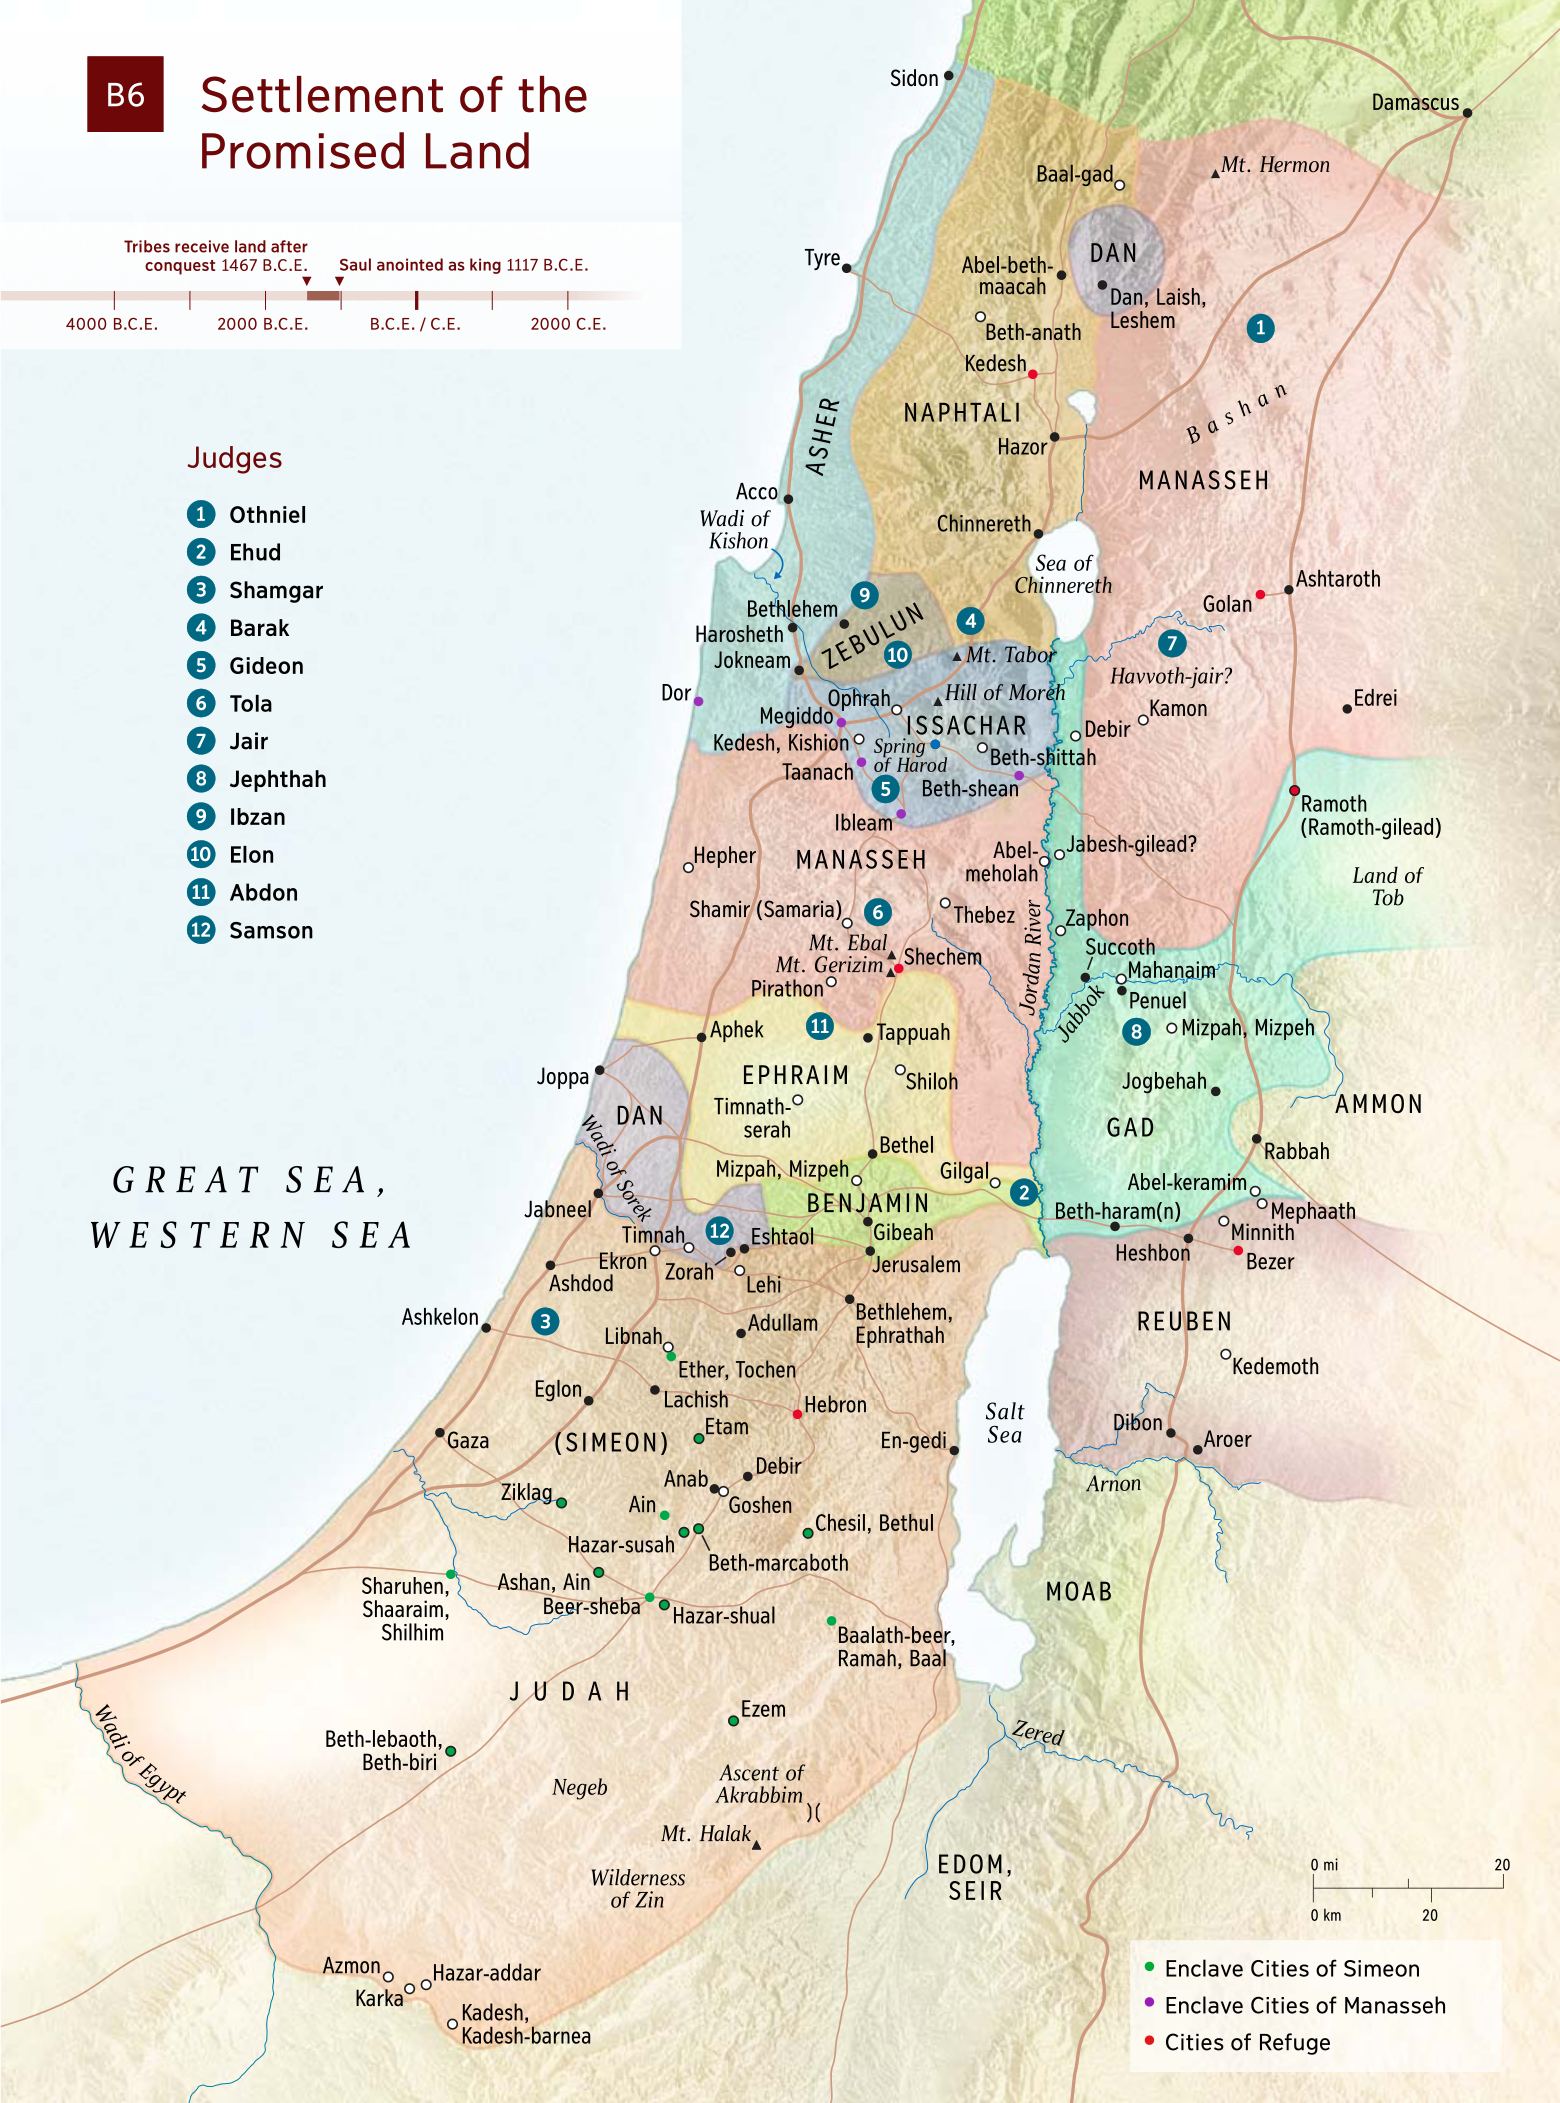
\includepdf[noautoscale=true, scale=1]{leb/content/pictures/settlement-of-the-promised-land.png}
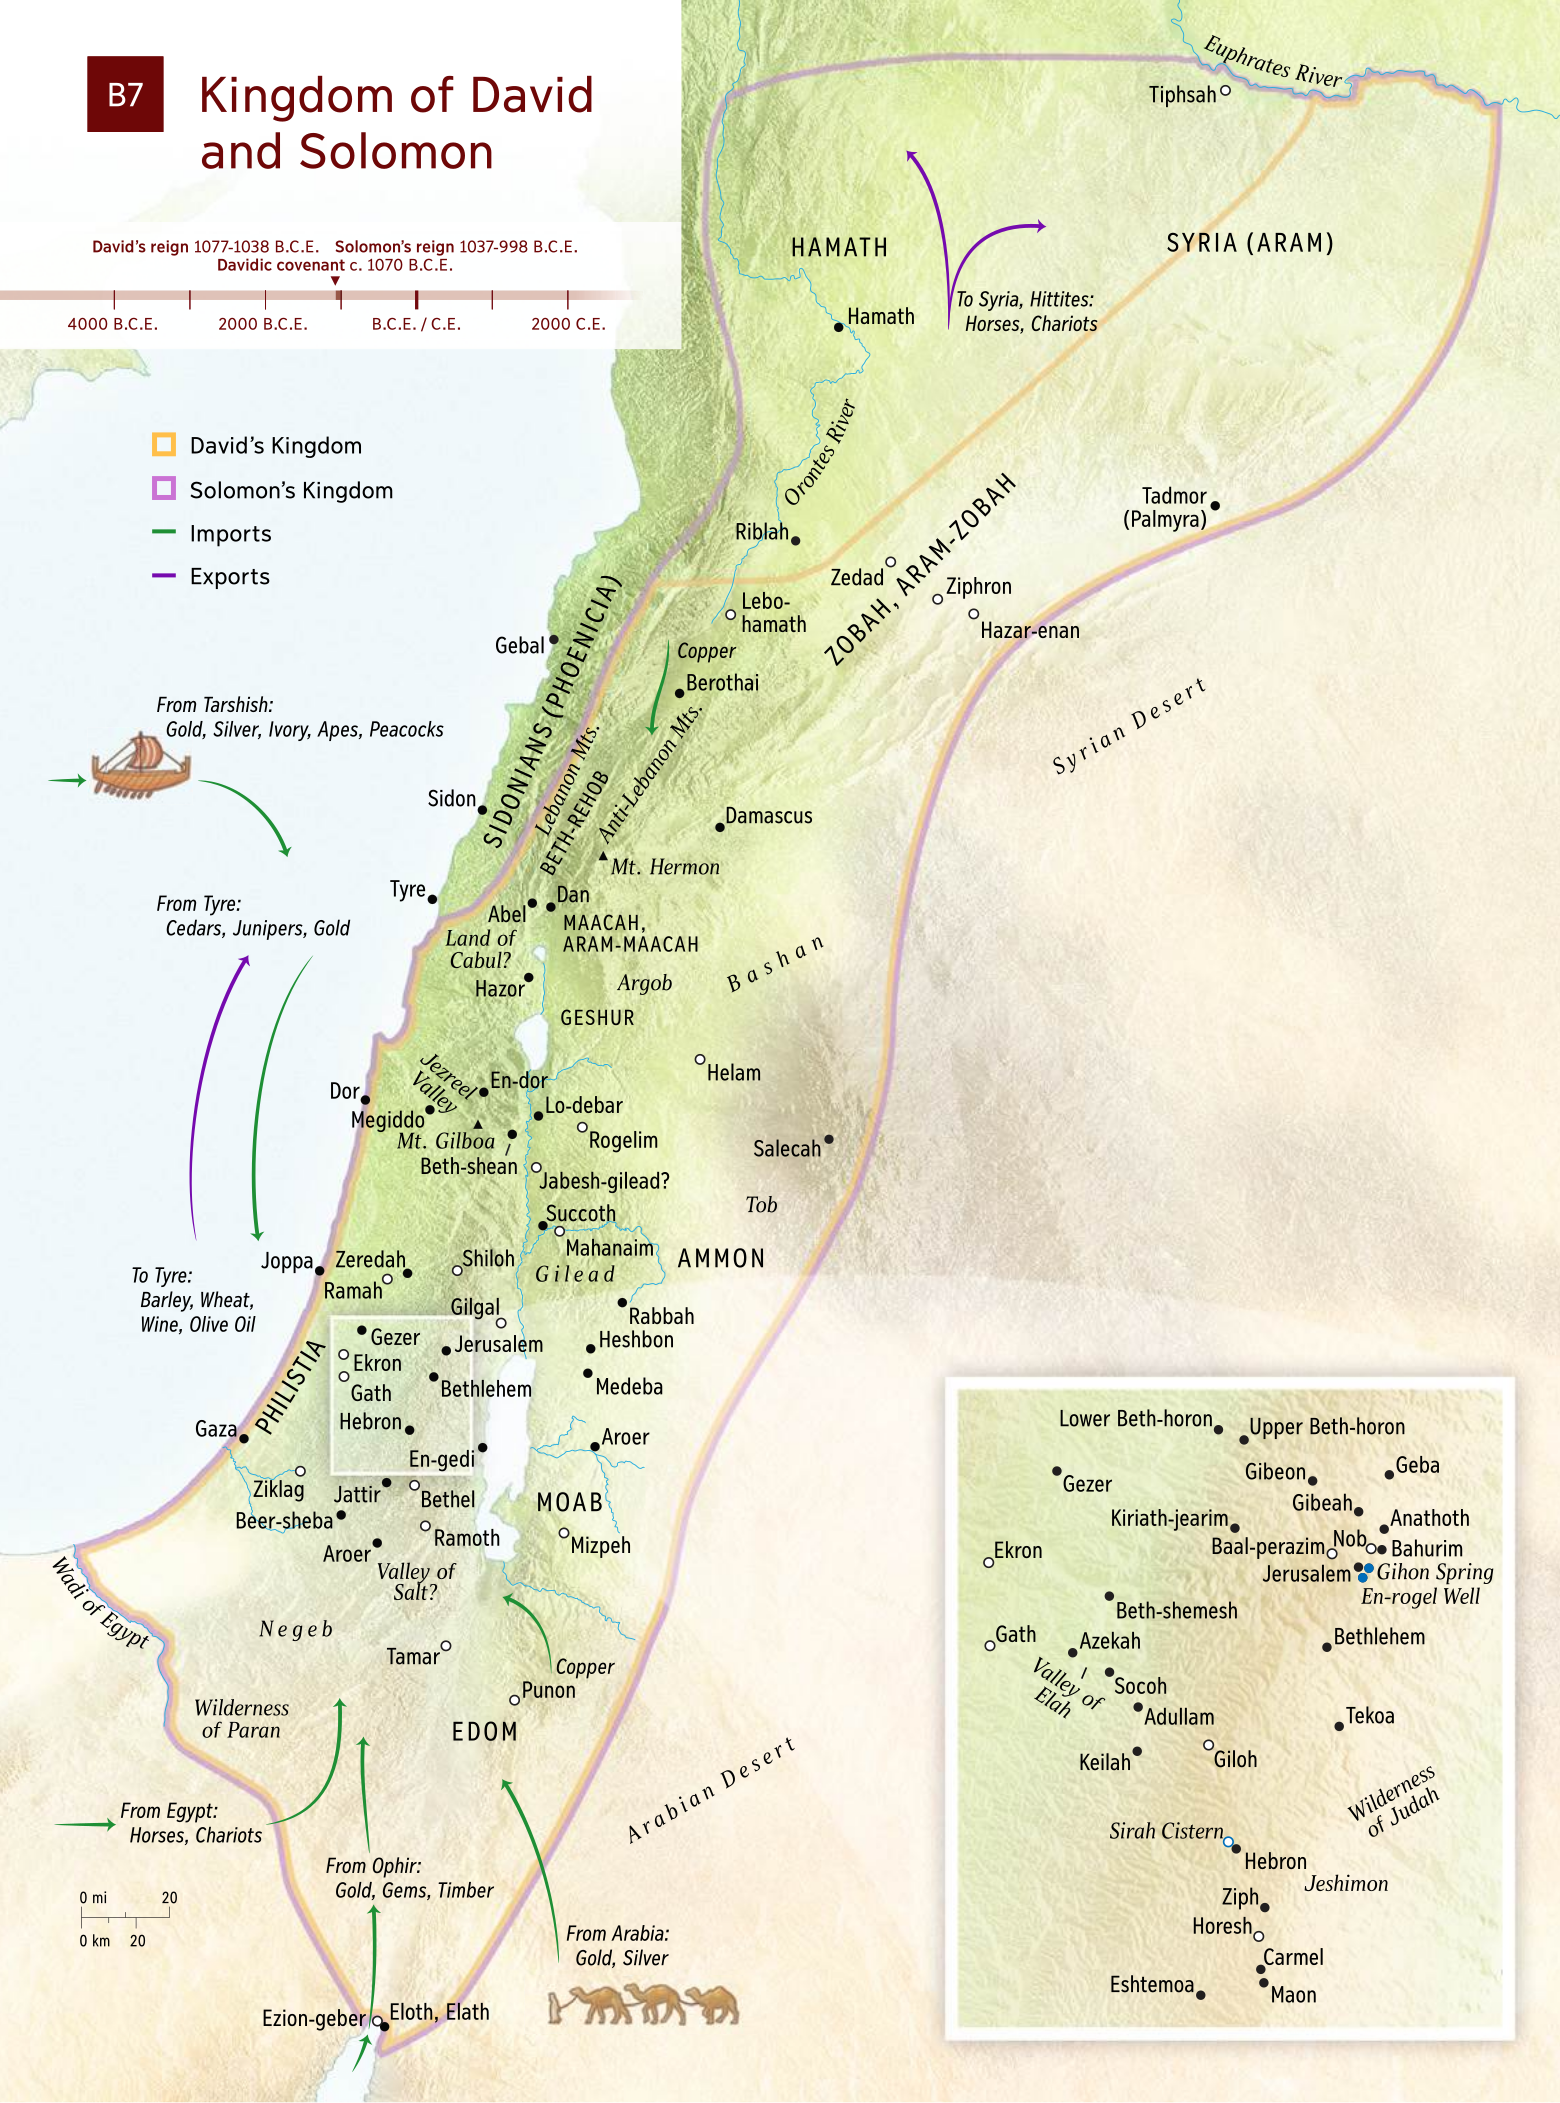
\includepdf[noautoscale=true, scale=1]{leb/content/pictures/israel-in-times-of-king-david-and-solomon.png}
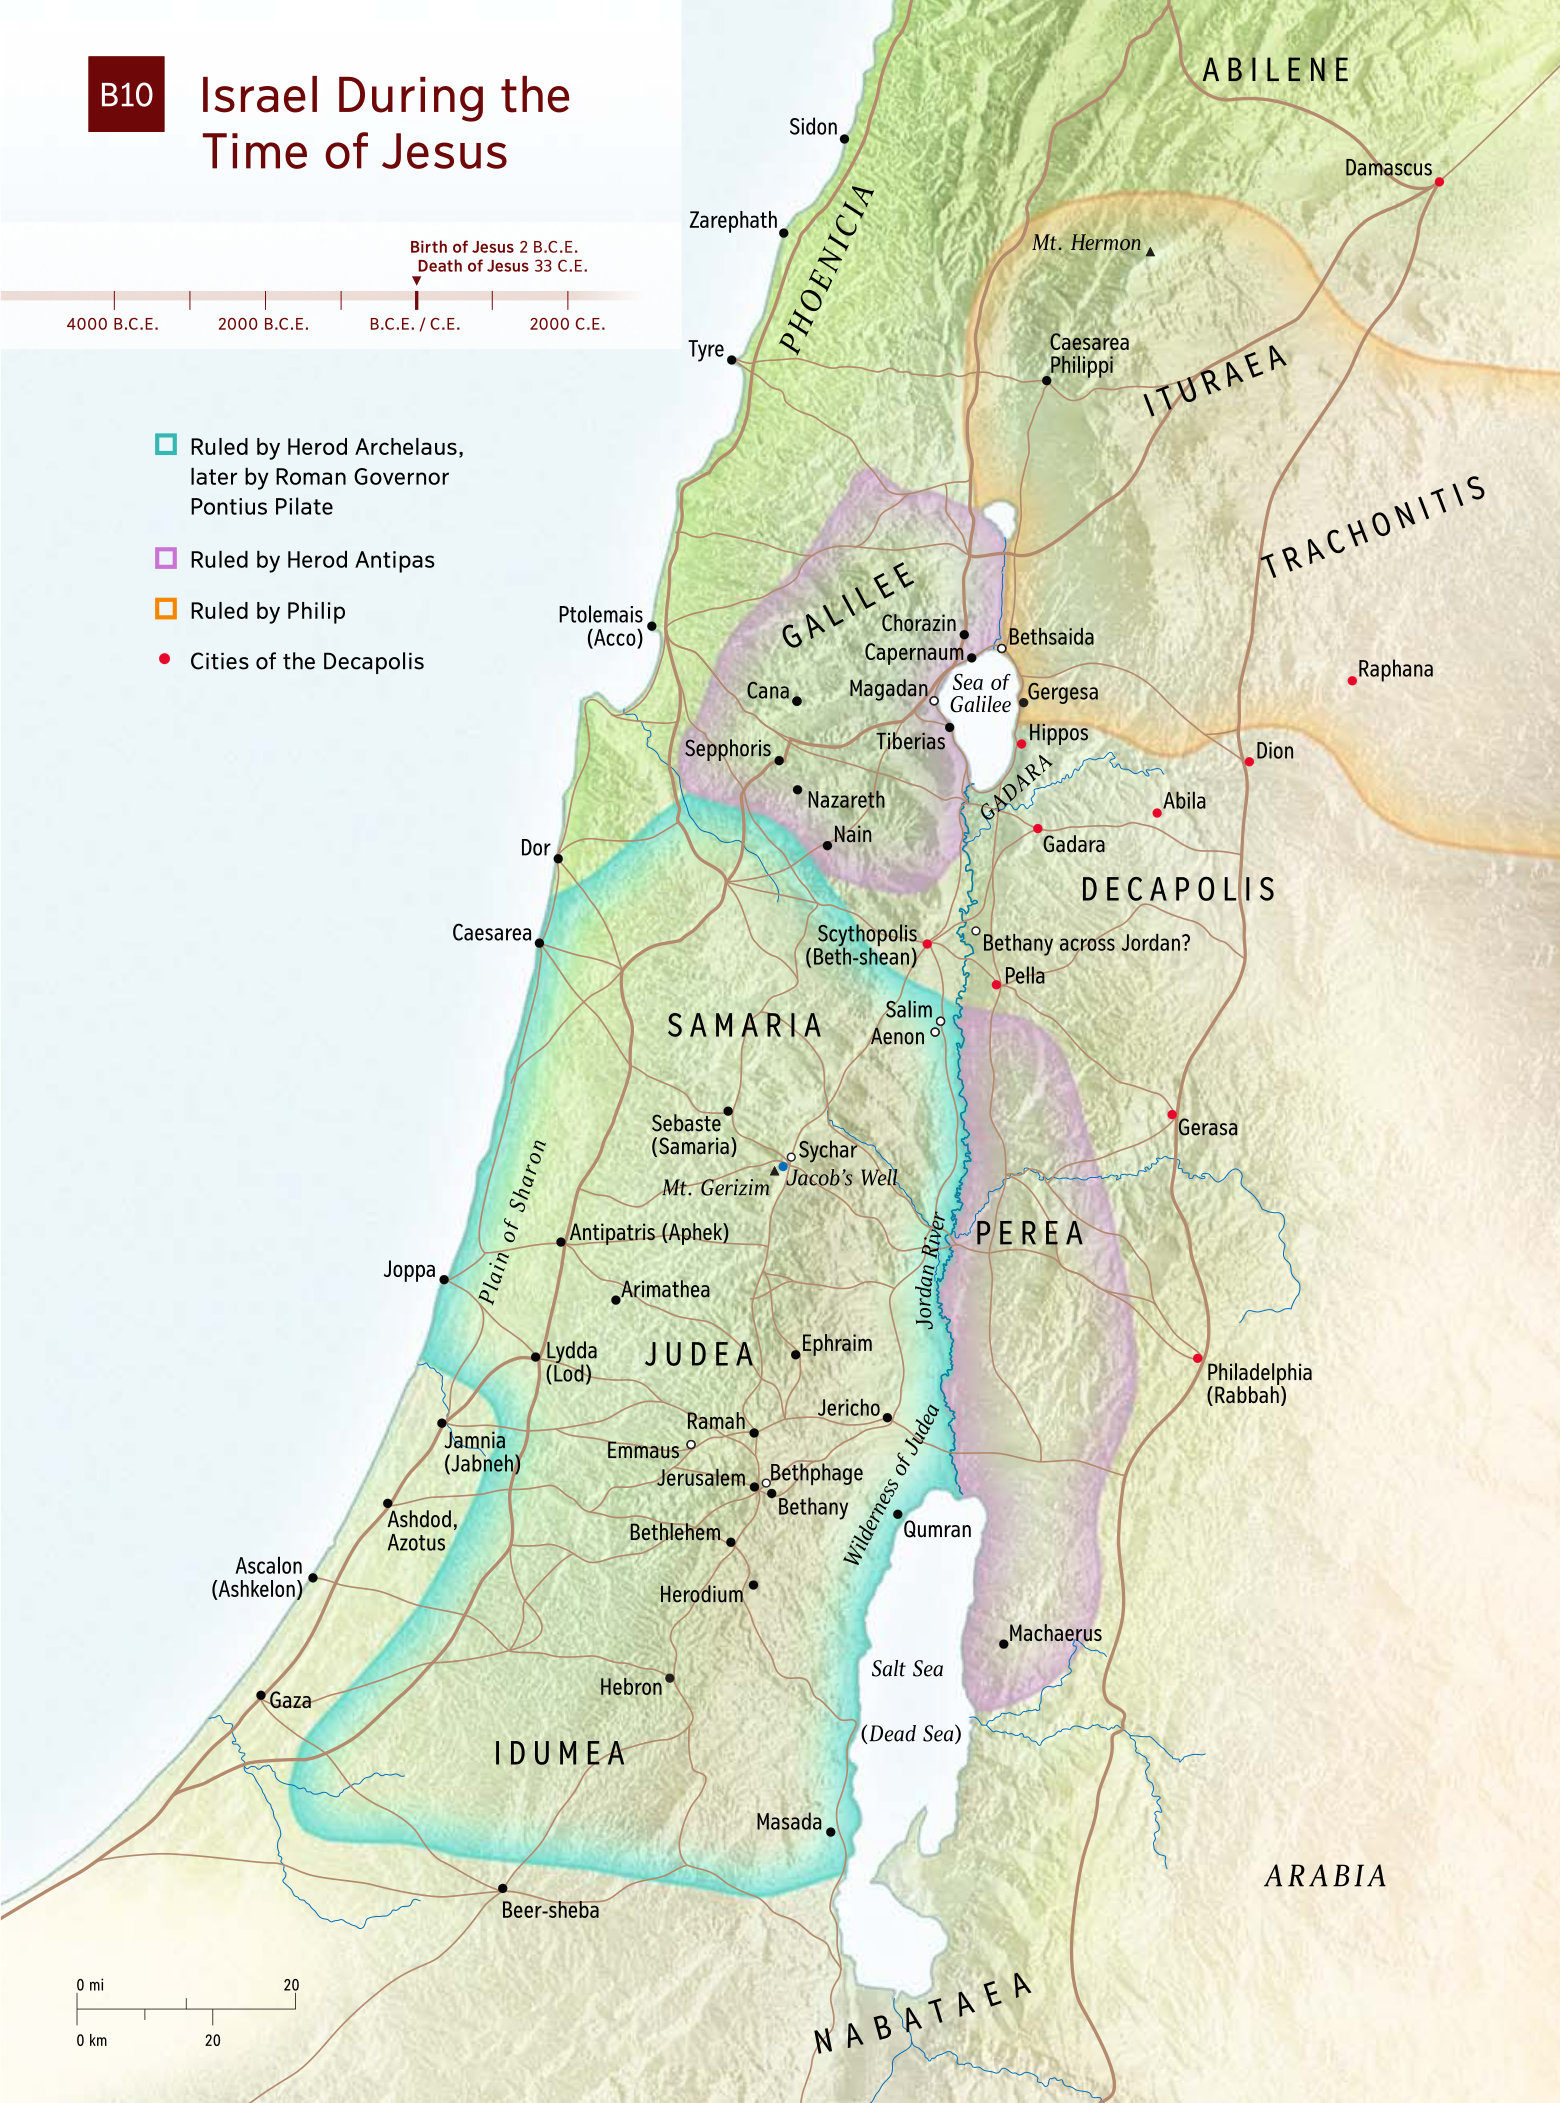
\includepdf[noautoscale=true, scale=1]{leb/content/pictures/israel-in-time-of-jesus.png}
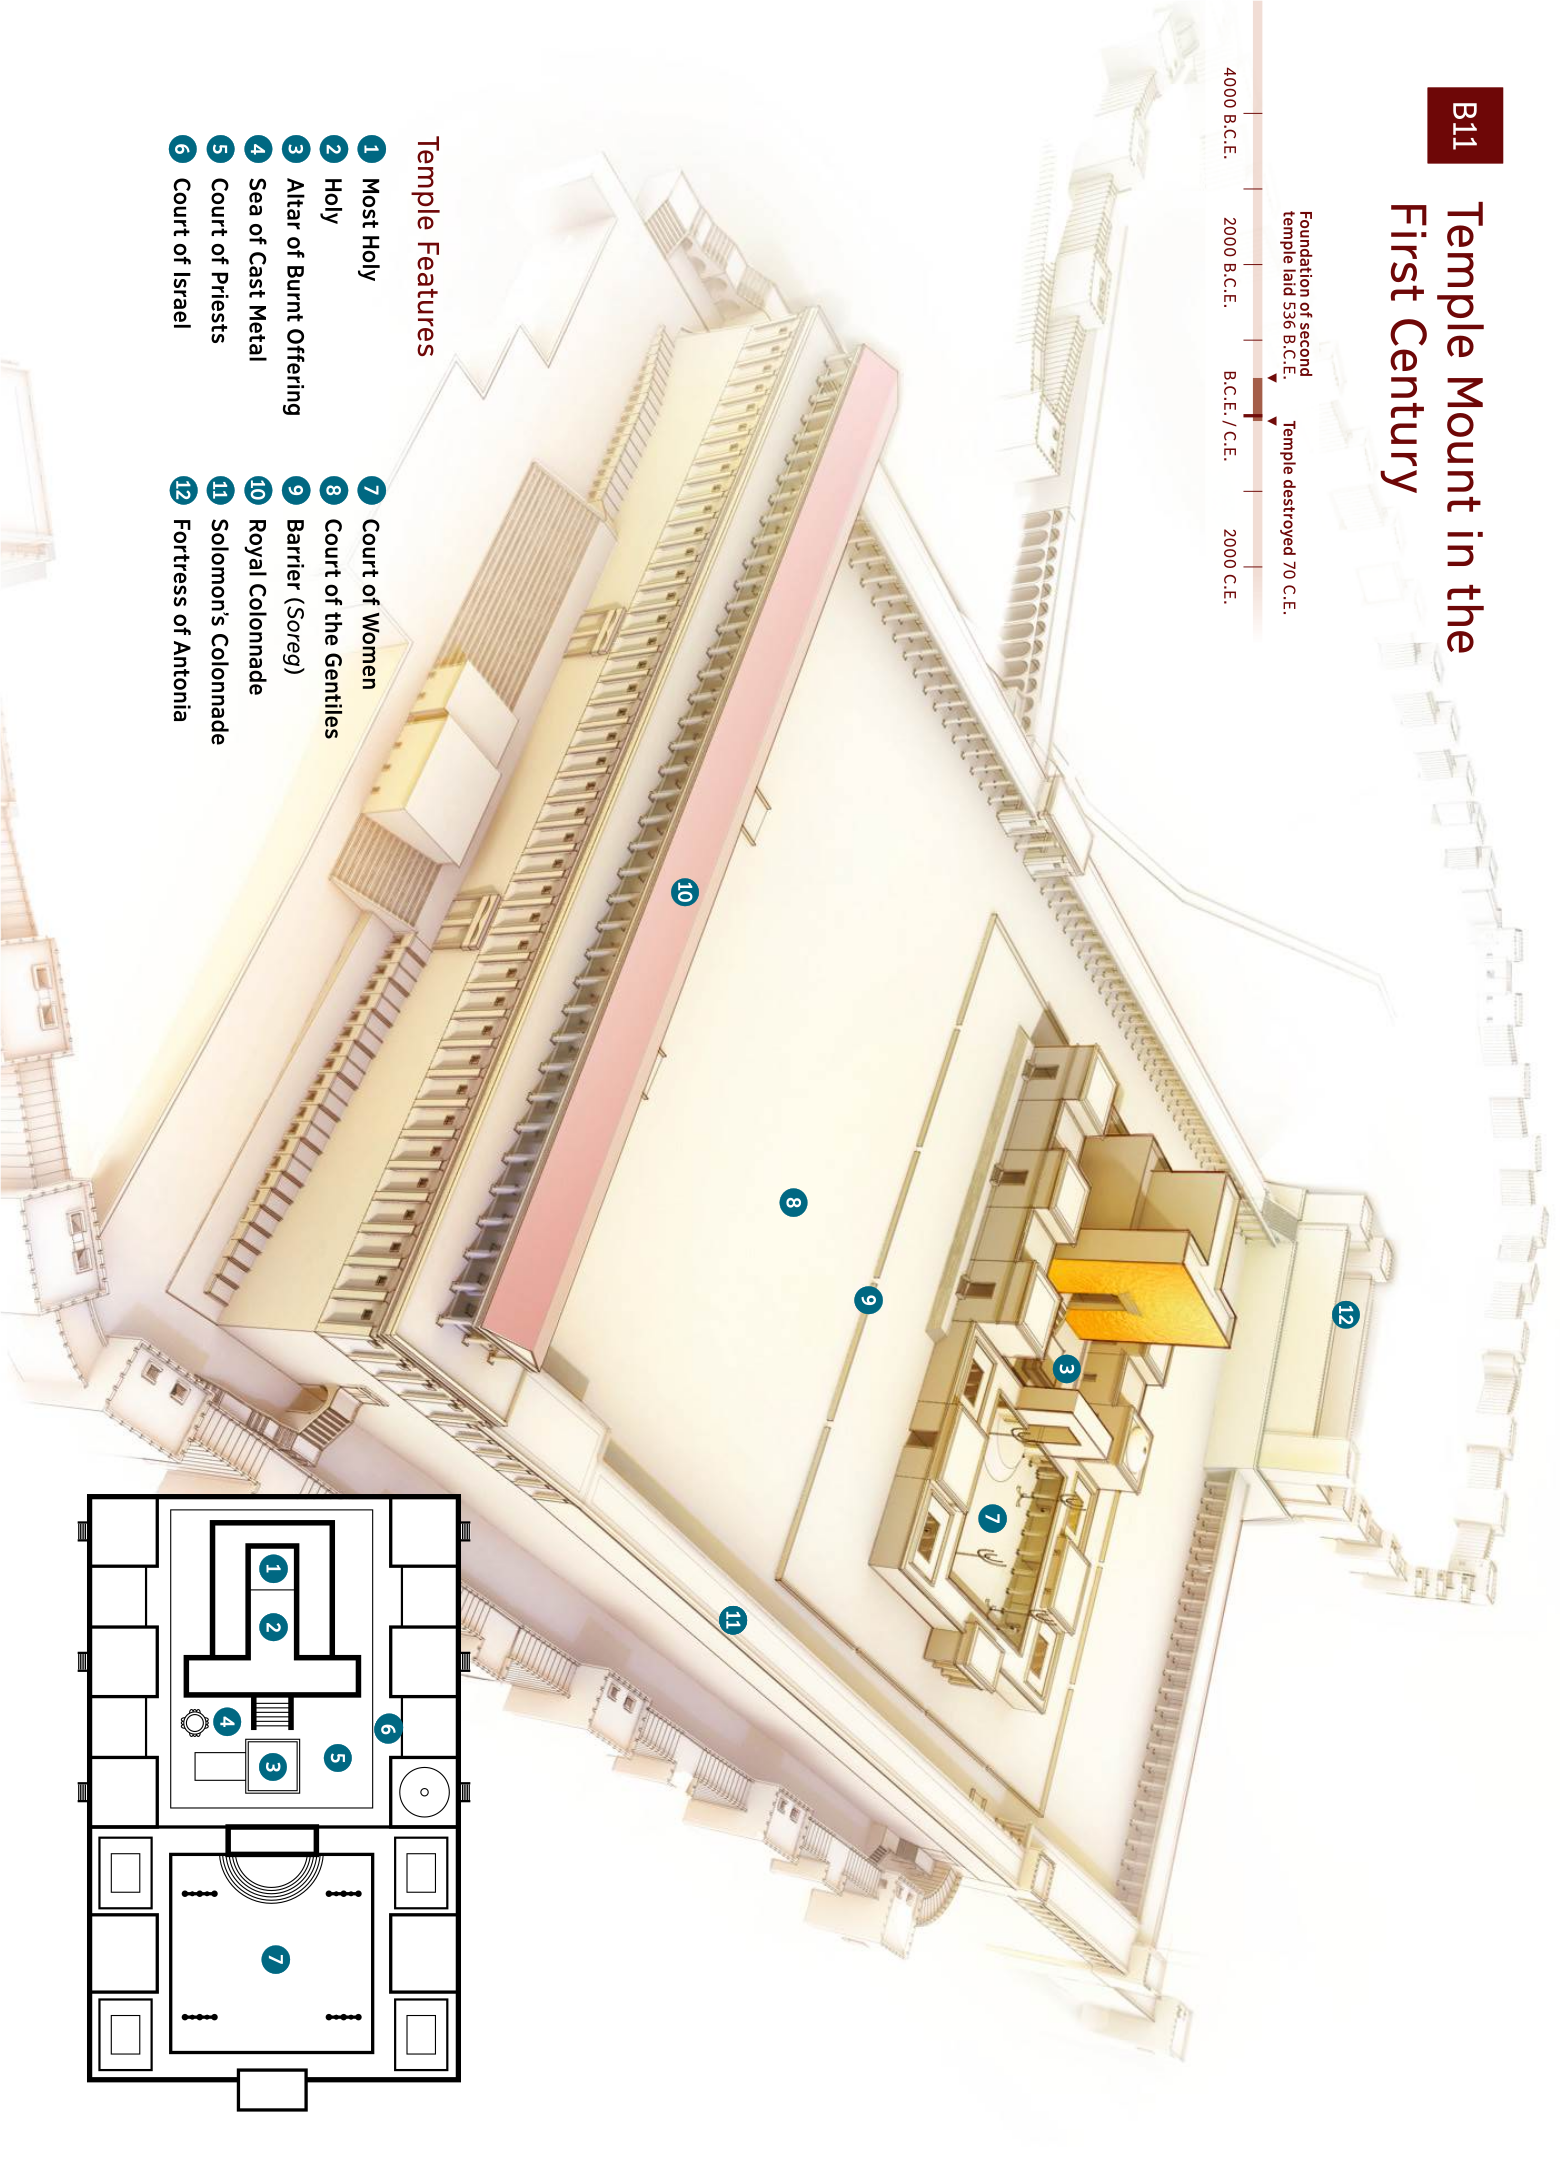
\includepdf[noautoscale=true, scale=1]{leb/content/pictures/second-temple-mount.png}
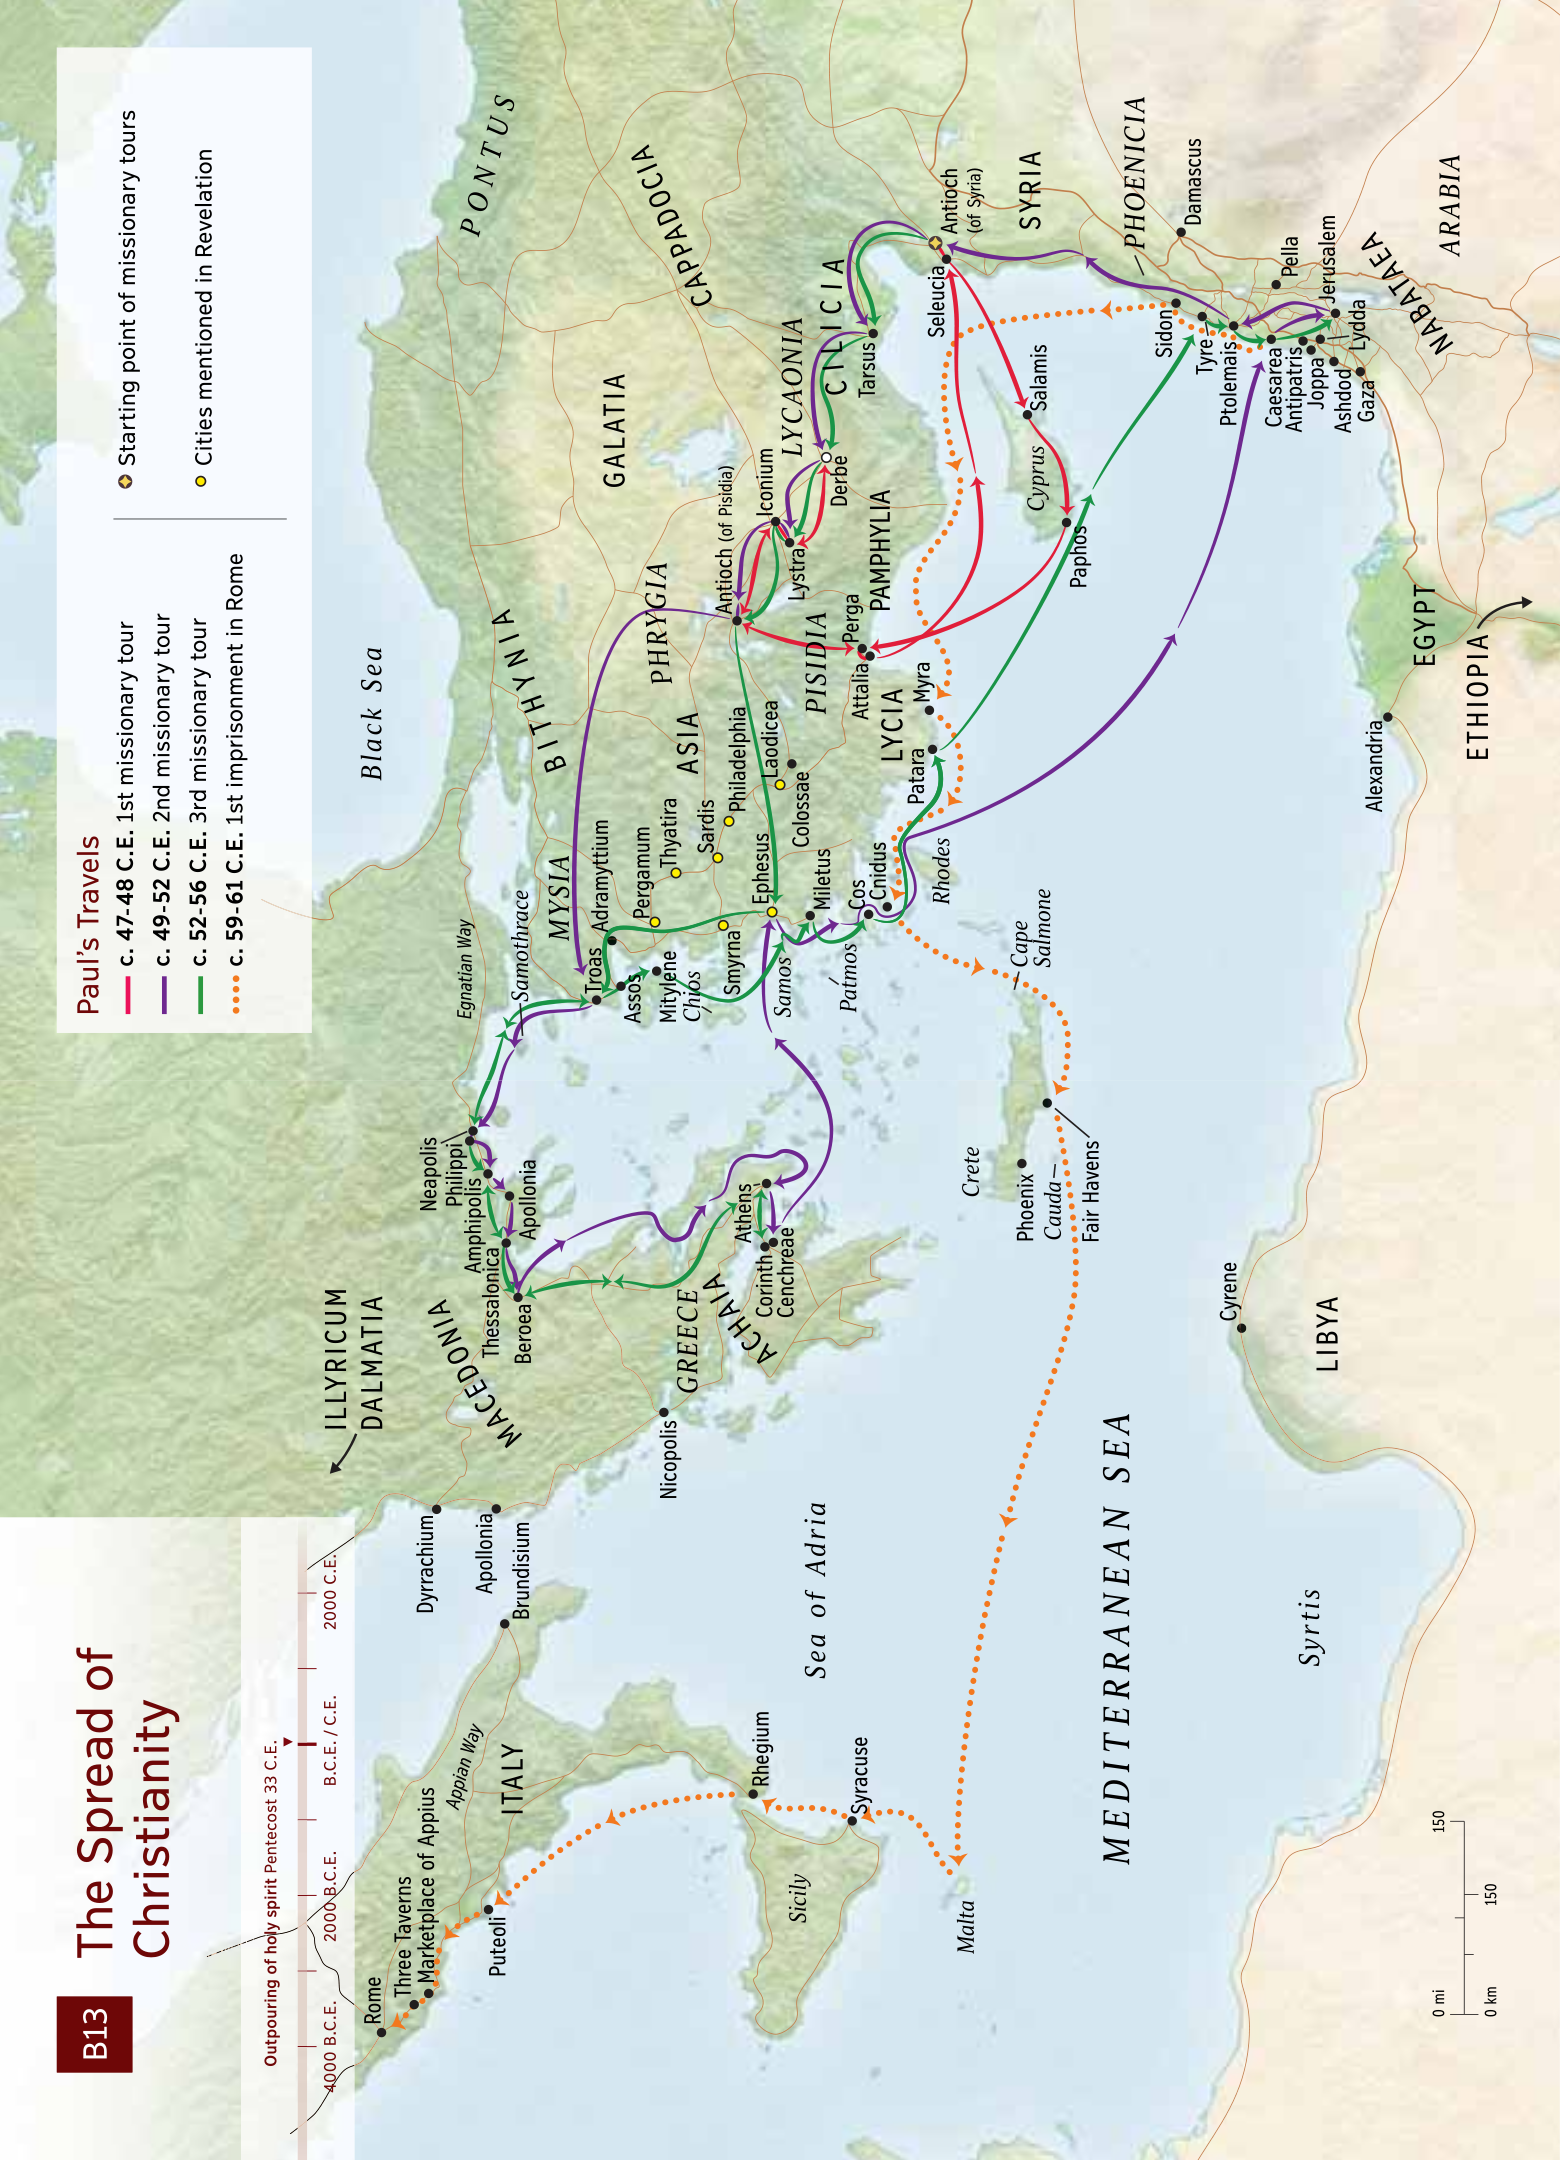
\includepdf[noautoscale=true, scale=1]{leb/content/pictures/spread-of-christianity.png}
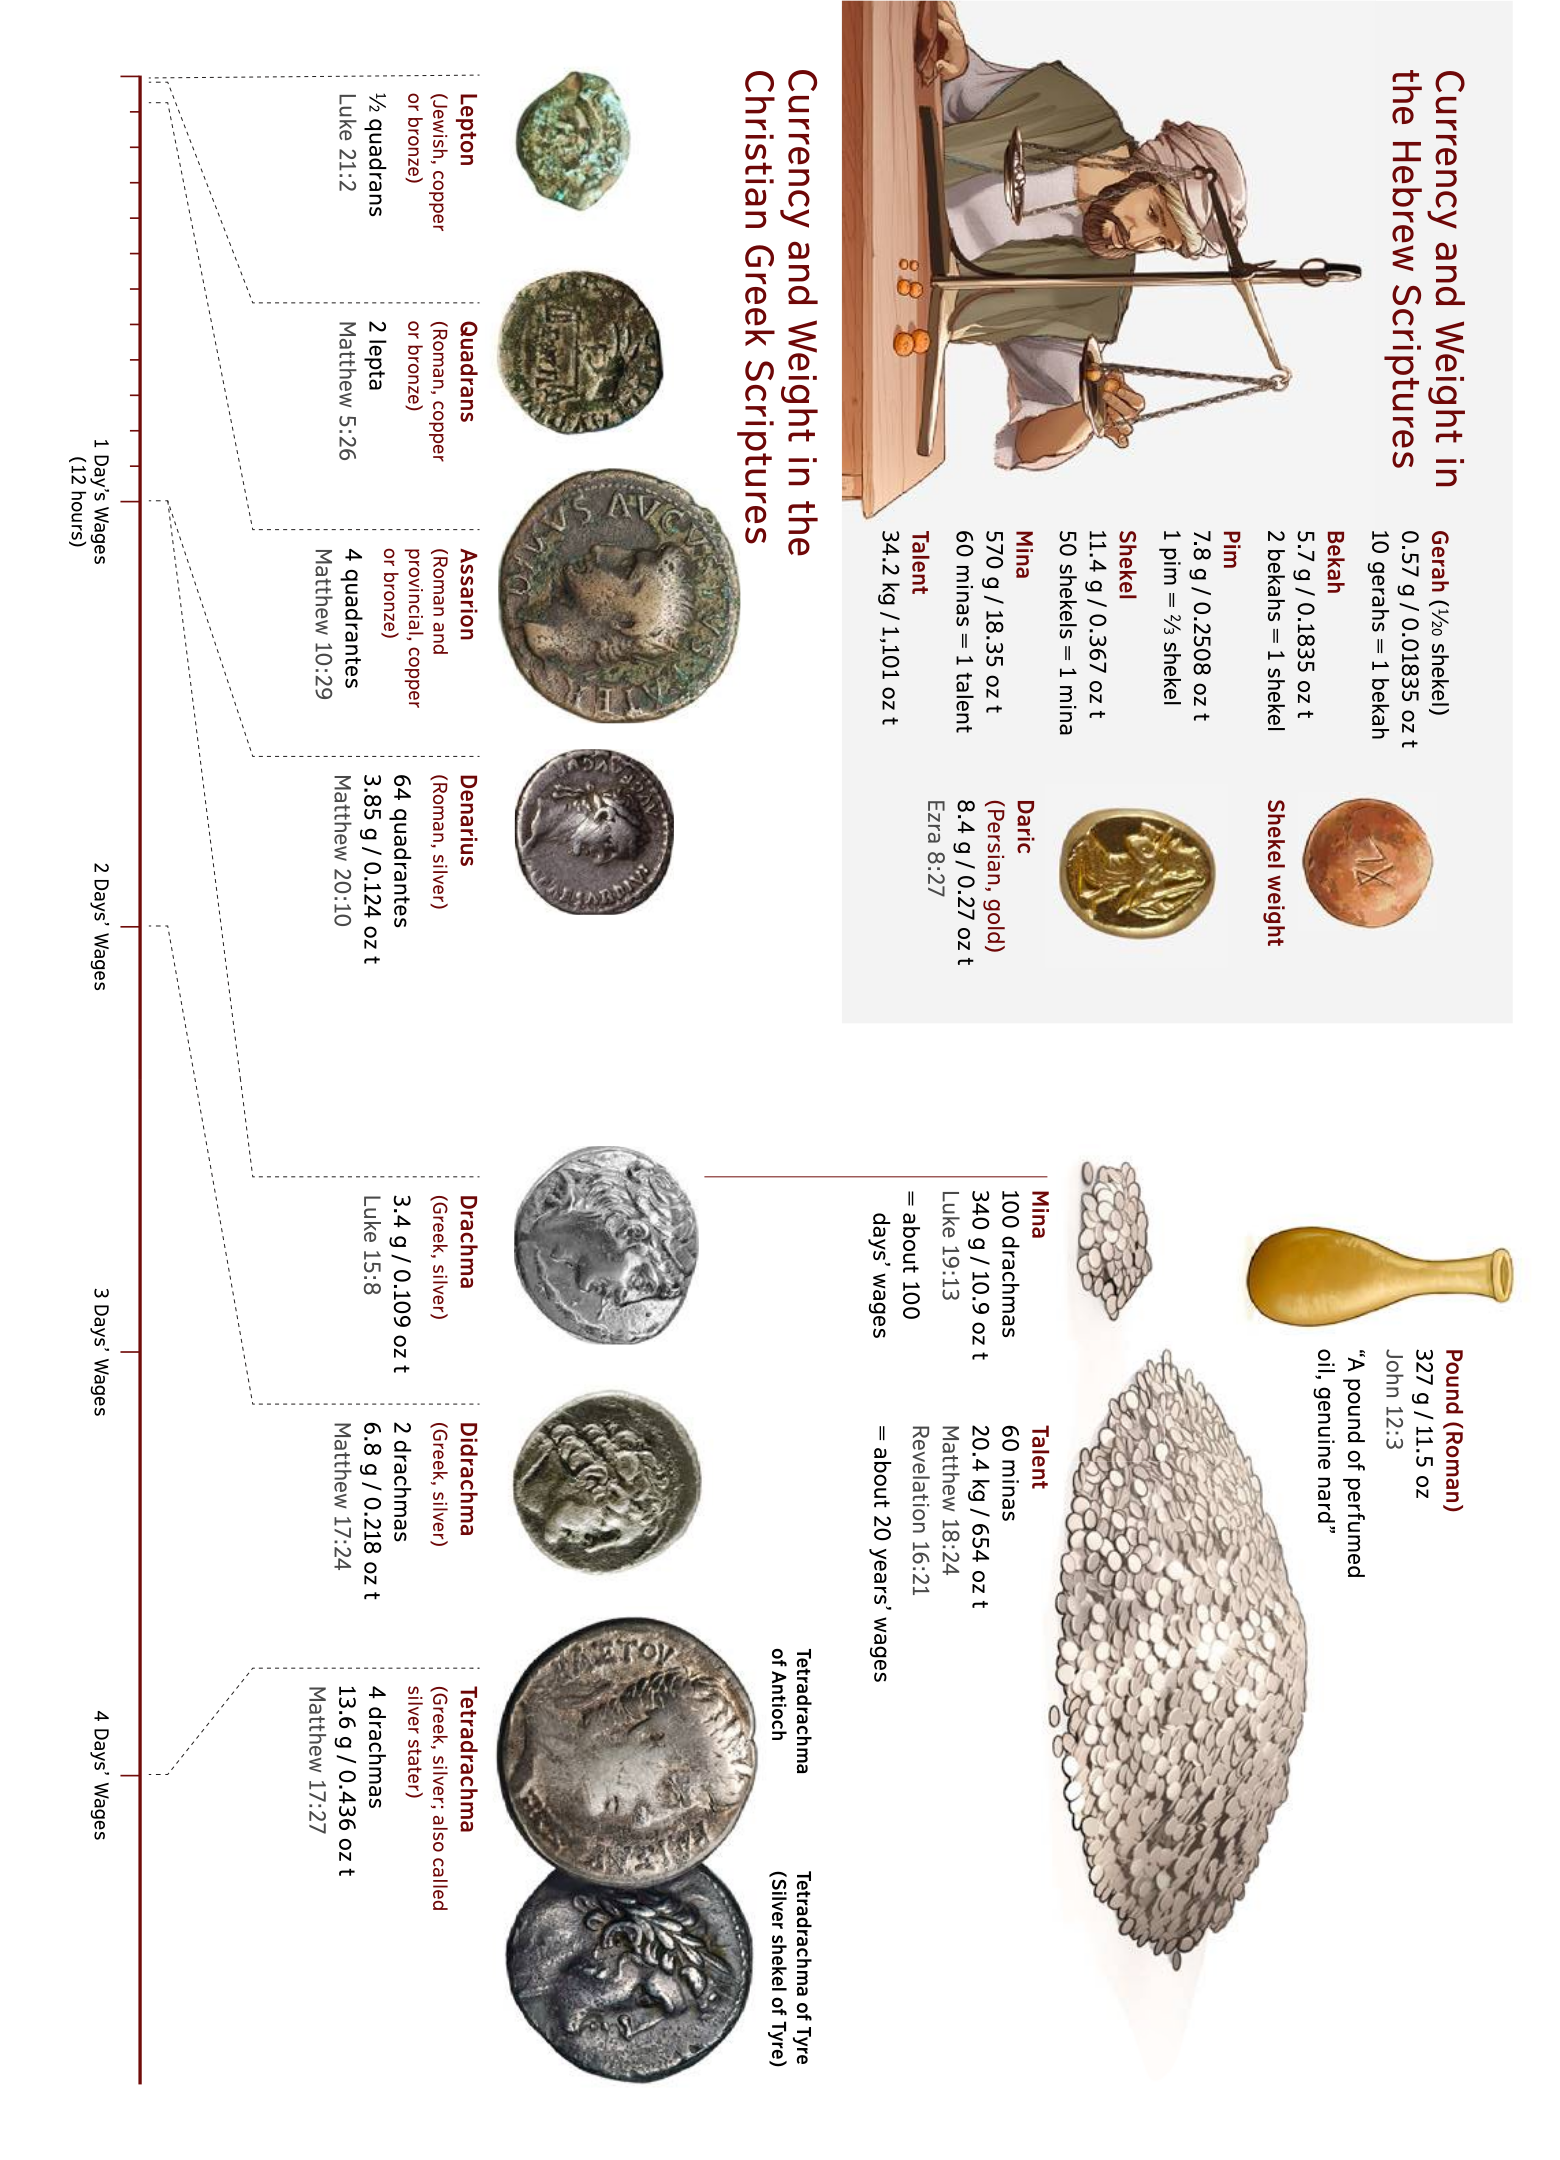
\includepdf[noautoscale=true, scale=1]{leb/content/pictures/units-of-measure.png}



% an empty page at the back
\begin{titlingpage}

\clearpage
\newpage
\thispagestyle{empty}
\mbox{}

\end{titlingpage}




\end{document}
